\documentclass[11pt,a4paper]{article}
\usepackage[a4paper,margin=23mm,headheight=15pt]{geometry}
\usepackage{iftex,fontspec}
\usepackage{amsmath,amssymb,amsthm,amscd,mathtools,mathrsfs}
\usepackage{unicode-math}
\setmainfont{STIXTwoText}[Extension=.otf,UprightFont=*-Regular,ItalicFont=*-Italic,BoldFont=*-Bold,BoldItalicFont=*-BoldItalic]
\setmathfont{STIXTwoMath-Regular.otf}
\usepackage[english,french,shorthands=off]{babel}
\usepackage{adjustbox,array,booktabs,calc,enumitem,fancyhdr,fvextra,graphicx,longtable,needspace,parskip,ragged2e,seqsplit,tabularx,textcomp,tikz,tikz-cd,titlesec,upquote,xcolor,xurl,newunicodechar}
\usepackage[all]{xy}
\usepackage[normalem]{ulem}
\usepackage{microtype}
\usepackage[hidelinks,unicode,bookmarksopen=true]{hyperref}
\usepackage{bookmark}
\pdfstringdefDisableCommands{\def\ell{ℓ}\def\mathbb#1{#1}\def\mathcal#1{#1}\def\mathfrak#1{#1}\def\mathrm#1{#1}\def\mathbf#1{#1}\def\ensuremath#1{#1}}
\let\CorpusDeclareMathOperator\DeclareMathOperator
\let\CorpusNewUnicodeChar\newunicodechar
\makeatletter
\let\CorpusUndefined\@undefined
\let\CorpusDeclMathOp\@declmathop
\let\CorpusMakeTitle\maketitle
\let\CorpusTitle\title
\let\CorpusAuthor\author
\let\CorpusDate\date
\let\CorpusThanks\thanks
\let\CorpusAnd\and
\let\CorpusAtMakeTitle\@maketitle
\let\CorpusSetCounter\setcounter
\makeatother
\setlength{\emergencystretch}{3em}
\raggedbottom

\begin{document}
\selectlanguage{french}
\title{Pierre Deligne --- French mathematical corpus}\author{}\date{}\maketitle
\tableofcontents\clearpage
% BEGIN INLINE WORK D001 FR
\typeout{CORPUS-BEGIN:D001:\thepage}
\begingroup
\makeatletter
\let\DeclareMathOperator\CorpusDeclareMathOperator
\let\@declmathop\CorpusDeclMathOp
\let\maketitle\CorpusMakeTitle\let\title\CorpusTitle\let\author\CorpusAuthor\let\date\CorpusDate
\let\thanks\CorpusThanks\let\and\CorpusAnd\let\@maketitle\CorpusAtMakeTitle
\def\setcounter#1#2{\def\CorpusCounterName{#1}\def\CorpusPageName{page}\ifx\CorpusCounterName\CorpusPageName\else\CorpusSetCounter{#1}{#2}\fi}
\title{}\author{}\date{}
\expandafter\let\csname sourcepage\endcsname\CorpusUndefined
\setcounter{section}{0}
\expandafter\def\csname theHsection\endcsname{D001.\arabic{section}}
\setcounter{subsection}{0}
\expandafter\def\csname theHsubsection\endcsname{D001.\arabic{subsection}}
\setcounter{subsubsection}{0}
\expandafter\def\csname theHsubsubsection\endcsname{D001.\arabic{subsubsection}}
\setcounter{equation}{0}
\expandafter\def\csname theHequation\endcsname{D001.\arabic{equation}}
\setcounter{figure}{0}
\expandafter\def\csname theHfigure\endcsname{D001.\arabic{figure}}
\setcounter{table}{0}
\expandafter\def\csname theHtable\endcsname{D001.\arabic{table}}
\setcounter{footnote}{0}
\expandafter\def\csname theHfootnote\endcsname{D001.\arabic{footnote}}
\makeatother
\let\tableofcontents\relax % one cumulative contents list, not repeated global lists
% D001 corrected, source-aligned French edition.
% Authoritative source SHA-256:
% 4078B5827B016B7F0FA3F3ECB3A7D710AC7D63E7A1EDD889F86FCAA847078C2C
% PDF index 1--4 = printed pages 129--132.
% Source repairs R1--R3 and A1 are disclosed in visible notes.
\pagestyle{empty}

\newcommand{\sourcepage}[1]{%
  \clearpage
  \begin{center}
    --- #1 ---
  \end{center}
  \vspace{0.6em}
}


\graphicspath{{assets/works/}}
\selectlanguage{french}
\phantomsection\addcontentsline{toc}{section}{D001}


\pagestyle{empty}
\thispagestyle{empty}

\begin{center}
{\large\bfseries\boldmath
CONGRUENCES SUR LE NOMBRE DE\\
SOUS-GROUPES D'ORDRE $p^k$ DANS UN GROUPE FINI\par}
\vspace{1.2em}
par \textsc{P. Deligne}
\end{center}

\vspace{2em}

La méthode utilisée par Serre [1] p. 147 pour démontrer le théorème de Sylow fournit des résultats plus généraux qu'on se propose d'expliciter.

On utilise les notations suivantes : $p$ désigne un nombre premier ; pour tout entier $n$, $v(n)$ est l'exposant de la plus grande puissance de $p$ qui divise $n$ ; enfin, $G$ est un groupe fini d'ordre $g$.

Pour être complet, rappelons le lemme suivant (Lazard [2] p. 71).

\medskip
\noindent\emph{Lemme 1 :}

{\itshape
\begin{enumerate}
\item[a)] Si $n=\sum c_i p^i$ avec $0\leq c_i<p$ (développement de base $p$),
\[
v(n!)=\frac{1}{p-1}(n-\textstyle\sum c_i)
\]
\item[b)]
\[
v\binom{r}{s}\geq v(r)-v(s)
\]
\end{enumerate}
}

Prouvons a) : on a\footnote{La somme intermédiaire imprimée dans la
source est négative. Nous la remplaçons par le calcul exact de Legendre
(défaut de source R1).}
\[
v(p^k!)=\sum_{r=1}^{k}\left\lfloor\frac{p^k}{p^r}\right\rfloor
=\sum_{r=1}^{k}p^{k-r}=\sum_{i=0}^{k-1}p^i
=\frac{p^k-1}{p-1},
\]
ce qui vérifie l'énoncé ; il est clair que si $0\leq c<p$, $v((cp^k)!)=cv(p^k!)$ et que si $m<p^{v(n)}$, $v((n+m)!)=v(n!)+v(m!)$. Ces propriétés d'additivité sont les mêmes que celles du second membre, d'où la formule.

$b)$ s'en déduit aisément en revenant aux définitions et en tenant compte de l'algorithme de calcul des chiffres $c_i$ d'une somme à l'aide de ceux de ses termes. Il y a égalité si $r$ est une puissance de $p$.

\medskip
{\itshape\noindent
Proposition 1 : $\displaystyle\binom{p^k n}{p^k m}=\binom{n}{m}\mathop{\rm mod.} p^{v(n)+2}$ si $p\neq2$ ou si $n$ est impair. La congruence est toujours vraie modulo $p^{v(n)+1}$.
\par}

\sourcepage{130}

\noindent\emph{Démonstration :} Soient $X$ et $Y$ deux indéterminées ; $(X+Y)^{p^k}=X^{p^k}+Y^{p^k}+pQ$ où $Q$ est un polynôme de degré inférieur à $p^k$ en chaque variable. La formule du binôme montre alors que
\begin{equation}
(X+Y)^{p^k n}=(X^{p^k}+Y^{p^k})^n+np(X^{p^k}+Y^{p^k})^{n-1}Q
\tag{1}
\end{equation}
modulo la plus grande puissance de $p$ qui divise tous les $p^i\binom{n}{i}$ ($i\geq2$). Ceux-ci sont de valuation au moins $i+v(n)-v(i)\geq v(n)+2$ si $p\neq2$ ; si $p=2$, on a toujours $i>v(i)$ (Cantor), d'où l'exposant $v(n)+1$.

$\binom{p^k n}{p^k m}$ est le coefficient de
$X^{p^k m}Y^{p^k(n-m)}$\footnote{La source imprime ici
$X^{p^km}Y^{p^kn}$, monôme de degré $p^k(m+n)>p^kn$ lorsque $m>0$.
Nous rétablissons $Y^{p^k(n-m)}$ (défaut de source R2).} ; le second
terme du second membre de (1) ne contient aucun terme de ce type (aucun
exposant n'y est divisible par $p^k$), et le coefficient de ce monôme
dans le second membre de (1) est donc $\binom{n}{m}$. L'assertion en
résulte si $p\neq2$. Si $p=2$, ce qui précède prouve déjà la congruence
modulo $2^{v(n)+1}$ ; de plus,
$Q=X^{2^{k-1}}Y^{2^{k-1}}\mathop{\rm mod.}2$ ;
$Q^2=X^{2^k}Y^{2^k}\mathop{\rm mod}4$, et le terme suivant dans le
développement du binôme donne
\[
\binom{2^k n}{2^k m}=\binom{n}{m}+2n(n-1)\binom{n-2}{m-1}\mathop{\rm mod}2^{v(n)+2},
\]
d'où l'assertion lorsque $n$ est impair.

\medskip
\noindent\textsc{Théorème} :

{\itshape
Soient $S$ un sous-groupe de $p$-Sylow de $G$, $s=v(g)$ et $d_k$ le nombre de sous-groupes de $G$ d'ordre $p^{s-k}$ pour $0\leq k\leq s$. Alors
\begin{enumerate}
\item[(i)] $d_k=1\mathop{\rm mod}p$
\item[(ii)] si $S$ est cyclique ou abélien de type $(p,\ldots,p)$, $d_k$ est congru mod $p^{k+1}$ au nombre de sous-groupes de $S$ d'indice $p^k$
\item[(iii)] si $S$ n'est pas cyclique,
\[
d_1=1+p\mathop{\rm mod}p^2.
\]
\end{enumerate}
}

Faisons agir le groupe $G$ par translations à gauche sur l'ensemble de ses parties à $p^k$ éléments. Si une de ces parties soit $P$ de $G$ a un stabilisateur $H$, elle est réunion de classes à droites de $H$ et $H$ est donc un groupe d'ordre $p^l$ avec $l\leq k$ ; $l=k$ si et seulement si $P$ est translaté (à droite ou à gauche, c'est la même chose) d'un sous-groupe d'ordre $p^k$. Le nombre d'éléments dans l'orbite de $P$ est divisible par $p^{s-l}$. $\binom{g}{p^k}$ est donc congru mod

\sourcepage{131}

\noindent $p^{s-k+1}$ au nombre de parties de $G$ translatées d'un sous-groupe d'ordre $p^k$, et on sait (prop. 1) qu'il est aussi congru à $gp^{-k}$. Il y a $d_{s-k}\mathbin{\cdot}g\mathbin{\cdot}p^{-k}$ telles parties, et $gp^{-k}=d_{s-k}gp^{-k}\mathop{\rm mod}p^{s-k+1}$ d'où la première assertion.

Plaçons-nous dans le cas (ii), avec $S$ abélien de type $(p\ldots p)$. Le nombre $G_{ij}$ de sous-groupes d'ordre $p^i$ d'un sous-groupe d'ordre $p^j$ est le nombre d'éléments d'une grassmannienne. Pour $i>j$, $G_{ij}=0$ ; pour $i\leq j$,
\[
G_{ij}=\frac{(p^j-1)\ldots(p^j-p^{i-1})}{(p^i-1)\ldots(p^i-p^{i-1})}
=\widetilde G_i\widetilde G_{j-i}\widetilde G_j^{-1},
\]
où l'on pose
\[
\widetilde G_i=[(1-p^i)\ldots(1-p)]^{-1}\text{ si }i\geq0,
\quad \widetilde G_i=0\text{ si }i<0.
\]
Ici $\widetilde G_i=(-1)^iG_i$, la source posant
$G_i=[(p^i-1)\ldots(p-1)]^{-1}$. Cette normalisation ne change pas
$G_{ij}$.\footnote{La source affirme ensuite
$G_k^{-1}=G_{k+1}^{-1}\mathop{\rm mod}p^{k+1}$, ce qui est faux avec
sa définition. La normalisation affichée donne
$\widetilde G_{k+1}^{-1}=\widetilde G_k^{-1}(1-p^{k+1})$ et répare
exactement l'argument (défaut de source A1).}

On sait que $p^i$ divise le nombre $u_i$ de parties de $G$ à $p^s$ éléments dont le stabilisateur est d'ordre $p^{s-i}$. Posons $g=p^s h$ ; si on compte de deux façons différentes le nombre des couples formés d'un sous-groupe d'ordre $p^{s-i}$ et d'une partie à $p^s$ éléments qu'il laisse fixe, on trouve, pour $0\leq i,j\leq s$,
\[
\left\{
\begin{alignedat}{2}
d_i\binom{p^i h}{p^i}&=\sum_jG_{s-i,s-j}u_j &\qquad& \text{(2)}\\
p^i&\mid u_i && \text{(3)}\\
d_s&=1 && \text{(4)}
\end{alignedat}
\right.
\]

Travaillons maintenant dans le localisé de $\mathbf Z$ en $p$ (ou dans $\mathbf Z_p$). Soit $e_i$ le quotient par $\binom{p^s h}{p^s}\widetilde G_i$ du premier membre de (2). En vertu de la proposition 1 et du fait que $\widetilde G_i$ est premier avec $p$ pour $i\geq0$, on voit qu'il existe des nombres $v_i$ ($0\leq i\leq s$) tels que
\[
\left\{
\begin{alignedat}{2}
d_i&=\widetilde G_ie_i\mathop{\rm mod}p^{i+1} &\qquad& \text{(5)}\\
e_i&=\sum_j\widetilde G_{i-j}v_j && \text{(2')}\\
p^i&\mid v_i && \text{(3')}\\
e_s&=\widetilde G_s^{-1} && \text{(4')}
\end{alignedat}
\right.
\]

Des identités analogues sont vérifiées dans le groupe $S$ ; pour montrer qu'elles déterminent $d_i$ mod $p^{i+1}$, il suffit de vérifier que les identités (pour $0\leq i,j\leq s$)

\sourcepage{132}

\[
\left\{
\begin{alignedat}{2}
e_i&=\sum_j\widetilde G_{i-j}v_j &\qquad& \text{(2'')}\\
p^i&\mid v_i && \text{(3'')}\\
e_s&=0 && \text{(4'')}
\end{alignedat}
\right.
\]
impliquent que $p^{i+1}\mid e_i$.

De (2$''$) on tire
\[
e_i-e_{i+1}=\sum_j(\widetilde G_{i-j}-\widetilde G_{i+1-j})v_j.
\]
Comme $\widetilde G_k^{-1}=\widetilde G_{k+1}^{-1}\mathop{\rm mod}p^{k+1}$, on a aussi
\[
p^{i+1-j}\mid \widetilde G_{i-j}-\widetilde G_{i+1-j}
\quad\text{et}\quad p^{i+1}\mid e_i-e_{i+1}.
\]
On conclut par (4$''$).

La même technique, en plus simple, s'applique si $S$ est cyclique.

Passons au cas (iii). Les sous-groupes d'indice $p$ de $S$ sont tous distingués. Leur intersection $S'$ est le sous-groupe de Frattini de $S$. Pour tout sous-groupe $T$ de $S$, si $TS'=S$, alors $T=S$. En particulier, si $S$ n'est pas cyclique, $S/S'$ ne l'est pas non plus et les sous-groupes d'indice $p$ de $S$ s'identifient aux hyperplans d'un $\mathbf Z/p$-vectoriel de dimension $>1$ ; leur nombre est congru à $1+p\mathop{\rm mod}p^2$.

Des équations précédentes subsiste le système suivant.\footnote{Dans la
troisième ligne la source imprime $p$ comme argument inférieur ; la ligne
suivante emploie elle-même $p^s$. Nous rétablissons $p^s$ (défaut de
source R3). L'indice suivant le dernier $u$ est endommagé dans le scan ;
les identités de comptage imposent le membre $u_0+u_1$.}
\[
\left\{
\begin{aligned}
d_0h&=u_0\\[3pt]
d_1\binom{ph}{p}&=(1+p)u_0+u_1\quad(\mathop{\rm mod}p^2)\\[3pt]
\binom{p^s h}{p^s}&=u_0+u_1\quad(\mathop{\rm mod}p^2)
\end{aligned}
\right.
\]
Or (prop. 1), $\binom{p^s h}{p^s}=\binom{ph}{p}=h\mathop{\rm mod}p^2$, donc
\begin{align*}
d_1h&=(1+p)d_0h+(h-d_0h)\mathop{\rm mod}p^2\text{ et}\\
d_1&=1+pd_0\mathop{\rm mod}p^2,
\end{align*}
d'où l'assertion puisque $d_0=1\mathop{\rm mod}p$.

\vspace{1.2em}
\begin{center}
\rule{4cm}{0.4pt}
\end{center}
\vspace{0.5em}

\begin{center}
\textsc{Bibliographie}
\end{center}

\begin{list}{}{\setlength{\leftmargin}{2.5em}\setlength{\labelwidth}{2em}\setlength{\labelsep}{0.5em}\setlength{\itemsep}{0pt}}
\item[{[1]}] \textsc{Serre, J.P.}, \emph{Corps locaux. Act. sc. et ind.}. Hermann, 1962.
\item[{[2]}] \textsc{Lazard,M.}, Groupes analytiques $p$-adiques. \emph{Publ. Math. I. H. E. S.}, n\textsuperscript{o} 26, 1965.
\end{list}


\clearpage\endgroup
\typeout{CORPUS-END:D001:\thepage}
% END INLINE WORK D001 FR
% BEGIN INLINE WORK D002 FR
\typeout{CORPUS-BEGIN:D002:\thepage}
\begingroup
\makeatletter
\let\DeclareMathOperator\CorpusDeclareMathOperator
\let\@declmathop\CorpusDeclMathOp
\let\maketitle\CorpusMakeTitle\let\title\CorpusTitle\let\author\CorpusAuthor\let\date\CorpusDate
\let\thanks\CorpusThanks\let\and\CorpusAnd\let\@maketitle\CorpusAtMakeTitle
\def\setcounter#1#2{\def\CorpusCounterName{#1}\def\CorpusPageName{page}\ifx\CorpusCounterName\CorpusPageName\else\CorpusSetCounter{#1}{#2}\fi}
\title{}\author{}\date{}
\expandafter\let\csname prop\endcsname\CorpusUndefined
\expandafter\let\csname endprop\endcsname\CorpusUndefined
\expandafter\let\csname c@prop\endcsname\CorpusUndefined
\expandafter\let\csname cl@prop\endcsname\CorpusUndefined
\expandafter\let\csname p@prop\endcsname\CorpusUndefined
\expandafter\let\csname theprop\endcsname\CorpusUndefined
\expandafter\let\csname theHprop\endcsname\CorpusUndefined
\expandafter\let\csname lem\endcsname\CorpusUndefined
\expandafter\let\csname endlem\endcsname\CorpusUndefined
\expandafter\let\csname c@lem\endcsname\CorpusUndefined
\expandafter\let\csname cl@lem\endcsname\CorpusUndefined
\expandafter\let\csname p@lem\endcsname\CorpusUndefined
\expandafter\let\csname thelem\endcsname\CorpusUndefined
\expandafter\let\csname theHlem\endcsname\CorpusUndefined
\expandafter\let\csname thm\endcsname\CorpusUndefined
\expandafter\let\csname endthm\endcsname\CorpusUndefined
\expandafter\let\csname c@thm\endcsname\CorpusUndefined
\expandafter\let\csname cl@thm\endcsname\CorpusUndefined
\expandafter\let\csname p@thm\endcsname\CorpusUndefined
\expandafter\let\csname thethm\endcsname\CorpusUndefined
\expandafter\let\csname theHthm\endcsname\CorpusUndefined
\expandafter\let\csname cor\endcsname\CorpusUndefined
\expandafter\let\csname endcor\endcsname\CorpusUndefined
\expandafter\let\csname c@cor\endcsname\CorpusUndefined
\expandafter\let\csname cl@cor\endcsname\CorpusUndefined
\expandafter\let\csname p@cor\endcsname\CorpusUndefined
\expandafter\let\csname thecor\endcsname\CorpusUndefined
\expandafter\let\csname theHcor\endcsname\CorpusUndefined
\expandafter\let\csname rem\endcsname\CorpusUndefined
\expandafter\let\csname endrem\endcsname\CorpusUndefined
\expandafter\let\csname c@rem\endcsname\CorpusUndefined
\expandafter\let\csname cl@rem\endcsname\CorpusUndefined
\expandafter\let\csname p@rem\endcsname\CorpusUndefined
\expandafter\let\csname therem\endcsname\CorpusUndefined
\expandafter\let\csname theHrem\endcsname\CorpusUndefined
\expandafter\let\csname Hom\endcsname\CorpusUndefined
\expandafter\let\csname lind\endcsname\CorpusUndefined
\expandafter\let\csname lproj\endcsname\CorpusUndefined
\expandafter\let\csname Ext\endcsname\CorpusUndefined
\expandafter\let\csname Ker\endcsname\CorpusUndefined
\expandafter\let\csname Coker\endcsname\CorpusUndefined
\expandafter\let\csname im\endcsname\CorpusUndefined
\expandafter\let\csname Ind\endcsname\CorpusUndefined
\expandafter\let\csname Pro\endcsname\CorpusUndefined
\expandafter\let\csname Ens\endcsname\CorpusUndefined
\expandafter\let\csname Ab\endcsname\CorpusUndefined
\expandafter\let\csname coh\endcsname\CorpusUndefined
\expandafter\let\csname cF\endcsname\CorpusUndefined
\expandafter\let\csname cG\endcsname\CorpusUndefined
\expandafter\let\csname cH\endcsname\CorpusUndefined
\expandafter\let\csname cI\endcsname\CorpusUndefined
\expandafter\let\csname cJ\endcsname\CorpusUndefined
\expandafter\let\csname cO\endcsname\CorpusUndefined
\expandafter\let\csname cC\endcsname\CorpusUndefined
\expandafter\let\csname cU\endcsname\CorpusUndefined
\expandafter\let\csname cV\endcsname\CorpusUndefined
\expandafter\let\csname cL\endcsname\CorpusUndefined
\expandafter\let\csname cK\endcsname\CorpusUndefined
\expandafter\let\csname cM\endcsname\CorpusUndefined
\expandafter\let\csname cN\endcsname\CorpusUndefined
\expandafter\let\csname cE\endcsname\CorpusUndefined
\expandafter\let\csname cA\endcsname\CorpusUndefined
\expandafter\let\csname cB\endcsname\CorpusUndefined
\expandafter\let\csname cDb\endcsname\CorpusUndefined
\expandafter\let\csname cDp\endcsname\CorpusUndefined
\expandafter\let\csname cD\endcsname\CorpusUndefined
\expandafter\let\csname fC\endcsname\CorpusUndefined
\expandafter\let\csname fI\endcsname\CorpusUndefined
\expandafter\let\csname rFl\endcsname\CorpusUndefined
\expandafter\let\csname bH\endcsname\CorpusUndefined
\expandafter\let\csname bR\endcsname\CorpusUndefined
\expandafter\let\csname bL\endcsname\CorpusUndefined
\setcounter{section}{0}
\expandafter\def\csname theHsection\endcsname{D002.\arabic{section}}
\setcounter{subsection}{0}
\expandafter\def\csname theHsubsection\endcsname{D002.\arabic{subsection}}
\setcounter{subsubsection}{0}
\expandafter\def\csname theHsubsubsection\endcsname{D002.\arabic{subsubsection}}
\setcounter{equation}{0}
\expandafter\def\csname theHequation\endcsname{D002.\arabic{equation}}
\setcounter{figure}{0}
\expandafter\def\csname theHfigure\endcsname{D002.\arabic{figure}}
\setcounter{table}{0}
\expandafter\def\csname theHtable\endcsname{D002.\arabic{table}}
\setcounter{footnote}{0}
\expandafter\def\csname theHfootnote\endcsname{D002.\arabic{footnote}}
\makeatother
\let\tableofcontents\relax % one cumulative contents list, not repeated global lists
\theoremstyle{plain}
\newtheorem{prop}{Proposition}
\newtheorem{lem}{Lemme}
\newtheorem{thm}{Théorème}
\newtheorem{cor}{Corollaire}

\theoremstyle{definition}
\newtheorem{rem}{Remarque}

\DeclareMathOperator{\Hom}{Hom}
\DeclareMathOperator*{\lind}{\varinjlim}
\DeclareMathOperator*{\lproj}{\varprojlim}
\DeclareMathOperator{\Ext}{Ext}
\DeclareMathOperator{\Ker}{Ker}
\DeclareMathOperator{\Coker}{Coker}
\DeclareMathOperator{\im}{Im}

\newcommand{\Ind}{\text{Ind}\,}
\newcommand{\Pro}{\text{pro}\,}
\newcommand{\Ens}{\text{(Ens)}}
\newcommand{\Ab}{\text{Ab}}
\newcommand{\coh}{\text{coh}}

\newcommand{\cF}{\mathcal{F}}
\newcommand{\cG}{\mathcal{G}}
\newcommand{\cH}{\mathcal{H}}
\newcommand{\cI}{\mathcal{I}}
\newcommand{\cJ}{\mathcal{J}}
\newcommand{\cO}{\mathcal{O}}
\newcommand{\cC}{\mathcal{C}}
\newcommand{\cU}{\mathcal{U}}
\newcommand{\cV}{\mathcal{V}}
\newcommand{\cL}{\mathcal{L}}
\newcommand{\cK}{\mathcal{K}}
\newcommand{\cM}{\mathcal{M}}
\newcommand{\cN}{\mathcal{N}}
\newcommand{\cE}{\mathcal{E}}
\newcommand{\cA}{\mathcal{A}}
\newcommand{\cB}{\mathcal{B}}

\newcommand{\cDb}{D^{b}}
\newcommand{\cDp}{D^{+}}
\newcommand{\cD}{D}

\newcommand{\fC}{\mathfrak{C}}
\newcommand{\fI}{\mathfrak{I}}

\newcommand{\rFl}{\mathrm{F}}

\newcommand{\bH}{\mathbb{H}}
\newcommand{\bR}{\mathbb{R}}
\newcommand{\bL}{\mathbb{L}}


\graphicspath{{assets/works/}}
\selectlanguage{french}
\phantomsection\addcontentsline{toc}{section}{D002}



\begin{center}
Appendix to Residues and Duality (Lect.\ Notes in Math.\ 20 (Springer-Verlag 1966) pp.\ 404--421
\end{center}

\bigskip

\begin{center}
\textbf{APPENDIX : COHOMOLOGIE \`A SUPPORT PROPRE}\\[4pt]
\textbf{ET CONSTRUCTION DU FONCTEUR $f^{!}$.}
\end{center}

\medskip

\begin{center}
\textit{par P.\ DELIGNE}\footnote{Ceci est une version compl\'et\'ee d'une lettre de P.\ Deligne \`a R.\ Hartshorne (lettre du 3 Mars 1966). Les notes de bas de page ont \'et\'e ajout\'ees par le copiste.}
\end{center}

\bigskip

Verdier a montr\'e que dans le cas topologique, le formalisme de la dualit\'e de Poincar\'e se ramenait \`a des probl\`emes locaux en haut (voir [1]). Pour transposer sa construction au cadre sch\'ematique, il faut disposer d'une th\'eorie de la cohomologie ``\`a support propre'' pour les faisceaux coh\'erents.

Sauf mention explicite du contraire, tous les pr\'e-sch\'emas consid\'er\'es sont noeth\'eriens et les pr\'efaisceaux quasi-coh\'erents.

\section*{n$^{\circ}$ 1. Le sorite des pro-objets.}

\begin{prop}
Soit $C$ une $U$-cat\'egorie\footnote{$U$ d\'esigne un univers fix\'e dans toute la suite.} o\`u existent les limites inductives finies.
% Authority PDF p. 2 / printed p. 405 begins here.
Soit $h$ un foncteur $C^{\circ} \to \text{(ens)}$. Les conditions suivantes sont \'equivalentes :
\begin{enumerate}
\item[(i)] $h$ est limite inductive, selon un petit\footnote{``petit'' = ``$\in U$''.} ensemble ordonn\'e filtrant, de foncteurs repr\'esentables.
\item[(ii)] $h$ est limite inductive, selon une petite cat\'egorie filtrante, de foncteurs repr\'esentables.
\item[(iii)] $h$ transforme $\varprojlim$ finies en $\varinjlim$ finies, et il existe un petit ensemble d'objets tel que tout \'el\'ement d'un $h(X)$ se factorise par l'un d'eux.
\end{enumerate}
\end{prop}

Les implications (i) $\Rightarrow$ (ii) $\Rightarrow$ (iii) sont triviales et (iii) $\Rightarrow$ (ii) standard ($h$ est limite des $h_{F}$ selon la cat\'egorie des $(F,\alpha)$ pour $\alpha \in h(F)$ et $F$ dans la sous-cat\'egorie de $C$ stable par $\varinjlim$ finie engendr\'ee par le petit ensemble donn\'e). Reste \`a prouver que (ii) $\Rightarrow$ (i). Si $\cL$ et $\cM$ sont deux cat\'egories filtrantes, un foncteur $F: \cL \to \cM$ est dit cofinal si $\varinjlim_{\cL} h_{F(L)}$ est le foncteur final. Pour tout $G: \cM \to \cN$, on a alors $\varinjlim_{\cM} G = \varinjlim_{\cL} GF$. Il s'agit de prouver :

\begin{lem}
Pour toute petite cat\'egorie filtrante $\cL$, il existe un foncteur cofinal d'un petit ensemble ordonn\'e filtrant dans $\cL$.
\end{lem}

La premi\`ere projection : $\cL \times \mathbb{N} \to \cL$, est un foncteur cofinal ($\mathbb{N}$ muni de l'ordre naturel) ; ceci permet de se
% Authority PDF p. 3 / printed p. 406 begins here.
ramener \`a supposer que $\text{Ob}\cL$, pr\'eordonn\'e par $\Hom(X,Y) \neq \varnothing$, n'a pas de plus grand \'el\'ement. On ordonne par inclusion l'ensemble $E$ des sous-cat\'egories finies de $\cL$ ayant un seul objet final (fini signifie d'ensemble de fl\`eches fini). On d\'efinit un foncteur de $E$ dans $\cL$ en associant \`a chacune de ces cat\'egories son objet final. Sous les hypoth\`eses faites, $E$ est filtrant et ce foncteur cofinal.

Les foncteurs v\'erifiant les conditions \'equivalentes de la proposition 1 sont les $\Ind$-objets de $C$. Ils forment une sous-cat\'egorie pleine $\Ind C$ de $\underline{\Hom}(C^{\circ},\text{(Ens)})$, stable par limite inductive. $C \mapsto \Ind C$ est un foncteur $(\text{cat}) \to (\text{cat})$. Si les limites inductives filtrantes existent dans $C$, pour tout $h \in \Ind C$, le foncteur $X \mapsto \Hom(h,h_{X})$ est corepr\'esentable, d'o\`u un foncteur, not\'e $\varinjlim$, de $\Ind C$ dans $C$. En particulier, on a toujours un foncteur $\Ind\,\Ind C \to \Ind C$, et tout foncteur $C \to \Ind\cD$ se prolonge en un foncteur $\Ind C \to \Ind\cD$. Dans $\Ind C$, les limites inductives filtrantes sont exactes, et seront not\'ees ``$\varinjlim$'' ; en particulier, identifiant $C$ \`a une sous-cat\'egorie pleine de $\Ind C$, si $(X_{i})_{i \in I}$ est un syst\`eme inductif filtrant dans $C$,
\[
\varinjlim_{i \in I} X_{i} = \varinjlim_{i \in I} \text{``}\varinjlim\text{''} X_{i}.
\]

Pour qu'un foncteur sur $\Ind C$ soit repr\'esentable, il faut et suffit qu'il transforme $\varprojlim$ finies en $\varinjlim$ finies, $\varinjlim$ filtrantes en $\varinjlim$ filtrantes et que sa restriction \`a $C$ satisfasse \`a la condition de petitesse de la prop.\ 1 (iii) (en effet, la proposition 1 montre alors que sa restriction \`a $C$ est un $\Ind$-objet, auquel il est partout \'egal vu la condition sur les limites).

Ce qui pr\'ec\`ede, sauf la prop.\ 1 (iii) et l'assertion pr\'ec\'edente reste vrai en utilisant partout des limites de suites (ou d\'enombrables, c'est la m\^eme chose).

On d\'efinit par dualit\'e la cat\'egorie $\Pro C$ des pro-objets. C'est la sous-cat\'egorie pleine de
\[
\underline{\Hom}(C,\text{(Ens)})^{\circ}.
\]

\begin{prop}
Soit $X$ un pr\'esch\'ema quasi-compact quasi-s\'epar\'e (non n\'ecessairement noeth\'erien). La cat\'egorie des faisceaux quasi-coh\'erents sur $X$ est \'equivalente \`a la cat\'egorie des $\Ind$-objets de la cat\'egorie des faisceaux quasi-coh\'erents de pr\'esentation finie sur $X$.
\end{prop}

La fl\`eche est ``$\varinjlim$'' $\cF_{i} \mapsto \varinjlim \cF_{i}$. Si $\cF$ est de p.f.\ (pr\'esentation finie), pour tout syst\`eme inductif filtrant $(\cG_{i})_{i \in I}$,
\[
\Hom_{X}(\cF, \varinjlim \cG_{i}) = \varinjlim \Hom_{X}(\cF, \cG_{i})
\]
(par un recollement fini qui commute \`a $\varinjlim$, on se ram\`ene au cas affine). Le foncteur pr\'ec\'edent est donc pleinement fid\`ele. Son image est stable par limites inductives filtrantes et sommes finies. Il suffit de prouver que pour tout $x \in X$, tout $\cF$ sur $X$, et tout $s \in \cF_{x}$, il existe $\cG$ de p.f.\ et une fl\`eche de $\cG$ dans $\cF$ dans l'image de laquelle se trouve $s$ :

$\cF$ sera limite d'images de faisceaux de p.f.\ et chacune d'elles quotient d'un faisceau de p.f.\ par une limite de sous-faisceaux de type fini.

Soit sur un voisinage quasi-compact $U$ de $x$ une fl\`eche $f: \cC \to \cF$, $\cC$ de p.f., $s$ dans l'image. Il suffit de prolonger $\cC$ et $f$ \`a $X$ entier, et, proc\'edant pas \`a pas, il suffit de savoir prolonger \`a $U \cup V$ si $V$ est affine, ce qui revient \`a effectuer un prolongement de $U \cap V$ \`a $V$ :

\begin{lem}
Soit $\cC$ un faisceau de p.f.\ sur un ouvert quasi-compact $U$ d'un sch\'ema affine $X$, $\cF$ un faisceau sur $X$ et $f$ une fl\`eche de $\cC$ dans $\cF|U$. Il est possible de prolonger $\cC$ et $f$ en $\overline{\cC}$ et $\overline{f}$, d\'efinis sur $X$ ($\overline{\cC}$ \'etant de p.f.).
\end{lem}

Soit $\iota$ l'inclusion de $U$ dans $X$ et $\cC_{1}$ le produit fibr\'e de $\iota_{*}\cC$ et $\cF$ sur $\iota_{*}\iota^{*}\cF$. $\cC_{1}$ prolonge $\cC$ et s'envoie dans $\cF$. Si on repr\'esente $\cC_{1}$ comme limite de ses sous-faisceaux de type fini, comme $U$ est quasi-compact et $\cC$ de p.f., l'un d'eux prolonge d\'ej\`a $\cC$. Si on repr\'esente ce dernier comme quotient de $\cO^{n}$ par une limite de sous-faisceaux de type fini de $\cO^{n}$, on voit de m\^eme qu'on peut remplacer $\cC_{1}$ par un faisceau de p.f.

\begin{cor}
Pour qu'un foncteur contravariant additif $F: (\text{q coh}) \to \Ab$ soit repr\'esentable, il faut et suffit qu'il soit exact \`a gauche et transforme $\varinjlim$ filtrante en $\varinjlim$ filtrante.
\end{cor}

\begin{cor}
Tout faisceau de p.f.\ d\'efini sur un ouvert quasi-compact $U$ de $X$ se prolonge en un faisceau de p.f.\ sur $X$.
\end{cor}

\medskip

Soit $\cA$ une cat\'egorie ab\'elienne. On aura \`a travailler de fa\c{c}on essentielle dans $\Pro \cDb\cA$, sous-cat\'egorie pleine de $\Pro \cD(\cA)$ form\'ee des ``$\varprojlim$'' $K_{i}$ o\`u la cohomologie de $K_{i}$ est uniform\'ement born\'ee avec $i$. $\bH^{p}$ se prolonge en un foncteur $\Pro \cD(\cA) \to \Pro \cA$.

\begin{prop}
Les foncteurs $\bH^{p}$ forment un syst\`eme conservatif\footnote{i.e.\ si $u$ est une fl\`eche telle que les $\bH^{p}(u)$ soient inversibles, $u$ est inversible.} de foncteurs sur $\Pro \cDb\cA$.
\end{prop}

Soit $f: K \to L$ une fl\`eche de $\Pro \cDb\cA$ telle que les $\bH^{p}(K) \to \bH^{p}(L)$ soient des isomorphismes (dans $\Pro \cA$). Il s'agit de v\'erifier que pour tout $M$ dans $\cDb(\cA)$,
\[
\Hom(K,M) \longleftarrow \Hom(L,M)
\]
est un isomorphisme. Posons $K = \text{``}\varprojlim\text{''} K_{\alpha}$. On dispose d'une suite spectrale convergente
\[
\Ext^{p}(\bH^{q}K_{\alpha}, M) \Longrightarrow \Ext^{p+q}(K_{\alpha}, M)
\]
d'o\`u, par passage \`a la limite,
\[
\varinjlim \Ext^{p}(\bH^{q}K_{\alpha}, M)
\Longrightarrow
\varinjlim \Ext^{p+q}(K_{\alpha}, M),
\]
encore convergente car $q$ est uniform\'ement born\'e. Utilisant que tout foncteur (ici $\Ext$) passe aux pro-objets et le foncteur $\varinjlim: \Ind\,\Ab \to \Ab$, on peut r\'e\'ecrire :
\[
\varinjlim \Ext^{p}(\bH^{q}K, M) \Longrightarrow \varinjlim \Ext^{p+q}(K,M) = \Hom(K[-p-q],M)
\]

Cette suite spectrale reste d'ailleurs vraie pour $M \in \cD(\cA)$. La proposition r\'esulte aussit\^ot de l'existence de ces suites.

\section*{n$^{\circ}$ 2. Lemmes fondamentaux.}

Rappelons que les pr\'esch\'emas consid\'er\'es sont noeth\'eriens.

\begin{prop}[Th\'eor\`eme de dualit\'e pour une immersion ouverte]
Soient $U$ un ouvert de $X$, $j$ la fl\`eche d'inclusion, $\cJ$ un id\'eal d\'efinissant le ferm\'e compl\'ementaire, $\cF$ un faisceau coh\'erent sur $U$ et $\cG$ quasi-coh\'erent sur $X$. Soit $\overline{\cF}$ un prolongement coh\'erent de $\cF$. On a
\begin{equation*}
\Hom_{U}(\cF, j^{*}\cG) = \Hom_{X}(\text{``}\varprojlim\text{''} \cJ^{n}\overline{\cF}, \cG)
\tag*{\textup{(5)}}
\end{equation*}
\footnotetext[5]{Cette formule est \'evidemment bien connue, cf.\ p.\ ex.\ la th\`ese de P.\ GABRIEL.}
\setcounter{footnote}{5}
\end{prop}

La fl\`eche $\varinjlim \Hom_{X}(\cJ^{n}\overline{\cF}, \cG) \to \Hom_{U}(\cF, \cG)$ est injective : si l'image par $f$ de $\cJ^{n}\overline{\cF}$ dans $\cG$ a son support dans le compl\'ementaire de $U$, elle est annul\'ee par une puissance de $\cJ$, soit $\cJ^{k}$, et l'image de $\cJ^{n+k}\overline{\cF}$ est nulle.

Supposons maintenant $X$ affine et soit $f \in \Hom_{U}(\cF, \cG)$. Pour $k$ assez grand, toute section $s$ de $\cJ^{k}\overline{\cF}$ sur $X$ a une image (sur $U$) qui se prolonge en une section de $\cG$ sur $X$. Rempla\c{c}ant $\overline{\cF}$ par $\cJ^{k}\overline{\cF}$, on peut supposer disposer d'un diagramme
\[
\xymatrix{
0 \ar[r] & R \ar[r] \ar@{.>}[d] & \cO^{n} \ar[r] \ar@{=}[d] & \overline{\cF} \ar[r] \ar@{.>}[d] & 0 \\
0 \ar[r] & R_{1} \ar[r] & \cO^{n} \ar[r] & \cG &
}
\]
o\`u les fl\`eches pointill\'ees sont d\'efinies sur $U$.

Pour $\ell$ assez grand, en vertu de Krull et du fait que $R/R \cap R_{1}$ est concentr\'e hors de $U$, on a $R \cap \cJ^{\ell} \cdot \cO^{n} \subset R_{1}$, ce qui permet de prolonger $f$ en $\overline{f}: \cJ^{\ell}\overline{\cF} \to \cG$.

Dans le cas g\'en\'eral $U_{i}$ un recouvrement affine fini de $X$ et $U_{ijk}$ des recouvrements affins finis des $U_{ij} = U_{i} \cap U_{j}$. Les $\varinjlim$ commutent aux produits finis, d'o\`u :
\[
\resizebox{\textwidth}{!}{$\xymatrix{
0 \ar[r] & \Hom_{U}(\cF,j^{*}\cG) \ar[r] & \prod_{i} \Hom_{U_{i} \cap U}(\cF,j^{*}\cG) \ar@<.5ex>[r] \ar@<-.5ex>[r] & \prod_{ijk} \Hom_{U_{ijk} \cap U}(\cF,j^{*}\cG) \\
0 \ar[r] & \varinjlim \Hom_{X}(\cJ^{n}\overline{\cF},j^{*}\cG) \ar[r] \ar[u] & \prod_{i} \varinjlim \Hom_{U_{i}}(\cJ^{n}\overline{\cF},\cG) \ar@<.5ex>[r] \ar@<-.5ex>[r] \ar[u] & \prod_{ijk} \varinjlim \Hom_{U_{ijk}}(\cJ^{n}\overline{\cF},\cG) \ar[u]
}$}
\]
ce qui ach\`eve la d\'emonstration.

La proposition 4 donne une formule explicite pour le foncteur
\[
(\text{coh sur } U) \longrightarrow \Pro(\text{coh sur } X)
\]
``adjoint'' \`a gauche \`a $j^{*}$. On notera ce foncteur $j_{!}$ (``prolongement par z\'ero'')\footnote{Cette terminologie et notation conflictent \'evidemment avec ceux g\'en\'eralement admis (livre de Godement, SGA 1962 $\ldots$). Le lecteur pr\'ef\'erera peut-\^etre lire $\mathfrak{I}_{!}$ au lieu de $j_{!}$.} ; il r\'esulte de Krull qu'il est exact ; cela r\'esulte aussi de ce que, $X$ \'etant noeth\'erien, un injectif de la cat\'egorie des faisceaux quasi-coh\'erents sur $X$, restreint \`a $U$, reste injectif quasi-coh\'erent sur $U$.

\begin{prop}[Ind\'ependance de la compactification]
\[
\xymatrix{
U \ar@{^{(}->}[r] \ar@{=}[d] & X \ar[d]^{f} \\
U \ar@{^{(}->}[r] & Y
}
\]
Soit $f: X \to Y$ un morphisme propre, induisant un isomorphisme entre l'ouvert $U$ de $Y$ et $f^{-1}(U)$. Soit $\cJ$ un faisceau d'id\'eaux d\'efinissant $Y \setminus U$, et soit $\cI = f^{*}\cJ$. Si $\cF$ est coh\'erent sur $X$, on a
\begin{enumerate}
\item[(i)] si $k > 0$, le syst\`eme projectif $\bR^{k}f_{*}\cI^{n}\cF$ est essentiellement nul (i.e.\ d\'efinit le pro-objet nul)
\item[(ii)] si $k = 0$, pour $n$ assez grand, $f_{*}\cI^{n+1}\cF = \cJ \cdot f_{*}\cI^{n}\cF$
\end{enumerate}
\end{prop}

On a
\[
\bigoplus_{n=0}^{\infty} \bR^{k}f_{*}\cI^{n}\cF \text{ est un } \bigoplus_{n=0}^{\infty} \cJ^{n}\text{-module de type fini (EGA III)}
\]
donc pour $n$ assez grand, $\cJ \otimes \bR^{k}f_{*}\cI^{n}\cF \to \bR^{k}f_{*}\cI^{n+1}\cF$ est surjectif ; (ii) en r\'esulte. Si $k > 0$, $\bR^{k}f_{*}$ est nul sur $U$ ; il existe $N$ tel que $\cJ^{N}\bR^{k}f_{*}\cI^{n}\cF$ soit nul (quel que soit $n$). Le diagramme
\[
\xymatrix{
\cJ^{p} \otimes \bR^{k}f_{*}\cI^{n}\cF \ar[r] \ar[d] & \bR^{k}f_{*}\cI^{n+p}\cF \ar[r] \ar[d] & 0 \quad (\text{si } n \geq n_{0}) \\
\cJ^{p} \cdot \bR^{k}f_{*}\cI^{n}\cF \ar[r] & \bR^{k}f_{*}\cI^{n}\cF
}
\]
prouve que pour $N$ assez grand et $k > 0$,
\[
\bR^{k}f_{*}\cI^{n+N}\cF \to \bR^{k}f_{*}\cI^{n}\cF \text{ est nul, soit (i).}
\]

\section*{n$^{\circ}$ 3. D\'efinition de $\bR f_{!}$.}

Un morphisme $f$ (resp.\ un couple de morphismes composables, resp.\ un triple $\ldots$) sera dit compactifiable si on peut respectivement trouver des diagrammes commutatifs
\[
\xymatrix{
X \ar@{^{(}->}[r] \ar[d]_{f} & \overline{X} \ar[dl] \\
S &
}
\qquad
\xymatrix@C=1.25em@R=1.25em{
X \ar@{^{(}->}[r] \ar[d]_{g} & \overline{X} \ar@{^{(}->}[r] & \overline{\overline{X}} \ar[dl] \\
Y \ar@{^{(}->}[r] \ar[d]_{f} & \overline{Y} \ar[dl] \\
S &&
}
\qquad
\xymatrix@C=1.1em@R=1.1em{
X \ar@{^{(}->}[r] \ar[d]_{h} & \overline{X} \ar@{^{(}->}[r] \ar[dl] & \overline{\overline{X}} \ar@{^{(}->}[r] \ar[dl] & \overline{\overline{\overline{X}}} \ar[dl] \\
Y \ar@{^{(}->}[r] \ar[d]_{g} & \overline{Y} \ar@{^{(}->}[r] \ar[dl] & \overline{\overline{Y}} \ar[dl] & \\
Z \ar@{^{(}->}[r] \ar[d]_{f} & \overline{Z} \ar[dl] & & \\
S & & &
}
\]
o\`u les fl\`eches horizontales sont des immersions ouvertes et les fl\`eches obliques sont propres. Tout morphisme compactifiable est s\'epar\'e de type fini, et Nagata affirme dans [2] que sa d\'emonstration prouve la r\'eciproque pour les sch\'emas noeth\'eriens int\`egres, mais les hypoth\`eses qu'il fait sur la base ne sont pas claires.\footnote{Mumford aurait v\'erifi\'e via la d\'emonstration de Nagata que tout morphisme s\'epar\'e de type fini des sch\'emas noeth\'eriens est compactifiable.}

On se propose, pour tout $f$ compactifiable, de d\'efinir
\[
\bR f_{!}: \Pro\cDb_{\coh}(X) \longrightarrow \Pro\cDb_{\coh}(S).
\]
Rappelons que la cat\'egorie $\cDb_{\coh}(S)$, cat\'egorie d\'eriv\'ee born\'ee de la cat\'egorie des faisceaux coh\'erents sur $S$, est sous-cat\'egorie pleine de la cat\'egorie d\'eriv\'ee de celle de tous les faisceaux (non n\'ecessairement quasi-coh\'erents) sur $S$, l'image essentielle \'etant form\'ee des complexes \`a cohomologie coh\'erente et born\'ee.

Si $f$ est propre, on dispose de $\bR f_{*}: \cDb_{\coh}(X) \to \cDb_{\coh}(S)$ de dimension finie, qui induit $\bR f_{!}: \Pro\cDb_{\coh}(X) \to \Pro\cDb_{\coh}(S)$. Si $f$ est une immersion ouverte, $f_{!}: (\text{coh sur } X) \to \Pro(\text{coh sur } S)$ induit $\cDb(\text{coh sur } X) \to \cDb\,\Pro(\text{coh sur } S)$ qui s'envoie dans $\Pro\cDb_{\coh}(S)$, et cette fl\`eche se prolonge en $\bR f_{!}: \Pro\cDb_{\coh}(X) \to \Pro\cDb_{\coh}(S)$. Si on prolonge le complexe coh\'erent $K$ sur $X$ en $\overline{K}$ sur $S$, son image est ``$\varprojlim$'' $\cJ^{n}\overline{K}$, o\`u $\cJ$ d\'efinit $S \setminus X$.

Pour un compos\'e $f = gh$ ($g$ propre, $h$ immersion ouverte), on prend $\bR f_{!} = \bR g_{!}\,\bR h_{!}$. Il faut v\'erifier :

\medskip

\textbf{Ind\'ependance de la compactification.}

Consid\'erons un diagramme commutatif
\[
\xymatrix{
& X' \ar[dd]^{g} \\
X \ar[ur]^{j'} \ar[dr]_{j''} \ar[dd]_{f} & \\
& X'' \ar[dl]^{\bar{f}} \\
S &
}
\]
o\`u $j'$ et $j''$ sont des immersions ouvertes, $\bar{f}$ et $g$ des applications propres. $j'X = g^{-1}j''X \cap j'X$. Il faut prouver que $\bR\bar{f}_{*}\,\bR j''_{!} = \bR(\bar{f}g)_{*}\,\bR j'_{!}$, soit encore, puisque $\bR(\bar{f}g)_{*} = \bR\bar{f}_{*}\,\bR g_{*}$, que $\bR j''_{!} = \bR g_{*}\,\bR j'_{!}$. On se ram\`ene \`a supposer $X$ dense dans $X'$, pour \^etre dans les conditions de la proposition 5. Soit $K$ un complexe coh\'erent born\'e sur $X$, prolong\'e en $\overline{K}$ sur $X'$. $g_{*}\overline{K}$ prolonge $K$ sur $X''$ et on a une fl\`eche
\begin{equation}
g_{*}\cJ'^{n}\overline{K} \to \bR g_{*}\cJ'^{n}\overline{K}
\end{equation}
o\`u $\cJ'$ d\'esigne un faisceau d'id\'eaux qui d\'efinit $X' \setminus X$. La prop.\ 5 (ii) montre que $j''_{!}K = \text{``}\varprojlim\text{''} g_{*}\cJ'^{n}\overline{K}$. Par passage \`a la ``limite'', on trouve ``$\varprojlim$'' $\bR^{p}g_{*}\cJ'^{n}\overline{K}^{q} \Longrightarrow \text{``}\varprojlim\text{''}$ $\bR^{p+q}g_{*}\cJ'^{n}\overline{K}$, la proposition 5 (i) montre que cette suite spectrale d\'eg\'en\`ere, et il r\'esulte de la prop.\ 3 que la fl\`eche d\'eduie de (1) par passage \`a la ``limite'' est un isomorphisme, d'o\`u la formule voulue.

Il reste \`a v\'erifier

a) pour tout diagramme du type
\[
\xymatrix@C=2.4em@R=1.3em{
& X' \ar[d]^{h} \\
X \ar[ur]^{j'} \ar[r]_{j''} \ar[dr]_{j'''} \ar[dd]_{f} & X'' \ar[d]^{g} \\
& \bar X \ar[dl]^{\bar f} \\
S &
}
\]
on a une compatibilit\'e
\[
\begin{aligned}
\bR\bar{f}_{*}\,\bR j'''_{!}
&= \bR\bar{f}_{*}\,\bR g_{*}\,\bR j''_{!} \\
&= \bR\bar{f}_{*}\,\bR g_{*}\,\bR h_{*}\,\bR j'_{!} \\
&= \bR\bar{f}_{*}\,\bR(gh)_{*}\,\bR j'_{!} \\
&= \bR f_{*}\,\bR j'''_{!}.
\end{aligned}
\]
Comme deux compactifications peuvent toujours \^etre coiff\'ees par une troisi\`eme (par exemple $X' \times_{S} X''$), ceci suffit \`a prouver l'ind\'ependance de l'arbitraire.

b) pour tout couple compactifiable, une identification
\[
\bR(fg)_{!} = \bR f_{!}\,\bR g_{!}
\]

c) pour tout triple compactifiable, une compatibilit\'e
\[
\begin{array}{ccc}
\bR(fgh)_{!} & = & \bR(fg)_{!}\,\bR h_{!} \\
\rotatebox{90}{$=$} & & \rotatebox{90}{$=$} \\
\bR f_{!}\,\bR(gh)_{!} & = & \bR f_{!}\,\bR g_{!}\,\bR h_{!}
\end{array}
\]

On aurait alors prouv\'e

\begin{thm}
Pour $f: X \to Y$ compactifiable, $K \in \Pro\cDb_{\coh}(X)$, $L \in \Pro\cDb_{\coh}(Y)$ posons $\Hom_{f}(K,L) = \Hom_{Y}(\bR f_{!}K, L)$. Modulo des questions de compactifiabilit\'e, on fait ainsi des cat\'egories $\Pro\cDb_{\coh}(X)$ une cat\'egorie cofibr\'ee sur les pr\'esch\'emas noeth\'eriens (les fl\`eches \'etant compactifiables $\ldots$)
\end{thm}

\section*{n$^{\circ}$ 4. D\'efinition de $\bR f^{!}$.}

Il r\'esulte d'un tapis g\'en\'eral de Verdier [1] que le foncteur $\bR f_{*}: \cD(X) \to \cD(S)$ a un adjoint \`a droite $\cD^{+}(S) \to \cD^{+}(X)$ ; il ne m\'erite un nom, soit $\bR f^{!}$, que pour $f$ propre, et sa d\'efinition ne se pr\^ete pas directement au calcul.

Il faut tout d'abord expliciter un proc\'ed\'e de calcul de $\bR f_{*}$ au niveau des complexes, du type $\bR f_{*}K = f_{*}C^{*}(K)$ o\`u $C^{*}$ est une r\'esolution acyclique finie d\'ependant de fa\c{c}on fonctorielle, exacte, et compatible avec les limites inductives filtrantes de l'objet auquel on l'applique. A ce moment, pour tout injectif $I$ sur $S$, $\Hom(f_{*}C^{p}\cF, I)$ est exact en quasi-coh\'erent sur $X$, et transforme $\varinjlim$ en $\varprojlim$, donc est repr\'esentable par $f_{p}^{!}I$, injectif quasi-coh\'erent. Les $f_{p}^{!}I$ forment un complexe, ce qui d\'efinit $\bR f^{!}: \cD^{+}S \to \cD^{+}X$, adjoint \`a droite \`a $\bR f_{*}: \cD(X) \to \cD(S)$.

Voici comment d\'efinir une telle r\'esolution :

1) \underline{Si $S$ est s\'epar\'e} : on prend un recouvrement fini de $X$ par des ouverts affines sur $S$ (par exemple affines) et $\bR f_{*}K = f_{*}\check{C}(\cU, K)$ (complexe de \v{C}ech altern\'e)

2) \underline{Sinon} : les r\'esolutions flasques canoniques ont ici deux d\'efauts :

a) $f_{*}C^{*}\cF$ n'est plus quasi-coh\'erent ; cela ne porte pas \`a cons\'equence tant que, comme ici, les injectifs quasi-coh\'erents sont injectifs en tant que faisceaux.

b) $C^{*}$ ne commute pas aux limites inductives filtrantes. Il est facile de corriger ce d\'efaut : on repr\'esente quasi-coh\'erent comme $\cF = \varinjlim \cF_{i}$ ($\cF_{i}$ de pr\'esentation finie) et on pose $C'^{*}\cF = \varinjlim C^{*}\cF_{i}$. Cela ne d\'epend pas de l'arbitraire.

Pour une immersion ouverte, on prendra $\bR f^{!}K = f^{*}K$.

Pour un morphisme compos\'e $f = gh$ ($g$ propre, $h$ immersion ouverte), on prendra $\bR f^{!} = \bR g^{!}\,\bR h^{!}$. Mettant bout \`a bout la proposition 4 et ce qui pr\'ec\`ede, on trouve

\begin{thm}[Dualit\'e]
Soit $f: X \to S$ compactifiable, $f = gh$. Les foncteurs $\bR f_{!}: \Pro\cDb_{\coh}(X) \to \Pro\cDb_{\coh}(S)$ et $\bR f^{!}: \cD^{+}(S) \to \cD^{+}(X)$ sont ``adjoints'' l'un de l'autre.
\end{thm}

Il faudrait v\'erifier l'ind\'ependance de la compactification et un sorite de compatibilit\'es et d'identifications analogue au cas de $\bR f_{!}$. Des cas particuliers du formulaire r\'esultent de la formule d'adjonction (unicit\'e d'un vrai adjoint $\ldots$).

On pourra dans le cas g\'en\'eral s'appuyer sur la proposition suivante :

\begin{prop}
Soit $f: X \to S$ compactifiable et $L \in \cD^{+}_{\text{qc}}(S)$. La fibre en $x \in X$ de $\cH^{p}\bR f^{!}L$ est donn\'ee par
\[
(\cH^{p}\bR f^{!}L)_{x} = \varinjlim_{x \in U} \Hom^{p}_{S}(\bR f_{!}(U,\cO_{U}), L)
\]
\end{prop}

On peut supposer $X$ propre et $L$ donn\'e comme complexe de faisceaux injectifs quasi-coh\'erents. Soient $U$ un ouvert affine de $X$ et $\cJ$ un id\'eal qui d\'efinit $X \setminus U$.
\begin{align*}
(\cH^{p}\bR f^{!}L)(U) &= \bH^{p}(\bR f^{!}L(U)) = \bH^{p}\Hom_{U}(\cO, \bR f^{!}L) \\
&= \bH^{p}\varinjlim \Hom_{X}(\cJ^{n}, \bR f^{!}L) = \varinjlim \Hom^{p}_{S}(\bR f_{*}\cJ^{n}, L) \\
&= \Hom^{p}_{S}(\bR f_{!}(U,\cO_{U}), L) \quad - \text{ La proposition en r\'esulte.}
\end{align*}

On supposera admis pour $\bR f^{!}$ un formalisme de variance analogue \`a celui du th\'eor\`eme 1 pour $\bR f_{!}$.

Si on veut rendre plus explicite la d\'efinition de $\bR f^{!}$ dans le cas propre, on peut remarquer que si $\cF$ quasi-coh\'erent repr\'esente un foncteur $F$, pour tout ouvert $U$ et $\cJ$ d\'efinissant $X \setminus U$, on a $\cF(U) = \varinjlim \Hom(\cJ^{n}, \cF) = \varinjlim F(\cJ^{n})$.

\section*{n$^{\circ}$ 5. Calcul de $\bR f^{!}$.}

Pour un morphisme fini, $\bR f^{!}$ est ce qu'on veut ; pour le voir, il suffit de prendre pour foncteur r\'esolvant, dans le calcul de $\bR f_{*}$, l'identit\'e. Pour l'espace projectif, l'unicit\'e d'un adjoint ne laisse pas le choix (on utilise le fait qu'on a la formule d'adjonction pour $\bR f_{!} = \bR f_{*}: \cD(X) \to \cD(S)$), on reviendra sur la fl\`eche. Pour une immersion ouverte, $\bR f^{!} = \bR f^{*}$.

Pour tout ouvert quasi-projectif $U$ de $X$ au-dessus de $S$, on peut donc calculer la restriction \`a $U$ de $\bR f^{!}$. En particulier, si on peut v\'erifier localement que $\bR^{q}f^{!}K = 0$ pour $q \neq p$, on conna\^it $\bR f^{!}K$, puisqu'un objet de la cat\'egorie d\'eriv\'ee n'ayant qu'un faisceau de cohomologie non nul est d\'etermin\'e par ce faisceau. Rappelons un cas important o\`u cette condition est v\'erifi\'ee, avec $K = \cO$.

\begin{prop}
Soit $f: X \to Y$, compactifiable. Supposons que localement (sur $X$ et $Y$) on puisse trouver un diagramme
\[
\xymatrix{
X \ar[rr]^{f} \ar[dr]_{g} && Y \ar[dl]^{h} \\
& S &
}
\]
o\`u $g$ et $h$ sont localement intersection compl\`ete de dimension relative $d'$ et $d''$, et soit $d = d' - d''$.

Alors $\bR f^{!}\cO$ est r\'eduit \`a un seul faisceau de cohomologie, situ\'e en degr\'e $-d$, qui est inversible.
\end{prop}

En effet, $\bR g^{!}\cO = \bR f^{!}\,\bR h^{!}\cO$, on sait que $\bR g^{!}\cO$ et $\bR h^{!}\cO$ sont du type indiqu\'e, situ\'es en degr\'e $-d'$ et $-d''$, par des calculs locaux dans l'espace projectif ; tout \'etant local, on peut supposer $\bR^{-d''}h^{!}\cO$ isomorphe \`a $\cO$, et l'assertion en r\'esulte.

Pour passer de l\`a \`a des complexes plus g\'en\'eraux, il faudrait au pr\'ealable d\'emontrer des formules du type
\[
\bR f^{!}(K \overset{\mathbb{L}}{\otimes} L) = \bR f^{!}(K) \overset{\mathbb{L}}{\otimes} \bL f^{*}L.
\]
Seule la d\'efinition de la fl\`eche pose un probl\`eme, l'isomorphie \'etant un probl\`eme local. Il faut bien s\^ur des restrictions de degr\'e. Je n'ai rien v\'erifi\'e en d\'etail de ce qui suit.

\textbf{1\`ere m\'ethode pour d\'efinir la fl\`eche.}

Supposons $K$ et $L$ dans $\cDb_{\coh}(S)$ (et pas seulement quasi-coh\'erents), et en outre que
\begin{enumerate}
\item[a)] $\bR f^{!}K$ est \`a degr\'e born\'e (il est automatiquement coh\'erent, c'est un probl\`eme local)
\item[b)] $K \overset{\mathbb{L}}{\otimes} L$ est \`a degr\'e born\'e
\item[c)] $\bR f^{!}K \overset{\mathbb{L}}{\otimes} \bL f^{*}L$ est \`a degr\'e born\'e.
\end{enumerate}

Pour d\'efinir $\bR f^{!}K \overset{\mathbb{L}}{\otimes} \bL f^{*}L \to \bR f^{!}(K \overset{\mathbb{L}}{\otimes} L)$, il suffit par dualit\'e de d\'efinir $\bR f_{!}(\bR f^{!}K \overset{\mathbb{L}}{\otimes} \bL f^{*}L) \to K \overset{\mathbb{L}}{\otimes} L$, et par Kunneth $\bR f_{!}(\bR f^{!}K \overset{\mathbb{L}}{\otimes} \bL f^{*}L) = \bR f_{!}\,\bR f^{!}K \overset{\mathbb{L}}{\otimes} L$ ; la fl\`eche cherch\'ee est induite par la fl\`eche d'adjonction $\bR f_{!}\,\bR f^{!}K \to K$.

\textbf{2\`eme m\'ethode.}

On suppose $f$ compactifiable, plat et localement d'intersection compl\`ete relative. On a alors $\bR f^{!}\cO = \omega[d]$, $\omega$ \'etant inversible. D\'esignons par $\bR f_{!}$ un proc\'ed\'e de calcul de $\bR f_{!}$ au niveau des complexes (c-\`a-d un tel proc\'ed\'e pour un compactifi\'e $\bar{f}: \bar{X} \to S$, de $f$), qu'on suppose du type d\'ecrit au n$^{\circ}$ 4, et tel que $C^{p}\cF$ soit nul pour $p > d$ (ce qui peut s'obtenir par tronquage). On a alors une fl\`eche
\[
\bR^{d}\bar{f}_{*}\cF[-d] \to \bR\bar{f}_{*}\cF \quad \text{pour tout } \cF \text{ sur } \bar{X}
\]
(le dernier faisceau de cohomologie s'envoie dans son complexe). On en tire, pour tout complexe $I$ sur $S$, des morphismes de complexes
\[
\Hom_{S}(\bR\bar{f}_{*}\cF, I) \longrightarrow \Hom_{S}(\bR^{d}\bar{f}_{*}\cF[-d], I).
\]
Soit $I$ un injectif. $\bR^{d}\bar{f}_{*}\cF[-d]$ est exact \`a droite en $\cF$, le foncteur en $\cF$ \`a droite de la fl\`eche est donc repr\'esentable : on d\'efinit $I_{1}$ par
\[
\begin{aligned}
\Hom_{S}(\bR^{d}\bar{f}_{*}\cF, I) &= \Hom_{\bar{X}}(\cF, I_{1}),\\
\bR f^{!}_{1}I &= I_{1}[d].
\end{aligned}
\]

Ce qui pr\'ec\`ede d\'efinit
\[
\bR f^{!}I \to \bR f^{!}_{1}I
\]
et pour un complexe d'injectifs, $\bR f^{!}_{1}$ se d\'efinit terme \`a terme.

Il reste \`a \'evaluer $\bR f^{!}_{1}I$ sur des ouverts affines, soit $U$, de $X$ ; c'est donn\'e par $\varinjlim \Hom(\bR^{d}f_{!}\cJ^{n}, I)$. Ce probl\`eme \'etant local en haut, il est facile de montrer par des m\'ethodes projectives que le dual de ``$\varprojlim$'' $\bR^{d}f_{!}\cJ^{n} = \bR^{d}f_{!}(U,\cO)$, un ind-objet, est $f_{*}(U,\omega)$, repr\'esent\'e comme limite de ses sous-modules de sections ayant un p\^ole d'ordre ou plus $n$ hors de $U$ ($n \to \infty$).

Ceci donne $\bR f^{!}_{1}I = \omega \otimes f^{*}I[d]$, et la formule g\'en\'erale $\bR f^{!}K = f^{*}K \otimes \omega[d]$.

\bigskip

\begin{center}
\textbf{BIBLIOGRAPHIE}
\end{center}

\begin{enumerate}
\item[{[1]}] J.L.\ VERDIER, S\'eminaire Bourbaki, Novembre 65, expos\'e 300.
\item[{[2]}] M.\ NAGATA, Imbedding of an abstract variety in a complete variety. Journal of Math.\ of Kyoto University, vol.\ 2 n$^{\circ}$1 1962.
\end{enumerate}


\clearpage\endgroup
\typeout{CORPUS-END:D002:\thepage}
% END INLINE WORK D002 FR
% BEGIN INLINE WORK D003 FR
\typeout{CORPUS-BEGIN:D003:\thepage}
\begingroup
\makeatletter
\let\DeclareMathOperator\CorpusDeclareMathOperator
\let\@declmathop\CorpusDeclMathOp
\let\maketitle\CorpusMakeTitle\let\title\CorpusTitle\let\author\CorpusAuthor\let\date\CorpusDate
\let\thanks\CorpusThanks\let\and\CorpusAnd\let\@maketitle\CorpusAtMakeTitle
\def\setcounter#1#2{\def\CorpusCounterName{#1}\def\CorpusPageName{page}\ifx\CorpusCounterName\CorpusPageName\else\CorpusSetCounter{#1}{#2}\fi}
\title{}\author{}\date{}
\expandafter\let\csname Acal\endcsname\CorpusUndefined
\expandafter\let\csname Bcal\endcsname\CorpusUndefined
\expandafter\let\csname Fcal\endcsname\CorpusUndefined
\expandafter\let\csname Gcal\endcsname\CorpusUndefined
\expandafter\let\csname Z\endcsname\CorpusUndefined
\expandafter\let\csname Q\endcsname\CorpusUndefined
\expandafter\let\csname muell\endcsname\CorpusUndefined
\expandafter\let\csname Db\endcsname\CorpusUndefined
\expandafter\let\csname Hom\endcsname\CorpusUndefined
\expandafter\let\csname Ext\endcsname\CorpusUndefined
\expandafter\let\csname Id\endcsname\CorpusUndefined
\expandafter\let\csname Ker\endcsname\CorpusUndefined
\expandafter\let\csname pr\endcsname\CorpusUndefined
\expandafter\let\csname R\endcsname\CorpusUndefined
\expandafter\let\csname colim\endcsname\CorpusUndefined
\expandafter\let\csname iso\endcsname\CorpusUndefined
\expandafter\let\csname og\endcsname\CorpusUndefined
\expandafter\let\csname fg\endcsname\CorpusUndefined
\expandafter\let\csname toiso\endcsname\CorpusUndefined
\setcounter{section}{0}
\expandafter\def\csname theHsection\endcsname{D003.\arabic{section}}
\setcounter{subsection}{0}
\expandafter\def\csname theHsubsection\endcsname{D003.\arabic{subsection}}
\setcounter{subsubsection}{0}
\expandafter\def\csname theHsubsubsection\endcsname{D003.\arabic{subsubsection}}
\setcounter{equation}{0}
\expandafter\def\csname theHequation\endcsname{D003.\arabic{equation}}
\setcounter{figure}{0}
\expandafter\def\csname theHfigure\endcsname{D003.\arabic{figure}}
\setcounter{table}{0}
\expandafter\def\csname theHtable\endcsname{D003.\arabic{table}}
\setcounter{footnote}{0}
\expandafter\def\csname theHfootnote\endcsname{D003.\arabic{footnote}}
\makeatother
\let\tableofcontents\relax % one cumulative contents list, not repeated global lists

\setlength{\parindent}{1.25em}
\setlength{\parskip}{0.16em}
\emergencystretch=3em
\setlist{leftmargin=2.0em,itemsep=0.08em,topsep=0.18em}
\newcommand{\Acal}{\mathcal A}
\newcommand{\Bcal}{\mathcal B}
\newcommand{\Fcal}{\mathcal F}
\newcommand{\Gcal}{\mathcal G}
\newcommand{\Z}{\mathbb Z}
\newcommand{\Q}{\mathbb Q}
\newcommand{\muell}{\mu_{\ell^n}}
\newcommand{\Db}{D^b}
\newcommand{\Hom}{\operatorname{Hom}}
\newcommand{\Ext}{\operatorname{Ext}}
\newcommand{\Id}{\operatorname{Id}}
\newcommand{\Ker}{\operatorname{Ker}}
\newcommand{\pr}{\operatorname{pr}}
\newcommand{\R}{\mathrm R}
\newcommand{\colim}{\varinjlim}
\newcommand{\iso}{\xrightarrow{\sim}}
\newcommand{\og}{\guillemotleft}
\newcommand{\fg}{\guillemotright}
\newcommand{\toiso}{\xrightarrow{\sim}}

\providecommand{\C}{\mathbb C}
\providecommand{\Ql}{\mathbb Q_\ell}
\providecommand{\Zl}{\mathbb Z_\ell}
\providecommand{\N}{\mathbb N}
\providecommand{\Alb}{\operatorname{Alb}}
\providecommand{\Pic}{\operatorname{Pic}}
\providecommand{\Spec}{\operatorname{Spec}}
\providecommand{\Tr}{\operatorname{Tr}}


\providecommand{\og}{\guillemotleft}
\providecommand{\fg}{\guillemotright}


\providecommand{\D}{\mathrm D}

\providecommand{\lgop}{\operatorname{lg}}
\providecommand{\Ass}{\operatorname{Ass}}
\providecommand{\Ob}{\operatorname{Ob}}
\providecommand{\coker}{\operatorname{coker}}
\providecommand{\RHom}{\operatorname{RHom}}
\providecommand{\DR}{\operatorname{DR}}
\providecommand{\an}{\mathrm{an}}
\providecommand{\red}{\mathrm{red}}
\providecommand{\Gr}{\operatorname{Gr}}
\providecommand{\im}{\operatorname{im}}
\providecommand{\codim}{\operatorname{codim}}
\providecommand{\HH}{\mathbb H}
\providecommand{\Tot}{\operatorname{Tot}}
\providecommand{\End}{\operatorname{End}}
\providecommand{\rk}{\operatorname{rk}}
\providecommand{\Ocal}{\mathcal O}
\providecommand{\Ecal}{\mathcal E}
\providecommand{\Mcal}{\mathcal M}



\graphicspath{{assets/works/}}
\selectlanguage{french}
\phantomsection\addcontentsline{toc}{section}{D003}



\begin{center}
{\Large\bfseries THÉORÈME DE LEFSCHETZ\\
ET CRITÈRES DE DÉGÉNÉRESCENCE\\
DE SUITES SPECTRALES}\\[0.6em]
par P. DELIGNE\footnote{Aspirant au F.N.R.S.}
\end{center}

\section*{1. Théorèmes généraux}

Soient $\Acal$ une catégorie abélienne et $\Db(\Acal)$ la sous-catégorie pleine de sa catégorie dérivée formée des complexes bornés. On rappelle que si $T$ est un foncteur cohomologique (voir [8] ou [9], p. 10) de $\Db(\Acal)$ dans une catégorie abélienne $\Bcal$, Verdier [8] a défini une suite spectrale, fonctorielle en $X\in\Db(\Acal)$:
\[
\tag{1.1}
E_2^{pq}=T(H^q(X)[p])\Longrightarrow T(X[p+q]).
\]

\paragraph{Proposition (1.2).} Soit $X\in\Db(\Acal)$; les conditions suivantes sont équivalentes:
\begin{enumerate}[label=(\roman*)]
\item quel que soit $T$ comme plus haut, la suite spectrale (1.1) dégénère;
\item l'objet $X$ est isomorphe, dans $\Db(\Acal)$, à $\sum_i H^i(X)[-i]$.
\end{enumerate}

\emph{(i) $\Rightarrow$ (ii).} Désignons par $T_i$ le foncteur cohomologique en $K$ défini par
\[
T_i(K)=\Hom_{\Db(\Acal)}(H^i(X),K).
\]
Pour chacun des $T_i$ ($i\in\Z$), la suite spectrale (1.1) s'écrit
\[
\tag{1.3}
E_2^{pq}=\Ext^p(H^i(X),H^q(K))\Longrightarrow
\Hom_{\Db(\Acal)}(H^i(X),K[p+q]),
\]
et l'homomorphisme de $\Hom(H^i(X),K[i])$ dans
\[
E_2^{0i}=\Hom(H^i(X),H^i(K))
\]
qui s'en déduit n'est autre que celui provenant de la fonctorialité de $H^0$.

Si les suites spectrales (1.3) dégénèrent, les flèches
\[
\Hom(H^i(X)[-i],K)\longrightarrow \Hom(H^i(X),H^i(K))
\]
sont surjectives. Par hypothèse, tel est le cas si $K=X$, de sorte qu'il existe des morphismes $a_i$ de $H^i(X)[-i]$ dans $X$, induisant l'identité sur le $i$-ième groupe de cohomologie. De plus, puisque $H^i(X)=0$ sauf pour un nombre fini de valeurs de $i$, les $a_i$ sont nuls sauf un nombre fini, ce qui permet de définir
\[
a=\sum_i a_i:\sum_i H^i(X)[-i]\longrightarrow X.
\]
Par construction, $a$ induit l'identité sur la cohomologie, donc est un isomorphisme.

\emph{(ii) $\Rightarrow$ (i).} La suite spectrale (1.1) est un foncteur additif en $X$, et dégénère lorsque $X$ n'a qu'un objet de cohomologie non nul, donc aussi si $X$ est somme de complexes n'ayant qu'un objet de cohomologie non nul.

\paragraph{Remarque (1.4).} Il résulte de la démonstration précédente qu'il suffit de vérifier la condition (i) pour les foncteurs cohomologiques du type $\Hom_{\Db(\Acal)}(A,*)$ où $A\in\operatorname{Ob}(\Acal)$. Par dualité, il suffirait aussi de considérer les seuls foncteurs $\Hom_{\Db(\Acal)}(*,A)$, la condition (ii) étant autoduale.

\paragraph{Théorème (1.5).} Soient $X\in\Db(\Acal)$, $n$ un entier et $u$ un endomorphisme de degré $2$ de $X$,
\[
u:X\longrightarrow X[2],
\]
dont les itérés induisent des isomorphismes
\[
u^i:H^{n-i}(X)\iso H^{n+i}(X)\qquad(i\ge0).
\]
Sous ces conditions, $X$ est isomorphe à $\sum_i H^i(X)[-i]$, dans la catégorie $\Db(\Acal)$.

Vérifions la condition (i) de (1.2). Soit donc $T$ un foncteur cohomologique de $\Db(\Acal)$ dans $\Bcal$, et posons $T^p(K)=T(K[p])$.

On appelle partie primitive de $H^{n-i}(X)$, et on désignera par ${}_0H^{n-i}(X)$, le noyau de l'homomorphisme
\[
u^{i+1}:H^{n-i}(X)\longrightarrow H^{n+i+2}(X).
\]
On vérifie que, pour $i\ge0$, les applications
\[
\tag{1.6}
\begin{gathered}
\bigoplus_{k\ge0} u^k:\bigoplus_{k\ge0}{}_0H^{n-i-2k}(X)\iso H^{n-i}(X),\\
\bigoplus_{k\ge0}u^{k+i}:\bigoplus_{k\ge0}{}_0H^{n-i-2k}(X)\iso H^{n+i}(X)
\end{gathered}
\]
sont des isomorphismes.

La suite spectrale (1.1) étant fonctorielle en $X$, et \og compatible\fg{} aux translations sur les degrés, l'endomorphisme $u$ de $X$ définit un endomorphisme de degré $2$ de la suite spectrale
\[
u:E_r^{pq}\longrightarrow E_r^{p,q+2},
\]
commutant aux différentielles $d_r$ ($r\ge2$).

Lorsque $r=2$, l'endomorphisme $u$ de la suite spectrale
\[
u:T^p(H^q(X))\longrightarrow T^p(H^{q+2}(X))
\]
se déduit du morphisme $u:H^q(X)\to H^{q+2}(X)$ par fonctorialité de $T^p$.

Soit $i\ge0$. Désignons par ${}_0E_r^{p,n-i}$ le noyau de l'homomorphisme
\[
u^{i+1}:E_r^{p,n-i}\longrightarrow E_r^{p,n+i+2}
\]
(\og partie primitive\fg{} de la suite spectrale). Pour $r=2$, les décompositions (1.6) induisent par fonctorialité de chaque $T^p$ des décompositions
\[
\tag{1.7}
\begin{gathered}
\bigoplus_{k\ge0}u^k:\bigoplus_{k\ge0}{}_0E_2^{p,n-i-2k}\iso E_2^{p,n-i},\\
\bigoplus_{k\ge0}u^{k+i}:\bigoplus_{k\ge0}{}_0E_2^{p,n-i-2k}\iso E_2^{p,n+i}.
\end{gathered}
\]

Prouvons par récurrence sur $r$ que les différentielles $d_r$ ($r\ge2$) sont nulles. L'hypothèse de récurrence implique que $E_2=E_r$, de sorte que la décomposition (1.7) s'applique au terme $E_r$ de la suite spectrale. Puisque $u$ commute aux $d_r$, il suffira de prouver que $d_r$ s'annule sur la partie primitive de $E_r$.

Le diagramme suivant est commutatif:
\[
\begin{tikzcd}[column sep=3.2em,row sep=2.6em]
{}_0E_r^{p,n-i} \arrow[r,"d_r"] \arrow[d,"u^{i+1}"] & E_r^{p+r,n-i-r+1} \arrow[d,"u^{i+1}"]\\
E_r^{p,n+i+2} \arrow[r,"d_r"] & E_r^{p+r,n+i-r+3}.
\end{tikzcd}
\]
La flèche verticale gauche est nulle par définition de la primitivité. La flèche verticale droite est un monomorphisme, car la flèche
\[
u^{i+r-1}:E_r^{p+r,n-(i+r-1)}\longrightarrow E_r^{p+r,n+(i+r-1)}
\]
est un isomorphisme\footnote{L'imprimé porte $E_r^{p,n+(i+r-1)}$ au but; l'indice $p+r$, requis par le bidegré de $d_r$, est rétabli ici.} et $r-1\ge1$. Il en résulte que $d_r$ est nul.

\paragraph{Remarque (1.8).} On prendra garde qu'on ne peut pas en général choisir un isomorphisme entre $X$ et $\sum_iH^i(X)[-i]$ qui transforme $u$ en la somme des applications $H^i(u):H^i(X)\to H^{i+2}(X)$. On obtient aisément un contre-exemple en prenant $H^i(X)=0$ pour $i\ne n$.

On peut définir un isomorphisme \og plus beau que les autres\fg{} entre $X$ et $\sum_iH^i(X)[-i]$, mais on n'aura pas à s'en servir ici.

\paragraph{Remarque (1.9).} Soient $X\in\Db(\Acal)$, $n$ et $s$ des entiers et $u$ un endomorphisme de degré $s$ (resp. $2s$) de $X$. On suppose que $H^i(X)=0$ lorsque $i$ n'est pas de la forme $ks$ ($0\le k\le n$) (resp. $0\le k\le2n$) et que $u^{n-2i}$ (resp. $u^i$) induit un isomorphisme entre $H^{is}(X)$ et $H^{(n-i)s}(X)$ (resp. entre $H^{(n-i)s}(X)$ et $H^{(n+i)s}(X)$). Sous ces hypothèses, la démonstration de (1.5) montre encore que $X$ est isomorphe à $\sum_iH^i(X)[-i]$.

\paragraph{Remarque (1.10).} Soit $(X_i)_{i\in\Z}$ une famille d'objets de $\Db(\Acal)$ et $u$ une famille d'homomorphismes de degré $2$: $u_i:X_i\to X_{i+1}[2]$. Si, quels que soient $i$ et $j$, $u_i$ induit un isomorphisme entre $H^{n-j}(X_i)$ et $H^{n+j}(X_{i+j})$, il est encore vrai que chaque $X_i$ est isomorphe à la somme de ses objets de cohomologie; pour le voir, il suffit d'appliquer formellement les raisonnements qui précèdent à
\[
u:\sum_iX_i\longrightarrow\sum_iX_i,
\]
même si cette somme n'existe pas dans $\Db(\Acal)$.

La même remarque s'applique à la variante (1.9).

\paragraph{Théorème (1.11).} Soit $X\in\Db(\Acal)$ et supposons que $X$ admette des endomorphismes de degré $0$, $\pi_i:X\to X$, tels que $H^j(\pi_i)=\delta_{ij}$. Alors $X$ est isomorphe à $\sum_iH^i(X)[-i]$ dans la catégorie $\Db(\Acal)$.

Appliquons encore le critère (1.2) (i). Le diagramme
\[
\begin{tikzcd}[column sep=3.0em,row sep=2.2em]
E_r^{p,q} \arrow[r,"d_r"] \arrow[d,"\pi_q"] & E_r^{p+r,q-r+1} \arrow[d,"\pi_q"]\\
E_r^{p,q} \arrow[r,"d_r"] & E_r^{p+r,q-r+1}
\end{tikzcd}
\]
est commutatif, la première colonne est l'identité, et la seconde zéro, de sorte que $d_r=0$.

\paragraph{Corollaire (1.12).} Soit $X\in\Db(\Acal)$ la somme d'une famille finie d'objets $X_k\in\Db(\Acal)$. Si on a
\[
X\simeq\sum_iH^i(X)[-i],
\]
alors, pour tout $k$, on a
\[
X_k\simeq\sum_iH^i(X_k)[-i].
\]
Soient $j_k$ l'injection canonique de $X_k$ dans $X$, $\pr_k$ la projection canonique de $X$ sur $X_k$ et $\pi_i$ un endomorphisme de $X$ tel que $H^j(\pi_i)=\delta_{ij}$. Pour chaque $k$, les $\pr_k\pi_i j_k$ vérifient l'hypothèse de (1.11).

\paragraph{Remarque (1.13).} On vérifie que, pour que l'isomorphisme entre $X$ et $\sum_iH^i(X)[-i]$ puisse être choisi tel que les $\pi_i$ s'identifient aux $\pr_i$, il faut et il suffit que les $\pi_i$ soient des idempotents deux à deux orthogonaux. Il existe alors un seul isomorphisme ayant cette propriété et induisant l'identité sur la cohomologie.

\section*{2. Applications}

Soit $f:X\to Y$ une application continue entre espaces topologiques, voire un morphisme de topos, $A$ un faisceau d'anneaux sur $X$ et $\Fcal$ un faisceau de $A$-modules. Si $u\in H^2(X,A)$, $u$ définit un endomorphisme de degré $2$ dans $D^b(X)$, encore noté
\[
u:\Fcal\longrightarrow\Fcal[2].
\]
Par fonctorialité, $u$ définit un endomorphisme de degré $2$:
\[
Rf_*(u):Rf_*\Fcal\longrightarrow Rf_*\Fcal[2].
\]
On dira que $(X,f,u,\Fcal,n)$ vérifie la condition de Lefschetz, ou que $\Fcal$ vérifie la condition de Lefschetz relativement à $u$, si, pour chaque $i\ge0$, les flèches obtenues en itérant $i$ fois la flèche $Rf_*(u)$,
\[
Rf_*(u)^i:R^{n-i}f_*\Fcal\longrightarrow R^{n+i}f_*\Fcal\qquad(i\ge0),
\]
sont des isomorphismes. Le théorème (1.5) donne ici:

\paragraph{Proposition (2.1).} Si $\Fcal$ vérifie la condition de Lefschetz relativement à $u$, alors, dans $D^b(Y)$, on a
\[
Rf_*\Fcal\simeq\sum_iR^if_*\Fcal[-i]
\]
et en particulier la suite spectrale de Leray
\[
H^p(Y,R^qf_*\Fcal)\Longrightarrow H^{p+q}(X,\Fcal)
\]
dégénère.

Si on y avait tenu, on aurait pu supposer que $\Fcal$ soit un $(A,f^*B)$-bimodule, où $B$ est un faisceau d'anneaux sur $Y$, et énoncer (2.1) dans $D^b(Y,B)$.

\paragraph{(2.2)} Le cas des schémas, munis de la topologie étale, ne rentre pas dans le cadre (2.1). On supposera pour la suite que la théorie des $\Z_{\ell}$-faisceaux et $\Q_{\ell}$-faisceaux (non nécessairement constructibles) ait été faite, et que la catégorie dérivée de la catégorie de ces \og faisceaux\fg{} soit raisonnable. En ce qui concerne les énoncés de dégénérescence de suites spectrales, le lecteur qui n'aurait pas confiance en le travail futur de Jouanolou pourra vérifier, en revenant à la démonstration de (1.5), qu'on peut s'en passer. Soit $\ell$ un nombre premier. On suppose pour toute la suite que $\ell$ est inversible sur tous les schémas considérés.

Rappelons que, sur tout schéma $X$, le $\Z_{\ell}$-faisceau $\Z_{\ell}(1)$ est défini par la formule
\[
\Z_{\ell}(1)=\varprojlim_n\mu_{\ell^n}.
\]
Ce faisceau est un $\Z_{\ell}$-module inversible, ce qui permet de définir, pour tout $\Z_{\ell}$-faisceau ou $\Q_{\ell}$-faisceau $\Fcal$, le \og faisceau\fg{} $\Fcal(i)$ par la formule
\[
\Fcal(i)=\Fcal\otimes_{\Z_{\ell}}\Z_{\ell}(1)^{\otimes i}\qquad(i\in\Z).
\]
On aura, pour tout morphisme $f:X\to Y$ de schémas et tout couple de $\Z_{\ell}$- ou $\Q_{\ell}$-faisceaux $\Fcal$ et $\Gcal$ sur $X$ et $Y$ respectivement:
\[
\tag{2.3}
Rf_*(\Fcal)(i)=Rf_*(\Fcal(i))\qquad\text{et}\qquad f^*(\Gcal(i))=f^*(\Gcal)(i).
\]
Si $\mathcal L$ est un faisceau inversible sur $X$, sa première classe de Chern $\ell$-adique se trouve dans $H^2(X,\Z_{\ell}(1))$.

Si $f:X\to Y$ est un morphisme de schémas, si $\Fcal$ est un $\Z_{\ell}$-faisceau, respectivement $\Q_{\ell}$-faisceau, sur $X$ et si $u\in H^2(X,\Z_{\ell}(1))$, respectivement $u\in H^2(X,\Q_{\ell}(1))$, on dira que $\Fcal$ vérifie la condition de Lefschetz relativement à $u$ si, pour chaque $i\ge0$, les flèches obtenues en itérant $i$ fois la flèche $Rf_*(u)$,
\[
Rf_*(u)^i:R^{n-i}f_*\Fcal\longrightarrow R^{n+i}f_*\Fcal(i)\qquad(i\ge0),
\]
sont des isomorphismes. En vertu de (2.3), cela implique que toutes les flèches
\[
Rf_*(u)^i:R^{n-i}f_*\Fcal(k)\longrightarrow R^{n+i}f_*\Fcal(k+i)
\]
sont des isomorphismes. Appliquant (1.10), on trouve:

\paragraph{Proposition (2.4).} Avec les notations précédentes, si $\Fcal$ vérifie la condition de Lefschetz relativement à $u$, alors, dans $D^b(Y,\Z_{\ell})$, respectivement $D^b(Y,\Q_{\ell})$, on a
\[
\tag{2.5}
Rf_*\Fcal\simeq\sum_iR^if_*\Fcal[-i]
\]
et en particulier la suite spectrale de Leray
\[
H^p(Y,R^qf_*\Fcal)\Longrightarrow H^{p+q}(X,\Fcal)
\]
dégénère.



Si $g$ est un morphisme de schémas de $Y$ dans $S$, (2.4) implique encore la dégénérescence de la suite spectrale de Leray
\[
R^p g_* R^q f_*\mathcal F\Longrightarrow R^{p+q}(gf)_*\mathcal F.
\]

\paragraph{(2.6.1)} Reste à passer en revue quelques cas intéressants où la condition de Lefschetz est vérifiée; nous donnerons des détails justificatifs dans (2.7). Soient donnés $f:X\to Y$, $u$, $\mathcal F$ et $n$. Dans le cas topologique, on sait d'après Godement [2], II, (4.7.1), que si $f$ est propre et $Y$ localement paracompact, la formation des images directes supérieures commute au passage aux fibres, de sorte que la condition de Lefschetz se vérifie fibre par fibre. Dans le cadre des schémas, la même réduction s'applique, la référence à Godement étant remplacée par SGA 4, XII, (5.1). Dans le cadre des schémas encore, si $f$ est propre et lisse et si $\mathcal F$ est constant tordu, c'est-à-dire lisse dans une terminologie nouvelle, les $R^if_*\mathcal F$ sont encore constants tordus (cf. SGA 4, XVI, (2.2)); de sorte que, si $Y$ est connexe, il suffit même de vérifier la condition de Lefschetz sur une fibre géométrique.

Dans tous les exemples donnés, $f$ sera une application continue, respectivement un morphisme de schémas, propre et lisse de dimension relative topologique $2n$, respectivement algébrique $n$. Une application continue est dite lisse si, localement à la source, elle est isomorphe à la projection de $\R^n\times Y$ sur $Y$.

\paragraph{(2.6.2)} Si $f$ est un morphisme propre et lisse de variétés kählériennes, le faisceau constant $\C$ vérifie la condition de Lefschetz relativement à la $2$-classe fondamentale de $X$.

\paragraph{(2.6.3)} Si $X$ est un schéma relatif complexe (voir [3]), projectif et lisse sur l'espace topologique localement paracompact $Y$, et muni d'un faisceau inversible relativement ample $\mathcal O(1)$, le faisceau constant $\C$ vérifie la condition de Lefschetz relativement à la première classe de Chern de $\mathcal O(1)$.

\paragraph{(2.6.4)} Supposons que $f$ soit un morphisme de schémas projectif et lisse, avec $Y$ connexe, et que soit donné un faisceau inversible relativement ample $\mathcal O(1)$ sur $X$. Si l'on peut remonter en caractéristique $0$ une fibre géométrique de $f$, et sa polarisation, alors le faisceau $\Ql$-adique constant $\Ql$ vérifie la condition de Lefschetz relativement à la première classe de Chern $\ell$-adique de $\mathcal O(1)$.

On sait qu'on peut relever en caractéristique $0$, au sens précédent, dans les cas suivants:
\begin{itemize}
\item $X$ est une variété de Severi--Brauer sur $Y$;
\item $X$ est une intersection complète non singulière d'hypersurfaces dans une variété de Severi--Brauer sur $Y$, pour la polarisation induite par la polarisation canonique de la variété de Severi--Brauer;
\item $X$ est un schéma abélien polarisé sur $Y$ (Mumford, à paraître).
\end{itemize}
On conjecture que (2.6.4) reste vrai lorsqu'on ne sait pas se remonter en caractéristique $0$, mais ce n'est prouvé que pour les surfaces.

\paragraph{(2.6.5)} Si $f$ est un morphisme projectif et lisse de dimension relative $2$ et si $X$ est muni d'un faisceau inversible relativement ample $\mathcal O(1)$, alors le faisceau constant $\Ql$ vérifie la condition de Lefschetz relativement à la première classe de Chern de $\mathcal O(1)$.

\paragraph{(2.7)} Dans les cas (2.6.2) et (2.6.3), la $2$-classe de cohomologie donnée sur $X$ induit sur les fibres de $f$ la $2$-classe définie par la structure kählérienne des fibres. Ainsi, pour prouver (2.6.2) et (2.6.3), il suffit, d'après (2.6.1), de prouver (2.6.2) dans le cas particulier où $Y$ est réduit à un point. L'assertion résulte alors de la théorie de Hodge et de la décomposition de Hodge--Lepage (Weil [10], IV, n\textsuperscript{o} 6, corollaire au théorème 5). La démonstration donnée dans loc. cit. s'applique encore si $\mathcal F$ est un faisceau localement constant de $\C$-vectoriels de dimension finie, muni d'une structure hermitienne définie positive localement constante.

D'après (2.6.1), pour vérifier (2.6.4), il suffit de traiter le cas où $Y$ est le spectre d'un corps de caractéristique $0$, et le principe de Lefschetz permet de supposer $Y=\Spec(\C)$.

On sait alors (cf. SGA 4, XI, (4.4)) que, pour tout faisceau $\Ql$-adique constant tordu $\mathcal F$ sur $X$, si $\mathcal F^{an}$ désigne le faisceau localement constant de $\Ql$-vectoriels sur l'espace topologique $X^{an}$ déduit de $\mathcal F$, alors les $\Ql$-vectoriels de cohomologie, algébrique et transcendante, de $\mathcal F$ et $\mathcal F^{an}$, sont isomorphes:
\[
\tag{2.7.2}
H^i(X,\mathcal F)\iso H^i(X^{an},\mathcal F^{an}).
\]
Choisissant un plongement de $\Ql$ dans $\C$, on en déduit des isomorphismes
\[
\tag{2.7.3}
H^i(X,\mathcal F)\otimes_{\Ql}\C\iso
H^i(X^{an},\mathcal F^{an})\otimes_{\Ql}\C.
\]
Sur $\C$, l'application exponentielle définit un isomorphisme dit canonique entre $\Z/\ell^n$ et $\mu_{\ell^n}$, donc entre $\Zl$ et $\Zl(1)$. L'image, par l'isomorphisme composé
\[
H^2(X,\Zl(1))\longrightarrow H^2(X,\Zl)\longrightarrow H^2(X^{an},\Z)\otimes\Zl,
\]
de la première classe de Chern $\ell$-adique de $\mathcal O(1)$ coïncide avec la première classe de Chern transcendante de $\mathcal O(1)$. L'isomorphisme (2.7.3) ramène donc le cas auquel on s'était réduit de (2.6.4) à (2.6.3).

Pour la démonstration de (2.6.5), voir Kleiman [6], pp. 28 et suivantes. Le point essentiel est le théorème suivant (Weil [11], p. 127).

\paragraph{(2.8)} Soient $S$ une surface projective lisse sur un corps $k$ et $D$ une courbe lisse tracée sur $S$ telle que $\mathcal O(D)$ soit ample. Alors l'application composée
\[
\Pic^0(S)\longrightarrow\Pic^0(D)=\Alb(D)\longrightarrow\Alb(S)
\]
est une isogénie.\footnote{L'imprimé porte ici $\Pic^0(X)$ et $\Alb(X)$, alors que la surface introduite dans l'énoncé est $S$; on rétablit $S$.}

\paragraph{Remarque (2.9).} Le théorème de dégénérescence de suite spectrale (2.2) déduit de (2.6.4) a été conjecturé par Grothendieck, par des considérations de \og poids\fg, lorsque $Y$ est projectif et lisse sur un corps algébriquement clos.

\paragraph{Remarque (2.10).} Serre m'a fait remarquer que les théorèmes de dégénérescence de suites spectrales déduits de (2.6.2) et (2.6.3) peuvent aussi se démontrer par une extension facile de la méthode utilisée par Blanchard ([1], II, 1), tout au moins si l'on dispose de la dualité de Poincaré sur la base. Réciproquement, la méthode suivie ici permet de compléter les théorèmes II (1.1) et II (1.2) de loc. cit., la démonstration de l'implication (ii) $\Rightarrow$ (i) étant essentiellement celle de Blanchard, qui devait supposer les faisceaux images directes supérieures constants.

\paragraph{Théorème (2.11).} Soient $f:X\to Y$ une application continue propre et lisse (2.6.1) d'espaces topologiques de dimension relative $2n$, avec $Y$ localement paracompact, $k$ un corps commutatif de caractéristique zéro et
$u\in H^0(Y,R^2f_*k)$. On suppose que:
\begin{enumerate}[label=\alph*)]
\item le faisceau $R^1f_*k$ est constant, c'est-à-dire simple;
\item les cup-produits itérés
\[
 u^i\wedge:R^{n-i}f_*k\longrightarrow R^{n+i}f_*k
\]
sont des isomorphismes.
\end{enumerate}
Alors les conditions suivantes sont équivalentes:
\begin{enumerate}[label=(\roman*)]
\item la classe $u$ est induite par un élément de $H^2(X,k)$;
\item la transgression
\[
d_2:H^0(Y,R^2f_*k)\longrightarrow H^2(Y,f_*k)
\]
est nulle sur $u$;
\item dans $\D^b(Y,k)$, on a
\[
Rf_*k\simeq\bigoplus_iR^if_*k[-i].
\]
\end{enumerate}
L'assertion (i) $\Rightarrow$ (iii) est contenue dans (2.1). L'assertion (iii) implique la dégénérescence de toute la suite spectrale de Leray
\[
\tag{2.12}
H^p(Y,R^qf_*k)\Longrightarrow H^{p+q}(X,k),
\]
et a fortiori (ii); il reste à prouver que (ii) $\Rightarrow$ (i).

Soit $x\in Y$ et $X_x=f^{-1}(x)$. La classe induite $u_x^n\in H^{2n}(X_x,k)$ ne s'annule sur aucune composante connexe de la variété $X_x$, qui est donc orientable.\footnote{Après avoir introduit $x$, l'imprimé passe à $X_s$ et $u_s^n$; l'indice $x$ est uniformisé ici.} Si l'on désigne par $\Tr_u$ l'application composée
\[
H^{2n}(X_x,k)\xrightarrow{(u_x^n\wedge)^{-1}}H^0(X_x,k)=H_0(X_x,k)\xrightarrow{\Tr}k,
\]
la dualité de Poincaré implique que la forme bilinéaire
\[
H^{n-i}(X_x,k)\times H^{n+i}(X_x,k)\longrightarrow k,
\qquad (x,y)\longmapsto \Tr_u(xy)
\]
est une dualité parfaite. Cette construction se globalise et fournit
\[
\Tr_u:R^{2n}f_*k\longrightarrow k.
\]

Prouvons tout d'abord que, dans (2.12), $d_2u\in H^2(Y,R^1f_*k)$ est nul. Si $x\in H^0(Y,R^1f_*k)$, pour une raison de degré, on a $xu^n=0$, donc
\[
d_2(xu^n)=d_2x\,u^n-nxu^{n-1}d_2u=0.
\]
D'après b), l'application
\[
 u^{n-1}\wedge:H^0(Y,R^1f_*k)\longrightarrow H^0(Y,R^{2n-1}f_*k)
\]
est un isomorphisme. Ainsi, si (ii) est vérifiée, quel que soit $y\in H^0(Y,R^{2n-1}f_*k)$, on a
\[
y\,d_2u=0,
\]
et en particulier
\[
\tag{2.13}
\Tr_u(y\,d_2u)=0.
\]
Soit $V$ un $k$-vectoriel tel que $R^1f_*k$ soit isomorphe au faisceau constant $V$. On a $d_2u\in H^2(Y,V)$ et, d'après (2.13), pour toute forme linéaire $w$ sur $V$, l'image de $d_2u$ par $w$ dans $H^2(Y,k)$ est nulle. On conclut que $d_2u=0$.

Si $d_2u=0$, la démonstration de (1.5) montre que toutes les différentielles $d_2$ de (2.12) sont nulles, de sorte que $E_2=E_3$. Pour une raison de degré, $u^{n+1}=0$, de sorte que
\[
d_3u^{n+1}=(n+1)u^n d_3u=0.
\]
Puisque $d_3u\in H^3(Y,R^0f_*k)$, on déduit de b) que $d_3u=0$. Pour une raison de degré, on a $d_ru=0$ pour $r>3$, et $u$ provient donc d'un élément de $H^2(X,k)$.

\paragraph{(2.14)} Dans le cadre des schémas, le résultat précédent reste valable, mais n'est utilisable que dans le cas \og géométrique\fg, plus précisément lorsque $\Ql$ est isomorphe à $\Ql(1)$ sur $Y$.

\paragraph{(2.15)} Le corollaire (1.12) permet d'étendre certains des énoncés qui précèdent à certains faisceaux non constants.

\paragraph{Proposition (2.16).} Soient $g$ et $f$ deux applications continues, respectivement deux morphismes de schémas, composables
\[
X\xrightarrow{g}Y\xrightarrow{f}Z,
\]
et $\mathcal F$ un faisceau, respectivement un $\Zl$-faisceau ou $\Ql$-faisceau, sur $X$. Supposons que
\begin{enumerate}[label=\alph*)]
\item $Rg_*\mathcal F\in\D^b(Y)$ et $Rg_*\mathcal F\simeq\bigoplus_iR^ig_*\mathcal F[-i]$;
\item $R(fg)_*\mathcal F\in\D^b(Z)$ et $R(fg)_*\mathcal F\simeq\bigoplus_iR^i(fg)_*\mathcal F[-i]$.
\end{enumerate}
Alors, pour tout $k$, on a
\[
Rf_*(R^kg_*\mathcal F)\simeq\bigoplus_i R^if_*(R^kg_*\mathcal F)[-i].
\]
D'après b), le complexe
\[
R(fg)_*\mathcal F=Rf_*Rg_*\mathcal F\simeq
\bigoplus_kRf_*(R^kg_*\mathcal F[-k])
\]
est somme de ses objets de cohomologie; d'après (1.12), les $Rf_*R^kg_*\mathcal F$, qui, à un décalage près, en sont facteurs directs grâce à a), jouissent de la même propriété.

\paragraph{Proposition (2.17).} Soient $\mathcal E$ un fibré vectoriel localement libre sur un schéma $S$, $\mathcal F$ un faisceau $\ell$-adique constant tordu sur $\mathbb P(\mathcal E)$, et $f$ la projection de $\mathbb P(\mathcal E)$ sur $S$. Dans la catégorie dérivée, on a
\[
Rf_*\mathcal F\simeq\bigoplus_iR^if_*\mathcal F[-i].
\]
L'espace projectif est simplement connexe, et sa cohomologie est sans torsion (SGA 1, XI, 1.1 et SGA 4, XVI, 2.2). On a donc
\[
\mathcal F=f^*f_*\mathcal F,
\qquad
Rf_*\mathcal F=Rf_*\Zl\overset{\mathrm L}{\otimes} f_*\mathcal F,
\]
formule qui permet de se ramener au cas où $\mathcal F=\Zl$. Soit $u$ la classe de Chern du faisceau inversible $\mathcal O(1)$ sur $\mathbb P(\mathcal E)$. On sait alors que $\Zl$ vérifie la condition de Lefschetz relativement à $u$, et on conclut par (2.2).

\paragraph{(2.18)} De (2.17), on peut déduire, à l'aide de (2.16), le même résultat pour les fibrés en drapeaux de toutes espèces définis par $\mathcal E$. Dans le cadre topologique, ce qui précède s'applique tel quel aux fibrés vectoriels sur $\C$, et s'étend aux fibrés vectoriels sur $\mathbb H$ grâce à (1.9). Pour les fibrés réels, il faut se limiter au cas où $\mathcal F$ provient d'un faisceau de $2$-torsion sur la base.

\paragraph{Remarque (2.19).} Soit $X$ un schéma abélien de dimension relative $g$ sur une base $Y$. Pour tout entier $n$, la multiplication par $n$, soit $[n]$, définit un endomorphisme
\[
[n]^*:Rf_*\Ql\longrightarrow Rf_*\Ql.
\]
Prenant des combinaisons linéaires à coefficients rationnels, et à dénominateurs bornés en termes de $g$, de ces endomorphismes, on construit des endomorphismes
\[
\pi_i:Rf_*\Ql\longrightarrow Rf_*\Ql
\]
tels que $H^j(\pi_i)=\delta_{ij}$. Appliquant (1.11), on conclut, sans hypothèse projective, que
\[
Rf_*\Ql\simeq\bigoplus_iR^if_*\Ql[-i].
\]
L'idée exploitée ici est due à Lieberman.

\section*{3. La forme infinitésimale du théorème de semi-continuité}

Je rappelle dans ce paragraphe quelques résultats qu'on parvient à trouver dans EGA III, § 7. La formulation (3.4) m'a été signalée par L. Illusie.

\paragraph{(3.0)} Dans tout ce paragraphe, on désigne par $A$ un anneau local noethérien fixé une fois pour toutes, par $\mathfrak m$ son idéal maximal et par $k$ son corps résiduel. On désigne par $D^-_{\mathrm{coh}}(A)$ la sous-catégorie de la catégorie dérivée de la catégorie des $A$-modules, formée des complexes bornés supérieurement de $A$-modules de type fini.

\paragraph{Proposition (3.1).} Soit $M$ un module de type fini sur $A$.
\begin{enumerate}[label=(\roman*)]
\item Pour tout homomorphisme, pas nécessairement local, de $A$ dans un anneau artinien $B$, et tout $B$-module de type fini $N$, on a
\[
\tag{3.1.1}
\operatorname{lg}_B(M\otimes_A N)\le
\operatorname{lg}_B(N)\cdot\dim_k(M\otimes_A k).
\]
\item Les conditions suivantes sur $M$ sont équivalentes:
\begin{enumerate}[label=\alph*)]
\item $M$ est un module libre;
\item quels que soient $B$ et $N$ comme en (i), on a
\[
\tag{3.1.2}
\operatorname{lg}_B(M\otimes_A N)=
\operatorname{lg}_B(N)\cdot\dim_k(M\otimes_A k);
\]
\item quel que soit $n\in\N$, la condition (3.1.2) est vérifiée pour $B=N=A/\mathfrak m^n$;
\item quel que soit $\mathfrak p\in\operatorname{Ass}(A)$, $M_{\mathfrak p}$ est plat sur $A_{\mathfrak p}$ et la condition (3.1.2) est vérifiée pour $B=N=A_{\mathfrak p}/\mathfrak pA_{\mathfrak p}$.
\end{enumerate}
\end{enumerate}



Si $A$ est sans composantes immergées, ces conditions équivalent encore à:
\begin{enumerate}[label=\alph*),start=5]
\item quel que soit le point maximal $\mathfrak p$ de $\Spec(A)$, on a
\[
\tag{3.1.2'}
\lgop_{A_{\mathfrak p}}(M_{\mathfrak p})=\lgop(A_{\mathfrak p})\cdot
\dim_k(M\otimes_A k).
\]
\end{enumerate}
La démonstration, une application du lemme de Nakayama, est laissée au lecteur.

\paragraph{(3.2)} Pour tout complexe $K$ et tout entier $n$, on désignera par $\tau_{\ge n}(K)$ le complexe défini par
\[
\tag{3.2.1}
\tau_{\ge n}(K)^i=
\begin{cases}
0,& i<n,\\
\coker(d^{n-1}),& i=n,\\
K^i,& i>n,
\end{cases}
\]
de sorte que
\[
\tag{3.2.2}
H^i(\tau_{\ge n}(K))=
\begin{cases}
0,& i<n,\\
H^i(K),& i\ge n.
\end{cases}
\]
Soit $K$ un objet de $D^-_{\mathrm{coh}}(A)$ (cf. (3.0)). Quitte à remplacer $K$ par un complexe isomorphe dans la catégorie dérivée, on peut supposer les composantes de $K$ libres de type fini.

Quels que soient $B$ et $N$ comme en (3.1) (i), on a, au niveau des complexes,
\[
\tau_{\ge n}(K\otimes_A^L N)\simeq \tau_{\ge n}(K)\otimes_A N.
\]
Prenant les caractéristiques d'Euler--Poincaré des deux membres, on trouve
\[
\sum_{i\ge0}(-1)^i\lgop_B\bigl(H^{n+i}(K\otimes_A^L N)\bigr)
=\lgop_B(\coker(d^{n-1})\otimes_A N)+
\sum_{i>0}(-1)^i\lgop_B(K^{n+i}\otimes_A N).
\]
Soustrayons de cette identité l'identité analogue pour $B=N=k$, multipliée par $\lgop_B(N)$. D'après (3.1) (ii), $a\Leftrightarrow b$, on a, les $K^i$ étant libres,
\[
\tag{3.2.3}
\begin{aligned}
&\sum_{i\ge0}(-1)^i\lgop_B\bigl(H^{n+i}(K\otimes_A^L N)\bigr)
-\lgop_B(N)\sum_{i\ge0}(-1)^i\dim_k\bigl(H^{n+i}(K\otimes_A^L k)\bigr)\\
&\qquad=\lgop_B(\coker(d^{n-1})\otimes_A N)
-\lgop_B(N)\dim_k(\coker(d^{n-1})\otimes_A k),
\end{aligned}
\]
ce qui permet d'appliquer (3.1) au premier membre de (3.2.3).

\paragraph{Théorème (3.3) (théorèmes d'échange et de semi-continuité).} Soient $K\in\Ob D^-_{\mathrm{coh}}(A)$ (cf. (3.0)) et $n\in\Z$.
\begin{enumerate}[label=(\roman*)]
\item Pour tout homomorphisme de $A$ dans un anneau artinien $B$ et tout $B$-module de type fini $N$, on a
\[
\tag{3.3.1}
\sum_{i\ge0}(-1)^i\lgop_B\bigl(H^{n+i}(K\otimes_A^L N)\bigr)
\le
\lgop_B(N)\sum_{i\ge0}(-1)^i\dim_k\bigl(H^{n+i}(K\otimes_A^L k)\bigr).
\]
\item Les conditions suivantes sur $K$ et $n$ sont équivalentes:
\begin{enumerate}[label=\alph*)]
\item Le foncteur cohomologique en le $A$-module $N$, $H^*(K\otimes_A^L N)$, vérifie la propriété d'échange en $*=n$, c'est-à-dire que les conditions équivalentes suivantes sur $K$ et $n$ sont vérifiées:
\begin{enumerate}[label=a.\arabic*)]
\item le foncteur $H^n(K\otimes_A^L N)$ est exact à gauche;
\item il existe un module $Q$ tel que le foncteur précédent soit isomorphe au foncteur $\Hom_A(Q,N)$;
\item le foncteur $H^{n-1}(K\otimes_A^L N)$ est exact à droite;
\item il existe un module $P$ tel que le foncteur précédent soit isomorphe au foncteur $P\otimes_A N$;
\item la flèche $H^{n-1}(K)\to H^{n-1}(K\otimes_A^L k)$ est surjective;
\item il existe un complexe borné supérieurement $K'$, quasi-isomorphe à $K$ et à composantes plates, respectivement libres de type fini, tel que $d'^{\,n-1}=0$.
\end{enumerate}
\item Quels que soient $B$ et $N$ comme en (i), on a
\[
\tag{3.3.2}
\sum_{i\ge0}(-1)^i\lgop_B\bigl(H^{n+i}(K\otimes_A^L N)\bigr)
=
\lgop_B(N)\sum_{i\ge0}(-1)^i\dim_k\bigl(H^{n+i}(K\otimes_A^L k)\bigr).
\]
\end{enumerate}
Si $A$ est sans composantes immergées, ces conditions équivalent encore à:
\begin{enumerate}[label=\alph*),start=3]
\item quel que soit le point maximal $\mathfrak p$ de $\Spec(A)$, on a
\[
\tag{3.3.2'}
\sum_{i\ge0}(-1)^i\lgop_{A_{\mathfrak p}} H^{n+i}(K_{\mathfrak p})=
\lgop(A_{\mathfrak p})\sum_{i\ge0}(-1)^i\dim_k\bigl(H^{n+i}(K\otimes_A^L k)\bigr).
\]
\end{enumerate}
\end{enumerate}

\paragraph{Remarque (3.3.3).} On eût pu allonger la liste par les conditions analogues à (3.1) (ii) c) et d).

L'assertion (i) résulte de (3.2.3) et de (3.1) (i). D'après EGA III, (7.4.2), et sa démonstration, les conditions a.1), a.3) et a.6) sont équivalentes et, si $K$ est représenté par un complexe borné supérieurement de modules libres de type fini, elles signifient encore que $\coker(d^{n-1})$ est libre; compte tenu de (3.1) (ii) $a\Leftrightarrow b\Leftrightarrow e$ et de (3.2.3), ceci prouve l'équivalence de a.1), a.3), a.6), b) et c). On a, trivialement, a.6) $\Rightarrow$ a.2) $\Rightarrow$ a.1) et a.6) $\Rightarrow$ a.4) $\Rightarrow$ a.3). L'équivalence de la condition a.5) avec les autres est contenue dans EGA III, (7.5.2).

\paragraph{Corollaire (3.4).} Soient $A$, $K$ et $n$ comme en (3.3), et $k\in\N$.
\begin{enumerate}[label=(\roman*)]
\item Quels que soient $B$ et $N$ comme en (3.3) (i), on a
\[
\tag{3.4.1}
\sum_{0\le i\le 2k}(-1)^i\lgop_B\bigl(H^{n+i}(K\otimes_A^L N)\bigr)
\le
\lgop_B(N)\sum_{0\le i\le 2k}(-1)^i\dim_k\bigl(H^{n+i}(K\otimes_A^L k)\bigr).
\]
\item Les conditions suivantes sur $K$, $n$ et $k$ sont équivalentes:
\begin{enumerate}[label=\alph*)]
\item Le foncteur cohomologique en $N$, $H^*(K\otimes_A^L N)$, vérifie la propriété d'échange en $*=n$ et en $*=n+2k+1$.
\item[\textup{a'}] Le complexe $K$ est quasi-isomorphe à un complexe borné supérieurement $K'$, à composantes plates, respectivement libres de type fini, tel que $d'^{\,n-1}=d'^{\,n+2k}=0$.
\item Quels que soient $B$ et $N$ comme en (i), on a égalité dans (3.4.1).
\end{enumerate}
Si $A$ est sans composantes immergées, ces conditions équivalent encore à:
\begin{enumerate}[label=\alph*),start=3]
\item quel que soit le point maximal $\mathfrak p$ de $\Spec(A)$, on a égalité dans (3.4.1) pour $B=N=A_{\mathfrak p}$.
\end{enumerate}
\end{enumerate}

\paragraph{(3.4.2)} Pour $k=0$, il s'agit là de propriétés du seul hypertor $H^n(K\otimes_A^L N)$, considéré comme foncteur en le $A$-module $N$. Elles s'expriment encore en disant que $H^n(K)$ est libre et que, pour tout $N$, la flèche canonique de $H^n(K)\otimes_A N$ dans $H^n(K\otimes_A^L N)$ est un isomorphisme.

\paragraph{(3.4.3)} D'autre part, si $K$ est un complexe parfait, on déduit de (3.4), pour $n\ll0$, un résultat analogue à (3.3), la sommation sur $i\ge0$ dans (3.3.1, 2, 2') étant remplacée par une sommation sur $i\le0$.

L'assertion (i) et l'équivalence de a), b) et c) résultent de (3.3) et de l'identité
\[
\sum_{0\le i\le 2k}(-1)^i x_i=
\sum_{0\le i}(-1)^i x_i+
\sum_{0\le i}(-1)^i x_{i+2k+1}.
\]
Pour prouver a'), on applique successivement (3.3) (ii) $a\Leftrightarrow a.6)$ à $(K,n)$ et à $(\tau_{\ge n}(K),n+2k+1)$.

\paragraph{(3.5)} Lorsque $A$ est artinien, (3.4) donne, pour $k=0$, l'inégalité
\[
\tag{3.5.1}
\lgop_A H^n(K)\le \lgop(A)\dim_k\bigl(H^n(K\otimes_A^L k)\bigr),
\]
et, si on a égalité dans (3.5.1), alors la condition d'échange est vérifiée en $n$ et $n+1$, et $H^n(K)$ est un $A$-module libre.

\section*{4. Morphisme de Gysin en cohomologie de Hodge}

Le paragraphe est rédigé d'après des notes de A. Grothendieck.

\paragraph{(4.0)} Soit $f:X\to Y$ un morphisme propre entre schémas $X$ et $Y$ lisses purement de dimension relative $n$ et $m$, sur une base $S$. On suppose que $S$ est noethérien et admet un complexe dualisant pour pouvoir référer à [4] pour la définition de $\R f^!$; cette restriction est sans doute inutile. Enfin, posons $d=n-m$.

\paragraph{(4.1)} Toute forme différentielle relative sur $Y$ définit par image réciproque une forme différentielle relative sur $X$, d'où un morphisme
\[
\tag{4.1.1}
f^*\Omega_{Y/S}^p=Lf^*\Omega_{Y/S}^p\longrightarrow\Omega_{X/S}^p.
\]
D'après la théorie de la dualité pour les morphismes lisses et la transitivité de $\R f^!$, on a canoniquement
\[
\tag{4.1.2}
\R f^!\Omega_{Y/S}^m=\Omega_{X/S}^n[d].
\]
Appliquons à $\Omega_{Y/S}^p$ et $\Omega_{Y/S}^m$ la formule d'induction
\[
\R f^!\RHom(K,L)=\RHom(Lf^*K,\R f^!L),
\]
qui s'obtient aisément à partir de la définition de $\R f^!$ par bidualité (Hartshorne [4], chap. VII, § 3). Puisque
\[
\RHom(\Omega_{Y/S}^p,\Omega_{Y/S}^m)\simeq\Omega_{Y/S}^{m-p},
\]
on trouve
\[
\R f^!\Omega_{Y/S}^{m-p}=\RHom(Lf^*\Omega_{Y/S}^p,\Omega_{X/S}^n)[d].
\]
La flèche (4.1.1) définit donc par transposition une flèche\footnote{Dans le premier membre de (4.1.3), l'imprimé passe isolément de $p$ à $q$; on conserve ici l'indice $p$ utilisé dans (4.1.1), (4.1.4) et (4.2).}
\[
\tag{4.1.3}
\Omega_{X/S}^{n-p}=\RHom(\Omega_{X/S}^p,\Omega_{X/S}^n)
\longrightarrow \R f^!\Omega_{Y/S}^{m-p}[d].
\]
D'après la théorie de la dualité, se donner une flèche (4.1.3) revient à se donner une flèche
\[
\tag{4.1.4}
\R f_*\Omega_{X/S}^{n-p}\longrightarrow \Omega_{Y/S}^{m-p}[-d].
\]

\paragraph{Définition (4.2).} Soient $X$, $Y$, $f$, $S$, $n$, $m$ et $d$ comme en (4.0). On appelle morphisme de Gysin la flèche (4.1.4)
\[
\Tr_f:\R f_*\Omega_{X/S}^p\longrightarrow\Omega_{Y/S}^{p-d}[-d]
\]
et les flèches telles que
\[
\Tr_f:H^q(X,\Omega_{X/S}^p)\longrightarrow H^{q-d}(Y,\Omega_{Y/S}^{p-d})
\]
qui s'en déduisent.

\paragraph{Proposition (4.3).} Soit $f:X\to Y$ un morphisme propre et birationnel de schémas lisses sur un corps $k$. Les flèches
\[
f^*:H^q(Y,\Omega_Y^p)\longrightarrow H^q(X,\Omega_X^p)
\]
sont injectives.

On se ramène à supposer $X$ et $Y$ purement de dimension $n$. Le morphisme composé
\[
\Tr_f\circ f^*:\Omega_Y^p\longrightarrow\R f_*f^*\Omega_Y^p\longrightarrow\R f_*\Omega_X^p\longrightarrow\Omega_Y^p
\]
est l'identité, car il coïncide avec l'identité sur un ouvert dense. Appliquant le foncteur $H^q(Y,\ )$, on trouve que le morphisme composé
\[
\Tr_f\circ f^*:H^q(Y,\Omega_Y^p)\longrightarrow H^q(X,\Omega_X^p)\longrightarrow H^q(Y,\Omega_Y^p)
\]
est l'identité, ce qui prouve (4.3).

\section*{5. Cohomologie de Hodge et de De Rham}

\paragraph{(5.1)} Soit $f:X\to S$ un morphisme lisse de schémas. Par définition, les faisceaux de cohomologie de De Rham relative de $X$ sur $S$ sont donnés par
\[
H_{\DR}^*(X/S)=\R^*f_*(\Omega_{X/S}^{\bullet}),
\]
où $\Omega_{X/S}^{\bullet}$, le complexe de De Rham relatif, est un complexe différentiel $S$-linéaire. On dispose d'une suite spectrale
\[
\tag{5.1.1}
E_1^{pq}=\R^qf_*\Omega_{X/S}^p\Longrightarrow H_{\DR}^{p+q}(X/S).
\]

\paragraph{(5.2)} Lorsque $S=\Spec(\C)$ et que $X$ est propre et lisse, on sait par GAGA ([7]) que la cohomologie de chacun des faisceaux cohérents $\Omega_X^p$, ainsi donc que l'hypercohomologie de $\Omega_X^{\bullet}$, sont les mêmes au sens algébrique, topologie de Zariski, ou transcendant, topologie usuelle de $X^{\an}$; en particulier, $\Omega_{X^{\an}}^{\bullet}$ étant une résolution du faisceau constant $\C$, on a
\[
H_{\DR}^n(X)=H^n(X^{\an},\C)
\]
et la conjugaison complexe sur le faisceau constant $\C$ induit une conjugaison complexe, de nature transcendante, sur $H_{\DR}^n(X)$. La suite spectrale (5.1.1) s'écrit ici
\[
\tag{5.2.1}
E_1^{pq}=H^q(X,\Omega_X^p)\Longrightarrow H_{\DR}^{p+q}(X);
\]
on désignera par $F^p(H^n(X))$ la filtration décroissante qu'elle définit sur son aboutissement. D'après Weil [10], chap. IV, n\textsuperscript{o} 4, th. 2, la suite spectrale (5.2.1) peut se calculer comme suite spectrale du complexe double $H^0(X^{\an},\Omega^{p,q})$ filtré par le premier degré, $\Omega^{p,q}$ désignant le faisceau des formes différentielles $C^{\infty}$ bihomogènes de bidegré $(p,q)$ (Weil [10], chap. II, n\textsuperscript{o} 1).

Supposons maintenant que $X$ soit projective, donc $X^{\an}$ une variété kählérienne. Les formes harmoniques forment alors un sous-complexe double (Weil [10], chap. II, n\textsuperscript{o} 6, cor. 1 au th. 2) du complexe double précédent, sur lequel $d'$ et $d''$ s'annulent. L'inclusion de ce sous-complexe induit un isomorphisme sur les termes $E_1$ des suites spectrales définies par ces doubles complexes, filtrés par le premier degré, comme on le voit en considérant l'opérateur $H$ (composante harmonique), rétraction du complexe double $H^0(X^{\an},\Omega^{p,q})$ sur le sous-complexe des formes harmoniques et vérifiant
\[
1-H=d'(2\delta'G)+(2\delta'G)d'
\]
(Weil [10], chap. IV, n\textsuperscript{o} 1: (I) et lemme 3; n\textsuperscript{o} 3: cor. 2 et chap. II, n\textsuperscript{o} 5, th. 2 (IX)).

Si on désigne par $H^{p,q}(X)$ l'image dans $H^{p+q}(X^{\an},\C)$ de l'espace des formes harmoniques de type $(p,q)$, on a donc
\[
\tag{5.2.2}
H^n(X,\C)=\bigoplus_{p+q=n}H^{p,q}(X),
\]
\[
\tag{5.2.3}
F^p(H^n(X))=\bigoplus_{i\ge p}H^{i,n-i}(X),
\]
\[
\tag{5.2.4}
\overline{H^{p,q}(X)}=H^{q,p}(X)
\quad\text{(conjugaison complexe)},
\]
et la suite spectrale (5.2.1) dégénère.

Revenant au cas général où $X$ est seulement supposé propre et lisse sur $\C$, on posera
\[
\tag{5.2.5}
H^{p,q}(X)=F^p(H^{p+q}(X))\cap\overline{F^q(H^{p+q}(X))},
\]
de sorte que
\[
\tag{5.2.6}
\overline{H^{p,q}(X)}=H^{q,p}(X).
\]
D'après (5.2.3), cette notation est compatible avec celle utilisée lorsque $X$ est projectif. On posera encore
\[
\tag{5.2.7}
h^{p,q}=\dim H^q(X,\Omega_X^p).
\]

\paragraph{Proposition (5.3).} Soit $X$ un schéma propre et lisse sur $\C$:
\begin{enumerate}[label=(\roman*)]
\item la suite spectrale (5.2.1) dégénère;
\item on a
\[
\tag{5.3.1}
F^p(H^n(X))=\bigoplus_{i\ge p}H^{i,n-i}(X),
\]
et en particulier
\[
\tag{5.3.2}
H^n(X)=\bigoplus_{p+q=n}H^{p,q}(X)
\quad\text{(somme directe)},
\]
\[
\tag{5.3.3}
h^{p,q}=h^{q,p}=\dim H^{p,q}(X).
\]
\end{enumerate}

On se ramène à supposer $X$ connexe. Soit $N$ sa dimension. D'après le lemme de Chow et la résolution des singularités (Hironaka [5]), il existe un morphisme projectif et birationnel $g:X'\to X$, avec $X'$ projectif et lisse sur $\C$. La suite spectrale
\[
\tag{5.3.4}
E_1^{pq}=H^q(X,\Omega_X^p)\Longrightarrow H_{\DR}^{p+q}(X)
\]
s'envoie, par image réciproque, dans la suite spectrale analogue
\[
\tag{5.3.5}
E_1'{}^{pq}=H^q(X',\Omega_{X'}^p)\Longrightarrow H_{\DR}^{p+q}(X'),
\]
qui, d'après (5.2), dégénère. D'après (4.3), le morphisme $g^*:E_1\to E_1'$ est injectif. On en conclut, par récurrence sur $r\ge1$, que $d_r=0$, que $E_r=E_{r+1}$ et que $g^*$ injecte $E_{r+1}$ dans $E'_{r+1}$:
\[
\begin{tikzcd}[column sep=4.0em,row sep=2.1em]
E_r^{pq} \arrow[r,"d_r"] \arrow[d,"g^*"'] & E_r^{p+r,q-r+1} \arrow[d,"g^*"']\\
E_r'{}^{pq} \arrow[r,"0"] & E_r'{}^{p+r,q-r+1} .
\end{tikzcd}
\]
Puisque les suites spectrales (5.3.4) et (5.3.5) dégénèrent, et que $g^*$ est injectif sur leur terme initial, il l'est encore sur leur aboutissement. Des formules (5.2.3), (5.2.4) appliquées à $X'$ résulte que
\[
F^p(H^n(X'))\cap\overline{F^{n-p+1}(H^n(X'))}=\{0\};
\]
on en déduit la formule analogue
\[
\tag{5.3.6}
F^p(H^n(X))\cap\overline{F^{n-p+1}(H^n(X))}=\{0\},
\]
car $g^*$ envoie $F^p(H^n(X))$ dans $F^p(H^n(X'))$ et commute à la conjugaison complexe. En particulier, on a
\[
\sum_{i\ge p}h^{i,n-i}+\sum_{i\ge n-p+1}h^{i,n-i}\le \dim H^n(X)\le \sum_i h^{i,n-i},
\]
ce qu'on peut écrire
\[
\tag{5.3.7}
\sum_{i\ge p}h^{i,n-i}\le\sum_{i\le n-p}h^{i,n-i}.
\]
Par dualité de Serre, $h^{i,j}=h^{N-i,N-j}$, l'inégalité (5.3.7), pour $N-n$, implique l'inégalité opposée, de sorte que
\[
\dim F^p(H^n(X))+\dim \overline{F^{n-p+1}(H^n(X))}=\dim H^n(X).
\]
D'après (5.3.6), on a donc
\[
\tag{5.3.8}
H^n(X)=F^p(H^n(X))\oplus\overline{F^{n-p+1}(H^n(X))}.
\]
La décomposition (5.3.8) induit sur $F^{p-1}(H^n(X))$, qui contient l'un des facteurs, une décomposition
\[
F^{p-1}(H^n(X))=F^p(H^n(X))\oplus H^{p-1,n-p+1}(X),
\]
et la formule (5.3.1) s'en déduit par récurrence décroissante sur $p$; (5.3.2) et (5.3.3) résultent aussitôt de (5.3.1) et (5.2.6), ce qui achève la démonstration de (5.3).

\paragraph{Corollaire (5.4).} Sous les hypothèses de (5.3), on a:
\begin{enumerate}[label=(\roman*)]
\item Une classe de cohomologie complexe $a$ sur $X$ est dans $H^{p,q}(X)$ si et seulement si elle peut se représenter par une forme fermée $\alpha$ de type $(p,q)$.
\item Toute classe de cohomologie peut se représenter par une forme $\alpha$ vérifiant $d'\alpha=d''\alpha=0$.
\item Si la forme $\alpha$ vérifie $d'\alpha=d''\alpha=0$, les conditions suivantes sont équivalentes:
\begin{enumerate}[label=\alph*)]
\item $(\exists\beta)\ \alpha=d\beta$;
\item $(\exists\beta)\ \alpha=d'\beta$;
\item $(\exists\beta)\ \alpha=d''\beta$.\footnote{(Ajouté sur épreuves.) On peut montrer que ces conditions équivalent encore à l'existence d'une forme $\beta$ telle que $\alpha=d'd''\beta$.}
\end{enumerate}
\end{enumerate}
Par définition, $a\in H^{p,q}(X)$ si et seulement s'il existe dans la classe de $a$ des formes fermées $\alpha_1$ et $\alpha_2$ dont les composantes de type $(p',q')$ sont nulles pour $p'<p$ (resp. $q'<q$). Il existe alors $\beta$ tel que $\alpha_1-\alpha_2=d\beta$. Soit $\beta_1$ (resp. $\beta_2$) la somme des composantes de $\beta$ de type $(p',q')$ pour $p'\ge p$ (resp. $q'\ge q$); on a $\beta=\beta_1+\beta_2$ et
\[
\alpha=\alpha_1-d\beta_1=\alpha_2+d\beta_2
\]
est une forme fermée de type $(p,q)$ dans la classe de $a$. Ceci prouve (i). Il suffit de prouver (ii) pour $a$ bihomogène, donc représenté par une forme bihomogène fermée $\alpha$ d'après (i). Une telle forme vérifie automatiquement $d'\alpha=d''\alpha=0$.

Si $\alpha$ vérifie $d'\alpha=d''\alpha=0$, ses composantes bihomogènes sont fermées, et chacune des conditions a), b), c) équivaut à la conjonction des conditions analogues pour les diverses composantes de $\alpha$, trivialement pour b) et c), et d'après (5.3) (ii) et (5.4) (i) pour a). Supposons donc $\alpha$ fermée de type $(p,q)$ pour prouver (iii). La classe de cohomologie $a$ définie par $\alpha$ se trouve dans $H^{p,q}(X)$, donc dans $F^p(H^{p+q}(X))$, et est nulle si et seulement si elle se trouve déjà dans $F^{p+1}(H^{p+q}(X))$, c'est-à-dire si son image dans $H^q(X,\Omega_X^p)$ est nulle. Ceci prouve a) $\Leftrightarrow$ c), et l'équivalence a) $\Leftrightarrow$ b) s'en déduit par conjugaison.

\paragraph{Théorème (5.5).} Soient $S$ un schéma de caractéristique $0$ et $f:X\to S$ un morphisme propre et lisse. Alors:
\begin{enumerate}[label=(\roman*)]
\item les faisceaux $\R^qf_*\Omega_{X/S}^p$ sont localement libres de type fini et de formation compatible à tout changement de base;
\item la suite spectrale (5.1.1)
\[
E_1^{pq}=\R^qf_*\Omega_{X/S}^p\Longrightarrow H_{\DR}^{p+q}(X/S)
\]
dégénère;
\item en chaque point de $S$, les faisceaux $\R^qf_*\Omega_{X/S}^p$ et $\R^pf_*\Omega_{X/S}^q$ ont même rang (symétrie de Hodge).
\end{enumerate}
La seconde assertion de (i) résulte de la première et de EGA III, (7.8.5) appliqué à chacun des $\Omega_{X/S}^p$; elle implique qu'il suffit de vérifier (iii) pour $S$ spectre d'un corps.

Des arguments standards permettent de se ramener successivement au cas où $S$ est affine (car la question est locale sur $S$), noethérien (par passage à la limite inductive d'anneaux), spectre d'un anneau local noethérien (car la question est locale), spectre d'un anneau local noethérien complet (par fidèle platitude de la complétion), spectre d'un anneau local artinien. Pour effectuer cette dernière réduction, on représente l'anneau local noethérien complet $R$ comme limite projective de ses quotients artiniens $R/\mathfrak m^n$. D'après le théorème de comparaison EGA III, (4.1.5), le terme $E_1$ de la suite spectrale (5.1.1) est limite projective des termes $E_1$ des suites spectrales analogues sur les $R/\mathfrak m^n$, de sorte que si celles-ci dégénèrent, (5.1.1) dégénère de même. Si l'assertion (i) est vraie sur les $R/\mathfrak m^n$, ces termes $E_1$ forment un système projectif de modules libres, se déduisant les uns des autres par réduction mod $\mathfrak m^n$, de sorte que leur limite projective est un module libre.

Supposons donc que $S=\Spec(A)$ avec $A$ anneau local artinien de corps résiduel $k$ de caractéristique $0$. Cet anneau admet un corps de représentants (EGA, $0_{IV}$, (19.8.6), (i), pour $W=k$, $u=\mathrm{identité}$) et peut donc être vu comme une $k$-algèbre locale de dimension finie. Le principe de Lefschetz permet de supposer $k=\C$, auquel cas (iii) résulte de (i) et de (5.3.3).

Pour achever la démonstration de (5.5), il reste donc à prouver la première assertion de (i), et (ii), sous l'hypothèse supplémentaire:
\[
\tag{5.5.1}
S=\Spec(A)\quad\text{pour une }\C\text{-algèbre locale de dimension finie sur }\C,
\text{ d'idéal maximal }\mathfrak m.
\]
La suite spectrale (5.1.1) se réécrit
\[
\tag{5.5.2}
E_1^{pq}=H^q(X,\Omega_{X/S}^p)\Longrightarrow \R^{p+q}\Gamma(\Omega_{X/S}^{\bullet}).
\]

\paragraph{Lemme (5.5.3).} Sous les hypothèses (5.5) et (5.5.1), le complexe $\Omega_{X/S}^{\an,\bullet}$ est une résolution du faisceau constant $A$ sur l'espace topologique $X^{\an}$.

Le complexe $\Omega_{X/S}^{\an,\bullet}$ étant $A$-linéaire, sa filtration $\mathfrak m$-adique est une filtration par des sous-complexes. Pour cette filtration,
\[
\Gr\Omega_{X/S}^{\an,\bullet}=\Gr A\otimes_{\C} \Gr^0\Omega_{X/S}^{\an,\bullet}.
\]
Le complexe $\Gr^0\Omega_{X/S}^{\an,\bullet}$ est une résolution du faisceau constant $\C$, car il n'est autre que le complexe de De Rham de $X_{\red}$. Le complexe $\Gr\Omega_{X/S}^{\an,\bullet}$ est donc une résolution de $\Gr A$, et l'assertion en résulte.

L'espace $X$ est compact, de sorte que par GAGA (cf. (5.2)) les hypercohomologies au sens algébrique et au sens transcendant de $\Omega_{X/S}^{\bullet}$ coïncident, et, d'après (5.5.3), coïncident encore avec la cohomologie de $X^{\an}$ à valeurs dans $A$. Dès lors,
\[
\tag{5.5.4}
\lgop_A \R^n\Gamma(\Omega_{X/S}^{\bullet})=\lgop(A)\dim_{\C} \R^n\Gamma(\Omega_{X_{\red}}^{\bullet}).
\]
D'après (3.5.1) et EGA III, (6.10.5), on sait que
\[
\tag{5.5.5}
\lgop_A H^q(X,\Omega_{X/S}^p)\le
\lgop(A)\dim_{\C} H^q(X_{\red},\Omega_{X_{\red}}^p),
\]
l'égalité ne pouvant avoir lieu que si $H^q(X,\Omega_{X/S}^p)$ est $A$-libre.

On tire de (5.5.2) que
\[
\tag{5.5.6}
\sum_{p+q=n}\lgop_A H^q(X,\Omega_{X/S}^p)
\ge \lgop_A\R^n\Gamma(\Omega_{X/S}^{\bullet}),
\]
l'égalité ne pouvant avoir lieu pour tout $n$ que si la suite spectrale (5.5.2) dégénère. Mettant bout à bout ces inégalités, on trouve
\[
\tag{5.5.7}
\lgop(A)\sum_{p+q=n}\dim_{\C} H^q(X_{\red},\Omega_{X_{\red}}^p)
\ge
\lgop(A)\R^n\Gamma(\Omega_{X_{\red}}^{\bullet}),
\]
l'égalité ne pouvant avoir lieu que si les conclusions (5.4) sont vérifiées. Cette égalité résulte de (5.3) (i) appliqué à $X_{\red}$.

\section*{6. Application à la cohomologie cohérente}

\paragraph{Théorème (6.1).} Soient $S$ un schéma de caractéristique $0$ et $f:X\to S$ un morphisme projectif, lisse de dimension relative $n$. Quel que soit $p$, par exemple $p=0$, on a, dans $D^b(S,\Ocal_S)$,
\[
\R f_*\Omega_{X/S}^p\simeq \bigoplus_q \R^qf_*\Omega_{X/S}^p[-q].
\]
Désignons par $u$ la première classe de Chern d'un faisceau inversible relativement ample sur $X$, à valeurs dans $H^1(X,\Omega_{X/S}^1)$. La classe $u$ définit, par cup-produit, des homomorphismes dans $D^b(S)$,
\[
u\wedge:\R f_*\Omega_{X/S}^p\longrightarrow \R f_*\Omega_{X/S}^{p+1}[1],
\]
et un endomorphisme de degré $2$
\[
\tag{6.1.1}
u\wedge:\bigoplus_p\R f_*\Omega_{X/S}^p[-p]
\longrightarrow
\left(\bigoplus_p\R f_*\Omega_{X/S}^p[-p]\right)[2].
\]

\paragraph{Lemme (6.2).} L'endomorphisme (6.1.1) vérifie les hypothèses de (1.5).

D'après (5.4) (i) et le principe de Lefschetz, il suffit de démontrer (6.2) lorsque $S=\Spec(\C)$. L'assertion résulte alors du théorème de Lefschetz (voir (2.6.2) ou (2.6.3)) et de la décomposition de Hodge.

D'après (1.5), le complexe $\bigoplus_p\R f_*\Omega_{X/S}^p[-p]$ est isomorphe, dans la catégorie dérivée, à la somme de ses objets de cohomologie, et il en va de même pour chacun des $\R f_*\Omega_{X/S}^p$ qui, à un décalage près, en sont facteur direct (1.12).

\begin{center}\bfseries BIBLIOGRAPHIE\end{center}
\begin{enumerate}[label={\textup{[}\arabic*\textup{]}},leftmargin=2.8em]
\item Blanchard, Sur les variétés analytiques complexes, \emph{Ann. Sci. É.N.S.} \textbf{73} (1956).
\item R. Godement, \emph{Théorie des faisceaux}, Publ. Inst. Math. Univ. Strasbourg, XIII, Act. Sci. et Ind., Hermann.
\item M. Hakim, \emph{Schémas relatifs}, thèse.
\item R. Hartshorne, \emph{Residues and duality}, Lecture Notes no. 20, Springer, 1966.
\item H. Hironaka, Resolution of singularities of an algebraic variety over a field of characteristic zero, \emph{Ann. of Math.} \textbf{79} (1964).
\item S. L. Kleiman, \emph{Algebraic cycles and the Weil conjectures}, mimeographed notes, Columbia University.
\item J.-P. Serre, Géométrie algébrique et géométrie analytique, \emph{Ann. Inst. Fourier}, Grenoble, \textbf{6} (1956), cité GAGA.
\item J.-L. Verdier, \emph{Catégories dérivées}, thèse à paraître à North Holland Publ. Co.
\item J.-L. Verdier, \emph{Catégories dérivées (état 0)}, notes miméographiées, I.H.E.S.
\item A. Weil, \emph{Introduction à l'étude des variétés kählériennes}, Publ. Inst. Math. Univ. Nancago, VI, Act. Sci. et Ind., Hermann.
\item A. Weil, Sur les critères d'équivalence en géométrie algébrique, \emph{Math. Ann.} \textbf{128} (1954), p. 95--127.
\end{enumerate}
\noindent\textsc{SGA 4}. M. Artin, A. Grothendieck et J.-L. Verdier, \emph{Cohomologie étale des schémas}, Séminaire de géométrie algébrique de l'I.H.E.S. (1963--1964), à paraître à North Holland Publ. Co.

\noindent\textsc{SGA 5}. A. Grothendieck, \emph{Cohomologie $\ell$-adique et rationalité des fonctions L}, Séminaire de géométrie algébrique de l'I.H.E.S. (1964--1965).

\begin{center}\emph{Manuscrit reçu le 1\textsuperscript{er} juillet 1968.}\end{center}


\clearpage\endgroup
\typeout{CORPUS-END:D003:\thepage}
% END INLINE WORK D003 FR
% BEGIN INLINE WORK D004 FR
\typeout{CORPUS-BEGIN:D004:\thepage}
\begingroup
\makeatletter
\let\DeclareMathOperator\CorpusDeclareMathOperator
\let\@declmathop\CorpusDeclMathOp
\let\maketitle\CorpusMakeTitle\let\title\CorpusTitle\let\author\CorpusAuthor\let\date\CorpusDate
\let\thanks\CorpusThanks\let\and\CorpusAnd\let\@maketitle\CorpusAtMakeTitle
\def\setcounter#1#2{\def\CorpusCounterName{#1}\def\CorpusPageName{page}\ifx\CorpusCounterName\CorpusPageName\else\CorpusSetCounter{#1}{#2}\fi}
\title{}\author{}\date{}
\expandafter\let\csname A\endcsname\CorpusUndefined
\expandafter\let\csname C\endcsname\CorpusUndefined
\expandafter\let\csname F\endcsname\CorpusUndefined
\expandafter\let\csname Fp\endcsname\CorpusUndefined
\expandafter\let\csname Fq\endcsname\CorpusUndefined
\expandafter\let\csname Q\endcsname\CorpusUndefined
\expandafter\let\csname Qp\endcsname\CorpusUndefined
\expandafter\let\csname Ql\endcsname\CorpusUndefined
\expandafter\let\csname R\endcsname\CorpusUndefined
\expandafter\let\csname Z\endcsname\CorpusUndefined
\expandafter\let\csname Zp\endcsname\CorpusUndefined
\expandafter\let\csname Zl\endcsname\CorpusUndefined
\expandafter\let\csname W\endcsname\CorpusUndefined
\expandafter\let\csname Ac\endcsname\CorpusUndefined
\expandafter\let\csname Hom\endcsname\CorpusUndefined
\expandafter\let\csname End\endcsname\CorpusUndefined
\expandafter\let\csname Ker\endcsname\CorpusUndefined
\expandafter\let\csname dimop\endcsname\CorpusUndefined
\expandafter\let\csname rank\endcsname\CorpusUndefined
\expandafter\let\csname Spec\endcsname\CorpusUndefined
\expandafter\let\csname Fr\endcsname\CorpusUndefined
\expandafter\let\csname ord\endcsname\CorpusUndefined
\expandafter\let\csname Lie\endcsname\CorpusUndefined
\expandafter\let\csname id\endcsname\CorpusUndefined
\expandafter\let\csname iso\endcsname\CorpusUndefined
\expandafter\let\csname og\endcsname\CorpusUndefined
\expandafter\let\csname fg\endcsname\CorpusUndefined
\setcounter{section}{0}
\expandafter\def\csname theHsection\endcsname{D004.\arabic{section}}
\setcounter{subsection}{0}
\expandafter\def\csname theHsubsection\endcsname{D004.\arabic{subsection}}
\setcounter{subsubsection}{0}
\expandafter\def\csname theHsubsubsection\endcsname{D004.\arabic{subsubsection}}
\setcounter{equation}{0}
\expandafter\def\csname theHequation\endcsname{D004.\arabic{equation}}
\setcounter{figure}{0}
\expandafter\def\csname theHfigure\endcsname{D004.\arabic{figure}}
\setcounter{table}{0}
\expandafter\def\csname theHtable\endcsname{D004.\arabic{table}}
\setcounter{footnote}{0}
\expandafter\def\csname theHfootnote\endcsname{D004.\arabic{footnote}}
\makeatother
\let\tableofcontents\relax % one cumulative contents list, not repeated global lists
\setlength{\parindent}{1.2em}
\setlength{\parskip}{0.16em}
\emergencystretch=3em
\setlist{leftmargin=2.1em,itemsep=0.08em,topsep=0.18em}
\newcommand{\A}{\mathbb A}
\newcommand{\C}{\mathbb C}
\newcommand{\F}{\mathbb F}
\newcommand{\Fp}{\mathbb F_p}
\newcommand{\Fq}{\mathbb F_q}
\newcommand{\Q}{\mathbb Q}
\newcommand{\Qp}{\mathbb Q_p}
\newcommand{\Ql}{\mathbb Q_\ell}
\newcommand{\R}{\mathbb R}
\newcommand{\Z}{\mathbb Z}
\newcommand{\Zp}{\mathbb Z_p}
\newcommand{\Zl}{\mathbb Z_\ell}
\newcommand{\W}{W}
\newcommand{\Ac}{A_{\C}}
\newcommand{\Hom}{\operatorname{Hom}}
\newcommand{\End}{\operatorname{End}}
\newcommand{\Ker}{\operatorname{Ker}}
\newcommand{\dimop}{\operatorname{dim}}
\newcommand{\rank}{\operatorname{rank}}
\newcommand{\Spec}{\operatorname{Spec}}
\newcommand{\Fr}{\operatorname{Fr}}
\newcommand{\ord}{\operatorname{ord}}
\newcommand{\Lie}{\operatorname{Lie}}
\newcommand{\id}{\operatorname{id}}
\newcommand{\iso}{\xrightarrow{\sim}}
\newcommand{\og}{\guillemotleft}
\newcommand{\fg}{\guillemotright}

\graphicspath{{assets/works/}}
\selectlanguage{french}
\phantomsection\addcontentsline{toc}{section}{D004}



\begin{center}
{\small Inventiones math. 8, 238--243 (1969)}\\[3.0em]
{\Large\bfseries Variétés abéliennes ordinaires sur un corps fini}\\[1.0em]
{\large Pierre Deligne (Bures-sur-Yvette)}
\end{center}

On donne une description terre à terre de la catégorie des variétés abéliennes ordinaires sur un corps fini $\Fq$. Le résultat obtenu a été inspiré par Ihara [2], ch. V (voir aussi [3]).

\paragraph{1.} Soient $p$ un nombre premier, $\Fp$ le corps $\Z/(p)$, $\overline{\Fp}$ une clôture algébrique de $\Fp$ et, pour toute puissance $q$ de $p$, soit $\Fq$ le sous-corps à $q$ éléments de $\overline{\Fp}$. Pour toute extension algébrique $k$ de $\Fp$, on désigne par $W_0(k)$ l'anneau de valuation discrète hensélien essentiellement de type fini sur $\Z$, absolument non ramifié, de corps résiduel $k$; soient $W(k)$ l'anneau des vecteurs de Witt sur $k$, i.\,e. le complété de $W_0(k)$, $W=W(\overline{\Fp})$, et $\varphi$ un plongement de $W$ dans le corps $\C$ des nombres complexes. On désigne par $\Z(1)$ le sous-groupe $2\pi i\Z$ de $\C$. L'application exponentielle définit un isomorphisme entre $\Z(1)\otimes\Z_{\ell}$ et
\[
\Z_{\ell}(1)(\C)=\varprojlim_n\mu_{\ell^n}(\C).
\]
On désigne par $A^*$ la variété abélienne duale d'une variété abélienne $A$. Pour tout corps $k$, on désigne par $\bar k$ une clôture algébrique de $k$.

\paragraph{2.} Soit $A$ une variété abélienne de dimension $g$, définie sur un corps $k$ de caractéristique $p$. Rappelons que $A$ est dite ordinaire si les conditions équivalentes suivantes sont vérifiées:
\begin{enumerate}[label=(\Roman*)]
\item $A$ a $p^g$ points d'ordre divisant $p$ à valeurs dans $\bar k$.
\item La \og matrice de Hasse--Witt\fg
\[
F^*:H^1(A^{(p)},\mathcal O_{A^{(p)}})\longrightarrow H^1(A,\mathcal O_A)
\]
est inversible.
\item La composante neutre du schéma en groupe $A_p$, noyau de la multiplication par $p$, est de type multiplicatif, donc géométriquement isomorphe à une puissance de $\mu_p$.
\end{enumerate}
Si $k=\Fq$, si $F$ est l'endomorphisme de Frobenius de $A$ et $P_{cA}(F;x)$ son polynôme caractéristique, ces conditions équivalent encore à:
\begin{enumerate}[label=(\Roman*)]
\setcounter{enumi}{3}
\item La moitié au moins des racines de $P_{cA}(F;x)$ dans $\overline{\Q}_p$ sont des unités $p$-adiques. En d'autres termes, si $n=\dim A$, la réduction modulo $p$ du polynôme $P_{cA}(F;x)$ n'est pas divisible par $x^{n+1}$.
\end{enumerate}

\paragraph{3.} Soit $A$ une variété abélienne ordinaire sur $\overline{\Fp}$. On désigne par $\widetilde A$ le relèvement canonique de Serre--Tate [4] de $A$ sur $W$. Rappelons que $\widetilde A$ dépend fonctoriellement de $A$ et est caractérisé par le fait que le groupe $p$-divisible $T_p(\widetilde A)$ sur $W$ attaché à $\widetilde A$ [5] est le produit des groupes $p$-divisibles, uniquement déterminés d'après 2. (III), relevant respectivement la composante neutre et le plus grand quotient étale de $T_p(A)$. Le relèvement canonique $\widetilde A$ est encore l'unique relèvement de $A$ tel que tout endomorphisme de $A$ se relève à $\widetilde A$. On désigne par $T(A)$ l'homologie entière de la variété abélienne complexe $\Ac$ déduite de $\widetilde A$ et de $\varphi$ par extension des scalaires de $W$ à $\C$:
\[
T(A)=H_1(\widetilde A\otimes_{\varphi}\C).
\]
On sait que $\widetilde A$ se descend de façon unique à $W_0(\overline{\Fp})$, de sorte que $\Ac$ ne dépend que de $A$ et de la restriction de $\varphi$ à $W_0(\overline{\Fp})$. Le $\Z$-module libre $T(A)$ est de rang $2\dim(A)$; il est fonctoriel en $A$. De plus, si $\ell$ est un nombre premier $\ne p$, on a fonctoriellement
\[
\tag{3.1}
T(A)\otimes\Z_{\ell}=T_{\ell}(A).
\]

Le relèvement canonique de la variété abélienne $A^*$ duale de $A$ est la duale de $\widetilde A$, de sorte que $(\Ac)^*=A^*_{\C}$ et que $T(A)$ et $T(A^*)$ sont en dualité parfaite à valeurs dans $\Z(1)$:
\[
\tag{3.2}
T(A)\otimes T(A^*)\longrightarrow\Z(1)
\]
(il est indispensable d'utiliser $\Z(1)$ de préférence à $\Z$ pour obtenir une théorie invariante par conjugaison complexe). Les accouplements (3.2) sont compatibles, via (3.1), aux accouplements
\[
T_{\ell}(A)\otimes T_{\ell}(A^*)\longrightarrow\Z_{\ell}(1);
\]
un morphisme $\xi:A\to A^*$ définit une polarisation de $A$ si et seulement si $\xi_{\C}:\Ac\to A^*_{\C}$ définit une polarisation de $\Ac$. Posons
\[
T'_p(A)=\Hom(\Q_p/\Z_p,A(\overline{\Fp}))
\]
et
\[
T''_p(A)=\Hom_{\Z_p}(T'_p(A^*),\Z(1)\otimes\Z_p).
\]
Ces $\Z_p$-modules sont des foncteurs covariants de $A$.

Par définition du relèvement canonique, le groupe $p$-divisible $T_p(\widetilde A)$ est somme du groupe pro-étale constant $T'_p(A)$ et du dual de Cartier de $T'_p(A^*)$. Pour tout morphisme $u:A\to B$, le morphisme induit
\[
u:T_p(\widetilde A)\to T_p(\widetilde B)
\]
s'identifie à la somme de $u|T'_p(A):T'_p(A)\to T'_p(B)$ et du transposé de Cartier de ${}^tu|T'_p(B^*):T'_p(B^*)\to T'_p(A^*)$. Sur $\C$, on a canoniquement $\Z(1)/(p^n)\sim \mu_{p^n}$, d'où un isomorphisme de foncteurs:
\[
\tag{3.2}
T_{(p)}(A)=T(A)\otimes\Z_p=T'_p(A)\oplus T''_p(A).
\]

\paragraph{4.} Rappelons que, si $\varphi:X\to Y$ est une isogénie entre variétés abéliennes complexes, la suite exacte d'homotopie se réduit à une suite exacte courte
\[
0\longrightarrow H_1(X)\longrightarrow H_1(Y)\longrightarrow\Ker(\varphi)\longrightarrow0.
\]
Les variétés abéliennes quotients de $X$ par un sous-groupe fini, et ces sous-groupes finis de $X$, correspondent bijectivement aux sous-réseaux de $H_1(X)\otimes\Q$ contenant $H_1(X)$.

Soit $A$ une variété abélienne ordinaire sur $\overline{\Fp}$. Si $n$ est un entier premier à $p$, les sous-schémas en groupes finis d'ordre $n$ de $A$, de $\widetilde A$ et de $\Ac$ se correspondent bijectivement, et correspondent encore aux sur-réseaux $R$ de $T(A)$ tels que $[R:T(A)]=n$.

Posons
\[
V'_p=T'_p(A)\otimes\Q_p,\qquad V''_p(A)=T''_p(A)\otimes\Q_p.
\]
Les sous-schémas en groupes finis d'ordre $p^k$ de $A$ sont produits d'un sous-groupe étale et d'un sous-groupe infinitésimal. Les sous-groupes étales d'ordre $p^k$ de $A$ correspondent à ceux des sous-groupes d'ordre $p^k$ de $\Ac$ tels que le sur-réseau $R$ correspondant de $T(A)$ soit contenu dans $T_{(p)}(A)+V'_p(A)$. Par dualité, les sous-groupes infinitésimaux de $A$ correspondent aux sur-réseaux $R$ de $T(A)$, $p$-isogènes à $T(A)$, i.\,e. tels que $[R:T(A)]$ soit une puissance de $p$, et contenus dans $T_{(p)}(A)+V''_p(A)$.

Au total, les sous-groupes finis de $A$, ou les variétés abéliennes quotient de $A$, correspondent bijectivement aux sur-réseaux $R$ de $T(A)$ tels que
\[
\tag{4.1}
R\otimes\Z_p=(R\otimes\Z_p\cap V'_p)+(R\otimes\Z_p\cap V''_p).
\]

\paragraph{5.} En particulier, $A^{(p)}$, quotient de $A$ par le plus grand sous-groupe infinitésimal de $A$ tué par $p$ pour $A$ ordinaire, est défini par le sur-réseau $T(A)^{(p)}$ de $T(A)$, $p$-isogène à $T(A)$, tel que
\[
T(A)^{(p)}\otimes\Z_p=T'_p(A)+\frac{1}{p}T''_p(A).
\]

\paragraph{6.} Soient $A$ une variété abélienne sur $\Fq$ et $F:x\mapsto x^q$ son endomorphisme de Frobenius. Rappelons que $A$ est uniquement déterminée par le couple $(\overline A,F)$ déduit de $(A,F)$ par extension des scalaires de $\Fq$ à $\overline{\Fq}$; l'endomorphisme $F$ de $\overline A$ se factorise par le Frobenius relatif
\[
\Fr^{(q)}:\overline A\longrightarrow \overline A^{(q)}
\]
et un isomorphisme
\[
F':\overline A^{(q)}\longrightarrow\overline A.
\]
Si $A$ est ordinaire, on désignera par $T(A)$ le $\Z$-module $T(\overline A)$ muni de l'endomorphisme $F$ induit par l'endomorphisme de Frobenius de $A$. En vertu de 5, de ce qui précède, et de (3.2), les réseaux $T(A)$ et $F(T(A))$ sont $p$-isogènes et on a
\[
\tag{6.1}
F(T'_p(A))=T'_p(A),
\]
\[
\tag{6.2}
F(T''_p(A))=qT''_p(A).
\]

\paragraph{7. Théorème.} Le foncteur
\[
A\longmapsto (T(A),F)
\]
est une équivalence de catégories entre la catégorie des variétés abéliennes ordinaires sur $\Fq$ et la catégorie des $\Z$-modules libres de type fini $T$ munis d'un endomorphisme $F$ vérifiant les conditions suivantes:
\begin{enumerate}[label=(\alph*)]
\item $F$ est semi-simple, et ses valeurs propres sont de valeur absolue complexe $q^{1/2}$.
\item La moitié au moins des racines dans $\overline{\Q}_p$ du polynôme caractéristique de $F$ sont des unités $p$-adiques; en d'autres termes, si $T$ est de rang $d$, la réduction modulo $p$ du polynôme $P_{cT}(F;x)$ n'est pas divisible par $x^{\lfloor d/2\rfloor+1}$.
\item Il existe un endomorphisme $V$ de $T$ tel que $FV=q$.
\end{enumerate}
Si la condition (a) est vérifiée, les conditions (b) et (c) équivalent à:
\begin{enumerate}[label=(\alph*)]
\setcounter{enumi}{3}
\item Le module $T\otimes\Z_p$ admet une décomposition, stable par $F$, en deux sous-$\Z_p$-modules $T'_p$ et $T''_p$ de même dimension, tels que $F|T'_p$ soit inversible et $F|T''_p$ divisible par $q$.
\end{enumerate}

\emph{Preuve.} (A) Prouvons que (a)+(b)+(c) $\Rightarrow$ (d). Si $\alpha$ est une valeur propre complexe de $F$, $\bar{\alpha}$ en est une autre, de même multiplicité, et $\alpha\bar{\alpha}=q$. Si l'on excepte celles égales à $\pm q^{1/2}$, les valeurs propres de $F$ dans $\C$, donc dans $\overline{\Q}_p$, se rangent en paires de racines $\alpha$ et $q/\alpha$. Les racines $\alpha$ et $q/\alpha$ ne pouvant être simultanément des unités $p$-adiques, il résulte de (b) que $\pm q^{1/2}$ n'est pas valeur propre de $F$, que la moitié des valeurs propres de $F$ dans $\overline{\Q}_p$ est formée d'unités $p$-adiques, soit $\alpha_1,\ldots,\alpha_{d/2}$, et que l'autre moitié est formée de $\beta_1=q/\alpha_1,\ldots,\beta_{d/2}=q/\alpha_{d/2}$. Soient
\[
T_{(p)}=T\otimes\Z_p,\qquad V_p=T\otimes\Q_p,
\]
$V'_p$ le sous-espace de $V_p$ noyau de $\prod_i(F-\alpha_i)$ et $V''_p$ le noyau de l'endomorphisme $\varphi=\prod_i(F-\beta_i)$. On a
\[
V_p=V'_p\oplus V''_p.
\]
Soient $T'_p$ la projection de $T_{(p)}$ sur $V'_p$ et $T''_p=T_{(p)}\cap V''_p$. Puisque $\varphi$ annule $V''_p$ et respecte $T$, il envoie $T'_p$ dans $T_{(p)}\cap V'_p\subset T'_p$. Par ailleurs,
\[
\det(\varphi|V'_p)=\prod_{i,j}(\alpha_i-\beta_j)
\]
est une unité $p$-adique, donc $\varphi(T'_p)=T'_p$ et $T_{(p)}\cap V'_p=T'_p$, de sorte que
\[
T_{(p)}=T'_p\oplus T''_p.
\]

(B) \emph{Pleine fidélité.} Soient $A$ et $B$ deux variétés abéliennes sur $\Fq$, et soit $\psi$ la flèche
\[
\psi:\Hom(A,B)\longrightarrow\Hom_F(T(A),T(B)).
\]
En vertu du théorème de Tate [7] et de (3.1), la flèche
\[
\psi_{\ell}:\Hom(A,B)\otimes\Z_{\ell}
\longrightarrow
\Hom_F(T(A),T(B))\otimes\Z_{\ell}
\]
est un isomorphisme pour $(\ell,p)=1$, de sorte que $\psi\otimes\Q$ est un isomorphisme. On sait que $\Hom(A,B)$ est sans torsion, donc $\psi$ injectif. Soit $u:A\to B$ un morphisme tel que $T(u)$ soit divisible par $n$. Le morphisme induit
\[
u_{\C}:\overline A_{\C}\longrightarrow\overline B_{\C}
\]
est alors divisible par $n$, donc aussi $\widetilde u:\widetilde{\overline A}\to\widetilde{\overline B}$ au point générique de $W$. Le noyau de la multiplication par $n$ est plat sur $W$; $\widetilde u$ s'annule donc sur ce noyau, $\widetilde u$ et $u$ sont divisibles par $n$, et $\psi$ est bijectif.

(C) \emph{Nécessité.} Que $(T(A),F)$ vérifie (a) résulte de Weil; la condition (d), qui implique (b) et (c), résulte de 6.

(D) \emph{Isogénies.} Soient $(T_0,F)$ vérifiant (a) (d) et $T$ un réseau dans $T_0\otimes\Q$, stable par $F$, vérifiant encore (d). Supposons que $(T_0,F)$ soit l'image d'une variété abélienne $A$ sur $\Fq$ et prouvons que $(T,F)$ provient d'une variété abélienne isogène. Remplaçant $T$ par $\frac1kT$, qui lui est isomorphe, on peut supposer que $T\supset T_0$. La condition (d) implique que $T$ vérifie (4.1) et $T$ définit un sous-groupe $H$ de $\overline A$, qui est défini sur $\Fq$, et
\[
(T,F)=T(A/H).
\]

(E) \emph{Surjectivité.} Le foncteur $T$ induit un foncteur $T_{\Q}$ de la catégorie des variétés abéliennes ordinaires à isogénie près sur $\Fq$ dans la catégorie des $\Q$-espaces vectoriels de rang fini, munis d'un automorphisme $F$ vérifiant (a) (b). En vertu de (D), il suffit de prouver que ce foncteur $T_{\Q}$ est essentiellement surjectif. Il suffit même de montrer que tout objet simple $(V,F)$ de la catégorie image est atteint. D'après Honda [1] (voir aussi [6]), il existe une variété abélienne $A$ sur $\Fq$, telle que le polynôme caractéristique du Frobenius $F_A$ de $A$ soit une puissance de celui de $F$. La troisième caractérisation 2.\footnote{L'imprimé renvoie ici à 1.; les caractérisations de l'ordinarité sont énoncées en 2., référence rétablie ici.} des variétés abéliennes ordinaires montre que $A$ est ordinaire. De plus, $(T(A)\otimes\Q,F)$ est somme de copies de $(V,F)$, donc, d'après (B), la variété abélienne à isogénie près $A\otimes\Q$ est somme de copies d'une variété abélienne $B$ vérifiant
\[
T(B)\otimes\Q=(V,F).
\]

\paragraph{8.} Soit $(T,F)$ un couple vérifiant les hypothèses du théorème, $2g$ le rang de $T$, $A$ la variété abélienne sur $\Fq$ correspondante et $\Ac$ la variété abélienne complexe qui s'en déduit (3.). On a
\[
T=H_1(\Ac)
\]
de sorte que $T\otimes\R$ s'identifie à l'algèbre de Lie de $\Ac$ et est en tant que tel muni d'une structure complexe. Voici, d'après J.-P. Serre, comment reconstruire cette structure complexe en terme de $T$, $F$ et de la restriction de $\varphi$ à $W_0(\overline{\Fp})$.

\paragraph{Proposition.} La structure complexe définie plus haut sur $T\otimes\R$ est caractérisée par les propriétés suivantes:
\begin{enumerate}[label=(\Roman*)]
\item L'endomorphisme $F$ est $\C$-linéaire.
\item Si $v$ est la valuation de la clôture algébrique $\overline{\Q}$ de $\Q$ dans $\C$ prolongeant la valuation de $W_0(\overline{\Fp})$, les valuations des $g$ valeurs propres de cet endomorphisme sont strictement positives.
\end{enumerate}
La condition (I) est évidente, et la condition (II) résulte de ce que l'action de $F$ sur l'algèbre de Lie de $A$ est congrue à zéro modulo $p$. L'unicité de la structure complexe vérifiant (I) et (II) résulte aisément de la condition (b) vérifiée par $(T,F)$.

\begin{center}
\bfseries Bibliographie
\end{center}

\begin{enumerate}[label=\arabic*.,leftmargin=2.4em]
\item Honda, T.: Isogeny classes of abelian varieties over finite fields. J. Math. Soc. Jap. \textbf{20}, 83--95 (1968).
\item Ihara, Y.: On congruence monodromy problems, vol. I. University of Tokyo, 1968.
\item --- The congruence monodromy problems. J. Math. Soc. Jap. \textbf{20}, 107--121 (1968).
\item Lubin, J., J.-P. Serre, and J. Tate: Elliptic curves and formal groups. Woods Hole Summer Institute 1964 (polycopié, tiré à un nombre restreint d'exemplaires).
\item Serre, J.-P.: Groupes $p$-divisibles (d'après J. Tate). Séminaire Bourbaki 318, Novembre 1966.
\item Tate, J.: Classes d'isogénies de variétés abéliennes sur un corps fini (d'après T. Honda). Séminaire Bourbaki 352, Novembre 1968.
\item --- Endomorphisms of abelian varieties over finite fields. Inventiones Math. \textbf{2}, 134--144 (1966).
\end{enumerate}

\begin{flushright}
Pierre Deligne\\
I.H.E.S.\\
91, Bures-sur-Yvette, France
\end{flushright}

\begin{center}
\emph{(Reçu le 3 juillet 1969)}
\end{center}


\clearpage\endgroup
\typeout{CORPUS-END:D004:\thepage}
% END INLINE WORK D004 FR
% BEGIN INLINE WORK D005 FR
\typeout{CORPUS-BEGIN:D005:\thepage}
\begingroup
\makeatletter
\let\DeclareMathOperator\CorpusDeclareMathOperator
\let\@declmathop\CorpusDeclMathOp
\let\maketitle\CorpusMakeTitle\let\title\CorpusTitle\let\author\CorpusAuthor\let\date\CorpusDate
\let\thanks\CorpusThanks\let\and\CorpusAnd\let\@maketitle\CorpusAtMakeTitle
\def\setcounter#1#2{\def\CorpusCounterName{#1}\def\CorpusPageName{page}\ifx\CorpusCounterName\CorpusPageName\else\CorpusSetCounter{#1}{#2}\fi}
\title{}\author{}\date{}
\expandafter\let\csname Spec\endcsname\CorpusUndefined
\expandafter\let\csname Hom\endcsname\CorpusUndefined
\expandafter\let\csname Ext\endcsname\CorpusUndefined
\expandafter\let\csname Aut\endcsname\CorpusUndefined
\expandafter\let\csname Isom\endcsname\CorpusUndefined
\expandafter\let\csname PGL\endcsname\CorpusUndefined
\expandafter\let\csname Pic\endcsname\CorpusUndefined
\expandafter\let\csname Hilb\endcsname\CorpusUndefined
\expandafter\let\csname Res\endcsname\CorpusUndefined
\expandafter\let\csname pa\endcsname\CorpusUndefined
\expandafter\let\csname cO\endcsname\CorpusUndefined
\expandafter\let\csname cF\endcsname\CorpusUndefined
\expandafter\let\csname cL\endcsname\CorpusUndefined
\expandafter\let\csname cM\endcsname\CorpusUndefined
\expandafter\let\csname cA\endcsname\CorpusUndefined
\expandafter\let\csname cI\endcsname\CorpusUndefined
\expandafter\let\csname cC\endcsname\CorpusUndefined
\expandafter\let\csname cX\endcsname\CorpusUndefined
\expandafter\let\csname cExt\endcsname\CorpusUndefined
\expandafter\let\csname A\endcsname\CorpusUndefined
\expandafter\let\csname PP\endcsname\CorpusUndefined
\expandafter\let\csname eps\endcsname\CorpusUndefined
\expandafter\let\csname QED\endcsname\CorpusUndefined
\setcounter{section}{0}
\expandafter\def\csname theHsection\endcsname{D005.\arabic{section}}
\setcounter{subsection}{0}
\expandafter\def\csname theHsubsection\endcsname{D005.\arabic{subsection}}
\setcounter{subsubsection}{0}
\expandafter\def\csname theHsubsubsection\endcsname{D005.\arabic{subsubsection}}
\setcounter{equation}{0}
\expandafter\def\csname theHequation\endcsname{D005.\arabic{equation}}
\setcounter{figure}{0}
\expandafter\def\csname theHfigure\endcsname{D005.\arabic{figure}}
\setcounter{table}{0}
\expandafter\def\csname theHtable\endcsname{D005.\arabic{table}}
\setcounter{footnote}{0}
\expandafter\def\csname theHfootnote\endcsname{D005.\arabic{footnote}}
\makeatother
\let\tableofcontents\relax % one cumulative contents list, not repeated global lists
\usetikzlibrary{arrows.meta}
\setlength{\parindent}{1.5em}
\setlength{\parskip}{0.15em}
\emergencystretch=2em
\setlist{leftmargin=2.0em,itemsep=0.1em,topsep=0.2em}
\newcommand{\Spec}{\operatorname{Spec}}
\newcommand{\Hom}{\operatorname{Hom}}
\newcommand{\Ext}{\operatorname{Ext}}
\newcommand{\Aut}{\operatorname{Aut}}
\newcommand{\Isom}{\operatorname{Isom}}
\newcommand{\PGL}{\operatorname{PGL}}
\newcommand{\Pic}{\operatorname{Pic}}
\newcommand{\Hilb}{\operatorname{Hilb}}
\newcommand{\Res}{\operatorname{Res}}
\newcommand{\pa}{p_a}
\newcommand{\cO}{\mathcal O}
\newcommand{\cF}{\mathcal F}
\newcommand{\cL}{\mathcal L}
\newcommand{\cM}{\mathcal M}
\newcommand{\cA}{\mathcal A}
\newcommand{\cI}{\mathcal I}
\newcommand{\cC}{\mathcal C}
\newcommand{\cX}{\mathfrak X}
\newcommand{\cExt}{\mathcal{E}xt}
\newcommand{\A}{\mathbf A}
\newcommand{\PP}{\mathbf P}
\newcommand{\eps}{\varepsilon}
\newcommand{\QED}{\hfill Q.E.D.}
% XeLaTeX otherwise indexes literal guillemets through T1 slots; make them
% active only after package loading and route them through babel-french.
\catcode`«=\active
\catcode`»=\active
\def«{\og}
\def»{\fg{}}

\graphicspath{{assets/works/}}
\selectlanguage{french}
\phantomsection\addcontentsline{toc}{section}{D005}



\begin{center}
{\Large\bfseries L'IRRÉDUCTIBILITÉ\\[0.3em]
DE L'ESPACE DES COURBES DE GENRE DONNÉ}\par
\vspace{0.8em}
{\itshape par} P. DELIGNE et D. MUMFORD\footnote{Le premier auteur souhaite remercier l'Institut des Hautes Études scientifiques, Bures-sur-Yvette, pour son soutien dans cette recherche, ainsi que N. Katz pour son aide inestimable dans la préparation de ce manuscrit; le second auteur souhaite remercier le Tata Institute of Fundamental Research, Bombay, et l'Institut des Hautes Études scientifiques.}
\end{center}

Fixons un corps algébriquement clos $k$. Soit $M_g$ l'espace des modules des courbes de genre $g$ sur $k$. Le résultat principal de cette note est que $M_g$ est irréductible pour tout $k$. Bien entendu, le fait que $M_g$ soit ou non irréductible ne dépend que de la caractéristique de $k$. Lorsque la caractéristique est 0, nous pouvons supposer que $k=\mathbb C$, et le résultat est alors classique. Une preuve simple figure dans Enriques--Chisini [E, vol. 3, chap. 3]; elle repose sur l'analyse de la totalité des revêtements de $\PP^1$ de degré $n$, avec un nombre fixé $d$ de points de branchement ordinaires. Cette méthode a été étendue à la caract. $p$ par William Fulton [F], en utilisant des spécialisations de la caract. 0 à la caract. $p$ pourvu que $p>2g+1$. Malheureusement, les tentatives pour étendre cette méthode à tout $p$ semblent se heurter à des questions difficiles de ramification sauvage. De nos jours, la théorie de Teichmüller donne une intuition entièrement analytique, mais très profonde, de cette irréductibilité lorsque $k=\mathbb C$. Notre approche est cependant la plus proche de la preuve incomplète de Severi ([Se], Anhang F; l'erreur est aux pp. 344--345 et semble tout à fait fondamentale) et suit une suggestion de Grothendieck consistant à utiliser le résultat en caract. 0 pour en déduire le résultat en caract. $p$. La base des idées de Severi comme de Grothendieck est de construire des familles de courbes $X$, certaines singulières, avec $\pa(X)=g$, au-dessus d'espaces de paramètres non singuliers, qui contiennent en un certain sens assez de courbes singulières pour relier entre elles deux composantes quelconques que $M_g$ pourrait avoir.

L'élément essentiel qui fait maintenant fonctionner cette méthode est un récent «théorème de réduction stable» pour les variétés abéliennes. Ce résultat a d'abord été prouvé indépendamment, en caract. 0, par Grothendieck, au moyen des méthodes de la cohomologie étale (correspondance privée avec J. Tate), et par Mumford, en appliquant la moitié facile du théorème (2.5), pour passer des courbes aux variétés abéliennes (cf. [M$_2$]). Grothendieck a récemment renforcé sa méthode de sorte qu'elle s'applique en toute caractéristique (SGA 7, 1968). Mumford a également donné une preuve utilisant les fonctions thêta en caract. $\ne 2$. Le résultat est le suivant:

\medskip
\noindent\textit{Théorème de réduction stable.} --- \textit{Soit $R$ un anneau de valuation discrète de corps des fractions $K$. Soit $A$ une variété abélienne sur $K$. Alors il existe une extension algébrique finie $L$ de $K$ telle que, si $R_L={}$ clôture intégrale de $R$ dans $L$, et si $\cA_L$ est le modèle de Néron de $A\times_K L$ sur $R_L$, alors la fibre fermée $\cA_{L,s}$ de $\cA_L$ n'a pas de radical unipotent.}

Nous donnerons deux preuves apparentées de notre résultat principal. L'une est assez élémentaire, et suit par des techniques tout à fait standard une fois que le théorème de réduction stable pour les variétés abéliennes est appliqué, au \S~2, pour déduire un théorème de réduction stable analogue pour les courbes. L'autre preuve est plus puissante, et repose sur l'emploi d'une catégorie plus grande que la catégorie des schémas, ainsi que sur la preuve, pour les objets de cette catégorie, de nombreux théorèmes standard pour les schémas, en particulier le théorème de connexité d'Enriques--Zariski (EGA 3, (4.3)). Malheureusement, cette catégorie plus grande n'est pas tout à fait une catégorie --- c'est un type simple de 2-catégorie; en fait, si $X,Y$ sont des objets, alors $\Hom(X,Y)$ est lui-même une catégorie, mais une catégorie dans laquelle tous les morphismes sont des isomorphismes. Les objets de cette 2-catégorie, nous les appelons champs algébriques\footnote{Une catégorie d'objets légèrement moins générale, appelée espaces algébriques, a été introduite et étudiée très profondément par M. Artin [A$_1$] et D. Knutson [K]. L'idée d'élargir la catégorie des variétés pour l'étude des espaces de modules est due à l'origine, croyons-nous, à A. Weil.}. L'espace des modules $M_g$ n'est que la «variété grossière sous-jacente» d'un objet plus fondamental, le champ de modules $\mathcal M_g$, étudié dans [M$_3$]. Des détails complets sur les propriétés et théorèmes de base pour les champs algébriques seront donnés ailleurs. Dans cet article, nous nous contenterons de donner les définitions et d'énoncer sans preuve les théorèmes généraux que nous appliquons. En utilisant la méthode des champs algébriques, nous pouvons démontrer non seulement l'irréductibilité de $M_g$ lui-même, mais aussi celle de tous les espaces de modules de niveau supérieur de courbes (cf. \S~5 ci-dessous).

\section*{\S~1. Courbes stables et leurs modules.}

La définition clé de tout l'article est la suivante:

\medskip
\noindent\textit{Définition (1.1).} --- \textit{Soit $S$ un schéma quelconque. Soit $g\geq 2$. Une courbe stable de genre $g$ sur $S$ est un morphisme propre et plat $\pi:C\to S$ dont les fibres géométriques sont des schémas $C_s$ réduits, connexes et de dimension 1 tels que:}
\begin{enumerate}[label=(\roman*)]
\item \textit{$C_s$ n'ait que des points doubles ordinaires;}
\item \textit{si $E$ est une composante rationnelle non singulière de $C_s$, alors $E$ rencontre les autres composantes de $C_s$ en plus de 2 points;}
\item \textit{$\dim H^1(\cO_{C_s})=g$.}
\end{enumerate}

Nous étudierons dans cette section trois aspects de la théorie des courbes stables: leurs systèmes linéaires pluricanoniques, leurs déformations et leurs automorphismes.

Supposons que $\pi:C\to S$ soit une courbe stable. Comme $\pi$ est plat et que ses fibres géométriques sont des intersections complètes locales, le morphisme $\pi$ est localement une intersection complète (c'est-à-dire que, localement, $C$ est isomorphe, comme $S$-schéma, à $V(f_1,\ldots,f_{n-1})\subset \A^n\times U$, où $U\subset S$ est ouvert et où $f_1,\ldots,f_{n-1}\in\Gamma(\cO_{\A^n\times U})$ forment une suite régulière). Par conséquent, d'après la théorie de la dualité pour les faisceaux cohérents [H], il existe un faisceau inversible canonique $\omega_{C/S}$ sur $C$ --- l'unique groupe de cohomologie non nul du complexe de faisceaux $f^!(\cO_S)$. Nous aurons besoin des faits suivants au sujet de $\omega_{C/S}$:
\begin{enumerate}[label=\alph*)]
\item pour tout morphisme $f:T\to S$, $\omega_{C\times_S T/T}$ est canoniquement isomorphe à $f^*(\omega_{C/S})$;
\item si $S=\Spec(k)$, avec $k$ algébriquement clos, et si $f:C'\to C$ est la normalisation de $C$, soient $x_1,\ldots,x_n,y_1,\ldots,y_n$ les points de $C'$ tels que les $z_i=f(x_i)=f(y_i)$, $1\leq i\leq n$, soient les points doubles de $C$. Alors $\omega_{C/S}$ est le faisceau des 1-formes $\eta$ sur $C'$ régulières sauf pour des pôles simples aux $x_i$ et aux $y_i$, et telles que $\Res_{x_i}(\eta)+\Res_{y_i}(\eta)=0$;
\item si $S=\Spec(k)$ et si $\cF$ est un faisceau cohérent sur $C$, alors
\[
\Hom(H^1(C,\cF),k)\cong \Hom_{\cO_C}(\cF,\omega_{C/S}).
\]
\end{enumerate}

\medskip
\noindent\textit{Théorème (1.2).} --- \textit{Si $g\geq 2$ et si $C$ est une courbe stable de genre $g$ sur un corps algébriquement clos $k$, alors $H^1(C,\omega_{C/k}^{\otimes n})=(0)$ si $n\geq 2$, et $\omega_{C/k}^{\otimes n}$ est très ample si $n\geq 3$.}

\medskip
\noindent\textit{Preuve.} --- Comme $C$ est stable, de genre $g\geq 2$, toute composante irréductible $E$ de $C$ vérifie l'une des possibilités suivantes: 1) elle a elle-même un genre (arithmétique) $\geq 2$; 2) elle a genre 1, mais rencontre d'autres composantes de $C$ en au moins un point; ou 3) elle est non singulière, rationnelle, et rencontre d'autres composantes de $C$ en au moins trois points. Mais, d'après b) ci-dessus, $\omega_{C/k}\otimes\cO_E$ est isomorphe à $\omega_{E/k}(\sum Q_i)$, où les $\{Q_i\}$ sont les points où $E$ rencontre le reste de $C$. Comme le degré de $\omega_{E/k}$ est $2g_E-2$, il s'ensuit que dans chacun des cas 1, 2 ou 3, $\omega_{C/k}\otimes\cO_E$ a degré positif. Cela montre immédiatement que $\omega_{C/k}$ est ample sur chaque composante $E$ de $C$, donc est ample.

Ensuite, d'après c) ci-dessus, $H^1(\omega_{C/k}^{\otimes n})$ est dual de $H^0(\omega_{C/k}^{\otimes(1-n)})$. Puisque $\omega_{C/k}\otimes\cO_E$ a degré positif, $\omega_{C/k}^{\otimes(1-n)}\otimes\cO_E$ n'a de sections pour aucun $E$ et pour aucun $n\geq 2$; donc $H^0(\omega_{C/k}^{\otimes(1-n)})=(0)$ si $n\geq 2$, et ainsi $H^1(\omega_{C/k}^{\otimes n})=(0)$ si $n\geq 2$.

Pour prouver qu'un faisceau inversible $\cL$ sur un schéma $C$, propre sur $k$, est très ample, il suffit de montrer
\begin{enumerate}[label=\alph*)]
\item pour tous points fermés $x\ne y$,
\[
H^0(C,\cL)\to H^0(C,\cL\otimes k(x))\oplus H^0(C,\cL\otimes k(y))
\]
est surjectif,
\item pour tout point fermé $x$,
\[
H^0(C,\cL)\to H^0(C,\cL\otimes \cO_x/\mathfrak m_x^2)
\]
est surjectif.
\end{enumerate}
En utilisant la suite exacte de cohomologie, ces deux assertions suivent de $H^1(C,\mathfrak m_x\cdot \mathfrak m_y\cdot\cL)=(0)$ pour tous points fermés $x,y\in C$. Dans notre cas, $\cL=\omega_C^{\otimes n}$, $n\geq 3$; en utilisant la dualité, il nous faut donc montrer:
\[
(*)\qquad \Hom(\mathfrak m_x\cdot \mathfrak m_y,\omega_C^{\otimes -n})=(0),\qquad \text{si } n\geq 2.
\]
\noindent\emph{Note sur la source.} La formule imprimée porte $\omega_X^{\otimes -n}$ ; tout l'argument environnant concerne $C$, de sorte que le terme requis $\omega_C^{\otimes -n}$ est conservé ici.
Si $x$ est un point non singulier, $\mathfrak m_x$ est un faisceau inversible. Si $x$ est un point double, soit $\pi:C'\to C$ le résultat de l'éclatement de $x$, et soient $x_1,x_2\in C'$ les deux points de $\pi^{-1}(x)$. Il est alors facile de vérifier que, pour tout faisceau inversible $\cL$ sur $C$,
\[
\Hom(\mathfrak m_x,\cL)\cong H^0(C',\pi^*\cL),
\]
\[
\Hom(\mathfrak m_x^2,\cL)\cong H^0(C',\pi^*\cL(x_1+x_2)).
\]
Nous avons donc 3 cas de (*) à vérifier:

\medskip
\noindent\textit{Cas 1.} --- $x,y$ sont des points non singuliers de $C$; alors
\[
H^0(\omega_C^{-n}(x+y))=(0),\qquad \text{si } n\geq 2.
\]

\medskip
\noindent\textit{Cas 2.} --- $x$ est un point double de $C$, $\pi:C'\to C$ l'éclatement de $x$, $\{x_1,x_2\}=\pi^{-1}(x)$, et $y$ un point non singulier de $C$. Alors
\[
H^0(\pi^*(\omega_C)^{-n}(y))=(0),\qquad H^0(\pi^*(\omega_C)^{-1}(x_1+x_2))=(0),\qquad \text{si } n\geq 2.
\]

\medskip
\noindent\textit{Cas 3.} --- $x,y$ sont des points doubles de $C$, $\pi:C'\to C$ l'éclatement de $x$ et de $y$. Alors
\[
H^0(\pi^*(\omega_C)^{-n})=(0)\qquad \text{si } n\geq 2.
\]

Comme le degré de $\omega_C^{-n}$ ($n\geq 2$) sur toutes les composantes $E$ de $C$ est inférieur ou égal à $-2$, tout cela est clair sauf dans les cas où $n=2$, où le degré de $\omega_C$ sur une certaine $E$ est 1, et où deux pôles sont autorisés sur $E$. Cela se produit si:
\begin{enumerate}[label=(\roman*)]
\item cas 1, $\pa(E)=1$, $E$ rencontre $C-E$ en un seul point, $x,y\in E$;
\item cas 1, $\pa(E)=0$, $E$ rencontre $C-E$ en seulement trois points, $x,y\in E$;
\item cas 2, $E$ est une courbe rationnelle ayant un point double et rencontrant $C-E$ en un point, $x={}$point double de $E$.
\end{enumerate}
Mais, dans tous ces cas, $C$ a des composantes autres que $E$, et une section dans le $H^0$ considéré doit certainement s'annuler sur toutes ces autres composantes. Ainsi, aux points où $E$ rencontre $C-E$, la section a des zéros supplémentaires. Puisque le faisceau considéré a degré 0 sur $E$, la section est également nulle sur $E$. C.Q.F.D.

\medskip
\noindent\textit{Corollaire.} --- \textit{Soit $\pi:C\to S$ une courbe stable quelconque de genre $g\geq 2$. Alors $\omega_{C/S}^{\otimes n}$ est relativement très ample si $n\geq 3$, et $\pi_*(\omega_{C/S}^{\otimes n})$ est un faisceau localement libre sur $S$ de rang $(2n-1)(g-1)$.}

\medskip
\noindent\textit{Preuve.} --- En effet, comme pour tout $s\in S$ on a $H^1(\omega_{C/S}^{\otimes n}\otimes \cO_{C_s})=(0)$, il résulte de [EGA, chap. 3, \S~7] que $\pi_*(\omega_{C/S}^{\otimes n})$ est localement libre et que $\pi_*(\omega_{C/S}^{\otimes n})\otimes k(s)\cong H^0(\omega_{C/S}^{\otimes n}\otimes \cO_{C_s})$. Le corollaire en résulte. C.Q.F.D.

En prenant $n=3$, il s'ensuit que toute courbe stable $C/S$ peut être réalisée comme une famille de courbes dans $\PP^{5g-6}$ de polynôme de Hilbert:
\[
P_g(n)=(6n-1)(g-1).
\]
En suivant des arguments standard ([M$_1$], p. 99), il est facile de prouver qu'il existe un sous-schéma
\[
H_g\subset \Hilb_{\PP^{5g-6}}^{P_g}
\]
des courbes stables tricanoniquement plongées «toutes» entières. (Hilb est le schéma de Hilbert sur $\mathbb Z$.) Plus précisément, il existe un isomorphisme de foncteurs:
\[
\Hom(S,H_g)\cong
\left\{
\begin{array}{l}
\text{ensemble des courbes stables }\pi:C\to S,\text{ avec des isomorphismes:}\\[2pt]
\PP(\pi_*(\omega_{C/S}^{\otimes 3}))\cong \PP^{5g-6}\times S\,,\quad\text{(modulo isomorphisme).}
\end{array}
\right.
\]
Nous noterons $Z_g\subset H_g\times \PP^{5g-6}$ la courbe stable universelle tricanoniquement plongée. Le foncteur des courbes stables lui-même est la faisceautisation du quotient de foncteurs:
\[
H_g/\PGL(5g-6).
\]

Nous considérons maintenant la théorie des déformations des courbes stables. Soit $k$ un corps de base quelconque. La théorie des déformations des $X$ lisses sur $k$ se trouve dans [SGA, 60--61]; pour les $S$ singuliers, la théorie a été mise au point dans [Sc]. Nous indiquerons ici les résultats de cette théorie pour un schéma $X$ qui est
\begin{enumerate}[label=(\roman*)]
\item de dimension 1;
\item génériquement lisse sur $k$;
\item localement une intersection complète.
\end{enumerate}
Les avantages de ce cas sont doubles: d'abord, le «complexe cotangent» de Grothendieck, Lichtenbaum et Schlessinger se réduit, vu (ii) et (iii), au faisceau cohérent unique $\Omega_{X/k}$, les différentielles de Kähler. Ensuite, on a:

\medskip
\noindent\textit{Lemme (1.3).} --- $\Ext^2(\Omega_{X/k},\cO_X)=(0)$.

\medskip
\noindent\textit{Preuve.} --- On utilise la suite spectrale:
\[
H^p(X,\cExt^q(\Omega_{X/k},\cO_X))\Rightarrow \Ext^{p+q}(\Omega_{X/k},\cO_X).
\]
Alors (i) $H^2(X,\cExt^0)=(0)$ puisque $\dim X=1$. (ii) Comme $\Omega_{X/k}$ est localement libre sauf en un nombre fini de points, $\cExt^1(\Omega_{X/k},\cO_X)$ a un support de dimension 0, donc $H^1(X,\cExt^1)=(0)$. (iii) Localement, si l'on plonge $X\subset\A^n$, alors $\Omega_{X/k}$ admet une résolution libre de longueur 2:
\[
0\to \cI/\cI^2\to \Omega_{\A^n}\otimes \cO_X\to \Omega_{X/k}\to 0
\]
où $\cI={}$faisceau d'idéaux définissant $X$. Par conséquent $\cExt^2=(0)$. C.Q.F.D.

Dans la théorie de Schlessinger, la signification du lemme (1.3) est que toutes les obstructions s'annulent; autrement dit, les déformations de $X$ sur des schémas de base $\Spec(A/\mathcal J)$ ($A={}$anneau d'Artin local de corps résiduel $k$) peuvent toujours être plongées dans des déformations sur $\Spec(A)$. En outre, la théorie affirme qu'il y a une correspondance canonique biunivoque entre $\Ext^1(\Omega_{X/k},\cO_X)$ et les déformations du premier ordre de $X$, c'est-à-dire les morphismes propres et plats $p$, avec des isomorphismes $\alpha$ comme suit:
\[
\begin{array}{ccccc}
X_1 & \supset & X_1\times_{\Spec k[\eps]}\Spec k & \xrightarrow{\ \sim_{\alpha}\ } & X \\
\downarrow p && \downarrow && \downarrow \\
\Spec k[\eps]/\eps^2 & \supset & \Spec k & = & \Spec k.
\end{array}
\]
Puisque les obstructions s'annulent, il existe une déformation formelle verselle $\mathfrak X$ de $X$ sur le schéma de base
\[
\mathfrak M=\Spec o_k[[t_1,\ldots,t_N]],
\]
où $o_k=k$ si la caractéristique est 0, ou bien $o_k$ est l'anneau local régulier complet, d'idéal maximal $p\cdot o_k$ et de corps résiduel $k$, si $\operatorname{char}(k)=p$, unique (par le théorème de structure de Cohen), et
\[
N=\dim_k \Ext^1(\Omega_X,\cO_C).
\]


Cela signifie que $\cX$ est un schéma formel, propre et plat sur $\cM$, de fibre $X$ au-dessus de $\Spec(k)$, et qu'il satisfait aux deux propriétés suivantes :

\begin{enumerate}[label=\emph{\alph*)}]
\item \emph{Toute déformation de $X$ est induite par $\cX$}, c'est-à-dire que si $A$ est une $o_k$-algèbre artinienne locale, de corps résiduel $k$, et si $p:Y\to\Spec(A)$ est propre et plat, de fibre $X$ au-dessus de $\Spec(k)$, alors il existe un diagramme commutatif :
\end{enumerate}

\begin{center}
\begin{tikzpicture}[>=Latex,scale=1.0]
\node (Y) at (0,2.1) {$Y\simeq \cX\times_{\cM}\Spec(A)$};
\node (Xcal) at (4.7,2.1) {$\cX$};
\node (X) at (2.35,1.18) {$X$};
\node (SA) at (0,0.20) {$\Spec(A)$};
\node (M) at (4.7,0.20) {$\cM$};
\node (Sk) at (2.35,-0.65) {$\Spec(k)$};
\draw[->] (Y) -- (Xcal);
\draw[->] (Y) -- (SA);
\draw[->] (Xcal) -- (M);
\draw[->] (SA) -- (M);
\draw[->] (X) -- (Y);
\draw[->] (X) -- (Xcal);
\draw[->] (X) -- (Sk);
\draw[->] (Sk) -- (SA);
\draw[->] (Sk) -- (M);
\end{tikzpicture}
\end{center}

\begin{enumerate}[label=\emph{\alph*)},resume]
\item Si $A=k[\eps]/(\eps^2)$, le morphisme $f$ ci-dessus est déterminé uniquement par le diagramme.
\end{enumerate}
Il s'ensuit que l'espace tangent à $\cM\times_{o_k}k$ en son point fermé est canoniquement isomorphe à $\Ext^1(\Omega_{X/k},\cO_X)$.

Dans le cas où $\Ext^0(\Omega_{X/k},\cO_X)=(0)$, $\cX/\cM$ est, en fait, \emph{universel} : c'est-à-dire que, dans la propriété a), $f$ est toujours unique, ce qui signifie que le foncteur représenté par $\cM$ dans la catégorie des $o_k$-algèbres artiniennes locales est isomorphe au foncteur des déformations $Y/A$ de $X$. C'est heureusement le cas pour les courbes stables :

\medskip
\noindent\emph{Lemme (1.4).} --- \emph{Si $X$ est une courbe stable, $\Ext^0(\Omega_{X/k},\cO_X)=(0)$.}

\noindent\emph{Démonstration.} --- Nous pouvons supposer que $k$ est algébriquement clos. Un homomorphisme de $\Omega_X$ vers $\cO_X$ est alors donné par un champ de vecteurs partout régulier $D$ sur $X$. Un tel champ de vecteurs est donné, à son tour, par un champ de vecteurs régulier $D'$ sur la normalisation $X'$ de $X$, qui s'annule en tous les points de $X'$ situés au-dessus des points doubles de $X$. En particulier, $D'$, et donc $D$, s'annule identiquement sur toutes les composantes $E$ de $X$ dont la normalisation $E'$ est de genre $\geq 2$. Il reste les possibilités suivantes pour $E$ :

\begin{center}
\begin{tabular}{ccc}
\begin{tikzpicture}[scale=.52,baseline=-.3ex]
\draw (0,-.95)--(0,1.05);
\draw (-.25,.62)--(.28,.71);
\draw[dashed] (.28,.71)--(1.0,.83);
\draw (-.25,0)--(.28,.07);
\draw[dashed] (.28,.07)--(1.0,.17);
\draw (-.25,-.62)--(.28,-.53);
\draw[dashed] (.28,-.53)--(1.0,-.42);
\end{tikzpicture}
&
\begin{tikzpicture}[scale=.52,baseline=-.3ex]
\draw (0,-.95)--(0,1.05);
\draw (0,.64).. controls (1.0,.64) and (1.0,-.08)..(0.02,-.08);
\draw (-.10,-.25)--(.34,-.33);
\draw[dashed] (.34,-.33)--(1.1,-.47);
\end{tikzpicture}
&
\begin{tikzpicture}[scale=.52,baseline=-.3ex]
\draw (0,-.95)--(0,1.05);
\draw (0,.72).. controls (1.0,.72) and (1.0,.10)..(0.02,.10);
\draw (0,-.05).. controls (1.0,-.05) and (1.0,-.72)..(0.02,-.72);
\end{tikzpicture}
\\[-2pt]
$E$ rationnelle non singulière & $E'$ rationnelle, $E$ un point double & $E'$ rationnelle, $E\geq2$ points doubles
\end{tabular}

\vspace{0.6em}
\begin{tabular}{cc}
\begin{tikzpicture}[scale=.52,baseline=-.3ex]
\draw (0,-.95)--(0,1.05);
\draw (-.15,.42)--(.34,.33);
\draw[dashed] (.34,.33)--(1.1,.18);
\end{tikzpicture}
&
\begin{tikzpicture}[scale=.52,baseline=-.3ex]
\draw (0,-.95)--(0,1.05);
\draw (0,.70).. controls (1.0,.70) and (1.0,.08)..(0.02,.08);
\end{tikzpicture}
\\[-2pt]
$E$ elliptique non singulière & $E'$ elliptique, $E\geq1$ points doubles
\end{tabular}
\end{center}


Dans tous les cas où $E'$ est rationnelle, remarquons que $D'$ doit avoir au moins 3 zéros ; et lorsque $E'$ est elliptique, $D'$ doit avoir au moins un zéro. Ainsi $D'$ s'annule sur toutes les composantes $E'$. Cela prouve que $\Ext^0(\Omega_{X/k},\cO_X)=(0)$. \QED

La théorie de Schlessinger permet aussi de suivre ce qui arrive aux singularités de $X$ dans cette déformation $\cM$. Pour chaque point fermé $x\in X$, il étudie les déformations du seul anneau local complet $\widehat{\cO}_{x,X}$, c'est-à-dire les $A$-algèbres plates $\cO$ munies d'isomorphismes :
\[
\cO\otimes_A k\simeq \widehat{\cO}_{x,X}.
\]
C'est un foncteur de $A$, exactement comme auparavant. Comme $\Ext^2_{\widehat{\cO}_x}(\widehat{\Omega}_{x/k},\widehat{\cO}_x)=(0)$, il n'y a pas d'obstruction au prolongement des déformations. Les déformations du premier ordre, avec $A=k[\eps]/(\eps^2)$, sont classifiées par $\Ext^1_{\widehat{\cO}_x}(\widehat{\Omega}_{x/k},\widehat{\cO}_x)$. Il existe en outre une déformation formelle verselle $\widehat{\cO}$, qui est un anneau local complet et une $o_k[[t_1,\ldots,t_N]]$-algèbre plate, $N=\dim_k\Ext^1_{\widehat{\cO}_x}(\widehat{\Omega}_{x/k},\widehat{\cO}_x)$, telle que
\[
\widehat{\cO}/(p,t_1,\ldots,t_N)=\widehat{\cO}_{x,X}.
\]
Lorsque $X$ est lisse sur $k$ en $x$, on a $N=0$, et la théorie est sans intérêt. Le premier exemple non trivial est celui d'un point double ordinaire $k$-rationnel, à tangentes $k$-rationnelles :
\[
\widehat{\cO}_{x,X}\simeq k[[u,v]]/(u\cdot v).
\]
Alors $N=1$, et
\[
\widehat{\cO}\simeq o_k[[u,v,t_1]]/(uv-t_1).
\]
Autrement dit, si $\cO$ est une déformation quelconque de $\widehat{\cO}_{x,X}$ et si $u,v$ sont relevés convenablement dans $\cO$, alors $u\cdot v=w\in A$ et $\cO$ est induit par $\widehat{\cO}$ au moyen de l'homomorphisme $o_k[[t_1]]\to A$ qui envoie $t_1$ sur $w$. C'est facile à démontrer.

Enfin, la théorie de Schlessinger relie les déformations globales aux déformations locales. Soit $\cX/\cM_{gl}$, avec $\cM_{gl}=\Spec(A)$, la déformation globale verselle ; soient $x_1,\ldots,x_k\in X$ les points où $X$ n'est pas lisse sur $k$, et soit $\widehat{\cO}_i$, comme $A_i$-algèbre, la déformation verselle de l'anneau local $\widehat{\cO}_{x_i,X}$. Posons $\cM_{lo}=\Spec(A_1\widehat\otimes_{o_k}\cdots\widehat\otimes_{o_k}A_k)$. Nous pouvons alors considérer les anneaux locaux
\[
\widehat{\cO}_{x_i,\cX}
\]
de $\cX$ en $x_i$. Il existe des $o_k$-homomorphismes $\varphi_i:A_i\to A$ tels que $\widehat{\cO}_{x_i,\cX}\simeq\widehat{\cO}_i\otimes_{A_i}A$. En dualisant, on obtient un morphisme
\[
\Phi=\prod_i \Spec(\varphi_i):\cM_{gl}\to\cM_{lo}
\]
qui décrit exactement comment les diverses singularités de $X$ se comportent dans la déformation verselle $\cX$. Le dernier fait dont nous avons besoin est le suivant :

\medskip
\noindent\emph{Proposition (1.5).} --- \emph{$\Phi:\cM_{gl}\to\cM_{lo}$ est formellement lisse, c'est-à-dire qu'il existe des isomorphismes}
\[
\cM_{gl}\simeq\Spec o_k[[t_1,\ldots,t_{N+M}]],\qquad
\cM_{lo}\simeq\Spec o_k[[t_1,\ldots,t_N]]
\]
\emph{tels que $\Phi^*(t_i)=t_i$, $1\leq i\leq N$.}


\noindent\emph{Démonstration.} --- Vu la signification fonctorielle de $\cM_{gl}$ et de $\cM_{lo}$, il suffit de montrer que l'application naturelle
\[
(*)\qquad \Ext^1_{\cO_X}(\Omega_{X/k},\cO_X)\longrightarrow \prod_{i=1}^{k}\Ext^1_{\widehat{\cO}_{x_i}}(\widehat{\Omega}_{x_i},\widehat{\cO}_{x_i})
\]
est surjective ; $(*)$ est l'application induite $d\Phi$ sur les espaces tangents à $\cM_{gl}$ et $\cM_{lo}$. Comme $\Omega_X$ est un $\cO_X$-module inversible en dehors des $x_i$, il s'ensuit que
\[
\begin{gathered}
\prod_{i=1}^{k}\Ext^1_{\widehat{\cO}_{x_i}}(\widehat{\Omega}_{x_i},\widehat{\cO}_{x_i})
\simeq\prod_{i=1}^{k}\Ext^1_{\cO_{x_i}}(\Omega_{x_i},\cO_{x_i})\\
\simeq H^0\bigl(X,\mathcal{E}xt^1_{\cO_X}(\Omega_X,\cO_X)\bigr).
\end{gathered}
\]
Par conséquent, $(*)$ est surjective par la suite spectrale utilisée dans le Lemme (1.3) et par le fait que $H^2(X,\mathcal{E}xt^0(\Omega_X,\cO_X))=(0)$. \QED

En particulier, supposons que $C$ soit une courbe stable sur un corps de base algébriquement clos $k$, et soient $x_1,\ldots,x_k$ les points doubles de $C$. Posons $N=\dim\Ext^1(\Omega_X,\cO_X)$. Alors $C$ possède une déformation formelle universelle $\cC/\cM$, où $\cM=\Spec o_k[[t_1,\ldots,t_N]]$. Notons que, dans ce cas, comme le faisceau inversible $\omega_{\cC/\cM}$ est relativement ample, $\cC$ n'est pas seulement un schéma formel sur $\cM$, mais aussi le complété formel d'un unique schéma propre et plat sur $\cM$, que nous noterons encore $\cC$. $\cC$ est clairement une courbe stable sur $\cM$. Chaque point double $x_i$ possède maintenant un seul module (cf. notre exemple ci-dessus), de sorte que l'espace de déformation verselle des anneaux $\cO_{x_i,C}$ est $o_k[[t'_1,\ldots,t'_k]]$. Par la Proposition (1.5), nous pouvons identifier $t_i$ à $t'_i$, et nous concluons que, pour des $u_i,v_i$ convenables,
\[
\widehat{\cO}_{x_i,\cC}\simeq o_k[[u_i,v_i,t_1,\ldots,t_N]]/(u_i v_i-t_i).
\]
En particulier, $t_i=0$ est le lieu dans $\cM$ où « $x_i$ reste un point double ».

La relation entre l'espace de modules formel $\cM$ de $C$ et la structure locale de $H_g$ en un point $x$ avec $\kappa(x)=k$, correspondant à un certain modèle tricanonique de $C$, est exactement la même que dans le cas des courbes non singulières ([M$_1$], chap. 5, \S~2). Soit $\widehat{\cO}_x$ le complété de l'anneau local $\cO_{x,H_g}$, et posons $T=\Spec(\widehat{\cO}_x)$. Notons encore par $x$ le point fermé de $T$. La famille universelle de courbes stables $Z_g\subset H_g\times\PP^{5g-6}$ induit une famille $Z'\subset T\times\PP^{5g-6}$, dont la fibre $Z'_x$ au-dessus de $x$ est $C$. Il existe alors un unique morphisme $f:T\to\cM$ tel que $Z'\simeq\cC\times_{\cM}T$, cet isomorphisme se restreignant à l'identité sur les fibres au-dessus de $x$, qui sont toutes deux $C$. J'affirme que, via $f$, $T$ est formellement lisse sur $\cM$, c'est-à-dire que $\widehat{\cO}_x\simeq o_k[[t_1,\ldots,t_N,t_{N+1},\ldots,t_m]]$. En effet, en choisissant un isomorphisme $\PP(\pi_*(\omega_{\cC/\cM}^{\otimes3}))\simeq\PP^{5g-6}\times\cM$, on obtient un plongement tricanonique $\cC\subset\PP^{5g-6}\times\cM$ de $\cC$, donc un morphisme $s:\cM\to H_g$ tel que $\cC$, muni de ce plongement, soit l'image réciproque de $Z_g$. Alors $s$ se factorise par $T$ et $s:\cM\to T$ est une section de $f$. D'autre part, considérons l'action de $\PGL(5g-6)$ sur $H_g$. Soit $S_x$ le stabilisateur du point $k$-valué $x$. Alors $S_x$ est fini et réduit. En effet, sinon, $S_x$ aurait un espace tangent non trivial à l'origine, c'est-à-dire qu'il y aurait un point à valeurs dans $k[\eps]/(\eps^2)$ de $\PGL(5g-6)$, centré en l'identité, qui envoie dans elle-même la courbe stable plongée $C\subset\PP^{5g-6}$ correspondant à $x$. Mais cette action est donnée par une dérivation partout régulière sur $C$, et nous avons


vu que toutes celles-ci s'annulent. Cela signifie que cet automorphisme à valeurs dans $k[\eps]/(\eps^2)$ est l'identité en tous les points de $C$ et, puisque $C$ est connexe et engendre $\PP^{5g-6}$, l'automorphisme est l'identité partout. Ainsi $S_x$ est fini et réduit. Il s'ensuit que l'action de $\PGL(5g-6)$ sur $T$ est formellement libre, et donc que $T$ est formellement un fibré principal sur $\cM$ de groupe $\PGL(5g-6)$. Par conséquent $T$ est formellement lisse sur $\cM$, comme voulu.

En réunissant cela avec ce que nous savons de $\cM$, nous obtenons :

\begin{quote}
Soit $k$ un corps algébriquement clos quelconque,\par
soient $H'_g=H_g\times\Spec(o_k)$ et $Z'_g=Z_g\times\Spec(o_k)$,\par
soit $x\in H'_g$ un point fermé,\par
soit $C\subset Z'_g$ la courbe stable au-dessus de $x$,\par
soient $x_1,\ldots,x_k\in C$ ses points doubles.
\end{quote}
Alors

\medskip
\noindent\emph{Théorème (1.6).} --- \emph{Il existe des isomorphismes}
\[
\widehat{\cO}_{x,H'_g}\simeq o_k[[t_1,\ldots,t_N]],
\]
\[
\widehat{\cO}_{x_i,Z'_g}\simeq o_k[[u_i,v_i,t_1,\ldots,t_N]]/(u_i v_i-t_i).
\]

\medskip
\noindent\emph{Corollaire (1.7).} --- \emph{$H_g$ est lisse sur $\mathbb Z$. En particulier, pour tout corps algébriquement clos $k$, $H_g\times\Spec(k)$ est une réunion disjointe d'un nombre fini de variétés algébriques non singulières sur $k$.}

Posons
\[
H_g^0=\{x\in H_g\mid \text{la courbe stable correspondante }(Z_g)_x\text{ est non singulière}\},
\]
\[
S=\{x\in Z_g\mid \text{la projection }\pi:Z_g\to H_g\text{ n'est pas lisse en }x\}.
\]

\medskip
\noindent\emph{Définition (1.8).} --- \emph{Soit $p:X\to Y$ un morphisme lisse de type fini, avec $Y$ schéma noethérien, et soit $D\subset X$ un diviseur de Cartier relatif. On dit que $D$ est à croisements normaux relativement à $Y$ si, pour tout $x\in D$, l'équation locale $d=0$ de $D$ se décompose dans le complété strict}\footnote{L'anneau local complet, formellement étale sur $\cO_{x,X}$, de corps résiduel la clôture séparable de $\cO_{x,X}/\mathfrak m_{x,X}$.}\emph{ $\widetilde{\cO}_{x,X}$ de $\cO_{x,X}$ sous la forme $d=d_1\cdots d_k$, où $d_1,\ldots,d_k$ sont linéairement indépendants dans}
\[
\widetilde{\mathfrak m}_{x,X}/\bigl(\widetilde{\mathfrak m}_{x,X}^{\,2}+\mathfrak m_{y,Y}\widetilde{\cO}_{x,X}\bigr),
\]
\emph{avec $y=p(x)$.}

\medskip
\noindent\emph{Corollaire (1.9).} --- \emph{$H_g^0=H_g-S^*$, où $S^*$ est un diviseur à croisements normaux relativement à $\mathbb Z$. $Z_g$ et $S$ sont lisses sur $\mathbb Z$, et la projection $p:S\to S^*$ est finie et est un isomorphisme en tous les points où $S^*$ est lisse sur $\mathbb Z$, c'est-à-dire que $S$ est la normalisation de $S^*$.}

\noindent\emph{Démonstration.} --- Avec les notations du Théorème (1.6), $S^*$ est défini dans $\widehat{\cO}_{x,H'_g}$ par l'équation locale $t_1\cdots t_k=0$. Et
\[
\widehat{\cO}_{x_i,Z'_g}\simeq o_k[[u_i,v_i,t_1,\ldots,t_{i-1},t_{i+1},\ldots,t_N]],
\]
\[
\widehat{\cO}_{x_i,S}\simeq \widehat{\cO}_{x_i,Z'_g}/(u_i,v_i)
\simeq o_k[[t_1,\ldots,t_{i-1},t_{i+1},\ldots,t_N]].
\]
\QED


Passons maintenant aux isomorphismes et aux automorphismes des courbes stables. Supposons que $p:X\to S$ et $q:Y\to S$ soient deux courbes stables :

\medskip
\noindent\emph{Définition (1.10).} --- \emph{$\underline{\Isom}_S(X,Y)$ est le foncteur sur $(\mathrm{Sch}/S)$ qui associe à chaque $S$-schéma $S'$ l'ensemble des $S'$-isomorphismes entre $X\times_S S'$ et $Y\times_S S'$. Si $X=Y$, on note $\underline{\Aut}_S(X)$ le foncteur $\underline{\Isom}_S(X,X)$.}

Comme $X$ et $Y$ portent respectivement les polarisations canoniques $\omega_{X/S}$ et $\omega_{Y/S}$, tout isomorphisme $f:X\to Y$ doit satisfaire $f^*(\omega_{Y/S})\simeq\omega_{X/S}$. Par conséquent, par les résultats de Grothendieck sur la représentabilité du schéma de Hilbert et des foncteurs apparentés [Gr$_1$], on conclut que $\underline{\Isom}_S(X,Y)$ est représenté par un schéma $\Isom_S(X,Y)$, quasi-projectif sur $S$. À propos de ce schéma, nous avons :

\medskip
\noindent\emph{Théorème (1.11).} --- \emph{$\Isom_S(X,Y)$ est fini et non ramifié sur $S$.}

\noindent\emph{Démonstration.} --- Pour vérifier que $\Isom_S(X,Y)$ est non ramifié, nous pouvons prendre pour $S$ le spectre d'un corps algébriquement clos $k$ ; alors $\Isom_S(X,Y)$ est soit vide, soit isomorphe à $\Aut_k(X)$. Un point de $\Aut_k(X)$ à valeurs dans $k[\eps]/(\eps^2)$ et d'image l'identité s'identifie à un champ de vecteurs sur $X$. Par le Lemme (1.4), les courbes stables n'ont pas de champs de vecteurs non nuls. Cela prouve que $\Isom_S(X,Y)$ est non ramifié sur $S$ ; comme il est aussi de type fini sur $S$, il est quasi-fini sur $S$. Il reste à vérifier que $\Isom_S(X,Y)$ est propre sur $S$.

Localement sur $S$, $X$ et $Y$ sont les images réciproques de la courbe stable universelle tricanoniquement plongée par certains morphismes de $S$ vers $H_g$ ; il suffit donc de prouver la propreté de $\Isom_S(X,Y)$ dans le cas « universel », où $S=H_g\times H_g$, les courbes $X$ et $Y$ étant les deux images réciproques de la courbe universelle sur $H_g$. Dans ce cas, l'ouvert de $\Isom_S(X,Y)$ correspondant aux courbes lisses est dense, de sorte que le Théorème découle du critère valuatif de propreté, qui est vérifié en vertu de :

\medskip
\noindent\emph{Lemme (1.12).} --- \emph{Soient $X$ et $Y$ deux courbes stables sur un anneau de valuation discrète $R$, à corps résiduel algébriquement clos. Désignons par $\eta$ et $s$ les points générique et fermé de $\Spec(R)$, et supposons que les fibres génériques $X_{\eta}$ et $Y_{\eta}$ de $X$ et $Y$ soient lisses. Alors tout isomorphisme $\varphi_{\eta}$ entre $X_{\eta}$ et $Y_{\eta}$ se prolonge en un isomorphisme $\varphi$ entre $X$ et $Y$.}

(A posteriori, il résulte du Théorème (1.11) que le lemme vaut pour tout anneau de valuation $R$, sans supposer $X_{\eta}$ ou $Y_{\eta}$ lisse.)

\noindent\emph{Démonstration.} --- Une autre façon d'énoncer le lemme est la suivante : si l'on part d'une courbe lisse $X_{\eta}$ de genre $g\geq2$ sur le corps des fractions $K$ de $R$, il existe, à isomorphisme canonique près, au plus une courbe stable $X$ sur $R$ ayant $X_{\eta}$ pour fibre générique. Nous allons le déduire de l'assertion d'unicité analogue pour les modèles minimaux ([L] et [S]) : étant donnée une courbe lisse $X_{\eta}$ de genre $g\geq1$ sur $K$, il existe, à isomorphisme canonique près, au plus un schéma régulier de dimension 2, $\widetilde X$, propre et plat sur $R$, ayant $X_{\eta}$ pour fibre générique, et sans courbes exceptionnelles de première espèce dans $\widetilde X_s$.

Soit $z$ un générateur de l'idéal maximal de $R$ et considérons la courbe plane affine $C_n$ sur $R$ donnée par :
\[
xy=z^n.
\]


Soit $\widetilde C_n$ le schéma obtenu de la façon suivante : 1) on éclate l'idéal maximal en l'unique singularité de $C_n$ ; 2) on éclate l'idéal maximal en l'unique singularité du schéma ainsi obtenu..., et ainsi de suite $\left[\frac n2\right]$ fois. Il est facile de vérifier que $\widetilde C_n$ est un schéma régulier dont la fibre spéciale est la même que celle de $C_n$, sauf que le point singulier y est remplacé par une suite de $n-1$ droites projectives, comme suit :

\begin{center}
\begin{tikzpicture}[scale=.72, line width=.55pt]
\draw (-.4,-.34)--(.2,.34)--(.9,-.34)--(1.6,.34)--(2.3,-.34)--(3.0,.34)--(3.7,-.34)--(4.4,.34)--(5.1,-.34)--(5.8,.34)--(6.5,-.34);
\foreach \x/\y/\dy in {.2/.34/.24,.9/-.34/-.24,1.6/.34/.24,2.3/-.34/-.24,3.0/.34/.24,3.7/-.34/-.24,4.4/.34/.24,5.1/-.34/-.24,5.8/.34/.24}{
  \draw (\x,\y)--++(-.24,\dy);
  \draw (\x,\y)--++(.24,\dy);
}
\end{tikzpicture}
\end{center}

Supposons maintenant que $x$ soit un point singulier de la courbe stable $X$ sur $R$. En $x$, $X$ est formellement isomorphe, comme schéma sur $R$, à l'un des schémas $C_n$ ; on peut donc éclater $X$ de la même façon que nous avons éclaté $C_n$. Si l'on procède ainsi pour tous les points singuliers de $X$, on obtient un schéma régulier $\widetilde X$, de fibre générique $X_{\eta}$. De plus, toute composante rationnelle non singulière de $\widetilde X_s$ est reliée aux autres composantes irréductibles en au moins deux points ; elle n'est donc pas exceptionnelle de première espèce. Par conséquent $\widetilde X$ est le modèle minimal de $X_{\eta}$. Remarquons enfin que $C_n$ est un schéma normal, donc que $X$ l'est aussi ; ainsi $X$ est l'unique schéma normal obtenu à partir de $\widetilde X$ en contractant toutes les composantes rationnelles non singulières de $\widetilde X_s$ reliées aux autres composantes irréductibles en exactement deux points. Cela prouve que $X$ est essentiellement unique. \QED

Un autre fait important sur les automorphismes des courbes stables est le suivant :

\medskip
\noindent\emph{Théorème (1.13).} --- \emph{Soient $k$ un corps algébriquement clos et $X$ une courbe stable sur $k$. Soit $\Pic^0(X)$ le groupe des faisceaux inversibles sur $X$ de degré 0 sur chaque composante. Alors l'application (de groupes ordinaires) :}
\[
\Aut_k(X)\longrightarrow \Aut_k(\Pic^0(X))
\]
\emph{est injective.}

\noindent\emph{Démonstration.} --- Soit $\varphi$ un automorphisme de $X$ induisant l'identité sur $\Pic^0X$.

\medskip
\noindent\emph{Lemme (1.14).} --- \emph{Si $X$ est lisse, alors $\varphi$ est l'identité.}

\noindent\emph{Démonstration.} --- Sinon, par la formule du point fixe de Lefschetz-Weil, le nombre $n$ de points fixes de $\varphi$, comptés avec leurs multiplicités, est
\[
n=1-\operatorname{Tr}(\varphi,T_l(\Pic^0(X)))+1=2-2g<0,
\]
ce qui est absurde. \QED

\medskip
\noindent\emph{Lemme (1.15).} --- \emph{Si $X$ est irréductible, alors $\varphi$ est l'identité.}

\noindent\emph{Démonstration.} --- Soit $\varphi'$ l'action de $\varphi$ sur la normalisation $X'$ de $X$. Chaque point singulier de $X$, muni d'un ordre sur ses deux images inverses dans $X'$, définit un morphisme distinct de $\mathbb G_m$ vers $\Pic^0(X)$ ; ainsi l'image inverse $S$ du lieu singulier de $X$ est fixée point par point par $\varphi'$. On a alors l'une des possibilités suivantes :
\begin{enumerate}[label=\emph{\alph*)}]
\item genre$(X')\geq2$ : on conclut par le Lemme (1.14) ;
\item genre$(X')=1$, $|S|\geq2$ : alors $\varphi'$ est une translation de $X'$ qui fixe un point, et donc $\varphi'$ est l'identité ;
\item $X'$ est la droite projective, $|S|\geq4$, et $\varphi'$ est une projectivité qui fixe plus de trois points ; c'est donc l'identité. \QED
\end{enumerate}


Soit $\Gamma$ le graphe (non orienté) suivant :
\begin{enumerate}[label=(\roman*)]
\item l'ensemble des sommets de $\Gamma$ est l'ensemble $\Gamma^0$ des composantes irréductibles de $X$ ;
\item l'ensemble des arêtes de $\Gamma$ est l'ensemble $\Gamma^1$ des points singuliers de $X$ qui appartiennent à deux composantes irréductibles distinctes ;
\item une arête $x\in\Gamma^1$ a pour extrémités les composantes irréductibles auxquelles $x$ appartient.
\end{enumerate}

\medskip
\noindent\emph{Lemme (1.16).} --- \emph{Si $\varphi$ induit l'identité sur $\Gamma$, alors $\varphi$ est l'identité.}

\noindent\emph{Démonstration.} --- Si $X_1$ est une composante irréductible de $X$, alors $\varphi(X_1)=X_1$ et $\varphi$ fixe les points d'intersection de $X_1$ avec les autres composantes. De plus, $\Pic^0(X)$ se surjecte sur $\Pic^0(X_1)$, de sorte que $\varphi$ agit trivialement sur $\Pic^0(X_1)$. On est dans l'un des cas suivants :
\begin{enumerate}[label=\emph{\alph*)}]
\item genre$(X_1)\geq2$ et $\varphi|X_1$ est l'identité par le Lemme (1.15) ;
\item genre$(X_1)=1$, $\varphi$ agit par translation et fixe un point, donc est l'identité sur $X_1$ ;
\item $X_1$ est la droite projective et $\varphi$ fixe au moins trois points, donc est l'identité sur $X_1$. \QED
\end{enumerate}

\medskip
\noindent\emph{Lemme (1.17).} --- \emph{(i) Toute arête de $\Gamma$ a des extrémités distinctes.}

\emph{(ii) Tout sommet qui est l'extrémité de $0$, $1$ ou $2$ arêtes est fixé par $\varphi$.}

\emph{(iii) $\varphi$ agit trivialement sur $H^1(\Gamma,\mathbb Z)$.}

\noindent\emph{Démonstration.} --- Il est facile de vérifier que le sous-groupe de $\Pic^0(X)$ correspondant aux faisceaux inversibles dont la restriction à chaque composante irréductible de $X$ est triviale est canoniquement isomorphe à
\[
H^1(\Gamma,\mathbb Z)\otimes\mathbb G_m.
\]
Cela implique (iii), et (i) est trivial.

Le morphisme de $\Pic^0(X)$ vers le produit $\prod_i\Pic^0(X_i)$, étendu aux composantes irréductibles de $X$, est surjectif ; ainsi, si $\Pic^0(X_i)\neq\{e\}$, alors $\varphi(X_i)=X_i$. C'est le cas sauf lorsque $X_i$ est une droite projective reliée aux autres composantes en au moins trois points. \QED

Nous montrons maintenant que si un automorphisme $\varphi$ d'un graphe fini $\Gamma$ possède les propriétés énoncées dans le Lemme (1.17), alors c'est l'identité. On raisonne par récurrence sur la somme du nombre de sommets et du nombre d'arêtes de $\Gamma$. Si $\Gamma$ possède un point isolé $x$, alors $\varphi(x)=x$ ; posons donc $\Gamma^*=\Gamma-\{x\}$. Alors $\varphi$ est l'identité sur $\Gamma^*$ par récurrence, donc $\varphi$ est aussi l'identité sur $\Gamma$. Si $\Gamma$ possède une extrémité $x$, alors $\varphi(x)=x$, et l'on prend de nouveau pour $\Gamma^*$ le graphe $\Gamma$ privé de $x$ et de l'arête aboutissant à $x$. Alors $\Gamma^*$ possède toutes les propriétés de $\Gamma$ ; donc $\varphi$ est l'identité sur $\Gamma^*$, et par suite sur $\Gamma$. Si $\Gamma$ possède un sommet $x$ auquel aboutissent seulement deux arêtes, on est dans l'un des deux cas suivants :

\begin{center}
\begin{tabular}{cc}
(1)&(2)\\[-1.0ex]
\begin{tikzpicture}[scale=.75,baseline=0]
\node[circle,fill,inner sep=1.2pt,label=below:$x$] (x) at (0,0) {};
\node[circle,fill,inner sep=1.2pt,label=below:$y$] (y) at (1.8,0) {};
\draw (x) to[out=35,in=145] node[above] {$e_1$} (y);
\draw (x) to[out=-35,in=-145] node[below] {$e_2$} (y);
\draw (y) -- (2.55,0.48);
\draw (y) -- (2.55,-0.48);
\draw (2.62,.58) .. controls (2.49,.38) and (2.49,.16) .. (2.56,0)
                    .. controls (2.49,-.16) and (2.49,-.38) .. (2.62,-.58);
\draw[dashed] (2.57,0)--(3.18,0);
\end{tikzpicture}
&
\begin{tikzpicture}[scale=.75,baseline=0]
\draw[dashed] (-.55,0)--(.08,0);
\draw (.12,.5)--(.72,0);
\draw (.12,-.5)--(.72,0);
\draw (.06,.60) .. controls (.18,.40) and (.18,.16) .. (.10,0)
                  .. controls (.18,-.16) and (.18,-.40) .. (.06,-.60);
\node[circle,fill,inner sep=1.2pt,label=below:$y_1$] (y1) at (.72,0) {};
\node[circle,fill,inner sep=1.2pt,label=below:$x$] (x) at (2.25,0) {};
\node[circle,fill,inner sep=1.2pt,label=below:$y_2$] (y2) at (3.78,0) {};
\draw (y1)-- node[above] {$e_1$} (x);
\draw (x)-- node[above] {$e_2$} (y2);
\draw (y2)--(4.38,.5);
\draw (y2)--(4.38,-.5);
\draw (4.44,.60) .. controls (4.32,.40) and (4.32,.16) .. (4.40,0)
                    .. controls (4.32,-.16) and (4.32,-.40) .. (4.44,-.60);
\draw[dashed] (4.40,0)--(5.03,0);
\end{tikzpicture}
\end{tabular}
\end{center}


Dans le premier cas, $\varphi(y)=y$, et l'on prend pour $\Gamma^*$ le graphe $\Gamma$ privé de $x$, $e_1$ et $e_2$. Alors $\varphi$ est l'identité sur $\Gamma^*$ et $\varphi(e_i)=e_i$ aussi, car si $\varphi$ échangeait les $e_i$, cela contredirait (iii). Dans le second cas, on prend pour $\Gamma^*$ le graphe $\Gamma$ privé de $x$, avec $e_1$ et $e_2$ identifiées :

\begin{center}
\begin{tikzpicture}[scale=.82]
\draw[dashed] (-.72,0)--(-.10,0);
\draw (-.06,.5)--(.54,0);
\draw (-.06,-.5)--(.54,0);
\draw (-.12,.60) .. controls (0,.40) and (0,.16) .. (-.08,0)
                   .. controls (0,-.16) and (0,-.40) .. (-.12,-.60);
\node[circle,fill,inner sep=1.2pt,label=below:$y_1$] (y1) at (.54,0) {};
\node[circle,fill,inner sep=1.2pt,label=below:$y_2$] (y2) at (3.02,0) {};
\draw (y1)-- node[above] {$e$} (y2);
\draw (y2)--(3.62,.5);
\draw (y2)--(3.62,-.5);
\draw (3.68,.60) .. controls (3.56,.40) and (3.56,.16) .. (3.64,0)
                    .. controls (3.56,-.16) and (3.56,-.40) .. (3.68,-.60);
\draw[dashed] (3.64,0)--(4.27,0);
\end{tikzpicture}
\end{center}

Alors $\varphi$ est l'identité sur $\Gamma^*$, donc aussi sur $\Gamma$. Supposons ensuite que $\Gamma$ ait une arête $e$ d'extrémités $x$ et $y$ telles que $\varphi(x)=x$, $\varphi(y)=y$, $\varphi(e)=e$. Soit $\Gamma^*$ le graphe $\Gamma$ privé de $e$. Alors $\varphi$ est l'identité sur $\Gamma^*$, donc sur $\Gamma$. Si aucune de ces réductions n'est possible, on est dans une situation où a) chaque sommet est l'aboutissement d'au moins trois arêtes, et b) aucune arête n'est laissée fixe. Il est facile de voir que le premier nombre de Betti $b_1$ de chacune des composantes connexes de $\Gamma$ est au moins 2. Posons
\[
\begin{aligned}
n_0&=\text{nombre de sommets fixes},\\
n_1&=\text{nombre d'arêtes renversées par }\varphi.
\end{aligned}
\]
Alors, sauf si $\Gamma=\varnothing$, la formule du point fixe de Lefschetz donne
\[
n_0+n_1=b_0-b_1<0,
\]
ce qui est impossible. \QED

\section*{\S 2. Dégénérescences de courbes et de leurs jacobiennes.}

Nous considérons la situation suivante :
\begin{align*}
K&=\text{un corps discrètement valué};\\
R&=\text{l'anneau des entiers de }K,\quad k=R/\mathfrak M=\text{le corps résiduel (supposé algébriquement clos)};\\
S&=\Spec(R),\quad \eta\text{ et }s\text{ ses points générique et fermé respectivement};\\
C&=\text{une courbe lisse, géométriquement irréductible et propre sur }K,\text{ de genre }g\geq2;\\
J&=\text{la variété jacobienne de }C;\\
\mathscr J&=\text{le modèle de N\'eron de }J\text{ sur }R\ (\text{cf. }[N]);\\
\mathscr J^0&\subset\mathscr J\text{ le sous-schéma en groupes ouvert tel que }\mathscr J_s^0=\text{la composante neutre de }\mathscr J_s;\\
\mathscr C&=\text{le modèle minimal de }C\text{ sur }R.
\end{align*}

Il faut dire un mot de l'existence et de l'unicité de $\mathscr C$. Rappelons que $\mathscr C$ doit être un schéma régulier, plat et propre sur $R$, de fibre générique $\mathscr C_{\eta}=C$, tel que, pour tout autre schéma régulier $\mathscr C'$, plat sur $R$, de fibre générique $\mathscr C'_{\eta}=C$, l'application birationnelle $\mathscr C'\to\mathscr C$ soit un morphisme. \v{S}afarevi\v{c} dans [\v{S}] et Lichtenbaum dans [L] ont démontré qu'un tel $\mathscr C$ (nécessairement unique) existe dès qu'il existe un schéma régulier $\mathscr C'$, propre et plat sur $R$, de fibre générique $C$. De plus, $\mathscr C$ est alors projectif sur $R$. Pour construire un tel $\mathscr C$, procédons ainsi : soit d'abord $\mathscr C''$ un schéma quelconque, projectif et plat sur $R$, de fibre générique $C$. Soit $\widehat R$ le complété de $R$, et posons
\[
\widehat{\mathscr C}''=\mathscr C''\times_{\Spec R}\Spec\widehat R.
\]
Alors $\widehat{\mathscr C}''$ est une surface excellente ; donc, par [Ab] et par des résultats non publiés de Hironaka, il existe un faisceau d'idéaux $\widehat{\mathcal J}$, à support dans le lieu singulier de $\widehat{\mathscr C}''$, tel que l'éclatement de $\widehat{\mathcal J}$ conduise à une surface régulière $\widehat{\mathscr C}'$. Mais alors
\[
\widehat{\mathcal J}\supset \mathfrak M^n\cdot\cO_{\widehat{\mathscr C}''}
\]
pour un certain $n$, si bien que $\widehat{\mathcal J}$ est induit par un unique faisceau d'idéaux $\mathcal J\subset\cO_{\mathscr C''}$. Soit $\mathscr C'$ le schéma obtenu en éclatant $\mathcal J$. Alors
\[
\widehat{\mathscr C}'\simeq \mathscr C'\times_{\Spec R}\Spec\widehat R,
\]
donc $\mathscr C'$ est régulier. Il est aussi projectif sur $R$ ; il existe donc un $\mathscr C$ projectif.


\noindent\emph{Définition (2.1).} --- $J$ a réduction stable si $\mathscr J_s$ n'a pas de radical unipotent.

\noindent\emph{Définition (2.2).} --- $C$ a réduction stable au sens 1 si $\mathscr C_s$ est réduite et n'a que des points doubles ordinaires. $C$ a réduction stable au sens 2 s'il existe une courbe stable $\mathscr C'$ sur $R$ de fibre générique $\mathscr C'_{\eta}=C$.

Notons que si une telle courbe stable $\mathscr C'$ existe, elle est unique par le Théorème (1.11).

\medskip
\noindent\emph{Proposition (2.3).} --- \emph{Les deux sens de la réduction stable pour $C$ sont équivalents.}

\noindent\emph{Démonstration.} --- Supposons qu'une courbe stable $\mathscr C'$ existe. En éclatant les singularités de $\mathscr C'$ comme dans le Lemme (1.12), on obtient le modèle minimal $\mathscr C$ de $C$, et l'on voit que $\mathscr C_s$ est réduite et n'a que des points doubles ordinaires. Réciproquement, supposons que le modèle minimal $\mathscr C$ ait cette propriété. Soient $E_1,\ldots,E_n$ les composantes rationnelles non singulières de $\mathscr C_s$ qui rencontrent les autres composantes en seulement deux points. Alors les $E_i$ se répartissent en plusieurs chaînes du type :

\begin{center}
\begin{tikzpicture}[scale=.72,line width=.55pt]
\draw (-.4,-.34)--(.2,.34)--(.9,-.34)--(1.6,.34)--(2.3,-.34)--(3.0,.34)--(3.7,-.34);
\foreach \x/\y/\dy in {.2/.34/.24,.9/-.34/-.24,1.6/.34/.24,2.3/-.34/-.24,3.0/.34/.24}{
  \draw (\x,\y)--++(-.24,\dy);
  \draw (\x,\y)--++(.24,\dy);
}
\end{tikzpicture}
\end{center}

à moins que toute la fibre ne soit formée de $E_i$ et n'ait le type :

\begin{center}
\begin{tikzpicture}[scale=.9,line width=.58pt]
\draw (0,0) -- (.78,.54) -- (1.72,.28) -- (1.83,-.60) -- (.92,-1.02) -- (.06,-.64) -- cycle;
\foreach \p in {(0.06,-.02),(.78,.54),(1.72,.28),(1.83,-.60),(.92,-1.02),(.06,-.64)}{
  \draw \p ++(-.13,-.13)--++(.26,.26);
  \draw \p ++(-.13,.13)--++(.26,-.26);
}
\node[right] at (2.70,.34) {$n\geq2$};
\node[right] at (2.70,-.18) {$\mathscr C_s=\text{boucle des }E_i$};
\node[right] at (2.70,-.70) {$(E_i^2)_{\mathrm{sur}\,\mathscr C}=-2.$};
\end{tikzpicture}
\end{center}

Mais dans ce cas genre$(C)=$ genre$(\mathscr C_s)=1$, ce qui contredit notre hypothèse. D'après le Théorème (27.1) de Lipman [Li] (qui généralise un résultat d'Artin [A$_2$], valable pour les surfaces de type fini sur un corps), tout ensemble de $k$ courbes rationnelles non singulières, reliées en une chaîne comme ci-dessus sur une surface régulière $X$, de self-intersection $-2$ sur $X$, peut être contracté en un point double rationnel $P$ de type $A_k$ sur une surface normale $X_0$. En inversant le procédé et en éclatant un point double rationnel de type $A_k$, on voit facilement que des branches non singulières $\gamma$ sur $X$, coupant transversalement seulement la première ou la dernière courbe rationnelle de la chaîne :

\noindent\emph{Note sur la source.} Le texte imprimé porte « self-intersection 2 on $X$ » ; la boucle affichée juste au-dessus et l'argument de contraction imposent la self-intersection $-2$, conservée ici.

\begin{center}
\begin{tikzpicture}[scale=.74,line width=.58pt]
\coordinate (p0) at (0,0);
\coordinate (p1) at (.70,.48);
\coordinate (p2) at (1.40,0);
\coordinate (p3) at (2.10,.48);
\coordinate (p4) at (2.80,0);
\coordinate (p5) at (3.50,.48);
\coordinate (p6) at (4.20,0);
\draw (p0)--(p1)--(p2)--(p3)--(p4)--(p5)--(p6);
\foreach \x/\y/\dy in {.70/.48/.20,1.40/0/-.20,2.10/.48/.20,2.80/0/-.20,3.50/.48/.20}{
  \draw (\x,\y)--++(-.24,\dy);
  \draw (\x,\y)--++(.24,\dy);
}
\draw[dashed] (-.72,.18) .. controls (-.35,.20) and (-.05,.10) .. (.24,.17)
                            .. controls (.38,.02) and (.28,-.34) .. (.18,-.62);
\draw[dashed] (3.92,.19) .. controls (4.06,.38) and (4.18,.35) .. (4.30,.17)
                            .. controls (4.52,-.02) and (4.88,.02) .. (5.35,.02);
\node[left] at (.16,-.15) {$E_1$};
\node[above] at (.66,.62) {$E_2$};
\node[right] at (4.22,.30) {$E_k$};
\node[right] at (4.05,-.28) {$E_{k-1}$};
\node[below] at (.18,-.62) {$\gamma$};
\end{tikzpicture}
\end{center}

restent des branches non singulières après passage à $X_0$ ; et si $\gamma_1$, $\gamma_2$ coupent $E_1$ ou $E_k$ en des points distincts, elles se coupent transversalement sur $X_0$. Supposons donc que l'on contracte toutes les chaînes de $E_i$ sur $\mathscr C$. Soit $\mathscr C'$ la surface normale ainsi obtenue. Alors, si l'une de ces chaînes s'insère dans $\mathscr C_s$ comme suit :

\begin{center}
\begin{tikzpicture}[scale=.76,line width=.56pt]
\draw (.18,1.02) .. controls (1.22,1.20) and (4.58,1.16) .. (5.48,1.00)
                 .. controls (5.82,.73) and (5.88,.48) .. (5.58,.32)
                 .. controls (5.87,.20) and (5.82,-.08) .. (5.52,-.22)
                 .. controls (5.25,-1.08) and (1.24,-1.20) .. (.38,-1.02)
                 .. controls (.08,-.94) and (.08,-.38) .. (.20,-.10)
                 .. controls (-.06,.14) and (-.05,.75) .. (.18,1.02);
\coordinate (q0) at (.50,0);
\coordinate (q1) at (1.20,.36);
\coordinate (q2) at (1.90,0);
\coordinate (q3) at (2.60,.36);
\coordinate (q4) at (3.30,0);
\coordinate (q5) at (4.00,.36);
\coordinate (q6) at (4.70,0);
\draw (q0)--(q1)--(q2)--(q3)--(q4)--(q5)--(q6);
\foreach \x/\y/\dy in {1.20/.36/.19,1.90/0/-.19,2.60/.36/.19,3.30/0/-.19,4.00/.36/.19}{
  \draw (\x,\y)--++(-.23,\dy);
  \draw (\x,\y)--++(.23,\dy);
}
\draw (-.84,.58) .. controls (-.43,.57) and (-.24,.27) .. (.34,.08);
\draw (-.92,-.12) .. controls (-.48,-.14) and (-.08,-.05) .. (q0);
\draw (-.64,.86) .. controls (-.20,.80) and (.06,.45) .. (.46,.10);
\draw (4.54,.14) .. controls (5.04,.58) and (5.54,.72) .. (5.78,.47)
                  .. controls (5.96,.27) and (5.70,.13) .. (5.42,.22);
\draw (4.58,-.10) .. controls (5.12,-.29) and (5.54,-.48) .. (5.88,-.75);
\draw (5.30,.04) .. controls (5.70,.11) and (5.92,-.06) .. (5.98,-.32);
\node[left] at (-.76,-.25) {$F$};
\node at (.70,.68) {$E_1$};
\node at (1.23,-.66) {$E_2$};
\node at (4.55,.68) {$E_k$};
\node at (4.28,-.66) {$E_{k-1}$};
\node[right] at (5.90,-.58) {$G$};
\node at (2.77,-.42) {\scriptsize Contracter en $P$};
\end{tikzpicture}
\end{center}

alors, sur $\mathscr C'_s$, les images de $F$ et $G$ n'ont encore que des points doubles ordinaires ; chacune possède une branche non singulière passant par le point singulier $P$, et ces branches se coupent transversalement. Par conséquent $\mathscr C'$ est une courbe stable sur $R$. \QED


Nous sommes maintenant prêts à démontrer le résultat clef dont dépend notre preuve d'irréductibilité :

\medskip
\noindent\emph{Théorème (2.4).} --- \emph{$J$ a réduction stable si et seulement si $C$ a réduction stable.}

\noindent\emph{Démonstration.} --- Le lien entre $\mathscr C$ et $\mathscr J$ repose sur le résultat suivant de Raynaud [R] :

\medskip
\noindent\emph{Théorème (2.5).} --- \emph{Si $\mathscr C$ et $\mathscr J$ sont comme ci-dessus, et si le plus grand commun diviseur $d$ des multiplicités des composantes de $\mathscr C_s$ est $1$, alors $\mathscr J^0$ représente le foncteur $\underline{\mathrm{Pic}}^{\,0}(\mathscr C/S)$.}

(Ce résultat n'est pas énoncé tel quel dans [R]. Il découle ainsi, dans la terminologie de cet article :
\begin{enumerate}[label=\emph{\alph*)}]
\item la condition (N) est vérifiée et $p_*(\cO_{\mathscr C})=\cO_S$, donc
\item $\mathscr C$ est cohomologiquement plate sur $S$ en dimension $0$, par le Théorème 4 ;
\item par conséquent $\underline{\mathrm{Pic}}^{\,0}$ est représentable et séparé sur $S$, par le Théorème 3 ;
\item comme $E=\overline{\{0\}}$ et $Q=P/E$, on trouve $P^0=Q^0$, et comme $\mathscr C$ est de dimension $1$ sur $S$, $P^0$ et $Q^0$ sont lisses sur $S$ ; donc $R^0=Q^0$ et $\widetilde R=R$.
\item Alors, par le Théorème 5, $\Pic^0$ est la composante neutre du modèle de N\'eron de $\Pic^0(\mathscr C_{\eta})=J$.)
\end{enumerate}

\noindent\emph{Note sur la source.} Le texte imprimé porte « in the terminology of is paper » ; la lettre manifestement omise est rétablie dans la traduction par « cet article ».

Supposons d'abord que $C$ ait réduction stable. Alors $\mathscr C_s$ est réduite, donc $d=1$. Par le Théorème (2.5), $\mathscr J^0=\Pic^0(\mathscr C/S)$. Par conséquent $\mathscr J_s^0=\Pic^0(\mathscr C_s/k)$. Comme $\mathscr C_s$ est réduite et n'a que des points doubles ordinaires, sa jacobienne généralisée $\Pic^0(\mathscr C_s/k)$ est une extension d'une variété abélienne par un tore ; elle n'a donc pas de radical unipotent. Ainsi $J$ a réduction stable.

La réciproque est plus difficile. Supposons que $J$ ait réduction stable. Nous prouvons d'abord que $C$ a réduction stable sous l'hypothèse supplémentaire que $C$ possède un point rationnel sur $K$.\footnote{C'est en fait le seul cas qui sera nécessaire dans notre application aux questions d'irréductibilité.} Dans ce cas, $\mathscr C$ possède un point rationnel sur $R$, et comme $\mathscr C$ est régulier, les sections de $\mathscr C$ sur $R$ passent par des composantes de $\mathscr C_s$ de multiplicité un. Par conséquent $d=1$, et

le théorème (2.5) s'applique. En particulier, $\Pic^0(\mathscr C_s/k)=\mathscr J_s^0$, de sorte que $\Pic^0(\mathscr C_s/k)$ n'a pas de radical unipotent. Nous appliquons :

\medskip
\noindent\emph{Lemme (2.6).} --- \emph{Soit $D$ un schéma complet de dimension $1$ sur $k$, tel que $H^0(\cO_D)\simeq k$, et tel que la jacobienne généralisée de $D$ n'ait pas de radical unipotent. Alors}
\begin{enumerate}[label=(\roman*)]
\item \emph{$\chi(\cO_D)=\chi(\cO_{D_{\mathrm{red}}})$ ;}
\item \emph{les singularités de $D_{\mathrm{red}}$ sont toutes des croisements transversaux d'un ensemble de branches non singulières (c'est-à-dire analytiquement isomorphes à la réunion des axes de coordonnées dans $\A^n$).}
\end{enumerate}

\noindent\emph{Démonstration.} --- Soit $\mathcal J\subset \cO_D$ l'idéal des éléments nilpotents. En filtrant $\mathcal J$ par une chaîne d'idéaux $\mathcal J_k$ telle que $\mathcal J\mathcal J_k\subset\mathcal J_{k+1}$, et en utilisant la suite exacte
\[
0\longrightarrow \mathcal J_k/\mathcal J_{k+1}
\xrightarrow{\ a\mapsto 1+a\ }
(\cO_D/\mathcal J_{k+1})^*\longrightarrow (\cO_D/\mathcal J_k)^*\longrightarrow 0,
\]
on déduit facilement que $\Pic^0(D/k)$ est une extension de $\Pic^0(D_{\mathrm{red}}/k)$ par un groupe unipotent. Par conséquent, puisque par hypothèse $\Pic^0(D/k)$ n'a pas de sous-groupes unipotents,
\[
\Pic^0(D/k)\simeq\Pic^0(D_{\mathrm{red}}/k).
\]
Comme $H^1(\cO_D)$, respectivement $H^1(\cO_{D_{\mathrm{red}}})$, est naturellement isomorphe à l'espace tangent de Zariski de $\Pic^0(D/k)$, respectivement de $\Pic^0(D_{\mathrm{red}}/k)$, il s'ensuit que
\[
H^1(\cO_D)\simeq H^1(\cO_{D_{\mathrm{red}}}),
\]
ce qui prouve (i). Soit $\pi:C\to D_{\mathrm{red}}$ la normalisation de $D_{\mathrm{red}}$, et soit $D^*$ l'espace annelé localement qui a $D$ pour espace topologique et dont le faisceau structural est donné par
\[
\Gamma(U,\cO_{D^*})=
\{f\in\Gamma(U,\pi_*(\cO_C))\mid x_1,x_2\in\pi^{-1}(U),\ f(x_1)=f(x_2)\text{ si }\pi(x_1)=\pi(x_2)\}.
\]
Il est facile de vérifier que $D^*$ est un schéma de dimension $1$ dont les singularités sont toutes des croisements transversaux d'un ensemble de branches non singulières, et que $\pi$ se factorise :
\[
C\xrightarrow{\ \pi'\ }D^*\xrightarrow{\ \pi''\ }D_{\mathrm{red}}.
\]
J'affirme que $\pi'':D^*\to D_{\mathrm{red}}$ est un isomorphisme. Filtrons $\cO_{D^*}/\cO_{D_{\mathrm{red}}}$ de façon à obtenir une chaîne de $\cO_{D_{\mathrm{red}}}$-algèbres cohérentes
\[
\cO_{D^*}=\cO^{(0)}\supset \cO^{(1)}\supset\cdots\supset \cO^{(k)}=\cO_{D_{\mathrm{red}}},
\]
telle que $\ell(\cO^{(n)}/\cO^{(n+1)})=1$. De manière équivalente, cela factorise $\pi''$ :
\[
D^*=D_0\longrightarrow D_1\longrightarrow\cdots\longrightarrow D_k=D_{\mathrm{red}},
\]
où $\cO^{(n)}\simeq\cO_{D_n}$, et toutes les flèches sont des homéomorphismes. Si $\{x_n\}=\operatorname{Supp}(\cO^{(n)}/\cO^{(n+1)})$, on obtient une suite exacte :
\[
0\longrightarrow \cO_{D_{n+1}}^*\longrightarrow \cO_{D_n}^*\longrightarrow k_{x_n}\longrightarrow 0
\]
($k_y$ désigne le corps résiduel en $y$, vu comme faisceau sur $D$), et donc :
\[
0\longrightarrow k\longrightarrow H^1(\cO_{D_{n+1}}^*)\longrightarrow H^1(\cO_{D_n}^*)\longrightarrow 0.
\]
Il s'ensuit facilement que $\Pic^0(D_{n+1}/k)$ est une extension de $\Pic^0(D_n/k)$ par $G_a$. Mais $\Pic^0(D_{\mathrm{red}}/k)$ n'a pas de sous-groupes unipotents, et cela ne peut arriver que si $D_{\mathrm{red}}=D^*$. C.Q.F.D. pour le lemme.

Nous appliquons le lemme à $\mathscr C_s$. D'après Lichtenbaum [L] et \v{S}afarevi\v{c} [\v{S}], il existe un diviseur $K$ sur $\mathscr C$ tel que, pour tout diviseur positif $D$ situé au-dessus du point fermé de $\Spec(R)$, on ait :
\[
\chi(\cO_D)=-\frac{(D\cdot(D+K))}{2}.
\]
\noindent\emph{Note sur la source.} La formule imprimée contient le facteur minuscule superflu $kK$ à la place de $K$. La formule d'adjonction standard, ainsi que toutes ses utilisations immédiatement suivantes, imposent $D+K$, comme ci-dessus.

Soient $E_1,\ldots,E_n$ les composantes de $\mathscr C_s$, et $d_1,\ldots,d_n$ leurs multiplicités. La conclusion (i) du lemme implique alors :
\[
\Bigl(\sum_i d_iE_i\cdot\bigl(\sum_i d_iE_i+K\bigr)\Bigr)=
\Bigl(\sum_i E_i\cdot\bigl(\sum_i E_i+K\bigr)\Bigr).
\]
Mais $((\sum_i d_iE_i)\cdot E_k)=0$, pour tout $k$, puisque $\sum_i d_iE_i$ est le diviseur d'une fonction $\pi\in R$ si $(\pi)={}$idéal maximal de $R$. Ainsi :
\[
(*)\qquad \Bigl(\bigl(\sum_i(d_i-1)E_i\bigr)\cdot K\Bigr)=\Bigl(\sum_i E_i\cdot\sum_i E_i\Bigr).
\]
Remarquons qu'au moins un des $d_i$ vaut $1$, puisque $\mathscr C$ possède une section au-dessus de $\Spec(R)$ et que toute section doit passer par une composante de $\mathscr C_s$ de multiplicité $1$. De plus la matrice d'intersection $(E_i\cdot E_j)$ est négative semi-définie, avec un sous-espace dégénéré de dimension un engendré par $\sum_i d_iE_i$ ; ainsi, si un certain $d_i>1$, on obtient $(\sum_i E_i\cdot\sum_i E_i)<0$. Donc, d'après $(*)$, on a $(E_{i_0}\cdot K)<0$ pour un certain $i_0$. Alors :

\noindent\emph{Note sur la source.} Le texte imprimé dit « negative indefinite » tout en précisant l'existence d'un sous-espace dégénéré de dimension un. La lecture mathématiquement cohérente « négative semi-définie » est donnée ci-dessus.
\begin{enumerate}[label=\emph{\alph*)}]
\item $(E_{i_0}\cdot K)<0$ ;
\item $(E_{i_0}\cdot E_{i_0})<0$ ;
\item $(E_{i_0}\cdot(E_{i_0}+K))=-2\chi(\cO_{E_{i_0}})\geq -2$ ;
\end{enumerate}
d'où en fait $(E_{i_0}\cdot E_{i_0})=(E_{i_0}\cdot K)=-1$, si bien que $E_{i_0}$ est une courbe exceptionnelle de première espèce. Cela contredit l'hypothèse selon laquelle, sur $\mathscr C$, toutes les courbes possibles ont été contractées. Par conséquent $d_i=1$ pour tout $i$.

Cela prouve que $\mathscr C_s$ est réduite. Par la conclusion (ii) du lemme, et par le fait que la dimension de son espace tangent de Zariski est partout égale à un ou deux (puisque $\mathscr C_s$ est contenue dans la surface régulière $\mathscr C$), nous déduisons que $\mathscr C_s$ n'a que des points doubles. Cela prouve que $C$ a réduction stable dans le cas où $C(K)\ne\varnothing$.

Dans le cas général, $C$ acquiert un point rationnel dans une extension finie $K'$ de $K$. Soit $S'$ le spectre de la localisation, en un idéal maximal, de la clôture intégrale de $R$ dans $K'$ ; $S'$ est le spectre d'un anneau de valuation et est fidèlement plat sur $S$. Posons $S''=S'\times_S S'$ et notons $C'$ et $C''$ les images inverses de $C$ sur $S'_{\eta}=\Spec(K')$ et $S''_{\eta}$, respectivement.
\begin{center}
\begin{tikzpicture}[>=stealth,line width=.45pt]
\node (Cpp) at (0,1.15) {$C''$};
\node (Cp)  at (2.15,1.15) {$C'$};
\node (C)   at (4.15,1.15) {$C$};
\node (Spp) at (0,0) {$S''$};
\node (Sp)  at (2.15,0) {$S'$};
\node (S)   at (4.15,0) {$S$};
\draw[->] ([yshift=2.1pt]Cpp.east) -- ([yshift=2.1pt]Cp.west);
\draw[->] ([yshift=-2.1pt]Cpp.east) -- ([yshift=-2.1pt]Cp.west);
\draw[->] (Cp) -- (C);
\draw[->] (Cpp) -- (Spp);
\draw[->] (Cp) -- (Sp);
\draw[->] (C) -- (S);
\draw[->] ([yshift=2.1pt]Spp.east) -- node[above] {$\mathrm{pr}_1$} ([yshift=2.1pt]Sp.west);
\draw[->] ([yshift=-2.1pt]Spp.east) -- node[below] {$\mathrm{pr}_2$} ([yshift=-2.1pt]Sp.west);
\draw[->] (Sp) -- node[above] {$p$} (S);
\end{tikzpicture}
\end{center}

Soit $\overline C'$ la courbe stable sur $S'$ ayant $C'$ pour fibre générique. La restriction, $C'$, de $\overline C'$ à $S'_{\eta}$ porte une donnée de descente relativement à $p$, c'est-à-dire un isomorphisme $\varphi_{\eta}$ entre les restrictions de $\mathrm{pr}_1^*(\overline C')$ et de $\mathrm{pr}_2^*(\overline C')$ à $S''_{\eta}$. Il reste seulement à prolonger l'isomorphisme $\varphi_{\eta}$ en un isomorphisme $\varphi$ entre les $\mathrm{pr}_i^*(\overline C')$. Alors $\varphi$ sera une donnée de descente pour $\overline C'$ relativement à $p$. Comme $\overline C'$ est canoniquement polarisée (1.2), cette donnée de descente sera effective et définira donc une courbe stable $\overline C$ sur $S$, de fibre générique $C$.

Parce que $\mathscr J_s^0$ n'a pas de radical unipotent, l'image inverse $p^*\mathscr J^0$ de $\mathscr J^0$ sur $S'$ est la composante neutre du modèle de Néron de la jacobienne de $C'$. Ainsi, en posant $q=p\circ\mathrm{pr}_1=p\circ\mathrm{pr}_2$, on a
\[
\Pic^0(\overline C'/S')=p^*\mathscr J^0,
\]
\[
\Pic^0(\mathrm{pr}_1^*\overline C')=\Pic^0(\mathrm{pr}_2^*\overline C')=q^*\mathscr J^0.
\]
Nous désignons par $T$ le sous-schéma fermé de $\Isom(S'',\mathrm{pr}_1^*(\overline C'),\mathrm{pr}_2^*(\overline C'))$ correspondant aux isomorphismes qui induisent (via les identifications précédentes) l'identité sur l'image inverse de $\mathscr J^0$.

D'après (1.11), $T$ est fini et non ramifié sur $S''$, et d'après (1.13) $T$ est radiciel sur $S''$. Nous concluons que le morphisme de $T$ vers $S''$ identifie $T$ à un sous-schéma fermé $X$ de $S''$. Comme $X$ contient $S''_{\eta}$, qui est schématiquement dense dans $S''$, on a $X=S''$, et $T$ « est » la section cherchée $\varphi$ de $\Isom(S'',\mathrm{pr}_1^*(\overline C'),\mathrm{pr}_2^*(\overline C'))$ au-dessus de $S''$, qui prolonge $\varphi_{\eta}$. C.Q.F.D.

En combinant la proposition (2.3), le théorème (2.4) et le théorème de réduction stable pour les variétés abéliennes cité dans l'introduction, nous obtenons la conséquence la plus importante :

\medskip
\noindent\emph{Corollaire (2.7).} --- \emph{Soit $R$ un anneau de valuation discrète de corps des fractions $K$. Soit $C$ une courbe lisse géométriquement irréductible sur $K$, de genre $g\geq2$. Alors il existe une extension algébrique finie $L$ de $K$ et une courbe stable $\mathscr C_L$ sur $R_L$, la clôture intégrale de $R$ dans $L$, de fibre générique $\mathscr C_{L,\eta}=C\times_K L$.}

\section*{\S 3. Déduction élémentaire du théorème.}

Soit $k$ un corps algébriquement clos de caractéristique $p\ne0$. Nous utilisons la notation du \S~1, sauf que nous désignons maintenant par $H_g$ le produit $H_g\times\Spec(k)$ du précédent $H_g$ avec $\Spec(k)$ : c'est une réunion disjointe de variétés non singulières $H_{g,1},\ldots,H_{g,n}$ sur $k$, et c'est le sous-schéma de $\Hilb_{\PP^{5g-6}/k}^{P_g}$ des courbes stables tricanoniquement plongées. De même, $H_g^0$ est l'ouvert dense de $H_g$ des courbes non singulières tricanoniquement plongées. D'après les résultats de [M$_1$], on sait qu'un quotient géométrique grossier
\[
M_g^0=H_g^0/\PGL(5g-6)
\]
existe, que c'est une réunion disjointe de variétés normales sur $k$, et que c'est l'espace de modules grossier des courbes non singulières de genre $g$. Posons $S^*=H_g-H_g^0$. Alors tout se décompose suivant le même ensemble de composantes.

Posons
\[
\begin{array}{rcl}
H_{g,i}&=&\text{composantes de }H_g,\\
\text{alors}\quad H^0_{g,i}&=&H_{g,i}\cap H_g^0=\text{composantes de }H_g^0,\\
\text{et}\quad M^0_{g,i}&=&H^0_{g,i}/\PGL(5g-6)=\text{composantes de }M_g^0,\\
\text{et}\quad S^*&=&\text{réunion disjointe de }S_1^*,\ldots,S_n^*,\quad S_i^*=H_{g,i}\cap S^*.
\end{array}
\]
Nous voulons prouver que $M_g^0$, ou de façon équivalente $H_g^0$, ou de façon équivalente $H_g$, est irréductible. Nous utiliserons : (i) le fait que ces assertions sont vraies en caractéristique $0$ ; (ii) l'hypothèse d'induction selon laquelle elles sont vraies pour les genres plus petits.

\medskip
\noindent\emph{Étape I.} --- Aucune composante de $M_g^0$ n'est complète (c'est-à-dire propre sur $k$).

\noindent\emph{Démonstration.} --- Nous utilisons ici le résultat en caractéristique $0$. D'après [M$_1$], il existe un schéma $X$, quasi projectif sur $\Spec(W(k))$, où $W(k)$ désigne les vecteurs de Witt, dont la fibre fermée est $M_g^0$ et dont la fibre générique $X_{\eta}$ est l'espace de modules grossier en caractéristique $0$ sur le corps des fractions de $W(k)$. En particulier, $X_{\eta}$ est connu pour être connexe. Comme $X$ est quasi projectif sur $W(k)$, on peut plonger $X$ comme ouvert dense dans un schéma $\overline X$ projectif sur $W(k)$. La fibre $\overline X_{\eta}$ est encore connexe ; donc, par le théorème de connexité d'Enriques-Zariski [EGA 3], la fibre fermée $\overline X_0$ de $\overline X$ est connexe. Mais si $Y$ était une variété complète qui est une composante de $M_g^0$, alors : a) $Y$ serait un ouvert de $M_g^0$, lui-même ouvert de $\overline X_0$ ; et b) puisque $Y$ est propre sur $k$, $Y$ serait aussi un fermé de $\overline X_0$. Par conséquent $Y=\overline X_0$, donc $M_g^0$ serait lui-même irréductible et complet. D'autre part, si $A_g$ est l'espace de modules grossier des variétés abéliennes principalement polarisées de dimension $g$, l'application qui associe à chaque courbe sa jacobienne définit un morphisme
\par\smallskip
\noindent\emph{Note sur la source.} Le texte imprimé porte la coquille « principally pclarized » ; la lecture « principally polarized » est rétablie dans le texte anglais et traduite ci-dessus.
\[
\theta:M_g^0\to A_g.
\]
Si $M_g^0$ était complet, l'image de $\theta$ serait fermée. Mais il est bien connu que l'adhérence de l'image de $\theta$ contient aussi tous les produits de jacobiennes de dimensions inférieures ; elle n'est donc pas fermée. C.Q.F.D.

\medskip
\noindent\emph{Étape II.} --- Aucune composante de $H_g$ n'est entièrement formée de courbes non singulières ; autrement dit $S_i^*\ne\varnothing$ pour tout $i$.

\noindent\emph{Démonstration.} --- Nous combinons ici l'étape I avec le résultat du \S~2. Fixons $i$. Soit $T=\Spec k[[t]]$. Puisque $M^0_{g,i}$ n'est pas complet, il existe un morphisme $\varphi$ du point générique $T_{\eta}$ de $T$ dans $M^0_{g,i}$ qui ne se prolonge pas en un morphisme de $T$ dans $M^0_{g,i}$. Remplaçons maintenant $T$ par sa normalisation $T'$ dans une extension algébrique finie, et soit $\varphi':T'_{\eta}\to M^0_{g,i}$ le morphisme induit ; il ne se prolonge toujours pas en un morphisme de $T'$ dans $M^0_{g,i}$. D'après les résultats du \S~2, si $T'$ est convenablement choisi, il existe une courbe stable $\pi:C'\to T'$ sur $T'$ dont la fibre générique $C'_{\eta}$ est une courbe non singulière correspondant au morphisme $\varphi':T'_{\eta}\to M_g^0$ par les propriétés fonctorielles de l'espace de modules. Comme $T'$ est le spectre d'un anneau local, on peut choisir un isomorphisme
\[
\PP\bigl(\pi_*(\omega_{C'/T'}^{\otimes3})\bigr)\simeq\PP^{5g-6}\times T',
\]
et obtenir un plongement tricanonique $C'\subset\PP^{5g-6}\times T'$. Avec ce plongement, $C'$ est alors induite de la courbe stable universelle tricanoniquement plongée par un morphisme $\psi:T'\to H_g$. Puisque la fibre générique de $C'$ est $C'_{\eta}$, on obtient un diagramme commutatif :
\[
\begin{array}{ccc}
T'&\xrightarrow{\ \psi\ }&H_g\\
\cup&&\cup\\
T'_{\eta}&\xrightarrow{\ \mathrm{res}(\psi)\ }&H_g^0\\
\varphi'\searrow&&\downarrow\\
& M^0_{g,i}&\subset M_g^0.
\end{array}
\]
Si $\operatorname{Im}(\psi)\subset H_g^0$, alors $\varphi'$ se prolongerait en un morphisme de $T'$ vers $M_g^0$, donc de $T'$ vers $M^0_{g,i}$, contradiction. De plus, $\psi(T_{\eta})$ doit être un point de $H^0_{g,i}$, puisque son image dans $M_g^0$ appartient à $M^0_{g,i}$. Par conséquent l'image $x$ du point fermé de $T'$ par $\psi$ appartient à l'adhérence de $H^0_{g,i}$, c'est-à-dire à $H_{g,i}$, mais non à $H^0_{g,i}$ lui-même. C.Q.F.D.

\medskip
\noindent\emph{Étape III.} --- $S^*$ est connexe.

\noindent\emph{Démonstration.} --- Cela résultera uniquement de l'hypothèse d'induction d'irréductibilité pour les genres inférieurs. Soit $Z\subset H_g\times\PP^{5g-6}$ la courbe stable universelle tricanoniquement plongée. Soit $S\subset Z$ l'ensemble des points où $Z$ n'est pas lisse au-dessus de $H_g$. Comme nous l'avons prouvé au \S~1, $S$ est non singulier et est la normalisation de $S^*$. En particulier, cela montre que, si $x\in S^*$, la courbe correspondante $Z_x$ possède exactement un point double si et seulement si $x$ est un point non singulier de $S^*$. Les courbes stables $C$ de genre $g$ ayant exactement un point double sont de l'un des types suivants :
\[
\begin{array}{rcll}
\text{type }0:&&
\begin{tikzpicture}[scale=.32,baseline=-.7ex,line width=.45pt]
\draw (0,0).. controls (-.40,.30) and (-.70,-.28)..(-.22,-.47)
             .. controls (.08,-.52) and (.25,-.22)..(0,0);
\draw (0,0).. controls (.22,.34) and (.28,.65)..(.43,.95);
\draw (0,0).. controls (.24,-.27) and (.42,-.58)..(.57,-.96);
\end{tikzpicture}
& \begin{array}{l}C\text{ irréductible}\\
\text{la normalisation }C'\text{ de }C\text{ est de genre }g-1 ;
\end{array}\\[1.2em]
\text{type }k:&&
\begin{tikzpicture}[scale=.32,baseline=-.7ex,line width=.45pt]
\draw (-.55,-.46).. controls (-.22,-.33) and (.26,.31)..(.46,.86);
\draw (-.47,.46).. controls (-.12,.31) and (.36,-.24)..(.58,-.87);
\end{tikzpicture}
& \begin{array}{l}C\text{ a deux composantes non singulières }C_1,C_2\\
\operatorname{genre}(C_1)=k\\
\operatorname{genre}(C_2)=g-k .
\end{array}
\end{array}
\]
où $1\leq k\leq\left[\frac g2\right]$. Si $0\leq k\leq\left[\frac g2\right]$, posons
\[
S^*(k)=\{x\in S^*\mid Z_x\text{ a un point double et est de type }k\}.
\]
Alors l'ouvert dense de $S^*$ formé de points non singuliers est la réunion disjointe des ouverts $S^*(0),\ldots,S^*(\left[\frac g2\right])$. Vérifions d'abord :

\medskip
\noindent$(*)$ Chaque ensemble $S^*(k)$ est irréductible.

\noindent\emph{Démonstration de $(*)$.} --- Prenons le cas $k=0$ ; les cas $1\leq k\leq\left[\frac g2\right]$ sont similaires. Soit
\[
T=\{\{x_1,x_2\}\mid x_1\ne x_2\text{ et }\pi(x_1)=\pi(x_2)\in H^0_{g-1}\}\subset Z_{g-1}\times_{H_{g-1}}Z_{g-1}.
\]
$T$ est lisse à fibres irréductibles au-dessus de $H^0_{g-1}$, donc $T$ est irréductible. Considérons la correspondance reliant $S^*(0)$ et $T$ :
\[
W=\left\{\begin{array}{l}
\text{ensemble des paires }x\in S^*(0),\ \{x_1,x_2\}\in T\text{ telles que, si }y=\pi(x_1)=\pi(x_2),\\
\text{il existe un morphisme birationnel } f:(Z_{g-1})_y\to (Z_g)_x\\
\text{tel que }f(x_1)=f(x_2).
\end{array}\right.
\]
Il est facile de vérifier que $W$ est fermé de Zariski. De plus, pour tout $\{x_1,x_2\}\in T$, $W\cap(S^*(0)\times\{x_1,x_2\})$ est une orbite dans $S^*(0)$ sous $\PGL(5g-6)$ ; ce sont donc des sous-ensembles non vides, irréductibles et tous de même dimension. Il s'ensuit que $W$ lui-même est irréductible. Mais la projection de $W$ vers $S^*(0)$ est surjective, donc $S^*(0)$ est irréductible. C.Q.F.D. pour $(*)$.

Maintenant, pour tout $k$, $1\leq k\leq\left[\frac g2\right]$, choisissons une courbe stable quelconque $C(k)$ du type :
\[
\begin{array}{cl}
\begin{tikzpicture}[x=.43cm,y=.43cm,baseline=-1ex,line width=.45pt]
% La composante lisse rencontre la composante nodale en Q_1.
\draw (-1.65,-.05) .. controls (-.85,-.02) and (-.35,.30) .. (0,.65)
      .. controls (.50,1.15) and (.82,1.58) .. (1.15,2.00);
% La seconde composante passe par Q_1 et a son auto-noeud en Q_2.
\draw (-.92,1.40) .. controls (-.55,1.10) and (-.20,.88) .. (0,.65)
      .. controls (.15,.30) and (.22,-.08) .. (.15,-.40)
      .. controls (.10,-.70) and (.55,-.95) .. (1.05,-1.55);
\draw (.15,-.40) .. controls (-.50,-.38) and (-.58,-1.03) .. (-.30,-1.25)
      .. controls (.08,-1.55) and (.34,-.96) .. (.15,-.40);
\draw[-{Latex[length=2.1mm,width=1.2mm]}] (1.42,.65)--(.24,.65);
\node[right] at (1.45,.65) {$Q_1$};
\draw[-{Latex[length=2.1mm,width=1.2mm]}] (1.42,-.40)--(.27,-.40);
\node[right] at (1.45,-.40) {$Q_2$};
\end{tikzpicture}
&\begin{array}{l}
\text{une composante non singulière }C(k)'\text{ de genre }k,\\
\text{une composante }C(k)''\text{ ayant un point double, de normalisation de genre }g-k-1.
\end{array}
\end{array}
\]
Soit $P(k)$ un point de $H_g$ tel que $Z_{P(k)}\simeq C(k)$. L'étape III sera achevée si nous prouvons :

\medskip
\noindent$(**)$ $P(k)$ appartient à l'adhérence de $S^*(0)$ et à celle de $S^*(k)$ ; ainsi $S^*(0)$ et $S^*(k)$ appartiennent toutes deux à la même composante topologique de $S^*$.

\noindent\emph{Démonstration de $(**)$.} --- Soit $T=\Spec k[[t]]$. En utilisant le fait que $S^*$ a deux branches passant par $P(k)$, une pour chacun des points doubles de $C(k)$, on voit qu'il existe deux morphismes
\[
f_1,f_2:T\to S^*,
\]
\[
f_1(T_s)=f_2(T_s)=P(k),\qquad T_s=\text{point fermé de }T,
\]

\begin{center}
\begin{tikzpicture}[x=.78cm,y=.78cm,line width=.5pt]
\begin{scope}[xshift=0cm]
\node at (.35,2.72) {$D_{1,\eta}$};
% Fibre générique pleine : deux composantes lisses se rencontrant au noeud inférieur.
\draw (.35,2.48) .. controls (.15,1.92) and (-.05,1.48) .. (-.58,1.38)
      .. controls (-1.20,1.25) and (-1.25,.48) .. (-.75,.20)
      .. controls (-.30,-.05) and (-.08,.32) .. (.10,.08)
      .. controls (.32,-.22) and (.27,-.80) .. (.20,-1.10)
      .. controls (.14,-1.38) and (.23,-1.70) .. (.28,-1.95);
\draw (-.95,-.84) .. controls (-.45,-.80) and (-.15,-.92) .. (.20,-1.10)
      .. controls (.72,-1.36) and (1.25,-1.86) .. (1.78,-2.42);
% Fibre spéciale pointillée C(k) : un noeud de rencontre en haut et un auto-noeud en bas.
\draw[dashed] (-.05,.82) .. controls (-.35,1.23) and (-.88,1.30) .. (-1.03,.82)
      .. controls (-1.18,.35) and (-.72,.05) .. (-.35,.18)
      .. controls (-.05,.29) and (.12,.60) .. (-.05,.82);
\draw[dashed] (.48,2.32) .. controls (.28,1.72) and (.15,1.16) .. (-.05,.82)
      .. controls (.18,.40) and (.31,-.55) .. (.20,-1.10)
      .. controls (.12,-1.43) and (-.02,-1.65) .. (-.22,-1.78);
\draw[dashed] (-.92,-1.08) .. controls (-.43,-.94) and (-.12,-.99) .. (.20,-1.10)
      .. controls (.75,-1.28) and (1.38,-1.85) .. (1.92,-2.52);
\node at (1.98,-2.72) {$C(k)$};
\end{scope}
\begin{scope}[xshift=5.6cm]
\node at (.35,2.72) {$D_{2,\eta}$};
% Fibre générique pleine : une composante irréductible ayant son unique noeud en haut.
\draw (.42,2.45) .. controls (.25,1.92) and (.13,1.30) .. (.05,.84)
      .. controls (.45,.48) and (.65,-.15) .. (.68,-.72)
      .. controls (.72,-1.13) and (1.28,-1.67) .. (1.88,-2.38);
\draw (.05,.84) .. controls (-.43,1.08) and (-.96,.98) .. (-.96,.55)
      .. controls (-.96,.12) and (-.40,.12) .. (.05,.84);
\draw (-.92,-.92) .. controls (-.40,-.76) and (-.12,-.82) .. (-.05,-1.22)
      .. controls (.02,-1.57) and (-.28,-1.80) .. (-.48,-2.02);
% Fibre spéciale pointillée C(k), avec le noeud de rencontre en haut et l'auto-noeud en bas.
\draw[dashed] (.05,.84) .. controls (-.36,1.22) and (-.90,1.16) .. (-1.12,.76)
      .. controls (-1.34,.32) and (-.86,.00) .. (-.43,.16)
      .. controls (-.10,.28) and (.17,.57) .. (.05,.84);
\draw[dashed] (.20,2.20) .. controls (.05,1.73) and (-.03,1.22) .. (.05,.84)
      .. controls (.28,.30) and (.43,-.40) .. (.42,-.92)
      .. controls (.40,-1.36) and (.12,-1.70) .. (-.12,-1.92);
\draw[dashed] (-.92,-1.02) .. controls (-.42,-.86) and (.02,-.82) .. (.42,-.92)
      .. controls (.93,-1.06) and (1.48,-1.72) .. (2.02,-2.46);
\node at (2.05,-2.72) {$C(k)$};
\end{scope}
\end{tikzpicture}
\end{center}
tels que, si $\pi_1:D_1\to T$, $\pi_2:D_2\to T$ sont les deux courbes stables sur $T$ induites par $f_1$ et $f_2$, alors : a) les fibres fermées $D_{1,s}$, $D_{2,s}$ sont $C(k)$ ; b) il existe des sections $s_1:T\to D_1$, $s_2:T\to D_2$ dont les images sont des points non lisses de $\pi_1$, $\pi_2$, et telles que $s_1(T_s)$ et $s_2(T_s)$ soient respectivement les deux points doubles $Q_1$ et $Q_2$ de $C(k)$ ; c) les fibres génériques $D_{1,\eta}$, $D_{2,\eta}$ n'ont qu'un point double (cf. figure). J'affirme :
\begin{enumerate}[label=\Alph*)]
\item $D_{1,\eta}$ est de type $(k)$ ;
\item $D_{2,\eta}$ est de type $(0)$.
\end{enumerate}

Pour prouver A), soit $D'_1$ le résultat de l'éclatement du sous-schéma $s_1(T)$ de $D_1$. Alors $D'_1$ est encore plat et propre sur $T$, et sa fibre spéciale est la fibre spéciale de $D_1$ avec $Q_1$ éclaté (on utilise le fait que formellement en $Q_1$, $D_1$ est isomorphe à $k[[t,x,y]]/(xy)$, la section étant donnée par $x=y=0$). Par conséquent, la fibre spéciale de $D'_1$ est la réunion disjointe de $C(k)'$ et $C(k)''$ ; ainsi la fibre générale de $D'_1$ est la réunion disjointe de deux courbes irréductibles qui se spécialisent respectivement en $C(k)'$ et $C(k)''$. Puisque $D_{1,\eta}$ n'a qu'un point double, $D'_{1,\eta}$ est non singulière ; donc $D'_{1,\eta}$ est la réunion disjointe de deux courbes irréductibles non singulières qui doivent alors avoir les mêmes genres que $C(k)'$ et $C(k)''$, c'est-à-dire $k$ et $g-k$. Ainsi $D_{1,\eta}$ est de type $(k)$.

Pour prouver B), il suffit de vérifier que $D_{2,\eta}$ est géométriquement irréductible. Sinon, $D_{2,\eta}$ aurait deux composantes se rencontrant au point unique $s_2(T_{\eta})$. Comme $D_2$ est lisse sur $T$ en chaque point générique de sa fibre spéciale, des composantes géométriques distinctes de $D_{2,\eta}$ auraient des spécialisations qui seraient des composantes distinctes de $(D_2)_s$. Alors $(D_2)_s$ aurait deux composantes se rencontrant au point $Q_2=s_2(T_s)$. C'est faux, donc B) est prouvé.

Par A), $f_1(T_{\eta})\in S^*(k)$, donc $P(k)=f_1(T_s)$ appartient à l'adhérence de $S^*(k)$. Par B), $f_2(T_{\eta})\in S^*(0)$, donc $P(k)=f_2(T_s)$ appartient aussi à l'adhérence de $S^*(0)$. C.Q.F.D. pour $(**)$.

Cela achève la preuve de l'étape III, puisque toutes les composantes irréductibles de $S^*$ font désormais partie de la même composante topologique. Enfin, les étapes II et III montrent que
\begin{enumerate}[label=\emph{\alph*)}]
\item $S^*$, étant connexe, est contenu dans une seule composante de $H_g$ ;
\item chaque composante de $H_g$ contient une partie de $S^*$.
\end{enumerate}
Donc $H_g$ est irréductible, comme il fallait le démontrer.

\section*{\S 4. Quelques résultats sur les champs algébriques.}

Les démonstrations des résultats énoncés dans cette section seront données ailleurs.

Soit $C$ une catégorie et soit $p:\mathscr S\to C$ une catégorie au-dessus de $C$. Pour chaque $U\in\operatorname{Ob} C$, nous notons $\mathscr S_U$ la fibre $p^{-1}(U)$. La catégorie $\mathscr S$ est \emph{fibrée en groupoïdes} au-dessus de $C$ si les deux conditions suivantes sont vérifiées :
\begin{enumerate}[label=\emph{\alph*)}]
\item Pour tout $\varphi:U\to V$ dans $C$ et tout $y\in\operatorname{Ob}\mathscr S_V$, il existe une flèche $f:x\to y$ dans $\mathscr S$ telle que $p(f)=\varphi$.
\item Étant donné un diagramme
\[
\begin{tikzpicture}[scale=.75,baseline=-.5ex,>=Latex]
\node (x) at (-.55,.85) {$x$};
\node (y) at (-.55,-.85) {$y$};
\node (z) at (.72,0) {$z$};
\draw[->] (x)-- node[above right] {$f$} (z);
\draw[->] (y)-- node[below right] {$g$} (z);
\end{tikzpicture}
\]
dans $\mathscr S$, soit
\[
\begin{tikzpicture}[scale=.75,baseline=-.5ex,>=Latex]
\node (U) at (-.55,.85) {$U$};
\node (V) at (-.55,-.85) {$V$};
\node (W) at (.72,0) {$W$};
\draw[->] (U)-- node[above right] {$\varphi$} (W);
\draw[->] (V)-- node[below right] {$\psi$} (W);
\end{tikzpicture}
\]
son image dans $C$. Alors, pour tout $\chi:U\to V$ tel que $\varphi=\psi\chi$, il existe un unique $h:x\to y$ tel que $f=g\cdot h$ et $p(h)=\chi$.

\smallskip
\noindent\textit{Note sur la source.} Le premier diagramme imprimé note $Y$ son objet inférieur gauche ; la notation environnante exige le $y$ retenu ici.
\end{enumerate}
La condition b) implique que la flèche $f:x\to y$ dont l'existence est affirmée en a) est unique à isomorphisme canonique près.

Supposons que, pour chaque $\varphi:U\to V$ dans $C$ et chaque $Y\in\operatorname{Ob}\mathscr S_V$, une telle flèche $f:x\to y$ ait été choisie. Cet $x$ sera noté $\varphi^*y$. Alors, $\varphi^*$ « est » un foncteur de $\mathscr S_V$ vers $\mathscr S_U$ ; si $\varphi\psi$ est un morphisme composé de $C$, les foncteurs $(\varphi\psi)^*$ et $\psi^*\varphi^*$ sont canoniquement isomorphes.

Nous proposons le terme anglais ``stack'' pour le mot français ``champ'' de la cohomologie non abélienne (Giraud [G]).

\medskip
\noindent\emph{Définition (4.1).} --- \emph{Soit $C$ une catégorie munie d'une topologie de Grothendieck. Nous supposons que les produits et les produits fibrés existent dans $C$. Un champ en groupoïdes au-dessus de $C$ est une catégorie au-dessus de $C$, $p:\mathscr S\to C$, telle que :}
\begin{enumerate}[label=(\roman*)]
\item \emph{$\mathscr S$ est fibrée en groupoïdes au-dessus de $C$.}
\item \emph{Pour tout $U\in\operatorname{Ob} C$ et tous objets $x,y$ de $\mathscr S_U$, le foncteur de $C/U$ vers (ensembles), qui à $\varphi:V\to U$ associe $\Hom_{\mathscr S_V}(\varphi^*x,\varphi^*y)$, est un faisceau.}
\item \emph{Si $\varphi_i:V_i\to U$ est une famille couvrante dans $C$, toute donnée de descente relativement aux $\varphi_i$, pour des objets de $\mathscr S$, est effective.}
\end{enumerate}

Pour chaque $x\in\operatorname{Ob}\mathscr S_U$, on a des isomorphismes entre les images inverses de $x_i=\varphi_i^*x$ et $x_j=\varphi_j^*x$ sur $V_{ij}=V_i\times_U V_j$, et les images inverses de ces isomorphismes sur $V_{ijk}=V_i\times_U V_j\times_U V_k$ satisfont une condition de ``cocycle''. Dans (iii), on exige réciproquement que toute telle ``donnée de descente'' soit définie par un certain $x\in\mathscr S_U$.

\emph{Dans ce qui suit, par souci de brièveté, nous utiliserons ``champ'' pour signifier ``champ en groupoïdes''.}

Si $U\in\operatorname{Ob} C$ et si $\mathscr S$ est un champ au-dessus de $C$, la fibre $\mathscr S_U$ sera appelée la catégorie des sections de $\mathscr S$ au-dessus de $U$.

Soit $C$ comme en (4.1). Les champs au-dessus de $C$ sont les objets d'une 2-catégorie [B] (champs$/C$) : les 1-morphismes sont les foncteurs d'un champ vers un autre, compatibles avec la projection vers $C$ ; et les 2-morphismes sont les morphismes de foncteurs. Dans cette 2-catégorie, tout 2-morphisme est un isomorphisme. Les produits et les 2-produits fibrés existent dans cette 2-catégorie.

À chaque $X\in\operatorname{Ob} C$ est associé le champ ``représentable'' au-dessus de $C$ dont la catégorie des sections au-dessus de $U$ est la catégorie discrète dont les objets sont les morphismes de $U$ vers $X$. Ce champ sera simplement noté $X$. Pour tout champ $\mathscr S$, la catégorie
\[
\Hom(X,\mathscr S)
\]
est canoniquement équivalente à la catégorie des sections de $\mathscr S$ au-dessus de $X$. Pour cette raison, on dit parfois que $\mathscr S$ ``classifie'' ses sections lorsque $X\in\operatorname{Ob} C$ varie. Dans la catégorie $\Hom(\mathscr S,X)$, tous les morphismes sont des identités, c'est-à-dire que $\Hom(\mathscr S,X)$ n'est qu'un ensemble.

Notons aussi par $C$ la 2-catégorie ayant les mêmes objets et morphismes que $C$, et dans laquelle les identités sont les seuls 2-morphismes. La construction précédente identifie alors $C$ à une sous-2-catégorie pleine de (champs$/C$).

Pour chaque $S\in\operatorname{Ob} C$, la catégorie $C/S$ satisfait les hypothèses de (4.1). Tout champ $\mathscr S_0$ sur $C/S$ (un ``$S$-champ'') donne naissance à un champ $\mathscr S$ sur $C$ ; une section $(\varphi,\eta)$ de $\mathscr S$ au-dessus de $U\in\operatorname{Ob} C$ consiste en :
\begin{enumerate}[label=(\roman*)]
\item un morphisme $\varphi:U\to S$ ;
\item une section $\eta$ de $\mathscr S_0$ au-dessus de $(U,\varphi)$.
\end{enumerate}

\medskip
\noindent\emph{Définition (4.2).} --- \emph{Un 1-morphisme de champs au-dessus de $C$, $F:\mathscr S_1\to\mathscr S_2$, sera dit représentable si, pour tout $X$ dans $C$ et tout 1-morphisme $x:X\to\mathscr S_2$, le produit fibré $X\times_{\mathscr S_2}\mathscr S_1$ est un champ représentable.}

En termes plus concrets, cela signifie ce qui suit :
\begin{enumerate}[label=(\roman*)]
\item pour tout $f:Y\to X$ dans $C$, la catégorie dont les objets sont les paires
\[
\{\text{une section }y\text{ de }\mathscr S_1\text{ au-dessus de }Y;\text{ un isomorphisme }F(y)\xrightarrow{\sim}f^*(x)\}
\]
est équivalente à une catégorie $S(f)$ dans laquelle tous les morphismes sont des identités ;
\item le foncteur $f\mapsto\operatorname{Ob} S(f)$ est représentable par un certain $g:Z\to X$. Un tel $Z$ représente le produit fibré $X\times_{\mathscr S_2}\mathscr S_1$.
\end{enumerate}

Soit $P$ une propriété de morphismes dans $C$, stable par changement de base et de nature locale sur le but.

\medskip
\noindent\emph{Définition (4.3).} --- \emph{Un morphisme représentable $F:\mathscr S_1\to\mathscr S_2$ de champs au-dessus de $C$ a la propriété $P$ si, pour tout 1-morphisme $x:X\to\mathscr S_2$, le morphisme de $C$ obtenu par changement de base, $F':X\times_{\mathscr S_2}\mathscr S_1\to X$, a cette propriété.}

\medskip
\noindent\emph{Proposition (4.4).} --- \emph{Soit $\mathscr S$ un champ. Le morphisme diagonal}
\[
\mathscr S\to\mathscr S\times\mathscr S
\]
\emph{est représentable si et seulement si, pour tous $X,Y\in\operatorname{Ob} C$ et tous 1-morphismes $x:X\to\mathscr S$, $y:Y\to\mathscr S$, le produit fibré $X\times_{\mathscr S}Y$ est représentable.}

Si $X\in\operatorname{Ob} C$ et si $x,y$ sont des sections de $\mathscr S$ au-dessus de $X$, nous notons $\underline{\Isom}(X,x,y)$ le faisceau sur $C/X$ qui, à tout $Z$ au-dessus de $X$, associe l'ensemble des isomorphismes entre les images inverses de $x$ et de $y$ au-dessus de $Z$. Alors l'objet représentant $\mathscr S\times_{(\mathscr S\times\mathscr S)}X$ (le produit étant pris avec l'application $(x,y):X\to\mathscr S\times\mathscr S$) n'est autre que $\Isom(X,x,y)$. Si $X\to\mathscr S$ et $Y\to\mathscr S$ sont des 1-morphismes, alors l'objet représentant $X\times_{\mathscr S}Y$ n'est autre que $\Isom(X\times Y,p_1^*x,p_2^*y)$.

\emph{Dorénavant, $C$ sera la catégorie des schémas munie de la topologie étale} (SGAD, IV, (6.3)).

\medskip
\noindent\emph{Définition (4.5).} --- \emph{Un champ $\mathscr S$ est quasi séparé si le morphisme diagonal de $\mathscr S$ vers $\mathscr S\times\mathscr S$ est représentable, quasi compact et séparé.}

\smallskip
\noindent\textit{Note sur la source.} La définition imprimée porte ``the diagonal morphism from to $\mathscr S$ to $\mathscr S\times\mathscr S$'' ; le second ``to'' parasite est omis ici.

\medskip
\noindent\emph{Définition (4.6).} --- \emph{Un champ $\mathscr S$ est un champ algébrique}\footnote{Cette définition n'est la ``bonne'' que pour les champs quasi séparés. Elle suffira cependant pour nos besoins.}\emph{ si}
\begin{enumerate}[label=(\roman*)]
\item \emph{$\mathscr S\to\mathscr S\times\mathscr S$ est représentable ;}
\item \emph{il existe un 1-morphisme $x:X\to\mathscr S$ tel que, pour tout $y:Y\to\mathscr S$, le morphisme de projection $X\times_{\mathscr S}Y\to Y$ soit surjectif et étale (c'est-à-dire que $x$ soit étale et surjectif).}
\end{enumerate}

La 2-catégorie des champs algébriques contient les champs représentables et est stable par produits et produits fibrés. Si $\mathscr S$ est un champ algébrique quasi séparé, le morphisme diagonal est non ramifié et quasi affine.

\medskip
\noindent\emph{Définition (4.7).} --- \emph{Un champ algébrique $\mathscr S$ est séparé si $\mathscr S\to\mathscr S\times\mathscr S$ est propre (ou, de façon équivalente, fini). Un 1-morphisme $f:\mathscr S_1\to\mathscr S_2$ est séparé (resp. quasi séparé) si, pour tout morphisme $x:X\to\mathscr S_2$ d'un schéma séparé $X$ vers $\mathscr S_2$, le produit fibré $\mathscr S_1\times_{\mathscr S_2}X$ est séparé (resp. quasi séparé).}

\medskip
\noindent\emph{Exemple (4.8).} --- Soit $X$ un schéma sur $S$. Soit $G$ un schéma en groupes sur $S$, étale, séparé et de type fini sur $S$, qui opère sur $X$. Nous noterons $[X/G]$ le $S$-champ dont la catégorie des sections au-dessus d'un $S$-schéma $T$ est la catégorie des espaces principaux homogènes (p.h.s.) $E$ au-dessus de $T$, de groupe structural $G$ (c'est-à-dire un p.h.s. sous $G_T$), muni d'un $G$-morphisme $\varphi:E\to X$. L'espace principal homogène $G\times X$ au-dessus de $X$ ($G$ agissant seulement sur le premier facteur), avec le $G$-morphisme $G\times X\to X$ (donné par l'action de $G$ sur $X$), est une section de $[X/G]$ au-dessus de $X$. Le morphisme correspondant $q:X\to[X/G]$ est étale et surjectif, de sorte que $[X/G]$ est un champ algébrique. De plus, $X$ est un espace principal homogène au-dessus de $[X/G]$ ; le champ $[X/G]$ est représentable si et seulement si $X$ est un espace principal homogène au-dessus d'un schéma $Y$, auquel cas
\[
[X/G]\sim Y.
\]
Si $X=S$, alors $[X/G]=[S/G]$ pourrait être appelé le ``champ classifiant'' de $G$ au-dessus de $S$.

\medskip
\noindent\emph{Exemple (4.9).} --- Supposons qu'un champ $\mathscr S$ ait la propriété suivante : dans chaque catégorie $\mathscr S_X$, les seuls morphismes sont les morphismes identité. Alors $\mathscr S_X$ est simplement un ensemble $\mathscr F(X)=\operatorname{Ob}\mathscr S_X$, et cet ensemble, par image inverse, est un foncteur contravariant $\mathscr F$ en $X$. Les conditions (ii) et (iii) de (4.1) affirment que le foncteur $\mathscr F$ est un faisceau sur $C$. Artin et Knutson [K] ont défini un \emph{espace algébrique} comme un faisceau $\mathscr F$ tel que :
\begin{enumerate}[label=(\roman*)]
\item pour tous morphismes $X\to\mathscr F$, $Y\to\mathscr F$ de foncteurs représentables vers $\mathscr F$, le produit fibré $X\times_{\mathscr F}Y$ soit représentable ;
\item il existe un morphisme $X\to\mathscr F$, représenté par des morphismes de schémas surjectifs et étales.
\end{enumerate}
C'est exactement ce que nous avons appelé un champ algébrique dans ce cas.

\medskip
\noindent\emph{Définition (4.10).} --- \emph{Soit $\mathscr S$ un champ algébrique. Le site étale $\mathscr S_{et}$ de $\mathscr S$ est la catégorie dont les objets sont les morphismes étales}
\[
x:X\to\mathscr S
\]
\emph{et où un morphisme de $(X,x)$ vers $(Y,y)$ est un morphisme de schémas $f:X\to Y$, avec un 2-morphisme entre le 1-morphisme $x:X\to\mathscr S$ et $y\cdot f:X\to\mathscr S$. Une famille de morphismes $f_i:(X_i,x_i)\to(X,x)$ est une famille couvrante si la famille sous-jacente de morphismes de schémas est surjective.}

Le site $\mathscr S_{et}$ est naturellement annelé. Lorsque nous parlons de faisceaux sur $\mathscr S$, nous entendons des faisceaux sur $\mathscr S_{et}$.


Nous expliquons maintenant comment de nombreuses notions de la théorie des schémas peuvent être appliquées aux champs algébriques.

Soit $\mathcal P$ une propriété de morphismes de schémas, stable par changement de base étale, et de nature locale (pour la topologie étale) sur le but.

Par exemple : être une immersion ouverte d'image dense, être dominant, birationnel...

Un morphisme représentable de champs algébriques $f:T_1\to T_2$ est dit avoir la propriété $\mathcal P$ si, pour un (et donc pour tout) morphisme étale surjectif $x:X\to T_2$, le morphisme de schémas déduit par changement de base
\[
f':X\times_{T_2}T_1\longrightarrow X
\]
a cette propriété.

Soit $\mathcal P$ une propriété de morphismes de schémas qui, à la source et au but, est de nature locale pour la topologie étale. Cela signifie que, pour toute famille de carrés commutatifs
\[
\begin{tikzpicture}[baseline=(current bounding box.center), node distance=1.6cm]
\node (Xi) at (0,1.4) {$X_i$};
\node (X) at (2.4,1.4) {$X$};
\node (Yi) at (0,0) {$Y_i$};
\node (Y) at (2.4,0) {$Y$};
\draw[->] (Xi) -- node[above] {$g_i$} (X);
\draw[->] (Xi) -- node[left] {$f_i$} (Yi);
\draw[->] (X) -- node[right] {$f$} (Y);
\draw[->] (Yi) -- node[below] {$h_i$} (Y);
\end{tikzpicture}
\]
où les $g_i$ (resp. $h_i$) sont étales et couvrent $X$ (resp. $Y$), on a
\[
\mathcal P(f)\Longleftrightarrow \forall i\,\mathcal P(f_i).
\]
Par exemple : $f$ plat, lisse, étale, non ramifié, normal, localement de type fini, localement de présentation finie.

Si $f:T_1\to T_2$ est un morphisme de champs algébriques, nous disons que $f$ a la propriété $\mathcal P$ si, pour un, et alors nécessairement pour tout, diagramme commutatif
\[
\begin{tikzpicture}[baseline=(current bounding box.center)]
\node (X) at (0,1.4) {$X$};
\node (T1) at (2.4,1.4) {$T_1$};
\node (Y) at (0,0) {$Y$};
\node (T2) at (2.4,0) {$T_2$};
\draw[->] (X) -- node[above] {$x$} (T1);
\draw[->] (X) -- node[left] {$f'$} (Y);
\draw[->] (T1) -- node[right] {$f$} (T2);
\draw[->] (Y) -- node[below] {$y$} (T2);
\end{tikzpicture}
\]
où $X$ et $Y$ sont des schémas et où $x,y$ sont étales et surjectifs, le morphisme $f'$ a la propriété $\mathcal P$.

De même, si $\mathcal P$ est une propriété de schémas, de nature locale pour la topologie étale, un champ algébrique $T$ sera dit avoir la propriété $\mathcal P$ si, pour un (et donc pour tout) morphisme étale surjectif $x:X\to T$, le schéma $X$ a la propriété $\mathcal P$. Cela s'applique, par exemple, aux propriétés d'être régulier, normal, localement noethérien, de caractéristique $p$, réduit, Cohen--Macaulay...

Un champ algébrique $T$ sera dit \emph{quasi-compact} s'il existe un morphisme étale surjectif $x:X\to T$ avec $X$ quasi-compact. Un morphisme $f:T_1\to T_2$ de champs algébriques sera dit \emph{quasi-compact} si, pour tout schéma quasi-compact $X$ au-dessus de $T_2$, le produit fibré $T_1\times_{T_2}X$ est quasi-compact. Il suffit de tester la condition pour une famille surjective $f_i:X_i\to T_2$. Nous définissons un morphisme $f:T_1\to T_2$ comme étant de \emph{type fini} s'il est quasi-compact et localement de type fini ; de \emph{présentation finie} s'il est quasi-compact, quasi-séparé et localement de présentation finie. Un champ algébrique est \emph{noethérien} s'il est quasi-compact, quasi-séparé et localement noethérien.

Le point clé dans ce qui suit sera la définition d'un « morphisme propre » et l'analogue du lemme de Chow.

Un morphisme $f:T_1\to T_2$ est dit avoir une propriété $\mathcal P$, localement sur $T_2$, s'il existe un morphisme étale surjectif $x:X\to T_2$ tel que le morphisme $f'$ déduit de $f$ par le changement de base par $x$ ait la propriété $\mathcal P$.

\medskip
\noindent\emph{Définition (4.11).} --- \emph{Un morphisme $f:T_1\to T_2$ est propre s'il est séparé, de type fini et si, localement au-dessus de $T_2$, il existe des diagrammes commutatifs}
\[
\begin{tikzpicture}[baseline=(current bounding box.center)]
\node (T3) at (0,1.4) {$T_3$};
\node (T1) at (2.2,1.4) {$T_1$};
\node (T2) at (1.1,0) {$T_2$};
\draw[->] (T3) -- node[above] {$g$} (T1);
\draw[->] (T1) -- node[right] {$f$} (T2);
\draw[->] (T3) -- node[left] {$h$} (T2);
\end{tikzpicture}
\]
\emph{où $g$ est surjectif et $h$ représentable et propre.}

\smallskip
\noindent\textit{Note sur la source.} Le texte imprimé porte ``there exists commutative diagrams'' ; l'accord du verbe est corrigé ici sans modifier le pluriel.

La forme suivante du lemme de Chow suffira pour nos besoins.

\medskip
\noindent\emph{Théorème (4.12).} --- \emph{Soit $S$ un schéma noethérien et soit $f$ un morphisme d'un site étale $T$ vers $S$. On suppose $f$ séparé et de type fini. Alors il existe un diagramme commutatif}
\[
\begin{tikzpicture}[baseline=(current bounding box.center)]
\node (T) at (0,1.2) {$T$};
\node (Tp) at (2.0,1.2) {$T'$};
\node (Tpp) at (4.0,1.2) {$T''$};
\node (S) at (0,0) {$S$};
\draw[->] (Tp) -- node[above] {$g$} (T);
\draw[->] (Tp) -- node[above] {$j$} (Tpp);
\draw[->] (T) -- node[left] {$f$} (S);
\draw[->] (Tp) -- node[above left] {$f'$} (S);
\draw[->] (Tpp) -- node[above] {$f''$} (S);
\end{tikzpicture}
\]
\emph{dans lequel $T'$ et $T''$ sont des schémas et tel que}
\begin{enumerate}[label=(\roman*)]
\item \emph{$g$ soit propre, surjectif et génériquement fini ;}
\item \emph{$j$ soit une immersion ouverte ;}
\item \emph{$f''$ soit projectif.}
\end{enumerate}

En utilisant (4.12), il est facile d'étendre à la situation présente la théorie cohomologique des faisceaux cohérents. En effet, si $f:T_1\to T_2$ est un morphisme propre de champs algébriques noethériens et si $\mathscr F$ est un faisceau cohérent sur $T_1$, alors les $R^if_*(\mathscr F)$ sont des faisceaux cohérents sur $T_2$.

Cependant, il n'est pas nécessaire que les $R^if_*(\mathscr F)$ soient nuls pour $i$ assez grand. Soient $S$ un schéma et $G$ un groupe fini. Nous notons $p$ la projection $p:[S/G]\to S$. Les faisceaux quasi-cohérents (resp. cohérents) de modules sur $[S/G]$ peuvent (et seront) identifiés aux faisceaux quasi-cohérents (resp. cohérents) de modules sur $S$ sur lesquels $G$ agit. On a
\[
R^i p_*(\mathscr F)\simeq H^i(G,\mathscr F).
\]
En général, la cohomologie (des faisceaux quasi-cohérents) des champs algébriques apparaît comme un mélange de cohomologie de groupes finis et de cohomologie des schémas.

La \emph{somme disjointe} $T$ d'une famille $(T_i)_{i\in I}$ de champs est le champ dont une section au-dessus d'un schéma $X$ consiste en
\begin{enumerate}[label=(\roman*)]
\item une décomposition $X=\coprod_i X_i$ de $X$ ;
\item une section de $T_i$ au-dessus de $X_i$, pour chaque $i$.
\end{enumerate}

Le \emph{champ vide} $\varnothing$ est celui qui est représenté par le schéma vide.

Un champ est \emph{connexe} s'il est non vide et n'est pas somme disjointe de deux champs non vides.

\medskip
\noindent\emph{Proposition (4.13).} --- \emph{Un champ algébrique localement noethérien est, d'une manière et d'une seule, somme disjointe d'une famille de champs algébriques connexes (appelés ses composantes connexes).}

Nous notons $\pi_0(T)$ l'ensemble des composantes connexes d'un champ algébrique localement noethérien $T$. Si $x:X\to T$ est surjectif et étale, $\pi_0(T)$ est le conoyau des deux applications
\[
\pi_0(X\times_T X)\rightrightarrows \pi_0(X)\longrightarrow \pi_0(T).
\]

\medskip
\noindent\emph{Proposition (4.14).} --- \emph{Soit $T$ un champ algébrique de type fini sur un corps $k$. Alors $T$ est connexe si et seulement s'il existe un schéma connexe $X$, de type fini sur $k$, et un morphisme surjectif de $X$ vers $T$.}

Un ouvert $U$ d'un champ algébrique $T$ est une sous-catégorie pleine $U\subset T$ qui est un champ algébrique, qui contient avec tout $t\in\operatorname{Ob}(T)$ tout $t'$ isomorphe à $t$, et telle que l'inclusion $j:U\to T$ soit représentable par des immersions ouvertes. Les ouverts de $T$ correspondent bijectivement aux ouverts de son site étale.

\smallskip
\noindent\textit{Note sur la source.} La phrase imprimée porte ``The open subsets of $T$ corresponds'' ; l'accord du verbe est corrigé ici.

Pour chaque ouvert $U$ de $T$, il existe une et une seule sous-catégorie pleine $T-U$ de $T$, qui est un champ algébrique, qui contient avec tout $t\in\operatorname{Ob}(T)$ tout $t'$ isomorphe à $t$, et telle que
\begin{enumerate}[label=(\roman*)]
\item $T-U$ soit réduit ;
\item l'application d'inclusion $i:T-U\to T$ soit représentable par des immersions fermées ;
\item pour tout morphisme étale surjectif $x:X\to T$, l'image inverse de $T-U$ sur $X$ soit le complémentaire de l'image inverse de $U$.
\end{enumerate}

Un champ algébrique $F$ dans $T$ satisfaisant (i) et (ii) est un \emph{fermé} de $T$, et le foncteur $U\mapsto T-U$ est un isomorphisme de l'ensemble des ouverts sur l'ensemble des fermés de $T$. Si $F$ satisfait seulement (ii), $F_{\mathrm{red}}$ satisfait (i) et (ii), de sorte que $F$ définit un fermé de $T$.

Un champ algébrique $T$ est \emph{irréductible} s'il n'est pas la réunion de deux fermés non vides et distincts de $T$.

\medskip
\noindent\emph{Proposition (4.15).} --- \emph{Un champ algébrique noethérien $T$ est, d'une manière et d'une seule, réunion de fermés irréductibles dont aucun ne contient un autre. On les appelle les composantes irréductibles de $T$. Si $U$ est un ouvert dense de $T$, les composantes irréductibles de $U$ sont les intersections non vides de $U$ avec les composantes irréductibles de $T$.}

Chaque composante irréductible de $T$ est contenue dans une composante connexe de $T$. Réciproquement :

\medskip
\noindent\emph{Proposition (4.16).} --- \emph{Les composantes connexes d'un champ algébrique normal noethérien sont irréductibles.}

\medskip
\noindent\emph{Théorème (4.17).} --- \emph{Soit $f$ un morphisme de type fini d'un champ algébrique $T$ vers un schéma noethérien $S$. Pour $s\in S$, soit $n(s)$ le nombre de composantes connexes de la fibre géométrique de $T$ en $s$. Alors}
\begin{enumerate}[label=(\roman*)]
\item \emph{$n(s)$ est une fonction constructible de $s$ ;}
\item \emph{si $f$ est propre et plat, alors $n(s)$ est semi-continue inférieurement ;}
\item \emph{si $f$ est propre plat et a des fibres géométriquement normales, alors $n(s)$ est constante.}
\end{enumerate}

Soit $f:T\to S$ un morphisme de type fini d'un champ algébrique $T$ vers un schéma noethérien $S$. Supposons que l'application diagonale $T\to T\times_S T$ soit séparée et quasi-compacte.

\medskip
\noindent\emph{Théorème (4.18) (critère valuatif de séparation).} --- \emph{Le morphisme $f$ est séparé si et seulement si, pour tout anneau de valuation discrète complet à corps résiduel algébriquement clos et tout diagramme commutatif}
\[
\begin{tikzpicture}[baseline=(current bounding box.center)]
\node (T) at (2.4,1.5) {$T$};
\node (V) at (0,0) {$\Spec(V)$};
\node (S) at (2.4,0) {$S$};
\draw[->] ([yshift=2pt]V.north east) -- node[above left] {$g_1$} ([xshift=-2pt]T.south west);
\draw[->] ([xshift=2pt]V.north east) -- node[below right] {$g_2$} ([yshift=-2pt]T.south west);
\draw[->] (V) -- (S);
\draw[->] (T) -- node[right] {$f$} (S);
\end{tikzpicture}
\]
\emph{tout isomorphisme entre les restrictions de $g_1$ et de $g_2$ au point générique de $\Spec(V)$ peut être prolongé en un isomorphisme entre $g_1$ et $g_2$.}

Ce critère n'est rien d'autre que le critère valuatif de propreté (EGA, II, 7.3.8) appliqué au morphisme diagonal (représentable).

\medskip
\noindent\emph{Théorème (4.19) (critère valuatif de propreté).} --- \emph{Si $f$ est séparé, alors $f$ est propre si et seulement si, pour tout anneau de valuation discrète $V$ de corps des fractions $K$ et tout diagramme commutatif}
\[
\begin{tikzpicture}[baseline=(current bounding box.center)]
\node (K) at (0,0) {$\Spec(K)$};
\node (V) at (2.4,0) {$\Spec(V)$};
\node (T) at (4.8,1.2) {$T$};
\node (S) at (4.8,0) {$S$};
\draw[->] (K) -- (V);
\draw[->] (V) -- (S);
\draw[->] (T) -- node[right] {$f$} (S);
\draw[->] (K) -- node[above] {$g$} (T);
\end{tikzpicture}
\]
\emph{il existe une extension finie $K'$ de $K$ telle que $g$ se prolonge à $\Spec(V')$, où $V'$ est la clôture intégrale de $V$ dans $K'$}
\[
\begin{tikzpicture}[baseline=(current bounding box.center)]
\node (Kp) at (0,1.5) {$\Spec(K')$};
\node (Vp) at (2.5,1.5) {$\Spec(V')$};
\node (T) at (3.7,2.5) {$T$};
\node (K) at (0,0) {$\Spec(K)$};
\node (V) at (2.5,0) {$\Spec(V)$};
\node (S) at (5.1,0) {$S$};
\draw[->] (Kp) -- (Vp);
\draw[->] (K) -- (V);
\draw[->] (Vp) -- (V);
\draw[->] (V) -- (S);
\draw[->] (T) -- node[right] {$f$} (S);
\draw[->] (K) -- node[pos=.35,above left] {$g$} (T);
\draw[->,dashed] (Vp) -- (T);
\end{tikzpicture}
\]

Pour prouver qu'un $f$ donné est propre, il suffit de vérifier le critère ci-dessus sous l'hypothèse supplémentaire que $V$ est complet et a un corps résiduel algébriquement clos. En outre, étant donné un ouvert dense $U$ de $T$, il suffit de tester seulement les $g$ qui se factorisent par $U$.

\medskip
\noindent\emph{Proposition (4.20).} --- \emph{Soit $\mathscr S$ un champ algébrique. Le foncteur qui, à tout champ algébrique au-dessus de $\mathscr S$, $f:\mathscr T\to\mathscr S$, associe le faisceau d'$\cO_{\mathscr S}$-algèbres $f_*\cO_{\mathscr T}$ induit une équivalence de catégories entre :}
\begin{enumerate}[label=(\roman*)]
\item \emph{la catégorie des champs algébriques représentables et affines au-dessus de $\mathscr S$ ;}
\item \emph{la catégorie opposée de la catégorie des $\cO_{\mathscr S}$-algèbres quasi-cohérentes.}
\end{enumerate}

Soit $\mathscr A$ un faisceau quasi-cohérent de $\cO_{\mathscr S}$-algèbres sur un champ algébrique $\mathscr S$. Pour chaque morphisme étale $x:U\to\mathscr S$, avec $U$ affine, soit $\mathscr A'(U)$ la clôture intégrale de $\Gamma(U,\cO_{\mathscr S})$ dans $\mathscr A(U)$. D'après (EGA, II, 6.3.4), les $\mathscr A'(U)$, lorsque $U$ varie, sont les sections au-dessus de $U$ d'un faisceau quasi-cohérent $\mathscr A'$ sur $\mathscr S$, qui sera appelé la clôture intégrale de $\cO_{\mathscr S}$ dans $\mathscr A$.

Soit $f:\mathscr T\to\mathscr S$ représentable et affine. Le champ algébrique associé par (4.20) à la clôture intégrale de $\cO_{\mathscr S}$ dans $f_*\cO_{\mathscr T}$ sera appelé la normalisation de $\mathscr S$ relativement à $\mathscr T$. Sa formation est compatible avec tout changement de base étale.

\medskip
\noindent\emph{Théorème (4.21).} --- \emph{Soit $\mathscr S$ un champ quasi-séparé au-dessus d'un schéma noethérien $S$. Supposons que}
\begin{enumerate}[label=(\roman*)]
\item \emph{l'application diagonale $\mathscr S\to\mathscr S\times_S\mathscr S$ soit représentable et non ramifiée ;}
\item \emph{il existe un schéma $X$ de type fini sur $S$ et un $S$-morphisme lisse et surjectif de $X$ vers $\mathscr S$.}
\end{enumerate}
\emph{Alors $\mathscr S$ est un champ algébrique de type fini sur $S$.}

M. Artin a développé des méthodes puissantes pour relier la pro-représentabilité d'un champ à l'existence de morphismes étales surjectifs $x:X\to\mathscr S$.

\medskip
\noindent{\bfseries \S~5. Seconde preuve du théorème d'irréductibilité.}

Soit $\mathcal M_g$ ($g\geq 2$) le champ dont la catégorie des sections au-dessus d'un schéma $S$ est la catégorie des courbes stables de genre $g$ au-dessus de $S$, les morphismes étant les isomorphismes de schémas au-dessus de $S$. D'après (1.11), le morphisme diagonal
\[
\Delta:\mathcal M_g\longrightarrow \mathcal M_g\times\mathcal M_g
\]
est représentable, fini et non ramifié.

Nous avons vu au \S~1 que le champ classifiant les courbes stables tricanoniquement plongées de genre $g$ est représenté par un schéma $H_g$, lisse et de type fini sur $\Spec(\mathbb Z)$. Le morphisme « d'oubli »
\[
H_g\longrightarrow \mathcal M_g
\]
est représentable, lisse et surjectif. En effet, si $p:C\to S$ est une courbe stable au-dessus de $S$, définissant un morphisme
\[
\gamma:S\longrightarrow \mathcal M_g,
\]
alors le produit fibré $H_g\times_{\mathcal M_g}S$ est le schéma, lisse sur $S$, des isomorphismes entre l'espace projectif standard de dimension $5g-6$ sur $S$ et $\PP(p_*(\omega_{C/S}^{\otimes 3}))$. On en déduit, avec (4.21), que :

\medskip
\noindent\emph{Proposition (5.1).} --- \emph{$\mathcal M_g$ est un champ algébrique séparé de type fini sur $\Spec(\mathbb Z)$.}

Désignons par $\mathcal M_g^0$ l'ouvert de $\mathcal M_g$ qui « consiste en » les courbes lisses, et par $\mathcal Z_g$ la « courbe universelle » au-dessus de $\mathcal M_g$, c'est-à-dire le champ algébrique classifiant les courbes stables pointées.

\medskip
\noindent\emph{Théorème (5.2).} --- \emph{Les champs algébriques $\mathcal M_g$ et $\mathcal Z_g$ sont propres et lisses sur $\Spec(\mathbb Z)$, et le complément de $\mathcal M_g^0$ dans $\mathcal M_g$ est un diviseur à croisements normaux relativement à $\Spec(\mathbb Z)$.}

\noindent\emph{Démonstration.} --- Soit $x:X\to\mathcal M_g$ étale et considérons le diagramme commutatif suivant de champs algébriques de type fini sur $\Spec(\mathbb Z)$ :
\[
\begin{tikzpicture}[baseline=(current bounding box.center), x=1cm, y=1cm, every node/.style={font=\small}]
\node (A) at (0,3.6) {$X\times_{\mathcal M_g}\mathcal Z_g$};
\node (B) at (5.2,3.6) {$\mathcal Z_g$};
\node (C) at (1.0,2.15) {$X\times_{\mathcal M_g}H_g$};
\node (D) at (6.2,2.15) {$H_g$};
\node (E) at (0,0.75) {$X\times_{\mathcal M_g}\mathcal Z_g$};
\node (F) at (5.2,0.75) {$\mathcal Z_g$};
\node (G) at (1.0,-0.75) {$X$};
\node (H) at (6.2,-0.75) {$\mathcal M_g$};
\draw[->] (A) -- (B);
\draw[->] (C) -- node[above] {$x'$} (D);
\draw[->] (E) -- (F);
\draw[->] (G) -- node[above] {$x$} (H);
\draw[->] (A) -- (E);
\draw[->] (B) -- (D);
\draw[->] (D) -- node[right] {$q$} (H);
\draw[->] (F) -- node[above left] {$p$} (H);
\draw[->] (A) -- (C);
\draw[->] (C) -- node[right] {$q'$} (G);
\draw[->] (E) -- (G);
\end{tikzpicture}
\]
Dans ce diagramme, les quatre flèches horizontales sont étales et les quatre flèches verticales sont lisses et surjectives. Comme $H_g$ et $\mathcal Z_g$ (p. 78) sont lisses sur $\Spec(\mathbb Z)$, il en est de même de $X$ et de $X\times_{\mathcal M_g}\mathcal Z_g$. De plus,
\[
q'^{-1}x^{-1}(\mathcal M_g^0)=x'^{-1}(H_g^0)
\]
est le complément d'un diviseur à croisements normaux relativement à $\Spec(\mathbb Z)$, de sorte que l'inclusion de $x^{-1}(\mathcal M_g^0)$ dans $X$ a la même propriété. Ceci étant vrai pour tout $x$, $\mathcal M_g$ et $\mathcal Z_g$ sont lisses sur $\Spec(\mathbb Z)$ et $\mathcal M_g^0$ est le complément d'un diviseur à croisements normaux relativement à $\Spec(\mathbb Z)$. En particulier $\mathcal M_g^0$ est dense dans $\mathcal M_g$.

Nous pouvons maintenant utiliser le critère valuatif de propreté sous sa forme modifiée (4.19) pour déduire la propreté de $\mathcal M_g$ du théorème de réduction stable. La propreté de $\mathcal Z_g$ résulte alors de celle de $p$.

\medskip
\noindent(5.3) Soit $p:X\to S$ une courbe stable lisse de genre $g\geq2$ sur $S$. Si $k\in\mathbb N$ est inversible dans $\cO_S$, le faisceau $R^1p_*(\mathbb Z/k\mathbb Z)$ sur $S_{et}$ est localement libre sur $\mathbb Z/k\mathbb Z$, de rang $2g$, et le cup-produit est une forme alternée non dégénérée
\[
R^1p_*(\mathbb Z/k\mathbb Z)\otimes R^1p_*(\mathbb Z/k\mathbb Z)
\longrightarrow R^2p_*(\mathbb Z/k\mathbb Z)\simeq\mu_k^{\otimes -1}.
\]
Localement sur $S_{et}$, $\mu_k$ est isomorphe à $\mathbb Z/k\mathbb Z$, et donc, localement, $R^1p_*(\mathbb Z/k\mathbb Z)$ est muni d'une forme symplectique non dégénérée à valeurs dans $\mathbb Z/k\mathbb Z$, déterminée à une unité de $\mathbb Z/k\mathbb Z$ près ; autrement dit, $R^1p_*(\mathbb Z/k\mathbb Z)$ est muni d'une structure symplectique homogène. Le faisceau constant $(\mathbb Z/k\mathbb Z)^{2g}$ sera muni de la structure symplectique homogène induite par la structure symplectique standard de $(\mathbb Z/k\mathbb Z)^{2g}$.

\medskip
\noindent\emph{Définition (5.4).} --- \emph{Une structure de Jacobi de niveau $k$ sur $X$ est un isomorphisme (respectant les structures symplectiques homogènes) entre $R^1p_*(\mathbb Z/k\mathbb Z)$ et $(\mathbb Z/k\mathbb Z)^{2g}$.}

\medskip
\noindent(5.5) Étant donnés une section $s$ de $p$ et un ensemble de nombres premiers $\mathbf P$ contenant toutes les caractéristiques résiduelles de $S$, le théorème de spécialisation pour le groupe fondamental permet de construire un pro-objet $\pi_1(X/S,s)^{(\mathbf P)}$ de la catégorie $(\mathrm{l.c.}\ \mathrm{gr}^{(\mathbf P)})$ des faisceaux localement constants de groupes finis d'ordre premier à $\mathbf P$, ayant les propriétés suivantes :
\begin{enumerate}[label=(\roman*)]
\item $\Hom_S(\pi_1(X/S,s)^{(\mathbf P)},G)=R^1p_*(X\bmod s,p^*G)=R^1p_*(\operatorname{Ker}(p^*G\to s_*G))$ fonctoriellement en $G\in(\mathrm{l.c.}\ \mathrm{gr}^{(\mathbf P)})$ ;
\item la formation de $\pi_1(X/S,s)^{(\mathbf P)}$ est compatible avec tout changement de base.
\end{enumerate}

Si $G$ et $H$ sont deux faisceaux de groupes sur $S_{et}$, nous définissons le faisceau des morphismes extérieurs de $H$ vers $G$, $\Hom^{\mathrm{ext}}(H,G)$, comme le quotient de $\Hom(H,G)$ par l'action de $H$ induite par son action sur lui-même par automorphismes intérieurs.

Le faisceau
\[
\Hom_S^{\mathrm{ext}}(\pi_1(X/S,s)^{(\mathbf P)},G)\simeq R^1p_*(p^*G)
\qquad ( \text{pour }G\in(\mathrm{l.c.}\ \mathrm{gr}^{(\mathbf P)}) )
\]
est « indépendant » du choix de $s$.

Nous le noterons
\[
\Hom_S^{\mathrm{ext}}(\pi_1(X/S)^{(\mathbf P)},G).
\]

Comme $p:X\to S$ admet localement des sections pour la topologie étale, ce faisceau a un sens sans supposer que $p$ possède une section globale. Il est indépendant du choix de $\mathbf P$, tant que $\mathbf P$ est premier à l'ordre de $G$ et contient toutes les caractéristiques résiduelles de $S$.

\medskip
\noindent\emph{Définition (5.6).} --- \emph{Soit $G$ un groupe fini d'ordre $n$ premier à $\mathbf P$. Une structure de Teichmüller de niveau $G$ sur $X$ est un homomorphisme extérieur surjectif de $\pi_1(X/S)$ vers $G$.}

La génération finie de $\pi_1(X/S)$ (SGA, 60/61, exp. 10) implique :

\medskip
\noindent\emph{Lemme (5.7).} --- \emph{Le faisceau sur $(\mathrm{Sch}/S)$ des structures de Teichmüller de niveau $G$ sur $X$ est représenté par un revêtement étale de $S$.}

Nous désignons par ${}_G\mathcal M_g^0$ le champ qui classifie les courbes stables lisses de genre $g$ et de caractéristique première à $n$, avec une structure de Teichmüller de niveau $G$.

Pour tout champ algébrique $\mathscr M$, nous notons $\mathscr M[1/n]$ son ouvert $\mathscr M\times\Spec(\mathbb Z[1/n])$.

Le lemme (5.7) se reformule alors ainsi :

\medskip
\noindent\emph{Proposition (5.8).} --- \emph{Le morphisme « d'oubli »}
\[
{}_G\mathcal M_g^0\longrightarrow \mathcal M_g^0[1/n]
\]
\emph{est représentable, fini et étale.}

Le champ ${}_G\mathcal M_g^0$ est donc un champ algébrique. Soit ${}_G\mathcal M_g$ la normalisation de $\mathcal M_g[1/n]$ relativement à ${}_G\mathcal M_g^0$. Le champ ${}_G\mathcal M_g$, étant représentable et fini au-dessus de $\mathcal M_g[1/n]$, est propre sur $\Spec(\mathbb Z[1/n])$.

\medskip
\noindent\emph{Théorème (5.9).} --- \emph{Les fibres géométriques de la projection de ${}_G\mathcal M_g$ sur $\Spec(\mathbb Z[1/n])$ sont normales, et, fibre par fibre, ${}_G\mathcal M_g^0$ est dense dans ${}_G\mathcal M_g$.}

\noindent\emph{Démonstration.} --- Nous utiliserons le lemme d'Abhyankar--Artin, sous sa forme « absolue » :

\medskip
\noindent\emph{Lemme (5.10).} --- \emph{Soient $D$ un diviseur à croisements normaux sur un schéma régulier excellent $X$, $Y$ un revêtement étale de $X-D$ et $\overline Y$ la normalisation de $X$ relativement à $Y$. Supposons que les points génériques des composantes irréductibles de $D$ soient tous de caractéristique $0$. Alors tout point géométrique de $X$ possède un voisinage étale $x:X'\to X$ tel que, sur $X'$ :}
\begin{enumerate}[label=(\roman*)]
\item \emph{$D$ devienne une réunion de diviseurs réguliers $(D_i)_{i\in I}$, $D_i$ étant d'équation $t_i=0$.}
\item \emph{Il existe un entier $k$ premier aux caractéristiques résiduelles de $X'$ tel que $\overline Y$ devienne isomorphe à une réunion disjointe de quotients (par des sous-groupes de $\mu_k^I$) du revêtement de $X'$ obtenu en extrayant les racines $k$-ièmes des $t_i$.}
\end{enumerate}

Si $x:X\to\mathcal M_g[1/n]$ est un morphisme étale, alors $X^0=x^{-1}(\mathcal M_g^0)$ est le complément dans $X$ d'un diviseur à croisements normaux relativement à $\Spec(\mathbb Z)$, $X_1^0=X\times_{\mathcal M_g}({}_G\mathcal M_g^0)$ est un revêtement étale de $X^0$, et $X_1=X\times_{\mathcal M_g}({}_G\mathcal M_g)$ est la normalisation de $X$ relativement à ce revêtement de $X^0$.

\noindent\textit{Note sur la source.} La formule imprimée porte $X_1=S\times_{\mathcal M_g}({}_G\mathcal M_g)$ ; comme le morphisme considéré est $x:X\to\mathcal M_g[1/n]$ et que $X_1$ est son changement de base, le facteur requis $X$ est conservé ci-dessus.

Par la description locale explicite (5.10), pour tout nombre premier $l$ premier à $n$, $X_1\times\Spec(\overline{\mathbb F}_l)$ est la normalisation de $X\times\Spec(\overline{\mathbb F}_l)$ relativement à $X_1^0\times\Spec(\overline{\mathbb F}_l)$. Comme ceci est vrai pour toute famille modulaire, on obtient (5.9).

\medskip
\noindent\emph{Corollaire (5.11).} --- \emph{Les fibres géométriques de la projection}
\[
{}_G\mathcal M_g\longrightarrow \Spec(\mathbb Z[1/n])
\]
\emph{ont toutes le même nombre de composantes connexes.}

\noindent\emph{Démonstration.} --- D'après (4.17), toutes les fibres géométriques $\mathcal M_g\times\Spec(\overline{\mathbb F}_l)$ de $\mathcal M_g$ au-dessus de $\Spec(\mathbb Z[1/n])$ ont le même nombre de composantes connexes. Ces composantes connexes sont irréductibles (4.16). De plus, ${}_G\mathcal M_g^0\times\Spec(\overline{\mathbb F}_l)$ est dense dans ${}_G\mathcal M_g\times\Spec(\overline{\mathbb F}_l)$ et a donc le même nombre de composantes connexes (ou irréductibles) que ${}_G\mathcal M_g\times\Spec(\overline{\mathbb F}_l)$, et ce nombre est indépendant de $l$.

\medskip
\noindent(5.12) Désignons par $\Pi$ le groupe fondamental d'une surface différentiable fermée orientée $S_0$ de genre $g$. Le groupe $\Pi$ peut être défini par générateurs et relations comme suit :
\begin{enumerate}[label=(\roman*)]
\item générateurs : $x_i$ pour $1\leq i\leq 2g$ ;
\item relation : $(x_1,x_{g+1})\cdots(x_i,x_{g+i})\cdots(x_g,x_{2g})=e$, où $(a,b)=aba^{-1}b^{-1}$.
\end{enumerate}
Soit $(e_i)$ la base standard de $\mathbb Z^{2g}$. Le morphisme $\varphi$ de $\Pi$ vers $\mathbb Z^{2g}$ défini par $\varphi(x_i)=e_i$ identifie $\Pi/(\Pi,\Pi)=H_1(\Pi,\mathbb Z)$ à $\mathbb Z^{2g}$.

\noindent\textit{Note sur la source.} La formule imprimée porte $\varphi(X_i)=e_i$ avec un $X_i$ majuscule ; les générateurs définis juste au-dessus sont les $x_i$, notation conservée ici.

La surface $S_0$ est un $K(\Pi,1)$, et donc
\[
H^2(\Pi,\mathbb Z)=H^2(S_0,\mathbb Z)=\mathbb Z,
\]
et le cup-produit définit une structure symplectique sur $\Pi/(\Pi,\Pi)$. Cette structure est identifiée par $\varphi$ à la structure symplectique standard de $\mathbb Z^{2g}$.

Nous notons $\Aut^0(\Pi)$ le sous-groupe de $\Aut(\Pi)$ qui agit trivialement sur $H^2(\Pi,\mathbb Z)$. Dehn a démontré que tout automorphisme extérieur de $\Pi$ est induit par un difféomorphisme de $S_0$ sur elle-même et que l'application induite par $\varphi$ :
\[
\Aut^0(\Pi)\longrightarrow \operatorname{Sp}_{2g}(\mathbb Z),
\]
est surjective (voir [Ma]).

\medskip
\noindent\emph{Théorème (5.13).} --- \emph{Le nombre de composantes connexes de toute fibre géométrique de la projection de ${}_G\mathcal M_g^0$ sur $\Spec(\mathbb Z[1/n])$ est égal au nombre d'orbites de $\Aut^0(\Pi)$ dans l'ensemble des épimorphismes extérieurs de $\Pi$ vers $G$.}

\noindent\emph{Démonstration.} --- D'après (5.11), il suffit de montrer que ${}_G\mathcal M_g^0\times\Spec(\mathbb C)$ a le nombre annoncé de composantes connexes. D'après (4.14),
\[
\pi_0({}_G\mathcal M_g^0\times\Spec(\mathbb C))=\pi_0({}_GM_g),
\]
où ${}_GM_g$ est le schéma de modules grossier classifiant les courbes lisses stables de genre $g$ sur $\mathbb C$ munies d'une structure de Teichmüller de niveau $G$.

\noindent\textit{Note sur la source.} La démonstration imprimée commence par ``By (5.13)'', auto-référence au théorème en cours de démonstration ; le corollaire (5.11) est le résultat qui ramène l'énoncé à une fibre géométrique, et c'est lui qui est cité ci-dessus. La tournure imprimée ``As results from (4.14)'' est corrigée en anglais en ``As follows from (4.14)''.

Rappelons qu'une courbe de Teichmüller de genre $g$ est une courbe lisse stable $C$ de genre $g$ sur $\mathbb C$, munie d'un isomorphisme extérieur $\varphi$ du groupe fondamental transcendant $\pi_1(C)$ avec $\Pi$, qui induit un isomorphisme symplectique\footnote{Un isomorphisme arbitraire $\varphi$ induit un isomorphisme entre $H_1(C,\mathbb Z)$ et $\Pi/(\Pi,\Pi)$ qui est toujours symplectique au signe près.} entre
\[
H_1(C,\mathbb Z)\simeq \pi_1(C)/(\pi_1(C),\pi_1(C))
\]
et $\Pi/(\Pi,\Pi)$. D'après la théorie de Teichmüller [W], l'espace analytique $T_g$ qui classifie les courbes de Teichmüller d'un genre donné $g\geq2$ est homéomorphe à une boule, et donc connexe.

Si $\psi$ est un homomorphisme surjectif de $\Pi$ vers $G$, l'application
\[
(C,\varphi)\longmapsto (C,\psi\varphi)
\]
définit un morphisme $t_{\psi}:T_g\to{}_GM_g$. Deux telles applications $t_{\psi}$ et $t_{\psi'}$ ont la même image si et seulement si $\psi=\psi'\sigma$ pour $\sigma\in\Aut^0(\Pi)$, et
\[
{}_GM_g=\coprod_{\psi\,\mathrm{mod}\,\Aut^0(\Pi)} t_{\psi}(T_g),
\]
ce qui implique (5.13).

\medskip
\noindent(5.14) Désignons par ${}_n\mathcal M_g^0$ le champ algébrique classifiant les courbes lisses stables munies d'une structure de Jacobi de niveau $n$. Ce champ algébrique « est » un vrai schéma pour $n\geq3$ (d'après [S]).

Si $\varphi$ est une structure de Jacobi de niveau $n$ sur une courbe lisse stable $p:X\to S$, nous définissons le « multiplicateur » $\mu(\varphi)$ de $\varphi$ par le diagramme commutatif
\[
\begin{tikzpicture}[baseline=(current bounding box.center)]
\node (A) at (0,1.8) {$\Lambda^2(\mathbb Z/n\mathbb Z)^{2g}$};
\node (B) at (4.6,1.8) {$\mathbb Z/n\mathbb Z$};
\node (C) at (0,0) {$\Lambda^2R^1p_*(\mathbb Z/n\mathbb Z)$};
\node (D) at (4.6,0) {$\mu_n^{\otimes -1}\simeq R^2p_*(\mathbb Z/n\mathbb Z)$};
\draw[->] (A) -- (B);
\draw[->] (C) -- node[above] {$\Lambda$} (D);
\draw[->] (A) -- node[right] {$\Lambda^2\varphi$} (C);
\draw[->] (B) -- node[right] {$\mu(\varphi)$} (D);
\end{tikzpicture}
\]
Le schéma des isomorphismes entre $\mathbb Z/n\mathbb Z$ et $\mu_n^{\otimes -1}$ est $\Spec(\mathbb Z[e^{2\pi i/n},1/n])$ ; ainsi $\varphi\mapsto\mu(\varphi)$ définit un morphisme $\mu$ de $S$ vers $\Spec(\mathbb Z[e^{2\pi i/n},1/n])$. Ceci étant vrai pour tout $X$ et tout $S$, $\mu$ est induit par
\[
\mu:{}_n\mathcal M_g^0\longrightarrow \Spec(\mathbb Z[e^{2\pi i/n},1/n]).
\]

\medskip
\noindent\emph{Théorème (5.15).} --- \emph{Les fibres géométriques du morphisme $\mu$ sont connexes.}

\noindent\emph{Démonstration.} --- Par définition, ${}_n\mathcal M_g^0$ est ouvert et fermé dans ${}_G\mathcal M_g^0$ pour $G=(\mathbb Z/n\mathbb Z)^{2g}$. Le groupe $\operatorname{GL}_{2g}(\mathbb Z/n\mathbb Z)$ agit sur $G$, et donc sur ${}_G\mathcal M_g^0$. On a :
\begin{enumerate}[label=(\roman*)]
\item l'ouvert ${}_n\mathcal M_g^0$ de ${}_G\mathcal M_g^0$ est stable sous le sous-groupe $H=\operatorname{CSp}_{2g}(\mathbb Z/n\mathbb Z)$ des similitudes symplectiques ;
\item ${}_G\mathcal M_g^0=\coprod_{\sigma\in\operatorname{GL}_{2g}(\mathbb Z/n\mathbb Z)/H}\sigma({}_n\mathcal M_g^0)$.
\end{enumerate}

\noindent\textit{Note sur la source.} Le coproduit imprimé est indexé par $G/H$, alors que $G=(\mathbb Z/n\mathbb Z)^{2g}$ et que $H$ vient d'être défini comme un sous-groupe de $\operatorname{GL}_{2g}(\mathbb Z/n\mathbb Z)$. L'espace de classes du groupe agissant requis est écrit explicitement ci-dessus.

Il résulte maintenant de (5.11) que toutes les fibres géométriques de $\mu$ ont le même nombre de composantes connexes.

\noindent\textit{Note sur la source.} La tournure anglaise imprimée ``It now results from (5.11)'' est corrigée dans l'édition anglaise en ``It now follows from (5.11)''.

Considérons la fibre géométrique de $\mu$ au-dessus de la place complexe standard de $\Spec(\mathbb Z[e^{2\pi i/n},1/n])$. Cette fibre est le champ algébrique classifiant les courbes lisses stables complexes $C$ munies d'un isomorphisme symplectique
\[
H^1(C,\mathbb Z/n\mathbb Z)\xrightarrow{\sim}(\mathbb Z/n\mathbb Z)^{2g}.
\]
En raisonnant comme en (5.13), nous sommes ramenés à démontrer

\medskip
\noindent\emph{Lemme (5.16).} --- \emph{L'homomorphisme}
\[
\Aut^0(\Pi)\longrightarrow \operatorname{Sp}_{2g}(\mathbb Z/n\mathbb Z)
\]
\emph{est surjectif.}

\noindent\emph{Démonstration.} --- Cela découle de la théorie de Dehn (5.12) et du fait que les groupes $\operatorname{Sp}_{2g}$, étant des groupes semi-simples simplement connexes déployés, sont engendrés par leurs éléments unipotents, de sorte que l'application de réduction
\[
\operatorname{Sp}_{2g}(\mathbb Z)\longrightarrow \operatorname{Sp}_{2g}(\mathbb Z/n\mathbb Z)
\]
est surjective.

\noindent\textit{Note sur la source.} La démonstration imprimée porte ``This results from Dehn's theory'' et nomme les groupes $\operatorname{Sp}_n$. La tournure est rendue par « Cela découle », et le groupe est rétabli en $\operatorname{Sp}_{2g}$, comme l'imposent à la fois le lemme et l'application de réduction affichée.

\begin{center}
{\bfseries BIBLIOGRAPHIE}
\end{center}

\begin{description}[leftmargin=2.4em,labelwidth=2.1em,itemsep=0.05em]
\item[{[Ab]}] S. Abhyankar, Resolution of singularities of arithmetical surfaces, \emph{Proc. Conf. on Arith. Alg. Geom. at Purdue}, 1963.
\item[{[A$_1$]}] M. Artin, The implicit function theorem in algebraic geometry, \emph{Proc. Colloq. Alg. Geom.}, Bombay, 1968.
\item[{[A$_2$]}] M. Artin, Some numerical criteria for contractibility, \emph{Am. J. Math.}, 84 (1962), p. 485.
\item[{[B]}] J. Bénabou, Thèse, Paris, 1966.
\item[{[E]}] F. Enriques and Chisini, \emph{Teoria geometrica delle equazioni e delle funzioni algebriche}, Bologna, 1918.
\item[{[F]}] W. Fulton, Hurwitz schemes and irreducibility of moduli of algebraic curves, \emph{Ann. of Math.} (forthcoming).
\item[{[G]}] J. Giraud, \emph{Cohomologie non abélienne}, University of Columbia.
\item[{[Gr]}] A. Grothendieck, Techniques de descente et théorèmes d'existence en géométrie algébrique, IV, \emph{Sém. Bourbaki}, 221, 1960--1961.
\item[{[H]}] R. Hartshorne, \emph{Residues and Duality}, Springer Lecture Notes, 20, 1966.
\item[{[K]}] D. Knutson, Algebraic spaces, Thesis, M.I.T., 1968.
\item[{[Li]}] J. Lipman, Rational singularities, \emph{Publ. Math. I.H.E.S.}, no. 36 (1969).
\item[{[L]}] M. Lichtenbaum, Curves over discrete valuation rings, \emph{Am. J. Math.}, 90 (1968), p. 380.
\item[{[Ma]}] W. Mangler, Die Klassen von topologischen Abbildungen einer geschlossenen Fläche auf sich, \emph{Math. Zeit.}, 44 (1939), p. 541.
\par\textit{Note sur la source.} La bibliographie imprimée porte ``W. Manger'' ; le titre, la revue, le volume, l'année et la page cités identifient Wilhelm Mangler, dont le nom est rétabli ci-dessus.
\item[{[M$_1$]}] D. Mumford, \emph{Geometric Invariant Theory}, Springer-Verlag, 1965.
\item[{[M$_2$]}] D. Mumford, Notes on seminar on moduli problems, Supplementary mimeographed notes printed at A.M.S. Woods Hole Summer Institute, 1964.
\item[{[M$_3$]}] D. Mumford, Picard groups of moduli problems, \emph{Proc. Conf. on Arith. Alg. Geom. at Purdue}, 1963.
\item[{[N]}] A. Néron, Modèles minimaux des variétés abéliennes sur les corps locaux et globaux, \emph{Publ. Math. I.H.E.S.}, no. 21.
\item[{[R]}] M. Raynaud, Spécialisation du foncteur de Picard, \emph{Comptes rendus Acad. Sci.}, 264, p. 941 and p. 1001.
\item[{[\v{S}]}] I. \v{S}afarevich, Lectures on minimal models, Tata Institute Lecture Notes, Bombay, 1966.
\item[{[Sc]}] M. Schlessinger, Thesis, Harvard.
\item[{[S]}] J.-P. Serre, Rigidité du foncteur de Jacobi d'échelon $n\geq3$, app. à l'exposé 17 du séminaire Cartan 60/61.
\item[{[Se]}] F. Severi and Löffler, \emph{Vorlesungen über algebraische Geometrie}, Teubner, 1924.
\item[{[W]}] A. Weil, Modules des surfaces de Riemann, \emph{Sém. Bourbaki}, 168, 1957--58.
\end{description}

\begin{flushright}
\emph{Manuscrit reçu le 21 janvier 1969.}
\end{flushright}


\clearpage\endgroup
\typeout{CORPUS-END:D005:\thepage}
% END INLINE WORK D005 FR
% BEGIN INLINE WORK D006 FR
\typeout{CORPUS-BEGIN:D006:\thepage}
\begingroup
\makeatletter
\let\DeclareMathOperator\CorpusDeclareMathOperator
\let\@declmathop\CorpusDeclMathOp
\let\maketitle\CorpusMakeTitle\let\title\CorpusTitle\let\author\CorpusAuthor\let\date\CorpusDate
\let\thanks\CorpusThanks\let\and\CorpusAnd\let\@maketitle\CorpusAtMakeTitle
\def\setcounter#1#2{\def\CorpusCounterName{#1}\def\CorpusPageName{page}\ifx\CorpusCounterName\CorpusPageName\else\CorpusSetCounter{#1}{#2}\fi}
\title{}\author{}\date{}
\expandafter\let\csname A\endcsname\CorpusUndefined
\expandafter\let\csname Af\endcsname\CorpusUndefined
\expandafter\let\csname C\endcsname\CorpusUndefined
\expandafter\let\csname G\endcsname\CorpusUndefined
\expandafter\let\csname Q\endcsname\CorpusUndefined
\expandafter\let\csname R\endcsname\CorpusUndefined
\expandafter\let\csname Z\endcsname\CorpusUndefined
\expandafter\let\csname bZ\endcsname\CorpusUndefined
\expandafter\let\csname Ga\endcsname\CorpusUndefined
\expandafter\let\csname Gm\endcsname\CorpusUndefined
\expandafter\let\csname GL\endcsname\CorpusUndefined
\expandafter\let\csname SL\endcsname\CorpusUndefined
\expandafter\let\csname Gal\endcsname\CorpusUndefined
\expandafter\let\csname Hom\endcsname\CorpusUndefined
\expandafter\let\csname Isom\endcsname\CorpusUndefined
\expandafter\let\csname Lie\endcsname\CorpusUndefined
\expandafter\let\csname Sym\endcsname\CorpusUndefined
\expandafter\let\csname Spec\endcsname\CorpusUndefined
\expandafter\let\csname End\endcsname\CorpusUndefined
\expandafter\let\csname Tr\endcsname\CorpusUndefined
\expandafter\let\csname cO\endcsname\CorpusUndefined
\expandafter\let\csname cH\endcsname\CorpusUndefined
\expandafter\let\csname cU\endcsname\CorpusUndefined
\expandafter\let\csname cL\endcsname\CorpusUndefined
\expandafter\let\csname dd\endcsname\CorpusUndefined
\expandafter\let\csname et\endcsname\CorpusUndefined
\expandafter\let\csname an\endcsname\CorpusUndefined
\expandafter\let\csname coker\endcsname\CorpusUndefined
\expandafter\let\csname im\endcsname\CorpusUndefined
\expandafter\let\csname sh\endcsname\CorpusUndefined
\expandafter\let\csname QED\endcsname\CorpusUndefined
\expandafter\let\csname F\endcsname\CorpusUndefined
\expandafter\let\csname Imop\endcsname\CorpusUndefined
\expandafter\let\csname charop\endcsname\CorpusUndefined
\expandafter\let\csname frquote\endcsname\CorpusUndefined
\expandafter\let\csname proposition\endcsname\CorpusUndefined
\expandafter\let\csname endproposition\endcsname\CorpusUndefined
\expandafter\let\csname c@proposition\endcsname\CorpusUndefined
\expandafter\let\csname cl@proposition\endcsname\CorpusUndefined
\expandafter\let\csname p@proposition\endcsname\CorpusUndefined
\expandafter\let\csname theproposition\endcsname\CorpusUndefined
\expandafter\let\csname theHproposition\endcsname\CorpusUndefined
\expandafter\let\csname theorem\endcsname\CorpusUndefined
\expandafter\let\csname endtheorem\endcsname\CorpusUndefined
\expandafter\let\csname c@theorem\endcsname\CorpusUndefined
\expandafter\let\csname cl@theorem\endcsname\CorpusUndefined
\expandafter\let\csname p@theorem\endcsname\CorpusUndefined
\expandafter\let\csname thetheorem\endcsname\CorpusUndefined
\expandafter\let\csname theHtheorem\endcsname\CorpusUndefined
\expandafter\let\csname definition\endcsname\CorpusUndefined
\expandafter\let\csname enddefinition\endcsname\CorpusUndefined
\expandafter\let\csname c@definition\endcsname\CorpusUndefined
\expandafter\let\csname cl@definition\endcsname\CorpusUndefined
\expandafter\let\csname p@definition\endcsname\CorpusUndefined
\expandafter\let\csname thedefinition\endcsname\CorpusUndefined
\expandafter\let\csname theHdefinition\endcsname\CorpusUndefined
\expandafter\let\csname lemma\endcsname\CorpusUndefined
\expandafter\let\csname endlemma\endcsname\CorpusUndefined
\expandafter\let\csname c@lemma\endcsname\CorpusUndefined
\expandafter\let\csname cl@lemma\endcsname\CorpusUndefined
\expandafter\let\csname p@lemma\endcsname\CorpusUndefined
\expandafter\let\csname thelemma\endcsname\CorpusUndefined
\expandafter\let\csname theHlemma\endcsname\CorpusUndefined
\expandafter\let\csname corollary\endcsname\CorpusUndefined
\expandafter\let\csname endcorollary\endcsname\CorpusUndefined
\expandafter\let\csname c@corollary\endcsname\CorpusUndefined
\expandafter\let\csname cl@corollary\endcsname\CorpusUndefined
\expandafter\let\csname p@corollary\endcsname\CorpusUndefined
\expandafter\let\csname thecorollary\endcsname\CorpusUndefined
\expandafter\let\csname theHcorollary\endcsname\CorpusUndefined
\setcounter{section}{0}
\expandafter\def\csname theHsection\endcsname{D006.\arabic{section}}
\setcounter{subsection}{0}
\expandafter\def\csname theHsubsection\endcsname{D006.\arabic{subsection}}
\setcounter{subsubsection}{0}
\expandafter\def\csname theHsubsubsection\endcsname{D006.\arabic{subsubsection}}
\setcounter{equation}{0}
\expandafter\def\csname theHequation\endcsname{D006.\arabic{equation}}
\setcounter{figure}{0}
\expandafter\def\csname theHfigure\endcsname{D006.\arabic{figure}}
\setcounter{table}{0}
\expandafter\def\csname theHtable\endcsname{D006.\arabic{table}}
\setcounter{footnote}{0}
\expandafter\def\csname theHfootnote\endcsname{D006.\arabic{footnote}}
\makeatother
\let\tableofcontents\relax % one cumulative contents list, not repeated global lists

\setlength{\parindent}{1.5em}
\setlength{\parskip}{0.16em}
\emergencystretch=2em
\setlist{leftmargin=2.0em,itemsep=0.1em,topsep=0.2em}
\newcommand{\A}{\mathbb A}
\newcommand{\Af}{\mathbb A_f}
\newcommand{\C}{\mathbb C}
\newcommand{\G}{\mathbb G}
\newcommand{\Q}{\mathbb Q}
\newcommand{\R}{\mathbb R}
\newcommand{\Z}{\mathbb Z}
\newcommand{\bZ}{\widehat{\mathbb Z}}
\newcommand{\Ga}{\mathbb G_a}
\newcommand{\Gm}{\mathbb G_m}
\newcommand{\GL}{\operatorname{GL}}
\newcommand{\SL}{\operatorname{SL}}
\newcommand{\Gal}{\operatorname{Gal}}
\newcommand{\Hom}{\operatorname{Hom}}
\newcommand{\Isom}{\operatorname{Isom}}
\newcommand{\Lie}{\operatorname{Lie}}
\newcommand{\Sym}{\operatorname{Sym}}
\newcommand{\Spec}{\operatorname{Spec}}
\newcommand{\End}{\operatorname{End}}
\newcommand{\Tr}{\operatorname{Tr}}
\newcommand{\cO}{\mathcal O}
\newcommand{\cH}{\mathcal H}
\newcommand{\cU}{\mathcal U}
\newcommand{\cL}{\mathcal L}
\newcommand{\dd}{\,d}
\newcommand{\et}{\mathrm{\acute et}}
\newcommand{\an}{\mathrm{an}}
\newcommand{\coker}{\operatorname{coker}}
\newcommand{\im}{\operatorname{im}}
\newcommand{\sh}{\operatorname{sh}}
\newcommand{\QED}{\hfill$\square$}
\newcommand{\F}{\mathbb F}
\newcommand{\Imop}{\operatorname{Im}}
\newcommand{\charop}{\operatorname{char}}
\newcommand{\frquote}[1]{\guillemotleft{}\,#1\,\guillemotright{}}
\newtheorem*{proposition}{Proposition}
\newtheorem*{theorem}{Théorème}
\newtheorem*{definition}{Définition}
\newtheorem*{lemma}{Lemme}
\newtheorem*{corollary}{Corollaire}

\graphicspath{{assets/works/}}
\selectlanguage{french}
\phantomsection\addcontentsline{toc}{section}{D006}



\begin{center}
{\Large\bfseries FORMES MODULAIRES ET REPRÉSENTATIONS $\ell$-ADIQUES}\par
\vspace{0.35em}
{\large Séminaire Bourbaki, 21e année, 1968/69, no. 355}\par
{\small Février 1969}\par
\vspace{0.7em}
{\itshape Pierre Deligne}
\end{center}

\noindent\emph{Note éditoriale.} L'original français publié au Séminaire Bourbaki,
pp.~139--172, est la source de contrôle de cette édition française. La ressaisie anglaise
datée du 28 juin 2004 est une source de comparaison et contrôle l'édition anglaise.
Les coquilles non mathématiques évidentes sont régularisées dans le texte courant;
les restitutions substantielles ou non évidentes sont signalées sur place et enregistrées
dans le registre d'alignement livré avec cette édition.

\section{Introduction}

Soient
\[
D(q)=q\prod_{n=1}^{\infty}(1-q^n)^{24}
     =\sum_{n=1}^{\infty}\tau(n)q^n
\qquad (|q|<1)
\]
et
\[
\Delta(z)=D(e^{2\pi iz})\qquad (\operatorname{Im} z>0).
\]
On sait que la fonction $\Delta$ est, à un facteur constant près, l'unique forme parabolique
de poids $12$ pour le groupe $\SL_2(\Z)$. Posons, pour $p$ premier,
\[
H_p(X)=1-\tau(p)X+p^{11}X^2 .
\]
D'après la théorie de Hecke, la série de Dirichlet
\[
L_{\tau}(s)=\sum \tau(n)n^{-s}=\prod_p\frac{1}{H_p(p^{-s})}
\]
se prolonge en une fonction entière de $s$, et la fonction
\[
(2\pi)^{-s}\Gamma(s)L_{\tau}(s)
\]
est invariante par $s\mapsto 12-s$. La conjecture de Ramanujan affirme que les racines
du polynôme $H_p$ sont de valeur absolue $p^{-11/2}$, c'est-à-dire que
$|\tau(p)|<2p^{11/2}$.

Ces propriétés, démontrées ou conjecturales, sont similaires aux propriétés conjecturales
des fonctions zêta des variétés algébriques sur $\Q$. Ceci suggère, en première
approximation, de tenter d'interpréter $L_{\tau}$ comme la fonction zêta d'une telle variété.

Pour chaque nombre premier $\ell$, soit $K_{\ell}$ la plus grande extension de $\Q$ non
ramifiée en dehors de $\ell$ et, pour $p\ne\ell$, soit $F_p$ l'inverse, dans $\Gal(K_{\ell}/\Q)$,
de l'élément de Frobenius $\varphi_p$ relatif à $p$. Ce dernier objet est bien défini à
conjugaison près.

Traduisant ce qui précède en terme de cohomologie $\ell$-adique, Serre a conjecturé
l'existence, pour chaque $\ell$, d'une représentation de $\Gal(K_{\ell}/\Q)$ dans un
$\Q_{\ell}$-vectoriel $W_{\ell}$ de rang $2$ telle que, pour chaque $p\ne\ell$,
\[
H_p(X)=\det(1-F_pX;W_{\ell}).
\]
De plus, la représentation $W_{\ell}$ devrait être dans le champ d'application des
conjectures de Weil, et la conjecture de Ramanujan un cas particulier de ces dernières.

Ce programme avait été mené à bien, par Kuga--Shimura \([4]\), dans le cas analogue des
formes modulaires relatives à certains sous-groupes à quotient compact du groupe
$\SL_2(\R)$.
Réduite au cas présent, l'idée fondamentale de Sato--Kuga--Shimura est la suivante :
si $E$ est la courbe elliptique universelle sur le schéma de modules $S$ des courbes
elliptiques (en oubliant qu'il n'existe pas), et si $E^k$ est le produit fibré itéré
$k$-uple de $E$ avec elle-même sur $S$, alors $L_{\tau}(s)$ est essentiellement la fonction zêta
de $E^k$ pour
$k=10=12-2$.

On explique dans ce qui suit comment résoudre les difficultés créées par les points à
l'infini, et comment construire des représentations $W_{\ell}$ ayant les propriétés indiquées
plus haut. Pour plus de détails historiques et pour des applications, on renvoie à Serre
\([6]\).

\noindent\emph{Note sur la source.} L'original français imprime \frquote{les pointes};
la ressaisie anglaise donne \frquote{the difficulties creeted by the points}. La coquille
évidente est régularisée en \frquote{les points}, et \frquote{à l'infini} est restitué
d'après la lecture anglaise et l'objet même de la construction qui suit.

\paragraph{Notations.}
\begin{itemize}
\item On désigne par $\A$ l'anneau des adèles de $\Q$, par $\Af$ l'anneau des adèles
\frquote{à distance finie}, produit restreint, étendu aux nombres premiers, des corps
$\Q_p$, et, pour $S$ ensemble de nombres premiers, on pose
\[
\Af^S=\prod_{p\in S}\Q_p\times\prod_{p\notin S}\Z_p\subset \Af .
\]
\noindent\emph{Note sur la source.} Dans le second produit, la ressaisie imprime $\Q_p$.
La définition du produit restreint et l'identité immédiatement suivante
$\widehat{\Z}=\Af^{\varnothing}$ imposent $\Z_p$, comme livré ici.
Pour $S=\varnothing$, on écrit $\bZ=\Af^{\varnothing}$.
\item Si $X$ est un espace topologique (ou le site étale d'un schéma) et $G$ un ensemble,
on désigne par $\underline{G}$ le faisceau constant sur $X$ défini par $G$.
\item On désigne par $\Ga$ et $\Gm$ les groupes additif et multiplicatif.
\item Une courbe elliptique est une variété abélienne de dimension un; en particulier, elle
est munie d'une origine.
\item Si $L$ est un faisceau inversible et si $n\in\Z$, $L^n$ désigne la $n$-ième puissance
tensorielle $L^{\otimes n}$.
\item On note $\overline{\Q}$ la clôture algébrique de $\Q$ dans $\C$.
\item Le symbole $\square$ marque la fin d'une démonstration, ou son absence.
\end{itemize}

\section{L'isomorphisme de Shimura}

\paragraph{(2.1)}
Une courbe elliptique sur un espace analytique complexe $S$ est un morphisme propre et
plat d'espaces analytiques $f:E\to S$, muni d'une section $e$, dont les fibres sont des
courbes elliptiques. Une courbe elliptique sur $S$ admet une et une seule loi de groupe sur
$S$,
\[
\mu:E\times_S E\to E,
\]
dont la section unité est $e$. À une courbe elliptique sont associés les objets suivants.

\begin{enumerate}[label=(\alph*)]
\item Le faisceau inversible
\[
\omega_E=e^*\Omega^1_{E/S}.
\]
L'algèbre de Lie relative $\Lie_S(E)$ est le faisceau inversible $\omega^{-1}$ dual de
$\omega$. On a
\[
f_*\Omega^1_{E/S}\xrightarrow{\sim}\omega .
\]

\item Le système local de $\Z$-modules libres de rang $2$, $R^1f_*\Z$. On pose
\[
T_{\Z}(E)=(R^1f_*\Z)^{\vee},\qquad
T_{\Q}(E)=T_{\Z}(E)\otimes\Q,
\]
le système local d'homologie de $E$ sur $S$.
\end{enumerate}

L'application exponentielle définit une suite exacte de faisceaux de sections
\[
0\longrightarrow T_{\Z}(E)\xrightarrow{\alpha}\omega^{-1}\longrightarrow E\longrightarrow 0,
\]
de sorte que la courbe elliptique $E$ peut être reconstruite à partir de l'application
$\alpha$.

Le système local $\bigwedge^2 R^1f_*\Z\simeq R^2f_*\Z$ est canoniquement isomorphe
à $\Z$. Un isomorphisme entre $\Z^2$ et $R^1f_*\Z$ est dit permis s'il induit $1$ sur
les secondes puissances extérieures. Notons $\Hom^+(\R^2,\C)$ l'ensemble des
isomorphismes d'espaces vectoriels réels entre $\R^2$ et $\C$ qui respectent les orientations
naturelles de $\R^2$ et de $\C$, définies par $e_1\wedge e_2>0$ et $1\wedge i>0$.
Un tel homomorphisme est déterminé par sa restriction à $\Z^2$, et l'on pose
\[
\Hom^+(\Z^2,\C)=\Hom^+(\R^2,\C).
\]
\noindent\emph{Note sur la source.} L'original imprime qu'un isomorphisme permis
\frquote{induit $-1$ (sic)} et que les éléments de $\Hom^+$ \frquote{ne respectent pas
(sic)} les orientations. Le signe $+$, les orientations affichées, le demi-plan de
Poincaré de 2.2(ii) et la suite de la construction imposent respectivement $1$ et
\frquote{respectent}, comme livré ici.
Cet espace est muni de la structure complexe obtenue par son inclusion dans l'espace
vectoriel complexe $\Hom(\Z^2,\C)$. Sur cet espace, on dispose d'une suite exacte
\frquote{universelle}
\[
0\longrightarrow \Z^2\xrightarrow{\alpha}\Ga\longrightarrow E_0\longrightarrow 0.
\]

\begin{proposition}[2.2]
\leavevmode
\begin{enumerate}[label=(\roman*)]
\item Le foncteur qui associe à tout espace analytique $S$ l'ensemble des classes
d'isomorphisme de courbes elliptiques $E$ sur $S$, munies d'isomorphismes
\[
\omega_E\simeq \Ga,\qquad R^1f_*\Z\simeq \Z^2
\]
(le dernier étant permis), est représenté par l'espace analytique
$\Hom^+(\R^2,\C)$, muni d'une courbe elliptique universelle $E_0$.

\item Le foncteur qui associe à tout espace analytique $S$ l'ensemble des classes
d'isomorphisme de courbes elliptiques sur $S$, munies d'un isomorphisme permis
$R^1f_*\Z\simeq \Z^2$, est représenté par l'espace analytique
\[
X=\C^{\times}\backslash\Hom^+(\R^2,\C),
\]
le demi-plan de Poincaré.

\item L'espace $\Hom^+(\R^2,\C)$ est un espace principal homogène du groupe $\Gm$ sur
$X$.
\end{enumerate}
\end{proposition}

On peut encore regarder $X$ comme l'ensemble des structures complexes sur $\R^2$.
Cet espace est, d'après (ii), muni d'une courbe elliptique universelle $E_X$, dont le système
local de cohomologie réelle est canoniquement isomorphe à $\R^2$. Soit $\omega$ le
faisceau inversible associé à $E_X$.

Le faisceau analytique cohérent
\[
R^1f_*\R\otimes_{\R}\cO_X
\]
est le faisceau de cohomologie de De Rham relative de $E_X$ sur $X$, et s'insère à ce titre
dans une suite exacte, la filtration de Hodge,
\[
0\longrightarrow \omega\longrightarrow R^1f_*\R\otimes_{\R}\cO_X
\xrightarrow{q}\omega^{-1}\longrightarrow 0,
\]
puisque, par dualité de Serre, $\omega^{-1}\simeq R^1f_*\cO_{E_X}$.

La description fonctorielle de 2.2(ii) donne évidemment une action à droite du groupe
$\SL_2(\Z)$ sur $(X,E_X)$ : à $\gamma\in\SL_2(\Z)$ et à la courbe elliptique $E$ munie de
$\alpha:\Z^2\xrightarrow{\sim}R^1f_*\Z$, on associe $(E,\alpha\circ\gamma)$. Si l'on
regarde $X$, muni de
\[
q:\R^2\otimes_{\R}\cO_X\simeq R^1f_*\R\otimes_{\R}\cO_X\longrightarrow \omega^{-1},
\]
comme classifiant les structures complexes sur $\R^2$, on a la même action évidente du
groupe $\GL_2^+(\R)$ sur $(X,\R^2,\omega,q)$.

\paragraph{(2.3)}
Choisissons une base $(x_1,x_2)$ de $\R^2$ telle que $x_1\wedge x_2>0$. Un point
\[
(f:\R^2\to \C)\quad \bmod \C^{\times}
\]
de $X$ est repéré par
\[
z=\frac{f(x_1)}{f(x_2)}\qquad (\operatorname{Im}z>0),
\]
et l'application $q$ s'identifie à
\[
q:\R^2\to\Ga,\qquad ax_1+bx_2\longmapsto az+b.
\]
Ceci donne une trivialisation évidente de $\omega^{-1}$ sur $X$, qui n'est pas équivariante.
Relativement à cette trivialisation, une section $f(z)$ de $\omega^k$ sur $X$ est transformée
par un élément
\[
\begin{pmatrix}a&b\\ c&d\end{pmatrix}^{-1}\in \GL^+(\R^2)
\]
(relativement à la base $(x_1,x_2)$) suivant la formule
\[
f\cdot
\begin{pmatrix}a&b\\ c&d\end{pmatrix}^{-1}(z)
=(cz+d)^{-k}f\!\left(\frac{az+b}{cz+d}\right).
\]
\noindent\emph{Note sur la source.} Dans la première matrice de la ligne imprimée,
l'original français et la ressaisie anglaise donnent tous deux
$\left(\begin{smallmatrix}a&c\\ b&d\end{smallmatrix}\right)^{-1}$.
La formule homographique de la même ligne et la matrice du déterminant juste après
imposent toutes deux $\left(\begin{smallmatrix}a&b\\ c&d\end{smallmatrix}\right)^{-1}$,
comme livré ici.
De l'identité
\[
dz=(cz+d)^2\,d\!\left(\frac{az+b}{cz+d}\right)
\left|\begin{matrix}a&b\\ c&d\end{matrix}\right|^{-1},
\]
on déduit que $dz$ est une section de $\omega^{-2}\Omega^1_X$ invariante sous le groupe
$\SL_2(\R)$. Cette section est partout non nulle et définit un isomorphisme de
$\SL_2(\R)$-faisceaux équivariants entre $\omega^2$ et $\Omega^1_X$.

\paragraph{(2.4)}
Soit $\Gamma$ un sous-groupe discret, sans élément d'ordre fini et à quotient de volume
fini, du groupe $\SL_2(\R)$. On sait alors que l'espace quotient $X/\Gamma$ s'identifie à
une courbe projective lisse $\overline{X/\Gamma}$, moins un nombre fini de points. Le groupe
$\Gamma$ opère sans points fixes sur $X$. Le système local équivariant $\underline{\R^2}$
sur $X$, ainsi que la suite exacte équivariante
\[
0\to \omega\to \R^2\otimes_{\R}\cO\to\omega^{-1}\to 0,
\]
définissent donc un système local $U$ sur $X/\Gamma$ et une suite exacte
\[
0\to \omega\to U\otimes_{\R}\cO\to\omega^{-1}\to 0.\tag{2.5}
\]

Dans le cas particulier où $\Gamma\subset\SL_2(\Z)$, ces structures sont déduites de la
courbe elliptique $E$ sur $X/\Gamma$ d'image réciproque la courbe elliptique équivariante
$E_X$ sur $X$.

\paragraph{(2.6)}
Les points à l'infini de $X/\Gamma$ se décrivent comme suit (voir \([9]\)) :

\begin{enumerate}[label=(\alph*)]
\item Ils correspondent aux classes de conjugaison, dans $\Gamma$, des sous-groupes non
triviaux de $\Gamma$, maximaux parmi les sous-groupes de $\Gamma$ formés d'éléments
unipotents.

\item Soit $\Gamma_0\subset \Gamma$ un tel sous-groupe et choisissons une base
$(x_1,x_2)$ de $\R^2$ telle que, dans cette base, $\Gamma_0$ se représente comme l'ensemble
de matrices
\[
\left\{\begin{pmatrix}1&0\\ n&1\end{pmatrix}\ \middle|\ n\in\Z\right\}.
\]
Soit $z$ la coordonnée (2.3) sur $X$ définie par $(x_1,x_2)$. Il existe $N$ tel que le
partie
\[
X_N=\{z\mid \operatorname{Im}(z)>N\}
\]
de $X$ soit disjointe de ses conjuguées pour tout $\gamma\in\Gamma\setminus\Gamma_0$,
de sorte que $X_N/\Gamma_0\hookrightarrow X/\Gamma$. La fonction $q=e^{2\pi iz}$
établit un isomorphisme entre $X_N/\Gamma_0$ et le disque épointé
\[
0<|q|<e^{-2\pi N}.
\]
Si $P_{\Gamma_0}$ est le point de $\overline{X/\Gamma}-X/\Gamma$ associé à $\Gamma_0$,
cet isomorphisme se prolonge en un isomorphisme d'un voisinage de $P_{\Gamma_0}$ avec
le disque $0\le |q|<e^{-2\pi N}$.
\end{enumerate}

\noindent\emph{Note sur la source.} La ressaisie imprime les deux inégalités de disque
sans valeurs absolues autour de la coordonnée complexe $q$. La description du disque
impose $|q|$, rétabli dans les deux inégalités ci-dessus.

En vertu de (2.3), les sections de $\omega$ sur $X_N$, invariantes par $\Gamma_0$, s'identifient
aux fonctions holomorphes périodiques de période un sur $X_N$. On désigne encore par
$\omega$ le faisceau inversible sur $\overline{X/\Gamma}$ qui prolonge $\omega$ et tel qu'au
voisinage d'une pointe $P_{\Gamma_0}$, la section de $\omega$ sur $X_N/\Gamma_0$ définie par
la fonction $1$ se prolonge en une section inversible sur $\overline{X_N/\Gamma_0}$.

\paragraph{(2.7)}
Sur $\overline{X/\Gamma}$, on dispose des deux faisceaux inversibles $\Omega^1$ et
$\omega^2$, et d'un isomorphisme $\varphi$ (2.3) entre les restrictions de ces faisceaux à
$X/\Gamma$. De la formule
\[
dq=d(e^{2\pi iz})=2\pi i e^{2\pi iz}\,dz=2\pi iq\,dz
\]
résulte que la flèche
\[
\varphi:\Omega^1\to \omega^2
\]
se prolonge à $\overline{X/\Gamma}$, et présente un zéro simple en chacun des points à
l'infini.

\begin{definition}[2.8]
L'espace des formes automorphes paraboliques de poids $k+2$, relatives au groupe
$\Gamma$, est l'espace de sections globales
\[
H^0(\overline{X/\Gamma},\Omega^1\otimes\omega^k).
\]
En vertu de (2.7), cet espace s'identifie encore à l'espace des sections globales de
$\omega^{k+2}$ qui s'annulent à l'infini (\textit{i.e.} à chaque \frquote{pointe}).
\end{definition}

\paragraph{(2.9)}
Désignons par $U^k$ le système local sur $X/\Gamma$ puissance symétrique $k$-ième du
système local $U$. La flèche (2.5) induit une flèche
\[
\iota^k:\omega^k\to U^k\otimes_{\R}\cO,
\]
puis une flèche, encore désignée par $\iota^k$,
\[
\iota^k:\Omega^1\otimes\omega^k\to \Omega^1(U^k),
\]
de but le faisceau des formes différentielles holomorphes sur $X/\Gamma$, à coefficients
dans le système local $U^k$.

La résolution de De Rham de $U^k\otimes_{\R}\C$,
\[
0\to U^k\otimes_{\R}\C\to U^k\otimes_{\R}\cO
\xrightarrow{d}U^k\otimes_{\R}\Omega^1\to 0,
\]
induit une application
\[
\delta:H^0(X/\Gamma,\Omega^1(U^k))\to H^1(X/\Gamma,U^k\otimes\C).
\]
De plus, l'espace de cohomologie $H^1(X/\Gamma,U^k\otimes\C)$ est muni d'une
conjugaison complexe naturelle, de sorte que $\delta$ définit une application linéaire
conjuguée $\overline{\delta}$ de l'espace complexe conjugué à
$H^0(X/\Gamma,\Omega^1(U^k))$ dans $H^1(X/\Gamma,U^k\otimes\C)$. On obtient ainsi une
flèche
\[
\sh_0=\delta\cdot H^0(\iota^k)\oplus
\overline{\delta}\cdot H^0(\overline{\iota^k})
\]
\[
\sh_0:
H^0(\overline{X/\Gamma},\Omega^1\otimes\omega^k)
\oplus
\overline{H^0(\overline{X/\Gamma},\Omega^1\otimes\omega^k)}
\longrightarrow
H^1(X/\Gamma,U^k\otimes\C).
\]

Quel que soit le faisceau $F$ sur un espace $Y$, on désignera par $\widetilde H^i(Y,F)$
l'image de la cohomologie à support compact $H^i_c(Y,F)$ dans la cohomologie sans
support $H^i(Y,F)$.

Le théorème 4.2.6 de \([9]\) est essentiellement équivalent au théorème suivant; dans
loc. cit. $k$ est supposé pair, mais la même démonstration vaut en général.

\begin{theorem}[2.10, Shimura {\rm [7]}]
Il existe un isomorphisme $\sh$ rendant commutatif le diagramme suivant :
\[
\begin{array}{ccc}
H^0(\overline{X/\Gamma},\Omega^1\otimes\omega^k)\oplus
\overline{H^0(\overline{X/\Gamma},\Omega^1\otimes\omega^k)}
& \xrightarrow{\ \sh\ } &
\widetilde H^1(X/\Gamma,U^k\otimes\C)
\\[0.4em]
\bigcap && \bigcap
\\[0.4em]
H^0(\overline{X/\Gamma},\Omega^1\otimes\omega^k)\oplus
\overline{H^0(\overline{X/\Gamma},\Omega^1\otimes\omega^k)}
& \xrightarrow{\ \sh_0\ } &
H^1(X/\Gamma,U^k\otimes\C).
\end{array}
\]
On appelle $\sh$ l'isomorphisme de Shimura.
\end{theorem}

\paragraph{(2.11)}
Dans le cas particulier où $\Gamma$ est un sous-groupe d'indice fini de $\SL_2(\Z)$, la
courbe elliptique $E$ sur $X/\Gamma$ provient d'un schéma en courbes elliptiques sur la
courbe algébrique $\overline{X/\Gamma}$ (\textit{i.e.}, son invariant modulaire est méromorphe
à l'infini) ; elle admet donc un modèle de Néron $\overline{E}$ sur $\overline{X/\Gamma}$.
On peut montrer que les fibres de $\overline{E}$ aux points à l'infini sont de type multiplicatif, et que
sur tout $\overline{X/\Gamma}$ on a
\[
\omega=e^*\Omega^1_{\overline{E}/\overline{X/\Gamma}}.
\]
Dans ce cas particulier, on a $U=R^1f_*\underline{\Z}\otimes\R$, de sorte que le but de l'isomorphisme
de Shimura peut s'écrire
\[
\widetilde H^1(X/\Gamma,U^k\otimes\C)
\simeq
\widetilde H^1(X/\Gamma,\Sym^k(R^1f_*\underline{\Z}))\otimes_{\Z}\C .
\]
\noindent\emph{Note sur la source.} Le texte imprimé donne deux fois la coquille anglaise \frquote{fournishes}; les deux occurrences sont livrées sous la forme correcte \frquote{furnishes} dans l'édition anglaise.

\section{Opérateurs de Hecke et représentation $\ell$-adique fondamentale}

\paragraph{(3.1)}
Rappelons (cf. \([3]\)) que la catégorie des $\Z_{\ell}$-faisceaux \frquote{localement
constants} constructibles (en abrégé, l.c.c.) sur un schéma $S$ est la catégorie des
systèmes projectifs de faisceaux $(F_n)_{n\in\mathbb N}$ sur le site étale $S_{\et}$ de $S$
qui vérifient :
\begin{enumerate}[label=(\roman*)]
\item $F_n$ est un faisceau localement constant de $\Z/(\ell^n)$-modules de type fini;
\item si $n\le m$, alors
\[
F_m\otimes\Z/(\ell^n)\xrightarrow{\sim}F_n.
\]
\end{enumerate}
Les $\Z_{\ell}$-faisceaux l.c.c. forment un champ en catégories abéliennes sur $S$ ; le
champ des $\Q_{\ell}$-faisceaux l.c.c. est le quotient de ce champ par le sous-champ épais
des $\Z_{\ell}$-faisceaux l.c.c. tués par une puissance de $\ell$. On désigne par
$\otimes\Q_{\ell}$ le foncteur canonique de la catégorie des $\Z_{\ell}$-faisceaux l.c.c. dans
celle des $\Q_{\ell}$-faisceaux l.c.c.

Si $S$ est connexe et muni d'un point géométrique $s$, la catégorie des $\Z_{\ell}$-faisceaux
(resp. $\Q_{\ell}$-faisceaux) l.c.c. sur $S$ est équivalente, par le foncteur \frquote{fibre en
$s$}, à la catégorie des représentations continues du groupe fondamental $\pi_1(S,s)$ sur
un $\Z_{\ell}$-module de type fini (resp. un $\Q_{\ell}$-vectoriel de rang fini).

Si $T$ est un ensemble fini de nombres premiers, un faisceau lcc en $\mathbb A_T^f$ consiste à se
donner, pour chaque nombre premier $\ell$, un faisceau lcc en $\Z_{\ell}$ si $\ell\notin T$,
et un faisceau lcc en $\Q_{\ell}$ si $\ell\in T$. Pour $T=\varnothing$, on parle de faisceaux
lcc en $\bZ$ plutôt que de faisceaux lcc en $\mathbb A_{\varnothing}^f$.

Pour $T$ général, la catégorie des faisceaux lcc en $\mathbb A_T^f$ est la limite inductive des
catégories de faisceaux lcc en $\mathbb A_{T'}^f$ pour $T'\subset T$ fini. On pose
\[
\Z_{\ell}=\varprojlim_n \Z/(\ell^n),\qquad
\Q_{\ell}=\Z_{\ell}\otimes\Q_{\ell},\qquad
\bZ=(\Z_{\ell})_{\ell},\qquad
\mathbb A_T^f=\bZ\otimes\mathbb A_T^f.
\]

\noindent\emph{Note sur la source.} Les coquilles orthographiques évidentes de la réédition
anglaise sur cette page---notamment \frquote{Shiumra}, \frquote{particluar}, \frquote{schme},
\frquote{constent} et \frquote{numbesr}---sont régularisées sans modification mathématique.

Le champ des courbes elliptiques à isogénie près sur $S$ est le champ déduit du
champ des courbes elliptiques sur $S$ en \frquote{inversant formellement les isogénies}. On désigne
par $\otimes\Q$ le foncteur associant à une courbe elliptique la courbe elliptique sous-jacente
à isogénie près. Pour $S$ quasi-compact, on a
\[
\Hom(E,F)\otimes\Q\xrightarrow{\sim}\Hom(E\otimes\Q,F\otimes\Q),
\]
et, pour $S$ normal, toute courbe elliptique à isogénie près sur $S$ est sous-jacente à une
courbe elliptique sur $S$.

\paragraph{(3.2)}
Soit $f:E\to S$ une courbe elliptique sur un schéma $S$. On désigne par $T_{\ell}(E)$ le système
projectif des noyaux $E_{\ell^n}$ de la multiplication par $\ell^n$ sur $E$, la flèche
de transition de $E_{\ell^n}$ dans $E_{\ell^m}$, pour $n\ge m$, étant la multiplication par
$\ell^{\,n-m}$. En procédant de même pour $\Gm$, on pose $T_{\ell}(\Gm)=\Z_{\ell}(1)$.
Si $\ell$ est inversible sur $S$, alors $T_{\ell}(E)$ et $\Z_{\ell}(1)$ sont des faisceaux en
$\Z_{\ell}$ sur $S$. On définit $T_{\infty}(E)$ comme étant l'algèbre de Lie relative de $E$ sur
$S$, c'est-à-dire le dual inversible du faisceau inversible $\omega$ de (2.1(a)).

Supposons $S$ de caractéristique $0$. On définit alors le $\bZ$-faisceau $T_f(E)$
sur $S$ comme étant le système des $T_{\ell}(E)$, et l'on pose
\[
V_f(E)=T_f(E)\otimes \Af.
\]
Si $u:E\to F$ est une isogénie, alors $u$ induit un isomorphisme de $V_f(E)$ sur $V_f(F)$
et de $T_{\infty}(E)$ sur $T_{\infty}(F)$; les foncteurs $V_f$ et $T_{\infty}$ se factorisent donc
par la catégorie des courbes elliptiques à isogénie près sur $S$.

\begin{proposition}[3.3]
Soient $S$ un schéma de caractéristique $0$, $E_1(S)$ la catégorie des courbes elliptiques
sur $S$ et $E_2(S)$ la catégorie des triplets formés d'une courbe elliptique à
isogénie près $E$ sur $S$, d'un faisceau en $\bZ$, $T$, forme tordue de $\bZ^2$, et d'un
isomorphisme
\[
\beta:V_f(E)\xrightarrow{\sim}T\otimes\Af.
\]
Alors le foncteur
\[
I:E\longmapsto \bigl(E\otimes\Q,\ T_f(E),\ V_f(E)\simeq T_f(E)\otimes\Af\bigr)
\]
de $E_1(S)$ vers $E_2(S)$ est une équivalence de catégories.
\end{proposition}

La question est locale sur $S$, que l'on peut supposer quasi-compact. Si $f:E\to F$ est
un morphisme de $S$-courbes elliptiques, et si $f$ est une isogénie, on dispose d'une suite
exacte
\[
0\to T_f(E)\to T_f(F)\to \ker(f)\to 0.
\tag{3.4}
\]
Le morphisme $f$ est divisible par $n$ si et seulement s'il tue le noyau $E_n$ de la
multiplication par $n$, car la flèche \frquote{multiplication par $n$} de $E/E_n$ dans $E$ est un
isomorphisme. Par (3.4), ceci a lieu si et seulement si $T_f(f)$ est divisible par $n$,
et l'on en déduit que $\Hom_S(E,F)$ est le sous-groupe de $\Hom_S(E\otimes\Q,F\otimes\Q)$
formé des morphismes $f$ tels que $V_f(f)$ envoie $T_f(E)$ dans $T_f(F)$. Le foncteur
$I$ est donc pleinement fidèle.

\noindent\emph{Note sur la source.} L'original français conclut bien que $I$ est
\frquote{pleinement fidèle}. La mention \frquote{faithfully flat} appartient uniquement à la
réédition anglaise héritée et y est corrigée en \frquote{fully faithful}. Les lapsus de casse
évidents $u:e\to F$ et $E_1(s)$ dans cette réédition sont normalisés en $u:E\to F$ et
$E_1(S)$.

Soit $X\in\operatorname{Ob}(E_2(S))$. Localement sur $S$, $X$ est défini par une courbe
elliptique à isogénie près $E\otimes\Q$, et par un \frquote{réseau} $T$ dans $V_f(E)$ qui, pour
presque tout $\ell$, coïncide avec $T_{\ell}(E)$. Pour $q\in\Q$, $(E\otimes\Q,T)$ est
isomorphe à $(E\otimes\Q,qT)$, ce qui permet de supposer $T_f(E)\subset T$. Le quotient
$K=T/T_f(E)$ est alors canoniquement isomorphe à un sous-groupe fini de $E$, et $X$ est
l'image de $E/K$ par $I$ (cf. 3.4). \QED

\begin{corollary}[3.5]
Le foncteur $F_1(S)$, respectivement $F'_1(S)$, qui, à chaque schéma $S$ de
caractéristique $0$, associe l'ensemble des classes d'isomorphisme de courbes elliptiques sur $S$
munies d'un isomorphisme
\[
\alpha:T_f(E)\xrightarrow{\sim}\bZ^2
\]
respectivement aussi d'un isomorphisme
\[
\alpha_{\infty}:T_{\infty}(E)\xrightarrow{\sim}\Ga,
\]
est isomorphe au foncteur $F_2(S)$, respectivement $F'_2(S)$, qui associe à $S$ l'ensemble
des classes d'isomorphisme de courbes elliptiques à isogénie près sur $S$, munies d'un
isomorphisme
\[
\beta:V_f(F)\xrightarrow{\sim}\Af^2
\]
respectivement aussi d'un isomorphisme
\[
\beta_{\infty}:T_{\infty}(F)\xrightarrow{\sim}\Ga.
\]
\end{corollary}

\begin{proposition}[3.6]
Le foncteur $F_1$ (respectivement $F'_1$) est représentable par un schéma $M_{\infty}$
(respectivement $M'_{\infty}$) sur $\Q$.
\end{proposition}

Soit $n\ge 3$ un entier. Le foncteur qui associe à chaque schéma $S$ l'ensemble des
classes d'isomorphisme de courbes elliptiques, munies d'un isomorphisme
\[
\alpha_n:E_n\xrightarrow{\sim}(\Z/n)^2
\]
respectivement aussi de $\alpha_{\infty}:T_{\infty}(E)\xrightarrow{\sim}\cO_S$, est représenté
par une courbe affine $M_n$ (respectivement par une surface affine $M'_n$) sur
$\Spec(\Z[1/n])$. Pour $n\mid m$, le morphisme de $M_m$ vers $M_n$ défini par
\[
(E,\alpha_m:E_m\xrightarrow{\sim}(\Z/m)^2)
\longmapsto
(E,(n/m)\alpha_m:E_n\xrightarrow{\sim}(\Z/n)^2)
\]
est fini et étale sur $\Spec(\Z[1/m])$, et l'on a
\[
M_{\infty}=\varprojlim M_n .
\]
On procède de même pour représenter $F'_1$. \QED

\noindent\emph{Note sur la source.} L'original français donne $\cO_S$ et le facteur
$(n/m)\alpha_m$. Les leçons héritées $\cO_X$ et $(m/n)\alpha_m$, incompatibles avec la base
du foncteur et avec la restriction de niveau pour $n\mid m$, sont corrigées dans les deux
éditions. Les formes fautives \frquote{schem} et \frquote{One goes one proceeds} de la
réédition anglaise sont en outre régularisées en \frquote{scheme} et \frquote{One proceeds}.

\paragraph{(3.7)}
Le schéma $M_{\infty}$ (respectivement $M'_{\infty}$) est muni d'une courbe elliptique
universelle $f_{\infty}:E_{\infty}\to M_{\infty}$ et d'un isomorphisme
\[
\alpha:T_f(E_{\infty})\xrightarrow{\sim}\bZ^2,
\]
respectivement aussi d'un isomorphisme
\[
\alpha_{\infty}:T_{\infty}(E_{\infty})\xrightarrow{\sim}\Ga.
\]
D'après (3.5), le schéma $M_{\infty}$ (respectivement $M'_{\infty}$) représente le foncteur
$F_2$ (respectivement $F'_2$), ce qui donne une action évidente à gauche du groupe
adélique $\GL_2(\Af)$ sur
\[
(M_{\infty},E_{\infty}\otimes\Q,\alpha\otimes\Af)
\]
respectivement sur
\[
(M'_{\infty},E_{\infty}\otimes\Q,\alpha\otimes\Af,\alpha_{\infty}).
\]
Sur le foncteur, cette action est donnée, pour $g\in\GL_2(\Af)$, par
\[
g:(F,\beta:V_f(F)\xrightarrow{\sim}\Af^2,\beta_{\infty})
\longmapsto
(F,g\circ\beta:V_f(F)\xrightarrow{\sim}\Af^2,\beta_{\infty}).
\]
\noindent\emph{Note sur la source.} Les deux témoins imprimés abrègent la trivialisation
induite en $\alpha\otimes\Af^2$ et écrivent $V_f(E)$ dans un triplet dont la courbe est $F$.
Comme $\alpha:T_f(E_{\infty})\to\bZ^2$, l'extension des scalaires est $\alpha\otimes\Af$,
et le domaine de l'action est $V_f(F)$; ces lectures requises par les types sont livrées ci-dessus.
L'original emploie en outre la même courbe universelle $E_{\infty}$ dans les deux cas; la prime
héritée sur $E'_{\infty}$ est supprimée dans les deux éditions.
\v{S}afarevi\v{c}, le premier, a noté ce fait.

Soit $Y$ un schéma sur $\C$, limite projective de schémas $Y_i$ de type fini sur $\C$,
les morphismes de transition étant finis. L'espace localement compact annelé $Y^{\an}$,
égal à la limite projective des $Y_i^{\an}$, ne dépend que de $Y$ et non de sa représentation
comme limite projective. Si $Y$ est un schéma sur $\Q$, limite projective de schémas $Y_i$
de type fini sur $\Q$ à morphismes de transition finis, on pose $Y^{\an}=(Y\otimes\C)^{\an}$.
Ceci s'applique à $M_{\infty}$ et à $M'_{\infty}$.

\begin{proposition}[3.8]
On a canoniquement
\[
M_{\infty}^{\prime\,\an}\simeq
\Hom(\Q^2\otimes\A,\C\times\Af^2)/\GL_2(\Q)
\]
et
\[
M_{\infty}^{\an}\simeq
\C^{\times}\backslash\Hom(\Q^2\otimes\A,\C\times\Af^2)/\GL_2(\Q),
\]
et, moins canoniquement,
\[
M_{\infty}^{\prime\,\an}\simeq \GL_2(\A)/\GL_2(\Q),\qquad
M_{\infty}^{\an}\simeq K_{\infty}\backslash \GL_2(\A)/\GL_2(\Q),
\]
où $K_{\infty}$ est le sous-groupe compact maximal à l'infini, augmenté des homothéties
réelles. Ces
isomorphismes sont compatibles à l'action de $\GL_2(\Af)$.
\end{proposition}
\noindent\emph{Note sur la source.} La réédition anglaise contient ici les marques non résolues
\frquote{[a/the, bad copy]} et \frquote{[bad copy]}. L'original français donne exactement
\frquote{le sous-groupe compact maximal à l'infini, augmenté des homothéties réelles}; cette
lecture directement établie est livrée ci-dessus.

La notion de courbe elliptique à isogénie près, et leur sorite, s'étendent tels quels au cas
analytique complexe. En outre, une isogénie $\varphi:E\to F$ induit un isomorphisme $\varphi^*$
entre les systèmes locaux de cohomologie rationnelle de $E$ et de $F$, ce qui permet de
définir ce dernier pour une courbe elliptique à isogénie près. Soit $S$ un espace
analytique complexe. On voit à l'aide de (2.1) qu'il revient au même de se donner une courbe
elliptique à isogénie près sur $S$, ou de se donner un faisceau inversible $T_{\infty}$, un système local
de $\Q$-vectoriels $T_{\Q}$, et un morphisme $u:T_{\Q}\to T_{\infty}$ induisant
point par point un isomorphisme $T_{\Q}\otimes\R\to T_{\infty}$.

Soit $n$ un entier et soit $K_n$ le noyau de l'application naturelle
\[
\prod_{\ell} \GL_2(\Z_{\ell})\to \GL_2(\Z/n).
\]
Soit $G_1$ le foncteur qui associe à $S$ l'ensemble des classes d'isomorphisme de courbes
elliptiques $f:E\to S$ sur $S$, munies d'un isomorphisme
\[
\varphi:\Q^2\xrightarrow{\sim}T_{\Q}(E),
\]
d'un isomorphisme $\alpha_{\infty}:T_{\infty}(E)\xrightarrow{\sim}\cO_S$, et d'un isomorphisme
$\alpha_n:E_n\xrightarrow{\sim}(\Z/n)^2$. Comme en (3.3), on voit que $G_1$ est
isomorphe au foncteur $G_2$ qui associe à $S$ l'ensemble des classes d'isomorphisme de
courbes elliptiques à isogénies près $E$ sur $S$, munies de
$\varphi:\Q^2\xrightarrow{\sim}T_{\Q}(E)$, de
$\alpha_{\infty}:T_{\infty}(E)\xrightarrow{\sim}\cO_S$, et d'un isomorphisme
$V_f(E)\xrightarrow{\sim}\Af^2$ donné localement sur $S$ à composition par un élément de
$K_n$ près.

Un tel objet est déterminé par l'application composée $\varphi'$ (donnée localement modulo
$K_n$) obtenue à partir de
\[
\varphi':\Q^2\xrightarrow{\varphi}T_{\Q}(E)
\longrightarrow T_{\infty}(E)\times V_f(E)
\xrightarrow{\sim}\cO_S\times \Af^2.
\]
On a
\[
E=
\cO_S\big/
\varphi'\bigl(\Q^2\cap \varphi'^{-1}(T_{\infty}(E)\times T_f(E))\bigr)
=
\bZ^2\backslash(\cO_S\times\Af^2)\big/\varphi'(\Q^2),
\]
de sorte que, cf. 2.2, $G_1$ et $G_2$ sont représentés par
\[
K_n\backslash\Isom(\Q^2\otimes\A,\C\times\Af^2).
\]

Supposons maintenant que $n\ge 3$, de sorte que $\GL_2(\Q)$ agisse librement sur l'espace
précédent. L'espace analytique $M_n^{\an}$, respectivement $M_n^{\prime\,\an}$, représente
le foncteur analogue, en géométrie analytique, au foncteur représenté par $M_n$,
respectivement $M'_n$, parce que ce foncteur, disons $X$, est représentable et que la
flèche $X\to M_n^{\an}$, respectivement $X\to M_n^{\prime\,\an}$, induit une bijection sur
les ensembles de points à valeurs dans toute $\C$-algèbre de rang fini. On déduit dès lors de
ce qui précède que
\[
M_n^{\prime\,\an}\simeq
K_n\backslash\Isom(\Q^2\otimes\A,\C\times\Af^2)/\GL_2(\Q).
\]
Procédant de même pour $M_n$, on obtient la première assertion de (3.8) par passage
à la limite sur $n$.

Un point $x$ de
\[
\Isom(\Q^2\otimes\A,\C\times\Af^2)/\GL_2(\Q)
\]
s'identifie à un \frquote{réseau} $L_x$ de $\C\times\Af^2$, et la courbe correspondante est
\[
E_x\simeq \bZ^2\backslash(\C\times\Af^2)/L_x,
\]
munie de
\[
V_f(E_x)\simeq L_x\otimes\Af\xrightarrow{\sim}\Af^2.
\]
De là, sort aisément la dernière assertion de (3.8). \QED

Désignons par $f_n:E\to M_n$ la courbe elliptique universelle sur $M_n$. L'entier $k$ étant
fixé, on pose la

\begin{definition}[3.9]
On désigne par $W$ (ou par ${}^kW$, s'il y a risque de confusion) le $\Q$-vectoriel
\[
W=\varinjlim_n\widetilde H^1(M_n^{\an},\Sym^k(R^1f_{n*}\Q))
=\varinjlim_n {}_nW.
\]
\end{definition}

\noindent\emph{Note sur la source.} Les coquilles de la réédition anglaise \frquote{beause},
\frquote{arros} et \frquote{Once deduces} sont régularisées. Dans la description de la courbe
correspondant à $x$, le $V_f(E)$ imprimé est livré sous la forme $V_f(E_x)$, seul objet qui
vient d'être défini à cet endroit. La réédition anglaise imprime ensuite que $W$ \frquote{doesn't
depend on} la courbe universelle, renversant le français \frquote{ne dépend que de}; la lecture
\frquote{ne dépend que de}/\frquote{depends only on} est donc rétablie dans les deux éditions.
Enfin, l'indice de niveau $n$, visible dans le $f_{n*}$ de l'original français, est rétabli
dans la première formule définissant $W$.

Ce vectoriel ne dépend que de la courbe elliptique (à isogénie près) universelle
$f_{\infty}:E\to M_{\infty}$, de sorte que, par transport de structure, il est muni d'une action à gauche
du groupe adélique $\GL_2(\Af)$.

Si $\ell$ est un nombre premier, le vectoriel $W_{\ell}=W\otimes\Q_{\ell}$ admet une
définition purement algébrique, en terme de cohomologie $\ell$-adique des schémas sur la
clôture algébrique $\overline{\Q}$ de $\Q$ déduits par extension des scalaires des schémas $M_n$ :
\[
W_{\ell}=
\varinjlim_n
\widetilde H^1(M_n\otimes\overline{\Q},\Sym^k(R^1f_{n*}\Q_{\ell}))
=\varinjlim_n {}_nW_{\ell}.
\tag{3.10}
\]
de sorte que le groupe de Galois de $\overline{\Q}$ sur $\Q$ agit, par transport de structure, sur
$W_{\ell}$ et les ${}_nW_{\ell}$.

Enfin, l'espace $M_n^{\an}$ est somme disjointe de quotients du demi-plan de Poincaré
par des sous-groupes de congruence du groupe $\SL_2(\Z)$, de sorte que, désignant par
$\omega$ le faisceau inversible sur $M_n$ défini par $E$, la théorie de Shimura (2.10) donne
\[
W_{\infty}=W\otimes\C=
\varinjlim_n\left(
H^0(\overline{M}_n^{\an},\Omega^1\otimes\omega^k)
\oplus
\overline{H^0(\overline{M}_n^{\an},\Omega^1\otimes\omega^k)}
\right).
\tag{3.11}
\]
\noindent\emph{Note sur la source.} La transcription héritée avait perdu les barres des courbes
compactifiées $\overline{M}_n^{\an}$ dans les deux termes de (3.11); elles sont rétablies
ci-dessus. Le \frquote{if is equipped} de la réédition anglaise est régularisé en
\frquote{it is equipped} dans l'édition anglaise.
Cette décomposition de $W\otimes\C$ en deux sous-espaces complexes conjugués, dont l'un
est l'espace de toutes formes automorphes holomorphes paraboliques de poids $k+2$,
relative à un quelconque sous-groupe de congruence du groupe $\SL_2(\Z)$, est analogue
à une décomposition de Hodge, \frquote{de type}
\[
(0,k+1)+(k+1,0).
\]
L'action du groupe adélique commute à l'action du groupe de Galois et respecte la
décomposition précédente.

Bien que le système local $\ell$-adique $R^1f_*\Q_{\ell}$ soit trivial sur $M_{\infty}$, je ne
sais pas s'il existe une relation entre $W_{\ell}$ et
\[
\varinjlim_n\bigl(\widetilde H^1(M_n\otimes\overline{\Q},\Q_{\ell})\bigr)
\otimes \Sym^k(\Q_{\ell}^2).
\]

\paragraph{(3.12)}
Soient $n\ge 3$ un entier et $K_n$ comme en (3.8). On a alors
\[
W^{K_n}={}_nW.
\]
Cela se vérifie par passage à la limite, et résulte de ce qu'en cohomologie rationnelle, la
cohomologie du quotient d'un espace par un groupe fini s'obtient en prenant les invariants
de ce groupe dans la cohomologie.

Posons, pour $p$ premier,
\[
W^{(p)}=W^{\GL_2(\Z_p)}.
\]
Par passage à la limite, on obtient
\[
W^{(p)}=\varinjlim_{(n,p)=1}{}_nW.
\]
Sur cet espace de cohomologie agissent encore :
\begin{enumerate}[label=(\roman*)]
\item le sous-groupe $\prod_{\ell\ne p}\GL_2(\Q_{\ell})$ de $\GL_2(\Af)$, car ce
sous-groupe centralise $\GL_2(\Z_p)$;
\item l'algèbre de Hecke $\cH(\GL_2(\Q_p),\GL_2(\Z_p))$, qui est l'algèbre des mesures
entières sur l'espace discret $\GL_2(\Q_p)/\GL_2(\Z_p)$ invariantes à gauche par
$\GL_2(\Z_p)$. Cette sous-algèbre de l'algèbre du groupe $\GL_2(\Q_p)$ agit sur
$W$ en respectant $W^{(p)}$. Cette algèbre agit déjà sur chacun des ${}_nW$ pour $n$ premier à $p$.
\end{enumerate}

L'algèbre de Hecke admet pour base les (mesures associées aux fonctions caractéristiques
des) doubles classes de $\GL_2(\Z_p)$ dans $\GL_2(\Q_p)$, et l'on sait que
\[
\cH(\GL_2(\Q_p),\GL_2(\Z_p))=\Z[T_p,R_p,R_p^{-1}],
\]
où $T_p$ et $R_p$ sont les doubles classes de
\[
\begin{pmatrix}1&0\\0&p^{-1}\end{pmatrix}
\qquad\text{et}\qquad
\begin{pmatrix}p^{-1}&0\\0&p^{-1}\end{pmatrix}.
\]


\paragraph{(3.13)}
Soient $p$ un nombre premier, $n\geq 3$ un entier premier à $p$, et $F_{n,p}$
le foncteur qui, à chaque schéma $S$, associe l'ensemble des classes d'isomorphie
de diagrammes commutatifs de $S$-schémas
\[
\begin{array}{ccccc}
&& \Z/(n)^2 &&\\[-0.2em]
& \alpha\nearrow && \nwarrow\alpha' &\\[-0.2em]
E_n & \longrightarrow & F_n &&\\[-0.2em]
\cap && \cap &&\\[-0.2em]
E & \xrightarrow{\ \varphi\ } & F &&
\end{array}
\tag{3.14}
\]
où $\varphi$ est une $p$-isogénie entre courbes elliptiques et $\alpha$ un isomorphisme.
On désigne par $q_1$ et $q_2:F_{n,p}\to M_n$ les morphismes de foncteurs associant à
un diagramme (3.14) les sous-diagrammes $(E,E_n,\alpha)$ et $(F,F_n,\alpha')$.

\begin{proposition}[3.15]
Le foncteur $F_{n,p}$ est représenté par un schéma $M_{n,p}$, et les morphismes $q_1,q_2:M_{n,p}\to M_n$ sont finis.
\end{proposition}

L'automorphisme $\sigma$ de $F_{n,p}$ envoyant $\varphi:E\to F$ sur
${}^{t}\!\varphi:F\to E$ échange $q_1$ et $q_2$; il suffit donc de considérer $q_1$.
Ce morphisme identifie $F_{n,p}$ au foncteur des sous-groupes d'ordre $p$ de la courbe
elliptique universelle $E$ sur $M_n$, de sorte que, par la théorie des schémas de Hilbert,
$F_{n,p}$ est représentable et $M_{n,p}$ propre sur $M_n$. Si $s$ est un point géométrique
de $M_n$, $q_1^{-1}(s)$ est l'ensemble des sous-groupes d'ordre $p$ de $E_s$, et a $p+1$
éléments si $\charop(k(s))\ne p$, un seul (le noyau de Frobenius) si $\charop(k(s))=p$. \QED

On peut montrer que $M_{n,p}$ est régulier, et que $q_1$ et $q_2$ sont finis et plats;
nous n'utiliserons pas ce résultat délicat, nous contentant ici de noter qu'au-dessus de
$\Spec(\Z[1/p])$, chaque $q_i$ fait de $M_{n,p}$ un revêtement étale de degré $p+1$ de $M_n$.

Les morphismes $q_i$ s'insèrent dans un diagramme commutatif
\begin{equation}
\begin{tikzcd}[column sep=3.3em,row sep=2.7em]
& q_1^*E \arrow[rr,"\varphi"] \arrow[dl] \arrow[dr,"u"'] &&
q_2^*E \arrow[dl,"v"] \arrow[dr] & \\
E \arrow[dr,"f_n"'] && M_{n,p} \arrow[dl,"q_1"] \arrow[dr,"q_2"'] &&
E \arrow[dl,"f_n"] \\
& M_n && M_n &
\end{tikzcd}
\tag{3.16}
\end{equation}
où $(\varphi,u,v)$ fait partie du diagramme universel (3.14).

\noindent\emph{Note sur la source.} Dans le TeX hérité, le diagramme (3.16) attachait $u$ et $v$ à l'objet inférieur $M_{n,p}$ et confondait les deux applications diagonales de changement de base. La source donne $u:q_1^*E\to M_{n,p}$ et $v:q_2^*E\to M_{n,p}$, avec deux applications diagonales non étiquetées de chaque changement de base vers $E$; le diagramme natif ci-dessus restitue cette topologie.

On désignera par $I_p$ le morphisme de $M_n$ dans $M_n$ correspondant au morphisme
de foncteur $(E,\alpha)\mapsto(E,\alpha/p)$~:
\[
\begin{array}{ccc}
E&\longrightarrow&E\\
\downarrow&&\downarrow\\
M_n&\xrightarrow{\ I_p\ }&M_n
\end{array}
\qquad
I_p^*(E,\alpha)=(E,\alpha/p).
\tag{3.17}
\]
$I_p^*$ est un automorphisme de $\widetilde H^i(M_n^{\an},\Sym^k(R^1f_{n*}\Z))$.
Il est pénible, mais routinier, de démontrer que

\begin{proposition}[3.18]
\leavevmode
\begin{enumerate}[label=(\roman*)]
\item L'endomorphisme $T_p$ de ${}_nW$ s'exprime, à l'aide de (3.16), comme la flèche composée
\[
\begin{aligned}
&\widetilde H^1(M_n^{\an},\Sym^k(R^1f_{n*}\Q))
\xrightarrow{\ q_2^*\ }
\widetilde H^1(M_{n,p}^{\an},\Sym^k(R^1v_*\Q))\\
&\xrightarrow{\ \varphi^*\ }
\widetilde H^1(M_{n,p}^{\an},\Sym^k(R^1u_*\Q))
\xrightarrow{\ q_{1*}\ }
\widetilde H^1(M_n^{\an},\Sym^k(R^1f_{n*}\Q)).
\end{aligned}
\]
où $q_{1*}$ est le \frquote{morphisme trace} pour le revêtement $q_1$.
\item De même, $R_p=p^kI_p^*$.
\end{enumerate}
\end{proposition}
\QED

Le lecteur méfiant pourrait oublier les préliminaires adéliques et définir $T_p$ par (i). Pour $n=1$ ou $2$, on pose ${}_nW=W^{K_n}$, de sorte que
\[
{}_1W={}_nW^{\GL_2(\Z/(n))}.
\]
Si $S_{k+2}$ désigne l'espace des formes modulaires paraboliques, pour le groupe
$\SL_2(\Z)$, de poids $k+2$, l'isomorphisme de Shimura (3.11) induit un isomorphisme
\[
{}^k_1W_{\infty}={}^k_1W\otimes\C=S_{k+2}\oplus \overline{S}_{k+2}.
\]
Il est pénible, mais routinier, de démontrer que

\begin{proposition}[3.19]
L'endomorphisme $T_p$ de ${}^k_1W_{\infty}$ s'identifie, par l'isomorphisme de Shimura,
à la somme directe de l'opérateur de Hecke sur $S_{k+2}$ (y compris le facteur $p^{k-1}$),
et de son conjugué.
\end{proposition}
\QED

\paragraph{(3.20)}
On a canoniquement
\[
\bigwedge^2R^1f_{n*}\Z_{\ell}\simeq R^2f_{n*}\Z_{\ell}\simeq \Z_{\ell}(-1),
\]
de sorte que $\Sym^k(R^1f_{n*}\Z_{\ell})$ est muni d'une forme bilinéaire (symétrique pour
$k$ pair, alternée pour $k$ impair) à valeurs dans $\Z_{\ell}(-k)$. La forme qui s'en déduit
par tensorisation par $\Q_{\ell}$ est non dégénérée.

Si $F$ est un $\Q_{\ell}$-faisceau l.c.c. sur un schéma $X$ lisse purement de dimension
$n$ sur un corps algébriquement clos $k$, alors la dualité de Poincaré donne
\[
H^i(X,F)^{\vee}\simeq H_c^{2n-i}(X,\Hom(F,\Q_{\ell}(n))),
\]
\[
H_c^i(X,F)^{\vee}\simeq H^{2n-i}(X,\Hom(F,\Q_{\ell}(n))),
\]
\[
\widetilde H^i(X,F)^{\vee}\simeq \widetilde H^{2n-i}(X,\Hom(F,\Q_{\ell}(n))).
\]
Faisant $X=\overline M_n$ et $F=\Sym^k(R^1f_{n*}\Q_{\ell})$ dans ces considérations, on
définit sur ${}^k_nW_{\ell}$ une forme bilinéaire ${}_n(\ ,\ )$ non dégénérée à valeurs dans
$\Q_{\ell}(-k-1)$. Cette forme est symétrique pour $k$ impair, alternée pour $k$ pair.
C'est l'analogue $\ell$-adique du produit scalaire de Petersson. Si $n\mid m$, et si le
revêtement $\psi:M_m\to M_n$ est de degré $d$, on a
\[
{}_m(\psi^*x,\psi^*y)=d\cdot {}_n(x,y).
\]
\noindent\emph{Note sur la source.} Le texte imprimé écrit \frquote{Peterson} ici et dans la preuve de (5.6), puis \frquote{Pertersson} à la fin. Le nom usuel \frquote{Petersson} est rétabli partout. La coquille évidente \frquote{isomprhism} de la réédition anglaise sur la même page est également régularisée en \frquote{isomorphism} dans l'édition anglaise.

\section{La formule de congruence}

On se fixe dans ce numéro des entiers $k\geq 0$ et $n\geq 3$, et des nombres premiers
$p$ et $\ell$. On suppose $p$ premier à $\ell$ et à $n$. On désigne par $f_n:E\to M_n$
la courbe elliptique universelle sur $M_n$, munie de $\alpha:E_n\xrightarrow{\sim}\Z/(n)^2$.

Quel que soit le schéma $Y$, on désigne par $a$ l'unique morphisme de $Y$ dans
$\Spec(\Z)$, ou, le cas échéant, dans un sous-schéma de $\Spec(\Z)$. Si $Y$ est séparé
et de type fini sur $\Spec(\Z)$, et si $F$ est un $\Z_{\ell}$- ou $\Q_{\ell}$-faisceau sur $Y$,
on note $R^ia_*(Y,F)$, respectivement $R^ia_!(Y,F)$, respectivement
$R^i\widetilde a(Y,F)$, le $\Z_{\ell}$- ou $\Q_{\ell}$-faisceau sur $\Spec(\Z)$ qui est la
$i$-ième image directe supérieure de $F$ par $a$, respectivement la $i$-ième image directe
à supports propres, respectivement $\Imop(R^ia_!(Y,F)\to R^ia_*(Y,F))$.
Pour $m\in\mathbb N$, on pose
\[
Y[1/m]=Y\times\Spec(\Z[1/m]).
\]

\begin{theorem}[4.1, Igusa {\rm [1]}]
Le schéma $M_n$ se compactifie en un schéma en courbes $M_n^*$, projectif et lisse sur $\Spec(\Z[1/n])$, tel que $M_n^*\setminus M_n$ soit un revêtement étale de $\Spec(\Z[1/n])$.
\end{theorem}

Le schéma $M_n$ est formellement lisse, donc lisse sur $\Spec(\Z)$. L'invariant modulaire $j$ de la courbe universelle sur $M_n$ est un morphisme de $M_n$ dans la droite affine $\mathbb A^1$ sur $\Spec(\Z[1/n])$. Ce morphisme $j$ est fini, et est un revêtement étale en dehors des sections $0$ et $1728$ de $\mathbb A^1$; en effet:
\begin{enumerate}[label=(\alph*)]
\item Deux courbes elliptiques sur un corps algébriquement clos de même invariant $j$ sont isomorphes (par exemple [8] 6.3), donc les fibres géométriques de $j$ sont finies. Les schémas $M_n$ et $\mathbb A^1$ étant lisses de même dimension relative sur $\Spec(\Z)$, $j$ est quasi-fini et plat.
\item Si $E$ est une courbe elliptique sur le corps des fractions $K$ d'un anneau de valuation discrète $R$, d'invariant $j$ dans $R$, et dont les points d'ordre $n$ sont rationnels sur $K$, alors $E$ a une bonne réduction. Le critère valuatif de propreté montre donc que $j$ est propre.
\item Si $E$ et $F$ sont deux courbes elliptiques sur un schéma $S$, de même invariant $j$, et si $j$ et $j-1728$ sont inversibles, alors le schéma $\Isom(S;E,F)$ des isomorphismes entre $E$ et $F$ est étale sur $S$ ([8] 6.3). Dans le diagramme
\[
\begin{array}{ccc}
\Isom(M_n\times_{\mathbb A^1}M_n;\operatorname{pr}_1^*E,\operatorname{pr}_2^*E) & \sim & M_n\times\GL_2(\Z/(n))\\
\downarrow u && \downarrow v\\
M_n\times_{\mathbb A^1}M_n&\xrightarrow{\operatorname{pr}_1}&M_n,
\end{array}
\]
où $j\ne0,1728$, $u$ et $v$ sont étales surjectifs; donc $\operatorname{pr}_1$ est étale et, par descente plate, $j$ est étale.
\end{enumerate}
La section à l'infini de la droite projective $\mathbb P^1\supset\mathbb A^1$ sur $\Spec(\Z[1/n])$ est un diviseur régulier, de point générique de caractéristique $0$, dans un schéma régulier. Il résulte alors d'un théorème d'Abhyankar (voir [5]) que, le long de ce diviseur $j=\infty$, $M_n$ est modérément ramifié sur $\mathbb P^1$, et que le normalisé $M_n^*$ de $\mathbb P^1$ dans $M_n$ vérifie (4.1). \QED

\noindent\emph{Note sur la source.} Les deux témoins imprimés donnent \frquote{Abyankhar}; le nom usuel \frquote{Abhyankar} est rétabli. L'hésitation de la réédition anglaise \frquote{moderately (tamely?) ramified} est résolue, dans l'édition anglaise, par le terme mathématique standard \frquote{tamely ramified}; le français diplomatique conserve exactement \frquote{modérément ramifié}.

Du même théorème résulte que les $\Z_{\ell}$-faisceaux l.c.c. $R^if_{n*}\Z_{\ell}$ sur $M_n[1/\ell]$ sont modérément ramifiés à l'infini. De là, de (4.1) et des théorèmes de spécialisation en cohomologie $\ell$-adique (voir [5]), il résulte que $R^ia_*(M_n,\Sym^k(R^1f_{n*}\Z_{\ell}))$, $R^ia_!(M_n,\Sym^k(R^1f_{n*}\Z_{\ell}))$, et donc $R^i\widetilde a(M_n,\Sym^k(R^1f_{n*}\Z_{\ell}))$ sont des $\Z_{\ell}$-faisceaux l.c.c. sur $\Spec(\Z[1/n,1/\ell])$, de formation compatible à tout changement de base.

\begin{corollary}[4.2]
Le module galoisien ${}_nW_{\ell}$ est la fibre en le point géométrique $\overline{\Q}$ de $\Spec(\Z[1/n,1/\ell])$ du $\Q_{\ell}$-faisceau l.c.c.
\[
R^1\widetilde a(M_n,\Sym^k(R^1f_{n*}\Z_{\ell}))\otimes\Q_{\ell}
\]
Il est non ramifié en dehors de $n$ et de $\ell$.
\end{corollary}
\QED

\noindent\emph{Note sur la source.} L'original français numérote ce corollaire \frquote{3.2} au milieu du \S4. La suite après le Théorème 4.1 et la réédition anglaise imposent 4.2; cette coquille de numérotation est corrigée visiblement ici.

Soient sur $M_n\otimes\F_p$ les deux diagrammes commutatifs
\begin{equation*}
\begin{tikzcd}[column sep=1.7em,row sep=1.8em]
& \Z/(n)^2 &&&& \Z/(n)^2 & \\
E_n \arrow[ur,"\alpha"] \arrow[rr] \arrow[d,phantom,"\cap" description] &&
E_n^{(p)} \arrow[ul,"\alpha^{(p)}"'] \arrow[d,phantom,"\cap" description] & \text{et} &
E_n^{(p)} \arrow[ur,"p\mathbin{\cdot}\alpha^{(p)}"] \arrow[rr] \arrow[d,phantom,"\cap" description] &&
E_n \arrow[ul,"\alpha"'] \arrow[d,phantom,"\cap" description] \\
E \arrow[rr,"F"] && E^{(p)} && E^{(p)} \arrow[rr,"V"] && E
\end{tikzcd}
\end{equation*}
plus brièvement sous la forme
\[
F:(E,\alpha)\to(E^{(p)},\alpha^{(p)})
\qquad\text{et}\qquad
V:(E^{(p)},p\alpha^{(p)})\to(E,\alpha),
\]
où $F$ est le morphisme de Frobenius et $V$, son transposé, le \frquote{Verschiebung}. Ces diagrammes définissent des morphismes $\Phi_1$ et $\Phi_2$ de $M_n\otimes\F_p$ dans $M_{n,p}$. Ces morphismes sont finis, en tant que section de $q_1$ ou $q_2$, et définissent un morphisme
\[
\Phi=\Phi_1\coprod\Phi_2:M_n\otimes\F_p\coprod M_n\otimes\F_p\to M_{n,p}\otimes\F_p.
\]
\noindent\emph{Note sur la source.} Les tableaux hérités répétaient à tort les étiquettes $F$ et $V$ sur les flèches induites entre les sous-schémas de $n$-torsion. Dans la source, ces flèches horizontales supérieures ne sont pas étiquetées; seules les applications entre courbes elliptiques portent $F$ et $V$. Les diagrammes natifs ci-dessus rétablissent cette distinction. L'original français imprime en outre les quatre signes d'inclusion $\cap$, le connecteur central \frquote{et}, $F$ et $V$ au-dessus des flèches inférieures, et $p\mathbin{\cdot}\alpha^{(p)}$ dans le diagramme de droite; ces détails sont conservés ici.
Soit $\Phi^h$ la restriction de $\Phi$ aux ouverts $M_n^h$ et $M_{n,p}^h$ de $M_n\otimes\F_p$ et de $M_{n,p}\otimes\F_p$ correspondant aux courbes d'invariant de Hasse $h$ non nul.

\begin{proposition}[4.3]
$\Phi^h$ est un isomorphisme.
\end{proposition}

Soit $\varphi:E_1\to E_2$ une $p$-isogénie entre courbes elliptiques d'invariant de Hasse inversible sur un schéma $S$ de caractéristique $p$. En chaque point géométrique de $S$, ou bien le noyau $\ker(\varphi)$ de $\varphi$ est étale sur $S$, ou bien son dual de Cartier, isomorphe à $\ker({}^{t}\!\varphi)$, est étale sur $S$. La propriété \frquote{$\ker(\varphi)$ est étale} est une propriété ouverte, de sorte que, localement sur $S$, ou bien $\ker(\varphi)$ est purement infinitésimal, ou bien $\ker({}^{t}\!\varphi)$ l'est. Le seul sous-groupe infinitésimal d'ordre $p$ de $E_1$ ou $E_2$ étant le noyau de Frobenius, dans le premier cas, $\varphi$ est isomorphe à $F:E_1\to E_1^{(p)}$, et dans le second, ${}^{t}\!\varphi$ est isomorphe à $F:E_2\to E_2^{(p)}$, donc $\varphi$ à $V:E_2^{(p)}\to E_2$. \QED

\begin{proposition}[4.4]
\leavevmode
\begin{enumerate}[label=(\roman*)]
\item Le schéma $M_{n,p}$ est lisse sur $\Spec(\Z)$ en dehors des points de caractéristique $p$ où $h=0$.
\item Les morphismes $q_1$ et $q_2$ induisent des morphismes finis plats $q'_1$ et $q'_2$ de la normalisation $M'_{n,p}$ de $M_{n,p}$ vers $M_n$.
\item Le morphisme $\Phi$ se factorise par un morphisme surjectif
\[
\Phi':M_n\otimes\F_p\coprod M_n\otimes\F_p\to M'_{n,p}\otimes\F_p.
\]
\end{enumerate}
\end{proposition}

L'automorphisme $\sigma$ de (3.15) échange $\varphi$ et ${}^{t}\!\varphi$; il suffit donc de prouver (i) en les points de caractéristique $p$ de $M_{n,p}$ où le noyau de $\varphi$ est infinitésimal: il n'y a pas d'obstruction à relever infinitésimalement une courbe elliptique et la partie infinitésimale du noyau de la multiplication par $p$.

Là où $p=h=0$, la fibre du morphisme fini (3.15) $q_i:M_{n,p}\to M_n$ est réduite à un point, de sorte que l'ouvert de lissité de $M_{n,p}$ est dense dans $M_{n,p}$ et que $M'_{n,p}$ est partout de dimension $2$. Le schéma $M_n$ étant régulier, d'après EGA $0_{\mathrm{IV}}$ 16.5.1 et 17.3.5(ii), le morphisme $q_i:M'_{n,p}\to M_n$ est plat. Enfin, (iii) résulte de ce que $\Phi$ est fini et $M_n\otimes\F_p$ une courbe normale. \QED

L'endomorphisme de Hecke $T_p$ de ${}_nW_{\ell}$, tel qu'il est explicité en (3.18), est le tensorisé par $\Q_{\ell}$ de la fibre au point géométrique $\overline{\Q}$ de $\Spec(\Z[1/n,1/\ell])$ de l'endomorphisme (encore désigné par $T_p$) de $R^1\widetilde a(M_n,\Sym^k(R^1f_{n*}\Z_{\ell}))$ défini par la \frquote{correspondance}
\begin{equation}
\begin{tikzcd}[column sep=3.3em,row sep=2.7em]
& q_1'^*E \arrow[rr,"\varphi"] \arrow[dl] \arrow[dr,"u"'] &&
q_2'^*E \arrow[dl,"v"] \arrow[dr] & \\
E \arrow[dr,"f_n"'] && M'_{n,p} \arrow[dl,"q'_1"] \arrow[dr,"q'_2"'] &&
E \arrow[dl,"f_n"] \\
& M_n && M_n &
\end{tikzcd}
\tag{4.5}
\end{equation}
avec
\[
T_p=q'_{1*}\,\varphi^*\,q_2'^* \qquad (\text{cf. }3.18).
\]
\noindent\emph{Note sur la source.} Comme dans la version héritée de (3.16), le tableau hérité de (4.5) attachait $u$ et $v$ à l'objet modulaire inférieur et confondait deux applications distinctes des changements de base vers les courbes. Le diagramme natif rétablit les neuf flèches de la source.
Les endomorphismes $R_p$ et $I_p$ s'interprètent de même.

\begin{lemma}[4.6]
Soient sur un schéma noethérien $S$ quatre schémas séparés de type fini $X,Y,Z_1,Z_2$, $F$ un $\Z_{\ell}$-faisceau sur $X$, $G$ un $\Z_{\ell}$-faisceau sur $Y$, et désignons par $a$ chacune des flèches structurelles de $X,Y,Z_1$ ou $Z_2$ dans $S$.

Soient un diagramme commutatif de $S$-schémas, et des morphismes de faisceaux:
\begin{equation*}
\begin{tikzcd}[column sep=3.0em,row sep=2.0em]
y_1^*G \arrow[r,"z_1"] & x_1^*F && y_2^*G \arrow[r,"z_2"] & x_2^*F \\
& Z_1 \arrow[rr,"f"] \arrow[dl,"x_1"'] \arrow[drrr,"y_1"] &&
Z_2 \arrow[dlll,"x_2"'] \arrow[dr,"y_2"] & \\
X &&&& Y
\end{tikzcd}
\end{equation*}
Supposons que $f^*z_2=z_1$, que $y_1$ et $y_2$ sont propres, que $x_1$ et $x_2$ sont finis et plats, et que, pour tout point géométrique $s$ de $Z_2$, la multiplicité de $s$ dans sa fibre $x_2^{-1}(x_2(s))$ est égale à la somme des multiplicités dans leur fibre (pour $x_1$) des points géométriques de $Z_1$ image réciproque de $s$ par $f$. Alors, le diagramme
\begin{equation*}
\begin{tikzcd}[column sep=2.2em,row sep=2.2em]
R^i\widetilde a(Y,G) \arrow[r,"y_1^*"] & R^i\widetilde a(Z_1,G) \arrow[r,"z_1"] &
R^i\widetilde a(Z_1,F) \arrow[r,"x_{1*}"] & R^i\widetilde a(X,F) \\
R^i\widetilde a(Y,G) \arrow[r,"y_2^*"'] \arrow[u,equal] &
R^i\widetilde a(Z_2,G) \arrow[r,"z_2"'] \arrow[u,"f^*"] &
R^i\widetilde a(Z_2,F) \arrow[r,"x_{2*}"'] \arrow[u,"f^*"] &
R^i\widetilde a(X,F) \arrow[u,equal]
\end{tikzcd}
\end{equation*}
est commutatif.
\end{lemma}

\noindent\emph{Note sur la source.} Les tableaux hérités avaient perdu la paire d'objets partagée $Z_1\to Z_2$ du diagramme structurel et désalignaient les applications verticales dans les deux diagrammes cohomologiques. Les diagrammes sont reconstruits nativement avec les objets partagés de la source et ses flèches diagonales, verticales, d'égalité, de changement de base et de trace distinctes. Une réparation antérieure avait dupliqué $Z_1\to Z_2$ en deux copies disjointes; la relecture directe de l'original français, p.~164, a révélé cette erreur topologique résiduelle, désormais corrigée dans les deux éditions.

Ce lemme résulte des lemmes analogues pour $R^ia_!$ et $R^ia_*$. La commutativité des premiers carrés est triviale. Le dernier se récrit
\begin{equation*}
\begin{tikzcd}[column sep=2.4em,row sep=2.2em]
R^i\widetilde a(Z_1,x_1^*F) &
R^i\widetilde a(X,x_{1*}x_1^*F) \arrow[l,"\sim"'] \arrow[r,"\Tr"] &
R^i\widetilde a(X,F) \\
R^i\widetilde a(Z_2,x_2^*F) \arrow[u] &
R^i\widetilde a(X,x_{2*}x_2^*F) \arrow[l,"\sim"'] \arrow[u] \arrow[r,"\Tr"'] &
R^i\widetilde a(X,F) \arrow[u,equal]
\end{tikzcd}
\end{equation*}
et l'on rappelle la définition de la trace pour vérifier que le carré
\[
\begin{array}{ccc}
x_{1*}x_1^*F&\xrightarrow{\Tr}&F\\
\uparrow&&\Vert\\
x_{2*}x_2^*F&\xrightarrow{\Tr}&F
\end{array}
\]
est commutatif. \QED

\paragraph{(4.7)}
On désignera par $T_p/\F_p$ l'endomorphisme induit par $T_p$ sur la restriction à $\Spec(\F_p)$ du $\Z_{\ell}$-faisceau l.c.c. $R^1\widetilde a(M_n,\Sym^kR^1f_{n*}\Z_{\ell})$. On a
\[
R^1\widetilde a(M_n,\Sym^kR^1f_{n*}\Z_{\ell})|\Spec(\F_p)
\xrightarrow{\sim}
R^1\widetilde a(M_n\otimes\F_p,\Sym^kR^1f_{n*}\Z_{\ell});
\]
la formation du morphisme trace pour un morphisme fini et plat est compatible au changement de base, de sorte que $T_p/\F_p$ peut se construire, sur le modèle (3.18), à partir de la fibre en $\F_p$ de la \frquote{correspondance} (4.5). Le lemme (4.6), appliqué au diagramme commutatif
\[
\begin{tikzcd}[column sep=2.3em,row sep=2.25em]
& M_n\otimes\F_p\coprod M_n\otimes\F_p
  \arrow[rr,"\Phi'"]
  \arrow[dl]
  \arrow[drrrr]
&& M'_{n,p}\otimes\F_p
  \arrow[dlll,"q'_1"]
  \arrow[drr,"q'_2"'] & \\
M_n\otimes\F_p &&&&& M_n\otimes\F_p\rlap{,}
\end{tikzcd}
\]
fournit alors une décomposition de $T_p/\F_p$ en la somme des endomorphismes définis par les deux correspondances suivantes:
\[
\begin{tikzcd}[column sep=1.45em,row sep=1.65em]
&& (E,\alpha)
  \arrow[rrrr,"F"]
  \arrow[dl,equal]
  \arrow[drr]
&&&& (E^{(p)},\alpha^{(p)})=F^*(E,\alpha)
  \arrow[dll]
  \arrow[dr]
& \\
\textup{(a)} & (E,\alpha)
  \arrow[dr]
&&& M_n\otimes\F_p
  \arrow[dll,equal]
  \arrow[drr,"F"]
&&& (E,\alpha)
  \arrow[dl] \\
&& M_n\otimes\F_p &&&& M_n\otimes\F_p &
\end{tikzcd}
\]
où $F$ est le Frobenius absolu. On reconnaît dans cette correspondance le Frobenius géométrique
\[
\begin{tikzcd}[column sep=1.45em,row sep=1.65em]
&& x^*(E,\alpha)=(E^{(p)},p\alpha^{(p)})
  \arrow[rrrr,"V"]
  \arrow[dl]
  \arrow[drr,"f_n^{(p)}"]
&&&& (E,\alpha)
  \arrow[dll,"f_n"']
  \arrow[dr,equal]
& \\
\textup{(b)} & (E,\alpha)
  \arrow[dr]
&&& M_n\otimes\F_p
  \arrow[dll,"x"']
  \arrow[drr,equal]
&&& (E,\alpha)
  \arrow[dl] \\
&& M_n\otimes\F_p &&&& M_n\otimes\F_p & \text{.}
\end{tikzcd}
\]
\noindent\emph{Note sur la source.} La version anglaise tardive et les tableaux hérités dédoublaient la rangée supérieure commune du diagramme de changement de base en deux triangles disjoints; le diagramme natif rétablit les deux objets supérieurs uniques et leurs quatre flèches comme dans l'original français. Les tableaux hérités des correspondances (a) et (b) ne conservaient que quatre des huit relations descendantes de la source et représentaient deux relations d'égalité par des flèches. Les diagrammes natifs rétablissent toutes les diagonales, les deux relations d'égalité de chaque correspondance, ainsi que les étiquettes $f_n^{(p)}$, $f_n$, $x$ et $F$ à leurs points d'attache imprimés. L'original français place le point final de (b) dans la cellule à droite de l'objet inférieur droit; la version anglaise tardive le place après l'objet médian droit, et chaque édition indépendante conserve sa ponctuation imprimée. Les deux témoins imprimés placent également le point final du diagramme composé pour $x$ dans une cellule terminale indépendante à droite de l'objet inférieur droit; les deux éditions le conservent ainsi.
La flèche $x$ est la flèche composée $I_p^{-1}\circ F$:
\[
\begin{array}{cccccc}
(E,\alpha)&\longleftarrow&(E,p\alpha)&\longleftarrow&(E^{(p)},p\alpha^{(p)})\\
\downarrow&&\downarrow&&\downarrow\\
M_n\otimes\F_p&\xleftarrow{\ I_p^{-1}\ }&M_n\otimes\F_p&\xleftarrow{\ F\ }&M_n\otimes\F_p&\text{.}
\end{array}
\]
L'endomorphisme correspondant est donc le composé de
\[
V:
R^1\widetilde a(M_n\otimes\F_p,\Sym^k(R^1f_{n*}\Z_{\ell}))
\xrightarrow{V^*}
R^1\widetilde a(M_n\otimes\F_p,\Sym^k(R^1f^{(p)}_{n*}\Z_{\ell}))
\xrightarrow{\Tr_F}
R^1\widetilde a(M_n\otimes\F_p,\Sym^k(R^1f_{n*}\Z_{\ell}))
\]
et de
\[
I_p^*=\Tr_{I_p^{-1}}:\quad\text{endomorphisme de }R^1\widetilde a(M_n\otimes\F_p,\Sym^kR^1f_{n*}\Z_{\ell}).
\]

\begin{proposition}[4.8]
On a $T_p/\F_p=F+I_p^*V$, et
\begin{enumerate}[label=(\roman*)]
\item $F$ s'identifie à l'inverse de l'élément de Frobenius (\frquote{arithmétique}) $\varphi_p$ du groupe de Galois $\Gal(\overline\F_p/\F_p)$ agissant sur $\widetilde H^1(M_n\otimes\overline\F_p,\Sym^k(R^1f_{n*}\Z_{\ell}))$;
\item $F$ et $V$ sont transposés l'un de l'autre relativement au produit scalaire (3.20);
\item $FV=VF=p^{k+1}$.
\end{enumerate}
\end{proposition}

Pour la relation (i) entre Frobenius géométrique et arithmétique, on renvoie à l'exposé de C. Houzel (SGA 5.XV). Le composé $VF$ est le composé des homomorphismes déduits des flèches suivantes:
\[
\begin{tikzcd}[column sep=1.25em,row sep=1.75em]
E \arrow[d]
&& E^{(p)} \arrow[ll] \arrow[rr,"F_E"] \arrow[drr]
&& E \arrow[rr,"V_E"] \arrow[d]
&& E^{(p)} \arrow[rr] \arrow[dll]
&& E \arrow[d] \\
M_n \arrow[rrrr,"F"]
&&&& M_n \arrow[rrrr,"F"]
&&&& M_n
\end{tikzcd}
\]
\noindent\emph{Note sur la source.} Le tableau hérité réduisait le diagramme imprimé à cinq objets $E\leftarrow E^{(p)}\to E\to E^{(p)}\to E$ à trois objets, omettant ainsi les deux tordus de Frobenius intermédiaires et leurs applications structurelles diagonales. Le diagramme natif complet ci-dessus rétablit les cinq objets et les onze flèches de la source.
Ainsi
\[
VF=\Tr_F\circ F_E^*\circ V_E^*\circ F^*.
\]
La flèche $F_E^*V_E^*=(F_EV_E)^*=(p\cdot1_E)^*$ agit par multiplication par $p^k$ sur $\Sym^kR^1f_{n*}\Z_{\ell}$, de sorte que
\[
VF=p^k\Tr_F\circ F^*=p^k\cdot p=p^{k+1},
\]
car $F:M_n\to M_n$ est de degré $p$.

Par transport de structure, $\varphi_p$ respecte le produit scalaire (3.20), à valeur dans $\Q_{\ell}(-k-1)$, groupe sur lequel $\varphi_p$ agit par multiplication par $p^{-k-1}$. On a donc
\[
(Fx,y)=p^{k+1}(\varphi_pFx,\varphi_py)=(x,p^{k+1}F^{-1}y)=(x,Vy).
\]
\QED

Le théorème suivant, synonyme de (4.8), remonte à Eichler.

\begin{theorem}[4.9, formule de congruence]
Soient $K_{n,\ell}$ la plus grande sous-extension de $\overline{\Q}$ non ramifiée en dehors de $n$ et $\ell$, $\varphi_p$ un élément de Frobenius relatif à $p$ dans $\Gal(K_{n,\ell}/\Q)$, $F$ l'endomorphisme $\varphi_p^{-1}$ de ${}_nW_{\ell}$ et $V$ le transposé de $F$ relativement au produit scalaire (3.20). Alors,
\[
T_p=F+I_p^*V,
\qquad
FV=p^{k+1},
\qquad
1-T_pX+pR_pX^2=(1-FX)(1-I_p^*VX).
\]
\end{theorem}
\QED

\section{Weil implique Ramanujan}

Si $p$ est un nombre premier et $X$ un schéma sur $\F_p$, on désignera par $\overline\F_p$ une clôture algébrique de $\F_p$, par $F:X\to X$ l'endomorphisme de Frobenius (\frquote{géométrique}), et on posera $\overline X=X\otimes\overline\F_p$; $\ell$ désignera toujours un nombre premier distinct de $p$.

Par \frquote{conjectures de Weil}, on entendra l'énoncé suivant: soient $X$ un schéma projectif et lisse sur $\F_p$ et $\ell$ un nombre premier distinct de $p$. Alors, les valeurs propres de l'endomorphisme $F^*$ de $H^i(\overline X,\Q_{\ell})$ sont des entiers algébriques dont tous les conjugués complexes sont de valeur absolue $p^{i/2}$.

Avec les hypothèses et notations de 4.9, on a (rappelons que $(p,n)=1$):

\begin{theorem}[5.1]
Si les conjectures de Weil sont vraies, alors les valeurs propres de l'endomorphisme $F$ de ${}^k_nW_{\ell}$ sont des entiers algébriques (dont tous les conjugués complexes sont) de valeur absolue $p^{(k+1)/2}$.
\end{theorem}
\noindent\emph{Note sur la source.} L'énoncé imprimé parle des \frquote{valeurs absolues de l'endomorphisme} et donne $p^{k+1/2}$. Le théorème porte sur les valeurs propres de $F$, et le poids est $k+1$; on livre donc la lecture mathématiquement requise $p^{(k+1)/2}$.

Admettons les conjectures de Weil.

\begin{lemma}[5.2, modulo Weil]
Soit $X$ un schéma lisse sur $\F_p$, qui puisse se représenter comme un ouvert dans un schéma projectif et lisse $X^*$. Alors, les valeurs propres de l'endomorphisme $F^*$ de $\widetilde H^i(X,\Q_{\ell})$ sont des entiers algébriques de valeur absolue $p^{i/2}$.
\end{lemma}
\noindent\emph{Note sur la source.} La formule imprimée \frquote{valeurs absolues de l'endomorphisme} est corrigée en \frquote{valeurs propres de l'endomorphisme}; la valeur absolue $p^{i/2}$ est inchangée.

La flèche naturelle de $H_c^i(X,\Q_{\ell})$ dans $H^i(X,\Q_{\ell})$ se factorise par $H^i(X^*,\Q_{\ell})$:
\[
H_c^i(X,\Q_{\ell})\to H^i(X^*,\Q_{\ell})\to H^i(X,\Q_{\ell}),
\]
de sorte qu'en tant que $\Gal(\overline\F_p/\F_p)$-module, $\widetilde H^i(X,\Q_{\ell})$ est quotient d'un sous-objet de $H^i(X^*,\Q_{\ell})$. \QED

\begin{lemma}[5.3, modulo Weil]
Soient $S$ un schéma lisse sur $\F_p$ et $f:A\to S$ un schéma abélien sur $S$. Supposons que $A$ puisse se représenter comme un ouvert dans un schéma $A^*$ projectif et lisse sur $\F_p$. Alors, l'endomorphisme de Frobenius géométrique $F^*$ de $\widetilde H^i(S,R^jf_*\Q_{\ell})$ a pour valeurs propres des entiers algébriques de valeur absolue $p^{(i+j)/2}$.
\end{lemma}
\noindent\emph{Note sur la source.} L'exposant imprimé est $i+j/2$. Le poids cohomologique étant $i+j$, l'exposant requis est $(i+j)/2$, comme livré ci-dessus et comme l'exige l'application de (5.2) dans la preuve.

Soit $m$ un entier $>1$, et considérons les suites spectrales de Leray
\[
E:
E_2^{ij}=H^i(\overline S,R^jf_*\Q_{\ell})\Longrightarrow H^{i+j}(\overline A,\Q_{\ell}),
\qquad
{}_cE:
{}_cE_2^{ij}=H_c^i(\overline S,R^jf_*\Q_{\ell})\Longrightarrow H_c^{i+j}(\overline A,\Q_{\ell}).
\]
L'endomorphisme de multiplication par $m$, $\psi_m=m\cdot1_A$, définit des endomorphismes de $E$ et de ${}_cE$ qui s'insèrent dans un diagramme commutatif
\[
\begin{array}{cccc}
{}_cE&\longrightarrow&E\\
\psi_m^*\downarrow&&\psi_m^*\downarrow\\
{}_cE&\longrightarrow&E&\text{.}
\end{array}
\]
$\psi_m^*$ agit sur $R^jf_*\Q_{\ell}$ par multiplication par $m^j$, de sorte que sur les termes ${}_cE_r^{ij}$ et $E_r^{ij}$ de ${}_cE$ et de $E$, $\psi_m^*$ est la multiplication par $m^j$. Les flèches $d_r$ pour $r\ge2$ commutent à $\psi_m^*$ et envoient $E_r^{ij}$ (resp. ${}_cE_r^{ij}$) dans $E_r^{i'j'}$ (resp. ${}_cE_r^{i'j'}$), avec $j\ne j'$. Elles sont donc nulles, et $E_2^{ij}$ (resp. ${}_cE_2^{ij}$) s'identifie au sous-espace de $H^{i+j}(\overline A,\Q_{\ell})$ (resp. de $H_c^{i+j}(\overline A,\Q_{\ell})$) où $\psi_m^*=m^j$. Dès lors, $\widetilde H^i(S,R^jf_*\Q_{\ell})$ s'identifie, comme module galoisien, au sous-espace de $\widetilde H^{i+j}(A,\Q_{\ell})$ où $\psi_m^*=m^j$, et on applique (5.2). L'astuce utilisée ici est due à Lieberman. \QED

\noindent\emph{Note sur la source.} La preuve imprimée affirme que ces différentielles sont non nulles. Comme elles commutent à $\psi_m^*$ tout en reliant les espaces propres distincts $m^j$ et $m^{j'}$, avec $j\ne j'$, elles sont nulles; c'est exactement la dégénérescence utilisée dans l'identification suivante. Les deux témoins imprimés placent le point final du diagramme commutatif dans une cellule séparée à droite de l'objet inférieur droit; l'édition le conserve ainsi.

Soit $f_n:E\to M_n\otimes\F_p$ la courbe elliptique universelle sur $M_n\otimes\F_p$, et soit $f_{n,k}:E_k\to M_n\otimes\F_p$ son produit fibré itéré $k$-uple avec elle-même. La formule de Kunneth montre que le $\Q_{\ell}$-faisceau $R^kf_{n,k*}\Q_{\ell}$ admet comme facteur direct la puissance tensorielle $k$-ième de $R^1f_{n*}\Q_{\ell}$; celle-ci à son tour contient comme facteur direct le $\Q_{\ell}$-faisceau $\Sym^k(R^1f_{n*}\Q_{\ell})$. Le théorème 5.1 résulte donc de (5.3) et du lemme suivant.

\begin{lemma}[5.4]
Le schéma $E_k$ est un ouvert d'un schéma $E_k^*$ projectif et lisse sur $\F_p$.
\end{lemma}

Soit $E^*$ le modèle minimal de Néron de $E$ sur $M_n^*\otimes\F_p$ (4.1). Le schéma $E^*$ est projectif et lisse sur $\F_p$. Puisque $n\ge3$ et que les points d'ordre $n$ de $E$ forment un revêtement trivial de $M_n\otimes\F_p$, ce modèle de Néron est \frquote{semi-stable} (cas a ou b$_m$ dans la classification de Néron). En particulier, la projection $f_n:E^*\to M_n^*$ n'a qu'un nombre fini de points de non lissité, et, en ces points, $f_n$ est non dégénérée (présente une singularité quadratique ordinaire).

Soit $E_k^{**}$ le produit fibré itéré $k$-uple de $E^*$ sur $M_n^*$. Pour prouver (5.4), il suffit de résoudre les singularités de $E_k^{**}$ sans toucher à l'ouvert $E_k$. Prouvons tout d'abord:

\begin{lemma}[5.5]
Soit $V$ la sous-variété de l'espace affine sur un corps $k$, de coordonnées $(X_i)_{0\le i\le r}$, $(Y_i)_{0\le i\le r}$, $(T_i)_{1\le i\le s}$, d'équation
\[
X_0Y_0=X_1Y_1=\cdots=X_rY_r.
\]
Soit $\mathfrak m$ l'idéal de $\cO_V$ engendré par les monômes qui se déduisent du monôme $\prod_{i=0}^rX_i^i$ par une permutation des coordonnées qui respecte l'ensemble des paires $\{X_i,Y_i\}$, $0\le i\le r$. Alors $\mathfrak m=\cO_V$ en dehors du lieu singulier de $V$, et la variété $\widetilde V$ déduite de $V$ en éclatant $\mathfrak m$ est lisse sur $k$.
\end{lemma}

Le lieu singulier est le lieu où quatre coordonnées $X_i,Y_i,X_j,Y_j$ ($i\ne j$) s'annulent. L'ouvert affine de $\widetilde V$ défini par l'élément $\prod_{i=1}^rX_i^i$ de l'idéal à éclater $\mathfrak m$ est le spectre de l'anneau régulier
\[
k[Y_0/X_1,X_0/X_1,X_1/X_2,\ldots,X_{r-1}/X_r,X_r,T_1,\ldots,T_s]
\]
(pour le vérifier, noter que $X_i/X_{i+1}=Y_{i+1}/Y_i$), et 5.5 en résulte. \QED

On montre maintenant que, localement pour la topologie étale, les singularités de $E_k^{**}$ sont isomorphes à celles de $V$ (pour $r=k-1$), et que ceci permet de définir sur $E_k^{**}$ un idéal $\mathfrak m$ analogue à l'idéal $\mathfrak m$ de (5.5). Éclatant cet idéal, on obtient $E_k^*$. \QED

Une approximation du théorème suivant a été démontrée par Ihara [2]:

\begin{theorem}[5.6]
Les conjectures de Weil impliquent la conjecture de Ramanujan.
\end{theorem}

Notons tout d'abord que (5.1) reste vrai pour $n=1$, car ${}^k_1W_{\ell}$ est le sous-module galoisien de ${}^k_mW_{\ell}$ invariant par $\GL_2(\Z/(m))$. Sur ${}^k_1W_{\ell}$, $I_p^*$ induit l'identité, et (4.8) se réduit à
\[
1-T_pX+p^{k+1}X^2=(1-FX)(1-VX).
\]
Les endomorphismes $F$ et $V$ sont transposés l'un de l'autre, de sorte que
\[
\det(1-FX;{}^k_1W_{\ell})=\det(1-VX;{}^k_1W_{\ell}).
\]
L'action de $T_p$ sur ${}^k_1W_{\ell}$ est induite par son action sur ${}^k_1W$, et est compatible à la décomposition de ${}^k_1W\otimes\C$ en la somme de l'espace $S_{k+2}$ des formes modulaires paraboliques relatives à $\SL_2(\Z)$, de poids $k+2$, et de l'espace complexe conjugué. Du caractère hermitien de $T_p$ (pour le produit scalaire de Petersson) et de (3.19), on déduit alors que
\[
\det(1-T_pX+p^{k+1}X^2;{}^k_1W_{\ell})=\det(1-T_pX+p^{k+1}X^2;S_{k+2})^2,
\]
et
\[
\det(1-T_pX+p^{k+1}X^2;S_{k+2})^2=\det(1-FX;{}^k_1W_{\ell})^2,
\]
soit
\[
\det(1-T_pX+p^{k+1}X^2;S_{k+2})=\det(1-FX;{}^k_1W_{\ell}).
\tag{5.7}
\]
Reprenons les notations du n\textsuperscript{o} 1 et faisons $k=10$. En vertu de la théorie de Hecke et de (3.19), (5.7) se réécrit
\[
H_p(X)=\det(1-FX;{}^{10}_1W_{\ell}),
\]
et l'on applique (5.1). \QED

On vérifie de même que les conjectures de Weil impliquent la généralisation par Petersson de la conjecture de Ramanujan.

\section*{Références}
\begin{enumerate}[label={[\arabic*]},leftmargin=2.6em]
\item J. Igusa, \emph{Kroneckerian model of fields of elliptic modular functions}, Am. J. of Math. \textbf{81} (1959), 561--577.
\item Y. Ihara, \emph{Hecke polynomials as congruence zeta functions in elliptic modular case}, Ann. of Math., S.2 \textbf{85} (1967), 267--295.
\item J.-P. Jouanolou, exposés V et VI de SGA 5.
\item M. Kuga et G. Shimura, \emph{On the zeta function of a fibre variety whose fibres are abelian varieties}, Ann. of Math., S.2 \textbf{82} (1965), 478--539.
\item M. Raynaud, exposé XIII de SGA 1 et appendice (à paraître).
\item J.-P. Serre, \emph{Une interprétation des congruences relatives à la fonction $\tau$ de Ramanujan}, Sém. Delange--Pisot--Poitou, 1967/68, no. 14.
\item G. Shimura, \emph{Sur les intégrales attachées aux formes automorphes}, J. Math. Soc. of Japan \textbf{11} (1959), 291--311.
\item J. Tate, \emph{Courbes elliptiques: formulaire}, mis au goût du jour par P. Deligne, notes miméographiées par l'I.H.E.S.
\item J.-L. Verdier, \emph{Sur les intégrales attachées aux formes automorphes} (d'après G. Shimura), Sém. Bourbaki, février 1961, exp. 216.
\end{enumerate}

\paragraph{Sigles.}
EGA: \emph{Éléments de géométrie algébrique}, par A. Grothendieck et J. Dieudonné, Publ. Math. I.H.E.S.

SGA: \emph{Séminaire de géométrie algébrique du Bois-Marie}, Notes miméographiées par l'I.H.E.S., à paraître à North-Holland.


\clearpage\endgroup
\typeout{CORPUS-END:D006:\thepage}
% END INLINE WORK D006 FR
% BEGIN INLINE WORK D007 FR
\typeout{CORPUS-BEGIN:D007:\thepage}
\begingroup
\makeatletter
\let\DeclareMathOperator\CorpusDeclareMathOperator
\let\@declmathop\CorpusDeclMathOp
\let\maketitle\CorpusMakeTitle\let\title\CorpusTitle\let\author\CorpusAuthor\let\date\CorpusDate
\let\thanks\CorpusThanks\let\and\CorpusAnd\let\@maketitle\CorpusAtMakeTitle
\def\setcounter#1#2{\def\CorpusCounterName{#1}\def\CorpusPageName{page}\ifx\CorpusCounterName\CorpusPageName\else\CorpusSetCounter{#1}{#2}\fi}
\title{}\author{}\date{}
\expandafter\let\csname C\endcsname\CorpusUndefined
\expandafter\let\csname R\endcsname\CorpusUndefined
\expandafter\let\csname Z\endcsname\CorpusUndefined
\expandafter\let\csname Q\endcsname\CorpusUndefined
\expandafter\let\csname Pj\endcsname\CorpusUndefined
\expandafter\let\csname Gm\endcsname\CorpusUndefined
\expandafter\let\csname bS\endcsname\CorpusUndefined
\expandafter\let\csname cO\endcsname\CorpusUndefined
\expandafter\let\csname cU\endcsname\CorpusUndefined
\expandafter\let\csname cC\endcsname\CorpusUndefined
\expandafter\let\csname Gr\endcsname\CorpusUndefined
\expandafter\let\csname Ker\endcsname\CorpusUndefined
\expandafter\let\csname Imop\endcsname\CorpusUndefined
\expandafter\let\csname Res\endcsname\CorpusUndefined
\expandafter\let\csname QED\endcsname\CorpusUndefined
\expandafter\let\csname definition\endcsname\CorpusUndefined
\expandafter\let\csname enddefinition\endcsname\CorpusUndefined
\expandafter\let\csname c@definition\endcsname\CorpusUndefined
\expandafter\let\csname cl@definition\endcsname\CorpusUndefined
\expandafter\let\csname p@definition\endcsname\CorpusUndefined
\expandafter\let\csname thedefinition\endcsname\CorpusUndefined
\expandafter\let\csname theHdefinition\endcsname\CorpusUndefined
\expandafter\let\csname theoreme\endcsname\CorpusUndefined
\expandafter\let\csname endtheoreme\endcsname\CorpusUndefined
\expandafter\let\csname c@theoreme\endcsname\CorpusUndefined
\expandafter\let\csname cl@theoreme\endcsname\CorpusUndefined
\expandafter\let\csname p@theoreme\endcsname\CorpusUndefined
\expandafter\let\csname thetheoreme\endcsname\CorpusUndefined
\expandafter\let\csname theHtheoreme\endcsname\CorpusUndefined
\expandafter\let\csname lemme\endcsname\CorpusUndefined
\expandafter\let\csname endlemme\endcsname\CorpusUndefined
\expandafter\let\csname c@lemme\endcsname\CorpusUndefined
\expandafter\let\csname cl@lemme\endcsname\CorpusUndefined
\expandafter\let\csname p@lemme\endcsname\CorpusUndefined
\expandafter\let\csname thelemme\endcsname\CorpusUndefined
\expandafter\let\csname theHlemme\endcsname\CorpusUndefined
\expandafter\let\csname proposition\endcsname\CorpusUndefined
\expandafter\let\csname endproposition\endcsname\CorpusUndefined
\expandafter\let\csname c@proposition\endcsname\CorpusUndefined
\expandafter\let\csname cl@proposition\endcsname\CorpusUndefined
\expandafter\let\csname p@proposition\endcsname\CorpusUndefined
\expandafter\let\csname theproposition\endcsname\CorpusUndefined
\expandafter\let\csname theHproposition\endcsname\CorpusUndefined
\expandafter\let\csname corollaire\endcsname\CorpusUndefined
\expandafter\let\csname endcorollaire\endcsname\CorpusUndefined
\expandafter\let\csname c@corollaire\endcsname\CorpusUndefined
\expandafter\let\csname cl@corollaire\endcsname\CorpusUndefined
\expandafter\let\csname p@corollaire\endcsname\CorpusUndefined
\expandafter\let\csname thecorollaire\endcsname\CorpusUndefined
\expandafter\let\csname theHcorollaire\endcsname\CorpusUndefined
\expandafter\let\csname theoremeMonodromie\endcsname\CorpusUndefined
\expandafter\let\csname endtheoremeMonodromie\endcsname\CorpusUndefined
\expandafter\let\csname c@theoremeMonodromie\endcsname\CorpusUndefined
\expandafter\let\csname cl@theoremeMonodromie\endcsname\CorpusUndefined
\expandafter\let\csname p@theoremeMonodromie\endcsname\CorpusUndefined
\expandafter\let\csname thetheoremeMonodromie\endcsname\CorpusUndefined
\expandafter\let\csname theHtheoremeMonodromie\endcsname\CorpusUndefined
\expandafter\let\csname Lie\endcsname\CorpusUndefined
\expandafter\let\csname ad\endcsname\CorpusUndefined
\expandafter\let\csname GL\endcsname\CorpusUndefined
\expandafter\let\csname Aut\endcsname\CorpusUndefined
\expandafter\let\csname End\endcsname\CorpusUndefined
\expandafter\let\csname dd\endcsname\CorpusUndefined
\setcounter{section}{0}
\expandafter\def\csname theHsection\endcsname{D007.\arabic{section}}
\setcounter{subsection}{0}
\expandafter\def\csname theHsubsection\endcsname{D007.\arabic{subsection}}
\setcounter{subsubsection}{0}
\expandafter\def\csname theHsubsubsection\endcsname{D007.\arabic{subsubsection}}
\setcounter{equation}{0}
\expandafter\def\csname theHequation\endcsname{D007.\arabic{equation}}
\setcounter{figure}{0}
\expandafter\def\csname theHfigure\endcsname{D007.\arabic{figure}}
\setcounter{table}{0}
\expandafter\def\csname theHtable\endcsname{D007.\arabic{table}}
\setcounter{footnote}{0}
\expandafter\def\csname theHfootnote\endcsname{D007.\arabic{footnote}}
\makeatother
\let\tableofcontents\relax % one cumulative contents list, not repeated global lists
\setlength{\parindent}{1.45em}
\setlength{\parskip}{0.18em}
\emergencystretch=2em
\setlist{leftmargin=2.2em,itemsep=0.12em,topsep=0.25em}
\newcommand{\C}{\mathbb C}
\newcommand{\R}{\mathbb R}
\newcommand{\Z}{\mathbb Z}
\newcommand{\Q}{\mathbb Q}
\newcommand{\Pj}{\mathbb P}
\newcommand{\Gm}{\mathbb G_m}
\newcommand{\bS}{\mathbb S}
\newcommand{\cO}{\mathcal O}
\newcommand{\cU}{\mathcal U}
\newcommand{\cC}{\mathcal C}
\newcommand{\Gr}{\operatorname{Gr}}
\newcommand{\Ker}{\operatorname{Ker}}
\newcommand{\Imop}{\operatorname{Im}}
\newcommand{\Res}{\operatorname{Res}}
\newcommand{\QED}{\hfill$\square$}
\newtheoremstyle{deligne}{0.6em}{0.6em}{\itshape}{}{\bfseries}{.-}{0.5em}{\thmname{#1}\thmnote{ #3}}
\theoremstyle{deligne}
\newtheorem*{definition}{DÉFINITION}
\newtheorem*{theoreme}{THÉORÈME}
\newtheorem*{lemme}{LEMME}
\newtheorem*{proposition}{PROPOSITION}\newtheorem*{corollaire}{COROLLAIRE}\newtheorem*{theoremeMonodromie}{THÉORÈME DE MONODROMIE}

\newcommand{\Lie}{\operatorname{Lie}}
\newcommand{\ad}{\operatorname{ad}}
\newcommand{\GL}{\operatorname{GL}}
\newcommand{\Aut}{\operatorname{Aut}}
\newcommand{\End}{\operatorname{End}}
\newcommand{\dd}{\mathrm d}
\renewcommand{\underline}[1]{\uline{#1}}
\renewcommand{\thesection}{\arabic{section}.}


\graphicspath{{assets/works/}}
\selectlanguage{french}
\phantomsection\addcontentsline{toc}{section}{D007}



\begin{center}
Séminaire BOURBAKI\\
22e année, 1969/70, n\textsuperscript{o} 376\hfill Mai--Juin 1970\\[2.2em]
{\Large\bfseries TRAVAUX DE GRIFFITHS}\\[1.2em]
par Pierre DELIGNE
\end{center}

Cet exposé contient une partie des résultats fondamentaux de Griffiths sur les familles de structures de Hodge. Il ne contient aucun de ses résultats sur les cycles algébriques.

\section{\underline{Structures de Hodge}.}

Soit $H_{\R}$ un espace vectoriel réel de dimension finie.

\begin{definition}[1.1]
\underline{Une} structure de Hodge réelle \underline{sur} $H_{\R}$ \underline{est une bigraduation de}
\[
H_{\C}=H_{\R}\otimes_{\R}\C
\]
\[
H_{\C}=\bigoplus_{p,q}H^{pq},
\]
\underline{telle que} $H^{pq}$ \underline{et} $H^{qp}$ \underline{soient complexes conjugués}.
\end{definition}

\underline{Les nombres de Hodge} d'une structure de Hodge réelle $H$ sont les entiers
\[
h^{pq}=\dim_{\C}(H^{pq}).
\]
On dit que $H$ est de \underline{poids} $n$ si $h^{pq}=0$ pour $p+q\ne n$. Une variante de 1.1 est :

\begin{definition}[1.2]
\underline{Une} structure de Hodge réelle de poids $n$ \underline{sur} $H_{\R}$ \underline{est une filtration finie décroissante} $F$ \underline{de} $H_{\C}$ (\underline{la} filtration de Hodge) \underline{telle que}, \underline{pour} $p+q=n+1$, \underline{on ait}
\begin{equation}
F^p(H_{\C})\oplus \overline F^{q}(H_{\C})\xrightarrow{\sim}H_{\C} .
\tag{1.2.1}
\end{equation}
\end{definition}

On passe de 1.1 à 1.2 en posant
\begin{equation}
F^p(H_{\C})=\sum_{p'\ge p}H^{p'q'}
\tag{1.2.2}
\end{equation}
et on passe de 1.2 à 1.1 en posant, pour $p+q=n$,
\begin{equation}
H^{pq}=F^p(H_{\C})\cap \overline F^{q}(H_{\C}) .
\tag{1.2.3}
\end{equation}

\paragraph{1.3.}
Désignons par $\bS$ le groupe algébrique réel obtenu par restriction des scalaires à la Weil, de $\C$ à $\R$, du groupe multiplicatif $\Gm$. On a $\bS(\R)=\C^*$; on dispose d'un morphisme naturel $w$ de $\Gm$ dans $\bS$ qui, sur les points réels, est l'inclusion de $\R^*$ dans $\C^*$, et on dispose d'un morphisme naturel $t$ de $\bS$ dans $\Gm$ qui, sur les points réels, est la norme. Le composé $tw$ est l'élévation au carré. Une nouvelle variante de 1.1 est

\begin{definition}[1.4]
\underline{Une structure de Hodge réelle} \underline{sur} $H_{\R}$ \underline{est une action} (\underline{définie sur} $\R$) \underline{du groupe algébrique} $\bS$ \underline{sur} $H_{\R}$.
\end{definition}

Si $z$ désigne l'isomorphisme de définition $z:\bS(\R)\xrightarrow{\sim}\C^*$, on passe de 1.1 à 1.4 en définissant $H^{pq}$ comme le sous-espace de $H_{\C}$ où $\bS(\R)$ agit par multiplication par $z^p\overline z^{\,q}$.

Si $H_{\R}$ est muni d'une structure de Hodge réelle, on définit l'automorphisme $C$ de Weil comme étant la multiplication par $i^{p-q}$ sur $H^{pq}$. Cet automorphisme est réel, et n'est autre que l'action de l'élément $i$ de $\bS(\R)\subset\C^*$.

\begin{definition}[1.5]
\underline{Une} \underline{polarisation d'une structure de Hodge réelle}, \underline{de poids} $n$, $H$ \underline{est une forme bilinéaire} $\Psi$ \underline{sur} $H_{\R}$, \underline{invariante par le sous-groupe compact} $\Ker(t)$ \underline{de} $\bS$, \underline{et telle que la forme} $\Psi(x,Cy)$ \underline{soit symétrique et définie positive}.
\end{definition}

De l'identité $C^2=(-1)^n$, on tire que
\[
\Psi(x,y)=(-1)^n\Psi(x,C^2y)=(-1)^n\Psi(Cy,Cx)=(-1)^n\Psi(y,x)
\]
de sorte que $\Psi$ est alternée ou symétrique selon la parité de $n$. Les propriétés de variance sous $\bS$ et de positivité s'écrivent :
\begin{equation}
\text{l'orthogonal pour }\Psi\text{ de }F^p(H_{\C})\text{ est }F^{n-p}(H_{\C});\tag{1.5.1}
\end{equation}
\begin{equation}
\begin{aligned}
&\text{pour }x\text{ non nul dans }H^{pq},\text{ on a}\\
&i^{p-q}\Psi(x,\overline x)>0
\end{aligned}
\tag{1.5.2}
\end{equation}
(relations bilinéaires de Riemann).

\begin{definition}[1.6]
(i) \underline{Une} structure de Hodge, de poids $n$, $H$ \underline{consiste en un} $\Z$\underline{-module libre de type fini} $H_{\Z}$ (\underline{le « réseau entier »}), \underline{et en une structure de Hodge réelle de poids} $n$ \underline{sur} $H_{\R}=H_{\Z}\otimes_{\Z}\R$.

(ii) \underline{Une} \underline{polarisation d'une structure de Hodge, de poids} $n$, $H$ \underline{est une polarisation} $\Psi$ \underline{de la structure de Hodge réelle sous-jacente}, \underline{qui est à valeurs entières sur le réseau entier} $H_{\Z}$.
\end{definition}

\section{\underline{Théorie de Hodge}.}

\paragraph{2.1.}
Soient $X\subset\Pj^r(\C)$ une variété algébrique complexe projective non singulière, purement de dimension $d$, et $\eta\in H^2(X,\Z)$ la classe de cohomologie d'une section hyperplane de $X$, i.e. la première classe de Chern de $\cO(1)$.

Le complexe de De Rham holomorphe $\Omega_X^*$ est une résolution du faisceau constant $\C$ (lemme de Poincaré holomorphe), d'où une suite spectrale
\begin{equation}
E_1^{pq}=H^q(X,\Omega_X^p)\Rightarrow H^{p+q}(X,\C).
\tag{2.1.1}
\end{equation}

\paragraph{2.2.}
La théorie de Hodge affirme que
\begin{enumerate}[label=(\Alph*)]
\item la suite spectrale (2.1.1) dégénère ($E_1=E_{\infty}$).
\item la filtration de $H^n(X,\C)$ à laquelle elle aboutit est une structure de Hodge de poids $n$ (1.2) sur $H^n(X,\R)$.
\end{enumerate}
D'après (A), on a
\[
H^{pq}\simeq H^q(\Omega_X^p).
\]

(C) Pour $n\le d$, désignons par $P_{\Q}^n$ le noyau du cup-produit itéré
\[
\eta^{d-n+1}:H^n(X,\Q)\longrightarrow H^{2d-n+2}(X,\Q)
\]
(\underline{partie primitive de la cohomologie}), et par $P_{\Z}^n$ l'intersection de $P_{\Q}^n$ avec l'image de $H^n(X,\Z)$ dans $H^n(X,\Q)$. La classe $\eta$ étant de type $(1,1)$, $P_{\R}^n=P_{\Z}^n\otimes\R$ est une sous-structure de Hodge de $H^n(X,\R)$. A un signe ne dépendant que de $d$ et $n$ près, la forme
\[
\Psi(x,y)=\int \eta^{d-n}\wedge x\wedge y
\]
est une polarisation de la structure de Hodge $P^n$.

(D) L'application naturelle
\[
\bigoplus_{n-2k\le d}\eta^k\wedge:
\bigoplus P_{\Q}^{\,n-2k}\longrightarrow H^n(X,\Q)
\]
est un isomorphisme (\underline{décomposition de Hodge-Lepage}).

\section{\underline{Familles de structures de Hodge}.}

\paragraph{3.1.}
Soit $f:X\to S$ un morphisme projectif et lisse d'espaces analytiques, purement de dimension relative $d$. Pour simplifier, on supposera que $S$ est non singulier et que $f$ est muni d'une factorisation par $\Pj^r_S=S\times\Pj^r(\C)$. Les fibres $X_s=f^{-1}(s)$ forment donc une famille analytique, paramétrée par $S$, de sous-variétés non singulières de $\Pj^r(\C)$.

\paragraph{3.2.}
Du point de vue $C^{\infty}$, $f$ est une fibration localement triviale. L'algèbre de cohomologie des fibres de $f$ forme donc un système local sur $S$, qu'on notera
\[
R_{\Z}^*(f)=\sum R^n f_*\Z .
\]
Pour tout faisceau abélien $F$ sur $S$ (par exemple $\Q$, $\C$, $\cO$), on posera
\begin{equation}
R_F^n(f)=F\otimes R_{\Z}^n(f).
\tag{3.2.1}
\end{equation}
Puisque $f$ est propre, on a encore
\[
R_F^n(f)\xrightarrow{\sim} R^n f_*(f^*F).
\]

Les classes de cohomologie des sections hyperplanes des $X_s$ définissent une section \underline{localement constante}
\begin{equation}
\eta\in H^0(S,R_{\Z}^2(f)).
\tag{3.2.2}
\end{equation}
Pour $n\le d$, les $P_{\Z}^n(X_s)$ forment donc un sous-système local $P_{\Z}^n(f)$ de $R_{\Q}^n(f)$. Posant $P_F^n(f)=F\otimes P_{\Z}^n(f)$, on a par définition
\begin{equation}
P_{\Q}^n(f)=\Ker\bigl(\eta^{d-n+1}\wedge:R_{\Q}^n(f)\to R_{\Q}^{2d-n+2}(f)\bigr),
\tag{3.2.3}
\end{equation}
\begin{equation}
P_{\Z}^n(f)=P_{\Q}^n(f)\cap \Imop\bigl(R_{\Z}^n(f)\to R_{\Q}^n(f)\bigr).
\tag{3.2.4}
\end{equation}
La forme de polarisation 2.2 (C)
\begin{equation}
\Psi(x,y)=\pm\int_{X_s}\eta^{d-n}\wedge x\wedge y
\tag{3.2.5}
\end{equation}
est localement constante sur $S$, i.e. définit
\begin{equation}
\Psi:P_{\Z}^n(f)\otimes P_{\Z}^n(f)\longrightarrow \Z .
\tag{3.2.6}
\end{equation}

\paragraph{3.3.}
Pour $F$ un faisceau analytique cohérent sur $S$, on désignera par $f^{\cdot} F$ son image réciproque faisceautique, et par
\[
f^*F=\cO_X\otimes_{f^{\cdot}\cO_S}f^{\cdot} F
\]
son image réciproque en tant que faisceau de modules. Pour $s\in S$, on désignera par $F_{(s)}$ le $\cO_{S,s}$-module des germes de sections de $F$ en $s$; on appellera fibre de $F$ en $s$ le vectoriel
\[
F_s=F_{(s)}\otimes_{\cO_{S,s}}\C .
\]
Rappelons enfin que le complexe de De Rham relatif $\Omega_{X/S}^*$ est le quotient de $\Omega_X^*$ de composantes $\Omega^1_{X/S}=\Omega_X^1/f^*\Omega_S^1$ et $\Omega^p_{X/S}=\bigwedge^p\Omega_{X/S}^1$.
Si $T^1_{X/S}$, dual de $\Omega^1_{X/S}$, est le fibré tangent relatif, on dispose d'accouplements « produits contractés »
\begin{equation}
\lrcorner:T^1_{X/S}\otimes\Omega^p_{X/S}\longrightarrow\Omega^{p-1}_{X/S}.
\tag{3.3.1}
\end{equation}

\paragraph{3.4.}
D'après le lemme de Poincaré holomorphe relatif, $\Omega_{X/S}^*$ est une résolution de $f^{\cdot}\cO_S$. On dispose donc d'une suite spectrale
\begin{equation}
E_1^{pq}=R^qf_*\Omega^p_{X/S}\Rightarrow R^n f_*(f^{\cdot}\cO_S)=R_{\cO}^n(f).
\tag{3.4.1}
\end{equation}
On déduit de 2.2 (A) que les $E_1^{pq}$ sont localement libres, que la suite spectrale (3.4.1) dégénère ($E_1=E_{\infty}$) et que sa formation commute à tout changement de base. La filtration de $R_{\cO}^n(f)$ à laquelle elle aboutit (\underline{la filtration de Hodge}) induit donc sur $R_{\cO}^n(f)_s\simeq H^n(X_s,\C)$ la filtration de Hodge 2.2 : cette dernière varie de façon holomorphe avec $s\in S$.

\begin{definition}[3.5]
\underline{La connexion de Gauss-Manin sur le fibré vectoriel holomorphe} $R_{\cO}^n(f)$ (\underline{identifié ici à son faisceau de sections holomorphes}) \underline{est la connexion holomorphe et intégrable}
\[
\nabla:R_{\cO}^n(f)\longrightarrow\Omega_S^1\otimes R_{\cO}^n(f)
\]
\underline{ayant pour sections locales horizontales} ($\nabla v=0$) \underline{les sections locales de} $R_{\C}^n(f)$.
\end{definition}

\begin{theoreme}[DE TRANSVERSALITÉ 3.6]
\underline{La filtration de Hodge} $F$ \underline{sur} $R_{\cO}^n(f)$ \underline{vérifie}
\[
\nabla F^p(R_{\cO}^n(f))\subset \Omega_S^1\otimes F^{p-1}(R_{\cO}^n(f)).
\]
\end{theoreme}

\underline{Preuve} (d'après Katz-Oda [10] et une communication personnelle de Katz). La question est locale sur $S$. Soit $\cU=(U_i)_{0\le i\le N}$ un recouvrement fini de $X$ par des ouverts de Stein. Pour $Q\subset[0,N]$, soient $U_Q=\bigcap_{i\in Q}U_i$, $j_Q$ l'inclusion de $U_Q$ dans $X$, et
\[
f_*(U_Q,\Omega^p_{X/S})=(fj_Q)_*(\Omega^p_{X/S}|U_Q).
\]
On désignera par $f_*(\cU,\Omega^*_{X/S})$ le complexe double de faisceaux sur $S$ de composantes
\begin{equation}
f_*(\cU,\Omega^*_{X/S})^{pq}=\bigoplus_{\#Q=q+1} f_*(U_Q,\Omega^p_{X/S})
\tag{3.6.1}
\end{equation}
de première différentielle induite par la différentielle extérieure, et de seconde différentielle « Čechiste ». La suite spectrale 3.4.1 est la suite spectrale de ce double complexe déduite de la filtration par le premier degré.

Soit $v$ un champ de vecteurs (holomorphe) sur $S$, et supposons donné sur chaque $U_i$ un champ de vecteurs $v_i$ relevant $v$. On désignera par $\theta(v_i)$ l'endomorphisme de $f_*(\cU,\Omega^*_{X/S})$, vérifiant, pour $Q=(i_1,\ldots,i_q)$, avec $i_1<\cdots<i_q$,
\[
\theta(v_i) f_*(U_Q,\Omega^p_{X/S})
\subset
f_*(U_Q,\Omega^p_{X/S})
\oplus
\bigoplus_{i_0<i_1} f_*(U_{\{i_0\}\cup Q},\Omega^{p-1}_{X/S}),
\]
et de coordonnées la dérivée de Lie
\[
\mathcal L_{v_{i_1}}:f_*(U_Q,\Omega^p_{X/S})\longrightarrow f_*(U_Q,\Omega^p_{X/S})
\]
et les produits contractés
\[
(-1)^p(v_{i_1}-v_{i_0})\lrcorner:
 f_*(U_Q,\Omega^p_{X/S})\longrightarrow f_*(U_{\{i_0\}\cup Q},\Omega^{p-1}_{X/S}).
\]
Un calcul facile montre que $\theta(v_i)$ commute à $d$.

\begin{lemme}[3.7]
\underline{Sur les faisceaux de cohomologie} $R_{\cO}^n(f)$ de $f_*(\cU,\Omega^*_{X/S})$, \underline{l'endomorphisme} $\theta(v_i)$ \underline{induit} $\nabla_v$.
\end{lemme}

Soit $\cC^{\infty}$ le faisceau des fonctions $C^{\infty}$ sur $S$. Si $f_*(\cU,\Omega^*_{\infty X/S})$ est l'analogue $C^{\infty}$ de (3.6.1), construit en termes du complexe des formes différentielles relatives $C^{\infty}$, à valeurs complexes, sur $X$, on a
\[
R_{\cC^{\infty}}^n(f)=\mathcal H^n(f_*(\cU,\Omega^*_{\infty X/S})).
\]
Les faisceaux $\Omega^p_{\infty X/S}$ étant mous, cette formule reste même valable pour tout recouvrement $\cU'$.

Si les $(v_i')_{0\le i\le N}$ sont des relèvements $C^{\infty}$ de $v$ sur les $U_i$, la construction 3.6 définit encore des endomorphismes $\theta(v_i')$ sur $R_{\cC^{\infty}}^n(f)$. Si $(v_i')$ et $(v_i'')$ sont deux systèmes de relèvements, un calcul facile montre que, au niveau des complexes,
\begin{equation}
\theta(v_i')-\theta(v_i'')=dH-Hd,
\tag{3.7.1}
\end{equation}
$H$ ayant pour coordonnées non nulles les produits contractés
\[
v'_{i_1}-v''_{i_1}\lrcorner:
 f_*(U_Q,\Omega^p_{\infty X/S})\longrightarrow f_*(U_Q,\Omega^{p-1}_{\infty X/S}),
\]
$(Q=\{i_1,\ldots,i_q\},\ i_1<\cdots<i_q)$.

L'endomorphisme $\theta(v_i')$ de $R_{\cC^{\infty}}^n(f)$ est donc indépendant du choix des $v_i'$; il est compatible, via l'injection de $R_{\cO}^n(f)$ dans $R_{\cC^{\infty}}^n(f)$, à l'endomorphisme $\theta(v_i)$ de 3.7. Il suffit dès lors de vérifier que $\theta(v_i')=\nabla_v$ \underline{sur} $R_{\cC^{\infty}}^n(f)$. On vérifie que $\theta(v_i')$, indépendant des $v_i'$, est aussi indépendant de $\cU$. Prenons $\cU=\{X\}$, et pour $v'$ un relèvement de $v$. On a alors
\[
f_*(\cU,\Omega^*_{\infty X/S})=f_*(\Omega^*_{\infty X/S}),
\]
et $\theta(v')$ est la dérivée de Lie selon $v'$, visiblement égale à $\nabla_v$.

\paragraph{3.8.}
Achevons la démonstration de 3.6. Par construction, on a
\begin{equation}
\theta(v_i)\left(\bigoplus_{p'\ge p} f_*(\cU,\Omega^*_{X/S})^{p',q'}\right)
\subset
\bigoplus_{p'\ge p-1} f_*(\cU,\Omega^*_{X/S})^{p',q'} .
\tag{3.8.1}
\end{equation}
Puisque la suite spectrale (3.4.1) se déduit du complexe double $f_*(\cU,\Omega^*_{X/S})$, on tire de 3.7 et (3.8.1) que
\begin{equation}
\theta(v_i)F^p(R_{\cO}^n(f))=\nabla_vF^p(R_{\cO}^n(f))\subset F^{p-1}(R_{\cO}^n(f)).
\tag{3.8.2}
\end{equation}
Ceci étant vrai localement sur $S$, et pour tout $v$, implique 3.6.

\paragraph{3.9.}
Il résulte de la formule de Leibniz
\[
\nabla(fh)=df\cdot h+f\cdot \nabla h
\]
que l'application induite par $\nabla$
\[
\operatorname{def}(\nabla):\Gr_F^p(R_{\cO}^n(f))\longrightarrow
\Omega_S^1\otimes\Gr_F^{p-1}(R_{\cO}^n(f))
\]
est $\cO$-linéaire. Elle s'identifie d'après 3.4.1 à
\begin{equation}
\operatorname{def}(\nabla):R^qf_*\Omega^p_{X/S}\longrightarrow
\Omega_S^1\otimes R^{q+1}f_*\Omega^{p-1}_{X/S}.
\tag{3.9.1}
\end{equation}
On déduit de la formule 3.7 pour $\nabla_v$ que

\begin{proposition}[3.10]
\underline{L'homomorphisme} (3.9.1) \underline{est le cup-produit}, \underline{via l'accouplement} (3.3.1), \underline{avec la classe de Kodaira--Spencer}
\[
c\in\Omega_S^1\otimes R^1f_*(T^1_{X/S})
\]
\underline{qui exprime comment} $X_s$ \underline{se déforme avec} $s$.
\end{proposition}

\begin{definition}[3.11]
(i) \underline{Une} famille de structures de Hodge réelles, \underline{de poids} $n$, $H$ \underline{sur} $S$ \underline{consiste en}
\begin{enumerate}[label=\alph*)]
\item \underline{un système local de vectoriels réels} $H_{\R}$ \underline{sur} $S$;
\item \underline{une filtration holomorphe finie} $F$ \underline{du faisceau analytique localement libre}
\[
H_{\cO}=H_{\R}\otimes_{\R}\cO,
\]
\end{enumerate}
\underline{ces données vérifiant les conditions suivantes} :
\begin{enumerate}[label=(H.\arabic*)]
\item \underline{La connexion naturelle} $\nabla$ \underline{de} $H_{\cO}$ \underline{est telle que}
\[
\nabla F^p(H_{\cO})\subset \Omega_S^1\otimes F^{p-1}(H_{\cO});
\]
\item \underline{En tout point} $s\in S$, $F$ \underline{définit sur} $(H_{\R})_s$ \underline{une structure de Hodge de poids} $n$.
\end{enumerate}
(ii) \underline{Une} polarisation \underline{de} $H$ \underline{est une forme bilinéaire localement constante} $\Psi$ \underline{sur} $H_{\R}$ \underline{qui induise en tout point} $s\in S$ \underline{une polarisation de} $(H_{\R})_s$.
\end{definition}

\paragraph{3.12.}
\underline{Une famille de structures de Hodge} $H$ de poids $n$ sur $S$ est un système local de $\Z$-modules libres de type fini $H_{\Z}$ sur $S$, plus une famille de structures de Hodge réelles sur $H_{\R}=\R\otimes H_{\Z}$. Une \underline{polarisation} de $H$ est une polarisation $\Psi$ de $H_{\R}$ qui soit à valeurs entières sur $H_{\Z}$.

Avec ces définitions, on peut reformuler 2.2 (C) et 3.6 en disant que, sous les hypothèses de 3.1, $P_{\Z}^n(f)$ \underline{est une famille polarisée de structures de Hodge} sur $S$.

\section{\underline{Le théorème de régularité}.}

\paragraph{4.1.}
Lorsqu'on part d'un morphisme projectif et lisse $f:X\to S$ de \underline{schémas} de type fini sur $\C$, tel que $f^{\mathrm{an}}:X^{\mathrm{an}}\to S^{\mathrm{an}}$ vérifie les hypothèses de 3.1, certains des objets construits au n\textsuperscript{o} 3 se déduisent d'objets de nature purement algébrique par application du foncteur de « passage à l'analytique ». Ce sont :
\begin{enumerate}[label=\alph*)]
\item les faisceaux de modules $R_{\cO}^n(f)$, leur filtration de Hodge, la suite spectrale 3.4.1, et la connexion de Gauss--Manin;
\item la structure d'algèbre (cup-produit) sur $R_{\cO}^*(f)$, et la « partie primitive » $P_{\cO}^n(f)$;
\item le produit, par une puissance convenable de $2\pi i$, de la forme de polarisation $\Psi$.
\end{enumerate}
Par contre, le « réseau entier » $R_{\Z}^*(f)$, et la structure réelle qui s'en déduit sur la cohomologie complexe des fibres de $f$, sont de nature transcendante.

\paragraph{4.2.}
Soient en effet $S$ un schéma lisse de type fini sur $\C$ et $X$ un sous-schéma fermé de $\Pj^r(\C)\times S$, tel que la projection $f:X\to S$ soit un morphisme lisse purement de dimension relative $d$.

D'après la variante relative de GAGA, pour tout faisceau algébrique cohérent $F$ sur $X$, on a
\[
(R^nf_*F)^{\mathrm{an}}\xrightarrow{\sim}R^nf_*^{\mathrm{an}}(F^{\mathrm{an}}).
\]
Plus généralement, si $K^*$ est un complexe de faisceaux algébriques cohérents dont


les différentielles $d_i$ sont des opérateurs différentiels (algébriques) $f^{\cdot}\cO_S$-linéaires, alors les images directes en hypercohomologie vérifient
\[
  \bigl(R^n f_*(K^*)\bigr)^{\mathrm{an}}
  \xrightarrow{\sim}
  R^n f_*^{\mathrm{an}}(K^{*\mathrm{an}})
\]
(ce cas se ramène au précédent \underline{via} l'une des suites spectrales d'hypercohomologie).

Prenons pour $K$ le complexe de De Rham algébrique relatif $\Omega^*_{X/S}$. On trouve que (notation de 3.2)
\[
\bigl(R^n f_*\Omega^*_{X/S}\bigr)^{\mathrm{an}}
 \xrightarrow{\sim}
 R^n f_*^{\mathrm{an}}\bigl((\Omega^*_{X/S})^{\mathrm{an}}\bigr)
 \xleftarrow{\sim}
 R^n f_*^{\mathrm{an}}\bigl(f^{\cdot\mathrm{an}}\cO_S^{\mathrm{an}}\bigr)
 =
 R^n_{\cO}(f).
\]
De plus, la suite spectrale (3.4.1) provient d'une suite spectrale purement algébrique
\[
\tag{4.2.1}
E_1^{pq}=R^q f_*\Omega^p_{X/S}
\Longrightarrow
R^{p+q}f_*\Omega^*_{X/S}.
\]
D'après 3.4, les $E_1^{pq}$ sont localement libres (puisque les $E_1^{pq\,\mathrm{an}}$ le sont), la suite spectrale (4.2.1) dégénère et sa formation est compatible à tout changement de base. La filtration de Hodge, à laquelle elle aboutit, est \underline{ipso facto} algébrique.

Le cup-produit se définit en termes du produit extérieur dans $\Omega^*_{X/S}$. La classe de cohomologie de De Rham d'une section hyperplane pouvant se définir algébriquement (à multiplication par une puissance de $2\pi i$ près), à partir de la différentielle logarithmique
\[
  \dd f/f:\cO_X^*\longrightarrow \Omega^1_{X/S},
\]
la partie primitive $P^n_{\cO}(f)$ et $\Psi$ sont aussi de nature algébrique.

Enfin, la construction 3.6--3.7 de la connexion de Gauss--Manin se transpose aisément au cas algébrique (Katz--Oda [10]).

\paragraph{4.3.}
Soient $D$ une surface de Riemann isomorphe au disque unité, $0$ un point de $D$, $D^*=D-\{0\}$, $V$ un fibré vectoriel holomorphe sur $D^*$, $\nabla$ une connexion holomorphe sur $V$ et $V_o$ le système local des sections horizontales de $V$. On a
\[
  V \xrightarrow{\sim} V_o\otimes_{\C} \cO .
\]
Le groupe fondamental (commutatif) $\pi_1(D^*)\simeq \Z$ agit sur $V_o$. On désigne \underline{par} $T$ la transformation de monodromie, i.e. l'action sur $V_o$ ou $V$ du générateur \underline{positif} de $\pi_1(D^*)$.

Il existe $U$ tel que
\[
  T=\exp(2\pi iU).
\]
Soient $z:D\to\C$ une coordonnée, vérifiant $z(0)=0$, et $\widetilde D^*$ le revêtement (universel) de $D^*$ sur lequel $\log z$ est défini. Pour $v$ une section de $V_o$ sur $\widetilde D^*$,
\[
  \exp(-\log z\cdot U)(v)
\]
est l'image réciproque d'une section holomorphe de $V$ sur $D^*$.

Cette construction définit un isomorphisme
\[
  m_{U,z}:\cO\otimes_{\C} H^0(\widetilde D^*,V_o)
  \xrightarrow{\sim} V,
\]
et par là un prolongement naturel $V_U$ de $V$ sur $D$, qui ne dépend que de $U$. Une section $v$ de $V$ sur $D^*$ sera dite $\nabla$-modérée si, en tant que section de $V_U$, elle est méromorphe en $0$. Cette notion ne dépend pas du choix de $U$.

\paragraph{4.4.}
Soient $S$ le complément dans une courbe projective et lisse $\overline S$ d'un ensemble fini $T$, et $V$ un fibré vectoriel algébrique sur $S$. Une connexion (algébrique) $\nabla$ \underline{sur} $V$ est dite régulière si, pour tout $t\in T$, les sections méromorphes de $V$ au voisinage de $t$ sont $\nabla$-modérées.

\begin{theoreme}[4.5]
\underline{Pour} $f:X\to S$ \underline{un morphisme de schémas projectif et lisse}, \underline{la connexion de Gauss--Manin} sur $R^n f_*\Omega^*_{X/S}$ \underline{est régulière}.
\end{theoreme}

Ce théorème est prouvé dans [2]. Une démonstration complètement différente, procédant par voie arithmétique, est due à Katz [9].

\paragraph{4.6.}
Soient $D^*$ comme en 4.3, $H$ une famille de structures de Hodge réelles sur $D^*$, $T$ la transformation de monodromie de $H_{\C}$, $U$ une transformation de $H_{\C}$ telle que $T=\exp(2\pi iU)$ et $H_{\cO,U}$ le prolongement localement libre correspondant de $H_{\cO}$ sur $D$.

On dit que $H$ est \underline{régulière} en $0$ si la filtration de Hodge de $H_{\cO}$ se prolonge à $H_{\cO,U}$. Cette condition ne dépend pas de $U$. Le théorème 4.5 a le corollaire suivant, de conclusion purement analytique.

\begin{corollaire}[4.7]
\underline{Sous les hypothèses de 4.5}, \underline{les familles de structures de Hodge} $R^n(f)$ \underline{sur} $S^{\mathrm{an}}$ \underline{sont régulières au voisinage de tout point} $t\in T$.
\end{corollaire}

On peut espérer que, en fait, toute famille polarisée de structures de Hodge sur $D^*$ soit automatiquement régulière.

\section{\underline{Espaces modulaires}.}

\paragraph{5.1.}
Soient $G$ un groupe algébrique réel, $C\in G(\R)$, et $V$ une représentation réelle de $G$. Une $C$\underline{-polarisation} de $V$ est une forme bilinéaire $\Psi$ sur $V$, $G$-invariante, et telle que $\Psi(x,Cy)$ soit symétrique et définie $>0$.

\begin{lemme}[5.2]
\underline{Si} $G$ \underline{est connexe} (\underline{par quoi on entend que} $G(\C)$ \underline{l'est}), \underline{les conditions suivantes sont équivalentes} :
\begin{enumerate}[label=(\roman*)]
\item $G$ \underline{admet une représentation} $\rho:G\to \GL(V)$ \underline{de noyau} $\Ker(\rho)$ \underline{fini qui soit} $C$\underline{-polarisable}.
\item \underline{Toute représentation de} $G$ \underline{est} $C$\underline{-polarisable}.
\item $G$ \underline{est réductif} et $\ad C$ \underline{est une involution de Cartan} (\underline{de} $G$).
\end{enumerate}
\end{lemme}

La démonstration est laissée au lecteur.

\paragraph{\underline{Remarque} 5.3.-}
Il existe dans $G(\R)$ des éléments $C$ vérifiant les conditions de 5.2 si et seulement si $G$ est réductif et admet un tore maximal compact. Dans ce cas :
\begin{enumerate}[label=\alph*)]
\item Un tel élément $C$ est contenu dans un seul sous-groupe compact maximal, son centralisateur.
\item Pour $G$ adjoint, la correspondance $C\longmapsto (\text{centralisateur de }C)$ est une bijection entre l'ensemble de ces éléments et l'ensemble des sous-groupes compacts maximaux de $G(\R)$.
\end{enumerate}

\paragraph{5.4.}
Soit $G$ un groupe algébrique réel, muni d'homomorphismes
\[
\tag{5.4.1}
 \mathbb G_m \xrightarrow{w} G \xrightarrow{t} \mathbb G_m
\]
tels que $w$ soit central et que $tw(x)=x^2$. Une représentation $\rho:G\to\GL(V)$ sera dite \underline{homogène de poids} $n$ si $\rho w(x)=x^n$.

\underline{Par morphisme de} $\bS$ dans $G$ on entendra toujours un homomorphisme $h:\bS\to G$ rendant commutatif le diagramme
\[
\begin{array}{ccccc}
\mathbb G_m&\xrightarrow{w}&\bS&\xrightarrow{t}&\mathbb G_m\\
\Vert&&\downarrow h&&\Vert\\
\mathbb G_m&\xrightarrow{w}&G&\xrightarrow{t}&\mathbb G_m .
\end{array}
\]

Si $h:\bS\to G$ est un morphisme et $\rho:G\to\GL(V)$ une représentation réelle de $G$, on notera $h_V$ la structure de Hodge réelle (1.4) $\rho\circ h$ de $V$. Pour $\rho$ homogène de poids $n$, une \underline{polarisation} de $V$ est une polarisation $\Psi$ de $(V,h_V)$ qui vérifie
\[
\tag{5.4.2}
  \Psi(gx,gy)=t(g)^n\Psi(x,y).
\]
On dira que $h$ est \underline{positif} si toute représentation de $G$ est polarisable.

\paragraph{5.5.}
Le groupe $G$, muni de (5.4.1), est uniquement déterminé par $G^o=\Ker(t)$, muni de l'élément central, d'ordre divisant $2$, $\varepsilon=w(-1)$. Le groupe $G$ s'identifie en effet au quotient de $\mathbb G_m\times G^o$ par le sous-groupe engendré par $(-1,\varepsilon)$.

De ce point de vue, un morphisme $h:\bS\to G$ s'identifie à $h^o:\bS^o\to G^o$ tel que $h^o(-1)=\varepsilon$. Une représentation homogène de poids $n$ de $G$ s'identifie à une représentation $\rho$ de $G^o$ telle que $\rho(\varepsilon)=(-1)^n$, et une polarisation de cette représentation s'identifie à une $h^o(i)$-polarisation (5.1). D'après 5.2, si $G^o$ est connexe, $h$ est un morphisme positif si et seulement si $G$ est réductif et que $\ad h^o(i)$ est une involution de Cartan de $G^o$.

\paragraph{5.6.}
\underline{On suppose désormais que} $G^o$ \underline{est réductif connexe}.

Soit $h$ un morphisme de $\bS$ dans $G$. Pour $\rho:G\to\GL(V)$ une représentation de $G$, on désigne par $F_h$ la filtration de Hodge de $V_{\C}$ déduite de $h_V$. Pour la représentation adjointe $\Lie(G)$,
\[
\tag{5.6.1}
  F_h^0(\Lie(G)_{\C})=\bigoplus_{p\ge0}\Lie(G_{\C})^{p,-p}
\]
est l'algèbre de Lie d'un sous-groupe parabolique $P(h)$ de $G_{\C}$. Pour toute représentation $\rho:G\to\GL(V)$ de $G$, $P(h)$ respecte la filtration de Hodge $F_h$ de $V_{\C}$; si $\Ker(\rho)\cap G^o$ est central, alors $P(h)$ est exactement le sous-groupe de $G$ qui respecte cette filtration.

Enfin, on désigne par $H(h)$ le centralisateur de $h$ dans $G(\R)$.

\paragraph{5.7.}
Soit $X$ une classe de conjugaison de morphismes de $\bS$ dans $G$. On désignera par $\check X$ l'ensemble des conjugués dans $G(\C)$ de $P(h)$, pour $h\in X$.

\begin{lemme}[5.8]
\underline{L'application $G(\R)$-équivariante} $P:h\mapsto P(h)$ \underline{identifie} $X$ \underline{à un ouvert de l'espace de drapeaux} $\check X$.
\end{lemme}

Soient $h\in X$ et $\rho:G\to\GL(V)$ une représentation homogène de $G$ telle que $\Ker(\rho)\cap G^o$ soit fini. L'ensemble $X$ s'identifie à l'ensemble des structures de Hodge sur $V$, conjuguées sous $G(\R)$ à $h_V$, tandis que $\check X$ s'identifie à l'ensemble des filtrations sur $V_{\C}$, conjuguées sous $G(\C)$ à $F_h$. Une structure de Hodge homogène étant déterminée par sa filtration de Hodge, l'application $P$ est injective. Elle s'identifie à l'application
\[
  G(\R)/H(h)\longrightarrow G(\C)/P(h)
\]
de différentielle à l'origine
\[
  \Lie(G)/\Lie(H)\longrightarrow \Lie(G_{\C})/\Lie(P(h)),
\]
i.e.
\[
  \Lie(G)/(F^0\cap\overline{F^0})(\Lie(G))
  \longrightarrow
  F^{-\infty}/F^0(\Lie(G_{\C})).
\]
Cette différentielle est bijective, d'où 5.8.

On a vu en passant que
\[
\tag{5.8.1}
  H(h)=G(\R)\cap P(h).
\]

\paragraph{5.9.}
Soient $V$ une représentation réelle de $G$, $V(\check X,\R)$ le faisceau constant sur $\check X$ de valeur $V$, $V(\check X,\C)=\C\otimes V(\check X,\R)$, $V(\check X,\cO)=\cO\otimes_{\C} V(\check X,\C)$ et $\nabla$ la connexion intégrable naturelle de $V(\check X,\cO)$. L'application $G(\R)$-équivariante $h\mapsto h_V$ de $X$ dans les structures de Hodge sur $V$ se prolonge de façon unique en une application $G(\C)$-équivariante et donc holomorphe de $\check X$ dans les filtrations de $V_{\C}$. Celle-ci correspond à une filtration $F$ de $V(\check X,\cO)$, \underline{la filtration de Hodge}. Le système $(V(\check X,\cO),\nabla,F)$ est $G(\C)$-équivariant. La structure réelle $V(\check X,\R)$ de $V(\check X,\C)$ est $G(\R)$-équivariante. Enfin, en $h\in X$, $F$ induit sur $V_{\C}$ la filtration de Hodge $F_h$.

\paragraph{5.10.}
L'action de $G(\C)$ sur $\check X$ définit un morphisme
\[
\tag{5.10.1}
  \Lie(G)(\check X,\cO)\longrightarrow T_{\check X},
\]
où $T_{\check X}$ est le fibré tangent. En $h\in X$, le noyau de (5.10.1) est $\Lie(P(h))=F_h^0(\Lie(G_{\C}))$ (5.6), de sorte que (5.10.1) se factorise par un isomorphisme $G(\C)$-équivariant
\[
\tag{5.10.2}
  F^{-\infty}/F^0\bigl(\Lie(G)(\check X,\cO)\bigr)
  \xrightarrow{\sim} T_{\check X}.
\]

On désigne par $T^1_{\check X}$ le sous-fibré holomorphe de $T_{\check X}$ image de $F^{-1}(\Lie(G)(\check X,\cO))$. On vérifie facilement que si $v$ est une section locale de $T^1_{\check X}$, alors
\[
  \nabla_v\bigl(F^p(V(\check X,\cO))\bigr)
  \subset F^{p-1}(V(\check X,\cO)),
\]
quelle que soit la représentation $\rho:G\to\GL(V)$. La réciproque est vraie pour $\Ker(\rho)\cap G^o$ central.

\paragraph{5.11.}
Supposons maintenant que $X$ soit une classe de conjugaison de morphismes \underline{positifs} de $\bS$ dans $G$. Pour $h\in X$, on posera $C_h=h(i)$ et on désignera par $K(h)$ le centralisateur de $C_h$ dans $G(\R)$. Le groupe $K^o(h)=K(h)\cap G^o(\R)$ est compact. Soient $V$ une représentation de $G$ et $\Psi$ une forme bilinéaire $G$-invariante sur $V$. Si $\Psi$ est une polarisation de $(V,h_V)$ pour un $h\in X$, alors $\Psi$ est une polarisation de $(V,h_V)$ pour tout $h\in X$. En effet, posant $\Phi_h(x,y)=\Psi(x,C_hy)$, on a
\[
\tag{5.11.1}
  \Phi_{gh}=g(\Phi_h).
\]
On dira que $\Psi$ est alors une \underline{polarisation de} $V$. Par hypothèse, toute représentation de $G$ est polarisable.

\paragraph{5.12.}
Soit $\Psi$ une polarisation de la représentation adjointe de $G$ sur $\Lie(G)$. D'après 5.10.2, $\Psi$ induit en chaque point $h\in X$ une forme hermitienne définie positive sur
\[
\tag{5.12.1}
  (T_{\check X})_h
  \simeq
  F_h^{-\infty}/F_h^0(\Lie(G)_{\C})
  \simeq
  \bigoplus_{p<0}\Lie(G)^{p,-p}.
\]
La polarisation $\Psi$ définit donc une \underline{structure hermitienne}, invariante sous $G(\R)$, sur $X$.

Si $Z$ est le centre de $G$, on a déjà
\[
\tag{5.12.2}
  F^{-\infty}/F^0\bigl(\Lie(G/Z)(\check X,\cO)\bigr)
  \xrightarrow{\sim} T_{\check X},
\]
et une polarisation $\Psi$ de $\Lie(G/Z)$ définit déjà une structure de variété hermitienne sur $X$. On peut prendre pour $\Psi$ l'opposé de la forme de Killing de $G/Z$.

Posons
\[
\tag{5.12.3}
\begin{cases}
 (T_{\check X}^v)_h=\displaystyle\bigoplus_{p<0}(\Lie(G/Z))^{2p,-2p},\\[0.4em]
 (T_{\check X}^h)_h=\displaystyle\bigoplus_{p<0}(\Lie(G/Z))^{2p-1,-2p+1}.
\end{cases}
\]
On obtient ainsi une décomposition orthogonale $C^{\infty}$ du fibré tangent en deux sous-fibrés complexes. On a
\[
\tag{5.12.4}
  (T_{\check X}^1)_h\subset (T_{\check X}^h)_h \qquad (h\in X).
\]

\paragraph{5.13.}
Le sous-groupe $K(h)_{\C}\cap P(h)$ de $K(h)_{\C}$ est parabolique, de sorte que $K(h)_{\C}\subset K(h)\cdot P(h)$ et que $K(h)\cdot h=K(h)_{\C}\cdot h$ est une sous-variété analytique complexe compacte de $X$. Ces variétés sont les fibres de la fibration $C^{\infty}$ $G(\R)$-équivariante
\[
  X=G/H(h)\longrightarrow G/K(h).
\]
On vérifie facilement que $T_X^v$ est le fibré tangent à cette fibration.

\paragraph{5.14.}
Rappelons que sur un fibré hermitien holomorphe $F$, il existe une et une seule connexion hermitienne $\nabla$ telle que $\nabla''=\partial''$. La \underline{courbure} $R$ du fibré est par définition la courbure de cette connexion. C'est une forme de type $(1,1)$ à valeur dans l'algèbre de Lie du groupe unitaire du fibré.

Si $F$ est le fibré constant défini par un vectoriel $F_o$, et si la forme hermitienne s'écrit
\[
\tag{5.14.1}
  \Phi(x,y)=\Phi_o(hx,y),
\]
alors, pour $x:S\to F_o$ une section $C^{\infty}$ de $F$, on a
\[
\tag{5.14.2}
  \nabla x=\partial x+h^{-1}\partial' h\cdot x.
\]
On en tire que, pour $u$ et $v$ deux champs tangents,
\[
\tag{5.14.3}
  R(u,v)=
  \partial_u(h^{-1}\partial'_v h)
  -\partial_v(h^{-1}\partial'_u h)
  -h^{-1}\partial'_{[uv]}h
  +[h^{-1}\partial'_u h,h^{-1}\partial'_v h].
\]

\paragraph{5.15.}
Soit $F$ le fibré tangent d'une variété analytique complexe hermitienne. Pour $u$ un vecteur tangent à $S$, on désignera par $u_{1,0}$ et $u_{0,1}=\overline{u_{1,0}}$ ses composantes de type $(1,0)$ et $(0,1)$ dans le complexifié du fibré tangent. On appelle \underline{courbure holomorphe} de $S$ dans la direction $u$ le nombre réel
\[
\tag{5.15.1}
  R(u)=
  \Phi(R(u_{1,0},u_{0,1})(u),u)/\Phi(u,u)^2.
\]

Si on munit $X$ de la structure hermitienne 5.12, on a le résultat fondamental ([8], §9) :

\begin{theoreme}[5.16]
\underline{Il existe} $\lambda<0$, \underline{telle que} $R(u)\le\lambda$ \underline{dans toute direction appartenant à} $T_X^h$.
\end{theoreme}

\underline{Preuve} (une esquisse) : Par homogénéité, il suffit de prouver 5.16 en un point $e\in X$. Posons $H=H(e)$, $P=P(e)$, soit $N^+$ le radical unipotent de $P$ et soit $N^-$ le sous-groupe complexe conjugué d'algèbre de Lie
\[
  \mathfrak n^-=\bigoplus_{p<0}\Lie(G)^{p,-p}.
\]
Dans les calculs qui suivent, on identifiera, près de $e$, $X$ à $N^-$ par les applications
\[
  X=G/H \hookrightarrow G(\C)/P \hookleftarrow N^-.
\]
Les translations à \underline{gauche} sur $N^-$ permettent d'identifier le fibré tangent à $\mathfrak n^-$. On désignera par $t^+$, $t^o$ et $t^-$ les projections orthogonales de $\Lie(G)_{\C}$ sur $\mathfrak n^-$, $\Lie(H_{\C})$ et $\mathfrak n^+=\Lie(N^+)$. Pour $g=np$ ($g\in G(\R)$, $n\in N^-$, $p\in P$), la différentielle, en $e$, de l'action de $g$ sur $X$ s'identifie à
\[
  t^-\ad p:\mathfrak n^-\longrightarrow \mathfrak n^-.
\]
La structure hermitienne s'écrit donc
\[
  \Phi_n(x,y)=\Phi_e(t^-\ad p^{-1}x,t^-\ad p^{-1}y).
\]
Désignant par $\Psi$ la forme de polarisation et par $C$ l'involution de Cartan associée à $e$, on a
\[
\begin{aligned}
 \Phi_n(x,y)
 &=\Psi(t^-\ad p^{-1}x,\,t^- C\,\overline{\ad p^{-1}y})\\
 &=\Psi(t^-\ad p^{-1}x,\,\ad C(\overline p)^{-1}\cdot C\overline y)\\
 &=\Psi(\ad C(\overline p)\cdot t^-\cdot\ad p^{-1}\cdot x,\,C\overline y)\\
 &=\Phi_e(\ad C(\overline p)\cdot t^-\cdot\ad p^{-1}\cdot x,\,y).
\end{aligned}
\]
On vérifie que pour $n=\exp(u)$ avec $u\sim0$, on a au \underline{3ème ordre près}
\[
  p=\exp\bigl(\overline u-\tfrac12t^o[u,\overline u]-t^+[u,\overline u]\bigr)
\]
et
\[
  h=\ad C(\overline p)\,t^-\,\ad p^{-1}=\exp(H),
\]
pour
\[
  H=t^-\circ\ad(Cu-\overline u+[u,\overline u])
  -\tfrac12[t^-\ad Cu,t^-\ad\overline u].
\]

Sous les hypothèses de 5.14, si $h=\exp(H)$ et si $H=0$ en $s_o\in S$, on déduit de 5.14.3 que, en $s_o$,
\[
\begin{aligned}
R(u,v)
={}&(\partial_u\partial'_v-\partial_v\partial'_u)H
-\tfrac12[\partial''_uH,\partial'_vH]
+\tfrac12[\partial''_vH,\partial'_uH]\\
&+(\partial'_u\partial'_v-\partial'_v\partial'_u-\partial'_{[uv]})H .
\end{aligned}
\]
Appliquant cette formule, on voit que la courbure est donnée, en $e$, par
\[
  R(u,v)_e=S(u,\overline v)-S(v,\overline u),
\]
avec
\[
\begin{aligned}
S(u,\overline v)
&=-t^-\circ\ad[u,\overline v]
+\tfrac12[t^-\ad Cu,t^-\ad\overline v]
+\tfrac12[-t^-\ad\overline v,t^-\ad Cu]\\
&=[t^-\ad Cu,t^-\ad\overline v]
-t^-\circ\ad[u,\overline v].
\end{aligned}
\]
Quels que soient $u,v\in\mathfrak n^-$, si $u_{10}$ et $u_{01}$ sont les composantes de type $(10)$ et $(01)$ de $u$ comme en 5.15, on a grâce à l'invariance de $\Psi$,


\[
\begin{aligned}
\Phi(R(u_{10},u_{01})(v),v)
&=\Psi(S(u,\overline u)(v),C\overline v)\\
&=\Psi\bigl([Cu,t^-[\overline u,v]]-t^-[\overline u[Cu,v]]-t^-[[u\overline u],v],C\overline v\bigr)\\
&=-\Psi\bigl(t^-[\overline u,v],[Cu,C\overline v]\bigr)
  +\Psi\bigl([Cu,v],[\overline u,C\overline v]\bigr)
  -\Psi\bigl([u,\overline u],[v,C\overline v]\bigr).
\end{aligned}
\]
Pour $u=v\in T_X^h$, on a $Cu=-u$ et
\[
\begin{aligned}
\Phi(R(u_{10},u_{01})(u),u)
&=\Psi\bigl(t^-[u,\overline u],[u,\overline u]\bigr)
  +\Psi\bigl([u,\overline u],[v,\overline v]\bigr)\\
&=-\Phi\bigl(t^-[u,\overline u],t^-[u,\overline u]\bigr)
  -\Phi\bigl([u,\overline u],[u,\overline u]\bigr)<0,
\end{aligned}
\]
ce qui prouve 5.16.

Une généralisation du lemme de Schwarz permet de déduire de 5.16 (voir [1], III, n\textsuperscript{o} 10) :

\begin{corollaire}[5.17]
\underline{Soit} $f:D\to X$ \underline{une application holomorphe du disque unité dans $X$}. \underline{Munissons} $D$ \underline{de la métrique hyperbolique} $d$ \underline{pour laquelle il est de courbure} $-1$, \underline{et} $X$ \underline{de la métrique 4.12}. \underline{Alors}, \underline{si} $f(D)$ \underline{est tangent aux} $T_X^h$, \underline{on a}
\[
  d(f(x),f(y))\le |\lambda|\,d(x,y).
\]
\end{corollaire}

\section{\underline{Le théorème de monodromie, d'après A. Borel}.}

\paragraph{6.1.}
Soient $S$ une variété analytique complexe connexe, munie d'un point base $s_o\in S$, et $p:\widetilde S\to S$ son revêtement universel. Soit $H$ une famille polarisée de structures de Hodge de poids $n$ sur $S$. On désignera par $H_o$ la structure de Hodge polarisée fibre de $H$ en $s_o$.

La polarisation $\Psi$ est une forme bilinéaire sur $H_{o\Q}$. On désignera par $G^o$ le groupe algébrique, défini sur $\Q$, composante neutre du groupe des automorphismes de $(H_{o\Q},\Psi)$, par $\varepsilon\in G^o$ l'homothétie de rapport $(-1)^n$, par $G$ le groupe déduit, par le procédé 5.5, de $(G^o,\varepsilon)$ et par $\Gamma$ le groupe discret des automorphismes de $(H_{o\Z},\Psi)$. On dispose de
\[
\tag{6.1.1}
  T:\pi_1(S,s_o)\longrightarrow\Gamma .
\]

\paragraph{6.2.}
Pour chaque point $s\in\widetilde S$, on dispose d'un isomorphisme naturel
\[
  H_{o\Z}\simeq H_{p(s),\Z},
\]
et la structure de Hodge $H_{p(s)}$ s'identifie à une structure de Hodge sur $H_{o,\Z}$, définie par $h(s):\bS\to G_{\R}$. Les morphismes $h(s)$ sont positifs, et conjugués entre eux, car ils forment une famille continue connexe et que $G$ est réductif. Si $X$ est l'espace modulaire correspondant, défini au § 5, on dispose donc d'une application
\[
  h:\widetilde S\longrightarrow X.
\]
La famille $H$ est l'image réciproque par $h$ du système de structures de Hodge sur $X$ défini (5.9) par la représentation de poids $n$ naturelle de $G$ dans $H_o$.

Le morphisme $h$ est équivariant, via (5.5.1), pour les actions de $\pi_1(S,s_o)$ et $\Gamma$ sur $\widetilde S$ et $X$.

D'après 3.4 et 3.6, l'application $h$ est holomorphe et $\operatorname{Im}(dh)\subset T_X^1$ (cf. 5.10).

\paragraph{6.3.}
Supposons que $S$ soit le disque unité épointé
\[
  D^*=\{z\mid 0<|z|<1\}
\]
et prenons pour revêtement universel de $D^*$ le demi-plan de Poincaré $Y$, muni de
\[
  \exp(2\pi i y):Y\longrightarrow D^*.
\]
Si $T\in\Gamma$ est la transformation de monodromie (4.3) de $H_{\Z}$, l'application $h$ vérifie
\[
\tag{6.3.1}
  h(y+1)=T h(y).
\]
Choisissons $h_o\in X$. Si $h(y)=g_y\cdot h_o$, la distance dans $X$, pour une métrique (5.12), vérifie
\[
\tag{6.3.2}
  d(h(y+1),h(y))=d(Tg_yh_o,g_yh_o)=d(g_y^{-1}Tg_yh_o,h_o).
\]
D'après 5.17, si $Y$ est muni de sa distance hyperbolique naturelle, l'application $h$ décroît les distances (convenablement normalisées). Dans $Y$, on a
\[
  d(y,y+1)\sim (\operatorname{Im}(y))^{-1}
\]
et donc
\[
\tag{6.3.3}
  d(g_y^{-1}Tg_yh_o,h_o)\longrightarrow 0\qquad\text{pour }\operatorname{Im}(y)\to\infty .
\]
Le même argument s'applique à $T^2$; de plus, $T^2\in G(\R)$, et (6.2.3) implique qu'une limite de conjugués de $T^2$ se trouve dans le sous-groupe compact $H(h_o)$ de $G(\R)$. Les valeurs propres de $T^2$ (et de $T$) sont donc toutes de valeur absolue $1$.
Ces valeurs propres forment un ensemble d'entiers algébriques stable par conjugaison. Or,

\begin{lemme}[6.4]
\underline{Si tous les conjugués complexes d'un entier algébrique} $\alpha$ \underline{sont de valeur absolue} $1$, \underline{alors} $\alpha$ \underline{est une racine de l'unité}.
\end{lemme}

Les valeurs propres de $T$ sont donc des racines de l'unité, ce qui prouve

\begin{theoremeMonodromie}[6.5 (A. Borel)]
\underline{Soit} $H$ \underline{une famille de structures de Hodge polarisée sur le disque épointé} $D^*$. \underline{Il existe des entiers} $N$ \underline{et} $M$ \underline{tels que la transformation de monodromie} $T$ \underline{vérifie}
\[
  (T^N-I)^M=0.
\]
\end{theoremeMonodromie}

\begin{center}
\bfseries BIBLIOGRAPHIE
\end{center}

\begin{enumerate}[label={[\arabic*]},leftmargin=2.8em]
\item P. A. GRIFFITHS - \uline{Periods of integrals on algebraic manifolds}.\\
I (Construction and properties of the modular Varieties), Am. J. Math., XC 2, 1968, p. 568-626.\\
II, Am. J. Math., XC 3, 1968, p. 805-865.\\
III (Some global differential-geometric properties of the period mapping), à paraître aux Publ. I.H.E.S.

\item P. A. GRIFFITHS - \uline{Some results on Moduli and Periods of Integrals on Algebraic Manifolds III}, Notes miméographiées de Princeton.

\item P. A. GRIFFITHS - \uline{On the periods of integrals on algebraic manifolds}, Rice un. studies, \uline{54}, 4, 1968.\\
Cet article résume, sans démonstration [1] I, II.

\item P. A. GRIFFITHS - \uline{On the periods of certain rational integrals}, I, II, Annals of Maths., 90 (1969), p. 460-541. III, à paraître aux Annals of Maths.

\item P. A. GRIFFITHS - \uline{A theorem on periods of integrals on algebraic manifolds}, Notes miméographiées de Yale.

\item P. A. GRIFFITHS - \uline{Some results on algebraic cycles on algebraic manifolds}, in Bombay Colloquium 1968, Oxford University Press.

\item P. A. GRIFFITHS - \uline{Periods of integrals on algebraic manifolds} (Summary of main results and discussions of open problems and conjectures), Bull. Am. Math. Soc., \uline{75}, 2, (1970), p. 228-296.\\
Cet article est très intéressant par les nombreuses conjectures qu'il discute.

\item P. A. GRIFFITHS and W. SCHMID - \uline{Locally homogeneous complex manifolds}, Acta Mathematica, 1970, p. 253-302.\\
Cet article, très lisible, contient beaucoup d'informations sur les espaces définis au § 5 et la cohomologie de leurs quotients par des sous-groupes discrets.

\item N. KATZ - \uline{Nilpotent connections and the monodromy theorem, Applications of a results of Turrittin}, à paraître aux Publ. I.H.E.S.

\item N. KATZ and T. ODA - \uline{On the differentiation of De Rham cohomology classes with respect to parameters}, J. Math. Kyoto Univ., \uline{8}, 2, 1968, p. 199-213.
\end{enumerate}


\clearpage\endgroup
\typeout{CORPUS-END:D007:\thepage}
% END INLINE WORK D007 FR
% BEGIN INLINE WORK D008 FR
\typeout{CORPUS-BEGIN:D008:\thepage}
\begingroup
\makeatletter
\let\DeclareMathOperator\CorpusDeclareMathOperator
\let\@declmathop\CorpusDeclMathOp
\let\maketitle\CorpusMakeTitle\let\title\CorpusTitle\let\author\CorpusAuthor\let\date\CorpusDate
\let\thanks\CorpusThanks\let\and\CorpusAnd\let\@maketitle\CorpusAtMakeTitle
\def\setcounter#1#2{\def\CorpusCounterName{#1}\def\CorpusPageName{page}\ifx\CorpusCounterName\CorpusPageName\else\CorpusSetCounter{#1}{#2}\fi}
\title{}\author{}\date{}
\expandafter\let\csname A\endcsname\CorpusUndefined
\expandafter\let\csname Af\endcsname\CorpusUndefined
\expandafter\let\csname C\endcsname\CorpusUndefined
\expandafter\let\csname Gm\endcsname\CorpusUndefined
\expandafter\let\csname Q\endcsname\CorpusUndefined
\expandafter\let\csname R\endcsname\CorpusUndefined
\expandafter\let\csname Z\endcsname\CorpusUndefined
\expandafter\let\csname bS\endcsname\CorpusUndefined
\expandafter\let\csname GL\endcsname\CorpusUndefined
\expandafter\let\csname Gp\endcsname\CorpusUndefined
\expandafter\let\csname Hom\endcsname\CorpusUndefined
\expandafter\let\csname Isom\endcsname\CorpusUndefined
\expandafter\let\csname Lie\endcsname\CorpusUndefined
\expandafter\let\csname Gal\endcsname\CorpusUndefined
\expandafter\let\csname Ker\endcsname\CorpusUndefined
\expandafter\let\csname ad\endcsname\CorpusUndefined
\expandafter\let\csname dfn\endcsname\CorpusUndefined
\expandafter\let\csname id\endcsname\CorpusUndefined
\expandafter\let\csname limproj\endcsname\CorpusUndefined
\expandafter\let\csname limind\endcsname\CorpusUndefined
\expandafter\let\csname MC\endcsname\CorpusUndefined
\expandafter\let\csname KMC\endcsname\CorpusUndefined
\expandafter\let\csname whZ\endcsname\CorpusUndefined
\expandafter\let\csname pii\endcsname\CorpusUndefined
\expandafter\let\csname HasseH\endcsname\CorpusUndefined
\expandafter\let\csname Spec\endcsname\CorpusUndefined
\expandafter\let\csname Res\endcsname\CorpusUndefined
\expandafter\let\csname Norm\endcsname\CorpusUndefined
\expandafter\let\csname ab\endcsname\CorpusUndefined
\expandafter\let\csname End\endcsname\CorpusUndefined
\expandafter\let\csname Tr\endcsname\CorpusUndefined
\expandafter\let\csname NS\endcsname\CorpusUndefined
\expandafter\let\csname Aut\endcsname\CorpusUndefined
\expandafter\let\csname Id\endcsname\CorpusUndefined
\expandafter\let\csname Sp\endcsname\CorpusUndefined
\expandafter\let\csname codim\endcsname\CorpusUndefined
\setcounter{section}{0}
\expandafter\def\csname theHsection\endcsname{D008.\arabic{section}}
\setcounter{subsection}{0}
\expandafter\def\csname theHsubsection\endcsname{D008.\arabic{subsection}}
\setcounter{subsubsection}{0}
\expandafter\def\csname theHsubsubsection\endcsname{D008.\arabic{subsubsection}}
\setcounter{equation}{0}
\expandafter\def\csname theHequation\endcsname{D008.\arabic{equation}}
\setcounter{figure}{0}
\expandafter\def\csname theHfigure\endcsname{D008.\arabic{figure}}
\setcounter{table}{0}
\expandafter\def\csname theHtable\endcsname{D008.\arabic{table}}
\setcounter{footnote}{0}
\expandafter\def\csname theHfootnote\endcsname{D008.\arabic{footnote}}
\makeatother
\let\tableofcontents\relax % one cumulative contents list, not repeated global lists

\setlength{\parindent}{1.35em}
\setlength{\parskip}{0.18em}
\emergencystretch=3em
\setlist{leftmargin=2.2em,itemsep=0.12em,topsep=0.25em}
\newcommand{\A}{\mathbb A}
\newcommand{\Af}{\mathbb A^f}
\newcommand{\C}{\mathbb C}
\newcommand{\Gm}{\mathbb G_m}
\newcommand{\Q}{\mathbb Q}
\newcommand{\R}{\mathbb R}
\newcommand{\Z}{\mathbb Z}
\newcommand{\bS}{\mathbb S}
\newcommand{\GL}{\operatorname{GL}}
\newcommand{\Gp}{\operatorname{Gp}}
\newcommand{\Hom}{\operatorname{Hom}}
\newcommand{\Isom}{\operatorname{Isom}}
\newcommand{\Lie}{\operatorname{Lie}}
\newcommand{\Gal}{\operatorname{Gal}}
\newcommand{\Ker}{\operatorname{Ker}}
\newcommand{\ad}{\operatorname{ad}}
\newcommand{\dfn}{\operatorname{dfn}}
\newcommand{\id}{\operatorname{Id}}
\newcommand{\limproj}{\varprojlim}
\newcommand{\limind}{\varinjlim}
\newcommand{\MC}{M_{\C}}
\newcommand{\KMC}{K M_{\C}}
\newcommand{\whZ}{\widehat{\Z}}
\newcommand{\pii}{\pi_0}
\newcommand{\HasseH}{H^1}

\newcommand{\Spec}{\operatorname{Spec}}
\newcommand{\Res}{\operatorname{Res}}
\newcommand{\Norm}{\operatorname{N}}
\newcommand{\ab}{\mathrm{ab}}

\newcommand{\End}{\operatorname{End}}
\newcommand{\Tr}{\operatorname{Tr}}
\newcommand{\NS}{\operatorname{NS}}
\newcommand{\Aut}{\operatorname{Aut}}
\newcommand{\Id}{\operatorname{Id}}


\newcommand{\Sp}{\operatorname{Sp}}
\newcommand{\codim}{\operatorname{codim}}


\graphicspath{{assets/works/}}
\selectlanguage{french}
\phantomsection\addcontentsline{toc}{section}{D008}




\noindent Séminaire BOURBAKI\par
\noindent 23e année, 1970/71, n\textsuperscript{o} 389\hfill Février 1971\par\vspace{2.2em}
\begingroup
\renewcommand{\thefootnote}{(*)}
\begin{center}
{\Large\bfseries \uuline{TRAVAUX DE SHIMURA\textsuperscript{(*)}}}\\[1.2em]
\uline{par Pierre DELIGNE}
\end{center}
\footnotetext{Texte rédigé en mars 1971}
\endgroup

Soit $X/\Gamma$ le quotient d'un domaine hermitien symétrique $X$ par un groupe discret arithmétique $\Gamma$ (supposé défini par des conditions de congruence, voir 1.7). D'après Baily et Borel, $X/\Gamma$ est une variété algébrique complexe. Dans les articles [10] à [14], Shimura montre entre autres, pour beaucoup de ces variétés, qu'elles peuvent être définies sur des corps de nombres qu'il explicite. C'est là le sujet du présent exposé.

Pour obtenir des énoncés propres, on est contraint à utiliser un langage adélique. Celui-ci conduit à considérer, pour une ``condition de congruence'' donnée, un schéma sur $\C$, sommes disjointes d'un nombre fini de variétés du type $X/\Gamma$ (voir §§ 1 et 2). Dans de nombreux cas, ce schéma pourra être défini sur un corps de nombres $E$, indépendant de la condition de congruence considérée. Ses composantes connexes géométriques, elles, seront définies sur des corps de classe de $E$. Ce phénomène, bien qu'essentiel, va être négligé dans la suite de cette introduction.

Dans un petit nombre de cas, $X/\Gamma$ peut s'interpréter comme l'ensemble des classes d'isomorphie des variétés abéliennes complexes, munies de quelques structures algébriques additionnelles (polarisations, endomorphismes, structures sur les points d'ordre $n$). La solution, sur $\Q$, d'un problème de modules correspondant fournit alors un schéma $M$ sur un corps de nombres explicite $F$, dont $X/\Gamma$ est l'ensemble des points complexes. On appellera $M$ un ``\uline{modèle}'' de $X/\Gamma$. Le cas fondamental est celui des variétés abéliennes polarisées de la série principales, munies d'une structure de niveau $n$ (1.6, 1.11, 4.16, 4.17 et 4.21).

Dans d'autres cas, $X/\Gamma$ peut s'interpréter comme l'ensemble des classes d'isomorphie des variétés abéliennes complexes $A$ munies de quelques structures comme plus haut, \uline{et} de quelques classes de cohomologie entières de type $(p,p)$ $a_i\in H^{2p}(A\times\cdots\times A,\C)$ (cf. Mumford [7]). Dans ce cas, l'idée sera de construire un modèle $M$ de $X/\Gamma$ comme sous-schéma d'un modèle $M'$ déjà construit d'une variété $X'/\Gamma'$. En gros, on commence par construire dans $M'$ les points de $M$ correspondant à des variétés abéliennes de type C.M. (= maximum de multiplication complexe). On définit alors $M$ comme l'adhérence de l'ensemble de ces points. Cette construction repose sur la connaissance détaillée des variétés abéliennes de type C.M. fournie par [16].

Dans les cas considérés plus haut, on dispose de beaucoup d'information sur les corps de définition des points de $M$ correspondant à des variétés abéliennes de type C.M. Ceci permet de donner des solutions partielles au 12\textsuperscript{e} problème de Hilbert (cf. l'introduction de [15] et 3.15, 3.16).

En regardant ce que ces cas ont en commun, on aboutit à la notion de ``modèle canonique'' (§ 3). On montre qu'il y a au plus un ``modèle canonique'' des $X/\Gamma$ (5.5). Des techniques de descente permettent alors de construire quelques modèles canoniques qui semblent loin d'être des solutions de problèmes de modules ([12] [13] [14] et [5]). Pour la description de ces ``modèles étranges'', on renvoie aux §§ 5 et 6.

On désignera par $\Z/n(1)$ tant le schéma en groupe $\mu_n$ des racines $n$-ièmes de l'unité que le groupe des racines $n$-ièmes de l'unité dans un corps algébriquement clos fixé $\bar{k}$. Pour $\bar{k}=\C$, l'exponentielle permet d'identifier $\Z/n(1)$ et $\Z/n$. Les $\Z/n(1)$ forment un système projectif : les applications de transition sont les $\varphi_{n,m}:x\longmapsto x^{n/m}$. On pose
\[
\whZ=\limproj_n \Z/n\Z \simeq \prod_p \Z_p,\qquad
\whZ(1)=\limproj_n \Z/n\Z(1),
\]
\[
\Af=\Q\otimes\whZ\simeq \prod_p{}'\Q_p\quad(\text{produit restreint}),\qquad
\Af(1)=\Q\otimes\whZ(1)=\Af\otimes_{\whZ}\whZ(1),
\]
et on désigne par $\A$ l'anneau des adèles de $\Q$.

On utilisera les notations suivantes :

\noindent $\pii(X)$ (pour $X$ un espace topologique) : l'ensemble des composantes connexes de $X$. Dans la suite, $\pii(X)$, muni de la topologie quotient de celle de $X$, sera discret ou compact totalement discontinu.

\noindent $G^o$ : composante connexe de l'origine d'un groupe topologique $G$ (ou d'un espace topologique pointé).

\noindent $G(K)$, $G_K$, $G\otimes_FK$ : pour $G$ un schéma sur $F$ (par exemple un groupe algébrique sur $F$) et $K$ une $F$-algèbre, on désigne par $G(K)$ l'ensemble des points de $G$ à valeurs dans $K$ et par $G_K$ ou par $G\otimes_FK$ le schéma sur $K$ déduit de $G$ par extension des scalaires.

\noindent $E^*$ : pour $E$ une algèbre de rang fini sur un corps $F$, $E^*$ désigne le groupe algébrique sur $F$ des éléments inversibles de $E$. Pour $E$ un corps de nombres et $F=\Q$, $E^*(\A)/E^*(\Q)$ est le groupe des classes d'idèles de $E$.

On dira qu'un groupe algébrique $G$ sur $\Q$ vérifie le \uline{principe de Hasse} si $H^1(\Q,G)\underset{\mathrm{dfn}}{=}H^1(\Gal(\overline{\Q}/\Q),G(\overline{\Q}))$ s'injecte dans le produit étendu à toutes les places des $H^1(\Q_v,G_{\Q_v})$. On utilisera les théorèmes suivants.

\noindent (0.1) \uline{Principe de Hasse} : un groupe semi-simple simplement connexe, sans facteur de type $E_8$, vérifie le principe de Hasse [3].

\noindent (0.2) Un groupe semi-simple simplement connexe $G$ sur un corps local non archimédien $K$ vérifie $H^1(K,G)=0$ (une démonstration indépendante de la classification est annoncée dans Bruhat--Tits [1]).

\noindent (0.3) \uline{Théorème d'approximation fort} : soit $G$ un groupe semi-simple simplement connexe sur un corps global $K$. Si $G$ est $K$-simple, et si $v$ est une place de $K$ telle que $G(K_v)$ soit non compact, alors $G(K_v)G(K)$ est dense dans $G(\A)$ (pour une démonstration indépendante de la classification, voir Platonov [9]).

\noindent (0.4) \uline{Théorème d'approximation réel} : soit $G$ un groupe algébrique connexe (linéaire) sur $\Q$. Alors $G(\Q)$ est dense dans $G(\R)$ (pour le prouver, on se ramène aisément au cas des tores, qui est un corollaire de ([4] 5.1)).

\par\vspace{1.1em}
\noindent § 1. \uline{Le langage adélique.}\par\vspace{0.9em}

\noindent 1.1.\quad Soit $G$ un groupe réductif sur $\Q$. On désigne par $G'$ le groupe dérivé de la composante neutre de $G$, par $C$ le centre de cette composante neutre, et on pose $T=G/G'$. On dispose de suites exactes de groupes algébriques
\begingroup
\makeatletter
\tagsleft@true
\makeatother
\begin{align}
0&\longrightarrow C\longrightarrow G\longrightarrow G/C\longrightarrow0,\tag{1.1.1}\\
0&\longrightarrow G'\longrightarrow G\xrightarrow{\nu}T\longrightarrow0,\tag{1.1.2}
\end{align}
\endgroup
et les applications canoniques de $C$ dans $T$ et de $G'$ dans $G/C$ sont des isogénies de noyau $C\cap G'$.

\noindent 1.2.\quad Soit $\bS$ le groupe algébrique réel des éléments inversibles de la $\R$-algèbre $\C$. C'est encore le groupe algébrique réel déduit par restriction des scalaires à la Weil, de $\C$ à $\R$, du groupe multiplicatif $\Gm$. On a $\bS(\R)=\C^*$, et $\bS_{\C}\simeq\mathbb G_{m,\C}\times\mathbb G_{m,\C}$. Le groupe $\Hom(\bS_{\C},\mathbb G_{m,\C})$ des caractères de $\bS_{\C}$ a pour base les caractères $z$ et $\bar z$ tels que le composé
\[
\C^*=\bS(\R)\longrightarrow \bS(\C)\xrightarrow{z,\bar z}\C^*
\]
soit respectivement l'identité et la conjugaison complexe.

Soit $V$ un espace vectoriel réel. Pour toute représentation $h:\bS\to\GL(V)$, on désigne par $V^{pq}$ le sous-espace de $V_{\C}$ sur lequel $\bS$ agit par le caractère $z^p\bar z^q$. Les $V^{pq}$ forment une bigraduation de $V_{\C}$, et la construction $h\mapsto V^{pq}$ identifie les représentations de $\bS$ dans $\GL(V)$ aux \uline{bigraduations de Hodge} de $V_{\C}$, i.e. aux bigraduations de $V_{\C}$ telles que $V^{pq}=\overline{V^{qp}}$. On désignera par $F(h)$ la \uline{filtration de Hodge} de $V_{\C}$ :
\[
F(h)^p=\bigoplus_{p'\ge p}V^{p'q'}.
\]

\noindent 1.3.\quad On désigne par $r:\mathbb G_{m,\C}\to\bS_{\C}$ le $\C$-homomorphisme tel que $(z^p\bar z^q)\circ r=(x\longmapsto x^p)$, et par $w:\mathbb G_{m,\R}\to\bS$ le $\R$-homomorphisme tel que $(z^p\bar z^q)\circ w=(x\longmapsto x^{p+q})$. Pour $h:\bS\to\GL(V)$ une représentation et $v^{pq}\in V^{pq}$, on a
\[
\begin{aligned}
hr(x)\cdot v^{pq}&=x^p\cdot v^{pq}\qquad &&\text{et}\\
hw(x)\cdot v^{pq}&=x^{p+q}\cdot v^{pq}.
\end{aligned}
\]
Le composé $w:\R^*=\mathbb G_m(\R)\xrightarrow{w}\bS(\R)=\C^*$ est l'inclusion évidente.

\noindent 1.4.\quad Soit $h:\bS\to G_{\R}$ un homomorphisme. Pour toute représentation $\rho:G\to\GL(V)$ de $G$ sur un $\Q$-espace vectoriel $V$, $\rho h$ définit une bigraduation de $V_{\C}$ (1.2). Si $V$ est fidèle, et si $G$ est le sous-groupe de $\GL(V)$ laissant fixes quelques tenseurs $s_i$, la construction $h\mapsto(V^{pq})$ identifie les homomorphismes $h$ aux bigraduations de Hodge de $V_{\C}$ telles que les $s_i$ soient de type $(0,0)$.

\noindent 1.5.\quad Soit $h_o:\bS\to G_{\R}$ un homomorphisme vérifiant les conditions suivantes (cf. [7] et [2]; (1.5.2) est motivé par le théorème de transversalité de Griffiths).

\begin{enumerate}[label={(1.5.\arabic*)},leftmargin=3.0em]
\item L'image de $h_ow:\Gm\to G_{\R}$ est centrale. On appellera $h_ow$ le \uline{poids} de $h_o$;
\item la bigraduation de Hodge du complexifié $\Lie(G)_{\C}$ de l'espace de la représentation adjointe (1.2) est de type $(-1,1)+(0,0)+(1,-1)$;
\item l'automorphisme $\ad h_o(i)$ de $G$, une involution d'après (1.5.1), induit une involution de Cartan de $G'$.
\end{enumerate}

Soit $K_{\infty}$ le centralisateur de $h_o$ dans $G(\R)$; il contient le centre de $G(\R)$, et $K_{\infty}\cap G'(\R)^o$ est un sous-groupe compact maximal de $G'(\R)^o$, identique au centralisateur dans $G'(\R)^o$ de $h_o(i)$. L'espace $K_{\infty}\backslash G(\R)$ s'identifie à l'ensemble $X$ des conjugués de $h_o$ par un élément de $G(\R)$. On vérifie qu'il possède une et une seule structure complexe telle que, pour toute représentation $\rho:G\to\GL(V)$, la filtration $F(\rho h)$ de $V_{\C}$ dépende holomorphiquement de $h\in X$. Cette structure est invariante à droite sous $G(\R)$, et les composantes connexes de $X$ sont des domaines hermitiens symétriques. On désignera par $X^o$ la composante connexe de $h_o$.

\noindent 1.6.\quad \uline{Exemple I}.\quad Soit $\Gp(V)$ le groupe des similitudes symplectiques d'un vectoriel réel $V$ muni d'une forme alternée non dégénérée $\psi$. Il existe alors une et une seule classe de conjugaison $X$ d'homomorphismes $h:\bS\to\Gp(V)$ vérifiant les conditions (1.5.1) et de poids $-1$, i.e. de poids $hw:\Gm\to\Gp(V):x\longmapsto\text{homothétie de rapport }x^{-1}$. L'espace $X$ s'identifie à la somme de deux demi-espaces de Siegel.

La construction 1.5 identifie les $h\in X$ aux décompositions $V_{\C}=V^{-1,0}\oplus V^{0,-1}$ de $V_{\C}=V\otimes_{\R}\C$, telles que $V^{pq}=\overline{V^{qp}}$, que $V^{0,-1}$ soit totalement isotrope pour $\psi$, et que, si $C$ désigne l'endomorphisme de $V$ qui induit la multiplication par $i^{p-q}$ sur $V^{pq}$, la forme symétrique $\psi(x,Cy)=\psi(x,h(i)y)$ sur $V$ soit définie ($>0$ ou $<0$).

\noindent 1.7.\quad Soit $\Gamma$ un sous-groupe arithmétique de $G(\Q)$. On s'intéresse au cas où $\Gamma$ est défini par des conditions de congruence. Si $V_{\Z}$ est un réseau entier dans une représentation fidèle $V$ de $G$, ceci signifie qu'il existe $n$ tel que $\Gamma$ contienne avec un indice fini le groupe $\Gamma_n\subset G(\Q)$ des $\gamma\in G(\Q)$ tels que $\gamma\in G(\R)^o$,
que $\gamma V_{\Z}=V_{\Z}$ et que $\gamma\equiv\id\pmod n$. D'après Baily et Borel, le quotient $X^o/\Gamma$ est muni d'une structure naturelle de schéma quasi-projectif sur $\C$. Soit $K_n$ le sous-groupe compact ouvert de $G(\Af)$ formés des $k=(k_p)$ tels que $k_p\cdot V_{\Z}\otimes\Z_p=V_{\Z}\otimes\Z_p$ et que $k_p\equiv1\pmod n$ pour $p\mid n$. Le groupe $\Gamma_n$ est alors l'intersection, dans $G(\A)$, de $G(\Q)$ et de $G(\R)^o\times K_n$.

\noindent 1.8.\quad Soit $K$ un sous-groupe compact ouvert de $G(\Af)$. L'espace $K_{\infty}\times K\backslash G(\A)/G(\Q)=K\backslash X\times G(\Af)/G(\Q)=X\times(K\backslash G(\Af))/G(\Q)$ est alors somme d'une famille finie d'espaces du type considéré en 1.7. C'est donc un schéma quasi-projectif sur $\C$. On le notera ${}_K\MC(G,h_o)$ (voire simplement ${}_K\MC(G)$ ou ${}_K\MC$).

Pour $K$ de plus en plus petit, ces schémas forment un système projectif de schémas à morphismes de transition finis et surjectifs
\begingroup
\makeatletter
\tagsleft@true
\makeatother
\begin{align}
{}_K\MC(G,h_o)&\qquad(K\to0). \tag{1.8.1}
\end{align}
\endgroup
On désignera par $\MC(G,h_o)$ (voire simplement $\MC(G)$, ou $\MC$) le schéma quasi-compact et séparé (non de type fini pour $G\ne\{1\}$) limite projective de (1.8.1)
\begingroup
\makeatletter
\tagsleft@true
\makeatother
\begin{align}
\MC(G,h_o)&=\limproj_K K_{\infty}\times K\backslash G(\A)/G(\Q). \tag{1.8.2}
\end{align}
\endgroup
On doit le considérer comme un avatar du système projectif (1.8.1). Le groupe $G(\Af)$ agit sur $\MC$, ou, si l'on préfère, sur le pro-objet défini par le système projectif (1.8.1), mais bien sûr pas sur les ${}_K\MC$ individuels (cf. 3.2). On a
\[
K\backslash\MC={}_K\MC,
\]
de sorte que
\begingroup
\makeatletter
\tagsleft@true
\makeatother
\begin{align}
\MC&=\limproj_K K\backslash\MC\qquad(K\text{ compact ouvert dans }G(\Af)). \tag{1.8.3}
\end{align}
\endgroup
Ceci s'exprime en disant que $G(\Af)$ agit \uline{continûment} sur $\MC$.

La construction suivante sera utile pour interpréter les ${}_K\MC$ comme des schémas de modules.

\noindent 1.9.\quad Soient $H$ un groupe algébrique sur $\Q$ et $V$ une représentation fidèle de $H$. On définit une $H$-structure $\bar\iota$ sur un vectoriel $W$ comme étant un isomorphisme de $V$ avec $W$, donné modulo $H(\Q)$ : $\bar\iota\in\Isom(V,W)/H(\Q)$. Si $H(\Q)$ est le groupe des automorphismes d'une structure $s$ d'espèce $\Sigma$ sur $V$, alors une $H$-structure sur $W$ s'identifie à une structure $t$ de même espèce sur $W$, isomorphe à $s$ (avec $\bar\iota=\Isom((V,s),(W,t))$). Soit $W$ muni d'une $H$-structure $\bar\iota$. Le groupe algébrique $\iota H\iota^{-1}\subset\GL(W)$ ($\iota\in\bar\iota$) ne dépend que de $\bar\iota$. On le note $H^{\bar\iota}$. Soit $A$ une $\Q$-algèbre. L'ensemble $\Isom_{\bar\iota}(W\otimes A,V\otimes A)$ des \uline{isomorphismes permis} de $W\otimes A$ avec $V\otimes A$ est l'ensemble des isomorphismes $k$ tels que, pour $\iota\in\bar\iota$, on ait $k\iota\in H(A)$.

\noindent 1.10.\quad Soient $(G,h_o)$ comme en 1.5, $V$ une représentation linéaire fidèle de $G$, $K$ un sous-groupe compact ouvert de $G(\Af)$, et considérons les objets $H$ du type suivant : $H$ consiste en
\begin{enumerate}[label=(\alph*),leftmargin=2.6em]
\item un espace vectoriel $H_{\Q}$ sur $\Q$, muni d'une $G$-structure $\bar\iota$ (1.8);
\item un homomorphisme $h:\bS\to G^{\bar\iota}_{\R}$ tel que, pour $\iota\in\bar\iota$, $\iota^{-1}h\iota:\bS\to G_{\R}$ soit conjugué à $h_o$;
\item une classe $\bar k\in K\backslash\Isom_{\bar\iota}(H\otimes\Af,V\otimes\Af)$ (1.9).
\end{enumerate}

\noindent 1.11.\quad \uline{Exemple I} (suite de 1.6).\quad Soient $V$ un $\Q$-vectoriel muni d'une forme alternée non dégénérée $\psi$, $G$ le groupe des similitudes symplectiques de $V$, $V_{\Z}$ un réseau entier sur lequel $\psi$ soit à valeurs entières de discriminant $1$ et $h_o$ comme en 1.6. Prenons $K=\prod_{\ell} \Gp(V_{\Z}\otimes\Z_{\ell})$. Une donnée (a) s'interprète comme un vectoriel $H$ de même dimension que $V$, muni d'une forme alternée $\psi$ donnée à un facteur rationnel près. Une donnée (b) s'interprète comme une bigraduation de Hodge de $H_{\C}$, de type 1.6. Une donnée (c) s'interprète comme un réseau entier $H_{\Z}$ de $H$, sur lequel un multiple rationnel de $\psi$ est à valeurs entières et de discriminant $1$ : $\bar k$ est l'ensemble des $k$ tels que, pour tout $\ell$, $V_{\Z}\otimes\Z_{\ell}=k_{\ell}(H_{\Z}\otimes\Z_{\ell})$. On peut normaliser $\psi$ par les condi%
tions d'être à valeurs entières de discriminant $1$ sur $H_{\Z}$, et de vérifier $\psi(x,Cx)>0$ (cf. 1.6).

Soient $n$ un entier, et $K_n$ le sous-groupe de $K$ formé des $k$ tels que $k\equiv1\pmod n$. Pour $K_n$, une donnée (c) s'interprète comme $H_{\Z}$ comme plus haut, plus une similitude symplectique $H_{\Z}/nH_{\Z}\xrightarrow{\sim}V_{\Z}/nV_{\Z}$.

\noindent 1.12.\quad Sous les hypothèses de 1.10, les points de ${}_K\MC(G,h_o)$ sont en correspondance biunivoque avec les classes d'isomorphie d'objets $H$ du type 1.10. Soit en effet $H=(H_{\Q},\bar\iota,h,\bar k)$; à $H$ muni de $\iota\in\bar\iota$, on associe le morphisme $\iota^{-1}h\iota:\bS\to G_{\R}$, élément de $X\simeq K_{\infty}\backslash G(\R)$, et $\bar k\iota$ dans $K\backslash G(\Af)$, soit au total un élément de $K\backslash X\times G(\Af)$; à $H$ seul, on associe seulement un élément de ${}_K\MC(G,h_o)=\,=K\backslash X\times G(\Af)/G(\Q)=K_{\infty}\times K\backslash G(\A)/G(\Q)$, qui détermine univoquement la classe d'isomorphisme de $H$.

Dans certains cas (voir 4.11), se donner un objet $H$ comme plus haut revient à se donner une variété abélienne, munie de quelques structures supplémentaires. On obtient alors une interprétation de ${}_K\MC(G)$ (et de $\MC(G)$) comme étant le schéma de modules (grossier) de ce type de variétés abéliennes.

\noindent 1.13.\quad Soient $G^i$ ($i=1,2$) deux groupes réductifs, $h^i:\bS\to G^i_{\R}$ des homomorphismes vérifiant les conditions de 1.5 et $X^i$ l'ensemble des conjugués de $h^i$ par un élément de $G^i(\R)$. Soient $G=G^1\times G^2$, $h:\bS\to G_{\R}$ le morphisme $(h^1,h^2)$ et $X=X^1\times X^2$ l'ensemble des conjugués de $h$. On définit de façon évidente un isomorphisme
\begingroup
\makeatletter
\tagsleft@true
\makeatother
\begin{align}
\MC(G^1,h^1)\times\MC(G^2,h^2)&=\MC(G,h). \tag{1.13.1}
\end{align}
\endgroup
Pour $K^i$ compact ouvert dans $G^i(\Af)$ et $K=K^1\times K^2$, on a de même
\begingroup
\makeatletter
\tagsleft@true
\makeatother
\begin{align}
{}_{K^1}\MC(G^1,h^1)\times{}_{K^2}\MC(G^2,h^2)&={}_K\MC(G,h). \tag{1.13.2}
\end{align}
\endgroup

\noindent 1.14.\quad Soit $G^1,G^2,h^1,h^2$ comme en 1.13. On désignera par $u:(G^1,h^1)\to(G^2,h^2)$ un homomorphisme $u:G^1\to G^2$ tel que $uX^1\subset X^2$. Un tel homomorphisme définit
\begingroup
\makeatletter
\tagsleft@true
\makeatother
\begin{align}
u:\MC(G^1,h^1)&\longrightarrow\MC(G^2,h^2). \tag{1.14.1}
\end{align}
\endgroup
Pour $K^i$ compact ouvert dans $G^i(\Af)$, avec $u(K^1)\subset K^2$, il définit
\begingroup
\makeatletter
\tagsleft@true
\makeatother
\begin{align}
u(K^1,K^2):{}_{K^1}\MC(G^1,h^1)&\longrightarrow{}_{K^2}\MC(G^2,h^2). \tag{1.14.2}
\end{align}
\endgroup

\noindent\uline{Proposition 1.15. Avec les notations de 1.14, supposons que $G^1$ soit un sous-groupe de $G^2$. Alors, pour tout sous-groupe compact ouvert $K^1$ de $G^1(\Af)$, il existe un sous-groupe compact ouvert $K^2\supset K^1$ de $G^2(\Af)$ tel que $u(K^1,K^2)$ identifie ${}_{K^1}\MC(G^1,h^1)$ à un sous-schéma fermé de ${}_{K^2}\MC(G^2,h^2)$.}

Si les $K^i$ sont assez petit pour que l'application de $X^i\times(K\backslash G^i(\Af))$ dans ${}_{K^i}\MC(G^i,h^i)$ soit étale, alors l'application $u(K^1,K^2)$ est finie et non ramifiée. Il suffit de traiter ce cas, et de montrer que $u(K^1,K^2)$ est injectif pour $K^2\supset K^1$ assez petit. Le graphe de la relation d'équivalence $u(K^1,K^2)(x)=u(K^1,K^2)(y)$ est un sous-schéma fermé de $({}_{K^1}\MC(G^1,h^1))^2$, qui décroît avec $K^2$, donc est stationnaire pour $K^2\supset K^1$ assez petit. Il suffit de montrer que
\[
u(K_1):{}_{K^1}\MC(G^1,h^1)\longrightarrow\limproj_{K^2\supset K^1}{}_{K^2}\MC(G^2,h^2)=\dfn{}_{K^1}\MC(G^2,h^2)
\]
est injectif. On a
\[
{}_{K^1}\MC(G^1,h^1)=K^1\backslash \MC(G^1,h^1),
\]
\[
{}_{K^1}\MC(G^2,h^2)=K^1\backslash \MC(G^2,h^2),
\]
de sorte qu'il suffit de prouver la

\noindent\uline{Variante 1.15.1.}\quad $u:\MC(G^1,h^1)\longrightarrow\MC(G^2,h^2)$ \uline{est injectif.}
% D008 authority physical page 10 EOF



Cette assertion se déduit aisément des deux lemmes suivants.

\noindent\uline{Lemme} 1.15.2.\quad \uline{Soit} $U^i\subset C^i(\Q)$ \uline{le groupe des unités du centre de} $G^i$, \uline{et soit} $G^i(\Q)^{\wedge}=\limproj_n\bigl(G^i(\Q)/(U^i)^n\bigr)$. \uline{Alors}
\[
\MC(G^i,h^i)=K^i_{\infty}\backslash G^i(\A)/G^i(\Q)^{\wedge} .
\]
C'est un corollaire du théorème de Chevalley selon lequel les $(U^i)^n$ sont des sous-groupes de congruence de $U^i$.

\noindent\uline{Lemme} 1.15.3.\quad $u:G^1(\Af)/G^1(\Q)^{\wedge}\longrightarrow G^2(\Af)/G^2(\Q)^{\wedge}$ \uline{est injectif.}

Par translation à gauche, il suffit de montrer que $u^{-1}(\{e\})=\{e\}$ : on contemple le diagramme
\[
\begin{array}{ccccccccc}
0&\longrightarrow&G^1(\Q)^{\wedge}&\longrightarrow&G^2(\Q)^{\wedge}&\longrightarrow&(G^2/G^1)(\Q)^{\wedge}\\
&&\downarrow&&\downarrow&&\downarrow\;{\scriptstyle !}\\
0&\longrightarrow&G^1(\Af)&\longrightarrow&G^2(\Af)&\longrightarrow&(G^2/G^1)(\Af)\\
&&\downarrow&&\downarrow&&\\
&&G^1(\Af)/G^1(\Q)^{\wedge}&\longrightarrow&G^2(\Af)/G^2(\Q)^{\wedge}&&
\end{array}
\]
où $(G^2/G^1)(\Q)^{\wedge}=\limproj_n (G^2/G^1)(\Q)/(U^2/U^1)^n$.

\noindent \S\ 2. \uline{Composantes connexes.}\par\vspace{0.9em}

\noindent 2.1.\quad Soit $G$ un groupe réductif \uline{connexe} sur $\Q$. On reprend les notations 1.1 et on suppose que $G'$ n'admet pas de sous-groupe invariant non trivial $H$ (défini sur $\Q$) et tel que $H(\R)$ soit compact. Cette hypothèse n'exclut pas que $G'_{\R}$ ait des
% D008 authority physical page 11 EOF
facteurs compacts. On désigne par $\widetilde G'$ le revêtement simplement connexe du groupe dérivé $G'$.

\noindent\uline{Proposition} 2.2.\quad (i)\quad \uline{Le groupe} $G(\Af)$ \uline{agit transitivement sur l'ensemble} $\pi_0(G(\A)/G(\Q))$ \uline{des composantes connexes de} $G(\A)/G(\Q)$.
\par\smallskip\noindent\hspace{2.8em}(ii)\quad \uline{Le groupe} $\widetilde G'(\A)$ \uline{agit trivialement sur} $\pi_0(G(\A)/G(\Q))$.
\par\smallskip\noindent\hspace{2.8em}(iii)\quad \uline{Le quotient de} $G(\A)$ \uline{par l'image de} $\widetilde G'(\A)$ \uline{est un groupe commutatif.}

L'assertion (i) résulte de (0.4) : $G(\A)=G(\Af)G(\R)^0G(\Q)$.
Puisque $\widetilde G'$ est simplement connexe, le groupe $\widetilde G'(\R)$ est connexe. D'après (0.3), $\widetilde G'(\R).\widetilde G'(\Q)$ est dense dans $\widetilde G'(\A)$, de sorte que $\widetilde G'(\A)/\widetilde G'(\Q)$ est connexe. Pour $x\in G(\A)$, on a $\widetilde G'(\A).x=x.\widetilde G'(\A)$, de sorte que l'image de $\widetilde G'(\A).x$ dans $G(\A)/G(\Q)$ est une image de $\widetilde G'(\A)/\widetilde G'(\Q)$ : elle est connexe, et (ii) en résulte.

Soit $Z$ le centre de $\widetilde G'$. L'assertion (iii) résulte de ce que l'application \textquotedbl{}commutateur\textquotedbl{} : $xyx^{-1}y^{-1}:G\times G\longrightarrow G$ admet une factorisation
\[
G\times G\longrightarrow G/C\times G/C\longleftarrow \widetilde G'/Z\times \widetilde G'/Z\longrightarrow \widetilde G'\longrightarrow G.
\]

\noindent\uline{Définition} 2.3.\quad \uline{On désigne par} $\pi(G)$ \uline{le quotient (commutatif) de} $G(\A)$ (\uline{ou} $G(\Af)$) \uline{qui agit fidèlement sur} $\pi_0(G(\A)/G(\Q))$

En d'autres termes, $\pi(G)$ est $\pi_0(G(\A)/G(\Q))$, muni de sa structure de groupe commutatif \textquotedbl{}évidente\textquotedbl{}. Rappelons le théorème suivant.

\noindent\uline{Théorème} 2.4.\quad \uline{Sous les hypothèses de} 2.1, \uline{si} $G'$ \uline{est simplement connexe}, \uline{alors} \uline{l'homomorphisme canonique}
\begingroup
\makeatletter
\tagsleft@true
\makeatother
\begin{align}
\pi(G)=\pi_0(G(\A)/G(\Q))&\longrightarrow \pi_0(T(\A)/T(\Q)) \tag{2.4.1}
\end{align}
\endgroup
\uline{est bijectif.}
% D008 authority physical page 12 EOF

Pour prouver la surjectivité de (2.4.1), il suffit d'après 2.2(i) appliqué à $T$ de montrer que $G(\Af)$ s'envoie sur $T(\Af)$. Le noyau $G'$ de $\nu.G\longrightarrow T$ étant connexe, on sait que, pour presque tout $p$, $\nu(G(\Z_p))=T(\Z_p)$ (cette formule a un sens pour presque tout $p$, et est un corollaire du théorème de Lang appliqué à $G'$ réduit modulo $p$). Il suffit donc de prouver que, pour tout $p$, $\nu(G(\Q_p))=T(\Q_p)$, ce qui résulte de (0.2) appliqué à $G'$.

Le théorème 2.4 équivaut à l'énoncé plus concret

\noindent\uline{Variante} 2.5.\quad \uline{Pour tout sous-groupe compact ouvert} $K$ \uline{de} $G(\Af)$, \uline{l'application}
\begingroup
\makeatletter
\tagsleft@true
\makeatother
\begin{align}
\nu:\pi_0(K\backslash G(\A)/G(\Q))&\longrightarrow\pi_0(\nu(K)\backslash T(\A)/T(\Q)) \tag{2.5.1}
\end{align}
\endgroup
\uline{est bijective.}

En effet, $\pi_0(G(\A)/G(\Q))=\limproj_K\pi_0(K\backslash G(\A)/G(\Q))$, et de même pour $T$. Par ailleurs, $\pi_0(K\backslash G(\A)/G(\Q))=G(\R)^0\times K\backslash G(\A)/G(\Q)$. Montrons que si $x,y\in G(\A)$ ont même image dans le membre de droite de (2.5.1), alors ils ont même image dans celui-de gauche. Une translation à gauche par $y^{-1}$, qui remplace $K$ par $y^{-1}Ky$, permet de supposer que $y=e$. Modifiant $x$ par un élément de $G(\R)^0\times K$, on peut supposer que $\nu(x)=\tau$ avec $\tau\in T(\Q)$. D'après le principe de Hasse (0.1) pour $G'$, l'équation $m(y)=\tau$ a une solution dans $G(\Q)$. Corrigeant $x$ par $y$, on peut supposer que $x\in G(\A)$. D'après 2.2(ii), l'image de $x$ dans $G(\A)/G(\Q)$ est dans la composante neutre, et \uline{a fortiori} $x$ et $y$ ont même image dans le membre de gauche de 2.5.1.

Cette démonstration semble utiliser, \uline{via} (0.1), que $G'$ soit sans facteur $E_8$. En fait, la classe dans $H^1(\Q,G')$ qui obstrue l'équation $m(y)=\tau$ vient du centre de $G'$, et les facteurs $E_8$, étant adjoints, comptent pour du beurre.

\noindent\uline{Proposition} 2.6.\quad \uline{On a} $K_{\infty}=C(\R).\bigl(K_{\infty}\cap G'(\R)^0\bigr)$. \uline{Le groupe} $K_{\infty}\cap G'(\R)^0$ \uline{est connexe}, \uline{et}
\[
\pi_0(K_{\infty})\xrightarrow{\sim}\operatorname{Im}\bigl(\pi_0(C(\R))\longrightarrow\pi_0(G(\R))\bigr),
\]
% D008 authority physical page 13 EOF

Soit $h':\bS\to G_{\R}\to(G/C)_{\R}$. Le centralisateur de $h'$ dans $(G/C)(\R)$ est connexe, car c'est un groupe compact dont le complexifié est connexe (comme centralisateur d'un tore). En particulier, l'image de $K_{\infty}$ dans $G/C(\R)$ tombe dans la composante neutre, image de $G'(\R)^0$, et $K_{\infty}=C(\R)\bigl(K_{\infty}\cap G'(\R)^0\bigr)$. Le groupe $K_{\infty}\cap G'(\R)^0$ est connexe en tant que sous-groupe compact maximal d'un groupe connexe. 2.6 en résulte.

\noindent 2.7.\quad L'image de $\pi_0(K_{\infty})$ dans $\pi_0(G(\A)/G(\Q))$ ne dépend que de la classe de conjugaison de $h$, et $\pi_0(\MC(G,h))=\limproj_K\pi_0(K_{\infty}\times K\backslash G(\A)/G(\Q))$ s'identifie à $\pi(G)/\pi_0(K_{\infty})$.

En particulier, si $G'$ est simplement connexe, on a
\begingroup
\makeatletter
\tagsleft@true
\makeatother
\begin{align}
\pi_0(\MC(G,h))&\xrightarrow{\sim}\pi_0(T(\A)/T(\Q))/\pi_0(K_{\infty}). \tag{2.7.1}
\end{align}
\endgroup
Plus concrètement, pour tout sous-groupe compact ouvert $K$ de $G(\Af)$, $\pi_0({}_K\MC(G,h))$ est alors un espace principal homogène sous $\nu(K_{\infty}\times K)\backslash T(\A)/T(\Q)$.

\noindent \S\ 3. \uline{Modèles.}\par\vspace{0.9em}

Soient $G$ un groupe réductif sur $\Q$, $h:\bS\to G_{\R}$ vérifiant les conditions de 1.5 et $E$ un corps muni d'un plongement complexe $\rho:E\to\C$. On pose $\MC(G)=\MC(G,h)$.

\noindent\uline{Définition} 3.1.\quad \uline{Un modèle sur} $E$ \uline{de} $\MC(G)$ \uline{consiste en}
\begin{enumerate}[label=(\alph*),leftmargin=2.4em]
\item \uline{un schéma} $M$ \uline{sur} $E$, \uline{muni d'une action continue de} $G(\Af)$;
\item \uline{un isomorphisme} $m$ \uline{de} $M\otimes_{E,\rho}\C$ \uline{avec} $\MC(G)$ \uline{compatible à l'action de} $G(\Af)$.
\end{enumerate}
Soit $F$ une extension finie de $E$, munie d'un plongement complexe qui prolonge celui de $E$. Si $M_E(G,h)$ est un modèle de $\MC(G,h)$ sur $E$, on désigne par $M_F(G,h)$ le modèle $M_E(G,h)\otimes_E F$ de $\MC(G,h)$ sur $F$.
% D008 authority physical page 14 EOF

\noindent\uline{Remarque} 3.2.\quad Se donner un schéma $M$ sur $E$, muni d'une action continue de $G(\Af)$, revient à se donner
\begin{enumerate}[label=(\alph*),leftmargin=2.4em]
\item pour tout sous-groupe compact ouvert $K$ de $G(\Af)$, un schéma ${}_K M$ sur $E$;
\item pour $K$ et $L$ deux sous-groupes compacts ouverts de $G(\Af)$ et pour $x\in G(\Af)$ tel que $xKx^{-1}\subset L$, un homomorphisme $J_{L,K}(x):{}_K M\longrightarrow {}_L M$, ces homomorphismes vérifiant
\begin{align*}
(\alpha)\quad&J_{M,L}(y)J_{L,K}(x)=J_{M,K}(yx),\\
(\beta)\quad&J_{K,K}(x)=\id\qquad\text{si }x\in K,\\
(\gamma)\quad&\text{pour }K\text{ distingué dans }L,\; J\text{ définit une action de }L/K\text{ sur }{}_K M,\\
&\text{et }J_{L,K}(e)\text{ définit }(L/K)\backslash {}_K M\xrightarrow{\sim}{}_L M.
\end{align*}
\end{enumerate}
On aura
\begingroup
\makeatletter
\tagsleft@true
\makeatother
\begin{align}
M&=\limproj_K {}_K M\qquad\text{et} \tag{3.2.1}\\
{}_K M&=K\backslash M. \tag{3.2.2}
\end{align}
\endgroup

\noindent 3.3.\quad Soit $M(G)$ un modèle sur $E$ de $\MC(G)$. Pour $K$ compact ouvert dans $G(\Af)$, on pose ${}_K M(G)=K\backslash M(G)$. Les ${}_K M(G)$ sont des schémas quasi-projectifs sur $E$, \uline{non nécessairement géométriquement connexes}. L'isomorphisme structural $m$ induit des isomorphismes
\begingroup
\makeatletter
\tagsleft@true
\makeatother
\begin{align}
{}_K M(G)\otimes_{E,\rho}\C&\xrightarrow{\sim}{}_K\MC(G). \tag{3.3.1}
\end{align}
\endgroup

\noindent 3.4.\quad Supposons que $G$ vérifie les hypothèses de 2.1, et soit $(M,m)$ un modèle de $\MC(G,h)$ sur $E$. Soit $\overline E$ la clôture algébrique de $E$ dans $\C$. Puisque $M$ est défini sur $E$, le groupe de Galois $\Gal(\overline E/E)$ agit sur l'ensemble profini
\[
\pi_0(M\otimes_E\overline E)=\limproj_K\pi_0({}_K M\otimes_E\overline E)\xrightarrow[m]{\sim}\pi_0(\MC(G,h)).
\]
Le groupe $G(\Af)$ agit sur $\pi_0(M\otimes_E\overline E)$ via son quotient $\pi(G)/\pi_0(K_{\infty})$, et $\pi_0(M\otimes_E\overline E)$
% D008 authority physical page 15 EOF
est un espace principal homogène sous le groupe commutatif $\pi(G)/\pi_0(K_{\infty})$ (2.6). L'action de $\Gal(\overline E/E)$ commute à celle de $G(\Af)$, donc à celle de $\pi(G)/\pi_0(K_{\infty})$. L'action d'un élément $\sigma$ de $\Gal(\overline E/E)$ ne peut donc être que la translation définie par un élément $\lambda(\sigma)$ de $\pi(G)/\pi_0(K_{\infty})$, et $\lambda$ est un homomorphisme
\begingroup
\makeatletter
\tagsleft@true
\makeatother
\begin{align}
\lambda_M&:\Gal(\overline E/E)\longrightarrow \pi(G)/\pi_0(K_{\infty}). \tag{3.4.1}
\end{align}
\endgroup
Supposons que $E$ soit un corps de nombres. La théorie du corps de classe identifie alors le plus grand quotient abélien de $\Gal(\overline E/E)$ à $\pi_0(E^*(\A)/E^*(\Q))$, et (3.4.1) à
\begingroup
\makeatletter
\tagsleft@true
\makeatother
\begin{align}
\lambda_M&:\Gal(\overline E/E)^{\ab}=\pi_0(E^*(\A)/E^*(\Q))\longrightarrow\pi(G)/\pi_0(K_{\infty}). \tag{3.4.2}
\end{align}
\endgroup
Dans le cas particulier où $G'$ est simplement connexe, l'homomorphisme (3.4.2) s'identifie (2.7.1) à
\begingroup
\makeatletter
\tagsleft@true
\makeatother
\begin{align}
\lambda_M&:\pi_0(E^*(\A)/E^*(\Q))\longrightarrow\pi_0(T(\A)/T(\Q))/\pi_0(K_{\infty}). \tag{3.4.3}
\end{align}
\endgroup

\noindent\uline{Définition} 3.5.\quad \uline{Les homomorphismes} (3.4.1) (3.4.2) (3.4.3) \uline{s'appellent} la loi de réciprocité \uline{du modèle} $M$. \uline{Si} $G'$ \uline{est simplement connexe, et que} $\lambda_M$ \uline{provient d'un} \uline{homomorphisme de groupes algébriques sur} $\Q$ \uline{de} $E^*$ \uline{dans} $T$, \uline{ce dernier s'appellera} \uline{encore la \textquotedbl{}loi de réciprocité\textquotedbl{}} \uline{de} $M$.

\noindent 3.6.\quad Il existe une règle, applicable à chacun des modèles construits par Shimura, pour déterminer $E$ et la loi de réciprocité $\lambda_M$ à partir de $G$ et $h$. Le corps $E$, pour $G$ quelconque, et $\lambda_M$, pour $G'$ simplement connexe, se décrivent comme suit.

\noindent 3.7.\quad L'homomorphisme composé $hr$ (1.3)
\[
hr:\mathbb G_m\xrightarrow{r}\bS_{\C}\xrightarrow{h}G_{\C}
\]
est un homomorphisme sur $\C$ entre groupes algébriques définis sur $\Q$. \uline{Le sous-corps}
% D008 authority physical page 16 EOF
$E$ \uline{de} $\C$ \uline{est le corps de définition} $E(G,h)$ \uline{de la classe de conjugaison de cet homomorphisme.}

Pour $G$ semi-simple adjoint, le corps $E(G,h)$ peut se décrire comme suit. Soient $\Delta$ le diagramme de Dynkin de $G_{\C}$ et $|\Delta|$ l'ensemble des sommets de $\Delta$. Le groupe de Galois $\Gal(\overline{\Q}/\Q)$ agit sur $\Delta$.

Soit $H$ un tore maximal de $G_{\C}$, muni d'un système de racines simples $(\alpha_i)_{i\in |\Delta|}$. Les $\alpha_i$ identifient $H$ à $\mathbb G_{m,\C}^{|\Delta|}$. Pour tout homomorphisme $u:\mathbb G_{m,\C}\to G_{\C}$, il existe alors un unique homomorphisme $u':\mathbb G_{m,\C}\to H=\mathbb G_{m,\C}^{\Delta}$ : $x\longmapsto (x^{n_i})_{i\in |\Delta|}$ avec $n_i\ge0$, qui soit conjugué à $u$. La construction $u\mapsto \eta(u)=(n_i)_{i\in |\Delta|}$ identifie l'ensemble des classes de conjugaison d'applications de $\mathbb G_{m,\C}$ dans $G_{\C}$ avec l'ensemble des fonctions de $|\Delta|$ dans $\mathbb N$. On en déduit que le corps $E(G,h)$ est défini par le sous-groupe de $\Gal(\overline{\Q}/\Q)$ qui stabilise $\eta(hr)$.

\noindent\uline{Proposition} 3.8.\quad \uline{Soit} $G/C=\prod_{i=1}^g G_i$ \uline{la décomposition du groupe adjoint} $G/C$ \uline{en facteurs} $\Q$-\uline{simples}, \uline{et soit} $h_i$ \uline{le composé} $h_i:\bS\xrightarrow{h}G_{\R}\longrightarrow (G_i)_{\R}$.

\noindent (i)\quad \uline{Le sous-corps} $E(G,h)$ \uline{de} $\C$ \uline{est le composé des sous-corps} $E(T,\nu\circ h)$ \uline{et} $E(G_i,h_i)$ ($1\le i\le g$) \uline{de} $\C$.

\noindent (ii)\quad \uline{Si l'involution d'opposition du diagramme de Dynkin de} $G_i$ \uline{respecte} $\eta(h_ir)$, \uline{alors} $E(G_i,h_i)$ \uline{est totalement réel.} \uline{Sinon,} $E(G_i,h_i)$ \uline{est une extension quadratique totalement imaginaire d'un corps de nombres totalement réel.}

L'assertion (i) est facile à vérifier, et il suffit de prouver (ii) pour $G$ $\Q$-simple et adjoint. Soit $\Delta$ son diagramme de Dynkin. Il résulte des hypothèses 1.5 que $G_{\R}$ admet un tore maximal compact ; ceci implique que la conjugaison complexe agit sur $\Delta$ par l'involution d'opposition $\iota$. Celle-ci est dans le centre du groupe des automorphismes de $\Delta$.

Soit $E'$ l'extension galoisienne de $\Q$ définie par le sous-groupe de $\Gal(\overline{\Q}/\Q)$ qui agit trivialement sur $\Delta$. Alors, l'image $\sigma$ de la conjugaison complexe est centrale dans $\Gal(E'/\Q)$ ; il en résulte que $E'$ est totalement réel
% D008 authority physical page 17 EOF
ou extension quadratique totalement imaginaire d'un corps totalement réel. Enfin, $\sigma$ est l'identité sur $E(G,h)\subset E'$ si et seulement si $\iota$ respecte $\eta(hr)$, d'où l'assertion.

\noindent 3.9.\quad On reprend les notations de 3.6. On suppose que $G'$ est simplement connexe, que $E$ contient $E(G,h)$, et que le plongement complexe de $E$ induit celui de $E(G,h)$. Le morphisme composé
\[
r''(h):\nu\,h\,r:\mathbb G_{m,\C}\xrightarrow{r}\bS_{\C}\xrightarrow{h}G_{\C}\xrightarrow{\nu}T_{\C}
\]
ne dépend que de la classe de conjugaison de $hr$. Il est donc défini sur $E$, i.e. provient par extension des scalaires de $E$ à $\C$ d'un homomorphisme de groupes algébriques sur $E$, encore noté $r''(h):\Gm\longrightarrow T_E$. Appliquons la restriction des scalaires à la Weil, et soit $r'(h):E^*\to T$ le composé
\[
E^*=R_{E/\Q}(\mathbb G_{m,E})\xrightarrow{R_{E/\Q}(r''(h))}R_{E/\Q}(T_E)\xrightarrow{N_{E/\Q}}T.
\]
La \uline{loi de réciprocité} de $M$ est l'inverse $r(G,h)$ de $r'(h)$ :
\begingroup
\makeatletter
\tagsleft@true
\makeatother
\begin{align}
r(G,h)&=r'(h)^{-1}:E^*\longrightarrow T .\tag{3.9.1}
\end{align}
\endgroup

\noindent 3.10.\quad \uline{Exemple} II.\quad Soient $H$ un tore et $h:\bS\to H_{\R}$. Les conditions de 1.5 sont automatiquement vérifiées. Les ${}_K\MC(H,h)$ sont des ensembles finis. Un schéma réduit fini sur le corps $E(H,h)$ (3.7) s'identifie à un ensemble galoisien. On en déduit qu'il existe, à isomorphisme unique près, un et un seul modèle de $\MC(H,h)$ sur $E(H,h)$, de loi de réciprocité donnée par 3.9.1. On le note $M(H,h)$.

\noindent 3.11.\quad Soit $F$ une extension finie de $E$, munie d'un plongement complexe qui prolonge celui de $E$. Le diagramme
% D008 authority physical page 18 EOF
\[
\begingroup
\setlength{\unitlength}{0.55em}
\begin{picture}(28,10)
\put(2,9){\(F^*\)}
\put(24,9){\(E^*\)}
\put(13.5,0){\(T\)}
\put(5,9){\vector(1,0){17}}
\put(12,10){\(N_{F/E}\)}
\put(4,8){\vector(4,-3){9}}
\put(24,8){\vector(-4,-3){9}}
\put(0,4){\(r(G,h)\)}
\put(22,4){\(r(G,h)\)}
\end{picture}
\endgroup
\]
est commutatif. Si $M_E(G,h)$ est un modèle sur $E$ de $\MC(G,h)$, ayant (3.9.1) pour loi de réciprocité, il en résulte que $M_F(G,h)$ (3.1) a encore (3.9.1) pour loi de réciprocité.

\noindent 3.12.\quad Soient $u:(G^1,h^1)\to(G^2,h^2)$ comme en 1.14, et $M_{E^i}^i(G^i,h^i)$ un modèle de $\MC(G^i,h^i)$ sur $E^i$. Soit $E$ le composé des sous-corps $E^1$ et $E^2$ de $\C$. On a (notation de 3.1)
\[
M_E^i(G^i,h^i)\otimes_E\C=\MC(G^i,h^i)\qquad(i=1.2).
\]
Il a donc un sens de se demander si
\[
u:\MC(G^1,h^1)\longrightarrow\MC(G^2,h^2)
\]
est défini sur $E$.

\noindent\uline{Définition} 3.13.\quad \uline{Soient} $G$ \uline{un groupe réductif connexe sur} $\Q$ \uline{vérifiant la condition de} 2.1, $h:\bS\to G_{\R}$ \uline{un homomorphisme vérifiant les conditions de} 1.5 \uline{et} $E$ \uline{une extension de} $E(G,h)$ (3.7) \uline{munie d'un plongement complexe prolongeant celui de} $E(G,h)$. \uline{Un modèle} $M_E(G,h)$ \uline{de} $\MC(G,h)$ \uline{sur} $E$ \uline{est dit} faiblement canonique \uline{si,} \uline{pour tout tore} $u:H\to G$ \uline{dans} $G$, \uline{muni de} $h':\bS\to H_{\R}$ \uline{tel que} $uh'$ \uline{soit le conjugué de} $h$ \uline{par un élément de} $G(\R)$, \uline{le morphisme} (1.14)
\[
\MC(H,h')\longrightarrow\MC(G,h)
\]
% D008 authority physical page 19 EOF
\uline{est défini} (3.10) (3.12) \uline{sur le composé} $E(H,h')\cdot E\subset\C$. \uline{Un modèle} $M_E(G,h)$ \uline{est dit} canonique \uline{s'il est faiblement canonique et que} $E=E(G,h)$.

\noindent 3.14.\quad \uline{Traduction}. Soit $M$ un modèle canonique de $\MC(G,h)$, de loi de réciprocité $\lambda_M$. Si $G'$ est simplement connexe, alors $\lambda_M$ est donnée par 3.9.1 (5.6). Pour tout sous-groupe compact ouvert $K$ de $G(\Af)$, désignons encore par $\nu(K)$ l'image de $K$ dans $\pi(G)/\pi_0(K_{\infty})$, et soit $E(K)$ l'extension de $E(G,h)$ définie par le groupe de classes d'idèles $\lambda_M^{-1}(\nu(K))$. On vérifie que $E(K)$ est le corps de définition de la composante neutre ${}_K\MC^0$ de ${}_K\MC$, considérée comme sous-schéma de ${}_K\MC={}_K M\otimes_{E,\rho}\C$.

Par définition, ${}_K\MC^0$ provient par extension des scalaires de $E(K)$ à $\C$ d'un sous-schéma ${}_K M'$ de ${}_K M\otimes_E E(K)$. Le schéma ${}_K M'/E(K)$ est géométriquement connexe sur $E(K)$, et on peut encore décrire le schéma ${}_K M'$ comme celle des composantes connexes (sur $E$) de ${}_K M$ qui, après extension des scalaires de $E$ à $\C$, contient l'origine
\[
\begin{array}{ccccc}
{}_K M&\xhookleftarrow{\hspace{2.5em}}&{}_K M'&\xleftarrow{\hspace{2.5em}}&{}_K\MC^0\\
\Big\downarrow&&\downarrow&&\downarrow\\
&&\Spec E(K)&\xleftarrow{\hspace{2em}}&\Spec\C\\
&&\downarrow&&\\
\Spec E&=&\Spec E&&.
\end{array}
\]
Shimura a l'habitude de s'exprimer en terme du système des variétés ${}_K M'/E(K)$ et des homomorphismes de type 2.2 qu'on a entre celles-ci. Pour un énoncé typique, voir [14, p. 146]. Pour la traduction, cf. [14, 2.7].
% D008 authority physical page 20 EOF




\noindent 3.15.\quad Pour $u:(H,h')\longrightarrow(G,h)$ comme en 3.13, l'image de $M_{\C}(H,h')$ dans ${}_K M_{\C}(G,h)$ est un \uline{ensemble fini}. L'hypothèse est que cette partie de ${}_K M_{\C}(G,h)$ soit définie sur $E(H,h')$, que ses points soient définis sur une extension abélienne de $E(H,h')$, et que $\Gal(\overline{E(H,h')}/E(H,h'))$ les permute d'une manière prescrite.

On appellera \textquotedbl{}\uline{spéciaux}\textquotedbl{} les points de ${}_K M_{\C}(G,h)$ dans l'image d'un $M_{\C}(H,h')$.

Supposons connu un plongement projectif $q:{}_K M_{\C}^{0}\longrightarrow \mathbb P^r$, qui soit défini sur $E(K)$. On peut l'interpréter comme $\widetilde q:X^0\longrightarrow \mathbb P^r$ (cf. 1.7, 1.8). Si $uh'\in X$ est dans $X^0$, alors les coordonnées de $\widetilde q(uh')$ engendrent sur $E(K)\,E(H,h')$ une extension abélienne de $E(H,h')$ qu'on peut expliciter comme corps de classe.

\noindent 3.16.\quad L'exemple classique d'une telle situation est fourni par le schéma de module des courbes elliptiques (correspondant à $G=\GL_2$, $K=\GL_2(\widehat{\Z})$, $h$ comme en 1.6), et par ceux de ses points définis par des courbes elliptiques à multiplication complexe.

Soit $j$ l'invariant modulaire, vu comme fonction sur le demi-plan de Poincaré $X^0$. Si $\tau\in X^0$ appartient à un corps quadratique imaginaire $K$, soit $L(\tau)=\Z\oplus \Z\tau\subset\C$, et soit $\mathcal O(\tau)=\{\,k\in K\mid kL(\tau)\subset L(\tau)\,\}$. Le corps $K(j(\tau))$ est l'extension abélienne de $K$ de groupe de Galois le groupe des classes d'idéaux de $\mathcal O(\tau)$. Si $\sigma$ dans Galois correspond à un module inversible $L$, et si $L(\tau')\simeq L(\tau)\otimes_{\mathcal O(\tau)}L$, on a $j(\tau)=j(\tau')^{\sigma}$.

Pour des exemples explicites plus étranges, voir [15] pg 45--46.

% D008 authority physical page 21 EOF

\par\vspace{1.1em}
\noindent § 4. \uline{Variétés abéliennes}.\par\vspace{0.9em}

\noindent 4.1.\quad Soit $k$ un corps algébriquement clos de caractéristique $0$. Soit $A$ une variété abélienne sur $k$. Pour $n\in\mathbb N^+$, on désigne par $A_n$ le noyau de la multiplication par $n$. Les $A_n$ forment un système projectif $(\varphi_{nm,n}:A_{nm}\longrightarrow A_n\text{ est }x\longmapsto x^m)$
et on pose
\[
\widehat T(A)=\varprojlim A_n,\qquad
\widehat V(A)=\Af\otimes_{\widehat{\Z}}\widehat T(A).
\]
Le $\widehat{\Z}$-module $\widehat T(A)$ est le produit des modules de Tate (= représentations de Weil) $T_{\ell}(A)$. Si $k=\C$, on a
\begingroup
\makeatletter
\tagsleft@true
\makeatother
\begin{align}
\widehat T(A)&=\widehat{\Z}\otimes H_1(A,\Z),\tag{4.1.1}\\
\widehat V(A)&=\Af\otimes H_1(A,\Q).\tag{4.1.2}
\end{align}
\endgroup

\noindent 4.2.\quad La catégorie des \uline{variétés abéliennes à isogénie près} sur $k$ est la catégorie dont les objets sont les variétés abéliennes sur $k$ et dans laquelle $\Hom_{\mathrm{iso}}(A,B)=\Hom(A,B)\otimes\Q$. On désigne par $A\otimes\Q$ la variété abélienne à isogénie près \textquotedbl{}sous-jacente\textquotedbl{} à une variété abélienne $A$. Tout foncteur additif de la catégorie des variétés abéliennes dans une catégorie additive $\Q$-linéaire se factorise par le foncteur $A\mapsto A\otimes\Q$. Ainsi, le foncteur contravariant \textquotedbl{}variété duale\textquotedbl{} $A\mapsto A^*$ se prolonge aux variétés abéliennes à isogénie près. Le foncteur $A\mapsto\widehat V(A)$ se prolonge de même. De plus, si $A_0$ est une variété abélienne à isogénie près, il revient au même de se donner $B$, plus un isomorphisme $B\otimes\Q=A_0$, ou de se donner $\widehat T(B)\subset\widehat V(A_0)$.

\noindent 4.3.\quad Soit $A$ une variété abélienne sur $k$. On désigne par $\NS(A)$ le groupe des classes d'équivalence algébrique de faisceaux inversibles sur $S$. On définit une \uline{polarisation effective} (resp. une \uline{polarisation}) de $A$ comme un élément de $\NS(A)$%
% D008 authority physical page 22 EOF
, respectivement de $\NS(A)\otimes\Q$, dont un multiple positif est défini par un plongement projectif de $A$. Une \uline{polarisation homogène} est un élément de $(\NS(A)\otimes\Q)/\Q^*$ qui est la classe d'une polarisation.

Rappelons que $\NS(A)\otimes\Q$ s'identifie, par une bijection $p\mapsto p'$, à l'ensemble des éléments de $\Hom(A,A^*)\otimes\Q$ égaux à leur transposé. Un isomorphisme $u\in\Hom(A\otimes\Q,B\otimes\Q)$ induit des isomorphismes de $\Hom(A,A^*)\otimes\Q$ avec $\Hom(B,B^*)\otimes\Q$, de $\NS(A)\otimes\Q$ avec $\NS(B)\otimes\Q$, et transforme polarisation en polarisation. Ceci permet de parler de \uline{polarisation} d'une variété abélienne à isogénie près.

\noindent 4.4.\quad Une polarisation $p$ de $A$ définit dans $\End(A)\otimes\Q$ une involution positive $u\longmapsto p'^{-1}u^*p'$, qui ne dépend que de la polarisation homogène $\Q^*.p$.

Soit $F$ un produit de corps totalement réels, et soit $\rho:F\longrightarrow\End(A)\otimes\Q$.

Soit $\NS_{\rho}(A)\subset\NS(A)$ l'ensemble des $p$ tels que $p'.\rho(f)=\rho(f)^*p'$ pour $f\in F$.

Le vectoriel $\NS_{\rho}(A)\otimes\Q$ est muni, pour $f\in F$, d'une action de $F$: $(f.p)'=p'\circ\rho(f)=\rho(f)^*\circ p'$. Une \uline{polarisation faible} de $A$ (relative à $\rho,F$) est un élément de $(\NS_{\rho}(A)\otimes\Q)/F^*$ qui est la classe d'une polarisation. L'ensemble des polarisations faibles de $A$ ne dépend que de $A\otimes\Q$. La restriction au centralisateur de $F$ de l'involution de $\End(A)\otimes\Q$, définie par une polarisation $p\in\NS_{\rho}(A)$, ne dépend que de la polarisation faible $F^*.p$.

\noindent 4.5.\quad Si $A_0^*$ est la duale d'une variété abélienne à isogénie près $A_0$, alors $\widehat V(A_0)$ et $\widehat V(A_0^*)$ sont en dualité à valeurs dans $\Af(1)$. Si $p$ est une polarisation de $A_0$, la \uline{forme de polarisation} $\psi_p(x,y)=\langle x,p'(y)\rangle$ est une forme alternée non dégénérée sur le $\Af$-module libre $\widehat V(A_0)$, à valeurs dans $\Af(1)$.

Les rappels 4.1 et 4.5 s'étendent aux schémas abéliens sur une base quelconque.
% D008 authority physical page 23 EOF

\noindent 4.6.\quad Faisons $k=\C$. Le foncteur additif $A\mapsto H_1(A,\Q)$ se prolonge aux variétés abéliennes à isogénie près sur $\C$ (4.2). Pour $A_0$ une variété abélienne à isogénie près, $H_1(A_0,\Q)$ et $H_1(A_0^*,\Q)$ sont en dualité. \uline{Via} 4.1.2 et l'isomorphisme de $\Af(1)$ avec $\Af$ défini par l'exponentielle, cette dualité est compatible à celle considérée en 4.5. La forme alternée $\psi_p(x,y)=\langle x,p'(y)\rangle$ sur $H_1(A_0,\Q)$ définie par une polarisation $p$ de $A_0$ s'appelle encore la \uline{forme de polarisation}.

\uline{La structure de Hodge} de $H_1(A_0,\Q)$ est l'homomorphisme $h:$ \uline{$\bS$} $\longrightarrow \GL(H_1(A_0,\Q))_{\R}$, tel que \uline{$\bS$} agisse sur $H_1(A_0,\Q)\otimes\C$ par les caractères $z^{-1}$ et $\bar z^{-1}$, et que $F(h)^{\circ}$ (1.5) soit le noyau de l'exponentielle $H_1(A_0,\Q)\otimes\C\longrightarrow\Lie(A)$.

\noindent \uline{Théorème} 4.7.\quad (Riemann). \uline{Les constructions}
\[
(A,p)\longmapsto (H_1(A,\Q),\psi_p,H_1(A,\Z),h),
\]
\[
(V,\psi,V_{\Z},h)\longmapsto
F(h)^{\circ}\backslash V\otimes\C/V_{\Z}
\]
\uline{établissent une équivalence entre}
\begin{enumerate}[label=(\alph*)]
\item \uline{variétés abéliennes polarisées sur} $\C$;
\item \uline{systèmes formés d'un vectoriel} $V$ \uline{sur} $\Q$, \uline{d'une forme alternée non dégénérée} $\psi$ \uline{sur} $V$, \uline{d'un réseau entier} $V_{\Z}$ \uline{dans} $V$ \uline{et d'un homomorphisme} $h$ \uline{de} \uline{$\bS$} \uline{dans le groupe} $\Gp(V)_{\R}$ \uline{des similitudes symplectiques} de $V\otimes\R$, \uline{du type} 1.6 \uline{et tel que}
\[
\psi(x,h(i)x)>0\qquad(x\in V\otimes\R,\ x\ne0).
\]
\end{enumerate}

\noindent \uline{Variante} 4.8.\quad Il revient au même de se donner une variétés abélienne à isogénie près $A$ sur $\C$, munie d'une polarisation homogène, ou de se donner un vectoriel sur $\Q$, muni d'une forme alternée non dégénérée $\psi$, donnée à un facteur près, et de $h:$ \uline{$\bS$} $\longrightarrow\Gp(V)$ du type 1.6.
% D008 authority physical page 24 EOF

\noindent 4.9.\quad Soient $L$ une algèbre semi-simple à involution sur $\Q$, et $V$ un vectoriel sur $\Q$, muni d'une structure de $L$-module fidèle et d'une forme alternée non dégénérée $\psi$ telle que
\begingroup
\makeatletter
\tagsleft@true
\makeatother
\begin{align}
\psi(\ell x,y)&=\psi(x,\ell^*y).\tag{4.9.1}
\end{align}
On désigne par $G$ le groupe algébrique sur $\Q$ des similitudes symplectiques $L$-linéaires de $V$. Le groupe $G(\Q)$ est l'ensemble des $g\in\GL_L(V)$ tels qu'il existe $\mu(g)\in\Q^*$ vérifiant
\begin{align}
\psi(gx,gy)&=\mu(g)\psi(x,y).\tag{4.9.2}
\end{align}
\endgroup
On suppose donné un homomorphisme $h_0:$ \uline{$\bS$} $\longrightarrow G_{\R}$ tel que, \uline{via} $h_0$, \uline{$\bS$} agisse sur $V_{\C}$ par les caractères $z^{-1}$ et $\bar z^{-1}$ et que la forme $\psi(x,h_0(i)y)$ soit symétrique et définie positive. Les conditions (1.5.1) à (1.5.3) sont alors vérifiées par $(G,h_0)$, et l'involution de $L$ est positive.

\noindent 4.10.\quad Appliquons (1.11) à $(G,h_0)$ et à la représentation $V$ de $G$. Une $G$-structure $\bar\iota$ sur un vectoriel $H$ s'interprète, par 1.8, comme la donnée sur $H$ d'une structure de $L$-module et d'une forme alternée $\psi$, donnée à un facteur près, le vectoriel $H$, muni de ces structures, étant isomorphe à $V$. Soit $\bar\iota$ une $G$-structure sur $H$..Une donnée 1.9 (b) $h:$ \uline{$\bS$} $\longrightarrow G^1_{\R}$ sur $H$ définit alors, d'après 4.8 appliqué à $(H,\psi,h)$, une variété abélienne à isogénie près $A$, munie d'une polarisation homogène $\bar p$, telle que $H$ soit $H_1(A,\Q)$, $h$ la structure de Hodge de $H_1(A,\Q)$ et $\psi$ la forme de polarisation. De plus, la structure de $L$-module de $H$ provient de $\rho:L\longrightarrow\End(A)$, et $H$, muni de $\bar\iota$ et $h$, est déterminé par $(A,\bar p,\rho)$.

Pour qu'un triple $(A,\bar p,\rho)$ provienne d'un $H$ comme plus haut, il faut et il suffit que
\begin{list}{}{\setlength{\leftmargin}{6.4em}\setlength{\labelwidth}{5.4em}\setlength{\labelsep}{1em}\setlength{\topsep}{.4em}\setlength{\itemsep}{0pt}}
\item[(4.10.1)] $H_1(A,\Q)$, muni de sa structure de $L$-module et de la forme de polarisation (donnée à un facteur près), est isomorphe à $V$;
\end{list}
% D008 authority physical page 25 EOF
\begin{list}{}{\setlength{\leftmargin}{6.4em}\setlength{\labelwidth}{5.4em}\setlength{\labelsep}{1em}\setlength{\topsep}{.4em}\setlength{\itemsep}{0pt}}
\item[(4.10.2)] Pour $t:V\longrightarrow H_1(A,\Q)$ un isomorphisme, $t^{-1}h_1$ est conjugué à $h_0$.
\end{list}
Soit $t$ l'application de $L$ dans $\C$ donnée par
\begingroup
\makeatletter
\tagsleft@true
\makeatother
\begin{align}
t(\ell)&=\Tr(\ell;V_{\C}/F^0(h_0)).\tag{4.10.3}
\end{align}
\endgroup

\noindent \uline{Scholie} 4.11.\quad \uline{Soit} $K$ \uline{un sous-groupe compact ouvert de} $G(\Af)$. \uline{Les points de} ${}_K M_{\C}(G,h_0)$ \uline{correspondent bijectivement aux classes d'isomorphie de} \uline{variétés abéliennes à isogénie près} $A$, \uline{munies de}
\begin{enumerate}[label=(\alph*)]
\item $\rho:L\longrightarrow\End(A)$ \uline{tel que}
\[
\Tr(\rho(\ell),\Lie(A))=t(\ell)\qquad(\ell\in L),
\]
\item \uline{une polarisation homogène} $\bar p$ \uline{qui induise l'involution donnée de} $L$,
\item \uline{une classe} mod $K$, $\bar k$, \uline{de similitudes symplectiques} \uline{$L$-linéaire}

$k:\widehat V(A)\xrightarrow{\sim}V\otimes\Af$,
\end{enumerate}
\uline{et telles que}
\begin{list}{}{\setlength{\leftmargin}{4em}\setlength{\labelwidth}{3em}\setlength{\labelsep}{1em}\setlength{\topsep}{.4em}\setlength{\itemsep}{0pt}}
\item[(*)] \uline{les conditions} (4.10.1) (4.10.2) \uline{soient vérifiées.}
\end{list}
On applique 1.11 et 4.10, en notant qu'une donnée 1.9 (c) s'identifie à une donnée (c), et que les conditions en (b) et (a) résultent de (4.10.1) et (4.10.2) respectivement.

\noindent 4.12.\quad Soient $K$ un sous-groupe compact ouvert de $G(\Af)$, $V_{\Z}$ un réseau entier dans $V$ tel que $V_{\widehat{\Z}}=V_{\Z}\otimes\widehat{\Z}$ soit $K$-invariant, $L_{\Z}$ un ordre de $L$ tel que $L_{\Z} V_{\Z}\subset V_{\Z}$, $\psi_{\Z}$ un multiple rationnel positif de la forme alternée de $V$, à valeurs entières sur $V_{\Z}$, et $V'_{\Z}$ le plus grand réseau de $V$ tel que $\psi_{\Z}(V_{\Z},V'_{\Z})\subset\widehat{\Z}$. Soient $n$ un entier, et $K_n=\{\,g\in G(\Af)\mid (g-1)V_{\widehat{\Z}}\subset nV_{\widehat{\Z}}\,\}$. On suppose $n$ assez grand pour que $K\supset K_n$.

Si $A$ est comme en 4.11, alors $k^{-1}(V_{\widehat{\Z}})\subset\widehat V(A)$ ne dépend pas de $k\in\bar k$, et définit une variété abélienne $B$ avec $B\otimes\Q\simeq A$ et $\widehat T(B)=k^{-1}(V_{\widehat{\Z}})\subset\widehat V(A)$.
% D008 authority physical page 26 EOF
L'action de $L$ sur $A$ induit une action de $L_{\Z}$ sur $B$. Il existe un unique polarisation effective $p$ de $B$, avec $p\in\bar p$, telle que $k^{-1}(V'_{\widehat{\Z}})$ soit le plus grand ``réseau'' $\widehat T'(B)\supset\widehat T(B)$ vérifiant $\psi_p(\widehat T(B),\widehat T(B))\subset\widehat{\Z}(1)$. Enfin, l'ensemble $\bar k$ d'isomorphismes symplectiques $L$-linéaires de $\widehat T(B)$ avec $V_{\widehat{\Z}}$ est l'image réciproque de son image $\bar k_n$ dans $\Isom(B_n,V_{\Z}/nV_{\Z})$.

Ceci permet encore d'interpréter les points de ${}_K M_{\C}(G,h_0)$ comme correspondant aux classes d'isomorphie de système $(B,p,\rho,\bar k_n)$ consistant en
\begin{enumerate}[label=(\alph*)]
\item une variété abélienne polarisée $(B,p)$, à multiplication complexe par $L_{\Z}$, vérifiant 4.11 (a) (b),
\item une classe mod $K/K_n$, $\bar k_n$, d'isomorphismes $k_n:B_n\xrightarrow{\sim}V_{\Z}/n\Z$, qui peuvent se relever en des isomorphismes symplectiques $L$-linéaires $k:\widehat T(B)\longrightarrow V_{\widehat{\Z}}$, et qui vérifient (4.10.1) (4.10.2).
\end{enumerate}

\noindent 4.13.\quad Désignons par $F$ l'algèbre des invariants par $*$ du centre de $L$. C'est un produit de corps totalement réels. Il existe une et une seule forme $F$-bilinéaire alternée ${}_F\psi$ sur $V$ telle que $\Tr_{F/\Q}{}_F\psi=\psi$.

On désigne par $G_1$ le groupe des similitudes symplectiques $L$-linéaires de ${}_F\psi$: $G_1(\Q)$ est l'ensemble des $g\in\GL_L(V)$ tels qu'il existe $\mu(g)\in F^*$ vérifiant
\begingroup
\makeatletter
\tagsleft@true
\makeatother
\begin{align}
{}_F\psi(gx,gy)&=\mu(g){}_F\psi(x,y),\quad\text{i.e.}\tag{4.13.1}\\
\psi(gx,gy)&=\psi(\mu(g)x,y).\tag{4.13.2}
\end{align}
\endgroup
Comme plus haut, on vérifie la

\noindent \uline{Variante} 4.14.\quad \uline{Soit} $K$ \uline{un sous-groupe compact ouvert de} $G_1(\Af)$. \uline{Les points de} ${}_K M_{\C}(G_1,h_0)$ \uline{correspondent bijectivement aux classes d'isomorphie de variétés} \uline{abéliennes à isogénie près} $A$, \uline{munies de}
\begin{enumerate}[label=(\alph*)]
\item $\rho:L\longrightarrow\End(A)$ \uline{comme en} 4.11,
% D008 authority physical page 27 EOF
\item \uline{une polarisation faible} \uline{(relative à} $F$) $\bar p$ \uline{qui induise l'involution donnée} \uline{de} $L$,
\item \uline{une classe} mod $K$ \uline{de similitudes symplectiques} \uline{$L$-linéaires} $k:\widehat V(A)\xrightarrow{\sim}V\otimes\Af$ (\uline{pour les formes} $F\otimes\Af$\uline{-bilinéaires des deux membres}),
\end{enumerate}
\uline{et telles que}
\begin{list}{}{\setlength{\leftmargin}{4em}\setlength{\labelwidth}{3em}\setlength{\labelsep}{1em}\setlength{\topsep}{.4em}\setlength{\itemsep}{0pt}}
\item[(*)] \uline{des conditions analogues à} (4.10.1) (4.10.2) \uline{soient vérifiées.}
\end{list}

\noindent 4.15.\quad On peut préciser 4.11 et 4.14 en montrant que ${}_K M_{\C}(G,h)$ est le schéma de modules grossier d'un foncteur évident sur les schémas de type fini sur $\C$.

\noindent 4.16.\quad \uline{Exemple} I\quad (suite de 1.6, 1.11). Plaçons-nous dans le cas particulier de 4.9 où $L=\Q$ et où $\dim(V)=2g$. On a alors $G=\Gp(V)$ (groupe des similitudes symplectiques). Pour $h_0:\bS\longrightarrow G_{\R}$ de type 1.6, on a $E(\Gp,h_0)=\Q$. Soient $V_{\Z}$, $n$ et $K_n$ comme 1.11. Pour tout schéma $S$, soit $F(S)$ l'ensemble des classes d'isomorphie de schémas abéliens polarisés de la série principale $A/S$, munis d'une similitude symplectique $k_n:A_n\xrightarrow{\sim}(V_{\Z}/nV_{\Z})_S$. Pour $n\geq3$, les objets classifiés n'ont plus d'automorphismes et le foncteur $F$ est représenté par un $\Q$-schéma ${}_{K_n}M$ [6]. D'après 1.11, 4.11 et 4.12, on dispose de
\[
m_n:{}_{K^n}M(\C)\xrightarrow{\sim}{}_{K^n}M_{\C}(\Gp,h_0).
\]
Dans le langage 3.1, on a

\noindent \uline{Proposition} 4.17.\quad \uline{Le} \uline{$\Q$-schéma} $M(\Gp,h_0)=\varprojlim_{K^n}M$ \uline{est un modèle sur} $\Q=E(\Gp,h_0)$ \uline{de} $M_{\C}(\Gp,h_0)$.

\noindent 4.18.\quad Plaçons-nous dans le cas particulier de 4.9 où $V$ est un $L$-module monogène. Les groupes $G$ et $G_1$ sont alors contenus dans le centre de $L^*$.

Soient $\bar E$ une clôture algébrique de $E(G,h)$ et $M^+$ l'ensemble des classes
% D008 authority physical page 28 EOF
d'isomorphie $[A,\rho,k,\bar p]$ d'objets $(A,\rho,k,\bar p)$ consistant en
\begin{enumerate}[label=(\alph*)]
\item une variété abélienne à isogénie près $A/\bar E$, munie d'une polarisation homogène $\bar p$ et de $\rho:L\to\End(A)$ tel que, avec la notation de 4.10.3, on ait pour $\ell\in L$
\[
\Tr(\ell,\Lie(A))=t(\ell)\in E(G,h);
\]
\item un isomorphisme $L\otimes\Af$-linéaire $k:\widehat V(A)\xrightarrow{\sim}V\otimes\Af$.
\end{enumerate}
La variété abélienne $A$ est donc ``de type CM''. On renvoie à [16] pour la démonstration du théorème fondamental suivant.

\noindent \uline{Théorème} 4.19.\quad (Shimura--Taniyama). \uline{Le groupe de Galois} $\Gal(\bar E/E(G,h))$ \uline{agit sur} $M^+$ \uline{via son plus grand quotient abélien} $\pi_0(E(G,h)^*(\A)/E(G,h)^*(\Q))$, \uline{Pour} $\underline{e}\in E(G,h)^*(\A)$, \uline{d'image} $\varphi(\underline{e})$ \uline{dans Galois rendu abélien, et de composante} $\underline{e}^{,f}$ \uline{dans} $E(G,h)^*(\Af)$, \uline{on a}
\begingroup
\makeatletter
\tagsleft@true
\makeatother
\begin{align}
\varphi(\underline{e})\,([A,\rho,k,\bar p])&=[A,\rho,r(G,h)(e^f).\,k,\bar p].\tag{4.19.1}
\end{align}
\endgroup

Soient $\tau$ un plongement de $\bar E$ dans $\C$ qui prolonge celui de $E(G,h)$, $K$ un sous-groupe compact ouvert de $G(\Af)$ et ${}_K M(G,h)(\bar E)$ l'ensemble des classes d'isomorphie d'objets $(A,\rho,\bar k,\bar p)$ où
\begin{enumerate}[label=(\alph*)]
\item $A,\rho$ et $\bar p$ sont comme plus haut;
\item $\bar k$ est une classe mod $K$ de similitudes symplectiques $L\otimes\Af$-linéaires $k:\widehat V(A)\xrightarrow{\sim}V\otimes\Af$;
\item le vectoriel $H_1(A_{\C},\Q)$, où $A_{\C}$ est défini via $\tau$, muni de l'action de $L$ et de la forme de polarisation donnée à un facteur près, est isomorphe à $V$.
\end{enumerate}
D'après 4.19, \uline{la condition} (c) \uline{est indépendante du choix de} $\tau$, de sorte que l'ensemble fini ${}_K M(G,h)(\bar E)$ est muni d'une action de $\Gal(\bar E/E(G,h))$; en tant qu'ensemble galoisien, il s'identifie à l'ensemble des points sur $\bar E$ d'un $E(G,h)$-schéma fini étale ${}_K M(G,h)$. D'après 4.14, ${}_K M(G,h)(\C)=G(\R)\times K\backslash G(\A)/G(\Q)$, et par 4.19, on a :
% D008 authority physical page 29 EOF

\noindent \uline{Proposition} 4.20.\quad \uline{Le} $E(G,h)$-\uline{schéma} \uline{$M(G,h)$} $=\varprojlim_K {}_K M(G,h)$ \uline{est un modèle canonique} \uline{de} $M_{\C}(G,h)$.

\noindent \uline{Théorème} 4.21.\quad \uline{Le modèle} $M(\Gp,h_0)$ \uline{construit en} 4.17 \uline{est un modèle canonique}.

Soient $(V,\psi)$ comme en 4.16, $L$, $\rho:L\to\End(V)$, $G$ et $h:\bS\to G_{\R}$ comme en 4.18. On dispose de $u:(G,h)\longrightarrow(\Gp,h_0)$. Soit $K\subset G(\Af)$ tel que $u(K)\subset K_n$ (4.16). Si $\bar E$ est une clôture algébrique de $E(G,h)$, on définit
\[
u:{}_K M(G,h)(\bar E)\longrightarrow{}_{K_n}M(\Gp,h_0)(\bar E)
\]
par ``oubli de la multiplication complexe'', en associant à $[A,\rho,\bar k,\bar p]$ le triple formé de
\begin{enumerate}[label=(\alph*)]
\item la variété abélienne $B$, munie de $B\otimes\Q\simeq A$ et telle que
\[
\widehat T(B)=k^{-1}(V_{\widehat{\Z}})\subset\widehat V(A)\qquad(k\in\bar k);
\]
\item la polarisation $\bar p$ de $B$
\item l'isomorphisme $k:B_n\xrightarrow{\sim}V_{\Z}/nV_{\Z}$ $(k\in\bar k)$.
\end{enumerate}
Les applications $u$ définissent un morphisme de modèles
\[
u:M(G,h)\longrightarrow M(\Gp,h_0)\otimes E(G,h).
\]
On achève la démonstration en montrant ([8]) que pour tout $u:(H,h')\longrightarrow(\Gp,h_0)$ comme en 3.13, il existe $v:(G,h)\longrightarrow(\Gp,h_0)$ comme plus haut (pour $L$ convenable) tel que $uh'=vh$.

\noindent \uline{Variante} 4.22.\quad Soient $F$ un corps de nombre totalement réel, $n=[F:\Q]$, et $\Gp_{2g}(F)$ le groupe des similitudes symplectiques d'un $F$-vectoriel symplectique de dimension $2g$. Soit $h_0:\bS\longrightarrow \Gp_{2g}(F)_{\R}\simeq \Gp_{2g}(\R)^n$ comme en 1.6. On peut construire un modèle canonique de $M_{\C}(\Gp_{2g}(F),h_0)$ à partir de modules des schémas abéliens faiblement polarisés.
% D008 authority physical page 30 EOF

\par\vspace{1.1em}
\noindent 5.\quad \uline{Techniques de construction}.\par\vspace{0.9em}

La définition 3.13 n'est utilisable que parce qu'il y a ``beaucoup'' de points spéciaux.

\noindent \uline{Théorème} 5.1.\quad \uline{Soient} $G$ \uline{et} $h$ \uline{comme en} 3.13. \uline{Pour toute extension finie} $F$ \uline{de} $E(G,h)$, \uline{il existe} $(H,h',u:H\hookrightarrow G)$ \uline{comme en} 3.13 \uline{tels que l'extension} $E(H,h')$ \uline{de} $E(G,h)$ \uline{soit linéairement disjointe de} $F$.

Soit $Y=\underline{\Hom}(\Gm,G)/G$ le schéma des classes de conjugaison de morphismes de $\Gm$ dans $G$. Le groupe de Galois $\Gal(\overline{\Q}/\Q)$ agit sur l'ensemble (discret infini) $Y(\C)$ des classes de conjugaison de morphisme de $\Gm{}_{\C}$ dans $G_{\C}$. Soit $Y_o$ le sous-schéma fini de $Y$ tel que $Y_o(\C)$ soit l'orbite sous Galois de la classe de $hr$. C'est le spectre de $E(G,h)$.

Soient $V'=\Lie(G)$, considéré comme espace affine sur $\Q$, et soit $V$ le sous-schéma ouvert des éléments réguliers de l'algèbre de Lie. Pour $v$ dans $V$, on désigne par $T_v$ le centralisateur de $v$ (un tore maximal). Soit $W$ le schéma de module des tores maximaux $T$ de $G$, munis de $s:\Gm\longrightarrow T$ et $v\in\Lie(T)$ tels que
\begin{enumerate}[label=(\alph*)]
\item $v$ est régulier dans $\Lie(G)$;
\item la classe de $s:\Gm\to G$ est dans $Y_o$.
\end{enumerate}
Le morphisme $f:W\longrightarrow V:(T,s,v)\longmapsto v$ est fini étale surjectif (noter que $T=T_v$). Soit $p$ le morphisme de $W$ dans $Y_o:(T,s,v)\longmapsto(\text{classe de }s)$.
\[
\begingroup
\setlength{\unitlength}{0.55em}
\begin{picture}(76,15)
\put(0,7){\((5.1.1)\)}
\put(27,13){\(W\)}
\put(55,13){\(V\)}
\put(20,0){\(\Spec(E(G,h))\)}
\put(51,0){\(\Spec(\Q)\)}
\put(30,13.5){\vector(1,0){23}}
\put(41,14.5){\(f\)}
\put(28,12){\vector(0,-1){9}}
\put(25,7){\(p\)}
\put(56,12){\vector(0,-1){9}}
\put(38,1){\vector(1,0){11}}
\end{picture}
\endgroup
\]
% D008 authority physical page 31 EOF

\noindent \uline{Lemme} 5.1.2.\quad \uline{Le schéma} $W$ \uline{est irréductible, et les fibres géométriques de} $p$ \uline{sont} \uline{(géométriquement)} \uline{irréductibles}.

Puisque $Y_o$ est irréductible (le spectre d'une extension de $\Q$), il suffit de prouver la seconde assertion. Elle résulte de ce que
\begin{enumerate}[label=(\alph*)]
\item puisque $G$ est connexe, le schéma sur $\C$ des homomorphismes de $\Gm{}_{\C}$ dans $G_{\C}$ conjugués à un homomorphisme donné est irréductible;
\item pour $i:\Gm{}_{\C}\to G_{\C}$ donné, d'après le théorème de conjugaison des tores maximaux appliqué au centralisateur (connexe) de $i(\Gm{}_{\C})$, le schéma des tores maximaux de $G_{\C}$ contenant $i(\Gm{}_{\C})$ est irréductible.
\end{enumerate}

Soit $U\subset V(\R)$ l'ensemble des $v\in V(\R)$ tels que $T_v/C(\R)$ soit compact. Pour la topologie usuelle, $U$ est un ouvert.

Pour $v\in U$ et $w\in W(\C)$ tel que $f(w)=v\in V(\R)\subset V(\C)$, il existe un et un seul homomorphisme $h(w):\bS\longrightarrow T_v$, tel que $h(w)\circ r=s_w$: après extension des scalaires à $\C$
\[
h(w)=s_w\circ z\cdot \overline{s}_w\circ\overline z.
\]
Soit $v\in U$. D'après le théorème de conjugaison des sous-groupes compacts maximaux dans $G/C(\R)^{\circ}$, il existe $g\in G(\R)$ (même $g\in G'(\R)^{\circ}$) tel que $gT_vg^{-1}\subset K_{\infty}$.
Puisque $T_v$ est un tore maximal, $gT_vg^{-1}$ contient le centre de $K_{\infty}$. On en déduit l'existence de $w\in W(\C)$ tel que $f(w)=v$ et que $h(w)$ soit conjugué à $h$.

On conclut la démonstration de 5.1 en appliquant au diagramme (5.1.1) et à $U$ la variante suivante du théorème d'irréductibilité de Hilbert, dont je dois la démonstration à J.P. Serre.

\noindent \uline{Lemme} 5.13.\quad \uline{Soient} $E$ \uline{une extension finie de} $\Q$, \uline{et un diagramme commutatif}
\[
\begingroup
\setlength{\unitlength}{0.55em}
\begin{picture}(58,15)
\put(14,13){\(W\)}
\put(42,13){\(V\)}
\put(7,0){\(\Spec(E)\)}
\put(38,0){\(\Spec(\Q)\)}
\put(17,13.5){\vector(1,0){23}}
\put(28,14.5){\(f\)}
\put(15,12){\vector(0,-1){9}}
\put(12,7){\(p\)}
\put(43,12){\vector(0,-1){9}}
\put(25,1){\vector(1,0){11}}
\end{picture}
\endgroup
\]
% D008 authority physical page 32 EOF
\uline{dans lequel}
\begin{enumerate}[label=(\roman*)]
\item $V$ \uline{est un ouvert de Zariski d'un espace affine sur} $\Q$
\item \uline{les fibres géométriques de} $p$ \uline{sont irréductibles}, \uline{et} $W$ \uline{est réduit}.
\item $f$ \uline{est quasi-fini et dominant}.
\end{enumerate}
\uline{Alors}, \uline{pour tout ouvert} $U\subset V(\R)$ (\uline{topologie usuelle}) \uline{et toute extension} $F$ \uline{de} $E$, \uline{il existe} $v\in V(\Q)\cap U$ \uline{tel que} $f^{-1}(v)$ \uline{soit le spectre d'une extension} \uline{de} $E$ \uline{linéairement disjointe de} $F$.

Soit $W'=W\otimes_EF$. Les hypothèses de 4.12 sont encore vérifiées pour $W'/F$ et $f':W'\longrightarrow W\longrightarrow V$, et il faut construire $v\in V(\Q)\cap U$ tel que $f'^{-1}(v)=f^{-1}(v)\otimes_EF$ soit le spectre d'un corps. Ceci nous ramène au cas où $E=F$, qui résulte du théorème d'irréductibilité de Hilbert (cf. Lang, \emph{Diophantine Geometry}, Chap VIII).

\noindent \uline{Proposition} 5.2.\quad \uline{Pour} $x\in\MC(G,h)$ \uline{et} $K$ \uline{compact ouvert dans} $G(\Af)$, \uline{l'image} \uline{dans} ${}_K\MC(G,h)$ \uline{de} $G(\Af)\cdot x\subset\MC(G,h)$ \uline{est dense}.

C'est une conséquence de (0.4). Le lecteur vérifiera :

\noindent \uline{Proposition} 5.3.\quad \uline{Soient} $E$ \uline{un corps muni d'un plongement complexe} $\rho$, $X$ \uline{un schéma sur} $E$ \uline{et} $Y$ \uline{un sous-schéma réduit fermé de} $X_{\C}$. \uline{Supposons qu'il existe} \uline{des extensions finies} $E_i$ \uline{de} $E$ \uline{dans} $\C$, \uline{des schémas} $M_{i,\alpha}/E_i$ \uline{et des} $E_i$-\uline{morphismes} $v_{i,\alpha}:M_{i,\alpha}\longrightarrow X\otimes_EE_i$, \uline{soit} $v_i:\coprod_{\alpha} M_{i,\alpha}\longrightarrow X\otimes_EE_i$, \uline{tels que} $E=\bigcap_i E_i$, \uline{que} $v_i(\coprod_{\alpha} M_{\alpha,i}\otimes_{E_i}\C)\subset Y$ \uline{et que} $v_i(\coprod_{\alpha} M_{\alpha,i}\otimes_{E_i}\C)$ \uline{soit dense dans} $Y$. \uline{Alors}, $Y$ \uline{est défini sur} $E$.

\noindent \uline{Corollaire} 5.4.\quad \uline{Soit} $u:(G^1,h^1)\longrightarrow(G^2,h^2)$ \uline{comme en} 1.14. \uline{Soient} $M_E(G^1,h^1)$ \uline{et} $M_E(G^2,h^2)$ \uline{des modèles faiblement canoniques des} $\MC(G^i,h^i)$ \uline{sur} \uline{un corps de nombre} $E$ ($E(G^i,h^i)\subset E\subset\C$). \uline{Alors} $v:\MC(G^1,h^1)\longrightarrow\MC(G^2,h^2)$ \uline{est défini sur} $E$ (cf. 3.12)
% D008 authority physical page 33 EOF

Soient $K^i\subset G^i(\Af)$ des sous-groupes compacts ouverts tels que $v(K^1)\subset K^2$. Prouvons que $v(K^1,K^2):{}_{K^1}\MC(G^1,h^1)\longrightarrow{}_{K^2}\MC(G^2,h^2)$ est défini sur $E$. Soit $u:(H,h')\to(G^1,h^1)$ comme en 3.13 et $F=E\cdot E(H,h')$. Pour $g\in G^1(\Af)$, on dispose de $F$-morphismes
\[
\begin{aligned}
a(g):\quad M_F(H,h')&\longrightarrow M_F(G^1,h^1)
 \xrightarrow{\ g\ } M_F(G^1,h^1)
 \longrightarrow {}_{K^1}M_F(G^1,f^1),\\
b(g):\quad M_F(H,h')&\longrightarrow M_F(G^2,h^2)
 \xrightarrow{\ v(g)\ } M_F(G^2,h^2)
 \longrightarrow {}_{K^2}M_F(G^2,h^2),
\end{aligned}
\]
et, après extension des scalaires à $\C$, $v(K^1,K^2)\circ a(g)=b(g)$.

Grâce à 5.1 et 5.2, on peut appliquer 5.3 à $X={}_{K^1}M_E(G^1,h^1)\times{}_{K^2}M_E(G^2,h^2)$, au graphe $Y$ de $v$, aux $E_i=E\cdot E(H,h')$ pour $(H,h',u)$ variable, et aux $(a(g),b(g)):M_{E_i}(H,h')\longrightarrow X_{E_i}$ : on trouve que le graphe de $v$ est défini sur $E$.

Dans le cas particulier $(G^1,h^1)=(G^2,h^2)$, $u=\Id$, 5.4 signifie :

\noindent \uline{Corollaire} 5.5.\quad \uline{À isomorphisme (unique) près, il existe au plus un modèle faiblement canonique de} $\MC(G,h)$ \uline{sur} $E$ ($E(G,h)\subset E\subset\C$).

\noindent \uline{Corollaire} 5.6.\quad \uline{Si} $G'$ \uline{est simplement connexe,} \uline{la loi de réciprocité d'un modèle faiblement canonique de} $\MC(G,h)$ \uline{sur} $E$ ($E(G,h)\subset E\subset\C$) \uline{est donnée par} 3.9.1.

Même démonstration que le cas particulier $v:(G,h)\to(T,vh)$ de 5.4.

\noindent \uline{Corollaire} 5.7.\quad \uline{Soit} $v:(G^1,h^1)\hookrightarrow(G^2,h^2)$ \uline{comme en} 1.15. \uline{Si} $\MC(G^2,h^2)$ \uline{admet un modèle faiblement canonique sur} $E$, \uline{avec} $E(G^2,h^2)\subset E(G^1,h^1)\subset E\subset\C$, \uline{alors} $\MC(G^1,h^1)$ \uline{admet un modèle faiblement canonique sur} $E$.

Soit $K^i$ un sous-groupe compact ouvert de $G^i(\Af)$. Utilisant 1.15, on se ramène à montrer seulement que si $v(K^1)\subset K^2$ et que ${}_{K^1}\MC(G^1,h^1)\hookrightarrow{}_{K^2}\MC(G^2,h^2)$, alors le sous-schéma ${}_{K^1}\MC(G^1,h^1)$ de ${}_{K^2}\MC(G^2,h^2)={}_{K^2}M_E(G^2,h^2)\otimes_E\C$ est défini sur $E$.
% D008 authority physical page 34 EOF

Soit $u:(H,h')\to(G^1,h^1)$ comme en 3.13, et pour $g\in G^1(\Af)$, soit $a(g)$ l'homomorphisme composé, défini sur $F=E\cdot E(H,h')$ :
\[
a(g):M_F(H,h')\longrightarrow M_F(G^1,h^1)
 \xrightarrow{\ v(g)\ } M_F(G^2,h^2)
 \longrightarrow{}_{K^2}M_F(G^2,h^2).
\]
Grâce à 5.1 et 5.2, on conclut en appliquant 5.3 à $X={}_{K^2}M_E(G^2,h^2)$, à $Y={}_{K^1}\MC(G^1,h^1)$, aux $E_i=E\cdot E(H,h')$ pour $(H,h',u)$ variable et aux $a(g):M_{E_i}(H,h')\longrightarrow X_{E_i}$.

\noindent \uline{Exemple} 5.8.\quad Pour $(G,h_0)$ comme en 4.9, on construit par 5.7 et 4.21 un modèle canonique $M(G^{\circ},h_0)\subset M(\Gp(V,\psi),h_0)\otimes_{\Q}E(G^{\circ},h^{\circ})$.

\noindent \uline{Variante} 5.9.\quad Soit $(G_1,h_0)$ tel que, avec les notations de 4.22, il existe $u:(G_1,h_0)\hookrightarrow(\Gp_{2g}^{(F)},h_0)$ (par exemple $(G_1^{\circ},h_0)$ avec $(G_1,h_0)$ comme en 4.13). Une application de 5.7 fournit un modèle canonique de $M(G_1,h_0)$.

\noindent \uline{Proposition} 5.10.\quad \uline{Soient} $(G,h)$ \uline{comme en} 3.13, \uline{des corps de nombres} $E_i:E(G,h)\subset E_i\subset\C$, $E$ \uline{l'intersection des} $E_i$, \uline{et} $M_{E_i}(G,h)$ \uline{un modèle faiblement canonique de} $\MC(G,h)$ \uline{sur} $E_i$. \uline{Il existe alors un unique modèle} $M_E(G,h)$ \uline{de} $\MC(G,h)$ \uline{sur} $E$, \uline{tel que pour tout} $i$ \uline{le modèle} $M_E(G,h)\otimes_EE_i$ \uline{sur} $E_i$ \uline{soit isomorphe à} $M_{E_i}(G,h)$.

Vu l'assertion d'unicité, on peut supposer les $E_i$ en nombre fini. Soit $F$ l'extension de $E$ dans $\C$ qu'ils engendrent, et soit $\mathfrak E$ l'ensemble des sous-extensions de $F$ contenant l'un des $E_i$. Utilisant 5.5, on obtient pour tout $F'\in\mathfrak E$ un modèle $M_{F'}(G,h)$, et pour toute inclusion $F'\subset F''$ ($F',F''\in\mathfrak E$) un isomorphisme de modèles $\alpha(F'',F'):M_{F'}(G,h)\otimes_{F'}F''\longrightarrow M_{F''}(G,h)$.

Soit $u:(H,h')\to(G,h)$ comme 3.13, avec $E(H,h')$ linéairement disjoint de $F$ sur $E(G,h)$ (5.1). Posons $E_1=E(H,h')\cdot E$ et $F'_1=E_1\cdot F'=E(H,h')\cdot F'$ ($F'\in\mathfrak E$).

Soit $g\in G(\Af)$ et $K\subset G(\Af)$ un sous-groupe compact ouvert. Puisque $M_{F'}(G,h)$ est faiblement canonique, on dispose d'un $F'_1$-morphisme
% D008 authority physical page 35 EOF
\[
a'(g):M_{F'_1}(H,h')\longrightarrow M_{F'_1}(G,h)
 \xrightarrow{\ g\ } M_{F'_1}(G,h)
 \longrightarrow {}_K M_{F'_1}(G,h).
\]
Puisque $F'_1=E_1\otimes_EF'$, on peut "l'interpréter" comme un morphisme de $F'$-schémas
\[
a(g):M_{E_1}(H,h')\otimes_EF'\longrightarrow {}_K M_{F'}(G,h).
\]
Les $a(g)$ vérifient $\alpha(F'',F')\,a(g)_{F''}=a(g)$. On conclut par 5.2 et le lemme suivant, appliqué à $X^1=\coprod_{g\in G(\Af)}M_{E_1}(H,h)$. Sa démonstration est laissée en exercice au lecteur.

\noindent \uline{Lemme} 5.10.1.\quad \uline{Soient} $F/E$ \uline{une extension finie de corps et} $\mathfrak E$ \uline{un ensemble de sous-corps de} $F$, \uline{d'intersection réduite à} $E$, \uline{telle que}
\[
F\in\mathfrak E\text{ et }F'\subset F''\subset F\Longrightarrow F''\in\mathfrak E.
\]
\begin{enumerate}[label=(\roman*)]
\item \uline{Le foncteur qui à un schéma} $X/E$ \uline{associe le système} $\mathcal X$ \uline{des schémas} $X_{F'}/F'$ $(F'\in\mathfrak E)$ \uline{et des isomorphismes} $(X_{F'})\otimes_{F'}F''\xrightarrow{\sim}X_{F''}$ $(F'\subset F'',\ F',F''\in\mathfrak E)$ \uline{est pleinement fidèle}.
\item \uline{Pour qu'un système} $\mathcal X=\{X(F')/F'\ (F'\in\mathfrak E);\allowbreak\ \alpha(F'',F'):X(F')\otimes_{F'}F''\xrightarrow{\sim}X(F'')\allowbreak\ (F'\subset F'',\ F',F''\in\mathfrak E)\}$ \uline{provienne d'un schéma} $X/E$, \uline{il suffit que les} $X(F')/F'$ \uline{soient quasi-projectifs et qu'il existe un schéma} $X^1/E$ \uline{et un morphisme} $u:X^1_{\mathfrak E}\longrightarrow\mathcal X$ \uline{tel que les} $u(F'):X^1_{F'}\longrightarrow X(F')$ \uline{soient d'image dense}.
\end{enumerate}

\noindent \uline{Remarque} 5.10.2.\quad Sous les hypothèses de 5.10, pour $u:(H,h')\hookrightarrow(G,h)$ comme en 3.13, le corps de définition de $u:\MC(H,h')\longrightarrow\MC(G,h)$ est contenu dans l'extension $\bigcap_i E(H,h')\cdot E_i$ de $E(H,h')\cdot E$.

\noindent \uline{Proposition} 5.11.\quad \uline{Soient} $h:\bS\longrightarrow G_{\R}$ \uline{comme en} 3.13 \uline{et} $\delta:\bS\longrightarrow C^\circ_{\R}$ ($C$ \uline{centre de} $G$). \uline{Si} $E(G,h),E(C,\delta)\subset E\subset\C$ \uline{et si} $\MC(G,h)$ \uline{admet un modèle faiblement canonique sur} $E$, \uline{alors} $\MC(G,h.\delta)$ \uline{en admet un aussi}.

Soit $K$ un sous-groupe compact ouvert de $G(\Af)$ et $L=K\cap C^{\circ}(\Af)$. Sur $\C$, le morphisme
\[
u:(G\times C^{\circ},(h,\delta))\longrightarrow(G,h\delta):(g,c)\longmapsto gc
\]
% D008 authority physical page 36 EOF
induit des morphismes
\[
u_K:{}_K\MC(G,h)\times {}_L\MC(C^{\circ},\delta)
 \longrightarrow {}_K\MC(G,h\delta).
\]
Soit $d$ le morphisme $d:C^{\circ}\longrightarrow G\times C^{\circ}:c\longmapsto(c,c^{-1})$. Le sous-groupe $d(C^{\circ}(\Af))$ de $G\times C^{\circ}(\Af)$ agit sur $\MC(G,h)\times\MC(C^{\circ},\delta)$ via le quotient $\pi_0(C^{\circ}(\A))$ de $C^{\circ}(\Af)$, et $u_K$ induit un isomorphisme
\[
\bar u_K:\bigl({}_K\MC(G,h)\times{}_L\MC(C^{\circ},\delta)\bigr)/
\bigl(L\backslash\pi_0(C^{\circ}(\A))\bigr)
\xrightarrow{\sim}{}_K\MC(G,h\delta).
\]
On définit ${}_K M_E(G,h\delta)$ comme le quotient
\[
{}_K M_E(G,\delta)\times{}_L M_E(C^{\circ},\delta)/
\bigl(L\backslash\pi_0(C^{\circ}(\A))\bigr)
\]
et on vérifie qu'on trouve ainsi un modèle faiblement canonique. Par construction, on dispose de\begingroup\makeatletter
\tagsleft@true\makeatother
\begin{align}
M_E(G,h)\times_E M_E(C^{\circ},\delta)&\longrightarrow M_E(G,h\delta). \tag{5.11.1}
\end{align}\endgroup

\noindent \uline{Conjecture} 5.12.\quad \uline{Pour tout} $(G,h_0)$ \uline{comme} 3.13, \uline{il existe un modèle canonique de} $\MC(G,h_0)$.

Supposons, c'est un cas typique, que $G$ soit $\Q$-simple et adjoint. Soit $\widetilde G$ le revêtement universel de $G$ et $\omega$ un poids de $\widetilde G_{\C}$. Si, avec les notations de 3.7, la classe de conjugaison de $h_0r$ est décrite par des entiers $(n_i)_{i\in|\Delta|}$, et que $\omega=\sum m_i\alpha_i$, on pose $\langle\omega,h_0r\rangle=\sum n_i m_i$.
Jusqu'ici, on n'a pu attaquer 5.12 que lorsque $\widetilde G$ admet une représentation non triviale $V$ telle que toutes les composantes irréductibles $V'$ de $V_{\C}$ vérifient :

\noindent $(*)$\quad pour $\omega$ parcourant les poids de $V'$, $\langle\omega,h_0r\rangle$ prend au plus deux valeurs.

Soit $\sigma$ l'involution d'opposition. La condition $(*)$ signifie encore que le poids dominant $\omega$ de $V'$ vérifie $\langle\omega,h_0r\rangle+\langle\sigma\omega,h_0r\rangle=0$ ou 1. Il n'existe pas de telle représentation $V$ si $G$ est exceptionnel (les facteurs non compacts de $G_{\R}$ sont alors de type $E_{6(-14)}$ ou $E_{7(-25)}$), ou de type $D_4$ trialitaire, ni si $G$ est de type $D_n$ et que $G_{\R}$ a des facteurs non compacts des deux types $D_n^{\mathbb H}$ et $D_n^{\mathbb R,2}$.
% D008 authority physical page 37 EOF

\noindent \S\ 6. \uline{Modèles étranges}.\par\vspace{0.9em}

\noindent 6.1.\quad Soit $F$ un corps de nombres totalement réel, et soit
\begingroup
\makeatletter
\tagsleft@true
\makeatother
\begin{align}
{}_F\Sigma:\quad 0\longrightarrow {}_FG'&\longrightarrow {}_FG
 \longrightarrow \Gm\longrightarrow0 \tag{6.1.1}
\end{align}
\endgroup
une forme sur $F$ de la suite exacte
\begingroup
\makeatletter
\tagsleft@true
\makeatother
\begin{align}
{}_F\Sigma_0:\quad 0\longrightarrow\Sp_{2n}&\longrightarrow\Gp_{2n}
 \xrightarrow{\ \mu\ }\Gm\longrightarrow0, \tag{6.1.2}
\end{align}
\endgroup
où $\Gp$ désigne un groupe de similitudes symplectiques.

On suppose que, pour chaque place réelle $\tau$ de $F$, $\Sigma\otimes_{F,\tau}\R$ est de l'un des types suivants :
\begin{enumerate}[label=(\alph*)]
\item ${}_F\Sigma\otimes_{F,\tau}\R$ est isomorphe à ${}_F\Sigma_0\otimes_{F,\tau}\R$, ou
\item $G'\otimes_{F,\tau}\R$ est compact.
\end{enumerate}
On désigne par $\tau_1,\ldots,\tau_g$ les places réelles de $F$, et on suppose que les places de type (a) sont les places $\tau_1,\ldots,\tau_r$, \uline{avec} $r>0$.

\noindent 6.2.\quad Le groupe ${}_FG$ peut se décrire de la manière suivante :
\begin{enumerate}[label=(\alph*)]
\item On choisit une algèbre de quaternions $B$ sur $F$, indéfinie en les places $\tau_i$ pour $i\le r$, et définie pour $i>r$. On désigne par $x\mapsto\overline{x}$ son involution canonique.
\item On choisit un $B$-module libre $V$, muni d'une forme $F$-bilinéaire non dégénérée $\Phi$, \uline{symétrique} et telle que
\[
\Phi(bx,y)=\Phi(x,\overline b\,y).
\]
\item On suppose que, pour $i>r$, la forme déduite de $\Phi$ par l'extension des scalaires $\tau_i:F\to\R$ est définie positive.
\item On prend pour ${}_FG$ le groupe des similitudes $B$-linéaires de $\Phi$; en d'autres termes, les $g\in G(\Q)$ sont les $g\in\GL_B(V)$ tels qu'il existe $\mu(g)\in F^*$ vérifiant
\[
\Phi(gx,gy)=\mu(g)\Phi(x,y).
\]
\end{enumerate}
% D008 authority physical page 38 EOF
\noindent 6.3.\quad Désignons par
\[
\Sigma:\quad 0\longrightarrow G'\longrightarrow G\longrightarrow F^*\longrightarrow0
\]
la suite exacte de groupes algébriques sur $\Q$ déduite de ${}_F\Sigma$ par restriction des scalaires à la Weil de $F$ à $\Q$. On a
\begingroup
\makeatletter
\tagsleft@true
\makeatother
\begin{align}
G_{\R}&=\prod_{\tau}{}_FG\otimes_{F,\tau}\R
\qquad(\tau\text{ place réelle}). \tag{6.3.1}
\end{align}
\endgroup
Un morphisme $h:\bS\to G_{\R}$ est défini par ses coordonnées $h_i:\bS\longrightarrow {}_FG\otimes_{F,\tau_i}\R$.
D'après 1.6, il existe une et une seule classe de conjugaison de morphismes $h$ tels que, pour $i\le r$, $h_i$ soit du type 1.6, et que, pour $i>r$, $h_i$ soit trivial. Soit $h_0$ dans cette classe.

Le corps $E(G,h_0)$ est le sous-corps totalement réel de $\C$ engendré par les $\displaystyle\sum_{i=1}^r\tau_i(f)$ pour $f\in F$.

\noindent \uline{Théorème} 6.4.\quad \uline{Avec les notations précédentes,} $\MC(G,h_0)$ \uline{admet un modèle canonique} $M(G,h_0)$.

Soit $Z$ une extension quadratique totalement imaginaire de $F$. Soient $V'=V\otimes_F Z$, $L=B\otimes_F Z$, et $G'$ le sous-groupe algébrique de $\GL_L(V')$ engendré par $G$ et $Z^*$ :
\begingroup
\makeatletter
\tagsleft@true
\makeatother
\begin{align}
0\longrightarrow F^*&\xrightarrow{\ (f,f^{-1})\ }G\times Z^*
 \xrightarrow{\ q\ }G'\longrightarrow0. \tag{6.4.1}
\end{align}
\endgroup
Soit $x\mapsto\widetilde x$ l'involution de $L$ produit tensoriel des involutions de $B$ et $Z$. À un facteur dans $F$ près, il existe sur $Z$ une unique forme $F$-bilinéaire alternée $\psi_Z$. Si ${}_F\psi$ est la forme $F$-bilinéaire alternée sur $V'$ produit tensoriel de $\Phi$ et $\psi_Z$, on a
\[
{}_F\psi(\ell x,y)={}_F\psi(x,\widetilde{\ell}\,y),
\]
Posons $\psi(x,y)=\Tr_{F/\Q}\bigl({}_F\psi(x,y)\bigr)$.

Choisissons, pour chaque place réelle de $F$, un plongement complexe de $Z$
% D008 authority physical page 39 EOF
qui l'induit. On a alors $\displaystyle Z^*(\R)\simeq\prod_{i=1}^g \C^*$. Soit $h_Z$ l'homomorphisme de $\bS$ dans $Z^*_{\R}$ de coordonnées $h_i:\bS(\R)=\C^*\longrightarrow\C^*$ $(1\le i\le g)$ égales à $(z\mapsto1)$ pour $i\le r$, à $(z\mapsto z^{-1})$ pour $i>r$.

Pour chaque $h:\bS\to G_{\R}$ comme en 6.3, on pose $h'=q\circ(h\times h_Z):\bS\longrightarrow G'_{\R}$.

\noindent \uline{Lemme} 6.4.2.\quad \uline{Il existe} $b\in L$ \uline{tel que, pour un choix convenable de} $\psi_Z$, \uline{la forme}
\[
\psi\bigl(x,b\,h'_0(i)y\bigr)\qquad\text{\uline{sur}}\quad V'\otimes_{\Q}\R
\]
\uline{soit symétrique et définie positive}.

Ceci se vérifie après extension des scalaires de $\Q$ à $\R$.

Ce lemme et 5.9 permettent de construire un modèle canonique de $M(G',h'_0)$ (car $G'$ est contenu dans le groupe des similitudes symplectiques de ${}_F\psi(x,by)$). Appliquant 5.11 et 5.7, on en déduit un modèle faiblement canonique de $\MC(G,h_0)$ sur l'extension $E(Z^*,h_Z)$ de $E(G,h_0)$. On conclut par 5.10, 5.10.2 et le lemme suivant, qu'on peut déduire de 5.13.

\noindent \uline{Lemme} 6.5.\quad \uline{Soit} $F$ \uline{un corps de nombre totalement réel, muni d'un ensemble} $S$ \uline{de plongements réels}. \uline{Soit} $F^{\ast}$ \uline{le corps de nombres correspondant au sous-groupe de} $\Gal(\overline{\Q}/\Q)$ \uline{qui stabilise} $S$. \uline{Pour} $Z$ \uline{une extension quadratique totalement imaginaire de} $F$, \uline{munie d'un ensemble} $T$ \uline{de plongements complexes, un au-dessus de chaque élément de} $S$, \uline{soit de même} $Z^{\ast}\supset F^{\ast}$ \uline{le corps des invariants du stabilisateur de} $T$. \uline{Alors, pour toute extension} $E$ \uline{de} $F^{\ast}$, \uline{il existe} $Z$ \uline{et} $T$ \uline{tels que} $Z^{\ast}$ \uline{soit linéairement disjoint de} $E$.

\noindent \uline{Remarque} 6.6.\quad L'application canonique 1.13, 1.14
\begingroup
\makeatletter
\tagsleft@true
\makeatother
\begin{align}
\MC(G,h_0)\times\MC(Z^*,h_Z)&\longrightarrow\MC(G',h'_0) \tag{6.6.1}
\end{align}
\endgroup
s'interprète de la façon suivante. Chaque conjugué de $h$ définit sur $V_{\C}$ une
% D008 authority physical page 40 EOF
bigraduation de Hodge \uline{invariante} par $F$:
\[
V_{\C}=V^{-1,0}\oplus V^{0,-1}\oplus V^{0,0}
\qquad(\overline{V^{pq}}=V^{qp}).
\]
On prendra garde que la graduation (par le poids) de $V_{\C}$ par les
$\displaystyle V^n=\sum_{p+q=n}V^{pq}$ n'est pas définie sur $\Q$ si $r\ne g$.

De même, $Z_{\C}$ est bigradué:
\[
Z_{\C}=Z^{-1,0}\oplus Z^{0,-1}\oplus Z^{0,0}.
\]
Le miracle est que le $\Q$-vectoriel $V'=V\otimes_F Z$, muni de la bigraduation de Hodge produit tensoriel
$\displaystyle V'_{\C}=V_{\C}^{\prime -1,0}\oplus V_{\C}^{\prime 0,-1}\quad(!)$ est le $H_1$ d'une variété abélienne.

% D008 authority physical page 41 EOF
\noindent\uline{BIBLIOGRAPHIE}

\vspace{1.5\baselineskip}

\begin{description}[leftmargin=3.0em,labelwidth=2.4em,labelsep=.6em,font=\normalfont,style=multiline]
\item[{[1]}] F. BRUHAT et J. TITS - \uline{Groupes algébriques simples sur un corps local}, Proc. on a conf. on local fields, p. 23-26, Driebergen 1966, Springer-Verlag.
\item[{[2]}] P. DELIGNE - \uline{Travaux de Griffiths}, Sém. Bourbaki, 1969/70, exposé n\textsuperscript{o} 376, Lectures Notes 180, Springer-Verlag.
\item[{[3]}] G. HARDER - \uline{Über die Galoiskohomologie halbeinfacher Matrizengruppen} II, Math. Zeitschrift, \uline{92} (1966), p. 396-415.
\item[{[4]}] M. KNESER - \uline{Schwache Approximation in algebraischen Gruppen}, Coll. sur la théorie des groupes algébriques, p. 41-52, Bruxelles 1962, CBRM.
\item[{[5]}] K. MIYAKE - \uline{On models of certain automorphic function fields}.
\item[{[6]}] D. MUMFORD - \uline{Geometric invariant theory}, Ergebnisse \uline{34}, 1965, Springer-Verlag.
\item[{[7]}] D. MUMFORD - \uline{Families of abelian varieties}, in Alg. groups and discontinuous subgroups, p. 347-351, Boulder 1965, AMS.
\item[{[8]}] D. MUMFORD - \uline{A Note on Shimura's Paper ``Discontinuous groups and Abelian Varieties''}. Math. Ann. \uline{181} 345-351 (1969)
\item[{[9]}] V.P. PLATONOV - \uline{Le problème d'approximation forte et l'hypothèse de Kneser-Tits}, Izvestia Acad. Nauk CCCP, \uline{33} (1969), p. 1211-1219 \uline{et} \uline{34} (1970), p. 775-777.
\item[{[10]}] G. SHIMURA - \uline{On analytic families of polarized abelian varieties and automorphic functions}, Ann. of Math., \uline{78} 1 (1963), p. 149-192.
\item[{[11]}] G. SHIMURA - \uline{On the field of definition for a field of automorphic functions} I, II, III, Ann. of Math., \uline{80} 1 (1964), p. 160-189 ; \uline{81} 1 (1965), p. 124-165 \uline{et} \uline{83} 2 (1966), p. 377-385.
\item[{[12]}] G. \uline{SHIMURA} - \uline{Construction of class fields and zeta functions of algebraic curves}, Ann. of Math. \uline{85} 1 (1967), p. 58-159.
% D008 authority physical page 42 EOF
\item[{[13]}] G. SHIMURA - \uline{Algebraic number fields and symplectic discontinuous groups}, Ann. of Math., \uline{86} 3 (1967), p. 503-592.
\item[{[14]}] G. SHIMURA - \uline{On canonical models of arithmetic quotients of bounded symmetric domains}, Ann. of Math., \uline{91} 1 (1970), p. 144-222.
\item[{[15]}] G. SHIMURA - \uline{Automorphic functions and number theory}, Lecture Notes in Math. 54, 1968, Springer-Verlag.
\item[{[16]}] G. SHIMURA and T. TANIYAMA - \uline{Complex multiplication of abelian varieties and its applications to number theory}, Publ. Math. Soc. Jap., \uline{6} (1961).
\end{description}

% D008 authority physical page 43 and source EOF

\clearpage\endgroup
\typeout{CORPUS-END:D008:\thepage}
% END INLINE WORK D008 FR
% BEGIN INLINE WORK D009 FR
\typeout{CORPUS-BEGIN:D009:\thepage}
\begingroup
\makeatletter
\let\DeclareMathOperator\CorpusDeclareMathOperator
\let\@declmathop\CorpusDeclMathOp
\let\maketitle\CorpusMakeTitle\let\title\CorpusTitle\let\author\CorpusAuthor\let\date\CorpusDate
\let\thanks\CorpusThanks\let\and\CorpusAnd\let\@maketitle\CorpusAtMakeTitle
\def\setcounter#1#2{\def\CorpusCounterName{#1}\def\CorpusPageName{page}\ifx\CorpusCounterName\CorpusPageName\else\CorpusSetCounter{#1}{#2}\fi}
\title{}\author{}\date{}
\expandafter\let\csname A\endcsname\CorpusUndefined
\expandafter\let\csname C\endcsname\CorpusUndefined
\expandafter\let\csname D\endcsname\CorpusUndefined
\expandafter\let\csname N\endcsname\CorpusUndefined
\expandafter\let\csname Q\endcsname\CorpusUndefined
\expandafter\let\csname R\endcsname\CorpusUndefined
\expandafter\let\csname Z\endcsname\CorpusUndefined
\expandafter\let\csname Ql\endcsname\CorpusUndefined
\expandafter\let\csname Zl\endcsname\CorpusUndefined
\expandafter\let\csname Gm\endcsname\CorpusUndefined
\expandafter\let\csname Gr\endcsname\CorpusUndefined
\expandafter\let\csname Gal\endcsname\CorpusUndefined
\expandafter\let\csname Spec\endcsname\CorpusUndefined
\expandafter\let\csname Hom\endcsname\CorpusUndefined
\expandafter\let\csname Ker\endcsname\CorpusUndefined
\expandafter\let\csname Id\endcsname\CorpusUndefined
\expandafter\let\csname pr\endcsname\CorpusUndefined
\expandafter\let\csname card\endcsname\CorpusUndefined
\expandafter\let\csname barK\endcsname\CorpusUndefined
\expandafter\let\csname wt\endcsname\CorpusUndefined
\expandafter\let\csname calH\endcsname\CorpusUndefined
\setcounter{section}{0}
\expandafter\def\csname theHsection\endcsname{D009.\arabic{section}}
\setcounter{subsection}{0}
\expandafter\def\csname theHsubsection\endcsname{D009.\arabic{subsection}}
\setcounter{subsubsection}{0}
\expandafter\def\csname theHsubsubsection\endcsname{D009.\arabic{subsubsection}}
\setcounter{equation}{0}
\expandafter\def\csname theHequation\endcsname{D009.\arabic{equation}}
\setcounter{figure}{0}
\expandafter\def\csname theHfigure\endcsname{D009.\arabic{figure}}
\setcounter{table}{0}
\expandafter\def\csname theHtable\endcsname{D009.\arabic{table}}
\setcounter{footnote}{0}
\expandafter\def\csname theHfootnote\endcsname{D009.\arabic{footnote}}
\makeatother
\let\tableofcontents\relax % one cumulative contents list, not repeated global lists

\setlength{\parindent}{1.25em}
\setlength{\parskip}{0.14em}
\emergencystretch=3em
\frenchspacing
\setlist[enumerate]{leftmargin=2.2em,itemsep=0.12em,topsep=0.25em}
\newcommand{\A}{\mathbb A}
\newcommand{\C}{\mathbb C}
\newcommand{\D}{\mathbb D}
\newcommand{\N}{\mathbb N}
\newcommand{\Q}{\mathbb Q}
\newcommand{\R}{\mathbb R}
\newcommand{\Z}{\mathbb Z}
\newcommand{\Ql}{\mathbb Q_\ell}
\newcommand{\Zl}{\mathbb Z_\ell}
\newcommand{\Gm}{\mathbb G_m}
\newcommand{\Gr}{\operatorname{Gr}}
\newcommand{\Gal}{\operatorname{Gal}}
\newcommand{\Spec}{\operatorname{Spec}}
\newcommand{\Hom}{\operatorname{Hom}}
\newcommand{\Ker}{\operatorname{Ker}}
\newcommand{\Id}{\operatorname{Id}}
\newcommand{\pr}{\operatorname{pr}}
\newcommand{\card}{\#}
\newcommand{\barK}{\overline{K}}
\newcommand{\wt}{\widetilde}
\newcommand{\calH}{\mathcal H}

\graphicspath{{assets/works/}}
\selectlanguage{french}
\phantomsection\addcontentsline{toc}{section}{D009}



\begin{center}
{\small Actes, Congrès intern. math., 1970. Tome 1, p. 425 à 430.}\\[4em]
{\Large\bfseries THÉORIE DE HODGE I}\\[1.6em]
{\large par PIERRE DELIGNE}
\end{center}

On se propose de donner un dictionnaire heuristique entre énoncés en cohomologie $\ell$-adique et énoncés en théorie de Hodge. Ce dictionnaire a notamment pour sources [3] et la théorie conjecturale des motifs de Grothendieck [2]. Jusqu'ici, il a surtout servi à formuler, en théorie de Hodge, des conjectures, et il en a parfois suggéré une démonstration.

\paragraph{Définition 1.1.} Une structure de Hodge mixte $H$ consiste en
\begin{enumerate}[label=(\alph*)]
\item un $\Z$-module de type fini $H_{\Z}$ (le « réseau entier »);
\item une filtration croissante finie $W$ sur $H_{\Q}=H_{\Z}\otimes\Q$ (la « filtration par le poids »);
\item une filtration décroissante finie $F$ sur $H_{\C}=H_{\Z}\otimes\C$ (la « filtration de Hodge »).
\end{enumerate}
Ces données sont soumises à l'axiome:

Il existe sur $\Gr_W(H_{\C})$ une (unique) bigraduation par des sous-espaces $H^{p,q}$ telle que
\begin{enumerate}[label=(\roman*)]
\item
\[
\Gr_W^n(H_{\C})=\bigoplus_{p+q=n}H^{p,q};
\]
\item la filtration $F$ induit sur $\Gr_W(H_{\C})$ la filtration
\[
\Gr_W(F)^p=\bigoplus_{p'\ge p}H^{p',q'};
\]
\item $\overline{H^{p,q}}=H^{q,p}$.
\end{enumerate}
Un morphisme $f:H\to H'$ est un homomorphisme $f_{\Z}:H_{\Z}\to H'_{\Z}$ tel que $f_{\Q}:H_{\Q}\to H'_{\Q}$ et $f_{\C}:H_{\C}\to H'_{\C}$ soient respectivement compatibles aux filtrations $W$ et $F$.

Les nombres de Hodge de $H$ sont les entiers
\[
\tag{1.2}
h^{pq}=\dim H^{p,q}=h^{qp}.
\]
On dit que $H$ est pure de poids $n$ si $h^{pq}=0$ pour $p+q\ne n$ (i.e. si $\Gr_W^i(H)=0$ pour $i\ne n$). On dit encore que $H$ est une structure de Hodge de poids $n$.

La structure de Hodge de Tate $\Z(1)$ est la structure de Hodge de poids $-2$, purement de type $(-1,-1)$, pour laquelle $\Z(1)_{\C}=\C$ et $\Z(1)_{\Z}=2\pi i\Z=\Ker(\exp:\C\to\C^*)\subset\C$. On pose $\Z(n)=\Z(1)^{\otimes n}$.

On peut montrer que les structures de Hodge mixtes forment une catégorie abélienne. Si $f:H\to H'$ est un morphisme, alors $f_{\Q}$ et $f_{\C}$ sont strictement compatibles aux filtrations $W$ et $F$ ([1], 2.3.5).

\paragraph{2.} Soient $A$ un anneau normal intègre de type fini sur $\Z$, $K$ son corps des fractions et $\barK$ une clôture algébrique de $K$. Soit $K_{nr}$ la plus grande sous-extension de $\barK$ non ramifiée en chaque idéal premier de $A$. On sait que, ou on pose,
\[
\pi_1(\Spec(A),\barK)=\Gal(K_{nr}/K).
\]
Pour chaque point fermé $x$ de $\Spec(A)$, défini par un idéal maximal $m_x$ de $A$, le corps résiduel $k_x=A/m_x$ est fini; le point $x$ définit une classe de conjugaison de « substitutions de Frobenius » $\varphi_x\in\pi_1(\Spec(A),\barK)$. On pose $q_x=\#k_x$ et $F_x=\varphi_x^{-1}$.

Soient $K$ un corps de type fini sur le corps premier de caractéristique $p$, $\barK$ une clôture algébrique de $K$, $\ell$ un nombre premier $\ne p$ et $H$ un $\Zl$- (ou un $\Ql$-) module de type fini muni d'une action continue $\rho$ de $\Gal(\barK/K)$. On supposera toujours par la suite qu'il existe $A$ comme plus haut, avec $\ell$ inversible dans $A$, tel que $\rho$ se factorise par
\[
\pi_1(\Spec(A),\barK)=\Gal(K_{nr}/K).
\]
On dira que $H$ est pur de poids $n$ si pour tout point fermé $x$ d'un ouvert non vide de $\Spec(A)$, les valeurs propres $\alpha$ de $F_x$ agissant sur $H$ sont des entiers algébriques dont tous les conjugués complexes sont de valeur absolue
\[
|\alpha|=q_x^{n/2}.
\]

\paragraph{Principe 2.1.} Si le module galoisien $H$ « provient de la géométrie algébrique », il existe sur $H_{\Ql}=H\otimes_{\Zl}\Ql$ une (unique) filtration croissante $W$ (la « filtration par le poids »), invariante par Galois, telle que $\Gr_n^W(H)$ soit pur de poids $n$.

On peut penser que $\Gr_n^W(H)$ est de plus semi-simple.

Lorsqu'on dispose de la résolution des singularités, on peut souvent donner de $W$ une définition conjecturale, dont la correction résulte des conjectures de Weil [5] (cf. 6).

Soit $\mu$ le sous-groupe de $\barK^*$ formé des racines de l'unité. Le module de Tate $\Zl(1)$, défini par
\[
\Zl(1)=\Hom(\Ql/\Zl,\mu),
\]
est pur de poids $-2$. On pose $\Zl(n)=\Zl(1)^{\otimes n}$.

Il est trivial que tout morphisme $f:H\to H'$ est strictement compatible à la filtration par le poids.

Le principe 2.1 concorde avec le fait que toute extension de $\Gm$ (« poids $-2$ ») par une variété abélienne (« poids $-1>-2$ ») est triviale.

\paragraph{3. Traduction.} Les modules galoisiens qui apparaissent en cohomologie $\ell$-adique ont pour analogue, sur $\C$, les structures de Hodge mixte. On a de plus le dictionnaire
\[
\begin{array}{r@{\quad\vrule\quad}l}
\text{module pur de poids }n & \text{structure de Hodge de poids }n\\
\text{filtration par le poids} & \text{filtration par le poids}\\
\text{homomorphisme compatible à Galois} & \text{morphisme}\\
\text{module de Tate }\Zl(1) & \text{structure de Hodge de Tate }\Z(1).
\end{array}
\]

\paragraph{4.} Soit $X$ une variété algébrique complexe (= schéma de type fini sur $\C$, qu'on supposera séparé). Il existe un sous-corps $K$ de $\C$, de type fini sur $\Q$, tel que $X$ puisse être défini sur $K$ (i.e. provienne par extension des scalaires de $K$ à $\C$ d'un $K$-schéma $X'$). Soit $\barK$ la fermeture algébrique de $K$ dans $\C$. Le groupe de Galois $\Gal(\barK/K)$ agit alors sur les groupes de cohomologie $\ell$-adique $H^*(X,\Zl)$; on a
\[
H^*(X(\C),\Z)\otimes\Zl=H^*(X,\Zl)=H^*(X'_{\barK},\Zl).
\]

D'après 3, il y a lieu de s'attendre à ce que les groupes de cohomologie $H^n(X(\C),\Z)$ portent des structures de Hodge mixtes naturelles. C'est ce qu'on peut prouver (voir [1], 3.2.5, pour le cas où $X$ est lisse; la démonstration est algébrique, à partir de la théorie de Hodge classique [6]). Pour $X$ projectif et lisse, les conjectures de Weil impliquent que $H^n(X,\Zl)$ est pur de poids $n$, tandis que la théorie de Hodge classique munit $H^n(X,\Z)$ d'une structure de Hodge de poids $n$. Pour tout morphisme $f:X\to Y$ et pour $K$ assez grand, $f^*:H^*(Y,\Zl)\to H^*(X,\Zl)$ commute à Galois (par transport de structure); de même, $f^*:H^*(Y,\Z)\to H^*(X,\Z)$ est un morphisme de structures de Hodge mixte. Pour $X$ lisse, la classe de cohomologie dans $H^{2n}(X,\Zl(n))$ d'un cycle algébrique de codimension $n$, $Z$, défini sur $K$, est invariante par Galois, i.e. définit
\[
c(Z)\in\Hom_{\Gal}(\Zl(-n),H^{2n}(X,\Zl)).
\]
De même, la classe de cohomologie $c(Z)\in H^{2n}(X(\C),\Z)$ est purement de type $(n,n)$, i.e. correspond à
\[
c(Z)\in\Hom_{\mathrm{H.M.}}(\Z(-n),H^{2n}(X(\C),\Z)).
\]

\paragraph{5.} Si $f:H\to H'$ est un morphisme, compatible à Galois, entre $\Ql$-vectoriels de poids différents, on a $f=0$. De même, si $f:H\to H'$ est un morphisme de structures de Hodge mixte pures de poids différents, alors $f$ est de torsion. Une remarque plus utile est la suivante.

\paragraph{Scholie 5.1.} Soient $H$ et $H'$ des structures de Hodge de poids $n$ et $n'$, avec $n>n'$. Soit $f:H_{\Q}\to H'_{\Q}$ un homomorphisme tel que $f:H_{\C}\to H'_{\C}$ respecte $F$. Alors $f=0$.

\paragraph{6.} Soient $X$ une variété projective et lisse sur $\C$, $D=\sum_{i=1}^n D_i$ un diviseur à croisements normaux dans $X$, somme de diviseurs lisses, et $j$ l'inclusion dans $X$ de $U=X-D$. Pour $Q\subset[1,n]$, on pose
\[
D_Q=\bigcap_{i\in Q}D_i.
\]
En cohomologie $\ell$-adique, on a canoniquement
\[
\tag{6.1}
R^qj_*\Zl=\bigoplus_{\#Q=q}\Zl(-q)_{D_Q},
\]
et la suite spectrale de Leray pour $j$ s'écrit
\[
\tag{6.2}
E_2^{pq}=\bigoplus_{\#Q=q}H^p(D_Q,\Ql)\otimes\Zl(-q)\Rightarrow H^{p+q}(U,\Ql).
\]
D'après les conjectures de Weil [5], $H^p(D_Q,\Ql)$ est pur de poids $p$, de sorte que $E_2^{pq}$ est pur de poids $p+2q$. En tant que quotient d'un sous-objet de $E_2^{pq}$, $E_r^{pq}$ aussi est pur de poids $p+2q$. D'après 5, $d_r=0$ pour $r\ge3$, car les poids $p+2q$ et $p+2q-r+2$ de $E_r^{pq}$ et $E_r^{p+r,q-r+1}$ sont différents. On a donc $E_3^{pq}=E_{\infty}^{pq}$. À une renumérotation près, la filtration par le poids de $H^*(U,\Ql)$ est l'aboutissement de (6.2)
\[
\tag{6.3}
\Gr_n^W(H^k(U,\Ql))=E_3^{2k-n,n-k}.
\]

\paragraph{7.} En cohomologie entière, pour la topologie usuelle, la suite spectrale de Leray pour $j$ s'écrit
\[
\tag{7.1}
{}'E_2^{pq}=\bigoplus_{\#Q=q}H^p(D_Q,\Z)\Rightarrow H^{p+q}(U,\Z).
\]
Puisque chaque $D_Q$ est une variété projective non singulière, ${}'E_2^{pq}$ est muni d'une structure de Hodge de poids $p$. On pose $E_2^{pq}={}'E_2^{pq}\otimes\Z(-q)$ (structure de Hodge de poids $p+2q$). Comme groupe abélien, $E_2^{pq}={}'E_2^{pq}$; il y a intérêt à considérer (7.1) comme une suite spectrale de terme initial $E_2^{pq}$. D'après 3, il faut s'attendre à ce que
\[
d_2:E_2^{pq}\to E_2^{p+2,q-1}
\]
soit un morphisme de structure de Hodge. On le prouve en interprétant $d_2$ comme un morphisme de Gysin. Dès lors, $E_3^{pq}$ est muni d'une structure de Hodge de poids $p+2q$. D'après 3, on s'attend à ce que, modulo torsion, la suite spectrale (6.4)\footnote{Le texte imprimé renvoie à (6.4) ; il semble viser (7.1).} dégénère au terme $E_3$ ($E_3=E_{\infty}$), et à ce que la nullité des $d_r$ ($r\ge3$) soit une application de 5.1. Ce programme est mené à bien dans [1] 3.2. On y définit la filtration par le poids de $H^*(U,\Q)$ comme aboutissement de (7.1), à la renumérotation (6.3) près.

En fait, pour munir des groupes de cohomologie $H^*$ d'une structure de Hodge mixte, le point clef a toujours été jusqu'ici de trouver une suite spectrale $E$ d'aboutissement $H^*$ telle que l'analogue $\ell$-adique de $E_2^{pq}$ soit conjecturalement pur (de poids $p+2q$); $E_2^{pq}$ doit alors porter une structure de Hodge naturelle (de poids $p+2q$), et la filtration $W$ est l'aboutissement de $E$.

\paragraph{8.} Soit $\Spec(V)$ le spectre d'un anneau de valuation discrète hensélien (un trait hensélien) de corps de fractions $K$ et de corps résiduel $k$ de type fini sur le corps premier de caractéristique $p$. Soient $\barK$ une clôture algébrique de $K$ et $H$ un vectoriel de dimension finie sur $\Ql$ ($\ell\ne p$), sur lequel $\Gal(\barK/K)$ agit continûment. D'après Grothendieck, on sait ([4], appendice) qu'un sous-groupe d'indice fini du groupe d'inertie $I$ agit de façon unipotente. Remplaçant $V$ par une extension finie, on se ramène au cas où l'action de $I$ tout entier est unipotente (cas semi-stable); elle se factorise alors par le plus grand pro-$\ell$-groupe $I_{\ell}$ quotient de $I$, canoniquement isomorphe à $\Zl(1)$.

\paragraph{Principe 8.1.} Dans le cas semi-stable, si le module galoisien $H$ « provient de la géométrie algébrique », il existe une (unique) filtration croissante $W$ de $H$ (la « filtration par le poids ») telle que $I$ agisse trivialement sur $\Gr_n^W(H)$ et que $\Gr_n^W(H)$, en tant que module galoisien sous $\Gal(\bar k/k)\simeq\Gal(\barK/K)/I$, soit pur de poids $n$.

On comparera à 2.1 et à l'appendice de [4].

Lorsqu'on dispose de la résolution des singularités, on peut parfois donner de $W$ une définition conjecturale, dont la validité résulte des conjectures de Weil. À l'aide de la résolution et de Weil, il est souvent facile de montrer qu'en tout cas $H$ se dévisse en modules galoisiens (sous $\Gal(\bar k/k)$) purs.

Supposons $H$ semi-stable. Pour $T\in I_{\ell}$, on définit $\log T$ comme la somme finie
\[
-\sum_{n>0}(\Id-T)^n/n.
\]
L'application $(T,x)\mapsto\log T(x)$ s'identifie à un homomorphisme
\[
\tag{8.2}
M:\Zl(1)\otimes H\longrightarrow H.
\]
Puisque $\Zl(1)$ est de poids $-2$, on a nécessairement (cf. 5)
\[
\tag{8.3}
M(\Zl(1)\otimes W_n(H))\subset W_{n-2}(H)
\]
et $M$ induit
\[
\tag{8.4}
\Gr(M):\Zl(1)\otimes\Gr_n^W(H)\longrightarrow\Gr_{n-2}^W(H).
\]

\paragraph{8.5.} Si $X$ est une variété projective non singulière sur un corps algébriquement clos $k_0$, on définit
\[
L:\Zl(-1)\otimes H^*(X,\Zl)\longrightarrow H^*(X,\Zl)
\]
comme étant le cup-produit avec la classe de cohomologie d'une section hyperplane. On notera une analogie formelle entre $L$ et $M$; de même que $M$ est défini par une action de $\Zl(1)$, on peut regarder $L$ comme défini par une action de $\Zl(-1)$; $L$ augmente le degré de $2$, et $\Gr M$ (8.4) le diminue de $2$.

\paragraph{9.} Soient $D$ le disque unité, $D^*=D-\{0\}$ et $X$
\[
\begin{array}{ccc}
X&\lhook\joinrel\longrightarrow&\mathbb P^r(\C)\times D\\[-0.2em]
{}^{f}\searrow&&\swarrow^{\pr_2}\\[-0.2em]
& D&
\end{array}
\]
une famille de variétés projectives paramétrée par $D$, avec $f$ propre et $f|D^*$ lisse. Gardons les notations de 8, et rappelons que dans l'analogie entre trait hensélien et petit voisinage de $0$ dans la droite complexe on a le dictionnaire suivant (noter que le spectre de l'anneau des germes de fonctions holomorphes en $0$ est un trait hensélien):
\[
\tag{9.1}
\begin{array}{r@{\quad\vrule\quad}l}
D & \Spec(V)\\
D^* & \Spec(K)\\
\text{un revêtement universel }\wt D^*\text{ de }D^* & \Spec(\barK)\\
\text{groupe fondamental }\pi_1(D^*) & \text{groupe d'inertie }I\\
\text{(avec }\pi_1(D^*)=\Z\simeq\Z(1)_{\Z}\text{)} & \text{(avec }I_{\ell}=\Zl(1)\text{)}\\
X & \text{schéma projectif }X\text{ sur }\Spec(V)\\
X^*=f^{-1}(D^*) & X_K\\
\wt X=X\times_D\wt D^* & X_{\barK}\\
\text{système local }R^if_*\Z|D^* & \text{module galoisien }H^i(X_{\barK},\Zl)\\
H^i(\wt X,\Z) & H^i(X_{\barK},\Zl).
\end{array}
\]
On notera que $\wt X$ est homotopiquement équivalent à chacune des fibres $X_t=f^{-1}(t)$ ($t\in D^*$): $H^i(X_{\barK},\Zl)$ a encore pour analogue $H^i(X_t,\Z)$ et à l'action de $I$ correspond la transformation de monodromie $T$.

Ici encore, on sait qu'un sous-groupe d'indice fini de $\pi_1(D^*)$ agit de façon unipotente sur $H^i(\wt X,\Q)=H^i(X_t,\Q)$. Plaçons-nous dans le cas semi-stable où $\pi_1(D^*)$ tout entier agit de façon unipotente (ceci revient à remplacer $D$ par un revêtement fini), et soit $T$ l'action du générateur canonique de $\pi_1(D^*)$.

Par 3 et 8, on s'attend à ce que $H^i(\wt X,\Q)\simeq H^i(X_t,\Q)$ soit muni d'une filtration croissante $W$, que $\Gr_n^W(H^i(\wt X,\Q))$ soit muni d'une structure de Hodge de poids $n$, que $\log T(W_n)\subset W_{n-2}$ et que $\log T$ induise un morphisme de structures de Hodge
\[
M_n:\Z(-1)\otimes\Gr_n^W(H^i)\longrightarrow\Gr_{n-2}^W(H^i).
\]
On aimerait de plus que (8.2), et non seulement (8.3) et (8.4), aient un analogue.

On parvient en fait à définir, pour chaque vecteur $u$ de l'espace tangent à $D$ en $\{0\}$, une structure de Hodge mixte $\calH_u$ sur $H^i(\wt X,\Z)$. La filtration $W$ et les structures de Hodge sur les $\Gr_n^W(H^i)$ sont indépendantes de $u$, et la dépendance en $u$ de $\calH_u$ s'exprime simplement en terme de $T$. En analogie avec (8.2), on trouve que, quel que soit $u$, $\log T$ induit un homomorphisme de structures de Hodge mixtes
\[
M:\Z(1)\otimes H^i(\wt X,\Z)\longrightarrow H^i(\wt X,\Z).
\]
Enfin, l'analogie 8.5 n'est pas trompeuse (mais ici, le fait que $f|D^*$ soit supposé propre et lisse est sans doute essentiel). On prouve que
\[
(\log T)^k:\Gr_{n+k}^W(H^n(\wt X,\Q))\longrightarrow\Gr_{n-k}^W(H^n(\wt X,\Q))
\]
est un isomorphisme pour tout $k$ (cf. [6], IV 6, cor. au th. 5). Ceci caractérise la filtration $W$. Jusqu'ici, on ne dispose d'un analogue du théorème de positivité de Hodge (cf. [6], IV 7, cor. au th. 7) que dans des cas très particuliers. On espère que les structures mixtes $\calH_u$ déterminent le comportement asymptotique, pour $t\to0$, de la famille de structures pures $H^i(X_t,\Z)$ ($t\in D^*$).

\begin{center}
\bfseries BIBLIOGRAPHIE
\end{center}
\begin{enumerate}[label={[\arabic*]},leftmargin=2.2em,itemsep=0.1em]
\item P. Deligne. — Théorie de Hodge, à paraître aux \emph{Publ. Math. I. H. E. S.}, 40.
\item M. Demazure. — Motifs des variétés algébriques, \emph{Sém. Bourbaki} (1969--1970), exp. 365.
\item J.-P. Serre. — Analogues kahlériens de certaines conjectures de Weil, \emph{Ann. of Math.}, 71, 2 (1960), pp. 392--394.
\item — and J. Tate. — Good reduction of abelian varieties, \emph{Ann. of Math.}, 88, 3 (1968), pp. 492--517.
\item A. Weil. — Number of solutions of equations in finite fields, \emph{Bull. Amer. Math. Soc.}, 55 (1949), pp. 497--508.
\item —. — Introduction à l'étude des variétés kählériennes, \emph{Act. Sci. et Ind.}, 1267, Hermann (1958).
\end{enumerate}

\begin{flushleft}
I. H. E. S.\\
35, route de Chartres,\\
91-Bures-sur-Yvette\\
(France)
\end{flushleft}


\clearpage\endgroup
\typeout{CORPUS-END:D009:\thepage}
% END INLINE WORK D009 FR
% BEGIN INLINE WORK D010 FR
\typeout{CORPUS-BEGIN:D010:\thepage}
\begingroup
\makeatletter
\let\DeclareMathOperator\CorpusDeclareMathOperator
\let\@declmathop\CorpusDeclMathOp
\let\maketitle\CorpusMakeTitle\let\title\CorpusTitle\let\author\CorpusAuthor\let\date\CorpusDate
\let\thanks\CorpusThanks\let\and\CorpusAnd\let\@maketitle\CorpusAtMakeTitle
\def\setcounter#1#2{\def\CorpusCounterName{#1}\def\CorpusPageName{page}\ifx\CorpusCounterName\CorpusPageName\else\CorpusSetCounter{#1}{#2}\fi}
\title{}\author{}\date{}
\expandafter\let\csname A\endcsname\CorpusUndefined
\expandafter\let\csname C\endcsname\CorpusUndefined
\expandafter\let\csname Q\endcsname\CorpusUndefined
\expandafter\let\csname Z\endcsname\CorpusUndefined
\expandafter\let\csname N\endcsname\CorpusUndefined
\expandafter\let\csname Gr\endcsname\CorpusUndefined
\expandafter\let\csname gr\endcsname\CorpusUndefined
\expandafter\let\csname Ker\endcsname\CorpusUndefined
\expandafter\let\csname Coker\endcsname\CorpusUndefined
\expandafter\let\csname Coim\endcsname\CorpusUndefined
\expandafter\let\csname Imop\endcsname\CorpusUndefined
\expandafter\let\csname Hom\endcsname\CorpusUndefined
\expandafter\let\csname coker\endcsname\CorpusUndefined
\expandafter\let\csname id\endcsname\CorpusUndefined
\expandafter\let\csname Tot\endcsname\CorpusUndefined
\expandafter\let\csname ob\endcsname\CorpusUndefined
\expandafter\let\csname fg\endcsname\CorpusUndefined
\expandafter\let\csname og\endcsname\CorpusUndefined
\expandafter\let\csname calA\endcsname\CorpusUndefined
\expandafter\let\csname calB\endcsname\CorpusUndefined
\expandafter\let\csname calC\endcsname\CorpusUndefined
\expandafter\let\csname calH\endcsname\CorpusUndefined
\expandafter\let\csname scrA\endcsname\CorpusUndefined
\expandafter\let\csname scrB\endcsname\CorpusUndefined
\expandafter\let\csname scrC\endcsname\CorpusUndefined
\expandafter\let\csname iso\endcsname\CorpusUndefined
\expandafter\let\csname onto\endcsname\CorpusUndefined
\expandafter\let\csname into\endcsname\CorpusUndefined
\expandafter\let\csname Fil\endcsname\CorpusUndefined
\expandafter\let\csname bbP\endcsname\CorpusUndefined
\expandafter\let\csname R\endcsname\CorpusUndefined
\expandafter\let\csname Gm\endcsname\CorpusUndefined
\expandafter\let\csname Dec\endcsname\CorpusUndefined
\expandafter\let\csname Cone\endcsname\CorpusUndefined
\expandafter\let\csname calF\endcsname\CorpusUndefined
\expandafter\let\csname calG\endcsname\CorpusUndefined
\expandafter\let\csname calK\endcsname\CorpusUndefined
\expandafter\let\csname calI\endcsname\CorpusUndefined
\expandafter\let\csname GG\endcsname\CorpusUndefined
\expandafter\let\csname Gal\endcsname\CorpusUndefined
\expandafter\let\csname cJ\endcsname\CorpusUndefined
\expandafter\let\csname cM\endcsname\CorpusUndefined
\expandafter\let\csname cN\endcsname\CorpusUndefined
\expandafter\let\csname cE\endcsname\CorpusUndefined
\expandafter\let\csname cU\endcsname\CorpusUndefined
\expandafter\let\csname dlog\endcsname\CorpusUndefined
\expandafter\let\csname Res\endcsname\CorpusUndefined
\expandafter\let\csname Tr\endcsname\CorpusUndefined
\expandafter\let\csname ornt\endcsname\CorpusUndefined
\expandafter\let\csname rank\endcsname\CorpusUndefined
\expandafter\let\csname cS\endcsname\CorpusUndefined
\expandafter\let\csname cX\endcsname\CorpusUndefined
\expandafter\let\csname cY\endcsname\CorpusUndefined
\expandafter\let\csname cW\endcsname\CorpusUndefined
\expandafter\let\csname cP\endcsname\CorpusUndefined
\expandafter\let\csname cQ\endcsname\CorpusUndefined
\expandafter\let\csname Ob\endcsname\CorpusUndefined
\expandafter\let\csname diag\endcsname\CorpusUndefined
\expandafter\let\csname Kerop\endcsname\CorpusUndefined
\expandafter\let\csname Pic\endcsname\CorpusUndefined
\setcounter{section}{0}
\expandafter\def\csname theHsection\endcsname{D010.\arabic{section}}
\setcounter{subsection}{0}
\expandafter\def\csname theHsubsection\endcsname{D010.\arabic{subsection}}
\setcounter{subsubsection}{0}
\expandafter\def\csname theHsubsubsection\endcsname{D010.\arabic{subsubsection}}
\setcounter{equation}{0}
\expandafter\def\csname theHequation\endcsname{D010.\arabic{equation}}
\setcounter{figure}{0}
\expandafter\def\csname theHfigure\endcsname{D010.\arabic{figure}}
\setcounter{table}{0}
\expandafter\def\csname theHtable\endcsname{D010.\arabic{table}}
\setcounter{footnote}{0}
\expandafter\def\csname theHfootnote\endcsname{D010.\arabic{footnote}}
\makeatother
\let\tableofcontents\relax % one cumulative contents list, not repeated global lists

\setlength{\parindent}{1.25em}
\setlength{\parskip}{0.14em}
\emergencystretch=3em
\setlist{leftmargin=2.1em,itemsep=0.12em,topsep=0.25em}
\newcommand{\A}{\mathbb A}
\newcommand{\C}{\mathbb C}
\newcommand{\Q}{\mathbb Q}
\newcommand{\Z}{\mathbb Z}
\newcommand{\N}{\mathbb N}
\newcommand{\Gr}{\operatorname{Gr}}
\newcommand{\gr}{\operatorname{Gr}}
\newcommand{\Ker}{\operatorname{Ker}}
\newcommand{\Coker}{\operatorname{Coker}}
\newcommand{\Coim}{\operatorname{Coim}}
\newcommand{\Imop}{\operatorname{Im}}
\newcommand{\Hom}{\operatorname{Hom}}
\newcommand{\coker}{\operatorname{coker}}
\newcommand{\id}{\operatorname{id}}
\newcommand{\Tot}{\operatorname{Tot}}
\newcommand{\ob}{\operatorname{ob}}
\newcommand{\fg}{\guillemotright}
\newcommand{\og}{\guillemotleft}
\newcommand{\calA}{\mathcal A}
\newcommand{\calB}{\mathcal B}
\newcommand{\calC}{\mathcal C}
\newcommand{\calH}{\mathcal H}
\newcommand{\scrA}{\mathcal A}
\newcommand{\scrB}{\mathcal B}
\newcommand{\scrC}{\mathcal C}
\newcommand{\iso}{\xrightarrow{\sim}}
\newcommand{\onto}{\twoheadrightarrow}
\newcommand{\into}{\hookrightarrow}
\newcommand{\Fil}{\operatorname{Fil}}
\newcommand{\bbP}{\mathbb P}

\newcommand{\R}{\mathbb R}
\newcommand{\Gm}{\mathbb G_m}
\newcommand{\Dec}{\operatorname{Dec}}
\newcommand{\Cone}{\operatorname{Cone}}
\newcommand{\calF}{\mathcal F}
\newcommand{\calG}{\mathcal G}
\newcommand{\calK}{\mathcal K}
\newcommand{\calI}{\mathcal I}
\newcommand{\GG}{\mathcal G}
\newcommand{\Gal}{\operatorname{Gal}}

\providecommand{\Mat}{\operatorname{M}}
\providecommand{\Sp}{\operatorname{Sp}}
\providecommand{\codim}{\operatorname{codim}}
\providecommand{\pr}{\operatorname{pr}}
\providecommand{\rk}{\operatorname{rk}}
\providecommand{\HH}{\mathbb H}


\providecommand{\End}{\operatorname{End}}
\providecommand{\Aut}{\operatorname{Aut}}
\providecommand{\Lie}{\operatorname{Lie}}
\providecommand{\Mat}{\operatorname{Mat}}
\providecommand{\Spec}{\operatorname{Spec}}
\providecommand{\trace}{\operatorname{Tr}}
\providecommand{\rk}{\operatorname{rk}}
\providecommand{\cO}{\mathcal O}
\providecommand{\cL}{\mathcal L}
\providecommand{\cV}{\mathcal V}
\providecommand{\cD}{\mathcal D}
\providecommand{\cC}{\mathcal C}
\providecommand{\bfH}{\mathbf H}
\providecommand{\bbH}{\mathbb H}


\providecommand{\cO}{\mathcal O}
\providecommand{\cL}{\mathcal L}
\newcommand{\cJ}{\mathcal J}
\newcommand{\cM}{\mathcal M}
\newcommand{\cN}{\mathcal N}
\newcommand{\cE}{\mathcal E}
\newcommand{\cU}{\mathcal U}
\newcommand{\dlog}{d\log}
\newcommand{\Res}{\operatorname{Res}}
\newcommand{\Tr}{\operatorname{Tr}}
\newcommand{\ornt}{\operatorname{or}}
\newcommand{\rank}{\operatorname{rank}}

\providecommand{\bbH}{\mathbb H}
\providecommand{\cD}{\mathcal D}
\newcommand{\cS}{\mathcal S}
\newcommand{\cX}{\mathcal X}
\newcommand{\cY}{\mathcal Y}
\providecommand{\cV}{\mathcal V}
\newcommand{\cW}{\mathcal W}
\newcommand{\cP}{\mathcal P}
\newcommand{\cQ}{\mathcal Q}
\newcommand{\Ob}{\operatorname{Ob}}
\providecommand{\codim}{\operatorname{codim}}
\providecommand{\pr}{\operatorname{pr}}
\newcommand{\diag}{\operatorname{diag}}
\newcommand{\Kerop}{\operatorname{Ker}}

\newcommand{\Pic}{\operatorname{Pic}}




\graphicspath{{assets/works/}}
\selectlanguage{french}
\phantomsection\addcontentsline{toc}{section}{D010}



\begin{center}
{\Large\bfseries THÉORIE DE HODGE, II}\\[0.4em]
{\normalsize par PIERRE DELIGNE\footnote{Travail présenté comme thèse de doctorat à l'Université d'Orsay.}}\\[1.3em]
{\bfseries SOMMAIRE}
\end{center}

\begin{center}
\begin{tabular}{llr}
1. & Filtrations & 6\\
1.1. & Objets filtrés & 6\\
1.2. & Filtrations opposées & 9\\
1.3. & Le lemme des deux filtrations & 14\\
1.4. & Hypercohomologie de complexes filtrés & 19\\
2. & Structures de Hodge & 24\\
2.1. & Structures pures & 24\\
2.2. & La théorie de Hodge & 27\\
2.3. & Structures mixtes & 30\\
3. & Théorie de Hodge des variétés algébriques non singulières & 31\\
3.1. & Pôles logarithmiques et résidus & 31\\
3.2. & Théorie de Hodge mixte & 34\\
4. & Applications et compléments & 40\\
4.1. & Le théorème de la partie fixe & 40\\
4.2. & Le théorème de semi-simplicité & 43\\
4.3. & Complément à [2] & 49\\
4.4. & Homomorphismes de schémas abéliens & 50
\end{tabular}
\end{center}

\section*{Introduction}

D'après Hodge, l'espace de cohomologie $H^n(X,\C)$ d'une variété kählérienne compacte $X$ est munie d'une \og structure de Hodge\fg{} de poids $n$, i.e. d'une bigraduation naturelle
\[
H^n(X,\C)=\bigoplus_{p+q=n}H^{pq}
\]
vérifiant $\overline{H^{pq}}=H^{qp}$. On montre ici que la cohomologie complexe d'une variété algébrique non singulière, non nécessairement compacte, est munie d'une structure d'espèce un peu plus générale, qui fait apparaître $H^n(X,\C)$ comme \og extension successive\fg{} de structures de Hodge de poids décroissants, contenus entre $2n$ et $n$, dont les nombres de Hodge $h^{pq}=\dim H^{pq}$ sont nuls pour $p>n$ ou $q>n$.

Le lecteur trouvera exposé dans [14] le yoga qui sous-tend cette construction.

La démonstration, essentiellement algébrique, repose d'une part sur la théorie de Hodge, d'autre part sur la résolution des singularités à la Hironaka qui permet, via une suite spectrale, \og d'exprimer\fg{} la cohomologie d'une variété algébrique non singulière quasi-projective en terme de la cohomologie de variétés projectives non singulières.

Le § 1, outre quelques sorites sur les filtrations réunis pour la commodité du lecteur, contient deux résultats-clefs:
\begin{enumerate}[label=\alph*)]
\item le théorème (1.2.10), qui ne sera utilisé que via son corollaire (2.3.5), donnant les propriétés fondamentales des \og structures de Hodge mixtes\fg{};
\item le \og lemme des deux filtrations\fg{} (1.3.16).
\end{enumerate}
Le § 2 rappelle la théorie de Hodge et introduit les structures de Hodge mixtes. Le cœur de ce travail est le n° 3.2, qui définit la structure de Hodge mixte de $H^n(X,\C)$ et établit quelques dégénérescences de suites spectrales.

Le § 4 donne diverses applications, toutes déduites de (4.1.1) et de la théorie de la $(K/k)$-trace pour les structures de Hodge qui en résulte (4.1.2). Les principales sont (4.2.6) et (4.4.15).

\section*{1. Filtrations}
\subsection*{1.1. Objets filtrés}

\paragraph{(1.1.1)} Soit $\calA$ une catégorie abélienne. On aura à considérer des filtrations de type $\Z$, en général finies, sur les objets de $\calA$.

\paragraph{Définition (1.1.2).} Une filtration décroissante, resp. croissante, $F$ d'un objet $A$ de $\calA$ est une famille $(F^n(A))_{n\in\Z}$, resp. $(F_n(A))_{n\in\Z}$, de sous-objets de $A$, vérifiant
\[
\forall n,m\qquad n\le m\Rightarrow F^n(A)\supset F^m(A)
\]
(resp. $\forall n,m\quad n\le m\Rightarrow F_n(A)\subset F_m(A)$).

Un objet filtré est un objet muni d'une filtration. Quand il n'y aura pas danger de confusion, on désignera souvent par une même lettre des filtrations sur des objets différents de $\calA$.

Si $F$ est une filtration décroissante, resp. croissante, sur $A$, on pose $F^{\infty}(A)=0$ et $F^{-\infty}(A)=A$ (resp. $F_{-\infty}(A)=0$ et $F_{\infty}(A)=A$).

Les filtrations décalées d'une filtration décroissante $W$ sont définies par
\[
W[n]^p(A)=W^{n+p}(A).
\]

\paragraph{(1.1.3)} Si $F$ est une filtration décroissante, resp. croissante, de $A$, alors les $F_n(A)=F^{-n}(A)$, resp. les $F^n(A)=F_{-n}(A)$, forment une filtration croissante, resp. décroissante, de $A$. Ceci permet en principe de ne considérer que des filtrations décroissantes; sauf mention explicite du contraire, par \og filtration\fg{} on entendra dorénavant \og filtration décroissante\fg{}.

\paragraph{(1.1.4)} Une filtration $F$ de $A$ est dite finie s'il existe $n$ et $m$ tels que $F^n(A)=A$ et $F^m(A)=0$.

\paragraph{(1.1.5)} Un morphisme d'un objet filtré $(A,F)$ dans un objet filtré $(B,F)$ est un morphisme $f$ de $A$ dans $B$ qui vérifie
\[
f(F^n(A))\subset F^n(B)\qquad\text{pour }n\in\Z.
\]
Les objets filtrés (resp. filtrés de filtration finie) de $\calA$ forment une catégorie additive dans laquelle existent les limites inductives et projectives finies (et donc les noyaux, conoyaux, images et coïmages d'un morphisme).

Un morphisme $f:(A,F)\to(B,F)$ est dit strict, ou strictement compatible aux filtrations, si la flèche canonique de $\Coim(f)$ dans $\Imop(f)$ est un isomorphisme d'objets filtrés (cf. (1.1.11)).

\paragraph{(1.1.6)} Soit ${}^{\circ}$ le foncteur contravariant identique de $\calA$ dans la catégorie duale $\calA^{\circ}$. Si $(A,F)$ est un objet filtré de $\calA$, les $(A/F^{1-n}(A))^{\circ}$ s'identifient à des sous-objets de $A^{\circ}$. La filtration sur $A^{\circ}$ duale de $F$ est définie par
\[
F^n(A^{\circ})=(A/F^{1-n}(A))^{\circ}.
\]
Le bidual de $(A,F)$ s'identifie à $(A,F)$. Cette construction identifie la duale de la catégorie des objets filtrés de $\calA$ à la catégorie des objets filtrés de $\calA^{\circ}$.

\paragraph{(1.1.7)} Si $(A,F)$ est un objet filtré de $\calA$, son gradué associé est l'objet de $\calA^{\Z}$ défini par
\[
\Gr^n(A)=F^n(A)/F^{n+1}(A).
\]
La convention (1.1.6) est justifiée par la formule simple
\[
\Gr^n(A^{\circ})=\Gr^{-n}(A)^{\circ}
\]
qui se vérifie sur le diagramme autodual
\begin{equation}\tag{1.1.7.1}
\begin{tikzcd}[column sep=1.2em,row sep=1.0em]
& A/F^n(A) & A/F^{n+1}(A) \arrow[l] & 0 \\
& & A \arrow[ul] \arrow[u] & \Gr^n(A) \arrow[ul] \arrow[u] \\
& F^{n+1}(A) \arrow[r] \arrow[ur] & F^n(A) \arrow[u] \arrow[ur] & & 0 \arrow[ul]
\end{tikzcd}
\end{equation}

\paragraph{(1.1.8)} Soient $(A,F)$ un objet filtré et $j:X\hookrightarrow A$ un sous-objet de $A$. La filtration induite sur $X$ par $F$ est l'unique filtration sur $X$ telle que $j$ soit strictement compatible aux filtrations; on a
\[
F^n(X)=j^{-1}(F^n(A))=X\cap F^n(A).
\]
Dualement, la filtration quotient sur $A/X$, unique filtration telle que $p:A\to A/X$ soit strictement compatible aux filtrations, est donnée par
\[
F^n(A/X)=p(F^n(A))\simeq (X+F^n(A))/X\simeq F^n(A)/(X\cap F^n(A)).
\]

\paragraph{Lemme (1.1.9).} Si $X$ et $Y$ sont deux sous-objets de $A$, avec $X\subset Y$, alors sur $Y/X\simeq\Ker(A/X\to A/Y)$, la filtration quotient de celle de $Y$ coïncide avec celle induite par celle de $A/X$. Dans le diagramme
\[
\begin{tikzcd}[column sep=1.3em,row sep=1.0em]
A/Y && A/X \arrow[ll] & \\
& A \arrow[ul] \arrow[ur] && Y/X \arrow[ul] \\
X \arrow[ur] \arrow[rr] && Y \arrow[ul] \arrow[uu] \arrow[ur] &
\end{tikzcd}
\]
les flèches sont strictes.

\paragraph{(1.1.10)} On appellera la filtration (1.1.9) sur $Y/X$ la filtration induite par celle de $A$. D'après (1.1.9), sa définition est autoduale.

En particulier, si $\Sigma:A\xrightarrow{f}B\xrightarrow{g}C$ est une $0$-suite, et si $B$ est filtré, alors
\[
H(\Sigma)=\Ker(g)/\Imop(f)=\Ker(\Coker(f)\to\Coim(g))
\]
est muni d'une filtration induite canonique.

Le lecteur vérifiera que:

\paragraph{Proposition (1.1.11).} \begin{enumerate}[label=(\roman*)]
\item Soit $f:(A,F)\to(B,F)$ un morphisme d'objets filtrés de filtration finie. Pour que $f$ soit strict, il faut et il suffit que la suite
\[
0\to\Gr(\Ker(f))\to\Gr(A)\to\Gr(B)\to\Gr(\Coker(f))\to0
\]
soit exacte.
\item Soit $\Sigma:(A,F)\to(B,F)\to(C,F)$ une $0$-suite de morphismes stricts. On a alors canoniquement
\[
H(\Gr(\Sigma))\simeq\Gr(H(\Sigma)).
\]
En particulier, si $\Sigma$ est exacte dans $\calA$, alors $\Gr(\Sigma)$ est exacte dans $\calA^{\Z}$.
\end{enumerate}

Dans une catégorie de modules, dire qu'un morphisme $f:(A,F)\to(B,F)$ soit strict signifie que tout $b\in B$, de filtration $\ge n$ ($b\in F^n(B)$), qui est dans l'image de $A$, est déjà dans l'image de $F^n(A)$:
\[
f(F^n(A))=f(A)\cap F^n(B).
\]

\paragraph{(1.1.12)} Si $\otimes:\calA_1\times\cdots\times\calA_n\to\calB$ est un foncteur multiadditif exact à droite, et si $A_i$ est un objet de filtration finie de $\calA_i$ ($1\le i\le n$), on définit une filtration sur $\bigotimes_{i=1}^nA_i$ par
\[
F^k\left(\bigotimes_{i=1}^n A_i\right)=\sum_{\sum k_i=k}\Imop\left(\bigotimes_{i=1}^n F^{k_i}(A_i)\to\bigotimes_{i=1}^n A_i\right)
\]
(somme de sous-objets).

Dualement, si $H$ est exact à gauche, on pose
\[
F^k(H(A_i))=\bigcap_{\sum k_i=k}\Ker\left(H(A_i)\to H(A_i/F^{k_i}(A_i))\right).
\]

Pour $H$ exact, les deux définitions sont équivalentes. On étend ces définitions à des foncteurs contravariants en certaines variables par (1.1.6). En particulier, pour le foncteur exact à gauche $\Hom$, on pose
\[
F^k(\Hom(A,B))=\{f:A\to B\mid \forall n,\ f(F^n(A))\subset F^{n+k}(B)\}.
\]
On a donc
\[
\Hom((A,F),(B,F))=F^0(\Hom(A,B)).
\]

Sous les hypothèses précédentes, on dispose de morphismes évidents
\[
\bigotimes_{i=1}^n\Gr(A_i)\to \Gr\left(\bigotimes_{i=1}^nA_i\right)
\]
et
\[
\Gr H(A_i)\to H(\Gr(A_i)).
\]
Pour $H$ exact, ce sont des isomorphismes inverses l'un de l'autre.

Ces constructions sont compatibles à la composition des foncteurs, en un sens qu'on laisse au lecteur le soin de ne pas expliciter.

\subsection*{1.2. Filtrations opposées}

\paragraph{(1.2.1)} Soit $A$ un objet de $\calA$ muni de deux filtrations $F$ et $G$. Par définition, $\Gr_F^m(A)$ est un quotient d'un sous-objet de $A$, et, en tant que tel, se trouve muni d'une filtration induite par $G$ (1.1.10). Passant au gradué associé, on définit un objet bigradué $(\Gr_G^n\Gr_F^m(A))_{n,m\in\Z}$. D'après un lemme de Zassenhaus, $\Gr_G^n\Gr_F^m(A)$ et $\Gr_F^m\Gr_G^n(A)$ sont canoniquement isomorphes: si on définit les filtrations induites (1.1.10) comme filtrations quotients de filtrations induites sur un sous-objet, on a
\[
\begin{array}{rcc}
\Gr_G^n\Gr_F^m(A)&\approx&
(F^m(A)\cap G^n(A))/((F^{m+1}(A)\cap G^n(A))+(F^m(A)\cap G^{n+1}(A)))\\
&&\Big\Vert\\
\Gr_F^m\Gr_G^n(A)&\approx&
(G^n(A)\cap F^m(A))/((G^{n+1}(A)\cap F^m(A))+(G^n(A)\cap F^{m+1}(A))).
\end{array}
\]

\paragraph{(1.2.2)} Soit $H$ une troisième filtration de $A$. Elle induit une filtration sur $\Gr_F(A)$, et donc sur $\Gr_G\Gr_F(A)$. Elle induit aussi une filtration sur $\Gr_F\Gr_G(A)$. On prendra garde que ces filtrations ne se correspondent en général pas par l'isomorphisme (1.2.1). Dans l'expression $\Gr_H\Gr_G\Gr_F(A)$, $G$ et $H$ jouent donc un rôle symétrique, mais non $F$ et $G$.

\paragraph{Définition (1.2.3).} Deux filtrations finies $F$ et $\overline F$ sur $A$ sont dites $n$-opposées si
\[
\Gr_F^p\Gr_{\overline F}^{q}(A)=0\qquad\text{pour }p+q\ne n.
\]

\paragraph{(1.2.4)} Si $A^{p,q}$ est un objet bigradué de $\calA$, tel que:
\begin{enumerate}[label=\alph*)]
\item $A^{p,q}=0$ sauf pour un nombre fini de couples $(p,q)$;
\item $A^{p,q}=0$ pour $p+q\ne n$,
\end{enumerate}
alors, on définit deux filtrations finies $n$-opposées de $A=\sum_{p,q}A^{p,q}$ en posant
\begin{align}
F^p(A)&=\sum_{p'\ge p} A^{p',q'}, \tag{1.2.4.1}\\
\overline F^q(A)&=\sum_{q'\ge q} A^{p',q'}. \tag{1.2.4.2}
\end{align}
On a
\[
\tag{1.2.4.3}
\Gr_F^p\Gr_{\overline F}^{q}(A)=A^{p,q}.
\]
Réciproquement:

\paragraph{Proposition (1.2.5).} \begin{enumerate}[label=(\roman*)]
\item Soient $F$ et $\overline F$ deux filtrations finies sur $A$. Pour que $F$ et $\overline F$ soient $n$-opposées, il faut et il suffit que
\[
\forall p,q\qquad p+q=n+1\Rightarrow F^p(A)\oplus\overline F^q(A)\iso A.
\]
\item Si $F$ et $\overline F$ sont $n$-opposées, et si on pose
\[
\begin{cases}
A^{p,q}=0 & \text{pour }p+q\ne n,\\
A^{p,q}=F^p(A)\cap\overline F^q(A) & \text{pour }p+q=n,
\end{cases}
\]
alors $A$ est somme directe des $A^{p,q}$, et $F$ et $\overline F$ se déduisent de la bigraduation $A^{p,q}$ de $A$ par le procédé (1.2.4).
\end{enumerate}

\paragraph{Preuve.} (i) La condition $\Gr_F^p\Gr_{\overline F}^q(A)=0$ pour $p+q>n$ signifie que
\[
F^p\cap\overline F^q=(F^{p+1}\cap\overline F^q)+(F^p\cap\overline F^{q+1})\qquad(p+q>n).
\]
Par hypothèse, $F^p\cap\overline F^q$ est nul pour $p+q$ assez grand; par récurrence descendante, on en déduit que la condition $\Gr_F^p\Gr_{\overline F}^q(A)=0$ pour $p+q>n$ équivaut à la condition $F^p(A)\cap\overline F^q(A)=0$ pour $p+q>n$. Dualement ((1.1.6), (1.1.7), (1.1.10)) la condition $\Gr_F^p\Gr_{\overline F}^q(A)=0$ pour $p+q<n$ équivaut à $A=F^p(A)+\overline F^q(A)$ pour $(1-p)+(1-q)>-n$, i.e. pour $p+q\le n+1$, et (i) en résulte.

(ii) Si $F$ et $\overline F$ sont $n$-opposées, prouvons par récurrence descendante sur $p$ que
\[
\tag{1.2.5.1}
\bigoplus_{p'\ge p} A^{p',q'}\iso F^p(A).
\]
\begin{enumerate}[label=\alph*)]
\item Pour $F^p(A)=0$, l'assertion est évidente.
\item La décomposition $A=F^{p+1}(A)\oplus\overline F^{n-p}(A)$ induit sur $F^p(A)\supset F^{p+1}(A)$ une décomposition
\[
F^p(A)=F^{p+1}(A)\oplus(F^p(A)\cap\overline F^{n-p}(A)),
\]
et on conclut par récurrence. Pour $p$ assez petit, on a $F^p(A)=A$. D'après (1.2.5.1), les $A^{p,q}$ forment donc une bigraduation de $A$ et $F$ vérifie (1.2.4.1). Que $\overline F$ vérifie (1.2.4.2) en résulte par symétrie.
\end{enumerate}

\paragraph{(1.2.6)} Les constructions (1.2.4) et (1.2.5) établissent des équivalences de catégories quasi-inverses l'une de l'autre entre objets de $\calA$ munis de deux filtrations finies $n$-opposées et objets bigradués de $\calA$ du type considéré en (1.2.4).

\paragraph{Définition (1.2.7).} Trois filtrations finies $W$, $F$ et $\overline F$ sur un objet $A$ de $\calA$ sont dites opposées si
\[
\Gr_F^p\Gr_{\overline F}^{q}\Gr_W^n(A)=0\qquad\text{pour }p+q+n\ne0.
\]
Cette condition est symétrique en $F$ et $\overline F$. Elle signifie que $F$ et $\overline F$ induisent sur $W^n(A)/W^{n+1}(A)$ deux filtrations $(-n)$-opposées. On pose
\[
A^{p,q}=\Gr_F^p\Gr_{\overline F}^{q}\Gr_W^{-p-q}(A),
\]
d'où des décompositions (1.2.4), (1.2.5)
\[
\tag{1.2.7.1}
W^n(A)/W^{n+1}(A)=\bigoplus_{p+q=-n}A^{p,q}
\]
qui font de $\Gr_W(A)$ un objet bigradué.

\paragraph{Lemme (1.2.8).} Soient $W$, $F$ et $\overline F$ trois filtrations finies opposées sur $A$, et $\sigma$ une suite $(p_i,q_i)_{i\ge0}$ de couples d'entiers vérifiant:
\begin{enumerate}[label=\alph*)]
\item $p_i\le p_j$ et $q_i\le q_j$ pour $i\ge j$;
\item Pour $i>0$, $p_i+q_i=p_0+q_0-i+1$.
\end{enumerate}
On pose $p=p_0$, $q=q_0$, $n=-p-q$ et
\[
A_{\sigma}=\left(\sum_{0\le i} (W^{n+i}(A)\cap F^{p_i}(A))\right)
\cap
\left(\sum_{0\le i} (W^{n+i}(A)\cap \overline F^{q_i}(A))\right).
\]
Alors, la projection de $W^n(A)$ sur $\Gr_W^n(A)$ induit un isomorphisme
\[
A_{\sigma}\iso A^{p,q}\subset\Gr_W^n(A).
\]

Prouvons par récurrence sur $k$ l'assertion suivante:

\noindent $(*_k)$ La projection de $W^n(A)/W^{n+k}(A)$ dans $\Gr_W^n(A)$ induit un isomorphisme de
\[
(((\sum_{i<k}(W^{n+i}(A)\cap F^{p_i}(A)))+W^{n+k}(A))
\cap
((\sum_{i<k}(W^{n+i}(A)\cap\overline F^{q_i}(A)))+W^{n+k}(A)))/W^{n+k}(A)
\]
sur $A^{p,q}\subset\Gr_W^n(A)$.

Pour $k=1$, c'est la définition même de $A^{p,q}$. D'après (1.2.5)(i), on a
\[
\tag{1.2.8.1}
F^{p_k}(\Gr_W^{n+k}(A))\oplus \overline F^{q_k}(\Gr_W^{n+k}(A))\iso \Gr_W^{n+k}(A).
\]
Posons
\begin{align*}
B&=\sum_{i<k}(W^{n+i}(A)\cap F^{p_i}(A))\\
C&=\sum_{i<k}(W^{n+i}(A)\cap\overline F^{q_i}(A))\\
B'&=(W^{n+k}(A)\cap F^{p_k}(A))+W^{n+k+1}(A)\\
C'&=(W^{n+k}(A)\cap\overline F^{q_k}(A))+W^{n+k+1}(A)\\
D&=W^{n+k}(A)\\
E&=W^{n+k+1}(A).
\end{align*}
La formule (1.2.8.1) se transcrit en
\[
B'+C'=D,
\]
et
\[
B'\cap C'=E.
\]
On a par ailleurs, puisque $p_k\le p_i$ $(i\le k)$,
\[
B\cap D\subset F^{p_k}(A)\cap W^{n+k}(A)\subset B'
\]
et puisque $q_k\le q_i$ $(i\le k)$,
\[
C\cap D\subset \overline F^{q_k}(A)\cap W^{n+k}(A)\subset C'.
\]
L'assertion $(*_{k+1})$ résulte alors de $(*_k)$ et du lemme suivant.

\paragraph{Lemme (1.2.9).} Soient des sous-objets $B$, $C$, $B'$, $C'$, $D$, $E$ de $A$. On suppose que
\[
B'+C'=D,
\qquad
B'\cap C'=E,
\]
\[
B\cap D\subset B',
\qquad
C\cap D\subset C'.
\]
Alors,
\[
((B+B')\cap(C+C'))/E\iso((B+D)\cap(C+D))/D.
\]
Pour prouver la surjectivité, on écrit
\begin{align*}
((B+B')\cap(C+C'))+D
&=(((B+B')\cap(C+C'))+B')+C'\\
&=((B+B')\cap(C+C'+B'))+C'\\
&=(B+B'+C')\cap(C+C'+B')\\
&=(B+D)\cap(C+D).
\end{align*}
Pour prouver l'injectivité, on écrit
\[
(B+B')\cap(C+C')\cap D=((B+B')\cap D)\cap((C+C')\cap D).
\]
Puisque $B'\subset D$, on a
\[
(B+B')\cap D=(B\cap D)+B'=B';
\]
de même,
\[
(C+C')\cap D=C',
\]
et
\[
(B+B')\cap(C+C')\cap D=B'\cap C'=E.
\]
On achève enfin la démonstration de (1.2.8) en notant que (1.2.8) équivaut à $(*_k)$ pour $k$ grand.

\paragraph{Théorème (1.2.10).} Soit $\calA$ une catégorie abélienne, et désignons provisoirement par $\calA'$ la catégorie des objets de $\calA$ munis de trois filtrations opposées $W$, $F$ et $\overline F$. Les morphismes dans $\calA'$ sont les morphismes dans $\calA$ compatibles aux trois filtrations.
\begin{enumerate}[label=(\roman*)]
\item $\calA'$ est une catégorie abélienne.
\item Le noyau (resp. conoyau) d'une flèche $f:A\to B$ dans $\calA'$ est le noyau (resp. conoyau) de $f$ dans $\calA$, muni des filtrations induites par celles de $A$ (resp. quotient de celles de $B$).
\item Tout morphisme $f:A\to B$ dans $\calA'$ est strictement compatible aux filtrations $W$, $F$ et $\overline F$; le morphisme $\Gr_W(f)$ est compatible aux bigraduations de $\Gr_W(A)$ et $\Gr_W(B)$; les morphismes $\Gr_F(f)$ et $\Gr_{\overline F}(f)$ sont strictement compatibles à la filtration induite par $W$.
\item Les foncteurs \og oubli des filtrations\fg{}, $\Gr_W$, $\Gr_F$, $\Gr_{\overline F}$, et
\[
\begin{aligned}
\Gr_W\Gr_F&\simeq\Gr_F\Gr_W\simeq\Gr_{\overline F}\Gr_F\Gr_W\\
&\simeq\Gr_{\overline F}\Gr_W\simeq\Gr_W\Gr_{\overline F}
\end{aligned}
\]
de $\calA'$ dans $\calA$ sont exacts.
\end{enumerate}

Désignons par $\sigma_0(p,q)$ et $\sigma_1(p,q)$ les suites
\[
\sigma_0(p,q)=(p,q),(p,q),(p,q-1),(p,q-2),(p,q-3),\ldots
\]
\[
\sigma_1(p,q)=(p,q),(p,q),(p-1,q),(p-2,q),(p-3,q),\ldots
\]
et, avec les notations de (1.2.8), posons
\[
A_i^{p,q}=A_{\sigma_i(p,q)}\qquad(i=0,1).
\]
Si $f:A\to B$ est compatible à $W$, $F$ et $\overline F$, on a
\[
\tag{1.2.10.1}
f(A_i^{p,q})\subset B_i^{p,q}\qquad(i=0,1).
\]
L'assertion (iii) résulte donc du lemme suivant.

\paragraph{Lemme (1.2.11).} Les $A_i^{p,q}$ forment une bigraduation de $A$. On a
\[
\tag{1.2.11.1}
W^n(A)=\sum_{n+p+q\le0} A_i^{p,q}\qquad(i=0,1),
\]
\[
\tag{1.2.11.2}
F^p(A)=\sum_{p'\ge p} A_0^{p',q'},
\]
\[
\tag{1.2.11.3}
\overline F^q(A)=\sum_{q'\ge q} A_1^{p',q'}.
\]

Par symétrie, il suffit de prouver les assertions relatives à $i=0$. Posons $A_0=\bigoplus A_0^{p,q}$, et définissons sur $A_0$ des filtrations $W$ et $F$ par les formules de (1.2.11). L'application canonique $i$ de $A_0$ dans $A$ est compatible aux filtrations $W$ et $F$. De plus, d'après (1.2.8), $\Gr_W(i)$ est un isomorphisme, et induit des isomorphismes d'objets gradués
\[
\tag{1.2.11.4}
\sum_{p+q=n} A_0^{p,q}\iso \Gr_W^{-n}(A)=\sum_{p+q=n}A^{p,q}.
\]
Le morphisme $i$ est donc un isomorphisme, et les $A_0^{p,q}$ forment une bigraduation de $A$. La formule (1.2.11.1) exprime alors que $\Gr_W(i)$ est un isomorphisme. D'après (1.2.11.4), $\Gr_F\Gr_W(i)$ est un isomorphisme, donc aussi $\Gr_W\Gr_F(i)$ et $\Gr_F(i)$. La formule (1.2.11.2) en résulte.

\paragraph{(1.2.12)} Prouvons (1.2.10). Soit $f:A\to B$ dans $\calA'$ et munissons $K=\Ker(f)$ des filtrations induites par celles de $A$. D'après (1.2.11), $\Gr_W(K)\hookrightarrow\Gr_W(A)$; de plus, la filtration $F$ (resp. $\overline F$) de $K$ induit sur $\Gr_W(K)$ la filtration image réciproque de la filtration $F$ de $\Gr_W(A)$. Le sous-objet $\Gr_W(K)$ de $\Gr_W(A)$ est enfin compatible à la bigraduation de $\Gr_W(A)$:
\[
\Gr_W(K)=\bigoplus_{p,q}(\Gr_W(K)\cap A^{p,q}).
\]
On en tire que
\[
\Gr_F^p\Gr_{\overline F}^{q}\Gr_W^n(K)\hookrightarrow \Gr_F^p\Gr_{\overline F}^{q}\Gr_W^n(A);
\]
les filtrations de $W$, $F$ et $\overline F$ de $K$ sont donc opposées et $K$ est un noyau de $f$ dans $\calA'$. Ceci, joint au résultat dual, prouve (ii).

Si $f$ est une flèche de $\calA'$, le morphisme canonique de $\Coim(f)$ dans $\Imop(f)$ est un isomorphisme dans $\calA$; d'après (iii), c'est aussi un isomorphisme dans $\calA'$, qui est donc abélienne.

Le foncteur \og oubli des filtrations\fg{} est exact d'après (ii). L'exactitude des autres foncteurs (iv) résulte aussitôt de (ii), (iii) et (1.1.11), (i) ou (ii).

\paragraph{(1.2.13)} Soit $A$ un objet de $\calA$ muni d'une filtration finie croissante $W$, et de deux filtrations finies décroissantes $F$ et $\overline F$. La construction (1.1.3) associe à $W_{\bullet}$ une filtration décroissante $W^{\bullet}$. On dira que les filtrations $W_{\bullet}$, $F$ et $\overline F$ sont opposées si les filtrations $W^{\bullet}$, $F$ et $\overline F$ le sont, i.e. si pour tout $n$ les filtrations induites par $F$ et $\overline F$ sur
\[
\Gr_n^W(A)=W_n(A)/W_{n-1}(A)
\]
sont $n$-opposées.

Le théorème (1.2.10) se transpose trivialement à cette variante.

\subsection*{1.3. Le lemme des deux filtrations}

\paragraph{(1.3.1)} Soit $K$ un complexe différentiel d'objets de $\calA$, muni d'une filtration $F$. Celle-ci est dite birégulière si elle induit sur chaque composante de $K$ une filtration finie. Rappelons la définition des termes $E_r^{pq}(K,F)$ ou simplement $E_r^{pq}$ de la suite spectrale définie par $F$. On pose
\[
Z_r^{pq}=\Ker\left(d:F^p(K^{p+q})\to K^{p+q+1}/F^{p+r}(K^{p+q+1})\right)
\]
et on définit dualement $B_r^{pq}$ par la formule
\[
K^{p+q}/B_r^{pq}=\coker\left(d:F^{p-r+1}(K^{p+q-1})\to K^{p+q}/F^{p+1}(K^{p+q})\right).
\]
Ces formules gardent un sens pour $r=\infty$.

On prendra garde que l'usage fait ici de la notation $B_r^{pq}$ est différent de celui de Godement [TF].

On a par définition:
\begin{align}
E_r^{pq}&=\Imop\left(Z_r^{pq}\to K^{p+q}/B_r^{pq}\right) \tag{1.3.1.1}\\
&=Z_r^{pq}/(B_r^{pq}\cap Z_r^{pq}) \tag{1.3.1.2}\\
&=\Ker\left(K^{p+q}/B_r^{pq}\to K^{p+q}/(Z_r^{pq}+B_r^{pq})\right). \tag{1.3.1.3}
\end{align}
On peut encore écrire
\begin{align}
B_r^{p*}\cap Z_r^{p*}
&\underset{\mathrm{dfn}}{=}(dF^{p-r+1}+F^{p+1})\cap(d^{-1}F^{p+r}\cap F^p) \notag\\
&=(dF^{p-r+1}\cap F^p)+(F^{p+1}\cap d^{-1}F^{p+r}), \tag{1.3.1.4}
\end{align}
puisque $dF^{p-r+1}\subset d^{-1}F^{p+r}$ et que $F^{p+1}\subset F^p$.


Pour $r<\infty$, les $E_r$ forment un complexe gradué par le degré $p-r(p+q)$, et $E_{r+1}$ s'exprime comme cohomologie de ce complexe :
\[
\tag{1.3.1.5}
E_{r+1}^{p,q}=H\bigl(E_r^{p-r,q+r-1}\xrightarrow{d_r}E_r^{p,q}\xrightarrow{d_r}E_r^{p+r,q-r+1}\bigr).
\]
Pour $r=0$, on a
\[
\tag{1.3.1.6}
E_0^{**}=\Gr_F^*(K^*).
\]

\paragraph{Proposition (1.3.2).} Soit $K$ un complexe muni d'une filtration birégulière $F$. Les conditions suivantes sont équivalentes :
\begin{enumerate}[label=(\roman*)]
\item la suite spectrale définie par $F$ dégénère ($E_1=E_{\infty}$).
\item les morphismes $d:K^i\to K^{i+1}$ sont strictement compatibles aux filtrations.
\end{enumerate}
Vérifions-le lorsque $\calA$ est une catégorie de modules. Pour $p$ et $q$ fixés, l'hypothèse que les flèches $d_r$ de sources les $E_r^{p,q}$ soient nulles pour $r\geq 1$ signifie que, si $x\in F^p(K^{p+q})$ vérifie $dx\in F^{p+1}(K^{p+q+1})$, alors il existe $y$ dans $K^{p+q}$ tel que $dy=0$ et que $x$ et $y$ aient même image dans $E_1^{p,q}$. Modifiant $y$ par un bord et posant $z=x-y$, on a alors
\[
\forall x\in F^p(K^{p+q})\;\bigl(dx\in F^{p+1}(K^{p+q+1})\Rightarrow
\exists z\in F^{p+1}(K^{p+q}),\ dz=dx\bigr)
\]
soit, en d'autres termes,
\[
\tag{1}
F^{p+1}(K^{p+q+1})\cap dF^p(K^{p+q})=dF^{p+1}(K^{p+q}).
\]
Si cette condition est vérifiée quels que soient $p$ et $q$, on a par récurrence sur $r$
\[
F^{p+r}\cap dF^p=dF^{p+r},
\]
ce qui, pour $p+r$ grand, s'écrit
\[
\tag{2}
F^p\cap dK=dF^p.
\]
L'assertion (2) implique trivialement (i), et équivaut à (ii), ce qui prouve (1.3.2).

\paragraph{(1.3.3)} Si $(K,F)$ est un complexe filtré, on désignera par $\Dec(K)$ le complexe $K$ muni de la filtration décalée
\[
\Dec(F)^pK^n=Z_1^{p+n,-p}.
\]
Cette filtration est compatible aux différentielles :
\[
dZ_1^{p+n,-p}\subset F^{p+n+1}(K^{n+1})\cap\Ker(d)
       \subset Z_{\infty}^{p+n+1,-p}\subset Z_1^{p+n+1,-p}.
\]
Puisque
\[
\tag{1.3.3.1}
Z_1^{p+1+n,-p-1}\subset F^{p+1+n}(K^n)\subset B_1^{p+n,-p}\subset Z_1^{p+n,-p},
\]
la flèche évidente de $Z_1^{p+n,-p}/Z_1^{p+1+n,-p-1}$ dans $Z_1^{p+n,-p}/B_1^{p+n,-p}$ est un morphisme
\[
\tag{1.3.3.2}
u:E_0^{p,n-p}(\Dec K)\longrightarrow E_1^{p+n,-p}(K).
\]

\paragraph{Proposition (1.3.4).}
\begin{enumerate}[label=(\roman*)]
\item Les morphismes (1.3.3.2) forment un morphisme de complexes gradués de $E_0(\Dec K)$ dans $E_1(K)$.
\item Ce morphisme induit un isomorphisme sur la cohomologie.
\item Il induit de proche en proche, via (1.3.1.5), des isomorphismes de complexes gradués
\[
E_r(\Dec(K))\iso E_{r+1}(K)\qquad(r\ge1).
\]
\end{enumerate}

\emph{Preuve.} Soit $F'$ la filtration de $K$ définie par
\[
F'^p(K^n)=\Dec(F)^{p-n}(K^n)=Z_1^{p,n-p}.
\]
On a trivialement des isomorphismes, compatibles aux $d_r$ et à (1.3.1.5),
\[
\tag{1.3.4.1}
E_r^{p,n-p}(\Dec K)=E_{r+1}^{p+n,-p}(K,F').
\]
L'application $u$ se déduit de (1.3.4.1) et du morphisme identique
\[
(K,F')\longrightarrow(K,F).
\]
Ceci prouve (i), et il reste à vérifier que pour $r\ge2$,
\[
E_r^{p,q}(K,F')\simeq E_r^{p,q}(K,F).
\]
On a en effet
\[
Z_r^{p,q}(K,F')=Z_r^{p,q}(K,F)\qquad(r\ge1),
\]
et
\[
Z_r^{p,q}(K,F')\cap B_r^{p,q}(K,F')=Z_r^{p,q}(K,F)\cap B_r^{p,q}(K,F)\qquad(r\ge2),
\]
et on applique (1.3.1.2).

\paragraph{(1.3.5)} La construction (1.3.3) n'est pas autoduale. La construction duale consiste à définir
\[
\Dec^*(F)^pK^n=B_1^{p+n-1,-p+1}.
\]
On dispose alors de morphismes
\[
E_0^{p,n-p}(\Dec K)\longrightarrow E_1^{p+n,p}(K)\longrightarrow E_0^{p,n-p}(\Dec^*K)
\]
et, pour $r\ge1$, d'isomorphismes
\[
E_r^{p,n-p}(\Dec K)\iso E_{r+1}^{p+n,p}(K)\iso E_r^{p,n-p}(\Dec^*K).
\]
Rappelons qu'un morphisme de complexes est appelé un quasi-isomorphisme s'il induit un isomorphisme sur la cohomologie.

\paragraph{Définition (1.3.6).}
\begin{enumerate}[label=(\roman*)]
\item Un morphisme $f:(K,F)\to(K',F')$ de complexes filtrés de filtration birégulière est un quasi-isomorphisme filtré si $\Gr_F(f)$ est un quasi-isomorphisme, i.e. si les $E_1^{p,q}(f)$ sont des isomorphismes.
\item Un morphisme $f:(K,F,W)\to(K',F',W')$ entre complexes bifiltrés biréguliers est un quasi-isomorphisme bifiltré si $\Gr_F\Gr_W(f)$ est un quasi-isomorphisme.
\end{enumerate}

\paragraph{(1.3.7)} Soit $K$ un complexe différentiel d'objets de $\calA$, muni de deux filtrations $F$ et $W$. Soit $E_r^{p,q}$ la suite spectrale définie par $W$. La filtration $F$ induit sur les $E_r^{p,q}$ diverses filtrations, qu'on se propose de comparer.

\paragraph{(1.3.8)} La formule (1.3.1.2) identifie $E_r^{p,q}$ à un quotient d'un sous-objet de $K^{p+q}$. Le terme $E_r^{p,q}$ se trouve par là muni d'une filtration $F_d$ induite par $F$, appelée la première filtration directe.

\paragraph{(1.3.9)} Dualement, la formule (1.3.1.3) identifie $E_r^{p,q}$ à un sous-objet d'un quotient de $K^{p+q}$, d'où une nouvelle filtration $F_{d*}$ induite par $F$, la seconde filtration directe.

\paragraph{Lemme (1.3.10).} Sur $E_0$ et $E_1$, on a $F_d=F_{d*}$. Pour $r=0$ ou $1$, on a $B_r^{p,q}\subset Z_r^{p,q}$ et on applique (1.1.9).

\paragraph{(1.3.11)} La formule (1.3.1.5) identifie $E_{r+1}^{p,q}$ à un quotient d'un sous-objet de $E_r^{p,q}$. On définit la filtration récurrente $F_r$ des $E_r^{p,q}$ par les conditions :
\begin{enumerate}[label=(\roman*)]
\item sur $E_0^{p,q}$, $F_r=F_d=F_{d*}$.
\item sur $E_{r+1}^{p,q}$, la filtration récurrente est celle induite par la filtration récurrente de $E_r^{p,q}$.
\end{enumerate}

\paragraph{(1.3.12)} Les définitions (1.3.8) et (1.3.9) gardent un sens pour $r=\infty$. Si la filtration de $K$ est birégulière, les filtrations directes de $E_{\infty}^{p,q}$ coïncident avec celles de $E_r^{p,q}=E_{\infty}^{p,q}$ pour $r$ assez grand, et on définit la filtration récurrente de $E_{\infty}^{p,q}$ comme coïncidant avec celle de $E_r^{p,q}$ pour $r$ assez grand.

Les filtrations $F$ et $W$ induisent chacune une filtration de $H^*(K)$, et $E_{\infty}^{**}=\Gr_W^*(H^*(K))$. La filtration $F$ de $H^*(K)$ induit dès lors sur $E_{\infty}^{p,q}$ une nouvelle filtration.

\paragraph{Proposition (1.3.13).}
\begin{enumerate}[label=(\roman*)]
\item Pour la première filtration directe, les morphismes $d_r$ sont compatibles aux filtrations. Si $E_{r+1}^{p,q}$ est considéré comme quotient d'un sous-objet de $E_r^{p,q}$, alors la première filtration directe sur $E_{r+1}^{p,q}$ est plus fine que la filtration $F'$ induite par la première filtration directe sur $E_r^{p,q}$ : on a $F_d(E_{r+1}^{p,q})\subset F'(E_{r+1}^{p,q})$.
\item Dualement, les morphismes $d_r$ sont compatibles à la seconde filtration directe, et la seconde filtration directe sur $E_{r+1}^{p,q}$ est moins fine que la filtration induite par celle de $E_r^{p,q}$.
\item $F_d(E_r^{p,q})\subset F_r(E_r^{p,q})\subset F_{d*}(E_r^{p,q})$.
\item Sur $E_{\infty}^{p,q}$, la filtration induite par la filtration $F$ de $H^*(K)$ (1.3.12) est plus fine que la première filtration directe et moins fine que la seconde.
\end{enumerate}
(i) est évident, (ii) en est dual et (iii) s'en déduit par récurrence. La première assertion de (iv) est aisée à vérifier, la seconde en est duale.

\paragraph{(1.3.14)} Désignons par $\Dec(K)$, respectivement $\Dec^*(K)$, le complexe $K$ muni des filtrations $\Dec(W)$ et $F$, respectivement $\Dec^*(W)$ et $F$.

Il est clair sur (1.3.4.1) que l'isomorphisme (1.3.4) transforme la première filtration directe de $E_r(\Dec K)$ en la première filtration directe de $E_{r+1}(K)$, pour $r\ge1$. L'isomorphisme dual (1.3.5) transforme la seconde filtration directe de $E_r(\Dec^*K)$ en la seconde filtration directe de $E_{r+1}(K)$.

\paragraph{Lemme (1.3.15).} Si la filtration $F$ est birégulière, et si, sur les $\Gr_W^p(K)$, les morphismes $d$ sont strictement compatibles à la filtration induite par $F$, alors :
\begin{enumerate}[label=(\roman*)]
\item le morphisme (1.3.3.2) de complexes gradués filtrés par $F$
\[
u:\Gr_{\Dec(W)}(K)\longrightarrow E_1(K,W)
\]
est un quasi-isomorphisme filtré;
\item dualement, le morphisme (1.3.5)
\[
u:E_1(K,W)\longrightarrow \Gr_{\Dec^*(W)}(K)
\]
est un quasi-isomorphisme filtré.
\end{enumerate}
Il suffit, par dualité, de prouver (i). D'après (1.3.3) et (1.3.4), le complexe $E_1(K,W)$ filtré par $F$ est un quotient du complexe filtré $\Gr_{\Dec(W)}(K)$. Soit $U$ le complexe filtré noyau, acyclique d'après (1.3.4) (ii). La suite exacte longue de cohomologie associée à la suite exacte de complexes
\[
0\to\Gr_F(U)\to\Gr_F(\Gr_{\Dec(W)}(K))\to\Gr_F(E_1(K,W))\to0
\]
montre que $u$ est un quasi-isomorphisme filtré si et seulement si $\Gr_F(U)$ est un complexe acyclique. D'après (1.3.2), et parce que $U$ est acyclique, cela revient à demander que les différentielles de $U$ soient strictement compatibles à la filtration $F$. De (1.3.3.1), on tire que $U$ est somme sur $p$ des complexes
\[
(U^p)^n=B_1^{p+n,-p}/Z_1^{p+1+n,-p-1},
\]
munis de la filtration induite par $F$.

Chaque différentielle $d$ de chacun des complexes $U^p$ s'insère dans un diagramme commutatif d'objets filtrés du type suivant, où, pour simplifier, on a omis d'indiquer le degré total ou complémentaire :
\[
\begin{tikzcd}[column sep=3.2em,row sep=1.4em]
B^p/Z^{p+1} \arrow[rrrr,"d"] \arrow[dr]
  & & & & B^{p+1}/Z^{p+1} \arrow[dl] \arrow[dd] \\
  & \operatorname{Coïm}(d) \arrow[rr,"{\text{\textcircled{\scriptsize 5}}}"]
  & & \Imop(d) \arrow[ur] \arrow[dr] & \\
W^{p+1}/Z^{p+1} \arrow[uu] \arrow[ur] \arrow[rrrr,"{\text{\textcircled{\scriptsize 3}}}" near start]
  & & {\text{\raisebox{1.2em}{\textcircled{\scriptsize 4}}}} & & B^{p+1}/W^{p+2} \arrow[dd] \\
  & & {\text{\textcircled{\scriptsize 2}}} & & \\
W^{p+1}/W^{p+2} \arrow[uu] \arrow[rrrr,"{\text{\textcircled{\scriptsize 1}}}"]
  & & & & W^{p+1}/W^{p+2}
\end{tikzcd}
\]
Par hypothèse, le morphisme (1) est strict. Le carré (2) n'étant autre que la décomposition canonique de (1), la flèche (3) est un isomorphisme filtré. Les flèches du trapèze (4) sont des isomorphismes; ce sont donc des isomorphismes filtrés, puisque (3) en est un. Que (5) soit un isomorphisme filtré signifie que $d$ est strict. Ceci prouve (1.3.15).

\paragraph{Théorème (1.3.16).} Soit $K$ un complexe muni de deux filtrations $W$ et $F$, la filtration $F$ étant birégulière. Soit $r_0\ge0$ un entier, et supposons que, pour $0\le r<r_0$, les différentielles du complexe gradué $E_r(K,W)$ sont strictement compatibles à la filtration $F_r$. Alors, pour $r\le r_0+1$, on a
\[
F_d=F_r=F_{d*}\quad\text{sur }E_r^{p,q}.
\]
On prouvera le théorème par récurrence sur $r_0$. Pour $r_0=0$, l'hypothèse est vide et on applique (1.3.10) et (1.3.13), (iii). Pour $r_0\ge1$, d'après l'hypothèse de récurrence, on a $F_d=F_r=F_{d*}$ sur $E_r^{p,q}$ pour $r\le r_0$.

D'après (1.3.15), le morphisme $u:E_0(\Dec K)\to E_1(K)$ est un quasi-isomorphisme filtré. Il induit donc un isomorphisme filtré de $H^*(\Dec K)$ dans $H^*(E_1(K))$ :
\[
u:(E_1(\Dec K),F_r)\iso(E_2(K),F_r).
\]
De proche en proche, on en déduit que l'isomorphisme canonique de $E_s(\Dec K)$ dans $E_{s+1}(K)$ ($s\ge1$) est un isomorphisme filtré, pour la filtration récurrente. Sur $E_1(\Dec(K))$, $F_r=F_d$ (1.3.10), et on sait déjà (1.3.14) que $u'$ est un isomorphisme filtré
\[
u':(E_1(\Dec K),F_d)\iso(E_2(K),F_d).
\]
Sur $E_2(K)$, on a donc $F_d=F_r$. Ceci, joint au résultat dual, prouve (1.3.16) pour $r_0=1$.

Supposons que $r_0\ge2$. Alors, les flèches $d_1$ de $E_1(K)$ sont strictement compatibles aux filtrations, donc aussi les flèches $d_0$ de $E_0(\Dec K)$ ($u$ induit en effet un isomorphisme de suites spectrales, et on applique le critère (1.3.2)).

Pour $0<s<r_0-1$, l'isomorphisme $(E_s(\Dec K),F_r)\simeq(E_{s+1}(K),F_r)$ montre que les $d_s$ sont strictement compatibles aux filtrations récurrentes. D'après l'hypothèse de récurrence, on a donc $F_d=F_r$ sur $E_s(\Dec K)$ pour $s\le r_0$. L'isomorphisme $(E_s(\Dec K),F_d)\simeq(E_{s+1}(K),F_d)$ (1.3.13) montre alors que $F_d=F_r$ sur $E_r(K)$ pour $r\le r_0+1$. Ceci, joint au résultat dual, prouve (1.3.16).

\paragraph{Corollaire (1.3.17).} Sous les hypothèses générales de (1.3.16), supposons que, pour tout $r$, les différentielles $d_r$ soient strictement compatibles aux filtrations récurrentes des $E_r$. Alors, sur $E_{\infty}$, les filtrations $F_d$, $F_r$, $F_{d*}$ coïncident, et coïncident avec la filtration induite par la filtration $F$ de $H^*(K)$.

Ceci résulte aussitôt de (1.3.16) et (1.3.13) (iv).

\subsection*{1.4. Hypercohomologie de complexes filtrés.}

Dans ce numéro, on rappelle quelques constructions standard en hypercohomologie. On n'utilise pas le langage des catégories dérivées, qui serait le plus naturel ici.

\emph{Dans tout le numéro, par « complexe », on entendra « complexe borné inférieurement ».}

\paragraph{(1.4.1)} Soit $T$ un foncteur exact à gauche d'une catégorie abélienne $\calA$ dans une catégorie abélienne $\calB$. On suppose que tout objet de $\calA$ s'injecte dans un objet injectif; les foncteurs dérivés $R^iT:\calA\to\calB$ sont donc définis. Un objet $A$ de $\calA$ sera dit acyclique pour $T$ si $R^iT(A)=0$ pour $i>0$.

\paragraph{(1.4.2)} Soient $(A,F)$ un objet filtré de filtration finie, et $TF$ la filtration de $TA$ par ses sous-objets $TF^pA$ (ce sont des sous-objets car $T$ est exact à gauche). Si $\Gr_F(A)$ est $T$-acyclique, alors les $F^p(A)$ sont $T$-acycliques en tant qu'extensions successives d'objets $T$-acycliques. L'image par $T$ de la suite
\[
0\to F^{p+1}(A)\to F^p(A)\to\Gr^p(A)\to0
\]
est donc exacte, et
\[
\tag{1.4.2.1}
\Gr_{TF}TA\iso T\Gr_FA.
\]

\paragraph{(1.4.3)} Soit $A$ un objet muni de deux filtrations finies $F$ et $W$ telles que $\Gr_F\Gr_WA$ soit $T$-acyclique. Les objets $\Gr_FA$ et $\Gr_WA$ sont alors $T$-acycliques, ainsi que les $F^q(A)\cap W^p(A)$. Les suites
\[
0\to T(F^q\cap W^{p+1})\to T(F^q\cap W^p)\to T\bigl((F^q\cap W^p)/(F^q\cap W^{p+1})\bigr)\to0
\]
sont donc exactes, et $T(F^q(\Gr_W^p(A)))$ est l'image dans $T(\Gr_W^p(A))$ de $T(F^p\cap W^q)$. Le diagramme
\[
\begin{tikzcd}[column sep=large,row sep=large]
T(F^q\cap W^p) \arrow[r] \arrow[d] & T(F^q\Gr_W^pA) \arrow[r] & T\Gr_W^pA \arrow[d]\\
TF^q\cap TW^p \arrow[rr] && \Gr_{TW}^pTA
\end{tikzcd}
\]
montre alors que l'isomorphisme (1.4.2.1) relatif à $W$ transforme la filtration $\Gr_{TW}(TF)$ en la filtration $T(\Gr_W(F))$.

\paragraph{(1.4.4)} Soit $K$ un complexe d'objets de $\calA$. Les \emph{objets d'hypercohomologie} $R^iT(K)$ se calculent comme suit :
\begin{enumerate}[label=\alph*)]
\item On choisit un quasi-isomorphisme $i:K\to K'$, tel que les composantes de $K'$ soient acycliques pour $T$. Par exemple, on peut prendre pour $K'$ le complexe simple associé à une résolution injective de Cartan--Eilenberg de $K$.
\item On pose
\[
R^iT(K)=H^i(T(K')).
\]
\end{enumerate}
On vérifie que $R^iT(K)$ ne dépend pas du choix de $K'$, dépend fonctoriellement de $K$, et qu'un quasi-isomorphisme $f:K_1\to K_2$ induit des \emph{isomorphismes}
\[
R^iT(f):R^iT(K_1)\longrightarrow R^iT(K_2).
\]

\paragraph{(1.4.5)} Soit $F$ une filtration birégulière de $K$. Une \emph{résolution filtrée $T$-acyclique} de $K$ est un quasi-isomorphisme filtré $i:K\to K'$ de $K$ dans un complexe filtré birégulier tel que les $\Gr^p(K'^n)$ soient acycliques pour $T$. Si $K'$ est une telle résolution, les $K'^n$ sont acycliques pour $T$ et le complexe filtré (cf. (1.4.2)) $T(K')$ définit une suite spectrale
\[
E_1^{p,q}=R^{p+q}T(\Gr^pK)\Rightarrow R^{p+q}T(K).
\]
Celle-ci est indépendante du choix de $K'$. On l'appelle la \emph{suite spectrale d'hypercohomologie du complexe filtré $K$}. Elle dépend fonctoriellement de $K$ et un quasi-isomorphisme filtré induit un isomorphisme de suites spectrales.

Les différentielles $d_1$ de cette suite spectrale sont les morphismes de connexion définis par les suites exactes courtes
\[
0\to\Gr^{p+1}K\to F^pK/F^{p+2}K\to\Gr^pK\to0.
\]

\paragraph{(1.4.6)} Soit $K$ un complexe. On désigne par $\tau_{\le p}(K)$ le sous-complexe suivant :
\[
\tau_{\le p}(K)^n=\begin{cases}
K^n& \text{pour }n<p\\
\Ker(d)& \text{pour }n=p\\
0& \text{pour }n>p.
\end{cases}
\]
La \emph{filtration}, dite \emph{canonique}, de $K$ par les $\tau_{\le p}(K)$ se déduit par décalage de la filtration triviale $G$ pour laquelle $G^0(K)=K$ et $G^1(K)=0$. On a, pour la filtration canonique,
\[
\begin{aligned}
E_1^{p,q}&=0 &&\text{si }p+q\ne-p\\
H^{-p} &&&\text{si }p+q=-p.
\end{aligned}
\]
Un quasi-isomorphisme $f:K\to K'$ est automatiquement un quasi-isomorphisme filtré pour les filtrations canoniques.

\paragraph{(1.4.7)} Les sous-complexes $\sigma_{\ge p}(K)$ de $K$ :
\[
\sigma_{\ge p}(K)^n=\begin{cases}
0& \text{si }n<p\\
K^n& \text{si }n\ge p
\end{cases}
\]
définissent une filtration birégulière, la \emph{filtration bête} de $K$.

Les suites spectrales d'hypercohomologie attachées aux filtrations bête ou canonique de $K$ sont les deux \emph{suites spectrales d'hypercohomologie} de $K$.

\paragraph{Exemple (1.4.8). ---} Soit $f:X\to Y$ une application continue entre espaces topologiques et soit $\calF$ un faisceau abélien sur $X$. Soit $\calF^*$ une résolution de $\calF$ par des faisceaux $f_*$-acycliques. On a $R^if_*\calF\simeq\calH^i(f_*\calF^*)$. Prenons pour foncteur $T$ le foncteur $\Gamma(Y,\cdot)$. La suite spectrale d'hypercohomologie du complexe $f_*\calF^*$ muni de sa filtration canonique (1.4.6)
\[
E_1^{p,q}=H^{2p+q}(Y,R^{-p}f_*\calF)\Rightarrow H^{p+q}(X,\calF)
\]
n'est autre, à la renumérotation $E_r^{p,q}\mapsto E_{r+1}^{2p+q,-p}$ près que la \emph{suite spectrale de Leray} pour $f$ et $\calF$.

\paragraph{(1.4.9)} Soit $(K,W,F)$ un complexe bifiltré birégulier. À ce complexe, on associe :
\begin{enumerate}[label=\alph*)]
\item Une suite spectrale
\[
{}_WE_1^{p,n-p}=H^n(\Gr_W^p(K))\Rightarrow H^n(K),
\]
de différentielles ${}_Wd_1$ les morphismes de connexion déduits des suites exactes courtes
\[
0\to\Gr_W^{p+1}(K)\to W^p(K)/W^{p+2}(K)\to\Gr_W^p(K)\to0;
\]
\item Une suite spectrale analogue pour la filtration $F$;
\item Des carrés exacts
\[
\begin{tikzcd}[column sep=small,row sep=large]
& 0 \arrow[d] & 0 \arrow[d] & 0 \arrow[d] & \\
0 \arrow[r] & \Gr_F^{p+1}\Gr_W^{q+1}K \arrow[r] \arrow[d] & F^p/F^{p+2}(\Gr_W^{q+1}K) \arrow[r] \arrow[d] & \Gr_F^{p}\Gr_W^{q+1}K \arrow[r] \arrow[d] & 0\\
0 \arrow[r] & \Gr_F^{p+1}(W^q/W^{q+2}(K)) \arrow[r] \arrow[d] & F^p/F^{p+2}(W^q/W^{q+2}(K)) \arrow[r] \arrow[d] & \Gr_F^{p}(W^q/W^{q+2}(K)) \arrow[r] \arrow[d] & 0\\
0 \arrow[r] & \Gr_F^{p+1}\Gr_W^{q}K \arrow[r] \arrow[d] & F^p/F^{p+2}\Gr_W^{q}K \arrow[r] \arrow[d] & \Gr_F^{p}\Gr_W^{q}K \arrow[r] \arrow[d] & 0\\
& 0 & 0 & 0
\end{tikzcd}
\]
Les lignes et colonnes extérieures de ce carré définissent des morphismes de connexion
\[
{}_{F,W}d_1:H^n\Gr_F^p\Gr_W^qK\longrightarrow H^{n+1}\Gr_F^{p+1}\Gr_W^qK,
\]
\[
{}_{W,F}d_1:H^n\Gr_F^p\Gr_W^qK\longrightarrow H^{n+1}\Gr_F^p\Gr_W^{q+1}K.
\]
Ces morphismes vérifient
\[
\begin{gathered}
{}_{FW}d_1\circ{}_{WF}d_1+{}_{WF}d_1\circ{}_{FW}d_1=0\\
{}_{FW}d_1^2=0\qquad {}_{WF}d_1^2=0.
\end{gathered}
\]
Les morphismes ${}_{FW}d_1$ sont les morphismes $d_1$ des suites spectrales $E^{(q)}$, de terme $E_1^{(q)p,n-p}$ égal à
\[
\tag{1.4.9.1}
E_1^{p,q,n-p-q}\underset{\mathrm{dfn}}{=}H^n(\Gr_F^p\Gr_W^qK)\Rightarrow H^n(\Gr_W^qK)={}_WE_1^{q,n-q},
\]
définie par le complexe filtré $\Gr_W^q(K)$. Cette suite spectrale aboutit à la filtration induite par $F$ sur $H^*\Gr_W^qK$. De même, les ${}_{WF}d_1$ sont les $d_1$ des suites spectrales de mêmes termes initiaux
\[
\tag{1.4.9.2}
E_1^{p,q,n-p-q}=H^n(\Gr_F^p\Gr_W^qK)\Rightarrow H^n(\Gr_F^pK).
\]
\[
\begin{tikzcd}[column sep=5.2em,row sep=3.2em]
& H^n\Gr_W^qK
  \arrow[dr,shift left=1.2pt,"{\scriptstyle({}_Wd_1)}"]
  \arrow[dr,shift right=1.2pt,no head]
& \\
H^n\Gr_F^p\Gr_W^qK
  \arrow[ur,shift left=1.2pt,"{\scriptstyle(F,{}_Wd_1)}"]
  \arrow[ur,shift right=1.2pt,no head]
  \arrow[dr,shift left=1.2pt,"{\scriptstyle(W,{}_Fd_1)}"']
  \arrow[dr,shift right=1.2pt,no head]
&& H^nK \\
& H^n\Gr_F^pK
  \arrow[ur,shift left=1.2pt,"{\scriptstyle({}_Fd_1)}"']
  \arrow[ur,shift right=1.2pt,no head]
&
\end{tikzcd}
\]
\end{enumerate}
Ces constructions sont symétriques en $F$ et $W$, \emph{via} l'isomorphisme
\[
\Gr_F^p\Gr_W^q\simeq\Gr_W^q\Gr_F^p.
\]

\paragraph{(1.4.10)} On peut encore interpréter les ${}_{W,F}d_1$ comme les morphismes initiaux d'un morphisme de suites spectrales (1.4.9.2), aboutissant à ${}_Wd_1$. Soit en effet $C^q$ le cône du morphisme
\[
W^q(K)/W^{q+2}(K)\longrightarrow\Gr_W^q(K).
\]
Dans le diagramme
\[
\Sigma:\Gr_W^{q+1}(K)[1]\xrightarrow{u} C^q\xleftarrow{i}\Gr_W^q(K),
\]
$u$ est un quasi-isomorphisme, et on a
\[
{}_Wd_1=H(u)^{-1}\circ H(i).
\]
En fait, $u$ est même un quasi-isomorphisme filtré (pour $F$), et la construction précédente définit un morphisme de la suite spectrale définie par $(\Gr_W^q(K),F)$ dans celle définie par $(\Gr_W^{q+1}(K)[1],F)$, morphisme qui aboutit à ${}_Wd_1$. Le terme initial de ce morphisme, déduit de $\Gr_F(\Sigma)$, n'est autre que ${}_{W,F}d_1$.

\paragraph{(1.4.11)} Ces constructions passent telles quelles à l'hypercohomologie. Soit en effet $K$ un complexe muni de deux filtrations birégulières $F$ et $W$.

Une \emph{résolution $T$-acyclique bifiltrée} de $K$ est un quasi-isomorphisme bifiltré $i:K\to K'$ tel que les $\Gr_F^p\Gr_W^n(K'^m)$ soient $T$-acycliques. Il en existe toujours. Dans le cas particulier où $\calA$ est la catégorie des faisceaux de $A$-modules sur un espace topologique $X$, et où $T$ est le foncteur $\Gamma$ de $\calA$ dans les $A$-modules, un exemple de résolution $T$-acyclique bifiltrée de $K$ est le complexe simple associé au complexe double résolution de Godement $\mathcal C^*(K)$ de $K$, filtré par les $\mathcal C^*(F^p(K))$ et par les $\mathcal C^*(W^n(K))$. Puisque $\mathcal C^*$ est exact, on a en effet
\[
\Gr_F\Gr_W(\mathcal C^*(K))\simeq \mathcal C^*(\Gr_F\Gr_W(K)).
\]
On n'aura besoin ici d'aucun autre cas.

Si $K'$ est une résolution bifiltrée $T$-acyclique de $K$, le complexe $TK'$ est filtré par les $TF^pK'$ et par les $TW^qK'$ (1.4.3). De plus, $\Gr_W^n(K')$ est une résolution filtrée (pour $F$) $T$-acyclique de $\Gr_W^n(K)$, $\Gr_F^n(K')$ est une résolution filtrée (pour $W$) $T$-acyclique de $\Gr_F^n(K)$, $\Gr_F^n\Gr_W^m(K')$ est une résolution $T$-acyclique de $\Gr_F^n\Gr_W^m(K)$, et
\[
\begin{gathered}
T\Gr_FK'\approx\Gr_FTK'\qquad\text{(comme complexe $W$-filtré)}\\
T\Gr_WK'\approx\Gr_WTK'\qquad\text{(comme complexe $F$-filtré)}\\
T\Gr_F\Gr_WK'\approx\Gr_F\Gr_WTK'.
\end{gathered}
\]

\paragraph{Lemme (1.4.12). ---} Sous les hypothèses de (1.4.11) :
\begin{enumerate}[label=(\roman*)]
\item Les termes initiaux des suites spectrales d'hypercohomologie
\[
\tag{1}
{}_WE_1^{q,n-q}=R^nT(\Gr_W^qK)\Rightarrow R^nT(K)
\]
\[
\tag{2}
{}_FE_1^{p,n-p}=R^nT(\Gr_F^pK)\Rightarrow R^nT(K)
\]
sont aboutissements des suites spectrales d'hypercohomologie des complexes filtrés $\Gr_W^qK$ et $\Gr_F^pK$, de terme $E_1$ donné par
\[
\tag{3}
E_1^{p,q,n-p-q}\underset{\mathrm{dfn}}{=}R^nT(\Gr_F^p\Gr_W^qK)\Rightarrow {}_WE_1^{q,n-q}\qquad(q\ \text{fixe})
\]
\[
\tag{4}
E_1^{p,q,n-p-q}\underset{\mathrm{dfn}}{=}R^nT(\Gr_F^p\Gr_W^qK)\Rightarrow {}_FE_1^{p,n-p}\qquad(p\ \text{fixe}).
\]
\item La filtration de ${}_WE_1^{p,n-p}$, aboutissement de la suite spectrale (3), est la filtration de ${}_WE_1^{p,n-p}(TK')$ induite par la filtration $F$ de $TK'$.
\item Pour que les différentielles des complexes $\Gr_W^n(T(K))$ soient strictement compatibles à la filtration $F$, il faut et il suffit que les suites spectrales d'hypercohomologie (3) dégénèrent au terme $E_1$.
\item Les morphismes $d_1$ de la suite spectrale (4) sont les termes initiaux de morphismes de degré $1$ de suites spectrales (3) aboutissant aux morphismes $d_1$ de la suite spectrale (1).
\end{enumerate}
Les assertions (i) et (iv) résultent de (1.4.9) et (1.4.10) appliquées à $TK'$, \emph{via} les isomorphismes (1.4.11). L'assertion (ii) est alors triviale sur la définition de la filtration récurrente $F$ (identique aux filtrations directes par (1.3.10) et (1.3.13) (iii)) et l'assertion (iii) résulte de (1.3.2).

\section*{2. Structures de Hodge}
\subsection*{2.1. Structures pures.}

\paragraph{(2.1.1)} Dans toute la suite, on désignera par $\C$ une clôture algébrique de $\R$ : on ne suppose pas avoir choisi une racine $i$ de l'équation $x^2+1=0$. La théorie sera invariante par conjugaison complexe (cf. (2.1.14)).

\paragraph{(2.1.2)} On désignera par $S$ le groupe algébrique réel $\C^*$, déduit par restriction des scalaires à la Weil de $\C$ à $\R$ du groupe $\Gm$ :
\[
\begin{gathered}
S=\prod_{\C/\R}\Gm.\\
S(\R)=\C^*.
\end{gathered}
\]
Le groupe $S$ est un tore, i.e. est connexe et de type multiplicatif. Il est donc décrit par le groupe abélien libre de type fini
\[
X(S)=\Hom(S_{\C},\Gm)=\Hom(S,\Gm)(\C)
\]
de ses caractères complexes, muni de l'action de $\Gal(\C/\R)=\Z/(2)$.

Le groupe $X(S)$ a pour générateurs $z$ et $\bar z$, induisant respectivement l'identité et la conjugaison complexe :
\[
\C^*=S(\R)\longrightarrow S(\C)\longrightarrow \Gm(\C)=\C^*.
\]
La conjugaison complexe échange $z$ et $\bar z$.

\paragraph{(2.1.3)} On dispose d'une application canonique
\[
\tag{2.1.3.1}
w:\Gm\longrightarrow S
\]




qui, sur les points réels, induit l'inclusion de $\R^*$ dans $\C^*$. On a
\[
\tag{2.1.3.2}
z w=\bar z w=\operatorname{Id}.
\]
On dispose aussi d'une application
\[
\tag{2.1.3.3}
N:S\longrightarrow\Gm
\]
qui, sur les points réels, s'identifie à la norme $N_{\C/\R}:\C^*\to\R^*$. On a
\[
\tag{2.1.3.4}
N=z\bar z
\]
et
\[
\tag{2.1.3.5}
N\circ w=(x\mapsto x^2).
\]

\paragraph{Définition (2.1.4).} --- \emph{Une structure de Hodge réelle est un vectoriel réel $V$ de dimension finie muni d'une action du groupe algébrique réel $S$.}

\paragraph{(2.1.5)} D'après la théorie générale des groupes de type multiplicatif, il revient au même de se donner une structure de Hodge réelle sur $V$, ou de se donner une bigraduation $V^{pq}$ de $V_{\C}=\C\otimes_{\R} V$ qui vérifie $\overline{V^{pq}}=V^{qp}$. L'action de $S$ et la bigraduation se déterminent mutuellement \emph{via} la condition:
\[
\tag{2.1.5.1}
\text{Sur }V^{pq},\quad S\text{ agit par multiplication par }z^p\bar z^q.
\]

\paragraph{(2.1.6)} Soit $(\C,\times)$ le monoïde multiplicatif, et soit
\[
\overline S=\prod_{\C/\R}(\C,\times).
\]
Si $V$ est un vectoriel réel, on vérifie qu'il revient au même de se donner une action de $\overline S$ sur $V$ ou de se donner sur $V$ une bigraduation telle que $\overline{V^{pq}}=V^{qp}$ et $V^{pq}=0$ pour $p<0$ ou $q<0$.

\paragraph{(2.1.7)} Soit $V$ une structure de Hodge réelle, définie par une représentation $\sigma$ de $S$ et une bigraduation $V^{pq}$. La graduation de $V_{\C}$ par les $V_{\C}^n=\sum_{p+q=n}V^{pq}$ est alors définie sur $\R$. On l'appelle la \emph{graduation par le poids}. Sur $V^n=V\cap V_{\C}^n$, la représentation $\sigma w$ de $\Gm$ est la multiplication par $x^n$.

On dira que $V$ est \emph{de poids $n$} si $V^{pq}=0$ pour $p+q\ne n$, i.e. si $\sigma w$ est la multiplication par $x^n$.

\paragraph{(2.1.8)} Soit $V$ une structure de Hodge réelle. La \emph{filtration de Hodge} sur $V_{\C}$ est définie par
\[
F^p(V_{\C})=\sum_{p'\ge p}V^{p'q'}.
\]
D'après (1.2.6), on a

\paragraph{Proposition (2.1.9).} --- {\itshape Soit $n$ un entier. La construction (2.1.8) établit une équivalence de catégories entre:
\begin{enumerate}[label=\alph*)]
\item la catégorie des structures de Hodge réelles de poids $n$;
\item la catégorie des couples formés d'un vectoriel réel de dimension finie $V$ et d'une filtration $F$ sur $V_{\C}=\C\otimes_{\R} V$ qui soit $n$-opposée à sa complexe conjuguée $\overline F$.
\end{enumerate}}

\paragraph{Définition (2.1.10).} --- {\itshape Une structure de Hodge $H$, de poids $n$, consiste en
\begin{enumerate}[label=\alph*)]
\item un $\Z$-module de type fini $H_{\Z}$ (le \og réseau entier\fg{});
\item une structure de Hodge réelle de poids $n$ sur $H_{\R}=\R\otimes_{\Z} H_{\Z}$.
\end{enumerate}}

\paragraph{(2.1.11)} Un morphisme $f:H\to H'$ est un homomorphisme $f:H_{\Z}\to H'_{\Z}$ tel que $f_{\R}:H_{\R}\to H'_{\R}$ soit compatible à l'action de $S$ (i.e. tel que $f_{\C}$ soit compatible à la bigraduation, ou à la filtration de Hodge).

Les structures de Hodge de poids $n$ forment une catégorie abélienne. Si $H$ est de poids $n$ et $H'$ de poids $n'$, on définit une structure de Hodge $H\otimes H'$ de poids $n+n'$ par les formules:
\begin{enumerate}[label=\alph*)]
\item $(H\otimes H')_{\Z}=H_{\Z}\otimes H'_{\Z}$;
\item l'action de $S$ sur $(H\otimes H')_{\R}=H_{\R}\otimes H'_{\R}$ est produit tensoriel des actions de $S$ sur $H_{\R}$ et $H'_{\R}$.
\end{enumerate}
La bigraduation (resp. la filtration de Hodge) de $(H\otimes H')_{\C}=H_{\C}\otimes H'_{\C}$ est le produit tensoriel des bigraduations (resp. des filtrations de Hodge (cf. (1.1.12))) de $H_{\C}$ et $H'_{\C}$.

On définit de façon analogue la structure de Hodge $\Hom(H,H')$ (de poids $n'-n$), les structures de Hodge $\bigwedge^p H$ (de poids $pn$), et la structure de Hodge $H^*$ duale de $H$.

Le \og \emph{Hom} interne\fg{} précédent, et le groupe des homomorphismes, sont liés par la \emph{Remarque} \textbf{(2.1.11.1).} --- $\Hom(H,H')$ est le sous-groupe de
\[
\Hom(H,H')_{\Z}=\Hom_{\Z}(H_{\Z},H'_{\Z})
\]
formé des éléments de type $(0,0)$.

Les actions de $S$ sur $H_{\R}$, $H'_{\R}$ et $\Hom(H,H')_{\R}=\Hom(H_{\R},H'_{\R})$ sont en effet liées par
\[
s(f(x))=s(f)(s(x)).
\]
Que $f$ soit de type $(0,0)$, i.e. invariant par $S$, signifie donc qu'il commute à l'action de $S$.

\paragraph{(2.1.12)} Pour $A$ un sous-anneau noethérien de $\R$, on définit une \emph{$A$-structure de Hodge de poids $n$} comme étant formée d'un $A$-module de type fini $H_A$ et d'une structure de Hodge réelle de poids $n$ sur $H_{\R}=\R\otimes_AH_A$. Ces définitions sont surtout utilisées pour $A=\Q$. Une $A$-structure de Hodge consiste en un $A$-module de type fini $H_A$ et en une structure de Hodge réelle sur $H_{\R}=H_A\otimes_A\R$, telle que la graduation par le poids soit définie sur le corps des fractions de $A$.

\paragraph{Définition (2.1.13).} --- \emph{La structure de Hodge de Tate $\Z(1)$ est la structure de Hodge de poids $-2$, de rang $1$, purement de bidegré $(-1,-1)$, de réseau entier $2\pi i\Z\subset\C$.}

L'action de $S$ est donc la multiplication par l'inverse de la norme (2.1.3.3). Pour $n\in\Z$, on définit $\Z(n)$ comme étant la $n^{\text{ième}}$ puissance tensorielle de $\Z(1)$: $\Z(n)$ est la structure de Hodge de poids $-2n$, de rang $1$, purement de bidegré $(-n,-n)$, de réseau entier $(2\pi i)^n\Z\subset\C$. L'action de $S$ est la multiplication par $N(x)^{-n}$.

\paragraph{(2.1.14)} Le choix dans $\C$ d'une solution $i$ de l'équation $x^2+1=0$ détermine sur chaque variété complexe $X$ purement de dimension $n$ une orientation $\ornt_i(X)$. Quand on change $i$ en $-i$, on a
\[
\ornt_{-i}(X)=(-1)^n\ornt_i(X).
\]
Le choix de $i$ définit aussi un élément $C$ d'ordre $4$ dans $S(\R)$: l'image de $i$ par l'isomorphisme $S(\R)\simeq\C^*$.

Il définit enfin un isomorphisme entre $\Z$ et le réseau entier de $\Z(n)$: la multiplication par $(2\pi i)^n$.

Quand $i$, une orientation de $X$, $C$, ou une identification $\Z\simeq\Z(n)_{\Z}$ figureront dans une formule, il sera en principe entendu qu'ils sont subordonnés à un même choix de $i$, et qu'en changeant $i$ en $-i$, on trouverait une définition ou formule équivalente.

\paragraph{Définition (2.1.15).} --- {\itshape Une polarisation d'une structure de Hodge $H$ de poids $n$ est un homomorphisme
\[
(x,y):H\otimes H\longrightarrow\Z(-n)
\]
tel que la forme bilinéaire réelle $(2\pi i)^n(x,Cy)$ sur $H_{\R}$ soit symétrique et définie positive.}

\paragraph{(2.1.16)} La \emph{structure de Hodge réelle de Tate} est la structure de Hodge réelle $\R(1)$ sous-jacente à $\Z(1)$. On définit de même $\R(n)$ sous-jacente à $\Z(n)$. Une polarisation d'une structure de Hodge \emph{réelle} $H$ de poids $n$ est un homomorphisme
\[
(x,y):H\otimes H\longrightarrow\R(-n)
\]
tel que la forme bilinéaire réelle $(2\pi i)^n(x,Cy)$ sur $H_{\R}$ soit symétrique et définie positive. Une polarisation est entièrement définie par la forme quadratique définie positive $(2\pi i)^n(x,Cy)$ sur $H_{\R}$, soumise à la seule condition d'être invariante par le sous-tore compact de $S$, noyau de $N$.

On a
\[
(x,y)=(Cx,Cy)=(y,C^2x)=(-1)^n(y,x).
\]
La forme $(x,y)$ est donc symétrique ou alternée selon la parité de $n$.

\paragraph{(2.1.17)} Le lecteur généralisera ces définitions aux $A$-structures de Hodge de poids $n$ (2.1.12).

\subsection*{2.2. La théorie de Hodge.}

\paragraph{(2.2.1)} Soit $X$ une variété kählérienne compacte, par exemple projective lisse. D'après le lemme de Poincaré holomorphe, le complexe de De Rham $\Omega_X^*$ est une résolution du faisceau constant $\C$. On a donc un isomorphisme
\[
H^*(X,\C)\sim\mathbb H^*(X,\Omega_X^*),
\]
et la filtration bête de $\Omega_X^*$ (1.4.5) définit la suite spectrale d'hypercohomologie
\[
\makebox[\textwidth][s]{\textbf{(2.2.1.1)}\hfill$\displaystyle E_1^{pq}=H^q(X,\Omega_X^p)\Rightarrow H^{p+q}(X,\C),$\hfill\phantom{\textbf{(2.2.1.1)}}}
\]
d'aboutissement la \emph{filtration de Hodge} de $H^*(X,\C)$.

D'après la théorie de Hodge [9], [12], on a:
\begin{enumerate}[label=(\Alph*)]
\item La suite spectrale (2.2.1.1) est dégénérée: $E_1=E_{\infty}$.
\item La filtration de Hodge de $H^n(X,\C)$ est $n$-opposée à la filtration complexe conjuguée.
\end{enumerate}

\paragraph{(2.2.2)} Soit $V$ un système local de vectoriels réels sur $X$, i.e. un faisceau de $\R$-vectoriels localement isomorphe à un faisceau constant $\R^n$. Supposons qu'il existe sur $V$ une forme bilinéaire
\[
Q:V\otimes V\longrightarrow\R
\]
localement constante et \emph{définie}. Pour $X$ connexe, tel est le cas si $V$ est défini par une représentation d'un quotient fini du groupe fondamental de $X$.

Les points (A) et (B) ci-dessus restent valables tels quels, sans qu'il faille rien changer aux démonstrations, pour la cohomologie à coefficients dans $V_{\C}=V\otimes_{\R}\C$: la suite spectrale
\[
E_1^{pq}=H^q(X,\Omega_X^p(V))\Rightarrow H^{p+q}(X,V_{\C})
\]
déduite de la résolution de De Rham de $V_{\C}$ par $\Omega_X^*(V_{\C})$ dégénère, et aboutit à une filtration sur $H^n(X,V_{\C})$ $n$-opposée à la filtration complexe conjuguée.

Le vectoriel $H^n(X,V)$ est donc muni d'une structure de Hodge réelle de poids $n$ canonique.

\paragraph{(2.2.3)} On montre dans [2] que les énoncés (2.2.1) restent valables pour $X$ une variété algébrique complète non singulière, non nécessairement kählérienne. La démonstration de \emph{loc. cit.}, basée sur une réduction au cas projectif \emph{via} le lemme de Chow et la résolution des singularités, s'étend au cadre (2.2.2).

\paragraph{(2.2.4)} Soit $\cL$ un faisceau inversible. Voici deux façons de définir la classe $c_1(\cL)$.

\paragraph{(2.2.4.1)} Le faisceau $\cL$ définit un élément $c$ dans $H^1(X,\cO^*)$. Son image par $df/f:\cO^*\to\Omega_X^1$ se trouve dans $H^1(X,\Omega_X^1)$. Plus précisément, $df/f$ définit un morphisme de complexes
\[
\dlog:\cO^*[-1]\longrightarrow [\,0\to\Omega_X^1\to\Omega_X^2\to\cdots\,]=\sigma_{\ge1}(\Omega_X^*).
\]
Ce complexe s'envoie dans $\Omega_X^*$, d'où
\[
\dlog:\cO^*[-1]\longrightarrow\Omega_X^*,
\]
et l'image de $c$ par $\dlog$ est dans $H^2(\Omega_X^*)$. Cette construction garderait un sens pour une variété algébrique sur un corps $k$ quelconque. Pour $k=\C$, on a de plus
\[
H^2(X,\C)\sim H^2(X,\Omega_X^*)
\]
\noindent\makebox[\textwidth][s]{d'où une classe\hfill$c_1'(\cL)\in H^2(X,\C).$\hfill\phantom{d'où une classe}}

\paragraph{(2.2.4.2)} La suite exacte exponentielle
\[
0\to\Z(1)\to\cO\to\cO^*\to0
\]
définit un homomorphisme
\[
\partial:H^1(X,\cO^*)\longrightarrow H^2(X,\Z(1)),
\]
\noindent\makebox[\textwidth][s]{d'où une classe\hfill$\partial c=c_1''(\cL)\in H^2(X,\Z(1)).$\hfill\phantom{d'où une classe}}
Si $i$ est choisi, cette classe s'identifie à
\[
c_1'''(\cL)\in H^2(X,\Z),
\]
et pour $\cL=\cO(D)$, $c_1'''(\cL)$ n'est autre que la classe de cohomologie entière définie par $D$ (les orientations étant définies par $i$).

\paragraph{(2.2.5)} Prouvons que:
\paragraph{(2.2.5.1)} Pour $\alpha$ l'injection naturelle de $\Z(1)$ dans $\C$, on a
\[
-\alpha c_1''(\cL)=c_1'(\cL).
\]
\paragraph{(2.2.5.2)} Pour $\beta$ l'injection naturelle de $\Z$ dans $\C$, on a
\[
-\beta c_1'''(\cL)=\frac{1}{2\pi i}c_1'(\cL).
\]

On le vérifie en contemplant le diagramme de complexes suivant, dans lequel $\simeq$ désigne un quasi-isomorphisme, et dont le rectangle supérieur est anticommutatif à homotopie près
\[
\begin{tikzcd}[column sep=2.2em,row sep=1.5em]
\C \arrow[r,"\simeq"] \arrow[d,equal] & \Omega_X^* & \sigma_{\ge1}\Omega^* \arrow[l] \arrow[d,equal]\\
\C & {[\C\to\cO]} \arrow[l] \arrow[r,"\simeq","d"'] & \sigma_{\ge1}\Omega^*\\
\Z(1) \arrow[u] & {[\Z(1)\to\cO]} \arrow[l] \arrow[r,"\simeq","{\exp}"'] \arrow[u] & \cO^*[-1] \arrow[u,"\dlog"']
\end{tikzcd}
\]

\paragraph{(2.2.6)} Soit $X$ une variété projective non singulière purement de dimension $n$. Un choix de $i$ définit une orientation de $X$ et un isomorphisme $\Z(1)\simeq\Z$. Le morphisme trace correspondant:
\[
H^{2n}(X,\Z(n))\longrightarrow \Z
\]
qui s'en déduit ne dépend pas du choix de $i$.

D'après Hodge, pour $i\le n$, le morphisme
\[
L^{\,n-i}=\wedge c_1''(\cO(1))^{\,n-i}:H^i(X,\Z)\longrightarrow H^{2n-i}(X,\Z(n-i)),
\]
est un isomorphisme et, combiné à la dualité de Poincaré
\[
H^i(X,\Z)\otimes H^{2n-i}(X,\Z(n-i))\longrightarrow
H^{2n}(X,\Z(n-i))\longrightarrow \Z(-i),
\]
il fournit une polarisation sur la \emph{partie primitive} $\Ker(L^{\,n-i+1})$ de $H^i(X,\Z)$. On en déduit que les structures de Hodge rationnelles $H^i(X,\Q)$ sont polarisables.

\subsection*{2.3. Structures mixtes.}

\paragraph{Définition (2.3.1).} --- {\itshape Une structure de Hodge mixte $H$ consiste en :
\begin{enumerate}[label=\alph*)]
\item un $\Z$-module de type fini $H_{\Z}$ (le \og réseau entier\fg{}).
\item une filtration finie croissante $W_n$ de $H_{\Q}=\Q\otimes_{\Z} H_{\Z}$, appelée la filtration par le poids.
\item une filtration finie $F^p$ de $H_{\C}=\C\otimes_{\Z} H_{\Z}$, appelée la filtration de Hodge.
\end{enumerate}
On exige que sur $H_{\C}$, la filtration $W_{\C}$ déduite de $W$ par extension des scalaires, la filtration $F$ et sa complexe conjuguée $\overline F$ forment un système $(W_{\C},F,\overline F)$ de trois filtrations opposées ((1.2.7) et (1.2.13)).}

\paragraph{(2.3.2)} Désignons encore par $W$ la filtration de $H_{\Z}$ image réciproque de la filtration $W$ de $H_{\Q}$. L'axiome des structures de Hodge mixtes signifie que, pour chaque $n$, la filtration $F$ induit sur $\C\otimes_{\Z}\Gr_n^W(H_{\Z})$ une filtration $n$-opposée à sa complexe conjuguée. D'après (2.1.9), $\Gr_n^W(H_{\Z})$ se trouve muni d'une structure de Hodge de poids $n$, de filtration de Hodge induite par $F$.

\paragraph{Exemple (2.3.3).} --- Si $H$ est une structure de Hodge de poids $n$, on définit une structure de Hodge mixte de même réseau entier et de même filtration de Hodge en posant
\[
W_i(H_{\Q})=0\quad\text{pour } i<n\qquad\text{et}\qquad
W_i(H_{\Q})=H_{\Q}\quad\text{pour } i\ge n.
\]

\paragraph{(2.3.4)} Un \emph{morphisme} $f:H\to H'$ de structures de Hodge est un homomorphisme $f:H_{\Z}\to H'_{\Z}$ compatible aux filtrations $W$ et $F$ (et donc compatible à $\overline F$). On déduit aussitôt de (1.2.10) le théorème suivant.

\paragraph{Théorème (2.3.5).} --- {\itshape
\begin{enumerate}[label=(\roman*)]
\item La catégorie des structures de Hodge mixtes est abélienne.
\item Le noyau (resp. conoyau) d'un morphisme $f:H\to H'$ a pour réseau entier le noyau (resp. conoyau) $K$ de $f:H_{\Z}\to H'_{\Z}$, $K\otimes\Q$ et $K\otimes\C$ étant munis des filtrations induites (resp. quotients) des filtrations $W$ et $F$ de $H_{\Q}$ et $H_{\C}$ (resp. de $H'_{\Q}$ et $H'_{\C}$).
\item Tout morphisme $f:H\to H'$ est strictement compatible à la filtration $W$ de $H_{\Q}$ et $H'_{\Q}$, et à la filtration $F$ de $H_{\C}$ et $H'_{\C}$. Il induit des morphismes de $\Q$-structures de Hodge :
\[
\Gr_n^W(f):\Gr_n^W(H_{\Q})\longrightarrow\Gr_n^W(H'_{\Q})
\]
et des morphismes strictement compatibles à la filtration induite par $W_{\C}$ :
\[
\Gr_F^p(f):\Gr_F^p(H_{\C})\longrightarrow\Gr_F^p(H'_{\C}).
\]
\item Le foncteur $\Gr_n^W$ est un foncteur exact de la catégorie des structures de Hodge mixtes dans la catégorie des $\Q$-structures de Hodge de poids $n$.
\item Le foncteur $\Gr_F^p$ est exact.
\end{enumerate}}

\paragraph{(2.3.6)} Soit $H$ une structure de Hodge mixte. Les $W_n(H_{\Z})$, munis des filtrations induites par $W$ et $F$, forment alors des sous-structures de Hodge mixtes $W_n(H)$ de $H$. Le quotient $W_n(H)/W_{n-1}(H)$ s'identifie à $\Gr_n^W(H_{\Z})$, muni de sa structure de Hodge (2.3.2), (2.3.3). Cette structure de Hodge se notera $\Gr_n^W(H)$.

\paragraph{(2.3.7)} On pose $H^{pq}=\Gr_F^p\Gr_{\overline F}^q\Gr_{p+q}^W(H_{\C})=\bigl(\Gr_{p+q}^W(H)\bigr)^{p,q}$. Les \emph{nombres de Hodge} de $H$ sont les entiers
\[
h^{pq}=\dim_{\C} H^{pq}.
\]
Le nombre de Hodge $h^{pq}$ de $H$ est donc le nombre de Hodge $h^{pq}$ de la structure de Hodge $\Gr_{p+q}^W(H)$.

\paragraph{(2.3.8)} On définit une \emph{$\Q$-structure de Hodge mixte} $H$ comme consistant en un vectoriel de dimension finie $H_{\Q}$ sur $\Q$, une filtration finie croissante $W$ de $H_{\Q}$ et une filtration finie décroissante $F$ de $H_{\C}$, les filtrations $W_{\C}$, $F$ et $\overline F$ étant opposées. Le théorème (2.3.5) se généralise trivialement à cette variante.

\section*{3. Théorie de Hodge des variétés algébriques non singulières}

\subsection*{3.1. Pôles logarithmiques et résidus.}

\paragraph{(3.1.1)} Rappelons quelques propriétés classiques des \og pôles logarithmiques\fg des formes différentielles holomorphes. Le lecteur trouvera des démonstrations dans [3], II, (3.1) à (3.7), par exemple.

\paragraph{(3.1.2)} Un diviseur $Y$ dans une variété analytique complexe lisse $X$ sera dit être \emph{à croisements normaux} si l'inclusion de $Y$ dans $X$ est localement isomorphe à l'inclusion d'une réunion d'hyperplans de coordonnées dans $\C^n$; ceci n'implique pas que $Y$ soit réunion de diviseurs lisses. Soient $Y$ un diviseur à croisements normaux dans $X$ et $j$ l'inclusion de $X^*=X-Y$ dans $X$. On désigne par $\Omega_X^1\langle Y\rangle$ le sous-$\cO$-module localement libre de $j_*\Omega_{X^*}^1$ engendré par $\Omega_X^1$ et par les $\frac{dz_i}{z_i}$, pour $z_i$ équation locale d'une composante irréductible locale de $Y$. Le \emph{faisceau $\Omega_X^p\langle Y\rangle$ des $p$-formes différentielles sur $X$ à pôle logarithmique le long de $Y$} est par définition le sous-faisceau localement libre $\bigwedge^p\Omega_X^1\langle Y\rangle$ de $j_*\Omega_{X^*}^p$.

\paragraph{Proposition (3.1.3).} --- {\itshape
\begin{enumerate}[label=(\roman*)]
\item Une section $\alpha$ de $j_*\Omega_{X^*}^p$ appartient à $\Omega_X^p\langle Y\rangle$ si et seulement si $\alpha$ et $d\alpha$ présentent au plus des pôles simples le long du diviseur $Y$.
\item Les $\Omega_X^p\langle Y\rangle$ forment le plus petit sous-complexe de $j_*\Omega_{X^*}^*$, stable par produit extérieur, contenant $\Omega_X^*$, et contenant la différentielle logarithmique $df/f$ de toute section locale méromorphe le long de $Y$ de $j_*\cO_{X^*}^*$.
\end{enumerate}}
On appelle $\Omega_X^*\langle Y\rangle$ le \emph{complexe de De Rham logarithmique} de $X$ le long de $Y$. D'après (3.1.3), (ii), ce complexe est contravariant en le couple $(X,X^*)$.

\paragraph{(3.1.4)} Localement sur $X$, $Y$ est réunion de diviseurs lisses $Y_i$, et on désigne par $Y^n$ (resp. $\widetilde Y^n$) la réunion (resp. la somme disjointe) des intersections $n$ à $n$ des $Y_i$. Les $Y^n$ se recollent en un sous-espace $Y^n$ de $X$, et les $\widetilde Y^n$ se recollent en la variété normalisée de $Y^n$. On a $\widetilde Y^0=Y^0=X$ et on pose $\widetilde Y=\widetilde Y^1$.

On définit l'ensemble à deux éléments des \emph{orientations} d'un ensemble fini à $n$ éléments $E$ comme étant l'ensemble des générateurs de $\bigwedge^n\Z^E$. Pour $n\ge2$, cet ensemble est celui des classes de conjugaison sous le groupe alterné d'ordres totaux sur $E$.

Si, à chaque point $y$ de $\widetilde Y^n$, on associe l'ensemble des $n$ composantes locales de $Y$ qui contiennent l'image dans $X$ d'un voisinage de $y$ dans $\widetilde Y^n$, on définit sur $\widetilde Y^n$ un système local $E_n$ d'ensembles à $n$ éléments. Le système local des orientations de ces ensembles est un torseur sous $\Z/(2)$. Ce torseur définit, \emph{via} l'inclusion de $\Z/(2)$ dans $\C^*$, un système local complexe $\varepsilon^n$ de rang $1$ sur $\widetilde Y^n$, muni d'un isomorphisme
\[
(\varepsilon^n)^{\otimes2}\simeq\C.
\]
On a
\[
\varepsilon^n\simeq\bigwedge^n\C^{E_n}.
\]
Localement sur $\widetilde Y^n$, $\varepsilon^n$ est muni de deux isomorphismes opposés $\pm\alpha:\varepsilon^n\iso\C$. On pose
\[
\varepsilon_{\Z}^n=\alpha^{-1}\bigl((2\pi i)^{-n}\Z\bigr).
\]
Il y a lieu de voir $\varepsilon^n$, muni de $\varepsilon_{\Z}^n$, comme une forme tordue de $\Z(-n)$ sur $\widetilde Y^n$.

On désignera par $\varepsilon_X^n$ (resp. par $(\varepsilon_X^n)_{\Z}$) l'image directe de $\varepsilon^n$ (resp. de $\varepsilon_{\Z}^n$) par l'application de $\widetilde Y^n$ dans $X$. On a
\[
\makebox[\textwidth][s]{\textbf{(3.1.4.1)}\hfill$\displaystyle \varepsilon_X^n\simeq\bigwedge^n\varepsilon_X^1\qquad(n\ge0).$\hfill\phantom{\textbf{(3.1.4.1)}}}
\]
Si $Y$ est une réunion de diviseurs lisses distincts $(Y_i)_{i\in I}$, le choix d'un ordre total sur $I$ trivialise les $\varepsilon^n$.

\paragraph{(3.1.5)} Désignons par $W_n(\Omega_X^p\langle Y\rangle)$ le sous-Module de $\Omega_X^p\langle Y\rangle$ formé des combinaisons linéaires de produits
\[
\alpha\wedge\frac{dt_{i(1)}}{t_{i(1)}}\wedge\cdots\wedge
\frac{dt_{i(m)}}{t_{i(m)}}\qquad(m\le n),
\]
avec $\alpha$ holomorphe et les $t_{i(j)}$ équations locales de composantes locales distinctes $Y_j$ de $Y$. On appelle \emph{filtration par le poids} de $\Omega_X^*\langle Y\rangle$ la filtration \emph{croissante} par les sous-complexes $W_n(\Omega_X^*\langle Y\rangle)$. On a
\[
\makebox[\textwidth][s]{\textbf{(3.1.5.1)}\hfill$\displaystyle W_n(\Omega_X^p\langle Y\rangle)\wedge W_m(\Omega_X^q\langle Y\rangle)\subset W_{n+m}(\Omega_X^{p+q}\langle Y\rangle).$\hfill\phantom{\textbf{(3.1.5.1)}}}
\]

Désignant par $i_n$ l'application de $\widetilde Y^n$ dans $X$, on vérifie que la correspondance
\[
\alpha\wedge\frac{dt_{i(1)}}{t_{i(1)}}\wedge\cdots\wedge
\frac{dt_{i(n)}}{t_{i(n)}}
\longmapsto
(\alpha\mid Y_{i(1)}\cap\cdots\cap Y_{i(n)})\otimes
(\text{orientation }i(1)\ldots i(n))
\]
définit des isomorphismes de complexes
\[
\makebox[\textwidth][s]{\textbf{(3.1.5.2)}\hfill$\displaystyle \operatorname{R\acute{e}s}:\Gr_n^W(\Omega_X^*\langle Y\rangle)\simeq i_{n*}\Omega_{\widetilde Y^n}^*(\varepsilon^n)[-n]$\hfill\phantom{\textbf{(3.1.5.2)}}}
\]
(le \emph{\og résidu de Poincaré\fg}).

\paragraph{(3.1.6)} L'interprétation qui suit, en terme de (3.1.5.2), de la suite spectrale de Leray pour l'inclusion de $X^*$ dans $X$, m'a été signalée par N. Katz. Elle permettra de vérifier un point que j'avais tout d'abord considéré comme évident ((3.2.5), (ii), 1\textsuperscript{re} partie).

\paragraph{(3.1.7)} Tout point de $X$ admet un système fondamental de voisinages ouverts de Stein dont la trace sur $X^*$ soit de Stein. Pour $\mathcal F$ un faisceau analytique cohérent sur $X^*$, on a donc $R^ij_*\mathcal F=0$ pour $i>0$. Le complexe de De Rham $\Omega_{X^*}^*$ est donc une résolution du faisceau constant $\C$ par des faisceaux acycliques pour le foncteur $j_*$. Dès lors
\[
\makebox[\textwidth][s]{\textbf{(3.1.7.1)}\hfill$\displaystyle H^*(X^*,\C)\xrightarrow{\sim}\mathbb H^*(X^*,\Omega_{X^*}^*)\xleftarrow{\sim}\mathbb H^*(X,j_*\Omega_{X^*}^*)$\hfill\phantom{\textbf{(3.1.7.1)}}}
\]
et la suite spectrale de Leray pour le morphisme $j$ s'identifie à la suite spectrale d'hypercohomologie pour $j_*\Omega_{X^*}^*$, correspondant à la filtration $\tau$ par les sous-complexes $\tau_{\le -n}(j_*\Omega_{X^*}^*)$ (1.4.6).

\paragraph{Proposition (3.1.8).} --- {\itshape Les morphismes de complexes filtrés
\[
(\Omega_X^*\langle Y\rangle,W)
\xleftarrow{\ \alpha\ }
(\Omega_X^*\langle Y\rangle,\tau)
\xrightarrow{\ \beta\ }
(j_*\Omega_{X^*}^*,\tau)
\]
sont des quasi-isomorphismes filtrés. Ils définissent un isomorphisme entre la suite spectrale de Leray pour $j$ en cohomologie complexe et la suite spectrale d'hypercohomologie du complexe filtré $(\Omega_X^*\langle Y\rangle,W)$ sur $X$.}

D'après (1.4.5) et (3.1.7), il suffit de prouver la première assertion. On trouvera dans [3], II, (6.9), ou dans [1], la démonstration du fait que $\beta$ est un quasi-isomorphisme, donc un quasi-isomorphisme filtré. On peut aussi calculer directement les faisceaux de cohomologie des deux membres: ceux de $\Omega_X^*\langle Y\rangle$ sont déterminés par (3.1.5.2), tandis que ceux de $j_*\Omega_{X^*}^*$ sont les $R^ij_*\C$, qui peuvent se calculer par voie topologique.

Pour $n\ge p$, on a
\[
W_n(\Omega_X^p\langle Y\rangle)=\Omega_X^p\langle Y\rangle,
\]
de sorte que $\alpha$ est un morphisme de $\Omega_X^*\langle Y\rangle$, muni de $\tau$, dans $\Omega_X^*\langle Y\rangle$, muni de la filtration décroissante associée à $W$ (1.1.3). D'après (3.1.5.2), on a
\[
\makebox[\textwidth][s]{\textbf{(3.1.8.1)}\hfill$\displaystyle \mathcal H^i(\Gr_n^W(\Omega_X^*\langle Y\rangle))=\begin{cases}0&\text{pour }i\ne n\\ \varepsilon_X^n&\text{pour }i=n,\end{cases}$\hfill\phantom{\textbf{(3.1.8.1)}}}
\]
on déduit de la première ligne de cette formule que $\alpha$ est un quasi-isomorphisme filtré. Ceci prouve (3.1.8).

D'après (3.1.7), l'isomorphisme (3.1.8.1) définit un isomorphisme
\[
\makebox[\textwidth][s]{\textbf{(3.1.8.2)}\hfill$\displaystyle R^nj_*\C\simeq \mathcal H^n(j_*\Omega_{X^*}^*)\simeq \mathcal H^n(\Omega_X^*\langle Y\rangle)\simeq \varepsilon_X^n.$\hfill\phantom{\textbf{(3.1.8.2)}}}
\]
Les isomorphismes (3.1.4.1) correspondent, \emph{via} (3.1.8.2), au cup-produit.

\paragraph{Proposition (3.1.9).} --- {\itshape Le morphisme canonique de $R^nj_*\Z$ dans $R^nj_*\C$ identifie, via (3.1.8.2), le faisceau $R^nj_*\Z$ à $(\varepsilon_X^n)_{\Z}$ (3.1.4).}

La question est locale sur $X$. On peut donc supposer que $X$ est un polycylindre ouvert $D^m$, avec $D=\{z\in\C\mid |z|<1\}$, et que $Y=\bigcup_{k=1}^{\ell}Y_k$, $Y_k=\operatorname{pr}_k^{-1}(0)$. La fibre en $0$ de $R^nj_*\Z$ est alors la cohomologie entière de $X^*=D^{*\ell}\times D^{(m-\ell)}$, avec $D^*=\{z\in\C\mid 0<|z|<1\}$.
L'espace $X^*$ a le type d'homotopie d'un tore; sa cohomologie est donc sans torsion, et le cup-produit définit des isomorphismes
\[
\bigwedge^n(R^1j_*\Z)_0\xrightarrow{\sim}(R^nj_*\Z)_0.
\]
Il suffit donc de prouver (3.1.9) pour $n=1$.

L'homologie entière $H_1(X^*)$ est engendrée par les lacets $\gamma_k$ tournant autour des divers $Y_k$. On a
\[
\oint_{\gamma_k}\frac{dz_k}{z_k}=\pm2\pi i;
\]
la cohomologie entière est donc engendrée par les $\frac1{2\pi i}\frac{dz_k}{z_k}$, et ceci prouve (3.1.9).

\paragraph{(3.1.10)} Soit $\mathcal F$ un faisceau analytique cohérent sur $X^*$, donné comme restriction à $X^*$ d'un faisceau analytique cohérent $\mathcal F'$ sur $X$. On appelle image directe méromorphe $j_*^m\mathcal F$ de $\mathcal F$ la limite inductive
\[
j_*^m\mathcal F=\varinjlim_n \mathcal F'(nY).
\]
Localement sur $X$, $Y$ est somme d'une famille finie $(Y_i)_{i\in I}$ de diviseurs lisses, et on définit la \emph{filtration par l'ordre du pôle} $P$ sur $j_*^m\cO_{X^*}$ par la formule
\[
\makebox[\textwidth][s]{\textbf{(3.1.10.1)}\hfill$\displaystyle P^p(j_*^m\cO_{X^*})=\sum_{\mathbf n\in A_p}\cO_X\Bigl(\sum_i(n_i+1)Y_i\Bigr)$\hfill\phantom{\textbf{(3.1.10.1)}}}
\]
pour
\[
A_p=\{(n_i)_{i\in I}\mid \sum_i n_i\le -p\ \text{ et }\ \forall i,\ n_i\ge0\}.
\]
Cette construction se globalise et fournit sur $j_*^m\cO_{X^*}$ une filtration exhaustive telle que $P^p=0$ pour $p>0$.

On appelle \emph{filtration par l'ordre du pôle} du complexe $j_*^m\Omega_{X^*}^*=j_*^m\cO_{X^*}\otimes\Omega_X^*$ la filtration
\[
\makebox[\textwidth][s]{\textbf{(3.1.10.2)}\hfill$\displaystyle P^p(j_*^m\Omega_{X^*}^k)=P^{p-k}(j_*^m\cO_{X^*})\otimes\Omega_X^k.$\hfill\phantom{\textbf{(3.1.10.2)}}}
\]
La filtration $P$ induit sur le sous-complexe $\Omega_X^*\langle Y\rangle$ de $j_*^m\Omega_{X^*}^*$ la filtration bête par les $\sigma_{\ge p}(\Omega_X^*\langle Y\rangle)$, filtration encore appelée la \emph{filtration de Hodge} $F$.

\paragraph{Proposition (3.1.11).} --- {\itshape Le morphisme d'inclusion
\[
(\Omega_X^*\langle Y\rangle,F)\longrightarrow(j_*^m\Omega_{X^*}^*,P)
\]
est un quasi-isomorphisme filtré.}

Cet énoncé m'a été suggéré par [4]. Une démonstration figure dans [3], II, (3.13).

\subsection*{3.2. Théorie de Hodge mixte.}

\emph{Rappelons qu'on entend dorénavant par schéma un schéma de type fini sur $\C$, et par faisceau sur $S$ un faisceau sur $S^{an}$.}

\paragraph{(3.2.1)} Soit $X$ un schéma lisse et séparé. D'après Nagata [11], $X$ est un ouvert de Zariski d'un schéma complet $\overline X$. D'après Hironaka [8], on peut prendre $\overline X$ lisse, et tel que $Y=\overline X-X$ soit un diviseur à croisements normaux.

Le lecteur qui voudrait éviter la référence à Nagata pourra supposer $X$ quasi-



projectif. La complétion lisse $\overline X$ peut alors être choisie projective, et telle que $Y$ soit réunion de diviseurs lisses. Lorsqu'on se limite à de telles compactifications, on n'a besoin de la théorie de Hodge que sous la forme standard (2.2.1).

\paragraph{(3.2.2)} D'après (3.1.7) et (3.1.8), on a
\[
H^*(X,\C)\simeq \mathbb H^*(\overline X,\Omega_{\overline X}^{*}\langle Y\rangle).
\]
On définit la \emph{filtration de Hodge} $F$ sur le complexe $\Omega_{\overline X}^{*}\langle Y\rangle$ comme étant la filtration $F^p=\sigma_{\ge p}$ par les tronqués bêtes (1.4.5). Sur $\Omega_{\overline X}^{*}\langle Y\rangle$, on dispose donc de deux filtrations : $F$ et $W$ (3.1.5).

\paragraph{(3.2.3)} Nous aurons à utiliser qu'il existe des résolutions bifiltrées $i:\Omega_{\overline X}^{*}\langle Y\rangle\longrightarrow K^*$ telles que les $\Gr_F^p\Gr_n^W(K^j)$ soient des faisceaux acycliques pour le foncteur $\Gamma$ :
\[
H^i(\overline X,\Gr_F^p\Gr_n^W(K^j))=0\qquad \text{pour }i>0.
\]
Voici deux méthodes pour en construire :
\begin{enumerate}[label=\textit{\alph*)}]
\item On peut prendre pour $K^*$ la résolution canonique de Godement $\mathcal C^*(\Omega_{\overline X}^{*}\langle Y\rangle)$, filtrée par les $\mathcal C^*(W_n(\Omega_{\overline X}^{*}\langle Y\rangle))$ et les $\mathcal C^*(F^p(\Omega_{\overline X}^{*}\langle Y\rangle))$. C'est une résolution bifiltrée car $\mathcal C^*$ est un foncteur exact.
\item On peut prendre pour $K^*$ la $d''$-résolution de $\Omega_{\overline X}^{*}\langle Y\rangle$. Soit $\Omega_{\overline X}^{pq}$ le faisceau des formes $C^{\infty}$ de type $(p,q)$ ; $K^*$ est alors le complexe simple associé au complexe double des $\Omega_{\overline X}^{p}\langle Y\rangle\otimes_{\mathcal O}\Omega_{\overline X}^{0,q}$ (sous-complexe des $j_*\Omega_X^{**}$). Ce complexe est filtré par les $F^p(\Omega_{\overline X}^{*}\langle Y\rangle)\otimes\Omega_{\overline X}^{0,*}$ et par les $W_n(\Omega_{\overline X}^{*}\langle Y\rangle)\otimes\Omega_{\overline X}^{0,*}$ ; pour prouver que c'est une résolution bifiltrée, on utilise que le faisceau $\mathcal O_{\infty}$ des fonctions complexes $C^{\infty}$ sur $\overline X$ est plat sur $\mathcal O$ (corollaire au théorème de préparation $C^{\infty}$ de Malgrange). Les faisceaux $\Gr_F\Gr_W(K^*)$ sont fins, car ce sont des faisceaux de modules sur le faisceau mou $\mathcal O_{\infty}$.
\end{enumerate}

\paragraph{(3.2.4)} Avec les notations de (3.2.3), la cohomologie complexe de $X$ apparaît comme la cohomologie du complexe bifiltré $\Gamma(\overline X,K^*)$. On dispose donc de deux suites spectrales aboutissant à $H^*(X,\C)$. Elles s'écrivent, avec les notations de (3.1.4) :
\[
\makebox[\textwidth][s]{\textbf{(3.2.4.1)}\hfill$\displaystyle {}_W E_1^{pq}=H^{p+q}(\overline X,\varepsilon_{\overline X}^{-p}[p])=H^{2p+q}(\widetilde Y^p,\varepsilon^{-p})\Rightarrow H^n(X,\C)$\hfill\phantom{\textbf{(3.2.4.1)}}}
\]
\[
\makebox[\textwidth][s]{\textbf{(3.2.4.2)}\hfill$\displaystyle {}_F E_1^{pq}=H^q(\overline X,\Omega_{\overline X}^p\langle Y\rangle)\Rightarrow H^n(X,\C).$\hfill\phantom{\textbf{(3.2.4.2)}}}
\]
La première d'entre elles, à la renumérotation ${}_W E_1^{pq}\mapsto E_2^{2p+q,-p}$ près, n'est autre que la suite spectrale de Leray de l'inclusion $j$.

\paragraph{Théorème (3.2.5).} --- {\itshape
\begin{enumerate}[label=(\roman*),font=\itshape]
\item Sur les termes ${}_WE_r^{pq}$ de la suite spectrale (3.2.4.1), la première filtration directe, la seconde filtration directe et la filtration récurrente définies par $F$ coïncident.
\item La filtration sur $H^n(X,\C)$, aboutissement de la suite spectrale ${}_WE$, se déduit d'une filtration $W$ de $H^n(X,\Q)$. Ni elle, ni la filtration $F$ aboutissement de la suite spectrale ${}_FE$, ne dépendent de la compactification choisie $\overline X$ de $X$ ni du choix de $K^*$.
\item Les filtrations $W[n]$ (1.1.2) et $F$ définissent sur $H^n(X,\Z)$ une structure de Hodge mixte, fonctorielle en $X$.
\end{enumerate}}

D'après (3.1.7), la suite spectrale ${}_WE$ est la suite spectrale de Leray pour $j_*$ (à une renumérotation près). Elle se déduit donc par tensorisation avec $\C$ d'une suite spectrale de $\Q$-vectoriels et la première assertion (ii) est vraie. La conjugaison complexe agit sur les ${}_WE_r$; elle peut se calculer via (3.1.10).

\paragraph{Lemme (3.2.6).} --- {\itshape Les suites spectrales d'hypercohomologie des complexes filtrés $\Gr_n^W(\Omega_{\overline X}^{*}\langle Y\rangle)$, munis de la filtration induite par la filtration de Hodge, dégénèrent au terme $E_1$.}

Définissons les $Y^n$ et $\widetilde Y^n$ comme en (3.1.4) et soit $i_n:\widetilde Y^n\to\overline X$. D'après (3.1.5.2), on a
\[
\Gr_n^W(\Omega_{\overline X}^{*}\langle Y\rangle)
\simeq i_{n*}\Omega_{\widetilde Y^n}^{*}(\varepsilon^n)[-n].
\]
De plus, la filtration de Hodge induit la filtration bête (1.4.5), de sorte que la suite spectrale (3.2.6) se déduit par translations sur les degrés de la suite spectrale classique
\[
E_1^{pq}=H^q(\widetilde Y^n,\Omega_{\widetilde Y^n}^p(\varepsilon^n))
\Rightarrow H^{p+q}(\widetilde Y^n,\varepsilon^n).
\]
Si $\overline X$ est projectif et $Y$ réunion de diviseurs lisses, alors $\widetilde Y^n$ est projectif, $\varepsilon^n$ est un système local trivial et la théorie de Hodge classique (2.2.1) fournit la dégénérescence (3.2.6). Pour le cas général, il faut référer à [2] (voir (2.2.2), (2.2.3)).

La théorie de Hodge fournit encore que la filtration de Hodge sur $H^k(\widetilde Y^n,\varepsilon^n)$ est $k$-opposée à sa complexe conjuguée (la conjugaison complexe étant définie en terme de $\varepsilon^n_{\Z}$ (3.1.4)). On a ici, compte tenu des translations sur les degrés :

\paragraph{Lemme (3.2.7).} --- {\itshape La filtration sur
\[
{}_W E_1^{-n,k+n}
=H^k(\overline X,\Gr_n^W(\Omega_{\overline X}^{*}\langle Y\rangle))
\approx H^{k-n}(\widetilde Y^n,\varepsilon^n),
\]
aboutissement de la suite spectrale (3.2.6), est $(k+n)$-opposée à sa complexe conjuguée.}

\paragraph{Lemme (3.2.8).} --- {\itshape Les différentielles $d_1$ de la suite spectrale ${}_WE$ sont strictement compatibles à la filtration $F$.}

Sur les termes $E_1$, il n'y a qu'une filtration induite par $F$ à considérer ((1.3.10) et (1.3.13), (iii)), et $d_1$ est compatible à cette filtration ((1.3.13), (i)). Cette filtration est l'aboutissement de la suite spectrale (3.2.6) ((1.4.8), (iii)). D'après (3.2.7), la flèche $d_1$
\[
d_1:H^k(\overline X,\Gr_n^W(\Omega_{\overline X}^{*}\langle Y\rangle))
\longrightarrow
H^{k+1}(\overline X,\Gr_{n-1}^W(\Omega_{\overline X}^{*}\langle Y\rangle))
\]
soit
\[
\makebox[\textwidth][s]{\textbf{(3.2.8.1)}\hfill$\displaystyle d_1:H^{k-n}(\widetilde Y^n,\varepsilon^n)\longrightarrow H^{k-n+2}(\widetilde Y^{n-1},\varepsilon^{n-1})$\hfill\phantom{\textbf{(3.2.8.1)}}}
\]
est compatible à des filtrations $(k+n)$-opposées à leur complexe conjuguée. Puisque $d_1$ commute à la conjugaison complexe, $d_1$ respecte la bigraduation, et donc la filtration définie par $F$ et $\overline F$, ce qui prouve (3.2.8). De plus, la cohomologie du complexe $E_1$ sera encore bigraduée.

\paragraph{Lemme (3.2.9).} --- {\itshape Sur ${}_WE_2^{pq}$, la filtration récurrente $F$ est $q$-opposée à sa complexe conjuguée.}

Prouvons par récurrence sur $r$ que :

\paragraph{Lemme (3.2.10).} --- {\itshape Pour $r\ge0$, les différentielles $d_r$ de la suite spectrale ${}_WE$ sont strictement compatibles à la filtration récurrente $F$. Pour $r\ge2$, elles sont nulles.}

Pour $r=0$ (resp. $r=1$), on applique (3.2.6) et (1.4.8), (iii) (resp. (3.2.8)). Pour $r\ge2$, il suffit de prouver que $d_r=0$. Par récurrence et d'après (1.3.16), on peut supposer que sur les termes ${}_WE_s$ $(s\ge r+1)$, on a $F_d=F_r=F_{d*}$, et que ${}_WE_r={}_WE_2$. D'après (1.3.13), (i), $d_r$ est donc compatible à la filtration $F_r$.

Sur ${}_WE_r^{pq}={}_WE_2^{pq}$, la filtration $F_r$ est $q$-opposée à sa complexe conjuguée. Le morphisme
\[
d_r:{}_W E_r^{pq}\longrightarrow {}_W E_r^{p+r,q-r+1}
\]
vérifie donc, pour $r-1>0$,
\[
\begin{aligned}
d_r({}_W E_r^{pq})
&=d_r\!\left(\sum_{a+b=q}\bigl(F^a({}_W E_r^{pq})\cap
\overline F^{\,b}({}_W E_r^{pq})\bigr)\right)\\
&\subset
\sum_{a+b=q}\bigl(F^a({}_WE_r^{p+r,q-r+1})\cap
\overline F^{\,b}({}_WE_r^{p+r,q-r+1})\bigr)=0.
\end{aligned}
\]
Ceci prouve (3.2.10), qui, d'après (1.3.16), implique (3.2.5) (i).

D'après (1.3.17), la filtration de ${}_WE_{\infty}^{pq}$ induite par la filtration $F$ de $H^{p+q}(X,\C)$ est $q$-opposée à sa complexe conjuguée. Puisque $q=-p+(p+q)$, ceci prouve la première partie de (3.2.5) (iii).

\paragraph{(3.2.11)} Prouvons (ii) et (iii), ce qui achèvera la démonstration.

\paragraph{A.} \textit{Indépendance du choix de $K^{*}$.} Les filtrations $F$ et $W$ de $H^*(X,\C)$ sont les aboutissements des suites spectrales d'hypercohomologie de $\Omega_{\overline X}^{*}\langle Y\rangle$ pour les filtrations $F$ et $W$. Ces suites spectrales toutes entières ne dépendent pas du choix de $K^{*}$.

\paragraph{B.} \textit{Fonctorialité.} Soit $f:X_1\to X_2$ un morphisme de schéma. Supposons donné un morphisme de compactifications lisses
\[
\makebox[0pt][r]{\textbf{(3.2.11.1)}\hspace{0.28\textwidth}}
\begin{tikzcd}[column sep=3em,row sep=2.1em]
X_1 \arrow[r,"f"] \arrow[hook,d,"j_1"'] & X_2 \arrow[hook,d,"j_2"']\\
\overline X_1 \arrow[r,"\overline f"'] & \overline X_2 ,
\end{tikzcd}
\]
les $Y_i=\overline X_i-X_i$ étant des diviseurs à croisements normaux. Le morphisme canonique (voir (3.1.3)) de $\overline f^{\,*}\Omega_{\overline X_2}^{*}\langle Y_2\rangle$ dans $\Omega_{\overline X_1}^{*}\langle Y_1\rangle$ est alors un morphisme de complexes bifiltrés; sur l'hypercohomologie, il induit un morphisme compatible à $F$ et $W$, et donc $f^*:H^n(X_2,\Z)\longrightarrow H^n(X_1,\Z)$ est un morphisme de structures de Hodge mixtes, pour les structures définies par les compactifications $\overline X_i$.

\paragraph{C.} \textit{Indépendance de la compactification.} Avec les notations de B, si $f$ est un isomorphisme, alors $f^*$ est un morphisme bijectif de structures de Hodge mixtes, donc un isomorphisme (2.3.5).

Si $\overline X_1$ et $\overline X_2$ sont deux compactifications lisses de $X$, avec $Y_i=\overline X_i-X_i$ diviseur à croisements normaux, il existe une troisième compactification lisse $\overline X$, avec $Y=\overline X-X$ diviseur à croisements normaux, qui s'insère dans un diagramme commutatif
\[
\begin{tikzcd}[row sep=1.2em,column sep=2.4em]
& X \arrow[hook,dl] \arrow[hook,d] \arrow[hook,dr] & \\
\overline X_1 & \overline X \arrow[l] \arrow[r] & \overline X_2
\end{tikzcd}
\]
A savoir, on prend pour $\overline X$ une résolution des singularités de l'adhérence de l'image diagonale de $X$ dans $\overline X_1\times\overline X_2$. L'application identique de $H^n(X,\Z)$ muni de la structure de Hodge mixte définie par $\overline X_1$ dans $H^n(X,\Z)$ muni de celle définie par $\overline X_2$ est donc composée de deux isomorphismes.

Pour achever la démonstration de (ii) et (iii), on remarque que tout morphisme $f$ s'insère dans un diagramme (3.2.11.1) : on choisit des compactifications $\overline X'_1$ et $\overline X_2$ de $X_1$ et $X_2$, puis on prend pour $\overline X_1$ une résolution des singularités de l'adhérence de l'image de $X_1$ dans $\overline X'_1\times\overline X_2$.

\paragraph{Définition (3.2.12).} --- {\itshape La structure de Hodge mixte de la cohomologie d'une variété algébrique lisse séparée est la structure de Hodge mixte (3.2.5), (iii).}

\paragraph{Corollaire (3.2.13).} --- {\itshape Avec les notations précédentes :
\begin{enumerate}[label=(\roman*)]
\item La suite spectrale (3.2.4.1) dégénère en $E_2$, i.e. la suite spectrale de Leray pour l'inclusion $j:X^*\hookrightarrow\overline X$ dégénère en $E_3$ $(E_3=E_{\infty})$.
\item La suite spectrale (3.2.4.2)
\[
{}_F E_1^{pq}=H^q(\overline X,\Omega_{\overline X}^p\langle Y\rangle)
\Longrightarrow H^{p+q}(X,\C)
\]
dégénère en $E_1$.
\item La suite spectrale définie par le faisceau $\Omega_{\overline X}^{p}\langle Y\rangle$, muni de la filtration $W$ :
\[
\begin{aligned}
E_1^{-n,k+n}
&=H^k(\overline X,\Gr_n^W(\Omega_{\overline X}^{p}\langle Y\rangle))\\
&\approx H^k(\widetilde Y^n,\Omega_{\widetilde Y^n}^{p-n}(\varepsilon^n))
\Longrightarrow H^k(\overline X,\Omega_{\overline X}^{p}\langle Y\rangle)
\end{aligned}
\]
dégénère en $E_2$.
\end{enumerate}}

L'assertion (i) est prouvée en (3.2.10).

Considérons les quatre suites spectrales de (1.4.12), relatives au complexe bifiltré $\Omega_{\overline X}^{*}\langle Y\rangle$. D'après (i), on a
\[
\sum_n\dim H^n(X,\C)=\sum_{p,q}\dim {}_WE_2^{p,q}.
\]
Les termes ${}_WE_1^{n,k-n}$ sont, pour $n$ fixé, aboutissement d'une suite spectrale \emph{dégénérée en $E_1$} (3.2.6) de termes initiaux $E_1^{p,n,k-p-n}$ (notations de (1.4.12)) les termes initiaux de la suite spectrale (iii). Puisque ${}_Wd_1$ est strictement compatible à la filtration $F$ aboutissement
de cette suite spectrale (3.2.7), et est (1.4.12) l'aboutissement d'un morphisme entre ces suites spectrales, qui débute par les différentielles de (iii), on a
\[
\Gr_F^p({}_WE_2^{n,k-n})\approx
H^*(E_1^{p,n-1,k-n-p}\to E_1^{p,n,k-n-p}\to E_1^{p,n+1,k-n-p})
\]
et $\Gr_F^*({}_WE_2^{**})$ est la somme des termes $E_2^{***}$ des suites spectrales (iii). On a donc
\[
\makebox[\textwidth][s]{\textbf{(3.2.13.1)}\hfill$\displaystyle \sum_n \dim H^n(X,\C)=\sum\dim E_2^{***}.$\hfill\phantom{\textbf{(3.2.13.1)}}}
\]
Par ailleurs, on a
\[
\sum_n \dim H^n(X,\C)\le \sum \dim {}_F E_1^{**},
\]
avec égalité si et seulement si la suite spectrale (ii) dégénère en $E_1$, et
\[
\sum\dim {}_F E_1^{**}\le \sum\dim E_2^{***},
\]
avec égalité si et seulement si les suites spectrales (iii) dégénèrent en $E_2$. Comparant avec (3.2.13.1), on obtient (3.2.13).

\paragraph{Corollaire (3.2.14).} --- {\itshape Soit $\omega$ une $p$-forme différentielle méromorphe sur $\overline X$, holomorphe sur $X$ et présentant au pis des pôles logarithmiques le long de $Y$. Alors, la restriction $\omega|X$ de $\omega$ à $X$ est fermée, et si la classe de cohomologie dans $H^p(X,\C)$ définie par $\omega$ est nulle, on a $\omega=0$.}

C'est le cas particulier ${}_FE_1^{p0}={}_FE_{\infty}^{p0}$ de (3.2.13), (ii).

\paragraph{Corollaire (3.2.15).} --- {\itshape
\begin{enumerate}[label=(\roman*),font=\itshape]
\item Si $X$ est une variété algébrique complète lisse, la structure de Hodge mixte sur $H^n(X,\Z)$ est la structure de Hodge de poids $n$ classique.
\item Les nombres de Hodge $h^{pq}$ de la structure de Hodge mixte de $H^n(X,\Z)$ ($X$ algébrique lisse) ne peuvent être non nuls que pour $p\le n$, $q\le n$ et $p+q\ge n$.
\end{enumerate}}
L'assertion (i) est claire; pour prouver (ii), on remarque que, pour $Y$ réunion de diviseurs lisses, la structure de Hodge rationnelle $\Gr_k^W(H^n(X,\Q))$ est quotient d'un sous-objet d'une structure de Hodge de poids $n+k$, à savoir
\[
H^{n-k}(\widetilde Y^n,\Q)\otimes\Q(-k).
\]

\paragraph{(3.2.16)} Soit $X$ un schéma lisse et séparé. On sait que $X$ admet des compactifications lisses $\overline X$, et que le sous-groupe de $H^n(X,\Z)$ image de $H^n(\overline X,\Z)$ est indépendant du choix de $\overline X$ (cf. [6], (9.1) à (9.4)).

\paragraph{Corollaire (3.2.17).} --- {\itshape Sous les hypothèses (3.2.16), l'image de $H^n(\overline X,\Q)$ dans $H^n(X,\Q)$ est} $W_n(H^n(X,\Q))$ ($W$ désignant la filtration par le poids (3.2.12)).

On peut supposer que $\overline X-X$ est un diviseur à croisements normaux. L'assertion résulte alors de ce que $W[-n]$ est l'aboutissement de la suite spectrale de Leray pour l'inclusion $j:X\hookrightarrow\overline X$.

\paragraph{Corollaire (3.2.18).} --- {\itshape Soit $f$ un morphisme d'un schéma propre et lisse $Y$ dans un schéma lisse $X$ admettant une compactification lisse $\overline X$ :
\[
Y\xrightarrow{f}X\xhookrightarrow{j}\overline X.
\]
Alors, les groupes $H^n(X,\Q)$ et $H^n(\overline X,\Q)$ ont même image dans $H^n(Y,\Q)$.}

Puisque $f^*$ et $(jf)^*$ sont strictement compatibles à la filtration par le poids ((3.2.5), (iii)), il suffit de prouver que $\Gr^W(f^*)$ et $\Gr^W(f^*j^*)$ ont même image dans $\Gr^W(H^n(Y,\Q))$. D'après (3.2.17) et (3.2.15), $\Gr_n^W(j^*)$ est un isomorphisme, tandis que $\Gr_m^W(f^*)=0$ pour $m\ne n$ puisque $\Gr_m^W(H^n(Y,\Q))=0$ pour $m\ne n$.

\paragraph{\emph{Remarque} (3.2.19).} --- D'après (3.1.11) et (1.4.5), sous les hypothèses de (3.2.5), la filtration de Hodge sur $H^n(X,\C)$ est l'aboutissement de la suite spectrale d'hypercohomologie du complexe $j_*^m\Omega_{X^*}^{*}$, muni de la filtration par l'ordre du pôle (3.1.10) : cette suite spectrale coïncide avec (3.2.4.2).

\section*{4. Applications et compléments}

\subsection*{4.1. Le théorème de la partie fixe.}

\paragraph{\emph{Théorème} (4.1.1).} --- {\itshape Soient $S$ un schéma lisse séparé, et $f:X\to S$ un morphisme propre et lisse.
\begin{enumerate}[label=(\roman*),font=\itshape]
\item En cohomologie rationnelle, la suite spectrale de Leray
\[
E_2^{pq}=H^p(S,R^qf_*\Q)\Longrightarrow H^{p+q}(X,\Q)
\]
dégénère $(E_2=E_{\infty})$.
\item Si $\overline X$ est une compactification non singulière de $X$, le morphisme canonique
\[
H^n(\overline X,\Q)\longrightarrow H^0(S,R^nf_*\Q)
\]
est surjectif.
\end{enumerate}}

Pour $f$ projectif et lisse, l'assertion (i) est prouvée dans [2]. La démonstration de [2] est réécrite de façon plus lisible dans [5]; elle n'utilise pas la lissité de $S$.

Fixons $f$, et prouvons que (i) $\Rightarrow$ (ii). On se ramène à supposer $S$ connexe non vide. Si $s\in S$ est un point de $S$, le système local $R^nf_*\Q$ est entièrement décrit par sa fibre $(R^nf_*\Q)_s$ en $s$, et par l'action du groupe fondamental $\pi=\pi_1(S,s)$ sur cette fibre. On a
\[
H^0(S,R^nf_*\Q)\xrightarrow{\sim}[(R^nf_*\Q)_s]^{\pi}.
\]
Si $X_s=f^{-1}(s)$, la flèche composée
\[
H^0(S,R^nf_*\Q)\longrightarrow (R^nf_*\Q)_s\simeq H^n(X_s,\Q)
\]
est donc injective. Soient les flèches
\[
H^n(\overline X,\Q)\xrightarrow{a}H^n(X,\Q)\xrightarrow{b}
H^0(S,R^nf_*\Q)\xhookrightarrow{c}H^n(X_s,\Q).
\]
Les flèches $cb$ et $cba$ ont même image d'après (3.2.18). La flèche $b$ est un \og edge-homomorphism\fg{} de la suite spectrale de Leray, donc est surjective par hypothèse. Puisque $c$ est injective, $b$ et $ba$ ont même image et $ba$ est surjective. Ceci prouve (ii) pour $f$ projectif. Déduisons-en le cas général. On se ramène encore à supposer $S$ connexe non vide.

D'après le lemme de Chow et la résolution des singularités, il existe un schéma
quasi-projectif et lisse $X'$ et un morphisme projectif et birationnel
\[
p:X'\longrightarrow X.
\]
Il existe alors (par Bertini, ou Sard) un ouvert de Zariski non vide $S_1$ de $S$ tel que $X_1'=(fp)^{-1}(S_1)$ soit lisse sur $S_1$. Soient enfin $X_1=f^{-1}(S_1)$, $\overline X$ une compactification lisse de $X$ et $\overline X'_1$ une compactification lisse de $X'_1$ qui domine $\overline X$.
\[
\begin{tikzcd}[row sep=1.35em,column sep=2.8em]
\overline X && \overline X'_1 \arrow[ll,"\overline p"']\\
X \arrow[u,hook] \arrow[d,"f"'] & X_1 \arrow[l,hook] \arrow[d,"f_1"'] & X'_1 \arrow[l,"p"'] \arrow[u,hook] \arrow[d,"f'_1"']\\
S & S_1 \arrow[l,hook,"i"] & S_1 \arrow[l,equal]
\end{tikzcd}
\]
Si $s\in S_1$, le morphisme $i_*:\pi_1(S_1,s)\to\pi_1(S,s)$ est surjectif car la codimension topologique de $S-S_1$ est $\ge2$. On a donc
\[
H^0(S,R^nf_*\Q)\xrightarrow{\sim} H^0(S_1,R^nf_{1*}\Q),
\]
et il suffit de prouver que
\[
H^n(\overline X,\Q)\longrightarrow H^0(S_1,R^nf_{1*}\Q)
\]
est surjectif.

Les flèches verticales du diagramme
\[
\begin{tikzcd}[column sep=3.2em,row sep=2.2em]
H^n(\overline X,\Q) \arrow[r] \arrow[d,"\overline p^*"] &
H^n(X_1,\Q) \arrow[r] \arrow[d,"p^*"] &
H^0(S_1,R^nf_{1*}\Q) \arrow[d,"p^*"]\\
H^n(\overline X'_1,\Q) \arrow[r] &
H^n(X'_1,\Q) \arrow[r] &
H^0(S_1,R^nf'_{1*}\Q)
\end{tikzcd}
\]
admettent pour inverse à gauche les \emph{morphismes de Gysin} $\overline p_!$, $p_!$ et $p_!$, définis par dualité de Poincaré comme transposés des flèches analogues aux précédentes en cohomologie à support propre. De plus, le diagramme
\[
\begin{tikzcd}[column sep=4em,row sep=2.2em]
H^n(\overline X,\Q) \arrow[r,"u"] &
H^0(S_1,R^nf_{1*}\Q)\\
H^n(\overline X'_1,\Q) \arrow[u,"\overline p_!"'] \arrow[r,"v"'] &
H^0(S_1,R^nf'_{1*}\Q) \arrow[u,"p_!"']
\end{tikzcd}
\]
est commutatif. La flèche $u$ est donc facteur direct de la flèche $v$. Cette dernière étant surjective (puisque $f'_1$ est projectif), il en est de même de $u$.

Prouvons (i) dans le cas général. On se ramène à supposer $f$ purement de dimension relative $n$. Soit $f\times f$ la projection de $X\times_SX$ sur $S$.

Soit $\delta$ l'image de la classe de cohomologie de la diagonale de $X\times_SX$ dans $H^0(S,R^n(f\times f)_*\Q)$. On a par Künneth
\[
R^n(f\times f)_*\Q=
\sum_{p+q=n}(R^pf_*\Q\otimes R^qf_*\Q).
\]
On désignera par $\delta'_{pq}$ ($p+q=n$) les composantes de $\delta$ dans cette décomposition, et par $\delta_{pq}$ des classes dans $H^n(X\times_SX)$ d'images les $\delta'_{pq}$.

Les $\delta_{pq}$ définissent dans la catégorie dérivée $D^+(S)$ des homomorphismes
\[
\delta_p:Rf_*\Q\longrightarrow Rf_*\Q
\]
tels que $\mathcal H^q(\delta_p)$ soit $0$ pour $p\ne q$, et soit l'identité pour $p=q$. D'après [2], on a donc dans $D^+(S)$
\[
\makebox[\textwidth][s]{\textbf{(4.1.1.1)}\hfill$\displaystyle Rf_*\Q\approx\sum_p R^pf_*\Q[-p],$\hfill\phantom{\textbf{(4.1.1.1)}}}
\]
et la suite spectrale de Leray dégénère.

\paragraph{\emph{Corollaire} (4.1.2).} --- {\itshape Soit $f:X\to S$ un morphisme propre et lisse de but un schéma réduit connexe et séparé $S$. Soit $(R^nf_*\Q)^0$ le plus grand sous-système local constant de $R^nf_*\Q$, de fibre $H^0(S,R^nf_*\Q)$. Alors, pour chaque $s\in S$, $(R^nf_*\Q)^0_s$ est une sous-structure de Hodge de $(R^nf_*\Q)_s\simeq H^n(X_s,\Q)$, et la structure de Hodge induite sur $H^0(S,R^nf_*\Q)$ est indépendante de $s$.}

Soient $s\in S$ et $X_s=f^{-1}(s)$. Si $S$ est lisse, et si $\overline X$ est une compactification lisse de $X$, alors d'après (4.1.1), le sous-espace $(R^nf_*\Q)^0_s$ de $(R^nf_*\Q)_s$ est l'image de $H^n(\overline X,\Q)$. Puisque l'application de restriction
\[
H^n(\overline X,\Q)\longrightarrow H^n(X_s,\Q)
\]
est un morphisme de structures de Hodge, son image est une sous-structure de Hodge et la structure de Hodge induite sur $H^0(S,R^nf_*\Q)$, quotient de celle de $H^n(\overline X,\Q)$, est indépendante de $s$.

Dans le cas général, (4.1.2) signifie encore que si $a$ est une section globale de $R^nf_*\C$, alors ses composantes $a^{p,q}$ de type $(p,q)$, \emph{a priori} seulement des sections continues du fibré complexe défini par $R^nf_*\C$, sont en fait localement constantes, i.e. des sections de $R^nf_*\C$. Tel est le cas, car $a^{p,q}$ est continue, et localement constante sur l'ouvert de lissité (dense) de $S$ d'après ce qui précède.

\paragraph{(4.1.3)} Dans le cas où $S$ est compact, une généralisation de (4.1.2) est prouvée par voie analytique dans Griffiths [5].

Comme corollaires de (4.1.2), citons :

\paragraph{(4.1.3.1)} (Griffiths [5]) Soit $f:X\to S$ un morphisme propre et lisse comme en (4.1.2). Si une section globale $a$ de $R^nf_*\C$ est de type de Hodge $(p,q)$ en un point, alors $a$ est de type $(p,q)$ partout. En particulier, si $n=2$ et si $a$ est en un point $s$ la classe
de cohomologie d'un diviseur de $X_s$, alors $a$ est en tout point la classe de cohomologie d'un diviseur et, pour $S$ lisse, est même définie par un diviseur $D$ sur $X$.

\paragraph{(4.1.3.2)} (Grothendieck [7]) Soit $S$ un schéma réduit et connexe de type fini sur $\C$, et soient $f_1:X_1\to S$ et $f_2:X_2\to S$ deux schémas abéliens sur $S$. Si un morphisme
\[
u:R^1f_{2*}\Z\longrightarrow R^1f_{1*}\Z
\]
provient en un point $s$ de $S$ d'un morphisme de variétés abéliennes
\[
\widetilde u_s:(X_1)_s\longrightarrow (X_2)_s,
\]
alors $u$ provient d'un (et d'un seul) morphisme de schémas abéliens
\[
\widetilde u:X_1\longrightarrow X_2.
\]

\paragraph{(4.1.3.3)} (Cf. Katz [10]) Soient $S$ un schéma lisse connexe, $s$ un point de $S$, $f:X\to S$ un morphisme propre et lisse et $P$ un facteur direct du système local $R^if_*\Q$, qui soit point par point une sous-structure de Hodge. Les conditions suivantes sont équivalentes :
\begin{enumerate}[label=\alph*)]
\item La structure de Hodge de $P$ est localement constante.
\item La représentation $P_s$ de $\pi_1(S,s)$ se factorise par un quotient fini de $\pi_1(S,s)$.
\item Il existe un revêtement étale fini non vide $u:S'\to S$ tel que $u^*P$ soit une famille constante de structures de Hodge.
\end{enumerate}

\subsection*{4.2. Le théorème de semi-simplicité.}

\paragraph{(4.2.1)} Soit $S$ un espace topologique. Une \emph{famille continue de structures de Hodge} sur $S$ consiste en :
\begin{enumerate}[label=\alph*)]
\item Un système local $H_{\Z}$ de $\Z$-modules de type fini sur $S$.
\item Pour tout point $s\in S$, une structure de Hodge sur la fibre $(H_{\Z})_s$, cette structure variant continûment avec $s$.
\end{enumerate}
Une famille continue $H$ de structures de Hodge sur $S$ est dite de \emph{poids $n$} si les fibres $H_s$ $(s\in S)$ sont de poids $n$.

On définit de même une \emph{famille continue de $\Q$-structures de Hodge} comme un système local de $\Q$-vectoriels, muni en chaque point d'une $\Q$-structure de Hodge variant continûment.

Une \emph{polarisation} d'une famille continue $H$ de $\Q$-structures de Hodge de poids $n$ est un morphisme de systèmes locaux de $H_{\Q}\otimes H_{\Q}$ dans le système local constant $\Q(-n)_{\Q}$, qui en chaque point $s\in S$ définisse une polarisation de $H_s$.

\paragraph{(4.2.2)} Supposons $S$ connexe, et soit $\mathcal C$ une sous-catégorie strictement pleine de la catégorie des familles continues de $\Q$-structures de Hodge sur $S$. On aura à considérer les conditions suivantes :
\begin{enumerate}[label=(4.2.2.\arabic*)]
\item $\mathcal C$ est stable par facteur direct, par somme directe et par produit tensoriel; les familles constantes de Tate $\Q(n)$ $(n\in\Z)$ sont dans $\mathcal C$.
\item Toute structure de Hodge homogène ($={}$ d'un poids $n$) dans $\mathcal C$ est polarisable.
\item Pour tout $H\in\Ob\mathcal C$, il existe un système local $H'_{\Z}$ de $\Z$-modules libres sur $S$ tel que $H'_{\Z}\otimes\Q\approx H_{\Q}$.
\item Pour tout $H$ dans $\mathcal C$, le plus grand sous-système local constant $H'$ de $H$ est une famille constante de sous-structures de Hodge de $H$.
\end{enumerate}

\paragraph{\emph{Lemme} (4.2.3).} --- {\itshape Si $\mathcal C$ vérifie les conditions (4.2.2.1) et (4.2.2.2), alors :
\begin{enumerate}[label=(\roman*)]
\item $\mathcal C$ est une sous-catégorie abélienne semi-simple de la catégorie abélienne des familles continues de $\Q$-structures de Hodge sur $S$.
\item Si $H\in\Ob\mathcal C$, alors son dual $H^*$ et les $\bigwedge^pH$ sont dans $\mathcal C$; si $H_1,H_2\in\Ob\mathcal C$, alors $\Hom(H_1,H_2)\in\Ob\mathcal C$.
\end{enumerate}}

Si $H\in\Ob\mathcal C$ et si $H_1$ est un sous-objet de $H$, dans la catégorie des familles continues de $\Q$-structures de Hodge, prouvons que $H_1$ est facteur direct de $H$ dans cette catégorie. On peut supposer $H$ homogène. Si $\psi$ est une forme de polarisation pour $H$, l'orthogonal de $H_1$ pour $\psi$ est en effet un sous-objet de $H$ supplémentaire de $H_1$. Ceci prouve (i).

Si $H\in\Ob\mathcal C$ est de poids $n$, une polarisation de $H$ définit un isomorphisme entre $H^*$ et $H\otimes\Q(n)$. D'après (4.2.2.1), on a donc $H^*\in\Ob\mathcal C$. Pour $H$ quelconque dans $\mathcal C$, si on décompose $H$ en ses composantes homogènes, on a
\[
H^*=\bigoplus_n (H^n)^*,
\]
d'où encore $H^*\in\Ob\mathcal C$. Enfin, $\bigwedge^pH$ est facteur direct dans $\bigotimes^pH$ et $\Hom(H_1,H_2)\simeq H_1^*\otimes H_2$.

Soit $f:X\to S$ un morphisme propre et lisse de schémas réduits. Le faisceau $R^if_*\Q$ est alors un système local, et pour $s\in S$,
\[
(R^if_*\Q)_s\simeq H^i(X_s,\Q)
\]
est muni d'une $\Q$-structure de Hodge. Celle-ci varie continûment avec $s$.

\paragraph{\emph{Définition} (4.2.4).} --- {\itshape Soit $S$ un schéma lisse et connexe. Une famille continue $H$ de $\Q$-structures de Hodge sur $S^{an}$ sera dite algébrique s'il existe un ouvert de Zariski non vide $U$ de $S$, un entier $k$ et un morphisme projectif et lisse $f:X\to U$ tel que $H|U$ soit facteur direct dans $Rf_*\Q\otimes\Q(k)$.}

\paragraph{\emph{Proposition} (4.2.5).} --- {\itshape
\begin{enumerate}[label=(\roman*)]
\item La catégorie des familles continues algébriques de $\Q$-structures de Hodge sur $S$ vérifie les conditions de (4.2.2).
\item Si une famille continue $H$ de structures de Hodge sur $S$ est telle que sa restriction à un ouvert de Zariski dense $U$ de $S$ soit algébrique, alors $H$ est algébrique.
\item Si $f:X\to S$ est propre et lisse, alors $Rf_*\Q$ est algébrique.
\end{enumerate}}

L'assertion (ii) est évidente. Prouvons (i). Soit $\mathcal C_0$ l'ensemble des familles continues de structures de Hodge sur $S$ qui sont de la forme $Rf_*\Q$ ($f$ projectif et lisse). Alors :
\begin{enumerate}[label=\alph*)]
\item D'après la formule de Künneth,
\[
R(f\times g)_*\Q\simeq Rf_*\Q\otimes Rg_*\Q,
\]
$\mathcal C_0$ est stable par produit tensoriel.
\item $\mathcal C_0$ est stable par somme directe:
\[
R(f\amalg g)_*\Q\simeq Rf_*\Q\oplus Rg_*\Q.
\]
\end{enumerate}



\begin{enumerate}[label=\alph*)]
\setcounter{enumi}{2}
\item Les composantes homogènes de tout $H\in\mathcal C_0$ sont polarisables (cf. (2.2.6)).
\item Les objets $H\in\mathcal C_0$ vérifient (4.2.2.3), puisque
\[
Rf_*\Q\simeq Rf_*\Z\otimes\Q.
\]
\item Les objets $H\in\mathcal C_0$ vérifient (4.2.2.4), d'après (4.1.2).
\end{enumerate}
Soit $\mathcal C_1$ l'ensemble des facteurs directs d'objets de $\mathcal C_0$. Alors, $\mathcal C_1$ est stable par produit tensoriel, somme directe, facteur direct et vérifie (4.2.2.2) à (4.2.2.4). De plus, $\Q(-1)$ est dans $\mathcal C_1$, car de la forme $R^2f_*\Q$ pour $f:\bbP^1_S\to S$ le fibré projectif. La catégorie $\mathcal C_2$ des $H\otimes\Q(k)$ ($k\in\N$) vérifie donc (4.2.2.1) à (4.2.2.4).

Pour en déduire (i), il suffit de noter que si $H$ est une famille continue de structures de Hodge, et $U$ un ouvert de Zariski dense de $S$, alors un sous-objet, une polarisation, ou un réseau entier de $H|U$ se prolongent de façon unique à $H$.

Prouvons (iii). Si $f:X\to S$ est projectif et lisse, il existe un ouvert de Zariski dense $U$ de $S$ et un diagramme commutatif
\[
\begin{tikzcd}[column sep=3em,row sep=2em]
X' \arrow[rr,"p"] \arrow[dr,"f'"'] && X|U \arrow[dl,"f|U"]\\
& U &
\end{tikzcd}
\]
avec $f'$ projectif et lisse et $p$ birationnel surjectif (appliquer le lemme de Chow et la résolution des singularités à la fibre générique de $f$). L'application de restriction
\[
p^*:(Rf_*\Q)|U\longrightarrow Rf'_*\Q
\]
est alors une injection directe de familles continues de structures de Hodge, d'inverse à gauche le morphisme de Gysin $p_*$, d'où l'algébraïcité de $Rf_*\Q$.

\begingroup
\renewcommand{\thefootnote}{(\arabic{footnote})}
\paragraph{Théorème (4.2.6)\textsuperscript{(1)}.} --- {\itshape Soit $S$ un espace topologique connexe, localement connexe et localement simplement connexe, muni d'un point base $s$. Soit $\mathcal C$ une catégorie de familles continues de structures de Hodge sur $S$ qui vérifie les conditions (4.2.2). Alors, si $H\in\Ob\mathcal C$, la représentation de $\pi_1(S,s)$ sur la fibre $(H_{\Q})_s$ est semi-simple.}
\footnotetext[1]{\emph{(Ajouté sur épreuves.)} Soit $S$ un schéma lisse et connexe. Une \emph{famille de structures de Hodge sur $S$} est une famille continue $H$ de structures de Hodge sur $S$ qui vérifie les conditions suivantes :

\emph{a)} La filtration de Hodge de $(H_{\C})_s$ varie de façon holomorphe avec $s$, i.e. correspond à une filtration $F$ de $H_{\cO}=H_{\Z}\otimes\cO$.

\emph{b)} La dérivée covariante $\nabla$ vérifie $\nabla F^p\subset\Omega_S^1\otimes F^{p-1}$.

Soit $\mathcal C$ la catégorie de celles des familles continues de $\Q$-structures de Hodge sur $S$ qui sont sous-jacentes à une famille de structures de Hodge, et dont les facteurs directs homogènes sont polarisables. Il est clair que $\mathcal C$ vérifie (4.2.2.1) à (4.2.2.3). On peut déduire de résultats de W. Schmid (août 1970, non publié) et de P. A. Griffiths [5] que $\mathcal C$ vérifie (4.2.2.4). Ce théorème, dont (4.1.2) est un corollaire, permet d'appliquer (4.2.6) et ses corollaires aux objets de $\mathcal C$.}
\endgroup

Soit $H\in\Ob\mathcal C$. Le système local $H_{\Q}$ définit un système local complexe $H_{\C}=H_{\Q}\otimes\C$. Pour tout système local complexe $V$ sur $S$, on désigne par $V^c$ le fibré vectoriel complexe qu'il définit, identifié au faisceau de ses sections continues.

Par définition, le groupe $S$ (2.1.2) agit sur $H_{\C}^c$. Un sous-fibré de $H_{\C}^c$ sera dit \emph{horizontal} ou \emph{localement constant} s'il est défini par un sous-système local de $H_{\C}$.

\paragraph{Lemme (4.2.7).} --- {\itshape Soit $V$ un sous-système local de rang un de $H_{\C}$. Supposons qu'une puissance tensorielle $V^{\otimes n}$ ($n\ge1$) de $V$ soit un système local trivial, i.e. que $\pi_1(S,s)$ agisse sur $V_s$ via un groupe fini (nécessairement cyclique). Alors, pour $t\in S$, $tV^c$ est encore localement constant.}

Pour que $tV^c$ soit localement constant, il suffit que
\[
(tV^c)^{\otimes n}=tV^{c\otimes n}\subset\bigotimes^n H_{\C}
\]
le soit. Or $V^{\otimes n}$ est engendré par une section globale horizontale $v$, et par hypothèse $tv$ est encore horizontal (4.2.2.4).

Procédons par récurrence sur $\dim(H_{\Q})_s$. On peut supposer $H$ homogène non nul. Soit $d$ la dimension minimale des sous-systèmes locaux complexes non nuls de $H_{\C}$. La somme $W$ de tous les sous-systèmes locaux de $H_{\C}$ de dimension $d$ (automatiquement simples) est \og définie sur $\Q$\fg, i.e. est de la forme $W_{\Q}\otimes\C$ pour $W_{\Q}$ sous-système local de $H_{\Q}$. Par construction, $W_s$ est un $\pi_1(S,s)$-module semi-simple complexe, donc $(W_{\Q})_s$ est un $\pi_1(S,s)$-module semi-simple sur $\Q$.

Soit $H_{\Z}$ un système local de $\Z$-modules libres tels que $H_{\Z}\otimes\Q\simeq H_{\Q}$, et soit $W_{\Z}=H_{\Z}\cap W_{\Q}$. Si $W$ est de dimension $e$, le système local $(\bigwedge^e W)^{\otimes2}$ est trivial. En effet :
\[
\bigwedge^e W\simeq \bigwedge^e W_{\Z}\otimes\C,
\]
et $\pi_1(S,s)$ ne peut agir sur $(\bigwedge^eW_{\Z})_s$ que par $\pm1$.

Soit $V$ un sous-système local complexe de dimension $d$ de $H_{\C}$, et soit $V'$ un supplémentaire de $V$ dans $W$ (semi-simplicité de $W$). On a
\[
\bigwedge^e W\simeq \bigwedge^d V\otimes\bigwedge^{e-d}V'.
\]
Appliquons (4.2.7) au sous-système local $\bigwedge^dV\otimes\bigwedge^{e-d}V'$ de $\bigwedge^dH_{\C}\otimes\bigwedge^{e-d}H_{\C}$. On trouve que, pour $t\in S$,
\[
t(\bigwedge^dV\otimes\bigwedge^{e-d}V')^c=
\bigwedge^d tV^c\otimes\bigwedge^{e-d}tV'^c
\subset \bigwedge^dH_{\C}\otimes\bigwedge^{e-d}H_{\C}
\]
est localement constant. Dès lors, $\bigwedge^d tV^c\subset\bigwedge^dH_{\C}$ et $tV^c\subset H_{\C}$ sont localement constants.

Par définition de $W$, on a $tV^c\subset W^c$: $W^c$ est stable par $S$, et $W_{\Q}$ est une sous-structure de Hodge de $H$. Si $\psi$ est une polarisation de $H$, $H$ est dès lors somme directe de $W$ et de son orthogonal, tous deux dans $\mathcal C$, et on conclut par récurrence.

\paragraph{Corollaire (4.2.8).} --- {\itshape Sous les hypothèses de (4.2.6) :}
\begin{enumerate}[label=(\roman*)]
\item {\itshape L'algèbre $A$ des endomorphismes du système local $H_{\Q}$ est semi-simple. Elle admet une (et une seule) $\Q$-structure de Hodge telle que, en chaque point $s$, $A\otimes H_s\to H_s$ soit un morphisme de structures de Hodge.}
\item {\itshape Le centre de $A$ est de type $(0,0)$ et la loi de composition $\cdot : A\otimes A\to A$ est un morphisme de structures de Hodge.}
\item {\itshape Soit $W$ un sous-système local complexe de dimension $d$ de $H_{\C}$ :
\begin{enumerate}[label=\alph*)]
\item Pour $t\in S$, $tW^c\subset H_{\C}$ est localement constant et définit un sous-système local $tW$ isomorphe à $W$.
\item Une puissance $(\bigwedge^dW)^{\otimes n}$ ($n\ge1$) du système local $\bigwedge^dW$ est un système local trivial.
\end{enumerate}}
\end{enumerate}

L'algèbre $A$ est le commutant de $\pi_1(S,s)$ dans $(H_{\Q})_s$. Sa semi-simplicité résulte donc de (4.2.6) et de Bourb., \textit{Alg.}, chap. 8, § 5, n\textsuperscript{o} 2, prop. 4. Par ailleurs, $A$ est la fibre du plus grand sous-système local constant de $\Hom(H,H)$. Puisque $\Hom(H,H)\in\mathcal C$ ((4.2.3), (ii)), l'existence de la structure de Hodge (i) résulte de l'hypothèse (4.2.2.4). Il est clair que la loi de composition est un morphisme de structures de Hodge. Il en résulte que le centre $Z$ de $A$ est une sous-structure de Hodge : $Z_{\C}$ est bigradué, comme intersection des noyaux des morphismes bihomogènes $[x,\,]$ pour $x$ bihomogène. Enfin, $Z$, donc $Z_{\C}$, est semi-simple, et, pour $(p,q)\ne(0,0)$, $Z^{pq}$ est nul car nilpotent.

Un sous-système local complexe $W$ de $H_{\C}$ est défini par un projecteur $e$ de $A_{\C}$. Pour $t\in S$, $tW^c$ est défini par le projecteur $t.e$, donc est localement constant. Puisque le groupe $S$ est connexe, pour vérifier que $tW$ est isomorphe à $W$, il suffit de vérifier que, pour $t$ dans un voisinage assez petit de $1$, le $\C[\pi_1(S,s)]$-module $tW_s$ est isomorphe à $W_s$. Soient $H_i$ les composantes isotypiques du $\C[\pi_1(S,s)]$-module $(H_{\C})_s$. On a
\[
W_s=\bigoplus_i(W_s\cap H_i)
\]
et
\[
tW_s=\bigoplus_i(tW_s\cap H_i).
\]
De plus, pour $t$ assez proche de $1$, $tW_s$ est proche de $W_s$ dans la grassmannienne, et donc
\[
\makebox[\textwidth][s]{\textbf{(4.2.8.1)}\hfill$\displaystyle \dim(tW_s\cap H_i)\le \dim(W_s\cap H_i).$\hfill\phantom{\textbf{(4.2.8.1)}}}
\]
En fait, puisque $\dim(tW_s)=\dim(W_s)$, on a égalité dans (4.2.8.1). Les diverses composantes isotypiques de $W_s$ et $tW_s$ ont donc respectivement même longueur, et $W_s$ est isomorphe à $tW_s$.

Prouvons (iii), \textit{b}). Il suffit de traiter le cas où $H$ est homogène et où $W_s$ est un $\C[\pi_1(S,s)]$-module simple. Soit $H_1$ la composante isotypique de $(H_{\C})_s$ qui contient $W_s$. D'après \textit{a}), $H_1$ est stable par $S$. Si $W_s$ est de dimension $d$ et $H_1$ de longueur $k$, on a
\[
\bigwedge^{kd}H_1\simeq(\bigwedge^dW_s)^{\otimes k}
\]
comme $\C[\pi_1(S,s)]$-module. Si $\chi$ est le caractère de $\pi_1(S,s)$ défini par $\bigwedge^dW$, le caractère $\chi_1$ défini par $\bigwedge^{kd}H_1$ est donc $\chi^k$. Soit $H_2=H_1+\overline{H_1}$. Puisque $H_1$ est stable par $S$, $H_2$ est défini par une sous-structure de Hodge réelle de $(H_{\R})_s$. Toute forme de polarisation sur $H$ induit donc sur $H_2$ une forme bilinéaire non dégénérée invariante par $\pi_1(S,s)$.

Si $\dim(H_2)=e$, la représentation $(\bigwedge^eH_2)^{\otimes2}$ de $\pi_1(S,s)$ est donc triviale. Dès lors :
\begin{enumerate}[label=\alph*)]
\item Pour $H_1$ réel : $\chi^{2k}$ est trivial;
\item Pour $H_1$ non réel $(H_1\ne\overline{H_1})$ : $\chi^{2k}\cdot\bar{\chi}^{2k}$ est trivial.
\end{enumerate}
Dans les deux cas, on a $|\chi|=1$.

La représentation de $\pi_1(S,s)$ sur $(H_{\C})_s$ provient par extension des scalaires d'une représentation définie sur $\Q$ (savoir $(H_{\Q})_s$). Les représentations conjuguées de $W$ figurent donc dans $(H_{\C})_s$; il y en a au plus $N=\dim(H)$, et, pour tout automorphisme $\sigma$ de $\C$, on a
\[
|\sigma(\chi)|=1.
\]
Pour $\gamma\in\pi_1(S,s)$, $\chi(\gamma)$ est un entier algébrique ayant au plus $N$ conjugués complexes, et ceux-ci sont tous de valeur absolue $1$; $\chi(\gamma)$ est donc une racine $k$-ième de l'unité, avec $k\le N$. On a donc $\chi^{N!}=1$, ce qui prouve b).

\paragraph{Corollaire (4.2.9).} --- {\itshape Soit $S$ un schéma lisse, connexe et séparé, muni d'un point base $s\in S$. Soient $f:X\to S$ un morphisme de schémas tel que $R^nf_*\Q$ soit un système local sur $S$, $G$ l'adhérence de Zariski de l'image de $\pi_1(S,s)$ dans $\Aut_{\C}((R^nf_*\C)_s)$, et $G^0$ la composante neutre de $G$. Alors :}
\begin{enumerate}[label=\alph*)]
\item {\itshape Si $f$ est propre et lisse, $G^0$ est semi-simple.}
\item {\itshape En général, $G^0$ n'admet aucun quotient de type multiplicatif (i.e., le radical de $G^0$ est unipotent).}
\end{enumerate}

Prouvons \textit{a}). Quitte à remplacer $S$ par un revêtement étale fini, on se ramène au cas où $G=G^0$. Par ((4.2.5), (iii)), le système local $R^nf_*\Q$ est sous-jacent à une famille algébrique $H$ de structures de Hodge, donc est justiciable de (4.2.8) ((4.2.5), (i)). Le groupe $G$ est réductif, car il admet une représentation semi-simple fidèle, à savoir $(R^nf_*\C)_s$. Si $G$ (supposé connexe) n'était pas semi-simple, il admettrait une représentation complexe non triviale $\rho$ de rang un; puisque $H_s$ est fidèle, $\rho$ serait facteur direct dans $((H_{\C}+H_{\C}^*)^{\otimes m})_s$ pour un $m$. Ceci contredit (4.2.8), (iii), \textit{b}), car $(H+H^*)^{\otimes m}$ est algébrique et aucune puissance tensorielle de $\rho$ n'est triviale.

Soit $\pi$ un groupe, et considérons la propriété suivante d'une représentation $\rho$ de $\pi$ dans un vectoriel complexe $V$ de dimension finie:
\begin{quote}
\noindent $(*)\quad$ La composante neutre $G^0$ de l'adhérence de Zariski $G$ de $\rho(\pi)$ dans $\Aut(V)$ n'admet aucun quotient de type multiplicatif.
\end{quote}

\paragraph{Lemme (4.2.10).} --- {\itshape Soit $0\to V'\to V\to V''\to0$ une suite exacte de représentations du type précédent. Alors, $V$ vérifie $(*)$ si (et seulement si) $V'$ et $V''$ vérifient $(*)$.}

Soient $G$, $G'$ et $G''$ les groupes définis par $V$, $V'$ et $V''$. Comme $\pi$, $G$ laisse $V'$ stable, d'où un morphisme
\[
u=(u',u''):G\longrightarrow G'\times G'',
\]
de noyau unipotent, et tel que $u'$ et $u''$ soient surjectifs. Soit $N$ la composante neutre du noyau de $u''$. Puisque $u'$ est surjectif, $u'(N)$ est distingué dans $G'$, et n'admet donc aucun
quotient de type multiplicatif. Si $\chi$ est un caractère de $G^0$, $\chi$ se factorise par $u(G^0)$, s'annule sur $N$, une puissance de $\chi$ se factorise par $G''^0$, et $\chi$ est trivial.

Prouvons (4.2.9), \textit{b)}, par dévissage et par récurrence sur la dimension relative de $f$. On peut supposer $X$ réduit.

Supposons tout d'abord $X$ quasi-projectif. Il existe alors un ouvert non vide $U$ de $S$, un ouvert dense $X'$ de $X_U=f^{-1}(U)$ lisse sur $U$, et une compactification $\overline X'$ de $X'$ au-dessus de $U$, propre et lisse sur $U$. On peut choisir $\overline X'$ tel qu'un ouvert $X''$ de $\overline X'$ contienne $X'$ et soit propre sur $X_U$
\[
\begin{tikzcd}[column sep=2.8em,row sep=2.8em]
X_U \arrow[ddrr,"f_U"'] &&&&
X'' \arrow[llll,"p"] \arrow[rr,hook,"k"'] \arrow[ddll,"f''"] &&
\overline X' \arrow[ddllll,"\bar f'"] \\
&& X' \arrow[ull,hook,"i"] \arrow[urr,hook,"j"] \arrow[d,"f'"] &&&& \\
&& U &&&&
\end{tikzcd}
\]
On dispose de suites exactes longues de faisceaux
\[
\begin{gathered}
\to R^if_{U*}(i_!\Q)\to R^if_{U*}\Q\to R^if_{U*}(\Q/i_!\Q)\to\\
\to R^if''_*(j_!\Q)\to R^if''_*\Q\to Rf''_*(\Q/j_!\Q)\to\\
\to R^if''_!\Q\to R^i\bar f'_*\Q\to R^i\bar f'_*(\Q/k_!\Q)\to
\end{gathered}
\]
Pour $U$ assez petit, ces faisceaux sont des systèmes locaux et l'hypothèse de récurrence s'applique à $R^*f_{U*}(\Q/i_!\Q)$, à $R^*f''_*(\Q/j_!\Q)$, et à $R^*\bar f'_*(\Q/k_!\Q)$. D'après \textit{a)}, la condition $(*)$ est vérifiée par $R^*\bar f'_*\Q$. D'après (4.2.10), elle est dès lors vérifiée par $R^*f''_!\Q$, et par le système local dual $R^*f''_*\Q$ (dualité de Poincaré). D'après (4.2.10), la condition $(*)$ est vérifiée par $R^*f''_*(j_!\Q)$, isomorphe à $R^*f_{U*}(i_!\Q)$ car $p$ est propre, ainsi que par $R^*f_{U*}\Q$. Puisque le morphisme $\pi_1(U)\to\pi_1(S)$ est surjectif, $R^if_*\Q$ vérifie (4.2.9), \textit{b)}.

Pour passer du cas $f$ quasi-projectif au cas général, il suffit d'utiliser la suite spectrale de Leray pour un recouvrement $(U_i)$ de $X$ par des ouverts quasi-projectifs :
\[
R^*f_*(\bigcap_iU_i,\Q)\Rightarrow R^*f_*\Q,
\]
et (4.2.10).

\subsection*{4.3. Complément à [2].}

Dans [2], (5.4) (footnote), j'affirme sans démonstration que

\paragraph{Proposition (4.3.1).} --- {\itshape Soit $X$ un schéma propre et lisse sur $\C$. Si une forme $C^{\infty}$ sur $X$ vérifie $d'\alpha=d''\alpha=0$ et est cohomologue à zéro, alors il existe $\beta$ tel que $\alpha=d'd''\beta$.}

Voici la démonstration. Comme en \textit{loc. cit.}, on se ramène au cas où $\alpha$ est bihomogène, d'un bidegré $(p,q)$. Puisque la suite spectrale du complexe double $H^0(X,\mathcal A^{pq})$ dégénère, la différentielle extérieure $d$ est strictement compatible à la filtration par le premier degré $p$ (1.3.2). Si $\alpha\sim0$, il existe donc une forme $\beta_1$ telle que $d\beta_1=\alpha$ et que les composantes $\beta_1^{p'q'}$ de $\beta_1$ soient nulles pour $p'<p$.

Par conjugaison complexe, il existe de même $\beta_2$ tel que $d\beta_2=\alpha$ et que $\beta_2^{p'q'}=0$ pour $q'<q$. On a $d(\beta_1-\beta_2)=0$.

Soit $\gamma$ une forme vérifiant $d'\gamma=d''\gamma=0$ dans la classe de cohomologie de $\beta_1-\beta_2$ (\textit{loc. cit.}). Soit $\gamma_1$ (resp. $\gamma_2$) la somme des composantes de $\gamma$ de type $(p',q')$ pour $p'\ge p$ (resp. $q'\ge q$). Posant $\beta'_1=\beta_1-\gamma_1$ et $\beta'_2=\beta_2+\gamma_2$, on a encore $d\beta'_1=d\beta'_2=\alpha$; de plus, $\beta'_1-\beta'_2=\beta_1-\beta_2-\gamma$ est cohomologue à zéro : il existe $\delta$ tel que
\[
d\delta=\beta'_1-\beta'_2.
\]
Soient $\delta_1$ la somme des composantes de type $(p',q')$ de $\delta$ avec $p'<p-1$, $\delta_2$ la somme des composantes pour lesquelles $q'>q-1$ et $\beta$ la composante de type $(p-1,q-1)$.
\[
\begin{tikzpicture}[x=.68cm,y=.68cm,baseline=(current bounding box.center),line cap=round,line join=round]
\draw[->] (0,0)--(3.25,0) node[below right] {$p$};
\draw[->] (0,0)--(0,3.35) node[above left] {$q$};
\fill (2.45,2.72) circle (1.3pt) node[below left=2pt] {$\beta$};
\fill (5.15,4.35) circle (1.3pt) node[right=5pt] {$(p,q)$};
\draw (-1.15,5.15)--(1.18,3.55)
  .. controls (1.48,3.34) and (1.68,3.55) .. (1.42,3.87)--(-.55,5.70);
\fill (.92,3.82) circle (1.2pt);
\node[rotate=-39] at (.45,4.35) {$\delta_2$};
\draw (-.48,5.95)--(2.42,3.86)
  .. controls (2.76,3.61) and (3.02,3.86) .. (2.70,4.22)--(.02,6.42);
\fill (-.08,6.12) circle (1.2pt);
\fill (2.40,4.12) circle (1.2pt);
\node[rotate=-39] at (1.20,4.94) {$\beta_2,\gamma_2,\beta'_2$};
\draw (5.62,-1.00)--(3.20,1.34)
  .. controls (2.91,1.62) and (3.14,1.88) .. (3.48,1.63)--(6.03,-.62);
\fill (3.28,1.55) circle (1.2pt);
\node[rotate=-43] at (4.08,.62) {$\delta_1$};
\draw (6.48,-.28)--(4.20,2.04)
  .. controls (3.90,2.35) and (4.17,2.62) .. (4.53,2.34)--(6.93,.12);
\fill (4.31,2.27) circle (1.2pt);
\fill (6.54,-.03) circle (1.2pt);
\node[rotate=-42] at (5.38,1.17) {$\beta_1,\gamma_1,\beta'_1$};
\end{tikzpicture}
\]
On a $\beta'_2=d\delta_2+d''\beta$ et $\alpha=d\beta'_2=dd\delta_2+dd''\beta=d'd''\beta$.

\subsection*{4.4. Homomorphismes de schémas abéliens.}

On se propose de montrer comment, dans quelques cas, on peut débarrasser (4.1.3.2) de l'hypothèse d'algébraïcité en un point.

\paragraph{(4.4.1)} Pour $f:X\to S$ un morphisme propre et lisse, on désignera par $R_if_*\Z$ le système local sur $S^{an}$ de l'homologie des fibres de $f$. En chaque point $s\in S$, $(R_if_*\Z)_s\simeq H_i(X_s,\Z)$ est muni d'une structure de Hodge de poids $-i$, duale de la structure de Hodge de $H^i(X_s,\Z)$. Cette structure varie continûment avec $s\in S$.

\paragraph{(4.4.2)} Si $f:X\to S$ est un schéma abélien, l'exponentielle définit une suite exacte de faisceaux sur $S^{an}$
\[
0\to R_1f_*\Z\to\Lie(X)\to X\to0,
\]
et la filtration de Hodge est la suite exacte courte
\[
0\to\Ker(\alpha)\to R_1f_*\Z\otimes\cO\xrightarrow{\alpha}\Lie(X)\to0.
\]
Il est connu que

\paragraph{Rappel (4.4.3). ---} {\itshape Soit $S$ un schéma lisse de type fini sur $\C$. La construction (4.4.2) établit une équivalence de catégorie entre :
\begin{enumerate}[label=\alph*)]
\item la catégorie des schémas abéliens sur $S$;
\item la catégorie des familles continues polarisables de structures de Hodge $H$ de type $(-1,0)+(0,-1)$ sur $S$, telles que $H_{\Z}$ soit sans torsion et que la filtration de Hodge varie holomorphiquement sur $S$.
\end{enumerate}}
La surjectivité essentielle du foncteur a)$\mapsto$b) résulte de Borel [13]; la pleine fidélité résulte de ce que, pour $X_1$ et $X_2$ deux schémas abéliens sur $S$, le $S$-schéma $\Hom_S(X_1,X_2)$ est non ramifié sur $S$, donc a mêmes sections algébriques ou holomorphes.

\paragraph{(4.4.4)} Soient $Z$ un corps commutatif, $H$ une algèbre centrale simple sur $Z$ et $*$ un antiautomorphisme $Z$-linéaire de $H$. Après extension des scalaires, on a $H\simeq\End(V)$ pour $V$ un vectoriel sur $Z$, et $*$ est alors la transposition par rapport à une forme bilinéaire $\Phi$ sur $V$, unique à un facteur près. Supposons que $*$ soit involutif; les formes $\Phi(X,Y)$ et $\Phi(Y,X)$ sont alors proportionnelles : $\Phi(X,Y)=\lambda\Phi(Y,X)$, avec $\lambda^2=1$. \emph{On pose} $\varepsilon_*=\lambda$. Si $[H:Z]=d^2$, on a
\[
\Tr(*:H\to H)=\varepsilon_*\cdot d.
\]
Tout automorphisme $Z$-linéaire $C$ de $H$ est intérieur : $Cx=cxc^{-1}$. Si $C$ est involutif et commute à $*$, les éléments $c^2$ et $cc^*$ sont centraux, de sorte que $c^*=\lambda c$ avec $\lambda$ central. Puisque $c^{**}=c$, on a $\lambda^2=1$. \emph{On pose} $\varepsilon_C=\lambda$.

On vérifie aisément que l'involution $C\circ *$ satisfait à
\[
\varepsilon_{C\circ *}=\varepsilon_C\cdot\varepsilon_*.
\]

\paragraph{Rappel (4.4.5). ---} {\itshape Soient $X$ une variété abélienne simple sur un corps $K$ et $H$ le corps $\End_K(X)\otimes\Q$. Toute polarisation de $X$ définit une involution positive $*$ de $H$ :
\[
\Tr(hh^*)>0\qquad\text{si }h\ne0.
\]
Si $Z_0$ est le sous-corps invariant par $*$ du centre $Z$ de $H$, $Z_0$ est donc totalement réel et on est dans l'un des cas suivants :
\begin{enumerate}[label=\alph*)]
\item $Z=Z_0$; pour toute place réelle $\rho$ de $Z$, $H\otimes_{\rho}\R$ est une algèbre de matrices sur $\R$, et $\varepsilon_*=1$.
\item $Z=Z_0$; pour toute place réelle $\rho$ de $Z$, $H\otimes_{\rho}\R$ est une algèbre de matrices sur $\mathbb H$, et $\varepsilon_*= -1$.
\item $Z$ est une extension quadratique totalement imaginaire de $Z_0$.
\end{enumerate}}

\paragraph{(4.4.6)} Soient $f_i:X_i\to S$ ($i=1,2$) deux schémas abéliens sur un schéma lisse $S$. Le groupe abélien libre
\[
\Hom(R_1f_{1*}\Z,R_1f_{2*}\Z)
 \simeq\Gamma\bigl(S,\Hom(R_1f_{1*}\Z,R_1f_{2*}\Z)\bigr)
\]
est alors muni d'une structure de Hodge de poids $0$ (4.2.8). De plus, d'après (2.1.11.1) et (4.4.3), le groupe $\Hom_S(X_1,X_2)$ est la composante de type $(0,0)$ de ce groupe.

\paragraph{(4.4.7)} Soit $S$ un schéma lisse connexe non vide de point générique $\eta$ et soit $f:X\to S$ un schéma abélien sur $S$. Le centre $Z$ de $H=\End(R_1f_*\Z)$ est alors de type $(0,0)$ (4.2.8), donc contenu dans $\End_S(X)\simeq \End_{k(\eta)}(X_{\eta})$.

Une polarisation de $X$ définit une involution $*$ de $H$. La restriction de celle-ci à $\End_S(X)$ est positive, de sorte que $Z$ est produit de corps totalement réels ou extensions quadratiques imaginaires de corps totalement réels.

Désignons par $C$ les actions de $i\in S(\R)$ sur $H_{\R}=H\otimes\R$ et sur les $(R_1f_*\R)_s$, pour $s\in S$. Sur $H_{\R}$, $C^2=1$, et $C$ commute à $*$; sur $(R_1f_*\R)_s$, $C^2=-1$. Si $\psi$ est la forme alternée sur $R_1f_*\Z$, à valeurs entières, déduite de la polarisation de $X$, on a
\[
\psi(hx,Cy)=\psi(x,h^*Cy)=\psi(x,C\cdot C(h^*)\cdot y).
\]
On en déduit que
\[
\tag{4.4.7.1}
\Tr(h\cdot C(h^*))>0\qquad\text{pour }h\ne0.
\]

\paragraph{(4.4.8)} Supposons maintenant que $X_{\eta}$ soit simple, de sorte que $Z$ soit un corps. Soit $\rho:Z\to\C$ un plongement complexe. L'algèbre
\[
H_{\rho}=H\otimes_{Z,\rho}\C
\]
est alors une algèbre de matrices et un facteur direct bigradué dans $H_{\C}=H\otimes_{\Q}\C$. Choisissons un isomorphisme
\[
\tag{4.4.8.1}
H_{\rho}\simeq\End(V_{\rho}).
\]
Du fait que les générateurs infinitésimaux de $S$ agissent sur $H_{\rho}$ par des dérivations, nécessairement intérieures, on déduit que $V_{\rho}$ admet une bigraduation, unique à translation près, telle que (4.4.8.1) soit un isomorphisme bigradué. Soit $(R_1f_*\C)_{\rho}$ le système local bigradué
\[
(R_1f_*\C)\otimes_{Z\otimes\C,\rho}\C,
\]
facteur direct de $R_1f_*\C$. Désignons par $T_{\rho}$ le système local
\[
T_{\rho}=\Hom_{H_{\rho}}(V_{\rho},(R_1f_*\C)_{\rho}).
\]
On a
\[
\tag{4.4.8.2}
V_{\rho}\otimes_{\C} T_{\rho}\iso (R_1f_*\C)_{\rho}
\]
(isomorphisme bigradué). Puisque $(R_1f_*\C)_{\rho}$ est du type $(-1,0)+(0,-1)$, une des conditions suivantes est vérifiée:
\begin{enumerate}[label=\alph*)]
\item $V_{\rho}$ est bihomogène;
\item $T_{\rho}$ est bihomogène.
\end{enumerate}
Il est clair que la condition a) (resp. b)) est simultanément vérifiée pour $\rho$ et pour $\bar{\rho}$. Si la condition a) est vérifiée en chaque place, alors $H$ est de type $(0,0)$. Si la condition b) est vérifiée en chaque place, alors la structure de Hodge sur $R_1f_*\Q$ est localement constante.

% Authority physical page 49 / printed page 52 ends here.

\paragraph{(4.4.9)} Supposons maintenant que $Z$ soit totalement réel. Pour chaque plongement réel $\varphi$ de $Z$, on posera $\varepsilon_{H,\varphi}=+1$ si $H\otimes_{Z,\varphi}\R$ est une algèbre de matrices et $\varepsilon_{H,\varphi}=-1$ sinon. Si un plongement complexe $\rho$ induit un plongement réel $\varphi$, on pose $\varepsilon_{H,\rho}=\varepsilon_{H,\varphi}$.

Soit $\rho:Z\to\C$, se factorisant par $\varphi:Z\to\R$. La conjugaison complexe sur $H_{\rho}$ est induite par un automorphisme antilinéaire $\sigma_1$ de $V_{\rho}$, unique à un facteur scalaire réel près, de carré scalaire. Puisque $\sigma_1$ commute à $\sigma_1^2$, $\sigma_1^2$ est réel et, normalisant $\sigma_1$, on peut supposer que $\sigma_1^2=\pm1$. On a alors
\[
\tag{4.4.9.1}
\sigma_1^2=\varepsilon_{H,\rho}.
\]
L'automorphisme de conjugaison complexe sur
\[
(R_1f_*\C)_{\rho}=((R_1f_*\Q)\otimes_{Z,\varphi}\R)\otimes_{\R}\C
\]
est \og compatible\fg à (4.4.8.2) et peut s'écrire
\[
\sigma=\sigma_1\otimes\sigma_2.
\]
Puisque $\sigma^2=1$, on a par (4.4.9.1)
\[
\tag{4.4.9.2}
\sigma_1^2=\sigma_2^2=\varepsilon_{H,\rho}.
\]

Soit $\Phi$ une forme de polarisation sur $R_1f_*\Z$. Cette forme est nécessairement du type
\[
\Phi=\Tr_{Z/\Q}(\psi),
\]
où $\psi$ est une forme $Z$-bilinéaire alternée sur $R_1f_*\Q$.

Soit $\psi_{\rho}$ la forme induite sur $V_{\rho}\otimes_{\C} T_{\rho}$. La forme alternée $\psi_{\rho}$ est invariante par $\pi_1(S,s)$. Puisque $T_{\rho}$ est irréductible, on peut l'écrire
\[
\tag{4.4.9.3}
\psi_{\rho}=A_{\rho}\otimes B_{\rho},
\]
avec $A_{\rho}$ sur $V_{\rho}$, et $B_{\rho}$ sur $T_{\rho}$ invariante par $\pi_1(S,s)$.

Puisque $T_{\rho}$ est irréductible, $B_{\rho}$ est symétrique ou alternée. Puisque $\psi_{\rho}$ est alternée, $A_{\rho}$ est alors alternée ou symétrique. Puisque les $T_{\rho}$ sont conjugués entre eux, qu'on soit dans l'un ou l'autre cas ne dépend pas de $\rho$. On pose
\[
\tag{4.4.9.4}
A_{\rho}(X,Y)=\varepsilon_V A_{\rho}(Y,X),
\]
\[
\tag{4.4.9.5}
B_{\rho}(X,Y)=\varepsilon_T B_{\rho}(Y,X).
\]
On a donc
\[
\tag{4.4.9.6}
\varepsilon_V\varepsilon_T=-1
\]
et il est clair sur (4.4.4) que si $*$ est l'involution de $H$ déduite de $\psi$,
\[
\tag{4.4.9.7}
\varepsilon_*=\varepsilon_V.
\]
Dans le cas (4.4.8), a) (resp. b)), normalisons les bigraduations de sorte que $V_{\rho}$ (resp. $T_{\rho}$) soit de bidegré $(0,0)$. On a alors pour $x,y$ non nuls dans $V_{\rho}$ et $T_{\rho}$:
\[
\begin{array}{ll}
\text{cas a)}& A_{\rho}(x,\sigma_1x)\,B_{\rho}(y,C\sigma_2y)>0;\\[0.3em]
\text{cas b)}& A_{\rho}(x,C\sigma_1x)\,B_{\rho}(y,\sigma_2y)>0.
\end{array}
\]

% Authority physical page 50 / printed page 53 ends here.

Normalisant $A_{\rho}$ et $B_{\rho}$ (dont seul le produit tensoriel est donné), on peut supposer que
\[
\begin{array}{llll}
\text{cas a)}& A_{\rho}(x,\sigma_1x)>0 & \text{et} & B_{\rho}(y,C\sigma_2y)>0;\\[0.3em]
\text{cas b)}& A_{\rho}(x,C\sigma_1x)>0 & \text{et} & B_{\rho}(y,\sigma_2y)>0.
\end{array}
\]
De plus, $A_{\rho}$ et $B_{\rho}$, tout comme $\Phi$, sont invariantes par le sous-tore compact $\Ker(N)$ de $S$, et en particulier par $C$. On a dans le cas a)
\[
0<A_{\rho}(\sigma_1x,\sigma_1\sigma_1x)
=\varepsilon_V\cdot\varepsilon_{H,\rho}\cdot A_{\rho}(x,\sigma_1x),
\]
d'où $\varepsilon_V\cdot\varepsilon_{H,\rho}=1$. De même, dans le cas b), on trouve que $\varepsilon_T\cdot\varepsilon_{H,\rho}=1$.

\paragraph{Lemme (4.4.10).} Pour $\varepsilon_T=\varepsilon_{H,\rho}$, on est dans le cas b); pour $\varepsilon_T=-\varepsilon_{H,\rho}$, on est dans le cas a).

\paragraph{Proposition (4.4.11).} Soient $S$ un schéma lisse connexe non vide, de point générique $\eta$, $f:X\to S$ un schéma abélien sur $S$, $H=\End(R_1f_*\Q)$, et $Z$ le centre de $H$. On suppose que:
\begin{enumerate}[label=(\alph*)]
\item $X_{\eta}$ est simple sur $k(\eta)$.
\item $X$ ne devient constant sur aucun revêtement fini de $S$.
\item Une des conditions suivantes est vérifiée (cf. (4.4.5)):
\begin{enumerate}[label=(\ensuremath{c_{\arabic*}})]
\item $Z$ est quadratique imaginaire;
\item $Z$ est totalement réel, et pour chaque plongement réel $\varphi:Z\to\R$, $H\otimes_{Z,\varphi}\R$ est une algèbre de matrices sur $\R$;
\item $Z$ est totalement réel, et pour chaque plongement réel $\varphi:Z\to\R$, $H\otimes_{Z,\varphi}\R$ est une algèbre de matrices sur $\mathbb H$.
\end{enumerate}
\end{enumerate}
On a alors
\[
\End(X)\iso \End(R_1f_*\Z).
\]

Montrons qu'on est dans le cas (4.4.8), a), ou (4.4.8), b) pour toutes les places de $Z$ simultanément. C'est clair (4.4.8) sous l'hypothèse $(c_1)$, et résulte de (4.4.10) sous les hypothèses $(c_2)$ ou $(c_3)$, car non seulement $\varepsilon_T$, mais encore $\varepsilon_{H,\rho}$ est alors indépendant de $\rho$.

La condition (4.4.8), b) ne peut pas être vérifiée en chaque place de $Z$, car la structure de Hodge serait alors localement constante, ce qui d'après (4.1.3.3) et (4.4.3) viole b). La condition a) est donc vérifiée en chaque place de $Z$, de sorte que $H$ est de type $(0,0)$ (4.4.8). Compte tenu de (4.4.3), ceci achève la démonstration.

\paragraph{Proposition (4.4.12).} Soit $f:X\to S$ un schéma abélien sur un schéma lisse $S$. Les conditions suivantes sont équivalentes:
\begin{enumerate}[label=(\roman*)]
\item Pour tout schéma abélien $g:Y\to S$, on a
\[
\Hom_S(X,Y)\iso \Hom_S(R_1f_*\Z,R_1g_*\Z).
\]
\item La condition (i) est vérifiée pour $X=Y$, et le centre $Z$ de $\End_S(X)\otimes\Q$ n'admet aucune place complexe $\rho:Z\to\C$ telle que le facteur direct $R_1f_*\Q\otimes_{Z,\rho}\C$ de $R_1f_*\C$ soit purement de type de Hodge $(-1,0)$.
\end{enumerate}

% Authority physical page 51 / printed page 54 ends here.



On se ramène à supposer que $S$ est connexe non vide, de point générique $\eta$, et que $X_{\eta}$ est une variété abélienne simple sur $k(\eta)$. Si (i) ou (ii) est vérifiée, $D=\End(X_{\eta})\otimes\Q$ est alors un corps, et, pour $s\in S$, $(R_1f_*\Q)_s$ est une représentation irréductible de $\pi_1(S,s)$.

Pour prouver que (ii) $\Rightarrow$ (i), on peut supposer $Y_{\eta}$ simple, et $(R_1g_*\Q)_s$ isotypique de type $(R_1f_*\Q)_s$. On a alors un isomorphisme de familles continues de $\Q$-structures de Hodge ($D$ étant de type $(0,0)$)
\[
R_1g_*\Q\approx R_1f_*\Q\otimes_D
\Hom(R_1f_*\Q,R_1g_*\Q).
\]
On a $D\otimes\C\simeq M_n(Z\otimes\C)$. Si $e\in D\otimes\C$ se transforme par un tel isomorphisme en l'idempotent $e_{11}$, on a encore un isomorphisme de vectoriels bigradués
\[
(R_1g_*\C)_s\approx (R_1f_*\C)_s\otimes_{Z\otimes\C}
e\bigl(\Hom(R_1f_*\C,R_1g_*\C)\bigr).
\]
Si la condition (ii) est vérifiée, et si $e\bigl(\Hom(R_1f_*\C,R_1g_*\C)\bigr)$ n'est pas purement de type $(0,0)$, alors $(R_1g_*\C)_s$ ne pourrait pas être purement de type $(-1,0)+(0,-1)$, ce qui est absurde. On en déduit que $\Hom(R_1f_*\Z,R_1g_*\Z)$ est purement de type $(0,0)$, et (i) en résulte par (4.4.3) et (2.1.11.1).

Soit $Z$ une extension quadratique totalement imaginaire d'un corps de nombres totalement réel $Z^0$. Si $Z\otimes\R\simeq \C\oplus\cdots\oplus\C$, on définit une action par homothéties de $S$ sur $Z\otimes\R$ en envoyant $s\in S(\R)\simeq\C^*$ sur $(s^2\cdot N(s)^{-1},1,\ldots,1)$. Le couple formé de $Z$ et de cette action de $S$ sur $Z\otimes\R$ est une structure de Hodge polarisable $Z_{\rho}$, de type $(-1,1)+(0,0)+(1,-1)$, qui dépend de $Z$ et de la place choisie $\rho:Z\to\C$.

Soit $X$ un schéma abélien sur $S$, tel que $X_{\eta}$ soit simple. Si le centre $Z$ de $\End(R_1f_*\Q)$ n'est pas totalement réel, il est extension quadratique totalement imaginaire d'un corps de nombres totalement réel. Si la seconde hypothèse de (ii) est violée, le facteur direct $R_1f_*\Q\otimes_Z Z_{\rho}$ de la famille continue de structures de Hodge polarisable $R_1f_*\Q\otimes_{\Q} Z_{\rho}$ est purement de type $(-1,0)+(0,-1)$.

D'après (4.4.3), le choix d'un réseau entier dans $R_1f_*\Q\otimes_Z Z_{\rho}$ définit un schéma abélien $g:Y\to S$, et $\Hom(R_1f_*\Q,R_1g_*\Q)$ n'est pas purement de type $(0,0)$, ce qui viole (i).

\paragraph{\emph{Corollaire} (4.4.13).} --- {\itshape Soient $S$ un schéma lisse connexe de point générique $\eta$ et $f:X\to S$ un schéma abélien sur $S$ de dimension relative $g\le3$. On suppose que sur aucun revêtement étale fini de $S$, $X$ n'admet de sous-schéma abélien constant. Alors, pour tout schéma abélien $g:Y\to S$, on a
\[
\Hom(X,Y)\iso \Hom(R_1f_*\Z,R_1g_*\Z)
\]
et
\[
\Hom(Y,X)\iso \Hom(R_1g_*\Z,R_1f_*\Z).
\]}

Par dualité, on se ramène à ne prouver que la première assertion. On se ramène aussi à supposer $X_{\eta}$ simple. Vérifions que $X$ satisfait à l'une des conditions (c) de (4.4.11). Posons $H=M_c(D)$, $D$ étant un corps gauche de rang $b^2$ sur son centre $Z$, que l'on sait être totalement réel ou totalement imaginaire. Posant $a=[Z:\Q]$, on a
\[
\tag{4.4.13.1}
ab^2c\mid 2g\le6.
\]

% Authority physical page 52 / printed page 55 ends here.

\begin{enumerate}[label=\arabic*)]
\item Si $Z$ est totalement imaginaire, et non quadratique imaginaire, on doit avoir $a=2g=4$. Pour $s\in S$, le commutant de $Z$ agissant sur $(R_1f_*\Q)_s$ est alors commutatif, de sorte que l'action de $\pi_1(S,s)$ est abélienne, donc se factorise par un groupe fini ((4.2.8), (iii), b) ou (4.2.9)). Ceci est absurde ((4.1.3.3) et (4.4.3)).

Avec les notations de (4.4.8), on pourrait aussi noter que les $T_{\rho}$ sont alors de rang un, de sorte que la condition (4.4.8), b) est vérifiée en chaque place et que la structure de Hodge est localement constante.

\item Si $Z$ est totalement réel et si les conditions $(c_1)$ et $(c_2)$ sont violées, alors $a\ge2$ et $b\ge2$, ce qui est absurde.
\end{enumerate}

Vérifions que $X$ satisfait aux conditions de (4.4.12). Si $Z$ est quadratique imaginaire, et s'il existe $\rho:Z\to\C$ tel que $R_1f_*\Q\otimes_{Z,\rho}\C$ soit purement de type de Hodge $(-1,0)$, alors la structure de Hodge de $R_1f_*\Q$ est localement constante, ce qui est absurde. Ceci prouve (4.4.13).

\paragraph{(4.4.14)} Soit $f:X\to S$ un schéma abélien polarisé de dimension $g$ sur une base lisse et connexe $S$. Si $s\in S$, le groupe fondamental $\pi_1(S,s)$ agit sur la fibre $H^1(X_s,\Z)$ de $R^1f_*\Z$ en $s$. La polarisation de $X$ définit une forme alternée sur $H^1(X_s,\Z)$, à valeurs dans $\Z(-1)$, non dégénérée sur $\Q$, et l'action de $\pi_1(S,s)$ se fait en respectant cette forme. Considérons l'hypothèse:
\begin{quote}
\noindent\textbf{(4.4.14.1)} Le morphisme défini par $X$ de $S$ dans l'une des composantes irréductibles du schéma de modules de variétés abéliennes polarisées correspondant est un morphisme dominant.
\end{quote}
Le résultat suivant m'a été suggéré par J.-P. Serre.

\paragraph{\emph{Corollaire} (4.4.15).} --- {\itshape Soient $S$ un schéma lisse connexe et $f:X\to S$ un schéma abélien polarisé sur $S$ qui vérifie (4.4.14.1). Alors, pour tout schéma abélien $g:Y\to S$, on a
\[
\Hom(X,Y)\iso\Hom(R_1f_*\Z,R_1g_*\Z).
\]}

Soit $s\in S$. D'après (4.4.11) et (4.4.12), il suffit de montrer que la représentation de $\pi_1(S,s)$ sur $(R_1f_*\Q)_s$ est absolument irréductible, de sorte que $H=\Q$. C'est ce qui résulte du lemme suivant.

\paragraph{\emph{Lemme} (4.4.16).} --- {\itshape Si $X$ vérifie (4.4.14.1), alors l'image de $\pi_1(S,s)$ dans le groupe des automorphismes symplectiques de $H^1(X_s,\Z)$ est d'indice fini.}

Soit $n$ un entier. Quitte à remplacer $S$ par un revêtement étale surjectif, défini par un sous-groupe d'indice fini de $\pi_1(S,s)$, on peut supposer que le système local ${}_nX=\Ker(n\cdot \operatorname{id}:X\to X)$ est trivial sur $S$. Remplaçant $X$ par un schéma abélien isogène, on se ramène ensuite et de plus à supposer $X$ polarisé de la série principale. Supposons $n\ge3$.

Le schéma abélien $X$ définit alors un morphisme dominant $x$ de $S$ dans le schéma de modules \og de Jacobi\fg{} $M_n$ des schémas abéliens polarisés de la série principale munis d'un isomorphisme symplectique entre ${}_nX$ et $(\Z/n)^{2g}$; de plus, $X$ est une image réciproque par $x$ du schéma abélien universel sur $M_n$. On sait que $\pi_1(M_n,x(s))$ s'envoie isomorphiquement
% Authority physical page 53 / printed page 56 ends here.
sur le sous-groupe de $\Sp(H^1(X_s,\Z))$ noyau de l'application de réduction modulo $n$.

Il reste donc à vérifier que:

\paragraph{\emph{Lemme} (4.4.17).} --- {\itshape Soit $p:S\to M$ un morphisme dominant de schémas lisses connexes. Le sous-groupe $p(\pi_1(S,s))$ de $\pi_1(M,p(s))$ est alors d'indice fini.}

Soit $t$ un point fermé de la fibre générique de $p$, et soit $T'$ son adhérence dans $S$. Il existe un ouvert de Zariski dense $U$ de $M$ tel que $T=p^{-1}(U)\cap T'$ soit un revêtement étale de $U$.

On ne restreint pas la généralité en prenant $s\in T$. Dans le diagramme
\[
\begin{tikzcd}[column sep=4.2em,row sep=3.2em]
\pi_1(T,s) \arrow[r] \arrow[d,"a"'] & \pi_1(S,s) \arrow[d,"c"]\\
\pi_1(U,p(s)) \arrow[r,"b"'] & \pi_1(M,p(s))
\end{tikzcd}
\]
la flèche $a$ a une image d'indice fini, car $T$ est un revêtement fini étale, et la flèche $b$ est surjective, car $M-U$ est de codimension réelle $\ge2$. La flèche $c$ a donc une image d'indice fini.

\begin{center}
\bfseries BIBLIOGRAPHIE
\end{center}

\begin{enumerate}[label={[\arabic*]},leftmargin=2.8em]
\item \textsc{M. F. Atiyah and W. V. D. Hodge}, Integrals of the second kind on an algebraic variety, \emph{Ann. of Math.}, \textbf{62} (1955), 56--91.
\item \textsc{P. Deligne}, Théorème de Lefschetz et critères de dégénérescence de suites spectrales, \emph{Publ. Math. I.H.E.S.}, \textbf{35} (1968), 107--126.
\item \textsc{P. Deligne}, Equations différentielles à points singuliers réguliers, \emph{Lectures Notes in mathematics}, \textbf{163}, Springer, 1970.
\item \textsc{P. A. Griffiths}, On the periods of certain rational integrals, I, \emph{Ann. of Math.}, \textbf{90}, 3 (1969), 460--495.
\item \textsc{P. A. Griffiths}, Periods of integrals on algebraic manifolds, III, \emph{Publ. Math. I.H.E.S.}, \textbf{38} (1970), 125--180.
\item \textsc{A. Grothendieck}, Le groupe de Brauer, III : Exemples et compléments. \emph{Dix exposés sur la cohomologie des schémas}, North-Holland Publ. Co., 1968.
\item \textsc{A. Grothendieck}, Un théorème sur les homomorphismes de schémas abéliens, \emph{Inv. Math.}, \textbf{2} (1966), 59--78.
\item \textsc{H. Hironaka}, Resolution of singularities of an algebraic variety over a field of characteristic zero, \emph{Ann. of Math.}, \textbf{79} (1964), 109--326.
\item \textsc{W. V. D. Hodge}, \emph{The theory and applications of harmonic integrals}, Cambridge Univ. Press, 2\textsuperscript{e} éd., 1952.
\item \textsc{N. Katz}, Nilpotent connections and the monodromy theorem. Applications of a result of Turritin, \emph{Publ. Math. I.H.E.S.}, \textbf{39} (1971), 175--232.
\item \textsc{M. Nagata}, Imbedding of an abstract variety in a complete variety, \emph{J. Math. Kyoto}, \textbf{2}, 1 (1962), 1--10.
\item \textsc{A. Weil}, Variétés kählériennes, \emph{Publ. Inst. Math. Univ. Nancago}, VI, Paris, Hermann, 1958.
\item \textsc{A. Borel}, non publié.
\item \textsc{P. Deligne}, Théorie de Hodge, I, \emph{Actes du Congrès international des mathématiciens}, Nice, 1970.
\end{enumerate}

\noindent\textbf{TF}\quad \textsc{R. Godement}, Topologie algébrique et théorie des faisceaux, \emph{Publ. Inst. Math. Univ. Strasbourg}, XIII, Paris, Hermann, 1958.

\begin{center}
\emph{Manuscrit reçu le 15 septembre 1970.}
\end{center}

% Authority physical page 54 / printed page 57 ends here; D010 source EOF.

\clearpage\endgroup
\typeout{CORPUS-END:D010:\thepage}
% END INLINE WORK D010 FR
% BEGIN INLINE WORK D011 FR
\typeout{CORPUS-BEGIN:D011:\thepage}
\begingroup
\makeatletter
\let\DeclareMathOperator\CorpusDeclareMathOperator
\let\@declmathop\CorpusDeclMathOp
\let\maketitle\CorpusMakeTitle\let\title\CorpusTitle\let\author\CorpusAuthor\let\date\CorpusDate
\let\thanks\CorpusThanks\let\and\CorpusAnd\let\@maketitle\CorpusAtMakeTitle
\def\setcounter#1#2{\def\CorpusCounterName{#1}\def\CorpusPageName{page}\ifx\CorpusCounterName\CorpusPageName\else\CorpusSetCounter{#1}{#2}\fi}
\title{}\author{}\date{}
\expandafter\let\csname Z\endcsname\CorpusUndefined
\expandafter\let\csname N\endcsname\CorpusUndefined
\expandafter\let\csname Q\endcsname\CorpusUndefined
\expandafter\let\csname C\endcsname\CorpusUndefined
\expandafter\let\csname Fp\endcsname\CorpusUndefined
\expandafter\let\csname ord\endcsname\CorpusUndefined
\expandafter\let\csname Stab\endcsname\CorpusUndefined
\expandafter\let\csname supp\endcsname\CorpusUndefined
\expandafter\let\csname dd\endcsname\CorpusUndefined
\expandafter\let\csname vfun\endcsname\CorpusUndefined
\expandafter\let\csname og\endcsname\CorpusUndefined
\expandafter\let\csname fg\endcsname\CorpusUndefined
\expandafter\let\csname nn\endcsname\CorpusUndefined
\expandafter\let\csname rr\endcsname\CorpusUndefined
\expandafter\let\csname ii\endcsname\CorpusUndefined
\expandafter\let\csname xx\endcsname\CorpusUndefined
\expandafter\let\csname monom\endcsname\CorpusUndefined
\setcounter{section}{0}
\expandafter\def\csname theHsection\endcsname{D011.\arabic{section}}
\setcounter{subsection}{0}
\expandafter\def\csname theHsubsection\endcsname{D011.\arabic{subsection}}
\setcounter{subsubsection}{0}
\expandafter\def\csname theHsubsubsection\endcsname{D011.\arabic{subsubsection}}
\setcounter{equation}{0}
\expandafter\def\csname theHequation\endcsname{D011.\arabic{equation}}
\setcounter{figure}{0}
\expandafter\def\csname theHfigure\endcsname{D011.\arabic{figure}}
\setcounter{table}{0}
\expandafter\def\csname theHtable\endcsname{D011.\arabic{table}}
\setcounter{footnote}{0}
\expandafter\def\csname theHfootnote\endcsname{D011.\arabic{footnote}}
\makeatother
\let\tableofcontents\relax % one cumulative contents list, not repeated global lists
\setlength{\parindent}{1.15em}
\setlength{\parskip}{0.18em}
\emergencystretch=3em
\setlist{leftmargin=2em,itemsep=0.12em,topsep=0.2em}
\newcommand{\Z}{\mathbb Z}
\newcommand{\N}{\mathbb N}
\newcommand{\Q}{\mathbb Q}
\newcommand{\C}{\mathbb C}
\newcommand{\Fp}{\mathbb F_p}
\newcommand{\ord}{\operatorname{ord}}
\newcommand{\Stab}{\operatorname{Stab}}
\newcommand{\supp}{\operatorname{supp}}
\newcommand{\dd}{\mathrel{\doteq}}
\newcommand{\vfun}{v}

\newcommand{\og}{\guillemotleft\,}
\newcommand{\fg}{\,\guillemotright}

\newcommand{\nn}{\mathfrak n}
\newcommand{\rr}{\mathbf r}
\newcommand{\ii}{\mathbf i}
\newcommand{\xx}{\mathbf X}
\newcommand{\monom}[1]{X^{#1}}

\graphicspath{{assets/works/}}
\selectlanguage{french}
\phantomsection\addcontentsline{toc}{section}{D011}



\begin{center}
{\large Extrait de \og Mathematica \& Pædagogia\fg\ n\textsuperscript{o} 46}\\[2.4em]
{\Large\bfseries UNE CONGRUENCE ENTRE COEFFICIENTS MULTINOMIAUX}\\[1.0em]
par P. DELIGNE\\
{\itshape Institut des Hautes Études Scientifiques, Bures sur Yvette}
\end{center}

\medskip

Soit $p$ un nombre premier. Pour tout entier $m\ne0$, on désigne par $v(m)$ l'exposant de la plus haute puissance de $p$ qui divise $m$. On pose de plus $v(0)=\infty$.

Pour $\nn=(n_1,\ldots,n_k)$ un $k$-uple d'entiers $\ge0$, on pose
\[
|\nn|=\sum_1^k n_i,\qquad
a\nn=(an_1,\ldots,an_k),\qquad
X^{\nn}=\prod_1^k X_i^{n_i},\qquad
\nn! = \prod_1^k n_i!
\]
et on désigne par $C(\nn)$ le coefficient du monôme $X^{\nn}$ dans
\[
\left(\sum_1^k X_i\right)^{|\nn|}
\]
(coefficients multinômiaux).

On a donc
\[
\left(\sum_1^k X_i\right)^n
=\sum_{|\nn|=n} C(\nn)X^{\nn} \tag{1}
\]
\[
C(\nn)=\frac{|\nn|!}{\nn!} \tag{2}
\]
Pour $k=2$, ce sont là les coefficients binômiaux.
\[
C(n_1,n_2)=\binom{n_1+n_2}{n_1} \tag{3}
\]

\paragraph{Proposition.---} \emph{Soient $\nn$ un $k$-uple d'entiers $\ge0$, et $n=|\nn|$. Si $p$ est un nombre premier $\ge5$, on a}
\[
C(p^l\nn)\equiv C(\nn)\quad(\mathrm{mod.}\ p^{v(n)+3}) \tag{4}
\]

\paragraph{Exemple.---} Pour $p=5$, $k=2$, $l=1$ et $\nn=(1,1)$, on a
\[
\binom{10}{5}=252=\binom21+2\cdot5^3
\]

\paragraph{Preuve.---} On sait, ou on déduit de (2), que
\[
\left(\sum_{1}^k X_i\right)^{p^l}
=
\left(\sum_{1}^k X_i^{p^l}\right)+pQ \tag{5}
\]
où $Q$ est un polynôme à coefficients \emph{entiers}, de degré $<p^l$ en chaque variable. La formule du binôme fournit alors
\[
\left(\sum_{1}^k X_i\right)^{p^l\cdot n}
=
\left(\sum_{1}^k X_i^{p^l}\right)^n
+\sum_{1}^n p^i\binom ni R_i \tag{6}
\]
avec
\[
R_i=
\left(\sum_{1}^k X_i^{p^l}\right)^{n-i}\cdot Q^i \tag{7}
\]

Pour $A$ et $B$ deux polynômes à coefficients entiers, on écrira $A\dd B\pmod r$ si les coefficients de $X^{p^l\nn}$ dans $A$ et $B$ sont congrus modulo $r$. Avec cette notation, (4) se réécrit
\[
\left(\sum_{1}^k X_i\right)^{p^l\cdot n}
\dd
\left(\sum_{1}^k X_i^{p^l}\right)^n
\pmod {p^{v(n)+3}} \tag{8}
\]

\par\medskip\noindent\textbf{Lemme 1.}\par\nobreak\smallskip
\[
v\left(\binom ni\right) \ge v(n)-v(i) \tag{9}
\]

Faisons agir le groupe additif $\Z/(n)$ sur lui-même par translation\footnote{A tout $x\in\Z/(n)$ est donc associée la permutation de $\Z/(n)$ qui applique $y$ sur $x+y$.}; si une partie à $i$ éléments $P$ de $\Z/(n)$ a pour stabilisateur\footnote{Si un groupe $G$ opère dans un ensemble $E$, le stabilisateur d'une partie $P$ de $E$ est l'ensemble des $g\in G$ pour lesquels $P$ est stable.} un sous-groupe $H$ de $\Z/(n)$ ($H\cdot P=P$), alors $P$ est réunion de classes latérales de $H$, et $\#H\mid i$. Le cardinal $r_p=n/\#H$ de l'orbite de $P$ sous $\Z/(n)$, dans $\mathcal P(\Z/(n))$, vérifie donc
\[
p^{v(n)-v(i)}\mid r_p,
\]
d'où, puisque l'ensemble des parties à $i$ éléments de $\Z/(n)$ est somme disjointe d'orbites,
\[
p^{v(n)-v(i)}\mid\binom ni
\]

\par\medskip\noindent\textbf{Lemme 2.} --- \textit{Pour $p\ne2,3$ et $i\ge3$, on a}
\[
p^i\binom ni\equiv0\pmod {p^{v(n)+3}} \tag{10}
\]

On a
\[
v\left(p^i\binom ni\right)
=i+v\binom ni
\ge v(n)+(i-v(i))\qquad\text{(lemme 1)}
\]
Pour $3\le i<p$, on a $v(i)=0$ et $i-v(i)\ge3$. Pour $i\ge p$, on a $i-v(i)\ge i-\log i/\log p$. Cette dernière fonction de $i$ est croissante pour $i\ge p$, et vaut $p-1\ge3$ pour $i=p$.

\par\medskip\noindent\textbf{Lemme 3.} --- \textit{Le coefficient de $X^{p^l\nn}$ dans $R_1$ est nul.}

Aucun des monômes $X^{\rr}$ apparaissant dans $Q$ n'a un exposant $\rr$ divisible par $p^l$. Le polynôme
\[
R_1=\left(\sum_{1}^k X_i^{p^l}\right)^{n-1}\cdot Q
\]
hérite de cette propriété.

Il résulte des lemmes 2 et 3 que
\[
\left(\sum_{1}^k X_i\right)^{p^l n}
\dd
\left(\sum_{1}^k X_i^{p^l}\right)^n
+\binom n2 p^2R^2,
\pmod {p^{v(n)+3}} \tag{11}
\]
De cette congruence résulte déjà (d'après le lemme) 1 que
\[
C(p^l\nn)\equiv C(\nn)\pmod {p^{v(n)+2}} \tag{12}
\]

Les seuls monômes $X^{\rr}$ d'exposant divisible par $p^l$ qui figurent dans $(pQ)^2$ sont les monômes
\[
X_i^{p^l}\cdot X_j^{p^l}\qquad(i<j)
\]
Le coefficient de chacun d'eux est
\[
\sum_{i\ne0,p^l}\binom{p^l}{i}\binom{p^l}{p^l-i}
=
\sum \binom{p^l}{i}^2-2
=
\binom{2p^l}{p^l}-2 \tag{13}
\]
et
\[
\binom{2p^l}{p^l}-2
\equiv
\binom{2p}{p}-2
\pmod {p^3}
\]
d'après (12).

On a donc
\[
\left(\sum_1^k X_i\right)^{p^l\cdot n}
\dd
\left(\sum_1^k X_i^{p^l}\right)^n
+\binom n2\left[\binom{2p}{2}-2\right]\cdot R_2
\pmod {p^{v(n)+3}}
\]
avec $R$ polynôme à coefficients entiers.

Puisque
\[
v\left(\binom n2\right)\ge v(n)\qquad\text{(lemme 1),}
\]
la proposition résulte du

\par\medskip\noindent\textbf{Lemme 4.} --- \textit{On a, pour $p$ premier $\ge5$:}
\[
\binom{2p}{p}\equiv2\pmod {p^3}.
\]

On a
\[
p^{-1}\binom pi\equiv(-1)^{i-1}\cdot i^{-1}\pmod p
\]
pour $1\le i\le p-1$, et donc
\[
p^{-2}\left[\binom{2p}{p}-2\right]
=
\sum_1^{p-1}p^{-2}\binom pi^2
\equiv
\sum_1^{p-1}(1/i)^2
\pmod p \tag{14}
\]
Définissons $z\in\Z/(p)$ par
\[
z=\sum_{i\in\Z/(p)^*}1/i^2
\]
Pour $u\in\Z/(p)^*$, on a
\[
z=\sum_{i\in\Z/(p)^*}1/(u^{-1}i)^2=u^2z
\]
et
\[
(u^2-1)z=0.
\]
Puisque $p\ne2,3$, il existe $u$ tel que $u^2\ne1$, et $z=0$. La formule (14) se simplifie donc en
\[
p^{-2}\left[\binom{2p}{p}-2\right]\equiv0\pmod p,
\]
ce qui achève la démonstration.


\clearpage\endgroup
\typeout{CORPUS-END:D011:\thepage}
% END INLINE WORK D011 FR
% BEGIN INLINE WORK D012 FR
\typeout{CORPUS-BEGIN:D012:\thepage}
\begingroup
\makeatletter
\let\DeclareMathOperator\CorpusDeclareMathOperator
\let\@declmathop\CorpusDeclMathOp
\let\maketitle\CorpusMakeTitle\let\title\CorpusTitle\let\author\CorpusAuthor\let\date\CorpusDate
\let\thanks\CorpusThanks\let\and\CorpusAnd\let\@maketitle\CorpusAtMakeTitle
\def\setcounter#1#2{\def\CorpusCounterName{#1}\def\CorpusPageName{page}\ifx\CorpusCounterName\CorpusPageName\else\CorpusSetCounter{#1}{#2}\fi}
\title{}\author{}\date{}
\expandafter\let\csname A\endcsname\CorpusUndefined
\expandafter\let\csname C\endcsname\CorpusUndefined
\expandafter\let\csname F\endcsname\CorpusUndefined
\expandafter\let\csname Q\endcsname\CorpusUndefined
\expandafter\let\csname R\endcsname\CorpusUndefined
\expandafter\let\csname Z\endcsname\CorpusUndefined
\expandafter\let\csname Gm\endcsname\CorpusUndefined
\expandafter\let\csname Ql\endcsname\CorpusUndefined
\expandafter\let\csname Fp\endcsname\CorpusUndefined
\expandafter\let\csname Fpb\endcsname\CorpusUndefined
\expandafter\let\csname Gal\endcsname\CorpusUndefined
\expandafter\let\csname Pic\endcsname\CorpusUndefined
\expandafter\let\csname Spec\endcsname\CorpusUndefined
\expandafter\let\csname Lie\endcsname\CorpusUndefined
\expandafter\let\csname End\endcsname\CorpusUndefined
\expandafter\let\csname Hom\endcsname\CorpusUndefined
\expandafter\let\csname GL\endcsname\CorpusUndefined
\expandafter\let\csname SO\endcsname\CorpusUndefined
\expandafter\let\csname Spin\endcsname\CorpusUndefined
\expandafter\let\csname CSpin\endcsname\CorpusUndefined
\expandafter\let\csname Ker\endcsname\CorpusUndefined
\expandafter\let\csname LieJ\endcsname\CorpusUndefined
\expandafter\let\csname ad\endcsname\CorpusUndefined
\expandafter\let\csname tr\endcsname\CorpusUndefined
\expandafter\let\csname dfn\endcsname\CorpusUndefined
\expandafter\let\csname id\endcsname\CorpusUndefined
\expandafter\let\csname iso\endcsname\CorpusUndefined
\expandafter\let\csname onto\endcsname\CorpusUndefined
\expandafter\let\csname into\endcsname\CorpusUndefined
\expandafter\let\csname Cl\endcsname\CorpusUndefined
\setcounter{section}{0}
\expandafter\def\csname theHsection\endcsname{D012.\arabic{section}}
\setcounter{subsection}{0}
\expandafter\def\csname theHsubsection\endcsname{D012.\arabic{subsection}}
\setcounter{subsubsection}{0}
\expandafter\def\csname theHsubsubsection\endcsname{D012.\arabic{subsubsection}}
\setcounter{equation}{0}
\expandafter\def\csname theHequation\endcsname{D012.\arabic{equation}}
\setcounter{figure}{0}
\expandafter\def\csname theHfigure\endcsname{D012.\arabic{figure}}
\setcounter{table}{0}
\expandafter\def\csname theHtable\endcsname{D012.\arabic{table}}
\setcounter{footnote}{0}
\expandafter\def\csname theHfootnote\endcsname{D012.\arabic{footnote}}
\makeatother
\let\tableofcontents\relax % one cumulative contents list, not repeated global lists
\setlength{\parindent}{1.2em}
\setlength{\parskip}{0.12em}
\emergencystretch=3em
\setlist{leftmargin=2.1em,itemsep=0.08em,topsep=0.2em}
\newcommand{\A}{\mathbb{A}}
\newcommand{\C}{\mathbb{C}}
\newcommand{\F}{\mathbb{F}}
\newcommand{\Q}{\mathbb{Q}}
\newcommand{\R}{\mathbb{R}}
\newcommand{\Z}{\mathbb{Z}}
\newcommand{\Gm}{\mathbb{G}_m}
\newcommand{\Ql}{\mathbb{Q}_\ell}
\newcommand{\Fp}{\mathbb{F}_q}
\newcommand{\Fpb}{\overline{\mathbb{F}}_q}
\newcommand{\Gal}{\operatorname{Gal}}
\newcommand{\Pic}{\operatorname{Pic}}
\newcommand{\Spec}{\operatorname{Spec}}
\newcommand{\Lie}{\operatorname{Lie}}
\newcommand{\End}{\operatorname{End}}
\newcommand{\Hom}{\operatorname{Hom}}
\newcommand{\GL}{\operatorname{GL}}
\newcommand{\SO}{\operatorname{SO}}
\newcommand{\Spin}{\operatorname{Spin}}
\newcommand{\CSpin}{\operatorname{CSpin}}
\newcommand{\Ker}{\operatorname{Ker}}
\newcommand{\LieJ}{\operatorname{Lie}}
\newcommand{\ad}{\operatorname{ad}}
\newcommand{\tr}{\operatorname{tr}}
\newcommand{\dfn}{\mathrm{dfn}}
\newcommand{\id}{\operatorname{id}}
\newcommand{\iso}{\xrightarrow{\sim}}
\newcommand{\onto}{\twoheadrightarrow}
\newcommand{\into}{\hookrightarrow}
\newcommand{\Cl}{\operatorname{C}}
\renewcommand{\thefootnote}{\fnsymbol{footnote}}

\providecommand{\Aut}{\operatorname{Aut}}
\providecommand{\Sp}{\operatorname{Sp}}
\providecommand{\NS}{\operatorname{NS}}
\providecommand{\Mat}{\operatorname{M}}
\providecommand{\Gr}{\operatorname{Gr}}
\providecommand{\pr}{\operatorname{pr}}
\providecommand{\Tr}{\operatorname{Tr}}
\providecommand{\rk}{\operatorname{rk}}
\providecommand{\codim}{\operatorname{codim}}
\providecommand{\Inv}{\operatorname{Inv}}


\graphicspath{{assets/works/}}
\selectlanguage{french}
\phantomsection\addcontentsline{toc}{section}{D012}



\begin{center}
{\large Inventiones math. 15, 206--226 (1972)}\\
{\small \copyright{} by Springer-Verlag 1972}\\[3.0em]
{\Large\bfseries La conjecture de Weil pour les surfaces \(K\,3\)}\\[1.5em]
{Pierre Deligne\textsuperscript{*} (Bures-sur-Yvette)}
\end{center}

\section*{1. Énoncé du théorème}

Soient $\Fp$ un corps à $q$ éléments, $\overline{\F}_q$ une clôture algébrique de $\Fp$, $\varphi\in\Gal(\overline{\F}_q/\Fp)$ la substitution de Frobenius $x\mapsto x^q$, et $F=\varphi^{-1}$ le «Frobenius géométrique».

Soit $X$ un schéma (séparé de type fini) sur $\Fp$, et soit $\overline X$ le schéma sur $\overline{\F}_q$ qui s'en déduit par extension des scalaires. Pour tout point fermé $x$ de $X$, soit $\deg(x)=[k(x):\Fp]$ le degré sur $\Fp$ de l'extension résiduelle. La fonction zêta $Z(X,t)\in\Z[[t]]$ est définie par
\[
Z(X,t)=\prod_{x\in X}(1-t^{\deg(x)})^{-1}\qquad(x\text{ point fermé de }X),
\]
\[
\log Z(X,t)=\sum_{n>0}\#X(\F_{q^n})\frac{t^n}{n}.
\]

Pour tout nombre premier $\ell$ premier à $q$, la cohomologie $\ell$-adique à supports propres $H_c^i(\overline X,\Ql)$ de $\overline X$ est un espace vectoriel de dimension finie sur $\Ql$, sur lequel $\Gal(\overline{\F}_q/\Fp)$ agit par transport de structures. D'après Grothendieck, on a
\[
Z(X,t)=\prod_i\det(1-Ft,H_c^i(\overline X,\Ql))^{(-1)^{i+1}}.
\]

Prenons pour $X$ une surface projective non singulière. On sait dans ce cas que les facteurs
\[
P_i(t)=\det(1-Ft,H^i(\overline X,\Ql))
\]
de $Z(X,t)$ sont des polynômes à coefficients entiers rationnels indépendants de $\ell$. La conjecture de Weil affirme ici que les racines du polynôme $P_i(t)$ sont de valeur absolue complexe $q^{-i/2}$. Cette conjecture est invariante par extension finie du corps fini de base. Pour $X$ comme plus haut, et $i\ne2$, elle résulte de Weil [9]. Si, pour simplifier, on suppose $X$ géométriquement connexe, on a en effet
\[
P_0(t)=1-t,
\qquad
P_4(t)=1-q^2t,
\]
\[
P_1(t)=\det(1-\varphi t;T_{\ell}(\Pic^0(X)_{\mathrm{red}})),
\qquad
P_3(t)=P_1(qt).
\]
\footnotetext[1]{Cet article a été rédigé pendant un séjour à l'Université de Warwick, que je remercie de son hospitalité.}

\clearpage

Soient $k$ un corps de caractéristique $0$ et $X$ une surface projective non singulière géométriquement connexe sur $k$. On dit que $X$ est une surface \(K\,3\) si $X$ est régulière et de diviseur canonique trivial, c'est-à-dire si $H^1(X,\mathcal O)=0$ et que $\Omega_X^2$ est isomorphe à $\mathcal O_X$. Pour les mirifiques propriétés de ces surfaces, on renvoie à [8]. Nous utiliserons surtout les faits suivants.

\paragraph{1.1. Lemme.} \emph{(i) On a $h^{2,0}=h^{0,2}=1$.}

\emph{(i) On a $H^2(X,T_X^1)=0$ (les déformations infinitésimales ne sont pas obstruées), l'application déduite du produit intérieur
\[
\tag{1.1.1}
H^1(X,T_X^1)\otimes H^0(X,\Omega_X^2)\iso H^1(X,\Omega_X^1)
\]
est bijective, et $H^0(X,T_X^1)=0$ ($X$ n'a pas d'automorphismes infinitésimaux).}

On a
\[
h^{2,0}=_{\dfn}\dim H^0(X,\Omega_X^2)=\dim H^0(X,\mathcal O_X)=1,
\]
et (i) s'en déduit par symétrie de Hodge. Puisque $H^1(X,\mathcal O_X)=0$, on a par symétrie de Hodge et dualité de Serre
\[
h^{0,1}=h^{1,0}=h^{2,1}=h^{1,2}=0.
\]
Puisque $\Omega_X^2=\mathcal O_X$, l'isomorphisme «produit intérieur»
\[
T_X^1\otimes\Omega_X^2\iso\Omega_X^1
\]
induit des isomorphismes $T_X^1\simeq\Omega_X^1$. La nullité de $H^2(X,T_X^1)$ se déduit donc de celle de $h^{1,2}$, et il est clair que (1.1.1) est bijectif. Le même argument donne $H^0(X,T_X^1)=0$.

\paragraph{1.2. Lemme.} \emph{Soit $Y_0$ une surface projective non singulière sur un corps fini $\Fp$. Les conditions suivantes sont équivalentes.}
\begin{enumerate}[label=(\roman*)]
\item \emph{Il existe un anneau de valuation discrète complet d'inégale caractéristique $V$ de corps résiduel fini $k$, un morphisme propre et lisse $f_V:Y\to\Spec(V)$ de fibre générale une surface \(K\,3\) et $i:\Fp\to k$ tel que $Y_0\otimes_{\Fp}k\simeq Y\otimes_V k$.}
\item \emph{Il existe un schéma intègre $S$ de corps des fractions de caractéristique $0$, un point $s\in S$, un morphisme propre et lisse $f:Y\to S$ de fibre générale une surface \(K\,3\) et $i:\Fp\to k(s)$ tel que $Y_0\otimes_{\Fp}k(s)\simeq Y_s$.}
\end{enumerate}

La démonstration utilise un passage à la limite standard. Si les conditions équivalentes de 1.2 sont remplies, on dit que $Y_0$ se relève en une surface \(K\,3\).

\paragraph{1.3. Théorème.} \emph{Une surface projective non singulière sur un corps fini $\Fp$ qui se relève en une surface \(K\,3\) vérifie la conjecture de Weil.}

Ce théorème a été obtenu indépendamment par Pjateckii-Shapiro et \v{S}afarevitch.

Il s'applique par exemple aux surfaces de degré $4$ dans $\mathbb P^3$. Les nombres de Betti d'une surface \(K\,3\) sont $(1,0,22,0,1)$; le théorème implique

\clearpage

donc que
\[
\bigl|\#X(\Fp)-\#\mathbb P^2(\Fp)\bigr|\le 21q.
\]

La théorie conjecturale des motifs de Grothendieck (en particulier sa théorie du «groupe de Galois motivique») m'a été très utile pour construire la démonstration. Dans ce langage (qui ne sera pas utilisé par la suite), l'idée est, en gros, de construire par réduction de $\C$ à $\Fp$ une variété abélienne $A$ et un «morphisme» injectif de motifs
\[
H^2(X)\into H^1(A)\otimes H^1(A),
\]
pour déduire la conjecture de Weil pour $X$ du théorème de Weil pour $A$. Toutefois, nous ne définissons pas ce «morphisme» par un cycle algébrique; ce n'est donc pas un morphisme au sens de [5]. En théorie de Hodge, son mode de définition a l'analogue suivant (qui ne sera pas utilisé par la suite).

\paragraph{1.4. Lemme.} \emph{Soit $H$ une variation de structures de Hodge de poids $n$ sur un schéma $S$. Si le système local $H_{\Z}$ n'a pour sections globales que la section $s$ et ses multiples, alors $s$ est en tout point de $S$ de type $(n/2,n/2)$.}

\paragraph{1.5. Notations.} 1.5.1. On notera en indice les extensions de scalaires: si $M_A$ est un module sur un anneau (commutatif à unité) $A$ (ou un schéma sur $A$, par exemple un groupe algébrique sur $A$), on désignera par $M_B$ le module sur la $A$-algèbre $B$ (ou le schéma sur $B$) qui s'en déduit par extension des scalaires.

1.5.2. Si un groupe $G$ agit sur un ensemble $X$, on notera $g*x$ le transformé de $x$ par $g$.

1.5.3. Quand une égalité est la définition de l'un des membres, on la note $=_{\dfn}$.

\section*{2. Structures de Hodge polarisées}

Pour manier les structures de Hodge, nous utiliserons le formalisme exposé dans [4] et brièvement rappelé ci-dessous.

\paragraph{2.1.} Soient $\underline S$ le groupe algébrique réel des éléments inversibles de la $\R$-algèbre $\C$, $w:\mathbb G_{m_{\R}}\to\underline S$ l'inclusion de $\R^*$ dans $\C^*$ et $t:\underline S\to\mathbb G_{m_{\R}}$ l'inverse de la norme; on a $t w(x)=x^{-2}$. Soit $V$ un vectoriel réel de dimension finie. Il revient au même de se donner
\begin{enumerate}[label=\alph*)]
\item $\rho:\underline S\to\GL(V)$ de poids $n$: $\rho w(x)*v=x^n\cdot v$;
\item une bigraduation de Hodge de poids $n$ de $V_{\C}=V\otimes_{\R}\C$:
\[
V_{\C}=\bigoplus_{p+q=n}V^{p,q}\qquad\text{avec}\qquad \overline{V^{p,q}}=V^{q,p};
\]
\item une filtration de Hodge de poids $n$ de $V_{\C}=V\otimes_{\R}\C$: c'est une filtration décroissante avec
\[
F^p(V_{\C})\oplus\overline{F^{\,n-p+1}(V_{\C})}\iso V_{\C}.
\]
\end{enumerate}

\clearpage

On a
\[
F^p(V_{\C})=\bigoplus_{p'\ge p}V^{p',q'};
\]
pour $z\in\underline S(\R)=\C^*$ et $v^{p,q}\in V^{p,q}$, on a
\[
z*v^{p,q}=z^p\bar z^qv^{p,q}.
\]
On pose $C=\rho(i)$; c'est \emph{l'opérateur $C$ de Weil}. On a $Cv^{p,q}=i^{p-q}v^{p,q}$. Pour $\mathscr E$ une partie de $\Z\times\Z$, une bigraduation de Hodge est dite de \emph{type $\mathscr E$} si les \emph{nombres de Hodge} $h^{pq}=\dim V^{pq}$ sont nuls pour $(p,q)\notin\mathscr E$.

\paragraph{2.2.} On appellera ici \emph{structure de Hodge de poids $n$} $H$ la donnée d'un $\Z$-module libre de type fini $H_{\Z}$ et d'une bigraduation de Hodge de poids $n$ de $H_{\C}=H_{\Z}\otimes\C$. La \emph{structure de Hodge de Tate} $\Z(n)$ est la structure de Hodge de type $\{(-n,-n)\}$ donnée par
\[
\Z(n)_{\C}=\C
\qquad\text{et}\qquad
\Z(n)_{\Z}=(2\pi i)^n\Z\subset\C.
\]
Une polarisation d'une structure de Hodge de poids $n$ $H$ est un morphisme de structures de Hodge
\[
\psi:H\otimes H\longrightarrow\Z(-n)
\]
telle que, sur $H_{\R}=H_{\Z}\otimes\R$, la forme bilinéaire réelle
\[
(2\pi i)^n\psi(x,Cy)
\]
soit symétrique et définie positive. La forme $\psi$ est alors $(-1)^n$-symétrique.

Une \emph{structure de Hodge de poids $n$ rationnelle} consiste en un $\Q$-vectoriel $H_{\Q}$ et une bigraduation de Hodge de poids $n$ de $H_{\C}=H_{\Q}\otimes\C$. On désigne par $\Q(n)$ la structure de Hodge rationnelle sous-jacente à $\Z(n)$. La définition des polarisations est laissée au lecteur.

L'énoncé suivant reformule un théorème de Riemann.

\paragraph{2.3. Scholie.} \emph{Le foncteur $A\mapsto H^1(A,\Z)$ identifie les variétés abéliennes polarisées aux structures de Hodge polarisées de type $\{(0,1),(1,0)\}$.}

De la fin de ce n\textsuperscript{o}, nous n'utiliserons que $2.11(\mathrm{iii}')\Rightarrow(\mathrm{ii})$. Pour prouver cette implication, on peut se limiter à ne considérer que des groupes connexes, ce qui rend 2.5 inutile ou évident.

\paragraph{2.4.} Soit $G$ un groupe algébrique linéaire réel. On dit que $G$ est \emph{compact} si $G(\R)$ est compact et que toute composante connexe de $G(\C)$ a un point réel. Le foncteur évident est alors une équivalence de la catégorie des représentations linéaires algébriques de $G$ avec la catégorie des représentations linéaires du groupe compact $G(\R)$.

\paragraph{2.5. Lemme.} \emph{Tout sous-groupe algébrique réel $H$ d'un groupe algébrique réel compact $G$ est compact.}

On sait que l'application
\[
(g,\ell)\longmapsto g\cdot\exp(i\ell):G(\R)\times\Lie(G)\longrightarrow G(\C)
\]
est bijective. Il suffit de prouver que, pour tout sous-groupe réel $H$ de $G$ et tout $h=g\cdot\exp(i\ell)\in H(\C)$, on a $\ell\in\Lie(H)$. Puisque $\bar h\in H(\C)$, on a

\clearpage

\[
\exp(2i\ell)=\bar h^{-1}h\in H(\C).
\]
Regardons $G(\C)$ comme l'ensemble des points réels d'un groupe algébrique réel. Soit $\overline J\subset H(\C)$ l'adhérence de Zariski, dans ce groupe, de $J=\{\exp(ni\ell)\mid n\in2\Z\}$. Les $g\in J$, donc les $g\in\overline J$, vérifient $g^{-1}=\bar g$, d'où $\Lie(\overline J)\subset i\Lie(G)$. L'algèbre de Lie $\Lie(\overline J)$ est abélienne, et $\exp(\Lie(\overline J))$ est un groupe, nécessairement d'indice fini dans $\overline J$. Il existe donc $n$ et $\ell'\in\Lie(\overline J)$ tel que
\[
\exp(ni\ell)=\exp(\ell').
\]
On a alors $i\ell\in\Lie(\overline J)\subset\Lie(H)$ et $\ell\in\Lie(H)$, ce qui achève la démonstration.

\paragraph{2.6. Lemme.} \emph{Soit $G$ un groupe algébrique réel. Les conditions suivantes sont équivalentes:}
\begin{enumerate}[label=(\roman*)]
\item \emph{$G$ est compact;}
\item \emph{pour toute représentation linéaire réelle (resp. complexe) de $G$, il existe une forme bilinéaire (resp. sesquilinéaire) symétrique (resp. hermitienne) définie positive et $G$-invariante;}
\item \emph{pour une représentation fidèle de $G$, il existe une forme comme en (ii).}
\end{enumerate}
\emph{Pour $G$ connexe, ces conditions équivalent encore à}
\begin{enumerate}[label=(iii\textquotesingle)]
\item \emph{pour une représentation de $G$, de noyau fini, il existe une forme comme en (ii).}
\end{enumerate}

Pour $G$ compact, la $G$-invariance équivaut à la $G(\R)$-invariance et (ii) est classique. Si (iii) est vérifié, $G$ est sous-groupe d'un groupe orthogonal ou unitaire, et on applique 2.5. La condition (iii') implique que $G(\R)$ est compact (comme revêtement fini d'un groupe compact); si $G$ est connexe, $G$ est donc compact.

\paragraph{2.7.} Soit $G$ un groupe algébrique linéaire réel. Pour tout automorphisme involutif $\sigma$ de $G$, soit $G^{(\sigma)}$ la forme réelle de $G_{\C}$ définie par l'involution antilinéaire $g\mapsto\sigma(\bar g)$. On dit que $\sigma$ est une \emph{involution de Cartan} si $G^{(\sigma)}$ est compact.

Soit $C$ un élément de $G(\R)$ de carré central. Une représentation réelle (resp. complexe) de $G$ sera dite \mbox{$C$-polarisable} s'il existe sur $V$ une forme bilinéaire (resp. sesquilinéaire) $G$-invariante $\psi$ telle que la forme $\psi(x,Cy)$ soit symétrique (resp. hermitienne) et définie positive. On dit alors que $\psi$ est une $C$-polarisation de $V$. Un cas particulier du lemme suivant est énoncé sans démonstration dans [4].

\paragraph{2.8. Lemme.} \emph{a) Que $\psi$ soit une $C$-polarisation de $V$ ne dépend que de la classe de $G(\R)$-conjugaison de $C$.}

\emph{b) Les conditions suivantes sont équivalentes:}

\clearpage

\begin{enumerate}[label=(\roman*)]
\item \emph{$\ad C$ est une involution de Cartan de $G$;}
\item \emph{toute représentation réelle (resp. complexe) de $G$ est $C$-polarisable;}
\item \emph{$G$ admet une représentation réelle (resp. complexe) $C$-polarisable fidèle.}
\end{enumerate}
\emph{Si $G$ est connexe, ces conditions équivalent encore à}
\begin{enumerate}[label=(iii\textquotesingle)]
\item \emph{$G$ admet une représentation réelle (resp. complexe) $C$-polarisable de noyau fini.}
\end{enumerate}

Pour prouver a), on note que $\psi(x,gCg^{-1}y)=\psi(g^{-1}x,Cg^{-1}y)$. Une forme sesquilinéaire $\psi$ sur une représentation complexe de $G$ est $G$-invariante si et seulement si
\[
\psi(gx,\bar g y)=\psi(x,y)\qquad\text{pour }g\in G(\C).
\]
Cette condition équivaut à
\[
\psi(gx,CC^{-1}\bar g Cy)=\psi(x,Cy)\qquad\text{pour }g\in G(\C)
\]
(remplacer $y$ par $Cy$), i.e. à la $G^{(\ad C)}$-invariance de $\psi(x,Cy)$. La forme resp\textsuperscript{ée} de 2.8 résulte donc de 2.6. La forme non resp\textsuperscript{ée} s'en déduit:
\begin{enumerate}[label=\alph*)]
\item la complexifiée (resp. réellifiée) d'une représentation réelle (resp. complexe) $C$-polarisable est $C$-polarisable;
\item une polarisation de $V$ induit une polarisation de toute sous-représentation de $V$;
\item pour $V$ réel (resp. complexe), on a $V\into V\otimes_{\R}\C$.
\end{enumerate}

\paragraph{2.9.} Soient $G$ un groupe réductif sur $\Q$, et $t$ et $w$ des morphismes définis sur $\Q$
\[
\Gm \xrightarrow{\ w\ } G \xrightarrow{\ t\ } \Gm,
\]
avec $tw(x)=x^{-2}$ et $w$ central. Soit de plus un diagramme commutatif
\[
\begin{tikzcd}[column sep=3em,row sep=2.6em]
\mathbb G_{m,\R} \arrow[r,"w"] \arrow[d,equal] & \underline S \arrow[r,"t"] \arrow[d,"h"] & \mathbb G_{m,\R} \arrow[d,equal]\\
\mathbb G_{m,\R} \arrow[r,"w"] & G_{\R} \arrow[r,"t"] & \mathbb G_{m,\R}.
\end{tikzcd}
\]

Une représentation définie sur $\Q$ $V_{\Q}$ de $G$ est dite \emph{homogène de poids $n$} si $w(x)*v=x^n\cdot v$ ($v\in V$). Toute représentation est somme de représentations homogènes. Soit $V_{\Q}$ une représentation de poids $n$. Alors, $h$ munit $V_{\Q}$ d'une structure de Hodge rationnelle de poids $n$.

On regardera $\Q(n)_{\Q}$ comme une représentation de $G$, par la règle
\[
g*x=t(g)^n\cdot x.
\]

\clearpage

Cette convention est raisonnable, car $\underline S$ agit sur $\Q(n)_{\R}$ par la même formule. Une \emph{polarisation} d'une représentation de poids $n$ $V_{\Q}$ de $G$ est une forme $G$-invariante
\[
\psi:V_{\Q}\otimes V_{\Q}\longrightarrow\Q(n)
\]
telle que $\psi(x,h(i)y)$ soit une forme symétrique et définie positive sur $V_{\R}$. Une polarisation $\psi$, étant $G$-invariante, est aussi $\underline S$-invariante, donc une polarisation de la structure de Hodge rationnelle $V_{\Q}$.

\paragraph{2.10. Lemme.} \emph{Pour que la représentation $V_{\Q}$ soit polarisable, il faut et il suffit que la représentation $V_{\R}$ soit $h(i)$-polarisable.}

Soit $P_{\Q}$ (resp. $P_{\R}$) l'espace des formes bilinéaires $(-1)^n$-symétriques $G$-invariantes sur $V_{\Q}$ (resp. $V_{\R}$). On a $P_{\R}=\R\otimes P_{\Q}$. Les $h(i)$-polarisations forment un ouvert de $P_{\R}$, et les polarisations de $V_{\Q}$ forment la trace de cet ouvert sur $P_{\Q}$. Le lemme en résulte.

\paragraph{2.11. Proposition.} \emph{a) Que $\psi$ soit une polarisation de $V$ ne dépend que de la classe de $G(\R)$-conjugaison de $h$.}

\emph{b) Les conditions suivantes sont équivalentes:}
\begin{enumerate}[label=(\roman*)]
\item \emph{$\ad h(i)$ est une involution de Cartan de $\Ker(t)_{\R}$;}
\item \emph{toute représentation homogène de $G$ est polarisable;}
\item \emph{$G$ admet une famille fidèle de représentations homogènes polarisables.}
\end{enumerate}
\emph{Si $G$ est connexe, ces conditions équivalent à}
\begin{enumerate}[label=(iii\textquotesingle)]
\item \emph{$G$ admet une représentation polarisable $\rho$ telle que $\Ker(\rho)\cap\Ker(t)$ soit fini.}
\end{enumerate}

L'assertion a) résulte de 2.8.a). Si $G$ est connexe, alors $\Ker(t)$ est connexe: sinon $t$ serait de la forme $t_0^n$, avec $n>1$. Puisque $twx=x^{-2}$, on aurait $n=2$, et $w(-1)\notin\Ker(t)^0$. Ceci est absurde, car
\[
w(-1)\in h\bigl(\Ker(t:\underline S\longrightarrow\mathbb G_{m,\R})\bigr),
\]
qui est connexe. Ceci dit, b) résulte de 2.10 et 2.8.b).

\section*{3. Rappels sur le groupe spinoriel}

Pour les rappels contenus dans ce n\textsuperscript{o}, on pourra consulter [3].

\paragraph{3.1.} Soit $V$ un module libre sur un anneau $A$, muni d'une forme quadratique $Q$. Le module $V$ s'identifie à un sous-module de l'algèbre de Clifford $C(V)$; dans $C(V)$, on a
\[
v\cdot v=Q(v).
\]
On désignera par $C^+(V)$ la partie paire de $C(V)$.

\clearpage

Si $V$ est un module libre sur $A$, muni d'une forme bilinéaire symétrique $\psi$, on désignera par $C(V)$ (ou par $C(V,\psi)$) l'algèbre de Clifford de $V$ muni de la forme quadratique $\psi(x,x)$.

\paragraph{3.2.} Supposons que $A$ soit un corps de caractéristique $0$, et que $Q$ soit non dégénérée. On note $\CSpin(V)$ le \emph{groupe de Clifford}. C'est le groupe algébrique des éléments inversibles $g$ de $C^+(V)$ tels que $gVg^{-1}=V$. On définit un morphisme de $\CSpin(V)$ dans $\SO(V)$ par
\[
g\longmapsto (v\longmapsto gvg^{-1}).
\]
Le noyau de ce morphisme est réduit aux scalaires: on dispose d'une suite exacte de groupes algébriques
\[
0\longrightarrow\Gm\xrightarrow{\ w\ }\CSpin(V)\longrightarrow\SO(V)\longrightarrow0.
\]
Le groupe spinoriel $\Spin(V)$ est le sous-groupe algébrique de $\CSpin(V)$ noyau de la norme spinorielle
\[
N:\CSpin(V)\longrightarrow\Gm.
\]
Désignons par $t$ l'inverse de $N$; on dispose d'un diagramme commutatif
\[
\tag{3.2.1}
\begin{tikzcd}[column sep=2.6em,row sep=2.3em]
& & 0 \arrow[d] & & \\
& & \Spin(V) \arrow[d] \arrow[dr] & & \\
0 \arrow[r] & \Gm \arrow[r,"w"] \arrow[dr,"x\mapsto x^{-2}"'] & \CSpin(V) \arrow[r] \arrow[d,"t"] & \SO(V) \arrow[r] & 0\\
& & \Gm \arrow[d] & & \\
& & 0 & &
\end{tikzcd}
\]
Par définition, on dispose aussi de
\[
\tag{3.2.2}
\alpha:\CSpin(V)\into C^+(V)^*.
\]

\paragraph{3.3.} On note $(C^+(V))_s$ la représentation de $\CSpin(V)$ sur $C^+(V)$ donnée par
\[
\tag{3.3.1}
g*x=\alpha(g)\cdot x.
\]

\clearpage

On note $(C^+(V))_{\ad}$ la représentation de $\CSpin(V)$ sur $C^+(V)$ déduite de l'action de $\SO(V)$ sur $C^+(V)$ par transport de structures. On a
\[
\tag{3.3.2}
g*_{\ad}x=\alpha(g)\cdot x\cdot\alpha(g)^{-1}.
\]
L'action de $\CSpin(V)$ sur $(C^+(V))_s$ est compatible à la structure de $C^+(V)$-module à droite de $(C^+(V))_s$. On a un isomorphisme de représentations
\[
\tag{3.3.3}
\End_{C^+(V)}((C^+(V))_s)=(C^+(V))_{\ad}.
\]
On a un isomorphisme de représentations
\[
\tag{3.3.4}
(C^+(V))_{\ad}=\bigoplus \bigwedge^{2i} V.
\]

\paragraph{3.4.} Supposons $A$ algébriquement clos. Distinguons deux cas.

1) \emph{$\dim(V)$ impair}: $C^+(V)$ est ici une algèbre de matrices. Soit $W$ un $C^+(V)$-module simple; $W$ est une \emph{représentation spinorielle} de $\CSpin(V)$:
\[
g*W=\alpha(g)\cdot W.
\]
On a des isomorphismes de représentations
\[
\tag{3.4.1}
(C^+(V))_s=\text{somme de copies de }W,
\]
\[
\tag{3.4.2}
(C^+(V))_{\ad}=\End_A(W).
\]

2) \emph{$\dim(V)$ pair}: $C^+(V)$ est ici produit de deux algèbres de matrices. Soient $W_1$ et $W_2$ deux $C^+(V)$-modules simples non isomorphes et soit $W=W_1+W_2$; $W_1$ et $W_2$ sont les \emph{représentations semi-spinorielles}.

On a des isomorphismes de représentations
\[
\tag{3.4.3}
(C^+(V))_s=\text{somme de copies de }W,
\]
\[
\tag{3.4.4}
(C^+(V))_{\ad}=\End_A(W_1)\times\End_A(W_2).
\]
Dans les deux cas, $C^+(V)$ est le bicommutant de la représentation $W$.

\paragraph{3.5. Proposition.} \emph{Soient $\Gamma$ un sous-groupe Zariski-dense de $\Spin(V)$ et $a$ un automorphisme de la $A$-algèbre $C^+(V)$, qui commute à l'action de $\Gamma$ donnée par $\gamma\mapsto\alpha(\gamma)\cdot x\cdot\alpha(\gamma)^{-1}$. Alors, $a$ est l'identité.}

Il suffit de traiter le cas où $A$ est un corps algébriquement clos et où $\Gamma$ est le groupe $\Spin$ tout entier (en effet, commuter avec $a$ est une condition Zariski-fermée).

Avec les notations de 3.4, identifions $C^+(V)$ à une sous-algèbre de $\End_A(W)$.

Il existe un automorphisme $\bar a$ de $W$ tel que
\[
a(x)=\bar a x\bar a^{-1}\qquad(x\in C^+(V)).
\]

\clearpage

Pour $\gamma\in\Spin(V)$, on a par hypothèse
\[
\alpha(\gamma)\bar a\alpha(\gamma)^{-1}\bar a^{-1}\cdot x\cdot
\bar a\alpha(\gamma)\bar a^{-1}\alpha(\gamma)^{-1}=x
\qquad(x\in C^+(V));
\]
le commutateur $(\alpha(\gamma),\bar a)=\alpha(\gamma)\bar a\alpha(\gamma)^{-1}\bar a^{-1}$ est donc dans le centre de $C^+(V)$.

1) \emph{$\dim(V)$ impair}: ici, $C^+(V)=\End_A(W)$, et $\det_W((\alpha(\gamma),\bar a))=1$, de sorte que $\alpha(\gamma)\bar a\alpha(\gamma)^{-1}\bar a^{-1}$ est une racine de l'unité $\nu$. Puisque $\Spin(V)$ est connexe, et que, pour $\gamma=e$, on a $\nu=1$, on a même
\[
(\alpha(\gamma),\bar a)=1,
\qquad\text{i.e.}\qquad
\alpha(\gamma)\bar a=\bar a\alpha(\gamma).
\]

2) \emph{$\dim(V)$ pair}: ici, $C^+(V)=\End_A(W_1)\times\End_A(W_2)$ et soit $\bar a$ permute les $W_i$, soit il les respecte. Dans les deux cas, on déduit de ce que
\[
\det_{W_i}(\alpha(\gamma))=1\qquad(i=1,2)
\]
que
\[
\det_{W_i}((\alpha(\gamma),\bar a))=1\qquad(i=1,2)
\]
et on conclut comme plus haut que
\[
\alpha(\gamma)\bar a=\bar a\alpha(\gamma).
\]
Dans les deux cas, $\bar a$ est dans le commutant de la représentation, donc commute au bicommutant $C^+(V)$: $a$ est l'identité.

\section*{4. Construction de variétés abéliennes}

Dans ce paragraphe et une partie du suivant, nous exposons des résultats de [7].

\paragraph{4.1.} Soit $V_{\Z}$ un $\Z$-module libre de rang $n+2$ muni d'une forme bilinéaire de discriminant $\ne0$
\[
B:V_{\Z}\otimes V_{\Z}\longrightarrow\Z.
\]
On suppose $B$ d'indice $(n+,2-)$. On s'intéresse aux morphismes de poids $0$ $h:\underline S\to\SO(V_{\R})$ tels que
\begin{enumerate}[label=\arabic*)]
\item $B$ est une polarisation de la représentation $V_{\Q}$ de $\SO(V_{\Q})$;
\item les nombres de Hodge de $V_{\C}$ sont
\[
h^{-1,1}=h^{1,-1}=1\qquad\text{et}\qquad h^{0,0}=n.
\]
\end{enumerate}

\paragraph{4.2.} Un morphisme $h$ comme plus haut se relève de façon unique en $\tilde h:\underline S\to\CSpin(V_{\R})$ rendant commutatif le diagramme
\[
\begin{tikzcd}[column sep=2.6em,row sep=2.6em]
\mathbb G_{m,\R} \arrow[r,"w"] \arrow[d,equal] & \underline S \arrow[r,"t"] \arrow[d,"\tilde h"] & \mathbb G_{m,\R} \arrow[d,equal]\\
\mathbb G_{m,\R} \arrow[r] & \CSpin(V_{\R}) \arrow[r,"t"] & \mathbb G_{m,\R}.
\end{tikzcd}
\]

\clearpage

\paragraph{4.3. Lemme.} \emph{Relativement à $\tilde h$, toute représentation de $\CSpin(V_{\Q})$ est polarisable (2.9).}

On applique le critère 2.11. b)(iii') à la représentation $V_{\Q}$ de $\CSpin(V_{\Q})$.

\paragraph{4.4. Lemme.} \emph{La structure de Hodge de $C^+(V_{\Q})_{\ad}$ définie par $\tilde h$ est de type $\{(-1,1),(0,0),(1,-1)\}$.}

On a
\[
C^+(V_{\Q})_{\ad}\simeq\bigoplus\bigwedge\nolimits^{2i}V_{\Q},
\]
et on conclut en utilisant que $h^{-1,1}(V_{\Q})=1$.

\paragraph{4.5. Proposition.} \emph{La structure de Hodge de $C^+(V_{\Q})_s$ définie par $\tilde h$ est de type $\{(0,1),(1,0)\}$. La structure de Hodge $C^+(V_{\Q})_s$, munie du réseau $C^+(V_{\Z})$, définit donc une variété abélienne.}

Supposons tout d'abord $n$ impair. Après extension des scalaires à $\C$, $C^+(V_{\Q})$ devient une algèbre de matrices
\[
C^+(V_{\C})\simeq\End(W).
\]
Sur $W$, $\CSpin(V_{\Q})_{\C}$ agit par $g\cdot w=\alpha(g)\cdot w$: c'est la représentation spinorielle. La représentation $C^+(V_{\C})_s$ est somme de $\dim(W)$ copies de $W$, de sorte qu'il suffit de prouver que la représentation de poids un $W$ est purement de type $\{(0,1),(1,0)\}$. Sinon, la représentation $\End(W)\simeq C^+(V_{\C})_{\ad}$ ne pouvait pas être purement de type $\{(-1,1),(0,0),(1,-1)\}$.

Pour $n$ pair, on a de même
\[
C^+(V_{\C})\simeq\End(W')\oplus\End(W''),
\]
où $W'$ et $W''$ sont les représentations semi-spinorielles. Comme plus haut, on prouve que $W'$ et $W''$ sont de type $\{(0,1),(1,0)\}$, donc aussi $C^+(V_{\C})_s$.

La seconde assertion résulte de 2.3 et 3.3.

\paragraph{4.6.} La construction donnée dans ce n\textsuperscript{o} cache le fait (dont nous ne ferons pas usage) suivant, qui se lit sur le diagramme de Dynkin et est la vraie raison pour laquelle tout marche.

Soit $V_{\Z}$ une structure de Hodge polarisée de poids $0$ et de type $\{(1,-1),(0,0),(-1,1)\}$, avec $h^{1,-1}=0$. Soit
\[
r:\Gm\longrightarrow\SO(V_{\C})
\]
l'homomorphisme tel que $r(x)\cdot v^{pq}=x^p v^{pq}$ pour $v^{pq}$ de type $(p,q)$. Soient $T$ un tore maximal de $\SO(V_{\C})$, muni d'un système de racines simples $\Phi$, $\widetilde T$ l'image réciproque de $T$ dans $\Spin(V_{\C})$, et $(w_{\alpha})_{\alpha\in\Phi}$ les poids fondamentaux de $\widetilde T$. L'homomorphisme $r$ admet un et un seul conjugué
\[
r_0:\Gm\longrightarrow T
\]

\clearpage

tel que les nombres rationnels $\langle w_{\alpha},r_0\rangle\in\frac12\Z$ soient tous positifs. On vérifie que $r_0$ est l'homomorphisme $H_{\alpha_1}:\Gm\to T$ relatif à la racine notée ci-dessous $\alpha_1$. Les nombres $\langle w_{\alpha},r_0\rangle$ sont les suivants:
\[
\begin{tikzpicture}[x=0.78cm,y=0.72cm,baseline=(current bounding box.center),font=\small]
\draw (0,0)--(3,0);
\node at (4,0) {$\cdots$};
\draw (5,0)--(6.5,0);
\draw[double distance=1.0pt] (6.5,0)--(8,0); \fill (7.35,0)--(7.16,0.10)--(7.16,-0.10)--cycle;
\foreach \x/\a/\v in {0/{\alpha_1}/1,1.5/{\alpha_2}/1,3/{\alpha_3}/1,5/{\alpha_{\ell-2}}/1,6.5/{\alpha_{\ell-1}}/1,8/{\alpha_{\ell}}/{\frac12}}{
  \draw (\x,-0.08)--(\x,0.08);
  \node[above=5pt] at (\x,0) {$\v$};
  \node[below=5pt] at (\x,0) {$\a$};
}
\node[anchor=west] at (9,0) {pour $\SO(2,2\ell-1)$,};
\end{tikzpicture}
\]
\[
\begin{tikzpicture}[x=0.78cm,y=0.72cm,baseline=(current bounding box.center),font=\small]
\draw (0,0)--(3,0);
\node at (4,0) {$\cdots$};
\draw (5,0)--(6.5,0);
\draw (6.5,0)--(8,0.62);
\draw (6.5,0)--(8,-0.62);
\foreach \x/\a in {0/{\alpha_1},1.5/{\alpha_2},3/{\alpha_3},5/{\alpha_{\ell-3}},6.5/{\alpha_{\ell-2}}}{
  \draw (\x,-0.08)--(\x,0.08);
  \node[above=5pt] at (\x,0) {$1$};
  \node[below=5pt] at (\x,0) {$\a$};
}
\draw (8,0.54)--(8,0.70);
\draw (8,-0.70)--(8,-0.54);
\node[above=2pt] at (8,0.62) {$\frac12$};
\node[below=2pt] at (8,-0.62) {$\frac12$};
\node[anchor=west] at (8.55,0.62) {$\alpha_{\ell-1}$};
\node[anchor=west] at (8.55,-0.62) {$\alpha_{\ell}$};
\node[anchor=west] at (10.4,0) {pour $\SO(2,2\ell-2)$.};
\end{tikzpicture}
\]
Soient $w$ un poids dominant d'une représentation spinorielle ou semi-spinorielle et $\sigma$ l'involution d'opposition. Le point est que
\[
\langle w,r_0\rangle+\langle\sigma w,r_0\rangle=1.
\]

\section*{5. Construction de familles de variétés abéliennes}

Nous ferons usage du théorème (à paraître) suivant de A. Borel.

\paragraph{5.1. Théorème (A. Borel).} \emph{Soit $X/\Gamma$ le quotient d'un domaine hermitien symétrique par un groupe arithmétique sans torsion. On sait [2] que $X/\Gamma$ est de façon naturelle une variété algébrique quasi-projective. Soient $S$ un schéma réduit sur $\C$ et $f:S^{\mathrm{an}}\to X/\Gamma$ un morphisme d'espaces analytiques. Alors, $f$ est algébrique.}

Soit $S$ lisse sur $\C$. Pour la notion de variation de structures de Hodge $\underline H$ sur $S$, et celle de polarisation de $\underline H$, on renvoie à Griffiths [6]. On notera $\underline H_{\Z}$ le système local de $\Z$-modules libres sur $S$ défini par $\underline H$, et par $\underline H_s$ la structure de Hodge fibre de $\underline H$ en $s\in S$.

Pour $X$ le demi-espace de Siegel, le théorème 5.1 a le corollaire suivant, qui généralise 2.3.

\paragraph{5.2. Scholie.} \emph{Le foncteur $(a:A\to S)\mapsto R^1a_*\Z$ identifie les schémas abéliens polarisés $A$ sur $S$ aux variations de structures de Hodge polarisées de type $\{(0,1),(1,0)\}$ sur $S$.}

\paragraph{5.3.} Dans la catégorie des variations de structures de Hodge sur $S$, toutes les opérations tensorielles habituelles ont un sens. Ainsi
\begin{enumerate}[label=\alph*)]
\item si $\underline H$ et $\underline H'$ sont des variations de structures de Hodge, on dispose de variations de structures de Hodge
\[
\underline H\otimes\underline H',\qquad
\underline{\Hom}(\underline H,\underline H'),\qquad
\bigwedge\nolimits^n\underline H,\qquad
\underline H^{\vee},\qquad
\underline{\End}(\underline H),\ldots.
\]
\end{enumerate}

\clearpage

\begin{enumerate}[label=\alph*),start=2]
\item si $\underline H$ est une variation de structures de Hodge de poids $0$, et $\psi$ une polarisation de $\underline H$ (ou un quelconque morphisme de structures de Hodge symétrique $\underline H\otimes\underline H\to\Z(0)$), on dispose de $C(\underline H,\psi)$ et $C^+(\underline H,\psi)$. En tout point $t\in S$, on a avec les notations de 3.4
\[
C^+(\underline H,\psi)_t=C^+(\underline H_t,\psi)_{\ad}.
\]
\end{enumerate}

\paragraph{5.4.} Soit $(V_{\Z},B)$ comme en 4.1, et soit $X$ l'ensemble des $h:\underline S\to\SO(V_{\R})$ du type considéré en 4.1. Se donner un tel $h$ revient à se donner un sous-espace $V^-_{\R}$ de dimension $2$ de $V_{\R}$, sur lequel $B$ est défini négatif, et une orientation de $V^-_{\R}$: pour $z=\tau\cdot e^{i\theta}\in\underline S(\R)=\C^*$, $h(z)$ induit l'identité sur l'orthogonal de $V^-_{\R}$ et la rotation d'angle $2\theta$ sur $V^-_{\R}$. Le groupe $\mathrm O(V_{\R})$ agit sur $X$ par transport de structure: $(g*h)(z)=g\cdot h(z)\cdot g^{-1}$, et la description ci-plus haut rend géométriquement évident que $X$ est un espace homogène sous $\SO(V_{\R})$. Le stabilisateur de $h\in X$ est un sous-groupe $\SO(2)\times\SO(n)$, composante neutre d'un sous-groupe compact \emph{maximal}.

\paragraph{5.5.} Pour $h\in X$, soit $F_h$ la filtration de Hodge correspondante de $V_{\C}$. La fonction $h\mapsto F_h^1$ identifie $X$ à un ouvert de l'espace des droites isotropes de $V_{\C}$. Cette construction munit $X$ d'une structure complexe pour laquelle $F_h$ est fonction holomorphe de $h$. On sait que, pour cette structure, les (deux) composantes connexes de $X$ sont des domaines hermitiens symétriques.

\paragraph{5.6.} Soit $W_{\Q}$ une représentation de poids $n$ du groupe algébrique $\CSpin(V_{\Q})$: $w(x)*y=x^n\cdot y$. Soit $\underline W_{\Q}$ le système local constant sur $X$, de fibre $W_{\Q}$. Le groupe $\CSpin(V_{\Q})$ agit sur $(X,\underline W_{\Q})$ par
\[
\gamma*(w\text{ en }h\in X)=(\gamma w\text{ en }\gamma h\gamma^{-1}\in X).
\]
Chaque $h\in X$ définit $\tilde h:\underline S\to\CSpin(V_{\R})$, d'où une $\Q$-structure de Hodge sur la fibre de $\underline W_{\Q}$ en $h\in X$. On obtient ainsi une variation de $\Q$-structures de Hodge de poids $n$ sur $X$, encore notée $\underline W_{\Q}$:
\begin{enumerate}[label=\alph*)]
\item la filtration de Hodge est fonction holomorphe de $h$;
\item l'axiome de transversalité est vérifié (nous ne l'utiliserons que dans un cas trivial).
\end{enumerate}
Cette construction est compatible au produit tensoriel. En particulier, une polarisation $\psi:W_{\Q}\otimes W_{\Q}\to\underline{\Q}(-n)$ de la représentation $W_{\Q}$ définit une polarisation de $\underline W_{\Q}$.

Soient $W_{\Z}$ un réseau entier dans $W_{\Q}$ et $\Gamma$ un sous-groupe de $\CSpin(V_{\Q})$, discret dans $\CSpin(V_{\R})$, agissant librement sur $X$ et tel que $\Gamma W_{\Z}=W_{\Z}$. Alors, le système local constant $\underline W_{\Z}$ sur $X$, de fibre $W_{\Z}$, est sous-jacent à une variation de structure de Hodge $\Gamma$-équivariante $\underline W$ sur $X$, comme plus haut. Par passage au quotient, elle définit une variation de structures de Hodge $\underline W$ sur $X/\Gamma$.

\clearpage

Si $W_{\Q}$ est une représentation de $\SO(V_{\Q})$, la même construction s'applique aux sous-groupes discrets de $\SO(V_{\Q})$.

\paragraph{5.7. Proposition.} \emph{Soit $(\underline H,\psi)$ une variation de structures de Hodge polarisée de type $\{(-1,1),(0,0),(1,-1)\}$, avec $h^{1,-1}=1$, sur un schéma lisse et connexe $S$. Il existe}
\begin{enumerate}[label=\alph*)]
\item \emph{un revêtement fini étale surjectif $u:S_1\to S$;}
\item \emph{un schéma abélien $A$ sur $S_1$;}
\item \emph{une $\Z$-algèbre $C$, et $\mu:C\hookrightarrow\End_{S_1}(A)$;}
\item \emph{un isomorphisme de variations de structures de Hodge}
\[
u:C^+(\underline H,\psi)\xrightarrow{\sim}\underline{\End}_C(R^1a_*\Z)
\]
\emph{qui induise un isomorphisme de systèmes locaux d'algèbres}
\[
u_{\Z}:C^+(\underline H_{\Z},\psi)\xrightarrow{\sim}\underline{\End}_C(R^1a_*\Z).
\]
\end{enumerate}

Soit $(V_{\Z},B)$ un $\Z$-module muni d'une forme bilinéaire symétrique, isomorphe aux $(H_{s\Z},\psi)$, et reprenons les notations de 5.4. Soient $n$ un entier,
\[
\Gamma=\{\gamma\in\SO(V_{\Z})\mid\gamma\equiv1\pmod n\}
\]
et
\[
\widetilde{\Gamma}=\{\gamma\in\CSpin(V_{\Q})\mid\alpha(\gamma)\equiv1\pmod n\text{ dans }C^+(V_{\Z})\}.
\]
On suppose $n$ assez grand pour que $\Gamma$ et $\widetilde{\Gamma}$ soient sans torsion.

Il existe un revêtement fini étale $v:S'_1\to S$ tel que le système local $v^*\underline H_{\Z/n\Z}$ soit trivial. Choisissons un isomorphisme $\sigma_n$ entre ce système local et le système local constant $\underline V_{\Z/n\Z}$. Soient $s\in S'_1$ et $\sigma:V_{\Z}\xrightarrow{\sim}H_{s\Z}$ une isométrie telle que $\sigma\equiv\sigma_n\pmod n$ (on choisit $\sigma_n$ de sorte que de tels $\sigma$ existent). La structure de Hodge $h_s$ de $H_s$ définit $\sigma^{-1}(h_s)\in X$. L'image de $\sigma^{-1}(h_s)$ dans $X/\Gamma$ ne dépend que de $s$. On définit ainsi
\[
m:S'_1\longrightarrow X/\Gamma
\]
et un isomorphisme compatible aux polarisations
\[
\underline H\simeq m^*\underline V.
\]
Soit
\[
S_1=S'_1\times_{X/\Gamma}X/\widetilde{\Gamma}:
\]
\begin{center}
\begin{tikzpicture}[x=1.05cm,y=0.9cm,baseline=(current bounding box.center)]
\node (Sone) at (0,2.0) {$S_1$};
\node (Sp) at (-2.1,0.75) {$S'_1$};
\node (Xt) at (2.1,0.75) {$X/\widetilde{\Gamma}$.};
\node (Xg) at (0,-0.9) {$X/\Gamma$};
\node (S) at (-4.1,0.75) {$S$};
\draw[->] (Sone)--node[above left] {$p_1$} (Sp);
\draw[->] (Sone)--node[above right] {$p_2$} (Xt);
\draw[->] (Sp)--node[above] {$v$} (S);
\draw[->] (Sp)--node[below left] {$m$} (Xg);
\draw[->] (Xt)--(Xg);
\end{tikzpicture}
\end{center}

\clearpage

Sur $S_1$, on dispose de
\begin{enumerate}[label=\alph*)]
\item un isomorphisme $(v p_1)^*H\simeq(m p_1)^*\underline V$;
\item une variation de structure de Hodge, image réciproque par $p_2$ de celle sur $X/\widetilde{\Gamma}$ définie par la représentation $(C^+(V_{\Q}))_s$ et le réseau $C^+(V_{\Z})$.
\end{enumerate}
D'après 5.2, 5.6 et 4.5, cette variation de structures de Hodge correspond à un schéma abélien $a:A\to S_1$.

c) Soit $C$ l'algèbre $C^+(V_{\Z})$. Le schéma abélien construit en b) est à multiplication complexe par $C$, et la variation de structures de Hodge $\underline{\End}_C(R^1a_*\Z)$ est
\[
p_2^*((\underline C^+(V_{\Z}))_{\ad}).
\]
Combinant ceci avec a), on trouve un isomorphisme de systèmes locaux d'algèbres et de variation de structures de Hodge
\[
\underline C^+(v p_1^*H)\simeq\underline{\End}_C(R^1a_*\Z).
\]
Ceci prouve 5.7.

\section*{6. Surfaces $K3$}

\paragraph{6.1.} Une surface $K3$ polarisée sur un corps de caractéristique $0$, $K$, est une surface $K3$ sur $K$, soit $Y$, munie de $\eta\in\NS(Y)=\Pic(Y)$ qui soit la classe d'un faisceau inversible ample. Pour $K=\C$, on identifiera $\NS(Y)$ à une partie de $H^2(Y,\Z)$.

\paragraph{6.2.} Une \emph{famille de surfaces $K3$} paramétrée par un schéma $S$ de caractéristique $0$, est un morphisme propre et plat $f:Y\to S$ dont les fibres sont des surfaces $K3$. Une \emph{polarisation} de $f:Y\to S$ est une section $\eta$ de $\Pic_S(Y)$, qui en chaque $s\in S$ est une polarisation de $Y_s=f^{-1}(s)$.

Pour tout nombre premier $\ell$, on identifie $\eta$ à une section de $R^2f_*\Z_{\ell}$; on désigne par $P^2f_*\Z_{\ell}$ l'orthogonal de $\eta$ (pour le cup-produit); c'est un sous-$\Z_{\ell}$-faisceau de $R^2f_*\Z_{\ell}$. Le cup-produit
\[
R^2f_*\Z_{\ell}\otimes R^2f_*\Z_{\ell}\longrightarrow R^4f_*\Z_{\ell}
\]
et le morphisme trace
\[
R^4f_*\Z_{\ell}\xrightarrow{\sim}\underline{\Z}_{\ell}(-2)
\]
induisent
\[
\tag{6.2.1}
\psi_{\ell}:P^2f_*\Z_{\ell}(1)\otimes P^2f_*\Z_{\ell}(1)\longrightarrow\underline{\Z}_{\ell}.
\]

\paragraph{6.3.} Prenons pour $S$ un schéma de type fini sur $\C$. Alors, $R^2f_*\Z$ est une variation de structures de Hodge sur $S$; $\eta$ est en tout point de type $(1,1)$ et son orthogonal $P^2f_*\Z$ est encore une variation de structures de Hodge. Comme plus haut, le cup-produit définit
\[
\tag{6.3.1}
\psi:P^2f_*\Z(1)\otimes P^2f_*\Z(1)\longrightarrow\underline{\Z}.
\]

\clearpage

Cette fois, l'opposé de $\psi$ est une polarisation de la variation de structures de Hodge $P^2f_*\Z(1)$. De plus, $\psi_{\ell}$ se déduit de $\psi$ via l'isomorphisme
\[
(P^2f_*\Z(1)_{\Z})\otimes\Z_{\ell}\simeq P^2f_*\Z_{\ell}(1).
\]
Pour tout $s\in S$, la fibre en $s$ $(P^2f_*\Z(1))_s$ est la partie primitive de la cohomologie de $H^2(Y_s,\Z)$. La structure de Hodge de $(P^2f_*\Z(1))_s$ est de type $\{(-1,1),(0,0),(1,-1)\}$, avec $h^{-1,1}=1$ ((1.1)(i)).

L'action de $\pi_1(S,s)$ sur $H^2(Y_s,\Z)$ induit
\[
\tag{6.3.2}
\pi:\pi_1(S,s)\longrightarrow \mathrm O(P^2(Y_s,\Z)(1)_{\Z},\psi).
\]

\paragraph{6.4. Proposition.} \emph{Pour toute surface $K3$ polarisée complexe $Y_0$, il existe une famille de surfaces $K3$ polarisées $f:Y\to S$ comme plus haut, avec $Y_s\simeq Y_0$ pour un $s\in S$, et telle que l'image de $\pi$ (6.3.2) soit d'indice fini.}

Soit $f_T^{\wedge}:Y_T^{\wedge}\to T^{\wedge}$ la déformation formelle verselle de $Y_0$. Puisque $H^0(Y_0,T^1)=0$, $T^{\wedge}$ est même un schéma formel de modules pour $Y_0$, mais peu importe. Puisque $H^2(Y_0,T^1)=0$ ((1.1)(i)), $T^{\wedge}$ est le spectre d'un anneau de séries formelles sur $\C$. De $f_T^{\wedge}$, on déduit une variation de structures de Hodge (non polarisée) sur $T^{\wedge}$. D'après (1.1.1), celle-ci est la déformation universelle de \{la structure de Hodge $H^2(Y_0,\Z)$, munie du cup-produit\}.

Soit $\bar{\eta}$ l'image de $\eta$ par l'application composée
\[
H^2(Y_0,\Z)\longrightarrow H^2_{\mathrm{DR}}(Y_T^{\wedge}/T^{\wedge})
\longrightarrow R^2f_{T*}^{\wedge}\mathcal O.
\]
Soit $S^{\wedge}$ le sous-schéma formel de $T^{\wedge}$ d'équation $\bar{\eta}=0$ et soit $f^{\wedge}:Y^{\wedge}\to S^{\wedge}$ induit par $f_T^{\wedge}$. Puisque $h^{0,2}=1$, $S^{\wedge}\subset T^{\wedge}$ est défini par une équation; celle-ci fait partie d'un système régulier de paramètres, de sorte que $S^{\wedge}$ est un anneau de séries formelles. Sur $S^{\wedge}$, $\eta$ provient d'un faisceau inversible $\mathcal O(1)$ ample sur $Y^{\wedge}$; $f^{\wedge}$ est donc algébrisable. En outre, sur $S^{\wedge}$, la variation de structure de Hodge polarisée $(P^2(Y^{\wedge}/S^{\wedge},\Z)(1),\psi)$ est une déformation universelle de $(P^2(Y_0,\Z)(1),\psi)$.

Posons $S^{\wedge}=\Spec(A^{\wedge})$, et exprimons $A^{\wedge}$ comme limite inductive d'anneaux de type fini sur $\C$. Puisque $Y^{\wedge}$ est algébrisable, il existe un diagramme cartésien
\[
\begin{tikzcd}[column sep=2.4em,row sep=2.2em]
Y^{\wedge} \arrow[r] \arrow[d,"f^{\wedge}"] & Y \arrow[d,"f"]\\
S^{\wedge} \arrow[r] & S
\end{tikzcd}
\]
avec $S$ de type fini sur $\C$ et $Y$ une famille de surfaces $K3$ polarisée sur $S$ (on ne suppose pas que $S^{\wedge}$ soit un complété de $S$). On peut prendre $S$ normal et connexe; soit $s\in S$ l'image du point fermé de $S^{\wedge}$.

\clearpage

En fait, grâce au théorème d'approximation d'Artin [1], on peut trouver $S$ tel que $S^{\wedge}$ en soit un complété. $S$ est alors lisse au voisinage de $s$. Les simplifications qui résultent d'un tel choix sont surtout psychologiques.

Montrons que $f:Y\to S$ vérifie 6.2. Quitte à remplacer $S$ par un revêtement étale fini, on définit comme en 5.7 une application holomorphe
\[
m:S\longrightarrow X/\Gamma
\]
de $S$ dans un espace de module de structures de Hodge polarisées, telle que l'image réciproque de la famille de structures de Hodge universelle sur $X/\Gamma$ soit $(P^2(Y/S,\Z)(1),\psi)$.

D'après Borel (5.1), $m$ est un morphisme de schémas. Le morphisme $m$ est dominant, car le composé $m^{\wedge}:S^{\wedge}\to X/\Gamma$ l'est. Il en résulte (voir par exemple P. Deligne, Théorie de Hodge II. Publ. Math. IHES 40, lemme 4.4.17) que $m(\pi_1(S,s))$ est d'indice fini dans $\pi_1(X/\Gamma,m(s))=\Gamma$, lui-même d'indice fini dans le groupe orthogonal.

\paragraph{6.5. Proposition.} \emph{Soit $Y_0$ une surface $K3$ polarisée sur un corps $K$ de caractéristique $0$. Il existe:}
\begin{enumerate}[label=\alph*)]
\item \emph{un schéma $S$ de type fini sur $\Q$, et une famille $f:Y\to S$ de surfaces $K3$ polarisées, paramétrée par $S$;}
\item \emph{une extension finie $K'$ de $K$ et $v:\Spec(K')\to S$ tel que $v^*Y$ soit isomorphe à $Y_0\otimes_K K'$;}
\item \emph{un schéma abélien $a:A\to S$ sur $S$;}
\item \emph{une $\Z$-algèbre $C$ et $\mu:C\to\End_S(A)$;}
\item \emph{un isomorphisme de $\Z_{\ell}$-faisceaux d'algèbres sur $S$}
\[
u:C^+(P^2f_*\Z_{\ell}(1),\psi_{\ell})\iso \underline{\End}_C(R^1a_*\Z_{\ell}).
\]
\end{enumerate}

On se ramène à supposer $K$ de type fini sur $\Q$. Choisissons un plongement complexe $\sigma:K\to\C$ et appliquons 6.4 à $Y_0\otimes_K\C$ pour obtenir une famille de surfaces $K3$ polarisées $f_1:Y_1\to S_1$. Appliquons 5.7 à $f_1$; on obtient une famille $f_2:Y_2\to S_2$, vérifiant encore la conclusion de 6.4, et, sur $S_2$, un schéma abélien $a_2:A_2\to S_2$ à multiplication complexe $\mu_2:C\to\End_{S_2}(A_2)$ et un isomorphisme
\[
u_2:C^+(P^2f_{2*}\Z(1),\psi)\iso \underline{\End}_C(R^1a_{2*}\Z)
\]
de systèmes locaux d'algèbres. Le système de schémas complexes et de morphismes
\[
\overline E_2=(S_2,f_2,Y_2,a_2,A_2,\mu_2)
\]
sont définis par un nombre fini d'équations. Il existe donc une extension de type fini $K_3$ de $K$, avec $K\subset K_3\subset\C$, et, sur $K_3$, un système
\[
\overline E_3=(S_3;f_3,Y_3,a_3,A_3,\mu_3)
\]
qui, par extension des scalaires de $K_3$ à $\C$, fournit $\overline E_2$.

\clearpage

\paragraph{6.5.1. Lemme.} \emph{Il existe un unique isomorphisme de $\Z_{\ell}$-faisceaux d'algèbres}
\[
u_3:C^+(P^2f_{3*}\Z_{\ell}(1),\psi_{\ell})\iso
\underline{\End}_C(R^1a_{3*}\Z_{\ell}).
\]
Il suffit de vérifier qu'un tel isomorphisme existe et est unique après extension des scalaires à une clôture algébrique de $K_3$, par exemple $\C$. On a l'existence par construction, et l'unicité résulte de 3.5. En effet, pour $s\in S_2$, l'image de $\pi_1(S_2,s)$ dans $\mathrm O(P^2(Y_{2s},\Z),\psi)$ est d'indice fini, donc contient un sous-groupe Zariski-dense dans le groupe $\mathrm{SO}$.

Soit $T$ un schéma intègre de type fini sur $\Q$, de corps des fonctions $K_3$. Pour $T$ convenable, $\overline E_3$ est la fibre générique d'un système $\overline E=(S,f,Y,a,A,\mu)$ sur $T$, et $u_3$ se prolonge en
\[
u:C^+(P^2f_*\Z_{\ell}(1),\psi_{\ell})\iso
\underline{\End}_C(R^1a_*\Z_{\ell}).
\]
On vérifie facilement l'existence de $K'$ comme en b), et ceci achève la démonstration.

\paragraph{6.6.} Prouvons le théorème 1.3. Soit donc $f_V:Y_V\to\Spec(V)$ comme en 1.2(i). Soit $K$ le corps des fractions de $V$, et appliquons 6.5 à la surface $Y_K=Y\otimes_V K$ sur $K$, munie d'une quelconque polarisation. Quitte à remplacer $V$ par son normalisé dans une extension finie de $K$, on peut supposer qu'il existe $\overline E=(S,f,Y,a,A,\mu,u)$ comme en 6.5, tel que $Y_K$ soit l'image réciproque de $Y$ par $v:\Spec(K)\to S$. Par image réciproque, on en déduit une variété abélienne à multiplication complexe $(A_K,\mu)$ sur $K$.

Soit $\overline K$ une clôture algébrique de $K$ et $\overline k$ la clôture algébrique correspondante de $k$ (le corps résiduel du normalisé de $V$ dans $\overline K$). De $u$, on tire un isomorphisme de $\Gal(\overline K/K)$-modules
\[
\tag{6.6.1}
C^+(P^2(Y_{\overline K},\Z_{\ell})(1),\psi_{\ell})\iso
\End_C(H^1(A_{\overline K},\Z_{\ell})).
\]
Puisque $Y_V$ est lisse sur $V$, le groupe d'inertie $I$ agit trivialement sur
\[
H^2(Y_{\overline K},\Z_{\ell})\simeq H^2(Y_{\overline k},\Z_{\ell}).
\]
La polarisation définit un invariant $\eta$ dans $H^2(Y_{\overline k},\Z_{\ell})(1)$, d'orthogonal $P^2(Y_{\overline k},\Z_{\ell})(1)$, et $I$ agit trivialement sur
\[
C^+(P^2(Y_{\overline K},\Z_{\ell})(1),\psi_{\ell})\simeq
C^+(P^2(Y_{\overline k},\Z_{\ell})(1),\psi_{\ell}).
\]
Puisque $I$ agit trivialement sur $\End_C(H^1(A_{\overline K},\Z_{\ell}))$, et commute à la multiplication complexe, il agit via le centre de $C\otimes\Q_{\ell}$. On sait par ailleurs qu'un sous-groupe d'indice fini de $I$ agit sur $H^1(A_{\overline K},\Z_{\ell})$ de façon unipotente; il en résulte que $I$ agit via un de ses quotients finis. Quitte à encore remplacer $K$ par une extension finie, on peut donc supposer que $A_K$ ait bonne réduction sur $V$.

Pour $A_{\overline k}$ la fibre spéciale de sa réduction, (6.6.1) se réduit à un isomorphisme de $\Gal(\overline k/k)$-modules
\[
\tag{6.6.2}
C^+(P^2(Y_{\overline k},\Z_{\ell})(1),\psi_{\ell})\iso
\End_C(H^1(A_{\overline k},\Z_{\ell})).
\]

\clearpage

D'après la théorie de Weil pour $A_k$, les valeurs propres de Frobenius agissant sur $C^+(P^2(Y_{\overline k},\Z_{\ell})(1),\psi_{\ell})$ sont des nombres algébriques dont tous les conjugués complexes sont de valeur absolue $1$. On a
\[
\mathop{\bigwedge}\limits^2(P^2(Y_{\overline k},\Z_{\ell})(1))
\subset C^+(P^2(Y_{\overline k},\Z_{\ell})(1),\psi_{\ell}),
\]
et, pour $\dim P^2(Y_{\overline k},\Z_{\ell})>2$ (tel est le cas ici), on en tire que les valeurs propres de Frobenius agissant sur $P^2(Y_{\overline k},\Z_{\ell})(1)$, elles aussi, sont de valeur absolue complexe $1$. Le même énoncé vaut pour $H^2(Y_{\overline k},\Z_{\ell})(1)$, et le théorème en résulte.

\section*{7. Remarques}

\paragraph{7.1.} Soit $H$ une structure de Hodge rationnelle. On appellera \emph{groupe de Mumford--Tate} de $H$ le plus petit sous-groupe algébrique $G$ de $\GL(H_{\Q})$, défini sur $\Q$, et tel que $G(\R)$ contienne l'image de $h:\underline S\to\GL(H_{\R})$. Pour $H$ polarisable, $G$ est réductif. Cette définition diffère de celle de Mumford: si $H$ est de poids $n\ne0$, notre $G$ contient les homothéties. D'après 2.9, toute représentation homogène de $G$ est munie d'une structure de Hodge naturelle.

Un des points-clef dans la démonstration de 1.3 a été que la structure de Hodge $H^2(X,\Q)$, pour $X$ une $K3$, \guillemotleft{}s'exprime\guillemotright{} à l'aide de variétés abéliennes, au sens suivant.

\paragraph{7.2. Définition.} Une structure de Hodge rationnelle $H$ s'exprime à l'aide de variétés abéliennes si elle appartient à la plus petite catégorie de structures de Hodge rationnelles stable par facteur direct, sommes directes, produits tensoriels, et qui contient les $H^1(A,\Q)$ pour $A$ une variété abélienne, ainsi que les $\Q(n)$.

Dans ce numéro, on montre que cette propriété des $K3$ est exceptionnelle.

Considérons la propriété suivante d'une structure de Hodge rationnelle, de groupe de Mumford--Tate $G$.
\begin{quote}
\raggedright\noindent $(*)$\quad La structure de Hodge de la représentation adjointe $\Lie(G)$ de $G$ est purement de type $\{(-1,1),(0,0),(1,-1)\}$.
\end{quote}

\paragraph{7.3. Proposition.} \emph{Si une structure de Hodge rationnelle $H$ s'exprime à l'aide de variétés abéliennes, alors la condition $(*)$ est vérifiée.}

En effet,
\begin{enumerate}[label=(\alph*)]
\item les structures de Hodge $H^1(A,\Q)$ et $\Q(n)$ vérifient $(*)$;
\item la condition $(*)$ est stable par facteurs directs, sommes directes et produits tensoriels.
\end{enumerate}

\clearpage

\paragraph{7.4.} Des arguments analogues permettent de montrer que si $H$ s'exprime à l'aide de variétés abéliennes, alors le groupe réductif $G_{\C}$ n'a pas de \guillemotleft{}facteurs\guillemotright{} de type exceptionnel.

\paragraph{7.5. Proposition.} \emph{Soit $\underline H$ une variation de structures de Hodge polarisée sur un schéma irréductible $S$. Pour $s\in S$ en dehors d'une partie maigre de $S$, il existe un sous-groupe d'indice fini de $\pi_1(S,s)$ dont l'image dans $\GL(H_{s\Z})$ soit contenue dans le groupe de Mumford--Tate de $H_s$.}

En tout point de $S$, le groupe de Mumford--Tate $G_s$ de $H_s$ peut se décrire ainsi. C'est le sous-groupe algébrique de $\GL(H_{s\Q})$ qui laisse fixes tous les tenseurs $t\in H_{s\Q}^{\otimes n}\otimes H_{s\Q}^{*\otimes n}$ $(n>0)$ qui sont rationnels de type $(0,0)$. De cette description, on déduit aisément que, en dehors d'une partie maigre $M$ de $S$, $G_s$ est localement constant: pour $s\notin M$, le plus grand sous-espace de type $(0,0)$ $V(n)_s\subset H_{s\Q}^{\otimes n}\otimes H_{s\Q}^{*\otimes n}$ est localement constant, et définit un système local $V(n)$ sur $S$. Ce système local est sous-jacent à une variation de structures de Hodge polarisée de type $(0,0)$; il existe donc sur $V(n)_s$ une forme quadratique définie positive invariante par $\pi_1(S,s)$, et $\pi_1(S,s)$ agit sur $V(n)_s$ à travers un groupe fini. On conclut en notant qu'il existe une suite finie d'entiers $n_i$ telle que $G_s$ soit le sous-groupe algébrique de $\GL(H_{s\Q})$ qui agit trivialement sur les $V(n_i)_s$.

\paragraph{7.6.} Considérons un pinceau de Lefschetz d'hypersurfaces de degré $d$ et de dimension impaire $2r-1$.
\[
\begin{tikzcd}[column sep=4.2em,row sep=2.6em]
X \arrow[r,hook] \arrow[d,"f"'] & \mathbb P^{2r}(\C)\times\mathbb P^1(\C) \arrow[dl,"pr_2"]\\
\mathbb P^1(\C). &
\end{tikzcd}
\]
Soit $U\subset\mathbb P^1(\C)$ le complément de l'ensemble fini des $t\in\mathbb P^1(\C)$ tels que l'hypersurface $X_t=f^{-1}(t)$ soit singulière, et soit $s\in U$. Le cup-produit est une forme alternée $\psi$ sur $H^{2r-1}(X_s,\Z)$, respectée par la monodromie, d'où
\[
m:\pi_1(U,s)\longrightarrow \operatorname{Sp}(H^{2r-1}(X_s,\Z),\psi).
\]
D'après un théorème de Kajdan et Margulis, l'image de $m$ est Zariski-dense dans le groupe symplectique. D'après 7.5, pour $s$ en dehors d'une partie maigre (en fait, dénombrable) de $\mathbb P^1(\C)$, le groupe de Mumford--Tate de la structure de Hodge rationnelle $H^{2r-1}(X_s,\Q)$ est donc le groupe des similitudes symplectiques tout entier. Si cette structure de Hodge n'est pas de niveau de Hodge au plus un (i.e. si un $h^{pq}$ avec $|q-p|\ne1$ est non nul), on déduit de 7.3 qu'elle ne s'exprime pas à l'aide de variétés abéliennes.

\clearpage

\begin{center}
\bfseries Bibliographie
\end{center}
\begin{enumerate}[label=\arabic*.]
\item Artin, M.: Algebraisation of formal moduli I. Global analysis. Papers in honor of K. Kodaira. Princeton University Press.
\item Baily, W.~L., Borel, A.: Compactification of arithmetic quotients of bounded symmetric domains. Annals of Math. (2) \textbf{84}, 442--528 (1966). (MR 35, 6870).
\item Bourbaki, N.: Algèbre -- Chapitre 9. Paris: Hermann 1959. Act. Sci. et Ind. 1272.
\item Deligne, P.: Travaux de Griffiths -- Séminaire Bourbaki 376 -- mai 1970. Lecture Notes in mathematics 180. Berlin-Heidelberg-New York: Springer 1971.
\item Demazure, M.: Motifs des variétés algébriques -- Séminaire Bourbaki 365 -- mai 1970. Lecture Notes in mathematics 180. Berlin-Heidelberg-New York: Springer 1971.
\item Griffiths, P.~A.: Periods of integrals on algebraic manifolds. (Summary of main results and discussions of open problems and conjectures.) Bull. Am. Math. Soc. \textbf{75}, 228--296 (1970).
\item Kuga, M., Satake, I.: Abelian varieties attached to polarized K3-surfaces. Math. Ann. \textbf{169}, 239--242 (1967). (MR 35 1602).
\item \v{S}afarevitch, Chafonevitch, I.~R., Averbuch, B.~C., Va\"inberg, Ju.~R., Jujtchenko, A.~B., Manin, Ju.~I., Moishezon, B.~C., Tjurina, C.~I., Tjurin, A.~I.: Algebraic surfaces. Trudi Mat. Inst. Steklov LXXV.
\item Weil, A.: Variétés abéliennes et courbes algébriques. Paris: Hermann 1948.
\end{enumerate}

\begin{flushright}
Pierre Deligne\\
Institut des Hautes Études Scientifiques\\
35, Route de Chartres\\
F-91 Bures-sur-Yvette\\
France
\end{flushright}

\begin{center}
\emph{(Reçu le 6 août 1971/1 octobre 1971)}
\end{center}


\clearpage\endgroup
\typeout{CORPUS-END:D012:\thepage}
% END INLINE WORK D012 FR
% BEGIN INLINE WORK D013 FR
\typeout{CORPUS-BEGIN:D013:\thepage}
\begingroup
\makeatletter
\let\DeclareMathOperator\CorpusDeclareMathOperator
\let\@declmathop\CorpusDeclMathOp
\let\maketitle\CorpusMakeTitle\let\title\CorpusTitle\let\author\CorpusAuthor\let\date\CorpusDate
\let\thanks\CorpusThanks\let\and\CorpusAnd\let\@maketitle\CorpusAtMakeTitle
\def\setcounter#1#2{\def\CorpusCounterName{#1}\def\CorpusPageName{page}\ifx\CorpusCounterName\CorpusPageName\else\CorpusSetCounter{#1}{#2}\fi}
\title{}\author{}\date{}
\expandafter\let\csname C\endcsname\CorpusUndefined
\expandafter\let\csname F\endcsname\CorpusUndefined
\expandafter\let\csname Pj\endcsname\CorpusUndefined
\expandafter\let\csname Q\endcsname\CorpusUndefined
\expandafter\let\csname Z\endcsname\CorpusUndefined
\expandafter\let\csname DR\endcsname\CorpusUndefined
\expandafter\let\csname Spec\endcsname\CorpusUndefined
\expandafter\let\csname Pic\endcsname\CorpusUndefined
\expandafter\let\csname PGL\endcsname\CorpusUndefined
\expandafter\let\csname GL\endcsname\CorpusUndefined
\expandafter\let\csname Aut\endcsname\CorpusUndefined
\expandafter\let\csname Hom\endcsname\CorpusUndefined
\expandafter\let\csname Tr\endcsname\CorpusUndefined
\expandafter\let\csname Coker\endcsname\CorpusUndefined
\expandafter\let\csname Gal\endcsname\CorpusUndefined
\expandafter\let\csname pr\endcsname\CorpusUndefined
\expandafter\let\csname R\endcsname\CorpusUndefined
\expandafter\let\csname iso\endcsname\CorpusUndefined
\expandafter\let\csname dfneq\endcsname\CorpusUndefined
\expandafter\let\csname sourcebreak\endcsname\CorpusUndefined
\setcounter{section}{0}
\expandafter\def\csname theHsection\endcsname{D013.\arabic{section}}
\setcounter{subsection}{0}
\expandafter\def\csname theHsubsection\endcsname{D013.\arabic{subsection}}
\setcounter{subsubsection}{0}
\expandafter\def\csname theHsubsubsection\endcsname{D013.\arabic{subsubsection}}
\setcounter{equation}{0}
\expandafter\def\csname theHequation\endcsname{D013.\arabic{equation}}
\setcounter{figure}{0}
\expandafter\def\csname theHfigure\endcsname{D013.\arabic{figure}}
\setcounter{table}{0}
\expandafter\def\csname theHtable\endcsname{D013.\arabic{table}}
\setcounter{footnote}{0}
\expandafter\def\csname theHfootnote\endcsname{D013.\arabic{footnote}}
\makeatother
\let\tableofcontents\relax % one cumulative contents list, not repeated global lists
\pagestyle{empty}
\setlength{\parindent}{1.1em}
\setlength{\parskip}{0.08em}
\setlist{leftmargin=2.2em,itemsep=0pt,topsep=0.15em,parsep=0pt,partopsep=0pt}
\emergencystretch=3em
\newcommand{\C}{\mathbb C}
\newcommand{\F}{\mathbb F}
\newcommand{\Pj}{\mathbb P}
\newcommand{\Q}{\mathbb Q}
\newcommand{\Z}{\mathbb Z}
\newcommand{\DR}{\mathrm{DR}}
\newcommand{\Spec}{\operatorname{Spec}}
\newcommand{\Pic}{\operatorname{Pic}}
\newcommand{\PGL}{\operatorname{PGL}}
\newcommand{\GL}{\operatorname{GL}}
\newcommand{\Aut}{\operatorname{Aut}}
\newcommand{\Hom}{\operatorname{Hom}}
\newcommand{\Tr}{\operatorname{Tr}}
\newcommand{\Coker}{\operatorname{Coker}}
\newcommand{\Gal}{\operatorname{Gal}}
\newcommand{\pr}{\operatorname{pr}}
\newcommand{\R}{\mathbb R}
\newcommand{\iso}{\xrightarrow{\sim}}
\newcommand{\dfneq}{\mathrel{=_{\mathrm{dfn}}}}
\newcommand{\sourcebreak}{\clearpage}

\graphicspath{{assets/works/D013_PUBLIC_SAFE/}}
\selectlanguage{french}
\phantomsection\addcontentsline{toc}{section}{D013}


\fontsize{9.4}{11.15}\selectfont

% physical page 1 / printed 237 / collected 289
\begin{center}
{\Large\bfseries Les intersections complètes de niveau de Hodge un}\\[0.45em]
Pierre Deligne (Bures-sur-Yvette)
\end{center}

\begin{center}\bfseries Introduction\end{center}

Dans tout cet article, nous désignerons par \(n=2m+1\) un entier impair \(\geq 3\) fixé et par \(\underline a=(a_1,\ldots,a_v)\) une suite fixe d'entiers \(>1\) tels que les intersections complètes lisses
\[
V_n(\underline a)\subset \Pj^{n+v}(\C)
\]
de dimension \(n\) et de multidegré \(\underline a\) soient de niveau de Hodge 1. Cette condition signifie que, pour une telle intersection complète \(X\), intersection de \(v\) hypersurfaces de degrés \(a_1,\ldots,a_v\) qui, en les points de \(X\), sont lisses et se coupent transversalement,
\begin{enumerate}[label=\alph*)]
\item pour \(p+q=n\) et \(|q-p|>1\), on a \(H^q(X,\Omega_X^p)=0\);
\item \(H^m(X,\Omega_X^{m+1})\ne0\).
\end{enumerate}
Rappelons que, d'après Lefschetz,
\begin{enumerate}[label=\alph*)]
\setcounter{enumi}{2}
\item \(H^*(X,\Z)\) est sans torsion;
\item pour \(k\) impair, \(k\ne n\), on a \(H^k(X,\Z)=0\);
\item pour \(p\le n\), \(H^{2p}(X,\Z)\) est de rang 1, purement de type \((p,p)\); si \(\eta\in H^2(X,\Z)\) est la classe de cohomologie d'une section hyperplane, alors \(H^{2p}(X,\Q)=\Q\cdot\eta^p\).
\end{enumerate}
La liste des valeurs possibles de \((n,\underline a)\) figure dans [10].

La \emph{jacobienne intermédiaire} \(J(X)\) de \(X\) est par définition le tore complexe
\[
J(X)=H^n(X,\Z)\backslash H^n(X,\C)/H^{m+1,m}(X)
     =H^{m,m+1}/H^n(X,\Z).
\]
Le cup produit sur \(H^n(X,\Z)\) définit une forme de Riemann sur \(J(X)\), qui est donc une variété abélienne polarisée de la série principale (=principalement polarisée). On montre que la construction \(X\mapsto J(X)\) est «purement algébrique», i.e. indépendante de la topologie de \(\C\). En particulier, si \(X\) est définie sur un corps \(k\subset\C\), alors \(J(X)\) est définie sur le même corps \(k\). Dans le cas où \(n=1\) (que nous n'excluons par la suite que pour des raisons de commodité), \(J(X)\) est la jacobienne de \(X\). Pour les \(V_3(3)\), \(J(X)\) est la jacobienne de la surface de Fano de \(X\) (voir [1]). Pour \(n=3\) et \(X\) unirationnelle, les méthodes de Manin [8] permettent d'exprimer \(J(X)\) à l'aide de jacobiennes. Pour les \(V_n(2,2)\), si \((L_t)_{t\in\Pj^1}\) est

\sourcebreak
% physical page 2 / printed 238 / collected 290
un pinceau de Lefschetz de sections hyperplanes, et si \(C\) est le revêtement de \(\Pj^1\) de points les sous-espaces linéaires de dimension \((n-1)/2\) des \(L_t\), alors \(J(X)\) est facteur direct à isogénie près de la jacobienne de \(C\). Dans les autres cas, je ne connais pas d'interprétation directe de \(J(X)\). D'après Lieberman [7], il résulte de la conjecture de Hodge que \(J(X)\) est le quotient de l'ensemble des cycles algébriques sur \(X\), de codimension \((n+1)/2\) et homologiquement équivalents à zéro, par une relation d'équivalence convenable.

Comme corollaire de la théorie, on obtient (pour \(n\) et \(\underline a\) comme fixés) que les intersections complètes lisses de dimension \(n\) et multidegré \(\underline a\) sur un corps fini \(\F_q\) vérifient la conjecture de Weil. Pour les \(V_5(3)\) et les \(V_3(4)\), ce résultat est, à ma connaissance, nouveau.

\begin{center}\bfseries 1. Sur \(\C\)\end{center}

\noindent\textbf{1.1.} Soit \(X\) une variété algébrique complexe projective non singulière, connexe et de dimension \(k\). La théorie de dualité des faisceaux algébriques cohérents fournit un isomorphisme (purement algébrique)
\[
\tag{1.1.1}
H^k(X,\Omega_X^k)\iso\C.
\]
Par ailleurs, la théorie de Hodge (ici GAGA + le lemme de Poincaré) fournit un isomorphisme
\[
\tag{1.1.2}
H^k(X,\Omega_X^k)\iso H^{2k}(X,\C).
\]
On sait que l'image par (1.1.1) de la cohomologie entière \(H^{2k}(X,\Z)\subset H^{2k}(X,\C)\) est le réseau \((2\pi i)^{-k}\Z\subset\C\).

Ceci conduit à définir la \emph{structure de Hodge de Tate} \(\Z(s)\) comme la structure de Hodge de rang un, purement de type \((-s,-s)\), de réseau entier
\[
\Z(s)_{\Z}=(2\pi i)^s\Z\subset\Z(s)_{\C}=\C.
\]
Le cup-produit définit un morphisme de structures de Hodge
\[
\tag{1.1.3}
H^k(X,\Z)\otimes H^k(X,\Z)\longrightarrow\Z(-k).
\]
Les analogues de (1.1.3) en cohomologie \(\ell\)-adique ou de De Rham sont les suivants.

\noindent\textbf{1.2.} Rappelons que \(\Z/r(1)\) désigne le groupe des racines \(r^{\text{ièmes}}\) de l'unité. On identifie \(\Z(1)_{\Z/r}\dfneq\Z(1)_{\Z}\otimes\Z/r\) à \(\Z/r(1)\) par l'application \(x\mapsto\exp(x/r)\). Pour tout nombre premier \(\ell\), on pose
\[
\Z_{\ell}(1)=\varprojlim_r\Z/\ell^r(1)
\qquad\text{(morphismes de transition \(x\mapsto x^{\ell^{r'-r}}\)).}
\]

\sourcebreak
% physical page 3 / printed 239 / collected 291
L'application exponentielle identifie \(\Z(1)_{\Z_{\ell}}\) à \(\Z_{\ell}(1)\) et \(\Z(s)_{\Z_{\ell}}\) à
\[
\Z_{\ell}(s)\dfneq\Z_{\ell}(1)^{\otimes s}.
\]
Si on tensorise (1.1.3) par \(\Z_{\ell}\), le morphisme
\[
\tag{1.2.1}
H^k(X,\Z_{\ell})\otimes H^k(X,\Z_{\ell})\longrightarrow\Z_{\ell}(-k)
\]
obtenu n'est autre que le cup-produit en cohomologie \(\ell\)-adique. Il a un sens purement algébrique.

\noindent\textbf{1.3.} On a
\[
\tag{1.3.1}
H^k(X,\Z)\otimes\C=H^k(X,\Omega_X^*)\dfneq H^k_{\DR}(X).
\]
Ici et par la suite, nous identifierons toujours \(\Z(k)_{\C}=\Z(k)_{\Z}\otimes\C\) avec \(\C\) par l'isomorphisme «de définition» qui envoie le réseau entier sur \((2\pi i)^k\Z\). Tensorisons (1.1.3) avec \(\C\). Le morphisme obtenu
\[
\tag{1.3.2}
H^k_{\DR}(X)\otimes H^k_{\DR}(X)\longrightarrow\C
\]
n'est autre que le cup-produit en cohomologie de De Rham. Il un sens purement algébrique.

\noindent\textbf{1.4.} Prenons pour \(X\) une intersection complète \(V_n(\underline a)\). Tensorisons (1.1.3) par \(\Z(2m)\) et multiplions le morphisme obtenu par \((-1)^m\). On obtient
\[
\tag{1.4.1}
\psi:H^n(X)(m)\otimes H^n(X)(m)\longrightarrow\Z(-1).
\]
Par hypothèse, la structure de Hodge \(H^n(X)(m)\) est de type \((0,1)+(1,0)\). La forme \(\psi\) est une polarisation de \(H^n(X)(m)\) et, d'après la dualité de Poincaré pour \(X\), la forme alternée \(\psi_{\Z}\) sur le réseau entier \(H^n(X)(m)_{\Z}\) est de discriminant un.

Il existe donc une (unique) variété abélienne polarisée de la série principale \(J(X)\), munie d'un isomorphisme de structures de Hodge polarisées
\[
\alpha:H^n(X)(m)\iso H^1(J(X)).
\]
On appelle \(J(X)\) la \emph{jacobienne intermédiaire} de \(X\).

\noindent\textbf{1.5.} Soit \(S\) un schéma lisse de type fini sur \(\C\) et soit \(f:X\to S\) un morphisme propre et lisse dont les fibres sont des intersections complètes \(V_n(\underline a)\). Alors, \(R^nf_*\Z(m)\) est une variation de structures de Hodge polarisées sur \(S\), de type \((0,1)+(1,0)\) (voir [5] I 2). D'après un théorème de Borel (voir [4] 5.1 et 5.2 pour l'énoncé) elle définit un schéma abélien polarisé de la série principale \(u:J(X/S)\to S\), muni d'un isomorphisme

\sourcebreak
% physical page 4 / printed 240 / collected 292
de variations de structures de Hodge polarisées
\[
\alpha:R^nf_*\Z(m)\iso R^1u_*\Z.
\]
Cette construction exprime que \(J(X)\) varie algébriquement avec \(X\); il ne serait pas difficile de l'étendre au cas où \(S\) est un schéma sur \(\C\) quelconque.

Les analogues en cohomologie \(\ell\)-adique ou de De Rham de la variation de structures de Hodge \(R^nf_*\Z(m)\) et de \(\alpha\) sont les suivants.

\noindent\textbf{1.6.} Par tensorisation avec \(\Z_{\ell}\), \(\alpha\) définit un isomorphisme de \(\Z_{\ell}\)-faisceaux
\[
\tag{1.6.1}
\alpha_{\ell}:R^nf_*\Z_{\ell}(m)\iso R^1u_*\Z_{\ell}.
\]
Le cup-produit en cohomologie \(\ell\)-adique, multiplié par \((-1)^m\), est un morphisme de \(\Z_{\ell}\)-faisceaux
\[
\tag{1.6.2}
\psi_{\ell}:R^nf_*\Z_{\ell}(1)\otimes R^nf_*\Z_{\ell}(1)\longrightarrow\Z_{\ell}(-1)
\]
et \(\alpha_{\ell}\) transforme \(\psi_{\ell}\) en la forme de polarisation
\[
\tag{1.6.3}
{}_s\psi_{\ell}:R^1u_*\Z_{\ell}\otimes R^1u_*\Z_{\ell}\longrightarrow\Z_{\ell}(-1).
\]
Les formes (1.6.2) et (1.6.3) ont un sens purement algébrique.

\noindent\textbf{1.7.} Le faisceau analytique cohérent localement libre \(R^nf_*\Z\otimes\mathcal O\) est sous-jacent au faisceau algébrique cohérent
\[
R^nf_*\Omega^*_{X/S}\dfneq H^n_{\DR}(X/S).
\]
La connection intégrable évidente de \(R^nf_*\Z\otimes\mathcal O\) s'identifie à la connection de Gauss--Manin de \(H^n_{\DR}(X/S)\). Par tensorisation avec \(\mathcal O\), \(\alpha\) définit un isomorphisme de faisceaux analytiques
\[
\tag{1.7.1}
\alpha_{\DR}:H^n_{\DR}(X/S)\iso H^1_{\DR}(J(X/S)/S).
\]
Les connections de Gauss--Manin de \(H^n_{\DR}(X/S)\) et de \(H^1_{\DR}(J(X/S)/S)\) sont régulières ([5] I 4 ou [2] II \S 7) et \(\alpha_{\DR}\) est un isomorphisme horizontal. \(\alpha_{\DR}\) est donc algébrique ([2] II 5.9).

Le cup-produit en cohomologie de De Rham multiplié par \((-1)^m\), est un morphisme horizontal
\[
\tag{1.7.2}
\psi_{\DR}:H^n_{\DR}(X/S)\otimes H^n_{\DR}(X/S)\longrightarrow\mathcal O_S
\]
et \(\alpha_{\DR}\) transforme \(\psi_{\DR}\) en la forme de polarisation
\[
\tag{1.7.3}
{}_s\psi_{\DR}:H^1_{\DR}(J(X/S)/S)\otimes H^1_{\DR}(J(X/S)/S)\longrightarrow\mathcal O_S.
\]

\sourcebreak
% physical page 5 / printed 241 / collected 293
\noindent\textbf{1.8.} Soit \(S_{\Z}\) le sous-schéma du schéma de Hilbert (sur \(\Z\)) qui paramétrise les intersections complètes lisses de dimension \(n\) et multidegré \(\underline a\) dans \(\Pj^{n+v}\). Soit \(f:X_{\Z}\to S_{\Z}\), la famille «universelle» de \(V_n(\underline a)\) paramétrisée par \(S_{\Z}\). Pour tout anneau \(A\), nous désignerons par \(f:X_A\to S_A\) le morphisme déduit de \(f\) par extension des scalaires de \(\Z\) à \(A\).

Posons \(G=\PGL_{n+v+1}\). Le schéma en groupe \(G\) (sur \(\Z\)) agit sur \(X_{\Z}/S_{\Z}\) via son action sur \(\Pj^{n+v}\).

\noindent\textbf{1.9. Proposition.} \emph{Soit \(g:Y\to T\) un morphisme propre et lisse dont les fibres géométriques sont des intersections complètes \(V_n(\underline a)\).}
\begin{enumerate}[label=(\roman*)]
\item \emph{Localement sur \(T\) pour la topologie étale, \(Y\) est isomorphe à l'intersection de \(v\) hypersurfaces \(H_1\ldots H_v\) de degrés \(a_1\ldots a_v\) dans l'espace projectif \(\Pj_T^{n+v}\) sur \(T\).}
\item \emph{En particulier, localement sur \(T\) pour la topologie étale, il existe \(u:T\to S_{\Z}\) et un \(T\)-isomorphisme \(\iota:Y\iso u^*(X_{\Z}/S_{\Z})\).}
\item \emph{Si \((u',\iota')\) est un autre système comme en (ii), alors, localement sur \(T\) pour la topologie étale, il existe \(a\in G(T)\) tel que \((u',\iota')=a(u,\iota)\).}
\item \emph{\(S_{\Z}\) est lisse sur \(\Spec(\Z)\).}
\end{enumerate}

Dans ce paragraphe, le seul corollaire de 1.9 que nous n'utiliserons est la lissité de \(S_{\C}\). On pourrait même s'en dispenser en remplaçant par la suite \(S_{\Z}\) par le schéma \(S'_{\Z}\) introduit ci-dessous.

Pour toute fibre géométrique \(Y_{\bar t}\) de \(g\), on a \(H^1(Y_{\bar t},\mathcal O)=H^2(Y_{\bar t},\mathcal O)=0\), de sorte que \(\Pic_T(Y)\) est étale sur \(T\). De plus, \(\Pic(Y_{\bar t})\simeq\Z\), engendré par la classe de l'unique faisceau inversible (très) ample \(\mathcal O(1)\) de degré \(\prod a_i\). Localement sur \(T\) pour la topologie étale, il existe donc sur \(Y\) un faisceau inversible relativement ample de degré \(\prod a_i\), soit \(\mathcal O(1)\). Localement sur \(T\), il est unique. Puisque \(H^1(Y_{\bar t},\mathcal O(k))=0\) (FAC), \(g_*\mathcal O(k)\) est localement libre de formation compatible aux changements de base ([9] p. 19 ou EGA III); dès lors, \(\mathcal O(1)\) est très ample et tout choix d'une base de \(g_*\mathcal O(1)\) fournit un diagramme
\[
\begin{tikzcd}[column sep=5.2em,row sep=3.4em]
Y \arrow[r,hook,"j"] \arrow[dr,"g"'] & \Pj_T^{n+v} \arrow[d,"p"]\\
& T
\end{tikzcd}
\]
avec \(j^*\mathcal O(1)=\mathcal O(1)\).

Prouvons que \(j(Y)\) est une intersection de type (i); (iii) résultera de l'unicité de \(\mathcal O(1)\). Les morphismes \(H^0(\Pj_{\bar t}^{n+v},\mathcal O(k))\to H^0(Y_{\bar t},\mathcal O(k))\) sont surjectifs, donc aussi \(p_*\mathcal O(k)\to g_*\mathcal O(k)\) et le noyau de cet épimorphisme de faisceaux localement libres est localement libre; l'assertion en résulte aisément.

\sourcebreak
% physical page 6 / printed 242 / collected 294
Soit \(\overline{S}'_{\Z}\) le schéma sur \(\Z\) qui paramétrise les \(v\)-uples d'hypersurfaces \(H_i\subset\Pj^{n+v}\), avec \(\deg(H_i)=a_i\). Soit \(S'_{\Z}\) le sous-schéma ouvert de \(\overline{S}'_{\Z}\) qui paramétrise les \(v\)-uples \((H_i)\) avec \(\bigcap H_i\) lisse de dimension \(n\). Le schéma \(S'_{\Z}\) est lisse sur \(\Spec(\Z)\), car ouvert d'un produit d'espaces projectifs. L'application évidente de \(S'_{\Z}\) dans \(S_{\Z}\) est surjective par (i). Elle est lisse (à l'aide de (i), on vérifie aisément un critère infinitésimal de lissité). Dès lors, \(S_{\Z}\) est lisse sur \(\Spec(\Z)\).

Posons \(S=S_{\C}\), \(X=X_{\C}\) et soit \(f:X\to S\) la famille universelle 1.8.

\noindent\textbf{1.10. Lemme fondamental.} \emph{Soit \(a:A\to S\) un schéma abélien sur \(S\).}
\begin{enumerate}[label=(\roman*)]
\item \emph{S'il existe un nombre premier \(\ell\) et un isomorphisme de \(\Q_{\ell}\)-faisceaux}
\[
 v_{\ell}:R^1u_*\Q_{\ell}\iso R^1a_*\Q_{\ell},
\]
\emph{ou s'il existe un isomorphisme horizontal}
\[
 v_{\DR}:H^1_{\DR}(J(X/S)/S)\iso H^1_{\DR}(A/S),
\]
\emph{alors \(A\) est isomorphe à \(J(X/S)\). L'isomorphisme}
\[
 v':J(X/S)\longrightarrow A
\]
\emph{est unique au signe près.}
\item \emph{Si de plus \(A\) est muni d'une polarisation de la série principale, alors \(v'\) est compatible aux polarisations. Si \(v_{\ell}\) (resp. \(v_{\DR}\)) comme en (i) est compatible aux formes de polarisation, alors \(v_{\ell}\) (resp. \(v_{\DR}\)) est induit par \(v'\) ou par \(-v'\).}
\end{enumerate}

Nous nous appuierons sur le théorème suivant de Lefschetz.

\noindent\textbf{1.11. Théorème (Lefschetz).} \emph{Soient \(s\in S\) et \(X_s=f^{-1}(s)\).}
\begin{enumerate}[label=(\roman*)]
\item \emph{La représentation de monodromie de \(\pi_1(S,s)\) sur \(H^n(X_s,\Q)\) est absolument irréductible.}
\item \emph{Pour tout nombre premier \(\ell\), la représentation de monodromie de \(\pi_1(S,s)\) sur \(H^n(X_s,\Z/\ell)\) est absolument irréductible.}
\end{enumerate}
Pour un exposé en cohomologie \(\ell\)-adique de ce théorème, suivant de très près la démonstration de Lefschetz (cf. [6] Ch V, III p. 106), voir SGA 7 bis.

Prouvons 1.10. Considérons les représentations de monodromie
\[
\rho_J:\pi_1(S,s)\longrightarrow\GL(H^1(J(X_s),\Z))\simeq\GL(H^n(X_s,\Z))
\]
\[
\rho_A:\pi_1(S,s)\longrightarrow\GL(H^1(A_s,\Z)).
\]
L'hypothèse de (i) implique que, après extension des scalaires à \(\Q_{\ell}\) ou à \(\C\), ces représentations deviennent isomorphes. L'isomorphie de deux

\sourcebreak
% physical page 7 / printed 243 / collected 295
représentations est invariante par extension du corps de base, d'où l'existence d'un isomorphisme \(\pi_1(S,s)\)-équivariant
\[
v'':H^1(J(X_s),\Q)\iso H^1(A_s,\Q).
\]
D'après 1.11(i), l'image de \(v''^{-1}(H^1(A_s,\Z))\cap H^1(J(X_s),\Z)\) dans \(H^1(J(X_s),\Z/\ell)\) est tout ou rien. Il en résulte qu'un multiple rationnel de \(v''\) est un isomorphisme
\[
v'_{\Z}:H^1(J(X_s),\Z)\iso H^1(A_s,\Z).
\]
D'après 1.11(i), \(v'_{\Z}\) est uniquement déterminé au signe près.

D'après [3] 4.4.11 et 4.4.12, \(v'_{\Z}\) provient d'un isomorphisme de schéma abélien
\[
v':J(X/S)\longrightarrow A,
\]
qui, comme \(v'_{\Z}\), est unique au signe près. Rappelons le principe de la démonstration. On interprète \(v'_{\Z}\) comme une section du système local \(\Hom(R^1u_*\Z,R^1a_*\Z)\); d'après 1.11(i), c'est l'unique section de ce système local, à un facteur près. On sait par ailleurs ([3] 4.12) que le module de toutes les sections définit en chaque point de \(s\) une sous-structure de Hodge de \(\Hom(H^1(J(X_s),\Z),H^1(A_s,\Z))\). On en tire que \(v'_{\Z}\) est en chaque point de \(S\) de type de Hodge \((0,0)\), i.e. un morphisme de structures de Hodge, et l'assertion en résulte.

Prouvons (ii). D'après 1.11(i), toute polarisation \(\psi'\) de \(J(X/S)\) est un multiple rationnel \(b\,{}_s\psi\) de la polarisation donnée. Pour \(\psi'\) de la série principale, \(b\) est un entier inversible positif, i.e. \(\psi'={}_s\psi\), ce qui prouve la première assertion. Quant à la seconde, on a a priori par 1.11(i) \(v_{\ell}=bv'_{\ell}\) avec \(b\in\Q_{\ell}^*\) (resp. \(v_{\DR}=bv'_{\DR}\) avec \(b\in\C^*\)) et la compatibilité aux formes \(\psi_{\ell}\) ou \(\psi_{\DR}\) fournit \(b^2=1\), i.e. \(b=\pm1\).

\noindent\textbf{1.12.} D'après 1.11(i), l'isomorphisme \(\alpha_{\ell}\) est caractérisé au signe près par le fait qu'il transforme \(\psi_{\ell}\) en \({}_s\psi_{\ell}\) (1.6). Il serait facile d'adapter (en les simplifiant) les arguments de [4] \S6 pour déduire de là que les intersections complètes \(V_n(\underline a)\) sur les corps finis vérifient les conjectures de Weil. On prouverait de même le résultat peut-être plus général suivant.

\noindent\textbf{1.13. Théorème.} \emph{Soit}
\[
\begin{tikzcd}[column sep=5em,row sep=3.2em]
X \arrow[r,hook] \arrow[dr] & \Pj_V^r \arrow[d]\\
& \Spec(V)
\end{tikzcd}
\]
\begin{itshape}
une variété projective et lisse de dimension \(2m+2\) sur un anneau de valuation discrète \(V\) d'inégale caractéristique à corps résiduel fini \(\F_q\). Soient \(X_0\)

\sourcebreak
% physical page 8 / printed 244 / collected 296
et \(X_K\) les fibres spéciale et générale de \(X\). Supposons que la «nouvelle» partie de la cohomologie des sections hyperplanes lisses \(H\) de \(X_K\) soit de niveau \(\leq1\) au sens suivant.
\[
(*)\quad \text{Pour }p+q=2m+1\text{ et }|q-p|>1,\text{ le conoyau}
\]
\[
\Coker\bigl(H^q(X_K,\Omega^p_{X_K})\longrightarrow H^q(H,\Omega^p_H)\bigr)
\]
est nul.

Alors, pour toute section hyperplane lisse \(H_0\) de \(X_0\), les valeurs propres de l'endomorphisme de Frobenius de
\[
\Coker\bigl(H^{2m+1}(X_0,\Z_{\ell})\longrightarrow H^{2m+1}(H_0,\Z_{\ell})\bigr)
\]
sont des entiers algébriques dont tous les conjugués complexes sont de valeur absolue \(q^{(2m+1)/2}\). Ces entiers algébriques sont divisibles par \(q^m\).
\end{itshape}

\begin{center}\bfseries 2. Sur \(\Q\)\end{center}

\noindent\textbf{2.1.} Soit \(\ell_0\) un nombre premier. Pour toute extension \(K\) de \(\Q\), considérons le problème suivant:

\noindent\((J,K)\)\quad
\begin{minipage}[t]{0.82\linewidth}
Construire un schéma abélien polarisé de la série principale \(u:J_K\longrightarrow S_K\) sur \(S_K\) (1.8), muni d'un isomorphisme
\[
\alpha_{\ell_0}:R^nf_*\Z_{\ell_0}(m)\iso R^1u_*\Z_{\ell_0}
\]
qui transforme \(\psi_{\ell_0}\), défini comme en (1.6.2), en la forme de polarisation.
\end{minipage}

Pour \(K=\C\), le problème \((J,K)\) a d'après 1.10 une solution unique à isomorphisme unique près.

\noindent\textbf{2.2.} Un principe général veut qu'un problème \(P\) défini sur un sous-corps \(k\) de \(\C\) et ayant sur \(\C\) une solution unique à isomorphisme unique près ait une solution (tout aussi unique) sur \(k\). Ici, on trouve qu'il existe un schéma abélien \(u:J_{\Q}\longrightarrow S_{\Q}\) sur \(S_{\Q}\), muni d'une polarisation principale \({}_s\psi\) et d'un isomorphisme \(\alpha_{\ell_0}\) comme en \((J,K)\). De plus, le triple \((J_{\Q},{}_s\psi,\alpha_{\ell_0})\) est unique à isomorphisme unique près.

\noindent\textbf{2.3.} Le principe énoncé plus haut se justifie ainsi.
\begin{enumerate}[label=\alph*)]
\item Si le problème \(P\) est de trouver un nombre \(a\), \(a\) ayant quelque propriété géométrique, le principe est évident: \(k\) est le corps des invariants de \(\Aut(\C/k)\), et une solution \(a\) de \(P\) sur \(\C\), étant unique, est invariante par \(\Aut(\C/k)\). «Géométrique» signifie: «invariant par extension des scalaires».
\item Si le problème \(P\) est de trouver un sous-espace vectoriel d'un espace vectoriel défini sur \(k\), ayant quelque propriété géométrique, on applique de même Bourbaki, Alg Chap 2 \S8 Th 1 à \(\Aut(\C/k)\). Il n'est pas requis que \(V\) soit de dimension finie.

\sourcebreak
% physical page 9 / printed 245 / collected 297
\item Si le problème \(P\) est de trouver un sous-schéma \(Y\) d'un schéma affine \(W\) défini sur \(k\), ayant quelques propriétés géométriques, on applique b): l'idéal de \(Y\) est un sous-espace vectoriel de l'anneau de coordonnées.
\item Le cas où, dans c), \(W\) ne serait pas affine se ramène à c) par recollement.
\item Pout tout entier \(b\geq3\), soit \(M_b\) le schéma sur \(S_{\Z[1/b]}\) dont les sections sur tout \(S_{\Z[1/b]}\)-schéma \(t:T\longrightarrow S_{\Z[1/b]}\) classifient les schémas abéliens polarisés de la série principale \(a:A\longrightarrow T\) munis d'un isomorphisme
\[
t^*R^nf_*\Z/b(m)\iso R^1a_*\Z/b.
\]
(Cet isomorphisme étant compatible aux formes d'intersection.)

Une solution du problème \((J,K)\) s'interprète comme une section sur \(S_K\) de
\[
M_{\ell_0^{\infty}}=\varprojlim_c M_{\ell_0^c}.
\]
On applique d) à cette section, vue comme sous-schéma de \((M_{\ell_0^{\infty}})_K\).
\end{enumerate}

\noindent\textbf{2.4. Remarque.} Lorsque le problème \(P\) a une solution sur une extension finie de \(k\), le principe énoncé plus haut se démontre par descente galoisienne. On peut souvent se ramener à ce cas en utilisant le principe de l'extension finie EGA IV 9.1.1.

Soit \(\ell\) un nombre premier. Soient \(K\) le corps des fonctions de \(S_{\Q}\) et \(\overline K\) une clôture algébrique de \(K\). Tout \(\Z_{\ell}\)-faisceau \(F\) sur \(S_{\Q}\) définit une représentation \(\ell\)-adique de \(\Gal(\overline K/K)\) sur la fibre générique géométrique \(F_{\overline K}\) de \(F\).

\noindent\textbf{2.5. Lemme.} \emph{Les représentations \(\ell\)-adiques de \(\Gal(\overline K/K)\) définies par \(R^nf_*\Z_{\ell}(m)\) et par \(R^1u_*\Z_{\ell}\) ont le même caractère.}

Soit \(U\) un ouvert de Zariski de \(S_{\Z}\) où \(\ell\) et \(\ell_0\) soient inversibles, contenant \(S_{\Q}\), et tel que \(J_{\Q}\) soit la restriction à \(S_{\Q}\) d'un schéma abélien \(u':J'\longrightarrow U\). Les représentations \(\ell\)-adique 2.5 de \(\Gal(\overline K/K)\) sont alors non ramifiées en dehors de \(U\): elles se factorisent par une représentation de \(\pi_1(U,\overline K)\). De même pour leurs analogues \(\ell_0\)-adiques. Chaque point fermé \(s\) de \(U\) définit une classe de conjugaison de substitutions de Frobenius \(\varphi_s\in\pi_1(U,\overline K)\). On a
\[
\tag{2.5.1}
\Tr\bigl(\varphi_s^{-1},(R^1u_*\Z_{\ell})_{\overline K}\bigr)
=\Tr\bigl(\varphi_s^{-1},(R^1u_*\Z_{\ell_0})_{\overline K}\bigr)\in\Z:
\]
c'est la trace de l'endomorphisme de Frobenius de \(J'_s\). De même,
\[
\tag{2.5.2}
\Tr\bigl(\varphi_s^{-1},(R^nf_*\Z_{\ell}(m))_{\overline K}\bigr)
=\Tr\bigl(\varphi_s^{-1},(R^nf_*\Z_{\ell_0}(m))_{\overline K}\bigr)\in\Q:
\]
les deux membres valent (d'après la formule des traces de Lefschetz en cohomologie \(\ell\)-adique)
\[
\frac{1}{q^m}\bigl(\#\Pj(k(s))-\#X_s(k(s))\bigr).
\]

\sourcebreak
% physical page 10 / printed 246 / collected 298
Par hypothèse, on a
\[
\Tr\bigl(\varphi_s^{-1},(R^1u_*\Z_{\ell_0})_{\overline K}\bigr)
=\Tr\bigl(\varphi_s^{-1},(R^nf_*\Z_{\ell_0}(m))_{\overline K}\bigr),
\]
d'où, par (2.5.1) et (2.5.2),
\[
\Tr\bigl(\varphi_s^{-1},(R^1u_*\Z_{\ell})_{\overline K}\bigr)
=\Tr\bigl(\varphi_s^{-1},(R^nf_*\Z_{\ell}(m))_{\overline K}\bigr).
\]
On conclut en notant que la trace est une fonction continue sur \(\pi_1(U,\overline K)\) et que d'après le théorème de densité de \v{C}ebotarev, les Frobenius \(\varphi_s\) sont denses dans \(\pi_1(U,\overline K)\).

\noindent\textbf{2.6. Lemme.} \emph{Les représentations de \(\Gal(\overline K/K)\) sur \(R^nf_*\Q_{\ell}(m)\) et sur \(R^nf_*\Z/\ell(m)\) sont irréductibles.}

En effet, l'image de \(\Gal(\overline K/K)\) dans \(\GL(R^nf_*\Q_{\ell}(m))\) ou \(\GL(R^nf_*\Z_{\ell}(m))\) contient celle du groupe fondamental géométrique \(\pi_1(S_{\overline{\Q}},\overline K)\). Il résulte de 1.11 que l'action de ce dernier est déjà irréductible.

De 2.5 et 2.6 on tire que les représentations \(\ell\)-adiques de \(\Gal(\overline K/K)\) sur \((R^nf_*\Z_{\ell}(m))_{\overline K}\) et sur \((R^1u_*\Z_{\ell})_{\overline K}\) sont isomorphes. Tout isomorphisme entre ces représentations provient d'un isomorphisme
\[
\alpha'_{\ell}:R^nf_*\Z_{\ell}(m)\iso R^1u_*\Z_{\ell}.
\]
D'après 1.11, après extension des scalaires de \(\Q\) à \(\C\), \(\alpha'_{\ell}\) devient un multiple \(\ell\)-adique de l'isomorphisme (1.6.1): \(\alpha'_{\ell}=b\alpha_{\ell}\) avec \(b\in\Z_{\ell}^*\). Sur \(\Q\), on pose \(\alpha_{\ell}=b^{-1}\alpha'_{\ell}\).

\noindent\textbf{2.7.} Nous avons ainsi obtenu:
\begin{enumerate}[label=\alph*)]
\item un schéma abélien polarisé de la série principale \(J_{\Q}\) sur \(S_{\Q}\);
\item pour tout nombre premier \(\ell\), un isomorphisme compatible aux formes d'intersection
\[
\alpha_{\ell}:R^nf_*\Z_{\ell}(m)\iso R^1u_*\Z_{\ell};
\]
\item un isomorphisme
\[
J_{\Q}\times_{S_{\Q}}S_{\C}\iso J(X_{\C}/S_{\C})
\]
qui identifie les isomorphismes précédents aux isomorphismes (1.6.1).
\end{enumerate}

\noindent\textbf{2.8.} Pour toute extension \(K\) de \(\Q\), soit \(W_K\) le \(K\)-espace vectoriel des morphismes horizontaux
\[
\alpha':H^n_{\DR}(X_K/S_K)\longrightarrow H^1_{\DR}(J_K/S_K).
\]
On a \(W_K=W_{\Q}\otimes K\). Pour \(K=\C\), \(W_{\C}\) est de dimension un, et ses éléments non nuls sont des isomorphismes. On en déduit qu'il existe un isomorphisme
\[
\alpha':H^n_{\DR}(X_{\Q}/S_{\Q})\iso H^1_{\DR}(J_{\Q}/S_{\Q}).
\]

\sourcebreak
% physical page 11 / printed 247 / collected 299
De plus, \(\alpha'\) est unique à multiplication près par \(\lambda\in\Q^*\). On vérifie sur \(\C\) que
\begin{enumerate}[label=\alph*)]
\item \(\alpha'\) repecte les filtrations de Hodge des deux membres: \(\alpha'(F^{m+1})=F^1\);
\item \(\alpha'\) transforme \(\psi_{\DR}\) en un multiple de \({}_s\psi_{\DR}\):
\[
\alpha'(\psi_{\DR})=\mu(\alpha')\,{}_s\psi_{\DR}\qquad(\mu(\alpha')\in\Q^*).
\]
\end{enumerate}
On a \(\mu(\lambda\alpha')=\lambda^{-2}\mu(\alpha')\).

\noindent\textbf{2.9. Proposition.} \emph{Le multiplicateur \(\mu(\alpha')\) est positif.}

Ceci se vérifie après extension des scalaires de \(\Q\) à \(\R\).

\noindent\textbf{2.10. Conjecture.} \emph{Le multiplicateur \(\mu(\alpha')\) est un carré.}

Cette conjecture équivaut aux suivantes.
\[
\tag{2.10.1}
\text{Pour un choix convenable de }\alpha',\text{ on a }\alpha'(\psi_{\DR})={}_s\psi_{\DR}.
\]
\[
\tag{2.10.2}
\text{Sur }\C,\text{ l'isomorphisme déduit de }\alpha'\text{ transforme cohomologie rationnelle en cohomologie rationnelle.}
\]
\[
\tag{2.10.3}
\text{Via 2.7c), l'isomorphisme }\alpha_{\DR}\text{ (1.7.1) est défini sur }\Q.
\]
Que cette conjecture résulte tant de la conjecture de Hodge que de la conjecture de Tate est une maigre consolation.

Rappelons que
\[
G=\PGL_{n+v+1}\qquad\text{agit sur}\qquad X_{\Q}/S_{\Q}\quad(1.8).
\]

\noindent\textbf{2.11. Lemme.} \emph{Il existe une et une seule action de \(G\) sur \(J_{\Q}/S_{\Q}\), prolongeant l'action de \(G\) sur \(S_{\Q}\). Pour cette action, les isomorphismes \(\alpha_{\ell}\) (2.7.b)) sont équivariants.}

Pour toute extension \(K\) de \(\Q\), considérons le problème suivant.

\noindent\((I,K)\). Soit \(\mu:G_K\times_K S_K\longrightarrow S_K\) l'action de \(G_K\) sur \(S_K\). Trouver un isomorphisme
\[
a:\mu^*J_K\iso \pr_2^*J_K
\]
qui définisse une action de \(G_K\) sur \(J_K/S_K\). Puisque \(G\) est connexe, les \(\alpha_{\ell}\) sont automatiquement équivariants. De là, ou de Mumford [9] 6.1 p. 115 résulte que \(a\), s'il existe, est unique. D'après le principe énoncé en 2.2, il suffit donc de montrer que, sur \(\C\), \(a\) existe. Ceci résulte de ce que, sur \(\C\), la jacobienne intermédiaire est bien définie à isomorphisme unique près et de ce que \(\mu^*(X_K/S_K)\) est donné comme isomorphe à \(\pr_2^*(X_K/S_K)\).

On déduit de 1.9 et 2.11 le théorème suivant.

\noindent\textbf{2.12. Théorème.} \emph{À isomorphisme unique près, il existe un et un seul foncteur du type suivant \(J\), muni des données additionnelles suivantes.}
\begin{enumerate}[label=\alph*)]
\item \emph{Pour \(T\) un schéma de caractéristique 0 et \(g:Y\longrightarrow T\) un morphisme propre et lisse, de fibres des \(V_n(\underline a)\), \(u:J(Y/T)\longrightarrow T\) est un schéma abélien polarisé de la série principale.}
\item \emph{\(J\) est compatible aux changements de base \(c:T'\longrightarrow T\): des isomorphismes \(J(c^*Y/T')\iso c^*J(Y/T)\) sont donnés.}
\end{enumerate}

% physical page 11 ends here; continuation belongs to P03.

\sourcebreak
% physical page 12 / printed 248 / collected 300
\begin{enumerate}[label=\alph*)]
\setcounter{enumi}{2}
\item \emph{Des isomorphismes compatibles aux changements de base}
\[
\alpha_{\ell}:R^ng_*\Z_{\ell}(m)\iso R^1u_*\Z_{\ell}
\]
\emph{sont donnés.}
\item \emph{Quand on se restreint aux schémas sur \(\C\) lisses, le foncteur \((J,(\alpha_{\ell}))\) devient isomorphe au foncteur «jacobienne intermédiaire» construit au \S1.}
\end{enumerate}

\begin{center}\bfseries 3. Sur \(\Z\)\end{center}

La théorie, sur \(\Z\), est aussi peu satisfaisante qu'en cohomologie de De Rham (2.8 à 2.10).

\noindent\textbf{3.1. Proposition.} \emph{Il existe un morphisme propre et birationnel \(b:\widetilde S\longrightarrow S_{\Z}\) tel que}
\begin{enumerate}[label=\alph*)]
\item \emph{\(b\) induit un isomorphisme de \(\widetilde S_{\Q}\) avec \(S_{\Q}\);}
\item \emph{il existe un schéma abélien polarisé de la série principale \(\widetilde J\) sur \(\widetilde S\), dont la restriction à \(S_{\Q}\) soit \(J_{\Q}\).}
\end{enumerate}

On utilise le lemme suivant.

\noindent\textbf{3.2. Lemme.} \emph{Soient \(V\) un anneau de valuation discrète de corps de fraction \(K\) de caractéristique 0 et \(g:\Spec(V)\longrightarrow S_{\Z}\) un morphisme. Alors, la variété abélienne sur \(K\) image réciproque de \(J_{\Q}\) a bonne réduction.}

Soient \(\overline K\) une clôture algébrique de \(K\), \(X_V\) l'image réciproque de \(X\) sur \(V\), \(J_K\) l'image réciproque de \(J\) sur \(\Spec(K)\), \(X_{\overline K}\) et \(J_{\overline K}\) les images réciproques \(X_V\) et \(J_K\) sur \(\overline K\).

Soit \(k\) un entier \(\geq3\) inversible sur \(V\). Puisque \(X_V\) est lisse sur \(V\), il résulte du théorème de spécialisation en cohomologie \(\ell\)-adique que le \(\Gal(\overline K/K)\)-module \(H^n(X_{\overline K},\Z/k)(m)\) est non ramifié. D'après 2.7, ce \(\Gal(\overline K/K)\)-module est isomorphe à \(H^1(J_{\overline K},\Z/k)\), et il reste à appliquer le critère de bonne réduction de Néron--Ogg--Chafarevitch.

Une méthode brève, mais trop compliquée, pour déduire 3.1 de 3.2 est la suivante. Soit \(k\) un entier \(\geq3\) et soit \(M_k\) comme en 2.3.e). Alors, \(J_{\Q}\) définit une section de \(M_k\) sur \(S_{\Q}\). Soit \(\widetilde S_k\) l'adhérence de cette section dans \(M_k\). Pour prouver que \(b:\widetilde S_k\longrightarrow S_{\Z[1/k]}\) est propre, il suffit de tester le critère valuatif de propreté pour les anneaux de valuations discrètes de corps des fractions de caractéristique 0: en effet, \(\widetilde S_{k\Q}\) est dense dans \(\widetilde S_k\). Pour ceux-ci, il suffit d'appliquer 3.2.

On vérifie aisément que, au-dessus de \(\Spec(\Z[1/k_1k_2])\), \(\widetilde S_{k_1}\) coïncide avec \(\widetilde S_{k_2}\). Les \(\widetilde S_k\) se recollent en le \(\widetilde S\) cherché.

\noindent\textbf{3.3.} Je conjecture que, dans 3.1, on peut prendre \(\widetilde S=S\). Si tel était le cas, 2.12 resterait vrai sur \(\Z\).

\sourcebreak
% physical page 13 / printed 249 / collected 301
On vérifie aisément:

\noindent\textbf{3.4. Proposition.} \emph{Soit \(a:\widetilde J\longrightarrow\widetilde S\) comme en 3.1. Pour chaque nombre premier \(\ell\), l'isomorphisme \(\alpha_{\ell}\) (2.7) se prolonge sur \(\widetilde S[1/\ell]\) en}
\[
\alpha_{\ell}:R^nf_*\Z_{\ell}(m)\iso R^1a_*\Z_{\ell}.
\]

\noindent\textbf{3.5.} \emph{La conjecture de Weil pour les \(V_n(\underline a)\).}

À l'aide de 3.4, on peut donner une variante de la démonstration indiquée en 1.12 de la conjecture de Weil pour les \(V_n(\underline a)\).

Soit \(X\) une intersection complète lisse de dimension \(n\) et de multidegré \(\underline a\) dans \(\Pj^{n+v}(\F_q)\). \(X\) correspond à un point \(x\in S_{\Z}(\F_q)\).

\begin{enumerate}[label=\alph*)]
\item \emph{il existe un point \(\widetilde x\in\widetilde S(\F_q)\) au-dessus de \(x\).}

En effet, on peut relever \(X\) en une intersection complète sur les vecteurs de Witt \(W(\F_q)\), ce qui relève \(x\) en \(x'\in S_{\Z}(W(\F_q))\). Le point \(x'\) définit un point de \(\widetilde S(W(\F_q)\otimes\Q)\), et, puisque \(b\) est propre, ce dernier se prolonge en \(x''\in\widetilde S(W(\F_q))\). On déduit \(\widetilde x\) de \(x''\) par réduction.

\item Soit \(J\) la variété abélienne sur \(\F_q\), fibre de \(\widetilde J\) en \(\widetilde x\). Si \(\overline X\) et \(\overline J\) se déduisent de \(X\) et \(J\) par extension des scalaires de \(\F_q\) à une de ses clôtures algébriques \(\overline{\F}_q\), 3.4 fournit un isomorphisme
\[
H^n(\overline X,\Z_{\ell})(m)\iso H^1(\overline J,\Z_{\ell}).
\]
Cet isomorphisme commute aux endomorphismes de Frobenius (géométriques), de sorte que
\[
\tag{3.5.1}
\det(1-Ft,H^n(\overline X,\Z_{\ell}))
=\det(1-q^mFt,H^1(\overline J,\Z_{\ell})).
\]
La conjecture de Weil pour \(X\) résulte donc d'un théorème de Weil [11] pour \(J\).
\end{enumerate}

\begin{center}\bfseries Bibliographie\end{center}
\begin{enumerate}[label=\arabic*.]
\item Clemens, C.H., Griffiths, P.A.,: The intermediate jacobian of the cubic threefold (à paraître). .
\item Deligne, P.: Equations différentielles à points singuliers réguliers. Lecture Notes in mathematics 163. Berlin-Heidelberg-New York: Springer 1970. Je signale que II 1.23 et II 1.24 de [2] sont faux. La démonstration de 4.1 doit être modifiée. J'envoie un erratum à quiconque me le demande.
\item Deligne, P.: Théorie de Hodge II. Publ. Math. IHES 40 (to appear).
\item Deligne, P.: La conjecture de Weil pour les surfaces K3. Inventiones math. 15, 206--226 (1972).
\item Griffiths, P.A.,: Period of integrals on algebraic manifolds: Summary of main results and discussion of open problems. Bull. AMS 76, 228--296 (1970).
\item Lefschetz, S.: L'analysis situs et la géométrie algébrique. Paris: Gauthier-Villars 1924. Reproduit dans Selected Papers. New York: Chelsea publ. Co. 1971.
\item Lieberman, D.: Higher Picard varieties. Am. J. Math. 90, 1165--1199 (1968).
\item Manin, Y.: Correspondences, motives and monoidal transformation. Matematičeski Sbornik 77 (119), 475--507.
\end{enumerate}

\sourcebreak
% physical page 14 / printed 250 / collected 302
\begin{enumerate}[label=\arabic*.]
\setcounter{enumi}{8}
\item Mumford, D.: Geometric invariant theory. Ergebnisse 34. Berlin-Heidelberg-New York: Springer 1965.
\item Rapoport, M.: Complément à l'article de P. Deligne: «la conjecture de Weil pour les surfaces K3». Inventiones math. 15, 227--236 (1972).
\item Weil, A.: Variétés abéliennes et courbes algébriques. Paris: Hermann 1948.
\end{enumerate}

\noindent EGA. Eléments de géométrie algébrique par A. Grothendieck et J. Dieudonné. Publ. Math. IHES.

\noindent SGA 7 bis Séminaire de géométrie algébrique 7--2\textsuperscript{e} partie par P. Deligne et N. Katz. (Diffusé par l'IHES.)

\begin{flushright}
Pierre Deligne\\
Institut des Hautes Etudes Scientifiques\\
35, Route de Chartres\\
F-91 Bures-sur-Yvette\\
France
\end{flushright}

\begin{center}
(Reçu le 26 août 1971)
\end{center}

% physical EOF follows the received line.


\clearpage\endgroup
\typeout{CORPUS-END:D013:\thepage}
% END INLINE WORK D013 FR
% BEGIN INLINE WORK D014 FR
\typeout{CORPUS-BEGIN:D014:\thepage}
\begingroup
\makeatletter
\let\DeclareMathOperator\CorpusDeclareMathOperator
\let\@declmathop\CorpusDeclMathOp
\let\maketitle\CorpusMakeTitle\let\title\CorpusTitle\let\author\CorpusAuthor\let\date\CorpusDate
\let\thanks\CorpusThanks\let\and\CorpusAnd\let\@maketitle\CorpusAtMakeTitle
\def\setcounter#1#2{\def\CorpusCounterName{#1}\def\CorpusPageName{page}\ifx\CorpusCounterName\CorpusPageName\else\CorpusSetCounter{#1}{#2}\fi}
\title{}\author{}\date{}
\expandafter\let\csname C\endcsname\CorpusUndefined
\expandafter\let\csname R\endcsname\CorpusUndefined
\expandafter\let\csname Z\endcsname\CorpusUndefined
\expandafter\let\csname Q\endcsname\CorpusUndefined
\expandafter\let\csname GL\endcsname\CorpusUndefined
\expandafter\let\csname codim\endcsname\CorpusUndefined
\expandafter\let\csname prodalt\endcsname\CorpusUndefined
\expandafter\let\csname Galp\endcsname\CorpusUndefined
\expandafter\let\csname cl\endcsname\CorpusUndefined
\expandafter\let\csname mcA\endcsname\CorpusUndefined
\expandafter\let\csname mcM\endcsname\CorpusUndefined
\expandafter\let\csname mcG\endcsname\CorpusUndefined
\expandafter\let\csname mcD\endcsname\CorpusUndefined
\expandafter\let\csname mcS\endcsname\CorpusUndefined
\expandafter\let\csname mcB\endcsname\CorpusUndefined
\expandafter\let\csname mcL\endcsname\CorpusUndefined
\expandafter\let\csname mcR\endcsname\CorpusUndefined
\expandafter\let\csname mcI\endcsname\CorpusUndefined
\expandafter\let\csname iso\endcsname\CorpusUndefined
\expandafter\let\csname DAsset\endcsname\CorpusUndefined
\setcounter{section}{0}
\expandafter\def\csname theHsection\endcsname{D014.\arabic{section}}
\setcounter{subsection}{0}
\expandafter\def\csname theHsubsection\endcsname{D014.\arabic{subsection}}
\setcounter{subsubsection}{0}
\expandafter\def\csname theHsubsubsection\endcsname{D014.\arabic{subsubsection}}
\setcounter{equation}{0}
\expandafter\def\csname theHequation\endcsname{D014.\arabic{equation}}
\setcounter{figure}{0}
\expandafter\def\csname theHfigure\endcsname{D014.\arabic{figure}}
\setcounter{table}{0}
\expandafter\def\csname theHtable\endcsname{D014.\arabic{table}}
\setcounter{footnote}{0}
\expandafter\def\csname theHfootnote\endcsname{D014.\arabic{footnote}}
\makeatother
\let\tableofcontents\relax % one cumulative contents list, not repeated global lists

\setlength{\parindent}{1.2em}
\setlength{\parskip}{0.12em}
\emergencystretch=3em
\setlist{leftmargin=2.1em,itemsep=0.08em,topsep=0.2em}
\newcommand{\C}{\mathbb C}
\newcommand{\R}{\mathbb R}
\newcommand{\Z}{\mathbb Z}
\newcommand{\Q}{\mathbb Q}
\newcommand{\GL}{\operatorname{GL}}
\newcommand{\codim}{\operatorname{codim}}
\newcommand{\prodalt}{\operatorname{prod}}
\newcommand{\Galp}{\operatorname{Gal}}
\newcommand{\cl}[1]{{#1}^{-}}
\newcommand{\mcA}{\mathcal M}
\newcommand{\mcM}{\mathcal M}
\newcommand{\mcG}{\mathcal G}
\newcommand{\mcD}{\mathcal D}
\newcommand{\mcS}{\mathcal S}
\newcommand{\mcB}{\mathcal B}
\newcommand{\mcL}{\mathcal L}
\newcommand{\mcR}{\mathcal R}
\newcommand{\mcI}{\mathcal I}
\newcommand{\iso}{\xrightarrow{\sim}}
\newcommand{\DAsset}[3]{%
  \begin{center}
    \centering
    \includegraphics[width=#2\linewidth]{#1}%
    \if\relax\detokenize{#3}\relax\else\\[-0.2em]{\small #3}\fi
  \end{center}}
\providecommand{\varinjlim}{\mathop{\mathrm{lim}}\limits_{\longrightarrow}}


\graphicspath{{assets/works/}{assets/works/D014_assets/}}
\selectlanguage{french}
\phantomsection\addcontentsline{toc}{section}{D014}



\begin{center}
{\Large\bfseries LES IMMEUBLES DES GROUPES DE TRESSES GÉNÉRALISÉS}\\[0.4em]
Pierre Deligne (Bures-sur-Yvette)
\end{center}

\section*{Introduction}

Le résultat principal de ce travail est le suivant.

\paragraph{Théorème.} Soit $V$ un espace vectoriel réel de dimension finie, $\mcA$ un ensemble fini d'hyperplans homogènes de $V$, $V_{\C}$ le complexifié de $V$ et
\[
Y=V_{\C}-\bigcup_{M\in\mcA}M_{\C}.
\]
On suppose que les composantes connexes de
\[
V-\bigcup_{M\in\mcA}M
\]
sont des cônes simpliciaux ouverts. Alors $Y$ est un $K(\pi,1)$.

Soient $V$ comme plus haut, et $W\subset \GL(V)$ un groupe fini engendré par des réflexions. On suppose qu'aucun vecteur non nul de $V$ n'est fixe sous $W$:
\[
V^W=0.
\]
Soit $\Phi$ une quelconque structure euclidienne sur $V$, invariante par $W$, et soit $\mcA$ l'ensemble des hyperplans $M$ tels que la réflexion orthogonale par rapport à $M$ soit dans $W$. On sait alors que $(V,\mcA)$ vérifie l'hypothèse du théorème, et que $W$ agit librement sur l'espace $Y_W$ correspondant. Le quotient
\[
X_W=Y_W/W
\]
est donc aussi un $K(\pi,1)$.

Ce résultat avait été conjecturé par Brieskorn. Il n'est nouveau que pour $W$ de type $H_3,H_4,E_6,E_7$ ou $E_8$ (Brieskorn [2]). Nous donnons aussi une nouvelle démonstration de ce que le groupe fondamental de $X_W$ est le groupe de tresses généralisé $\widetilde W$ correspondant à $W$ (Brieskorn [3]).

Réduit au cas particulier considéré plus haut, le plan de la démonstration est le suivant.
\begin{enumerate}[label=\alph*)]
\item On construit un immeuble $I(\widetilde W)$ sur lequel $\widetilde W$ agit, et un ensemble $\mcS$ de sphères dans $I(\widetilde W)$, isomorphes à la sphère unité de $V$. Le groupe $\widetilde W$ agit de façon strictement simplement transitive sur $\mcS$.
\item On montre qu'à homotopie près $I(\widetilde W)$ est le bouquet des sphères $S\in\mcS$.
\item On relie $X_W$ et $I(\widetilde W)$.
\end{enumerate}
La description de $\mcS$ et la possibilité de c) étaient apparues lors d'une conversation avec Brieskorn et Tits au printemps 1970. Les idées requises pour établir b) m'ont été fournies par Garside [4], que je suis souvent de très près.

Dans le paragraphe 4, on détermine le centre de $\widetilde W$ et on résoud le problème des mots et le problème de conjugation dans $\widetilde W$. Ces résultats ont été obtenus indépendamment par E. Brieskorn et K. Saito, qui utilisent comme nous les méthodes de Garside [4].

Le langage géométrique utilisé et les techniques de démonstration sont essentiellement dues à Tits, avec les idées duquel j'ai pu me familiariser en assistant à un de ses séminaires et lors de conversations. Je suis heureux de pouvoir lui dire ici ma reconnaissance.

\section*{0. Notations}

\paragraph{(0.1)} $L^+(D)$: monoïde à unité libre engendré par un ensemble $D$.

\paragraph{(0.2)} $L(D)$: groupe libre engendré par un ensemble $D$.

\paragraph{(0.3)} $\cl A$: adhérence d'une partie $A$ d'un espace topologique.

\paragraph{(0.4)} Pour $x,y$ dans un monoïde à unité et $n\ge0$, on pose
\[
\prodalt(n;x,y)=xyxy\cdots\quad (n\text{ facteurs});
\]
on a
\[
\prodalt(2n;x,y)=(xy)^n,\qquad
\prodalt(2n+1;x,y)=(xy)^nx.
\]

\section*{1. Galeries}

\paragraph{(1.1)} Soit $\mcA$ un ensemble fini d'hyperplans, les murs, dans un espace vectoriel réel de dimension finie $V$. Nous utiliserons la terminologie (murs, chambres, faces, facettes) de [1], V, §1; les facettes forment une partition de $V$. Le support $P$ d'une facette $F$ est l'intersection des murs contenant $F$; $F$ est ouverte dans $P$. Pour toute chambre $A$ et tout mur $M$, on note $D_M(A)$ l'ensemble des chambres du même côté de $M$ que $A$. Si $A$ et $B$ sont deux chambres, on note $D(A,B)$ l'intersection des $D_M(A)$ pour $A$ et $B$ du même côté de $M$. Nous écartant de la terminologie de [1], IV, 1, ex. 15, nous dirons que deux chambres $A$ et $B$ sont mitoyennes si $A\ne B$ et que $A$ et $B$ ont une face en commun. Nous utiliserons constamment les faits triviaux suivants.

\paragraph{(1.2) Lemme.} \begin{enumerate}[label=(\roman*)]
\item Soit $M$ un mur d'une chambre $B$. Il existe une et une seule chambre $B'$, mitoyenne à $B$, ayant $M$ pour mur. $M$ est le seul mur qui sépare $B$ de $B'$.
\item Soient $B_1,B_2,B_3$ trois chambres, et $\mcM(B_i,B_j)$ l'ensemble des murs qui séparent $B_i$ de $B_j$. On a
\[
\mcM(B_1,B_3)=\bigl(\mcM(B_1,B_2)-\mcM(B_2,B_3)\bigr)\cup
\bigl(\mcM(B_2,B_3)-\mcM(B_1,B_2)\bigr).
\]
\end{enumerate}

Une galerie de longueur $n$ ($n\ge0$) de source $A$ et de but $B$ est une suite de chambres $(C_0,\ldots,C_n)$ avec $A=C_0$, $C_{i+1}$ mitoyenne de $C_i$ ($0\le i\le n$) et $C_n=B$. Le composé de deux galeries $G=(C_0,\ldots,C_n)$ et $G'=(C'_0,\ldots,C'_m)$ est défini si $C_n=C'_0$, et vaut alors
\[
GG'=(C_0,\ldots,C_n,C'_1,\ldots,C'_m).
\]
Si $G$ est une galerie de source $A$, $A.G$ désigne son but.

La galerie $G^*$ opposée à une galerie $G=(C_0,\ldots,C_n)$ est la galerie $(C_n,\ldots,C_0)$. On a $(GG')^*=G'^*G^*$. La galerie $-G$ antipodique de $G$ est la suite des chambres antipodiques
\[
-G=(-C_0,\ldots,-C_n).
\]
On a $-(GG')=(-G)(-G')$ et $-(G^*)=(-G)^*$.

La distance $d(A,B)$ d'une chambre $A$ à une chambre $B$ est la plus petite longueur d'une galerie de $A$ à $B$. Une galerie de $A$ à $B$ est minimale si elle est de longueur $d(A,B)$.

\paragraph{(1.3) Proposition.} La distance $d(A,B)$ est le nombre de murs qui séparent $A$ de $B$. Pour qu'une galerie $G$ de $A$ à $B$ soit minimale, il faut et il suffit qu'elle traverse une fois les murs qui séparent $A$ de $B$ et zéro fois les autres.

Il est clair que toute galerie de $A$ à $B$ traverse tout mur qui sépare $A$ de $B$, et il suffit de prouver l'existence d'une galerie $G$ de $A$ à $B$, de longueur égale au nombre $k$ de murs qui séparent $A$ de $B$. On procède par récurrence sur $k$. L'intersection des $D_M(A)$ pour $M$ mur de $A$ est réduite à $A$. Dès lors, ou bien $A=B$, auquel cas on prend $G=(A)$, ou bien il existe un mur $M$ de $A$ qui sépare $A$ de $B$. Soit $A'$ la chambre mitoyenne de $A$ ayant $M$ pour mur. $M$ est le seul mur qui sépare $A$ de $A'$, de sorte qu'un mur $N$ sépare $A'$ de $B$ si et seulement si $M\ne N$ et que $N$ sépare $A$ de $B$. D'après l'hypothèse de récurrence, il existe une galerie $G'$ de longueur $k-1$ allant de $A'$ à $B$, et on prend $G=(AA')G'$.

\paragraph{(1.4) Corollaire.} Soient $A,B,C$ trois chambres. Les conditions suivantes sont équivalentes.
\begin{enumerate}[label=(\roman*)]
\item $d(A,C)=d(A,B)+d(B,C)$, c'est-à-dire qu'il existe une galerie minimale de $A$ à $C$ passant par $B$.
\item Pour qu'un mur sépare $A$ de $C$, il faut et il suffit qu'il sépare $A$ de $B$ ou $B$ de $C$. En d'autres termes,
\[
\mcM(A,B)\subset\mcM(A,C).
\]
\item $B\in D(A,C)$.
\end{enumerate}

\paragraph{(1.5) Proposition.} Soient $P$ une intersection de murs, $V_P=V/P$, $\operatorname{pr}_P:V\to V_P$ la projection et $\mcA_P$ l'ensemble des hyperplans $N$ de $V_P$ tels que $\operatorname{pr}_P^{-1}(N)$ soit un mur. On note $\pi'_P$ l'unique application des facettes de $(V,\mcA)$ dans celles de $(V_P,\mcA_P)$ telle que $\operatorname{pr}_P(F)\subset \pi'_P(F)$.
\begin{enumerate}[label=(\roman*)]
\item $\pi'_P$ respecte la relation d'incidence $F_1\subset\cl{F_2}$: si $F_1\subset\cl{F_2}$, on a
\[
\codim(F_1\text{ dans }\cl{F_2})\ge
\codim(\pi'_P[F_1]\text{ dans }\pi'_P[F_2]).
\]
$\pi'_P$ transforme chambre en chambre: si $A$ et $B$ sont mitoyennes, soit $\pi'_P(A)=\pi'_P(B)$, soit $\pi'_P(A)$ et $\pi'_P(B)$ sont mitoyennes.
\item Soit $F$ une facette de support $P$. La restriction de $\pi'_P$ à l'ensemble des facettes $E$ de $(V,\mcA)$ telles que $F\subset\cl E$ est bijective. Ainsi que son inverse $\pi_F$, elle respecte la codimension, l'incidence $E_1\subset\cl{E_2}$ et donc la mitoyenneté des chambres. On notera encore $\pi_F$ la bijection réciproque entre intersections de murs dans $V_P$ et intersections de murs dans $V$, contenant $P$.
\item Si $C=\pi_F(C')$, alors, pour toute chambre $X$ de $(V,\mcA)$,
\[
\pi_F^{-1}D(C,X)=D(C',\pi'_P(X)),\qquad
\pi_F^{-1}\mcM(C,X)=\mcM_P(C',\pi'_P(X)).
\]
Pour $X=\pi_F(X')$, on a
\[
\pi_F(D(C',X'))=D(C,X),\qquad
\pi_F(\mcM_P(C',X'))=\mcM(C,X),
\]
et $\pi_F$ induit une bijection entre galeries minimales de $C'$ à $X'$ et de $C$ à $X$.
\end{enumerate}
La vérification est laissée au lecteur; (iii) se déduit de 1.4(ii).

\paragraph{(1.6) Notations.} \begin{enumerate}[label=(\roman*)]
\item Pour $F$ une facette de support $P$, $V_P,\mcA_P,\operatorname{pr}_P,\pi'_P$ se notent encore $V_F,\mcA_F,\operatorname{pr}_F,\pi'_F$.
\item Soient $P$ une intersection de murs et $C$ une chambre. On suppose qu'il existe une facette de $C$ (i.e. dans $\cl C$) de support $P$. Cette facette est alors unique. On la note $F(P)$ et on pose
\[
C.\Delta(P)=\pi_{F(P)}\bigl(-\pi_{F(P)}^{-1}(C)\bigr).
\]
\end{enumerate}

\paragraph{(1.7) Lemme.} \begin{enumerate}[label=(\roman*)]
\item Pour qu'un mur sépare $C$ de $C.\Delta(P)$, il faut et il suffit qu'il contienne $P$ ((1.5)(iii)).
\item Pour $M$ un mur de $C$, $C.\Delta(M)$ est l'unique chambre mitoyenne à $C$ ayant $M$ pour mur (cf. 1.5(iii), 1.2(i)).
\item Soient $M\ne N$ deux murs de $C$, dont l'intersection $P$ contient une facette de $C$ ouverte dans $P$. Il existe exactement deux galeries minimales de $C$ à $C.\Delta(P)$. L'une commence par $(C,C.\Delta(M))$, l'autre par $(C,C.\Delta(N))$.
\end{enumerate}
L'assertion (iii) se vérifie par réduction au rang deux, (cf. 1.5(iii)), où le dessin est
\DAsset{P0004-A01.png}{0.64}{}

Nous supposerons désormais remplie la condition suivante.

\paragraph{(1.8) Hypothèse.} Les chambres sont des cônes simpliciaux ouverts. En d'autres termes, chaque chambre est l'ensemble des points de coordonnées $>0$ dans une base convenable de $V$.

\paragraph{(1.9.1) Remarque.} Soit $P$ une intersection de murs.
\begin{enumerate}[label=(\roman*)]
\item $(V_P,\mcA_P)$ vérifie encore (1.8);
\item l'ensemble $\mcA^P$ des traces sur $P$ des murs ne contenant pas $P$ vérifie encore (1.8).
\end{enumerate}
Si $\mcA$ est défini par un «groupe de Weyl» $W$ (voir l'introduction), $\mcA^P$ n'est plus en général de ce type.

\paragraph{(1.9.2) Remarque.} L'hypothèse (1.8) assure que, si $P$ est une intersection de murs d'une chambre $C$, la condition de (1.6) est vérifiée. La chambre $C.\Delta(P)$ est donc définie.

\paragraph{(1.10) Définition.} Deux galeries de mêmes extrémités $G$ et $G'$ sont équivalentes, notation $G\sim G'$, s'il existe une suite de galeries $G=G_0,\ldots,G_n=G'$ ($n\ge0$) telle que $G_{j+1}$ se déduise de $G_j$ de la façon suivante ($0\le j<n$):
\begin{enumerate}[label=\alph*)]
\item on a des décompositions $G_j=E_1FE_2$, $G_{j+1}=E_1F'E_2$;
\item il existe une chambre $C$ et deux murs $M,N$ de $C$ tels que $F$ et $F'$ soient les deux galeries minimales de $C$ à $C.\Delta(M\cap N)$.
\end{enumerate}
La composition des galeries, les opérations $G\to G^*$ et $G\to -G$, les applications source et but, la fonction «longueur» sont compatibles à cette relation d'équivalence et passent donc au quotient. On notera en principe par des minuscules les classes de galeries. On dit qu'une classe de galeries $e$ commence (resp. finit) par une classe de galeries $f$ s'il existe $g$ tel que $e=fg$ (resp. $e=gf$).

\paragraph{(1.11) Proposition.} Deux galeries équivalentes traversent le même nombre de fois chaque mur.

\paragraph{(1.12) Proposition.} Deux galeries minimales de mêmes extrémités sont équivalentes.

Soient $G=(C_0,\ldots,C_n)$ et $G'=(C'_0,\ldots,C'_n)$, d'extrémités $A$ et $B$. On procède par récurrence sur la longueur des galeries considérées. Le cas $n=0$ est trivial et l'hypothèse de récurrence permet de supposer que $C_1\ne C'_1$. Soient $M$ et $M'$ les murs qui séparent $A=C_0=C'_0$ de $C_1$ et $C'_1$, et $C=A.\Delta(M\cap M')$. Les murs $M$ et $M'$ séparent $A$ de $B$. Par réduction au rang deux (1.5)(iii), on en déduit que tout mur qui sépare $A$ de $C$ sépare $A$ de $B$.

\DAsset{P0006-A01.png}{0.70}{}


Soient $F$ (resp. $F'$) la galerie minimale de $A$ à $C$ qui passe par $C_1$ (resp. $C'_1$), et $E$ une galerie minimale de $C$ à $B$. Les galeries $FE$ et $F'E$ sont minimales et équivalentes. Les galeries minimales $G$ et $FE$ (resp. $G'$ et $FE'$) commencent par $(A,C_1)$ (resp. par $(A,C'_1)$). L'hypothèse de récurrence implique qu'elles sont équivalentes, et (1.12) en résulte.

\paragraph{(1.13) Notation.} \begin{enumerate}[label=(\roman*)]
\item On désigne par $u(A,B)$ la classe d'équivalence des galeries minimales de $A$ à $B$.
\item Pour $I$ un ensemble de murs d'une chambre $C$, d'intersection $P$, on pose
\[
\Delta(P)=u(C,C.\Delta(P))
\]
(cf. (1.9.2)). Pour $I$ l'ensemble de tous les murs, on pose $\Delta=u(C,-C)$.
\end{enumerate}
L'intérêt de la notation réside dans l'ambiguïté sur $C$.

\paragraph{(1.14) Proposition.} Soient $A$ une chambre et $\mcG$ un ensemble de classes de galeries de longueur bornée de source $A$. Supposons que $\mcG$ vérifie la conjonction (i) de
\begin{enumerate}[label=(i\alph*)]
\item $(A)\in\mcG$;
\item si $gh\in\mcG$, alors $g\in\mcG$;
\item soient $g$ de but $B$ et $M,N$ deux murs de $B$. Si $g\Delta(M)$ et $g\Delta(N)$ sont dans $\mcG$, alors $g\Delta(M\cap N)\in\mcG$.
\end{enumerate}
On a alors:
\begin{enumerate}[label=(\roman*)]
\setcounter{enumi}{1}
\item Il existe une unique classe de galeries $x$ de source $A$ telle que
\[
\mcG=\{g\mid x\text{ commence par }g\}.
\]
\end{enumerate}
L'unicité est claire: si $x$ commence par $y$ et que $x\ne y$, $y$ est de longueur strictement plus petite que $x$. Soit $x$ de longueur maximale dans $\mcG$. Pour s'assurer que $x$ convient, il suffit de prouver l'assertion suivante.

\[
(*)\quad
\begin{minipage}{0.82\linewidth}
Soient $g$ et $M$ tels que (a) $x$ commence par $g$ et (b) $x$ ne commence pas par $g\Delta(M)$, et $g\Delta(M)\in\mcG$. Il existe alors $g'$ et $M'$, vérifiant encore (a) et (b), avec $g'$ strictement plus long que $g$.
\end{minipage}
\]
Puisque $g\Delta(M)\in\mcG$, la maximalité de $x$ entraîne que $g\ne x$, donc que $x$ commence par $g\Delta(N)$ pour $N$ convenable, nécessairement distinct de $M$. D'après $(i_c)$, on a alors $g\Delta(M\cap N)\in\mcG$.

Puisque $g\Delta(M\cap N)$ commence par $g\Delta(M)$, $x$ ne commence pas par $g\Delta(M\cap N)$. Soit $(C_0,\ldots,C_m)$ la galerie minimale de $A.g$ à $A.g\Delta(M\cap N)$ qui commence par $(A.g,A.g\Delta(N))$. Soit $i$ ($0<i<m$) le plus grand $i$ tel que $x$ commence par $g'=g(C_0,
\ldots,C_i)$. Alors $g'$ et le mur $M'$ entre $C_i$ et $C_{i+1}$ vérifient (a)(b).
\DAsset{P0007-A01.png}{0.76}{}

\paragraph{(1.15) Proposition.} Soient $A$ une chambre et $\mcB$ un ensemble de chambres. Pour que $\mcB$ vérifie la conjonction (i) de
\begin{enumerate}[label=(i\alph*)]
\item $A\in\mcB$;
\item si $B\in\mcB$, alors $D(A,B)\subset\mcB$;
\item soient $M$ et $N$ deux murs d'une chambre $B$. Si $A$ et $B$ sont du même côté de $M$ et de $N$, et que $B.\Delta(M)$ et $B.\Delta(N)$ sont dans $\mcB$, alors $B.\Delta(M\cap N)\in\mcB$,
\end{enumerate}
il faut et il suffit que:
\begin{enumerate}[label=(\roman*)]
\setcounter{enumi}{1}
\item il existe une unique chambre $C$ telle que $\mcB=D(A,C)$.
\end{enumerate}
On vérifie facilement que (ii) implique (i). Pour prouver que (i) implique (ii), on applique (1.14) à l'ensemble $\mcG$ des $u(A,B)$ pour $B\in\mcB$ (noter que d'après (1.3) et (1.11) toute galerie $G$ de classe $g$ telle qu'un $u(A,B)$ commence par $g$ est automatiquement minimale) et on applique (1.4)(i) $\Leftrightarrow$ (iii) à la classe de galeries $x=u(A,X)$ obtenue.

\paragraph{(1.16) Corollaire.} Soient $A$ et $B$ deux chambres mitoyennes séparées par le mur $M$, et $C$ du même côté de $M$ que $B$. Il existe $C'$ tel que
\[
D(A,C)\cap D_M(B)=D(B,C').
\]

\paragraph{(1.17) Corollaire.} \begin{enumerate}[label=(\roman*)]
\item Soient $A,C_1,C_2$ trois chambres. Il existe $C$ telle que
\[
\tag{1.17.1}
D(A,C)=D(A,C_1)\cap D(A,C_2).
\]
\item Soient $A$ et $C_1$ deux chambres, et $M$ un mur de $A$. Il existe $C'$ telle que
\[
\tag{1.17.2}
D(A,C')=D(A,C_1)\cap D_M(A).
\]
\end{enumerate}
En fait, (ii) est le cas particulier de (i) pour $C_2=-(A.\Delta(M))$.

\paragraph{(1.18) Lemme.} Soient $M,M',M''$ trois murs distincts d'une chambre $A$,
\[
A_1=A.\Delta(M),\qquad B=A.\Delta(M\cap M'\cap M''),
\]
\[
B'=A.\Delta(M\cap M'),\qquad B''=A.\Delta(M\cap M'').
\]
Pour toute chambre $C$, si $B'\in D(A_1,C)$ et $B''\in D(A_1,C)$, on a $B\in D(A_1,C)$.

La facette $F$ de $A$ ouverte dans $M\cap M'\cap M''$ est une facette de toutes les chambres $A,A_1,B,B'$ et $B''$. Appliquant (1.5)(iii), nous pouvons donc nous ramener au cas où $\dim V=3$. Appliquant (1.17)(ii), on peut supposer de plus que $A_1$ et $C$ sont du même côté de $M$. Faisons ces hypothèses, et supposons que $B',B''\in D(A_1,C)$. Puisque $M'$ (resp. $M''$) sépare $A_1$ de $B'$ (resp. $B''$), $A_1$ et $C$ sont séparés par $M',M''$ et du même côté de $M$; $A$ et $C$ sont donc séparés par $M,M'$ et $M''$, et $C=-A=B$.

Le résultat clef suivant est inspiré de [4].

\paragraph{(1.19) Proposition.} \begin{enumerate}[label=(\roman*)]
\item Soient $A,B,C$ trois chambres, $F$ une galerie de $A$ à $B$ et $G_1,G_2$ deux galeries de $B$ à $C$. Si $FG_1\sim FG_2$, alors $G_1\sim G_2$.
\item De même, si $G_1E\sim G_2E$, alors $G_1\sim G_2$.
\item Soit $g$ une classe d'équivalence de galeries, de source $A$. Il existe une chambre $C$ telle que $g$ commence par $u(A,B)$ si et seulement si $B\in D(A,C)$.
\end{enumerate}
On déduit (ii) de (i) par passage aux galeries opposées.

Soient $G=(C_0,\ldots,C_n)$ et $G'=(C'_0,\ldots,C'_n)$ deux galeries de longueur $n$ et de mêmes extrémités. Si $n\ge1$, on pose $G_1=(C_1,\ldots,C_n)$ et $G'_1=(C'_1,\ldots,C'_n)$. Si de plus $C_1\ne C'_1$, on note $M$ et $M'$ les murs qui séparent $C_0=C'_0$ de $C_1$ et $C'_1$, et on pose $A=C_0.\Delta(M\cap M')$.

Considérons la relation $R_n(G,G')$ suivante entre galeries $G,G'$ comme plus haut. $R_n(G,G')$ signifie que l'on a soit:
\begin{enumerate}[label=\alph*)]
\item $n=0$;
\item $n\ne0$, $C_1=C'_1$ et $G_1\sim G'_1$;
\item $n\ne0$, $C_1\ne C'_1$ et il existe une galerie $F$ de $A$ à $C_n=C'_n$ telle que
\[
G_1\sim u(C_1,A)F,\qquad G'_1\sim u(C'_1,A)F.
\]
\end{enumerate}
Nous prouverons par récurrence sur $n$ l'assertion suivante: $(A_n)$ $R_n$ est une relation d'équivalence.

Admettons $(A_i)$ pour $i<n$, et prouvons (1.19.1) à (1.19.3) ci-dessous.

\paragraph{(1.19.1)} Pour les galeries de longueur $i<n$, $R_i(G,G')$ équivaut à $G\sim G'$.

Il est trivial que $R_i(G,G')$ implique $G\sim G'$, et, avec les notations de (1.10), si $G\sim G'$, on a $R_i(G_j,G_{j+1})$.

\paragraph{(1.19.2)} L'assertion (i) pour $FG_1$ de longueur $<n$ est vraie. Ceci résulte de (1.19.1) et de la seconde clause dans la définition des $R_i$.

\paragraph{(1.19.3)} L'assertion (iii) est vraie pour $g$ de longueur $<n$.

Ceci résulte de (1.15) appliqué à l'ensemble $\mcB$ des chambres $B$ telles que $g$ commence par $u(A,B)$ : l'hypothèse $(i_c)$ de (1.15) se vérifie à l'aide de (1.19.2), de (1.18) et de la troisième clause dans la définition des $R_i$.

Il reste à prouver que si $G,G'$ et $G''$ sont trois galeries de longueur $n$ allant de $A$ à $C$ et que $R_n(G,G')$ et $R_n(G,G'')$, on a $R_n(G',G'')$. Si $n=0$, ou si $C_1=C'_1$, ou si $C_1=C''_1$, c'est trivial.

Pour $n>0$, nous noterons $M,M',M''$ les murs qui séparent $A=C_0=C'_0=C''_0$ de $C_1,C'_1,C''_1$. Distinguons deux cas.

\emph{Cas 1.} $C_1\ne C'_1=C''_1$. Soit $B=A.\Delta(M\cap M')$. On a par hypothèse
\[
(C_1,\ldots,C_n)\sim u(C_1,B)F'\sim u(C_1,B)F'',
\]
\[
(C'_1,\ldots,C'_n)\sim u(C'_1,B)F',\qquad
(C''_1,\ldots,C''_n)\sim u(C''_1,B)F''.
\]
De (1.19.2), on tire alors que $F'\sim F''$, et donc que $R_n(G',G'')$.

\emph{Cas 2.} $C_1\ne C'_1\ne C''_1\ne C_1$. Soient
\[
B_1=A.\Delta(M'\cap M''),\quad B'=A.\Delta(M\cap M'),\quad
B''=A.\Delta(M\cap M''),
\]
et $B=A.\Delta(M\cap M'\cap M'')$. On a
\[
G_1\sim u(C_1,B')F'\sim u(C_1,B'')F'',
\]
\[
G'_1\sim u(C'_1,B')F',\qquad
G''_1\sim u(C''_1,B'')F''.
\]
De sorte que la classe $g_1$ de $G_1$ commence par $u(C_1,B')$ et $u(C_1,B'')$. Il résulte alors de (1.19.3) et du lemme (1.18) que $g_1$ commence par $u(C_1,B)$:
\[
G_1\sim u(C_1,B)F.
\]
D'après (1.19.2), on a $F'\sim u(B',B)F$ et $F''\sim u(B'',B)F$, donc
\[
G'_1\sim u(C'_1,B)F,
\qquad
G''_1\sim u(C''_1,B)F.
\]
Dès lors,
\[
G'_1\sim u(C'_1,B_1)u(B_1,B)F,
\qquad
G''_1\sim u(C''_1,B_1)u(B_1,B)F,
\]
de sorte que $R_n(G',G'')$.
\DAsset{P0009-A01.png}{0.70}{}

\paragraph{(1.20) Corollaire.} Les conditions (i) et (ii) de (1.14) sont équivalentes.

Supposons (ii) et prouvons $(i_c)$. Sous les hypothèses de $(i_c)$, si $x=gh$ ($h$ de source $B$), il résulte de (1.19)(i) que $h$ commence par $\Delta(M)$ et $\Delta(N)$. Soit $C$ la chambre garantie par (1.19)(iii) pour $h$. Puisque $M$ et $N$ séparent $B$ de $C$, $\pi'_{M\cap N}(C)$ ne peut être que $\pi'_{M\cap N}(B).\Delta$ et $(i_c)$ résulte de (1.5)(iii).
\DAsset{P0010-A01.png}{0.62}{}

\paragraph{(1.21) Corollaire.} Pour toute chambre $A$, soit $n(A,i)$ le nombre de classes de galeries de source $A$ et de longueur $i$. Posons
\[
f_A=\sum_{0}^{\infty}n(A,i)t^i\in\Z[[t]].
\]
Pour toute chambre $A$, et pour $P$ parcourant les intersections de murs de $A$, y compris $\{0\}$ et $V$, on a
\[
\sum_P (-1)^{\codim(P)}t^{d(A,A.\Delta(P))}f_{A.\Delta(P)}=1.
\]
Ceci exprime que:
\begin{enumerate}[label=\alph*)]
\item le nombre de classes de galeries de longueur $i$ qui commencent par $\Delta(P)$ est
\[
n(A.\Delta(P),i-d(A,A.\Delta(P)))\quad\text{((1.19)(i));}
\]
\item les classes de galeries qui commencent par $\Delta(P)$ et $\Delta(Q)$ commencent par $\Delta(P\cap Q)$ (résulte de (1.19)(iii)).
\end{enumerate}

\paragraph{(1.22) Algorithme.} Soient $G=(A_0,\ldots,A_n)$ une galerie de longueur $n\ge1$, $G_1=(A_1,\ldots,A_n)$, $M$ le mur qui sépare $A_0$ de $A_1$, $C$ la chambre dont l'existence est garantie par (1.19)(iii) pour $G$, et $C_1$ la chambre analogue pour $G_1$. On peut calculer $C$ par récurrence à l'aide de la formule suivante (cf. (1.16)):
\[
\tag{1.22.1}
D(A_1,C)=D_M(A_1)\cap D(A_1,C_1).
\]
Puisque $A_1\in D(A,C)$, $M$ sépare en effet $A$ de $C$ et $C\in D_M(A_1)$. D'après (1.19)(i), on a aussi $D(A_1,C)\subset D(A_1,C_1)$, d'où l'inclusion. Enfin, si $B\in D_M(A_1)\cap D(A_1,C_1)$, $G_1$ commence par $u(A_1,B)$ et $G$ commence par
\[
u(A,A_1)u(A_1,B)=u(A,B),
\]
d'où (1.22.1).

\paragraph{(1.23) Corollaire.} Soient $G$ et $H$ deux galeries composable. Soient $A$ la source de $G$, $B$ celle de $H$ et $C$ garantie par (1.19)(iii): on a
\[
H\sim u(B,C)H'.
\]
Alors, pour toute chambre $D$, pour que la classe de $GH$ commence par $u(A,D)$, il faut et il suffit que celle de $Gu(B,C)$ commence par $u(A,D)$.




\paragraph{(1.24) Proposition.} Soient \(A\) une chambre, \(P\) une intersection de murs de \(A\), \(F=F(P)\) (1.6), et \(g\) une classe d'équivalence de galeries de source \(A\). Il existe une classe de galeries \(g'\) de \((V_P,\mathcal M_P)\), de source \(\pi_F^{-1}(A)\), telle que, pour toute galerie \(H\) de \((V_P,\mathcal M_P)\), \(g\) commence par \(\pi_F(H)\) si et seulement si \(g'\) commence par \(H\).

Soit \(\mcG\) l'ensemble des classes de galeries \(h\) de source \(\pi_F^{-1}(A)\) de \((V_P,\mathcal M_P)\) telles que \(g\) commence par \(\pi_F(h)\). Appliquons (1.14) à \((V_P,\mathcal M_P)\) et à \(\mcG\). D'après (1.19), la condition (i) est vérifiée (cf. la preuve de (1.20)), et (1.24) résulte de (1.14)(ii).

\paragraph{(1.25)} On peut regarder l'ensemble des galeries comme étant l'ensemble des flèches d'une catégorie \(\operatorname{Gal}_0(V,\mathcal M)\) ayant les chambres pour objets. De même, les classes d'équivalence de galeries sont les flèches d'une catégorie quotient \(\operatorname{Gal}_+(V,\mathcal M)\). Soient \(A,B,C\) trois chambres, \(E\) une galerie de \(A\) à \(B\) et \(F\) une galerie de \(B\) à \(C\). Bien que les conventions générales dans les catégories soient autres, nous continuerons à noter \(EF\) le composé de \(E\) et \(F\). La loi \(*\) (resp. \(G\to-G\)) est une antiéquivalence (resp. une équivalence) de \(\operatorname{Gal}_0(V,\mathcal M)\) ou \(\operatorname{Gal}_+(V,\mathcal M)\) avec elle-même, induisant l'identité (resp. \(C\to-C\)) sur l'ensemble des objets.

Quand aucune confusion ne sera à craindre, nous écrirons simplement \(\operatorname{Gal}_0\) et \(\operatorname{Gal}_+\) pour \(\operatorname{Gal}_0(V,\mathcal M)\) et \(\operatorname{Gal}_+(V,\mathcal M)\), ou pour une catégorie \(\operatorname{Gal}_0(V_P,\mathcal M_P)\) ou \(\operatorname{Gal}_+(V_P,\mathcal M_P)\). Par abus de langage, nous appellerons souvent galeries les flèches de \(\operatorname{Gal}_+\).

\paragraph{(1.26) Lemme.}
\begin{enumerate}[label=(\roman*)]
\item Dans \(\operatorname{Gal}_+\), pour toute galerie \(g\), on a
\[
g\Delta=\Delta(-g).
\]
\item Quels que soient \(g\) et \(h\) de source \(A\) dans \(\operatorname{Gal}_+\), il existe \(n\) tel que \(g\Delta^n\) commence par \(h\). Si \(h\) est composé de \(k\) galeries \(u(A_i,A_{i+1})\), on peut prendre \(n=k\).
\end{enumerate}

Procédant par récurrence, on se ramène à prouver (i) pour \(g\) de longueur un. Pour \(g=(B,C)\), on a
\[
g\Delta=u(B,C)u(C,-C)=u(B,C)u(C,-B)u(-B,-C)
=u(B,-B)u(-B,-C)=\Delta(-g).
\]
Quelle que soit la chambre \(B\), \(\Delta=u(A,-A)\) commence par \(u(A,B)\). Dès lors, (ii) se déduit de (i) par récurrence sur \(k\).

La proposition suivante résulte aussitôt de (1.26), de son transformé par \(*\), et de (1.19)(i),(ii).

\paragraph{(1.27) Proposition.}
\begin{enumerate}[label=(\roman*)]
\item Dans \(\operatorname{Gal}_+\), l'ensemble de toutes les flèches donne lieu à un calcul de fractions à gauche et à droite.
\item Soit \(\operatorname{Gal}(V,\mathcal M)\), ou simplement \(\operatorname{Gal}\), la catégorie, un groupoïde, déduite de \(\operatorname{Gal}_+\) en rendant inversibles toutes les flèches. Appelons positives les flèches de \(\operatorname{Gal}\) dans l'image de \(\operatorname{Gal}_+\). Le foncteur canonique de \(\operatorname{Gal}_+\) dans \(\operatorname{Gal}\) est fidèle, et toute flèche \(g\) de \(\operatorname{Gal}\) peut se mettre sous les formes
\[
g=g_1\Delta^{-n}=\Delta^{-n}g_2
\]
avec \(g_1\) et \(g_2\) positifs.
\end{enumerate}
Si une catégorie \(C\) n'a qu'un seul objet \(A\) et que le monoïde \(\operatorname{Hom}(A,A)\) est simplifiable, que l'ensemble de toutes les flèches de \(C\) donne lieu à un calcul des fractions à gauche et à droite signifie que \(\operatorname{Hom}(A,A)\) vérifie la condition de Öre à gauche et à droite. La «théorie du calcul des fractions» utilisée en (1.27) et ci-dessous est une généralisation immédiate de la théorie de Öre pour plonger un tel monoïde dans un groupe.

\paragraph{(1.28)} Pour tout mur \(M\), le nombre de fois que \(g\) dans \(\operatorname{Gal}_+\) traverse \(M\) est bien défini (1.11). Cette fonction de \(g\) se prolonge par additivité pour \(g\in\operatorname{Gal}\). Plus généralement, pour toute intersection de murs \(P\), on pourrait utiliser la propriété universelle de \(\operatorname{Gal}\) pour définir des foncteurs
\[
\pi'_P:\operatorname{Gal}(V,\mathcal M)\longrightarrow \operatorname{Gal}(V_P,\mathcal M_P).
\]

\paragraph{(1.29)} Soient \(A\) une chambre, \(P\) une intersection de murs de \(A\), et \(F=F(P)\) (1.6). La fonction \(\pi_F\) induit un foncteur
\[
\tag{1.29.1}
\pi_F:\operatorname{Gal}_0(V_P,\mathcal M_P)\longrightarrow\operatorname{Gal}_0(V,\mathcal M).
\]
L'image de ce foncteur est stable par équivalence, et il induit un foncteur fidèle
\[
\tag{1.29.2}
\pi_F:\operatorname{Gal}_+(V_P,\mathcal M_P)\longrightarrow\operatorname{Gal}_+(V,\mathcal M).
\]
De la théorie du calcul des fractions et de (1.19)(i) résulte alors la proposition suivante.

\paragraph{(1.30) Proposition.} Sous les hypothèses précédentes, le foncteur déduit de (1.29.2)
\[
\pi_F:\operatorname{Gal}(V_P,\mathcal M_P)\longrightarrow\operatorname{Gal}(V,\mathcal M)
\]
est fidèle.

\paragraph{(1.31) Proposition.} Soient \(C\) une chambre, \(I\) et \(J\) deux ensembles de murs de \(C\), \(K=I\cap J\), \(P,Q,R\) les intersections des murs dans \(I,J,K\), et \(F(P),F(Q),F(R)\) les facettes correspondantes dans \(C\) (1.6). La facette \(F(R)\) est la plus petite facette contenant \(F(P)\) et \(F(Q)\). Dans le groupoïde \(\operatorname{Gal}(V,\mathcal M)\), on a
\[
\pi_{F(P)}(\operatorname{Gal}(V_P,\mathcal M_P))\cap
\pi_{F(Q)}(\operatorname{Gal}(V_Q,\mathcal M_Q))
=
\pi_{F(R)}(\operatorname{Gal}(V_R,\mathcal M_R)).
\]

Une chambre admettant \(F(P)\) et \(F(Q)\) pour facettes admet aussi \(F(R)\) pour facette. Ceci prouve (1.31) pour les objets.

Soit \(g\in\operatorname{Hom}_{\operatorname{Gal}}(A,B)\), et supposons que
\[
g=\pi_{F(P)}(g'_1)=\pi_{F(Q)}(g'_2).
\]
D'après (1.27)(ii), on a
\[
g'_1=\Delta(P)^{-n}g''_1,\qquad
g'_2=\Delta(Q)^{-n}g''_2
\]
avec \(g''_i\) positifs, pour \(n\ge0\) assez grand. Soient \(g_1=\pi_{F(P)}g''_1\) et \(g_2=\pi_{F(Q)}g''_2\). D'après (1.26)(ii) (transformé par \(*\)), \(\Delta^n\Delta(P)^{-n}\) est positif; on a dans \(\operatorname{Gal}_+(V,\mathcal M)\)
\[
\tag{1.31.1}
(\Delta^n\Delta(P)^{-n})g_1=(\Delta^n\Delta(Q)^{-n})g_2.
\]

\paragraph{(1.31.2) Lemme.} Si \(h\in\operatorname{Hom}_{\operatorname{Gal}_+}(A,B)\) commence tant par \(\Delta^n\Delta(P)^{-n}\) que par \(\Delta^n\Delta(Q)^{-n}\), alors \(h\) commence par \(\Delta^n\Delta(R)^{-n}\).

Déduisons (1.31) de (1.31.2). D'après (1.31.2), on a
\[
(\Delta^n\Delta(P)^{-n})g_1=(\Delta^n\Delta(Q)^{-n})g_2=(\Delta^n\Delta(R)^{-n})g_3
\]
avec \(g_3\) positif. On a donc \(g=\Delta(R)^{-n}g_3\). La galerie positive \(g_3=\Delta(R)^n g\) appartient à l'image de \(\pi_{F(P)}\) et de \(\pi_{F(Q)}\). Elle traverse donc, par (1.28), zéro fois tout mur ne contenant pas \(P\) ou \(Q\), c'est-à-dire ne contenant pas \(R\). Elle appartient donc à l'image de \(\pi_{F(R)}\).

Prouvons (1.31.2). Soit \(A(P)=A.\Delta.\Delta(P)\), et de même pour \(Q\) et \(R\). La galerie \(\Delta\Delta(P)^{-1}\) de source \(A\) est \(u(A,A(P))\); celle de source \(A(P)\) est \(u(A(P),A)\). De (1.26)(i) résulte que \(\Delta\Delta(P)=\Delta(P)\Delta\). On a donc
\[
\tag{1.31.3}
\Delta^n\Delta(P)^{-n}=u(A,A(P))\,u(A(P),A)\,u(A,A(P))\cdots
\]
avec \(n\) facteurs.

\paragraph{(1.31.4) Lemme.} \(A(R)\in D(A(P),A(Q))\).

Avec les notations de (1.2), \(\mathcal M(A\Delta,A(P))\) est l'ensemble des murs qui conteniennent \(P\), et \(\mathcal M(A\Delta,A(Q))\) l'ensemble de ceux qui contiennent \(Q\). D'après (1.2), \(\mathcal M(A(P),A(Q))\) est l'ensemble de ceux qui contiennent \(P\) ou \(Q\), mais non \(R\), soit
\[
\mathcal M(A(P),A(R))\cup \mathcal M(A(Q),A(R)),
\]
et on applique (1.4).

D'après (1.19)(iii), une classe de galeries qui commence par \(\Delta\Delta(P)^{-1}\) et \(\Delta\Delta(Q)^{-1}\) commence donc aussi par \(\Delta\Delta(R)^{-1}\), et (1.31.2) résulte par récurrence du lemme suivant.

\paragraph{(1.31.5) Lemme.} Soient \(P\) et \(R\) des intersections de murs d'une chambre \(A\), avec \(P\subset R\). Soit \(h\) dans \(\operatorname{Gal}_+\) de source \(A\). Si \(h\) commence tant par \(\Delta^n\Delta(P)^{-n}\), \(n>0\), que par \(\Delta\Delta(R)^{-1}\), alors \(h\) commence par
\[
(\Delta\Delta(R)^{-1})(\Delta\Delta(P)^{-1})^{n-1}.
\]
On peut supposer \(n\ge2\). Posons \(h=(\Delta\Delta(P)^{-1})h'\). Avec les notations précédentes, \(h'\) commence alors tant par \(\Delta\Delta(P)^{-1}=u(A(P),A)\) que par \(u(A(P),A(R))\). Appliquons (1.19)(iii). La chambre \(C\) de loc. cit. est alors séparée de \(A(P)\) par tout mur \(M\) qui sépare \(A(P)\) de \(A\), c'est-à-dire \(M\not\supset P\), ou \(A(P)\) de \(A(R)\), c'est-à-dire \(M\supset P\) et \(M\not\supset R\). La chambre \(C\) n'est donc séparée de \(A(P)\Delta\) que par des murs \(M\supset R\), et
\[
C\in D(A(P).\Delta,A(P).\Delta\Delta(R)).
\]
Dès lors, \(h'\) commence tant par \(\Delta\Delta(R)^{-1}\) que par \((\Delta\Delta(P)^{-1})^{n-1}\). Procédant par récurrence sur \(n\), on en déduit que \(h'\) commence par
\[
(\Delta\Delta(R)^{-1})(\Delta\Delta(P)^{-1})^{n-2},
\]
de sorte que \(h\) commence par
\[
(\Delta\Delta(P)^{-1})(\Delta\Delta(R)^{-1})(\Delta\Delta(P)^{-1})^{n-2}.
\]
On conclut en notant que
\[
\Delta\Delta(P)^{-1}\Delta\Delta(R)^{-1}
=\Delta\Delta(R)^{-1}\Delta\Delta(P)^{-1}.
\]

\paragraph{(1.32) Proposition.} Pour \(F\) une facette d'une chambre \(C\), engendrant une intersection de murs \(P\), on a
\[
\pi_F^{-1}(\operatorname{Gal}_+(V,\mathcal M))
=
\operatorname{Gal}_+(V_P,\mathcal M_P)\subset \operatorname{Gal}(V_P,\mathcal M_P).
\]
Supposons que \(\pi_F(\Delta^{-n}g)=h\) soit dans \(\operatorname{Gal}_+(V,\mathcal M)\). On a alors \(\pi_F(g)=\Delta(P)^n h\), et, d'après (1.28), toute galerie \(H\) représentant \(h\) ne traverse que des murs passant par \(F\). On a donc \(h=\pi_F(h_1)\), avec \(h_1\) dans \(\operatorname{Gal}_+(V_P,\mathcal M_P)\), et on conclut par (1.30).

\section*{2. Immeubles}

\paragraph{(2.1)} Soient \((V,\mathcal M)\) comme au §1 (vérifiant (1.8)) et \(r=\dim V\). Soit \(S\) la sphère de rayon un dans \(V\), pour une quelconque structure euclidienne sur \(V\) (on pourrait plus intrinsèquement poser \(S=(V-\{0\})/\R^*_+\)). Les hyperplans \(M\in\mathcal M\) découpent une triangulation de \(S\), et nous noterons encore \(S\) l'espace simplicial (schéma simplicial) correspondant, et sa réalisation géométrique. Nous transporterons à \(S\) la terminologie utilisée pour \(V\) (chambres, facettes, mitoyenneté, galerie, \ldots).

\paragraph{(2.2)} Choisissons une «chambre fondamentale» \(A_0\) dans \(S\). Nous noterons \(I_+\) l'espace construit ci-dessous; il dépend de \(V,\mathcal M,A_0\), et est muni de \(q:I_+\to S\).
\begin{enumerate}[label=\alph*)]
\item Soit \(\mcL_+\) l'ensemble des classes d'équivalence de galeries \(g\) de source \(A_0\),
\[
\mcL_+=\coprod_B\operatorname{Hom}_{\operatorname{Gal}_+}(A_0,B).
\]
\item Soit \(Z\) la somme disjointe, indexée par \(g\in\mcL_+\), du simplexe fermé de \(S\), adhérence du simplexe ouvert de dimension \(r-1\) qu'est le but de \(g\):
\[
Z_+=\coprod_{g\in\mcL_+}(\operatorname{but\ de}g)^{-}.
\]
Soit \(q'\) l'application évidente de \(Z_+\) sur \(S\).
\item \(I_+\), muni de \(q\), est un quotient de \(Z_+\), muni de \(q'\). Si \(G\) est une galerie de \(A_0\) à \(B\) et \(C\) une chambre mitoyenne à \(B\), on recolle \((\operatorname{but}g)^{-}\) et \((\operatorname{but}g(BC))^{-}\) selon la face fermée commune de leurs images dans \(S\).
\end{enumerate}

\paragraph{(2.3)} L'espace \(I_+\) est décomposé en facettes, images de facettes de \(Z_+\), et s'envoyant bijectivement sur une facette de \(S\). Ses chambres, respectivement faces et sommets, sont ses facettes de dimension \(r-1\), respectivement \(r-2\) et \(0\).

Les sommets d'une facettes \(F\) sont les sommets contenus dans l'adhérence \(\overline F\) de \(F\). Les chambres de \(I_+\) sont indexées par \(\mcL_+\); on note \(\widetilde A_0.g\) celle d'indice \(g\), et \(\widetilde A_0\) celle d'indice \((A_0)\).

Soient \(g\in\operatorname{Hom}_{\operatorname{Gal}_+}(A_0,A)\), \(\widetilde A=\widetilde A_0.g\), et \(H=(C_0,\ldots,C_n)\) une galerie de \(A\) à \(B\), de classe \(h\). On pose
\[
\widetilde A.h=\widetilde A_0.gh.
\]
Les chambres \(\widetilde A.(C_0,\ldots,C_i)\), \(0\le i\le n\), forment une galerie dans \(I_+\). On appellera positives les galeries ainsi obtenues.

\paragraph{(2.4) Lemme.} Soit \(F\) une facette de \(S\), \(A\) et \(B\) deux chambres de \(S\) ayant \(F\) pour facette, \(g\in\operatorname{Hom}_{\operatorname{Gal}_+}(A_0,A)\) et \(h=\operatorname{Hom}_{\operatorname{Gal}_+}(A_0,B)\). Les conditions suivantes sont équivalentes:
\begin{enumerate}[label=(\alph*)]
\item dans \(I_+\), les facettes \(q^{-1}(F)\) de \(\widetilde A_0.g\) et \(\widetilde A_0.h\) coïncident;
\item \(g^{-1}h\in\operatorname{Hom}_{\operatorname{Gal}}(A,B)\) est dans \(\pi_F(\operatorname{Gal})\);
\item il existe \(g_1\) et \(h_1\) dans \(\pi_F(\operatorname{Gal}_+)\) tels que \(gg_1=hh_1\).
\end{enumerate}
La condition (b) est une relation d'équivalence entre galeries de \(A_0\) à une chambre dont \(F\) est facette. On en déduit que (a) implique (b). Que (b) implique (c) résulte de (1.26)(i). Enfin, (c) implique (a) est trivial sur les définitions.

De (2.4), (a) \(\Leftrightarrow\) (b), et de (1.31), on déduit aussitôt le résultat suivant.

\paragraph{(2.5) Proposition.} Chaque facette de \(I_+\) est uniquement déterminée par l'ensemble de ses sommets. On peut donc décrire \(I_+\) comme la réalisation géométrique du schéma simplicial suivant.
\begin{enumerate}[label=\alph*)]
\item Pour \(x\) sommet de \(S\), soit \(\mathcal G(x)\) l'ensemble des \(g\) dans \(\operatorname{Gal}_+\) de source \(A_0\) et de but une chambre dont \(x\) est sommet. Soit \(\mathcal G(x)/\pi_x\) le quotient de \(\mathcal G(x)\) par la relation d'équivalence (2.4)(b), pour \(F=x\). Alors l'ensemble des sommets est
\[
\coprod_x \mathcal G(x)/\pi_x.
\]
\item Pour qu'un ensemble \(E\) de sommets tende un simplexe, il faut et suffit qu'il existe une galerie \(g\) de source \(A_0\) telle que, pour \(y\in E\), \(g\) soit dans \(\mathcal G(qy)\) et que \(y\) soit l'image de \(g\) dans \(\mathcal G(qy)/\pi_{qy}\).
\end{enumerate}

\paragraph{(2.6) Proposition.} Soit \(F\) une facette de \(I_+\). Il existe une classe de galeries \(g\) telle que, pour que \(F\) soit une facette d'une chambre \(B=\widetilde A_0.h\), il soit nécessaire et suffisant que l'on ait
\[
h=g\,\pi_F(h')
\]
pour \(h'\) convenable dans \(\operatorname{Gal}_+\).

Prenons pour \(g\) une galerie de longueur minimum telle que \(F\) soit facette de \(A=\widetilde A_0.g\). Soit \(B=\widetilde A_0.h\) une chambre dont \(F\) soit facette. D'après (2.4)(a) \(\Leftrightarrow\) (c), il existe des galeries \(h_1\) et \(h_2\) dans \((V_{qF},\mathcal M_{qF})\), avec
\[
g\pi_F(h_1)=h\pi_F(h_2).
\]
Appliquons le transformé par \(*\) de (1.24). Vu la minimalité de \(g\), on trouve que \(h_1\) finit par \(h_2\): \(h_1=h'h_2\). D'après (1.19)(ii), on a \(g\pi_F(h')=h\), et ceci prouve (2.6).

\paragraph{(2.7) Notation.} Soit \(A\) une chambre de \(I_+\). On désigne par \(S(A)\) la réunion des chambres fermées \((A.(qA,B))^{-}\), pour \(B\) chambre de \(S\). On vérifie que \(q|S(A)\) est un isomorphisme entre \(S(A)\) et \(S\).

\paragraph{(2.8) Définition.} \(\widehat I_+\) est l'espace déduit de \(I_+\) en «bouchant» les sphères \(S(A)\).

De façon précise, soit \(B^r\) une boule dont \(S\) soit le bord. Quand on voudra travailler simplicialement, on prendra pour \(B^r\) le cône sur l'espace simplicial \(S\). On définit \(\widehat I_+\) comme déduit de \(I_+\) par attachement d'une famille de copies \(b(A)\) de \(B^r\), famille indexée par l'ensemble des chambres de \(I_+\). Les applications d'attachements sont les
\[
\partial b(A)\xrightarrow{\sim}S\xleftarrow{q}S(A).
\]
Les applications d'attachement sont simpliciales, de sorte que \(\widehat I_+\) apparaît encore comme la réalisation géométrique d'un schéma simplicial (de sommets ceux de \(I_+\) et les «centres des boules»). L'espace \(\widehat I_+\) est muni d'une application (simpliciale) évidente
\[
q:\widehat I_+\longrightarrow B^r.
\]

\paragraph{(2.9) Proposition.} L'espace \(\widehat I_+\) est contractile.

L'espace \(I_+\) est donc le bouquet des sphères \(S(A)\).

Soient \((I_+)_n\) la réunion des chambres fermées \((\widetilde A_0.g)^{-}\) pour \(g\) de longueur \(\le n\), et \((\widehat I_+)_n\) la réunion de \((I_+)_n\) et de l'ensemble des boules \(b(A)\) pour \(\partial b(A)\subset(I_+)_n\).

On a \((\widehat I_+)_0=\widetilde A_0\) (contractile), et
\[
\widehat I_+=\varinjlim(\widehat I_+)_n.
\]
La proposition résulte du

\paragraph{(2.9.1) Lemme.} \((\widehat I_+)_n\) est rétracte par déformation de \((\widehat I_+)_{n+1}\).

Nous devons construire une famille continue \((\varphi_t)_{0\le t\le1}\) d'applications continues de \((\widehat I_+)_{n+1}\) dans lui-même, avec \(\varphi_0=\operatorname{Id}\), \(\varphi_t|(\widehat I_+)_n=\operatorname{Id}\) et \(\varphi_1((\widehat I_+)_{n+1})=(\widehat I_+)_n\).

Soient \(A=\widetilde A_0.g\) une chambre de \((I_+)_{n+1}\) qui n'est pas dans \((I_+)_n\), et \(F\) une facette de \(A\).

\paragraph{(2.9.2) Lemme.} Supposons qu'il existe une chambre \(B=\widetilde A_0.h\) dans \((I_+)_{n+1}\), distincte de \(A\), dont \(F\) soit une facette. Il existe alors une chambre \(B'=\widetilde A_0.h'\) dans \((I_+)_n\), et un mur \(M\) de \(qB'\), contenant \(qF\), tel que
\[
A=B'.\Delta(M).
\]
Soit \(g_0\) la galerie considérée en (2.6). On a
\[
g=g_0\pi_F(g_1),\qquad h=g_0\pi_F(h_1).
\]
Les hypothèses impliquent que la longueur \(\operatorname{lg}(g_1)\ne0\) (sinon, puisque \(A\ne B\), on aurait \(\operatorname{lg}(h)>\operatorname{lg}(g)=n+1\)). Pour un mur convenable \(M\) de \(qA\), on a alors \(g_1=h'\Delta(M)\), et on pose \(B'=\widetilde A_0.h'\).

Pour la chambre fermée \(A^{-}\), \(A^{-}\cap(I_+)_n\) est donc réunion d'un ensemble (non vide) de faces fermées, et, dans \((I_+)_{n+1}\), les points de
\[
A^{-}-(A^{-}\cap(I_+)_n)
\]
n'appartiennent qu'à la seule chambre fermée \(A^{-}\). Distinguons deux cas.

Cas 1. \(A^{-}\cap(I_+)_n\ne\partial A^{-}\). Dans ce cas, il n'existe pas de sphère \(S(B)\) avec
\[
A\subset S(B)\subset (I_+)_{n+1}.
\]
Nous prendrons pour \(\varphi_t|A^{-}\) un effondrement de \(A^{-}\) sur \(A^{-}\cap(I_+)_n\).

Cas 2. \(A^{-}\cap(I_+)_n=\partial A^{-}\). Posons \(A=\widetilde A_0.g\). Pour tout mur \(M\) de \(qA\), il résulte alors de (2.7.2) que \(g\) finit par \(\Delta(M)\). D'après ((1.19)(iii)), \(g\) finit donc par \(\Delta\): on a \(A=B.\Delta\), avec \(B\) uniquement défini par \(A\), d'après (1.19)(ii). Quand on passe de \((\widehat I_+)_{n+1}\) à \((\widehat I_+)_n\), \(A\) et l'intérieur de la boule \(b(B)\) disparaissent. On prend pour \(\varphi_t|b(B)\) un effondrement de \(b(B)\) sur \(S(B)-A\). D'après ce qui a été vu au cas 1, toute boule qui disparaît est du type précédent. Ceci achève la construction de \(\varphi_t\), et prouve (2.7).

\paragraph{(2.10)} L'espace \(I\), muni de \(q:I\to S\), se définit comme \(I_+\), en remplaçant \(\operatorname{Gal}_+\) par \(\operatorname{Gal}\):
\begin{enumerate}[label=\alph*)]
\item on pose \(\mcL=\coprod_B\operatorname{Hom}_{\operatorname{Gal}}(A_0,B)\);
\item on pose \(Z=\coprod_{g\in\mcL}(\operatorname{but\ de}g)^{-}\);
\item soit \(q'\) l'application évidente de \(Z\) sur \(S\). L'espace \(I\), muni de \(q\), est un quotient de \(Z\), muni de \(q'\). Pour \(g\in\mcL\) de but \(B\) et \(C\) une chambre mitoyenne à \(B\), on recolle \((\operatorname{but\ de}g)^{-}\) et \((\operatorname{but\ de}g(BC))^{-}\) selon la face fermée commune de leurs images dans \(S\).
\end{enumerate}
En d'autres termes, si deux chambres \(B\) et \(C\) ont une facette commune \(F\), si \(g\in\operatorname{Hom}_{\operatorname{Gal}}(A_0,B)\) et \(h\in\operatorname{Hom}_{\operatorname{Gal}}(A_0,C)\), alors, dans \(I\), les facettes fermées \(q'^{-1}(F)^{-}\) de \((\operatorname{but}g)^{-}\) et de \((\operatorname{but}h)^{-}\) sont identifiées si et seulement si
\[
hg^{-1}\in \pi_F\operatorname{Hom}_{\operatorname{Gal}}(\pi_F^{-1}B,\pi_F^{-1}C).
\]

\paragraph{(2.11)} On définit comme pour \(I_+\) les chambres, faces, facettes ouvertes ou fermées de \(I\). On définit \(\widetilde A_0\), et \(\widetilde A.h\), pour \(\widetilde A\) une chambre et \(h\) dans \(\operatorname{Gal}\) de source \(q\widetilde A\), comme en (2.3). L'analogue de (2.4)(a) \(\Leftrightarrow\) (b) est ici trivialement vrai. Comme en (2.5), on déduit alors de (1.31) que chaque facette de \(I\) est uniquement déterminée par l'ensemble de ses sommets, et \(I\) apparaît comme la réalisation géométrique d'un schéma simplicial qui admet une description du type (2.5). Pour toute chambre \(A\) de \(I\), on définit comme en (2.7) une sphère \(S(A)\); \(q\) induit un isomorphisme de \(S(A)\) sur \(S\). Comme en (2.8), on définit un immeuble \(\widehat I\), muni de \(q:\widehat I\to B^r\), en «bouchant» toutes les sphères \(S(A)\).

\paragraph{(2.12)} Outre \(q\) et sa décomposition en chambres, \(I\) est muni de la structure additionnelle suivante. Une «composition» \(\widetilde B.g\) est définie, qui à une chambre \(\widetilde B\) de \(I\), d'image \(B\) dans \(S\), et à \(g\in\operatorname{Hom}_{\operatorname{Gal}}(B,C)\), associe une chambre de \(I\), d'image \(C\) dans \(S\). La construction \(g\mapsto\widetilde B.g\) définit un isomorphisme de l'espace analogue à \(I\) obtenu en prenant \(B\) pour chambre fondamentale avec l'espace \(I\) (pour \(A_0=B\), on trouve des automorphismes de \(I\)). En particulier,
\[
\widetilde B.(gh)=(\widetilde B.g).h.
\]

\paragraph{(2.13)} Pour toute chambre \(A\) de \(I\) au-dessus de \(A_0\), on définit une application
\[
i_A:I_+\longrightarrow I
\]
et, de même, \(i_A:\widehat I_+\to\widehat I\), compatible à la projection sur \(S\), respectivement \(B^r\), en envoyant la chambre fermée \((A.g)^{-}\) de \(I_+\), respectivement la boule \(b(A.g)\) de \(\widehat I_+\), sur la chambre, respectivement la boule, de même nom de \(I\), respectivement \(\widehat I\).

\paragraph{(2.14) Proposition.}
\begin{enumerate}[label=(\roman*)]
\item \(i_A\) identifie \(I_+\) à un sous-espace fermé de \(I\) et \(\widehat I_+\) à un sous-espace fermé de \(\widehat I\).
\item On a
\[
I=\varinjlim i_{\widetilde A_0.\Delta^{-2n}}(I_+),
\qquad
\widehat I=\varinjlim i_{\widetilde A_0.\Delta^{-2n}}(\widehat I_+).
\]
\end{enumerate}
Les assertions (i) ou (ii) pour \(\widehat I_+\) et \(\widehat I\) résultent des assertions correspondantes pour \(I_+\) et \(I\).

Prouvons (i) pour \(I_+\) et \(I\). Soient \(B\) et \(C\) deux chambres de \(S\) ayant une facette commune \(F\). Soient \(g\in\operatorname{Hom}_{\operatorname{Gal}_+}(A_0,B)\) et \(h\in\operatorname{Hom}_{\operatorname{Gal}_+}(A,C)\). Supposons que les facettes \(q^{-1}F\) de \((A.g)^{-}\) et \((A.h)^{-}\) soient égales dans \(I\). On a alors
\[
g^{-1}h=\pi_F(e)
\quad\text{pour}\quad
e\in\operatorname{Hom}_{\operatorname{Gal}}(\pi_F^{-1}B,\pi_F^{-1}C).
\]
D'après (1.26), on peut écrire \(e=e_1e_2^{-1}\), avec \(e_i\) dans \(\operatorname{Gal}_+\). D'après (1.29), on a alors \(g\pi_F(e_1)=h\pi_F(e_2)\) dans \(\operatorname{Gal}_+\), et les facettes \(q^{-1}F\) de \((A.g)^{-}\) et \((A.h)^{-}\) sont donc déjà égales dans \(I_+\).

Pour prouver (ii), il suffit de remarquer que toute galerie \(g\) de source \(A_0\) dans \(\operatorname{Gal}\) peut s'écrire
\[
g=\Delta^{-2n}g'
\]
avec \(g'\) dans \(\operatorname{Gal}_+\).

De (2.14), on tire que \(\pi_i(\widehat I)=\varinjlim\pi_i(\widehat I_+)\). Puisque \(I\) est un CW-complexe, on déduit de (2.9) le résultat suivant.

\paragraph{(2.15) Théorème.} L'espace \(\widehat I\) est contractile.

L'espace \(I\) est donc le bouquet des sphères \(S(A)\), pour \(A\) parcourant les chambres de \(I\).

\section*{3. Revêtements}

\paragraph{(3.1)} Soient \(V_{\C}\) le complexifié de \(V\), \(M_{\C}\) le complexifié de \(M\), pour \(M\in\mathcal M\), et
\[
Y=V_{\C}-\bigcup_{M\in\mathcal M}M_{\C}.
\]
Dans ce paragraphe, nous construisons par recollement un espace \(\widetilde Y\) au-dessus de \(Y\). La donnée de recollement sera décrite à l'aide de \(I\) et de \(\widehat I\). Les facettes de \(S\) et les facettes de \(V\) autre que \(\{0\}\) sont en bijection canonique, et nous aurons constamment à passer des unes aux autres. En général, nous noterons de même les facettes correspondantes; en cas de besoin la correspondance se notera \(F\mapsto [F]\).

\paragraph{(3.2) Lemme.} Soient \(A,B,C\) trois chambres de \(I\), avec \(C\subset S(A)\cap S(B)\). Alors \(q\) induit un isomorphisme de \(S(A)\cap S(B)\) avec l'intersection de \(S\) et des demi-espaces fermés \(D'_M(qC)\), contenant \(qC\), limités par un mur \(M\) qui sépare \(qA\) de \(qB\).

L'intersection des \(D'_M(qC)\) est réunion de chambres fermées. Si \(C'\) est l'une d'elles, \(qA\) et \(qB\) sont du même côté de tout mur qui sépare \(qC\) de \(C'\). On en déduit que les relèvements sur \(S(A)\) ou \(S(B)\) d'une galerie minimale de \(qC\) à \(C'\) coïncident, et \((C')^{-}\subset q(S(A)\cap S(B))\).

Réciproquement, si une facette \(F\) n'est pas dans l'intersection des \(D'_M(qC)\), il existe un mur \(M\) tel que \(F\not\subset M\), qui sépare \(qA\) de \(qB\) et \(F\) de \(qC\). Supposons que par impossible \(F\subset q(S(A)\cap S(B))\). Soient \(D\) une chambre de \(S\) dont \(F\) est facette, et \((C_0,C_1,\ldots,C_{n+1})\) une galerie de \(qC\) à \(D\). Soit \(M_i\) le mur qui sépare \(C_i\) de \(C_{i+1}\), et \(\alpha_i\) (resp. \(\beta_i\)) \(=\pm1\) selon que \(C_{i+1}\) et \(A\) (resp. \(B\)) sont ou ne sont pas du même côté de \(M_i\). Par hypothèse, \(F\) est facette de
\[
C\Delta(M_0)^{\alpha_0}\cdots \Delta(M_n)^{\alpha_n}
\]
et de
\[
C.\Delta(M_0)^{\beta_0}\cdots \Delta(M_n)^{\beta_n}.
\]
D'après (2.4) et (1.24), on a alors (puisque \(M\not\supset F\))
\[
\sum_{M_i=M}\alpha_i=\sum_{M_i=M}\beta_i,
\]
ce qui est absurde: un membre vaut un, l'autre \(-1\).

\paragraph{(3.3) Lemme.} Soit \(\mcR\) et \(\mcI\) les applications «partie réelle» et «partie imaginaire» de \(V_{\C}\) dans \(V\). Soit \(v\in V_{\C}\), et \(F\) la facette de \(V\) telle que \(\mcR v\in F\). Pour que \(v\in Y\), il faut et suffit que \(\operatorname{pr}_F(\mcI v)\) soit dans une chambre de \((V_F,\mathcal M_F)\).

C'est clair.

Ce qui suit a pour fondement intuitif le fait qu'à toute promenade dans \(I\), accomplie en suivant une galerie de la forme
\[
\Delta(M_1)^{\varepsilon_1}\cdots \Delta(M_k)^{\varepsilon_k},\qquad \varepsilon_i=\pm1,
\]
correspond un chemin \(ch\) (une classe de chemin) dans \(Y\). L'image par \(\mcR\) de \(ch\) dans \(V\) passe de chambre en chambre, en traversant successivement les murs \(M_1,\ldots,M_k\) en des points \(m_i\). Pour \(\varepsilon_i=1\) (resp. \(-1\)) le chemin passe par l'une des deux composantes \(R\) de \(\mcR^{-1}(m_i)\cap Y\) (en bijection par \(\mcI\) avec \(V-M\)): celle telle que \(\mcI R\) contienne (resp. ne contienne pas) la chambre précédente.

\paragraph{(3.4) Notations.}
\begin{enumerate}[label=(\roman*)]
\item Soit \(C\) une chambre de \((V,\mathcal M)\). On note \(Y(C)\) l'ouvert de \(Y\) formé des \(x\in V_{\C}\) vérifiant la condition suivante: si \(F\) est la facette de \(V\) telle que \(\mcR x\in F\), alors \(\operatorname{pr}_F\mcI x\in \pi'_F(C)\).
\item Soient \(A\) et \(B\) deux chambres de \(I\). Si \(S(A)\cap S(B)\) contient une chambre \(C\), notons provisoirement \(Y'(A,B)\) l'intersection des demi-espaces ouverts \(D'_M(qC)^{\circ}\) pour \(M\) comme en 3.2. On pose
\[
Y(A,B)=Y(qA)\cap Y(qB)\cap \mcR^{-1}Y'(A,B)\subset V_{\C}.
\]
Si \(S(A)\cap S(B)\) ne contient pas de chambre, on pose \(Y(A,B)=\varnothing\).
\item Pour \(F\) une facette de \(V\), l'étoile \(\operatorname{Et}(F)\) est la réunion des facettes ouvertes \(G\) de \((V,\mathcal M)\) telles que \(F\subset \overline G\).
\item Pour \(F\) une facette de \(V\), et \(C\) une chambre de \((V_F,\mathcal M_F)\), on pose
\[
V(F,C)=\{\,v\in V_{\C}\mid \mcR v\in\operatorname{Et}(F),\ \operatorname{pr}_F\mcI v\in C\,\}.
\]
\end{enumerate}

\paragraph{(3.5) Lemme.} Soit \(G\) une facette de \(V\). Les \(V(F,C)\), pour \(F\) une facette telle que \(G\subset\overline F\) et \(C\) une chambre de \(V_F\), forment un recouvrement ouvert de
\[
Y\cap \mcR^{-1}(\operatorname{Et}G).
\]
En particulier, en faisant \(G=\{0\}\), les \(V(F,C)\) recouvrent \(Y\).

Si \(x\in Y\cap\mcR^{-1}(\operatorname{Et}G)\) et que \(\mcR x\in F\), alors \(x\) est dans l'un des \(V(F,C)\) par (3.3).

\paragraph{(3.6)} Soit \(Y'\) la somme disjointe, indexée par les boules \(b(A)\) de \(\widehat I\),
\[
Y'=\coprod_{b(A)}Y(qA).
\]




On note \(Y'(b(A))\) la composante d'indice \(b(A)\). On dispose d'une projection évidente
\[
p':Y'\longrightarrow Y.
\]
Soit \(R\) la relation suivante sur \(Y'\): pour \(x\in Y'(b(A))\) et \(y\in Y'(b(B))\), \(R(x,y)\) signifie que
\[
p'(x)=p'(y)\quad\text{et}\quad p'(x),p'(y)\in Y(A,B).
\]
C'est une relation d'équivalence car, cf. (3.2),
\[
Y(A,B)\cap Y(B,C)\subset Y(A,C).
\]
On a
\[
\tag{3.6.1}
\text{le saturé pour }R\text{ d'un ouvert de }Y'\text{ est encore ouvert.}
\]
On pose \(\widetilde Y=Y'/R\). On dispose d'une projection évidente
\[
p:\widetilde Y\longrightarrow Y.
\]
Pour toute boule \(b(A)\) de \(\widehat I\), on note \(\widetilde Y(b(A))\) l'image de \(Y'(b(A))\) dans \(\widetilde Y\).

Le théorème suivant implique celui par lequel débute l'introduction.

\paragraph{(3.7) Théorème.} \(\widetilde Y\) est un revêtement contractile de \(Y\).

\paragraph{A. \(\widetilde Y\) est un revêtement de \(Y\).} Nous montrerons, pour \(V(F,C)\) comme en (3.4)(iv), que \(p^{-1}V(F,C)\) est somme de copies de \(V(F,C)\).

a) Soit \(b(A)\) une boule de \(\widehat I\). Pour \(B\) une chambre telle que \(F\subset B^{-}\), soit la chambre de \(I\)
\[
C'_B=A.u(A,B)u(\pi_F(C),B)^{-1}.
\]
Par construction, \(B\subset q(S(A)\cap S(C'_B))\), et en particulier, si \(F\ne\{0\}\),
\[
\tag{3.7.1}
[F]\subset q(S(A)\cap S(C'_B)).
\]
Prouvons que
\[
\tag{3.7.2}
\widetilde Y(b(A))\cap p^{-1}V(F,C)
\subset
\bigcup_{F\subset B^-}\widetilde Y(b(C'_B)).
\]
Soit \(x\) dans le membre de gauche. Soit \(G\) la facette de \(V\) à laquelle \(\mcR px\) appartient. On a \(F\subset G^{-}\). Prenons pour \(B\) une chambre dont \(G\) est facette. Par hypothèse, on a
\[
\operatorname{pr}_G\mcI px\in\pi'_G(A)
\quad\text{et}\quad
\operatorname{pr}_F\mcI px\in C.
\]
On a donc \(\pi'_G(A)=\pi'_G(\pi_F C)\). On déduit alors de (3.2) que toute chambre dont \(G\) est facette est dans \(q(S(A)\cap S(C'_B))\), que \(px\) est dans \(Y(A,C'_B)\), et que donc \(x\in \widetilde Y(b(C'_B))\).

b) Posons
\[
Y'(F,C)=
\bigcup_{q(C')=C}
\bigl(Y'(b(C'))\cap p'^{-1}V(F,C)\bigr).
\]
D'après a), on a ensemblistement
\[
p^{-1}V(F,C)=Y'(F,C)/R.
\]
C'est même un isomorphisme d'espaces topologiques, d'après (3.6.1), car \(Y'(F,C)\) est ouvert dans \(Y'\). D'après (3.2), la relation d'équivalence induite par \(R\) sur
\[
\bigcup_{q(C')=C}Y'(b(C'))
\]
est triviale. On conclut en remarquant que, pour tout \(C'\) au-dessus de \(C\),
\[
V(F,C)\subset Y(b(C')).
\]

\paragraph{B. Un recouvrement ouvert de \(\widetilde Y\).}

\paragraph{(3.7.3) Notations.} (i) Pour \(F\) une facette de \(I\),
\[
\widetilde Y(F)=
\bigcup_{F\subset S(C)}
\bigl(\widetilde Y(b(C))\cap p^{-1}\mcR^{-1}\operatorname{Et}(qF)\bigr).
\]
(ii) Pour \(o(A)\) centre d'une boule \(b(A)\) de \(\widehat I\),
\[
\widetilde Y(o(A))=\widetilde Y(b(A))\cap p^{-1}V(\{0\},A).
\]

\paragraph{(3.7.4) Lemme.} (i) Les \(\widetilde Y(s)\), pour \(s\) sommet de \(\widehat I\), forment un recouvrement de \(\widetilde Y\) dont \(\widehat I\) est le nerf (i.e., une famille de \(\widetilde Y(s)\) a une intersection non vide si et seulement si les \(s\) correspondant sont les sommets d'une facette de \(\widehat I\)).

(ii) Si une facette \(F\) de \(I\) a pour sommets \(s_0,\ldots,s_p\), alors
\[
\widetilde Y(F)=\widetilde Y(s_0)\cap\cdots\cap\widetilde Y(s_p).
\]

(iii) Si \(F\subset S(A)\), alors \(\widetilde Y(o(A))\cap\widetilde Y(F)\) est contractile; \(\widetilde Y(o(A))\) est contractile.

\paragraph{(3.7.4.1)} Soient \(F_i\), \(i=1,2\), deux facettes de \(I\), et \(C_i\), \(i=1,2\), deux chambres de \(I\) telles que \(F_i\subset S(C_i)\) et que
\[
\bigl(\widetilde Y(b(C_1))\cap p^{-1}\mcR^{-1}\operatorname{Et}(qF_1)\bigr)
\cap
\bigl(\widetilde Y(b(C_2))\cap p^{-1}\mcR^{-1}\operatorname{Et}(qF_2)\bigr)
\ne\varnothing.
\]
Alors \(F_1\) et \(F_2\) tendent une facette \(F\) de \(I\), unique d'après (2.5)--(2.11), \(F\subset S(C_i)\), et l'intersection précédente coïncide avec
\[
\widetilde Y(b(C_1))\cap \widetilde Y(b(C_2))
\cap p^{-1}\mcR^{-1}\operatorname{Et}(F).
\]
Par hypothèse
\[
Y(C_1,C_2)\cap\mcR^{-1}\operatorname{Et}(qF_1)\cap
\mcR^{-1}\operatorname{Et}(qF_2)\ne\varnothing;
\]
\(F_1\) et \(F_2\) sont donc dans \(S(C_1)\cap S(C_2)\) et y tendent une facette \(F\). De plus,
\[
\operatorname{Et}(qF_1)\cap\operatorname{Et}(qF_2)=\operatorname{Et}(qF),
\]
d'où la formule annoncée.

De (3.7.4.1), on déduit que \(\widetilde Y(F_1)\cap\widetilde Y(F_2)\) est vide si \(F_1\) et \(F_2\) ne tendent pas de facette commune \(F\), et vaut
\[
\bigcap_{F\subset S(C)}
\widetilde Y(bC)\cap p^{-1}\mcR^{-1}\operatorname{Et}(F)
=\widetilde Y(F)
\]
sinon, faire \(C_1=C_2\). Ceci prouve (ii) et une partie de (i).

\paragraph{(3.7.4.2)} Si \(o(A)\ne o(B)\), alors
\[
\widetilde Y(o(A))\cap\widetilde Y(o(B))=\varnothing.
\]
Si \(qA=qB\), on a \(\widetilde Y(b(A))\cap \widetilde Y(b(B))=\varnothing\). Si \(qA\ne qB\), on a
\[
p\widetilde Y(o(A))\cap p\widetilde Y(o(B))=\varnothing.
\]

\paragraph{(3.7.4.3)} Si \(F\not\subset S(A)\), alors
\[
\widetilde Y(o(A))\cap\widetilde Y(F)=\varnothing.
\]
Si \(F\subset S(B)\), on a \(F\not\subset S(A)\cap S(B)\) et
\[
\operatorname{Et}(qF)\cap Y(A,B)
=\operatorname{Et}(qF)\cap p(\widetilde Y(b(A))\cap\widetilde Y(b(B)))=\varnothing.
\]
Il est clair que:

\[
\tag{3.7.4.4}
\text{si }F\subset S(A),\text{ alors }p\text{ induit un isomorphisme de }
\widetilde Y(o(A))\cap\widetilde Y(F)
\]
avec
\[
Y(qA)\cap\mcR^{-1}\operatorname{Et}(qF).
\]
Le lemme (3.7.4) résulte alors de:

\paragraph{(3.7.5) Lemme.} Pour toute facette \(F\) de \(V\), et toute chambre \(A\),
\[
Y(A)\cap\mcR^{-1}\operatorname{Et}(F)
\]
est contractile.

Soit \(v_0\) un vecteur tel que \(\mcR v_0\in F\) et que \(\mcI v_0\in A\). Alors, pour \(0\le t\le1\),
\[
\varphi_t:v\longmapsto v_0+t(v-v_0)
\]
est une application de \(Y(A)\) et de \(\mcR^{-1}\operatorname{Et}(F)\) dans eux-mêmes. On a
\[
\varphi_0(Y(A)\cap\mcR^{-1}\operatorname{Et}(F))=\{v_0\}
\quad\text{et}\quad
\varphi_1=\operatorname{Id}.
\]

\paragraph{C. Étude de \(\widetilde Y(F)\), \(F\) facette de \(I\).} D'après (3.5), (3.7.1) et (3.7.2), on a
\[
\tag{3.7.6}
\widetilde Y(F)=
\bigcup_{F\subset B^-}
\widetilde Y(b(B))\cap p^{-1}\mcR^{-1}\operatorname{Et}(F).
\]
Choisissons une «chambre fondamentale» \(A_{F,0}\) dans \((V_F,\mathcal M_F)\), et notons \(I_F\) l'immeuble correspondant. Choisissons aussi \(\widetilde A^I_{F,0}\) dans \(I\), au-dessus de \(\pi_F(A_{F,0})\). Pour chaque chambre \(B=\widetilde A_0.g_F\) de \(I_F\), nous noterons \(\pi_F(B)\) la chambre \(\widetilde A^I_{F,0}.\pi_F(g_F)\) de \(I\). D'après (2.10), (3.7.6) peut se récrire
\[
\widetilde Y(F)=
\bigcup_{B\text{ dans }I_F}
\widetilde Y(b(\pi_F(B)))\cap p^{-1}\mcR^{-1}\operatorname{Et}(F).
\]
Soient
\[
Y_F=(V_F)_{\C}-\bigcup_{M\in\mathcal M_F}M_{\C}
\]
et \(\widetilde Y_F\) le revêtement de \(Y_F\), défini à l'aide de \(I_F\). Quels que soient \(B\) et \(C\) dans \(I_F\), il résulte de (1.30) que les chambres de \(S\) dans
\[
Y(\pi_F(B),\pi_F(C))\cap\operatorname{Et}(F)
\]
sont exactement les \(\pi_F(D)\), pour \(D\) dans \(Y_F(B,C)\).

Les recollements qui définissent \(\widetilde Y(F)\) et \(\widetilde Y_F\) sont donc compatibles, et il existe un unique diagramme cartésien
\DAsset{P0024-A01.png}{0.78}{}
qui envoie
\[
\widetilde Y(b(\pi_F(B)))\cap p^{-1}\mcR^{-1}\operatorname{Et}(F)
\]
dans \(\widetilde Y_F(b(B))\), pour \(B\) une chambre de \(I_F\). La première flèche verticale, donc aussi la seconde, sont des revêtements.

On vérifie facilement que l'application \(\operatorname{pr}_F\) de (3.7.7) est une équivalence d'homotopie, d'où:

\[
\tag{3.7.8}
\text{Lemme. }\quad
\widetilde Y_F\text{ et }\widetilde Y(F)\text{ ont même type d'homotopie.}
\]

\paragraph{D. Fin de la démonstration.} Nous prouverons (3.7) par récurrence sur \(r=\dim V\). Soit \(\mathcal U\) le recouvrement ouvert de \(\widetilde Y\) par les \(\widetilde Y(s)\), pour \(s\) sommet de \(\widehat I\). D'après (3.7.4)(i), \(\widehat I\) est le nerf de \(\mathcal U\). D'après (3.7.4), (3.7.8) et l'hypothèse de récurrence, les intersections non vides d'ouverts appartenant à \(\mathcal U\) sont contractiles. Ceci implique [6] que \(\widetilde Y\) et \(\widehat I=\operatorname{Nerf}(\mathcal U)\) ont même type d'homotopie. On conclut par (2.15).

\section*{4. Groupes de tresses}

\paragraph{(4.1)} Soient \(V\) un espace vectoriel réel de dimension finie et \(W\subset\GL(V)\) un groupe fini engendré par des réflexions. On suppose que \(V^W=\{0\}\). Soit \(\Phi\) une quelconque structure euclidienne invariante par \(W\), et soit \(\mathcal M\) l'ensemble des hyperplans \(M\) tels que la réflexion orthogonale par rapport à \(\mathcal M\) soit dans \(W\). On sait que:
\begin{enumerate}[label=\alph*)]
\item \((V,\mathcal M)\) vérifie 1.6 ([1] V 3.9 prop. 7);
\item \(W\) permute les chambres de \((V,\mathcal M)\) de façon strictement simplement transitive ([1], V, 3.2, th. 1);
\item si \(x\in V\) appartient à la chambre fermée \(\overline A\), son stabilisateur est engendré par les réflexions par rapport aux murs de \(A\) contenant \(x\) ([1] V 3.3 prop. 1);
\item il résulte de c) que le groupe \(W\) agit librement sur
\[
Y_W=V_{\C}-\bigcup_{M\in\mathcal M}M_{\C}.
\]
\end{enumerate}
D'après b), si \(C_0\) et \(C_1\) sont deux chambres, il existe un unique \(w\in W\) tel que \(wC_0=C_1\); ces \(w\) induisent un système transitif de bijections entre les murs des différentes chambres. Passant au quotient, on obtient un ensemble \(D\) à \(\dim(V)\) éléments et, pour chaque chambre \(C\), une bijection \(\varphi_C\) de \(D\) avec l'ensemble des murs de \(C\). On a
\[
\tag{4.1.1}
\varphi_{wC}(i)=w\varphi_C(i)\qquad(w\in W).
\]
Pour la définition de la matrice de Coxeter \((m_{ij})_{i,j\in D}\) et celle du graphe de Coxeter, on renvoie à [1], V, 3.4.

\paragraph{(4.2)} Choisissons une chambre \(A_0\) de \((V,\mathcal M)\). Pour \(i\in D\), soit \(w_i\) la réflexion par rapport au mur \(\varphi_{A_0}(i)\). [1], V, 3.2, th. 1 dit que \(W\) est engendré par les \(w_i\), ces générateurs étant soumis aux seules relations
\[
(w_iw_j)^{m_{ij}}=e.
\]

\paragraph{(4.3)} Soit \(X_W=Y_W/W\): d'après (4.1)d), \(Y_W\) est un revêtement de \(X_W\), de groupe \(W\). Soit \(y_0\in A_0\) d'image \(x_0\in X_W\). Pour chaque \(i\in D\), soit \(\ell'_i\) la classe d'homotopie de chemins dans \(Y_W\), de \(y_0\) à \(w_i(y_0)\), qui, pour \(y\in A_0\), contient la ligne brisée de sommets successifs
\[
y_0,\quad y_0+iy_0,\quad w_i(y_0)+iy_0,\quad w_i(y_0).
\]
L'image \(\ell_i\) de \(\ell'_i\) dans \(X_W\) est un lacet de point base \(x_0\).

\paragraph{(4.4) Théorème.} (i) Le groupe fondamental \(\pi_1(X_W,x_0)\) est engendré par les \(\ell_i\); ceux-ci sont soumis aux seules relations
\[
\tag{4.4.1}
\prodalt(m_{ij};\ell_i,\ell_j)=\prodalt(m_{ji};\ell_j,\ell_i).
\]
(ii) Le revêtement universel de \(X_W\) est contractile: \(X_W\) est un \(K(\pi,1)\).

L'assertion (i) est prouvée dans Brieskorn [3]. Une autre démonstration sera esquissée en (4.18) ci-dessous. Comme expliqué dans l'introduction, (ii) résulte de (3.7) et de (4.1).

\paragraph{(4.5)} Dans le §1, nous nous sommes largement inspiré de l'étude faite par Garside [4] du groupe des tresses d'Artin; nous pouvons maintenant déduire des résultats obtenus des informations sur tous les groupes du type \(\pi_1(X_W,x_0)\). La traduction repose sur (4.6), (4.7) ci-dessous.

\paragraph{(4.6)} Soient \(G=(C_0,\ldots,C_n)\) une galerie et \(M_i\) le mur qui sépare \(C_{i-1}\) de \(C_i\), \(1\le i\le n\). On a
\[
\varphi^{-1}_{C_{i-1}}(M_i)=\varphi^{-1}_{C_i}(M_i).
\]
On note \(\ell(G)\) l'élément
\[
\varphi^{-1}_{C_1}(M_1)\cdots \varphi^{-1}_{C_n}(M_n)
\]
de \(L^+(D)\) (0.1). L'application \(\ell\) induit une bijection de l'ensemble des galeries \(G\) de source donnée avec \(L^+(D)\). On a
\[
\tag{4.6.1}
\ell(w(G))=\ell(G)\qquad(w\in W),
\]
\[
\tag{4.6.2}
\ell(G_0G_1)=\ell(G_0)\ell(G_1)
\]
pour \(G_0\) et \(G_1\) composables. Soit
\[
w:L(D)\longrightarrow W
\]
l'homomorphisme qui prolonge l'application \(i\mapsto w_i\) de \(D\) dans \(W\).

\paragraph{(4.7) Proposition.} Pour toute galerie \(G\) de source \(A_0\), on a
\[
A_0\cdot G=w(\ell(G))(A_0).
\]
C'est un avatar de l'identité
\[
[(w_1\cdots w_{n-1})w_n(w_1\cdots w_{n-1})^{-1}]\cdot
[(w_1\cdots w_{n-2})w_{n-1}(w_1\cdots w_{n-2})^{-1}]
\cdots [w_1]=w_1\cdots w_n.
\]

\paragraph{(4.8)} De cette proposition on déduit que, pour \(w\in W\), l'entier \(d(A_0,w(A_0))\) est la plus petite longueur des mots en les \(w_i\) qui valent \(w\); plus précisément, \(\ell\) induit une bijection de l'ensemble des galeries minimales de \(A_0\) à \(wA_0\) avec l'ensemble des mots \(m\in L(D)\), de longueur minimale, tels que \(w=w(m)\).

\paragraph{(4.9) Définition.} (i) Le monoïde des tresses \(G^+\) de type \(D\) est le monoïde à unité engendré par \(D\), les générateurs \(i\in D\) étant soumis aux seules relations
\[
\tag{4.9.1}
\prodalt(m_{ij};i,j)=\prodalt(m_{ij};j,i).
\]
(ii) Le groupe des tresses \(G\), ou groupe des tresses généralisé, de type \(D\) est le groupe engendré par \(D\), les générateurs étant soumis à (4.9.1).

\paragraph{(4.10)} On notera que \(W\) admet encore la présentation
\[
\tag{4.10.1}
\prodalt(m_{ij};w_i,w_j)=\prodalt(m_{ij};w_j,w_i),
\]
\[
\tag{4.10.2}
w_i^2=e,
\]
de sorte que \(i\mapsto w_i\) se prolonge en un homomorphisme de \(G\) dans \(W\).

\paragraph{(4.11)} On vérifie sur les définitions que deux galeries \(G_0\) et \(G_1\) de même source sont équivalentes si et seulement si \(\ell(G_0)\) et \(\ell(G_1)\) ont même image dans \(G^+\). Compte tenu de (4.9), (1.12) admet donc la traduction suivante ([1], IV, 1.6, prop. 5).

\paragraph{(4.12) Rappel.} Soit \(w\in W\). L'image dans \(G^+\) des mots \(m\in L(D)\), de longueur minimale parmi ceux tels que \(w=w(m)\), ne dépend que de \(w\). Cette image se notera \(r(w)\); \(r\) est une section de \(w:G^+\to W\). D'après (4.7), on a
\[
r(w)=\ell(u(A_0,wA_0)).
\]
De même, [1], IV, 1.4, lemme 2 correspond à (1.11).

\paragraph{(4.13)} La catégorie «quotient» de \(\operatorname{Gal}_+(V,\mathcal M)\) par \(W\) est définie ainsi:
\[
\text{a) l'ensemble de ses objects est réduit à un élément, c'est }
\operatorname{Ob}(\operatorname{Gal}_+(V,\mathcal M))/W.
\]
b) Le monoïde de ses flèches est \(\operatorname{Fl}(\operatorname{Gal}_+(V,\mathcal M))/W\), et le passage au quotient
\[
\operatorname{Gal}_+(V,\mathcal M)\longrightarrow
\operatorname{Gal}_+(V,\mathcal M)/W
\]
est un foncteur.

Cette catégorie, n'ayant qu'un objet, s'identifie au monoïde de ses flèches. D'après (4.6.1), (4.6.2) et (4.11), \(\ell\) identifie ce monoïde à \(G^+\).

On définit de même \(\operatorname{Gal}(V,\mathcal M)/W\). Cette catégorie n'a qu'un objet et, d'après sa propriété universelle, \(\ell\) se prolonge en un isomorphisme du groupe de ses flèches avec \(G\):
\DAsset{P0027-A01.png}{0.80}{}

\paragraph{(4.14) Théorème.} (i) Dans \(G^+\), les translations à gauche et à droite sont injectives.

(ii) \(G^+\) vérifie la condition de Öre à gauche et à droite. Il résulte donc de (i) que \(G^+\) se plonge dans \(G\).

(iii) Pour \(J\) une partie de \(D\), soit \(G_J^+\), respectivement \(G_J\), le sous-monoïde, respectivement sous-groupe, de \(G^+\), respectivement \(G\), engendré par les \(i\in J\). Alors l'application évidente identifie \(G_J^+\), respectivement \(G_J\), au monoïde, respectivement groupe, des tresses de type \(J\).

(iv) On a \(G_J^+=G_J\cap G^+\).

(v) Si \(J\) et \(K\) sont deux parties de \(D\), on a \(G_J\cap G_K=G_{J\cap K}\).

(vi) Soit \(n(i)\) le nombre d'éléments de \(G^+\) de longueur \(i\), et posons
\[
f=\sum n(i)t^i.
\]
Pour \(J\subset D\), soit \(m(J)\) le nombre des murs qui passent par l'intersection des murs d'une quelconque chambre \(A\), d'indice dans \(J\), c'est-à-dire le nombre de réflexions dans le groupe de Weyl \(W_J\). On a
\[
f=\left(\sum_{J\subset D}(-1)^{|J|}t^{m(J)}\right)^{-1}.
\]
Ces assertions traduisent respectivement: (i), (1.1)(i) et (ii); (ii), (1.26)(ii) et son transformé par passage aux galeries opposées, cf. aussi (4.16) ci-dessous; (iii), (1.30); (iv), (1.32); (v), (1.31); (vi), (1.21), les \(f_A\) de loc. cit. sont tous égaux à \(f\).

Soient \(x,y\in G^+\). On dit que \(x\) commence par \(y\) s'il existe \(z\in G^+\) avec \(x=yz\). La proposition (1.19)(iii) se traduit ainsi:

\paragraph{(4.15) Lemme.} Soit \(x\in G^+\). Il existe une chambre \(C\) telle que, pour tout \(w\in W\), \(x\) commence par \(r(w)\) si et seulement si \(wA_0\in D(A_0,C)\).

\paragraph{(4.16)} Soient \(J\) une partie de \(D\) et \(P\) l'intersection des murs \(\varphi_{A_0}(i)\), \(i\in J\). On note \(\Delta(J)\) l'élément \(\ell(u(A_0,A_0.\Delta(P)))\) de \(G^+\); on pose \(\Delta=\Delta(D)\). Soit \(i\mapsto\bar i=\varphi_{-C}^{-1}\varphi_C(i)\) l'involution d'opposition de \(D\). On note encore \(w\mapsto\bar w\) les automorphismes de \(L^+(D)\), \(G^+\) et \(G\) qui envoient \(i\) sur \(\bar i\) (on a \(m_{ij}=m_{\bar i\bar j}\)). Traduisant (1.26) à l'aide de (4.4), on trouve que, pour \(g\) dans \(G^+\) ou \(G\), on a
\[
\tag{4.16.1}
g\Delta=\Delta\bar g.
\]
En particulier, \(\Delta^2\) est central.

Quel que soit \(i\in D\), \(\Delta\) commence par \(i\): on a \(\Delta=ix\) dans \(G^+\). Dès lors:

\paragraph{(4.17) Proposition.} \(G\) se déduit de \(G^+\) en rendant inversible l'élément central \(\Delta^2\).

\paragraph{(4.18)} La description (2.11), (2.5)--(2.7) de l'immeuble \(I\) attaché à \((V,\mathcal M)\) peut se traduire ainsi:
\begin{enumerate}[label=\alph*)]
\item l'ensemble des sommets de \(I\) est
\[
I^0=\coprod_{i\in D}G/G_{D-\{i\}};
\]
\item pour qu'un ensemble de sommets tende un simplexe, il faut et il suffit qu'il soit contenu dans l'ensemble des classes \(gG_{D-\{i\}}\), pour un \(g\in G\);
\item la sphère fondamentale \(S_0=S(A_0)\) est réunion du simplexe fondamental, tendu par les classes latérales de \(e\) dans les \(G/G_{D-\{i\}}\), et de ses transformés par les \(r(w)\), \(w\in W\).
\end{enumerate}
La description précédente rend évidente une action à gauche de \(G\) sur \(I\). Elle respecte l'ensemble des sphères \(S(A)\) et la correspondance \(A\mapsto S(A)\).

Par transport de structure, \(G\) agit sur le revêtement \(\widetilde Y_W\) de \(Y_W\) (3.6); on a un morphisme équivariant
\[
(G-\widetilde Y_W)\longrightarrow (W-Y_W).
\]
On en tire que \(G\) est le groupe fondamental de \(X_W=Y_W/W\), et (4.4)(i).

\paragraph{(4.19)} Pour être complet, montrons que le problème des mots, le problème de conjugaison et la question de calculer le centre de \(G\) peuvent se résoudre comme dans [4]. Si le graphe de Coxeter \(D\) de \(W\) est somme disjointe de graphes \(D_{\alpha}\), le groupe de tresses de type \(D\) est produit des groupes de tresses des types \(D_{\alpha}\). Le cas essentiel est donc celui d'un graphe \(D\) connexe.

\paragraph{(4.20) Le problème des mots.} Il y a un procédé de décision pour savoir si deux éléments \(m\) et \(n\) de \(L(D)\) ont même image dans \(G\).
\begin{enumerate}[label=\alph*)]
\item Savoir si \(m\) et \(n\) dans \(L^+(D)\) ont même image dans \(G^+\) est décidable, car les relations imposées ne changent pas la longueur des mots et il n'y a qu'un nombre fini de mots de longueur donnée. On peut aussi utiliser (1.22).
\item Quel que soit \(m_i\), \(i=1,2\), dans le groupe libre \(L(D)\) engendré par \(D\), on peut calculer \(m'_i\in L^+(D)\) et \(k\ge0\) tels que \(m_i\) et \(m'_i\Delta^{-k}\) aient même image dans \(G\) (cf. (4.17)); \(m_1\) et \(m_2\) ont alors même image dans \(G\) si et seulement si \(m'_1\) et \(m'_2\) ont même image dans \(G^+\).
\end{enumerate}

\paragraph{(4.21) Théorème.} Si le graphe de Coxeter \(D\) est connexe, non vide, et que l'involution d'opposition est triviale, respectivement non triviale, le centre de \(G\) est monogène infini, engendré par \(\Delta\), respectivement \(\Delta^2\).

Considérons la propriété suivante de \(x\in G^+\):
\[
(*)\qquad
\text{quel que soit }i\in D,\text{ il existe }i'\in D\text{ tel que }ix=xi'.
\]
Il suffit de prouver que, si \(x\) vérifie \((*)\) et que \(x\ne e\), alors \(x=\Delta y\) avec \(y\in G^+\). Par récurrence sur la longueur de \(x\), on en déduira que, si \(x\) vérifie \((*)\), \(x\) est de la forme \(\Delta^k\). En particulier, le centre de \(G^+\) est contenu dans l'ensemble des \(\Delta^k\), \(k\ge0\); d'après (4.14)(i) et (4.17), celui de \(G\) est contenu dans l'ensemble des \(\Delta^k\), \(k\in\Z\), et l'assertion résulte de (4.16.1).

Soit donc \(x\in G^+\) qui vérifie \((*)\). Soient \(C\) comme en (4.15) et \(w\) l'image dans \(W\) de \(\ell u(A_0,C)\). On peut écrire \(x=r(w)y\), avec \(y\in G^+\). Soit \(i\in D\). D'après \((*)\), \(ix=r(w)yi'\) commence par \(r(w)\); de (1.23), on tire alors que \(ir(w)\) commence par \(r(w)\), c'est-à-dire \(ir(w)=r(w)i''\). En particulier, pour tout \(i\), il existe \(i''\) avec \(iw=wi''\); ceci signifie que tout mur de \(A_0\) est aussi un mur de \(wA_0\). Parmi les \(2^{|D|}\) cônes simpliciaux ouverts limités par les murs de \(A_0\), seuls \(A_0\) et \(-A_0\) sont de chambres; ce sont les seuls dont les angles entre les faces soient tous \(\le\pi/2\), on utilise ici la connexité de \(D\). Si \(x\ne e\), on a \(w\ne e\) et donc \(wA_0=-A_0\). Puisqu'alors \(\Delta=r(w)\), ceci achève la démonstration.

\paragraph{(4.22) Le groupe dérivé.} Soit \(D'\) le graphe ayant \(D\) pour ensemble de sommets, deux sommets étant reliés par un trait si et seulement si \(m_{ij}\) est impair. Soit \(D_0\) l'ensemble des composantes connexes de \(D'\). On définit un épimorphisme
\[
\operatorname{Lg}:G\longrightarrow\Z^{D_0}
\]
en envoyant \(i\) sur le vecteur de base d'indice la composante connexe de \(i\) dans \(D'\). On vérifie aussitôt que \(\operatorname{Lg}\) identifie \(\Z^{D_0}\) au plus grand quotient abélien de \(G\).

\paragraph{(4.23) Problème de conjugaison.} Il s'agit de donner un procédé de décision pour savoir si deux éléments \(x\) et \(y\) de \(G\), donnés explicitement comme images de mots dans \(L(D)\), sont conjugués. Puisque \(\Delta^2\) est central, \(\Delta^{-2k}a\) et \(\Delta^{-2k}b\) sont conjugués si et seulement si \(a\) et \(b\) le sont. D'après (4.17), il suffit donc de traiter le cas où \(x,y\in G^+\). De même, si \(x\) et \(y\) sont conjugués, il existe \(a\) dans \(G^+\) tel que
\[
xa=ay.
\]
Si \(x\) et \(y\) sont conjugués, \(\operatorname{Lg}(x)=\operatorname{Lg}(y)\). Il n'y a qu'un nombre fini de \(x\in G^+\) de «longueur» \(\operatorname{Lg}(x)\) donnée et \(W\) est fini. L'existence d'un procédé de décision résulte alors de (4.20) et du lemme suivant.

\paragraph{(4.24) Lemme.} Soient \(x,y\) dans \(G^+\). Si \(x\) et \(y\) sont conjugués, il existe une suite
\[
x_0=x,\ x_1,\ldots,x_n=y
\]
d'éléments de \(G^+\), et une suite d'éléments \(w_i\) de \(W\), telle que
\[
x_{i+1}r(w_i)=r(w_i)x_i.
\]

Soit \(a\in G^+\) tel que \(xa=ay\). Posons
\[
a=r(w_0)\cdots r(w_{n-1}),
\]
\(w_i\) étant l'élément de \(W\) de longueur maximum tel que \(r(w_i)\cdots r(w_{n-1})\) s'écrive sous la forme \(r(w_i)b_i\), avec \(b_i\in G^+\) (4.15). Soit \(a_i=r(w_0)\cdots r(w_i)\). Nous prouverons que
\[
x_i=a_i^{-1}xa_i
\]
est dans \(G^+\), de sorte que les \(x_i\) et \(w_i\) répondent au problème.

Il résulte de (1.23) que, quel que soit \(w\in W\), si \(xa\) commence par \(r(w)\), alors \(xr(w_0)\) commence aussi par \(r(w)\). En particulier, puisque
\[
xa=ay=r(w_0)b_0y
\]
commence par \(r(w_0)\), \(xr(w_0)=r(w_0)x_1\) avec \(x_1\in G^+\). On achève la démonstration en procédant par récurrence sur \(n\).

\paragraph{Remarque.} Soit \(\sigma\) un automorphisme du graphe de Coxeter \(D\), et notons encore \(\sigma\) l'automorphisme correspondant de \(G\). On a \(\Delta^{\sigma}=\Delta\). Les arguments précédents s'appliquent encore à la question de savoir, pour \(x,y\in G\), s'il existe \(a\) dans \(G\) tel que \(xa=a^{\sigma} y\). On se ramène à prendre \(x,y\) et \(a\) dans \(G^+\). Dans ce cas et, avec les notations précédentes, si
\[
xa=a^{\sigma} y,
\]
les \((a_i^{-1})^{\sigma} x a_i\) sont dans \(G^+\). Prenant pour \(\sigma\) l'involution \(i\mapsto\bar i\), on trouve un critère analogue à (4.24) pour la conjugaison de \(\Delta x\) et \(\Delta y\), \(x,y\in G^+\).

\begin{center}
\bfseries Bibliographie
\end{center}
Le lecteur trouvera une bibliographie plus complète sur les groupes de tresses dans [2].
\begin{enumerate}[label=\arabic*.]
\item Bourbaki, N.: Groupes et algèbres de Lie. Chap. 4, 5, 6. Paris: Hermann 1968.
\item Brieskorn, E.: Sur les groupes de tresses. Sém. Bourbaki 401, nov. 71.
\item Brieskorn, E.: Die Fundamentalgruppe des Raumes der regulären Orbits einer endlichen komplexen Spiegelungsgruppe. Inventiones math. \textbf{12}, 57--61 (1971).
\item Garside, F. A.: The braid groups and other groups. Quat. J. Math. Oxford, 2\textsuperscript{e} ser. \textbf{20}, 235--254 (1969).
\item Tits, J.: Normalisateurs de Tores. I Groupes de Coxeter étendus. J. of algebra \textbf{4} (1), 96--116 (1966).
\item Weil, A.: Sur les théorèmes de De Rham. Comm. Math. Helv. \textbf{26} (1952).
\end{enumerate}

\begin{flushright}
Pierre Deligne\\
Institut des Hautes Études Scientifiques\\
35 Route de Chartres\\
F-91440 Bures-sur-Yvette\\
France
\end{flushright}

\begin{center}
(Reçu le 24 avril 1972)
\end{center}


\clearpage\endgroup
\typeout{CORPUS-END:D014:\thepage}
% END INLINE WORK D014 FR
% BEGIN INLINE WORK D015 FR
\typeout{CORPUS-BEGIN:D015:\thepage}
\begingroup
\makeatletter
\let\DeclareMathOperator\CorpusDeclareMathOperator
\let\@declmathop\CorpusDeclMathOp
\let\maketitle\CorpusMakeTitle\let\title\CorpusTitle\let\author\CorpusAuthor\let\date\CorpusDate
\let\thanks\CorpusThanks\let\and\CorpusAnd\let\@maketitle\CorpusAtMakeTitle
\def\setcounter#1#2{\def\CorpusCounterName{#1}\def\CorpusPageName{page}\ifx\CorpusCounterName\CorpusPageName\else\CorpusSetCounter{#1}{#2}\fi}
\title{}\author{}\date{}
\expandafter\let\csname C\endcsname\CorpusUndefined
\expandafter\let\csname PP\endcsname\CorpusUndefined
\expandafter\let\csname ZZ\endcsname\CorpusUndefined
\expandafter\let\csname OO\endcsname\CorpusUndefined
\expandafter\let\csname LL\endcsname\CorpusUndefined
\expandafter\let\csname Alb\endcsname\CorpusUndefined
\expandafter\let\csname Tr\endcsname\CorpusUndefined
\expandafter\let\csname Ker\endcsname\CorpusUndefined
\expandafter\let\csname tors\endcsname\CorpusUndefined
\expandafter\let\csname sourcequote\endcsname\CorpusUndefined
\expandafter\let\csname authorityasset\endcsname\CorpusUndefined
\setcounter{section}{0}
\expandafter\def\csname theHsection\endcsname{D015.\arabic{section}}
\setcounter{subsection}{0}
\expandafter\def\csname theHsubsection\endcsname{D015.\arabic{subsection}}
\setcounter{subsubsection}{0}
\expandafter\def\csname theHsubsubsection\endcsname{D015.\arabic{subsubsection}}
\setcounter{equation}{0}
\expandafter\def\csname theHequation\endcsname{D015.\arabic{equation}}
\setcounter{figure}{0}
\expandafter\def\csname theHfigure\endcsname{D015.\arabic{figure}}
\setcounter{table}{0}
\expandafter\def\csname theHtable\endcsname{D015.\arabic{table}}
\setcounter{footnote}{0}
\expandafter\def\csname theHfootnote\endcsname{D015.\arabic{footnote}}
\makeatother
\let\tableofcontents\relax % one cumulative contents list, not repeated global lists
\setlength{\parindent}{1.2em}
\setlength{\parskip}{0.10em}
\setlength{\abovedisplayskip}{0.45em}
\setlength{\belowdisplayskip}{0.45em}
\setlength{\abovedisplayshortskip}{0.3em}
\setlength{\belowdisplayshortskip}{0.3em}
\emergencystretch=3em
\raggedbottom
\pagestyle{empty}
\setlist{leftmargin=2.15em,itemsep=0.08em,topsep=0.18em,parsep=0pt}

\newcommand{\C}{\mathbb C}
\newcommand{\PP}{\mathbb P}
\newcommand{\ZZ}{\mathbb Z}
\newcommand{\OO}{\mathcal O}
\newcommand{\LL}{\mathcal L}
\newcommand{\Alb}{\operatorname{Alb}}
\newcommand{\Tr}{\operatorname{Tr}}
\newcommand{\Ker}{\operatorname{Ker}}
\newcommand{\tors}{\mathrm{tors}}
\newcommand{\sourcequote}[1]{\textquotedbl#1\textquotedbl}
\newcommand{\authorityasset}[2]{%
  \begin{center}
    \includegraphics[width=#2\linewidth]{D015_assets/#1}%
  \end{center}%
}


\graphicspath{{assets/works/}}
\selectlanguage{french}
\phantomsection\addcontentsline{toc}{section}{D015}



% Authority physical page 1 / printed page 45.
\begin{center}
  {\Large\bfseries VARIÉTÉS UNIRATIONNELLES NON RATIONNELLES}\par
  \vspace{0.35em}
  {\large [d'après M. ARTIN et D. MUMFORD]}\par
  \vspace{0.35em}
  par Pierre DELIGNE
\end{center}

Cet exposé contient une description de la variété construite par Artin et Mumford, et la démonstration de ce qu'elle est unirationnelle et non rationnelle. Il contient aussi l'énoncé des théorèmes que démontrent Clemens et Griffiths [4], et Manin et Iskovskih [6], pour construire d'autres exemples. J'ai assisté à des exposés de Artin et Mumford sur le même sujet, et m'en suis largement inspiré.

Dans tout ce qui suit, l'expression \sourcequote{variété algébrique} signifiera \sourcequote{schéma séparé de type fini sur \(\C\), réduit et irréductible}. On notera \(k(X)\) le corps des fonctions rationnelles sur une variété algébrique \(X\).

\section*{1. Rationalité et unirationalité.}

Soit \(K\) une extension de type fini de \(\C\). Il existe alors une variété algébrique \(X\) telle que \(K\) soit isomorphe à \(k(X)\). On appelle \(X\) un modèle de \(K\). D'après [5], \(K\) admet toujours un modèle projectif et lisse.

Soient \(K\) et \(L\) deux extensions de type fini de \(\C\), de modèles \(X\) et \(Y\). Les homomorphismes \(a^*:K\hookrightarrow L\) correspondent biunivoquement aux applications rationnelles dominantes \(a_*:Y\dashrightarrow X\), par la formule \(a^*(f)=f\circ a_*\). D'après [5], si \(X\) et \(Y\) sont projectifs et lisses, toute application rationnelle \(a_*:Y\dashrightarrow X\) admet une décomposition
\[
  a=b\,c_n^{-1}\cdots c_1^{-1}.
\]

\newpage
% Authority physical page 2 / printed page 46.
\authorityasset{P0002-A01_diagram_1_1_presentation.png}{0.80}

où \(b\) et les \(c_i\) sont des morphismes (partout définis) et où \(Y_{i+1}\) se déduit de \(Y_i\) par éclatement d'une sous-variété lisse \(Z_i\) (de codimension \(\geq 2\)).

Si \(a^*:K\to L\) est un isomorphisme, on peut appliquer le résultat précédent à \(((a^*)^{-1},Y_{n+1},X)\). Par itération, on obtient un diagramme commutatif de morphismes de schémas

\authorityasset{P0002-A02_diagram_1_2_presentation.png}{0.84}

Dans ce diagramme, les flèches horizontales \(x^i,y^i\) sont des composés d'éclatements à centre non singulier, comme en (1.1) ; les \(a^i\) et \(b^i\) sont birationnels.

Un invariant d'une variété projective et lisse \(X\) est dit \emph{birationnel} s'il ne dépend que de \(k(X)\). On vérifie souvent le caractère birationnel d'un invariant à l'aide de (1.2) (pour un exemple typique, voir 2.1). Les invariants utilisables d'un corps \(K\) sont en général définis comme la valeur d'un invariant birationnel d'un quelconque modèle projectif et lisse de \(K\).

\paragraph{DÉFINITION 1.3.-} Soit \(X\) une variété algébrique de dimension \(n\). On dit que \(X\) est unirationnelle si les conditions suivantes sont vérifiées :
\begin{enumerate}[label=(\roman*)]
  \item \(k(X)\) est un sous-corps d'une extension transcendante pure \(\C(T_1,\ldots,T_r)\) de \(\C\) ;

\newpage
% Authority physical page 3 / printed page 47.
  \item une extension finie de \(k(X)\) est isomorphe à \(\C(T_1,\ldots,T_n)\) ;
  \item (pour \(X\) projectif et lisse), il existe un diagramme (1.1) avec
  \[
    Y=\PP^r(\C) ;
  \]
  \item (pour \(X\) projectif et lisse), il existe un diagramme (1.1) avec
  \[
    Y=\PP^n(\C).
  \]
\end{enumerate}
On peut supposer \(X\) projectif et lisse, et on a
\[
  (ii)\Rightarrow(i)\Leftrightarrow(iii)\Rightarrow(iv)\Leftrightarrow(ii).
\]

\paragraph{DÉFINITION 1.4.-} On dit que \(X\) est rationnelle si, au choix
\begin{enumerate}[label=(\roman*)]
  \item \(k(X)\) est une extension transcendante pure de \(\C\) ;
  \item (pour \(X\) projectif et lisse), il existe un diagramme (1.2) avec
  \[
    Y=\PP^n(\C).
  \]
\end{enumerate}

Les invariants birationnels les plus évidents ne permettent pas de distinguer les variétés unirationnelles des variétés rationnelles.

\paragraph{PROPOSITION 1.5.-} Soit \(X\) une variété algébrique unirationnelle projective et lisse de dimension \(n>0\).
\begin{enumerate}[label=(\roman*)]
  \item Les plurigenres \(P_k=\dim H^0(X,(\Omega_X^n)^{\otimes k})\) (\(k>0\)) sont nuls. Plus généralement, \(H^0(X,(\Omega_X^1)^{\otimes k})=0\) pour \(k>0\) (voir [9] Remarque page 02).
  \item \(X\) est simplement connexe ([10]).
\end{enumerate}

Pour \(n=1\) ou \(2\), la propriété (i) ci-dessus caractérise déjà les variétés rationnelles. Une variété unirationnelle de dimension \(\leq2\) est donc rationnelle, et une sous-extension de degré de transcendance \(\leq2\) de \(\C(T_1,\ldots,T_k)\) est automatiquement pure. On a plus précisément ceci :

\noindent a) Pour \(n=1\), si \(H^0(X,\Omega_X^1)=0\), alors \(X\simeq\PP^1(\C)\). D'après le théorème de Riemann--Roch, pour tout \(x\in X\), \(\OO(x)\) définit en effet un plongement de \(X\) dans \(\PP^1(\C)\).

\newpage
% Authority physical page 4 / printed page 48.
\noindent b) Pour \(n=2\), le critère de Castelnuovo--Enriques affirme que \(X\) est rationnelle si \(P_a\simeq P_2=0\), i.e. si
\[
  H^0(X,\Omega_X^1)=H^0(X,(\Omega_X^2)^{\otimes2})=0
\]
(voir [9]).

Pour \(n>2\), il a été très difficile de définir ou de calculer des invariants birationnels qui puissent distinguer entre variétés rationnelles et unirationnelles.

\section*{2. Quelques invariants birationnels.}

\subsection*{A) Artin et Mumford.}

\paragraph{PROPOSITION 2.1.-} Le sous-groupe de torsion \(H^3(X,\ZZ)_{\tors}\) de \(H^3(X,\ZZ)\) est un invariant birationnel de la variété projective et lisse \(X\).

Si une variété \(X_2\) se déduit d'une variété lisse \(X_1\) par éclatement d'une sous-variété lisse \(Z\subset X_1\) de codimension \(r\geq2\), alors (SGA 5 VII)
\[
  H^n(X_2,\ZZ)\simeq H^n(X_1,\ZZ)\oplus
  \bigoplus_{1}^{r-1}H^{n-2i}(Z,\ZZ).
\]
En particulier,
\[
  H^3(X_2,\ZZ)\simeq H^3(X_1,\ZZ)\oplus H^1(Z,\ZZ).
\]
Puisque \(H^1(Z,\ZZ)\) est sans torsion, on a donc
\[
  H^3(X_1,\ZZ)_{\tors}\xrightarrow{\sim}H^3(X_2,\ZZ)_{\tors}.
\]
Supposons que \(k(X)\) soit isomorphe à \(k(Y)\), et soit un diagramme (1.2) On en déduit un diagramme

\authorityasset{P0004-A01_cohomology_diagram_presentation.png}{0.98}

Puisque \(a_2^*b_1^*\) est bijectif, \(b_1^*\) est injectif. Puisque \(b_1^*a_1^*\) est bijectif

\newpage
% Authority physical page 5 / printed page 49.
\noindent et \(b_1^*\) injectif, \(a_1^*\) est bijectif, et l'assertion en résulte.

L'exemple de Artin et Mumford est basé sur la

\paragraph{CONSTRUCTION 2.2.-} On construira une variété unirationnelle \(X\), projective et lisse, de dimension \(3\), telle que
\[
  H^3(X,\ZZ)_{\tors}\ne0
  \qquad
  \bigl(\text{on aura }H^3(X,\ZZ)\simeq\ZZ/(2)\bigr).
\]
Multipliant cette variété par \(\PP^r(\C)\), on obtient un exemple analogue en toute dimension \(\geq3\).

\subsection*{B) Clemens et Griffiths.}

Soit \(X\) une variété projective et lisse de dimension \(3\), telle que \(H^0(X,\Omega_X^3)=0\). La décomposition de Hodge de \(H^3(X,\C)\) se réduit alors à
\[
  H^3(X,\C)=H^{2,1}\oplus H^{1,2}
\]
et, d'après Weil [11], le tore complexe
\[
  J(X)=H^3(X,\ZZ)\backslash H^3(X,\C)/H^{2,1}
\]
est une variété abélienne : la jacobienne intermédiaire de \(X\). Soit
\[
  \psi:H^3(X,\ZZ)\otimes H^3(X,\ZZ)
  \longrightarrow H^6(X,\ZZ)\simeq\ZZ
\]
le cup-produit. D'après le théorème de dualité de Poincaré, la forme alternée sur \(H^3(X,\ZZ)/\text{torsion}\) déduite de \(\psi\) est de discriminant un. Si \(H^1(X,\ZZ)=0\), il résulte de Weil [11] qu'elle définit sur \(J(X)\) une polarisation principale.

\paragraph{PROPOSITION 2.3 ([4] 3.26).-} Si \(X\) est rationnelle, la variété abélienne polarisée \(J(X)\) est un produit de jacobiennes.

Dans l'esquisse de démonstration qui suit, le signe \(\simeq\) désigne un isomorphisme de variétés abéliennes polarisées.

On vérifie successivement :

\noindent a) \(J(\PP^3(\C))=0\).

\noindent b) Si \(Y''\) se déduit de la variété projective non singulière \(Y'\) par éclatement

\newpage
% Authority physical page 6 / printed page 50.
\noindent d'une courbe lisse \(Z\) de jacobienne \(J(Z)\) (resp. d'un point), on a ([4] 3.11)
\[
  J(Y'')\simeq J(Y')\times J(Z)
  \qquad
  \bigl(\text{resp. }J(Y'')\simeq J(Y')\bigr).
\]

\noindent c) Si un morphisme \(b:Y'\to X\) est birationnel, \(J(X)\) est facteur direct dans \(J(Y')\) : il existe une variété abélienne principalement polarisée de la série principale \(B\) telle que
\[
  J(Y')\simeq J(X)\times B.
\]

\noindent d) Soient \((A_i)_{1\leq i\leq n}\) des variétés abéliennes principalement polarisées \(\ne0\). On suppose qu'aucun \(A_i\) n'admet une décomposition \(A_i\simeq A_i'\times A_i''\) (par exemple que \(A_i\) est une jacobienne). Alors, toute décomposition de \(A=\prod A_i\) est de la forme
\[
  A\simeq
  \left(\prod_{i\in I}A_i\right)
  \times
  \left(\prod_{i\notin I}A_i\right)
  \qquad\text{pour }I\subset[1,n]\qquad([4]\ 3.23).
\]

Si \(X\) est rationnelle, il existe un diagramme 2.1 avec \(Y=\PP^3(\C)\) et \(b\) birationnel. D'après a) et b), \(J(Y_{n+1})\) est un produit de jacobiennes. D'après c) et d), \(J(X)\) en est un aussi.

Prenons pour \(X\) une hypersurface cubique dans \(\PP^4(\C)\). On a
\[
  H^1(X,\ZZ)=H^3(X,\ZZ)_{\tors}=H^0(X,\Omega_X^3)=0,
  \qquad
  \dim J(X)=\dim H^1(X,\Omega_X^2)=5,
\]
et \(X\) est unirationnelle d'après [7]. Soit \(S\) la surface qui paramétrise les droites contenues dans \(X\) et soit \(\alpha:S\to\Alb(S)\) l'application de \(S\) dans sa variété d'Albanese. Un des résultats essentiels de [4] est le suivant

\paragraph{THÉORÈME 2.4 ([4] 11.19 et 13.4).-} Il existe un isomorphisme
\[
  J(X)\xrightarrow{\sim}\Alb(S),
\]
qui transforme le diviseur \(\Theta\) de \(J(X)\) en l'image de \(S\times S\) par l'application
\[
  (x,y)\overset{\delta}{\longmapsto}\alpha(x)-\alpha(y).
\]

\newpage
% Authority physical page 7 / printed page 51.
Clemens et Griffiths parviennent alors à utiliser des résultats de [1] pour prouver que \((\Alb(S),\delta(S\times S))\) ne peut pas être la jacobienne polarisée d'une courbe. Une autre preuve de l'irrationalité de \(X\) est suggérée dans l'appendice à [4]. Il s'agit de prouver

\paragraph{THÉORÈME 2.5.-} Le lieu singulier du diviseur \(\Theta\) de \(J(X)\) est de dimension \(0\), donc de codimension \(>4\). Il est même réduit à l'image par \(\delta\) de la diagonale de \(S\times S\).

On sait que tel n'est jamais le cas pour le diviseur \(\Theta\) d'une jacobienne.

\subsection*{C) Manin et Iskovskih.}

Le groupe des automorphismes birationnels d'une variété \(X\) (égal au groupe des \(\C\)-automorphismes de \(k(X)\)) est un invariant birationnel de \(X\). C'est celui qu'utilisent Manin et Iskovski pour montrer qu'une hypersurface quartique lisse dans \(\PP^4(\C)\) n'est jamais rationnelle :

\paragraph{THÉORÈME 2.6 ([6]).-} Soient \(X\) et \(Y\) deux hypersurfaces quartiques lisses dans \(\PP^4(\C)\). Tout isomorphisme birationnel \(a:X\longrightarrow Y\) est automatiquement birégulier.

Puisque certaines hypersurfaces quartiques sont unirationnelles, [7] ce théorème fournit un nouvel exemple de variétés unirationnelles non rationnelles.

\section*{3. L'exemple de Artin et Mumford.}

Soit dans \(\PP^2(\C)\) une configuration consistant en

\noindent a) deux courbes cubiques lisses \(C_1\) et \(C_2\), d'équations \(f_1=0\) et \(f_2=0\), qui se coupent transversalement ;

\noindent b) une conique lisse \(Q\), d'équation \(q=0\), qui rencontre chaque \(C_i\) en trois

\newpage
% Authority physical page 8 / printed page 52.
\noindent points de tangence distincts.

Nous construirons

\noindent a) un fibré vectoriel \(V\) sur \(\PP^2(\C)\), de rang \(3\) ;

\noindent b) une forme quadratique \(\Phi:V\to\LL\) (\(\LL\) faisceau inversible) de discriminant \(f_1f_2\) (si \(\Delta\), section de \(\LL^{\otimes3}\otimes(\bigwedge^3V)^{\otimes(-2)}\), est le discriminant, le sous-schéma de \(\PP^2(\C)\) d'équation \(\Delta=0\) est \(C_1\cup C_2\)).

Soit \(X\subset\PP(V^*)\) le fibré en coniques sur \(\PP^2(\C)\), dégénérant le long de \(C_1\cup C_2\), d'équation homogène \(\Phi=0\). Les conditions suivantes seront vérifiées.

\noindent c) \(\Phi\) est en tout point de rang \(\geq2\) : pour \(s\in C_1\cup C_2\), la fibre \(X_s=f^{-1}(s)\) est réunion de deux droites concourantes ; les seuls points singuliers de \(X\) sont les points singuliers des fibres \(X_s\) pour \(s\in C_1\cap C_2\).

\noindent d) Soit \(S\) le revêtement double de \(\PP^2(\C)\), ramifié le long de \(Q\) et \(X_S=X\times_{\PP^2(\C)}S\). Alors, \(X_S/S\) admet une section

\authorityasset{P0008-A01_section_diagram_presentation.png}{0.35}

\noindent e) Pour \(s\in(C_1\cup C_2)-Q\), les deux points \(\alpha(t)\) pour \(\pi(t)=s\) sont dans les deux composantes irréductibles de \(X_s\).

Localement (pour la topologie usuelle) sur \(C_1\cup C_2\), la restriction du fibré \(X\) à \(C_1\cup C_2\) s'obtient en recollant deux fibrés en droites projectives le long d'une section. Toutefois, lorsqu'on parcourt un lacet dans \(C_1\cup C_2\), ces deux fibrés peuvent s'échanger : il existe un revêtement double non ramifié \((C_1\cup C_2)^*\) de \(C_1\cup C_2\) dont, localement, les deux sections locales correspondent aux deux fibrés en droites projectives dont \(X|_{C_1\cup C_2}\) est réunion. Soit \(\pi_i:C_i^*\to C_i\)

\newpage
% Authority physical page 9 / printed page 53.
\noindent le revêtement double de \(C_i\) induit par \((C_1\cup C_2)^*\). Nous n'utiliserons de e) que le corollaire suivant

\paragraph{Lemme 3.1.-} \(C_i^*\) est irréductible.

D'après e), \(C_i^*\) est le normalisé du revêtement double de \(C_i\) induit par \(S\). Le lemme résulte de ce que la section \(q\) de \(\OO(2)|_{C_i}\) n'est pas le carré d'une section de \(\OO(1)|_{C_i}\) ; si \(q\) était un carré, les trois points d'intersection de \(Q\) avec \(C_i\) seraient en effet collinéaires.

Au revêtement double \(C_i^*\) de \(C_i\) correspondent un caractère d'ordre \(2\) du groupe fondamental de \(C_i\) et un système local \(A_i\) localement isomorphe à \(\ZZ\), défini par la suite exacte de faisceaux sur \(C_i\)
\[
  0\longrightarrow A_i\longrightarrow\pi_{i*}\ZZ
  \xrightarrow{\Tr}\ZZ\longrightarrow0,
\]
où \(\Tr\) est la \sourcequote{somme des valeurs sur les deux feuillets du revêtement}.

On a
\[
  \tag{3.2}
  H^0(C_i,A_i)=0,
  \qquad H^1(C_i,A_i)=\ZZ/2,
  \qquad H^2(C_i,A_i)=\ZZ/2.
\]

Nous n'utiliserons d) que pour prouver le fait suivant

\paragraph{Lemme 3.3.-} \(X\) est unirationnel.

La surface \(S\) est une quadrique dans \(\PP^3(\C)\), donc est rationnelle. Puisque \(X_S/S\) admet une section, on a un isomorphisme birationnel \(X_S\sim S\times\PP^1(\C)\), et \(X\) est image de la variété rationnelle \(X_S\).

Les neuf points singuliers de \(X\) sont des points quadratiques ordinaires. On peut résoudre chacun d'eux comme suit (cf. [3])

\noindent a) On l'éclate ; ceci résoud \(X\) et remplace le point singulier par une quadrique \(P\), isomorphe à \(\PP^1(\C)\times\PP^1(\C)\).

\noindent b) On choisit une projection \(P\xrightarrow{\beta}\PP^1(\C)\), et on contracte dans l'éclaté \(\widetilde X_1\) de \(X\) les fibres de cette projection ; c'est possible car \(\beta\) est lisse, que ses

\newpage
% Authority physical page 10 / printed page 54.
\noindent fibres sont isomorphes à \(\PP^1(\C)\) et que le fibré normal à \(P\) dans \(\widetilde X_1\) induit sur chaque fibre un fibré \(\OO(-1)\) ([8]).

Soit \(\widetilde X\) la variété obtenue. On dispose d'une application de \(\widetilde X\) dans \(X\), et \(\widetilde X\) se déduit de \(X\) en remplaçant chaque point singulier par une droite projective.

Les fibres de la projection \(p:\widetilde X\to\PP^2(\C)\) sont des trois types suivants

\authorityasset{P0010-A01_fiber_types_presentation.png}{0.98}

Quand on passe du point générique \(\eta\) de \(\PP^2(\C)\) au point générique \(\eta_i\) de \(C_i\) (\(i=1,2\)) à \(s\in C_1\cap C_2\), les composantes irréductibles se spécialisent comme indiqué dans le diagramme suivant

\authorityasset{P0010-A02_specialization_diagram_3_4_presentation.png}{0.58}

(les croix représentent des composantes irréductibles, les multiplicités sont toutes un). La fastidieuse vérification de ce résultat local est omise. On en tire

\paragraph{Lemme 3.5.-} On a \(R^0p_*\ZZ=\ZZ\), \(R^1p_*\ZZ=0\) et une suite exacte de faisceaux
\[
  0\longrightarrow A_1\oplus A_2\longrightarrow R^2p_*\ZZ
  \xrightarrow{\Tr}\ZZ\longrightarrow0.
\]

On peut maintenant utiliser la suite spectrale de Leray de \(p\) pour calculer \(H^*(\widetilde X,\ZZ)\). Le fait essentiel est le suivant (qui implique l'irrationalité de \(X\)).

\newpage
% Authority physical page 11 / printed page 55.
\paragraph{Lemme 3.6.-} On a
\[
  H^3(\widetilde X,\ZZ)=\ZZ/(2).
\]

Calculons les termes \(E_2\) de la suite spectrale de Leray de \(p\). On a
\[
  R^0p_*\ZZ=\ZZ
  \quad\text{donc}\quad
  E_2^{p,0}=\ZZ,0,\ZZ,0,\ZZ
  \quad\text{pour }p=0\text{ à }4,
\]
et
\[
  R^1p_*\ZZ=0
  \quad\text{donc}\quad
  E_2^{p,1}=0.
\]
Pour calculer \(E_2^{p,2}=H^p(R^2p_*\ZZ)\), on utilise la suite exacte longue définie par la suite exacte courte de faisceaux 3.5. On trouve
\[
  0\longrightarrow E^{0,2}\xrightarrow{a}\ZZ\xrightarrow{j}
  \ZZ/2\oplus\ZZ/2\longrightarrow E^{1,2}\longrightarrow0,
\]
\[
  0\longrightarrow\ZZ/2\oplus\ZZ/2\longrightarrow E^{2,2}
  \longrightarrow\ZZ\longrightarrow0,
  \qquad E^{3,2}=0,
  \qquad E^{4,2}=\ZZ.
\]

On vérifie facilement que \(a(E^{0,2})=2\ZZ\) (ce fait n'est d'ailleurs pas nécessaire à la démonstration de \(H^3(\widetilde X,\ZZ)_{\tors}\ne0\)). Les \(E_2^{pq}\) sont donc les suivants

\authorityasset{P0011-A01_leray_e2_table_presentation.png}{0.72}

Les différentielles \(d_r\) ne peuvent qu'être nulles, de sorte que \(E_2^{pq}=E_{\infty}^{pq}\), et le lemme en résulte.

On voit qu'il était essentiel de disposer de \emph{deux} courbes \(C_i\subset\PP^2(\C)\) le long desquelles \(X\) dégénère, car on tue un groupe \(\ZZ/2\) en passant de
\[
  H^1\bigl(\Ker(R^2p_*\ZZ\to\ZZ)\bigr)
  \quad\text{à}\quad
  H^1R^2p_*\ZZ=E^{1,2}.
\]

Il reste à effectuer les constructions promises. Artin et Mumford savent prouver \emph{a priori} l'existence d'un fibré en coniques du type voulu. Je me contenterai de donner des équations qui en définissent un.

\newpage
% Authority physical page 12 / printed page 56.
\noindent 1) L'image de \(f_1f_2\) dans \(H^0(Q,\OO(6))\) est le carré de \(g_1\in H^0(Q,\OO(3))\), car \(Q\) est rationnelle et les zéros de \(f_1f_2\) sur \(Q\) sont doubles. Ce \(g_1\) se relève en \(g\in H^0(\PP^2(\C),\OO(3))\) car \(H^1(\PP^2(\C),\OO(1))=0\). Puisque \(f_1f_2-g^2\) s'annule sur \(Q\), c'est un multiple de \(q\) :
\[
  f_1f_2=g^2+qd.
\]

\noindent 2) On prend \(V=\OO(-1)\oplus\OO(-2)\oplus\OO\), et la forme
\[
  \Phi:V\to\OO:
  (x,y,z)\longmapsto qx^2+2gxy-dy^2-z^2.
\]
On a \(\Delta=g^2+qd=f_1f_2\). En un point où \(\Phi\) serait de rang \(\leq1\), on aurait \(\Delta=q=d=0\), d'où \(g=0\), et \(\Delta=g^2+qd\) aurait un zéro double. Ceci est absurde car \(C_1\cap C_2\cap Q=\varnothing\). Enfin, \(S\) s'identifie au sous-schéma de \(X\) d'équation \(y=0\), et d) e) en résultent.

\newpage
% Authority physical page 13 / printed page 57.
\begin{center}
  \bfseries BIBLIOGRAPHIE
\end{center}

\begin{enumerate}[label={\textup{[\arabic*]}},leftmargin=3.2em,labelsep=0.75em,itemsep=0.38em]
  \item A. ANDREOTTI -- \emph{On a theorem of Torelli}, Am. J. of Math., \emph{80} 4 (1958), p.~801--828.
  \item M. ARTIN and D. MUMFORD -- \emph{Some elementary examples of unirational varieties which are not rational}, Journal London Math. Soc., (to appear).
  \item M. ATIYAH -- \emph{On analytic surfaces with double points}, Proc. Roy. Soc. London, Ser. A 247 (1958), p.~237--244.
  \item C. H. CLEMENS and P. A. GRIFFITHS -- \emph{The intermediate jacobian of the cubic threefold}, preprint.
  \item H. HIRONAKA -- \emph{Resolution of singularities of an algebraic variety over a field of characteristic zero} : I, II, Ann. of Math., \emph{79} (1964), p.~109--326.
  \item Ju. I. MANIN et V. A. ISKOVSKIH -- \emph{L'hypersurface quartique de dimension trois, et un contre-exemple au problème de Lüroth}, Mat. Sbornik, \emph{86} 1 (1971),140--166
  \item L. ROTH -- \emph{Algebraic threefolds}, Ergebnisse der Math., Heft 6, Springer-Verlag, 1955.
  \item B. SAINT-DONAT -- \emph{Sur un théorème de G. Castelnuovo et F. Enriques}, Thèse de 3ème Cycle, Lyon 1968.
  \item J.-P. SERRE -- \emph{Critère de rationalité pour les surfaces algébriques} (d'après K. Kodaira), Séminaire Bourbaki, exposé 146, volume 1956/57, W. A. Benjamin, New York.
  \item J.-P. SERRE -- \emph{On the fundamental group of a unirational variety}, J. London Math. Soc. \emph{34} (1959), p.~481--484.
  \item A. WEIL -- \emph{Introduction à l'étude des variétés kählériennes}, Hermann, Paris 1958.
\end{enumerate}


\clearpage\endgroup
\typeout{CORPUS-END:D015:\thepage}
% END INLINE WORK D015 FR
% BEGIN INLINE WORK D016 FR
\typeout{CORPUS-BEGIN:D016:\thepage}
\begingroup
\makeatletter
\let\DeclareMathOperator\CorpusDeclareMathOperator
\let\@declmathop\CorpusDeclMathOp
\let\maketitle\CorpusMakeTitle\let\title\CorpusTitle\let\author\CorpusAuthor\let\date\CorpusDate
\let\thanks\CorpusThanks\let\and\CorpusAnd\let\@maketitle\CorpusAtMakeTitle
\def\setcounter#1#2{\def\CorpusCounterName{#1}\def\CorpusPageName{page}\ifx\CorpusCounterName\CorpusPageName\else\CorpusSetCounter{#1}{#2}\fi}
\title{}\author{}\date{}
\expandafter\let\csname C\endcsname\CorpusUndefined
\expandafter\let\csname Q\endcsname\CorpusUndefined
\expandafter\let\csname Z\endcsname\CorpusUndefined
\expandafter\let\csname F\endcsname\CorpusUndefined
\expandafter\let\csname Ql\endcsname\CorpusUndefined
\expandafter\let\csname Zl\endcsname\CorpusUndefined
\expandafter\let\csname A\endcsname\CorpusUndefined
\expandafter\let\csname G\endcsname\CorpusUndefined
\expandafter\let\csname Gal\endcsname\CorpusUndefined
\expandafter\let\csname GL\endcsname\CorpusUndefined
\expandafter\let\csname Hom\endcsname\CorpusUndefined
\expandafter\let\csname Ind\endcsname\CorpusUndefined
\expandafter\let\csname Res\endcsname\CorpusUndefined
\expandafter\let\csname Inf\endcsname\CorpusUndefined
\expandafter\let\csname detm\endcsname\CorpusUndefined
\expandafter\let\csname dimv\endcsname\CorpusUndefined
\expandafter\let\csname Tr\endcsname\CorpusUndefined
\expandafter\let\csname Fr\endcsname\CorpusUndefined
\expandafter\let\csname rk\endcsname\CorpusUndefined
\expandafter\let\csname ppcm\endcsname\CorpusUndefined
\expandafter\let\csname Spec\endcsname\CorpusUndefined
\expandafter\let\csname iso\endcsname\CorpusUndefined
\expandafter\let\csname into\endcsname\CorpusUndefined
\expandafter\let\csname onto\endcsname\CorpusUndefined
\setcounter{section}{0}
\expandafter\def\csname theHsection\endcsname{D016.\arabic{section}}
\setcounter{subsection}{0}
\expandafter\def\csname theHsubsection\endcsname{D016.\arabic{subsection}}
\setcounter{subsubsection}{0}
\expandafter\def\csname theHsubsubsection\endcsname{D016.\arabic{subsubsection}}
\setcounter{equation}{0}
\expandafter\def\csname theHequation\endcsname{D016.\arabic{equation}}
\setcounter{figure}{0}
\expandafter\def\csname theHfigure\endcsname{D016.\arabic{figure}}
\setcounter{table}{0}
\expandafter\def\csname theHtable\endcsname{D016.\arabic{table}}
\setcounter{footnote}{0}
\expandafter\def\csname theHfootnote\endcsname{D016.\arabic{footnote}}
\makeatother
\let\tableofcontents\relax % one cumulative contents list, not repeated global lists

\setlength{\parindent}{1.2em}
\setlength{\parskip}{0.12em}
\emergencystretch=3em
\setlist{leftmargin=2.1em,itemsep=0.08em,topsep=0.2em}
\newcommand{\C}{\mathbb C}
\newcommand{\Q}{\mathbb Q}
\newcommand{\Z}{\mathbb Z}
\newcommand{\F}{\mathbb F}
\newcommand{\Ql}{\mathbb Q_\ell}
\newcommand{\Zl}{\mathbb Z_\ell}
\newcommand{\A}{\mathbb A}
\newcommand{\G}{\mathbb G}
\newcommand{\Gal}{\operatorname{Gal}}
\newcommand{\GL}{\operatorname{GL}}
\newcommand{\Hom}{\operatorname{Hom}}
\newcommand{\Ind}{\operatorname{Ind}}
\newcommand{\Res}{\operatorname{Res}}
\newcommand{\Inf}{\operatorname{Inf}}
\newcommand{\detm}{\operatorname{det}}
\newcommand{\dimv}{\operatorname{dim}}
\newcommand{\Tr}{\operatorname{Tr}}
\newcommand{\Fr}{\operatorname{Frob}}
\newcommand{\rk}{\operatorname{rk}}
\newcommand{\ppcm}{\operatorname{ppcm}}
\newcommand{\Spec}{\operatorname{Spec}}
\newcommand{\iso}{\xrightarrow{\sim}}
\newcommand{\into}{\hookrightarrow}
\newcommand{\onto}{\twoheadrightarrow}

\providecommand{\Ker}{\operatorname{Ker}}
\providecommand{\coker}{\operatorname{coker}}
\providecommand{\Stab}{\operatorname{Stab}}
\providecommand{\Char}{\operatorname{Hom}}
\providecommand{\Frac}{\operatorname{Frac}}
\providecommand{\ord}{\operatorname{ord}}
\providecommand{\im}{\operatorname{im}}


\providecommand{\OO}{\mathcal O}
\providecommand{\mm}{\mathfrak m}
\providecommand{\ab}{\mathrm{ab}}
\providecommand{\geom}{\mathrm{geom}}
\providecommand{\cD}{\mathcal D}
\providecommand{\cF}{\mathcal F}
\providecommand{\Frob}{\operatorname{Frob}}
\providecommand{\vol}{\operatorname{vol}}


\providecommand{\R}{\mathbb R}
\providecommand{\OO}{\mathcal O}
\providecommand{\mm}{\mathfrak m}
\providecommand{\ab}{\mathrm{ab}}
\providecommand{\geom}{\mathrm{geom}}
\providecommand{\cD}{\mathcal D}
\providecommand{\cF}{\mathcal F}
\providecommand{\Frob}{\operatorname{Frob}}
\providecommand{\vol}{\operatorname{vol}}


\providecommand{\bbA}{\mathbb A}
\providecommand{\OO}{\mathcal O}
\providecommand{\mm}{\mathfrak m}
\providecommand{\ab}{\mathrm{ab}}
\providecommand{\TrL}{\operatorname{Tr}}
\providecommand{\Nm}{\operatorname{N}}
\providecommand{\sw}{\operatorname{sw}}
\providecommand{\cond}{\operatorname{cond}}
\providecommand{\vol}{\operatorname{vol}}

\providecommand{\spc}{\operatorname{sp}}

\providecommand{\bbA}{\mathbb A}
\providecommand{\Ga}{\mathbb G_a}
\providecommand{\Ql}{\mathbb Q_\ell}
\providecommand{\Zl}{\mathbb Z_\ell}
\providecommand{\OO}{\mathcal O}
\providecommand{\Spec}{\operatorname{Spec}}
\providecommand{\Gal}{\operatorname{Gal}}
\providecommand{\Hom}{\operatorname{Hom}}
\providecommand{\GL}{\operatorname{GL}}
\providecommand{\Aut}{\operatorname{Aut}}
\providecommand{\End}{\operatorname{End}}
\providecommand{\im}{\operatorname{im}}
\providecommand{\ss}{\mathrm{ss}}
\providecommand{\spc}{\operatorname{sp}}
\providecommand{\Lie}{\operatorname{Lie}}


\providecommand{\bbA}{\mathbb A}
\providecommand{\OO}{\mathcal O}
\providecommand{\LLL}{\mathcal L}
\providecommand{\Lie}{\operatorname{Lie}}
\providecommand{\im}{\operatorname{im}}
\providecommand{\ad}{\operatorname{ad}}
\providecommand{\Gr}{\operatorname{Gr}}
\providecommand{\Gal}{\operatorname{Gal}}
\providecommand{\GL}{\operatorname{GL}}
\providecommand{\Hom}{\operatorname{Hom}}
\providecommand{\Spec}{\operatorname{Spec}}
\providecommand{\Tr}{\operatorname{Tr}}
\providecommand{\Nm}{\operatorname{N}}
\providecommand{\Frob}{\operatorname{Frob}}
\providecommand{\ss}{\mathrm{ss}}
\providecommand{\Fr}{\operatorname{F}}


\providecommand{\bbA}{\mathbb A}
\providecommand{\bbF}{\mathbb F}
\providecommand{\bbZ}{\mathbb Z}
\providecommand{\bbQ}{\mathbb Q}
\providecommand{\OO}{\mathcal O}
\providecommand{\cG}{\mathcal G}
\providecommand{\cD}{\mathcal D}
\providecommand{\cH}{\mathcal H}
\providecommand{\Dparf}{D_{\mathrm{parf}}}
\providecommand{\Rr}{R\Gamma}
\providecommand{\Spec}{\operatorname{Spec}}
\providecommand{\Gal}{\operatorname{Gal}}
\providecommand{\Hom}{\operatorname{Hom}}
\providecommand{\End}{\operatorname{End}}
\providecommand{\Tr}{\operatorname{Tr}}
\providecommand{\Sym}{\operatorname{Sym}}
\providecommand{\detm}{\operatorname{det}}
\providecommand{\rank}{\operatorname{rank}}
\providecommand{\spc}{\operatorname{sp}}
\providecommand{\Fr}{\operatorname{F}}
\providecommand{\RHom}{\operatorname{RHom}}
\providecommand{\Coind}{\operatorname{Coind}}
\providecommand{\cent}{\operatorname{Cent}}


\providecommand{\RGamma}{\mathrm R\Gamma}
\providecommand{\bbA}{\mathbb A}
\providecommand{\OO}{\mathcal O}
\providecommand{\Gal}{\operatorname{Gal}}
\providecommand{\Tr}{\operatorname{Tr}}
\providecommand{\Ind}{\operatorname{Ind}}
\providecommand{\Ker}{\operatorname{Ker}}

\graphicspath{{assets/works/D016_PUBLIC_SAFE/}}
\selectlanguage{french}
\phantomsection\addcontentsline{toc}{section}{D016}



\begin{center}
{\Large\bfseries LES CONSTANTES DES ÉQUATIONS FONCTIONNELLES DES FONCTIONS \(L\)}\\[2em]
{\large Par P. Deligne}\\[6em]
International Summer School on Modular Functions, Antwerp 1972
\end{center}

\newpage

\begin{center}
\bfseries Contents
\end{center}

\noindent\begin{tabularx}{\textwidth}{@{}p{0.04\textwidth}Xr@{}}
--& Introduction & 3\\
--& \S1. Représentations virtuelles d'un groupe fini & 7\\
--& \S2. Groupes de Weil & 21\\
--& \S3. Rappels sur les fonctions \(L\) & 26\\
--& \S4. Existence des constantes locales & 35\\
--& \S5. Formulaire & 48\\
--& \S6. Réduction modulo \(\ell\) des constantes locales & 54\\
--& \S7. Fonctions \(L\) modulaires & 58\\
--& \S8. Représentations \(\ell\)-adiques des groupes de Weil locaux non archimédiens; structures de Hodge et groupes de Weil locaux archimédiens & 66\\
--& \S9. Systèmes compatibles de représentations \(\ell\)-adiques & 74\\
--& \S10. La théorie de Grothendieck & 81\\
--& \S11. Appendice. Le calcul de \(\varepsilon\) modulo les racines de l'unité & 93\\
& Bibliographie & 96
\end{tabularx}

\newpage

\section*{Introduction}

Les résultats essentiels de cet article sont les suivants.

\paragraph{(A)} On donne une démonstration simple du théorème de Langlands [9], déjà prouvé au signe près par Dwork [6], qui permet d'écrire la constante des équations fonctionnelles des fonctions \(L\) d'Artin, ou de Weil [19], comme produit de constantes locales.

Le théorème à démontrer est local, et la démonstration de Langlands avait l'élégance d'être purement locale. Pour l'essentiel, il s'agit de démontrer une identité multiplicative entre sommes de Gauss un peu généralisées chaque fois qu'on a une relation \(\Z\)-linéaire entre caractères de groupes de Galois locaux induits par des caractères de représentations de dimension un de sous-groupes. Langlands construisait un ensemble générateur de telles relations, et ramenait les identités à démontrer à des identités entre sommes de Gauss qu'il démontrait en s'appuyant sur le théorème de Stickelberger.

La démonstration présentée ici est très proche de la démonstration [5] de l'identité de Hasse--Davenport (cf. aussi Weil [18]). Elle utilise un argument global (4.12), et le fait que les constantes locales à définir sont de nature essentiellement triviale à l'infini, dans le cas non ramifié, et dans certains cas très ramifiés (4.14).

\paragraph{(B)} Soient \(K\) un corps de fonctions et
\[
\rho:\Gal(\overline K/K)\longrightarrow \GL(n,\Q_{\ell})
\]
une représentation \(\ell\)-adique du groupe de Galois de \(K\), presque partout non ramifiée. Grothendieck a montré que le produit eulérien étendu aux places de \(K\), avec \(p^{-s}\) remplacé par une indéterminée \(t\),
\[
Z(\rho,t)=\prod_v\det\bigl(1-F_vt^{\deg(v)},(\Q_{\ell}^n)^{\rho(I_v)}\bigr)^{-1}
\in\Q_{\ell}[[t]],
\]
est une fraction rationnelle, et qu'une équation fonctionnelle relie \(Z(\rho,t)\) à
\[
Z^{\vee}(\rho,t):
\qquad
Z^{\vee}(\rho,p^{-1}t^{-1})=\varepsilon\, Z(\rho,t),
\]
la constante \(\varepsilon\) étant un monôme \(at^b\). Cette théorie est résumée au §10. Le résultat (A) suggère une formule pour exprimer la constante \(\varepsilon\) comme produit de constantes locales. Nous montrons que cette formule est vraie lorsque \(\rho\) appartient à un système compatible infini de représentations \(\ell\)-adiques (9.3 et 9.9). D'après Weil [16] et Jacquet--Langlands [8], cette formule, appliquée au système compatible de représentations \(\ell\)-adiques défini par une courbe elliptique sur \(K\), permet d'associer une forme modulaire pour \(\GL(2,K)\) à toute courbe elliptique sur \(K\).

Il serait très intéressant de savoir si la formule obtenue reste valable pour une quelconque représentation \(\ell\)-adique.

Voici le contenu des divers paragraphes, et leur interdépendance.

Le début du §1 rassemble quelques résultats sur les représentations induites des groupes finis qui nous seront utiles.

La fin du §1, de 1.11 à la fin, ne sert pas dans le reste de l'article. Pour \(G\) un groupe résoluble, on y décrit un ensemble \(R\) de relations linéaires sur \(\Z\) entre les caractères de \(G\) induits par des caractères de dimension un de sous-groupes, et on montre que toute telle relation est combinaison linéaire d'éléments de \(R\). Le résultat, et sa démonstration, sont contenus implicitement dans [9].

Les §§2 et 3 servent essentiellement à fixer les notations. Au §2, on rappelle la structure du groupe de Galois d'un corps local [10], on définit les groupes de Weil, variante des groupes de Galois, et on donne quelques énoncés de la théorie du corps de classes. Le lecteur prendra garde que, dans tout cet article, l'isomorphisme de la théorie du corps de classes local transforme uniformisante en inverse de la substitution de Frobenius; la raison est donnée en 3.6. Le §3 est un rappel de la thèse de Tate, et de Artin [1].

Le §4 contient la démonstration du résultat annoncé en (A) ci-dessus. Le formulaire du §5 donne une liste de propriétés fondamentales des constantes locales construites au §4, et quelques identités entre sommes de Gauss qui en résultent.

Les §§6, 7 et 8, qui ne dépend que du §2, sont préliminaires à la démonstration de (B), donnée au §9. Dans les énoncés des §§3 et 4, nous avions été très attentifs à n'utiliser que des formules rationnelles, ne contenant ni passage à la limite ni racine carrée, fût-ce d'un entier positif. Nous en récoltons le fruit aux §§6 et 7. Au §6, pour \(K\) un corps local non archimédien et \(V\) une représentation modulaire de \(W(\overline K/K)\) sur un corps \(A\) de caractéristique \(\ell\ne p\), nous définissons, par transport de structure pour \(\ell=0\) et par réduction modulo \(\ell\) pour \(\ell\ne0\), une constante locale
\[
\varepsilon(V,\psi,dx)\in A^*.
\]
Au §7, pour \(K\) global de caractéristique \(p\) et \(V\) une représentation modulaire de \(W(\overline K/K)\), nous prouvons par réduction modulo \(\ell\) une équation fonctionnelle pour la fonction \(L\in \Lambda(t)\) correspondante.

Au §8, nous donnons des classes d'isomorphie de représentations \(\ell\)-adiques du groupe de Weil d'un corps local une description purement algébrique, indépendante de la topologie de \(\Q_{\ell}\). Ceci sert à définir la compatibilité de représentation \(\ell\) et \(\ell'\)-adique. La notion introduite est plus fine que celle de Serre [12].

Le §9 donne la démonstration de (B) (9.3 et 9.9). L'idée est que pour démontrer une identité, il suffit de la démontrer modulo \(\ell\) pour une infinité de \(\ell\). Nous donnons aussi, pour les corps de fonctions, une réponse partielle à une question de Serre en montrant (9.8) que deux représentations \(\ell\) et \(\ell'\)-adiques donnant lieu au même polynôme caractéristique de Frobenius, supposé dans \(\Q[t]\), en presque toutes les places, vérifient une compatibilité aux places résiduelles.

Le §10 résume la théorie de Grothendieck des fonctions \(L\) (cf. [7] et SGA 5), qui nous a servi de façon cruciale au §9. En 10.11, je tente d'expliquer le sel de sa méthode. Les résultats farfelus 10.13 résultent aussitôt de ce qui précède. J'ignore leur signification.

\section*{\S1. Représentations virtuelles d'un groupe fini}

\paragraph{1.1.} Soit \(K\) un corps commutatif. Le cas le plus important pour nous sera celui où \(K\) est algébriquement clos de caractéristique \(0\), par exemple \(K=\C\). Soit \(G\) un groupe. On notera \(R_K(G)\) le groupe de Grothendieck de la catégorie des \(K[G]\)-modules de dimension finie sur \(K\). Il s'identifie au \(\Z\)-module libre de base l'ensemble des classes d'isomorphie de représentations linéaires \(K\)-irréductibles de \(G\) sur \(K\). C'est un anneau commutatif à unité, pour le produit tensoriel sur \(K\), et même un \(\lambda\)-anneau au sens de Grothendieck. Ses éléments sont les représentations virtuelles de \(G\) sur \(K\).

Pour définir un homomorphisme \(f\) de \(R_K(G)\) dans un groupe commutatif \(X\), il suffit:
\begin{enumerate}[label=\alph*)]
\item de définir \(f(V)\), pour \(V\) une représentation de \(G\) sur \(K\);
\item de vérifier que pour toute suite exacte de représentations
\[
0\longrightarrow V'\longrightarrow V\longrightarrow V''\longrightarrow0
\]
on a \(f(V)=f(V')+f(V'')\).
\end{enumerate}
Appliquant cette règle, on définit la dimension d'une représentation virtuelle
\[
\dim:R_K(G)\longrightarrow\Z,
\]
et son déterminant
\[
\det:R_K(G)\longrightarrow\Hom(G,K^*).
\]

Si \(H\) est un sous-groupe d'indice fini de \(G\), on définit l'induction
\[
\Ind_H^G:R_K(H)\longrightarrow R_K(G)
\]
comme correspondant à l'extension des scalaires
\[
V\longmapsto K[G]\otimes_{K[H]}V,
\]
foncteur exact; il passe donc aux représentations virtuelles. Pour \(f:G\to H\), on définit la restriction
\[
\Res_G^H:R_K(H)\longrightarrow R_K(G)
\]
comme restriction des scalaires de \(K[H]\) à \(K[G]\). Pour \(f\) surjectif, on parle parfois plutôt d'inflation.

Pour tout groupe \(G\), on note \(G^{\mathrm{ab}}\) le plus grand quotient abélien de \(G\). Un \(K\)-quasi-caractère \(\chi\) de \(G\) est un homomorphisme
\[
\chi:G\longrightarrow K^*;
\]
on l'identifie au \(K\)-quasi-caractère de \(G^{\mathrm{ab}}\) par lequel il se factorise, et on note \([\chi]\) la représentation de dimension \(1\) correspondante. Pour \(G\) fini, nous emploierons indifféremment les mots caractère et quasi-caractère. Caractère ne signifiera jamais caractère d'une représentation de dimension \(>1\).

The following proposition is due to P. Gallagher [20].

\paragraph{Proposition 1.2.} Soient \(G\) un groupe, \(H\) un sous-groupe d'indice fini et
\[
t:G^{\mathrm{ab}}\longrightarrow H^{\mathrm{ab}}
\]
le transfert. Pour \(\rho\) une représentation virtuelle de dimension \(0\) de \(H\) et \(x\in G^{\mathrm{ab}}\), on a
\[
\det(\Ind_H^G(\rho))(x)=\det(\rho)(t(x)).
\]
On montrera, à peine plus généralement, que si \(\varepsilon\) est le déterminant de la représentation de permutation de \(G\) sur \(G/H\),
\[
\varepsilon:G\longrightarrow \mathfrak S_{G/H}\longrightarrow \{\pm1\},
\]
on a, pour \(\rho\) de dimension quelconque,
\[
\det(\Ind_H^G(\rho))(x)=\varepsilon^{\dim\rho}\det(\rho)(t(x)).
\]

C'est assez évident en termes topologiques. Soient \(BG\) le classifiant de \(G\) et \(B_H\) celui de \(H\), vu comme revêtement de \(B_G\). Les représentations de \(G\) s'identifient aux systèmes locaux de \(K\)-vectoriels de dimension finie sur \(B_G\), et \(\Ind_H^G\) au foncteur \(f_*\). Le transfert \(H^1(B_G,X)\to H^1(B_H,X)\), pour \(X=K^*\), correspond à la norme \(f_!\). Si \(\rho\in H^1(B_G,K^*)\) est la classe d'un système local de rang \(1\) de \(K\)-vectoriels, \(f_!(\rho)\) est la classe de \(N(L)\), système local sur \(B_G\) qui, localement sur \(B_G\), est le produit tensoriel des images réciproques de \(L\) par les \([G:H]\) sections disjointes.

Posons
\[
\det V=\bigwedge^{\dim V}V
\]
pour \(V\) un système local, et soit \(\varepsilon\) le système local \(\det f_*K\). La proposition 1.2 résulte de l'existence d'un isomorphisme canonique, pour \(V\) système local sur \(B_H\),
\[
\det f_*V\simeq \varepsilon^{\otimes\dim V}\otimes N(\det V).
\]
La construction de cet isomorphisme est locale sur \(B_G\); elle se ramène à la construction suivante.

\paragraph{Construction 1.3.} Pour \((V_i)_{i\in I}\) une famille finie de \(K\)-vectoriels de dimension \(d\), et \(\varepsilon=\det(K^I)\), on a canoniquement
\[
\det\Bigl(\bigoplus_{i\in I}V_i\Bigr)\simeq
\varepsilon^{\otimes d}\otimes\bigotimes_{i\in I}\det(V_i).
\]
La flèche est, pour \(i_1,\ldots,i_N\) la suite des éléments de \(I\),
\[
\begin{aligned}
&(e_{i_1,1}\wedge\cdots\wedge e_{i_1,d})\wedge\cdots\wedge
(e_{i_N,1}\wedge\cdots\wedge e_{i_N,d}) \\
&\quad\longmapsto
(i_1\wedge\cdots\wedge i_N)^{\otimes d}\otimes
(e_{i_1,1}\wedge\cdots\wedge e_{i_1,d})\otimes\cdots\otimes
(e_{i_N,1}\wedge\cdots\wedge e_{i_N,d}).
\end{aligned}
\]

\paragraph{Parenthèse 1.4.} Plutôt qu'un classifiant \(BG\), on eût plus intrinsèquement pu prendre, dans le raisonnement précédent, le topos classifiant \(B_G\) de Grothendieck (SGA 4, IV, 2.4, p. 315, pour \(E=(\mathrm{Ens})\)).

Supposons \(G\) fini. Nous dirons que \(K\) est assez gros s'il contient toutes les racines de l'unité d'ordre divisant le ppcm des ordres des éléments de \(G\). Un groupe \(H\) sera dit \(p\)-élémentaire s'il est produit d'un \(p\)-groupe par un groupe cyclique; élémentaire s'il est \(p\)-élémentaire pour un nombre premier \(p\) convenable. Nous aurons besoin de la variante suivante du théorème de Brauer sur les caractères induits, qu'on obtient en omettant partout ``de dimension zéro''.

\paragraph{Proposition 1.5.} Si \(K\) est assez gros, toute représentation virtuelle de dimension \(0\) de \(G\) est somme de représentations virtuelles
\[
\Ind_H^G(\chi),
\]
avec \(\chi\) virtuel de dimension \(0\), \(H\) élémentaire et \(\chi\) combinaison linéaire de représentations de dimension \(1\) de \(H\).

D'après le théorème de Brauer appliqué à la représentation triviale \(1_G\) de \(G\), il existe une décomposition
\[
1_G=\sum_H \Ind_H^G(z_H),
\qquad H\text{ élémentaire}.
\]
Pour \(y\) représentation virtuelle de dimension \(0\) de \(G\), on a alors
\[
y=\sum_H y\cdot \Ind_H^G(z_H)
  =\sum_H\Ind_H^G(\Res_H^G(y)\cdot z_H),
\]
avec \(\dim(\Res_H^G(y)\cdot z_H)=0\). Ceci nous ramène à supposer \(G\) élémentaire.

Par linéarité, on peut supposer \(y\) de la forme
\[
\rho-\dim(\rho)\,1_G,
\]
avec \(\rho\) irréductible, donc, puisque \(G\) est nilpotent, induite par un caractère \(\chi\) d'un sous-groupe \(H\) de \(G\) contenant le centre \(Z\). On a alors
\[
\rho-\dim(\rho)\,1_G
=
\Ind_H^G(\chi-1_H)+\bigl(\Ind_H^G(1_H)-[G:H]1_G\bigr).
\]
Le premier terme est du type voulu, et le second est l'inflation d'une représentation virtuelle de dimension \(0\) de \(G/Z\). On conclut par récurrence sur l'ordre de \(G\), en notant que \(|G/Z|<|G|\) si \(G\ne\{e\}\).

\paragraph{Scholie 1.6.} Un homomorphisme
\[
f:R_K(G)\longrightarrow X
\]
est connu quand on connaît sa valeur en \(1_G\) et en les
\[
\Ind_H^G(\chi-1_H),
\]
pour \(H\) élémentaire et \(\chi\) un caractère de \(H\).

\paragraph{1.7.} Soit \(A\) un anneau de valuation discrète d'inégale caractéristique \(p\), de corps des fractions \(K\) et de corps résiduel \(k=A/\mathfrak m\). Rappelons la définition de l'homomorphisme de décomposition ([11], III, 2.2)
\[
d:R_K(G)\longrightarrow R_k(G):
\]
pour \(V\) une représentation de \(G\) sur \(K\) et \(E\) un réseau \(G\)-invariant,
\[
d([V])=[E\otimes_Ak].
\]




\paragraph{Proposition 1.8.} On suppose \(K\) assez gros. Le noyau de l'homomorphisme de décomposition \(d\) est alors engendré par les
\[
\Ind_H^G(\chi')-\Ind_H^G(\chi'')
\]
pour \(H\) un sous-groupe élémentaire et \(\chi',\chi''\in\Hom(H,K^*)\) congrus modulo \(\mathfrak m\).

L'homomorphisme d'anneaux \(d\) commutant à l'induction, le raisonnement de 1.5 nous ramène au cas où \(G\) est élémentaire, donc produit d'un \(p\)-groupe \(P\) par un groupe \(H\) d'ordre premier à \(p\). Les corps \(K\) et \(k\) étant assez gros, on a
\[
R(G)=R(P)\otimes R(H),
\]
et de même pour les anneaux de représentations sur \(k\). Pour un groupe d'ordre premier à \(p\), \(d\) est bijectif. Appliquant le théorème de Brauer à \(H\), on voit qu'il suffit de prouver 1.8 pour un \(p\)-groupe. Ce cas est trivial, car tout caractère \(\chi\in\Hom(P,K^*)\) d'un \(p\)-groupe est congru à \(1\) modulo \(\mathfrak m\).

\paragraph{1.9.} Dans la fin de ce numéro, on suppose que \(K=\C\), on ne considère que des groupes finis, et on abrège \(R_{\C}(G)\) en \(R(G)\). Pour \(G\) commutatif, on note \(G^*\) le groupe des caractères de \(G\).

Soit \(R^+(G)\) le \(\Z\)-module libre de base l'ensemble des classes de \(G\)-conjugaison de couples \((H,\chi)\), où \(H\) est un sous-groupe de \(G\) et \(\chi\) un caractère de \(H\). On définit dans \(R^+(G)\) une multiplication par la règle
\[
\tag{1.9.1}
(A,\alpha)\,(B,\beta)=
\sum_{(x,y)\in G\backslash(G/A\times G/B)}
\bigl(A^x\cap B^y,\,
(\alpha^x|_{A^x\cap B^y})(\beta^y|_{A^x\cap B^y})\bigr),
\]
où \((x,y)\) parcourt des représentants des orbites de \(G\) dans \(G/A\times G/B\), \(A^x=xAx^{-1}\), et \(\alpha^x\) est le caractère \(a\mapsto \alpha(x^{-1}ax)\) de \(A^x\). Pour cette multiplication, \(R^+(G)\) est un anneau commutatif d'unité \((G,1)\), et on définit un homomorphisme d'anneaux
\[
\tag{1.9.2}
b:R^+(G)\longrightarrow R(G),\qquad (H,\chi)\longmapsto \Ind_H^G(\chi).
\]
Cet homomorphisme est surjectif d'après le théorème de Brauer. Pour \(\chi\) un caractère de \(G\), la multiplication par \((G,\chi)\) se note \(\cdot\chi\) et s'appelle torsion par \(\chi\):
\[
\tag{1.9.3}
(H,\varphi)\cdot\chi=(H,\varphi\cdot\chi|_H).
\]
Pour \(G'\subset G\), on définit l'induction
\[
\tag{1.9.4}
\Ind_{G'}^G:R^+(G')\longrightarrow R^+(G),\qquad (H,\chi)\longmapsto(H,\chi).
\]
Pour \(u:G\to G'\) un morphisme, on définit la restriction
\[
\tag{1.9.5}
\Res_u(H,\chi)=
\sum_{s\in u(G)\backslash G'/H}
\bigl(u^{-1}(sHs^{-1}),\,\chi^s\circ u\bigr),
\]
où \(s\) parcourt un ensemble de représentants des doubles classes. On dispose de diagrammes commutatifs
\[
\begin{tikzcd}[column sep=3.0em,row sep=2.0em]
R^+(G') \arrow[r,"\Ind"] \arrow[d,"b"'] & R^+(G) \arrow[d,"b"]\\
R(G') \arrow[r,"\Ind"'] & R(G)
\end{tikzcd}
\qquad
\begin{tikzcd}[column sep=3.0em,row sep=2.0em]
R^+(G') \arrow[r,"\Res"] \arrow[d,"b"'] & R^+(G) \arrow[d,"b"]\\
R(G') \arrow[r,"\Res"'] & R(G),
\end{tikzcd}
\]
pour le second cf. [11], p. 75. On a la formule, pour \(R\in R^+(G)\),
\[
\tag{1.9.6}
R\cdot(H,\chi)=\Ind_H^G\bigl(\Res_H^G(R)\cdot\chi\bigr).
\]
On parle d'inflation lorsque \(u\) est surjectif.

\paragraph{Notation 1.9.8.} Pour toute fonction additive de représentations \(F\), on note de même la fonction qu'elle définit sur \(R(G)\), et le composé \(F\circ b\). Ainsi
\[
\dim(v)=\dim(b(v)),\quad\ldots
\]

\paragraph{Variantes 1.10.} (i) On note \(R^+_0(G)\) le sous-groupe de \(R^+(G)\) engendré par les \((H,\chi)-(H,1)\). Pour \((H,\chi)\) parcourant la base canonique de \(R^+(G)\), à l'exception des \((H,1)\), ces éléments forment une base de \(R^+_0(G)\). On vérifie que \(R^+_0(G)\) est un idéal de \(R^+(G)\). Soit \(R^0(G)\subset R(G)\) l'ensemble des représentations virtuelles de dimension \(0\) de \(G\). D'après 1.5, l'application naturelle, induite par (1.9.2), de \(R^+_0(G)\) dans \(R^0(G)\) est surjective.

(ii) Pour \(G\) un groupe topologique, fini ou non, on note \(R^+(G)\) et \(R^+_0(G)\) les groupes analogues aux précédents obtenus en se limitant aux sous-groupes fermés \(H\) d'indice fini et aux quasi-caractères continus. Les fonctorialités 1.9 se généralisent mutatis mutandis.

La fin de ce paragraphe ne servira plus par la suite. Nous y exposons des résultats tirés de Langlands [9].

\paragraph{Lemme 1.11.} Supposons que \(G=H\cdot C\), avec \(C\) commutatif distingué, et soit \(\chi\) un caractère de \(H\). Pour tout \(\mu\in C^*\), soit \(G_{\mu}\subset G\) le fixateur de \(\mu\) par conjugaison. Si
\[
\chi|_{H\cap C}=\mu|_{H\cap C},
\]
on note \(\{\chi,\mu\}\) le caractère de \(G_{\mu}=(H\cap G_{\mu})\cdot C\) qui prolonge \(\chi|_{H\cap G_{\mu}}\) et \(\mu\). On a
\[
\Ind_H^G(\chi)=
\sum_{\substack{\mu\in C^*/G\\ \chi|_{H\cap C}=\mu|_{H\cap C}}}
\Ind_{G_{\mu}}^G\{\chi,\mu\}.
\]
La vérification est laissée au lecteur.

\paragraph{1.12.} Un élément \(R\) de \(\Ker(R^+(G)\to R(G))\) sera dit de type I, II ou III s'il existe un quotient \(A\) d'un sous-groupe \(B\) de \(G\) tel que \(R\) s'obtienne à partir d'un élément \(S\) de l'un des types respectifs suivants de \(\Ker(R^+(A)\to R(A))\), par inflation de \(A\) à \(B\), torsion par un caractère de \(B\), et induction de \(B\) à \(G\). On désigne par \(\ell\) un nombre premier.

\emph{I.} \(A\simeq\Z/\ell\Z\), et
\[
S=(e,1)-\sum_{\chi\in A^*}(A,\chi).
\]

\emph{II.} \(A\) est une extension centrale de \((\Z/\ell\Z)^2\) par un groupe abélien \(Z\). Soient \(H_i\) (\(i=1,2\)) l'image réciproque dans \(A\) des premier et second facteurs \(\Z/\ell\Z\), et \(\chi_i\) un caractère de \(H_i\). On suppose que \(\chi_1|_Z=\chi_2|_Z\), et que ce caractère de \(Z\) est non trivial sur un commutateur.
\[
\begin{tikzcd}[column sep=3.2em,row sep=2.7em]
Z \arrow[r,hook] \arrow[d,hook] & H_1 \arrow[d,hook]\\
H_2 \arrow[r,hook] & A
\end{tikzcd}
\]
La relation \(S\) est
\[
S=(H_1,\chi_1)-(H_2,\chi_2).
\]

\emph{III.} \(A\) est un produit semi-direct \(H\cdot C\), \(\chi\) est un caractère de \(H\), et le sous-groupe distingué \(C\) est minimal parmi les sous-groupes commutatifs distingués non triviaux de \(A\). Pour tout caractère \(\mu\) de \(C\), \(A_{\mu}\) est le fixateur de \(\mu\), et \(\{\chi,\mu\}\) est le caractère de \(A_{\mu}\) qui prolonge \(\chi\) et \(\mu\). La relation \(S\) exprime
\[
\Ind_H^A(\chi)=
\sum_{\mu\in C^*/A}
\Ind_{A_{\mu}}^A(\{\chi,\mu\}).
\]
où \(\mu\) parcourt un ensemble de représentants des orbites de \(A\) dans \(C^*\).

Ces relations sont des cas particuliers de 1.11: pour I, \(H=\{e\}\) et \(C=A\); pour II, \(H=H_1\) et \(C=H_2\); pour III, \(H\) et \(C\) sont ceux indiqués.

Toute relation déduite par induction, inflation ou torsion d'une relation de type I, respectivement II ou III, est encore du même type.

\paragraph{Théorème 1.13 (Langlands [9], §18).} Si \(G\) est nilpotent, le noyau de
\[
b:R^+(G)\longrightarrow R(G)
\]
est engendré, comme \(\Z\)-module, par les relations de type I et II.

\paragraph{Lemme 1.13.1.} Si \(G\) est commutatif, \(\Ker(b)\) est engendré par les relations de type I.

Il faut montrer que, pour tout sous-groupe \(H\) de \(G\) et tout \(\chi\in H^*\), la relation
\[
(H,\chi)-\sum_{\psi\in (G/H)^*}(G,\tilde{\chi}\psi)
\]
est conséquence de relations de type I. Celles-ci sont les suivantes: pour \(H'\subset H''\subset G\), avec \([H'':H']\) premier, et \(\chi\) un caractère de \(H'\), toujours induit par un caractère de \(G\),
\[
\Ind_{H'}^G(\chi)-\sum_{\chi''|_{H'}=\chi}\Ind_{H''}^G(\chi'')=0.
\]
Que la relation générale en résulte se voit en prenant une suite de Jordan--Hölder de \(G/H\).

\paragraph{Lemme 1.13.2.} Soient \(C\) un sous-groupe commutatif distingué de \(G\), \(T\) un ensemble de représentants de \(C^*/G\), \(\mu\in T\), et \(G_{\mu}\) le fixateur de \(\mu\). Soit \((H_i)\) une famille de sous-groupes de \(G\) contenant \(C\), et \(\chi_i\) un caractère de \(H_i\), avec \(\chi_i|_C\in T\). Si la relation
\[
\sum_i n_i\,\Ind_{H_i}^G(\chi_i)=0
\]
est vraie dans \(R(G)\), alors la relation
\[
\sum_{\chi_i|_C=\mu}
n_i\,\Ind_{H_i}^{G_{\mu}}(\chi_i)=0
\]
est vraie dans \(R(G_{\mu})\). La vérification est laissée au lecteur.

Soit \(Z\) le centre de \(G\), et prouvons 1.13 par récurrence sur l'ordre de \(G/Z\). D'après 1.13.1, on peut supposer \(G\) non commutatif. Soit donc \(C\) un sous-groupe commutatif distingué contenant \(Z\), tel que \([C:Z]=\ell\) soit premier, et d'image centrale dans \(G/Z\).

Soit une relation
\[
\tag{1}
\sum_i n_i\,\Ind_{H_i}^G(\chi_i)=0.
\]
Elle est conséquence de relations induites par les relations
\[
\sum_{\chi_i|_{H_i\cap Z}=\chi}\Ind_{H_i}^G(\chi_i)=\Ind_{H_iZ}^G(\chi)
\]
et d'une relation (2) analogue à (1), avec \(H_i\supset Z\). Les relations précédentes sont combinaisons linéaires de relations de type I; on peut le déduire de 1.13.1 appliqué à \(H_iZ/\Ker(\chi_i)\).

La relation (2) est conséquence de relations induites par les relations 1.11 pour \(HC,H,C,\chi\), avec \(H\supset Z\),
\[
\tag{b}
\Ind_H^{HC}(\chi)=
\sum_{\substack{\mu\in C^*/H\\ \chi|_{H\cap C}=\mu|_{H\cap C}}}
\Ind_{G_{\mu}}^{HC}\{\chi,\mu\},
\]
et d'une relation (3) analogue à (1), avec cette fois \(H_i\supset C\). Appliquons 1.13.2 à (3), pour l'exprimer comme somme de relations induites par des relations
\[
\sum_i n_i\,\Ind_{H_i}^{G_{\mu}}(\chi_i)=0.
\]
L'image de \(C\) dans \(G/\Ker(\mu)\) est centrale, et l'hypothèse de récurrence s'applique donc à \(G_{\mu}\); les relations obtenues sont du type voulu.

Prouvons que les relations (b) le sont. Si \(HC\ne G\), cela résulte de l'hypothèse de récurrence appliquée à \(HC\). Si \(HC=G\), \(H\) est distingué, car il contient \(Z\) et \(C\) est central modulo \(Z\). Soit \(A\) l'intersection des noyaux des conjugués de \(\chi\). La relation (b) est l'inflation d'une relation analogue pour \(G/A\). Si l'hypothèse de récurrence s'applique à \(G/A\), on a gagné. Sinon, on se retrouve dans la même situation qu'avant, avec \(A=\{e\}\), et on conclut par le lemme suivant.

\paragraph{Lemme 1.13.3.} Avec les notations précédentes, si \(A=\{e\}\), la relation (b) est de la forme II.

Le groupe \(H\) est commutatif, car des caractères séparent ses éléments. Le groupe \(Z\) est cyclique, car un seul caractère sépare ses éléments. Pour \(c\in C\) et \(h\in H\), posons
\[
u(c,h)=chc^{-1}h^{-1}.
\]
C'est un élément de \(Z\), car \(C\) est central modulo \(Z\). Il dépend biadditivement de \(c\) et \(h\), et définit
\[
u:C/Z\otimes H/Z\longrightarrow Z.
\]
Soit \(c\) engendrant \(C/Z\). Puisque \(Z\) est le centre et que \(G\ne Z\), \(u(c,\ ) :H/Z\to Z\) est injectif, d'image cyclique tuée par \(\ell\) et non triviale. Dès lors \(|C/Z|=|H/Z|=\ell\), et \(G\) est extension centrale de \(C/Z\times H/Z\) par \(Z\). Le caractère \(\chi\) est distinct d'au moins un de ses conjugués, sinon \(H\) serait central; il est donc non trivial sur un commutateur, et on est dans la situation II.

\paragraph{Théorème 1.14 (Langlands [9]).} Si \(G\) est résoluble, le noyau de
\[
b:R^+(G)\longrightarrow R(G)
\]
est engendré par les relations de type I, II et III.

\paragraph{Lemme 1.14.1.} Si \(G\) est résoluble, le sous-\(\Z\)-module \(N(G)\) de \(R^+(G)\) engendré par les relations de type I, II et III est un idéal.

Prouvons 1.14 et 1.14.1 par une récurrence simultanée sur l'ordre de \(G\).

(A) Le théorème 1.14 pour les sous-groupes propres de \(G\) implique 1.14.1 pour \(G\). Soient \(R\in R^+(G)\) de type I, II ou III, \(H\) un sous-groupe et \(\chi\) un caractère de \(H\). Prouvons que
\[
R\cdot(H,\chi)\in N(G).
\]
Si \(H=G\), cela résulte de ce que \(N(G)\) est stable par torsion par un caractère de \(G\). Si \(H\ne G\), on a, par (1.9.6),
\[
R\cdot(H,\chi)=\Ind_H^G(\Res_H^G(R)\cdot\chi).
\]
Vu l'hypothèse, \(\Res_H^G(R)\in N(H)\), et la torsion puis l'induction donnent un élément de \(N(G)\).

(B) Le lemme 1.14.1 pour \(G\), plus le théorème 1.14 pour les groupes d'ordre plus petit, impliquent 1.14 pour \(G\). Soit \(Z\) le centre de \(G\). D'après 1.13, on peut supposer que \(G\) n'est pas nilpotent. Distinguons deux cas.

(B1) \(Z\ne\{e\}\). D'après le théorème de Brauer dans \(G/Z\), il existe des sous-groupes nilpotents \(H_i\supset Z\) de \(G\), et des caractères \(\chi_i\) de \(H_i/Z\), tels que
\[
\sum_i n_i\,\Ind_{H_i/Z}^{G/Z}(\chi_i)=1_{G/Z}.
\]
Puisque cette relation relève à une relation \(S\) de \(R^+(G)\), et que l'hypothèse de récurrence s'applique à \(G/Z\), on a \(S-(G,1)\in N(G)\). Pour \(R\in\Ker(b)\), on a \(R\cdot S\in N(G)\) par 1.14.1, tandis que (1.9.6) ramène les termes à des restrictions à \(H_i\), où l'hypothèse de récurrence s'applique. On conclut.

(B2) \(Z=\{e\}\). Soit \(C\) un sous-groupe commutatif distingué non trivial minimal et, pour \(\mu\in C^*\), soit \(G_{\mu}\) son fixateur. Procédons comme dans la démonstration de 1.13. On trouve que toute relation \(R\in\Ker(b)\) est combinaison linéaire de relations:
\begin{enumerate}[label=(\alph*)]
\item induites par des relations 1.11 pour \(HC,H,C,\chi\), où \(H\subset G\), \(\chi\) est un caractère de \(H\), et \(H\not\supset C\);
\item induites par des relations exprimant une identité dans \(G_{\mu}\).
\end{enumerate}
Puisque \(Z=\{e\}\), on a \(|G_{\mu}/\Ker(\mu)|<|G|\), et l'hypothèse de récurrence s'applique aux dernières. Considérons une relation (a). Si \(HC\ne G\), on applique l'hypothèse de récurrence. Si \(HC=G\), \(H\cap C\) est distingué, car distingué dans \(H\) et dans \(C\). Par minimalité de \(C\), \(H\cap C=\{e\}\): la relation est du type III.

\paragraph{Remarque 1.15.} Il est vraisemblablement possible d'extraire de [9] la description d'un système générateur de
\[
\Ker(R^+_0(G)\longrightarrow R^0(G))
\]
pour des groupes convenables \(G\). Je n'ai pas eu le courage de m'y essayer.

\section*{2. Groupes de Weil}

\paragraph{2.1. Racines de l'unité.} Soit \(K\) un corps séparablement clos d'exposant caractéristique \(p\). Pour tout entier \(n\), on note \(\mu_n(1)(K)\), ou simplement \(\mu_n(1)\), le groupe des racines \(n\)-ièmes de l'unité de \(K\). Pour \(n\mid m\), on dispose d'une application de transition
\[
\mu_m(1)\longrightarrow\mu_n(1),\qquad x\longmapsto x^{m/n};
\]
on pose
\[
\widehat{\Z}(1)=\varprojlim_n \mu_n(1).
\]
Pour \(\ell\) un nombre premier, on pose de même
\[
\Z_{\ell}(1)=\varprojlim_r\mu_{\ell^r}(1).
\]
Les applications évidentes \(\widehat{\Z}(1)\to\Z_{\ell}(1)\) induisent un isomorphisme
\[
\widehat{\Z}(1)\iso\prod_{\ell\ne p}\Z_{\ell}(1).
\]
Pour tout \(\widehat{\Z}\)-module \(V\), on pose \(V(1)=V\otimes_{\widehat{\Z}}\widehat{\Z}(1)\). Pour \(V\) un \(\Z_{\ell}\)-module, on a
\[
V(1)\simeq V\otimes_{\Z_{\ell}}\Z_{\ell}(1).
\]
Pour \(K=\C\), le groupe \(\mu_n(1)\) est canoniquement isomorphe au groupe des racines de l'unité de \(\C\). Pour \(x\in\mu_n(1)\) et \(\xi\in\Z/n\Z\), l'image de \(\xi\otimes x\) dans \(\Q/\Z(1)\) est \(\xi x\); on obtient ainsi les identifications usuelles.

Pour \(\ell\ne p\), \(\Z_{\ell}(1)\) est libre de rang \(1\) sur \(\Z_{\ell}\). Pour \(i\in\Z\), on note \(\Z_{\ell}(i)\) sa \(i\)-ème puissance tensorielle, et pour \(i<0\) le dual de \(\Z_{\ell}(-i)\). Pour tout \(\Z_{\ell}\)-module \(V\), on pose encore \(V(i)=V\otimes_{\Z_{\ell}}\Z_{\ell}(i)\).

\paragraph{2.2. Notations.} Soit \(K\) un corps local. On note \(\|\ \|\) la valeur absolue normalisée de \(K\). Si \(dx\) est une mesure de Haar,
\[
\int f(ax)\,dx=\|a\|^{-1}\int f(x)\,dx,
\]
c'est-à-dire \(d(ax)=\|a\|\,dx\).




Pour \(s\in\C\), on note \(\omega_s\) le quasi-caractère
\[
x\longmapsto \|x\|^s
\]
de \(K^*\) dans \(\C^*\).

Si \(K\) est non archimédien, c'est-à-dire \(K\ne\R,\C\), on note \(\mathcal O\) l'anneau de la valuation \(v\) de \(K\), \(\pi\) une uniformisante, \(k\) le corps résiduel \(\mathcal O/(\pi)\), \(p\) la caractéristique de \(k\), et on pose
\[
d=[k:\F_p],\qquad q=p^d=\#k.
\]
On a donc
\[
\|x\|=q^{-v(x)}.
\]

\paragraph{2.2.2.} Supposons \(K\) non archimédien. On désigne par \(\overline K\) une clôture séparable de \(K\), et on note \(\overline{\mathcal O}\) la clôture intégrale de \(\mathcal O\) dans \(\overline K\), \(\overline k\) le corps résiduel de \(\overline{\mathcal O}\), donc une clôture algébrique de \(k\), et \(v\) la valuation de \(\overline K\), à valeurs dans \(\Q\), qui prolonge celle de \(K\).

On dispose d'une filtration en trois crans du groupe de Galois
\[
\Gal(\overline K/K)\supset I\supset P
\]
de quotients successifs
\[
\begin{array}{rcl}
\Gal(\overline K/K)/I&\iso&\Gal(\overline k/k)\iso\widehat{\Z},\\[0.35em]
I/P&\iso&\widehat{\Z}(1)(\overline k),\\[0.35em]
P&:&\text{un pro-\(p\)-groupe.}
\end{array}
\]
On l'obtient comme suit; pour les démonstrations, on renvoie à [10].

\begin{enumerate}[label=\alph*)]
\item Par transport de structure, \(\Gal(\overline K/K)\) agit sur \(\overline{\mathcal O}\) et \(\overline k\). Le groupe d'inertie \(I\) est le noyau de la flèche de réduction
\[
v':\Gal(\overline K/K)\longrightarrow \Gal(\overline k/k).
\]
Le quotient \(\Gal(\overline k/k)\) est canoniquement isomorphe à \(\widehat{\Z}\), de générateur topologique la substitution de Frobenius
\[
\varphi:x\longmapsto x^q.
\]

\item Le groupe d'inertie sauvage \(P\) est l'unique pro-\(p\)-groupe de Sylow de \(I\). Le morphisme équivariant
\[
t:I\longrightarrow \widehat{\Z}(1)(\overline k),
\]
de noyau \(P\), est caractérisé par la congruence, modulo l'idéal maximal de \(\overline{\mathcal O}\),
\[
\frac{\sigma(x)}{x}=t(\sigma)\,v(x)
\qquad(\sigma\in I,\ x\in\overline K).
\]
Pour \(\ell\ne p\) premier, on note \(t_{\ell}\) l'application composée
\[
I\longrightarrow\widehat{\Z}(1)(\overline k)\longrightarrow\Z_{\ell}(1)(\overline k).
\]
\end{enumerate}

\paragraph{2.2.3.} Soit \(k\) un corps fini à \(q\) éléments, de clôture algébrique \(\overline k\). On note \(W(\overline k/k)\) le sous-groupe de \(\Gal(\overline k/k)\simeq\widehat{\Z}\) engendré par
\[
\varphi:x\longmapsto x^q.
\]
On a canoniquement
\[
W(\overline k/k)\simeq\Z
\]
engendré par \(\varphi\). Le Frobenius géométrique \(F\in W(\overline k/k)\) est par définition \(\varphi^{-1}\).

\paragraph{2.2.4.} Soient \(K,\overline K\) comme en 2.2.2. Le groupe de Weil \(W(\overline K/K)\), ou groupe de Weil absolu de \(K\), est le sous-groupe de \(\Gal(\overline K/K)\) formé des \(\sigma\) tels que \(v'(\sigma)\) soit une puissance entière du Frobenius \(\varphi\). On le munit de la topologie induisant la topologie naturelle de \(I\), et pour laquelle \(I\) est ouvert. Le groupe \(\Gal(\overline K/K)\) est le complété de \(W(\overline K/K)\) pour la topologie des sous-groupes ouverts d'indice fini; pour \(L\) une extension finie de \(K\) dans \(\overline K\), le sous-groupe correspondant de \(W(\overline K/K)\) s'identifie à \(W(\overline K/L)\). On appellera parfois Frobenius géométriques les éléments de \(\Gal(\overline K/K)\) ou \(W(\overline K/K)\) d'image \(F\).

\paragraph{2.2.5.} Supposons \(K\) archimédien, de clôture algébrique \(\overline K\). On définit \(W(\overline K/K)\) comme l'extension suivante de \(\Gal(\overline K/K)\) par \(\overline K^*\):
\begin{enumerate}[label=\arabic*)]
\item \(K\simeq\R\): \(W(\overline K/K)\) est engendré par \(\overline K^*\) et un élément \(F\), avec
\[
F^2=-1,\qquad FzF^{-1}=\overline z\quad(z\in\overline K^*).
\]
\item \(K\simeq\C\): \(W(\overline K/K)=\overline K^*\).
\end{enumerate}

\paragraph{2.3.} La théorie du corps de classe local fournit un isomorphisme entre \(W(\overline K/K)^{\ab}\) et \(K^*\).

Supposons \(K\) non archimédien. Pour une raison expliquée en 3.6, nous normaliserons alors cet isomorphisme, c'est-à-dire choisirons lui ou son inverse, de telle sorte que les Frobenius géométriques correspondent aux uniformisantes:
\[
\begin{tikzcd}[column sep=2.7em,row sep=1.9em]
P \arrow[r,hook] \arrow[d] & I \arrow[r,hook] \arrow[d] &
W(\overline K/K) \arrow[r] \arrow[d] &
W(\overline k/k)\simeq\Z \arrow[d,"{-1}"]\\
1+(\pi) \arrow[r,hook] & \mathcal O^* \arrow[r,hook] &
K^* \arrow[r,"v"] & \Z .
\end{tikzcd}
\]
Une représentation de \(W(\overline K/K)\) est non ramifiée, respectivement modérément ramifiée, si elle est triviale sur \(I\), respectivement sur \(P\). De même, un quasi-caractère \(\chi\) de \(K^*\) est non ramifié, respectivement modérément ramifié, s'il est trivial sur \(\mathcal O^*\), respectivement sur \(1+(\pi)\). Pour \(\ell\) premier à \(p\), l'action de \(\Gal(\overline K/K)\) sur \(\Z_{\ell}(1)\) est non ramifiée, décrite par le quasi-caractère
\[
\omega_1=\|x\|
\]
de \(K^*\).

Pour \(K\) complexe, l'isomorphisme de la théorie du corps de classe local est celui évident sur 2.2.5; pour \(K\) réel, c'est celui qui rend vrais 2.3.1 et 2.3.2 ci-dessous.

Soit \(L\subset\overline K\) une extension finie de \(K\), de sorte que \(W(\overline K/L)\subset W(\overline K/K)\). Les diagrammes suivants, où \(N\) est la norme et \(t\) le transfert, sont commutatifs ([10], XIII, §4):
\[
\tag{2.3.1}
\begin{tikzcd}[column sep=3.3em,row sep=2.2em]
W(\overline K/L) \arrow[r] \arrow[d] &
W(\overline K/L)^{\ab} \arrow[r,"\sim"] \arrow[d] &
L^* \arrow[d,"N_{L/K}"]\\
W(\overline K/K) \arrow[r] &
W(\overline K/K)^{\ab} \arrow[r,"\sim"] &
K^* ,
\end{tikzcd}
\]
\[
\tag{2.3.2}
\begin{tikzcd}[column sep=3.5em,row sep=2.3em]
W(\overline K/K)^{\ab} \arrow[r,"\sim"] \arrow[d,"t"'] &
K^* \arrow[d]\\
W(\overline K/L)^{\ab} \arrow[r,"\sim"] &
L^* .
\end{tikzcd}
\]

\paragraph{2.4.} Soient \(K\) un corps de fonctions d'une variable sur \(\F_p\) et \(k\) son corps des constantes, c'est-à-dire la fermeture algébrique de \(\F_p\) dans \(K\). Soient \(\overline K\) une clôture séparable de \(K\), \(\overline k\) la clôture algébrique de \(k\) dans \(\overline K\), et \(\Gal^0(\overline K/K)\) le noyau de l'application de restriction de \(\Gal(\overline K/K)\) dans \(\Gal(\overline k/k)\). Le groupe de Weil global absolu \(W(\overline K/K)\) est, en analogie avec 2.2.4, défini par le diagramme
\[
\begin{tikzcd}[column sep=1.55em,row sep=2.1em]
0 \arrow[r] & \Gal^0(\overline K/K) \arrow[r] \arrow[d,equal] &
W(\overline K/K) \arrow[r] \arrow[d,hook] &
W(\overline k/k)=\Z \arrow[r] \arrow[d,hook] & 0\\
0 \arrow[r] & \Gal^0(\overline K/K) \arrow[r] &
\Gal(\overline K/K) \arrow[r] &
\Gal(\overline k/k)=\widehat{\Z} \arrow[r] & 0 .
\end{tikzcd}
\]
Soient \(v\) une place de \(K\), et supposons choisie une place de \(\overline K\) au-dessus de \(v\). On dispose alors d'un diagramme commutatif
\[
\begin{tikzcd}[column sep=1.55em,row sep=2.1em]
0 \arrow[r] & I_v \arrow[r] \arrow[d,hook] &
W(\overline K_v/K_v) \arrow[r] \arrow[d,hook] &
W(\overline k_v/k_v)=\Z \arrow[r] \arrow[d,"{[k_v:k]}"] & 0\\
0 \arrow[r] & \Gal^0(\overline K/K) \arrow[r] &
W(\overline K/K) \arrow[r] &
W(\overline k/k)=\Z \arrow[r] & 0 .
\end{tikzcd}
\]
La théorie du corps de classe global fournit un isomorphisme
\[
W(\overline K/K)^{\ab}\iso\A_K^*/K^*
\]
où \(\A_K^*/K^*\) est le groupe des classes d'idèles, rendant commutatifs les diagrammes
\[
\begin{tikzcd}[column sep=3.0em,row sep=2.0em]
W(\overline K_v/K_v)^{\ab} \arrow[r] \arrow[d] &
W(\overline K/K)^{\ab} \arrow[d]\\
K_v^* \arrow[r] & \A_K^*/K^* .
\end{tikzcd}
\]

\paragraph{2.5.} Pour la définition des groupes de Weil globaux dans le cas des corps de nombres, on renvoie à Weil [19] ou à [2], XIV. Nous ne nous en servirons qu'incidemment.

\section*{3. Rappels sur les fonctions \(L\)}

\paragraph{3.1.} Soit \(K\) un corps local et reprenons les notations 2.2.1. On désignera par \(dx\) une mesure de Haar sur \(K\), par \(d^*x\) une mesure de Haar sur \(K^*\), et par \(\psi\) un caractère additif non trivial de \(K\).

\paragraph{3.2.} Pour un quasi-caractère, c'est-à-dire un homomorphisme continu,
\[
\chi:K^*\longrightarrow\C^*,
\]
on définit comme suit \(L(\chi)\in\C\cup\{\infty\}\).

\[
\tag{3.2.1}
K\simeq\R.
\]
On pose
\[
\Gamma_{\R}(s)=\pi^{-s/2}\Gamma(s/2),
\]
et, pour \(x\) le plongement de \(K\) dans \(\C\) et \(N=0\) ou \(1\),
\[
L(x^{-N}\omega_s)=\Gamma_{\R}(s).
\]

\[
\tag{3.2.2}
K\simeq\C.
\]
On pose
\[
\Gamma_{\C}(s)=2(2\pi)^{-s}\Gamma(s),
\]
et, pour \(z\) un plongement de \(K\) dans \(\C\) et \(N\ge0\),
\[
L(z^{-N}\omega_s)=\Gamma_{\C}(s).
\]

\[
\tag{3.2.3}
K\text{ non archimédien.}
\]
On pose
\[
L(\chi)=1\quad(\chi\text{ ramifié}),
\qquad
L(\chi)=\frac1{1-\chi(\pi)}\quad(\chi\text{ non ramifié}).
\]

\paragraph{3.3.} \(\psi\) et \(dx\) étant donnés, on pose, pour \(f\) une fonction \(C^{\infty}\) à support compact sur \(K\),
\[
\widehat f(y)=\int_K f(x)\psi(xy)\,dx.
\]
On définit \(\varepsilon(\chi,\psi,dx)\in\C^*\) par l'équation fonctionnelle locale de Tate, indépendante de \(f\),
\[
\tag{3.3.1}
\frac{\displaystyle\int_{K^*}\widehat f(x)\,\omega_1\chi^{-1}(x)\,d^*x}
     {L(\omega_1\chi^{-1})}
=
\varepsilon(\chi,\psi,dx)\,
\frac{\displaystyle\int_{K^*}f(x)\chi(x)\,d^*x}
     {L(\chi)}.
\]
On prend la même mesure de Haar \(d^*x\) dans les deux membres. Les deux membres sont définis par prolongement analytique en \(\chi\) dans les familles \(\chi\omega_s\), \(s\in\C\). Dans ces familles, \(\varepsilon\) est de la forme \(Ae^{Bs}\).

On a
\[
\tag{3.3.2}
\varepsilon(\chi,\psi,a\,dx)=a\,\varepsilon(\chi,\psi,dx),
\]
\[
\tag{3.3.3}
\varepsilon(\chi,\psi(ax),dx)=\chi(a)\|a\|^{-1}\varepsilon(\chi,\psi,dx).
\]

\paragraph{3.4.} Pour \(K\) non archimédien, nous poserons:
\[
n(\psi)=\text{ le plus grand entier }n\text{ tel que }\psi|_{\pi^{-n}\mathcal O}=1;
\]
\[
a(\chi)=
\begin{cases}
0,&\chi\text{ non ramifié},\\
\text{le plus petit }m\text{ tel que }\chi|_{1+(\pi)^m}=1,&\chi\text{ ramifié};
\end{cases}
\]
\[
sw(\chi)=
\begin{cases}
0,&\chi\text{ non ou modérément ramifié},\\
a(\chi)-1,&\chi\text{ ramifié};
\end{cases}
\]
et \(\gamma\) désignera un élément de \(K^*\) de valuation
\[
v(\gamma)=n(\psi)+sw(\chi)+1.
\]
La constante locale \(\varepsilon\) est donnée par (3.3.2), (3.3.3), et les formules suivantes.

\[
\tag{3.4.1}
K\simeq\R.
\]
Soient \(x\) le plongement de \(K\) dans \(\C\) et \(N=0\) ou \(1\). Pour \(\psi=\exp(2\pi ix)\) et \(dx\) la mesure de Lebesgue,
\[
\varepsilon(x^{-N}\omega_s,\psi,dx)=i^N.
\]

\[
\tag{3.4.2}
K\simeq\C.
\]
Soient \(z\) un plongement de \(K\) dans \(\C\) et \(N\ge0\). Pour
\[
\psi=\exp(2\pi i\,\Tr_{\C/\R}(z))
\]
et
\[
dx=|dz\wedge d\overline z|=2\,da\,db\quad(z=a+bi),
\]
on a
\[
\varepsilon(z^{-N}\omega_s,\psi,dx)=i^N.
\]

\paragraph{3.4.3.} \(K\) non archimédien. Si \(\chi\) est non ramifié,
\[
\int_{\mathcal O}dx=1,\qquad n(\psi)=0,
\]
alors
\[
\tag{3.4.3.1}
\varepsilon(\chi,\psi,dx)=1.
\]
Pour \(\chi\) ramifié, on a
\[
\tag{3.4.3.2}
\varepsilon(\chi,\psi,dx)=
\int_{K^*}\chi^{-1}(x)\psi(x)\,dx
=
\sum_n\int_{v(x)=n}\chi^{-1}(x)\psi(x)\,dx
=
\int_{\gamma^{-1}\mathcal O^*}\chi^{-1}(x)\psi(x)\,dx.
\]

On verra qu'il est naturel d'unifier ces deux formules de la façon suivante. Si on définit \(\varepsilon_0(\chi,\psi,dx)\) par
\[
\varepsilon(\chi,\psi,dx)=\varepsilon_0(\chi,\psi,dx)
\quad(\chi\text{ ramifié}),
\]
et
\[
\tag{3.4.3.3}
\varepsilon(\chi,\psi,dx)=\varepsilon_0(\chi,\psi,dx)\,\chi(\pi)^{-1}
\quad(\chi\text{ non ramifié}),
\]
on a
\[
\tag{3.4.3.4}
\varepsilon_0(\chi,\psi,dx)=
\int_{\gamma^{-1}\mathcal O^*}\chi^{-1}(x)\psi(x)\,dx.
\]
De (3.4.3.3) et (3.4.3.4), on déduit que, pour \(\omega\) non ramifié,
\[
\tag{3.4.3.5}
\varepsilon_0(\chi\omega,\psi,dx)
=
\omega(\pi)^{n(\psi)+sw(\chi)+1}\varepsilon_0(\chi,\psi,dx),
\]
et
\[
\varepsilon(\chi\omega,\psi,dx)
=
\omega(\pi)^{n(\psi)+a(\chi)}\varepsilon(\chi,\psi,dx).
\]

\paragraph{3.5.} Supposons \(K\) non archimédien, et reprenons les notations 2.2.1. Soit \(V\) un espace vectoriel de dimension finie sur un corps \(E\) de caractéristique \(0\), ou sur \(\C\). Les représentations
\[
\rho:W(\overline K/K)\longrightarrow\GL(V)
\]
seront toujours supposées continues: un sous-groupe ouvert de \(I\) agit trivialement. Pour \(V\) l'espace d'une représentation et \(V^I\) le sous-espace des invariants sous l'inertie, on pose
\[
\tag{3.5.1}
Z(V;t)=\det(1-Ft^d,V^I)^{-1},
\]
\[
\tag{3.5.2}
L(V)=Z(V;1)\qquad(E\in E^*\cup\{\infty\}).
\]
Notons
\[
\omega^t:W(\overline K/K)\longrightarrow E((t))^*
\]
le caractère non ramifié tel que \(\omega^t(F)=t^d\). En un sens évident, on a \(\omega_s=\omega^{p^{-s}}\). On a
\[
\tag{3.5.3}
Z(V,t)=L(V\otimes\omega^t).
\]

\paragraph{3.6.} C'est pour que (3.2.3) et (3.5.2) soient compatibles que nous avons normalisé l'isomorphisme du corps de classe local de telle sorte que les Frobenius géométriques correspondent aux uniformisantes. Tant (3.2.3) que (3.5.2) sont très naturels: 3.2.3 s'impose du point de vue analytique (cf. 3.3.1), et 3.5.2 suit la tradition des géomètres; c'est le Frobenius géométrique qui tend à agir sur la cohomologie des variétés algébriques avec pour valeurs propres des entiers algébriques.

\paragraph{3.7.} Les représentations continues complexes irréductibles de \(W(\overline K/K)\) sont, pour \(K\) complexe, les quasi-caractères. Pour \(K\) réel, elles sont, outre les quasi-caractères de \(K^*\), les représentations induites par les quasi-caractères \(\chi\) de \(\overline K^*\) tels que \(\chi\ne\chi\circ\sigma\), pour \(\sigma\) la conjugaison complexe de \(\overline K\).

Pour toute représentation complexe \(V\), exprimée, dans le groupe de Grothendieck des représentations de \(W(\overline K/K)\), comme somme de représentations simples, on définit \(L(V)\) comme suit:
\[
\tag{3.7.1}
K\simeq\R,\quad
V=\sum_i[\chi_i]+\sum_j\Ind_{\overline K^*}^{W}(\chi_j),
\]
\[
L(V)=\prod_i L_K(\chi_i)\prod_j L_{\overline K}(\chi_j).
\]
\[
\tag{3.7.2}
K\simeq\C,\quad V=\sum_i[\chi_i],
\qquad
L(V)=\prod_iL(\chi_i).
\]

\paragraph{Proposition 3.8.} Soient \(K\) un corps local et \(\overline K\) une clôture algébrique de \(K\).
\begin{enumerate}[label=(\roman*)]
\item Pour toute suite exacte
\[
0\longrightarrow V'\longrightarrow V\longrightarrow V''\longrightarrow0
\]
de représentations complexes de \(W(\overline K/K)\), on a
\[
\tag{3.8.1}
L(V)=L(V')L(V'').
\]
\item Soient \(L\) une extension finie séparable de \(K\) dans \(\overline K\), et \(V_L\) une représentation complexe de \(W(\overline K/L)\). Soit \(V_K\) la représentation induite de \(W(\overline K/K)\). On a
\[
\tag{3.8.2}
L(V_K)=L(V_L).
\]
\end{enumerate}

L'assertion (i) est triviale. Dans le cas archimédien, l'assertion (ii) résulte de la formule de duplication
\[
\Gamma_{\C}(s)=\Gamma_{\R}(s)\Gamma_{\R}(s+1),
\]
correspondant à
\[
\Ind([\omega_s])=[\omega_s]+[\chi^{-1}\omega_{s+1}].
\]

Prouvons (ii) pour \(K\) non archimédien. Notant \(k\) et \(\ell\) les corps résiduels de \(K\) et \(L\), on a
\[
V_K^{I_K}=
\left(\Ind_{W(\overline K/L)}^{W(\overline K/K)}V_L\right)^{I_K}
\simeq
\Ind_{W(\overline{\ell}/\ell)}^{W(\overline k/k)}(V_L^{I_L})
\]
comme \(W(\overline k/k)\)-représentations, les deux membres s'identifiant à
\[
\Hom_{W(\overline K/L)}(W(\overline k/k),V_L),
\]
fonctions covariantes de \(W(\overline k/k)\) dans \(V_L\), \(W(\overline K/L)\) agissant sur \(W(\overline k/k)\) par translation. Cf. le diagramme commutatif




\[
\begin{tikzcd}[column sep=3.0em,row sep=2.0em]
W(\overline K/L)\arrow[r]\arrow[d]&W(\overline{\ell}/\ell)\arrow[d]\\
W(\overline K/K)\arrow[r]&W(\overline k/k).
\end{tikzcd}
\]
Ceci ramène (3.8.2) au lemme bien connu suivant.

\paragraph{Lemme 3.9.} Soient \(F\) un endomorphisme de \(V\), \(n\) un entier et \(F_n\) l'endomorphisme de
\[
V_n=V\otimes \C^n
\]
tel que, pour une base \(e_0,\ldots,e_{n-1}\) de \(\C^n\),
\[
F_n(v\otimes e_i)=v\otimes e_{i+1}\quad(0\le i<n-1),
\qquad
F_n(v\otimes e_{n-1})=F(v)\otimes e_0.
\]
On a
\[
\det(1-F_nt)=\det(1-Ft^n).
\]
Par le principe de prolongement des identités algébriques, on peut supposer \(F\) diagonal, dans une base convenable de \(V\); on se ramène aussitôt au cas où \(\dim(V)=1\), et où \(F\) est la multiplication par un nombre \(a^n\), \(a\ne0\). Dans la base \(f_i=a^{-i}(v\otimes e_i)\), on a alors \(F_n(f_i)=af_{i+1}\), pour \(i\in\Z/n\Z\). Les vecteurs propres de \(F_n\) sont les
\[
\sum_i \chi(i)f_i
\]
où \(\chi\) parcourt les caractères de \(\Z/n\Z\), et l'identité des déterminants en résulte.

\paragraph{3.10.} Soit \(K\) un corps global, c'est-à-dire un \(\mathfrak A\)-corps au sens de [15]. Pour toute place \(v\) de \(K\), on notera \(K_v\) le corps local complété de \(K\) en \(v\). Les objets définis plus haut pour tout corps local seront, pour \(K_v\), notés avec un indice \(v\). On note \(\mathbb A\) l'anneau des adèles de \(K\), \(\|\ \|\) la valeur absolue vérifiant
\[
d(ax)=\|a\|\,dx
\]
pour une mesure de Haar \(dx\) sur \(\mathbb A\), et \(\omega_s\) le quasi-caractère \(\|x\|^s\) de \(\mathbb A^*\). Notant \(x_v\) la composante de \(x\in\mathbb A\) dans \(K_v\), on a donc
\[
\|x\|=\prod_v\|x_v\|_v.
\]
On désignera par \(dx\) l'unique mesure de Haar sur \(\mathbb A\) telle que
\[
\int_{\mathbb A/K}dx=1
\]
(mesure de Tamagawa), par \(d^*x\) une mesure de Haar sur \(\mathbb A^*\), et par \(\psi\) un caractère trivial de \(\mathbb A/K\), de composantes locales \(\psi_v\). Pour \(f\) \(C^{\infty}\) à support compact sur \(\mathbb A\), on pose
\[
\widehat f(y)=\int_{\mathbb A}f(x)\psi(xy)\,dx.
\]


\newpage

\paragraph{3.11.} L'équation fonctionnelle globale de Tate [14] s'écrit, pour \(\chi\) un quasi-caractère de \(\mathbb A^*/K^*\),
\[
\tag{3.11.1}
\int_{\mathbb A^*}\widehat f(x)\chi'(x)\,d^*x
=
\int_{\mathbb A^*}f(x)\chi(x)\,d^*x,
\qquad
\chi'=\omega_1\chi^{-1},
\]
les intégrales étant définies par prolongement analytique dans les familles \(\chi\omega_s\). Posons
\[
\tag{3.11.2}
L(\chi)=\prod_v L(\chi_v)
\]
par prolongement analytique, et, pour \(dx=\otimes_v dx_v\),
\[
\tag{3.11.3}
\varepsilon(\chi)=\prod_v\varepsilon(\chi_v,\psi_v,dx_v).
\]
Le produit (3.11.3) est indépendant du choix de \(\psi\) et de celui de la décomposition de \(dx\), comme on le déduit de (3.3.2) et (3.3.3). Si, pour presque tout \(v\),
\[
\int_{\mathcal O_v}dx_v=1,
\]
presque tous ses facteurs sont égaux à \(1\). Les formules (3.3.1) et (3.11.1) fournissent l'équation fonctionnelle globale des fonctions \(L\) de Hecke
\[
\tag{3.11.4}
\varepsilon(\chi)L(\chi')=L(\chi).
\]


\newpage

\paragraph{3.12.} Les résultats énoncés ci-dessous sont démontrés dans [1] et [19]. Soient \(K\) un corps global, \(\overline K\) une clôture algébrique de \(K\), et \(V\) une représentation complexe de \(\Gal(\overline K/K)\), toujours supposée continue: l'action de \(\Gal(\overline K/K)\) se factorise par un groupe de Galois fini \(\Gal(K'/K)\). Pour chaque place \(v\) de \(K\), soit encore \(v\) une place de \(\overline K\) au-dessus, et soit \(V_v\) la représentation déduite de \(V\) par restriction au sous-groupe
\[
W(\overline K_v/K_v)
\]
du groupe de décomposition \(\Gal(\overline K_v/K_v)\).

\begin{enumerate}[label=(\Alph*)]
\item Pour \(\chi\) un quasi-caractère de \(\mathbb A^*/K^*\), de composantes locales \(\chi_v\), le produit infini
\[
L(V,\chi)=\prod_v L(V_v\otimes\chi_v)
\]
peut être défini par prolongement analytique en \(\chi\) dans les familles \(\chi\omega_s\). Il converge pour \(\Re(s)\) grand et se prolonge en une fonction méromorphe de \(s\).

\item Notons \(V^*\) le dual de \(V\). On a
\[
L(V,\chi)=\varepsilon(V,\chi)\,L(V^*,\chi'),
\qquad \chi'=\omega_1\chi^{-1},
\]
avec \(\varepsilon(V,\chi)\in\C^*\), de la forme \(Ae^{Bs}\) pour \(\chi\) variant dans les familles \(\chi\omega_s\).

\item Soient \(L\) une extension finie de \(K\) dans \(\overline K\), \(N_{L/K}\) la norme, \(V_L\) une représentation de \(\Gal(\overline K/L)\), et
\[
V_K=\Ind_{\Gal(\overline K/L)}^{\Gal(\overline K/K)}(V_L).
\]
Pour \(\chi\) un quasi-caractère de \(\mathbb A_K^*/K^*\), on a
\[
L(V_K,\chi)=L(V_L,\chi\circ N_{L/K}),
\]
et de même
\[
\varepsilon(V_K,\chi)=\varepsilon(V_L,\chi\circ N_{L/K}).
\]
\item On a aussi
\[
\varepsilon(V'\oplus V'',\chi)=\varepsilon(V',\chi)\,\varepsilon(V'',\chi),
\]
ce qui permet de définir \(\varepsilon(V,\chi)\) pour \(V\) seulement une représentation virtuelle.
\end{enumerate}
Les assertions (A) et (B) se démontrent par réduction au cas \(\dim V=1\), via le théorème de Brauer. L'assertion (C) résulte de (B) et des compatibilités de la norme et du transfert rappelées plus haut.


\newpage

\section*{4. Existence des constantes locales}

\paragraph{Théorème 4.1.} Il existe une et une seule fonction \(\varepsilon\), vérifiant les conditions (1) à (4) ci-dessous, qui associe un nombre
\[
\varepsilon(V,\psi,dx)\in\C^*
\]
à chaque classe d'isomorphie de sextuples \((K,\overline K,\psi,dx,V,\rho)\), formés d'un corps local \(K\), d'une clôture algébrique \(\overline K\) de \(K\), d'un caractère additif non trivial \(\psi:K\to\C^*\), d'une mesure de Haar \(dx\) sur \(K\), d'un espace vectoriel \(V\) de dimension finie sur \(\C\), et d'une représentation
\[
\rho:W(\overline K/K)\longrightarrow \GL(V).
\]
\begin{enumerate}[label=(\arabic*)]
\item Pour toute suite exacte de représentations
\[
0\to V'\to V\to V''\to0,
\]
on a
\[
\varepsilon(V,\psi,dx)=\varepsilon(V',\psi,dx)\varepsilon(V'',\psi,dx).
\]
Cette condition montre que \(\varepsilon(V,\psi,dx)\) ne dépend que de la classe de \(V\) dans le groupe de Grothendieck des représentations de \(W(\overline K/K)\), et permet de donner un sens à \(\varepsilon(V,\psi,dx)\) pour \(V\) seulement une représentation virtuelle.

\item
\[
\varepsilon(V,\psi,a\,dx)=a^{\dim V}\varepsilon(V,\psi,dx).
\]
En particulier, pour \(V\) virtuel de dimension \(0\), \(\varepsilon(V,\psi,dx)\) est indépendant de \(dx\); on le note \(\varepsilon(V,\psi)\).

\item Si \(L\) est une extension séparable finie de \(K\) dans \(\overline K\), et que \(V_K\) est la représentation virtuelle de \(W(\overline K/K)\) induite par une représentation virtuelle de dimension zéro \(V_L\) de \(W(\overline K/L)\), on a
\[
\varepsilon(V_K,\psi)=\varepsilon(V_L,\psi\circ\Tr_{L/K}).
\]

\item Si \(\dim V=1\), \(\rho\) étant définie par un quasi-caractère \(\chi\) de \(K^*\), on a
\[
\varepsilon(V,\psi,dx)=\varepsilon(\chi,\psi,dx).
\]
\end{enumerate}

\paragraph{4.2.} Soit
\[
v=\sum_{i,j}n_{ij}(H_i,\chi_{ij})\in R^+_0(W(\overline K/K))
\]
(1.10). On suppose les \(H_i\) deux à deux non conjugués. Soit \(K_i\) l'extension de \(K\) définie par \(H_i\), et notons encore \(\chi_{ij}\) le quasi-caractère de \(K_i^*\) défini par \(\chi_{ij}\). Pour un choix quelconque de mesures de Haar \(dx_i\) sur les \(K_i\), et pour \(\psi\) un caractère additif de \(K\), on pose
\[
\tag{4.2.1}
\varepsilon(v,\psi)=
\prod_{i,j}\varepsilon(\chi_{ij},\psi\circ\Tr_{K_i/K},dx_i)^{n_{ij}}.
\]
Il résulte de (3.3.2) que \(\varepsilon(v,\psi)\) est indépendant du choix des \(dx_i\).

\paragraph{Lemme 4.3.} Avec la notation 1.9.8, pour \(v\in R^+_0(W(\overline K/K))\),
\[
\varepsilon(v,\psi(ax))=\det(v)(a)\,\varepsilon(v,\psi).
\]
Il suffit de le vérifier pour \(v\) de la forme \((H,\chi)-(H,1)\), \(H\) correspondant à une extension \(L\) de \(K\). Soit \(v_0\) la représentation virtuelle \([\chi]-[1]\) de \(W(\overline K/L)\). La formule (3.3.3) fournit l'assertion sur \(L\). On sait ([10], XII, §4) que l'inclusion de \(K^*\) dans \(L^*\) s'identifie au transfert
\[
W(\overline K/K)^{\ab}\longrightarrow W(\overline K/L)^{\ab}.
\]
Puisque \(b(v)=\Ind(v_0)\), le lemme résulte de 1.2.

\paragraph{Lemme 4.4.} Le théorème est vrai dans le cas archimédien.

Pour \(K\simeq\C\), on définit \(\varepsilon\) par les formules (1) et (4), et (2) est automatique. Pour \(K\simeq\R\), on vérifie sur 2.9 que l'application
\[
b:R^+(W(\overline K/K))\longrightarrow R(W(\overline K/K))
\]
est surjective, de noyau engendré par les \(\chi_s-\chi_t\) pour
\[
\chi_s=(K^*,\omega_s)-[\omega_s]-[\chi^{-1}\omega_{s+1}].
\]
Pour \(V\) une représentation virtuelle et \(v\in R^+_0(W(\overline K/K))\) tel que
\[
b(v)=V-\dim(V)[1],
\]
on pose
\[
\tag{4.4.1}
\varepsilon(V,\psi,dx)=\varepsilon(v,\psi)\,\varepsilon(1,\psi,dx)^{\dim V}.
\]
Vérifions que le second membre est indépendant du choix de \(v\), c'est-à-dire que, pour \(v\) vérifiant \(b(v)=0\), on a \(\varepsilon(v,\psi)=1\). D'après 4.3, il suffit de le vérifier pour \(\psi(x)=\exp(2\pi ix)\). Pour ce choix de \(\psi\), l'assertion résulte de la détermination ci-dessus de \(\Ker(b)\), et du fait que le second membre de (3.4.1), (3.4.2), soit indépendant de \(s\). Il est clair que \(\varepsilon\), défini par (4.4.1), vérifie (1) à (4).

On se restreint maintenant au cas non archimédien.


\newpage

\paragraph{4.5.} Soit \(K\) un corps local non archimédien, \(\overline K\) une clôture séparable de \(K\), et \(K_{nr}\subset\overline K\) l'extension non ramifiée maximale de \(K\). Soit \(J\) un sous-groupe distingué ouvert du groupe d'inertie
\[
I=\Gal(\overline K/K_{nr})
\]
et \(L\) l'extension correspondante de \(K_{nr}\). Pour \(\sigma\in I/J\), on pose
\[
t_{I/J}(\sigma)=\inf\bigl(v_L(\sigma(x)-x)\mid x\text{ entier dans }L\bigr),
\]
et on définit des fonctions \(a_{I/J}\) et \(sw_{I/J}\) par les formules
\[
\tag{4.5.1}
a_{I/J}(\sigma)=-t_{I/J}(\sigma)\quad(\sigma\ne e),
\]
\[
sw_{I/J}(\sigma)=1-t_{I/J}(\sigma)\quad(\sigma\ne e),
\]
\[
\sum_{\sigma} a_{I/J}(\sigma)=\sum_{\sigma} sw_{I/J}(\sigma)=0.
\]
D'après Artin (voir [10], VI, §2, th. 1), \(a_{I/J}\) est le caractère d'une représentation \(A_{I/J}\) de \(I/J\), la représentation d'Artin. D'après loc. cit., prop. 2, \(sw_{I/J}\) est de même le caractère d'une représentation \(Sw_{I/J}\), la représentation de Swan. Ces représentations ne sont définies qu'à isomorphisme près. \(A_{I/J}\) est somme de \(Sw_{I/J}\) et de la représentation d'augmentation de \(I/J\). Pour \(I\supset J\supset K\), on a (loc. cit., prop. 3)
\[
\tag{4.5.2}
(A_{I/K})^{J/K}\iso A_{I/J},
\qquad
(Sw_{I/K})^{J/K}\iso Sw_{I/J}.
\]
Si \(d\) est la valuation du discriminant \(\delta_{L/K_{nr}}\), c'est-à-dire la valuation de la différente \(\mathfrak D_{L/K}\) ([10], III, §3, prop. 6), et que \(r\) désigne une représentation régulière, on a (loc. cit., prop. 4)
\[
\tag{4.5.3}
A_{I/K}|_{J/K}=d\,r_{J/K}+A_{J/K}.
\]
Soit \(V\) une représentation de \(W(\overline K/K)\), triviale sur \(J\subset I\), et de caractère \(\psi\). On définit les conducteurs d'Artin et de Swan de \(V\) par les formules
\[
\tag{4.5.4}
a(V)=\dim\Hom_{I/J}(A_{I/J},V)=sw(V)+\dim V-\dim V^I,
\]
\[
sw(V)=\dim\Hom_{I/J}(Sw_{I/J},V)
=\frac1{|I/J|}\sum_{\sigma} sw_{I/J}(\sigma)\psi(\sigma).
\]
D'après 4.5.2, ces conducteurs sont indépendants du choix de \(J\). Pour \(V\) de dimension \(1\), défini par un quasi-caractère \(\chi\), on a (loc. cit., prop. 5)
\[
\tag{4.5.5}
a(V)=\text{conducteur }a(\chi)\text{ de }\chi.
\]
Les notations précédentes sont donc compatibles avec celles introduites en 3.4.

Avec la notation 1.9.8, on a:


\newpage

\paragraph{Lemme 4.5.} Pour \(v\in R^+_0(W(\overline K/K))\) et \(\chi\) un quasi-caractère non ramifié de \(K^*\), on a
\[
\varepsilon(v\cdot\chi,\psi)=\chi(\pi)^{a(v)}\varepsilon(v,\psi).
\]
Il suffit de le vérifier pour \(v\) de la forme \((H,\lambda)-(H,\mu)\), \(H\) définissant une extension \(L\) de \(K\), et \(\lambda,\mu\) étant deux quasi-caractères de \(L^*\). Soit \(d\) la valuation de la différente de l'extension \(L/K\), \(f\) le degré de l'extension résiduelle, \(I\subset W(\overline K/K)\) et \(J\subset W(\overline K/L)\) les groupes d'inertie, et \(K\subset J\) assez petit. Calculons \(a(v)\). La formule d'adjonction pour les représentations induites, (4.5.3) et (4.5.5), fournissent, pour tout quasi-caractère \(\nu\) de \(H\), c'est-à-dire de \(L^*\),
\[
\tag{4.5.1'}
a((H,\nu))
=\dim\Hom_{I/K}(A_{I/K},\Ind_H^W(\nu))
=f\,\dim\Hom_{J/K}(A_{J/K}+d\,r_{J/K},[\nu]|_J)
=f\,a(\nu)+fd.
\]
D'où
\[
a(v)=f\bigl(a(\lambda)-a(\mu)\bigr).
\]
Pour \(\nu\) un quasi-caractère de \(L^*\), \(\chi_1\) un quasi-caractère non ramifié de \(L^*\), et \(n=n(\psi\circ\Tr_{L/K})\) comme en 3.4, on a, d'après (3.4.3.1) ou (3.4.3.2),
\[
\frac{\varepsilon(\nu\chi_1,\psi\circ\Tr,dx)}
     {\varepsilon(\nu,\psi\circ\Tr,dx)}
=
\chi_1(\pi_L)^{a(\nu)+n}.
\]
D'où
\[
\varepsilon(v\cdot\chi,\psi)\varepsilon(v,\psi)^{-1}
=
\chi\circ N_{L/K}\bigl(\pi_L^{a(\lambda)-a(\mu)}\bigr)
=
\chi(\pi)^{f(a(\lambda)-a(\mu))},
\]
ce qui est la formule annoncée.


\newpage

\paragraph{Terminologie 4.6.} Soient \(K_1\) une extension galoisienne, finie ou non, de \(K\), de groupe de Galois \(G\), \(\alpha\) un quasi-caractère de \(K^*\), et \(\psi\) un caractère additif non trivial de \(K\). On dira qu'il existe une \(\alpha,\psi\)-théorie des constantes pour \(K_1/K\) s'il existe \(\varepsilon_{\alpha,\psi}\) du type suivant:
\begin{enumerate}[label=(\arabic*)]
\setcounter{enumi}{-1}
\item Pour \(H\) un sous-groupe ouvert de \(G\), définissant une extension finie \(L\) de \(K\), \(V\) une représentation de \(H\), et \(dx\) une mesure de Haar sur \(L\),
\[
\varepsilon_{\alpha,\psi}(V,dx)\in\C^*
\]
est défini.
\item Pour une suite exacte de représentations
\[
0\to V'\to V\to V''\to0,
\]
on a
\[
\varepsilon_{\alpha,\psi}(V,dx)=
\varepsilon_{\alpha,\psi}(V',dx)\varepsilon_{\alpha,\psi}(V'',dx).
\]
\(\varepsilon_{\alpha,\psi}\) garde donc un sens pour les représentations virtuelles.
\item On a
\[
\varepsilon_{\alpha,\psi}(V,a\,dx)=a^{\dim V}\varepsilon_{\alpha,\psi}(V,dx).
\]
En particulier, pour \(V\) virtuel de dimension \(0\), \(\varepsilon_{\alpha,\psi}(V,dx)\) est indépendant de \(dx\); on le note \(\varepsilon_{\alpha,\psi}(V)\).
\item Pour \(H_1\subset H_2\subset G\), définissant \(L_1\supset L_2\), et \(V\) une représentation virtuelle de dimension \(0\) de \(H_1\), on a
\[
\varepsilon_{\alpha,\psi}(\Ind_{H_1}^{H_2}V)=\varepsilon_{\alpha,\psi}(V).
\]
\item Pour \(V\) de dimension \(1\), défini par un caractère \(\chi\) de \(L^*\),
\[
\varepsilon_{\alpha,\psi}(V,dx)
=
\varepsilon(\chi\,\alpha\circ N_{L/K},\,\psi\circ\Tr_{L/K},\,dx).
\]
\end{enumerate}


\newpage

\paragraph{Lemme 4.7.} Soient \(K_1/K\) et \(\alpha\) comme plus haut, et \(\psi\) un caractère additif non trivial de \(K\). Il existe au plus une \(\alpha,\psi\)-théorie des constantes pour \(K_1/K\). Pour qu'il en existe une, il faut et il suffit que, pour tout
\[
v\in\Ker(R^+_0(G)\longrightarrow R(G)),
\]
on ait
\[
\varepsilon(v\cdot\alpha,\psi)=1.
\]
Soient \(H\subset G\), \(L\) et \(V\) comme plus haut. D'après 1.5, il existe \(v\in R^+_0(H)\) d'image \(V-\dim(V)[1]\) dans \(R(H)\). On a nécessairement
\[
\tag{4.7.1}
\varepsilon_{\alpha,\psi}(V,dx)
=
\varepsilon(v\cdot(\alpha\circ N_{L/K}),\,\psi\circ\Tr_{L/K})\,
\varepsilon(\alpha\circ N_{L/K},\,\psi\circ\Tr_{L/K},\,dx)^{\dim V},
\]
d'où l'unicité. L'hypothèse assure que \(\varepsilon_{\alpha,\psi}\), défini par cette formule, est indépendant du choix de \(v\); on vérifie aisément les axiomes (0) à (4).




\paragraph{Lemme 4.8.} 
\begin{enumerate}[label=(\roman*)]
\item Soit \(\beta\) un quasi-caractère non ramifié de \(K^*\), respectivement soit \(\psi'=\psi(ax)\) un caractère additif non trivial. Pour qu'il existe une \(\alpha,\psi\)-théorie des constantes pour \(K_1/K\), il faut et il suffit qu'il en existe une \(\alpha\beta,\psi\)-théorie, respectivement une \(\alpha,\psi'\)-théorie. Pour \(H,L,V\) comme plus haut,
\[
\psi_L=\psi\circ\Tr_{L/K},\qquad
\beta_L=\beta\circ N_{L/K},\qquad
\alpha_L=\alpha\circ N_{L/K},
\]
on a alors
\[
\tag{4.8.1}
\varepsilon_{\alpha\beta,\psi}(V,dx)
=
\beta_L\!\left(\pi^{\,a(V\alpha_L)+\dim(V)n(\psi_L)}\right)
\varepsilon_{\alpha,\psi}(V,dx),
\]
\[
\tag{4.8.2}
\varepsilon_{\alpha,\psi'}(V,dx)
=
\|a\|_L^{-\dim(V)}
\det(V\alpha_L)(a)\,
\varepsilon_{\alpha,\psi}(V,dx).
\]
\end{enumerate}
La première assertion résulte du critère 4.7 et de 4.5, respectivement de 4.3. Il suffit de prouver (4.8.1) et (4.8.2) pour \(K=L\). De plus, on peut supposer que soit \(V\in R^0(\Gal(K_1/K))\), soit \(V=[1]\). Dans le premier cas, on applique 4.5 et 4.3. Dans le second, on utilise (4.7.1) et la définition 3.4.3.

On dira qu'il existe une \(\alpha\)-théorie des constantes pour \(K_1/K\) si, pour tout caractère additif non trivial \(\psi\), ou pour un tel \(\psi\), il existe une \(\alpha,\psi\)-théorie des constantes pour \(K_1/K\). Pour \(K_1\supset L\supset K\), il existe alors une \(\alpha\circ N_{L/K}\)-théorie des constantes pour \(K_1/L\).

\paragraph{Réduction 4.9.} Le théorème 4.1 est impliqué par l'assertion suivante:
\[
(*)\quad
\text{pour tout corps local non archimédien }K\text{ et toute extension galoisienne finie }K_1/K,
\]
\[
\text{il existe un quasi-caractère non ramifié }\alpha\text{ de }K^*
\text{ et une }\alpha\text{-théorie des constantes pour }K_1/K.
\]
D'après 4.8, l'assertion \((*)\) implique que, pour \(\overline K\) une clôture séparable de \(K\), et \(\alpha\) un quasi-caractère non ramifié quelconque de \(K^*\), il existe une \(\alpha\)-théorie des constantes pour \(\overline K/K\). La discussion ci-dessous nous permettra de passer du groupe de Galois au groupe de Weil.

\paragraph{4.10.} Toute représentation \(V\) de \(W(\overline K/K)\) est triviale sur un sous-groupe d'indice fini convenable \(J\) de l'inertie \(I\). Soit \(F\) un Frobenius géométrique. Puisque \(I/J\) est fini, une puissance convenable \(F^n\) de \(F\) agit trivialement sur \(I/J\) par conjugaison, donc est centrale dans \(W(\overline K/K)/J\). On dira que \(V\) a un \emph{type} si une puissance \(F^m\) de \(F^n\) n'a qu'une valeur propre \(a\). Le type de \(V\) est alors l'élément de la limite inductive
\[
\varinjlim_{n\mid m}\{X_n,\varphi_{n,m}\},\qquad
X_n=\C^*,\quad \varphi_{n,m}(x)=x^{m/n},
\]
défini par \(a\in X_m=\C^*\). Toute représentation irréductible a un type.

Les représentations de \(W(\overline K/K)\) de type donné \(\tau\) forment une catégorie abélienne \(R_{\tau}\), et la catégorie de toutes les représentations de \(W(\overline K/K)\) est somme de ces sous-catégories. Si \(R_{\tau}(W(\overline K/K))\) est le groupe de Grothendieck de \(R_{\tau}\), on a donc
\[
\tag{4.10.1}
R(W(\overline K/K))=\bigoplus_{\tau} R_{\tau}(W(\overline K/K)).
\]
Les représentations semi-simples de type \(1\) sont exactement les représentations continues de \(\Gal(\overline K/K)\). Si \(X_{\tau}\) est un quasi-caractère de type \(\tau\), et il existe des quasi-caractères, même non ramifiés, de tous les types, la torsion par \(X_{\tau}\) définit donc un isomorphisme
\[
\tag{4.10.2}
\otimes X_{\tau}:R(\Gal(\overline K/K))\iso R_{\tau}(W(\overline K/K)).
\]

Soient \(L\) une extension séparable finie de \(K\) dans \(\overline K\), et \(f\) le degré de l'extension résiduelle. Si une représentation \(V\) de \(W(\overline K/L)\) est de type \(\sigma\), la représentation induite de \(W(\overline K/K)\) est de type \(\sigma^f\). On dit que \(V\) est de \(K\)-type \(\tau\) si \(\sigma^f=\tau\). L'ensemble des représentations de \(W(\overline K/L)\) de \(K\)-type donné est donc stable par induction.

\paragraph{Variante 4.10.3.} Les arguments précédents s'appliquent à tout groupe extension de \(\Z\) par un groupe fini, et aux limites projectives de telles extensions. Le cas des groupes de Weil globaux nous sera utile plus tard.

\paragraph{4.11.} Admettons \((*)\). Pour tout type \(\tau\), soit \(X_{\tau}\) un caractère non ramifié de type \(\tau\). Puisqu'il existe une \(X_{\tau}\)-théorie des constantes, on peut définir \(\varepsilon\) sur \(R_{\tau}(W(\overline K/K))\) par la formule
\[
\varepsilon(V,\psi,dx)=
\varepsilon_{X_{\tau},\psi}(V\otimes X_{\tau}^{-1},dx).
\]
Il résulte de l'unicité 4.7 que cet \(\varepsilon\) est indépendant du choix de \(X_{\tau}\). On définit ensuite \(\varepsilon\) sur \(R(W(\overline K/K))\) par additivité (4.10.1). D'après 4.7, s'il existe une théorie 4.1, elle est donnée par cet \(\varepsilon\).

On a fait ce qu'il fallait pour que \(\varepsilon\) vérifie (1), (2), (4), et (3) lorsque \(V_L\) a un type. Il reste à vérifier (3) pour \(V_L\) de la forme
\[
[\lambda\circ N_{L/K}]-[\mu\circ N_{L/K}],
\]
avec \(\lambda\) et \(\mu\) deux quasi-caractères non ramifiés de \(K^*\), de types donnés. On a, par (3.4.3.1), (3.3.2), (3.3.3),
\[
\varepsilon\bigl([\lambda\circ N_{L/K}]-[\mu\circ N_{L/K}],
\psi\circ\Tr_{L/K}\bigr)
=
(\lambda\mu^{-1})\circ N_{L/K}
\left(\pi_L^{\,n(\psi\circ\Tr_{L/K})}\right).
\]
D'après 4.8, on a d'autre part
\[
\varepsilon\bigl(\Ind([\lambda\circ N_{L/K}]-[\mu\circ N_{L/K}]),\psi\bigr)
=
(\lambda\mu^{-1})
\left(\pi_K^{\,a(\Ind(\mu\circ N_{L/K}))+[L:K]\,n(\psi)}\right).
\]
Soient \(d\) la valuation de la différente de \(L/K\), \(e\) l'indice de ramification, et \(f\) le degré de l'extension résiduelle. La formule (4.5.1) fournit
\[
a(\Ind(\mu\circ N_{L/K}))=fd.
\]
La formule à démontrer se réduit donc à
\[
f\,n(\psi\circ\Tr_{L/K})=fd+[L:K]\,n(\psi),
\]
soit
\[
n(\psi\circ\Tr_{L/K})=d+e\,n(\psi),
\]
qui est essentiellement la définition de la différente ([10], III, §3). Le point clef de la démonstration de \((*)\) est le lemme suivant.

\paragraph{Lemme 4.12.} Soit \(K'/K\) une extension galoisienne de corps globaux. Pour chaque place \(w\) de \(K\), on choisit une place de \(K'\) au-dessus, et on la note encore \(w\). Soient \(\alpha\) un quasi-caractère du groupe des classes d'idèles de \(K\), et \(v\) une place de \(K\) qui ne se décompose pas dans \(K'\). Si, pour toute place finie \(w\ne v\) de \(K\), il existe une \(\alpha_w\)-théorie des constantes pour \(K'_w/K_w\), alors il existe une \(\alpha_v\)-théorie des constantes pour \(K'_v/K_v\).

Soient \(\psi\) un caractère non trivial de \(\mathbb A_K/K\), et \(\psi_v\) sa \(v\)-composante. Nous allons construire une \(\alpha_v,\psi_v\)-théorie des constantes pour \(K'_v/K_v\).

On a
\[
\Gal(K'/K)=\Gal(K'_v/K_v).
\]
Un sous-groupe \(H\) de \(\Gal(K'_v/K_v)\) définit donc, outre une extension \(L_v\) de \(K_v\), une extension \(L\) de \(K\) de complété \(L_v\). Soit \(dx\) la mesure de Tamagawa sur \(\mathbb A_L\), \(\mathbb A_L/L\) ayant volume \(1\), et posons
\[
dx=\otimes_w dx_w,
\]
avec \(dx_v\) choisi à l'avance. Toute représentation \(V_v\) de \(H\) définit une représentation \(V\) de \(\Gal(K'/L)\), et, par restriction, des représentations \(V_w\) des groupes de décomposition \(\Gal(K'_w/K_w)\). Une constante globale \(\varepsilon(V,\alpha)\) a été définie en 3.12.

Soit \(w\) une place de \(L\), et notons encore \(w\) la place de \(K\) image. Pour \(w\) infinie, on dispose, par 4.4, de constantes locales
\[
\varepsilon\bigl(V_w,(\alpha\circ N_{L/K})_w,
(\psi\circ\Tr_{L/K})_w,dx_w\bigr).
\]
Pour \(w\) finie autre que \(v\), on dispose aussi, par hypothèse, de constantes
\[
\varepsilon_{\alpha_w,\psi_w}(V_w,dx_w).
\]
Notant les unes et les autres \(\varepsilon_{\alpha}(V_w,\psi_w,dx_w)\), on pose
\[
\varepsilon_{\alpha_v,\psi_v}(V_v,dx_v)
=
\frac{\varepsilon(V,\alpha)}
{\displaystyle\prod_{w\ne v}\varepsilon_{\alpha}(V_w,\psi_w,dx_w)}.
\]
On vérifie que \(\varepsilon_{\alpha_v,\psi_v}\) ne dépend pas du choix de la décomposition \(dx=\otimes dx_w\), et vérifie les axiomes (0) à (4). Le point clef est 3.12(C).

\paragraph{Lemme 4.13.} Soit \(K'/K\) une extension galoisienne de corps locaux. Il existe une extension galoisienne de corps globaux \(^{1}K'/{}^{1}K\), et une place \(v\) de \(^{1}K\) qui ne se décompose pas dans \(^{1}K'\), telles que \(K\) s'identifie au complété de \(^{1}K\) en \(v\), et \(K'\) à une sous-extension de \(^{1}K'_v/{}^{1}K_v\).

C'est trivial: on prend d'abord \(^{1}K'/{}^{1}K\) avec \(^{1}K'_v\simeq K'\supset K={}^{1}K_v\), puis on remplace \(^{1}K\) par l'extension définie par un groupe de décomposition en \(v\).

\paragraph{Lemme 4.14.} Soient \(K\) un corps global, \(S\) un ensemble fini de places finies de \(K\), et \(m:S\to\mathbb N\). Il existe un caractère \(\alpha\) du groupe des classes d'idèles tel que, pour \(w\in S\), le conducteur de \(\alpha_w\) soit \(\ge m(w)\), et que, pour toute place finie hors de \(S\), \(\alpha_w\) soit non ramifié.

Si \(K\) est un corps de nombres, on peut en effet librement spécifier \(\alpha\) sur
\[
\prod_{w\ \mathrm{fini}}\mathcal O_w^*,
\]
car ce sous-groupe compact de \(\mathbb A^*\) ne rencontre \(K^*\) qu'en \(\{1\}\). Si \(K\) est un corps de fonctions, de corps de constantes \(k\), on a
\[
\prod_w\mathcal O_w^*\cap K^*=k^*,
\]
et on remarque qu'il existe des caractères de \(\mathcal O_w^*\), de conducteur arbitrairement grand, qui soient triviaux sur \(k^*\).

D'après 4.12, 4.13 et 4.14, l'assertion 4.9 \((*)\), et donc 4.1, résultent des deux lemmes suivants, où \(K'/K\) est une extension galoisienne finie de corps locaux non archimédiens, de groupe de Galois \(G\), et \(\alpha\) un quasi-caractère de \(K^*\).

\paragraph{Lemme 4.15.} Si \(\alpha\) et \(K'/K\) sont non ramifiés, il existe une \(\alpha\)-théorie des constantes pour \(K'/K\).

Choisissons pour \(\psi\) un caractère de \(K\) tel que \(n(\psi)=0\). Il suffit alors de prendre
\[
\varepsilon_{\alpha,\psi}(V,dx)=
\left(\int_L dx\right)^{\dim(V)}.
\]

\paragraph{Lemme 4.16.} Pour \(K'/K\) donné, il existe \(m\) tel que, si le conducteur de \(\alpha\) est \(\ge m\), il existe une \(\alpha\)-théorie des constantes pour \(K'/K\).

Soit \(\alpha\) de conducteur \(m\), et
\[
n=\left[\frac{m+1}{2}\right].
\]
La fonction \(\alpha(1+a)\) est alors additive en \(a\) pour \(v(a)\ge m-n\). Si \(\psi\) est un caractère additif non trivial de \(K\), il existe donc \(y\), de valuation \(-(m+n(\psi))\), et bien défini modulo \(\pi^{-(n+n(\psi))}\), tel que
\[
\alpha(1+a)=\psi(ya)\qquad\text{pour }v(a)\ge n.
\]
Pour \(\chi\) un quasi-caractère de \(K^*\), de conducteur \(\le m-n\), on a alors
\[
\tag{4.16.1}
\varepsilon(\chi\alpha,\psi,dx)
=
\sum_{u\in\mathcal O^*/(1+(\pi^n))}
\int_{\pi^{-m-n(\psi)}u}
\chi^{-1}(x)\alpha^{-1}(x)\psi(x)\,dx.
\]
Pour \(\pi^{-m-n(\psi)}u\) non contenu dans \(y(1+(\pi^{m-n}))\), l'intégrale partielle correspondante est nulle: c'est l'intégrale d'un caractère additif non trivial. Puisque \(\chi\) est constant de valeur \(\chi(y)\) sur \(y(1+(\pi^{m-n}))\), on a donc
\[
\varepsilon(\chi\alpha,\psi,dx)
=
\chi^{-1}(y)\,\varepsilon(\alpha,\psi,dx).
\]

Nous allons montrer que, pour \(m\) assez grand, on obtient une \(\alpha,\psi\)-théorie des constantes pour \(K'/K\) en posant, pour \(H\subset G\) définissant une extension \(L\) de \(K\), et \(V\) une représentation de \(H\),
\[
\varepsilon_{\alpha,\psi}(V,dx)
=
\det(V)^{-1}(y)\,
\varepsilon(\alpha\circ N_{L/K},\psi\circ\Tr_{L/K},dx)^{\dim V}.
\]
Les axiomes (0), (1), (2) sont triviaux. L'axiome (3) résulte de ce que l'inclusion de \(K^*\) dans \(L^*\) s'identifie au transfert
\[
W(\overline K/K)^{\ab}\longrightarrow W(\overline K/L)^{\ab}
\]
([10], XIII, §4), et de 1.2. Reste l'axiome (4).

Soit \(H\subset G\) correspondant à \(L/K\), et \(e\) l'indice de ramification. Rappelons que, pour \(u\in\mathcal O_L\) et \(n\) le plus petit entier tel que \(ne\ge2v(u)\),
\[
\tag{4.16.2}
N_{L/K}(1+u)=1+\Tr_{L/K}(u)\pmod{\pi^n}.
\]
On le vérifie en écrivant la norme de \(1+u\) comme le produit de ses conjugués. Nous noterons \(O(1)\) tout nombre borné en termes de \(K'/K\) seulement. D'après 4.16.2, si \(\alpha\) est de conducteur \(m\), \(\alpha\circ N_{L/K}\) est de conducteur \(em-O(1)\). De plus, pour
\[
\frac{v(a)}e\ge \left[\frac{m+1}{2}\right]+O(1),
\]
on a
\[
\alpha\circ N_{L/K}(1+a)
=
\alpha(1+\Tr(a))
=
\psi(y\,\Tr a)
=
\psi\circ\Tr_{L/K}(ya).
\]
Pour tout caractère \(\chi\) de \(H\), de conducteur \(O(1)\), on peut refaire le raisonnement fait plus haut; on obtient la formule voulue
\[
\varepsilon(\chi\,\alpha\circ N_{L/K},\psi\circ\Tr_{L/K},dx)
=
\chi^{-1}(y)\,
\varepsilon(\alpha\circ N_{L/K},\psi\circ\Tr_{L/K},dx).
\]

\section*{5. Formulaire}

\paragraph{5. Formulaire.}

\paragraph{(5.1)} Outre la constante locale \(\varepsilon(V,\psi,dx)\) définie par 4.1, nous considérerons aussi, dans le cas non archimédien, la constante \(\varepsilon_0\) définie par
\[
\varepsilon(V,\psi,dx)
=
\varepsilon_0(V,\psi,dx)\,\det(-F,V^I)^{-1}.
\]
Les constantes \(\varepsilon\) et \(\varepsilon_0\) ont les propriétés suivantes.

\paragraph{(5.2)} \(\varepsilon\) et \(\varepsilon_0\) sont additifs en \(V\), donc gardent un sens pour \(V\) virtuel.

\paragraph{(5.3)} \(\varepsilon\) et \(\varepsilon_0\) sont indépendants de \(dx\) pour \(V\) virtuel de dimension \(0\). On les note \(\varepsilon(V,\psi)\) et \(\varepsilon_0(V,\psi)\). Plus précisément,
\[
\varepsilon(V,\psi,a\,dx)=a^{\dim V}\varepsilon(V,\psi,dx),
\]
et de même pour \(\varepsilon_0\).

\paragraph{(5.4)} On a
\[
\varepsilon(V,\psi(ax),dx)
=
\det(V)(a)\,\|a\|^{-\dim V}\varepsilon(V,\psi,dx),
\]
et de même pour \(\varepsilon_0\).

\paragraph{(5.5)} Pour \(K\) non archimédien et \(\chi\) un quasi-caractère non ramifié de \(K^*\), on a
\[
\tag{5.5.1}
\varepsilon(V\chi,\psi,dx)
=
\chi\!\left(\pi^{a(V)+\dim(V)n(\psi)}\right)\varepsilon(V,\psi,dx),
\]
et
\[
\varepsilon_0(V\chi,\psi,dx)
=
\chi\!\left(\pi^{\dim(V)+sw(V)+\dim(V)n(\psi)}\right)
\varepsilon_0(V,\psi,dx).
\]
En particulier, si on pose
\[
\varepsilon(V,\psi,dx,s)=\varepsilon(V\omega_s,\psi,dx),
\]
et de même pour \(\varepsilon_0\), on a
\[
\tag{5.5.2}
\varepsilon(V,\psi,dx,s)
=
\varepsilon(V,\psi,dx)\,
q^{-(a(V)+\dim(V)n(\psi))s},
\]
et
\[
\varepsilon_0(V,\psi,dx,s)
=
\varepsilon_0(V,\psi,dx)\,
q^{-(sw(V)+\dim(V)(n(\psi)+1))s}.
\]
Pour \(W\) une représentation non ramifiée, on a de même
\[
\tag{5.5.3}
\varepsilon(V\otimes W,\psi,dx)
=
\det W\!\left(\pi^{a(V)+\dim(V)n(\psi)}\right)
\varepsilon(V,\psi,dx)^{\dim W},
\]
\[
\varepsilon_0(V\otimes W,\psi,dx)
=
\det W\!\left(\pi^{sw(V)+\dim(V)(n(\psi)+1)}\right)
\varepsilon_0(V,\psi,dx)^{\dim W}.
\]

\paragraph{(5.6)} Pour \(L/K\) une extension séparable finie, \(V_L\) une représentation virtuelle de dimension \(0\) de \(W(\overline K/L)\), et \(V_K\) la représentation induite de \(W(\overline K/K)\), on a
\[
\tag{5.6.1}
\varepsilon(V_K,\psi)=\varepsilon(V_L,\psi\circ\Tr_{L/K}),
\]
et de même pour \(\varepsilon_0\). En d'autres termes, il existe
\[
\lambda(L/K,\psi,dx_L,dx_K)\in\C^*
\]
tel que, pour \(V_L\) de dimension quelconque,
\[
\tag{5.6.2}
\varepsilon(V_K,\psi,dx_K)
=
\lambda(L/K,\psi,dx_L,dx_K)^{\dim(V_L)}
\varepsilon(V_L,\psi\circ\Tr_{L/K},dx_L).
\]
La même formule vaut pour \(\varepsilon_0\).

Dans Langlands [9], c'est (5.6.2) qui fournit le cadre de la théorie. De plus, il prend systématiquement pour \(dx\) la mesure de Haar autoduale pour \(\psi\), et il l'omet de la notation. Les constantes sont de plus normalisées pour être de valeur absolue complexe \(1\). Tout ceci lui impose une autre formule (5.4).

\paragraph{5.7.} Soient \(V^*\) le dual de \(V\), et \(dx'\) la mesure de Haar duale de \(dx\), relativement à \(\psi\). On a
\[
\tag{5.7.1}
\varepsilon(V,\psi,dx)\,
\varepsilon(V^*\omega_1,\psi(-x),dx')=1.
\]
En particulier, si \(K\) est non archimédien et que \(V\) est unitaire, de sorte que \(V^*=\overline V\), on a
\[
\tag{5.7.2}
|\varepsilon(V,\psi,dx)|^2
=
\left(\frac{dx'}{dx}\right)^{-\dim(V)}
q^{a(V)+\dim(V)n(\psi)}.
\]

\paragraph{5.8.} \(\varepsilon^{-1}\) apparaît dans l'équation fonctionnelle locale de Tate; posant \(\chi'=\omega_1\chi^{-1}\),
\[
\tag{5.8.1}
\frac{\displaystyle\int \widehat f(x)\chi'(x)d^*x}{L(\chi')}
=
\varepsilon(\chi,\psi,dx)\,
\frac{\displaystyle\int f(x)\chi(x)d^*x}{L(\chi)}
\qquad\text{(Tate).}
\]
Pour \(K\) non archimédien, \(\gamma\in K^*\) de valuation \(1+sw(\chi)+n(\psi)\), on a (3.4.3.4)
\[
\tag{5.8.2}
\varepsilon_0(\chi,\psi,dx)
=
\int_{\gamma^{-1}\mathcal O^*}\chi^{-1}(x)\psi(x)\,dx.
\]

\paragraph{5.9.} Pour \(K\) non archimédien, si \(\chi\) est non ramifié, on a
\[
\varepsilon(\chi,\psi,dx)
=
\chi(\pi^{n(\psi)})\,q^{n(\psi)}
\int_{\mathcal O}dx.
\]
En particulier, si \(n(\psi)=0\) et que \(\int_{\mathcal O}dx=1\), on a
\[
\varepsilon(\chi,\psi,dx)=1.
\]

\paragraph{5.10.} Prenons \(K\) non archimédien, \(a(\chi)\le1\), \(n(\psi)=-1\), et
\[
\int_{(\pi)}dx=1.
\]
Soient \(\chi_k\) et \(\psi_k\) les caractères de \(k^*\) et \(k\) définis par \(\chi\) et \(\psi\). On a
\[
\tag{5.10.1}
\varepsilon_0(\chi,\psi,dx)=-\tau(\chi_k,\psi_k),
\]
où \(\tau\) est la somme de Gauss
\[
\tag{5.10.2}
\tau(\chi_k,\psi_k)
=
-\sum_{x\in k^*}\chi_k^{-1}(x)\psi_k(x),
\]
égale à \(1\) pour \(\chi_k\) trivial. En particulier,
\[
\tag{5.10.3}
\varepsilon_0([\chi]-[1],\psi)=\tau(\chi_k,\psi_k).
\]




\paragraph{5.11.} Soit \(K\) un corps global. Pour \(V\) une représentation du groupe de Weil global de \(K\), \(\psi\) un caractère additif non trivial de \(\mathbb A_K/K\), et
\[
dx=\bigotimes_v dx_v
\]
la mesure de Tamagawa sur \(\mathbb A_K\), on pose
\[
\tag{5.11.1}
L(V)=\prod_v L(V_v),
\]
\[
\tag{5.11.2}
\varepsilon(V)=\prod_v\varepsilon(V_v,\psi_v,dx_v).
\]
L'équation fonctionnelle globale s'écrit
\[
\tag{5.11.3}
L(V)=\varepsilon(V)\,L(V^*\otimes\omega_1).
\]

Démonstrations. Les formules 5.2, 5.3, 5.6 et 5.8 sont 4.1, respectivement (1), (2), (3), (4), avec 3.3. Les formules 5.4 et 5.5 résultent de 4.8. Il suffit de prouver (5.7.1) pour \(V\) défini par un caractère; la formule résulte alors de (5.8.1) et de la formule d'inversion de Fourier. La formule (5.7.2) résulte de (5.7.1), (5.3) et (5.4). La formule 5.9 résulte de (3.4.3.1), et 5.10 de (5.8.2). Enfin, 5.11 résulte de ce qui précède et de (3.11.4), par des arguments connus [1], [19].

La restriction de 4.1 au cas des extensions et des caractères modérément ramifiés équivaut aux identités suivantes sur les sommes de Gauss (5.10.2). On y désigne par \(k\) un corps fini à \(q\) éléments, et par \(\psi\) un caractère additif non trivial de \(k\).

\paragraph{5.12. Hasse--Davenport.} Soient \(k'\) une extension de \(k\), de degré \(n\), et \(\chi\) un caractère de \(k^*\). On a
\[
\tag{5.12.1}
\tau(\chi\circ N_{k'/k},\psi\circ\Tr_{k'/k})
=
\tau(\chi,\psi)^n.
\]

\paragraph{5.13.} Soient \(\chi\) un caractère de \(k^*\) et \(n\) un entier premier à \(q\). Soit \(X\) un ensemble de représentants des classes d'isomorphie de couples \((k',\chi')\), formés d'une extension \(k'\) de \(k\) et d'un caractère \(\chi'\) de \(k'^*\), tels que
\[
\tag{a}
\chi'(x^n)=\chi\circ N_{k'/k}(x),
\]
et
\[
\tag{b}
\chi'\text{ ne soit pas de la forme }\chi''\circ N_{k'/k''}
\]
pour \(k''\) intermédiaire entre \(k\) et \(k'\), c'est-à-dire
\[
\chi'^{\,q^{f'}}\ne\chi'
\qquad(0<f'<[k':k]).
\]
Posons
\[
\tau(\chi,\psi^n)=
\lambda_n(\chi,\psi)\,
\prod_{(k',\chi')\in X}
\tau(\chi',\psi\circ\Tr_{k'/k}).
\]
Alors
\[
\tag{5.13.1}
\lambda_n(\chi,\psi)\text{ est indépendant de }\chi.
\]
Cette identité se dévisse en les deux suivantes.

\paragraph{5.14 (Langlands [9], 7.8).} Soient \(\ell\) un nombre premier à \(q\), \(f\) l'ordre de \(q\) dans \((\mathbb Z/\ell)^*\), \(k'\) une extension de \(k\) de degré \(f\), \(T\) un ensemble de représentants des orbites de \(\Gal(k'/k)\) dans les caractères non triviaux d'ordre \(\ell\) de \(k'^*\), et \(\chi\) un caractère de \(k^*\). On a
\[
\tau(\chi^{\ell},\psi^{\ell})\,
\prod_{\mu\in T}\tau(\mu,\psi\circ\Tr_{k'/k})
=
\tau(\chi,\psi)\,
\prod_{\mu\in T}\tau(\chi\circ N_{k'/k}\cdot\mu,\psi\circ\Tr_{k'/k}).
\]

\paragraph{5.15 (Langlands [9], 7.9).} Soient \(\ell\) un nombre premier divisant \(q-1\), \(T\) l'ensemble des caractères d'ordre \(\ell\) de \(k^*\), \(\chi\) un caractère de \(k^*\) qui n'est pas une puissance \(\ell\)-ième, \(k'\) une extension de degré \(\ell\) de \(k\), et \(\chi'\) un caractère de \(k'^*\) tel que
\[
\chi'(x^{\ell})=\chi\circ N_{k'/k}(x).
\]
On a
\[
\tau(\chi,\psi^{\ell})\,
\prod_{\mu\in T}\tau(\mu,\psi)
=
\tau(\chi',\psi\circ\Tr_{k'/k}).
\]

\paragraph{5.16. Démonstrations.} Si \(K'/K\) est une extension modérément ramifiée de corps locaux non archimédiens, et si \(\psi\) est un caractère additif de \(K\) tel que
\[
n(\psi)=-1,
\]
on a encore
\[
n(\psi\circ\Tr_{K'/K})=-1,
\]
de sorte que 5.10 s'applique tant à \(K\) qu'à \(K'\).

Soit \(V\) une représentation modérément ramifiée de \(W(\overline K/K)\). On peut toujours l'écrire comme somme de représentations induites par des caractères modérés \(\chi_i\) d'extensions non ramifiées \(K_i/K\):
\[
V=\dim(V)[1]+\sum_i\Ind([\chi_i]-[1])
+\sum_i\bigl(\Ind([1])-[K_i:K][1]\bigr).
\]
Soient \(k_i\) le corps résiduel de \(K_i\), et \(\widetilde\chi_i\) le caractère de \(k_i^*\) défini par \(\chi_i\). Pour \(dx\) une mesure de Haar sur \(K\) telle que
\[
\int_{(\pi)}dx=1,
\]
on trouve
\[
\tag{5.16.1}
\varepsilon_0(V,\psi,dx)
=
(-1)^{\dim V}
\prod_i\tau(\widetilde\chi_i,\psi_k\circ\Tr_{k_i/k}).
\]

La formule (5.12) s'obtient en prenant une extension non ramifiée \(K'/K\), et en écrivant que, pour \(\chi\) un caractère, ici modérément ramifié, de \(K^*\), on a
\[
\Ind(\chi\circ N_{K'/K}-[1])
=
\sum_{\mu}([\chi\mu]-[\mu]),
\]
où \(\mu\) parcourt les caractères non ramifiés d'ordre divisant \([K':K]\). Cette formule (5.12) assure que le second membre de (5.16.1) ne dépend que de \(V\).

Les identités 5.13 s'obtiennent en prenant une extension totalement ramifiée de degré \(n\), \(K'/K\), et en conjuguant 5.6.1 et (5.16.1) pour \(V\) induite par un caractère modéré \(\chi\) de \(K'\). Les formules (5.14) et (5.15) sont le cas particulier de (5.13.1) où \(n\) est un nombre premier \(\ell\). Dans 5.14, respectivement 5.15, on suppose que le caractère \(\chi\) de \(K'^*\) est, respectivement n'est pas, une puissance \(\ell\)-ième.

\section*{6. Réduction modulo \(\ell\) des constantes locales}

Soient \(K\) un corps local non archimédien, \(\overline K\) une clôture séparable de \(K\), et reprenons les notations 2.2. Soit \(A\) un anneau commutatif dans lequel \(p\) soit inversible. On simplifierait l'exposé, sans perte de généralité, en supposant que \(A\) est local, voire un corps. Pour \(x\in K\), \(\|x\|\) a par hypothèse un sens dans \(A\).

\paragraph{6.1.} Une mesure de Haar \(\mu\) sur \(K\), à valeurs dans un \(\mathbb Z[1/p]\)-module \(M\), est une fonction simplement additive de parties compactes ouvertes de \(K\), à valeurs dans \(M\), et invariante par translation. La fonction additive définie par
\[
\mu_0(a+x\mathcal O)=\|x\|
\]
est l'unique mesure de Haar à valeurs dans \(\mathbb Z[1/p]\) telle que
\[
\mu_0(\mathcal O)=1,
\]
et toute mesure de Haar à valeurs dans \(M\) est de la forme
\[
m\mu_0\qquad(m=\mu(\mathcal O)\in M).
\]
On peut intégrer une fonction localement constante à support compact, à valeurs dans \(A\), contre une mesure de Haar à valeurs dans \(A\).

\paragraph{6.2.} Soient
\[
\rho:W(\overline K/K)\longrightarrow\GL_A(V)
\]
une représentation du groupe de Weil sur un \(A\)-module libre, ou projectif, \(V\), et \(J\) un sous-groupe distingué ouvert de \(I\) sur lequel \(\rho\) soit trivial. Pour tout nombre premier \(\ell\ne p\), on sait que la représentation de Swan \(Sw_{I/J}\) peut se réaliser comme un \(\mathbb Z_{\ell}[I/J]\)-module projectif. Si \(A\) est une \(\mathbb Z_{\ell}\)-algèbre,
\[
\Hom_{I/J}(Sw_{I/J},V)
\]
est donc un \(A\)-module projectif. Si \(A\) est de plus local, il est libre; son rang est le conducteur de Swan de \(V\). Plus généralement, on vérifie qu'on peut toujours définir le conducteur de Swan de \(V\) comme une fonction localement constante à valeurs entières sur \(\Spec(A)\). Ce conducteur est invariant par extension de l'anneau des scalaires \(A\).

\paragraph{6.3.} Si \(\zeta\) est une racine \(p^n\)-ième de l'unité dans \(A\), l'ordre de \(\zeta\) est une fonction localement constante sur \(\Spec(A)\). En effet, deux quelconques des polynômes cyclotomiques \(\Phi_{p^i}(X)\) engendrent l'idéal trivial de \(A[X]\), puisque \(p\in A^*\). Ainsi \(A\) est produit d'anneaux \(A_i\), \(1\le i\le n\), la \(i\)-ième coordonnée de \(\zeta\) vérifiant
\[
\Phi_{p^i}(\zeta)=0;
\]
sur \(\Spec(A_i)\), \(\zeta\) est d'ordre \(p^i\).

Si \(\psi\) est un caractère additif continu de \(K\) à valeurs dans \(A^*\), il est à valeurs dans les racines \(p^n\)-ièmes de l'unité. Ceci permet de définir \(n(\psi)\) comme une fonction localement constante sur \(\Spec(A)\): en un idéal premier \(\lambda\), \(n(\psi)\) est \(+\infty\) si \(\psi\) est trivial modulo \(\lambda\), et sinon le plus grand entier \(n\) tel que
\[
\psi|_{\pi^{-n}\mathcal O}
\]
soit trivial modulo \(\lambda\), ou dans le localisé \(A_{\lambda}\), ce qui revient au même. Par abus de langage, on dit que \(\psi\) est non trivial si \(n(\psi)\) n'est nulle part \(+\infty\).

\paragraph{6.4.} Pour \(\psi\) un caractère additif non trivial de \(K\) à valeurs dans \(A^*\), \(\chi\in\Hom(K^*,A^*)\), et \(dx\) une mesure de Haar à valeurs dans \(A\), on peut maintenant définir
\[
\varepsilon_0(\chi,\psi,dx)\in A^*
\]
par la formule (3.4.3.4). Plus précisément, si \(\Spec(A)\) n'est pas connexe, on commence par écrire
\[
A=\prod_i A_i
\]
avec \(n(\psi)\) et \(Sw(\chi)\) constants sur \(\Spec(A_i)\). On définit alors la \(i\)-ième projection de \(\varepsilon_0\) par (3.4.3.4).

\paragraph{Théorème 6.5.} Il existe une et une seule fonction \(\varepsilon_0\) du type suivant:
\begin{enumerate}[label=(\alph*)]
\item Pour \(K\) un corps local non archimédien, \(\overline K\) une clôture séparable de \(K\), \(A\) un corps de caractéristique \(\ne p\), \(V\) une représentation de \(W(\overline K/K)\) dans un vectoriel de dimension finie sur \(A\), \(\psi\) un caractère additif non trivial à valeurs dans \(A^*\), et \(dx\) une mesure de Haar non nulle à valeurs dans \(A\), on a
\[
\varepsilon_0(V,\psi,dx)\in A^*.
\]
\item \(\varepsilon_0\) est invariant par extension du corps \(A\).
\item Soient \(A\) un anneau de valuation discrète de caractéristique résiduelle \(\ne p\), \(F\) son corps des fractions, et \(s=A/\mathfrak m\) son corps résiduel. Pour \(V\) une représentation de \(W(\overline K/K)\) dans un \(A\)-module libre de rang fini, et pour \(\psi\) et \(dx\) à valeurs dans \(A\), on a
\[
\varepsilon_0(V_F,\psi,dx)\in A^*,
\]
et sa réduction modulo \(\mathfrak m\) est
\[
\varepsilon_0(V_s,\overline{\psi},\overline{dx}).
\]
\item Les conditions (1) à (3) de 4.1 sont vérifiées.
\item Pour \(\dim V=1\), \(\varepsilon_0\) est donné par 6.4.
\end{enumerate}

Par descente galoisienne, il suffit de traiter le cas où \(A\) est un corps séparablement clos. Si \(A\) est de caractéristique \(0\), l'énoncé, étant purement algébrique, résulte du cas \(A=\C\) traité en 4.1. Supposons donc \(A\) de caractéristique \(\ell\ne0\).

Soient \(G\) un quotient fini de \(\Gal(\overline K/K)\), et \(A_0\) un anneau de valuation discrète d'inégale caractéristique, de corps résiduel \(A_0/\mathfrak m=A\). On suppose \(\psi\) relevé en un caractère additif à valeurs dans \(A_0^*\), \(dx\) en une mesure de Haar à valeurs dans \(A_0\), et le corps des fractions \(E\) de \(A_0\) assez gros, au sens de 1.4, relativement à \(G\).

Pour tout caractère \(\chi\) d'un sous-groupe de \(G\) à valeurs dans \(E^*\), en fait dans \(A_0^*\), la constante \(\varepsilon_0\) correspondante est clairement dans \(A_0\). D'après 5.7.1, elle est même dans \(A_0^*\). On en déduit que, pour toute représentation \(V_E\) de \(G\) sur \(E\), on a
\[
\varepsilon_0(V_E,\psi,dx)\in A_0^*.
\]
On sait que l'homomorphisme de décomposition
\[
d:R_E(G)\longrightarrow R_A(G)
\]
est surjectif: les représentations virtuelles se relèvent. Pour \(V\in R_A(G)\), choisissons \(\widetilde V\in R_E(G)\) tel que \(d(\widetilde V)=V\), et posons
\[
\varepsilon_0(V,\overline{\psi},\overline{dx})
=
\text{réduction modulo }\mathfrak m\text{ de }
\varepsilon_0(\widetilde V,\psi,dx).
\]

D'après 1.8, pour légitimer cette définition, il suffit de vérifier que:
\[
(*)\quad
\text{pour }H\subset G\text{ définissant une extension }L\text{ de }K,
\]
\[
\psi_L=\psi\circ\Tr_{L/K},\quad
\chi',\chi''\text{ caractères de }H\text{ à valeurs dans }A_0^*,
\]
si \(\chi'\) et \(\chi''\) sont congrus modulo \(\mathfrak m\), alors
\[
\begin{aligned}
\varepsilon_0\!\left(\Ind_H^G([\chi']-[\chi'']),\psi\right)
&=\varepsilon_0\bigl([\chi']-[\chi''],\psi_L\bigr)\\
&\equiv1\pmod{\mathfrak m}.
\end{aligned}
\]
Les conducteurs de Swan de \(\chi'\) et \(\chi''\) sont tous deux égaux au conducteur de Swan de \(\chi'\) modulo \(\mathfrak m\). Pour
\[
y=\pi^{1+Sw(\chi')+n(\psi_L)},
\]
les formules de 3.4.3 donnent
\[
\varepsilon_0(\chi',\psi_L,dx_L)=
\int_{y^{-1}\mathcal O_L^*}\chi'^{-1}(x)\psi_L(x)\,dx_L,
\]
et de même pour \(\chi''\). Numérateur et dénominateur sont des unités et sont clairement congrus modulo \(\mathfrak m\). On a donc
\[
\frac{\varepsilon_0(\chi',\psi_L,dx_L)}
{\varepsilon_0(\chi'',\psi_L,dx_L)}
\equiv1\pmod{\mathfrak m}.
\]
Pour \(V\) une représentation de \(\Gal(\overline K/K)\), on obtient ainsi une fonction \(\varepsilon_0\) ayant les propriétés annoncées. Ses propriétés formelles sont les mêmes que celles explicitées dans le formulaire 5.1 dans le cas \(A=\C\). Pour passer de \(\Gal(\overline K/K)\) à \(W(\overline K/K)\), on peut donc reprendre l'argument utilisé en 4.9, à l'aide de la deuxième formule (5.5.1).

\paragraph{Remarque 6.6.} Dans tout ce numéro, il a été essentiel de travailler avec \(\varepsilon_0\) plutôt qu'avec \(\varepsilon\). D'abord pour avoir à utiliser le conducteur de Swan, invariant par réduction modulo \(\ell\), plutôt que le conducteur d'Artin; ensuite pour n'avoir pas à distinguer, dans la définition de \(\varepsilon_0(\chi,\psi,dx)\), entre les cas non ramifié et modérément ramifié. La signification de \(\varepsilon_0\) apparaîtra plus clairement au numéro suivant.

\section*{7. Fonctions \(L\) modulaires}

\paragraph{7.1.} Soit \(X\) une courbe projective non singulière sur \(\F_p\). On suppose \(X\) irréductible, on note \(K\) son corps de fonctions rationnelles, et on identifie les points fermés de \(X\) et les places de \(K\). On ne suppose pas \(X\) géométriquement irréductible, c'est-à-dire \(\F_p\) algébriquement fermé dans \(K\).

\paragraph{7.2.} Soit \(A\) un anneau noethérien. On sait ce qu'est un faisceau constructible de \(A\)-modules sur \(X_{\mathrm{\acute et}}\) (SGA 4, IX, 2.3). Pour tout \(x\in X\), et pour \(k(\overline x)\) une extension séparablement close de \(k(x)\), un tel faisceau \(\mathcal G\) a une fibre
\[
\mathcal G_{\overline x}
\]
en \(x\), qui est un \(A\)-module de type fini. Ce dernier ne dépend que de la clôture séparable de \(k(x)\) dans \(k(\overline x)\), et \(\Gal(\overline{k(x)}/k(x))\) agit sur \(\mathcal G_{\overline x}\) par transport de structure.

De plus, pour \(v\) une place de \(K\), c'est-à-dire un point fermé de \(X\), et \(\overline K_v\) une clôture algébrique de \(K_v\), on dispose d'une flèche de spécialisation
\[
\spc_v:\mathcal G_{\overline{k(v)}}\longrightarrow \mathcal G_{\overline K_v}.
\]
Cette flèche est équivariante; son image est donc contenue dans \(\mathcal G_{\overline K_v}^{I_v}\). On dit que \(\mathcal G\) est non ramifié en \(v\) si \(\spc_v\) est un isomorphisme. Un faisceau constructible est presque partout non ramifié.

Une fois choisies une clôture séparable \(\overline K\) de \(K\), et une place de \(\overline K\) au-dessus de chaque place de \(K\), on peut réciproquement définir un faisceau constructible de \(A\)-modules comme suit:
\begin{enumerate}[label=(\alph*)]
\item on se donne les fibres \(\mathcal G_{\overline K}\) et \(\mathcal G_{\overline{k(v)}}\), respectivement des \(A\)-\(\Gal(\overline K/K)\)-modules ou des \(A\)-\(\Gal(\overline{k(v)}/k(v))\)-modules, de type fini sur \(A\);
\item on se donne les flèches de spécialisation, équivariantes pour l'action des groupes de décomposition,
\[
\mathcal G_{\overline{k(v)}}\longrightarrow\mathcal G_{\overline K}.
\]
\end{enumerate}
Pour que (a) et (b) définissent un faisceau, il suffit que les flèches de spécialisation soient presque toutes des isomorphismes.

\paragraph{7.3.} Il nous sera commode de modifier la définition précédente en remplaçant les groupes de Galois par des groupes de Weil. Soit \(Y\) un schéma sur \(\F_p\). Soient \(\overline{\F}_p\) une clôture algébrique de \(\F_p\), et
\[
\overline Y=Y\otimes_{\F_p}\overline{\F}_p.
\]
Un faisceau de Weil, respectivement un faisceau de Weil de \(A\)-modules constructible, \(\mathcal G\) sur \(Y\), est la donnée d'un faisceau, respectivement d'un faisceau de \(A\)-modules constructible, \(\overline{\mathcal G}\) sur \(\overline Y\), plus une action de Frobenius sur \(\overline{\mathcal G}\), au-dessus de son action sur \(\overline Y\).

\emph{Remarque inutile.} Les faisceaux de Weil en ensembles sur \(Y\) forment un topos \(Y_{\mathrm{Weil}}\). On peut le décrire comme un \(2\)-produit fibré de topos: identifiant \(\Spec(\F_p)_{\mathrm{\acute et}}\) au topos classifiant \(B\widehat{\mathbb Z}\), on a
\[
Y_{\mathrm{Weil}}\simeq
\overline Y_{\mathrm{\acute et}}\times_{B\widehat{\mathbb Z}}B\mathbb Z.
\]
Nous appellerons simplement faisceaux les faisceaux de Weil sur \(Y\); les faisceaux sur \(Y_{\mathrm{\acute et}}\) seront appelés faisceaux étales.

\paragraph{7.4.} Un faisceau 7.3 de \(A\)-modules constructible peut se décrire en termes galoisiens comme en 7.2, en remplaçant partout
\[
\Gal(\overline K/K),\qquad
\Gal(\overline K_v/K_v),\qquad
\Gal(\overline{k_v}/k_v)
\]
par
\[
W(\overline K/K),\qquad
W(\overline K_v/K_v),\qquad
W(\overline{k_v}/k_v)=\mathbb Z.
\]

\paragraph{7.5.} Soit \(K_v\) un corps local non archimédien. On définit un faisceau de Weil sur \(\Spec(\mathcal O_v)\) en paraphrasant 7.3. Soit \(\overline K_v\) une clôture séparable de \(K_v\). Il revient au même de se donner un faisceau de Weil de \(A\)-modules constructible \(\mathcal G\) sur \(\Spec(\mathcal O_v)\), ou de se donner:
\begin{enumerate}[label=\alph*)]
\item la fibre \(\mathcal G_{\overline K_v}\), un \(A\)-\(W(\overline K_v/K_v)\)-module, de type fini sur \(A\);
\item la fibre \(\mathcal G_{\overline k_v}\), un \(A\)-\(W(\overline k_v/k_v)\)-module, de type fini sur \(A\);
\item la flèche de spécialisation \(W(\overline K_v/K_v)\)-équivariante
\[
\spc_v:\mathcal G_{\overline k_v}\longrightarrow\mathcal G_{\overline K_v}.
\]
\end{enumerate}
Soit \(v\) une place de \(K\), et posons
\[
X_v=\Spec(\mathcal O_v).
\]
Par restriction, tout faisceau de Weil de \(A\)-modules constructible sur \(X\) en définit un sur \(X_v\).

Un faisceau est plat si ses fibres sont des \(A\)-modules plats.

\paragraph{7.6.} Soit \(K_v\) un corps local non archimédien. On pose
\[
\deg(v)=[k_v:\F_p],
\]
et on note \(\omega_v^t\) le quasi-caractère non ramifié de \(W(\overline K_v/K_v)\), à valeurs dans \(A(t)\), tel que
\[
\omega_v^t(F_v)=t^{\deg(v)}.
\]
Soit \(\mathcal G\) un faisceau constructible plat sur \(\Spec(\mathcal O_v)\). On pose
\[
\tag{7.6.1}
Z(\mathcal G_v,t)
=
\det(1-F_vt^{\deg(v)},\mathcal G_{\overline k_v})^{-1}
=
\det(1-F_v,\mathcal G_{\overline K_v}\otimes\omega_v^t)^{-1}.
\]
Pour \(p\) inversible dans \(A\), on définit un conducteur
\[
\tag{7.6.2}
a(\mathcal G)=sw(\mathcal G_{\overline K_v})+
\dim(\mathcal G_{\overline K_v})-\dim(\mathcal G_{\overline k_v}),
\]
un entier si \(A\) est local, une fonction localement constante sur \(\Spec(A)\) en général.

Supposons que \(A\) soit un corps de caractéristique \(\ne p\). Soient \(\psi\) un caractère additif non trivial de \(K_v\) à valeurs dans \(A^*\), et \(dx\) une mesure de Haar à valeurs dans \(A\), comme en 6.5. On pose
\[
\tag{7.6.3}
\varepsilon(\mathcal G_v,\psi,dx,t)
=
\varepsilon_0(\mathcal G_{\overline K_v}\otimes\omega_v^t,\psi,dx)\,
\det(-F_vt^{\deg(v)},\mathcal G_{\overline k_v})^{-1}.
\]
C'est un monôme. D'après (5.5.2), son degré en \(t\) est
\[
a(\mathcal G)\deg(v).
\]

\paragraph{Remarque 7.7.} Soit \(M\) une représentation de \(W(\overline K_v/K_v)\). En termes galoisiens, on définit des faisceaux \(j_!M\) et \(j_*M\) sur \(\Spec(\mathcal O_v)\) par les flèches de spécialisation
\[
0\longrightarrow M,
\qquad
M^{I_v}\longrightarrow M.
\]
Les quantités \(\varepsilon\) et \(\varepsilon_0\) des paragraphes précédents s'identifient à la quantité (7.6.3) relative respectivement à \(j_*M\) et à \(j_!M\). Au contraire de \(j_*\), le foncteur \(j_!\) commute à la réduction modulo \(\ell\). Ceci peut expliquer pourquoi, au §6, nous n'avons considéré que \(\varepsilon_0\).

\paragraph{7.8.} Soit \(\mathcal G\) un faisceau constructible de \(A\)-modules plats sur \(X\). Pour chaque place \(v\) de \(K\), \(\mathcal G\) induit un faisceau \(\mathcal G_v\) sur \(\Spec(\mathcal O_v)\). On pose
\[
\tag{7.8.1}
Z(\mathcal G,t)=\prod_v Z(\mathcal G_v,t)\in A[[t]].
\]

\paragraph{7.9.} Supposons que \(A\) soit un corps de caractéristique \(\ne p\). Il existe sur l'anneau des adèles de \(K\) une unique mesure de Haar à valeurs dans \(\mathbb Z[1/p]\), telle que
\[
\int_{\mathbb A/K}dx=1.
\]
On peut écrire
\[
dx=\bigotimes_v dx_v
\]
où \(dx_v\) est une mesure de Haar sur \(K_v\), à valeurs dans \(\mathbb Z[1/p]\), et, pour presque tout \(v\),
\[
\int_{\mathcal O_v}dx_v=1.
\]
Les \(dx_v\) définissent des mesures de Haar à valeurs dans \(A\).

S'il existe un caractère non trivial \(\psi\) de \(\mathbb A/K\), à valeurs dans \(A^*\), on pose
\[
\tag{7.9.1}
\varepsilon(\mathcal G,t)=\prod_v
\varepsilon(\mathcal G_v,\psi_v,dx_v,t).
\]
Presque tous les termes du produit sont égaux à \(1\), et le produit ne dépend pas du choix de \(\psi\) ni de la décomposition choisie de \(dx\).

Soit \(A'\) déduit de \(A\) par adjonction d'une racine primitive \(p\)-ième de \(1\). Il existe \(\psi\) à valeurs dans \(A'^*\). La constante globale correspondante, étant indépendante de \(\psi\), est invariante par \(\Gal(A'/A)\), donc dans \(A\). Ceci permet de définir \(\varepsilon\) même s'il n'existe pas de caractère \(\psi\).

\paragraph{7.10.} Notons \(i\) l'inclusion de \(\Spec(K)\) dans \(X\). Si \(V\) est une représentation de \(W(\overline K/K)\), on note \(i_*V\) le faisceau sur \(X\), de fibre en \(\overline K\) égale à \(V\), et pour lequel les applications de spécialisation sont
\[
\spc_v:V^{I_v}\hookrightarrow V.
\]

\paragraph{Théorème 7.11.} Soit \(A\) un corps de caractéristique \(\ell\ne p\). Soient \(\mathcal G\) un faisceau constructible de \(A\)-vectoriels, et \(V\) la fibre de \(\mathcal G\) en \(\overline K\).
\begin{enumerate}[label=(\roman*)]
\item \(Z(\mathcal G,t)\) est une fraction rationnelle en \(t\).
\item Pour \(t\to\infty\), \(Z(\mathcal G,t)\) est asymptotique à \(\varepsilon(\mathcal G,t)\). En d'autres termes,
\[
Z(\mathcal G,t)/\varepsilon(\mathcal G,t)
\]
est une série formelle en \(t^{-1}\), de terme constant \(1\).
\item
\[
Z(i_*V,t)=\varepsilon(i_*V,t)\,Z(i_*V^*,pt^{-1}).
\]
\end{enumerate}

Soit \(S\) un ensemble fini de places contenant toutes les places où la représentation \(V\) est ramifiée. Soit \(j\) l'inclusion de \(X-S\) dans \(X\), et soit \(j_!V\) le faisceau sur \(X\), de fibre générale \(V\), non ramifié en dehors de \(S\), et de fibre nulle en \(v\in S\). On vérifie aussitôt que (i) et (ii) équivalent à
\[
\tag{i'}
Z(j_!V,t)\text{ est fonction rationnelle de }t,
\]
\[
\tag{ii'}
\text{pour }t\to\infty,\qquad Z(j_!V,t)\sim\varepsilon(j_!V,t).
\]

Supposons que \(\ell\ne0\). Pour toute représentation \(W\) de \(W(\overline K/K)\), non ramifiée en dehors de \(S\), et identifiée à un faisceau localement constant sur \(X-S\), posons
\[
R^0j_*W=j_*W=i_*W,
\]
et \(R^1j_*W\) le faisceau nul en dehors de \(S\), de fibre en \(v\in S\) égale à \(H^1(I_v,W)\). On pose
\[
\tag{7.11.1}
Z(Rj_*W,t)=Z(R^0j_*W,t)\,Z(R^1j_*W,t)^{-1}.
\]

Soit \(P'\) le noyau de
\[
t_{\ell}:I_v\longrightarrow \mathbb Z_{\ell}(1).
\]
Pour toute représentation \(W\) de \(I_v\) sur \(A\), on a canoniquement
\[
\tag{7.11.2}
H^i(I_v,W)=H^i(I_v/P',W^{P'}).
\]
Pour toute représentation \(W\) de \(\mathbb Z_{\ell}(1)\), on a canoniquement
\[
\tag{7.11.3}
H^0(\mathbb Z_{\ell}(1),W)=W^{\mathbb Z_{\ell}(1)}
\quad\text{(invariants),}
\]
\[
H^1(\mathbb Z_{\ell}(1),W)=W_{\mathbb Z_{\ell}(1)}(-1)
\quad\text{(coinvariants tordus),}
\]
\[
H^i(\mathbb Z_{\ell}(1),W)=0\qquad(i\ge2).
\]
Puisque la dualité échange invariants et coinvariants, on a, cf. 2.3:

\paragraph{Lemme 7.11.4.} Pour \(\ell\ne0\), \(H^0(I_v,W)\) et \(H^1(I_v,\omega_1W^*)\) sont canoniquement en dualité.

Nous n'utiliserons pas que cette dualité peut s'interpréter comme un cup-produit à valeurs dans
\[
H^1(I_v,A(1))=\Hom(I_v,A(1))\simeq A,
\]
engendré par \(t_{\ell}\) modulo \(\ell\).

Pour \(\ell=0\), dans le courant de cette démonstration, nous poserons
\[
H^1(I_v,W):=H^0(I_v,\omega_1W^*)^*,
\]
et définirons \(Z(Rj_*W,t)\) par (7.11.1). Cette définition est justifiée par 7.11.5 et 7.11.6 ci-dessous. Pour \(W\) une représentation de \(W(\overline K_v/K_v)\), nous poserons encore
\[
Z_v(Rj_*W,t)=
\det(1-Ft^{\deg(v)},H^0(I_v,W))^{-1}
\det(1-Ft^{\deg(v)},H^1(I_v,W)).
\]

Soient \(A\) un anneau de valuation discrète d'inégale caractéristique \(\ell\ne p\), et \(W\) un \(A\)-module libre sur lequel \(W(\overline K_v/K_v)\) agit. Soient \(\eta\) le corps des fractions de \(A\), et \(s=A/\mathfrak m\) le corps résiduel.

\paragraph{Lemme 7.11.5.}
\[
Z_v(Rj_*W_s,t)=Z_v(Rj_*W_{\eta},t)\pmod{\mathfrak m}.
\]

La démonstration ci-dessous perdra son mystère au §10. Soient
\[
P'=\Ker(t_{\ell}:I\to\mathbb Z_{\ell}(1)),
\]
\(\sigma\) un générateur de \(\mathbb Z_{\ell}(1)\), \(F\) un Frobenius géométrique, et \(K^{\bullet}\) le complexe concentré en degrés \(0\) et \(1\):
\[
K^{\bullet}:\quad W^{P'}\xrightarrow{\ \sigma-1\ } W^{P'}.
\]
L'endomorphisme
\[
\sum_{i=0}^{q-1}\sigma^i
\]
de \(W^{P'}\) est inversible: il suffit de le voir après réduction modulo l'idéal maximal de \(A\). Après réduction, puisqu'une puissance \(\sigma^{\ell^n}\) est l'identité, \(\sigma\) est unipotent, et \(q\) est l'unique valeur propre de \(\sum\sigma^i\).

Soit \(\underline F=(F_0,F_1)\) l'endomorphisme de \(K^{\bullet}\) de composantes
\[
F_0=F,\qquad
F_1=F\circ\left(\sum_{i=0}^{q-1}\sigma^i\right)^{-1}.
\]
La quantité
\[
Z=\det(1-F_0t^{\deg(v)},W^{P'})^{-1}
\det(1-F_1t^{\deg(v)},W^{P'})
\]
est de formation compatible à l'extension des scalaires à \(\eta\) ou à \(s\). Après extension des scalaires à \(\eta\), respectivement \(s\), on a
\[
Z=\det(1-Ft^{\deg(v)},H^0(K^{\bullet}))^{-1}
\det(1-Ft^{\deg(v)},H^1(K^{\bullet})).
\]
On conclut en notant que
\[
(H^i(K_{\eta}^{\bullet}),H^i(\underline F))\simeq(H^i(I_v,W_{\eta}),F),
\]
et
\[
(H^i(K_s^{\bullet}),H^i(\underline F))\simeq(H^i(I_v,W_s),F).
\]

\paragraph{Variante 7.11.6.} Supposons \(A\) complet, et soit \(W\) un \(A\)-module sur lequel \(W(\overline K_v/K_v)\) agit continûment pour la topologie \(\ell\)-adique, et non plus, comme auparavant, pour la topologie discrète. On pose encore
\[
H^1(I_v,W_{\eta})=(W_{\eta}^{P'})_{\mathbb Z_{\ell}(1)}(-1)
\quad\text{(coinvariants tordus),}
\]
et on définit \(Z_v(Rj_*W,t)\) comme auparavant. Le \(H^1\) défini plus haut peut s'interpréter comme un \(H^1\) continu:
\[
\tag{7.11.6.1}
H^1(I_v,W_{\eta})=
\varprojlim_n H^1(I_v,W/\ell^n)\otimes_A\eta.
\]
La formule de réduction 7.11.5 reste valable, avec la même démonstration.

\paragraph{Lemme 7.11.7.} La formule (iii) équivaut à
\[
\tag{7.11.8}
Z(j_!V,t)=\varepsilon(j_!V,t)\,Z(Rj_*V,pt^{-1}).
\]
Le lemme 7.11.7 résulte de l'identité locale
\[
\det(1-F_vt^{\deg(v)},H^0(I_v,V))^{-1}
=
\det(-F_vt^{\deg(v)},H^0(I_v,V))^{-1}
\det(1-F_v(pt^{-1})^{\deg(v)},H^1(I_v,V^*))^{-1}.
\]
Si on remplace \(V\) par la représentation \(V\otimes\omega^t\) de \(W(\overline K_v/K_v)\) sur \(A((t))\), cette formule se simplifie en
\[
\det(1-F_v^{-1},H^0(I_v,V))
=
\det(-F_v,H^0(I_v,V))\,
\det(1-F_v,H^1(I_v,\omega_1\otimes V^*)),
\]
qui résulte de la dualité locale 7.11.4.

Prouvons 7.11. Si \(A=\C\), le produit infini \(Z(j_*V,t)\) converge pour \(|t|\) assez petit, et
\[
L(V,s)=Z(j_*V,q^{-s}).
\]
Ainsi \(Z\) est une fonction méromorphe de \(t\); l'équation fonctionnelle montre qu'elle est à croissance modérée pour \(t\to\infty\), donc une fonction rationnelle de \(t\). L'équation fonctionnelle de la fonction \(L\) fournit (iii).

Les énoncés (i) et (iii) sont purement algébriques. Étant vrais pour \(A=\C\), ainsi que (i') et (7.11.8), ils restent vrais pour \(A\) de caractéristique \(0\). Supposons maintenant \(A\) de caractéristique \(\ell\ne0\).

Soit \(J\) un sous-groupe ouvert distingué de \(W(\overline K/K)\), contenant \(I_v\) pour \(v\in S\). Si une représentation \(V\) de \(W(\overline K/K)/J\) sur \(A\) se relève en caractéristique \(0\), les assertions (i') et (7.11.8) pour \(V\) s'obtiennent par réduction modulo \(\ell\), compte tenu, pour (7.11.8), de 7.11.5. Les quantités
\[
Z(j_!V,t),\qquad Z(Rj_*V,t),\qquad \varepsilon(j_!V,t)
\]
dépendent additivement de \(V\), une extension donnant un produit. Pour obtenir (i) et (7.11.8) en général, il suffit donc de savoir que, après extension des scalaires, toute représentation de \(W(\overline K/K)/J\) se relève virtuellement en caractéristique \(0\). La méthode de 4.10, cf. 4.10.3, ramène cette question au cas des groupes finis, c'est-à-dire au théorème de Brauer.

L'énoncé (ii') résulte de (7.11.8) et de ce que, pour \(t=0\), \(Z=1\).

\paragraph{Proposition 7.12.} Si \(A\) est un corps de caractéristique \(p\), et \(\mathcal G\) un faisceau constructible de \(A\)-vectoriels, \(Z(\mathcal G,t)\) est encore une fraction rationnelle en \(t\).

Dans la démonstration de 7.11(i), nous n'avons en effet pas fait usage de l'hypothèse \(\ell\ne p\).

\section*{8. Représentations \(\ell\)-adiques des groupes de Weil locaux non archimédiens; structures de Hodge et groupes de Weil locaux archimédiens}

\paragraph{8.1.} Soit \(K\) un corps local non archimédien. Nous utiliserons les notations 2.1 et 2.2.

Soient \(\ell\) un nombre premier \(\ne p\), et \(E_{\lambda}\) une extension finie de \(\mathbb Q_{\ell}\); on pourrait prendre pour \(E_{\lambda}\), plus généralement, un corps valué extension de \(\mathbb Q_{\ell}\). Une représentation \(\lambda\)-adique \(V\) de \(W(\overline K/K)\) est une représentation continue pour la topologie \(\lambda\)-adique
\[
\rho:W(\overline K/K)\longrightarrow\GL(V)
\]
de \(W(\overline K/K)\) sur un \(E_{\lambda}\)-vectoriel de dimension finie.

Le résultat suivant est démontré dans [13].

\paragraph{Théorème 8.2 (Grothendieck).} Soit \((V,\rho)\) une représentation \(\lambda\)-adique de \(W(\overline K/K)\). Il existe
\[
N\in\End(V)(-1),
\]
nilpotent, tel que, pour \(\sigma\) dans un sous-groupe d'indice fini de \(I\), on ait
\[
\rho(\sigma)=\exp(N\,t_{\ell}(\sigma)).
\]
Ce \(N\in\End(V)(-1)\) est unique, donc invariant par Galois; pour \(w\in W(\overline K/K)\), on a
\[
\rho(w)N\rho(w)^{-1}=q^{v'(w)}N.
\]
Nous allons utiliser 8.2 pour décrire les représentations \(\lambda\)-adiques de \(W(\overline K/K)\) en termes indépendants de la topologie de \(E_{\lambda}\). Ce sera fait deux fois: 8.3 est plus intrinsèque, et 8.4, qui nous suffit, plus élémentaire.

\paragraph{8.3.1.} À isomorphisme unique près, il existe un et un seul groupe algébrique \(G\) sur \(\mathbb Q_{\ell}\), isomorphe à \(\mathbb G_a\), et muni d'un isomorphisme
\[
\mathbb Q_{\ell}(1)\iso G(\mathbb Q_{\ell}).
\]
On le note \(\mathbb G_a(1)\).

\paragraph{8.3.2.} Soit \(J\subset I\) un sous-groupe invariant ouvert de \(W(\overline K/K)\), et soit
\[
J'=J\cap\Ker(t_{\ell}).
\]
Le quotient \(W(\overline K/K)/J'\) est une extension du groupe discret \(W(\overline K/K)/J\) par \(J/J'\). En appliquant à cette extension
\[
t_{\ell}:J/J'\longrightarrow\mathbb Z_{\ell}(1)\longrightarrow\mathbb G_a(1),
\]
on obtient une extension \(W_J^{\ell}\) de \(W(\overline K/K)/J\) par \(\mathbb G_a(1)\), voir Serre [12], II, 1.3:
\[
\begin{tikzcd}[column sep=2.7em,row sep=2.3em]
0 \arrow[r] & J/J' \arrow[r] \arrow[d,"t_{\ell}"'] &
W(\overline K/K)/J' \arrow[r] \arrow[d,"\alpha"] &
W(\overline K/K)/J \arrow[r] \arrow[d,equal] & 0\\
0 \arrow[r] & \mathbb G_a(1) \arrow[r] &
W_J^{\ell} \arrow[r] &
W(\overline K/K)/J \arrow[r] & 0 .
\end{tikzcd}
\]

\paragraph{8.3.3.} Les \(W_J^{\ell}\) forment un système projectif, et 8.2 signifie que toute représentation \(\lambda\)-adique de \(W(\overline K/K)\) se factorise par une représentation algébrique d'un \(W_J^{\ell}\), c'est-à-dire par une représentation du schéma en groupes
\[
W^{\ell}(\overline K/K)=\varprojlim_J W_J^{\ell}.
\]

\paragraph{8.3.4.} Soient \(I_J^{\ell}\) l'image réciproque de \(I/J\subset W(\overline K/K)/J\), et
\[
I^{\ell}=\varprojlim_J I_J^{\ell}.
\]
Associons à \(\bar{\sigma}\in I/J\), image de \(\sigma\in I\), l'élément \(\alpha(\sigma)\,t(-t_{\ell}(\sigma))\) de \(W_J^{\ell}\). Cette section définit des scindages
\[
I_J^{\ell}=\mathbb G_a(1)\times I/J,
\qquad
I^{\ell}=\mathbb G_a(1)\times I.
\]
On a un diagramme
\[
\begin{tikzcd}[column sep=1.8em,row sep=1.8em]
0 \arrow[r] & I \arrow[r] \arrow[d] & W(\overline K/K) \arrow[r] \arrow[d] & \Z \arrow[r] \arrow[d,equal] & 0\\
0 \arrow[r] & I\times\mathbb G_a(1) \arrow[r] \arrow[d] & W^{\ell}(\overline K/K) \arrow[r] \arrow[d] & \Z \arrow[r] & 0\\
0 \arrow[r] & \mathbb G_a(1) \arrow[r] & \mathbb G_a(1) & &
\end{tikzcd}
\]

\paragraph{8.3.5.} Soit \({}'W^{\ell}\) le produit semi-direct de \(W(\overline K/K)\) par \(\mathbb G_a(1)\), sur lequel \(W(\overline K/K)\) agit par
\[
w x w^{-1}=q^{v'(w)}x.
\]
Il existe des isomorphismes \(\beta\) entre \(W^{\ell}(\overline K/K)\) et \({}'W^{\ell}(\overline K/K)\) qui rendent commutatif
\[
\begin{tikzcd}[column sep=2.8em,row sep=2.0em]
I\times\mathbb G_a(1)\arrow[r]\arrow[d,equal]&
W^{\ell}(\overline K/K)\arrow[r]\arrow[d,"\beta"]&
W(\overline K/K)\arrow[d,equal]\\
I\times\mathbb G_a(1)\arrow[r]&
{}'W^{\ell}(\overline K/K)\arrow[r]&
W(\overline K/K),
\end{tikzcd}
\]
et on vérifie facilement que deux quelconques sont conjugués par un élément de \(\mathbb G_a(1)(\mathbb Q_{\ell})\). L'indétermination est dans le choix d'un relèvement d'un Frobenius \(F\in W(\overline K/K)\), et on utilise que \(q-1\ne0\); voir 8.4.3 ci-dessous.

\paragraph{8.3.6.} Soit \({}'W\) le schéma en groupes sur \(\mathbb Q\), produit semi-direct de \(W(\overline K/K)\) par \(\mathbb G_a\), sur lequel \(W(\overline K/K)\) agit par
\[
w x w^{-1}=q^{v'(w)}x.
\]
Chaque isomorphisme
\[
\mathbb G_a\iso\mathbb G_a(1),
\qquad\text{c'est-à-dire }\mathbb Q_{\ell}\iso\mathbb Q_{\ell}(1),
\]
définit un isomorphisme
\[
{}'W_{\mathbb Q_{\ell}}\iso{}'W^{\ell},
\]
d'où une classe de tels automorphismes modulo \(\mathbb Q_{\ell}^*\) agissant sur \({}'W^{\ell}\) via son action sur \(\mathbb G_a(1)\). On vérifie, voir 8.4.3 ci-dessous, que ce groupe d'automorphismes agit trivialement sur l'ensemble des classes d'isomorphisme de représentations de \({}'W^{\ell}\). Au total, on a obtenu que:

\noindent\textbf{(8.3.7).} Les classes d'isomorphie de représentations \(\lambda\)-adiques de \(W(\overline K/K)\) sont en correspondance bijective naturelle avec les classes d'isomorphie de représentations sur \(E_{\lambda}\) du schéma en groupes sur \(\mathbb Q\), \({}'W\).

\paragraph{Définition 8.4.1.} Soit \(E\) un corps de caractéristique \(0\). Une représentation de \({}'W(\overline K/K)\) sur \(E\) est un couple
\[
\rho=(\rho',N')
\]
consistant en:
\begin{enumerate}[label=(\alph*)]
\item une représentation de dimension finie
\[
\rho':W(\overline K/K)\longrightarrow \GL(V)
\]
de \(W(\overline K/K)\) sur \(E\);
\item un endomorphisme nilpotent \(N'\) de \(V\), tel que
\[
\tag{8.4.1.1}
\rho'(w)N'\rho'(w)^{-1}=q^{v'(w)}N'.
\]
\end{enumerate}

\paragraph{8.4.2.} Choisissons un Frobenius géométrique \(F\in W(\overline K/K)\) et un isomorphisme
\[
\tau:\mathbb Q_{\ell}(1)\iso\mathbb Q_{\ell}.
\]
On associe comme suit une représentation \((\rho',N')\) de \({}'W(\overline K/K)\) sur \(E_{\lambda}\) à une représentation \(\lambda\)-adique \((V,\rho)\) de \(W(\overline K/K)\):
\begin{enumerate}[label=(\alph*)]
\item Pour \(\sigma\in I\), on pose, \(N\) étant défini par 8.2,
\[
\rho'(F^n\sigma)=\rho(F^n\sigma)\exp(-t_{\ell}(\sigma)N).
\]
\item \(N'\in\End(V)\) correspond à \(N\), via \(\tau\).
\end{enumerate}

\paragraph{Lemme 8.4.3.} La classe d'isomorphie de \((\rho',N')\) ne dépend que de \(\rho\), non des choix de \(F\) et \(\tau\).

Changeons \(F\) en \(F\varpi\), pour obtenir \((\rho'',N')\). On a
\[
\rho''(F^n\sigma)=
\exp(n\,t_{\ell}(\varpi)N)\,\rho'(F^n\sigma)
=
A\,\rho'(F^n\sigma)\,A^{-1},
\]
avec
\[
A=\exp((1-q^{-1})^{-1}t_{\ell}(\varpi)N).
\]
Changer \(\tau\) en \(a\tau\) change \((\rho',N')\) en \((\rho',aN')\). Nous montrerons que, pour toute représentation \((\rho',N')\) de \({}'W(\overline K/K)\) sur un corps \(E\), et tout \(a\in E^{\times}\),
\[
(\rho',N')\simeq(\rho',aN').
\]
Soient \(I'=\Ker(\rho')\), et \(n\) tel que \(F^n\) soit central dans \(W/I'\), par exemple le cardinal de \(\Aut(I/I')\). Pour \(\alpha\) une classe de conjugaison dans une clôture algébrique de \(E\), soit \(V^{\alpha}\) le plus grand sous-espace de \(V\), stable par \(F^n\), tel que les valeurs propres de \(F^n|V^{\alpha}\) soient dans \(\alpha\).

On vérifie que:
\begin{enumerate}[label=(\alph*)]
\item \(V^{\alpha}\) est stable sous \(\rho'(W(\overline K/K))\), et \(V=\bigoplus V^{\alpha}\);
\item \(N' V^{\alpha}\subset V^{q^{-n}\alpha}\).
\end{enumerate}
Si \(A\) est la transformation linéaire laissant stables les \(V^{\alpha}\), et telle que
\[
A|_{V^{\alpha}}=\lambda(\alpha),
\]
avec
\[
\lambda(q^{-n}\alpha)=a\,\lambda(\alpha),
\]
on a donc
\[
A(\rho',N')A^{-1}=(\rho',aN').
\]
De 8.4.3 on déduit aussitôt la conclusion 8.3.7.

\paragraph{8.5.} Soit \((\rho',N')\) une représentation de \({}'W(\overline K/K)\) sur \(E\). Soit \(u\) la composante unipotente de \(\rho'(F)\):
\[
\rho'(F)=\rho'(F)^{ss}\,u.
\]
Puisque \(N'\in\End(V)\) est un vecteur propre pour l'action par conjugaison de \(\rho'(F)\), \(u\) et \(N'\) commutent. Puisqu'une puissance de \(F\) est centrale dans \(\im(\rho')\), une puissance de \(u\), donc \(u\), centralise \(\im(\rho')\). Si
\[
w_1,w_2\in W(\overline K/K)-I,
\]
\(\rho'(w_1)\) et \(\rho'(w_2)\) ont une puissance commune. On en déduit que \(u^n\) est la composante unipotente de \(\rho'(F^n\sigma)\), pour \(\sigma\in I\), et, pour \(n\ne0\), aussi celle de
\[
\rho'(F^n\sigma)\exp(aN'),
\]
qui en est le conjugué par
\[
\exp((1-q^{-n})^{-1}aN').
\]
Posons
\[
\tag{8.5.1}
\rho'^{ss}(F^n\sigma)=\rho'(F^n\sigma)u^{-n}.
\]

\paragraph{Définition 8.6.}
\begin{enumerate}[label=(\roman*)]
\item \((\rho'^{ss},N')\) est la \(F\)-semi-simplifiée de \((\rho',N')\).
\item On dit que \((\rho',N')\) est \(F\)-semi-simple si \(\rho'=\rho'^{ss}\), c'est-à-dire si, pour un, respectivement pour tout,
\[
w\in W(\overline K/K)-I,
\]
et un, respectivement tout, \(a\in E\),
\[
\rho'(w)\exp(aN')
\]
est semi-simple.
\end{enumerate}
Pour une représentation \(\lambda\)-adique, on définit encore sa \(F\)-semi-simplifiée par (8.5.1), et la \(F\)-semi-simplicité comme en (ii).

\paragraph{8.7.} Le formalisme 8.3 ou 8.4 permet de comparer des représentations \(\lambda\)-adiques pour différents corps \(E_{\lambda}\). Pour ce faire, introduisons la terminologie classique suivante.

Soient \(F\) une extension de \(E\), et \(\rho\) une représentation de \({}'W(\overline K/K)\) sur \(F\). On dit que \(\rho\) est \emph{définie sur} \(E\) si, pour toute, ou pour une, extension algébriquement close \(\overline F\) de \(F\), \(\rho_{\overline F}\) est isomorphe à ses conjuguées sous \(\Aut(\overline F/E)\).

Soient \(F_1\) et \(F_2\) deux extensions de \(E\), et \(\rho_i\) une représentation de \({}'W(\overline K/K)\) sur \(F_i\). On dit que \(\rho_1\) et \(\rho_2\) sont compatibles si elles sont définies sur \(E\) et si, pour une extension algébriquement close commune
\[
F\supset F_1,F_2\supset E,
\]
les représentations \((\rho_1)_F\) et \((\rho_2)_F\) sont isomorphes.

\paragraph{Définition 8.8.} Soient $E$ un corps de nombres, $\lambda_1$ et $\lambda_2$ deux places finies de $E$ ne divisant pas $p$, et $\rho_1,\rho_2$ des représentations $\lambda_1$- et $\lambda_2$-adiques de $W(\overline K/K)$. On dit que $\rho_1$ et $\rho_2$ sont compatibles si les représentations correspondantes de ${}'W(\overline K/K)$ le sont au sens de 8.7.

On laisse au lecteur la vérification du plaisant exercice suivant.

\paragraph{Proposition 8.9.} Supposons $(V_1,\rho_1)$ et $(V_2,\rho_2)$ $F$-semi-simples, et notons $N_i$ l'opérateur de monodromie associé à $(V_i,\rho_i)$. Soit $W$ l'unique filtration finie croissante de $V_i$ telle que
\[
N_i W^k\subset W^{k-2}
\]
et que $N_i^j$ induise un isomorphisme
\[
\Gr_W^j(V_i)\xrightarrow{\;N_i^j\;}\Gr_W^{-j}(V_i).
\]
Pour que $\rho_1$ et $\rho_2$ soient compatibles, il faut et il suffit que les caractères des représentations de $W(\overline K/K)$ sur les $\Gr_W^j(V_1)$ et $\Gr_W^j(V_2)$ soient à valeurs dans $E$ et respectivement égaux.

\paragraph{Exemple 8.10} On fait $E=\Q$. Soit $A$ une variété abélienne sur $K$. Les représentations de
\[
W(\overline K/K)\subset \Gal(\overline K/K)
\]
sur les
\[
V_{\ell}(A)=T_{\ell}(A)\otimes\Q_{\ell}
\]
sont $F$-semi-simples et compatibles.

\paragraph{Variante 8.11.} Soit $G$ un groupe algébrique linéaire sur $E$, de caractéristique $0$. Une représentation de ${}'W$ dans $G$, sur $E$, est un couple $(\rho',N')$ où
\[
\rho':W(\overline K/K)\longrightarrow G(E)
\]
est trivial sur un sous-groupe ouvert, et $N'\in\Lie(G)$, la relation (8.4.1.1) étant vérifiée. Pour $E=E_{\lambda}$, les formules (8.4.2) associent une représentation de ${}'W$ dans $G$ à toute représentation continue, pour la topologie $\lambda$-adique,
\[
\rho:W\longrightarrow G(E_{\lambda}).
\]
Sa classe d'isomorphie géométrique, après extension des scalaires à $\overline E_{\lambda}$, ne dépend pas des choix arbitraires faits: la première partie de la démonstration 8.4.3 s'applique encore; il reste à montrer que
\[
(\rho',N')\simeq(\rho',aN').
\]
Pour ce faire, on note que le sous-groupe algébrique $H$ de $G$ qui centralise $\im(\rho')$ et envoie $N'$ sur un multiple contient un $\rho'(F^m)$, donc un élément $g$ tel que
\[
\ad(g)(N')=q^mN'.
\]
Le caractère $\chi:H\to\mathbb G_m$ donnant l'action sur $N'$ ne peut donc qu'être surjectif.

Si $G$ est défini sur un corps de nombres $E$, on définit la compatibilité de représentations $\lambda$-adiques
\[
W(\overline K/K)\longrightarrow G(E_{\lambda})
\]
comme en 8.7 et 8.8. Le sorite 8.5, 8.6 se généralise tel quel.

\paragraph{8.12. Facteurs locaux.} Soit $(\rho',N')$ une représentation de ${}'W(\overline K/K)$ sur un $E$-vectoriel $V$. Par abus de notation, on pose
\[
V^I=\Ker(N')^{\rho'(I)};
\]
c'est une représentation de $W(\overline k/k)$. On définit un conducteur, un facteur $L$ local et des constantes locales par les formules
\[
\tag{8.12.1}
a(V)=sw(V,\rho')+\dim V-\dim V^I,
\]
\[
\tag{8.12.2}
Z(V,t)=\det(1-Ft^d,V^I)^{-1},
\]
\[
\tag{8.12.3}
\varepsilon_0(V,t)=\varepsilon_0(\rho',t),
\]
\[
\tag{8.12.4}
\varepsilon(V,t)=\varepsilon_0(\rho',t)\,\det(-Ft,V^I)^{-1}.
\]
Pour $(\rho',N')$ définis par une représentation $\lambda$-adique $\rho$ sur $V$, on a
\[
V^I=V^{\rho(I)},
\qquad
Z(V,t)=\det(1-Ft,V^{\rho(I)})^{-1},
\]
et
\[
\varepsilon_0(V,t)=\varepsilon_0(\text{semi-simplifiée de }V,t).
\]

\paragraph{Le cas archimédien.} Dans le cas non archimédien, ce que fournit la géométrie, c'est-à-dire la cohomologie $\ell$-adique, ce sont des représentations $\lambda$-adiques, donc des représentations de ${}'W(\overline K/K)$, non des représentations de $W(\overline K/K)$.

Dans le cas archimédien, de même, la géométrie fournit non des représentations de $W(\overline K/K)$, mais des structures de Hodge. Voici la règle à utiliser pour passer des structures de Hodge aux représentations.

\emph{(A) $K$ complexe.} La géométrie fournit des vectoriels $V$ sur $K$, munis d'une bigraduation de Hodge
\[
V=\bigoplus V^{pq}
\]
(par exemple, pour $X$ une variété algébrique sur $K$, $H^n(X,K)$ est muni d'une telle décomposition). On en déduit une représentation semi-simple $\rho$ de
\[
W(\overline K/K)=K^*
\]
sur $V$ en posant
\[
\rho(z)v^{pq}=z^{-p}\overline z^{-q}v^{pq}\qquad(v^{pq}\in V^{pq}).
\]

\emph{(B) $K$ réel.} La géométrie fournit des vectoriels $V$ sur $\overline K$, munis d'une bigraduation de Hodge
\[
V=\bigoplus V^{pq}
\]
et d'une involution $F_{\infty}$ telle que
\[
F_{\infty}(V^{pq})=V^{qp}.
\]
Par exemple, pour $X$ une variété algébrique sur $K$, $\Gal(\overline K/K)=\Z/2\Z$ agit sur $X(\overline K)$ et $H^n(X(\overline K),\overline K)$ est muni d'une telle structure. On en déduit une représentation semi-simple $\rho$ de $W(\overline K/K)$ sur $V$ en posant
\[
\rho(z)v^{pq}=z^{-p}\overline z^{-q}v^{pq}\qquad(z\in\overline K^*\subset W(\overline K/K),\ v^{pq}\in V^{pq}),
\]
et
\[
\rho(F)v^{pq}=i^{p+q}F_{\infty}(v^{pq}).
\]
Ces formules diffèrent de celles de [3], 1.12, défigurée en outre par une faute d'impression p. 21, 12, parce qu'aux places finies j'utilisais dans loc. cit. l'inverse de l'isomorphisme de la théorie du corps de classe local utilisé ici.

Aux places finies,
\[
H^2(\mathbb P^1,\Q_{\ell})\simeq\Q_{\ell}(1)
\]
correspond au quasi-caractère $\omega_1$. De même,
\[
H_2(\mathbb P^1(\overline K),\overline K),
\]
structure de Hodge de type $(-1,-1)$, avec $F_{\infty}=-1$ si $K=\R$, correspond au quasi-caractère $\omega_1$ de $W(\overline K/K)$.

\section*{9. Systèmes compatibles de représentations $\ell$-adiques}

Pour simplifier l'exposé, nous ne considérerons dans ce paragraphe que des représentations de groupes de Galois, plutôt que des représentations de groupes de Weil. Comme en 7.1, on note $X$ une courbe projective et lisse sur $\F_p$, irréductible sur $\F_p$, de corps de fonctions $K$.

\paragraph{9.1.} Soit $E_{\lambda}$ un corps local, extension finie de $\Q_{\ell}$, avec $\ell\ne p$. Soit $W$ une représentation $\lambda$-adique de $\Gal(\overline K/K)$, c'est-à-dire une représentation continue, pour la topologie de $E_{\lambda}$, et presque partout non ramifiée de $\Gal(\overline K/K)$ dans un vectoriel de dimension finie sur $E_{\lambda}$. Le groupe de Galois étant compact, il existe dans $W$ un réseau invariant $W^0$, un réseau étant un sous-$\mathcal O_{\lambda}$-module libre de $W$ tel que $E_{\lambda} W^0=W$. Les facteurs locaux
\[
Z_v(W,t)=\det(1-F_vt^{\deg(v)},W_v^{I_v})^{-1}
\]
sont donc dans $\mathcal O_{\lambda}[[t]]$, ainsi que leur produit $Z(W,t)$. Soit $\Gal^0(\overline K/K)$ le noyau de l'application de $\Gal(\overline K/K)$ dans $\Gal(\overline{\F}_p/\F_p)$. D'après un théorème de Grothendieck, $Z(W,t)$ est une fraction rationnelle; c'est même un polynôme si
\[
W^{\Gal^0(\overline K/K)}=W_{\Gal^0(\overline K/K)}=0,
\]
et il vérifie une équation fonctionnelle
\[
\tag{9.1.1}
Z(W,t)=\varepsilon_{\mathrm{Gr}}(W,t)Z(W^*\omega_1,t^{-1}),
\]
où $\varepsilon_{\mathrm{Gr}}$ est un monôme de degré
\[
\sum_v\deg(v)\,a(i_*W_v)
\]
(8.12.1). Le lecteur trouvera au §10 un résumé de la théorie de Grothendieck.

\paragraph{9.2.} Soient $E$ un corps de nombres, $\LLL$ un ensemble infini de places finies ne divisant pas $p$ de $E$, et $\mathcal O\subset E$ l'anneau des éléments de $E$ $\lambda$-entiers pour tout $\lambda\in\LLL$. On désigne encore par $\lambda$ l'idéal premier de $\mathcal O$ défini par $\lambda$. Supposons donnée, pour chaque $\lambda\in\LLL$, une représentation $\lambda$-adique $V_{\lambda}$ de $\Gal(\overline K/K)$. On suppose que, pour toute place $v$ de $K$, les représentations $\lambda$-adiques $V_{\lambda v}$ de $W(\overline K_v/K_v)$ soient compatibles, au sens strict (8.8). Il nous suffirait en fait de savoir que leurs $F$-semi-simplifiées (8.6) sont compatibles, cf. aussi 9.8. La fraction rationnelle
\[
Z(V_{\lambda},t)\in\mathcal O(t)
\]
et la constante, c'est-à-dire le monôme,
\[
\varepsilon_{\lambda}(V,t)=\prod_v\varepsilon(V_{\lambda v},\psi_v,dx_v,t)\in\mathcal O(t)
\]
sont donc indépendantes de $\lambda$; comme d'habitude, les $\psi_v$ sont les composantes d'un caractère non trivial de $\mathbb A/K$, et $\otimes dx_v$ est une mesure de Tamagawa. On note ces fonction et constante
\[
Z(V,t),\qquad \varepsilon(V,t).
\]

\paragraph{Théorème 9.3.} Sous les hypothèses précédentes,
\[
\tag{9.3.1}
Z(V,t)=\varepsilon(V,t)Z(V^*,pt^{-1}).
\]
Puisque $\LLL$ est infini, l'application
\[
\mathcal O\longrightarrow\prod_{\lambda\in\LLL}\mathcal O/\lambda
\]
est injective: il suffit de prouver 9.3.1 après réduction modulo $\lambda$, pour tout $\lambda\in\LLL$. Nous allons pour cela mettre 9.3.1 sous une forme compatible à la réduction modulo $\lambda$, et justifiable, modulo $\lambda$, par (7.11.8).

Soient $S$ un ensemble fini de places de $K$, contenant toutes les places où $V$ se ramifie, et $j$ l'inclusion de $X-S$ dans $X$. Pour toute représentation $\lambda$-adique $W$, non ramifiée en dehors de $S$, nous poserons
\[
Z(j,W,t)=\prod_{v\notin S}\det(1-F_vt^{\deg(v)},W_v)^{-1},
\]
\[
Z(Rj_*W,t)=
\prod_v\det(1-F_vt^{\deg(v)},W_v^{I_v})^{-1}
\Big/
\prod_{v\in S}\det(1-F_vt^{\deg(v)},W_{v,I_v}(-1))^{-1},
\]
\[
\varepsilon(j,W,t)=
\prod_{v\notin S}\varepsilon(W_v,\psi_v,dx_v,t)
\prod_{v\in S}\varepsilon_0(W_v,
\psi_v,dx_v,t).
\]
Un calcul facile, déjà fait en 7.11.7, montre que (9.3.1) équivaut à
\[
\tag{9.3.2}
Z(j,W,t)=\varepsilon(j,W,t)Z(Rj_*W,t).
\]
On conclut par 7.11.6 et 7.11.8.

\paragraph{Stabilité 9.4.} Soient $F$ une extension de $E$ et $\LLL_F$ l'image réciproque de $\LLL$. Un système compatible de représentations $\lambda$-adiques, $\lambda\in\LLL$, définit par extension des scalaires un système compatible de représentations $\lambda$-adiques, $\lambda\in\LLL_F$. Si $\chi$ est un caractère du groupe des classes d'idèles, à valeurs dans les racines de l'unité de $F$, les $V_{\lambda}\chi$ forment encore un système compatible, justiciable de 9.3.

\paragraph{Corollaire 9.5.} Soit $\chi$ un caractère du groupe des classes d'idèles, à valeurs dans les racines de l'unité d'une extension finie de $E$ (cf. 9.4). Soient $S(\chi)$, respectivement $S(V)$, l'ensemble des places de $K$ où $\chi$, respectivement $V$, se ramifie. Supposons que
\[
S(V)\cap S(\chi)=\varnothing.
\]
On a
\[
\varepsilon\bigl((V-\dim V[1])([\chi]-[1]),t\bigr)
\]
égal, par définition, à
\[
\varepsilon(V\chi,t)\varepsilon(V,t)^{-1}
\varepsilon(\chi,t)^{-\dim V}\varepsilon([1],t)^{\dim V}
\]
et donc à
\[
\prod_{v\in S(V)}\chi_v(\pi_v^{a(V_v)})
\cdot
\prod_{v\in S(\chi)}\det V_v(\pi_v^{a(\chi_v)}).
\]
C'est un corollaire de 5.5.3.

\paragraph{Exemple 9.6.} Pour $E=\Q$ et $\LLL$ l'ensemble des nombres premiers autres que $p$, si $F$ est une courbe elliptique sur $K$, les $H^1(F,\Q_{\ell})$ forment un système compatible de représentations $\ell$-adiques. Si l'invariant modulaire $j$ n'est pas constant, alors, pour tout caractère $\chi$ comme en 9.5, les fractions rationnelles $Z(F\chi,t)$ correspondantes sont des polynômes et vérifient 9.5.

\paragraph{9.7.} On renvoie à Weil [16] pour la relation que 9.5 implique, lorsque $\dim(V)=2$, entre $Z(V,t)$ et les «formes modulaires» sur $\GL(2,\mathbb A)/\GL(2,K)$. Le cas le plus intéressant est fourni par 9.6.

On obtient des résultats plus précis en invoquant Jacquet--Langlands. Soit par exemple $E$ une courbe elliptique sur $K$, d'invariant modulaire non constant. D'après le dictionnaire de Langlands, voir [4], §3, pour chaque place $v$ de $K$, la représentation de
\[
\Gal(\overline K_v/K_v)\simeq W(\overline K_v/K_v)
\]
sur $H^1(E,\Q_{\ell})$ définit une représentation admissible irréductible $\pi_v$ de $\GL_2(K_v)$. Les représentations $H^1(E,\Q_{\ell})$, pour $\ell$ variable, étant compatibles, $\pi_v$ peut être défini sur $\Q$ et est indépendant de $\ell$. Nous considérerons la représentation complexe correspondante. La représentation $\pi_v$ est de dimension infinie, de poids $2$, c'est-à-dire que le centre $K_v^*$ de $\GL(2,K_v)$ agit par $\omega_2$, et a presque toujours un vecteur $\GL(2,\mathcal O_v)$-invariant. D'après 9.3, 9.6 et [8], 11.5, le produit tensoriel restreint
\[
\pi(E)=\bigotimes_v \pi_v
\]
figure comme facteur direct dans la représentation admissible
\[
L^0_{\omega_2}\bigl(\GL(2,\mathbb A)/\GL(2,K)\bigr)
\]
de $\GL(2,\mathbb A)$ dans l'espace des fonctions localement constantes sur $\GL(2,\mathbb A)/\GL(2,K)$, se transformant sous l'action du centre par le quasi-caractère $\omega_2$, à support compact modulo le centre et cuspidales.

\paragraph{Théorème 9.8.} Soient $\lambda,\mu$ des places de $E$, et $V_{\lambda},V_{\mu}$ des représentations $\lambda$- et $\mu$-adiques de $\Gal(\overline K/K)$. Soit $S$ un ensemble fini de places de $K$, et supposons que, pour $v\notin S$, les semi-simplifiées de $V_{\lambda v}$ et $V_{\mu v}$ soient compatibles. Alors, pour toute place $v$, les semi-simplifiées de $V_{\lambda v}$ et $V_{\mu v}$ sont compatibles.

Si $S$ est pris assez grand pour contenir toutes les places ramifiées pour $V_{\lambda}$ ou $V_{\mu}$, l'hypothèse se réduit à:
\[
(*)\quad
\text{pour }v\notin S,\text{ les polynômes caractéristiques de }F_v
\text{ agissant dans }V_{\lambda v}\text{ et }V_{\mu v}
\]
\[
\text{sont dans }E[t]\text{ et égaux.}
\]
Le théorème 9.8 est donc une réponse partielle, dans le cas le moins intéressant des corps de fonctions, à la question 1 de Serre [12], I, 12.

On prendra garde aux points suivants.
\begin{enumerate}[label=(\alph*)]
\item La conclusion porte seulement sur les semi-simplifiées des représentations locales, non sur leur $F$-semi-simplifiée. En d'autres termes, avec les notations de 8.4.2, on considère seulement la semi-simplifiée de $\rho'$, et non $N$.
\item Pour $\lambda=\mu$, $V_{\lambda}=V_{\mu}$, le théorème affirme que les semi-simplifiées des représentations locales $V_{\lambda v}$ de $W(\overline K_v/K_v)$ sont définies sur $E$, c'est-à-dire ont un caractère à valeurs dans $E$.
\end{enumerate}
On peut supposer, et on suppose, que $S$ contient toutes les places où $I_v$ agit via un groupe infini. Pour $v\notin S$, il n'y a dès lors plus à distinguer entre semi-simplifiée de $V_{\lambda v}$ et $F$-semi-simplifiée.

Appliquons le théorème de Grothendieck rappelé en 9.1:
\[
Z(V_{\lambda},t)=\varepsilon_{\mathrm{Gr}}(V_{\lambda},t)Z(V_{\lambda}^*\omega_1,t^{-1}).
\]
Cette identité se récrit
\[
\prod_{v\in S}Z_v(V_{\lambda},t)\prod_{v\in S}Z_v(V_{\lambda}^*,t^{-1})^{-1}
=
\varepsilon_{\mathrm{Gr}}
\frac{\prod_{v\in S}Z_v(V_{\lambda}^*\omega_1,t^{-1})}
{\prod_{v\in S}Z_v(V_{\lambda}\omega_1,t)}.
\]
Le premier membre est dans $E(T)$, et de même pour $V_{\mu}$. Le second membre est donc dans $E(T)$, indépendant de $\lambda$. Décomposant le second membre en le produit d'un monôme et d'une fraction rationnelle valant $1$ en $t=0$, on trouve par le calcul local de 7.11.7 que
\[
\prod_{v\in S}
\frac{\det(1-F_vt^{\deg(v)},V_{\lambda v}^{I_v})}
{\det(1-F_vt^{\deg(v)},V_{\lambda v,I_v}(-1))}
\]
est le même pour $V_{\lambda}$ et $V_{\mu}$. Les facteurs de ce produit sont additifs en $V_{\lambda v}$, une extension donnant un produit, ce qui résulte de (7.11.6.1); ce sont donc les mêmes pour $V_{\lambda v}$ et sa semi-simplifiée $V_{\lambda v}^{ss}$. Pour celle-ci, invariants de $I_v$ et coinvariants de $I_v$ sont pareils, et on trouve que
\[
\tag{9.8.1}
\prod_{v\in S}
\frac{\det(1-F_vt^{\deg(v)},V_{\lambda v}^{ss,I_v})}
{\det(1-F_v(pt)^{\deg(v)},V_{\lambda v}^{ss,I_v})}
\]
est le même pour $V_{\lambda}$ et $V_{\mu}$.

Soit $v_0\in S$, et tordons $V_{\lambda}$ et $V_{\mu}$ par un caractère $\chi$ du groupe des classes d'idèles non ramifié en $v_0$ et très ramifié en les $v\in S$ autres que $v_0$; $\chi$ est à valeurs dans une extension de $E$, et, pour l'existence, cf. 4.14. Les hypothèses faites sur $(V_{\lambda},V_{\mu})$ sont stables par torsion. Pour $\chi$ convenable, après torsion, les facteurs de 9.8.1 relatifs aux $v\ne v_0$ deviennent $1$. Celui relatif à $v_0$ subit une modification triviale, qui se lit sur $\chi(F_v)$. Posons
\[
P_{\lambda v}(T)=\det(1-F_vT,(V_{\lambda v}^{ss})^{I_v}).
\]
Appliquant l'invariance de (9.8.1) à $(V_{\lambda}\chi,V_{\mu}\chi)$, on trouve que, pour chaque $v\in S$, on a, dans $E(T)$,
\[
\tag{9.8.2}
\frac{P_{\lambda v}(T)}{P_{\lambda v}(qT)}=
\frac{P_{\mu v}(T)}{P_{\mu v}(qT)}.
\]
La transformation qui, à une fraction rationnelle $R$ valant $1$ en $0$, associe
\[
R_q(T)=\frac{R(T)}{R(qT)}
\]
est injective: pour les diviseurs, on a
\[
\operatorname{div}(R)=\lim_N \operatorname{div}\left(\prod_{0}^{N}R_q(q^iT)\right)
\]
(limite simple). De 9.8.2, on déduit donc que $P_{\lambda v}(T)\in E[T]$ et que
\[
\tag{9.8.3}
P_{\lambda v}(T)=P_{\mu v}(T).
\]
Les hypothèses faites sur $V_{\lambda}$ et $V_{\mu}$ sont respectées par passage de $K$ à une extension finie $K'$, en remplaçant $S$ par son image réciproque. Toute extension finie locale $K'_v/K_v$ étant induite par une extension globale, car $\Gal(\overline K_v/K_v)$ est un sous-groupe fermé de $\Gal(\overline K/K)$, on trouve que 9.8.3 vaut aussi pour les représentations de $W(\overline K_v/K'_v)$ définies par $V_{\lambda}$ et $V_{\mu}$. Prenant pour $K'_v$ les diverses extensions telles que les semi-simplifiées de ces représentations soient non ramifiées, on trouve que, pour tout $F\in W(\overline K_v/K_v)$, $F\notin I_v$, on a
\[
\det(1-F_vt,V_{\lambda})=\det(1-F_vt,V_{\mu}).
\]
En dehors de $I_v$, les caractères des représentations $V_{\lambda}$ et $V_{\mu}$ coïncident donc.

Les mêmes arguments, où on ne retient de 9.8.3 que l'égalité des degrés, donnent que, pour tout sous-groupe ouvert $J$ de $I_v$ et tout caractère $\chi$ de $J$,
\[
\dim\bigl((V_{\lambda v}^{ss}\otimes\chi)^J\bigr)
=
\dim\bigl((V_{\mu v}^{ss}\otimes\chi)^J\bigr).
\]
D'après le théorème de Brauer, ceci implique que
\[
V_{\lambda v}^{ss}|_{I_v}\quad\text{et}\quad V_{\mu v}^{ss}|_{I_v}
\]
ont même caractère. Les caractères de $V_{\lambda}$ et $V_{\mu}$ coïncident donc sur tout $W(\overline K_v/K_v)$, et ceci achève la démonstration.

\paragraph{Proposition 9.9.} Soit $(V_{\lambda})_{\lambda\in\LLL}$ un système infini de représentations $\lambda$-adiques. On suppose que, pour toute, ou presque toute par 9.8, place $v$ de $K$, les semi-simplifiées des $V_{\lambda v}$ sont compatibles. Alors, pour chaque $\lambda$,
\[
\tag{9.9.1}
Z_{\lambda}(V,t)=\varepsilon_{\lambda}(V,t)Z_{\lambda}(V^*,pt^{-1}).
\]
Posons
\[
Z_{\lambda}^{ss}(V,t)=
\prod_v\det(1-F_vt^{\deg(v)},(V_{\lambda v}^{ss})^{I_v})^{-1},
\]
\[
\varepsilon_{\lambda}^{ss}(V,t)=
\prod_v\varepsilon(V_{\lambda v}^{ss},\psi_v,dx_v,t).
\]
Un calcul local montre que (9.9.1) équivaut à
\[
\tag{9.9.2}
Z_{\lambda}^{ss}(V,t)=
\varepsilon_{\lambda}^{ss}(V,t)Z_{\lambda}^{ss}(V^*,pt^{-1}).
\]
Le quotient des facteurs locaux en $v$ des deux membres de (9.9.1) ou (9.9.2) est additif en $V_{\lambda v}$, et ces quotients coïncident dans le cas semi-simple. L'identité à prouver (9.9.2) est indépendante de $\lambda$. On la prouve modulo $\lambda$ pour chaque $\lambda$, et on conclut comme en 9.3.




\section*{10. La théorie de Grothendieck}

\paragraph{10.1.} Soient \(X\) une courbe projective non singulière sur le corps fini \(\F_p\), \(\overline{\F}_p\) une clôture algébrique de \(\F_p\), et
\[
\overline X=X\otimes_{\F_p}\overline{\F}_p
\]
déduite de \(X\) par extension des scalaires de \(\F_p\) à \(\overline{\F}_p\). Soient \(\ell\) un nombre premier premier à \(p\), et \(\Lambda\) un anneau noethérien tué par une puissance de \(\ell\).

Soit \(G\) un faisceau de Weil, au sens de 7.3 et 7.4, constructible de \(\Lambda\)-modules plats. Notons encore \(G\) le faisceau étale sur \(\overline X\) qui s'en déduit.

\paragraph{10.2.} Les groupes de cohomologie étale
\[
H^i(\overline X,G)
\]
sont des \(\Lambda\)-modules de type fini. N'étant pas projectifs, ils ne nous seront d'aucun usage. Nous devrons utiliser un objet plus fin
\[
R\Gamma(\overline X,G)\in\operatorname{Ob}\Dparf(\Lambda)
\]
qui leur donne naissance. Rappelons que \(\Dparf(\Lambda)\) peut se définir comme la catégorie des complexes finis de \(\Lambda\)-modules projectifs de type fini, les morphismes étant les morphismes de complexes pris à homotopie près. \(R\Gamma(\overline X,G)\) est un complexe fini de \(\Lambda\)-modules projectifs de type fini, concentré en degrés \(0,1,2\) si l'on veut, bien défini à homotopie près, et dont les groupes de cohomologie sont les \(H^i(\overline X,G)\).

Par transport de structure, la substitution de Frobenius
\[
\varphi\in\Gal(\overline{\F}_p/\F_p)
\]
agit sur \(R\Gamma(\overline X,G)\): c'est un endomorphisme du complexe \(R\Gamma(\overline X,G)\), bien déterminé à homotopie près, et induisant sur la cohomologie l'automorphisme de Frobenius.

\paragraph{10.3.} Pour \(K\) un complexe fini de \(\Lambda\)-modules projectifs et \(u\) un endomorphisme de \(K\), on pose
\[
\tag{10.3.1}
\det(1-ut,K)=
\prod_i\det(1-ut,K^i)^{(-1)^i}\in\Lambda(t).
\]
Si \(u\) et \(v\) sont des endomorphismes homotopes, on a
\[
\det(1-ut,K)=\det(1-vt,K),
\]
de sorte que \(\det(1-ut,K)\) est bien défini pour \(K\in\operatorname{Ob}\Dparf(\Lambda)\) et \(u\in\End(K)\). Prenant l'opposé du coefficient de \(t\) dans le développement en série formelle de \(\det(1-ut,K)\), on définit la trace
\[
\tag{10.3.2}
\Tr(u,K)=\sum_i(-1)^i\Tr(u,K^i).
\]

Si \(u\) est une auto-équivalence d'homotopie, c'est-à-dire induit un automorphisme sur la cohomologie, on peut trouver \((K',u')\), isomorphe dans \(\Dparf(\Lambda)\) à \((K,u)\), avec \(u'\) un automorphisme du complexe \(K'\). On pose alors
\[
\tag{10.3.3}
\det(u,K)=\prod_i\det(u,K^i)^{(-1)^i},
\]
et cette quantité ne dépend pas des choix arbitraires faits. Si \(u^{-1}\) est un inverse homotopique de \(u\), on a
\[
\tag{10.3.4}
\det(1-ut,K)=\det(-ut,K)\det(1-u^{-1}t^{-1},K).
\]
Si \(D(K)\) est le dual de \(K\), complexe de composantes
\[
D(K)^i=\Hom(K^{-i},\Lambda),
\]
et si \(\check u\) est un contragrédient de \(u\), on a aussi
\[
\tag{10.3.5}
\det(1-ut,K)=\det(-ut,K)\det(1-\check u\,t^{-1},D(K)).
\]

Une esquisse de la démonstration du théorème suivant est donnée en 10.8.

\paragraph{Théorème 10.4 (Grothendieck).} On a
\[
\tag{10.4.1}
Z(G,t)=\det(1-Ft,R\Gamma(\overline X,G))^{-1}.
\]

Dans les applications, les hypothèses faites sur \(G\) sont trop restrictives. Il y a lieu de prendre comme coefficients un élément de \(\Dparf(X,\Lambda)\), c'est-à-dire un complexe fini \(G^{\bullet}\) de faisceaux de Weil de \(\Lambda\)-modules sur \(X\), qui, localement pour la topologie étale sur \(\overline X\), soit homotope à un complexe fini de faisceaux constructibles de \(\Lambda\)-modules plats. Utilisant 10.3, on peut, pour \(x\) un point fermé de \(X\), définir
\[
Z_x(G^{\bullet},t)=
\det(1-F_x t^{\deg(x)},G_x^{\bullet})^{-1}.
\]
On pose
\[
Z(G^{\bullet},t)=\prod_x Z_x(G^{\bullet},t).
\]
On définit encore \(R\Gamma(\overline X,G^{\bullet})\), de groupes de cohomologie les groupes d'hypercohomologie de \(\overline X\) à valeurs dans \(G^{\bullet}\), et on a
\[
\tag{10.4.2}
Z(G^{\bullet},t)=
\det(1-Ft,R\Gamma(\overline X,G^{\bullet}))^{-1}.
\]

\paragraph{10.5.} Tout \(G^{\bullet}\in\Dparf(X,\Lambda)\) a un dual à valeur dans le complexe dualisant \(\Lambda(1)\), placé en degré \(-2\):
\[
D(G^{\bullet})=R\Hom_{\Lambda}(G^{\bullet},\Lambda(1)[2])\in\Dparf(X,\Lambda).
\]
Son \(i\)-ième faisceau de cohomologie est le \((2+i)\)-ième hyper-Ext local de \(G^{\bullet}\) avec \(\Lambda(1)\). La dualité de Poincaré prend la forme
\[
\tag{10.5.1}
R\Gamma(\overline X,D(G^{\bullet}))=D(R\Gamma(\overline X,G^{\bullet})).
\]
Appliquant 10.3.5, on obtient l'équation fonctionnelle
\[
\tag{10.5.2}
Z(G,t)=
\det(-Ft,R\Gamma(\overline X,G))^{-1}\,
Z(D(G),t^{-1}).
\]

\paragraph{10.6.} Soient
\[
j:U\hookrightarrow X
\]
un ouvert de \(X\), complément d'un ensemble fini \(S\) de points fermés, et \(G^{\bullet}\in\Dparf(U,\Lambda)\). On note
\[
j_!:\Dparf(U,\Lambda)\longrightarrow\Dparf(X,\Lambda)
\]
le foncteur dérivé du foncteur exact prolongement par zéro, et
\[
Rj_*:\Dparf(U,\Lambda)\longrightarrow\Dparf(X,\Lambda)
\]
le foncteur dérivé du foncteur image directe par \(j\). Le théorème de dualité locale, prouvé notamment en dimension un, donne
\[
\tag{10.6.1}
D(j_!G^{\bullet})=Rj_*D(G^{\bullet}).
\]
Pour \(G\) un faisceau localement constant de \(\Lambda\)-modules projectifs sur \(U\), de dual \(\check G\), on a
\[
D(G)=\check G(1)[2],
\]
et (10.5.2) prend la forme
\[
\tag{10.6.2}
Z(j_!G,t)=
\det(-Ft,R\Gamma(\overline X,j_!G))^{-1}
Z(Rj_*\check G(1),t^{-1}).
\]

\paragraph{10.7.} Nous allons expliciter cette formule. Les fonctions \(Z\) des deux membres sont produits de facteurs locaux. Pour le membre de gauche, le facteur local en \(x\), point fermé de \(X\), est
\[
Z_x(j_!G,t)=
\begin{cases}
\det(1-F_x t^{\deg(x)},G_x)^{-1},&x\notin S,\\
1,&x\in S.
\end{cases}
\]
Pour le membre de droite, c'est
\[
Z_x(Rj_*\check G(1),t)=
\begin{cases}
\det(1-F_x t^{\deg(x)},\check G_x(1))^{-1},&x\notin S,\\
\det(1-F_x t^{\deg(x)},R\Gamma(I_x,\check G_K(1)))^{-1},&x\in S.
\end{cases}
\]
Cette dernière formule se lit ainsi: \(\check G_K(1)\) définit une représentation de \(W(\overline K_x/K_x)\), à laquelle on applique le foncteur dérivé du foncteur invariants sous \(I\). On obtient ainsi un complexe de \(\Lambda\)-modules projectifs, sur lequel Frobenius agit, et on effectue la construction 10.3. Explicitons.

\begin{enumerate}[label=(\alph*)]
\item Le foncteur invariants sous \(I\) est composé du foncteur invariants sous
\[
P'_{\ell}=\Ker(t_{\ell}):
\quad I\text{-modules}\longrightarrow I/P'_{\ell}\text{-modules},
\]
et du foncteur invariants sous \(\Z_{\ell}(1)\). Le premier foncteur est exact et transforme un \(\Lambda\)-module projectif en \(\Lambda\)-module projectif. Pour tout \(I\)-module \(V\), on a
\[
R\Gamma(I,V)=R\Gamma(\Z_{\ell}(1),V^{P'_{\ell}}).
\]
Pour tout \(\Z_{\ell}(1)\)-module \(W\), on peut calculer \(R\Gamma(\Z_{\ell}(1),W)\) en prenant une résolution de \(W\) par des modules coinduits
\[
\mathfrak F(\Z_{\ell}(1),M),
\]
module des fonctions localement constantes de \(\Z_{\ell}(1)\) dans \(M\), sur lequel \(\Z_{\ell}(1)\) agit par \(f(x)\mapsto f(\tau x)\). Pour \(\sigma\) un générateur de \(\Z_{\ell}(1)\), on a une suite exacte
\[
0\longrightarrow W\longrightarrow\mathfrak F(\Z_{\ell}(1),W)
\xrightarrow{\alpha_{\sigma}}
\mathfrak F(\Z_{\ell}(1),W)\longrightarrow0,
\]
flèches \(m\mapsto(i\mapsto im)\) et
\[
f\longmapsto(i\mapsto f(\sigma i)-\sigma(f(i))).
\]
Passant aux invariants, on identifie \(R\Gamma(\Z_{\ell}(1),W)\) au complexe
\[
\tag{10.7.1}
W\xrightarrow{\,1-\sigma\,}W.
\]

Quand on change \(\sigma\) en \(\sigma^{\nu}\), \(\nu\in\Z_{\ell}^*\), l'unique diagramme commutatif
\[
\begin{tikzcd}[column sep=3.5em,row sep=2.5em]
\mathfrak F(\Z_{\ell}(1),W)\arrow[r,"\alpha_{\sigma}"]\arrow[d,equal]&
\mathfrak F(\Z_{\ell}(1),W)\arrow[r]\arrow[d,"\beta"]&0\\
\mathfrak F(\Z_{\ell}(1),W)\arrow[r,"\alpha_{\sigma^{\nu}}"']&
\mathfrak F(\Z_{\ell}(1),W)\arrow[r]&0
\end{tikzcd}
\]
fournit par passage aux invariants
\[
\tag{10.7.2}
\begin{tikzcd}[column sep=3.8em,row sep=2.6em]
W\arrow[r,"1-\sigma"]\arrow[d,"1"']&
W\arrow[d,"\frac{1-\sigma^{\nu}}{1-\sigma}"]\\
W\arrow[r,"1-\sigma^{\nu}"']&W ,
\end{tikzcd}
\]
où, pour \(n\) entier convergeant dans \(\Z_{\ell}\) vers \(\nu\),
\[
\tag{10.7.3}
\frac{1-\sigma^{\nu}}{1-\sigma}\,w
=
\lim_n\sum_{i=0}^{n-1}\sigma^iw.
\]
On conclut que \(R\Gamma(\Z_{\ell}(1),W)\) se représente comme étant n'importe lequel des complexes (10.7.1), ces complexes, pour \(\sigma\) variable, étant identifiés par les isomorphismes (10.7.2).

Quand on part d'un \(W(\overline K/K)\)-module \(V\), Frobenius agit par transport de structure sur
\[
R\Gamma(I,V)=
\bigl[V^{P'_{\ell}}\xrightarrow{\,1-\sigma\,}V^{P'_{\ell}}\bigr].
\]
Quel que soit le Frobenius géométrique \(F\) et \(\sigma\) engendrant \(\Z_{\ell}(1)\), \(F\) définit
\[
\begin{tikzcd}[column sep=4.0em,row sep=2.6em]
V^{P'_{\ell}}\arrow[r,"1-\sigma"]\arrow[d,"F"']&
V^{P'_{\ell}}\arrow[d,"F"]\\
V^{P'_{\ell}}\arrow[r,"1-\sigma^q"']&
V^{P'_{\ell}},
\end{tikzcd}
\]
qui, via (10.7.2), s'identifie à l'automorphisme du complexe
\[
\bigl[V^{P'_{\ell}}\xrightarrow{\,1-\sigma\,}V^{P'_{\ell}}\bigr]
\]
de composantes
\[
\left(F,\ \frac{1-\sigma}{1-\sigma^q}\circ F\right),
\]
où
\[
\frac{1-\sigma}{1-\sigma^q}
=
\frac{1-(\sigma^q)^{1/q}}{1-\sigma^q}
\]
est défini comme en (10.7.3). On a donc
\[
\det(1-Ft,R\Gamma(I,V))
=
\det(1-Ft,V^{P'_{\ell}})\,
\det\!\left(1-\frac{1-\sigma}{1-\sigma^q}\circ Ft,V^{P'_{\ell}}\right)^{-1},
\]
où \(F\) désigne un quelconque Frobenius géométrique et \(\sigma\) un quelconque générateur de \(\Z_{\ell}(1)\).

La formule 10.6.2 se récrit
\[
\tag{10.7.4}
\begin{aligned}
\prod_{x\notin S}\det(1-F_xt^{\deg(x)},G_x)
&=\det(-Ft,R\Gamma(j_!G))^{-1}\\
&\quad\cdot
\prod_{x\notin S}\det(1-F_xt^{-\deg(x)},\check G_x(1))^{-1}\\
&\quad\cdot
\prod_{x\in S}\Biggl[
\det(1-F_xt^{-\deg(x)},\check G_x^{P'_{\ell}}(1))^{-1}\\
&\qquad\qquad\cdot
\det\!\left(1-\frac{1-\sigma}{1-\sigma^q}F_xt^{-\deg(x)},\check G_x^{P'_{\ell}}(1)\right)
\Biggr].
\end{aligned}
\]

\end{enumerate}

\paragraph{10.8.} Par passage à la limite projective, les résultats précédents se généralisent aux faisceaux \(\ell\)-adiques, ou \(\lambda\)-adiques, et on obtient les énoncés de 9.1. La raison, cf. 10.5.2, de la formule simple (9.1.1) est le résultat local que, pour \(G\) localement constant sur
\[
U\xrightarrow{j}X,
\]
on a
\[
j_*D(G)=D(j_!G).
\]
Toutefois, la formule obtenue pour la constante, c'est-à-dire le déterminant de \(-Ft\) agissant sur la cohomologie, n'est pas très explicite, et on n'en a pas de théorie locale.

\paragraph{Remarque 10.9.} Soient \(X\) une courbe projective non singulière sur un corps algébriquement clos \(k\), et \(V\) un faisceau localement constant de \(\Lambda\)-modules libres sur \(X_{\mathrm{\acute et}}\). Pour simplifier, on suppose \(X\) connexe de genre \(g\ge1\) et \(\Lambda\) local. Voici deux méthodes pour attacher à \(V\) un \(\Lambda\)-module libre de rang \(1\).

\begin{enumerate}[label=(\alph*)]
\item Écrivons \(R\Gamma(X,V)\) comme un complexe fini \(K\) de \(\Lambda\)-modules libres. Alors
\[
\det(R\Gamma(X,V))=
\bigotimes_i \det(K^i)^{(-1)^i},
\]
où \(\det\) désigne la puissance extérieure maximale, ne dépend, à isomorphisme canonique près, que de \(R\Gamma(X,V)\). On note \(h(V)\) son dual.

\item Soit
\[
K=\sum_i n_iP_i
\]
un diviseur canonique, \(\mathcal O(K)\simeq\Omega_X^1\), et
\[
N_K(V)=\bigotimes_i \det(V_{P_i})^{\otimes n_i}.
\]
L'ensemble des diviseurs canoniques positifs forme un espace projectif, et les \(N_K(V)\) forment un système local nécessairement trivial sur cet espace projectif. Les \(N_K(V)\), pour \(K\) variable, sont donc canoniquement isomorphes, et on pose
\[
\langle\Omega^1,V\rangle=N_K(V).
\]
\end{enumerate}

Si \((X,V)\) est défini sur \(k_0\subset k\), c'est-à-dire provient par extension des scalaires de \((X_0,V_0)\) sur \(\Spec(k_0)\), le groupe de Galois \(\Gal(k/k_0)\) agit sur \(h(V)\) et \(\langle\Omega^1,V\rangle\) par des caractères \(\chi_h(V)\) et \(\chi_{\Omega^1}(V)\), à valeurs dans \(\Lambda^*\). Ces constructions se généralisent au cas \(\lambda\)-adique.

\paragraph{Proposition 10.9.1.} Supposons vérifiée l'une des conditions suivantes:
\[
\tag{a}
\Lambda=\Q_{\lambda}\quad\text{et }V\text{ se trivialise sur un revêtement fini de }X;
\]
\[
\tag{b}
V\text{ est de rang }1.
\]
Alors
\[
\tag{10.9.1}
\chi_h(V)=\chi_{\Omega^1}(V)\,\omega_{(1-g)\dim(V)},
\]
où \(\omega_n\) est le caractère donnant l'action de Galois sur \(\Z_{\ell}(n)\).

Un argument standard utilisant Tchebotarev nous ramène au cas où \(k_0\) est un corps fini et où \(k\) est sa clôture algébrique. Il s'agit de montrer que \(\chi_h\) et \(\chi_{\Omega^1}\omega_{(1-g)\dim V}\) prennent la même valeur sur le Frobenius. Dans le cas (a), le groupe de Weil \(W(\overline K_0/K_0)\) de \(X_0\) agit continûment, pour la topologie discrète, sur \(V_{\overline K_0}\), de sorte qu'on peut appliquer 9.3.

Comparons (9.3) à (10.7.4), pour \(S=\varnothing\). Ce sont des équations fonctionnelles reliant les mêmes fonctions \(Z\). Exprimant qu'elles ont la même constante, on trouve (10.9.1). Il peut être plus commode de ne faire ce calcul que pour \(V\) virtuel de dimension \(0\), et de vérifier (10.9.1) directement pour \(V=\Z_{\ell}\). Dans le cas (b), on procède de même en utilisant 10.12.1 ci-dessous.

Il serait très intéressant de préciser (10.9.1), en définissant un isomorphisme canonique entre
\[
h(V)
\quad\text{et}\quad
\langle\Omega^1,V\rangle\otimes \Z_{\ell}((1-g)\dim(V)),
\]
et de généraliser (10.9.1) au cas ramifié.

\paragraph{Remarque 10.10.} Le théorème 10.4 est sans doute encore valable pour \(\Lambda\) un anneau noethérien de caractéristique \(p\), c'est-à-dire tel que \(p\Lambda=0\). La formule de traces requise devrait résulter de la formule des traces en cohomologie cohérente, la Woods Hole trace formula. La démonstration n'a toutefois pas été rédigée.

\paragraph{10.11. Démonstration de 10.4.} Dans [7], 10.4 n'est démontré que pour des faisceaux \(\ell\)-adiques, car la méthode de démonstration, basée sur la formule des traces de Lefschetz sur \(\overline X\) pour les puissances de l'endomorphisme de Frobenius, requérait que l'on divise par un entier arbitraire pour passer de Lefschetz à (10.4.1), passage par la dérivée logarithmique de \(Z\).

Pour obtenir 10.4 tel quel, il faut utiliser SGA 4, XVII, 5.5, la formule des traces de Lefschetz sur les \(\Sym^n(X)\), et développer en série les deux membres de 10.4.1, le second se développant comme
\[
\det(1-Ft,R\Gamma(\overline X,G))^{-1}
=
\sum_n \Tr(F,\Sym^n(R\Gamma(\overline X,G)))\,t^n,
\]
où \(\Sym^n\) est le foncteur dérivé du foncteur non additif \(n\)-ième puissance symétrique. Par ailleurs, la méthode de démonstration de [7], par fibrations par courbes successives, ramène la formule des traces à démontrer au cas des courbes.

\paragraph{Formule des traces 10.11.1.} Soient \(X\) une courbe projective et lisse sur \(\F_q\), \(U\) un ouvert de \(X\), et \(G\) un faisceau de Weil localement constant de \(\Lambda\)-modules projectifs. On a
\[
\sum_{x\in U(\F_q)}\Tr(F_x,G_x)
=
\Tr(F,R\Gamma(\overline X,j_!G)).
\]
Dans cette formule, les Frobenius sont relatifs à \(\F_q\), et
\[
\overline X=X\otimes_{\F_q}\overline{\F}_q.
\]
On peut supposer que \(\F_q\) est le sous-corps des constantes du corps des fonctions \(K\) de \(X\), sans quoi les deux membres sont \(0\).

La méthode de démonstration exposée par Grothendieck dans le séminaire oral SGA 5 consiste à se ramener à la formule de Lefschetz sur le nombre de points fixes d'endomorphismes de courbes complètes, déjà prouvée dans [17], en étudiant la cohomologie de revêtements de \(\overline X\) comme représentations du groupe du revêtement.

Soit \(\overline K\) une clôture algébrique de \(K\), contenant le corps des fonctions de \(\overline X\). Le faisceau \(G\) définit une représentation de \(W(\overline K/K)\) sur le \(\Lambda\)-module projectif \(G_{\overline K}\). L'intersection \(J\) de \(\Gal^0(\overline K/K)\) et du noyau de cette représentation définit un revêtement étale connexe
\[
f:\overline U'\longrightarrow \overline U
\]
de \(\overline U\), sur lequel \(G\) devient trivial. Posons
\[
H=W(\overline K/K)/J.
\]
Alors \(H\) est une extension de \(\Z\) par le groupe \(H_0\) du revêtement \(\overline U'/\overline U\), et \(G_{\overline K}\) est une représentation de \(H\).

Soit \(j'\) l'inclusion de \(\overline U'\) dans une courbe projective non singulière \(\overline X'\). La cohomologie \(\ell\)-adique à support propre de \(\overline U'\) est une représentation de \(H\). Des arguments standards permettent de faire mieux, et de définir
\[
R\Gamma_c(\overline U',\Z_{\ell})
=
R\Gamma(\overline X',j'_!\Z_{\ell})
\in\Dparf(\Z_{\ell}[H_0]),
\]
sur lequel \(H\) agit de façon semi-linéaire relativement à son action sur \(\Z_{\ell}[H_0]\), l'action de \(H_0\subset H\) étant l'action évidente. On a canoniquement
\[
\tag{10.11.2}
R\Gamma(\overline X,j_!G)
=
\bigl[
R\Gamma(\overline X',j'_!\Z_{\ell})
\otimes_{\Z_{\ell}}G_{\overline K}
\bigr]^{H_0},
\]
isomorphisme compatible à l'action de Frobenius sur les deux membres.

Écrivons \(R\Gamma(\overline X',j'_!\Z_{\ell})\) comme un complexe fini de \(\Z_{\ell}[H_0]\)-modules projectifs, sur lequel Frobenius agit. Les composantes de ce complexe apparaissent comme des \(\Z_{\ell}[H^+]\)-modules, pour \(H^+\) le sous-monoïde de \(H\), extension de \(\mathbb N\subset\Z\) par \(H_0\). On leur applique le lemme suivant.

\paragraph{Lemme 10.11.3.} Soient \(H^+\) un produit semi-direct de \(\mathbb N\) par un groupe fini \(H_0\), \(M\) un \(\Z_{\ell}[H^+]\)-module, projectif de rang fini en tant que \(\Z_{\ell}[H_0]\)-module, \(\Lambda\) une \(\Z_{\ell}\)-algèbre et \(V\) un \(\Lambda[H^+]\)-module, projectif de rang fini comme \(\Lambda\)-module. Soient \(\chi_M\) et \(\chi_V\) les caractères de \(M\) et \(V\).
\begin{enumerate}[label=(\roman*)]
\item Il existe une fonction \(\chi_M^*\) sur \(H\), à valeurs dans \(\Z_{\ell}\), telle que, pour \(h\in H\), et \(H_0(h)\) le centralisateur de \(h\) dans \(H_0\), on ait
\[
\chi_M(h)=\Tr(h,M)=|H_0(h)|\,\chi_M^*(h).
\]
\item Pour \(F\in H/H_0\),
\[
\Tr\bigl(F,(M\otimes_{\Z_{\ell}}V)^{H_0}\bigr)
=
\sum_{\substack{h\mapsto F\\ \mathrm{mod}\ H_0\text{-conjugaison}}}
\chi_M^*(h)\chi_V(h).
\]
\end{enumerate}

Appliquant Lefschetz, on calcule \(\chi_M^*\) pour \(R\Gamma(\overline X',j'_!\Z_{\ell})\), virtuellement la différence de \(R\Gamma(\overline X',\Z_{\ell})\) et d'une quantité élémentaire; 10.11.2 et 10.11.3 fournissent la formule voulue.




\paragraph{10.12. Le cas abélien, et une application farfelue.} Soit
\[
\chi:W(\overline K/K)\longrightarrow \Lambda^*
\]
un quasi-caractère à valeurs dans \(\Lambda^*\), non ramifié en dehors d'un ensemble fini \(S\) de places de \(K\). Soit \(j\) l'inclusion de \(U=X-S\) dans \(X\), et soit \(j_![\chi]\) le faisceau de rang un sur \(U\) défini par \(\chi\) et prolongé par \(0\). Posons
\[
\varepsilon(j_![\chi],t)=
\prod_{v\in S}\varepsilon_0(\chi_v\omega_v^t,\psi_v,dx_v)
\prod_{v\notin S}\varepsilon(\chi_v\omega_v^t,\psi_v,dx_v).
\]
\(\omega^t\) est comme en 7.6; \(\varepsilon_0\) est défini en 6.4; \(\varepsilon\), pour un caractère non ramifié, est défini par 3.4.3.3.

\paragraph{Proposition 10.12.1.} On a
\[
\det(-Ft,\RGamma(j_![\chi]))=\varepsilon(j_![\chi],t).
\]
Cette proposition précise 10.7.4.

Soit \(H\) le quotient de \(W(\overline K/K)\) par \(\Ker(\chi)\). Il suffit de traiter le cas universel où
\[
\Lambda=\mathbb Z/\ell^n[H].
\]
Ce cas se relève en caractéristique \(0\), et 10.12.1 s'obtient par réduction.

\paragraph{10.13.} Prenons par exemple pour \(\Lambda\) les nombres duaux sur \(\mathbb Z/\ell^n\):
\[
\Lambda=\mathbb Z/\ell^n[\epsilon]\qquad(\epsilon^2=0),
\]
pour \(\alpha\) un homomorphisme continu du groupe des classes d'idèles \(\bbA^*/K^*\) dans le groupe additif \(\mathbb Z/\ell^n\), et posons
\[
\chi=1+\alpha\epsilon.
\]
La ramification de \(\alpha\) est automatiquement modérée. Soit \(S\) un ensemble fini de places en dehors desquelles \(\alpha\) est non ramifié. Appliquant 10.4 pour \(\chi\) et pour le caractère trivial, et faisant le rapport, on trouve que
\[
\tag{10.13.1}
L_S^+(\alpha,t)=
\sum_{v\in S}\alpha_v(\pi_v)\frac{t^{\deg(v)}}{1-t^{\deg(v)}}
=
\sum_n t^n\sum_{\deg(v)\mid n}\alpha_v(\pi_v)
\]
est dans \(\mathbb Z/\ell^n(t)\).

Pour toute place \(v\) de \(K\), choisissons une uniformisante \(\pi_v\). Adjoignons à \(\mathbb Z/\ell^n\) une racine primitive \(p\)-ième de l'unité, et soit \(\psi\) un caractère additif non trivial de \(\bbA/K\), à valeurs dans les racines \(p\)-ièmes de l'unité. Prenons le quotient de (10.7.4) pour \(\chi\) et de (10.7.4) pour le caractère trivial, et utilisons (10.12.1). Après simplifications, on obtient l'identité suivante. Dans le premier membre, les deux premières sommes infinies sont sommées par (10.13.1). Les sommes portent toutes sur toutes les places de \(K\):
\[
\tag{10.13.2}
\sum_v\alpha_v(\pi_v)\frac{t^{\deg(v)}}{1-t^{\deg(v)}}
+
\sum_v\alpha_v(\pi_v)\frac{q_vt^{-\deg(v)}}{1-q_vt^{-\deg(v)}}
+
\sum_v\alpha_v(-1)\frac{1}{1-t^{\deg(v)}}
\]
\[
=
-\sum_v n_v\alpha_v(\pi_v)
-\sum_v\sum_{x\in k_v^*}\alpha_v(x)\psi_v(\pi_v^{1+n_v}x).
\]
On vérifie de façon élémentaire que la validité de (10.13.2) ne dépend pas du choix des uniformisantes \(\pi_v\), en se rappelant que, pour \(x\in k_v^*\), on a \((q-1)\alpha(x)=0\). Dans le premier membre, les \(\alpha_v(-1)\) sont d'ordre \(2\), donc nuls si \(\ell\ne2\).

\section*{11. Appendice. Le calcul de \(\varepsilon\) modulo les racines de l'unité}

Cet appendice est une variation sur un thème de Lakkis et Dwork. Mon attention a été attirée sur leurs résultats par J.-P. Serre.

Nous noterons \(a\sim b\) la relation suivante entre nombres complexes inversibles:
\[
a\sim b\quad:\quad a/b\text{ est produit d'une racine de l'unité par une puissance de }q^{1/2}.
\]
Soit \(K\) un corps local non archimédien et reprenons les notations de 2.2.1, 2.2.2 et 3.1. La mesure de Haar \(dx\) sera supposée telle que
\[
\int_{\OO}dx=q^{n/2},
\]
avec \(n\) entier. Soient \(V\) une représentation complexe, d'un quotient fini, de \(\Gal(\overline K/K)\), et \(V^P\) les invariants sous l'inertie sauvage. C'est une sous-représentation de \(V\).

\paragraph{Théorème 11.1.} On a
\[
\varepsilon(V,\psi,dx)\sim\varepsilon(V^P,\psi,dx).
\]

\paragraph{Lemme 11.2.} Modulo l'équivalence \(\sim\), \(\varepsilon(V,\psi,dx)\) est indépendant de \(\psi\) et de \(dx\). Cela résulte aussitôt de 5.3 et 5.4. Ce lemme nous permettra d'abréger \(\varepsilon(V,\psi,dx)\) en \(\varepsilon(V)\).

\paragraph{Lemme 11.3.} Si le caractère de \(V\) est réel, c'est-à-dire si \(V\) est isomorphe à \(V^*\), alors
\[
\varepsilon(V)\sim1.
\]
On peut supposer que \(\int_{\OO}dx=1\) et que \(n(\psi)=0\). On applique alors 5.7.1, 5.4 et 5.5.

Soient \(L\) une extension finie de \(K\) dans \(\overline K\), \(W\) une représentation de \(\Gal(\overline K/L)\), et \(\Ind(W)\) la représentation induite de \(\Gal(\overline K/K)\).

\paragraph{Lemme 11.4.} On a
\[
\varepsilon_L(W)\sim\varepsilon_K(\Ind(W)).
\]
Soit \(W'\) la représentation triviale de même dimension que \(W\). Pour \(\psi_L=\psi_K\circ\Tr_{L/K}\), on a par (5.6.1)
\[
\varepsilon(W-W',\psi_L)=\varepsilon(\Ind(W)-\Ind(W'),\psi_K),
\]
et on conclut en appliquant 11.3 à \(W'\) et à \(\Ind(W')\).

\paragraph{11.5.} Soient \(L\) et \(W\) comme ci-dessus, \(P_L\) le groupe d'inertie sauvage de \(L\), et regardons \(W^{P_L}\) comme une représentation de
\[
H=P\cdot\Gal(\overline K/L),
\]
triviale sur \(P\). On a
\[
\Ind(W)^P=\Ind_H^{\Gal(\overline K/K)}(W^{P_L}).
\]
D'après 11.4, le théorème pour \(W\) équivaut donc au théorème pour \(\Ind(W)\); par Brauer, ceci nous ramène au cas où \(V\) est de dimension un, défini par un caractère d'ordre fini \(\chi\) de \(K^*\). Si \(\chi\) est modéré, \([\chi]^P=[\chi]\), et 11.1 est trivial. Si \(\chi\) est sauvagement ramifié, \([\chi]^P=0\), et 11.1 résulte du lemme suivant.

\paragraph{Lemme 11.6.} Pour \(\chi\) sauvagement ramifié,
\[
\varepsilon(\chi,\psi,dx)\sim1.
\]
Soient \(m\) le conducteur de \(\chi\),
\[
n=\left[\frac{m+1}{2}\right],
\]
et \(y\) l'élément de \(K^*\), de valuation \(-m-n(\psi)\), bien défini modulo \(\pi^{n-m-n(\psi)}\), tel que, cf. 4.16,
\[
\chi(1+a)=\psi(ay)\qquad(v(a)\ge n).
\]
Décomposons \(\chi\) en \(\chi=\chi_1\chi_2\), avec \(\chi_1\) d'ordre premier à \(p\), et \(\chi_2\) d'ordre une puissance de \(p\). Comme en 4.16, on prouve que
\[
\tag{11.6.1}
\varepsilon(\chi,\psi,dx)
=
\int \chi^{-1}(x)\psi(x)\,dx
=
\int_{y(1+(\pi^{m-n}))}\chi^{-1}(x)\psi(x)\,dx
\]
\[
=
\chi_1(y)
\int_{y(1+(\pi^{m-n}))}\chi_2^{-1}(x)\psi(x)\,dx.
\]
Si \(m\) est pair, \(m=2n\), la fonction intégrée est constante et 11.6 est clair. Pour \(m\) impair, \(m=2n-1\), voici deux façons de procéder.

(a) \(\chi^{-1}(x)\psi(x)\) est un caractère quadratique non dégénéré sur
\[
y(1+(\pi^{m-n}))/(1+(\pi^n));
\]
d'après Weil, la somme de ses valeurs est \(\sim1\).

(b) D'après (11.6.1), il suffit de prouver que \(\varepsilon(\chi_2,\psi,dx)\sim1\). Le carré de ce nombre, multiplié par une puissance convenable de \(q\), appartient à un corps de racines \(p^N\)-ièmes de l'unité, et est de valuation \(1\) en toutes les places de ce corps, sauf peut-être en l'unique place divisant \(p\). C'est donc une racine de l'unité.

\paragraph{Corollaire 11.7.} Prenons \(\psi\) et \(dx\) tels que \(n(\psi)=-1\) et que
\[
\int_{(\pi)}dx=1.
\]
Alors \(\varepsilon(V,\psi,dx)\) est un entier algébrique.

Décomposant \(V\) en \(V^P+W\), on voit qu'il suffit de traiter les deux cas suivants.

(a) \(V\) est modérément ramifiée. Dans ce cas, \(V\) est une somme de représentations induites de représentations de dimension un de sous-groupes, et \(\varepsilon\) est, au signe près, un produit de sommes de Gauss, cf. 5.10.

(b) \(V^P=0\). Dans ce cas, \(\varepsilon\sim1\), et il suffit de prouver que la valeur absolue complexe \(|\varepsilon|\) est une puissance positive de \(q\). Ceci résulte de 5.7.2, où \(dx'/dx=q\).

\begin{center}
\bfseries BIBLIOGRAPHIE
\end{center}

\begin{enumerate}[label={[\arabic*]},leftmargin=2.8em]
\item E. Artin, \emph{Zur Theorie der L-Reihen mit allgemeinen Gruppencharakteren}, Hamb. Abh. \textbf{8} (1930), 292--306; Collected Papers, 165--179.
\item E. Artin and J. Tate, \emph{Class field theory}, Benjamin, New York.
\item P. Deligne, \emph{Les constantes des équations fonctionnelles}, Séminaire Delange--Pisot--Poitou 1969/70, 19 bis.
\item P. Deligne, \emph{Formes modulaires et représentations de \(GL(2)\)}, ce volume.
\item H. Davenport and H. Hasse, \emph{Die Nullstellen der Kongruenzzetafunktionen in gewissen zyklischen Fällen}, J. reine angewandte Math. \textbf{172} (1935), 151--182.
\item B. Dwork, \emph{On the Artin root number}, Amer. J. Math. \textbf{78} (1956), 444--472.
\item A. Grothendieck, \emph{Formule de Lefschetz et rationalité des fonctions L}, Séminaire Bourbaki 279, décembre 1964.
\item H. Jacquet and R. P. Langlands, \emph{Automorphic forms on GL(2)}, Lecture Notes in Math. 114, Springer-Verlag, 1970.
\item R. P. Langlands, \emph{On the functional equation of the Artin L-functions}, notes polycopiées, Yale University, incomplet.
\item J. P. Serre, \emph{Corps locaux}, Hermann, Paris, 1962.
\item J. P. Serre, \emph{Représentations linéaires des groupes finis}, 2\textsuperscript{e} éd. refondue, Hermann, Paris, 1971.
\item J. P. Serre, \emph{Abelian \(\ell\)-adic representations and elliptic curves}, New York, 1968.
\item J. P. Serre and J. Tate, \emph{Good reduction of abelian varieties}, Ann. of Math. \textbf{88}, 3 (1968), 492--517.
\item J. Tate, \emph{Fourier analysis in number fields and Hecke's zeta functions}, thesis, in \emph{Algebraic Number Theory}, edited by Cassels and Fröhlich, Academic Press, 1967.
\item A. Weil, \emph{Basic Number Theory}, Springer-Verlag, 1967.
\item A. Weil, \emph{Dirichlet series and automorphic forms}, Lecture Notes in Math. 189, Springer-Verlag, 1971.
\item A. Weil, \emph{Variétés abéliennes et courbes algébriques}, Hermann, Paris, 1948.
\item A. Weil, \emph{Numbers of solutions of equations in finite fields}, Bull. Amer. Math. Soc. \textbf{55} (1949), 497--508.
\item A. Weil, \emph{Sur la théorie du corps de classes}, J. of the Math. Soc. of Japan \textbf{1} (1951).
\item P. X. Gallagher, \emph{Determinants of representations of finite groups}, Abh. Math. Seminar Univ. Hamburg \textbf{28}, 3/4 (1965), 162--167.
\end{enumerate}

\noindent SGA. Séminaire de géométrie algébrique du Bois-Marie. SGA 4 est publié dans les Lecture Notes 269, 270, 305. SGA 5 est diffusé par l'I.H.E.S.

\medskip
\noindent Le problème mentionné dans l'introduction, p. 4, de prouver la conclusion de 9.9 pour une représentation \(\Lambda\)-adique a été résolu:

\noindent G. Laumon, \emph{Les constantes des équations fonctionnelles des fonctions L sur un corps global de caractéristique positive}, C.R. Acad. Sci. Paris \textbf{298}, 8 (1984), 181--184.

\medskip
\noindent Un bel exposé du théorème d'existence des constantes locales est donné dans:

\noindent J. Tate, \emph{Local constants}, in \emph{Algebraic Number Fields}, edited by A. Fröhlich, Academic Press, 1977, 89--137.


\clearpage\endgroup
\typeout{CORPUS-END:D016:\thepage}
% END INLINE WORK D016 FR
% BEGIN INLINE WORK D017 FR
\typeout{CORPUS-BEGIN:D017:\thepage}
\begingroup
\makeatletter
\let\DeclareMathOperator\CorpusDeclareMathOperator
\let\@declmathop\CorpusDeclMathOp
\let\maketitle\CorpusMakeTitle\let\title\CorpusTitle\let\author\CorpusAuthor\let\date\CorpusDate
\let\thanks\CorpusThanks\let\and\CorpusAnd\let\@maketitle\CorpusAtMakeTitle
\def\setcounter#1#2{\def\CorpusCounterName{#1}\def\CorpusPageName{page}\ifx\CorpusCounterName\CorpusPageName\else\CorpusSetCounter{#1}{#2}\fi}
\title{}\author{}\date{}
\setcounter{section}{0}
\expandafter\def\csname theHsection\endcsname{D017.\arabic{section}}
\setcounter{subsection}{0}
\expandafter\def\csname theHsubsection\endcsname{D017.\arabic{subsection}}
\setcounter{subsubsection}{0}
\expandafter\def\csname theHsubsubsection\endcsname{D017.\arabic{subsubsection}}
\setcounter{equation}{0}
\expandafter\def\csname theHequation\endcsname{D017.\arabic{equation}}
\setcounter{figure}{0}
\expandafter\def\csname theHfigure\endcsname{D017.\arabic{figure}}
\setcounter{table}{0}
\expandafter\def\csname theHtable\endcsname{D017.\arabic{table}}
\setcounter{footnote}{0}
\expandafter\def\csname theHfootnote\endcsname{D017.\arabic{footnote}}
\makeatother
\let\tableofcontents\relax % one cumulative contents list, not repeated global lists
\setmainfont{Latin Modern Roman}
\providecommand{\GL}{\operatorname{GL}}
\providecommand{\SL}{\operatorname{SL}}
\providecommand{\PGL}{\operatorname{PGL}}
\providecommand{\Hom}{\operatorname{Hom}}
\providecommand{\Iso}{\operatorname{Iso}}
\providecommand{\Isom}{\operatorname{Isom}}
\providecommand{\Ker}{\operatorname{Ker}}
\providecommand{\Aut}{\operatorname{Aut}}
\providecommand{\Lie}{\operatorname{Lie}}
\providecommand{\Sym}{\operatorname{Sym}}
\providecommand{\Tr}{\operatorname{Tr}}
\providecommand{\Ind}{\operatorname{Ind}}
\providecommand{\car}{\operatorname{car}}
\providecommand{\im}{\operatorname{im}}
\providecommand{\red}{\operatorname{red}}
\providecommand{\sprep}{\operatorname{sp}}
\providecommand{\sprod}{\mathop{\prod}\nolimits'}
\providecommand{\R}{\mathbb R}
\providecommand{\Q}{\mathbb Q}
\providecommand{\Z}{\mathbb Z}
\providecommand{\C}{\mathbb C}
\providecommand{\A}{\mathbb A}
\providecommand{\Af}{\mathbb A^f}
\providecommand{\GA}{G_{\mathbb A}}
\providecommand{\SG}{SG}
\providecommand{\OO}{\mathcal O}
\providecommand{\M}{\mathrm M}
\providecommand{\calR}{\mathcal R}
\providecommand{\calJ}{\mathfrak F}
\providecommand{\calH}{\mathcal H}
\providecommand{\calK}{\mathcal K}
\providecommand{\cK}{\mathcal K}
\providecommand{\cS}{\mathcal S}
\providecommand{\iso}{\xrightarrow{\sim}}
\setlength{\parindent}{1em}
\setlength{\parskip}{3pt}
\setlist{nosep,leftmargin=2em}
\allowdisplaybreaks
\emergencystretch=2em
\pagestyle{fancy}
\fancyhf{}
\fancyhead[L]{\small P. Deligne --- D017}
\fancyhead[R]{\small\nouppercase{\leftmark}}
\fancyfoot[C]{\thepage}

\graphicspath{{assets/works/D017_PUBLIC_SAFE/source/sources/}}
\selectlanguage{french}
\phantomsection\addcontentsline{toc}{section}{D017}


\begin{center}\Large Formes modulaires et représentations de GL(2)\\[5pt]\large P. Deligne\\[5pt] Édition française\end{center}
\noindent\small Témoin de référence: 51 pages physiques, pages imprimées 55--105. Les graphies, abréviations et erreurs apparentes du témoin sont conservées. Les repères de page sont éditoriaux. La composition est refaite; les folios et identifiants courants sont exclus du corps. L\textquotesingle{}apparat séparé consigne les restitutions vérifiées sur le témoin.\normalsize\par

\clearpage
\markboth{Authority 1 / printed 55}{}
\hypertarget{D017-authority-1}{}
\begin{center}
\underline{FORMES MODULAIRES ET REPRESENTATIONS DE GL(2)}

\bigskip
\underline{par P. Deligne}
\end{center}
\vspace{2em}
\noindent\begin{tabular}{@{}p{.87\linewidth}r@{}}
Introduction&2\\[.6em]
\underline{§ 0. Préliminaires}&\\
\quad 0.0 Notations&4\\
\quad 0.1 Réseaux adéliques&5\\
\quad 0.2 Représentations admissibles&7\\[.6em]
\underline{§ 1. Fonctions de réseau}&\\
\quad 1.1 Fonctions sur $\GL(2,\R)$&8\\
\quad 1.2 Fonctions sur $\GL(2,\A)$&15\\
\quad 1.3 Pointes&20\\[.6em]
\underline{§ 2. Formes modulaires et spectre de $\GL_2$}&\\
\quad 2.1 Formes modulaires holomorphes et\newline\hspace*{2em}représentations de $\GL(2,\R)$&22\\
\quad 2.2 Modèle de Kirillov et nouveau vecteur&24\\
\quad 2.3 Modèle de Kirillov et opérateurs de Hecke&29\\
\quad 2.4 Nouvelles formes d'Atkin-Lehner&30\\
\quad 2.5 Développement aux pointes&34\\[.6em]
\underline{§ 3. Corps de classes local et représentations de $\GL(2,F)$}&\\
\quad 3.1 Préliminaires&38\\
\quad 3.2 Représentations de $\GL(2,K)$&41\\[.6em]
Bibliographie&51
\end{tabular}

\clearpage
\markboth{Authority 2 / printed 56}{}
\hypertarget{D017-authority-2}{}
\subsection*{Introduction}
Cet exposé, qui ne prétend à aucune originalité, se veut complémentaire au rapport de Robert [13] sur Jacquet-Langlands [9]. On peut le diviser en deux parties d'esprit assez différent. Les paragraphes 0, 1 et 2 se veulent un pont, dans la théorie des formes modulaires, entre le point de vue classique et celui des représentations de $\GL(2)$. Le paragraphe 3 est un fascicule de résultats de la théorie de représentations de $\GL(2,K)$ ($K$ corps local). Il dépend des paragraphes 2, 3 et 8 de [4] (ce volume), eux-mêmes indépendant du reste de cet article.

Il ne sera pas question ici des théorèmes globaux fondamentaux (relations entre spectre de $\GL(2)$, spectre des algèbres de quaternions et séries de Dirichlet à équations fonctionnelles), pour lesquels on renvoie au rapport cité de Robert et bien sûr à [9]. On s'étendra sur les points suivants.

(A) Relation entre le point de vue classique: formes modulaires comme fonctions sur le demi-plan de Poincaré, ou comme fonctions de réseaux, et le point de vue des représentations, où il s'agit de décomposer $L_0^2(\GL(2,\A)/\GL(2,\Q))$ en somme de représentations irréductibles du groupe adélique.

(B) Au paragraphe 2, après le minimum requis sur $\GL(2,\R)$, on donne deux corollaires du théorème d'existence et d'unicité du modèle de Kirillov des représentations admissibles irréductibles de $\GL(2,K)$ ($K$ corps local non archimédien).

a) La théorie des nouvelles formes (new forms) d'Atkin et Lehner [1]: la démonstration que nous donnons est plus simple, et plus proche de celle d'Atkin-Lehner, que celle de Casselman [3], mais va moins loin.

b) Le théorème de multiplicité un: si, pour presque tout nombre premier $p$, $\pi_p$ est une représentation admissible irréductible de $\GL(2,\Q_p)$, il existe au plus une sous-représentation admissible irréductible de $\GL(2,\A)$ dans $L_0^2(\GL(2,\A)/\GL(2,\Q))$ dont les composantes locales coïncident presque toutes avec les $\pi_p$, et de composante locale à l'infini donnée. La démonstration, très élémentaire, ne fait pas appel aux fonctions $L$ globales.

\clearpage
\markboth{Authority 3 / printed 57}{}
\hypertarget{D017-authority-3}{}
(C) Le paragraphe 3 est un fascicule de résultats des relations entre représentations admissibles irréductibles de $\GL(2,K)$ ($K$ corps local) et représentations de dimension 2 du groupe de Galois (de Weil, plutôt) de $K$. Pour chaque théorème cité, j'ai tenté, dans la mesure du possible, de fournir une référence où la démonstration se fasse avec un minimum de calcul. Il n'est question dans ce paragraphe ni de la construction explicite des représentations (pour laquelle on pourra consulter l'exposé [2] de Cartier, dans ce volume), ni de la décomposition de la restriction des représentations au sous-groupe compact maximal (voir Silberger [14]).

Comme il transparaît ci-dessus, je n'ai considéré que $\GL(2,\Q)$, non $\GL(2,F)$ pour un corps global $F$. Vu l'emphase mise sur la théorie locale cela ne porte pas trop à conséquence. Je me suis aussi limité aux formes modulaires holomorphes. Les cas général se traite de même, une fois acquis les résultats sur $\GL(2,\R)$ (et $\GL(2,\C)$) prouvés dans [9] §§5 et 6 ou [15] ch VIII.

Parmi les nombreuses questions passées sous silence, je signale encore

\noindent - les séries d'Eisenstein, pour lesquelles on peut renvoyer à Hecke [8] 24;

\noindent - la relation entre $\SL(2)$ et $\GL(2)$ pour laquelle je renvoie à [10].

Outre l'influence partout présente de [9], je puis citer, comme sources dont je suis particulièrement conscient:

pour le § 1 n° 2: l'introduction de [11], pour le § 3: [12], pour le § 2, n° 4 [3].

\clearpage
\markboth{Authority 4 / printed 58}{}
\hypertarget{D017-authority-4}{}
\section*{0. Préliminaires}
\subsection*{0.0. Notations}
On pose
\[
\begin{aligned}
\widehat{\Z}&=\varprojlim\Z/n\Z &&(n\in\mathbb N^+,\text{ ordonné par divisibilité})\\
\Z_p&=\varprojlim_n\Z/p^n\Z &&\text{(même limite, selon un sous-ensemble d'indices)}\\
\A^f&=\widehat{\Z}\otimes\Q=\bigcup\frac1n\widehat{\Z}\\
\Q_p&=\Z_p\otimes\Q=\bigcup\frac1{p^n}\widehat{\Z}_p\\
\A&=\R\times\A^f=(\R\times\widehat{\Z})\otimes\Q
\end{aligned}
\]
On a
\[
\widehat{\Z}\xrightarrow{\sim}\prod_p\Z_p
\]
et l'anneau des adèles $\A$ est le produit restreint, relativement aux sous-groupes compacts ouverts $\Z_p\subset\Q_p$, des complétés $\Q_v$ ($\R=\Q_{\infty}$, et les $\Q_p$) de $\Q$.

\noindent $v$ ou $v_p:\Q_p\longrightarrow\Z\cup\{\infty\}$: pour $x\in p^n\Z_p^*$, $v_p(x)=n$; $v_p(0)=\infty$

\noindent $\|x\|:\Q_p\longrightarrow\R:\|x\|=p^{-v_p(x)}$

\noindent $\|x\|:\A\longrightarrow\R:\|x\|=\prod_v\|x_v\|$, pour $x_v\in\Q_v$ les composantes de $x$, presque toutes dans les $\Z_p\subset\Q_p$.

Pour tout anneau $A$ et tout $A$-module libre $V$, on pose

\noindent $\GL_A(V)$ = groupe linéaires des $A$-automorphismes de $V$, et

\noindent $\GL(n,A)=\GL_A(A^n)$: matrices inversibles $n\times n$.

\noindent corps local: corps (commutatif) localement compact non discret, par exemple $\R$, $\C$ ou $\Q_p$. Nous les noterons $F$ ou $K$, selon les paragraphes.

\noindent corps local archimédien: $\R$ ou $\C$

\noindent corps local non archimédien: les autres. Pour $F$ un tel corps, on notera $\mathcal O$ l'anneau de la valuation de $F$ (anneau de valuation discrète complet à corps résiduel fini $\mathbb F_q$), par $\pi$ une uniformisante, par $v$ la

\clearpage
\markboth{Authority 5 / printed 59}{}
\hypertarget{D017-authority-5}{}
valuation ($v(\pi)=1$), par $\|\ \|$ la valeur absolue $\|x\|=q^{-v(x)}$.

\subsection*{0.1. Réseaux adéliques}
(0.1.1) Rappelons que, de même que $\Z$ est discret à quotient compact dans $\R$, $\Q$ est discret à quotient compact dans $\A$.

Soit $M$ un $\A$-module libre de rang $n$. Un \underline{réseau} dans $M$ est un $\Q$-vectoriel $R\subset M$, tel que
\[
R\otimes_{\Q}\A\xrightarrow{\sim}M.
\]
Il revient au même de dire que c'est un $\Q$-vectoriel $R\subset M$ discret et à quotient compact (de même que les réseaux dans $\R^n$ sont les sous-groupes discrets à quotient compact).

Soit $R_0\subset\R^n$ un réseau, et pour chaque nombre premier $\ell$, soit $\alpha_{\ell}$ un isomorphisme $R_0\otimes\Z_{\ell}\xrightarrow{\sim}\Z_{\ell}^n$. Les $\alpha_{\ell}$ correspondent à
\[
\alpha:R_0\otimes\widehat{\Z}\xrightarrow{\sim}\widehat{\Z}^{n}.
\]
L'injection identique de $R_0$ dans $\R^n$, et $\alpha$ définissent un isomorphisme
\[
(1,\alpha):R_0\otimes(\R\times\widehat{\Z})\xrightarrow{\sim}(\R\times\widehat{\Z})^n,\quad\text{d'où}
\]
\[
(1,\alpha)_{\Q}:(R_0\otimes\Q)\otimes\A\xrightarrow{\sim}\A^n,
\]
qui fait de $R=R_0\otimes\Q$ un réseau dans $\A^n$.

\paragraph{Rappel 0.1.2.}{\itshape  La construction précédente est une bijection de l'ensemble des réseaux $R_0\subset\R^n$, munis de $\alpha:R_0\otimes\widehat{\Z}\xrightarrow{\sim}\widehat{\Z}^{n}$, avec l'ensemble des réseaux de $\A^n$. La bijection inverse associe à $R\subset\A^n$ le $\Z$-module $R_0=R\cap(\R\times\widehat{\Z})^n$, considéré comme réseau dans $\R^n$ par la première projection $R_0\hookrightarrow\R^n$, et muni de la deuxième projection $\alpha$.\par}

\clearpage
\markboth{Authority 6 / printed 60}{}
\hypertarget{D017-authority-6}{}
(0.1.3) Via ce dictionnaire, l'action de $\GL(n,\A)$ sur les réseaux de $\A^n$ se décrit comme suit. Soit $R$ un réseau dans $\A^n$, correspondant à $(R_0,\alpha)$, et soit $g=(g_{\infty},g_f)\in\GL(n,\A)=\GL(n,\R)\times\GL(n,\widehat{\Z}\otimes\Q)$.

Soit $R'_0$ le réseau isogène à $R_0$ tel que
\[
\alpha(R'_0\otimes\widehat{\Z})=g_f^{-1}(\widehat{\Z}^{n})\quad\text{dans }\widehat{\Z}^{n}\otimes\Q.
\]
on a alors
\[
(g_{\infty},g_f)(R_0,\alpha)=(g_{\infty} R'_0,g_f\alpha\circ g_{\infty}^{-1})
\]
et en particulier
\[
\begin{aligned}
\text{pour }g_{\infty}\in\GL(n,\R),\quad &(g_{\infty},1)(R_0,\alpha)=(g_{\infty} R_0,\alpha\circ g_{\infty}^{-1})\\
\text{pour }k\in\GL(n,\widehat{\Z}),\quad &(1,k)(R_0,\alpha)=(R_0,k\alpha).
\end{aligned}
\]
(0.1.4) Soit $\mathcal G_{\A}\subset\Hom(\Q^n,\A^n)$ l'ensemble des homomorphismes $g$ d'image un réseau. Tout $g$ se prolonge par linéarité en un automorphisme $g_{\A}$ de $\A^n$, d'où un isomorphisme $\mathcal G_{\A}\sim\GL(n,\A)$. L'ensemble $\calR_{\A}$ des réseaux de $\A^n$ s'identifie au quotient
\[
\calR_{\A}=\GL(n,\A)/\GL(n,\Q).
\]
De même, l'ensemble $\calR_{\Z}$ des réseaux dans $\R^n$ s'identifie au quotient
\[
\calR_{\Z}=\GL(n,\R)/\GL(n,\Z).
\]
L'assertion 0.1.2. signifie encore que l'application
\[
\tag{0.1.4.1}
[\GL(n,\R)\times\GL(n,\widehat{\Z})]/\GL(n,\Z)\xrightarrow{\sim}\GL(n,\A)/\GL(n,\Q)
\]
est un isomorphisme. A chaque réseau adélique, identifié à $(R_0,\alpha)$, associons le réseau $R_0$. L'application de $\calR_{\A}$ dans $\calR_{\Z}$ obtenue s'identifie au composé
\[
\begin{array}{ccc}
\GL(n,\A)/\GL(n,\Q)&&\\
\uparrow\scriptstyle\sim&&\\
{}[\GL(n,\R)\times\GL(n,\widehat{\Z})]/\GL(n,\Z)&\longrightarrow&\GL(n,\R)/\GL(n,\Z)
\end{array}
\]

\clearpage
\markboth{Authority 7 / printed 61}{}
\hypertarget{D017-authority-7}{}
Elle induit un isomorphisme
\[
\tag{0.1.4.2}
\GL(n,\widehat{\Z})\backslash\calR_{\A}\iso\calR_{\Z}.
\]

\subsection*{0.2. Représentations admissibles}

\paragraph{0.2.1.} Soient $F$ un corps local non archimédien et $k$ un corps de caractéristique $0$. Une représentation admissible de $\GL(2,F)$ sur $k$ est une représentation linéaire (de dimension finie ou infinie)
\[
\pi:\GL(2,F)\longrightarrow\GL_k(V)
\]
telle que le stabilisateur de $v\in V$ soit ouvert ($\pi(g).v$ continu pour la topologie discrète de $V$) et que pour $H\subset\GL(2,F)$ un sous-groupe ouvert, le sous espace $V^H$ des $H$-invariants dans $V$ soit de dimension finie.

Pour la définition de la contragrédiente admissible $\check\pi$, voir [9], p. 28.

\paragraph{0.2.2.} Plutôt que $\GL(2,\R)$, nous considérons le groupe isomorphe $\GL_{\R}(\C)$. Ce groupe contient $\C^*$ (les $z\mapsto\lambda z$), donc $U_1\subset\C^*$, et la conjugaison complexe $s$. Soit
\[
K=U_1\cup sU_1
\]
le normalisateur de $U_1$ dans $\SL_{\R}(\C)$. Une représentation admissible (complexe) de $\GL_{\R}(\C)$ consiste en:
\begin{enumerate}[label=(\alph*)]
\item une représentation linéaire
\[
\pi|_K:K\longrightarrow\GL_{\C}(V),
\]
somme directe algébrique de représentations irréductibles (usuelles, de dimension finie) de $K$, chacune n'apparaissant qu'un nombre fini de fois;
\item une action sur $V$ de l'algèbre de Lie $\mathfrak{gl}_{\R}(\C)$ de $\GL_{\R}(\C)$, prolongeant l'action de $\Lie(K)$ et telle que, pour $k\in K$ et $X\in\mathfrak{gl}_{\R}(\C)$, on ait
\[
\tag{0.2.2.1}
\pi(k)\pi(X)\pi(k)^{-1}=\pi(\operatorname{ad}k.X).
\]
\end{enumerate}
On vérifie facilement que la représentation donnée de $K$ se prolonge de façon unique en une représentation de
\[
(\C^*\cup s\C^*)\subset\GL_{\R}(\C)
\]
qui vérifie encore (b).

\clearpage
\markboth{Authority 8 / printed 62}{}
\hypertarget{D017-authority-8}{}
Il suffit par ailleurs de vérifier (0.2.2.1) pour $k=s$.

\paragraph{0.2.3.} Par la définition des représentations admissibles de $\GL(2,\A)$, on renvoie à [9], §9. Toute représentation admissible irréductible $\pi$ de $\GL(2,\A)$ sur $V$ (complexe) est un produit tensoriel restreint: pour chaque place $v$, il existe une représentation admissible irréductible
\[
\pi_v:\GL(2,\Q_v)\longrightarrow\GL(V_v),
\]
et, pour presque tout nombre premier $p$, un vecteur $v_p\in V_p$, invariant par $\GL(2,\Z_p)$, de sorte que
\[
V=\mathop{\bigotimes}\nolimits'_v V_v=\lim_{\longrightarrow,S}\bigotimes_{v\in S}V_v,
\]
(limite sur les ensembles finis de places assez grands, inclusions définies par les $v_p$). C'est facile: voir [9], 9.1. De même pour $\GL(2,\A^f)$.

\section*{§ 1. Fonctions de Réseaux}

\subsection*{1.1. Fonctions sur $\GL(2,\R)$}

\paragraph{1.1.1.} Notons $(e_1,e_2)$ la base canonique de $\Z^2$. L'ensemble des homomorphismes
\[
g:\Z^2\longrightarrow\C
\]
s'identifie à l'ensemble des couples $(\omega_1,\omega_2)$ de nombres complexes par
\[
g\longmapsto(g(e_1),g(e_2)).
\]
Notons $G$ l'ensemble des $g\in\Hom(\Z^2,\C)$ tel que $g(\Z^2)$ soit un réseau. On peut identifier $G$ à l'ensemble des couples $(\omega_1,\omega_2)$ de nombres complexes $\R$-linéairement indépendants.

Tout $g\in G$ se prolonge par linéarité en des applications $g_{\R}$ et $g_{\C}$, $\R$- et $\C$-linéaires,
\[
\begin{gathered}
g_{\R}:\R^2\longrightarrow\C\\
g_{\C}:\C^2\longrightarrow\C.
\end{gathered}
\]
Ceci fournit diverses descriptions de $G$, qui s'identifie respectivement à:

\clearpage
\markboth{Authority 9 / printed 63}{}
\hypertarget{D017-authority-9}{}
\begin{enumerate}[label=(\alph*)]
\item L'ensemble des réseaux dans $\C$ munis d'une base
\[
(\text{par }g\longmapsto (g(\Z^2);\text{ base }(g(e_1),g(e_2))));
\]
\item $\Isom_{\R}(\R^2,\C)$ (par $g\mapsto g_{\R}$);
\item[(b')] L'ensemble des couples formés d'une structure complexe sur $\R^2$, et d'un isomorphisme $\C$-linéaire (pour cette structure complexe) de $\R^2$ avec $\C$;
\item[(c)] L'ouvert de $\Hom_{\C}(\C^2,\C)$ formé des formes $\ell$ dont la restriction à $\R^2$ est injective (par $g\mapsto g_{\C}$).
\end{enumerate}

Les interprétations (a) et (c) mettent en évidence une structure complexe sur $G$, pour laquelle les fonctions
\[
\omega_i=g(e_i)
\]
sont holomorphes.

L'interprétation (b) met en évidence une action à droite, par composition, de $\GL(2,\R)$ sur $G$. Cette action respecte la structure complexe de $G$ et, par (a),
\[
G/\GL(2,\Z)
\]
s'identifie à l'ensemble des réseaux dans $\C$, muni de sa structure complexe naturelle. Dans le système de coordonnées $(\omega_1,\omega_2)$, l'action s'écrit
\[
(\omega_1,\omega_2),
\begin{pmatrix}a&b\\ c&d\end{pmatrix}
\longmapsto
(\omega_1,\omega_2)\begin{pmatrix}a&b\\ c&d\end{pmatrix},
\]
(produit matriciel).

L'interprétation (b) met aussi en évidence une action à gauche de $\GL_{\R}(\C)$ sur $G$:
\[
g,\ (\omega_1,\omega_2)\longmapsto(g(\omega_1),g(\omega_2)).
\]
Identifions $\C^*$ à un sous groupe de $\GL_{\R}(\C)$ par
\[
\lambda\longmapsto(z\longmapsto\lambda z).
\]
L'action de $\C^*\subset\GL_{\R}(\C)$ sur $G$ est holomorphe, et $G$ est un espace principal homogène de groupe $\C^*$ sur
\[
X^{\pm}=\C^*\backslash G.
\]
D'après (b'), $X^{\pm}$ s'identifie à l'ensemble des structures complexes sur $\R^2$. La structure complexe quotient de celle de $G$ obtenue sur $X^{\pm}$ se déduit aussi de l'inclusion
\[
X^{\pm}\hookrightarrow\mathbb P^1(\C)
\]
suivante: à $x\in X^{\pm}$, on associe le noyau de l'application $\C$-linéaire

\clearpage
\markboth{Authority 10 / printed 64}{}
\hypertarget{D017-authority-10}{}
\[
\C^2=\R^2\otimes\C\longrightarrow (\R^2,x)
\]
qui prolonge l'identité
\[
\R^2\longrightarrow\R^2.
\]

\paragraph{1.1.2.} Soit $g_0\in G$ le réseau de base $(i,1)$. On choisira $g_0$ comme origine dans $G$, et on identifiera $G$ à $\GL(2,\R)$ par
\[
h\in\GL(2,\R)\longmapsto g_0h.
\]
Les actions à droites ou à gauche de $\GL(2,\R)$ ou $\GL_{\R}(\C)$ introduites plus haut s'identifient alors aux translations à droite ou à gauche, $\GL_{\R}(\C)$ étant identifié à $\GL(2,\R)$ à l'aide de
\[
(i,1):\R^2\iso\C.
\]

\paragraph{1.1.3.} Sur $\GL(2,\R)$, définissons une fonction $\|g\|$ par
\[
\|g\|=\Tr({}^{t}gg+({}^{t}gg)^{-1})
=(a^2+b^2+c^2+d^2)(1+\det(g)^{-2}).
\]
Une fonction $f$ sur $\GL(2,\R)$ sera dite $C^{\infty}$ à \emph{croissance modérée} s'il existe $A>0$, $N>0$, tels que
\[
\tag{1.1.3.1}
f(g)\le A\|g\|^N,
\]
et que toutes les dérivées de $f$ (relativement à des champs de vecteurs invariants) vérifient des conditions analogues. La condition (1.1.3.1) revient à dire que $f$ est majorée par une fonction algébrique. C'est une condition de croissance très faible (l'analogue pour $\GL(1,\R)$ est: majoré par $A.\chi$, pour $\chi$ un quasi-caractère convenable).

On transporte par (1.1.2) cette terminologie aux fonctions sur $G$, et on l'étend aux fonctions sur l'ensemble $G/\GL(2,\Z)$ des réseaux dans $\C$, identifiées à certaines fonctions sur $G$.

\paragraph{Définition 1.1.4.}{\itshape  Une forme modulaire holomorphe de poids $k$, de groupe $\GL(2,\Z)$, est une fonction de réseau $f(R)$
\[
f:G/\GL(2,\Z)\longrightarrow\C
\]
qui est\par}

\clearpage
\markboth{Authority 11 / printed 65}{}
\hypertarget{D017-authority-11}{}
{\itshape \begin{enumerate}[label=(\alph*)]
\item holomorphe,
\item telle que
\[
f(\lambda R)=\lambda^{-k}f(R)\qquad(R\text{ est un réseau et }\lambda\in\C^*),
\]
\item[(d)] à croissance modérée.
\end{enumerate}
\par}
Lorsqu'on identifie \(f\) à une fonction sur \(G\), ces conditions deviennent:
\[
\begin{array}{ll}
(a_1)& f\text{ est holomorphe},\\[0.25em]
(b_1)& f(\lambda g)=\lambda^{-k}f(g)\qquad(g\in G,\ \lambda\in\C^*),\\[0.25em]
(c_1)& f(g\gamma)=f(g)\qquad(g\in G,\ \gamma\in\GL(2,\Z)),\\[0.25em]
(d_1)& f\text{ est à croissance modérée.}
\end{array}
\]

\paragraph{1.1.5.} Deux systèmes de coordonnées sur \(G\) sont très commodes. Dans chacun d'eux, il est utile de connaître
\begin{enumerate}[label=(\Alph*)]
\item L'élément de volume invariant (par \(\GL(2,\R)\) à droite et \(\GL_{\R}(\C)\) à gauche).
\item La valeur de \(\det g\) (auquel on donne un sens par 1.1.2).
\item L'action à gauche de \(\C^*\), et l'action à droite de \(\GL(2,\R)\).
\item L'opérateur de Casimir, invariant par translations à gauche et à droite. C'est l'élément central
\[
\Omega=\frac12H^2+XY+YX
\]
de l'algèbre enveloppante de l'algèbre de Lie de \(\GL(2,\R)\), agissant par convolution.
\end{enumerate}
On a posé, dans le complexifié de cette algèbre de Lie,
\[
H=\begin{pmatrix}0&-i\\ i&0\end{pmatrix},\qquad
X=\frac12\begin{pmatrix}-1&-i\\ -i&1\end{pmatrix},\qquad
Y=\frac12\begin{pmatrix}-1&i\\ i&1\end{pmatrix}.
\]
Dans la base
\[
\frac12\begin{pmatrix}-i\\1\end{pmatrix},\qquad \frac12\begin{pmatrix}i\\1\end{pmatrix},
\]
identifiée à la base duale de la base \(z,\overline z\) de \(\Hom_{\R}(\C,\C)\), on a
\[
H=\begin{pmatrix}1&0\\0&-1\end{pmatrix},\qquad
X=\begin{pmatrix}0&1\\0&0\end{pmatrix},\qquad
Y=\begin{pmatrix}0&0\\1&0\end{pmatrix}.
\]
\(H\) est le générateur infinitésimal du tore compact \(U_1\subset\C^*\) de \(\GL_{\R}(\C)\simeq\GL(2,\R)\).

\clearpage
\markboth{Authority 12 / printed 66}{}
\hypertarget{D017-authority-12}{}
\noindent(isomorphisme 1.1.2).

\paragraph{1.1.5.1. Coordonnées homogènes.}
\[
g\longmapsto(\omega_1,\omega_2)=(g(e_1),g(e_2)).
\]
On pose
\[
\omega_1=x_1+iy_1,\qquad \omega_2=x_2+iy_2.
\]
Pour \(\beta\) une forme holomorphe, on note \(|\beta|^2\) la forme réelle
\[
\beta\wedge\overline{\beta}
\]
(et l'élément de volume positif correspondant pour \(\beta\) une \(2\)-forme).

\[
(A_h)\qquad
dg=\left|\frac{d\omega_1\wedge d\omega_2}{\omega_1\wedge\omega_2}\right|^2
=
4\,dx_1\,dy_1\,dx_2\,dy_2\,(x_1y_2-x_2y_1)^{-2}.
\]
\[
(B_h)\qquad
\det g=x_2y_1-x_1y_2.
\]
\[
(C_h)\qquad
\lambda\cdot(\omega_1,\omega_2)=(\lambda\omega_1,\lambda\omega_2),
\]
\[
(\omega_1,\omega_2)\gamma=(a\omega_1+b\omega_2,\ c\omega_1+d\omega_2)
\quad\text{pour}\quad
\gamma=\begin{pmatrix}a&c\\ b&d\end{pmatrix}.
\]
\[
(D_h)\qquad
H*f=\left[\left(-\omega_1\frac{\partial}{\partial\omega_1}
+\overline\omega_1\frac{\partial}{\partial\overline\omega_1}\right)
+\left(-\omega_2\frac{\partial}{\partial\omega_2}
+\overline\omega_2\frac{\partial}{\partial\overline\omega_2}\right)\right]f,
\]
\[
X*f=\left[-\overline\omega_1\frac{\partial}{\partial\omega_1}
-\overline\omega_2\frac{\partial}{\partial\omega_2}\right]f,
\]
\[
Y*f=\left[-\omega_1\frac{\partial}{\partial\overline\omega_1}
-\omega_2\frac{\partial}{\partial\overline\omega_2}\right]f.
\]

\paragraph{1.1.5.2. Demi-plans de Poincaré.}
\[
g\longmapsto[\lambda,z]=[\omega_2,\omega_1/\omega_2],\qquad
(\omega_1,\omega_2)=\lambda(z,1).
\]
On pose \(z=x+iy\). Dans le système de coordonnées \([\lambda,z]\), \(\lambda\) parcourt \(\C^*\) et \(z\) l'ensemble des nombres complexes de partie imaginaire \(y\ne0\).

\clearpage
\markboth{Authority 13 / printed 67}{}
\hypertarget{D017-authority-13}{}
\[
(A_p)\qquad
dg=\left|\frac{d\lambda}{\lambda}\right|^2\,y^{-2}|dz|^2
=
2\,\frac{d\lambda}{\lambda}\frac{d\overline{\lambda}}{\overline{\lambda}}\,y^{-2}\,dx\,dy.
\]
\[
(B_p)\qquad
\det g=|\lambda|^2y.
\]
\[
(C_p)\qquad
\lambda[\mu,z]=[\lambda\mu,z],
\]
\[
[\lambda,z]\gamma=
\left[\lambda(cz+d),\,\frac{az+b}{cz+d}\right]
\quad\text{pour}\quad
\gamma=\begin{pmatrix}a&c\\ b&d\end{pmatrix}.
\]
\[
(D_p)\qquad
H*f=\left[-\lambda\frac{\partial}{\partial\lambda}
+\overline{\lambda}\frac{\partial}{\partial\overline{\lambda}}\right]f,
\]
\[
X*f=\left[2y\,\frac{\overline{\lambda}}{\lambda}\frac{\partial}{\partial z}
-\overline{\lambda}\frac{\partial}{\partial\lambda}\right]f,
\]
\[
Y*f=\left[-2y\,\frac{\lambda}{\overline{\lambda}}\frac{\partial}{\partial\overline z}
-\lambda\frac{\partial}{\partial\overline{\lambda}}\right]f,
\]
\[
\Omega*f=
\left[
\frac12\left(\lambda\frac{\partial}{\partial\lambda}
+\overline{\lambda}\frac{\partial}{\partial\overline{\lambda}}\right)^2
+\left(\lambda\frac{\partial}{\partial\lambda}
+\overline{\lambda}\frac{\partial}{\partial\overline{\lambda}}\right)
+4\left(y\lambda\frac{\partial}{\partial z}\frac{\partial}{\partial\lambda}
-y\overline{\lambda}\frac{\partial}{\partial\overline z}\frac{\partial}{\partial\overline{\lambda}}\right)
-8y^2\frac{\partial}{\partial z}\frac{\partial}{\partial\overline z}
\right]f.
\]

\paragraph{1.1.6.} Les formules (1.1.5.2) mettent en évidence que \(G\) est un espace principal homogène de groupe \(\C^*\) sur le double demi-plan de Poincaré
\[
X^{\pm}=\{z\in\C\mid \operatorname{Im}(z)\ne0\}.
\]
La restriction à la section \(z\mapsto(z,1)\) de \(G\to X^{\pm}\) identifie l'ensemble \(\mathfrak F_k\) des fonctions vérifiant \((b_1)\) (1.1.4) à l'ensemble des fonctions sur
\[
X^{\pm}=\C-\R.
\]

\clearpage
\markboth{Authority 14 / printed 68}{}
\hypertarget{D017-authority-14}{}
Par cette identification, les fonctions holomorphes correspondent aux fonctions holomorphes. L'action à droite de \(\GL(2,\R)\) sur \(G\) induit une action à gauche sur les fonctions sur \(G\), par
\[
(\gamma f)(g)=f(g\gamma).
\]
Cette action respecte \(\mathfrak F_k\). Lorsqu'on identifie \(\mathfrak F_k\) aux fonctions sur \(X^{\pm}\), cette action devient, pour
\[
\gamma=\begin{pmatrix}a&c\\ b&d\end{pmatrix},
\]
\[
(\gamma f)(z)=(cz+d)^{-k}\,
f\!\left(\frac{az+b}{cz+d}\right).
\]
Il est traditionnel de poser, pour avoir une action à droite,
\[
f|\gamma={}^{t}\gamma(f)
\quad
\left(\text{pour }\gamma=\begin{pmatrix}a&b\\ c&d\end{pmatrix},\ 
{}^{t}\gamma=\begin{pmatrix}a&c\\ b&d\end{pmatrix}\right).
\]

Les formes modulaires holomorphes de poids \(n\), de groupe \(\GL_2(\Z)\), s'identifient donc aux fonctions \(f\) sur \(X^{\pm}\) telles que:
\[
(a_2)\quad f\text{ est holomorphe},
\]
\[
(c_2)\quad
\text{pour }\gamma=\begin{pmatrix}a&b\\ c&d\end{pmatrix}\in\GL(2,\Z),\qquad
f\!\left(\frac{az+b}{cz+d}\right)=(cz+d)^k f(z),
\]
\[
(d_2)\quad
|f(x+iy)|\le Ay^N
\quad\text{pour }\Re(x)\text{ bornée},\ y\to\infty,\ N\text{ convenable}.
\]
(il résulte de la théorie de la réduction que cette condition entraîne la condition apparemment plus forte \((d_1)\)).

\paragraph{Variante 1.1.7.} Les éléments de \(\GL(2,\Z)\) de déterminant \(-1\) permutent les deux composantes connexes de \(X^{\pm}\). On peut donc encore identifier les formes considérées aux fonctions sur le demi-plan de Poincaré
\[
X=\{z\in\C\mid \operatorname{Im}(z)>0\},
\]
vérifiant \((a_2)\), \((d_2)\), et \((c_2)\) pour \(\gamma\in\SL(2,\Z)\).

\paragraph{Variante 1.1.8.} Soit \(SG\) l'ensemble des \(g\in G\) tels que
\[
g(e_1)\wedge g(e_2)=i\wedge1
\]
dans \(\bigwedge^2_{\R}\C\). Sur \(SG\subset G\), le sous-groupe \(\SL(2,\R)\) de \(\GL(2,\R)\) agit à droite, et \(\SL_{\R}(\C)\supset U_1\) à gauche. Une forme modulaire comme plus haut est déterminée par sa restriction à \(SG\).

\clearpage
\markboth{Authority 15 / printed 69}{}
\hypertarget{D017-authority-15}{}
Soit \(\widetilde{SG}\) l'ensemble des couples formés de \(g\in SG\) et d'un isomorphisme, au-dessus de \(g_{\R}\), du revêtement universel de \(\R^2-\{0\}\), de point base
\[
e_2=(0,1),
\]
avec celui de \(\C-\{0\}\), de point base \(1\). \(\widetilde{SG}\) est un revêtement universel de \(SG\). Le revêtement universel \(\widetilde{\SL}(2,\R)\) de \(\SL(2,\R)\) agit à droite, et celui de \(\SL_{\R}(\C)\) à gauche. En particulier, le revêtement universel
\[
\widetilde U_1\subset\widetilde{\SL}_{\R}(\C)
\]
agit à gauche. Notons que, pour \(k\in\C\) et \(\lambda\) dans \(\widetilde{\C^*}\), en particulier dans \(\widetilde U_1\), \(\lambda^k\) est bien défini.

Pour \(k\in\R\) et \(\Gamma\) un sous-groupe discret de \(\widetilde{\SL}_2(\R)\), une forme modulaire holomorphe de poids \(k\), de groupe \(\Gamma\), est une fonction \(f\) sur \(\widetilde{SG}\) telle que:
\[
(a_3)\quad
f\text{ vérifie une condition d'holomorphie}
\]
(localement, quand on ramène \(f\) à une fonction sur \(SG\) par une section locale de \(\widetilde{SG}\to SG\) et qu'on la prolonge à \(G\) en \(\widetilde f\), de sorte que
\[
\widetilde f(\lambda g)=\lambda^{-k}f(g)\qquad(\lambda\in\R_+^*),
\]
on veut que \(\widetilde f\) soit holomorphe);
\[
(b_3)\quad f(\lambda g)=\lambda^{-k}f(g)\qquad(\lambda\in\widetilde U_1),
\]
\[
(c_3)\quad f(g\gamma)=f(g)\qquad(\gamma\in\Gamma),
\]
\[
(d_3)\quad |f(g)|,\text{ qui d'après }(b_3)\text{ provient d'une fonction sur }SG,\text{ est à croissance modérée.}
\]

\section*{1.2. Fonctions sur \(\GL(2,\A)\)}

\paragraph{1.2.1.} Soit
\[
\GA\subset\Hom(\Q^2,\C\times(\Af)^2)
\]
l'ensemble des homomorphismes \(g\) dont l'image soit un réseau ((0.1.1); \(\C\times(\Af)^2\) est un \(\A\)-module libre de rang deux). Ces \(g\) s'identifient aux isomorphismes
\[
\A^2\iso\C\times(\Af)^2,
\]
d'où une action à droite de \(\GL(2,\A)\) et une action à gauche de
\[
\GL_{\R}(\C)\times\GL(2,\Af).
\]
Le quotient
\[
\GA/\GL(2,\Q)
\]
est l'ensemble des réseaux de \(\C\times(\Af)^2\). D'après (0.1.2), l'ensemble des réseaux dans \(\C\times(\Af)^2\) s'identifie à l'ensemble des couples \((R_0,\alpha)\), formés d'un réseau \(R_0\subset\C\) et de
\[
R_0\otimes\widehat{\Z}\iso\widehat{\Z}^2.
\]
Une fonction de réseau \(f(R_0)\), \(R_0\subset\C\), définit donc une fonction de réseau adélique
\[
R\longmapsto(R_0,\alpha)\longmapsto f(R_0)
\qquad(R\subset\C\times(\Af)^2).
\]
Cette construction

\clearpage
\markboth{Authority 16 / printed 70}{}
\hypertarget{D017-authority-16}{}
identifie les formes modulaires holomorphes de poids $k$ de groupe $\GL(2,\Z)$ (1.1.4) aux fonctions sur $\GA$ qui sont:
\[
(a_4)\quad \text{holomorphes en }g_{\infty},
\]
\[
({}_{\infty}b_4)\quad\text{telles que }f(\lambda g)=\lambda^{-k}f(g)\quad\text{pour }\lambda\in\C^*\subset\GL_{\R}(\C),
\]
\[
({}_{f}b_4)\quad\text{telles que }f(\varkappa g)=f(g)\quad\text{pour }\varkappa\in\GL(2,\widehat{\Z})\subset\GL(2,\Af),
\]
\[
(c_4)\quad\text{telles que }f(g\gamma)=f(g)\quad\text{pour }\gamma\in\GL(2,\Q),
\]
\[
(d_4)\quad \text{à croissance modérée comme fonction de }g_{\infty}.
\]

\paragraph{Définition 1.2.2.}{\itshape  Une forme modulaire holomorphe de poids $k$ est une fonction sur $\GA$ vérifiant les conditions $(a_4)$ à $(d_4)$ ci-dessus, avec $({}_{f}b_4)$ remplacé par
\[
({}_{f}b_5)\quad \text{pour }\varkappa\text{ dans un sous-groupe compact ouvert convenable }K\text{ de }\GL(2,\Af),\text{ on a } f(\varkappa g)=f(g).
\]
\par}
On dira que $f$ est de \emph{niveau} $K$ si $f$ est invariante sous $K$.

On vérifie encore qu'il suffit de vérifier $(d_4)$ dans un domaine de Siegel.

\paragraph{1.2.3.} Traduisons cette définition en termes plus concrets, pour $K\subset\GL(2,\widehat{\Z})$. Il existe alors un entier $n$ et $H\subset\GL(2,\Z/n)$ tel que $K$ soit l'image réciproque de $H$ par l'application surjective
\[
\begin{tikzcd}[row sep=large,column sep=large]
\GL(2,\widehat{\Z}) \arrow[r] & \GL(2,\Z/n)\\
K \arrow[u,hook] \arrow[r] & H \arrow[u,hook]
\end{tikzcd}
\]
Soit $K_n$ défini par $H=\{e\}$. D'après (0.1.4.1), le quotient
\[
K_n\backslash\GA/\GL(2,\Q)
\]
s'identifie à l'ensemble des couples $(R_0,\bar{\alpha})$ formés d'un réseau $R_0\subset\C$ et de
\[
\bar{\alpha}:R_0/nR_0\iso(\Z/n\Z)^2.
\]
Une forme modulaire holomorphe de poids $k$ sera dite de \emph{niveau} $n$ si elle est invariante par $K_n$. Une telle forme s'identifie à

\clearpage
\markboth{Authority 17 / printed 71}{}
\hypertarget{D017-authority-17}{}
une fonction holomorphe de réseaux marqués
\[
f(R_0,\bar{\alpha}),
\]
homogène de poids $-k$, vérifiant une condition de croissance convenable.

Plus généralement, pour $K$ défini par $(N,H)$, le quotient
\[
K\backslash\GA/\GL(2,\Q)
\]
s'identifie à l'ensemble des couples $(R_0,\bar{\alpha})$ formés d'un réseau $R_0\subset\C$ et d'une classe latérale
\[
\bar{\alpha}\in H\backslash\Isom(R_0/nR_0,(\Z/n\Z)^2).
\]

\paragraph{1.2.4.} On notera que l'ensemble de réseaux marqués $K\backslash\GA/\GL(2,\Q)$ est en général disconnexe. D'après ce qui précède, ou (0.1.4.1), il s'identifie en effet à
\[
\tag{1.2.4.1}
\begin{tikzcd}[row sep=large,column sep=small]
K\backslash\GA/\GL(2,\Q) & K\backslash\bigl(G\times\GL(2,\widehat{\Z})\bigr)/\GL(2,\Z) \arrow[l,"\sim"'] \arrow[d,"\sim"] \arrow[r,"\sim"] & {}\\
& G\times\bigl(H\backslash\GL(2,\Z/n)\bigr)/\GL(2,\Z) &
\end{tikzcd}
\]
Les deux composantes connexes de $G$ sont permutées par les éléments de $\GL(2,\Z)$ de déterminant $-1$, et $\SL(2,\Z)$ s'envoie sur $\SL(2,\Z/n)$. De (1.2.4.1), on tire donc une bijection
\[
\pi_0\bigl(K\backslash\GA/\GL(2,\Q)\bigr)
\xrightarrow[\sim]{\mu}
\det(H)\backslash(\Z/n\Z)^*.
\]
ou, en termes adéliques,
\[
\pi_0\bigl(K\backslash\GA/\GL(2,\Q)\bigr)
\iso
\det K\backslash\{\pm1\}\times(\Af)^*/\Q^*.
\]
En terme de réseaux marqués $(R_0,\bar{\alpha})$, cette application se décrit comme suit. Le réseau $R_0\subset\C$ est muni d'une orientation naturelle: le générateur $e$ de $\bigwedge^2R_0$ dont l'image dans $\bigwedge^2_{\R}\C$ est un multiple positif de $i\wedge1$. Si\[
\alpha:R_0/nR_0\iso(\Z/n\Z)^2
\]
est un représentant de $\bar{\alpha}$, $\det(\alpha)=\bigwedge^2\alpha(e)$ est un élément de $(\Z/n\Z)^*$ dont la classe $\mu(R_0,\alpha)$ mod $\det(H)$ ne dépend que de $\bar{\alpha}$.

\clearpage
\markboth{Authority 18 / printed 72}{}
\hypertarget{D017-authority-18}{}
\paragraph{1.2.5.} Soit $f$ une forme modulaire holomorphe de poids $k$ et niveau $K$ ($K$ comme en 1.2.3). D'après (1.2.4.1), $f$ est déterminée par la famille de fonctions
\[
f(z;\sigma)\qquad(z\in X^{\pm},\quad \sigma\in\GL(2,\Z/n)),
\]
définie par
\[
f(z;\sigma)=f\bigl((z,1),\sigma\bigr).
\]
Les propriétés de variance de $f$ s'écrivent
\[
\tag{1.2.5.1}
f(z;\sigma)=f(z;h\sigma)\qquad\text{pour }h\in H;
\]
\[
\tag{1.2.5.2}
f(z;\sigma)=(cz+d)^{-k}
 f\left(\frac{az+b}{cz+d},\sigma\cdot\widetilde{\gamma}\right)
\]
pour
\[
\gamma=\begin{pmatrix}a&c\\ b&d\end{pmatrix}\in\GL(2,\Z),
\]
et $\widetilde{\gamma}$ sa réduction mod $n$.

La forme $f$ est aussi déterminée par la famille des restrictions au demi-plan de Poincaré $X$ des $f(z,\sigma)$, (1.2.5.2) ne devant plus être vérifiée que pour $\gamma\in\SL(2,\Z)$.

Soit $\sigma\in\GL(2,\Z/n)$ et $\Gamma_{\sigma}\subset\SL(2,\Z)$ l'image réciproque de $\sigma^{-1}H\sigma$. Les conditions (1.2.5.1) et (1.2.5.2) impliquent
\[
\tag{1.2.5.3}
f(z;\sigma)=(cz+d)^{-k}f\left(\frac{az+b}{cz+d},\sigma\right)
\qquad
\left(\begin{pmatrix}a&c\\ b&d\end{pmatrix}\in\Gamma_{\sigma}\right).
\]
Réciproquement, si $\Sigma$ est une partie de $\GL(2,\Z/n)$ qui s'envoie bijectivement sur $\det H\backslash(\Z/n\Z)^*$, $f$ est uniquement déterminée par les $f(z,\sigma)$ ($z\in X$; $\sigma\in\Sigma$) soumis à (1.2.5.3). En particulier, si
\[
\det:H\longrightarrow(\Z/n\Z)^*
\]
est surjectif, $f$ est uniquement déterminée par
\[
f(z)=f(z;1)\qquad(z\in X),
\]
soumise à (1.2.5.3) (pour $\sigma=1$).

\paragraph{Variante.} Soit
\[
\SG_{\A}=\SG\times\SL(2,\Af).
\]
Soient $\widetilde{\SG}_2$ le revêtement double de $\SG$ quotient du revêtement universel (1.1.8). Soit $\widetilde{\SL}(2,\Q_p)$ le revêtement double de $\SL(2,\Q_p)$ (extension centrale par $\Z/2$). On sait que, pour presque tout $p$, $\widetilde{\SL}(2,\Q_p)$ splitte au-dessus de $\SL(2,\Z_p)$. Un produit restreint
\[
\SG'_{\A}=\widetilde{\SG}_2\times\prod_p\SL(2,\Q_p)
\]
est donc défini, et est un revêtement de groupe $\sum_v(\Z/2)$ de $\SG_{\A}$. Soit $\widetilde{\SG}_{\A}$ le revêtement double qui s'en déduit via l'application somme
\[
\sum_v\Z/2\longrightarrow\Z/2.
\]
Un revêtement double de $\SL(2,\A)$ agit à droite sur $\widetilde{\SG}_{\A}$.

On

\clearpage
\markboth{Authority 19 / printed 73}{}
\hypertarget{D017-authority-19}{}
sait (C. C. Moore, Publ. Math. IHES 35) que ce revêtement splitte au-dessus de $\SL(2,\Q)$, de sorte qu'une action à droite de $\SL(2,\Q)$ est définie. De même, un revêtement double de $\SL_{\R}(\C)\times\SL(2,\Af)$ agit à gauche. Pour $k\in\tfrac12\Z$ et $K$ un sous-groupe compact ouvert du revêtement double induit de $\SL(2,\Af)$, une forme modulaire holomorphe de poids $k$ et niveau $K$ est une fonction sur $\widetilde{\SG}_{\A}$:
\[
(a_6)\quad\text{vérifiant une condition d'holomorphie},
\]
\[
({}_{\infty}b_6)\quad\text{telle que }f(\lambda g)=\lambda^{-k}f(g)\qquad(\lambda\in\widetilde U_1),
\]
\[
({}_{f}b_6)\quad\text{telle que }f(\varkappa g)=f(g)\qquad(\varkappa\in K),
\]
\[
(c_6)\quad\text{telle que }f(g\gamma)=f(g)\qquad(\gamma\in\SL(2,\Q)),
\]
\[
(d_6)\quad\text{et à croissance modérée comme fonction de }g_{\infty}.
\]
Le quotient $\widetilde{\SG}_{\A}/\SL(2,\Q)$ est connexe; ces formes s'identifient à des fonctions holomorphes sur $X$.

Identifions comme en 1.1.2 $\widetilde{\SG}_{\A}$ et le revêtement double précédent de $\SL_{\R}(\C)\times\SL(2,\Af)$ à un revêtement double $\widetilde{\SL}(2,\A)$ de $\SL(2,\A)$. Il est possible de faire agir sur l'espace $L$ des fonctions sur $\widetilde{\SG}_{\A}/\SL(2,\Q)$ un groupe plus gros que $\widetilde{\SL}(2,\A)$: $\GL(2,\Q)$ agit par conjugaison sur $\SL_2$, donc par transport de structure sur $\widetilde{\SL}(2,\A)$, et ceci permet de définir un groupe
\[
\GL(2,\Q)\cdot\widetilde{\SL}(2,\A)
\]
contenant $\GL(2,\Q)$ et $\widetilde{\SL}(2,\A)$, l'intersection des deux étant $\SL(2,\Q)$. On a alors
\[
\widetilde{\SL}(2,\A)/\SL(2,\Q)
\iso
\GL(2,\Q)\cdot\widetilde{\SL}(2,\A)/\GL(2,\Q),
\]
de sorte que $\GL(2,\Q)\cdot\widetilde{\SL}(2,\A)$ agit sur $L$ (en fait via
\[
\GL(2,\Q)\cdot\widetilde{\SL}(2,\A)/\Q^*).
\]

\clearpage
\markboth{Authority 20 / printed 74}{}
\hypertarget{D017-authority-20}{}
\section*{1.3. Pointes}

\paragraph{1.3.1.} Soit $f$ une forme modulaire holomorphe de poids $k$ et niveau $n$, décrite comme en 1.2.5 par des fonctions
\[
f(z;\sigma)\qquad(z\in X,\ \sigma\in\GL(2,\Z/n)).
\]
D'après (1.2.5.3), on a
\[
f(z+n;\sigma)=f(z;\sigma).
\]
Posons
\[
q^{\lambda}=e^{2\pi i\lambda z}.
\]
Les $f(z;\sigma)$ ont alors un développement en série de Fourier
\[
\tag{1.3.1.1}
f(z;\sigma)=\sum_{\lambda}a(\lambda,f,\sigma)q^{\lambda}\qquad(\lambda\in\tfrac1n\Z).
\]
On vérifie aussitôt que la condition de croissance $(d_4)$ équivaut à
\[
\tag{1.3.1.2}
a(\lambda,f,\sigma)=0\qquad\text{pour }\lambda<0.
\]
On dit que $f$ est \emph{parabolique} si les $a(0,f,\sigma)$ sont nuls, i.e. si les $f(z,\sigma)$ sont \textquotedbl nulles aux pointes\textquotedbl. On a
\[
a(0,f,\sigma)=\int_{\R/n\Z}f(z+u)\,\frac{du}{n},
\]
d'où l'écriture adélique:

\paragraph{Rappel 1.3.2.}{\itshape  Soit $U$ le sous-groupe unipotent inférieur
\[
\begin{pmatrix}1&0\\ *&1\end{pmatrix}.
\]
La forme $f$ est \emph{parabolique} si et seulement si on a
\[
\tag{1.3.2.1}
f_P(g)=\int_{U_{\A}/U_{\Q}}f(gu)\,du=0.
\]
\par}
Soit $P$ le sous-groupe triangulaire inférieur. On a
\[
f_P(gp)=f_P(g)\qquad(p\in P(\Q)U(\A)),
\]
\[
f_P(\lambda g)=\lambda^{-k}f_P(g),
\]
\[
f_P(\varkappa g)=f_P(g)\qquad(\varkappa\in K_n).
\]
Dès lors, pour vérifier que $f_P(g)$ est nul, il suffit de le vérifier pour
\[
g\in(\text{l'image de }X\text{ dans }G\text{ par }z\mapsto(z,1))\times\GL(2,\widehat{\Z}),
\]
et on trouve la condition écrite ci-dessus.

\clearpage
\markboth{Authority 21 / printed 75}{}
\hypertarget{D017-authority-21}{}
Bien entendu, (1.3.2.1) sera vrai pour tout sous-groupe unipotent de \(\GL(2,\Q)\), puisque ceux-ci sont tous conjugués.

\paragraph{(1.3.3)} Soient \(f_1\) et \(f_2\) deux formes modulaires holomorphes de poids \(k\), avec \(f_1\) parabolique. Soit \(n\) tel qu'elles soient de niveau \(n\). La fonction
\[
\Phi(g)=f_1(g)\overline{f_2(g)}
\]
sur \(G_{\mathbb A}/\GL(2,\Q)\) vérifie
\[
\Phi\!\left(\begin{pmatrix}x&0\\0&x\end{pmatrix}g\right)=\|x\|^{2k}\Phi(g),
\]
de sorte que
\[
\|\det(g)\|^{-k}f_1(g)\overline{f_2(g)}
\]
est invariant sous le centre \(Z_{\mathbb A}\). On pose
\[
\langle f_1,f_2\rangle
=
\int_{Z_{\mathbb A}\backslash G_{\mathbb A}/\GL(2,\Q)}
\|\det(g)\|^{-k}f_1(g)\overline{f_2(g)}\,dg.
\]
C'est le \emph{produit scalaire de Petersson}, invariant à gauche sous \(\GL(2,\mathbb A)\). D'après (1.1.5.2), il s'écrit, à une constante indépendante de \(k\) et \(n\) près,
\[
\langle f_1,f_2\rangle
=
\frac1{\#\GL(2,\Z/n)}
\sum_{\sigma\in\Sigma}
\int_{X/\Gamma}
y^{-k-2}f_1(z;\sigma)\overline{f_2(z;\sigma)}\,dz\,d\bar z,
\]
où
\[
\Gamma=\Ker\bigl(\SL(2,\Z)\longrightarrow\SL(2,\Z/n)\bigr)
\]
et où \(\det\) envoie \(\Sigma\subset\GL(2,\Z/n)\) bijectivement sur \((\Z/n\Z)^*\). Si \(D\) est un domaine fondamental pour \(\SL(2,\Z)\), on peut encore écrire
\[
\langle f_1,f_2\rangle
=
\frac1{\#\GL(2,\Z/n)}
\sum_{\sigma}
\int_D
y^{-k-2}f_1(z;\sigma)\overline{f_2(z;\sigma)}\,dz\,d\bar z,
\]
où \(\sigma\) parcourt tout \(\GL(2,\Z/n)\). Sous cette forme, il est clair que l'intégrale converge dès que \(f_1\) est parabolique car, pour \(D\) le domaine standard, \(f_1\) décroît au moins en \(e^{-y/n}\) sur \(D\), pour \(y\to\infty\), alors que \(f_2\) est bornée.

\clearpage
\markboth{Authority 22 / printed 76}{}
\hypertarget{D017-authority-22}{}
\section*{2. Formes modulaires et spectre de \(\GL(2)\)}

\subsection*{2.1. Formes modulaires holomorphes et représentations de \(\GL(2,\R)\)}

\paragraph{(2.1.1)} Soit \(s\in \GL_{\R}(\C)\) la conjugaison complexe et reprenons les notations de 1.1.5. Pour tout entier \(k\ge1\), nous noterons \(D_{k-1}\) la représentation admissible irréductible suivante de \(\GL_{\R}(\C)\):
\begin{enumerate}[label=(\alph*)]
\item \(D_{k-1}\) a une base \(e_n\), indexée par les entiers \(n\equiv k\pmod 2\) tels que \(|n|\ge k\).
\item Les actions de \(\mathfrak{gl}_{\R}(\C)\) et de \(\C^*\cup s\C^*\subset \GL_{\R}(\C)\) vérifient
\[
\tag{b1}
\lambda*e_n=\lambda^k(\lambda\bar{\lambda}^{-1})^{(n-k)/2}e_n
\qquad(\lambda\in\C^*),
\]
\[
\tag{b2}
s*e_n=e_{-n},
\]
\[
\tag{b3}
H*e_n=n e_n
\qquad\text{(résulte de (b1)),}
\]
\[
\tag{b4}
X*e_n=\frac{k+n}{2}e_{n+2}
\qquad(0\text{ si }n=-k),
\]
\[
\tag{b5}
Y*e_n=\frac{k-n}{2}e_{n-2}
\qquad(0\text{ si }n=k).
\]
\end{enumerate}

Soit \(f\) une fonction sur \(G\) qui vérifie
\[
f(\lambda g)=\lambda^{-k}f(g),
\]
i.e. \(\lambda*f=\lambda^k f\) pour \(\lambda\in\C^*\subset \GL_{\R}(\C)\). On vérifie sur les formules (1.1.5.2) que \(f\) est holomorphe si et seulement si \(Y*f=0\). Pour \(f\) holomorphe, posons
\[
e_n=\frac{(k-1)!}{((n+k-2)/2)!}X^{(n-k)/2}*f
\qquad(n\ge k,\ n\equiv k\pmod2),
\]
\[
e_{-n}=s*e_n.
\]
On a \(e_k=f\), et les \(e_n\) vérifient les formules (b). La fonction \(f\) engendre donc une représentation admissible irréductible de \(\GL_{\R}(\C)\), de type \(D_{k-1}\). A un facteur près, c'est l'unique vecteur de cette représentation qui vérifie \(Y*f=0\). On vérifie facilement une réciproque.

Soit \(\mathfrak F(G,\GL(2,\Z))\) l'ensemble des fonctions \(C^{\infty}\) à croissance modérée sur \(G\), invariantes à droite sous \(\GL(2,\Z)\).

\clearpage
\markboth{Authority 23 / printed 77}{}
\hypertarget{D017-authority-23}{}
La définition 1.1.4 peut se reformuler comme suit.

\paragraph{Scholie 2.1.2.}{\itshape  L'ensemble des formes modulaires holomorphes de poids \(k\) de groupe \(\GL(2,\Z)\) s'identifie, par
\[
\varphi\longmapsto\varphi(e_k),
\]
à l'ensemble des homomorphismes de représentations
\[
\Hom_{\GL_{\R}(\C)}\bigl(D_{k-1},\mathfrak F(G,\GL(2,\Z))\bigr).
\]
\par}
\textquotedbl Homomorphisme de représentations\textquotedbl signifie application linéaire qui commute aux actions de \(K\) et \(\mathfrak{gl}_{\R}(\C)\).

Dans le cadre adélique, soit de même \(\mathfrak F(G_{\mathbb A})\) l'ensemble des fonctions sur \(G_{\mathbb A}\), invariantes à droite sous \(\GL(2,\Q)\), à gauche sous un sous-groupe compact ouvert suffisamment petit et \(C^{\infty}\) à croissance modérée en \(g_{\infty}\). On a encore:

\paragraph{Scholie 2.1.3.}{\itshape  L'ensemble des formes modulaires holomorphes de poids \(k\) (1.2.2) s'identifie à
\[
\Hom_{\GL_{\R}(\C)}\bigl(D_{k-1},\mathfrak F(G_{\mathbb A})\bigr).
\]

\par}
\paragraph{Remarque 2.1.4.} L'espace \(\mathfrak F(G,\GL(2,\Z))\) ci-dessus est stable par produit. D'autre part, \(D_{k-1}\otimes D_{\ell-1}\) contient les \(D_{k+\ell+2m-1}\) (\(m\ge0\)). Pour \(m=0\), ceci correspond au fait que le produit \(fg\) d'une forme modulaire holomorphe de poids \(k\) par une de poids \(\ell\) en est une de poids \(k+\ell\). Pour \(m=1\), en coordonnées (1.5.2), on trouve que
\[
\ell\,\frac{\partial f}{\partial z}\,g-kf\,\frac{\partial g}{\partial z}
\]
est modulaire holomorphe de poids \(k+\ell+2\), et ainsi de suite. De même dans le cadre adélique.

\paragraph{Variante 2.1.5.} Lorsque, dans les considérations précédentes, on remplace \(D_{k-1}\) par une autre représentation admissible irréductible, munie d'un vecteur cyclique, on trouve les différents types de formes modulaires non holomorphes de Mass.

\paragraph{(2.1.6)} La remarque ci-dessous est l'analogue, pour \(\GL(2,\R)\) et les \(D_{k-1}\), du théorème d'existence et d'unicité du modèle de Kirillov étudié aux numéros

\clearpage
\markboth{Authority 24 / printed 78}{}
\hypertarget{D017-authority-24}{}
suivants.

\paragraph{Proposition 2.1.7.}{\itshape  A un facteur près, il existe sur \(G\) une et une seule fonction \(f_k\), holomorphe, à croissance modérée, telle que
\[
f_k(\lambda g)=\lambda^{-k}f_k(g),
\]
et telle que
\[
f_k\!\left(g\begin{pmatrix}1&0\\u&1\end{pmatrix}\right)
=
e^{2\pi i u}f_k(g)
\qquad(u\in\R,\ g\in G).
\]
On a, dans le système de coordonnées (1.1.5.2),
\[
\tag{2.1.7.1}
f_k(\lambda,z)=
\begin{cases}
\lambda^{-k}e^{2\pi iz},& \text{pour }\Im(z)>0,\\
0,& \text{pour }\Im(z)<0.
\end{cases}
\]

\par}
L'analogue de 2.1.7 pour toutes les représentations admissibles irréductibles de dimension infinie tant de \(\GL(2,\R)\) que de \(\GL(2,\C)\) figure dans [9], §§5 et 6, ou [15], Ch. VIII.

\subsection*{2.2. Modèle de Kirillov et nouveau vecteur}

Soient \(F\) un corps local non archimédien, \(\psi\) un caractère additif non trivial de \(F\), et
\[
\pi:\GL(2,F)\longrightarrow\GL(V)
\]
une représentation admissible irréductible de \(\GL(2,F)\). Nous désignerons aussi par \(\pi\) une uniformisante; ce ne devrait pas créer de confusion. L'entier \(n(\psi)\) est le plus grand entier \(n\) tel que \(\psi|_{\pi^{-n}\mathcal O}\) soit trivial.

Les énoncés qui suivent seront purement algébriques. On peut donc prendre pour \(V\) un espace vectoriel sur un corps \(k\) algébriquement clos de caractéristique \(0\), \(\psi\) étant à valeurs dans les racines de l'unité de \(k\).

\paragraph{Proposition 2.2.1.}{\itshape  Si \(V\) est de dimension finie, \(V\) est de dimension un, et il existe un quasi-caractère \(\chi\) de \(F^*\) tel que
\[
\pi(g)=\chi(\det g).
\]\par}

\clearpage
\markboth{Authority 25 / printed 79}{}
\hypertarget{D017-authority-25}{}
En effet, \(\Ker(\pi)\) est un sous-groupe distingué ouvert de \(\GL(2,F)\), donc contient \(\SL(2,F)\).

\paragraph{Théorème 2.2.2.}{\itshape  Si \(V\) est de dimension infinie, il existe une forme linéaire
\[
L\ne0
\]
sur \(V\), unique à un facteur près, telle que
\[
L\!\left(\pi\!\begin{pmatrix}1&0\\u&1\end{pmatrix}v\right)=\psi(u)L(v).
\]
\par}
Une démonstration conceptuelle de ce théorème, et une généralisation pour \(\GL(n)\), figurent dans [5], Th. 4 et 5.

Soit \(W\) l'espace des fonctions \(f\) sur \(\GL(2,F)\) telle que
\[
\tag{a}
f\!\left(\begin{pmatrix}1&0\\u&1\end{pmatrix}g\right)=\psi(u)f(g),
\]
\[
\tag{b}
\text{pour }\varkappa\text{ dans un voisinage assez petit de }e,\quad f(g\varkappa)=f(g).
\]
On fait agir \(\GL(2,F)\) sur \(W\) par translations à droite.

Par réciprocité de Frobenius, le théorème 2.2.2 permet, d'une et d'une seule façon (à un facteur près), de réaliser \(\pi\) dans un sous-espace \(W(\pi)\) de \(W\): à \(v\in V\), on associe
\[
v(g)=L(\pi(g)v).
\]
\(W(\pi)\) est le \emph{modèle de Whittaker} de \(\pi\). Il ne dépend que de la classe d'isomorphie de \(\pi\). Dans le modèle de Whittaker, on a
\[
L(v)=v(e).
\]

\paragraph{Proposition 2.2.3.}{\itshape  Soit \(P\) le sous-groupe
\[
\begin{pmatrix}*&0\\ *&*\end{pmatrix}
\]
de \(\GL(2,F)\). L'application de restriction, de \(W(\pi)\) dans les fonctions sur \(P\), est injective.

\par}
Utilisant l'unicité de \(L\), on montre que le noyau est formé de vecteurs invariants sous
\[
\begin{pmatrix}1&0\\ *&1\end{pmatrix},
\]
donc (2.2.5 ci-dessous) par \(\SL(2,F)\).

Voir [5], Th. 6, pour une généralisation à \(\GL(n)\).

\clearpage
\markboth{Authority 26 / printed 80}{}
\hypertarget{D017-authority-26}{}
% unit: deligne.d017.p026
Puisque \(\pi\) est irréductible, le centre de \(\GL(2,F)\) agit scalairement: il existe un quasi-caractère \(\omega_{\pi}\) de \(\pi\) tel que
\[
\pi\begin{pmatrix}a&0\\0&a\end{pmatrix}=\omega_{\pi}(a).
\]
Dans la proposition précédente, on peut donc remplacer \(P\) par le sous-groupe
\[
\begin{pmatrix}1&0\\0&*\end{pmatrix}
\]
de \(\GL(2,F)\). On note \(\calK(\pi)\) l'ensemble des fonctions sur \(F^*\) de la forme
\[
L\!\left(\begin{pmatrix}1&0\\0&a\end{pmatrix}v\right)\qquad (v\in V).
\]
Le groupe \(\GL(2,F)\) agit sur \(\calK(\pi)\) par transport de structure, à partir de son action sur \(V\). C'est le \emph{modèle de Kirillov} de \(\pi\). Dans ce modèle, on a par construction
\[
\tag{2.2.3.1}
\pi\begin{pmatrix}a&0\\b&d\end{pmatrix}f
=
\omega_{\pi}(a)\,\psi(a^{-1}bx)\,f(a^{-1}dx).
\]

\paragraph{Théorème 2.2.4.}{\itshape 
\begin{enumerate}[label=(\roman*)]
\item Les fonctions dans \(\calK(\pi)\) sont localement constantes, et leur support est relativement compact dans \(F\).
\item L'espace \(\mathcal S(F^*)\) des fonctions localement constantes à support compact dans \(F^*\) est contenu dans \(\calK(\pi)\), et de codimension finie, \(0\), \(1\) ou \(2\), dans \(\calK(\pi)\).
\end{enumerate}
\par}
Le résultat difficile est la codimension finie. Le §2 de Godement--Jacquet [7] en fournit une démonstration conceptuelle.

\paragraph{Lemme 2.2.5.}{\itshape  Soit \(G'_n\) le sous-groupe de \(\SL(2,F)\) engendré par les sous-groupes
\[
\begin{pmatrix}1&0\\ \OO&1\end{pmatrix}
\quad\text{et}\quad
\begin{pmatrix}1&\pi^n\OO\\0&1\end{pmatrix}.
\]
\begin{enumerate}[label=(\roman*)]
\item Pour \(n>0\), \(G'_n\) est le sous-groupe de \(\SL(2,\OO)\) formé des
\[
\begin{pmatrix}a&c\\b&d\end{pmatrix}
\]
tels que \(c\), \(a-1\) et \(d-1\equiv0\pmod{\pi^n}\).
\item Pour \(n=0\), \(G'_n=\SL(2,\OO)\).
\item Pour \(n<0\), \(G'_n=\SL(2,F)\).
\end{enumerate}
\par}
C'est bien connu; indiquons seulement que (i) résulte de l'identité

\clearpage
\markboth{Authority 27 / printed 81}{}
\hypertarget{D017-authority-27}{}
% unit: deligne.d017.p027
\[
\begin{pmatrix}1&-\dfrac{v}{1+uv}\\0&1\end{pmatrix}
\begin{pmatrix}1&0\\u&1\end{pmatrix}
\begin{pmatrix}1&v\\0&1\end{pmatrix}
\begin{pmatrix}1&0\\-\dfrac{u}{1+uv}&1\end{pmatrix}
=
\begin{pmatrix}\dfrac1{1+uv}&0\\0&1+uv\end{pmatrix}.
\]

\paragraph{Théorème 2.2.6.}{\itshape  Soit \(\pi\) une représentation admissible irréductible de dimension infinie de \(\GL(2,F)\). Soient \(\alpha\) et \(\beta\) deux caractères de \(\OO^*\) tels que
\[
\alpha\beta=\omega_{\pi}.
\]
\begin{enumerate}[label=(\roman*)]
\item Il existe des vecteurs non nuls \(v\in V\), tels que
\[
\begin{pmatrix}a&0\\b&d\end{pmatrix}v=\alpha(a)\beta(d)\,v
\qquad(a,d\in\OO^*,\ b\in\OO).
\]
\item Soit \(n\) le plus petit entier tel qu'il existe \(v\) comme en (i), invariant par les
\[
\begin{pmatrix}1&c\\0&1\end{pmatrix}
\quad\text{pour }c\in\pi^n\OO.
\]
Alors \(n\) est au moins égal au conducteur de \(\alpha\beta^{-1}\), en particulier \(n\ge0\).
\item Soit \(G_k\) le sous-groupe de \(\GL(2,F)\)
\[
G_k=
\begin{cases}
\GL(2,\OO),&k=0,\\[0.4em]
\left\{\begin{pmatrix}a&c\\b&d\end{pmatrix}\mid
a,d\in\OO^*,\ b\in\OO,\ c\in\pi^k\OO\right\},&k\ge1.
\end{cases}
\]
Pour \(k\) au moins égal au conducteur de \(\alpha\beta^{-1}\), soit \(\car(\alpha,\beta)\) le caractère de \(G_k\) valant \(\alpha(a)\beta(d)\) sur les
\[
\begin{pmatrix}a&c\\0&d\end{pmatrix}
\quad\text{et les}\quad
\begin{pmatrix}a&0\\b&d\end{pmatrix}.
\]
Pour \(k\ge n\), l'espace \(X_k\) des \(v\in V\) tels que
\[
gv=\car(\alpha,\beta)(g)\,v\quad\text{pour }g\in G_k
\]
est de dimension \(k-n+1\), somme directe des droites
\[
\begin{pmatrix}1&0\\0&\pi^{-i}\end{pmatrix}X_n
\qquad(0\le i\le k-n).
\]
\end{enumerate}\par}

Prenons \(\psi\) tel que \(n(\psi)=0\). Dans le modèle de Kirillov, la condition de (i) signifie alors que \(v\), identifié à une fonction \(v(x)\) sur \(F^*\), est à support dans \(\OO\) et vérifie
\[
v(dx)=\beta(d)v(x).
\]
L'assertion (i) résulte donc de 2.2.3 (\(\mathcal S(F^*)\subset\calK(\pi)\)); (ii) résulte de 2.2.5.

La transformation
\[
\begin{pmatrix}1&0\\0&\pi^{i}\end{pmatrix}
\]
transforme vecteurs
\[
\begin{pmatrix}1&\pi^k\OO\\0&1\end{pmatrix}\text{-invariants}
\]
en vecteur invariants sous le groupe
\[
\begin{pmatrix}1&\pi^{k-i}\OO\\0&1\end{pmatrix}
\]
(plus gros, si \(i\ge0\)). Dans le

\clearpage
\markboth{Authority 28 / printed 82}{}
\hypertarget{D017-authority-28}{}
% unit: deligne.d017.p028
modèle de Kirillov, elle transforme fonctions à support dans \(\pi^{\ell}\OO\) en fonctions à support dans \(\pi^{\ell-i}\OO\) (plus grand, si \(i\ge0\)). La définition de \(n\) donne
\[
X_n\cap
\begin{pmatrix}1&0\\0&\pi^i\end{pmatrix}X_{n+i-1}=0,
\]
soit
\[
\begin{pmatrix}1&0\\0&\pi^{-i}\end{pmatrix}X_n\cap X_{n+i-1}=0.
\]
Il reste à prouver que
\[
\dim X_k\le \dim X_{k-1}+1.
\]
Nous prouverons que
\[
\dim\left(X_k\Big/
\begin{pmatrix}1&0\\0&\pi^{-1}\end{pmatrix}X_{k-1}\right)\le1.
\]
Soient en effet \(x,y\in X_k\). Dans le modèle de Kirillov, les restriction de \(x\) et \(y\) à \(\OO^*\) sont nécessairement proportionnelles: il existe \((\lambda,\mu)\ne(0,0)\) tel que \(\lambda x+\mu y\) soit à support dans \(\pi\OO\). Dès lors,
\[
\begin{pmatrix}1&0\\0&\pi\end{pmatrix}(\lambda x+\mu y)
\]
vérifie encore la condition (i) du théorème, donc est dans \(X_{k-1}\), d'où l'assertion.

\paragraph{Définition 2.2.7.}{\itshape  Soit \(\pi\) admissible irréductible de dimension infinie, et appliquons 2.2.6 aux caractères \(\omega_{\pi}\) et \(1\). L'entier \(n\) de 2.2.6(ii) est le conducteur de \(\pi\). Le vecteur \(v\), unique à un facteur près, invariant par les
\[
\begin{pmatrix}a&c\\b&d\end{pmatrix}
\qquad
(d\in\OO^*,\ b\in\OO,\ c\equiv0(\pi^n),\ a\equiv1(\pi^n)),
\]
est le nouveau vecteur de la représentation.\par}

\paragraph{Remarque 2.2.7.1.} Dans le modèle de Kirillov, le nouveau vecteur \(v\) est représenté par une fonction \(\tilde v(x)\), à support dans \(\OO\), ne dépendant que de la valuation de \(x\), et non nulle sur \(\pi^{-n(\psi)}\OO^*\). Ce dernier point résulte de la minimalité de \(n\): considérer
\[
\begin{pmatrix}1&0\\0&\pi\end{pmatrix}v.
\]
Des arguments standards fournissent les corollaires suivants.

\paragraph{Corollaire 2.2.8.}{\itshape  Pour les représentations admissibles irréductibles de \(\GL(2,F)\), le corps de définition d'une représentation \(\pi\) [plus petit corps \(k_0\) tel que \(\pi\)\par}

\clearpage
\markboth{Authority 29 / printed 83}{}
\hypertarget{D017-authority-29}{}
{\itshape soit isomorphe à \(\pi^{\sigma}\) pour \(\sigma\in\Aut(\bar{k}/k_0)\)] est aussi le plus petit corps sur lequel la représentation puisse s'écrire.\par}

C'est le corps de définition de l'idéal de l'algèbre du groupe qui annule le nouveau vecteur.

\paragraph{Corollaire 2.2.9.}{\itshape  Soient \(\alpha\) et \(\beta\) deux caractères de \(\OO^*\), \(n\) le conducteur de \(\alpha\beta^{-1}\), \(G_n\) comme en 2.2.6, et \(\calH\) l'algèbre (pour le produit de convolution) des fonctions localement constantes à support compact sur \(\GL(2,F)\) telles que, pour
\[
\gamma=\begin{pmatrix}a&c\\b&d\end{pmatrix}
\quad\text{et}\quad
\gamma'\in\begin{pmatrix}a'&c'\\b'&d'\end{pmatrix}
\]
dans \(G_n\),
\[
f(\gamma g\gamma')=
\alpha(a)\beta(d)f(g)\alpha(a')^{-1}\beta(d')^{-1}.
\]
L'algèbre \(\calH\) est commutative.\par}

Ce corollaire figure dans Silberger - Proc. AMS 1959 p. 437--440. Pour le déduire de ce qui précède, il faut utiliser que les vecteurs \(K\)-finis de toute représentation unitaire irréductible de \(\GL(2,F)\) forment une représentation admissible.

\subsection*{2.3. Modèle de Kirillov et opérateur de Hecke}

Les calculs de ce numéro sont identiques aux calculs classiques donnant l'action des opérateurs de Hecke sur les développements aux pointes des formes modulaires. La raison en est expliquée en 2.5.

Soit
\[
\pi:\GL(2,\Q_p)\longrightarrow\GL(V)
\]
une représentation admissible de \(\GL(2,\Q_p)\). Posons
\[
K=\GL(2,\Z_p),\qquad
a=\begin{pmatrix}1&0\\0&p\end{pmatrix},
\]
et soit \(\varphi\) la fonction caractéristique de la double classe \(KaK\). Cette double classe est la somme disjointe des classes à droites
\[
\begin{pmatrix}1&0\\ i&p\end{pmatrix}K\quad(i\in\Z/p)
\qquad\text{et}\qquad
\begin{pmatrix}p&0\\0&1\end{pmatrix}K.
\]
L'\emph{opérateur de Hecke} \(T_p\) est la convolution avec \(\frac1p\varphi\). C'est la composition de la projection
\[
\int\pi(k)v\,dk
\]
de \(V\) dans \(V^K\), et d'un endomorphisme de \(V^K\).

\clearpage
\markboth{Authority 30 / printed 84}{}
\hypertarget{D017-authority-30}{}
% unit: deligne.d017.p030
Supposons que \(\pi\) soit admissible irréductible de dimension infinie, et que \(V^K\ne0\). Si \(v_0\) est le nouveau vecteur de \(V\), alors \(v_0\) engendre \(V^K\), et
\[
T_pv_0=\lambda v_0
\]
pour un scalaire \(\lambda\). Soit \(\psi\) un caractère additif de \(\Q_p\), de conducteur \(0\) (i.e. \(\Z_p=\operatorname{Ker}(\psi)\)). Dans le modèle de Kirillov correspondant, \(v_0(x)\) est une fonction \(F_0\) de la valuation de \(x\) (\(x\in F^*\)), à support dans \(\OO\). On a
\[
T_pv_0(x)=
\frac1p\sum_{i\in\Z/p}\psi(ix)v_0(px)
+\frac1p\,\omega_{\pi}(p)v_0(p^{-1}x)
\]
\[
=\ \text{restriction à }\OO\text{ de }
\left[v_0(px)+\frac1p\,\omega_{\pi}(p)v_0(p^{-1}x)\right].
\]
En termes de la fonction \(F_0\), supposée normalisée de sorte que
\[
F_0(0)=1,
\]
\[
\lambda F_0(n)=F_0(n+1)+\frac1p\,\omega_{\pi}(p)F_0(n-1)
\quad\text{pour }n\ge0,
\]
soit
\[
\sum_{n\ge0}F_0(n)t^n
=
\frac1{1-\lambda t+p^{-1}\omega_{\pi}(p)t^2}.
\]

\subsection*{2.4. Formes nouvelles d'Atkin--Lehner [1]}

\paragraph{(2.4.1)} Soit \(\mathcal A^0(k)\) l'espace des formes modulaires holomorphes paraboliques de poids \(k\). C'est une représentation admissible de \(\GL(2,\Af)\), et il résulte facilement de l'existence du produit scalaire de Petersson que c'est une somme directe (algébrique) de représentations admissibles irréductibles de \(\GL(2,\Af)\).

Soit \(V\subset \mathcal A^0(k)\) une sous-représentation irréductible. Le centre de \(\GL(2,\Af)\) agit sur \(V\) par un quasi-caractère \(\omega\). Les quasi-caractères \(x^k\) de \(\R^*\) et \(\omega\) définissent un quasi-caractère de \(\A^*/\Q^*\). Le quasi-caractère \(\omega\) est donc déterminé par sa restriction à \(\widehat{\Z}^{\,*}\), assujettie à vérifier
\[
\omega(-1)=(-1)^k.
\]
La représentation \(\pi\) de \(\GL(2,\Af)\) sur \(V\) est un produit tensoriel restreint (0.2.3) de représentations admissibles irréductibles de dimension infinie

\clearpage
\markboth{Authority 31 / printed 85}{}
\hypertarget{D017-authority-31}{}
\(\pi_p\) des groupes locaux \(\GL(2,\Q_p)\):
\[
V=\bigotimes_p V_p.
\]
Pour chaque \(p\), soit \(v_p\) un nouveau vecteur pour \(\pi_p\) (on suppose que pour presque tout \(p\), ces \(v_p\) coïncident avec les vecteurs utilisés pour définir le produit tensoriel restreint (0.2.3)). On dit que
\[
v=\bigotimes v_p
\]
(bien défini à un facteur près) est la \emph{nouvelle forme} de \(V\). Une forme \(f\in \mathcal A^0(k)\) est \emph{nouvelle} si elle engendre une sous-représentation irréductible de \(\mathcal A^0(k)\), et en est une nouvelle forme. Son \emph{conducteur} est le produit
\[
n=\prod_p p^{f_p},
\]
où \(f_p\) est le conducteur de \(\pi_p\).

\paragraph{Scholie 2.4.2.}{\itshape  L'application qui à une nouvelle forme \(f\) associe la représentation de \(\GL(2,\Af)\) qu'elle engendre est une bijection de l'ensemble des nouvelles formes (à un facteur près) avec l'ensemble des sous-représentations irréductibles de \(\mathcal A^0(k)\).\par}

\paragraph{(2.4.3)} Soient \(f\) une nouvelle forme de conducteur \(n\), et \(\omega\) le \emph{caractère} de \(f\), i.e. le caractère de \(\widehat{\Z}^{\,*}\) défini par la représentation correspondante. Par définition, pour
\[
\gamma=\begin{pmatrix}a&c\\ b&d\end{pmatrix}\in\GL(2,\widehat{\Z}),
\qquad\text{avec }c\equiv0\pmod n,
\]
on a
\[
\tag{2.4.3.1}
\gamma f=\omega(a)f.
\]
D'après 1.2.5, une forme \(f\) vérifiant (2.4.3.1) s'identifie à une famille
\[
f(z;\sigma)\qquad \bigl(\sigma\in\GL(2,\Z(n))\bigr)
\]
de fonctions sur le demi-plan de Poincaré, vérifiant (1.2.5.2), et
\[
f(z;\gamma^{-1}\sigma)=\omega(a)f(z;\sigma)
\]
pour \(\gamma\) comme plus haut. Cette famille est déterminée par la seule fonction
\[
f(z)=f(z;1)
\]
sur le demi-plan de Poincaré \(X\), vérifiant

\clearpage
\markboth{Authority 32 / printed 86}{}
\hypertarget{D017-authority-32}{}
\[
\tag{2.4.3.2}
f(z)=(cz+d)^{-k}\,\omega(a)^{-1}
f\!\left(\frac{az+b}{cz+d}\right)
\]
pour
\[
\begin{pmatrix}a&c\\ b&d\end{pmatrix}\in\SL(2,\Z),
\qquad c\equiv0\pmod n
\]
(1.2.5).

Si une forme \(f\) vérifie (2.4.3.1), on voit, en la décomposant selon les représentations irréductibles dans \(\mathcal A^0(k)\), et en appliquant (2.2.6), qu'elle s'écrit de façon unique comme combinaison linéaire de formes
\[
\begin{pmatrix}1&0\\0&\ell\end{pmatrix}f_{\ell,m},
\]
(\(\ell,m\) entiers \(\ge1\), avec \(\ell m\mid n\); \(\begin{pmatrix}1&0\\0&\ell\end{pmatrix}\) est considéré comme dans \(\GL(2,\Af)\)) avec \(f_{\ell,m}\) combinaison linéaire de nouvelles formes de conducteur
\[
\frac{n}{\ell m}.
\]
En termes de fonctions sur \(X\),
\[
\tag{2.4.3.3}
f(z)=\sum f_{\ell,m}(\ell z).
\]

\paragraph{Théorème 2.4.4.}{\itshape  Soient \(k\) un entier \(\ge1\) et \(\omega\) un caractère de \(\widehat{\Z}^{\,*}\) tel que
\[
\omega(-1)=k.
\]
Pour que \(f\) soit combinaison linéaire de nouvelles formes de poids \(k\), de caractère \(\omega\) et de conducteur égal à \(n\), il faut et il suffit que \(f\) vérifie (2.4.3.2), et que, pour toute nouvelle forme \(g\) de poids \(k\), caractère \(\omega\), et de conducteur
\[
n/\ell m<n,
\]
on ait
\[
\langle f(z),g(\ell z)\rangle=0
\]
(produit scalaire de Petersson).\par}

Dans la décomposition (2.4.3.3), on veut avoir
\[
f_{\ell,m}=0\quad\text{pour }\ell m\ne1.
\]
Des formes appartenant à des représentations différentes sont orthogonales pour le produit scalaire de Petersson, de sorte que
\[
\langle f_{\ell,m}(\ell z),f_{\ell',m'}(\ell' z)\rangle=0
\quad\text{pour }\ell m\ne \ell' m'.
\]
L'assertion en résulte.

\paragraph{Variante 2.4.5.} Soit \(\mathcal A^0\) l'espace des fonctions \(f\) sur
\[
G_{\A}/\GL(2,\Q)
\]
qui sont
\begin{enumerate}[label=(\alph*)]
\item \(C^{\infty}\) à croissance modérée en \(g_{\infty}\),
\item invariantes par un sous-groupe ouvert de \(\GL(2,\Af)\),
\item cuspidales: \(f_P=0\) (1.3.2.1).
\end{enumerate}

D'après (2.1.2), la scholie 2.4.2 s'énonce encore en disant que les formes modulaires holomorphes (cuspidales) nouvelles sont en bijection avec les sous-re-

\clearpage
\markboth{Authority 33 / printed 87}{}
\hypertarget{D017-authority-33}{}
présentations admissibles irréductibles de \(\mathcal A^0\) de l'un des types
\[
D_{k-1}\otimes\pi_f
\]
(\(\pi_f\) représentation de \(\GL(2,\Af)\), \(k\ge1\)). Pour avoir les autres, il faut aussi considérer des formes non holomorphes.

\paragraph{(2.4.6)} Dans la fin de ce paragraphe, nous expliquons comment s'écrit en termes classiques la représentation de \(\GL(2,\Af)\) dans \(\mathcal A^0(k)\).

Soit \(\mathcal A_1^0(k)\) l'espace des fonctions holomorphes sur le demi-plan de Poincaré \(X\), telles que
\[
f|_k\gamma=f
\]
pour \(\gamma\) dans un sous-groupe de congruence de \(\SL(2,\Z)\), et qui s'annulent aux pointes. Le groupe \(\GL(2,\Q)^+\) des matrices à déterminant positif agit sur \(\mathcal A_1^0(k)\) par
\[
\begin{pmatrix}a&c\\ b&d\end{pmatrix}f
=
(cz+d)^{-k}f\!\left(\frac{az+b}{cz+d}\right).
\]
Le stabilisateur de chaque \(f\) contient un sous-groupe de congruence de \(\SL(2,\Z)\), de sorte que l'action se prolonge en une action du complété de \(\GL(2,\Q)^+\) pour la topologie des sous-groupe de congruence de \(\SL(2,\Z)\). Le complété est le sous-groupe
\[
\GL(2,\Af)_1=\GL(2,\Q)^+\cdot\SL(2,\widehat{\Z})
\]
de \(\GL(2,\Af)\), formé des \(g\in\GL(2,\Af)\) de déterminant rationnel positif.

\paragraph{Proposition 2.4.7.}{\itshape  La représentation \(\mathcal A^0(k)\) de \(\GL(2,\Af)\) est induite par la représentation \(\mathcal A_1^0(k)\) de \(\GL(2,\Af)_1\).\par}

L'isomorphisme avec la représentation induite s'obtient en associant à \(f\in \mathcal A^0(k)\) la fonction
\[
f(z;\sigma)=f((z,1),\sigma)
\]
de \(\GL(2,\Af)\) dans \(\mathcal A_1^0(k)\). On a en effet
\[
f(z;\sigma\gamma^{-1})=\gamma f(z;\sigma)
\]
pour \(\gamma\in\GL(2,\Q)^+\), donc aussi dans son complété.

\clearpage
\markboth{Authority 34 / printed 88}{}
\hypertarget{D017-authority-34}{}
\subsection*{2.5. Développement aux pointes}

\paragraph{(2.5.1)} Soit \(\psi\) le caractère additif de \(\A\), trivial sur \(\Q\) et sur \(\widehat{\Z}\), dont la restriction à \(\R\) est
\[
e^{-2\pi iu}.
\]
Pour \(f\) une fonction sur \(G_{\A}/\GL(2,\Q)\), on pose
\[
W_f(g)=
\int_{\A/\Q}
f\!\left(g\begin{pmatrix}1&0\\ u&1\end{pmatrix}\right)\psi(u)\,du,
\]
d'où
\[
W_f\!\left(g\begin{pmatrix}1&0\\ u&1\end{pmatrix}\right)
=
\psi(u)^{-1}W_f(g).
\]
Puisque \(W_f\) est définie par une intégration à droite, l'application
\[
f\longmapsto W_f
\]
commute aux translations à gauche. Si \(f\) est une forme modulaire holomorphe de poids \(k\), \(W_f\) sera encore holomorphe en \(g_{\infty}\), \(C^{\infty}\), à croissance modérée, et telle que
\[
W_f(\lambda g)=\lambda^{-k}W_f(g)
\qquad(\lambda\in\C^*).
\]
Dès lors, \(W_f\) est produit de la fonction (2.1.7.1) sur \(\GL(2,\R)\) par une fonction \(W'_f\) sur \(\GL(2,\Af)\). Nous poserons
\[
K'_f(a)=
W'_f\!\left(\begin{pmatrix}1&0\\0&a^{-1}\end{pmatrix}\right).
\]
On a la formule de définition
\[
\tag{2.5.1.1}
\int_{\A/\Q}
f\!\left(\bigl((z,1),
\begin{pmatrix}1&0\\0&a^{-1}\end{pmatrix}\bigr)
\begin{pmatrix}1&0\\u&1\end{pmatrix}\right)\psi(u)\,du
=
\exp(2\pi iz)\,K'_f(a).
\]

\paragraph{2.5.2.} Soit \(V\subset \mathcal A^0(k)\) une sous-représentation irréductible de \(\GL(2,\Af)\). Soit
\[
V=\bigotimes V_p.
\]
On déduit de l'unicité des modèles de Whittaker que
\[
f\longmapsto W_f(g^{-1})
\]
envoie \(V\) sur le produit tensoriel des modèles de Whittaker des \(V_p\) (l'ensemble des fonctions sur \(\GL(2,\Af)\) combinaisons linéaires de fonctions
\[
\prod_p f_p(g_p),
\]
où \(f_p\) est dans le modèle de Whittaker de \(V_p\), et où, pour presque tout \(p\), \(f_p\) est la fonction de ce modèle \(\GL(2,\Z_p)\)-invariante et telle que \(f_p(e)=1\)). Dès lors,
\[
f\longmapsto K'_f
\]
envoie \(V\) sur le produit tensoriel (au même sens) des modèles de Kirillov des \(V_p\).

\paragraph{(2.5.3)} Soit \(f\) une forme modulaire de poids \(k\), d'un niveau \(N\), décrite comme en (1.2.5) par des
\[
f(z,\sigma)\qquad
(z\in X,\ \sigma\in\GL(2,\Z/N)).
\]
Posons
\[
q=\exp(2\pi iz)
\]
et
\[
\tag{2.5.3.1}
f(z,\sigma)=\sum_n a(n,f,\sigma)q^n
\qquad(n\in\Q,\ n\ge0).
\]

\clearpage
\markboth{Authority 35 / printed 89}{}
\hypertarget{D017-authority-35}{}
\paragraph{Proposition 2.5.3.2.}{\itshape  Soient \(a_0\in\widehat{\Z}^{\,*}\) et \(n\in\Q\), \(n>0\). On a
\[
K'_f(a_0n)
=
n^{-k}\,
a\!\left(n,f,\begin{pmatrix}1&0\\0&a_0^{-1}\end{pmatrix}\bmod N\right).
\]\par}

Appliquons (2.5.1.1) et intégrons \(u\) dans
\[
[0,M]\times \frac1M\widehat{\Z}.
\]
On trouve, pour \(M\) assez divisible, que
\[
\exp(2\pi iz)K'_f(a_0n)
=
\frac1M\int_0^M
f\!\left((z+u,1),
\begin{pmatrix}1&0\\0&a_0^{-1}n^{-1}\end{pmatrix}\right)
\exp(-2\pi iu)\,du.
\]
Puisque
\[
f\!\left((z+u,1),
\begin{pmatrix}1&0\\0&a_0^{-1}n^{-1}\end{pmatrix}\right)
=
f\!\left((z+u,n),
\begin{pmatrix}1&0\\0&a_0^{-1}\end{pmatrix}\right)
\]
\[
=
n^{-k}
f\!\left(\left(\frac{z+u}{n},1\right),
\begin{pmatrix}1&0\\0&a_0^{-1}\end{pmatrix}\right),
\]
on a encore
\[
\exp(2\pi iz)K'_f(a_0n)
=
\frac1M\int_0^M
n^{-k}f\!\left(\frac{z+u}{n},
\begin{pmatrix}1&0\\0&a_0^{-1}\end{pmatrix}\bmod N\right)
\exp(-2\pi iu)\,du,
\]
et 2.5.3.2 en résulte.

\paragraph{Corollaire 2.5.4.}{\itshape  Une forme modulaire holomorphe parabolique de poids \(k\), soit \(f\), est entièrement déterminée par la fonction
\[
K'_f\quad\text{sur }\Af.
\]\par}

Supposons \(f\) de niveau \(N\) (ou divisant \(N\)). \(f\) est alors déterminée par les
\[
f(z;\sigma)
\]
pour \(\sigma\) de la forme
\[
\begin{pmatrix}1&0\\0&a_0^{-1}\end{pmatrix},
\qquad\text{avec }
a_0\in(\Z/N\Z)^*,
\]
car ces \(\sigma\) ont n'importe quel déterminant. Ceux-ci sont déterminés par leur développement en série de Fourier à la pointe \(i\infty\), i.e. par les
\[
a(n,f,\sigma)\qquad(n\in\Q).
\]
Les \(a(n,f,\sigma)\), pour \(n\le0\), sont nuls, car \(f\) est à croissance modérée et parabolique. Pour \(n>0\), ils sont donnés par \(K'_f\).

On notera que, dans ce corollaire, on n'a pas supposé que \(f\) soit dans une sous-représentation irréductible donnée de \(\mathcal A^0(k)\). Cet énoncé, essentiellement global, ne se ramène donc pas à l'énoncé local 2.2.3.

\paragraph{(2.5.5)} La démonstration précédente se traduit comme suit en termes adéliques. Tout

\clearpage
\markboth{Authority 36 / printed 90}{}
\hypertarget{D017-authority-36}{}
d'abord, par la formule d'inversion de Fourier, on a, pour \(f\) parabolique,
\[
\tag{2.5.5.1}
f(g)=\sum_{n\in\Q^*}W_f\!\left(g\begin{pmatrix}1&0\\0&n\end{pmatrix}\right).
\]
On remarque ensuite que
\[
\GL(2,\R)\begin{pmatrix}1&0\\0&*\end{pmatrix}\GL(2,\Q)
\]
est dense dans \(\GL(2,\A)\). \(f\) est donc déterminé par la restriction de \(W_f\) à
\[
\GL(2,\R)\begin{pmatrix}1&0\\0&*\end{pmatrix},
\]
et, appliquant 2.1.7 comme en 2.5.1, on obtient 2.5.4.

Rappelons la démonstration du résultat de densité utilisé: à l'aide des matrices diagonales dont on dispose, et qu'on peut mettre devant, on se ramène à \(\SL_2\). Pour toute place \(v\), \(\SL(2,\Q_v)\SL(2,\Q)\) est alors dense dans \(\SL(2,\A)\): pour chaque \(v'\), \(\SL(2,\Q_{v'})\) est engendré par ses sous-groupes unipotent inférieurs et supérieurs, et ceci ramène au problème analogue pour le groupe additif.

\paragraph{Théorème 2.5.6.}{\itshape  Soit \(S\) un ensemble fini de nombres premiers. Pour \(p\notin S\), soit \(\pi_p\) une représentation admissible irréductible de \(\GL(2,\Q_p)\). Il existe alors au plus une sous-représentation irréductible
\[
V\subset \mathcal A^0(k),\qquad V\simeq\bigotimes_p V_p,
\]
de composantes locales isomorphes aux \(\pi_p\) pour \(p\notin S\).\par}

Supposons qu'il en existe une, soit \(V\simeq\bigotimes_pV_p\). Pour \(p\notin S\), soit \(v_p\in V_p\) le nouveau vecteur de \(V_p\). Pour \(p\in S\), soit \(v_p\in V_p\) le vecteur de \(V_p\) qui, dans le modèle de Kirillov de \(V_p\), s'identifie à la fonction caractéristique de \(\OO^*\). L'écriture de \(v_p\) dans le modèle de Kirillov est déterminée par \(\pi_p\) pour \(p\in S\), (on normalise \(v_p(x)\) de telle sorte que \(v_p(1)=1\)). Elle est donnée pour \(p\in S\). Dans tout les cas, \(v_p(x)\) est une fonction de la valuation de \(x\), est à support dans \(\OO\), et vaut \(1\) en \(1\). Pour tout entier \(n>0\), posons
\[
a(n)=n^k\prod_p v_p(n).
\]
Si \(f\in \mathcal A^0(k)\) est la forme \(\bigotimes_p v_p\), \(K'_f\) est connu et, par 2.5.4, \(f\) est uniquement déterminée par les \((\pi_p)_{p\notin S}\). Puisque \(f\in V\), \(V\) est déterminé par ces \(\pi_p\).

\clearpage
\markboth{Authority 37 / printed 91}{}
\hypertarget{D017-authority-37}{}
On a
\[
f(z;\sigma)=\sum a(n)e^{2\pi inz}
\]
(indépendant de \(\sigma\)) pour \(\sigma\) de la forme
\[
\begin{pmatrix}1&0\\0&a\end{pmatrix},\qquad a\in\widehat{\Z}^{\,*}.
\]
En termes classiques, le point de cette démonstration est la possibilité de modifier une forme modulaire
\[
f=\sum a_nq^n
\]
en une forme modulaire
\[
f=\sum a'_nq^n,
\]
avec \(a'_n=0\) pour \(p\mid n\) et \(p\in S\).

\paragraph{Proposition 2.5.7.}{\itshape  Soit \(f\in \mathcal A^0(k)\) une forme modulaire de niveau \(N\), et
\[
f(z;\sigma)=\sum_{\lambda>0}a(\lambda,f,\sigma)q^{\lambda}.
\]
Si \(f\) engendre une sous-représentation irréductible \(V\subset \mathcal A^0(k)\) de \(\GL(2,\Af)\), et est produit tensoriel de vecteurs des composantes locales, il existe une constante \(c\) et des fonctions
\[
a_p(n,f,\sigma_p)\qquad (n\text{ entier},\ \sigma_p\in\GL(2,\Z/p^{\nu_p(N)}))
\]
telles que, pour \(\lambda>0\),
\[
a(\lambda,f,\sigma)=c\prod_p a_p(\nu_p(\lambda),f,\sigma_p).
\]
(\(\nu_p\) désigne la valuation \(p\)-adique et \(\sigma_p\) est la \(p\)-composante de
\[
\sigma\in\GL(2,\Z/N)\simeq\prod_p\GL(2,\Z/N_p)
\]
).\par}

Ceci exprime que \(W_f\) est un produit. En particulier, si
\[
f(z)=\sum a_ne^{2\pi inz}
\]
est une nouvelle forme de poids \(k\), normalisée pour que \(a_1=1\),
\begin{enumerate}[label=\alph*)]
\item \(a_{nm}=a_na_m\) pour \((n,m)=1\);
\item si \(p\) ne divise pas le conducteur de \(f\), \(f\) est vecteur propre de \(T_p\) (2.3). Posons
\[
p^kT_pf=\lambda f,
\qquad \omega=\omega_k\varepsilon.
\]
On a (2.3) et (2.5.3.2)
\[
\sum_n a_{p^n}t^n=\frac{1}{1-\lambda t+p^{k-1}\varepsilon_p(p)t^2};
\]
\item \(f\) est uniquement déterminée par \(\omega\) et par les \(a_p\), pour presque tout \(p\), (traduction de 2.5.6).
\end{enumerate}

\clearpage
\markboth{Authority 38 / printed 92}{}
\hypertarget{D017-authority-38}{}
L'analogue de b) pour \(p\) divisant le conducteur est traité dans le même esprit dans Casselman [3]; cf. 3.2.

\section*{3. Corps de classe local et représentations de \(\GL(2,F)\)}

\subsection*{3.1. Préliminaires}

\paragraph{3.1.1.} Dans ce paragraphe, nous ferons usage des notations et des résultats des §§2, 3 et 8 de [4] (ce volume).

Soit \(K\) un corps local. On sait ce qu'est le \emph{groupe de Weil} \(W(\overline K/K)\), relatif à une clôture séparable \(\overline K\) de \(K\) ([4], §2). Pour \(K\) non archimédien, nous avons introduit dans [4], §8, un \textquotedbl groupe\textquotedbl{} \(W'(\overline K/K)\), qui n'interviendra que via la catégorie de ses représentations. Par définition, une \emph{représentation} de \(W'(\overline K/K)\) sur un espace vectoriel \(V\) de dimension finie sur un corps \(k\) de caractéristique \(0\) consiste en
\begin{enumerate}[label=(\alph*)]
\item une représentation
\[
\sigma:W(\overline K/K)\longrightarrow\GL(V)
\]
(triviale sur un sous-groupe ouvert du groupe d'inertie \(I\));
\item un endomorphisme nilpotent \(N\) de \(V\), tel que
\[
wNw^{-1}=\omega_1(w)N\qquad(w\in W(\overline K/K)).
\]
\end{enumerate}
Rappelons que \(\omega_1\) est le quasi-caractère non ramifié donnant l'action de \(W(\overline K/K)\) sur les racines de l'unité, et que \(\omega_n(x)=\omega(x)^n\). Les Frobenius géométriques \(F\) vérifient
\[
\omega_1(F)=\frac1q.
\]
Via l'isomorphisme de la théorie du corps de classe local (normalisé pour transformer Frobenius géométriques en uniformisantes), il s'identifie à la valeur absolue normalisée.

Soit \(E_{\lambda}\) une extension finie de \(\Q_{\ell}\) (\(\ell\ne p\)). L'ensemble des classes d'isomorphie de représentations de \(W'(\overline K/K)\) sur \(E_{\lambda}\) est en bijection canonique avec l'ensemble des classes d'isomorphie de représentations \(\lambda\)-adiques de \(W(\overline K/K)\). Ceci est la raison d'être de \(W'(\overline K/K)\).

\clearpage
\markboth{Authority 39 / printed 93}{}
\hypertarget{D017-authority-39}{}
Nous aurons exclusivement à considérer des \emph{représentations \(F\)-semi-simples} ([4], 8.6) de \(W'(\overline K/K)\) (les Frobenius sont semi-simples). Pour unifier le langage, si \(K\) est archimédien et que \(k=\C\), nous définissons une \emph{représentation \(F\)-semi-simple} de \(W'(\overline K/K)\) comme étant une représentation semi-simple du groupe de Lie \(W(\overline K/K)\).

Dans la fin de ce numéro, on suppose \(K\) non archimédien.

\paragraph{3.1.2.} On définit de façon évidente sommes, quotients et produits tensoriels de représentations de \(W'(\overline K/K)\). Ainsi
\[
(\sigma',N')\otimes(\sigma'',N'')=(\sigma'\otimes\sigma'',N'\otimes1+1\otimes N'').
\]
Soit \(\sprep(n)\) la représentation \((\sigma,N)\) suivante de \(W(\overline K/K)'\), sur \(\Q\):
\begin{itemize}
\item l'espace de la représentation est \(\Q^n\). On note \(e_i(0\le i<n)\) la base canonique;
\item \(\sigma(w)e_i=\omega_i(w)e_i\);
\item \(Ne_i=e_{i+1}\) (\(0\le i<n\)) et \(Ne_{n-1}=0\).
\end{itemize}

\paragraph{Proposition 3.1.3.}{\itshape 
\begin{enumerate}[label=(\roman*)]
\item Les représentations irréductibles \((\sigma,N)\) de \(W'(\overline K/K)\) sur \(k\) sont les \((\sigma,0)\), avec \(\sigma\) irréductible.
\item Les représentations \(F\)-semi-simples indécomposables de \(W'(\overline K/K)\) sur \(k\) sont les \(\rho\otimes\sprep(n)\), avec \(\rho\) irréductible.
\end{enumerate}\par}

L'assertion (i) résulte de ce que \(\im(N)\) est une sous-représentation. Soit \((\sigma,N)\) une représentation \(F\)-semi-simple de \(W'(\overline K/K)\) sur \(V\). L'hypothèse implique que la représentation \(\sigma\) est semi-simple. Pour chaque classe d'isomorphie \(\tau\) de représentations de \(W(\overline K/K)\), soient \(V(\tau)\) la composante isotypique de type \(\tau\) de \((V,\sigma)\), \(R(\tau)\) un représentant de \(\tau\), \(k(\tau)\) le commutant de \(R(\tau)\), et
\[
S(\tau)=\Hom_W(R(\tau),V).
\]
On a
\[
V=\bigoplus_{\tau} V(\tau)=\bigoplus R(\tau)\otimes_{k(\tau)}S(\tau).
\]

\clearpage
\markboth{Authority 40 / printed 94}{}
\hypertarget{D017-authority-40}{}
La représentation \((\sigma,N)\) est somme directe des sous-représentations
\[
\bigoplus_i V(\tau\otimes\omega_i),
\]
donc égale à l'une d'elle. Soit
\[
S=\bigoplus_i S(\tau\otimes\omega_i).
\]
On a
\[
V=R(\tau)\otimes_{k(\tau)}S.
\]
On peut d'une seule façon faire agir \(W'(\overline K/K)\) sur \(S\), par \((\sigma',N')\), de sorte que cet isomorphisme soit un isomorphisme de représentations. On a alors
\[
\sigma'(w)|_{S(\tau\otimes\omega_i)}=\omega_i(w),
\qquad
N'S(\tau\otimes\omega_i)\subset S(\tau\otimes\omega_{i+1}).
\]
Prenant une base de \(S\) adaptée à la décomposition en les \(S(\tau\otimes\omega_i)\), et dans laquelle \(N'\) soit sous forme de Jordan, on obtient (ii).

\paragraph{Proposition 3.1.4.}{\itshape  Supposons \(k\) algébriquement clos. Toute représentation irréductible \(\rho\) de \(W(\overline K/K)\), de dimension \(n<p\), est induite par un quasi-caractère d'un sous-groupe d'indice \(n\) de \(W(\overline K/K)\).\par}

On fixe \(p\) (mais non \(K\)), et on procède par récurrence (limitée à \(p\)) sur \(n\). Rappelons que la dimension de toute représentation irréductible d'un groupe fini (ou profini) divise l'ordre du groupe. Puisque \(n<p\), la restriction à \(P\subset I\) de la représentation est somme de représentations de dimension un. Soit \(\chi\) un caractère de \(P\) qui apparaît dans \(\rho\), \(V^{\chi}\) le sous-espace correspondant de \(V\), et \(W'\subset W(\overline K/K)\) le stabilisateur de \(\chi\) (ou \(V^{\chi}\)). Distinguons deux cas:
\begin{enumerate}[label=(\alph*)]
\item \(W'\ne W\). Alors \(\rho\) est induite par la représentation \(W'\)-\(V^{\chi}\), à laquelle on applique l'hypothèse de récurrence (\(W'\) est de la forme \(W(\overline K/K)\)).
\item \(W'=W\), donc \(V^{\chi}=V\) et \(\rho(I)\) est commutatif. Il existe alors un caractère de \(I\) qui apparaît dans \(\rho\), et on raisonne comme avant: soit on conclut par récurrence, soit \(\rho(W(\overline K/K))\) est commutatif, auquel cas \(n=1\).
\end{enumerate}

\paragraph{Exemple 3.1.5.} Si \(p\ne2\), les représentations \(F\)-semi-simples complexes de dimension deux de \(W(\overline K/K)\) sont les suivantes:
\begin{enumerate}[label=(\alph*)]
\item la somme \([\lambda]\oplus[\mu]\) de deux représentations de dimension \(1\);
\item une représentation \([\lambda]\otimes\sprep(2)\);
\item une représentation induite par un quasi-caractère d'une extension quadratique de \(K\).
\end{enumerate}

\clearpage
\markboth{Authority 41 / printed 95}{}
\hypertarget{D017-authority-41}{}
\subsection*{3.2. Représentations de \(\GL(2,K)\)}

Ce numéro est un fascicule de résultats. Des références pour des démonstrations seront données en 3.2.9.

\paragraph{3.2.1.} Soit \(K\) un corps local. Si \(\pi\) est une représentation de \(\GL(2,K)\) et \(\omega\) un quasi-caractère de \(K^*\), nous noterons \(\pi\otimes\omega\) la représentation, réalisée dans le même espace, pour laquelle
\[
(\pi\otimes\omega)(g)=\pi(g)\,\omega(\det g),
\]
\(\check\pi\) le dual admissible de \(\pi\), et \(\omega_{\pi}\) le quasi-caractère de \(K^*\) tel que
\[
\pi\!\left(\begin{smallmatrix}a&0\\0&a\end{smallmatrix}\right)\quad\text{soit }\omega_{\pi}(a).
\]
: on a
\[
\tag{3.2.1.1}
\omega_{\pi\otimes\chi}=\omega_{\pi}\chi^2,
\qquad\text{et}
\]
\[
\tag{3.2.1.2}
\omega_{\check\pi}=\omega_{\pi}^{-1}.
\]

\paragraph{3.2.2.} Soient \(\Phi\) une forme bilinéaire non dégénérée sur \(K^2\) et
\[
g\longmapsto g^{\vee}
\]
l'automorphisme extérieur de \(\GL(2,K)\) tel que
\[
\Phi(x,gy)=\Phi(g^{\vee} x,y).
\]
Pour \(\Phi\) alternée, on a
\[
g^{\vee}=\det(g)^{-1}g.
\]
La représentation duale \(\check\pi\) est isomorphe à la représentation \(g\mapsto\pi(g^{\vee})\):
\[
\tag{3.2.2.1}
\check\pi\sim\bigl(g\longmapsto\pi(g^{\vee})\bigr).
\]
En particulier,
\[
\tag{3.2.2.2}
\check\pi\sim\pi\otimes\omega_{\pi}^{-1}.
\]
Supposons choisi un caractère additif non trivial \(\psi\), et soit \(\cK(\pi)\) l'espace du modèle de Kirillov de \(\pi\). On a
\[
\tag{3.2.2.3}
\cK(\pi\otimes\omega)=\cK(\pi)\,\omega.
\]
Changer \(\psi\) ne modifie pas l'espace \(\cK(\pi)\). Dans le modèle de Kirillov, la dualité entre \(\pi\) et \(\pi\otimes\omega_{\pi}^{-1}\) est donnée par la formule suivante, pour \(v_1\in\cK(\pi)\), \(v_2\in\cK(\pi\otimes\omega_{\pi}^{-1})\) et \(v_1\) ou \(v_2\) dans \(\cS(F^*)\):

\clearpage
\markboth{Authority 42 / printed 96}{}
\hypertarget{D017-authority-42}{}
\[
\tag{3.2.2.4}
\sprod{v_1}{v_2}=\int v_1(x)v_2(-x)\,d^*x.
\]

\paragraph{3.2.3.} Lorsque \(K\) est archimédien ou de caractéristique résiduelle \(\ne2\), et sans doute toujours, il existe une correspondance bijective naturelle entre classes d'isomorphie de représentations admissibles irréductibles de \(\GL(2,K)\) et classes d'isomorphie de représentations \(F\)-semi-simples de \(W'(\overline K/K)\). Il y a plusieurs façons naturelles de normaliser cet isomorphisme, faisant passer de \(\sigma\mapsto\pi(\sigma)\) à \(\sigma\mapsto\pi(\sigma)\otimes\omega_k\). Nous supposerons tout d'abord que le corps de base des représentations est \(\C\), et décrirons la \emph{correspondance unitaire}
\[
\sigma\longleftrightarrow\pi_u(\sigma),
\]
implicitement utilisée dans [7], [9] et [11]. Elle est caractérisée par les propriétés suivantes (en fait, déjà par (E)).

\paragraph{(A) Fonctorialité.}
\[
\begin{array}{rlrl}
(1)&\pi_u(\sigma\otimes\omega)=\pi(\sigma)\otimes\omega,&&\text{(twist)},\\[0.35em]
(2)&\omega_{\pi_u(\sigma)}=\det\sigma,&&\text{(restriction au centre)},\\[0.35em]
(3)&\pi_u(\check\sigma)=\pi_u(\sigma)^{\vee},&&\text{(Automorphismes de }\GL(2)\text{ (cf. 3.2.2.1)).}
\end{array}
\]

\paragraph{(B) Série discrète.} Dans le cas non archimédien,
\[
\begin{array}{rcl}
\pi_u(\sigma)\text{ supercuspidale}&\Longleftrightarrow&\sigma\text{ irréductible},\\
\pi_u(\sigma)\text{ de la série discrète}&\Longleftrightarrow&\sigma\text{ indécomposable}.
\end{array}
\]
Dans le cas archimédien,
\[
\pi_u(\sigma)\text{ de la série discrète}\Longleftrightarrow
\sigma\text{ irréductible (i.e. indécomposable)}.
\]
Rappelons qu'une représentation est dite de la série discrète (resp. supercuspidale) si un de ses coefficients (donc tous) est de carré sommable (resp. à support compact) modulo le centre.

\clearpage
\markboth{Authority 43 / printed 97}{}
\hypertarget{D017-authority-43}{}
\paragraph{(C) Induction.} Soit \(\Ind(\chi_1,\chi_2)\) la représentation de \(\GL(2,K)\) induite par deux quasi-caractères \(\chi_1\) et \(\chi_2\) de \(K^*\) (induction unitaire). Pour \(K\) non archimédien, les constituants (= quotients de Jordan--Hölder) de \(\Ind(\chi_1,\chi_2)\) sont exactement les \(\pi_u(\sigma)\), pour \(\sigma\) de semi-simplifiée
\[
[\chi_1]\oplus[\chi_2].
\]
Dans tous les cas,
\[
\pi_u(\chi_1,\chi_2)={}_{\mathrm{dfn}}\,\pi_u([\chi_1]\oplus[\chi_2])
\]
est un constituant de \(\Ind(\chi_1,\chi_2)\).

\paragraph{(D) Représentations dégénérées.} Les représentations de dimension \(1\) de \(\GL(2,F)\) sont les \(\pi_u(\chi_1,\chi_2)\) pour
\[
\chi_1\chi_2^{-1}=\omega_{\pm1}.
\]
Pour \(F\) réel, et \(x\) le plongement de \(F\) dans \(\C\), les représentations irréductibles de dimension \(n+1\) de \(\GL(2,F)\) sont les \(\pi_u(\chi_1,\chi_2)\) pour
\[
(\chi_1\chi_2^{-1})^{\pm1}=\omega_{-1}\,x^n.
\]
Pour \(F\) complexe, et \(z\) et \(\overline z\) les plongements de \(F\) dans \(\C\), les représentations irréductibles de dimension finie de \(\GL(2,F)\) sont les \(\pi_u(\chi_1,\chi_2)\) pour
\[
(\chi_1\chi_2^{-1})^{\pm1}=\omega_{-1}z^n\overline z^{-m}\qquad(n,m\ge0).
\]
Dans tous les cas, la représentation unité est
\[
\pi_u\bigl(\|x\|^{1/2},\|x\|^{-1/2}\bigr).
\]

\paragraph{(E) Equation fonctionnelle de Tate} Soient \(\psi\) un caractère additif non trivial de \(K\), et \(dx\) la mesure autoduale de \(K\), relativement à \(\psi\). Sur l'espace \(\M_2(K)\) des matrices \(\left(\begin{smallmatrix}a&b\\ c&d\end{smallmatrix}\right)\), on note encore \(dx\) la mesure \(da\,db\,dc\,dd\), et pour \(f\) de Schwartz--Bruhat sur \(\M_2(K)\), on pose
\[
\widehat f(y)=\int f(x)\psi(\Tr(xy))\,dx.
\]
Pour \(\pi\) une représentation de \(\GL(2,K)\) sur \(V\), et \(f\in\cS(\M_2(K))\), on note \(Z(f,\pi)\) l'endomorphisme de \(V\)
\[
Z(f,\pi)=\int f(g)\pi(g)\,d^*g,
\]
(\(d^*g\) est une mesure de Haar sur \(\GL(2,F)\)). Cette intégrale est définie par

\clearpage
\markboth{Authority 44 / printed 98}{}
\hypertarget{D017-authority-44}{}
prolongement analytique dans la famille de représentations \(\pi\otimes\omega_s\), toutes réalisées dans le même espace.

Le quotient
\[
\frac{Z(f,\pi_u(\sigma)\otimes\omega_s\otimes\omega_{1/2})}
     {L(\sigma\otimes\omega_s)}
\]
est fonction holomorphe de \(s\), et une combinaison linéaire finie de coefficients de ces endomorphismes, pour \(f\) variable, est une fonction sans zéro de \(s\). On a l'équation fonctionnelle
\[
\frac{{}^{t}Z\bigl(\widehat f,(\check{\pi}_u(\sigma)\otimes\omega_1)\otimes\omega_{1/2}\bigr)}
     {L(\check\sigma\otimes\omega_1)}
=
\varepsilon(\sigma,\psi,dx)
\frac{Z(f,\pi_u(\sigma)\otimes\omega_{1/2})}{L(\sigma)}.
\]

\paragraph{(F) Equation fonctionnelle de Hecke} Soient \(\psi\) et \(dx\) comme en (E), et \(\sigma\) tel que \(\pi_u(\sigma)\) soit de dimension infinie. Pour
\[
\varphi\in\cK(\pi(\sigma)\otimes\omega_{-1/2})=
\cK(\pi(\sigma))\omega_{-1/2}
\]
(3.2.2.3), le quotient
\[
\frac{\displaystyle\int_{K^*}\varphi(x)\omega_s(x)\,d^*x}
     {L(\sigma\otimes\omega_s)}
\]
est une fonction holomorphe de \(s\) (intégrale définie par prolongement analytique en \(s\)). Pour \(\varphi\) convenable, cette fonction de \(s\) est sans zéro. Posons
\[
w=\begin{pmatrix}0&-1\\1&0\end{pmatrix}.
\]
Pour \(\varphi\in\cK(\pi(\sigma))\), on a l'équation fonctionnelle
\[
\frac{\displaystyle\int \omega_1(x)\omega_{\pi}^{-1}(x)\,w\varphi(x)\,\omega_{-1/2}(x)\,d^*x}
     {L(\omega_1\check\sigma)}
=
\varepsilon(\sigma,\psi,dx)
\frac{\displaystyle\int\varphi(x)\omega_{-1/2}(x)\,d^*x}{L(\sigma)},
\]

et donc, pour tout caractère \(\chi\) de \(F^*\),

\clearpage
\markboth{Authority 45 / printed 99}{}
\hypertarget{D017-authority-45}{}
\[
\frac{\displaystyle\int \omega_1(x)\omega_{\pi}^{-1}(x)\chi^{-1}(x)\,w\varphi(x)\,\omega_{-1/2}(x)\,d^*x}
     {L(\omega_1\chi^{-1}\check\sigma)}
=
\varepsilon(\sigma\chi,\psi,dx)
\frac{\displaystyle\int\varphi(x)\chi(x)\omega_{-1/2}(x)\,d^*x}{L(\sigma\chi)}.
\]

\paragraph{(G) Nouveau vecteur.} On suppose \(K\) non archimédien et \(\pi_u(\sigma)\) de dimension infinie. Le conducteur de \(\pi_u(\sigma)\), défini en 2.2.7, coïncide alors avec le conducteur [4], 8.12.1 de \(\sigma\).

Soit \(v_0\) le nouveau vecteur de \(\pi_u(\sigma)\). Dans le modèle de Kirillov, \(v_0(x)\) est une fonction \(F'_0\) de la valuation de \(x\). Son support est contenu dans \(\pi^{-n(\psi)}\mathcal O\). Posons
\[
F_0(n)=F'_0(n-n(\psi)),
\]
et normalisons \(v_0\) pour que \(F_0(0)=1\). On a
\[
\sum F_0(n)q^{-n/2}t^{nd}=L(\sigma\otimes\omega^t).
\]
Rappelons que \(q=p^d\) et que
\[
\omega^t(\pi)=t^d\qquad(\omega^{p^{-s}}=\omega_s).
\]

\paragraph{(3.2.4).} La normalisation choisie de la correspondance \(\sigma\longleftrightarrow\pi_u(\sigma)\) a l'avantage de donner lieu à des formules (A) très simples. De (A)(2) résulte aussi que \(\pi_u\) met en correspondance bijective représentations de \(\PGL(2,K)\) et représentations \(F\)-semi-simples de \(W'(\overline K/K)\) dans \(\SL(2,\C)\).

En contrepartie, cette normalisation conduit à parsemer les formules de \(1/2\). Dans le cas non archimédien, le seul où le problème se pose, elle n'est pas invariante par automorphismes de \(\C\) si \(\sqrt q\) n'est pas entier.

\paragraph{(3.2.5).} Définissons la \emph{correspondance de Tate} \(\sigma\longmapsto\pi_t(\sigma)\) par
\[
\pi_t(\sigma)=\pi_u(\sigma)\otimes\omega_{1/2}.
\]
On a alors
\[
\mathrm{A}(3)_t\qquad
\pi_t(\check\sigma\otimes\omega_1)=\check\pi_t(\sigma)\otimes\omega_2.
\]
Soit \(\psi\) un caractère additif non trivial de \(K\), \(dx\) la mesure de Haar

\clearpage
\markboth{Authority 46 / printed 100}{}
\hypertarget{D017-authority-46}{}
autoduale sur \(K\). On note encore \(dx\) la mesure
\[
da\,db\,dc\,dd
\]
sur \(M_2(K)\), et on définit \(\widehat f\) par
\[
\widehat f(x)=\int f(y)\,\psi(\Tr(xy))\,dy.
\]
L'équation fonctionnelle de Tate prend la forme rationalisée
\[
\mathrm{(E)}_t\qquad
\frac{{}^{t}Z(\widehat f,\check\pi_t(\sigma)\otimes\omega_2)}
     {L(\check\sigma\otimes\omega_1)}
=
\varepsilon(\sigma,\psi,dx)\,
\frac{Z(f,\pi_t(\sigma))}{L(\sigma)}.
\]
(Pour \(dx\) quelconque, multiplier le membre de droite par \(dx/dx'\)).

\paragraph{(C) (Induction) devient:} \(\pi_t(\chi_1,\chi_2)\) figure dans la représentation de \(\GL(2,K)\), par translation à droite, sur l'espace des fonctions sur \(\GL(2,F)\), \(K\)-finies à droite, telles que
\[
\tag{5.2.3.1}
f\!\left(\begin{pmatrix}a&b\\0&d\end{pmatrix}g\right)
=\chi_1\omega_1(a)\,\chi_2(d)\,f(g).
\]

\paragraph{(D) (Représentations dégénérées) devient:}
\[
\text{a) la représentation unité est }\pi_t(\omega_{-1},1),
\]
\[
\text{b) pour }K=\R\text{ ou }\C,\text{ et }V\text{ la représentation évidente de dimension }2,
\]
\[
\Sym^n(V)=\pi_t(\omega_{-1}x^n,1)\qquad\text{(cas réel)},
\]
\[
\Sym^n(V)\otimes\Sym^m(\overline V)
=\pi_t(\omega_{-1}z^n\overline z^{-m},1)
\qquad\text{(cas complexe)}.
\]

\paragraph{(5.2.6).} Définissons la \emph{correspondance de Hecke} par
\[
\pi_h(\sigma)=\pi_u(\sigma)\otimes\omega_{-1/2}
=\pi_t(\sigma)\otimes\omega_{-1}.
\]
Cette fois, \(\pi_h(\chi_1,\chi_2)\) figure dans l'espace des fonctions vérifiant
\[
f\!\left(\begin{pmatrix}a&b\\0&d\end{pmatrix}\right)
=\chi_1(a)\chi_2(d)\omega_{-1}(d)f(g),
\]
et, avec les notations de (D) ci-dessus, on a

\clearpage
\markboth{Authority 47 / printed 101}{}
\hypertarget{D017-authority-47}{}
\[
\mathrm{(D)}_h\qquad
1=\pi_h(1,\omega_1),
\]
\[
\Sym^n(V)=\pi_h(x^n,\omega_1)\qquad(K=\R),
\]
\[
\Sym^n(V)\otimes\Sym^m(\overline V)
=\pi_h(z^n\overline z^{-m},\omega_1)\qquad(K=\C).
\]

L'équation fonctionnelle de Hecke prend la forme simple suivante. Soit \(\psi\) un caractère additif non trivial de \(K\) et \(dx\) autoduale (pour \(dx\) quelconque, multiplier le membre de droite par \(dx'/dx\)). Pour \(\varphi\) dans le modèle de Kirillov de \(\pi_h(\sigma)\),
\[
\mathrm{(F)}_h\qquad
\frac{\displaystyle\int \omega_1(x)\omega_{\pi}^{-1}(x)\chi^{-1}(x)\,w\varphi(x)\,d^*x}
     {L(\omega_1\chi^{-1}\check\sigma)}
=
\varepsilon(\sigma\chi,\psi,dx)
\frac{\displaystyle\int \chi(x)\varphi(x)\,d^*x}{L(\chi\sigma)}.
\]
Avec les notations de (G), le nouveau vecteur
\[
v_0(x)=F_0(v(x)+n(\psi))
\]
de \(\calK(\pi_h(\sigma))\) vérifie
\[
\mathrm{(G)}_h\qquad
\sum F_0(n)t^{nd}=L(\sigma\otimes\omega^t).
\]

\paragraph{3.2.7.} Pour \(K\) non archimédien, la correspondance
\[
\sigma\longleftrightarrow\pi_t(\sigma)\qquad(\text{resp. }\sigma\longleftrightarrow\pi_h(\sigma))
\]
est invariante par automorphisme de \(\C\). Dès lors (2.2.8), si la classe d'isomorphie de \(\sigma\) est définie sur un corps \(K\) de caractéristique \(0\), \(\pi_t(\sigma)\) (resp. \(\pi_h(\sigma)\)) se réalise sur \(K\). Ainsi, à chaque représentation \(\ell\)-adique
\[
\sigma:W(\overline K/K)\longrightarrow\GL(2,\Q_{\ell})
\]
correspond une classe d'isomorphie de représentations \(\pi_t(\sigma)\) (resp. \(\pi_h(\sigma)\)) de \(\GL(2,K)\) sur \(\Q_{\ell}\).

Dans la correspondance conjecturale entre classes d'isogénie de courbes elliptiques sur \(\Q\) et nouvelles formes de poids \(2\), la conjecture est que la représentation \(\ell\)-adique
\[
H_1(E,\Z_{\ell})=T_{\ell}(E),
\]
restreinte au groupe de décomposition en \(p\), correspond par la correspondance de Hecke au facteur en \(p\) de la représentation de

\clearpage
\markboth{Authority 48 / printed 102}{}
\hypertarget{D017-authority-48}{}
\(\GL(2,\A)\) associée à la nouvelle forme.

\paragraph{3.2.8.} Supposons que \(K\not\simeq\C\), et soit \(H\) \textquotedbl le\textquotedbl{} corps de quaternion sur \(K\). Puisque tout automorphisme de \(H\) est intérieur, le groupe \(H^*\) ne dépend, à automorphisme intérieur près, que de \(K\). Les groupes \(\GL(2,F)\) et \(H^*\) sont des formes intérieures l'un de l'autre. Dès lors:

\begin{enumerate}[label=(\alph*)]
\item On peut comparer les classes de conjugaison dans \(\GL(2,F)\) et \(H^*\). On trouve que l'ensemble des classes de conjugaison dans \(H^*\) s'identifie à l'ensemble des classes de conjugaison elliptiques ou centrales dans \(\GL(2,F)\).
\item \(\bigwedge^4\Lie(\GL(2,F))\) et \(\bigwedge^4\Lie(H^*)\) sont canoniquement isomorphes. Passant aux valeurs absolues, on trouve une correspondance entre mesures de Haar sur \(\GL(2,F)\) et mesures de Haar sur \(H^*\).
\end{enumerate}
On transpose de façon évidente les notations (3.2.1) à \(H^*\). Il existe une correspondance naturelle bijective
\[
\pi\longmapsto \pi'
\]
entre classes d'isomorphie de représentations admissibles irréductibles (de dimension finie) de \(H^*\), et classes d'isomorphie de représentations admissibles irréductibles de la série discrète de \(\GL(2,F)\). Cette correspondance est caractérisée par les propriétés suivantes.

\paragraph{(H).} L'analogue de (3.2.2.1), (3.2.2.2) est vrai pour les représentations de \(H^*\). On a
\[
\mathrm{(H1)}\qquad (\pi\otimes\omega)'=\pi'\otimes\omega,
\]
\[
\mathrm{(H2)}\qquad \omega_{\pi}=\omega_{\pi'},
\]
\[
\mathrm{(H3)}\qquad (\pi^{\vee})'=(\pi')^{\vee}.
\]

\paragraph{(I).} Le conducteur de \(\pi'\) est le plus petit entier \(n\) tel que \(\pi(x)\) soit trivial pour \(x-1\) de valuation \(\ge n\) dans \(H\).

\paragraph{(J).} Sur les éléments elliptiques (cf. (a)), le caractère de \(\pi\) est l'opposé du caractère de \(\pi'\). Les degrés formels de \(\pi\) et \(\pi'\) sont égaux (cf. (b)).

\paragraph{(K).} A un changement de signe près, \(\pi\) et \(\pi'\) vérifient la même équation fonctionnelle de Tate: pour des facteurs eulériens \(L(\pi,s)\) et des \textquotedbl constantes\textquotedbl{} convenables,

\clearpage
\markboth{Authority 49 / printed 103}{}
\hypertarget{D017-authority-49}{}
on a
\[
\frac{{}^{t}Z(\widehat f,\pi'^{\vee}\otimes\omega_{2-s})}{L(\pi^{\vee},2-s)}
=
\varepsilon(s,\pi,\psi)\,
\frac{Z(f,\pi'\otimes\omega_s)}{L(\pi,s)},
\]
et
\[
\frac{{}^{t}Z(\widehat g,\pi^{\vee}\otimes\omega_{2-s})}{L(\pi^{\vee},2-s)}
=-\varepsilon(s,\pi,\psi)\,
\frac{Z(g,\pi\otimes\omega_s)}{L(\pi,s)},
\]
avec des quotients \(Z/L\) holomorphes en \(s\), et dont une combinaison linéaire est parfois sans 0, comme en (E). \(\psi\) désigne un caractère additif de \(K\), et les transformées de Fourier sont prises relativement à une mesure de Haar autoduale pour \(\psi\Tr(xy)\), ou \(\psi\Tr\red(xy)\).

\paragraph{3.2.9.} Voici des références pour les démonstrations. Sauf mention expresse du contraire, on n'exclut pas la caractéristique résiduelle \(2\).

\paragraph{3.2.9.1.} Une démonstration conceptuelle de (3.2.2.1) figure dans [5], Th. 2. La démonstration de loc. cit. vaut pour \(\GL(n)\). La formule (3.2.2.4) est la seule compatible à l'invariance de \(\langle\quad\rangle\) sous le groupe triangulaire inférieur. Une démonstration directe en est par ailleurs donnée dans [6], qui traite aussi du cas archimédien.

\paragraph{3.2.9.2.} L'existence d'une équation fonctionnelle à la Tate est prouvée a priori, dans [7], pour les représentations admissibles irréductibles du groupe multiplicatif de toute algèbre simple.

\paragraph{3.2.9.3.} L'équivalence entre (E) et (F) (équations fonctionnelles de Tate et de Hecke) est prouvée dans [9], §13.

\paragraph{3.2.9.4.} Les résultats (3.2.8), (H), (J), (K) constituent les §§1 et 15 de [9]. (I) m'a été signalé par Weil, et résulte assez facilement de (G) et (K).

\clearpage
\markboth{Authority 50 / printed 104}{}
\hypertarget{D017-authority-50}{}
\paragraph{3.2.9.5.} La preuve de (G) est donnée dans [3].

\paragraph{3.2.9.6.} Le dictionnaire \(\sigma\longleftrightarrow\pi(\sigma)\) pour les représentation \(\pi\) qui sont constituents d'une représentation induite (toutes, pour \(K\) archimédien) et la preuve de (A), (B), (C), (D), (F) pour celles-ci sont donnés, pour \(K=\R\), dans [9], §5, pour \(K=\C\) dans [9], §6, et pour \(K\) non archimédien dans [9], §3. Voir aussi [6].

\paragraph{3.2.9.7.} Le dictionnaire \(\sigma\longrightarrow\pi(\sigma)\) pour \(\sigma\) induite par un caractère d'une extension quadratique et la preuve de (F) sont donnés en [9], 4.7. Je n'ai pas vérifié l'injectivité de \(\sigma\longrightarrow\pi(\sigma)\). On m'a dit qu'elle se lisait sur les formules donnant le caractère. Jacquet sait la déduire de sa théorie [9 bis].

\paragraph{3.2.9.8.} D'après 3.1.5, si \(p\ne2\), toutes les représentations \(\sigma\) ont maintenant été considérées. D'après [7], §2, toutes les représentations \(\pi\) non supercuspidales l'ont été également. Les représentations \(\pi\) oubliées ont donc une masse non nulle dans la formule de Plancherel. Si \(p\ne2\), que le dictionnaire soit complet se lit donc sur la formule de Plancherel sous sa forme explicite (voir par exemple [2]).

\paragraph{3.2.9.8.} Langlands a vérifié, à l'aide de (3.2.8) et (I), que, pour \(\Q_2\), il existe d'autres représentations \(\pi\) que celles considérées jusqu'ici. Il existe aussi d'autres \(\sigma\).

En égale caractéristique (fût-elle \(2\)), [9], §12 prouve par voie globale qu'à chaque représentation \(F\)-semi-simple \(\sigma\) de \(W'(\overline K/K)\) correspond une (unique) représentation \(\pi(\sigma)\) vérifiant (F) (et (E)). La démonstration utilise la conjecture d'Artin, connue pour les corps de fonctions.

\clearpage
\markboth{Authority 51 / printed 105}{}
\hypertarget{D017-authority-51}{}
\begin{center}
\textbf{Bibliographie}
\end{center}

\noindent\textbf{[1]}\quad A. O. L. Atkin and J. Lehner -- Hecke operators on \(\Gamma_0(m)\). Math. Ann. \underline{185} (1970) 134--160.\par\medskip

\noindent\textbf{[2]}\quad P. Cartier\par\medskip

\noindent\textbf{[3]}\quad W. Casselman -- On some results of Atkin and Lehner. Math. Ann. \underline{201} (1973), p. 301--314.\par\medskip

\noindent\textbf{[4]}\quad P. Deligne -- Les constantes des équations fonctionnelles des fonctions \(L\). Ce volume.\par\medskip

\noindent\textbf{[5]}\quad I. M. Gel'fand and D. A. Kajdan -- Representations of the group \(\GL(n,K)\) where \(K\) is a local field in: Lie groups and their representations (Budapest, 1971), p. 91--118 (Halsted).\par\medskip

\noindent\textbf{[6]}\quad R. Godement -- Notes on Jacquet--Langlands theory. IAS Princeton 1970.\par\medskip

\noindent\textbf{[7]}\quad R. Godement et H. Jacquet -- Zêta functions of simple algebras -- Lecture Notes in Math. \underline{260} -- Springer Verlag 1972.\par\medskip

\noindent\textbf{[8]}\quad E. Hecke -- Mathematische Werke -- Vandenhoeck \& Reprecht. Göttingen 1970.\par\medskip

\noindent\textbf{[9]}\quad H. Jacquet and R. P. Langlands -- Automorphic forms on \(\GL(2)\). Lecture Notes in Math. \underline{114}, Springer Verlag.\par\medskip

\noindent\textbf{[9 bis]}\quad H. Jacquet. Automorphic forms on \(\GL(2)\). II. Lecture Notes \underline{278}.\par\medskip

\noindent\textbf{[10]}\quad J. Labesse -- \(L\)-undistinguishable representations and trace formula for \(\SL(2)\) in: Lie groups and their representations (Budapest, 1971), p. 331--338\par\medskip

\noindent\textbf{[11]}\quad R. P. Langlands -- Euler Products. James K. Whittemore Lecture in Math. (Halsted). Yale University, 1967.\par\medskip

\noindent\textbf{[12]}\quad R. P. Langlands -- Problems in the theory of Automorphic Forms -- in: Conference on Modern analysis and applications, Washington 1969, ), Lecture Notes in Math. 170, Springer Verlag.\par\medskip

\noindent\textbf{[13]}\quad A. Robert -- Formes automorphes sur \(\GL(2)\) (Travaux de H. Jacquet et R. P. Langlands). Séminaire Bourbaki 415, juin 1972. Lecture Notes in Math. \underline{317} Springer Verlag.\par\medskip

\noindent\textbf{[14]}\quad A. J. Silberger -- \(\mathrm{PGL}(2)\) over the \(p\)-adics, its representations, spherical functions and Fourier analysis. Lecture Notes in Math. 166, Springer Verlag 1970.\par\medskip

\noindent\textbf{[15]}\quad A. Weil -- Dirichlet series and automorphic forms. Lecture Notes in Math. 181, Springer Verlag 1971.\par\medskip

\clearpage\endgroup
\typeout{CORPUS-END:D017:\thepage}
% END INLINE WORK D017 FR
% BEGIN INLINE WORK D018 FR
\typeout{CORPUS-BEGIN:D018:\thepage}
\begingroup
\makeatletter
\let\DeclareMathOperator\CorpusDeclareMathOperator
\let\@declmathop\CorpusDeclMathOp
\let\maketitle\CorpusMakeTitle\let\title\CorpusTitle\let\author\CorpusAuthor\let\date\CorpusDate
\let\thanks\CorpusThanks\let\and\CorpusAnd\let\@maketitle\CorpusAtMakeTitle
\def\setcounter#1#2{\def\CorpusCounterName{#1}\def\CorpusPageName{page}\ifx\CorpusCounterName\CorpusPageName\else\CorpusSetCounter{#1}{#2}\fi}
\title{}\author{}\date{}
\setcounter{section}{0}
\expandafter\def\csname theHsection\endcsname{D018.\arabic{section}}
\setcounter{subsection}{0}
\expandafter\def\csname theHsubsection\endcsname{D018.\arabic{subsection}}
\setcounter{subsubsection}{0}
\expandafter\def\csname theHsubsubsection\endcsname{D018.\arabic{subsubsection}}
\setcounter{equation}{0}
\expandafter\def\csname theHequation\endcsname{D018.\arabic{equation}}
\setcounter{figure}{0}
\expandafter\def\csname theHfigure\endcsname{D018.\arabic{figure}}
\setcounter{table}{0}
\expandafter\def\csname theHtable\endcsname{D018.\arabic{table}}
\setcounter{footnote}{0}
\expandafter\def\csname theHfootnote\endcsname{D018.\arabic{footnote}}
\makeatother
\let\tableofcontents\relax % one cumulative contents list, not repeated global lists
\setmainfont{DejaVu Sans}
\setlength{\parindent}{0pt}
\setlength{\parskip}{0.65em}
\definecolor{DeligneBlue}{HTML}{1D4E89}
\definecolor{LocatorGray}{HTML}{5E6770}

\graphicspath{{assets/works/D018_PUBLIC_SAFE/}}
\sloppy % allow paragraph line breaks around long literal expressions
\selectlanguage{french}
\phantomsection\addcontentsline{toc}{section}{D018}


\begin{titlepage}\color{DeligneBlue}\vspace*{30mm}
{\fontsize{24}{30}\selectfont\bfseries Les schémas de modules de courbes elliptiques\par}
\vspace{8mm}{\Large P. Deligne and M. Rapoport\par}
\vspace{8mm}{\large Édition française établie sur l'autorité de 174 pages\par}
\vfill{\small D018 --- source-aligned canonical edition\par}
\end{titlepage}
\tableofcontents\clearpage
\hypertarget{D018-D018-P0001}{}
\pdfbookmark[2]{Authority page 1}{D018-D018-P0001-bookmark}
\noindent{\color{LocatorGray}\footnotesize Authority page 1; collected-paper page 494; original folio 143.}\par\smallskip
LES SCHÉMAS DE MODULES DE COURBES ELLIPTIQUES

par P. Deligne(1) et M. Rapoport(2)

(1) Research on this paper was partially supported by NSF grant GP 36418X.

(2) Le deuxième auteur pense que les activités politiques de l'OTAN sont incompatibles avec l'activité pacifique du mathématicien et regrette pour cette raison que ce congrès a été partiellement financé par cette organisation.


\begin{flushright}

\includegraphics[width=.34\linewidth,height=.24\textheight,keepaspectratio]{\detokenize{assets/presentation_derivatives/P0001-A01.png}}
\\{\color{LocatorGray}\scriptsize Authority visual fallback P0001-A01.}
\end{flushright}
\par\medskip
\hypertarget{D018-D018-P0002}{}
\pdfbookmark[2]{Authority page 2}{D018-D018-P0002-bookmark}
\noindent{\color{LocatorGray}\footnotesize Authority page 2; collected-paper page 495; original folio 144.}\par\smallskip
SOMMAIRE

Introduction                                                               4 Notations                                                                 17

I.   Préliminaires                                                        18

1. Schémas en courbes                                                   18 2. Dualité en cohomologie des faisceaux cohérents                       19 3. Rappels sur le foncteur de Picard                                    21 4. Sous-schéma de non lissité                                           24 5. Rappels sur la théorie des déformations                              25 6. Points de division des courbes elliptiques                           27 7. Rappels d'algèbre commutative                                        28 8. Schémas grossiers de modules                                         29

II.  Courbes elliptiques généralisées                                     31

1. Polygones de Néron                                                   31 2. Courbes stables irréductibles                                        42 3. Construction de courbes elliptiques généralisées                     50

III. Théorèmes de représentabilité                                        54

0. Introduction et notations                                            54 1. Un théorème de proreprésentabilité                                   55 2. Construction de \ensuremath{\mathfrak{M}}\textunderscore{}*                                                  58

IV.  Structures de niveau                                                 63

1. Contractions                                                         63 2. Structures de niveau n                                               67 3. Structures de niveau H                                               69 4. Exemples                                                             79 5. Théorie transcendante (rappels)                                      84 6. Structures de niveau H : étude à l'infini                            86

V.   Réduction modulo p                                                   92

1. Étude de \ensuremath{\mathfrak{M}}\textunderscore{}\{Γ₀(p)\}                                                   92 2. Étude de \ensuremath{\mathfrak{M}}\textunderscore{}\{Γ₀₀(p)\}                                                 103 3. Un théorème de bonne réduction                                      111 4. Étude de \ensuremath{\mathfrak{M}}\textunderscore{}n                                                        115


\begin{flushright}

\includegraphics[width=.34\linewidth,height=.24\textheight,keepaspectratio]{\detokenize{assets/presentation_derivatives/P0002-A01.png}}
\\{\color{LocatorGray}\scriptsize Authority visual fallback P0002-A01.}
\end{flushright}
\par\medskip
\hypertarget{D018-D018-P0003}{}
\pdfbookmark[2]{Authority page 3}{D018-D018-P0003-bookmark}
\noindent{\color{LocatorGray}\footnotesize Authority page 3; collected-paper page 496; original folio 145.}\par\smallskip
VI.  Schémas grossiers de modules                                   125

1. L'invariant modulaire                                               125 2. Automorphismes des courbes elliptiques. Critère pour que \ensuremath{\mathfrak{M}}\textunderscore{}H\textasciicircum{}∘ = M\textunderscore{}H\textasciicircum{}∘                                                      129 3. Points rationnels des schémas grossiers                             131 4. Remarques numériques                                                133 5. L'action de Galois sur les pointes                                  140 6. Étude de \ensuremath{\mathfrak{M}}\textunderscore{}\{Γ₀(p)\}                                                  141

VII. La courbe de Tate                                                    149

1. Construction de la courbe de Tate sur ℤ[[q]]                        149 2. Application : structure à l'infini de \ensuremath{\mathfrak{M}}\textunderscore{}H                           156 3. Application : développement d'une forme modulaire en série de Fourier 160 4. Comparaison avec la théorie transcendante                           168

Bibliographie                                                             172


\begin{flushright}

\includegraphics[width=.34\linewidth,height=.24\textheight,keepaspectratio]{\detokenize{assets/presentation_derivatives/P0003-A01.png}}
\\{\color{LocatorGray}\scriptsize Authority visual fallback P0003-A01.}
\end{flushright}
\par\medskip
\hypertarget{D018-D018-P0004}{}
\pdfbookmark[2]{Authority page 4}{D018-D018-P0004-bookmark}
\noindent{\color{LocatorGray}\footnotesize Authority page 4; collected-paper page 497; original folio 146.}\par\smallskip
Introduction

1.      Soit X le demi-plan de Poincaré

X = \{z ∈ ℂ | Im(z) > 0\}.

Le groupe SL(2, ℝ) agit sur X par transformations homographiques

az+b z ↦  ─────. cz+d

Si Γ est un sous-groupe de SL(2, ℤ) défini par des conditions de congruence, la surface de Riemann X/Γ est le complément d'un ensemble fini de points ("à l'infini") dans une surface de Riemann compacte. C'est donc une courbe algébrique. Ses points sont en correspondance bijective avec les classes d'isomorphie de courbes elliptiques munies d'une "structure de niveau" d'espèce convenable. On sait qu'il résulte de cette interprétation qu'elle admet pour corps de définition un sous-corps d'un corps cyclotomique. Dans cet article, nous étudions la structure à l'infini et la réduction modulo p de X/Γ.

Concentrons-nous sur le cas où Γ est le sous-groupe de SL(2, ℤ) formé des matrices congrues modulo n à la matrice identité. Supposons que n ≥ 3, auquel cas Γ agit sur X sans point fixe.

Pour z ∈ X, notons E\textunderscore{}z le quotient de ℂ par le réseau ℤ + ℤz. La loi d'addition dans ℂ passe au quotient et munit E\textunderscore{}z d'une structure de courbe elliptique (= variété abélienne de dimension un). Les courbes elliptiques E\textunderscore{}z et E\textunderscore{}z′ sont isomorphes si et seulement si z et z′ sont conjugués sous SL(2, ℤ). Le noyau E(z)\textunderscore{}n de la multiplication par n dans E(z) est l'image de (1/n)(ℤ + ℤz) ; nous noterons α(z) l'isomorphisme

E(z)\textunderscore{}n  ≃  (ℤ/nℤ)\textasciicircum{}2 : (a+bz)/n ↦ (a,b).


\begin{flushright}

\includegraphics[width=.34\linewidth,height=.24\textheight,keepaspectratio]{\detokenize{assets/presentation_derivatives/P0004-A01.png}}
\\{\color{LocatorGray}\scriptsize Authority visual fallback P0004-A01.}
\end{flushright}
\par\medskip
\hypertarget{D018-D018-P0005}{}
\pdfbookmark[2]{Authority page 5}{D018-D018-P0005-bookmark}
\noindent{\color{LocatorGray}\footnotesize Authority page 5; collected-paper page 498; original folio 147.}\par\smallskip
Pour que les couples (E(z),α(z)) et (E(z′),α(z′)) soient isomorphes, il faut et il suffit que z et z′ soient conjugués sous Γ.

Pour toute courbe elliptique E sur un corps algébriquement clos k de caractéristique p ne divisant par n, le groupe E\textunderscore{}n est muni d'une forme alter- née non dégénérée e\textunderscore{}n à valeurs dans les racines n-ièmes de l'unité de k. Une structure de niveau n sur E est un isomorphisme α:E\textunderscore{}n ≃ (ℤ/n)\textasciicircum{}2. Si α est une structure de niveau n, nous noterons ζ(α) la racine primitive n-ième de l'unité

ζ(α) = e\textunderscore{}n(α\textasciicircum{}−1((1,0)), α\textasciicircum{}−1((0,1))).

Faisons k = ℂ, et posons ζ\textunderscore{}n = exp(2πi/n). Un couple (E,α) est isomorphe à un couple (E(z),α(z)) (z ∈ X) si et seulement si

ζ(α) = ζ\textunderscore{}n

(ou ζ\textunderscore{}n\textasciicircum{}−1, selon la convention de signe utilisée dans la définition de e\textunderscore{}n).

2.      Ce qui précède se généralise aux familles de courbes elliptiques, paramé- trées par un schéma S. On trouve que X/Γ représente le foncteur F\textunderscore{}n suivant sur les schémas sur ℂ : F\textunderscore{}n(T) est l'ensemble des classes d'isomorphie de familles algébriques paramétrées par T de courbes elliptiques E munies d'une structure de niveau n telle que ζ(α) = ζ\textunderscore{}n.

La définition de F\textunderscore{}n(T) garde un sens lorsque T est seulement supposé être un schéma sur ℤ[ζ\textunderscore{}n, 1/n]. Igusa a prouvé dans [11] que le foncteur F\textunderscore{}n obtenu est représentable par un schéma M\textunderscore{}n\textasciicircum{}∘[1/n] sur ℤ[ζ\textunderscore{}n,1/n]. La méthode d'Igusa est la suivante.


\begin{flushright}

\includegraphics[width=.34\linewidth,height=.24\textheight,keepaspectratio]{\detokenize{assets/presentation_derivatives/P0005-A01.png}}
\\{\color{LocatorGray}\scriptsize Authority visual fallback P0005-A01.}
\end{flushright}
\par\medskip
\hypertarget{D018-D018-P0006}{}
\pdfbookmark[2]{Authority page 6}{D018-D018-P0006-bookmark}
\noindent{\color{LocatorGray}\footnotesize Authority page 6; collected-paper page 499; original folio 148.}\par\smallskip
a) Si M\textunderscore{}n\textasciicircum{}∘[1/n] existe, alors M\textunderscore{}nm\textasciicircum{}∘[1/nm] existe. Si E est une courbe elliptique sur un corps algébriquement clos, la multiplication par m induit un isomorphisme de E\textunderscore{}nm/nE\textunderscore{}nm avec E\textunderscore{}n ; une structure de niveau nm : α : E\textunderscore{}nm ≃ (ℤ/nm)\textasciicircum{}2 définit ainsi par réduction modulo n une structure de niveau n. Ceci se transpose au cas d'un schéma de base quelconque et définit un morphisme de foncteurs F\textunderscore{}nm → F\textunderscore{}n. Ce morphisme est relativement représentable. Il fait de M\textunderscore{}nm\textasciicircum{}∘[1/nm] un revêtement galoisien non ramifié de groupe Ker(SL(2, ℤ/nm) → SL(2, ℤ/n)) de

M\textunderscore{}n\textasciicircum{}∘[1/nm] ⊗\textunderscore{}\{ℤ[ζ\textunderscore{}n]\} ℤ[ζ\textunderscore{}nm]

(⊗ désigne une extension des scalaires).

b) Si M\textunderscore{}nm\textasciicircum{}∘[1/nm] existe, M\textunderscore{}n\textasciicircum{}∘[1/nm] existe. On obtient M\textunderscore{}n\textasciicircum{}∘[1/nm] par un passage au quotient.

c) M\textunderscore{}3\textasciicircum{}∘[1/3] et M\textunderscore{}4\textasciicircum{}∘[1/4] existent. Explicitement, on a

M\textunderscore{}3\textasciicircum{}∘[1/3] = Spec(ℤ[ζ\textunderscore{}3,1/3,μ,(μ\textasciicircum{}3−1)\textasciicircum{}−1]),

avec pour courbe elliptique universelle la cubique plane d'équation

X\textasciicircum{}3 + Y\textasciicircum{}3 + Z\textasciicircum{}3 = 3μ XYZ.

La section neutre est (1,−1,0) et la base du groupe des points d'ordre 3 est ((−1,0,1), (−1,ζ\textunderscore{}3,0)).

En niveau 4, on a

M\textunderscore{}4\textasciicircum{}∘[1/4] = Spec(ℤ[i,1/2,σ,(σ(σ\textasciicircum{}4−1))\textasciicircum{}−1]),

où on a posé i = ζ\textunderscore{}4, avec pour courbe elliptique universelle la cubique plane d'équation non homogène

y\textasciicircum{}2 = x(x−1)(x−λ),  pour

λ = (1/4)(σ + 1/σ)\textasciicircum{}2.

La section neutre est le point à l'infini, et la base (r,s) du groupe des points


\begin{flushright}

\includegraphics[width=.34\linewidth,height=.24\textheight,keepaspectratio]{\detokenize{assets/presentation_derivatives/P0006-A01.png}}
\\{\color{LocatorGray}\scriptsize Authority visual fallback P0006-A01.}
\end{flushright}
\par\medskip
\hypertarget{D018-D018-P0007}{}
\pdfbookmark[2]{Authority page 7}{D018-D018-P0007-bookmark}
\noindent{\color{LocatorGray}\footnotesize Authority page 7; collected-paper page 500; original folio 149.}\par\smallskip
d'ordre 4 est donnée par

r = (1/2(σ + 1/σ), i(σ²+1)(σ−1)²/(4·σ²))

s = (−i/2(σ − 1/σ) + 1, −(σ²−1)(σ+1)²/(4·σ²))

Les formules ci-dessus pour M\textunderscore{}4\textasciicircum{}∘[1/4] sont copiées de Shioda [31]. Igusa utilisait non pas M\textunderscore{}4\textasciicircum{}∘[1/4] mais le schéma de modules des courbes elliptiques munies d'une structure intermédiaire entre une structure de niveau 4 et une de niveau 2.

d) M\textunderscore{}n\textasciicircum{}∘[1/n] s'obtient en recollant M\textunderscore{}n\textasciicircum{}∘[1/3n] et M\textunderscore{}n\textasciicircum{}∘[1/4n].

3.      La surface de Riemann X/Γ est non compacte. Géométriquement, ce fait se traduit comme suit : si E\textunderscore{}η est une courbe elliptique munie d'une structure de niveau n sur ℂ((T)), il arrive que le modèle minimal de E\textunderscore{}η sur ℂ[[T]] ait mauvaise réduction. Dans ce cas, la fibre spéciale E'\textunderscore{}o du modèle de Néron E' de E\textunderscore{}η sur ℂ[[T]] est isomorphe à ℂ*×ℤ/kn pour k convenable. Soit E\textunderscore{}o le sous-groupe de E'\textunderscore{}o réunion des composantes de E'\textunderscore{}o dont l'ordre dans π\textunderscore{}o(E'\textunderscore{}o) divise n. Ce sous-groupe est isomorphe à ℂ*×ℤ/n. Il présente sur E'\textunderscore{}o l'avantage suivant : après extension des scalaires de ℂ((T)) à ℂ((T\textasciicircum{}\{1/ℓ\})), le nombre de composantes connexes de E'\textunderscore{}o est multiplié par ℓ, tandis que E\textunderscore{}o ne change pas.

La forme alternée e\textunderscore{}n définit par spécialisation une forme alternée, encore notée e\textunderscore{}n, sur (E\textunderscore{}o)\textunderscore{}n. La structure α de niveau n définit par spécialisation

α\textunderscore{}o : (E\textunderscore{}o)\textunderscore{}n ≃ (ℤ/n)²,

et

ζ(α\textunderscore{}o) = e\textunderscore{}n(α\textasciicircum{}−1((1,0)), α\textasciicircum{}−1((0,1))) = ζ\textunderscore{}n.

Cette discussion suggère que les points à l'infini de X/Γ correspondent


\begin{flushright}

\includegraphics[width=.34\linewidth,height=.24\textheight,keepaspectratio]{\detokenize{assets/presentation_derivatives/P0007-A02.png}}
\\{\color{LocatorGray}\scriptsize Authority visual fallback P0007-A02.}
\end{flushright}
\par\medskip
\hypertarget{D018-D018-P0008}{}
\pdfbookmark[2]{Authority page 8}{D018-D018-P0008-bookmark}
\noindent{\color{LocatorGray}\footnotesize Authority page 8; collected-paper page 501; original folio 150.}\par\smallskip
aux classes d'isomorphisme de systèmes (E\textunderscore{}o,e\textunderscore{}n,α\textunderscore{}n) comme ci-dessus. Tel est bien le cas.

Dans le texte, nous précisons cette interprétation modulaire de l'ensemble des points à l'infini de X/Γ en une interprétation modulaire de la courbe projective X/Γ̄ compactifiée de X/Γ. En voici le principe.

Pour E\textunderscore{}η sur ℂ((T)) comme plus haut, la fibre spéciale Ē'\textunderscore{}o du modèle minimal Ē' de E\textunderscore{}η sur ℂ[[T]] est un cycle de kn droites projectives :

[cycle de kn droites projectives : voir l'actif d'autorité P0008-A01]

Soit Ē déduit de Ē' en contractant en un point les composantes irréductibles de Ē'\textunderscore{}o dont l'ordre ne divise pas n. La fibre spéciale Ē\textunderscore{}o de Ē est un cycle de n droites projectives se coupant transversalement, et est une compactification de E\textunderscore{}o (E\textunderscore{}o s'identifie au lieu lisse Ē\textunderscore{}o\textasciicircum{}reg de Ē\textunderscore{}o). Par spécialisation, + et α définissent une loi de groupe sur le lieu lisse Ē\textunderscore{}o\textasciicircum{}reg de Ē\textunderscore{}o, une action de Ē\textunderscore{}o\textasciicircum{}reg sur Ē\textunderscore{}o et un isomorphisme

α\textunderscore{}o : (Ē\textunderscore{}o\textasciicircum{}reg)\textunderscore{}n ≃ (ℤ/n)².

Soit T un schéma de type fini sur ℂ. Inspirés par les remarques ci-dessus, nous définissons une courbe elliptique généralisée munie d'une structure α de niveau n, telle que ζ(α) = ζ\textunderscore{}n, sur T comme consistant en :

a) un morphisme propre et plat p : E → T ;

b) une structure de schéma en groupes commutatif sur l'ouvert E\textasciicircum{}reg de E où p est lisse ; on suppose que l'addition se prolonge en une action

+ : E\textasciicircum{}reg ×\textunderscore{}T E → E ;


\begin{flushright}

\includegraphics[width=.34\linewidth,height=.24\textheight,keepaspectratio]{\detokenize{assets/presentation_derivatives/P0008-A02.png}}
\\{\color{LocatorGray}\scriptsize Authority visual fallback P0008-A02.}
\end{flushright}
\par\medskip
\hypertarget{D018-D018-P0009}{}
\pdfbookmark[2]{Authority page 9}{D018-D018-P0009-bookmark}
\noindent{\color{LocatorGray}\footnotesize Authority page 9; collected-paper page 502; original folio 151.}\par\smallskip
c) un isomorphisme de schémas en groupes

(E\textasciicircum{}reg)\textunderscore{}n ≃ (ℤ/n)²\textunderscore{}T.

On suppose que les fibres géométriques de p sont soit des courbes elliptiques munies d'une structure de niveau n telle que ζ(α) = ζ\textunderscore{}n, soit sont isomorphes à l'un des systèmes (Ē\textunderscore{}o,α\textunderscore{}o) construits ci-dessus.

Nous prouvons que la courbe X/Γ̄ représente le foncteur F̄\textunderscore{}n suivant sur les schémas de type fini sur ℂ. F̄\textunderscore{}n(T) est l'ensemble des classes d'isomorphie de courbes elliptiques généralisées E sur T, munie d'une structure α de niveau n telle que ζ(α) = ζ\textunderscore{}n.

Pour rendre viable la définition des courbes elliptiques généralisées, nous faisons un usage intensif de techniques de Grothendieck (théorèmes de changement de base (EGA III) et de dualité ([10]) en cohomologie des faisceaux cohérents). Ces techniques fournissent un moyen systématique pour ramener des énoncés relatifs, concernant des schémas sur un schéma de base S, au cas où S est le spectre d'un corps algébriquement clos.

Pour prouver que le foncteur F̄\textunderscore{}n est représentable, nous utilisons le critère général de M. Artin [3]. La vérification des hypothèses de ce critère présente le point délicat suivant. La donnée b) dans la définition d'une courbe elliptique généralisée est un morphisme de schémas sur T

+ : E\textasciicircum{}reg ×\textunderscore{}T E → E,

dont l'un (E\textasciicircum{}reg ×\textunderscore{}T E) n'est pas nécessairement propre sur T. Ceci nous contraint à prouver la proreprésentabilité effective de F\textunderscore{}n par une voie détournée, le théorème d'existence de Grothendieck n'étant pas directement applicable.

Les chapitres II, III et le §1 de IV contiennent les outils requis pour surmonter ces difficultés. Ci-dessus, nous avons travaillé sur ℂ. Dans le texte, nous travaillons sur ℤ ou ℤ[ζ\textunderscore{}n], selon le cas, et obtenons une courbe M\textunderscore{}n[1/n], projective et lisse sur ℤ[ζ\textunderscore{}n,1/n], solution d'un problème de module, et telle que X/Γ̄ s'en déduise par extension des scalaires à ℂ.


\begin{flushright}

\includegraphics[width=.34\linewidth,height=.24\textheight,keepaspectratio]{\detokenize{assets/presentation_derivatives/P0009-A02.png}}
\\{\color{LocatorGray}\scriptsize Authority visual fallback P0009-A02.}
\end{flushright}
\par\medskip
\hypertarget{D018-D018-P0010}{}
\pdfbookmark[2]{Authority page 10}{D018-D018-P0010-bookmark}
\noindent{\color{LocatorGray}\footnotesize Authority page 10; collected-paper page 503; original folio 152.}\par\smallskip
4.      Parler de la "réduction mod p de X/Γ̄" présuppose le choix d'un modèle M\textunderscore{}n de X/Γ̄ sur ℤ[ζ\textunderscore{}n]. La définition de M\textunderscore{}n donnée dans le texte équivaut à la suivante : M\textunderscore{}n est le normalisé, dans le corps des fonctions de M\textunderscore{}n\textasciicircum{}∘[1/n], de la droite de j (la droite projective sur ℤ[ζ\textunderscore{}n], dans laquelle M\textunderscore{}n s'envoie par l'application "invariant modulaire de la courbe elliptique universelle"). Soit encore M\textunderscore{}n\textasciicircum{}∘ la courbe affine d'anneau de coordonnées le normalisé de ℤ[ζ\textunderscore{}n][j] dans l'anneau des coordonnées de M\textunderscore{}n\textasciicircum{}∘. On montre dans le texte que

M\textunderscore{}n[1/n] = M\textunderscore{}n ⊗\textunderscore{}\{ℤ[ζ\textunderscore{}n]\} ℤ[ζ\textunderscore{}n,1/n]     et

M\textunderscore{}n\textasciicircum{}∘[1/n] = M\textunderscore{}n\textasciicircum{}∘ ⊗\textunderscore{}\{ℤ[ζ\textunderscore{}n]\} ℤ[ζ\textunderscore{}n,1/n].

Nous prouvons les résultats suivants :

a) La courbe modulaire M\textunderscore{}n est projective sur ℤ[ζ\textunderscore{}n], et lisse en dehors d'un ensemble fini de points de M\textunderscore{}n\textasciicircum{}∘, les points supersinguliers de caractéristique divisant n.

b) Il existe une famille finie de points f\textunderscore{}i de M\textunderscore{}n à valeurs dans ℤ[ζ\textunderscore{}n] (= des sections du morphisme de schéma M\textunderscore{}n → Spec(ℤ[ζ\textunderscore{}n])), telles que

b1) les sections f\textunderscore{}i sont disjointes (= les points f\textunderscore{}i sont incongruents modulo tout idéal premier de ℤ[ζ\textunderscore{}n]) ;

b2) M\textunderscore{}n\textasciicircum{}∘ est le complément dans M\textunderscore{}n de la réunion des "sections à l'infini" f\textunderscore{}i.

c) Soit \ensuremath{\mathfrak{p}} un idéal premier de ℤ[ζ\textunderscore{}n], divisant le facteur premier p de n. Nous déterminons l'ensemble des composantes irréductibles de la réduction de M\textunderscore{}n modulo \ensuremath{\mathfrak{p}}. Pour décrire le résultat, nous supposerons que n est le produit de deux entiers ≥ 3 premiers entre eux, n' et n''. Sous cette hypothèse, M\textunderscore{}n[1/n'] est le normalisé dans M\textunderscore{}n\textasciicircum{}∘[1/n] du schéma M\textunderscore{}\{n'\}[1/n'], dont nous connaissons une interprétation modulaire. Les images réciproques sur M\textunderscore{}\{n'\}\textasciicircum{}∘[1/n'] et M\textunderscore{}\{n''\}\textasciicircum{}∘[1/n''] des


\begin{flushright}

\includegraphics[width=.34\linewidth,height=.24\textheight,keepaspectratio]{\detokenize{assets/presentation_derivatives/P0010-A02.png}}
\\{\color{LocatorGray}\scriptsize Authority visual fallback P0010-A02.}
\end{flushright}
\par\medskip
\hypertarget{D018-D018-P0011}{}
\pdfbookmark[2]{Authority page 11}{D018-D018-P0011-bookmark}
\noindent{\color{LocatorGray}\footnotesize Authority page 11; collected-paper page 504; original folio 153.}\par\smallskip
courbes elliptiques universelles sur M\textunderscore{}\{n'\}\textasciicircum{}∘[1/n'] et M\textunderscore{}\{n''\}\textasciicircum{}∘[1/n''] se recollent et fournissent une courbe elliptique universelle E sur M\textunderscore{}n\textasciicircum{}∘. La structure de niveau

α : E\textunderscore{}n ≃ (ℤ/n)²

sur M\textunderscore{}n\textasciicircum{}∘[1/n] se prolonge en un morphisme de schéma en groupes sur M\textunderscore{}n\textasciicircum{}∘

α\textasciicircum{}−1 : (ℤ/n)² → E\textunderscore{}n.

La composante p-primaire de α\textasciicircum{}−1 est un morphisme

β(p) : (ℤ/p\textasciicircum{}k)² → E\textunderscore{}\{p\textasciicircum{}k\}.

Les points supersinguliers de caractéristique p de M\textunderscore{}\ensuremath{\mathfrak{p}} (p|n) sont ceux en lesquels β(p) est nul. Les composantes irréductibles de la réduction de M\textunderscore{}n modulo \ensuremath{\mathfrak{p}} sont en correspondance biunivoque avec les sous-groupes cycliques d'ordre p\textasciicircum{}k de (ℤ/p\textasciicircum{}k)² (les points de ℙ¹(ℤ/p\textasciicircum{}k)) : aux points non supersinguliers de la composante d'indice A ⊂ (ℤ/p\textasciicircum{}k)², le noyau de β(p) est A. Nous prouvons que ces composantes irréductibles sont unibranches, et que deux quelconques d'entre elles se recoupent en tous les points supersinguliers.

Les composantes irréductibles de la réduction de M\textunderscore{}n modulo p avaient été déterminées par Pjateckii-Shapiro (voir son article dans ce volume). Il travaille malheureusement avec PGL(2) plutôt qu'avec GL(2), de sorte que ses résultats sont plus embrouillés que les nôtres.

Sous la même hypothèse sur n que ci-dessus, l'un de nous (P. Deligne) a récemment prouvé que ces composantes irréductibles sont en fait lisses, et que M\textunderscore{}n est un schéma régulier.

Pour étudier M\textunderscore{}n, la première étape est de recouvrir par des ouverts ayant une interprétation modulaire l'ouvert M\textunderscore{}n\textasciicircum{}h de M\textunderscore{}n obtenu en ôtant les points supersinguliers de caractéristique divisant n. On y arrive en étudiant le schéma de modules qui classifie les courbes elliptiques munies d'un isomorphisme


\begin{flushright}

\includegraphics[width=.34\linewidth,height=.24\textheight,keepaspectratio]{\detokenize{assets/presentation_derivatives/P0011-A02.png}}
\\{\color{LocatorGray}\scriptsize Authority visual fallback P0011-A02.}
\end{flushright}
\par\medskip
\hypertarget{D018-D018-P0012}{}
\pdfbookmark[2]{Authority page 12}{D018-D018-P0012-bookmark}
\noindent{\color{LocatorGray}\footnotesize Authority page 12; collected-paper page 505; original folio 154.}\par\smallskip
α : E\textunderscore{}n ≃ μ\textunderscore{}n × ℤ/n.

Une interprétation modulaire permet

a) de déterminer l'ensemble des points de M\textunderscore{}n sur un corps algébriquement clos ;

b) de prouver la lissité de M\textunderscore{}n\textasciicircum{}h sur ℤ[ζ\textunderscore{}n]. Il reste, et c'est le point le plus délicat, à étudier les points supersinguliers.

5.      Il est sans doute possible d'étudier la structure à l'infini de M\textunderscore{}n par voie rigide-analytique, à l'aide de la théorie de la courbe de Tate, sans donner au préalable de l'infini une description modulaire. Une telle approche risque même d'être la seule praticable dans l'étude à l'infini de schémas de modules de dimension supérieure. Elle nous a souvent servi de guide heuristique (voir ci-dessous). Toutefois, pour être rendue précise, elle requiert des préliminaires rigides- analytiques dont nous avons voulu nous dispenser.

Ceci explique que la courbe de Tate n'apparaisse que dans l'ultime chapitre VII. Nous l'utilisons pour déduire des propriétés à distance finie des M\textunderscore{}n et de leur réduction modulo p des résultats sur le développement des formes modulaires en série de Fourier. Nous prouvons notamment les résultats suivants.

− L'algèbre graduée des formes modulaires sur X/Γ dont le développement à toutes les pointes est à coefficients dans ℤ[ζ\textunderscore{}n] est une algèbre de type fini sur ℤ[ζ\textunderscore{}n].

− Si l'idéal premier \ensuremath{\mathfrak{p}} de ℤ[ζ\textunderscore{}n] ne divise pas n, et qu'en une pointe le développement en série de Fourier d'une forme modulaire φ sur X/Γ est à coefficients dans ℚ[ζ\textunderscore{}n] et \ensuremath{\mathfrak{p}}-entier, le développement de φ aux autres pointes a les mêmes propriétés.

On donne aussi des indications fragmentaires sur le cas où \ensuremath{\mathfrak{p}} divise n.


\begin{flushright}

\includegraphics[width=.34\linewidth,height=.24\textheight,keepaspectratio]{\detokenize{assets/presentation_derivatives/P0012-A02.png}}
\\{\color{LocatorGray}\scriptsize Authority visual fallback P0012-A02.}
\end{flushright}
\par\medskip
\hypertarget{D018-D018-P0013}{}
\pdfbookmark[2]{Authority page 13}{D018-D018-P0013-bookmark}
\noindent{\color{LocatorGray}\footnotesize Authority page 13; collected-paper page 506; original folio 155.}\par\smallskip
6.      Notre usage heuristique de la courbe de Tate repose sur les principes sui- vants.

a) A l'aide de la courbe de Tate, on peut deviner ou démontrer ce qui se passe au voisinage de l'infini.

b) En dehors des points supersinguliers, la situation est partout la même, et en par- ticulier la même qu'au voisinage de l'infini.

A ces principes s'ajoute le suivant.

c) Géométriquement, i.e. après extension des scalaires (ou du corps résiduel) à \ensuremath{\mathbb{F}}̄\textunderscore{}p, la situation est la même aux divers points supersinguliers de caractéristique p.

La théorie locale (formelle) de M\textunderscore{}n au voisinage des points géométriques correspondant à une courbe elliptique E sur \ensuremath{\mathbb{F}}̄\textunderscore{}p est gouvernée par le groupe p-divisible D\textunderscore{}p(E) = ⋃ E\textunderscore{}\{p\textasciicircum{}n\}, soit essentiellement par le groupe formel complété de E à l'origine. Ceci résulte du théorème de Serre-Tate selon lequel E et ce groupe p-divisible ont même théorie des déformations. Les principes b) et c) en résultent, car ce groupe p-divisible ne dépend, à isomorphisme près, que du caractère ordinaire ou supersingulier de E.

7.      Soient H une algèbre de quaternions indéfinie, de discriminant D, sur ℚ et Δ un sous-groupe de congruence du groupe des unités de H. Le groupe Δ est un sous-groupe discret à quotient compact de SL(2,ℝ). La courbe complète X/Δ paramétrise des variétés abéliennes de dimension 2, A munies d'un homomor- phisme d'un ordre de H dans End(A) (des "fausses courbes elliptiques", dans la terminologie de Serre). Nos méthodes s'appliquent à l'étude de X/Δ et de sa réduc- tion mod p, pour autant que p soit premier à D.

Les remarques suivantes permettent même de déduire de théorèmes pour M\textunderscore{}n des théorèmes sur la structure locale de X/Δ.


\begin{flushright}

\includegraphics[width=.34\linewidth,height=.24\textheight,keepaspectratio]{\detokenize{assets/presentation_derivatives/P0013-A01.png}}
\\{\color{LocatorGray}\scriptsize Authority visual fallback P0013-A01.}
\end{flushright}
\par\medskip
\hypertarget{D018-D018-P0014}{}
\pdfbookmark[2]{Authority page 14}{D018-D018-P0014-bookmark}
\noindent{\color{LocatorGray}\footnotesize Authority page 14; collected-paper page 507; original folio 156.}\par\smallskip
d) Soient \ensuremath{\mathcal{O}} un ordre de H, avec \ensuremath{\mathcal{O}} ⊗\textunderscore{}ℤ ℤ\textunderscore{}p ≃ GL(2,ℤ\textunderscore{}p), et e un idempotent non trivial de \ensuremath{\mathcal{O}} ⊗\textunderscore{}ℤ ℤ\textunderscore{}p. Si A est un schéma abélien de dimension 2 sur un corps al- gébriquement clos k de caractéristique p, muni de μ : \ensuremath{\mathcal{O}} → End(A), le complété \ensuremath{\mathcal{O}} ⊗\textunderscore{}ℤ ℤ\textunderscore{}p agit sur le groupe p-divisible D\textunderscore{}p(A) = ⋃ A\textunderscore{}\{p\textasciicircum{}n\}, et D\textunderscore{}p A) = e·D\textunderscore{}p(A) ⊕ (1−e)D\textunderscore{}p(A). Le schéma abélien A, muni de μ, et le groupe p-divisible eD\textunderscore{}p(A), ont même théorie des déformations.

e) le groupe p-divisible eD\textunderscore{}p(A) est isomorphe à D\textunderscore{}p(E) pour E une courbe ellip- tique soit ordinaire, soit supersingulière.

La réduction modulo p de X/Δ a été étudiée par Morita. Il obtient aussi des résultats dans le cas bien plus difficile où p|D.

8.      Dans la littérature des schémas de modules, le langage des Foundations de Weil est parfois utilisé. Selon qu'on utilise ce langage, ou celui de Grothendieck, on met l'accent sur l'une des deux visions suivantes de ce qu'est un schéma X sur un corps de nombres K.

a) C'est un schéma X, muni d'un morphisme X → Spec(K). Cette vision est celle qui domine nos notations.

b) C'est un schéma X̄ sur la clôture algébrique K̄ de K, qui est défini sur K. Cette vision transparaît dans la technique de démonstration qui consiste à ramener un énoncé relatif à un S-schéma X à un énoncé relatif à ses fibres géométriques X\textunderscore{}s̄, obtenue par extension des scalaires de S à un corps algébriquement clos k(s̄).

La "restriction des scalaires à la Grothendieck" de K à ℚ prend un aspect très différent selon la vision adoptée.

a) Au K-schéma X on associe le ℚ-schéma défini par X et le morphisme composé X → Spec(K) → Spec(ℚ). On ne le distingue pas de X dans la notation. Un schéma est d'abord un ℚ-schéma; si c'est un K-schéma, il est muni d'un ℚ-morphisme X → Spec(K).

b) Soit I l'ensemble des plongements de K dans ℚ̄. Pour σ ∈ I, posons


\begin{flushright}

\includegraphics[width=.34\linewidth,height=.24\textheight,keepaspectratio]{\detokenize{assets/presentation_derivatives/P0014-A02.png}}
\\{\color{LocatorGray}\scriptsize Authority visual fallback P0014-A02.}
\end{flushright}
\par\medskip
\hypertarget{D018-D018-P0015}{}
\pdfbookmark[2]{Authority page 15}{D018-D018-P0015-bookmark}
\noindent{\color{LocatorGray}\footnotesize Authority page 15; collected-paper page 508; original folio 157.}\par\smallskip
X̄\textunderscore{}σ = X ⊗\textunderscore{}\{K,σ\} ℚ̄. On a X ⊗\textunderscore{}ℚ ℚ̄ = ∑\textunderscore{}\{σ∈I\} X̄\textunderscore{}σ. Le ℚ-schéma déduit comme en a) d'un K-schéma apparaît comme la somme disjointe des conjugués X̄\textunderscore{}σ de X̄, cette somme étant en outre définie sur ℚ. Le ℚ-morphisme X → Spec(K) s'interprète comme l'application de cette somme dans l'ensemble d'indices I = Spec(K) ⊗\textunderscore{}ℚ ℚ̄.

Pour M\textunderscore{}n\textasciicircum{}∘[1/n], la situation est la suivante : le schéma M\textunderscore{}n\textasciicircum{}∘[1/n] repré- sente le foncteur des classes d'isomorphie de courbes elliptiques E/T, munies d'un isomorphisme α : E\textunderscore{}n ≃ (ℤ/n)². Un tel couple (E,α) définit (par la théorie de la forme alternée e\textunderscore{}n) une racine primitive n\textasciicircum{}ième de l'unité ζ(α) sur T, d'où un morphisme de schémas

(E,α) ↦ ζ(α) : M\textunderscore{}n\textasciicircum{}∘[1/n] → Spec(ℤ[ζ\textunderscore{}n,1/n]).

Vu comme ℤ[ζ\textunderscore{}n,1/n]-schéma, M\textunderscore{}n\textasciicircum{}∘[1/n] classifie les (E,α)/T, T un ℤ[ζ\textunderscore{}n,1/n]-schéma, avec ζ(α) = ζ\textunderscore{}n.

On a

M\textunderscore{}n\textasciicircum{}∘[1/n] ⊗\textunderscore{}\{ℤ[ζ\textunderscore{}n]\} ℂ = X/Γ ;

tandis que, si l'on pose X\textasciicircum{}± = ℂ − ℝ,

M\textunderscore{}n\textasciicircum{}∘[1/n] ⊗\textunderscore{}ℤ ℂ = X\textasciicircum{}± × GL(2,ℤ/n) / GL(2,ℤ)

est somme de φ(n) copies de X/Γ.

9.      Une courbe elliptique sur un corps algébriquement clos k a un ou des automorphismes non triviaux. Ceci exclut que le foncteur qui à un schéma T associe l'ensemble des classes d'isomorphie de courbes elliptiques E sur T soit représen- table : ce n'est pas même un faisceau. On peut y obvier de deux manières.

a) Systématiquement imposer des structures de niveau additionnelles, qui éliminent ces automorphismes. C'est ce que nous avons fait dans cette introduction.


\begin{flushright}

\includegraphics[width=.34\linewidth,height=.24\textheight,keepaspectratio]{\detokenize{assets/presentation_derivatives/P0015-A01.png}}
\\{\color{LocatorGray}\scriptsize Authority visual fallback P0015-A01.}
\end{flushright}
\par\medskip
\hypertarget{D018-D018-P0016}{}
\pdfbookmark[2]{Authority page 16}{D018-D018-P0016-bookmark}
\noindent{\color{LocatorGray}\footnotesize Authority page 16; collected-paper page 509; original folio 158.}\par\smallskip
b) Employer le langage des champs algébriques, pour lequel nous renvoyons à [8] et [17]. C'est ce que nous faisons dans le texte, pour les raisons suivantes.

1. Imposer une structure de niveau additionnelle modifie le comportement à l'infini des objets étudiés (M\textunderscore{}\{n̄m\} se ramifie sur M\textunderscore{}n le long de l'infini).

2. Les calculs et démonstrations deviennent plus simples lorsqu'on n'a pas à se pré- occuper de structures additionnelles importunes.

Au chapitre VI, nous déduisons de nos résultats sur les champs modulaires des résultats sur les schémas grossiers de modules (= coarse modular schemes), ha- bituellement considérés.

10.     Nous renvoyons à la table des matières et aux introductions des divers chapitres pour une description plus précise de leur contenu.

Nous remercions N. Katz de l'aide qu'il nous a apportée.


\begin{flushright}

\includegraphics[width=.34\linewidth,height=.24\textheight,keepaspectratio]{\detokenize{assets/presentation_derivatives/P0016-A02.png}}
\\{\color{LocatorGray}\scriptsize Authority visual fallback P0016-A02.}
\end{flushright}
\par\medskip
\hypertarget{D018-D018-P0017}{}
\pdfbookmark[2]{Authority page 17}{D018-D018-P0017-bookmark}
\noindent{\color{LocatorGray}\footnotesize Authority page 17; collected-paper page 510; original folio 159.}\par\smallskip
Notations

Le travail est divisé en chapitres; chaque chapitre est divisé en para- graphes. Les références internes à un même chapitre ne mentionnent pas le numéro de ce chapitre.

Nous utiliserons librement les définitions et notations de la théorie des champs algébriques telles qu'elles sont exposées dans [8] §4. Toutefois, contraire- ment à la terminologie de loc. cit., un morphisme de catégories fibrées en groupoïdes

φ : \ensuremath{\mathfrak{M}}\textunderscore{}1 → \ensuremath{\mathfrak{M}}\textunderscore{}2

sera dit représentable si pour chaque morphisme x : X → \ensuremath{\mathfrak{M}}\textunderscore{}2 d'un schéma X vers \ensuremath{\mathfrak{M}}\textunderscore{}2, le produit fibré \ensuremath{\mathfrak{M}}\textunderscore{}1 ×\textunderscore{}\{\ensuremath{\mathfrak{M}}\textunderscore{}2\} X est un espace algébrique.

Un schéma en groupes G sur un schéma S est parfois appelé un S-groupe. Le sous-schéma en groupes, noyau de la multiplication par n dans G, est noté G\textunderscore{}n.

Soit X un S-schéma. Si T est un S-schéma, nous noterons par X\textunderscore{}T le produit fibré X ×\textunderscore{}S T. Si S = Spec(A) et T = Spec(B), X\textunderscore{}B, ou X ⊗\textunderscore{}A B ont la même signification. Pour n ∈ ℕ, on pose X[1/n] = X ⊗\textunderscore{}ℤ ℤ[1/n].

On pose ζ\textunderscore{}n = exp(2πi/n).

Pour les principes qui gouvernent nos notations pour les champs modulaires, nous référons au §0 du chapitre III.


\begin{flushright}

\includegraphics[width=.34\linewidth,height=.24\textheight,keepaspectratio]{\detokenize{assets/presentation_derivatives/P0017-A01.png}}
\\{\color{LocatorGray}\scriptsize Authority visual fallback P0017-A01.}
\end{flushright}
\par\medskip
\hypertarget{D018-D018-P0018}{}
\pdfbookmark[2]{Authority page 18}{D018-D018-P0018-bookmark}
\noindent{\color{LocatorGray}\footnotesize Authority page 18; collected-paper page 511; original folio 160.}\par\smallskip
I Préliminaires

Ce chapitre rassemble des résultats bien connus dont nous aurons à faire usage. Le lecteur est invité à ne s'y reporter qu'en cas de besoin.

1. Schémas en courbes.

1.0.     Dans ce paragraphe, on appelle schéma en courbes sur un schéma S un morphisme propre et plat de présentation finie de dimension relative au plus 1.

1.1.     Si C/S est un schéma en courbes sur S, la caractéristique d'Euler- Poincaré χ(\ensuremath{\mathcal{O}}\textunderscore{}\{C\textunderscore{}s\}) des fibres est localement constante (EGA III, 7.9.). On définit le genre arithmétique g\textunderscore{}s de C\textunderscore{}s par

1 − g\textunderscore{}s = χ(C\textunderscore{}s,\ensuremath{\mathcal{O}}\textunderscore{}\{C\textunderscore{}s\}).

Si la caractéristique d'Euler-Poincaré des fibres est constante de valeur 1 − g, on appelle C|S un schéma en courbes de genre g ou simplement une courbe de genre g sur S.

1.2.     Un morphisme p : X → S est dit de Cohen-Macaulay s'il est plat de présen- tation finie et que ses fibres (géométriques) sont des schémas de Cohen-Macaulay.

Un schéma en courbes de Cohen-Macaulay sur S est un schéma en courbes p : C → S qui est de Cohen-Macaulay et dont les fibres géométriques sont purement de dimension un. De même, quand on parlera de courbes lisses, ou réduites, ou intégres, on sous-entendra "purement de dimension un".

Pour S = Spec(A), on parlera indifféremment de courbes sur S ou de courbes sur A.


\begin{flushright}

\includegraphics[width=.34\linewidth,height=.24\textheight,keepaspectratio]{\detokenize{assets/presentation_derivatives/P0018-A01.png}}
\\{\color{LocatorGray}\scriptsize Authority visual fallback P0018-A01.}
\end{flushright}
\par\medskip
\hypertarget{D018-D018-P0019}{}
\pdfbookmark[2]{Authority page 19}{D018-D018-P0019-bookmark}
\noindent{\color{LocatorGray}\footnotesize Authority page 19; collected-paper page 512; original folio 161.}\par\smallskip
2. Dualité en cohomologie des faisceaux cohérents.

2.1.     Nous nous proposons de rappeler ce que fournit la théorie de dualité de Grothendieck pour un morphisme p : X → S lorsque

a) p est de Cohen-Macaulay purement de dimension relative d ; et que

b) S est noethérien.

Dans les applications que nous avons en vue, nous pourrions toujours nous ramener au cas où p est de plus quasi-projectif.

Le complexe dualisant relatif Rp\textasciicircum{}!\ensuremath{\mathcal{O}}\textunderscore{}S [10] n'a qu'un seul faisceau de cohomologie non nul, celui de degré −d ; c'est le faisceau des différentielles régulières

(2.1.1.)        ω\textunderscore{}\{X/S\} = ℋ\textasciicircum{}\{−d\}(Rp\textasciicircum{}!\ensuremath{\mathcal{O}}\textunderscore{}S)

([10] V. 9.7.). Ce faisceau est plat sur S. Sa formation commute à tout changement de base S' → S et à la localisation étale sur X (voir [10] ou [34]).

2.2.     Si p est de plus propre, on définit un morphisme "trace"

(2.2.1)         Tr : R\textasciicircum{}d p\textunderscore{}*(ω\textunderscore{}\{X/S\}) → \ensuremath{\mathcal{O}}\textunderscore{}S

de formation compatible à tout changement de base. Le théorème de dualité affirme que, pour tout complexe borné de faisceaux cohérents K, la flèche déduite de Tr

(2.2.2.)        Rp\textunderscore{}* R Hom\textunderscore{}\{\ensuremath{\mathcal{O}}\textunderscore{}X\}(K,ω\textunderscore{}\{X/S\})[−d] ≃ R Hom\textunderscore{}\{\ensuremath{\mathcal{O}}\textunderscore{}S\}(Rp\textunderscore{}*K,\ensuremath{\mathcal{O}}\textunderscore{}S)

est un isomorphisme.

Si K est réduit à un faisceau localement libre F placé en degré 0 et que les faisceaux R\textasciicircum{}i p\textunderscore{}*(F) sont localement libres, (2.2.2.) devient


\begin{flushright}

\includegraphics[width=.34\linewidth,height=.24\textheight,keepaspectratio]{\detokenize{assets/presentation_derivatives/P0019-A02.png}}
\\{\color{LocatorGray}\scriptsize Authority visual fallback P0019-A02.}
\end{flushright}
\par\medskip
\hypertarget{D018-D018-P0020}{}
\pdfbookmark[2]{Authority page 20}{D018-D018-P0020-bookmark}
\noindent{\color{LocatorGray}\footnotesize Authority page 20; collected-paper page 513; original folio 162.}\par\smallskip
(2.2.3.)        R\textasciicircum{}\{d−j\}p\textunderscore{}*(F\textasciicircum{}∨ ⊗ ω\textunderscore{}\{X/S\}) ≃ R\textasciicircum{}j p\textunderscore{}*(F)\textasciicircum{}∨

(où le ∨ désigne le dual d'un \ensuremath{\mathcal{O}}\textunderscore{}X-module resp. d'un \ensuremath{\mathcal{O}}\textunderscore{}S-module).

ω\textunderscore{}\{X/S\} est un faisceau inversible si et seulement si p est de Gorenstein [10].

Pour S non nécessairement noethérien, on définit ω\textunderscore{}\{X/S\} et Tr par passage à la limite ; pour K un complexe borné de faisceaux localement libres, (2.2.2.) reste valable, et se prouve par passage à la limite.

Pour S le spectre d'un corps k, ω\textunderscore{}\{X/S\} se notera encore ω\textunderscore{}\{X/k\}, voire simplement ω\textunderscore{}X.

2.3.     Soient X une courbe réduite sur un corps algébriquement clos k, et π : X̃ → X la normalisée de X. Le faisceau ω\textunderscore{}X s'identifie au sous-faisceau suivant de l'image directe par π du faisceau des différentielles méromorphes sur X. Les sections de ω\textunderscore{}X sur U sont les différentielles méromorphes ω sur π\textasciicircum{}\{−1\}(U) telles que, pour tout P ∈ U et tout f ∈ \ensuremath{\mathcal{O}}\textunderscore{}\{X,P\},

∑\textunderscore{}\{R↦P\} Res\textunderscore{}R(f·ω) = 0.

Si X n'a comme singularités que des points doubles ordinaires P\textunderscore{}i, et que π\textasciicircum{}\{−1\}(P\textunderscore{}i) = \{P'\textunderscore{}i,P''\textunderscore{}i\}, les différentielles régulières sur X s'identifient aux formes différentielles méromorphes ω sur X̃ régulières en dehors des P'\textunderscore{}i,P''\textunderscore{}i, ayant au pis un pôle simple en les P'\textunderscore{}i et P''\textunderscore{}i et qui vérifient

Res\textunderscore{}\{P'\textunderscore{}i\}(ω) + Res\textunderscore{}\{P''\textunderscore{}i\}(ω) = 0

([27], Chapitre IV).


\begin{flushright}

\includegraphics[width=.34\linewidth,height=.24\textheight,keepaspectratio]{\detokenize{assets/presentation_derivatives/P0020-A02.png}}
\\{\color{LocatorGray}\scriptsize Authority visual fallback P0020-A02.}
\end{flushright}
\par\medskip
\hypertarget{D018-D018-P0021}{}
\pdfbookmark[2]{Authority page 21}{D018-D018-P0021-bookmark}
\noindent{\color{LocatorGray}\footnotesize Authority page 21; collected-paper page 514; original folio 163.}\par\smallskip
3. Rappels sur le foncteur de Picard.

3.1.     Soit p : X → S un morphisme propre plat et de présentation finie. On appelle foncteur de Picard relatif de X au-dessus de S et on note Pic\textunderscore{}\{X/S\} le faisceau fppf associé au préfaisceau

(3.1.1)         S' ↦ Pic(X ×\textunderscore{}S S') = groupe des classes d'isomorphie de faisceaux inversibles sur X ×\textunderscore{}S S'.

Le morphisme canonique Pic(X)/Pic(S) → Pic\textunderscore{}\{X/S\}(S) est injectif si p\textunderscore{}*\ensuremath{\mathcal{O}}\textunderscore{}X = \ensuremath{\mathcal{O}}\textunderscore{}S. Il est bijectif si de plus p possède une section (TDTE V.2.4.).

3.2.     On dit que p est cohomologiquement plat en dimension 0 (EGA III, 7.), ou simplement cohomologiquement plat, si la formation de p\textunderscore{}*\ensuremath{\mathcal{O}}\textunderscore{}X commute à tout changement de base S' → S. Un théorème fondamental de M. Artin affirme que, si p est propre, plat de présentation finie et cohomologiquement plat, alors Pic\textunderscore{}\{X/S\} est représentable par un espace algébrique localement de présentation finie sur S ([2] Thm. 7.3). Si de plus, p : X → S est un schéma en courbes, Pic\textunderscore{}\{X/S\} est lisse sur S.

Si Pic\textunderscore{}\{X/S\} est représentable par un espace algébrique, on note Pic\textasciicircum{}o\textunderscore{}\{X/S\} le sous-foncteur en groupes de Pic\textunderscore{}\{X/S\}, composante neutre de Pic\textunderscore{}\{X/S\}. Si p : X → S est un schéma en courbes, il est représentable par un espace algébrique.

3.3.     Soit C un courbe propre sur un corps k. Si ℒ est un faisceau inversible sur C, on définit son degré deg\textunderscore{}C(ℒ) par la formule (de Riemann-Roch) :

(3.3.1)         χ(ℒ) = deg\textunderscore{}C(ℒ) + χ(\ensuremath{\mathcal{O}}\textunderscore{}C)

On a alors (cf. [15])

(3.3.2)         deg\textunderscore{}C(ℒ\textunderscore{}1 ⊗ ℒ\textunderscore{}2) = deg\textunderscore{}C(ℒ\textunderscore{}1) + deg\textunderscore{}C(ℒ\textunderscore{}1)


\begin{flushright}

\includegraphics[width=.34\linewidth,height=.24\textheight,keepaspectratio]{\detokenize{assets/presentation_derivatives/P0021-A02.png}}
\\{\color{LocatorGray}\scriptsize Authority visual fallback P0021-A02.}
\end{flushright}
\par\medskip
\hypertarget{D018-D018-P0022}{}
\pdfbookmark[2]{Authority page 22}{D018-D018-P0022-bookmark}
\noindent{\color{LocatorGray}\footnotesize Authority page 22; collected-paper page 515; original folio 164.}\par\smallskip
(3.3.3)     Si C a pour composantes irréductibles réduites les sous-schémas D\textunderscore{}i, et si D\textunderscore{}i est de multiplicité (= longueur de l'anneau local de C au point maximal de D\textunderscore{}i) n\textunderscore{}i, alors

deg\textunderscore{}C(ℒ) = ∑ n\textunderscore{}i deg\textunderscore{}\{D\textunderscore{}i\}(ℒ), où on a posé

(3.3.4)         deg\textunderscore{}\{D\textunderscore{}i\}(ℒ) = deg\textunderscore{}\{D\textunderscore{}i\}(ℒ ⊗ \ensuremath{\mathcal{O}}\textunderscore{}\{D\textunderscore{}i\}).

3.4.     Soit p : C → S une courbe sur S et ℒ un faisceau inversible sur C. Le degré de ℒ sur les fibres C\textunderscore{}s (s ∈ S) de C est localement constant et définit un morphisme de faisceaux abéliens (pour la topologie fppf) :

(3.4.1)         deg : Pic\textunderscore{}\{C/S\} → ℤ.

On désigne par Pic\textasciicircum{}\{[o]\}\textunderscore{}\{C/S\} le noyau de (3.4.1). (Voir 3.7. pour la relation entre Pic\textasciicircum{}o et Pic\textasciicircum{}\{[o]\} dans un cas spécial).

3.5.     Soit C une courbe réduite sur un corps algébriquement clos k. Le diagramme des composantes irréductibles de C est le graphe non orienté Γ(C) suivant, dans lequel on distingue deux espèces de sommets.

(3.5.1)     L'ensemble Γ\textasciicircum{}o = 'Γ\textasciicircum{}o ⊔ "Γ\textasciicircum{}o des sommets de Γ(C) est somme de l'ensemble 'Γ\textasciicircum{}o des composantes irréductibles de C et de l'ensemble "Γ\textasciicircum{}o des points singuliers de C.

(3.5.2)     Pour p ∈ C(k), appelons branches de C en p les points de la normalisée C̃ de C d'image p. L'ensemble Γ\textasciicircum{}1 des arêtes de Γ(C) est l'ensemble des couples (p,b) formés d'un point singulier p et d'une branche b de C en p.

(3.5 3)     Une arête (p,b) joint p ∈ "Γ\textasciicircum{}o à celle des composantes irréductibles de C, identifiée à une composante irréductible de C̃, qui contient b.


\begin{flushright}

\includegraphics[width=.34\linewidth,height=.24\textheight,keepaspectratio]{\detokenize{assets/presentation_derivatives/P0022-A02.png}}
\\{\color{LocatorGray}\scriptsize Authority visual fallback P0022-A02.}
\end{flushright}
\par\medskip
\hypertarget{D018-D018-P0023}{}
\pdfbookmark[2]{Authority page 23}{D018-D018-P0023-bookmark}
\noindent{\color{LocatorGray}\footnotesize Authority page 23; collected-paper page 516; original folio 165.}\par\smallskip
Exemples 3.5.4.     Notons ○ les points de 'Γ\textasciicircum{}o et ⊗ ceux de "Γ\textasciicircum{}o. Les courbes suivantes ont les diagrammes suivants :

courbe                                      diagramme

Si C est purement de dimension un, non nécessairement réduite, on pose Γ(C) = Γ(C\textunderscore{}red).

3.6.     On note Aut(Γ(C)) le groupe des automorphismes du graphe Γ(C) qui transforment 'Γ\textasciicircum{}o(C) en 'Γ\textasciicircum{}o(C) et "Γ\textasciicircum{}o(C) en "Γ\textasciicircum{}o(C).

Dans le cas où Γ(C) est un cycle à 2n sommets et 2n arêtes :

nous dirons qu'un élément de Aut(Γ(C)) est une rotation, ou qu'il préserve l'orientation de Γ(C) s'il induit l'identité sur le premier groupe de cohomologie entière H\textasciicircum{}1(Γ(C),ℤ). Le sous-groupe distingué Aut\textasciicircum{}+(Γ(C)) de Aut(Γ(C)) formé des rotations est cyclique d'ordre n et Aut(Γ(C)) est le groupe dihédral produit semi-direct d'une "réflexion" par Aut\textasciicircum{}+(Γ(C)) ≃ ℤ/nℤ.

3.7. Soient k un corps algébriquement clos, et C une courbe propre et réduite sur k, dont les singularités sont formellement isomorphes à celle de la réunion des axes de coordonnées dans un espace affine \ensuremath{\mathbb{A}}\textasciicircum{}n.


\begin{flushright}

\includegraphics[width=.34\linewidth,height=.24\textheight,keepaspectratio]{\detokenize{assets/presentation_derivatives/P0023-A02.png}}
\\{\color{LocatorGray}\scriptsize Authority visual fallback P0023-A02.}
\end{flushright}
\par\medskip
\hypertarget{D018-D018-P0024}{}
\pdfbookmark[2]{Authority page 24}{D018-D018-P0024-bookmark}
\noindent{\color{LocatorGray}\footnotesize Authority page 24; collected-paper page 517; original folio 166.}\par\smallskip
Le schéma de Picard Pic\textunderscore{}\{C/k\} se dévisse comme suit. Soient (D\textunderscore{}i)\textunderscore{}\{i∈I\} les composantes irréductibles de C, D̃\textunderscore{}i la normalisée de D\textunderscore{}i et C̃ = \ensuremath{\amalg} D̃\textunderscore{}i la normalisée de C.

a) Le morphisme "degré total" :

deg\textunderscore{}I = (deg\textunderscore{}\{D\textunderscore{}i\})\textunderscore{}\{i∈I\} : Pic\textunderscore{}\{C/k\} → ℤ\textasciicircum{}I

et surjectif, de noyau Pic\textasciicircum{}o\textunderscore{}\{C/k\}.

b) Le morphisme

Pic\textasciicircum{}o\textunderscore{}\{C/k\} → Pic\textasciicircum{}o\textunderscore{}\{C̃/k\} = ∏ Pic\textasciicircum{}o\textunderscore{}\{D̃\textunderscore{}i/k\}

est surjectif, d'image le plus grand quotient de Pic\textasciicircum{}o\textunderscore{}\{C/k\} qui soit un schéma abélien. Son noyau est un tore, canoniquement isomorphe à

H\textasciicircum{}1(Γ(C),ℤ) ⊗ \ensuremath{\mathbb{G}}\textunderscore{}m.

Pour D propre et purement de dimension un sur k, il existe une et une seule courbe C comme plus haut, munie d'un morphisme radiciel C → D ; l'application

Pic\textunderscore{}\{D/k\} → Pic\textunderscore{}\{C/k\}

est surjective de noyau unipotent connexe.

4. Sous-schéma de non-lissité.

Soit f : X → S un morphisme plat de présentation finie purement de dimension relative d.

Il résulte du critère jacobien de lissité que le sous-schéma X\textasciicircum{}sing de X défini par l'idéal jacobien, i.e. par le d-ième idéal déterminantiel de Ω\textasciicircum{}1\textunderscore{}\{X/S\}


\begin{flushright}

\includegraphics[width=.34\linewidth,height=.24\textheight,keepaspectratio]{\detokenize{assets/presentation_derivatives/P0024-A01.png}}
\\{\color{LocatorGray}\scriptsize Authority visual fallback P0024-A01.}
\end{flushright}
\par\medskip
\hypertarget{D018-D018-P0025}{}
\pdfbookmark[2]{Authority page 25}{D018-D018-P0025-bookmark}
\noindent{\color{LocatorGray}\footnotesize Authority page 25; collected-paper page 518; original folio 167.}\par\smallskip
(Bourbaki; Alg. Comm. Chap. 7, §4, ex. 10) a pour espace topologique sous-jacent l'ensemble des points de X où f est non-lisse. Nous l'appellerons le sous-schéma de non-lissité de X [SGA 7, VI]. Le lien où f est lisse est noté X\textasciicircum{}reg

5. Rappels sur la théorie des déformations.

5.1.     Soit Λ un anneau local noethérien complet de corps résiduel k. Deux cas particulièrement utiles sont les suivants.

a) Λ = k.

b) k est parfait de caractéristique p > 0 et Λ est l'anneau des vecteurs de Witt W(k) (l'unique anneau de valuation discrète complet de corps résiduel k et d'idéal maximal (p)).

On désigne par C\textunderscore{}Λ la catégorie des Λ-algèbres locales artiniennes de corps résiduel k et par Ĉ\textunderscore{}Λ la catégorie des Λ-algèbres noethériennes locales complètes de corps résiduel k. Un foncteur covariant F de C\textunderscore{}Λ vers (Ens) est dit pro-représentable s'il existe R ∈ Ob Ĉ\textunderscore{}Λ et un isomorphisme de foncteurs sur C\textunderscore{}Λ

(5.1.1)        ξ̂ : Hom(R,A) ⟶̃ F(A).

L'algèbre R est alors uniquement déterminée.

Un foncteur covariant F de Ĉ\textunderscore{}Λ dans (Ens) induit par restriction un foncteur F|C\textunderscore{}Λ : C\textunderscore{}Λ → (Ens). Si F|C\textunderscore{}Λ est proreprésentable, on dit qu'il est effectivement proreprésentable s'il existe ξ ∈ F(R) (R comme ci-dessus) qui définisse (5.1.1).

5.2.     Considérons les systèmes (M,B,α) du type suivant


\begin{flushright}

\includegraphics[width=.34\linewidth,height=.24\textheight,keepaspectratio]{\detokenize{assets/presentation_derivatives/P0025-A02.png}}
\\{\color{LocatorGray}\scriptsize Authority visual fallback P0025-A02.}
\end{flushright}
\par\medskip
\hypertarget{D018-D018-P0026}{}
\pdfbookmark[2]{Authority page 26}{D018-D018-P0026-bookmark}
\noindent{\color{LocatorGray}\footnotesize Authority page 26; collected-paper page 519; original folio 168.}\par\smallskip
a) M est une Λ-algèbre locale noethérienne complète de corps résiduel k ;

b) B est une M-algèbre locale noethérienne complète plate, de corps résiduel k, munie d'un isomorphisme

α : B ⊗\textunderscore{}M k ≃ k[[X,Y]]/(XY).

Un tel système (Λ[[t]], A, α\textunderscore{}\{o/0\}) est fourni par la Λ[[t]]-algèbre

A = Λ[[t,X,Y]]/(XY−t).

On démontre dans [8] §1 que ce dernier système est versel. Pour tout (B,M,α), il existe un homomorphisme Λ[[t]] → M tel que (B,α) se déduise de (A,α\textunderscore{}\{o/0\}) par extension des scalaires :

B = A ⊗\textunderscore{}\{Λ[[t]]\} M.

On en déduit facilement l'énoncé suivant :

Proposition 5.3.     Soit p : C → S un schéma en courbes sur un schéma noethérien S. Soient s ∈ S, et x ∈ C\textunderscore{}s(s). On suppose que C\textunderscore{}s présente en x un point double ordinaire à tangentes rationnelles Alors, le complété Ĉ\textunderscore{}x de C en x est Ŝ\textunderscore{}s-isomorphe à Ŝ\textunderscore{}s[[X,Y]]/(XY−t) pour un t ∈ Γ(Ŝ\textunderscore{}s,\ensuremath{\mathcal{O}}) convenable.

On a mieux :

Théorème 5.3.     Soient p : C → S un schéma en courbes, s ∈ S et x ∈ C\textunderscore{}s(s) tel que C\textunderscore{}s présente en x un point double ordinaire. Alors, localement pour la topologie étale (au voisinage de x et s), C est S-isomorphe à

X = S[u,v]/(uv−t) ⊂ \ensuremath{\mathbb{A}}\textasciicircum{}2\textunderscore{}S

pour t convenable. Si les tangentes de C\textunderscore{}s en x sont rationnelles sur k(s), l'hensélisé C\textasciicircum{}h\textunderscore{}\{(x)\} de C en x est S\textasciicircum{}h\textunderscore{}\{(s)\}-isomorphe à l'hensélisé de X en le


\begin{flushright}

\includegraphics[width=.34\linewidth,height=.24\textheight,keepaspectratio]{\detokenize{assets/presentation_derivatives/P0026-A02.png}}
\\{\color{LocatorGray}\scriptsize Authority visual fallback P0026-A02.}
\end{flushright}
\par\medskip
\hypertarget{D018-D018-P0027}{}
\pdfbookmark[2]{Authority page 27}{D018-D018-P0027-bookmark}
\noindent{\color{LocatorGray}\footnotesize Authority page 27; collected-paper page 520; original folio 169.}\par\smallskip
point (0,0) d'image s, pour t ∈ Γ(S\textasciicircum{}h\textunderscore{}\{(s)\},\ensuremath{\mathcal{O}}) convenable.

Ce théorème résulte aussitôt du cas particulier où S est supposé de type fini sur ℤ. Il résulte de 5.2 et de la théorie de R. Elkik de l'algébrisation des modules des singularités isolées.

6. Points de division des courbes elliptiques.

Soit E une courbe elliptique (variété abélienne de dimension un) sur un corps algébriquement clos k.

Pour tout entier n ≥ 1, on sait que le schéma en groupes E\textunderscore{}n, noyau de la multiplication par n, est le spectre d'une algèbre de Hopf de dimension n\textasciicircum{}2 sur k. Si n est inversible dans k, on a E\textunderscore{}n ≃ (ℤ/n)\textasciicircum{}2.

Si k est de caractéristique p > 0, le noyau du morphisme de Frobenius F : E → E\textasciicircum{}(p) est de rang p. Il est isomorphe à μ\textunderscore{}p ou à α\textunderscore{}p. S'il est isomorphe à μ\textunderscore{}p, on dit que E est ordinaire, et E\textunderscore{}n ≃ ℤ/n × μ\textunderscore{}n. Sinon, on dit que E est supersingulière.

Dans la suite exacte

0 → Ker(F) → E\textunderscore{}p → E\textunderscore{}p/Ker(F) → 0,

les deux termes extrêmes sont en dualité de Cartier. Si E est supersingulière, E\textunderscore{}p est donc isomorphe à α\textunderscore{}\{p\textasciicircum{}2\}, l'unique extension non triviale annulée par p de α\textunderscore{}p par α\textunderscore{}p.

Les courbes elliptiques supersingulières sur k sont toutes isogènes, et forment un nombre fini de classes d'isomorphie (cf. [32]).


\begin{flushright}

\includegraphics[width=.34\linewidth,height=.24\textheight,keepaspectratio]{\detokenize{assets/presentation_derivatives/P0027-A02.png}}
\\{\color{LocatorGray}\scriptsize Authority visual fallback P0027-A02.}
\end{flushright}
\par\medskip
\hypertarget{D018-D018-P0028}{}
\pdfbookmark[2]{Authority page 28}{D018-D018-P0028-bookmark}
\noindent{\color{LocatorGray}\footnotesize Authority page 28; collected-paper page 521; original folio 170.}\par\smallskip
7. Rappels d'algèbre commutative.

Nous utiliserons souvent les résultats suivants d'algèbre commutative, pour la démonstration desquels nous renvoyons aux EGA.

(7.1)     Soit f : X → Y un morphisme de type fini de schémas noethériens. Si Y est de Cohen-MacAulay et f plat, alors X est de Cohen-MacAulay si et seulement si les fibres de f le sont. Par exemple, si Y est de Cohen-MacAulay et f quasi-fini et plat, X est de Cohen-MacAulay.

Si Y est régulier, X de Cohen-MacAulay et que, au point x ∈ X d'image y ∈ Y, on a

(7.1 1)        dim(\ensuremath{\mathcal{O}}\textunderscore{}\{X,x\}) = dim(\ensuremath{\mathcal{O}}\textunderscore{}\{Y,y\}) + dim(\ensuremath{\mathcal{O}}\textunderscore{}\{X,x\} ⊗\textunderscore{}\{\ensuremath{\mathcal{O}}\textunderscore{}\{Y,y\}\} k(y)),

alors f est plat en x. La condition (7.1.1) est vérifiée si f est quasi-fini dominant et X irréductible.

EGA IV 6.3.5 et EGA IV 6.1.5.

(7.2)     Soit Y noethérien de dimension deux. Pour que Y soit normal, il faut et il suffit que Y soit de Cohen-MacAulay, et régulier sauf en des points de codimension deux.

EGA IV. 5.8.6. (Critère de normalité de Serre).

(7.3)     Soit Y noethérien de dimension un et génériquement réduit. Pour que Y soit réduit, il faut et il suffit que Y soit de Cohen-MacAulay.

EGA IV. 5.8.5.

(7.4)     Soit f : X → Y un morphisme de S-schémas plats de présentation finie. Pour que f vérifie l'une des conditions suivantes : être plat, lisse, étale, une immersion


\begin{flushright}

\includegraphics[width=.34\linewidth,height=.24\textheight,keepaspectratio]{\detokenize{assets/presentation_derivatives/P0028-A02.png}}
\\{\color{LocatorGray}\scriptsize Authority visual fallback P0028-A02.}
\end{flushright}
\par\medskip
\hypertarget{D018-D018-P0029}{}
\pdfbookmark[2]{Authority page 29}{D018-D018-P0029-bookmark}
\noindent{\color{LocatorGray}\footnotesize Authority page 29; collected-paper page 522; original folio 171.}\par\smallskip
ouverte, un isomorphisme, plat d'intersection complète relative, il faut et il suffit que pour tout point géométrique s̄ de S, f\textunderscore{}s̄ : X\textunderscore{}s̄ → Y\textunderscore{}s̄ vérifie la dite condition.

Pour "plat", c'est EGA IV 11.3.10. Les propriétés "lisse", "étale", "plat d'intersection complète relative" équivalent à "plat" + une propriété des fibres. Enfin, "immersion ouverte" équivaut à "étale et radiciel" (EGA IV.17.9.1), (où "radiciel" est une propriété des fibres), et "isomorphisme" équivaut à "immersion ouverte et surjectif".

8. Schémas grossiers de modules

Soit \ensuremath{\mathfrak{M}} un champ algébrique sur un schéma de base S.

Définition 8.1.     Un espace grossier de \ensuremath{\mathfrak{M}} est un espace algébrique M sur S, muni d'un S-morphisme π : \ensuremath{\mathfrak{M}} → M ayant les propriétés suivantes :

(i) Tout S-morphisme de \ensuremath{\mathfrak{M}} vers un espace algébrique X sur S se factorise de façon unique par π.

(ii) Si s̄ : Spec(k) → S est un point géométrique de S (k algébriquement clos), π induit une bijection de l'ensemble de classes d'isomorphie d'objets de \ensuremath{\mathfrak{M}} sur s̄ (= S-morphisme de s dans \ensuremath{\mathfrak{M}}) avec M(s̄).

8.2.     Si S est noethérien et \ensuremath{\mathfrak{M}} séparé de type fini sur S, on peut montrer que \ensuremath{\mathfrak{M}} admet un espace grossier M. Voici quelques-unes de ses propriétés.

(8.2.1)     Soient m : Spec(k) → \ensuremath{\mathfrak{M}} un point géométrique de \ensuremath{\mathfrak{M}}, \ensuremath{\mathcal{O}}̃\textunderscore{}\{\ensuremath{\mathfrak{M}},m\} l'hensélisé strict de \ensuremath{\mathfrak{M}} en m, \ensuremath{\mathcal{O}}\textasciicircum{}h\textunderscore{}\{M,π(m)\} l'hensélisé strict de M en π(m) et Aut(m) le groupe des automorphismes de l'objet m de \ensuremath{\mathfrak{M}} sur Spec(k). L'application π induit un isomorphisme


\begin{flushright}

\includegraphics[width=.34\linewidth,height=.24\textheight,keepaspectratio]{\detokenize{assets/presentation_derivatives/P0029-A02.png}}
\\{\color{LocatorGray}\scriptsize Authority visual fallback P0029-A02.}
\end{flushright}
\par\medskip
\hypertarget{D018-D018-P0030}{}
\pdfbookmark[2]{Authority page 30}{D018-D018-P0030-bookmark}
\noindent{\color{LocatorGray}\footnotesize Authority page 30; collected-paper page 523; original folio 172.}\par\smallskip
Spec(\ensuremath{\mathcal{O}}\textasciicircum{}h\textunderscore{}\{\ensuremath{\mathfrak{M}},m\})/Aut(m) ≃ Spec(\ensuremath{\mathcal{O}}\textasciicircum{}h\textunderscore{}\{M,π(m)\}).

Soit H ⊂ Aut(m) le sous-groupe des automorphismes de l'objet m de \ensuremath{\mathfrak{M}} sur k qui se prolongent en un automorphisme de l'objet Spec(\ensuremath{\mathcal{O}}\textasciicircum{}h\textunderscore{}\{\ensuremath{\mathfrak{M}},m\}) → \ensuremath{\mathfrak{M}} de \ensuremath{\mathfrak{M}} sur Spec(\ensuremath{\mathcal{O}}\textasciicircum{}h\textunderscore{}\{\ensuremath{\mathfrak{M}},m\}). Le groupe Aut(m)/H agit effectivement sur \ensuremath{\mathcal{O}}\textasciicircum{}h\textunderscore{}\{\ensuremath{\mathfrak{M}},m\}.

(8.2.2)     Si u : X → \ensuremath{\mathfrak{M}} est étale surjectif, M est le quotient de X par la relation d'équivalence X ×\textunderscore{}\ensuremath{\mathfrak{M}} X. En particulier, pour \ensuremath{\mathfrak{M}} = [X/G] (voir [8] §4), on a M = X/G.

(8.2.3)     Pas plus que le passage au quotient, la formation du schéma grossier ne commute en général pas aux changements de base. Toutefois, il commute aux changements de base plat, et à tout changement de base lorsque π est étale. De plus, si M' est le schéma grossier de \ensuremath{\mathfrak{M}} ⊗\textunderscore{}S S', l'application

M' → M ⊗\textunderscore{}S S'

est radicielle


\begin{flushright}

\includegraphics[width=.34\linewidth,height=.24\textheight,keepaspectratio]{\detokenize{assets/presentation_derivatives/P0030-A02.png}}
\\{\color{LocatorGray}\scriptsize Authority visual fallback P0030-A02.}
\end{flushright}
\par\medskip
\hypertarget{D018-D018-P0031}{}
\pdfbookmark[2]{Authority page 31}{D018-D018-P0031-bookmark}
\noindent{\color{LocatorGray}\footnotesize Authority page 31; collected-paper page 524; original folio 173.}\par\smallskip
II    Courbes elliptiques généralisées.

Dans ce chapitre, nous définissons les courbes elliptiques généralisées sur un schéma de base quelconque, et prouvons les théorèmes qui rendent viable la définition adoptée.

1. Polygones de Néron.

1.1.     Soit C̃ = ℙ¹ × ℤ/n la somme disjointe de n copies de ℙ¹, indexées par ℤ/n (n ≥ 1). En recollant la i-ième copie de ℙ¹ avec la (i+1)-ième, par identification de la section 0 de la i-ième copie avec la section ∞ de la (i+1)-ième, on obtient une courbe de genre un C sur Spec(ℤ), de normalisée C̃.

Pour tout schéma S, on appelle polygone de Néron à n côtés standard sur S, ou simplement n-gone standard sur S, le schéma sur S qui s'en déduit par extension des scalaires. Un polygone de Néron (resp. un n-gone) sur un corps algébriquement clos k est un schéma sur k isomorphe à l'un des polygones standards (resp. au n-gone standard).

Exemples.

n = 1

n = 3

Lemme 1 2.     Soit C un polygone de Néron sur un corps algébriquement clos k.

(i)        H⁰(C,\ensuremath{\mathcal{O}}\textunderscore{}C) = k.

(ii)       H⁰(C,ω\textunderscore{}C) est de dimension 1 sur k et le morphisme canonique

H⁰(C,ω\textunderscore{}C) ⊗\textunderscore{}k \ensuremath{\mathcal{O}}\textunderscore{}C → ω\textunderscore{}C

est un isomorphisme. En particulier ω\textunderscore{}C ≃ \ensuremath{\mathcal{O}}\textunderscore{}C.


\begin{flushright}

\includegraphics[width=.34\linewidth,height=.24\textheight,keepaspectratio]{\detokenize{assets/presentation_derivatives/P0031-A02.png}}
\\{\color{LocatorGray}\scriptsize Authority visual fallback P0031-A02.}
\end{flushright}
\par\medskip
\hypertarget{D018-D018-P0032}{}
\pdfbookmark[2]{Authority page 32}{D018-D018-P0032-bookmark}
\noindent{\color{LocatorGray}\footnotesize Authority page 32; collected-paper page 525; original folio 174.}\par\smallskip
Preuve : (i) résulte de ce que C est réduit et connexe.

(ii) On peut supposer que C est le n-gone standard.

Soit η la forme différentielle sur le normalisé C̃ = ℙ¹ × ℤ/n dont la restriction à la i-ième copie de ℙ¹ est dx/x. Il est clair que η a des pôles simples au plus, et des résidus +1 resp. −1 au «0» resp. «∞» de la i-ième copie de ℙ¹. La forme η définit donc une section globale de ω\textunderscore{}\{C/S\} (cf. I. 2.3.). Elle engendre ω\textunderscore{}C en chaque point de C.

Lemme 1.3.     Soit C une courbe réduite, connexe de genre un sur un corps algébriquement clos, ayant comme seules singularités de points doubles ordinaires et telle que ω\textunderscore{}C ≃ \ensuremath{\mathcal{O}}. Alors C est lisse ou un polygone de Néron.

Preuve : Soient π : C̃ → C la normalisée de C, de composantes irréductibles (C\textunderscore{}i)\textunderscore{}\{1≤i≤a\}, g\textunderscore{}i ≥ 0 le genre de C\textunderscore{}i et b le nombre de points doubles de C. La suite exacte longue de cohomologie déduite de

0 → \ensuremath{\mathcal{O}}\textunderscore{}C → π\textunderscore{}*\ensuremath{\mathcal{O}}\textunderscore{}\{C̃\} → conoyau → 0

et 1.2 (i) fournissent

a = ∑ g\textunderscore{}i + b        et

b ≥ a−1 ≥ 0.

Soit b\textunderscore{}i ≥ 0 le nombre de points de C\textunderscore{}i d'image un point singulier de C. On a

2b = ∑\textunderscore{}\{i=1\}\textasciicircum{}a b\textunderscore{}i.

L'existence de ω non nul sur chaque composante fournit

g\textunderscore{}i = 0 ⇒ b\textunderscore{}i ≥ 2.

La connexité fournit

a > 0 ⇒ b\textunderscore{}i ≥ 1.


\begin{flushright}

\includegraphics[width=.34\linewidth,height=.24\textheight,keepaspectratio]{\detokenize{assets/presentation_derivatives/P0032-A02.png}}
\\{\color{LocatorGray}\scriptsize Authority visual fallback P0032-A02.}
\end{flushright}
\par\medskip
\hypertarget{D018-D018-P0033}{}
\pdfbookmark[2]{Authority page 33}{D018-D018-P0033-bookmark}
\noindent{\color{LocatorGray}\footnotesize Authority page 33; collected-paper page 526; original folio 175.}\par\smallskip
Ces inéquations ont pour solutions

a)    a = 1, b = 0, g = 1        (cas non singulier)

b)    a = n, b = n, g\textunderscore{}i = 0, b\textunderscore{}i = 2        (n ≥ 1) : les C\textunderscore{}i sont ≃ ℙ¹,

et sur chaque C\textunderscore{}i deux points ont pour image un point double de C. La courbe C, étant connexe, est un polygone de Néron.

Définition 1.4.     Une courbe stable de genre un C sur un schéma S (ou espace algébrique S, ou champ algébrique S) est un schéma en courbes sur S (cf. I.1.0.) dont toute fibre géométrique est soit une courbe propre lisse et connexe de genre un soit un polygone de Néron.

Proposition 1.5. : Soit p : C → S un morphisme propre et plat de présentation finie. L'ensemble des points s ∈ S tel que C\textunderscore{}s soit une courbe stable de genre un est un sous-schéma ouvert dans S.

Preuve : Les conditions C\textunderscore{}s réduit, réduit et connexe, réduit et purement de dimension un, de genre un, n'ayant pour singularités que des points quadratiques ordinaires, sont toutes ouvertes. Que la condition ω ≃ \ensuremath{\mathcal{O}} de 1.3 soit ouverte résulte de la démonstration de 1.6 ci-dessous.

Proposition 1.6.     Soit p : C → S une courbe stable de genre un.

(i)    p\textunderscore{}*\ensuremath{\mathcal{O}}\textunderscore{}C = \ensuremath{\mathcal{O}}\textunderscore{}S universellement.

(ii)   ω\textunderscore{}\{C/S\} et p\textunderscore{}*(ω\textunderscore{}\{C/S\}) sont inversibles et l'application canonique

(1.6.1)        p\textasciicircum{}*p\textunderscore{}*(ω\textunderscore{}\{C/S\}) → ω\textunderscore{}\{C/S\}

est un isomorphisme.

Preuve.     On se ramène aussitôt au cas où S est noethérien. Puisque les fibres géométriques de p sont connexes et réduites, (i) résulte de EGA III. 7.8.8.

Puisque les fibres géométriques de p sont des intersections complètes locales, p est d'intersection complète locale relative et ω\textunderscore{}\{C/S\} est inversible. De (i) et de


\begin{flushright}

\includegraphics[width=.34\linewidth,height=.24\textheight,keepaspectratio]{\detokenize{assets/presentation_derivatives/P0033-A02.png}}
\\{\color{LocatorGray}\scriptsize Authority visual fallback P0033-A02.}
\end{flushright}
\par\medskip
\hypertarget{D018-D018-P0034}{}
\pdfbookmark[2]{Authority page 34}{D018-D018-P0034-bookmark}
\noindent{\color{LocatorGray}\footnotesize Authority page 34; collected-paper page 527; original folio 176.}\par\smallskip
ce que R²p\textunderscore{}*\ensuremath{\mathcal{O}} = 0, on tire que R¹p\textunderscore{}*\ensuremath{\mathcal{O}} est localement libre de formation compatible à tout changement de base S' → S (EGA III. 7.8.). Il résulte alors de la dualité des faisceaux cohérents (I.2.) que p\textunderscore{}*(ω\textunderscore{}\{C/S\}) est localement libre de formation compatible avec tout changement de base. Comme (ω\textunderscore{}\{C/S\})\textunderscore{}s = ω\textunderscore{}\{C\textunderscore{}s/s\}, on est réduit à démontrer (ii) dans le cas où S est le spectre d'un corps algébriquement clos. Dans ce cas, 1.6.1 est bien connu pour C lisse et résulte de 1.2 pour un polygone de Néron.

Le lemme 1.7 suivant est un cas particulier de I 3.7.

Lemme 1.7.     Soit C un polygone de Néron sur un corps algébriquement clos k.

(i)    Pic\textasciicircum{}o(C) = \ensuremath{\mathbb{G}}\textunderscore{}m ⊗ H¹(Γ(C),ℤ) est isomorphe à \ensuremath{\mathbb{G}}\textunderscore{}m.

(ii)   Un automorphisme g de C induit l'identité sur Pic\textasciicircum{}o(C) si et seulement si g agit par rotations sur le diagramme Γ(C) des composantes irréductibles de C.

Lemme 1.8.     Soit C̃ le n-gone standard sur ℤ. On a une suite exacte de groupes algébriques

0 → \ensuremath{\mathbb{G}}\textunderscore{}m\textasciicircum{}n ⟶\textasciicircum{}a Aut(C) ⟶\textasciicircum{}b Aut(Γ(C)) → 0.

Soit C̃ = ℙ¹ × ℤ/n ; C est défini par recollement à partir de C̃, d'où π : C̃ → C. Un calcul local montre que C̃ se déduit de C en éclatant le sous-schéma de non lissité C\textasciicircum{}sing, et ceci reste vrai après tout changement de base. La réunion des sections marquées «0» et «∞» des composantes de C̃ est l'image réciproque du sous-schéma de non lissité. Dès lors, après tout changement de base, tout automorphisme de C induit un automorphisme de C̃ qui respecte la réunion des sections marquées. Ceci permet de définir b et montre que Ker(b) s'identifie au sous-groupe \ensuremath{\mathbb{G}}\textunderscore{}m\textasciicircum{}n de Aut(C) formé des automorphismes transformant chaque composante ℙ¹ × \{i\} en elle-même, et respectant les sections (0,i) (∞,i). Après tout changement de base, une section λ = (λ\textunderscore{}i) de \ensuremath{\mathbb{G}}\textunderscore{}m\textasciicircum{}n agit sur ℙ¹ × \{i\} comme l'homothétie de rapport λ\textunderscore{}i.

Il reste à prouver que b est surjectif ; nous le ferons en exhibant des automorphismes de C, compatibles à la donnée de recollement, et définissant des


\begin{flushright}

\includegraphics[width=.34\linewidth,height=.24\textheight,keepaspectratio]{\detokenize{assets/presentation_derivatives/P0034-A02.png}}
\\{\color{LocatorGray}\scriptsize Authority visual fallback P0034-A02.}
\end{flushright}
\par\medskip
\hypertarget{D018-D018-P0035}{}
\pdfbookmark[2]{Authority page 35}{D018-D018-P0035-bookmark}
\noindent{\color{LocatorGray}\footnotesize Authority page 35; collected-paper page 528; original folio 177.}\par\smallskip
des automorphismes de C dont l'image par b engendre le groupe dihédral Aut(Γ(C)). Ce sont

τ : (x,i) ↦ (x\textasciicircum{}\{−1\},−i)

σ\textunderscore{}j : (x,i) ↦ (x,i+j)        (j ∈ ℤ/n).

1.9.     Soit C le n-gone standard sur Spec(ℤ). Identifions le normalisé C̃ de C avec ℙ¹ × ℤ/nℤ et l'image réciproque de C\textasciicircum{}reg dans C̃ avec \ensuremath{\mathbb{G}}\textunderscore{}m × ℤ/nℤ. On obtient une action de \ensuremath{\mathbb{G}}\textunderscore{}m × ℤ/nℤ sur C̃ = ℙ¹ × ℤ/nℤ en posant

(a,i) + (b,j) = (a·b,i+j)

où a·b dénote l'action naturelle de \ensuremath{\mathbb{G}}\textunderscore{}m sur ℙ¹.

Cette action passe au quotient et définit un morphisme

(1.9.1)        + : C\textasciicircum{}reg × C → C.

La restriction de + à C\textasciicircum{}reg × C\textasciicircum{}reg définit une structure de schéma en groupes commutatifs sur C\textasciicircum{}reg, et + est une action du groupe C\textasciicircum{}reg sur C.

On définit comme suit des automorphismes de (C,+) :

a) l'automorphisme de C̃ = ℙ¹ × ℤ/n

τ : (x,i) ↦ (x\textasciicircum{}\{−1\},−i)

passe au quotient et définit un automorphisme τ de (C,+) ;

b) pour tout schéma S et tout ζ ∈ μ\textunderscore{}n(S), l'automorphisme u(ζ) de C\textunderscore{}S

u(ζ) : (x,i) ↦ (x·ζ\textasciicircum{}i,i)

passe au quotient et définit un automorphisme de (C\textunderscore{}S,+).

De a) et b) on déduit une action sur C du schéma en groupe produit semi-direct du groupe à deux éléments \{e,τ\} par μ\textunderscore{}n.

Proposition 1.10.     Soit C le n-gone standard sur Spec(ℤ). La construction précédente identifie le foncteur Aut(C,+) des automorphismes de C compatibles à + avec le produit semi-direct \{e,τ\} ×' μ\textunderscore{}n. Le sous-groupe Aut⁺(C,+) des automorphismes agissant trivialement sur Pic\textasciicircum{}o\textunderscore{}\{C/ℤ\} s'identifie au sous-groupe μ\textunderscore{}n.

On a Pic\textasciicircum{}o\textunderscore{}\{C/ℤ\} ≃ \ensuremath{\mathbb{G}}\textunderscore{}m, et τ agit sur Pic\textasciicircum{}o par l'automorphisme x ↦ x\textasciicircum{}\{−1\}


\begin{flushright}

\includegraphics[width=.34\linewidth,height=.24\textheight,keepaspectratio]{\detokenize{assets/presentation_derivatives/P0035-A02.png}}
\\{\color{LocatorGray}\scriptsize Authority visual fallback P0035-A02.}
\end{flushright}
\par\medskip
\hypertarget{D018-D018-P0036}{}
\pdfbookmark[2]{Authority page 36}{D018-D018-P0036-bookmark}
\noindent{\color{LocatorGray}\footnotesize Authority page 36; collected-paper page 529; original folio 178.}\par\smallskip
de \ensuremath{\mathbb{G}}\textunderscore{}m. Puisque Aut(\ensuremath{\mathbb{G}}\textunderscore{}m) ≃ ℤ/2, le diagramme

0 → μ\textunderscore{}n → \{e,τ\} ×' μ\textunderscore{}n → \{e,τ\} → 0 ↓          ↓             ↓ 0 → Aut⁺(C,+) → Aut(C,+) → Aut(\ensuremath{\mathbb{G}}\textunderscore{}m)

montre qu'il suffit de vérifier que

μ\textunderscore{}n ⟶̃ Aut⁺(C,+).

Soit g ∈ Aut⁺(C,+)(S). On déduit de 1.8 et 1.7 (ii) qu'il existe λ = (λ\textunderscore{}i) ∈ \ensuremath{\mathbb{G}}\textunderscore{}m\textasciicircum{}n tel que g soit a(λ) (notation de 1.8). Que g commute à + signifie alors que λ\textunderscore{}i λ\textunderscore{}j = λ\textunderscore{}\{i+j\} : λ définit un homomorphisme de ℤ/n dans \ensuremath{\mathbb{G}}\textunderscore{}m, et g est défini par une section de μ\textunderscore{}n.

1.11.     Soient k un corps algébriquement clos, et (C,+) déduit de la courbe 1.10 par extension des scalaires de ℤ à k. On vérifie que, pour x ∈ C\textasciicircum{}reg(k), la translation y ↦ x+y agit par rotations sur le diagramme des composantes irréductibles Γ(C).

Définition 1.12.     Une courbe elliptique généralisée (sur une base S) est une courbe stable de genre un

p : C → S,

munie d'un morphisme

(1 12.1)        + : C\textasciicircum{}reg ×\textunderscore{}S C → C

tel que

a) La restriction de (1.1 .1) à C\textasciicircum{}reg fait de C\textasciicircum{}reg un schéma en groupes commutatif.

b) (1.12.1) définit une action du schéma en groupes C\textasciicircum{}reg sur C.

c) Pour tout point géométrique s̄ de S tel que C\textunderscore{}s̄ soit singulier, les translations y ↦ x+y de C\textunderscore{}s (x ∈ C\textunderscore{}s\textasciicircum{}reg(s̄)) agissent par rotations sur Γ(C\textunderscore{}s).

Bien entendu, une courbe elliptique généralisée lisse n'est d'autre qu'une courbe elliptique au sens usuel.


\begin{flushright}

\includegraphics[width=.34\linewidth,height=.24\textheight,keepaspectratio]{\detokenize{assets/presentation_derivatives/P0036-A02.png}}
\\{\color{LocatorGray}\scriptsize Authority visual fallback P0036-A02.}
\end{flushright}
\par\medskip
\hypertarget{D018-D018-P0037}{}
\pdfbookmark[2]{Authority page 37}{D018-D018-P0037-bookmark}
\noindent{\color{LocatorGray}\footnotesize Authority page 37; collected-paper page 530; original folio 179.}\par\smallskip
Proposition 1.13.     Soit (C,+) vérifiant 1.12 a) et b). L'ensemble U des s ∈ S tels que C\textunderscore{}s/s vérifie c) est ouvert et fermé dans S. Au-dessus de U, C\textasciicircum{}reg agit trivialement sur Pic⁰\textunderscore{}\{C/S\}.

Preuve :     Soit x un point géométrique de C\textunderscore{}s̄. La translation y ↦ x+y agit par translation si et seulement si elle agit trivialement sur Pic⁰\textunderscore{}\{C\textunderscore{}s\}. Appliquons le lemme suivant (une variation sur un thème de SGA 3) à Pic⁰\textunderscore{}\{C/S\} ×\textunderscore{}S C\textasciicircum{}reg sur C\textasciicircum{}reg.

Lemme 1.14.     Soit p : A → S un schéma en groupes sur S de fibres des extensions de variétés abéliennes par des tores. Soient g et h deux endomorphismes de A. Il existe une partie ouverte et fermée de S tel que, pour tout S-schéma T,

g\textunderscore{}T = h\textunderscore{}T    si et seulement si    T se factorise par V.

Le lemme montre que U de 1.13 est fermé, car son complément est image d'une partie ouverte (et fermée) C\textasciicircum{}reg−V de C\textasciicircum{}reg. Il prouve aussi que si S = U, C\textasciicircum{}reg agit trivialement sur Pic⁰\textunderscore{}\{C/S\}. Nous prouverons que U est ouvert en même temps que 1.15 ci-dessous.

Preuve de 1.14.     Si S est artinien local, de point s, et que g\textunderscore{}s = h\textunderscore{}s, alors g = h sur A\textunderscore{}n, pour n invertible, car ce groupe est fini étale. La réunion des A\textunderscore{}n est schématiquement dense, et donc g = h.

On peut se ramener au cas où S est noethérien. Si s ∈ S, et que g\textunderscore{}s = h\textunderscore{}s, il résulte que Ker(g−h) a même complété formel que A en 0 ∈ A\textunderscore{}s ⊂ A, puis que g = h dans un voisinage de s. Il existe donc V ouvert comme en 1.14. Soit V̄ l'adhérence de V. On a Ā\textunderscore{}V = A\textunderscore{}V̄, donc g = h au-dessus de V̄ et V ⊃ V̄ est fermé.

Proposition 1.15 :     Soit (p : C → S, +) une courbe elliptique généralisée. Il existe une famille localement finie de sous-schémas (S\textunderscore{}n)\textunderscore{}\{n≥1\} fermés et disjoints de S telle que

a)    ⋃\textunderscore{}n S\textunderscore{}n = image du sous-schéma de non-lissité C\textasciicircum{}sing    (I. 4.)

b)    Sur S\textunderscore{}n, localement pour la topologie fppf, C est isomorphe à l'image


\begin{flushright}

\includegraphics[width=.34\linewidth,height=.24\textheight,keepaspectratio]{\detokenize{assets/presentation_derivatives/P0037-A02.png}}
\\{\color{LocatorGray}\scriptsize Authority visual fallback P0037-A02.}
\end{flushright}
\par\medskip
\hypertarget{D018-D018-P0038}{}
\pdfbookmark[2]{Authority page 38}{D018-D018-P0038-bookmark}
\noindent{\color{LocatorGray}\footnotesize Authority page 38; collected-paper page 531; original folio 180.}\par\smallskip
réciproque de la courbe elliptique généralisée à n côtés standard 1.9.

Preuve :     Le problème est local sur S, et trivial au voisinage des points de S où C\textunderscore{}s est lisse. Soit donc s̄ un point géométrique de S, localisé en s ∈ S, tel que la courbe C\textunderscore{}s̄ soit un n-gone. Soit α un isomorphisme entre C\textunderscore{}s̄ et le polygone standard, tel que α(e) soit le point 1 de la composante d'indice 0 ∈ ℤ/n, et indexons les composantes de C\textunderscore{}s̄ par ℤ/n, à l'aide de α. La translation par x ∈ C\textunderscore{}s̄\textasciicircum{}reg, dans la composante d'indice i, induit la rotation de Γ(C\textunderscore{}s̄) qui amène la composante d'indice 0 sur celle d'indice i : l'addition induit sur π₀(C\textunderscore{}s\textasciicircum{}reg) ≃ ℤ/n l'addition dans ℤ/n, et si x est dans la composante d'indice un de C\textunderscore{}s̄\textasciicircum{}reg, la translation par x permute transitivement les points singuliers de C\textunderscore{}s̄. Dans un voisinage étale de s̄, C\textunderscore{}reg/S admet des sections x telles que x(s̄) soit dans la composante d'indice un de C\textunderscore{}s̄. L'automorphisme g = x + de C/S vérifie alors l'hypothèse du lemme suivant.

Lemme 1.16.     Soient C/S une courbe stable de genre un sur S, g un S-automorphisme de C et s̄ un point géométrique de S localisé en s ∈ S. On suppose que C\textunderscore{}s̄ est un n-gone, et que g permute transitivement les points singuliers de C\textunderscore{}s. Soit T ⊂ S l'image du sous-schéma de non lissité C\textasciicircum{}sing. Au-dessus d'un voisinage de s, la courbe C\textunderscore{}T/T est isomorphe, localement pour la topologie étale, au n-gone standard.

On vérifie fibre par fibre que C\textasciicircum{}sing est non ramifié sur S. Au voisinage étale de s̄, C\textasciicircum{}sing est donc somme disjointe de n sous-schémas F\textunderscore{}i, F\textunderscore{}i → S étant un plongement fermé. Puisque g est un automorphisme, g(⋃ F\textunderscore{}i) = ⋃ F\textunderscore{}i. En s̄, donc au voisinage étale de s̄, g permute transitivement les F\textunderscore{}i et ceux-ci ont tous la même image T.

Pour prouver le lemme, on peut supposer que S = T. Ce qui précède montre que C\textasciicircum{}sing est alors fini étale sur S ; on peut le supposer somme de sections disjointes x\textunderscore{}i. D'après I 5.3, pour tout s ∈ S, (C,x\textunderscore{}i(s))/(S,s) est localement pour la topologie étale isomorphe au sous-schéma de \ensuremath{\mathbb{A}}²\textunderscore{}S d'équation xy = t (t section convenable de \ensuremath{\mathcal{O}}\textunderscore{}S, nulle en s). L'image du lieu de non lissité x = y = 0 de ce


\begin{flushright}

\includegraphics[width=.34\linewidth,height=.24\textheight,keepaspectratio]{\detokenize{assets/presentation_derivatives/P0038-A02.png}}
\\{\color{LocatorGray}\scriptsize Authority visual fallback P0038-A02.}
\end{flushright}
\par\medskip
\hypertarget{D018-D018-P0039}{}
\pdfbookmark[2]{Authority page 39}{D018-D018-P0039-bookmark}
\noindent{\color{LocatorGray}\footnotesize Authority page 39; collected-paper page 532; original folio 181.}\par\smallskip
schéma est le sous-schéma t = 0 de S ; le lieu de non lissité ne peut être étale que si t = 0 au voisinage de s. Localement pour la topologie étale, (C,x\textunderscore{}i(s))/(S,s) est donc isomorphe au sous-schéma de \ensuremath{\mathbb{A}}²\textunderscore{}S d'équation xy = 0.

Éclatons C\textasciicircum{}sing dans C pour obtenir C̃. Un calcul local montre que C̃ est lisse sur S, de fibres isomorphes aux normalisées des fibres de C, et que l'image réciproque dans C̃ de C\textasciicircum{}sing est étale sur S.

Soit π : C̃ → S' la factorisation de Stein de C̃. S' est fini étale sur S et les fibres géométriques de π sont isomorphes à ℙ¹. Localement sur S (pour la topologie étale), C̃ est donc somme de n copies de ℙ¹. Au voisinage étale de s, C se déduit de C̃ comme C\textunderscore{}s̄ de C̃\textunderscore{}s̄, donc est un polygone de Néron standard.

Variante : On se réduit facilement à supposer S noethérien. On peut alors remplacer l'argument de localisation étale utilisé par un passage aux complétés ; on se dispense ainsi du délicat théorème 5.3, remplacé par 5.2, mais on doit vérifier une compatibilité entre éclatements et complétions.

Fin de la preuve de 1.13.     Soient U ⊂ S et V ⊂ C\textasciicircum{}reg, ouvert et fermé comme dans 1.13 et sa démonstration. Il faut prouver U ouvert. Puisque le complément de l'image du lieu de non lissité de C est dans U, on se ramène au cas où S est égal à cette image. Soit x ∈ U. Quitte à se localiser près de U pour la topologie étale, il existe une translation g vérifiant l'hypothèse de 1.16, et on peut supposer que la courbe C/S est isomorphe au n-gone standard. On vérifie alors que l'image d'une partie ouverte et fermée de C\textasciicircum{}reg (ici, = V) est ouverte et fermée.

Fin de la preuve de 1.15 (dont on reprend les notations).

On prend pour S\textunderscore{}n le schéma T de (1.16). On peut supposer S\textunderscore{}n = T ; il existe alors localement un isomorphisme de courbes α de C avec l'image inverse sur S du polygone de Néron standard. Il se relève en α̃ : C̃ ⟶̃ ℙ¹ × ℤ/n, et on peut supposer que α̃(e) = (1,0). Via α et α̃, (C\textasciicircum{}reg)⁰ agit sur ℙ¹ = ℙ¹ × \{0\} en fixant les sections 0 et ∞, et s'identifie à ℙ¹ − \{0\} − \{∞\}. On a donc


\begin{flushright}

\includegraphics[width=.34\linewidth,height=.24\textheight,keepaspectratio]{\detokenize{assets/presentation_derivatives/P0039-A02.png}}
\\{\color{LocatorGray}\scriptsize Authority visual fallback P0039-A02.}
\end{flushright}
\par\medskip
\hypertarget{D018-D018-P0040}{}
\pdfbookmark[2]{Authority page 40}{D018-D018-P0040-bookmark}
\noindent{\color{LocatorGray}\footnotesize Authority page 40; collected-paper page 533; original folio 182.}\par\smallskip
(C\textasciicircum{}reg)⁰ ≃ \ensuremath{\mathbb{G}}\textunderscore{}m    (compatible à +). Au voisinage de s, on peut normaliser α de sorte que α̃(x\textasciicircum{}i) = (1,i) (0 ≤ i < n). Si x\textasciicircum{}n = 1, α est alors un isomorphisme de (C,+) avec la courbe (1.9). Dans le cas général, x\textasciicircum{}n = a ∈ \ensuremath{\mathbb{G}}\textunderscore{}m(S), a admet une racine n\textasciicircum{}ième localement pour la topologie fppf de S (pour la topologie étale si n est inversible sur S) et on remplace x par x·a\textasciicircum{}\{−1/n\}.

La proposition suivante jouera un rôle technique clef dans les questions de représentabilité.

Proposition 1.17.     Soit X/S une courbe elliptique généralisée sur S, de section unité e ∈ X(S), et soit u : Y → X un revêtement fini étale de X, muni de e ∈ Y(S) au-dessus de e. On suppose que les fibres géométriques de Y/S sont connexes. Il existe alors une et une seule structure de courbe elliptique généralisée sur Y, d'unité e, telle que le diagramme

+ Y\textasciicircum{}reg ×\textunderscore{}S Y ─────────→ Y │                │ u ↓                ↓ (1.17.1) X\textasciicircum{}reg ×\textunderscore{}S Y ───+────→ X

soit commutatif.

Soit t ∈ Y\textasciicircum{}reg(S). Soit F' le foncteur qui à T/S associe l'ensemble des τ : Y\textunderscore{}T → Y\textunderscore{}T rendant commutatif le diagramme

τ Y\textunderscore{}T ─────→ Y\textunderscore{}T │          │ ↓          ↓ X\textunderscore{}T ─────→ X\textunderscore{}T u(t)+

Ce foncteur est représenté par un revêtement étale S' de S (ouvert et fermé dans le revêtement défini par la factorisation de Stein de Y\textunderscore{}T ×\textunderscore{}\{X\textunderscore{}T\} Y\textunderscore{}T (morphismes (u(t)+)∘u et u)). L'application e ↦ τ(e) envoie S' dans u\textasciicircum{}\{−1\}ut(S), fini étale sur S. Le sous foncteur F' de F correspondant aux τ tels que τ(e\textunderscore{}T) = t\textunderscore{}T est donc encore représenté par un S'' fini et étale sur S. Prouvons que S'' ⟶̃ S. Il suffit de vérifier que pour S spectre d'un corps algébriquement clos, il existe un et un seul τ relevant u(t)+ tel que τ(e) = t.


\begin{flushright}

\includegraphics[width=.34\linewidth,height=.24\textheight,keepaspectratio]{\detokenize{assets/presentation_derivatives/P0040-A02.png}}
\\{\color{LocatorGray}\scriptsize Authority visual fallback P0040-A02.}
\end{flushright}
\par\medskip
\hypertarget{D018-D018-P0041}{}
\pdfbookmark[2]{Authority page 41}{D018-D018-P0041-bookmark}
\noindent{\color{LocatorGray}\footnotesize Authority page 41; collected-paper page 534; original folio 183.}\par\smallskip
Ceci revient à montrer que le revêtement Y de X, et son image réciproque par u(t)+ : X → X, sont isomorphes. Pour X lisse, cela résulte de ce que u(t) est dans la composante neutre de X\textasciicircum{}reg. Pour X un polygone de Néron, on observe que X n'a qu'un seul revêtement irréductible de degré donné.

L'unique section de S'' sur S définit un morphisme t+ : Y → Y. Cette construction, étant compatible aux changements de base, définit

+ : Y\textasciicircum{}reg × Y → Y,

rendant (1.17.1) commutatif, tel que t + e = t, et caractérisé par ces propriétés. Reste à prouver que + fait de Y une courbe elliptique généralisée, i.e. que diverses identités, telles x+y = y+x (x,y ∈ Y\textasciicircum{}reg(S) sont vérifiées. Puisque u(x+y) = u(x) + u(y) = u(y) + u(x) = u(y+x), x+y est une section de u\textasciicircum{}\{−1\}(u(y+x)(S)), étale sur S, et il suffit de vérifier que x+y = y+x pour les fibres géométriques. Pour les fibres propres et lisses, une loi de composition à unité est automatiquement une loi de groupe abélien. Pour les autres, le polygone de Néron à n côtés, avec sa loi + standard, n'a pour revêtements que les polygones de Néron à nk côtés, avec leur loi + standard.

Les autres identités à vérifier se prouvent de même.

1.18.     Soit (C,+) une courbe elliptique généralisée sur S. On vérifie fibre par fibre que le morphisme

n : x ↦ nx : C\textasciicircum{}reg → C\textasciicircum{}reg

est plat. Son noyau C\textunderscore{}n est donc plat sur S.

Supposons que S soit le spectre d'un corps algébriquement clos k.

a)    si C est lisse, on sait que C\textunderscore{}n est fini de rang n²

b)    si C est un m-gone, on a C\textasciicircum{}reg ≃ \ensuremath{\mathbb{G}}\textunderscore{}m × ℤ/m.

Notant (n,m) le pgcd de n et m, on a donc

C\textunderscore{}n ≃ μ\textunderscore{}n × ℤ/((n,m))


\begin{flushright}

\includegraphics[width=.34\linewidth,height=.24\textheight,keepaspectratio]{\detokenize{assets/presentation_derivatives/P0041-A01.png}}
\\{\color{LocatorGray}\scriptsize Authority visual fallback P0041-A01.}
\end{flushright}
\par\medskip
\hypertarget{D018-D018-P0042}{}
\pdfbookmark[2]{Authority page 42}{D018-D018-P0042-bookmark}
\noindent{\color{LocatorGray}\footnotesize Authority page 42; collected-paper page 535; original folio 184.}\par\smallskip
En particulier, C\textunderscore{}n est fini de rang n.(n,m).

Rappelons le lemme suivant.

Lemme 1.19.     Soit f : X → S un morphisme quasi-fini plat et séparé, avec S noethérien. Si le rang des fibres de f est constant, alors f est fini.

Preuve :     Prouvons que f est propre. D'après le critère valuatif de propreté, on peut supposer que S est un trait. D'après le Main theorem de Zariski, X est un ouvert d'un schéma X̄ fini sur S qu'on peut même prendre plat sur S. Comparant les rangs des fibres spéciales et génériques de X et X̄, on trouve que X = X̄, d'où 1.19.

Corollaire 1.20.     Soient p : C → S une courbe elliptique généralisée sur S et n un entier. On suppose que, pour tout point géométrique s̄ de S, C\textunderscore{}s̄ est lisse, ou un m-gone, avec n|m. Alors, C\textunderscore{}n est fini localement libre sur S de rang n².

On se ramène à supposer S noethérien, et on applique 1.18, 1.19.

2. Courbes stables irréductibles.

Dans ce §, nous prouvons que, pour C/S une courbe stable de genre un, de fibres géométriques irréductibles, et pour e ∈ C\textasciicircum{}reg(S), il existe sur C une et une seule structure de courbe elliptique généralisée d'unité e.

2.1     Certains résultats préliminaires vaudront pour un morphisme propre et plat de présentation finie p : C → S vérifiant la condition suivante.

(2.1.1)     C est une courbe de Cohen-Macaulay de genre un sur S, p\textunderscore{}*\ensuremath{\mathcal{O}}\textunderscore{}C = \ensuremath{\mathcal{O}}\textunderscore{}S universellement et p\textasciicircum{}*p\textunderscore{}*ω\textunderscore{}\{C/S\} ⟶̃ ω\textunderscore{}\{C/S\}.

Une courbe stable de genre un sur S vérifie (2 1.1) (1.6). Si une fibre géométrique C\textunderscore{}s̄ de p vérifie (2.1.1), alors C/S vérifie (2.1.1) dans un voisinage de s (pour la condition : «Cohen-Macaulay», voir EGA IV 12.2.1. ; pour


\begin{flushright}

\includegraphics[width=.34\linewidth,height=.24\textheight,keepaspectratio]{\detokenize{assets/presentation_derivatives/P0042-A02.png}}
\\{\color{LocatorGray}\scriptsize Authority visual fallback P0042-A02.}
\end{flushright}
\par\medskip
\hypertarget{D018-D018-P0043}{}
\pdfbookmark[2]{Authority page 43}{D018-D018-P0043-bookmark}
\noindent{\color{LocatorGray}\footnotesize Authority page 43; collected-paper page 536; original folio 185.}\par\smallskip
p\textunderscore{}* \ensuremath{\mathcal{O}}\textunderscore{}C = \ensuremath{\mathcal{O}}\textunderscore{}S, voir EGA III. 7.8.8.; si p\textunderscore{}* \ensuremath{\mathcal{O}}\textunderscore{}C = \ensuremath{\mathcal{O}}\textunderscore{}S universellement, p\textunderscore{}* ω\textunderscore{}\{C/S\} est localement libre de formation compatible à tout changement de base, et on conclut comme en 1.6). Les fibres spéciales des modèles de Néron de courbes elliptiques vérifient (2.1.1)(SGA 7 X 1.15).En particulier, les courbes p : C → S de genre un à fibres géométriques intègres (= elliptiques, cubiques planes nodales ou cubiques planes cuspidales) vérifient (2 1.1).

Pour toute section t de C/S on désignera par m(t) le faisceau d'idéaux qui définit le sous-schéma t(S).

Proposition 2.2. Soient S un schéma noethérien, s̄ un point géométrique de S localisé en s ∈ S, p : C → S vérifiant (2.1.1) et \ensuremath{\mathcal{J}} un faisceau cohérent sur C plat sur S. On suppose que le faisceau \ensuremath{\mathcal{J}}\textunderscore{}\{s̄\} sur C\textunderscore{}\{s̄\} est isomorphe à un faisceau m(t\textunderscore{}\{s̄\}), pour t\textunderscore{}\{s̄\} ∈ C\textunderscore{}\{s̄\}(s̄). Alors, au-dessus d'un voisinage U de s dans S, il existe une et une seule section t ∈ C(U) telle que \ensuremath{\mathcal{J}}|\textunderscore{}\{p\textasciicircum{}\{-1\}(U)\} soit isomor- phe à m(t).

La démonstration repose sur le lemme suivant.

Lemme 2.2.1. Il existe un voisinage U de s au-dessus duquel p\textunderscore{}* Hom(\ensuremath{\mathcal{J}},\ensuremath{\mathcal{O}}\textunderscore{}C) est localement libre de rang un de formation compatible à tout changement de base U' → U.

Déduisons 2.2 de 2.2.1. Quitte à restreindre S, on peut supposer que p\textunderscore{}* Hom(\ensuremath{\mathcal{J}},\ensuremath{\mathcal{O}}\textunderscore{}C) admet une section globale e qui, après tout changement de base, définit un isomorphisme \ensuremath{\mathcal{O}}\textunderscore{}S ≃ p\textunderscore{}* Hom(\ensuremath{\mathcal{J}},\ensuremath{\mathcal{O}}\textunderscore{}C). Vu l'hypothèse, après changement de base de S à s̄, e : \ensuremath{\mathcal{J}} → \ensuremath{\mathcal{O}}\textunderscore{}C définit un isomorphisme \ensuremath{\mathcal{J}}\textunderscore{}\{s̄\} ≃ m(t\textunderscore{}\{s̄\}).

Comme e ⊗\textunderscore{}\{\ensuremath{\mathcal{O}}\textunderscore{}S\} k(s) : \ensuremath{\mathcal{J}}\textunderscore{}s → \ensuremath{\mathcal{O}}\textunderscore{}\{C\textunderscore{}s\} est injectif, il résulte de EGA IV.11.3.7 que (Ker e)\textunderscore{}x = 0 et que (Coker e)\textunderscore{}x est p-plat en chaque point x de C\textunderscore{}s, donc que Ker e = 0 et K = Coker e est plat sur un voisinage U de s. Quitte à restreindre S, on peut supposer que U = S. Comme K\textunderscore{}\{s̄\} est de support fini, K est de support fini sur S. La flèche \ensuremath{\mathcal{O}}\textunderscore{}S → p\textunderscore{}*(K), qui vient de \ensuremath{\mathcal{O}}\textunderscore{}C → K, est après tensorisation avec k(s) un isomorphisme. Donc, en appliquant le lemme de Nakayama (ce qui est


\begin{flushright}

\includegraphics[width=.34\linewidth,height=.24\textheight,keepaspectratio]{\detokenize{assets/presentation_derivatives/P0043-A02.png}}
\\{\color{LocatorGray}\scriptsize Authority visual fallback P0043-A02.}
\end{flushright}
\par\medskip
\hypertarget{D018-D018-P0044}{}
\pdfbookmark[2]{Authority page 44}{D018-D018-P0044-bookmark}
\noindent{\color{LocatorGray}\footnotesize Authority page 44; collected-paper page 537; original folio 186.}\par\smallskip
loisible, car le support de K est finie sur S) ce morphisme est surjectif et, parce que K est plat sur S, il est aussi injectif.

Quitte à restreindre S, on peut donc supposer que e est injectif et que \ensuremath{\mathcal{O}}\textunderscore{}S ≃ p\textunderscore{}*(K). Le sous-schéma de C défini par e(\ensuremath{\mathcal{J}}) est donc isomorphe à S et définit la seule section t telle que \ensuremath{\mathcal{J}} ≃ m(t).

Prouvons 2.2.1. La suite exacte longue de cohomologie associée à

0 → m(t\textunderscore{}\{s̄\}) → \ensuremath{\mathcal{O}}\textunderscore{}\{C\textunderscore{}\{s̄\}\} → \ensuremath{\mathcal{O}}(t\textunderscore{}\{s̄\}) → 0

et (2 1.1) fournissent

(2.2.2)                 H⁰(C\textunderscore{}\{s̄\},m(t\textunderscore{}\{s̄\})) = 0

(2.2.3)                 dim\textunderscore{}\{k(s̄)\} H¹(C\textunderscore{}\{s̄\},m(t\textunderscore{}\{s̄\})) = 1

Il suffit donc de démontrer le lemme suivant.

Lemme 2.3. Avec les notations de 2.2, supposons que H⁰(C\textunderscore{}\{s̄\},\ensuremath{\mathcal{J}}\textunderscore{}\{s̄\}) = 0 et que dim\textunderscore{}\{k(s̄)\} H¹(C\textunderscore{}\{s̄\},\ensuremath{\mathcal{J}}\textunderscore{}\{s̄\}) = 1. Il existe alors un voisinage U de s dans S au-dessus duquel p\textunderscore{}* Hom(\ensuremath{\mathcal{J}},\ensuremath{\mathcal{O}}\textunderscore{}C) est localement libre de rang un, de formation compatible à tout changement de base U' → U.

Preuve. Par hypothèse, H\textasciicircum{}i(C\textunderscore{}\{s̄\},\ensuremath{\mathcal{J}}\textunderscore{}\{s̄\}) = 0 pour i ≠ 1, et H¹(C\textunderscore{}\{s̄\},\ensuremath{\mathcal{J}}\textunderscore{}\{s̄\}) est de rang un. Il en résulte que, dans un voisinage de s, R\textasciicircum{}i p\textunderscore{}*(\ensuremath{\mathcal{J}}) est nul pour i ≠ 1, le reste après tout changement de base, et que R¹p\textunderscore{}*\ensuremath{\mathcal{J}} est localement libre de rang un de formation compatible à tout changement de base.

Dans le théorème de dualité (1.2.2),

Rp\textunderscore{}* R Hom(\ensuremath{\mathcal{J}},ω\textunderscore{}\{C/S\})[-1] ≃ R Hom(Rp\textunderscore{}*\ensuremath{\mathcal{J}},\ensuremath{\mathcal{O}}\textunderscore{}S),

prenons les faisceaux de cohomologie de degré −1. On obtient

p\textunderscore{}* Hom(\ensuremath{\mathcal{J}},ω\textunderscore{}\{C/S\}) ≃ (R¹p\textunderscore{}*\ensuremath{\mathcal{J}})\textasciicircum{}∨


\begin{flushright}

\includegraphics[width=.34\linewidth,height=.24\textheight,keepaspectratio]{\detokenize{assets/presentation_derivatives/P0044-A02.png}}
\\{\color{LocatorGray}\scriptsize Authority visual fallback P0044-A02.}
\end{flushright}
\par\medskip
\hypertarget{D018-D018-P0045}{}
\pdfbookmark[2]{Authority page 45}{D018-D018-P0045-bookmark}
\noindent{\color{LocatorGray}\footnotesize Authority page 45; collected-paper page 538; original folio 187.}\par\smallskip
(où \textasciicircum{}∨ désigne le \ensuremath{\mathcal{O}}\textunderscore{}S-module dual). En particulier, p\textunderscore{}* Hom(\ensuremath{\mathcal{J}},ω\textunderscore{}\{C/S\}) est localement libre de rang un compatible à tout changement de base. Il résulte de (2.1.1) que p\textunderscore{}*ω\textunderscore{}\{C/S\} est localement libre de rang un de formation compatible à tout changement de base. De (2.1.1) résulte donc encore que, localement sur S, ω\textunderscore{}\{C/S\} est isomorphe à \ensuremath{\mathcal{O}}\textunderscore{}C, et 2.3 en résulte.

Corollaire 2.4. : Soit p : C → S une courbe de genre un sur S qui vérifie (2.1.1). Soit \ensuremath{\mathcal{L}} un faisceau inversible sur C qui définisse un élément de Pic⁰\textunderscore{}\{C/S\}(S) (cf. I 3.2). Pour toute section t de C sur S, il existe une et une seule section t' telle que localement sur S m(t') soit isomorphe à m(t) ⊗ \ensuremath{\mathcal{L}}.

Preuve : On se ramène à supposer S noethérien. D'après 2.2 on peut supposer que S est le spectre d'un corps algébriquement clos. Nous allons traiter un cas «universel».

Faisons le changement de base de S à T = C ×\textunderscore{}S Pic⁰\textunderscore{}\{C/S\}, prenons pour t la section universelle et pour \ensuremath{\mathcal{L}} le faisceau inversible universel. Pour chaque point de la forme (x,1\textunderscore{}\{Pic\}) (x ∈ C) de T l'assertion est trivialement vérifiée. Donc, par 2.2, l'assertion est vraie sur un voisinage de C × 1\textunderscore{}\{Pic\} ⊂ T. La courbe C étant propre, il existe un voisinage ouvert U de 1\textunderscore{}\{Pic\} dans Pic⁰\textunderscore{}\{C/S\} tel que l'assertion soit vraie au-dessus de C × U ⊂ T. L'assertion est donc valable sur le produit de C par le groupe engendré par U, qui est Pic⁰\textunderscore{}\{C/S\} tout entier, donc sur T = C ×\textunderscore{}S Pic⁰\textunderscore{}\{C/S\}.

2.5. Nous noterons + le morphisme

+ : Pic⁰\textunderscore{}\{C/S\} × C → C,

tel que pour t ∈ C(S) et pour λ ∈ Pic⁰\textunderscore{}\{C/S\}(S), représenté par un faisceau inversible \ensuremath{\mathcal{L}}, on ait

(2.5.1)                 m(λ + t) ≃ m(t) ⊗ \ensuremath{\mathcal{L}}\textasciicircum{}\{⊗−1\}       (localement sur S).

Pour t ∈ C\textasciicircum{}reg(S), \ensuremath{\mathcal{O}}(t) = m(t)\textasciicircum{}\{⊗−1\} est faisceau inversible, d'où un morphisme

(2.5.2)                 φ : C\textasciicircum{}reg → Pic\textunderscore{}\{C/S\} : t ↦ \ensuremath{\mathcal{O}}(t).


\begin{flushright}

\includegraphics[width=.34\linewidth,height=.24\textheight,keepaspectratio]{\detokenize{assets/presentation_derivatives/P0045-A02.png}}
\\{\color{LocatorGray}\scriptsize Authority visual fallback P0045-A02.}
\end{flushright}
\par\medskip
\hypertarget{D018-D018-P0046}{}
\pdfbookmark[2]{Authority page 46}{D018-D018-P0046-bookmark}
\noindent{\color{LocatorGray}\footnotesize Authority page 46; collected-paper page 539; original folio 188.}\par\smallskip
On a

(2.5.3)                 φ(λ + t) = λ + φ(t).

Théorème 2.6. Soit p : C → S une courbe de genre un qui vérifie (2.1.1)

(i)     φ est une immersion ouverte.

(ii)    Si p est à fibres géométriques intègres, l'image de φ est un torseur sous Pic⁰\textunderscore{}\{C/S\}.

(iii)   Si p est à fibres géométriques réduites, l'action + de Pic⁰\textunderscore{}\{C/S\} sur C induit l'action triviale de Pic⁰\textunderscore{}\{C/S\} sur Pic\textasciicircum{}[0]\textunderscore{}\{C/S\}.

Preuve. Il suffit de prouver (i) et (ii) lorsque S est le spectre d'un corps algébriquement clos k (EGA IV. 17.8.2.). Les images par φ des diverses composantes connexes de C\textasciicircum{}reg sont alors disjointes. Soient D l'une d'elles, et e ∈ D(k). Les applications λ ↦ λ + e et t ↦ φ(t) − φ(e) sont des isomorphismes inverses l'un de l'autre entre D et Pic⁰. En particulier, φ est un isomorphisme D ≃ φ(e) + Pic⁰, et (i), (ii) en résultent.

Prouvons (iii). Soit λ dans Pic⁰, représenté par un faisceau inversible \ensuremath{\mathcal{L}}. Localement pour la topologie fppf, tout élément de Pic\textasciicircum{}[0] se met sous la forme \ensuremath{\mathcal{O}}(Σ n\textunderscore{}i t\textunderscore{}i) =\textunderscore{}\{dfn\} ⊗\textunderscore{}i m(t\textunderscore{}i)\textasciicircum{}\{⊗(−n\textunderscore{}i)\}, avec Σ n\textunderscore{}i = 0, pour des sections t\textunderscore{}i convenables de C\textasciicircum{}reg. Le transformé par λ + est

\ensuremath{\mathcal{O}}(Σ n\textunderscore{}i(λ+t\textunderscore{}i)) = ⊗\textunderscore{}i m(λ+t\textunderscore{}i)\textasciicircum{}\{⊗(−n\textunderscore{}i)\} ≃ ⊗\textunderscore{}i [m(t\textunderscore{}i)\textasciicircum{}\{⊗(n\textunderscore{}i)\} ⊗ \ensuremath{\mathcal{L}}\textasciicircum{}\{⊗ n\textunderscore{}i\}] ≃ ⊗\textunderscore{}i m(t\textunderscore{}i)\textasciicircum{}\{⊗(−n\textunderscore{}i)\} ⊗ ⊗\textunderscore{}i \ensuremath{\mathcal{L}}\textasciicircum{}\{⊗ n\textunderscore{}i\} ≃ \ensuremath{\mathcal{O}}(Σ n\textunderscore{}i t\textunderscore{}i),

avec Σ n\textunderscore{}i = 0, et l'assertion en résulte.

Voici une variante de 2.2.

Proposition 2.6.1. Soient S un schéma noethérien, s̄ un point géométrique de S localisé en s ∈ S, p : C → S un schéma en courbes de genre un sur S et \ensuremath{\mathcal{J}} un faisceau cohérent sur C plat sur S. On suppose que C\textunderscore{}\{s̄\} est une courbe intègre,


\begin{flushright}

\includegraphics[width=.34\linewidth,height=.24\textheight,keepaspectratio]{\detokenize{assets/presentation_derivatives/P0046-A02.png}}
\\{\color{LocatorGray}\scriptsize Authority visual fallback P0046-A02.}
\end{flushright}
\par\medskip
\hypertarget{D018-D018-P0047}{}
\pdfbookmark[2]{Authority page 47}{D018-D018-P0047-bookmark}
\noindent{\color{LocatorGray}\footnotesize Authority page 47; collected-paper page 540; original folio 189.}\par\smallskip
que \ensuremath{\mathcal{J}}\textunderscore{}\{s̄\} est sans torsion et génériquement de rang un et que χ(C\textunderscore{}\{s̄\},\ensuremath{\mathcal{J}}\textunderscore{}\{s̄\}) = −1. Alors, au-dessus d'un voisinage U de s, il existe une et une seule section t ∈ C(U) telle que \ensuremath{\mathcal{J}}|\textunderscore{}\{p\textasciicircum{}\{-1\}(U)\} soit isomorphe à m(t).

Comme observé en 2.1, C/S vérifie (2.1.1) au voisinage de s ; d'après 2.2, il suffit donc de traiter le cas où S est spectre d'un corps algébriquement clos, S = s̄.

Sous cette hypothèse, prouvons que H⁰(C,\ensuremath{\mathcal{J}}) = 0. Si f ∈ H⁰(C,\ensuremath{\mathcal{J}}) est non nul, la suite

0 → \ensuremath{\mathcal{O}}\textunderscore{}C →ᶠ \ensuremath{\mathcal{J}} → \ensuremath{\mathcal{J}}/\ensuremath{\mathcal{O}}\textunderscore{}C·f → 0

est exacte, puisque \ensuremath{\mathcal{J}} est sans torsion sur C intègre. On déduit que χ(C,\ensuremath{\mathcal{J}}) = χ(C,\ensuremath{\mathcal{O}}\textunderscore{}C) + χ(C,\ensuremath{\mathcal{J}}/\ensuremath{\mathcal{O}}\textunderscore{}C·f) = 0 + χ(C,\ensuremath{\mathcal{J}}/f·\ensuremath{\mathcal{J}}) ≥ 0, ce qui contredit l'hypothèse.

Puisque χ = −1, les hypothèses de 2.3 sont vérifiées : il existe e : \ensuremath{\mathcal{J}} → \ensuremath{\mathcal{O}}\textunderscore{}C, avec e ≠ 0. Puisque \ensuremath{\mathcal{J}} est sans torsion génériquement de rang un, et C intègre, la suite

0 → \ensuremath{\mathcal{J}} →ᵉ \ensuremath{\mathcal{O}}\textunderscore{}C → \ensuremath{\mathcal{O}}\textunderscore{}C/e\ensuremath{\mathcal{J}} → 0

est exacte, et le support de \ensuremath{\mathcal{O}}\textunderscore{}C/e\ensuremath{\mathcal{J}} est fini. On a χ(C,\ensuremath{\mathcal{O}}\textunderscore{}C/e\ensuremath{\mathcal{J}}) = χ(C,\ensuremath{\mathcal{O}}\textunderscore{}C) − χ(C,\ensuremath{\mathcal{J}}) = 0 − (−1) = 1, i.e. dim H⁰(C,\ensuremath{\mathcal{O}}\textunderscore{}C/e\ensuremath{\mathcal{J}}) = 1 : l'idéal e(\ensuremath{\mathcal{J}}) définit un point t de C, et \ensuremath{\mathcal{J}} ≃ m(t).

Proposition 2.7. (i) Soient p : C → S une courbe de genre un à fibres géométriques intègres et e ∈ C\textasciicircum{}reg(S). Il existe une et une seule loi + : C\textasciicircum{}reg × C → C telle que, sur S et après tout changement de base, pour x ∈ C\textasciicircum{}reg(S) et y ∈ C(S), on ait

(2.7.1)                 m(x+y) ≃ m(x) ⊗ m(y) ⊗ m(e)\textasciicircum{}\{⊗−1\}       localement sur S


\begin{flushright}

\includegraphics[width=.34\linewidth,height=.24\textheight,keepaspectratio]{\detokenize{assets/presentation_derivatives/P0047-A02.png}}
\\{\color{LocatorGray}\scriptsize Authority visual fallback P0047-A02.}
\end{flushright}
\par\medskip
\hypertarget{D018-D018-P0048}{}
\pdfbookmark[2]{Authority page 48}{D018-D018-P0048-bookmark}
\noindent{\color{LocatorGray}\footnotesize Authority page 48; collected-paper page 541; original folio 190.}\par\smallskip
(ii)    Cette loi fait de C\textasciicircum{}reg un schéma en groupe commutatif d'unité e agissant sur C ; pour cette action, C\textasciicircum{}reg agit trivialement sur Pic⁰\textunderscore{}\{C/S\}.

(iii)   La symétrie x ↦ −x de C\textasciicircum{}reg se prolonge à C et, pour t ∈ C(S), on a localement sur S

(2.7.2)                 m(−t) ≃ Hom(m(t),\ensuremath{\mathcal{O}}(−2(e))).

(iv)    Si C/S est stable, + est l'unique structure de courbe elliptique généralisée sur C d'unité e.

Preuve : On peut supposer S noethérien. D'après 2.1, la condition (2.1.1) est vérifiée. L'assertion (i) résulte alors de 2.4. D'après 2.6, le morphisme

φ\textunderscore{}e : C\textasciicircum{}reg → Pic⁰\textunderscore{}\{C/S\} : x ↦ φ(x) − φ(e)

est un isomorphisme de S-schémas. On a φ\textunderscore{}e(x+y) = φ(x+y) − φ(e) = (φ(x) + φ(y) − φ(e)) − φ(e) = φ\textunderscore{}e(x) − φ\textunderscore{}e(y), de sorte que φ\textunderscore{}e est un isomorphisme de groupes. Pour x ∈ C\textasciicircum{}reg(S) et y ∈ C(S), on a x+y = φ\textunderscore{}e(x) + y. L'assertion (ii) en résulte.

Si C/S est stable, (C,+) est une courbe elliptique généralisée d'après (ii). Si +′ est une autre loi de courbe elliptique généralisée d'unité e, et que x ∈ C\textasciicircum{}reg(S), on sait que la translation x +′ agit trivialement sur Pic⁰\textunderscore{}\{C/S\} (1.13). On a donc, pour y ∈ C\textasciicircum{}reg(S) et z ∈ C(S),

x +′ (y+z) = x +′ (φ\textunderscore{}e(y) + z) = φ\textunderscore{}e(y) + (x +′ z) = y + (x +′ z).

Pour z = e, ceci donne x +′ y = y+x = x+y, et +′ coïncide avec + sur C\textasciicircum{}reg × C\textasciicircum{}reg. Par passage à l'adhérence schématique, on a +′ = + partout, d'où (iv).

Prouvons (iii). Pour t ∈ C\textasciicircum{}reg(S), on a φ\textunderscore{}e(−t) = −φ\textunderscore{}e(t), donc locale- ment sur S


\begin{flushright}

\includegraphics[width=.34\linewidth,height=.24\textheight,keepaspectratio]{\detokenize{assets/presentation_derivatives/P0048-A02.png}}
\\{\color{LocatorGray}\scriptsize Authority visual fallback P0048-A02.}
\end{flushright}
\par\medskip
\hypertarget{D018-D018-P0049}{}
\pdfbookmark[2]{Authority page 49}{D018-D018-P0049-bookmark}
\noindent{\color{LocatorGray}\footnotesize Authority page 49; collected-paper page 542; original folio 191.}\par\smallskip
\ensuremath{\mathcal{O}}((-t)) ⊗ \ensuremath{\mathcal{O}}(-(e)) ≃ \ensuremath{\mathcal{O}}(-(t)) ⊗ \ensuremath{\mathcal{O}}((e)), i.e.

m(-t) ≃ m(t)\textasciicircum{}\{⊗−1\} ⊗ \ensuremath{\mathcal{O}}(-2(e)).

Il reste à prouver que pour t quelconque, le second membre de (2.7.2) est, localement sur S, de la forme m(x). La suite exacte

(2.7.3)        0 → m(t) → \ensuremath{\mathcal{O}}\textunderscore{}C → t\textunderscore{}*\ensuremath{\mathcal{O}}\textunderscore{}S → 0

donne la suite exacte

(2.7.4)        0 → Hom(t\textunderscore{}*\ensuremath{\mathcal{O}}\textunderscore{}S,\ensuremath{\mathcal{O}}(-2(e))) → Hom(\ensuremath{\mathcal{O}}\textunderscore{}C,\ensuremath{\mathcal{O}}(-2(e))) →

→ Hom(m(t),\ensuremath{\mathcal{O}}(-2(e))) → Ext¹(t\textunderscore{}*\ensuremath{\mathcal{O}}\textunderscore{}S,\ensuremath{\mathcal{O}}(-2(e))) → 0.

Comme ω\textunderscore{}\{C/S\} est un faisceau inversible sur C (cf. 1.6.1), \ensuremath{\mathcal{O}}(-2(e)) est, localement sur C, isomorphe à ω\textunderscore{}\{C/S\}. Donc localement sur C

Ext¹(t\textunderscore{}*\ensuremath{\mathcal{O}}\textunderscore{}S,\ensuremath{\mathcal{O}}(-2(e))) ≃ Ext¹(t\textunderscore{}*\ensuremath{\mathcal{O}}\textunderscore{}S,ω\textunderscore{}\{C/S\}).

On applique maintenant la formule de dualité des faisceaux cohérents pour le morphisme t : S → C :

(2.7.5)        R t\textunderscore{}* R Hom\textunderscore{}\{\ensuremath{\mathcal{O}}\textunderscore{}S\}(\ensuremath{\mathcal{O}}\textunderscore{}S,t\textasciicircum{}!ω\textunderscore{}\{C/S\}) →̃ R Hom\textunderscore{}\{\ensuremath{\mathcal{O}}\textunderscore{}C\}(R t\textunderscore{}*\ensuremath{\mathcal{O}}\textunderscore{}S,ω\textunderscore{}\{C/S\}).

On remarque que

t\textasciicircum{}!ω\textunderscore{}\{C/S\} = t\textasciicircum{}!p\textasciicircum{}!\ensuremath{\mathcal{O}}\textunderscore{}S[1] ≃ (p∘t)\textasciicircum{}!\ensuremath{\mathcal{O}}\textunderscore{}S[1] = \ensuremath{\mathcal{O}}\textunderscore{}S[1].

De plus, R¹t\textunderscore{}*\ensuremath{\mathcal{O}}\textunderscore{}S = 0. En prenant les H⁰ des deux membres de (2.7.5) on obtient

Ext¹(t\textunderscore{}*\ensuremath{\mathcal{O}}\textunderscore{}S,ω\textunderscore{}\{C/S\}) ≃ t\textunderscore{}*\ensuremath{\mathcal{O}}\textunderscore{}S.

De plus, il est facile à voir que Hom(t\textunderscore{}*\ensuremath{\mathcal{O}}\textunderscore{}S,\ensuremath{\mathcal{O}}(-2(e))) = 0. La suite exacte obtenue

(2.7.6)        0 → \ensuremath{\mathcal{O}}(-2(e)) → Hom(m(t),\ensuremath{\mathcal{O}}(-2(e))) → t\textunderscore{}*\ensuremath{\mathcal{O}}\textunderscore{}S → 0

montre que Hom(m(t),\ensuremath{\mathcal{O}}(-2(e))) est plat sur S, que sa formation commute à tout changement de base S' → S et que ses fibres sont génériquement de rang 1 et sans torsion. Pour voir que ce faisceau est, localement sur S', de la forme m(t'), il suffit de voir que pour chaque point géométrique s̄ de S' on a que

χ(C\textunderscore{}\{s̄\},Hom(m(t),\ensuremath{\mathcal{O}}(-2(e)))) = -1        (cf. 2.6).

Mais

deg\textunderscore{}\{C\textunderscore{}\{s̄\}\}(\ensuremath{\mathcal{O}}(-2(e))) = -2,

donc

χ(C\textunderscore{}\{s̄\},\ensuremath{\mathcal{O}}(-2(e))) = -2,    et    χ(C\textunderscore{}\{s̄\},t\textunderscore{}*\ensuremath{\mathcal{O}}\textunderscore{}\{s̄\}) = 1.

On a donc bien


\begin{flushright}

\includegraphics[width=.34\linewidth,height=.24\textheight,keepaspectratio]{\detokenize{assets/presentation_derivatives/P0049-A01.png}}
\\{\color{LocatorGray}\scriptsize Authority visual fallback P0049-A01.}
\end{flushright}
\par\medskip
\hypertarget{D018-D018-P0050}{}
\pdfbookmark[2]{Authority page 50}{D018-D018-P0050-bookmark}
\noindent{\color{LocatorGray}\footnotesize Authority page 50; collected-paper page 543; original folio 192.}\par\smallskip
χ(C\textunderscore{}\{s̄\},Hom(m(t),\ensuremath{\mathcal{O}}(-2(e)))) = -1

et par suite que Hom(m(t),\ensuremath{\mathcal{O}}(-2(e))) = m(t') pour une section t', ce qui achève la démonstration.

Corollaire 2.8. Soit p : C → S une courbe elliptique généralisée sur S. L'application

x ↦ -x : C\textasciicircum{}reg → C\textasciicircum{}reg

se prolonge en un automorphisme de C/S.

L'extension cherchée est unique, car C\textasciicircum{}reg est schématiquement dense dans C. Le problème est donc local pour la topologie fpqc. Le problème est trivial au-dessus de l'ouvert où C est lisse. Soit s̄ un point géométrique de S, localisé en s ∈ S, tel que C\textunderscore{}\{s̄\} soit un n-gone. Au voisinage de ce point, C\textunderscore{}n est fini et plat et, localement pour la topologie fppf, admet une section t telle que les multiples de t rencontrent les diverses composantes de C\textunderscore{}\{s̄\}. Au voisinage de s, t engendre un sous-groupe H de C\textunderscore{}n, isomorphe à ℤ/n. Le groupe H\textunderscore{}\{s̄\} agit librement sur C\textunderscore{}\{s̄\}, et C\textunderscore{}\{s̄\}/H est un 1-gone. Dans un voisinage de s, on a alors

a) H agit librement sur C, et C/H est une courbe elliptique généralisée sur S.

b) C/H est à fibres géométriques irréductibles (appliquer 1.15 à C/H)

c) C est un revêtement fini étale de C/H.

On sait que C/H admet une involution x ↦ -x (2.7(iii)). On procède alors comme en 1.17 pour relever cette involution en une involution de C.

3. Construction de courbes elliptiques généralisées.

Ce § ne servira pas dans la suite de cet article et nous recommandons au lecteur de l'omettre en première lecture.

Nous y démontrons le théorème suivant 3.2 ci-dessous.

3.1. Soit p : C → S une courbe stable de genre un munie d'une section e ∈ C\textasciicircum{}reg(S). Soit G un S-schéma en groupes commutatifsplat localement de présentation finie qui agit sur C. Soient les conditions suivantes.


\begin{flushright}

\includegraphics[width=.34\linewidth,height=.24\textheight,keepaspectratio]{\detokenize{assets/presentation_derivatives/P0050-A02.png}}
\\{\color{LocatorGray}\scriptsize Authority visual fallback P0050-A02.}
\end{flushright}
\par\medskip
\hypertarget{D018-D018-P0051}{}
\pdfbookmark[2]{Authority page 51}{D018-D018-P0051-bookmark}
\noindent{\color{LocatorGray}\footnotesize Authority page 51; collected-paper page 544; original folio 193.}\par\smallskip
(3.1.1)        G agit trivialement sur Pic\textasciicircum{}o\textunderscore{}\{C/S\}.

(3.1.2)        Pour chaque point géométrique s̄ de S, G(s̄) agit transitivement sur l'ensemble des composantes irréductibles de C\textunderscore{}\{s̄\}.

Dans le cas particulier important où G est le schéma en groupes constant ℤ, l'action ζ de G est définie par l'automorphisme g = ζ(1) de C et (3.1.1) (3.1.2) deviennent

(3.1.3)        g agit trivialement sur Pic\textasciicircum{}o\textunderscore{}\{C/S\}

(3.1.4)        Pour chaque point géométrique s̄ de S, g permute transitivement les composantes irréductibles de S\textunderscore{}\{s̄\}.

Théorème 3.2. Soit G agissant sur C comme en 3.1. Si les conditions (3.1 1) et (3.1.2) sont vérifiées, il existe sur C une et une seule structure de courbe elliptique généralisée d'unité e telle que G agisse sur C par translations. De plus, tout automorphisme de C sur S qui commute à G et vérifie (3.1.1) est une translation.

Plan de la démonstration. Nous prouverons les énoncés suivants.

(A) Soit s un point géométrique de S tel que G\textunderscore{}\{s̄\} agissant sur C\textunderscore{}\{s̄\} vérifie (3.1.1) et (3.1.2). Il existe un voisinage fppf U de s̄ et g ∈ G(U) tel que l'action de g sur C\textunderscore{}U vérifie (3.1.3) (3.1.4).

(B) 3.2 pour G = ℤ.

Montrons déjà que (A) et (B) impliquent 3.2. Les problèmes sont locaux pour la topologie fppf. Si G\textunderscore{}\{s̄\} agissant sur C\textunderscore{}\{s̄\} vérifié (3.1.1) (3.1.2), on peut donc supposer qu'il existe g ∈ G(S) comme en (A). D'après (B), il existe une et une seule structure de courbe elliptique généralisée d'unité e telle que g soit une translation. De plus, puisque G et g commutent et que G vérifie (3.1.1), G agit par translations. Enfin, tout automorphisme vérifiant (3.1.1) qui commute à G commute à g, donc est une translation.


\begin{flushright}

\includegraphics[width=.34\linewidth,height=.24\textheight,keepaspectratio]{\detokenize{assets/presentation_derivatives/P0051-A02.png}}
\\{\color{LocatorGray}\scriptsize Authority visual fallback P0051-A02.}
\end{flushright}
\par\medskip
\hypertarget{D018-D018-P0052}{}
\pdfbookmark[2]{Authority page 52}{D018-D018-P0052-bookmark}
\noindent{\color{LocatorGray}\footnotesize Authority page 52; collected-paper page 545; original folio 194.}\par\smallskip
Preuve de (A) Si C\textunderscore{}\{s̄\} est lisse, on prend pour U l'ouvert de S au-dessus duquel C est lisse, et g = e. Sinon, C\textunderscore{}\{s̄\} est un n-gone et l'image de G(s̄) dans le groupe des automorphismes du diagramme Γ(C\textunderscore{}\{s̄\}) des composantes irréductibles de C\textunderscore{}\{s̄\} est d'ordre ≥ n. D'après (3.1.1), G(s̄) agit par rotations sur Γ(C\textunderscore{}\{s̄\}). Le groupe Aut⁺(Γ(C\textunderscore{}\{s̄\})) des rotations de Γ(C\textunderscore{}\{s̄\}) étant cyclique d'ordre n, il existe g\textunderscore{}\{s̄\} ∈ G(s) d'image un générateur de ce groupe, et g\textunderscore{}\{s̄\} permute transitivement les composantes irréductibles de C\textunderscore{}\{s̄\}. Localement fppf, il existe une section g de G qui induise g\textunderscore{}\{s̄\} On peut appliquer 1.16 à g pour vérifier (3.1.4) dans un voisinage de s̄. Que 3.1.3 soit vérifié par g dans un voisinage de s̄ résulte de 1.13.

Preuve de 3.2 pour G = ℤ.

Soient ζ l'action de G sur C et g = ζ(1). En appliquant 1.16 à g, on se ramène à supposer que les fibres géométriques de C sont toutes lisses ou des n-gones (n fixe) Dans ce cas, gⁿe est fibre par fibre dans la même composante connexe de C que e et gⁿ est justiciable du lemme suivant.

Lemme 3.3. Soit h un automorphisme de C qui commute à g et vérifie (3.1.3). Si he est fibre par fibre dans la même composante irréductible de C que e, alors h est de la forme

x ↦ λ + x

pour λ une section de Pic\textasciicircum{}o\textunderscore{}\{C/S\}.

Preuve : On aura λ = classe de \ensuremath{\mathcal{O}}(he - e). L'hypothèse 3.1.3 assure que x ↦ λ + x commute à g. Remplaçant h par h(x - λ), on se ramène à supposer que he = e. Puisque h vérifie (3 1.3), pour toute section μ de Pic\textasciicircum{}o\textunderscore{}\{C/S\}, on a

h(gᵏ(μ+e)) = gᵏ(μ+e).

Toute section de C\textasciicircum{}reg étant localement pour la topologie fppf de la forme gᵏ(μ+e), h agit trivialement sur C\textasciicircum{}reg, donc sur C.

Preuve de 3.2 (suite) : On a

gⁿx = λ + x.

Soit μ tel que λ = μ\textasciicircum{}\{-n\} et

g₁ = g ∘ (x ↦ μ + x).

Alors, g₁ⁿ = Id et g₁ définit une action de ℤ/n sur C. Cette action est libre et les fibres géométriques de C/(ℤ/n) sont intègres. Sur C/(ℤ/n), il existe donc une et une seule structure de courbe elliptique généralisée de section neutre e (2.7). Sur C, il existe une et une seule structure de courbe elliptique généralisée d'unité e telle que g₁ soit une translation


\begin{flushright}

\includegraphics[width=.34\linewidth,height=.24\textheight,keepaspectratio]{\detokenize{assets/presentation_derivatives/P0052-A02.png}}
\\{\color{LocatorGray}\scriptsize Authority visual fallback P0052-A02.}
\end{flushright}
\par\medskip
\hypertarget{D018-D018-P0053}{}
\pdfbookmark[2]{Authority page 53}{D018-D018-P0053-bookmark}
\noindent{\color{LocatorGray}\footnotesize Authority page 53; collected-paper page 546; original folio 195.}\par\smallskip
(cf. 1.17). D'après 3.3, pour λ une section de Pic\textasciicircum{}o, et pour toute structure de courbe elliptique généralisée, (λ + e) + x est λ + x. La loi obtenue est donc aussi la seule telle que g soit une translation. Enfin, si h commute à g et vérifie (3.1.3), il existe localement k tel que hgᵏ soit justiciable de 3.3, et h est une translation.

Remarque 3.4. Si C est une courbe elliptique généralisée sur S, on peut montrer qu'il existe un et un seul homomorphisme

u : Pic\textasciicircum{}[0]\textunderscore{}\{C/S\} → C\textasciicircum{}reg

tel que, après tout changement de base, pour toute section t de C\textasciicircum{}reg sur S, on ait

u(\ensuremath{\mathcal{O}}((t)-(e))) = t.


\begin{flushright}

\includegraphics[width=.34\linewidth,height=.24\textheight,keepaspectratio]{\detokenize{assets/presentation_derivatives/P0053-A02.png}}
\\{\color{LocatorGray}\scriptsize Authority visual fallback P0053-A02.}
\end{flushright}
\par\medskip
\hypertarget{D018-D018-P0054}{}
\pdfbookmark[2]{Authority page 54}{D018-D018-P0054-bookmark}
\noindent{\color{LocatorGray}\footnotesize Authority page 54; collected-paper page 547; original folio 196.}\par\smallskip
III Théorèmes de représentabilité.

0. Introduction et notations.

Dans ce chapitre et les suivants, nous définissons et étudions divers champs algébriques, classifiant les courbes elliptiques généralisées munies de diverses structures additionnelles.

0.1. Notons \ensuremath{\mathfrak{M}} la catégorie fibrée en groupoïde sur la catégorie (Sch) des schémas suivante : \ensuremath{\mathfrak{M}}(S) est la catégorie dont les objets sont les courbes elliptiques généralisées sur S, et les morphismes les S-isomorphismes; le foncteur "image réciproque par u : S → T" est

E ↦ E ×\textunderscore{}T S.

La catégorie \ensuremath{\mathfrak{M}} est un champ sur (Sch) pour la topologie fpqc (2.1) mais n'est pas un champ algébrique.

0.2. Soit \ensuremath{\mathfrak{M}}\textunderscore{}* le sous-champ suivant de \ensuremath{\mathfrak{M}} : \ensuremath{\mathfrak{M}}\textunderscore{}* classifie les courbes elliptiques généralisées C/S telles que, pour tout point géométrique s̄ de S, la caractéristique de k(s̄) ne divise pas le nombre de composantes irréductibles de la fibre géométrique C\textunderscore{}\{s̄\}. Le résultat principal 2.5 de ce chapitre est que \ensuremath{\mathfrak{M}}\textunderscore{}* est un champ algébrique. De ce théorème technique résulteront les théorèmes de représentabilité des chapitres suivants. Nous le déduirons des critères généraux de M. Artin. Pour pouvoir appliquer ceux-ci, le point essentiel sera de prouver la proreprésentabilité effective de certains foncteurs; ce sera fait au § 1.

0.3. Nous adopterons les principes de notation suivants.

a) \ensuremath{\mathfrak{M}}, affecté d'un indice, désigne le champ algébrique classifiant les courbes elliptiques généralisées, soumises à certaines restrictions, ou munies de structures additionnelles, dont l'espèce dépend de l'indice.

b) L'exposant o indique le sous-champ ouvert correspondant aux courbes elliptiques proprement dites.

c) L'exposant h indique le sous-champ ouvert obtenu en ôtant les points correspondant aux courbes elliptiques supersingulières de caractéristique p|n, où n dépend du contexte.

d) L'exposant ∞ indique le sous-champ fermé image du lieu singulier de la courbe


\begin{flushright}

\includegraphics[width=.34\linewidth,height=.24\textheight,keepaspectratio]{\detokenize{assets/presentation_derivatives/P0054-A02.png}}
\\{\color{LocatorGray}\scriptsize Authority visual fallback P0054-A02.}
\end{flushright}
\par\medskip
\hypertarget{D018-D018-P0055}{}
\pdfbookmark[2]{Authority page 55}{D018-D018-P0055-bookmark}
\noindent{\color{LocatorGray}\footnotesize Authority page 55; collected-paper page 548; original folio 197.}\par\smallskip
universelle.

e) Une notation \ensuremath{\mathfrak{m}}[1/n] indique soit qu'on considère un champ sur ℤ[1/n], soit, si \ensuremath{\mathfrak{m}} a déjà été défini, désigne \ensuremath{\mathfrak{m}} ⊗ ℤ[1/n].

f) Le schéma grossier de modules défini par un champ algébrique (I.8) se note par le même symbole, avec \ensuremath{\mathfrak{m}} remplacé par M.

Nous étendrons ces notations à certains champs au-dessus de \ensuremath{\mathfrak{m}}, non nécessairement définis par un "problème de module" stricto sensu.

1. Un théorème de proreprésentabilité.

1.1 Soient Λ un anneau local complet de corps résiduel k et C\textunderscore{}o une courbe elliptique généralisée sur k. On suppose que C\textunderscore{}o est lisse ou l'image réciproque sur k de la courbe elliptique généralisée standard à n côtés (II.1.9). Soit D le foncteur des déformations de C\textunderscore{}o : pour A une Λ-algèbre noethérienne locale complète de corps résiduel k, D(A) est l'ensemble des classes d'isomorphie de courbes elliptiques généralisées C/Spec(A), munies d'un isomorphisme C ⊗\textunderscore{}A k ≃ C\textunderscore{}o. Ce § est consacré à la démonstration du théorème suivant.

Théorème 1.2. Supposons C\textunderscore{}o lisse ou n premier à l'exposant caractéristique p de k. On a alors

(i) (C\textunderscore{}o,+) n'a pas d'automorphismes infinitésimaux (non nuls).

(ii) Le foncteur des déformations D de (C\textunderscore{}o,+) est effectivement proreprésentable.

(iii) D est proreprésenté par une courbe C sur Spec(Λ[[t]]),

(iv) Si C\textunderscore{}o est non lisse, on peut choisir t de sorte que t = 0 soit l'image du sous-schéma de non lissité.

Les automorphismes infinitésimaux de (C\textunderscore{}o,+) forment le groupe Lie Aut(C\textunderscore{}o,+), de sorte que (i) résulte de (II.1.10). Il résulte de (i) et de [25] que D est proreprésentable.


\begin{flushright}

\includegraphics[width=.34\linewidth,height=.24\textheight,keepaspectratio]{\detokenize{assets/presentation_derivatives/P0055-A02.png}}
\\{\color{LocatorGray}\scriptsize Authority visual fallback P0055-A02.}
\end{flushright}
\par\medskip
\hypertarget{D018-D018-P0056}{}
\pdfbookmark[2]{Authority page 56}{D018-D018-P0056-bookmark}
\noindent{\color{LocatorGray}\footnotesize Authority page 56; collected-paper page 549; original folio 198.}\par\smallskip
1.3. Le cas où C\textunderscore{}o est irréductible.

Dans ce cas, le foncteur des déformations de (C\textunderscore{}o,+) s'identifie par II.2.7 au foncteur D' des déformations de (C\textunderscore{}o,e), le couple formé de la courbe C\textunderscore{}o et de la section marquée e. Ce dernier foncteur est effectivement proreprésentable, un schéma formel en courbes complètes étant toujours projectif, donc algébrisable. Que D' vérifie (iii) résulte des deux formules suivantes :

(1.3.1)        dim Ext¹(Ω¹\textunderscore{}\{C\textunderscore{}o\}(e), \ensuremath{\mathcal{O}}\textunderscore{}\{C\textunderscore{}o\}) = 1

(1.3.2)        dim Ext²(Ω¹\textunderscore{}\{C\textunderscore{}o\}(e), \ensuremath{\mathcal{O}}\textunderscore{}\{C\textunderscore{}o\}) = 0.

En effet, le Ext² est le groupe où vivent les obstructions aux déformations. S'il s'annule, D' est proreprésenté par un algèbre de séries formelles sur Λ. Le Ext¹ s'identifie à D'(k[ε]/(ε²)), et détermine la dimension relative.

Prouvons (1.3.1) et (1.3.2). Puisque ω\textunderscore{}\{C\textunderscore{}o\} est isomorphe à \ensuremath{\mathcal{O}}\textunderscore{}\{C\textunderscore{}o\}, on a par dualité (I.2.2)

dim Extⁱ(Ω¹\textunderscore{}\{C\textunderscore{}o\}(e), \ensuremath{\mathcal{O}}\textunderscore{}\{C\textunderscore{}o\}) = dim H\textasciicircum{}\{1−i\}(Ω¹\textunderscore{}\{C\textunderscore{}o\}(e)).

La formule (1.3.2) en résulte trivialement. Pour (1.3.1), on peut supposer k algébriquement clos.

Si C\textunderscore{}o est lisse, Ω\textunderscore{}\{C\textunderscore{}o\}(e) ≃ ω\textunderscore{}\{C\textunderscore{}o\}(e) ≃ \ensuremath{\mathcal{O}}\textunderscore{}\{C\textunderscore{}o\}(e) est un faisceau inversible de degré 1, d'où dim H⁰(C\textunderscore{}o, Ω\textunderscore{}\{C\textunderscore{}o\}(e)) = 1 dans ce cas.

Sinon, le normalisé π : C̃\textunderscore{}o → C\textunderscore{}o de C\textunderscore{}o est isomorphe à ℙ¹ et un calcul local montre que le morphisme canonique

Ω\textunderscore{}\{C\textunderscore{}o\}(e) → π\textunderscore{}* Ω\textunderscore{}\{C̃\textunderscore{}o\}(e)

est surjectif à noyau de longueur un, concentré au seul point singulier de C\textunderscore{}o. L'assertion dans ce cas résulte de la suite exacte de cohomologie : on utilise que


\begin{flushright}

\includegraphics[width=.34\linewidth,height=.24\textheight,keepaspectratio]{\detokenize{assets/presentation_derivatives/P0056-A02.png}}
\\{\color{LocatorGray}\scriptsize Authority visual fallback P0056-A02.}
\end{flushright}
\par\medskip
\hypertarget{D018-D018-P0057}{}
\pdfbookmark[2]{Authority page 57}{D018-D018-P0057-bookmark}
\noindent{\color{LocatorGray}\footnotesize Authority page 57; collected-paper page 550; original folio 199.}\par\smallskip
H⁰(C, π\textunderscore{}* Ω\textunderscore{}C(e)) ≃ H⁰(ℙ¹, Ω\textunderscore{}\{ℙ¹\}(e)) = 0        (car deg\textunderscore{}\{ℙ¹\}(e)) = −1).

Cela démontre (iii).

Prouvons (iv). La courbe C\textunderscore{}o est ici polygone de Néron à un côté. La théorie des déformations des points quadratiques ordinaires montre qu'il existe u ∈ Λ[[t]] tel que u = 0 soit l'image du lieu de non lissité de C. D'après (II.1.15.), sur Spec(Λ[[t]]/(u)), C est isomorphe à l'image réciproque du polygone de Néron à un côté standard (1.1). La propriété universelle de Λ[[t]] implique alors que Spec(Λ[[t]]/(u)) est non ramifié sur Spec(Λ), donc que Λ[[t]] ≃ Λ[[u]]. Ceci achève la démonstration pour C\textunderscore{}o irréductible.

1.4 Le cas général.

On peut supposer que C\textunderscore{}o est le polygone de Néron standard à n côtés sur k, déduit de ℙ¹ × ℤ/n par recollement. Soit H\textunderscore{}o le sous-groupe cyclique d'ordre n de C\textunderscore{}o, image de \{1\} × ℤ/n.

Soit D'' le foncteur des déformations de (C\textunderscore{}o,+,H\textunderscore{}o) : D''(A) est l'ensemble des classes d'isomorphie de systèmes (C,+,H) ((C,+) courbe elliptique généralisée sur A,H sous-groupe de C\textasciicircum{}reg isomorphe à ℤ/n), munis d'un isomorphisme de leur fibre spéciale avec (C\textunderscore{}o,+,H\textunderscore{}o).

Lemme 1.4.1. On a D'' ≃ D.

Cela résulte de ce que C\textunderscore{}n\textasciicircum{}reg est fini étale sur A (car n est premier à p).

1.4.2 Dans la fin de la démonstration, on ne suppose plus que n est premier à p (cette hypothèse ne servira que via 1.4.1). Soit (C,+,H) comme plus haut (sur A local complet). Le groupe H agit librement sur C (car H\textunderscore{}o agit librement sur C\textunderscore{}o), de sorte que C/H (qui existe car C est projectif) est plat sur A. La loi + passe au quotient, et (C/H,+) est une déformation du polygone de Néron à un côté (C\textunderscore{}o/H\textunderscore{}o,+). Notant D\textunderscore{}1 le foncteur des déformations de (C\textunderscore{}o/H\textunderscore{}o,+), on obtient


\begin{flushright}

\includegraphics[width=.34\linewidth,height=.24\textheight,keepaspectratio]{\detokenize{assets/presentation_derivatives/P0057-A02.png}}
\\{\color{LocatorGray}\scriptsize Authority visual fallback P0057-A02.}
\end{flushright}
\par\medskip
\hypertarget{D018-D018-P0058}{}
\pdfbookmark[2]{Authority page 58}{D018-D018-P0058-bookmark}
\noindent{\color{LocatorGray}\footnotesize Authority page 58; collected-paper page 551; original folio 200.}\par\smallskip
ainsi un morphisme de D'' dans D\textunderscore{}1.

Lemme 1.4.3. Le morphisme 1.4.2 de D'' dans D\textunderscore{}1 est un isomorphisme (on ne suppose pas ici n premier à p)

D'après EGA IV. 18.1.2 pour A artinien, joint au théorème d'existence en géométrie formelle EGA III.5. pour A local complet, pour toute déformation (C,+) de (C\textunderscore{}o/H\textunderscore{}o,+) sur A, il existe une et une seule déformation C de la courbe C\textunderscore{}o sur A, munie de π\textunderscore{}o : C\textunderscore{}o → C\textunderscore{}o/H\textunderscore{}o. On applique alors II.1.17.

Achevons la démonstration de 1.2. D'après 1.4.1 et 1.4.3, D est isomorphe à D\textunderscore{}1 étudié en 1.3 et vérifie donc 1.2 (ii) (iii). L'assertion (iv) résulte de l'assertion analogue pour D\textunderscore{}1, car l'image du sous-schéma de non lissité est la même pour C et C/H (notations de 1.4.2).

2. Construction de \ensuremath{\mathfrak{m}}\textunderscore{}*.

Lemme 2.1. : \ensuremath{\mathfrak{m}} (défini en 0.1) est un champ pour la topologie fpqc.

Preuve : Soit S' → S un morphisme fpqc et p' : C' → S' une courbe elliptique généralisée munie d'une donnée de descente. Les sous-schémas S'\textunderscore{}n de S' définis en II.1.15 se descendent en des sous-schémas S\textunderscore{}n de S (descente fpqc de sous-schémas fermés). Par localisation sur S, pour la topologie de Zariski, on peut donc supposer que les fibres géométriques de C' sont lisses ou ont n composantes irréductibles. Le sous-schéma C'\textunderscore{}n de C' est alors fini sur S' (cf. II.1.20.) et rencontre chaque composante irréductible de chaque fibre géométrique de C'. Le faisceau inversible ℒ = \ensuremath{\mathcal{O}}\textunderscore{}\{C'\}(C'\textunderscore{}n) est relativement ample ; il est muni d'une donnée de descente. L'assertion résulte donc de la descente des schémas quasi-projectifs (SGA 1, VIII.7.8 et SGA 1, VIII.5.2).

Rappelons que pour \ensuremath{\mathcal{G}} un champ sur (Sch/S), on identifie les 1-morphismes ξ : X → \ensuremath{\mathcal{G}} d'un S-schéma X dans \ensuremath{\mathcal{G}} aux objets de \ensuremath{\mathcal{G}}(X) ([8]).


\begin{flushright}

\includegraphics[width=.34\linewidth,height=.24\textheight,keepaspectratio]{\detokenize{assets/presentation_derivatives/P0058-A02.png}}
\\{\color{LocatorGray}\scriptsize Authority visual fallback P0058-A02.}
\end{flushright}
\par\medskip
\hypertarget{D018-D018-P0059}{}
\pdfbookmark[2]{Authority page 59}{D018-D018-P0059-bookmark}
\noindent{\color{LocatorGray}\footnotesize Authority page 59; collected-paper page 552; original folio 201.}\par\smallskip
2.2. M. Artin a démontré un critère maniable pour prouver qu'un foncteur est représentable par un espace algébrique ([2], [3]). La même démonstration fournit le critère suivant pour vérifier qu'un champ est algébrique.

Théorème 2.3. (M. Artin). Soit S un schéma de type fini sur un corps ou sur un anneau excellent de Dedekind. Soit \ensuremath{\mathcal{G}} une catégorie fibrée en groupoïdes sur (Sch/S).

\ensuremath{\mathcal{G}} est un champ algébrique localement de type fini sur S si (et seulement si)

(0) \ensuremath{\mathcal{G}} est un champ pour la topologie étale.

(1) \ensuremath{\mathcal{G}} est localement de présentation finie, (i.e. pour chaque système projectif filtrant de S-schémas affines Spec(A\textunderscore{}i), le foncteur canonique

lim→\textunderscore{}i \ensuremath{\mathcal{G}}(Spec(A\textunderscore{}i)) → \ensuremath{\mathcal{G}}(lim←\textunderscore{}i Spec(A\textunderscore{}i))

définit une équivalence des catégories.).

(2) Soient ξ,η ∈ Ob(\ensuremath{\mathcal{G}}(X)) deux 1-morphismes d'un S-schéma X de type fini sur S vers \ensuremath{\mathcal{G}}. Alors Isom(X; ξ,η) est un espace algébrique localement de type fini sur S.

(3) Soit k\textunderscore{}o un \ensuremath{\mathcal{O}}\textunderscore{}S-corps de type fini (i.e. Spec(k\textunderscore{}o) est de type fini sur S), et soit ξ\textunderscore{}o un 1-morphisme de Spec(k\textunderscore{}o) vers \ensuremath{\mathcal{G}}. Il existe un anneau local complet R, un morphisme u du spectre d'une extension séparable finie k'\textunderscore{}o de k\textunderscore{}o dans le point fermé s de Spec(R), et un diagramme commutatif

Spec(k'\textunderscore{}o)  →  Spec(k\textunderscore{}o) |              | u |              | ξ\textunderscore{}o ↓              ↓ Spec(R)   ──ξ──→ \ensuremath{\mathcal{G}}

avec ξ formellement étale en s.

(4) Si ξ est un 1-morphisme d'un S-schéma de type fini X dans \ensuremath{\mathcal{G}} et que ξ est formellement étale en un point x de type fini sur S, alors ξ est formellement étale en chaque point de type fini sur S dans un voisinage ouvert de x.


\begin{flushright}

\includegraphics[width=.34\linewidth,height=.24\textheight,keepaspectratio]{\detokenize{assets/presentation_derivatives/P0059-A02.png}}
\\{\color{LocatorGray}\scriptsize Authority visual fallback P0059-A02.}
\end{flushright}
\par\medskip
\hypertarget{D018-D018-P0060}{}
\pdfbookmark[2]{Authority page 60}{D018-D018-P0060-bookmark}
\noindent{\color{LocatorGray}\footnotesize Authority page 60; collected-paper page 553; original folio 202.}\par\smallskip
Remarques 2.4.

(i) Si les corps résiduels de type fini de S sont parfaits, pour établir que \ensuremath{\mathcal{G}} est un champ algébrique on peut remplacer (0) - (4) par (0),(1),(2),(3'),(4), où (3') est la condition suivante :

(3') Soient s ∈ S et k\textunderscore{}o une extension finie de k(s). On suppose que u : Spec(k\textunderscore{}o) → S est de type fini. Par hypothèse, k(s) est alors parfait et k\textunderscore{}o/k(s) séparable. Il existe donc un unique anneau local complet Λ(k\textunderscore{}o) de corps résiduel k\textunderscore{}o, muni de ū : Spec(Λ(k\textunderscore{}o)) → S formellement étale et prolongeant u.

Pour ξ\textunderscore{}o ∈ Ob \ensuremath{\mathcal{G}}(k\textunderscore{}o), nous noterons Def(ξ\textunderscore{}o) la catégorie suivante sur la duale de Ĉ\textunderscore{}\{Λ(k\textunderscore{}o)\} : pour A ∈ Ob Ĉ\textunderscore{}\{Λ(k\textunderscore{}o)\}, un objet de Def(ξ\textunderscore{}o)(A) est un objet ξ de \ensuremath{\mathcal{G}}(A), muni d'un isomorphisme ξ\textunderscore{}o →̃ (image de ξ dans \ensuremath{\mathcal{G}}(k\textunderscore{}o)). La condition (3') est la conjonction de (3'a) et (3'b) :

(3'a) Les objets de \ensuremath{\mathcal{G}} n'ont pas d'automorphismes infinitésimaux ; plus précisément pour k\textunderscore{}o et ξ\textunderscore{}o comme ci-dessus, et ξ'\textunderscore{}o l'image réciproque de ξ\textunderscore{}o sur k\textunderscore{}o[ε] (ε² = 0), on a Aut(ξ'\textunderscore{}o) →̃ Aut(ξ\textunderscore{}o). Cette condition, et (2), implique que les objets de Def(ξ\textunderscore{}o)(A) n'ont pas d'automorphismes non triviaux.

(3'b) Pour k\textunderscore{}o et ξ\textunderscore{}o comme plus haut, le foncteur

A → l'ensemble des classes d'isomorphies dans Def(ξ\textunderscore{}o)(A)

est effectivement proreprésentable (par un anneau local complet R et ξ ∈ \ensuremath{\mathcal{G}}(R) se réduisant selon ξ\textunderscore{}o).

Il suffit même de vérifier (3'b) après extension des scalaires à une extension finie de k\textunderscore{}o.

(ii) Si S est de type fini sur un corps ou sur un anneau excellent de Dedekind ayant un nombre infini de points et si les anneaux locaux complets R qui apparaissent dans la condition (3'b) sont tous normaux et de même dimension de Krull, on peut supprimer la condition (4).

(Pour le lecteur familier avec [2], (i) est facile à prouver. Pour (ii), voir ([2]. Thm. 3.9).


\begin{flushright}

\includegraphics[width=.34\linewidth,height=.24\textheight,keepaspectratio]{\detokenize{assets/presentation_derivatives/P0060-A01.png}}
\\{\color{LocatorGray}\scriptsize Authority visual fallback P0060-A01.}
\end{flushright}
\par\medskip
\hypertarget{D018-D018-P0061}{}
\pdfbookmark[2]{Authority page 61}{D018-D018-P0061-bookmark}
\noindent{\color{LocatorGray}\footnotesize Authority page 61; collected-paper page 554; original folio 203.}\par\smallskip
Le polygone de Néron à n côtés standard définit un morphisme

f\textunderscore{}n : Spec(ℤ[1/n]) → \ensuremath{\mathfrak{m}}\textasciicircum{}*

Théorème 2.5. :

(i) \ensuremath{\mathfrak{m}}\textunderscore{}* (défini en 0.2) est un champ algébrique lisse sur Spec(ℤ).

(ii) L'image \ensuremath{\mathfrak{m}}\textunderscore{}*\textasciicircum{}∞ du schéma de non-lissité de la courbe elliptique généralisée universelle au-dessus de \ensuremath{\mathfrak{m}}\textunderscore{}* est réunion des images de f\textunderscore{}n (n ≥ 1).

Preuve. Pour prouver que \ensuremath{\mathfrak{m}}\textunderscore{}* est un champ algébrique, nous utilisons le critère 2.3 (avec S = Spec(ℤ)). Passons en revue les conditions (0) à (4).

(0) résulte de 2.1.

(1) résulte par des arguments standard de EGA IV.8.8.

(2) Soient X un S-schéma de type fini et (p₁ : C₁ → X,+), (p₂ : C₂ → X,+) deux courbes elliptiques généralisées. Prouvons que Isom\textunderscore{}X((C₁,+),(C₂,+)) est représentable. Ce foncteur est un faisceau fpqc (2.1) de sorte que le problème est local. On peut donc supposer que les fibres géométriques de C₁ sont lisses ou à n côtés (n convenable) et qu'il existe φ : ℤ/n ↪ C₁ dont l'image rencontre chaque composante irréductible de chaque fibre géométrique de C₁. Le morphisme f ↦ f∘φ(1) envoye Isom dans le sous-schéma ouvert de C\textunderscore{}n\textasciicircum{}reg formé des g tels que les g\textasciicircum{}k rencontrent toutes les composantes des fibres géométriques. Il résulte de l'assertion suivante que ce morphisme est relativement représentable, donc Isom représentable.

(*) Pour C\textunderscore{}i à fibres lisses ou à n côté, et muni de H\textunderscore{}i ⊂ C\textunderscore{}i\textasciicircum{}reg, H\textunderscore{}i isomorphe à ℤ/n, rencontrant toutes les composantes de toutes les fibres géométriques (i=1,2), Isom((C₁,H₁,+),(C₂,H₂,+)) est représentable.

D'après II 1.17, le morphisme

Isom((C₁,H₁,+),(C₂,H₂,+)) → Isom((C₁/H₁,e),(C₂/H₂,e))

est en effet représentable par un morphisme étale, tandis qu'il résulte de la théorie du foncteur de Hilbert que Isom((C₁/H₁,e)(C₂/H₂,e)) est représentable.


\begin{flushright}

\includegraphics[width=.34\linewidth,height=.24\textheight,keepaspectratio]{\detokenize{assets/presentation_derivatives/P0061-A02.png}}
\\{\color{LocatorGray}\scriptsize Authority visual fallback P0061-A02.}
\end{flushright}
\par\medskip
\hypertarget{D018-D018-P0062}{}
\pdfbookmark[2]{Authority page 62}{D018-D018-P0062-bookmark}
\noindent{\color{LocatorGray}\footnotesize Authority page 62; collected-paper page 555; original folio 204.}\par\smallskip
(3') Soit k\textunderscore{}o un Spec(ℤ)-corps de type fini; c'est donc un corps fini.

(3')a) résulte de 1.2.(i).

(3')b) résulte de 1.2.(ii).

(4) D'après 1.2 (iii), les foncteurs de déformations sont proreprésentés par des anneaux réguliers de dimension 2. D'après 2.4 (ii), la condition (4) est automatiquement vérifiée.

La lissité de \ensuremath{\mathfrak{m}}\textunderscore{}* résulte de sa lissité formelle 1.2.(iii). La seconde assertionde 2.5. résulte de II 1.15. et de 1.2.(iv).

Remarque 2.6. \ensuremath{\mathfrak{m}}\textunderscore{}* est horriblement non séparé! Il résultera de (IV.2.2) que le sous-champ ouvert \ensuremath{\mathfrak{m}}\textunderscore{}1 de \ensuremath{\mathfrak{m}}\textunderscore{}* classifiant les courbes elliptiques généralisées C/S à fibres géométriques intègres est propre et lisse sur ℤ. Le "fourre-tout" \ensuremath{\mathfrak{m}}\textunderscore{}* nous sera utile pour compactifier des modules de courbes elliptiques avec niveau.

Le sous-champ ouvert \ensuremath{\mathfrak{m}}\textunderscore{}(n)[1/n] de \ensuremath{\mathfrak{m}}\textunderscore{}*[1/n] qui classifie les courbes elliptiques généralisées C/S (n inversible sur S) à fibres géométriques lisses ou des polygones de Néron à n côtés est lui aussi propre et lisse sur Spec(ℤ[1/n]). Il est toutefois moins naturel que \ensuremath{\mathfrak{m}}\textunderscore{}1[1/n].


\begin{flushright}

\includegraphics[width=.34\linewidth,height=.24\textheight,keepaspectratio]{\detokenize{assets/presentation_derivatives/P0062-A02.png}}
\\{\color{LocatorGray}\scriptsize Authority visual fallback P0062-A02.}
\end{flushright}
\par\medskip
\hypertarget{D018-D018-P0063}{}
\pdfbookmark[2]{Authority page 63}{D018-D018-P0063-bookmark}
\noindent{\color{LocatorGray}\footnotesize Authority page 63; collected-paper page 556; original folio 205.}\par\smallskip
IV. Structures de niveau.

Dans ce chapitre, nous définissons et étudions les schémas de module de courbes elliptiques dont les points de division par n sont munis de structures additionnelles. Nous étudions en détail la structure à l'infini de ces schémas. Leur réduction modulo p, pour p∣n, ne sera considérée sérieusement qu'au chapitre suivant.

1. Contractions.

1.1. Soit p : C → S une courbe stable de genre un et H ⊂ C\textasciicircum{}reg un sous-schéma fini localement libre sur S de l'ouvert de lissité de C. On vérifie fibre par fibre que H est automatiquement un diviseur de Cartier sur C. On suppose que les fibres de H sont non vides.

Proposition 1.2. Il existe un et un seul S-schéma C̄, muni de u : C → C̄, tel que

(a) C̄ est une courbe stable de genre un sur S;

(b) pour tout point géométrique s̄ de S, C̄\textunderscore{}s̄ se déduit de C\textunderscore{}s̄ en contractant en un point chacune des composantes irréductibles de C\textunderscore{}s̄ qui ne rencontrent pas H\textunderscore{}s̄.

A. Existence. Un argument de passage à la limite nous ramène à supposer S noethérien. Pour tout s̄ et tout n > 0, on a H⁰(C\textunderscore{}s̄, \ensuremath{\mathcal{O}}(−nH\textunderscore{}s̄)) = 0. Par dualité (I 2.2 et II 1.2), on a donc H¹(C\textunderscore{}s̄, \ensuremath{\mathcal{O}}(nH\textunderscore{}s̄)) = 0. D'après EGA III 7.8, les p\textunderscore{}*\ensuremath{\mathcal{O}}(nH) (n > 0) sont localement libres de formation compatible à tout changement de base. Le même énoncé vaut pour n = 0 (II.1.6). Soit G l'algèbre homogène

G = ⊕\textunderscore{}\{n>0\} p\textunderscore{}* \ensuremath{\mathcal{O}}(nH).

Pour C\textunderscore{}s̄ irréductible, \ensuremath{\mathcal{O}}(H\textunderscore{}s̄) est ample, et G\textunderscore{}s̄ engendré par

⊕\textunderscore{}\{n≤A\} H⁰(\ensuremath{\mathcal{O}}(nH\textunderscore{}s̄)),

avec A indépendant de s.

Supposons que C\textunderscore{}s̄ soit un polygone de Néron, et soit C̄\textunderscore{}s̄ le polygone de Néron qui s'en déduit en contractant en un point chaque composante irréductible qui


\begin{flushright}

\includegraphics[width=.34\linewidth,height=.24\textheight,keepaspectratio]{\detokenize{assets/presentation_derivatives/P0063-A02.png}}
\\{\color{LocatorGray}\scriptsize Authority visual fallback P0063-A02.}
\end{flushright}
\par\medskip
\hypertarget{D018-D018-P0064}{}
\pdfbookmark[2]{Authority page 64}{D018-D018-P0064-bookmark}
\noindent{\color{LocatorGray}\footnotesize Authority page 64; collected-paper page 557; original folio 206.}\par\smallskip
ne rencontre pas H. On vérifie que

H⁰(C̄\textunderscore{}s̄, \ensuremath{\mathcal{O}}(nH̄\textunderscore{}s̄)) →̃ H⁰(C\textunderscore{}s̄, \ensuremath{\mathcal{O}}(nH\textunderscore{}s̄)).

Sur C̄\textunderscore{}s̄, \ensuremath{\mathcal{O}}(nH̄\textunderscore{}s̄) est ample, et Ḡ\textunderscore{}s̄ est engendré par

⊕\textunderscore{}\{n≤B\} H⁰(\ensuremath{\mathcal{O}}(nH\textunderscore{}s̄))

avec B indépendant de s.

L'algèbre homogène G = ⊕\textunderscore{}n p\textunderscore{}*\ensuremath{\mathcal{O}}(nH) est donc de type fini, et son spectre homogène C̄ est propre et plat sur S, de formation compatible à tout changement de base. Le morphisme naturel u : C → C̄ vérifie (a) et (b).

B. Unicité. Soit

u C ───────→ C̄ ╲ p      / p̄ ↘      ↙ S

vérifiant (i) et (ii). On vérifie fibre par fibre que u induit un isomorphisme

u⁻¹(C̄\textasciicircum{}reg) →̃ C\textasciicircum{}reg       (EGA IV 17.8.2).

Les arguments de A. montrent que \ensuremath{\mathcal{O}}\textunderscore{}C̄(H) est ample et que Ḡ = ⊕ p̄\textunderscore{}*\ensuremath{\mathcal{O}}\textunderscore{}C̄(nH) est plat et commute à tout changement de base. On vérifie fibre par fibre que Ḡ →̃ G, et C̄ = Sph(Ḡ).

Proposition 1.3. Soit p : C → S une courbe elliptique généralisée dont les fibres géométriques sont lisses ou sont des nm-gones. Il existe une et une seule courbe elliptique généralisée p̄ : C̄ → S, munie de u : C → C̄, telle que

(i) Les fibres géométriques de C̄ sont lisses ou des n-gones. C̄\textunderscore{}s̄ se déduit de C\textunderscore{}s̄ en contractant en un point les composantes irréductibles de C\textunderscore{}s̄ adhérence de celles des composantes connexes de C\textunderscore{}s̄\textasciicircum{}reg dont l'ordre dans π₀(C\textunderscore{}s̄\textasciicircum{}reg) ne divise pas n.

(ii) Le diagramme suivant est commutatif

u⁻¹(C̄\textasciicircum{}reg) ×\textunderscore{}S C  ──+──→  C │ u                    │ u ↓                      ↓ C̄\textasciicircum{}reg ×\textunderscore{}S C̄   ──+──→  C̄


\begin{flushright}

\includegraphics[width=.34\linewidth,height=.24\textheight,keepaspectratio]{\detokenize{assets/presentation_derivatives/P0064-A03.png}}
\\{\color{LocatorGray}\scriptsize Authority visual fallback P0064-A03.}
\end{flushright}
\par\medskip
\hypertarget{D018-D018-P0065}{}
\pdfbookmark[2]{Authority page 65}{D018-D018-P0065-bookmark}
\noindent{\color{LocatorGray}\footnotesize Authority page 65; collected-paper page 558; original folio 207.}\par\smallskip
Localement pour la topologie fppf de S, il existe H ⊂ C comme en 1.1, qui rencontre exactement celles des composantes irréductibles des C\textunderscore{}s̄ qu'on ne désire pas contracter (on peut prendre H = C\textunderscore{}n, fini et plat d'après (II.1.20)). D'après 1.2, il existe une et une seule courbe stable de genre un C̄, munie de u : C → C̄, qui vérifie (i). Le sous-groupe u⁻¹(C̄\textasciicircum{}reg) de C\textasciicircum{}reg agit sur C̄ par transport de structure; puisque u⁻¹(C̄\textasciicircum{}reg) →̃ C\textasciicircum{}reg, ceci fournit la structure de courbe elliptique généralisée voulue sur C̄.

Exemple 1.4. Soit C/S une courbe elliptique généralisée, et appliquons 1.3 avec n = 1. Localement sur S, l'hypothèse de 1.3 est vérifiée, pour m convenable (II.1.15). Il existe donc une et une seule courbe elliptique généralisée c(C) sur S, à fibres géométriques irréductibles, munie de u : C → c(C) et telle que u induise un isomorphisme

(1.4.1)        (C\textasciicircum{}reg)\textasciicircum{}o →̃ c(C)\textasciicircum{}reg.

D'après la démonstration de 1.3.4, la courbe c(C) est en effet uniquement déterminée par la condition (i) de 1.3, qui résulte de (1.4.1), tandis que la structure de courbe généralisée est uniquement déterminée par la section neutre (II.2.7), implicite dans 1.4.1.

1.5. Soit S le spectre d'un anneau de valuation discrète complet à corps résiduel algébriquement clos, et η,s ses points génériques et spéciaux. Pour toute extension finie k(η') de k(η), nous noterons (S',η',s') le trait normalisé de S dans k(η'). Soit C\textunderscore{}η une courbe elliptique sur η. Nous disons que C\textunderscore{}η à réduction stable si le modèle minimal de C\textunderscore{}η sur S est une courbe stable de genre un.

Proposition 1.6. (i) Il existe une extension finie k(η') de k(η) telle que la courbe C\textunderscore{}η' = C\textunderscore{}η ⊗\textunderscore{}η η' ait réduction stable sur η'.

(ii) Si C\textunderscore{}η à réduction stable, le modèle minimal C̃ de C\textunderscore{}η sur S admet une unique structure de courbe elliptique généralisée prolongeant celle de C\textunderscore{}η.

(iii) Si de plus les points d'ordre n de C\textunderscore{}η sont définis sur k(η), soit le modèle minimal C̃ de C\textunderscore{}η est lisse, soit C̃\textunderscore{}s est un m-gone, avec n∣m, et il


\begin{flushright}

\includegraphics[width=.34\linewidth,height=.24\textheight,keepaspectratio]{\detokenize{assets/presentation_derivatives/P0065-A02.png}}
\\{\color{LocatorGray}\scriptsize Authority visual fallback P0065-A02.}
\end{flushright}
\par\medskip
\hypertarget{D018-D018-P0066}{}
\pdfbookmark[2]{Authority page 66}{D018-D018-P0066-bookmark}
\noindent{\color{LocatorGray}\footnotesize Authority page 66; collected-paper page 559; original folio 208.}\par\smallskip
existe une courbe elliptique généralisée C sur S, de fibre spéciale lissc ou un n-gone et un isomorphisme α de sa fibre générique avec C\textunderscore{}η.

(iv) Le couple (C,α) est unique à isomorphisme unique près.

Preuve. (i). C'est un théorème de Néron et Kodaira ([4] ou [20] ou [14]).

(ii). La propriété universelle du modèle de Néron assure que e ∈ C\textunderscore{}η(η) se prolonge en une section de C̃\textasciicircum{}reg sur S. Si u ∈ C̃\textasciicircum{}reg(S), la translation u+ de C\textunderscore{}η se prolonge par transport de structure en un automorphisme de C̃; de même, x → −x se prolonge à C̃.

Soit U le plus grand ouvert de C̃ tel que la loi + de C\textunderscore{}η se prolonge en + : U × C → C. Il suffit de prouver que U = C̃\textasciicircum{}reg : ceci acquis, les identités exprimant que + est une structure de courbe elliptique généralisée résulterons de la densité schématique de C\textunderscore{}η dans C̃. Pour v ∈ C̃\textasciicircum{}reg(S), U est stable par translation par v : on prolonge + à v+U par (v+u) + x = v+(u+x). Puisque U est aussi stable par localisation étale sur S (on le vérifie par un argument de descente; rappelons que la formation du modèle minimal est compatible à la localisation étale sur S), il suffit de montrer que U\textunderscore{}s ≠ ∅.

Soit x un point maximal (= générique) de C̃\textunderscore{}s, et soit S₁ le trait spectre de l'anneau local de C̃ en x. Puisque C̃ est lisse sur S en x, C̃₁ = C̃ ×\textunderscore{}S S₁ est encore un modèle minimal sur S₁. Soit u ∈ C₁(S) défini par l'inclusion S₁ ↪ C̃. Par transport de structure, la translation u+ de la fibre générique de C̃₁ se prolonge en un automorphisme de C₁, d'où

+ : S₁ ×\textunderscore{}S C̃ → C̃.

Ecrivant S₁ comme limite projective des voisinages de x, on trouve que le morphisme + : C\textunderscore{}η × C\textunderscore{}η → C\textunderscore{}η se prolonge en + : U ×\textunderscore{}S C̃ → C̃, avec x ∈ U.

(iii). On sait que C̃\textunderscore{}n est quasi-fini et plat. Puisque d'après l'hypothèse et la propriété universelle du modèle de Néron, tous les points géométriques de (C\textunderscore{}η̄)\textunderscore{}n proviennent de sections de C̃\textunderscore{}n sur S, ce groupe est même fini sur S, et (C̃\textunderscore{}s)\textunderscore{}n est de rang n². La fibre spéciale C̃\textunderscore{}s est donc lisse ou un m-gone, avec n∣m (cf II 1.13), et on applique 1.3. pour obtenir C par contraction.


\begin{flushright}

\includegraphics[width=.34\linewidth,height=.24\textheight,keepaspectratio]{\detokenize{assets/presentation_derivatives/P0066-A02.png}}
\\{\color{LocatorGray}\scriptsize Authority visual fallback P0066-A02.}
\end{flushright}
\par\medskip
\hypertarget{D018-D018-P0067}{}
\pdfbookmark[2]{Authority page 67}{D018-D018-P0067-bookmark}
\noindent{\color{LocatorGray}\footnotesize Authority page 67; collected-paper page 560; original folio 209.}\par\smallskip
(iv). Soit C une courbe elliptique généralisée sur S, de fibre générale C\textunderscore{}η, et telle que C\textunderscore{}s soit lisse ou un polygone à n côtés. En un point de non lissité u de C, C est formellement isomorphe au complété à l'origine de la courbe affine dans A\textunderscore{}S² d'équation xy = t\textasciicircum{}k, pour k convenable. Par homogénéité, k ne dépend pas du point choisi. Pour k > 1, C est singulier en u. Ces singularités se résolvent en éclatant de façon itérée les points singuliers, ce procès aboutissant à remplacer u par k−1 droites projectives:

u ╱╲ ╱  ╲       donne       ╱╲ ┈ ┈ ┈ ╱╲

(cf. [8]). Soit C̃ la courbe résolue. Il n'existe pas de courbe exceptionnelle de première espèce contenue dans C̃\textunderscore{}s, de sorte que C̃ est le modèle minimal de C\textunderscore{}η. La courbe C est lisse si et seulement si le modèle minimal C̃ de C\textunderscore{}η est lisse, auquel cas C = C̃. Sinon, C̃\textunderscore{}s est un polygone de Néron à nk côtés, et C s'en déduit par contraction de la façon utilisée dans la preuve de l'existence.

2. Structures de niveau n.

2.1. Soit n un entier. Nous ne considérerons dans ce § que des schémas S sur lesquels n est inversible.

Dans ce §, nous noterons \ensuremath{\mathfrak{m}}\textunderscore{}(n) le champ algébrique sur ℤ[1/n] qui classifie les courbes elliptiques généralisées C/S, de fibres géométriques lisses ou des polygones de Néron à n côtés. D'après (II.1.15), \ensuremath{\mathfrak{m}}\textunderscore{}(n) est un ouvert de \ensuremath{\mathfrak{m}}\textunderscore{}*, donc un champ algébrique (III.2.5) lisse sur ℤ[1/n]. Soit f\textunderscore{}n la section de \ensuremath{\mathfrak{m}}\textunderscore{}(n) définie par la courbe 1.9 sur ℤ[1/n].

Proposition 2.2. Le champ algébrique \ensuremath{\mathfrak{m}}\textunderscore{}(n) est propre et lisse sur ℤ[1/n]. Son lieu à l'infini \ensuremath{\mathfrak{m}}\textunderscore{}(n)\textasciicircum{}∞ = \ensuremath{\mathfrak{m}}\textunderscore{}(n) ∩ \ensuremath{\mathfrak{m}}\textunderscore{}*\textasciicircum{}∞ est l'image de f\textunderscore{}n.

La seconde assertion n'est mise que pour rappel. Elle résulte de III.2.5. et implique que \ensuremath{\mathfrak{m}}\textunderscore{}(n)\textasciicircum{}o est dense dans \ensuremath{\mathfrak{m}}\textunderscore{}(n). La propreté résulte alors de 1.6 et du critère valuatif de propreté [8].


\begin{flushright}

\includegraphics[width=.34\linewidth,height=.24\textheight,keepaspectratio]{\detokenize{assets/presentation_derivatives/P0067-A03.png}}
\\{\color{LocatorGray}\scriptsize Authority visual fallback P0067-A03.}
\end{flushright}
\par\medskip
\hypertarget{D018-D018-P0068}{}
\pdfbookmark[2]{Authority page 68}{D018-D018-P0068-bookmark}
\noindent{\color{LocatorGray}\footnotesize Authority page 68; collected-paper page 561; original folio 210.}\par\smallskip
2.3. Pour C/S du type considéré, C\textunderscore{}n\textasciicircum{}reg est fini étale de rang n² (II.1.20), donc localement isomorphe à (ℤ/n)² (pour la topologie étale). Une structure de niveau n sur C est un isomorphisme

α : C\textunderscore{}n →̃ (ℤ/n)².

Définition 2.4. \ensuremath{\mathfrak{m}}\textunderscore{}n[1/n] est le champ algébrique sur ℤ[1/n] suivant : pour S un schéma sur lequel n est inversible, \ensuremath{\mathfrak{m}}\textunderscore{}n[1/n](S) est la catégorie des courbes elliptiques généralisées C/S, de fibres géométriques lisses ou des polygones de Néron à n côtés, munies d'une structure de niveau n.

Il est clair que \ensuremath{\mathfrak{m}}\textunderscore{}n[1/n] est fini étale et représentable sur \ensuremath{\mathfrak{m}}\textunderscore{}(n), et même un espace principal homogène de groupe GL(2,ℤ/n). On note \ensuremath{\mathfrak{m}}\textunderscore{}n\textasciicircum{}∞[1/n] l'image réciproque de \ensuremath{\mathfrak{m}}\textunderscore{}(n)\textasciicircum{}∞, image du sous-schéma de non lissité de la courbe universelle sur \ensuremath{\mathfrak{m}}\textunderscore{}n[1/n]. Le théorème suivant résulte aussitôt de 2.2.

Théorème 2.5. \ensuremath{\mathfrak{m}}\textunderscore{}n[1/n] est propre et lisse sur ℤ[1/n], et \ensuremath{\mathfrak{m}}\textunderscore{}n\textasciicircum{}∞[1/n] est fini étale sur ℤ[1/n].

2.6. Rappelons qu'un champ algébrique \ensuremath{\mathcal{G}} «est» un espace algébrique si les objets qu'il classifie n'ont pas d'automorphismes. Plus précisément, si pour tout corps algébriquement clos, k, les objets de \ensuremath{\mathcal{G}}(k) n'ont pas d'automorphisme non trivial, alors

a) pour tout schéma S, les objets de \ensuremath{\mathcal{G}}(S) n'ont pas d'automorphisme non trivial;

b) le foncteur S ↦ (l'ensemble des classes d'isomorphie dans \ensuremath{\mathcal{G}}(S)) est représentable par un espace algébrique.

Théorème 2.7. Si n ≥ 3, \ensuremath{\mathfrak{m}}\textunderscore{}n[1/n] est un espace algébrique.

Soient C une courbe elliptique généralisée sur un corps algébriquement clos k, lisse ou un polygone de Néron à n côtés. Il faut prouver qu'un automorphisme σ de C, trivial sur C\textunderscore{}n, est l'identité. Pour C une courbe elliptique, on applique ([26], app. à Exp. 17). Pour C un polygone de Néron, on vérifie sur II.1.10 que Aut(C) agit fidèlement sur C\textunderscore{}n.


\begin{flushright}

\includegraphics[width=.34\linewidth,height=.24\textheight,keepaspectratio]{\detokenize{assets/presentation_derivatives/P0068-A03.png}}
\\{\color{LocatorGray}\scriptsize Authority visual fallback P0068-A03.}
\end{flushright}
\par\medskip
\hypertarget{D018-D018-P0069}{}
\pdfbookmark[2]{Authority page 69}{D018-D018-P0069-bookmark}
\noindent{\color{LocatorGray}\footnotesize Authority page 69; collected-paper page 562; original folio 211.}\par\smallskip
Variante 2.8. Cet argument, et III.2.1, impliquent aussitôt que le foncteur

F\textunderscore{}n : S ↦ (l'ensemble des classes d'isomorphie de courbes elliptiques généralisées sur S munies d'une structure de niveau n)

est un faisceau pour la topologie fpqc. Les arguments de III.2.5. montrent alors que ce foncteur vérifie le critère de représentabilité de M. Artin. Pour prouver que F\textunderscore{}n est représentable par un espace algébrique (n ≥ 3), il n'est donc pas nécessaire de généraliser au préalable le critère de M. Artin au cas des champs algébriques.

Corollaire 2.9. Si n ≥ 3, \ensuremath{\mathfrak{m}}\textunderscore{}n[1/n] est un schéma projectif et lisse sur ℤ[1/n].

Un espace algébrique régulier en courbes sur ℤ est en effet toujours quasi-projectif, donc un schéma. Voici une démonstration plus constructive : par voie transcendante (cf. §5), on vérifie qu'après extension des scalaires à ℂ, \ensuremath{\mathfrak{m}}\textunderscore{}n\textasciicircum{}∞ rencontre chaque composante irréductible de \ensuremath{\mathfrak{m}}\textunderscore{}n. Par spécialisation, on en déduit que le diviseur \ensuremath{\mathfrak{m}}\textunderscore{}n\textasciicircum{}∞ rencontre chaque composante irréductible de chaque fibre géométrique de \ensuremath{\mathfrak{m}}\textunderscore{}n (utiliser que \ensuremath{\mathfrak{m}}\textunderscore{}n est propre et lisse). Dès lors, \ensuremath{\mathcal{O}}(\ensuremath{\mathfrak{m}}\textunderscore{}n\textasciicircum{}∞) est un faisceau inversible relativement ample.

3. Structures de niveau H

3.1. Soient n un entier et H un sous-groupe de GL(2,ℤ/n). Soient S un schéma sur lequel n est inversible et C une courbe elliptique sur S. Pour tout S-schéma T, soit F(T) l'ensemble des structures de niveau n sur C\textunderscore{}T, l'image réciproque de C sur T. Le foncteur F est représenté par un revêtement fini étale de S qui est un espace principal homogène de groupe GL(2,ℤ/n). Soit F\textunderscore{}H le faisceau pour la topologie étale engendré par le préfaisceau

T ↦ F\textunderscore{}H(T) = F(T)/H

(H agissant à gauche,il vaudrait peut-être mieux écrire H\textbackslash{}F(T)). Dans le langage canonique,

F\textunderscore{}H = Hom(C\textunderscore{}n,(ℤ/n)²)/H.


\begin{flushright}

\includegraphics[width=.34\linewidth,height=.24\textheight,keepaspectratio]{\detokenize{assets/presentation_derivatives/P0069-A03.png}}
\\{\color{LocatorGray}\scriptsize Authority visual fallback P0069-A03.}
\end{flushright}
\par\medskip
\hypertarget{D018-D018-P0070}{}
\pdfbookmark[2]{Authority page 70}{D018-D018-P0070-bookmark}
\noindent{\color{LocatorGray}\footnotesize Authority page 70; collected-paper page 563; original folio 212.}\par\smallskip
Ce foncteur est représenté par un revêtement fini étale de S.

Une structure de niveau H sur C est un élément de F\textunderscore{}H(S). Un isomorphisme α : C\textunderscore{}n →̃ (ℤ/n)² définit une structure de niveau H, et deux tels isomorphismes définissent la même structure si et seulement si, localement sur S, il existe g ∈ H tel que gα = β. Ce g est uniquement déterminé, donc constant sur chaque composante connexe de S. On prendra garde qu'une structure de niveau H ne provient en général pas d'un α : C\textunderscore{}n →̃ (ℤ/n)². Elle ne provient de tels α que localement pour la topologie étale. Par exemple, pour H = GL(2,ℤ/n), C a une et une seule structure de niveau H; elle ne vient d'un α que si C\textunderscore{}n est isomorphe à (ℤ/n)² sur S.

Définition 3.2. \ensuremath{\mathfrak{m}}\textunderscore{}H\textasciicircum{}o[1/n] est le champ algébrique suivant : pour S un schéma sur lequel n est inversible, \ensuremath{\mathfrak{m}}\textunderscore{}H\textasciicircum{}o[1/n](S) est la catégorie des courbes elliptiques C/S, munies d'une structure de niveau H (les morphismes sont les isomorphismes).

Il est clair que \ensuremath{\mathfrak{m}}\textunderscore{}H\textasciicircum{}o[1/n] est fini étale et localement représentable sur \ensuremath{\mathfrak{m}}\textunderscore{}1\textasciicircum{}o[1/n].

Définition 3.3. Le champ algébrique \ensuremath{\mathfrak{m}}\textunderscore{}H est le normalisé de \ensuremath{\mathfrak{m}}\textunderscore{}1 dans \ensuremath{\mathfrak{m}}\textunderscore{}H\textasciicircum{}o[1/n].

Théorème 3.4. (i) \ensuremath{\mathfrak{m}}\textunderscore{}H est propre sur Spec(ℤ).

(ii) \ensuremath{\mathfrak{m}}\textunderscore{}H[1/n] est lisse sur Spec(ℤ[1/n]), et \ensuremath{\mathfrak{m}}\textunderscore{}H\textasciicircum{}o[1/n] est le complément d'un sous-champ \ensuremath{\mathfrak{m}}\textunderscore{}H\textasciicircum{}∞[1/n] fini et étale sur Spec(ℤ[1/n]).

Preuve. (i) Par définition, \ensuremath{\mathfrak{m}}\textunderscore{}H est fini et relativement représentable sur \ensuremath{\mathfrak{m}}\textunderscore{}1. Sa propreté résulte donc de celle de \ensuremath{\mathfrak{m}}\textunderscore{}1.

(ii) L'assertion résulte du lemme d'Abhyankhar (SGA 1,XIII5) appliquable ici parce que \ensuremath{\mathfrak{m}}\textunderscore{}1[1/n] est lisse sur ℤ[1/n], que \ensuremath{\mathfrak{m}}\textunderscore{}1\textasciicircum{}∞[1/n] est un diviseur de \ensuremath{\mathfrak{m}}\textunderscore{}1[1/n], lisse sur ℤ[1/n], et dont le point générique est de caractéristique 0, et que \ensuremath{\mathfrak{m}}\textunderscore{}H\textasciicircum{}o[1/n] est fini étale sur \ensuremath{\mathfrak{m}}\textunderscore{}1[1/n] − \ensuremath{\mathfrak{m}}\textunderscore{}1\textasciicircum{}∞[1/n].

En 6.7, nous donnerons de 3.4 une démonstration «modulaire».


\begin{flushright}

\includegraphics[width=.34\linewidth,height=.24\textheight,keepaspectratio]{\detokenize{assets/presentation_derivatives/P0070-A03.png}}
\\{\color{LocatorGray}\scriptsize Authority visual fallback P0070-A03.}
\end{flushright}
\par\medskip
\hypertarget{D018-D018-P0071}{}
\pdfbookmark[2]{Authority page 71}{D018-D018-P0071-bookmark}
\noindent{\color{LocatorGray}\footnotesize Authority page 71; collected-paper page 564; original folio 213.}\par\smallskip
Pour H = \{e\}, nous poserons \ensuremath{\mathfrak{m}}\textunderscore{}n = \ensuremath{\mathfrak{m}}\textunderscore{}H. Cette notation est légitimée par la proposition suivante.

Proposition 3.5. Pour H = \{e\}, \ensuremath{\mathfrak{m}}\textunderscore{}H[1/n] est le champ \ensuremath{\mathfrak{m}}\textunderscore{}n[1/n] de 2.4.

La construction 1.4 définit un morphisme de champs

c : \ensuremath{\mathfrak{m}}\textunderscore{}n[1/n] → \ensuremath{\mathfrak{m}}\textunderscore{}1[1/n] : (C,α) ↦ c(C).

Puisque \ensuremath{\mathfrak{m}}\textunderscore{}n[1/n] est normal (même lisse sur ℤ[1/n]), propre sur ℤ[1/n], et que clairement \ensuremath{\mathfrak{m}}\textunderscore{}n\textasciicircum{}o[1/n] ≃ \ensuremath{\mathfrak{m}}\textunderscore{}H\textasciicircum{}o[1/n], il nous suffit de prouver que c est fini et localement représentable. Il est clair que les fibres de c sont finies. Pour tester la représentabilité locale, il suffit dès lors de vérifier (cf. 2.6):

Lemme 3.5.1. Pour k un corps algébriquement clos, C un objet de \ensuremath{\mathfrak{m}}\textunderscore{}n[1/n](k) et c(C) son image dans \ensuremath{\mathfrak{m}}\textunderscore{}1(k), l'application naturelle i : Aut(C) → Aut(c(C)) est injective.

Pour n ≥ 3, Aut(C) est trivial (cf. 2.7). Pour n = 2, Aut(C) = \{±1\}. Enfin, pour n = 1, i est l'identité.

3.6. Soient n et m deux entiers, avec n∣m. Soient H ⊂ GL(2,ℤ/n), et H' son image réciproque dans GL(2,ℤ/nm). Pour E une courbe elliptique sur S, une structure de niveau nm

E\textunderscore{}nm ──α'→̃ (ℤ/nm)² │ x\textasciicircum{}m            │ réduction ↓                ↓ E\textunderscore{}n  ──α→̃  (ℤ/n)²

définit une structure de niveau n, α, rendant commutatif le diagramme.

Pour nm inversible sur S, cette construction définit un isomorphisme du faisceau des H'-structures sur E avec celui des H-structures. On a

\ensuremath{\mathfrak{m}}\textunderscore{}H'\textasciicircum{}o[1/nm] ≃ \ensuremath{\mathfrak{m}}\textunderscore{}H\textasciicircum{}o[1/n][1/nm].


\begin{flushright}

\includegraphics[width=.34\linewidth,height=.24\textheight,keepaspectratio]{\detokenize{assets/presentation_derivatives/P0071-A01.png}}
\\{\color{LocatorGray}\scriptsize Authority visual fallback P0071-A01.}
\end{flushright}
\par\medskip
\hypertarget{D018-D018-P0072}{}
\pdfbookmark[2]{Authority page 72}{D018-D018-P0072-bookmark}
\noindent{\color{LocatorGray}\footnotesize Authority page 72; collected-paper page 565; original folio 214.}\par\smallskip
Puisque \ensuremath{\mathfrak{m}}\textunderscore{}H\textasciicircum{}o[1/n] est fini et étale sur \ensuremath{\mathfrak{m}}\textunderscore{}1\textasciicircum{}o[1/n], c'est le normalisé de \ensuremath{\mathfrak{m}}\textunderscore{}1\textasciicircum{}o[1/n] dans \ensuremath{\mathfrak{m}}\textunderscore{}H'\textasciicircum{}o[1/nm]. On en déduit un isomorphisme

\ensuremath{\mathfrak{m}}\textunderscore{}H' ≃ \ensuremath{\mathfrak{m}}\textunderscore{}H.

Le champ \ensuremath{\mathfrak{m}}\textunderscore{}H ne dépend donc que du sous-groupe ouvert K de GL(2,ℤ̂), image réciproque de H. Nous le noterons parfois \ensuremath{\mathfrak{m}}\textunderscore{}K.

3.7. Soient n et m deux entiers premiers entre eux, H ⊂ GL(2,ℤ/n) et I ⊂ GL(2,ℤ/m). Soient K et L les images réciproques de H et I dans GL(2,ℤ̂). Les morphismes de réduction mod n et m induisent un isomorphisme

GL(2,ℤ/nm) →̃ GL(2,ℤ/n) × GL(2,ℤ/m).

Via cet isomorphisme, K ∩ L est l'image réciproque de H × I ⊂ GL(2,ℤ/n) × GL(2,ℤ/m).

Construction 3.8. Avec les notations précédentes,

\ensuremath{\mathfrak{m}}\textunderscore{}K\textasciicircum{}o[1/n] ×\textunderscore{}\{\ensuremath{\mathfrak{m}}\textunderscore{}1\textasciicircum{}o\} \ensuremath{\mathfrak{m}}\textunderscore{}L\textasciicircum{}o[1/m] →̃ \ensuremath{\mathfrak{m}}\textunderscore{}\{K∩L\}\textasciicircum{}o[1/nm].

Soit C/S une courbe elliptique. Les application x → x\textasciicircum{}m et x → x\textasciicircum{}n définissent un isomorphisme

(3.8.1)        C\textunderscore{}nm →̃ C\textunderscore{}n × C\textunderscore{}m.

Si ᾱ (resp. β̄) est une structure de niveau H (resp. I) sur C, localement représentée par α : C\textunderscore{}n →̃ (ℤ/n)² (resp. β : C\textunderscore{}m →̃ (ℤ/m)²), on définit la structure ᾱ × β̄ de niveau H × I sur C comme étant la classe de l'isomorphisme α × β rendant commutatif le diagramme

C\textunderscore{}nm  ──α × β→̃  (ℤ/nm)² │ (3.8.1)          │ réduction ↓                  ↓ C\textunderscore{}n × C\textunderscore{}m ──(α,β)→̃ (ℤ/n)² × (ℤ/m)².

L'isomorphisme 3.8 est défini par

(C,ᾱ,β̄) ↦ (C,ᾱ × β̄).


\begin{flushright}

\includegraphics[width=.34\linewidth,height=.24\textheight,keepaspectratio]{\detokenize{assets/presentation_derivatives/P0072-A03.png}}
\\{\color{LocatorGray}\scriptsize Authority visual fallback P0072-A03.}
\end{flushright}
\par\medskip
\hypertarget{D018-D018-P0073}{}
\pdfbookmark[2]{Authority page 73}{D018-D018-P0073-bookmark}
\noindent{\color{LocatorGray}\footnotesize Authority page 73; collected-paper page 566; original folio 215.}\par\smallskip
Proposition 3.9. Avec les notations de 3.7., l'isomorphisme 3.8 se prolonge en

(3.9.1)        \ensuremath{\mathfrak{m}}\textunderscore{}K ×\textunderscore{}\{\ensuremath{\mathfrak{m}}\textunderscore{}1\} \ensuremath{\mathfrak{m}}\textunderscore{}L →̃ \ensuremath{\mathfrak{m}}\textunderscore{}\{K∩L\}.

Preuve. Il suffit de prouver que \ensuremath{\mathfrak{m}}\textunderscore{}K ×\textunderscore{}\{\ensuremath{\mathfrak{m}}\textunderscore{}1\} \ensuremath{\mathfrak{m}}\textunderscore{}L est normal. Prouvons-le au-dessus de ℤ[1/m]. Au-dessus de ℤ[1/n], la démonstration est symétrique. \ensuremath{\mathfrak{m}}\textunderscore{}L[1/m] est lisse sur ℤ, donc plat sur \ensuremath{\mathfrak{m}}\textunderscore{}1 (I 7.1). \ensuremath{\mathfrak{m}}\textunderscore{}K ×\textunderscore{}\{\ensuremath{\mathfrak{m}}\textunderscore{}1\} \ensuremath{\mathfrak{m}}\textunderscore{}L[1/m] est donc plat sur \ensuremath{\mathfrak{m}}\textunderscore{}K, et de Cohen-Macaulay (I 7.2 et 7.1) \ensuremath{\mathfrak{m}}\textunderscore{}L\textasciicircum{}o[1/m] est même étale sur \ensuremath{\mathfrak{m}}\textunderscore{}1, donc \ensuremath{\mathfrak{m}}\textunderscore{}K ×\textunderscore{}\{\ensuremath{\mathfrak{m}}\textunderscore{}1\} \ensuremath{\mathfrak{m}}\textunderscore{}L\textasciicircum{}o[1/m], étale sur \ensuremath{\mathfrak{m}}\textunderscore{}K, est normal.

D'après le lemme d'Abhyankar, la ramification de \ensuremath{\mathfrak{m}}\textunderscore{}K[1/n] sur \ensuremath{\mathfrak{m}}\textunderscore{}1[1/n] (resp. \ensuremath{\mathfrak{m}}\textunderscore{}L[1/m] sur \ensuremath{\mathfrak{m}}\textunderscore{}1[1/m]) est modérée. Les indices de ramifications pour \ensuremath{\mathfrak{m}}\textunderscore{}K et \ensuremath{\mathfrak{m}}\textunderscore{}L sont donc premiers entre eux (en fait, des diviseurs de n et m). Il en résulte que \ensuremath{\mathfrak{m}}\textunderscore{}K[1/mn] ×\textunderscore{}\{\ensuremath{\mathfrak{m}}\textunderscore{}1\} \ensuremath{\mathfrak{m}}\textunderscore{}L[1/mn] est lisse, et il ne reste plus qu'à appliquer le critère de Serre (I.7.2).

Corollaire 3.9.2. Si n est le produit de deux entiers premiers entre eux et ≥ 3, alors \ensuremath{\mathfrak{m}}\textunderscore{}n est un schéma.

Soit n = n'.n''. Le champ \ensuremath{\mathfrak{m}}\textunderscore{}n[1/n'] est un schéma, car représentable sur \ensuremath{\mathfrak{m}}\textunderscore{}\{n'\}[1/n]. De même, \ensuremath{\mathfrak{m}}\textunderscore{}n[1/n''], donc \ensuremath{\mathfrak{m}}\textunderscore{}n, est un schéma.

Proposition 3.10. (i) L'espace grossier M\textunderscore{}H défini par \ensuremath{\mathfrak{m}}\textunderscore{}H est propre et plat sur Spec(ℤ).

(ii) C'est le normalisé dans \ensuremath{\mathfrak{m}}\textunderscore{}H\textasciicircum{}o[1/n] de M\textunderscore{}1 (isomorphe à ℙ¹ : voir VI 1.1).

(iii) On a M\textunderscore{}H = M\textunderscore{}n/H.

(iv) Les fibres géométriques de M\textunderscore{}H[1/n] → Spec(ℤ[1/n]) sont géométriquement unibranches.

Preuve. La propreté de M\textunderscore{}H résulte de celle de \ensuremath{\mathfrak{m}}\textunderscore{}H. De la description de l'hensélisé strict d'un anneau local de M\textunderscore{}H donnée en I.8.2, et de la normalité de \ensuremath{\mathfrak{m}}\textunderscore{}H, il résulte que M\textunderscore{}H est normal. De même, M\textunderscore{}H est plat sur ℤ. Puisque \ensuremath{\mathfrak{m}}\textunderscore{}H → \ensuremath{\mathfrak{m}}\textunderscore{}1, donc M\textunderscore{}H → M\textunderscore{}1 est fini, (ii) résulte de (i) et de la normalité.


\begin{flushright}

\includegraphics[width=.34\linewidth,height=.24\textheight,keepaspectratio]{\detokenize{assets/presentation_derivatives/P0073-A03.png}}
\\{\color{LocatorGray}\scriptsize Authority visual fallback P0073-A03.}
\end{flushright}
\par\medskip
\hypertarget{D018-D018-P0074}{}
\pdfbookmark[2]{Authority page 74}{D018-D018-P0074-bookmark}
\noindent{\color{LocatorGray}\footnotesize Authority page 74; collected-paper page 567; original folio 216.}\par\smallskip
Il suffit de prouver (iii) et (iv) lorsque n ≥ 3 (cf. 3.6) auquel cas M\textunderscore{}n\textasciicircum{}o[1/n] = \ensuremath{\mathfrak{m}}\textunderscore{}n\textasciicircum{}o[1/n]. Avec les notations de [8] §4 on a alors

\ensuremath{\mathfrak{m}}\textunderscore{}H\textasciicircum{}o[1/n] = [M\textunderscore{}n\textasciicircum{}o[1/n] / H],

de sorte que M\textunderscore{}H\textasciicircum{}o[1/n] = M\textunderscore{}n\textasciicircum{}o[1/n]/H. Ceci étant, (iii) résulte de (ii).

L'application

(M\textunderscore{}n ⊗ F̄\textunderscore{}p)/H → (M\textunderscore{}n/H) ⊗ F̄\textunderscore{}p = M\textunderscore{}H ⊗ F̄\textunderscore{}p

est radicielle. Si p∤n, M\textunderscore{}n ⊗ F̄\textunderscore{}p, donc (M\textunderscore{}n ⊗ F̄\textunderscore{}p)/H est lisse, et (iv) en résulte.

3.11. La catégorie des courbes elliptiques à isogénie près sur un schéma S est la catégorie déduite de celle des courbes elliptiques en inversant les isogénies. Notant E ⊗ ℚ la courbe elliptique à isogénie près sur S sous-jacente à E/S, on a

Hom\textunderscore{}S(E ⊗ ℚ, F ⊗ ℚ) = Hom\textunderscore{}S(E,F) ⊗ ℚ.

3.12. Plaçons nous sur un corps algébriquement clos de caractéristique 0 k. Pour toute courbe elliptique E sur k, soit

T̂(E) = lim← E\textunderscore{}n                 (isomorphe à ℤ̂²)

V̂(E) = T̂(E) ⊗ ℚ               (isomorphe à ℤ̂² ⊗ ℚ = (\ensuremath{\mathbb{A}}\textasciicircum{}f)²).

Le groupe des points de division de E est canoniquement isomorphe à V̂(E)/T̂(E) : à x ∈ (1/n)T̂(E)/T̂(E), on associe l'image dans E\textunderscore{}n de nx ∈ T̂(E).

Une isogénie E → F induit un isomorphisme V̂(E) →̃ V̂(F). Ceci permet de définir V̂(E\textunderscore{}o) pour E\textunderscore{}o une courbe elliptique à isogénie près. Si f : E → F est une isogénie, on a

Ker(f) = Ker(V̂(E)/T̂(E) → V̂(F)/T̂(F)) = coker(T̂(E) → T̂(F)).

L'application f ↦ T̂(F) ⊂ V̂(E) identifie les isogénies de source E aux "réseaux" T̂' contenant T̂(E). On en déduit que le foncteur


\begin{flushright}

\includegraphics[width=.34\linewidth,height=.24\textheight,keepaspectratio]{\detokenize{assets/presentation_derivatives/P0074-A03.png}}
\\{\color{LocatorGray}\scriptsize Authority visual fallback P0074-A03.}
\end{flushright}
\par\medskip
\hypertarget{D018-D018-P0075}{}
\pdfbookmark[2]{Authority page 75}{D018-D018-P0075-bookmark}
\noindent{\color{LocatorGray}\footnotesize Authority page 75; collected-paper page 568; original folio 217.}\par\smallskip
E ↦ (E ⊗ ℚ, T̂(E) ⊂ V̂(E ⊗ ℚ))

(courbes elliptiques) → (courbes elliptiques à isogénie près E\textunderscore{}o, munies d'un "réseau" T̂ ⊂ V̂(E))

est une équivalence de catégories.

3.13. Soit E\textunderscore{}o une courbe elliptique à isogénie près sur k. Un réseau T̂ ⊂ V̂(E\textunderscore{}o) peut s'interpréter comme une classe mod GL(2,ℤ̂) d'isomorphismes

β : V̂(E\textunderscore{}o) → (\ensuremath{\mathbb{A}}\textasciicircum{}f)² :

à β on associe β⁻¹(ℤ̂²).

Soit K ⊂ GL(2,ℤ̂) l'image réciproque de H ⊂ GL(2,ℤ/n). Si (E\textunderscore{}o,T̂) correspondent à une courbe E, à une structure de niveau H sur E on associe l'ensemble des β : V̂(E\textunderscore{}o) →̃ (\ensuremath{\mathbb{A}}\textasciicircum{}f)² tels que β⁻¹(ℤ̂²) = T̂ et que

β\textunderscore{}n : E\textunderscore{}n = T̂/nT̂ →̃ ℤ̂²/nℤ̂² = (ℤ/nℤ)²

définisse la structure de niveau H. Les β forment une classe latérale sous K, et l'ensemble des courbes elliptiques munies d'une structure de niveau H (E,ᾱ), avec E ⊗ ℚ = E\textunderscore{}o, s'identifie à

K\textbackslash{}Isom(V̂(E\textunderscore{}o),(\ensuremath{\mathbb{A}}\textasciicircum{}f)²).

3.14. Soit g ∈ GL(2,\ensuremath{\mathbb{A}}\textasciicircum{}f) tel que gKg⁻¹ ⊂ GL(2,ℤ̂). Si on identifie une courbe elliptique avec structure de niveau K (= de niveau H) à (E\textunderscore{}o,β), avec β ∈ K\textbackslash{}Isom(V̂(E\textunderscore{}o),(\ensuremath{\mathbb{A}}\textasciicircum{}f)²), l'application (E\textunderscore{}o,β) ↦ (E\textunderscore{}o,gβ) associe à une courbe de niveau K une courbe de niveau gKg⁻¹.

Ces constructions gardent un sens sur un schéma de caractéristique 0 quelconque et définissent

(3.14.1)        g : \ensuremath{\mathfrak{m}}\textunderscore{}K\textasciicircum{}o ⊗ Spec(ℚ) →̃ \ensuremath{\mathfrak{m}}\textunderscore{}\{gKg⁻¹\}\textasciicircum{}o ⊗ Spec(ℚ),

et un isomorphisme [g] entre l'image réciproque par g de la courbe universelle sur \ensuremath{\mathfrak{m}}\textunderscore{}\{gKg⁻¹\}\textasciicircum{}o ⊗ Spec(ℚ) à isogénie près avec la courbe universelle sur \ensuremath{\mathfrak{m}}\textunderscore{}K\textasciicircum{}o ⊗ Spec(ℚ), à isogénie près.


\begin{flushright}

\includegraphics[width=.34\linewidth,height=.24\textheight,keepaspectratio]{\detokenize{assets/presentation_derivatives/P0075-A03.png}}
\\{\color{LocatorGray}\scriptsize Authority visual fallback P0075-A03.}
\end{flushright}
\par\medskip
\hypertarget{D018-D018-P0076}{}
\pdfbookmark[2]{Authority page 76}{D018-D018-P0076-bookmark}
\noindent{\color{LocatorGray}\footnotesize Authority page 76; collected-paper page 569; original folio 218.}\par\smallskip
Par passage à la limite sur K, on en déduit une action de GL(2,\ensuremath{\mathbb{A}}\textasciicircum{}f) sur le schéma lim←\textunderscore{}K \ensuremath{\mathfrak{m}}\textunderscore{}K\textasciicircum{}o ⊗ Spec(ℚ), et sur la courbe elliptique universelle à isogénie près.

3.15. Explicitons l'application composée

(3.15.1)        \ensuremath{\mathfrak{m}}\textunderscore{}K\textasciicircum{}o ⊗ ℚ →̃ \ensuremath{\mathfrak{m}}\textunderscore{}\{gKg⁻¹\}\textasciicircum{}o ⊗ ℚ ──c→ \ensuremath{\mathfrak{m}}\textunderscore{}1\textasciicircum{}o ⊗ ℚ.

Prenons n, et soit m tels que

ℤ̂² ⊂ (1/m)g⁻¹(ℤ̂²) ⊂ (1/n)ℤ̂².

Soit B le sous-groupe de (ℤ/nℤ)² image de (1/m)g⁻¹(ℤ̂²)/ℤ̂² par la multiplication par n : (1/n)ℤ̂²/ℤ̂² →̃ (ℤ/nℤ)².

A une courbe elliptique avec structure de niveau H (E,ᾱ), on associe la courbe elliptique E/α⁻¹(B), pour α : E\textunderscore{}n →̃ (ℤ/n)² un quelconque représentant de ᾱ. L'isogénie [g] est 1/m fois la projection E → E/α⁻¹(B).

Proposition 3.16. L'isomorphisme 3.14.1 se prolonge en un isomorphisme

g : \ensuremath{\mathfrak{m}}\textunderscore{}K\textasciicircum{}o →̃ \ensuremath{\mathfrak{m}}\textunderscore{}\{gKg⁻¹\}\textasciicircum{}o.

L'isomorphisme [g] se prolonge en un isomorphisme

[g] : g\textasciicircum{}* (courbe elliptique sur \ensuremath{\mathfrak{m}}\textunderscore{}\{gKg⁻¹\}\textasciicircum{}o) ⊗ ℚ ≃ (courbe elliptique sur \ensuremath{\mathfrak{m}}\textunderscore{}K\textasciicircum{}o) ⊗ ℚ.

Preuve. Montrons tout d'abord que (3.15.1) se prolonge en

cg : \ensuremath{\mathfrak{m}}\textunderscore{}K\textasciicircum{}o → \ensuremath{\mathfrak{m}}\textunderscore{}1\textasciicircum{}o.

Soit b l'ordre de B comme en 3.15 et soit I le champ relativement représentable sur \ensuremath{\mathfrak{m}}\textunderscore{}1\textasciicircum{}o qui représente le foncteur des sous-schémas en groupes localement libres de rang b de la courbe elliptique universelle E. La théorie des schémas de Hilbert montre que la projection I → \ensuremath{\mathfrak{m}}\textunderscore{}1\textasciicircum{}o est un morphisme propre et représentable. En vertu du lemme suivant, il est fini.


\begin{flushright}

\includegraphics[width=.34\linewidth,height=.24\textheight,keepaspectratio]{\detokenize{assets/presentation_derivatives/P0076-A01.png}}
\\{\color{LocatorGray}\scriptsize Authority visual fallback P0076-A01.}
\end{flushright}
\par\medskip
\hypertarget{D018-D018-P0077}{}
\pdfbookmark[2]{Authority page 77}{D018-D018-P0077-bookmark}
\noindent{\color{LocatorGray}\footnotesize Authority page 77; collected-paper page 570; original folio 219.}\par\smallskip
Lemme 3.17. Soient E une courbe elliptique sur k algébriquement clos et b un entier. Il n'y a qu'un nombre fini de sous-schémas en groupes de rang b de E.

Preuve de 3.17. On procède par récurrence sur b.

a) il n'y a qu'un nombre fini de sous-schémas étales de rang b de E : ils s'identifient aux sous-groupes d'ordre b de E\textunderscore{}b(k).

b) si H ⊂ E n'est pas étale, k est de caractéristique p > 0 et H ⊃ Ker(F). Les sous-groupes non étales de rang b de E correspondent donc aux sous-groupes de rang b/p de E\textasciicircum{}(p) = E/Ker(F), et on conclut par l'hypothèse de récurrence.

Preuve de 3.16. (suite). La construction 3.14 définit une section s sur \ensuremath{\mathfrak{m}}\textunderscore{}K\textasciicircum{}o ⊗ Spec(ℚ) de I ×\textunderscore{}\{\ensuremath{\mathfrak{m}}\textunderscore{}1\} \ensuremath{\mathfrak{m}}\textunderscore{}K\textasciicircum{}o.

Il résulte du Main Theorem de Zariski et de la normalité de \ensuremath{\mathfrak{m}}\textunderscore{}K\textasciicircum{}o que cette section se prolonge sur \ensuremath{\mathfrak{m}}\textunderscore{}K\textasciicircum{}o, définissant un sous-groupe B de l'image inverse E par c de la courbe elliptique universelle sur \ensuremath{\mathfrak{m}}\textunderscore{}1\textasciicircum{}o; le prolongement cg voulu est défini par E/B; l'isomorphisme [g] est défini comme en 3.15.

Le morphisme cg ainsi défini est quasi-fini et représentable. Il identifie donc \ensuremath{\mathfrak{m}}\textunderscore{}K\textasciicircum{}o à un ouvert du normalisé \ensuremath{\mathfrak{m}}\textunderscore{}\{gKg⁻¹\}\textasciicircum{}o de \ensuremath{\mathfrak{m}}\textunderscore{}1\textasciicircum{}o dans

\ensuremath{\mathfrak{m}}\textunderscore{}K\textasciicircum{}o ⊗ Spec(ℚ) ──g→̃ \ensuremath{\mathfrak{m}}\textunderscore{}\{gKg⁻¹\}\textasciicircum{}o ⊗ Spec(ℚ),

d'où

g : \ensuremath{\mathfrak{m}}\textunderscore{}K\textasciicircum{}o ↪ \ensuremath{\mathfrak{m}}\textunderscore{}\{gKg⁻¹\}\textasciicircum{}o.

Ce morphisme est un isomorphisme, d'inverse g⁻¹.

3.18. On peut montrer que g se prolonge en un isomorphisme

\ensuremath{\mathfrak{m}}\textunderscore{}K →̃ \ensuremath{\mathfrak{m}}\textunderscore{}\{gKg⁻¹\}.

Nous nous contenterons de montrer le résultat analogue pour les schémas grossiers.

Proposition 3.19. Le morphisme de schémas grossiers déduit de 3.16 se prolonge en

g : M\textunderscore{}K →̃ M\textunderscore{}\{gKg⁻¹\}.


\begin{flushright}

\includegraphics[width=.34\linewidth,height=.24\textheight,keepaspectratio]{\detokenize{assets/presentation_derivatives/P0077-A01.png}}
\\{\color{LocatorGray}\scriptsize Authority visual fallback P0077-A01.}
\end{flushright}
\par\medskip
\hypertarget{D018-D018-P0078}{}
\pdfbookmark[2]{Authority page 78}{D018-D018-P0078-bookmark}
\noindent{\color{LocatorGray}\footnotesize Authority page 78; collected-paper page 571; original folio 220.}\par\smallskip
Soit Γ ⊂ M\textunderscore{}K × M\textunderscore{}\{gKg⁻¹\} l'adhérence du graphe G de g : M\textunderscore{}K\textasciicircum{}o →̃ M\textunderscore{}\{gKg⁻¹\}\textasciicircum{}o. On a, ensemblistement,

Γ = G ∪ (Γ ∩ (M\textunderscore{}K\textasciicircum{}∞ ×\textunderscore{}ℤ M\textunderscore{}\{gKg⁻¹\}\textasciicircum{}∞)).

Dès lors, Γ est fini sur M\textunderscore{}K et M\textunderscore{}\{gKg⁻¹\} et, d'après le Main theorem et 3.10, Γ → M\textunderscore{}K et Γ → M\textunderscore{}\{gKg⁻¹\} sont des isomorphismes. 3.19 en résulte.

3.20. Soit C une courbe elliptique sur S, avec n inversible sur S. Il est bien connu que le "e\textunderscore{}n-pairing" définit un isomorphisme.

(3.20.1)        e\textunderscore{}n : Λ² C\textunderscore{}n →̃ μ\textunderscore{}n.

Une structure de niveau n α : C\textunderscore{}n →̃ (ℤ/n)² définit donc un isomorphisme

det(α)⁻¹ : ℤ/n →̃ μ\textunderscore{}n,

i.e. une racine primitive n-ième de l'unité

d(α) = det(α)⁻¹(1) sur S.

Notons ℤ[ζ\textunderscore{}n] l'anneau des entiers du corps des racines n-ièmes de l'unité. La construction α ↦ d(α) définit un morphisme

d : \ensuremath{\mathfrak{m}}\textunderscore{}n\textasciicircum{}o[1/n] → Spec(ℤ[ζ\textunderscore{}n]).

Ce morphisme se prolonge au normalisé et définit

(3.20.2)        d : \ensuremath{\mathfrak{m}}\textunderscore{}n → Spec(ℤ[ζ\textunderscore{}n]).

De même, une structure de niveau H α définit

d(α) ∈ Isom(ℤ/n, μ\textunderscore{}n)/det(H).

Le groupe (ℤ/n)* agit sur ℤ[ζ\textunderscore{}n] par ζ\textunderscore{}n ↦ ζ\textunderscore{}n\textasciicircum{}i; si ℤ[ζ\textunderscore{}n]\textasciicircum{}\{det H\} est le sous-anneau des invariants de ℤ[ζ\textunderscore{}n] sous l'action de det H ⊂ (ℤ/n)*, on trouve comme plus haut

(3.20.3)        d : \ensuremath{\mathfrak{m}}\textunderscore{}H → Spec(ℤ[ζ\textunderscore{}n]\textasciicircum{}\{det H\}),

définissant


\begin{flushright}

\includegraphics[width=.34\linewidth,height=.24\textheight,keepaspectratio]{\detokenize{assets/presentation_derivatives/P0078-A02.png}}
\\{\color{LocatorGray}\scriptsize Authority visual fallback P0078-A02.}
\end{flushright}
\par\medskip
\hypertarget{D018-D018-P0079}{}
\pdfbookmark[2]{Authority page 79}{D018-D018-P0079-bookmark}
\noindent{\color{LocatorGray}\footnotesize Authority page 79; collected-paper page 572; original folio 221.}\par\smallskip
(3.20.4)        d : M\textunderscore{}H → Spec(ℤ[ζ\textunderscore{}n]\textasciicircum{}\{det H\}).

3.21. Plaçons-nous sur \ensuremath{\mathfrak{m}}\textunderscore{}\{(m)\}[1/m] avec n|m. Si C est la courbe elliptique généralisée universelle, le e\textunderscore{}n-pairing se prolonge en un isomorphisme

Λ² C\textunderscore{}n ≃ μ\textunderscore{}n.

En particulier, pour le polygone de Néron à m côtés standard, on trouve un isomorphisme

(3.21.1)        e\textunderscore{}n : Λ² (\ensuremath{\mathbb{G}}\textunderscore{}m × ℤ/m)\textunderscore{}n ≃ μ\textunderscore{}n.

Identifions ℤ/n à (ℤ/m)\textunderscore{}n par i ↦ (m/n)i. On a

(3.21.2)        Λ² (\ensuremath{\mathbb{G}}\textunderscore{}m × ℤ/m)\textunderscore{}n = Λ² (μ\textunderscore{}n × ℤ/n) →̃ μ\textunderscore{}n.

Selon les conventions de signe utilisées pour définir e\textunderscore{}n, (3.21.1) et (3.21.2) sont égaux ou opposés.

4. Exemples.

4.1. Nous noterons Γ\textunderscore{}o(n), Γ\textunderscore{}\{oo\}(n), Γ'\textunderscore{}\{oo\}(n) et Γ(n) les sous-groupes de GL(2,ℤ̂) formé des matrices

( a  b ) ( c  d )

telles que :

Γ\textunderscore{}o(n)   : c ≡ 0 (mod n) ;

Γ\textunderscore{}\{oo\}(n)   : c ≡ 0 (mod n),   a ≡ 1 (mod n) ;

Γ'\textunderscore{}\{oo\}(n)  : c ≡ 0 (mod n),   a ≡ d ≡ 1 (mod n) ;

Γ(n)    : ( a  b ) ≡ ( 1  0 ) (mod n). ( c  d )   ( 0  1 )

Ces sous-groupes sont chacun image réciproque de sous-groupes H de GL(2,ℤ/n).

4.2. Pour Γ\textunderscore{}o(n), H est le sous-groupe de GL(2,ℤ/n) qui stabilise le sous-groupe ℤ/n × \{0\} de (ℤ/n)². Si C est une courbe elliptique sur S, et que


\begin{flushright}

\includegraphics[width=.34\linewidth,height=.24\textheight,keepaspectratio]{\detokenize{assets/presentation_derivatives/P0079-A03.png}}
\\{\color{LocatorGray}\scriptsize Authority visual fallback P0079-A03.}
\end{flushright}
\par\medskip
\hypertarget{D018-D018-P0080}{}
\pdfbookmark[2]{Authority page 80}{D018-D018-P0080-bookmark}
\noindent{\color{LocatorGray}\footnotesize Authority page 80; collected-paper page 573; original folio 222.}\par\smallskip
ᾱ est une structure de niveau H sur C, représentée par α : C\textunderscore{}n →̃ (ℤ/n)², le sous-schéma en groupes α⁻¹(ℤ/n × \{0\}) de C\textunderscore{}n ne dépend donc que de ᾱ. Si n est inversible sur S, cette construction établit un isomorphisme du faisceau des structures de niveau H sur C avec le faisceau des sous-schémas en groupes de C localement isomorphes à ℤ/n. En d'autres termes :

Construction 4.3. \ensuremath{\mathfrak{m}}\textasciicircum{}o\textunderscore{}\{Γ\textunderscore{}o(n)\}[1/n] s'identifie au champ algébrique classifiant les courbes elliptiques C/S, avec n inversible sur S, munies d'un sous-schéma en groupes A localement isomorphe à ℤ/n.

4.4. Pour C/S et A comme en 4.3, le sous-groupe C\textunderscore{}n/A de C/F est localement isomorphe à ℤ/n, d'où un morphisme

w : \ensuremath{\mathfrak{m}}\textasciicircum{}o\textunderscore{}\{Γ\textunderscore{}o(n)\}[1/n] → \ensuremath{\mathfrak{m}}\textasciicircum{}o\textunderscore{}\{Γ\textunderscore{}o(n)\}[1/n] : (C,A) ↦ w(C,A) = (C/A, C\textunderscore{}n/A).

La multiplication par n se factorise par un isomorphisme C/C\textunderscore{}n →̃ C ; celui-ci définit un isomorphisme

ww(C,A) = ((C/A)/(C\textunderscore{}n/A), (C/A)\textunderscore{}n/(C\textunderscore{}n/A)) = (C/C\textunderscore{}n, ..) →̃ (C,A),

d'où un isomorphisme w² ≃ Id : w est une involution. On vérifie que w est du type 3.16, pour

g = ( 0  1 ). ( n  0 )

4.5. Voici une description plus symétrique du champ et de w. Associons à (E,A) l'isogénie E → E/A. On trouve que \ensuremath{\mathfrak{m}}\textasciicircum{}o\textunderscore{}\{Γ\textunderscore{}o(n)\}[1/n] est encore le champ classifiant les isogénies

a : E\textunderscore{}1 → E\textunderscore{}2,

de noyau cyclique d'ordre n.

Si (E,A) définit a : E\textunderscore{}1 → E\textunderscore{}2, w(E,A) définit une isogénie E\textunderscore{}2 → E\textunderscore{}1/(E\textunderscore{}1)\textunderscore{}n, qui, via l'isomorphisme 4.4 de E\textunderscore{}1/(E\textunderscore{}1)\textunderscore{}n avec E\textunderscore{}1, s'identifie au dual de Cartier de a : dans le langage des isogénies,

w(a : E\textunderscore{}1 → E\textunderscore{}2) est (a\textasciicircum{}* : E\textunderscore{}2 → E\textunderscore{}1).


\begin{flushright}

\includegraphics[width=.34\linewidth,height=.24\textheight,keepaspectratio]{\detokenize{assets/presentation_derivatives/P0080-A03.png}}
\\{\color{LocatorGray}\scriptsize Authority visual fallback P0080-A03.}
\end{flushright}
\par\medskip
\hypertarget{D018-D018-P0081}{}
\pdfbookmark[2]{Authority page 81}{D018-D018-P0081-bookmark}
\noindent{\color{LocatorGray}\footnotesize Authority page 81; collected-paper page 574; original folio 223.}\par\smallskip
4.6. Soient C/S et A comme en 4.3. Pour chaque facteur premier p de n, soit A\textunderscore{}p la composante p-primaire de A : A = ∏\textunderscore{}\{p|n\} A\textunderscore{}p, et soit n(p) l'ordre de A\textunderscore{}p : n = ∏\textunderscore{}p p\textasciicircum{}\{n(p)\}. On pose

w\textunderscore{}p(E,A) = (E/A\textunderscore{}p, (A + E\textunderscore{}\{p\textasciicircum{}\{n(p)\}\})/A\textunderscore{}p).

Les w\textunderscore{}p définissent des involutions de \ensuremath{\mathfrak{m}}\textasciicircum{}o\textunderscore{}\{Γ\textunderscore{}o(n)\}[1/n], celles-ci commutent deux à deux, et w est leur composé.

4.7. Le sous-groupe Γ\textunderscore{}\{oo\}(n) de GL(2,ℤ̂) est l'image réciproque du sous-groupe H de GL(2,ℤ/n) qui fixe l'élément (1,0) de (ℤ/n)² ou, ce qui revient au même, le morphisme

β : ℤ/n → (ℤ/n)² : x ↦ (x,0).

Raisonnant comme en 4.2, on obtient :

Construction 4.8. \ensuremath{\mathfrak{m}}\textasciicircum{}o\textunderscore{}\{Γ\textunderscore{}\{oo\}(n)\}[1/n] s'identifie au champ algébrique classifiant les courbes elliptiques C/S, avec n inversible sur S, munies d'un plongement β : ℤ/n ↪ C\textunderscore{}n, i.e. d'une section β(1) partout d'ordre exactement n.

4.9. Γ'\textunderscore{}\{oo\}(n) est l'image réciproque du sous-groupe H de GL(2,ℤ/n) qui fixe (1,0) ∈ (ℤ/n)² et la classe de (0,1) dans (ℤ/n)²/ℤ/n × \{0\}. Dès lors, \ensuremath{\mathfrak{m}}\textasciicircum{}o\textunderscore{}\{Γ'\textunderscore{}\{oo\}(n)\}[1/n] s'identifie au champ algébrique classifiant les courbes elliptiques C/S, avec n inversible sur S, munies de β : ℤ/n ↪ C\textunderscore{}n et de

γ : ℤ/n →̃ C\textunderscore{}n/Im(β).

Le produit extérieur définit un isomorphisme

C\textunderscore{}n/Im(β) ←̃ (ℤ/n) ⊗ C\textunderscore{}n/Im(β) →̃\textasciicircum{}\{β\} Im(β) ⊗ C\textunderscore{}n/Im(β) →̃\textasciicircum{}\{Λ\} Λ² C\textunderscore{}n →̃\textasciicircum{}\{e\textunderscore{}n\} μ\textunderscore{}n.

Via cet isomorphisme, se donner γ revient donc à se donner un isomorphisme de ℤ/n avec μ\textunderscore{}n, i.e. une racine primitive n-ième de l'unité sur S. Dès lors

Construction 4.10. \ensuremath{\mathfrak{m}}\textasciicircum{}o\textunderscore{}\{Γ'\textunderscore{}\{oo\}(n)\}[1/n] ≃ \ensuremath{\mathfrak{m}}\textasciicircum{}o\textunderscore{}\{Γ\textunderscore{}\{oo\}(n)\}[1/n] ⊗ ℤ[ζ\textunderscore{}n].

Cet isomorphisme est le produit fibré, sur Spec(ℤ), du morphisme d'oubli :

\ensuremath{\mathfrak{m}}\textasciicircum{}o\textunderscore{}\{Γ'\textunderscore{}\{oo\}(n)\} → \ensuremath{\mathfrak{m}}\textasciicircum{}o\textunderscore{}\{Γ\textunderscore{}\{oo\}(n)\}[1/n]

(défini parce que Γ'\textunderscore{}\{oo\}(n) ⊂ Γ\textunderscore{}\{oo\}(n)) et du morphisme d (3.20.3).

Définition 4.11. ′\ensuremath{\mathfrak{m}}\textunderscore{}\{Γ\textunderscore{}o(n)\}[1/n] est le champ algébrique classifiant les courbes elliptiques généralisées C/S, avec n inversible sur S, munie d'un sous-schéma en groupe A localement isomorphe à ℤ/n, et rencontrant chaque composante irréductible de chaque fibre géométrique de C.


\begin{flushright}

\includegraphics[width=.34\linewidth,height=.24\textheight,keepaspectratio]{\detokenize{assets/presentation_derivatives/P0081-A03.png}}
\\{\color{LocatorGray}\scriptsize Authority visual fallback P0081-A03.}
\end{flushright}
\par\medskip
\hypertarget{D018-D018-P0082}{}
\pdfbookmark[2]{Authority page 82}{D018-D018-P0082-bookmark}
\noindent{\color{LocatorGray}\footnotesize Authority page 82; collected-paper page 575; original folio 224.}\par\smallskip
(On verra dans un instant que ′\ensuremath{\mathfrak{m}}\textunderscore{}\{Γ\textunderscore{}o(n)\}[1/n] ≃ \ensuremath{\mathfrak{m}}\textunderscore{}\{Γ\textunderscore{}o(n)\}[1/n].)

Si un m-gone est classifié par ′\ensuremath{\mathfrak{m}}\textunderscore{}\{Γ\textunderscore{}o(n)\}, on a m|n. L'application "oubli de A" envoie donc ′\ensuremath{\mathfrak{m}}\textunderscore{}\{Γ\textunderscore{}o(n)\}[1/n] dans \ensuremath{\mathfrak{m}}\textunderscore{}*. Elle est étale de sorte que ′\ensuremath{\mathfrak{m}}\textunderscore{}\{Γ\textunderscore{}o(n)\}[1/n] est un champ algébrique lisse.

4.12. Comme en 3.5, on définit un morphisme "oubli de A et contraction (1.3)"

c : ′\ensuremath{\mathfrak{m}}\textunderscore{}\{Γ\textunderscore{}o(n)\}[1/n] → \ensuremath{\mathfrak{m}}\textunderscore{}1[1/n].

Pour k un corps algébriquement clos et C un objet de ′\ensuremath{\mathfrak{m}}\textunderscore{}\{Γ\textunderscore{}o(n)\}[1/n](k), l'application Aut(C) → Aut(c(C)) est injective : pour C lisse, c'est trivial; pour C un m-gone, muni de A ⊂ C, on vérifie sur II.1.10. que x → -x est le seul automorphisme non trivial de (C,A). On vérifie comme en 3.4 que ′\ensuremath{\mathfrak{m}}\textunderscore{}\{Γ\textunderscore{}o(n)\}[1/n] est propre sur ℤ[1/n]. Comme en 3.5, on en déduit le résultat suivant

Construction 4.13. On a \ensuremath{\mathfrak{m}}\textunderscore{}\{Γ\textunderscore{}o(n)\}[1/n] ≃ ′\ensuremath{\mathfrak{m}}\textunderscore{}\{Γ\textunderscore{}o(n)\}[1/n].

Des arguments analogues fournissent la

Construction 4.14. \ensuremath{\mathfrak{m}}\textunderscore{}\{Γ\textunderscore{}\{oo\}(n)\}[1/n] est le champ algébrique classifiant les courbes généralisées C/S, avec n inversible sur S, munies d'un plongement β : ℤ/n ↪ C, dont l'image rencontre chaque composante irréductible de chaque fibre géométrique de C.

Puisque ℤ[ζ\textunderscore{}n][1/n] est étale sur ℤ[1/n], on déduit par ailleurs de 4.10 par normalisation la

Construction 4.15. \ensuremath{\mathfrak{m}}\textunderscore{}\{Γ'\textunderscore{}\{oo\}(n)\}[1/n] ≃ \ensuremath{\mathfrak{m}}\textunderscore{}\{Γ\textunderscore{}\{oo\}(n)\}[1/n] ⊗ ℤ[ζ\textunderscore{}n].

4.16. Soit A le sous-groupe de GL(2,ℤ/n) formé des homothéties. Nous appellerons structures projectives de niveau n les structures de niveau A. Elles jouent un rôle important dans les travaux d'Ihara. Plus généralement :


\begin{flushright}

\includegraphics[width=.34\linewidth,height=.24\textheight,keepaspectratio]{\detokenize{assets/presentation_derivatives/P0082-A01.png}}
\\{\color{LocatorGray}\scriptsize Authority visual fallback P0082-A01.}
\end{flushright}
\par\medskip
\hypertarget{D018-D018-P0083}{}
\pdfbookmark[2]{Authority page 83}{D018-D018-P0083-bookmark}
\noindent{\color{LocatorGray}\footnotesize Authority page 83; collected-paper page 576; original folio 225.}\par\smallskip
Définition 4.17. Soit C/S une courbe elliptique généralisée sur S, avec n inversible sur S. On suppose que les fibres géométriques singulières de C sont des n-gones. Une structure projective de niveau n sur C est une section de

Isom(C\textunderscore{}n,(ℤ/n)²)/A.

Lemme 4.18. Soit (C,α) une courbe elliptique généralisée sur un corps algébriquement clos, munie d'une structure projective de niveau n. Si n ≥ 2, le seul automorphisme non trivial de C qui respecte α est x ↦ -x.

Si C est un n-gone, le lemme résulte facilement de II.1.10, et vaut même si n = 1. Si C est lisse, c'est un cas particulier du lemme suivant.

Lemme 4.19. Soient n ≥ 2 et g un automorphisme d'ordre fini d'une variété abélienne X sur un corps algébriquement clos k. Si g induit une homothétie sur X\textunderscore{}n, alors g² = 1.

Par hypothèse, il existe r ∈ ℤ/n tel que g - r soit nul sur X\textunderscore{}n. Il existe donc un endomorphisme h de X tel que g-r = n·h. Si ζ est une racine du polynôme caractéristique de g, ζ est une racine de l'unité et l'entier algébrique ζ-r est divisible par n. Si R est l'anneau des entiers du corps ℚ(ζ), l'image de ζ dans R/nR est donc égale à celle de r. Puisque R = ℤ[ζ], c'est absurde si ζ ≠ ±1. Puisque g est semi-simple, 4.19 en résulte.

Du lemme 4.18 pour les n-gones, et d'arguments maintenant familiers, on déduit le résultat suivant.

Construction 4.20. Pour A comme en 4.16, \ensuremath{\mathfrak{m}}\textunderscore{}A[1/n] est le champ algébrique classifiant les courbes elliptiques généralisées munies d'une structure projective de niveau n.

Pour (C,α) classifié par \ensuremath{\mathfrak{m}}\textunderscore{}A[1/n], et n ≥ 2, il résulte de 4.18 que Aut(C,α) est constant. On en déduit la proposition suivante (1.8).

Proposition 4.21. Pour A comme en 4.16, et n ≥ 2, l'application


\begin{flushright}

\includegraphics[width=.34\linewidth,height=.24\textheight,keepaspectratio]{\detokenize{assets/presentation_derivatives/P0083-A02.png}}
\\{\color{LocatorGray}\scriptsize Authority visual fallback P0083-A02.}
\end{flushright}
\par\medskip
\hypertarget{D018-D018-P0084}{}
\pdfbookmark[2]{Authority page 84}{D018-D018-P0084-bookmark}
\noindent{\color{LocatorGray}\footnotesize Authority page 84; collected-paper page 577; original folio 226.}\par\smallskip
\ensuremath{\mathfrak{m}}\textunderscore{}A[1/n] → M\textunderscore{}A[1/n]

est étale.

Remarque 4.22. Pour n = 2, \ensuremath{\mathfrak{m}}\textunderscore{}A n'est autre que ′\ensuremath{\mathfrak{m}}\textunderscore{}2, et l'application ′\ensuremath{\mathfrak{m}}\textunderscore{}2[1/2] → M\textunderscore{}2[1/2] est donc étale.

5. Théorie transcendante (rappels).

5.1. Soit E une courbe elliptique sur ℂ. L'application exponentielle définit une suite exacte de groupes analytiques

0 → H\textunderscore{}1(E,ℤ) →\textasciicircum{}\{ι\} Lie(E) →\textasciicircum{}\{exp\} E(ℂ) → 0.

Si β : ℤ² →̃ H\textunderscore{}1(E,ℤ) est une base de E, nous poserons

z(β) = ι(β(1,0))/ι(β(0,1)) ∈ ℂ - ℝ

(pour ι\textunderscore{}1 et ι\textunderscore{}2 deux éléments de Lie(E), avec ι\textunderscore{}2 ≠ 0, on note ι\textunderscore{}1/ι\textunderscore{}2 le nombre complexe λ tel que ι\textunderscore{}1 = λι\textunderscore{}2).

Si

γ = ( a  c ) ∈ GL(2,ℤ), ( b  d )

on a

z(βγ) = (a z(β) + b)/(c z(β) + d).

5.2. L'application x → exp((1/n)ι(x)) induit un isomorphisme

(5.2.1)        H\textunderscore{}1(E,ℤ) ⊗ ℤ/n →̃ E\textunderscore{}n.

Posons X\textasciicircum{}± = ℂ - ℝ, et soit X\textasciicircum{}+ le demi-plan supérieur. Si α : E\textunderscore{}n →̃ (ℤ/n)² est une structure de niveau n, la classe du couple

(z(β), α∘β),   z(β) ∈ X\textasciicircum{}±,   α∘β ∈ GL(2,ℤ/n),

dans

X\textasciicircum{}± × GL(2,ℤ/n) / GL(2,ℤ)

ne dépend que de (E,α).


\begin{flushright}

\includegraphics[width=.34\linewidth,height=.24\textheight,keepaspectratio]{\detokenize{assets/presentation_derivatives/P0084-A02.png}}
\\{\color{LocatorGray}\scriptsize Authority visual fallback P0084-A02.}
\end{flushright}
\par\medskip
\hypertarget{D018-D018-P0085}{}
\pdfbookmark[2]{Authority page 85}{D018-D018-P0085-bookmark}
\noindent{\color{LocatorGray}\footnotesize Authority page 85; collected-paper page 578; original folio 227.}\par\smallskip
5.3. Soient H et K comme en 3.6. La construction 5.2 définit un isomorphisme

M\textunderscore{}H\textasciicircum{}o(ℂ) →̃ X\textasciicircum{}± × (H \textbackslash{} GL(2,ℤ/n)/GL(2,ℤ)).

On a d'ailleurs des isomorphismes

X × (H \textbackslash{} GL(2,ℤ/n))/SL(2,ℤ) →̃ X\textasciicircum{}± × (H \textbackslash{} GL(2,ℤ/n))/GL(2,ℤ) →̃ K \textbackslash{} X\textasciicircum{}± × GL(2,\ensuremath{\mathbb{A}}\textasciicircum{}f)/GL(2,ℚ).

5.4. On sait que le morphisme de réduction : SL(2,ℤ) → SL(2,ℤ/n) est surjectif. Il en résulte que les composantes connexes de M\textunderscore{}H\textasciicircum{}o(ℂ) s'identifient aux fibres de l'application

(5.4.1)        X × (H \textbackslash{} GL(2,ℤ/n))/SL(2,ℤ) →\textasciicircum{}\{det\} det H \textbackslash{} (ℤ/n)\textasciicircum{}*.

Soit μ\textunderscore{}n\textasciicircum{}*(ℂ) l'ensemble des racines primitives n-ièmes de l'unité dans ℂ. Par extension des scalaires de ℤ à ℂ, (3.20.4) définit une application.

(5.4.2)        M\textunderscore{}H(ℂ) →\textasciicircum{}\{d\} det H \textbackslash{} μ\textunderscore{}n\textasciicircum{}*(ℂ).

Via la bijection x ↦ exp(2πix/n) : ℤ/n →̃ μ\textunderscore{}n(ℂ), (5.4.1) s'identifie à la restriction de cette application à M\textunderscore{}H\textasciicircum{}o(ℂ). Les fibres géométriques de caractéristiques 0 de (3.20.3) (3.20.4) sont donc irréductibles. Le corollaire suivant résulte dès lors du théorème de connexion de Zariski.

Corollaire 5.5. En toute caractéristique, les fibres géométriques de (3.20.4) :

M\textunderscore{}H → Spec(ℤ[ζ\textunderscore{}n]\textasciicircum{}\{det H\})

sont connexes.

Corollaire 5.6. En caractéristique p première à n, les fibres géométriques de (3.20.4) sont irréductibles.

Elles sont connexes et géométriquement unibranches (3.10 (iv)).


\begin{flushright}

\includegraphics[width=.34\linewidth,height=.24\textheight,keepaspectratio]{\detokenize{assets/presentation_derivatives/P0085-A03.png}}
\\{\color{LocatorGray}\scriptsize Authority visual fallback P0085-A03.}
\end{flushright}
\par\medskip
\hypertarget{D018-D018-P0086}{}
\pdfbookmark[2]{Authority page 86}{D018-D018-P0086-bookmark}
\noindent{\color{LocatorGray}\footnotesize Authority page 86; collected-paper page 579; original folio 228.}\par\smallskip
6. Structures de niveau H : étude à l'infini.

Ce § ne servira pas dans la suite de cet article. Nous recommandons au lecteur de l'omettre en première lecture.

Soit H un sous-groupe de GL(2,ℤ/n). Nous nous proposons de donner une interprétation modulaire de \ensuremath{\mathfrak{m}}\textunderscore{}H[1/n] qui généralise 3.5, 4.13, 4.14, 4.15 et 4.20. Nous définirons tout d'abord par voie modulaire un champ ′\ensuremath{\mathfrak{m}}\textunderscore{}H[1/n], propre et lisse sur ℤ[1/n], et dont \ensuremath{\mathfrak{m}}\textunderscore{}H\textasciicircum{}o[1/n] soit un sous-champ ouvert dense. Nous définirons comme en 3.5 un morphisme fini

c : ′\ensuremath{\mathfrak{m}}\textunderscore{}H[1/n] → \ensuremath{\mathfrak{m}}\textunderscore{}1[1/n].

Nous prouverons ensuite l'analogue de (3.5.1). La démonstration de 3.5 donne alors ′\ensuremath{\mathfrak{m}}\textunderscore{}H[1/n] = \ensuremath{\mathfrak{m}}\textunderscore{}H[1/n] ; c'est l'interprétation modulaire cherchée.

6.1. Soient A un groupe isomorphe à (ℤ/n)\textasciicircum{}2, A' ⊂ A un sous-groupe isomorphe à ℤ/n et B un sous-groupe contenant A'. Le système (A,A',B) est donc isomorphe à un système

((ℤ/n)\textasciicircum{}2, ℤ/n × \{0\}, ℤ/n × mℤ/nℤ),

pour m|n convenable. Soit de plus μ un groupe isomorphe à ℤ/n et

β\textunderscore{}0 : Λ²A →̃ μ.

Nous noterons β\textunderscore{}1 la restriction de β\textunderscore{}0 à Λ²B.

L'exemple essentiel d'une telle situation est le suivant. Soient C une courbe elliptique généralisée sur un trait complet S, de points η et s, η̄ le spectre d'une clôture algébrique de k(η) et s̄ le spectre de la clôture algébrique correspondante de k(s). Si n est inversible sur S, que C\textunderscore{}\{η̄\} est lisse et que C\textunderscore{}\{s̄\} est un polygone de Néron à m|n côtés, on prend

μ = μ\textunderscore{}n(η̄) ≃ μ\textunderscore{}n(s̄),   A = C\textunderscore{}n(η̄),   A' = C\textunderscore{}n\textasciicircum{}o(s̄), B = (C\textunderscore{}s\textasciicircum{}\{reg\})\textunderscore{}n(s̄)   et   β\textunderscore{}0 = e\textunderscore{}n.

La restriction β\textunderscore{}1 de β\textunderscore{}0 à Λ²B ne dépend que de la fibre spéciale C\textunderscore{}\{s̄\} (cf. 3.21).

6.2. Avec les notations de 6.1, soient I l'ensemble des isomorphismes

α : A → (ℤ/n)\textasciicircum{}2

et Ī l'ensemble des couples (ᾱ,β) formés de ᾱ : B ↪ (ℤ/n)\textasciicircum{}2 et de β : μ →̃ ℤ/n tels que le diagramme suivant soit commutatif

ᾱ Λ²B  ─────────────→  Λ²ℤ/n │ β\textunderscore{}1                    │ s ↓                        ↓ μ  ────────β────────→   ℤ/n.                 (6.2.1)


\begin{flushright}

\includegraphics[width=.34\linewidth,height=.24\textheight,keepaspectratio]{\detokenize{assets/presentation_derivatives/P0086-A01.png}}
\\{\color{LocatorGray}\scriptsize Authority visual fallback P0086-A01.}
\end{flushright}
\par\medskip
\hypertarget{D018-D018-P0087}{}
\pdfbookmark[2]{Authority page 87}{D018-D018-P0087-bookmark}
\noindent{\color{LocatorGray}\footnotesize Authority page 87; collected-paper page 580; original folio 229.}\par\smallskip
On définit c : I → Ī par

α ↦ (α|\textunderscore{}B, Λ²α∘β\textunderscore{}0\textasciicircum{}\{-1\}).

Le groupe GL(2,ℤ/n) agit sur I et Ī à gauche par

g.α = g∘α   et   g.(ᾱ,β) = (gᾱ, det(g).β).

Soit U le sous-groupe de Aut(A) qui agit trivialement sur A' et A/A'. Il agit à droite sur I et Ī par

α.u = α∘u   et   (ᾱ,β)u = (ᾱ∘(u|B),β).

Ces actions sont compatibles à c.

Lemme 6.2.2. L'application c est surjective.

La vérification est laissée au lecteur.

Les sous-groupes U' de U et les sous-groupes B' de A contenant A' se correspondent bijectivement par

U' ↦ sous-groupe A\textasciicircum{}\{U'\} des invariants de U'

B' ↦ sous-groupe de U(B') agissant trivialement sur B'.

On a Ī = I/U(B).

Soit ā ∈ H\textbackslash{}Ī, image de α ∈ I. L'ensemble des α' ∈ I d'image ā est HαU(B). Nous dirons que B est adéquat si U(B) est le sous-groupe de U qui stabilise l'image a de α dans H\textbackslash{}I

I  ─────────────→  Ī = I/U(B) │                    │ ↓                    ↓ H\textbackslash{}I ─────────────→ H\textbackslash{}I/U(B).

Ceci signifie que

(6.2.3)        a est le seul élément de H\textbackslash{}I d'image ā

(6.2.4)        tout u ∈ U tel que āu = ā est dans U(B).

Notons \{\}\textunderscore{}H J\textunderscore{}B l'ensemble des a ∈ H\textbackslash{}Ī pour lesquels B est adéquat. Il résulte de la discussion précédente que

Lemme 6.2.5. On a

H\textbackslash{}I →̃ \ensuremath{\amalg}\textunderscore{}\{A'⊂B'⊂A\} \{\}\textunderscore{}H J\textunderscore{}\{B'\}        (somme sur B').

6.3. Soient donnés seulement un groupe B, un sous-groupe A', avec (A',B)


\begin{flushright}

\includegraphics[width=.34\linewidth,height=.24\textheight,keepaspectratio]{\detokenize{assets/presentation_derivatives/P0087-A03.png}}
\\{\color{LocatorGray}\scriptsize Authority visual fallback P0087-A03.}
\end{flushright}
\par\medskip
\hypertarget{D018-D018-P0088}{}
\pdfbookmark[2]{Authority page 88}{D018-D018-P0088-bookmark}
\noindent{\color{LocatorGray}\footnotesize Authority page 88; collected-paper page 581; original folio 230.}\par\smallskip
isomorphe à (ℤ/n × \{0\}, ℤ/nℤ × mℤ/nℤ) pour m|n convenable, μ isomorphe à ℤ/n et

β\textunderscore{}1 : Λ²B ↪ μ.

Notons encore Ī l'ensemble des couples (ᾱ,β) formés de ᾱ : B ↪ (ℤ/nℤ)\textasciicircum{}2 et de β : μ →̃ ℤ/n tels que le diagramme 6.2.1 soit commutatif.

Le groupe GL(2,ℤ/n) agit à gauche sur Ī par

g.(ᾱ,β) = (g∘ᾱ, det(g).β)

et le groupe Ū des automorphismes de B induisant l'identité sur A' et B/A' agit à droite par

(ᾱ,β)u = (ᾱ∘u,β).

Nous noterons \{\}\textunderscore{}H J\textunderscore{}B l'ensemble des a ∈ H\textbackslash{}Ī tels que

a) si ã ∈ Ī est d'image ā, et que gã = ã, on a g ∈ H ;

b) tout u ∈ Ū tel que āu = ā est l'identité.

Cette notation coïncide avec celle de 3.11 lorsque cette dernière a un sens.

6.4. Soient S un schéma sur lequel n est inversible, et C une courbe elliptique généralisée sur S. On suppose que les fibres géométriques de C sont lisses ou des polygones de Néron à m côtés, avec m|n. On se propose de définir un faisceau étale F sur S, de formation compatible à tout changement de base, intuitivement décrit par les deux propriétés suivantes.

a) Si C est lisse sur S, F(S) est l'ensemble de structures de niveau H de C sur S.

b) Supposons S spectre d'un corps algébriquement clos, et que C soit un polygone de Néron à m côtés (m|n). Appliquons 6.3 pour B = C\textunderscore{}n\textasciicircum{}\{reg\}, A' = C\textunderscore{}n\textasciicircum{}o, μ = μ\textunderscore{}n et β\textunderscore{}1 = e\textunderscore{}n (cf. 6.1). On veut avoir

F(S) = \{\}\textunderscore{}H J\textunderscore{}B.

6.5. Soit F\textunderscore{}1(S) l'ensemble des systèmes (B,ᾱ,β) consistant en

a) un sous-schéma en groupes fini étale B ⊂ C\textunderscore{}n ;

b) ᾱ : B ↪ (ℤ/n)\textasciicircum{}2 et β : μ\textunderscore{}n →̃ ℤ/n

tels que

c) localement sur S, B contient un sous-groupe isomorphe à ℤ/n ;


\begin{flushright}

\includegraphics[width=.34\linewidth,height=.24\textheight,keepaspectratio]{\detokenize{assets/presentation_derivatives/P0088-A03.png}}
\\{\color{LocatorGray}\scriptsize Authority visual fallback P0088-A03.}
\end{flushright}
\par\medskip
\hypertarget{D018-D018-P0089}{}
\pdfbookmark[2]{Authority page 89}{D018-D018-P0089-bookmark}
\noindent{\color{LocatorGray}\footnotesize Authority page 89; collected-paper page 582; original folio 231.}\par\smallskip
d) le diagramme

ᾱ Λ²B  ─────────────→  Λ²ℤ/n │ e\textunderscore{}n                    │ s ↓                        ↓ μ\textunderscore{}n ────────β────────→   ℤ/n

est commutatif ;

e) pour tout point géométrique s̄ de S, si C\textunderscore{}\{s̄\} est singulier, (ᾱ,β) mod H est du type décrit en 6.4. Dans tous les cas, on demande que si g ∈ GL(2,ℤ/n) est tel que

(gᾱ\textunderscore{}\{s̄\}, det(g).β\textunderscore{}\{s̄\}) = (ᾱ\textunderscore{}\{s̄\},β\textunderscore{}\{s̄\}),

on a g ∈ H.

Si C/S est lisse, un système (B,ᾱ,β) définit une et une seule H-structure sur C : celle localement représentée par des

α : C\textunderscore{}n →̃ (ℤ/n)\textasciicircum{}2

qui prolongent ᾱ et de déterminant β (l'existence locale de α résulte de 6.2.1, l'unicité mod H de la condition e)).

On dira que a et b dans F\textunderscore{}1(S) sont équivalents si :

1) Soit U l'ouvert de S au-dessus duquel C est lisse ; a et b doivent définir la même structure de niveau H sur C\textunderscore{}U/U.

2) Soit s̄ un point géométrique de S tel que C\textunderscore{}\{s̄\} soit singulier. a\textunderscore{}\{s̄\} et b\textunderscore{}\{s̄\} doivent être conjugués sous H. Cette condition implique que a et b sont conjugués sous H dans un voisinage étale V de s̄, donc que 1) est vérifié dans U ×\textunderscore{}S V.

Le faisceau F des structures de niveau H sur C/S est le faisceau engendré par le préfaisceau F\textunderscore{}0 quotient de F\textunderscore{}1 par la relation d'équivalence précédente.

On a fait ce qu'il fallait pour que F soit de formation compatible à tout changement de base, admette les valeurs 6.4 et soit représenté par un S-schéma S' étale sur S.

Définition 6.6. (i) Une structure de niveau H sur une courbe elliptique généralisée C/S comme en 6.4 est un élément de F(S).


\begin{flushright}

\includegraphics[width=.34\linewidth,height=.24\textheight,keepaspectratio]{\detokenize{assets/presentation_derivatives/P0089-A03.png}}
\\{\color{LocatorGray}\scriptsize Authority visual fallback P0089-A03.}
\end{flushright}
\par\medskip
\hypertarget{D018-D018-P0090}{}
\pdfbookmark[2]{Authority page 90}{D018-D018-P0090-bookmark}
\noindent{\color{LocatorGray}\footnotesize Authority page 90; collected-paper page 583; original folio 232.}\par\smallskip
(ii) Le champ algébrique ′\ensuremath{\mathfrak{m}}\textunderscore{}H[1/n] sur ℤ[1/n] est le champ algébrique qui classifie les courbes elliptiques généralisées C/S, (n inversible sur S) à fibres géométriques de C/S lisse ou des polygones de Néron à m|n côtés, munies d'une structure de niveau H.

Par oubli de la structure de niveau H, on définit un morphisme étale

′\ensuremath{\mathfrak{m}}\textunderscore{}H[1/n] → \ensuremath{\mathfrak{m}}\textunderscore{}* ;

′\ensuremath{\mathfrak{m}}\textunderscore{}H[1/n] est donc lisse sur ℤ[1/n], et ′\ensuremath{\mathfrak{m}}\textunderscore{}H\textasciicircum{}∞[1/n] étale sur ℤ[1/n].

Par contraction (1.3 pour n = 1) et oubli de la structure de niveau, on définit

c : ′\ensuremath{\mathfrak{m}}\textunderscore{}H[1/n] → \ensuremath{\mathfrak{m}}\textunderscore{}1.

Théorème 6.7. (i) ′\ensuremath{\mathfrak{m}}\textunderscore{}H[1/n] est propre et lisse sur ℤ[1/n] ; l'image ′\ensuremath{\mathfrak{m}}\textunderscore{}H\textasciicircum{}∞[1/n] du sous-schéma de non lissité de la courbe universelle est fini étale sur ℤ[1/n].

(ii) Le morphisme c est fini et représentable. Le champ ′\ensuremath{\mathfrak{m}}\textunderscore{}H[1/n] coïncide donc (cf. 3.5) avec \ensuremath{\mathfrak{m}}\textunderscore{}H[1/n].

Il reste à prouver que ′\ensuremath{\mathfrak{m}}\textunderscore{}H[1/n] est propre sur ℤ[1/n], et que c est représentable, i.e. que, pour tout objet C du champ ′\ensuremath{\mathfrak{m}}\textunderscore{}H[1/n] sur k algébriquement clos,

(6.7)        Aut(C) → Aut(c(C))

est injectif (cf. 3.5).

La propreté résultera du critère valuatif de propreté et de 6.2.5. Soient S un trait complet à corps résiduel algébriquement clos, C\textunderscore{}η une courbe elliptique sur le point générique η de S, et a une structure de niveau H sur C\textunderscore{}η. On peut supposer que le modèle minimal C' de C\textunderscore{}η est lisse ou un polygone de Néron à k côtés, avec n|k. Si C' est lisse, la structure de niveau H de C\textunderscore{}η se prolonge de façon unique à C', et on pose C = C'. Sinon, soit C'' la courbe déduite de C' par contraction, comme en 1.3 (C''\textunderscore{}s a n côtés). Avec les notations de 6.1, soit U(B') le plus grand sous-groupe de U qui fixe a. B' correspond à un sous-schéma en groupes fini et étale de C''\textunderscore{}n, d'ordre n·m, et on note C la courbe déduite de C'' par 1.3 (avec n de loc. cit. = m). a se prolonge de façon unique en une structure de niveau H sur C. À l'aide de 6.2.5. et comme en 1.6, on voit que


\begin{flushright}

\includegraphics[width=.34\linewidth,height=.24\textheight,keepaspectratio]{\detokenize{assets/presentation_derivatives/P0090-A04.png}}
\\{\color{LocatorGray}\scriptsize Authority visual fallback P0090-A04.}
\end{flushright}
\par\medskip
\hypertarget{D018-D018-P0091}{}
\pdfbookmark[2]{Authority page 91}{D018-D018-P0091-bookmark}
\noindent{\color{LocatorGray}\footnotesize Authority page 91; collected-paper page 584; original folio 233.}\par\smallskip
(C, prolongement de a) est l'unique prolongement de (C\textunderscore{}η,a) sur S.

Prouvons (6.7) injectif. Pour C lisse, c'est clair. Sinon, le noyau de (6.7.1) est l'ensemble A des automorphismes de C, agissant trivialement sur Pic⁰(C), et respectant la structure de niveau. La condition e) dans la définition 6.5. des structures de niveau assure que A = \{1\}.


\begin{flushright}

\includegraphics[width=.34\linewidth,height=.24\textheight,keepaspectratio]{\detokenize{assets/presentation_derivatives/P0091-A03.png}}
\\{\color{LocatorGray}\scriptsize Authority visual fallback P0091-A03.}
\end{flushright}
\par\medskip
\hypertarget{D018-D018-P0092}{}
\pdfbookmark[2]{Authority page 92}{D018-D018-P0092-bookmark}
\noindent{\color{LocatorGray}\footnotesize Authority page 92; collected-paper page 585; original folio 234.}\par\smallskip
V. Réduction modulo p.

Dans ce chapitre, nous étudions la réduction modulo p des champs \ensuremath{\mathfrak{m}}\textunderscore{}K, pour K = Γ\textunderscore{}0(p), Γ\textunderscore{}∞(p) et Γ(p\textasciicircum{}k). La comparaison des résultats obtenus pour Γ\textunderscore{}0(p) et Γ\textunderscore{}∞(p) nous permet de montrer que, conformément à une conjecture de Shimura, certains schémas abéliens étudiés par Shimura et Casselman [5], ont bonne réduction sur l'anneau des entiers d'extensions cyclotomiques convenables de ℚ.

1. Étude de \ensuremath{\mathfrak{m}}\textunderscore{}\{Γ\textunderscore{}0(p)\}.

Nous nous proposons dans ce § de donner une interprétation modulaire du champ \ensuremath{\mathfrak{m}}\textunderscore{}\{Γ\textunderscore{}0(p)\} lorsque p est premier. Quelques résultats préliminaires reservirons aux paragraphes suivants.

1.1. Soit \ensuremath{\mathcal{G}}\textunderscore{}n le champ classifiant les courbes elliptiques généralisées à fibres géométriques irréductibles C/S, munies d'un sous-schéma en groupes A localement isomorphe à μ\textunderscore{}n (pour la topologie étale), i.e. fini plat localement libre de rang n de dual de Cartier étale.

Proposition 1.2. Le morphisme "oubli de A" : \ensuremath{\mathcal{G}}\textunderscore{}n → \ensuremath{\mathfrak{m}}\textunderscore{}1 est étale ; en particulier, \ensuremath{\mathcal{G}}\textunderscore{}n est un champ algébrique lisse sur ℤ.

Soit C/S classifié par \ensuremath{\mathfrak{m}}\textunderscore{}1. Il faut vérifier que le foncteur

F : (Sch/S) → (Ens),

qui à T/S associe l'ensemble des sous-groupes A de (C\textunderscore{}T)\textunderscore{}n localement isomorphes à μ\textunderscore{}n, est représentable par un schéma M étale sur S. La représentabilité résulte de la théorie du schéma de Hilbert ; M est étale car formellement étale (SGA 3 IX 3.6).

1.3. Soit ℬ\textunderscore{}n le champ classifiant les courbes elliptiques généralisées C/S, à fibres géométriques lisses ou des n-gones, munies d'un sous-schéma en groupes B localement isomorphe à ℤ/n (pour la topologie étale), qui rencontre chaque composante irréductible de chaque fibre géométrique.

Soit (C,B) comme plus haut. Le schéma en groupes B agit librement sur C


\begin{flushright}

\includegraphics[width=.34\linewidth,height=.24\textheight,keepaspectratio]{\detokenize{assets/presentation_derivatives/P0092-A01.png}}
\\{\color{LocatorGray}\scriptsize Authority visual fallback P0092-A01.}
\end{flushright}
\par\medskip
\hypertarget{D018-D018-P0093}{}
\pdfbookmark[2]{Authority page 93}{D018-D018-P0093-bookmark}
\noindent{\color{LocatorGray}\footnotesize Authority page 93; collected-paper page 586; original folio 235.}\par\smallskip
et C/B est à fibres géométriques irréductibles. Dans la suite exacte

0 → B → C\textunderscore{}n → A → 0,

les termes extrêmes sont en dualité de Cartier. Le couple (C/B,C\textunderscore{}n/B) est donc classifié par \ensuremath{\mathcal{G}}\textunderscore{}n et ceci définit

(1.3.1)        w : ℬ\textunderscore{}n → \ensuremath{\mathcal{G}}\textunderscore{}n.

Proposition 1.4. Le morphisme 1.3.1 est un isomorphisme. En particulier, ℬ\textunderscore{}n est un champ algébrique lisse sur ℤ.

Preuve : Notons encore w le morphisme de \ensuremath{\mathcal{G}}\textunderscore{}nᵒ dans ℬ\textunderscore{}nᵒ

w : (C,A) ↦ (C/A,C\textunderscore{}n/A).

Une construction identique à celle de IV.4.4. montre que ce morphisme est un inverse de la restriction w : ℬ\textunderscore{}nᵒ → \ensuremath{\mathcal{G}}\textunderscore{}nᵒ de w à ℬ\textunderscore{}nᵒ.

Soit (C,A) sur S, classifié par \ensuremath{\mathcal{G}}\textunderscore{}n. Il faut prouver qu'il existe (C̃,Ã) sur S, classifié par ℬ\textunderscore{}n, un isomorphisme β : w(C̃,Ã) →̃ (C,A), et que (C̃,Ã,β) est unique à isomorphisme unique près. Par abus de notation, on note encore β le morphisme composé

C̃ → C̃/Ã →̃\textasciicircum{}β C.

La courbe à section marquée (C̃,ẽ) sera nécessairement un revêtement étale de degré n de (C,e), muni de sa structure de courbe elliptique généralisée.

Rappelons le lemme suivant, qui résulte de SGA 4 XII.5.9 bis.

Lemme 1.5. Soit f : X → S un morphisme propre à fibres géométriques connexes et e une section de f. Si p : (Y,e) → (X,e) est un revêtement fini étale à section marquée de (X,e) et que Y/S est à fibres géométriques connexes le triple (Y,p,e) n'a pas d'automorphisme non trivial. Le foncteur F sur (Sch/S) des classes d'isomorphie des triples (Y,p,e) comme plus haut est représentable par un faisceau étale.

Appliquons ce lemme à C/S. Soit \ensuremath{\mathcal{J}} le champ des (C̃,Ã,β) du type voulu. Le lemme montre que les objets de \ensuremath{\mathcal{J}} n'ont pas d'automorphisme non trivial, et que le


\begin{flushright}

\includegraphics[width=.34\linewidth,height=.24\textheight,keepaspectratio]{\detokenize{assets/presentation_derivatives/P0093-A04.png}}
\\{\color{LocatorGray}\scriptsize Authority visual fallback P0093-A04.}
\end{flushright}
\par\medskip
\hypertarget{D018-D018-P0094}{}
\pdfbookmark[2]{Authority page 94}{D018-D018-P0094-bookmark}
\noindent{\color{LocatorGray}\footnotesize Authority page 94; collected-paper page 587; original folio 236.}\par\smallskip
foncteur [\ensuremath{\mathcal{J}}] des classes d'isomorphie d'objets de \ensuremath{\mathcal{J}} est le sous-foncteur de F formé des (C̃,p;e) tels que p⁻¹(e) soit localement isomorphe à ℤ/n et que A soit l'image de C̃\textunderscore{}n. Ces conditions sont ouvertes (car A est de type multiplicatif), donc [\ensuremath{\mathcal{J}}] est représenté par T étale sur S.

Là où C est lisse, on sait que T →̃ S. Par ailleurs, un 1-gone sur k algébriquement clos admet un unique revêtement étale par un n-gone. Toutes les fibres géométriques de T/S sont donc réduites à un point, et T →̃ S. Ceci prouve 1.4.

Soit p un nombre premier.

Théorème 1.6. \ensuremath{\mathfrak{m}}\textunderscore{}\{Γ\textunderscore{}0(p)\} est le champ algébrique classifiant les courbes elliptiques généralisées C/S, munies d'un sous-schéma en groupes A localement libre de rang p, qui rencontre chaque composante irréductible de chaque fibre géométrique de C/S.

Preuve : Rappelons [22] qu'un schéma en groupes(commutatifs) localement libre de rang p est tué par p. Pour A comme plus haut, on a donc A ⊂ C\textunderscore{}p.

Notons provisoirement ′\ensuremath{\mathfrak{m}}\textunderscore{}\{Γ\textunderscore{}0(p)\} le champ qui à chaque schéma S associe la catégorie ayant pour objets les (C,A) comme en 1.6 et pour morphismes les isomorphismes. En IV.4.3, nous avons construit un isomorphisme entre \ensuremath{\mathfrak{m}}\textunderscore{}\{Γ\textunderscore{}0(p)\}ᵒ[1/p] et ′\ensuremath{\mathfrak{m}}\textunderscore{}\{Γ\textunderscore{}0(p)\}ᵒ[1/p]. L'isomorphisme 1.6 prolongera cet isomorphisme ; raisonnant comme en IV.3.5, on trouve que 1.6 résulte de la conjonction des assertions suivantes

A. ′\ensuremath{\mathfrak{m}}\textunderscore{}\{Γ\textunderscore{}0(p)\} est un champ algébrique.

B. ′\ensuremath{\mathfrak{m}}\textunderscore{}\{Γ\textunderscore{}0(p)\} est propre sur Spec(ℤ).

C. Le morphisme c : ′\ensuremath{\mathfrak{m}}\textunderscore{}\{Γ\textunderscore{}0(p)\} → \ensuremath{\mathfrak{m}}\textunderscore{}1 : (C,A) ↦ c(C) défini par IV.1.4. est fini et représentable.

D. ′\ensuremath{\mathfrak{m}}\textunderscore{}\{Γ\textunderscore{}0(p)\} est normal.

E. ′\ensuremath{\mathfrak{m}}\textunderscore{}\{Γ\textunderscore{}0(p)\}ᵒ[1/p] est dense dans ′\ensuremath{\mathfrak{m}}\textunderscore{}\{Γ\textunderscore{}0(p)\}.


\begin{flushright}

\includegraphics[width=.34\linewidth,height=.24\textheight,keepaspectratio]{\detokenize{assets/presentation_derivatives/P0094-A03.png}}
\\{\color{LocatorGray}\scriptsize Authority visual fallback P0094-A03.}
\end{flushright}
\par\medskip
\hypertarget{D018-D018-P0095}{}
\pdfbookmark[2]{Authority page 95}{D018-D018-P0095-bookmark}
\noindent{\color{LocatorGray}\footnotesize Authority page 95; collected-paper page 588; original folio 237.}\par\smallskip
(1) Points à l'infini de ′\ensuremath{\mathfrak{m}}\textunderscore{}\{Γ\textunderscore{}0(p)\}.

Soit C le polygone de Néron à un côté sur Spec(ℤ). On a C\textasciicircum{}\{reg\} ≃ G\textunderscore{}m, C\textunderscore{}p ≃ μ\textunderscore{}p et (C,C\textunderscore{}p) est une section e\textunderscore{}1 de ′\ensuremath{\mathfrak{m}}\textunderscore{}\{Γ\textunderscore{}0(p)\} sur ℤ.

Soit C le p-gone sur Spec(ℤ). On a C\textasciicircum{}\{reg\} ≃ G\textunderscore{}m × ℤ/p, C\textunderscore{}p ≃ μ\textunderscore{}p × ℤ/p et (C,e × ℤ/p) est une section e\textunderscore{}2 de ′\ensuremath{\mathfrak{m}}\textunderscore{}\{Γ\textunderscore{}0(p)\} sur ℤ.

Soit k un corps algébriquement clos. On vérifie que les seuls objets (C,A) de ′\ensuremath{\mathfrak{m}}\textunderscore{}\{Γ\textunderscore{}0(p)\}(k), avec C singulier, sont e\textunderscore{}1(k) et e\textunderscore{}2(k).

(2) Preuve de A (représentabilité de ′\ensuremath{\mathfrak{m}}\textunderscore{}\{Γ\textunderscore{}0(p)\}).

Soient \ensuremath{\mathcal{U}}\textunderscore{}1 et \ensuremath{\mathcal{U}}\textunderscore{}2 les deux ouverts suivants de ′\ensuremath{\mathfrak{m}}\textunderscore{}\{Γ\textunderscore{}0(p)\} : \ensuremath{\mathcal{U}}\textunderscore{}1 classifie les courbes (C,A) comme en 1.6, les fibres géométriques de C étant irréductibles, et \ensuremath{\mathcal{U}}\textunderscore{}2 classifie les courbes (C,A), les fibres géométriques de C étant lisses ou des p-gones.

Lemme 1.7. Le morphisme "oubli" : φ : \ensuremath{\mathcal{U}}\textunderscore{}1 → \ensuremath{\mathfrak{m}}\textunderscore{}1 est représentable.

Preuve. Il faut voir que pour C/S une courbe elliptique généralisée à fibres géométriques irréductibles sur S, le foncteur suivant F : (Sch/S) → (Ens) est représentable. À T/S, F associe l'ensemble des sous-schémas en groupes finis localement libres de rang p de C\textunderscore{}T\textasciicircum{}\{reg\}. La représentabilité de F résulte de la théorie des schémas de Hilbert.

D'après 1.7 et IV.2., \ensuremath{\mathcal{U}}\textunderscore{}1 est un champ algébrique. Nous verrons ci-dessous que \ensuremath{\mathcal{U}}\textunderscore{}1 et \ensuremath{\mathcal{U}}\textunderscore{}2 sont isomorphes. Le champ \ensuremath{\mathcal{U}}\textunderscore{}2 est donc algébrique, ainsi que ′\ensuremath{\mathfrak{m}}\textunderscore{}\{Γ\textunderscore{}0(p)\}, réunion de \ensuremath{\mathcal{U}}\textunderscore{}1 et \ensuremath{\mathcal{U}}\textunderscore{}2 d'après (1).

1.8. Soit (C,A) classifié par \ensuremath{\mathcal{U}}\textunderscore{}2. D'après II.1.20, C\textunderscore{}p est localement libre de rang p². On vérifie fibre par fibre que A agit librement sur C, et ceci permet de définir

(1.8.1)        w : \ensuremath{\mathcal{U}}\textunderscore{}2 → \ensuremath{\mathcal{U}}\textunderscore{}1 : (C,A) ↦ (C/A,C\textunderscore{}p/A\textunderscore{}p).


\begin{flushright}

\includegraphics[width=.34\linewidth,height=.24\textheight,keepaspectratio]{\detokenize{assets/presentation_derivatives/P0095-A01.png}}
\\{\color{LocatorGray}\scriptsize Authority visual fallback P0095-A01.}
\end{flushright}
\par\medskip
\hypertarget{D018-D018-P0096}{}
\pdfbookmark[2]{Authority page 96}{D018-D018-P0096-bookmark}
\noindent{\color{LocatorGray}\footnotesize Authority page 96; collected-paper page 589; original folio 238.}\par\smallskip
Lemme 1.8.2. Le morphisme (1.8.1) est un isomorphisme.

Avec les notations 1.1 et 1.3, on a

\ensuremath{\mathcal{U}}\textunderscore{}1 = \ensuremath{\mathcal{G}}\textunderscore{}p ∪ \ensuremath{\mathfrak{m}}\textunderscore{}\{Γ\textunderscore{}0(p)\}ᵒ ↗                         ↘ ′\ensuremath{\mathfrak{m}}\textunderscore{}\{Γ\textunderscore{}0(p)\}ᵒ = \ensuremath{\mathcal{U}}\textunderscore{}1 ∩ \ensuremath{\mathcal{U}}\textunderscore{}2          ′\ensuremath{\mathfrak{m}}\textunderscore{}\{Γ\textunderscore{}0(p)\} ↘                         ↗ \ensuremath{\mathcal{U}}\textunderscore{}2 = ℬ\textunderscore{}p ∪ \ensuremath{\mathfrak{m}}\textunderscore{}\{Γ\textunderscore{}0(p)\}ᵒ.

La construction IV.4.4. montre encore que w induit une involution de ′\ensuremath{\mathfrak{m}}\textunderscore{}\{Γ\textunderscore{}0(p)\}ᵒ. En 1.4, on a vu que w induit un isomorphisme \ensuremath{\mathcal{G}}\textunderscore{}p → ℬ\textunderscore{}p, et 1.8.2 en résulte.

Ceci achève la démonstration de (A). La démonstration nous a fourni la construction suivante.

Construction 1.9. Par recollement de w : \ensuremath{\mathcal{U}}\textunderscore{}2 → \ensuremath{\mathcal{U}}\textunderscore{}1 et de w⁻¹ : \ensuremath{\mathcal{U}}\textunderscore{}1 → \ensuremath{\mathcal{U}}\textunderscore{}2, on obtient une involution w : ′\ensuremath{\mathfrak{m}}\textunderscore{}\{Γ\textunderscore{}0(p)\} → ′\ensuremath{\mathfrak{m}}\textunderscore{}\{Γ\textunderscore{}0(p)\}, qui prolonge l'involution (IV.4.4).

La réunion de \ensuremath{\mathcal{G}}\textunderscore{}p et ℬ\textunderscore{}p est l'ouvert de ′\ensuremath{\mathfrak{m}}\textunderscore{}\{Γ\textunderscore{}0(p)\} correspondant aux courbes non supersingulières de caractéristique p. Les propositions 1.2 et 1.4 fournissent donc :

Proposition 1.10. ′\ensuremath{\mathfrak{m}}\textunderscore{}\{Γ\textunderscore{}0(p)\} est lisse sur Spec(ℤ) en dehors des points supersinguliers de caractéristique p.

(3) Preuve de (B) (propreté de ′\ensuremath{\mathfrak{m}}\textunderscore{}\{Γ\textunderscore{}0(p)\}).

D'après (1.10), ′\ensuremath{\mathfrak{m}}\textunderscore{}\{Γ\textunderscore{}0(p)\}ᵒ est dense dans ′\ensuremath{\mathfrak{m}}\textunderscore{}\{Γ\textunderscore{}0(p)\}. Le critère valuatif de propreté nous ramène alors à démontrer le lemme suivant.

Lemme 1.11. Soit (S,η,s) un trait complet à corps résiduel algébriquement clos. Soit (C,A) un objet de ′\ensuremath{\mathfrak{m}}\textunderscore{}\{Γ\textunderscore{}0(p)\}ᵒ(η). Il existe une extension finie k(η′) de k(η) telle que, notant S′ le normalisé de S dans k(η′), l'image (C′,A′) de (C,A) dans ′\ensuremath{\mathfrak{m}}\textunderscore{}\{Γ\textunderscore{}0(p)\}ᵒ(η′) provienne par changement de base d'un objet (C̄,Ā) de ′\ensuremath{\mathfrak{m}}\textunderscore{}\{Γ\textunderscore{}0(p)\}(S′), unique à isomorphisme unique près.


\begin{flushright}

\includegraphics[width=.34\linewidth,height=.24\textheight,keepaspectratio]{\detokenize{assets/presentation_derivatives/P0096-A01.png}}
\\{\color{LocatorGray}\scriptsize Authority visual fallback P0096-A01.}
\end{flushright}
\par\medskip
\hypertarget{D018-D018-P0097}{}
\pdfbookmark[2]{Authority page 97}{D018-D018-P0097-bookmark}
\noindent{\color{LocatorGray}\footnotesize Authority page 97; collected-paper page 590; original folio 239.}\par\smallskip
Preuve : Quitte à faire une extension préalable de k(η), on peut supposer que C a réduction semi-stable et que la fibre spéciale de son modèle minimal C̃ soit lisse ou un m-gone, avec p|m (IV.1.6). Le groupe C̃\textunderscore{}p est alors fini sur S (II.1.20) et l'adhérence schématique de A est un sous-schéma en groupes fini localement libre de rang p de C̃. On obtient (C̄,Ā) en contractant les composantes de C̃\textunderscore{}s qui ne rencontrent pas A (IV.1.3).

L'unicité se démontre comme (IV.1.6 (iv)) : Si (C̄\textunderscore{}1,Ā\textunderscore{}1) a pour fibre générale C, on obtient le modèle minimal C̃ de C en éclatant successivement les singularités, comme en (IV.1.6 (iv)). L'image réciproque de Ā\textunderscore{}1 est l'adhérence schématique à de A et il est clair que C̄ est obtenu en contractant les composantes irréductibles de C̃\textunderscore{}s dont l'intersection avec à est vide, d'où l'unicité.

(4) Preuve de C (c fini représentable).

Pour vérifier que les fibres géométriques de c sont finies, nous distinguerons trois cas.

a) Fibres à l'infini : sur k algébriquement clos, il n'y a qu'un nombre fini (deux) de classes d'isomorphie de couples (C,A) classifiés par ′\ensuremath{\mathfrak{m}}\textunderscore{}\{Γ\textunderscore{}0(p)\}ᵒ, avec C singulier.

b) Fibres à distance finie : Soient C une courbe elliptique sur k et T la fibre de c en le point géométrique Spec(k) → \ensuremath{\mathfrak{m}}\textunderscore{}1ᵒ défini par C. T représente le foncteur des sous-schémas en groupes de rang p de C\textunderscore{}p. Distinguons les cas C\textunderscore{}p ≃ ℤ/p × μ\textunderscore{}p et car(k) = p, C\textunderscore{}p ≃ α\textunderscore{}\{p²\}.

b1) On a une suite exacte  0 → μ\textunderscore{}p → C\textunderscore{}p → ℤ/p → 0  (1).

Pour tout schéma S, et A ⊂ C\textunderscore{}S localement libre de rang p, on a alors S = S′ \ensuremath{\amalg} S″, avec A →̃ ℤ/p sur S″ et A ⊂ μ\textunderscore{}p, donc A = μ\textunderscore{}p sur S′. On a donc T = T′ ∪ T″ ; T′ est réduit, et réduit au point défini par μ\textunderscore{}p ⊂ C\textunderscore{}p. T″ représente le foncteur des trivialisations ℤ/p → C\textunderscore{}p de la suite exacte (1). C'est un torseur sous μ\textunderscore{}p. Le schéma T a donc p+1 (resp. 2) points géométriques si car(k) ≠ p (resp. = p).


\begin{flushright}

\includegraphics[width=.34\linewidth,height=.24\textheight,keepaspectratio]{\detokenize{assets/presentation_derivatives/P0097-A05.png}}
\\{\color{LocatorGray}\scriptsize Authority visual fallback P0097-A05.}
\end{flushright}
\par\medskip
\hypertarget{D018-D018-P0098}{}
\pdfbookmark[2]{Authority page 98}{D018-D018-P0098-bookmark}
\noindent{\color{LocatorGray}\footnotesize Authority page 98; collected-paper page 591; original folio 240.}\par\smallskip
b2) C\textunderscore{}p ≃ α\textunderscore{}\{p²\}. Tout sous-groupe de α\textunderscore{}\{p²\} est infinitésimal. Si d'ordre p, il est égal au noyau de Frobenius α\textunderscore{}p, et T n'a qu'un point géométrique.

Puisque ′\ensuremath{\mathfrak{m}}\textunderscore{}\{Γ\textunderscore{}0(p)\} est propre, c, propre à fibres finies, est fini. Pour prouver c représentable, on procède comme en IV.3.5 : on vérifie sur ⟦blanc dans l'autorité⟧ que pour (C,A) singulier, Aut(C,A) = \{± 1\}, de sorte que

Aut(C,A) ↪ Aut(c(C)).

(5) Le point clef de la démonstration est le lemme suivant.

Lemme 1.12. Le morphisme c : ′\ensuremath{\mathfrak{m}}\textunderscore{}\{Γ\textunderscore{}0(p)\}ᵒ → \ensuremath{\mathfrak{m}}\textunderscore{}1ᵒ est fini et plat.

Preuve : Nous prouverons 1.12 à l'aide du critère suivant, applicable car \ensuremath{\mathfrak{m}}\textunderscore{}1ᵒ est réduit.

Lemme 1.13. Soit f : X → S un morphisme fini de schémas noethériens, avec S réduit. Si le rang des fibres géométriques de f est constant, alors f est plat.

On peut supposer que S est le spectre d'un anneau local A, et que X est le spectre d'une A-algèbre finie B. Soient \ensuremath{\mathfrak{m}} l'idéal maximal de A et ē\textunderscore{}1…ē\textunderscore{}n une base du A/\ensuremath{\mathfrak{m}}-espace vectoriel B/\ensuremath{\mathfrak{m}}B. Relevons les ē\textunderscore{}i en des éléments e\textunderscore{}i ∈ B. D'après le lemme de Nakayama, les e\textunderscore{}i engendrent le A-module B. Si ∑ λ\textunderscore{}i e\textunderscore{}i = 0, avec λ\textunderscore{}i ∈ A, il résulte de l'hypothèse que les λ\textunderscore{}i sont nuls modulo tout idéal premier, donc nuls puisque A est réduit ; le A-module B est donc libre de base les e\textunderscore{}i.

Vérifions que le morphisme 1.12 vérifie l'hypothèse de 1.13.

Soit donc C une courbe elliptique sur un corps algébriquement clos k. La fibre T de c en le point géométrique Spec(k) → \ensuremath{\mathfrak{m}}\textunderscore{}1ᵒ défini par C représente le foncteur des sous-schémas en groupes de rang p de C\textunderscore{}p. Prouvons qu'il est de rang p+1.

Si C\textunderscore{}p ≃ μ\textunderscore{}p × ℤ/p, on a vu en (4) que T est isomorphe à Spec(k) \ensuremath{\amalg} μ\textunderscore{}p,


\begin{flushright}

\includegraphics[width=.34\linewidth,height=.24\textheight,keepaspectratio]{\detokenize{assets/presentation_derivatives/P0098-A04.png}}
\\{\color{LocatorGray}\scriptsize Authority visual fallback P0098-A04.}
\end{flushright}
\par\medskip
\hypertarget{D018-D018-P0099}{}
\pdfbookmark[2]{Authority page 99}{D018-D018-P0099-bookmark}
\noindent{\color{LocatorGray}\footnotesize Authority page 99; collected-paper page 592; original folio 241.}\par\smallskip
donc de rang p+1

Il reste à traiter le cas où k est de caractéristique p et que C\textunderscore{}p ≃ α\textunderscore{}\{p²\}. Dans ce cas, T représente le foncteur des sous-schémas localement libre de rang p A de \ensuremath{\mathbb{G}}\textunderscore{}a, contenus dans α\textunderscore{}\{p²\}.

Un sous-schéma localement libre de rang p A de \ensuremath{\mathbb{G}}\textunderscore{}a, sur une base quelconque, est défini par une équation

(*)        X\textasciicircum{}p + ∑\textunderscore{}\{0\}\textasciicircum{}\{p-1\} a\textunderscore{}i X\textasciicircum{}i = 0.

Pour que A soit stable par l'homothétie X ↦ nX (n ∈ (ℤ/p)*), il faut et il suffit que (*) soit identique à l'équation

X\textasciicircum{}p + ∑\textunderscore{}\{0\}\textasciicircum{}\{p-1\} n\textasciicircum{}\{p-i\} a\textunderscore{}i X\textasciicircum{}i.

En particulier, si A est un sous-schéma en groupes de \ensuremath{\mathbb{G}}\textunderscore{}a, son équation se réduit à

X\textasciicircum{}p - aX = 0.

Pour que A soit sous-schéma de α\textunderscore{}\{p²\}, il faut et il suffit que le premier membre de cette équation divise X\textasciicircum{}\{p²\}. Puisque

X\textasciicircum{}\{p²\} = (X\textasciicircum{}p - aX) · (∑\textunderscore{}\{i=0\}\textasciicircum{}\{p\} a\textasciicircum{}i X\textasciicircum{}\{p²-i(p-1)-p\}) + a\textasciicircum{}\{p+1\}X,

tel est le cas si et seulement si a\textasciicircum{}\{p+1\} = 0. On a

T ≃ Spec(k[a]/(a\textasciicircum{}\{p+1\})),

et ceci achève la démonstration de 1.12.

Puisque c est fini et plat et \ensuremath{\mathfrak{m}}\textunderscore{}1ᵒ régulier, ′\ensuremath{\mathfrak{m}}\textunderscore{}\{Γ\textunderscore{}0(p)\}ᵒ est de Cohen-Macaulay (EGA IV.15 4.2), purement de dimension relative un sur Spec(ℤ). A l'infini, \ensuremath{\mathfrak{m}}\textunderscore{}\{Γ\textunderscore{}0(p)\} est même lisse (1.10) ; ′\ensuremath{\mathfrak{m}}\textunderscore{}\{Γ\textunderscore{}0(p)\} tout entier est donc de Cohen-Macaulay et, d'après 1 10 encore, lisse sur Spec(ℤ) en dehors d'un ensemble fini (de codimension 2). Dès lors, (D) résulte du critère de normalité de Serre (EGA IV.5.8.6).


\begin{flushright}

\includegraphics[width=.34\linewidth,height=.24\textheight,keepaspectratio]{\detokenize{assets/presentation_derivatives/P0099-A03.png}}
\\{\color{LocatorGray}\scriptsize Authority visual fallback P0099-A03.}
\end{flushright}
\par\medskip
\hypertarget{D018-D018-P0100}{}
\pdfbookmark[2]{Authority page 100}{D018-D018-P0100-bookmark}
\noindent{\color{LocatorGray}\footnotesize Authority page 100; collected-paper page 593; original folio 242.}\par\smallskip
1.14. Variantes : Soit n un entier premier à p, H ⊂ GL(2, ℤ/n) et K l'image réciproque de H dans GL(2, ℤ̂). Le théorème 1.6 se généralise aux \ensuremath{\mathfrak{m}}\textunderscore{}\{K∩Γ\textunderscore{}0(p)\}[1/n] :

(1.14.1) \ensuremath{\mathfrak{m}}\textunderscore{}\{Γ(n)∩Γ\textunderscore{}0(p)\}[1/n] classifie les courbes elliptiques généralisées C/S, de fibres géométriques lisses, des n-gones ou des np-gones, munies d'un isomorphisme α : C\textunderscore{}n →̃ (ℤ/n)\textasciicircum{}2 et d'un sous-groupe localement libre de rang p H de C tel que C\textunderscore{}n·H rencontre chaque composante géométrique de chaque fibre géométrique.

(.14.2) Pour n sans facteur carré, \ensuremath{\mathfrak{m}}\textunderscore{}\{Γ\textunderscore{}0(n)\} classifie les courbes elliptiques généralisées C/S munies d'un sous-groupe localement libre de rang n H de C, qui rencontre chaque composante géométrique de chaque fibre géométrique.

1.15. Soit S un schéma de caractéristique p et E une courbe elliptique sur S. A E, on associe les deux objets suivants de \ensuremath{\mathfrak{m}}\textunderscore{}\{Γ\textunderscore{}0(p)\}ᵒ(S).

Φ\textunderscore{}1(E) : (E, Ker(F : E → E\textasciicircum{}\{(p)\}))

Φ\textunderscore{}2(E) = wΦ\textunderscore{}1(E) : (E\textasciicircum{}\{(p)\}, Ker(V : E\textasciicircum{}\{(p)\} → E)).

Dans ces formules, F désigne le morphisme de Frobenius et V son transposé, la Verschiebung : FV = VF = p. Ces constructions définissent un diagramme

\ensuremath{\mathfrak{m}}\textunderscore{}1ᵒ ⊗ \ensuremath{\mathbb{F}}\textunderscore{}p                         \ensuremath{\mathfrak{m}}\textunderscore{}1ᵒ ⊗ \ensuremath{\mathbb{F}}\textunderscore{}p ╲ Φ\textunderscore{}1                   wΦ\textunderscore{}1 ╱ ↘                         ↙ \ensuremath{\mathfrak{m}}\textunderscore{}\{Γ\textunderscore{}0(p)\}ᵒ ⊗ \ensuremath{\mathbb{F}}\textunderscore{}p ↙                         ↘ c ╱                           ╲ cw \ensuremath{\mathfrak{m}}\textunderscore{}1ᵒ ⊗ \ensuremath{\mathbb{F}}\textunderscore{}p                         \ensuremath{\mathfrak{m}}\textunderscore{}1ᵒ ⊗ \ensuremath{\mathbb{F}}\textunderscore{}p

Les composés cΦ\textunderscore{}1 : E ↦ (E, Ker F) ↦ E et cwwΦ\textunderscore{}1 sont l'identité. Les composés cwΦ\textunderscore{}1 : E ↦ (E\textasciicircum{}\{(p)\}, Ker V) ↦ E\textasciicircum{}\{(p)\} sont l'endomorphisme de Frobenius de \ensuremath{\mathfrak{m}}\textunderscore{}1ᵒ ⊗ \ensuremath{\mathbb{F}}\textunderscore{}p.


\begin{flushright}

\includegraphics[width=.34\linewidth,height=.24\textheight,keepaspectratio]{\detokenize{assets/presentation_derivatives/P0100-A01.png}}
\\{\color{LocatorGray}\scriptsize Authority visual fallback P0100-A01.}
\end{flushright}
\par\medskip
\hypertarget{D018-D018-P0101}{}
\pdfbookmark[2]{Authority page 101}{D018-D018-P0101-bookmark}
\noindent{\color{LocatorGray}\footnotesize Authority page 101; collected-paper page 594; original folio 243.}\par\smallskip
Théorème 1.16. (i) Les applications Φ\textunderscore{}1 et Φ\textunderscore{}2 = wΦ\textunderscore{}1 sont des plongements fermés. Leurs images sont les deux composantes irréductibles de \ensuremath{\mathfrak{m}}\textunderscore{}\{Γ\textunderscore{}0(p)\}ᵒ ⊗ \ensuremath{\mathbb{F}}\textunderscore{}p.

(ii) Ces composantes irréductibles se coupent transversalement en les points supersinguliers. Le champ \ensuremath{\mathfrak{m}}\textunderscore{}\{Γ\textunderscore{}0(p)\} ⊗ \ensuremath{\mathbb{F}}\textunderscore{}p, qui est réduit, n'a donc pour seules singularités que des points doubles ordinaires.

(iii) \ensuremath{\mathfrak{m}}\textunderscore{}\{Γ\textunderscore{}0(p)\} est régulier.

Indiquons par un exposant h le champ obtenu en ôtant les points supersinguliers de caractéristique p. On vérifie que Φ\textunderscore{}1 et wΦ\textunderscore{}1 définissent un isomorphisme

Φ\textunderscore{}1 \ensuremath{\amalg} wΦ\textunderscore{}1 : \ensuremath{\mathfrak{m}}\textunderscore{}1\textasciicircum{}\{oh\} ⊗ \ensuremath{\mathbb{F}}\textunderscore{}p \ensuremath{\amalg} \ensuremath{\mathfrak{m}}\textunderscore{}1\textasciicircum{}\{oh\} ⊗ \ensuremath{\mathbb{F}}\textunderscore{}p →̃ \ensuremath{\mathfrak{m}}\textunderscore{}\{Γ\textunderscore{}0(p)\}\textasciicircum{}\{oh\} ⊗ \ensuremath{\mathbb{F}}\textunderscore{}p.

L'isomorphisme réciproque est défini par c et cw, restreints aux images de Φ\textunderscore{}1 et wΦ\textunderscore{}1.

Que Φ\textunderscore{}1 (resp. wΦ\textunderscore{}1) soit un plongement fermé résulte de l'existence d'une rétraction (car ce sont des morphismes représentables). On sait (IV.5.6) que \ensuremath{\mathfrak{m}}\textunderscore{}1 ⊗ \ensuremath{\mathbb{F}}\textunderscore{}p est géométriquement irréductible, et ceci prouve (i).

\ensuremath{\mathfrak{m}}\textunderscore{}\{Γ\textunderscore{}0(p)\} est réduit car de Cohen-Macaulay et génériquement réduit (I.7.3.). Les points supersinguliers sont dans l'image tant de Φ\textunderscore{}1 que de Φ\textunderscore{}2 car, pour E une courbe elliptique supersingulière sur k algébriquement clos, le seul sous-groupe de rang p est Ker(F) = Ker(V : E → E\textasciicircum{}\{(1/p)\}). Les deux composantes irréductibles de \ensuremath{\mathfrak{m}}\textunderscore{}\{Γ\textunderscore{}0(p)\}ᵒ mod p se coupent donc en ces points. L'intersection est transversale, car les vecteurs tangents aux deux branches sont linéairement indépendants : l'un est annulé par dc et non par d(wc), l'autre par d(wc) et non par dc. Ceci prouve (ii). Nous prouverons (iii) en 1.19.

Variante 1.17. Soit n ≥ 3, et considérons \ensuremath{\mathfrak{m}}\textunderscore{}\{Γ(n)∩Γ\textunderscore{}0(p)\}ᵒ. Ce champ, ainsi que \ensuremath{\mathfrak{m}}\textunderscore{}\{Γ(n)\}ᵒ, est un schéma : les objets classifiés n'ont pas d'automorphismes (cf. IV.2.7). D'après 1.14, ces schémas représentent les foncteurs de classes d'isomorphie d'objets du type suivant


\begin{flushright}

\includegraphics[width=.34\linewidth,height=.24\textheight,keepaspectratio]{\detokenize{assets/presentation_derivatives/P0101-A03.png}}
\\{\color{LocatorGray}\scriptsize Authority visual fallback P0101-A03.}
\end{flushright}
\par\medskip
\hypertarget{D018-D018-P0102}{}
\pdfbookmark[2]{Authority page 102}{D018-D018-P0102-bookmark}
\noindent{\color{LocatorGray}\footnotesize Authority page 102; collected-paper page 595; original folio 244.}\par\smallskip
\ensuremath{\mathfrak{m}}\textunderscore{}\{Γ(n)\}ᵒ : (E,α\textunderscore{}n) : α\textunderscore{}n : E\textunderscore{}n →̃ (ℤ/nℤ)\textasciicircum{}2 ;

\ensuremath{\mathfrak{m}}\textunderscore{}\{Γ(n)∩Γ\textunderscore{}0(p)\} : (E,α\textunderscore{}n,H) : α\textunderscore{}n : E\textunderscore{}n →̃ (ℤ/nℤ)\textasciicircum{}2 ; H ⊂ E de rang p,

ou plus symétriquement (cf. IV.4.5) ; on pose F = E/H)

(E →\textasciicircum{}h F, α\textunderscore{}n) : h p-isogénie et α\textunderscore{}n : E\textunderscore{}n →̃\textunderscore{}\{h̄\} F\textunderscore{}n →̃ (ℤ/nℤ)\textasciicircum{}2.

Après réduction mod p, on dispose d'un diagramme analogue à (1.15.1). En voici les flèches (exprimées comme morphismes de foncteurs)

Φ\textunderscore{}1 : \ensuremath{\mathfrak{m}}\textunderscore{}\{Γ(n)\}ᵒ ⊗ \ensuremath{\mathbb{F}}\textunderscore{}p → \ensuremath{\mathfrak{m}}\textunderscore{}\{Γ(n)∩Γ\textunderscore{}0(p)\}ᵒ ⊗ \ensuremath{\mathbb{F}}\textunderscore{}p : (E,α\textunderscore{}n) ↦ (E,α\textunderscore{}n, Ker F)

w : \ensuremath{\mathfrak{m}}\textunderscore{}\{Γ(n)∩Γ\textunderscore{}0(p)\}ᵒ →̃ \ensuremath{\mathfrak{m}}\textunderscore{}\{Γ(n)∩Γ\textunderscore{}0(p)\}ᵒ : (E,α\textunderscore{}n,H) ↦ (E/H,α\textunderscore{}n,E\textunderscore{}p/H)

c : \ensuremath{\mathfrak{m}}\textunderscore{}\{Γ(n)∩Γ\textunderscore{}0(p)\}ᵒ → \ensuremath{\mathfrak{m}}\textunderscore{}\{Γ(n)\}ᵒ : (E,α\textunderscore{}n,H) ↦ (E,α\textunderscore{}n).

On prendra garde que l'isomorphisme w²(E,H) ≃ (E,H) défini en IV.4.4 induit un isomorphisme w²(E,α\textunderscore{}n,H) ≃ (E,pα\textunderscore{}n,H). Le composé cwΦ\textunderscore{}1 : (E,α\textunderscore{}n) ↦ (E\textasciicircum{}\{(p)\},α\textunderscore{}n) est le Frobenius.

\ensuremath{\mathfrak{m}}\textunderscore{}nᵒ ⊗ \ensuremath{\mathbb{F}}\textunderscore{}p                         \ensuremath{\mathfrak{m}}\textunderscore{}nᵒ ⊗ \ensuremath{\mathbb{F}}\textunderscore{}p ╲ Φ\textunderscore{}1                   wΦ\textunderscore{}1 ╱ │ ↘                         ↙    │ (E,α\textunderscore{}n) \ensuremath{\mathfrak{m}}\textunderscore{}\{Γ(n)∩Γ\textunderscore{}0(p)\}ᵒ ⊗ \ensuremath{\mathbb{F}}\textunderscore{}p            ↓ ↙                         ↘    │ (E,pα\textunderscore{}n) c ╱                           ╲ cw \ensuremath{\mathfrak{m}}\textunderscore{}nᵒ ⊗ \ensuremath{\mathbb{F}}\textunderscore{}p                         \ensuremath{\mathfrak{m}}\textunderscore{}nᵒ ⊗ \ensuremath{\mathbb{F}}\textunderscore{}p

(diagonales composées : Frobenius).

Sur k algébriquement clos de caractéristique p, la condition

Φ\textunderscore{}1((E,α\textunderscore{}r)) = wΦ\textunderscore{}1(F,β\textunderscore{}n)

signifie que F est supersingulier, que E = F\textasciicircum{}\{(p)\} et que le diagramme


\begin{flushright}

\includegraphics[width=.34\linewidth,height=.24\textheight,keepaspectratio]{\detokenize{assets/presentation_derivatives/P0102-A04.png}}
\\{\color{LocatorGray}\scriptsize Authority visual fallback P0102-A04.}
\end{flushright}
\par\medskip
\hypertarget{D018-D018-P0103}{}
\pdfbookmark[2]{Authority page 103}{D018-D018-P0103-bookmark}
\noindent{\color{LocatorGray}\footnotesize Authority page 103; collected-paper page 596; original folio 245.}\par\smallskip
E\textunderscore{}n = F\textunderscore{}n\textasciicircum{}\{(p)\} ←̃ F\textunderscore{}n │ α\textunderscore{}n          │ β\textunderscore{}n ↓              ↓ (ℤ/nℤ)\textasciicircum{}2     =     (ℤ/nℤ)\textasciicircum{}2

est commutatif, i.e. que (E,α\textunderscore{}n) = (F,β\textunderscore{}n)\textasciicircum{}\{(p)\}. Les points (i) et (ii) de 1.16 admettent donc la variante suivante.

Variante 1.18. Le schéma \ensuremath{\mathfrak{m}}\textunderscore{}\{Γ(n)∩Γ\textunderscore{}0(p)\}ᵒ ⊗\textunderscore{}ℤ \ensuremath{\mathbb{F}}̄\textunderscore{}p peut s'obtenir en recollant deux copies de \ensuremath{\mathfrak{m}}\textunderscore{}\{Γ(n)\}ᵒ ⊗ \ensuremath{\mathbb{F}}̄\textunderscore{}p selon les points supersinguliers : on identifie le point supersingulier x de la 2ème copie au point x\textasciicircum{}\{(p)\} de la première copie.

1.19. Prouvons que \ensuremath{\mathfrak{m}}\textunderscore{}\{Γ\textunderscore{}0(p)\} est régulier. En dehors des points supersinguliers, cela résulte de 1.10. Puisqu'en un point supersingulier \ensuremath{\mathfrak{m}}\textunderscore{}\{Γ\textunderscore{}0(p)\} → Spec(ℤ) présente une singularité quadratique ordinaire, (I.5.2) montre qu'il existe k ∈ ℕ tel que le complété de l'anneau strictement local de \ensuremath{\mathfrak{m}}\textunderscore{}\{Γ\textunderscore{}0(p)\} en un tel point soit isomorphe à

W(\ensuremath{\mathbb{F}}̄\textunderscore{}p)[[X,Y]]/(X.Y - p\textasciicircum{}k)    (W = vecteurs de Witt).

Si k = 1, cet anneau local complet est régulier. Sinon, son spectre admet la section X = Y = 0 au-dessus de W(\ensuremath{\mathbb{F}}̄\textunderscore{}p)/(p\textasciicircum{}k) (k > 1), et il existe sur W(\ensuremath{\mathbb{F}}̄\textunderscore{}p)/(p\textasciicircum{}k) une courbe elliptique E, munie d'un sous-groupe localement libre de rang p H, avec E supersingulière en réduction modulo p (donc H ⊗ \ensuremath{\mathbb{F}}̄\textunderscore{}p ≃ α\textunderscore{}p). Ceci est absurde, car d'après [22] α\textunderscore{}p n'admet aucun relèvement sur W(\ensuremath{\mathbb{F}}̄\textunderscore{}p)/(p\textasciicircum{}k) (k > 1).

1.20. Variantes. Pour H ⊂ GL(2, ℤ/n) d'image réciproque K dans GL(2, ℤ̂), et (n,p) = 1, \ensuremath{\mathfrak{m}}\textunderscore{}\{K∩Γ\textunderscore{}0(p)\}[1/n] est régulier. Par exemple, si n ≥ 3, le schéma \ensuremath{\mathfrak{m}}\textunderscore{}\{Γ(n)∩Γ\textunderscore{}0(p)\}[1/n] est régulier; pour n sans facteur carré, \ensuremath{\mathfrak{m}}\textunderscore{}\{Γ\textunderscore{}0(n)\} est régulier.

2. Etude de \ensuremath{\mathfrak{m}}\textunderscore{}\{Γ′\textunderscore{}∞(p)\}.

2.1. En IV.4, nous avons donné une interprétation modulaire de \ensuremath{\mathfrak{m}}\textunderscore{}\{Γ′\textunderscore{}∞(p)\}[1/p] : notant (C,A) la courbe elliptique généralisée universelle sur \ensuremath{\mathfrak{m}}\textunderscore{}\{Γ\textunderscore{}0(p)\}, et son image réciproque sur \ensuremath{\mathfrak{m}}\textunderscore{}\{Γ\textunderscore{}0(p)\}[ζ\textunderscore{}p,1/p] ; on a


\begin{flushright}

\includegraphics[width=.34\linewidth,height=.24\textheight,keepaspectratio]{\detokenize{assets/presentation_derivatives/P0103-A05.png}}
\\{\color{LocatorGray}\scriptsize Authority visual fallback P0103-A05.}
\end{flushright}
\par\medskip
\hypertarget{D018-D018-P0104}{}
\pdfbookmark[2]{Authority page 104}{D018-D018-P0104-bookmark}
\noindent{\color{LocatorGray}\footnotesize Authority page 104; collected-paper page 597; original folio 246.}\par\smallskip
\ensuremath{\mathfrak{m}}\textunderscore{}\{Γ′\textunderscore{}∞(p)\}[1/p] = Isom\textunderscore{}\{\ensuremath{\mathfrak{m}}\textunderscore{}\{Γ\textunderscore{}0(p)\}[ζ\textunderscore{}p,1/p]\}(ℤ/p,A).

Par définition, \ensuremath{\mathfrak{m}}\textunderscore{}\{Γ′\textunderscore{}∞(p)\} est le normalisé de \ensuremath{\mathfrak{m}}\textunderscore{}\{Γ\textunderscore{}0(p)\}[ζ\textunderscore{}p] dans ce champ Isom\textunderscore{}\{\ensuremath{\mathfrak{m}}\textunderscore{}\{Γ\textunderscore{}0(p)\}[ζ\textunderscore{}p,1/p]\}(ℤ/p,A). On en déduit facilement la description ci-dessous du champ \ensuremath{\mathfrak{m}}\textunderscore{}\{Γ′\textunderscore{}∞(p)\}\textasciicircum{}h déduit de \ensuremath{\mathfrak{m}}\textunderscore{}\{Γ′\textunderscore{}∞(p)\} en ôtant les points supersinguliers de caractéristique p.

2.2. Soit \ensuremath{\mathcal{G}}′\textunderscore{}p ⊂ \ensuremath{\mathfrak{m}}\textunderscore{}\{Γ\textunderscore{}0(p)\} l'ouvert classifiant les (C,A) avec A localement isomorphe à μ\textunderscore{}p (pour la topologie étale), et ℬ′\textunderscore{}p ⊂ \ensuremath{\mathfrak{m}}\textunderscore{}\{Γ\textunderscore{}0(p)\} l'ouvert classifiant les (C,A) avec A localement isomorphe à ℤ/p. Posons

\ensuremath{\mathcal{U}} = Isom\textunderscore{}\{\ensuremath{\mathcal{G}}′\textunderscore{}p\}(μ\textunderscore{}p,A)

\ensuremath{\mathcal{V}} = Isom\textunderscore{}\{ℬ′\textunderscore{}p\}(ℤ/p,A) ;

\ensuremath{\mathcal{U}} et \ensuremath{\mathcal{V}} sont finis étales sur \ensuremath{\mathcal{G}}′\textunderscore{}p et ℬ′\textunderscore{}p respectivement. Au-dessus de ℤ[ζ\textunderscore{}p,1/p], ℤ/p et μ\textunderscore{}p sont canoniquement isomorphes, d'où un isomorphisme

\ensuremath{\mathcal{U}}[ζ\textunderscore{}p,1/p] ≃ \ensuremath{\mathcal{V}}[ζ\textunderscore{}p,1/p].

Proposition 2.3. \ensuremath{\mathfrak{m}}\textunderscore{}\{Γ′\textunderscore{}∞(p)\}\textasciicircum{}h s'obtient en recollant \ensuremath{\mathcal{U}}[ζ\textunderscore{}p] et \ensuremath{\mathcal{V}}[ζ\textunderscore{}p] selon l'ouvert commun \ensuremath{\mathcal{U}}[ζ\textunderscore{}p,1/p]. En particulier, \ensuremath{\mathfrak{m}}\textunderscore{}\{Γ′\textunderscore{}∞(p)\}\textasciicircum{}h est lisse sur ℤ[ζ\textunderscore{}p].

Pour étudier \ensuremath{\mathfrak{m}}\textunderscore{}\{Γ′\textunderscore{}∞(p)\} au voisinage des points supersinguliers, nous ferons usage des résultats de [22] rappelés ci-dessous.

2.4. Le foncteur F qui à un schéma S associe l'ensemble des isomorphismes

χ : \ensuremath{\mathbb{F}}\textunderscore{}p\textasciicircum{}* →̃ μ\textunderscore{}\{p-1\}

vérifiant (2.4.1) ci-dessous est représentable par un schéma Spec(Λ\textunderscore{}p).

(2.4.1) En tout point s de caractéristique p de S, l'isomorphisme induit par

χ : \ensuremath{\mathbb{F}}\textunderscore{}p\textasciicircum{}* →̃ μ\textunderscore{}\{p-1\}(k(s)) ≃ \ensuremath{\mathbb{F}}\textunderscore{}p\textasciicircum{}*

est l'identité.

Spec(Λ\textunderscore{}p) est isomorphe à l'ouvert de Spec(ℤ[ζ\textunderscore{}\{p-1\}]) obtenu en enlevant les places divisant p-1 et toutes les places au-dessus de p sauf une. Spec(Λ\textunderscore{}p)


\begin{flushright}

\includegraphics[width=.34\linewidth,height=.24\textheight,keepaspectratio]{\detokenize{assets/presentation_derivatives/P0104-A05.png}}
\\{\color{LocatorGray}\scriptsize Authority visual fallback P0104-A05.}
\end{flushright}
\par\medskip
\hypertarget{D018-D018-P0105}{}
\pdfbookmark[2]{Authority page 105}{D018-D018-P0105-bookmark}
\noindent{\color{LocatorGray}\footnotesize Authority page 105; collected-paper page 598; original folio 247.}\par\smallskip
est étale sur Spec(ℤ) et \ensuremath{\mathbb{F}}\textunderscore{}p →̃ Λ\textunderscore{}p ⊗ \ensuremath{\mathbb{F}}\textunderscore{}p.

Soient S muni de χ vérifiant (2.4.1) (S est un Λ\textunderscore{}p-schéma) et A un schéma en groupes localement libre de rang p sur S. Soit L le sous-module de l'algèbre affine \ensuremath{\mathcal{O}}(A) de A (un faisceau de \ensuremath{\mathcal{O}}\textunderscore{}S-algèbres) formé des f tels que

f(ix) = χ(i) f(x)        (i ∈ \ensuremath{\mathbb{F}}\textunderscore{}p\textasciicircum{}*).

D'après [22], L est un module inversible sur S, et il existe une unique section a de L\textasciicircum{}\{⊗(1-p)\} tel que pour f comme plus haut

f\textasciicircum{}p = ⟨a,f\textasciicircum{}\{p-1\}⟩.f        dans L ⊂ \ensuremath{\mathcal{O}}(A).

Soit A* le dual de Cartier de A et L* défini par A*. La dualité e entre \ensuremath{\mathcal{O}}(A) et \ensuremath{\mathcal{O}}(A*) met L et L* en dualité. Soit b ∈ (L*)\textasciicircum{}\{⊗ 1-p\} l'analogue pour A* de a ci-dessus. Alors,

a.b = w(χ)

pour un certain nombre w(χ) ∈ Λ\textunderscore{}p, avec (w(χ)) = (p) dans Λ\textunderscore{}p.

Le foncteur (pour les isomorphismes)

(A : schéma en groupes localement libre de rang p) ↦ ((L,a,b) : L inversible, a ∈ L\textasciicircum{}\{⊗(1-p)\}, b ∈ L\textasciicircum{}\{⊗(p-1)\}, a.b = w(χ))

est une équivalence de catégories.

L'ensemble des sections de A sur S s'identifie à l'ensemble des sections s de L* sur S telles que s\textasciicircum{}\{⊗p\} = as. Pour que s définisse un isomorphisme entre A et ℤ/p, il faut et il suffit que s soit une section inversible de L.

Exemples : On a

(2.4.2)        ℤ/p ↦ (\ensuremath{\mathcal{O}}\textunderscore{}S,1,w(χ))

(2.4.3)        μ\textunderscore{}p ↦ (\ensuremath{\mathcal{O}}\textunderscore{}S,w(χ),1)

(2.4.4)        α\textunderscore{}p ↦ (\ensuremath{\mathcal{O}}\textunderscore{}S,0,0).


\begin{flushright}

\includegraphics[width=.34\linewidth,height=.24\textheight,keepaspectratio]{\detokenize{assets/presentation_derivatives/P0105-A05.png}}
\\{\color{LocatorGray}\scriptsize Authority visual fallback P0105-A05.}
\end{flushright}
\par\medskip
\hypertarget{D018-D018-P0106}{}
\pdfbookmark[2]{Authority page 106}{D018-D018-P0106-bookmark}
\noindent{\color{LocatorGray}\footnotesize Authority page 106; collected-paper page 599; original folio 248.}\par\smallskip
2.5. Soit donné sur S un isomorphisme ζ : ℤ/p →̃ μ\textunderscore{}p (S est un Λ\textunderscore{}p[ζ\textunderscore{}p,1/p]-schéma). L'isomorphisme ζ définit ζ* : \ensuremath{\mathcal{O}}(μ\textunderscore{}p) → \ensuremath{\mathcal{O}}(ℤ/p) et, via (2.4.2) (2.4.3), induit

ζ* : \ensuremath{\mathcal{O}}\textunderscore{}S = L(μ\textunderscore{}p) → L(ℤ/p) = \ensuremath{\mathcal{O}}\textunderscore{}S :

la multiplication par un nombre w(χ,ζ) ∈ Λ\textunderscore{}p[ζ\textunderscore{}p]. On a

w(χ,ζ)\textasciicircum{}\{p-1\} = w(χ).

Un isomorphisme s : ℤ/p →̃ A définit par dualité

s* : A* →̃ μ\textunderscore{}p ←̃ ℤ/p

d'inverse t. Les sections s(1) et t(1) s'identifient à des sections x et y de L* et L avec

x\textasciicircum{}\{p-1\} = a        y\textasciicircum{}\{p-1\} = b

xy = w(χ,ζ).

2.6. Soit ′\ensuremath{\mathfrak{m}}\textunderscore{}\{Γ′\textunderscore{}∞(p)\} ⊗ Λ\textunderscore{}p le Λ\textunderscore{}p[ζ\textunderscore{}p]-champ algébrique sur \ensuremath{\mathfrak{m}}\textunderscore{}\{Γ\textunderscore{}0(p)\} ⊗ Λ\textunderscore{}p[ζ\textunderscore{}p] suivant : un objet (C,A,x,y) de ′\ensuremath{\mathfrak{m}}\textunderscore{}\{Γ′\textunderscore{}∞(p)\} ⊗ Λ\textunderscore{}p sur un Λ\textunderscore{}p[ζ\textunderscore{}p]-schéma S consiste en

a) un objet (C,A) de \ensuremath{\mathfrak{m}}\textunderscore{}\{Γ\textunderscore{}0(p)\}. Soit (L,a,b) déduit de A.

b) des sections x de L* et y de L telles que x\textasciicircum{}\{p-1\} = a, y\textasciicircum{}\{p-1\} = b et que xy = w(χ,ζ).

Les constructions 2.5 et IV.4.8 définissent un isomorphisme

(2.6.1)        \ensuremath{\mathfrak{m}}\textunderscore{}\{Γ′\textunderscore{}∞(p)\} ⊗ Λ\textunderscore{}p[1/p] ≃ ′\ensuremath{\mathfrak{m}}\textunderscore{}\{Γ′\textunderscore{}∞(p)\} ⊗ Λ\textunderscore{}p[1/p].

Théorème 2.7. L'isomorphisme 2.6.1 se prolonge en un isomorphisme

\ensuremath{\mathfrak{m}}\textunderscore{}\{Γ′\textunderscore{}∞(p)\} ⊗ Λ\textunderscore{}p ≃ ′\ensuremath{\mathfrak{m}}\textunderscore{}\{Γ′\textunderscore{}∞(p)\} ⊗ Λ\textunderscore{}p.

Montrons tout d'abord que l'isomorphisme (2.6.1) se prolonge en dehors des points supersinguliers (on interprète le membre de gauche par 2.3). Au-dessus de l'ouvert ℬ′\textunderscore{}p de \ensuremath{\mathfrak{m}}\textunderscore{}\{Γ\textunderscore{}0(p)\} (A étale), a est inversible; se donner x tel que x\textasciicircum{}\{p-1\} = a revient à se donner un isomorphisme de ℤ/p avec A, et (x,ζ) détermine y uniquement. Dualement, au-dessus de \ensuremath{\mathcal{G}}′\textunderscore{}p (A* étale), b est inversible. Se donner y tel que y\textasciicircum{}\{p-1\} = b revient à se donner un isomorphisme de μ\textunderscore{}p avec A, et (y,ζ)


\begin{flushright}

\includegraphics[width=.34\linewidth,height=.24\textheight,keepaspectratio]{\detokenize{assets/presentation_derivatives/P0106-A05.png}}
\\{\color{LocatorGray}\scriptsize Authority visual fallback P0106-A05.}
\end{flushright}
\par\medskip
\hypertarget{D018-D018-P0107}{}
\pdfbookmark[2]{Authority page 107}{D018-D018-P0107-bookmark}
\noindent{\color{LocatorGray}\footnotesize Authority page 107; collected-paper page 600; original folio 249.}\par\smallskip
détermine x uniquement. Là où p est inversible, ces deux constructions sont compatibles, via l'isomorphisme ζ : ℤ/p →̃ μ\textunderscore{}p.

Le champ ′\ensuremath{\mathfrak{m}}\textunderscore{}\{Γ′\textunderscore{}∞(p)\} ⊗ Λ\textunderscore{}p est fini représentable sur \ensuremath{\mathfrak{m}}\textunderscore{}\{Γ\textunderscore{}0(p)\} ⊗ Λ\textunderscore{}p. Il nous suffit donc de prouver que ′\ensuremath{\mathfrak{m}}\textunderscore{}\{Γ′\textunderscore{}∞(p)\} ⊗ Λ\textunderscore{}p est normal en les points supersinguliers. Le lemme suivant montre que ′\ensuremath{\mathfrak{m}}\textunderscore{}\{Γ′\textunderscore{}∞(p)\} ⊗ Λ\textunderscore{}p est même régulier en ces points.

Lemme 2.8. Soit s̄ un point géométrique supersingulier de caractéristique p de \ensuremath{\mathfrak{m}}\textunderscore{}\{Γ\textunderscore{}0(p)\}. Soit Ŝ le complété de l'hensélisé strict de \ensuremath{\mathfrak{m}}\textunderscore{}\{Γ\textunderscore{}0(p)\} en s̄, muni de son unique structure de Λ\textunderscore{}p-algèbre. Soient (C,A) sur Ŝ défini par Ŝ → \ensuremath{\mathfrak{m}}\textunderscore{}\{Γ\textunderscore{}0(p)\} et (L,a,b) défini par A.

(i)        Ŝ ≃ W(\ensuremath{\mathbb{F}}̄\textunderscore{}p)[[u,v]]/(uv-w(χ))    avec (L,a,b) ≃ (\ensuremath{\mathcal{O}},u,v).

(ii) Le normalisé ′\ensuremath{\mathfrak{m}}\textunderscore{}\{Γ′\textunderscore{}∞(p)\} ⊗\textunderscore{}\{\ensuremath{\mathfrak{m}}\textunderscore{}\{Γ\textunderscore{}0(p)\}\} Ŝ de Ŝ dans Isom\textunderscore{}\{Ŝ[ζ\textunderscore{}p,1/p]\}(ℤ/p,A) est Ŝ-isomorphe à

W(\ensuremath{\mathbb{F}}̄\textunderscore{}p)[[ζ\textunderscore{}p,x,y]]/(xy-w(χ,ζ)) ≃ W(\ensuremath{\mathbb{F}}̄\textunderscore{}p)[[x,y]]/(x\textasciicircum{}\{p-1\} y\textasciicircum{}\{p-1\} - w(χ))

avec x\textasciicircum{}\{p-1\} = u et y\textasciicircum{}\{p-1\} = v.

On sait que Ŝ ≃ W(\ensuremath{\mathbb{F}}̄\textunderscore{}p)[[u,v]]/(uv - p) (1.16), que ab = w(χ) = p.unité (cf.2.5) et que a et b s'annulent aux points supersinguliers (2.4.4). (i) et (ii) en résultent.

Remarque 2.9. Il résulte de 2.4, 2.4.4 et 2.8 (ii) que Ŝ, muni de A, est un schéma formel versel de modules pour les déformations de α\textunderscore{}p.

Variante 2.10. Voici comment modifier 2.6 pour obtenir une description modulaire de \ensuremath{\mathfrak{m}}\textunderscore{}\{Γ′\textunderscore{}∞(p)\} : c'est le champ algébrique sur ℤ[ζ\textunderscore{}p] dont les sections sur un ℤ[ζ\textunderscore{}p]-schéma S classifient les objets (C,H) de \ensuremath{\mathfrak{m}}\textunderscore{}\{Γ\textunderscore{}0(p)\} sur S, munis de

a) un morphisme ℤ/p →̃ H au-dessus de S[1/p] ;

b) au-dessus de S ⊗ Λ\textunderscore{}p, où H définit (L,a,b), des sections x de L* et y de L telles que x\textasciicircum{}\{p-1\} = a, y\textasciicircum{}\{p-1\} = b, xy = w(χ,ζ).


\begin{flushright}

\includegraphics[width=.34\linewidth,height=.24\textheight,keepaspectratio]{\detokenize{assets/presentation_derivatives/P0107-A05.png}}
\\{\color{LocatorGray}\scriptsize Authority visual fallback P0107-A05.}
\end{flushright}
\par\medskip
\hypertarget{D018-D018-P0108}{}
\pdfbookmark[2]{Authority page 108}{D018-D018-P0108-bookmark}
\noindent{\color{LocatorGray}\footnotesize Authority page 108; collected-paper page 601; original folio 250.}\par\smallskip
On exige que ces deux données soient compatibles, via le dictionnaire 2.4, sur S ⊗ Λ\textunderscore{}p[1/p].

2.11. Avec les notations de 2.2 et de 1.1 et 1.3, \ensuremath{\mathcal{U}} ⊗ \ensuremath{\mathbb{F}}\textunderscore{}p et \ensuremath{\mathcal{V}} ⊗ \ensuremath{\mathbb{F}}\textunderscore{}p sont des revêtements étales de \ensuremath{\mathcal{G}}\textunderscore{}p ⊗ \ensuremath{\mathbb{F}}\textunderscore{}p et ℬ\textunderscore{}p ⊗ \ensuremath{\mathbb{F}}\textunderscore{}p respectivement. Les morphismes Φ\textunderscore{}1 et wΦ\textunderscore{}1 (cf. 1.15) identifient \ensuremath{\mathcal{G}}\textunderscore{}p ⊗ \ensuremath{\mathbb{F}}\textunderscore{}p et ℬ\textunderscore{}p ⊗ \ensuremath{\mathbb{F}}\textunderscore{}p à des ouverts de \ensuremath{\mathfrak{m}}\textunderscore{}1 ⊗ \ensuremath{\mathbb{F}}\textunderscore{}p ; via cette identification, le théorème de structure local 2.8.montre que les revêtements \ensuremath{\mathcal{U}} ⊗ \ensuremath{\mathbb{F}}\textunderscore{}p et \ensuremath{\mathcal{V}} ⊗ \ensuremath{\mathbb{F}}\textunderscore{}p de \ensuremath{\mathfrak{m}}\textunderscore{}1\textasciicircum{}h ⊗ \ensuremath{\mathbb{F}}\textunderscore{}p se ramifient complètement en les points supersinguliers de \ensuremath{\mathfrak{m}}\textunderscore{}1 ⊗ \ensuremath{\mathbb{F}}\textunderscore{}p. En particulier, \ensuremath{\mathcal{U}} ⊗ \ensuremath{\mathbb{F}}\textunderscore{}p et \ensuremath{\mathcal{V}} ⊗ \ensuremath{\mathbb{F}}\textunderscore{}p sont géométriquement irréductibles et \ensuremath{\mathfrak{m}}\textunderscore{}\{Γ′\textunderscore{}∞(p)\} ⊗ \ensuremath{\mathbb{F}}\textunderscore{}p a deux composantes irréductibles, images réciproques des composantes irréductibles de \ensuremath{\mathfrak{m}}\textunderscore{}\{Γ\textunderscore{}0(p)\} ⊗ \ensuremath{\mathbb{F}}\textunderscore{}p. La démonstration de 2.7 fournit le résultat suivant.

Théorème 2.12. (i) Les deux composantes irréductibles de \ensuremath{\mathfrak{m}}\textunderscore{}\{Γ′\textunderscore{}∞(p)\} ⊗ \ensuremath{\mathbb{F}}\textunderscore{}p sont lisses et se coupent transversalement en les points supersinguliers.

(ii) \ensuremath{\mathfrak{m}}\textunderscore{}\{Γ′\textunderscore{}∞(p)\} est un schéma régulier ; \ensuremath{\mathfrak{m}}\textunderscore{}\{Γ′\textunderscore{}∞(p)\} → Spec(ℤ[ζ\textunderscore{}p]) ne présente que des singularités quadratiques.

(iii) \ensuremath{\mathfrak{m}}\textunderscore{}\{Γ′\textunderscore{}∞(p)\} → \ensuremath{\mathfrak{m}}\textunderscore{}\{Γ\textunderscore{}0(p)\} induit une bijection (une équivalence de catégorie) sur les points géométriques supersinguliers de caractéristique p.

2.13. Soit n un entier ≥ 3 et premier à p. Comme en 1.17, on peut rendre 2.12 plus concret en passant au schéma \ensuremath{\mathfrak{m}}\textunderscore{}\{Γ(n)∩Γ′\textunderscore{}∞(p)\}. Soit \ensuremath{\mathcal{J}}\textunderscore{}n\textasciicircum{}h le revêtement étale Isom(μ\textunderscore{}p,(C\textunderscore{}p)\textasciicircum{}o) de \ensuremath{\mathfrak{m}}\textunderscore{}\{Γ(n)\}\textasciicircum{}h ⊗ \ensuremath{\mathbb{F}}\textunderscore{}p. Il se prolonge en un revêtement \ensuremath{\mathcal{J}}\textunderscore{}n de \ensuremath{\mathfrak{m}}\textunderscore{}\{Γ(n)\} ⊗ \ensuremath{\mathbb{F}}\textunderscore{}p, complètement ramifié en les points supersinguliers, et

\ensuremath{\mathfrak{m}}\textunderscore{}\{Γ(n)∩Γ′\textunderscore{}∞(p)\} ⊗\textunderscore{}\{ℤ[ζ\textunderscore{}p]\} \ensuremath{\mathbb{F}}̄\textunderscore{}p

s'obtient en recollant deux copies de \ensuremath{\mathcal{J}}\textunderscore{}\{n,p\} ⊗\textunderscore{}\{\ensuremath{\mathbb{F}}\textunderscore{}p\} \ensuremath{\mathbb{F}}̄\textunderscore{}p selon les points supersinguliers, en identifiant x de la 2\textasciicircum{}e copie à x\textasciicircum{}\{(p)\} de la première (comme en 1.17). En particulier, le morphisme

\ensuremath{\mathfrak{m}}\textunderscore{}\{Γ(n)∩Γ′\textunderscore{}∞(p)\} ⊗\textunderscore{}\{ℤ[ζ\textunderscore{}p]\} \ensuremath{\mathbb{F}}̄\textunderscore{}p → \ensuremath{\mathfrak{m}}\textunderscore{}\{Γ(n)∩Γ\textunderscore{}0(p)\} ⊗\textunderscore{}ℤ \ensuremath{\mathbb{F}}̄\textunderscore{}p

induit une bijection sur les ensembles de composantes irréductibles, et

\ensuremath{\mathfrak{m}}\textunderscore{}\{Γ(n)∩Γ′\textunderscore{}∞(p)\} ⊗ \ensuremath{\mathbb{F}}̄\textunderscore{}p → \ensuremath{\mathfrak{m}}\textunderscore{}\{Γ(n)\} ⊗ \ensuremath{\mathbb{F}}̄\textunderscore{}p

induit une bijection sur l'ensemble des points supersinguliers.

Puisque \ensuremath{\mathfrak{m}}\textunderscore{}\{Γ(n)∩Γ′\textunderscore{}∞(p)\}ᵒ[1/n] est fini étale sur \ensuremath{\mathfrak{m}}\textunderscore{}\{Γ′\textunderscore{}∞(p)\}ᵒ[1/n], les


\begin{flushright}

\includegraphics[width=.34\linewidth,height=.24\textheight,keepaspectratio]{\detokenize{assets/presentation_derivatives/P0108-A05.png}}
\\{\color{LocatorGray}\scriptsize Authority visual fallback P0108-A05.}
\end{flushright}
\par\medskip
\hypertarget{D018-D018-P0109}{}
\pdfbookmark[2]{Authority page 109}{D018-D018-P0109-bookmark}
\noindent{\color{LocatorGray}\footnotesize Authority page 109; collected-paper page 602; original folio 251.}\par\smallskip
propriétés locales sont les mêmes.

2.14. Soient H un sous-groupe de (ℤ/p)\textasciicircum{}*, et d son indice. Nous noterons Γ\textunderscore{}∞(H) et Γ′\textunderscore{}∞(H) les sous-groupe de GL(2, ℤ̂) images réciproques des sous-groupes suivants de GL(2, ℤ/p) :

Γ\textunderscore{}∞(H) : ( H    ℤ/p )        Γ′\textunderscore{}∞(H) : ( H    ℤ/p ) ( 0   (ℤ/p)\textasciicircum{}* )                  ( 0      H  ).

Pour H = \{e\} (resp. H = (ℤ/p)\textasciicircum{}*), on a Γ\textunderscore{}∞(H) = Γ\textunderscore{}∞(p) et Γ′\textunderscore{}∞(H) = Γ′\textunderscore{}∞(p) (resp. Γ\textunderscore{}∞(H) = Γ′\textunderscore{}∞(H) = Γ\textunderscore{}0(p)).

Nous noterons ℤ[ζ\textunderscore{}p]\textasciicircum{}H l'anneau des invariants de H agissant sur ℤ[ζ\textunderscore{}p] par i ∈ H ⊂ (ℤ/p)\textasciicircum{}* ↦ (ζ\textunderscore{}p ↦ ζ\textunderscore{}p\textasciicircum{}i). On vérifie comme en IV 4,que \ensuremath{\mathfrak{m}}\textunderscore{}\{Γ\textunderscore{}∞(H)\}[1/p] et \ensuremath{\mathfrak{m}}\textunderscore{}\{Γ′\textunderscore{}∞(H)\}[1/p] admettent les descriptions suivantes. Si (C,A) est la courbe universelle sur \ensuremath{\mathfrak{m}}\textunderscore{}\{Γ\textunderscore{}0(p)\},

(2.14.1)        \ensuremath{\mathfrak{m}}\textunderscore{}\{Γ\textunderscore{}∞(H)\}[1/p] ≃ Isom\textunderscore{}\{\ensuremath{\mathfrak{m}}\textunderscore{}\{Γ\textunderscore{}0(p)\}[1/p]\}(ℤ/p,A)/H        (cf.IV 4.14)

(2.14.2)        \ensuremath{\mathfrak{m}}\textunderscore{}\{Γ′\textunderscore{}∞(H)\}[1/p] ≃ \ensuremath{\mathfrak{m}}\textunderscore{}\{Γ\textunderscore{}∞(H)\}[1/p] ⊗ ℤ[ζ\textunderscore{}p]\textasciicircum{}H        (cf.IV 4.15)

La formule (2.14.1) signifie que si S est un schéma sur lequel p est inversible, un objet de \ensuremath{\mathfrak{m}}\textunderscore{}\{Γ\textunderscore{}∞(H)\} sur S s'identifie à un objet (C,A) de \ensuremath{\mathfrak{m}}\textunderscore{}\{Γ\textunderscore{}0(p)\} sur S, muni d'une section globale du faisceau quotient Isom\textunderscore{}S(ℤ/p,A)/H.

2.15. Soit A un groupe localement libre de rang p sur un schéma S sur Λ\textunderscore{}p, et soient (L,a,b) définis par A. Ainsi qu'on l'a vu en 2.4, se donner un isomorphisme entre ℤ/p et A revient à se donner x inversible tel que x\textasciicircum{}\{p-1\} = a. Multiplier l'isomorphisme par i ∈ (ℤ/p)\textasciicircum{}* revient à multiplier x par χ(i). L'application x ↦ x\textasciicircum{}\{(p-1)/d\} induit donc un isomorphisme de Isom(ℤ/p,A)/H avec le faisceau des sections inversibles u de L\textasciicircum{}\{⊗(p-1)/d\} telles que u\textasciicircum{}d = a.


\begin{flushright}

\includegraphics[width=.34\linewidth,height=.24\textheight,keepaspectratio]{\detokenize{assets/presentation_derivatives/P0109-A05.png}}
\\{\color{LocatorGray}\scriptsize Authority visual fallback P0109-A05.}
\end{flushright}
\par\medskip
\hypertarget{D018-D018-P0110}{}
\pdfbookmark[2]{Authority page 110}{D018-D018-P0110-bookmark}
\noindent{\color{LocatorGray}\footnotesize Authority page 110; collected-paper page 603; original folio 252.}\par\smallskip
On vérifie que

w(χ,ζ)\textasciicircum{}\{(p-1)/d\} ∈ Λ\textunderscore{}p[ζ\textunderscore{}p]\textasciicircum{}H.

2.16. Soit ′\ensuremath{\mathfrak{m}}\textunderscore{}\{Γ′\textunderscore{}∞(H)\} ⊗ Λ\textunderscore{}p le Λ\textunderscore{}p[ζ\textunderscore{}p]\textasciicircum{}H-champ algébrique suivant : un objet de ′\ensuremath{\mathfrak{m}}\textunderscore{}\{Γ′\textunderscore{}∞(H)\} ⊗ Λ\textunderscore{}p sur un Λ\textunderscore{}p[ζ\textunderscore{}p]\textasciicircum{}H-schéma S est un objet (C,A) de \ensuremath{\mathfrak{m}}\textunderscore{}\{Γ\textunderscore{}0(p)\} sur S, A définissant (L,a,b), suivi de sections u de L\textasciicircum{}\{⊗(1-p)/d\} et v de L\textasciicircum{}\{⊗(p-1)/d\}, telles que

u\textasciicircum{}d = a,        v\textasciicircum{}d = b,        uv = w(χ,ζ)\textasciicircum{}\{(p-1)/d\}.

Les constructions 2.14 et 1.15 définissent un isomorphisme

(2.16.1)        ′\ensuremath{\mathfrak{m}}\textunderscore{}\{Γ′\textunderscore{}∞(H)\} ⊗ Λ\textunderscore{}p[1/p] ≃ \ensuremath{\mathfrak{m}}\textunderscore{}\{Γ′\textunderscore{}∞(H)\} ⊗ Λ\textunderscore{}p[1/p].

2.17. Comme en 2.10, on peut modifier cette définition pour obtenir un champ ′\ensuremath{\mathfrak{m}}\textunderscore{}\{Γ′\textunderscore{}∞(H)\} sur ℤ[ζ\textunderscore{}p]\textasciicircum{}H : un objet de ′\ensuremath{\mathfrak{m}}\textunderscore{}\{Γ′\textunderscore{}∞(H)\} sur un ℤ[ζ\textunderscore{}p]\textasciicircum{}H-schéma S est un objet (C,A) de \ensuremath{\mathfrak{m}}\textunderscore{}\{Γ\textunderscore{}0(H)\} sur S, muni de

a) u\textunderscore{}1, section globale de Isom\textunderscore{}\{S[1/p]\}(ℤ/p,A)/H ;

b) au-dessus de S ⊗ Λ\textunderscore{}p, où A définit (L,a,b), des sections u et v de L\textasciicircum{}\{⊗(1-p)/d\} et L\textasciicircum{}\{⊗(p-1)/d\} avec u\textasciicircum{}d = a, v\textasciicircum{}d = b, uv = w(χ,ζ)\textasciicircum{}\{(p-1)/d\}.

On exige que ces données soient compatibles, via (2.16.1), sur S ⊗ Λ\textunderscore{}p[1/p].

La démonstration de 2.7 et 2.12 fournit les résultats suivants.

Théorème 2.18. (i) On a \ensuremath{\mathfrak{m}}\textunderscore{}\{Γ′\textunderscore{}∞(H)\} ≃ \ensuremath{\mathfrak{m}}\textunderscore{}\{Γ′\textunderscore{}∞(H)\}.

(ii) Le champ \ensuremath{\mathfrak{m}}\textunderscore{}\{Γ′\textunderscore{}∞(H)\} ⊗\textunderscore{}\{ℤ[ζ\textunderscore{}p]\textasciicircum{}H\} \ensuremath{\mathbb{F}}̄\textunderscore{}p a deux composantes irréductibles. Elles sont lisses et se coupent transversalement en les points supersinguliers.

(iii) \ensuremath{\mathfrak{m}}\textunderscore{}\{Γ′\textunderscore{}∞(H)\} est un schéma régulier ; \ensuremath{\mathfrak{m}}\textunderscore{}\{Γ′\textunderscore{}∞(H)\} → Spec(ℤ[ζ\textunderscore{}p]\textasciicircum{}H) ne présente que des singularités quadratiques.

(iv) \ensuremath{\mathfrak{m}}\textunderscore{}\{Γ′\textunderscore{}∞(H)\} → \ensuremath{\mathfrak{m}}\textunderscore{}\{Γ\textunderscore{}0(p)\} induit une bijection (équivalence de catégories) sur les points géométriques supersinguliers de caractéristique p.


\begin{flushright}

\includegraphics[width=.34\linewidth,height=.24\textheight,keepaspectratio]{\detokenize{assets/presentation_derivatives/P0110-A05.png}}
\\{\color{LocatorGray}\scriptsize Authority visual fallback P0110-A05.}
\end{flushright}
\par\medskip
\hypertarget{D018-D018-P0111}{}
\pdfbookmark[2]{Authority page 111}{D018-D018-P0111-bookmark}
\noindent{\color{LocatorGray}\footnotesize Authority page 111; collected-paper page 604; original folio 253.}\par\smallskip
2.19. Soit n un entier premier à p et ≥ 3. Le théorème 2.18 se généralise aux schémas \ensuremath{\mathfrak{m}}\textunderscore{}\{Γ(n)∩Γ′\textunderscore{}∞(H)\}[1/n].

(i)        \ensuremath{\mathfrak{m}}\textunderscore{}\{Γ(n)∩Γ′\textunderscore{}∞(H)\}[1/n] est régulier.

(ii)        \ensuremath{\mathfrak{m}}\textunderscore{}\{Γ(n)∩Γ′\textunderscore{}∞(H)\}[1/n] → Spec(ℤ[ζ\textunderscore{}p,1/p]\textasciicircum{}H) est lisse en dehors des points supersinguliers de caractéristique p, où on a des points quadratiques ordinaires.

(iii)        \ensuremath{\mathfrak{m}}\textunderscore{}\{Γ(n)∩Γ′\textunderscore{}∞(H)\} ⊗\textunderscore{}\{ℤ[ζ\textunderscore{}p]\textasciicircum{}H\} \ensuremath{\mathbb{F}}̄\textunderscore{}p → \ensuremath{\mathfrak{m}}\textunderscore{}\{Γ(n)\} ⊗\textunderscore{}ℤ \ensuremath{\mathbb{F}}̄\textunderscore{}p induit une bijection sur les points supersinguliers.

(iv)        \ensuremath{\mathfrak{m}}\textunderscore{}\{Γ(n)∩Γ′\textunderscore{}∞(H)\} ⊗\textunderscore{}\{ℤ[ζ\textunderscore{}p]\textasciicircum{}H\} \ensuremath{\mathbb{F}}̄\textunderscore{}p → \ensuremath{\mathfrak{m}}\textunderscore{}\{Γ(n)∩Γ\textunderscore{}0(p)\} ⊗\textunderscore{}ℤ \ensuremath{\mathbb{F}}̄\textunderscore{}p induit une bijection sur les ensembles de composantes irréductibles.

(v)        \ensuremath{\mathfrak{m}}\textunderscore{}\{Γ(n)∩Γ′\textunderscore{}∞(H)\} ⊗\textunderscore{}\{ℤ[ζ\textunderscore{}p]\textasciicircum{}H\} \ensuremath{\mathbb{F}}̄\textunderscore{}p s'obtient en recollant deux copies de \ensuremath{\mathcal{J}}\textunderscore{}n/H selon les points supersinguliers (cf. 2.13).

3. Un théorème de bonne réduction.

3.1. Soient p un nombre premier, H ⊂ (ℤ/p)\textasciicircum{}*, Γ′\textunderscore{}∞(H) le groupe 2.14, ℤ[ζ\textunderscore{}p]\textasciicircum{}H comme en 2.14 et n un entier premier à p. On suppose n ≥ 3, de sorte que \ensuremath{\mathfrak{m}}\textunderscore{}\{Γ(n)∩Γ′\textunderscore{}∞(H)\} ⊗ ℚ = M\textunderscore{}\{Γ(n)∩Γ′\textunderscore{}∞(H)\} ⊗ ℚ est un schéma. C'est un schéma sur ℚ[ζ\textunderscore{}n,ζ\textunderscore{}p]\textasciicircum{}H.

Dans ce §, nous noterons J(n,H) la variété abélienne sur ℚ[ζ\textunderscore{}n,ζ\textunderscore{}p]\textasciicircum{}H composante neutre du schéma de Picard de M\textunderscore{}\{Γ(n)∩Γ′\textunderscore{}∞(H)\} ⊗ ℚ

J(n,H) = Pic\textasciicircum{}o(M\textunderscore{}\{Γ(n)∩Γ′\textunderscore{}∞(H)\} ⊗ ℚ / ℚ[ζ\textunderscore{}n,ζ\textunderscore{}p]\textasciicircum{}H).

Pour H = (ℤ/p)\textasciicircum{}*, on a Γ′\textunderscore{}∞(H) = Γ\textunderscore{}0(p) et l'application

\ensuremath{\mathfrak{m}}\textunderscore{}\{Γ′\textunderscore{}∞(H)\} → \ensuremath{\mathfrak{m}}\textunderscore{}\{Γ\textunderscore{}0(p)\}

induit un morphisme

(3.1.1)        J(n,(ℤ/p)\textasciicircum{}*) ⊗\textunderscore{}\{ℚ[ζ\textunderscore{}n]\} ℚ[ζ\textunderscore{}n,ζ\textunderscore{}p]\textasciicircum{}H → J(n,H)

de noyau fini.


\begin{flushright}

\includegraphics[width=.34\linewidth,height=.24\textheight,keepaspectratio]{\detokenize{assets/presentation_derivatives/P0111-A05.png}}
\\{\color{LocatorGray}\scriptsize Authority visual fallback P0111-A05.}
\end{flushright}
\par\medskip
\hypertarget{D018-D018-P0112}{}
\pdfbookmark[2]{Authority page 112}{D018-D018-P0112-bookmark}
\noindent{\color{LocatorGray}\footnotesize Authority page 112; collected-paper page 605; original folio 254.}\par\smallskip
Théorème 3.2. La variété abélienne I(n,H) sur ℚ[ζ\textunderscore{}n,ζ\textunderscore{}p]\textasciicircum{}H conoyau de (3.1.1) a bonne réduction en les places divisant p.

Soient v un point de caractéristique p de ℤ[ζ\textunderscore{}n,ζ\textunderscore{}p]\textasciicircum{}H, et \textbackslash{}overline\{k(v)\} une clôture algébrique du corps résiduel. Soit ν le nombre de points supersinguliers de M\textunderscore{}\{Γ(n)\} ⊗\textunderscore{}\{ℤ[ζ]\} \textbackslash{}overline\{k(v)\}. On sait que M\textunderscore{}\{Γ(n)\} ⊗\textunderscore{}\{ℤ[ζ]\} \textbackslash{}overline\{k(v)\} est irréductible; il en résulte que le schéma connexe M\textunderscore{}\{Γ(n)∩Γ(H)\} ⊗\textunderscore{}\{ℤ[ζ\textunderscore{}n,ζ\textunderscore{}p]\textasciicircum{}H\} \textbackslash{}overline\{k(v)\} a 2 composantes irréductibles, se coupant transversalement en ν points (cf. 1.18) et la variété abélienne sur \textbackslash{}overline\{k(v)\}

Pic\textasciicircum{}o(M\textunderscore{}\{Γ(n)∩Γ(H)\} ⊗\textunderscore{}\{ℤ[ζ\textunderscore{}n,ζ\textunderscore{}p]\textasciicircum{}H\} \textbackslash{}overline\{k(v)\}/\textbackslash{}overline\{k(v)\})

est extension d'un schéma abélien par un tore de dimension ν - 1 (cf. I. 3.7). En particulier :

Proposition 3.3. La variété abélienne J(n,H) sur ℚ[ζ\textunderscore{}n,ζ\textunderscore{}p]\textasciicircum{}H a réduction semi-stable en les places divisant p.

Si 0 → A → B → C → 0 est une suite exacte à isogénies près de variétés abéliennes sur le corps des fractions d'un anneau de valuation discrète, et que α\textunderscore{}ab, α\textunderscore{}m, α\textunderscore{}add désignent le rang abélien, multiplicatif et unipotent de la fibre spéciale du modèle de Néron, on sait que

α\textunderscore{}ab(A) - α\textunderscore{}ab(B) + α\textunderscore{}ab(C) = 0

et de même pour α\textunderscore{}m et α\textunderscore{}add. De plus, si α\textunderscore{}add = 0, α\textunderscore{}ab et α\textunderscore{}m sont invariants par extension des scalaires (cas semi-stable). α\textunderscore{}add = α\textunderscore{}m = 0 équivaut à bonne réduction. On a α\textunderscore{}add(J(n,H)) = 0 et α\textunderscore{}m(J(n,H)) = ν-1, indépendant de H ; le théorème en résulte.

Variante 3.4. Il résulte de 2.14.2 que

J(n,H) = Pic\textasciicircum{}o(M\textunderscore{}\{Γ(n)∩Γ\textunderscore{}∞(H)\} ⊗ ℚ / ℚ(ζ\textunderscore{}n)) ⊗\textunderscore{}\{ℚ(ζ\textunderscore{}n)\} ℚ(ζ\textunderscore{}n,ζ\textunderscore{}p)\textasciicircum{}H.

Soit I\textunderscore{}1(n,H) la variété abélienne sur ℚ(ζ\textunderscore{}n) conoyau du morphisme de


\begin{flushright}

\includegraphics[width=.34\linewidth,height=.24\textheight,keepaspectratio]{\detokenize{assets/presentation_derivatives/P0112-A05.png}}
\\{\color{LocatorGray}\scriptsize Authority visual fallback P0112-A05.}
\end{flushright}
\par\medskip
\hypertarget{D018-D018-P0113}{}
\pdfbookmark[2]{Authority page 113}{D018-D018-P0113-bookmark}
\noindent{\color{LocatorGray}\footnotesize Authority page 113; collected-paper page 606; original folio 255.}\par\smallskip
noyau fini défini par \ensuremath{\mathfrak{m}}\textunderscore{}\{Γ\textunderscore{}∞(H)\} → \ensuremath{\mathfrak{m}}\textunderscore{}\{Γ\textunderscore{}0(p)\} :

Pic\textasciicircum{}o(M\textunderscore{}\{Γ(n)∩Γ\textunderscore{}0(p)\} ⊗ ℚ / ℚ(ζ\textunderscore{}n)) → Pic\textasciicircum{}o(M\textunderscore{}\{Γ(n)∩Γ\textunderscore{}∞(H)\} ⊗ ℚ / ℚ(ζ\textunderscore{}n)) → I\textunderscore{}1(n,H) → 0.

On a I(n,H) = I\textunderscore{}1(n,H) ⊗\textunderscore{}\{ℚ(ζ\textunderscore{}n)\} ℚ(ζ\textunderscore{}n,ζ\textunderscore{}p)\textasciicircum{}H, et 3.2 peut donc encore se formuler en disant que, après extension des scalaires de ℚ(ζ\textunderscore{}n) à ℚ(ζ\textunderscore{}n,ζ\textunderscore{}p)\textasciicircum{}H, I\textunderscore{}1(n,H) acquiert une bonne réduction en les places divisant p.

Variante 3.5. La variété abélienne sur ℚ(ζ\textunderscore{}p)\textasciicircum{}H

RJ(n,H) =\textunderscore{}\{dfn\} Pic\textasciicircum{}o(M\textunderscore{}\{Γ(n)∩Γ′\textunderscore{}∞(H)\} / ℚ(ζ\textunderscore{}p)\textasciicircum{}H)

se déduit de J(n,H) par restriction des scalaires à la Weil de ℚ(ζ\textunderscore{}n,ζ\textunderscore{}p)\textasciicircum{}H à ℚ(ζ\textunderscore{}p)\textasciicircum{}H. Le conoyau RI(n,H) de

Pic\textasciicircum{}o(M\textunderscore{}\{Γ(n)∩Γ\textunderscore{}0(p)\} / ℚ) ⊗ ℚ(ζ\textunderscore{}p)\textasciicircum{}H → Pic\textasciicircum{}o(M\textunderscore{}\{Γ(n)∩Γ′\textunderscore{}∞(p)\} / ℚ(ζ\textunderscore{}p)\textasciicircum{}H)

se déduit de même de I(n,H) par restriction des scalaires à la Weil. Puisque ℚ(ζ\textunderscore{}n) est non ramifié en p, RI(n,H) a encore bonne réduction sur ℚ(ζ\textunderscore{}p)\textasciicircum{}H en les places divisant p.

Variante 3.6. Soit K un sous-groupe de GL(2,ℤ̂) contenant Γ(n), et soit RI\textunderscore{}1(K,H) la variété abélienne sur ℚ conoyau de

Pic\textasciicircum{}o(M\textunderscore{}\{K∩Γ\textunderscore{}0(p)\}) → Pic\textasciicircum{}o(M\textunderscore{}\{K∩Γ\textunderscore{}∞(H)\}).

On a RI\textunderscore{}1(K,H) ⊗\textunderscore{}ℚ ℚ(ζ\textunderscore{}p)\textasciicircum{}H ↔ RI(n,H) (à isogénie près); la variété abélienne RI\textunderscore{}1(K,H) acquiert donc bonne réduction en les places divisant p sur ℚ(ζ\textunderscore{}p)\textasciicircum{}H.

Exemples 3.7. (i) La variété abélienne sur ℚ

coker(Pic\textasciicircum{}o(M\textunderscore{}\{Γ\textunderscore{}0(p)\}) → Pic\textasciicircum{}o(M\textunderscore{}\{Γ\textunderscore{}∞(p)\}))

a bonne réduction sur ℚ(ζ\textunderscore{}p). Soit H le sous-groupe \{±1\} de (ℤ/p)\textasciicircum{}*. On a M\textunderscore{}\{Γ\textunderscore{}∞(p)\} = M\textunderscore{}\{Γ\textunderscore{}∞(H)\}. La variante abélienne ci-dessus acquiert donc bonne réduction déjà le plus grand sous-corps totalement réel de ℚ(ζ\textunderscore{}p).


\begin{flushright}

\includegraphics[width=.34\linewidth,height=.24\textheight,keepaspectratio]{\detokenize{assets/presentation_derivatives/P0113-A05.png}}
\\{\color{LocatorGray}\scriptsize Authority visual fallback P0113-A05.}
\end{flushright}
\par\medskip
\hypertarget{D018-D018-P0114}{}
\pdfbookmark[2]{Authority page 114}{D018-D018-P0114-bookmark}
\noindent{\color{LocatorGray}\footnotesize Authority page 114; collected-paper page 607; original folio 256.}\par\smallskip
(ii) Soit p un nombre premier de la forme 4n + 1, et soit H ⊂ (ℤ/p)\textasciicircum{}* le sous-groupe des carrés. La variété abélienne sur ℚ

coker(Pic\textasciicircum{}o(M\textunderscore{}\{Γ\textunderscore{}0(p)\}) → Pic\textasciicircum{}o(M\textunderscore{}\{Γ\textunderscore{}∞(H)\}))

acquiert partout bonne réduction sur le corps quadratique réel ℚ(√p).

(iii) Soient n un entier sans facteurs carrés, H un sous-groupe de (ℤ/n)\textasciicircum{}* et Γ\textunderscore{}∞(H) le sous-groupe de GL(2,ℤ̂) image réciproque de

( H       ℤ/n ) ( 0   (ℤ/n)\textasciicircum{}* ) ⊂ GL(2,ℤ/n).

Si n = pm, on a ℤ/n\textasciicircum{}* ≃ (ℤ/p)\textasciicircum{}* × (ℤ/m)\textasciicircum{}*. Nous poserons

H\textunderscore{}p = (ℤ/p)\textasciicircum{}* ∩ H

et nous noterons H.(ℤ/p)\textasciicircum{}* le sous-groupe de (ℤ/n)\textasciicircum{}* engendré par H et (ℤ/p)\textasciicircum{}*. La variété abélienne sur ℚ

coker( Σ\textunderscore{}\{p|n\} Pic\textasciicircum{}o(M\textunderscore{}\{Γ\textunderscore{}∞(H.(ℤ/p)\textasciicircum{}*)\}) → Pic\textasciicircum{}o(M\textunderscore{}\{Γ\textunderscore{}∞(H)\}) )

acquiert bonne réduction sur ℚ(ζ\textunderscore{}n)\textasciicircum{}H.

Preuve : Soit p un nombre premier divisant n : n = mp avec (m,p) = 1. Prouvons que la variété abélienne A considérée a bonne réduction en les places de ℚ(ζ\textunderscore{}n)\textasciicircum{}H divisant p. Puisque ℚ(ζ\textunderscore{}n)\textasciicircum{}\{H\textunderscore{}p\} est non ramifié sur ℚ(ζ\textunderscore{}n)\textasciicircum{}H en les places divisant p, il suffit de prouver que A a bonne réduction en les places divisant p de ℚ(ζ\textunderscore{}n)\textasciicircum{}\{H\textunderscore{}p\}. D'après 3.6,

B = coker(Pic\textasciicircum{}o(M\textunderscore{}\{Γ\textunderscore{}0(p)∩Γ\textunderscore{}∞(m)\}) → Pic\textasciicircum{}o(M\textunderscore{}\{Γ\textunderscore{}∞(H\textunderscore{}p)\}))

a bonne réduction en ces places. La variété abélienne

C = coker(Pic\textasciicircum{}o(M\textunderscore{}\{Γ\textunderscore{}∞(H.(ℤ/p)\textasciicircum{}*)\}) → Pic\textasciicircum{}o(M\textunderscore{}\{Γ\textunderscore{}∞(H)\}))

est isogène à celle déduite de B par passage aux invariants sous H (noter que Γ\textunderscore{}∞(H).(Γ\textunderscore{}0(p) ∩ Γ\textunderscore{}∞(m)) = Γ\textunderscore{}∞(H.(ℤ/p)\textasciicircum{}*)). La variété abélienne A est quotient de


\begin{flushright}

\includegraphics[width=.34\linewidth,height=.24\textheight,keepaspectratio]{\detokenize{assets/presentation_derivatives/P0114-A05.png}}
\\{\color{LocatorGray}\scriptsize Authority visual fallback P0114-A05.}
\end{flushright}
\par\medskip
\hypertarget{D018-D018-P0115}{}
\pdfbookmark[2]{Authority page 115}{D018-D018-P0115-bookmark}
\noindent{\color{LocatorGray}\footnotesize Authority page 115; collected-paper page 608; original folio 257.}\par\smallskip
C donc a aussi bonne réduction.

(iv) Puisque M\textunderscore{}\{Γ\textunderscore{}∞(H)\} = M\textunderscore{}\{±Γ\textunderscore{}∞(H)\}, on ne restreint pas la généralité en supposant que -1 ∈ H. En particulier, dans (iii), on peut remplacer ℚ(ζ\textunderscore{}p)\textasciicircum{}H par son sous-corps totalement réel.

Remarque 3.8. Les variétés abéliennes 3.7 (ii) sont celles étudiées par Casselman dans [5].

4. Etude de \ensuremath{\mathfrak{m}}\textunderscore{}n

4.1. Soient C une courbe elliptique généralisée sur un schéma S et n un entier.

On suppose

a) les fibres géométriques de C sont lisses ou des m-gones, avec n|m ;

b) elles ne sont jamais supersingulières de caractéristique p|n.

Les conditions a) et b) assurent que, localement pour la topologie étale, C\textunderscore{}n est extension de ℤ/n par μ\textunderscore{}n. Le e\textunderscore{}n-pairing définit un isomorphisme de faisceaux fppf

e\textunderscore{}n : ∧\textasciicircum{}2 C\textunderscore{}n ≃ μ\textunderscore{}n.

Soit R un schéma en groupes sur S, localement isomorphe à une extension de ℤ/n par μ\textunderscore{}n, et muni d'un isomorphisme de faisceaux fppf i : ∧\textasciicircum{}2 R ≃ μ\textunderscore{}n.

Un isomorphisme α : C\textunderscore{}n ≃ R sera dit de déterminant un si le diagramme

∧\textasciicircum{}2 C\textunderscore{}n  --∧\textasciicircum{}2 α-->  ∧\textasciicircum{}2 R | e\textunderscore{}n                | i v                    v μ\textunderscore{}n         =        μ\textunderscore{}n

est commutatif.

4.2. Nous utiliserons 4.1 dans les 3 cas suivants :


\begin{flushright}

\includegraphics[width=.34\linewidth,height=.24\textheight,keepaspectratio]{\detokenize{assets/presentation_derivatives/P0115-A05.png}}
\\{\color{LocatorGray}\scriptsize Authority visual fallback P0115-A05.}
\end{flushright}
\par\medskip
\hypertarget{D018-D018-P0116}{}
\pdfbookmark[2]{Authority page 116}{D018-D018-P0116-bookmark}
\noindent{\color{LocatorGray}\footnotesize Authority page 116; collected-paper page 609; original folio 258.}\par\smallskip
a) S est un schéma sur ℤ[ζ\textunderscore{}n, 1/n], et R = (ℤ/n)\textasciicircum{}2.

Dans ce cas, on dispose sur S de l'endomorphisme ζ : ℤ/n ≃ μ\textunderscore{}n et i est le composé

∧\textasciicircum{}2(ℤ/n)\textasciicircum{}2 = ℤ/n ≃ μ\textunderscore{}n.

b) R = μ\textunderscore{}n × ℤ/n et i l'isomorphisme évident : si a ∈ μ\textunderscore{}n et b ∈ ℤ/n, i(a ∧ b) = b.a (= b\textasciicircum{}a si la loi de groupe de μ\textunderscore{}n est notée multiplicativement).

c) S est un schéma sur ℤ[ζ\textunderscore{}n] et A ⊂ (ℤ/n)\textasciicircum{}2 un sous-groupe cyclique d'ordre n.

Dans ce cas, on note R(A) le S-schéma en groupe obtenu par "push-out" :

A  →  (ℤ/n)\textasciicircum{}2  →  (ℤ/n)\textasciicircum{}2/A ↓ζ      ↓              ∥ A ⊗ μ\textunderscore{}n  →   R(A)    →  (ℤ/n)\textasciicircum{}2/A.

On a encore

∧\textasciicircum{}2 R(A) ≃ (A ⊗ μ\textunderscore{}n) ⊗ (ℤ/n)\textasciicircum{}2/A ≃ (A ⊗ (ℤ/n)\textasciicircum{}2/A) ⊗ μ\textunderscore{}n ≃ ∧\textasciicircum{}2(ℤ/n)\textasciicircum{}2 ⊗ μ\textunderscore{}n ≃ ℤ/n ⊗ μ\textunderscore{}n ≃ μ\textunderscore{}n.

4.3. En IV 3.10.1, nous avons défini

d : \ensuremath{\mathfrak{m}}\textunderscore{}n → Spec(ℤ[ζ\textunderscore{}n]).

En tant que Spec(ℤ[ζ\textunderscore{}n]) - champ algébrique, \ensuremath{\mathfrak{m}}\textunderscore{}n[1/n] classifie les courbes elliptiques généralisées C sur les ℤ[ζ\textunderscore{}n][1/n] schémas S, de fibres géométriques lisses ou des n-gones, munies d'un isomorphisme α : C\textunderscore{}n ≃ (ℤ/n)\textasciicircum{}2 de déterminant un.

4.4. Soit \ensuremath{\mathfrak{a}} le champ qui classifie les courbes elliptiques généralisées C sur les schémas S, de fibres géométriques lisses ou des n-gones, munies d'un isomorphisme α : C\textunderscore{}n ≃ μ\textunderscore{}n × ℤ/n de déterminant un (4.2 b)). Au-dessus de ℤ[ζ\textunderscore{}n, 1/n], l'isomorphisme ζ : ℤ/n ≃ μ\textunderscore{}n identifie (ℤ/n)\textasciicircum{}2 et (μ\textunderscore{}n × ℤ/n), d'où un isomorphisme

(4.4.1)        ζ : \ensuremath{\mathfrak{m}}\textunderscore{}n[1/n] ≃ \ensuremath{\mathfrak{a}}[1/n] ⊗ ℤ[ζ\textunderscore{}n].


\begin{flushright}

\includegraphics[width=.34\linewidth,height=.24\textheight,keepaspectratio]{\detokenize{assets/presentation_derivatives/P0116-A05.png}}
\\{\color{LocatorGray}\scriptsize Authority visual fallback P0116-A05.}
\end{flushright}
\par\medskip
\hypertarget{D018-D018-P0117}{}
\pdfbookmark[2]{Authority page 117}{D018-D018-P0117-bookmark}
\noindent{\color{LocatorGray}\footnotesize Authority page 117; collected-paper page 610; original folio 259.}\par\smallskip
Nous noterons \ensuremath{\mathcal{G}}′ l'ouvert de \ensuremath{\mathcal{G}} classifiant les (C,α) vérifiant

(4.4.2)        Pour tout point géométrique \textbackslash{}overline\{s\} de S, si C\textunderscore{}\{\textbackslash{}overline\{s\}\} est un n-gone,

α((C\textasciicircum{}o\textunderscore{}\{\textbackslash{}overline\{s\}\})\textunderscore{}n) = μ\textunderscore{}n.

Si (C,α) est un objet de \ensuremath{\mathcal{G}}′ sur S, (C,α\textasciicircum{}\{-1\}(e × ℤ/n)) est un objet du champ ℬ\textunderscore{}n (1.3), d'où un morphisme

(4.4.3)        γ : \ensuremath{\mathcal{G}}′ → ℬ\textunderscore{}n.

Proposition 4.5. Le morphisme 4.3.3 est étale et séparé. En particulier, \ensuremath{\mathcal{G}}′ est un champ algébrique lisse sur Spec(ℤ).

Soit (C,β) un objet de ℬ\textunderscore{}n sur S. Alors, \ensuremath{\mathcal{G}}′ ×\textunderscore{}\{ℬ\textunderscore{}n\} S représente le foncteur F : (Sch/S) → (Ens) suivant : F(T) est l'ensemble des couples (A,u) formés d'un sous-schéma en groupes de C\textunderscore{}n, localement isomorphe à μ\textunderscore{}n et tel que

A × B →̃ C\textunderscore{}n, et de u : B →̃ ℤ/n.

Pour (A,u) un tel couple, il existe en effet un seul isomorphisme

v : A →̃ μ\textunderscore{}n, tel que

α : C\textunderscore{}n ←̃ A × B ─(v,u)→̃ μ\textunderscore{}n × ℤ/nℤ

soit de déterminant un. On laisse au lecteur le soin de vérifier que F est représentable par un S-schéma étale et séparé.

4.6. Soit p un nombre premier divisant n, et posons n = p\textasciicircum{}k·m avec (m,p) = 1. Nous nous proposons d'étudier \ensuremath{\mathfrak{m}}\textunderscore{}n[1/m], spécialement en caractéristique p. En recollant les résultats obtenus pour les divers p, on obtient des résultats sur \ensuremath{\mathfrak{m}}\textunderscore{}n lui-même.

Nous mettrons en évidence le "p-aspect" d'une structure de niveau n comme suit.

a) Les morphismes de réduction définissent

(4.6.1)        ℤ/n →̃ ℤ/p\textasciicircum{}k × ℤ/m.


\begin{flushright}

\includegraphics[width=.34\linewidth,height=.24\textheight,keepaspectratio]{\detokenize{assets/presentation_derivatives/P0117-A05.png}}
\\{\color{LocatorGray}\scriptsize Authority visual fallback P0117-A05.}
\end{flushright}
\par\medskip
\hypertarget{D018-D018-P0118}{}
\pdfbookmark[2]{Authority page 118}{D018-D018-P0118-bookmark}
\noindent{\color{LocatorGray}\footnotesize Authority page 118; collected-paper page 611; original folio 260.}\par\smallskip
b) Les applications x ↦ x\textasciicircum{}m et x ↦ x\textasciicircum{}\{p\textasciicircum{}k\} définissent

(4.6.2)        μ\textunderscore{}n →̃ μ\textunderscore{}\{p\textasciicircum{}k\} × μ\textunderscore{}m.

c) compatibilité : si d | n, on identifie ℤ[ζ\textunderscore{}d] au sous-anneau ℤ[ζ\textunderscore{}n\textasciicircum{}\{n/d\}] de ℤ[ζ\textunderscore{}n]. Avec cette convention, un ℤ[ζ\textunderscore{}n]-schéma S est aussi un ℤ[ζ\textunderscore{}\{p\textasciicircum{}k\}]- et un ℤ[ζ\textunderscore{}m]-schéma; les morphismes ζ : ℤ/p\textasciicircum{}k → μ\textunderscore{}\{p\textasciicircum{}k\} et ζ : ℤ/m → μ\textunderscore{}m sont les composantes, via (4.6.1) (4.6.2) de ζ : ℤ/n → μ\textunderscore{}n.

d) Les applications x ↦ x\textasciicircum{}m et x ↦ x\textasciicircum{}\{p\textasciicircum{}k\} définissent

(4.6.3)        C\textunderscore{}n →̃ C\textunderscore{}\{p\textasciicircum{}k\} × C\textunderscore{}m.

Un morphisme α : C\textunderscore{}n →̃ (ℤ/n)\textasciicircum{}2 est de déterminant un si et seulement si ses composantes, via (4.6.2) (4.6.4) : α′ : C\textunderscore{}\{p\textasciicircum{}k\} →̃ (ℤ/p\textasciicircum{}k)\textasciicircum{}2 et α″ : C\textunderscore{}m →̃ (ℤ/m)\textasciicircum{}2 le sont.

e) Nous identifierons \ensuremath{\mathfrak{m}}\textunderscore{}n[1/n] au champ qui classifie les courbes C sur un ℤ[ζ\textunderscore{}n,1/n]-schéma S comme en 4.3, munies de α′ : C\textunderscore{}\{p\textasciicircum{}k\} →̃ (ℤ/p\textasciicircum{}k)\textasciicircum{}2 et α″ : C\textunderscore{}m →̃ (ℤ/m)\textasciicircum{}2 de déterminant un.

f) De même, \ensuremath{\mathcal{G}} classifie les (C,α′,α″) : α′ : C\textunderscore{}\{p\textasciicircum{}k\} →̃ μ\textunderscore{}\{p\textasciicircum{}k\} × ℤ/p\textasciicircum{}k, α″ : C\textunderscore{}m →̃ μ\textunderscore{}m × ℤ/m, det(α′) = det(α″) = 1.

Lemme 4.7. \ensuremath{\mathcal{G}} est un champ algébrique lisse sur ℤ.

Il suffit de montrer que \ensuremath{\mathcal{G}} ⊗\textunderscore{}ℤ ℤ[ζ\textunderscore{}m,1/m] est lisse sur ℤ[ζ\textunderscore{}m,1/m]. Ce champ est réunion d'ouverts isomorphes à \ensuremath{\mathcal{G}}′ ⊗\textunderscore{}ℤ ℤ[ζ\textunderscore{}m,1/m], et on applique 4.5.

4.8. Soit P l'ensemble des sous-groupes cycliques d'ordre p\textasciicircum{}k de (ℤ/p\textasciicircum{}k)\textasciicircum{}2 : P ≃ ℙ\textasciicircum{}1(ℤ/p\textasciicircum{}k). Pour A ∈ P, soit R(A) sur ℤ[ζ\textunderscore{}\{p\textasciicircum{}k\}] comme en 4.2 c).

Nous noterons \ensuremath{\mathcal{C}}\textunderscore{}A le champ sur ℤ[ζ\textunderscore{}n,1/m] classifiant les courbes elliptiques généralisées C sur les ℤ[ζ\textunderscore{}n,1/m]-schémas S, de fibres géométriques lisses ou des n-gones, munies de

a) α″ : C\textunderscore{}m →̃ (ℤ/m)\textasciicircum{}2, de déterminant un


\begin{flushright}

\includegraphics[width=.34\linewidth,height=.24\textheight,keepaspectratio]{\detokenize{assets/presentation_derivatives/P0118-A05.png}}
\\{\color{LocatorGray}\scriptsize Authority visual fallback P0118-A05.}
\end{flushright}
\par\medskip
\hypertarget{D018-D018-P0119}{}
\pdfbookmark[2]{Authority page 119}{D018-D018-P0119-bookmark}
\noindent{\color{LocatorGray}\footnotesize Authority page 119; collected-paper page 612; original folio 261.}\par\smallskip
b) α′ : C\textunderscore{}\{p\textasciicircum{}k\} →̃ R(A), de déterminant un.

Puisque R(A) est isomorphe à μ\textunderscore{}\{p\textasciicircum{}k\} × ℤ/p\textasciicircum{}k, le champ C\textunderscore{}A est isomorphe à C ⊗\textunderscore{}ℤ ℤ[ζ\textunderscore{}n, 1/m], donc est un champ algébrique lisse sur ℤ[ζ\textunderscore{}n, 1/m].

Pour p inversible, ζ : (ℤ/p\textasciicircum{}k)\textasciicircum{}2 →̃ R(A) est un isomorphisme, d'où un isomorphisme de champs sur ℤ[ζ\textunderscore{}n, 1/n]

(4.8.1)        \ensuremath{\mathfrak{m}}\textunderscore{}n[1/n] ≃ C\textunderscore{}A[1/p].

4.9. Soit \ensuremath{\mathfrak{m}}\textunderscore{}1\textasciicircum{}h le complément dans \ensuremath{\mathfrak{m}}\textunderscore{}1 de l'ensemble fini des points correspondant aux courbes elliptiques supersingulières de caractéristique divisant n. On définit

c : C\textunderscore{}A → \ensuremath{\mathfrak{m}}\textunderscore{}1\textasciicircum{}h

en associant à (C,α′,α′′) sur S la courbe c(C) (IV 1.4).

Lemme 4.10. Le morphisme c : C\textunderscore{}A → \ensuremath{\mathfrak{m}}\textunderscore{}1\textasciicircum{}h est représentable et quasi-fini.

La vérification est laissée au lecteur.

4.11. Soit C[1/m] le champ obtenu en recollant les champs C\textunderscore{}A (A ∈ P) selon leur ouvert commun C\textunderscore{}A[1/p] (4.8.1). Soit C obtenu en recollant les C[1/m] selon leur ouvert commun C[1/m,1/p] ≃ \ensuremath{\mathfrak{m}}\textunderscore{}n[1/n]. Le champ C est lisse sur ℤ[ζ\textunderscore{}n], on a

(4.11.1)        C[1/n] ≃ \ensuremath{\mathfrak{m}}\textunderscore{}n[1/n]

et les morphismes 4.9 se recollent en un morphisme

(4.11.2)        c : C → \ensuremath{\mathfrak{m}}\textunderscore{}1\textasciicircum{}h.

Lemme 4.11.3. Le morphisme représentable (4.11.2) est fini et séparé.

Preuve : Il suffit de montrer que, pour chaque p|n, c induit un morphisme propre (en particulier séparé)

c : C[1/m] → \ensuremath{\mathfrak{m}}\textunderscore{}1\textasciicircum{}h[1/m].

Utilisons le critère valuatif ([8]     ). Soient donc (S,η,s) un trait complet à


\begin{flushright}

\includegraphics[width=.34\linewidth,height=.24\textheight,keepaspectratio]{\detokenize{assets/presentation_derivatives/P0119-A05.png}}
\\{\color{LocatorGray}\scriptsize Authority visual fallback P0119-A05.}
\end{flushright}
\par\medskip
\hypertarget{D018-D018-P0120}{}
\pdfbookmark[2]{Authority page 120}{D018-D018-P0120-bookmark}
\noindent{\color{LocatorGray}\footnotesize Authority page 120; collected-paper page 613; original folio 262.}\par\smallskip
corps résiduel algébriquement clos, u : S → \ensuremath{\mathfrak{m}}\textunderscore{}1\textasciicircum{}h[1/m] et v\textunderscore{}η : η → C tel que

c v\textunderscore{}η = u\textunderscore{}η.

Il faut montrer que, après passage au normalisé de S dans une extension finie de k(η), u admet un relèvement v : S → C qui prolonge v\textunderscore{}η, et que v est unique à isomorphisme unique près. Puisque \ensuremath{\mathfrak{m}}\textunderscore{}n\textasciicircum{}o[1/n] est dense dans C, on peut supposer que v\textunderscore{}η envoie η dans \ensuremath{\mathfrak{m}}\textunderscore{}n\textasciicircum{}o[1/n]. Puisque C[1/p] ≃ \ensuremath{\mathfrak{m}}\textunderscore{}n[1/n] est fini sur \ensuremath{\mathfrak{m}}\textunderscore{}1[1/n] (cf. IV.2.5.), on peut se limiter au cas où s est de caractéristique p.

Soit (C\textunderscore{}η,α′\textunderscore{}η,α′′\textunderscore{}η) la courbe elliptique avec structure de niveau n sur η qui définit v\textunderscore{}η. Une extension finie préliminaire de k(η) nous permet de supposer que C\textunderscore{}η se prolonge en une courbe elliptique généralisée C sur S, de fibre spéciale lisse ou un n-gone. Cette courbe est unique (IV 1.6). C\textunderscore{}m est fini étale sur S, de sorte que α′′\textunderscore{}η se prolonge, de façon unique, en

α′′ : C\textunderscore{}m →̃ (ℤ/m)\textasciicircum{}2.

Par hypothèse, la fibre spéciale C\textunderscore{}s n'est pas supersingulière. Le sous-groupe multiplicatif (C\textunderscore{}s)\textasciicircum{}o\textunderscore{}\{p\textasciicircum{}k\} de (C\textunderscore{}s)\textunderscore{}\{p\textasciicircum{}k\} se relève de façon unique en un sous-groupe de C\textunderscore{}\{p\textasciicircum{}k\}, qui devient une extension

0 → A → C\textunderscore{}\{p\textasciicircum{}k\} → B → 0

avec A ≃ μ\textunderscore{}n et B ≃ ℤ/n. Soit A = α′(A\textunderscore{}η) ∈ P. L'isomorphisme α′\textunderscore{}η se prolonge en

α′ : C\textunderscore{}\{p\textasciicircum{}k\} →̃ R(A),

v\textunderscore{}η se prolonge en v : S → C\textunderscore{}A, défini par (C,α′,α′′), et ne se prolonge en aucun v : S → C\textunderscore{}\{A′\}, pour A ≠ A′. Ceci prouve 4.11.3.

Notons \ensuremath{\mathfrak{m}}\textunderscore{}n\textasciicircum{}h le normalisé de \ensuremath{\mathfrak{m}}\textunderscore{}1\textasciicircum{}h dans \ensuremath{\mathfrak{m}}\textunderscore{}n[1/n], i.e. le complément dans \ensuremath{\mathfrak{m}}\textunderscore{}n des points dont l'image dans \ensuremath{\mathfrak{m}}\textunderscore{}1 est supersingulière de caractéristique divisant n. De la lissité des C\textunderscore{}A (4.8) et de 4.11 on tire les résultats suivants.

Théorème 4.12. On a C ≃ \ensuremath{\mathfrak{m}}\textunderscore{}n\textasciicircum{}h.

Corollaire 4.13. \ensuremath{\mathfrak{m}}\textunderscore{}n\textasciicircum{}h est lisse sur ℤ[ζ\textunderscore{}n].

4.14. Etudions C en caractéristique p. Si C/S est une courbe elliptique sur


\begin{flushright}

\includegraphics[width=.34\linewidth,height=.24\textheight,keepaspectratio]{\detokenize{assets/presentation_derivatives/P0120-A05.png}}
\\{\color{LocatorGray}\scriptsize Authority visual fallback P0120-A05.}
\end{flushright}
\par\medskip
\hypertarget{D018-D018-P0121}{}
\pdfbookmark[2]{Authority page 121}{D018-D018-P0121-bookmark}
\noindent{\color{LocatorGray}\footnotesize Authority page 121; collected-paper page 614; original folio 263.}\par\smallskip
S, avec p nilpotent sur S, de fibres géométriques lisses non supersingulières ou des n-gones, alors (C\textunderscore{}\{p\textasciicircum{}k\})\textasciicircum{}o est localement isomorphe à μ\textunderscore{}\{p\textasciicircum{}k\} (pour la topologie étale), et se donner un isomorphisme α′ : C\textunderscore{}\{p\textasciicircum{}k\} →̃ μ\textunderscore{}\{p\textasciicircum{}k\} × ℤ/p\textasciicircum{}k revient à se donner un isomorphisme d'extensions

(4.14.1)        0 → (C\textunderscore{}\{p\textasciicircum{}k\})\textasciicircum{}o → C\textunderscore{}\{p\textasciicircum{}k\} → C\textunderscore{}\{p\textasciicircum{}k\}/(C\textunderscore{}\{p\textasciicircum{}k\})\textasciicircum{}o → 0 ↓̃ α′\textunderscore{}1       ↓̃ α′            ↓̃ α′\textunderscore{}2 0 → μ\textunderscore{}\{p\textasciicircum{}k\} → μ\textunderscore{}\{p\textasciicircum{}k\} × ℤ/p\textasciicircum{}k → ℤ/p\textasciicircum{}k → 0.

Ceci revient à se donner

a) une trivialisation τ de l'extension en première ligne de 4.14.1.

b) des isomorphismes α′\textunderscore{}1 : C\textasciicircum{}o\textunderscore{}\{p\textasciicircum{}k\} →̃ μ\textunderscore{}\{p\textasciicircum{}k\} et α′\textunderscore{}2 : C\textunderscore{}\{p\textasciicircum{}k\}/C\textasciicircum{}o\textunderscore{}\{p\textasciicircum{}k\} →̃ ℤ/p\textasciicircum{}k.

Se donner τ revient à se donner le sous-groupe étale α′\textasciicircum{}\{-1\}(ℤ/p\textasciicircum{}k) de C\textunderscore{}\{p\textasciicircum{}k\}, de sorte que (C,α′) ↦ (C,τ) correspond au morphisme \ensuremath{\mathcal{G}} → ℬ\textunderscore{}\{p\textasciicircum{}k\} déjà considéré. Par ailleurs, si det(α′) = 1, α′\textunderscore{}2 est uniquement déterminé par α′\textunderscore{}1.

4.15. Soit \ensuremath{\mathcal{J}}\textunderscore{}k\textasciicircum{}h ⊗ ℤ/p\textasciicircum{}N le champ algébrique sur ℤ/p\textasciicircum{}N classifiant les courbes elliptiques généralisées à fibres irréductibles C/S, avec p\textasciicircum{}N = 0 sur S, munies d'un isomorphisme α′\textunderscore{}1 : C\textasciicircum{}o\textunderscore{}\{p\textasciicircum{}k\} →̃ μ\textunderscore{}\{p\textasciicircum{}k\}. La discussion 4.14 montre que le champ \ensuremath{\mathcal{G}} = \ensuremath{\mathcal{G}}(p\textasciicircum{}k) est en réduction mod p\textasciicircum{}N, un produit fibré

(4.15.1)        \ensuremath{\mathcal{G}}(p\textasciicircum{}k) ⊗ ℤ/p\textasciicircum{}N ──(C,α′) ↦ (C,α′\textasciicircum{}\{-1\}(ℤ/p\textasciicircum{}k))──→ ℬ\textunderscore{}\{p\textasciicircum{}k\} ⊗ ℤ/p\textasciicircum{}N │ (C,α′)                                      │ (C,B) ↓                                              ↓ │ (c(C),α′\textunderscore{}1)                                  │ (c(C)) \ensuremath{\mathcal{J}}\textunderscore{}k\textasciicircum{}h ⊗ ℤ/p\textasciicircum{}N ─────────────── oubli ─────────────→ \ensuremath{\mathfrak{m}}\textunderscore{}1\textasciicircum{}h ⊗ ℤ/p\textasciicircum{}N.

La vérification du lemme suivant est laissée au lecteur.

Lemme 4.16. (i) Soit C la courbe universelle sur \ensuremath{\mathfrak{m}}\textunderscore{}1\textasciicircum{}h, de sorte que

\ensuremath{\mathcal{J}}\textunderscore{}k\textasciicircum{}h ⊗ ℤ/p\textasciicircum{}N = Isom\textunderscore{}\{\ensuremath{\mathfrak{m}}\textunderscore{}1\textasciicircum{}h ⊗ ℤ/p\textasciicircum{}N\}(μ\textunderscore{}\{p\textasciicircum{}k\}, C\textasciicircum{}o\textunderscore{}\{p\textasciicircum{}k\}).

La flèche verticale droite de (4.15.1) fait de ℬ\textunderscore{}\{p\textasciicircum{}k\}\textasciicircum{}o ⊗ ℤ/p\textasciicircum{}N un espace principal homogène sous C\textasciicircum{}o\textunderscore{}\{p\textasciicircum{}k\} ; la flèche verticale gauche


\begin{flushright}

\includegraphics[width=.34\linewidth,height=.24\textheight,keepaspectratio]{\detokenize{assets/presentation_derivatives/P0121-A05.png}}
\\{\color{LocatorGray}\scriptsize Authority visual fallback P0121-A05.}
\end{flushright}
\par\medskip
\hypertarget{D018-D018-P0122}{}
\pdfbookmark[2]{Authority page 122}{D018-D018-P0122-bookmark}
\noindent{\color{LocatorGray}\footnotesize Authority page 122; collected-paper page 615; original folio 264.}\par\smallskip
fait de \ensuremath{\mathcal{G}}\textasciicircum{}o ⊗ ℤ/p\textasciicircum{}N un espace principal homogène sous μ\textunderscore{}\{p\textasciicircum{}k\}.

(ii) En particulier, pour N = 1, ces flèches identifient \ensuremath{\mathcal{J}}\textunderscore{}k\textasciicircum{}h ⊗ \ensuremath{\mathbb{F}}\textunderscore{}p à (\ensuremath{\mathcal{G}} ⊗ \ensuremath{\mathbb{F}}\textunderscore{}p)\textasciicircum{}\{(p\textasciicircum{}k)\} et \ensuremath{\mathfrak{m}}\textunderscore{}1\textasciicircum{}h ⊗ \ensuremath{\mathbb{F}}\textunderscore{}p à (ℬ\textunderscore{}n ⊗ \ensuremath{\mathbb{F}}\textunderscore{}p)\textasciicircum{}\{(p\textasciicircum{}k)\} (la flèche devenant un morphisme de Frobenius itéré) (un morphisme bijectif radiciel entre schémas lisses de dimension un est toujours un Frobenius itéré).

(iii) Les flèches horizontales de (4.15.1) sont étales, et font de (\ensuremath{\mathcal{J}}\textunderscore{}n\textasciicircum{}h ⊗ ℤ/p\textasciicircum{}N) (resp. \ensuremath{\mathcal{G}} ⊗ ℤ/p\textasciicircum{}N) un espace principal homogène de groupe (ℤ/p\textasciicircum{}k)\textasciicircum{}* sur (\ensuremath{\mathfrak{m}}\textunderscore{}1\textasciicircum{}h ⊗ ℤ/p\textasciicircum{}N) (resp. ℬ\textunderscore{}n ⊗ ℤ/p\textasciicircum{}N), le groupe (ℤ/p\textasciicircum{}k)\textasciicircum{}* agissant par (i,(C,α′\textunderscore{}1)) ↦ (C,iα′\textunderscore{}1).

Soit \ensuremath{\mathcal{J}}\textunderscore{}k ⊗ ℤ/p le normalisé de \ensuremath{\mathfrak{m}}\textunderscore{}1 ⊗ ℤ/p dans \ensuremath{\mathcal{J}}\textunderscore{}k\textasciicircum{}h. Nous ferons usage du théorème suivant de Igusa [35] (voir Katz [13] 4.3 (bis)).

Théorème 4.17 (Igusa). Le revêtement \ensuremath{\mathcal{J}}\textunderscore{}k ⊗ ℤ/p → \ensuremath{\mathfrak{m}}\textunderscore{}1 ⊗ ℤ/p est complètement ramifié en les points supersinguliers.

4.18. Pour n général, \ensuremath{\mathcal{G}}\textasciicircum{}o = \ensuremath{\mathcal{G}}\textasciicircum{}o(n) est un produit fibré

(4.18.1)        \ensuremath{\mathcal{G}}\textasciicircum{}o = \ensuremath{\mathcal{G}}\textasciicircum{}o(m) ×\textunderscore{}\{\ensuremath{\mathfrak{m}}\textunderscore{}1\} \ensuremath{\mathcal{G}}\textasciicircum{}o(p\textasciicircum{}k).

(Cela reste d'ailleurs vrai à l'infini). De l'irréductibilité des fibres géométriques de \ensuremath{\mathfrak{m}}\textunderscore{}m[1/m]/ℤ[ζ\textunderscore{}m,1/m] et de 4.4.1, 4.18.1, 4.15.1, 4.16 (ii) et 4.17, on déduit que \ensuremath{\mathcal{G}}\textasciicircum{}o ⊗\textunderscore{}\{ℤ[ζ\textunderscore{}m]\} \ensuremath{\mathbb{F}}̄\textunderscore{}p est irréductible, et le corollaire suivant.

Théorème 4.19. Via 4.12, les composantes irréductibles de \ensuremath{\mathfrak{m}}\textunderscore{}n\textasciicircum{}h ⊗\textunderscore{}\{ℤ[ζ\textunderscore{}n]\} \ensuremath{\mathbb{F}}̄\textunderscore{}p s'identifient aux C\textunderscore{}A ⊗\textunderscore{}\{ℤ[ζ\textunderscore{}n]\} \ensuremath{\mathbb{F}}\textunderscore{}p, A ∈ P.

4.20. D'après 4.17 et 4.19, les composantes irréductibles de \ensuremath{\mathfrak{m}}\textunderscore{}n ⊗\textunderscore{}\{ℤ[ζ\textunderscore{}n]\} \ensuremath{\mathbb{F}}̄\textunderscore{}p sont indexées par P = ℙ\textasciicircum{}1(ℤ/p\textasciicircum{}k), ne se coupent qu'en les points supersinguliers, et sont unibranches. Le théorème suivant affirme que toutes les composantes irréductibles se coupent en chaque point supersingulier.

Théorème 4.20. Le morphisme \ensuremath{\mathfrak{m}}\textunderscore{}n → \ensuremath{\mathfrak{m}}\textunderscore{}m est complètement ramifié en les points supersinguliers de caractéristique p.


\begin{flushright}

\includegraphics[width=.34\linewidth,height=.24\textheight,keepaspectratio]{\detokenize{assets/presentation_derivatives/P0122-A05.png}}
\\{\color{LocatorGray}\scriptsize Authority visual fallback P0122-A05.}
\end{flushright}
\par\medskip
\hypertarget{D018-D018-P0123}{}
\pdfbookmark[2]{Authority page 123}{D018-D018-P0123-bookmark}
\noindent{\color{LocatorGray}\footnotesize Authority page 123; collected-paper page 616; original folio 265.}\par\smallskip
Preuve : D'après 4.6, la validité de 4.20 ne dépend que de p\textasciicircum{}k, non de m ; on peut donc supposer m ≥ 3, pour n'avoir affaire qu'à des schémas.

Soit E₀ une courbe elliptique supersingulière sur F̄\textunderscore{}p, et E/Ŝ le schéma formel de modules de E₀ au-dessus de W(F̄\textunderscore{}p). On a Ŝ ≃ W(F̄\textunderscore{}p)[[t]] ; c'est le complété de l'hensélisé strict de \ensuremath{\mathfrak{m}}₁ au point géométrique donné.

Soit T̂ le normalisé de Ŝ dans le Ŝ[1/p]-schéma Isom\textunderscore{}Ŝ(E\textunderscore{}\{p\textasciicircum{}k\},(ℤ/p\textasciicircum{}k)\textasciicircum{}2). Puisque complétions et normalisations commutent,

T̂ = \ensuremath{\mathfrak{m}}\textunderscore{}\{p\textasciicircum{}k\} ×\textunderscore{}\{\ensuremath{\mathfrak{m}}₁\} Ŝ.

D'après 4.17, les composantes irréductibles de T̂ ⊗ F̄\textunderscore{}p sont naturellement indexées par P = ℙ¹(ℤ/p\textasciicircum{}k). Les composantes connexes de T̂ définissent une partition \ensuremath{\mathcal{P}} de P. 4.20 signifie que T̂ est toujours connexe, i.e. \ensuremath{\mathcal{P}} trivial.

Lemme 4.21. La partition \ensuremath{\mathcal{P}} est indépendante de E₀.

Preuve : Soient E₀ et E′₀ deux courbes elliptiques supersingulières sur F̄\textunderscore{}p, Ŝ et Ŝ′ leurs schémas formels de module sur W(F̄\textunderscore{}p), E et E′ leurs déformations universelles sur Ŝ et Ŝ′ et T̂, T̂′ comme en 4.20.

On sait qu'il existe une isogénie φ₀ : E₀ → E′₀ de noyau K₀ premier à p. Soit N un entier premier à p tel que K₀ ⊂ E\textunderscore{}\{oN\}. Puisque E\textunderscore{}\{oN\} est étale, les déformations infinitésimales de E₀ s'identifient aux déformations infinitésimales du couple (E₀,K₀ ⊂ E\textunderscore{}\{oN\}), et il existe un et un seul isomorphisme φ\textunderscore{}S : Ŝ → Ŝ′ donnant lieu à un diagramme commutatif

E ──φ──→ E′ │         │ ↓         ↓ Ŝ ──φ\textunderscore{}S─→ Ŝ′

où φ prolonge φ₀. L'isogénie φ induit un isomorphisme de E\textunderscore{}\{p\textasciicircum{}k\} avec E′\textunderscore{}\{p\textasciicircum{}k\}, d'où un isomorphisme φ\textunderscore{}T : T̂ → T̂′ au-dessus de φ\textunderscore{}S.


\begin{flushright}

\includegraphics[width=.34\linewidth,height=.24\textheight,keepaspectratio]{\detokenize{assets/presentation_derivatives/P0123-A05.png}}
\\{\color{LocatorGray}\scriptsize Authority visual fallback P0123-A05.}
\end{flushright}
\par\medskip
\hypertarget{D018-D018-P0124}{}
\pdfbookmark[2]{Authority page 124}{D018-D018-P0124-bookmark}
\noindent{\color{LocatorGray}\footnotesize Authority page 124; collected-paper page 617; original folio 266.}\par\smallskip
La bijection de l'ensemble I(T̂ ⊗ F̄\textunderscore{}p) des composantes irréductibles de T̂ ⊗ F̄\textunderscore{}p avec P peut se décrire ainsi : sur T̂, on dispose d'un morphisme

u : (ℤ/p\textasciicircum{}k)\textasciicircum{}2 → E\textunderscore{}\{p\textasciicircum{}k\},

qui est un isomorphisme sur T̂[1/p]. L'élément de P associé à une composante de T̂ ⊗ F̄\textunderscore{}p est le noyau de u au point générique de cette composante. Cette description montre que le diagramme

I(T̂ ⊗ F̄\textunderscore{}p) ──φ\textunderscore{}T──→ I(T̂′ ⊗ F̄\textunderscore{}p) ║                         ║ P ═══════════════════════ P

est commutatif. Le lemme en résulte.

Prouvons 4.20. Si \ensuremath{\mathcal{P}} est non trivial et que X ∈ \ensuremath{\mathcal{P}}, la réunion des adhérences (\ensuremath{\mathcal{C}}\textunderscore{}A ⊗ F̄\textunderscore{}p)⁻ pour A ∈ X est une composante connexe de \ensuremath{\mathfrak{m}}\textunderscore{}n ⊗ F̄\textunderscore{}p, qui est donc disconnexe. Ceci contredit (IV 5.5).


\begin{flushright}

\includegraphics[width=.34\linewidth,height=.24\textheight,keepaspectratio]{\detokenize{assets/presentation_derivatives/P0124-A05.png}}
\\{\color{LocatorGray}\scriptsize Authority visual fallback P0124-A05.}
\end{flushright}
\par\medskip
\hypertarget{D018-D018-P0125}{}
\pdfbookmark[2]{Authority page 125}{D018-D018-P0125-bookmark}
\noindent{\color{LocatorGray}\footnotesize Authority page 125; collected-paper page 618; original folio 267.}\par\smallskip
VI. Schémas grossiers de modules.

Dans ce chapitre nous étudions les schémas grossiers de modules, en particulier la relation entre \ensuremath{\mathfrak{m}}\textunderscore{}H et M\textunderscore{}H. Quelques résultats classiques sont démontrés par "pure thought". Le résultat du § 5 est précisé au chapitre suivant.

1. L'invariant modulaire.

Théorème 1.1. L'espace grossier M\textunderscore{}1 et \ensuremath{\mathfrak{m}}\textunderscore{}1 est isomorphe à ℙ\textasciicircum{}1\textunderscore{}ℤ.

Les caractéristiques 2 et 3 rendent la vérification directe de 1.1 quelque peu pénible. Nous allons déduire 1.1. de son corollaire

(1.1.1)        M\textunderscore{}\{1ℂ\} ≃ ℙ\textasciicircum{}1\textunderscore{}ℂ.

a) M\textunderscore{}1 est propre et plat sur Spec(ℤ), normal et donc de Cohen-Macaulay (I.7.2) et les fibres géométriques de M\textunderscore{}1 sur Spec(ℤ) sont irréductibles.

On sait déjà que M\textunderscore{}1 est propre, plat, normal, à fibres géométriques unibranches (IV. 3.10). D'après 1.1.1. (ou IV 5.4), la fibre générique géométrique de M\textunderscore{}1 est connexe. Toutes les fibres géométriques de M\textunderscore{}1 sont donc connexes (Zariski) et, étant unibranches, sont irréductibles.

b) Les fibres géométriques de M\textunderscore{}1 sur Spec(ℤ) sont réduites.

Soit G le sous-champ ouvert de \ensuremath{\mathfrak{m}}\textunderscore{}1 correspondant aux courbes généralisées n'ayant pas d'autres automorphismes que Id et x ↦ -x. C'est un ouvert car, pour C/S une courbe classifiée par \ensuremath{\mathfrak{m}}\textunderscore{}1, Aut\textunderscore{}S(C) est fini et non ramifié sur S (résulte de ce que \ensuremath{\mathfrak{m}}\textunderscore{}1 est séparé).

L'application G → M\textunderscore{}1 est étale, son image A est donc lisse sur ℤ. On vérifie que G ⊃ \ensuremath{\mathfrak{m}}\textunderscore{}1\textasciicircum{}∞. Les fibres de A sont donc non vides; d'après a), elles sont denses dans les fibres de M\textunderscore{}1. Les (M\textunderscore{}1)\textunderscore{}\{s̄\} sont donc génériquement réduits; étant de Cohen-Macaulay, ils sont même réduits.


\begin{flushright}

\includegraphics[width=.34\linewidth,height=.24\textheight,keepaspectratio]{\detokenize{assets/presentation_derivatives/P0125-A05.png}}
\\{\color{LocatorGray}\scriptsize Authority visual fallback P0125-A05.}
\end{flushright}
\par\medskip
\hypertarget{D018-D018-P0126}{}
\pdfbookmark[2]{Authority page 126}{D018-D018-P0126-bookmark}
\noindent{\color{LocatorGray}\footnotesize Authority page 126; collected-paper page 619; original folio 268.}\par\smallskip
c) Fin de la démonstration.

Par invariance du genre arithmétique par spécialisation, et (1.1.1) on trouve que les fibres géométriques de M\textunderscore{}1 sont intègres et de genre arithmétique 0. Elles sont donc isomorphes à la droite projective. En particulier, M\textunderscore{}1 est propre et lisse sur ℤ.

Le polygone de Néron à un côté sur Spec(ℤ) définit une section de M\textunderscore{}1, d'image M\textunderscore{}1\textasciicircum{}∞. On vérifie fibre géométrique par fibre géométrique que H\textasciicircum{}1(M\textunderscore{}1,\ensuremath{\mathcal{O}}(M\textunderscore{}1\textasciicircum{}∞)) = 0, puis que H\textasciicircum{}0(M\textunderscore{}1,\ensuremath{\mathcal{O}}(M\textunderscore{}1\textasciicircum{}∞)) est localement libre de rang 2 sur ℤ, de formation compatible au passage aux fibres géométriques. Puisque ℤ est principal, H\textasciicircum{}0(M\textunderscore{}1,\ensuremath{\mathcal{O}}(M\textunderscore{}1\textasciicircum{}∞)) est libre, et admet une base \{1,j\}. On vérifie fibre géométrique par fibre géométrique que \ensuremath{\mathcal{O}}(M\textunderscore{}1\textasciicircum{}∞) est très ample, et que j définit un isomorphisme

M\textunderscore{}1 →̃ ℙ\textasciicircum{}1\textunderscore{}ℤ.

Preuve de (1.1.1) Voici deux démonstration classiques de (1.1.1).

(1) On vérifie que M\textunderscore{}1\textasciicircum{}o(ℂ) est le quotient du demi-plan de Poincaré par SL(2,ℤ) (IV 5.4   ). On trace un domaine fondamental, et on trouve que M\textunderscore{}1\textasciicircum{}o(ℂ) est homéomorphe à ℝ\textasciicircum{}2. L'espace M\textunderscore{}1(ℂ), qui s'en déduit par adjonction d'un point, est donc une sphère.

(2) Sur ℂ, le schéma de modules classifiant les courbes elliptiques généralisées intègres munies d'une forme différentielle invariante est

Spec(ℂ[g\textunderscore{}2,g\textunderscore{}3]) - (le point g\textunderscore{}2 = g\textunderscore{}3 = 0),

avec pour courbe universelle, en coordonnées non homogènes

⎧ Y\textasciicircum{}2 = 4X\textasciicircum{}3 - g\textunderscore{}2 X - g\textunderscore{}3 ⎩ ω = dX/Y                                      ([33] 2.5)

M\textunderscore{}1 est le quotient de ce schéma par \ensuremath{\mathbb{G}}\textunderscore{}m agissant par

λ.(g\textunderscore{}2,g\textunderscore{}3) = (λ\textasciicircum{}4 g\textunderscore{}2,λ\textasciicircum{}6 g\textunderscore{}3),

et on l'identifie facilement à ℙ\textasciicircum{}1.


\begin{flushright}

\includegraphics[width=.34\linewidth,height=.24\textheight,keepaspectratio]{\detokenize{assets/presentation_derivatives/P0126-A05.png}}
\\{\color{LocatorGray}\scriptsize Authority visual fallback P0126-A05.}
\end{flushright}
\par\medskip
\hypertarget{D018-D018-P0127}{}
\pdfbookmark[2]{Authority page 127}{D018-D018-P0127-bookmark}
\noindent{\color{LocatorGray}\footnotesize Authority page 127; collected-paper page 620; original folio 269.}\par\smallskip
L'irréductibilité des fibres de M\textunderscore{}1 sur ℤ a le corollaire suivant.

Corollaire 1.2. Soit k un corps algébriquement clos de caractéristique p. Il n'y a qu'un nombre fini de classes d'isomorphie de courbes elliptiques supersingulières sur k.

L'ensemble des points de (M\textunderscore{}1)\textunderscore{}k correspondant à des courbes elliptiques généralisées E pour lesquelles le noyau de Frobenius est de type multiplicatif est ouvert et contient le point à l'infini. Son complément, qui correspond aux courbes supersingulières, est donc fini.

1.3. La fonction j introduite en 1.1 c) n'est pas uniquement déterminée; l'arbitraire est j ↦ ± j + n (n ∈ ℤ). Un choix de j, rappelé ci-dessous, est classique.

Soit C/S une courbe elliptique généralisée à fibres irréductibles sur S. On explique dans le formulaire de Tate [33] comment associer à C/S une section j de ℙ\textasciicircum{}1 sur S, avec j = ∞ là où C est singulière. Par la propriété universelle de M\textunderscore{}1, ce morphisme j : \ensuremath{\mathfrak{m}}\textunderscore{}1 → ℙ\textasciicircum{}1 se factorise par j : M\textunderscore{}1 → ℙ\textasciicircum{}1. On vérifie facilement que j : M\textunderscore{}1(ℂ) → ℙ\textasciicircum{}1(ℂ) est bijectif [33]. Le morphisme j est dominant, plat (I 7.1.), de degré un, donc un isomorphisme. En particulier, sur tout corps algébriquement clos k, j(C\textunderscore{}1) = j(C\textunderscore{}2) si et seulement si C\textunderscore{}1 est isomorphe à C\textunderscore{}2. Ce fait est prouvé par force brutale dans [33].

On appelle j l'invariant modulaire.

1.4. Soit C une courbe elliptique généralisée irréductible sur k algébriquement clos On prouve dans [33] que Aut(C) = \{±1\} si et seulement si j(C) ≠ 0,2\textasciicircum{}6.3\textasciicircum{}3. Au dessus de l'ouvert de \ensuremath{\mathfrak{m}}\textunderscore{}1 où j ≠ 0, 2\textasciicircum{}6.3\textasciicircum{}3, Aut(C) (C courbe universelle) est donc localement constant. Dès lors :

Lemme 1.5. \ensuremath{\mathfrak{m}}\textunderscore{}1 → M\textunderscore{}1 est étale en dehors des sections j = 0,2\textasciicircum{}6 3\textasciicircum{}3 de M\textunderscore{}1.

Par contre, \ensuremath{\mathfrak{m}}\textunderscore{}1 est ramifié sur M\textunderscore{}1 le long de ces sections. A cause de cette ramification, il ne peut pas y avoir de section M\textunderscore{}1 → \ensuremath{\mathfrak{m}}\textunderscore{}1, i.e. il n'y a pas de


\begin{flushright}

\includegraphics[width=.34\linewidth,height=.24\textheight,keepaspectratio]{\detokenize{assets/presentation_derivatives/P0127-A05.png}}
\\{\color{LocatorGray}\scriptsize Authority visual fallback P0127-A05.}
\end{flushright}
\par\medskip
\hypertarget{D018-D018-P0128}{}
\pdfbookmark[2]{Authority page 128}{D018-D018-P0128-bookmark}
\noindent{\color{LocatorGray}\footnotesize Authority page 128; collected-paper page 621; original folio 270.}\par\smallskip
courbe elliptique généralisée sur ℙ\textasciicircum{}1 d'invariant modulaire j. Toutefois, Tate a montré que sur ℙ\textasciicircum{}1\textunderscore{}ℤ, moins les deux sections 0 et 2\textasciicircum{}6 3\textasciicircum{}3, i.e. sur

S = Spec ℤ[1/j] (2\textasciicircum{}6 3\textasciicircum{}3 1/j - 1)\textasciicircum{}\{-1\},

il existe deux courbes d'invariant j. Posons k = j-2\textasciicircum{}6 3\textasciicircum{}3, de sorte que 1/j et 1/k sont des sections de \ensuremath{\mathcal{O}}\textunderscore{}S, et j/k une section inversible.

Proposition 1.6 (Tate). Les courbes

(1.6.1)        y\textasciicircum{}2 + xy = x\textasciicircum{}3 - (2\textasciicircum{}2 3\textasciicircum{}2/k) x - 1/k (1.6.2)        y\textasciicircum{}2 + xy = x\textasciicircum{}3 + (2\textasciicircum{}2 3\textasciicircum{}2/j) x - (j-2\textasciicircum{}7 3\textasciicircum{}2)/j\textasciicircum{}2

ont pour invariant modulaire j.

Pour (1.6.1), c\textunderscore{}4 = j/k, c\textunderscore{}6 = - j/k et Δ = j\textasciicircum{}2/k\textasciicircum{}3. Pour (1.6.2), c\textunderscore{}4 = k/j, c\textunderscore{}6 = - k\textasciicircum{}2/j\textasciicircum{}2 et Δ = k\textasciicircum{}3/j\textasciicircum{}4.

Notons C\textunderscore{}o la courbe (1.6.1). Si C est une courbe sur un ouvert U de S, d'invariant j, Isom(C,C\textunderscore{}o) est un ℤ/2-torseur τ(C), et C se déduit de C\textunderscore{}o par "torsion" par τ(C). Les courbes C sont donc classifiées par H\textasciicircum{}1(U,ℤ/2) (H\textasciicircum{}1 étale). Par exemple, (1.6.2) correspond au revêtement double de S normalisé de S[(j/k)\textasciicircum{}\{1/2\}]. En calculant ce H\textasciicircum{}1, Tate a montré que (1.6.1) et (1.6.2) sont les seules courbes elliptiques d'invariant j sur ℙ\textasciicircum{}1\textunderscore{}ℤ moins les 3 sections 0,2\textasciicircum{}6.3\textasciicircum{}3 et ∞.

Proposition 1.7. Soient k un corps, et j ∈ k. Il existe une courbe elliptique sur k d'invariant modulaire j.

Le cas où j ≠ 0,2\textasciicircum{}6 3\textasciicircum{}3 résulte de 1.6. Pour k de caractéristique p, et j = 0 ou 2\textasciicircum{}6 3\textasciicircum{}3, on peut prendre l'équation non homogène suivante.

p ≠ 3,    j = 0             y\textasciicircum{}2 + y = x\textasciicircum{}3 - 1 p ≠ 2,    j = 2\textasciicircum{}6.3\textasciicircum{}3       y\textasciicircum{}2 = x\textasciicircum{}3 - x.


\begin{flushright}

\includegraphics[width=.34\linewidth,height=.24\textheight,keepaspectratio]{\detokenize{assets/presentation_derivatives/P0128-A05.png}}
\\{\color{LocatorGray}\scriptsize Authority visual fallback P0128-A05.}
\end{flushright}
\par\medskip
\hypertarget{D018-D018-P0129}{}
\pdfbookmark[2]{Authority page 129}{D018-D018-P0129-bookmark}
\noindent{\color{LocatorGray}\footnotesize Authority page 129; collected-paper page 622; original folio 271.}\par\smallskip
1.8. Soit C la courbe elliptique universelle sur \ensuremath{\mathfrak{m}}\textunderscore{}1\textasciicircum{}o et γ le morphisme

Aut(C) → Aut(Lie(C)) ≃ \ensuremath{\mathbb{G}}\textunderscore{}m. Nous extrayons de [33] le résultat suivant sur Aut(C).

Lemme 1.9. Au-dessus du sous-champ de \ensuremath{\mathfrak{m}}\textunderscore{}1\textasciicircum{}o[1/6] d'équation c\textunderscore{}4 = 0 (resp. c\textunderscore{}6 = 0) (i.e. ³√j = 0, resp. ²√(j-1728) = 0), γ est un isomorphisme Aut(C) →̃ μ\textunderscore{}6 (resp. Aut(C) →̃ μ\textunderscore{}4).

2. Automorphismes des courbes elliptiques. Critère pour que \ensuremath{\mathfrak{m}}\textunderscore{}H\textasciicircum{}o = M\textunderscore{}H\textasciicircum{}o.

2.1. Pour qu'un champ algébrique soit un espace algébrique, il faut et il suffit que ses points géométriques n'aient pas d'automorphisme non trivial. Ainsi, si H ⊂ GL(2, ℤ/n), pour que \ensuremath{\mathfrak{m}}\textunderscore{}H\textasciicircum{}o[1/n] = M\textunderscore{}H\textasciicircum{}o[1/n] (resp. \ensuremath{\mathfrak{m}}\textunderscore{}H[1/n] = M\textunderscore{}H[1/n]), il faut et il suffit qu'une courbe elliptique (resp. généralisée) munie d'une structure de niveau H, sur k algébriquement clos de caractéristique p ∤ n, n'ait pas d'automorphisme non trivial.

Par exemple, \ensuremath{\mathfrak{m}}\textunderscore{}n[1/n] = M\textunderscore{}n[1/n] pour n ≥ 3 (IV 2.7).

Dans [32], les automorphismes des courbes elliptiques sont décrits explicitement, de sorte que le critère précédent est effectif. Les calculs de [33] montrent que les caractéristiques 2 et 3 sont exceptionnelles, les autres étant "pareilles" à la caractéristique 0. Nous nous proposons de vérifier ce point a priori. Pour ne pas paraître trop ridicules, nous traiterons aussi le cas des variété abéliennes.

Lemme 2.2. Soient (A, θ) une variété abélienne polarisée sur un corps algébriquement clos k de caractéristique p > 0 et φ un automorphisme de (A, θ). On sait que φ est d'ordre fini. Si le degré de θ et l'ordre de φ sont premiers à p, le triple (A, θ, φ) se relève sur l'anneau des vecteurs de Witt W(k).

On sait qu'il n'y a pas d'obstruction à déformer (A, θ) : le schéma formel des modules de (A, θ) sur W(k) est un schéma

M = Spec(W/k)[[t\textunderscore{}1...t\textunderscore{}r]]        (k = ½ dim(A) (dim(A) + 1)).


\begin{flushright}

\includegraphics[width=.34\linewidth,height=.24\textheight,keepaspectratio]{\detokenize{assets/presentation_derivatives/P0129-A05.png}}
\\{\color{LocatorGray}\scriptsize Authority visual fallback P0129-A05.}
\end{flushright}
\par\medskip
\hypertarget{D018-D018-P0130}{}
\pdfbookmark[2]{Authority page 130}{D018-D018-P0130-bookmark}
\noindent{\color{LocatorGray}\footnotesize Authority page 130; collected-paper page 623; original folio 272.}\par\smallskip
Interprétons φ comme l'action sur (A, θ) d'un groupe cyclique G, d'ordre premier à p. Par transport de structure, G agit sur M : l'automorphisme φ de (A, θ) se prolonge en un automorphisme de M et de la déformation universelle (A\textunderscore{}M, θ\textunderscore{}M) de (A, θ) sur M. On vérifie que le schéma formel des modules de (A, θ, φ) est le sous-schéma M\textasciicircum{}G de M fixe par G. Puisque G est d'ordre premier à p, ce sous-schéma est lisse sur W(k), donc admet des sections sur W(k), et ceci prouve 2.2.

Proposition 2.3. Soit A une variété abélienne de dimension g sur un corps algébriquement clos. Soit φ un automorphisme d'ordre un nombre premier q et notons

A\textasciicircum{}φ =\textunderscore{}dfn Ker(φ - id\textunderscore{}A).

Il existe un entier k, tel que

2.g = dim(A\textasciicircum{}φ) + k.(q-1).

Preuve : Passant de A à A/A\textasciicircum{}φ on est réduit au cas où A\textasciicircum{}φ est fini.

Le polynôme caractéristique de φ agissant sur A est à coefficients entiers, n'a pas 1 pour racine et a pour seules racines des q-ièmes racines d'unité. Il est donc une puissance du polynôme cyclotomique qui est de degré q-1. La comparaison des degrés donne le lemme.

Corollaire 2.4. Soit A une variété abélienne de dimension g sur un corps algébriquement clos. Soit φ un automorphisme d'ordre fini de A. Tous les facteurs premiers de l'ordre de φ sont plus petits que 2g + 1.

Preuve : Cela suit de 2.4.

Corollaire 2.5. Soit (A, θ) une variété abélienne polarisée de dimension g sur un corps algébriquement clos k de caractéristique p, telle que le degré de la polarisation soit premier à p. On suppose que p > 2g + 1. Si φ est un automorphisme de (A, θ), (A, θ, φ) se relève en caractéristique 0 (sur W(k)).

Preuve : Résulte de 2.2 et 2.4.


\begin{flushright}

\includegraphics[width=.34\linewidth,height=.24\textheight,keepaspectratio]{\detokenize{assets/presentation_derivatives/P0130-A05.png}}
\\{\color{LocatorGray}\scriptsize Authority visual fallback P0130-A05.}
\end{flushright}
\par\medskip
\hypertarget{D018-D018-P0131}{}
\pdfbookmark[2]{Authority page 131}{D018-D018-P0131-bookmark}
\noindent{\color{LocatorGray}\footnotesize Authority page 131; collected-paper page 624; original folio 273.}\par\smallskip
2.6. Une courbe elliptique admet une polarisation principale canonique. D'après 2.6, si φ est un automorphisme d'une courbe elliptique E sur un corps algébriquement clos k de caractéristique p > 3, (E,φ) se relève en caractéristique 0 (sur W(k)).

Théorème 2.7. Pour que \ensuremath{\mathfrak{m}}\textunderscore{}H\textasciicircum{}o[1/6n] soit un espace algébrique, il faut et il suffit que l'image réciproque Γ de H dans SL(2,ℤ) n'ait pas d'élément d'ordre fini ≠ 1.

Soit (E,ᾱ) une courbe elliptique munie d'une structure de niveau H sur k algébriquement clos de caractéristique p = 0 ou p > 3, p ∤ n. Il faut montrer que tout automorphisme φ de (E,ᾱ) est trivial. Puisque d'après 2.6 (E,φ), donc (E,ᾱ,φ), se relève en caractéristique 0, il suffit de traiter le cas où p = 0.

ᾱ définit une inclusion (IV.3.20) ℚ[ζ\textunderscore{}n]\textasciicircum{}\{det H\} ⊂ k. On se ramène à supposer k de degré de transcendance absolu fini, auquel cas il existe k ↪ ℂ induisant l'inclusion identique de ℚ[ζ\textunderscore{}n] dans ℂ. Ceci nous ramène au cas où k = ℂ et où ᾱ est défini par α : E\textunderscore{}n →̃ (ℤ/n)\textasciicircum{}2 de déterminant un.

Si β : ℤ\textasciicircum{}2 → H\textunderscore{}1(E(ℂ),ℤ) relève l'inverse de α (via IV 5.2.1), on vérifie que Aut(E,ᾱ) est le stabilisateur de z(β) (IV 5.1) dans Γ. Si Aut(E,ᾱ) ≠ \{e\}, Γ a donc des éléments d'ordre fini.

Réciproquement, tout élément d'ordre fini φ de Γ a un point fixe dans X, auquel correspond (E,ᾱ,φ) sur ℂ.

3. Points rationnels des schémas grossiers.

3.1. Soit H ⊂ GL(2, ℤ/n). Une courbe elliptique E munie d'une structure de niveau H α, sur un corps k, définit un point de M\textunderscore{}H\textasciicircum{}o(k). Réciproquement, si x ∈ M\textunderscore{}H\textasciicircum{}o[1/n](k), on sait seulement que sur la clôture séparable k̄ de k il existe (E,α) définissant x. La classe d'isomorphie de (E,α) est invariante par Gal(k̄/k).


\begin{flushright}

\includegraphics[width=.34\linewidth,height=.24\textheight,keepaspectratio]{\detokenize{assets/presentation_derivatives/P0131-A05.png}}
\\{\color{LocatorGray}\scriptsize Authority visual fallback P0131-A05.}
\end{flushright}
\par\medskip
\hypertarget{D018-D018-P0132}{}
\pdfbookmark[2]{Authority page 132}{D018-D018-P0132-bookmark}
\noindent{\color{LocatorGray}\footnotesize Authority page 132; collected-paper page 625; original folio 274.}\par\smallskip
Si (E,α) provient de (E\textunderscore{}0,α\textunderscore{}0) sur k, l'ensemble des k-classes d'isomorphie de courbes (E\textunderscore{}1,α\textunderscore{}1) définissant x est canoniquement H\textasciicircum{}1(Gal(k̄/k),A̲u̲t̲(E\textunderscore{}0,α\textunderscore{}0)(k̄)). L'obstruction à l'existence d'un (E\textunderscore{}0,α\textunderscore{}0) est dans un H\textasciicircum{}2 (au sens de Giraud). Dans le cas particulier où Aut(E,α) est commutatif, Gal(k̄/k) agit sur Aut(E,α) et l'obstruction est dans H\textasciicircum{}2(Gal(k̄/k),Aut(E,α)).

Proposition 3.2. Soient k un corps de caractéristique p et H ⊂ GL(2, ℤ/n). On suppose que p ∤ n. Tout point x ∈ M\textunderscore{}H\textasciicircum{}o(k) est défini par une courbe elliptique E sur k, munie d'une structure de niveau H.

Preuve (d'après J.P. Serre et J.S. Milne). Soient k̄ une clôture séparable de k et (E,α) sur k̄ qui définisse l'image de x dans M\textunderscore{}H\textasciicircum{}o(k̄). Si H = GL(2, ℤ/n) (ce qui revient à supposer que n = 1), 3.2 se réduit à 1.7. Dans le langage 3.1, une certaine obstruction ε(E) est donc nulle. Si Aut(E,α) est trivial, 3.2 est clair. Si Aut(E) est réduit à ± 1 et que Aut(E,α) est non trivial, on a Aut(E,α) →̃ Aut(E) ; les obstructions ε(E,α) et ε(E) à définir (E,α) ou E sur k sont donc égales, et nulles. Pour achever la démonstration, il nous suffira de traiter les deux cas suivants.

Cas 1 p ≠ 2,3. D'après 1.9, on a alors Aut(E) = μ\textunderscore{}2, μ\textunderscore{}4 ou μ\textunderscore{}6. Le groupe Aut(E,α) des automorphismes de (E,α) est un sous-groupe de Aut(E). La proposition 3.2 affirme que la classe d'obstruction ε(E,α) ∈ H\textasciicircum{}2(Gal(k̄/k), Aut(E,α)) est nulle. On sait par 1.7 que son image ε(E) dans H\textasciicircum{}2(Gal(k̄/k), Aut(E)) est nulle, et on applique le lemme suivant.

Lemme 3.3. Soit n premier à p.

(i) les sous-groupes de μ\textunderscore{}n sont les μ\textunderscore{}m, m|n.

(ii) l'application H\textasciicircum{}2(Gal(k̄/k), μ\textunderscore{}m) → Gal(k̄/k, μ\textunderscore{}n) est injective.

Preuve : Nous laissons la preuve de (i) au lecteur. Soit la suite exacte longue de cohomologie associée à la suite exacte courte

0 → μ\textunderscore{}m → μ\textunderscore{}n ──(x ↦ x\textasciicircum{}m)→ μ\textunderscore{}\{n/m\} → 0 : H\textasciicircum{}1(μ\textunderscore{}n) ──①→ H\textasciicircum{}1(μ\textunderscore{}\{n/m\}) ──j→ H\textasciicircum{}2(μ\textunderscore{}m) ──②→ H\textasciicircum{}2(μ\textunderscore{}n).

Pour prouver ② injectif, il suffit de prouver ① surjectif. D'après le théorème 90 de Hilbert H\textasciicircum{}1(μ\textunderscore{}n) = k\textasciicircum{}*/k\textasciicircum{}\{*n\} ; ① est le passage au quotient

k\textasciicircum{}*/k\textasciicircum{}\{*m/n\} → k\textasciicircum{}*/k\textasciicircum{}\{*m/n\},

et 3.3 en résulte.


\begin{flushright}

\includegraphics[width=.34\linewidth,height=.24\textheight,keepaspectratio]{\detokenize{assets/presentation_derivatives/P0132-A05.png}}
\\{\color{LocatorGray}\scriptsize Authority visual fallback P0132-A05.}
\end{flushright}
\par\medskip
\hypertarget{D018-D018-P0133}{}
\pdfbookmark[2]{Authority page 133}{D018-D018-P0133-bookmark}
\noindent{\color{LocatorGray}\footnotesize Authority page 133; collected-paper page 626; original folio 275.}\par\smallskip
Cas 2    p ≠ 0, Aut(E) n'est pas réduit à ± 1.

Dans ce cas, x provient par extension des scalaires d'un point de M\textunderscore{}H\textasciicircum{}o à valeurs dans un corps fini (on a j = 0 ou 2\textasciicircum{}6.3\textasciicircum{}3 et le corps de définition de x est algébrique sur celui engendré par j(x)). On peut donc supposer k fini. Puisque Gal(k̄/k) = ℤ̂ et que Aut(E,α) est fini, le H\textasciicircum{}2 de Giraud où vit l'obstruction est nul, et 3.2 en résulte. Autrement dit : soit x ∈ M\textunderscore{}H\textasciicircum{}o(\ensuremath{\mathbb{F}}\textunderscore{}q) ; il existe une extension finie \ensuremath{\mathbb{F}}\textunderscore{}\{q\textasciicircum{}n\} de \ensuremath{\mathbb{F}}\textunderscore{}q et (E,α) sur \ensuremath{\mathbb{F}}\textunderscore{}\{q\textasciicircum{}n\} qui définisse x. La courbe (E,α) est géométriquement isomorphe à ses conjuguées sous Gal(\ensuremath{\mathbb{F}}\textunderscore{}\{q\textasciicircum{}n\}/\ensuremath{\mathbb{F}}\textunderscore{}q). Quitte à remplacer \ensuremath{\mathbb{F}}\textunderscore{}\{q\textasciicircum{}n\} par une extension, on peut donc supposer qu'il existe un isomorphisme

φ′ : (E,α)\textasciicircum{}(q) ⟶̃ (E,α).

Cet isomorphisme définit une donnée de descente de \ensuremath{\mathbb{F}}\textunderscore{}\{q\textasciicircum{}n\} à \ensuremath{\mathbb{F}}\textunderscore{}q si et seulement si la puissance n\textasciicircum{}ième de φ : E —Fr→ E\textasciicircum{}(q) —φ′→ E est l'endomorphisme de Frobenius F de E/\ensuremath{\mathbb{F}}\textunderscore{}\{q\textasciicircum{}n\}. En général, on a φ\textasciicircum{}n = Fβ, avec β d'ordre fini m. On a φ\textasciicircum{}\{nm\} = F\textasciicircum{}m, et après extension des scalaires à \ensuremath{\mathbb{F}}\textunderscore{}\{q\textasciicircum{}\{nm\}\}, φ′ définit une donnée de descente de \ensuremath{\mathbb{F}}\textunderscore{}\{q\textasciicircum{}\{nm\}\} à \ensuremath{\mathbb{F}}\textunderscore{}q pour (E,α). La courbe descendue résoud le problème posé.

4. Remarques numériques

Nous nous proposons de traduire dans le langage des champs algébriques les formules classiques donnant le genre des courbes modulaires. Pour ce faire, il nous faut au préalable définir la caractéristique d'Euler-Poincaré χ(\ensuremath{\mathcal{C}}) d'un champ algébrique de présentation finie sur ℂ. Cette notion est liée à celle de caractéristique d'Euler-Poincaré virtuelle d'un groupe discret introduite par Wall.

4.1. a) Soit \ensuremath{\mathcal{Z}}\textunderscore{}i) une partition finie de \ensuremath{\mathcal{C}} en sous-champs localement fermés et séparés telle que, au-dessus de \ensuremath{\mathcal{Z}}\textunderscore{}i le schéma en groupes des automorphismes des objets classifiés par \ensuremath{\mathcal{C}} soit localement constant de rang u\textunderscore{}i. En d'autres termes, pour tout point géométrique x → \ensuremath{\mathcal{Z}}\textunderscore{}i, on veut que |Aut(x)| = u\textunderscore{}i. Une telle décomposition existe.

b) Soient F\textunderscore{}i le schéma grossier de modules de \ensuremath{\mathcal{Z}}\textunderscore{}i et χ(F\textunderscore{}i) la caractéristique d'Euler-Poincaré de l'espace topologique F\textunderscore{}i(ℂ). On pose

χ(\ensuremath{\mathcal{C}}) =₍dfn₎ Σ (1/u\textunderscore{}i) χ(F\textunderscore{}i(ℂ)).

On vérifie que cette définition est indépendante de la décomposition (\ensuremath{\mathcal{Z}}\textunderscore{}i). Elle coïncide avec la définition usuelle quand \ensuremath{\mathcal{C}} "est" un schéma.


\begin{flushright}

\includegraphics[width=.34\linewidth,height=.24\textheight,keepaspectratio]{\detokenize{assets/presentation_derivatives/P0133-A05.png}}
\\{\color{LocatorGray}\scriptsize Authority visual fallback P0133-A05.}
\end{flushright}
\par\medskip
\hypertarget{D018-D018-P0134}{}
\pdfbookmark[2]{Authority page 134}{D018-D018-P0134-bookmark}
\noindent{\color{LocatorGray}\footnotesize Authority page 134; collected-paper page 627; original folio 276.}\par\smallskip
La caractéristique d'Euler-Poincaré jouit des propriétés suivantes :

α) additivité : si \ensuremath{\mathcal{Z}} est un fermé de \ensuremath{\mathcal{C}}, d'ouvert complémentaire \ensuremath{\mathcal{U}},

χ(\ensuremath{\mathcal{C}}) = χ(\ensuremath{\mathcal{U}}) + χ(\ensuremath{\mathcal{Z}}) ;

si \ensuremath{\mathcal{U}} et \ensuremath{\mathcal{V}} sont deux ouverts,

χ(\ensuremath{\mathcal{U}} ∪ \ensuremath{\mathcal{V}}) + χ(\ensuremath{\mathcal{U}} ∩ \ensuremath{\mathcal{V}}) = χ(\ensuremath{\mathcal{U}}) + χ(\ensuremath{\mathcal{V}}).

β) multiplicativité : si f : \ensuremath{\mathcal{C}} → \ensuremath{\mathcal{D}} est un morphisme, et que les fibres géométriques \ensuremath{\mathcal{C}}\textunderscore{}s de f ont une caractéristique d'Euler-Poincaré constante, on a

χ(\ensuremath{\mathcal{C}}) = χ(\ensuremath{\mathcal{D}}).χ(\ensuremath{\mathcal{C}}\textunderscore{}s).

γ) caractère algébrique : la définition donnée s'étend aisément et permet de définir χ(\ensuremath{\mathcal{C}}) pour \ensuremath{\mathcal{C}} un champ algébrique de présentation finie sur un corps algébriquement clos k de caractéristique zéro.

δ) Soit f : \ensuremath{\mathcal{C}} → \ensuremath{\mathcal{D}} un morphisme fini et plat (i.e. plat, propre, à fibres finies), et s un point géométrique de \ensuremath{\mathcal{D}}. Pour x un point géométrique de \ensuremath{\mathcal{C}}\textunderscore{}s, soit Ã\textunderscore{}x l'anneau local de \ensuremath{\mathcal{C}}\textunderscore{}s en x. C'est un anneau artinien. On pose

(4.1.1)        deg\textunderscore{}s(f) = Σ\textunderscore{}x (1/|Aut(x)|) dim\textunderscore{}\{k(s)\}(A\textunderscore{}x).

Ce nombre est localement constant en s. S'il est constant, on le note deg(f). Si f est fini étale, on a χ(\ensuremath{\mathcal{C}}\textunderscore{}s) = deg\textunderscore{}s(f) et β) fournit

(4.1.2)        χ(\ensuremath{\mathcal{C}}) = deg(f) χ(\ensuremath{\mathcal{D}}).

En termes plus concrets, un point géométrique fermé s de \ensuremath{\mathcal{D}} n'est autre qu'un objet de \ensuremath{\mathcal{D}} sur ℂ, et un point géométrique de \ensuremath{\mathcal{C}}\textunderscore{}s est un objet x de \ensuremath{\mathcal{C}} muni d'un isomorphisme α : f(x) ↔ s. On a

(4.1.3)        χ(\ensuremath{\mathcal{C}}\textunderscore{}s) = Σ 1/Aut(x,α).

4.2. Appliquons la définition 4.1 à \ensuremath{\mathfrak{m}}\textunderscore{}1\textasciicircum{}o ⊗ ℂ.

Nous séparons les fermés "c\textunderscore{}4 = 0" (6 automorphismes), "c\textunderscore{}6 = 0" (4 auto-


\begin{flushright}

\includegraphics[width=.34\linewidth,height=.24\textheight,keepaspectratio]{\detokenize{assets/presentation_derivatives/P0134-A05.png}}
\\{\color{LocatorGray}\scriptsize Authority visual fallback P0134-A05.}
\end{flushright}
\par\medskip
\hypertarget{D018-D018-P0135}{}
\pdfbookmark[2]{Authority page 135}{D018-D018-P0135-bookmark}
\noindent{\color{LocatorGray}\footnotesize Authority page 135; collected-paper page 628; original folio 277.}\par\smallskip
morphismes), et l'ouvert complémentaire (2 automorphismes) de schéma grossier la droite affine moins les points j = 0, j = 1728. On trouve

(4.2.1)        χ(\ensuremath{\mathfrak{m}}\textunderscore{}1\textasciicircum{}o ⊗ ℂ) = 1/6 + 1/4 + -1/2 = -1/12,

plus sympathique sous la forme

(4.2.2)        χ(\ensuremath{\mathfrak{m}}\textunderscore{}1\textasciicircum{}o ⊗ ℂ) = ζ(-1).

Pour H ⊂ GL(2, ℤ/n), on déduit de 4.1.5 que

(4.2.3)        χ(\ensuremath{\mathfrak{m}}\textunderscore{}H\textasciicircum{}o ⊗ ℂ) = [GL(2, ℤ/n) : H] . -1/12.

Pour passer de là à la formule classique donnant χ(M\textunderscore{}H ⊗ ℂ), il faut tenir compte des pointes et des automorphismes. Traitons le cas de M\textunderscore{}n ⊗ ℂ (n ≥ 3). Soit ±U le groupe des matrices ±(1  u; 0  1) (u ∈ ℤ/nℤ). Il y a [GL(2, ℤ/n) : ±U] pointes (5.1) et les objets de \ensuremath{\mathfrak{m}}\textunderscore{}n ⊗ ℂ n'ont pas d'automorphisme non trivial (IV 2.7).

On a donc

χ(M\textunderscore{}n(ℂ)) = |GL(2, ℤ/n)| . -1/12 + [GL(2, ℤ/n) : ±U]

= -1/12 n\textasciicircum{}4 . ∏\textunderscore{}\{p|n\} (1 - 1/p\textasciicircum{}2)(1 - 1/p) + n\textasciicircum{}3/2 ∏\textunderscore{}\{p|n\} (1 - 1/p\textasciicircum{}2)(1 - 1/p).

La courbe M\textunderscore{}n(ℂ) a φ(n) composantes connexes, toutes isomorphes. Leur genre g est donné par

2g - 2 = ∏\textunderscore{}\{p|n\} (1 - 1/p\textasciicircum{}2) . (n\textasciicircum{}3/12 - n\textasciicircum{}2/2).

4.3. Soit C un champ algébrique propre, de Cohen-Macaulay, purement de dimension un, sur un corps algébriquement clos k (par exemple, \ensuremath{\mathfrak{m}}\textunderscore{}1 ⊗ ℂ). Soit ω un faisceau inversible sur C. Le degré de ω est défini comme suit.

a) On prend une section rationnelle f de ω.

b) Soit x un point géométrique fermé de C. Soit Õ\textunderscore{}x l'anneau local hensélien de C en x. Si f est régulier en x, on pose deg\textunderscore{}x(f) = dim\textunderscore{}k Õ\textunderscore{}x/(f). Si f\textasciicircum{}\{-1\} l'est, on pose deg\textunderscore{}x(f) = - dim\textunderscore{}k Õ\textunderscore{}x/(f\textasciicircum{}\{-1\})


\begin{flushright}

\includegraphics[width=.34\linewidth,height=.24\textheight,keepaspectratio]{\detokenize{assets/presentation_derivatives/P0135-A05.png}}
\\{\color{LocatorGray}\scriptsize Authority visual fallback P0135-A05.}
\end{flushright}
\par\medskip
\hypertarget{D018-D018-P0136}{}
\pdfbookmark[2]{Authority page 136}{D018-D018-P0136-bookmark}
\noindent{\color{LocatorGray}\footnotesize Authority page 136; collected-paper page 629; original folio 278.}\par\smallskip
c) On pose

deg(ω) = deg(C,ω) = Σ\textunderscore{}x 1/|Aut(x)| deg\textunderscore{}x(f).

Pour k non algébriquement clos, on définit deg en étendant au préalable les scalaires à k̄. Ce degré est indépendant du choix de f et coïncide avec la notion usuelle quand C "est" un schéma.

Il vérifie

α) additivité en ω : deg(ω ⊗ ω') = deg(ω) + deg(ω').

β) revêtements : Soit f : C' → C un morphisme fini et plat de degré constant. On a

deg(f*ω) = deg(f). deg(ω).

γ) spécialisation : Soient S un trait, C un champ algébrique propre et plat, de Cohen-Macaulay, purement de dimension relative un sur S. Soit ω un faisceau inversible sur C. On a

deg(C\textunderscore{}η,ω) = deg(C\textunderscore{}s,ω).

4.4. Calculons le degré sur \ensuremath{\mathfrak{m}}\textunderscore{}1 de ω, le dual de l'algèbre de Lie de la courbe elliptique universelle. Le discriminant Δ est une section de ω\textasciicircum{}(⊗12), s'annulant simplement à l'infini. Le point à l'infini ayant deux automorphismes, on trouve

(4.4.1)        deg(ω) = 1/24.

Partant de (4.4.1), et exploitant (4.2.2), 4.3. β), on trouve que pour tout H ⊂ GL(2, ℤ/n), on a

(4.4.2)        χ(\ensuremath{\mathfrak{m}}\textunderscore{}H\textasciicircum{}o ⊗ ℂ) = -2 deg(\ensuremath{\mathfrak{m}}\textunderscore{}H,ω).

4.5. Voici une démonstration directe de (4.4.2). En tout point s de \ensuremath{\mathfrak{m}}\textunderscore{}1\textasciicircum{}o, sur ℂ, correspondant à une courbe elliptique E, la théorie des déformations fournit un isomorphisme entre l'espace tangent à \ensuremath{\mathfrak{m}}\textunderscore{}1\textasciicircum{}o en s et H\textasciicircum{}1(E,T\textunderscore{}E\textasciicircum{}1) ≃ H\textasciicircum{}1(E,O) ⊗ ω\textasciicircum{}(⊗-1) ≃ ω\textunderscore{}s\textasciicircum{}(⊗-2). Une étude à l'infini montre que l'isomorphisme Ω\textasciicircum{}1\textunderscore{}(\ensuremath{\mathfrak{m}}\textunderscore{}1\textasciicircum{}o) ≃ ω\textasciicircum{}(⊗2) correspondant se prolonge


\begin{flushright}

\includegraphics[width=.34\linewidth,height=.24\textheight,keepaspectratio]{\detokenize{assets/presentation_derivatives/P0136-A05.png}}
\\{\color{LocatorGray}\scriptsize Authority visual fallback P0136-A05.}
\end{flushright}
\par\medskip
\hypertarget{D018-D018-P0137}{}
\pdfbookmark[2]{Authority page 137}{D018-D018-P0137-bookmark}
\noindent{\color{LocatorGray}\footnotesize Authority page 137; collected-paper page 630; original folio 279.}\par\smallskip
à l'infini en

(4.5.1)        Ω\textasciicircum{}1\textunderscore{}\{\ensuremath{\mathfrak{m}}\textunderscore{}1\}(\ensuremath{\mathfrak{m}}\textunderscore{}1\textasciicircum{}∞) ≃ ω\textasciicircum{}\{⊗2\}

Vu les propriétés de multiplicativité des deux membres de (4.4.2), il suffit de considérer \ensuremath{\mathfrak{m}}\textunderscore{}n, pour un entier n ≥ 3. On a alors affaire à de vrais schémas, de sorte que

χ(M\textunderscore{}n ⊗ ℂ) = - deg(M\textunderscore{}n, Ω\textasciicircum{}1\textunderscore{}\{M\textunderscore{}n\}).

Puisque l'image réciproque d'une forme différentielle à pôles logarithmiques est encore de ce type, (4.5.1) nous fournit un isomorphisme

(4.5.2)        Ω\textasciicircum{}1\textunderscore{}\{\ensuremath{\mathfrak{m}}\textunderscore{}H\}(\ensuremath{\mathfrak{m}}\textunderscore{}H\textasciicircum{}∞) ≃ ω\textasciicircum{}\{⊗2\} ;

si c est le nombre de points à l'infini de \ensuremath{\mathfrak{m}}\textunderscore{}n, on a donc

χ(\ensuremath{\mathfrak{m}}\textunderscore{}n\textasciicircum{}o ⊗ ℂ) = χ(\ensuremath{\mathfrak{m}}\textunderscore{}n ⊗ ℂ) - c = - deg(Ω\textasciicircum{}1) - c = - deg(Ω\textasciicircum{}1(∞)) = - deg(ω\textasciicircum{}\{⊗2\}) = -2 deg(ω).

Dans la fin de ce §, nous définissons l'invariant de Hasse et donnons une démonstration, basée sur des théorèmes de Grothendieck, du théorème de Igusa selon lequel ses zéros sont simples. L'un de nous a appris la jolie formule 4.9.1 à un cours de Serre.

4.6. Définition de l'invariant de Hasse.

Soit f : E → S une courbe elliptique généralisée sur un schéma S de caractéristique p, ω = f\textunderscore{}* ω\textunderscore{}\{E/S\} et F le morphisme de Frobenius

E ──F→ E\textasciicircum{}(p) f↘     ↙f\textasciicircum{}(p) S

On a f\textunderscore{}*\textasciicircum{}(p) ω\textunderscore{}\{E\textasciicircum{}(p)/S\} = ω\textasciicircum{}(p) = ω\textasciicircum{}\{⊗p\}. L'application trace (ou : "Opération de Cartier")


\begin{flushright}

\includegraphics[width=.34\linewidth,height=.24\textheight,keepaspectratio]{\detokenize{assets/presentation_derivatives/P0137-A05.png}}
\\{\color{LocatorGray}\scriptsize Authority visual fallback P0137-A05.}
\end{flushright}
\par\medskip
\hypertarget{D018-D018-P0138}{}
\pdfbookmark[2]{Authority page 138}{D018-D018-P0138-bookmark}
\noindent{\color{LocatorGray}\footnotesize Authority page 138; collected-paper page 631; original folio 280.}\par\smallskip
Tr\textunderscore{}F : F\textunderscore{}* ω\textunderscore{}\{E/S\} → ω\textunderscore{}\{E\textasciicircum{}(p)/S\}

définit un morphisme

(4.6.1)        Tr\textunderscore{}F : ω → ω\textasciicircum{}\{⊗p\},

i.e. une section

(4.6.2)        h ∈ Γ(S,ω\textasciicircum{}\{⊗(p-1)\}).

C'est l'invariant de Hasse. En voici une expression duale : la dualité des faisceaux cohérents met en dualité ω et R\textasciicircum{}1 f\textunderscore{}* \ensuremath{\mathcal{O}}, et de même ω\textasciicircum{}(p) et R\textasciicircum{}1 f\textunderscore{}*\textasciicircum{}(p) \ensuremath{\mathcal{O}}. Le transposé de (4.6.1) est l'image réciproque

(4.6.3)        F\textasciicircum{}* : R\textasciicircum{}1 f\textunderscore{}*\textasciicircum{}(p) \ensuremath{\mathcal{O}} → R\textasciicircum{}1 f\textunderscore{}* \ensuremath{\mathcal{O}}.

Si on identifie R\textasciicircum{}1 f\textunderscore{}* \ensuremath{\mathcal{O}} et R\textasciicircum{}1 f\textasciicircum{}(p) \ensuremath{\mathcal{O}} à ω\textasciicircum{}\{⊗(-1)\} et ω\textasciicircum{}\{⊗(-p)\}, (4.6.3) devient la multiplication par h (4.6.2).

Sur \ensuremath{\mathfrak{m}}\textunderscore{}1 ⊗ \ensuremath{\mathbb{F}}̄\textunderscore{}p, on sait que l'invariant de Hasse ne s'annule pas à l'infini, et que ses zéros correspondent aux courbes elliptiques supersingulières (voir Katz [13]).

On sait que sur \ensuremath{\mathfrak{m}}\textunderscore{}1 ⊗ \ensuremath{\mathbb{F}}̄\textunderscore{}p, les zéros de h sont simples. Nous en donnons en 4.8 une démonstration directe, basée sur la théorie de Grothendieck des déformations des schémas abéliens, dont un cas particulier est rappelé ci-dessous.

4.7. Soit A\textunderscore{}o une variété abélienne sur un corps k algébriquement clos. Pour toute déformation A de A\textunderscore{}o sur les nombres duaux k[ε] (ε\textasciicircum{}2 = 0), on définit

H\textunderscore{}DR(A) = H\textasciicircum{}1(A, Ω\textasciicircum{}*\textunderscore{}\{A/Spec(k[ε])\}).

On dispose d'une suite exacte

(4.7.1)        0 → H\textasciicircum{}0(A, Ω\textasciicircum{}1\textunderscore{}A) → H\textunderscore{}DR(A) → H\textasciicircum{}1(A, \ensuremath{\mathcal{O}}) → 0.

Grothendieck a défini un isomorphisme canonique


\begin{flushright}

\includegraphics[width=.34\linewidth,height=.24\textheight,keepaspectratio]{\detokenize{assets/presentation_derivatives/P0138-A05.png}}
\\{\color{LocatorGray}\scriptsize Authority visual fallback P0138-A05.}
\end{flushright}
\par\medskip
\hypertarget{D018-D018-P0139}{}
\pdfbookmark[2]{Authority page 139}{D018-D018-P0139-bookmark}
\noindent{\color{LocatorGray}\footnotesize Authority page 139; collected-paper page 632; original folio 281.}\par\smallskip
(4.7.2)        H\textunderscore{}DR(A) ≃ H\textunderscore{}DR(A\textunderscore{}o) ⊗\textunderscore{}k k[ε],

et a prouvé que

a) Pour tout morphisme f : A → B, le diagramme

H\textunderscore{}DR(B\textunderscore{}o) ⊗ k[ε]  —f\textunderscore{}o ⊗ k[ε]→  H\textunderscore{}DR(A\textunderscore{}o) ⊗ k[ε] ‖                              ‖ H\textunderscore{}DR(B)          —f*→          H\textunderscore{}DR(A)

est commutatif.

b) L'application qui à chaque classe d'isomorphie de déformations A associe la filtration (4.7.1) de H\textunderscore{}DR(A\textunderscore{}o) ⊗ k[ε], assujettie à relever la filtration (4.7.1) de H\textunderscore{}DR(A\textunderscore{}o), est bijective.

4.8. Soit E\textunderscore{}o une courbe elliptique supersingulière sur k, E une déformation non triviale de E\textunderscore{}o sur k[ε], et prouvons que h ≠ 0 (i.e. que h est un multiple non nul de ε). Puisque E\textasciicircum{}(p) est la déformation triviale de E\textunderscore{}o\textasciicircum{}(p), on dispose d'un diagramme commutatif

0 → H\textasciicircum{}0(E\textunderscore{}o\textasciicircum{}(p),Ω\textasciicircum{}1) ⊗ k[ε] → H\textunderscore{}DR(E\textunderscore{}o\textasciicircum{}(p)) ⊗ k[ε] → H\textasciicircum{}1(E\textunderscore{}o\textasciicircum{}(p),\ensuremath{\mathcal{O}}) ⊗ k[ε] ↓0                    ↓F* ⊗ k[ε]                  ↓h 0 → H\textasciicircum{}0(E,Ω\textasciicircum{}1)             → H\textunderscore{}DR(E) ⊗ k[ε]          → H\textasciicircum{}1(E,\ensuremath{\mathcal{O}}) → 0.

On sait que le noyau de F* est exactement H\textasciicircum{}0(E\textunderscore{}o\textasciicircum{}(p),Ω\textasciicircum{}1) ⊂ H\textunderscore{}DR(E\textunderscore{}o\textasciicircum{}(p)), et h ≠ 0 résulte formellement de ce que la 2\textasciicircum{}ème ligne n'est pas de la forme Σ ⊗ k[ε].

4.9. Si on applique la définition 4.3. à la section h du faisceau inversible ω\textasciicircum{}\{⊗(p-1)\} sur \ensuremath{\mathfrak{m}}\textunderscore{}1 ⊗ \ensuremath{\mathbb{F}}̄\textunderscore{}p on trouve le résultat suivant : si I est l'ensemble des classes d'isomorphie de courbes elliptiques supersingulières sur \ensuremath{\mathbb{F}}̄\textunderscore{}p, on a

(p-1).deg(ω) = Σ\textunderscore{}i 1/|Aut(E\textunderscore{}i)|

D'après 4.3 α) et (4.4.1), on a donc


\begin{flushright}

\includegraphics[width=.34\linewidth,height=.24\textheight,keepaspectratio]{\detokenize{assets/presentation_derivatives/P0139-A05.png}}
\\{\color{LocatorGray}\scriptsize Authority visual fallback P0139-A05.}
\end{flushright}
\par\medskip
\hypertarget{D018-D018-P0140}{}
\pdfbookmark[2]{Authority page 140}{D018-D018-P0140-bookmark}
\noindent{\color{LocatorGray}\footnotesize Authority page 140; collected-paper page 633; original folio 282.}\par\smallskip
(4.9.1)        Σ\textunderscore{}\{E supersingulier\} 1/|Aut(E)| = (p-1)/24.

Par exemple, si p = 2 (resp. 3), seule la courbe elliptique d'invariant modulaire 0 est supersingulière. Elle a 24 (resp. 12) automorphismes. De même, si n ≥ 3 et si (p,n) = 1, il y a sur \ensuremath{\mathfrak{m}}\textunderscore{}n\textasciicircum{}o ⊗ \ensuremath{\mathbb{F}}̄\textunderscore{}p exactement (1-p)/2 χ(\ensuremath{\mathfrak{m}}\textunderscore{}n\textasciicircum{}o(ℂ)) points supersinguliers.

5. L'action de Galois sur les pointes.

5.1. L'ensemble \ensuremath{\mathfrak{m}}\textunderscore{}n\textasciicircum{}∞(ℂ) est l'ensemble des classes d'isomorphie, sur ℂ, de courbes elliptiques généralisées singulières à n côtés, munies d'une structure de niveau n.

Soit (C,+) le n-gone standard sur ℂ, muni de sa structure de courbe elliptique généralisée II.1.9. On a canoniquement

C\textunderscore{}n = μ\textunderscore{}n × ℤ/n.

Le groupe des automorphismes de (C,+) a été calculé en II 1.10. Son image dans GL(μ\textunderscore{}n × ℤ/n) est le groupe ± U des matrices

± ⎛1  u⎞        (u ∈ Hom(ℤ/n, μ\textunderscore{}n)). ⎝0  1⎠

L'ensemble des structures de niveau n sur (C,+) est Isom(C\textunderscore{}n,(ℤ/n)\textasciicircum{}2). On a donc canoniquement

\ensuremath{\mathfrak{m}}\textunderscore{}n\textasciicircum{}∞(ℂ) = Isom(μ\textunderscore{}n × ℤ/n, (ℤ/n)\textasciicircum{}2) / ± U.

Cette bijection est compatible à l'action de Gal(ℂ/ℚ) sur les deux membres.

5.2. Pour H ⊂ GL(2,ℤ/n), on a \ensuremath{\mathfrak{m}}\textunderscore{}H = \ensuremath{\mathfrak{m}}\textunderscore{}n/H. Dès lors,

\ensuremath{\mathfrak{m}}\textunderscore{}H\textasciicircum{}∞(ℂ) = H∖Isom(μ\textunderscore{}n × ℤ/n, (ℤ/n)\textasciicircum{}2)/± U.

Puisque \ensuremath{\mathfrak{m}}\textunderscore{}H\textasciicircum{}∞[1/n] est fini étale sur ℤ[1/n], cet isomorphisme d'ensembles galoisiens se prolonge en un isomorphisme de schémas :


\begin{flushright}

\includegraphics[width=.34\linewidth,height=.24\textheight,keepaspectratio]{\detokenize{assets/presentation_derivatives/P0140-A05.png}}
\\{\color{LocatorGray}\scriptsize Authority visual fallback P0140-A05.}
\end{flushright}
\par\medskip
\hypertarget{D018-D018-P0141}{}
\pdfbookmark[2]{Authority page 141}{D018-D018-P0141-bookmark}
\noindent{\color{LocatorGray}\footnotesize Authority page 141; collected-paper page 634; original folio 283.}\par\smallskip
Construction 5.3.        \ensuremath{\mathfrak{m}}\textunderscore{}H\textasciicircum{}∞[1/n] = H∖Isom\textunderscore{}\{ℤ[1/n]\}(μ\textunderscore{}n × ℤ/n, (ℤ/n)\textasciicircum{}2) / ±U.

6. Etude de M\textunderscore{}\{Γ\textunderscore{}o(n)\}.

6.1. En IV.4.5, nous avons décrit \ensuremath{\mathfrak{m}}\textasciicircum{}o\textunderscore{}\{Γ\textunderscore{}o(n)\}[1/n] comme le champ sur ℤ[1/n] classifiant les isogénies E → F à noyau cyclique de degré n. Ceci met en évidence deux applications \ensuremath{\mathfrak{m}}\textasciicircum{}o\textunderscore{}\{Γ\textunderscore{}o(n)\}[1/n] → \ensuremath{\mathfrak{m}}\textunderscore{}1\textasciicircum{}o[1/n], définies par E et F respectivement, et échangées par une involution w (IV.4.4). D'après IV.3.19, les applications induites sur les schémas grossiers se prolongent en

(6.1.1)        c et cw : M\textunderscore{}\{Γ\textunderscore{}o(n)\} → M\textunderscore{}1.

6.2. L'application finie (c,cw) : M\textunderscore{}\{Γ\textunderscore{}o(n)\} → M\textunderscore{}1 × M\textunderscore{}1 a pour image un diviseur, invariant par permutation des coordonnées. Puisque l'application M\textunderscore{}\{Γ\textunderscore{}o(n)\} → M\textunderscore{}1 est de degré le nombre P(n) de points de la droite projective sur ℤ/n, et est génériquement injective, ce diviseur est de bidegré (P(n), P(n)). Les applications c et cw transforment points à l'infini en points à l'infini. Puisque M\textunderscore{}1\textasciicircum{}o = Spec(ℤ[j]) et que ℤ[j,j′] est factoriel, le diviseur image de

(6.2.1)        (c,cw) : M\textasciicircum{}o\textunderscore{}\{Γ\textunderscore{}o(n)\} → M\textunderscore{}1\textasciicircum{}o × M\textunderscore{}1\textasciicircum{}o

est défini par une équation Φ\textunderscore{}n ∈ ℤ[j,j′], l'équation modulaire. On a

Φ\textunderscore{}n(X,Y) = Σ\textunderscore{}\{a,b≤P(n)\} c\textunderscore{}ab X\textasciicircum{}a Y\textasciicircum{}b,

et les seuls c\textunderscore{}ab non nuls et tels que a = P(n) ou b = P(n) sont obtenus pour (a,b) = (P(n),0) ou (0,P(n)) ; ils valent ±1.

6.3. L'invariance par symétrie montre que Φ\textunderscore{}n(X,Y) = ±Φ\textunderscore{}n(Y,X). Il est classique, et résulte d'une étude à l'infini, pour n ≠ 1, que le signe correct est +.

(6.3.1)        Φ\textunderscore{}n(X,Y) = Φ\textunderscore{}n(Y,X)        (n > 1).

On peut donc normaliser le signe de Φ\textunderscore{}n pour avoir


\begin{flushright}

\includegraphics[width=.34\linewidth,height=.24\textheight,keepaspectratio]{\detokenize{assets/presentation_derivatives/P0141-A05.png}}
\\{\color{LocatorGray}\scriptsize Authority visual fallback P0141-A05.}
\end{flushright}
\par\medskip
\hypertarget{D018-D018-P0142}{}
\pdfbookmark[2]{Authority page 142}{D018-D018-P0142-bookmark}
\noindent{\color{LocatorGray}\footnotesize Authority page 142; collected-paper page 635; original folio 284.}\par\smallskip
(6.3.2)        Φ\textunderscore{}n(X,Y) = X\textasciicircum{}\{P(n)\} + Y\textasciicircum{}\{P(n)\} + Σ\textunderscore{}\{a,b<P(n)\} c\textunderscore{}ab X\textasciicircum{}a Y\textasciicircum{}b c\textunderscore{}ab = c\textunderscore{}ba ∈ ℤ.

6.4. On prendra garde que l'application (6.2.1) n'est pas nécessairement injective. Sur k algébriquement clos avec n inversible dans k, il peut en effet exister deux n-isogénies à noyau cyclique

(6.4.1)        φ\textunderscore{}1 : E\textunderscore{}1 → F\textunderscore{}1 φ\textunderscore{}2 : E\textunderscore{}2 → F\textunderscore{}2

non isomorphes, mais telles qu'il existe des isomorphismes e : E\textunderscore{}1 ≃→ E\textunderscore{}2 et f : F\textunderscore{}1 → F\textunderscore{}2. L'endomorphisme g = e\textasciicircum{}\{-1\} φ\textunderscore{}2\textasciicircum{}* f φ\textunderscore{}1 de E\textunderscore{}1 est alors de degré n\textasciicircum{}2, mais son noyau n'est pas le noyau de la multiplication par n. La courbe E\textunderscore{}1 est donc à multiplication complexe.

Réciproquement, si g est un endomorphisme de degré n\textasciicircum{}2 d'une courbe elliptique E, que Ker(g) ≠ E\textunderscore{}n, et que A ⊂ Ker(g) est cyclique d'ordre n, on obtient une paire (6.4.1) en prenant

E → E/A, et le transposé de E/Ker(g) ← E/A.

La discussion précédente montre toutefois que (6.2.1) est génériquement radiciel ; on montre facilement qu'il existe même un ouvert U de M\textasciicircum{}o\textunderscore{}\{Γ\textunderscore{}o(n)\}, dense dans les fibres de caractéristique p ∤ n, tel que la restriction de (6.2.1) à U soit un plongement.

Le résultat suivant en résulte.

Proposition 6.5. M\textasciicircum{}o\textunderscore{}\{Γ\textunderscore{}o(n)\} est le spectre du normalisé de ℤ[j,j′]/(Φ\textunderscore{}n(j,j′)).

Si k est un corps de caractéristique p et que p ∤ n, il résulte de 3.2 que tout point x ∈ M\textasciicircum{}o\textunderscore{}\{Γ\textunderscore{}o(n)\}(k) est défini par une n-isogénie à noyau cyclique


\begin{flushright}

\includegraphics[width=.34\linewidth,height=.24\textheight,keepaspectratio]{\detokenize{assets/presentation_derivatives/P0142-A05.png}}
\\{\color{LocatorGray}\scriptsize Authority visual fallback P0142-A05.}
\end{flushright}
\par\medskip
\hypertarget{D018-D018-P0143}{}
\pdfbookmark[2]{Authority page 143}{D018-D018-P0143-bookmark}
\noindent{\color{LocatorGray}\footnotesize Authority page 143; collected-paper page 636; original folio 285.}\par\smallskip
E → F définie sur k. Il n'en résulte pas que si j,j' sont dans k et que

Φ\textunderscore{}n(j,j') = 0,

il existe une telle n-isogénie avec j(E) = j, j(F) = j'.

Si n est un nombre premier p, la décomposition V.1.16 de \ensuremath{\mathfrak{m}}\textunderscore{}\{Γ\textunderscore{}o(p)\} mod p se traduit comme suit au niveau des schémas grossiers.

Théorème 6.6. (H. Weber-Lehrbuch der Algebra III, p.244 eq. (32)).

Φ\textunderscore{}p(j,j') ≡ (j-j'\textasciicircum{}p)(j\textasciicircum{}p-j') mod p.

Par une étude à l'infini, on démontre plus généralement que si (n,p) = 1, on a

(6.6.1)        Φ\textunderscore{}\{np\}(j,j') ≡ Φ\textunderscore{}n(j\textasciicircum{}p,j') Φ\textunderscore{}n(j,j'\textasciicircum{}p)        (p)

(6.6.2)        Φ\textunderscore{}\{np\textasciicircum{}2\}(j,j') ≡ Φ\textunderscore{}n(j\textasciicircum{}\{p\textasciicircum{}2\},j') Φ\textunderscore{}n(j,j')\textasciicircum{}\{p-1\} Φ\textunderscore{}n(j,j'\textasciicircum{}\{p\textasciicircum{}2\})        (p)

(6.6.3)        Φ\textunderscore{}\{np\textasciicircum{}k\}(j,j') ≡ ∏\textunderscore{}\{ℓ+m=k, K=inf(ℓ,m)\} Φ\textunderscore{}n(j\textasciicircum{}\{p\textasciicircum{}\{ℓ-K\}\},j'\textasciicircum{}\{p\textasciicircum{}\{m-K\}\})\textasciicircum{}\{φ(p\textasciicircum{}K)\}        (p)

Si p\textasciicircum{}2 | n, on tire de 6.6.3 que

(6.6.4)        Φ\textunderscore{}\{np\}(j,j') Φ\textunderscore{}\{n/p\}(j\textasciicircum{}p,j'\textasciicircum{}p) ≡ Φ\textunderscore{}n(j\textasciicircum{}p,j') Φ\textunderscore{}n(j,j'\textasciicircum{}p)        (p).

Proposition 6.7. Soient H ⊂ GL(2,ℤ/n) et K l'image inverse de H dans GL(2,ℤ̂). Le schéma M\textunderscore{}K[1/n] est lisse sur ℤ[1/n].

Au-dessus du complément des sections 0,2\textasciicircum{}6·3\textasciicircum{}3 et ∞ de M\textunderscore{}1, M\textunderscore{}K[1/n] → M\textunderscore{}1[1/n] est fini étale. En effet, sur cet ouvert \ensuremath{\mathfrak{m}}\textunderscore{}K[1/n] (resp. \ensuremath{\mathfrak{m}}\textunderscore{}1[1/n]) est étale sur M\textunderscore{}K[1/n] (resp. M\textunderscore{}1[1/n]), et \ensuremath{\mathfrak{m}}\textunderscore{}K\textasciicircum{}o[1/n] est étale sur \ensuremath{\mathfrak{m}}\textunderscore{}1\textasciicircum{}o[1/n].

Il résulte donc du lemme d'Abhyankar que M\textunderscore{}K[1/n] est lisse sur ℤ[1/n] en dehors des points de caractéristique 2 ou 3 d'invariant modulaire 0.

Caractéristique 2. Soit E la courbe elliptique d'invariant 0 sur \ensuremath{\mathbb{F}}̄\textunderscore{}2, correspondant à x : Spec(\ensuremath{\mathbb{F}}̄\textunderscore{}2) → \ensuremath{\mathfrak{m}}\textunderscore{}1. Soit W(\ensuremath{\mathbb{F}}̄\textunderscore{}2)[[t]] le complété de l'hensélisé strict


\begin{flushright}

\includegraphics[width=.34\linewidth,height=.24\textheight,keepaspectratio]{\detokenize{assets/presentation_derivatives/P0143-A05.png}}
\\{\color{LocatorGray}\scriptsize Authority visual fallback P0143-A05.}
\end{flushright}
\par\medskip
\hypertarget{D018-D018-P0144}{}
\pdfbookmark[2]{Authority page 144}{D018-D018-P0144-bookmark}
\noindent{\color{LocatorGray}\footnotesize Authority page 144; collected-paper page 637; original folio 286.}\par\smallskip
de \ensuremath{\mathfrak{m}}\textunderscore{}1 en x. Le groupe A = Aut(E) agit sur W(\ensuremath{\mathbb{F}}̄\textunderscore{}2)[[t]] et, vu I.8, il faut prouver que pour tout sous-groupe B de A, l'algèbre W(\ensuremath{\mathbb{F}}̄\textunderscore{}2)[[t]]\textasciicircum{}B est formellement lisse sur W(\ensuremath{\mathbb{F}}̄\textunderscore{}2). Le groupe A s'injecte dans GL(2,\ensuremath{\mathbb{F}}\textunderscore{}3) (IV.2.7). En fait,

A = SL(2,\ensuremath{\mathbb{F}}\textunderscore{}3).

Il en résulte que si l'une des algèbres W(\ensuremath{\mathbb{F}}̄\textunderscore{}2)[[t]]\textasciicircum{}B n'était pas formellement lisse, déjà l'un des schémas M\textunderscore{}H (H ⊂ GL(2,ℤ/3)) ne serait pas lisse sur ℤ.

On sait que la courbe M\textunderscore{}3/ℤ[ζ\textunderscore{}3] est de genre 0. Il en résulte que pour H ⊂ GL(2,ℤ/3), M\textunderscore{}H = M\textunderscore{}3/H sur ℤ[ζ\textunderscore{}3]\textasciicircum{}H est de genre 0. On sait aussi que les fibres géométriques de M\textunderscore{}H[1/3] sont génériquement lisses, irréductibles et réduites (car de Cohen-Macaulay, M\textunderscore{}H étant normal). Etant de genre arithmétique 0, elles sont lisses.

Caractéristique 3 : On procède de même, en utilisant que Aut(E) s'injecte dans GL(2,\ensuremath{\mathbb{F}}\textunderscore{}4) et que M\textunderscore{}4/ℤ[ζ\textunderscore{}4] est de genre 0.

6.8. Soient n,H,K comme en 6.7 et p un nombre premier premier à n. Nous allons utiliser (V.1) pour étudier M\textunderscore{}\{K∩Γ\textunderscore{}o(p)\} en caractéristique p, la structure des singularités de M\textunderscore{}\{K∩Γ\textunderscore{}o(p)\}[1/n] et leur résolution minimale. Rappelons que le champ \ensuremath{\mathfrak{m}}\textasciicircum{}o\textunderscore{}\{K∩Γ\textunderscore{}o(p)\}[1/n] correspondant classifie les courbes elliptiques E munies d'une structure de niveau H et d'un sous-groupe localement libre de rang p A. Il est régulier, et \ensuremath{\mathfrak{m}}\textasciicircum{}o\textunderscore{}\{K∩Γ\textunderscore{}o(p)\} ⊗ \ensuremath{\mathbb{F}}̄\textunderscore{}p est réunion de deux copies de \ensuremath{\mathfrak{m}}\textunderscore{}K\textasciicircum{}o ⊗ \ensuremath{\mathbb{F}}̄\textunderscore{}p se coupant transversalement aux points supersinguliers.

Théorème 6.9. (i) M\textunderscore{}\{K∩Γ\textunderscore{}o(p)\}[1/n] est lisse sur ℤ[1/n] en dehors des points supersinguliers de caractéristique p.

(ii) M\textunderscore{}\{K∩Γ\textunderscore{}o(p)\} ⊗ \ensuremath{\mathbb{F}}̄\textunderscore{}p est réunion de deux copies de M\textunderscore{}K ⊗ \ensuremath{\mathbb{F}}̄\textunderscore{}p se coupant transversalement aux points supersinguliers. On recolle le point supersingulier x de la 2\textasciicircum{}e copie au point x\textasciicircum{}(p) de la 1\textasciicircum{}\{ere\}.

(iii) Si x est un point supersingulier de M\textunderscore{}K ⊗ \ensuremath{\mathbb{F}}̄\textunderscore{}p défini par (E,α), et que

k = ½ |Aut(E,α)|        si -1 ∈ Aut(E,α) k = |Aut(E,α)|          si -1 ∉ Aut(E,α)


\begin{flushright}

\includegraphics[width=.34\linewidth,height=.24\textheight,keepaspectratio]{\detokenize{assets/presentation_derivatives/P0144-A05.png}}
\\{\color{LocatorGray}\scriptsize Authority visual fallback P0144-A05.}
\end{flushright}
\par\medskip
\hypertarget{D018-D018-P0145}{}
\pdfbookmark[2]{Authority page 145}{D018-D018-P0145-bookmark}
\noindent{\color{LocatorGray}\footnotesize Authority page 145; collected-paper page 638; original folio 287.}\par\smallskip
alors, au point correspondant de M\textunderscore{}\{K∩Γ₀(p)\} ⊗ \ensuremath{\mathbb{F}}\textunderscore{}p, le schéma M\textunderscore{}\{K∩Γ₀(p)\} ⊗ W(\ensuremath{\mathbb{F}}̄\textunderscore{}p) présente une singularité de type A\textunderscore{}\{k-1\}, formellement isomorphe à

(6.9.1)        W(\ensuremath{\mathbb{F}}̄\textunderscore{}p)[[X,Y]]/(X.Y-p\textasciicircum{}k).

Preuve : Au voisinage de l'infini, l'application

\ensuremath{\mathcal{M}}\textunderscore{}\{Γ₀(p)\}  →  M\textunderscore{}\{Γ₀(p)\}

est étale, et M\textunderscore{}\{Γ₀(p)\} est lisse sur ℤ. D'après le lemme d'Abhyankar, M\textunderscore{}\{K∩Γ₀(p)\} est modérément ramifié sur M\textunderscore{}\{Γ₀(p)\} le long de l'infini, donc lisse au voisinage de l'infini. Etudions maintenant les points à distance finie.

Par passage aux schémas grossiers de modules, on tire de (V.1.15) et de 6.1.1 un diagramme

M\textunderscore{}K\textasciicircum{}o ⊗ \ensuremath{\mathbb{F}}̄\textunderscore{}p        ↘                              ↙        M\textunderscore{}K\textasciicircum{}o ⊗ \ensuremath{\mathbb{F}}̄\textunderscore{}p ‖                         schéma grossier de                         ↓ f ‖                 (\ensuremath{\mathcal{M}}\textasciicircum{}o\textunderscore{}\{K∩Γ₀(p)\} ⊗ \ensuremath{\mathbb{F}}̄\textunderscore{}p)                           ↓ ‖                                  ↓                                ↓ M\textunderscore{}K\textasciicircum{}o ⊗ \ensuremath{\mathbb{F}}̄\textunderscore{}p        ↖        M\textasciicircum{}o\textunderscore{}\{K∩Γ₀(p)\} ⊗ \ensuremath{\mathbb{F}}̄\textunderscore{}p        ↗        M\textunderscore{}K\textasciicircum{}o ⊗ \ensuremath{\mathbb{F}}̄\textunderscore{}p

(diagonales composées = Frobenius)

On sait que \ensuremath{\mathcal{M}}\textasciicircum{}o\textunderscore{}\{K∩Γ₀(p)\} ⊗ \ensuremath{\mathbb{F}}̄\textunderscore{}p est réduit (V.1.16). Son schéma grossier de modules l'est donc également. Puisque M\textasciicircum{}o\textunderscore{}\{K∩Γ₀(p)\} est normal, M\textasciicircum{}o\textunderscore{}\{K∩Γ₀(p)\} ⊗ \ensuremath{\mathbb{F}}̄\textunderscore{}p est de Cohen-Macaulay. Etant génériquement réduit, ce schéma est réduit. On peut maintenant raisonner comme en V.1.16 pour prouver (i),(ii). Les mêmes arguments s'appliquent au schéma grossier de \ensuremath{\mathcal{M}}\textasciicircum{}o\textunderscore{}\{K∩Γ₀(p)\} ⊗ \ensuremath{\mathbb{F}}̄\textunderscore{}p, et on trouve le corollaire suivant.

Corollaire 6.10. M\textunderscore{}\{K∩Γ₀(p)\} ⊗ \ensuremath{\mathbb{F}}\textunderscore{}p est le schéma grossier de modules de \ensuremath{\mathcal{M}}\textunderscore{}\{K∩Γ₀(p)\} ⊗ \ensuremath{\mathbb{F}}\textunderscore{}p.


\begin{flushright}

\includegraphics[width=.34\linewidth,height=.24\textheight,keepaspectratio]{\detokenize{assets/presentation_derivatives/P0145-A05.png}}
\\{\color{LocatorGray}\scriptsize Authority visual fallback P0145-A05.}
\end{flushright}
\par\medskip
\hypertarget{D018-D018-P0146}{}
\pdfbookmark[2]{Authority page 146}{D018-D018-P0146-bookmark}
\noindent{\color{LocatorGray}\footnotesize Authority page 146; collected-paper page 639; original folio 288.}\par\smallskip
Prouvons 6.9 (iii). Soient (E,α) et x comme indiqué. Soit A' le groupe des automorphismes de (E,α) et

A = A'                  si -1 ∉ A'

A = A'/\{±1\}            si -1 ∈ A'.

Le groupe A est d'ordre k. D'après I.8, le complété de l'hensélisé strict de M\textunderscore{}\{K∩Γ₀(p)\} en x est de la forme

Spec(W(\ensuremath{\mathbb{F}}̄\textunderscore{}p)[[X,Y]]/(XY-p))/A,

où le groupe A agit effectivement (I.8 et I.4). En réduction mod p, le groupe A respecte chaque branche, et agit effectivement sur chacune. On sait aussi, d'après I.5.2 et (ii), que le quotient étudié est de la forme

Spec(W(\ensuremath{\mathbb{F}}̄\textunderscore{}p)[[X',Y']] /(X'Y'-p\textasciicircum{}\{k'\})),

et il nous faut prouver que k=k'.

D'après 6.10, on a

Spec(\ensuremath{\mathbb{F}}̄\textunderscore{}p[[X,Y]]/(X.Y))/A = Spec(\ensuremath{\mathbb{F}}̄\textunderscore{}p[[X',Y']] /(X'.Y')),

donc, par restriction à une branche,

Spec(\ensuremath{\mathbb{F}}̄\textunderscore{}p[[X,Y]]/(Y))/A = Spec(\ensuremath{\mathbb{F}}̄\textunderscore{}p[[X'Y']] /(Y')).

Puisque A est d'ordre k, il en résulte que

X\textasciicircum{}k = unité.X'    (mod(p,Y)).

Dans le spectre de l'anneau régulier W(\ensuremath{\mathbb{F}}̄\textunderscore{}p)[[X,Y]]/(XY-p), les diviseurs de X et X' ont même support. La formule précédente impose alors que

div(X') = k div(X),    i.e.    X\textasciicircum{}k = unité.X'.

Le même argument s'applique à Y' ; on a donc

X'Y' = unité.p\textasciicircum{}k

et que k=k' en résulte.


\begin{flushright}

\includegraphics[width=.34\linewidth,height=.24\textheight,keepaspectratio]{\detokenize{assets/presentation_derivatives/P0146-A05.png}}
\\{\color{LocatorGray}\scriptsize Authority visual fallback P0146-A05.}
\end{flushright}
\par\medskip
\hypertarget{D018-D018-P0147}{}
\pdfbookmark[2]{Authority page 147}{D018-D018-P0147-bookmark}
\noindent{\color{LocatorGray}\footnotesize Authority page 147; collected-paper page 640; original folio 289.}\par\smallskip
L'invariance par spécialisation de la caractéristique d'Euler-Poincaré de ℚ et 6.9 (ii) fournissent, pour Euler-Poincaré topologique :

Corollaire 6.11. Soient s le nombre de points supersinguliers sur M\textunderscore{}K ⊗ \ensuremath{\mathbb{F}}̄\textunderscore{}p. On a

(6.11.1)        χ(M\textunderscore{}\{K∩Γ₀(p)\}) = 2χ(M\textunderscore{}K)-2s.

Si on considère M\textunderscore{}\{K∩Γ₀(p)\} comme une courbe géométriquement irréductible sur R=ℤ[ζ\textunderscore{}n]\textasciicircum{}H et que s₀=s/[R:ℤ] désigne le nombre de points supersinguliers de M\textunderscore{}K ⊗\textunderscore{}R \ensuremath{\mathbb{F}}̄\textunderscore{}p, 6.11 se récrit en terme du genre :

(6.11.2)        g(M\textunderscore{}\{K∩Γ₀(p)\} ⊗\textunderscore{}R ℂ) = 2g(M\textunderscore{}K)+(s₀-1).

Corollaire 6.12. M\textunderscore{}\{K∩Γ₀(p)\} ⊗\textunderscore{}R ℂ est une courbe elliptique si et seulement si M\textunderscore{}K ⊗\textunderscore{}R ℂ est de genre 0 et que s₀=2.

Rappel 6.13. Résolvant la singularité (6.9.1) par éclatements, on obtient une chaîne de (k-1) droites projectives de self intersection -2. Le lieu d'équation p=0 de la résolution est réduit. Ceci permet de calculer la résolution minimale de M\textunderscore{}\{K∩Γ₀(p)\}.

Le lemme suivant, tiré de [20], sera prouvé en VII.2.7.

Lemme 6.14. Soit E une courbe elliptique sur le corps des fractions d'un anneau de valuation discrète V. Si le modèle minimal de Néron de E a pour fibre spéciale un polygone de Néron à k côtés, alors

v(j(E)) = -k.

Lorsque M\textunderscore{}\{K∩Γ₀(p)\} est elliptique, on déduit de 6.11 le corollaire suivant.

Corollaire 6.15. Si M\textunderscore{}\{K∩Γ₀(p)\} ⊗\textunderscore{}R ℂ est elliptique, d'invariant modulaire j, le pôle de j ∈ R en un idéal premier π de R divisant p est donné par la formule suivante :

-v\textunderscore{}π(j) = 2 + Σ\textunderscore{}\{(E,α)\} (|Aut(E,α)/\{±1\}|-1),

la somme étant étendue à l'ensemble (à deux éléments) des classes d'isomorphie de


\begin{flushright}

\includegraphics[width=.34\linewidth,height=.24\textheight,keepaspectratio]{\detokenize{assets/presentation_derivatives/P0147-A05.png}}
\\{\color{LocatorGray}\scriptsize Authority visual fallback P0147-A05.}
\end{flushright}
\par\medskip
\hypertarget{D018-D018-P0148}{}
\pdfbookmark[2]{Authority page 148}{D018-D018-P0148-bookmark}
\noindent{\color{LocatorGray}\footnotesize Authority page 148; collected-paper page 641; original folio 290.}\par\smallskip
courbes elliptiques supersingulières E, munie d'une structure de niveau H de déterminant un, sur une clôture algébrique \ensuremath{\mathbb{F}}̄\textunderscore{}p de R/(π).

6.16. Exemple. Traitons le cas de M\textunderscore{}\{Γ₀(p)\}, p premier, p≠2,3. M\textunderscore{}\{Γ₀(p)\} ⊗ \ensuremath{\mathbb{F}}̄\textunderscore{}p s'obtient en recollant 2 exemplaires de

M\textunderscore{}1 ⊗ \ensuremath{\mathbb{F}}̄\textunderscore{}p = ℙ¹\textunderscore{}\{\ensuremath{\mathbb{F}}̄\textunderscore{}p\}

en les points supersinguliers.

Pour obtenir la fibre spéciale de la résolution minimale, il faut remplacer le point j=0 (resp. j=1728), si supersingulier, par une chaîne de 2 (resp. 1) droites projectives.Rappelons que

j=0 supersingulier      ⇔ p≡-1 (mod 6), j=1728 supersingulier   ⇔ p≡-1 (mod 4).

Dès lors, sur la clôture algébrique de \ensuremath{\mathbb{F}}\textunderscore{}p, la fibre spéciale de la résolution minimale de M\textunderscore{}\{Γ₀(p)\} est le diagramme suivant de copies de ℙ¹ se coupant transversale-ment :

g=0       Γ₀(5)       Γ₀(7)       Γ₀(13) j=0         j=1728      autre

g=1       Γ₀(11)      Γ₀(17)      Γ₀(19) j=0,1728    j=0,autre   autre,1728

g>1       Γ₀(23)      Γ₀(29)      ... j=0,autre,1728          j=0,autre,autre

La formule 6.15 dit que l'invariant modulaire de la courbe de genre un M\textunderscore{}\{Γ₀(p)\}, p=11,17,19 a pour dénominateur respectivement

11\textasciicircum{}5,    17\textasciicircum{}4,    19\textasciicircum{}3.


\begin{flushright}

\includegraphics[width=.34\linewidth,height=.24\textheight,keepaspectratio]{\detokenize{assets/presentation_derivatives/P0148-A05.png}}
\\{\color{LocatorGray}\scriptsize Authority visual fallback P0148-A05.}
\end{flushright}
\par\medskip
\hypertarget{D018-D018-P0149}{}
\pdfbookmark[2]{Authority page 149}{D018-D018-P0149-bookmark}
\noindent{\color{LocatorGray}\footnotesize Authority page 149; collected-paper page 642; original folio 291.}\par\smallskip
VII. La courbe de Tate.

Au § 1 de ce chapitre, nous utilisons une méthode due à Raynaud pour construire la courbe de Tate \ensuremath{\mathbb{G}}\textunderscore{}m/q\textasciicircum{}ℤ sur ℤ[[q]]. Ceci nous permet de donner une description explicite du complété formel de \ensuremath{\mathcal{M}}\textunderscore{}H le long de l'infini (§2). Aux §3 et 4, nous en déduisons des théorèmes d'intégralité sur les coefficients du développement en série de Fourier des formes modulaires.

1. Construction de la courbe de Tate sur ℤ[[q]].

1.1. Soient S un schéma et t ∈ Γ(S,\ensuremath{\mathcal{O}}\textunderscore{}S). Nous nous proposons de construire sur S un schéma Ḡ\textunderscore{}m\textasciicircum{}t, isomorphe à \ensuremath{\mathbb{G}}\textunderscore{}m au-dessus de S[t\textasciicircum{}\{-1\}], non quasi-compact si t n'est pas inversible, et dont des courbes elliptiques généralisées se déduiront par passage au quotient si t est nilpotent.

a) Soient (x\textunderscore{}i)\textunderscore{}\{i∈ℤ\} des indéterminées. Ḡ\textunderscore{}m\textasciicircum{}t est réunion des cartes locales (U\textunderscore{}j)\textunderscore{}\{j∈1/2+ℤ\} suivantes :

(1.1.1)        U\textunderscore{}j = S[x\textunderscore{}\{j-1/2\},y\textunderscore{}\{j+1/2\}] /(x\textunderscore{}\{j-1/2\}.y\textunderscore{}\{j+1/2\}-t)

b) On recolle U\textunderscore{}\{i-1/2\} et U\textunderscore{}\{i+1/2\} de sorte que

(1.1.2)        U\textunderscore{}\{i-1/2\} ∩ U\textunderscore{}\{i+1/2\} ⊂ U\textunderscore{}\{i+1/2\} soit U\textunderscore{}\{i+1/2\}[1/x\textunderscore{}i] ≃ S[x\textunderscore{}i,x\textunderscore{}i\textasciicircum{}\{-1\}]    (y\textunderscore{}\{i+1\}=t.x\textunderscore{}i\textasciicircum{}\{-1\})

(1.1.3)        U\textunderscore{}\{i-1/2\} ∩ U\textunderscore{}\{i+1/2\} ⊂ U\textunderscore{}\{i-1/2\} soit U\textunderscore{}\{i-1/2\}[1/y\textunderscore{}i] ≃ S[y\textunderscore{}i,y\textunderscore{}i\textasciicircum{}\{-1\}]    (x\textunderscore{}\{i-1\}=t.y\textunderscore{}i\textasciicircum{}\{-1\}) ;

ces ouverts étant identifiés par

(1.1.4)        x\textunderscore{}i.y\textunderscore{}i = 1.

c) On ne fait d'autre recollement que ceux imposés par b). Explicitement :

(1.1.5)        si |j-j'| ≥ 2, U\textunderscore{}j ∩ U\textunderscore{}\{j'\} est au-dessus de S[1/t]. ;

(1.1.6)        au-dessus de S[1/t], les U\textunderscore{}j sont tous identifiés, par


\begin{flushright}

\includegraphics[width=.34\linewidth,height=.24\textheight,keepaspectratio]{\detokenize{assets/presentation_derivatives/P0149-A05.png}}
\\{\color{LocatorGray}\scriptsize Authority visual fallback P0149-A05.}
\end{flushright}
\par\medskip
\hypertarget{D018-D018-P0150}{}
\pdfbookmark[2]{Authority page 150}{D018-D018-P0150-bookmark}
\noindent{\color{LocatorGray}\footnotesize Authority page 150; collected-paper page 643; original folio 292.}\par\smallskip
x\textunderscore{}i = t\textasciicircum{}\{-i\}x\textunderscore{}0

y\textunderscore{}i = t\textasciicircum{}\{-i\}y\textunderscore{}0.

1.2 Exemples : a) si t est inversible,

Ḡ\textunderscore{}m\textasciicircum{}t = U\textunderscore{}0 = S[x\textunderscore{}0,x\textunderscore{}0\textasciicircum{}\{-1\}] ≃ \ensuremath{\mathbb{G}}\textunderscore{}m ;

b) si t=0, Ḡ\textunderscore{}m\textasciicircum{}t se déduit par recollement de la somme d'une famille de copies de ℙ¹ indexée par ℤ : on recolle la i\textasciicircum{}ème copie à la (i+1)\textasciicircum{}ième en identifiant la section 0 de la i\textasciicircum{}ième à la section ∞ de la (i+1)\textasciicircum{}ième ;

U\textunderscore{}j = ((j-1/2)\textasciicircum{}ième copie - section ∞) ∪ ((j+1/2)\textasciicircum{}ième copie - section 0)

x\textunderscore{}\{j-1/2\} = coordonnée x ∪ 0

y\textunderscore{}\{j+1/2\} = 0 ∪ (coordonnée x)\textasciicircum{}\{-1\}.

Le schéma dessine une chaîne verticale infinie, avec les jonctions successives x\textunderscore{}1=0, y\textunderscore{}1=0, x\textunderscore{}0=0, y\textunderscore{}0=0, x\textunderscore{}\{-1\}=0, y\textunderscore{}\{-1\}=0. Les accolades indiquent U\textunderscore{}\{1/2\}, U\textunderscore{}\{-1/2\} et

U\textunderscore{}\{1/2\} ∩ U\textunderscore{}\{-1/2\} = S[x\textunderscore{}0,x\textunderscore{}0\textasciicircum{}\{-1\}],

avec les étiquettes hors t=0 : \ensuremath{\mathbb{G}}\textunderscore{}m, S et t=0.

c) soit T\textunderscore{}i = U\textunderscore{}\{i-1/2\} ∩ U\textunderscore{}\{i+1/2\} = S[x\textunderscore{}i,x\textunderscore{}i\textasciicircum{}\{-1\}] et soit \ensuremath{\mathbb{G}}\textunderscore{}m\textasciicircum{}t la réunion des T\textunderscore{}i. C'est le lieu lisse de Ḡ\textunderscore{}m\textasciicircum{}t. Si S=Spec(V) est un trait et t une uniformisante de V, \ensuremath{\mathbb{G}}\textunderscore{}m\textasciicircum{}t est le modèle de Néron de \ensuremath{\mathbb{G}}\textunderscore{}m construit par Raynaud.


\begin{flushright}

\includegraphics[width=.34\linewidth,height=.24\textheight,keepaspectratio]{\detokenize{assets/presentation_derivatives/P0150-A05.png}}
\\{\color{LocatorGray}\scriptsize Authority visual fallback P0150-A05.}
\end{flushright}
\par\medskip
\hypertarget{D018-D018-P0151}{}
\pdfbookmark[2]{Authority page 151}{D018-D018-P0151-bookmark}
\noindent{\color{LocatorGray}\footnotesize Authority page 151; collected-paper page 644; original folio 293.}\par\smallskip
Les applications

Ḡ\textunderscore{}m\textasciicircum{}t(S) ← \ensuremath{\mathbb{G}}\textunderscore{}m\textasciicircum{}t(S) → \ensuremath{\mathbb{G}}\textunderscore{}m\textasciicircum{}t(K) = \ensuremath{\mathbb{G}}\textunderscore{}m(K) = K\textasciicircum{}*

sont bijectives (K corps des fractions de V). A t\textasciicircum{}i u ∈ K\textasciicircum{}* (u ∈ V\textasciicircum{}*) correspond la section x\textunderscore{}i=u de T\textunderscore{}i. Cet exemple motive les définitions qui suivent.

d) Abus de notation : pour a inversible sur S et k∈ℤ, on notera parfois at\textasciicircum{}k la section de T\textasciicircum{}k telle que x\textunderscore{}k(at\textasciicircum{}k)=a.

1.3. On définit dans Ḡ\textunderscore{}m\textasciicircum{}t une structure de schéma en groupes abéliens

· : Ḡ\textunderscore{}m\textasciicircum{}t × Ḡ\textunderscore{}m\textasciicircum{}t → Ḡ\textunderscore{}m\textasciicircum{}t ;     T\textunderscore{}i × T\textunderscore{}j → T\textunderscore{}\{i+j\}

par

x\textunderscore{}\{i+j\}(a.b)=x\textunderscore{}i(a)x\textunderscore{}j(b).

L'intersection T\textunderscore{}i∩T\textunderscore{}\{i'\} de deux cartes distinctes est l'image inverse de S[1/t] ; au-dessus de S[1/t], Ḡ\textunderscore{}m\textasciicircum{}t=\ensuremath{\mathbb{G}}\textunderscore{}m et les applications précédentes sont la multiplication dans \ensuremath{\mathbb{G}}\textunderscore{}m. Dans l'exemple 1.2 c), · correspond à la multiplication dans K\textasciicircum{}*.

L'application · se prolonge en une action

· : \ensuremath{\mathbb{G}}\textunderscore{}m\textasciicircum{}t × Ḡ\textunderscore{}m\textasciicircum{}t → Ḡ\textunderscore{}m\textasciicircum{}t ;     T\textunderscore{}i × U\textunderscore{}j → U\textunderscore{}\{i+j\}

par

x\textunderscore{}\{i+j-1/2\}(a.b)=x\textunderscore{}i(a).x\textunderscore{}\{j-1/2\}(b)

y\textunderscore{}\{i+j+1/2\}(a.b)=x\textunderscore{}i(a)\textasciicircum{}\{-1\}y\textunderscore{}\{j+1/2\}(b).

L'application x→x\textasciicircum{}\{-1\} se prolonge en une involution

a↦a\textasciicircum{}\{-1\} : Ḡ\textunderscore{}m\textasciicircum{}t → Ḡ\textunderscore{}m\textasciicircum{}t :     U\textunderscore{}j → U\textunderscore{}\{-j\}

par

x\textunderscore{}\{-j-1/2\}(a\textasciicircum{}\{-1\})=y\textunderscore{}\{j+1/2\}(a)

y\textunderscore{}\{-j+1/2\}(a\textasciicircum{}\{-1\})=x\textunderscore{}\{j-1/2\}(a).

La composante neutre T\textunderscore{}0 du schéma en groupes \ensuremath{\mathbb{G}}\textunderscore{}m\textasciicircum{}t est canoniquement iso-


\begin{flushright}

\includegraphics[width=.34\linewidth,height=.24\textheight,keepaspectratio]{\detokenize{assets/presentation_derivatives/P0151-A05.png}}
\\{\color{LocatorGray}\scriptsize Authority visual fallback P0151-A05.}
\end{flushright}
\par\medskip
\hypertarget{D018-D018-P0152}{}
\pdfbookmark[2]{Authority page 152}{D018-D018-P0152-bookmark}
\noindent{\color{LocatorGray}\footnotesize Authority page 152; collected-paper page 645; original folio 294.}\par\smallskip
morphe à \ensuremath{\mathbb{G}}\textunderscore{}m (isomorphisme : x\textunderscore{}0).

1.4. Si u∈Γ(S,\ensuremath{\mathcal{O}}\textunderscore{}S)\textasciicircum{}*, et que m≥1 est un entier, on définit

[u] : Ḡ\textunderscore{}m\textasciicircum{}t → Ḡ\textunderscore{}m\textasciicircum{}\{ut\textasciicircum{}m\} ;     U\textunderscore{}j\textasciicircum{}\{(t)\} → U\textunderscore{}\{i+1/2\}\textasciicircum{}\{(ut\textasciicircum{}m)\}

(mi+1/2 ≤ j ≤ m(i+1)-1/2)

x\textunderscore{}i\textasciicircum{}\{(ut\textasciicircum{}m)\}∘[u] = x\textunderscore{}\{mi+k\}\textasciicircum{}\{(t)\}.t\textasciicircum{}k.u\textasciicircum{}\{-i\}

y\textunderscore{}i\textasciicircum{}\{(ut\textasciicircum{}m)\}∘[u] = y\textunderscore{}\{mi-k\}\textasciicircum{}\{(t)\}.t\textasciicircum{}k.u\textasciicircum{}i       (0≤k<m).

Pour t=0, ceci contracte en un point les T\textunderscore{}i avec i≢0(m). Si m=1, [u] est un isomorphisme de Ḡ\textunderscore{}m\textasciicircum{}t avec Ḡ\textunderscore{}m\textasciicircum{}\{ut\}. Par exemple, le modèle de Néron 1.2 c) de \ensuremath{\mathbb{G}}\textunderscore{}m est indépendant du choix de l'uniformisante.

1.5. Supposons t nilpotent. On a alors U\textunderscore{}j∩U\textunderscore{}\{j'\}=∅ si |j-j'|≥2. Soit g une section de \ensuremath{\mathbb{G}}\textunderscore{}m\textasciicircum{}t, contenue dans T\textunderscore{}k avec k≠0. Faisons agir ℤ sur Ḡ\textunderscore{}m\textasciicircum{}t par

(i,x)↦g\textasciicircum{}i.x.

Proposition-définition 1.6. Avec les notations 1.5, le quotient Ḡ\textunderscore{}m\textasciicircum{}t/ℤ existe ; on le note Ḡ\textunderscore{}m\textasciicircum{}t/g\textasciicircum{}ℤ.

Si |k|≥2, Ḡ\textunderscore{}m\textasciicircum{}t/g\textasciicircum{}ℤ est encore défini par les cartes locales U\textunderscore{}j de 1.1, avec la donnée de recollement supplémentaire que U\textunderscore{}j est identifié à U\textunderscore{}\{j+k\} par g (les cartes (U\textunderscore{}j)\textunderscore{}\{0<j<|k|\} suffisent donc à recouvrir Ḡ\textunderscore{}m\textasciicircum{}t/g\textasciicircum{}ℤ). Ceci reste vrai pour |k|=1, à cela près que cette fois U\textunderscore{}j n'est plus un ouvert de Zariski de Ḡ\textunderscore{}m\textasciicircum{}t/g\textasciicircum{}ℤ, mais est seulement étale sur Ḡ\textunderscore{}m\textasciicircum{}t/g\textasciicircum{}ℤ. On peut aussi arguer que

Ḡ\textunderscore{}m\textasciicircum{}t/g\textasciicircum{}ℤ = (Ḡ\textunderscore{}m\textasciicircum{}t/g\textasciicircum{}\{2ℤ\})/(ℤ/2ℤ).

Exemple 1.7. Si t=0, et que g est la section x\textunderscore{}k=1 de T\textunderscore{}k, Ḡ\textunderscore{}m\textasciicircum{}0/g\textasciicircum{}ℤ n'est autre que le polygone de Néron standard à k côtés sur S. Ceci résulte de 1.2 b).

1.8. Sous les hypothèses de 1.6, la loi · passe au quotient et définit


\begin{flushright}

\includegraphics[width=.34\linewidth,height=.24\textheight,keepaspectratio]{\detokenize{assets/presentation_derivatives/P0152-A05.png}}
\\{\color{LocatorGray}\scriptsize Authority visual fallback P0152-A05.}
\end{flushright}
\par\medskip
\hypertarget{D018-D018-P0153}{}
\pdfbookmark[2]{Authority page 153}{D018-D018-P0153-bookmark}
\noindent{\color{LocatorGray}\footnotesize Authority page 153; collected-paper page 646; original folio 295.}\par\smallskip
:     Ḡ\textunderscore{}m\textasciicircum{}t/g\textasciicircum{}ℤ × Ḡ\textunderscore{}m\textasciicircum{}t/g\textasciicircum{}ℤ → Ḡ\textunderscore{}m\textasciicircum{}t/g\textasciicircum{}ℤ.

Pour t=0 et g comme en 1.7, c'est la loi + définie en (II.1.9). Plus généralement, on déduit de 1.4 que si x\textunderscore{}k(g) est une puissance k\textasciicircum{}\{ième\}, (Ḡ\textunderscore{}m\textasciicircum{}t/g\textasciicircum{}ℤ, .) est isomorphe au k-gone standard. Puisque Ḡ\textunderscore{}m\textasciicircum{}t/g\textasciicircum{}ℤ est clairement plat de présentation finie, on obtient le résultat suivant.

Proposition 1.9. Pour t nilpotent et g∈T\textunderscore{}k(S), (Ḡ\textunderscore{}m\textasciicircum{}t/g\textasciicircum{}ℤ,+) est une courbe elliptique généralisée. Ses fibres géométriques sont des k-gones.

1.10. Soient A un anneau noethérien, t∈A et g une section de T\textunderscore{}k⊂Ḡ\textunderscore{}m\textasciicircum{}t sur S=Spec(A). Pour chaque entier N, t est nilpotent dans A/(t\textasciicircum{}N) et on peut effectuer la construction 1.6 : on définit

C\textunderscore{}N = Ḡ\textunderscore{}m\textasciicircum{}t/g\textasciicircum{}ℤ     sur A/(t\textasciicircum{}N).

Les C\textunderscore{}N définissent un schéma formel

C = lim\textunderscore{}\{→\} C\textunderscore{}N

sur le complété formel de S le long de Spec(A/(t)). Si A est complet pour la topologie t-adique (ou, comme nous dirons, t-complet), la démonstration de III 1.2 montre que la courbe elliptique généralisée formelle C est algébrisable :

a) La courbe projective formelle Ĉ est algébrisable, d'après le théorème d'existence de Grothendieck.

b) Si k=1, la loi + est entièrement déterminée par la section neutre e (II 2.7), donc est algébrisable.

c) Dans le cas général, une descente fppf nous ramène à supposer que g est de la forme g\textunderscore{}0\textasciicircum{}k. La courbe Ḡ\textunderscore{}m\textasciicircum{}t/g\textasciicircum{}ℤ est alors un revêtement de Ḡ\textunderscore{}m\textasciicircum{}t/g\textunderscore{}0\textasciicircum{}ℤ, et on applique II 1.17.

Pour A t-complet, nous appellerons la courbe elliptique généralisée sur Spec(A) qui algébrise Ĉ une courbe de Tate ; nous la noterons encore (par abus de notation) Ḡ\textunderscore{}m\textasciicircum{}t/g\textasciicircum{}ℤ.


\begin{flushright}

\includegraphics[width=.34\linewidth,height=.24\textheight,keepaspectratio]{\detokenize{assets/presentation_derivatives/P0153-A05.png}}
\\{\color{LocatorGray}\scriptsize Authority visual fallback P0153-A05.}
\end{flushright}
\par\medskip
\hypertarget{D018-D018-P0154}{}
\pdfbookmark[2]{Authority page 154}{D018-D018-P0154-bookmark}
\noindent{\color{LocatorGray}\footnotesize Authority page 154; collected-paper page 647; original folio 296.}\par\smallskip
Proposition 1.11. L'image du sous-schéma de non lissité de la courbe de Tate Ḡ\textunderscore{}m\textasciicircum{}t/g\textasciicircum{}ℤ sur Spec(A) admet l'équation t=0.

Cette image est la même pour Ḡ\textunderscore{}m\textasciicircum{}t/g\textasciicircum{}ℤ, pour le schéma formel Ĉ et pour Ḡ\textunderscore{}m\textasciicircum{}t. Son calcul pour Ḡ\textunderscore{}m\textasciicircum{}t est laissé au lecteur.

1.12. Pour t nilpotent, les composantes neutres de Ḡ\textunderscore{}m\textasciicircum{}t et Ḡ\textunderscore{}m\textasciicircum{}t/g\textasciicircum{}ℤ sont canoniquement isomorphe à \ensuremath{\mathbb{G}}\textunderscore{}m, d'où des isomorphismes et morphismes

(complété Ĝ\textunderscore{}m de \ensuremath{\mathbb{G}}\textunderscore{}m le long de la section neutre) ≃→ (Ḡ\textunderscore{}m\textasciicircum{}t/g\textasciicircum{}ℤ)\textasciicircum{}∧

Lie(\ensuremath{\mathbb{G}}\textunderscore{}m)=\ensuremath{\mathcal{O}} ≃→ Lie(Ḡ\textunderscore{}m\textasciicircum{}t/g\textasciicircum{}ℤ)

μ\textunderscore{}n ↪ (Ḡ\textunderscore{}m\textasciicircum{}t/g\textasciicircum{}ℤ)\textunderscore{}n.

Pour A noethérien t-complet, on en déduit des isomorphismes et morphismes

(1.12.1) (groupe formel complété de \ensuremath{\mathbb{G}}\textunderscore{}m le long de e) ≃→ (groupe formel complété de Ḡ\textunderscore{}m\textasciicircum{}t/g\textasciicircum{}ℤ le long de e)

(1.12.2) Lie(Ḡ\textunderscore{}m\textasciicircum{}t/g\textasciicircum{}ℤ) ≃→ \ensuremath{\mathcal{O}}

(1.12.3) μ\textunderscore{}n ↪ (Ḡ\textunderscore{}m\textasciicircum{}t/g\textasciicircum{}ℤ)\textunderscore{}n.

En particulier, les courbes de Tate sont munies d'une différentielle invariante canonique (l'image réciproque dans Lie(Ḡ\textunderscore{}m\textasciicircum{}t/g\textasciicircum{}ℤ) de la section unité de \ensuremath{\mathcal{O}}), notée dx/x.

1.13. Si t est nilpotent, nous noterons (g\textasciicircum{}ℤ)\textasciicircum{}\{1/k\} le sous-schéma de Ḡ\textunderscore{}m\textasciicircum{}t dont l'intersection avec la carte T\textunderscore{}i est défini par l'équation

a\textasciicircum{}k=g\textasciicircum{}i

(égalité dans Ḡ\textunderscore{}m\textasciicircum{}t). Le schéma en groupes

(1.13.1) (g\textasciicircum{}ℤ)\textasciicircum{}\{1/k\}/g\textasciicircum{}ℤ = (Ḡ\textunderscore{}m\textasciicircum{}t/g\textasciicircum{}ℤ)\textunderscore{}k

est fini localement libre de rang k\textasciicircum{}2. C'est une extension

(1.13.2) 0 → μ\textunderscore{}k →\textasciicircum{}\{(1.12.3)\} (Ḡ\textunderscore{}m\textasciicircum{}t/g\textasciicircum{}ℤ)\textunderscore{}k → ℤ/k → 0 ;


\begin{flushright}

\includegraphics[width=.34\linewidth,height=.24\textheight,keepaspectratio]{\detokenize{assets/presentation_derivatives/P0154-A05.png}}
\\{\color{LocatorGray}\scriptsize Authority visual fallback P0154-A05.}
\end{flushright}
\par\medskip
\hypertarget{D018-D018-P0155}{}
\pdfbookmark[2]{Authority page 155}{D018-D018-P0155-bookmark}
\noindent{\color{LocatorGray}\footnotesize Authority page 155; collected-paper page 648; original folio 297.}\par\smallskip
la projection sur ℤ/k envoie x sur la classe mod k des entiers i tels que x soit image d'une section de T\textunderscore{}i.

Supposons maintenant A noethérien t-complet. Par passage à la limite, (1.13.1) définit un sous-schéma en groupes fini H de (Ḡ\textunderscore{}m\textasciicircum{}t/g\textasciicircum{}ℤ)\textunderscore{}k ; ces deux groupes, étant localement libre de même rang, sont égaux, et (1.13.2) définit une suite exacte

(1.13.3) 0 → μ\textunderscore{}k →\textasciicircum{}\{(1.12.3)\} (Ḡ\textunderscore{}m\textasciicircum{}t/g\textasciicircum{}ℤ)\textunderscore{}k →\textasciicircum{}v ℤ/k → 0.

Si x\textunderscore{}k(g)=u, le μ\textunderscore{}k-torseur v\textasciicircum{}\{-1\}(1) est canoniquement isomorphe au μ\textunderscore{}k-torseur des racines k\textasciicircum{}\{ièmes\} de u :

(1.13.4)        v\textasciicircum{}\{-1\}(1) ≃ \{√[k]\{x\textunderscore{}k(g)\}\}.

Construction 1.14. Si A est t-complet, que t=τ\textasciicircum{}m, et que g est une section de T\textunderscore{}k⊂Ḡ\textunderscore{}m\textasciicircum{}t, notons encore g la section de T\textunderscore{}\{km\}⊂Ḡ\textunderscore{}m\textasciicircum{}τ telle que

x\textunderscore{}\{km\}\textasciicircum{}\{(τ)\}(g)=x\textunderscore{}k\textasciicircum{}\{(t)\}(g).

La courbe généralisée Ḡ\textunderscore{}m\textasciicircum{}t/g\textasciicircum{}ℤ est le contracté (IV.1.) de Ḡ\textunderscore{}m\textasciicircum{}τ/g\textasciicircum{}ℤ. En particulier, Ḡ\textunderscore{}m\textasciicircum{}t/g\textasciicircum{}ℤ et Ḡ\textunderscore{}m\textasciicircum{}τ/g\textasciicircum{}ℤ coïncident sur A[t\textasciicircum{}\{-1\}].

Par passage au quotient et passage à la limite, l'application 1.4 définit un morphisme

Ḡ\textunderscore{}m\textasciicircum{}τ/g\textasciicircum{}ℤ → Ḡ\textunderscore{}m\textasciicircum{}t/g\textasciicircum{}ℤ.

Ce morphisme identifie Ḡ\textunderscore{}m\textasciicircum{}t/g\textasciicircum{}ℤ au contracté (IV.1) de Ḡ\textunderscore{}m\textasciicircum{}τ/g\textasciicircum{}ℤ.

Pour A t-complet, et si t admet une racine m\textasciicircum{}\{ième\} τ, on a donc sur A[t\textasciicircum{}\{-1\}] une suite exacte (1.13.3), avec k remplacé par km, et un isomorphisme (1.13.4). On vérifie que cette suite exacte et cet isomorphisme sont indépendants du choix de τ. Par descente, ils sont donc définis sans hypothèse sur t.

Construction 1.15. Sur Spec(A[t\textasciicircum{}\{-1\}], on a une suite exacte

0 → μ\textunderscore{}k →\textasciicircum{}\{(1.12.3)\} (Ḡ\textunderscore{}m\textasciicircum{}t/g\textasciicircum{}ℤ)\textunderscore{}k →\textasciicircum{}v ℤ/k → 0.


\begin{flushright}

\includegraphics[width=.34\linewidth,height=.24\textheight,keepaspectratio]{\detokenize{assets/presentation_derivatives/P0155-A05.png}}
\\{\color{LocatorGray}\scriptsize Authority visual fallback P0155-A05.}
\end{flushright}
\par\medskip
\hypertarget{D018-D018-P0156}{}
\pdfbookmark[2]{Authority page 156}{D018-D018-P0156-bookmark}
\noindent{\color{LocatorGray}\footnotesize Authority page 156; collected-paper page 649; original folio 298.}\par\smallskip
Le μ\textunderscore{}k-torseur v\textasciicircum{}\{-1\}(1) est canoniquement isomorphe au μ\textunderscore{}k-torseur des racines k\textasciicircum{}\{ièmes\} de g∈\ensuremath{\mathbb{G}}\textunderscore{}m\textasciicircum{}t(A[t\textasciicircum{}\{-1\}])≃A[t\textasciicircum{}\{-1\}]\textasciicircum{}*.

Soit ℤ[[q\textasciicircum{}\{1/k\}]] l'anneau des séries formelles en une indéterminée q\textasciicircum{}\{1/k\}. Comme convenu en 1.2 d), nous noterons q la section g de T\textunderscore{}k⊂Ḡ\textunderscore{}m\textasciicircum{}\{q\textasciicircum{}\{1/k\}\} pour laquelle x\textunderscore{}k(g)=1.

Définition 1.16. La courbe de Tate à k côtés sur ℤ[[q\textasciicircum{}\{1/k\}]] est la courbe elliptique généralisée Ḡ\textunderscore{}m\textasciicircum{}\{q\textasciicircum{}\{1/k\}\}/q\textasciicircum{}ℤ.

Pour k=1, on parle simplement de la courbe de Tate sur ℤ[[q]]. La courbe de Tate à k côtés C sur ℤ[[q\textasciicircum{}\{1/k\}]] est munie des structures suivantes ((1.12.1) (1.12.2) (1.12.3) (1.13.2) (1.13.4))

(1.16.1) un isomorphisme de groupes formels Ĉ≃Ĝ\textunderscore{}m ; en particulier

(1.16.2) une différentielle invariante, notée dx/x ;

(1.16.3) des morphismes μ\textunderscore{}n↪C\textunderscore{}n ;

(1.16.4) un isomorphisme C\textunderscore{}k≃→μ\textunderscore{}k×ℤ/k.

L'isomorphisme (1.16.4) précise (1.13.2) ; il est défini par (1.16.3) pour n=k, et par la section q\textasciicircum{}\{1/k\} de Ḡ\textunderscore{}m\textasciicircum{}\{q\textasciicircum{}\{1/k\}\}, qui définit une section d'ordre k de Ḡ\textunderscore{}m\textasciicircum{}\{q\textasciicircum{}\{1/k\}\}/q\textasciicircum{}ℤ. Il y a deux façons naturelles de définir les e\textunderscore{}k-produits (k≥1). Pour l'une d'elles on a, via l'isomorphisme (1.16.4.)

e\textunderscore{}n((a,b),(c,d))=a.d-b.c.

C'est celle qu'on avait utilisée dans l'introduction, n° 2.

2. Application : structure à l'infini de \ensuremath{\mathcal{M}}\textunderscore{}H

Théorème 2.1. Le morphisme τ : Spec(ℤ[[q]])→\ensuremath{\mathcal{M}}\textunderscore{}1 défini par la courbe de Tate sur ℤ[[q]] identifie ℤ[[q]] au complété formel de \ensuremath{\mathcal{M}}\textunderscore{}1 le long de la section à l'infini f\textunderscore{}1.

Puisque \ensuremath{\mathcal{M}}\textunderscore{}1 est lisse sur ℤ, on sait à priori qu'il existe un isomorphisme du complété formel de \ensuremath{\mathcal{M}}\textunderscore{}1 le long de f\textunderscore{}1 avec Spec(ℤ[[t]]). Il transforme la section f\textunderscore{}1 en la section t=0. Le morphisme τ est de la forme

q↦t=f(q),


\begin{flushright}

\includegraphics[width=.34\linewidth,height=.24\textheight,keepaspectratio]{\detokenize{assets/presentation_derivatives/P0156-A05.png}}
\\{\color{LocatorGray}\scriptsize Authority visual fallback P0156-A05.}
\end{flushright}
\par\medskip
\hypertarget{D018-D018-P0157}{}
\pdfbookmark[2]{Authority page 157}{D018-D018-P0157-bookmark}
\noindent{\color{LocatorGray}\footnotesize Authority page 157; collected-paper page 650; original folio 299.}\par\smallskip
pour une série formelle f (i.e., τ*(t) = f(q)). On sait que l'image, dans \ensuremath{\mathcal{M}}₁, du sous-schéma de non lissité de la courbe universelle, est f₁ (IV 2.2). D'après 1.11, l'image, dans Spec(ℤ[[q]]), du sous-schéma de non-lissité de la courbe de Tate admet l'équation q = 0. Puisque la formation de cette image commute au changement de base, on a (q) = (f(q)) dans ℤ[[q]], et ceci implique que τ est un isomorphisme.

Soit H ⊂ GL(2, ℤ/n).

Corollaire 2.2. Le produit fibré Spec(ℤ[[q]]) ×\textunderscore{}\{\ensuremath{\mathcal{M}}₁\} \ensuremath{\mathcal{M}}\textunderscore{}H est le spectre du normalisé de ℤ[[q]] dans l'algèbre affine du schéma fini étale sur ℤ[[q]][1/n, 1/q].

Preuve : résulte des définitions et de ce que normalisation et complétion commutent.

Puisque le schéma en groupes (ℚ\textasciicircum{}?/q\textasciicircum{}ℤ)\textunderscore{}n sur ℤ[[q]][1/q] a été calculé en 1.15, 2.2 permet d'expliciter la structure à l'infini de \ensuremath{\mathcal{M}}\textunderscore{}H.

2.3. Nous traiterons le cas de \ensuremath{\mathcal{M}}\textunderscore{}n (n ≥ 3), considéré comme champ algébrique sur ℤ[ζ\textunderscore{}n]. Si de \ensuremath{\mathcal{M}}\textunderscore{}n on ôte les points supersinguliers de caractéristique p|n, le champ \ensuremath{\mathcal{M}}\textunderscore{}n\textasciicircum{}h obtenu est un schéma, décrit en termes modulaires en V 4.

Soit C le polygone de Néron à n côtés standard sur ℤ[ζ\textunderscore{}n], muni de sa structure de courbe elliptique généralisée (1.9) et de l'isomorphisme naturel C\textunderscore{}n = μ\textunderscore{}n × ℤ/n. Cette courbe définit une section à l'infini

(2.3.1) f\textunderscore{}n : Spec(ℤ[ζ\textunderscore{}n]) → \ensuremath{\mathcal{M}}\textunderscore{}n.


\begin{flushright}

\includegraphics[width=.34\linewidth,height=.24\textheight,keepaspectratio]{\detokenize{assets/presentation_derivatives/P0157-A05.png}}
\\{\color{LocatorGray}\scriptsize Authority visual fallback P0157-A05.}
\end{flushright}
\par\medskip
\hypertarget{D018-D018-P0158}{}
\pdfbookmark[2]{Authority page 158}{D018-D018-P0158-bookmark}
\noindent{\color{LocatorGray}\footnotesize Authority page 158; collected-paper page 651; original folio 300.}\par\smallskip
Sur ℤ[ζ\textunderscore{}n][[q\textasciicircum{}\{1/n\}]], considérons la courbe elliptique généralisée C' = \ensuremath{\mathbb{G}}\textunderscore{}m\textasciicircum{}\{q\textasciicircum{}\{1/n\}\}/q\textasciicircum{}ℤ. L'application (1.16.3) : μ\textunderscore{}n → C'\textunderscore{}n et la section d'ordre n « q\textasciicircum{}\{1/n\} » (x₁ = 1) définissent un isomorphisme C'\textunderscore{}n = μ\textunderscore{}n × ℤ/n.

Le morphisme correspondant

(2.3.2) Spec(ℤ[ζ\textunderscore{}n][[q\textasciicircum{}\{1/n\}]]) → \ensuremath{\mathcal{M}}\textunderscore{}n

prolonge (2.3.1) et, d'après 1.14, le diagramme Spec(ℤ[ζ\textunderscore{}n][[q\textasciicircum{}\{1/n\}]]) → \ensuremath{\mathcal{M}}\textunderscore{}n, au-dessous de Spec(ℤ[[q]]) → \ensuremath{\mathcal{M}}₁, est commutatif.

Corollaire 2.4. Le morphisme (2.3.2) identifie ℤ[ζ\textunderscore{}n][[q\textasciicircum{}\{1/n\}]] au complété formel de \ensuremath{\mathcal{M}}\textunderscore{}n le long de la section à l'infini f\textunderscore{}n.

Preuve : on peut le déduire de 2.2. Il est plus simple de reprendre la démonstration de 2.1, en utilisant que \ensuremath{\mathcal{M}}\textunderscore{}n est lisse sur ℤ[ζ\textunderscore{}n] au voisinage de l'infini; l'image sur Spec(ℤ[ζ\textunderscore{}n][[q\textasciicircum{}\{1/n\}]]) du lieu de non-lissité est définie par l'équation q\textasciicircum{}\{1/n\}=0.

Supposons que n ≥ 3. Dans ce cas, \ensuremath{\mathcal{M}}\textunderscore{}n\textasciicircum{}h est un schéma. Le groupe SL(2, ℤ/n) agit sur le ℤ[ζ\textunderscore{}n]-schéma \ensuremath{\mathcal{M}}\textunderscore{}n\textasciicircum{}h = \ensuremath{\mathcal{M}}\textunderscore{}n\textasciicircum{}h, et le stabilisateur de la section à l'infini f\textunderscore{}n est le sous-groupe ±U = \{ ±( 1  * ; 0  1 ) \}.


\begin{flushright}

\includegraphics[width=.34\linewidth,height=.24\textheight,keepaspectratio]{\detokenize{assets/presentation_derivatives/P0158-A05.png}}
\\{\color{LocatorGray}\scriptsize Authority visual fallback P0158-A05.}
\end{flushright}
\par\medskip
\hypertarget{D018-D018-P0159}{}
\pdfbookmark[2]{Authority page 159}{D018-D018-P0159-bookmark}
\noindent{\color{LocatorGray}\footnotesize Authority page 159; collected-paper page 652; original folio 301.}\par\smallskip
Corollaire 2.5. Si n ≥ 3, le complété de \ensuremath{\mathcal{M}}\textunderscore{}n\textasciicircum{}h le long de l'infini est somme d'un ensemble de copies de Spec(ℤ[ζ\textunderscore{}n][[q\textasciicircum{}\{1/n\}]]), indexées par SL(2, ℤ/n)/±U.

Corollaire 2.6. Soit C une courbe elliptique généralisée sur A local complet. On suppose que C n'est pas lisse; soit (t) l'idéal de A qui définit le sous-schéma de non-lissité. On suppose que la fibre spéciale C\textunderscore{}s de C a k côtés, et que Gal(s̄/s) agit trivialement sur le diagramme Γ(C\textunderscore{}\{s̄\}) des composantes irréductibles de C\textunderscore{}\{s̄\}. Alors, il existe u ∈ A* tel que C = \ensuremath{\mathbb{G}}\textunderscore{}m\textasciicircum{}t/(ut\textasciicircum{}k)\textasciicircum{}ℤ.

Preuve : soit X\textunderscore{}v le schéma en groupes sur ℤ[v,v\textasciicircum{}\{-1\}], extension de ℤ/k par μ\textunderscore{}k, tel que φ\textasciicircum{}\{-1\}(1) soit le μ\textunderscore{}k-torseur des racines k-ièmes de v. Soit \ensuremath{\mathcal{G}}\textunderscore{}v le champ algébrique sur ℤ[v,v\textasciicircum{}\{-1\}] qui classifie les courbes elliptiques généralisées E sur un ℤ[v,v\textasciicircum{}\{-1\}]-schéma, lisses ou à k côtés, munies d'un isomorphisme E\textunderscore{}k ≃ X\textunderscore{}v. Après extension des scalaires à ℤ[v\textasciicircum{}\{1/k\}], X\textunderscore{}v devient isomorphe à μ\textunderscore{}k × ℤ/k, et \ensuremath{\mathcal{G}}\textunderscore{}v à \ensuremath{\mathcal{G}} de V 4.4. L'application définie par la courbe \ensuremath{\mathbb{G}}\textunderscore{}m\textasciicircum{}T/(vT\textasciicircum{}k)\textasciicircum{}ℤ identifie donc Spec(ℤ[v,v\textasciicircum{}\{-1\}][[T]]) au complété formel de \ensuremath{\mathcal{G}}\textunderscore{}v le long d'une section à l'infini.

Sous les hypothèses de 2.6, il existe v ∈ A* tel que C\textunderscore{}k soit isomorphe à X\textunderscore{}v et C\textunderscore{}s à \ensuremath{\mathbb{G}}\textunderscore{}m\textasciicircum{}t/(vτ\textasciicircum{}k)\textasciicircum{}ℤ sur k(s). La courbe C est donc image réciproque de la courbe \ensuremath{\mathbb{G}}\textunderscore{}m\textasciicircum{}T/(vT\textasciicircum{}k)\textasciicircum{}ℤ sur ℤ[v,v\textasciicircum{}\{-1\}][[T]], et 2.6 en résulte.

2.7. Prouvons VI 6.14. Avec les notations de loc. cit., on se ramène à supposer v complet à corps résiduel séparable clos. Soit C le modèle de Néron de la courbe elliptique E sur le corps des fractions, et appliquons 2.6 à C. On trouve


\begin{flushright}

\includegraphics[width=.34\linewidth,height=.24\textheight,keepaspectratio]{\detokenize{assets/presentation_derivatives/P0159-A05.png}}
\\{\color{LocatorGray}\scriptsize Authority visual fallback P0159-A05.}
\end{flushright}
\par\medskip
\hypertarget{D018-D018-P0160}{}
\pdfbookmark[2]{Authority page 160}{D018-D018-P0160-bookmark}
\noindent{\color{LocatorGray}\footnotesize Authority page 160; collected-paper page 653; original folio 302.}\par\smallskip
et, puisque C est régulier, t est une uniformisante. D'après 2.1 et VI 1.1, on a

j(E)\textasciicircum{}\{-1\} = ±(ut\textasciicircum{}k) + Σ\textunderscore{}\{n>0\} d\textunderscore{}n(ut\textasciicircum{}k)\textasciicircum{}n,

et j(E) est donc de valuation -k.

3. Application : développement d'une forme modulaire en série de Fourier.

Nous montrerons au § 4 que, après extension des scalaires à ℚ, les notions introduites dans ce paragraphe coïncident avec des notions classiques.

Définition 3.1. L'algèbre des formes modulaires entières est l'algèbre graduée ⨁\textunderscore{}k H⁰(\ensuremath{\mathcal{M}}₁,ω\textasciicircum{}\{⊗k\}). En d'autres termes, une forme modulaire entière de poids k est une loi, compatible au changement de base, qui à C/S, une courbe elliptique généralisée irréductible sur un schéma S, associe une section sur S de ω\textasciicircum{}\{⊗k\}.

Définition 3.2. L'algèbre des formes modulaires entières de niveau H ⊂ GL(2,ℤ/n) est l'algèbre graduée ⨁\textunderscore{}k H⁰(\ensuremath{\mathcal{M}}\textunderscore{}H,ω\textasciicircum{}\{⊗k\}).

Le lemme suivant permet, dans certains cas, de ne considérer que les \ensuremath{\mathcal{M}}\textunderscore{}n.

Lemme 3.3. On a H⁰(\ensuremath{\mathcal{M}}\textunderscore{}H,ω\textasciicircum{}\{⊗k\}) ≃ H⁰(\ensuremath{\mathcal{M}}\textunderscore{}n,ω\textasciicircum{}\{⊗k\})\textasciicircum{}H.

Preuve : puisque \ensuremath{\mathcal{M}}\textunderscore{}H[1/n] ≃ [\ensuremath{\mathcal{M}}\textunderscore{}n[1/n]/H], on a H⁰(\ensuremath{\mathcal{M}}\textunderscore{}H[1/n],ω\textasciicircum{}\{⊗k\}) ≃ H⁰(\ensuremath{\mathcal{M}}\textunderscore{}n[1/n],ω\textasciicircum{}\{⊗k\})\textasciicircum{}H. On conclut par la normalité de \ensuremath{\mathcal{M}}\textunderscore{}H : pour qu'une section rationnelle de ω\textasciicircum{}\{⊗k\} sur \ensuremath{\mathcal{M}}\textunderscore{}H soit partout définie, il suffit que son image réciproque sur le revêtement fini


\begin{flushright}

\includegraphics[width=.34\linewidth,height=.24\textheight,keepaspectratio]{\detokenize{assets/presentation_derivatives/P0160-A05.png}}
\\{\color{LocatorGray}\scriptsize Authority visual fallback P0160-A05.}
\end{flushright}
\par\medskip
\hypertarget{D018-D018-P0161}{}
\pdfbookmark[2]{Authority page 161}{D018-D018-P0161-bookmark}
\noindent{\color{LocatorGray}\footnotesize Authority page 161; collected-paper page 654; original folio 303.}\par\smallskip
\ensuremath{\mathcal{M}}\textunderscore{}n le soit.

Théorème 3.4. L'algèbre des formes modulaires entières de niveau H est une ℤ-algèbre de type fini.

Preuve : d'après 3.3, il suffit de traiter le cas de \ensuremath{\mathcal{M}}\textunderscore{}n, n grand. Dans ce cas, \ensuremath{\mathcal{M}}\textunderscore{}n = M\textunderscore{}n est un schéma projectif sur ℤ, et ω est un faisceau inversible ample sur M\textunderscore{}n. Le diviseur de la section Δ de ω\textasciicircum{}\{⊗12\} est en effet un multiple de M\textunderscore{}n\textasciicircum{}∞; il rencontre chaque composante irréductible de chaque fibre de M\textunderscore{}n sur ℤ, donc est ample. Le théorème résulte donc du théorème général EGA III, 2.3.4.1.

3.5. On peut aussi considérer des formes modulaires à coefficients dans des algèbres sur ℤ. Comme nous ne sommes pas sûr de la définition correcte dans le cas général, nous nous limiterons pour l'essentiel au cas des \ensuremath{\mathcal{M}}\textunderscore{}n, vus comme ℤ[ζ\textunderscore{}n]-champs.

Définition 3.6. Soit A une algèbre sur ℤ[ζ\textunderscore{}n]. Une forme modulaire de niveau n et de poids k sur la ℤ[ζ\textunderscore{}n]-algèbre A est un élément de H⁰(\ensuremath{\mathcal{M}}\textunderscore{}n ⊗\textunderscore{}\{ℤ[ζ\textunderscore{}n]\} A, ω\textasciicircum{}\{⊗k\}).

3.7. Soit φ une forme modulaire (cf. 3.6). Évaluons φ sur la courbe de Tate à n côtés \ensuremath{\mathbb{G}}\textunderscore{}m\textasciicircum{}\{q\textasciicircum{}\{1/n\}\}/q\textasciicircum{}ℤ sur A[[q\textasciicircum{}\{1/n\}]] : la courbe de Tate définit un morphisme (2.1) τ : Spec(A[[q\textasciicircum{}\{1/n\}]]) → \ensuremath{\mathcal{M}}\textunderscore{}n ⊗\textunderscore{}\{ℤ[ζ\textunderscore{}n]\} A; l'image inverse de ω par τ est trivialisée (par la section dx/x (1.12.)); on a donc τ*φ = f\textunderscore{}φ(q)(dx/x)\textasciicircum{}\{⊗k\} avec f\textunderscore{}φ(q) ∈ A[[q\textasciicircum{}\{1/n\}]]. On appelle f\textunderscore{}φ le développement en série de Fourier de φ. Puisque la courbe


\begin{flushright}

\includegraphics[width=.34\linewidth,height=.24\textheight,keepaspectratio]{\detokenize{assets/presentation_derivatives/P0161-A05.png}}
\\{\color{LocatorGray}\scriptsize Authority visual fallback P0161-A05.}
\end{flushright}
\par\medskip
\hypertarget{D018-D018-P0162}{}
\pdfbookmark[2]{Authority page 162}{D018-D018-P0162-bookmark}
\noindent{\color{LocatorGray}\footnotesize Authority page 162; collected-paper page 655; original folio 304.}\par\smallskip
de Tate à n côtés est définie déjà sur ℤ[[q\textasciicircum{}\{1/n\}]] ⊗\textunderscore{}ℤ A (le sous-anneau de A[[q\textasciicircum{}\{1/n\}]] formé des séries formelles dont les coefficients engendrent un ℤ-module de type fini) on a

(3.7.1) f\textunderscore{}φ(q) ∈ ℤ[[q\textasciicircum{}\{1/n\}]] ⊗\textunderscore{}ℤ A ⊂ A[[q\textasciicircum{}\{1/n\}]].

3.8. Soit φ une forme modulaire (cf. 3.6). Pour g ∈ SL(2,ℤ/n), nous noterons gφ la forme modulaire qui à une courbe avec structure de niveau n (C,α) sur S associe la section (gφ)(C,α) = φ(C,g\textasciicircum{}\{-1\}α) de ω\textasciicircum{}\{⊗k\} sur S.

Les f\textunderscore{}\{gφ\} sont les développements aux pointes de φ. Si u = ±( a b ; 0 1 ), et que f\textunderscore{}φ = Σ c\textunderscore{}m q\textasciicircum{}m (m ∈ 1/n ℤ), on a

(3.8.1) f\textunderscore{}\{uφ\} = (-1)\textasciicircum{}k Σ c\textunderscore{}m ζ\textunderscore{}n\textasciicircum{}\{amn\} q\textasciicircum{}m.

Théorème 3.9. Soit φ une forme modulaire de niveau n et de poids k à coefficients dans la ℤ[ζ\textunderscore{}n]-algèbre A.

(i) Si les développements aux pointes f\textunderscore{}\{gφ\} sont nuls, alors φ est nul.

(ii) Si B est une sous-algèbre de A, et que les f\textunderscore{}\{gφ\} sont dans B[[q\textasciicircum{}\{1/n\}]], alors φ est à coefficients dans B (provient par extension des scalaires d'une unique forme sur B).

Preuve : si A est un ℤ[ζ\textunderscore{}n]-module, on définit une forme modulaire de niveau n et poids k à coefficients dans A comme un élément de H⁰(\ensuremath{\mathcal{M}}\textunderscore{}n, A ⊗\textunderscore{}\{ℤ[ζ\textunderscore{}n]\} ω\textasciicircum{}\{⊗k\}). Pour A une algèbre, cette définition coïncide avec 3.6. Le développement en série de Fourier f\textunderscore{}φ d'une telle forme φ se définit comme en 3.7. On a f\textunderscore{}φ ∈ A ⊗\textunderscore{}ℤ ℤ[[q\textasciicircum{}\{1/n\}]] ⊂ A[[q\textasciicircum{}\{1/n\}]]. Nous prouverons (i) et (ii) en supposant seulement que A et B soient des modules.


\begin{flushright}

\includegraphics[width=.34\linewidth,height=.24\textheight,keepaspectratio]{\detokenize{assets/presentation_derivatives/P0162-A05.png}}
\\{\color{LocatorGray}\scriptsize Authority visual fallback P0162-A05.}
\end{flushright}
\par\medskip
\hypertarget{D018-D018-P0163}{}
\pdfbookmark[2]{Authority page 163}{D018-D018-P0163-bookmark}
\noindent{\color{LocatorGray}\footnotesize Authority page 163; collected-paper page 656; original folio 305.}\par\smallskip
Prouvons (i). Si A est une limite inductive lim→ Aᵢ, on a

H⁰(\ensuremath{\mathcal{M}}ₙ, A ⊗ ωᵏ) = lim→ H⁰(\ensuremath{\mathcal{M}}ₙ, Aᵢ ⊗ ωᵏ).

Il suffit donc de traiter le cas où A est un ℤ[ζₙ]-module de type fini. Si les f\textunderscore{}\{gφ\} sont nuls, (2.4) montre que φ s'annule sur le complété formel de \ensuremath{\mathcal{M}}ₙ le long de l'infini. Le support de φ, disjoint d'au moins un point de chaque composante irréductible de chaque fibre géométrique de \ensuremath{\mathcal{M}}ₙ, est donc fini sur ℤ[ζₙ]. Puisque \ensuremath{\mathcal{M}}ₙ est de Cohen–Macaulay sur ℤ[ζₙ] et que A ⊗ ωᵏ est localement l'image réciproque d'un module sur ℤ[ζₙ], ceci est absurde si φ ≠ 0.

Prouvons (ii). Soit Spec(D̂) la somme des complétés formels de \ensuremath{\mathcal{M}}ₙ le long des sections à l'infini gfₙ (g ∈ SL(2, ℤ/n)). Les développements aux pointes définissent une application

H⁰(\ensuremath{\mathcal{M}}ₙ, A ⊗ ωᵏ) → A ⊗\textunderscore{}\{ℤ[ζₙ]\} D̂.

On prouve (ii) en contemplant le diagramme suivant, dont la 2e ligne est exacte car D̂ est plat sur ℤ[ζₙ]:

0 → H⁰(\ensuremath{\mathcal{M}}ₙ, B ⊗ ωᵏ) → H⁰(\ensuremath{\mathcal{M}}ₙ, A ⊗ ωᵏ) → H⁰(\ensuremath{\mathcal{M}}ₙ, A/B ⊗ ωᵏ) ↓                         ↓                         ↓ 0 → B ⊗ D̂ → A ⊗ D̂ → A/B ⊗ D̂.

Théorème 3.10. (i) On a

H⁰(\ensuremath{\mathcal{M}}ₙ, ωᵏ) ⊗\textunderscore{}\{ℤ[ζₙ]\} ℚ(ζₙ) ≃ H⁰(\ensuremath{\mathcal{M}}ₙ ⊗ ℚ, ωᵏ).

(ii) Soient φ ∈ H⁰(\ensuremath{\mathcal{M}}ₙ ⊗ ℚ, ωᵏ), fφ(q) = ∑ aᵢqⁱ (i ∈ 1/n ℤ, aᵢ ∈ ℚ(ζₙ)) le développement de φ en série de Fourier, et π une place de ℚ(ζₙ). Alors

νπ(fφ) = deg(fₙ) inf(νπ(aᵢ))

est l'ordre du zéro (ou − l'ordre du pôle) de φ au point générique de celle des composantes irréductibles de la fibre de \ensuremath{\mathcal{M}}ₙ en π qui intersecte la section à l'infini fₙ.


\begin{flushright}

\includegraphics[width=.34\linewidth,height=.24\textheight,keepaspectratio]{\detokenize{assets/presentation_derivatives/P0163-A05.png}}
\\{\color{LocatorGray}\scriptsize Authority visual fallback P0163-A05.}
\end{flushright}
\par\medskip
\hypertarget{D018-D018-P0164}{}
\pdfbookmark[2]{Authority page 164}{D018-D018-P0164-bookmark}
\noindent{\color{LocatorGray}\footnotesize Authority page 164; collected-paper page 657; original folio 306.}\par\smallskip
Du point de vue adopté ici, ce théorème est trivial; il résulte de

Corollaire 3.11. Soit ∑ aᵢqⁱ le développement en série de Fourier de φ ∈ H⁰(\ensuremath{\mathcal{M}}ₙ ⊗ ℚ, ωᵏ). Le dénominateur des aᵢ est borné.

Corollaire 3.12. Soient π une place de ℚ(ζₙ) de caractéristique p, pᵐ la plus grande puissance de p qui divise n et g un élément de SL(2, ℤ/n) dont l'image dans SL(2, ℤ/pᵐ) est dans le groupe triangulaire supérieur. Alors

νπ(fφ) = νπ(f\textunderscore{}\{gφ\}).

Les pointes fₙ et gfₙ rencontrent en effet la même composante irréductible de caractéristique p.

Corollaire 3.13. Si le développement en une pointe de φ ∈ H⁰(\ensuremath{\mathcal{M}}ₙ ⊗ ℚ, ωᵏ) est à coefficients dans ℤ[ζₙ][1/n], alors le développement aux autres pointes a la même propriété.

3.14. Soit φ ∈ H⁰(\ensuremath{\mathcal{M}}ₙ, ωᵏ). Si π est une place de ℚ(ζₙ), de caractéristique p, et que les premiers coefficients du développement de φ en série de Fourier sont divisibles par π, la réduction de φ mod π s'annule un certain nombre de fois au point à l'infini fₙ. Notons ν(π,g,φ) l'ordre du 0 de gφ:

si f\textunderscore{}\{gφ\}(q) = ∑ aᵢqⁱ (i ∈ 1/n ℤ), alors aᵢ ≡ 0 (π) pour ni < ν(π,g,φ).

On peut calculer à l'aide de φ le degré de ωᵏ sur \ensuremath{\mathcal{M}}ₙ. Le résultat est déjà connu (cf. VI 4.4). On obtient, tout calcul fait:

Corollaire 3.14. Soit π une place de ℚ(ζₙ) de caractéristique p, pᵐ la plus grande puissance de p qui divise n, et φ ∈ H⁰(\ensuremath{\mathcal{M}}ₙ, ωᵏ). Pour g parcourant l'ensemble BSL des éléments de SL(2, ℤ/n) dont l'image dans SL(2, ℤ/pᵐ) est dans le groupe triangulaire supérieur, on a


\begin{flushright}

\includegraphics[width=.34\linewidth,height=.24\textheight,keepaspectratio]{\detokenize{assets/presentation_derivatives/P0164-A05.png}}
\\{\color{LocatorGray}\scriptsize Authority visual fallback P0164-A05.}
\end{flushright}
\par\medskip
\hypertarget{D018-D018-P0165}{}
\pdfbookmark[2]{Authority page 165}{D018-D018-P0165-bookmark}
\noindent{\color{LocatorGray}\footnotesize Authority page 165; collected-paper page 658; original folio 307.}\par\smallskip
|SL(2, ℤ/n)|⁻¹ ∑\textunderscore{}\{g∈BSL\} ν(π,g,φ) ≤ |ℙ¹(ℤ/pᵐ)|⁻¹ k/12.

Pour n = 1, ce résultat se reformule comme suit.

Corollaire 3.15. Soient p un nombre premier et φ ∈ H⁰(\ensuremath{\mathcal{M}}₁, ωᵏ) une forme modulaire de développement en série fφ(q) = ∑ aₙqⁿ. On a

νp(fφ) = inf\{νp(aᵢ) | i ≤ k/12\}.

En d'autres termes, pour vérifier que les coefficients d'une forme modulaire de poids k sont divisibles par une puissance de p, il suffit de le vérifier pour ceux d'indice ≤ k/12.

3.16. On peut aussi relier ce qui se passe sur les diverses composantes irréductibles de caractéristique p. À titre d'exemple, nous allons traiter le cas des formes modulaires de niveau Γ₀(p). Les mêmes arguments s'appliquent à l'étude, en p, des formes modulaires de niveau Γ₀(p) ∩ Γ(n) (n premier à p). Passer à un tel niveau nous dispenserait de l'usage de nombres d'intersection fractionnaires, introduits sur le modèle de VI 4.

3.17. Soit φ ∈ H⁰(\ensuremath{\mathcal{M}}\textunderscore{}\{Γ₀(p)\} ⊗ ℚ, ωᵏ). Une telle forme a deux « développements aux pointes ».

a) On évalue φ sur la courbe de Tate \ensuremath{\mathbb{G}}ₘ\textasciicircum{}q/qℤ sur ℤ[[q]] ⊗ ℚ, munie de son sous-groupe μp (1.16.3); on obtient

₁fφ(q)·(dx/x)ᵏ, avec ₁fφ(q) ∈ ℤ[[q]] ⊗ ℚ.

b) On évalue φ sur la courbe de Tate

\ensuremath{\mathbb{G}}ₘ\textasciicircum{}\{q¹ᐟᵖ\}/qℤ sur ℤ[[q¹ᐟᵖ]] ⊗ ℚ,


\begin{flushright}

\includegraphics[width=.34\linewidth,height=.24\textheight,keepaspectratio]{\detokenize{assets/presentation_derivatives/P0165-A05.png}}
\\{\color{LocatorGray}\scriptsize Authority visual fallback P0165-A05.}
\end{flushright}
\par\medskip
\hypertarget{D018-D018-P0166}{}
\pdfbookmark[2]{Authority page 166}{D018-D018-P0166-bookmark}
\noindent{\color{LocatorGray}\footnotesize Authority page 166; collected-paper page 659; original folio 308.}\par\smallskip
munie de son sous-groupe isomorphe à ℤ/p engendré par q. On obtient

₂fφ(q)·(dx/x)ᵏ, avec ₂fφ(q) ∈ ℤ[[q¹ᐟᵖ]] ⊗ ℚ.

Pour ℓ ≠ p, les valuations ℓ-adiques de ₁fφ et ₂fφ (borne inférieure des valuations ℓ-adiques des coefficients) coïncident. Nous noterons ν₁(φ) et ν₂(φ), ou simplement ν₁ et ν₂ les valuations p-adiques de ₁fφ et ₂fφ.

3.18. Nous étendrons comme suit l'involution w (V.1.3) aux formes modulaires. La forme wφ associe à la courbe elliptique C/S, munie d'un sous-groupe A ⊂ C[p], l'image réciproque dans ωᵏ de la section φ(C/A,Cp/A) de (ω\textunderscore{}\{(C/A)/S\})ᵏ. On a

wwφ = pᵏφ.

On vérifie que

₁f\textunderscore{}\{wφ\}(q) = pᵏ ₂fφ(qᵖ),

₂f\textunderscore{}\{wφ\}(q) = ₁fφ(q¹ᐟᵖ).

On a donc

(ν₁(wφ), ν₂(wφ)) = (k + ν₂(φ), ν₁(φ)),

et ν₂ − ν₁ + k/2 change de signe par passage de φ à wφ.

3.19. Nous nous proposons d'estimer ν₁ − ν₂. Le nombre ne change pas quand on multiplie φ par un entier; on peut donc supposer que

φ ∈ H⁰(\ensuremath{\mathcal{M}}\textunderscore{}\{Γ₀(p)\}, ωᵏ).

On suppose que φ n'est pas identiquement nul. Si N₁ et N₂ sont les deux composantes irréductibles de \ensuremath{\mathcal{M}}\textunderscore{}\{Γ₀(p)\} ⊗ \ensuremath{\mathbb{F}}p, correspondant respectivement aux courbes (C,A) avec A infinitésimal et A discret, le diviseur de φ s'écrit

div(φ) = D + ν₁N₁ + ν₂N₂.


\begin{flushright}

\includegraphics[width=.34\linewidth,height=.24\textheight,keepaspectratio]{\detokenize{assets/presentation_derivatives/P0166-A05.png}}
\\{\color{LocatorGray}\scriptsize Authority visual fallback P0166-A05.}
\end{flushright}
\par\medskip
\hypertarget{D018-D018-P0167}{}
\pdfbookmark[2]{Authority page 167}{D018-D018-P0167-bookmark}
\noindent{\color{LocatorGray}\footnotesize Authority page 167; collected-paper page 660; original folio 309.}\par\smallskip
où le diviseur D ne rencontre N₁ et N₂ qu'en un nombre fini de points. Sur le champ régulier \ensuremath{\mathcal{M}}\textunderscore{}\{Γ₀(p)\}, div(p) = N₁ + N₂, d'où la nullité des nombres d'intersection

(N₁ + N₂, N₁) = (N₁ + N₂, N₂) = 0.

Sur N₁ ≃ \ensuremath{\mathcal{M}}₁ ⊗ \ensuremath{\mathbb{F}}p, ω est de degré 1/24; on a donc

(div(φ), N₁) = k/24.

De même, puisque sur \ensuremath{\mathcal{M}}\textunderscore{}\{Γ₀(p)\} ω est de degré 1/24 [\ensuremath{\mathcal{M}}\textunderscore{}\{Γ₀(p)\}:\ensuremath{\mathcal{M}}₁] = (p+1)/24, on a

deg(D) = (D,N₁) + (D,N₂) = (p+1)k/24.

D'après VI.4.9, (N₂,N₁) = (p−1)/24.

On a

(D + ν₁N₁ + ν₂N₂, N₁) = (D,N₁) + ν₁(N₁+N₂,N₁) + (ν₂−ν₁)(N₂,N₁)

= ½((D,N₁)+(D,N₂)) + ½((D,N₁)−(D,N₂)) + (ν₂−ν₁+k/2)(N₂,N₁) − k/2(N₂,N₁).

Insérant les expressions plus haut, on obtient

½·k·(p+1)/24 + ½((D,N₁)−(D,N₂)) + (ν₂−ν₁+k/2)(p−1)/24 − k/2·(p−1)/24 = k/24.

(ν₂−ν₁+k/2)(p−1)/24 = ½((D,N₂)−(D,N₁)).

Proposition 3.20. On a

ν₂−ν₁+k/2 = ½·24/(p−1) ((D,N₂)−(D,N₁)),

(D,N₁) + (D,N₂) = k·(p+1)/24,

et donc

|ν₂−ν₁+k/2| ≤ ½·k·(p+1)/(p−1).


\begin{flushright}

\includegraphics[width=.34\linewidth,height=.24\textheight,keepaspectratio]{\detokenize{assets/presentation_derivatives/P0167-A05.png}}
\\{\color{LocatorGray}\scriptsize Authority visual fallback P0167-A05.}
\end{flushright}
\par\medskip
\hypertarget{D018-D018-P0168}{}
\pdfbookmark[2]{Authority page 168}{D018-D018-P0168-bookmark}
\noindent{\color{LocatorGray}\footnotesize Authority page 168; collected-paper page 661; original folio 310.}\par\smallskip
En particulier, si ₁fφ(q) est p-entier, alors la valuation p-adique de ₁f\textunderscore{}\{wφ\}(q) est ≥ −k/(p−1).

4. Comparaison avec la théorie transcendante.

4.1. Nous noterons D le disque unité ouvert ⊂ ℂ, q la coordonnée courante sur D (= l'inclusion D ↪ ℂ) et D* le disque épointé D − \{0\}.

Nous noterons D[q¹ᐟᵏ] la surface de Riemann de q¹ᐟᵏ: c'est une copie du disque unité, dont la coordonnée courante s'appelle q¹ᐟᵏ, munie de l'application u : D[q¹ᐟᵏ] → D telle que q ∘ u = (q¹ᐟᵏ)ᵏ.

4.2. Une construction identique à la construction 1.1 fournit un espace analytique \ensuremath{\overline{\mathbb{G}}}ₘ\textasciicircum{}q sur D; la translation par la section q (x₁ = 1) définit une action de ℤ sur \ensuremath{\overline{\mathbb{G}}}ₘ\textasciicircum{}q; cette action est libre (car |q| < 1). Par passage au quotient, on obtient un espace analytique \ensuremath{\overline{\mathbb{G}}}ₘ\textasciicircum{}q/qℤ sur D, qui est une famille de courbes elliptiques généralisées paramétrée par D (la courbe de Tate).

La fibre du morphisme \ensuremath{\overline{\mathbb{G}}}ₘ\textasciicircum{}q/qℤ → D* en le point q ∈ D* est la courbe elliptique ℂ*/qℤ ≃ ℂ/(ℤ + (log q)/(2πi)·ℤ).

4.3. De même, la courbe de Tate à k côtés sur D[q¹ᐟᵏ] est le quotient \ensuremath{\overline{\mathbb{G}}}ₘ\textasciicircum{}\{q¹ᐟᵏ\}/qℤ.

4.4. Les constructions 4.2 et 1.15 sont compatibles au sens suivant. On dispose d'un système cohérent d'isomorphismes d'espaces analytiques

(\ensuremath{\overline{\mathbb{G}}}ₘ\textasciicircum{}q/qℤ, analytique, restreint à Spec(ℂ[[q]]/(qᴺ)) ⊂ D) ≃ ((\ensuremath{\overline{\mathbb{G}}}ₘ/qℤ, algébrique) ⊗\textunderscore{}\{ℤ[[q]]\} ℂ[[q]]/(qᴺ))\textasciicircum{}\{an\}.


\begin{flushright}

\includegraphics[width=.34\linewidth,height=.24\textheight,keepaspectratio]{\detokenize{assets/presentation_derivatives/P0168-A05.png}}
\\{\color{LocatorGray}\scriptsize Authority visual fallback P0168-A05.}
\end{flushright}
\par\medskip
\hypertarget{D018-D018-P0169}{}
\pdfbookmark[2]{Authority page 169}{D018-D018-P0169-bookmark}
\noindent{\color{LocatorGray}\footnotesize Authority page 169; collected-paper page 662; original folio 311.}\par\smallskip
De même, on dispose d'isomorphismes d'espaces analytiques sur

ℂ[[q¹ᐟᵏ]]/(qᴺ):

(\ensuremath{\overline{\mathbb{G}}}ₘ\textasciicircum{}\{q¹ᐟᵏ\}/qℤ, analytique, restreint à Spec(ℂ[[q¹ᐟᵏ]]/(qᴺ)) ⊂ D[q¹ᐟᵏ]) ≃ ((\ensuremath{\overline{\mathbb{G}}}ₘ\textasciicircum{}\{q¹ᐟᵏ\}/qℤ, algébrique) ⊗\textunderscore{}\{ℤ[[q¹ᐟᵏ]]\} ℂ[[q¹ᐟᵏ]]/(qᴺ))ᵃⁿ;

ces isomorphismes respectent les structures 1.16 des deux membres.

4.5. Classiquement, une forme modulaire de poids k et de niveau n est une fonction holomorphe f sur le demi-plan de Poincaré

X = \{z | Im(z) > 0\}

vérifiant les conditions suivantes.

(A) Si (a b; c d) ∈ SL(2, ℤ) est congru à (1 0; 0 1) mod n,

f(z) = (cz+d)⁻ᵏ f((az+b)/(cz+d)).

Cette condition implique que, pour γ ∈ SL(2, ℤ/n), image de γ₀ = (a b; c d) ∈ SL(2, ℤ), la fonction

f|γ₀ : z ↦ (cz+d)⁻ᵏ f((az+b)/(cz+d))

ne dépend que de γ, non du choix de γ₀. On la note f|γ.

(B) Pour tout γ ∈ SL(2, ℤ/n),

(f|γ)(z) reste borné pour Im(z) → ∞

(il revient au même, et est plus honnête, de demander que f|γ soit à croissance polynomiale dans les bandes verticales, pour Im(z) → ∞).

Une telle fonction est périodique de période n, donc admet un développement en série de Fourier

f(z) = ∑ aₘ e\textasciicircum{}(2πimz)    (m ∈ (1/n)ℤ, m ≥ 0).


\begin{flushright}

\includegraphics[width=.34\linewidth,height=.24\textheight,keepaspectratio]{\detokenize{assets/presentation_derivatives/P0169-A05.png}}
\\{\color{LocatorGray}\scriptsize Authority visual fallback P0169-A05.}
\end{flushright}
\par\medskip
\hypertarget{D018-D018-P0170}{}
\pdfbookmark[2]{Authority page 170}{D018-D018-P0170-bookmark}
\noindent{\color{LocatorGray}\footnotesize Authority page 170; collected-paper page 663; original folio 312.}\par\smallskip
Construction 4.6. Les formes modulaires de poids k et de niveau n s'identifient aux sections de

H⁰(\ensuremath{\mathcal{M}}ₙ ⊗\textunderscore{}\{ℤ[ζₙ]\} ℂ, ω⊗ᵏ) = H⁰(\ensuremath{\mathcal{M}}ₙ, ω⊗ᵏ) ⊗\textunderscore{}\{ℤ[ζₙ]\} ℂ.

Preuve. Supposons tout d'abord que n ≥ 3. Dans ce cas, \ensuremath{\mathcal{M}}ₙ ⊗\textunderscore{}\{ℤ[ζₙ]\} ℂ = Mₙ ⊗\textunderscore{}\{ℤ[ζₙ]\} ℂ est un schéma. L'espace analytique sous-jacent à Mₙ° ⊗\textunderscore{}\{ℤ[ζₙ]\} ℂ est

X/Ker(SL(2, ℤ) → SL(2, ℤ/n)),

et les sections holomorphes de ω⊗ᵏ sur cet espace s'identifient aux fonctions holomorphes sur X vérifiant 4.5 (A). L'espace analytique sous-jacent à Mₙ ⊗\textunderscore{}\{ℤ[ζₙ]\} ℂ s'en déduit en ajoutant un nombre fini de points. Une section holomorphe de ω⊗ᵏ sur Mₙ° ⊗\textunderscore{}\{ℤ[ζₙ]\} ℂ se prolonge à Mₙ ⊗\textunderscore{}\{ℤ[ζₙ]\} ℂ si et seulement si elle vérifie (B). D'après GAGA, ces sections sont les sections algébriques de ω⊗ᵏ sur Mₙ ⊗\textunderscore{}\{ℤ[ζₙ]\} ℂ.

On ramène le cas où n est quelconque au précédent en passant aux invariants par

Ker(SL(2, ℤ/3n) → SL(2, ℤ/n))

dans l'espace des formes modulaires de poids 3n. On pourrait aussi invoquer GAGA pour le champ algébrique \ensuremath{\mathcal{M}}ₙ ⊗\textunderscore{}\{ℤ[ζₙ]\} ℂ.

4.7. Pour n ≥ 3, (Mₙ ⊗\textunderscore{}\{ℤ[ζₙ]\} ℂ)ᵃⁿ est aussi l'espace analytique classifiant les courbes elliptiques généralisées C/S sur des espaces analytiques S, munies d'une structure de niveau n, α, telle que det(α) = 1. De ce point de vue, une forme modulaire f est une loi qui, à toute telle courbe, associe une section de ω⊗ᵏ sur S. Le développement en série de Fourier s'obtient alors en évaluant la forme sur la courbe de Tate (4.3) (et en multipliant le résultat par une puissance de 2πi dépendant des normalisations choisies). Pour φ ∈ H⁰(Mₙ ⊗\textunderscore{}\{ℤ[ζₙ]\} ℂ, ω⊗ᵏ), la compatibilité 4.4 montre que ce développement coïncide avec le développement défini de façon purement algébrique au § 3.

4.8. De ce point de vue, les résultats du § 3 fournissent des propriétés arithmétiques des coefficients des développements en série de Fourier aux diverses pointes des fonctions sur X vérifiant 2.5 (A) et (B). Par exemple:

- L'algèbre graduée des formes modulaires de niveau n (2.5) est le produit tensoriel avec ℂ sur ℤ[ζₙ] de la sous-algèbre de type fini sur ℤ[ζₙ] formée de celles


\begin{flushright}

\includegraphics[width=.34\linewidth,height=.24\textheight,keepaspectratio]{\detokenize{assets/presentation_derivatives/P0170-A05.png}}
\\{\color{LocatorGray}\scriptsize Authority visual fallback P0170-A05.}
\end{flushright}
\par\medskip
\hypertarget{D018-D018-P0171}{}
\pdfbookmark[2]{Authority page 171}{D018-D018-P0171-bookmark}
\noindent{\color{LocatorGray}\footnotesize Authority page 171; collected-paper page 664; original folio 313.}\par\smallskip
pour lesquelles les développements en série de Fourier des f|γ sont à coefficients dans ℤ[ζₙ].

- Si le développement de f est à coefficients dans ℤ[ζₙ][1/n], celui de f|γ a la même propriété.


\begin{flushright}

\includegraphics[width=.34\linewidth,height=.24\textheight,keepaspectratio]{\detokenize{assets/presentation_derivatives/P0171-A05.png}}
\\{\color{LocatorGray}\scriptsize Authority visual fallback P0171-A05.}
\end{flushright}
\par\medskip
\hypertarget{D018-D018-P0172}{}
\pdfbookmark[2]{Authority page 172}{D018-D018-P0172-bookmark}
\noindent{\color{LocatorGray}\footnotesize Authority page 172; collected-paper page 665; original folio 314.}\par\smallskip
Bibliographie

[1] M. Artin: The implicit function theorem in algebraic geometry; Proc. Colloq. Alg. Geom.; Bombay, 1968.

[2] M. Artin: Algebraization of formal moduli, in A Collection of Mathematical Papers in Honor of K. Kodaira, University of Tokyo Press 1969.

[3] M. Artin: Construction Techniques for Algebraic Spaces; Actes du Congrès Intern. Math. 1970; Tome 1; pg. 419.

[4] M. Artin, G. Winters: Degenerate Fibres and Stable Reduction of curves; Topology 10 (1971), pg. 373.

[5] W. Casselman: On Abelian Varieties with many Endomorphisms and a Conjecture of Shimura's; Inventiones Math. 12 (1971), pg. 225.

[6] P. Deligne: Formes modulaires et représentations ℓ-adiques; Sém. Bourbaki 355, Février 1969; Springer Lecture Notes 179 (1971).

[7] P. Deligne: Formes modulaires et représentations de GL₂; dans ce volume des Proceedings du congrès.

[8] P. Deligne, D. Mumford: The irreducibility of the space of curves of given genus; Publ. Math. IHES, 36 (1969).

[9] M. Deuring: Invarianten und Normalformen elliptischer Funktionenkörper; Math. Z. 47 (1941), pg. 47.

[10] R. Hartshorne: Residues and Duality; Springer Lecture Notes, 20 (1966).

[11] J. Igusa: Fibre systems of Jacobian varieties; Ann. J. Math. 81 (1959), pg. 453.

[12] L. Illusie: Complexe cotangent et déformations I; Springer Lecture Notes, 239 (1971).

[13] N. Katz: P-adic prpperties of moduli schemes; dans le 2e volume des Proceedings du congrès.

[14] K. Kodaira: On compact analytic surfaces; in Analytic Functions, Princeton Univ. Press, 1960.

[15] M. Lichtenbaum: Curves over discrete valuation rings; Am. J. Math. 90 (1968), pg. 380.


\begin{flushright}

\includegraphics[width=.34\linewidth,height=.24\textheight,keepaspectratio]{\detokenize{assets/presentation_derivatives/P0172-A05.png}}
\\{\color{LocatorGray}\scriptsize Authority visual fallback P0172-A05.}
\end{flushright}
\par\medskip
\hypertarget{D018-D018-P0173}{}
\pdfbookmark[2]{Authority page 173}{D018-D018-P0173-bookmark}
\noindent{\color{LocatorGray}\footnotesize Authority page 173; collected-paper page 666; original folio 315.}\par\smallskip
[16] J. Lipman: Rational Singularities; Publ. Math. IHES, 36 (1969).

[17] D. Mumford: Picard Groups of Moduli Problems; in Arithmetical Algebraic Geometry; Harper \& Row, 1965, pg. 33.

[18] D. Mumford: Abelian Varieties; Oxford University Press 1970.

[19] D. Mumford: Geometric invariant theory; Springer, Berlin 1965.

[20] A. Néron: Modèles minimaux des variétés abéliennes sur les corps locaux et globaux, Publ. Math. IHES, 21.

[22] F. Oort, J. Tate: Group schemes of prime order; Ann. Scient. Ec. Norm. Sup. 3 (1970), pg. 1.

[23] M. Raynaud: Spécialisation du foncteur de Picard; Comptes Rendus Acad. Sci. 264, pg. 941 et pg. 1001.

[24] M. Raynaud: Modèles de Néron; Comptes Rendus Acad. Sci. 262, pg. 413.

[25] M. Schlessinger: Functors of Artin Rings; Trans. Amer. Soc. 130 (1968), pg. 205.

[26] J.-P. Serre: Rigidité du foncteur de Jacobi d'échelon n ≥ 3; app. à l'exposé 17 du séminaire Cartan 60/61.

[27] J.-P. Serre: Groupes algébriques et corps de classes; Hermann 1959.

[29] J.-P. Serre, J. Tate: Good reduction of abelian varieties; Ann. of Math. 88 (1968), pg. 492.

[30] G. Shimura: Introduction to the arithmetic theory of automorphic functions; Princeton Univ. Press, 1971.

[31] T. Shioda: On rational points of the generic elliptic curve with level N structure over a field of modular functions of level N; à paraître.

[32] J. Tate: Classes d'isogénie des variétés abéliennes sur un corps fini (d'après T. Honda); Sém. Bourbaki 352 (1968/69); Springer Lecture Notes 179.

[33] J. Tate: Courbes elliptiques: formulaire; mis au goût du jour par P. Deligne; dans un des volumes des Proceedings du congrès.

[34] J.-L. Verdier: Base change for twisted inverse image of coherent sheaves; Proc. Colloq. Alg. Geom., Bombay, 1968.


\begin{flushright}

\includegraphics[width=.34\linewidth,height=.24\textheight,keepaspectratio]{\detokenize{assets/presentation_derivatives/P0173-A05.png}}
\\{\color{LocatorGray}\scriptsize Authority visual fallback P0173-A05.}
\end{flushright}
\par\medskip
\hypertarget{D018-D018-P0174}{}
\pdfbookmark[2]{Authority page 174}{D018-D018-P0174-bookmark}
\noindent{\color{LocatorGray}\footnotesize Authority page 174; collected-paper page 667; original folio 316.}\par\smallskip
[35] J. Igusa: On the algebraic theory of elliptic modular functions; J. Math. Soc. Japan 20, 1968, pg. 96.

[36] J. Igusa: Class number of a definite quaternion with prime discriminant, Proc. Nat. Acad. Sci. 44, 1958, pg. 312.

SIGLES:

EGA - Éléments de géométrie algébrique, par A. Grothendieck et J. Dieudonné, Publ. Math. IHES, 4,8,11,17,20,24,28,32.

SGA - Séminaire de géométrie algébrique du Bois-Marie, Notes miméographiées par l'IHES; aussi Springer Lecture Notes, 224,225,269,270,288,305.

TDTE - Techniques de descente et théorèmes d'existence; Exposés de A. Grothendieck au séminaire Bourbaki; Secrétariat mathématique, Paris 1962.

Une grande partie du matériel du présent article est mieux traitée dans le livre:

N. Katz and B. Mazur - Arithmetic moduli of elliptic curves. Annals of Math. Studies 108, Princeton Univ. Press, Princeton. 1985.


\begin{flushright}

\includegraphics[width=.34\linewidth,height=.24\textheight,keepaspectratio]{\detokenize{assets/presentation_derivatives/P0174-A05.png}}
\\{\color{LocatorGray}\scriptsize Authority visual fallback P0174-A05.}
\end{flushright}
\par\medskip

\clearpage\endgroup
\typeout{CORPUS-END:D018:\thepage}
% END INLINE WORK D018 FR
% BEGIN INLINE WORK D019 FR
\typeout{CORPUS-BEGIN:D019:\thepage}
\begingroup
\makeatletter
\let\DeclareMathOperator\CorpusDeclareMathOperator
\let\@declmathop\CorpusDeclMathOp
\let\maketitle\CorpusMakeTitle\let\title\CorpusTitle\let\author\CorpusAuthor\let\date\CorpusDate
\let\thanks\CorpusThanks\let\and\CorpusAnd\let\@maketitle\CorpusAtMakeTitle
\def\setcounter#1#2{\def\CorpusCounterName{#1}\def\CorpusPageName{page}\ifx\CorpusCounterName\CorpusPageName\else\CorpusSetCounter{#1}{#2}\fi}
\title{}\author{}\date{}
\expandafter\let\csname DArticleAnchor\endcsname\CorpusUndefined
\expandafter\let\csname DApparatusAnchor\endcsname\CorpusUndefined
\expandafter\let\csname DRecordMeta\endcsname\CorpusUndefined
\expandafter\let\csname DFormula\endcsname\CorpusUndefined
\expandafter\let\csname DAsset\endcsname\CorpusUndefined
\expandafter\let\csname DAssetReference\endcsname\CorpusUndefined
\expandafter\let\csname DAssetList\endcsname\CorpusUndefined
\expandafter\let\csname DSetminus\endcsname\CorpusUndefined
\expandafter\let\csname DLBrace\endcsname\CorpusUndefined
\expandafter\let\csname DRBrace\endcsname\CorpusUndefined
\expandafter\let\csname DArrow\endcsname\CorpusUndefined
\expandafter\let\csname DLeftArrow\endcsname\CorpusUndefined
\setcounter{section}{0}
\expandafter\def\csname theHsection\endcsname{D019.\arabic{section}}
\setcounter{subsection}{0}
\expandafter\def\csname theHsubsection\endcsname{D019.\arabic{subsection}}
\setcounter{subsubsection}{0}
\expandafter\def\csname theHsubsubsection\endcsname{D019.\arabic{subsubsection}}
\setcounter{equation}{0}
\expandafter\def\csname theHequation\endcsname{D019.\arabic{equation}}
\setcounter{figure}{0}
\expandafter\def\csname theHfigure\endcsname{D019.\arabic{figure}}
\setcounter{table}{0}
\expandafter\def\csname theHtable\endcsname{D019.\arabic{table}}
\setcounter{footnote}{0}
\expandafter\def\csname theHfootnote\endcsname{D019.\arabic{footnote}}
\makeatother
\let\tableofcontents\relax % one cumulative contents list, not repeated global lists
% !TeX program = lualatex
% Deterministically generated from the frozen D019 corpus.
% Compile only with LuaLaTeX or XeLaTeX. No shell escape is required.
% D019-REPAIR-MAP-SHA256: DFC270E5AEB4D9AE859B215CAA9BB168DDFB67B1194D9DD4D294050DD7785831
% D019-INHERITED-CORPUS-SNAPSHOT-SHA256: 3C1F81CFF7BC6EF172780059366B24761F3E69EE65AD32F0B31D6CFB5692A658
\ifPDFTeX
  \PackageError{D019 canonical build}{pdfTeX is unsupported}{Use LuaLaTeX or XeLaTeX.}
\fi
\setmainfont{STIXTwoText}[Extension=.otf,UprightFont=*-Regular,ItalicFont=*-Italic,BoldFont=*-Bold,BoldItalicFont=*-BoldItalic]
\ifLuaTeX
  
\fi
\ifXeTeX
  \fi

\setlength{\parindent}{0pt}
\setlength{\parskip}{0.55\baselineskip}
\setlength{\emergencystretch}{3em}
\raggedbottom

\pagestyle{fancy}
\fancyhf{}
\fancyhead[LE,RO]{\small Édition canonique française}
\fancyhead[RE,LO]{\small D019}
\fancyfoot[C]{\thepage}

\newcommand{\DArticleAnchor}[6]{%
  \clearpage
  \phantomsection
  \hypertarget{D019-article-#1}{}%
  \pdfbookmark[1]{Article page #2 - printed #5}{D019-bookmark-article-#1}%
  \section*{Article page #2}%
  \addcontentsline{toc}{section}{Article page #2}%
  \noindent\small\textsc{Page anchor}\quad
  authority PDF #3; collected-volume #4; printed #5; prompt #6.
  \normalsize\par\medskip
}

\newcommand{\DApparatusAnchor}[6]{%
  \Needspace{7\baselineskip}%
  \phantomsection
  \hypertarget{D019-article-#1}{}%
  \pdfbookmark[1]{Article page #2 - printed #5}{D019-bookmark-article-#1}%
  \subsection*{Article page #2}%
  \addcontentsline{toc}{subsection}{Article page #2}%
  \noindent\small\textsc{Page anchor}\quad
  authority PDF #3; collected-volume #4; printed #5; prompt #6.
  \normalsize\par
}

\newcommand{\DRecordMeta}[1]{%
  {\footnotesize\color{black!70}#1\par}\medskip
}

\newcommand{\DFormula}[1]{%
  \par\smallskip\noindent\hspace*{0pt}\(\displaystyle #1\)\par\smallskip
}

\newcommand{\DAsset}[2]{%
  \par\medskip
  \begin{minipage}{\linewidth}
    \centering
    \includegraphics[width=\linewidth,height=.44\textheight,keepaspectratio]{#1_presentation.png}\par
    \vspace{2pt}{\footnotesize\textbf{#1.} #2\par}
  \end{minipage}
  \par\medskip
}

\newcommand{\DAssetReference}[2]{%
  \par\smallskip{\footnotesize\textit{#1 (same local fallback):} #2\par}\smallskip
}

\newcommand{\DAssetList}[1]{%
  {\footnotesize\textsc{Fallbacks:} #1\par}
}

\newcommand{\DSetminus}{\ensuremath{\mathbin{\backslash}}}
\newcommand{\DLBrace}{\ensuremath{\lbrace}}
\newcommand{\DRBrace}{\ensuremath{\rbrace}}
\newcommand{\DArrow}[1]{\ensuremath{\xrightarrow{#1}}}
\newcommand{\DLeftArrow}[1]{\ensuremath{\xleftarrow{#1}}}

\title{Théorie de Hodge, III - Édition canonique française}
\author{}
\date{}


\graphicspath{{assets/works/D019_PUBLIC_SAFE/canonical_build/output/tex/}{assets/works/D019_PUBLIC_SAFE/canonical_build/output/assets/}}
\selectlanguage{french}
\phantomsection\addcontentsline{toc}{section}{D019}


\maketitle
\thispagestyle{empty}

\begin{quote}\small This standalone source is generated deterministically from the preserved French/source-language records (SHA-256 06369228\allowbreak{}8584CD1B\allowbreak{}D4EB34A7\allowbreak{}9A3F65A7\allowbreak{}37690B3B\allowbreak{}7D1B7951\allowbreak{}5AA82C07\allowbreak{}05038B16\allowbreak{}). Exact, fail-closed repair IDs applied to this layer: D019-RM-010, D019-RM-012, D019-RM-014, D019-RM-016, D019-RM-020, D019-RM-023, D019-RM-025, D019-RM-027, D019-RM-028, D019-RM-029, D019-RM-031, D019-RM-046, D019-RM-049, D019-RM-052, D019-RM-057. Every numbered entry preserves the corpus four-way page anchor. Complex diagrams are supplied only from local, byte-verified presentation fallbacks. The asset-override receipt records canonical-only expansions of clipped authority crops; inherited record asset paths retain their frozen provenance. No external URL, script, or network resource is used. \end{quote}

\begin{quote}\small Reading convention. Mathematical notation is emitted in Unicode math mode with STIX Two Math. Labelled arrows are executable TeX, while complex arrow topology remains controlled by the adjacent local fallback images. \end{quote}

% Article-level navigation is supplied by the complete PDF bookmark tree.
% The source work's own sommaire remains in article page 1.

\DArticleAnchor{0001}{1}{2}{668}{5}{P01}

\begingroup\small\setlength{\parskip}{0.1\baselineskip}

THÉORIE DE HODGE, III\par
par PIERRE DELIGNE\par
\par\medskip
SOMMAIRE\par
\par\medskip
INTRODUCTION\dotfill 6\par
TERMINOLOGIE ET NOTATIONS\dotfill 7\par
5. Descente cohomologique\dotfill 8\par
\hspace*{1em}1. Espaces topologiques simpliciaux\dotfill 8\par
\hspace*{1em}2. Cohomologie des espaces topologiques simpliciaux\dotfill 12\par
\hspace*{1em}3. Descente cohomologique\dotfill 14\par
6. Exemples d’espaces topologiques simpliciaux\dotfill 16\par
\hspace*{1em}1. Espaces classifiants\dotfill 16\par
\hspace*{1em}2. Construction d’hyperrecouvrements\dotfill 19\par
\hspace*{1em}3. Cohomologie relative\dotfill 21\par
\hspace*{1em}4. Espaces multisimpliciaux\dotfill 22\par
7. Compléments au § 1\dotfill 23\par
\hspace*{1em}1. Catégorie dérivée filtrée\dotfill 23\par
\hspace*{1em}2. Compléments au lemme des deux filtrations\dotfill 25\par
8. Théorie de Hodge des espaces algébriques\dotfill 28\par
\hspace*{1em}1. Complexes de Hodge\dotfill 28\par
\hspace*{1em}2. Espaces algébriques séparés\dotfill 38\par
\hspace*{1em}3. Théorie de Hodge des schémas simpliciaux\dotfill 41\par
9. Exemples et applications\dotfill 45\par
\hspace*{1em}1. Cohomologie des groupes et des classifiants\dotfill 45\par
\hspace*{1em}2. Théorie de Hodge des hypersurfaces lisses, d’après Griffiths\dotfill 48\par
\hspace*{1em}3. Construction de complexes d’opérateurs différentiels du 1er ordre\dotfill 50\par
10. Théorie de Hodge en niveau \(\leq \) 1\dotfill 53\par
\hspace*{1em}1. 1-motifs\dotfill 53\par
\hspace*{1em}2. 1-motifs et biextensions\dotfill 60\par
\hspace*{1em}3. Interprétation algébrique du \(H^{1}\) mixte : cas des courbes\dotfill 69\par
\hspace*{1em}4. Traduction d’un théorème de Picard\dotfill 75\par
BIBLIOGRAPHIE\dotfill 77\par

\endgroup

\DArticleAnchor{0002}{2}{3}{669}{6}{P01}

Introduction\par
\par\medskip
Cet article fait suite à [4] et [5], cités I et II. La numérotation de ses paragraphes prolonge celle de II (qui contient les §§ 1 à 4). Pour renvoyer à un résultat de II, on mentionne simplement son numéro. Par exemple : (3.2.17).\par
\par\medskip
Dans I, nous avons exposé le yoga qui sous-tend II et le présent article III. Toutefois, II et III sont logiquement indépendants de I. Ils ne contiennent pas tous les résultats qui sont annoncés dans I.\par
\par\medskip
Dans II, nous avons exposé la théorie de Hodge des variétés algébriques non singulières (non nécessairement complètes). On traite ici le cas de singularités quelconques. A partir du § 7, un usage essentiel sera fait des résultats des §§ 1 à 3 de II.\par
\par\medskip
Dans le cas d’une variété algébrique singulière complète X, l’idée fondamentale est d’utiliser la résolution des singularités pour « remplacer » X par un système simplicial de schémas projectifs et lisses \(X_{\bullet }\).\par
\par\medskip
\DAsset{P0002-A01}{diagramme simplicial}
\par\medskip
(ou, comme nous dirons, par un schéma simplicial projectif et lisse). Les résultats des §§ 5 et 6 permettent de trouver de tels schémas simpliciaux \(X_{\bullet }\) ayant, en un sens convenable, même cohomologie que X. On peut alors « exprimer », via une suite spectrale, la cohomologie de X en terme de celle des \(X_{n}\). En conformité avec les principes généraux de I, on peut alors, sur chacun des \(X_{n}\), utiliser la théorie de Hodge classique, et en déduire une structure de Hodge mixte sur la cohomologie de X.\par
\par\medskip
Dans le cas d’une variété algébrique quelconque X, on « remplace » X par un schéma simplicial lisse \(X_{\bullet }\), compactifié par un schéma simplicial projectif et lisse \(\overline{X}_{\bullet }\). On se débrouille de plus pour que \(\overline{X}_{n}\) \(−\) \(X_{n}\) soit un diviseur à croisements normaux, réunion de diviseurs lisses \(D_{n,i}\). On « exprime » alors via une suite spectrale la cohomologie de X en terme de la cohomologie des intersections p à p des \(D_{n,i}\) (n \(\geq \) 0, p \(\geq \) 0), et on en déduit une structure de Hodge mixte sur \(H^{\bullet }(X)\).\par
\par\medskip
Les §§ 5 et 6 constituent un résumé (sans démonstrations) de la théorie de la « descente cohomologique ». Cette théorie, dans le cadre plus général des topos, est exposée par B. Saint-Donat dans S.G.A.4, V bis.\par
\par\medskip
Au § 7 n° 1, on reprend dans le langage des catégories dérivées filtrées certains des résultats obtenus antérieurement. Le n° 2 contient une démonstration du lemme des deux filtrations plus simple que celle du § 1, n° 3.\par
\par\medskip
Le rebutant n° 1 du § 8 est le cœur de ce travail. Le résultat essentiel est le théorème (8.1.15). Dans sa démonstration, pour pouvoir appliquer le lemme des deux\par

\DArticleAnchor{0003}{3}{4}{670}{7}{P01}

filtrations, on utilise que tout morphisme de structures de Hodge mixtes est strictement compatible aux filtrations W et F (2.3.5). Au n° 2, on définit la structure de Hodge mixte de \(H^{n}(X\), \(\mathbb{Z})\) (X schéma séparé). On montre que les nombres de Hodge \(h^{pq}\) de \(H^{n}(X\), \(\mathbb{Z})\) ne peuvent être non nuls que pour (p, q) \(\in \) [0, n] \(\times \) [0, n]. Pour n \(>\) dim X, on a un résultat plus précis (8.2.4). Si X est lisse (resp. complet) ils ne peuvent être non nuls que si de plus p \(+\) q \(\geq \) n (resp. p \(+\) q \(\leq \) n). Si X est un sous-schéma complet de complément U d’un schéma Z, complet et lisse de dimension n, on peut, d’après N. Katz, interpréter cette « dualité » entre les cas complets et lisses comme provenant de la « dualité d’Alexander »\par
\par\medskip
\DFormula{…\,H^{i}(Z,\,\mathbb{Q})\,\to \,H^{i}(X,\,\mathbb{Q})\,\to \,(H^{2n−i−1}(U,\,\mathbb{Q}))^{\ast }\,\to \,H^{i+1}(Z,\,\mathbb{Q})\,…}
\par\medskip
Des propriétés de fonctorialité de la théorie construite, on déduit les utiles corollaires (8.2.5) à (8.2.8), qui s’énoncent en termes indépendants de toute théorie de Hodge.\par
\par\medskip
Au § 8, n° 3, on munit la cohomologie de tout schéma simplicial \(X_{\bullet }\) d’une structure de Hodge mixte. Cette généralité n’est pas illusoire.\par
\par\medskip
a) On peut interpréter des espaces de cohomologie relative comme étant la cohomologie de schémas simpliciaux convenables.\par
\par\medskip
b) Soit \(B_{G}\) l’espace classifiant du groupe de Lie sous-jacent à un groupe algébrique G. On peut interpréter la cohomologie de \(B_{G}\) comme étant celle d’un schéma simplicial convenable.\par
\par\medskip
Au § 9, n° 1, après avoir calculé la structure de Hodge mixte de la cohomologie de \(B_{G}\) (pour G linéaire), on en déduit celle de G. Comme corollaire, on trouve que si un groupe linéaire G agit sur une variété complète non singulière X, alors l’application\par
\par\medskip
\DFormula{H^{\bullet }(X,\,\mathbb{Q})\,\to \,H^{\bullet }(X,\,\mathbb{Q})\,\otimes \,H^{\bullet }(G,\,\mathbb{Q})}
\par\medskip
\DFormula{se\,factorise\,par\,H^{\bullet }(X,\,\mathbb{Q})\,\otimes \,H^{0}(G,\,\mathbb{Q})\,\subset \,H^{\bullet }(X,\,\mathbb{Q})\,\otimes \,H^{\bullet }(G,\,\mathbb{Q}).}
\par\medskip
Au § 10, on interprète en terme de schémas abéliens les structures de Hodge mixtes purement de type \(\lbrace (−1,\,−1),\,(−1,\,0),\,(0,\,−1),\,(0,\,0)\rbrace \) (III.0.5), et on considère en détail le \(H^{1}\) des courbes.\par
\par\medskip
La théorie développée jusqu’ici est une théorie absolue (on n’y étudie pas les foncteurs \(Rf_{\ast })\), et ne concerne que des coefficients constants. Je conjecture que si \(\mathcal{H}\) est une variation de structures de Hodge polarisable (au sens de Griffiths [6]) sur un schéma X, alors la cohomologie de X à coefficients dans le système local \(\mathcal{H}\) est munie d’une structure de Hodge mixte naturelle. Je ne puis le prouver que pour X complet.\par
\par\medskip
Terminologie et notations\par
\par\medskip
(III.0.1) Soit u : X \(\to \) Y une application continue entre espaces topologiques. Nous dirons que u est propre si elle est propre au sens de Bourbaki (i.e. universellement fermée) et de plus séparée (i.e. si la diagonale de X \(\times _{Y}\) X est fermée).\par
\DAsset{P0003-A01}{suite exacte de dualité d’Alexander}
\DAsset{P0003-A02}{application en cohomologie et factorisation par \(H^{0}(G\), \(\mathbb{Q})\)}

\DArticleAnchor{0004}{4}{5}{671}{8}{P01}

(III.0.2) Suivant en cela Gabriel et Zisman, nous dirons simplicial là où autrefois on disait semi-simplicial.\par
\par\medskip
(III.0.3) Nous désignerons par A un sous-anneau noethérien de \(\mathbb{R}\) tel que A \(\otimes \) \(\mathbb{Q}\) soit un corps. Les cas utiles sont A \(=\) \(\mathbb{Z}\), \(\mathbb{Q}\) ou \(\mathbb{R}\).\par
\par\medskip
(III.0.4) Une A-structure de Hodge mixte consiste en un A-module de type fini \(H_{A}\), une filtration finie croissante W du A \(\otimes \) \(\mathbb{Q}-vectoriel\) \(H_{A\otimes \mathbb{Q}}\) \(=\) \(H_{A}\) \(\otimes \) \(\mathbb{Q}\), et une filtration finie décroissante F du \(\mathbb{C}-vectoriel\) \(H_{\mathbb{C}}\) \(=\) \(H_{A}\) \(\otimes _{A}\) \(\mathbb{C}\). On exige que les \((\operatorname{Gr}_{n}^{W}(H_{A\otimes \mathbb{Q}})\), \(\operatorname{Gr}_{n}^{W}(F))\) soient des A \(\otimes \) \(\mathbb{Q}-structures\) de Hodge. Pour A \(=\) \(\mathbb{Z}\) (resp. \(\mathbb{Q})\) on retrouve (2.3.1) (resp. 2.3.8); les résultats de (2.3) se transposent tels quels.\par
\par\medskip
(III.0.5) Soit \(\mathcal{E}\) une partie de \(\mathbb{Z}\) \(\times \) \(\mathbb{Z}\). Une structure de Hodge mixte H est de type \(\mathcal{E}\) si ses nombres de Hodge \(h^{pq}\) sont nuls pour (p, q) \(\notin \) \(\mathcal{E}\).\par
\par\medskip
(III.0.6) Nous noterons désormais \(\Omega _{X}^{\bullet }(\operatorname{log}\) D) ce que nous notions \(\Omega _{X}^{\ast }⟨D⟩\) (3.1.2).\par
\par\medskip
(III.0.7) Sauf mention explicite du contraire, schéma signifie « schéma de type fini sur \(\mathbb{C}\) », et un faisceau sur un schéma X est un faisceau sur l’espace topologique sous-jacent à \(X_{\mathrm{an}}\).\par
\par\medskip
5. DESCENTE COHOMOLOGIQUE\par
\par\medskip
5.1. Espaces topologiques simpliciaux.\par
\par\medskip
Ce numéro commence par des rappels pour lesquels on peut renvoyer au séminaire homotopique de Strasbourg, 63/64.\par
\par\medskip
(5.1.1) On utilisera les notations suivantes.\par
\par\medskip
\(𝒜^{o}\) \(=\) catégorie opposée d’une catégorie \(𝒜\).\par
\(\operatorname{Hom}(𝒜\), \(\mathcal{B})\) \(=\) catégorie des foncteurs de \(𝒜\) dans \(\mathcal{B}\).\par
\par\medskip
Désignons par n et k des entiers \(\geq \) \(−1\).\par
\par\medskip
\DFormula{\Delta _{n}\,=\,l’ensemble\,fini\,totalement\,\text{ordonné}\,[0,\,n].}
\DFormula{\delta _{i}\,:\,\Delta _{n}\,\to \,\Delta _{n+1}\,=\,l’injection\,croissante\,telle\,que\,i\,\notin \,\delta _{i}(\Delta _{n})\,(0\,\leq \,i\,\leq \,n\,+\,1).}
\DFormula{s_{i}\,:\,\Delta _{n+1}\,\to \,\Delta _{n}\,=\,la\,surjection\,croissante\,telle\,que\,s_{i}(i)\,=\,s_{i}(i\,+\,1)\,(0\,\leq \,i\,\leq \,n).}
\(\varepsilon \) : \(\Delta _{-1}\) \(\to \) \(\Delta _{n}\) \(=\) l’unique application de \(\Delta _{-1}\) dans \(\Delta _{n}\).\par
\((\Delta ^{+})\) \(=\) la catégorie ayant pour objets les \(\Delta _{n}\) (n \(\geq \) \(−1)\), et pour flèches les applications croissantes entre les \(\Delta _{n}\).\par
\((\Delta )\) \(=\) la sous-catégorie pleine de \((\Delta ^{+})\) d’objets les \(\Delta _{n}\) (n \(\geq \) 0).\par
\((\Delta ^{+})_{k}\) \(=\) la sous-catégorie pleine de \((\Delta ^{+})\) d’objets les \(\Delta _{n}\) (k \(\geq \) n).\par
\((\Delta )_{k}\) \(=\) la sous-catégorie pleine de \((\Delta ^{+})\) d’objets les \(\Delta _{n}\) (k \(\geq \) n \(\geq \) 0).\par
\DAsset{P0004-A01}{notations de structures de Hodge mixtes, (III.0.2)-(III.0.7)}
\DAsset{P0004-A02}{notations de la catégorie simpliciale, (5.1.1)}

\DArticleAnchor{0005}{5}{6}{672}{9}{P01}

Pour toute catégorie \(\mathcal{C}\), un objet simplicial (resp. objet simplicial k-tronqué) de \(\mathcal{C}\) est un objet de \(\operatorname{Hom}((\Delta )^{o}\), \(\mathcal{C})\) (resp. \(\operatorname{Hom}((\Delta )_{k}^{o}\), \(\mathcal{C}))\). De même, un objet cosimplicial (resp. …) de \(\mathcal{C}\) est un objet de \(\operatorname{Hom}((\Delta )\), \(\mathcal{C})\) (resp. …).\par
\par\medskip
Le foncteur squelette \(\operatorname{sq}_{k}\) est, pour k \(\geq \) \(−1\), le foncteur de restriction\par
\par\medskip
\DFormula{\operatorname{sq}_{k}\,:\,\operatorname{Hom}((\Delta )^{o},\,\mathcal{C})\,\to \,\operatorname{Hom}((\Delta )_{k}^{o},\,\mathcal{C}).}
\par\medskip
Le foncteur cosquelette \(\operatorname{cosq}_{k}\) est le foncteur adjoint à droite à \(\operatorname{sq}_{k}\)\par
\par\medskip
\DFormula{\operatorname{cosq}_{k}\,:\,\operatorname{Hom}((\Delta )_{k}^{o},\,\mathcal{C})\,\to \,\operatorname{Hom}((\Delta )^{o},\,\mathcal{C}).}
\par\medskip
Soit Y un objet simplicial de \(\mathcal{C}\). On appelle encore squelette le foncteur\par
\par\medskip
\DFormula{\operatorname{sq}_{k}\,:\,\operatorname{Hom}((\Delta )^{o},\,\mathcal{C})/Y\,\to \,\operatorname{Hom}((\Delta )_{k}^{o},\,\mathcal{C})/\operatorname{sq}_{k}(Y).}
\par\medskip
Son adjoint à droite se note \(\operatorname{cosq}_{k}^{Y}\) (cosquelette relatif à Y)\par
\par\medskip
\DFormula{\operatorname{cosq}_{k}^{Y}\,:\,\operatorname{Hom}((\Delta )_{k}^{o},\,\mathcal{C})/\operatorname{sq}_{k}\,Y\,\to \,\operatorname{Hom}((\Delta )^{o},\,\mathcal{C})/Y.}
\par\medskip
Les foncteurs cosquelettes sont définis si les limites projectives finies existent dans \(\mathcal{C}\). Les foncteurs \(\operatorname{cosq}_{k}^{Y}\) existent dès qu’existent les produits fibrés. On a\par
\par\medskip
\DFormula{\operatorname{cosq}_{k}^{Y}(X)\,=\,\operatorname{cosq}_{k}(X)\,\times _{\operatorname{cosq}_{k}\,\operatorname{sq}_{k}(Y)}\,Y.}
\par\medskip
(5.1.2) Si \(X_{\bullet }\) : \((\Delta )^{o}\) \(\to \) \(\mathcal{C}\) est un objet simplicial de \(\mathcal{C}\), on pose \(X_{n}\) \(=\) \(X_{\bullet }(\Delta _{n})\), \(\delta _{i}\) \(=\) \(X_{\bullet }(\delta _{i}\) : \(\Delta _{n}\) \(\to \) \(\Delta _{n+1})\) : \(X_{n+1}\) \(\to \) \(X_{n}\) et \(s_{i}\) \(=\) \(X_{\bullet }(s_{i}\) : \(\Delta _{n+1}\) \(\to \) \(\Delta _{n})\) : \(X_{n}\) \(\to \) \(X_{n+1}\).\par
\par\medskip
\DAsset{P0005-A02}{diagramme des faces et dégénérescences}
\par\medskip
(5.1.3) Soit S \(\in \) Ob \(\mathcal{C}\). L’objet simplicial constant \(S_{\bullet }\) est l’objet simplicial pour lequel \(S_{n}\) \(=\) S et \(\delta _{i}\) \(=\) \(s_{i}\) \(=\) \(Id_{S}\). Un objet simplicial (resp. simplicial k-tronqué) de \(\mathcal{C}\), augmenté vers S, est un morphisme a : \(X_{\bullet }\) \(\to \) \(S_{\bullet }\) (resp. a : \(X_{\bullet }\) \(\to \) \(\operatorname{sq}_{k}(S_{\bullet }))\). Nous identifierons les objets simpliciaux (resp. simpliciaux k-tronqués) de \(\mathcal{C}\), augmentés vers S, a : \(X_{\bullet }\) \(\to \) \(S_{\bullet }\) (resp. …) aux objets \(X_{\bullet }^{+}\) de \(\operatorname{Hom}((\Delta ^{+})^{o}\), \(\mathcal{C})\) (resp. \(\operatorname{Hom}((\Delta ^{+})_{k}^{o}\), \(\mathcal{C}))\), tels que \(X_{\bullet }^{+}(\Delta _{-1})\) \(=\) S. On a \(a_{n}\) \(=\) \(X_{\bullet }^{+}(\varepsilon \) : \(\Delta _{-1}\) \(\to \) \(\Delta _{n})\). Ces objets seront désignés par une notation du type a : \(X_{\bullet }\) \(\to \) S. Les cosquelettes relatifs seront surtout utilisés dans ce cadre, et notés \(\operatorname{cosq}_{k}^{S}\) ou simplement \(\operatorname{cosq}_{k}\).\par
\par\medskip
(5.1.4) Le cosquelette de l’objet simplicial 0-tronqué augmenté \(a_{0}\) : X \(\to \) S est l’objet simplicial augmenté vers S de composantes les puissances cartésiennes de X dans \(\mathcal{C}/S\)\par
\par\medskip
\DFormula{\operatorname{cosq}_{0}(X\,\to \,S)\,=\,(((X/S)^{\Delta _{n}})_{n\geq 0}\,\to \,S).}
\par\medskip
(5.1.5) Soient u : X \(\to \) Y une application continue entre espaces topologiques, F un faisceau sur X et G un faisceau sur Y. L’ensemble \(\operatorname{Hom}_{u}(G\), F) des u-morphismes de G dans F est l’ensemble \(\operatorname{Hom}(u^{\ast }G\), F) \(\simeq \) Hom(G, \(u_{\ast }F)\).\par
\DAsset{P0005-A01}{formules des foncteurs squelette et cosquelette}
\DAsset{P0005-A03}{cosquelette relatif et adjonction des u-morphismes, (5.1.4)-(5.1.5)}

\DArticleAnchor{0006}{6}{7}{673}{10}{P01}

Se donner un u-morphisme f de G dans F revient à se donner, pour tout couple d’ouverts U \(\subset \) X et V \(\subset \) Y tel que u(U) \(\subset \) V, une application \(f_{UV}\) : G(V) \(\to \) F(U); ces applications doivent vérifier la condition\par
\par\medskip
(*) Pour U′ \(\subset \) U \(\subset \) X, V′ \(\subset \) V \(\subset \) Y, u(U) \(\subset \) V et u(U′) \(\subset \) V′, le diagramme\par
\par\medskip
\DAsset{P0006-A01}{carré commutatif}
\par\medskip
est commutatif.\par
\par\medskip
(5.1.6) Un espace topologique simplicial est un objet simplicial de la catégorie d’objets les espaces topologiques, et de morphismes les applications continues.\par
\par\medskip
Un faisceau \(F^{\bullet }\) sur un espace topologique simplicial \(X_{\bullet }\) consiste en\par
\par\medskip
a) une famille \(F^{n}\) de faisceaux sur les \(X_{n}\);\par
\par\medskip
b) pour f : \(\Delta _{n}\) \(\to \) \(\Delta _{m}\), un \(X_{\bullet }(f)-morphisme\) \(F^{\bullet }(f)\) de \(F^{n}\) dans \(F^{m}\).\par
\par\medskip
\DFormula{On\,exige\,de\,plus\,que\,F^{\bullet }(f\,∘\,g)\,=\,F^{\bullet }(f)\,∘\,F^{\bullet }(g).}
\par\medskip
Un morphisme u de \(F^{\bullet }\) dans \(G^{\bullet }\) est une famille de morphismes \(u^{n}\) : \(F^{n}\) \(\to \) \(G^{n}\) telle que pour f \(\in \) \(\operatorname{Hom}_{\Delta }(\Delta _{n}\), \(\Delta _{m})\), on ait \(u^{m}\) \(F^{\bullet }(f)\) \(=\) \(G^{\bullet }(f)\) \(u^{n}\).\par
\par\medskip
(5.1.7) Pour U un ouvert de \(X_{n}\), soit \(F^{\bullet }(U)\) \(=\) \(F^{n}(U)\). Pour f : \(\Delta _{n}\) \(\to \) \(\Delta _{m}\), U \(\subset \) \(X_{n}\) et V dans \(X_{m}\) tels que \(X_{\bullet }(f)(V)\) \(\subset \) U, soit \(F^{\bullet }(f\), V, U) : \(F^{\bullet }(U)\) \(\to \) \(F^{\bullet }(V)\) l’application induite par \(F^{\bullet }(f)\). On vérifie aussitôt que le système des ensembles \(F^{\bullet }(U)\) (indexés par n et U \(\subset \) \(X_{n})\) et des applications \(F^{\bullet }(f\), V, U) détermine \(F^{\bullet }\) uniquement (cf. (5.1.5)). Pour qu’un tel système provienne d’un faisceau sur \(X_{\bullet }\), il faut et il suffit que :\par
\par\medskip
a) \(F^{\bullet }(fg\), U, W) \(=\) \(F^{\bullet }(f\), U, V) \(F^{\bullet }(g\), V, W) chaque fois que cela a un sens;\par
\par\medskip
b) quel que soit n, les \(F^{\bullet }(U)\) pour U \(\subset \) \(X_{n}\) forment un faisceau sur \(X_{n}\).\par
\par\medskip
(5.1.8) Ceci montre que les faisceaux sur \(X_{\bullet }\) peuvent s’interpréter comme les faisceaux sur un site convenable, et en particulier forment un topos \((X_{\bullet })^{\sim }\). On utilisera librement, pour les faisceaux sur \(X_{\bullet }\), la terminologie en usage pour les faisceaux sur un site. Ainsi, un faisceau en groupes abéliens (resp. un faisceau d’anneaux, …) \(F^{\bullet }\) est un système de faisceaux en groupes abéliens (resp. de faisceaux d’anneaux, …) \(F^{n}\) sur les \(X_{n}\), et de morphismes \(F^{\bullet }(f)\).\par
\par\medskip
(5.1.9) Exemples. (I) Soit \(X_{\bullet }\) un espace analytique simplicial. Les faisceaux structuraux \(\mathcal{O}_{X_{n}}\) forment un faisceau d’anneaux sur \(X_{\bullet }\).\par
\par\medskip
(II) Soit \(X_{\bullet }\) un espace analytique simplicial augmenté vers S. Les faisceaux \(\Omega ^{1}_{X_{n}/S}\) forment un faisceau de \(\mathcal{O}-modules\) sur \(X_{\bullet }\). Sa puissance extérieure i-ème est le faisceau\par
\DAsset{P0006-A02}{équations structurales des faisceaux sur un espace simplicial, (5.1.6)-(5.1.8)}

\DArticleAnchor{0007}{7}{8}{674}{11}{P02}

de \(\mathcal{O}-modules\) \((\Omega ^{i}_{X_{n}/S})_{n\geq 0}\), noté \(\Omega ^{i}_{X_{\bullet }/S}\). Les complexes de De Rham \((\Omega ^{\bullet }_{X_{n}/S})_{n\geq 0}\) forment un complexe de faisceaux sur \(X_{\bullet }\).\par
\par\medskip
(III) Soit \(F^{\bullet }\) un faisceau des groupes abéliens sur \(X_{\bullet }\). Les résolutions flasques canoniques de Godement \(\mathcal{C}^{\bullet }(F^{n})\) forment un complexe de faisceaux sur \(X_{\bullet }\), et une résolution de \(F^{\bullet }\).\par
\par\medskip
(IV) Soit S un espace topologique. Les faisceaux \(F^{\bullet }\) sur l’espace simplicial constant \(S_{\bullet }\) s’identifient aux faisceaux cosimpliciaux sur S. En particulier, un faisceau abélien \(F^{\bullet }\) sur \(S_{\bullet }\) définit un complexe différentiel \((F^{n}\), d \(=\) \(\sum _{i}\) \((−1)^{i}\) \(\delta _{i})\). Un complexe de faisceaux abéliens K sur \(S_{\bullet }\) définit un double complexe \((K^{n,m})\) encore noté K (m \(=\) degré cosimplicial) de complexe simple associé sK :\par
\par\medskip
\DFormula{(5.1.9.1)\,(sK)^{n}\,=\,⨁_{p+q=n}\,K^{pq}}
\par\medskip
et\par
\par\medskip
\DFormula{(5.1.9.2)\,d(x^{pq})\,=\,d_{K}(x^{pq})\,+\,(−1)^{p}\,\sum _{i}\,(−1)^{i}\,\delta _{i}\,x^{pq}.}
\par\medskip
On notera L la seconde filtration de sK :\par
\par\medskip
\DFormula{(5.1.9.3)\,L^{r}(sK)\,=\,⨁_{q\geq r}\,K^{pq}.}
\par\medskip
(5.1.10) Soit u : \(X_{\bullet }\) \(\to \) \(Y_{\bullet }\) un morphisme d’espaces topologiques simpliciaux, de composantes \(u_{n}\) : \(X_{n}\) \(\to \) \(Y_{n}\). Si G (resp. F) est un faisceau sur \(Y_{\bullet }\) (resp. sur \(X_{\bullet })\), alors \((u_{n}^{\ast }G^{n})_{n\geq 0}\) (resp. \((u_{n\ast }F^{n})_{n\geq 0})\) est un faisceau sur \(X_{\bullet }\) (resp. sur \(Y_{\bullet })\); on le note \(u^{\ast }G\) (resp. \(u_{\ast }F)\). Les foncteurs \(u_{\ast }\) et \(u^{\ast }\) sont adjoints; ce sont les morphismes image directe et réciproque d’un morphisme de topos u : \((X_{\bullet })^{\sim }\) \(\to \) \((Y_{\bullet })^{\sim }\).\par
\par\medskip
(5.1.11) Soit a : \(X_{\bullet }\) \(\to \) S un espace topologique simplicial augmenté vers S. Si F est un faisceau sur S, \(a^{\ast }F\) \(=\) \((a_{n}^{\ast }F)_{n\geq 0}\) « est » un faisceau sur \(X_{\bullet }\). Le foncteur \(a^{\ast }\) a un adjoint à droite\par
\par\medskip
\DFormula{(5.1.11.1)\,a_{\ast }\,:\,F^{\bullet }\,↦\,\operatorname{Ker}(a_{0\ast }F^{0}\,\to \to [\delta _{0}^{\ast };\,\delta _{1}^{\ast }]\,a_{1\ast }F^{1}).}
\par\medskip
Les foncteurs \(a_{\ast }\) et \(a^{\ast }\) sont les foncteurs image directe et réciproque d’un morphisme de topos a : \((X_{\bullet })^{\sim }\) \(\to \) \((S)^{\sim }\).\par
\par\medskip
(5.1.12) Soient \(S_{\bullet }\) l’espace simplicial constant associé à S et \(a_{\bullet }\) : \(X_{\bullet }\) \(\to \) \(S_{\bullet }\) le morphisme défini par a. Pour \(F^{\bullet }\) un faisceau abélien sur \(X_{\bullet }\), on identifie \(a_{\bullet \ast }(F^{\bullet })\) à un faisceau cosimplicial sur S ((5.1.9) (IV)). Pour K un complexe de faisceaux abéliens sur \(X_{\bullet }\), si \(K^{pq}\) est la composante de degré p de la restriction de K à \(X_{q}\), les composantes du complexe simple associé au double complexe défini par \(a_{\bullet \ast }K\) sont\par
\par\medskip
\DFormula{(5.1.12.1)\,(s\,a_{\bullet \ast }K)^{n}\,=\,⨁_{p+q=n}\,a_{q\ast }K^{pq}.}
\DAsset{P0007-A01}{formules du complexe simple et de la filtration L, (5.1.9.1)-(5.1.9.3)}
\DAsset{P0007-A02}{foncteurs image directe/réciproque et formules (5.1.11.1)-(5.1.12.1)}

\DArticleAnchor{0008}{8}{9}{675}{12}{P02}

La suite spectrale définie par la filtration L ((5.1.9.3)) de s \(a_{\bullet \ast }K\) s’écrit\par
\par\medskip
\DFormula{(5.1.12.2)\,E_{1}^{pq}\,=\,H^{q}(a_{p\ast }(K\,\mid \,X^{p}))\,\Rightarrow \,H^{p+q}(s\,a_{\bullet \ast }K).}
\par\medskip
(5.1.13) Faisons S \(=\) \(P^{t}\) (espace topologique réduit à un point). On trouve que, pour \(F^{\bullet }\) un faisceau sur \(X_{\bullet }\), les \(\Gamma (X_{n},F^{n})\) sont les composantes d’un ensemble cosimplicial \(\Gamma ^{\bullet }(X_{\bullet },F^{\bullet })\). Le foncteur \(\Gamma \) (sections globales) est le foncteur\par
\par\medskip
\DFormula{(5.1.13.1)\,\Gamma \,:\,F^{\bullet }\,↦\,\operatorname{Ker}(\Gamma (X_{0},F^{0})\,\rightrightarrows \,\Gamma (X_{1},F^{1})).}
\par\medskip
Si K est un complexe de faisceaux abéliens, on désigne par \(\Gamma ^{\bullet }(X_{\bullet },K)\) le complexe différentiel de composantes les groupes abéliens cosimpliciaux \(\Gamma ^{\bullet }(X_{\bullet },K^{n})\) et par \(s\Gamma ^{\bullet }(X_{\bullet },K)\) le complexe simple associé.\par
\par\medskip
5.2. Cohomologie des espaces topologiques simpliciaux.\par
\par\medskip
(5.2.1) A chaque espace topologique simplicial \(X_{\bullet }\) est attaché un espace topologique usuel \(\mid X_{\bullet }\mid \), appelé sa réalisation géométrique (voir ci-dessous). Dans le cas particulier où les \(X_{n}\) sont discrets, on retrouve la notion habituelle de réalisation géométrique d’un ensemble simplicial.\par
\par\medskip
Dans [14], G. Segal définit la cohomologie de \(X_{\bullet }\) à valeurs dans un groupe abélien A comme étant \(H^{\bullet }(\mid X_{\bullet }\mid ,A)\). Sous des hypothèses convenables, la filtration de \(\mid X_{\bullet }\mid \) par les squelettes successifs fournit une suite spectrale.\par
\par\medskip
\DFormula{(5.2.1.1)\,E_{1}^{pq}\,=\,H^{q}(X_{p},A)\,\Rightarrow \,H^{p+q}(X_{\bullet },A).}
\par\medskip
Un des intérêts de cette définition est qu’elle s’applique aussi bien, par exemple, à la définition de groupes \(K(X_{\bullet })\). Nous en adopterons une autre, mieux adaptée aux techniques faisceautiques.\par
\par\medskip
Réalisation géométrique. — Pour n entier \(\geq \) 0, on désigne par \(\mid \Delta _{n}\mid \) le simplexe dans \(\mathbb{R}^{\Delta _{n}}\) de sommets l’ensemble des vecteurs de base. On identifie \(\Delta _{n}\) à l’ensemble des sommets de \(\mid \Delta _{n}\mid \). Toute fonction f : \(\Delta _{n}\) \(\to \) \(\Delta _{m}\) se prolonge par linéarité en \(\mid f\mid \) : \(\mid \Delta _{n}\mid \) \(\to \) \(\mid \Delta _{m}\mid \).\par
\par\medskip
Soit \(X_{\bullet }\) un espace topologique simplicial. Soit Y \(=\) \(⨿_{n\geq 0}(X_{n}\) \(\times \) \(\mid \Delta _{n}\mid )\). Soit R la plus fine des relations d’équivalence sur Y pour lesquelles, quels que soient f : \(\Delta _{n}\) \(\to \) \(\Delta _{m}\) dans \((\Delta )\), \(x_{m}\) \(\in \) \(X_{m}\) et a \(\in \) \(\mid \Delta _{n}\mid \), on ait\par
\par\medskip
\DFormula{(x_{m},\,\mid f\mid (a))\,\equiv \,(f(x_{m}),\,a)\,\,\,(\operatorname{mod}\,R).}
\par\medskip
La réalisation géométrique de \(X_{\bullet }\) est par définition\par
\par\medskip
\DFormula{\mid X_{\bullet }\mid \,=\,Y/R.}
\par\medskip
Définition (5.2.2). — Soit \(X_{\bullet }\) un espace topologique simplicial. Les foncteurs cohomologie à coefficients dans le faisceau abélien \(F^{\bullet }\) sur \(X_{\bullet }\), \(H^{i}(X_{\bullet },F^{\bullet })\), sont les foncteurs dérivés du foncteur \(\Gamma \) (5.1.13.1).\par
\par\medskip
Cette définition équivaut à la suivante, parfois plus maniable.\par
\DAsset{P0008-A01}{suite spectrale (5.1.12.2) et foncteur des sections globales (5.1.13.1)}
\DAsset{P0008-A02}{suite spectrale et formules de la réalisation géométrique, (5.2.1.1)-(5.2.2)}

\DArticleAnchor{0009}{9}{10}{676}{13}{P02}

(5.2.3) Soit \(F^{\bullet }\) un faisceau abélien sur \(X_{\bullet }\). On montre (par exemple à l’aide de (5.1.9) (III)) que \(F^{\bullet }\) admet toujours des résolutions à droite K telles que\par
\par\medskip
\(H^{r}(X_{q},K^{p,q})\) \(=\) 0   pour p,q \(\geq \) 0 et r \(>\) 0.\par
\par\medskip
Si K est une telle résolution, on a canoniquement\par
\par\medskip
\DFormula{(5.2.3.1)\,H^{n}(X_{\bullet },F^{\bullet })\,\simeq \,H^{n}(s\Gamma ^{\bullet }(X_{\bullet },K)).}
\par\medskip
Il est facile de vérifier directement que le membre de droite est indépendant (à isomorphisme unique près) du choix de K; pour ce qui suit, il serait loisible de définir \(H^{\bullet }(X_{\bullet },F^{\bullet })\) par (5.2.3.1). On vérifie de plus que la suite spectrale du complexe \(s\Gamma ^{\bullet }(X_{\bullet },K)\), filtré par L ((5.1.9.3) et (5.1.12.2) pour S \(=\) \(P^{t})\)\par
\par\medskip
\DFormula{(5.2.3.2)\,E_{1}^{pq}\,=\,H^{q}(X_{p},F^{p})\,\Rightarrow \,H^{p+q}(X_{\bullet },F^{\bullet })}
\par\medskip
est indépendante (à isomorphisme unique près) du choix de K (cf. (5.2.1.1)).\par
\par\medskip
(5.2.4) Il y a lieu de préciser la construction qui précède en passant aux catégories dérivées, et d’en donner une variante relative.\par
\par\medskip
Soient a : \(X_{\bullet }\) \(\to \) S, \(S_{\bullet }\) l’espace simplicial constant défini par S, \(a_{\bullet }\) : \(X_{\bullet }\) \(\to \) \(S_{\bullet }\) déduit de a et \(\varepsilon \) : \(S_{\bullet }\) \(\to \) S le morphisme d’augmentation. On a\par
\par\medskip
\DFormula{(5.2.4.1)\,a_{\ast }\,=\,\varepsilon _{\ast }\,a_{\bullet \ast }\,:\,(X_{\bullet })^{\sim }\,\to \,(S)^{\sim }.}
\par\medskip
Cette formule se dérive en\par
\par\medskip
\DFormula{(5.2.4.2)\,Ra_{\ast }\,=\,R\varepsilon _{\ast }\,Ra_{\bullet \ast }\,:\,D^{+}(X_{\bullet })\,\to \,D^{+}(S)}
\par\medskip
\((D^{+}(X_{\bullet })\) \(=\) la catégorie dérivée bornée inférieurement de la catégorie des faisceaux abéliens sur \(X_{\bullet })\). Calculons \(Ra_{\bullet \ast }\) et \(R\varepsilon _{\ast }\).\par
\par\medskip
(5.2.5) Soit u : \(X_{\bullet }\) \(\to \) \(Y_{\bullet }\) un morphisme d’espaces topologiques simpliciaux. Le foncteur \(Ru_{\ast }\) : \(D^{+}(X_{\bullet })\) \(\to \) \(D^{+}(Y_{\bullet })\) se calcule « composante par composante » : si K est un complexe de faisceaux abéliens sur \(X_{\bullet }\), pour calculer \(Ru_{\ast }K\), on prend une résolution K \(\simeq \) K′ telle que les composantes \(F^{p}\) de K′ vérifient \(R^{i}\) \(u_{p\ast }(F^{p})\) \(=\) 0 pour i \(>\) 0, p \(\geq \) 0 (cf. (5.1.9) (III)); on a alors \(Ru_{\ast }K\) \(\simeq \) \(u_{\ast }K′\).\par
\par\medskip
(5.2.6) Le foncteur s : \(C^{+}(S_{\bullet })\) \(\to \) \(C^{+}(S)\) transforme complexe acyclique en complexe acyclique. Il se dérive donc trivialement en\par
\par\medskip
\DFormula{s\,:\,D^{+}(S_{\bullet })\,\to \,D^{+}(S).}
\par\medskip
Pour F un faisceau injectif sur \(S_{\bullet }\), le complexe différentiel sF est une résolution de \(\varepsilon _{\ast }F\). On en déduit un isomorphisme \(R\varepsilon _{\ast }\) \(\simeq \) s et (5.2.4.2) devient\par
\par\medskip
\DFormula{(5.2.6.1)\,Ra_{\ast }\,=\,s\,Ra_{\bullet \ast }.}
\DAsset{P0009-A01}{résolutions et suite spectrale, (5.2.3.1)-(5.2.3.2)}
\DAsset{P0009-A02}{formules de foncteurs dérivés, (5.2.4.1)-(5.2.6.1)}

\DArticleAnchor{0010}{10}{11}{677}{14}{P02}

(5.2.7) Jointe à (5.2.5) et spécialisée au cas S \(=\) \(P^{t}\), cette formule prouve (5.2.3.1). En termes concrets, elle signifie que pour calculer \(Ra_{\ast }K\), on peut procéder en deux étapes :\par
\par\medskip
a) on prend une résolution K \(\simeq \) K′, telle que les composantes \(F^{p}\) de K′ vérifient \(R^{i}\) \(a_{p\ast }(F^{p})\) \(=\) 0 pour i \(>\) 0. Le complexe \(a_{\bullet \ast }K′\) \(\in \) \(D^{+}(S_{\bullet })\) (catégorie dérivée de la catégorie des faisceaux abéliens cosimpliciaux sur S) s’identifie à \(Ra_{\bullet \ast }K\).\par
\par\medskip
b) \(Ra_{\ast }K\) est le simple complexe s \(a_{\bullet \ast }K′\) associé au double complexe \(a_{\bullet \ast }K′\).\par
\par\medskip
La suite spectrale (5.2.3.2) se généralise en une suite spectrale déduite de (5.1.12.2)\par
\par\medskip
\DFormula{(5.2.7.1)\,E_{1}^{pq}\,=\,R^{q}\,a_{p\ast }(K\,\mid \,X_{p})\,\Rightarrow \,R^{p+q}a_{\ast }K.}
\par\medskip
5.3. Descente cohomologique.\par
\par\medskip
(5.3.1) Soit a : \(X_{\bullet }\) \(\to \) S un espace topologique simplicial augmenté. Pour tout faisceau F sur S, on dispose d’un morphisme d’adjonction\par
\par\medskip
\DFormula{\varphi \,:\,F\,\to \,a_{\ast }a^{\ast }F.}
\par\medskip
Ce morphisme se dérive en un morphisme de foncteurs de \(D^{+}(S)\) dans \(D^{+}(S)\) :\par
\par\medskip
\DFormula{(5.3.1.1)\,\varphi \,:\,Id\,\to \,Ra_{\ast }a^{\ast }.}
\par\medskip
Définition (5.3.2). — On dit que a est de descente cohomologique si pour tout faisceau abélien F sur S, on a\par
\par\medskip
\DFormula{F\,\simeq \,\operatorname{Ker}(a_{0\ast }a_{0}^{\ast }F\,\to \,a_{1\ast }a_{1}^{\ast }F)}
\par\medskip
et\par
\par\medskip
\(R^{i}\) \(a_{\ast }a^{\ast }F\) \(=\) 0   pour i \(>\) 0.\par
\par\medskip
Il revient au même de demander que (5.3.1.1) soit un isomorphisme.\par
\par\medskip
(5.3.3) Si a est de descente cohomologique, alors, pour K \(\in \) Ob \(D^{+}(S)\), l’application canonique\par
\par\medskip
\DFormula{(5.3.3.1)\,R\Gamma (S,K)\,\to \,R\Gamma (S,Ra_{\ast }a^{\ast }K)\,\simeq \,R\Gamma (X_{\bullet },a^{\ast }K)}
\par\medskip
est un isomorphisme. En particulier, pour F un faisceau abélien sur S, on a une suite spectrale (5.2.3.2)\par
\par\medskip
\DFormula{(5.3.3.2)\,E_{1}^{pq}\,=\,H^{q}(X_{p},a_{p}^{\ast }F)\,\Rightarrow \,H^{p+q}(S,F).}
\par\medskip
Pour un complexe, on a encore, en hypercohomologie, une suite spectrale\par
\par\medskip
\DFormula{(5.3.3.3)\,E_{1}^{pq}\,=\,H^{q}(X_{p},a_{p}^{\ast }K)\,\Rightarrow \,H^{p+q}(S,K).}
\par\medskip
Dans les deux cas, les \(E_{1}^{\bullet q}\) (q fixe) forment un groupe simplicial, et\par
\par\medskip
\DFormula{d_{1}\,=\,\sum _{i}\,(−1)^{i}\,\delta _{i}\,:\,E_{1}^{pq}\,\to \,E_{1}^{p+1,q}.}
\DAsset{P0010-A01}{calcul de \(Ra_{\ast }\) et définition de la descente cohomologique, (5.2.7.1)-(5.3.2)}
\DAsset{P0010-A02}{isomorphisme et suites spectrales de descente, (5.3.3.1)-(5.3.3.3)}

\DArticleAnchor{0011}{11}{12}{678}{15}{P02}

Définition (5.3.4). — Une application continue a : X \(\to \) S est de descente cohomologique si le morphisme d’augmentation de cosq(X \(\to \) S) :\par
\par\medskip
\DFormula{((X/S)^{\Delta _{n}})_{n\geq 0}\,\to \,S}
\par\medskip
est de descente cohomologique. On dit que a est de descente cohomologique universelle si pour tout u : S′ \(\to \) S, l’application continue a′ : X \(\times _{S}\) S′ \(\to \) S′ est de descente cohomologique.\par
\par\medskip
(5.3.5) Les résultats fondamentaux, démontrés dans S.G.A.4, V bis, sont les suivants.\par
\par\medskip
(I) Les applications continues de descente cohomologique universelle forment une topologie de Grothendieck sur la catégorie des espaces topologiques.\par
\par\medskip
On l’appelle la topologie de la descente cohomologique universelle.\par
\par\medskip
(II) Une application propre (III.0.1) et surjective est de descente cohomologique universelle.\par
\par\medskip
(III) Une application a : X \(\to \) S admettant des sections localement sur S est de descente cohomologique universelle.\par
\par\medskip
(IV) Soit a : \(X_{\bullet }\) \(\to \) S un espace simplicial augmenté k-tronqué \((−1\) \(\leq \) k \(\leq \) \(\infty )\). Pour k \(\geq \) n \(\geq \) \(−1\), soit \(\varphi _{n}\) : cosq \(X_{\bullet }\) \(\to \) cosq \(\operatorname{sq}_{n}\) \(X_{\bullet }\) la flèche évidente. On dit que \(X_{\bullet }\) est un hyperrecouvrement k-tronqué de S, pour la topologie de la descente cohomologique universelle, si les applications\par
\par\medskip
\DFormula{(5.3.5.1)\,(\varphi _{n})_{n+1}\,:\,X_{n+1}\,\to \,(\operatorname{cosq}\,\operatorname{sq}_{n}\,X_{\bullet })_{n+1}\,\,\,(−1\,\leq \,n\,\leq \,k−1)}
\par\medskip
sont de descente cohomologique universelle. Si \(X_{\bullet }\) est un tel hyperrecouvrement, alors l’espace simplicial augmenté vers S, \(\operatorname{cosq}(X_{\bullet })\), est de descente cohomologique.\par
\par\medskip
(V) Soit a un morphisme d’espaces topologiques simpliciaux augmenté vers S\par
\par\medskip
\DAsset{P0011-A02}{diagramme \(X_{\bullet }\) \(\to \) \(Y_{\bullet }\) au-dessus de S}
\par\medskip
On dit que a est un hyperrecouvrement pour la topologie de la descente cohomologique universelle si les applications évidentes \(X_{n}\) \(\to \) \((\operatorname{cosq}_{n−1}^{Y_{\bullet }}\) \(\operatorname{sq}_{n−1}X_{\bullet })_{n}\) sont de descente cohomologique universelle. Si a est un tel hyperrecouvrement, alors, pour tout K \(\in \) Ob \(D^{+}(S)\),\par
\par\medskip
\DFormula{a^{\ast }\,:\,Ry_{\ast }y^{\ast }K\,\simeq \,Rx_{\ast }x^{\ast }K.}
\par\medskip
(5.3.6) Pour k \(=\) \(\infty \), (IV) affirme que a : \(X_{\bullet }\) \(\to \) S est de descente cohomologique si les \((\varphi _{n})_{n+1}\) sont de descente cohomologique universelle. Pour n \(=\) \(−1\) ou 0, ces applications sont\par
\par\medskip
\DFormula{n\,=\,−1\,:\,X_{0}\,\xrightarrow{a}\,S}
\par\medskip
\DFormula{n\,=\,0\,:\,X_{1}\,\xrightarrow{(\delta _{0},\delta _{1})}\,X_{0}\,\times _{S}\,X_{0}.}
\DAsset{P0011-A01}{cosquelette, condition d’hyperrecouvrement et formule (5.3.5.1)}

\DArticleAnchor{0012}{12}{13}{679}{16}{P02}

Pour n \(=\) 1, (cosq \(\operatorname{sq}_{1}(X_{\bullet }))_{1}\) est le sous-espace de \(X_{1}\) \(\times _{S}\) \(X_{1}\) \(\times _{S}\) \(X_{1}\) formé des triplets (x,y,z) tels que \(\delta _{0}x\) \(=\) \(\delta _{0}y\), \(\delta _{1}x\) \(=\) \(\delta _{0}z\) et \(\delta _{1}y\) \(=\) \(\delta _{1}z\). L’application \((\varphi _{1})_{2}\) est x \(↦\) \((\delta _{0}x\), \(\delta _{1}x\), \(\delta _{2}x)\).\par
\par\medskip
Pour k \(=\) 0, (IV) est la définition (5.3.4).\par
\par\medskip
Exemple (5.3.7). — Soit \(𝒰\) \(=\) \((U_{i})_{i\in I}\) un recouvrement ouvert, ou un recouvrement fermé localement fini de S. Soit X \(=\) \(⨿_{i\in I}\) \(U_{i}\). Alors, a : X \(\to \) S est de descente cohomologique. La suite spectrale (5.3.3.2) pour \(X_{\bullet }\) \(=\) cosq(X \(\to \) S) n’est autre que la suite spectrale de Leray du recouvrement \(𝒰\).\par
\par\medskip
(5.3.8) Soit a : \(X_{\bullet }\) \(\to \) S comme en (5.3.5) (IV). On dit que \(X_{\bullet }\) est un hyperrecouvrement propre k-tronqué de S si les flèches (5.3.5.1) sont propres et surjectives. Pour k \(=\) \(\infty \), on parle simplement d’hyperrecouvrement propre.\par
\par\medskip
6. EXEMPLES D’ESPACES TOPOLOGIQUES SIMPLICIAUX\par
\par\medskip
6.1. Espaces classifiants.\par
\par\medskip
(6.1.1) Soit u : X \(\to \) S une application continue. Pour tout faisceau F sur S, le faisceau \(u^{\ast }F\) est muni d’une « donnée de descente » relativement à u : on dispose d’un isomorphisme entre les deux images réciproques de \(u^{\ast }F\) sur X \(\times _{S}\) X, et cet isomorphisme vérifie une condition de cocycles. Si, localement sur S, u admet une section, cette construction définit une équivalence entre la catégorie des faisceaux sur S et celle des faisceaux sur X, munis d’une donnée de descente.\par
\par\medskip
Prenons pour X un espace principal homogène (à gauche) de groupe G sur un espace S. Les faisceaux G-équivariants sur X ne sont autres que les faisceaux munis d’une donnée de descente : tout faisceau équivariant sur X est d’une et d’une seule façon (en tant que faisceau équivariant) image réciproque d’un faisceau sur S \(=\) X/G.\par
\par\medskip
(6.1.2) Si un groupe topologique G agit sur un espace X, alors G agit sur \(G^{\Delta _{n}}\) \(\times \) X par\par
\par\medskip
\DFormula{g·(g_{0},…,g_{n},x)\,=\,(g_{0}g^{−1},…,g_{n}g^{−1},gx).}
\par\medskip
\DFormula{On\,\text{désigne}\,par\,[X/G]_{\bullet }\,l’espace\,simplicial}
\par\medskip
\DFormula{(6.1.2.1)\,[X/G]_{\bullet }\,=\,((G^{\Delta _{n}}\,\times \,X)/G)_{n\geq 0}.}
\par\medskip
a) Si X est un espace principal homogène de groupe G sur S \(=\) X/G, alors l’application\par
\par\medskip
\DFormula{G^{\Delta _{n}}\,\times \,X\,\to \,X^{\Delta _{n}}\,:\,(g_{0},…,g_{n},x)\,↦\,(g_{0}x,…,g_{n}x)}
\par\medskip
\DFormula{identifie\,[X/G]_{n}\,au\,produit\,\text{fibré}\,\text{itéré}\,(X/S)^{\Delta _{n}}\,:}
\par\medskip
\DFormula{\operatorname{cosq}(X\,\to \,S)\,=\,([X/G]_{\bullet }\,\to \,S).}
\DAsset{P0012-A01}{formule de cosquelette imprimée avec indice 1 et exemple (5.3.7)-(5.3.8)}
\DAsset{P0012-A02}{action de G, espace classifiant simplicial et identification (6.1.2.1)}

\DArticleAnchor{0013}{13}{14}{680}{17}{P03}

En particulier, on a (5.3.5 (III))\par
\par\medskip
(6.1.2.2) \(H^{\bullet }([X/G]_{\bullet })\) \(\simeq \) \(H^{\bullet }(X/G)\)   (pour un espace principal homogène).\par
\par\medskip
b) Pour tout n, \(G^{\Delta _{n}}\) \(\times \) X est un espace principal homogène de groupe G sur \([X/G]_{n}\). Pour tout faisceau équivariant F sur X, \(\operatorname{pr}_{2}^{\ast }F\) est un faisceau équivariant sur \(G^{\Delta _{n}}\) \(\times \) X; d’après (6.1.1), ce dernier est image réciproque de \(F^{n}\) sur \([X/G]_{n}\). Tout faisceau équivariant F sur X définit ainsi un faisceau sur \([X/G]_{\bullet }\). Il est facile de vérifier qu’on obtient ainsi une équivalence de la catégorie des faisceaux équivariants sur X avec la catégorie des faisceaux \(F^{\bullet }\) sur \([X/G]_{\bullet }\) qui vérifient\par
\par\medskip
(*) Pour tout f : \(\Delta _{n}\) \(\to \) \(\Delta _{m}\), le morphisme structural \(f^{\ast }F^{n}\) \(\to \) \(F^{m}\) est un isomorphisme.\par
\par\medskip
c) La construction b) est naturelle en (G,X,F). On pose\par
\par\medskip
\DFormula{(6.1.2.3)\,H^{\bullet }(X,G;F)\,=\,H^{\bullet }([X/G]_{\bullet },F^{\bullet })}
\par\medskip
(cohomologie mixte de X, G à coefficients dans F). Sous les hypothèses de a), si F est image réciproque de \(F^{−1}\) sur S \(=\) X/G, on a\par
\par\medskip
(6.1.2.4) \(H^{\bullet }(X,G;F)\) \(=\) \(H^{\bullet }(X/G,F^{−1})\)   (pour un espace principal homogène).\par
\par\medskip
Ceci généralise (6.1.2.2) (qui est le cas F \(=\) \(\mathbb{Z})\).\par
\par\medskip
(6.1.3) Soit \(P^{t}\) l’espace topologique réduit à un point. On appelle espace classifiant simplicial de G et on note \(B_{\bullet G}\) l’espace simplicial\par
\par\medskip
\DFormula{B_{\bullet G}\,=\,[P^{t}/G]_{\bullet }.}
\par\medskip
Soit P un espace principal homogène de groupe G sur S. Le morphisme évident\par
\par\medskip
\DFormula{\operatorname{cosq}(P\,\to \,S)\,=\,[P/G]_{\bullet }\,\to \,[P^{t}/G]_{\bullet }\,=\,B_{\bullet G}}
\par\medskip
définit un morphisme composé\par
\par\medskip
\DFormula{(6.1.3.1)\,[P]\,:\,H^{\bullet }(B_{\bullet G})\,\to \,H^{\bullet }([P/G]_{\bullet })\,\xleftarrow[(6.1.2.2)]{\sim }\,H^{\bullet }(S).}
\par\medskip
On verra ci-dessous que dans les bons cas \(H^{\bullet }(B_{\bullet G})\) \(=\) \(H^{\bullet }(B_{G})\), et que l’image de [P] est formée des classes caractéristiques de P.\par
\par\medskip
(6.1.4) Soient G un groupe de Lie, \(B_{G}\) un espace classifiant pour G et a : \(U_{G}\) \(\to \) \(B_{G}\) le G-espace principal homogène universel. Soit X un G-espace; X \(\times \) \(U_{G}\) est un G-espace principal homogène sur X \(\times \) \(U_{G}/G\), de sorte que pour tout faisceau équivariant F sur X, \(\operatorname{pr}_{1}^{\ast }F\) est image réciproque d’un faisceau \(F^{G}\) sur X \(\times \) \(U_{G}/G\). Puisque \(U_{G}\) est contractile et d’après (6.1.2.2), on a\par
\par\medskip
\DFormula{(6.1.4.1)\,H^{\bullet }(X,G;F)\,\xrightarrow{\sim }\,H^{\bullet }(X\,\times \,U_{G},G;\operatorname{pr}_{1}^{\ast }F)\,\xleftarrow{\sim }\,H^{\bullet }(X\,\times \,U_{G}/G,F^{G}).}
\par\medskip
En particulier, pour X \(=\) \(P^{t}\)\par
\par\medskip
\DFormula{(6.1.4.2)\,H^{\bullet }(B_{\bullet G})\,=\,H^{\bullet }(B_{G}).}
\DAsset{P0013-A01}{cohomologie mixte équivariante et formules (6.1.2.2)-(6.1.2.4)}
\DAsset{P0013-A02}{espace classifiant simplicial, morphisme [P] et identifications (6.1.3)-(6.1.4.2)}

\DArticleAnchor{0014}{14}{15}{681}{18}{P03}

On vérifie que l’isomorphisme (6.1.4.2) est le cas particulier de (6.1.3.1) pour S \(=\) \(B_{G}\), P \(=\) \(U_{G}\).\par
\par\medskip
(6.1.5) La suite spectrale (5.2.3.2) pour \(B_{\bullet G}\)\par
\par\medskip
\DFormula{E_{1}^{pq}\,=\,H^{q}(G^{\Delta _{p}}/G)\,\Rightarrow \,H^{p+q}(B_{\bullet G})\,=\,H^{p+q}(B_{G})}
\par\medskip
est essentiellement la suite spectrale d’Eilenberg-Moore. Rappelons brièvement comment elle permet de relier les cohomologies rationnelles de G et de \(B_{G}\), pour G connexe.\par
\par\medskip
a) L’algèbre \(H^{\bullet }(G,\mathbb{Q})\) est une algèbre de Hopf graduée connexe de dimension finie sur \(\mathbb{Q}\). Si \(P^{\bullet }(G)\) est le module gradué de ses éléments primitifs, on a donc\par
\par\medskip
\DFormula{H^{\bullet }(G,\mathbb{Q})\,=\,\Lambda P^{\bullet }(G),}
\par\medskip
et les générateurs de \(P^{\bullet }(G)\) sont de degrés impairs.\par
\par\medskip
b) L’algèbre simpliciale \((E_{1}^{p\bullet })_{p\geq 0}\) est\par
\par\medskip
\DFormula{E_{1}^{p\bullet }\,=\,\Lambda (P^{\bullet }(G)^{\Delta _{p}}/P^{\bullet }(G));}
\par\medskip
c’est l’algèbre extérieure de la suspension du module cosimplicial constant \(P^{\bullet }(G)\); on a donc (Quillen [12]) \(E_{2}^{p\bullet }\) \(=\) \(\operatorname{Sym}^{p}(P^{\bullet }(G))\). Les termes \(E_{2}^{pq}\) ne sont non nuls que pour p \(+\) q pair; on a donc \(E_{2}^{pq}\) \(=\) \(E_{\infty }^{pq}\) et, pour une filtration convenable, on a canoniquement\par
\par\medskip
\DFormula{\operatorname{Gr}\,H^{\bullet }(B_{G},\mathbb{Q})\,\simeq \,\operatorname{Sym}^{\bullet }(P^{\bullet }(G)[−1])}
\par\medskip
et non canoniquement\par
\par\medskip
\DFormula{H^{\bullet }(B_{G},\mathbb{Q})\,\simeq \,\operatorname{Sym}^{\bullet }(P^{\bullet }(G)[−1]).}
\par\medskip
(6.1.6) Prenons pour G un groupe algébrique linéaire (complexe).\par
\par\medskip
a) Si T est un tore maximal de G, de groupe de Weyl W, on a\par
\par\medskip
\DFormula{(6.1.6.1)\,H^{\bullet }(B_{G},\mathbb{Q})\,\simeq \,H^{\bullet }(B_{T},\mathbb{Q})^{W}.}
\par\medskip
b) Pour un tore T de groupe de caractères X(T), on a\par
\par\medskip
\DFormula{(6.1.6.2)\,H^{\bullet }(T,\mathbb{Z})\,\simeq \,\Lambda ^{\bullet }X(T)}
\par\medskip
(isomorphisme d’algèbres de Hopf graduées).\par
\par\medskip
Nous n’utiliserons a) que sous la forme affaiblie suivante :\par
\par\medskip
a′) L’application \(H^{\bullet }(B_{G},\mathbb{Q})\) \(\to \) \(H^{\bullet }(B_{T},\mathbb{Q})\) est injective (splitting principle).\par
\par\medskip
Pour être complet, rappelons une démonstration de a′).\par
\par\medskip
Si B est un sous-groupe de Borel de G, le fibré \(U_{G}/B\) sur \(B_{G}\) est un fibré en espaces de drapeaux. D’après ([3] 2.1 \(+\) 2.6.3) mieux expliqué dans P. A. Griffiths, Periods III, Publ. Math. I.H.E.S., 38, prop. (3.1), ou d’après [1], la suite spectrale de Leray de \(U_{G}/B\) \(\to \) \(B_{G}\) dégénère en cohomologie rationnelle. On a donc \(H^{\bullet }(B_{G},\mathbb{Q})\) \(\hookrightarrow \) \(H^{\bullet }(U_{G}/B,\mathbb{Q})\). On conclut en notant que \(U_{G}/B\) \(\sim \) \(B_{B}\) \(\sim \) \(B_{T}\).\par
\DAsset{P0014-A01}{suite spectrale d’Eilenberg-Moore et algèbres de Hopf, (6.1.5)}
\DAsset{P0014-A02}{formules du tore maximal et principe de décomposition, (6.1.6)}

\DArticleAnchor{0015}{15}{16}{682}{19}{P03}

6.2. Construction d’hyperrecouvrements.\par
\par\medskip
(6.2.1) Soit \(X_{\bullet }\) un ensemble simplicial. Désignons par \(D(\Delta _{n},\Delta _{m})\) l’ensemble des applications surjectives croissantes de \(\Delta _{n}\) dans \(\Delta _{m}\) (opérateurs de dégénérescence), et posons\par
\par\medskip
\DFormula{(6.2.1.1)\,N(X_{n})\,=\,X_{n}\,−\,⋃_{s\in D(\Delta _{n},\Delta _{n−1})}\,s(X_{n−1}).}
\par\medskip
Rappelons que pour tout n, l’application\par
\par\medskip
\DFormula{(6.2.1.2)\,⨿s\,:\,⨿_{m\leq n}\,⨿_{s\in D(\Delta _{n},\Delta _{m})}\,N(X_{m})\,\to \,X_{n}}
\par\medskip
est bijective.\par
\par\medskip
Définition (6.2.2). — Un espace topologique simplicial est dit s-scindé si les applications (6.2.1.2) sont des homéomorphismes.\par
\par\medskip
Soit \(X_{\bullet }\) un ensemble simplicial k-tronqué. Pour n \(\leq \) k, on définit encore \(N(X_{n})\) par (6.2.1.1), et (6.2.1.2) est une bijection. Un espace topologique simplicial k-tronqué est dit s-scindé si (6.2.1.2) est un homéomorphisme pour n \(\leq \) k.\par
\par\medskip
(6.2.3) Pour X un espace topologique simplicial \((n+1)-\text{tronqué}\) s-scindé, augmenté vers S, soit \(\alpha (X)\) le triplet consistant en \(\operatorname{sq}_{n}(X)\), \(NX_{n+1}\) et en l’application évidente de \(NX_{n+1}\) dans (cosq \(\operatorname{sq}_{n}\) \(X)_{n+1}\).\par
\par\medskip
\DFormula{Ce\,triplet\,(Y,N,\beta )\,\text{vérifie}}
\par\medskip
(*) Y est un espace topologique simplicial n-tronqué s-scindé augmenté vers S, et \(\beta \) est une application continue de N dans (cosq \(Y)_{n+1}\).\par
\par\medskip
Proposition (6.2.4) (S.G.A.4, V bis (5.1.3)). — Soit \((Y,N,\beta )\) vérifiant (*) ci-dessus.\par
\par\medskip
(i) A isomorphisme unique près, il existe un et un seul espace topologique X, \((n+1)-\text{tronqué}\) s-scindé augmenté vers S, avec \(\alpha (X)\) \(\simeq \) \((Y,N,\beta )\).\par
\par\medskip
(ii) Il revient au même de se donner f : X \(\to \) Z ou de se donner :\par
\par\medskip
\DFormula{a)\,un\,morphisme\,f′\,:\,Y\,\to \,\operatorname{sq}_{n}(Z),}
\par\medskip
b) un morphisme f″ : N \(\to \) \(Z_{n+1}\) rendant commutatif le diagramme\par
\par\medskip
\DAsset{P0015-A02}{carré commutatif N \(\to \) (cosq \(Y)_{n+1}\), \(Z_{n+1}\) \(\to \) (cosq \(\operatorname{sq}_{n}\) \(Z)_{n+1}\)}
\par\medskip
Cette proposition (6.2.4) s’applique aussi aux objets simpliciaux d’autres catégories \(\mathcal{C}\) que celle des espaces topologiques. Il suffit que \(\mathcal{C}\) vérifie\par
\DAsset{P0015-A01}{parties non dégénérées, décomposition simpliciale et définition s-scindée, (6.2.1)-(6.2.3)}

\DArticleAnchor{0016}{16}{17}{683}{20}{P03}

(6.2.4.1) Les limites projectives finies existent. Les sommes finies existent, sont disjointes et universelles.\par
\par\medskip
(6.2.5) Cette proposition permet de construire comme suit, par induction, des hyperrecouvrements propres de S.\par
\par\medskip
0) On prend \(f_{0}\) : \(X_{0}\) \(\to \) S, propre et surjectif. \(\lbrace X_{0}\rbrace \) est un hyperrecouvrement propre 0-tronqué de S (5.3.8), il est s-scindé.\par
\par\medskip
1) On prend \(f_{1}\) : \(N_{1}\) \(\to \) \(\operatorname{cosq}(\lbrace X_{0}\rbrace )_{1}\), i.e. \(f_{1}\) : \(N_{1}\) \(\to \) \(X_{0}\) \(\times _{S}\) \(X_{0}\). Appliquant (6.2.4), on associe à \(f_{1}\) l’espace topologique simplicial 1-tronqué augmenté s-scindé\par
\par\medskip
\DAsset{P0016-A01}{diagramme \({}_{1}X_{\bullet }\) : \(N_{1}\) \(⨿\) \(X_{0}\) \(\rightleftarrows \) \(X_{0}\) \(\to \) S}
\par\medskip
On suppose \(f_{1}\) choisi de telle sorte que\par
\par\medskip
\DFormula{f′_{1}\,:\,N_{1}\,⨿\,X_{0}\,\to \,X_{0}\,\times _{S}\,X_{0}}
\par\medskip
soit propre et surjectif (par exemple \(f_{1}\) propre et surjectif). Alors, \({}_{1}X_{\bullet }\) est un hyperrecouvrement propre 1-tronqué s-scindé de S.\par
\par\medskip
……\par
\par\medskip
\(k+1)\) Soit déjà construit un hyperrecouvrement propre k-tronqué s-scindé \({}_{k}X_{\bullet }\) \(\to \) S. On prend \(f_{k+1}\) : \(N_{k+1}\) \(\to \) \((\operatorname{cosq}({}_{k}X_{\bullet }))_{k+1}\), et, appliquant (6.2.4), on associe à \(f_{k+1}\) un espace topologique semi-simplicial \(k+1-\text{tronqué}\) augmenté s-scindé \({}_{k+1}X_{\bullet }\). On suppose que \(f_{k+1}\) est tel que\par
\par\medskip
\DFormula{f′_{k+1}\,:\,{}_{k+1}X_{k+1}\,\to \,\operatorname{cosq}({}_{k}X_{\bullet })_{k+1}}
\par\medskip
soit propre et surjectif (par exemple \(f_{k+1}\) propre et surjectif). Alors, \({}_{k+1}X_{\bullet }\) est un hyperrecouvrement propre \(k+1-\text{tronqué}\) s-scindé de S.\par
\par\medskip
……\par
\par\medskip
\(\infty )\) Les \({}_{k}X_{\bullet }\) ainsi construits sont les squelettes successifs d’un hyperrecouvrement propre s-scindé de S.\par
\par\medskip
(6.2.6) Un schéma simplicial \(X_{\bullet }\) sur \(\mathbb{C}\) sera dit lisse si les \(X_{n}\) sont lisses; il sera dit propre si les \(X_{n}\) sont compacts. Un diviseur à croisements normaux \(D_{\bullet }\) de \(X_{\bullet }\), supposé lisse, est une famille \(D_{n}\) \(\subset \) \(X_{n}\) de diviseurs à croisements normaux (3.1.2) telle que les \(U_{n}\) \(=\) \(X_{n}\) \(−\) \(D_{n}\) forment un sous-schéma simplicial \(U_{\bullet }\) de \(X_{\bullet }\). Cette définition est justifiée par le lemme suivant.\par
\par\medskip
Lemme (6.2.7). — Si \(D_{\bullet }\) est un diviseur à croisements normaux de \(X_{\bullet }\), alors les complexes de De Rham logarithmiques \((\Omega _{X_{n}}^{\bullet }(\operatorname{log}\) \(D_{n}))_{n\geq 0}\), munis de la filtration par le poids (3.1.5), forment un complexe filtré sur \(X_{\bullet }\).\par
\par\medskip
Résulte de (3.1.3 (ii)). Le complexe \((\Omega _{X_{n}}^{\bullet }(\operatorname{log}\) \(D_{n}))_{n\geq 0}\) se notera \(\Omega _{X_{\bullet }}^{\bullet }(\operatorname{log}\) \(D_{\bullet })\).\par
\par\medskip
(6.2.8) En utilisant (6.2.5), on montre que pour tout schéma séparé S sur \(\mathbb{C}\), il existe :\par
\DAsset{P0016-A02}{fin de l’induction et complexe de De Rham logarithmique, (6.2.5)-(6.2.8)}

\DArticleAnchor{0017}{17}{18}{684}{21}{P03}

\(\alpha )\) un schéma simplicial \(X_{\bullet }\) sur \(\mathbb{C}\), propre et lisse, qu’on peut prendre s-scindé;\par
\par\medskip
\(\beta )\) un diviseur à croisements normaux \(D_{\bullet }\) dans \(X_{\bullet }\); posons \(U_{\bullet }\) \(=\) \(X_{\bullet }\) \(−\) \(D_{\bullet }\);\par
\par\medskip
\(\gamma )\) une augmentation a : \(U_{\bullet }\) \(\to \) S qui fasse de \(U_{\bullet }^{\mathrm{an}}\) un hyperrecouvrement propre de \(S^{\mathrm{an}}\).\par
\par\medskip
De plus, deux tels systèmes sont coiffés par un même troisième, un morphisme u : S \(\to \) T peut être coiffé par un morphisme\par
\par\medskip
\DAsset{P0017-A01}{diagramme \(X_{\bullet }\) \(\to \) \(Y_{\bullet }\), \(U_{\bullet }\) \(\to \) \(V_{\bullet }\), S \(\to \) T}
\par\medskip
de tels systèmes… (voir S.G.A.4, V bis).\par
\par\medskip
6.3. Cohomologie relative.\par
\par\medskip
(6.3.1) La construction cône d’application pour les morphismes d’ensembles simpliciaux se transpose telle quelle aux objets simpliciaux de toute catégorie \(\mathcal{C}\) ayant un objet final e et des sommes finies. Pour u : \(Y_{\bullet }\) \(\to \) \(X_{\bullet }\), le cône C(u) vérifie\par
\par\medskip
\DFormula{C(u)_{n}\,=\,X_{n}\,⨿\,⨿_{i<n}\,Y_{i}\,⨿\,e.}
\par\medskip
Nous prendrons pour \(\mathcal{C}\) :\par
\par\medskip
a) la catégorie des espaces topologiques et applications continues (objet final : \(P^{t})\);\par
\par\medskip
b) la catégorie des couples (X,F) formés d’un espace topologique X et d’un faisceau abélien F sur X, une flèche (u,f) : (Y,F) \(\to \) (X,G) étant une application continue u : Y \(\to \) X, plus un u-morphisme (5.1.5) f : G \(\to \) F (objet final : \((P^{t},0))\).\par
\par\medskip
(6.3.2) Soient u : \(Y_{\bullet }\) \(\to \) \(X_{\bullet }\) un morphisme d’espaces topologiques simpliciaux, de cône C(u), F un faisceau abélien sur \(X_{\bullet }\), G un faisceau abélien sur \(Y_{\bullet }\) et f : G \(\to \) F un u-morphisme. Le cône C(f) de f est un faisceau abélien sur C(u), et on pose\par
\par\medskip
\DFormula{(6.3.2.1)\,H^{n}(C(u),C(f))\,=\,H^{n}(X_{\bullet }\,\operatorname{mod}\,Y_{\bullet },F\,\operatorname{mod}\,G).}
\par\medskip
Ce sont les groupes de cohomologie relative. On vérifie facilement qu’ils s’insèrent dans une suite exacte longue\par
\par\medskip
\DFormula{(6.3.2.2)\,…\,\to \,H^{i}(X_{\bullet }\,\operatorname{mod}\,Y_{\bullet },F\,\operatorname{mod}\,G)\,\to \,H^{i}(X_{\bullet },F)\,\to \,H^{i}(Y_{\bullet },G)\,\to \,…}
\par\medskip
(6.3.3) Plus généralement, soient L et K des complexes bornés inférieurement de faisceaux abéliens sur \(Y_{\bullet }\) et \(X_{\bullet }\), et soit un u-morphisme f : K \(\to \) L. On en déduit un complexe C(f) sur C(u). On pose encore en hypercohomologie\par
\par\medskip
\DFormula{H^{n}(C(u),C(f))\,=\,H^{n}(X_{\bullet }\,\operatorname{mod}\,Y_{\bullet },K\,\operatorname{mod}\,L).}
\DAsset{P0017-A02}{cône d’application et groupes de cohomologie relative, (6.3.1)-(6.3.3)}

\DArticleAnchor{0018}{18}{19}{685}{22}{P03}

Ces groupes figurent dans une suite exacte analogue à (6.3.2.2), provenant, dans la catégorie dérivée convenable, d’un triangle distingué\par
\par\medskip
(6.3.3.1)\par
\DAsset{P0018-A01}{triangle \(R\Gamma (Y_{\bullet },K)\), \(R\Gamma (C(u),C(f))\), \(R\Gamma (X_{\bullet },L)\)}
\par\medskip
(6.3.4) La construction présentée plus haut n’est pas la seule possible. Elle a l’inconvénient que, même si on part de vrais espaces topologiques X et Y (i.e. d’espaces simpliciaux constants), on est conduit à considérer des espaces simpliciaux non constants.\par
\par\medskip
6.4. Espaces multisimpliciaux.\par
\par\medskip
(6.4.1) Soit r un entier \(\geq \) 0. Un objet r-simplicial \(Z_{\bullet }\) d’une catégorie \(\mathcal{C}\) est un foncteur contravariant de \((\Delta )^{r}\) dans \(\mathcal{C}\). L’objet simplicial diagonal \(\delta Z_{\bullet }\) est le foncteur composé\par
\par\medskip
\DFormula{(\Delta )\,\to \,(\Delta )^{r}\,\to \,\mathcal{C}.}
\par\medskip
(6.4.2) On définit comme en (5.1.6) le topos des faisceaux sur un espace topologique r-simplicial. Soit \(\Gamma ^{\bullet }\) le foncteur\par
\par\medskip
\DFormula{F\,↦\,(\Gamma (X_{n_{1},…,n_{r}},F^{n_{1},…,n_{r}}))_{n_{1},…,n_{r}}}
\par\medskip
des faisceaux sur \(X_{\bullet }\) dans les ensembles r-cosimpliciaux. Pour r petit, on le notera souvent plutôt \(\Gamma ^{\bullet \bullet …\bullet }\) (r points). On dispose d’une co-augmentation \(\Gamma (X_{\bullet },F^{\bullet })\) \(\to \) \(\Gamma ^{\bullet }(X_{\bullet },F^{\bullet })\). Les foncteurs cohomologie à valeur dans un faisceau abélien F sont les dérivés du foncteur « section globale » \(\Gamma \). Ils peuvent se calculer par un procédé parallèle à (5.2.3) :\par
\par\medskip
\DFormula{(6.4.2.1)\,R\Gamma \,=\,sR\Gamma ^{\bullet }\,:\,D^{+}(X_{\bullet })\,\to \,D^{+}((Ab)).}
\par\medskip
Un faisceau F sur un espace topologique r-simplicial \(X_{\bullet }\) induit un faisceau \(\delta F\) sur l’espace simplicial diagonal \(\delta X_{\bullet }\). Il résulte du théorème de Cartier-Eilenberg-Zilber que\par
\par\medskip
\DFormula{(6.4.2.2)\,R\Gamma (X_{\bullet },K)\,\simeq \,R\Gamma (\delta X_{\bullet },\delta K).}
\par\medskip
(6.4.3) Limitons-nous au cas r \(=\) 2. Un objet bisimplicial 1-augmenté vers un objet simplicial \(S_{\bullet }\) est un foncteur contravariant de \((\Delta ^{+})\) \(\times \) \((\Delta )\) dans \(\mathcal{C}\), tel que \(S_{\bullet }\) soit le foncteur composé\par
\par\medskip
\DFormula{(\Delta )\,\xrightarrow{(\Delta _{−1},\bullet )}\,(\Delta ^{+})\,\times \,(\Delta )\,\to \,\mathcal{C}.}
\par\medskip
Pour désigner un objet bisimplicial 1-augmenté vers \(S_{\bullet }\), d’objet bisimplicial sous-jacent \(X_{\bullet \bullet }\), on utilisera une notation du type\par
\par\medskip
\DFormula{a\,:\,X_{\bullet \bullet }\,\to \,S_{\bullet }.}
\DAsset{P0018-A02}{objets multisimpliciaux, diagonal et foncteurs de cohomologie, (6.4.1)-(6.4.3)}

\DArticleAnchor{0019}{19}{20}{686}{23}{P04}

Pour n \(\geq \) 0, a : \((X_{\bullet n})\) \(\to \) \(S_{n}\) est un objet simplicial augmenté vers \(S_{n}\). Si F est un faisceau sur \(X_{\bullet \bullet }\), les \((a_{n\ast }(F\mid X_{\bullet n})\) sur \(S_{n})_{n\geq 0}\) forment un faisceau sur \(S_{\bullet }\); on définit ainsi un morphisme de topos\par
\par\medskip
\DFormula{a\,:\,X_{\bullet \bullet }^{\sim }\,\to \,S_{\bullet }^{\sim }.}
\par\medskip
On explique dans S.G.A.4, V bis que \(Ra_{\ast }\) se calcule « composante par composante » :\par
\par\medskip
\DFormula{Ra_{\ast }K\mid S_{n}\,=\,Ra_{n\ast }(K\mid X_{\bullet n}).}
\par\medskip
Il en résulte que si, pour chaque n, a : \((X_{\bullet n})\) \(\to \) \(S_{n}\) est de descente cohomologique, alors a : \(X_{\bullet \bullet }\) \(\to \) \(S_{\bullet }\) est de descente cohomologique : pour tout complexe de faisceaux abéliens K \(\in \) \(D^{+}(S_{\bullet })\), on a\par
\par\medskip
\DFormula{K\,\widetilde{\to }\,Ra_{\ast }a^{\ast }K.}
\par\medskip
(6.4.4) Dans S.G.A.4, V bis, on montre que pour tout schéma simplicial séparé \(S_{\bullet }\), il existe un schéma bisimplicial \(X_{\bullet \bullet }\) 1-augmenté vers \(S_{\bullet }\), et i : \(X_{\bullet \bullet }\) \(\hookrightarrow \) \(\overline{X}_{\bullet \bullet }\) tels que :\par
\par\medskip
a) Les \(\overline{X}_{nm}\) sont projectifs et lisses; \(X_{nm}\) est le complément d’un diviseur à croisements normaux \(D_{nm}\) dans \(\overline{X}_{nm}\). On peut supposer \(D_{nm}\) réunion de diviseurs lisses.\par
\par\medskip
b) Pour n \(\geq \) 0, \(X_{\bullet n}\) est un hyperrecouvrement propre de \(S_{n}\). On peut le supposer s-scindé.\par
\par\medskip
La construction procède comme en (6.2), mais la récurrence est plus compliquée. Les assertions d’unicité (6.2.8) restent valables, mutatis mutandis.\par
\par\medskip
7. COMPLÉMENTS AU § 1\par
\par\medskip
7.1. Catégorie dérivée filtrée.\par
\par\medskip
Ce numéro complète le § 1, n° 4.\par
\par\medskip
(7.1.1) Soit \(𝒜\) une catégorie abélienne. Posons :\par
\par\medskip
\(F𝒜\) (resp. \(F_{2}𝒜)\) \(=\) la catégorie des objets filtrés (resp. bifiltrés) de filtration(s) finie(s) de \(𝒜\).\par
\par\medskip
\(K^{+}F𝒜\) (resp. \(K^{+}F_{2}𝒜)\) \(=\) la catégorie des complexes filtrés (resp. bifiltrés) bornés inférieurement d’objets de \(𝒜\), à homotopie respectant la filtration (resp. les filtrations) près.\par
\par\medskip
\(D^{+}F𝒜\) (resp. \(D^{+}F_{2}𝒜)\) \(=\) la catégorie triangulée déduite de \(K^{+}F𝒜\) (resp. \(K^{+}F_{2}𝒜)\) en inversant les quasi-isomorphismes filtrés (resp. bifiltrés) (1.3.6). C’est la catégorie dérivée filtrée (resp. bifiltrée).\par
\par\medskip
(7.1.2) Un quasi-isomorphisme filtré u : (K,F) \(\to \) (K′,F′) induit un isomorphisme de suites spectrales u : \(E_{r}^{\bullet \bullet }(K,F)\) \(\to \) \(E_{r}^{\bullet \bullet }(K′,F′)\). Un objet K de \(D^{+}F𝒜\) définit donc\par
\DAsset{P0019-A01}{fin de (6.4.3), calcul composante par composante et début de (6.4.4)}
\DAsset{P0019-A02}{fin de (6.4.4), titres du §7 et définitions (7.1.1)-(7.1.2)}

\DArticleAnchor{0020}{20}{21}{687}{24}{P04}

une suite spectrale \(E_{r}^{\bullet \bullet }(K)\). De même, un objet L de \(D^{+}F_{2}𝒜\) définit un amoncellement de suites spectrales du type considéré en (1.4.9).\par
\par\medskip
(7.1.3) Soit T un foncteur exact à gauche de \(𝒜\) dans une catégorie abélienne \(\mathcal{B}\). On suppose que tout objet de \(𝒜\) s’injecte dans un objet injectif. Le foncteur T se « dérive » alors en des foncteurs\par
\par\medskip
(7.1.3.1) RT : \(D^{+}(𝒜)\) \(\to \) \(D^{+}(\mathcal{B})\)  (pour mémoire)\par
\par\medskip
\DFormula{(7.1.3.2)\,RT\,:\,D^{+}F(𝒜)\,\to \,D^{+}F(\mathcal{B}),}
\par\medskip
\DFormula{(7.1.3.3)\,RT\,:\,D^{+}F_{2}(𝒜)\,\to \,D^{+}F_{2}(\mathcal{B}).}
\par\medskip
Ils se calculent ainsi : si K′ est une résolution (resp. une résolution filtrée, resp. une résolution bifiltrée) T-acyclique de K ((1.4.5), (1.4.11)), alors RT(K) \(=\) T(K′).\par
\par\medskip
La suite spectrale d’hypercohomologie (pour T) de K \(\in \) Ob \(D^{+}F(𝒜)\) est la suite spectrale de RTK \(\in \) Ob \(D^{+}F(\mathcal{B})\) (cf. (1.4.5)).\par
\par\medskip
(7.1.4) Nous aurons besoin de résultats plus précis pour les foncteurs \(Ra_{\ast }\), a : \(X_{\bullet }\) \(\to \) S étant une augmentation d’un espace topologique simplicial. Le cas S \(=\) \(P^{t}\), \(Ra_{\ast }\) \(=\) \(R\Gamma \) nous suffirait.\par
\par\medskip
Reprenons les notations de (5.1.12), et rappelons la formule (5.2.6.1) :\par
\par\medskip
\DFormula{Ra_{\ast }\,=\,sRa_{\bullet \ast }.}
\par\medskip
Pour tout complexe K \(\in \) Ob \(C^{+}(S_{\bullet })\), le simple complexe sK est muni d’une filtration naturelle L (5.1.9.3). Un quasi-isomorphisme u : K′ \(\widetilde{\to }\) K″ induit un quasi-isomorphisme filtré u : (sK′,L) \(\to \) (sK″,L). Dès lors, s se factorise par\par
\par\medskip
\DFormula{s\,:\,D^{+}(S_{\bullet })\,\to \,D^{+}F(S)}
\par\medskip
\DFormula{et\,Ra_{\ast }\,se\,factorise\,par}
\par\medskip
\DFormula{Ra_{\ast }\,:\,D^{+}(X_{\bullet })\,\to \,D^{+}F(S).}
\par\medskip
La suite spectrale du complexe filtré \((Ra_{\ast }K,L)\) \(\in \) \(D^{+}F(S)\) n’est autre que (5.2.7.1).\par
\par\medskip
(7.1.5) Si K est filtré (resp. bifiltré), alors \(Ra_{\bullet \ast }K\) est filtré (bifiltré) : on dispose de\par
\par\medskip
\DFormula{(7.1.5.1)\,Ra_{\bullet \ast }\,:\,D^{+}F(X_{\bullet })\,\to \,D^{+}F(S_{\bullet })}
\par\medskip
\DFormula{(7.1.5.2)\,Ra_{\bullet \ast }\,:\,D^{+}F_{2}(X_{\bullet })\,\to \,D^{+}F_{2}(S_{\bullet }).}
\par\medskip
(7.1.6) Soit K un complexe de faisceaux cosimpliciaux sur S, muni d’une filtration croissante W. On appelle filtration diagonale \(\delta (W,L)\) de W et L la filtration croissante suivante de sK\par
\par\medskip
\DFormula{(7.1.6.1)\,\delta (W,L)_{n}(sK)\,=\,⨁_{p,q}\,W_{n+p}(K^{p,q})}
\par\medskip
\DFormula{=\,\sum _{p}\,s(W_{n+p}(K))\,\cap \,L^{p}(sK).}
\DAsset{P0020-A01}{suite de (7.1.2), foncteurs dérivés (7.1.3) et début de (7.1.4)}
\DAsset{P0020-A02}{factorisations de (7.1.4), (7.1.5) et filtration diagonale (7.1.6.1)}

\DArticleAnchor{0021}{21}{22}{688}{25}{P04}

On a\par
\par\medskip
\DFormula{(7.1.6.2)\,\operatorname{Gr}_{n}^{\delta (W,L)}(sK)\,\simeq \,⨁_{p}\,\operatorname{Gr}_{n+p}^{W}(K^{\bullet p})[−p].}
\par\medskip
Le foncteur (K,W) \(↦\) \((sK,\delta (W,L))\) transforme quasi-isomorphismes filtrés en quasi-isomorphismes filtrés et définit\par
\par\medskip
\DFormula{(7.1.6.3)\,(s,\delta )\,:\,(K,W)\,↦\,(sK,\delta (W,L))\,:\,D^{+}F(S_{\bullet })\,\to \,D^{+}F(S)}
\par\medskip
d’où par composition avec (7.1.5.1)\par
\par\medskip
\DFormula{(7.1.6.4)\,(R\Gamma ,\delta (\,,L))\,:\,(K,W)\,↦\,(R\Gamma K,\delta (W,L))\,:\,D^{+}F(X_{\bullet })\,\to \,D^{+}F(S).}
\par\medskip
On tire de (7.1.6.2) que\par
\par\medskip
\DFormula{(7.1.6.5)\,\operatorname{Gr}_{n}^{\delta (W,L)}(Ra_{\ast }K)\,=\,⨁_{p}\,Ra_{p\ast }(\operatorname{Gr}_{n+p}^{W}\,K)[−p].}
\par\medskip
(7.1.7) Si (K,W,F) est un complexe de faisceaux cosimpliciaux bifiltré, alors sK est muni des trois filtrations W, F et L et définit divers complexes bifiltrés.\par
\par\medskip
Par exemple, pour W croissante, le foncteur (K,W,F) \(↦\) \((K,\delta (W,L),F)\) transforme quasi-isomorphisme bifiltré en quasi-isomorphisme bifiltré, donc définit\par
\par\medskip
\DFormula{(7.1.7.1)\,(K,W,F)\,↦\,(K,\delta (W,L),F)\,:\,D^{+}F_{2}(S_{\bullet })\,\to \,D^{+}F_{2}(S).}
\par\medskip
Par composition avec (7.1.5.2), on en déduit\par
\par\medskip
\DFormula{(7.1.7.2)\,(K,W,F)\,↦\,(R\Gamma K,\delta (W,L),F)\,:\,D^{+}F_{2}(X_{\bullet })\,\to \,D^{+}F_{2}(S),}
\par\medskip
et on a\par
\par\medskip
\DFormula{(7.1.7.3)\,\operatorname{Gr}_{n}^{\delta (W,L)}(R\Gamma K,F)\,=\,⨁_{p}\,Ra_{p\ast }(\operatorname{Gr}_{n+p}^{W}\,K,F)[−p]}
\par\medskip
dans \(D^{+}F(S)\).\par
\par\medskip
7.2. Compléments au lemme des deux filtrations.\par
\par\medskip
Dans ce numéro, nous donnons une nouvelle démonstration du lemme des deux filtrations (1.3.16) et quelques compléments.\par
\par\medskip
(7.2.1) Soit (K,F,W) un complexe bifiltré borné inférieurement d’objets d’une catégorie abélienne \(𝒜\). La filtration F est supposée birégulière.\par
\par\medskip
On dit que (K,F,W) est F-scindable si le complexe filtré (K,W) peut se représenter comme une somme de complexes filtrés \((K_{n},W_{n})_{n\in \mathbb{Z}}\)\par
\par\medskip
\DFormula{(K,W)\,=\,⨁_{n}\,(K_{n},W_{n})}
\par\medskip
avec\par
\par\medskip
\DFormula{F^{n}K\,=\,⨁_{n′\geq n}\,K_{n′}.}
\DAsset{P0021-A01}{formules (7.1.6.2)-(7.1.7.3) pour les filtrations diagonales}
\DAsset{P0021-A02}{§7.2 et décomposition F-scindable de (7.2.1)}

\DArticleAnchor{0022}{22}{23}{689}{26}{P04}

Soit \(r_{0}\) un entier \(\geq \) 0, ou \(+\infty \). La condition suivante a été considérée en (1.3.16), (1.3.17) :\par
\par\medskip
(7.2.2; \(r_{0})\) Pour tout entier positif ou nul r \(<\) \(r_{0}\), les différentielles \(d_{r}\) du complexe gradué \(E_{r}(K,W)\) sont strictement compatibles à la filtration récurrente définie par F.\par
\par\medskip
(7.2.3) Il est clair que si (K,F,W) est F-scindable, la condition (7.2.2; \(\infty )\) est vérifiée. Réciproquement, il semble que lorsque la condition (7.2.2; \(\infty )\) est vérifiée, tout se passe comme si le foncteur \(\operatorname{Gr}_{F}\) était exact. Par exemple, nous montrerons que le \(\operatorname{Gr}_{F}\) de la suite spectrale E(K,W) s’identifie alors à la suite spectrale \(E(\operatorname{Gr}_{F}\) K,W), et que la suite spectrale E(K,F) dégénère \((E_{1}\) \(=\) \(E_{\infty })\).\par
\par\medskip
(7.2.4) On déduit aussitôt de la définition (1.3.8) que la première filtration directe de \(E_{r}(K,W)\) est la filtration \(F_{d}\) de \(E_{r}(K,W)\) par les images\par
\par\medskip
\DFormula{F_{d}^{p}(E_{r}(K,W))\,=\,\operatorname{Im}(E_{r}(F^{p}K,W)\,\to \,E_{r}(K,W)).}
\par\medskip
Dualement, la seconde filtration directe (1.3.9) de \(E_{r}(K,W)\) est la filtration \(F_{d\ast }\) de \(E_{r}(K,W)\) par les noyaux\par
\par\medskip
\DFormula{F_{d\ast }^{p}(E_{r}(K,W))\,=\,\operatorname{Ker}(E_{r}(K,W)\,\to \,E_{r}(K/F^{p}K,W)).}
\par\medskip
La filtration récurrente \(F_{\mathrm{rec}}\) de \(E_{r}(K,W)\) est intermédiaire entre ces deux filtrations (1.3.13 (iii)).\par
\par\medskip
\DFormula{Proposition\,(7.2.5).\,—\,Supposons\,que\,(K,F,W)\,\text{vérifie}\,(7.2.2;\,r_{0}).\,Alors}
\par\medskip
\DFormula{(i)\,(F^{a}K/F^{b}K,F,W)\,\text{vérifie}\,encore\,(7.2.2;\,r_{0}).}
\par\medskip
(ii) Pour r \(\leq \) \(r_{0}\), la suite\par
\par\medskip
\DFormula{0\,\to \,E_{r}(F^{p}K,W)\,\to \,E_{r}(K,W)\,\to \,E_{r}(K/F^{p}K,W)\,\to \,0}
\par\medskip
est exacte; pour r \(=\) \(r_{0}\) \(+\) 1, la suite\par
\par\medskip
\DFormula{E_{r}(F^{p}K,W)\,\to \,E_{r}(K,W)\,\to \,E_{r}(K/F^{p}K,W)}
\par\medskip
est exacte. En particulier pour r \(\leq \) \(r_{0}\) \(+\) 1, les deux filtrations directes et la filtration récurrente de \(E_{r}(K,W)\) coïncident.\par
\par\medskip
Fixons un entier p et prouvons par récurrence sur r l’assertion\par
\par\medskip
\((\ast )_{r}\) Si r \(\leq \) \(r_{0}\), \(E_{r}(F^{p}K,W)\) s’injecte dans \(E_{r}(K,W)\); si r \(\leq \) \(r_{0}\) \(+\) 1, son image est \(F_{\mathrm{rec}}^{p}(E_{r}(K,W))\).\par
\par\medskip
L’assertion \((\ast )_{0}\) est toujours vraie. Admettons \((\ast )_{r}\) et prouvons \((\ast )_{r+1}\). On peut supposer que 0 \(\leq \) r \(\leq \) \(r_{0}\). On dispose d’un diagramme\par
\par\medskip
\DAsset{P0022-A02}{deux rangées \(E_{r}(K,W)\) et \(E_{r}(F^{p}K,W)\), différentielles \(d_{r}\) horizontales et inclusions verticales, la dernière notée i}
\DAsset{P0022-A01}{condition (7.2.2; \(r_{0})\), filtrations directes et proposition (7.2.5)}

\DArticleAnchor{0023}{23}{24}{690}{27}{P04}

et l’image des inclusions verticales est \(F_{\mathrm{rec}}^{p}(E_{r}(K,W))\). Parce que i est injectif\par
\par\medskip
\DFormula{F_{\mathrm{rec}}^{p}(E_{r+1}(K,W))\,=\,\operatorname{Im}(\operatorname{Ker}(F_{\mathrm{rec}}^{p}\,E_{r}(K,W)\,\xrightarrow{d_{r}}\,E_{r}(K,W))\,\to \,E_{r+1}(K,W))}
\par\medskip
\DFormula{=\,\operatorname{Im}(\operatorname{Ker}(E_{r}(F^{p}K,W)\,\xrightarrow{d_{r}}\,E_{r}(F^{p}K,W))\,\to \,E_{r+1}(K,W))}
\par\medskip
\DFormula{=\,\operatorname{Im}(E_{r+1}(F^{p}K,W)\,\to \,E_{r+1}(K,W)).}
\par\medskip
Si r \(<\) \(r_{0}\), \(d_{r}\) est strictement compatible à \(F_{\mathrm{rec}}\), d’où\par
\par\medskip
\DFormula{d_{r}E_{r}(K,W)\,\cap \,E_{r}(F^{p}K,W)\,=\,d_{r}E_{r}(F^{p}K,W),}
\par\medskip
et \(E_{r+1}(F^{p}K,W)\) s’injecte donc dans \(E_{r+1}(K,W)\). Ceci prouve \((\ast )_{r+1}\).\par
\par\medskip
Les assertions \((\ast )_{r}\), jointes aux assertions duales, impliquent (ii).\par
\par\medskip
Il résulte de (ii) que pour r \(<\) \(r_{0}\) et a \(\leq \) b, \(E_{r}(F^{b}K,W)\) s’injecte dans \(E_{r}(F^{a}K,W)\) et que la différentielle \(d_{r}\) de \(E_{r}(F^{a}K,W)\) est strictement compatible à la première filtration directe de \(E_{r}(F^{a}K,W)\). On en déduit par récurrence sur r \(<\) \(r_{0}\) que la première filtration directe de \(E_{r}(F^{a}K,W)\) coïncide avec la filtration récurrente, et (i) en résulte.\par
\par\medskip
(7.2.6) Si la condition (7.2.2; \(r_{0})\) est vérifiée, et que r \(\leq \) \(r_{0}\) \(+\) 1, on désignera par F la filtration \(F_{d}\) \(=\) \(F_{d\ast }\) \(=\) \(F_{\mathrm{rec}}\) de \(E_{r}(K,W)\). Les suites exactes (7.2.5) (ii)\par
\par\medskip
\DAsset{P0023-A02}{diagramme autodual des suites exactes associées à \(F^{p+1}K\) \(\subset \) \(F^{p}K\), avec \(E_{r}(K,W)\) et \(E_{r}(\operatorname{Gr}_{F}^{p}K,W)\)}
\par\medskip
définissent pour r \(\leq \) \(r_{0}\) un isomorphisme (autodual) compatible aux différentielles \(d_{r}\)\par
\par\medskip
\DFormula{(7.2.6.1)\,\operatorname{Gr}_{F}^{p}(E_{r}(K,W))\,\simeq \,E_{r}(\operatorname{Gr}_{F}^{p}K,W)\,\,(r\,\leq \,r_{0}).}
\par\medskip
(7.2.7) Si la condition (7.2.2; \(\infty )\) est vérifiée, les suites\par
\par\medskip
\DFormula{0\,\to \,E_{r}(F^{p}K,W)\,\to \,E_{r}(K,W)\,\to \,E_{r}(K/F^{p}K,W)\,\to \,0}
\par\medskip
sont exactes pour tout r. Si la filtration W est birégulière, la suite\par
\par\medskip
\DFormula{0\,\to \,E_{\infty }(F^{p}K,W)\,\to \,E_{\infty }(K,W)\,\to \,E_{\infty }(K/F^{p}K,W)\,\to \,0}
\par\medskip
est donc exacte. On peut réécrire cette suite\par
\par\medskip
\DFormula{0\,\to \,\operatorname{Gr}_{W}(H(F^{p}K))\,\to \,\operatorname{Gr}_{W}(H(K))\,\to \,\operatorname{Gr}_{W}(H(K/F^{p}K))\,\to \,0.}
\par\medskip
Lemme (7.2.7.1). — Soit L un complexe muni d’une filtration birégulière G. Pour que \(\operatorname{Gr}_{G}(L)\) soit acyclique, il faut et il suffit que L soit acyclique et que les différentielles de L soient strictement compatibles à la filtration G.\par
\par\medskip
C’est un cas particulier de (1.3.2).\par
\DAsset{P0023-A01}{égalités de noyaux et stricte compatibilité dans la preuve de (7.2.5)}

\DArticleAnchor{0024}{24}{25}{691}{28}{P04}

Appliquons ce lemme, en prenant pour L le complexe\par
\par\medskip
\DFormula{0\,\to \,H(F^{p}K)\,\to \,H(K)\,\to \,H(K/F^{p}K)\,\to \,0.}
\par\medskip
On trouve que :\par
\par\medskip
a) cette suite est exacte, i.e. les différentielles de K sont strictement compatibles à la filtration F;\par
\par\medskip
b) la filtration de \(H(F^{p}K)\), déduite de la filtration W de \(F^{p}K\), coïncide avec la filtration induite par la filtration W de H(K);\par
\par\medskip
c) un énoncé analogue vaut pour \(K/F^{p}K\).\par
\par\medskip
En conclusion :\par
\par\medskip
Proposition (7.2.8). — Si (K,F,W) vérifie (7.2.2; \(\infty )\), la suite spectrale E(K,F) dégénère \((E_{1}\) \(=\) \(E_{\infty })\). On a de plus un isomorphisme de suites spectrales\par
\par\medskip
\DFormula{\operatorname{Gr}_{F}^{p}(E_{\bullet }(K,W))\,\simeq \,E_{\bullet }(\operatorname{Gr}_{F}^{p}K,W).}
\par\medskip
8. THÉORIE DE HODGE DES ESPACES ALGÉBRIQUES\par
\par\medskip
8.1. Complexes de Hodge.\par
\par\medskip
(8.1.1) Soit A comme en (III.0.3). Un A-complexe de Hodge K de poids n consiste en :\par
\par\medskip
\(\alpha )\) un complexe \(K_{A}\) \(\in \) Ob \(D^{+}(A)\), tel que \(H^{k}(K_{A})\) soit un A-module de type fini pour tout k;\par
\par\medskip
\(\beta )\) une filtration F sur \(K_{A}\) \(\otimes \) \(\mathbb{C}\), i.e. un complexe filtré \((K_{\mathbb{C}},F)\) \(\in \) Ob \(D^{+}F(\mathbb{C})\), et un isomorphisme \(\alpha \) : \(K_{\mathbb{C}}\) \(\simeq \) \(K_{A}\) \(\otimes \) \(\mathbb{C}\) dans \(D^{+}(\mathbb{C})\).\par
\par\medskip
Les axiomes suivants doivent être vérifiés :\par
\par\medskip
(CH 1) la différentielle d de \(K_{\mathbb{C}}\) est strictement compatible à la filtration F; en d’autres termes, la suite spectrale définie par \((K_{\mathbb{C}},F)\) dégénère en \(E_{1}\) \((E_{1}\) \(=\) \(E_{\infty })\) (1.3.2);\par
\par\medskip
(CH 2) pour tout k, la filtration F sur \(H^{k}(K_{\mathbb{C}})\) \(\simeq \) \(H^{k}(K_{A})\) \(\otimes \) \(\mathbb{C}\) définit une A-structure de Hodge de poids n \(+\) k sur \(H^{k}(K_{A})\) : la filtration F est (n \(+\) k)-opposée à sa complexe conjuguée (cela a un sens car A \(\subset \) \(\mathbb{R})\).\par
\par\medskip
(8.1.2) Soit X un espace topologique. Un A-complexe de Hodge cohomologique de poids n sur X, K, consiste en :\par
\par\medskip
\DFormula{\alpha )\,un\,complexe\,K_{A}\,\in \,Ob\,D^{+}(X,A),}
\par\medskip
\DFormula{\beta )\,un\,complexe\,\text{filtré}\,(K_{\mathbb{C}},F)\,\in \,Ob\,D^{+}F(X,\mathbb{C}),}
\par\medskip
\(\gamma )\) un isomorphisme \(\alpha \) : \(K_{\mathbb{C}}\) \(\simeq \) \(K_{A}\) \(\otimes \) \(\mathbb{C}\) dans \(D^{+}(X,\mathbb{C})\).\par
\par\medskip
L’axiome suivant doit être vérifié :\par
\par\medskip
(CHC) Le triplet \((R\Gamma (K_{A})\), \(R\Gamma ((K_{\mathbb{C}},F))\), \(R\Gamma (\alpha ))\) est un complexe de Hodge de poids n.\par
\DAsset{P0024-A01}{application du lemme et proposition (7.2.8)}
\DAsset{P0024-A02}{début du §8, complexes de Hodge (8.1.1)-(8.1.2) et axiomes}

\DArticleAnchor{0025}{25}{26}{692}{29}{P05}

Lorsque A \(=\) \(\mathbb{Z}\), on parlera simplement de complexe de Hodge et de complexe de Hodge cohomologique.\par
\par\medskip
L’énoncé suivant reformule une partie de la théorie de Hodge classique (cf. (2.2.1)).\par
\par\medskip
Scholie (8.1.3). — Soit X une variété kählérienne compacte. Soient \(K_{\mathbb{Z}}\) le complexe \(\mathbb{Z}[0]\) réduit au faisceau constant \(\mathbb{Z}\), \(K_{\mathbb{C}}\) le complexe de De Rham holomorphe \(\Omega _{X}^{\bullet }\) et F sa filtration bête. On dispose de \(\alpha \) : \(K_{\mathbb{Z}}\) \(\otimes \) \(\mathbb{C}\) \(\simeq \) \(\mathbb{C}[0]\) \(\widetilde{\to }\) \(\Omega _{X}^{\bullet }\) (lemme de Poincaré), et \((K_{\mathbb{Z}}\), \((K_{\mathbb{C}},F)\), \(\alpha )\) est un complexe de Hodge cohomologique de poids 0.\par
\par\medskip
Remarque (8.1.4). — Si K est un complexe de Hodge (resp. de Hodge cohomologique) de poids n, alors K[m] est un complexe de Hodge (resp. de Hodge cohomologique) de poids n \(+\) m.\par
\par\medskip
(8.1.5) Un A-complexe de Hodge mixte K consiste en :\par
\par\medskip
\(\alpha )\) un complexe \(K_{A}\) \(\in \) Ob \(D^{+}(A)\), tel que \(H^{k}(K_{A})\) soit un A-module de type fini pour tout k;\par
\par\medskip
\(\beta )\) un complexe filtré \((K_{A\otimes \mathbb{Q}},W)\) \(\in \) Ob \(D^{+}F(A\otimes \mathbb{Q})\) (W filtration croissante) et un isomorphisme \(K_{A\otimes \mathbb{Q}}\) \(\simeq \) \(K_{A}\) \(\otimes \) \(\mathbb{Q}\) dans \(D^{+}(A\otimes \mathbb{Q})\);\par
\par\medskip
\(\gamma )\) un complexe bifiltré \((K_{\mathbb{C}},W,F)\) \(\in \) Ob \(D^{+}F_{2}(\mathbb{C})\) (W filtration croissante et F filtration décroissante) et un isomorphisme \(\alpha \) : \((K_{\mathbb{C}},W)\) \(\simeq \) \((K_{A\otimes \mathbb{Q}},W)\) \(\otimes \) \(\mathbb{C}\) dans \(D^{+}F(\mathbb{C})\).\par
\par\medskip
L’axiome suivant doit être vérifié :\par
\par\medskip
(CHM) Pour tout n, le système formé du complexe \(\operatorname{Gr}_{n}^{W}(K_{A\otimes \mathbb{Q}})\) \(\in \) Ob \(D^{+}(A\otimes \mathbb{Q})\), du complexe \(\operatorname{Gr}_{n}^{W}(K_{\mathbb{C}})\) \(\in \) Ob \(D^{+}F(\mathbb{C})\) filtré par F et de l’isomorphisme\par
\par\medskip
\DFormula{\operatorname{Gr}_{n}^{W}(\alpha )\,:\,\operatorname{Gr}_{n}^{W}(K_{A\otimes \mathbb{Q}})\,\otimes \,\mathbb{C}\,\simeq \,\operatorname{Gr}_{n}^{W}(K_{\mathbb{C}}),}
\par\medskip
est un \(A\otimes \mathbb{Q}-complexe\) de Hodge de poids n.\par
\par\medskip
(8.1.6) Un A-complexe de Hodge mixte cohomologique K sur un espace topologique X consiste en :\par
\par\medskip
\(\alpha )\) un complexe \(K_{A}\) \(\in \) Ob \(D^{+}(X,A)\), tel que les \(H^{k}(X,K_{A})\) soient des A-modules de type fini, et que \(H^{\bullet }(X,K_{A})\) \(\otimes \) \(\mathbb{Q}\) \(\widetilde{\to }\) \(H^{\bullet }(X,K_{A}\) \(\otimes \) \(\mathbb{Q})\);\par
\par\medskip
\(\beta )\) un complexe filtré \((K_{A\otimes \mathbb{Q}},W)\) \(\in \) Ob \(DF^{+}(X,A\otimes \mathbb{Q})\) (W une filtration croissante) et un isomorphisme \(K_{A\otimes \mathbb{Q}}\) \(\simeq \) \(K_{A}\) \(\otimes \) \(\mathbb{Q}\) dans \(D^{+}(X,A\otimes \mathbb{Q})\);\par
\par\medskip
\(\gamma )\) un complexe bifiltré \((K_{\mathbb{C}},W,F)\) \(\in \) Ob \(D^{+}F_{2}(X,\mathbb{C})\) (W une filtration croissante et F une filtration décroissante) et un isomorphisme \(\alpha \) : \((K_{\mathbb{C}},W)\) \(\simeq \) \((K_{A\otimes \mathbb{Q}},W)\) \(\otimes \) \(\mathbb{C}\) dans \(D^{+}F(X,\mathbb{C})\).\par
\par\medskip
L’axiome suivant doit être vérifié :\par
\par\medskip
(CHMC) Pour tout n, le système formé du complexe \(\operatorname{Gr}_{n}^{W}(K_{A\otimes \mathbb{Q}})\) \(\in \) Ob \(D^{+}(X,A\otimes \mathbb{C})\), du complexe \(\operatorname{Gr}_{n}^{W}(K_{\mathbb{C}})\) \(\in \) Ob \(D^{+}F(X,\mathbb{C})\) filtré par F et de l’isomorphisme\par
\par\medskip
\DFormula{\operatorname{Gr}_{n}^{W}(\alpha )\,:\,\operatorname{Gr}_{n}^{W}(K_{\mathbb{C}})\,\simeq \,\operatorname{Gr}_{n}^{W}(K_{A\otimes \mathbb{Q}})\,\otimes \,\mathbb{C}}
\par\medskip
est un \(A\otimes \mathbb{Q}-complexe\) de Hodge cohomologique de poids n.\par
\DAsset{P0025-A01}{Scholie (8.1.3), remarque (8.1.4) et définition (8.1.5)}
\DAsset{P0025-A02}{axiome (CHM), définition cohomologique (8.1.6) et axiome (CHMC)}

\DArticleAnchor{0026}{26}{27}{693}{30}{P05}

On vérifie trivialement :\par
\par\medskip
Proposition (8.1.7). — Si K \(=\) \((K_{A}\), \((K_{A\otimes \mathbb{Q}},W)\), \((K_{\mathbb{C}},W,F))\) est un A-complexe de Hodge mixte cohomologique, alors \(R\Gamma K\) \(=\) \((R\Gamma K_{A}\), \(R\Gamma (K_{A\otimes \mathbb{Q}},W)\), \(R\Gamma (K_{\mathbb{C}},W,F))\) est un A-complexe de Hodge mixte.\par
\par\medskip
Scholie (8.1.8). — Soient U le complément, dans un schéma propre et lisse X, d’un diviseur à croisements normaux D, et j : U \(\hookrightarrow \) X le morphisme d’inclusion. Soit W la filtration canonique de \(Rj_{\ast }\mathbb{Q}\) \(=\) \(Rj_{\ast }\mathbb{Z}\) \(\otimes \) \(\mathbb{Q}\) : \(W_{n}(Rj_{\ast }\mathbb{Q})\) \(=\) \(\tau _{\leq n}(Rj_{\ast }\mathbb{Q})\). On a (3.1.8)\par
\par\medskip
\DFormula{(Rj_{\ast }\mathbb{Q})\,\otimes \,\mathbb{C}\,\simeq \,Rj_{\ast }\mathbb{C}\,\simeq \,j_{\ast }\Omega _{U}^{\bullet }\,\simeq \,\Omega _{X}^{\bullet }(\operatorname{log}\,D).}
\par\medskip
Soient W la filtration par le poids de \(\Omega _{X}^{\bullet }(\operatorname{log}\) D) et F sa filtration de Hodge (par les \(\sigma _{\geq p})\). Alors, (3.1.8) fournit dans \(D^{+}F(X,\mathbb{C})\) un isomorphisme \((Rj_{\ast }\mathbb{Q},W)\) \(\otimes \) \(\mathbb{C}\) \(\simeq \) \((\Omega _{X}^{\bullet }(\operatorname{log}\) D),W) et, d’après (3.1.5) et (3.1.9)\par
\par\medskip
\DFormula{(Rj_{\ast }\mathbb{Z},\,(Rj_{\ast }\mathbb{Q},W),\,(\Omega _{X}^{\bullet }(\operatorname{log}\,D),W,F))}
\par\medskip
est un complexe de Hodge mixte cohomologique sur X.\par
\par\medskip
Le résultat suivant est une version « abstraite » du numéro (3.2).\par
\par\medskip
Scholie (8.1.9). — Soit K un A-complexe de Hodge mixte.\par
\par\medskip
(i) Sur les termes \(_{W}\) \(E_{r}^{pq}\) de la suite spectrale de \((K_{\mathbb{C}},W)\), la filtration récurrente et les deux filtrations directes, définies par F coïncident.\par
\par\medskip
(ii) La filtration W[n] (1.1.2) de \(H^{n}(K_{A\otimes \mathbb{Q}})\) \(\simeq \) \(H^{n}(K_{A})\) \(\otimes \) \(\mathbb{Q}\) et la filtration F de \(H^{n}(K_{\mathbb{C}})\) \(\simeq \) \(H^{n}(K_{A})\) \(\otimes _{A}\) \(\mathbb{C}\) définissent sur \(H^{n}(K_{A})\) une A-structure de Hodge mixte ((2.3.1) amplifié par (III.0.4)).\par
\par\medskip
(iii) Les morphismes \(_{W}\) \(d_{1}\) : \(_{W}\) \(E_{1}^{pq}\) \(\to \) \(_{W}\) \(E_{1}^{p+1,q}\) sont compatibles à la bigraduation de Hodge; en particulier, ils sont strictement compatibles à la filtration de Hodge.\par
\par\medskip
(iv) La suite spectrale de \((K_{A\otimes \mathbb{Q}},W)\) dégénère en \(E_{2}\) : \(_{W}\) \(E_{2}\) \(=\) \(_{W}\) \(E_{\infty }\).\par
\par\medskip
(v) La suite spectrale de \((K_{\mathbb{C}},F)\) dégénère en \(E_{1}\) : \(_{F}\) \(E_{1}\) \(=\) \(_{F}\) \(E_{\infty }\).\par
\par\medskip
(vi) La suite spectrale du complexe \(\operatorname{Gr}_{F}^{p}(K_{\mathbb{C}})\), muni de la filtration induite par W, dégénère en \(E_{2}\).\par
\par\medskip
La démonstration de (i), (ii), (iii), (iv) est parallèle à celle de (3.2.5). L’analogue des lemmes (3.2.6) et (3.2.7) a été pris pour axiome (CH 1 et CH 2). Les démonstrations de (3.2.8), (3.2.9) et (3.2.10) se transposent alors telles quelles, et comme en (3.2.10), on en déduit (i), (ii), (iii), (iv). Les assertions (v), (vi) résultent alors de (7.2.8).\par
\par\medskip
(8.1.10) Nous abrégerons « différentiel gradué » en DG et « différentiel gradué à degrés bornés inférieurement » en \(DG^{+}\). Un complexe de A-modules DG peut être vu comme un double complexe de A-modules; le premier degré est celui du complexe, le second est celui défini par la graduation des modules DG. On désigne par \(D^{+}((A-\operatorname{mod}\) \(DG)^{+})\)\par
\DAsset{P0026-A01}{proposition (8.1.7), Scholie (8.1.8) et comparaison logarithmique}
\DAsset{P0026-A02}{Scholie (8.1.9), dégénérescences spectrales et début de (8.1.10)}

\DArticleAnchor{0027}{27}{28}{694}{31}{P05}

la catégorie dérivée de la catégorie des complexes bornés inférieurement de A-modules DG, à degrés uniformément bornés inférieurement.\par
\par\medskip
Un A-complexe de Hodge mixte DG consiste en :\par
\par\medskip
\DFormula{a)\,un\,complexe\,K_{A}\,\in \,Ob\,D^{+}((A-\operatorname{mod}\,DG)^{+});}
\par\medskip
b) un complexe filtré \((K_{A\otimes \mathbb{Q}},W)\) \(\in \) Ob \(D^{+}F(((A\otimes \mathbb{Q})-\operatorname{mod}\) \(DG)^{+})\), et un isomorphisme \(K_{A}\) \(\otimes \) \(\mathbb{Q}\) \(\simeq \) \(K_{A\otimes \mathbb{Q}}\) dans \(D^{+}\);\par
\par\medskip
c) un complexe bifiltré \((K_{\mathbb{C}},F,W)\) \(\in \) Ob \(D^{+}F_{2}((\mathbb{C}-\operatorname{mod}\) \(DG)^{+})\), et un isomorphisme \(K_{A\otimes \mathbb{Q}}\) \(\otimes \) \(\mathbb{C}\) \(\simeq \) \(K_{\mathbb{C}}\) dans \(D^{+}F\).\par
\par\medskip
On exige que, pour chaque n, la composante \((K^{\bullet n},F,W)\) de second degré n de K soit un A-complexe de Hodge mixte.\par
\par\medskip
On désigne par L la filtration par le second degré de sK. On désigne par \(Dec_{1}W\) la filtration de \(K_{A\otimes \mathbb{Q}}\) déduite par décalage (1.3.3) de W. On ne confondra pas la filtration qu’elle induit sur \(sK_{A\otimes \mathbb{Q}}\) (encore notée \(Dec_{1}W)\) avec la filtration décalée de la filtration induite sur \(sK_{A\otimes \mathbb{Q}}\) par W.\par
\par\medskip
Variante (8.1.10.1). — On définit de même les A-complexes de Hodge mixtes cosimpliciaux (resp. r-cosimpliciaux) en remplaçant partout DG par cosimplicial (resp. r-cosimplicial). Le foncteur (A-module cosimplicial) \(\to \) (A-module DG) transforme A-complexes de Hodge mixtes cosimpliciaux en A-complexes de Hodge mixtes DG. De même pour r-cosimplicial.\par
\par\medskip
(8.1.11) Soit \(X_{\bullet }\) un espace topologique simplicial. Un A-complexe de Hodge mixte cohomologique K sur \(X_{\bullet }\) consiste en :\par
\par\medskip
\DFormula{\alpha )\,un\,complexe\,K_{A}\,\in \,Ob\,D^{+}(X_{\bullet },A);}
\par\medskip
\(\beta )\) un complexe filtré \((K_{A\otimes \mathbb{Q}},W)\) \(\in \) Ob \(D^{+}F(X_{\bullet },A\otimes \mathbb{Q})\), et un isomorphisme \(K_{A\otimes \mathbb{Q}}\) \(\simeq \) \(K_{A}\) \(\otimes \) \(\mathbb{Q}\) dans \(D^{+}(X_{\bullet },A\otimes \mathbb{Q})\);\par
\par\medskip
\(\gamma )\) un complexe bifiltré \((K_{\mathbb{C}},W,F)\) \(\in \) Ob \(D^{+}F_{2}(X_{\bullet },\mathbb{C})\), et un isomorphisme\par
\par\medskip
\DFormula{(K_{\mathbb{C}},W)\,\simeq \,(K_{A\otimes \mathbb{Q}},W)\,\otimes \,\mathbb{C}}
\par\medskip
dans \(D^{+}F(X_{\bullet },\mathbb{C})\).\par
\par\medskip
L’axiome suivant doit être vérifié :\par
\par\medskip
\((CHM_{\bullet })\) La restriction de K à chacun des \(X_{n}\) est un A-complexe de Hodge mixte cohomologique.\par
\par\medskip
Pour A \(=\) \(\mathbb{Z}\), on parlera simplement de complexe de Hodge mixte cohomologique.\par
\par\medskip
Exemple (8.1.12). — Soit \(X_{\bullet }\) un schéma simplicial propre et lisse (sur \(\mathbb{C})\) et soit \(Y_{\bullet }\) un diviseur à croisements normaux dans \(X_{\bullet }\). On pose \(U_{\bullet }\) \(=\) \(X_{\bullet }\) \(−\) \(Y_{\bullet }\) et on désigne par j l’inclusion de \(U_{\bullet }\) dans \(X_{\bullet }\). Les constructions (8.1.8) peuvent être effectuées « unifor-\par
\DAsset{P0027-A01}{définition d’un A-complexe de Hodge mixte DG et filtrations \(L/Dec_{1}W\)}
\DAsset{P0027-A02}{variante cosimpliciale, définition (8.1.11) et début de l’exemple (8.1.12)}

\DArticleAnchor{0028}{28}{29}{695}{32}{P05}

mément en \(X_{n}\) » comme (5.2.5) et (6.2.7) le montrent. Elles fournissent donc un complexe de Hodge mixte cohomologique\par
\par\medskip
\DFormula{(Rj_{\ast }\mathbb{Z},\,(Rj_{\ast }\mathbb{Q},\tau _{\leq }),\,(\Omega _{X_{\bullet }}^{\bullet }(\operatorname{log}\,Y_{\bullet }),W,F))}
\par\medskip
\DFormula{sur\,X_{\bullet }.}
\par\medskip
(8.1.13) Soit K un A-complexe de Hodge mixte cohomologique sur \(X_{\bullet }\). Appliquons à K le foncteur \(R\Gamma ^{\bullet }\). On obtient\par
\par\medskip
a) un complexe cosimplicial \(R\Gamma ^{\bullet }K_{A}\) \(\in \) Ob \(D^{+}((A-modules\) cosimpliciaux));\par
\par\medskip
b) un complexe filtré cosimplicial \(R\Gamma ^{\bullet }(K_{A\otimes \mathbb{Q}},W)\) \(\in \) Ob \(D^{+}F((A\otimes \mathbb{Q}-modules\) cosimpliciaux));\par
\par\medskip
c) un complexe bifiltré cosimplicial\par
\par\medskip
\DFormula{R\Gamma ^{\bullet }(K_{\mathbb{C}},W,F)\,\in \,Ob\,D^{+}F_{2}((\mathbb{C}-vectoriels\,cosimpliciaux));}
\par\medskip
d) des isomorphismes (8.1.10.b), c)) entre ces objets.\par
\par\medskip
Il est clair que \(R\Gamma ^{\bullet }(K,W,F)\) décrit ci-dessus est un A-complexe de Hodge mixte cosimplicial. Il définit un A-complexe de Hodge mixte DG (8.1.10.1).\par
\par\medskip
(8.1.14) Soit K un A-complexe de Hodge mixte DG et considérons la suite spectrale d’aboutissement la cohomologie de sK qui est définie par la filtration L. Par hypothèse, les termes \(E_{1}\) de cette suite spectrale sont munis de A-structures de Hodge mixtes. Le contenu du théorème ci-dessous est que toute la suite spectrale, y compris son aboutissement, est munie d’une A-structure de Hodge mixte. En d’autres termes, c’est une suite spectrale dans la catégorie abélienne des A-structures de Hodge mixtes. La structure sur l’aboutissement correspond à une « structure » de A-complexe de Hodge mixte naturelle sur sK.\par
\par\medskip
Théorème (8.1.15). — Soit K un A-complexe de Hodge mixte DG.\par
\par\medskip
(i) Avec les notations de (8.1.10), (8.1.10.1) et (7.1.6), \((sK,\delta (W,L),F)\) est un A-complexe de Hodge mixte.\par
\par\medskip
(ii) On a\par
\par\medskip
\DFormula{(8.1.15.1)\,\,_{\delta (W,L)}E_{1}^{ab}(sK\,\otimes \,\mathbb{Q})\,=\,\sum _{a=\gamma −\beta ,\,b=\alpha +\beta }\,H^{\alpha }(\operatorname{Gr}_{\beta }^{W}\,K^{\bullet ,\gamma });}
\par\medskip
le complexe \((_{\delta (W,L)}E_{1}^{\bullet b},d_{1})\) est le complexe simple associé au complexe double de \(A\otimes \mathbb{Q}-structures\) de Hodge de poids b suivant\par
\par\medskip
\DAsset{P0028-A02}{complexe double (8.1.15.2), différentielles horizontales \(\partial \) et verticales d″, avec composantes \(H^{b−\beta }(\operatorname{Gr}_{\beta }^{W}\) \(K^{\bullet ,\gamma })\) et voisines}
\DAsset{P0028-A01}{fin de l’exemple (8.1.12), construction (8.1.13) et introduction de (8.1.14)}

\DArticleAnchor{0029}{29}{30}{696}{33}{P05}

(iii) Sur les termes \(_{L}\) \(E_{r}\) de la suite spectrale définie par \((sK_{A\otimes \mathbb{Q}},L)\), la filtration récurrente et les deux filtrations directes définies par \(Dec_{1}(W)\) coïncident; de même, sur les \(_{L}\) \(E_{r}(sK_{\mathbb{C}})\), la filtration récurrente et les deux filtrations directes induites par F coïncident. On notera ces filtrations W et F.\par
\par\medskip
(iv) Pour r \(\geq \) 1, \((_{L}\) \(E_{r},W,F)\) est une A-structure de Hodge mixte (III.0.4). Les différentielles \(d_{r}\) sont des morphismes de A-structures de Hodge mixtes.\par
\par\medskip
(v) La filtration L de \(H^{\bullet }(sK)\) est une filtration dans la catégorie des structures de Hodge mixtes, et\par
\par\medskip
\DFormula{(8.1.15.3)\,\operatorname{Gr}_{L}^{p}(H^{p+q}(sK),\delta (W,L)[p+q],F)\,=\,(_{L}\,E_{\infty }^{pq},W,F).}
\par\medskip
Remarque (8.1.16). — Dans (8.1.15), la filtration \(Dec_{1}(W)\) (8.1.10) joue un plus grand rôle que W. On a\par
\par\medskip
\DFormula{(8.1.16.1)\,Dec(\delta (W,L))\,=\,Dec_{1}(W)\,sur\,sK,}
\par\medskip
et (8.1.15.3) se réécrit\par
\par\medskip
\DFormula{(8.1.16.2)\,\operatorname{Gr}_{L}(H(K),Dec_{1}W,F)\,=\,(_{L}\,E_{\infty },W,F).}
\par\medskip
Dans le même esprit, notons que, avec les notations de (8.1.8)\par
\par\medskip
\DFormula{R\Gamma (Rj_{\ast }\mathbb{Z},\,(Rj_{\ast }\mathbb{Q},Dec\,W),\,(\Omega _{X}^{\bullet }(\operatorname{log}\,D),Dec\,W,F))}
\par\medskip
ne dépend que de U et non de la compactification choisie X.\par
\par\medskip
(8.1.17) Prouvons (8.1.15). Les assertions (i) et (ii) résultent de ce que\par
\par\medskip
\(\operatorname{Gr}_{n}^{\delta (W,L)}(sK\) \(\otimes \) \(\mathbb{Q})\) \(=\) \(\sum _{p−q=n}\) \(\operatorname{Gr}_{p}^{W}\) \(\operatorname{Gr}_{L}^{q}(sK\) \(\otimes \) \(\mathbb{Q})\) \(=\) \(\sum _{p−q=n}\) \((\operatorname{Gr}_{p}^{W}\) \(K^{\bullet q})[−q]\)\par
\par\medskip
(cet isomorphisme est compatible à F, et on applique (8.1.4)). La vérification de (8.1.15.2) est laissée au lecteur.\par
\par\medskip
Soient les assertions :\par
\par\medskip
\((a_{r})\) Les morphismes \(d_{r}\) de \(_{L}\) \(E_{r}(sK_{A\otimes \mathbb{Q}})\) sont strictement compatibles à la filtration récurrente définie par \(Dec_{1}(W)\).\par
\par\medskip
\((b_{r})\) Les morphismes \(d_{r}\) de \(_{L}\) \(E_{r}(sK_{\mathbb{C}})\) sont strictement compatibles à la filtration récurrente définie par F.\par
\par\medskip
\((c_{r})\) \(_{L}\) \(E_{r}\), muni des filtrations considérées en \((a_{r})\), \((b_{r})\), est une A-structure de Hodge mixte.\par
\par\medskip
\((d_{r})\) Les \(d_{r}\) sont des morphismes de A-structures de Hodge mixtes.\par
\par\medskip
Nous prouverons \((a_{r})\) (r \(\geq \) 0), \((b_{r})\) (r \(\geq \) 0), \((c_{r})\) (r \(\geq \) 1), \((d_{r})\) (r \(\geq \) 1) par une récurrence simultanée.\par
\par\medskip
\DFormula{A)\,Preuve\,de\,(a_{0})\,:\,on\,a}
\par\medskip
\DFormula{(_{L}\,E_{0}^{p\bullet }(sK_{A\otimes \mathbb{Q}}),Dec_{1}W)\,=\,(K_{A\otimes \mathbb{Q}}^{\bullet p},Dec\,W).}
\par\medskip
D’après (8.1.9) (iv), la suite spectrale de \((K_{A\otimes \mathbb{Q}}^{\bullet p},W)\) dégénère en \(E_{2}\). D’après (1.3.4), la suite spectrale de \((K_{A\otimes \mathbb{Q}}^{\bullet p},Dec\) W) dégénère en \(E_{1}\), et ceci prouve \((a_{0})\) (1.3.2).\par
\DAsset{P0029-A01}{théorème (8.1.15) (iii)-(v), formules (8.1.15.3) et (8.1.16.1)-(2)}
\DAsset{P0029-A02}{preuve (8.1.17), assertions \((a_{r})-(d_{r})\) et preuve de \((a_{0})\)}

\DArticleAnchor{0030}{30}{31}{697}{34}{P05}

\DFormula{B)\,Preuve\,de\,(b_{0})\,:\,on\,a}
\par\medskip
\DFormula{(_{L}\,E_{0}^{p\bullet }(sK_{\mathbb{C}}),F)\,=\,(K_{\mathbb{C}}^{\bullet p},F).}
\par\medskip
On applique (8.1.9) (v) et (1.3.2).\par
\par\medskip
C) Preuve de \((c_{1})\) : il faut montrer que \(H^{n}(K_{A}^{\bullet p})\), muni des filtrations induites par Dec W sur \(H^{n}(K_{A\otimes \mathbb{Q}}^{\bullet p})\) \(=\) \(H^{n}(K_{A}^{\bullet p})\) \(\otimes \) \(\mathbb{Q}\) et F sur \(H^{n}(K_{\mathbb{C}}^{\bullet p})\) \(=\) \(H^{n}(K_{A}^{\bullet p})\) \(\otimes _{A}\) \(\mathbb{C}\), est une A-structure de Hodge mixte. Dec W induit sur \(H^{n}(K_{A\otimes \mathbb{Q}}^{\bullet p})\) la même filtration que W[n], et on conclut par (8.1.9) (ii).\par
\par\medskip
D) Preuve de \((c_{r})\) \(+\) \((d_{r})\) \(\Rightarrow \) \((a_{r})\) \(+\) \((b_{r})\) \(+\) \((c_{r+1})\) : c’est le point clef de la démonstration, et une simple application de (2.3.5) (amplifié par (III.0.4)).\par
\par\medskip
E) Preuve de \((a_{r})_{r\leq r_{0}−2}\) \(+\) \((b_{r})_{r\leq r_{0}−2}\) \(+\) \((c_{r_{0}})\) \(\Rightarrow \) \((d_{r_{0}})\) : D’après (1.3.16), la filtration récurrente et les filtrations directes induites par \(Dec_{1}W\) (resp. F) sur \(_{L}\) \(E_{r}\) coïncident pour r \(\leq \) \(r_{0}\), et on applique (1.3.13) (i).\par
\par\medskip
Ceci termine la démonstration par récurrence de (a), (b), (c), (d).\par
\par\medskip
L’assertion (iii) a été prouvée dans la partie E de la récurrence et les assertions de (iv) sont \((c_{r})\) et \((d_{r})\). On prouvera (8.1.15.3) sous la forme (8.1.16.2).\par
\par\medskip
Que\par
\par\medskip
\DFormula{\operatorname{Gr}_{L}(H(sK_{A\otimes \mathbb{Q}}),Dec_{1}W)\,=\,(_{L}\,E_{\infty }(sK_{A\otimes \mathbb{Q}}),W)}
\par\medskip
\DFormula{\text{résulte}\,de\,(a_{r})\,et\,(1.3.17).\,Que}
\par\medskip
\DFormula{\operatorname{Gr}_{L}(H(sK_{\mathbb{C}}),F)\,=\,(_{L}\,E_{\infty }(sK_{\mathbb{C}}),F)}
\par\medskip
résulte de \((b_{r})\) et (1.3.17). On conclut par le lemme suivant, dont la vérification est laissée au lecteur :\par
\par\medskip
Lemme (8.1.18). — Soit H \(=\) \((H_{A},W,F)\) une A-structure de Hodge mixte. Pour qu’une filtration L de \(H_{A}\) provienne d’une filtration de H, dans la catégorie abélienne des A-structures de Hodge mixtes, il faut et il suffit que pour tout n, \((\operatorname{Gr}_{L}^{n}(H_{A}),\operatorname{Gr}_{L}^{n}(W),\operatorname{Gr}_{L}^{n}(F))\) soit une A-structure de Hodge mixte.\par
\par\medskip
(8.1.19) Appliquons (8.1.13) et (8.1.15) à l’exemple (8.1.12).\par
\par\medskip
On obtient un complexe de Hodge mixte consistant en a), b), c) ci-dessous.\par
\par\medskip
a) Le complexe \(R\Gamma Rj_{\ast }\mathbb{Z}\) \(\simeq \) \(R\Gamma (U_{\bullet },\mathbb{Z})\), ayant pour groupes de cohomologie les \(H^{n}(U_{\bullet },\mathbb{Z})\).\par
\par\medskip
b) La filtration \(\delta (W,L)\) de \(R\Gamma j_{\ast }\mathbb{Q}\) \(\simeq \) \(R\Gamma (U_{\bullet },\mathbb{Q})\). Avec les notations de (3.1.4), on a\par
\par\medskip
\DAsset{P0030-A02}{décomposition en trois lignes de \(\operatorname{Gr}_{n}^{\delta (W,L)}R\Gamma (U_{\bullet },\mathbb{Q})\), via \(\oplus _{m}\) \(\operatorname{Gr}_{n+m}^{W}\) \(R\Gamma (U_{m},\mathbb{Q})[−m]\), puis \(R\Gamma (\widetilde{Y}_{m}^{n+m},\varepsilon _{\mathbb{Q}}^{n+m})\) avec décalages \([−n−m][−m]\) et \([−n−2m]\)}
\DAsset{P0030-A01}{preuves de \((b_{0})\), \((c_{1})\), étapes D-E et passage à l’aboutissement}

\DArticleAnchor{0031}{31}{32}{698}{35}{P06}

Le terme \(E_{1}\) de la suite spectrale correspondante est somme de groupes du type \(H^{p}(\widetilde{Y}_{q}^{r},\varepsilon _{\mathbb{Q}}^{r})\); ce dernier contribue au \(H^{p+q+r}(U_{\bullet })\); il correspond au \(\operatorname{Gr}_{a}^{\delta (W,F)}\) pour \(p+2r=(p+q+r)+a\) :\par
\par\medskip
\DFormula{(8.1.19.1)\,_{\delta (W,L)}E_{1}^{−a,b}\,=\,⨁_{p+2r=b,\,q−r=−a}\,H^{p}(\widetilde{Y}_{q}^{r},\varepsilon _{\mathbb{Q}}^{r})\,\Rightarrow \,H^{−a+b}(U_{\bullet },\mathbb{Q}).}
\par\medskip
c) La bifiltration \((\delta (W,L),F)\) de \(R\Gamma Rj_{\ast }\mathbb{C}\) \(\simeq \) \(sR\Gamma ^{\bullet }\Omega _{X_{\bullet }}^{\bullet }(\operatorname{log}\) D).\par
\par\medskip
La filtration F munit \(_{\delta (W,L)}E_{1}^{−a,b}\) d’une structure de Hodge de poids b, et les différentielles \(d_{1}\) de \(_{\delta (W,L)}E\) sont des morphismes de \(\mathbb{Q}-structures\) de Hodge. Le complexe \(_{\delta (W,L)}E_{1}^{\bullet b}\) est le complexe simple associé au complexe double suivant, de composantes des structures de Hodge de poids b :\par
\par\medskip
\DAsset{P0031-A01}{complexe double de (8.1.19.2), avec termes \(H^{b−2(r+2)}(\widetilde{Y}_{q+1}^{r+1},\varepsilon _{\mathbb{Q}}^{r+1})(−r−1)\), \(H^{b−2r}(\widetilde{Y}_{q+1}^{r},\varepsilon _{\mathbb{Q}}^{r})(−r)\), \(H^{b−2(r−2)}(\widetilde{Y}_{q+1}^{r−1},\varepsilon _{\mathbb{Q}}^{r−1})(−r+1)\), termes inférieurs correspondants, flèches de Gysin et flèches verticales \(\sum _{i}(−1)^{i}\delta _{i}\)}
\par\medskip
Les indices des composantes dans \(E_{1}^{ab}\) vérifient \(−a=q−r\).\par
\par\medskip
En particulier, les \(H^{n}(U_{\bullet },\mathbb{Z})\) se trouvent munis de structures de Hodge mixtes (8.1.9).\par
\par\medskip
Proposition (8.1.20). — Sous les hypothèses précédentes :\par
\par\medskip
(i) La structure de Hodge mixte de \(H^{n}(U_{\bullet },\mathbb{Z})\) est fonctorielle en le couple \((U_{\bullet },X_{\bullet })\).\par
\par\medskip
(ii) En cohomologie rationnelle, la suite spectrale (8.1.19.1) dégénère en \(E_{2}\) \((E_{2}=E_{\infty })\) et aboutit à la filtration par le poids de \(H^{n}(U_{\bullet },\mathbb{Q})\). La structure de Hodge de \(E_{2}\) induite par celle de \(E_{1}\) est aussi celle de \(\operatorname{Gr}_{W}\) \(H^{n}(U_{\bullet },\mathbb{Q})\).\par
\par\medskip
(iii) Les nombres de Hodge de \(H^{n}(U_{\bullet },\mathbb{Z})\) vérifient\par
\par\medskip
\DFormula{h^{pq}\neq 0\,\Rightarrow \,0\leq p\leq n\,et\,0\leq q\leq n.}
\par\medskip
(iv) Pour \(Y_{\bullet }=\varnothing \), les nombres de Hodge de \(H^{n}(X_{\bullet },\mathbb{Z})\) vérifient\par
\par\medskip
\DFormula{h^{pq}\neq 0\,\Rightarrow \,0\leq p\leq n,\,0\leq q\leq n\,et\,p+q\leq n.}
\par\medskip
(i) et (ii) résultent de la théorie générale (8.1.9). Pour prouver (iii), on contemple (8.1.19.2), et on remarque que les structures de Hodge \(H^{p}(\widetilde{Y}_{q}^{r},\varepsilon _{\mathbb{Q}}^{r})(−r)\) \((p+q+r=n)\) vérifient (iii). Pour prouver (iv), on remarque que les structures de Hodge \(H^{p}(X_{q})\) \((p+q=n)\) vérifient (iv).\par
\par\medskip
(8.1.21) On définit un A-complexe de Hodge mixte cohomologique sur un espace topologique r-simplicial en transposant (8.1.11). Si K est un tel complexe, on voit comme en (8.1.13) que \(R\Gamma ^{\bullet }K\) est un A-complexe de Hodge mixte r-cosimplicial (8.1.10.1).\par
\DAsset{P0031-A02}{proposition (8.1.20) et définition r-simpliciale (8.1.21)}

\DArticleAnchor{0032}{32}{33}{699}{36}{P06}

Soit \(X_{\bullet }\) un schéma propre et lisse r-simplicial. Un diviseur à croisements normaux \(D_{\bullet }\) dans \(X_{\bullet }\) est un système de diviseurs à croisements normaux dans les \(X_{n}\) tel que \(X_{\bullet }−D_{\bullet }=U_{\bullet }\) soit un sous-schéma r-simplicial de \(X_{\bullet }\). Soit j : \(U_{\bullet }\) \(\hookrightarrow \) \(X_{\bullet }\). On définit comme en (8.1.12) un complexe de Hodge mixte cohomologique \(Rj_{\ast }\mathbb{Z}\) sur \(X_{\bullet }\).\par
\par\medskip
On pourrait comme en (8.1.20) en déduire une structure de Hodge mixte sur \(H^{\bullet }(U_{\bullet },\mathbb{Z})\), mais, puisque\par
\par\medskip
\DFormula{H^{\bullet }(U_{\bullet },\mathbb{Z})=H^{\bullet }(\delta U_{\bullet },\mathbb{Z}),}
\par\medskip
ceci ne nous apprendrait rien de neuf (l’égalité précédente serait une identité entre structures de Hodge mixtes).\par
\par\medskip
(8.1.22) Faisons \(r=2\). Pour tout complexe bicosimplicial \(K=(K^{p\,n_{1}\,n_{2}})\) \((p=\text{degré}\) différentiel, \(n_{i}=i-\text{ème}\) degré simplicial) borné inférieurement, on désignera par \(s_{1}K\) le complexe cosimplicial de degré simplicial \(n_{2}\), donné par\par
\par\medskip
\DFormula{(s_{1}K)^{\bullet \,n_{2}}=sK^{\bullet \bullet \,n_{2}}.}
\par\medskip
On désignera par \(L_{1}\) la filtration de \(s_{1}K\) qui, sur chaque \(sK^{\bullet \bullet \,n_{2}}\) induit la filtration par le degré simplicial \(n_{1}\).\par
\par\medskip
Soit K un A-complexe de Hodge mixte bicosimplicial. Il résulte de (8.1.15) que \((s_{1}K,\delta (W,L_{1}),F)\) est un complexe de Hodge mixte cosimplicial. Soit \(L_{2}\) la filtration de \(sK=ss_{1}K\) par le degré simplicial \(n_{2}\). D’après (8.1.14), (8.1.15), la suite spectrale définie par \(L_{2}\) provient d’une suite spectrale dans la catégorie abélienne des A-structures de Hodge mixtes\par
\par\medskip
\DFormula{(8.1.22.1)\,_{L_{2}}E_{1}^{pq}=H^{q}(sK^{\bullet \bullet p})\,\Rightarrow \,H^{p+q}(sK).}
\par\medskip
Dans cette suite spectrale, la A-structure de Hodge mixte sur \(E_{1}^{pq}\) est la A-structure de Hodge mixte ((8.1.9) (ii)) de la cohomologie du A-complexe de Hodge mixte \((sK^{\bullet \bullet p},\delta (W,L_{1}),F)\). La A-structure de Hodge mixte de l’aboutissement est la A-structure de Hodge mixte de la cohomologie du A-complexe de Hodge mixte \((sK,\delta (\delta (W,L_{1}),L_{2}),F)\). La filtration \(\delta (\delta (W,L_{1}),L_{2})=_{dfn}\delta (W,L_{1},L_{2})\) est donnée par\par
\par\medskip
\DFormula{\delta (W,L_{1},L_{2})_{k}(K^{p\,n_{1}\,n_{2}})=W_{k+n_{1}+n_{2}}K^{p\,n_{1}\,n_{2}}.}
\par\medskip
(8.1.23) En particulier, un A-complexe de Hodge mixte cohomologique sur un espace topologique bisimplicial \(X_{\bullet \bullet }\) définit une suite spectrale de A-structures de Hodge mixtes\par
\par\medskip
\DFormula{(8.1.23.1)\,E_{1}^{pq}=H^{q}(X_{\bullet p},K)\,\Rightarrow \,H^{p+q}(X_{\bullet \bullet },K).}
\par\medskip
Dans le cas particulier considéré en (8.1.21), pour \(r=2\), on a \(A=\mathbb{Z}\) et (8.1.23.1) s’écrit\par
\par\medskip
\DFormula{(8.1.23.2)\,E_{1}^{pq}=H^{q}(U_{\bullet p},\mathbb{Z})\,\Rightarrow \,H^{p+q}(U_{\bullet \bullet },\mathbb{Z}).}
\DAsset{P0032-A01}{cohomologie r-simpliciale et construction bicosimpliciale (8.1.22)}
\DAsset{P0032-A02}{suites spectrales (8.1.22.1), (8.1.23.1) et (8.1.23.2)}

\DArticleAnchor{0033}{33}{34}{700}{37}{P06}

(8.1.24) Si K′ et K″ sont deux A-complexes de Hodge mixtes, leur produit tensoriel \(K′\otimes K″\), défini par\par
\par\medskip
\DFormula{(K′\otimes K″)_{A}=K′_{A}\otimes ^{L}\,K″_{A},}
\par\medskip
\DFormula{((K′\otimes K″)_{A\otimes \mathbb{Q}},W)=(K′_{A\otimes \mathbb{Q}},W′)\otimes (K″_{A\otimes \mathbb{Q}},W″),}
\par\medskip
\DFormula{((K′\otimes K″)_{\mathbb{C}},W,F)=(K′_{\mathbb{C}},W′,F′)\otimes (K″_{\mathbb{C}},W″,F″),}
\par\medskip
est encore un A-complexe de Hodge mixte.\par
\par\medskip
Soit U′ (resp. U″) le complément d’un diviseur à croisements normaux Y′ (resp. Y″) dans un schéma propre et lisse X′ (resp. X″). Alors, \(U=U′\times U″\) est le complément d’un diviseur à croisements normaux Y dans \(X=X′\times X″\). Soit j (resp. j′,j″) l’inclusion de U (resp. U′,U″) dans X (resp. X′,X″).\par
\par\medskip
On dispose d’un quasi-isomorphisme\par
\par\medskip
\(Rj′_{\ast }\mathbb{Z}\otimes ^{L}\) \(Rj″_{\ast }\mathbb{Z}\) \(=_{dfn}\) \(\operatorname{pr}_{1}^{\ast }Rj′_{\ast }\mathbb{Z}\otimes ^{L}\) \(\operatorname{pr}_{2}^{\ast }Rj″_{\ast }\mathbb{Z}\) \(\simeq \) \(Rj_{\ast }\mathbb{Z}\),\par
\par\medskip
d’un quasi-isomorphisme filtré\par
\par\medskip
\DFormula{(Rj′_{\ast }\mathbb{Q},\tau _{\leq })\otimes ^{L}(Rj″_{\ast }\mathbb{Q},\tau _{\leq })\,\simeq \,(Rj_{\ast }\mathbb{Q},\tau _{\leq }),}
\par\medskip
et d’un morphisme bifiltré\par
\par\medskip
\DFormula{(\Omega _{X′}^{\bullet }(\operatorname{log}\,Y′),W,F)\otimes (\Omega _{X″}^{\bullet }(\operatorname{log}\,Y″),W,F)\,\to \,(\Omega _{X}^{\bullet }(\operatorname{log}\,Y),W,F).}
\par\medskip
Appliquons le foncteur \(R\Gamma \); d’après la formule de Künneth, et d’après son analogue en cohomologie des faisceaux analytiques cohérents, on obtient un isomorphisme de complexes de Hodge mixtes\par
\par\medskip
\DFormula{R\Gamma (U′,\mathbb{Z})\otimes ^{L}\,R\Gamma (U″,\mathbb{Z})\,\simeq \,R\Gamma (U,\mathbb{Z}),}
\par\medskip
d’où un isomorphisme de \(\mathbb{Q}-structures\) de Hodge mixtes\par
\par\medskip
\DFormula{H^{\bullet }(U′,\mathbb{Q})\otimes H^{\bullet }(U″,\mathbb{Q})\,\simeq \,H^{\bullet }(U,\mathbb{Q}).}
\par\medskip
(8.1.25) Des arguments standards, basés sur le théorème de Cartier-Eilenberg-Zilber, fournissent la variante simpliciale suivante de (8.1.24).\par
\par\medskip
Soit \(U′_{\bullet }\) (resp. \(U″_{\bullet })\) le complément d’un diviseur à croisements normaux dans un schéma simplicial propre et lisse \(X′_{\bullet }\) (resp. \(X″_{\bullet })\). Soit \(U_{\bullet }=U′_{\bullet }\times U″_{\bullet }\) et \(X_{\bullet }=X′_{\bullet }\times X″_{\bullet }\).\par
\par\medskip
On a un isomorphisme de complexes de Hodge mixtes\par
\par\medskip
\DFormula{R\Gamma (U′_{\bullet },\mathbb{Z})\otimes ^{L}\,R\Gamma (U″_{\bullet },\mathbb{Z})\,\simeq \,R\Gamma (U_{\bullet },\mathbb{Z}),}
\par\medskip
et en particulier un isomorphisme de \(\mathbb{Q}-structures\) de Hodge mixtes\par
\par\medskip
\DFormula{H^{\bullet }(U′_{\bullet },\mathbb{Q})\otimes H^{\bullet }(U″_{\bullet },\mathbb{Q})\,\simeq \,H^{\bullet }(U_{\bullet },\mathbb{Q}).}
\par\medskip
(8.1.26) Soit \(U′_{\bullet \bullet }\) (resp. \(U″_{\bullet \bullet })\) le complément d’un diviseur à croisements normaux dans un schéma bisimplicial propre et lisse \(X′_{\bullet \bullet }\) (resp. \(X″_{\bullet \bullet })\). Soient \(U_{\bullet \bullet }=U′_{\bullet \bullet }\times U″_{\bullet \bullet }\) et\par
\DAsset{P0033-A01}{produit tensoriel de complexes de Hodge mixtes et quasi-isomorphismes de Künneth}
\DAsset{P0033-A02}{variantes simpliciale et bisimpliciale (8.1.25)-(8.1.26)}

\DArticleAnchor{0034}{34}{35}{701}{38}{P06}

\(X_{\bullet \bullet }=X′_{\bullet \bullet }\times X″_{\bullet \bullet }\). Des raisonnements standards montrent que, en cohomologie rationnelle, la suite spectrale (8.1.23.2), pour \(U_{\bullet \bullet }\), est produit tensoriel des suites spectrales (8.1.23.2) pour \(U′_{\bullet \bullet }\) et \(U″_{\bullet \bullet }\).\par
\par\medskip
8.2. Espaces algébriques séparés.\par
\par\medskip
(8.2.1) Soit X un schéma (ou un espace algébrique) de type fini sur \(\mathbb{C}\), supposé séparé. Il existe alors un diagramme\par
\par\medskip
\DAsset{P0034-A01}{diagramme (8.2.1.1) : immersion ouverte \(Y_{\bullet }\) \(\hookrightarrow \) \(\overline{Y}_{\bullet }\) et augmentation propre \(\alpha \) : \(Y_{\bullet }\) \(\to \) X}
\par\medskip
(8.2.1.1)\par
\par\medskip
dans lequel \(Y_{\bullet }\) est le complément d’un diviseur à croisements normaux dans un schéma simplicial propre et lisse \(\overline{Y}_{\bullet }\), et est un hyperrecouvrement propre de X. On a (5.3.5 (II))\par
\par\medskip
\DFormula{(8.2.1.2)\,H^{\bullet }(X)\,\simeq \,H^{\bullet }(Y_{\bullet }).}
\par\medskip
En (8.1.19), on a muni \(H^{\bullet }(Y_{\bullet })\) d’une structure de Hodge mixte. Soit \(\mathcal{H}(\alpha )\) la structure de Hodge mixte sur \(H^{\bullet }(X)\) qui s’en déduit par (8.2.1.2).\par
\par\medskip
Proposition (8.2.2). — Avec les notations précédentes, la structure de Hodge mixte \(\mathcal{H}(\alpha )\) sur \(H^{\bullet }(X)\) est indépendante du choix de \(\alpha \). On l’appelle la structure de Hodge mixte de \(H^{\bullet }(X,\mathbb{Z})\). Pour tout morphisme de schémas f : \(X_{1}\to X_{2}\), \(f^{\bullet }\) : \(H^{\bullet }(X_{2})\to H^{\bullet }(X_{1})\) est un morphisme de structures de Hodge mixtes.\par
\par\medskip
La démonstration utilise (6.2.8), et est parallèle à celle de (3.2.11 C)) (cf. aussi (8.3.3)).\par
\par\medskip
Remarque (8.2.3). — Pour X lisse, on vérifie en prenant pour \(\overline{Y}_{\bullet }\) un schéma simplicial constant que la structure de Hodge mixte (8.2.2) coïncide avec celle définie en (3.2.12).\par
\par\medskip
Théorème (8.2.4). — Les couples (p,q) tels que le nombre de Hodge \(h^{pq}\) de \(H^{n}(X)\) soit non nul vérifient les conditions suivantes\par
\par\medskip
\DFormula{(i)\,(p,q)\in [0,n]\times [0,n].}
\par\medskip
(ii) Si dim \(X=N\), et que \(n\geq N\), alors\par
\par\medskip
\DFormula{(p,q)\in [n−N,N]\times [n−N,N].}
\par\medskip
(iii) Si X est propre, alors \(p+q\leq n\).\par
\par\medskip
(iv) Si X est lisse, alors \(p+q\geq n\). La même conclusion vaut pour X une « rational homology manifold » équidimensionnelle de dimension N, i.e. si pour tout \(x\in X\), \(H^{i}_{\lbrace x\rbrace }(X,\mathbb{Q})=0\) si \(i\neq 2N\), \(=\mathbb{Q}\) si \(i=2N\).\par
\DAsset{P0034-A02}{proposition (8.2.2), remarque (8.2.3) et théorème (8.2.4)}

\DArticleAnchor{0035}{35}{36}{702}{39}{P06}

\DAsset{P0035-A01}{deux diagrammes des régions admissibles de (p,q) : pour \(n\leq N\), carré \([0,n]^{2}\) séparé par \(p+q=n\) avec « propre » sous la diagonale et « lisse » au-dessus; pour \(n\geq N\), carré \([n−N,N]^{2}\) avec les mêmes régions, axes p,q et repères N,n}
\par\medskip
L’assertion (ii) sera prouvée en (8.3.10). L’assertion (i) résulte de (8.1.20 (iii)). Pour X propre, on peut trouver un diagramme (8.2.1.1) dans lequel \(Y_{\bullet }=\overline{Y}_{\bullet }\) et (iii) résulte de (8.1.20 (iv)). Pour X lisse, (iv) résulte de (8.2.3) et (3.2.15). Le cas général en résulte : si p : \(\widetilde{X}\to X\) est une résolution des singularités de X, \(p^{\ast }\) : \(H^{\bullet }(X,\mathbb{Q})\to H^{\bullet }(\widetilde{X},\mathbb{Q})\) est injectif, car le transposé par dualité de Poincaré \(p_{!}\) de \(p^{\ast }\) : \(H_{c}^{\bullet }(X,\mathbb{Q})\to H_{c}^{\bullet }(\widetilde{X},\mathbb{Q})\) en est une rétraction.\par
\par\medskip
Proposition (8.2.5). — Supposons X propre. Si u : \(Y\to X\) est un morphisme propre surjectif, avec Y lisse, alors le quotient de poids n de \(H^{n}(X,\mathbb{Q})\) est l’image de \(H^{n}(X,\mathbb{Q})\) dans \(H^{n}(Y,\mathbb{Q})\). La suite\par
\par\medskip
\DFormula{(8.2.5.1)\,H^{n}(X,\mathbb{Q})\,\to \,H^{n}(Y,\mathbb{Q})\,\rightrightarrows _{\operatorname{pr}_{1}^{\ast }−\operatorname{pr}_{2}^{\ast }}\,H^{n}(Y\times _{X}\,Y,\mathbb{Q})}
\par\medskip
est exacte.\par
\par\medskip
Soit \(Y_{\bullet }\) comme en (8.2.1.1), avec \(Y_{0}=Y\) et \(Y_{\bullet }=\overline{Y}_{\bullet }\). D’après ((8.1.20 (ii))), on a une suite exacte\par
\par\medskip
\DFormula{(8.2.5.2)\,0\,\to \,H^{n}(X,\mathbb{Q})/W^{n−1}H^{n}(X,\mathbb{Q})\,\to \,H^{n}(Y_{0},\mathbb{Q})\,\rightrightarrows _{\delta _{0}^{\ast },\delta _{1}^{\ast }}\,H^{n}(Y_{1},\mathbb{Q})}
\par\medskip
qui implique (8.2.5) (réciproquement, cette suite exacte se déduit aisément de (8.2.5) et (8.2.7) ci-dessous).\par
\par\medskip
Proposition (8.2.6). — Soient des morphismes de schémas\par
\par\medskip
\DFormula{Y\,\xrightarrow{f}\,X\,\overset{j}{\hookrightarrow}\,\overline{X}.}
\par\medskip
On suppose que Y est propre, que X est lisse et que \(\overline{X}\) est une compactification lisse de X. Alors, \(H^{\bullet }(\overline{X},\mathbb{Q})\) et \(H^{\bullet }(X,\mathbb{Q})\) ont même image dans \(H^{\bullet }(Y,\mathbb{Q})\).\par
\par\medskip
La démonstration est parallèle à celle de (3.2.18). Il suffit de prouver que, quels que soient i et n \(\operatorname{Gr}_{i}^{W}(f^{\ast })\) et \(\operatorname{Gr}_{i}^{W}((jf)^{\ast })\) ont même image dans \(\operatorname{Gr}_{i}^{W}\) \(H^{n}(Y,\mathbb{Q})\).\par
\par\medskip
a) Pour \(i>n\), ces images sont nulles car \(\operatorname{Gr}_{i}^{W}\) \(H^{n}(Y,\mathbb{Q})=0\) (8.2.4 (iii)).\par
\par\medskip
b) Pour \(i<n\), ces images sont nulles car \(\operatorname{Gr}_{i}^{W}\) \(H^{n}(X,\mathbb{Q})=0\) (8.2.4 (iv)).\par
\par\medskip
c) Pour \(i=n\), ces images sont égales car \(\operatorname{Gr}_{n}^{W}(j^{\ast })\) est surjectif (3.2.17).\par
\DAsset{P0035-A02}{propositions (8.2.5)-(8.2.6) et suites exactes}

\DArticleAnchor{0036}{36}{37}{703}{40}{P06}

Proposition (8.2.7). — Soient des morphismes de schémas\par
\par\medskip
\DFormula{\widetilde{X}\,\xrightarrow{\pi }\,X\,\xrightarrow{f}\,Y.}
\par\medskip
On suppose que Y est lisse, que X est propre, que \(\widetilde{X}\) est propre et lisse et que \(\pi \) est surjectif. Alors, les noyaux de \(f^{\ast }\) et de \((f\pi )^{\ast }\) dans \(H^{\bullet }(Y,\mathbb{Q})\) sont égaux.\par
\par\medskip
Prouvons que Ker \(\operatorname{Gr}_{i}^{W}(f^{\ast })=\operatorname{Ker}(\operatorname{Gr}_{i}^{W}((f\pi )^{\ast }))\) dans \(\operatorname{Gr}_{i}^{W}(H^{n}(Y,\mathbb{Q}))\).\par
\par\medskip
a) Pour \(i<n\), ces noyaux sont nuls car \(\operatorname{Gr}_{i}^{W}\) \(H^{n}(Y,\mathbb{Q})=0\) ((8.2.4 (iv))).\par
\par\medskip
b) Pour \(i>n\), ces noyaux sont tout \(\operatorname{Gr}_{i}^{W}(H^{n}(Y,\mathbb{Q}))\) car \(\operatorname{Gr}_{i}^{W}\) \(H^{n}(X,\mathbb{Q})=0\) ((8.2.4 (iii))).\par
\par\medskip
c) Pour \(i=n\), ces noyaux sont égaux car \(\operatorname{Gr}_{n}^{W}(\pi ^{\ast })\) est injectif (8.2.5.2).\par
\par\medskip
Corollaire (8.2.8). — Soient des morphismes de schémas\par
\par\medskip
\DFormula{\widetilde{X}\,\xrightarrow{\pi }\,X\,\overset{f}{\hookrightarrow}\,Y.}
\par\medskip
On suppose que Y est propre et lisse, que X est un sous-schéma fermé de Y et que \(\widetilde{X}\) est une résolution des singularités de X. Soient \(q=f\pi \) et \(U=Y−X\). Alors, la suite\par
\par\medskip
\DFormula{(8.2.8.1)\,H^{\bullet }(\widetilde{X},\mathbb{Q})\,\xrightarrow{q_{!}}\,H^{\bullet }(Y,\mathbb{Q})\,\to \,H^{\bullet }(U,\mathbb{Q})}
\par\medskip
est exacte.\par
\par\medskip
D’après (8.2.7), on a\par
\par\medskip
\DFormula{\operatorname{Ker}(f^{\ast }\,:\,H^{\bullet }(Y,\mathbb{Q})\to H^{\bullet }(X,\mathbb{Q}))=\operatorname{Ker}(q^{\ast }\,:\,H^{\bullet }(Y,\mathbb{Q})\to H^{\bullet }(\widetilde{X},\mathbb{Q})).}
\par\medskip
La suite exacte longue de cohomologie du couple (Y,X) fournit donc une suite exacte\par
\par\medskip
\DFormula{(8.2.8.2)\,H_{c}^{\bullet }(U,\mathbb{Q})\,\to \,H^{\bullet }(Y,\mathbb{Q})\,\to \,H^{\bullet }(\widetilde{X},\mathbb{Q}),}
\par\medskip
et (8.2.8.1) est la suite transposée de (8.2.8.2) par dualité de Poincaré.\par
\par\medskip
Remarque (8.2.9). — Le corollaire (8.2.8) est utilisé sous des hypothèses plus générales dans ([8], (9.7), p. 161). Comme l’a fait remarquer Lieberman, la justificati n donnée dans loc. cit. est insuffisante.\par
\par\medskip
On déduit de (8.1.25) que\par
\par\medskip
Proposition (8.2.10). — Les isomorphismes de Künneth\par
\par\medskip
\DFormula{H^{\bullet }(X\times Y,\mathbb{Q})\,\simeq \,H^{\bullet }(X,\mathbb{Q})\otimes H^{\bullet }(Y,\mathbb{Q})}
\par\medskip
sont des isomorphismes de structures de Hodge mixtes.\par
\par\medskip
Corollaire (8.2.11). — Le cup-produit\par
\par\medskip
\DFormula{H^{\bullet }(X)\otimes H^{\bullet }(X)\,\to \,H^{\bullet }(X)}
\par\medskip
est un morphisme de structures de Hodge mixtes.\par
\par\medskip
Résulte de (8.2.10) et de (8.2.2) appliqué à l’application diagonale \(\Delta \) : \(X\to X\times X\).\par
\DAsset{P0036-A01}{proposition (8.2.7), corollaire (8.2.8) et diagrammes de morphismes}
\DAsset{P0036-A02}{suites (8.2.8.1)-(2), remarque (8.2.9), Künneth et cup-produit}

\DArticleAnchor{0037}{37}{38}{704}{41}{P07}

8.3. Théorie de Hodge des schémas simpliciaux.\par
\par\medskip
(8.3.1) Pour \(X_{\bullet }\) un schéma (ou espace algébrique) simplicial séparé, nous aurons à considérer des diagrammes de schémas simpliciaux\par
\par\medskip
\DAsset{P0037-A01}{diagramme (8.3.1.1) : \(Z_{\bullet }\) \(\overset{j}{\hookrightarrow}\) \(\overline{Z}_{\bullet }\) et p : \(Z_{\bullet }\) \(\to \) \(X_{\bullet }\)}
\par\medskip
vérifiant :\par
\par\medskip
a) j est une immersion ouverte d’image dense; \(\overline{Z}_{\bullet }\) est propre.\par
\par\medskip
b) Les morphismes évidents\par
\par\medskip
\DFormula{Z_{n}\,\to \,(\operatorname{cosq}_{n−1}^{X_{\bullet }}\,\operatorname{sq}_{n−1}\,Z_{\bullet })_{n}}
\par\medskip
sont propres et surjectifs.\par
\par\medskip
Pour \(\overline{Z}_{\bullet }\) réduit, on peut regarder j comme un objet simplicial de la catégorie \(\mathcal{C}\) des couples \((Y,\overline{Y})\) formés d’un schéma propre réduit \(\overline{Y}\) et d’un ouvert (de Zariski) dense Y de \(\overline{Y}\). La catégorie \(\mathcal{C}\) vérifie (6.2.4.1), ce qui permet de lui appliquer l’analogue de (6.2.4).\par
\par\medskip
Proposition (8.3.2). — (i) Pour tout schéma simplicial séparé \(X_{\bullet }\), il existe un diagramme (8.3.1.1) vérifiant a), b) et tel que \(\overline{Z}_{\bullet }\) soit propre et lisse et \(Z_{\bullet }\) le complément d’un diviseur à croisements normaux.\par
\par\medskip
(ii) Soit F : \(X_{\bullet 1}\) \(\to \) \(X_{\bullet 2}\) un morphisme de schémas simpliciaux séparés. Soient \((X_{\bullet i},Z_{\bullet i},\overline{Z}_{\bullet i})_{i=1,2}\) deux diagrammes (8.3.1.1) vérifiant a) et b). Il existe alors \((X_{\bullet 1},Z_{\bullet },\overline{Z}_{\bullet })\) comme en (i) et un diagramme commutatif\par
\par\medskip
\DAsset{P0037-A02}{diagramme de (8.3.2)(ii), avec \(Z_{\bullet }\) \(\hookrightarrow \) \(\overline{Z}_{\bullet }\) dominant les deux systèmes et f : \(X_{\bullet 1}\) \(\to \) \(X_{\bullet 2}\)}
\par\medskip
La démonstration, analogue en plus compliqué à (6.2.5), est laissée au lecteur.\par
\par\medskip
(8.3.3) Soit un diagramme (8.3.1.1) comme en (8.3.2 (i)). D’après (5.3.5 (V)), l’application \(H^{\bullet }(X_{\bullet },\mathbb{Z})\) \(\to \) \(H^{\bullet }(Z_{\bullet },\mathbb{Z})\) est un isomorphisme. En (8.1.19) et (8.1.20), nous avons muni \(H^{\bullet }(Z_{\bullet },\mathbb{Z})\) d’une structure de Hodge mixte, d’où une structure de\par

\DArticleAnchor{0038}{38}{39}{705}{42}{P07}

Hodge mixte sur \(H^{\bullet }(X_{\bullet },\mathbb{Z})\). Elle est indépendante du choix du diagramme (8.3.1.1) : d’après (8.3.2 (ii)) pour \(f=Id\), deux systèmes \((Z_{\bullet i},\overline{Z}_{\bullet i},p_{i})_{i=1,2}\) sont toujours coiffés par un troisième \((Z_{\bullet },\overline{Z}_{\bullet },p)\), d’où un diagramme commutatif d’isomorphismes\par
\par\medskip
\DAsset{P0038-A01}{diagramme d’indépendance : \(H^{\bullet }(X_{\bullet },\mathbb{Z})\) vers \(H^{\bullet }(Z_{\bullet 1},\mathbb{Z})\), \(H^{\bullet }(Z_{\bullet },\mathbb{Z})\) et \(H^{\bullet }(Z_{\bullet 2},\mathbb{Z})\), avec isomorphismes horizontaux vers \(H^{\bullet }(Z_{\bullet },\mathbb{Z})\)}
\par\medskip
Définition (8.3.4). — La structure de Hodge mixte de \(H^{\bullet }(X_{\bullet },\mathbb{Z})\) est celle définie plus haut.\par
\par\medskip
Il résulte de (8.3.2) (ii) que cette structure de Hodge mixte est fonctorielle en \(X_{\bullet }\).\par
\par\medskip
Proposition (8.3.5). — Soit \(X_{\bullet }\) un schéma simplicial séparé. La suite spectrale\par
\par\medskip
\DFormula{E_{1}^{pq}=H^{q}(X_{p},\mathbb{Z})\,\Rightarrow \,H^{p+q}(X_{\bullet },\mathbb{Z})}
\par\medskip
est une suite spectrale de structures de Hodge mixtes.\par
\par\medskip
Pour un diagramme comme en (8.3.1), les applications \(p_{n}\) : \(Z_{n}\) \(\to \) \(X_{n}\) sont propres et surjectives. On peut alors appliquer (6.2.4) à la catégorie des objets simpliciaux de la catégorie \(\mathcal{C}\) (8.3.1) pour obtenir comme en (6.2.5) le lemme suivant :\par
\par\medskip
Lemme (8.3.6). — Soit \(X_{\bullet }\) un schéma simplicial séparé. Il existe un schéma bisimplicial \(Z_{\bullet \bullet }\) augmenté vers \(X_{\bullet }\) :\par
\par\medskip
\DFormula{\varepsilon _{n,m}\,:\,Z_{n,m}\,\to \,X_{n}}
\par\medskip
\DFormula{et\,i\,:\,Z_{\bullet \bullet }\,\hookrightarrow \,\overline{Z}_{\bullet \bullet }\,tels\,que\,:}
\par\medskip
a) \(\overline{Z}_{\bullet \bullet }\) est un schéma bisimplicial propre et lisse, et \(Z_{\bullet \bullet }\) le complément d’un diviseur à croisements normaux de \(\overline{Z}_{\bullet \bullet }\);\par
\par\medskip
b) pour tout n, le schéma simplicial augmenté \(Z_{n\bullet }\) \(\to \) \(X_{n}\) est un hyperrecouvrement propre de \(X_{n}\).\par
\par\medskip
En (8.1.2.1), nous avons muni \(H^{\bullet }(Z_{\bullet \bullet },\mathbb{Z})\) d’une structure de Hodge mixte. Si \(\delta Z_{\bullet \bullet }\) est le schéma simplicial diagonal de \(Z_{\bullet \bullet }\), on a un diagramme commutatif de morphismes\par
\par\medskip
\DAsset{P0038-A02}{diagramme triangulaire : \(H^{\bullet }(X_{\bullet },\mathbb{Z})\) \(\xrightarrow{\gamma }\) \(H^{\bullet }(Z_{\bullet \bullet },\mathbb{Z})\), \(\alpha \) vers \(H^{\bullet }(\delta Z_{\bullet \bullet },\mathbb{Z})\), et \(\beta \) entre \(H^{\bullet }(Z_{\bullet \bullet },\mathbb{Z})\) et \(H^{\bullet }(\delta Z_{\bullet \bullet },\mathbb{Z})\)}

\DArticleAnchor{0039}{39}{40}{706}{43}{P07}

dans lequel \(\beta \) et \(\gamma \) sont des isomorphismes, et \(\alpha \) et \(\beta \) des morphismes de structures de Hodge mixtes; \(\gamma \) est donc un isomorphisme de structures de Hodge mixtes.\par
\par\medskip
On a un morphisme de suites spectrales\par
\par\medskip
\DAsset{P0039-A01}{morphisme des suites spectrales \(H^{q}(X_{p},\mathbb{Z})\) \(\Rightarrow \) \(H^{p+q}(X_{\bullet },\mathbb{Z})\) (5.2.3) vers \(H^{q}(Z_{p\bullet },\mathbb{Z})\) \(\Rightarrow \) \(H^{p+q}(Z_{\bullet \bullet },\mathbb{Z})\) (8.1.23.1)}
\par\medskip
ce morphisme est un isomorphisme compatible aux structures de Hodge mixtes, de sorte que (8.3.5) résulte de (8.1.23).\par
\par\medskip
Exemple (8.3.7). — Soit \(X_{\bullet }\) un schéma simplicial non nécessairement séparé. Il existe alors un schéma simplicial séparé \(Y_{\bullet }\) et u : \(Y_{\bullet }\) \(\to \) \(X_{\bullet }\) tel que pour \(n\geq 0\), l’application\par
\par\medskip
\DFormula{u′_{n}\,:\,Y_{n}\,\to \,(\operatorname{cosq}_{n−1}^{X_{\bullet }}\,\operatorname{sq}_{n−1}Y_{\bullet })_{n}}
\par\medskip
soit étale et surjective (par exemple la somme des ouverts d’un recouvrement ouvert).\par
\par\medskip
L’application \(u^{\ast }\) : \(H^{\bullet }(X_{\bullet },\mathbb{Z})\) \(\to \) \(H^{\bullet }(Y_{\bullet },\mathbb{Z})\) est un isomorphisme ((5.3.5) (V) et (III)). Par définition, la structure de Hodge mixte de \(H^{\bullet }(X_{\bullet },\mathbb{Z})\) se déduit de celle de \(H^{\bullet }(Y_{\bullet },\mathbb{Z})\) via \(u^{\ast }\). Elle ne dépend pas du choix de \(Y_{\bullet }\).\par
\par\medskip
Pour X un schéma non séparé, la structure de Hodge mixte de \(H^{\bullet }(X,\mathbb{Z})\) est celle de \(H^{\bullet }(X_{\bullet },\mathbb{Z})\), pour \(X_{\bullet }\) le schéma simplicial constant défini par X. Il est vraisemblable, mais non démontré, que (8.2.4) (iv) reste valable pour X lisse non séparé.\par
\par\medskip
Exemple (8.3.8). — Soit u : \(X_{\bullet }\) \(\to \) \(Y_{\bullet }\) un morphisme de schémas simpliciaux. Les groupes de cohomologie relative \(H^{n}(Y_{\bullet }\) mod \(X_{\bullet },\mathbb{Z})\) sont par définition (6.3.2) les groupes de cohomologie du schéma simplicial C(u). Ils sont donc munis d’une structure de Hodge mixte.\par
\par\medskip
Proposition (8.3.9). — La suite exacte longue de cohomologie relative\par
\par\medskip
\DFormula{H^{n}(Y_{\bullet },\mathbb{Z})\,\to \,H^{n}(X_{\bullet },\mathbb{Z})\,\xrightarrow{j}\,H^{n+1}(Y_{\bullet }\,\operatorname{mod}\,X_{\bullet },\mathbb{Z})\,\to \,H^{n+1}(Y,\mathbb{Z})}
\par\medskip
est une suite exacte longue de structures de Hodge mixtes.\par
\par\medskip
On se ramène au cas où \(X_{\bullet }\) et \(Y_{\bullet }\) sont lisses, et où, de plus, il existe un diagramme commutatif\par
\par\medskip
\DAsset{P0039-A02}{carré \(X_{\bullet }\) \(\xrightarrow{u}\) \(Y_{\bullet }\), avec immersions dans \(\overline{X}_{\bullet }\) et \(\overline{Y}_{\bullet }\) et flèche inférieure \(\overline{u}\) : \(\overline{X}_{\bullet }\) \(\to \) \(\overline{Y}_{\bullet }\)}
\par\medskip
avec \(\overline{X}_{\bullet }\) et \(\overline{Y}_{\bullet }\) propres et lisses, et \(X_{\bullet }\) et \(Y_{\bullet }\) compléments de diviseurs à croisements normaux \(D_{\bullet }\) et \(E_{\bullet }\) dans \(\overline{X}_{\bullet }\) et \(\overline{Y}_{\bullet }\).\par

\DArticleAnchor{0040}{40}{41}{707}{44}{P07}

Il existe alors des résolutions bifiltrées (de gradué à composantes acycliques)\par
\par\medskip
\DFormula{a\,:\,\Omega _{\overline{X}_{\bullet }}^{\bullet }(\operatorname{log}\,D_{\bullet })\,\to \,K\,\,\,et\,\,\,b\,:\,\Omega _{\overline{Y}_{\bullet }}^{\bullet }(\operatorname{log}\,E_{\bullet })\,\to \,L}
\par\medskip
qui s’insèrent dans un diagramme commutatif de complexes bifiltrés\par
\par\medskip
\DAsset{P0040-A01}{carré bifiltré \(\Omega _{\overline{X}_{\bullet }}^{\bullet }(\operatorname{log}\) \(D_{\bullet })\) \(\xleftarrow{\overline{u}^{\ast }}\) \(\Omega _{\overline{Y}_{\bullet }}^{\bullet }(\operatorname{log}\) \(E_{\bullet })\), verticalement vers K \(\xleftarrow{v}\) L, puis triangle distingué \(C(\Gamma v)\), \(\Gamma L\) et \(\Gamma K\)}
\par\medskip
\((\overline{u}^{\ast }\) et v sont des \(\overline{u}-morphismes)\). La suite exacte longue (8.3.9) s’identifie alors à la suite exacte déduite du triangle distingué représenté dans P0040-A01.\par
\par\medskip
Le complexe C(v) sur \(C(\overline{u})\) est une résolution bifiltrée de \(C(\overline{u}^{\ast }\) : \(\Omega _{\overline{Y}_{\bullet }}^{\bullet }(\operatorname{log}\) \(E_{\bullet })\) \(\to \) \(\Omega _{\overline{X}_{\bullet }}^{\bullet }(\operatorname{log}\) \(D_{\bullet }))\). De là résulte que les filtrations de Hodge et par le poids de \(H^{\bullet }(Y_{\bullet }\) mod \(X_{\bullet },\mathbb{C})\) se déduisent des filtrations du cône \(C(\Gamma v)\), et (8.3.9) en résulte formellement.\par
\par\medskip
(8.3.10) Démonstration de (8.2.4) (ii).\par
\par\medskip
La démonstration procède par récurrence sur \(N=\operatorname{dim}(X)\). On peut supposer X réduit. Soit U un ouvert de Zariski dense lisse de X et \(Y=X−U\). D’après la résolution des singularités, il existe un morphisme propre birationnel p : X′ \(\to \) X de source lisse qui induise un isomorphisme de \(p^{−1}(U)\) avec U. Soit \(Y′=p^{−1}(Y)\). Considérons pour \(n\geq N\), le diagramme de structures de Hodge mixtes\par
\par\medskip
\DAsset{P0040-A02}{diagramme exact : \(H^{n}(X\) mod \(Y,\mathbb{Z})\) \(\to \) \(H^{n}(X,\mathbb{Z})\) \(\to \) \(H^{n}(Y,\mathbb{Z})\), verticalement vers \(H^{n−1}(Y′,\mathbb{Z})\) \(\to \) \(H^{n}(X′\) mod \(Y′,\mathbb{Z})\) \(\to \) \(H^{n}(X′,\mathbb{Z})\) \(\to \) \(H^{n}(Y′,\mathbb{Z})\), avec \(p^{\ast }\) marqué}
\par\medskip
Soit \(\Phi \) la famille de supports sur U formé des \(A\subset U\) tels que, dans X (ou X′, cela revient au même), \(\overline{A}\subset U\). On a\par
\par\medskip
\DFormula{H^{n}(X\,\operatorname{mod}\,Y,\mathbb{Z})=H^{n}_{\Phi }(U,\mathbb{Z})=H^{n}(X′\,\operatorname{mod}\,Y′,\mathbb{Z})}
\par\medskip
de sorte que la flèche marquée \(p^{\ast }\) est un isomorphisme.\par
\par\medskip
Pour \(h^{pq}\) un nombre de Hodge non nul d’une des structures de Hodge mixtes en jeu, on a :\par

\DArticleAnchor{0041}{41}{42}{708}{45}{P07}

a) pour \(H^{n}(X′,\mathbb{Z})\) : \((p,q)\in [n−N,N]\times [n−N,N]\)\par
\par\medskip
b) pour \(H^{n−1}(Y′,\mathbb{Z})\) : \((p,q)\in [n−N,N−1]\times [n−N,N−1]\)\par
\par\medskip
c) pour \(H^{n}(X′\) mod \(Y′,\mathbb{Z})=H^{n}(X\) mod \(Y,\mathbb{Z})\) : \((p,q)\in [n−N,N]\times [n−N,N]\)\par
\par\medskip
d) pour \(H^{n}(Y,\mathbb{Z})\) : \((p,q)\in [n−N+1,N−1]\times [n−N+1,N−1]\)\par
\par\medskip
e) pour \(H^{n}(X,\mathbb{Z})\) : \((p,q)\in [n−N,N]\times [n−N,N]\).\par
\par\medskip
a) résulte de ce que X′ est lisse, et que l’assertion est vraie pour les termes \(_{W}\) \(E_{1}\) de la suite spectrale (3.2.4.1). b) et d) résultent de l’hypothèse de récurrence : on a dim Y, dim \(Y′\leq N−1\). c) résulte de a) et b) et e) résulte de c) et d). Ceci achève la démonstration.\par
\par\medskip
9. EXEMPLES ET APPLICATIONS\par
\par\medskip
9.1. Cohomologie des groupes et des classifiants.\par
\par\medskip
Soit G un groupe algébrique linéaire connexe complexe. On se propose de calculer la structure de Hodge mixte de \(H^{\bullet }(G)\). On commencera par calculer celle de \(H^{\bullet }(B_{\bullet G})\), par réduction au cas des tores; on calculera ensuite celle de \(H^{\bullet }(G)\) via la suite spectrale d’Eilenberg-Moore (6.1.5). En prime, on obtient l’étrange théorème (9.1.7).\par
\par\medskip
Théorème (9.1.1). — Soit G un groupe algébrique linéaire. On a \(H^{2n+1}(B_{\bullet G},\mathbb{Q})=0\), et \(H^{2n}(B_{\bullet G},\mathbb{Q})\otimes \mathbb{C}\) est purement de type (n,n) (III.0.5).\par
\par\medskip
Soit \(G^{0}\) la composante neutre de G et soit \(T\subset G^{0}\) un tore maximal. Puisque\par
\par\medskip
\DFormula{H^{\bullet }(B_{\bullet G},\mathbb{Q})=H^{\bullet }(B_{\bullet G^{0}},\mathbb{Q})^{G/G^{0}},}
\par\medskip
on a d’après le splitting principle (voir (6.1.6))\par
\par\medskip
\DFormula{H^{\bullet }(B_{\bullet G},\mathbb{Q})\,\hookrightarrow \,H^{\bullet }(B_{\bullet T},\mathbb{Q}).}
\par\medskip
Cette inclusion est un morphisme de structures de Hodge mixtes : il suffit de traiter le cas d’un tore, voire même, d’après la formule de Künneth, le cas où \(G=G_{m}\). Voici deux démonstrations de (9.1.1) dans ce cas.\par
\par\medskip
1re démonstration. — La cohomologie de \(G_{m}\) \((=la\) droite projective moins deux points) est : \(H^{0}=\mathbb{Z}\), \(H^{1}=\mathbb{Z}\). Les seuls nombres de Hodge \(h^{pq}\) de \(H^{1}(G_{m})\) qui pourraient être non nuls sont \(h^{01}=h^{10}\) et \(h^{11}\) ((8.2.4) (i) (iv)). Puisque \(h^{01}+h^{10}+h^{11}=2h^{01}+h^{11}=1\) on a \(h^{01}=0\) et \(H^{1}(G_{m})\) est purement de type (1,1) (pour une autre démonstration, voir (10.3.8)). Le terme \(E_{2}^{p,q}\) de la suite spectrale (6.1.5), nul pour \(p+q\) impair, est donc purement de type \(((p+q)/2,(p+q)/2)\). Son aboutissement présente la même homogénéité.\par
\par\medskip
2e démonstration. — On sait que \(ℙ^{r}(\mathbb{C})\), muni de \(\mathcal{O}(1)\), est une « approximation » de \(B_{G_{m}}\) : l’homomorphisme \([\mathcal{O}(1)]\) : \(H^{i}(B_{\bullet G_{m}})\) \(\to \) \(H^{i}(ℙ^{r}(\mathbb{C}))\) est bijectif pour \(i\leq 2r\). Le groupe de cohomologie \(H^{2i}(ℙ^{r}(\mathbb{C}))\) est engendré par la classe de cohomologie d’un cycle algébrique (à savoir, un sous-espace linéaire), donc est de type (i,i). La proposition suivante permet d’en déduire que \(H^{2i}(B_{G_{m}})\) est de type (i,i).\par
\DAsset{P0041-A01}{bornes de Hodge, fin de (8.3.10), section 9 et théorème (9.1.1)}
\DAsset{P0041-A02}{deux démonstrations du théorème (9.1.1) et approximation projective}

\DArticleAnchor{0042}{42}{43}{709}{46}{P07}

Proposition (9.1.2). — Soient G un groupe algébrique (sur \(\mathbb{C})\) et P un espace principal homogène (algébrique) de groupe G sur un schéma X. Le morphisme\par
\par\medskip
\DFormula{[P]\,:\,H^{\bullet }(B_{G})=H^{\bullet }(B_{\bullet G})\,\to \,H^{\bullet }(X)}
\par\medskip
est un morphisme de structures de Hodge mixtes.\par
\par\medskip
Résulte de la définition (6.1.3.1) de [P] et de la fonctorialité (8.3.4).\par
\par\medskip
Corollaire (9.1.3). — Les classes caractéristiques, dans \(H^{2n}(S)\), d’un espace principal homogène (algébrique) P sur S, de groupe structural un groupe linéaire G, sont purement de type (n,n) : elles proviennent de morphismes \(\mathbb{Q}(−n)\) \(\to \) \(H^{2n}(S,\mathbb{Q})\).\par
\par\medskip
Dans le cas particulier où S est quasi-projectif et lisse, on sait que les classes caractéristiques de P sont même algébriques, i.e. dans l’image de l’anneau de Chow \((\otimes \mathbb{Q})\).\par
\par\medskip
(9.1.4) Soit G un groupe algébrique linéaire sur un corps fini \(𝔽_{q}\), et soit \(\overline{G}/\overline{𝔽}_{q}\) le groupe qui s’en déduit par extension des scalaires à une clôture algébrique de \(𝔽_{q}\). Une démonstration parallèle à (9.1.1) montre que, en cohomologie \(\ell -adique\), les valeurs propres du Frobenius (géométrique) agissant sur \(H^{2n}(B_{\bullet \overline{G}},\mathbb{Q}_{\ell })\) sont de la forme \(q^{n}·\zeta \) \((\zeta \) racine de l’unité). Ceci est en accord avec la philosophie (I.3). De même, l’énoncé (9.1.5) ci-dessous est inspiré des formules donnant les nombres de points des groupes réductifs sur les corps finis.\par
\par\medskip
Théorème (9.1.5). — Soit G un groupe algébrique linéaire connexe. Soit \(P^{\bullet }(G)\subset H^{\bullet }(G,\mathbb{Q})\) la partie primitive de l’algèbre de Hopf \(H^{\bullet }(G,\mathbb{Q})\). C’est une sous-structure de Hodge mixte. On a \(P^{2i}(G)=0\), et \(P^{2i−1}(G)\) est purement de type (i,i). Enfin, l’isomorphisme\par
\par\medskip
\DFormula{(9.1.5.1)\,\Lambda P^{\bullet }(G)\,\to \,H^{\bullet }(G,\mathbb{Q})}
\par\medskip
est un isomorphisme de structures de Hodge mixtes.\par
\par\medskip
Dans la suite spectrale (6.1.5), \(E^{0,q}=0\) pour \(q>0\). Pour \(n>0\), le edge homomorphism\par
\par\medskip
\DFormula{H^{2n}(B_{G},\mathbb{Q})\,\to \,E_{1}^{1,2n}=H^{2n−1}(G,\mathbb{Q})}
\par\medskip
est un morphisme de structures de Hodge mixtes (8.3.5); son image \(P^{2n−1}(G)\) est donc une sous-structure de Hodge mixte, elle est purement de type (n,n) d’après (9.1.1). L’isomorphisme (9.1.5.1) est donné par le cup-produit, et on conclut par (8.2.11).\par
\par\medskip
Corollaire (9.1.6). — Soit G un groupe algébrique linéaire. Pour \(n>0\), on a\par
\par\medskip
\DFormula{W_{n}(H^{n}(G,\mathbb{Q}))=0.}
\par\medskip
On se ramène à supposer G connexe, et on applique (9.1.5).\par
\par\medskip
Théorème (9.1.7). — Soit X un espace algébrique propre et lisse sur lequel agit un groupe algébrique linéaire connexe G. Soit \(\rho \) : \(G\times X\) \(\to \) X. Le diagramme\par
\DAsset{P0042-A01}{proposition (9.1.2), corollaire (9.1.3), Frobenius et début de (9.1.5)}
\DAsset{P0042-A02}{théorème (9.1.5), corollaire (9.1.6) et début de (9.1.7)}

\DArticleAnchor{0043}{43}{44}{710}{47}{P08}

\DAsset{P0043-A01}{fin du diagramme du théorème (9.1.7) : \(H^{\bullet }(X,\mathbb{Q})\) \(\xrightarrow{\rho ^{\ast }}\) \(H^{\bullet }(X,\mathbb{Q})\otimes H^{\bullet }(G,\mathbb{Q})\), avec la ligne \(H^{\bullet }(X,\mathbb{Q})\otimes _{\mathbb{Q}}\mathbb{Q}\) \(=\) \(H^{\bullet }(X,\mathbb{Q})\otimes H^{0}(G,\mathbb{Q})\)}
\par\medskip
est commutatif.\par
\par\medskip
Puisque l’application composée\par
\par\medskip
\DFormula{H^{\bullet }(X,\mathbb{Q})\,\xrightarrow{\rho ^{\ast }}\,H^{\bullet }(X,\mathbb{Q})\otimes H^{\bullet }(G,\mathbb{Q})\,\to \,H^{\bullet }(X,\mathbb{Q})\otimes H^{0}(G,\mathbb{Q})=H^{\bullet }(X,\mathbb{Q})}
\par\medskip
est l’identité (le composé \(X=\lbrace e\rbrace \times X\to G\times X\to X\) est l’identité), il suffit de prouver que pour \(i>0\), la i-ème composante de Künneth de \(\rho ^{\ast }\)\par
\par\medskip
\DFormula{\rho _{i}^{\ast }\,:\,H^{n}(X,\mathbb{Q})\,\to \,H^{n−i}(X,\mathbb{Q})\otimes H^{i}(G,\mathbb{Q})}
\par\medskip
est nulle. Puisque \(H^{n}(X,\mathbb{Q})\) est purement de poids n et que \(H^{n−i}(X,\mathbb{Q})\) est purement de poids \(n−i\), on a\par
\par\medskip
\DFormula{\operatorname{Im}(H^{n}(X,\mathbb{Q}))\,\subset \,W_{n}(H^{n−i}(X,\mathbb{Q})\otimes H^{i}(G,\mathbb{Q}))\,=\,H^{n−i}(X,\mathbb{Q})\otimes W_{i}H^{i}(G,\mathbb{Q}).}
\par\medskip
D’après (9.1.6), cette image est donc nulle.\par
\par\medskip
Variante (9.1.8). — Soit X un espace algébrique séparé sur lequel agit un groupe algébrique linéaire connexe G.\par
\par\medskip
(i) Si X est lisse et que \(\overline{X}\) est une compactification de X, le diagramme\par
\par\medskip
\DAsset{P0043-A02}{premier diagramme de la variante (9.1.8), de \(H^{\bullet }(\overline{X},\mathbb{Q})\) vers \(H^{\bullet }(X,\mathbb{Q})\) puis \(H^{\bullet }(X,\mathbb{Q})\otimes H^{\bullet }(G,\mathbb{Q})\), avec ligne inférieure \(H^{\bullet }(X,\mathbb{Q})\) et \(H^{\bullet }(X,\mathbb{Q})\otimes H^{0}(G,\mathbb{Q})\)}
\par\medskip
est commutatif.\par
\par\medskip
(ii) Si X est propre et que \(\widetilde{X}\) est une résolution des singularités de X, le diagramme\par
\par\medskip
\DAssetReference{P0043-A02}{second diagramme de la variante (9.1.8), de \(H^{\bullet }(X,\mathbb{Q})\) vers \(H^{\bullet }(X,\mathbb{Q})\otimes H^{\bullet }(G,\mathbb{Q})\) puis \(H^{\bullet }(\widetilde{X},\mathbb{Q})\otimes H^{\bullet }(G,\mathbb{Q})\), avec ligne inférieure \(H^{\bullet }(\widetilde{X},\mathbb{Q})\) et \(H^{\bullet }(\widetilde{X},\mathbb{Q})\otimes H^{0}(G,\mathbb{Q})\)}
\par\medskip
est commutatif.\par

\DArticleAnchor{0044}{44}{45}{711}{48}{P08}

Il suffit de prouver que pour \(i>0\), les composantes de Künneth\par
\par\medskip
\DFormula{H^{n}(\overline{X},\mathbb{Q})\,\to \,H^{n}(X,\mathbb{Q})\,\to \,H^{n−i}(X,\mathbb{Q})\otimes H^{i}(G,\mathbb{Q})}
\par\medskip
\DFormula{H^{n}(X,\mathbb{Q})\,\to \,H^{n−i}(X,\mathbb{Q})\otimes H^{i}(G,\mathbb{Q})\,\to \,H^{n−i}(\widetilde{X},\mathbb{Q})\otimes H^{i}(G,\mathbb{Q})}
\par\medskip
sont respectivement nulles. Dans le cas (i) (resp. (ii)), on a (8.2.4)\par
\par\medskip
\DFormula{W_{n}H^{n}(\overline{X},\mathbb{Q})=H^{n}(\overline{X},\mathbb{Q})\,\,\,(resp.\,W_{n}H^{n}(X,\mathbb{Q})=H^{n}(X,\mathbb{Q})),}
\par\medskip
tandis que, par (8.2.4) et (9.1.6)\par
\par\medskip
\DFormula{W_{n}(H^{n−i}(X,\mathbb{Q})\otimes H^{i}(G,\mathbb{Q}))=0\,\,\,(resp.\,W_{n}(H^{n−i}(\widetilde{X},\mathbb{Q})\otimes H^{i}(G,\mathbb{Q}))=0)}
\par\medskip
d’où l’assertion.\par
\par\medskip
9.2. Théorie de Hodge des hypersurfaces lisses, d’après Griffiths.\par
\par\medskip
Ce numéro ne dépend que des §§ 1 à 3. On y explique le théorème (8.6) de [7].\par
\par\medskip
(9.2.1) Soient X une variété algébrique propre et lisse, et Y un diviseur lisse dans X. Soit j l’inclusion de \(U=X−Y\) dans X. On a \(R^{i}j_{\ast }\mathbb{Z}=0\) pour \(i\neq 0\), 1 et la suite spectrale de Leray pour j s’identifie à la suite exacte longue de cohomologie\par
\par\medskip
\DFormula{(9.2.1.1)\,…\,\to \,H_{Y}^{n}(X)\,\to \,H^{n}(X)\,\to \,H^{n}(U)\,\xrightarrow{\partial }\,…}
\par\medskip
\DFormula{H_{Y}^{n}(X)=H^{n−2}(Y,\mathcal{H}_{Y}^{2}).}
\par\medskip
Pour une raison rendue claire en (3.1.9), nous identifierons \(\mathcal{H}_{Y}^{2}\) au faisceau constant \(\mathbb{Z}(−1)_{Z}\). La suite spectrale de Leray de j convergeant par définition vers la structure de Hodge mixte de \(H^{n}(U)\), on trouve que la suite exacte\par
\par\medskip
\DFormula{(9.2.1.2)\,…\,\to \,H^{n−2}(Y,\mathbb{Z})(−1)\,\to \,H^{n}(X,\mathbb{Z})\,\to \,H^{n}(U,\mathbb{Z})\,\xrightarrow{\partial }\,…}
\par\medskip
est une suite exacte de structures de Hodge mixtes.\par
\par\medskip
La suite spectrale de Leray de j est aussi la suite spectrale du complexe filtré \((\Omega _{X}^{\bullet }(\operatorname{log}\) Y),W); la suite exacte précédente s’identifie donc encore à celle déduite de la suite exacte courte\par
\par\medskip
\DFormula{(9.2.1.3)\,0\,\to \,\Omega _{X}^{\bullet }\,\to \,\Omega _{X}^{\bullet }(\operatorname{log}\,Y)\,\xrightarrow{Res}\,\Omega _{Y}^{\bullet −1}\,\to \,0.}
\par\medskip
Pour cette raison, l’homomorphisme \(\partial \) dans (9.2.1.2) porte encore le nom d’opérateur résidu.\par
\par\medskip
(9.2.2) L’opérateur résidu\par
\par\medskip
\DFormula{(9.2.2.1)\,Res\,:\,H^{n+1}(U,\mathbb{Z})\,\to \,H^{n}(Y,\mathbb{Z})(−1)}
\par\medskip
est strictement compatible à la filtration de Hodge. La filtration de Hodge de \(H^{n}(U,\mathbb{C})\) détermine donc celle de \(\operatorname{Ker}(H^{n}(Y,\mathbb{C})\to H^{n+2}(X,\mathbb{C}))\).\par
\DAsset{P0044-A01}{fin de la variante (9.1.8) et début du § 9.2}
\DAsset{P0044-A02}{suites (9.2.1.1)-(3) et opérateur résidu (9.2.2)}

\DArticleAnchor{0045}{45}{46}{712}{49}{P08}

Supposons Y ample. Si X est purement de dimension \(N+1\), on a alors \(H^{i}(X,\mathbb{Z})\) \(\xrightarrow{\sim }\) \(H^{i}(Y,\mathbb{Z})\) pour \(i<N\) (Lefschetz). Par dualité de Poincaré, pour \(i\neq N\), \(H^{i}(Y,\mathbb{C})\) se calcule donc à partir de \(H^{\bullet }(X,\mathbb{C})\). Posons\par
\par\medskip
\DFormula{H_{\mathrm{ev}}^{N}(Y,\mathbb{C})=\operatorname{Ker}(H^{N}(Y,\mathbb{C})\to H^{N+2}(X,\mathbb{C}))}
\par\medskip
\DFormula{=\,orthogonal\,de\,H^{N}(X,\mathbb{C})\,\hookrightarrow \,H^{N}(Y,\mathbb{C})}
\par\medskip
(partie évanescente de la cohomologie). On a\par
\par\medskip
\DFormula{H^{N}(Y,\mathbb{C})=H_{\mathrm{ev}}^{N}(Y,\mathbb{C})\oplus H^{N}(X,\mathbb{C})}
\par\medskip
et on obtient donc beaucoup d’information sur la structure de Hodge de \(H^{\bullet }(Y,\mathbb{C})\) quand on connaît celle de \(H^{\bullet }(X,\mathbb{C})\) et la filtration de Hodge de \(H^{N+1}(U,\mathbb{C})\).\par
\par\medskip
(9.2.3) Par définition, la filtration de Hodge de \(H^{\bullet }(U,\mathbb{C})\) est l’aboutissement de la suite spectrale dégénérée en \(E_{1}\)\par
\par\medskip
\DFormula{E_{1}^{pq}=H^{q}(X,\Omega _{X}^{p}(\operatorname{log}\,Y))\,\Rightarrow \,H^{p+q}(U,\mathbb{C}).}
\par\medskip
D’après (3.1.11), cette suite spectrale coïncide avec la suite spectrale du complexe \(j_{\ast }\Omega _{U}^{\bullet }\), muni de la filtration par l’ordre du pôle P.\par
\par\medskip
En particulier, on a\par
\par\medskip
\DFormula{F^{p}(H^{\bullet }(U,\mathbb{C}))=H^{\bullet }(X,P^{p}(j_{\ast }\Omega _{U}^{\bullet })).}
\par\medskip
Rappelons que \(P^{p}(j_{\ast }\Omega _{U}^{\bullet })\) est le complexe suivant, de première composante non nulle en degré p\par
\par\medskip
\DFormula{\Omega _{X}^{p}(Y)\,\to \,\Omega _{X}^{p+1}(2Y)\,\to \,…\,\to \,\Omega _{X}^{i}((i−p+1)Y)\,\to \,…}
\par\medskip
Si \(H^{i}(X,\Omega _{X}^{p}(nY))=0\) pour \(i>0\), \(n>0\) et \(p\geq 0\), on a simplement\par
\par\medskip
\DFormula{H^{\bullet }(X,P^{p}(j_{\ast }\Omega _{U}^{\bullet }))=H^{\bullet }(\Gamma (X,P^{p}(j_{\ast }\Omega _{U}^{\bullet }))),}
\par\medskip
d’où le résultat suivant :\par
\par\medskip
Proposition (9.2.4). — Supposons que \(H^{i}(X,\Omega _{X}^{p}(nY))=0\) pour \(i>0\), \(n>0\) et \(p\geq 0\) (tel est le cas si Y est suffisamment ample). Alors une classe de cohomologie \(c\in H^{d}(U,\mathbb{C})\) est de filtration de Hodge \(\geq p\) si et seulement si elle peut se représenter par une d-forme fermée \(\alpha \) sur U, avec un pôle d’ordre \(\leq d−p+1\) le long de Y. Si \(\alpha \) est une forme fermée sur U, avec un pôle d’ordre k le long de Y, et si la classe de \(\alpha \) dans \(H^{d}(U,\mathbb{C})\) est nulle, alors \(\alpha =d\beta \), avec \(\beta \) présentant un pôle d’ordre \(\leq k−1\) le long de Y; pour \(k\leq 1\), on a même \(\alpha =0\).\par
\par\medskip
(9.2.5) Il est bien connu (théorème de Bott) que les hypothèses de (9.2.4) sont vérifiées pour Y une hypersurface dans l’espace projectif \(P^{n}(\mathbb{C})\) \((n\geq 1)\), i.e. que\par
\par\medskip
\(H^{i}(P^{n}(\mathbb{C}),\Omega ^{j}(m))=0\)   pour \(i>0\), \(m>0\)\par
\par\medskip
(une démonstration figure par exemple dans SGA 7 XI). De plus, pour \(n>1\), l’application résidu identifie \(H^{n}(U,\mathbb{C})\) à la partie primitive de la cohomologie de \(H^{n−1}(Y,\mathbb{C})\). Dès lors ([7], (8.6)) :\par
\DAsset{P0045-A01}{cohomologie évanescente et filtration par l’ordre du pôle (9.2.3)}
\DAsset{P0045-A02}{proposition (9.2.4), théorème de Bott et fin de (9.2.5)}

\DArticleAnchor{0046}{46}{47}{713}{50}{P08}

Proposition (9.2.6). — Soit Y une hypersurface lisse de \(P^{n}(\mathbb{C})\) \((n>1)\) et \(U=P^{n}(\mathbb{C})−Y\).\par
\par\medskip
(i) Pour qu’une classe de cohomologie primitive \(c\in H^{n−1}(Y,\mathbb{C})\) soit de filtration de Hodge \(\leq p\), il faut et il suffit qu’elle soit le résidu d’une n-forme différentielle régulière sur U, avec un pôle d’ordre \(\leq n−p\) le long de Y.\par
\par\medskip
(ii) Soit \(\alpha \) une n-forme différentielle régulière sur U, avec un pôle d’ordre \(k\geq 1\) le long de Y. Pour que \(Res(\alpha )\in H^{n−1}(Y,\mathbb{C})\) soit nul, il faut et il suffit que \(\alpha =d\beta \), pour une \((n−1)-forme\) sur U, avec un pôle d’ordre \(\leq k−1\) le long de Y.\par
\par\medskip
9.3. Construction de complexes d’opérateurs différentiels du 1er ordre.\par
\par\medskip
Ce numéro ne dépend que des §§ 5 et 6. On y prouve le théorème suivant.\par
\par\medskip
Proposition (9.3.1). — Soit X un schéma quasi-projectif (sur \(\mathbb{C})\). Il existe sur X un complexe de faisceaux K ayant les propriétés suivantes.\par
\par\medskip
a) Les \(K^{n}\) sont des faisceaux algébriques cohérents et \(K^{n}=0\) pour \(n<0\).\par
\par\medskip
b) Les différentielles d : \(K^{n}\to K^{n+1}\) sont des opérateurs différentiels algébriques du 1er ordre.\par
\par\medskip
c) Le complexe de faisceaux analytiques cohérents \(K^{\mathrm{an}}\) sur \(X^{\mathrm{an}}\) est une résolution du faisceau constant \(\mathbb{C}\). Plus précisément, \(\mathcal{H}^{i}(K)=0\) pour \(i>0\), et il existe\par
\par\medskip
\DFormula{f\,:\,\Omega _{X}^{\bullet }\to K}
\par\medskip
avec \(f^{n}\) algébrique linéaire, tel que l’application composée \(\mathbb{C}\to \mathcal{O}_{X}\xrightarrow{f^{0}}K^{0}\) identifie \(\mathbb{C}\) à \(\mathcal{H}^{0}(K)\).\par
\par\medskip
d) L’application naturelle\par
\par\medskip
\DFormula{H^{i}(X,K)\,\to \,H^{i}(X^{\mathrm{an}},K^{\mathrm{an}})\,\xleftarrow[(c)]{\sim }\,H^{i}(X^{\mathrm{an}},\mathbb{C})}
\par\medskip
est un isomorphisme.\par
\par\medskip
Comme corollaire, on retrouve un cas particulier d’un théorème de Bloom et Herrera [2].\par
\par\medskip
\DFormula{Corollaire\,(9.3.2).\,—\,L’application\,\text{déduite}\,de\,\mathbb{C}\to \Omega _{X}^{\bullet \mathrm{an}}\,:}
\par\medskip
\DFormula{H^{\bullet }(X^{\mathrm{an}},\mathbb{C})\,\to \,H^{\bullet }(X^{\mathrm{an}},\Omega _{X}^{\bullet \mathrm{an}})}
\par\medskip
identifie \(H^{\bullet }(X^{\mathrm{an}},\mathbb{C})\) à un facteur direct de \(H^{\bullet }(X^{\mathrm{an}},\Omega _{X}^{\bullet \mathrm{an}})\).\par
\par\medskip
Nous prouverons d’abord le corollaire. La proposition s’obtiendra en reprenant la démonstration au niveau des complexes. Soit \(\varepsilon \) : \(X_{\bullet }\to X\) un schéma simplicial augmenté vers X. On suppose que \(\varepsilon \) est un hyperrecouvrement propre et que les \(X_{n}\) sont lisses. On dispose d’un diagramme commutatif\par
\par\medskip
\DAsset{P0046-A02}{diagramme (9.3.2.1) : ligne supérieure \(H^{\bullet }(X^{\mathrm{an}},\mathbb{C})\) \(\xrightarrow[1]{\sim }\) \(H^{\bullet }(X_{\bullet }^{\mathrm{an}},\mathbb{C})\); ligne inférieure \(H^{\bullet }(X^{\mathrm{an}},\Omega _{X}^{\bullet })\) \(\to \) \(H^{\bullet }(X_{\bullet }^{\mathrm{an}},\Omega _{X_{\bullet }}^{\bullet })\); les deux flèches verticales sont dirigées vers le bas, celle de droite étant marquée \(\sim \) et 2}
\DAsset{P0046-A01}{proposition (9.2.6) et proposition (9.3.1)}

\DArticleAnchor{0047}{47}{48}{714}{51}{P08}

La flèche 1 est bijective d’après (5.3.5) (II) (IV). La flèche 2 est bijective, car \(\Omega _{X_{\bullet }}^{\bullet }\) est une résolution de \(\mathbb{C}\) (lemme de Poincaré sur les \(X_{n})\). Le diagramme (9.3.2.1) fournit une rétraction, compatible au cup-produit, de \(H^{\bullet }(X^{\mathrm{an}},\Omega _{X}^{\bullet })\) sur \(H^{\bullet }(X^{\mathrm{an}},\mathbb{C})\), et ceci prouve (9.3.2).\par
\par\medskip
(9.3.3) Le complexe K que nous voulons construire ne sera autre, dans la catégorie dérivée, que \(sR\varepsilon _{\bullet \ast }\Omega _{X_{\bullet }}^{\bullet }\). Nous ne traiterons que le cas où l’espace simplicial augmenté \(X_{\bullet }\) est s-scindé, défini comme en (6.2.5) par des applications propres et surjectives, de sources quasi-projectives et lisses\par
\par\medskip
\DFormula{f′_{k}\,:\,N_{k}\,\to \,(\operatorname{cosq}\,\operatorname{sq}_{k−1}(X_{\bullet }))_{k}\,\,\,(k\geq 0).}
\par\medskip
Nous allons construire un « système compatible » de recouvrements ouverts affines des \(X_{n}\). Il y a intérêt, pour cette construction, à regarder un recouvrement ouvert d’un espace Y comme un diagramme\par
\par\medskip
\DFormula{Y\,\xleftarrow{u}\,U\,\xrightarrow{\varphi }\,I}
\par\medskip
avec I discret, u surjectif et \(u_{i}\) : \(U_{i}\) \(=_{dfn}\) \(\varphi ^{−1}(i)\) \(\hookrightarrow \) Y un plongement ouvert. Procédant comme en (6.2.5), on construit un diagramme\par
\par\medskip
\DFormula{(9.3.3.1)\,X_{\bullet }\,\xleftarrow{u}\,U_{\bullet }\,\xrightarrow{\varphi }\,I_{\bullet }}
\par\medskip
du type suivant.\par
\par\medskip
a) \(I_{\bullet }\) est un ensemble simplicial discret. Les \(I_{n}\) sont finis.\par
\par\medskip
b) Pour tout \(k\geq 0\), (9.3.3.1) induit un diagramme\par
\par\medskip
\DAsset{P0047-A01}{diagramme b) : (cosq \(\operatorname{sq}_{k−1}(X_{\bullet }))_{k}\) \(\leftarrow \) (cosq \(\operatorname{sq}_{k−1}(U_{\bullet }))_{k}\) \(\xrightarrow{\varphi }\) (cosq \(\operatorname{sq}_{k−1}(I_{\bullet }))_{k}\), au-dessus de \(N_{k}\) \(\leftarrow \) \(N_{k}(U_{\bullet })\) \(\xrightarrow{\varphi }\) \(N_{k}(I_{\bullet })\), avec les flèches verticales \(f′_{k}\) et \(a′_{k}\)}
\par\medskip
c) Dans le diagramme b), pour \(i\in \operatorname{cosq}\) \(\operatorname{sq}_{k−1}(I_{\bullet })_{k}\), les \(\varphi ^{−1}(j)\) pour \(a′_{k}(j)=i\) forment un recouvrement ouvert affine de\par
\par\medskip
\DFormula{N_{k}\times _{(\operatorname{cosq}\,\operatorname{sq}_{k−1}(X_{\bullet }))_{k}}\varphi ^{−1}(i).}
\par\medskip
d) (résulte par récurrence de c)). La première (et donc la deuxième) ligne du diagramme b) définit un recouvrement ouvert. Les \(X_{k}\leftarrow U_{k}\to I_{k}\) forment donc aussi des recouvrements ouverts.\par
\par\medskip
e) (résulte d’un choix convenable des recouvrements affines en c)). \(U_{n_{i}}=\varphi _{n}^{−1}(i)\) est le complément d’un sous-schéma \(D_{n,i}\) de \(X_{n}\), réunion de quelques composantes connexes de \(X_{n}\) et d’un diviseur. Pour tout faisceau cohérent \(\mathcal{F}\) sur \(X_{n}\) et des entiers \((a_{i})_{i\in I_{n}}\) \((a_{i}\geq 0)\), on pose\par
\par\medskip
\DAsset{P0047-A02}{définition par morceaux : \(\mathcal{F}(\sum _{i}\) \(a_{i}D_{n,i})\) vaut 0 sur les composantes de \(X_{n}\) contenues dans un \(D_{n,i}\) avec \(a_{i}>0\), et \(\mathcal{F}\otimes \mathcal{O}(\sum _{a_{i}>0}a_{i}D_{n,i})\) sur les autres}

\DArticleAnchor{0048}{48}{49}{715}{52}{P08}

Dans la construction inductive de (9.3.3.1), les recouvrements ouverts (c) sont choisis arbitrairement. Ceci permet de supposer\par
\par\medskip
f) Quels que soient les \(a_{i}>0\) \((i\in I_{k})\)\par
\par\medskip
\(R^{\ell }\varepsilon _{k\ast }(\Omega _{X_{k}}^{m}(\sum _{i}\) \(a_{i}D_{k,i}))=0\)   pour \(\ell >0\).\par
\par\medskip
g) Quel que soit \(\alpha \) : \(\Delta _{m}\to \Delta _{n}\) et \(i\in I_{n}\), on a\par
\par\medskip
\DFormula{X_{\bullet }(\alpha )^{−1}(D_{m,\alpha (i)})\subset D_{n,i}\,\,\,(comme\,\text{schéma}).}
\par\medskip
Pour chaque k, le complexe de faisceaux sur X\par
\par\medskip
\DFormula{R\varepsilon _{k\ast }(\Omega _{X_{k}}^{\bullet })}
\par\medskip
peut se calculer de façon čechiste. Si, pour \(P\subset I_{k}\), \(j_{P}\) est l’inclusion de \(U_{P}=⋂_{i\in P}U_{k_{i}}\) dans \(X_{k}\), c’est le complexe simple associé au double complexe des\par
\par\medskip
\DFormula{\widetilde{K}^{k,p,q}=\sum _{\#P=p+1}(\varepsilon _{k}j_{P})_{\ast }j_{P}^{\ast }\Omega _{X_{k}}^{q}.}
\par\medskip
Ce complexe double admet comme sous-complexe double le complexe de composantes les faisceaux cohérents\par
\par\medskip
\DFormula{K^{k,p,q}=\sum _{\#P=p+1}\varepsilon _{k\ast }\Omega _{X_{k}}^{q}((q+1)\sum _{i\in P}D_{k,i}).}
\par\medskip
Pour k et q fixes, il résulte de f) que l’inclusion de \(K^{k,\bullet ,q}\) dans \(\widetilde{K}^{k,\bullet ,q}\) est un quasi-isomorphisme. Pour k fixe, l’inclusion de \(K^{k,\bullet ,\bullet }\) dans \(\widetilde{K}^{k,\bullet ,\bullet }\) elle aussi est un quasi-isomorphisme. Enfin, pour k variable, les \(K^{k,\bullet ,\bullet }\) forment, d’après g), un complexe double simplicial. Le complexe simple associé K coïncide avec \(R\varepsilon _{\bullet \ast }\Omega _{X_{\bullet }}^{\bullet }\) dans la catégorie dérivée.\par
\par\medskip
Prouvons que K vérifie (9.3.1). Les propriétés a) et b) de K sont claires; on définit f : \(\Omega _{X}^{\bullet }\to K\) par les applications évidentes des \(\Omega _{X}^{q}\) dans les \(K^{0,0,q}\).\par
\par\medskip
Dans la catégorie analytique, le complexe de faisceaux analytiques cohérents \(K^{\mathrm{an}}\) est donné par les mêmes formules que K. On a un diagramme commutatif\par
\par\medskip
\DAsset{P0048-A02}{diagramme : ligne horizontale sans pointe marquée \(\sim \) entre \(H^{i}(X,K)\) et \(H^{i}(X_{\bullet },\Omega _{X_{\bullet }}^{\bullet })\); ligne horizontale sans pointe marquée \(\sim \) entre \(H^{i}(X^{\mathrm{an}},K^{\mathrm{an}})\) et \(H^{i}(X_{\bullet }^{\mathrm{an}},\Omega _{X_{\bullet }^{\mathrm{an}}}^{\bullet })\); deux flèches verticales dirigées vers le bas, de chaque terme supérieur vers le terme inférieur correspondant, celle de droite étant marquée 1}
\par\medskip
et 1 est l’aboutissement d’un morphisme de suites spectrales\par
\par\medskip
\DAssetReference{P0048-A02}{morphisme de suites spectrales : ligne supérieure \(H^{a}(X_{b},\Omega _{X_{\bullet }}^{\bullet })\) \(\Rightarrow \) \(H^{a+b}(X_{\bullet },\Omega _{X_{\bullet }}^{\bullet })\); ligne inférieure \(H^{a}(X_{b}^{\mathrm{an}},\Omega _{X_{\bullet }^{\mathrm{an}}}^{\bullet })\) \(\Rightarrow \) \(H^{a+b}(X_{\bullet }^{\mathrm{an}},\Omega _{X_{\bullet }^{\mathrm{an}}}^{\bullet })\); deux flèches verticales dirigées vers le bas, de chaque terme supérieur vers le terme inférieur correspondant}
\par\medskip
Ce morphisme est un isomorphisme d’après [9], d’où d).\par
\DAsset{P0048-A01}{conditions f)-g) et complexes de Čech}

\DArticleAnchor{0049}{49}{50}{716}{53}{P09}

Pour prouver c), on considère le diagramme commutatif\par
\par\medskip
\DAsset{P0049-A01}{diagramme : lien horizontal sans pointe marqué \(\approx \) entre \(\mathbb{C}\) et \(R\varepsilon _{\bullet \ast }\mathbb{C}\); ligne inférieure \(\Omega _{X_{\bullet }}^{\bullet \mathrm{an}}\) \(\xrightarrow{f}\) \(K^{\mathrm{an}}\), puis lien horizontal sans pointe marqué \(\approx \) entre \(K^{\mathrm{an}}\) et \(R\varepsilon _{\bullet \ast }\Omega _{X_{\bullet }}^{\bullet \mathrm{an}}\); flèche verticale gauche descendante de \(\mathbb{C}\) vers \(\Omega _{X_{\bullet }}^{\bullet \mathrm{an}}\), marquée \(\text{\textcircled{1}}\); flèche verticale droite descendante de \(R\varepsilon _{\bullet \ast }\mathbb{C}\) vers \(R\varepsilon _{\bullet \ast }\Omega _{X_{\bullet }}^{\bullet \mathrm{an}}\), marquée \(\approx \) et \(\text{\textcircled{2}}\)}
\par\medskip
Que 1 soit un quasi-isomorphisme résulte de (5.3.5).\par
Que 2 en soit un résulte du lemme de Poincaré sur les \(X_{n}\). L’assertion c) en résulte.\par
\par\medskip
(9.3.4) La même construction fournit des résolutions vérifiant a), b) pour d’autres faisceaux \(\mathcal{F}\) sur \(X^{\mathrm{an}}\) que le faisceau constant \(\mathbb{C}\) (on peut sans doute prendre pour \(\mathcal{F}\) n’importe quel faisceau « algébriquement constructible »). Malheureusement, je ne puis pas prouver que les résolutions obtenues sont essentiellement uniques (dans une catégorie dérivée convenable). En l’absence d’une telle unicité, (9.3.1) est sans grand intérêt.\par
\par\medskip
\DFormula{10.\,\text{THÉORIE}\,DE\,HODGE\,EN\,NIVEAU\,\leq \,1}
\par\medskip
10.1. 1-motifs\par
\par\medskip
Définition (10.1.1). — (i) Une structure de Hodge mixte H est sans torsion si \(H_{\mathbb{Z}}\) est sans torsion.\par
\par\medskip
(ii) Si H est sans torsion, on désigne encore par W la filtration de \(H_{\mathbb{Z}}\subset H_{\mathbb{Q}}\) induite par W. On désigne par \(\operatorname{Gr}_{n}^{W}(H)\) le \(\mathbb{Z}-module\) sans torsion \(\operatorname{Gr}_{n}^{W}(H_{\mathbb{Z}})\), muni de sa structure de Hodge de poids n.\par
\par\medskip
Définition (10.1.2). — Un 1-motif sur un corps algébriquement clos k consiste en :\par
\par\medskip
a) un \(\mathbb{Z}-module\) libre de type fini X, une variété abélienne A et un tore T;\par
b) une extension G de A par T;\par
\DFormula{c)\,un\,homomorphisme\,u\,:\,X\to G(k).}
\par\medskip
Il est souvent utile de regarder un 1-motif M comme étant un complexe de schémas en groupes, concentré en degrés 0 et 1\par
\par\medskip
\DFormula{M=[X\,\xrightarrow{u}\,G].}
\par\medskip
Construction (10.1.3). — On construira une équivalence \(M↦T(M)\) de la catégorie des 1-motifs sur \(\mathbb{C}\) avec la catégorie des structures de Hodge mixtes sans torsion H de type\par
\par\medskip
\DFormula{\lbrace (0,0),\,(0,−1),\,(−1,0),\,(−1,−1)\rbrace }
\DAsset{P0049-A02}{section 10, définitions des 1-motifs et construction (10.1.3)}

\DArticleAnchor{0050}{50}{51}{717}{54}{P09}

telles que \(\operatorname{Gr}_{−1}^{W}(H)\) soit polarisable. De plus, on construira des isomorphismes naturels en \(M=(X,A,T,G,u)\) :\par
\par\medskip
\DFormula{H_{1}(T,\mathbb{Z})\,\simeq \,\operatorname{Gr}_{−2}^{W}\,T(M)_{\mathbb{Z}}}
\(H_{1}(A,\mathbb{Z})\) \(\simeq \) \(\operatorname{Gr}_{−1}^{W}\) T(M)     (isomorphisme de structures de Hodge)\par
\DFormula{X\,\simeq \,\operatorname{Gr}_{0}^{W}\,T(M)_{\mathbb{Z}}}
\par\medskip
Soit M un 1-motif. L’application exponentielle exp : \(\operatorname{Lie}(G)\to G\) a pour noyau \(H_{1}(G)\). On définit \(T_{\mathbb{Z}}(M)\) (que nous noterons plutôt \(T_{Z}(M))\) comme étant le produit fibré de Lie(G) et X au-dessus de G\par
\par\medskip
\DAsset{P0050-A01}{diagramme (10.1.3.1) : \(0\to H_{1}(G)\to \operatorname{Lie}(G)\xrightarrow{\operatorname{exp}}G\to 0\) au-dessus de \(0\to H_{1}(G)\to T_{Z}(M)\xrightarrow{\beta }X\to 0\); les flèches verticales sont l’identité, \(\alpha \) et u}
\par\medskip
On pose\par
\par\medskip
\DFormula{W_{−1}(T_{Z}(M))=\operatorname{Ker}(\beta )=H_{1}(G)}
\DFormula{W_{−2}(T_{Z}(M))=H_{1}(T)=\operatorname{Ker}(H_{1}(G)\to H_{1}(A)).}
\par\medskip
Ceci définit la filtration par le poids. Le morphisme \(\alpha \) se prolonge en\par
\par\medskip
\DFormula{\alpha _{\mathbb{C}}\,:\,T_{Z}(M)\otimes \mathbb{C}\,\to \,\operatorname{Lie}(G).}
\par\medskip
On pose \(F^{0}(T_{Z}(M)\otimes \mathbb{C})=\operatorname{Ker}(\alpha _{\mathbb{C}})\), et ceci définit la filtration de Hodge de\par
\par\medskip
\DFormula{T_{\mathbb{C}}(M)=T_{Z}(M)\otimes \mathbb{C}.}
\par\medskip
Lemme (10.1.3.2). — Le triplet \(T(M)=(T_{Z}(M),W,F)\) est une structure de Hodge mixte sans torsion de type \(\lbrace (0,0),(0,−1),(−1,0),(−1,−1)\rbrace \) et \(\operatorname{Gr}_{−1}^{W}(T(M))\) est polarisable.\par
\par\medskip
\DAsset{P0050-A02}{grand diagramme de la preuve : lignes exactes \(0\to H_{1}(T,\mathbb{Z})\otimes \mathbb{C}\to H_{1}(G,\mathbb{Z})\otimes \mathbb{C}\to H_{1}(A,\mathbb{Z})\otimes \mathbb{C}\to 0\) et \(0\to \operatorname{Lie}(T)\to \operatorname{Lie}(G)\to \operatorname{Lie}(A)\to 0\); au-dessus, \(W_{−1}(T_{\mathbb{C}}(M))\cap F^{0}\) \(\xrightarrow[\text{\textcircled{2}}]{\sim }\) \(\operatorname{Ker}(\alpha _{A,\mathbb{C}})\); colonnes exactes lues de haut en bas, \(0\to W_{−1}(T_{\mathbb{C}}(M))\cap F^{0}\to H_{1}(G,\mathbb{Z})\otimes \mathbb{C}\xrightarrow{\alpha _{G,\mathbb{C}}}\operatorname{Lie}(G)\to 0\) et \(0\to \operatorname{Ker}(\alpha _{A,\mathbb{C}})\to H_{1}(A,\mathbb{Z})\otimes \mathbb{C}\xrightarrow{\alpha _{A,\mathbb{C}}}\operatorname{Lie}(A)\to 0\); flèche verticale gauche descendante de \(H_{1}(T,\mathbb{Z})\otimes \mathbb{C}\) vers Lie(T), marquée \(\approx \) et \(\text{\textcircled{1}}\)}

\DArticleAnchor{0051}{51}{52}{718}{55}{P09}

a) On a \(W_{−2}(T_{\mathbb{C}}(M))\cap F^{0}=0\), car 1 est injectif : dès lors, \((W_{−2}(T_{\mathbb{C}}(M)),F)\) est une structure de Hodge de type \((−1,−1)\).\par
\par\medskip
b) Puisque 2 est surjectif, F induit sur \(\operatorname{Gr}_{−1}^{W}(T_{Z}(M))\otimes \mathbb{C}\simeq H_{1}(A,\mathbb{Z})\otimes \mathbb{C}\) la filtration de Hodge de \(H_{1}(A,\mathbb{Z})\otimes \mathbb{C}\) : c’est une structure de Hodge polarisable de type \((−1,0)+(0,−1)\) (cf. (4.4.3)).\par
\par\medskip
c)\par
\par\medskip
\DAsset{P0051-A01}{diagramme exact : \(0\to W_{−1}(T_{\mathbb{C}}(M))\cap F^{0}\to F^{0}\to V\to 0\) au-dessus de \(0\to H_{1}(G,\mathbb{Z})\otimes \mathbb{C}\to T_{Z}(M)\otimes \mathbb{C}\to X\otimes \mathbb{C}\to 0\); les deux premières colonnes descendent vers Lie(G), et \(V\to X\otimes \mathbb{C}\) est la flèche indiquée dans l’autorité}
\par\medskip
\(F^{0}\) s’envoie sur \(\operatorname{Gr}_{0}^{W}(T_{\mathbb{C}}(M))\), qui est donc de type (0,0).\par
Ceci termine la construction de T(M). Il est clair que T(M) est fonctoriel en M.\par
\par\medskip
Soit H une structure de Hodge mixte sans torsion de type\par
\par\medskip
\DFormula{\lbrace (0,0),\,(0,−1),\,(−1,0),\,(−1,−1)\rbrace .}
\par\medskip
Supposons \(\operatorname{Gr}_{−1}^{W}(H)\) polarisable; le tore complexe\par
\par\medskip
\DFormula{A=H_{\mathbb{Z}}\mathbin{\backslash}\,\operatorname{Gr}_{−1}^{W}(H_{\mathbb{C}})/F^{0}\operatorname{Gr}_{−1}^{W}(H_{\mathbb{C}})}
\par\medskip
est alors une variété abélienne (cf. (4.4.3)). Soit T le tore de groupe de caractères le dual de \(\operatorname{Gr}_{−2}^{W}(H_{\mathbb{Z}})\) :\par
\par\medskip
\DFormula{H_{1}(T)=\operatorname{Gr}_{−2}^{W}(H_{\mathbb{Z}}).}
\par\medskip
Le groupe analytique complexe\par
\par\medskip
\DFormula{G=W_{−1}(H_{\mathbb{Z}})\mathbin{\backslash}\,W_{−1}(H_{\mathbb{C}})/(F^{0}\cap W_{−1}(H_{\mathbb{C}}))}
\par\medskip
est une extension de A par T.\par
\par\medskip
Lemme (10.1.3.3). — Le foncteur \(E↦E^{\mathrm{an}}\) est une équivalence de la catégorie des groupes algébriques extensions de A par T avec celle des groupes analytiques extensions de A par T.\par
\DAsset{P0051-A02}{construction inverse depuis H et lemme (10.1.3.3)}

\DArticleAnchor{0052}{52}{53}{719}{56}{P09}

On se ramène au cas où \(T=G_{m}\). D’après G.A.G.A., \(E↦E^{\mathrm{an}}\) est alors plus généralement une équivalence de la catégorie des torseurs sous \(G_{m}\) sur A avec celle des torseurs sous \(G_{m}\) sur \(A^{\mathrm{an}}\).\par
\par\medskip
On dispose donc de G, extension de A par T. Soit \(X=\operatorname{Gr}_{0}^{W}(H_{\mathbb{Z}})\). On définit ainsi u : \(X\to G\) (cf. (2.2.1)) :\par
\par\medskip
\DAsset{P0052-A01}{diagramme : \(0\to W_{−1}(H_{\mathbb{Z}})\to W_{−1}(H_{\mathbb{C}})/(W_{−1}(H_{\mathbb{C}})\cap F^{0})\to G\to 0\) au-dessus de \(0\to W_{−1}(H_{\mathbb{Z}})\to H_{\mathbb{Z}}\to X\to 0\); le quotient central descend vers \(H_{\mathbb{C}}/F^{0}\), puis vers \(H_{\mathbb{Z}}\), et X monte vers G}
\par\medskip
Il est clair que la construction précédente, qui à H associe un 1-motif sans torsion, est inverse de T, et est fonctorielle.\par
\par\medskip
Si \(G_{i}\) \((i=1,2)\) est extension d’une variété abélienne \(A_{i}\) par un tore \(T_{i}\), pour tout morphisme u : \(G_{1}\to G_{2}\), \(u(T_{1})\subset T_{2}\) et Ker(u : \(A_{1}\to A_{2})^{0}=\operatorname{Im}(\operatorname{Ker}(u\) : \(G_{1}\to G_{2})\to A_{1})^{0}\). Ceci correspond au fait qu’un morphisme de \(\mathbb{Q}-structures\) de Hodge mixtes est strictement compatible à la filtration par le poids.\par
\par\medskip
(10.1.4) Soit H une structure de Hodge mixte sans torsion de type\par
\par\medskip
\DFormula{\lbrace (0,0),\,(0,−1),\,(−1,0),\,(−1,−1)\rbrace .}
\par\medskip
La filtration W de \(H_{\mathbb{Z}}\) définit alors une filtration de H par des sous-structures de Hodge mixtes. Parallèlement, si \(M=(X,A,T,G,u)\) est un 1-motif, on désigne par W la filtration croissante suivante de M :\par
\par\medskip
\(W_{i}(M)=0\)   pour \(i<−2\)   et   \(W_{i}(M)=M\)   pour \(i\geq 0\);\par
\DFormula{W_{−1}(M)=G\,\,\,(i.e.\,(\lbrace 0\rbrace ,A,T,G,0));}
\DFormula{W_{−2}(M)=T\,\,\,(i.e.\,(\lbrace 0\rbrace ,0,T,T,0)).}
\par\medskip
En un sens évident, les \(\operatorname{Gr}_{i}^{W}(M)\) successifs pour \(i=0,−1,−2\) sont X, A et T.\par
\par\medskip
(10.1.5) La construction (10.1.3) qui à un 1-motif M sur \(\mathbb{C}\) associe \(T_{Z}(M)\) est transcendante. Nous allons montrer que\par
\par\medskip
\DFormula{\widehat{T}(M)=T_{Z}(M)\otimes \widehat{\mathbb{Z}}=\prod _{\ell }\,T_{Z}(M)\otimes \mathbb{Z}_{\ell }}
\par\medskip
peut se définir de façon purement algébrique.\par
\par\medskip
Soit M un 1-motif sur un corps k algébriquement clos de caractéristique 0. On identifie M à un complexe \([X\xrightarrow{u}G]\) (degré 0 et 1). Pour tout entier \(n>0\), soit le complexe \([\mathbb{Z}\xrightarrow{n}\mathbb{Z}]\) (degré \(−1\) et 0), et soit \(T_{\mathbb{Z}/n\mathbb{Z}}(M)\) le \(H^{0}\) du complexe\par
\par\medskip
\DFormula{[X\xrightarrow{u}G]\otimes [\mathbb{Z}\xrightarrow{n}\mathbb{Z}]\,:}
\DAsset{P0052-A02}{filtration des 1-motifs et définition algébrique de T-hat}

\DArticleAnchor{0053}{53}{54}{720}{57}{P09}

\DAsset{P0053-A01}{diagramme du complexe : \(X\xrightarrow{u}G\) au-dessus de \(X\xrightarrow{u}G\), avec flèches verticales n et \(−n\)}
\par\medskip
On a\par
\par\medskip
\DFormula{T_{\mathbb{Z}/n\mathbb{Z}}(M)=\lbrace (x,g)\,\mid \,u(x)=ng\rbrace /\lbrace (nx,u(x))\,\mid \,x\in X\rbrace .}
\par\medskip
Dans la catégorie dérivée, on a\par
\par\medskip
\DFormula{T_{\mathbb{Z}/n\mathbb{Z}}(M)=H^{0}(M\otimes ^{L}\mathbb{Z}/n\mathbb{Z}).}
\par\medskip
Pour \(n=md\), on définit des morphismes de transition\par
\par\medskip
\DFormula{\varphi _{m,n}\,:\,T_{\mathbb{Z}/n\mathbb{Z}}(M)\to T_{\mathbb{Z}/m\mathbb{Z}}(M)\,\,\,par\,\,\,\varphi _{m,n}((x,g))=(x,dg).}
\par\medskip
On pose\par
\par\medskip
\DFormula{\widehat{T}(M)=\varprojlim _{n}\,T_{\mathbb{Z}/n\mathbb{Z}}(M).}
\par\medskip
La filtration W de M induit une filtration W des \(T_{\mathbb{Z}/n\mathbb{Z}}(M)\) et de \(\widehat{T}(M)\). On a\par
\par\medskip
\DFormula{\operatorname{Gr}_{0}^{W}(\widehat{T}(M))=X\otimes \widehat{\mathbb{Z}}}
\DFormula{\operatorname{Gr}_{−1}^{W}(\widehat{T}(M))=\varprojlim _{n}\,A_{n}=\widehat{T}(A)}
\DFormula{\operatorname{Gr}_{−2}^{W}(\widehat{T}(M))=\varprojlim _{n}\,T_{n}=Y\otimes \widehat{\mathbb{Z}}(1),}
\par\medskip
pour Y le dual du groupe des caractères de \(T=W_{−2}(M)\).\par
\par\medskip
Construction (10.1.6). — Soit \(M=[X\xrightarrow{u}G]\) un 1-motif sur \(\mathbb{C}\). On a\par
\par\medskip
\DFormula{(10.1.6.1)\,\widehat{T}(M)\simeq T_{Z}(M)\otimes \widehat{\mathbb{Z}}.}
\par\medskip
Le morphisme naturel \([T_{Z}(M)\to \operatorname{Lie}(G)]\to [X\to G]\) est un quasi-isomorphisme. Les quasi-isomorphismes\par
\par\medskip
\DAsset{P0053-A02}{trois complexes entre crochets : \([X\to G]\) au-dessus de lui-même avec n et \(−n\); \([T_{Z}\to \operatorname{Lie}(G)]\) au-dessus de lui-même; \([T_{Z}\to 0]\) au-dessus de \([T_{Z}\to 0]\), reliés par des quasi-isomorphismes et portant les labels u, n, \(−n\) et c}
\par\medskip
fournissent des isomorphismes\par
\par\medskip
\DFormula{(10.1.6.2)\,T_{\mathbb{Z}/n\mathbb{Z}}(M)\simeq T_{Z}/nT_{Z}.}
\par\medskip
Par cet isomorphisme, à \(t\in W_{−1}(T_{Z})\) on associe \(\operatorname{exp}(t/n)\in G_{n}\). Par passage à la limite, on déduit (10.1.6.1) de (10.1.6.2).\par
\par\medskip
Des techniques de Grothendieck permettent de transposer en cohomologie de De Rham ce que nous venons de faire en cohomologie \(\ell -adique\). Soit M un 1-motif sur un corps algébriquement clos k.\par

\DArticleAnchor{0054}{54}{55}{721}{58}{P09}

Construction (10.1.7). — Construisons un espace vectoriel \(T_{DR}(M)\) sur k, muni de filtrations W et F.\par
\par\medskip
Soit \(M=(X,A,T,G,u)\), et considérons M comme un complexe concentré en degrés \(−1\) et 0. Une extension de M par \(G_{a}\) est une extension de M par le complexe réduit à \(G_{a}\) placé en degré 0. On a \(\operatorname{Hom}(G,G_{a})=\operatorname{Ext}^{1}(X,G_{a})=0\). Dès lors :\par
\par\medskip
a) les extensions de M par \(G_{a}\) n’ont pas d’automorphismes;\par
\par\medskip
b) la suite\par
\par\medskip
\DFormula{0\to \operatorname{Hom}(X,G_{a})\to \operatorname{Ext}^{1}(M,G_{a})\to \operatorname{Ext}^{1}(G,G_{a})\to 0}
\par\medskip
est exacte.\par
\par\medskip
On a \(\operatorname{Hom}(T,G_{a})=\operatorname{Ext}^{1}(T,G_{a})=0\), de sorte que\par
\par\medskip
\DFormula{c)\,\operatorname{Ext}^{1}(A,G_{a})\xrightarrow{\sim}\operatorname{Ext}^{1}(G,G_{a}).}
\par\medskip
L’espace vectoriel \(\operatorname{Ext}^{1}(M,G_{a})\) est donc de dimension finie et, d’après a), il existe donc une extension universelle de M par un groupe vectoriel; on la note \(M^{\natural }\) : \(X\to G^{\natural }\)\par
\par\medskip
\DAsset{P0054-A01}{diagramme de l’extension universelle : \(0\to X=X\) au-dessus de \(0\to \operatorname{Ext}^{1}(M,G_{a})^{\ast }\to G^{\natural }\to G\to 0\), avec les flèches verticales de l’autorité}
\par\medskip
On pose\par
\par\medskip
\DFormula{T_{DR}(M)=\operatorname{Lie}(G^{\natural })}
\par\medskip
\DFormula{F^{0}T_{DR}(M)=\operatorname{Ker}(\operatorname{Lie}\,G^{\natural }\to \operatorname{Lie}\,G)\simeq (\operatorname{Ext}^{1}(M,G_{a}))^{\ast }.}
\par\medskip
\(T_{DR}\) est fonctoriel en M (ainsi que \(M^{\natural })\), et on définit la filtration W de \(T_{DR}(M)\) comme provenant de la filtration W de M.\par
\par\medskip
Construction (10.1.8). — Soit M un 1-motif sur \(\mathbb{C}\). On a\par
\par\medskip
\DFormula{(T_{DR}(M),F,W)\simeq (T_{\mathbb{C}}(M),F,W).}
\par\medskip
Les \(\operatorname{Ext}^{i}(X,G_{a})\), \(\operatorname{Ext}^{i}(A,G_{a})\) et \(\operatorname{Ext}^{i}(T,G_{a})\) \((i=0,1)\) sont les mêmes dans les catégories algébrique et analytique. Soit l’application \(T_{\mathbb{C}}(M)=T_{Z}(M)\otimes \mathbb{C}\to \operatorname{Lie}(G)\to G\). Le diagramme\par
\par\medskip
\DAsset{P0054-A02}{diagramme terminal : \(X\to T_{\mathbb{C}}(M)/H_{1}(G)\) au-dessus de \(X\to G\); la flèche verticale gauche est l’identité et la droite est l’application naturelle}

\DArticleAnchor{0055}{55}{56}{722}{59}{P10}

définit une extension de \(M^{\mathrm{an}}\) par le groupe vectoriel \(F^{0}T_{\mathbb{C}}M\), donc une extension de M par ce groupe. Il nous faut prouver que c’est l’extension universelle. Pour cela, il suffit de vérifier que la catégorie des extensions de \([X\to T_{\mathbb{C}}(M)/H_{1}(G)]\) par \(G_{a}\) est triviale (un seul objet, pas d’automorphisme). C’est aussi la catégorie des extensions de \(T_{\mathbb{C}}(M)/T_{Z}(M)\) par \(G_{a}\), et on a en effet\par
\par\medskip
\(\operatorname{Ext}^{i}(T_{\mathbb{C}}(M)/T_{Z}(M),G_{a})=0\)     pour \(i=0,1\).\par
\par\medskip
Remarque (10.1.9). — \(M^{\natural }\) est caractérisé par le diagramme commutatif\par
\par\medskip
\DAsset{P0055-A01}{diagramme : \(X\to G^{\natural }\to G\) au-dessus de \(T_{Z}(M)\to \operatorname{Lie}(G^{\natural })\to \operatorname{Lie}(G)\), avec trois flèches verticales dirigées vers le haut}
\par\medskip
de carré extérieur (10.1.3.1), et induisant un isomorphisme \(T_{\mathbb{C}}(M)\xrightarrow{\sim }\operatorname{Lie}(G^{\natural })\).\par
\par\medskip
Variante (10.1.10). — Un 1-motif lisse M sur un schéma S consiste en :\par
\par\medskip
a) un schéma en groupes X sur S, qui localement pour la topologie étale est un schéma en groupes constants défini par un \(\mathbb{Z}-module\) libre de type fini; un schéma abélien A sur S, et un tore T sur S;\par
b) une extension G de A par T;\par
\DFormula{c)\,un\,morphisme\,u\,:\,X\to G.}
\par\medskip
Pour tout entier n, une construction analogue à (10.1.5) associe à un 1-motif lisse M sur S un schéma en groupes \(T_{\mathbb{Z}/n\mathbb{Z}}(M)\) fini et plat sur S. Pour \(\ell \) inversible sur S, le système projectif\par
\par\medskip
\DFormula{T_{\ell }(M)=\varprojlim \,T_{\mathbb{Z}/\ell ^{n}\mathbb{Z}}(M)}
\par\medskip
est un \(\mathbb{Z}_{\ell }-faisceau\) sur S. En général, \(T_{\ell }(M)\) correspond à un groupe \(\ell -divisible\) \((=\) de Barsotti-Tate) sur S.\par
\par\medskip
La filtration W de M, définie comme en (10.1.4), définit une filtration W de \(T_{\ell }(M)\). On a encore\par
\par\medskip
\DFormula{\operatorname{Gr}_{0}^{W}\,T_{\ell }(M)=X\otimes \widehat{\mathbb{Z}}}
\DFormula{\operatorname{Gr}_{−1}^{W}\,T_{\ell }(M)=T_{\ell }(A)}
\DFormula{\operatorname{Gr}_{−2}^{W}\,T_{\ell }(M)=Y\otimes \mathbb{Z}_{\ell }(1)}
\par\medskip
pour \(Y=\operatorname{Hom}(T,G_{m})^{\vee }\).\par
\par\medskip
De même, une construction analogue à (10.1.7) associe à M un fibré vectoriel \(T_{DR}(M)\).\par
\par\medskip
Terminologie (10.1.11). — Soit M un 1-motif. On appelle T(M), \(T_{\ell }(M)\) et \(T_{DR}(M)\) les réalisations de Hodge, \(\ell -adique\) et de De Rham du 1-motif M.\par
\DAsset{P0055-A02}{variante relative, réalisations \(\ell -adique\) et de De Rham d’un 1-motif lisse}

\DArticleAnchor{0056}{56}{57}{723}{60}{P10}

10.2. 1-motifs et biextensions\par
\par\medskip
Les résultats de ce numéro ne seront pas utilisés dans la suite de ce paragraphe. Nous ferons usage de la notion de biextension (S.G.A. 7, VII (2.1)) et de la généralisation suivante.\par
\par\medskip
(10.2.1) Soient \(K_{i}\) : \([A_{i}\to B_{i}]\) \((i=1,2)\) deux complexes de faisceaux, concentrés en degré 0 et \(−1\) (sur un topos quelconque). Une biextension de \(K_{1}\) et \(K_{2}\) par un faisceau abélien H consiste en :\par
\par\medskip
a) une biextension P de \(B_{1}\) et \(B_{2}\) par H, i.e. un H-torseur P sur \(B_{1}\times B_{2}\), avec \(P_{b_{1},b_{2}}\) dépendant biadditivement de \(b_{1}\) et \(b_{2}\);\par
b) une trivialisation \((=\) section biadditive) de la biextension de \(B_{1}\) et \(A_{2}\) par H, image réciproque de P;\par
c) une trivialisation de la biextension de \(A_{1}\) et \(B_{2}\) par H, image réciproque de P; on exige que les trivialisations b) et c) coïncident sur \(A_{1}\times A_{2}\).\par
\par\medskip
On désigne par \(\operatorname{Biext}(K_{1},K_{2};H)\) la catégorie des biextensions de \(K_{1}\) et \(K_{2}\) par H. C’est une catégorie de Picard (les objets s’additionnent). Le groupe \(\operatorname{Biext}^{0}(K_{1},K_{2};H)\) des automorphismes d’une quelconque biextension de \(K_{1}\) et \(K_{2}\) par H est\par
\par\medskip
\DFormula{\operatorname{Biext}^{0}(K_{1},K_{2};H)=\operatorname{Hom}(H^{0}(K_{1})\otimes H^{0}(K_{2}),H).}
\par\medskip
On note \(\operatorname{Biext}^{1}(K_{1},K_{2};H)\) le groupe des classes d’isomorphismes de biextensions. On vérifie comme dans (S.G.A. 7, VII (3.6.5)) que\par
\par\medskip
\DFormula{\operatorname{Biext}^{i}(K_{1},K_{2};H)=\operatorname{Ext}^{i}(K_{1}\otimes ^{L}\,K_{2};H)\,\,\,\,\,(i=0,1).}
\par\medskip
Sur cette formule, ou de façon élémentaire, on vérifie que si \(K_{i}′\to K_{i}\) est un quasi-isomorphisme \((i=1,2)\), il revient au même de se donner une biextension de \(K_{1}\) et \(K_{2}\) par H ou de \(K_{1}′\) et \(K_{2}′\) par H.\par
\par\medskip
Ceci s’applique encore en remplaçant « faisceaux » par « groupes algébriques » (resp. « groupes analytiques complexes ») : on peut interpréter ceux-ci comme des faisceaux sur un site convenable.\par
\par\medskip
(10.2.2) Dans ce paragraphe, nous identifierons un 1-motif \(M=(X,T,A,G,u)\) à un complexe concentré en degrés 0 et \(−1\)\par
\par\medskip
\DFormula{M\,:\,[X\to G].}
\par\medskip
Sur \(\mathbb{C}\), nous désignerons par \(M^{\mathrm{an}}\) le complexe de groupes analytiques complexes \([X\to G^{\mathrm{an}}]\). On a le résultat de rigidité :\par
\par\medskip
\DFormula{Lemme\,(10.2.2.1).\,—\,Soient\,M_{i}=(X_{i},A_{i},T_{i},G_{i},u_{i})\,(i=1,2)\,deux\,1-motifs.\,On\,a}
\par\medskip
\DFormula{\operatorname{Biext}^{0}(M_{1},M_{2};G_{m})=0.}
\par\medskip
Sur \(\mathbb{C}\), on a de même \(\operatorname{Biext}^{0}(M_{1}^{\mathrm{an}},M_{2}^{\mathrm{an}};G_{m})=0\).\par
\par\medskip
Tout morphisme biadditif \(G_{1}\times G_{2}\to G_{m}\) est en effet trivial.\par
\DAsset{P0056-A01}{section 10.2, définition des biextensions et formule Ext}
\DAsset{P0056-A02}{complexe source-imprimé \(M=(X,T,A,G,u)\) et lemme de rigidité (10.2.2.1)}

\DArticleAnchor{0057}{57}{58}{724}{61}{P10}

Construction (10.2.3). — Soient \(M_{i}=(X_{i},A_{i},T_{i},G_{i},u_{i})\) \((i=1,2)\) deux 1-motifs sur \(\mathbb{C}\). On a\par
\par\medskip
\DFormula{\operatorname{Biext}^{1}(M_{1},M_{2};G_{m})=\operatorname{Hom}(T(M_{1})\otimes T(M_{2}),\mathbb{Z}(1)).}
\par\medskip
Nous allons d’abord calculer \(\operatorname{Biext}^{1}(M_{1}^{\mathrm{an}},M_{2}^{\mathrm{an}};G_{m})\).\par
Si V et W sont deux espaces vectoriels, on a dans la catégorie analytique\par
\par\medskip
\DFormula{(10.2.3.1)_{\mathrm{an}}\,\,\,\,\,\operatorname{Biext}^{0}(V,W;G_{m})\simeq _{\operatorname{exp}}\operatorname{Hom}(V\otimes W,\mathbb{C})}
\DFormula{(10.2.3.2)_{\mathrm{an}}\,\,\,\,\,\operatorname{Biext}^{1}(V,W;G_{m})=0.}
\par\medskip
De ce qu’une extension de W par \(G_{m}\), sur une base quelconque, est toujours localement triviale, il résulte en effet formellement que\par
\par\medskip
\DFormula{\operatorname{Biext}^{i}(V,W;G_{m})=\operatorname{Ext}^{i}(V,\operatorname{Hom}(W,G_{m}))}
\DFormula{=\operatorname{Ext}^{i}(V,W\ast )\,\,\,\,\,(i=1,2).}
\par\medskip
Soient \(V_{Z}\) et \(W_{Z}\) deux \(\mathbb{Z}-modules\) libres de rang fini. Puisque\par
\par\medskip
\DFormula{[V_{Z}\to V_{\mathbb{C}}]\to [0\to V_{\mathbb{C}}/V_{Z}]}
\par\medskip
est un quasi-isomorphisme, le foncteur « image réciproque » est une équivalence.\par
\par\medskip
\DFormula{(10.2.3.3)_{\mathrm{an}}\,\,\,\,\,\operatorname{Biext}(V_{\mathbb{C}}/V_{Z},W_{\mathbb{C}}/W_{Z};G_{m})\simeq \operatorname{Biext}([V_{Z}\to V_{\mathbb{C}}],[W_{Z}\to W_{\mathbb{C}}];G_{m}).}
\par\medskip
Tout morphisme biadditif de \(V_{\mathbb{C}}/V_{Z}\times W_{\mathbb{C}}/W_{Z}\) dans \(G_{m}\) est trivial, d’où a) ci-dessous :\par
\par\medskip
Lemme (10.2.3.4)\par
\par\medskip
\DFormula{a)\,\operatorname{Biext}^{0}(V_{\mathbb{C}}/V_{Z},W_{\mathbb{C}}/W_{Z};G_{m})=0.}
\DFormula{b)\,\operatorname{Biext}^{1}(V_{\mathbb{C}}/V_{Z},W_{\mathbb{C}}/W_{Z};G_{m})=\operatorname{Hom}(V_{Z}\otimes W_{Z},\mathbb{Z}(1)).}
\par\medskip
Soient \(\psi _{i}\) : \(V_{\mathbb{C}}\otimes W_{\mathbb{C}}\to \mathbb{C}\) deux applications bilinéaires, avec \(\psi =\psi _{1}−\psi _{2}\) à valeurs dans \(\mathbb{Z}(1)=2\pi i\mathbb{Z}\) sur \(V_{Z}\otimes W_{Z}\). Soit \(P(\psi _{1},\psi _{2})\) la biextension suivante de \([V_{Z}\to V_{\mathbb{C}}]\) et \([W_{Z}\to W_{\mathbb{C}}]\) par \(G_{m}\) : la biextension triviale de \(V_{\mathbb{C}}\) et \(W_{\mathbb{C}}\) par \(G_{m}\), munie des trivialisations \(\varphi _{1}=\operatorname{exp}\) \(\psi _{1}\) : \(V_{Z}\otimes W_{\mathbb{C}}\to G_{m}\) et \(\varphi _{2}=\operatorname{exp}\) \(\psi _{2}\) : \(V_{\mathbb{C}}\otimes W_{Z}\to G_{m}\). D’après (10.2.3.2), toute biextension est de cette forme; d’après (10.2.3.1) \(P(\psi _{1},\psi _{2})\simeq P(\psi _{1}′,\psi _{2}′)\) si et seulement si \(\psi _{1}′−\psi _{2}′=\psi _{1}−\psi _{2}\). Les \(P(\psi ,0)\) représentent donc chaque biextension une fois et une seule.\par
\par\medskip
(10.2.3.5) Sous les hypothèses générales de (10.2.1), soient des complexes \(K_{i}=[A_{i}+F_{i}\to B_{i}]\) \((i=1,2)\). Soit \(K_{i}′\) le sous-complexe \([A_{i}\to B_{i}]\). On vérifie qu’il revient au même de se donner soit une biextension de \(K_{1}\) et \(K_{2}\) par H, soit :\par
\par\medskip
a) une biextension P de \(K_{1}′\) et \(K_{2}′\) par H; et\par
b) des trivialisations des biextensions de \([0\to F_{1}]\) et \(K_{2}′\) (resp. \(K_{1}′\) et \([0\to F_{2}])\) par H, images réciproques de P; ces trivialisations doivent coïncider sur \(F_{1}\times F_{2}\).\par
\par\medskip
Dans le cas particulier où\par
\par\medskip
\DFormula{\operatorname{Biext}^{i}(F_{1},K_{2}′;H)=0\,\,\,\,\,(i=1,2)}
et\par
\DFormula{\operatorname{Biext}^{i}(K_{1}′,F_{2};H)=0\,\,\,\,\,(i=1,2),}
\DAsset{P0057-A01}{construction (10.2.3), calcul analytique et lemme (10.2.3.4)}
\DAsset{P0057-A02}{formes bilinéaires, trivialisations et réduction (10.2.3.5)}

\DArticleAnchor{0058}{58}{59}{725}{62}{P10}

il existe une et une seule trivialisation \(\varphi _{1}\), section de P sur \(F_{1}\times B_{2}\) (resp. \(\varphi _{2}\), section de P sur \(B_{1}\times F_{2})\) comme en b). La catégorie \(\operatorname{Biext}(K_{1},K_{2};H)\) s’identifie alors à la sous-catégorie de \(\operatorname{Biext}(K_{1}′,K_{2}′;H)\) formée des P pour lesquels \(\varphi _{1}=\varphi _{2}\) sur \(F_{1}\times F_{2}\).\par
\par\medskip
(10.2.3.6) Soient \(V_{Z}\) et \(W_{Z}\) deux \(\mathbb{Z}-modules\) libres de type fini, et F,G des sous-espaces vectoriels de \(V_{\mathbb{C}}\) et \(W_{\mathbb{C}}\). On a\par
\par\medskip
\DFormula{\operatorname{Biext}^{i}(F,[W_{Z}\to W_{\mathbb{C}}];G_{m})=0.}
\par\medskip
Pour \(i=0\), cela résulte de (10.2.3.1) et de ce qu’une application bilinéaire\par
\par\medskip
B : \(F\times W_{\mathbb{C}}\to \mathbb{C}\)     avec     \(B(F,W_{Z})\subset \mathbb{Z}(1)\)\par
\par\medskip
est nulle. Pour \(i=1\), cela résulte de ce que tout morphisme biadditif \(F\times W_{Z}\to G_{m}\) provient d’un morphisme biadditif \(F\times W_{\mathbb{C}}\to G_{m}\). Autrement dit, on utilise la suite exacte longue\par
\par\medskip
\DFormula{0\to \operatorname{Biext}^{0}(F,[W_{Z}\to W_{\mathbb{C}}];G_{m})\to \operatorname{Biext}^{0}(F,W_{\mathbb{C}};G_{m})\xrightarrow{\sim}\operatorname{Biext}^{0}(F,W_{Z};G_{m})}
\DFormula{\to \operatorname{Biext}^{1}(F,[W_{Z}\to W_{\mathbb{C}}];G_{m})\to \operatorname{Biext}^{1}(F,W_{\mathbb{C}};G_{m}).}
\par\medskip
Nous pouvons donc appliquer (10.2.3.5) aux complexes \(K_{1}=[V_{Z}\oplus F\to V_{\mathbb{C}}]\) et \(K_{2}=[W_{Z}\oplus G\to W_{\mathbb{C}}]\). On trouve que les biextensions de \(K_{1}\) et \(K_{2}\) par \(G_{m}\) s’identifient à certaines biextensions de \(V_{\mathbb{C}}/V_{Z}\) et \(W_{\mathbb{C}}/W_{Z}\) par \(G_{m}\), i.e. à certaines formes \(\psi \) : \(V_{Z}\otimes W_{Z}\to \mathbb{Z}(1)\) (10.2.3.4). Pour que \(P(\psi _{1},\psi _{2})\) (10.2.3.4) provienne d’une biextension de \(K_{1}\) et \(K_{2}\) par \(G_{m}\), il faut et suffit que exp \(\psi _{2}\) : \(F\times W_{\mathbb{C}}\to G_{m}\) et exp \(\psi _{1}\) : \(V_{\mathbb{C}}\times G\to G_{m}\) coïncident sur \(F\times G\), c’est-à-dire que \(\psi (F,G)=0\).\par
\par\medskip
Lemme (10.2.3.7). — Avec les notations précédentes, on a \(\operatorname{Biext}^{0}(K_{1},K_{2};G_{m})=0\) et \(\operatorname{Biext}^{1}(K_{1},K_{2};G_{m})\) s’identifie à l’ensemble des formes \(\psi \) : \(V_{Z}\otimes W_{Z}\to \mathbb{Z}(1)\) de complexifiées vérifiant \(\psi (F,G)=0\).\par
\par\medskip
Pour \(\psi \) comme en (10.2.3.7), avec \(\psi =\psi _{1}−\psi _{2}\), la biextension correspondant à \(\psi \) est donnée par les trivialisations suivantes de la biextension triviale de \(V_{\mathbb{C}}\) et \(W_{\mathbb{C}}\) par \(G_{m}\) :\par
\par\medskip
\DFormula{sur\,(V_{Z}\oplus F)\times W_{\mathbb{C}}\,:\,\operatorname{exp}\,\psi _{1}(v_{Z},w_{\mathbb{C}})·\operatorname{exp}\,\psi _{2}(f,w_{\mathbb{C}})}
\DFormula{sur\,V_{\mathbb{C}}\times (W_{Z}\oplus G)\,:\,\operatorname{exp}\,\psi _{2}(v_{\mathbb{C}},w_{Z})·\operatorname{exp}\,\psi _{1}(v_{\mathbb{C}},g).}
\par\medskip
(10.2.3.8) Pour les 1-motifs \(M_{i}\), on a des quasi-isomorphismes\par
\par\medskip
\DAsset{P0058-A02}{diagramme : \(T_{Z}(M_{i})\oplus F^{0}T_{\mathbb{C}}(M_{i})\to T_{Z}(M_{i})\to X_{i}\) au-dessus de \(T_{\mathbb{C}}(M_{i})\to \operatorname{Lie}(G_{i})\to G_{i}\), avec trois flèches verticales descendantes}
\DAsset{P0058-A01}{suite exacte, complexes \(V_{Z}\oplus F\) et \(W_{Z}\oplus G\), lemme (10.2.3.7)}

\DArticleAnchor{0059}{59}{60}{726}{63}{P10}

Le groupe \(\operatorname{Biext}^{1}(M_{1}^{\mathrm{an}},M_{2}^{\mathrm{an}};G_{m})\) s’identifie donc au groupe des applications\par
\par\medskip
\DFormula{\psi \,:\,T_{Z}(M_{1})\otimes T_{Z}(M_{2})\to \mathbb{Z}(1)}
\par\medskip
de complexifié compatible à la filtration de Hodge.\par
\par\medskip
Lemme (10.2.3.9). — L’application \(\operatorname{Biext}^{1}(M_{1},M_{2};G_{m})\to \operatorname{Biext}^{1}(M_{1}^{\mathrm{an}},M_{2}^{\mathrm{an}};G_{m})\) est injective. Son image est formée des biextensions P dont la restriction à \(G_{1}\times G_{2}\) est image réciproque d’une biextension de \(A_{1}\) et \(A_{2}\) par \(G_{m}\).\par
\par\medskip
On a\par
\par\medskip
\DFormula{\operatorname{Biext}^{1}(A_{1},A_{2};G_{m})\simeq \operatorname{Biext}^{1}(G_{1},G_{2};G_{m})\,\,\,\,\,(S.G.A.\,7,\,VIII\,(3.5))}
et\par
\DFormula{\operatorname{Biext}^{1}(A_{1},A_{2};G_{m})\simeq \operatorname{Biext}^{1}(A_{1}^{\mathrm{an}},A_{2}^{\mathrm{an}};G_{m})\,\,\,\,\,(G.A.G.A.).}
\par\medskip
Soit P une biextension de \(M_{1}\) et \(M_{2}\) par \(G_{m}\). Si \(P^{\mathrm{an}}\) est trivial, alors :\par
\par\medskip
a) la restriction de P à \(G_{1}\times G_{2}\) est image d’une biextension \(P_{0}\) de \(A_{1}\) et \(A_{2}\) par \(G_{m}\); cette dernière est triviale. Sinon elle serait analytiquement non triviale, donnerait lieu à une forme bilinéaire non nulle \(\psi _{0}\), et la forme \(\psi \) correspondant à P serait non nulle a fortiori. La restriction de P à \(G_{1}\times G_{2}\) est donc triviale (et uniquement trivialisable, même analytiquement).\par
\par\medskip
b) P est donc défini par des applications biadditives \(X_{1}\times G_{2}\to G_{m}\) et \(G_{1}\times X_{2}\to G_{m}\). Celles-ci sont nulles dans la catégorie analytique, donc sont nulles, et P est trivial.\par
\par\medskip
Soit P une biextension de \(M_{1}^{\mathrm{an}}\) et \(M_{2}^{\mathrm{an}}\) par \(G_{m}\) qui vérifie la condition (10.2.3.9). Il reste à prouver que P est algébrisable. Par hypothèse et G.A.G.A., sa restriction \(P_{1}\) à \(G_{1}\times G_{2}\) l’est. On conclut en montrant qu’une trivialisation de \(P_{1}\) sur \(X_{1}\times G_{2}\) (resp. \(G_{1}\times X_{2})\) est automatiquement algébrique : \(P_{1}\) s’interprète comme une extension de \(X_{1}\otimes G_{2}\) par \(G_{m}\), ce qui ramène à montrer que\par
\par\medskip
\DFormula{\operatorname{Ext}^{i}(G_{1},G_{m})\simeq \operatorname{Ext}^{i}(G_{1}^{\mathrm{an}},G_{m})\,\,\,\,\,(i=0,1).}
\par\medskip
Cela résulte de la même assertion pour une variété abélienne (G.A.G.A.) et pour \(G_{m}\).\par
\par\medskip
D’après (10.2.3.9), \(\operatorname{Biext}^{1}(M_{1},M_{2};G_{m})\) s’identifie à l’ensemble des\par
\par\medskip
\DFormula{\psi \,:\,T_{Z}(M_{1})\otimes T_{Z}(M_{2})\to \mathbb{Z}(1)}
\par\medskip
tels que :\par
\par\medskip
a) \(\psi \) est compatible à la filtration de Hodge (10.2.3.8);\par
b) la restriction de \(\psi \) à \(W_{−1}T_{Z}(M_{1})\otimes W_{−1}T_{Z}(M_{2})\) provient d’une forme sur\par
\par\medskip
\DFormula{\operatorname{Gr}_{−1}^{W}\,T_{Z}(M_{1})\otimes \operatorname{Gr}_{−1}^{W}\,T_{Z}(M_{2}).}
\par\medskip
La condition b) signifie que \(\psi \) est compatible à W, et ceci achève la construction (10.2.3).\par
\par\medskip
Remarque (10.2.4). — Une biextension P de \(M_{1}\) et \(M_{2}\) par \(G_{m}\) définit de façon évidente une biextension \(P^{0}\) de \(M_{2}\) et \(M_{1}\) par \(G_{m}\). Si \(\psi \) (resp. \(\psi ^{0})\) est la forme bilinéaire\par
\DAsset{P0059-A01}{comparaison analytique-algébrique et lemme (10.2.3.9)}
\DAsset{P0059-A02}{conditions de Hodge et de poids; début de la remarque (10.2.4)}

\DArticleAnchor{0060}{60}{61}{727}{64}{P10}

définie par P (resp. \(P^{0})\), on a \(\psi (x,y)=−\psi ^{0}(y,x)\). C’est clair sur les formules de (10.2.3.7).\par
\par\medskip
La construction (10.2.3) a des analogues purement algébriques en cohomologie \(\ell -adique\) ou de De Rham.\par
\par\medskip
Construction (10.2.5). — Soient \(M_{i}=(X_{i},A_{i},T_{i},G_{i},u_{i})\) \((i=1,2)\) deux 1-motifs sur un corps algébriquement clos k de caractéristique 0. Soit P une biextension de \(M_{1}\) et \(M_{2}\) par \(G_{m}\). On lui associe un morphisme\par
\par\medskip
\DFormula{T_{\mathbb{Z}/n\mathbb{Z}}(M_{1})\otimes T_{\mathbb{Z}/n\mathbb{Z}}(M_{2})\to \mathbb{Z}/n\mathbb{Z}(1).}
\par\medskip
Soit \(m_{i}\in T_{\mathbb{Z}/n\mathbb{Z}}(M_{i})\), représenté par \((x_{i},g_{i})\) avec \(u_{i}(x_{i})=ng_{i}\). Construisons deux isomorphismes \(a_{1}\) et \(a_{2}\) de \(P_{g_{1},g_{2}}^{\otimes n}\) avec le torseur trivial \(G_{m}\) :\par
\par\medskip
\DFormula{a_{1}\,:\,P_{g_{1},g_{2}}^{\otimes n}\simeq P_{ng_{1},g_{2}}=P_{u(x_{1}),g_{2}}\simeq G_{m}}
\DFormula{a_{2}\,:\,P_{g_{1},g_{2}}^{\otimes n}\simeq P_{g_{1},ng_{2}}=P_{g_{1},u(x_{2})}\simeq G_{m}.}
\par\medskip
On pose \(a_{2}=\Phi (m_{1},m_{2})a_{1}\). On vérifie que \(\Phi (m_{1},m_{2})\) ne dépend pas du choix des \((x_{i},g_{i})\) et est une racine n-ième de l’unité. C’est la forme cherchée.\par
\par\medskip
Proposition (10.2.6). — Sur \(\mathbb{C}\), la forme (10.2.5) se déduit de celle construite en (10.2.3) par réduction modulo n.\par
\par\medskip
Cela se vérifie à l’aide des formules données en (10.2.3.7).\par
\par\medskip
Construction (10.2.7). — Soient \(M_{i}=(X_{i},A_{i},T_{i},G_{i},u_{i})\) deux 1-motifs sur un corps algébriquement clos k. Soit P une biextension de \(M_{1}\) et \(M_{2}\) par \(G_{m}\). On lui associe un morphisme\par
\par\medskip
\DFormula{T_{DR}(M_{1})\otimes _{k}T_{DR}(M_{2})\to k.}
\par\medskip
Rappelons les définitions (dues à Grothendieck) des \(\natural -extensions\) et biextensions.\par
\par\medskip
(10.2.7.1) Une \(\natural -extension\) d’un groupe commutatif lisse G par un groupe commutatif lisse H consiste en :\par
\par\medskip
a) une extension E de G par H; si \(\mu \) : \(G\times G\to G\) est l’addition, on regarde E comme un H-torseur sur G muni d’un morphisme de H-torseurs sur \(G\times G\) (l’addition)\par
\par\medskip
\DFormula{\nu \,:\,\operatorname{pr}_{1}^{\ast }E+\operatorname{pr}_{2}^{\ast }E\to \mu ^{\ast }E;}
\par\medskip
b) une connexion sur le H-torseur E, telle que l’application \(\nu \) soit horizontale. Cette connexion est automatiquement à courbure nulle.\par
\par\medskip
Si G est extension d’une variété abélienne par un tore, toute extension de G par \(G_{m}\) admet une \(\natural -structure\); deux \(\natural -structures\) diffèrent par une forme invariante sur G (à valeurs dans l’algèbre de Lie de \(G_{m})\). On définit de façon évidente la somme de Baer de deux \(\natural -extensions\).\par
\DAsset{P0060-A01}{forme modulo n de la construction (10.2.5) et isomorphismes \(a_{1},a_{2}\)}
\DAsset{P0060-A02}{construction de De Rham (10.2.7) et définition des \(\natural -extensions\)}

\DArticleAnchor{0061}{61}{62}{728}{65}{P11}

(10.2.7.2) Soit P une biextension de \(G_{1}\) et \(G_{2}\) par H. Regardons P comme un H-torseur P sur \(G_{1}\times G_{2}\), muni de morphismes\par
\par\medskip
\DFormula{\nu _{1}\,:\,\operatorname{pr}_{13}^{\ast }P+\operatorname{pr}_{23}^{\ast }P\to (\mu _{1}\times Id)^{\ast }P\,\,\,\,\,sur\,\,\,\,\,G_{1}\times G_{1}\times G_{2}}
\DFormula{\nu _{2}\,:\,\operatorname{pr}_{12}^{\ast }P+\operatorname{pr}_{13}^{\ast }P\to (Id\times \mu _{2})^{\ast }P\,\,\,\,\,sur\,\,\,\,\,G_{1}\times G_{2}\times G_{2}.}
\par\medskip
Une \(\natural -1-structure\) sur P est une connexion sur le H-torseur P, relative à \(G_{1}\times G_{2}\to G_{2}\) (la dérivée covariante n’est définie que pour des champs de vecteurs parallèles à \(G_{1})\), telle que \(\nu _{1}\) et \(\nu _{2}\) soient horizontaux. On définit de même les \(\natural -2-structures\). Une \(\natural -structure\) est la donnée d’une \(\natural -1-structure\) et d’une \(\natural -2-structure\). C’est aussi une connexion sur le H-torseur P, telle que \(\nu _{1}\) et \(\nu _{2}\) soient horizontaux.\par
\par\medskip
La courbure R d’une \(\natural -biextension\) P est la courbure de la connexion de P. C’est une 2-forme invariante par translation sur \(G_{1}\times G_{2}\), à valeurs dans Lie(H), i.e. c’est une forme alternée sur \(\operatorname{Lie}(G_{1})\times \operatorname{Lie}(G_{2})\), à valeurs dans Lie(H). Sa restriction à \(\operatorname{Lie}(G_{1})\) et à \(\operatorname{Lie}(G_{2})\) est nulle, de sorte que R définit un accouplement (encore appelé courbure de P)\par
\par\medskip
\DFormula{(10.2.7.3)\,\,\,\,\,\Phi \,:\,\operatorname{Lie}(G_{1})\otimes \operatorname{Lie}(G_{2})\to \operatorname{Lie}(H),}
\par\medskip
avec\par
\par\medskip
\DFormula{R(g_{1}+g_{2},g_{1}′+g_{2}′)=\Phi (g_{1},g_{2}′)−\Phi (g_{1}′,g_{2}).}
\par\medskip
Pour des complexes de groupes lisses \(K_{i}:[A_{i}\to B_{i}]\), une \(\natural -biextension\) (resp. \(\natural -i-biextension)\) de \(K_{1}\) et \(K_{2}\) par H est une \(\natural -biextension\) (resp. \(\natural -i-biextension)\) de \(B_{1}\) et \(B_{2}\) par H, munie de trivialisations (en tout que \(\natural -biextension\), resp. \(\natural -i-biextension)\) comme en (10.2.1).\par
\par\medskip
Proposition (10.2.7.4). — Soit \(P^{\natural }\) la biextension de \(M_{1}^{\natural }\) et \(M_{2}^{\natural }\) par \(G_{m}\) image réciproque de P. Il existe sur \(P^{\natural }\) une et une seule \(\natural -structure\).\par
\par\medskip
Prouvons l’unicité : il faut vérifier que sur la biextension triviale de \(M_{1}^{\natural }\) et \(M_{2}^{\natural }\) par \(G_{m}\), toute \(\natural -structure\) est triviale. Une \(\natural -structure\) est d’abord une connexion sur le \(G_{m}-torseur\) trivial sur \(G_{1}^{\natural }\times G_{2}^{\natural }\), i.e. un champ de formes sur \(G_{1}^{\natural }\times G_{2}^{\natural }\), soit \(\Gamma _{g_{1},g_{2}}(t_{1}+t_{2})\). L’axiome des \(\natural -structures\) donne que\par
\par\medskip
\DFormula{\Gamma _{g_{1},g_{2}}(t_{1}+t_{2})=\Phi _{1}(g_{1},t_{2})+\Phi _{2}(t_{1},g_{2})}
\par\medskip
avec \(\Phi _{1}\) et \(\Phi _{2}\) biadditifs. \(G_{i}^{\natural }\) est extension de \(X_{i}\otimes k\) par l’extension universelle \(G_{i}′\) de \(G_{i}\) par un groupe additif. Tout morphisme \(G_{i}′\to G_{a}\) est trivial. Dès lors, \(\Phi _{1}\) se factorise par \((X_{1}\otimes k)\otimes \operatorname{Lie}(G_{2}^{\natural })\). Enfin, la restriction de \(\Gamma \) à \(X_{1}\times G_{2}^{\natural }\) doit être triviale, donc aussi la restriction de \(\Phi _{1}\) à \(X_{1}\times \operatorname{Lie}(G_{2}^{\natural })\). On a donc \(\Phi _{1}=0\). De même, \(\Phi _{2}=0\), et \(\Gamma =0\).\par
\par\medskip
Pour prouver l’existence, il suffit de construire une \(\natural -2-structure\) sur la biextension de \(M_{1}^{\natural }\) et \(M_{2}\) par \(G_{m}\) image réciproque de P : par image réciproque, on obtiendra une \(\natural -2-structure\) sur \(P^{\natural }\) et, symétriquement, une \(\natural -1-structure\).\par
\par\medskip
Pour \(g\in G_{1}\), \(P_{g}\) est une extension de \(G_{2}\) par \(G_{m}\). Soit \(C_{g}\) l’ensemble des \(\natural -structures\) sur \(P_{g}\). C’est un torseur sous \(\operatorname{Lie}(G_{2})^{\ast }\). Pour \(g\in G_{1}\), les \(C_{g}\) sont les fibres d’un torseur C sur \(G_{1}\); l’addition de Baer des \(\natural -extensions\) fait même de C une extension de \(G_{1}\) par\par
\DAsset{P0061-A01}{définition des \(\natural -biextensions\), courbure et accouplement (10.2.7.2-3)}
\DAsset{P0061-A02}{proposition (10.2.7.4), unicité et début de la construction d’existence}

\DArticleAnchor{0062}{62}{63}{729}{66}{P11}

\(\operatorname{Lie}(G_{2})^{\ast }\). Relevons \(u_{1}:X\to G_{1}\) en \(u_{1}′:X\to C\) en associant à \(x\in X\) la connexion triviale de l’extension trivialisée \(P_{u_{1}(x)}\). On obtient ainsi une \(\natural -2-structure\) sur la biextension de \([X\to C]\) et \(M_{2}\) par \(G_{m}\) image réciproque de P.\par
\par\medskip
Vu la propriété universelle de \(M_{1}^{\natural }\), il existe un unique diagramme commutatif\par
\par\medskip
\DAsset{P0062-A01}{diagramme triangulaire : \([X\to G]\) au sommet; \(M_{1}^{\natural }\) en bas à gauche; \([X\to C]\) en bas à droite; flèche v de \(M_{1}^{\natural }\) vers \([X\to C]\) et deux flèches montantes vers \([X\to G]\)}
\par\medskip
prenant une image réciproque par v, on trouve la \(\natural -2-structure\) cherchée.\par
\par\medskip
Par définition, l’accouplement (10.2.7) est l’opposé de la courbure de la \(\natural -biextension\) (10.2.7.4).\par
\par\medskip
Proposition (10.2.8). — Sur \(\mathbb{C}\), l’accouplement (10.2.7) est le complexifié de l’accouplement (10.2.3).\par
\par\medskip
La \(\natural -biextension\) \(P^{\natural }\) définit, dans la catégorie analytique, une \(\natural -biextension\) de \([T_{Z}(M_{1})\to T_{\mathbb{C}}(M_{1})]\) et \([T_{Z}(M_{2})\to T_{\mathbb{C}}(M_{2})]\) par \(G_{m}\). La proposition (10.2.8) résulte alors du\par
\par\medskip
Lemme (10.2.9). — Soient \(V_{Z}\) et \(W_{Z}\) deux \(\mathbb{Z}-modules\) libres de rang fini, et P une \(\natural -biextension\) de \([V_{Z}\to V_{\mathbb{C}}]\) et \([W_{Z}\to W_{\mathbb{C}}]\) par \(G_{m}\), de biextension sous-jacente P.\par
\par\medskip
Alors, la courbure \(\psi \) : \(V_{\mathbb{C}}\otimes W_{\mathbb{C}}\to \mathbb{C}\) de \(P^{\natural }\) coïncide avec l’opposé de la complexifiée de la forme correspondant à P par (10.2.3.4).\par
\par\medskip
Prenons \(P=P(\psi _{1},\psi _{2})\) (10.2.3.4). Une \(\natural -structure\) sur P est d’abord une connexion sur le \(G_{m}-torseur\) trivial sur \(V_{\mathbb{C}}\times W_{\mathbb{C}}\), i.e. un champ de formes \(\Gamma _{v,w}(v′+w′)\) sur \(V_{\mathbb{C}}\times W_{\mathbb{C}}\). Cette connexion définit une \(\natural -structure\) sur ce torseur si et seulement si\par
\par\medskip
\DFormula{\Gamma _{v,w}(v′+w′)=\Phi _{1}(v,w′)+\Phi _{2}(v′,w)}
\par\medskip
avec \(\Phi _{1}\) et \(\Phi _{2}\) bilinéaires. Les trivialisations exp \(\psi _{1}(v_{Z},w_{\mathbb{C}})\) et exp \(\psi _{2}(v_{\mathbb{C}},w_{Z})\) sont horizontales si et seulement si \(\Phi _{i}=−\psi _{i}\). La courbure de la connexion est le champ de 2-formes \(d\Gamma \) :\par
\par\medskip
\DFormula{R_{v,w}(v′+w′,v″+w″)=\Phi _{1}(v′,w″)+\Phi _{2}(v″,w′)−\Phi _{1}(v″,w′)−\Phi _{2}(v′,w″).}
\par\medskip
La courbure de P est donc la forme\par
\par\medskip
\DFormula{\Phi _{1}(v′,w″)−\Phi _{2}(v′,w″)=−(\psi _{1}(v′,w″)−\psi _{2}(v′,w″))=−\psi (v′,w″).}
\par\medskip
(10.2.10) Soit M un 1-motif sur \(\mathbb{C}\). À M correspond une structure de Hodge mixte T(M) de type \(\lbrace (0,0)\,(0,−1)\,(−1,0)\,(−1,−1)\rbrace \). La structure de Hodge mixte \(\operatorname{Hom}(T(M),\mathbb{Z}(1))\) est encore de ce type, donc définit un 1-motif M*. L’application évidente \(T(M)\otimes T(M\ast )\to \mathbb{Z}(1)\) définit une biextension P de M et M* par \(G_{m}\). Le 1-motif M*, muni de la biextension P, est le dual de Cartier de M. On appelle P la biextension de Poincaré.\par
\DAsset{P0062-A02}{lemme (10.2.9), calcul de courbure et dual de Cartier (10.2.10)}

\DArticleAnchor{0063}{63}{64}{730}{67}{P11}

(10.2.11) La construction (10.2.10) peut être rendue purement algébrique. À un 1-motif \(M=(X,A,T,G,u)\) sur un corps algébriquement clos k, nous allons associer un dual de Cartier \(M\ast =(X′,A′,T′,G′,u′)\) :\par
\par\medskip
a) X′ est le groupe des caractères de T, A′ la variété abélienne duale de A et T′ le tore de groupe de caractères X.\par
\par\medskip
b) Traitons tout d’abord le cas où \(T=0\). Une extension de M par \(G_{m}\) consiste alors en une extension E de A par \(G_{m}\), plus une trivialisation \(\widetilde{u}\) de l’extension \(u^{\ast }E\) de X par \(G_{m}\)\par
\par\medskip
\DAsset{P0063-A01}{diagramme : suite exacte \(0\to G_{m}\to E\to A\to 0\); X au-dessus de A, avec flèche u vers A et flèche \(\widetilde{u}\) vers E}
\par\medskip
On dispose d’une suite exacte\par
\par\medskip
\DFormula{0\to \operatorname{Hom}(X,G_{m})\to \operatorname{Ext}^{1}(M,G_{m})\to \operatorname{Ext}^{1}(A,G_{m})\to 0.}
\par\medskip
Les extensions de M par \(G_{m}\) n’ont pas d’automorphisme non trivial. Le foncteur des classes d’isomorphie d’extensions est représentable; on définit G′ comme étant le groupe algébrique qui représente ce foncteur; c’est une extension de A′ par T′. On dispose d’une biextension P de M et G′ par \(G_{m}\).\par
\par\medskip
c) Dans le cas général, on pose \(G′=\operatorname{Ext}^{1}(M/W_{−2}M,G_{m})\). La biextension naturelle P″ de \(M/W_{−2}M\) et G′ par \(G_{m}\) induit une biextension P′ de M et G′ par \(G_{m}\). Pour chaque \(\chi \in X′\), l’extension M de \(M/W_{−2}M\) par T définit une extension de \(M/W_{−2}M\) par \(G_{m}\), d’où \(u′(\chi )\in G′\).\par
\par\medskip
\DAsset{P0063-A02}{premier diagramme : lignes exactes \(0\to T\to M\to M/W_{−2}M\to 0\) et \(0\to G_{m}\to P″_{u′(\chi )}\to M/W_{−2}M\to 0\); flèches verticales \(T\to G_{m}\), \(M\to P″_{u′(\chi )}\) étiquetée v, et identité sur \(M/W_{−2}M\). Second diagramme : extension \(0\to G_{m}\to P′_{u′(\chi )}\to M\to 0\) au-dessus de \(G_{m}\to P″_{u′(\chi )}\to M/W_{−2}M\), avec égalité à gauche, flèches verticales et diagonale v de M vers \(P″_{u′(\chi )}\)}
\par\medskip
\DFormula{L’application\,v\,trivialise\,l’extension\,P′_{u′(\chi )}\,de\,M\,par\,G_{m}.}
\par\medskip
Ces trivialisations font de P′ une biextension de M et \(M\ast =[X′\xrightarrow{u′}G′]\) par \(G_{m}\). Le 1-motif M*, muni de P′, est le dual de Cartier cherché.\par

\DArticleAnchor{0064}{64}{65}{731}{68}{P11}

(10.2.12) Cette construction permet de donner des 1-motifs une description plus symétrique.\par
\par\medskip
Soit \(M=(X,A,T,G,u)\) un 1-motif, de dual de Cartier \(M\ast =(X′,A′,T′,G′,u′)\), et soit \(P_{0}\) la biextension de Poincaré. Les morphismes u et u′ définissent par passage au quotient des morphismes\par
\par\medskip
\DFormula{(10.2.12.1)\,\,\,\,\,\overline{u}:X\to A\,\,\,\,\,et\,\,\,\,\,\overline{u}′:X′\to A′.}
\par\medskip
La biextension de G et G′ par \(G_{m}\) déduite de \(P_{0}\) est image réciproque de la biextension de Poincaré P de A et A′ par \(G_{m}\). Par hypothèse, les trivialisations (des images réciproques) de P sur \(X\times G′\) et \(G\times X′\) coïncident sur \(X\times X′\), d’où\par
\par\medskip
(10.2.12.2)     une trivialisation \(\psi \) de \((\overline{u}\times \overline{u}′)^{\ast }P\).\par
\par\medskip
Un morphisme \(f:M_{1}\to M_{2}\), de transposé (en un sens évident) \(M_{2}\ast \to M_{1}\ast \) donne lieu à des diagrammes commutatifs\par
\par\medskip
\DAsset{P0064-A01}{(10.2.12.3) : carré \(X_{1}\to A_{1}\) au-dessus de \(X_{2}\to A_{2}\), flèches descendantes \(f_{X}\) et \(f_{A}\); carré \(X_{1}′\to A_{1}′\) au-dessus de \(X_{2}′\to A_{2}′\), flèches montantes \(f_{X}′\) et \(f_{A}′\)}
\par\medskip
De plus, \(f_{A}\) et \(f_{A}′\) sont transposés et, via l’isomorphisme \((1,f_{A}′)^{\ast }P_{1}\simeq (f_{A},1)^{\ast }P_{2}\) on a\par
\par\medskip
\DFormula{(10.2.12.4)\,\,\,\,\,\psi _{1}(x_{1},f_{X}′(x_{2}′))=\psi _{2}(f_{X}(x_{1}),x_{2}′).}
\par\medskip
\DAsset{P0064-A02}{grand diagramme : \(X_{1}\times X_{1}′\to (P_{1}\) sur \(A_{1}\times A_{1}′)\) par \(\psi _{1}\); \(X_{1}\times X_{2}′\) vers \((1,f_{A}′)^{\ast }P_{1}=(f_{A},1)^{\ast }P_{2}\) sur \(A_{1}\times A_{2}′\); \(X_{2}\times X_{2}′\to (P_{2}\) sur \(A_{2}\times A_{2}′)\) par \(\psi _{2}\); flèches verticales montantes au-dessus du rang médian et descendantes au-dessous}
\par\medskip
(10.2.13) On obtient ainsi un foncteur de la catégorie des 1-motifs dans la catégorie suivante. Les objets consistent en :\par
\par\medskip
a) deux variétés abéliennes en dualité A et A′;\par
b) deux \(\mathbb{Z}-modules\) libres de rang fini X et X′;\par
c) des morphismes \(v:X\to A\) et \(v′:X′\to A′\);\par
d) une trivialisation \(\psi \) de l’image réciproque par (v,v′) de la biextension de Poincaré de A et A′ par \(G_{m}\).\par

\DArticleAnchor{0065}{65}{66}{732}{69}{P11}

Les flèches consistent en les diagrammes (10.2.12.3) vérifiant les conditions de (10.2.12).\par
\par\medskip
Proposition (10.2.14). — Le foncteur (10.2.13) est une équivalence de catégories.\par
\par\medskip
La vérification est laissée en exercice au lecteur.\par
\par\medskip
10.3. Interprétation algébrique du \(H^{1}\) mixte : cas des courbes.\par
\par\medskip
(10.3.1) Soit \(X_{0}\) une courbe algébrique sur un corps algébriquement clos k. Soit \(p:X′\to X_{0}\) la normalisée de \(X_{0}\), et soit \(\overline{X}′\) la courbe projective non singulière dont X′ est un ouvert dense. On désignera par X (resp. par \(\overline{X})\) la courbe déduite de X′ (resp. de \(\overline{X}′)\) en contractant en un point chacun des ensembles finis \(p^{−1}(s)\) pour \(s\in X_{0}\).\par
\par\medskip
\DAsset{P0065-A01}{diagramme de normalisation et compactification : \(X′\hookrightarrow \overline{X}′\) par j′; flèches verticales \(r:X′\to X\) et \(\overline{r}:\overline{X}′\to \overline{X}\); inclusion \(j:X\hookrightarrow \overline{X}\); flèche \(p_{0}:X\to X_{0}\)}
\par\medskip
On peut caractériser X et \(\overline{X}\) par les propriétés suivantes.\par
\par\medskip
a) \(p_{0}\) est fini et radiciel, donc induit des isomorphismes\par
\par\medskip
\DFormula{H^{\bullet }(X_{0},\mathbb{Z}_{\ell })\to H^{\bullet }(X,\mathbb{Z}_{\ell })\,\,\,\,\,(\ell \,premier\,\text{à}\,la\,\text{caractéristique}).}
\par\medskip
b) Les singularités de X sont analytiquement isomorphes à celles que présente une réunion d’axes de coordonnées dans l’espace affine.\par
\par\medskip
c) \(\overline{X}\) est projective et \(\overline{X}−X\) est un ensemble fini de points où \(\overline{X}\) est lisse.\par
\par\medskip
(10.3.2) Le groupe de Picard \(\operatorname{Pic}(\overline{X})\) se dévisse comme suit.\par
\par\medskip
a) Soit I l’ensemble des composantes irréductibles de \(\overline{X}\) \((=\) l’ensemble des composantes irréductibles de \(X_{0})\). Pour chaque composante irréductible Y de \(\overline{X}\), le degré de la restriction à Y d’un faisceau inversible est un homomorphisme\par
\par\medskip
\DFormula{\operatorname{deg}_{Y}:\operatorname{Pic}(\overline{X})\to \mathbb{Z}\,:\,\mathcal{L}\to \operatorname{deg}_{Y}(\mathcal{L}).}
\par\medskip
On en déduit\par
\par\medskip
\DFormula{\operatorname{deg}:\operatorname{Pic}(\overline{X})\to \mathbb{Z}^{I}.}
\par\medskip
Cet homomorphisme est surjectif, de noyau \(\operatorname{Pic}^{0}(\overline{X})\).\par
\par\medskip
b) Le morphisme de \(\operatorname{Pic}^{0}(\overline{X})\) dans la variété abélienne \(\operatorname{Pic}^{0}(\overline{X}′)\) est surjectif. Son noyau est un tore.\par
\DAsset{P0065-A02}{caractérisation de X et \(\overline{X}\), puis dévissage de \(\operatorname{Pic}(\overline{X})\)}

\DArticleAnchor{0066}{66}{67}{733}{70}{P11}

(10.3.3) Soient S l’ensemble fini \(\overline{X}−X\), \(\alpha _{0}:S\to I\) l’application qui à \(s\in S\) associe l’unique composante irréductible de \(\overline{X}\) telle que \(s\in \alpha _{0}(s)\) et soit \(\alpha :\mathbb{Z}^{S}\to \mathbb{Z}^{I}\) induit par \(\alpha _{0}\).\par
\par\medskip
Chaque \(s\in S\) définit un faisceau inversible \(\mathcal{O}(s)\), d’où \(u_{0}:\mathbb{Z}^{S}\to \operatorname{Pic}(\overline{X})\). On a deg \(u_{0}=\alpha \).\par
\par\medskip
Définition (10.3.4). — Le \(H^{1}\) motivique de \(X_{0}\), noté \(H_{m}^{1}(X_{0})(1)\) est le 1-motif\par
\par\medskip
\DFormula{\operatorname{Ker}(\alpha )\to \operatorname{Pic}^{0}(\overline{X}).}
\par\medskip
\DFormula{Par\,\text{définition},\,on\,a\,donc\,H_{m}^{1}(X_{0})(1)=H_{m}^{1}(X)(1).}
\par\medskip
Remarques (10.3.5). — (i) On a\par
\par\medskip
\DFormula{\operatorname{Gr}_{0}^{W}(H_{m}^{1}(X)(1))=\operatorname{Ker}(\alpha :\mathbb{Z}^{S}\to \mathbb{Z}^{I})}
\DFormula{\operatorname{Gr}_{−1}^{W}(H_{m}^{1}(X)(1))=\operatorname{Pic}^{0}(\overline{X}′).}
\par\medskip
(ii) Le conoyau de \(\alpha \) est sans torsion : il s’identifie au \(\mathbb{Z}-module\) libre de base \(I−\alpha _{0}(S)\). On dispose d’une suite exacte courte de complexes et d’un quasi-isomorphisme\par
\par\medskip
\DAsset{P0066-A02}{diagramme source-imprimé : \(0\to [\operatorname{Ker}(\alpha )\to \operatorname{Pic}^{0}(\overline{X}_{0})]\to [\mathbb{Z}^{S}\to \operatorname{Pic}(\overline{X}_{0})]\to [\operatorname{Im}(\alpha )\to \mathbb{Z}^{I}]\to 0\), avec une flèche verticale marquée \(\simeq \) de \([\operatorname{Im}(\alpha )\to \mathbb{Z}^{I}]\) vers \([0\to \operatorname{coker}(\alpha )]\)}
\par\medskip
Construction (10.3.6). — Pour n un entier \(>0\) premier à la caractéristique de k, nous construisons un isomorphisme\par
\par\medskip
\DFormula{H^{1}(X,\mathbb{Z}/n\mathbb{Z})(1)=H^{1}(X,\mu _{n})\simeq T_{\mathbb{Z}/n\mathbb{Z}}(H_{m}^{1}(X)(1)).}
\par\medskip
On sait que \(H^{1}(X,\mu _{n})\) s’identifie à l’ensemble des classes d’isomorphie de faisceaux inversibles \(\mathcal{L}\) sur X, munis d’un isomorphisme \(\mathcal{L}^{\otimes n}\simeq \mathcal{O}\). Puisque \(p_{0}:X_{0}\to X\) est fini et radiciel, on a \(H^{1}(X,\mathbb{Z}/n)\simeq H^{1}(X_{0},\mathbb{Z}/n)\), et \(H^{1}(X,\mu _{n})\) est encore l’ensemble des classes d’isomorphie de couples \((\mathcal{L},\alpha )\) pour \(\mathcal{L}\) un faisceau inversible sur \(X_{0}\), et \(\alpha \) un isomorphisme \(\alpha :\mathcal{L}^{\otimes n}\simeq \mathcal{O}\).\par
\par\medskip
Soit un tel couple \((\mathcal{L},\alpha )\). Le faisceau inversible \(\mathcal{L}\) se prolonge en \(\overline{\mathcal{L}}\) sur \(\overline{X}\), et il existe un diviseur D de support S tel que \(\alpha \) se prolonge en \(\overline{\alpha }:\overline{\mathcal{L}}^{\otimes n}\simeq \mathcal{O}(D)\). S’il existe un isomorphisme \(\beta \) de \(\overline{\mathcal{L}}^{\otimes n}\) avec \(\mathcal{O}(E)\), cet isomorphisme est uniquement déterminé à multiplication près par un élément du groupe divisible \(H^{0}(\overline{X},\mathcal{O}^{\ast })\). On en déduit que \((\overline{\mathcal{L}},D)\) détermine \((\mathcal{L},\alpha )\) à isomorphisme près. Pour qu’un couple \((\overline{\mathcal{L}},D)\) provienne d’un couple convenable \((\mathcal{L},\alpha )\), il faut et il suffit que \(n[\overline{\mathcal{L}}]=[\mathcal{O}(D)]\) dans \(\operatorname{Pic}(\overline{X})\). Il provient de \((\mathcal{O}_{X_{0}},0)\) si et seulement s’il est de la forme \((\mathcal{O}_{X_{0}}(D),nD)\).\par
\DAsset{P0066-A01}{construction de \(\alpha \) et \(H^{1}\) motivique; gradués de poids et début de (10.3.5)(ii)}

\DArticleAnchor{0067}{67}{68}{734}{71}{P12}

Ceci identifie \(H^{1}(X,\mu _{n})\) au \(H^{0}\) du complexe produit tensoriel de \([\mathbb{Z}^{S}\to \operatorname{Pic}(\overline{X})]\) (degrés 0 et 1) et \([\mathbb{Z}\xrightarrow{n}\mathbb{Z}]\) (degrés \(−1\) et 0) :\par
\par\medskip
\DAsset{P0067-A01}{diagramme source-imprimé : carré de complexes \(\mathbb{Z}^{S}\xrightarrow{u_{0}}\operatorname{Pic}(\overline{X})\), avec flèches verticales montantes marquées n et \(−n\) entre deux copies du complexe}
\par\medskip
\DFormula{H^{1}(X,\mu _{n})\simeq H^{0}([\mathbb{Z}^{S}\to \operatorname{Pic}(\overline{X})]\otimes ^{L}\mathbb{Z}/n\mathbb{Z}).}
\par\medskip
Puisque \(\operatorname{coker}(\alpha )\) est sans torsion, on lit sur (10.3.5) (ii) que\par
\par\medskip
\DFormula{H^{1}(X,\mu _{n})\simeq H^{0}([\mathbb{Z}^{S}\to \operatorname{Pic}(\overline{X})]\otimes ^{L}\mathbb{Z}/n\mathbb{Z})\simeq H^{0}(H_{m}^{1}(X)\otimes ^{L}\mathbb{Z}/n\mathbb{Z})}
\DFormula{\simeq T_{\mathbb{Z}/n\mathbb{Z}}(H_{m}^{1}(X)(1)).}
\par\medskip
Variante (10.3.7). — Pour \(\ell \) premier à la caractéristique p de k, on a\par
\par\medskip
\DFormula{H^{1}(X_{0},\mathbb{Z}_{\ell }(1))\simeq T_{\ell }(H_{m}^{1}(X_{0})(1)).}
\par\medskip
Construction (10.3.8). — Soit \(X_{0}\) une courbe sur \(\mathbb{C}\). On construira un isomorphisme de structures de Hodge mixtes\par
\par\medskip
\DFormula{H^{1}(X_{0})(1)\simeq T(H_{m}^{1}(X_{0})(1)).}
\par\medskip
Nous pouvons supposer et supposerons que \(X=X_{0}\).\par
\par\medskip
Construction (10.3.9). — (i) Soit \(j_{\ast }^{m}\mathcal{O}_{X}^{\ast }\) le sous-faisceau des fonctions méromorphes dans \(j_{\ast }\mathcal{O}_{X}^{\ast }\). On a\par
\par\medskip
\DFormula{H^{1}(X,\mathbb{Z}(1))=H^{1}(\overline{X},[\mathcal{O}_{\overline{X}}\xrightarrow{\operatorname{exp}}j_{\ast }^{m}\mathcal{O}_{X}^{\ast }]).}
\par\medskip
\DFormula{(ii)\,H^{1}(X,\mathbb{C})=H^{1}(\overline{X},[\mathcal{O}_{\overline{X}}\xrightarrow{d}\overline{r}_{\ast }\Omega ^{1}_{\overline{X}′}(\operatorname{log}\,S)]).}
\par\medskip
(iii) L’inclusion de \(H^{1}(X,\mathbb{Z})\) dans \(H^{1}(X,\mathbb{C})\) est définie par le morphisme de complexes\par
\par\medskip
\DAsset{P0067-A02}{petit carré : \(\mathcal{O}_{\overline{X}}\xrightarrow{\operatorname{exp}}j_{\ast }^{m}\mathcal{O}_{X}^{\ast }\) au-dessus de \(\mathcal{O}_{\overline{X}}\to \overline{r}_{\ast }\Omega ^{1}_{\overline{X}′}(\operatorname{log}\) S), flèches verticales \(\iota \) et df/f}
\par\medskip
Soit le diagramme commutatif\par
\par\medskip
\DAssetReference{P0067-A02}{trois carrés numérotés \(\text{\textcircled{1}}\), \(\text{\textcircled{2}}\), \(\text{\textcircled{3}}\) reliant \(H^{1}(X,\mathbb{Z}(1))\), les hypercohomologies des complexes exponentiels sur X et \(\overline{X}\), puis \(H^{1}(X,\mathbb{C})\) et les complexes de de Rham; les flèches horizontales portent les isomorphismes imprimés}

\DArticleAnchor{0068}{68}{69}{735}{72}{P12}

Les flèches horizontales du carré 1 sont des isomorphismes, car les suites\par
\par\medskip
\DFormula{0\to \mathbb{Z}(1)\to \mathcal{O}_{X}\xrightarrow{\operatorname{exp}}\mathcal{O}_{X}^{\ast }\to 0}
\par\medskip
\DFormula{0\to \mathbb{C}\to \mathcal{O}_{X}\xrightarrow{d}r_{\ast }\Omega ^{1}_{X′}\to 0}
\par\medskip
sont exactes. Celles de 2 le sont car \(R^{1}j_{\ast }\mathcal{O}_{X}=0\). Celles de 3 le sont car les morphismes de complexes qui les définissent sont des quasi-isomorphismes. Ce diagramme définit (10.3.9).\par
\par\medskip
(10.3.10) Rappelons que si \(d:F\to G\) est un morphisme de faisceaux abéliens sur un espace Z, alors \(H^{1}(Z,[F\to G])\) s’identifie à l’ensemble des classes d’isomorphismes de couples \((P,\alpha )\), où P est un F-torseur \((=\) espace principal homogène sous F) et où \(\alpha \) est une trivialisation du G-torseur dP.\par
\par\medskip
En particulier :\par
\par\medskip
a) \(H^{1}(\overline{X},[\mathcal{O}_{\overline{X}}^{\ast }\to \overline{r}_{\ast }\Omega ^{1}_{\overline{X}′}(\operatorname{log}\) S)]) s’identifie à l’ensemble des classes d’isomorphie de couples \((\mathcal{L},\alpha )\), pour \(\mathcal{L}\) un faisceau inversible sur \(\overline{X}\), et \(\alpha \) une connexion sur \(\overline{r}^{\ast }\mathcal{L}\), holomorphe sur X′ et pouvant présenter un pôle simple en les points de S. Soit a la projection de \(\overline{X}\) sur \(\operatorname{Spec}(\mathbb{C})\) \((=\) un point). En topologie fppf, le faisceau \(R^{1}a_{\ast }([\mathcal{O}_{\overline{X}}^{\ast }\to \overline{r}_{\ast }\Omega ^{1}_{\overline{X}′}(\operatorname{log}\) S)]) est représentable par un schéma en groupes \(\operatorname{Pic}^{\natural }(X)\), dont \(H^{1}(\overline{X},[\mathcal{O}_{\overline{X}}^{\ast }\to \overline{r}_{\ast }\Omega ^{1}_{\overline{X}′}(\operatorname{log}\) S)]) est l’ensemble des points. \(\operatorname{Pic}^{\natural }(X)\) est une extension d’un sous-groupe de \(\operatorname{Pic}(\overline{X})\), contenant \(\operatorname{Pic}^{0}(\overline{X})\), par \(H^{0}(\overline{X}′,\Omega ^{1}_{\overline{X}′}(\operatorname{log}\) S)).\par
\par\medskip
On définit une application\par
\par\medskip
\DFormula{(10.3.10.1)\,\,\,\,\,\mathbb{Z}^{S}\to \operatorname{Pic}^{\natural }(X)}
\par\medskip
en associant à chaque diviseur D de \(\overline{X}\), concentré en S, le faisceau inversible \(\mathcal{O}(D)\).\par
\par\medskip
b) \(H^{1}(X,\mathbb{C})=H^{1}(\overline{X},[\mathcal{O}_{\overline{X}}\to \overline{r}_{\ast }\Omega ^{1}_{\overline{X}′}(\operatorname{log}\) S)]) est l’algèbre de Lie de \(\operatorname{Pic}^{\natural }(X)\). C’est l’ensemble des classes d’isomorphie de couples \((P,\alpha )\), pour P un \(\mathcal{O}_{\overline{X}}-torseur\) et \(\alpha \) une connexion comme en a) sur P.\par
\par\medskip
c) \(H^{1}(X,\mathbb{Z}(1))=H^{1}(\overline{X},[\mathcal{O}_{\overline{X}}\to j_{\ast }^{m}\mathcal{O}_{X}^{\ast }])\) est l’ensemble des classes d’isomorphie de couples \((P,\alpha )\), pour P un \(\mathcal{O}_{\overline{X}}-torseur\), et \(\alpha \) un isomorphisme du faisceau inversible exp(P) avec un faisceau inversible \(\mathcal{O}_{X}(D)\) (D concentré en S). L’application\par
\par\medskip
\DFormula{\operatorname{Aut}(P)=\mathbb{C}\to \operatorname{Aut}(\operatorname{exp}(P))=\mathbb{C}^{\ast }}
\par\medskip
est surjective. Ceci permet encore d’identifier \(H^{1}(X,\mathbb{Z}(1))\) à l’ensemble des couples (p,d), pour p une classe d’isomorphie de \(\mathcal{O}_{\overline{X}}-torseurs\), i.e. un élément de Lie(Pic \(\overline{X})\), et \(d\in \operatorname{Ker}(\alpha )\), définissant un diviseur concentré en S ayant exp(p) pour image dans \(\operatorname{Pic}^{0}(\overline{X})\). En d’autres termes, on a défini un isomorphisme\par
\par\medskip
\DFormula{(10.3.10.2)\,\,\,\,\,H^{1}(X,\mathbb{Z}(1))\simeq T_{\mathbb{Z}}(H_{m}^{1}(X)(1)).}
\par\medskip
De la partie (i) du lemme suivant, on déduit que cet isomorphisme est compatible à la filtration par le poids.\par
\DAsset{P0068-A01}{exact sequences, torsor interpretation, and the group scheme \(\operatorname{Pic}^{\natural }(X)\)}
\DAsset{P0068-A02}{map \(\mathbb{Z}^{S}\to \operatorname{Pic}^{\natural }(X)\), Lie algebra interpretation, and isomorphism (10.3.10.2)}

\DArticleAnchor{0069}{69}{70}{736}{73}{P12}

Lemme (10.3.11). — (i) On a\par
\par\medskip
\DFormula{W^{1}(H^{1}(X,\mathbb{Z}))=\operatorname{Im}(H^{1}(\overline{X},\mathbb{Z})\to H^{1}(X,\mathbb{Z}))}
\par\medskip
\DFormula{W^{0}(H^{1}(X,\mathbb{Z}))=\operatorname{Ker}(H^{1}(X,\mathbb{Z})\to H^{1}(\overline{X}′,\mathbb{Z})).}
\par\medskip
(ii) La suite spectrale définie par la filtration bête de \([\mathcal{O}_{\overline{X}}\to \overline{r}_{\ast }\Omega ^{1}_{\overline{X}′}(\operatorname{log}\) S)] dégénère et aboutit à la filtration de Hodge de \(H^{\ast }(X,\mathbb{C})\).\par
\par\medskip
Prouvons (i). Il suffit de prouver la première assertion : la seconde résulte de (8.2.5). Comparons les suites exactes\par
\par\medskip
\DAsset{P0069-A01}{diagramme source-imprimé : \(H^{1}(\overline{X},\mathbb{Z})\to H^{1}(X,\mathbb{Z})\xrightarrow{\partial }H^{2}(\overline{X}\) mod \(X,\mathbb{Z})\), au-dessus de \(H^{1}(\overline{X}′,\mathbb{Z})\to H^{1}(X′,\mathbb{Z})\xrightarrow{\partial }H^{2}(\overline{X}′\) mod \(X′,\mathbb{Z})\to H^{2}(\overline{X}′,\mathbb{Z})\), avec flèches verticales}
\par\medskip
Il résulte de (8.3.7) et (3.2.17) que \(H^{2}(\overline{X}′\) mod \(X,\mathbb{Z})\), donc \(H^{2}(\overline{X}\) mod \(X,\mathbb{Z})\) est purement de poids 2. Compte tenu de (8.2.4), ceci prouve (i).\par
\par\medskip
Pour prouver (ii), il nous faudra revenir à la définition (8.2.1) et utiliser que le schéma simplicial \(((X′/X)^{\Delta _{n}})_{n\geq 0}\) est lisse (le produit fibre itéré \((n+1)-uple\) \((X′/X)^{\Delta _{n}}\) est somme disjointe de X′, diagonal, et d’un nombre fini de points) et qu’il admet \(((\overline{X}′/\overline{X})^{\Delta _{n}})_{n\geq 0}\) pour compactification lisse. Soit \(\varepsilon :((\overline{X}′/\overline{X})^{\Delta _{n}})_{n\geq 0}\to \overline{X}\) le morphisme d’augmentation. Soit (K,F) le complexe \(\mathcal{O}\to \Omega ^{1}(\operatorname{log}\) S) sur \(((\overline{X}′/\overline{X})^{\Delta _{n}})_{n\geq 0}\), muni de la filtration bête. On dispose d’un morphisme d’augmentation\par
\par\medskip
\DFormula{\alpha :[\mathcal{O}_{\overline{X}}\to \overline{r}_{\ast }\Omega ^{1}_{\overline{X}′}(\operatorname{log}\,S)]\to s\varepsilon _{\bullet \ast }K.}
\par\medskip
Le diagramme\par
\par\medskip
\DAsset{P0069-A02}{carré source-imprimé : ligne supérieure \(H^{1}(X,\mathbb{C})=H^{1}(((\overline{X}′/\overline{X})^{\Delta _{n}})_{\bullet },K)\) \(\xleftarrow{\text{\textcircled{1}}}\) \(H^{1}(\overline{X},s\varepsilon _{\bullet \ast }K)\); ligne inférieure \(H^{1}(X,\mathbb{C})=H^{1}(\overline{X},[\mathcal{O}_{\overline{X}}\to \overline{r}_{\ast }\Omega ^{1}_{\overline{X}′}(\operatorname{log}\) S)]); côté gauche, égalité verticale entre les deux \(H^{1}(X,\mathbb{C})\); côté droit, flèche montante du terme inférieur droit vers \(H^{1}(\overline{X},s\varepsilon _{\bullet \ast }K)\)}
\par\medskip
est commutatif, et \(\text{\textcircled{1}}\) est un isomorphisme car les \(\varepsilon _{n}\) sont finis, de sorte que \(R^{i}\varepsilon _{n\ast }=0\) pour \(i>0\). L’assertion résulte alors de ce que \(\alpha \) est un quasi-isomorphisme filtré.\par

\DArticleAnchor{0070}{70}{71}{737}{74}{P12}

(10.3.12) Achevons la construction (10.3.8). Le diagramme\par
\par\medskip
\DAsset{P0070-A01}{diagramme source-imprimé : \(H^{1}(X,\mathbb{Z}(1))\simeq T_{\mathbb{Z}}(H_{m}^{1}(X)(1))\to \operatorname{Lie}\) \(\operatorname{Pic}(\overline{X})=H^{1}(\overline{X},\mathcal{O}_{\overline{X}})\) au-dessus de \(H^{1}(X,\mathbb{C})\simeq \operatorname{Lie}\) \(\operatorname{Pic}^{\natural }(X)\to \operatorname{Lie}\) \(\operatorname{Pic}(\overline{X})=H_{1}(\overline{X},\mathcal{O}_{\overline{X}})\), avec flèches verticales}
\par\medskip
est commutatif. D’après (10.3.11) (ii) et la définition des filtrations de Hodge, (10.3.10.2) est compatible à la filtration de Hodge.\par
\par\medskip
Corollaire (10.3.13). — \(H_{m}^{1}(X)(1)^{\natural }\) est l’extension\par
\par\medskip
\DFormula{\operatorname{Ker}(\alpha )\to \operatorname{Pic}^{\natural }(X)^{0}}
\par\medskip
\DFormula{de\,H_{m}^{1}(X)(1)\,\text{déduite}\,de\,(10.3.10.1).}
\par\medskip
On a en effet un diagramme commutatif\par
\par\medskip
\DAsset{P0070-A02}{diagramme : \(\operatorname{Ker}(\alpha )\to \operatorname{Pic}^{\natural }(X)^{0}\to \operatorname{Pic}^{0}(\overline{X})\) au-dessus de \(H^{1}(X,\mathbb{Z})\to \operatorname{Lie}\) \(\operatorname{Pic}^{\natural }(X)\to \operatorname{Lie}\) \(\operatorname{Pic}(\overline{X})\), avec trois flèches verticales montantes}
\par\medskip
et on applique (10.1.9).\par
\par\medskip
Exercice (10.3.14). — Vérifier que le diagramme\par
\par\medskip
\DAssetReference{P0070-A02}{carré : \(H^{1}(X,\mathbb{Z}(1))=T_{\mathbb{Z}}(H_{m}^{1}(X)(1))\) au-dessus de \(H^{1}(X,\mu _{n})=T_{\mathbb{Z}/n\mathbb{Z}}(H_{m}^{1}(X)(1))\), flèches verticales}
\par\medskip
est commutatif.\par
\par\medskip
Remarque (10.3.15). — L’isomorphisme déduit de (10.3.8) et (10.3.9) (ii), entre \(H^{1}(\overline{X},\mathcal{O}_{\overline{X}}\to \overline{r}_{\ast }\Omega ^{1}_{\overline{X}′}(\operatorname{log}\) S)) (qu’on peut appeler \(H^{1}_{DR}(X))\) et \(T_{DR}(H_{m}^{1}(X)(1))\), égal à Lie \(\operatorname{Pic}^{\natural }(X)\) d’après (10.3.13), a été défini de façon purement algébrique.\par

\DArticleAnchor{0071}{71}{72}{738}{75}{P12}

10.4. Traduction d’un théorème de Picard.\par
\par\medskip
(10.4.1) Soit \(\mathcal{H}\) une structure de Hodge mixte telle que \(h^{pq}=0\) pour p ou \(q<0\) (resp. pour p ou \(q>n)\). Je noterai provisoirement \(I(\mathcal{H})\) (resp. \(II_{n}(\mathcal{H}))\) le 1-motif défini par la plus grande sous-structure de Hodge mixte de \((\mathcal{H}_{\mathbb{Z}}/torsion)(1)\) (resp. par le plus grand quotient de \((\mathcal{H}_{\mathbb{Z}}/torsion)(n)\) qui soit purement de type\par
\par\medskip
\DFormula{\lbrace (−1,−1),(−1,0),(0,−1),(0,0)\rbrace .}
\par\medskip
Si X est une variété algébrique complexe de dimension \(\leq N\), je conjecture que les 1-motifs \(I(H^{n}(X,\mathbb{Z}))\), \(II_{n}(H^{n}(X,\mathbb{Z}))\) (pour \(n\leq N)\) et \(II_{N}(H^{n}(X,\mathbb{Z}))\) (pour \(n\geq N)\) admettent une définition purement algébrique. Les morphismes\par
\par\medskip
\DFormula{T_{\ell }(I(H^{n}(X,\mathbb{Z})))\to (H^{n}(X,\mathbb{Z}_{\ell })/torsion)(1)}
\(T_{\ell }(II_{n}(H^{n}(X,\mathbb{Z})))\leftarrow H^{n}(X,\mathbb{Z}_{\ell })(n)\)     (pour \(n\leq N)\)\par
\(T_{\ell }(II_{N}(H^{n}(X,\mathbb{Z})))\leftarrow H^{n}(X,\mathbb{Z}_{\ell })(N)\)     (pour \(n\geq N)\)\par
\par\medskip
et leurs analogues en cohomologie de De Rham devraient aussi admettre une définition purement algébrique. C’est ce que nous avons vérifié pour \(\operatorname{dim}(X)=1\). Voici un autre exemple.\par
\par\medskip
(10.4.2) Soient S une surface projective et lisse, U un ouvert (de Zariski) dense de S et \(C=S−U\). Posons\par
\par\medskip
\DFormula{H_{2}^{\operatorname{log}}(U,\mathbb{Z})=\operatorname{Ker}(H_{2}(U,\mathbb{Z})\to H_{2}(S,\mathbb{Z})).}
\par\medskip
D’après [8] § 9, ce groupe ne dépend pas de la compactification lisse choisie S de U. Modulo groupes finis, ce n’est autre (3.2.17) que \(W_{−3}H_{2}(U,\mathbb{Z})\) \((H_{2}(U,\mathbb{Q})\), dual de \(H^{2}(U,\mathbb{Q})\), est muni de la structure de Hodge mixte duale). On peut vérifier que le 1-motif défini par \((H_{2}^{\operatorname{log}}(U,\mathbb{Z})/torsion)(−1)\) admet la description suivante :\par
\par\medskip
a) Par dualité de Poincaré, on a \(H_{2}(U,\mathbb{Z})=H_{c}^{2}(U,\mathbb{Z})\). La suite exacte longue de cohomologie de (S,C) fournit une suite exacte\par
\par\medskip
\DFormula{H^{1}(S,\mathbb{Z})\to H^{1}(C,\mathbb{Z})\to H_{2}^{\operatorname{log}}(U,\mathbb{Z})\to 0.}
\par\medskip
b) Soit \(H_{m}^{1}(C)\) le quotient de \(\operatorname{Pic}^{0}(C)\) par son radical unipotent. On sait que \(H^{1}(C,\mathbb{Z})=T_{\mathbb{Z}}(H_{m}^{1}(C))\) et \(H^{1}(S,\mathbb{Z})=T_{\mathbb{Z}}(\operatorname{Pic}^{0}(S))\). On dispose donc d’une application\par
\par\medskip
\DFormula{H_{2}^{\operatorname{log}}(U,\mathbb{Z})\to T_{\mathbb{Z}}(H_{m}^{1}(C)/\operatorname{Pic}^{0}(S)),}
\par\medskip
qui est un isomorphisme modulo groupes finis.\par
\par\medskip
c) L’application déduite de b)\par
\par\medskip
\DFormula{(10.4.2.1)\,\,\,\,\,(H_{2}^{\operatorname{log}}(U,\mathbb{Z})/torsion)(−1)\to T_{\mathbb{Z}}(H_{m}^{1}(C)/\operatorname{Pic}^{0}(S))}
\par\medskip
est un morphisme de structures de Hodge mixte (et un isomorphisme modulo groupes finis).\par
\DAsset{P0071-A01}{section 10.4, definition of I and \(II_{N}\), and the \(\ell -adic\) realization morphisms}
\DAsset{P0071-A02}{surface case (10.4.2), logarithmic homology, and the 1-motive description}

\DArticleAnchor{0072}{72}{73}{739}{76}{P12}

On peut définir de façon purement algébrique les isomorphismes (modulo groupes finis) déduits de (10.4.2.1) entre les analogues de \(H_{2}^{\operatorname{log}}(U,\mathbb{Z})(−1)\) en cohomologie \(\ell -adique\) ou de De Rham, et les réalisations \(\ell -adiques\) ou de De Rham de \(H_{m}^{1}(C)/\operatorname{Pic}^{0}(S)\).\par
\par\medskip
(10.4.3) Nous ne démontrerons pas les constructions et compatibilités précédentes. Le résultat est en germe dans le théorème suivant de E. Picard ([11], tome I, p. 62). P et A y désignent des polynômes.\par
\par\medskip
Tout résidu de l’intégrale double\par
\par\medskip
\DFormula{∬\,P(x,y)dxdy/A(x,y)}
\par\medskip
peut être regardé comme une période logarithmique ou cyclique d’une intégrale abélienne.\par
\par\medskip
Je rappelle que :\par
\par\medskip
a) Une intégrale k-uple sur une variété projective non singulière V de dimension d est une k-forme rationnelle fermée sur V : c’est un élément \(\alpha \in H^{0}(U,\Omega ^{k})\), pour U un ouvert dense de V, qui vérifie \(d\alpha =0\). Ici, \(k=2\) et \(V=ℙ^{2}\), de sorte que \(k=\operatorname{dim}\) V et que la condition \(d\alpha =0\) est vide.\par
\par\medskip
b) Une intégrale k-uple \(\alpha \) définit un élément encore noté \(\alpha \) de \(H^{k}(U,\mathbb{C})\). Les périodes de \(\alpha \) sont les nombres \(⟨\alpha ,c⟩\) pour \(c\in H_{k}(U,\mathbb{Z})\). Si c est défini par une chaîne singulière C, on a\par
\par\medskip
\DFormula{⟨\alpha ,c⟩=∫_{C}\,\alpha .}
\par\medskip
c) Les résidus d’une intégrale k-uple \(\alpha \in H^{0}(U,\Omega ^{k})\) sont les nombres \(⟨\alpha ,c⟩\) pour\par
\par\medskip
\DFormula{c\in \operatorname{Ker}(H_{k}(U,\mathbb{Z})\to H_{k}(V,\mathbb{Z})).}
\par\medskip
Dans le cas considéré par Picard, l’application \(H_{2}(U,\mathbb{Z})\to H_{2}(ℙ^{2},\mathbb{Z})\) est nulle et il n’y a pas lieu de distinguer entre périodes et résidus. Pour le cas général, cf. Lefschetz, [10], note I.\par
\par\medskip
d) Par « période logarithmique ou cyclique d’une intégrale abélienne », Picard entend simplement « période d’une intégrale simple \(\beta \) sur une courbe Y ». Il est sous-entendu que \(\beta \) et Y sont déterminés rationnellement par P et A.\par
\par\medskip
(10.4.4) Traduisons ce théorème. Soient donc S et U comme en (10.4.2) (par exemple \(S=ℙ^{2}(\mathbb{C}))\), une intégrale double \(\beta \in H^{0}(U,\Omega _{U}^{2})\) et un cycle \(c\in H_{2}^{\operatorname{log}}(U,\mathbb{Z})\). Par définition\par
\par\medskip
\DFormula{⟨\beta ,c⟩=∫_{c}\,\beta }
\par\medskip
est un résidu de \(\beta \). Soit \(A=H_{m}^{1}(C)(1)/\operatorname{Pic}^{0}(S)\) (une extension d’une variété abélienne par un tore). La 2-forme \(\beta \) définit une classe de cohomologie \(cl(\beta )\in H_{DR}^{2}(U)\) et induit\par
\DAsset{P0072-A01}{continuation of (10.4.2), Picard theorem, and definitions of periods and residues}
\DAsset{P0072-A02}{general-period discussion and opening of the translation (10.4.4)}

\DArticleAnchor{0073}{73}{74}{740}{77}{P13}

une forme linéaire \(\beta ′\) sur \(H_{DR2}^{\operatorname{log}}(U)=T_{DR}(A)\). La correspondance \(\beta ↦\beta ′\) est rationnelle. La classe c définit \(c′\in T_{\mathbb{Z}}(A)\otimes \mathbb{Q}\), et on a\par
\par\medskip
\DFormula{(10.4.4.1)\,\,\,\,\,⟨\beta ,c⟩=2\pi i⟨\beta ′,c′⟩.}
\par\medskip
On peut représenter c′ par un cycle sur C, et \(\beta ′\) comme une intégrale simple sur C.\par
\par\medskip
BIBLIOGRAPHIE\par
\par\medskip
[1] A. Blanchard, Sur les variétés analytiques complexes, Ann. Sc. E.N.S., 73 (1956).\par
[2] T. Bloom and M. Herrera, De Rham cohomology of an analytic space, Inv. Math., 7 (1969), 275-296.\par
[3] P. Deligne, Théorème de Lefschetz et critères de dégénérescence de suites spectrales, Publ. Math. I.H.E.S., 35 (1968), 107-126.\par
[4] P. Deligne, Théorie de Hodge I, Actes du Congrès international des Mathématiciens (Nice, 1970), Gauthier-Villars, 1971, 1, 425-430.\par
[5] P. Deligne, Théorie de Hodge II, Publ. Math. I.H.E.S., 40 (1971), 5-58.\par
[6] P. A. Griffiths, Periods of integrals on algebraic manifolds. Summary of main results and discussion of open problems, Bull. Am. Math. Soc., 76 (1970), 228-296.\par
[7] P. A. Griffiths, On the periods of certain rational integrals : I, Annals of Math., 90 (1969), 460-495.\par
[8] A. Grothendieck, Le groupe de Brauer III : Exemples et compléments, dans Dix exposés sur la cohomologie des schémas, North Holland Publ. Co., 88-188.\par
[9] A. Grothendieck, On the De Rham cohomology of algebraic varieties, Publ. Math. I.H.E.S., 29 (1966), 96-103.\par
[10] S. Lefschetz, L’analysis situs et la géométrie algébrique, Gauthier-Villars, 1924 (reproduit dans Selected Papers, Chelsea Publ. Co., 1971).\par
[11] E. Picard et G. Simart, Théorie des fonctions algébriques de deux variables indépendantes, vol. I et II, Paris, Gauthier-Villars, 1895, 1906.\par
[12] D. G. Quillen, Notes on the homology of commutative rings, M.I.T., 1968.\par
[13] B. Saint-Donat (d’après des notes de P. Deligne), Techniques de descente cohomologique, S.G.A. 4 V bis (à paraître avec S.G.A. 4, dans les Lecture Notes, Springer-Verlag).\par
[14] G. Segal, Classifying spaces and spectral sequences, Publ. Math. I.H.E.S., 34 (1968), 105-112.\par
[15] J.-P. Serre, Géométrie algébrique et géométrie analytique, Ann. Inst. Fourier, 6 (1966), cité G.A.G.A.\par
\par\medskip
SIGLES\par
\par\medskip
S.G.A., Séminaire de Géométrie algébrique du Bois-Marie, 1 à 7, diffusé par l’I.H.E.S.; 1, 3, 4, 6, 7 I sont parus aux Springer Lecture Notes, n° 224; 151, 152 et 153; 269, 270, 305; 225, 288 — S.G.A. 2 a été publié par North Holland Publ. Co.\par
\par\medskip
Manuscrit reçu le 2 mars 1972.\par
\DAsset{P0073-A01}{completion of (10.4.4), de Rham/logarithmic pairing formula (10.4.4.1), and final prose}
\DAsset{P0073-A02}{bibliography, sigles, and manuscript-received line}




\clearpage\endgroup
\typeout{CORPUS-END:D019:\thepage}
% END INLINE WORK D019 FR
% BEGIN INLINE WORK D020 FR
\typeout{CORPUS-BEGIN:D020:\thepage}
\begingroup
\makeatletter
\let\DeclareMathOperator\CorpusDeclareMathOperator
\let\@declmathop\CorpusDeclMathOp
\let\maketitle\CorpusMakeTitle\let\title\CorpusTitle\let\author\CorpusAuthor\let\date\CorpusDate
\let\thanks\CorpusThanks\let\and\CorpusAnd\let\@maketitle\CorpusAtMakeTitle
\def\setcounter#1#2{\def\CorpusCounterName{#1}\def\CorpusPageName{page}\ifx\CorpusCounterName\CorpusPageName\else\CorpusSetCounter{#1}{#2}\fi}
\title{}\author{}\date{}
\setcounter{section}{0}
\expandafter\def\csname theHsection\endcsname{D020.\arabic{section}}
\setcounter{subsection}{0}
\expandafter\def\csname theHsubsection\endcsname{D020.\arabic{subsection}}
\setcounter{subsubsection}{0}
\expandafter\def\csname theHsubsubsection\endcsname{D020.\arabic{subsubsection}}
\setcounter{equation}{0}
\expandafter\def\csname theHequation\endcsname{D020.\arabic{equation}}
\setcounter{figure}{0}
\expandafter\def\csname theHfigure\endcsname{D020.\arabic{figure}}
\setcounter{table}{0}
\expandafter\def\csname theHtable\endcsname{D020.\arabic{table}}
\setcounter{footnote}{0}
\expandafter\def\csname theHfootnote\endcsname{D020.\arabic{footnote}}
\makeatother
\let\tableofcontents\relax % one cumulative contents list, not repeated global lists
\setmainfont{Cambria}
\makeatletter
\renewcommand{\tagform@}[1]{\maketag@@@{\bfseries(#1)}}
\makeatother
\setlength{\parindent}{0pt}
\setlength{\parskip}{.4em}
\setlength{\emergencystretch}{3em}
\allowdisplaybreaks
\pagestyle{fancy}\fancyhf{}
\fancyhead[L]{Pierre Deligne}
\fancyhead[R]{La conjecture de Weil. I}
\fancyfoot[C]{\thepage}

\graphicspath{{assets/works/D020_PUBLIC_SAFE/state/tex/}{assets/works/D020_PUBLIC_SAFE/state/assets/presentation_derivatives/}}
\selectlanguage{french}
\phantomsection\addcontentsline{toc}{section}{D020}




\begin{center}{\Large\bfseries LA CONJECTURE DE WEIL. I}\par\medskip par PIERRE DELIGNE\end{center}

\phantomsection\label{D020-physical-2}\noindent{\footnotesize Authority physical page 2; printed 273}\par\smallskip

\section*{SOMMAIRE}

\noindent 1. La théorie de Grothendieck : interprétation cohomologique de fonctions \(\mathrm{L}\)\dotfill 273\par

\noindent 2. La théorie de Grothendieck : dualité de Poincaré\dotfill 280\par

\noindent 3. La majoration fondamentale\dotfill 283\par

\noindent 4. La théorie de Lefschetz : théorie locale\dotfill 287\par

\noindent 5. La théorie de Lefschetz : théorie globale\dotfill 289\par

\noindent 6. Un théorème de rationalité\dotfill 294\par

\noindent 7. Fin de la démonstration de (1.7)\dotfill 298\par

\noindent 8. Premières applications\dotfill 301\par

\noindent Dans cet article, je démontre la conjecture de Weil sur les valeurs propres des endomorphismes de Frobenius. Un énoncé précis est donné en (1.6). J’ai tenté de présenter la démonstration sous une forme aussi géométrique et élémentaire que possible et j’ai inclus force rappels : seuls sont originaux les résultats des §§ 3, 6, 7 et 8.\par

\noindent Dans un article faisant suite à celui-ci, je donnerai divers raffinements des résultats intermédiaires, et des applications, parmi lesquelles le théorème de Lefschetz « difficile » (sur les cup-produits itérés par la classe de cohomologie d’une section hyperplane).\par

\noindent Le texte suit fidèlement celui de six conférences données à Cambridge en juillet 1973. Je remercie \(\mathrm{N}\). Katz de m’avoir permis d’utiliser ses notes.\par

\section*{1. La théorie de Grothendieck : interprétation cohomologique de fonctions \(\mathrm{L}\).}

\noindent \textbf{(1.1)} Soient \(\mathrm{X}\) un schéma de type fini sur \(\mathbf{Z}, |\mathrm{X}|\) l’ensemble des points fermés de \(\mathrm{X}\) et, pour \(x\in |\mathrm{X}|\), soit \(\mathrm{N}(x)\) le nombre d’éléments du corps résiduel \(k(x)\) de \(\mathrm{X}\) en \(x\). La fonction zêta de Hasse-Weil de \(\mathrm{X}\) est\par

\begin{equation*}\begin{gathered}\zeta _{\mathrm{X}}(s) = \prod _{x\in |\mathrm{X}|} (1 -  \mathrm{N}(x)^{- s})^{- 1}\end{gathered}\tag{1.1.1}\end{equation*}

\noindent (ce produit converge absolument pour \(\Re (s)\) assez grand). Pour \(\mathrm{X} = \operatorname{Spec}(\mathbf{Z}), \zeta _{\mathrm{X}}(s)\) est la fonction zêta de Riemann.\par

\noindent Nous considérerons exclusivement le cas où \(\mathrm{X}\) est un schéma sur un corps fini \(\mathbf{F}_{q}\).\par

\clearpage

\phantomsection\label{D020-physical-3}\noindent{\footnotesize Authority physical page 3; printed 274}\par\smallskip

\noindent Pour \(x\in |\mathrm{X}|\), nous écrirons \(q_{x}\) plutôt que \(\mathrm{N}(x)\). Posant \(\operatorname{deg}(x)=[k(x):\mathbf{F}_{q}]\), on a \(q_{x}=q^{\operatorname{deg}(x)}\). Il y a intérêt à introduire la variable \(t=q^{- s}\). Posons\par

\begin{equation*}\begin{gathered}\mathrm{Z}(\mathrm{X}; t) = \prod _{x\in |\mathrm{X}|} (1 -  t^{\operatorname{deg}(x)})^{- 1} ;\end{gathered}\tag{1.1.2}\end{equation*}

\noindent ce produit infini converge pour |\(t|\) assez petit, et on a\par

\begin{equation*}\begin{gathered}\zeta _{\mathrm{X}}(s) = \mathrm{Z}(\mathrm{X}; q^{- s}).\end{gathered}\tag{1.1.3}\end{equation*}

\noindent \textbf{(1.2)} Dwork (On the rationality of the zeta function of an algebraic variety, \emph{Amer. J. Math.}, 82, 1960, p. 631-648) et Grothendieck ([1] et SGA 5) ont démontré que \(\mathrm{Z}(\mathrm{X}, t)\) est une fonction rationnelle de \(t\).\par

\noindent Pour Grothendieck, c’est là un corollaire de résultats généraux en cohomologie \(\ell \)-adique (\(\ell \) désigne un nombre premier différent de la caractéristique \(p\) de \(\mathbf{F}_{q})\). Ceux-ci fournissent une interprétation cohomologique des zéros et des pôles de \(\mathrm{Z}(\mathrm{X}; t)\), et une équation fonctionnelle lorsque \(\mathrm{X}\) est propre et lisse. Les méthodes de Dwork sont \(p\)-adiques. Pour \(\mathrm{X}\) une hypersurface non singulière dans l’espace projectif, elles lui fournissaient également une interprétation cohomologique des zéros et des pôles, et l’équation fonctionnelle. Elles ont inspiré la théorie cristalline de Grothendieck et Berthelot, qui pour \(\mathrm{X}\) propre et lisse fournit une interprétation cohomologique \(p\)-adique des zéros et pôles, et l’équation fonctionnelle. Se basant sur des idées de Washnitzer, Lubkin a créé une variante de cette théorie, valable seulement pour \(\mathrm{X}\) propre, lisse et relevable en caractéristique zéro (A \(p\)-adic proof of Weil’s conjectures, \emph{Ann. of Math.}, 87, 1968, p. 105-255).\par

\noindent Nous ferons un usage essentiel des résultats de Grothendieck, et les rappelons ci-dessous.\par

\noindent \textbf{(1.3)} Soit \(\mathrm{X}\) une variété algébrique sur un corps algébriquement clos \(k\) de caractéristique \(p\), i.e. un schéma séparé de type fini sur \(k\). On n’exclut pas le cas \(p=0\). Pour tout nombre premier \(\ell \ne p\), Grothendieck a défini des groupes de cohomologie \(\ell \)-adiques \(\mathrm{H}^{i}(\mathrm{X}, \mathbf{Q}_{\ell })\). Il a aussi défini des groupes de cohomologie à support propre \(\mathrm{H}_{c}^{i}(\mathrm{X}, \mathbf{Q}_{\ell })\). Pour \(\mathrm{X}\) propre, les deux coïncident. Les \(\mathrm{H}_{c}^{i}(\mathrm{X}, \mathbf{Q}_{\ell })\) sont des espaces vectoriels de dimension finie sur \(\mathbf{Q}_{\ell }\), nuls pour \(i>2 \operatorname{dim}(\mathrm{X})\).\par

\noindent \textbf{(1.4)} Soient \(\mathrm{X}_{0}\) une variété algébrique sur \(\mathbf{F}_{q}, \overline{\mathbf{F}}_{q}\) une clôture algébrique de \(\mathbf{F}_{q}\) et \(\mathrm{X}\) la variété algébrique sur \(\overline{\mathbf{F}}_{q}\) déduite de \(\mathrm{X}_{0}\) par extension des scalaires de \(\mathbf{F}_{q}\) à \(\overline{\mathbf{F}}_{q}\). Dans le langage de Weil ou Shimura, on exprimerait cette situation par : « Soit \(\mathrm{X}\) une variété algébrique définie sur \(\mathbf{F}_{q}\) ». Soit \(\mathrm{F} : \mathrm{X}\longrightarrow \mathrm{X}\) le morphisme de Frobenius; il envoie le point de coordonnées \(x\) vers le point de coordonnées \(x^{q}\); en d’autres termes, pour \(\mathrm{U}_{0}\) un ouvert de Zariski de \(\mathrm{X}_{0}\), définissant un ouvert \(\mathrm{U}\) de \(\mathrm{X}\), on a \(\mathrm{F}^{- 1}(\mathrm{U})=\mathrm{U}\); pour \(x\in \mathrm{H}^{0}(\mathrm{U}_{0}, \mathcal{O})\), on a \(\mathrm{F}^{*}x=x^{q}\). Identifions l’ensemble |\(\mathrm{X}|\) des points fermés de \(\mathrm{X}\) à \(\mathrm{X}_{0}(\overline{\mathbf{F}}_{q})\) (l’ensemble \(\operatorname{Hom}_{\mathbf{F}_{q}}(\operatorname{Spec}(\overline{\mathbf{F}}_{q}), \mathrm{X}_{0})\) des points de \(\mathrm{X}_{0}\) à coefficients dans \(\overline{\mathbf{F}}_{q})\), et soit\par

\clearpage

\phantomsection\label{D020-physical-4}\noindent{\footnotesize Authority physical page 4; printed 275}\par\smallskip

\noindent \(\varphi \in \operatorname{Gal}(\overline{\mathbf{F}}_{q}/\mathbf{F}_{q})\) la substitution de Frobenius : \(\varphi (x)=x^{q}\). L’action de \(\mathrm{F}\) sur |\(\mathrm{X}|\) s’identifie à l’action de \(\varphi \) sur \(\mathrm{X}_{0}(\overline{\mathbf{F}}_{q})\). Dès lors :\par

\noindent a) L’ensemble \(\mathrm{X}^{\mathrm{F}}\) des points fermés de \(\mathrm{X}\) fixes sous \(\mathrm{F}\) s’identifie à l’ensemble \(\mathrm{X}_{0}(\mathbf{F}_{q})\subset \mathrm{X}_{0}(\overline{\mathbf{F}}_{q})\) des points de \(\mathrm{X}\) définis sur \(\mathbf{F}_{q}\). Ceci exprime simplement que, pour \(x\in \overline{\mathbf{F}}_{q}\), on a \(x\in \mathbf{F}_{q} \Leftrightarrow  x^{q}=x\).\par

\noindent \(b)\) De même, l’ensemble \(\mathrm{X}^{\mathrm{F}^{n}}\) des points fermés de \(\mathrm{X}\) fixes sous le \(n\)-ième itéré de \(\mathrm{F}\) s’identifie à \(\mathrm{X}_{0}(\mathbf{F}_{q^{n}})\).\par

\noindent \(c)\) L’ensemble |\(\mathrm{X}_{0}|\) des points fermés de \(\mathrm{X}_{0}\) s’identifie à l’ensemble |\(\mathrm{X}|_{\mathrm{F}}\) des orbites de \(\mathrm{F}\) (ou de \(\varphi )\) dans |\(\mathrm{X}|\). Le degré \(\operatorname{deg}(x)\) de \(x\in |\mathrm{X}_{0}|\) est le nombre d’éléments de l’orbite correspondante.\par

\noindent \(d)\) De \(b)\) et \(c)\) résulte la formule\par

\begin{equation*}\begin{gathered}\# \mathrm{X}^{\mathrm{F}^{n}} = \# \mathrm{X}_{0}(\mathbf{F}_{q^{n}}) = \sum _{\operatorname{deg}(x)|n} \operatorname{deg} x\end{gathered}\tag{1.4.1}\end{equation*}

\noindent (pour \(x\in |\mathrm{X}_{0}|\) et \(\operatorname{deg}(x)|n, x\) définit \(\operatorname{deg}(x)\) points à coordonnées dans \(\mathbf{F}_{q^{n}}\), tous conjugués sur \(\mathbf{F}_{q})\).\par

\noindent \textbf{(1.5)} Le morphisme \(\mathrm{F}\) est fini, en particulier propre. Il induit donc des applications\par

\begin{equation*}\begin{gathered}\mathrm{F}^{*} : \mathrm{H}_{c}^{i}(\mathrm{X}, \mathbf{Q}_{\ell }) \longrightarrow  \mathrm{H}_{c}^{i}(\mathrm{X}, \mathbf{Q}_{\ell }).\end{gathered}\end{equation*}

\noindent Grothendieck a prouvé la formule de Lefschetz\par

\begin{equation*}\begin{gathered}\# \mathrm{X}^{\mathrm{F}} = \sum _{i} (- 1)^{i} \operatorname{Tr}(\mathrm{F}^{*}, \mathrm{H}_{c}^{i}(\mathrm{X}, \mathbf{Q}_{\ell }));\end{gathered}\end{equation*}

\noindent le membre de droite, \emph{a priori} un nombre \(\ell \)-adique, est entier, et égal au membre de gauche. On notera qu’une telle formule n’est raisonnable que parce que dF=0, même à l’infini (\(\mathrm{X}\) n’est pas supposé propre); la relation dF=0 implique que les points fixes de \(\mathrm{F}\) sont de multiplicité un.\par

\noindent Une formule analogue vaut pour les itérés de \(\mathrm{F}\) :\par

\begin{equation*}\begin{gathered}\# \mathrm{X}^{\mathrm{F}^{n}} = \# \mathrm{X}_{0}(\mathbf{F}_{q^{n}}) = \sum _{i} (- 1)^{i} \operatorname{Tr}(\mathrm{F}^{*n}, \mathrm{H}_{c}^{i}(\mathrm{X}, \mathbf{Q}_{\ell })).\end{gathered}\tag{1.5.1}\end{equation*}

\noindent Prenons la dérivée logarithmique de (1.1.2) :\par

\begin{equation*}\begin{aligned}
t\frac{d}{dt}\log\mathrm Z(\mathrm X_0,t)&=\frac{t\frac{d}{dt}\mathrm Z(\mathrm X_0,t)}{\mathrm Z(\mathrm X_0,t)}
=\sum_{x\in|\mathrm X_0|}-\frac{-\deg(x)t^{\deg(x)}}{1-t^{\deg(x)}}\\
&=\sum_{x\in|\mathrm X_0|}\sum_{n>0}\deg(x)t^{n\deg(x)}
\underset{(1.4.1)}{=}\sum_n\#\mathrm X_0(\mathbf F_{q^n})\cdot t^n.
\end{aligned}\tag{1.5.2}\end{equation*}

\noindent Pour \(\mathrm{F}\) un endomorphisme d’un espace vectoriel \(\mathrm{V}\), on a une identité de séries formelles\par

\begin{equation*}\begin{gathered}t\cdot \frac{d}{dt} \operatorname{log}(\operatorname{det}(1- \mathrm{F}t, \mathrm{V})^{- 1}) = \sum _{n>0} \operatorname{Tr}(\mathrm{F}^{n}, \mathrm{V})t^{n}\end{gathered}\tag{1.5.3}\end{equation*}

\clearpage

\phantomsection\label{D020-physical-5}\noindent{\footnotesize Authority physical page 5; printed 276}\par\smallskip

\noindent (le vérifier pour \(\operatorname{dim}(\mathrm{V})=1\), et observer que les deux membres sont additifs en \(\mathrm{V}\) dans une suite exacte courte). Substituant (1.5.1) dans (1.5.2) et appliquant (1.5.3), on trouve\par

\begin{equation*}\begin{gathered}t\cdot \frac{d}{dt} \operatorname{log} \mathrm{Z}(\mathrm{X}_{0},t) \\ = \sum _{i} (- 1)^{i} t\cdot \frac{d}{dt} \operatorname{log} \operatorname{det}(1- \mathrm{F}^{*}t, \mathrm{H}_{c}^{i}(\mathrm{X},\mathbf{Q}_{\ell }))^{- 1},\end{gathered}\end{equation*}

\noindent soit\par

\begin{equation*}\begin{gathered}\mathrm{Z}(\mathrm{X}_{0},t) = \prod _{i} \operatorname{det}(1- \mathrm{F}^{*}t, \mathrm{H}_{c}^{i}(\mathrm{X},\mathbf{Q}_{\ell }))^{(- 1)^{i+1}}.\end{gathered}\tag{1.5.4}\end{equation*}

\noindent Le membre de droite est un élément de \(\mathbf{Q}_{\ell }(t)\). La formule affirme que son développement de Taylor en \(t=0\), \emph{a priori} une série formelle dans \(\mathbf{Q}_{\ell }[[t]]\) de terme constant un, est dans \(\mathbf{Z}[[t]]\), et est égal au membre de gauche, lui aussi considéré comme une série formelle en \(t\). Cette formule est l’interprétation cohomologique de Grothendieck de la fonction \(\mathrm{Z}\).\par

\noindent Notre résultat principal est le suivant.\par

\noindent \emph{Théorème} \textbf{(1.6)}. — {\itshape Soit \(\mathrm{X}_{0}\) une variété projective non singulière (= lisse) sur \(\mathbf{F}_{q}\). Pour chaque \(i\), le polynôme caractéristique \(\operatorname{det}(t\cdot 1- \mathrm{F}^{*}, \mathrm{H}^{i}(\mathrm{X},\mathbf{Q}_{\ell }))\) est à coefficients entiers indépendants de \(\ell  (\ell \ne p)\). Les racines complexes \(\alpha \) de ce polynôme (les conjugués complexes des valeurs propres de \(\mathrm{F}^{*})\) sont de valeur absolue |\(\alpha |=q^{i/2}\).}\par

\noindent Montrons déjà que (1.6) résulte du résultat apparemment plus faible suivant.\par

\noindent \emph{Lemme} \textbf{(1.7)}. — {\itshape Pour chaque \(i\), et chaque \(\ell \ne p\), les valeurs propres de l’endomorphisme \(\mathrm{F}^{*}\) de \(\mathrm{H}^{i}(\mathrm{X},\mathbf{Q}_{\ell })\) sont des nombres algébriques dont tous les conjugués complexes \(\alpha \) sont de valeur absolue |\(\alpha |=q^{i/2}\).}\par

\noindent Preuve de (\(1.7) \Rightarrow  (1.6)\). — Regardons \(\mathrm{Z}(\mathrm{X}_{0},t)\) comme une série formelle de terme constant 1, élément de \(\mathbf{Z}[[t]] : \mathrm{Z}(\mathrm{X}_{0},t)=\sum _{n} a_{n} t^{n}\). D’après (1.5.3), l’image de \(\mathrm{Z}(\mathrm{X}_{0},t)\) dans \(\mathbf{Q}_{\ell }[[t]]\) est le développement de Taylor d’une fraction rationnelle. Ceci signifie que pour \(\mathrm{N}\) et \(\mathrm{M}\) assez grands (\(\geq \) les degrés des numérateurs et dénominateurs) les déterminants de Hankel\par

\begin{equation*}\begin{gathered}\mathrm{H}_{k} = \operatorname{det}((a_{i+j+k})_{0\leq i,j\leq \mathrm{M}})    (k>\mathrm{N})\end{gathered}\end{equation*}

\noindent sont nuls. Cette nullité est vraie dans \(\mathbf{Q}_{\ell }\) si et seulement si elle l’est dans \(\mathbf{Q}; \mathrm{Z}(\mathrm{X}_{0},t)\) est donc le développement en série de Taylor d’un élément de \(\mathbf{Q}(t)\). En d’autres termes,\par

\begin{equation*}\begin{gathered}\mathrm{Z}(\mathrm{X}_{0},t) \in  \mathbf{Z}[[t]] \cap  \mathbf{Q}_{\ell }(t) \subset  \mathbf{Q}(t).\end{gathered}\end{equation*}

\noindent Écrivons \(\mathrm{Z}(\mathrm{X}_{0},t)=\mathrm{P}/\mathrm{Q}\), avec \(\mathrm{P},\mathrm{Q}\in \mathbf{Z}[t]\), premiers entre eux, et de terme constant positif. D’après un lemme de Fatou, que \(\mathrm{Z}(\mathrm{X}_{0},t)\) soit dans \(\mathbf{Z}[[t]]\) et de terme constant un implique que les termes constants de \(\mathrm{P}\) et \(\mathrm{Q}\) sont 1. Posons\par

\begin{equation*}\begin{gathered}\mathrm{P}_{i}(t)=\operatorname{det}(1- \mathrm{F}^{*}t, \mathrm{H}^{i}(\mathrm{X},\mathbf{Q}_{\ell })).\end{gathered}\end{equation*}

\clearpage

\phantomsection\label{D020-physical-6}\noindent{\footnotesize Authority physical page 6; printed 277}\par\smallskip

\noindent D’après l’hypothèse (1.7), les \(\mathrm{P}_{i}\) sont premiers entre eux. Le membre de droite de (1.5.4) est donc sous forme irréductible, et\par

\begin{equation*}\begin{gathered}\mathrm{P}(t) = \prod _{i \text{impair}} \mathrm{P}_{i}(t) \\ \mathrm{Q}(t) = \prod _{i \text{pair}} \mathrm{P}_{i}(t).\end{gathered}\end{equation*}

\noindent Soit \(\mathrm{K}\) le sous-corps d’une clôture algébrique \(\overline{\mathbf{Q}}_{\ell }\) de \(\mathbf{Q}_{\ell }\) engendré sur \(\mathbf{Q}\) par les racines de \(\mathrm{R}(t)=\mathrm{P}(t)\mathrm{Q}(t)\). Les racines de \(\mathrm{P}_{i}(t)\) sont celles des racines de \(\mathrm{R}(t)\) ayant la propriété que tous leurs conjugués complexes sont de valeur absolue \(q^{- i/2}\). Cet ensemble est stable sous \(\operatorname{Gal}(\mathrm{K}/\mathbf{Q})\). Le polynôme \(\mathrm{P}_{i}(t)\) est donc à coefficients rationnels. D’après le lemme de Gauss (ou parce que les racines de \(\mathrm{P}_{i}\), étant racines de \(\mathrm{R}(t)\), sont des inverses d’entiers algébriques), il est même à coefficients entiers. La description ci-dessus des racines de \(\mathrm{P}_{i}(t)\) est indépendante de \(\ell \); le polynôme \(\mathrm{P}_{i}(t)\) lui-même est donc indépendant de \(\ell \).\par

\noindent La suite de cet article est consacrée à la démonstration de (1.7).\par

\noindent \textbf{(1.8)} La théorie de Grothendieck fournit une interprétation cohomologique non seulement de fonctions zêta, mais encore de fonctions \(\mathrm{L}\). Les résultats sont les suivants.\par

\noindent \textbf{(1.9)} Soit \(\mathrm{X}\) une variété algébrique sur un corps \(k\). Pour la définition d’un \(\mathbf{Q}_{\ell }\)-faisceau constructible sur \(\mathrm{X}\), je renvoie à SGA 5 VI. Qu’il suffise de dire que :\par

\noindent a) Si \(\mathcal{F} \) est un \(\mathbf{Q}_{\ell }\)-faisceau constructible sur \(\mathrm{X}\), il existe une partition finie de \(\mathrm{X}\) en parties localement fermées \(\mathrm{X}_{i}\) telles que \(\mathcal{F} |\mathrm{X}_{i}\) soit constant tordu.\par

\noindent \(b)\) Supposons \(\mathrm{X}\) connexe et soit \(\overline{x}\) un point géométrique de \(\mathrm{X}\). Pour \(\mathcal{F} \) constant tordu, \(\pi _{1}(\mathrm{X},\overline{x})\) agit sur la fibre \(\mathcal{F} _{\overline{x}}\); le foncteur fibre en \(\overline{x}\) est une équivalence de catégorie\par

\begin{center}(\(\mathbf{Q}_{\ell }\)-faisceaux constructibles constants tordus sur \(\mathrm{X}) \longmapsto \)\\ \(\longmapsto \) (représentations continues de \(\pi _{1}(\mathrm{X},\overline{x})\) sur un \(\mathbf{Q}_{\ell }\)-espace vectoriel de dimension finie).\end{center}

\noindent Une telle représentation ne se factorise pas, en général, à travers un quotient fini de \(\pi _{1}(\mathrm{X},\overline{x})\).\par

\noindent \(c)\) Si \(k=\mathbf{C}\), les \(\mathbf{Q}_{\ell }\)-faisceaux constructibles sur \(\mathrm{X}\) s’identifient aux faisceaux de \(\mathbf{Q}_{\ell }\)-espaces vectoriels \(\mathcal{F} \) sur \(\mathrm{X}^{\mathrm{an}}\), tels qu’il existe une partition finie de \(\mathrm{X}\) en parties Zariski-localement fermées \(\mathrm{X}_{i}\), et pour chaque \(i\) un système local de \(\mathbf{Z}_{\ell }\)-Modules libres de type fini \(\mathcal{F} _{i}\) sur \(\mathrm{X}_{i}\), avec\par

\begin{equation*}\begin{gathered}\mathcal{F} |\mathrm{X}_{i} = \mathcal{F} _{i} \otimes _{\mathbf{Z}_{\ell }} \mathbf{Q}_{\ell }.\end{gathered}\end{equation*}

\noindent Nous ne considérerons que des \(\mathbf{Q}_{\ell }\)-faisceaux constructibles, et les appellerons simplement \(\mathbf{Q}_{\ell }\)-faisceaux.\par

\noindent \textbf{(1.10)} Supposons \(k\) algébriquement clos, et soit \(\mathcal{F} \) un \(\mathbf{Q}_{\ell }\)-faisceau sur \(\mathrm{X}\). Grothendieck a défini des groupes de cohomologie \(\ell \)-adique \(\mathrm{H}^{i}(\mathrm{X},\mathcal{F} )\) et \(\mathrm{H}_{c}^{i}(\mathrm{X},\mathcal{F} )\). Les \(\mathrm{H}_{c}^{i}(\mathrm{X},\mathcal{F} )\) sont des espaces vectoriels de dimension finie sur \(\mathbf{Q}_{\ell }\), nuls pour \(i>2 \operatorname{dim}(\mathrm{X})\).\par

\clearpage

\phantomsection\label{D020-physical-7}\noindent{\footnotesize Authority physical page 7; printed 278}\par\smallskip

\noindent Pour \(k=\mathbf{C}\), les \(\mathrm{H}^{i}(\mathrm{X},\mathcal{F} )\) et \(\mathrm{H}_{c}^{i}(\mathrm{X},\mathcal{F} )\) sont les groupes de cohomologie usuels (resp. à support propre) de \(\mathrm{X}^{\mathrm{an}}\), à coefficients dans \(\mathcal{F} \).\par

\noindent \textbf{(1.11)} Soient \(\mathrm{X}_{0}\) une variété algébrique sur \(\mathbf{F}_{q}, \mathrm{X}\) la variété sur \(\overline{\mathbf{F}}_{q}\) correspondante, et \(\mathcal{F} _{0}\) un faisceau d’ensembles sur \(\mathrm{X}_{0}\) (pour la topologie étale). On note \(\mathcal{F} \) son image réciproque sur \(\mathrm{X}\). Outre le morphisme de Frobenius \(\mathrm{F} : \mathrm{X}\longrightarrow \mathrm{X}\), on dispose alors d’un isomorphisme canonique \(\mathrm{F}^{*} : \mathrm{F}^{*}\mathcal{F}  \xrightarrow{\sim } \mathcal{F} \). En voici une description. On regarde \(\mathcal{F} _{0}\) comme un espace étalé sur \(\mathrm{X}_{0}\), i.e. on identifie \(\mathcal{F} _{0}\) à l’espace algébrique [\(\mathcal{F} _{0}]\), muni d’un morphisme étale \(f : [\mathcal{F} _{0}]\longrightarrow \mathrm{X}_{0}\), tel que \(\mathcal{F} _{0}\) soit le faisceau des sections locales de [\(\mathcal{F} _{0}]\). L’espace analogue [\(\mathcal{F} ]\), étalé sur \(\mathrm{X}\), se déduit de [\(\mathcal{F} _{0}]\) par extension des scalaires. On dispose donc d’un diagramme commutatif\par

\[\begin{array}{ccc}[\mathcal F]&\xrightarrow{\mathrm F}&[\mathcal F]\\ \downarrow\!f&&\downarrow\!f\\ \mathrm X&\xrightarrow{\mathrm F}&\mathrm X\end{array}\]

\noindent d’où un morphisme [\(\mathcal{F} ]\longrightarrow \mathrm{X}\times _{\mathrm{F},\mathrm{X},f}[\mathcal{F} ]=[\mathrm{F}^{*}\mathcal{F} ]\), qui est un isomorphisme car \(f\) est étale. Son inverse définit l’isomorphisme \(\mathrm{F}^{*}\mathcal{F}  \xrightarrow{\sim } \mathcal{F} \) cherché.\par

\noindent Cette construction se généralise aux \(\mathbf{Q}_{\ell }\)-faisceaux.\par

\noindent \textbf{(1.12)} Soient \(\mathrm{X}_{0}\) une variété algébrique sur \(\mathbf{F}_{q}, \mathcal{F} _{0}\) un \(\mathbf{Q}_{\ell }\)-faisceau sur \(\mathrm{X}_{0}, (\mathrm{X},\mathcal{F} )\) déduit de (\(\mathrm{X}_{0},\mathcal{F} _{0})\) par extension des scalaires de \(\mathbf{F}_{q}\) à \(\overline{\mathbf{F}}_{q}, \mathrm{F} : \mathrm{X}\longrightarrow \mathrm{X}\) et \(\mathrm{F}^{*} : \mathrm{F}^{*}\mathcal{F} \longrightarrow \mathcal{F} \).\par

\noindent Le morphisme fini \(\mathrm{F}\) et \(\mathrm{F}^{*}\) définissent un endomorphisme\par

\begin{equation*}\begin{gathered}\mathrm{F}^{*} : \mathrm{H}_{c}^{i}(\mathrm{X},\mathcal{F} ) \longrightarrow  \mathrm{H}_{c}^{i}(\mathrm{X},\mathrm{F}^{*}\mathcal{F} ) \longrightarrow  \mathrm{H}_{c}^{i}(\mathrm{X},\mathcal{F} ).\end{gathered}\end{equation*}

\noindent Pour \(x\in |\mathrm{X}|, \mathrm{F}^{*}\) définit un morphisme \(\mathrm{F}_{x}^{*} : \mathcal{F} _{\mathrm{F}(x)}\longrightarrow \mathcal{F} _{x}\). Pour \(x\in \mathrm{X}^{\mathrm{F}}\), c’est un endomorphisme de \(\mathcal{F} _{x}\). Grothendieck a démontré la formule de Lefschetz\par

\begin{equation*}\begin{gathered}\sum _{x\in \mathrm{X}^{\mathrm{F}}} \operatorname{Tr}(\mathrm{F}_{x}^{*},\mathcal{F} _{x}) = \sum _{i} (- 1)^{i} \operatorname{Tr}(\mathrm{F}^{*},\mathrm{H}_{c}^{i}(\mathrm{X},\mathcal{F} )).\end{gathered}\end{equation*}

\noindent Une formule analogue vaut pour les itérés de \(\mathrm{F}\) : le \(n\)-ième itéré de \(\mathrm{F}^{*}\) définit des morphismes \(\mathrm{F}_{x}^{*n} : \mathcal{F} _{\mathrm{F}^{n}(x)}\longrightarrow \mathcal{F} _{x}\); pour \(x\) fixe sous \(\mathrm{F}^{n}, \mathrm{F}_{x}^{*n}\) est un endomorphisme, et\par

\begin{equation*}\begin{gathered}\sum _{x\in \mathrm{X}^{\mathrm{F}^{n}}} \operatorname{Tr}(\mathrm{F}_{x}^{*n},\mathcal{F} _{x}) = \sum _{i} (- 1)^{i} \operatorname{Tr}(\mathrm{F}^{*n},\mathrm{H}_{c}^{i}(\mathrm{X},\mathcal{F} )).\end{gathered}\tag{1.12.1}\end{equation*}

\noindent \textbf{(1.13)} Soient \(x_{0}\in |\mathrm{X}_{0}|, \mathrm{Z}\) l’orbite correspondante de \(\mathrm{F}\) dans |\(\mathrm{X}|\) et \(x\in \mathrm{Z}\). L’orbite \(\mathrm{Z}\) a \(\operatorname{deg}(x_{0})\) éléments (1.4). On note \(\mathrm{F}_{x_{0}}^{*}\) l’endomorphisme \(\mathrm{F}_{x}^{*\operatorname{deg}(x_{0})}\) de \(\mathcal{F} _{x}\), et on pose\par

\begin{equation*}\begin{gathered}\operatorname{det}(1- \mathrm{F}_{x_{0}}^{*}t,\mathcal{F} _{0}) = \operatorname{det}(1- \mathrm{F}_{x_{0}}^{*}t,\mathcal{F} _{x}).\end{gathered}\end{equation*}

\noindent À isomorphisme près, (\(\mathcal{F} _{x},\mathrm{F}_{x_{0}}^{*})\) ne dépend pas du choix de \(x\). Ceci justifie d’omettre \(x\) de la notation. On utilisera une notation analogue pour d’autres fonctions de (\(\mathcal{F} _{x},\mathrm{F}_{x_{0}}^{*})\).\par

\clearpage

\phantomsection\label{D020-physical-8}\noindent{\footnotesize Authority physical page 8; printed 279}\par\smallskip

\noindent \textbf{(1.14)} Définissons \(\mathrm{Z}(\mathrm{X}_{0},\mathcal{F} _{0},t)\in \mathbf{Q}_{\ell }[[t]]\) par le produit\par

\begin{equation*}\begin{gathered}\mathrm{Z}(\mathrm{X}_{0},\mathcal{F} _{0},t) = \prod _{x\in |\mathrm{X}_{0}|} \operatorname{det}(1- \mathrm{F}_{x}^{*}t^{\operatorname{deg}(x)},\mathcal{F} _{0})^{- 1}.\end{gathered}\tag{1.14.1}\end{equation*}

\noindent Pour \(\mathcal{F} \) le faisceau constant \(\mathbf{Q}_{\ell }\), on retrouve (1.1.2). D’après (1.5.3), la dérivée logarithmique de \(\mathrm{Z}\) est\par

\begin{equation*}\begin{aligned}
t\frac{d}{dt}\log\mathrm Z(\mathrm X_0,\mathcal F_0,t)
&\underset{\mathrm{dfn}}{=}\frac{t\frac{d}{dt}\mathrm Z(\mathrm X_0,\mathcal F_0,t)}{\mathrm Z(\mathrm X_0,\mathcal F_0,t)}\\
&=\sum_n\sum_{x\in\mathrm X^{\mathrm F^n}=\mathrm X_0(\mathbf F_{q^n})}\operatorname{Tr}(\mathrm F_x^{*n},\mathcal F_0)t^n.
\end{aligned}\tag{1.14.2}\end{equation*}

\noindent Substituant (1.12.1) dans (1.14.2), on trouve par le même calcul qu’en (1.5) la généralisation suivante de (1.5.4)\par

\begin{equation*}\begin{gathered}\mathrm{Z}(\mathrm{X}_{0},\mathcal{F} _{0},t) = \prod _{i} \operatorname{det}(1- \mathrm{F}^{*}t,\mathrm{H}_{c}^{i}(\mathrm{X},\mathcal{F} ))^{(- 1)^{i+1}}.\end{gathered}\tag{1.14.3}\end{equation*}

\noindent Cette formule est une identité dans \(\mathbf{Q}_{\ell }[[t]]\).\par

\noindent \textbf{(1.15)} Il est parfois commode d’utiliser un langage galoisien plutôt que géométrique. Voici le dictionnaire.\par

\noindent Si \(\overline{\mathbf{F}}_{q}^{1}\) et \(\overline{\mathbf{F}}_{q}^{2}\) sont deux clôtures algébriques de \(\mathbf{F}_{q}, (\mathrm{X}_{0},\mathcal{F} _{0})\) sur \(\mathbf{F}_{q}\) définit par extension des scalaires (\(\mathrm{X}_{1},\mathcal{F} _{1})\) sur \(\overline{\mathbf{F}}_{q}^{1}\) et (\(\mathrm{X}_{2},\mathcal{F} _{2})\) sur \(\overline{\mathbf{F}}_{q}^{2}\). Tout \(\mathbf{F}_{q}\)-isomorphisme \(\sigma  : \overline{\mathbf{F}}_{q}^{1} \xrightarrow{\sim } \overline{\mathbf{F}}_{q}^{2}\) induit un isomorphisme\par

\begin{equation*}\begin{gathered}\mathrm{H}_{c}^{*}(\mathrm{X}_{1},\mathcal{F} _{1}) \xrightarrow{\sim } \mathrm{H}_{c}^{*}(\mathrm{X}_{2},\mathcal{F} _{2}).\end{gathered}\end{equation*}

\noindent En particulier, pour \(\overline{\mathbf{F}}_{q}^{1}=\overline{\mathbf{F}}_{q}^{2}\) (noté \(\overline{\mathbf{F}}_{q})\), on trouve que \(\operatorname{Gal}(\overline{\mathbf{F}}_{q}/\mathbf{F}_{q})\) agit sur \(\mathrm{H}_{c}^{*}(\mathrm{X},\mathcal{F} )\) (action par transport de structure). Soit \(\varphi \in \operatorname{Gal}(\overline{\mathbf{F}}_{q}/\mathbf{F}_{q})\) la substitution de Frobenius. On vérifie que\par

\begin{equation*}\begin{gathered}\mathrm{F}^{*} = \varphi ^{- 1}    (\text{ dans }\operatorname{End}(\mathrm{H}_{c}^{*}(\mathrm{X},\mathcal{F} ))).\end{gathered}\end{equation*}

\noindent Ceci amène à définir le \emph{Frobenius géométrique} \(\mathrm{F}\in \operatorname{Gal}(\overline{\mathbf{F}}_{q}/\mathbf{F}_{q})\) comme étant \(\varphi ^{- 1}\). On a\par

\begin{equation*}\begin{gathered}\mathrm{F}^{*} = \mathrm{F}.\end{gathered}\tag{1.15.1}\end{equation*}

\noindent Soit \(x\) un point géométrique de \(\mathrm{X}_{0}\), localisé en \(x_{0}\in |\mathrm{X}_{0}|\). Par transport de structure, le groupe \(\operatorname{Gal}(k(x)/k(x_{0}))\) agit sur la fibre (\(\mathcal{F} _{0})_{x}\) de \(\mathcal{F} _{0}\) en \(x\); en particulier, le Frobenius géométrique relatif à \(k(x_{0}) : \mathrm{F}_{x_{0}}\in \operatorname{Gal}(k(x)/k(x_{0}))\), agit. Pour \(x\) défini par un point fermé, encore noté \(x\), de \(\mathrm{X}\), on a \(\mathcal{F} _{x}=(\mathcal{F} _{0})_{x}\), et\par

\begin{equation*}\begin{gathered}\mathrm{F}_{x_{0}}^{*} \underset{\mathrm{dfn}}{=} \mathrm{F}_{x}^{*\operatorname{deg}(x_{0})} = \mathrm{F}_{x_{0}}    (\text{ dans }\operatorname{End}(\mathcal{F} _{x})).\end{gathered}\tag{1.15.2}\end{equation*}

\noindent En notations galoisiennes, (1.14.3) s’écrit\par

\begin{equation*}\begin{gathered}\prod _{x\in |\mathrm{X}_{0}|} \operatorname{det}(1- \mathrm{F}_{x} t^{\operatorname{deg}(x)},\mathcal{F} _{0})^{- 1} \\ = \prod _{i} \operatorname{det}(1- \mathrm{F}t,\mathrm{H}_{c}^{i}(\mathrm{X},\mathcal{F} ))^{(- 1)^{i+1}}.\end{gathered}\end{equation*}

\clearpage

\phantomsection\label{D020-physical-9}\noindent{\footnotesize Authority physical page 9; printed 280}\par\smallskip

\section*{2. La théorie de Grothendieck : dualité de Poincaré.}

\noindent \textbf{(2.1)} Pour expliquer la relation entre racines de l’unité et orientations, je vais au préalable redire dans un langage farfelu deux cas classiques.\par

\noindent a) \emph{Variétés différentiables}. — Soit \(\mathrm{X}\) une variété différentiable purement de dimension \(n\). Le faisceau d’orientation \(\mathbf{Z}'\) sur \(\mathrm{X}\) est le faisceau localement isomorphe au faisceau constant \(\mathbf{Z}\), dont les sections inversibles sur un ouvert \(\mathrm{U}\) de \(\mathrm{X}\) correspondent aux orientations de \(\mathrm{U}\). Une \emph{orientation} de \(\mathrm{X}\) est un isomorphisme de \(\mathbf{Z}'\) sur le faisceau constant \(\mathbf{Z}\). La \emph{classe fondamentale} de \(\mathrm{X}\) est un morphisme \(\operatorname{Tr} : \mathrm{H}_{c}^{n}(\mathrm{X},\mathbf{Z}')\longrightarrow \mathbf{Z}\); si \(\mathrm{X}\) est orientée, il s’identifie à un morphisme \(\operatorname{Tr} : \mathrm{H}_{c}^{n}(\mathrm{X},\mathbf{Z})\longrightarrow \mathbf{Z}\). La dualité de Poincaré s’exprime à l’aide de la classe fondamentale.\par

\noindent \(b)\) \emph{Variétés complexes}. — Soit \(\mathbf{C}\) une clôture algébrique de \(\mathbf{R}\). Une variété algébrique complexe lisse, ou plutôt la variété différentiable sous-jacente, est toujours orientable. Pour l’orienter, il suffit d’orienter \(\mathbf{C}\) lui-même. Ceci revient au choix :\par

\noindent a) à choisir l’une des deux racines de l’équation \(\mathrm{X}^{2}=- 1\); on l’appelle +\(i\);\par

\noindent \(b)\) à choisir un isomorphisme de \(\mathbf{R}/\mathbf{Z}\) avec \(\mathrm{U}^{1}=\{z\in \mathbf{C} | |z|=1\}; +i\) est l’image de \(1/4\);\par

\noindent \(c)\) à choisir l’un des deux isomorphismes \(x\longmapsto \operatorname{exp}(\pm 2\pi ix)\) de \(\mathbf{Q}/\mathbf{Z}\) sur le groupe des racines de l’unité de \(\mathbf{C}\), qui se prolonge par continuité en un isomorphisme de \(\mathbf{R}/\mathbf{Z}\) sur \(\mathrm{U}^{1}\).\par

\noindent On note \(\mathbf{Z}(1)\) un \(\mathbf{Z}\)-module libre de rang un dont l’ensemble à deux éléments des générateurs soit en correspondance canonique avec l’un des ensembles à deux éléments a), \(b), c)\). Le plus simple est de prendre \(\mathbf{Z}(1)=\operatorname{Ker}(\operatorname{exp} : \mathbf{C}\longrightarrow \mathbf{C}^{*})\). Au générateur \(y=\pm 2\pi i\) correspond l’isomorphisme \(c) : x\longmapsto \operatorname{exp}(xy)\).\par

\noindent Soit \(\mathbf{Z}(r)\) la puissance tensorielle \(r\)-ième de \(\mathbf{Z}(1)\). Si \(\mathrm{X}\) est une variété algébrique complexe lisse purement de dimension complexe \(r\), le faisceau d’orientation de \(\mathrm{X}\) est le faisceau constant de valeur \(\mathbf{Z}(r)\).\par

\noindent \textbf{(2.2)} Pour « orienter » les variétés algébriques sur \(k\) algébriquement clos de caractéristique 0, il faut choisir un isomorphisme de \(\mathbf{Q}/\mathbf{Z}\) sur le groupe des racines de l’unité de \(k\). L’ensemble de ces isomorphismes est un espace principal homogène sous \(\widehat{\mathbf{Z}}^{*}\) (non plus sous \(\mathbf{Z}^{*})\). Lorsqu’on s’intéresse seulement à la cohomologie \(\ell \)-adique, il suffit de considérer les racines de l’unité d’ordre une puissance de \(\ell \), et de supposer la caractéristique \(p\) de \(k\) différente de \(\ell \). On note \(\mathbf{Z}/\ell ^{n}(1)\) le groupe des racines de l’unité de \(k\) d’ordre divisant \(\ell ^{n}\). Pour \(n\) variable, les \(\mathbf{Z}/\ell ^{n}(1)\) forment un système projectif, d’applications de transition les\par

\begin{equation*}\begin{gathered}\sigma _{m,n} : \mathbf{Z}/\ell ^{m}(1) \longrightarrow  \mathbf{Z}/\ell ^{n}(1) : x\longmapsto x^{\ell ^{m- n}}.\end{gathered}\end{equation*}

\noindent On pose \(\mathbf{Z}_{\ell }(1)=\operatorname{lim} \operatorname{proj} \mathbf{Z}/\ell ^{n}(1)\) et \(\mathbf{Q}_{\ell }(1)=\mathbf{Z}_{\ell }(1)\otimes _{\mathbf{Z}_{\ell }}\mathbf{Q}_{\ell }\). On note \(\mathbf{Q}_{\ell }(r)\) la puissance tensorielle \(r\)-ième de \(\mathbf{Q}_{\ell }(1)\); pour \(r\in \mathbf{Z}, r\) négatif, on pose encore \(\mathbf{Q}_{\ell }(r)=\mathbf{Q}_{\ell }(- r)^{\vee }\).\par

\clearpage

\phantomsection\label{D020-physical-10}\noindent{\footnotesize Authority physical page 10; printed 281}\par\smallskip

\noindent En tant qu’espace vectoriel sur \(\mathbf{Q}_{\ell }, \mathbf{Q}_{\ell }(1)\) est isomorphe à \(\mathbf{Q}_{\ell }\). Toutefois le groupe des automorphismes de \(k\) agit non trivialement sur \(\mathbf{Q}_{\ell }(1)\) : il agit \emph{via} le caractère à valeurs dans \(\mathbf{Z}_{\ell }^{*}\) qui donne son action sur les racines de l’unité. En particulier, si \(k=\overline{\mathbf{F}}_{q}\), la substitution de Frobenius \(\varphi  : x\longmapsto x^{q}\) agit par multiplication par \(q\).\par

\noindent Soit \(\mathrm{X}\) une variété algébrique lisse purement de dimension \(n\) sur \(k\). Le \emph{faisceau d’orientation} de \(\mathrm{X}\) en cohomologie \(\ell \)-adique est le \(\mathbf{Q}_{\ell }\)-faisceau constant \(\mathbf{Q}_{\ell }(n)\). La \emph{classe fondamentale} est un morphisme\par

\begin{equation*}\begin{gathered}\operatorname{Tr} : \mathrm{H}_{c}^{2n}(\mathrm{X},\mathbf{Q}_{\ell }(n)) \longrightarrow  \mathbf{Q}_{\ell },\end{gathered}\end{equation*}

\noindent soit encore\par

\begin{equation*}\begin{gathered}\operatorname{Tr} : \mathrm{H}_{c}^{2n}(\mathrm{X},\mathbf{Q}_{\ell }) \longrightarrow  \mathbf{Q}_{\ell }(- n).\end{gathered}\end{equation*}

\noindent \emph{Théorème} \textbf{(2.3)} (dualité de Poincaré). — {\itshape Pour \(\mathrm{X}\) propre et lisse purement de dimension \(n\), la forme bilinéaire}\par

\begin{equation*}\begin{gathered}\operatorname{Tr}(x\cup y) : \mathrm{H}^{i}(\mathrm{X},\mathbf{Q}_{\ell })\otimes \mathrm{H}^{2n- i}(\mathrm{X},\mathbf{Q}_{\ell }) \longrightarrow  \mathbf{Q}_{\ell }(- n)\end{gathered}\end{equation*}

\noindent {\itshape est une dualité parfaite (elle identifie \(\mathrm{H}^{i}(\mathrm{X},\mathbf{Q}_{\ell })\) au dual de \(\mathrm{H}^{2n- i}(\mathrm{X},\mathbf{Q}_{\ell }(n)))\).}\par

\noindent \textbf{(2.4)} Soient \(\mathrm{X}_{0}\) une variété algébrique propre et lisse sur \(\mathbf{F}_{q}\), purement de dimension \(n\), et \(\mathrm{X}\) sur \(\overline{\mathbf{F}}_{q}\) déduit de \(\mathrm{X}_{0}\) par extension des scalaires. Le morphisme (2.3) est compatible à l’action de \(\operatorname{Gal}(\overline{\mathbf{F}}_{q}/\mathbf{F}_{q})\). Si les (\(\alpha _{j})\) sont les valeurs propres du Frobenius géométrique \(\mathrm{F}\) agissant sur \(\mathrm{H}^{i}(\mathrm{X},\mathbf{Q}_{\ell })\), les valeurs propres de \(\mathrm{F}\) agissant sur \(\mathrm{H}^{2n- i}(\mathrm{X},\mathbf{Q}_{\ell })\) sont donc les (\(q^{n} \alpha _{j}^{- 1})\).\par

\noindent \textbf{(2.5)} Supposons pour simplifier \(\mathrm{X}\) connexe. La démonstration (2.4) se transpose comme suit dans un langage géométrique, plutôt que galoisien (cf. (1.15)).\par

\noindent a) Le cup-produit met \(\mathrm{H}^{i}(\mathrm{X},\mathbf{Q}_{\ell })\) et \(\mathrm{H}^{2n- i}(\mathrm{X},\mathbf{Q}_{\ell })\) en dualité parfaite à valeur dans \(\mathrm{H}^{2n}(\mathrm{X},\mathbf{Q}_{\ell })\), qui est de dimension un.\par

\noindent \(b)\) Le cup-produit commute à l’image réciproque \(\mathrm{F}^{*}\) par le morphisme de Frobenius \(\mathrm{F} : \mathrm{X}\longrightarrow \mathrm{X}\).\par

\noindent \(c)\) Le morphisme \(\mathrm{F}\) est fini et de degré \(q^{n}\) : sur \(\mathrm{H}^{2n}(\mathrm{X},\mathbf{Q}_{\ell }), \mathrm{F}^{*}\) est la multiplication par \(q^{n}\).\par

\noindent \(d)\) Les valeurs propres de \(\mathrm{F}^{*}\) ont donc la propriété (2.4).\par

\noindent \textbf{(2.6)} On pose \(\chi (\mathrm{X})=\sum _{i}(- 1)^{i} \operatorname{dim} \mathrm{H}^{i}(\mathrm{X},\mathbf{Q}_{\ell })\). Si \(n\) est impair, la forme \(\operatorname{Tr}(x\cup y)\) sur \(\mathrm{H}^{n}(\mathrm{X},\mathbf{Q}_{\ell })\) est alternée; l’entier \(n\chi (\mathrm{X})\) est donc toujours pair. On déduit facilement de (1.5.4) et de (2.3), (2.4) que\par

\begin{equation*}\begin{gathered}\mathrm{Z}(\mathrm{X}_{0},t) = \varepsilon \cdot q^{\frac{-n\chi(\mathrm{X})}{2}}\cdot t^{- \chi (\mathrm{X})}\cdot \mathrm{Z}(\mathrm{X}_{0},q^{- n}t^{- 1}).\end{gathered}\end{equation*}

\clearpage

\phantomsection\label{D020-physical-11}\noindent{\footnotesize Authority physical page 11; printed 282}\par\smallskip

\noindent où \(\varepsilon =\pm 1\). Si \(n\) est pair, notons \(\mathrm{N}\) la multiplicité de la valeur propre \(q^{n/2}\) de \(\mathrm{F}^{*}\) agissant sur \(\mathrm{H}^{n}(\mathrm{X},\mathbf{Q}_{\ell })\) (i.e. la dimension du sous-espace propre généralisé correspondant). On a\par

\[\varepsilon=\begin{cases}1&\text{si }n\text{ est impair},\\(-1)^{\mathrm N}&\text{si }n\text{ est pair}.\end{cases}\]

\noindent C’est là la formulation de Grothendieck de l’équation fonctionnelle des fonctions \(\mathrm{Z}\).\par

\noindent \textbf{(2.7)} Nous aurons besoin d’autres formes du théorème de dualité. Le cas des courbes nous suffirait dans celles-ci. Si \(\mathcal{F} \) est un \(\mathbf{Q}_{\ell }\)-faisceau sur une variété algébrique \(\mathrm{X}\) sur \(k\) algébriquement clos, nous noterons \(\mathcal{F} (r)\) le faisceau \(\mathcal{F} \otimes \mathbf{Q}_{\ell }(r)\). Ce faisceau est (non canoniquement) isomorphe à \(\mathcal{F} \).\par

\noindent \emph{Théorème} \textbf{(2.8)}. — {\itshape Supposons \(\mathrm{X}\) lisse purement de dimension \(n\) et \(\mathcal{F} \) constant tordu. Soit \(\mathcal{F} ^{\vee }\) le dual de \(\mathcal{F} \). La forme bilinéaire}\par

\begin{equation*}\begin{gathered}\operatorname{Tr}(x\cup y) : \mathrm{H}^{i}(\mathrm{X},\mathcal{F} )\otimes \mathrm{H}_{c}^{2n- i}(\mathrm{X},\mathcal{F} ^{\vee }(n)) \\ \longrightarrow  \mathrm{H}_{c}^{2n}(\mathrm{X},\mathcal{F} \otimes \mathcal{F} ^{\vee }(n)) \\ \longrightarrow  \mathrm{H}_{c}^{2n}(\mathrm{X},\mathbf{Q}_{\ell }(n)) \longrightarrow  \mathbf{Q}_{\ell }\end{gathered}\end{equation*}

\noindent {\itshape est une dualité parfaite.}\par

\noindent \textbf{(2.9)} Supposons \(\mathrm{X}\) connexe et soit \(x\) un point fermé de \(\mathrm{X}\). Le foncteur \(\mathcal{F} \longmapsto \mathcal{F} _{x}\) est une équivalence de la catégorie des \(\mathbf{Q}_{\ell }\)-faisceaux constants tordus avec celle des représentations \(\ell \)-adiques de \(\pi _{1}(\mathrm{X},x)\). \emph{Via} cette équivalence, \(\mathrm{H}^{0}(\mathrm{X},\mathcal{F} )\) s’identifie aux invariants de \(\pi _{1}(\mathrm{X},x)\) agissant dans \(\mathcal{F} _{x}\) :\par

\begin{equation*}\begin{gathered}\mathrm{H}^{0}(\mathrm{X},\mathcal{F} ) \xrightarrow{\sim } \mathcal{F} _{x}^{\pi _{1}(\mathrm{X},x)}.\end{gathered}\tag{2.9.1}\end{equation*}

\noindent D’après (2.8), pour \(\mathrm{X}\) lisse et connexe de dimension \(n\), on a donc\par

\begin{equation*}\begin{gathered}\mathrm{H}_{c}^{2n}(\mathrm{X},\mathcal{F} ) = \mathrm{H}^{0}(\mathrm{X},\mathcal{F} ^{\vee }(n))^{\vee } \\ = ((\mathcal{F} _{x}^{\vee }(n))^{\pi _{1}(\mathrm{X},x)})^{\vee }.\end{gathered}\end{equation*}

\noindent La dualité échange invariants (plus grand sous-espace invariant) et coinvariants (plus grand quotient invariant). Cette formule se récrit donc\par

\begin{equation*}\begin{gathered}\mathrm{H}_{c}^{2n}(\mathrm{X},\mathcal{F} ) = (\mathcal{F} _{x})_{\pi _{1}(\mathrm{X},x)}(- n).\end{gathered}\end{equation*}

\noindent Nous ne l’utiliserons que pour \(n=1\).\par

\noindent \emph{Scholie} \textbf{(2.10)}. — {\itshape Soient \(\mathrm{X}\) une courbe lisse et connexe sur \(k\) algébriquement clos, \(x\) un point fermé de \(\mathrm{X}\) et \(\mathcal{F} \) un \(\mathbf{Q}_{\ell }\)-faisceau constant tordu. On a}\par

\noindent {\itshape \textup{(i)} \(\mathrm{H}_{c}^{0}(\mathrm{X},\mathcal{F} )=0\) si \(\mathrm{X}\) est affine.\\ \textup{(ii)} \(\mathrm{H}_{c}^{2}(\mathrm{X},\mathcal{F} )=(\mathcal{F} _{x})_{\pi _{1}(\mathrm{X},x)}(- 1)\).}\par

\noindent L’assertion (\(i)\) signifie simplement que \(\mathcal{F} \) n’a pas de section à support fini.\par

\noindent \textbf{(2.11)} Soient \(\mathrm{X}\) une courbe projective, lisse et connexe sur \(k\) algébriquement clos, \(\mathrm{U}\) un ouvert de \(\mathrm{X}\), complément d’un ensemble fini \(\mathrm{S}\) de points fermés de \(\mathrm{X}, j\) l’inclusion \(\mathrm{U}\hookrightarrow \mathrm{X}\) et \(\mathcal{F} \) un \(\mathbf{Q}_{\ell }\)-faisceau constant tordu sur \(\mathrm{U}\). Soit \(j_{*}\mathcal{F} \) le \(\mathbf{Q}_{\ell }\)-faisceau constructible image directe de \(\mathcal{F} \). Sa fibre en \(x\in \mathrm{S}\) est de rang inférieur ou égal au rang\par

\clearpage

\phantomsection\label{D020-physical-12}\noindent{\footnotesize Authority physical page 12; printed 283}\par\smallskip

\noindent de sa fibre en un point général; c’est un espace d’invariants sous un groupe de monodromie locale.\par

\noindent \emph{Théorème} \textbf{(2.12)}. — {\itshape La forme bilinéaire}\par

\begin{equation*}\begin{gathered}\operatorname{Tr}(x\cup y) : \mathrm{H}^{i}(\mathrm{X},j_{*}\mathcal{F} )\otimes \mathrm{H}^{2- i}(\mathrm{X},j_{*}\mathcal{F} ^{\vee }(1)) \\ \longrightarrow  \mathrm{H}^{2}(\mathrm{X},j_{*}\mathcal{F} \otimes j_{*}\mathcal{F} ^{\vee }(1)) \\ \longrightarrow  \mathrm{H}^{2}(\mathrm{X},j_{*}(\mathcal{F} \otimes \mathcal{F} ^{\vee })(1)) \\ \longrightarrow  \mathrm{H}^{2}(\mathrm{X},j_{*}\mathbf{Q}_{\ell }(1)) = \mathrm{H}^{2}(\mathrm{X},\mathbf{Q}_{\ell }(1)) \longrightarrow  \mathbf{Q}_{\ell }\end{gathered}\end{equation*}

\noindent {\itshape est une dualité parfaite.}\par

\noindent \textbf{(2.13)} Il nous sera commode de disposer des \(\mathbf{Q}_{\ell }\)-faisceaux \(\mathbf{Q}_{\ell }(r)\) sur un quelconque schéma \(\mathrm{X}\) où \(\ell \) est inversible. Le tout est de définir les \(\mathbf{Z}/\ell ^{n}(1)\). Par définition, \(\mathbf{Z}/\ell ^{n}(1)\) est le faisceau étale des racines (\(\ell ^{n})\)-ièmes de l’unité.\par

\noindent \textbf{(2.14)} \emph{Indications bibliographiques sur les §§ 1 et 2.}\par

\noindent \(\mathrm{A})\) Tous les résultats importants en cohomologie étale se démontrent d’abord pour des faisceaux de torsion. L’extension aux \(\mathbf{Q}_{\ell }\)-faisceaux se fait par des passages à la limite formels. Dans ce qui suit, pour chaque théorème cité, je renverrai non point à une référence où il est démontré, mais à une référence où son analogue pour les faisceaux de torsion l’est.\par

\noindent \(\mathrm{B})\) À l’exception de la formule de Lefschetz et de (2.12), les résultats de cohomologie étale utilisés dans cet article sont tous démontrés dans SGA 4. Pour ceux déjà énoncés, les références sont : définition des \(\mathrm{H}^{i}\) : VII; définition des \(\mathrm{H}_{c}^{i}\) : XVII 5.1; théorème de finitude : XIV 1, complété en XVII 5.3; dimension cohomologique : \(\mathrm{X}\); dualité de Poincaré : XVIII.\par

\noindent \(\mathbf{C})\) La relation entre les divers Frobenius ((1.4), (1.11), (1.15)) est expliquée en détail dans SGA 5, XV, §§ 1, 2.\par

\noindent \(\mathrm{D})\) L’interprétation cohomologique des fonctions Z (1.14.3) est clairement exposée dans [1]; toutefois, la formule de Lefschetz (1.12), pour \(\mathrm{X}\) une courbe projective et lisse, y est utilisée, mais non démontrée. Pour la démonstration, il faut, hélas, renvoyer à SGA 5.\par

\noindent \(\mathrm{E})\) La forme (2.12) du théorème de dualité de Poincaré résulte du résultat général SGA 4, XVIII (3.2.5) (pour \(\mathrm{S}=\operatorname{Spec}(k), \mathrm{X}=\mathrm{X}, \mathrm{K}=j_{*}\mathcal{F} , \mathrm{L}=\mathbf{Q}_{\ell })\) par un calcul local qui n’est pas difficile. L’énoncé figurera explicitement dans la version définitive de SGA 5. Dans le cas où nous l’utiliserons (ramification de \(\mathcal{F} \) modérée), on pourrait l’obtenir par voie transcendante, en relevant \(\mathrm{X}\) et \(\mathcal{F} \) en caractéristique 0.\par

\section*{3. La majoration fondamentale.}

\noindent Le résultat de ce paragraphe a été catalysé par la lecture de Rankin [3].\par

\noindent \textbf{(3.1)} Soient \(\mathrm{U}_{0}\) une courbe sur \(\mathbf{F}_{q}\), complément dans \(\mathbf{P}^{1}\) d’un ensemble fini de points fermés, \(\mathrm{U}\) la courbe sur \(\overline{\mathbf{F}}_{q}\) qui s’en déduit, \(u\) un point fermé de \(\mathrm{U}, \mathcal{F} _{0}\) un \(\mathbf{Q}_{\ell }\)-faisceau constant tordu sur \(\mathrm{U}_{0}\) et \(\mathcal{F} \) son image réciproque sur \(\mathrm{U}\).\par

\clearpage

\phantomsection\label{D020-physical-13}\noindent{\footnotesize Authority physical page 13; printed 284}\par\smallskip

\noindent Soit \(\beta \in \mathbf{Q}\). Nous dirons que \(\mathcal{F} _{0}\) est de \emph{poids} \(\beta \) si pour tout \(x\in |\mathrm{U}_{0}|\), les valeurs propres de \(\mathrm{F}_{x}\) agissant sur \(\mathcal{F} _{0} (1.13)\) sont des nombres algébriques dont tous les conjugués complexes sont de valeur absolue \(q_{x}^{\beta /2}\). Par exemple, \(\mathbf{Q}_{\ell }(r)\) est de poids \(- 2r\).\par

\noindent \emph{Théorème} \textbf{(3.2)}. — {\itshape Faisons les hypothèses suivantes :}\par

\noindent {\itshape \textup{(i)} \(\mathcal{F} _{0}\) est muni d’une forme bilinéaire alternée non dégénérée}\par

\begin{equation*}\begin{gathered}\psi  : \mathcal{F} _{0}\otimes \mathcal{F} _{0} \longrightarrow  \mathbf{Q}_{\ell }(- \beta )    (\beta \in \mathbf{Z}).\end{gathered}\end{equation*}

\noindent {\itshape \textup{(ii)} L’image de \(\pi _{1}(\mathrm{U},u)\) dans \(\operatorname{GL}(\mathcal{F} _{u})\) est un sous-groupe ouvert du groupe symplectique \(\operatorname{Sp}(\mathcal{F} _{u},\psi _{u})\).}\par

\noindent {\itshape \textup{(iii)} Pour tout \(x\in |\mathrm{U}_{0}|\), le polynôme \(\operatorname{det}(1- \mathrm{F}_{x} t,\mathcal{F} _{0})\) est à coefficients rationnels.}\par

\noindent {\itshape Alors, \(\mathcal{F} \) est de poids \(\beta \).}\par

\noindent On peut supposer, et nous supposerons, que \(\mathrm{U}\) est affine et que \(\mathcal{F} \ne 0\).\par

\noindent \emph{Lemme} \textbf{(3.3)}. — {\itshape Soit \(2k\) un entier pair et notons \(\bigotimes\limits^{2k}\mathcal{F} _{0}\) la puissance tensorielle (\(2k)\)-ième de \(\mathcal{F} _{0}\). Pour \(x\in |\mathrm{U}_{0}|\), la dérivée logarithmique}\par

\begin{equation*}\begin{gathered}t\cdot \frac{d}{dt} \operatorname{log}(\operatorname{det}(1- \mathrm{F}_{x} t^{\operatorname{deg}(x)},\bigotimes\limits^{2k}\mathcal{F} _{0})^{- 1})\end{gathered}\end{equation*}

\noindent {\itshape est une série formelle à coefficients rationnels positifs.}\par

\noindent L’hypothèse (iii) assure que, pour tout \(n, \operatorname{Tr}(\mathrm{F}_{x}^{n},\mathcal{F} _{0})\in \mathbf{Q}\). Le nombre\par

\begin{equation*}\begin{gathered}\operatorname{Tr}(\mathrm{F}_{x}^{n},\bigotimes\limits^{2k}\mathcal{F} _{0}) = \operatorname{Tr}(\mathrm{F}_{x}^{n},\mathcal{F} _{0})^{2k}\end{gathered}\end{equation*}

\noindent est donc rationnel positif, et on applique (1.5.3).\par

\noindent \emph{Lemme} \textbf{(3.4)}. — {\itshape Les facteurs locaux \(\operatorname{det}(1- \mathrm{F}_{x} t^{\operatorname{deg}(x)},\bigotimes\limits^{2k}\mathcal{F} _{0})^{- 1}\) sont des séries formelles à coefficients rationnels positifs.}\par

\noindent La série formelle \(\operatorname{log} \operatorname{det}(1- \mathrm{F}_{x} t^{\operatorname{deg}(x)},\bigotimes\limits^{2k}\mathcal{F} _{0})^{- 1}\) est sans terme constant; d’après (3.3), ses coefficients sont \(\geq 0\); les coefficients de son exponentielle sont donc également positifs.\par

\noindent \emph{Lemme} \textbf{(3.5)}. — {\itshape Soit \(f_{i}=\sum _{n} a_{i,n}t^{n}\) une suite de séries formelles de terme constant un, et à coefficients réels positifs. On suppose que l’ordre de \(f_{i}- 1\) tend vers l’infini avec \(i\), et on pose \(f=\prod _{i} f_{i}\). Alors, le rayon de convergence absolue de \(f_{i}\) est au moins égal à celui de \(f\).}\par

\noindent Si \(f=\sum _{n} a_{n} t^{n}\), on a en effet \(a_{i,n}\leq a_{n}\).\par

\noindent \emph{Lemme} \textbf{(3.6)}. — {\itshape Sous les hypothèses de (3.5), si \(f\) et les \(f_{i}\) sont les développements en série de Taylor de fonctions méromorphes, alors}\par

\begin{equation*}\begin{gathered}\operatorname{inf}\{|z| | f(z)=\infty \} \leq  \operatorname{inf}\{|z| | f_{i}(z)=\infty \}.\end{gathered}\end{equation*}

\noindent Ces nombres sont en effet les rayons de convergence absolue.\par

\clearpage

\phantomsection\label{D020-physical-14}\noindent{\footnotesize Authority physical page 14; printed 285}\par\smallskip

\noindent \textbf{(3.7)} Pour chaque partition \(\mathrm{P}\) de [\(1,2k]\) en parties à deux éléments \{\(i_{\alpha },j_{\alpha }\} (i_{\alpha }<j_{\alpha })\), on définit\par

\begin{equation*}\begin{gathered}\psi _{\mathrm{P}} : \bigotimes\limits^{2k}\mathcal{F} _{0} \longrightarrow  \mathbf{Q}_{\ell }(- k\beta ) : x_{1}\otimes \cdots \otimes x_{2k} \longmapsto  \prod _{\alpha } \psi (x_{i_{\alpha }},x_{j_{\alpha }}).\end{gathered}\end{equation*}

\noindent Soit \(x\) un point fermé de \(\mathrm{X}\). L’hypothèse (ii) assure que les coinvariants de \(\pi _{1}(\mathrm{U},u)\) dans \(\bigotimes\limits^{2k}\mathcal{F} _{u}\) sont les coinvariants dans \(\bigotimes\limits^{2k}\mathcal{F} _{u}\) du groupe symplectique tout entier (\(\pi _{1}\) est Zariski-dense dans \(\operatorname{Sp})\). Soit \(\mathcal{P} \) l’ensemble des partitions \(\mathrm{P}\). D’après \(\mathrm{H}\). Weyl (\emph{The classical groups}, Princeton University Press, chap. VI, § 1), pour \(\mathcal{P} '\subset \mathcal{P} \) convenable, dépendant de \(\operatorname{dim}(\mathcal{F} _{u})\), les \(\psi _{\mathrm{P}}\) pour \(\mathrm{P}\in \mathcal{P} '\) définissent un isomorphisme\par

\begin{equation*}\begin{gathered}(\bigotimes\limits^{2k}\mathcal{F} _{u})_{\pi _{1}} = (\bigotimes\limits^{2k}\mathcal{F} _{u})_{\operatorname{Sp}} \xrightarrow{\sim } \mathbf{Q}_{\ell }(- k\beta )^{\mathcal{P} '}.\end{gathered}\end{equation*}

\noindent Soit \(\mathrm{N}\) le nombre d’éléments de \(\mathcal{P} '\). D’après (2.10), la formule ci-dessus donne\par

\begin{equation*}\begin{gathered}\mathrm{H}_{c}^{2}(\mathrm{U},\bigotimes\limits^{2k}\mathcal{F} ) \simeq  \mathbf{Q}_{\ell }(- k\beta - 1)^{\mathrm{N}}.\end{gathered}\end{equation*}

\noindent Puisque \(\mathrm{H}_{c}^{0}(\mathrm{U},\bigotimes\limits^{2k}\mathcal{F} )=0\), la formule (1.14.3) se réduit à\par

\[\mathrm{Z}(\mathrm{U}_{0},\bigotimes\limits^{2k}\mathcal{F} _{0},t)=\frac{\operatorname{det}(1- \mathrm{F}^{*}t,\mathrm{H}^{1}(\mathrm{U},\bigotimes\limits^{2k}\mathcal{F} ))}{(1- q^{k\beta +1}t)^{\mathrm{N}}}.\]

\noindent Cette fonction \(\mathrm{Z}\) est donc le développement en série de Taylor d’une fonction rationnelle n’ayant de pôle qu’en \(t=1/q^{k\beta +1}\). Nous utiliserons seulement le fait que les pôles sont de valeur absolue \(1/q^{k\beta +1}\) dans \(\mathbf{C}\). Cela pourrait se déduire d’arguments généraux sur les groupes réductifs. Si \(\alpha \) est une valeur propre de \(\mathrm{F}_{x}\) sur \(\mathcal{F} _{0}\), alors \(\alpha ^{2k}\) est une valeur propre de \(\mathrm{F}_{x}\) sur \(\bigotimes\limits^{2k}\mathcal{F} _{0}\). Notons encore \(\alpha \) un quelconque conjugué complexe de \(\alpha \). La puissance inverse \(1/\alpha ^{2k/\operatorname{deg}(x)}\) est un pôle de \(\operatorname{det}(1- \mathrm{F}_{x} t^{\operatorname{deg}(x)},\bigotimes\limits^{2k}\mathcal{F} )^{- 1}\). D’après (3.4) et (3.6), on a donc\par

\begin{equation*}\begin{gathered}|1/q^{k\beta +1}| \leq  |1/\alpha ^{2k/\operatorname{deg}(x)}|,\end{gathered}\end{equation*}

\noindent soit\par

\begin{equation*}\begin{gathered}|\alpha | \leq  q_{x}^{\frac{\beta}{2}+\frac{1}{2k}}.\end{gathered}\end{equation*}

\noindent Faisant tendre \(k\) vers l’infini, on trouve que\par

\begin{equation*}\begin{gathered}|\alpha | \leq  q_{x}^{\beta /2}.\end{gathered}\end{equation*}

\noindent Par ailleurs, l’existence de \(\psi \) assure que \(q_{x}^{\beta } \alpha ^{- 1}\) est également valeur propre, d’où l’inégalité\par

\begin{equation*}\begin{gathered}|q_{x}^{\beta } \alpha ^{- 1}| \leq  q_{x}^{\beta /2},\end{gathered}\end{equation*}

\noindent soit\par

\begin{equation*}\begin{gathered}q_{x}^{\beta /2} \leq  |\alpha |.\end{gathered}\end{equation*}

\noindent Ceci achève la démonstration.\par

\clearpage

\phantomsection\label{D020-physical-15}\noindent{\footnotesize Authority physical page 15; printed 286}\par\smallskip

\noindent \emph{Corollaire} \textbf{(3.8)}. — {\itshape Soit \(\alpha \) une valeur propre de \(\mathrm{F}^{*}\) agissant sur \(\mathrm{H}_{c}^{1}(\mathrm{U},\mathcal{F} )\). Alors, \(\alpha \) est un nombre algébrique, dont tous les conjugués complexes vérifient}\par

\begin{equation*}\begin{gathered}|\alpha | \leq  q^{\frac{\beta+1}{2}+\frac{1}{2}}.\end{gathered}\end{equation*}

\noindent La formule (1.14.3) pour \(\mathcal{F} _{0}\) se réduit à\par

\begin{equation*}\begin{gathered}\mathrm{Z}(\mathrm{U}_{0},\mathcal{F} _{0},t) = \operatorname{det}(1- \mathrm{F}^{*}t,\mathrm{H}_{c}^{1}(\mathrm{U},\mathcal{F} )).\end{gathered}\end{equation*}

\noindent Le premier membre est une série formelle à coefficients rationnels, vu son développement en produit et l’hypothèse (iii). Le second membre est donc un polynôme à coefficients rationnels; \(1/\alpha \) en est racine. Ceci prouve déjà que \(\alpha \) est algébrique. Pour achever la démonstration, il suffit de vérifier que le produit infini qui définit \(\mathrm{Z}(\mathrm{U}_{0},\mathcal{F} _{0},t)\) converge absolument (donc est non nul) pour |\(t|<q^{\frac{-\beta}{2}- 1}\).\par

\noindent Soit \(\mathrm{N}\) le rang de \(\mathcal{F} \), et posons\par

\begin{equation*}\begin{gathered}\operatorname{det}(1- \mathrm{F}_{x} t,\mathcal{F} ) = \prod _{i=1}^{\mathrm{N}} (1- \alpha _{i,x}t).\end{gathered}\end{equation*}

\noindent D’après (\(3.2), |\alpha _{i,x}|=q_{x}^{\beta /2}\). La convergence du produit infini \(\mathrm{Z}\) résulte de celle de la série\par

\begin{equation*}\begin{gathered}\sum _{i,x} |\alpha _{i,x}t^{\operatorname{deg}(x)}|.\end{gathered}\end{equation*}

\noindent Pour |\(t|=q^{\frac{-\beta}{2}- 1- \varepsilon } (\varepsilon >0)\), on a\par

\begin{equation*}\begin{gathered}\sum _{i,x} |\alpha _{i,x}t^{\operatorname{deg}(x)}| = \mathrm{N}\sum _{x} q_{x}^{- 1- \varepsilon }.\end{gathered}\end{equation*}

\noindent Sur la droite affine, il y a \(q^{n}\) points à valeurs dans \(\mathbf{F}_{q^{n}}\), donc au plus \(q^{n}\) points fermés de degré \(n\). On a donc\par

\begin{equation*}\begin{gathered}\sum _{x} q_{x}^{- 1- \varepsilon } \leq  \sum _{n} q^{n}\cdot q^{n(- 1- \varepsilon )} = \sum _{n} q^{- n\varepsilon } < \infty ,\end{gathered}\end{equation*}

\noindent ce qui achève la démonstration.\par

\noindent \emph{Corollaire} \textbf{(3.9)}. — {\itshape Soient \(j_{0}\) l’inclusion de \(\mathrm{U}_{0}\) dans \(\mathbf{P}^{1}_{\mathbf{F}_{q}}, j\) celle de \(\mathrm{U}\) dans \(\mathbf{P}^{1}\), et \(\alpha \) une valeur propre de \(\mathrm{F}^{*}\) agissant sur \(\mathrm{H}^{1}(\mathbf{P}^{1},j_{*}\mathcal{F} )\). Alors \(\alpha \) est un nombre algébrique, dont tous les conjugués complexes vérifient}\par

\begin{equation*}\begin{gathered}q^{\frac{\beta+1}{2}- \frac{1}{2}} \leq  |\alpha | \leq  q^{\frac{\beta+1}{2}+\frac{1}{2}}.\end{gathered}\end{equation*}

\noindent Un segment de la suite longue de cohomologie définie par la suite exacte courte\par

\begin{equation*}\begin{gathered}0 \longrightarrow  j_{!}\mathcal{F}  \longrightarrow  j_{*}\mathcal{F}  \longrightarrow  j_{*}\mathcal{F} /j_{!}\mathcal{F}  \longrightarrow  0\end{gathered}\end{equation*}

\noindent (\(j_{!} =\) prolongement par 0) s’écrit\par

\begin{equation*}\begin{gathered}\mathrm{H}_{c}^{1}(\mathrm{U},\mathcal{F} ) \longrightarrow  \mathrm{H}^{1}(\mathbf{P}^{1},j_{*}\mathcal{F} ) \longrightarrow  0.\end{gathered}\end{equation*}

\clearpage

\phantomsection\label{D020-physical-16}\noindent{\footnotesize Authority physical page 16; printed 287}\par\smallskip

\noindent La valeur propre \(\alpha \) apparaît donc déjà dans \(\mathrm{H}_{c}^{1}(\mathrm{U},\mathcal{F} )\), et est justiciable de (3.8) :\par

\begin{equation*}\begin{gathered}|\alpha | \leq  q^{\frac{\beta+1}{2}+\frac{1}{2}}.\end{gathered}\end{equation*}

\noindent La dualité de Poincaré (2.12) assure que \(q^{\beta +1}\alpha ^{- 1}\) est également valeur propre, d’où l’inégalité\par

\begin{equation*}\begin{gathered}|q^{\beta +1}\alpha ^{- 1}| \leq  q^{\frac{\beta+1}{2}+\frac{1}{2}}\end{gathered}\end{equation*}

\noindent et le corollaire.\par

\section*{4. La théorie de Lefschetz : théorie locale.}

\noindent \textbf{(4.1)} Sur \(\mathbf{C}\), les résultats locaux de Lefschetz sont les suivants.\par

\noindent Soient \(\mathrm{D}=\{z | |z|<1\}\) le disque unité, \(\mathrm{D}^{*}=\mathrm{D}- \{0\}\), et \(f : \mathrm{X}\longrightarrow \mathrm{D}\) un morphisme d’espaces analytiques. On suppose que\par

\noindent a) \(\mathrm{X}\) est non singulier, et purement de dimension \(n+1\);\par

\noindent \(b) f\) est propre;\par

\noindent \(c) f\) est lisse en dehors d’un point \(x\) de la fibre spéciale \(\mathrm{X}_{0}=f^{- 1}(0)\);\par

\noindent \(d)\) en \(x, f\) présente un point quadratique non dégénéré.\par

\noindent Soient \(t\ne 0\) dans \(\mathrm{D}\) et \(\mathrm{X}_{t}=f^{- 1}(t)\) « la » fibre générale. Aux données précédentes, on associe :\par

\noindent \(\alpha )\) des morphismes de spécialisation \(\mathit{sp} : \mathrm{H}^{i}(\mathrm{X}_{0},\mathbf{Z})\longrightarrow \mathrm{H}^{i}(\mathrm{X}_{t},\mathbf{Z}) : \mathrm{X}_{0}\) est un rétracte par déformation de \(\mathrm{X}\), et \(\mathit{sp}\) est la flèche composée\par

\begin{equation*}\begin{gathered}\mathrm{H}^{i}(\mathrm{X}_{0},\mathbf{Z}) \xleftarrow{\sim } \mathrm{H}^{i}(\mathrm{X},\mathbf{Z}) \longrightarrow  \mathrm{H}^{i}(\mathrm{X}_{t},\mathbf{Z});\end{gathered}\end{equation*}

\noindent \(\beta )\) des transformations de monodromie \(\mathrm{T} : \mathrm{H}^{i}(\mathrm{X}_{t},\mathbf{Z})\longrightarrow \mathrm{H}^{i}(\mathrm{X}_{t},\mathbf{Z})\), qui décrivent l’effet sur les cycles singuliers de \(\mathrm{X}_{t}\) de « faire tourner \(t\) autour de 0 ». C’est encore l’action sur \(\mathrm{H}^{i}(\mathrm{X}_{t},\mathbf{Z})\), fibre en \(t\) du système local \(\mathrm{R}^{i} f_{*}\mathbf{Z}|\mathrm{D}^{*}\), du générateur positif de \(\pi _{1}(\mathrm{D}^{*},t)\).\par

\noindent La théorie de Lefschetz décrit \(\alpha )\) et \(\beta )\) en terme du \emph{cycle évanescent} \(\delta \in \mathrm{H}^{n}(\mathrm{X}_{t},\mathbf{Z})\). Ce cycle est bien défini au signe près. Pour \(i\ne n,n+1\), on a\par

\begin{equation*}\begin{gathered}\mathrm{H}^{i}(\mathrm{X}_{0},\mathbf{Z}) \xrightarrow{\sim } \mathrm{H}^{i}(\mathrm{X}_{t},\mathbf{Z})    (i\ne n,n+1).\end{gathered}\end{equation*}

\noindent Pour \(i=n,n+1\), on a une suite exacte\par

\begin{equation*}\begin{gathered}0 \longrightarrow  \mathrm{H}^{n}(\mathrm{X}_{0},\mathbf{Z}) \longrightarrow  \mathrm{H}^{n}(\mathrm{X}_{t},\mathbf{Z}) \xrightarrow{x\longmapsto (x,\delta )} \mathbf{Z} \\ \longrightarrow  \mathrm{H}^{n+1}(\mathrm{X}_{0},\mathbf{Z}) \longrightarrow  \mathrm{H}^{n+1}(\mathrm{X}_{t},\mathbf{Z}) \longrightarrow  0.\end{gathered}\end{equation*}

\noindent Pour \(i\ne n\), la monodromie \(\mathrm{T}\) est l’identité. Pour \(i=n\), on a\par

\begin{equation*}\begin{gathered}\mathrm{T}x = x \pm  (x,\delta )\delta .\end{gathered}\end{equation*}

\noindent Les valeurs de ce \(\pm \), de \(\mathrm{T}\delta \), et de (\(\delta ,\delta )\) sont les suivantes :\par

\[\begin{array}{crrrr}n\bmod4&0&1&2&3\\ \mathrm Tx=x\pm(x,\delta)\delta&-&-&+&+\\ (\delta,\delta)&2&0&-2&0\\ \mathrm T\delta&-\delta&\delta&-\delta&\delta\end{array}\]

\clearpage

\phantomsection\label{D020-physical-17}\noindent{\footnotesize Authority physical page 17; printed 288}\par\smallskip

\noindent La transformation de monodromie \(\mathrm{T}\) respecte la forme d’intersection \(\operatorname{Tr}(x\cup y)\) sur \(\mathrm{H}^{n}(\mathrm{X}_{t},\mathbf{Z})\). Pour \(n\) impair, c’est une transvection symplectique. Pour \(n\) pair, c’est une symétrie orthogonale.\par

\noindent \textbf{(4.2)} Voici l’analogue de (4.1) en géométrie algébrique abstraite. Le disque \(\mathrm{D}\) est remplacé par le spectre d’un anneau de valuation discrète hensélien \(\mathrm{A}\) à corps résiduel algébriquement clos. Soient \(\mathrm{S}\) ce spectre, \(\eta \) son point générique (spectre du corps des fractions de \(\mathrm{A}), s\) son point fermé (spectre du corps résiduel). Le rôle de \(t\) est joué par un point générique géométrique \(\overline{\eta }\) (spectre d’une clôture algébrique du corps des fractions de \(\mathrm{A})\).\par

\noindent Soit \(f : \mathrm{X}\longrightarrow \mathrm{S}\) un morphisme propre, avec \(\mathrm{X}\) régulier purement de dimension \(n+1\). On suppose \(f\) lisse, sauf pour un point quadratique ordinaire \(x\) dans la fibre spéciale \(\mathrm{X}_{s}\). Soit \(\ell \) un nombre premier différent de la caractéristique résiduelle \(p\) de \(\mathrm{S}\). Notant \(\mathrm{X}_{\overline{\eta }}\) la fibre générique géométrique, on dispose encore d’un morphisme de spécialisation\par

\begin{equation*}\begin{gathered}\mathit{sp} : \mathrm{H}^{i}(\mathrm{X}_{s},\mathbf{Q}_{\ell }) \xleftarrow{\sim } \mathrm{H}^{i}(\mathrm{X},\mathbf{Q}_{\ell }) \longrightarrow  \mathrm{H}^{i}(\mathrm{X}_{\overline{\eta }},\mathbf{Q}_{\ell }).\end{gathered}\tag{4.2.1}\end{equation*}

\noindent Le rôle de \(\mathrm{T}\) est joué par l’action du groupe d’inertie \(\mathrm{I}=\operatorname{Gal}(\overline{\eta }/\eta )\), agissant sur \(\mathrm{H}^{i}(\mathrm{X}_{\overline{\eta }},\mathbf{Q}_{\ell })\) par transport de structure (cf. (1.15)) :\par

\begin{equation*}\begin{gathered}\mathrm{I}=\operatorname{Gal}(\overline{\eta }/\eta ) \longrightarrow  \operatorname{GL}(\mathrm{H}^{i}(\mathrm{X}_{\overline{\eta }},\mathbf{Q}_{\ell })).\end{gathered}\tag{4.2.2}\end{equation*}

\noindent Les données (4.2.1), (4.2.2) décrivent entièrement les faisceaux \(\mathrm{R}^{i} f_{*}\mathbf{Q}_{\ell }\) sur \(\mathrm{S}\).\par

\noindent \textbf{(4.3)} Posons \(n=2m\) pour \(n\) pair, et \(n=2m+1\) pour \(n\) impair. (4.2.1) et (4.2.2) se décrivent encore en terme d’un cycle évanescent\par

\begin{equation*}\begin{gathered}\delta \in \mathrm{H}^{n}(\mathrm{X}_{\overline{\eta }},\mathbf{Q}_{\ell })(m).\end{gathered}\tag{4.3.1}\end{equation*}

\noindent Ce cycle est bien défini au signe près.\par

\noindent Pour \(i\ne n,n+1\), on a\par

\begin{equation*}\begin{gathered}\mathrm{H}^{i}(\mathrm{X}_{s},\mathbf{Q}_{\ell }) \xrightarrow{\sim } \mathrm{H}^{i}(\mathrm{X}_{\overline{\eta }},\mathbf{Q}_{\ell })    (i\ne n,n+1).\end{gathered}\tag{4.3.2}\end{equation*}

\noindent Pour \(i=n,n+1\), on a une suite exacte\par

\begin{equation*}\begin{gathered}0 \longrightarrow  \mathrm{H}^{n}(\mathrm{X}_{s},\mathbf{Q}_{\ell }) \longrightarrow  \mathrm{H}^{n}(\mathrm{X}_{\overline{\eta }},\mathbf{Q}_{\ell }) \\ \xrightarrow{x\longmapsto \operatorname{Tr}(x\cup \delta )} \mathbf{Q}_{\ell }(m- n) \longrightarrow  \mathrm{H}^{n+1}(\mathrm{X}_{s},\mathbf{Q}_{\ell }) \\ \longrightarrow  \mathrm{H}^{n+1}(\mathrm{X}_{\overline{\eta }},\mathbf{Q}_{\ell }) \longrightarrow  0.\end{gathered}\tag{4.3.3}\end{equation*}

\noindent L’action (4.2.2) de \(\mathrm{I}\) (la monodromie locale) est triviale si \(i\ne n\). Pour \(i=n\), elle se décrit comme suit.\par

\noindent \(\mathrm{A})\) \emph{\(n\) impair}. — On dispose d’un homomorphisme canonique\par

\begin{equation*}\begin{gathered}t_{\ell } : \mathrm{I} \longrightarrow  \mathbf{Z}_{\ell }(1),\end{gathered}\end{equation*}

\noindent et l’action de \(\sigma \in \mathrm{I}\) est\par

\begin{equation*}\begin{gathered}x \longmapsto  x \pm  t_{\ell }(\sigma )(x,\delta )\delta .\end{gathered}\end{equation*}

\clearpage

\phantomsection\label{D020-physical-18}\noindent{\footnotesize Authority physical page 18; printed 289}\par\smallskip

\noindent \(\mathrm{B})\) \emph{\(n\) pair}. — Ce cas ne nous servira pas. Disons seulement que, si \(p\ne 2\), il existe un unique caractère d’ordre deux\par

\begin{equation*}\begin{gathered}\varepsilon  : \mathrm{I} \longrightarrow  \{\pm 1\},\end{gathered}\end{equation*}

\noindent et qu’on a\par

\[\begin{array}{ll}\sigma x = x&\text{ si }\varepsilon (\sigma )=1,\\\sigma x = x \pm  (x,\delta )\delta &\text{ si }\varepsilon (\sigma )=- 1.\end{array}\]

\noindent Les signes \(\pm \) dans \(\mathrm{A})\) et \(\mathrm{B})\) sont les mêmes qu’en (4.1).\par

\noindent \textbf{(4.4)} Ces résultats apportent les informations suivantes sur les \(\mathrm{R}^{i} f_{*}\mathbf{Q}_{\ell }\).\par

\noindent a) \emph{Si} \(\delta \ne 0\) :\par

\noindent 1) Pour \(i\ne n\), le faisceau \(\mathrm{R}^{i} f_{*}\mathbf{Q}_{\ell }\) est constant.\par

\noindent 2) Soit \(j\) l’inclusion de \(\eta \) dans \(\mathrm{S}\). On a\par

\begin{equation*}\begin{gathered}\mathrm{R}^{n} f_{*}\mathbf{Q}_{\ell } = j_{*}j^{*}\mathrm{R}^{n} f_{*}\mathbf{Q}_{\ell }.\end{gathered}\end{equation*}

\noindent \(b)\) \emph{Si} \(\delta =0\) : (C’est là un cas exceptionnel. Puisque (\(\delta ,\delta )=\pm 2\) pour \(n\) pair, il ne peut se produire que pour \(n\) impair.)\par

\noindent 1) Pour \(i\ne n+1\), le faisceau \(\mathrm{R}^{i} f_{*}\mathbf{Q}_{\ell }\) est constant.\par

\noindent 2) Soit \(\mathbf{Q}_{\ell }(m- n)_{s}\) le faisceau \(\mathbf{Q}_{\ell }(m- n)\) sur \{\(s\}\), prolongé par zéro sur \(\mathrm{S}\). On a une suite exacte\par

\begin{equation*}\begin{gathered}0 \longrightarrow  \mathbf{Q}_{\ell }(m- n)_{s} \longrightarrow  \mathrm{R}^{n+1}f_{*}\mathbf{Q}_{\ell } \\ \longrightarrow  j_{*}j^{*}\mathrm{R}^{n+1}f_{*}\mathbf{Q}_{\ell } \longrightarrow  0,\end{gathered}\end{equation*}

\noindent où \(j_{*}j^{*}\mathrm{R}^{n+1}f_{*}\mathbf{Q}_{\ell }\) est un faisceau constant.\par

\section*{5. La théorie de Lefschetz : théorie globale.}

\noindent \textbf{(5.1)} Sur \(\mathbf{C}\), les résultats de Lefschetz sont les suivants. Soient \(\mathbf{P}\) un espace projectif de dimension \(\geq 1\), et \(\check{\mathbf{P}}\) l’espace projectif dual; ses points paramétrisent les hyperplans de \(\mathbf{P}\), et on note \(\mathrm{H}_{t}\) l’hyperplan défini par \(t\in \check{\mathbf{P}}\). Si \(\mathrm{A}\) est un sous-espace linéaire de codimension 2 de \(\mathbf{P}\), les hyperplans contenant \(\mathrm{A}\) sont paramétrés par les points d’une droite \(\mathrm{D}\subset \check{\mathbf{P}}\), la \emph{duale} de \(\mathrm{A}\). Ces hyperplans (\(\mathrm{H}_{t})_{t\in \mathrm{D}}\) forment le \emph{pinceau d’axe} \(\mathrm{A}\).\par

\noindent Soit \(\mathrm{X}\subset \mathbf{P}\) une variété projective non singulière connexe et de dimension \(n+1\). Soit \(\widetilde{\mathrm{X}}\subset \mathrm{X}\times \mathrm{D}\) l’ensemble des couples (\(x,t)\) tels que \(x\in \mathrm{H}_{t}\). Les applications première et seconde coordonnée forment un diagramme\par

\[\begin{array}{ccc}\mathrm X&\xleftarrow{\pi}&\widetilde{\mathrm X}\\ &&\downarrow\!{f}\\ &&\mathrm D\end{array}\tag{5.1.1}\]

\noindent La fibre de \(f\) en \(t\in \mathrm{D}\) est la section hyperplane \(\mathrm{X}_{t}=\mathrm{X}\cap \mathrm{H}_{t}\) de \(\mathrm{X}\).\par

\clearpage

\phantomsection\label{D020-physical-19}\noindent{\footnotesize Authority physical page 19; printed 290}\par\smallskip

\noindent Fixons \(\mathrm{X}\), et prenons \(\mathrm{A}\) assez général. Alors :\par

\noindent \(\mathrm{A}) \mathrm{A}\) est transverse à \(\mathrm{X}\), et \(\widetilde{\mathrm{X}}\) se déduit de \(\mathrm{X}\) par éclatement de \(\mathrm{A}\cap \mathrm{X}\). En particulier, \(\widetilde{\mathrm{X}}\) est non singulier.\par

\noindent \(\mathrm{B})\) Il existe une partie finie \(\mathrm{S}\) de \(\mathrm{D}\) et pour chaque \(s\in \mathrm{S}\) un point \(x_{s}\in \mathrm{X}_{s}\), tels que \(f\) soit lisse en dehors des \(x_{s}\).\par

\noindent \(\mathbf{C})\) Les \(x_{s}\) sont des points critiques non dégénérés de \(f\).\par

\noindent Pour chaque \(s\in \mathrm{S}\), la théorie de Lefschetz locale (4.1) s’applique donc à un petit disque \(\mathrm{D}_{s}\) autour de \(s\) et à \(f^{- 1}(\mathrm{D}_{s})\).\par

\noindent \textbf{(5.2)} On pose \(\mathrm{U}=\mathrm{D}- \mathrm{S}\). Soit \(u\in \mathrm{U}\), et choisissons des lacets disjoints (\(\gamma _{s})_{s\in \mathrm{S}}\) partant de \(u\), avec \(\gamma _{s}\) tournant une fois autour de \(s\) :\par

\begin{center}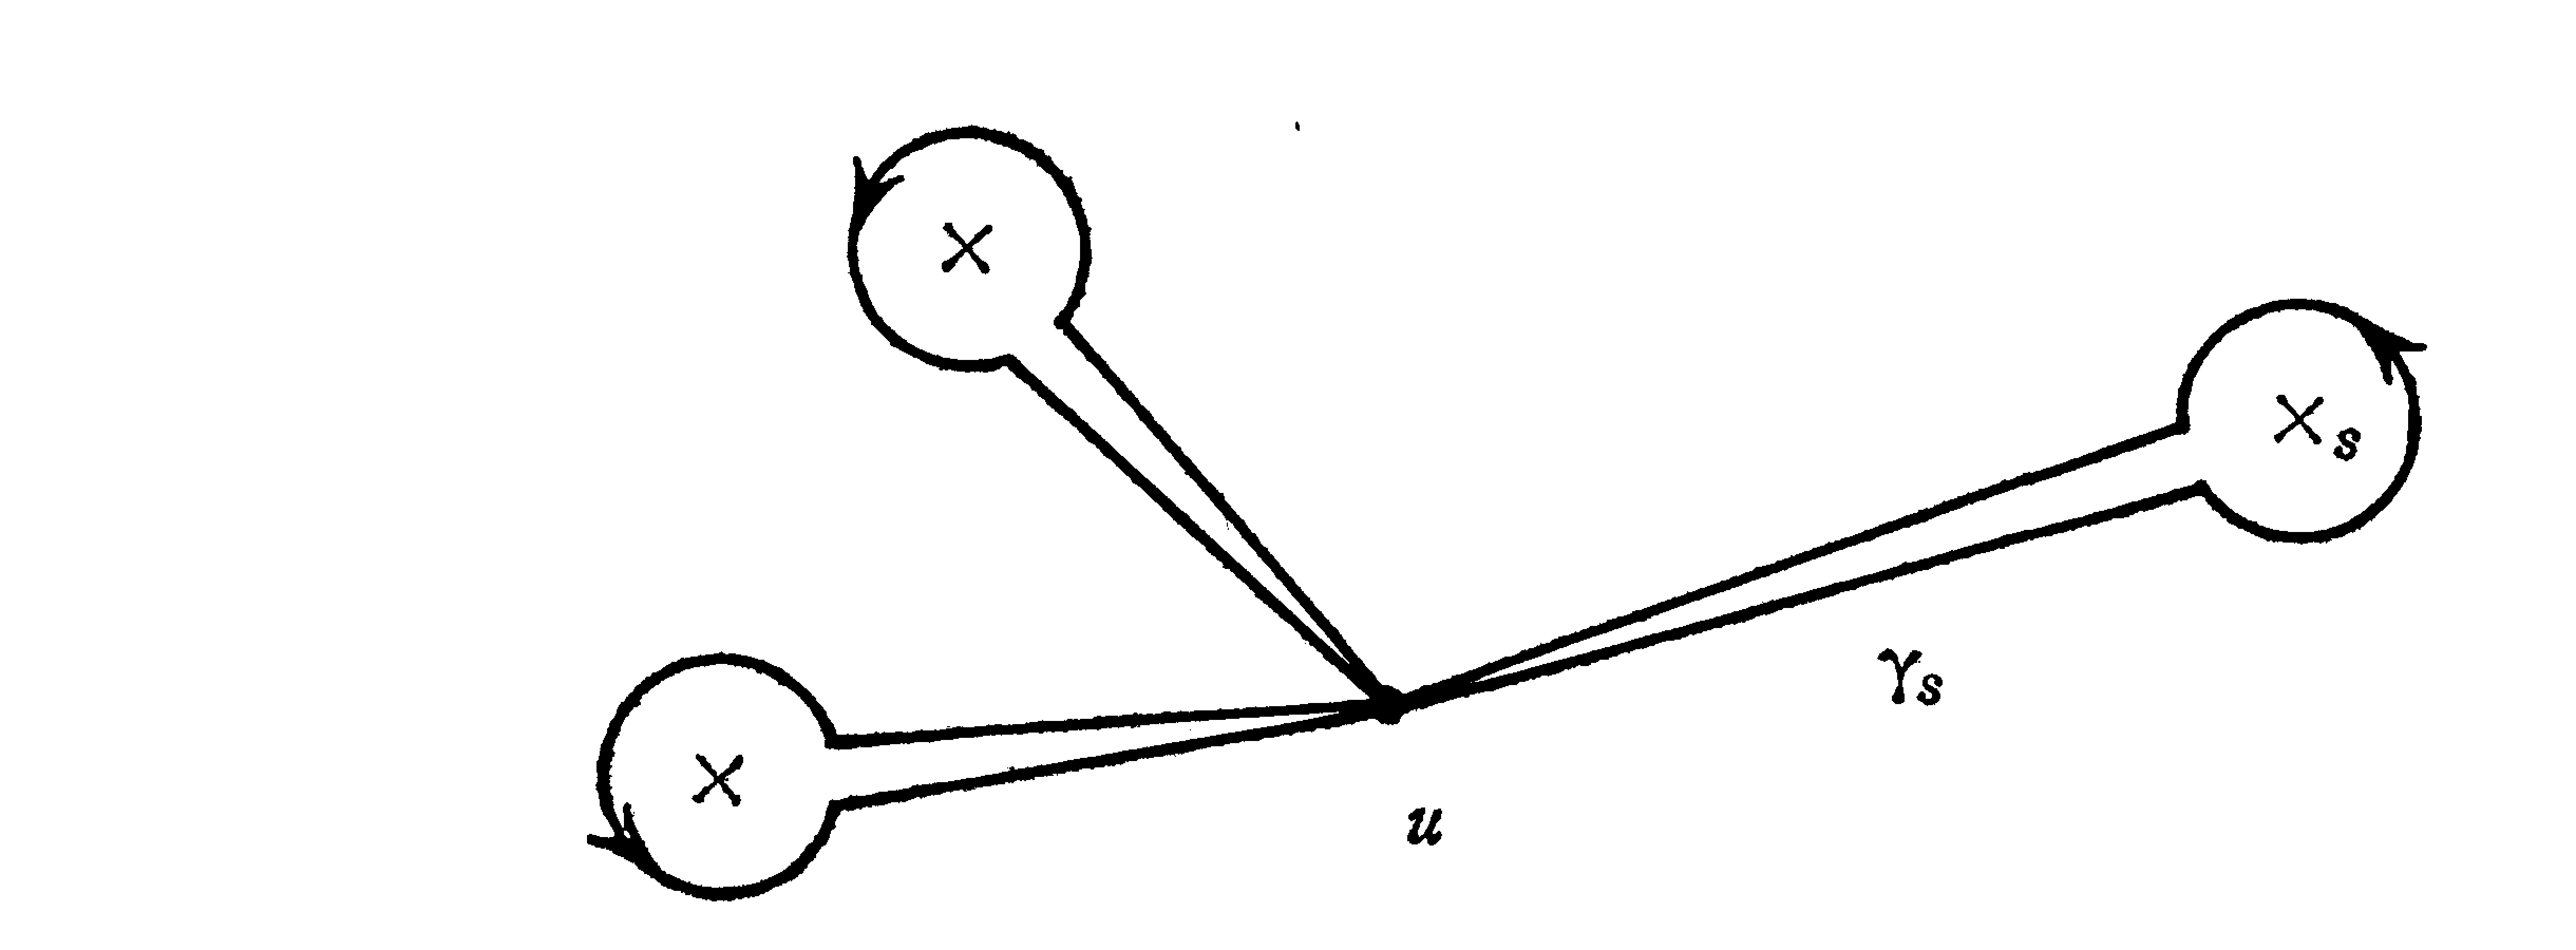
\includegraphics[width=.73\linewidth]{P0019-A01_lacets_presentation.png}\end{center}

\noindent Ces lacets engendrent le groupe fondamental \(\pi _{1}(\mathrm{U},u)\). Ce groupe agit sur \(\mathrm{H}^{i}(\mathrm{X}_{u},\mathbf{Z})\), fibre en \(u\) du système local \(\mathrm{R}^{i} f_{*}\mathbf{Z}|\mathrm{U}\). D’après la théorie locale (4.1), à chaque \(s\in \mathrm{S}\) correspond un cycle évanescent \(\delta _{s}\in \mathrm{H}^{n}(\mathrm{X}_{u},\mathbf{Z})\); ces cycles dépendent du choix des \(\gamma _{s}\). Pour \(i\ne n\), l’action de \(\pi _{1}(\mathrm{U},u)\) sur \(\mathrm{H}^{i}(\mathrm{X}_{u},\mathbf{Z})\) est triviale. Pour \(i=n\), on a\par

\begin{equation*}\begin{gathered}\gamma _{s} x = x \pm  (x,\delta _{s})\delta _{s}.\end{gathered}\tag{5.2.1}\end{equation*}

\noindent Soit \(\mathrm{E}\) le sous-espace de \(\mathrm{H}^{n}(\mathrm{X}_{u},\mathbf{Q})\) engendré par les \(\delta _{s}\) (\emph{partie évanescente} de la cohomologie).\par

\noindent \emph{Proposition} \textbf{(5.3)}. — {\itshape \(\mathrm{E}\) est stable sous l’action du groupe de monodromie \(\pi _{1}(\mathrm{U},u)\). L’orthogonal \(\mathrm{E}^{\perp }\) de \(\mathrm{E}\) (pour la forme d’intersection \(\operatorname{Tr}(x\cup y))\) est le sous-espace des invariants de la monodromie dans \(\mathrm{H}^{n}(\mathrm{X}_{u},\mathbf{Q})\).}\par

\noindent Les \(\gamma _{s}\) engendrant le groupe de monodromie, c’est clair sur (5.2.1).\par

\noindent \emph{Théorème} \textbf{(5.4)}. — {\itshape Les cycles évanescents \(\pm \delta _{s}\) (pris au signe près) sont conjugués sous l’action de \(\pi _{1}(\mathrm{U},u)\).}\par

\noindent Soit \(\check{\mathrm{X}}\subset \check{\mathbf{P}}\) la variété duale de \(\mathrm{X}\) : c’est l’ensemble des \(t\in \check{\mathbf{P}}\) tels que \(\mathrm{H}_{t}\) soit tangent à \(\mathrm{X}\), i.e. tels que \(\mathrm{X}_{t}\) soit singulier, ou que \(\mathrm{X}\subset \mathrm{H}_{t}\). La variété \(\check{\mathrm{X}}\) est irré-\par

\clearpage

\phantomsection\label{D020-physical-20}\noindent{\footnotesize Authority physical page 20; printed 291}\par\smallskip

\noindent ductible. Soit \(\mathrm{Y}\subset \mathrm{X}\times \check{\mathbf{P}}\) l’espace des couples (\(x,t)\) tels que \(x\in \mathrm{H}_{t}\). On dispose d’un diagramme\par

\[\begin{array}{ccc}\mathrm X&\xleftarrow{}&\mathrm Y\\ &&\downarrow\!{g}\\ &&\check{\mathbf P}\end{array}\]

\noindent La fibre de \(g\) en \(t\in \check{\mathbf{P}}\) est la section hyperplane \(\mathrm{X}_{t}=\mathrm{X}\cap \mathrm{H}_{t}\) de \(\mathrm{X}\), et \(g\) est lisse en dehors de l’image réciproque de \(\check{\mathrm{X}}\).\par

\noindent On retrouve la situation de (5.1) en remplaçant \(\check{\mathbf{P}}\) par une droite \(\mathrm{D}\subset \check{\mathbf{P}}\) et \(\mathrm{Y}\) par \(g^{- 1}(\mathrm{D})\). On a \(\mathrm{S}=\mathrm{D}\cap \check{\mathrm{X}}\). D’après un théorème de Lefschetz, pour \(\mathrm{D}\) assez générale, l’application\par

\begin{equation*}\begin{gathered}\pi _{1}(\mathrm{D}- \mathrm{S},u) \longrightarrow  \pi _{1}(\check{\mathbf{P}}- \check{\mathrm{X}},u)\end{gathered}\end{equation*}

\noindent est surjective. Il suffit donc de montrer que les \(\pm \delta _{s}\) sont conjugués sous \(\pi _{1}(\check{\mathbf{P}}- \check{\mathrm{X}})\).\par

\noindent Pour \(x\) dans le lieu lisse de codimension 1 de \(\check{\mathrm{X}}\), soient \(ch\) un chemin de \(t\) à \(x\) dans \(\check{\mathbf{P}}- \check{\mathrm{X}}\), et \(\gamma _{x}\) le lacet qui suit \(ch\) jusqu’au voisinage de \(\check{\mathrm{X}}\), tourne une fois autour de \(\check{\mathrm{X}}\), puis revient à \(t\) par \(ch\). Les lacets \(\gamma _{x}\) (pour \(ch\) variable) sont conjugués entre eux. Puisque \(\check{\mathrm{X}}\) est irréductible, deux points du lieu lisse de \(\check{\mathrm{X}}\) peuvent toujours, dans \(\check{\mathrm{X}}\), être joints par un chemin qui ne quitte pas le lieu lisse. Il en résulte que la classe de conjugaison de \(\gamma _{x}\) ne dépend pas de \(x\). En particulier, les \(\gamma _{s}\) sont conjugués entre eux. On lit sur (5.2.1) que ceci implique la conjugaison des \(\pm \delta _{s}\).\par

\noindent \emph{Corollaire} \textbf{(5.5)}. — {\itshape L’action de \(\pi _{1}(\mathrm{U},u)\) sur \(\mathrm{E}/(\mathrm{E}\cap \mathrm{E}^{\perp })\) est absolument irréductible.}\par

\noindent Soit \(\mathrm{F}\subset \mathrm{E}\otimes \mathbf{C}\) un sous-espace stable sous la monodromie. Si \(\mathrm{F}\not\subset (\mathrm{E}\cap \mathrm{E}^{\perp })\otimes \mathbf{C}\), il existe \(x\in \mathrm{F}\) et \(s\in \mathrm{S}\) tels que (\(x,\delta _{s})\ne 0\). On a alors\par

\begin{equation*}\begin{gathered}\gamma _{s} x- x = \pm (x,\delta _{s})\delta _{s} \in  \mathrm{F},\end{gathered}\end{equation*}

\noindent et \(\delta _{s}\in \mathrm{F}\). D’après (5.4), tous les \(\delta _{s}\) sont alors dans \(\mathrm{F}\), et \(\mathrm{F}=\mathrm{E}\). Ceci prouve (5.5).\par

\noindent \textbf{(5.6)} Ces résultats se transposent comme suit en géométrie algébrique abstraite.\par

\noindent Soient \(\mathbf{P}\) un espace projectif de dimension >1 sur \(k\) algébriquement clos de caractéristique \(p\) et \(\mathrm{X}\subset \mathbf{P}\) une variété projective non singulière connexe et de dimension \(n+1\). Pour \(\mathrm{A}\) un sous-espace linéaire de \(\mathbf{P}\) de codimension 2, on définit comme en (5.1) D et le pinceau (\(\mathrm{H}_{t})_{t\in \mathrm{D}}\), les \(\mathrm{X}_{t}, \widetilde{\mathrm{X}}\) et le diagramme (5.1.1). On dit que les (\(\mathrm{X}_{t})_{t\in \mathrm{D}}\) forment un \emph{pinceau de Lefschetz} de sections hyperplanes si les conditions suivantes sont vérifiées :\par

\noindent \(\mathrm{A})\) L’axe \(\mathrm{A}\) est transverse à \(\mathrm{X}\). L’espace \(\widetilde{\mathrm{X}}\) se déduit alors de \(\mathrm{X}\) par éclatement de \(\mathrm{A}\cap \mathrm{X}\), et est lisse.\par

\clearpage

\phantomsection\label{D020-physical-21}\noindent{\footnotesize Authority physical page 21; printed 292}\par\smallskip

\noindent \(\mathrm{B})\) Il existe une partie finie \(\mathrm{S}\) de \(\mathrm{D}\) et pour chaque \(s\in \mathrm{S}\) un point \(x_{s}\in \mathrm{X}_{s}\), tels que \(f\) soit lisse en dehors des \(x_{s}\).\par

\noindent \(\mathbf{C}) x_{s}\) est un point singulier quadratique ordinaire de \(\mathrm{X}_{s}\).\par

\noindent Pour chaque \(s\in \mathrm{S}\), la théorie de Lefschetz locale du § 4 s’applique au spectre \(\mathrm{D}_{s}\) de l’hensélisé de l’anneau local de \(\mathrm{D}\) en \(s\), et à \(\widetilde{\mathrm{X}}_{\mathrm{D}_{s}}=\widetilde{\mathrm{X}}\times _{\mathrm{D}} \mathrm{D}_{s}\).\par

\noindent \textbf{(5.7)} Soient \(\mathrm{N}\) la dimension de \(\mathbf{P}, r\) un entier \(\geq 1\), et \(\iota _{(r)}\) le plongement de \(\mathbf{P}\) dans l’espace projectif de dimension \(\binom{\mathrm{N}+r}{\mathrm{N}}- 1\), de coordonnées homogènes les monômes de degré \(r\) en les coordonnées homogènes de \(\mathbf{P}\). Les sections hyperplanes de \(\iota _{(r)}(\mathbf{P})\) sont les hypersurfaces de degré \(r\) de \(\mathbf{P}\).\par

\noindent Si \(p\ne 0\), il se peut qu’aucun pinceau de sections hyperplanes de \(\mathrm{X}\) ne soit de Lefschetz. Toutefois, si \(r\geq 2\) et qu’on remplace le plongement projectif donné \(\iota _{1}:\mathrm{X}\hookrightarrow \mathbf{P}\) par \(\iota _{r}=\iota _{(r)}\circ \iota _{1}\), alors, dans ce nouveau plongement, tout pinceau assez général est de Lefschetz. En d’autres termes, si \(r\geq 2\), un pinceau assez général de sections hypersurfaces de degré \(r\) de \(\mathrm{X}\) est toujours de Lefschetz.\par

\noindent \textbf{(5.8)} Dans la suite de cette discussion, nous étudions un pinceau de Lefschetz de sections hyperplanes de \(\mathrm{X}\), \emph{en excluant le cas \(p=2, n\) pair}. Le cas où \(n\) est impair nous suffirait pour la suite. On pose \(\mathrm{U}=\mathrm{D}- \mathrm{S}\). Soient \(u\in \mathrm{U}\) et \(\ell \) un nombre premier \(\ne p\). Les résultats locaux du § 4 montrent que \(\mathrm{R}^{n} f_{*}\mathbf{Q}_{\ell }\) est \emph{modérément} ramifié en chaque \(s\in \mathrm{S}\). Le groupe fondamental modéré de \(\mathrm{U}\) est un quotient du complété profini du groupe fondamental transcendant analogue (relèvement en caractéristique 0 des revêtements modérés, et théorème d’existence de Riemann). La situation algébrique est dès lors toute pareille à la situation transcendante, et la transposition de résultats de Lefschetz se fait par des arguments standards. Dans la démonstration de (5.4), le théorème de Lefschetz sur les \(\pi _{1}\) devient le théorème de Bertini, et on doit invoquer le lemme d’Abhyankar pour contrôler la ramification de \(\mathrm{R}^{i} g_{*}\mathbf{Q}_{\ell }\) le long du lieu lisse de codimension un de \(\check{\mathrm{X}}\).\par

\noindent Les résultats sont les suivants.\par

\noindent a) \emph{Si les cycles évanescents sont non nuls :}\par

\noindent 1) Pour \(i\ne n\), le faisceau \(\mathrm{R}^{i} f_{*}\mathbf{Q}_{\ell }\) sur \(\mathrm{D}\) est constant.\par

\noindent 2) Soit \(j\) l’inclusion de \(\mathrm{U}\) dans \(\mathrm{D}\). On a\par

\begin{equation*}\begin{gathered}\mathrm{R}^{n} f_{*}\mathbf{Q}_{\ell } = j_{*}j^{*}\mathrm{R}^{n} f_{*}\mathbf{Q}_{\ell }.\end{gathered}\end{equation*}

\noindent 3) Soit \(\mathrm{E}\subset \mathrm{H}^{n}(\mathrm{X}_{u},\mathbf{Q}_{\ell })\) le sous-espace de la cohomologie engendré par les cycles évanescents. Ce sous-espace est stable sous \(\pi _{1}(\mathrm{U},u)\), et\par

\begin{equation*}\begin{gathered}\mathrm{E}^{\perp } = \mathrm{H}^{n}(\mathrm{X}_{u},\mathbf{Q}_{\ell })^{\pi _{1}(\mathrm{U},u)}.\end{gathered}\end{equation*}

\noindent La représentation de \(\pi _{1}(\mathrm{U},u)\) sur \(\mathrm{E}/(\mathrm{E}\cap \mathrm{E}^{\perp })\) est absolument irréductible, et l’image de \(\pi _{1}\) dans \(\operatorname{GL}(\mathrm{E}/(\mathrm{E}\cap \mathrm{E}^{\perp }))\) est engendrée (topologiquement) par les \(x\longmapsto x\pm (x,\delta _{s})\delta _{s} (s\in \mathrm{S})\) (le signe \(\pm \) étant déterminé comme en (4.1)).\par

\clearpage

\phantomsection\label{D020-physical-22}\noindent{\footnotesize Authority physical page 22; printed 293}\par\smallskip

\noindent \(b)\) \emph{Si les cycles évanescents sont nuls :} (C’est là un cas exceptionnel. Puisque (\(\delta ,\delta )=\pm 2\) pour \(n\) pair, il ne peut se produire que pour \(n\) impair : \(n=2m+1\). On notera que si un cycle évanescent est nul, ils le sont tous, car conjugués.)\par

\noindent 1) Pour \(i\ne n+1\), le faisceau \(\mathrm{R}^{i} f_{*}\mathbf{Q}_{\ell }\) est constant.\par

\noindent 2) On a une suite exacte\par

\begin{equation*}\begin{gathered}0 \longrightarrow  \bigoplus\limits_{s\in \mathrm{S}} \mathbf{Q}_{\ell }(m- n)_{s} \longrightarrow  \mathrm{R}^{n+1}f_{*}\mathbf{Q}_{\ell } \longrightarrow  \mathcal{F}  \longrightarrow  0\end{gathered}\end{equation*}

\noindent avec \(\mathcal{F} \) constant.\par

\noindent \(3) \mathrm{E}=0\).\par

\noindent \textbf{(5.9)} Le sous-espace \(\mathrm{E}\cap \mathrm{E}^{\perp }\) de \(\mathrm{E}\) est le noyau de la restriction à \(\mathrm{E}\) de la forme d’intersection \(\operatorname{Tr}(x\cup y)\). Cette forme induit donc une forme bilinéaire non dégénérée\par

\begin{equation*}\begin{gathered}\psi  : \mathrm{E}/(\mathrm{E}\cap \mathrm{E}^{\perp })\otimes \mathrm{E}/(\mathrm{E}\cap \mathrm{E}^{\perp }) \longrightarrow  \mathbf{Q}_{\ell }(- n),\end{gathered}\end{equation*}

\noindent alternée pour \(n\) impair, et symétrique pour \(n\) pair. Cette forme est respectée par la monodromie; pour \(n\) impair, la représentation de monodromie induit donc\par

\begin{equation*}\begin{gathered}\rho  : \pi _{1}(\mathrm{U},u) \longrightarrow  \operatorname{Sp}(\mathrm{E}/(\mathrm{E}\cap \mathrm{E}^{\perp }),\psi ).\end{gathered}\end{equation*}

\noindent \emph{Théorème} \textbf{(5.10)} (Kajdan-Margulis). — {\itshape L’image de \(\rho \) est ouverte.}\par

\noindent L’image de \(\rho \) est un sous-groupe compact, donc analytique \(\ell \)-adique, de \(\operatorname{Sp}(\mathrm{E}/(\mathrm{E}\cap \mathrm{E}^{\perp }),\psi )\). Il suffit de montrer que son algèbre de Lie \(\mathfrak{L} \) est égale à \(\mathfrak{sp}(\mathrm{E}/(\mathrm{E}\cap \mathrm{E}^{\perp }),\psi )\). L’analogue transcendant de cette algèbre de Lie est l’algèbre de Lie de l’adhérence de Zariski du groupe de monodromie.\par

\noindent On déduit de (5.8) que \(\mathfrak{L} \) est engendrée par les transformations de carré nul\par

\begin{equation*}\begin{gathered}\mathrm{N}_{s} : x \longmapsto  (x,\delta _{s})\delta _{s}    (s\in \mathrm{S})\end{gathered}\end{equation*}

\noindent et que \(\mathrm{E}/(\mathrm{E}\cap \mathrm{E}^{\perp })\) est une représentation absolument irréductible de \(\mathfrak{L} \). Le théorème résulte du lemme suivant.\par

\noindent \emph{Lemme} \textbf{(5.11)}. — {\itshape Soient \(\mathrm{V}\) un espace vectoriel de dimension finie sur un corps \(k\) de caractéristique \(0, \psi \) une forme alternée non dégénérée et \(\mathfrak{L} \) une sous-algèbre de Lie de \(\mathfrak{sp}(\mathrm{V},\psi )\). On suppose que :}\par

\noindent {\itshape \textup{(i)} \(\mathrm{V}\) est une représentation simple de \(\mathfrak{L} \).}\par

\noindent {\itshape \textup{(ii)} \(\mathfrak{L} \) est engendrée par une famille d’endomorphismes de \(\mathrm{V}\) de la forme \(x\longmapsto \psi (x,\delta )\delta \).}\par

\noindent {\itshape Alors, \(\mathfrak{L} =\mathfrak{sp}(\mathrm{V},\psi )\).}\par

\noindent On peut supposer et on supposera que \(\mathrm{V}\), donc \(\mathfrak{L} \), est non nul. Soit \(\mathrm{W}\subset \mathrm{V}\) l’ensemble des \(\delta \in \mathrm{V}\) tels que \(\mathrm{N}(\delta ):x\longmapsto \psi (x,\delta )\delta \) soit dans \(\mathfrak{L} \).\par

\noindent a) \(\mathrm{W}\) est stable par homothétie (car \(\mathfrak{L} \) est un sous-espace vectoriel de \(\mathfrak{gl}(\mathrm{V}))\).\par

\noindent \(b)\) Si \(\delta \in \mathrm{W}, \operatorname{exp}(\lambda \mathrm{N}(\delta ))\) est un automorphisme de (\(\mathrm{V},\psi ,\mathfrak{L} )\), donc transforme \(\mathrm{W}\) en lui-même. Si \(\delta ',\delta ''\in \mathrm{W}\), on a donc \(\operatorname{exp}(\lambda \mathrm{N}(\delta '))\cdot \delta ''=\delta ''+\lambda \psi (\delta '',\delta ')\delta '\in \mathrm{W}\); si \(\psi (\delta ',\delta '')\ne 0\), le sous-espace vectoriel tendu par \(\delta '\) et \(\delta ''\) est dans \(\mathrm{W}\).\par

\clearpage

\phantomsection\label{D020-physical-23}\noindent{\footnotesize Authority physical page 23; printed 294}\par\smallskip

\noindent \(c)\) Il en résulte que \(\mathrm{W}\) est réunion de ses sous-espaces linéaires maximaux \(\mathrm{W}_{\alpha }\), et que ceux-ci sont deux à deux orthogonaux. Chaque \(\mathrm{W}_{\alpha }\) est dès lors stable sous les \(\mathrm{N}(\delta ) (\delta \in \mathrm{W})\), donc stable sous \(\mathfrak{L} \). Vu l’hypothèse (\(i), \mathrm{W}_{\alpha }=\mathrm{V}\) et \(\mathfrak{L} \) contient tous les \(\mathrm{N}(\delta )\) pour \(\delta \in \mathrm{V}\). On conclut en notant que l’algèbre de Lie \(\mathfrak{sp}(\mathrm{V},\psi )\) est engendrée par les \(\mathrm{N}(\delta ) (\delta \in \mathrm{V})\).\par

\noindent \emph{Remarque} \textbf{(5.12)} (inutile pour la suite). — Il est maintenant facile de prouver (1.6) pour une hypersurface de dimension impaire \(n\) dans \(\mathbf{P}^{n+1}_{\mathbf{F}_{q}}\).\par

\noindent Soient \(\mathrm{X}_{0}\) une telle hypersurface, et \(\overline{\mathrm{X}}_{0}\) l’hypersurface sur \(\overline{\mathbf{F}}_{q}\) qui s’en déduit par extension des scalaires. On a\par

\begin{equation*}\begin{gathered}\mathrm{H}^{2i}(\overline{\mathrm{X}}_{0},\mathbf{Q}_{\ell })=\mathbf{Q}_{\ell }(- i)    (0\leq i\leq n);\end{gathered}\end{equation*}

\noindent \(\mathrm{H}^{2i}(\overline{\mathrm{X}}_{0},\mathbf{Q}_{\ell }(i))\) est engendré par la \(i\)-ième cup-puissance de \(\eta \), la classe de cohomologie \(c_{1}(\mathcal{O}(1))\) d’une section hyperplane. On a donc\par

\begin{equation*}\begin{gathered}\mathrm{Z}(\mathrm{X}_{0},t)=\operatorname{det}(1- \mathrm{F}^{*}t,\mathrm{H}^{n}(\overline{\mathrm{X}}_{0},\mathbf{Q}_{\ell })) / \prod _{i=0}^{n}(1- q^{i} t)\end{gathered}\end{equation*}

\noindent et \(\operatorname{det}(1- \mathrm{F}^{*}t,\mathrm{H}^{n}(\overline{\mathrm{X}}_{0},\mathbf{Q}_{\ell }))\) est un polynôme à coefficients entiers indépendants de \(\ell \).\par

\noindent Faisons varier \(\mathrm{X}_{0}\) dans un pinceau de Lefschetz d’hypersurfaces, qui soit défini sur \(\mathbf{F}_{q}\) (cf. (5.7) pour \(\mathrm{X}=\mathbf{P}^{n+1}\); l’existence d’un tel pinceau n’est pas claire; si on voulait compléter l’argument esquissé ici, il faudrait recourir aux arguments qui seront donnés en (7.1)). On vérifie que \(\mathrm{E}\) coïncide ici avec le \(\mathrm{H}^{n}\) tout entier, et (3.2) fournit la conjecture de Weil pour toutes les hypersurfaces du pinceau, en particulier pour \(\mathrm{X}_{0}\).\par

\noindent \textbf{(5.13)} \emph{Indications bibliographiques sur les §§ 4 et 5.}\par

\noindent \(\mathrm{A})\) Les résultats de Lefschetz (4.1) et (5.1) à (5.5) sont contenus dans son livre [2]. Pour la théorie locale (4.1), il peut être plus commode de consulter SGA 7, XIV (3.2).\par

\noindent \(\mathrm{B})\) Les résultats du § 4 sont démontrés dans les exposés XIII, XIV et XV de SGA 7.\par

\noindent C) (5.7) est démontré dans SGA 7, XVII.\par

\noindent D) (5.8) est démontré dans SGA 7, XVIII. Le théorème d’irréductibilité y est démontré pour \(\mathrm{E}\), mais seulement sous l’hypothèse que \(\mathrm{E}\cap \mathrm{E}^{\perp }=\{0\}\). La démonstration dans le cas général (pour \(\mathrm{E}/(\mathrm{E}\cap \mathrm{E}^{\perp }))\) est pareille.\par

\section*{6. Un théorème de rationalité.}

\noindent \textbf{(6.1)} Soient \(\mathbf{P}_{0}\) un espace projectif de dimension \(\geq 1\) sur \(\mathbf{F}_{q}, \mathrm{X}_{0}\subset \mathbf{P}_{0}\) une variété projective non singulière, \(\mathrm{A}_{0}\subset \mathbf{P}_{0}\) un sous-espace linéaire de codimension deux, \(\mathrm{D}_{0}\subset \check{\mathbf{P}}_{0}\) la droite duale, \(\overline{\mathbf{F}}_{q}\) une clôture algébrique de \(\mathbf{F}_{q}\) et \(\mathbf{P}, \mathrm{X}, \mathrm{A}, \mathrm{D}\) sur \(\overline{\mathbf{F}}_{q}\) déduits de \(\mathbf{P}_{0}, \mathrm{X}_{0}\),\par

\clearpage

\phantomsection\label{D020-physical-24}\noindent{\footnotesize Authority physical page 24; printed 295}\par\smallskip

\noindent \(\mathrm{A}_{0}, \mathrm{D}_{0}\) par extension des scalaires. Le diagramme (5.1.1) de (5.6) provient d’un diagramme analogue sur \(\mathbf{F}_{q}\) :\par

\[\begin{array}{ccc}\mathrm X_0&\xleftarrow{\pi_0}&\widetilde{\mathrm X}_0\\ &&\downarrow\!{f_0}\\ &&\mathrm D_0\end{array}\tag{6.1.1}\]

\noindent On suppose que \(\mathrm{X}\) est connexe de dimension \emph{paire} \(n+1=2m+2\), et que le pinceau (\(\mathrm{X}_{t})_{t\in \mathrm{D}}\) de sections hyperplanes de \(\mathrm{X}\) défini par \(\mathrm{D}\) est un \emph{pinceau de Lefschetz}. L’ensemble \(\mathrm{S}\) des \(t\in \mathrm{D}\) tels que \(\mathrm{X}_{t}\) soit singulier est défini sur \(\mathbf{F}_{q}\), i.e. provient de \(\mathrm{S}_{0}\subset \mathrm{D}_{0}\). On pose \(\mathrm{U}_{0}=\mathrm{D}_{0}- \mathrm{S}_{0}\) et \(\mathrm{U}=\mathrm{D}- \mathrm{S}\).\par

\noindent Soit \(u\in \mathrm{U}\). La partie évanescente de la cohomologie \(\mathrm{E}\subset \mathrm{H}^{n}(\mathrm{X}_{u},\mathbf{Q}_{\ell })\) est stable sous \(\pi _{1}(\mathrm{U},u)\), donc définit sur \(\mathrm{U}\) un sous-système local \(\mathcal{E} \) de \(\mathrm{R}^{n} f_{*}\mathbf{Q}_{\ell }\). Ce dernier est défini sur \(\mathbf{F}_{q} : \mathrm{R}^{i} f_{*}\mathbf{Q}_{\ell }\) est l’image réciproque du \(\mathbf{Q}_{\ell }\)-faisceau \(\mathrm{R}^{i} f_{0*}\mathbf{Q}_{\ell }\) sur \(\mathrm{D}_{0}\), et, sur \(\mathrm{U}, \mathcal{E} \) est l’image réciproque d’un sous-système local\par

\begin{equation*}\begin{gathered}\mathcal{E} _{0} \subset  \mathrm{R}^{n} f_{0*}\mathbf{Q}_{\ell }.\end{gathered}\end{equation*}

\noindent Le cup-produit est une forme alternée\par

\begin{equation*}\begin{gathered}\psi  : \mathrm{R}^{n} f_{0*}\mathbf{Q}_{\ell }\otimes \mathrm{R}^{n} f_{0*}\mathbf{Q}_{\ell } \longrightarrow  \mathbf{Q}_{\ell }(- n).\end{gathered}\end{equation*}

\noindent Notant \(\mathcal{E} _{0}^{\perp }\) l’orthogonal de \(\mathcal{E} _{0}\) relativement à \(\psi \), dans \(\mathrm{R}^{n} f_{0*}\mathbf{Q}_{\ell }|\mathrm{U}_{0}\) on voit que \(\psi \) induit une dualité parfaite\par

\begin{equation*}\begin{gathered}\psi  : \mathcal{E} _{0}/(\mathcal{E} _{0}\cap \mathcal{E} _{0}^{\perp })\otimes \mathcal{E} _{0}/(\mathcal{E} _{0}\cap \mathcal{E} _{0}^{\perp }) \longrightarrow  \mathbf{Q}_{\ell }(- n).\end{gathered}\end{equation*}

\noindent \emph{Théorème} \textbf{(6.2)}. — {\itshape Pour tout \(x\in |\mathrm{U}_{0}|\), le polynôme \(\operatorname{det}(1- \mathrm{F}_{x}^{*}t,\mathcal{E} _{0}/(\mathcal{E} _{0}\cap \mathcal{E} _{0}^{\perp }))\) est à coefficients rationnels.}\par

\noindent \emph{Corollaire} \textbf{(6.3)}. — {\itshape Soient \(j_{0}\) l’inclusion de \(\mathrm{U}_{0}\) dans \(\mathrm{D}_{0}\), et \(j\) celle de \(\mathrm{U}\) dans \(\mathrm{D}\). Les valeurs propres de \(\mathrm{F}^{*}\) agissant sur \(\mathrm{H}^{1}(\mathrm{D},j_{*}\mathcal{E} /(\mathcal{E} \cap \mathcal{E} ^{\perp }))\) sont des nombres algébriques dont tous les conjugués complexes \(\alpha \) vérifient}\par

\begin{equation*}\begin{gathered}q^{\frac{n+1}{2}- \frac{1}{2}} \leq  |\alpha | \leq  q^{\frac{n+1}{2}+\frac{1}{2}}.\end{gathered}\end{equation*}

\noindent D’après (5.10) et (6.2), les hypothèses de (3.2) sont en effet vérifiées par (\(\mathrm{U}_{0},\mathcal{E} _{0}/(\mathcal{E} _{0}\cap \mathcal{E} _{0}^{\perp }),\psi )\), pour \(\beta =n\), et on applique (3.9).\par

\noindent \emph{Lemme} \textbf{(6.4)}. — {\itshape Soit \(\mathcal{G} _{0}\) un \(\mathbf{Q}_{\ell }\)-faisceau constant tordu sur \(\mathrm{U}_{0}\), tel que son image réciproque \(\mathcal{G} \) sur \(\mathrm{U}\) soit un faisceau constant. Il existe alors dans \(\overline{\mathbf{Q}}_{\ell }\) des unités \(\alpha _{i}\) telles que, pour tout \(x\in |\mathrm{U}_{0}|\), on ait}\par

\begin{equation*}\begin{gathered}\operatorname{det}(1- \mathrm{F}_{x}^{*}t,\mathcal{G} _{0})=\prod _{i}(1- \alpha _{i}^{\operatorname{deg}(x)}t).\end{gathered}\end{equation*}

\clearpage

\phantomsection\label{D020-physical-25}\noindent{\footnotesize Authority physical page 25; printed 296}\par\smallskip

\noindent Ce lemme exprime que \(\mathcal{G} _{0}\) est l’image réciproque d’un faisceau sur \(\operatorname{Spec}(\mathbf{F}_{q})\), à savoir son image directe sur \(\operatorname{Spec}(\mathbf{F}_{q})\). Ce dernier s’identifie à une représentation \(\ell \)-adique \(\mathrm{G}_{0}\) de \(\operatorname{Gal}(\overline{\mathbf{F}}_{q}/\mathbf{F}_{q})\), et on prend\par

\begin{equation*}\begin{gathered}\operatorname{det}(1- \mathrm{F}t,\mathrm{G}_{0})=\prod _{i}(1- \alpha _{i} t).\end{gathered}\end{equation*}

\noindent Le lemme (6.4) s’applique aux \(\mathrm{R}^{i} f_{0*}\mathbf{Q}_{\ell } (i\ne n)\), à \(\mathrm{R}^{n} f_{0*}\mathbf{Q}_{\ell }/\mathcal{E} _{0}\) et à \(\mathcal{E} _{0}\cap \mathcal{E} _{0}^{\perp }\).\par

\noindent Pour \(x\in |\mathrm{U}_{0}|\) la fibre \(\mathrm{X}_{x}=f_{0}^{- 1}(x)\) est une variété sur le corps fini \(k(x)\). Si \(\overline{x}\) est un point de \(\mathrm{U}\) au-dessus de \(x, \mathrm{X}_{\overline{x}}\) se déduit de \(\mathrm{X}_{x}\) par extension des scalaires de \(k(x)\) à sa clôture algébrique \(k(\overline{x})=\overline{\mathbf{F}}_{q}\), et \(\mathrm{H}^{i}(\mathrm{X}_{\overline{x}},\mathbf{Q}_{\ell })\) est la fibre de \(\mathrm{R}^{i} f_{*}\mathbf{Q}_{\ell }\) en \(\overline{x}\). La formule (1.5.4) pour la variété \(\mathrm{X}_{x}\) sur \(k(x)\) s’écrit donc\par

\begin{equation*}\begin{gathered}\mathrm{Z}(\mathrm{X}_{x},t)=\prod _{i} \operatorname{det}(1- \mathrm{F}_{x}^{*}t,\mathrm{R}^{i} f_{0*}\mathbf{Q}_{\ell })^{(- 1)^{i+1}}\end{gathered}\end{equation*}

\noindent et \(\mathrm{Z}(\mathrm{X}_{x},t)\) est le produit de\par

\begin{equation*}\begin{gathered}\mathrm{Z}^{f}=\operatorname{det}(1- \mathrm{F}_{x}^{*}t,\mathrm{R}^{n} f_{0*}\mathbf{Q}_{\ell }/\mathcal{E} _{0})\cdot \operatorname{det}(1- \mathrm{F}_{x}^{*}t,\mathcal{E} _{0}\cap \mathcal{E} _{0}^{\perp })\cdot \prod _{i\ne n}\operatorname{det}(1- \mathrm{F}_{x}^{*}t,\mathrm{R}^{i} f_{0*}\mathbf{Q}_{\ell })^{(- 1)^{i+1}}\end{gathered}\end{equation*}

\noindent par\par

\begin{equation*}\begin{gathered}\mathrm{Z}^{m}=\operatorname{det}(1- \mathrm{F}_{x}^{*}t,\mathcal{E} _{0}/(\mathcal{E} _{0}\cap \mathcal{E} _{0}^{\perp })).\end{gathered}\end{equation*}

\noindent Posons \(\mathcal{F} _{0}=\mathcal{E} _{0}/(\mathcal{E} _{0}\cap \mathcal{E} _{0}^{\perp }), \mathcal{F} =\mathcal{E} /(\mathcal{E} \cap \mathcal{E} ^{\perp })\) et appliquons (6.4) aux facteurs de \(\mathrm{Z}^{f}\). On trouve qu’il existe des unités \(\ell \)-adiques \(\alpha _{i} (1\leq i\leq \mathrm{N})\) et \(\beta _{j} (1\leq j\leq \mathrm{M})\) dans \(\overline{\mathbf{Q}}_{\ell }\) tels que pour tout \(x\in |\mathrm{U}_{0}|\)\par

\[\mathrm{Z}(\mathrm{X}_{x},t)=\frac{\prod\limits _{i}(1- \alpha _{i}^{\operatorname{deg}(x)}t)}{\prod\limits _{j}(1- \beta _{j}^{\operatorname{deg}(x)}t)}\cdot \operatorname{det}(1- \mathrm{F}_{x}^{*}t,\mathcal{F} _{0})\]

\noindent et qu’en particulier le second membre est dans \(\mathbf{Q}(t)\). Si un \(\alpha _{i}\) coïncide avec un \(\beta _{j}\), il est loisible de supprimer simultanément cet \(\alpha _{i}\) de la liste des \(\alpha \) et ce \(\beta _{j}\) de la liste des \(\beta \). On peut donc supposer, et nous supposerons, que \(\alpha _{i}\ne \beta _{j}\) pour tout \(i\) et tout \(j\).\par

\noindent \textbf{(6.5)} Il suffit de prouver que les polynômes \(\prod _{i}(1- \alpha _{i} t)\) et \(\prod _{j}(1- \beta _{j} t)\) sont à coefficients rationnels, i.e. que la famille des \(\alpha _{i}\) (resp. la famille des \(\beta _{j})\) est définie sur \(\mathbf{Q}\). Nous le déduirons des propositions suivantes.\par

\noindent \emph{Proposition} \textbf{(6.6)}. — {\itshape Soient (\(\gamma _{i}) (1\leq i\leq \mathrm{P})\) et (\(\delta _{j}) (1\leq j\leq \mathrm{Q})\) deux familles d’unités \(\ell \)-adiques dans \(\overline{\mathbf{Q}}_{\ell }\). On suppose que \(\gamma _{i}\ne \delta _{j}\). Si \(\mathrm{K}\) est un ensemble fini assez grand d’entiers \(\ne 1\), et \(\mathrm{L}\) une partie de densité 0 assez grande de |\(\mathrm{U}_{0}|\), alors, si \(x\in |\mathrm{U}_{0}|\) vérifie \(k\nmid \operatorname{deg}(x)\) (pour tout \(k\in \mathrm{K})\) et \(x\notin \mathrm{L}\), le dénominateur de}\par

\begin{equation*}\begin{gathered}\operatorname{det}(1- \mathrm{F}_{x}^{*}t,\mathcal{F} _{0})\cdot \prod _{i}(1- \gamma _{i}^{\operatorname{deg}(x)}t)/\prod _{j}(1- \delta _{j}^{\operatorname{deg}(x)}t),\end{gathered}\tag{6.6.1}\end{equation*}

\noindent {\itshape écrit sous forme irréductible, est \(\prod _{j}(1- \delta _{j}^{\operatorname{deg}(x)}t)\).}\par

\noindent La démonstration sera donnée en (6.10-13). D’après (6.7) ci-dessous, (6.6) fournit\par

\clearpage

\phantomsection\label{D020-physical-26}\noindent{\footnotesize Authority physical page 26; printed 297}\par\smallskip

\noindent une description intrinsèque de la famille des \(\delta _{j}\) en terme de la famille des fractions rationnelles (6.6.1) pour \(x\in |\mathrm{U}_{0}|\).\par

\noindent \emph{Lemme} \textbf{(6.7)}. — {\itshape Soient \(\mathrm{K}\) un ensemble fini d’entiers \(\ne 1\) et (\(\delta _{j}) (1\leq j\leq \mathrm{Q})\) et (\(\varepsilon _{j}) (1\leq j\leq \mathrm{Q})\) deux familles d’éléments d’un corps. Si, pour tout \(n\) assez grand, non divisible par aucun des \(k\in \mathrm{K}\), la famille des \(\delta _{j}^{n}\) coïncide avec celle des \(\varepsilon _{j}^{n}\) (à l’ordre près), alors la famille des \(\delta _{j}\) coïncide avec celle des \(\varepsilon _{j}\) (à l’ordre près).}\par

\noindent On procède par récurrence sur \(\mathrm{Q}\). L’ensemble des entiers \(n\) tels que \(\delta _{\mathrm{Q}}^{n}=\varepsilon _{j}^{n}\) est un idéal (\(n_{j})\). Prouvons qu’il existe \(j_{0}\) tel que \(\delta _{\mathrm{Q}}=\varepsilon _{j_{0}}\). Sinon les \(n_{j}\) seraient distincts de 1, et il existerait des entiers arbitrairement grands \(n\), non divisibles par aucun des \(n_{j}\), ni par aucun des \(k\in \mathrm{K}\). On aurait \(\delta _{\mathrm{Q}}^{n}\ne \varepsilon _{j}^{n}\), et ceci contredirait l’hypothèse. Il existe donc \(j_{0}\) tel que \(\delta _{\mathrm{Q}}=\varepsilon _{j_{0}}\). On conclut en appliquant l’hypothèse de récurrence aux familles (\(\delta _{j}) (j\ne \mathrm{Q})\) et (\(\varepsilon _{j}) (j\ne j_{0})\).\par

\noindent \emph{Proposition} \textbf{(6.8)}. — {\itshape Soient (\(\gamma _{i}) (1\leq i\leq \mathrm{P})\) et (\(\delta _{j}) (1\leq j\leq \mathrm{Q})\) deux familles d’unités \(p\)-adiques dans \(\overline{\mathbf{Q}}_{\ell }, \mathrm{R}(t)=\prod _{i}(1- \gamma _{i} t)\) et \(\mathrm{S}(t)=\prod _{j}(1- \delta _{j} t)\). Supposons que pour tout \(x\in |\mathrm{U}_{0}|\),}\par

\begin{equation*}\begin{gathered}\prod _{i}(1- \delta _{i}^{\operatorname{deg}(x)}t)\text{ divise }\prod _{i}(1- \gamma _{i}^{\operatorname{deg}(x)}t)\cdot \operatorname{det}(1- \mathrm{F}_{x}^{*}t,\mathcal{F} _{0}).\end{gathered}\end{equation*}

\noindent {\itshape Alors \(\mathrm{S}(t)\) divise \(\mathrm{R}(t)\).}\par

\noindent Supprimons des familles (\(\gamma _{i})\) et (\(\delta _{j})\) des paires d’éléments communs jusqu’à vérifier l’hypothèse de (6.6). Appliquons (6.6). Par hypothèse, les fractions rationnelles (6.6.1) sont des polynômes. Aucun \(\delta \) n’a donc subsisté, ce qui signifie que \(\mathrm{S}(t)\) divise \(\mathrm{R}(t)\).\par

\noindent Cette proposition fournit une caractérisation intrinsèque de \(\mathrm{R}(t)\) en terme de la famille de polynômes\par

\begin{equation*}\begin{gathered}\prod _{i}(1- \gamma _{i}^{\operatorname{deg}(x)}t)\cdot \operatorname{det}(1- \mathrm{F}_{x}^{*}t,\mathcal{F} _{0}).\end{gathered}\end{equation*}

\noindent C’est le ppcm des polynômes \(\mathrm{S}(t)=\prod _{j}(1- \delta _{j} t)\) vérifiant l’hypothèse de (6.8).\par

\noindent \textbf{(6.9)} Prouvons (6.5) et donc (6.2) (modulo (6.6)). Faisons dans (\(6.6) (\gamma _{i})=(\alpha _{i})\) et (\(\delta _{j})=(\beta _{j})\). On trouve une caractérisation intrinsèque de la famille des \(\beta _{j}\) en terme de la famille de fractions rationnelles \(\mathrm{Z}(\mathrm{X}_{x},t) (x\in |\mathrm{U}_{0}|)\). Celles-ci étant dans \(\mathbf{Q}(t)\), la famille des \(\beta _{j}\) est définie sur \(\mathbf{Q}\).\par

\noindent Les polynômes \(\prod _{i}(1- \alpha _{i}^{\operatorname{deg}(x)}t)\cdot \operatorname{det}(1- \mathrm{F}_{x}^{*}t,\mathcal{F} _{0})\) sont donc dans \(\mathbf{Q}[t]\). La proposition (6.8) fournit une description intrinsèque de la famille des \(\alpha _{i}\) en terme de cette famille de polynômes. La famille des \(\alpha _{i}\) est donc définie sur \(\mathbf{Q}\).\par

\noindent \textbf{(6.10)} \emph{Préliminaires}. — Soient \(u\in \mathrm{U}\) et \(\mathcal{F} _{u}\) la fibre de \(\mathcal{F} \) en \(u\). Le groupe fondamental arithmétique \(\pi _{1}(\mathrm{U}_{0},u)\), extension de \(\widehat{\mathbf{Z}}=\operatorname{Gal}(\overline{\mathbf{F}}_{q}/\mathbf{F}_{q})\) (générateur : \(\varphi )\) par le groupe fondamental géométrique \(\pi _{1}(\mathrm{U},u)\), agit sur \(\mathcal{F} _{u}\) par similitudes symplectiques :\par

\begin{equation*}\begin{gathered}\rho  : \pi _{1}(\mathrm{U}_{0},u) \longrightarrow  \operatorname{CSp}(\mathcal{F} _{u},\psi ).\end{gathered}\end{equation*}

\clearpage

\phantomsection\label{D020-physical-27}\noindent{\footnotesize Authority physical page 27; printed 298}\par\smallskip

\noindent Nous notons \(\mu (g)\) le multiplicateur d’une similitude symplectique \(g\). Soit\par

\begin{equation*}\begin{gathered}\mathrm{H}\subset \widehat{\mathbf{Z}}\times \operatorname{CSp}(\mathcal{F} _{u},\psi )\end{gathered}\end{equation*}

\noindent le sous-groupe défini par l’équation\par

\begin{equation*}\begin{gathered}q^{- n}=\mu (g)\end{gathered}\end{equation*}

\noindent (\(q\) étant une unité \(\ell \)-adique, \(q^{n}\in \mathbf{Q}_{\ell }^{*}\) est défini pour tout \(n\in \widehat{\mathbf{Z}})\). Le fait que \(\psi \) soit à valeurs dans \(\mathbf{Q}_{\ell }(- n)\) s’exprime en disant que l’application de \(\pi _{1}\) dans \(\widehat{\mathbf{Z}}\times \operatorname{CSp}\), de coordonnées la projection canonique sur \(\widehat{\mathbf{Z}}\) et \(\rho \), se factorise par\par

\begin{equation*}\begin{gathered}\rho _{1} : \pi _{1}(\mathrm{U}_{0},u) \longrightarrow  \mathrm{H}.\end{gathered}\end{equation*}

\noindent \emph{Lemme} \textbf{(6.11)}. — {\itshape L’image \(\mathrm{H}_{1}\) de \(\rho _{1}\) est ouverte dans \(\mathrm{H}\).}\par

\noindent En effet, \(\pi _{1}(\mathrm{U}_{0},u)\) se projette sur \(\widehat{\mathbf{Z}}\), et l’image de \(\pi _{1}(\mathrm{U},u)=\operatorname{Ker}(\pi _{1}(\mathrm{U}_{0},u)\longrightarrow \widehat{\mathbf{Z}})\) dans \(\operatorname{Sp}(\mathcal{F} _{u},\psi )=\operatorname{Ker}(\mathrm{H}\longrightarrow \widehat{\mathbf{Z}})\) est ouverte (5.10).\par

\noindent \emph{Lemme} \textbf{(6.12)}. — {\itshape Pour \(\delta \in \overline{\mathbf{Q}}_{\ell }\) une unité \(\ell \)-adique, l’ensemble \(\mathrm{Z}\) des (\(n,g)\in \mathrm{H}_{1}\) tels que \(\delta ^{n}\) soit valeur propre de \(g\) est un fermé de mesure nulle.}\par

\noindent Il est clair que \(\mathrm{Z}\) est fermé. Pour chaque \(n\in \widehat{\mathbf{Z}}\), soit \(\operatorname{CSp}_{n}\) l’ensemble des \(g\in \operatorname{CSp}(\mathcal{F} _{u},\psi )\) tels que \(\mu (g)=q^{- n}\), et soit \(\mathrm{Z}_{n}\) l’ensemble des \(g\in \operatorname{CSp}_{n}\) tels que \(\delta ^{n}\) soit valeur propre de \(g\). Alors, \(\operatorname{CSp}_{n}\) est un espace homogène sous \(\operatorname{Sp}\), et on vérifie que \(\mathrm{Z}_{n}\) en est un sous-espace algébrique propre, donc de mesure 0. D’après (\(6.11), \mathrm{H}_{1}\cap (\{n\}\times \mathrm{Z}_{n})\) est donc de mesure 0 dans l’image inverse dans \(\mathrm{H}_{1}\) de \(n\), et on applique Fubini à la projection \(\mathrm{H}_{1}\longrightarrow \widehat{\mathbf{Z}}\).\par

\noindent \textbf{(6.13)} Prouvons (6.6). Pour chaque \(i\) et \(j\), l’ensemble des entiers \(n\) tels que \(\gamma _{i}^{n}=\delta _{j}^{n}\) est l’ensemble des multiples d’un entier fixe \(n_{ij}\) (on n’exclut pas \(n_{ij}=0)\). Par hypothèse, \(n_{ij}\ne 1\).\par

\noindent D’après (6.12) et le théorème de densité de Čebotarev, l’ensemble des \(x\in |\mathrm{U}_{0}|\) tels qu’un \(\beta _{j}^{\operatorname{deg}(x)}\) soit valeur propre de \(\mathrm{F}_{x}^{*}\) agissant sur \(\mathcal{F} _{0}\) est de densité 0. On prend pour \(\mathrm{K}\) l’ensemble des \(n_{ij}\) et pour \(\mathrm{L}\) l’ensemble des \(x\) ci-dessus.\par

\section*{7. Fin de la démonstration de 1.7.}

\noindent \emph{Lemme} \textbf{(7.1)}. — {\itshape Soit \(\mathrm{X}_{0}\) une variété projective non singulière absolument irréductible de dimension \textup{paire} \(d\) sur \(\mathbf{F}_{q}\). Soient \(\mathrm{X}\) sur \(\overline{\mathbf{F}}_{q}\) déduit de \(\mathrm{X}_{0}\) par extension des scalaires et \(\alpha \) une valeur propre de \(\mathrm{F}^{*}\) agissant sur \(\mathrm{H}^{d}(\mathrm{X},\mathbf{Q}_{\ell })\). Alors, \(\alpha \) est un nombre algébrique dont tous les conjugués complexes, encore notés \(\alpha \), vérifient}\par

\begin{equation*}\begin{gathered}q^{\frac{d}{2}- \frac{1}{2}} \leq  |\alpha | \leq  q^{\frac{d}{2}+\frac{1}{2}}.\end{gathered}\tag{7.1.1}\end{equation*}

\noindent On procède par récurrence sur \(d\) (toujours supposé pair). Le cas \(d=0\) est trivial, même sans supposer \(\mathrm{X}_{0}\) absolument irréductible; on suppose dorénavant \(d\geq 2\). On pose \(d=n+1=2m+2\).\par

\clearpage

\phantomsection\label{D020-physical-28}\noindent{\footnotesize Authority physical page 28; printed 299}\par\smallskip

\noindent Si \(\mathbf{F}_{q'}\) est une extension de degré \(r\) de \(\mathbf{F}_{q}\) et que \(\mathrm{X}'_{0}/\mathbf{F}_{q'}\) se déduit de \(\mathrm{X}_{0}/\mathbf{F}_{q}\) par extension des scalaires, l’assertion (7.1) pour \(\mathrm{X}_{0}/\mathbf{F}_{q}\) équivaut à (7.1) pour \(\mathrm{X}'_{0}/\mathbf{F}_{q'}\) : de même que \(q\) est remplacé par \(q^{r}\), les valeurs propres de \(\mathrm{F}^{*}\) sont remplacées par leurs puissances \(r\)-ièmes.\par

\noindent D’après (5.7), dans un plongement projectif convenable \(i:\mathrm{X}\longrightarrow \mathbf{P}, \mathrm{X}\) admet un pinceau de Lefschetz de sections hyperplanes. La remarque précédente nous permet de supposer \(i\) et ce pinceau définis sur \(\mathbf{F}_{q}\) (quitte à remplacer \(\mathbf{F}_{q}\) par une extension finie).\par

\noindent Supposons donc qu’il existe sur \(\mathbf{F}_{q}\) un plongement projectif \(\mathrm{X}_{0}\longrightarrow \mathbf{P}_{0}\) et un sous-espace de codimension deux \(\mathrm{A}_{0}\) de \(\mathbf{P}_{0}\) qui définisse un pinceau de Lefschetz. On reprend les notations de (6.1) et (6.3). Une nouvelle extension des scalaires nous ramène à supposer que :\par

\noindent a) Les points de \(\mathrm{S}\) sont définis sur \(\mathbf{F}_{q}\).\par

\noindent \(b)\) Les cycles évanescents en \(x_{s} (s\in \mathrm{S})\) sont définis sur \(\mathbf{F}_{q}\) (puisque seul \(\pm \delta \) est intrinsèque, ils pourraient n’être définis que sur une extension quadratique).\par

\noindent \(c)\) Il existe un point rationnel \(u_{0}\in \mathrm{U}_{0}\). On prend le point correspondant \(u\) de \(\mathrm{U}\) comme point base.\par

\noindent \(d) \mathrm{X}_{u_{0}}=f_{0}^{- 1}(u_{0})\) admet une section hyperplane lisse \(\mathrm{Y}_{0}\), définie sur \(\mathbf{F}_{q}\). On pose \(\mathrm{Y}=\mathrm{Y}_{0}\otimes _{\mathbf{F}_{q}}\overline{\mathbf{F}}_{q}\).\par

\noindent Puisque \(\widetilde{\mathrm{X}}\) se déduit de \(\mathrm{X}\) par éclatement de la sous-variété lisse de codimension deux \(\mathrm{A}\cap \mathrm{X}\), on a\par

\begin{equation*}\begin{gathered}\mathrm{H}^{i}(\mathrm{X},\mathbf{Q}_{\ell }) \hookrightarrow  \mathrm{H}^{i}(\widetilde{\mathrm{X}},\mathbf{Q}_{\ell })\end{gathered}\end{equation*}

\noindent (en fait, \(\mathrm{H}^{i}(\widetilde{\mathrm{X}},\mathbf{Q}_{\ell })=\mathrm{H}^{i}(\mathrm{X},\mathbf{Q}_{\ell })\oplus \mathrm{H}^{i- 2}(\mathrm{A}\cap \mathrm{X},\mathbf{Q}_{\ell })(- 1))\). Il suffit donc de prouver (7.1.1) pour les valeurs propres \(\alpha \) de \(\mathrm{F}^{*}\) agissant sur \(\mathrm{H}^{d}(\widetilde{\mathrm{X}},\mathbf{Q}_{\ell })\).\par

\noindent La suite spectrale de Leray pour \(f\) s’écrit\par

\begin{equation*}\begin{gathered}\mathrm{E}_{2}^{pq}=\mathrm{H}^{p}(\mathrm{D},\mathrm{R}^{q} f_{*}\mathbf{Q}_{\ell }) \Rightarrow  \mathrm{H}^{p+q}(\widetilde{\mathrm{X}},\mathbf{Q}_{\ell }).\end{gathered}\end{equation*}

\noindent Il suffit de prouver (7.1.1) pour les valeurs propres \(\alpha \) de \(\mathrm{F}^{*}\) agissant sur les \(\mathrm{E}_{2}^{pq}\) pour \(p+q=d=n+1\). Ce sont :\par

\noindent \(\mathrm{A}) \mathrm{E}_{2}^{2,n- 1}\). D’après (\(5.8), \mathrm{R}^{n- 1}f_{*}\mathbf{Q}_{\ell }\) est constant. D’après (2.10), on a donc\par

\begin{equation*}\begin{gathered}\mathrm{E}_{2}^{2,n- 1}=\mathrm{H}^{n- 1}(\mathrm{X}_{u},\mathbf{Q}_{\ell })(- 1).\end{gathered}\end{equation*}

\noindent D’après le théorème de Lefschetz faible (corollaire de SGA 4, XIV (3.2), et de la dualité de Poincaré, SGA 4, XVIII), on a\par

\begin{equation*}\begin{gathered}\mathrm{H}^{n- 1}(\mathrm{X}_{u},\mathbf{Q}_{\ell })(- 1) \hookrightarrow  \mathrm{H}^{n- 1}(\mathrm{Y},\mathbf{Q}_{\ell })(- 1),\end{gathered}\end{equation*}

\noindent et on applique l’hypothèse de récurrence à \(\mathrm{Y}_{0}\).\par

\noindent \(\mathrm{B}) \mathrm{E}_{2}^{0,n+1}\). Si les cycles évanescents sont non nuls, \(\mathrm{R}^{n+1}f_{*}\mathbf{Q}_{\ell }\) est constant et\par

\begin{equation*}\begin{gathered}\mathrm{E}_{2}^{0,n+1}=\mathrm{H}^{n+1}(\mathrm{X}_{u},\mathbf{Q}_{\ell }).\end{gathered}\end{equation*}

\clearpage

\begingroup\setlength{\parskip}{.20em}\setlength{\abovedisplayskip}{4pt}\setlength{\belowdisplayskip}{4pt}\setlength{\abovedisplayshortskip}{2pt}\setlength{\belowdisplayshortskip}{2pt}

\phantomsection\label{D020-physical-29}\noindent{\footnotesize Authority physical page 29; printed 300}\par\smallskip

\noindent Le morphisme de Gysin\par

\begin{equation*}\begin{gathered}\mathrm{H}^{n- 1}(\mathrm{Y},\mathbf{Q}_{\ell })(- 1) \longrightarrow  \mathrm{H}^{n+1}(\mathrm{X}_{u},\mathbf{Q}_{\ell })\end{gathered}\end{equation*}

\noindent est surjectif (cet argument est dual de \(\mathrm{A}))\), et on applique l’hypothèse de récurrence à \(\mathrm{Y}_{0}\).\par

\noindent Si les cycles évanescents sont nuls, la suite exacte de (\(5.8) b)\) fournit une suite exacte\par

\begin{equation*}\begin{gathered}\bigoplus\limits_{s\in \mathrm{S}}\mathbf{Q}_{\ell }(m- n) \longrightarrow  \mathrm{E}_{2}^{0,n+1} \longrightarrow  \mathrm{H}^{n+1}(\mathrm{X}_{u},\mathbf{Q}_{\ell }).\end{gathered}\end{equation*}

\noindent La valeur propre de \(\mathrm{F}\) agissant sur \(\mathbf{Q}_{\ell }(m- n)\) est \(q^{d/2}\), et \(\mathrm{H}^{n+1}\) se traite comme plus haut.\par

\noindent \(\mathbf{C}) \mathrm{E}_{2}^{1,n}\). Si on disposait du théorème de Lefschetz « difficile », on saurait que \(\mathcal{E} \cap \mathcal{E} ^{\perp }\) est nul, et que \(\mathrm{R}^{n} f_{*}\mathbf{Q}_{\ell }\) est somme directe de \(j_{*}\mathcal{E} \) et d’un faisceau constant. Le \(\mathrm{H}^{1}\) d’un faisceau constant sur \(\mathbf{P}^{1}\) est nul, et il suffirait d’appliquer (6.3).\par

\noindent Faute d’avoir déjà démontré Lefschetz « difficile », il nous va falloir dévisser. Si les cycles évanescents sont nuls, \(\mathrm{R}^{n} f_{*}\mathbf{Q}_{\ell }\) est constant ((\(5.8) b))\) et \(\mathrm{E}_{2}^{1,n}=0\). On peut donc supposer, et on supposera, les cycles évanescents non nuls. Filtrons \(\mathrm{R}^{n} f_{*}\mathbf{Q}_{\ell }=j_{*}j^{*}\mathrm{R}^{n} f_{*}\mathbf{Q}_{\ell } (5.8)\) par les sous-faisceaux \(j_{*}\mathcal{E} \) et \(j_{*}(\mathcal{E} \cap \mathcal{E} ^{\perp })\). Si les cycles évanescents \(\delta \) ne sont pas dans \(\mathcal{E} \cap \mathcal{E} ^{\perp }\), on dispose de suites exactes :\par

\begin{equation*}\begin{gathered}0 \longrightarrow  j_{*}\mathcal{E}  \longrightarrow  \mathrm{R}^{n} f_{*}\mathbf{Q}_{\ell } \longrightarrow \text{ faisceau constant }\longrightarrow  0.\end{gathered}\tag{7.1.2}\end{equation*}

\begin{equation*}\begin{gathered}0 \longrightarrow \text{ faisceau constant }j_{*}(\mathcal{E} \cap \mathcal{E} ^{\perp }) \longrightarrow  j_{*}\mathcal{E}  \longrightarrow  j_{*}(\mathcal{E} /(\mathcal{E} \cap \mathcal{E} ^{\perp })) \longrightarrow  0.\end{gathered}\tag{7.1.3}\end{equation*}

\noindent Si, à Dieu ne plaise, les \(\delta \) sont dans \(\mathcal{E} \cap \mathcal{E} ^{\perp }\), on a \(\mathcal{E} \subset \mathcal{E} ^{\perp }\), et des suites exactes :\par

\begin{equation*}\begin{gathered}0 \longrightarrow \text{ le faisceau constant }j_{*}\mathcal{E} ^{\perp } \longrightarrow  \mathrm{R}^{n} f_{*}\mathbf{Q}_{\ell } \longrightarrow \text{ un faisceau }\mathcal{F}  \longrightarrow  0\end{gathered}\tag{7.1.4}\end{equation*}

\begin{equation*}\begin{gathered}0 \longrightarrow  \mathcal{F}  \longrightarrow \text{ le faisceau constant }j_{*}j^{*}\mathcal{F}  \longrightarrow  \bigoplus\limits_{s\in \mathrm{S}}\mathbf{Q}_{\ell }(n- m)_{s} \longrightarrow  0.\end{gathered}\tag{7.1.5}\end{equation*}

\noindent Dans le premier cas, les suites exactes longues de cohomologie fournissent\par

\begin{equation*}\begin{gathered}\mathrm{H}^{1}(\mathrm{D},j_{*}\mathcal{E} ) \longrightarrow  \mathrm{H}^{1}(\mathrm{R}^{n} f_{*}\mathbf{Q}_{\ell }) \longrightarrow  0,\end{gathered}\tag{7.1.2′}\end{equation*}

\begin{equation*}\begin{gathered}0 \longrightarrow  \mathrm{H}^{1}(\mathrm{D},j_{*}\mathcal{E} ) \longrightarrow  \mathrm{H}^{1}(\mathrm{D},j_{*}(\mathcal{E} /(\mathcal{E} \cap \mathcal{E} ^{\perp })))\end{gathered}\tag{7.1.3′}\end{equation*}

\noindent et on applique (6.3).\par

\noindent Dans le second cas, elles fournissent\par

\begin{equation*}\begin{gathered}0 \longrightarrow  \mathrm{H}^{1}(\mathrm{D},\mathrm{R}^{n} f_{*}\mathbf{Q}_{\ell }) \longrightarrow  \mathrm{H}^{1}(\mathrm{D},\mathcal{F} ),\end{gathered}\tag{7.1.4′}\end{equation*}

\begin{equation*}\begin{gathered}\bigoplus\limits_{s\in \mathrm{S}}\mathbf{Q}_{\ell }(n- m) \longrightarrow  \mathrm{H}^{1}(\mathrm{D},\mathcal{F} ) \longrightarrow  0\end{gathered}\tag{7.1.5′}\end{equation*}

\noindent et on remarque que \(\mathrm{F}\) agit sur \(\mathbf{Q}_{\ell }(n- m)\) par multiplication par \(q^{d/2}\).\par

\noindent \emph{Lemme} \textbf{(7.2)}. — {\itshape Soit \(\mathrm{X}_{0}\) une variété projective non singulière absolument irréductible de dimension \(d\) sur \(\mathbf{F}_{q}\). Soient \(\mathrm{X}\) sur \(\overline{\mathbf{F}}_{q}\) déduit de \(\mathrm{X}_{0}\) par extension des scalaires et \(\alpha \) une valeur propre de \(\mathrm{F}^{*}\) agissant sur \(\mathrm{H}^{d}(\mathrm{X},\mathbf{Q}_{\ell })\). Alors, \(\alpha \) est un nombre algébrique dont tous les conjugués complexes, encore notés \(\alpha \), vérifient}\par

\begin{equation*}\begin{gathered}|\alpha |=q^{d/2}.\end{gathered}\end{equation*}

\clearpage

\endgroup

\phantomsection\label{D020-physical-30}\noindent{\footnotesize Authority physical page 30; printed 301}\par\smallskip

\noindent Prouvons déjà que (\(7.2)\Rightarrow (1.7)\). Pour \(\mathrm{X}_{0}\) projective non singulière sur \(\mathbf{F}_{q}\) et \(i\) un entier, il faut prouver l’assertion suivante :\par

\noindent {\itshape \(\mathrm{W}(\mathrm{X}_{0},i)\). Soit \(\mathrm{X}\) déduit de \(\mathrm{X}_{0}\) par extension des scalaires de \(\mathbf{F}_{q}\) à \(\overline{\mathbf{F}}_{q}\). Si \(\alpha \) est une valeur propre de \(\mathrm{F}^{*}\) agissant sur \(\mathrm{H}^{i}(\mathrm{X},\mathbf{Q}_{\ell })\), alors \(\alpha \) est un nombre algébrique dont tous les conjugués complexes, encore notés \(\alpha \), vérifient |\(\alpha |=q^{i/2}\).}\par

\noindent a) Si \(\mathbf{F}_{q^{n}}\) est une extension de degré \(n\) de \(\mathbf{F}_{q}\), et que \(\mathrm{X}'_{0}/\mathbf{F}_{q^{n}}\) se déduit de \(\mathrm{X}_{0}/\mathbf{F}_{q}\) par extension des scalaires, alors \(\mathrm{W}(\mathrm{X}_{0},i)\) équivaut à \(\mathrm{W}(\mathrm{X}'_{0},i)\) : étendre les scalaires revient à remplacer \(\alpha \) par \(\alpha ^{n}\) et \(q\) par \(q^{n}\).\par

\noindent \(b)\) Si \(\mathrm{X}_{0}\) est purement de dimension \(n, \mathrm{W}(\mathrm{X}_{0},i)\) équivaut à \(\mathrm{W}(\mathrm{X}_{0},2n- i)\) : ceci résulte de la dualité de Poincaré.\par

\noindent \(c)\) Si \(\mathrm{X}_{0}\) est somme de variétés \(\mathrm{X}_{0}^{\alpha }, \mathrm{W}(\mathrm{X}_{0},i)\) équivaut à la conjonction des \(\mathrm{W}(\mathrm{X}_{0}^{\alpha },i)\).\par

\noindent \(d)\) Si \(\mathrm{X}_{0}\) est purement de dimension \(n, \mathrm{Y}_{0}\) une section hyperplane lisse de \(\mathrm{X}_{0}\), et que \(i<n\), alors \(\mathrm{W}(\mathrm{Y}_{0},i)\Rightarrow \mathrm{W}(\mathrm{X}_{0},i)\) : ceci résulte du théorème de Lefschetz faible.\par

\noindent Pour prouver les assertions \(\mathrm{W}(\mathrm{X}_{0},i)\), on se ramène successivement :\par

\noindent — par \(c)\), à supposer \(\mathrm{X}_{0}\) purement d’une dimension \(n\);\par

\noindent — par \(b)\), à supposer de plus \(0\leq i\leq n\);\par

\noindent — par a) et \(d)\), à supposer de plus \(i=n\);\par

\noindent — par a) et \(c)\), à supposer de plus \(\mathrm{X}_{0}\) absolument irréductible.\par

\noindent Ce cas est justiciable de (7.2).\par

\noindent \textbf{(7.3)} Prouvons (7.2). Pour tout entier \(k, \alpha ^{k}\) est valeur propre de \(\mathrm{F}^{*}\) agissant sur \(\mathrm{H}^{kd}(\mathrm{X}^{k},\mathbf{Q}_{\ell })\) (formule de Künneth). Pour \(k\) pair, \(\mathrm{X}^{k}\) est justiciable de (7.1), d’où\par

\begin{equation*}\begin{gathered}q^{\frac{kd}{2}- \frac{1}{2}} \leq  |\alpha ^{k}| \leq  q^{\frac{kd}{2}- \frac{1}{2}}\end{gathered}\end{equation*}

\noindent et\par

\begin{equation*}\begin{gathered}q^{\frac{d}{2}- \frac{1}{2k}} \leq  |\alpha | \leq  q^{\frac{d}{2}+\frac{1}{2k}}.\end{gathered}\end{equation*}

\noindent Faisant tendre \(k\) vers l’infini, on trouve (7.2).\par

\section*{8. Premières applications.}

\noindent \emph{Théorème} \textbf{(8.1)}. — {\itshape Soit \(\mathrm{X}_{0}\subset \mathbf{P}_{0}^{n+r}\) une intersection complète non singulière sur \(\mathbf{F}_{q}\), de dimension \(n\) et de multidegré (\(d_{1},\cdots ,d_{r})\). Soit \(b'\) le \(n\)-ième nombre de Betti des intersections complètes non singulières complexes, de mêmes dimension et multidegré. Posons \(b=b'\) pour \(n\) impair, et \(b=b'- 1\) pour \(n\) pair. Alors}\par

\begin{equation*}\begin{gathered}|\# \mathrm{X}_{0}(\mathbf{F}_{q})- \# \mathbf{P}^{n}(\mathbf{F}_{q})| \leq  b\cdot q^{n/2}.\end{gathered}\end{equation*}

\noindent Soient \(\mathrm{X}/\overline{\mathbf{F}}_{q}\) déduit de \(\mathrm{X}_{0}\), et \(\mathbf{Q}_{\ell }\cdot \eta ^{i}\) la droite dans \(\mathrm{H}^{2i}(\mathrm{X},\mathbf{Q}_{\ell })\) engendrée par la \(i\)-ième cup-puissance de la classe de cohomologie d’une section hyperplane. Sur cette droite, \(\mathrm{F}^{*}\) agit par multiplication par \(q^{i}\). La cohomologie de \(\mathrm{X}\) est somme des \(\mathbf{Q}_{\ell }\cdot \eta ^{i}\)\par

\clearpage

\phantomsection\label{D020-physical-31}\noindent{\footnotesize Authority physical page 31; printed 302}\par\smallskip

\noindent (\(0 \leq  i \leq  n)\) et de la partie primitive de \(\mathrm{H}^{n}(\mathrm{X}, \mathbf{Q}_{\ell })\), de dimension \(b\). D'après (1.5), il existe donc \(b\) nombres algébriques \(\alpha _{j}\), les valeurs propres de \(\mathrm{F}^{*}\) agissant sur cette cohomologie primitive, tels que\par

\begin{equation*}\begin{gathered}\# \mathrm{X}_{0}(\mathbf{F}_{q}) = \sum _{i=0}^{n} q^{i} + (-1)^{n} \sum _{j} \alpha _{j}.\end{gathered}\end{equation*}

\noindent D'après (\(1.7), |\alpha _{j}| = q^{n/2}\) et\par

\begin{equation*}\begin{gathered}|\# \mathrm{X}_{0}(\mathbf{F}_{q}) - \# \mathbf{P}(\mathbf{F}_{q})| = |\# \mathrm{X}_{0}(\mathbf{F}_{q}) - \sum _{i=0}^{n} q^{i}| = |\sum _{j} \alpha _{j}| \leq  \sum _{j} |\alpha _{j}| = b\cdot q^{n/2}.\end{gathered}\end{equation*}

\noindent \emph{Théorème} \textbf{(8.2)}. — {\itshape Soient \(\mathrm{N}\) un entier \(\geq  1, \varepsilon  : (\mathbf{Z}/\mathrm{N})^{*} \longrightarrow  \mathbf{C}^{*}\) un caractère, \(k\) un entier \(\geq  2\) et \(f\) une forme modulaire holomorphe sur \(\Gamma _{0}(\mathrm{N})\), de poids \(k\) et de caractère \(\varepsilon  : f\) est une fonction holomorphe sur le demi-plan de Poincaré \(\mathrm{X}\), telle que pour \(\begin{pmatrix}a&b\\c&d\end{pmatrix}\) \(\in  \operatorname{SL}(2, \mathbf{Z})\), avec \(c \equiv  0 (\mathrm{N})\), on ait}\par

\begin{equation*}\begin{gathered}f\left(\frac{az+b}{cz+d}\right) = \varepsilon (a)^{-1}(cz+d)^{k} f(z).\end{gathered}\end{equation*}

\noindent {\itshape On suppose \(f\) \textup{cuspidale} et \textup{primitive} (« new » au sens d'Atkin-Lehner et de Miyake), en particulier vecteur propre des opérateurs de Hecke \(\mathrm{T}_{p} (p \nmid  \mathrm{N})\). Posons \(f = \sum _{n=1}^{\infty } a_{n} q^{n}\), avec \(q = e^{2\pi iz}\) (et \(a_{1} = 1)\). Alors, pour \(p\) premier ne divisant pas \(\mathrm{N}\)}\par

\begin{equation*}\begin{gathered}|a_{p}| \leq  2\cdot p^{\frac{k-1}{2}}.\end{gathered}\end{equation*}

\noindent {\itshape En d'autres termes, les racines de l'équation}\par

\begin{equation*}\begin{gathered}\mathrm{T}^{2} - a_{p} \mathrm{T} + \varepsilon (p)\cdot p^{k-1}\end{gathered}\end{equation*}

\noindent {\itshape sont de valeur absolue \(p^{\frac{k-1}{2}}\).}\par

\noindent Ces racines sont en effet des valeurs propres de Frobenius agissant sur le \(\mathrm{H}^{k-1}\) d'une variété projective non singulière de dimension \(k-1\) définie sur \(\mathbf{F}_{p}\).\par

\noindent Sous des hypothèses restrictives, ce fait est démontré dans mon exposé Bourbaki (Formes modulaires et représentations \(\ell \)-adiques, exposé 355, février 1969, dans : \emph{Lecture Notes in Mathematics}, 179). Le cas général n'est pas beaucoup plus difficile.\par

\noindent \emph{Remarque} \textbf{(8.3)}. — J. P. Serre et moi-même avons récemment démontré que (8.2) reste vrai pour \(k = 1\). La démonstration est toute différente.\par

\noindent L'application suivante m'a été suggérée par \(\mathrm{E}\). Bombieri.\par

\noindent \emph{Théorème} \textbf{(8.4)}. — {\itshape Soient \(\mathrm{Q}\) un polynôme à \(n\) variables et de degré \(d\) sur \(\mathbf{F}_{q}, \mathrm{Q}_{d}\) la partie homogène de degré \(d\) de \(\mathrm{Q}\) et \(\psi  : \mathbf{F}_{q} \longrightarrow  \mathbf{C}^{*}\) un caractère additif non trivial sur \(\mathbf{F}_{q}\). On suppose que :}\par

\noindent {\itshape \textup{(i)} \(d\) est premier à \(p\);\\ \textup{(ii)} l'hypersurface \(\mathrm{H}_{0}\) dans \(\mathbf{P}^{n-1}_{\mathbf{F}_{q}}\) définie par \(\mathrm{Q}_{d}\) est lisse.}\par

\clearpage

\phantomsection\label{D020-physical-32}\noindent{\footnotesize Authority physical page 32; printed 303}\par\smallskip

\noindent {\itshape Alors}\par

\begin{equation*}\begin{gathered}|\sum _{x_{1},\cdots ,x_{n} \in  \mathbf{F}_{q}} \psi (\mathrm{Q}(x_{1},\cdots ,x_{n}))| \leq  (d-1)^{n} q^{n/2}.\end{gathered}\end{equation*}

\noindent Quitte à remplacer \(\mathrm{Q}\) par un multiple scalaire, on peut supposer (et on supposera) que\par

\begin{equation*}\begin{gathered}\psi (x) = \operatorname{exp}(2\pi i \operatorname{Tr}_{\mathbf{F}_{q}/\mathbf{F}_{p}}(x)/p).\end{gathered}\tag{8.4.1}\end{equation*}

\noindent Soit \(\mathrm{X}_{0}\) le revêtement étale de l'espace affine \(\mathrm{A}_{0}\) de dimension \(n\) sur \(\mathbf{F}_{q}\) d'équation \(\mathrm{T}^{p} - \mathrm{T} = \mathrm{Q}\), et soit \(\sigma \) la projection de \(\mathrm{X}_{0}\) sur \(\mathrm{A}_{0}\) :\par

\begin{equation*}\begin{gathered}\sigma  : \mathrm{X}_{0} \longrightarrow  \mathrm{A}_{0}\end{gathered}\end{equation*}

\begin{equation*}\begin{gathered}\mathrm{X}_{0} = \operatorname{Spec}(\mathbf{F}_{q}[x_{1},\cdots ,x_{n},\mathrm{T}]/(\mathrm{T}^{p}-\mathrm{T}-\mathrm{Q})).\end{gathered}\end{equation*}

\noindent Le revêtement \(\mathrm{X}_{0}\) est galoisien, de groupe de Galois \(\mathbf{Z}/p; i \in  \mathbf{Z}/p = \mathbf{F}_{p}\) agit par \(\mathrm{T} \longmapsto  \mathrm{T}+i\).\par

\noindent Soit \(x \in  \mathrm{A}_{0}(\mathbf{F}_{q})\) et calculons l'endomorphisme de Frobenius de la fibre de \(\mathrm{X}_{0}/\mathrm{A}_{0}\) en \(x\). Posons \(q = p^{f}\) et soit \(\overline{\mathbf{F}}_{q}\) une clôture algébrique de \(\mathbf{F}_{q}\). Pour (\(x,\mathrm{T}) \in  \mathrm{X}_{0}(\overline{\mathbf{F}}_{q})\) au-dessus de \(x\), on a \(\mathrm{F}((x,\mathrm{T})) = (x,\mathrm{T}^{q})\), et\par

\begin{equation*}\begin{gathered}\mathrm{T}^{q} = \mathrm{T} + \sum _{i=1}^{f} (\mathrm{T}^{p^{i}}-\mathrm{T}^{p^{i-1}}) = \mathrm{T} + \sum _{i} \mathrm{Q}(x)^{p^{i-1}} = \mathrm{T} + \operatorname{Tr}_{\mathbf{F}_{q}/\mathbf{F}_{p}}(\mathrm{Q}(x)).\end{gathered}\end{equation*}

\noindent C'est l'action de l'élément \(\operatorname{Tr}_{\mathbf{F}_{q}/\mathbf{F}_{p}}(\mathrm{Q}(x))\) du groupe de Galois.\par

\noindent Soient \(\mathrm{E}\) le corps des racines \(p\)-ièmes de l'unité et \(\lambda \) une place finie de \(\mathrm{E}\) première à \(p\). Nous travaillerons en cohomologie \(\lambda \)-adique. Pour \(j \in  \mathbf{Z}/p\), soit \(\mathcal{F} _{j,0}\) le \(\mathrm{E}_{\lambda }\)-système local de rang un sur \(\mathrm{A}_{0}\) défini par \(\mathrm{X}_{0}\) et \(\psi (-jx) : \mathbf{Z}/p \longrightarrow  \mathrm{E}^{*} \longrightarrow  \mathrm{E}_{\lambda }^{*}\) : on dispose de \(\iota  : \mathrm{X}_{0} \longrightarrow  \mathcal{F} _{j,0}\) et \(\iota (i*x) = \psi (-ji)\iota (x)\). Notons sans 0 les objets déduits de \(\mathrm{A}_{0}, \mathrm{X}_{0}, \mathcal{F} _{j,0}\) par extension des scalaires à \(\overline{\mathbf{F}}_{q}\). La formule des traces (1.12.1) pour \(\mathcal{F} _{j,0}\) s'écrit\par

\begin{equation*}\begin{gathered}\sum _{x_{1},\cdots ,x_{n} \in  \mathbf{F}_{q}} \psi (\mathrm{Q}(x_{1},\cdots ,x_{n})) = \sum _{i} (-1)^{i} \operatorname{Tr}(\mathrm{F}^{*}, \mathrm{H}_{c}^{i}(\mathrm{A},\mathcal{F} _{1})).\end{gathered}\tag{8.4.2}\end{equation*}

\noindent On a \(\sigma _{*}\mathrm{E}_{\lambda } = \bigoplus\limits_{j} \mathcal{F} _{j}\), et donc\par

\begin{equation*}\begin{gathered}\mathrm{H}_{c}^{*}(\mathrm{X},\mathbf{Q}_{\ell }) \otimes _{\mathbf{Q}_{\ell }} \mathrm{E}_{\lambda } = \bigoplus\limits_{j} \mathrm{H}_{c}^{*}(\mathrm{A},\mathcal{F} _{j}).\end{gathered}\tag{8.4.3}\end{equation*}

\noindent Pour \(j = 0, \mathcal{F} _{j}\) est le faisceau constant \(\mathrm{E}_{\lambda }\); ce facteur correspond à l'inclusion, par image réciproque, de la cohomologie de \(\mathrm{A}\) dans celle de \(\mathrm{X}\).\par

\noindent \emph{Lemme} \textbf{(8.5)}. — {\itshape \textup{(i)} Pour \(j \ne  0, \mathrm{H}_{c}^{i}(\mathrm{A},\mathcal{F} _{j})\) est nul pour \(i \ne  n\); pour \(i = n\), cet espace de cohomologie est de dimension (\(d-1)^{n}\).}\par

\noindent {\itshape \textup{(ii)} Pour \(j \ne  0\), le cup-produit}\par

\begin{equation*}\begin{gathered}\mathrm{H}_{c}^{n}(\mathrm{A},\mathcal{F} _{j}) \otimes  \mathrm{H}_{c}^{n}(\mathrm{A},\mathcal{F} _{-j}) \longrightarrow  \mathrm{H}_{c}^{2n}(\mathrm{A},\mathrm{E}_{\lambda }) \xrightarrow{\operatorname{Tr}} \mathrm{E}_{\lambda }(-n)\end{gathered}\end{equation*}

\noindent {\itshape est une dualité parfaite.}\par

\noindent {\itshape \textup{(iii)} \(\mathrm{X}_{0}\) est un ouvert d'une variété projective non singulière \(\mathrm{Z}_{0}\).}\par

\clearpage

\phantomsection\label{D020-physical-33}\noindent{\footnotesize Authority physical page 33; printed 304}\par\smallskip

\noindent Déduisons (8.4) de (8.5). Soient \(j_{0} : \mathrm{X}_{0} \hookrightarrow  \mathrm{Z}_{0}\) et \(j : \mathrm{X} \hookrightarrow  \mathrm{Z}\) déduit par extension des scalaires à \(\overline{\mathbf{F}}_{q}\). D'après (\(8.4.2), (i)\), et (1.7) pour \(\mathrm{Z}_{0}\), il suffit de prouver l'injectivité de\par

\begin{equation*}\begin{gathered}\mathrm{H}_{c}^{n}(\mathrm{A},\mathcal{F} _{1}) \xrightarrow{\sigma ^{*}} \mathrm{H}_{c}^{n}(\mathrm{X},\mathcal{F} _{1}) = \mathrm{H}_{c}^{n}(\mathrm{X},\mathrm{E}_{\lambda }) \xrightarrow{j_{!}} \mathrm{H}^{n}(\mathrm{Z},\mathrm{E}_{\lambda }).\end{gathered}\end{equation*}

\noindent On a \(\operatorname{Tr}(a \cup  b) = \frac{1}{p} \operatorname{Tr}(j_{!}\sigma ^{*}a \cup  j_{!}\sigma ^{*}b)\), donc cette injectivité résulte de (ii).\par

\noindent \textbf{(8.6)} Prouvons (8.5) (iii). Soient \(\mathrm{P}_{0}\) l'espace projectif sur \(\mathbf{F}_{q}\) complété de \(\mathrm{A}_{0}\) par adjonction d'un hyperplan à l'infini \(\mathrm{P}_{0}^{\infty }, \mathrm{H}_{0} \subset  \mathrm{P}_{0}^{\infty }\) d'équation \(\mathrm{Q}_{d} = 0\) et \(\mathrm{Y}_{0}\) le revêtement de \(\mathrm{P}_{0}\) normalisé de \(\mathrm{P}_{0}\) dans \(\mathrm{X}_{0}\).\par

\[\begin{array}{ccccc}\mathrm X_0&\hookrightarrow&\mathrm Y_0&&\\ {\scriptstyle\sigma}\downarrow&&\downarrow&&\\ \mathrm A_0&\hookrightarrow&\mathrm P_0&\hookleftarrow\mathrm P_0^{\infty}&\hookleftarrow\mathrm H_0\end{array}\tag{8.6.1}\]

\noindent Étudions \(\mathrm{Y}_{0}/\mathrm{P}_{0}\) près de l'infini, localement pour la topologie étale.\par

\noindent \emph{Lemme} \textbf{(8.7)}. — {\itshape \(\mathrm{Y}_{0}\) est lisse en dehors de l'image réciproque de \(\mathrm{H}_{0}\).}\par

\noindent Le diviseur de la fonction rationnelle \(\mathrm{Q}\) sur \(\mathrm{P}_{0}\) est somme de sa partie finie \(\operatorname{div}(\mathrm{Q})_{f}\) et de (-\(d)\) fois l'hyperplan à l'infini. On a :\par

\begin{equation*}\begin{gathered}\operatorname{div}(\mathrm{Q}) = \operatorname{div}(\mathrm{Q})_{f} - d\mathrm{P}_{0}^{\infty } \\ \operatorname{div}(\mathrm{Q})_{f} \cap  \mathrm{P}_{0}^{\infty } = \mathrm{H}_{0}.\end{gathered}\tag{8.7.1}\end{equation*}

\noindent \(\mathrm{A}\) distance finie, \(\mathrm{Y}_{0} = \mathrm{X}_{0}\) est étale sur \(\mathrm{A}_{0}\), donc lisse. \(\mathrm{A}\) l'infini, mais en dehors de l'image réciproque de \(\mathrm{H}_{0}\), il existe des coordonnées locales (\(z_{1},\cdots ,z_{n})\) telles que \(\mathrm{Q} = z_{1}^{-d}\) (ceci utilise que (\(d,p) = 1)\). Dans ces coordonnées, \(\mathrm{Y}_{0}\) apparaît comme produit d'une courbe et d'un espace lisse (correspondant aux coordonnées \(z_{2},\cdots ,z_{n})\). Par normalité, il est lisse.\par

\noindent \emph{Lemme} \textbf{(8.8)}. — {\itshape Au voisinage étale d'un point au-dessus de \(\mathrm{H}_{0}, \mathrm{Y}_{0}\) est lisse sur une surface singulière normale, toujours la même.}\par

\noindent On peut cette fois trouver des coordonnées locales telles que \(\mathrm{Q} = z_{1}^{-d}z_{2}\). En effet, puisque \(\mathrm{H}_{0}\) est lisse, \(\operatorname{div}(\mathrm{Q})_{f}\) est lisse au voisinage de l'infini et coupe \(\mathrm{P}_{0}^{\infty }\) transversalement. Cette forme est indépendante du point choisi, et n'utilise que deux coordonnées, d'où l'assertion.\par

\noindent \textbf{(8.9)} On sait que le procédé suivant (dû à Zariski) permet de résoudre les singularités de surfaces : alternativement, on normalise et on éclate le lieu singulier (réduit). Les opérateurs en jeu commutent à la localisation étale et au produit par un espace lisse. Le procédé de Zariski permet donc encore de résoudre les singularités d'un espace qui, comme \(\mathrm{Y}_{0}\), est, localement pour la topologie étale, lisse sur une surface. La résolution obtenue de \(\mathrm{Y}_{0}\) est le \(\mathrm{Z}_{0}\) cherché.\par

\clearpage

\phantomsection\label{D020-physical-34}\noindent{\footnotesize Authority physical page 34; printed 305}\par\smallskip

\noindent Si \(\mathrm{T}\) est une courbe sur une surface \(\mathrm{S}\), contenant le lieu singulier, et que \(\mathrm{T}'\) est l'image réciproque de \(\mathrm{T}\) dans la résolution de Zariski \(\mathrm{S}'\) de \(\mathrm{S}\), on sait que si on éclate de façon itérée dans \(\mathrm{S}'\) le lieu singulier (réduit) de (\(\mathrm{T}')_{\mathrm{red}}\), on obtient une surface \(\mathrm{S}''\) telle que l'image réciproque réduite (\(\mathrm{T}'')_{\mathrm{red}}\) de \(\mathrm{T}\) dans \(\mathrm{S}''\) soit un diviseur à croisements normaux. \(\mathrm{A}\) nouveau, les opérations en jeu commutent à la localisation étale et au produit par un espace lisse. Raisonnant comme plus haut, et observant que (\(\mathrm{Y}_{0}\), l'infini) est localement lisse sur un (\(\mathrm{S},\mathrm{T})\), on peut même trouver \(\mathrm{Z}_{0}\) tel que \(\mathrm{Z}_{0}-\mathrm{X}_{0}\) soit un diviseur à croisements normaux.\par

\noindent \textbf{(8.10)} Prouvons (\(8.5) (i)\), (ii). Ce sont des assertions géométriques; ceci nous permet de travailler dorénavant sur \(\overline{\mathbf{F}}_{q}\). Soit \(\mathrm{S}'\) l'espace affine sur \(\overline{\mathbf{F}}_{q}\) qui paramétrise les polynômes à \(n\) variables de degré \(\leq  d\), et soit \(\mathrm{S}\) l'ouvert de \(\mathrm{S}'\) correspondant aux polynômes dont la partie homogène de degré \(d\) est de discriminant non nul. On note \(\mathrm{Q}_{\mathrm{S}} \in  \mathrm{H}^{0}(\mathrm{S},\mathcal{O}_{\mathrm{S}}[x_{1},\cdots ,x_{n}])\) le polynôme universel sur \(\mathrm{S}\), et \(\mathrm{X}_{\mathrm{S}}\) le revêtement galoisien étale de \(\mathrm{A}_{\mathrm{S}} = \mathrm{A}^{n} \times  \mathrm{S}\) d'équation \(\mathrm{T}^{p}-\mathrm{T} = \mathrm{Q}_{\mathrm{S}}\), de groupe de Galois \(\mathbf{Z}/p\). Soient \(\mathrm{P}_{\mathrm{S}} = \mathbf{P}^{n} \times  \mathrm{S}\) l'espace projectif sur \(\mathrm{S}\) complété de \(\mathrm{A}_{\mathrm{S}}\) et \(\mathrm{Y}_{\mathrm{S}}\) le normalisé de \(\mathrm{P}_{\mathrm{S}}\) dans \(\mathrm{X}_{\mathrm{S}}\). On dispose, sur \(\mathrm{S}\), d'un diagramme analogue à (8.6.1).\par

\noindent Les expressions de \(\mathrm{Q}\) en coordonnées locales données en (8.7) et (8.8) restent valables dans la situation présente, avec paramètres, de sorte que, localement pour la topologie étale sur \(\mathrm{Y}_{\mathrm{S}}, \mathrm{Y}_{\mathrm{S}}/\mathrm{S}\) est isomorphe au produit de \(\mathrm{S}\) (qui est lisse) avec une fibre. La méthode canonique de résolution utilisée en (8.9) nous fournit une compactification relative \(\mathrm{Z}_{\mathrm{S}}/\mathrm{S}\) de \(\mathrm{X}_{\mathrm{S}}/\mathrm{S}\), avec \(\mathrm{Z}_{\mathrm{S}}-\mathrm{X}_{\mathrm{S}}\) un diviseur à croisements normaux relatifs sur \(\mathrm{S}\)\par

\[\begin{array}{ccc}\mathrm X_{\mathrm S}&\xhookrightarrow{u}&\mathrm Z_{\mathrm S}\\ {\scriptstyle\sigma}\downarrow&&\downarrow{\scriptstyle f}\\ \mathrm A_{\mathrm S}&\xrightarrow{a}&\mathrm S\end{array}\]

\noindent (\(f\) propre et lisse, \(u\) plongement ouvert, \(\mathrm{Z}_{\mathrm{S}}-\mathrm{X}_{\mathrm{S}}\) diviseur à croisements normaux relatifs).\par

\noindent Soit \(\mathcal{F} _{j,\mathrm{S}}\) le \(\mathrm{E}_{\lambda }\)-faisceau sur \(\mathrm{A}_{\mathrm{S}}\) déduit comme en (8.4) de \(\mathrm{X}_{\mathrm{S}}/\mathrm{A}_{\mathrm{S}}\). On a \(\sigma _{*}\mathrm{E}_{\lambda } = \bigoplus\limits_{j} \mathcal{F} _{j,\mathrm{S}}\), donc\par

\begin{equation*}\begin{gathered}\mathrm{R}^{*}(fu)_{!}(\mathrm{E}_{\lambda }) = \bigoplus\limits_{j} \mathrm{R}^{*}a_{!}\mathcal{F} _{j,\mathrm{S}}.\end{gathered}\end{equation*}

\noindent Les propriétés de \(\mathrm{Z}_{\mathrm{S}}\) assurent que les \(\mathrm{R}^{i}(fu)_{!}\mathrm{E}_{\lambda } = \mathrm{R}^{i}f_{*}(u_{!}\mathrm{E}_{\lambda })\) sont des faisceaux localement constants sur \(\mathrm{S}\). Dès lors, les \(\mathrm{R}^{i}a_{!}\mathcal{F} _{j,\mathrm{S}}\) également sont localement constants. Puisque \(\mathrm{S}\) est connexe, il suffit de prouver (\(8.5) (i)\), (ii) pour un polynôme \(\mathrm{Q}\) particulier. On prendra \(\mathrm{Q} = \sum _{i} x_{i}^{d}\). Ce polynôme vérifie la condition de non-singularité car (\(d,p) = 1\). Pour ce polynôme, les variables se séparent dans la somme exponentielle de (8.4). Ceci correspond au fait que \(\mathcal{F} _{j}\) est le produit tensoriel des images réciproques de\par

\clearpage

\phantomsection\label{D020-physical-35}\noindent{\footnotesize Authority physical page 35; printed 306}\par\smallskip

\noindent faisceaux analogues \(\mathcal{F} _{j}^{1}\) sur les facteurs de dimension un \(\mathrm{A}^{1}\) de \(\mathrm{A} = \mathrm{A}^{n}\). Par la formule de Künneth\par

\begin{equation*}\begin{gathered}\mathrm{H}^{*}(\mathrm{A},\mathcal{F} _{j}) = \bigotimes \mathrm{H}^{*}(\mathrm{A}^{1},\mathcal{F} _{j}^{1}).\end{gathered}\end{equation*}

\noindent Ceci ramène la preuve de (\(8.5) (i)\), (ii) au cas où \(n = 1\) et où \(\mathrm{Q}\) est \(x^{d}\).\par

\noindent \textbf{(8.11)} Traitons ce cas particulier. Le revêtement \(\mathrm{X}\) de \(\mathrm{A}\) est irréductible, de sorte que pour \(i = 0,2\)\par

\begin{equation*}\begin{gathered}\mathrm{H}_{c}^{i}(\mathrm{A},\mathrm{E}_{\lambda }) \xrightarrow{\sim } \mathrm{H}_{c}^{i}(\mathrm{X},\mathrm{E}_{\lambda }).\end{gathered}\end{equation*}

\noindent Pour \(i \ne  1\) et \(j \ne  0\), on a donc\par

\begin{equation*}\begin{gathered}\mathrm{H}_{c}^{i}(\mathrm{A},\mathcal{F} _{j}) = 0.\end{gathered}\end{equation*}

\noindent L'assertion (ii) résulte de (2.8) ou (2.12) et de ce que \(u_{!}\mathcal{F} _{j} = u_{*}\mathcal{F} _{j}\). Pour prouver (\(i)\), il reste à vérifier que\par

\begin{equation*}\begin{gathered}\chi _{c}(\mathrm{A},\mathcal{F} _{j}) = 1-d.\end{gathered}\end{equation*}

\noindent D'après la formule d'Euler-Poincaré (voir l'exposé Bourbaki 286 de février 1965, par \(\mathrm{M}\). Raynaud), ceci équivaut au lemme suivant.\par

\noindent \emph{Lemme} \textbf{(8.12)}. — {\itshape Le conducteur de Swan de \(\mathcal{F} _{j}\) à l'infini est égal à \(d\).}\par

\noindent Cet énoncé équivaut au suivant.\par

\noindent \emph{Lemme} \textbf{(8.13)}. — {\itshape Soient \(k\) un corps fini de caractéristique \(p, y \in  k[[x]]\) un élément de valuation \(d\) première à \(p, \mathrm{L}\) l'extension de \(\mathrm{K} = k((x))\) engendré par les racines de \(\mathrm{T}^{p}-\mathrm{T} = y^{-1}\) et \(\chi \) le caractère suivant de \(\operatorname{Gal}(\mathrm{L}/\mathrm{K})\) à valeurs dans \(\mathbf{Z}/p\) :}\par

\begin{equation*}\begin{gathered}\chi (\sigma ) = \sigma \mathrm{T}-\mathrm{T}.\end{gathered}\end{equation*}

\noindent {\itshape Alors, \(\chi \) est de conducteur \(d+1\).}\par

\noindent Par extension du corps résiduel, on se ramène à supposer \(k\) algébriquement clos plutôt que fini, et on applique : J. P. Serre, Sur les corps locaux à corps résiduel algébriquement clos, \emph{Bull. Soc. Math. France}, 89 (1961), p. 105-154, n° 4.4.\par

\section*{BIBLIOGRAPHIE}

\noindent [\(1] \mathrm{A}\). \textsc{Grothendieck}, Formule de Lefschetz et rationalité des fonctions \(\mathrm{L}\), \emph{Séminaire Bourbaki}, 279, décembre 1964 (Benjamin).\par

\noindent [\(2] \mathrm{S}\). \textsc{Lefschetz}, \emph{L'analysis situs et la géométrie algébrique} (Gauthier-Villars), 1924. Reproduit dans : \emph{Selected papers} (Chelsea Publ. Co.).\par

\noindent [\(3] \mathrm{R}. \mathrm{A}\). \textsc{Rankin}, Contributions to the theory of Ramanujan's function \(\tau (n)\) and similar arithmetical functions. II, \emph{Proc. Camb. Phil. Soc.}, \textbf{35} (1939), 351-372.\par

\clearpage

\phantomsection\label{D020-physical-36}\noindent{\footnotesize Authority physical page 36; printed 307}\par\smallskip

\noindent [\(4] \mathrm{A}\). \textsc{Weil}, Numbers of solutions of equations in finite fields, \emph{Bull. Am. Math. Soc.}, \textbf{55} (1949), p. 497-508.\par

\noindent SGA, \emph{Séminaire de Géométrie Algébrique du Bois-Marie} (IHES) :\par

\noindent SGA 4, Théorie des topos et cohomologie étale des schémas (dirigé par \(\mathrm{M}\). \textsc{Artin}, \(\mathrm{A}\). \textsc{Grothendieck} et J.-L. \textsc{Verdier}), \emph{Lecture Notes in Math.}, 269, 270, 305.\par

\noindent SGA 5, \emph{Cohomologie ℓ-adique et fonctions L}, diffusé par l'IHES.\par

\noindent SGA 7, Groupes de monodromie en géométrie algébrique.\par

\noindent 1\textsuperscript{re} partie : dirigé par \(\mathrm{A}\). \textsc{Grothendieck}, \emph{Lecture Notes in Math.}, 288.\par

\noindent 2\textsuperscript{e} partie : par \(\mathrm{P}\). \textsc{Deligne} et \(\mathrm{N}\). \textsc{Katz}, \emph{Lecture Notes in Math.}, 340.\par

\begin{flushright}\emph{Manuscrit reçu le 20 septembre 1973.}\end{flushright}

\clearpage


\clearpage\endgroup
\typeout{CORPUS-END:D020:\thepage}
% END INLINE WORK D020 FR
% BEGIN INLINE WORK D021 FR
\typeout{CORPUS-BEGIN:D021:\thepage}
\begingroup
\makeatletter
\let\DeclareMathOperator\CorpusDeclareMathOperator
\let\@declmathop\CorpusDeclMathOp
\let\maketitle\CorpusMakeTitle\let\title\CorpusTitle\let\author\CorpusAuthor\let\date\CorpusDate
\let\thanks\CorpusThanks\let\and\CorpusAnd\let\@maketitle\CorpusAtMakeTitle
\def\setcounter#1#2{\def\CorpusCounterName{#1}\def\CorpusPageName{page}\ifx\CorpusCounterName\CorpusPageName\else\CorpusSetCounter{#1}{#2}\fi}
\title{}\author{}\date{}
\expandafter\let\csname EditionShort\endcsname\CorpusUndefined
\expandafter\let\csname PhysicalPage\endcsname\CorpusUndefined
\expandafter\let\csname PrintedPage\endcsname\CorpusUndefined
\expandafter\let\csname ArticlePage\endcsname\CorpusUndefined
\expandafter\let\csname DPageUnit\endcsname\CorpusUndefined
\expandafter\let\csname DTitle\endcsname\CorpusUndefined
\expandafter\let\csname DByline\endcsname\CorpusUndefined
\expandafter\let\csname DDedication\endcsname\CorpusUndefined
\expandafter\let\csname DSection\endcsname\CorpusUndefined
\expandafter\let\csname DSectionNamed\endcsname\CorpusUndefined
\expandafter\let\csname DLineBlock\endcsname\CorpusUndefined
\expandafter\let\csname endDLineBlock\endcsname\CorpusUndefined
\setcounter{section}{0}
\expandafter\def\csname theHsection\endcsname{D021.\arabic{section}}
\setcounter{subsection}{0}
\expandafter\def\csname theHsubsection\endcsname{D021.\arabic{subsection}}
\setcounter{subsubsection}{0}
\expandafter\def\csname theHsubsubsection\endcsname{D021.\arabic{subsubsection}}
\setcounter{equation}{0}
\expandafter\def\csname theHequation\endcsname{D021.\arabic{equation}}
\setcounter{figure}{0}
\expandafter\def\csname theHfigure\endcsname{D021.\arabic{figure}}
\setcounter{table}{0}
\expandafter\def\csname theHtable\endcsname{D021.\arabic{table}}
\setcounter{footnote}{0}
\expandafter\def\csname theHfootnote\endcsname{D021.\arabic{footnote}}
\makeatother
\let\tableofcontents\relax % one cumulative contents list, not repeated global lists
% Generated deterministically from frozen D021 NDJSON records.
% Authority SHA-256: 2ACE335E3C8CC08BB8B60D756886284C4E7AECF093081DDA0DE46650800E6986
% Records SHA-256: A7D9FCCF8482984F90D4226177ADFFFDAC9C3A26A1C165428D2779ACE724EB9A
\setmainfont{TeX Gyre Pagella}
\setsansfont{TeX Gyre Heros}

\setlength{\parindent}{1.15em}
\setlength{\parskip}{0pt}
\setlength{\abovedisplayskip}{4.2pt plus 1.5pt minus 1.5pt}
\setlength{\belowdisplayskip}{4.2pt plus 1.5pt minus 1.5pt}
\setlength{\abovedisplayshortskip}{2.5pt plus 1pt}
\setlength{\belowdisplayshortskip}{3pt plus 1pt}
\setlength{\jot}{1.5pt}
\setlist{nosep,leftmargin=2em}
\emergencystretch=1.5em
\clubpenalty=10000
\widowpenalty=10000
\displaywidowpenalty=10000
\raggedbottom
\newcommand{\EditionShort}{Édition française de lecture}
\newcommand{\PhysicalPage}{}
\newcommand{\PrintedPage}{}
\newcommand{\ArticlePage}{}
\newcommand{\DPageUnit}[3]{%
  \renewcommand{\PhysicalPage}{#1}%
  \renewcommand{\PrintedPage}{#2}%
  \renewcommand{\ArticlePage}{#3}%
  \phantomsection\pdfbookmark[2]{Authority physical #1 / printed #2}{D021-physical-#1}%
}
\newcommand{\DTitle}[1]{\begin{center}\vspace*{2mm}{\fontsize{15}{18}\selectfont\bfseries #1\par}\vspace{4mm}\end{center}}
\newcommand{\DByline}[1]{\begin{center}{\small\scshape #1\par}\vspace{5mm}\end{center}}
\newcommand{\DDedication}[1]{\begin{flushright}\itshape #1\end{flushright}\vspace{2mm}}
\newcommand{\DSection}[2]{\phantomsection\pdfbookmark[1]{#1}{D021-#2}\begin{center}\vspace{2.5pt}{\bfseries #1}\end{center}\vspace{1pt}}
\newcommand{\DSectionNamed}[3]{\phantomsection\pdfbookmark[1]{#2}{D021-#3}\begin{center}\vspace{2.5pt}{\bfseries #1}\end{center}\vspace{1pt}}
\newenvironment{DLineBlock}{\par\smallskip\begin{center}\begin{minipage}{0.76\textwidth}\raggedright}{\end{minipage}\end{center}\smallskip}
\pagestyle{fancy}
\fancyhf{}
\fancyhead[L]{\scriptsize\textsc{Deligne--Serre · D021}}
\fancyhead[R]{\scriptsize\EditionShort}
\fancyfoot[C]{\scriptsize Authority physical \PhysicalPage\ · printed \PrintedPage}
\renewcommand{\headrulewidth}{0.25pt}
\renewcommand{\footrulewidth}{0pt}

\graphicspath{{assets/works/}}
\selectlanguage{french}
\phantomsection\addcontentsline{toc}{section}{D021}
\fontsize{8.65pt}{10.25pt}\selectfont

\justifying
% AUTHORITY_UNIT physical=2 article=1 printed=507

\DPageUnit{2}{507}{1}

\DTitle{FORMES MODULAIRES DE POIDS 1}

\DByline{PAR PIERRE DELIGNE ET JEAN-PIERRE SERRE}

\DDedication{A Henri Cartan,\\à l'occasion de son\\70\textsuperscript{e} anniversaire}

\DSection{Introduction}{introduction-1}

La décomposition en produit eulérien, et l'équation fonctionnelle, des séries de Dirichlet associées par Hecke aux formes modulaires de poids 1 suggèrent que celles-ci correspondent à des fonctions \(L\) d'Artin de degré 2 du corps \(\mathbf{Q}\), autrement dit à des représentations de \(\operatorname{Gal}(\overline{\mathbf{Q}}/\mathbf{Q})\) dans \(\operatorname{GL}_2(\mathbf{C})\). C'est une telle correspondance, conjecturée par Langlands, que nous établissons ici.\par

Les trois premiers paragraphes sont préliminaires. Le paragraphe 4 contient l'énoncé du théorème principal, et quelques compléments. La démonstration occupe les paragraphes 5 à 9. Son principe est le suivant : on commence par construire, pour tout nombre premier \(\ell\), une représentation de \(\operatorname{Gal}(\overline{\mathbf{Q}}/\mathbf{Q})\) en caractéristique \(\ell\) (cf. § 6); on montre ensuite que les images de \(\operatorname{Gal}(\overline{\mathbf{Q}}/\mathbf{Q})\) dans ces diverses représentations sont « petites », ce qui permet de les relever en caractéristique 0, et d'obtenir la représentation complexe cherchée (§§ 7 et 8); la « petitesse » en question résulte elle-même d'une majoration en moyenne des valeurs propres des opérateurs de Hecke (Rankin, cf. § 5). Le paragraphe 9 contient une estimation des coefficients des formes modulaires de poids 1.\par

Signalons que nous avons utilisé en un point essentiel (§ 6, th. 6.1) des résultats démontrés par l'un de nous (P. Deligne), mais dont aucune démonstration complète n'a encore été publiée; en attendant une telle publication (ainsi que celle de SGA 5, dont ils dépendent), nous demandons au lecteur de bien vouloir les admettre.\par

\DSectionNamed{§ 1. Rappels (analytiques) sur les formes modulaires}{Section 1: Rappels (analytiques) sur les formes modulaires}{section-1}

1.1. Soit \(N\) un entier \(\geq 1\). On associe à \(N\) les sous-groupes\par

\begin{equation*}
\Gamma(N)\subset\Gamma_1(N)\subset\Gamma_0(N).
\end{equation*}

\newpage

% AUTHORITY_UNIT physical=3 article=2 printed=508

\DPageUnit{3}{508}{2}

de \(\operatorname{SL}_2(\mathbf{Z})\) définis par\par

\begin{equation*}
\begin{pmatrix}a&b\\c&d\end{pmatrix}\in\Gamma(N)
\quad\Longleftrightarrow\quad
 a\equiv d\equiv 1\pmod N\quad\text{et}\quad b\equiv c\equiv 0\pmod N,
\end{equation*}

\begin{equation*}
\begin{pmatrix}a&b\\c&d\end{pmatrix}\in\Gamma_1(N)
\quad\Longleftrightarrow\quad
 a\equiv d\equiv 1\pmod N\quad\text{et}\quad c\equiv 0\pmod N,
\end{equation*}

\begin{equation*}
\begin{pmatrix}a&b\\c&d\end{pmatrix}\in\Gamma_0(N)
\quad\Longleftrightarrow\quad
 c\equiv 0\pmod N.
\end{equation*}

1.2. Soit \(f\) une fonction sur le demi-plan \(H=\{z\mid\operatorname{Im}(z)>0\}\). Si \(k\) est un entier, et si \(\gamma=\begin{pmatrix}a&b\\c&d\end{pmatrix}\) est un élément de \(\operatorname{SL}_2(\mathbf{R})\), on pose\par

\begin{equation*}
(f\mid_k\gamma)(z)=(cz+d)^{-k}f(\gamma z),
\qquad\text{où}\qquad
\gamma z=\frac{az+b}{cz+d}.
\end{equation*}

Soit \(\Gamma\) un sous-groupe de \(\operatorname{SL}_2(\mathbf{Z})\) contenant \(\Gamma(N)\). On dit que \(f\) est modulaire de poids \(k\) sur \(\Gamma\) si :\par

(1.2.1) \(f\mid_k\gamma=f\) pour tout \(\gamma\in\Gamma\);\par

(1.2.2) \(f\) est holomorphe sur \(H\);\par

(1.2.3) \(f\) est « holomorphe aux pointes », i. e., pour tout \(\sigma\in\operatorname{SL}_2(\mathbf{Z})\), la fonction \(f\mid_k\sigma\) a un développement en série de puissances de \(e^{2\pi iz/N}\) à exposants \(\geq 0\).\par

Lorsque, dans (1.2.3), on remplace « exposants \(\geq 0\) » par « exposants \(>0\) », on obtient la notion de forme modulaire parabolique.\par

1.3. Soit \(f\) une forme modulaire de poids \(k\) sur \(\Gamma(N)\). Pour que \(f\) soit une forme modulaire sur \(\Gamma_1(N)\), il faut et il suffit que \(f(z+1)=f(z)\), ou encore que \(f\) ait un développement de la forme\par

\begin{equation*}
\sum_{n=0}^{\infty}a_nq^n,
\qquad\text{où}\qquad q=e^{2\pi iz}.
\end{equation*}

Dans ce qui suit, ce développement sera noté \(f_{\infty}(q)\), ou simplement \(f\).\par

1.4. Soit \(f\) une forme modulaire de poids \(k\) sur \(\Gamma_1(N)\). Si \(\gamma=\begin{pmatrix}a&b\\c&d\end{pmatrix}\) est un élément de \(\Gamma_0(N)\), la forme \(f\mid_k\gamma\) ne dépend que de l'image de \(d\) dans \((\mathbf{Z}/N\mathbf{Z})^*\); on la note \(f\mid R_d\). On a \(f\mid R_{-1}=(-1)^kf\).\par

1.5. Soit \(\varepsilon\) un caractère de Dirichlet mod \(N\), autrement dit un homomorphisme\par

\begin{equation*}
\varepsilon:(\mathbf{Z}/N\mathbf{Z})^*\longrightarrow\mathbf{C}^*.
\end{equation*}

On dit que \(\varepsilon\) est pair (resp. impair) si \(\varepsilon(-1)=1\) (resp. si \(\varepsilon(-1)=-1\)).\par

\newpage

% AUTHORITY_UNIT physical=4 article=3 printed=509

\DPageUnit{4}{509}{3}

Soit \(k\) un entier de même parité que \(\varepsilon\) [i. e. \(\varepsilon(-1)=(-1)^k\)]. On appelle forme modulaire de type \((k,\varepsilon)\) sur \(\Gamma_0(N)\) une forme modulaire \(f\) de poids \(k\) sur \(\Gamma_1(N)\) telle que\par

\begin{equation*}
f\mid R_d=\varepsilon(d)f
\end{equation*}

pour tout \(d\in(\mathbf{Z}/N\mathbf{Z})^*\), i. e.\par

\begin{equation*}
f\!\left(\frac{az+b}{cz+d}\right)=\varepsilon(d)(cz+d)^kf(z)
\quad\text{pour tout}\quad
\begin{pmatrix}a&b\\c&d\end{pmatrix}\in\Gamma_0(N).
\end{equation*}

(Noter que, si \(\varepsilon\) et \(k\) n'étaient pas de même parité, cette formule entraînerait \(f=0\).)\par

Toute forme modulaire de poids \(k\) sur \(\Gamma_1(N)\) est combinaison linéaire de formes de types \((k,\varepsilon_i)\) sur \(\Gamma_0(N)\), où les \(\varepsilon_i\) sont les différents caractères de \((\mathbf{Z}/N\mathbf{Z})^*\) de même parité que \(k\).\par

Cela se voit (cf. [16], p. IV-13) en remarquant que l'application\par

\begin{equation*}
\begin{pmatrix}a&b\\c&d\end{pmatrix}\longmapsto d\pmod N
\end{equation*}

définit par passage au quotient un isomorphisme de \(\Gamma_0(N)/\Gamma_1(N)\) sur \((\mathbf{Z}/N\mathbf{Z})^*\).\par

1.6. OPÉRATEURS DE HECKE. — Soit \(f=\sum a_nq^n\) une forme modulaire de type \((k,\varepsilon)\) sur \(\Gamma_0(N)\), et soit \(p\) un nombre premier. On pose\par

\begin{equation*}
\tag{1.6.1}
f\mid T_p=\sum a_{pn}q^n+\varepsilon(p)p^{k-1}\sum a_nq^{pn}
\qquad\text{si }p\nmid N,
\end{equation*}

\begin{equation*}
\tag{1.6.2}
f\mid U_p=\sum a_{pn}q^n
\qquad\text{si }p\mid N.
\end{equation*}

On obtient ainsi une autre forme modulaire de type \((k,\varepsilon)\) sur \(\Gamma_0(N)\), qui est parabolique si \(f\) l'est.\par

1.7. FORMES PRIMITIVES. — On renvoie à [2] (dans le cas \(\varepsilon=1\)) et à [6], [12], [13] (dans le cas général) pour la définition des formes paraboliques primitives (« newforms ») de type \((k,\varepsilon)\) sur \(\Gamma_0(N)\).\par

Si \(f=\sum_{n=1}^{\infty}a_nq^n\) est une telle forme, on a \(a_1=1\), et \(f\) est fonction propre des opérateurs de Hecke \(T_p\) et \(U_p\), les valeurs propres correspondantes étant les \(a_p\). Il en résulte que la série de Dirichlet\par

\begin{equation*}
\tag{1.7.1}
\Phi_f(s)=\sum_{n=1}^{\infty}a_nn^{-s}
\end{equation*}

admet le développement eulérien\par

\begin{equation*}
\tag{1.7.2}
\Phi_f(s)=
\prod_{p\mid N}\frac{1}{1-a_pp^{-s}}
\prod_{p\nmid N}\frac{1}{1-a_pp^{-s}+\varepsilon(p)p^{k-1-2s}}.
\end{equation*}

1.8. Si \(f\) est comme ci-dessus, et si \(p\mid N\), la valeur absolue de \(a_p\) est donnée par la règle suivante ([12], [14]) :\par

\begin{equation*}
a_p=0\quad\text{si }p^2\mid N\text{ et si }\varepsilon\text{ peut être défini mod }N/p;
\end{equation*}

\newpage

% AUTHORITY_UNIT physical=5 article=4 printed=510

\DPageUnit{5}{510}{4}

\begin{equation*}
|a_p|=p^{(k-1)/2}\quad\text{si }\varepsilon\text{ ne peut pas être défini mod }N/p;
\end{equation*}

\begin{equation*}
|a_p|=p^{k/2-1}\quad\text{si }p^2\nmid N\text{ et si }\varepsilon\text{ peut être défini mod }N/p.
\end{equation*}

(Il résultera du théorème 4.6 ci-après que le dernier cas ne se présente pas pour \(k=1\).)\par

1.9. Toute forme \(f\) de type \((k,\varepsilon)\) sur \(\Gamma_0(N)\) peut s'écrire\par

\begin{equation*}
f(z)=E(z)+\sum\lambda_i f_i(d_i z),
\end{equation*}

où \(E\) est une série d'Eisenstein, et où \(f_i\) est parabolique primitive de type \((k,\varepsilon)\) sur \(\Gamma_0(N_i)\), \(N_i\) étant un diviseur de \(N\) tel que \(\varepsilon\) puisse être défini mod \(N_i\), et \(d_i\) un diviseur de \(N/N_i\). De plus, cette décomposition est unique, en un sens évident.\par

\DSectionNamed{§ 2. Rappels (géométriques) sur les formes modulaires}{Section 2: Rappels (géométriques) sur les formes modulaires}{section-2}

2.1. Soient \(k\) et \(N\) des entiers \(\geq 1\), et \(\mu_N\) le schéma en groupes des racines \(N\)-ièmes de l'unité. Du point de vue géométrique, une forme modulaire de poids \(k\) sur \(\Gamma_1(N)\) est une loi qui, à chaque courbe elliptique \(E\) munie d'un plongement \(\alpha:\mu_N\longrightarrow E\), associe une section de la puissance tensorielle \(k\)-ième \(\omega_E^{\otimes k}\) de \(\omega_E\), où \(\omega_E\) est le dual de l'algèbre de Lie de \(E\).\par

Précisons :\par

(a) Une courbe elliptique sur un schéma \(S\) est un morphisme propre et lisse \(E\longrightarrow S\), muni d'une section \(e:S\longrightarrow E\), de fibres géométriques des courbes elliptiques. Lorsque \(S\) est le spectre d'un anneau commutatif \(A\), on dit aussi que \(E\) est une courbe elliptique sur \(A\). On pose \(\omega_E=e^*\Omega^1_{E/S}\); pour \(S=\operatorname{Spec}(A)\), \(\omega_E\) s'identifie à un \(A\)-module inversible.\par

(b) Soit \(R\) un anneau commutatif dans lequel \(N\) est inversible. Une forme modulaire de poids \(k\) sur \(\Gamma_1(N)\), méromorphe à l'infini, définie sur \(R\), est une loi qui, à toute courbe elliptique \(E\) sur une \(R\)-algèbre \(A\), munie d'un plongement \(\alpha:\mu_N\longrightarrow E\), associe un élément \(f(E,\alpha)\) de \(\omega_E^{\otimes k}\). On exige que cette loi soit compatible aux isomorphismes, et à l'extension des scalaires.\par

(c) On dit que \(f\) est holomorphe à l'infini si elle se prolonge en une loi \(\widetilde f\) définie pour les couples \((E,\alpha)\) où \(E\) est une courbe elliptique généralisée ([7], II. 1.12) et \(\alpha\) un plongement de \(\mu_N\) dans \(E\) dont l'image rencontre chaque composante irréductible de chaque fibre géométrique ([7], IV. 4.14). Si elle existe, la loi \(\widetilde f\) est unique.\par

Supposons que \(R\) soit un corps. On dit que \(f\) est parabolique si elle est holomorphe à l'infini et si \(\widetilde f(E,\alpha)=0\) chaque fois que \(E\) est une courbe elliptique dégénérée (i. e. non lisse) sur une extension algébriquement close de \(R\).\par

Ces notions pourraient aussi se définir en termes de développements de Laurent en \(q\) (cf. [7], VII, § 3).\par

2.2. Soit \(f\) comme ci-dessus. Si \(d\in(\mathbf{Z}/N\mathbf{Z})^*\), on définit la forme modulaire \(f\mid R_d\) par\par

\begin{equation*}
\tag{2.2.1}
(f\mid R_d)(E,\alpha)=f(E,d\alpha).
\end{equation*}

\newpage

% AUTHORITY_UNIT physical=6 article=5 printed=511

\DPageUnit{6}{511}{5}

Si \(\varepsilon\) est un homomorphisme de \((\mathbf{Z}/N\mathbf{Z})^*\) dans \(R^*\), on dit que \(f\) est de type \((k,\varepsilon)\) sur \(\Gamma_0(N)\) si \(f\mid R_d=\varepsilon(d)f\) pour tout \(d\in(\mathbf{Z}/N\mathbf{Z})^*\).\par

2.3. Soit \(p\) un nombre premier ne divisant pas \(N\). L'opérateur de Hecke \(T_p\) est alors défini sur les espaces de formes modulaires. Si \(f\) est une telle forme, et si \((E,\alpha)\) est définie sur un corps algébriquement clos de caractéristique \(\neq p\), on a\par

\begin{equation*}
(f\mid T_p)(E,\alpha)=\frac{1}{p}\sum_{\varphi}\varphi^*\bigl(f(\varphi E,\varphi\circ\alpha)\bigr),
\end{equation*}

où \(\varphi\) parcourt les classes d'isogénies de degré \(p\) de source \(E\) (deux isogénies étant dans la même classe si leurs noyaux sont égaux).\par

Les \(T_p\) commutent entre eux, et commutent aux \(R_d\).\par

2.4. Faisons \(R=\mathbf{C}\). La donnée de \(\alpha:\mu_N\longrightarrow E\) équivaut alors à celle du point\par

\begin{equation*}
\alpha\bigl(\exp(2\pi i/N)\bigr),
\end{equation*}

qui est d'ordre \(N\). À une forme modulaire \(f\) comme ci-dessus, on associe une fonction (encore notée \(f\)) sur le demi-plan \(H\) par la règle\par

\begin{equation*}
\tag{2.4.1}
f(z)=f(E_z,1/N)/(2\pi i\,du)^{\otimes k},
\end{equation*}

où \(E_z\) désigne la courbe elliptique \(\mathbf{C}/(\mathbf{Z}\oplus z\mathbf{Z})\).\par

Posons \(f(z)=f_{\infty}(e^{2\pi iz})\). La formule (2.4.1) se récrit :\par

\begin{equation*}
\tag{2.4.2}
f_{\infty}(q)=f(\mathbf{C}^*/q^{\mathbf{Z}},\operatorname{Id})/(dt/t)^{\otimes k}
\qquad(0<|q|<1),
\end{equation*}

où \(\operatorname{Id}\) est déduite de l'inclusion de \(\mu_N\) dans \(\mathbf{C}^*\).\par

Cette construction identifie les espaces de formes modulaires au sens de 2.1 et 2.2 aux espaces de même nom du § 1; même chose pour les opérateurs \(T_p\) et \(R_d\).\par

2.5. Pour la définition de la courbe de Tate \(\mathbf{G}_m/q^{\mathbf{Z}}\) sur l'anneau \(\mathbf{Z}((q))=\mathbf{Z}[[q]](q^{-1})\), nous renvoyons à [7], VII, § 1. Cette courbe est munie d'une forme différentielle invariante \(dt/t\), et d'un plongement naturel \(\operatorname{Id}:\mu_N\longrightarrow\mathbf{G}_m/q^{\mathbf{Z}}\). Si \(f\) est une forme modulaire de poids \(k\) sur \(\Gamma_1(N)\), méromorphe à l'infini, et définie sur un anneau \(R\), on pose\par

\begin{equation*}
f_{\infty}(q)=f(\mathbf{G}_m/q^{\mathbf{Z}},\operatorname{Id})/(dt/t)^{\otimes k}
\in\mathbf{Z}((q))\otimes R\subset R((q)).
\end{equation*}

(Dans cette formule, \(\mathbf{G}_m/q^{\mathbf{Z}}\) désigne la courbe sur \(\mathbf{Z}((q))\otimes R\) déduite de la courbe de Tate par extension des scalaires.)\par

Posons\par

\begin{equation*}
f_{\infty}(q)=\sum a_nq^n
\qquad\text{et}\qquad
(f\mid R_d)_{\infty}(q)=\sum a_n(d)q^n,
\quad d\in(\mathbf{Z}/N\mathbf{Z})^*;
\end{equation*}

si \(p\) est un nombre premier ne divisant pas \(N\), on a\par

\begin{equation*}
\tag{2.5.1}
(f\mid T_p)_{\infty}(q)=\sum a_{pn}q^n+p^{k-1}\sum a_n(p)q^{np}.
\end{equation*}

\newpage

% AUTHORITY_UNIT physical=7 article=6 printed=512

\DPageUnit{7}{512}{6}

En particulier, si \(f\) est de type \((k,\varepsilon)\) sur \(\Gamma_0(N)\), on a\par

\begin{equation*}
\tag{2.5.2}
(f\mid T_p)_{\infty}(q)=\sum a_{pn}q^n+\varepsilon(p)p^{k-1}\sum a_nq^{pn}.
\end{equation*}

Lorsque \(R=\mathbf{C}\), \(f_{\infty}(q)\) est le développement en série de (2.4.2); ceci est prouvé dans [7], VII, § 4 (au moins pour \(f\) holomorphe, le seul cas qui nous importe). La formule (2.5.2) redonne (1.6.1).\par

2.6. Si \(K\) est un corps de caractéristique 0, notons \(S_K\) l'espace vectoriel des formes modulaires paraboliques de poids \(k\) sur \(\Gamma_1(N)\) qui sont définies sur \(K\). On a\par

\begin{equation*}
\tag{2.6.1}
S_K=K\otimes_{\mathbf{Q}}S_{\mathbf{Q}};
\end{equation*}

on le voit en interprétant \(S_K\) comme l'espace des sections d'un faisceau inversible sur le « champ algébrique » correspondant à \(\Gamma_1(N)\) (cf. [7], VII, 3.2).\par

Si \(K'\) est un sous-corps de \(K\), une forme \(f\in S_K\) appartient à \(S_{K'}\) si et seulement si les coefficients de la série \(f_{\infty}(q)\) appartiennent à \(K'\). Cela se voit en se ramenant au cas où \(K\) est algébriquement clos, et en remarquant que, pour tout \(K'\)-automorphisme \(\sigma\) de \(K\), les formes \(f\) et \(\sigma(f)\) ont même développement en série, donc coïncident.\par

\noindent\textsc{PROPOSITION 2.7.} \textemdash\ Soit \(L\) l'ensemble des \(f\in S_{\mathbf{C}}\) telles que \((f\mid R_d)_{\infty}(q)\in\mathbf{Z}[[q]]\) pour tout \(d\in(\mathbf{Z}/N\mathbf{Z})^*\). Alors :\par

(2.7.1) \(L\) est un \(\mathbf{Z}\)-module libre de type fini, stable par les opérateurs \(T_p\) et \(R_d\).\par

(2.7.2) Pour tout corps \(K\) de caractéristique 0, on a \(S_K=K\otimes L\).\par

(2.7.3) Les valeurs propres des \(T_p\) dans \(S_{\mathbf{C}}\) sont des entiers d'une extension finie de \(\mathbf{Q}\).\par

(2.7.4) Si \(f\in S_{\mathbf{C}}=\mathbf{C}\otimes L\) est telle que \(f\mid T_p=a_pf\), alors, pour tout automorphisme \(\sigma\) de \(\mathbf{C}\), la forme \(\sigma(f)\) est telle que \(\sigma(f)\mid T_p=\sigma(a_p)\sigma(f)\). Si \(f\) est de type \((k,\varepsilon)\) sur \(\Gamma_0(N)\), alors \(\sigma(f)\) est de type \((k,\sigma(\varepsilon))\) sur \(\Gamma_0(N)\).\par

Si \(f\in S_{\mathbf{Q}}\), on a \(f\mid R_d\in S_{\mathbf{Q}}\) pour tout \(d\in(\mathbf{Z}/N\mathbf{Z})^*\) et les séries \((f\mid R_d)_{\infty}(q)\) appartiennent à \(\mathbf{Z}[[q]]\otimes\mathbf{Q}\), donc ont des dénominateurs bornés. Il en résulte qu'un multiple non nul de \(f\) appartient à \(L\), d'où \(\mathbf{Q}\otimes L=S_{\mathbf{Q}}\) et d'après (2.6.1) \(K\otimes L=S_K\) pour tout corps \(K\) de caractéristique 0. Que \(L\) soit de type fini provient de ce que les formes linéaires « \(n\)-ièmes coefficients des \((f\mid R_d)_{\infty}(q)\) » séparent les éléments de \(S_{\mathbf{Q}}\).\par

Le fait que \(L\) soit stable par les \(R_d\) (resp. les \(T_p\)) est évident (resp. résulte de (2.5.1)). Les assertions (2.7.3) et (2.7.4) en résultent.\par

\noindent\textsc{REMARQUE 2.8.} \textemdash\ Le fait que la série \(f_{\infty}(q)\), \(f\in S_{\mathbf{Q}}\), soit à dénominateurs bornés a été ici déduit du fait que la courbe de Tate est définie sur \(\mathbf{Z}((q))\otimes\mathbf{Q}\). On aurait également pu utiliser le théorème 3.5.2 de Shimura [24], valable lorsque \(k\geq 2\), et ramener le poids 1 au poids 13 par multiplication par \(\Delta\).\par

\DSectionNamed{§ 3. Rappels sur les représentations galoisiennes}{Section 3: Rappels sur les représentations galoisiennes}{section-3}

3.1. Soient \(\overline{\mathbf{Q}}\) une clôture algébrique de \(\mathbf{Q}\), et \(G=\operatorname{Gal}(\overline{\mathbf{Q}}/\mathbf{Q})\). Nous aurons à considérer des représentations linéaires de \(G\), autrement dit des homomorphismes continus\par

\begin{equation*}
\rho:G\longrightarrow\operatorname{GL}_n(k),
\end{equation*}

\newpage

% AUTHORITY_UNIT physical=8 article=7 printed=513

\DPageUnit{8}{513}{7}

où \(k\) est de l'un des types suivants :\par

(a) le corps \(\mathbf{C}\) (avec la topologie discrète);\par

(b) un corps fini (avec la topologie discrète);\par

(c) une extension finie d'un corps \(\ell\)-adique \(\mathbf{Q}_{\ell}\) (avec sa topologie naturelle).\par

Dans les deux premiers cas, l'image de \(\rho\) est finie.\par

Si \(p\) est un nombre premier, on dit que \(\rho\) est non ramifiée en \(p\) si elle est triviale sur le groupe d'inertie d'une place de \(\overline{\mathbf{Q}}\) prolongeant \(p\). On note alors \(F_{p,\rho}\) l'image par \(\rho\) de la substitution de Frobenius \footnotemark[1] relative à \(p\); c'est un élément de \(\operatorname{GL}_n(k)\), défini à conjugaison près. On pose\par

\begin{equation*}
\tag{3.1.1}
P_{p,\rho}(T)=\det(1-F_{p,\rho}T)
=1-\operatorname{Tr}(F_{p,\rho})T+\cdots+(-1)^n\det(F_{p,\rho})T^n.
\end{equation*}

La connaissance des polynômes \(P_{p,\rho}(T)\) permet presque de reconstituer \(\rho\). De façon plus précise :\par

\noindent\textsc{LEMME 3.2.} \textemdash\ Soit \(X\) un ensemble de nombres premiers de densité 1 et soient \(\rho\) et \(\rho'\) deux représentations linéaires semi-simples de \(G\). Supposons que, pour tout \(p\in X\), \(\rho\) et \(\rho'\) soient non ramifiées, et que \(P_{p,\rho}(T)=P_{p,\rho'}(T)\) (resp. que \(\operatorname{Tr}(F_{p,\rho})=\operatorname{Tr}(F_{p,\rho'})\) lorsque \(k\) est de caractéristique 0). Alors \(\rho\) et \(\rho'\) sont isomorphes.\par

Cela résulte du théorème de densité de Čebotarev, combiné avec le fait qu'une représentation linéaire semi-simple d'un groupe est déterminée, à isomorphisme près, par les polynômes caractéristiques (resp. les traces, si la caractéristique du corps est 0) correspondants ([3], § 30.16).\par

REMARQUES\par

3.3. Dans la suite, on appliquera le lemme 3.2 au cas particulier où \(X\) est l'ensemble des nombres premiers qui ne divisent pas un entier \(N\) donné; on dira alors que \(\rho\) et \(\rho'\) sont non ramifiées en dehors de \(N\).\par

3.4. Lorsque \(k=\mathbf{C}\), la condition de semi-simplicité est automatiquement satisfaite, puisque \(\rho(G)\) et \(\rho'(G)\) sont finis.\par

\DSectionNamed{§ 4. Résultats}{Section 4: Résultats}{section-4}

(a) ÉNONCÉ DU THÉORÈME PRINCIPAL\par

\noindent\textsc{THÉORÈME 4.1.} \textemdash\ Soient \(N\) un entier \(\geq 1\), \(\varepsilon\) un caractère de Dirichlet mod \(N\) tel que \(\varepsilon(-1)=-1\), et \(f\) une forme modulaire de type \((1,\varepsilon)\) sur \(\Gamma_0(N)\), non identiquement nulle. On suppose que \(f\) est fonction propre des \(T_p\), \(p\nmid N\), avec pour valeurs propres \(a_p\).\par

\footnotetext[1]{Nous adoptons ici les conventions d'Artin [1]. Notre « substitution de Frobenius » est donc l'élément noté \(\varphi\) dans [5]; son inverse est le « Frobenius géométrique ».}

\newpage

% AUTHORITY_UNIT physical=9 article=8 printed=514

\DPageUnit{9}{514}{8}

Il existe alors une représentation linéaire\par

\begin{equation*}
\rho:G\longrightarrow\operatorname{GL}_2(\mathbf{C}),
\qquad\text{où}\qquad
G=\operatorname{Gal}(\overline{\mathbf{Q}}/\mathbf{Q}),
\end{equation*}

qui est non ramifiée en dehors de \(N\) et telle que\par

\begin{equation*}
\tag{4.1.1}
\operatorname{Tr}(F_{p,\rho})=a_p
\qquad\text{et}\qquad
\det(F_{p,\rho})=\varepsilon(p)
\quad\text{pour tout }p\nmid N.
\end{equation*}

Cette représentation est irréductible si et seulement si \(f\) est parabolique.\par

La démonstration sera donnée au § 8.\par

\noindent\textsc{COROLLAIRE 4.2.} \textemdash\ Les valeurs propres \(a_p\) sont sommes de deux racines de l'unité; en particulier on a \(|a_p|\leq 2\).\par

En d'autres termes, la « conjecture de Ramanujan-Petersson » est vraie en poids 1; on sait d'ailleurs qu'elle est également vraie en poids \(\geq 2\), cf. [5], 8.2.\par

REMARQUES\par

4.3. D'après le lemme 3.2, la représentation \(\rho\) associée à \(f\) par 4.1 est unique, à isomorphisme près.\par

4.4. La formule \(\det(F_{p,\rho})=\varepsilon(p)\) montre que l'on a\par

\begin{equation*}
\det(\rho)=\varepsilon,
\end{equation*}

en convenant d'identifier \(\varepsilon\) au caractère \(G\longrightarrow\mathbf{C}^*\) qui lui correspond par la théorie du corps de classes (c'est simplement le composé de \(\varepsilon\) et de l'homomorphisme \(G\longrightarrow(\mathbf{Z}/N\mathbf{Z})^*\) fourni par l'action de \(G\) sur les racines \(N\)-ièmes de l'unité).\par

4.5. Notons \(c\) l'élément de \(G\) correspondant à la conjugaison complexe (pour un plongement de \(\overline{\mathbf{Q}}\) dans \(\mathbf{C}\)). Du fait que \(\varepsilon\) est impair, 4.4 montre que \(\det(\rho(c))=-1\); comme \(c\) est d'ordre 2, cela signifie que \(\rho(c)\) est conjuguée de la matrice\par

\begin{equation*}
\begin{pmatrix}1&0\\0&-1\end{pmatrix}.
\end{equation*}

(b) CONDUCTEUR D'ARTIN ET FACTEURS LOCAUX. — On conserve les hypothèses et notations du théorème 4.1.\par

\noindent\textsc{THÉORÈME 4.6.} \textemdash\ Supposons \(f\) parabolique primitive, de coefficients \(a_n\), \(n\geq 1\). Soit \(\rho\) la représentation de \(G\) correspondante. Alors :\par

a. Le conducteur d'Artin de \(\rho\) est égal à \(N\);\par

b. La fonction \(L\) d'Artin \(L(s,\rho)\) est égale à\par

\begin{equation*}
\Phi_f(s)=\sum_{n=1}^{\infty}a_nn^{-s}.
\end{equation*}

(Pour la définition de la série \(L\), et du conducteur, d'une représentation, voir [1].)\par

\noindent\textsc{COROLLAIRE 4.7.} \textemdash\ La représentation \(\rho\) est ramifiée en tous les diviseurs premiers de \(N\).\par

Cela résulte de (a).\par

\newpage

% AUTHORITY_UNIT physical=10 article=9 printed=515

\DPageUnit{10}{515}{9}

\noindent\textsc{COROLLAIRE 4.8.} \textemdash\ La fonction \(L(s,\rho)\) est une fonction entière.\par

[Autrement dit, la « conjecture d'Artin » est vraie pour \(\rho\), cf. (c) ci-dessous.]\par

En effet, la théorie de Hecke montre que \(\Phi_f(s)\) est entière.\par

\noindent\textsc{Démonstration de 4.6.} \textemdash\ Elle utilise les équations fonctionnelles satisfaites par \(\Phi_f(s)\) et \(L(s,\rho)\) (comparer avec [9], p. 172-177).\par

(i) Posons \(\widetilde f=\sum\overline{a_n}q^n\). Du fait que \(f\) est primitive, il existe une constante \(\lambda\neq 0\) telle que \(f(-1/Nz)=\lambda z\widetilde f(z)\), cf. [12] et [13]. Par transformation de Mellin, on en déduit que\par

\begin{equation*}
\Psi_f(1-s)=\mu\widetilde\Psi_f(s)
\qquad\text{avec}\qquad
\mu=i\lambda/N^{1/2},
\end{equation*}

où\par

\begin{equation*}
\Psi_f(s)=N^{s/2}(2\pi)^{-s}\Gamma(s)\Phi_f(s)
\qquad\text{et}\qquad
\widetilde\Psi_f(s)=\Psi_{\widetilde f}(s).
\end{equation*}

(ii) D'après 4.5, le « facteur à l'infini » de \(L(s,\rho)\) est égal à \((2\pi)^{-s}\Gamma(s)\). Si \(M\) est le conducteur de \(\rho\), et si l'on pose\par

\begin{equation*}
\xi(s,\rho)=M^{s/2}(2\pi)^{-s}\Gamma(s)L(s,\rho),
\end{equation*}

on a donc\par

\begin{equation*}
\xi(1-s,\rho)=\nu\cdot\xi(s,\overline{\rho})
\qquad\text{avec}\qquad
\nu\in\mathbf{C}^*.
\end{equation*}

(iii) Posons\par

\begin{equation*}
F(s)=(N/M)^{s/2}\Psi_f(s)/\xi(s,\rho)
\qquad\text{et}\qquad
\widetilde F(s)=(N/M)^{s/2}\widetilde\Psi_f(s)/\xi(s,\overline{\rho}).
\end{equation*}

Les formules ci-dessus montrent que\par

\begin{equation*}
F(1-s)=\omega\cdot\widetilde F(s)
\qquad\text{avec}\qquad
\omega=\mu/\nu.
\end{equation*}

Mais, si \(p\) est un nombre premier ne divisant pas \(N\), les \(p\)-facteurs de \(\Psi_f(s)\) et de \(\xi(s,\rho)\) coïncident d'après 4.1. On a donc\par

\begin{equation*}
F(s)=A^s\prod_{p\mid N}F_p(s),
\end{equation*}

avec\par

\begin{equation*}
A=(N/M)^{1/2}
\qquad\text{et}\qquad
F_p(s)=\frac{1-a_pp^{-s}}{(1-b_pp^{-s})(1-c_pp^{-s})},
\end{equation*}

où \(1-a_pp^{-s}\) est le \(p\)-facteur de \(\Psi_f(s)\) et \((1-b_pp^{-s})(1-c_pp^{-s})\) celui de \(\xi(s,\rho)\) (noter que \(b_p\) et \(c_p\) peuvent être nuls). Tout revient à montrer que \(A\) et les \(F_p\) sont égaux à 1. On utilise pour cela le lemme élémentaire suivant :\par

\noindent\textsc{LEMME 4.9.} \textemdash\ Soient \(G(s)=A^s\prod_pG_p(s)\), \(H(s)=A^s\prod_pH_p(s)\), deux produits eulériens finis. Supposons que :\par

\begin{equation*}
\tag{4.9.1}
G(1-s)=\omega\cdot H(s)
\qquad\text{avec}\qquad
\omega\in\mathbf{C}^*;
\end{equation*}

\newpage

% AUTHORITY_UNIT physical=11 article=10 printed=516

\DPageUnit{11}{516}{10}

(4.9.2) Chacun des \(G_p\) et des \(H_p\) est produit fini de termes de la forme \((1-\alpha_p^{(i)}p^{-s})^{\pm1}\), avec \(|\alpha_p^{(i)}|<p^{1/2}\).\par

On a alors \(A=1\) et \(G_p=H_p=1\) pour tout \(p\).\par

Si \(H_p\) n'est pas égal à 1, la fonction \(H\) a une infinité de zéros (ou de pôles) de la forme\par

\begin{equation*}
(\log(\alpha_p^{(i)})+2\pi in)/\log p,
\qquad n\in\mathbf{Z},
\end{equation*}

et l'on voit facilement que ceux-ci ne peuvent pas être tous des zéros (ou des pôles) de \(G(1-s)\); l'hypothèse \(|\alpha_p^{(i)}|<p^{1/2}\) assure en effet qu'aucun des \(\alpha_p^{(i)}\) ne peut être égal à un \(p/\alpha_p^{(j)}\).\par

(iv) Il reste encore à vérifier que \(a_p\), \(b_p\), \(c_p\) et leurs conjugués satisfont à (4.9.2), i. e. sont \(<p^{1/2}\) en valeur absolue. C'est clair pour \(b_p\) et \(c_p\) qui sont, soit 0, soit des racines de l'unité. Pour \(a_p\), on peut invoquer 1.8 qui montre que \(|a_p|\leq 1\); on peut aussi, si l'on préfère, utiliser l'inégalité de Rankin :\par

\begin{equation*}
|a_n|=O(n^{1/2-1/5}),\qquad cf.\ [18];
\end{equation*}

en l'appliquant à \(n=p^m\), et en remarquant que \(a_n=(a_p)^m\), on en déduit bien\par

\begin{equation*}
|a_p|\leq p^{1/2-1/5}<p^{1/2}.
\end{equation*}

Cela achève la démonstration de 4.6.\par

(c) CARACTÉRISATION DES REPRÉSENTATIONS ATTACHÉES AUX FORMES DE POIDS 1. — Reprenons les notations de (a), en supposant que la forme \(f\) considérée soit parabolique. La représentation\par

\begin{equation*}
\rho:G\longrightarrow\operatorname{GL}_2(\mathbf{C})
\end{equation*}

correspondante a alors les propriétés suivantes :\par

(i) \(\rho\) est irréductible (4.1);\par

(ii) \(\det\rho\) est un caractère impair (4.4);\par

(iii) Pour tout caractère continu \(\chi:G\longrightarrow\mathbf{C}^*\), la fonction \(L\) d'Artin \(L(s,\rho\otimes\chi)\) est une fonction entière [cela résulte de 4.8 appliqué à la forme parabolique\par

\begin{equation*}
f_{\chi}=\sum\chi(n)a_nq^n].
\end{equation*}

Réciproquement :\par

\noindent\textsc{THÉORÈME 4.10. (Weil-Langlands).} \textemdash\ Soit \(\rho:G\longrightarrow\operatorname{GL}_2(\mathbf{C})\) une représentation continue du groupe \(G=\operatorname{Gal}(\overline{\mathbf{Q}}/\mathbf{Q})\) satisfaisant aux conditions (i), (ii), (iii) ci-dessus. Posons\par

\begin{equation*}
L(s,\rho)=\sum a_nn^{-s},
\qquad f=\sum a_nq^n,
\qquad\varepsilon=\det\rho,
\qquad N=\operatorname{conduct.}\rho.
\end{equation*}

Alors \(f\) est une forme parabolique primitive de type \((1,\varepsilon)\) sur \(\Gamma_0(N)\), et \(\rho\) est la représentation attachée à \(f\).\par

\newpage

% AUTHORITY_UNIT physical=12 article=11 printed=517

\DPageUnit{12}{517}{11}

D'après Langlands (cf. [27], p. 152 et 160) les constantes des équations fonctionnelles des séries \(\sum a_n\chi(n)n^{-s}\) vérifient l'identité nécessaire pour que l'on puisse appliquer la caractérisation des formes modulaires due à Hecke-Weil ([12], [26]). Il s'ensuit que \(f\) est modulaire de type \((1,\varepsilon)\) sur \(\Gamma_0(N)\); il est clair que \(f\) est fonction propre des \(T_p\) et des \(U_p\), et que la représentation qui lui est associée est isomorphe à \(\rho\). D'après 4.1, \(f\) est parabolique. Soit \(f'\) l'unique forme parabolique primitive (sur un \(\Gamma_0(N')\), où \(N'\) est un diviseur convenable de \(N\)) telle que \(f'\mid T_p=a_pf'\) pour \(p\nmid N\). Vu 4.6, la série de Dirichlet associée à \(f'\) est \(L(s,\rho)=\sum a_nn^{-s}\). Il en résulte que \(f'=f\), ce qui montre que \(f\) est primitive.\par

REMARQUES\par

4.11. On trouvera dans [27], p. 163, une généralisation du théorème 4.10 à tous les corps globaux.\par

4.12. La condition (iii) (conjecture d'Artin pour les \(\rho\otimes\chi\)) peut être remplacée par la condition plus faible :\par

(iii') Il existe un entier \(M\geq 1\) tel que, pour tout caractère \(\chi\) de conducteur premier à \(M\), la fonction \(L(s,\rho\otimes\chi)\) soit une fonction entière.\par

Cela résulte de [26] (voir aussi [12]).\par

4.13. Si la conjecture d'Artin est vraie, les théorèmes ci-dessus fournissent une bijection entre « classes de représentations irréductibles de degré 2 de \(\operatorname{Gal}(\overline{\mathbf{Q}}/\mathbf{Q})\) à déterminant impair » et « formes paraboliques primitives de poids 1 ».\par

4.14. Le théorème 4.6 donne même un moyen de vérifier la conjecture d'Artin dans des cas particuliers. Si l'on se donne une représentation \(\rho\) satisfaisant à (i) et (ii), de conducteur \(N\) et de déterminant \(\varepsilon\), on peut déterminer numériquement les coefficients \(a_n\) de la série \(L(s,\rho)=\sum a_nn^{-s}\) pour \(n\) inférieur à un entier \(A\) donné, et l'on peut chercher à construire une forme parabolique primitive \(f\) de type \((1,\varepsilon)\) sur \(\Gamma_0(N)\) dont le développement commence par \(\sum_{n\leq A}a_nq^n\). Si \(A\) est assez grand,\par

\begin{equation*}
\text{par exemple}\qquad
A\geq(N/12)\prod_{p\mid N}(1+p^{-1}),
\end{equation*}

une telle forme est unique, si elle existe (si elle n'existe pas, la conjecture d'Artin est fausse). Une fois \(f\) obtenue, il lui correspond une représentation \(\rho_f\); si l'on peut prouver que \(\rho_f\) est isomorphe à \(\rho\), il en résulte bien que \(\rho\) satisfait à (iii).\par

\noindent\textsc{EXEMPLES.} \textemdash\ Si \(\rho\) est comme ci-dessus, l'image de \(\rho\) dans le groupe\par

\begin{equation*}
\operatorname{PGL}_2(\mathbf{C})=\operatorname{GL}_2(\mathbf{C})/\mathbf{C}^*
\end{equation*}

est, soit un groupe diédral, soit l'un des groupes \(\mathfrak{A}_4\), \(\mathfrak{S}_4\) ou \(\mathfrak{A}_5\) ([22], prop. 16). Dans le cas diédral, \(\rho\) est induite par une représentation de degré 1 de \(\operatorname{Gal}(\overline{\mathbf{Q}}/\mathbf{Q}(\sqrt d))\), où \(\mathbf{Q}(\sqrt d)\) est une extension quadratique de \(\mathbf{Q}\). La condition (iii) est alors vérifiée, et \(\rho\)\par

\newpage

% AUTHORITY_UNIT physical=13 article=12 printed=518

\DPageUnit{13}{518}{12}

correspond bien à une forme parabolique; celle-ci est une combinaison linéaire de séries thêta pour des formes binaires de discriminant \(d\), cf. [9], p. 428-460. Des exemples non diédraux ont été construits récemment par Tate (pour \(N=133, 229, 283, 331, \ldots\)).\par

Pour l'un de ces exemples (celui où \(N=133\), qui correspond à un groupe \(\mathfrak{A}_4\)), Tate, aidé par Atkin et al., a pu mener à bien la méthode esquissée dans 4.14, et prouver l'existence d'une forme modulaire correspondante — donc aussi la conjecture d'Artin pour la représentation en question.\par

\DSectionNamed{§ 5. Exploitation d'un résultat de Rankin}{Section 5: Exploitation d'un résultat de Rankin}{section-5}

\noindent\textsc{PROPOSITION 5.1.} \textemdash\ Soit \(f\) une forme modulaire parabolique de type \((k,\varepsilon)\) sur \(\Gamma_0(N)\), non identiquement nulle. On suppose que \(f\) est fonction propre des \(T_p\), \(p\nmid N\), avec pour valeurs propres \(a_p\). Alors la série \(\sum_{p\nmid N}|a_p|^2p^{-s}\) converge pour \(s\) réel \(>k\), et l'on a\par

\begin{equation*}
\tag{5.1.1}
\sum_{p\nmid N}|a_p|^2p^{-s}\leq\log(1/(s-k))+O(1)
\qquad\text{pour }s\longrightarrow k.
\end{equation*}

\noindent\textsc{Démonstration 5.2.} \textemdash\ On se ramène aussitôt au cas où \(f\) est une forme primitive \(\sum_{n=1}^{\infty}a_nq^n\). Pour tout \(p\nmid N\), soit \(\varphi_p\in\operatorname{GL}_2(\mathbf{C})\) tel que \(\operatorname{Tr}(\varphi_p)=a_p\) et \(\det(\varphi_p)=\varepsilon(p)p^{k-1}\). La série de Dirichlet\par

\begin{equation*}
\Phi_f(s)=\sum_{n=1}^{\infty}a_nn^{-s}
\end{equation*}

s'écrit alors :\par

\begin{equation*}
\Phi_f(s)=\prod_{p\mid N}(1-a_pp^{-s})^{-1}
\prod_{p\nmid N}\det(1-\varphi_pp^{-s})^{-1},
\qquad cf.\ (1.7.2).
\end{equation*}

Posons\par

\begin{equation*}
L(s)=\prod_{p\nmid N}\det(1-\varphi_p\otimes\overline{\varphi}_p\,p^{-s})^{-1}.
\end{equation*}

C'est un produit eulérien à quatre facteurs : si l'on note \(\lambda_p\), \(\mu_p\) les valeurs propres de \(\varphi_p\), on a\par

\begin{equation*}
L(s)=\prod_{p\nmid N}
\bigl[(1-\lambda_p\overline{\lambda}_pp^{-s})
(1-\lambda_p\overline{\mu}_pp^{-s})
(1-\mu_p\overline{\lambda}_pp^{-s})
(1-\mu_p\overline{\mu}_pp^{-s})\bigr]^{-1}.
\end{equation*}

Utilisant la formule \(\lambda_p\overline{\lambda}_p\mu_p\overline{\mu}_p=|\varepsilon(p)p^{k-1}|^2=p^{2k-2}\), on démontre (cf. par exemple [10], p. 33, ou [12], [15]) que\par

\begin{equation*}
L(s)=H(s)\zeta(2s-2k+2)\left(\sum_{n=1}^{\infty}|a_n|^2n^{-s}\right),
\end{equation*}

avec\par

\begin{equation*}
H(s)=\prod_{p\mid N}(1-p^{-2s+2k-2})(1-|a_p|^2p^{-s}).
\end{equation*}

D'après [18] (cf. aussi [12], [13] et [15]), la série \(\sum|a_n|^2n^{-s}\) converge pour \(\operatorname{Re}(s)>k\) et son produit par \(\zeta(2s-2k+2)\) se prolonge en une fonction méromorphe dans tout le\par

\newpage

% AUTHORITY_UNIT physical=14 article=13 printed=519

\DPageUnit{14}{519}{13}

plan complexe, avec pour unique pôle le point \(s=k\). Comme \(|a_p|<p^{k/2}\) si \(p\mid N\) (cf. 1.8) la fonction \(H(s)\) est holomorphe \(\neq0\) dans \(\operatorname{Re}(s)\geq k\). Il résulte de ceci que \(L(s)\) est méromorphe dans tout le plan complexe, et holomorphe pour \(\operatorname{Re}(s)\geq k\), à la seule exception de \(s=k\) qui en est un pôle simple; on a de plus \(L(s)\neq0\) pour \(s\) réel \(>k\) puisqu'il en est ainsi de \(H(s)\), \(\zeta(2s-2k+2)\), et \(\sum|a_n|^2n^{-s}\).\par

Posons\par

\begin{equation*}
g_m(s)=\sum_{p\nmid N}|\operatorname{Tr}(\varphi_p^m)|^2p^{-ms}/m
\qquad\text{et}\qquad
g(s)=\sum_{m=1}^{\infty}g_m(s).
\end{equation*}

La série \(g(s)\) est une série de Dirichlet à coefficients \(\geq0\). Pour \(s\) assez grand, un calcul immédiat montre qu'elle est égale à \(\log L(s)\). Comme \(L(s)\) est holomorphe et \(\neq0\) pour \(s\) réel \(>k\), il résulte d'un lemme classique de Landau ([21], p. 112) que \(g(s)\) converge pour \(\operatorname{Re}(s)>k\). Du fait que \(L(s)\) a un pôle simple en \(s=k\), on a\par

\begin{equation*}
g(s)=\log(1/(s-k))+O(1)
\qquad\text{pour }s\longrightarrow k.
\end{equation*}

Mais \(g_1(s)=\sum|a_p|^2p^{-s}\) est évidemment \(\leq g(s)\). On en conclut bien\par

\begin{equation*}
\sum|a_p|^2p^{-s}\leq\log(1/(s-k))+O(1)
\qquad\text{pour }s\longrightarrow k.
\end{equation*}

\noindent\textsc{REMARQUES 5.3.} \textemdash\ On peut renforcer la proposition 5.1 de diverses manières. D'abord une fois que l'on dispose de la conjecture de Petersson, une majoration facile montre que la série\par

\begin{equation*}
\sum_{p\nmid N}\sum_{m\geq2}|\operatorname{Tr}(\varphi_p^m)|^2p^{-ms}/m
=g_2(s)+g_3(s)+\cdots
\end{equation*}

converge pour \(\operatorname{Re}(s)\geq k\), et cela permet de remplacer l'inégalité (5.1.1) par l'égalité :\par

\begin{equation*}
\tag{5.3.1}
\sum|a_p|^2p^{-s}=\log(1/(s-k))+O(1)
\qquad\text{pour }s\longrightarrow k.
\end{equation*}

D'autre part, un argument à la Hadamard-de la Vallée Poussin montre que \(L(s)\neq0\) pour tout \(s\) tel que \(\operatorname{Re}(s)\geq k\) (y compris la droite critique \(\operatorname{Re}(s)=k\)), et en appliquant le théorème de Wiener-Ikehara à \(L'(s)/L(s)\) on obtient\par

\begin{equation*}
\tag{5.3.2}
\sum_{p\leq x}|a_p|^2p^{-(k-1)}\sim x
\qquad\text{pour }x\longrightarrow\infty,
\end{equation*}

cf. Rankin [19].\par

5.4. APPLICATION AUX FORMES DE POIDS 1. — Soient \(P\) l'ensemble des nombres premiers et \(X\) une partie de \(P\). On pose\par

\begin{equation*}
\tag{5.4.1}
\operatorname{dens.sup}X=
\limsup_{\substack{s\to1\\s>1}}
\frac{\sum_{p\in X}p^{-s}}{\log(1/(s-1))}.
\end{equation*}

C'est la densité supérieure de \(X\); elle est comprise entre 0 et 1.\par

\noindent\textsc{PROPOSITION 5.5.} \textemdash\ On conserve les hypothèses de 5.1, et l'on suppose en outre que le poids \(k\) de \(f\) est égal à 1. Alors, pour tout \(\eta>0\), il existe un ensemble \(X_{\eta}\) de nombres\par

\newpage

% AUTHORITY_UNIT physical=15 article=14 printed=520

\DPageUnit{15}{520}{14}

premiers et une partie finie \(Y_{\eta}\) de \(\mathbf{C}\) tels que\par

\begin{equation*}
\operatorname{dens.sup}X_{\eta}\leq\eta
\qquad\text{et}\qquad
a_p\in Y_{\eta}\quad\text{pour tout }p\notin X_{\eta}.
\end{equation*}

D'après 2.7, les \(a_p\) sont des entiers d'une extension finie \(K\) de \(\mathbf{Q}\). Si \(c\) est une constante \(\geq0\), notons \(Y(c)\) l'ensemble des entiers \(a\) de \(K\) tels que \(|\sigma(a)|^2\leq c\) pour tout plongement \(\sigma\) de \(K\) dans \(\mathbf{C}\); c'est un ensemble fini. Notons \(X(c)\) l'ensemble des \(p\) tels que \(a_p\notin Y(c)\); il nous suffit de prouver que \(\operatorname{dens.sup}X(c)\leq\eta\) si \(c\) est assez grand.\par

Or on sait (2.7) que les \(\sigma(a_p)\) sont également valeurs propres des \(T_p\) en poids 1. Vu (5.1.1), on a donc\par

\begin{equation*}
\sum_{\sigma}\sum_p|\sigma(a_p)|^2p^{-s}
\leq r\log(1/(s-1))+O(1)
\qquad\text{pour }s\longrightarrow1,
\end{equation*}

où \(r=[K:\mathbf{Q}]\). Comme \(\sum_{\sigma}|\sigma(a_p)|^2\geq c\) si \(p\in X(c)\), on en conclut que\par

\begin{equation*}
c\sum_{p\in X(c)}p^{-s}
\leq r\log(1/(s-1))+O(1)
\qquad\text{pour }s\longrightarrow1,
\end{equation*}

d'où\par

\begin{equation*}
\operatorname{dens.sup}X(c)\leq r/c,
\end{equation*}

et il suffit donc de prendre \(c\geq r/\eta\).\par

\noindent\textsc{REMARQUE 5.6.} \textemdash\ En utilisant (5.3.2) au lieu de (5.1.1) dans la démonstration ci-dessus, on aurait pu remplacer la densité « analytique » (5.4.1) par la densité « naturelle » (cf. [21], VI, n° 4.5). De toute façon, 5.5 n'a qu'un intérêt provisoire : une fois le théorème 4.1 démontré, on saura que l'ensemble des \(a_p\) est fini.\par

\DSectionNamed{§ 6. Représentation \(\ell\)-adiques et réduction mod \(\ell\)}{Section 6: Représentation -adiques et réduction mod }{section-6}

(a) REPRÉSENTATIONS \(\ell\)-ADIQUES. — Nous utiliserons le résultat suivant :\par

\noindent\textsc{THÉORÈME 6.1.} \textemdash\ Soit \(f\) une forme modulaire de type \((k,\varepsilon)\) sur \(\Gamma_0(N)\), non identiquement nulle. On suppose que \(k\geq2\) et que \(f\) est fonction propre des \(T_p\), \(p\nmid N\), avec pour valeurs propres \(a_p\). Soit \(K\) une extension finie de \(\mathbf{Q}\) contenant les \(a_p\) et les \(\varepsilon(p)\), cf. (2.7.3). Soit \(\lambda\) une place finie de \(K\), de caractéristique résiduelle \(\ell\), et soit \(K_{\lambda}\) le complété de \(K\) en \(\lambda\). Il existe alors une représentation linéaire semi-simple continue\par

\begin{equation*}
\rho_{\lambda}:G\longrightarrow\operatorname{GL}_2(K_{\lambda}),
\qquad\text{où}\qquad
G=\operatorname{Gal}(\overline{\mathbf{Q}}/\mathbf{Q}),
\end{equation*}

qui est non ramifiée en dehors de \(N\ell\) et telle que\par

\begin{equation*}
\tag{6.1.1}
\operatorname{Tr}(F_{\rho_{\lambda},p})=a_p
\qquad\text{et}\qquad
\det(F_{\rho_{\lambda},p})=\varepsilon(p)p^{k-1}
\quad\text{si }p\nmid N\ell.
\end{equation*}

D'après 3.2, la condition (6.1.1) détermine \(\rho_{\lambda}\) de manière unique, à isomorphisme près.\par

\newpage

% AUTHORITY_UNIT physical=16 article=15 printed=521

\DPageUnit{16}{521}{15}

\noindent\textsc{REMARQUE 6.2.} \textemdash\ Si \(f\) est une série d'Eisenstein, l'énoncé ci-dessus se déduit immédiatement des résultats de Hecke ([9], p. 690) en prenant pour \(\rho_{\lambda}\) la somme directe de deux représentations de degré 1. Lorsque \(f\) est parabolique, 6.1 est démontré dans un cas particulier dans [4]. Le cas général n'est pas beaucoup plus difficile. Il est traité, par une autre méthode (inspirée de Ihara) et dans un autre langage, par Langlands [11] (où est toutefois admise sans démonstration une « formule des traces » qui semble accessible mais que personne n'a démontrée). Dans un travail futur de l'un de nous, 6.2 sera redémontré par une méthode due à Piateckii-Shapiro [17].\par

\noindent\textsc{COROLLAIRE 6.3.} \textemdash\ Soient \((f,N,k,\varepsilon,(a_p))\) et \((f',N',k',\varepsilon',(a'_p))\) comme dans le théorème 6.1. Si l'ensemble des nombres premiers \(p\) tels que \(a_p=a'_p\) est de densité 1, alors \(k=k'\), \(\varepsilon=\varepsilon'\) et \(a_p=a'_p\) pour tout \(p\nmid NN'\).\par

En effet, les représentations attachées à \(f\) et \(f'\) (pour un même choix de \(K\) et de \(\lambda\)) sont isomorphes d'après 3.2.\par

REMARQUES\par

6.4. L'image de \(G\) par \(\rho_{\lambda}\) est un sous-groupe compact de \(\operatorname{GL}_2(K_{\lambda})\), donc un groupe de Lie \(\ell\)-adique; ce n'est pas un groupe fini.\par

6.5. Une fois le théorème 4.1 démontré, on voit facilement \footnotemark[2] que 6.1 et 6.3 restent valables en poids 1; toutefois, dans ce cas, l'image du groupe \(G\) est un groupe fini.\par

(b) RÉDUCTION mod \(\ell\)\par

6.6. Soient \(K\subset\mathbf{C}\) un corps de nombres algébriques, \(\lambda\) une place finie de \(K\), \(\mathcal{O}_{\lambda}\) l'anneau de valuation correspondant, \(\mathfrak{m}_{\lambda}\) son idéal maximal, \(k_{\lambda}=\mathcal{O}_{\lambda}/\mathfrak{m}_{\lambda}\) son corps résiduel, et \(\ell\) la caractéristique de \(k_{\lambda}\). Dans ce qui suit, nous écrirons « mod \(\lambda\) » pour « mod \(\mathfrak{m}_{\lambda}\) ».\par

Soit \(f\) une forme modulaire de type \((k,\varepsilon)\) sur \(\Gamma_0(N)\). On dit que \(f\) est \(\lambda\)-entière (resp. que \(f\equiv0\pmod\lambda\)) si les coefficients de la série \(f_{\infty}(q)\) appartiennent à \(\mathcal{O}_{\lambda}\) (resp. à \(\mathfrak{m}_{\lambda}\)). Supposons \(f\) \(\lambda\)-entière; on dit que \(f\) est vecteur propre de \(T_p\) mod \(\lambda\), de valeur propre \(a_p\in k_{\lambda}\), si l'on a\par

\begin{equation*}
\tag{6.6.1}
f\mid T_p-a_pf\equiv0\pmod\lambda.
\end{equation*}

\noindent\textsc{THÉORÈME 6.7.} \textemdash\ Avec les notations précédentes, soit \(f\) une forme modulaire de type \((k,\varepsilon)\) sur \(\Gamma_0(N)\), \(k\geq1\), à coefficients dans \(K\). On suppose que \(f\) est \(\lambda\)-entière, \(f\not\equiv0\pmod\lambda\), et que \(f\) est vecteur propre des \(T_p\) mod \(\lambda\), pour \(p\nmid N\ell\), de valeurs propres \(a_p\in k_{\lambda}\). Soit \(k_f\) le sous-corps de \(k_{\lambda}\) engendré par les \(a_p\) et les réductions mod \(\lambda\) des \(\varepsilon(p)\). Il existe alors une représentation semi-simple\par

\begin{equation*}
\rho:G\longrightarrow\operatorname{GL}_2(k_f)
\end{equation*}

\footnotetext[2]{Cela résulte du fait que la représentation \(\rho\) du théorème 4.1 est réalisable sur \(K\) : son image contient un élément à valeurs propres rationnelles et distinctes (l'élément \(\rho(c)\) de 4.5) et cela entraîne que son indice de Schur est 1 (cf. [20], IX a); elle est donc réalisable sur le corps des valeurs de son caractère.}

\newpage

% AUTHORITY_UNIT physical=17 article=16 printed=522

\DPageUnit{17}{522}{16}

qui est non ramifiée en dehors de \(N\ell\) et telle que, pour tout \(p\nmid N\ell\), on ait\par

\begin{equation*}
\tag{6.7.1}
\operatorname{Tr}(F_{\rho,p})=a_p
\qquad\text{et}\qquad
\det(F_{\rho,p})\equiv\varepsilon(p)p^{k-1}\quad(\bmod\lambda).
\end{equation*}

Démonstration du théorème 6.7\par

6.8. Soient \((K',\lambda',f',k',\varepsilon',(a'_p))\) comme dans le théorème 6.7, où \(K'\) contient \(K\) et \(\lambda'\) prolonge \(\lambda\). Si \(a_p\equiv a'_p\pmod{\lambda'}\) et \(\varepsilon(p)p^{k-1}\equiv\varepsilon'(p)p^{k'-1}\pmod{\lambda'}\) pour tout \(p\nmid N\ell\), le théorème pour \(f\) équivaut au théorème pour \(f'\). La seconde condition est vérifiée dès que \(\varepsilon=\varepsilon'\) et \(k\equiv k'\pmod{\ell-1}\), et elle entraîne la première pourvu que \(f\equiv f'\pmod{\lambda'}\).\par

6.9. RÉDUCTION AU CAS OÙ \(k\geq2\). — Pour \(n\) pair \(>2\), soit \(E_n\) la série d'Eisenstein de poids \(n\) sur \(\operatorname{SL}_2(\mathbf{Z})\) normalisée pour que son terme constant soit 1. Si l'on choisit \(n\) divisible par \(\ell-1\), le développement en série de \(E_n\) est \(\ell\)-entier, et \(E_n\equiv1\pmod\ell\), cf. [25]. Le produit \(f\cdot E_n\) est donc congru à \(f\) mod \(\lambda\); son poids \(k+n\) est congru à \(k\) mod \((\ell-1)\). Vu 6.8, le théorème pour \(f\) équivaut au théorème pour \(f\cdot E_n\), qui est de poids \(>2\).\par

6.10. RÉDUCTION AU CAS OÙ \(f\) EST VECTEUR PROPRE DES \(T_p\). — Il suffit de vérifier qu'il existe \(f'\) comme en 6.8, avec \((k',\varepsilon')=(k,\varepsilon)\), et vecteur propre des \(T_p\). Cela résulte du lemme suivant, appliqué aux \(T_p\) agissant sur le \(\mathcal{O}_{\lambda}\)-module \(M\) des formes modulaires de type \((k,\varepsilon)\) sur \(\Gamma_0(N)\), à coefficients dans \(\mathcal{O}_{\lambda}\) :\par

\noindent\textsc{LEMME 6.11.} \textemdash\ Soit \(M\) un module libre de type fini sur un anneau de valuation discrète \(\mathcal{O}\); on note \(\mathfrak m\) l'idéal maximal de \(\mathcal{O}\), \(k\) son corps résiduel, \(K\) son corps des fractions. Soit \(\mathcal T\) un ensemble d'endomorphismes de \(M\) commutant deux à deux. Soit \(f\in M/\mathfrak mM\) un vecteur propre commun (non nul) des \(T\in\mathcal T\), et soient \(a_T\in k\) les valeurs propres correspondantes. Il existe alors un anneau de valuation discrète \(\mathcal{O}'\) contenant \(\mathcal{O}\), d'idéal maximal \(\mathfrak m'\) tel que \(\mathcal{O}\cap\mathfrak m'=\mathfrak m\), et de corps des fractions \(K'\) fini sur \(K\), et un élément non nul \(f'\) de\par

\begin{equation*}
M'=\mathcal{O}'\otimes_{\mathcal{O}}M,
\end{equation*}

qui est vecteur propre des \(T\in\mathcal T\), de valeurs propres \(a'_T\) telles que \(a'_T\equiv a_T\pmod{\mathfrak m'}\).\par

(Noter qu'on n'affirme pas que les vecteurs propres se relèvent, mais seulement les valeurs propres.)\par

Soit \(\mathcal H\) la sous-algèbre de \(\operatorname{End}(M)\) engendrée par \(\mathcal T\). Quitte à faire une extension finie des scalaires, on peut supposer que \(K\otimes\mathcal H\) est un produit d'anneaux artiniens de corps résiduel \(K\). Soit \(\chi:\mathcal H\longrightarrow k\) l'homomorphisme tel que \(h\cdot f=\chi(h)f\) pour tout \(h\in\mathcal H\). Puisque \(\mathcal H\) est libre sur \(\mathcal O\), il existe un idéal premier \(\mathfrak p\) de \(\mathcal H\) contenu dans l'idéal maximal \(\ker(\chi)\) et tel que \(\mathfrak p\cap\mathcal O=0\); c'est le noyau d'un homomorphisme \(\chi':\mathcal H\longrightarrow\mathcal O\) dont la réduction mod \(\mathfrak m\) est \(\chi\). L'idéal de \(K\otimes\mathcal H\) engendré par \(\mathfrak p\) appartient au support du module \(K\otimes M\); on en conclut qu'il existe un élément non nul \(f''\) de \(K\otimes M\) qui est annulé par cet idéal, i.e. tel que \(hf''=\chi'(h)f''\) pour tout \(h\in\mathcal H\). On prend alors pour \(f'\) un multiple non nul de \(f''\) appartenant à \(M\).\par

\noindent\textsc{Variante.} \textemdash\ Se ramener au cas où \(M\) est \(\mathcal T\)-indécomposable, et où les valeurs propres des \(T\in\mathcal T\) appartiennent à \(K\). Montrer qu'il existe alors une base \((e_1,\ldots,e_n)\) de \(M\) par rapport à laquelle les éléments \(T\) de \(\mathcal T\) se mettent sous forme de matrices triangulaires supérieures \((T_{ij})\); utiliser l'indécomposabilité de \(M\) pour prouver que l'on a alors \(T_{ii}\equiv a_T\pmod{\mathfrak m}\) pour tout \(T\) et tout \(i\). L'élément \(f'=e_1\) répond alors à la question.\par

\newpage

% AUTHORITY_UNIT physical=18 article=17 printed=523

\DPageUnit{18}{523}{17}

6.12. Fin de la démonstration de 6.7. — Vu 6.9 et 6.10, on peut supposer que \(k\geq2\) et que \(f\) est vecteur propre des \(T_p\), \(p\nmid N\ell\); comme \(T_{\ell}\) commute aux \(T_p\), on peut aussi supposer que \(f\) est vecteur propre de \(T_{\ell}\) si \(\ell\nmid N\). Soit alors\par

\begin{equation*}
\rho_{\lambda}:G\longrightarrow\operatorname{GL}_2(K_{\lambda})
\end{equation*}

la représentation associée à \(f\) par le théorème 6.1. Quitte à remplacer \(\rho_{\lambda}\) par une représentation isomorphe, on peut supposer que \(\rho_{\lambda}(G)\) est contenu dans \(\operatorname{GL}_2(\widehat{\mathcal O}_{\lambda})\), où \(\widehat{\mathcal O}_{\lambda}\) est l'anneau des entiers de \(K_{\lambda}\) (i.e. le complété de \(\mathcal O_{\lambda}\)). Par réduction mod \(\lambda\) on déduit de \(\rho_{\lambda}\) une représentation\par

\begin{equation*}
\widetilde\rho_{\lambda}:G\longrightarrow\operatorname{GL}_2(k_{\lambda}).
\end{equation*}

Soit \(\varphi\) la semi-simplifiée de \(\widetilde\rho_{\lambda}\); c'est une représentation semi-simple, non ramifiée en dehors de \(N\ell\), et qui satisfait à (6.7.1). Le groupe \(\varphi(G)\) est fini; d'après le théorème de Čebotarev, tout élément de \(\varphi(G)\) est de la forme \(F_{\varphi,p}\), avec \(p\nmid N\ell\). Vu la définition de \(k_f\), on a donc :\par

(6.12.1) Pour tout \(s\in\varphi(G)\), les coefficients du polynôme \(\det(1-sT)\) appartiennent à \(k_f\).\par

L'existence de la représentation \(\rho:G\longrightarrow\operatorname{GL}_2(k_f)\) cherchée résulte alors du lemme suivant :\par

\noindent\textsc{LEMME 6.13.} \textemdash\ Soit \(\varphi:\Phi\longrightarrow\operatorname{GL}_n(k')\) une représentation semi-simple d'un groupe \(\Phi\) sur un corps fini \(k'\). Soit \(k\) un sous-corps de \(k'\) contenant les coefficients des polynômes \(\det(1-\varphi(s)T)\), \(s\in\Phi\). Alors \(\varphi\) est réalisable sur \(k\), i.e. est isomorphe à une représentation \(\rho:\Phi\longrightarrow\operatorname{GL}_n(k)\).\par

Pour que \(\varphi\) soit réalisable sur \(k\), il suffit de vérifier que \(\varphi\) est isomorphe à \(\sigma(\varphi)\) quel que soit le \(k\)-automorphisme \(\sigma\) de \(k'\) : cela provient de ce que le groupe de Brauer d'un corps fini est trivial, et qu'il n'y a donc pas « d'indice de Schur » à considérer. Or \(\varphi\) et \(\sigma(\varphi)\) ont mêmes polynômes caractéristiques, et sont semi-simples; elles sont donc isomorphes d'après [3], th. 30.16.\par

\DSectionNamed{§ 7. Majoration des ordres de certains sous-groupes de \(\operatorname{GL}_2(\mathbf{F}_{\ell})\)}{Section 7: Majoration des ordres de certains sous-groupes de }{section-7}

Si \(\ell\) est un nombre premier, on note \(\mathbf{F}_{\ell}\) le corps \(\mathbf{Z}/\ell\mathbf{Z}\) à \(\ell\) éléments.\par

7.1. Soient \(\eta\) et \(M\) deux nombres positifs. Nous aurons à considérer la propriété suivante d'un sous-groupe \(G\) de \(\operatorname{GL}_2(\mathbf{F}_{\ell})\) :\par

\(C(\eta,M)\). — Il existe une partie \(H\) de \(G\) telle que \(|H|\geq(1-\eta)|G|\), et que l'ensemble des polynômes \(\det(1-hT)\), \(h\in H\), ait au plus \(M\) éléments.\par

(Si \(X\) est un ensemble fini, on note \(|X|\) son cardinal.)\par

Nous dirons que \(G\) est semi-simple si la représentation identique\par

\begin{equation*}
G\longrightarrow\operatorname{GL}_2(\mathbf{F}_{\ell})
\end{equation*}

est semi-simple.\par

\newpage

% AUTHORITY_UNIT physical=19 article=18 printed=524

\DPageUnit{19}{524}{18}

\noindent\textsc{PROPOSITION 7.2.} \textemdash\ Soient \(\eta<1/2\) et \(M\geq0\). Il existe une constante \(A=A(\eta,M)\) telle que, pour tout nombre premier \(\ell\), et tout sous-groupe semi-simple \(G\) de \(\operatorname{GL}_2(\mathbf F_{\ell})\) satisfaisant à \(C(\eta,M)\), on ait \(|G|\leq A\).\par

\noindent\textsc{Démonstration.} \textemdash\ Soit \(G\) un sous-groupe semi-simple de \(\operatorname{GL}_2(\mathbf F_{\ell})\). Rappelons (cf. [22] § 2, prop. 15 et 16) que l'une des conditions suivantes est satisfaite :\par

(a) \(G\) contient \(\operatorname{SL}_2(\mathbf F_{\ell})\);\par

(b) \(G\) est contenu dans un sous-groupe de Cartan \(T\);\par

(c) \(G\) est contenu dans le normalisateur d'un sous-groupe de Cartan \(T\), et n'est pas contenu dans \(T\);\par

(d) l'image de \(G\) dans \(\operatorname{PGL}_2(\mathbf F_{\ell})=\operatorname{GL}_2(\mathbf F_{\ell})/\mathbf F_{\ell}^*\) est isomorphe à \(\mathfrak A_4\), \(\mathfrak S_4\) ou \(\mathfrak A_5\).\par

Nous allons, dans chaque cas, majorer l'ordre de \(G\).\par

Cas (a). — Posons \(r=(G:\operatorname{SL}_2(\mathbf F_{\ell}))\). On a \(|G|=r\ell(\ell^2-1)\). D'autre part, le nombre des éléments de \(\operatorname{GL}_2(\mathbf F_{\ell})\) de polynôme caractéristique donné est \(\ell^2+\ell\), \(\ell^2\) ou \(\ell^2-\ell\) suivant que le polynôme en question a 2, 1, ou 0 racines dans \(\mathbf F_{\ell}\). Si \(G\) satisfait à \(C(\eta,M)\), on a donc\par

\begin{equation*}
(1-\eta)r\ell(\ell^2-1)=(1-\eta)|G|\leq|H|\leq M(\ell^2+\ell),
\end{equation*}

d'où\par

\begin{equation*}
(1-\eta)r(\ell-1)\leq M
\qquad\text{et}\qquad
\ell\leq1+\frac{M}{(1-\eta)r}\leq1+\frac{M}{1-\eta};
\end{equation*}

on obtient ainsi une majoration de \(\ell\), d'où a fortiori une majoration de \(|G|\).\par

Cas (b). — Au plus 2 éléments de \(T\) ont un polynôme caractéristique donné. L'hypothèse \(C(\eta,M)\) (avec \(\eta<1\)) entraîne donc\par

\begin{equation*}
(1-\eta)|G|\leq2M,
\end{equation*}

d'où la majoration\par

\begin{equation*}
|G|\leq\frac{2M}{1-\eta}.
\end{equation*}

Cas (c). — Le groupe \(G'=G\cap T\) est d'indice 2 dans \(G\). Si \(G\) satisfait à \(C(\eta,M)\), \(G'\) satisfait à \(C(2\eta,M)\). En appliquant (b) à \(G'\), on obtient\par

\begin{equation*}
|G|\leq\frac{4M}{1-2\eta}.
\end{equation*}

Cas (d). — L'image de \(G\) dans \(\operatorname{PGL}_2(\mathbf F_{\ell})\) est d'ordre au plus 60. Le groupe\par

\begin{equation*}
G\cap\operatorname{SL}_2(\mathbf F_{\ell})
\end{equation*}

est donc d'ordre au plus 120, et il y a dans \(G\) au plus 120 éléments de déterminant donné, et a fortiori de polynôme caractéristique donné. Si \(G\) satisfait à \(C(\eta,M)\), on a donc\par

\begin{equation*}
(1-\eta)|G|\leq120M,
\qquad\text{d'où}\qquad
|G|\leq\frac{120M}{1-\eta}.
\end{equation*}

\newpage

% AUTHORITY_UNIT physical=20 article=19 printed=525

\DPageUnit{20}{525}{19}

\DSectionNamed{§ 8. Démonstration du théorème 4.1}{Section 8: Démonstration du théorème 4.1}{section-8}

On peut supposer que la forme modulaire \(f\) considérée est, soit une série d'Eisenstein, soit une forme parabolique.\par

8.1. Si \(f\) est une série d'Eisenstein, il existe des caractères \(\chi_1\) et \(\chi_2\) de \((\mathbf Z/N\mathbf Z)^*\) tels que \(\chi_1\chi_2=\varepsilon\) et que \(a_p=\chi_1(p)+\chi_2(p)\) pour \(p\nmid N\) (cf. [9], p. 690). On prend alors pour \(\rho\) la représentation réductible\par

\begin{equation*}
\rho=\chi_1\oplus\chi_2,
\end{equation*}

où les \(\chi_i\) sont identifiés à des représentations de degré 1 de \(G\), cf. 4.4.\par

8.2. A partir de maintenant, on suppose que \(f\) est parabolique. D'après 2.7, les \(a_p\) et les \(\varepsilon(p)\) appartiennent à l'anneau des entiers \(\mathcal O_K\) d'un corps de nombres \(K\), que l'on peut supposer galoisien sur \(\mathbf Q\). Soit \(L\) l'ensemble des nombres premiers \(\ell\) qui se décomposent complètement dans \(K\). Pour tout \(\ell\in L\), on choisit une place \(\lambda_{\ell}\) de \(K\) qui prolonge \(\ell\); le corps résiduel correspondant est égal à \(\mathbf F_{\ell}\). D'après le théorème 6.7, il existe une représentation semi-simple continue\par

\begin{equation*}
\rho_{\ell}:\operatorname{Gal}(\overline{\mathbf Q}/\mathbf Q)\longrightarrow\operatorname{GL}_2(\mathbf F_{\ell}),
\end{equation*}

qui est non ramifiée en dehors de \(N\ell\), et telle que\par

\begin{equation*}
\det(1-F_{\rho_{\ell},p}T)\equiv1-a_pT+\varepsilon(p)T^2
\quad(\bmod\lambda_{\ell})
\qquad\text{si }p\nmid N\ell.
\end{equation*}

Soit \(G_{\ell}\) le sous-groupe de \(\operatorname{GL}_2(\mathbf F_{\ell})\) image de \(\rho_{\ell}\).\par

\noindent\textsc{LEMME 8.3.} \textemdash\ Pour tout \(\eta>0\), il existe une constante \(M\) telle que \(G_{\ell}\) satisfasse à la condition \(C(\eta,M)\) de 7.1 pour tout \(\ell\in L\).\par

D'après la proposition 5.5, il existe une partie \(X_{\eta}\) de l'ensemble \(P\) des nombres premiers telle que \(\operatorname{dens.sup}X_{\eta}\leq\eta\) et que les \(a_p\), pour \(p\notin X_{\eta}\), forment un ensemble fini. Notons \(\mathcal M\) l'ensemble (fini) des polynômes \(1-a_pT+\varepsilon(p)T^2\), pour \(p\notin X_{\eta}\), et soit \(M=|\mathcal M|\). Le groupe \(G_{\ell}\) satisfait à \(C(\eta,M)\) pour tout \(\ell\in L\). En effet, soit \(H_{\ell}\) le sous-ensemble de \(G_{\ell}\) formé des éléments de Frobenius \(F_{\rho_{\ell},p}\), \(p\notin X_{\eta}\), et de leurs conjugués. D'après le théorème de densité de Čebotarev, on a \(|H_{\ell}|\geq(1-\eta)|G_{\ell}|\). D'autre part, si \(h\in H_{\ell}\), le polynôme \(\det(1-hT)\) est la réduction (mod \(\lambda_{\ell}\)) d'un élément de \(\mathcal M\), donc appartient à un ensemble à au plus \(M\) éléments. La condition \(C(\eta,M)\) est donc bien satisfaite.\par

\noindent\textsc{LEMME 8.4.} \textemdash\ Il existe une constante \(A\) telle que \(|G_{\ell}|\leq A\) pour tout \(\ell\in L\).\par

Cela résulte du lemme précédent, et de la proposition 7.2.\par

8.5. Choisissons une constante \(A\) satisfaisant à 8.4. Quitte à agrandir le corps \(K\) (ce qui diminue \(L\)), on peut supposer qu'il contient toutes les racines \(n\)-ièmes de l'unité, pour \(n\leq A\). Soit \(Y\) l'ensemble des polynômes \((1-\alpha T)(1-\beta T)\), où \(\alpha\) et \(\beta\) sont des racines de l'unité d'ordre \(\leq A\). Si \(p\nmid N\), pour tout \(\ell\in L\) avec \(\ell\ne p\) il existe \(R(T)\in Y\) tel que\par

\begin{equation*}
1-a_pT+\varepsilon(p)T^2\equiv R(T)\quad(\bmod\lambda_{\ell}).
\end{equation*}

\newpage

% AUTHORITY_UNIT physical=21 article=20 printed=526

\DPageUnit{21}{526}{20}

Comme \(Y\) est fini, il existe un \(R\) tel que la congruence ci-dessus soit satisfaite pour une infinité de \(\ell\), et l'on a donc l'égalité\par

\begin{equation*}
1-a_pT+\varepsilon(p)T^2=R(T),
\end{equation*}

autrement dit les polynômes \(1-a_pT+\varepsilon(p)T^2\) appartiennent à \(Y\).\par

8.6. Soit \(L'\) l'ensemble des \(\ell\in L\) tels que \(\ell>A\) et que \(R,S\in Y\), \(R\ne S\) entraîne \(R\not\equiv S\pmod{\lambda_{\ell}}\); l'ensemble \(L-L'\) est fini, donc \(L'\) est infini. Soit \(\ell\in L'\). L'ordre du groupe \(G_{\ell}\) est premier à \(\ell\). Il en résulte, par un argument standard, que la représentation identique \(G_{\ell}\longrightarrow\operatorname{GL}_2(\mathbf F_{\ell})\) est la réduction mod \(\lambda_{\ell}\) d'une représentation \(G_{\ell}\longrightarrow\operatorname{GL}_2(\mathcal O_{\lambda_{\ell}})\), où \(\mathcal O_{\lambda_{\ell}}\) est l'anneau de la valuation \(\lambda_{\ell}\). En composant cette dernière avec l'application canonique \(G\longrightarrow G_{\ell}\), on obtient une représentation\par

\begin{equation*}
\rho:G\longrightarrow\operatorname{GL}_2(\mathcal O_{\lambda_{\ell}}).
\end{equation*}

Par construction, \(\rho\) est non ramifiée en dehors de \(N\ell\). Si \(p\nmid N\ell\), les valeurs propres de l'élément de Frobenius \(F_{\rho,p}\) sont des racines de l'unité d'ordre \(\leq A\) (puisque l'image de \(\rho\) est isomorphe à \(G_{\ell}\), donc d'ordre \(\leq A\)); d'où \(\det(1-F_{\rho,p}T)\in Y\). D'autre part, puisque la réduction de \(\rho\) mod \(\lambda_{\ell}\) est \(\rho_{\ell}\), on a\par

\begin{equation*}
\det(1-F_{\rho,p}T)\equiv1-a_pT+\varepsilon(p)T^2
\quad(\bmod\lambda_{\ell}).
\end{equation*}

Mais les deux polynômes \(\det(1-F_{\rho,p}T)\) et \(1-a_pT+\varepsilon(p)T^2\) appartiennent à \(Y\). Comme ils sont congrus (mod \(\lambda_{\ell}\)), ils sont égaux, et l'on a\par

\begin{equation*}
\det(1-F_{\rho,p}T)=1-a_pT+\varepsilon(p)T^2
\qquad\text{pour tout }p\nmid N\ell.
\end{equation*}

Remplaçons maintenant \(\ell\) par un autre nombre premier \(\ell'\) de \(L'\). On obtient une représentation \(\rho':G\longrightarrow\operatorname{GL}_2(\mathcal O_{\lambda_{\ell'}})\) ayant la même propriété que ci-dessus, mais pour \(p\nmid N\ell'\). En particulier, on a\par

\begin{equation*}
\det(1-F_{\rho,p}T)=\det(1-F_{\rho',p}T)
\qquad\text{pour }p\nmid N\ell\ell'.
\end{equation*}

D'après le lemme 3.2, ceci entraîne que \(\rho\) et \(\rho'\) sont isomorphes en tant que représentations dans \(\operatorname{GL}_2(K)\), et a fortiori en tant que représentations complexes. Il en résulte que \(\rho\) est non ramifiée en dehors de \(N\), et que\par

\begin{equation*}
\det(1-F_{\rho,p}T)=1-a_pT+\varepsilon(p)T^2
\qquad\text{pour tout }p\nmid N.
\end{equation*}

8.7. Il reste à montrer que \(\rho\) est irréductible. Si elle ne l'était pas, elle serait somme de deux représentations de degré 1; celles-ci correspondraient à des caractères \(\chi_1\) et \(\chi_2\), non ramifiés en dehors de \(N\), tels que \(\chi_1\chi_2=\varepsilon\) et que\par

\begin{equation*}
a_p=\chi_1(p)+\chi_2(p)
\qquad\text{pour }p\nmid N.
\end{equation*}

On aurait alors\par

\begin{equation*}
\sum|a_p|^2p^{-s}
=2\sum p^{-s}
+\sum\chi_1(p)\overline{\chi_2(p)}p^{-s}
+\sum\chi_2(p)\overline{\chi_1(p)}p^{-s}.
\end{equation*}

Lorsque \(s\) tend vers 1, on a \(\sum p^{-s}=\log(1/(s-1))+O(1)\). D'autre part, le caractère \(\chi_1\overline{\chi_2}\) est \(\ne1\) (sinon, on aurait \(\varepsilon=(\chi_1)^2\) et \(\varepsilon(-1)=1\)); il en résulte (cf. par exemple [21], VI.4.2) que\par

\begin{equation*}
\sum\chi_1(p)\overline{\chi_2(p)}p^{-s}=O(1)
\qquad\text{et}\qquad
\sum\chi_2(p)\overline{\chi_1(p)}p^{-s}=O(1).
\end{equation*}

\newpage

% AUTHORITY_UNIT physical=22 article=21 printed=527

\DPageUnit{22}{527}{21}

On en tire\par

\begin{equation*}
\sum|a_p|^2p^{-s}=2\log(1/(s-1))+O(1)
\qquad\text{pour }s\longrightarrow1,
\end{equation*}

ce qui contredit la proposition 5.1, et achève la démonstration.\par

\DSectionNamed{§ 9. Application aux coefficients des formes modulaires de poids 1}{Section 9: Application aux coefficients des formes modulaires de poids 1}{section-9}

Soit\par

\begin{equation*}
f=\sum_{n=0}^{\infty}a_ne^{2\pi inz/M},
\qquad M\geq1,
\end{equation*}

une forme modulaire de poids 1 sur un sous-groupe de congruence de \(\operatorname{SL}_2(\mathbf Z)\).\par

(a) MAJORATION DES \(|a_n|\)\par

\noindent\textsc{THÉORÈME 9.1.} \textemdash\ On a \(|a_n|=O(d(n))\) pour \(n\longrightarrow\infty\).\par

(Rappelons que \(d(n)\) désigne le nombre de diviseurs \(\geq1\) de \(n\).)\par

\noindent\textsc{COROLLAIRE 9.2.} \textemdash\ On a \(|a_n|=O(n^{\delta})\) pour tout \(\delta>0\).\par

En effet, on sait que \(d(n)\) jouit de cette propriété ([8], th. 315).\par

\noindent\textsc{Démonstration de 9.1.} \textemdash\ Si \(n_0\) est un entier \(\geq1\), \(d(n_0n)/d(n)\) est compris entre 1 et \(d(n_0)\). Il revient donc au même de démontrer l'estimation (9.1) pour \(f(z)\) ou \(f(n_0z)\), et cela permet de supposer que \(M=1\), i.e. que \(f(z+1)=f(z)\). Utilisant 1.5 et 1.9, on est ramené aux deux cas particuliers suivants :\par

(i) \(f\) est une série d'Eisenstein, auquel cas (9.1) résulte de la formule donnant les \(a_n\) ([9], p. 475);\par

(ii) \(f\) est une forme parabolique primitive de type \((1,\varepsilon)\) sur \(\Gamma_0(N)\), pour \(N\) et \(\varepsilon\) convenables. Dans ce cas, on a même le résultat plus précis :\par

\begin{equation*}
\tag{9.3}
|a_n|\leq d_N(n)\leq d(n),
\end{equation*}

où \(d_N(n)\) est le nombre de diviseurs positifs de \(n\) premiers à \(N\). En effet, vu la multiplicativité de \(a_n\) et de \(d_N(n)\), il suffit de vérifier (9.3) lorsque \(n\) est une puissance \(p^m\) d'un nombre premier \(p\). Distinguons alors deux cas :\par

\((\mathrm{ii}_1)\) \(p\mid N\).\par

On a \(a_n=(a_p)^m\), et le théorème 4.6 montre que \(a_p\) est, soit 0, soit une racine de l'unité. On a donc bien\par

\begin{equation*}
|a_n|\leq1=d_N(n).
\end{equation*}

\((\mathrm{ii}_2)\) \(p\nmid N\).\par

Si l'on écrit le polynôme \(1-a_pT+\varepsilon(p)T^2\) sous la forme \((1-\lambda T)(1-\mu T)\), on a\par

\begin{equation*}
a_n=\lambda^m+\lambda^{m-1}\mu+\cdots+\lambda\mu^{m-1}+\mu^m.
\end{equation*}

Or, d'après le théorème 4.1, \(\lambda\) et \(\mu\) sont des racines de l'unité. On a donc bien\par

\begin{equation*}
|a_n|\leq m+1=d_N(n).
\end{equation*}

\newpage

% AUTHORITY_UNIT physical=23 article=22 printed=528

\DPageUnit{23}{528}{22}

\noindent\textsc{REMARQUE 9.4.} \textemdash\ Si \(f=\sum b_ne^{2\pi inz/M}\), \(M\geq1\), est une forme modulaire parabolique de poids \(k\geq2\) sur un sous-groupe de congruence de \(\operatorname{SL}_2(\mathbf Z)\), le même argument que ci-dessus (utilisant [5], 8.2) montre que\par

\begin{equation*}
|b_n|=O\bigl(n^{(k-1)/2}d(n)\bigr)
\qquad\text{pour }n\longrightarrow\infty.
\end{equation*}

(b) ORDRE DE GRANDEUR MAXIMAL DES \(|a_n|\). — On sait ([8], th. 317) que l'ordre de grandeur « maximal » de \(d(n)\) est \(2^{\log n/\log\log n}\), en ce sens que\par

\begin{equation*}
\limsup_{n\to\infty}\frac{\log d(n)\log\log n}{\log n}=\log2.
\end{equation*}

Le même résultat vaut pour les \(|a_n|\) :\par

\noindent\textsc{PROPOSITION 9.5.} \textemdash\ Si \(f\ne0\), on a\par

\begin{equation*}
\limsup_{n\to\infty}\frac{\log|a_n|\log\log n}{\log n}=\log2.
\end{equation*}

\noindent\textsc{LEMME 9.6.} \textemdash\ Soit \(N\) un entier \(\geq1\). Il existe des ensembles \(X_N\) et \(Y_N\) de nombres premiers, de densités \(>0\), tels que :\par

(x) Pour tout \(p\in X_N\), on a \(p\equiv1\pmod N\) et \(g\mid T_p=2g\) pour toute forme modulaire \(g\) de poids 1 sur \(\Gamma_1(N)\);\par

(y) Pour tout \(p\in Y_N\), on a \(p\equiv-1\pmod N\) et \(g\mid T_p=0\) pour toute forme modulaire \(g\) de poids 1 sur \(\Gamma_1(N)\).\par

Soient \(\rho_1,\ldots,\rho_h\) les représentations de \(G\) associées aux différents systèmes de valeurs propres des \(T_p\) agissant sur les formes de type \((1,\varepsilon)\) sur \(\Gamma_0(N)\), où \(\varepsilon\) parcourt les caractères impairs de \((\mathbf Z/N\mathbf Z)^*\). Soit \(X_N\) l'ensemble des \(p\equiv1\pmod N\) tels que\par

\begin{equation*}
F_{\rho_i,p}=\begin{pmatrix}1&0\\0&1\end{pmatrix}
\end{equation*}

pour \(i=1,\ldots,h\), et soit \(Y_N\) l'ensemble des \(p\equiv-1\pmod N\) tels que \(F_{\rho_i,p}\) soit conjugué de \(\rho_i(c)\), cf. 4.5. D'après le théorème de densité de Čebotarev, \(X_N\) et \(Y_N\) ont des densités \(>0\). Si \(p\in X_N\), 2 est la seule valeur propre de \(T_p\); comme \(T_p\) est semi-simple, on a bien \(g\mid T_p=2g\) pour tout \(g\). Le même argument montre que \(g\mid T_p=0\) si \(p\in Y_N\) puisque la trace de la matrice \(\rho_i(c)\) est 0.\par

\noindent\textsc{Démonstration de 9.5.} \textemdash\ On se ramène comme dans (a) au cas où \(f\) est une forme modulaire de poids 1 sur \(\Gamma_1(N)\). Soit \(X_N\) comme dans le lemme 9.6, et choisissons un entier \(m\) tel que \(a_m\ne0\). Si \(x\) est un entier \(\geq1\), notons \(p_1,\ldots,p_{i(x)}\) les différents nombres premiers \(p\in X_N\) qui sont \(\leq x\) et ne divisent pas \(m\). Posons \(n(x)=mp_1p_2\cdots p_{i(x)}\). Puisque les \(p_i\) appartiennent à \(X_N\), on a \(f\mid T_{p_i}=2f\) et \(f\mid R_{p_i}=f\); vu (2.5.1), cela entraîne\par

\begin{equation*}
a_{n(x)}=2^{i(x)}a_m,
\end{equation*}

d'où\par

\begin{equation*}
\log|a_{n(x)}|\sim i(x)\log2
\qquad\text{pour }x\longrightarrow\infty.
\end{equation*}

\newpage

% AUTHORITY_UNIT physical=24 article=23 printed=529

\DPageUnit{24}{529}{23}

Si \(c\) est la densité de \(X_N\), on a \(i(x)\sim cx/\log x\), et \(\sum_{i\leq i(x)}\log p_i\sim cx\). On en déduit\par

\begin{equation*}
\log|a_{n(x)}|\sim cx\log2/\log x,
\end{equation*}

\begin{equation*}
\log n(x)\sim cx,
\end{equation*}

\begin{equation*}
\log\log n(x)\sim\log x,
\end{equation*}

d'où l'inégalité\par

\begin{equation*}
\limsup_{n\to\infty}\frac{\log|a_n|\log\log n}{\log n}\geq\log2.
\end{equation*}

L'inégalité opposée résulte de ce que \(|a_n|=O(d(n))\).\par

(c) ORDRE DE GRANDEUR NORMAL DE \(|a_n|\). — L'ordre de grandeur « normal » (i.e. le plus fréquent) de \(d(n)\) est \(2^{\log\log n}\) (cf. [8], th. 432). Celui de \(|a_n|\) est plus petit :\par

\noindent\textsc{PROPOSITION 9.7.} \textemdash\ L'ensemble des \(n\) tels que \(a_n=0\) a pour densité 1.\par

(Une partie \(S\) de \(\mathbf N\) est dite de densité \(c\) si le nombre d'éléments de \(S\) qui sont \(\leq x\) est égal à \(cx+o(x)\) pour \(x\longrightarrow\infty\).)\par

Ici encore, on peut supposer que \(f\) est une forme modulaire de poids 1 sur \(\Gamma_1(N)\). Soit \(Y_N\) comme dans le lemme 9.6. Si \(p\in Y_N\), on a \(f\mid T_p=0\) et \(f\mid R_p=-f\). Vu (2.5.1), il en résulte que, si \(n\) est un entier divisible par \(p\) mais pas par \(p^2\), on a \(a_n=0\). Or, si \(Y\) est un ensemble fini de nombres premiers, l'ensemble \(S_Y\) des entiers \(n\) ayant la propriété ci-dessus (pour au moins un \(p\in Y\)) a pour densité\par

\begin{equation*}
1-\prod_{p\in Y}\left(1-\frac{p-1}{p^2}\right).
\end{equation*}

Du fait que \(Y_N\) a une densité \(>0\), la série \(\sum_{p\in Y_N}1/p\) diverge, et le produit\par

\begin{equation*}
\prod_{p\in Y_N}\left(1-\frac{p-1}{p^2}\right)
\end{equation*}

a pour valeur 0. On en conclut que la réunion des \(S_Y\), \(Y\subset Y_N\), est de densité 1, ce qui démontre la proposition.\par

\noindent\textsc{REMARQUE 9.8.} \textemdash\ Pour tout \(x\), notons \(M(x)\) le nombre des \(n\leq x\) tels que \(a_n\ne0\). La proposition 9.7 revient à dire que\par

\begin{equation*}
M(x)=o(x)\qquad\text{pour }x\longrightarrow\infty.
\end{equation*}

En utilisant le théorème 2 de [23], on peut prouver le résultat plus précis suivant : il existe \(\alpha>0\) tel que\par

\begin{equation*}
M(x)=O(x/\log^{\alpha} x)\qquad\text{pour }x\longrightarrow\infty.
\end{equation*}

\DSection{BIBLIOGRAPHIE}{bibliography-1}

[1] E. ARTIN, Zur Theorie der L-Reihen mit allgemeinen Gruppencharakteren (Hamb. Abh., vol. 8, 1930, p. 292-306 (Collected Works, p. 165-179)).\par

[2] A. O. L. ATKIN et J. LEHNER, Hecke operators on \(\Gamma_0(m)\) (Math. Ann., vol. 185, 1970, p. 134-160).\par

[3] C. CURTIS et I. REINER, Representation theory of finite groups and associative algebras, Intersc. Publ., New York, 1962.\par

\newpage

% AUTHORITY_UNIT physical=25 article=24 printed=530

\DPageUnit{25}{530}{24}

[4] P. DELIGNE, Formes modulaires et représentations l-adiques (Séminaire Bourbaki, vol. 1968/1969, exposé n° 355, Lect. Notes 179, Springer, 1971, p. 139-172).\par

[5] P. DELIGNE, La conjecture de Weil. I. (Publ. Math. I.H.E.S., vol. 43, 1974, p. 273-307).\par

[6] P. DELIGNE, Formes modulaires et représentations de \(GL(2)\) (Lecture Notes, n° 349, Springer, 1973, p. 55-105).\par

[7] P. DELIGNE et M. RAPOPORT, Les schémas de modules de courbes elliptiques (Lecture Notes, n° 349, Springer, 1973, p. 143-316).\par

[8] G. H. HARDY et E. M. WRIGHT, An introduction to the theory of numbers, 3rd edit., Oxford, 1954.\par

[9] E. HECKE, Mathematische Werke (zw. Aufl.). Vandenhoeck und Ruprecht, Göttingen, 1970.\par

[10] H. JACQUET, Automorphic Forms on \(GL(2)\), Part II (Lecture Notes, n° 278, Springer, 1972).\par

[11] R. P. LANGLANDS, Modular forms and l-adic representations (Lecture Notes, n° 349, Springer, 1973, p. 361-500).\par

[12] W. LI, Newforms and Functional Equations, Dept. of Maths., Berkeley, 1974 (à paraître aux Math. Ann.).\par

[13] T. MIYAKE, On automorphic forms on \(GL_2\) and Hecke operators (Ann. of Maths., vol. 94, 1971, p. 174-189).\par

[14] A. P. OGG, On the eigenvalues of Hecke operators (Math. Ann., vol. 179, 1969, p. 101-108).\par

[15] A. P. OGG, On a convolution of L-series (Invent. Math., vol. 7, 1969, p. 297-312).\par

[16] A. P. OGG, Modular forms and Dirichlet series, W. A. Benjamin Publ., New York, 1969.\par

[17] I. I. PIATECKII-SHAPIRO, Zeta functions of modular curves (Lecture Notes, n° 349, Springer, 1973, p. 317-360).\par

[18] R. A. RANKIN, Contributions to the theory of Ramanujan's function \(\tau(n)\) and similar arithmetical functions. I, II (Proc. Cambridge Phil. Soc., vol. 35, 1939, p. 351-372).\par

[19] R. A. RANKIN, An \(\Omega\)-result for the coefficients of cusp forms (Math. Ann., vol. 203, 1973, p. 239-250).\par

[20] I. SCHUR, Arithmetische Untersuchungen über endliche Gruppen linearer Substitutionen (Sitz. Pr. Akad. Wiss., 1906, p. 164-184 (Gesam. Abhl., I, p. 177-197, Springer, 1973)).\par

[21] J.-P. SERRE, Cours d'Arithmétique, Presses Universitaires de France, Paris, 1970.\par

[22] J.-P. SERRE, Propriétés galoisiennes des points d'ordre fini des courbes elliptiques (Invent. Math., vol. 15, 1972, p. 259-331).\par

[23] J.-P. SERRE, Divisibilité des coefficients des formes modulaires de poids entier (C. R. Acad. Sci. Paris, t. 279, série A, 1974, p. 679-682).\par

[24] G. SHIMURA, Introduction to the arithmetic theory of automorphic functions (Publ. Math. Soc. Japan, vol. 11, Princeton Univ. Press., 1971).\par

[25] H. P. F. SWINNERTON-DYER, On l-adic representations and congruences for coefficients of modular forms (Lecture Notes, n° 350, Springer, 1973, p. 1-55).\par

[26] A. WEIL, Über die Bestimmung Dirichletscher Reihen durch Funktionalgleichungen (Math. Ann., vol. 168, 1967, p. 149-156).\par

[27] A. WEIL, Dirichlet Series and Automorphic Forms (Lezioni Fermiane). (Lecture Notes, n° 189, Springer, 1971).\par

(Manuscrit reçu le 9 août 1974.)\par

\begin{DLineBlock}
Pierre DELIGNE, \\
I.H.E.S., \\
91440 Bures-sur-Yvette \\
et \\
Jean-Pierre SERRE, \\
Collège de France, \\
75231 Paris-Cedex 05
\end{DLineBlock}

\clearpage\endgroup
\typeout{CORPUS-END:D021:\thepage}
% END INLINE WORK D021 FR
% BEGIN INLINE WORK D022 FR
\typeout{CORPUS-BEGIN:D022:\thepage}
\begingroup
\makeatletter
\let\DeclareMathOperator\CorpusDeclareMathOperator
\let\@declmathop\CorpusDeclMathOp
\let\maketitle\CorpusMakeTitle\let\title\CorpusTitle\let\author\CorpusAuthor\let\date\CorpusDate
\let\thanks\CorpusThanks\let\and\CorpusAnd\let\@maketitle\CorpusAtMakeTitle
\def\setcounter#1#2{\def\CorpusCounterName{#1}\def\CorpusPageName{page}\ifx\CorpusCounterName\CorpusPageName\else\CorpusSetCounter{#1}{#2}\fi}
\title{}\author{}\date{}
\expandafter\let\csname DWork\endcsname\CorpusUndefined
\expandafter\let\csname DShortTitle\endcsname\CorpusUndefined
\expandafter\let\csname DSourceFolio\endcsname\CorpusUndefined
\expandafter\let\csname DAuthorityPage\endcsname\CorpusUndefined
\expandafter\let\csname SourcePage\endcsname\CorpusUndefined
\expandafter\let\csname EndSourcePage\endcsname\CorpusUndefined
\expandafter\let\csname ReaderFont\endcsname\CorpusUndefined
\expandafter\let\csname SparseReaderFont\endcsname\CorpusUndefined
\expandafter\let\csname NumPara\endcsname\CorpusUndefined
\expandafter\let\csname NamedPara\endcsname\CorpusUndefined
\expandafter\let\csname TheoremPara\endcsname\CorpusUndefined
\expandafter\let\csname EndTheorem\endcsname\CorpusUndefined
\expandafter\let\csname ProofHeadFR\endcsname\CorpusUndefined
\expandafter\let\csname ProofHeadEN\endcsname\CorpusUndefined
\expandafter\let\csname Q\endcsname\CorpusUndefined
\expandafter\let\csname C\endcsname\CorpusUndefined
\expandafter\let\csname R\endcsname\CorpusUndefined
\expandafter\let\csname Z\endcsname\CorpusUndefined
\expandafter\let\csname Gr\endcsname\CorpusUndefined
\expandafter\let\csname Hom\endcsname\CorpusUndefined
\expandafter\let\csname Aut\endcsname\CorpusUndefined
\expandafter\let\csname Gal\endcsname\CorpusUndefined
\expandafter\let\csname Wg\endcsname\CorpusUndefined
\expandafter\let\csname region\endcsname\CorpusUndefined
\expandafter\let\csname Mmin\endcsname\CorpusUndefined
\expandafter\let\csname Simp\endcsname\CorpusUndefined
\expandafter\let\csname LieH\endcsname\CorpusUndefined
\expandafter\let\csname LieL\endcsname\CorpusUndefined
\expandafter\let\csname DPageTitle\endcsname\CorpusUndefined
\expandafter\let\csname Display\endcsname\CorpusUndefined
\expandafter\let\csname PageAnchorNote\endcsname\CorpusUndefined
\setcounter{section}{0}
\expandafter\def\csname theHsection\endcsname{D022.\arabic{section}}
\setcounter{subsection}{0}
\expandafter\def\csname theHsubsection\endcsname{D022.\arabic{subsection}}
\setcounter{subsubsection}{0}
\expandafter\def\csname theHsubsubsection\endcsname{D022.\arabic{subsubsection}}
\setcounter{equation}{0}
\expandafter\def\csname theHequation\endcsname{D022.\arabic{equation}}
\setcounter{figure}{0}
\expandafter\def\csname theHfigure\endcsname{D022.\arabic{figure}}
\setcounter{table}{0}
\expandafter\def\csname theHtable\endcsname{D022.\arabic{table}}
\setcounter{footnote}{0}
\expandafter\def\csname theHfootnote\endcsname{D022.\arabic{footnote}}
\makeatother
\let\tableofcontents\relax % one cumulative contents list, not repeated global lists


\setmainfont{Libertinus Serif}
\setsansfont{Libertinus Sans}
\setmonofont{Libertinus Mono}
\setlength{\parindent}{1.05em}
\setlength{\parskip}{1.6pt plus .5pt minus .3pt}
\setlength{\abovedisplayskip}{3.5pt plus 1pt minus 1pt}
\setlength{\belowdisplayskip}{3.5pt plus 1pt minus 1pt}
\setlength{\abovedisplayshortskip}{2pt plus 1pt}
\setlength{\belowdisplayshortskip}{2pt plus 1pt}
\setlength{\emergencystretch}{2em}
\setlist[itemize]{leftmargin=1.7em,itemsep=1pt,topsep=2pt,parsep=0pt}
\raggedbottom
\newcommand{\DWork}{D022}
\newcommand{\DShortTitle}{Weights in cohomology}
\newcommand{\DSourceFolio}{--}
\newcommand{\DAuthorityPage}{--}
\fancypagestyle{dpage}{%
  \fancyhf{}%
  \fancyhead[L]{\sffamily\fontsize{7.2}{8}\selectfont \DWork\enspace·\enspace\DShortTitle}%
  \fancyhead[R]{\sffamily\fontsize{7.2}{8}\selectfont source p.\ \DSourceFolio}%
  \fancyfoot[L]{\sffamily\fontsize{6.8}{7.4}\selectfont authority page \DAuthorityPage/7}%
  \fancyfoot[R]{\sffamily\fontsize{6.8}{7.4}\selectfont canonical page \thepage}%
  \renewcommand{\headrulewidth}{.25pt}%
  \renewcommand{\footrulewidth}{0pt}%
}
\newcommand{\SourcePage}[2]{%
  \renewcommand{\DSourceFolio}{#1}%
  \renewcommand{\DAuthorityPage}{#2}%
  \thispagestyle{dpage}%
}
\newcommand{\EndSourcePage}{\clearpage}
\newcommand{\ReaderFont}{\fontsize{7.35}{8.15}\selectfont}
\newcommand{\SparseReaderFont}{\fontsize{8.2}{9.2}\selectfont}
\newcommand{\NumPara}[1]{\par\noindent\textbf{#1}\enspace}
\newcommand{\NamedPara}[1]{\par\noindent\textsc{#1}\enspace}
\newcommand{\TheoremPara}[1]{\par\noindent\textbf{#1}\enspace\itshape}
\newcommand{\EndTheorem}{\par\normalfont}
\newcommand{\ProofHeadFR}{\par\noindent\textsc{Principe de démonstration.}\enspace}
\newcommand{\ProofHeadEN}{\par\noindent\textsc{Principle of proof.}\enspace}
\newcommand{\Q}{\mathbb{Q}}
\newcommand{\C}{\mathbb{C}}
\newcommand{\R}{\mathbb{R}}
\newcommand{\Z}{\mathbb{Z}}
\newcommand{\Gr}{\operatorname{Gr}}
\newcommand{\Hom}{\operatorname{Hom}}
\newcommand{\Aut}{\operatorname{Aut}}
\newcommand{\Gal}{\operatorname{Gal}}
\newcommand{\Wg}{\underline{W}}
\newcommand{\region}{\mathscr{E}}
\newcommand{\Mmin}{\mathscr{M}}
\newcommand{\Simp}{\mathscr{S}}
\newcommand{\LieH}{\mathscr{H}}
\newcommand{\LieL}{\mathscr{L}}
\newcommand{\DPageTitle}[1]{\par\noindent{\sffamily\bfseries\fontsize{8}{9}\selectfont #1}\par\smallskip}
\newcommand{\Display}[1]{\[#1\]}
\newcommand{\PageAnchorNote}[1]{\par\noindent{\sffamily\fontsize{6.4}{7.2}\selectfont\color{black!65}#1}\par\smallskip}

% END included source: works/D022_PUBLIC_SAFE/build_source/D022_STYLE.tex

\renewcommand{\DShortTitle}{Poids dans la cohomologie}


\graphicspath{{assets/works/D022_PUBLIC_SAFE/build_source/}}
\selectlanguage{french}
\phantomsection\addcontentsline{toc}{section}{D022}


\ReaderFont

\SourcePage{79}{1}
\noindent{\sffamily\fontsize{7.4}{8.2}\selectfont Actes du Congrès International des Mathématiciens\\Vancouver, 1974}

\vspace*{15mm}
\begin{center}
{\sffamily\bfseries\fontsize{15}{17}\selectfont Poids dans la Cohomologie des Variétés Algébriques\par}
\vspace{5mm}
{\sffamily\bfseries\fontsize{10}{11}\selectfont Pierre Deligne\par}
\end{center}
\vspace{5mm}

\NumPara{1.} Soit \(X\) une variété algébrique complexe (i.e., un schéma séparé de type fini sur \(\C\)). On note encore \(X\) l'espace topologique usuel \(X(\C)\) sous-jacent à \(X\). Dans cet exposé, nous décrivons une filtration remarquable des groupes de cohomologie rationnelle de \(X\), la \emph{filtration par le poids}, et nous donnons un fascicule de résultats de ses propriétés. Sa définition sera donnée au §12. Pour les démonstrations, nous renvoyons aux travaux cités dans la bibliographie où les théorèmes sont souvent prouvés dans des cadres plus généraux; travailler sur \(\C\) nous permet de disposer simultanément de la théorie de Hodge, d'action de groupes de Galois, et de la résolution des singularités.

La filtration par le poids est une filtration finie croissante. Nous la noterons \(W\). Elle est également définie dans des situations relatives (ou en cohomologie à support propres). Elle dépend non seulement de l'espace topologique \(X\), mais encore de la façon dont il est réalisé comme variété algébrique. Elle est compatible aux isomorphismes de Künneth (i.e., via l'isomorphisme \(H^*(X\times Y)=H^*(X)\otimes H^*(Y)\), on a
\[
W_j\bigl(H^*(X\times Y)\bigr)=\sum_{j'+j''=j}W_{j'}\bigl(H^*(X)\bigr)\otimes W_{j''}\bigl(H^*(Y)\bigr)
\]
et est fonctorielle pour les morphismes algébriques. Plus précisément, si \(f:X\to Y\) est algébrique, alors \(f^*:H^*(Y)\to H^*(X)\) est \emph{strictement} compatible aux filtrations par le poids de \(H^*(Y)\) et \(H^*(X)\): Si la classe \(x\in H^i(X)\) est dans l'image de \(f^*\), elle est de filtration \(\le i\) si et seulement si elle est l'image d'une classe de filtration \(\le i\). Plus généralement, toute application naturelle est \emph{strictement} compatible aux filtrations par le poids.

La filtration par le poids est un invariant discret; elle est invariante par dé-

\vfill
\noindent{\sffamily\fontsize{6.7}{7.3}\selectfont \textcopyright\ 1975, Canadian Mathematical Congress}
\EndSourcePage

\SourcePage{80}{2}
\ReaderFont
formation de la structure algébrique de \(X\). Plus précisément, on a le théorème suivant.

\TheoremPara{2. THÉORÈME.} Soit \(f:X\to S\) un morphisme. Pour \(t\in S\), soit \(X_t=f^{-1}(t)\). Si le faisceau \(R^if_*\Q\) est localement constant (un système local), il existe une filtration par le poids \(W\) de \(R^if_*\Q\) par des sous-systèmes locaux, telles que les flèches \(r_t:(R^if_*\Q)_t\to H^i(X_t)\) soient strictement compatibles aux filtrations par le poids, et qu'en particulier là où \(r_t\) est un isomorphisme, \(W\) induise la filtration par le poids de \(H^i(X_t)\).\EndTheorem

\NumPara{3.} En gros, la filtration par le poids exprime comment la cohomologie de \(X\) peut se bâtir en terme de la cohomologie de variétés projectives non singulières. Voici quelques exemples.

\NamedPara{Exemple 3.1.} Si \(X\) est propre (= compacte, par exemple projective) et lisse (= non singulière), alors \(H^i(X)=_{\mathrm{dfn}}H^i(X,\Q)\) est purement de poids \(i\): \(\Gr_j^W(H^i(X))=0\) pour \(i\ne j\). En d'autres termes, \(W_{i-1}(H^i(X))=0\) et \(W_i(H^i(X))=H^i(X)\).

\NamedPara{Exemple 3.2.} Soient \(X\) propre, lisse, connexe, de dimension \(d\) et \(P\) un point de \(X\). Des groupes de cohomologie à support \(H^i_{\{P\}}(X)=H^i(X\mathbin{\mathrm{mod}}(X-\{P\}))\), seul celui d'indice \(2d\) est non nul, et
\begin{equation}\tag{3.2.1}
H^{2d}_{\{P\}}(X)\simeq H^{2d}(X)=\Q.
\end{equation}
D'après nos principes, \(H^{2d}_{\{P\}}(X)\) est donc purement de poids \(2d\). L'inverse de l'isomorphisme (3.2.1) peut être vu comme un isomorphisme de Thom--Gysin
\[
\Q=H^0(P)\simeq H^{2d}_{\{P\}}(X);
\]
on constate qu'il ne respecte pas les poids. La situation générale est la suivante: pour \(Y\) une sous-variété lisse purement de codimension \(d\) dans une variété lisse \(X\), l'isomorphisme de Thom--Gysin \(H^i(Y)\simeq H_Y^{i+2d}(X)\) transforme \(W^k\) en \(W^{k+2d}\). Notant \((n)\) un décalage de \(2n\) pour \(W\) (\(W(n)_k=W_{k-2n}\)), ceci s'écrit comme un isomorphisme filtré
\[
H^i(Y)(-d)\simeq H_Y^{i+2d}(X).
\]

\NamedPara{Exemple 3.3.} Soient \(X\) propre et lisse, et \(Y\) une sous-variété lisse (fermée) purement de codimension \(d\). On dispose d'une suite exacte
\[
\cdots\to H^i(X)\to H^i(X-Y)\xrightarrow{\delta}H_Y^{i+1}(X)\to\cdots
\]
D'après 3.1 et 3.2, on a donc \(\Gr_j^W(H^i(X-Y))=0\) pour \(j\ne i,i+1\); \(W_i\) est l'image de \(H^i(X)\).

\NamedPara{Exemple 3.4.} Soit \(X\) propre, et lisse sauf pour un point singulier isolé \(P\). Supposons que la variété \(\widetilde X\) déduite de \(X\) en éclatant \(P\) soit lisse, et que le diviseur exceptionnel \(D\) image inverse de \(P\) soit lisse: \(X\) se déduit de \(\widetilde X\) (propre et lisse) en contractant en un point \(D\) (propre et lisse). L'espace \(X\) a le type d'homotopie de \([\widetilde X\cup(\text{un cône de base }D)]\), dont la cohomologie se calcule par Mayer--Vietoris; on trouve une suite exacte
\[
\cdots\to H^{i-1}(D)\xrightarrow{\delta}H^i(X)\to H^i(\widetilde X)\oplus H^i(P)\to\cdots
\]
qui montre que \(\Gr_j^W(H^i(X))=0\) pour \(j\ne i-1,i\); \(W_{i-1}\) est l'image de \(\delta\). Pour
\EndSourcePage

\SourcePage{81}{3}
\ReaderFont
\(i\ne0\), c'est encore le noyau de \(H^i(X)\to H^i(\widetilde X)\), et \(\Gr_i^W(H^i(X))\) est l'image de \(H^i(X)\) dans \(H^i(\widetilde X)\).

\NamedPara{Exemple 3.5.} Les variétés de drapeaux sont des variétés propres et lisses. La filtration par le poids de leur cohomologie est donc donnée par 3.1. Si \(G\) est un groupe réductif connexe, le même résultat vaut pour la cohomologie de \(BG\) [1, III]. Ceci permet de calculer la filtration par le poids de la cohomologie de \(G\), liée à celle de \(BG\) par transgression. On trouve que \(W_iH^i(G)=0\), et que \(W_{i+1}H^i(G)\), nul pour \(i\) pair, est égal à la partie primitive de la cohomologie de degré \(i\) de \(G\) [1, III]. Si \(f:G\to H\) est une application algébrique entre variétés de groupes réductifs, l'image réciproque d'une classe de cohomologie rationnelle primitive de \(H\) est donc encore primitive. Pour d'autres corollaires, voir [1, III].

\NumPara{4.} La filtration par le poids est graduable en un sens très fort. Il existe des graduations \(\Wg\) des \(H^i(X)\), qui décomposent \(W\):
\begin{equation}\tag{4.1}
W_n(H^i(X))=\bigoplus_{j\le n}\Wg_j(H^i(X))
\end{equation}
et qui soient compatibles au cup-produit et aux opérations supérieures dérivées du cup-produit (produits de Massey \ldots). Ces dernières n'étant pas partout définies, le sens de «compatible à une graduation» doit être précisé. Le plus simple est de voir une graduation comme une action du groupe \(G_m\), i.e., une action de \(\Q^*\) donnée par des formules algébriques: à une graduation \(\Wg\) on associe l'action où \(\lambda\in\Q^*\) agit sur \(\Wg_j\) par multiplication par \(\lambda^j\). La «compatibilité» est que \(\Q^*\) agit par des automorphismes de \(H^*(X)\) muni de sa graduation par le degré, du cup-produit, et des opérations supérieures dérivées du cup-produit.

\NumPara{5.} Supposons pour simplifier \(X\) connexe, et soit \(\Mmin\) le modèle minimal du type d'homotopie rationnel de \(X\), au sens de Sullivan [7]. C'est une algèbre différentielle graduée à degrés \(\ge0\), connexe (\(\Mmin^0=\Q\)), (anti) commutative libre en tant qu'algèbre graduée, et engendrée par ses éléments indécomposables (i.e., \(d\Mmin\subset(\Mmin^{>0})^2\)). On a \(H^*(\Mmin)=H^*(X)\), et si \(X\) est simplement connexe, \(\Mmin^{>0}/(\Mmin^{>0})^2=(\pi_*(X)\otimes\Q)^{\vee}\).

Un énoncé plus précis, et plus commode, que celui donné en §4 est qu'il existe une graduation \(\Wg\) vérifiant (4.1) déduite d'une graduation \(\Wg\) de \(\Mmin\) (à degrés \(\ge0\), somme de graduations des \(\Mmin^i\)), telle que \(d\) et le produit soient homogènes de degré 0; en d'autres termes, \(\Q^*\) agit par automorphismes de \(\Mmin\)).

\NumPara{6.} La seule existence de \(W\) et \(\Wg\) n'impose aucune restriction au type d'homotopie de \(X\): On peut toujours prétendre que \(\Mmin\) est tout entière de poids 0. N'importe quel polyèdre fini a d'ailleurs le même type d'homotopie qu'une variété algébrique. Soit en effet \(S\) un ensemble fini, muni d'un ensemble \(\Simp\) de parties (les simplexes). On suppose que toute partie d'un élément de \(\Simp\) est encore dans \(\Simp\). Identifions \(S\) à l'ensemble des vecteurs de base de \(\R^S\), et pour \(\sigma\subset S\), soit \(|\sigma|\) le simplexe tendu par les \(s\in\sigma\). Montrons que \(|S|=\bigcup_{\sigma\in\Simp}|\sigma|\) a le type d'homotopie d'une variété algébrique \(X\). Si on pose \(|\sigma|_{\C}=\) espace affine complexe tendu par \(\sigma\subset\C^S\), il suffit de prendre \(X=\bigcup_{\sigma\in\Simp}|\sigma|_{\C}\), dont \(|S|\) est un rétracte par déformation. On peut véri-
\EndSourcePage

\SourcePage{82}{4}
\ReaderFont
fier que dans cet exemple \(H^*(X)\) est purement de filtration par le poids 0.

Toutefois, dès que les poids sont non nuls, des contraintes apparaissent sur le type d'homotopie de \(X\) (cf. §10.). Les règles suivantes aident à localiser les poids.

\NumPara{7.} Pour un groupe de cohomologie \(H\) de type donné, chaque règle consistera à décrire une partie \(\region\) de \(\Z\times\Z\). Les poids seront \emph{contrôlés} par \(\region\) au sens suivant: Si \(\Gr_n^W(H)\ne0\), il existe \((p,q)\in\region\), avec \(p+q=n\). Cette façon de s'exprimer, qui ici paraît artificielle, ne l'est pas: D'autres informations que les poids possibles sont contrôlées par la même région \(\region\), cf. §15.

\NumPara{(7.1)} \(H^n(X)\) est contrôlé par le carré \([0,n]\times[0,n]\).

\NumPara{(7.2)} Si \(X\) est propre, \(H^n(X)\) est contrôlé par la partie de ce carré en-dessous de la seconde diagonale, soit \(\{(p,q)\in[0,n]\times[0,n]\mid p+q\le n\}\). Si \(X\) est lisse, \(H^n(X)\) est contrôlé par la partie de ce carré au-dessus de cette diagonale, soit \(\{(p,q)\in[0,n]\times[0,n]\mid p+q\ge n\}\).

\NumPara{(7.3)} Si \(N=\dim X\le n\), le carré \([0,n]\times[0,n]\) peut être remplacé par le carré \([n-N,N]\times[n-N,N]\).

\begin{center}
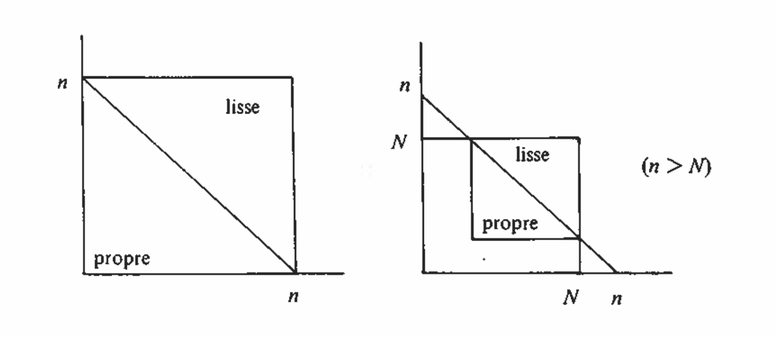
\includegraphics[width=.50\textwidth]{../assets/D022_P082_DIAGRAMS_PRESENTATION.png}
\end{center}

\NumPara{8. Variantes.} \textbf{(8.1)} Le groupe de cohomologie à support propre \(H_c^n(X)\) est contrôlé par la partie du carré \([0,n]\times[0,n]\) en-dessous de la seconde diagonale. Pour \(N=\dim X\le n\), on peut encore remplacer ce carré par \([n-N,N]\times[n-N,N]\). En particulier, \(H_c^{2N}(X)\) est purement de poids \(2N\).

\NumPara{(8.2)} La «dualité» entre les cas propres et lisses peut se déduire de la dualité de Poincaré: pour \(X\) lisse purement de dimension \(N\),
\[
H^n(X)=\Hom\bigl(H_c^{2N-n}(X),H_c^{2N}(X)\bigr)=\bigl(H_c^{2N-n}(X)^{\vee}\bigr)(-N).
\]
Cet argument permet d'étendre les résultats donnés pour \(X\) lisse au cas où \(X\) est une «rational homology manifold». Pour un tel \(X\), l'image de \(H_c^n(X)\) dans \(H^n(X)\) est purement de poids \(n\).

\NumPara{(8.3)} Pour \(X\) seulement supposé normal, il reste vrai que \(H^1(X)\) est contrôlé par \(\{(0,1),(1,0),(1,1)\}\).

\NumPara{9.} Soient \(X\) une variété connexe, \(x\in X\), et \(\Pi^{(n)}\) le plus grand quotient nilpotent de longueur \(n\) et sans torsion de \(\pi_1(X,x)\). On sait que les groupes \(H\) d'indice fini dans \(\Pi^{(n)}\) et assez petits ont la propriété suivante.

\NumPara{(*)} Il existe une algèbre de Lie nilpotente de longueur \(n\), \((\LieH,[\ ,\ ])\), avec \(\LieH\) un
\EndSourcePage

\SourcePage{83}{5}
\ReaderFont
\(\Z\)-module libre, telle que la formule de Campbell--Hausdorff
\[
x\circ y=x+y+[x,y]/2+[x,[x,y]]/12+[y,[y,x]]/12+\cdots
\]
fasse de \(\LieH\) un groupe, isomorphe à \(H\).

De plus, l'algèbre de Lie \(\LieL^{(n)}=\LieH\otimes\Q\) ne dépend que de \(\Pi^{(n)}\), non de \(H\).

\TheoremPara{10. THÉORÈME (MORGAN).} Si \(X\) est normale, \(\LieL^{(n)}\) admet une graduation \(\Wg\), à degrés \(<0\), telle que \(\LieL^{(n)}\) soit engendrée par des éléments de degré \(-1\) et \(-2\), ceux ci n'étant soumis qu'à des relations de degré \(-2\), \(-3\) et \(-4\), plus la nullité des commutateurs \(n\) fois itérés.\EndTheorem

Il est plus commode de travailler avec le système projectif \(\LieL^{(\infty)}\) des \(\LieL^{(n)}\). Définissant \(H^i(\LieL^{(\infty)})=\varinjlim H^i(\LieL^{(n)})\), on a
\[
H^1(\LieL^{(\infty)})=H^1(X),\qquad H^2(\LieL^{(\infty)})\subset H^2(X).
\]
De plus, une graduation \(\Wg\) de \(\Mmin\) comme au §5 définit des graduations compatibles de \(\LieL^{(\infty)}\), de sa cohomologie, et de celle de \(X\). D'après (8.3), (resp. (7.1)), \(H^1(X)\) est de poids 1 et 2 et \(H^2(X)\) de poids \(\le4\). Dès lors, \(H^1(\LieL^{(\infty)})\) (le dual du groupe \(\LieL^{(\infty)}/[\LieL^{(\infty)},\LieL^{(\infty)}]\) des générateurs de \(\LieL^{(\infty)}\)) est de poids 1 et 2, et \(H^2(\LieL^{(\infty)})\), le dual du groupe des relations entre générateurs, est de poids \(\le4\). Ceci vérifie le théorème.

\NumPara{11.} Pour une variété propre et lisse la filtration par le poids se réduit à peu de chose (3.1). Le fait qu'elle soit graduable au sens §4 implique la nullité de tous les produits de Massey. Qu'elle le soit au sens §5 implique même que le type d'homotopie rationnel de \(X\) peut se lire sur son algèbre de cohomologie---voir [3].

\NumPara{12. Théorie de Hodge.} Le groupe de cohomologie \(H^i(X)\) de toute variété algébrique complexe est munie d'une structure de Hodge mixte \((W,F)\) (\(W\) est une filtration de \(H^i(X)\), et \(F\) une filtration de \(H^i(X)\otimes\C=H^i(X,\C)\), \(W\) et \(F\) vérifiant des axiomes convenables---voir [1]). La filtration par le poids est par définition la filtration \(W\).

\NumPara{13. Théorie \(l\)-adique.} Une variété algébrique \(X\) se définit en terme d'un nombre fini d'équations polynômes. Les coefficients de ces équations engendrent un sous-anneau de type fini \(R\) de \(\C\), de corps des fractions \(K\), et \(X\) se déduit par extension des scalaires à \(\C\) d'un schéma sur \(K\), voire sur \(R\). Les énoncés qui suivent deviennent vrai lorsqu'on remplace \(R\) par \(R[1/f]\) avec \(f\in R\) assez divisible.

\NumPara{(13.1)} Soit \(l\) un nombre premier. Le groupe \(H^i(X)\otimes\Q_l\) s'identifie au groupe de cohomologie \(l\)-adique \(H^i(X,\Q_l)\). Ce dernier est défini de façon purement algébrique, donc est muni par transport de structure d'une action de \(\Aut(\C/K)\).

\NumPara{(13.2)} Soit \(\overline K\) la clôture algébrique de \(K\) dans \(\C\). L'action se factorise par \(\Gal(\overline K/K)\). Elle est non ramifiée sur \(R[1/l]\), i.e., se factorise par le groupe de Galois de la plus grande extension \(K_{\mathrm{nr}}^{(l)}\subset\overline K\) de \(K\) non ramifiée sur \(R[1/l]\).

\NumPara{(13.3)} Soit \(\mathfrak m\) un idéal maximal de \(R[1/l]\), et \(N(\mathfrak m)=\#R/\mathfrak m\) (\(R/\mathfrak m\) est un corps fini). A \(\mathfrak m\) correspond une classe de conjugaison de substitutions de Frobenius \(\varphi_{\mathfrak m}\in\Gal(K_{\mathrm{nr}}/K)\), d'inverses les Frobenius géométriques \(F_{\mathfrak m}=\varphi_{\mathfrak m}^{-1}\).

\TheoremPara{14. THÉORÈME.} Pour \(f\) assez divisible, on a\EndTheorem
\EndSourcePage

\SourcePage{84}{6}
\ReaderFont
\TheoremPara{(i)} Pour tout \(l\) et \(\mathfrak m\), les valeurs propres \(\alpha\) de \(F_{\mathfrak m}\) (dans une extension finie convenable de \(\Q_l\)) sont des entiers algébriques. Pour chaque \(\alpha\), il existe un entier \(w(\alpha)\) tels que tous les conjugués complexes de \(\alpha\) soient de valeur absolue \(N(\mathfrak m)^{w(\alpha)/2}\).

\NumPara{(ii)} Choisissons un Frobenius géométrique \(F_{\mathfrak m}\), et soit \({}_{\mathfrak m}W_j\) la somme des sous-espaces propres généralisés correspondant aux valeurs propres \(\alpha\) de \(F_{\mathfrak m}\) telles que \(w(\alpha)=j\). La filtration par les \(\bigoplus_{j\le i}{}_{\mathfrak m}W_j\) est indépendante de \(\mathfrak m\) et du choix de \(F_{\mathfrak m}\); elle est rationnelle et sa trace sur \(H^i(X)\) est indépendante de \(l\); c'est la filtration par le poids.\EndTheorem

\ProofHeadFR On exprime (via une suite spectrale) la cohomologie de \(X\) en terme de la cohomologie de variétés propres et lisses, comme en [1]. La suite spectrale aboutit à une filtration \(W\) de \(H^*(X)\), qui est par définition la filtration par le poids de la théorie de Hodge. Cette suite spectrale a un analogue \(l\)-adique; le \(l\)-adifié \(W_l\) de \(W\) est donc stable par un groupe de Galois. On déduit de la conjecture de Weil que les valeurs propres de \(F_{\mathfrak m}\) sur \(\Gr_j^{W_l}\) sont des entiers algébriques de valeurs absolues complexes \(N(\mathfrak m)^{j/2}\), et le théorème en résulte.

\NumPara{15.} Dans les cas considérés en (7.1), (7.2) et (7.3), la région \(\region\) décrite contrôle non seulement les poids, mais encore les nombres de Hodge et la divisibilité des valeurs propres des \(F_{\mathfrak m}\): dans (7.1), (7.2) et (7.3), une région \(\region\) a été assignée à un groupe \(H\), et

\NumPara{(a)} Les nombres de Hodge \(h^{pq}\) non nuls des structure de Hodge \(\Gr_j^W(H)\) vérifient \((p,q)\in\region\).

\NumPara{(b)} (Utile seulement dans le cas (7.3).) Si les \((p,q)\in\region\) avec \(p+q=j\) vérifient \(p,q\ge k\), alors (toujours pour \(f\) assez divisible), les valeurs propres de \(F_{\mathfrak m}\) de valeurs absolues complexes \(N(\mathfrak m)^{j/2}\) sont divisibles par \(N(\mathfrak m)^k\).

On espère que ceci est un cas particulier d'un principe général, cf. [4].

\NumPara{16.} Le résultat suivant est clair du point de vue de la théorie de Hodge.

\NumPara{(16.1)} Pour \(j\) impair \(\dim\Gr_j^W H^i(X)\) est pair.

Par contre, je ne sais démontrer jusqu'ici §§ 2 et 5 que par voie \(l\)-adique. Pour § 5, la méthode de § 14 permet d'obtenir une graduation \(l\)-adique; une astuce de Sullivan permet d'en déduire l'existence de graduations rationnelles du type voulu.

Les propriétés de fonctorialité de la filtration par le poids sont évidentes du point de vue \(l\)-adique (car Galois commute à tout ce qui se peut définir). Il est toutefois utile de les prouver du point de vue de la théorie de Hodge, pour obtenir des propriétés analogues pour la filtration \(F\). Morgan a obtenu de nombreux résultats dans cette direction---assez pour prouver un résultat un peu plus faible que §10 par théorie de Hodge.

\NumPara{17.} Ainsi que § 5 le suggère, une filtration par le poids existe aussi sur les groupes d'homotopie (tensorisés par \(\Q\)) sous des hypothèses de simple connexité.

Elle existe aussi sur les groupes de cycles évanescents (cf. [6]), et j'espère qu'elles nous aideront à mieux comprendre ces derniers.

\begin{center}\sffamily\bfseries Bibliographie\end{center}

\noindent\textbf{1.} P. Deligne, \emph{Théorie de Hodge}. I, Proc. Internat. Congress Math. (Nice, 1970), vol. I, Gauthier-
\EndSourcePage

\SourcePage{85}{7}
\SparseReaderFont
Villars, Paris, 1971, pp. 425--430; II, Inst. Hautes Études Sci. Publ. Math. No. 40 (1972), 5--58; III, Inst. Hautes Études Sci. Publ. Math. No. 44 (à paraître).

\noindent\textbf{2.} ---\hspace{-0.2em}---\hspace{-0.2em}---, \emph{La conjecture de Weil}. I, II, Inst. Hautes Études Sci. Publ. Math. Nos. 43 et 44 (à paraître).

\noindent\textbf{3.} P. Deligne, P.A. Griffiths, J. Morgan and D. Sullivan, \emph{Real homotopy theory of Kähler manifolds} (à paraître).

\noindent\textbf{4.} B. Mazur, \emph{Frobenius and the Hodge filtration (estimates)}, Ann. of Math. (2) 98 (1973), 58--95. MR 48 \# 297.

\noindent\textbf{5.} J. Morgan.

\noindent\textbf{6.} J. H. M. Steenbrink, \emph{Limits of Hodge structures and intermediate jacobians}, Thèse, Amsterdam, 1974.

\noindent\textbf{7.} D. Sullivan, \emph{Differential forms and the topology of manifolds}, Proc. Japan Conference on Manifolds, 1973.

\vspace{8mm}
\noindent{\scshape Institut des Hautes Etudes Scientifiques\\91440 Bures-sur-Yvette, France}

\vfill
\PageAnchorNote{The terminal blank remainder is intentionally preserved. No received-date line appears in the controlling authority.}


\clearpage\endgroup
\typeout{CORPUS-END:D022:\thepage}
% END INLINE WORK D022 FR
% BEGIN INLINE WORK D023 FR
\typeout{CORPUS-BEGIN:D023:\thepage}
\begingroup
\makeatletter
\let\DeclareMathOperator\CorpusDeclareMathOperator
\let\@declmathop\CorpusDeclMathOp
\let\maketitle\CorpusMakeTitle\let\title\CorpusTitle\let\author\CorpusAuthor\let\date\CorpusDate
\let\thanks\CorpusThanks\let\and\CorpusAnd\let\@maketitle\CorpusAtMakeTitle
\def\setcounter#1#2{\def\CorpusCounterName{#1}\def\CorpusPageName{page}\ifx\CorpusCounterName\CorpusPageName\else\CorpusSetCounter{#1}{#2}\fi}
\title{}\author{}\date{}
\setcounter{section}{0}
\expandafter\def\csname theHsection\endcsname{D023.\arabic{section}}
\setcounter{subsection}{0}
\expandafter\def\csname theHsubsection\endcsname{D023.\arabic{subsection}}
\setcounter{subsubsection}{0}
\expandafter\def\csname theHsubsubsection\endcsname{D023.\arabic{subsubsection}}
\setcounter{equation}{0}
\expandafter\def\csname theHequation\endcsname{D023.\arabic{equation}}
\setcounter{figure}{0}
\expandafter\def\csname theHfigure\endcsname{D023.\arabic{figure}}
\setcounter{table}{0}
\expandafter\def\csname theHtable\endcsname{D023.\arabic{table}}
\setcounter{footnote}{0}
\expandafter\def\csname theHfootnote\endcsname{D023.\arabic{footnote}}
\makeatother
\let\tableofcontents\relax % one cumulative contents list, not repeated global lists
% Options for packages loaded elsewhere
\setcounter{secnumdepth}{-\maxdimen} % remove section numbering
\ifPDFTeX
  \else % if luatex or xetex
  \fi
\ifPDFTeX\else
  % xetex/luatex font selection
  \setmainfont[]{DejaVu Serif}
  \fi
% Use upquote if available, for straight quotes in verbatim environments
\IfFileExists{upquote.sty}{}{}
\IfFileExists{microtype.sty}{% use microtype if available
  }{}
\makeatletter
\@ifundefined{KOMAClassName}{% if non-KOMA class
  \IfFileExists{parskip.sty}{%
    }{% else
    \setlength{\parindent}{0pt}
    \setlength{\parskip}{6pt plus 2pt minus 1pt}}
}{% if KOMA class
  \KOMAoptions{parskip=half}}
\makeatother
\ifLuaTeX
\else
\fi
\ifPDFTeX
\else

\fi
\ifLuaTeX
  \fi
\setlength{\emergencystretch}{3em} % prevent overfull lines
\providecommand{\tightlist}{%
  \setlength{\itemsep}{0pt}\setlength{\parskip}{0pt}}
\setlength{\parindent}{0pt}
\setlength{\parskip}{1.0mm}
\setcounter{secnumdepth}{0}
\pagestyle{empty}
\titleformat{\section}{\bfseries\fontsize{11}{13}\selectfont}{}{0pt}{}
\titleformat{\subsection}{\bfseries\fontsize{10}{12}\selectfont}{}{0pt}{}
\titlespacing*{\section}{0pt}{1mm}{1mm}
\titlespacing*{\subsection}{0pt}{1mm}{1mm}
\IfFileExists{xurl.sty}{}{} % add URL line breaks if available
\urlstyle{same}
\author{}
\date{}


\graphicspath{{assets/works/D023_PUBLIC_SAFE/outputs/}}
\selectlanguage{french}
\phantomsection\addcontentsline{toc}{section}{D023}



\pdfbookmark[0]{Théorie d’homotopie réelle des variétés kählériennes}{D023-d023-french_standalone-title}

\pdfbookmark[1]{D023 folio 245}{D023-d023-french_standalone-p0001}

\noindent{\small\sffamily D023 · Édition française autonome · folio 245}

\par

\vspace{0.7mm}\hrule\vspace{1.6mm}

\fontsize{9}{11}\selectfont

{[}Métadonnées de publication : Inventiones math. 29, 245--274 (1975){]}

\section{Théorie d'homotopie réelle des variétés
kählériennes}\label{D023-thuxe9orie-dhomotopie-ruxe9elle-des-variuxe9tuxe9s-kuxe4hluxe9riennes}

Pierre Deligne (Bures-sur-Yvette), Phillip Griffiths* (Cambridge,
Mass.), John Morgan (New York) et Dennis Sullivan (Bures-sur-Yvette)

\subsection{Table des matières}\label{D023-table-des-matiuxe8res}

\begin{enumerate}
\def\labelenumi{\arabic{enumi}.}
\tightlist
\item
  Théorie de l'homotopie des algèbres différentielles
  \ldots\ldots\ldots. 248
\item
  Théorie de l'homotopie de de Rham \ldots\ldots\ldots\ldots\ldots{} 254
\item
  Relation entre la théorie de l'homotopie de de Rham et la théorie
  classique de l'homotopie
  \ldots\ldots\ldots\ldots\ldots\ldots\ldots\ldots{} 256
\item
  Formalité des algèbres différentielles \ldots\ldots\ldots\ldots.. 260
\item
  Le complexe de de Rham d'une variété kählérienne compacte \ldots.. 262
\item
  Le théorème principal et deux démonstrations \ldots\ldots\ldots\ldots.
  270
\item
  Une application \ldots\ldots\ldots\ldots\ldots\ldots\ldots. 272
\end{enumerate}

Cet article réunit la théorie de de Rham renforcée du dernier auteur
{[}12, 13{]} et {[}14{]}, concernant l'information homotopique d'une
variété contenue dans l'algèbre de ses formes différentielles, et les
résultats classiques {[}15{]} sur les formes d'une variété kählérienne
compacte, afin d'établir des énoncés sur la topologie algébrique des
variétés kählériennes compactes et, par conséquent, sur les variétés
algébriques projectives complexes lisses.

La nature des résultats est que le \emph{type d'homotopie d'une variété
kählérienne compacte, sur les nombres réels, est une conséquence
formelle de l'anneau de cohomologie réelle.} Pour toute variété, il
existe une algèbre différentielle graduée à constantes de structure
rationnelles dont le type d'isomorphisme est un invariant du type
d'homotopie de l'espace. L'anneau de cohomologie de cette algèbre
différentielle est l'anneau de cohomologie rationnelle de l'espace, mais
l'algèbre elle-même contient, par exemple, les produits cohomologiques
d'ordre supérieur. Le type d'isomorphisme de l'algèbre différentielle
équivaut à la « forme rationnelle de la structure nilpotente de l'espace
». Pour une variété simplement connexe, cette algèbre différentielle
équivaut à la tour de Postnikov rationnelle de la variété. Nos résultats
montrent ici que, pour une variété kählérienne compacte, on peut
produire à partir de l'anneau de cohomologie réelle la forme réelle de
cette algèbre différentielle. Ces résultats complètent la structure
connue de l'anneau de cohomologie d'une telle variété. Nous ne
démontrons aucun résultat nouveau à son sujet.

La motivation initiale de ces résultats venait de la relation, dans une
variété kählérienne, entre formes harmoniques et formes holomorphes. En
particulier, les formes harmoniques de type \((p,0)\), pour toute
métrique kählérienne, sont exactement les formes holomorphes. Par
conséquent, les produits de formes harmoniques de types \((p,0)\) et
\((q,0)\) sont harmoniques\textsuperscript{1}, et il n'existe donc aucun

\begin{itemize}
\tightlist
\item
  Cette recherche a été partiellement soutenue par la subvention NSF
  GP-38886.
\end{itemize}

1 Chen, dans {[}2{]}, fut le premier à exploiter cette idée pour obtenir
des informations d'ordre supérieur sur les variétés kählériennes.

\clearpage

\pdfbookmark[1]{D023 folio 246}{D023-d023-french_standalone-p0002}

\noindent{\small\sffamily D023 · Édition française autonome · folio 246}

\par

\vspace{0.7mm}\hrule\vspace{1.6mm}

\fontsize{9}{11}\selectfont

produit d'ordre supérieur partant de \(H^{*,0}\). La possibilité que le
théorème complet soit vrai est liée aux conjectures de Weil. Nous avons
été conduits à démontrer un résultat aussi complet en « utilisant les
conjectures de Weil en caractéristique \(p\) pour deviner des résultats
en caractéristique \(0\), qui peuvent ensuite être démontrés au moyen de
la théorie de Hodge ». La remarque pertinente ici est que les produits
cohomologiques classiques d'ordre supérieur de Massey sont des
opérations multilinéaires, mais que la dimension du produit est toujours
inférieure à la somme des dimensions des différents éléments multipliés.
Ainsi, si nous travaillions dans une situation en caractéristique \(p\)
sur laquelle opère l'automorphisme de Frobenius (par exemple les
cochaînes de Čech en théorie de la cohomologie étale), et si les valeurs
propres de l'action de Frobenius sont celles prédites par les
conjectures de Weil\textsuperscript{2}, alors la multilinéarité du
produit sous cette action impliquerait que la valeur absolue des valeurs
propres sur l'espace des produits d'ordre supérieur, dans une certaine
dimension, serait différente des valeurs possibles dans cette dimension.
La seule manière dont cela puisse se produire est que ces espaces de
produits d'ordre supérieur soient nuls.

Pour démontrer ces résultats pour les variétés kählériennes compactes,
nous utilisons les conséquences, pour les formes, de l'existence d'une
métrique kählérienne. Si \(M\) est une variété complexe, considérons les
algèbres différentielles et les applications d'algèbres

\[
\{H^*(M,\mathbb R),d=0\}\longleftarrow\{\operatorname{Ker}(d^c),d\}\lhook\joinrel\longrightarrow\{\text{toutes les formes }C^{\infty},d\}.
\]

Si \(M\) est une variété kählérienne compacte, les deux applications
ci-dessus induisent des isomorphismes en cohomologie. Tous nos résultats
sur le type d'homotopie des variétés kählériennes compactes se déduisent
de cet énoncé, qui est lui-même une conséquence du lemme \(dd^c\).

\textbf{Lemme \(dd^c\).} \emph{Soit \(M\) une variété kählérienne
compacte, et \(d^c=J^{-1}dJ\), où \(J\) donne la structure complexe dans
le fibré cotangent. Il est évident que \(d^c\) est un opérateur réel. Si
\(x\) est une forme telle que}

\begin{enumerate}
\def\labelenumi{\arabic{enumi})}
\tightlist
\item
  \(dx=0=d^c x\)
\end{enumerate}

\emph{et}

\begin{enumerate}
\def\labelenumi{\arabic{enumi})}
\setcounter{enumi}{1}
\tightlist
\item
  \(x=dy\) ou \(x=d^c y'\),
\end{enumerate}

\emph{alors \(x=dd^c z\) pour une certaine forme \(z\).}

Dans les Sections 1--4, nous décrivons la machinerie nécessaire pour
déduire, en théorie de l'homotopie, les conséquences de ces énoncés sur
les formes. Les Sections 1, 2 et 3 constituent une esquisse de la
théorie de {[}12{]} et {[}14{]} (c.f. aussi {[}10{]}). La Section 1
décrit la construction du modèle minimal (tour de Postnikov réelle) de
toute algèbre différentielle et démontre un résultat d'unicité. Pour ce
faire, une partie de la théorie abstraite de l'homotopie des algèbres
différentielles est développée. Par exemple, nous définissons le groupe
fondamental de de Rham d'une algèbre au moyen d'un modèle minimal de
l'algèbre. Ce « groupe » est un système inverse de groupes de Lie
nilpotents. Nous définissons aussi les groupes d'homotopie supérieurs de
toute algèbre différentielle simplement connexe. Ce sont des espaces
vectoriels munis d'une structure d'algèbre de Lie graduée, qu'il
convient d'interpréter comme la structure des « produits de Whitehead ».

Dans la Section 2, nous associons à toute variété \(C^{\infty}\)
simplement connexe\textsuperscript{3}, \(M\), le complexe de de Rham des
formes \(C^{\infty}\) sur \(M\), \(\mathscr E_M^*\), et son modèle minimal
\(\mathcal M_M\) ; et à tout complexe simplicial simplement

2 Il s'agit désormais de {[}5{]}.

3 En fait, cette forme de la théorie fonctionne tout aussi bien pour les
espaces nilpotents ; voir {[}13{]}.

\clearpage

\pdfbookmark[1]{D023 folio 247}{D023-d023-french_standalone-p0003}

\noindent{\small\sffamily D023 · Édition française autonome · folio 247}

\par

\vspace{0.7mm}\hrule\vspace{1.6mm}

\fontsize{9}{11}\selectfont

connexe, \(X\), l'algèbre différentielle \(\mathscr E_X^*\) des formes
polynomiales sur \(\mathbb Q\) sur \(X\), ainsi que son modèle minimal
\(\mathcal M_X\). Les premières algèbres sont sur \(\mathbb R\) ; les
secondes sur \(\mathbb Q\). Le modèle minimal \(\mathcal M_M\) est, par
définition, le type d'homotopie de de Rham \(C^{\infty}\) de \(M\), et
\(\mathcal M_X\) est de même le type d'homotopie de de Rham sur
\(\mathbb Q\) de \(X\). Ces constructions vérifient :

\begin{enumerate}
\def\labelenumi{\alph{enumi})}
\item
  la cohomologie des formes polynomiales sur \(\mathbb Q\) sur \(X\) est
  l'anneau de cohomologie de \(X\) sur \(\mathbb Q\) ;
\item
  les inclusions des formes \(C^{\infty}\) sur \(M\) et des (formes
  polynomiales sur \(\mathbb Q\) sur une triangulation \(C^1\), \(K\),
  de \(M\))\(\otimes\mathbb R\) dans les formes \(C^{\infty}\) par
  morceaux sur \(K\) induisent des isomorphismes en cohomologie.
\end{enumerate}

Le fait que les formes polynomiales sur \(\mathbb Q\) constituent une
algèbre différentielle sur \(\mathbb Q\) est utile lorsque nous
établissons, dans la Section 3, le lien avec la théorie de l'homotopie.
Il existe un isomorphisme entre la catégorie des algèbres
différentielles minimales sur \(\mathbb Q\) et la catégorie des tours de
fibrations principales rationnelles. Sous cet isomorphisme, les groupes
d'homotopie des algèbres correspondent aux groupes d'homotopie de la
fibration. Le résultat principal est que, \emph{pour un espace
simplement connexe, la tour de fibrations principales rationnelles
construite à partir du modèle minimal des formes polynomiales sur
\(\mathbb Q\) est la forme rationnelle de la tour de Postnikov de
l'espace. Ainsi, l'information homotopique disponible dans l'algèbre
différentielle des formes polynomiales sur \(\mathbb Q\) d'un complexe
simplicial simplement connexe est exactement le type d'homotopie
rationnel.} Par conséquent, l'algèbre différentielle des formes
\(C^{\infty}\) sur une variété simplement connexe détermine la forme
réelle du type d'homotopie rationnel de la variété. Il existe des
résultats analogues concernant la complétion nilpotente du groupe
fondamental pour les complexes simpliciaux et les variétés en général
(voir {[}14{]}, Appendice N).

La Section 4 examine la question de savoir quand le modèle minimal d'une
algèbre différentielle est déterminé par l'anneau de cohomologie de
l'algèbre. Nous donnons des exemples d'espaces où les produits
cohomologiques d'ordre supérieur sont non nuls, puis nous montrons qu'un
modèle minimal est une conséquence formelle de son anneau de cohomologie
si, et seulement si, tous les produits d'ordre supérieur s'annulent
d'une manière uniforme.

La Section 5 traite des formes sur une variété complexe compacte
admettant une métrique kählérienne. À partir de l'identité (qui équivaut
au caractère kählérien de la métrique)

\[
\Delta_d=2\Delta_{\partial}=2\Delta_{\bar\partial}
\]

entre les différents laplaciens, nous démontrons le lemme \(dd^c\). Nous
en donnons ensuite une interprétation cohomologique et montrons qu'il
est valable sur des variétés complexes plus générales (par exemple les
espaces de Moišezon).

Dans la Section 6, nous démontrons le théorème principal suivant :

\begin{enumerate}
\def\labelenumi{\arabic{enumi})}
\item
  Pour toute variété complexe sur laquelle le lemme \(dd^c\) est vrai
  (par exemple les variétés kählériennes), le modèle minimal des formes
  différentielles \(C^{\infty}\) est une conséquence formelle de l'anneau
  de cohomologie réelle.
\item
  Étant donnée une application holomorphe entre deux telles variétés,
  l'effet de l'application sur les modèles minimaux est déterminé par
  l'application au niveau de la cohomologie.
\end{enumerate}

Le travail des Sections 1, 2 et 3 permet de traduire cela en l'assertion
que le type d'homotopie réel d'une variété kählérienne compacte est une
conséquence formelle de son anneau de cohomologie réelle, et que le type
d'homotopie réel d'une application holomorphe

\clearpage

\pdfbookmark[1]{D023 folio 248}{D023-d023-french_standalone-p0004}

\noindent{\small\sffamily D023 · Édition française autonome · folio 248}

\par

\vspace{0.7mm}\hrule\vspace{1.6mm}

\fontsize{9}{11}\selectfont

entre variétés kählériennes compactes est une conséquence formelle de
l'application induite en cohomologie. En particulier, si une variété
kählérienne compacte \(M\) est simplement connexe, ses groupes
d'homotopie réels, \(\pi_*(M)\otimes\mathbb R\), se lisent à partir de
l'anneau de cohomologie réelle. De même, dans ce cas, l'effet d'une
application holomorphe sur les groupes d'homotopie réels se lit à partir
de son effet en cohomologie. Dans le cas non simplement connexe, la tour
nilpotente réelle du groupe fondamental se lit à partir de \(H^1\) et du
cup-produit \(H^1\otimes H^1\to H^2\). L'effet d'une application
holomorphe sur la tour nilpotente de \(\pi_1\) se lit de même à partir
de l'application sur \(H^1\).

Dans la Section 7, nous donnons une application de cette théorie à une
union de diviseurs à croisements normaux. En utilisant le fait que les
formes sur une variété kählérienne peuvent être remplacées naturellement
par la cohomologie, nous donnons une autre démonstration de la
dégénérescence en \(E_2\) d'une suite spectrale calculant la
cohomologie, c'est-à-dire \(E_2=E_{\infty}\). Ici, \(E_1\) est construit à
partir des cohomologies des diverses intersections, et \(d_1\) à partir
des diverses applications de restriction.

Le troisième auteur a étudié le complémentaire ouvert d'un diviseur à
croisements normaux dans une variété kählérienne, où apparaissent des
résultats apparentés mais beaucoup plus compliqués {[}20{]}.

\subsection{Section 1. Théorie de l'homotopie des algèbres
différentielles}\label{D023-section-1.-thuxe9orie-de-lhomotopie-des-alguxe8bres-diffuxe9rentielles}

Cette section, avec les Sections 2 et 3, constitue une esquisse de la
théorie du dernier auteur reliant les algèbres différentielles et la
théorie de l'homotopie. Pour un traitement plus complet de cette
théorie, voir {[}6, 10, 12{]} et {[}13{]}. La discussion de cette
section est entièrement algébrique : on y définit le groupe fondamental
de toute algèbre différentielle et les groupes d'homotopie supérieurs
--- en fait, le type d'homotopie --- d'une algèbre différentielle
1-connexe. Cette théorie est valable pour les algèbres différentielles
sur tout corps contenant les rationnels \(\mathbb Q\), mais les seuls
corps qui interviennent dans les applications géométriques sont, outre
\(\mathbb Q\), les réels \(\mathbb R\) et les complexes \(\mathbb C\).

Comme la terminologie le suggère, ces constructions sont motivées par la
théorie des tours de Postnikov et la théorie de l'homotopie des espaces.
Le lemme de Hirsch de la Section 3 montre que le lien est plus fort
qu'une simple analogie. En fait, la théorie de l'homotopie des algèbres
différentielles sur \(\mathbb Q\) et la théorie des tours de fibrations
principales de fibres \(K(V,n)\), où \(V\) est un espace vectoriel sur
\(\mathbb Q\), sont équivalentes.

Une \emph{algèbre différentielle graduée} (= algèbre différentielle) est
une algèbre graduée

\[
\mathscr A=\bigoplus_{k\ge0}\mathscr A^k
\]

munie d'une différentielle \(d:\mathscr A\to\mathscr A\) de degré
\(+1\), telle que

\begin{enumerate}
\def\labelenumi{\arabic{enumi})}
\tightlist
\item
  \(\mathscr A\) est commutative au sens gradué, c'est-à-dire
\end{enumerate}

\[
x\cdot y=(-1)^{k\ell}y\cdot x\qquad(x\in\mathscr A^k\text{ et }y\in\mathscr A^{\ell}) ;
\]

\begin{enumerate}
\def\labelenumi{\arabic{enumi})}
\setcounter{enumi}{1}
\tightlist
\item
  \(d\) est une dérivation, c'est-à-dire
\end{enumerate}

\[
d(x\cdot y)=dx\cdot y+(-1)^k x\cdot dy\qquad(x\in\mathscr A^k),
\]

\clearpage

\pdfbookmark[1]{D023 folio 249}{D023-d023-french_standalone-p0005}

\noindent{\small\sffamily D023 · Édition française autonome · folio 249}

\par

\vspace{0.7mm}\hrule\vspace{1.6mm}

\fontsize{9}{11}\selectfont

et

\begin{enumerate}
\def\labelenumi{\arabic{enumi})}
\setcounter{enumi}{2}
\tightlist
\item
  \(d^2=0\).
\end{enumerate}

La cohomologie \(H^*(\mathscr A)\) est une algèbre. Nous supposerons
toujours qu'elle est de dimension finie en chaque degré. \(\mathscr A\)
est connexe si \(H^0(\mathscr A)\) est le corps de base, et
\(\mathscr A\) est 1-connexe si, de plus, \(H^1(\mathscr A)=0\). Une
application entre deux algèbres différentielles \(\mathscr A\) et
\(\mathscr B\) est un homomorphisme d'algèbres qui respecte la
graduation et \(d\). Une telle application,
\(f:\mathscr A\to\mathscr B\), induit une application d'algèbres
\(f^*:H^*(\mathscr A)\to H^*(\mathscr B)\).

\emph{Exemples d'algèbres différentielles.} (i) le complexe de de Rham
\(\mathscr E_M^*\) des formes \(C^{\infty}\) sur une variété \(M\) ;

\begin{enumerate}
\def\labelenumi{(\roman{enumi})}
\setcounter{enumi}{1}
\tightlist
\item
  l'anneau de cohomologie d'un complexe \(CW\), \(X\),
\end{enumerate}

\[
\{H^*(X;k);d=0\}\qquad(k\text{ un corps}).
\]

Les cochaînes d'un complexe simplicial ne forment qu'une algèbre
différentielle non commutative, bien qu'elles induisent en cohomologie
une structure d'algèbre commutative graduée.

Si \(\mathscr A^0\) est le corps de base, nous définissons l'idéal
d'augmentation \(A(\mathscr A)=\bigoplus_{k>0}\mathscr A^k\), et
l'espace gradué des indécomposables,
\(I(\mathscr A)=A(\mathscr A)/A(\mathscr A)\cdot A(\mathscr A)\). Dans
une telle algèbre, la dérivation \(d\) est décomposable si, pour tout
\(x\in\mathscr A\), \(dx\in A\cdot A\). Cela équivaut à dire que
\(d(x)\) est une somme de produits d'éléments de degré positif. Par
l'algèbre libre sur un espace vectoriel \(V_n\), dont les éléments sont
de degré \(n\), notée \(\Lambda(V_n)\) ou simplement \((\Lambda_n)\),
nous entendons l'algèbre polynomiale engendrée par \(V_n\) si \(n\) est
pair, ou l'algèbre extérieure engendrée par \(V_n\) si \(n\) est impair.
Un produit tensoriel, au sens gradué, de telles algèbres est encore une
algèbre libre. L'analogue algébrique d'une fibration principale est une
\emph{extension élémentaire}. Une extension élémentaire de
\((\mathscr A,d_{\mathscr A})\) est toute algèbre de la forme
\((\mathscr B=\mathscr A\otimes\Lambda(V_k),d_{\mathscr B})\), où
\(d_{\mathscr B}|_{\mathscr A}=d_{\mathscr A}\),
\(d_{\mathscr B}(V_k)\subset\mathscr A\), et \(V_k\) est un espace
vectoriel de dimension finie.\textsuperscript{4} Nous notons de telles
extensions \(\mathscr A\otimes_d\Lambda(V_k)\). Remarquons que si
\(\mathscr A\) est libre comme algèbre, alors \(\mathscr B\) l'est aussi
; et si \(d\) est décomposable dans \(\mathscr A\), alors il est
également décomposable dans \(\mathscr B\) si, et seulement si,
\(d(V_k)\subset A(\mathscr A)\cdot A(\mathscr A)\). Notre première
définition principale est que \(\mathcal M\) est une \emph{algèbre
différentielle minimale} si \(\mathcal M\) peut s'écrire comme une union
croissante de sous-algèbres différentielles

\[
\text{corps de base}\subset\mathcal M_1\subset\mathcal M_2\subset\cdots,\qquad \bigcup_{i\ge0}\mathcal M_i=\mathcal M,
\]

avec \(\mathcal M_i\subset\mathcal M_{i+1}\) une extension élémentaire,
et avec \(d\) décomposable. Une telle collection de sous-algèbres
différentielles est une \emph{série pour \(\mathcal M\)}. Si
\(\mathcal M\) est minimale, alors

\begin{enumerate}
\def\labelenumi{\arabic{enumi})}
\item
  \(d\) est décomposable, et
\item
  \(\mathcal M\) est libre comme algèbre.
\end{enumerate}

Si nous notons \(\{\mathcal M^{(i)}\}\) la sous-algèbre de
\(\mathcal M\) engendrée par les éléments de degré \(\le i\), le fait
que \(d\) soit décomposable implique que ce sont des sous-algèbres
différentielles. Si \(\mathcal M\) est une algèbre différentielle
1-connexe quelconque satisfaisant 1) et 2), alors \(\mathcal M^1=0\), et
la suite \(\mathcal M^{(2)}\subset\mathcal M^{(3)}\subset\cdots\) est
une série pour \(\mathcal M\). Ainsi, une algèbre 1-connexe satisfaisant
1) et 2) possède une série canonique. Pour toute algèbre différentielle
minimale \(\mathcal M\),

4 Toujours placé dans un degré strictement positif.

\clearpage

\pdfbookmark[1]{D023 folio 250}{D023-d023-french_standalone-p0006}

\noindent{\small\sffamily D023 · Édition française autonome · folio 250}

\par

\vspace{0.7mm}\hrule\vspace{1.6mm}

\fontsize{9}{11}\selectfont

\(\mathcal M^{(1)}\) possède également une série canonique

\[
0\subset\mathcal M_1^{(1)}\subset\mathcal M_2^{(1)}\subset\cdots,\qquad \bigcup_{i\ge0}\mathcal M_i^{(1)}=\mathcal M^{(1)},
\]

où \(\mathcal M_i^{(1)}\) est l'algèbre engendrée par tous les
\(x\in\mathcal M^{(1)}\) tels que \(dx\in\mathcal M_{i-1}^{(1)}\).

Étant donnée une algèbre différentielle libre finiment engendrée
\(\mathcal K\), à différentielle \(d\) décomposable, nous pouvons former
l'espace dual des indécomposables

\[
\mathcal L_{\mathcal K}=\bigoplus\mathcal L_i,\qquad \mathcal L_i=[I(\mathcal K)^i]^*.
\]

Comme \(d\) est décomposable, elle induit une application
\(d:I(\mathcal K)\to I(\mathcal K)\otimes I(\mathcal K)\), dont la duale
est une application
\(\mathcal L_i\otimes\mathcal L_j\to\mathcal L_{i+j-1}\). Cela fait de
\(\mathcal L\) une algèbre de Lie graduée. Une extension élémentaire
\(\mathcal K\to\mathcal K\otimes_d\Lambda(V_n)\), avec \(d\)
décomposable, se dualise en une extension centrale d'algèbres de Lie

\[
0\to V_n^*\to\mathcal L_{\mathcal K\otimes_d\Lambda(V_n)}\to\mathcal L_{\mathcal K}\to0,
\]

avec \([v,x]=0\) pour \(v\in V_n^*\) et
\(x\in\mathcal L_{\mathcal K\otimes_d\Lambda(V_n)}\). Si
\(0\subset\mathcal M_1\subset\mathcal M_2\subset\cdots\) est une série
d'une algèbre minimale \(\mathcal M\), posons
\(\mathcal L^i=[I(\mathcal M_i)]^*\). Nous obtenons un système inverse
d'extensions centrales d'algèbres de Lie

\[
\cdots\to\mathcal L^3\to\mathcal L^2\to\mathcal L^1\to0.
\]

Par récurrence, chaque \(\mathcal L^i\) est nilpotente. Pour une algèbre
différentielle générale \(\mathcal M\) satisfaisant 1) et 2) ci-dessus,
c'est cette condition supplémentaire de nilpotence de l'algèbre de Lie
duale \(\mathcal L\) qui équivaut à la minimalité. Cette nilpotence est
automatique si \(\mathcal M^1=0\), comme on le vérifie aisément par un
argument de degré.

\emph{Exemple.} Soit \(S=\Lambda_1(x,y,z)\), \(dx=y\wedge z\),
\(dy=z\wedge x\), \(dz=x\wedge y\). \(S\) n'est pas minimale, et
l'algèbre de Lie duale de \(S\) est \(\operatorname{so}(3)\), qui est
simple et non nilpotente.

Dans le cas 1-connexe, notre système inverse d'algèbres de Lie finit par
se stabiliser dans chaque degré (à \(\mathcal L^n\), nous ajoutons des
générateurs de degré \(n\)) et se rassemble ainsi en une seule algèbre
de Lie \(\mathcal L=\bigoplus_{n\ge2}\mathcal L_n\). Chaque
\(\mathcal L_n\) est finiment engendrée, et nous avons
\([\ ,\ ]:\mathcal L_n\otimes\mathcal L_k\to\mathcal L_{n+k-1}\).
L'espace vectoriel \(\mathcal L_n\) est, par définition, le \(n\)-ième
\emph{groupe d'homotopie de de Rham} de \(\mathcal M\), et le crochet de
l'algèbre de Lie graduée est appelé produit de Whitehead. Dans le cas
d'une algèbre différentielle minimale non simplement connexe
\(\mathcal M\), nous avons associé à \(\mathcal M^{(1)}\) une série
canonique et, par dualité, un système inverse canonique d'algèbres de
Lie nilpotentes \(\cdots\to\mathcal L_1^2\to\mathcal L_1^1\to0\).
\(\mathcal L_1^n\) est nilpotente d'ordre \(n\). La formule de
Campbell-Hausdorff

\[
X\cdot Y=X+Y+\tfrac12[X,Y]+\cdots
\]

définit alors sur chaque \(\mathcal L_1^n\) une structure de groupe de
Lie nilpotent. Cette tour de groupes de Lie nilpotents est le
\emph{groupe fondamental de de Rham} de \(\mathcal M\).

La discussion précédente s'applique à toute algèbre différentielle de la
manière suivante. Si \(\mathscr A\) est une algèbre différentielle,
alors \(\mathcal M_{\mathscr A}\xrightarrow{\rho}\mathscr A\) est un
\emph{modèle minimal à \(k\) étages pour \(\mathcal M\)} si

\begin{enumerate}
\def\labelenumi{\arabic{enumi})}
\item
  \(\mathcal M_{\mathscr A}\) est une algèbre minimale engendrée dans
  les dimensions \(\le k\) ;
\item
  \(\rho\) induit un isomorphisme en cohomologie dans les dimensions
  \(\le k\), et une injection en dimension \(k+1\).
\end{enumerate}

Nous employons le terme modèle minimal pour \(k=\infty\).

\clearpage

\pdfbookmark[1]{D023 folio 251}{D023-d023-french_standalone-p0007}

\noindent{\small\sffamily D023 · Édition française autonome · folio 251}

\par

\vspace{0.7mm}\hrule\vspace{1.6mm}

\fontsize{9}{11}\selectfont

Pour les applications, le théorème suivant est essentiel. Rappelons que
nous supposons tous les nombres de Betti finis.

\textbf{(1.1) Théorème.} a) \emph{Toute algèbre différentielle 1-connexe
possède un modèle minimal unique à isomorphisme près.}

\begin{enumerate}
\def\labelenumi{\alph{enumi})}
\setcounter{enumi}{1}
\tightlist
\item
  \emph{Toute algèbre différentielle connexe possède un modèle minimal à
  1 étage unique à isomorphisme près.}
\end{enumerate}

Nous définissons ainsi les \emph{groupes d'homotopie de de Rham} d'une
algèbre différentielle 1-connexe \(\mathscr A\), notés
\(\pi_*(\mathscr A)\) (avec le produit de Whitehead), comme ceux d'un
modèle minimal quelconque de \(\mathscr A\). De même, nous définissons
le \emph{groupe fondamental de de Rham} d'une algèbre différentielle
comme le groupe fondamental de de Rham d'un modèle minimal quelconque de
l'algèbre.

Si \(f:\mathscr A\to\mathscr B\) est un isomorphisme en cohomologie,
alors les groupes fondamentaux de de Rham de \(\mathscr A\) et de
\(\mathscr B\) sont isomorphes. Si \(\mathscr A\) est 1-connexe, alors
les groupes d'homotopie de de Rham de \(\mathscr A\) et de
\(\mathscr B\) sont isomorphes. Dans le cas simplement connexe, nous
définissons \(\mathcal M_{\mathscr A}\) comme le \emph{type d'homotopie
de de Rham} de \(\mathscr A\).

\emph{Exemples.} 1) Supposons que \(\mathscr A=\mathscr E^*_{S_n}\) soit
le complexe de de Rham de la \(n\)-sphère. Alors \[
\mathcal M_{\mathscr A}\cong
\begin{cases}
\Lambda_n(y),&n\text{ impair},\\
\Lambda_n(y)\otimes\Lambda_{2n-1}(z),\quad dz=y^2,&n\text{ pair}.
\end{cases}
\] Dans les deux cas,
\(\rho:\mathcal M_{\mathscr A}\to\mathscr E^*_{S_n}\) envoie \(y\) sur
un générateur de \(H^n(S^n)\).

\begin{enumerate}
\def\labelenumi{\arabic{enumi})}
\setcounter{enumi}{1}
\tightlist
\item
  Supposons que \(\mathscr A=\mathscr E^*_{\mathbb CP_n}\). Alors \[
  \mathcal M_{\mathscr A}\cong\Lambda_2(x)\otimes_d\Lambda_{2n+1}(y),\qquad dy=x^{n+1}.
  \] \(\rho:\mathcal M_{\mathscr A}\to\mathscr E^*_{\mathbb CP_n}\)
  envoie \(x\) sur une forme fermée dont la classe de cohomologie
  engendre \(H^2(\mathbb CP^n)\). Ainsi, dans ces cas, les groupes
  d'homotopie de de Rham de \(\mathscr E^*_{M^n}\) sont égaux aux
  groupes d'homotopie usuels tensorisés par \(\mathbb R\) : \[
  \pi_*(\mathscr E^*_{M^n})\cong\pi_*(M^n)\otimes\mathbb R.
  \] (cf.~Serre {[}11{]}). Il résulte de la théorie de Sullivan qu'une
  relation analogue vaut pour toutes les variétés lisses simplement
  connexes.
\end{enumerate}

Pour les algèbres 1-connexes, l'existence du modèle minimal est
immédiate. On suppose par récurrence l'existence de
\(\mathcal M^{(k)}\xrightarrow{\rho}\mathscr A\), induisant un
isomorphisme en cohomologie jusqu'à la dimension \(k\) et une injection
sur \(H^{k+1}\). Alors \(\mathcal M^{(k)}\subset\mathcal M^{(k+1)}\) est
une extension élémentaire sur \(V_{k+1}=C_{k+1}\oplus N_{k+1}\), où
\(C_{k+1}\) est le sous-espace d'éléments fermés introduit pour rendre
\(\rho\) surjective sur \(H^{k+1}\), et \(N_{k+1}\) est un espace de
générateurs non fermés dont l'image par \(d\),
\(d(N)\subset(\mathcal M^{(k)})^{k+2}\), rend exact un espace de formes
fermées représentant le noyau de \(\rho^*\) en degré \((k+2)\).

Dans le cas général, la construction de \(\mathcal M^{(1)}\) est
analogue : \(\mathcal M_1^{(1)}=\Lambda(H^1(\mathscr A))\), et
\(\mathcal M_i^{(1)}\subset\mathcal M_{i+1}^{(1)}\) est une extension
élémentaire par
\(\Lambda_1(\operatorname{Ker}H^2(\mathcal M_i^{(1)})\to H^2(\mathscr A))\).
Il est nécessaire de continuer à tuer le noyau en degré 2, puisque
chaque étape crée un nouveau noyau dans ce degré.

Les énoncés d'unicité dans ces deux cas exigent de développer la théorie
de l'homotopie pour les applications entre algèbres différentielles.
Soit \((t,dt)\) l'algèbre des polynômes en la variable \(t\), de degré
zéro, tensorisée avec l'algèbre extérieure sur sa

\clearpage

\pdfbookmark[1]{D023 folio 252}{D023-d023-french_standalone-p0008}

\noindent{\small\sffamily D023 · Édition française autonome · folio 252}

\par

\vspace{0.7mm}\hrule\vspace{1.6mm}

\fontsize{9}{11}\selectfont

différentielle \(dt\), de degré un. C'est une algèbre contractile que
nous considérons comme la droite réelle. Il existe des évaluations en
\(t=0\) et en \(t=1\), que nous considérons comme deux points de la
droite. Une application \(H:\mathscr A\to\mathscr B\otimes(t,dt)\) est
une homotopie de \(f:\mathscr A\to\mathscr B\) vers
\(g:\mathscr A\to\mathscr B\) si \(H|_{t=0}=f\) et \(H|_{t=1}=g\).
(Remarquons qu'une homotopie \(H:X\times I\to Y\) induit une application
\[
\mathscr E_Y^*\xrightarrow{H^*}\mathscr E_X^*\otimes\mathscr E_I^*.
\] Ainsi, la nature contravariante des formes exige que \((t,dt)\) se
trouve dans le but plutôt que dans la source.)

Étant donnés une extension élémentaire
\(\mathcal N=\mathcal M\otimes_d\Lambda(V_n)\), des applications \(f\)
et \(g:\mathcal N\to\mathscr A\), et une homotopie
\(H:\mathcal M\to\mathscr A\otimes(t,dt)\) de \(f|\mathcal M\) vers
\(g|\mathcal M\), alors \(H\) se prolonge en une homotopie
\(\bar H:\mathcal N\to\mathscr A\otimes(t,dt)\) de \(f\) vers \(g\) si,
et seulement si, l'homomorphisme
\(V_n\xrightarrow{\sigma}H^{n+1}(\mathscr A)\) donné par \[
\left\{\sigma(x)=\text{classe de cohomologie de }\left(f(x)-g(x)+(-1)^{\deg x}\int_{t=0}^{t=1}H(dx)\right)\right\}
\] est nul. Si \(\sigma=0\), un prolongement de \(H\) en \(\bar H\) est
déterminé par le choix linéaire, pour chaque \(x\), d'un \(\alpha(x)\)
tel que \(d(\alpha(x))=\sigma(x)\). La formule pour \(\bar H\) est alors
\[
\bar H(x)=f(x)+(-1)^{\deg x}\int_0^tH(dx)-d(\alpha(x)\otimes t).
\] Nous obtenons ainsi une suite d'obstructions cohomologiques à la
construction d'une homotopie, dont la structure algébrique est
exactement analogue à la situation topologique.

\textbf{(1.2) Théorème (Relèvement et relèvement à homotopie près).}
\emph{Étant donné un diagramme de flèches pleines} \[
\begin{array}{ccc}
&\mathscr A&\\[-2mm]
&\downarrow\scriptstyle\varphi&\\[-2mm]
\mathcal M&\xrightarrow{f}&\mathscr B
\end{array}
\] \emph{où \(\mathcal M\) est minimale et \(\varphi^*\) est un
isomorphisme en cohomologie, il existe
\(\tilde f:\mathcal M\to\mathscr A\) tel que \(\varphi\tilde f\) soit
homotope à \(f\). Si \(\varphi\) est en outre surjective, on peut
choisir \(\tilde f\) de sorte que \(\varphi\tilde f\) soit égal à
\(f\).}

\textbf{(1.3) Corollaire.} \emph{L'homotopie est une relation
d'équivalence sur l'ensemble des applications
\(\{f:\mathcal M\to\mathscr A\}\), pour \(\mathcal M\) minimale. Nous
notons \([\mathcal M,\mathscr A]\) l'ensemble des classes
d'équivalence.}

\textbf{(1.4) Corollaire.} \emph{Si \(\psi:\mathscr A\to\mathscr B\) est
un isomorphisme en cohomologie, alors \(\psi\) induit une bijection
d'ensembles \(\psi:[\mathcal M,\mathscr A]\to[\mathcal M,\mathscr B]\).}

\textbf{(1.5) Corollaire.} \emph{Si \(f:\mathscr A\to\mathscr B\) est
une application quelconque d'algèbres différentielles et si
\(\rho_{\mathscr A}:\mathcal M_{\mathscr A}\to\mathscr A\) et
\(\rho_{\mathscr B}:\mathcal M\to\mathscr B\) sont des modèles minimaux
de \(\mathscr A\) et \(\mathscr B\), alors \(f\) induit
\(\tilde f:\mathcal M_{\mathscr A}\to\mathcal M_{\mathscr B}\), unique à
homotopie près, sous la condition que} \[
\begin{array}{ccc}
\mathscr A&\xrightarrow{f}&\mathscr B\\
\uparrow\scriptstyle\rho_{\mathscr A}&&\uparrow\scriptstyle\rho_{\mathscr B}\\
\mathcal M_{\mathscr A}&\xrightarrow{\tilde f}&\mathcal M_{\mathscr B}
\end{array}
\]

\clearpage

\pdfbookmark[1]{D023 folio 253}{D023-d023-french_standalone-p0009}

\noindent{\small\sffamily D023 · Édition française autonome · folio 253}

\par

\vspace{0.7mm}\hrule\vspace{1.6mm}

\fontsize{9}{11}\selectfont

\textbf{(1.6) Corollaire.} \emph{Deux modèles minimaux à \(k\) étages
quelconques d'une algèbre sont isomorphes par un isomorphisme unique à
homotopie près.}

Le Théorème (1.2) et ses corollaires suffisent pour démontrer le
Théorème (1.1).

La première partie du Théorème (1.2) se démontre par récurrence, au
moyen de la forme cohomologique de l'obstruction au prolongement d'une
homotopie. La seconde partie se démontre par un argument algébrique
direct. Pour démontrer le Corollaire (1.3), soient \((s,t,ds,dt)\)
représentant le plan et \((s,t,ds,dt)/\{s\cdot(t-1)=0,sdt=0\}\)
représentant la réunion des droites \(s=0\) et \(t=1\). Ce sont deux
algèbres contractiles. \[
\begin{array}{c}
\text{les droites }s=0,\quad t=1,\quad\text{et la diagonale }s=t
\end{array}
\] Deux homotopies \(H:\mathcal M\to\mathscr A\otimes(t,dt)\) et
\(H':\mathcal M\to\mathscr A\otimes(s,ds)\), telles que
\(H|_{t=1}=H'|_{s=0}\), définissent une application \[
H\mathrel{\widetilde{+}}H':\mathcal M\to\mathscr A\otimes(s,t,ds,dt/\{s\cdot(t-1)=0,sdt=0\}).
\] Le Théorème (1.2) fournit une application
\(\bar H:\mathcal M\to\mathscr A\otimes(s,t,ds,dt)\) qui prolonge
\(H\mathrel{\widetilde{+}}H'\). La restriction de \(\bar H\) à la droite
\(\{s=t\}\) donne l'homotopie cherchée de \(H|_{t=0}\) vers
\(H'|_{s=1}\).

Le théorème de relèvement à homotopie près montre que l'application
\(\psi:[\mathcal M,\mathscr A]\to[\mathcal M,\mathscr B]\) du Corollaire
(1.4) est surjective si \(\psi^*:H^*(\mathscr A)\to H^*(\mathscr B)\)
est un isomorphisme. L'injectivité de \(\psi\) se démontre au moyen
d'une version relative du relèvement à homotopie près.

Le Corollaire (1.5) est une conséquence immédiate de (1.2).

Pour démontrer le Corollaire (1.6), il faut savoir que toute application
d'algèbres différentielles minimales qui induit un isomorphisme en
cohomologie induit un isomorphisme sur les sous-algèbres engendrées par
les éléments de degré \(k\). Cela se démontre par récurrence sur la
série canonique.

\emph{Exemple.} Soit \(f:S^{4n-1}\to S^{2n}\) une application
\(C^{\infty}\). Elle induit
\(\tilde f:\Lambda_{2n}(y)\otimes\Lambda_{4n-1}(z)\to\Lambda_{4n-1}(x)\),
unique à homotopie près. Il n'y a ici aucune homotopie ; \(\tilde f\)
est donc unique. Elle est entièrement déterminée par
\(\tilde f(z)=H(f)\cdot x\), pour un certain nombre réel \(H(f)\). Un
calcul explicite donne \(H(f)=\int_{S^{4n-1}}\bar u\wedge f^*(\bar y)\),
où \(\bar y=\rho(y_{2n})\) et \(\bar u\in\mathscr E^{2n-1}(S^{4n-1})\)
vérifie \(d\bar u=f^*\bar y\). C'est exactement la formulation de
Whitehead de l'invariant de Hopf de \(f\), donnée dans {[}17{]}. Ainsi,
\(H(f)\) est un entier. Nous voyons aussi que la nature homotopique de
\(f\) modulo torsion est déterminée par les applications sur les formes,
même si \(f^*\) est nulle en cohomologie.

De manière générale, pour comprendre la cohomologie et les applications
en cohomologie, il suffit de considérer les formes fermées ; mais, pour
déceler l'information homotopique plus fine, il faut aussi utiliser des
formes non fermées. Chern et Simons ont donné des aspects de géométrie
différentielle de cette philosophie : « La manière dont une forme
fermée, nulle en cohomologie, devient effectivement exacte contient une
information géométrique ».

\clearpage

\pdfbookmark[1]{D023 folio 254}{D023-d023-french_standalone-p0010}

\noindent{\small\sffamily D023 · Édition française autonome · folio 254}

\par

\vspace{0.7mm}\hrule\vspace{1.6mm}

\fontsize{9}{11}\selectfont

\subsection{Section 2. Théorie de l'homotopie de de
Rham}\label{D023-section-2.-thuxe9orie-de-lhomotopie-de-de-rham}

Il existe deux algèbres différentielles « géométriques » naturelles :
l'une est constituée des formes de de Rham \(C^{\infty}\) sur une variété
lisse, et l'autre des formes polynomiales sur \(\mathbb Q\) sur un
complexe simplicial. À chaque type d'algèbre est associé un théorème de
de Rham. De plus, étant donnée une triangulation \(C^1\) d'une variété
\(C^{\infty}\), les deux algèbres de formes sont reliées par les formes
\(C^{\infty}\) par morceaux dans cette triangulation.

Soit \(\mathscr E_M^*\) l'algèbre des formes \(C^{\infty}\) sur \(M\), et
\(\mathcal M_M\) un modèle minimal de celle-ci. Si \(M\) est simplement
connexe, nous appelons \(\mathcal M_M\) le \emph{type d'homotopie de de
Rham \(C^{\infty}\)} de \(M\), et
\(\pi_i(\mathcal M_M)=\pi_i(\mathscr E_M^*)\) le \(i\)-ième \emph{groupe
d'homotopie de de Rham \(C^{\infty}\)} de \(M\). Ces espaces vectoriels
sont munis d'une structure d'algèbre de Lie graduée appelée produit de
de Rham-Whitehead. Ces groupes et leurs produits sont des invariants de
\(M\). Si \(f:M\to N\) est un isomorphisme en cohomologie, alors elle
induit un isomorphisme \(\tilde f:\mathcal M_N\cong\mathcal M_N\) et
\(f_\#:\pi_i(\mathcal M_M)\cong\pi_i(\mathcal M_N)\). Plus généralement,
toute application lisse \(f:M\to N\) induit une application
\(\tilde f:\mathcal M_N\to\mathcal M_M\), unique à homotopie près. Les
diverses applications \(\tilde f\) homotopes induisent la même
application \(f_\#:\pi_i(\mathcal M_M)\to\pi_i(\mathcal M_N)\). Il
existe des énoncés analogues pour le groupe fondamental de de Rham
\(C^{\infty}\) d'une variété quelconque.

Dans la section suivante, nous indiquerons comment ces invariants
homotopiques des variétés sont reliés aux invariants plus classiques,
justifiant ainsi la terminologie.

En particulier, nous verrons que

\begin{enumerate}
\def\labelenumi{\arabic{enumi})}
\item
  \(\pi_1(\mathcal M_M)\) est la forme réelle de la complétion
  nilpotente de \(\pi_1(M)\).
\item
  Si \(\pi_1(M)=\{e\}\), alors
  \(\pi_n(\mathcal M_M)\cong\pi_n(M)\otimes\mathbb R\) par un
  isomorphisme naturel qui préserve les structures de produit de
  Whitehead.
\item
  Si \(\pi_1(M)=\{e\}\), alors \(\mathcal M_M\) contient toute la
  topologie algébrique de \(M\) sur les nombres réels. C'est le type
  d'homotopie réel de \(M\).
\end{enumerate}

\emph{Explication.} 1) Si \(\pi\) est un groupe quelconque, alors \[
\begin{array}{ccccccc}
\cdots&\subset&[\pi,[\pi,\pi]]&\subset&[\pi,\pi]&\subset&\pi\\
&&\Vert&&\Vert&&\Vert\\
\cdots&\subset&\Gamma_2&\subset&\Gamma_1&\subset&\pi
\end{array}
\] est la série centrale descendante. Les quotients \[
\cdots\to\pi/\Gamma_3\to\pi/\Gamma_2\to\pi/\Gamma_1=\text{abélianisation de }\pi
\] forment une tour de groupes nilpotents, au sens où les commutateurs
itérés \(n+1\) fois sont nuls dans \(\pi/\Gamma_n\). Cette tour est la
\emph{complétion nilpotente} de \(\pi\). Il est possible de « tensoriser
» de tels groupes nilpotents par \(\mathbb R\) (ou \(\mathbb Q\), ou
\(\mathbb C\)) et de produire des groupes de Lie nilpotents réels
(rationnels ou complexes), {[}1, 13{]}. Ce sont les formes réelle
(rationnelle ou complexe) de la complétion nilpotente de \(\pi_1\).

Pour donner un sens à l'énoncé 3), et plus encore pour le démontrer,
nous devons relier \(\mathcal M_M\) à une tour de Postnikov associée à
\(M\). Comme nous le verrons dans la section suivante, il est possible
de tensoriser, au sens homotopique, une tour de Postnikov par
\(\mathbb Q\). Il n'existe cependant aucun procédé direct analogue pour
tensoriser par \(\mathbb R\).\textsuperscript{5} Nous devons donc relier
\(\mathcal M_M\) à une

5 Les Théorèmes (3.3) et (3.4) ci-dessous fournissent une méthode
algébrique significative pour « tensoriser » un espace par
\(\mathbb R\). La recherche d'un procédé géométrique de tensorisation
d'un espace par \(\mathbb R\) pose des problèmes intéressants.

\clearpage

\pdfbookmark[1]{D023 folio 255}{D023-d023-french_standalone-p0011}

\noindent{\small\sffamily D023 · Édition française autonome · folio 255}

\par

\vspace{0.7mm}\hrule\vspace{1.6mm}

\fontsize{9}{11}\selectfont

algèbre différentielle rationnelle, qui peut alors être reliée à une
tour de Postnikov rationnelle. Cela nous conduit à l'autre classe
d'algèbres différentielles : les formes polynomiales sur \(\mathbb Q\)
sur un complexe simplicial. La discussion suivante est motivée par les
travaux de Whitney {[}18{]}, notamment le Chapitre IV, Sections 24-29,
et le Chapitre VII, Sections 10-12.

Soit \(\sigma_n\) un \(n\)-simplexe plongé dans \(\mathbb R^{n+1}\) au
moyen de coordonnées barycentriques. Une forme polynomiale sur
\(\mathbb Q\) sur \(\sigma_n\) est la restriction au simplexe d'une
forme différentielle \[
\psi=\psi_{i_1\ldots i_{\ell}}(t)\,dt_{i_1}\wedge\cdots\wedge dt_{i_{\ell}}
\] dans \(\mathbb R^{n+1}\), où les \(\psi_{i_1\ldots i_{\ell}}(t)\) sont
des polynômes à coefficients dans \(\mathbb Q\). Sur un complexe
simplicial \(X\), une forme polynomiale sur \(\mathbb Q\), \(\psi\), est
donnée par une forme polynomiale sur \(\mathbb Q\), \(\psi_{\sigma}\),
dans chaque simplexe \(\sigma\subset X\), de telle sorte que la
condition de compatibilité --- \(\omega_{\sigma}\) restreinte à \(\tau\)
est égale à \(\omega_{\tau}\) chaque fois que \(\sigma\) contient \(\tau\)
comme face --- soit satisfaite. Les formes polynomiales sur
\(\mathbb Q\) donnent une algèbre différentielle \(\mathscr E_X^*\)
définie sur \(\mathbb Q\). De plus, le théorème de Stokes \[
\int_{\partial C}\psi=\int_Cd\psi
\] est valable pour les chaînes simpliciales ; l'intégration donne donc
une application de chaînes
\(\mathscr E_X^*\xrightarrow{i}C^*(X,\mathbb Q)\). Nous obtenons des
cochaînes rationnelles, car l'intégration des polynômes est une
opération rationnelle.

\textbf{(2.1) Théorème (théorème de de Rham p.~l., voir {[}18, 14,
6{]}).}

\begin{enumerate}
\def\labelenumi{\alph{enumi})}
\item
  \emph{L'application induite
  \(H^*(\mathscr E_X^*)\xrightarrow{i^*}H^*(X,\mathbb Q)\) est un
  isomorphisme d'algèbres sur \(\mathbb Q\).}
\item
  \emph{Si \(K\xrightarrow{\psi}M\) est une triangulation \(C^1\) d'une
  variété \(C^{\infty}\), soit \(\widetilde{\mathscr E}_M^*\) le complexe
  des formes \(C^{\infty}\) par morceaux sur \(M\) relativement à la
  triangulation \(K\) (c'est-à-dire des formes dont les restrictions à
  chaque simplexe de \(K\) sont \(C^{\infty}\)). Alors les inclusions} \[
  \begin{array}{ccc}
  &\widetilde{\mathscr E}_M^*&\\[-2mm]
  \nearrow&&\nwarrow\\[-2mm]
  \mathscr E_M^*&&\mathscr E_K^*\otimes_{\mathbb Q}\mathbb R
  \end{array}
  \] \emph{induisent des isomorphismes des anneaux de cohomologie.}
\end{enumerate}

Ces deux théorèmes d'isomorphisme se démontrent de la même manière que
Whitney démontre le théorème de de Rham et le théorème d'isomorphisme
pour les cochaînes plates ; voir {[}18{]}. Pour le fait que
l'isomorphisme de a) est un homomorphisme d'anneaux, voir {[}19{]}.

À chaque complexe simplicial \(X\), nous associons \(\mathscr E_X^*\),
l'algèbre différentielle des formes polynomiales sur \(\mathbb Q\). Nous
en déduisons \(\mathcal M_{\mathscr E_X^*}^{(1)}\) et, par dualité, une
tour naturelle de groupes de Lie nilpotents
\(\cdots\to\mathcal L_1^2(X)\to\mathcal L_1^1(X)\to0\). Cette tour est
le \emph{groupe fondamental de de Rham sur \(\mathbb Q\)} de \(X\). Si
\(X\) est simplement connexe, alors
\(\mathcal M_{\mathscr E_X^*}=\mathcal M_X\) est un invariant de \(X\).
C'est le \emph{type d'homotopie de de Rham sur \(\mathbb Q\)} de \(X\),
et ses groupes d'homotopie \(\pi_*(\mathcal M_X)\), munis de leurs
produits de Whitehead, sont les \emph{groupes d'homotopie de de Rham sur
\(\mathbb Q\)} de \(X\). Une application simpliciale \(F:X\to Y\) induit
une application \(\tilde f:\mathcal M_Y^{(1)}\to\mathcal M_X^{(1)}\),
unique à homotopie près. Toutes les applications \(\tilde f\) homotopes
induisent la même application
\(\pi_1(\mathcal M_X)\xrightarrow{f_*}\pi_1(\mathcal M_Y)\), qui est
l'application induite par \(f\) sur le groupe fondamental de de Rham sur
\(\mathbb Q\). Si \(X\) et \(Y\) sont simplement connexes, les diverses
applications \(f:\mathcal M_Y\to\mathcal M_X\) induisent la même
application \(f_\#:\pi_*(\mathcal M_X)\to\pi_*(\mathcal M_Y)\).

\clearpage

\pdfbookmark[1]{D023 folio 256}{D023-d023-french_standalone-p0012}

\noindent{\small\sffamily D023 · Édition française autonome · folio 256}

\par

\vspace{0.7mm}\hrule\vspace{1.6mm}

\fontsize{9}{11}\selectfont

Si \(K\xrightarrow{\psi}M\) est une triangulation \(C^1\) d'une variété
\(C^{\infty}\), l'application du Théorème 2.1, b), donne :

\begin{enumerate}
\def\labelenumi{\arabic{enumi})}
\item
  (groupe fondamental de de Rham sur \(\mathbb Q\) de
  \(K\))\(\otimes\mathbb R\cong\) groupe fondamental de de Rham
  \(C^{\infty}\) de \(M\) :
  \(\pi_1(\mathcal M_K)\otimes_{\mathbb Q}\mathbb R\cong\pi_1(\mathcal M_M)\),
\item
  si \(M\) est simplement connexe, alors (type d'homotopie de de Rham
  sur \(\mathbb Q\) de \(K\))\(\otimes\mathbb R\cong\) type d'homotopie
  de de Rham \(C^{\infty}\) de \(M\) :
  \(\mathcal M_K\otimes_{\mathbb Q}\mathbb R\cong\mathcal M_M\) ; de
  même,
  \(\pi_*(\mathcal M_K)\otimes_{\mathbb Q}\mathbb R\cong\pi_*(\mathcal M_M)\)
  par un isomorphisme qui préserve les produits de Whitehead.
\end{enumerate}

Dans la section suivante, nous relierons tout cela à la théorie
classique de l'homotopie pour \(X\) et pour \(M\).

Pour ce faire, il faut pouvoir subdiviser les complexes simpliciaux (par
exemple pour le théorème d'approximation simpliciale). Comme nous
voulons préserver les formes polynomiales sur \(\mathbb Q\), il est
nécessaire de se restreindre aux \emph{subdivisions barycentriques
rationnelles}, c'est-à-dire à celles dans lesquelles tous les nouveaux
sommets ont des coordonnées rationnelles par rapport aux anciens
sommets. Sous cette restriction, les formes polynomiales sur
\(\mathbb Q\) sur \(X\) induisent des formes polynomiales sur
\(\mathbb Q\) sur la subdivision. La catégorie des complexes simpliciaux
munis de subdivisions sur \(\mathbb Q\) et d'applications linéaires par
morceaux sur \(\mathbb Q\) est équivalente à la catégorie d'homotopie
habituelle.

\subsection{Section 3. Relation entre la théorie de l'homotopie de de
Rham et la théorie classique de
l'homotopie}\label{D023-section-3.-relation-entre-la-thuxe9orie-de-lhomotopie-de-de-rham-et-la-thuxe9orie-classique-de-lhomotopie}

Pour relier le type d'homotopie de de Rham \(C^{\infty}\) d'une variété
\(M\) à la théorie classique de l'homotopie de \(M\), nous relions le
type d'homotopie de de Rham sur \(\mathbb Q\) d'une triangulation
\(C^1\), \(K\), à la théorie classique de l'homotopie, puis nous
utilisons la relation \(\mathcal M_K\otimes\mathbb R\cong\mathcal M_M\).
Pour un autre lien entre les (co-)algèbres différentielles et la théorie
de l'homotopie, voir {[}10{]}, qui a motivé les questions auxquelles
répond cette section.

À tout espace \(X\), nous pouvons associer une tour de fibrations
\(P_X\), la tour de Postnikov de \(X\), \[
\begin{array}{ccc}
&&\vdots\\
&&X_2\\
&\nearrow\scriptstyle f_2&\downarrow\scriptstyle p_2\\
&&X_1\\
&\nearrow\scriptstyle f_1&\downarrow\scriptstyle p_1\\
X&\xrightarrow{\ f_0\ }&X_0
\end{array}
\] telle que

\begin{enumerate}
\def\labelenumi{\arabic{enumi})}
\item
  la fibre de \(X_n\to X_{n-1}\) n'a qu'un seul groupe d'homotopie non
  nul, celui de dimension \(n\) :
\item
  \(f_n\) est un isomorphisme sur les groupes d'homotopie en dimension
  \(\le n\), et
\item
  \(X_0\) est un point.
\end{enumerate}

\clearpage

\pdfbookmark[1]{D023 folio 257}{D023-d023-french_standalone-p0013}

\noindent{\small\sffamily D023 · Édition française autonome · folio 257}

\par

\vspace{0.7mm}\hrule\vspace{1.6mm}

\fontsize{9}{11}\selectfont

Les questions d'homotopie concernant \(X\) peuvent se formuler au moyen
de cette tour. Pour étudier une telle tour à l'aide de formes ordinaires
(c'est-à-dire de formes à valeurs dans un fibré constant), il faut que
les fibrations \(\rho\) soient principales. Elles sont principales si,
et seulement si, \(\pi_1(X_{n-1})\cong\pi_1(X)\) agit trivialement sur
le \(\pi_n\) de la fibre (qui est \(\pi_n(X)\)). Sous des hypothèses
plus faibles sur \(X\), à savoir que \(\pi_1(X)\) est nilpotent et agit
de manière nilpotente sur \(\pi_n(X)\), la tour de Postnikov admet un
raffinement (fini) en fibrations principales qui peuvent être traitées
algébriquement au moyen de formes ordinaires.

Plus généralement, tout espace s'envoie dans sa tour universelle de
fibrations principales \(P_X\) (unique à pro-équivalence près), laquelle
convient à nos manipulations algébriques, mais ne contient pas toute
l'information homotopique de l'espace, sauf si l'on se trouve dans le
cas nilpotent ci-dessus.

Les tours de fibrations principales peuvent être, par induction,
tensorisées par \(\mathbb Q\), voir par exemple {[}13{]}, afin de
produire un système de fibrations principales rationnelles, c'est-à-dire
dont le groupe d'homotopie de chaque fibre est un espace vectoriel
rationnel. Si \(X\) est simplement connexe (ou même nilpotent), alors
\(P_X\otimes\mathbb Q\) est la tour de Postnikov rationnelle de \(X\),
ou le type d'homotopie rationnelle de \(X\). Elle contient la forme
rationnelle de toute l'information homotopique algébrique de l'espace.
Nous verrons plus loin une façon de construire cette tour
\(P_X\otimes\mathbb Q\) au moyen des formes polynomiales sur
\(\mathbb Q\) de \(X\). Pour traiter directement les fibrations tordues,
il faudrait employer des formes tordues (formes à coefficients dans un
fibré vectoriel plat).

Le lien entre les formes et les fibrations principales est donné par le
lemme de Hirsch et sa réciproque. Soit une fibration
\(F\longrightarrow E\xrightarrow{\pi}B\). Un élément
\(\alpha\in H^k(F;\mathbb Q)\) est transgressif s'il est possible de
prendre une \(k\)-forme polynomiale sur \(\mathbb Q\) représentant
\(\alpha\) et de la prolonger en une forme \(\widetilde{\alpha}\) sur
\(E\) telle que \(d\widetilde{\alpha}=\pi^*(\beta)\) pour une certaine
forme fermée \(\beta\) sur \(B\). Si \(H^*(F)\) est une algèbre libre,
on dit qu'elle est transgressive lorsqu'elle possède une base algébrique
formée d'éléments transgressifs.

\textbf{(3.1) Lemme (lemme de Hirsch).} \emph{Soit une fibration
\(F\longrightarrow E\xrightarrow{\pi}B\) telle que \(H^*(F)\) soit libre
et transgressive, et soit une algèbre différentielle
\(\mathcal A\xrightarrow{\rho}\mathcal E_B^*\) induisant un isomorphisme
en cohomologie. Il existe alors un morphisme d'algèbres différentielles
\(\mathcal A\otimes_d H^*(F)\xrightarrow{\widetilde{\rho}}\mathcal E_E^*\)
qui induit lui aussi un isomorphisme en cohomologie.}

\textbf{Démonstration.} Choisissons une base algébrique
\(\{x_1,\ldots,x_n\}\) de \(H^*(F)\). Soit
\(\widetilde\alpha_i\in\mathcal E_E^*\) une forme dont la restriction à
\(F\) est une forme fermée représentant \(x_i\). Soit \(\beta_i\) telle
que \(d\widetilde\alpha_i=\pi^*(\beta_i)\). Puisque
\(\rho:\mathcal A\longrightarrow\mathcal E_B^*\) est un isomorphisme en
cohomologie, on peut choisir \(\widetilde\alpha_i\) de telle sorte que
\(\beta_i=\rho(a_i)\) pour une certaine forme fermée
\(a_i\in\mathcal A\).

Définissons \(d:H^*(F)\longrightarrow\mathcal A^{*+1}\) par
\(d(x_i)=a_i\), et
\(\widetilde{\rho}:\mathcal A\otimes_d H^*(F)\longrightarrow\mathcal E_E^*\)
par \(\widetilde{\rho}|_{\mathcal A}=\pi^*\circ\rho\) et
\(\widetilde{\rho}(x_i)=\widetilde\alpha_i\). Alors \(\widetilde{\rho}\) est
un morphisme d'algèbres différentielles. Si, pour \(\mathcal A\), on
emploie les formes polynomiales sur \(\mathbb Q\) de la base
\(\mathcal E_B^*\), avec \(\rho=\mathrm{id}\), une induction facile sur
les cellules de la base, utilisant le lemme des cinq, montre que
\(\widetilde{\rho}\) est un isomorphisme en cohomologie. Une induction
algébrique facile montre que
\(\rho\otimes\mathrm{id}:\mathcal A\otimes_d H^*(F)\longrightarrow\mathcal E_B^*\otimes H^*(F)\)
est un isomorphisme en cohomologie si \(\rho\) l'est. Ainsi, dans notre
théorie sur \(\mathbb Q\), la suite spectrale de Serre est, en fait,
remplacée par le lemme de Hirsch, algébriquement plus simple. Celui-ci
contient aussi davantage d'information que la suite spectrale de Serre
rationnelle.

\textbf{Exemples de telles fibrations.} 1) \emph{Le fibré des repères
d'une variété différentiable.} D'après la théorie de Chern-Weil, la
fibre a une cohomologie libre et transgressive.

\begin{enumerate}
\def\labelenumi{\arabic{enumi})}
\setcounter{enumi}{1}
\tightlist
\item
  \emph{Fibrations principales.} Au moyen du lemme de Hirsch, on prouve
  par induction que
  \(H^*(K(\pi,n);\mathbb Q)\cong\Lambda(\operatorname{Hom}(\pi,\mathbb Q))\).
\end{enumerate}

\clearpage

\pdfbookmark[1]{D023 folio 258}{D023-d023-french_standalone-p0014}

\noindent{\small\sffamily D023 · Édition française autonome · folio 258}

\par

\vspace{0.7mm}\hrule\vspace{1.6mm}

\fontsize{9}{11}\selectfont

Ainsi, la cohomologie de la fibre est libre et engendrée en dimension
\(n\). Elle est transgressive, puisque tel est le cas dans la fibration
principale universelle

\[K(\pi,n)\longrightarrow P\longrightarrow K(\pi,n+1).\]

Nous avons également besoin de la réciproque du lemme de Hirsch. C'est à
ce stade qu'il est nécessaire de travailler avec des algèbres sur
\(\mathbb Q\) et des formes polynomiales sur \(\mathbb Q\), plutôt
qu'avec des algèbres sur \(\mathbb R\) et des formes classiques.

\textbf{(3.2) Lemme.} \emph{Soient une algèbre différentielle sur
\(\mathbb Q\), \(\mathcal A\), et un espace \(B\), avec
\(\rho:\mathcal A\longrightarrow\mathcal E_B^*\) induisant un
isomorphisme en cohomologie rationnelle, ainsi qu'une extension
élémentaire \(\mathcal A\otimes_d\Lambda_n\) de \(\mathcal A\). Il
existe alors une fibration principale
\(F\longrightarrow E\xrightarrow{\pi}B\) et un morphisme
\(\widetilde{\rho}:\mathcal A\otimes_d\Lambda_n\longrightarrow\mathcal E_E^*\)
induisant un isomorphisme en cohomologie rationnelle. En outre, cette
fibration est unique si l'on exige que \(\pi_*(F)\) soit un espace
vectoriel sur \(\mathbb Q\).}

\textbf{Démonstration.} Posons \(\Lambda_n=\Lambda(V_n^*)\). Alors

\[d:V_n^*\longrightarrow\{\text{formes fermées dans }\mathcal A^{n+1}\}\longrightarrow H^{n+1}(\mathcal A)\]

définit
\(k\in H^{n+1}(\mathcal A,V)\xrightarrow[\rho]{\cong}H^{n+1}(B;V)\).

Formons au-dessus de \(B\) la fibration principale de fibre \(K(V,n)\)
et de classe caractéristique \(k\in H^{n+1}(B;V)\), c'est-à-dire

\[\begin{array}{ccc}K(V,n)&\longrightarrow&K(V,n)\\\downarrow&&\downarrow\\E&\longrightarrow&P\\\downarrow&&\downarrow\\B&\xrightarrow{k}&K(V,n+1).\end{array}\]

Pour définir
\(\rho:\mathcal A\otimes_d\Lambda_n\longrightarrow\mathcal E_E^*\)
induisant un isomorphisme en cohomologie rationnelle, il suffit de
savoir que :

\begin{enumerate}
\def\labelenumi{\arabic{enumi})}
\item
  \(H^*(K(V,n);\mathbb Q)\cong\Lambda(V^*)=\Lambda_n\) (ceci est vrai
  parce que nous travaillons sur \(\mathbb Q\); l'énoncé analogue sur
  \(\mathbb R\) est faux);
\item
  la transgression \(\tau:V^*\longrightarrow H^{n+1}(B)\) est égale à
  \(k\).
\end{enumerate}

Ainsi, étant donnée une algèbre présentée comme une suite d'extensions
élémentaires
\(0\subset\mathcal A_1\subset\mathcal A_2\subset\cdots\bigcup\mathcal A_i=\mathcal A\)
(par exemple une algèbre différentielle minimale munie d'une série), on
peut, au moyen de (3.2), former une tour de fibrations rationnelles
\(X_1\longleftarrow X_2\longleftarrow\cdots\). Réciproquement, étant
donnée une tour de fibrations principales, on emploie (3.1) pour
construire une suite d'extensions élémentaires d'algèbres
différentielles. Un résultat principal, voir {[}12{]} et {[}13{]},
affirme que :

\begin{enumerate}
\def\labelenumi{\arabic{enumi})}
\tightlist
\item
  la composition
\end{enumerate}

\[\left\{\begin{array}{c}\text{tour de}\\\text{fibrations}\\\text{principales}\end{array}\right\}\longrightarrow\left\{\begin{array}{c}\text{suite d'extensions}\\\text{élémentaires}\\\text{d'algèbres différentielles}\\\text{sur }\mathbb Q\end{array}\right\}\longrightarrow\left\{\begin{array}{c}\text{tour de fibrations}\\\text{principales rationnelles}\end{array}\right\}\]

tensorise une tour par \(\mathbb Q\), et que

\clearpage

\pdfbookmark[1]{D023 folio 259}{D023-d023-french_standalone-p0015}

\noindent{\small\sffamily D023 · Édition française autonome · folio 259}

\par

\vspace{0.7mm}\hrule\vspace{1.6mm}

\fontsize{9}{11}\selectfont

\begin{enumerate}
\def\labelenumi{\arabic{enumi})}
\setcounter{enumi}{1}
\tightlist
\item
  la composition
\end{enumerate}

\[\left\{\begin{array}{c}\text{suite d'extensions}\\\text{élémentaires}\\\text{d'algèbres différentielles}\\\text{sur }\mathbb Q\end{array}\right\}\longrightarrow\left\{\begin{array}{c}\text{tour de fibrations}\\\text{principales rationnelles}\end{array}\right\}\longrightarrow\left\{\begin{array}{c}\text{suite d'extensions}\\\text{élémentaires}\\\text{d'algèbres différentielles}\\\text{sur }\mathbb Q\end{array}\right\}\]

est l'identité.

\begin{enumerate}
\def\labelenumi{\arabic{enumi})}
\setcounter{enumi}{2}
\tightlist
\item
  Si une suite d'extensions élémentaires d'algèbres différentielles
  \(0\subset\mathcal A_1\subset\mathcal A_2\subset\cdots\) détermine des
  fibrations principales \(X_1\longleftarrow X_2\longleftarrow\cdots\),
  alors chaque \(\mathcal A_i\) s'envoie dans \(\mathcal E_{X_i}^*\) en
  induisant un isomorphisme en cohomologie. Par conséquent, si chaque
  \(\mathcal A_i\) est minimale (c'est-à-dire si \(d\) est
  décomposable), \(\mathcal A_i\) est le modèle minimal de
  \(\mathcal E_{X_i}^*\).
\end{enumerate}

\textbf{(3.3) Théorème.} a) \emph{Si \(X\) est simplement connexe (ou
nilpotent), la tour de Postnikov rationnelle de \(X\) et le type
d'homotopie de de Rham rationnel de \(X\) se déterminent mutuellement,
\(\mathcal M_X\longleftrightarrow P_X\otimes\mathbb Q\). (Ceci justifie
que l'on appelle \(\mathcal M_X\) le type d'homotopie rationnelle de
\(X\).) En particulier, si \(X\) est simplement connexe,
\(\pi_*(\mathcal M_X)\cong\pi_*(X)\otimes\mathbb Q\) par un isomorphisme
qui préserve les produits de Whitehead.}

\begin{enumerate}
\def\labelenumi{\alph{enumi})}
\setcounter{enumi}{1}
\tightlist
\item
  \emph{Pour tout \(X\), \(\pi_1(\mathcal M_X)\cong\) la forme
  rationnelle de la complétion nilpotente de \(\pi_1(X)\).}
\end{enumerate}

\textbf{(3.4) Corollaire.} a) \emph{Si \(M^n\) est une variété
\(C^{\infty}\) simplement connexe, le type d'homotopie de de Rham
\(C^{\infty}\) est la forme réelle d'une algèbre dont les constantes de
structure sont rationnelles. En outre, cette algèbre rationnelle peut
être choisie comme celle de la tour de Postnikov rationnelle de \(M\).
(Ceci justifie que l'on appelle \(\mathcal M_M\) le type d'homotopie
réelle de \(M\).) En particulier, si \(M\) est simplement connexe,
\(\pi_*(\mathcal M_M)\cong\pi_*(M)\otimes\mathbb R\) par un isomorphisme
qui préserve les produits de Whitehead.}

\begin{enumerate}
\def\labelenumi{\alph{enumi})}
\setcounter{enumi}{1}
\item
  \emph{Pour toute \(M\), le groupe fondamental de de Rham \(C^{\infty}\)
  de \(M\) est la forme réelle de la complétion nilpotente de
  \(\pi_1(M)\).}
\item
  \emph{Si l'on emploie des formes à valeurs complexes sur \(M\), alors
  a) et b) ont des analogues complexes. Ainsi,
  \(\pi_1(\mathcal E_M^*\otimes_{\mathbb R}\mathbb C)\) est la
  complétion nilpotente de \(\pi_1(M)\), et
  \(\mathcal M_{\mathcal E_M^*\otimes_{\mathbb R}\mathbb C}\) est le
  type d'homotopie complexe de \(M\) et contient
  \(\pi_*(M)\otimes\mathbb C\) si \(M\) est simplement connexe.}
\end{enumerate}

Il existe aussi des versions de ces théorèmes pour les applications.

Si \(f:X\longrightarrow Y\) est une application simpliciale, alors :

\begin{enumerate}
\def\labelenumi{\arabic{enumi})}
\item
  si \(X\) et \(Y\) sont simplement connexes, l'application induite sur
  le type d'homotopie de de Rham sur \(\mathbb Q\) détermine
  l'application induite par \(f\) entre les tours de Postnikov
  rationnelles de \(X\) et \(Y\), et
  \(f_\#: \pi_*(\mathcal M_X)\longrightarrow\pi_*(\mathcal M_Y)\) est
  égale à
  \(f_\#: \pi_*(X)\otimes\mathbb Q\longrightarrow\pi_*(Y)\otimes\mathbb Q\);
\item
  si \(X\) et \(Y\) ne sont pas simplement connexes, l'application
  \(f_\#\) sur le groupe fondamental de de Rham sur \(\mathbb Q\) est
  égale à l'application \(f_\#\) sur la forme rationnelle de la
  complétion nilpotente de \(\pi_1\).
\end{enumerate}

Si \(f:M\longrightarrow N\) est une application \(C^{\infty}\) entre
variétés \(C^{\infty}\), alors :

\begin{enumerate}
\def\labelenumi{\arabic{enumi})}
\item
  si \(M\) et \(N\) sont simplement connexes, l'application induite sur
  les groupes d'homotopie de de Rham \(C^{\infty}\) est égale à
  l'application induite sur les groupes d'homotopie classiques
  tensorisés par \(\mathbb R\);
\item
  si \(M\) et \(N\) ne sont pas simplement connexes, l'application
  induite par \(f\) sur le groupe fondamental de de Rham \(C^{\infty}\)
  est égale à l'application induite par \(f\) sur la forme réelle de la
  complétion nilpotente de \(\pi_1(M)\).
\end{enumerate}

\clearpage

\pdfbookmark[1]{D023 folio 260}{D023-d023-french_standalone-p0016}

\noindent{\small\sffamily D023 · Édition française autonome · folio 260}

\par

\vspace{0.7mm}\hrule\vspace{1.6mm}

\fontsize{9}{11}\selectfont

\subsection{Section 4. Formalité des algèbres
différentielles}\label{D023-section-4.-formalituxe9-des-alguxe8bres-diffuxe9rentielles}

Comme nous l'avons vu, le type d'homotopie abstrait d'une algèbre
différentielle \(\mathcal A\), \(\mathcal M_{\mathcal A}\), contient en
général davantage d'information que l'anneau de cohomologie. Il existe,
par exemple, des produits d'ordre supérieur (produits de Massey) qui
contiennent d'autres invariants de la théorie de l'homotopie de
l'algèbre différentielle (ou de l'espace) considérée.

Si \(a\in H^a\), \(b\in H^b\) et \(c\in H^c\) satisfont
\(a\cdot b=0=b\cdot c\), alors \(a\cdot b\cdot c\) est nul pour deux
raisons. On peut donc former un élément de différence
\(\langle a,b,c\rangle\) dans \(H^{a+b+c-1}/\operatorname{ideal}(a,c)\).
Soient \(\alpha\), \(\beta\) et \(\gamma\) des formes fermées
représentant \(a\), \(b\) et \(c\). Alors \(\alpha\wedge\beta=d\eta\) et
\(\beta\wedge\gamma=d\rho\), de sorte que
\(\eta\wedge\gamma+(-1)^{a+1}\alpha\wedge\rho\) est une forme fermée de
degré \(a+b+c-1\) dont la classe de cohomologie est bien définie modulo
l'idéal \((a,c)\). C'est l'élément de différence. Si un tel groupe
quotient est non nul, il existera toujours des espaces (ou des algèbres
différentielles) homotopiquement distincts ayant les mêmes anneaux de
cohomologie.

Ces produits d'ordre supérieur sont des invariants du type d'homotopie
(c'est-à-dire du modèle minimal) d'une algèbre différentielle. Dans un
cas qui nous intéresse, ils s'annulent tous : celui où l'algèbre
différentielle est homotopiquement équivalente (c'est-à-dire qu'elle a
le même modèle minimal) à une algèbre différentielle dont \(d\) est
identiquement nul. Cela conduit à la définition suivante. Soit
\(\mathcal M\) une algèbre différentielle minimale et soit
\(H^*(\mathcal M)\) la cohomologie de \(\mathcal M\), considérée comme
algèbre différentielle avec \(d=0\).

\textbf{Définition.} (i) \(\mathcal M\) est \emph{formelle} s'il existe
un morphisme d'algèbres différentielles
\(\psi:\mathcal M\longrightarrow H^*(\mathcal M)\) qui induit l'identité
en cohomologie.

\begin{enumerate}
\def\labelenumi{(\roman{enumi})}
\setcounter{enumi}{1}
\item
  Le type d'homotopie d'une algèbre différentielle \(\mathcal A\) est
  une \emph{conséquence formelle de sa cohomologie} si son modèle
  minimal est formel.
\item
  Le type d'homotopie réel (ou complexe) d'une variété \(M\) est une
  \emph{conséquence formelle de la cohomologie de \(M\)} si le type
  d'homotopie de de Rham des formes réelles (ou complexes)
  \(\mathcal E_M^*\) est une conséquence formelle de sa cohomologie.
\item
  Un \(\mathbb Q\)-polyèdre \(X\) est une \emph{conséquence formelle de
  sa cohomologie sur \(\mathbb Q\)} si l'algèbre différentielle des
  formes polynomiales sur \(\mathbb Q\), \(\mathcal E_X^*\), est une
  conséquence formelle de sa cohomologie.
\end{enumerate}

\textbf{Remarque.} Les co-algèbres différentielles formelles ont été
utilisées par Quillen dans {[}10{]} pour montrer, par exemple, que toute
algèbre graduée commutative de type fini, nulle en degré un, est
l'anneau de cohomologie d'un certain espace.

\textbf{Définition.} Soient \(\mathcal A\) et \(\mathcal B\) des
algèbres différentielles, de modèles minimaux respectifs
\(\mathcal M_{\mathcal A}\) et \(\mathcal M_{\mathcal B}\). Supposons
que \(f:\mathcal A\longrightarrow\mathcal B\) soit un morphisme
d'algèbres différentielles induisant
\(f^*:H^*(\mathcal A)\longrightarrow H^*(\mathcal B)\), et que
\(\widehat f:\mathcal M_{\mathcal A}\longrightarrow\mathcal M_{\mathcal B}\)
soit défini à homotopie près par le corollaire 5 de la section 1.
Supposons enfin que \(\mathcal A\) et \(\mathcal B\) soient des
conséquences formelles de leur cohomologie par des morphismes
\(\mathcal M_{\mathcal A}\xrightarrow{\psi_{\mathcal A}}H^*(\mathcal A)\)
et
\(\mathcal M_{\mathcal B}\xrightarrow{\psi_{\mathcal B}}H^*(\mathcal B)\).
On dit alors que le morphisme induit \(f\) sur les types d'homotopie est
une conséquence formelle du morphisme induit \(f^*\) sur la cohomologie
si le diagramme

\[\begin{array}{ccc}\mathcal M_{\mathcal A}&\xrightarrow{\widehat f}&\mathcal M_{\mathcal B}\\\downarrow{\scriptstyle\psi_{\mathcal A}}&&\downarrow{\scriptstyle\psi_{\mathcal B}}\\H^*(\mathcal A)&\xrightarrow{f^*}&H^*(\mathcal B)\end{array}\]

est homotopiquement commutatif.

\clearpage

\pdfbookmark[1]{D023 folio 261}{D023-d023-french_standalone-p0017}

\noindent{\small\sffamily D023 · Édition française autonome · folio 261}

\par

\vspace{0.7mm}\hrule\vspace{1.6mm}

\fontsize{9}{11}\selectfont

L'exemple le plus simple d'une variété qui ne soit pas formelle est la
\(3\)-variété suivante. Notons \(N^3\) l'espace des matrices
triangulaires supérieures

\[\begin{pmatrix}1&a&b\\0&1&c\\0&0&1\end{pmatrix}\]

où \(a\), \(b\) et \(c\) sont des nombres réels (\(N^3\) est homéomorphe
à \(\mathbb R^3\)). Soit \(\Gamma\subset N^3\) le sous-groupe des
matrices entières, et \(M^3=N^3/\Gamma\).

La projection de \(N^3\) sur les coordonnées \(a\) et \(c\) induit une
fibration

\[S^1\longrightarrow M^3\longrightarrow T^2.\]

Le modèle minimal de \(M^3\) est (par le lemme de Hirsch)

\[\mathcal M_1^{(1)}=\Lambda_1(x,y);\qquad\mathcal M_2^{(1)}=\mathcal M=\Lambda_1(x,y)\otimes_d\Lambda_1(z),\qquad dz=x\wedge y.\]

Ainsi, par exemple, \(x\wedge z\) est fermé mais non exact. Dans toute
algèbre où \(d=0\), un tel produit d'ordre deux appartient à l'idéal
engendré par \(x\). Ici, \(x\cdot H^1(M)=0\). Donc, si \(\mathcal M\)
était formelle, \(x\wedge z\) serait cohomologue à \(0\). Par
conséquent, \(\mathcal M\) n'est pas formelle.

L'exemple simplement connexe le plus simple où un modèle minimal n'est
pas formel est

\[\mathcal M=\Lambda_2(x,y)\otimes\Lambda_3(\psi,\varphi),\]

\[dx=dy=0,\qquad d\psi=x\wedge x,\qquad d\varphi=x\wedge y.\]

De nouveau, on a un produit d'ordre supérieur qui est fermé mais non
exact. En dimension \(5\), \(x\varphi+y\psi\) est fermé mais non exact.
Puisque \(x\cdot H^3(\mathcal M)+y\cdot H^3(\mathcal M)=0\), le produit
triple \(\langle x,x,y\rangle\) est non nul dans \(\mathcal M\). Il ne
peut donc exister aucun morphisme
\(\mathcal M\longrightarrow\{H^*(\mathcal M),d=0\}\) induisant un
isomorphisme en cohomologie. Ces exemples conduisent à la condition
équivalente suivante de formalité.

Toute algèbre différentielle minimale est isomorphe, comme algèbre, à

\[P[V_2\oplus V_4\oplus\cdots]\otimes\Lambda[V_1\oplus V_3\oplus V_5\oplus\cdots],\]

où chaque espace vectoriel \(V_i\) ne contient que des éléments de degré
\(i\).

Dans \(V_i\) se trouve le sous-espace \(C_i\) des éléments fermés.

\textbf{(4.1) Théorème.} \emph{\(\mathcal M\) est formelle si, et
seulement si, il existe dans chaque \(V_i\) un supplémentaire \(N_i\) de
\(C_i\), \(V_i=C_i\oplus N_i\), tel que toute forme fermée \(a\)
appartenant à l'idéal \(I(\bigoplus N_i)\) soit exacte. Choisir de tels
\(N_i\) équivaut à choisir
\(\psi:\mathcal M\longrightarrow H^*(\mathcal M)\) induisant l'identité
en cohomologie.}

\textbf{Démonstration.} Supposons d'abord que l'on dispose de
supplémentaires \(N_i\) de \(C_i\) dans \(V_i\). Ils donnent des
projections \(\pi:V_i\longrightarrow C_i\). Définissons
\(\psi:V_i\longrightarrow H^*(\mathcal M)\) par
\(\psi(x)=\rho(\pi_i(x))\), où
\(\rho:C_i\longrightarrow H^i(\mathcal M)\) est l'inclusion naturelle.
On prolonge \(\psi\) en un morphisme d'algèbres
\(\psi:\mathcal M\longrightarrow H^*(\mathcal M)\) par multiplicativité.
Pour montrer que \(d\psi=\psi d\), il faut prouver que \(\psi d=0\).
Soit \(\alpha\in\mathcal M\). Alors \(d\alpha=\beta+\gamma\), où
\(\beta\in\Lambda(\bigoplus C_i)\) et \(\gamma\in I(\bigoplus N_i)\).
Puisque \(\beta\) est fermée, \(\gamma\) l'est aussi. Par hypothèse,
\(\gamma\) est alors exacte. Par suite, \(\beta=d\alpha-\gamma\) est
aussi exacte. Ainsi \(\rho(\beta)\in H^*(\mathcal M)\) est nul. Cela
montre que \(\psi(d\alpha)=\psi(\beta)=\rho(\beta)=0\), et que
\(\psi:\mathcal M\longrightarrow H^*(\mathcal M)\) est un morphisme
d'algèbres différentielles induisant l'identité en cohomologie.

\clearpage

\pdfbookmark[1]{D023 folio 262}{D023-d023-french_standalone-p0018}

\noindent{\small\sffamily D023 · Édition française autonome · folio 262}

\par

\vspace{0.7mm}\hrule\vspace{1.6mm}

\fontsize{9}{11}\selectfont

Réciproquement, étant donné
\(\psi:\mathcal M\longrightarrow H^*(\mathcal M)\), posons
\(N_i=\ker\psi\cap V_i\). Puisque \(C_i\longrightarrow H^*(\mathcal M)\)
est injectif, \(V_i=C_i\oplus N_i\). Si \(\alpha\in I(\bigoplus N_i)\)
est fermée, alors \([\alpha]=\psi(\alpha)=0\), et \(\alpha\) est exacte
dans \(\mathcal M\), puisque \(\psi_*\) est un isomorphisme en
cohomologie. C.Q.F.D.

L'existence de la décomposition \(N_i\), avec la propriété que tout
\(\alpha\in I(\bigoplus N_i)\) fermé est exact, exprime que l'on peut
faire des choix uniformes de telle sorte que les formes représentant
tous les produits de Massey et les produits de Massey d'ordre supérieur
soient exactes. C'est plus fort que d'exiger l'annulation de chaque
produit de Massey individuel, ou de chaque produit de Massey d'ordre
supérieur. Cette dernière condition signifie que, pour un produit donné,
on peut effectuer des choix qui rendent exacte la forme qui le
représente, sans qu'il existe nécessairement de moyen de le faire
uniformément.

\subsection{Section 5. Le complexe de de Rham d'une variété kählérienne
compacte}\label{D023-section-5.-le-complexe-de-de-rham-dune-variuxe9tuxe9-kuxe4hluxe9rienne-compacte}

Dans cette section, nous rappellerons les faits fondamentaux de la
théorie de Hodge sur une variété kählérienne compacte qui seront
utilisés plus loin.

Pour commencer, une variété presque complexe est une variété
différentiable \(M\) munie d'un endomorphisme
\(J:T(M)\longrightarrow T(M)\) du fibré tangent réel satisfaisant
\(J^2=-1\). Le fibré tangent complexe
\(T_{\mathbb C}(M)=T(M)\otimes_{\mathbb R}\mathbb C\) se décompose, sous
l'action de \(J\), en sous-fibrés conjugués :

\[T_{\mathbb C}(M)=T'(M)\oplus T''(M),\]

\[J|_{T'(M)}=\sqrt{-1},\]

\[T''(M)=\text{le conjugué complexe de }T'(M).\]

Sur les puissances extérieures du fibré cotangent, on obtient la
décomposition induite

\[\Lambda^rT_{\mathbb C}(M)^*=\bigoplus_{p+q=r}\{\Lambda^pT'(M)^*\otimes\overline{\Lambda^qT'(M)^*}\}=\bigoplus_{p+q=r}\Lambda^{p,q}T_{\mathbb C}(M).\]

Ainsi, toute forme différentielle sur \(M\) s'écrit de manière unique
comme somme de ses composantes de type \((p,q)\),
\(\psi=\sum_{p,q}\psi_{p,q}\). On obtient donc une décomposition des
formes à valeurs complexes sur une variété complexe,
\(\mathcal E_M^*\otimes_{\mathbb R}\mathbb C\), en
\(\bigoplus_{p,q\ge0}\mathcal E_M^{p,q}\).

En particulier, pour une fonction \(f\),
\(df=\partial f+\bar\partial f\), ou \(\partial f=(df)_{1,0}\).
L'opérateur de Cauchy-Riemann \(\bar\partial\) se prolonge en une
dérivation du complexe de de Rham, et la structure presque complexe est
intégrable lorsque \(\bar\partial^2=0\). D'après le théorème de
Newlander-Nirenberg {[}9{]}, tel est le cas si, et seulement si, il
existe des applications locales \(z:U\longrightarrow\mathbb C^n\)
(\(2n=\dim_{\mathbb R}M\)), définies sur des ouverts \(U\subset M\),
telles que \(dz_1,\ldots,dz_n\) engendrent \(T'(M)\). Deux telles
applications étant reliées par un changement de variables biholomorphe,
la condition d'intégrabilité équivaut au fait que \(M\) soit une variété
complexe.

Sur une variété complexe \(M\), on définit
\(d^c=\sqrt{-1}(\bar\partial-\partial)\), avec les propriétés

\[d^c\text{ est réel; en fait }d^c=J^{-1}dJ,\]

\[(d^c)^2=0,\]

et

\[dd^c=2\sqrt{-1}\,\partial\bar\partial=-d^cd.\]

Ainsi, \(\mathcal E_M^*\) est une algèbre différentielle réelle pour
chacun des deux opérateurs commutants \(d\) et \(d^c\), et les
cohomologies obtenues seront notées \(H_d(M)\) et \(H_{d^c}(M)\).

\clearpage

\pdfbookmark[1]{D023 folio 263}{D023-d023-french_standalone-p0019}

\noindent{\small\sffamily D023 · Édition française autonome · folio 263}

\par

\vspace{0.7mm}\hrule\vspace{1.6mm}

\fontsize{9}{11}\selectfont

La nature géométrique de \(d^c\) apparaît peut-être le plus clairement
lorsqu'on emploie les coordonnées polaires \(z=re^{i\theta}\) sur
\(\mathbb C\), dans lesquelles

\[d=\frac{\partial}{\partial r}\otimes dr+\frac{\partial}{\partial\theta}\otimes d\theta,\]

\[d^c=r\frac{\partial}{\partial r}\otimes d\theta+\frac{1}{r}\frac{\partial}{\partial\theta}\otimes dr,\]

\[dd^c=\left(\frac{\partial^2}{\partial x^2}+\frac{\partial^2}{\partial y^2}\right)\otimes dx\wedge dy.\]

Sur toute variété complexe, il existe des métriques hermitiennes
définies positives

\[(\xi,\eta)=S(\xi,\eta)+\sqrt{-1}A(\xi,\eta)=(J\xi,J\eta)\qquad\text{pour }\xi,\eta\in T(M).\]

\(S\) et \(A\) se déterminent mutuellement. Par symétrie hermitienne,
\(S\) est symétrique et \(A\) alternée. Ainsi, \(S\) est une métrique
riemannienne et \(A\) une forme de type \((1,1)\) sur \(M\). On dit que
la métrique hermitienne est kählérienne si \(dA=0\), et qu'une variété
kählérienne est une variété complexe qui admet une métrique kählérienne.
L'existence d'une métrique kählérienne exprime une interaction étroite
entre la structure complexe et la théorie du potentiel, et elle entraîne
de nombreuses conséquences profondes pour la topologie de la variété
{[}15{]}.

La définition d'une métrique kählérienne admet plusieurs formulations
équivalentes. Celle donnée ci-dessus, désormais usuelle, a l'avantage de
rendre évident qu'une sous-variété complexe d'une variété kählérienne
est encore kählérienne. Ainsi, toute variété algébrique projective
complexe lisse est kählérienne. La formulation que nous emploierons
ci-dessous est l'identité

\[\tag{5.1}\Delta_d=2\Delta_{\partial}=2\Delta_{\bar\partial}=\Delta_{d^c}\]

entre les laplaciens des divers opérateurs
\(d,\partial,\bar\partial,d^c\). Il vaut peut-être la peine de donner
quelques autres formes de la condition kählérienne et d'expliquer, à
partir de celles-ci, comment démontrer l'identité (5.1).

Nous écrirons une métrique hermitienne sous les deux formes

\[ds^2=\sum_{i,j}h_{i,j}\,dz_i\,d\bar z_j=\sum_i\omega_i\bar\omega_i\]

où \((z_1,\ldots,z_n)\) sont des coordonnées holomorphes locales,
\(h=(h_{i,j})\) est une matrice hermitienne positive, et où
\(\omega_1,\ldots,\omega_n\) sont des formes différentielles de type
\((1,0)\) constituant un co-repère unitaire \(C^{\infty}\) pour la
métrique. La forme de type \((1,1)\) associée est

\[A=\frac{\sqrt{-1}}{2}\sum_{i,j}h_{i,j}\,dz_i\wedge d\bar z_j,\]

et notre définition de base est, comme ci-dessus :

\begin{enumerate}
\def\labelenumi{(\roman{enumi})}
\tightlist
\item
  \emph{La métrique est kählérienne si \(dA=0\).}
\end{enumerate}

Pour donner la deuxième définition, rappelons le théorème fondamental de
géométrie hermitienne locale selon lequel il existe des formes
différentielles uniques \(\omega_{i,j},\tau_i\) satisfaisant

\[d\omega_i=\sum_j\omega_{i,j}\wedge\omega_j+\tau_i\]

\[\tag{5.2}\omega_{i,j}+\bar\omega_{j,i}=0,\qquad \tau_i\text{ est de type }(2,0)\]

\clearpage

\pdfbookmark[1]{D023 folio 264}{D023-d023-french_standalone-p0020}

\noindent{\small\sffamily D023 · Édition française autonome · folio 264}

\par

\vspace{0.7mm}\hrule\vspace{1.6mm}

\fontsize{9}{11}\selectfont

(cf.~Chern {[}3{]}). Le vecteur \(\tau=(\tau_1,\ldots,\tau_n)\) est le
tenseur de torsion, et \(\omega=(\omega_{i,j})\) donne la matrice de
connexion de l'unique connexion \(\nabla_H\) dans le fibré tangent de
type \((1,0)\), \(T'(M)\), satisfaisant

\[d(\xi,\eta)=(\nabla_H\xi,\eta)+(\xi,\nabla_H\eta),\]

\[\nabla_H''\xi=\bar\partial\xi\]

où \(\xi,\eta\) sont des sections \(C^{\infty}\) de \(T'(M)\).

(\emph{Explications.} Nous considérons les connexions comme des
opérateurs différentiels des sections vers les sections tensorisées par
les 1-formes ; la matrice de connexion est prise relativement à la base
de \(T'(M)\) duale de \(\omega_1,\ldots,\omega_n\) ; enfin,
\(\nabla_H''\) est la composante de type \((0,1)\) de \(\nabla_H\).)

Notre deuxième définition est :

\begin{enumerate}
\def\labelenumi{(\roman{enumi})}
\setcounter{enumi}{1}
\tightlist
\item
  \emph{La métrique est kählérienne si la torsion \(\tau=0\).}
\end{enumerate}

Pour notre troisième définition, considérons la connexion canonique
\(\nabla_R\) du fibré tangent réel \(T(M)\) associée à la métrique
riemannienne sous-jacente à la métrique hermitienne donnée.

\begin{enumerate}
\def\labelenumi{(\roman{enumi})}
\setcounter{enumi}{2}
\tightlist
\item
  \emph{La métrique est kählérienne si \(\nabla_RJ=0\) ; de manière
  équivalente, le transport parallèle doit préserver la structure
  presque complexe.}
\end{enumerate}

Enfin, nous dirons que la métrique est kählérienne lorsqu'elle oscule à
l'ordre 2 la métrique plate sur \(\mathbb C^n\). Plus précisément,

\begin{enumerate}
\def\labelenumi{(\roman{enumi})}
\setcounter{enumi}{3}
\tightlist
\item
  \emph{La métrique est kählérienne si, pour tout point \(x\in M\), il
  existe un système de coordonnées holomorphes \((z_1,\ldots,z_n)\)
  centré en \(x\) et tel que}
\end{enumerate}

\[\tag{5.3}h_{i,j}(z,\bar z)=\delta_{i,j}+[2],\]

\emph{où \([2]\) désigne les termes d'ordre au moins deux.}

\emph{Preuve de l'équivalence des définitions.} (i) \(\Rightarrow\) (ii)
Puisque \(A\) est réelle, \(dA=0\Longleftrightarrow\partial A=0\). Soit
la composante de type \((0,1)\) de \(\omega_{i,j}\), notée
\(\alpha_{i,j}\). Les équations de structure fondamentales (5.2) donnent
alors \(\omega_{i,j}=\alpha_{i,j}-\bar\alpha_{j,i}\),

\[\begin{aligned}\partial A&=\partial\left(\frac{\sqrt{-1}}2\sum_i\omega_i\wedge\bar\omega_i\right)\\&=\frac{\sqrt{-1}}2\sum_i\left(\sum_j(-\bar\alpha_{j,i}\wedge\omega_j\wedge\bar\omega_i)+\tau_i\wedge\bar\omega_i-\omega_i\wedge\overline{(\alpha_{i,j}\wedge\omega_j)}\right)\\&=\frac{\sqrt{-1}}2\sum_i\tau_i\wedge\bar\omega_i-\sum_{i,j}(\bar\alpha_{j,i}\wedge\omega_j\wedge\bar\omega_i+\omega_i\wedge\bar\alpha_{i,j}\wedge\bar\omega_j)\\&=\frac{\sqrt{-1}}2\sum_i\tau_i\wedge\bar\omega_i\\&=0\Longleftrightarrow\tau=0.\end{aligned}\]

\begin{enumerate}
\def\labelenumi{(\roman{enumi})}
\setcounter{enumi}{1}
\tightlist
\item
  \(\Rightarrow\) (iii) Écrivons \(z_i=x_i+\sqrt{-1}x_{n+i}\),
  \(\omega_i=\varphi_i+\sqrt{-1}\varphi_{n+1}\), où les
  \(x_{\alpha},\varphi_{\alpha}\) sont réels (les indices étant compris dans
  les intervalles \(1\le i,j\le n\) et \(1\le\alpha,\beta\le2n\)). Alors
\end{enumerate}

\[ds^2=\sum_{\alpha,\beta}g_{\alpha,\beta}\,dx_{\alpha}\,dx_{\beta}=\sum_{\alpha}\varphi_{\alpha}\varphi_{\alpha}\]

\clearpage

\pdfbookmark[1]{D023 folio 265}{D023-d023-french_standalone-p0021}

\noindent{\small\sffamily D023 · Édition française autonome · folio 265}

\par

\vspace{0.7mm}\hrule\vspace{1.6mm}

\fontsize{9}{11}\selectfont

est la métrique riemannienne sous-jacente et, d'après le théorème
fondamental de géométrie riemannienne locale, il existe une unique
matrice \(\varphi=(\varphi_{\alpha,\beta})\) de 1-formes satisfaisant

\[d\varphi_{\alpha}=\sum_{\beta}\varphi_{\alpha,\beta}\wedge\varphi_{\beta}\]

\[\tag{5.4}\varphi_{\alpha,\beta}+\varphi_{\beta,\alpha}=0.\]

Ici, \(\varphi\) est la matrice de connexion de la connexion
riemannienne \(\nabla_R\), exprimée dans le repère dual de
\(\varphi_1,\ldots,\varphi_{2n}\). En comparant les équations de
structure (5.2) et (5.4), on voit que, si \(\tau=0\), alors, en écrivant
\(\omega=\omega'+\sqrt{-1}\omega''\), on obtient

\[\varphi=\begin{pmatrix}\omega'&\omega''\\-\omega''&\omega'\end{pmatrix}.\]

Cela signifie exactement que, sur le complexifié
\(T_{\mathbb C}(M)\cong T'(M)\oplus\overline{T'(M)}\), on a
\(\nabla_R=\nabla_H\oplus\overline{\nabla_H}\), ce qui implique que
\(\nabla_R\) commute avec \(J\). (On peut énoncer cette preuve en disant
simplement que \emph{les connexions riemannienne et hermitienne
coïncident dans le cas kählérien.})

\begin{enumerate}
\def\labelenumi{(\roman{enumi})}
\setcounter{enumi}{2}
\item
  \(\Rightarrow\) (iv) Observons d'abord que (iv) équivaut à dire que,
  pour tout \(x\in M\), il existe un système de coordonnées
  \(C^{\infty}\), \(z=(z_1,\ldots,z_n)\), centré en \(x\) et holomorphe à
  l'ordre 2. Cela signifie que \(z\) envoie difféomorphiquement un
  voisinage \(U\) de \(x\) sur un ouvert de \(\mathbb C^n\), que
  \(dz_1(x),\ldots,dz_n(x)\) engendrent \(T'_x(M)\) et que tous les
  \(\bar\partial(dz_i)(x)=0\), de telle sorte que (5.3) soit satisfaite.
  Sous l'hypothèse (iii), prenons des coordonnées géodésiques
  \((x_1,\ldots,x_{2n})\) centrées en \(x\). Nous pouvons faire en sorte
  qu'en \(x\), \(J(dx_i)=dx_{n+i}\), puis poser
  \(z_i=x_i+\sqrt{-1}x_{n+i}\). Comme \((x_1,\ldots,x_{2n})\) sont des
  coordonnées géodésiques,
  \(g_{\alpha,\beta}=\delta_{\alpha,\beta}+[2]\). La matrice de
  connexion de \(\nabla_R\) est donc nulle en \(x\), et \(\nabla_RJ=0\)
  implique \((dJ)(x)=0\). Il s'ensuit que \(\bar\partial(dz_i)(x)=0\),
  et (iv) en découle immédiatement.
\item
  \(\Rightarrow\) (i) C'est le point essentiel. Pour une métrique
  hermitienne satisfaisant (iv), on constate que
\end{enumerate}

\[\tag{5.5}\begin{gathered}\parbox{.9\linewidth}{\centering\textit{Toute identité faisant intervenir la métrique et seulement ses dérivées premières est valable sur }\(M\)}\\[3pt]\Longleftrightarrow\textit{ elle est valable pour la métrique plate sur }\mathbb C^n.\end{gathered}\]

En appliquant ce principe à l'identité \(dA=0\), manifestement vraie sur
\(\mathbb C^n\), on conclut à l'équivalence de (i)--(iv).

Nous allons expliquer comment le principe (5.5) permet de démontrer
(5.1), ainsi que quelques autres identités kählériennes. Considérons
d'abord les relations de commutation

\[\tag{5.6}[\bar\partial,\partial^*]=0=[\partial,\bar\partial^*].\]

À première vue, celles-ci font intervenir les dérivées secondes de la
métrique ; en réalité, seules les dérivées premières apparaissent, parce
que les dérivées partielles mixtes sont égales (que l'on pense au
crochet de Poisson des champs de vecteurs). Ainsi, (5.6) est valable sur
une variété kählérienne puisqu'elle est manifestement vraie dans
\(\mathbb C^n\) (la métrique y a des coefficients constants). En
développant maintenant la définition de \(\Delta_d\), on obtient

\[\begin{aligned}\Delta_d&=(\partial+\bar\partial)(\partial^*+\bar\partial^*)+(\partial^*+\bar\partial^*)(\partial+\bar\partial)\\&=(\partial\partial^*+\partial^*\partial)+(\bar\partial\bar\partial^*+\bar\partial^*\bar\partial)\qquad\text{(d’après (5.6));}\end{aligned}\]

autrement dit,

\[\tag{5.7}\Delta_d=\Delta_{\partial}+\Delta_{\bar\partial}.\]

\clearpage

\pdfbookmark[1]{D023 folio 266}{D023-d023-french_standalone-p0022}

\noindent{\small\sffamily D023 · Édition française autonome · folio 266}

\par

\vspace{0.7mm}\hrule\vspace{1.6mm}

\fontsize{9}{11}\selectfont

Il résulte de (5.7) que \(\Delta_d\) préserve le type \((p,q)\), puisque
cela est manifestement vrai de \(\Delta_{\partial}\) et de
\(\Delta_{\bar\partial}\). Ainsi,

\[\tag{5.8}\Delta_d=J^{-1}\Delta_dJ=\Delta_{d^c}.\]

En écrivant \(\partial=\frac12(d-\sqrt{-1}d^c)\),
\(\partial^*=\frac12(d^*-\sqrt{-1}d^c)\), on voit que

\[\begin{aligned}\partial\partial^*+\partial^*\partial&=\frac14(dd^*+d^*d+d^cd^{c*}+d^{c*}d^c)\\&=\frac12\Delta_d\qquad\text{(d’après (5.8))}\end{aligned}\]

En combinant ceci avec (5.7), on obtient (5.1).

Pour conclure, il convient de remarquer que les propriétés les plus
intéressantes des métriques kählériennes, par exemple le fait que
\(L(\psi)=A\wedge\psi\) envoie les formes harmoniques sur des formes
harmoniques, se démontrent généralement à partir de l'identité

\[\tag{5.9}[\Lambda,d]=d^{c*}\]

ou, de manière équivalente,

\[\tag{5.10}[\Lambda,\bar\partial]=-\sqrt{-1}\partial^*\]

où \(\Lambda=*L*\) est l'adjoint de \(L\). Or (5.10) ne fait
manifestement intervenir que les dérivées premières de la métrique ;
d'après (5.5), il suffit donc de la démontrer sur \(\mathbb C^n\). Cela
n'est pas trop difficile, puisque \(dz_1,\ldots,dz_n\) fournit un
co-repère unitaire plat ; on utilise les formules

\[\bar\partial(fdz^I\wedge d\bar z^J)=\sum_{j\notin J}(-1)^p\frac{\partial f}{\partial\bar z_j}dz^I\wedge d\bar z_j\wedge d\bar z^J,\]

\[\Lambda(fdz^I\wedge d\bar z^J)=\sum_{k\in I\cap J}\pm fdz^{I-\{k\}}\wedge d\bar z^{J-\{k\}},\]

\[\partial^*(fdz^I\wedge d\bar z^J)=\sum_{i\in I}\pm\frac{\partial f}{\partial\bar z_i}dz^{I-\{i\}}\wedge d\bar z^J\]

où \(I=(i_1,\ldots,i_p)\), \(dz^I=dz_{i_1}\wedge\cdots\wedge dz_{i_p}\),
etc., puis on calcule directement. En utilisant (5.10),

\[\bar\partial\partial^*+\partial^*\bar\partial=\sqrt{-1}(\bar\partial\Lambda\bar\partial-\bar\partial^2\Lambda+\Lambda\bar\partial^2-\bar\partial\Lambda\bar\partial)=0,\]

ce qui est (5.6). De même, \(dA=0\Rightarrow d^cA=0\) et
\(d^{c*}=[\Lambda,d]=0\), puisque \(\Lambda A\) est une constante.
Ainsi, \(A\) est harmonique pour \(d^c\), donc aussi pour \(d\). On
trouvera une étude plus approfondie des identités kählériennes
fondamentales dans le livre de Weil {[}15{]}, p.~179--194.

Le principal fait que nous utiliserons au sujet des variétés
kählériennes compactes est le lemme suivant :

\textbf{(5.11) Lemme (lemme du \(dd^c\)).} \emph{Soit \(\alpha\) une
forme différentielle telle que \(d\alpha=0\) et \(d^c\alpha=0\), et
telle que \(\alpha=d\gamma\). Alors \(\alpha=dd^c\beta\) pour un certain
\(\beta\).}

\emph{Preuve.} Si \(D\) est l'un des opérateurs
\(d,\partial,\bar\partial,d^c\), de laplacien \(\Delta_D\), la
décomposition de Hodge associée au laplacien donne

\[\tag{5.12}\psi=\mathcal H_D(\psi)+\Delta_DG_D(\psi)\]

où \(\mathcal H_D(\psi)\), la partie harmonique de \(\psi\), est la
projection de \(\psi\) sur \(\mathcal H_D=\ker\Delta_D\), et où
l'opérateur de Green \(G_D\) est \(\Delta_D^{-1}\) sur
\(\mathcal H_D^{\perp}\). Supposons que \(\alpha=d\gamma\). Alors, d'après
(5.12),

\[\tag{5.13}\alpha=dd^*G_d\alpha.\]

\clearpage

\pdfbookmark[1]{D023 folio 267}{D023-d023-french_standalone-p0023}

\noindent{\small\sffamily D023 · Édition française autonome · folio 267}

\par

\vspace{0.7mm}\hrule\vspace{1.6mm}

\fontsize{9}{11}\selectfont

Puisque \(d^c\alpha=0\), on a
\(\alpha=\mathcal H_{d^c}(\alpha)+d^cd^{c*}G_{d^c}\alpha=d^cd^{c*}G_{d^c}\alpha\),
car \(\mathcal H_{d^c}(\alpha)=\mathcal H_d(\alpha)=0\) d'après (5.1).
En reportant ceci dans (5.13), on obtient

\[\begin{aligned}\alpha&=dd^*G_d(d^cd^{c*}G_{d^c}\alpha)\\&=dd^c(d^*G_dd^{c*}G_{d^c}\alpha)\qquad\text{(en utilisant (5.6))}\\&=dd^c\beta\end{aligned}\]

comme il fallait le démontrer.

\textbf{(5.14) Remarque.} Ce lemme vaut pour les formes réelles aussi
bien que pour les formes complexes, puisque la validité d'un énoncé
linéaire tel que

\[\operatorname{Ker}(d)\cap\operatorname{Ker}(d^c)\cap\operatorname{Im}(d)=\operatorname{Im}(dd^c)\]

n'est pas modifiée par une extension du corps de base.

Pour les formes complexes, être fermée pour \(d\) et \(d^c\) revient à
être fermée pour \(\partial\) et \(\bar\partial\). Être exacte pour
\(dd^c\) revient à être exacte pour \(\partial\bar\partial\), puisque
\(dd^c=2i\partial\bar\partial\).

Il existe des énoncés de même nature que le lemme du \(dd^c\) et qui lui
sont équivalents. En voici une liste partielle, formulée dans le cadre
d'un bicomplexe général.

\textbf{(5.15) Lemme.} \emph{Soit \((K^{*,*},d',d'')\) un bicomplexe
borné d'espaces vectoriels (ou d'objets d'une catégorie abélienne
quelconque), et soit \((K^*,d)\) le complexe simple associé,
\((d=d'+d'')\). Pour tout entier \(n\), les conditions suivantes sont
équivalentes :}

\[(a)_n\text{ — dans }K^n,\quad\operatorname{Ker}(d')\cap\operatorname{Ker}(d'')\cap\operatorname{Im}(d)=\operatorname{Im}(d'd''),\]

\[(b)_n\text{ — dans }K^n,\quad\operatorname{Ker}(d'')\cap\operatorname{Im}(d')=\operatorname{Im}(d'd'')\text{ et}\]

\[\operatorname{Ker}(d')\cap\operatorname{Im}(d'')=\operatorname{Im}(d'd''),\]

\[(c)_n\text{ — dans }K^n,\quad\operatorname{Ker}(d')\cap\operatorname{Ker}(d'')\cap(\operatorname{Im}(d')+\operatorname{Im}(d''))=\operatorname{Im}(d'd''),\]

\[(a^*)_{n-1}\text{ — dans }K^{n-1},\quad\operatorname{Im}(d')+\operatorname{Im}(d'')+\operatorname{Ker}(d)=\operatorname{Ker}(d'd''),\]

\[(b^*)_{n-1}\text{ — dans }K^{n-1},\quad\operatorname{Im}(d'')+\operatorname{Ker}(d')=\operatorname{Ker}(d'd'')\text{ et}\]

\[\operatorname{Im}(d')+\operatorname{Ker}(d'')=\operatorname{Ker}(d'd''),\text{ et}\]

\[(c^*)_{n-1}\text{ — dans }K^{n-1},\quad\operatorname{Im}(d')+\operatorname{Im}(d'')+(\operatorname{Ker}(d')\cap\operatorname{Ker}(d''))=\operatorname{Ker}(d'd'').\]

\emph{Preuve.} Dans (a)(b)(c), les inclusions \(\supset\) sont
évidentes. Dans (a\emph{)(b})(c\emph{), les inclusions \(\subset\) le
sont. Les énoncés (a), (b) et (c) sont respectivement duaux de (a}),
(b\emph{) et (c}) ; par exemple, \((a)_n\) pour \(K\) équivaut à
\((a^*)_{-n}\) pour \(K^0\) dans la catégorie duale. Cette dualité, la
symétrie des rôles de \(d'\) et \(d''\), et le fait que
\((c)\Rightarrow(a)\) est évident, nous laissent à démontrer les
implications \((a)_n\Rightarrow(b)_n\) (première partie),
\((b)_n\Rightarrow(c)_n\), et \((b)_n\) (seconde partie)
\(\Rightarrow(b^*)_{n-1}\) (première partie).

Dans les démonstrations, nous nous exprimerons comme si nous étions dans
une catégorie de modules. Pour \(p+q=n\), nous noterons \(x^{p,q}\) la
composante dans \(K^{p,q}\) de \(x\in K^n\).

\((a)_n\Rightarrow(b)_n\) (première partie) : si \(d''x=0\) et
\(x=d'y\), les mêmes relations valent pour \(x^{p,q}\) et \(y^{p-1,q}\),
et \((a)_n\) s'applique à \(dy^{p-1,q}\) : \(dy^{p-1,q}=d'd''z\), donc
\(x^{p,q}=d'd''z^{p-1,q-1}\).

\((b)_n\Rightarrow(c)_n\) : si \(d'x=d''x=0\) et \(x=d'y+d''z\), alors
\((b)_n\) s'applique à \(d'y\) et \(d''z\) : ces deux éléments sont
exacts pour \(d'd''\), et \(x\) l'est aussi.

\clearpage

\pdfbookmark[1]{D023 folio 268}{D023-d023-french_standalone-p0024}

\noindent{\small\sffamily D023 · Édition française autonome · folio 268}

\par

\vspace{0.7mm}\hrule\vspace{1.6mm}

\fontsize{9}{11}\selectfont

\((b)_n\) (seconde partie) \(\Rightarrow(b^*)_{n-1}\) (première partie)
: si \(d'd''x=0\), alors \((b)_n\) s'applique à \(d''x\) :
\(d''x=d'd''y\) et \(x=(x+d'y)-d'y\), avec \(d''(x+d'y)=0\).

\textbf{(5.16) Remarque.} Si l'on se donne des applications
\(C_i\xrightarrow{f_i}A\), \(A\xrightarrow{g_i}B_j\), avec \(f_ig_j=0\),
posons

\[H((g_j);(f_i))=\bigcap\operatorname{Ker}(g_j)\,/\,\sum\operatorname{Im}(f_i).\]

Avec cette notation, si les conditions équivalentes de 5.15 sont
vérifiées pour tout \(n\), les applications naturelles du diagramme
commutatif suivant sont toutes des isomorphismes :

\[\begin{array}{ccccc}&&H(d',d'';d'd'')&&\\&\swarrow&\downarrow&\searrow&\\H(d';d')&&H(d;d)&&H(d'';d'')\\&\searrow&\downarrow&\swarrow&\\&&H(d'd'';d',d'')&&\end{array}\]

\textbf{(5.17) Proposition.} \emph{Soit \((K^{**},d',d'')\) un
bicomplexe borné d'espaces vectoriels, et soit \((K^*,d)\) le complexe
simple associé. Les conditions suivantes sont équivalentes.}

\begin{enumerate}
\def\labelenumi{(\roman{enumi})}
\item
  \emph{Les conditions équivalentes de (5.15) sont vérifiées pour tout
  \(n\).}
\item
  \emph{\(K^{**}\) est une somme de bicomplexes des deux types suivants
  :}
\end{enumerate}

\(\quad(\alpha)\) \emph{les complexes n'ayant qu'une seule composante,
avec \(d'=d''=0\),}

\(\quad(\beta)\) \emph{les complexes qui sont un carré d'isomorphismes}

\[\begin{array}{ccc}K^{p-1,q}&\xrightarrow{d'}&K^{p,q}\\\Big\uparrow\scriptstyle{d''}\;\cong&&\cong\;\Big\uparrow\scriptstyle{d''}\\K^{p-1,q}&\xrightarrow{d'}&K^{p,q-1}.\end{array}\]

\begin{enumerate}
\def\labelenumi{(\roman{enumi})}
\setcounter{enumi}{2}
\tightlist
\item
  \emph{La suite spectrale définie par la filtration associée à l'un ou
  l'autre degré (notée \({}'F\) ou \({}''F\)) dégénère en \(E_1\)
  (\(E_1=E_{\infty}\)). Les deux filtrations induites sur \(H^n\) sont
  \(n\)-opposées, c'est-à-dire :}
\end{enumerate}

\[{}'F^p\oplus{}''F^q\xrightarrow{\sim}H^n\qquad\text{pour }p+q-1=n.\]

\emph{Preuve.} (1) \(\Rightarrow\) (ii). Soit \(S^{p,q}\) un
supplémentaire de \(\operatorname{Ker}(d'd'')\) dans \(K^{p,q}\), et
soit \(A^{p,q}\) un supplémentaire de \(\operatorname{Im}(d'd'')\) dans
\(\operatorname{Ker}(d')\cap\operatorname{Ker}(d'')\subset K^{p,q}\).
D'après 5.16, \(A^{p,q}\) est aussi un supplémentaire de
\(\operatorname{Im}(d')+\operatorname{Im}(d'')\subset K^{pq}\) : on a

\[(1)\quad K^{p,q}=S^{p,q}\oplus A^{p,q}\oplus(\operatorname{Im}(d')+\operatorname{Im}(d'')),\]

\[(2)\quad d'A^{p,q}=d''A^{p,q}=0,\]

\[(3)\quad S^{p,q}\cap\operatorname{Ker}(d'd'')=0.\]

En outre,
\(\operatorname{Im}(d')=d'(S^{p-1,q}+A^{p,q}+\operatorname{Im}(d')+\operatorname{Im}(d''))=d'S^{p-1,q}+d'd''S^{p-1,q-1}\),
et de même pour \(d''\) ; par conséquent,

\[K^{p,q}=S^{p,q}\oplus A^{p,q}\oplus(d'S^{p-1,q}+d''S^{p,q-1}+d'd''S^{p-1,q-1}).\]

La formule (3) montre que la somme est directe, ce qui fournit la
décomposition requise.

\begin{enumerate}
\def\labelenumi{(\roman{enumi})}
\setcounter{enumi}{1}
\tightlist
\item
  \(\Rightarrow\) (iii) Il suffit de démontrer (iii) pour les facteurs
  élémentaires \((\alpha)\) et \((\beta)\). Pour ceux-ci, c'est évident.
\end{enumerate}

\clearpage

\pdfbookmark[1]{D023 folio 269}{D023-d023-french_standalone-p0025}

\noindent{\small\sffamily D023 · Édition française autonome · folio 269}

\par

\vspace{0.7mm}\hrule\vspace{1.6mm}

\fontsize{9}{11}\selectfont

\begin{enumerate}
\def\labelenumi{(\roman{enumi})}
\setcounter{enumi}{2}
\tightlist
\item
  \(\Rightarrow\) (i) Démontrons que si \(x\), de type \((p,q)\), est
  fermé et \(d'\)-exact, alors il est \(d'd''\)-exact. On a \(x=d'y\),
  où \(y\) est de type \((p-1,q)\), et \(x\) est cohomologue à
  \(x-dy=-d''y\), qui est de type \((p-1,q+1)\) : la classe de
  cohomologie de \(x\) appartient à la fois à \({}'F^{p-1}\) et à
  \({}''F^q\) ; elle est donc nulle.
\end{enumerate}

La différentielle d'un complexe de chaînes est stricte relativement à
une filtration \(F\) si et seulement si la suite spectrale
correspondante dégénère en \(E_1\). Dans notre cas, on a donc
\(x=da=db\), avec \(a\in{}'F^p\) et \(b\in{}''F^q\). On a \(d(a-b)=0\).
La classe de \(a-b\) est la somme d'une classe dans \({}'F^p\) et d'une
classe dans \({}''F^q\) : \(a-b=a_1-b_1+dc\), avec \(a_1\in{}'F^p\),
\(b_1\in{}''F^q\), \(da_1=db_1=0\). En particulier, \(d''a_1^{p,q-1}=0\)
et
\(x=d''a^{p,q-1}=d''(a_1^{p,q-1}+d'c^{p-1,q-1}+d''c^{p,q-2})=-d'd''c^{p-1,q-1}\).

(5.18) \emph{Remarque.} La proposition (5.17) vaut dans toute catégorie
abélienne semi-simple, et l'équivalence (i) \(\Rightarrow\) (iii) vaut
dans toute catégorie abélienne.

Avant d'appliquer ces résultats au complexe de de Rham, rappelons deux
définitions bien connues de la théorie des variétés complexes.

(5.19) Soient \(V\) un espace vectoriel réel de dimension finie et
\(F^*\) une filtration décroissante de \(V\otimes\mathbb C\),

\[V\otimes\mathbb C=F^0\supset F^1\supset\cdots\supset F^n\supset F^{n+1}=0.\]

\(F^*\) définit une \emph{structure de Hodge de poids \(n\)} si
\(V\otimes_{\mathbb R}\mathbb C\) est une somme directe
\(\bigoplus_{p+q=n}V^{p,q}\), avec
\(V^{p,q}=F^p(V\otimes\mathbb C)\cap\bar F^q(V\otimes\mathbb C)\longrightarrow V\otimes\mathbb C\).
Ici, comme toujours, \(\bar F^*\) désigne la filtration complexe
conjuguée de \(F^*\).

(5.20) Soit \(M\) une variété complexe. On définit
\(F^p(\mathscr E_M^*\otimes\mathbb C)\) comme
\(\bigoplus_{i\ge p}\mathscr E_M^{i,j}\). Il s'agit d'une filtration
décroissante, et \(d(F^p)\subset F^p\). Ainsi, \(F^*\) définit une suite
spectrale. C'est la \emph{suite spectrale de Fröhlicher (ou de Hodge
vers de Rham)} ; on a

\[E_1^{p,q}=\frac{\left.\operatorname{Ker}\bar\partial\right|_{\mathscr E_M^{p,q}}}{\bar\partial(\mathscr E_M^{p,q-1})}.\]

Nous appelons ce dernier groupe \(H_{\bar\partial}^{p,q}(M)\).

Au niveau des faisceaux, nous avons une résolution

\[0\longrightarrow\Omega^p\xrightarrow{\bar\partial}\mathscr E^{p,0}\xrightarrow{\bar\partial}\mathscr E^{p,1}\xrightarrow{\bar\partial}\cdots\xrightarrow{\bar\partial}\mathscr E^{p,n}\longrightarrow0.\]

Ici, \(\mathscr E^{p,i}\) désigne le faisceau des sections locales de
\(\Lambda^pT^{1,0}(M)\wedge\Lambda^iT^{0,1}(M)\), et \(\Omega^p\) le
faisceau des \(p\)-formes holomorphes locales. Les arguments usuels de
théorie des faisceaux permettent alors d'identifier
\(H_{\bar\partial}^{p,q}(M)\) à \(H^q(\Omega^p)\).

(5.21) (Cas particulier de 5.17). Les conditions suivantes portant sur
les formes d'une variété complexe sont équivalentes.

\begin{enumerate}
\def\labelenumi{(\arabic{enumi})}
\item
  Les conditions équivalentes (5.15), pour tout \(n\), sont satisfaites
  par le complexe de de Rham, \(\mathscr E_M^{*,*}\), ((a) est le lemme
  du \(dd^c\), et (b) s'appelle le lemme du \(\partial\bar\partial\)).
\item
  \begin{enumerate}
  \def\labelenumii{\alph{enumii})}
  \tightlist
  \item
    La suite spectrale de Fröhlicher (ou de Hodge vers de Rham) dégénère
    en \(E_1\), et
  \end{enumerate}
\end{enumerate}

\begin{enumerate}
\def\labelenumi{\alph{enumi})}
\setcounter{enumi}{1}
\tightlist
\item
  la filtration induite par \(F^*(\mathscr E_M^*\otimes\mathbb C)\) sur
  \(H^n(M;\mathbb Q)\otimes\mathbb C=H^n(M;\mathbb C)\) définit une
  structure de Hodge de poids \(n\), pour tout \(n\ge0\).
\end{enumerate}

L'application principale de ce résultat est la suivante.

(5.22) \textbf{Théorème.} \emph{Supposons que
\(f:M^n\longrightarrow N^n\) soit une application holomorphe,
birationnelle, entre des variétés compactes, complexes. Si le lemme du
\(dd^c\) est satisfait pour \(M^n\), alors il l'est aussi pour \(N^n\).}

\clearpage

\pdfbookmark[1]{D023 folio 270}{D023-d023-french_standalone-p0026}

\noindent{\small\sffamily D023 · Édition française autonome · folio 270}

\par

\vspace{0.7mm}\hrule\vspace{1.6mm}

\fontsize{9}{11}\selectfont

Pour une démonstration, voir {[}21{]}, sections 4 et 5.

\emph{Idée de la démonstration.} L'idée principale consiste à utiliser
la dualité de Serre pour prouver que
\(f^*:H^*(N;\Omega^*)\longrightarrow H^*(M;\Omega^*)\) est une injection
scindée. La suite spectrale de Fröhlicher de \(M\) contient donc celle
de \(N\) comme facteur direct. On en déduit que, si (5.20) (2) est
satisfaite pour \(M\), elle l'est aussi pour \(N\).

(5.23) \textbf{Corollaire.} \emph{Le lemme du \(dd^c\), et par
conséquent (5.21) (2), vaut pour toute variété compacte, complexe, qui
peut être éclatée en une variété kählérienne. En particulier, il vaut
pour tout espace de Moišezon, {[}8{]}.}

\subsection{Section 6. Le théorème principal et deux
démonstrations}\label{D023-section-6.-le-thuxe9oruxe8me-principal-et-deux-duxe9monstrations}

\textbf{Théorème principal.} \emph{(i) Soit \(M\) une variété complexe
compacte pour laquelle le lemme du \(dd^c\) est satisfait (par ex. \(M\)
kählérienne, ou \(M\) un espace de Moišezon). Alors le type d'homotopie
réel de \(M\) est une conséquence formelle de l'anneau de cohomologie
\(H^*(M;\mathbb R)\).}

\emph{(ii) Si le lemme du \(dd^c\) est également satisfait pour \(N\),
et si \(f:M\longrightarrow N\) est une application holomorphe, alors
l'application induite sur les types d'homotopie réels est une
conséquence formelle de l'application induite en cohomologie réelle.}

\textbf{Corollaire 1.} \emph{Si \(M\) est simplement connexe, alors les
groupes d'homotopie réels \(\pi_*(M)\otimes_{\mathbb Z}\mathbb R\),
considérés comme une algèbre de Lie graduée au moyen des produits de
Whitehead, dépend uniquement de l'anneau de cohomologie
\(H^*(M;\mathbb R)\). De plus, tous les produits de Massey, de quelque
ordre que ce soit, sont nuls sur \(\mathbb Q\).}

\textbf{Corollaire 2.} \emph{La forme réelle de la tour canonique des
quotients nilpotents du groupe fondamental de \(M\) est déterminée par
\(H^1(M;\mathbb R)\) et par l'application de cup-produit
\(H^1\otimes H^1\longrightarrow H^2\).}

\emph{Première démonstration (méthode du diagramme \(d^c\)).} Soient
\(\mathscr E_M^*\) le complexe de de Rham réel, \(\mathscr E_M^c\) le
sous-complexe des formes \(d^c\)-fermées, et \(H_{d^c}(M)\) le complexe
quotient \(\mathscr E_M^c/d^c\mathscr E_M\). Nous avons le diagramme

\[\{\mathscr E_M^*,d\}\underset{i}{\longleftarrow}\{\mathscr E_M^c,d\}\underset{\rho}{\longrightarrow}\{H_{d^c}(M),d\}.\]

En supposant le \(dd^c\)-lemme, prouvons ce qui suit.

\emph{Affirmation} 1) \(i^*\) et \(\rho^*\) sont des isomorphismes en
cohomologie.

\begin{enumerate}
\def\labelenumi{\arabic{enumi})}
\setcounter{enumi}{1}
\tightlist
\item
  La différentielle induite par \(d\) sur \(H_{d^c}(M)\) est nulle.
\end{enumerate}

\emph{Démonstration.} a) \(i^*\) est \emph{surjective.} Soient
\(\alpha\) une classe de cohomologie dans \(H^*(\mathscr E_M,d)\) et
\(x\) une forme fermée dans la classe de \(\alpha\). Nous devons
modifier \(x\) par une forme exacte afin de la rendre \(d^c\)-fermée.
Considérons \(d^cx\). Cette forme satisfait les hypothèses du lemme
\(dd^c\) ; ainsi \(d^cx=dd^c\omega\). Posons \(y=x+d\omega\). Alors
\(d^cy=d^cx+d^cd\omega=0\).

\begin{enumerate}
\def\labelenumi{\alph{enumi})}
\setcounter{enumi}{1}
\item
  \(i^*\) est \emph{injective.} Si \(y\) est une forme fermée de
  \(\mathscr E_M^c\) qui est exacte dans \(\mathscr E_M\), alors
  \(d^cy=0=dy\) et \(y=dz\). Ainsi \(y=dd^c\omega\), ou encore
  \(y=d(d^c\omega)\), et \(d^c(d^c\omega)=0\).
\item
  \emph{La différentielle induite sur \(H_{d^c}\) est nulle.} Si
  \(d^cy=0\), alors, en appliquant le lemme \(dd^c\) à \(dy\), on
  obtient \(dy=dd^c\omega\). Par conséquent,
  \(dy\in\operatorname{Im}d^c\). Cela prouve que, dans \(H_{d^c}\),
  \([dy]\) est nul.
\item
  \(\rho^*\) est \emph{surjective.} Soit \([y]\in H_{d^c}(M)\). Le
  représentant \(y\) est alors \(d^c\)-fermé. La forme \(dy\) satisfait
  les hypothèses du lemme \(dd^c\) ; par conséquent, \(dy=dd^c\omega\).
  Posons \(x=y+d^c\omega\). Ainsi \(dx=0\) et \([x]=[y]\in H_{d^c}(M)\).
\end{enumerate}

\clearpage

\pdfbookmark[1]{D023 folio 271}{D023-d023-french_standalone-p0027}

\noindent{\small\sffamily D023 · Édition française autonome · folio 271}

\par

\vspace{0.7mm}\hrule\vspace{1.6mm}

\fontsize{9}{11}\selectfont

\begin{enumerate}
\def\labelenumi{\alph{enumi})}
\setcounter{enumi}{4}
\tightlist
\item
  \(\rho^*\) \emph{est injective.} Supposons que
  \(y\in\mathcal{E}_M^c\), \(dy=0\), et que \([y]\in H_{d^c}(M)\) soit
  nul. Alors \(y=d^c\omega\) et, par conséquent, le lemme \(dd^c\) donne
  \(y=dd^c z\). Ainsi, \(y\) est exacte dans \(\mathcal{E}_M^c\).
\end{enumerate}

Cela prouve l'affirmation et, par conséquent, la partie (1) du théorème.
La partie (2) résulte de la nature fonctorielle du diagramme. Autrement
dit, si \(f:M\to N\) est une application holomorphe entre des variétés
complexes pour lesquelles le \(dd^c\)-lemme est satisfait, alors nous
avons un diagramme commutatif

\[\begin{array}{ccccc}\mathcal{E}_N^* & \xleftarrow{i} & \mathcal{E}_N^c & \xrightarrow{\rho} & H_d^c(N) \\ {\scriptstyle f^*}\downarrow & & {\scriptstyle f^*}\downarrow & & {\scriptstyle f^*}\downarrow \\ \mathcal{E}_M^* & \xleftarrow{i} & \mathcal{E}_M^c & \xrightarrow{\rho} & H_d^c(M).\end{array}\]

Ainsi, les équivalences homotopiques d'algèbres
\(\mathcal{E}_N^*\simeq H^*(N)\) et \(\mathcal{E}_M^*\simeq H^*(M)\)
transforment l'application \(f\) sur les formes en son application
induite en cohomologie, à homotopie près.

Q.E.D.

\emph{Seconde démonstration (le principe des deux types).} À titre
d'introduction au principe des deux types, et aussi pour en expliquer le
nom, considérons la situation suivante sur une variété complexe pour
laquelle le \(dd^c\)-lemme est satisfait : nous avons des classes
\(\alpha,\beta\in H^1(M)\) telles que \(\alpha\beta=0\) dans \(H^2(M)\),
et nous souhaitons prouver que le produit triple de Massey
\(\langle\alpha,\alpha,\beta\rangle\) est nul. En utilisant la
décomposition de Hodge en cohomologie, nous pouvons supposer que
\(\alpha,\beta\) sont de type pur. Si elles sont toutes deux de type
\((1,0)\), \(\alpha\wedge\beta\) est une 2-forme holomorphe exacte.
D'après le \(dd^c\)-lemme, \(\alpha\wedge\beta\equiv0\), et il est clair
que \(\langle\alpha,\alpha,\beta\rangle=0\). Par symétrie, le seul cas
restant est \(\alpha=\alpha_{1,0}\) et \(\beta=\beta_{0,1}\). D'après le
\(\partial\bar\partial\)-lemme, nous pouvons écrire de deux façons
\(\alpha\wedge\beta=d\gamma_{1,0}\) \(\alpha\wedge\beta=d\gamma_{0,1}\).
La forme \(\gamma_{1,0}-\gamma_{0,1}\) est une 1-forme fermée. En
ajoutant une forme \((1,0)\) fermée appropriée à \(\gamma_{1,0}\) et une
forme \((0,1)\) fermée à \(\gamma_{0,1}\), nous pouvons supposer que
\(\gamma_{1,0}-\gamma_{0,1}\) est exacte ; voir (5.23). Le produit de
Massey est représenté soit par \(\alpha\wedge\gamma_{1,0}\), soit par
\(\alpha\wedge\gamma_{0,1}\), et ces classes sont homologues. Puisque
\(H^2(M)\) admet une décomposition de Hodge en somme directe, (5.23), on
a \(\langle\alpha,\alpha,\beta\rangle=0\). Cet argument vaut pour tout
produit triple de Massey, mais les produits de Massey supérieurs exigent
une preuve systématique par récurrence, à laquelle nous passons
maintenant. La démonstration que nous donnons ne vaut que pour le type
d'homotopie complexe. Nous ne donnons que la preuve de (1), laissant au
lecteur l'argument analogue pour (2).

Supposons \(\mathcal{E}^*\) simplement connexe. Nous construisons
inductivement, suivant la dimension, un modèle minimal

\[\mathcal{M}^2\subset\mathcal{M}^3\subset\cdots\]

possédant les propriétés suivantes :

\begin{enumerate}
\def\labelenumi{\arabic{enumi})}
\item
  \(\mathcal{M}^n\simeq P[V_2\oplus V_4\cdots]\otimes\Lambda[V_3\oplus\cdots]\)
  ;
\item
  chaque \(V_k=C_k\oplus N_k\) ;
\item
  \(C_k=\bigoplus_{i+j=k}C_k^{i,j}\) et
  \(N_k=\bigoplus_{i+j\geq k+1}N_k^{i,j}\) ;
\item
  en prolongeant multiplicativement cette décomposition en \((i,j)\) à
  tout \(\mathcal{M}^n\), on obtient
  \(\mathcal{M}^n=\bigoplus_{i+j\geq n}\mathcal{M}^{i,j}\), et \(d\) est
  de type \((0,0)\),
  c.-à-d.~\(d(\mathcal{M}^{i,j})\subset\mathcal{M}^{i,j}\) ;
\item
  il existe des applications homotopes
  \(\rho,\rho':\mathcal{M}^n\to\mathcal{E}^*\) telles que
  \(\rho'(\mathcal{M}^{i,j})\subset\bar F^j(\mathcal{E}^*)\) et
  \(\rho(\mathcal{M}^{i,j})\subset F^{\operatorname{Min}(i,n-j+1)}(\mathcal{E}^*)\).
\end{enumerate}

\clearpage

\pdfbookmark[1]{D023 folio 272}{D023-d023-french_standalone-p0028}

\noindent{\small\sffamily D023 · Édition française autonome · folio 272}

\par

\vspace{0.7mm}\hrule\vspace{1.6mm}

\fontsize{9}{11}\selectfont

À partir de ces données, nous construisons

\[\mathcal{M}^{n+1}=\mathcal{M}^n\otimes_d\Lambda(V_{n+1})\]

en conservant toutes ces propriétés. Nous pouvons prendre
\(V_{n+1}=(\operatorname{Ker}\rho^*)_{n+2}\oplus(\operatorname{Coker}\rho^*)_{n+1}\).
Appelons le premier espace \(N_{n+1}\) et le second \(C_{n+1}\).

D'après 4),

\[H^k(\mathcal{M}^n)=\bigoplus_{i+j\geq k}H^{i,j}(\mathcal{M}^n)\]

et, d'après 5), \(\rho^*=\rho'^*\) envoie

\[H^{i,j}(\mathcal{M}^n)\cap H^k(\mathcal{M}^n)\text{ dans }\begin{cases}0 & \text{si }i+j>k,\\ H^{i,j}(M) & \text{si }i+j=k.\end{cases}\]

En appliquant ceci à \(k=n+1\), nous obtenons

\[C_{n+1}=(\operatorname{Coker}\rho^*)_{n+1}=\bigoplus_{i+j=n+1}C_{n+1}^{i,j}.\]

En appliquant ceci à \(k=n+2\), nous obtenons

\[N_{n+1}=(\operatorname{Ker}\rho^*)_{n+2}=\bigoplus_{i+j\geq n+2}N_{n+1}^{i,j}.\]

Nous définissons \(d|C=0\) et \(d:N_{n+1}^{i,j}\to\) l'espace des formes
fermées de \(\mathcal{M}^{i,j}\) en dimension \(n+2\) qui engendrent
\(N_{n+1}^{i,j}\). Définissons \(\rho|C=\rho'|C\) de telle sorte que ce
morphisme envoie \(C^{i,j}\) dans les formes fermées de
\(\mathcal{E}^{i,j}\) représentant une base de \(H^{i,j}(M)\). Pour
\(x\in N_{n+1}^{i,j}\), \(\rho(dx)\) est une forme exacte appartenant à
\(F^{\operatorname{Min}(i,n+2-j+1)}\). Nous pouvons donc choisir
\(\rho(x)\in F^{\operatorname{Min}(i,n-j+3)}\subset F^{\operatorname{Min}(i,n-j+2)}\)
de telle sorte que \(d\rho(x)=\rho(dx)\). De même, nous pouvons choisir
\(\rho'(x)\in\bar F^j(\mathcal{E}^*)\) de telle sorte que
\(d\rho'(x)=\rho(dx)\). Ces choix font apparaître une obstruction
cohomologique au prolongement de l'homotopie à \(N_{n+1}\). Elle associe
à \(x\in N_{n+1}^{i,j}\) une classe de cohomologie
\(\sigma(x)\in H^{n+1}(M)\). Puisque

\[H^{n+1}(M)=\bar F^j(H^{n+1}(M))+F^{\operatorname{Min}(i,n+2-j)}(H^{n+1}(M))\]

nous pouvons modifier \(\rho(x)\) par une forme fermée de
\(F^{n+2-j}(\mathcal{E}^*)\) et \(\rho'(x)\) par une forme fermée de
\(\bar F^j(\mathcal{E}^*)\) afin d'annuler \(\sigma(x)\). L'homotopie de
\(\rho\) à \(\rho'\) se prolonge alors à \(N_{n+1}\). Cela achève la
démonstration inductive de l'existence d'une telle \(\mathcal{M}\),
ainsi que de \(\rho\) et \(\rho'\), dans le cas 1-connexe. Le cas non
simplement connexe est analogue.

Étant donnés une telle \(\mathcal{M}\) et des morphismes
\(\rho,\rho':\mathcal{M}\to\mathcal{E}^*\), on a alors
\(\rho^*=\rho'^*\) en cohomologie. Pour tout
\(\alpha\in I(\bigoplus N_i)\) de degré \(\alpha=r\), décomposons
\(\alpha\) en ses composantes de type \((i,j)\) :

\[\alpha=\sum_{i+j\geq r+1}\alpha_{i,j}.\]

Si \(\alpha\) est fermé, chacun des \(\alpha_{i,j}\) l'est également. On
a \(\rho(\alpha_{i,j})\in F^{r-j+1}(\mathcal{E}^*)\) et
\(\rho'(\alpha_{i,j})\in\bar F^j(\mathcal{E}^*)\). Par conséquent,

\[\rho^*(\alpha_{i,j})=\rho'^*(\alpha_{i,j})\in F^{r-j+1}(H^r(M))\cap\bar F^j(H^r(M)).\]

(5.23) implique que \(\rho^*(\alpha_{i,j})=\rho'^*(\alpha_{i,j})=0\).
Cela vérifie que \(\mathcal{M}\) est formelle.

\subsection{Section 7. Une
application}\label{D023-section-7.-une-application}

La possibilité de remplacer fonctoriellement les formes sur une variété
kählérienne par la cohomologie nous permet de montrer que, dans
certaines situations, des suites spectrales

\clearpage

\pdfbookmark[1]{D023 folio 273}{D023-d023-french_standalone-p0029}

\noindent{\small\sffamily D023 · Édition française autonome · folio 273}

\par

\vspace{0.7mm}\hrule\vspace{1.6mm}

\fontsize{9}{11}\selectfont

dégénèrent. L'exemple que nous donnons ici est une suite spectrale dont
le premier auteur {[}3{]} a montré, par une technique différente,
qu'elle dégénérait (en faisant toutefois encore appel à la théorie de
Hodge sur les variétés kählériennes). Soit \(X=D_1\cup\cdots\cup D_j\)
une ``réunion de diviseurs à croisements normaux''. Cela signifie que
chaque \(D_i\) est une variété kählérienne compacte et que
\(D_{i_1}\cap\cdots\cap D_{i_t}\) est une sous-variété complexe de
chacun des \(D_i\), qui est l'intersection transverse de
\(D_{i_1},\ldots,D_{i_t}\).

Nous définissons une algèbre différentielle de formes sur \(X\) par

\[\mathcal E^{\ell}(X)=\{(\alpha_1,\ldots,\alpha_j)\mid \alpha_i\in\mathcal E^{\ell}(D_i)\text{ et }\alpha_i|_{D_i\cap D_j}=\alpha_j|_{D_j\cap D_i}\}.\]

La différentielle et la multiplication dans \(\mathcal E^*(X)\) sont
définies de manière évidente, composante par composante. On vérifie
aisément (soit par la théorie des faisceaux, soit plus directement par
la suite de Meyer-Vietoris) que \(\mathcal E^*(X)\) calcule l'anneau de
cohomologie de \(X\).

Si \(I=(i_1,\ldots,i_t)\) est un ensemble non ordonné de \(t\) entiers
distincts \(1\leq i_r\leq j\), définissons
\(D_I=\bigcap_{r=1,\ldots,t}D_{i_r}\). Définissons
\(\widetilde D^{(t)}\) comme la réunion disjointe de tous les \(D_I\)
pour lesquels la longueur de \(I\), \(|I|\), est égale à \(t\) :

\[\widetilde D^{(t)}=\coprod_{I,\,|I|=t}D_I.\]

Étant donné un \(D_I\), il existe \(t!\) façons d'ordonner les diviseurs
qui s'intersectent dans \(D_{i_1}\cap\cdots\cap D_{i_t}\). Nous
identifions \(\mathcal E^*(D_{i_1}\cap\cdots\cap D_{i_t})\) à
\(\mathcal E^*(D_{i_{\sigma(1)}}\cap\cdots\cap D_{i_{\sigma(t)}})\) par
multiplication par \((-1)^{\operatorname{sign}(\sigma)}\), pour toute
permutation \(\sigma\). Appelons \(\mathcal E^*(D_I)\) le quotient ainsi
obtenu. (Bien entendu,
\(\mathcal E^*(D_I)\cong\mathcal E^*(D_{i_1}\cap\cdots\cap D_{i_t})\)
pour tout ordre choisi.) Définissons
\(\mathcal E^*(\widetilde D^{(t)})=\bigoplus_{I,\,|I|=t}\mathcal E^*(D_I)\),
puis
\(\delta:\mathcal E^*(\widetilde D^{(t)})\to\mathcal E^*(\widetilde D^{(t+1)})\)
comme suit. Si
\(\beta\in\mathcal E^{\ell}(D_{i_1}\cap\cdots\cap D_{i_t})\), alors

\[\delta(\beta)=(-1)^{\ell}\sum_{k\notin(i_1,\ldots,i_t)}\beta|_{(D_{i_1}\cap\cdots\cap D_{i_t}\cap D_k)}.\]

Il est clair que \(d\delta+\delta d=0\) et que \(\delta^2=0\).

Nous pouvons donc former le complexe double associé à

\[E^*=\{\mathcal E^*(\widetilde D^{(1)})\xrightarrow{\delta}\mathcal E^*(\widetilde D^{(2)})\longrightarrow\cdots\xrightarrow{\delta}\mathcal E^*(\widetilde D^{(j)})\longrightarrow0\}.\]

Puisque, localement,

\[0\longrightarrow\mathcal E^*(X)\longrightarrow\mathcal E^*(\widetilde D^{(1)})\longrightarrow\cdots\longrightarrow\mathcal E^*(\widetilde D^{(j)})\longrightarrow0\]

est exacte, il existe un isomorphisme naturel
\(H^*(\mathcal E^*(X))\xrightarrow{\cong}H^*(E^*)\).

La filtration de \(E^*\) par ``le nombre de diviseurs'' fournit une
suite spectrale aboutissant à \(H^*(X)\), avec
\(E_1^{p,q}=\bigoplus_{I,\,|I|=q}H^p(D_I)\) et
\(d_1:E_1^{p,q}\to E_1^{p,q+1}\) donnée, au signe près, par
l'application de restriction.

\textbf{(7.1) Théorème. (Deligne {[}3{]}).} \emph{Cette suite spectrale
dégénère en \(E_2\), c'est-à-dire \(E_2=E_{\infty}\). On peut donc
calculer la cohomologie de \(X\) à partir des cohomologies des
``différents morceaux'' et des applications de restriction.}

\textbf{Démonstration.} Formons les compexes doubles analogues
construits à partir de

\begin{enumerate}
\def\labelenumi{\arabic{enumi})}
\item
  \(\operatorname{Ker}d^c\) sur chaque intersection, et
\item
  \(H^*\) de chaque intersection.
\end{enumerate}

Notons-les \(E^*(\operatorname{Ker}d^c)\) et \(E^*(H^*)\).

Nous avons un diagramme naturel de complexes doubles

\[E^*(H^*)\longleftarrow E^*(\operatorname{Ker}d^c)\longrightarrow E^*.\]

Si nous formons les trois suites spectrales en filtrant par le nombre de
diviseurs, nous obtenons un diagramme de suites spectrales. Au terme
\(E_1^{*,*}\), tous trois sont isomorphes

\clearpage

\pdfbookmark[1]{D023 folio 274}{D023-d023-french_standalone-p0030}

\noindent{\small\sffamily D023 · Édition française autonome · folio 274}

\par

\vspace{0.7mm}\hrule\vspace{1.6mm}

\fontsize{9}{11}\selectfont

d'après le diagramme relatif aux variétés kählériennes. Ils sont donc
tous trois isomorphes aux termes \(E_k^{*,*}\), \(1\leq k\leq\infty\).
Dans \(E^*(H^*)\), la différentielle \(d=0\) ; la différentielle totale
du complexe double est donc \(\delta\). Il est alors clair que
\(E^*(H^*)\) dégénère en \(E_2\). Par conséquent, il en va de même de
\(E^*\).

Q.E.D.

\subsection{Références}\label{D023-ruxe9fuxe9rences}

\begin{enumerate}
\def\labelenumi{\arabic{enumi}.}
\item
  Bansfield, A., Kan, D.: Homotopy limits, completions and
  localizations. Lecture Notes in Mathematics \textbf{304},
  Berlin-Heidelberg-New York: Springer 1972
\item
  Chen, K. T.: Algebras of iterated path integrals and fundamental
  groups. Trans. Amer. Math. Soc. \textbf{156}, 359--379 (1971)
\item
  Chern, S. S.: Complex manifolds without potential theory. Princeton,
  N. J.: Van Nostrand 1967
\item
  Deligne, P.: Théorie de Hodge III. Publ. Math. IHES \textbf{44} (1974)
\item
  Deligne, P.: La conjecture de Weil I. Publ. Math. IHES \textbf{43},
  273--307 (1974)
\item
  Friedlander, E., Griffiths, P., Morgan, J.: Lecture Notes \emph{De
  Rham theory of Sullivan}. Lecture Notes. Istituto Matematico,
  Florence, Italy 1972
\item
  Malcev, A.: Nilpotent groups without torsion. Izv. Akad. Nauk. SSSR,
  Math. \textbf{13}, 201--212 (1949)
\item
  Moišezon, B. G.: On \(n\)-dimensional compact varieties with \(n\)
  algebraically independent meromorphic functions I, II, III. Izv. Akad.
  Nauk SSSR Ser. Math. \textbf{30}, 133--174, 345--386, 621--656 (1966)

  Also Amer. Math. Soc. Translations, ser. 2 vol.~63 (1967)
\item
  Newlander, A., Nirenberg, L.: Complex analytic coordinates in almost
  complex manifolds. Ann. of Math. \textbf{65}, 391--404 (1957)
\item
  Quillen, D.: Rational Homotopy Theory. Ann. of Math. \textbf{90},
  205--295 (1969)
\item
  Serre, J.-P.: Groupes d'homotopie et classes de groupes abéliens. Ann.
  of Math. \textbf{58}, 258--294 (1953)
\item
  Sullivan, D.: De Rham homotopy theory, (to appear)
\item
  Sullivan, D.: Genetics of Homotopy Theory and the Adams conjecture,
  Ann. of Math. \textbf{100}, 1--79 (1974)
\item
  Sullivan, D.: Topology of Manifolds and Differential Forms, (to
  appear) Proceedings of Conference on Manifolds, Tokyo, Japan, 1973
\item
  Weil, A.: Introduction à l'étude des Variétés Kählériennes. Paris:
  Hermann 1958
\item
  Whitehead, J. H. S.: An Expression of Hopf's Invariant as an Integral,
  Proc. Nat. Ac. Sci. \textbf{33}, 117--123 (1947)
\item
  Whitney, H.: Geometric Integration Theory. Princeton University Press
  1957
\item
  Whitney, H.: On Products in a Complex. Ann. of Math. \textbf{39},
  397--432 (1938)
\item
  Morgan, J.: The Algebraic topology of open, non singular algebraic
  varieties (in preparation)
\item
  Deligne, P.: Théorème de Lefschetz et critères de dégénérescence de
  suites spectrales. Publ. Math. IHES \textbf{35}, 107--126 (1968)
\item
  Parshin, A. N.: A generalization of the Jacobian variety. (Russ.).
  Isvestia \textbf{30}, 175--182 (1966)
\end{enumerate}

P. Deligne\\
Institut des Hautes Etudes Scientifiques\\
F-91440 Bures-sur-Yvette\\
France

Ph. Griffiths\\
Department of Mathematics\\
Harvard University\\
Cambridge, Mass 02138\\
USA

J. Morgan\\
Institut des Hautes Etudes Scientifiques\\
F-91440 Bures-sur-Yvette\\
France\\
and Department of Mathematics\\
Columbia University\\
New York, N.Y. 10027\\
USA

D. Sullivan\\
Institut des Hautes Etudes Scientifiques\\
F-91440 Bures-sur-Yvette\\
France

(Reçu le 4 février 1975)


\clearpage\endgroup
\typeout{CORPUS-END:D023:\thepage}
% END INLINE WORK D023 FR
% BEGIN INLINE WORK D025 FR
\typeout{CORPUS-BEGIN:D025:\thepage}
\begingroup
\makeatletter
\let\DeclareMathOperator\CorpusDeclareMathOperator
\let\@declmathop\CorpusDeclMathOp
\let\maketitle\CorpusMakeTitle\let\title\CorpusTitle\let\author\CorpusAuthor\let\date\CorpusDate
\let\thanks\CorpusThanks\let\and\CorpusAnd\let\@maketitle\CorpusAtMakeTitle
\def\setcounter#1#2{\def\CorpusCounterName{#1}\def\CorpusPageName{page}\ifx\CorpusCounterName\CorpusPageName\else\CorpusSetCounter{#1}{#2}\fi}
\title{}\author{}\date{}
\expandafter\let\csname DRunningTitle\endcsname\CorpusUndefined
\expandafter\let\csname Lie\endcsname\CorpusUndefined
\expandafter\let\csname Int\endcsname\CorpusUndefined
\expandafter\let\csname Tr\endcsname\CorpusUndefined
\expandafter\let\csname ad\endcsname\CorpusUndefined
\expandafter\let\csname Hom\endcsname\CorpusUndefined
\expandafter\let\csname GL\endcsname\CorpusUndefined
\expandafter\let\csname eqdfn\endcsname\CorpusUndefined
\expandafter\let\csname AuthorityPage\endcsname\CorpusUndefined
\expandafter\let\csname DTitleBlock\endcsname\CorpusUndefined
\expandafter\let\csname DStatement\endcsname\CorpusUndefined
\expandafter\let\csname DProofHeading\endcsname\CorpusUndefined
\expandafter\let\csname DRemark\endcsname\CorpusUndefined
\expandafter\let\csname DSourceNotesHeading\endcsname\CorpusUndefined
\setcounter{section}{0}
\expandafter\def\csname theHsection\endcsname{D025.\arabic{section}}
\setcounter{subsection}{0}
\expandafter\def\csname theHsubsection\endcsname{D025.\arabic{subsection}}
\setcounter{subsubsection}{0}
\expandafter\def\csname theHsubsubsection\endcsname{D025.\arabic{subsubsection}}
\setcounter{equation}{0}
\expandafter\def\csname theHequation\endcsname{D025.\arabic{equation}}
\setcounter{figure}{0}
\expandafter\def\csname theHfigure\endcsname{D025.\arabic{figure}}
\setcounter{table}{0}
\expandafter\def\csname theHtable\endcsname{D025.\arabic{table}}
\setcounter{footnote}{0}
\expandafter\def\csname theHfootnote\endcsname{D025.\arabic{footnote}}
\makeatother
\let\tableofcontents\relax % one cumulative contents list, not repeated global lists


\newcommand{\DRunningTitle}{Le support du caractère d'une représentation supercuspidale}

% BEGIN included source: works/D025_source/components/d025_common.tex
% Shared, publication-neutral styling for the two D025 editions.
% The mathematical text lives in the language-specific body components.
\definecolor{DAccent}{HTML}{263A57}
\setlength{\parindent}{1.35em}
\setlength{\parskip}{0pt plus .35pt}
\setlength{\emergencystretch}{2em}
\allowdisplaybreaks[1]
\setlist[enumerate]{leftmargin=2.35em,labelsep=.55em,itemsep=.25em,topsep=.4em,parsep=0pt}

\pagestyle{fancy}
\fancyhf{}
\fancyhead[L]{\footnotesize\itshape\DRunningTitle}
\fancyhead[R]{\footnotesize Pierre Deligne}
\fancyfoot[C]{\footnotesize D025 \textperiodcentered\ \thepage}
\renewcommand{\headrulewidth}{.3pt}
\renewcommand{\footrulewidth}{0pt}

\DeclareMathOperator{\Lie}{Lie}
\DeclareMathOperator{\Int}{Int}
\DeclareMathOperator{\Tr}{Tr}
\DeclareMathOperator{\ad}{ad}
\DeclareMathOperator{\Hom}{Hom}
\DeclareMathOperator{\GL}{GL}

% Diplomatic abbreviation printed beneath the equality sign on authority p. 2.
\newcommand{\eqdfn}{\mathrel{\mathop{=}\limits_{\mathrm{dfn}}}}

% Invisible anchors preserve the three-page authority topology without importing
% journal running headers, folios, or forced transcript-like page breaks.
\newcommand{\AuthorityPage}[2]{%
  \phantomsection
  \pdfbookmark[2]{Authority page #1 - printed page #2}{D025-authority-page-#1}%
}

\newcommand{\DTitleBlock}[4]{%
  \thispagestyle{plain}%
  \pdfbookmark[0]{#2}{D025-d025-title}%
  \begin{center}
    {\small\sffamily\bfseries\color{DAccent} #1\par}
    \vspace{1.2ex}
    {\LARGE\bfseries #2\par}
    \vspace{1.1ex}
    {\large Pierre Deligne\par}
    \vspace{.7ex}
    {\small #3\par}
  \end{center}
  \vspace{1ex}
  \begin{quote}\small\itshape #4\end{quote}
  \vspace{1.4ex}
}

\newcommand{\DStatement}[3]{%
  \phantomsection\pdfbookmark[2]{#2}{D025-#1}%
  \medskip\noindent\textsc{#2} --- \textit{#3}\par\medskip
}

\newcommand{\DProofHeading}[1]{\medskip\noindent\textit{#1} --- }
\newcommand{\DRemark}[2]{\medskip\noindent\textit{#1} --- #2\par}
\newcommand{\DSourceNotesHeading}[1]{%
  \phantomsection\pdfbookmark[1]{#1}{D025-source-notes}%
  \section*{#1}%
}


\graphicspath{{assets/works/D025_source/}}
\selectlanguage{french}
\phantomsection\addcontentsline{toc}{section}{D025}
\raggedbottom

\selectlanguage{french}

% BEGIN included source: works/D025_source/components/D025_FR_body.tex
\AuthorityPage{1}{155}
\DTitleBlock
  {THÉORIE DES GROUPES}
  {Le support du caractère d'une représentation supercuspidale}
  {Note (*) de M. Pierre Deligne, transmise par M. Jean-Pierre Serre.}
  {Le caractère d'une représentation supercuspidale d'un groupe semi-simple sur un corps local est à support dans la réunion des sous-groupes compacts ouverts.}

\section{Rappels sur les groupes monogènes}

Soient \(V\) un espace vectoriel de dimension finie sur un corps \(k\) et
\(g\in\GL(V)\). Si \(k\) est parfait, l'adhérence de Zariski
\(\langle g\rangle\) du groupe engendré par \(g\) est produit d'un groupe
multiplicatif \(\langle g\rangle_m\) par un groupe unipotent
\(\langle g\rangle_{\mathrm{un}}\). Si \(g=su=us\) est la décomposition de
Jordan de \(g\) en semi-simple et unipotent, on a
\(\langle g\rangle_m=\langle s\rangle\) et
\(\langle g\rangle_{\mathrm{un}}=\langle u\rangle\). Sans hypothèse sur
\(k\), on définit le sous-groupe \(\langle g\rangle_m\) de
\(\langle g\rangle\) comme l'adhérence de Zariski de la réunion des
sous-groupes de \(\langle g\rangle\) noyau de la multiplication par \(n\),
pour \(n\) premier à l'exposant caractéristique de \(k\). Cette définition
est compatible à l'extension des scalaires, et équivaut à la précédente pour
\(k\) parfait. Le groupe des caractères de \(\langle g\rangle_m\), sur une
clôture algébrique \(\bar{k}\) de \(k\), est le sous-groupe \(X\) de
\(\bar{k}^{*}\) engendré par les valeurs propres de \(g\), et
\[
  s\in\langle g\rangle_m(\bar{k})=\Hom(X,\bar{k}^{*})
\]
correspond à l'inclusion identique de \(X\).

Supposons \(k\) valué complet, d'uniformisante \(\pi\), soit \(v\) la
valuation de \(\bar{k}\) (à valeurs dans \(\mathbf{Q}\)) normalisée par
\(v(\pi)=1\) et soit \(n>0\) un entier tel que
\(nv(X)\subset\mathbf{Z}\). L'homomorphisme
\(nv(x):X\to\mathbf{Z}\) se transpose en
\(m_g:\mathbf{G}_m\to\langle g\rangle_m\).

Pour \(G\) un groupe algébrique linéaire sur \(k\), et \(g\in G(k)\), on peut
répéter les constructions précédentes après avoir choisi un plongement
\(G\subset\GL(V)\). L'homomorphisme
\(m_g:\mathbf{G}_m\to\langle g\rangle_m\subset G\) ne dépend pas du
plongement choisi (pour \(n\) fixé). Pour toute représentation linéaire \(W\)
de \(G\), il définit une action de \(\mathbf{G}_m\) sur \(W\), i. e. une
graduation de \(W\) (SGA 3 I 4.7.3). La partie de degré \(d\) est la somme
des sous-espaces propres généralisés de \(g\) correspondant aux valeurs
propres \(\alpha\in\bar{k}\) telles que \(nv(\alpha)=d\).

Supposons \(G\) réductif. Tout homomorphisme \(m\) de \(\mathbf{G}_m\) dans
\(G\) définit alors deux paraboliques opposés de \(G\), les paraboliques
\emph{contractés} et \emph{dilatés} par \(m\). On notera \(P_g^{+}\) le
parabolique contracté par \(m_g\) (on dira aussi : contracté par \(g\)). Il
admet les caractérisations équivalentes suivantes :

\begin{enumerate}[label=(\alph*)]
\item Un élément \(x\in G(\bar{k})\) est dans \(P_g^{+}\) (resp. son radical
  unipotent \(U_g^{+}\)) si et seulement si le morphisme
  \[
    \lambda\longmapsto m_g(\lambda)x m_g(\lambda)^{-1}:
    \mathbf{G}_m\longrightarrow G
  \]
  se prolonge à \(\mathbf{G}_a\) [resp. et que
  \(\lim_{\lambda\to0}m_g(\lambda)x m_g(\lambda)^{-1}=e\)] --- soit encore
  si et seulement si \(\lim_{n\to\infty}g^n xg^{-n}\) existe (resp. \(=e\)).

\item \(\Lie P_g^{+}\) (resp. \(\Lie U_g^{+}\)) est la somme, dans
  \(\Lie G\), des sous-espaces propres généralisés de \(\ad g\)
  correspondant aux valeurs propres de valuation \(\geq0\) (resp. \(>0\)).
\end{enumerate}

On pose \(P_g^{-}=P_{g^{-1}}^{+}\) [parabolique dilaté par \(g\), contracté
par \(m_{g^{-1}}=(m_g)^{-1}\)] et on note \(U_g^{-}\) son radical unipotent.
Les paraboliques \(P_g^{+}\) et \(P_g^{-}\) sont opposés, et on pose
\(M_g=P_g^{+}\cap P_g^{-}\).

\section{Énoncé et preuve du théorème}

On suppose \(k\) localement compact, et \(G\) réductif. On note \(\tau\) la
projection de \(G\) dans son groupe adjoint \(G^{\mathrm{ad}}\). Une
représentation\AuthorityPage{2}{156} admissible \((\mathscr{H},\rho)\) de
\(G(k)\) est \emph{supercuspidale} si ses coefficients sont à support dans
des images inverses de compacts de \(G^{\mathrm{ad}}(k)\).

Si \(K\) est un sous-groupe compact de \(G(k)\), on note \(dk\) la mesure de
Haar normalisée sur \(K\) et \([K]\) son image dans l'algèbre des distributions
à support compact sur \(G(k)\). L'endomorphisme
\[
  \rho(K)\eqdfn\rho([K])
\]
est un projecteur de \(\mathscr{H}\) sur le sous-espace \(\mathscr{H}^{K}\)
des invariants de \(K\). Que \(\rho\) soit supercuspidale signifie encore que,
pour tout \(K\) sous-groupe compact ouvert \(K\), on a
\(\rho(K)\rho(g)\rho(K)=0\) pour \(\tau(g)\in G^{\mathrm{ad}}\) hors d'un
compact (dépendant de \(K\)) convenable. Notons \(G_c^{\mathrm{ad}}\) la
réunion des sous-groupes compacts (ou compacts ouverts, cela revient au même)
de \(G^{\mathrm{ad}}(k)\).

\DStatement{theoreme}{Théorème}{Si \((\mathscr{H},\rho)\) est une
représentation admissible supercuspidale de \(G(k)\), son
\mbox{caractère\textsuperscript{(1)}} est à support dans
\(\tau^{-1}(G_c^{\mathrm{ad}})\).}

Choisissons un système de coordonnées locales près de \(e\), i. e. un réseau
\(L\subset\Lie(G)\) et un isomorphisme analytique \(\alpha\) de \(L\) avec un
voisinage de \(e\), tels que

\begin{enumerate}[label=(\arabic*)]
\item \(\alpha(0)=e\) et \(d\alpha\) en \(0\) est l'identité de \(\Lie(G)\).
\end{enumerate}

Soit \(g\in G(k)\). On choisira \(L\) tel que

\begin{enumerate}[label=(\arabic*),start=2]
\item
  \(L=(L\cap\Lie U_g^{+})\oplus(L\cap\Lie M_g)\oplus
  (L\cap\Lie U_g^{-})\). Notons \(L^{+}\oplus L^{0}\oplus L^{-}\) cette
  décomposition.
\item
  \(\ad g(L^{+})\subset L^{+}\), \(\ad g(L^{0})=L^{0}\),
  \(\ad g^{-1}(L^{-})\subset L^{-}\).
\end{enumerate}

Puisque \(P_g^{+}\) et \(P_g^{-}\) sont stables par \(\ad g\), la condition
(3) peut se récrire

\begin{enumerate}
\item[(3')]
  \(\ad g(L\cap\Lie P_g^{+})\subset L\) et
  \(\ad g^{-1}(L\cap\Lie P_g^{-})\subset L\).
\end{enumerate}

Notons par un indice \(i\) l'intersection avec
\(G_i=\alpha(\pi^{i}L)\). Sous les hypothèses (2) (3), il existe \(i_0\) tel
que

\begin{enumerate}[label=(\arabic*),start=4]
\item Pour \(i\geq i_0\), \(G_i\) est un sous-groupe de \(G(k)\),
  \(G_i=U_{gi}^{+}\cdot M_{gi}\cdot U_{gi}^{-}\) et
\item \(\Int g(U_{gi}^{+})\subset U_{gi}^{+}\),
  \(\Int g(M_{gi})=M_{gi}\) et
  \(\Int g^{-1}(U_{gi}^{-})\subset U_{gi}^{-}\).
\end{enumerate}

Ceci résulte de la décomposition
\[
  U_g^{+}\times M_g\times U_g^{-}\hookrightarrow G:
  (u^{+},m,u^{-})\longmapsto u^{+}mu^{-}
\]
d'un voisinage de \(e\).

De plus, pour \(i_0\) assez grand, il existe un voisinage \(V\) de \(g\) tel
que (2) à (5) restent pour \(g\) remplacé par \(g'\in V\) : pour (2) et
(3'), on utilise que \(P_g^{+}\) et \(\ad g\) dépendent continûment de \(g\);
pour (4) (5) on utilise que \(m_g\), donc \(P_g^{\pm}\), dépend
analytiquement de \(g\), de sorte que dans la décomposition
\(x=u^{+}mu^{-}\), les composantes \(u^{+}\), \(m\) et \(u^{-}\) sont
fonctions analytiques du couple \((x,g)\).

\DStatement{lemme}{Lemme}{Si les conditions (1) à (5) sont remplies, que
\(i\geq i_0\), et que \(\tau(g)\notin G_c^{\mathrm{ad}}\), alors
\(\rho(G_i)\rho(g)\rho(G_i)\) est nilpotent.}

Pour la décomposition \(U_g^{+}\times M_g\times U_g^{-}\to G\) de la grosse
cellule de \(G\), on a la relation
\[
  dg=\lambda(m)\,du^{+}\,dm\,du^{-}
\]
entre mesures de Haar, où \(\lambda\) est un caractère de \(M_g\). Sur tout
sous-groupe compact de \(M_g\), \(\lambda=1\), de sorte que
\[
  [G_i]=[U_{gi}^{+}]\star[M_{gi}]\star[U_{gi}^{-}].
\]

Prouvons par récurrence sur \(N\) que
\( ([G_i]g[G_i])^{N}=[G_i]g^{N}[G_i] \) dans l'algèbre des distributions à
support compact sur \(G\) (on écrit \(g\) pour \(\delta_g\)). En effet,
\begin{align*}
([G_i]g^{N}[G_i])([G_i]g[G_i])
  &=[G_i]g^{N}[G_i]g[G_i]\\
  &=[G_i]g^{N}[U_{gi}^{+}][M_{gi}][U_{gi}^{-}]g[G_i]\\
  &=[G_i][g^{N}U_{gi}^{+}g^{-N}]
    [g^{N}M_{gi}g^{-N}]g^{N}g
    [g^{-1}U_{gi}^{-}g][G_i]\\
  &=[G_i]g^{N+1}[G_i].
\end{align*}

\AuthorityPage{3}{157}
Si \(\tau(g)\notin G_c^{\mathrm{ad}}\), l'ensemble des \(\tau(g^{N})\)
\((N\geq1)\) n'est pas relativement compact. Puisque \(\rho\) est
supercuspidale, il existe donc \(N\) tel que
\[
  (\rho(G_i)\rho(g)\rho(G_i))^{N}
  =\rho(G_i)\rho(g^{N})\rho(G_i)=0.
\]

\DProofHeading{Preuve du théorème}
Pour \(g\in G(k)\) tel que \(\tau(g)\notin G_c^{\mathrm{ad}}\), choisissons
\(L\), \(\alpha\), \(i_0\) et \(V\) comme ci-dessus, et tels que
\(gG_{i_0}\subset V\). Notons \(\Theta\) le caractère de \(\rho\). Pour tout
\(g'\in gG_i\), et tout \(i\geq i_0\), on a alors
\[
  \Theta(g'[G_i])=\Theta([G_i]g'[G_i])
  =\Tr(\rho(G_i)\rho(g')\rho(G_i))=0
\]
de par le lemme, et les sous-groupes \(G_i\) formant un système fondamental de
voisinage de \(0\), \(\Theta\) est nul sur \(gG_i\), et son support ne contient
pas \(g\).

\DRemark{Remarque 1}{Le même théorème vaut, avec la même démonstration, pour
un groupe analytique revêtement fini étale d'un sous-groupe ouvert de \(G\).
L'hypothèse devient « l'image dans \(G^{\mathrm{ad}}\) du support des
coefficients est relativement compacte »; la conclusion « l'image dans
\(G^{\mathrm{ad}}\) du support de \(\Theta\) est dans
\(G_c^{\mathrm{ad}}\) ».}

\DRemark{Remarque 2}{Soit \(p\) la caractéristique résiduelle de \(k\). La
démonstration ne fait un usage réel des mesures de Haar \([K]\) que pour \(K\)
petit, et en particulier un \(p\)-groupe. Le théorème, et sa démonstration,
valent donc pour les représentations à coefficients dans un quelconque corps
de caractéristique \(\ne p\).}

\DSourceNotesHeading{Notes de la source}

\noindent(*) Séance du 24 mai 1976.

\smallskip
\noindent\textsuperscript{(1)} Une fois choisie une mesure de Haar \(dg\) sur
\(G\), le caractère \(\Theta\) de \(\rho\) est la distribution sur \(G\) de
valeur sur une fonction-test \(\varphi\) la trace
\[
  \Tr\!\left(\int\varphi(g)\rho(g)\,dg\right).
\]
Plus intrinsèquement, c'est la fonction généralisée [forme linéaire sur
l'espace des mesures \(\varphi(g)\,dg\) pour \(\varphi(g)\) localement
constante à support compact et \(dg\) une mesure de Haar] donnée par cette
même formule.

\vspace{1.5ex}
\begin{flushright}\itshape
Institut des Hautes Études scientifiques,\\
Le Bois-Marie,\\
91440 Bures-sur-Yvette.
\end{flushright}

% END included source: works/D025_source/components/D025_FR_body.tex


\clearpage\endgroup
\typeout{CORPUS-END:D025:\thepage}
% END INLINE WORK D025 FR
% BEGIN INLINE WORK D026 FR
\typeout{CORPUS-BEGIN:D026:\thepage}
\begingroup
\makeatletter
\let\DeclareMathOperator\CorpusDeclareMathOperator
\let\@declmathop\CorpusDeclMathOp
\let\maketitle\CorpusMakeTitle\let\title\CorpusTitle\let\author\CorpusAuthor\let\date\CorpusDate
\let\thanks\CorpusThanks\let\and\CorpusAnd\let\@maketitle\CorpusAtMakeTitle
\def\setcounter#1#2{\def\CorpusCounterName{#1}\def\CorpusPageName{page}\ifx\CorpusCounterName\CorpusPageName\else\CorpusSetCounter{#1}{#2}\fi}
\title{}\author{}\date{}
\expandafter\let\csname EditionHeading\endcsname\CorpusUndefined
\expandafter\let\csname EditionSection\endcsname\CorpusUndefined
\expandafter\let\csname EditionPage\endcsname\CorpusUndefined
\setcounter{section}{0}
\expandafter\def\csname theHsection\endcsname{D026.\arabic{section}}
\setcounter{subsection}{0}
\expandafter\def\csname theHsubsection\endcsname{D026.\arabic{subsection}}
\setcounter{subsubsection}{0}
\expandafter\def\csname theHsubsubsection\endcsname{D026.\arabic{subsubsection}}
\setcounter{equation}{0}
\expandafter\def\csname theHequation\endcsname{D026.\arabic{equation}}
\setcounter{figure}{0}
\expandafter\def\csname theHfigure\endcsname{D026.\arabic{figure}}
\setcounter{table}{0}
\expandafter\def\csname theHtable\endcsname{D026.\arabic{table}}
\setcounter{footnote}{0}
\expandafter\def\csname theHfootnote\endcsname{D026.\arabic{footnote}}
\makeatother
\let\tableofcontents\relax % one cumulative contents list, not repeated global lists
\setmainfont{Libertinus Serif}
\setsansfont{Libertinus Sans}
\pagestyle{fancy}
\fancyhf{}
\fancyhead[LE,RO]{\footnotesize\sffamily Constantes locales - édition française}
\fancyhead[LO,RE]{\footnotesize\sffamily Printed folio \thepage}
\fancyfoot[C]{\footnotesize\thepage}
\renewcommand{\headrulewidth}{0.25pt}
\renewcommand{\footrulewidth}{0pt}
\setlength{\parindent}{1em}
\setlength{\parskip}{0.13em}
\setlength{\abovedisplayskip}{3.2pt plus 1pt minus 1pt}
\setlength{\belowdisplayskip}{3.2pt plus 1pt minus 1pt}
\setlength{\abovedisplayshortskip}{2pt}
\setlength{\belowdisplayshortskip}{2pt}
\setlength{\jot}{1.5pt}
\emergencystretch=1.4em
\providecommand{\dashrightarrow}{\mathrel{⇢}}
\newcommand{\EditionHeading}[1]{\par\medskip{\noindent\centering\large\bfseries #1\par}\smallskip}
\newcommand{\EditionSection}[1]{\par\medskip{\noindent\large\bfseries #1\par}\smallskip}
\newcommand{\EditionPage}[3]{%
  \ifnum#1>1\clearpage\fi
  \pdfbookmark[1]{Printed folio #2}{D026-fr-folio-#2}%
  \hypertarget{D026-fr-page-#1}{}%
  \noindent\begin{adjustbox}{max totalsize={\textwidth}{0.915\textheight},center}
  \begin{minipage}[t]{\textwidth}
  \fontsize{8.45}{10.05}\selectfont\justifying
  #3
  \end{minipage}
  \end{adjustbox}%
}

\graphicspath{{assets/works/}}
\selectlanguage{french}
\phantomsection\addcontentsline{toc}{section}{D026}


\setcounter{page}{299}
\pdfbookmark[0]{Les constantes locales de l'équation fonctionnelle de la fonction L d'Artin d'une représentation orthogonale}{D026-d026-title-fr}

\EditionPage{1}{299}{%
\begin{center}\fontsize{15}{17}\selectfont\bfseries Les constantes locales de l’équation fonctionnelle\\de la fonction L d’Artin d’une représentation orthogonale\end{center}

\begin{center}\large Pierre Deligne (Bures-sur-Yvette)\end{center}

\begin{center}\itshape A Jean-Pierre Serre en témoignage d’admiration.\end{center}

\EditionHeading{Sommaire}

{\footnotesize\setlength{\parskip}{0pt}1. Enoncé du théorème ........................................ 299\par
2. Lemmes sur les représentations virtuelles des groupes finis ... 302\par
3. Preuve de 1.5 .............................................. 307\par
4. Groupes de Weil et loi de réciprocité de Hasse .............. 309\par
5. Représentations orthogonales de groupes de Weil .............. 313\par}

\EditionSection{1. Enoncé du théorème}

(1.1) Soient \(K\) un corps global (un A-corps au sens de Weil), \(K'\) une extension galoisienne finie de \(K\) et \(V\) une représentation complexe du groupe de Galois \(\operatorname{Gal}(K'/K)\). Nous suivrons les conventions de [1] pour définir la fonction \(L\) d’Artin correspondante: les facteurs à l’infini sont inclus, et les facteurs locaux non archimédiens sont définis en termes des Frobenius géométriques (inverses des substitutions de Frobenius). Nous normalisons par ailleurs l’isomorphisme de réciprocité de la théorie du corps de classe local de façon à ce qu’il transforme les Frobenius géométriques en uniformisantes (cf. [1] 3.6). Ces questions de signe sont en fait sans importance: nos calculs essentiels se feront modulo 2. La fonction \(L(V,s)\) vérifie une équation fonctionnelle\par

\[
\tag{1.1.1} L(V,s)=\varepsilon(V,s)L(V^*,1-s),
\]

où \(\varepsilon(V,s)\) est le produit d’une constante par un facteur exponentiel, et \(V^*\) le dual de \(V\).\par

Soient \(f\) la norme du conducteur d’Artin de \(V\), \(D\) la valeur absolue du discriminant de \(K\) (resp. \(q^{2g-2}\) pour un corps de fonctions) et définissons\par

\[
\tag{1.1.2} W(V)=\varepsilon\!\left(V,\tfrac12\right).
\]

On a alors\par

\[
\tag{1.1.3} \varepsilon(V,s)=W(V)\bigl(f\cdot D^{\dim(V)}\bigr)^{\frac12-s},
\]

\[
\tag{1.1.4} W(V)\cdot W(V^*)=1.
\]
}

\EditionPage{2}{300}{%
Si \(V\) est isomorphe à \(V^*\), i.e. si le caractère de \(V\) est à valeurs réelles, (1.1.4) montre que \(W(V)=\pm1\). Fröhlich et Queyrut [2] ont montré que si \(V\) est même orthogonale, i.e. réalisable sur \(\mathbf R\), alors \(W(V)=+1\).\par

(1.2) Soient \(K\) un corps local (= un corps localement compact non discret), \(K'\) une extension galoisienne finie de \(K\), contenue dans une clôture séparable \(\bar K\) de \(K\), \(V\) une représentation complexe du groupe de Galois \(G=\operatorname{Gal}(K'/K)\), \(\psi:K\to\mathbf C^*\) un caractère additif non trivial et \(dx\) une mesure de Haar sur \(K\). En fait, \(K'\) ne joue aucun rôle: nous n’avons affaire qu’à la représentation de \(\operatorname{Gal}(\bar K/K)\) déduite de \(V\) par inflation; on la note encore \(V\). Je renvoie à [1] §§ 4, 5 pour la définition de \(\varepsilon(V,\psi,dx,s)\). Dans [1], on prend plus généralement pour \(V\) une représentation du groupe de Weil \(W(\bar K/K)\) (dont \(\operatorname{Gal}(\bar K/K)\) est un complété dans le cas non archimédien, un quotient dans le cas archimédien), on définit \(\varepsilon(V,\psi,dx)\), et on pose \(\varepsilon(V,\psi,dx,s)=\varepsilon(V\otimes\omega_s,\psi,dx)\), où \(\omega_s\) est le quasi-caractère \(\lVert x\rVert^s\) de \(K^*\simeq W(\bar K/K)^{\mathrm{ab}}\). En tant que fonction de \(s\), \(\varepsilon(V,\psi,dx,s)\) est le produit d’une constante par un facteur exponentiel.\par

Si l’on part d’une situation globale comme en 1.1, que \(K_v\) parcourt les complétés de \(K\), que \(V_v\) est la restriction à un groupe de décomposition en \(v\) de la représentation \(V\), que les \(\psi_v\) sont les composantes locales d’un caractère de \(A_K/K\) et que\par

\[
\int_{A_K/K}\bigotimes_v dx_v=1,
\]

on a\par

\[
\tag{1.2.1} \varepsilon(V,s)=\prod_v\varepsilon(V_v,\psi_v,dx_v,s).
\]

Tant localement que globalement, \(\varepsilon\) est multiplicatif en \(V\): \(\varepsilon(V\oplus V')=\varepsilon(V)\cdot\varepsilon(V')\). Ceci permet de définir \(\varepsilon\) pour les représentations virtuelles (éléments du groupe de Grothendieck \(R(G,\mathbf C)\) de la catégorie des représentations de \(G\)).\par

Revenons au cas local. Si \(V\) est une représentation virtuelle de dimension 0, \(\varepsilon(V,\psi,dx,s)\) est indépendant de \(dx\), qui est omis de la notation ([1] 5.3). Si \(V\) est de dimension 0 et de déterminant \(\chi:K^*\simeq W(\bar K/K)^{\mathrm{ab}}\to\mathbf C^*\), alors ([1] 5.4)\par

\[
\tag{1.2.2} \varepsilon(V,\psi(ax),s)=\chi(a)\varepsilon(V,\psi,s).
\]

En particulier, si \(\chi=1\), \(\varepsilon(V,\psi,s)\) est indépendant de \(\psi\); \(\psi\) est alors omis de la notation.\par

Le conducteur d’Artin \(f\) de \(V\) vaut par définition 1 pour \(K\) archimédien. Pour \(K\) non archimédien, c’est le nombre noté \(q^{a(V)}\) dans [1] (\(q=\) nombre d’éléments du corps résiduel). Pour \(V\) de dimension 0 et déterminant 1, posons\par

\[
\tag{1.2.3} W(V)=\varepsilon\!\left(V,\tfrac12\right).
\]

On a alors\par

\[
\tag{1.2.4} \varepsilon(V,s)=W(V)f^{\frac12-s},
\]

\[
\tag{1.2.5} W(V)\cdot W(V^*)=1.
\]

Si \(V\) est isomorphe à sa duale, i.e. si son caractère est réel, (1.2.5) montre que \(W(V)=\pm1\).\par

Le groupe \(R(G,\mathbf R)\) des représentations réelles virtuelles de \(G\), groupe de Grothendieck de la catégorie des représentations réelles de \(G\), est un sous-groupe du groupe des représentations virtuelles de \(G\) de caractère réel. Les éléments de\par
}

\EditionPage{3}{301}{%
ce sous-groupe sont dits réalisables sur \(\mathbf R\). Nous nous proposons de calculer \(W(V_v)\) lorsque \(V_v\) est de dimension 0, de déterminant 1 et réalisable sur \(\mathbf R\).\par

(1.3) Soit \(G\) un groupe fini. On sait qu’une représentation réelle \(\rho:G\to GL(V)\) a une classe de Stiefel-Whitney\par

\[
w^*(V)=1+w^1(V)+\cdots\in H^*(G,\mathbf Z/2)=\prod_i H^i(G,\mathbf Z/2).
\]

On peut la définir comme suit: la représentation \(V\) définit un fibré vectoriel (même un système local) \(\mathcal V\) sur l’espace classifiant \(BG\) du groupe \(G\), et \(w^*(V)\) est la classe de Stiefel-Whitney de \(\mathcal V\) dans \(H^*(BG,\mathbf Z/2)=H^*(G,\mathbf Z/2)\). La même construction s’applique aux représentations réelles virtuelles: \(w^*\) est l’homomorphisme composé\par

\[
R(G,\mathbf R)\longrightarrow KO(BG)\overset{w^*}{\longrightarrow}H^*(BG,\mathbf Z/2)^{\times}=H^*(G,\mathbf Z/2)^{\times}.
\]

Via l’isomorphisme \(H^1(G,\mathbf Z/2)=\operatorname{Hom}(G,\{\pm1\})\), \(w^1(V)\) s’identifie au caractère \(g\mapsto\det\rho(g)\). Le groupe \(H^2(G,\mathbf Z/2)\) classifie les extensions centrales de \(G\) par le groupe à deux éléments. Si \(w^1(V)=0\), \(w^2(V)\) est la classe de l’extension image réciproque par \(\rho\) du revêtement double \(\operatorname{Spin}(V,Q)\) de \(SO(V,Q)\), pour \(Q\) une forme quadratique \(G\)-invariante définie positive quelconque sur \(V\).\par

(1.4) Reprenons les notations de 1.2 et soit \(\operatorname{cl}(w^2(V))\) l’image de la classe \(w^2(V)\in H^2(G,\mathbf Z/2)\) par l’application composée\par

\[
\tag{1.4.1}
H^2(G,\mathbf Z/2)\overset{\mathrm{infl}}{\longrightarrow}H^2(\operatorname{Gal}(\bar K/K),\mathbf Z/2)
\overset{(1)}{\longrightarrow}H^2(\operatorname{Gal}(\bar K/K),\bar K^*)
\overset{\mathrm{inv}}{\longrightarrow}\mathbf Q/\mathbf Z,
\]

où (1) se déduit de \(n\mapsto(-1)^n:\mathbf Z/2\to\bar K^*\), et où \(\mathrm{inv}\) est donné par la théorie du corps de classe local. Pour \(K\) complexe ou de caractéristique 2, \(\operatorname{cl}w^2(V)=0\). Dans les autres cas, (1.4.1) identifie \(H^2(\operatorname{Gal}(\bar K/K),\mathbf Z/2)\) à \(\{0,\tfrac12\}\subset\mathbf Q/\mathbf Z\).\par

Notre résultat principal est le suivant:\par

(1.5) Théorème. Si \(V\) est une représentation réelle virtuelle de dimension 0 et de déterminant 1, on a\par

\[
W(V)=\exp\bigl(2\pi i\,\operatorname{cl}(w^2(V))\bigr).
\]

En caractéristique 2, \(W(V)\) vaut donc 1. En caractéristique \(\ne2\), \(W(V)=1\) ou \(-1\) selon que \(w^2(V)\) est ou n’est pas trivial dans \(H^2(\operatorname{Gal}(\bar K/K),\mathbf Z/2)\).\par

(1.6) De ce théorème, on peut déduire celui de Queyrut et Fröhlich:\par

(a) Pour \(V\) une représentation réelle virtuelle de dimension 0 et de déterminant 1 d’un corps global \(K\) de caractéristique \(\ne2\), les \(\operatorname{cl}(w^2(V_v))\) sont les invariants locaux de \(w^2(V)\in H^2(\operatorname{Gal}(\bar K/K),\mathbf Z/2)\), et la loi de réciprocité assure que leur somme dans \(\mathbf Q/\mathbf Z\) est nulle, donc le produit des \(W(V_v)\) égal à un. En égale caractéristique 2, les \(W(V_v)\) sont tous 1.\par

(b) Pour \(V\) de dimension un, définie par un caractère d’ordre deux (resp. triviale), la fonction \(L\) correspondante est quotient de deux fonctions \(\zeta\) (resp. une fonction \(\zeta\)), et on utilise le fait que, pour une fonction \(\zeta\), la constante globale est \(+1\).\par

(c) On conclut en notant que toute représentation réelle virtuelle est somme de représentations des types (a) et (b).\par
}

\EditionPage{4}{302}{%
(1.7) Nous prouverons aussi les variantes de ces résultats obtenues en remplaçant les groupes de Galois par des groupes de Weil (§ 5).\par

\EditionSection{2. Lemmes sur les représentations réelles des groupes finis}

(2.1) Proposition. Soient \(G\) un groupe fini, \(H\) un sous-groupe, \(V\) une représentation réelle virtuelle de \(H\) et \(\operatorname{Tr}:H^2(H,\mathbf Z/2)\to H^2(G,\mathbf Z/2)\) le morphisme trace (corestriction). Si \(V\) est de dimension divisible par 4 et de déterminant 1 (\(w^1(V)=0\)), on a\par

\[
w^1\!\left(\operatorname{Ind}_H^G(V)\right)=0
\quad\text{et}\quad
w^2\!\left(\operatorname{Ind}_H^G(V)\right)=\operatorname{Tr}w^2(V).
\]

Traduisons cet énoncé en termes topologiques. Soient \(B_G\) un espace classifiant de \(G\), \(E_G\) le revêtement universel de \(B_G\) (le \(G\)-espace principal homogène universel) et posons \(B_H=E_G/H\). C’est un espace classifiant pour \(H\). On note \(f\) la projection \(f:B_H\to B_G\). Les diagrammes\par

\[
\begin{array}{ccc}
R(H,\mathbf R)&\longrightarrow&KO(B_H)\\
\big\downarrow\scriptstyle{\operatorname{Ind}}&&\big\downarrow\scriptstyle{f_*}\\
R(G,\mathbf R)&\longrightarrow&KO(B_G)
\end{array}
\qquad\text{et}\qquad
\begin{array}{ccc}
H^*(B_H,\mathbf Z/2)&=&H^*(H,\mathbf Z/2)\\
\big\downarrow\scriptstyle{\operatorname{tr}}&&\big\downarrow\scriptstyle{f_*}\\
H^*(B_G,\mathbf Z/2)&=&H^*(G,\mathbf Z/2)
\end{array}
\]

sont commutatifs (la définition des morphismes \(f_*\) est rappelée ci-dessous), de sorte que 2.1 résulte de la\par

(2.2) Proposition. Soit \(f:X\to Y\) un revêtement fini d’espaces topologiques. Pour \(v\in KO(X)\), de dimension divisible par 4, et de première classe de Stiefel-Whitney nulle, on a \(w^1(f_*v)=0\) et\par

\[
w^2(f_*v)=f_*(w^2(v)).
\]

Rappelons la définition des morphismes \(f_*\).\par

(a) En K-théorie: \(f_*\) se déduit de l’opération qui à un fibré vectoriel \(\mathcal V\) sur \(X\) associe le fibré vectoriel \(f_*\mathcal V\) sur \(Y\) dont la fibre en \(y\in Y\) est la somme directe\par

\[
\bigoplus_{f(x)=y}\mathcal V_x.
\]

(b) En cohomologie. \(f_*\) est le composé de l’isomorphisme \(H^*(X,\mathbf Z/2)=H^*(Y,f_*\mathbf Z/2)\) et du morphisme déduit par fonctorialité du morphisme trace:\par

\[
\operatorname{Tr}_f:f_*\mathbf Z/2_X\longrightarrow\mathbf Z/2_Y:\ \text{«somme des valeurs sur les feuillets»}.
\]

On se ramène à supposer que \(f\) a un nombre constant \(k\) de feuillets et que \(v\) est défini par un fibré vectoriel orthogonal \(\mathcal V\) de dimension constante \(n\). Soit \(P'\) le \(O(n)\)-torseur correspondant et \([P']\) sa classe dans \(H^1(X,O(n))\). Les descriptions 1.3 de \(w^1\) et \(w^2\) ont l’analogue suivant.\par

(a) \(w^1\in H^1(X,\mathbf Z/2)\) est l’image de \([P']\) par\par

\[
\det:H^1(X,O(n))\longrightarrow H^1(X,\{\pm1\})=H^1(X,\mathbf Z/2).
\]

Si \(w^1=0\), \(P'\) se relève en un \(SO(n)\)-torseur \(P\), de classe \([P]\).\par
}

\EditionPage{5}{303}{%
(b) La suite exacte\par

\[
0\longrightarrow\mathbf Z/2\longrightarrow\operatorname{Spin}(n)\longrightarrow SO(n)\longrightarrow0
\]

induit \(\partial:H^1(X,SO(n))\to H^2(X,\mathbf Z/2)\) et, si \(w^1=0\), \(w^2=\partial[P]\).\par

La construction \(\mathcal V\mapsto f_*\mathcal V\) permet d’associer à un \(O(n)\)-torseur sur \(X\) un \(O(nk)\)-torseur sur \(Y\). Elle se factorise ainsi; les isomorphismes locaux du fibré vectoriel orthogonal constant \((\mathbf R^n)^k\) avec \(f_*\mathcal V\), qui en chaque point \(y\) transforment chacun des \(k\) facteurs de \((\mathbf R^n)^k\) en l’un des facteurs de la décomposition\par

\[
(f_*\mathcal V)_y=\bigoplus_{f(x)=y}\mathcal V_x,
\]

s’identifient aux sections locales d’un torseur sous le produit semi-direct \(O(n)^k\rtimes\mathfrak S_k\) de \(O(n)^k\) par le groupe symétrique sur \(k\) lettres. Le \(O(nk)\)-torseur cherché se déduit de ce dernier et du morphisme \(O(n)^k\rtimes\mathfrak S_k\to O(nk)\).\par

Si \(w^1(\mathcal V)=0\), le groupe structural de \(f_*\mathcal V\) peut être réduit à \(SO(n)^k\rtimes\mathfrak S_k\). Si \(n\) est pair, ce groupe est contenu dans \(SO(nk)\), et \(w^1(f_*\mathcal V)=0\).\par

Supposons le groupe structural de \(\mathcal V\) réduit à \(SO(n)\), d’où un \(SO(n)\)-torseur \(P\) et un \(SO(n)^k\rtimes\mathfrak S_k\)-torseur \(Q\) sur \(Y\), de classe \([Q]\). Considérons la suite exacte\par

\[
0\longrightarrow(\mathbf Z/2)^k\longrightarrow\operatorname{Spin}(n)^k\rtimes\mathfrak S_k\longrightarrow SO(n)^k\rtimes\mathfrak S_k\longrightarrow0.
\]

Le quotient \(SO(n)^k\rtimes\mathfrak S_k\) agit sur \((\mathbf Z/2)^k\) via \(\mathfrak S_k\), et le système local \(((\mathbf Z/2)^k)^Q\) sur \(Y\) s’identifie à \(f_*\mathbf Z/2\). Via l’isomorphisme \(H^*(X,\mathbf Z/2)\simeq H^*(Y,f_*\mathbf Z/2)\), la classe \(w^2(\mathcal V)=\partial[P]\) s’identifie à \(\partial[Q]\in H^2(Y,((\mathbf Z/2)^k)^Q)\), ainsi que le montre un calcul de cocycles.\par

La proposition résulte alors de l’existence, pour \(n\) divisible par 4, d’une flèche médiane rendant commutatif le diagramme\par

\[
\tag{2.2.1}
\begin{array}{ccccccccc}
0&\to&(\mathbf Z/2)^k&\to&\operatorname{Spin}(n)^k\rtimes\mathfrak S_k&\to&SO(n)^k\rtimes\mathfrak S_k&\to&0\\
&&\big\downarrow\scriptstyle{\Sigma}&&\big\downarrow&&\big\downarrow\\
0&\to&\mathbf Z/2&\to&\operatorname{Spin}(nk)&\to&SO(nk)&\to&0,
\end{array}
\]

où \(\Sigma\) est l’homomorphisme somme des coordonnées.\par

Pour construire (2.2.1), il suffit de construire un relèvement\par

\[
\begin{array}{ccc}
\mathfrak S_k&\longrightarrow&SO(nk)\\
&\searrow\ \dashrightarrow&\big\uparrow\\
&&\operatorname{Spin}(nk).
\end{array}
\]

L’obstruction à le construire est définie pour \(n\) pair, et dans \(H^2(\mathfrak S_k,\mathbf Z/2)\). Elle est additive en \(n\), car le diagramme\par

\[
\begin{array}{ccccccccc}
0&\to&\mathbf Z/2\times\mathbf Z/2&\to&\operatorname{Spin}(n'k)\times\operatorname{Spin}(n''k)&\to&SO(n'k)\times SO(n''k)&\to&0\\
&&\big\downarrow\scriptstyle{a+b}&&\big\downarrow&&\big\downarrow\\
0&\to&\mathbf Z/2&\to&\operatorname{Spin}((n'+n'')k)&\to&SO((n'+n'')k)&\to&0
\end{array}
\]

est commutatif. Elle est donc nulle pour \(n\) divisible par 4.\par
}

\EditionPage{6}{304}{%
(2.3) Lemme. Les représentations réelles virtuelles de dimension 0 et de déterminant 1 d’un groupe fini \(G\) forment un idéal de \(R(G,\mathbf R)\). Cet idéal est stable par inflation, restriction et induction.\par

Qu’elles forment un idéal résulte de ce que \(\dim:R(G,\mathbf R)\to\mathbf Z\) est un homomorphisme, que \(\det(V+W)=\det(V)\cdot\det(W)\) et que\par

\[
\det(V\otimes W)=\det(V)^{\dim(W)}\cdot\det(W)^{\dim(V)}.
\]

La stabilité par inflation et restriction est triviale, tandis que la stabilité par induction résulte de 2.2 (\(1^{\mathrm e}\) assertion).\par

Un lemme analogue vaut pour les représentations complexes. Il se prouve de même ([1] 1.2).\par

(2.4) Soient \(D_n\) le groupe diédral produit semi-direct de \(\mathbf Z/2\) par \(\mathbf Z/n\) et \(\chi:\mathbf Z/n\to\mathbf C^*\) un caractère. La représentation \(\operatorname{Ind}(\chi)\) est réalisable sur \(\mathbf R\): elle se réalise dans l’espace vectoriel réel \(\mathbf C\), sur lequel \(\mathbf Z/n\) agit par \(\chi\) et \(\mathbf Z/2\) par conjugaison complexe. Son déterminant est indépendant de \(\chi\). La représentation virtuelle\par

\[
r(\chi)=\operatorname{Ind}_{\mathbf Z/n}^{D_n}([\chi]-[1])
\]

est donc réalisable sur \(\mathbf R\), de dimension 0 et de déterminant trivial.\par

(2.5) Proposition. Soit \(G\) un groupe fini. Toute représentation réelle virtuelle de dimension 0 et de déterminant trivial de \(G\) est somme\par

(a) de la réellifiée d’une représentation complexe virtuelle de dimension 0, et\par

(b) d’une combinaison \(\mathbf Z\)-linéaire de représentations induites de représentations \(r(\chi)\) de quotients diédraux de sous-groupes de \(G\).\par

Rappelons que la «réellifiée» d’une représentation complexe \(V\) d’un groupe \(G\) est la représentation de \(G\) sur le même espace \(V\), vu comme espace vectoriel réel par restriction des scalaires de \(\mathbf C\) à \(\mathbf R\).\par

(2.6) Lemme. Soit \(G\) un groupe fini ayant un sous-groupe nilpotent \(G'\) d’indice 1 ou 2. Toute représentation réelle virtuelle de \(G\) est somme\par

(a) de la réellifiée d’une représentation complexe virtuelle de \(G\),\par

(b) d’une combinaison \(\mathbf Z\)-linéaire de représentations induites de représentations \(r(\chi)\),\par

(c) d’une combinaison \(\mathbf Z\)-linéaire de représentations réelles de dimension un.\par

Déduisons la proposition du lemme.\par

Le théorème d’induction de Brauer (tel que généralisé par Witt, J. Crelle, 190 (1952); voir par exemple Curtis-Reiner, Representation theory of finite groups and associative algebras, Intersc. Publ., N.Y. 1962) assure que la représentation 1 de \(G\) est combinaison \(\mathbf Z\)-linéaire \(\sum n_i\operatorname{Ind}_{H_i}^G(\rho_i)\) de représentations induites de représentations réelles de sous-groupes \(H_i\) de \(G\), chacun produit semi-direct d’un \(p\)-groupe \(P\) par un groupe cyclique \(C\), \(P\) n’agissant sur \(C\) que par \(\pm1\). Le lemme 2.3, et l’identité\par

\[
V=V\otimes1=V\otimes\sum_i n_i\operatorname{Ind}_{H_i}^G(\rho_i)=\sum_i n_i\operatorname{Ind}_{H_i}^G(V\otimes\rho_i).
\]
}

\EditionPage{7}{305}{%
nous ramènent au cas où \(G\) lui-même est un tel produit semi-direct, donc du type considéré en 2.6. Pour \(V\) virtuelle de dimension 0 et de déterminant 1, considérons la décomposition 2.6\par

\[
V=A+B+C=(A-\dim A\cdot 1)+B+(C+\dim A\cdot 1).
\]

La représentation \((A-\dim A\cdot 1)\) est du type (a) de la proposition et \(B\) du type (b). Puisque \(V\), \((A-\dim A\cdot 1)\) et \(B\) sont de dimension 0 et déterminant 1, \((C+\dim A\cdot 1)\) a les mêmes propriétés; ceci nous ramène à prouver la proposition pour \((C+\dim A\cdot 1)\), donc pour une combinaison \(\mathbf Z\)-linéaire de représentations réelles de dimension 1. Soit donc \(V\) du type\par

\[
V=\sum_{i=1}^{k}[\varepsilon_i]-\sum_{i=1}^{l}[\eta_i]
\]

avec \(\varepsilon_i\) et \(\eta_i\) des caractères d’ordre divisant 2, \(k=l\) (dimension 0) et \(\prod\varepsilon_i=\prod\eta_i\) (déterminant 1).\par

On a\par

\[
\begin{aligned}
\sum_{i=1}^{k}[\varepsilon_i]
&=k\cdot 1+\sum_{i=1}^{k}([\varepsilon_i]-1)\\
&=k\cdot 1-\sum_{i=1}^{k}([\varepsilon_i]-1)\otimes\left(\left[\prod_{j<i}\varepsilon_j\right]-1\right)
 +\sum_{i=1}^{k}([\varepsilon_i]-1)\otimes\left[\prod_{j<i}\varepsilon_j\right]\\
&=k\cdot 1+\left(\left[\prod\varepsilon_i\right]-1\right)
 -\sum_{i=1}^{k}([\varepsilon_i]-1)\left(\left[\prod_{j<i}\varepsilon_j\right]-1\right).
\end{aligned}
\]

On en déduit pour \(V\) une expression du type\par

\[
V=\sum\pm\bigl([\alpha_i\beta_i]-[\alpha_i]-[\beta_i]+1\bigr),
\]

où les \(\alpha_i\) et \(\beta_i\) sont d’ordre divisant 2. Les termes de cette somme sont nuls si \(\alpha_i=1\) ou \(\beta_i=1\), du type (a) si \(\alpha_i=\beta_i\), et du type (b) pour un groupe diédral \(D_4=(\mathbf Z/2)^2\) sinon.\par

(2.7) Lemme. Le lemme 2.6 est vrai pour une représentation de dimension 2.\par

Une telle représentation est en effet soit\par

(a) réellifiée d’une représentation complexe de dimension un\par

(b) diédrale, donc somme d’une représentation virtuelle \(r(\chi)\) et de \([\varepsilon]+1\), pour \(\varepsilon\) un caractère d’ordre deux.\par

(2.8) Lemme. Le lemme 2.6 est vrai pour une représentation de \(G\) induite d’une représentation réelle de dimension un d’un sous-groupe de \(G\).\par

On procède par récurrence sur l’indice du sous-groupe \(H\).\par

Soit \(H'=G'\cap H\). Si \(H\) est d’indice \(\leq2\), on applique le lemme 2.7. Sinon, il existe un sous-groupe \(J\) de \(G'\), appartenant à la série centrale ascendante, tel que \(K=H'J/H'\) soit abélien non trivial. Soient \(l\) un nombre premier divisant l’ordre de \(K\) et \(K_l\) le noyau de la multiplication par \(l\). Le groupe \(H/H'\) agit sur \(K\) et \(K_l\).\par
}

\EditionPage{8}{306}{%
Puisque \(H/H'\) est d’ordre \(\leq2\), toutes ses représentations irréductibles (sur \(\mathbf Q\), ou mod \(l\)) sont de dimension un, et il existe dans le \(\mathbf F_l\)-espace vectoriel \(K_l\) une droite stable par \(H/H'\). Soit \(I'\) son image réciproque dans \(H'J\). Le groupe \(H\) normalise \(I'\), de sorte que \(I=I'H\) est un sous-groupe. On a \(I'=G'\cap I\), et \(H'\subset I'\subset G'\), avec \(I'/H'\) cyclique d’ordre \(l\).\par

Soit \(\varepsilon:H\to\{\pm1\}\) le caractère de la représentation considérée de \(H\). La formule de transitivité\par

\[
\operatorname{Ind}_H^G(\varepsilon)=\operatorname{Ind}_I^G\operatorname{Ind}_H^I(\varepsilon)
\]

et l’hypothèse de récurrence appliquée à \(I\) nous ramènent à voir que la représentation \(\operatorname{Ind}_H^I(\varepsilon)\) de \(I\) vérifie le lemme 2.6. Si \(l=2\), cette représentation est de dimension deux et on applique le lemme 2.7. Si \(l\neq2\), la nilpotence de \(G'\) assure que \(I'\) normalise \(\varepsilon|_{H'}\): sinon, \(G'\) aurait un sous-quotient extension non centrale d’un groupe d’ordre \(l\) par un groupe de type \((2,\ldots,2)\), et un tel groupe n’est pas nilpotent.\par

Calculons la restriction de \(\operatorname{Ind}_H^I(\varepsilon)\) à \(I'\). C’est \(\operatorname{Ind}_{H'}^{I'}(\varepsilon)\), déduit de \(\operatorname{Ind}_{H'/\ker(\varepsilon)}^{I'/\ker(\varepsilon)}(\varepsilon)\) par inflation. Le groupe \(I'/\ker(\varepsilon)\) est produit d’un groupe cyclique d’ordre \(l\) par \(H'/\ker(\varepsilon)\), d’ordre \(\leq2\). La représentation de \(I'\), en tant que représentation complexe, est donc somme de caractères complexes distincts, et \(I/I'\) agit sur l’ensemble de ces caractères par l’identité, ou par \(\chi\mapsto\chi^{-1}\) (selon son action sur \(I'/H'\)). Groupant ensemble \(\chi\) et \(\chi^{-1}\), on trouve que la représentation \(\operatorname{Ind}_H^I(\varepsilon)\) de \(I\) est somme de représentations (réelles) de dimension \(\leq2\), et on applique le lemme 2.7.\par

(2.9) Prouvons le lemme 2.6. On procède par récurrence sur l’ordre de \(G\).\par

On peut supposer, et on suppose, que\par

(1) \(V\) est une représentation irréductible (sur \(\mathbf R\));\par

(2) \(V\) est même absolument irréductible (sans quoi \(V\) est de type (a));\par

(3) \(V\) est fidèle (sans quoi on applique l’hypothèse de récurrence à un quotient de \(G\));\par

(4) \(V\) n’est pas induite par une représentation réelle d’un sous-groupe propre de \(G\) (sans quoi on applique l’hypothèse de récurrence à ce sous-groupe, et le lemme 2.8);\par

(5) \(G\) n’a pas de sous-groupe abélien d’indice \(\leq2\) (sans quoi, par (2), on a \(\dim(V)\leq2\) et on applique le lemme 2.7).\par

Soit \(B\) un sous-groupe abélien normal de \(G\) contenu dans \(G'\) et maximal pour ces propriétés. Si le caractère complexe \(\chi\) de \(B\) figure dans la restriction de \(V\) à \(B\), on sait que \(V\) est induite d’une représentation réelle du sous-groupe \(H\) de \(G\) qui stabilise \(\{\chi,\bar{\chi}\}\). Par (1) et (4), \(H=G\), et seuls \(\chi\) et \(\bar{\chi}\) figurent dans \(V|_B\). Soit \(G''\) le stabilisateur de \(\chi\). On a \(B\subset G'\cap G''\), et \(B\) est central dans \(G''\).\par

Cas 1. \(B\neq G'\cap G''\). Par (3), \(B\) est central dans le groupe nilpotent \(G'\cap G''\). Le groupe \(G/(G'\cap G'')\) est du type \((\mathbf Z/2)^r\) (avec \(r=0,1\) ou 2); toutes ses représentations irréductibles (sur \(\mathbf Q\), ou mod \(l\)) sont de dimension un. L’argument du début de la preuve du lemme 2.8 s’applique donc encore, et montre l’existence d’un sous-groupe \(B'\) de \(G'\cap G''\), normal dans \(G\), avec \(B'/B\) cyclique. Ce groupe \(B'\) est abélien, et ceci contredit la maximalité de \(B\).\par

Cas 2. \(B=G'\cap G''\). Alors, \(B\) est d’indice \(\leq2\) dans \(G''\), qui est donc abélien. Ceci contredit (5).\par
}

\EditionPage{9}{307}{%
\EditionSection{3. Preuve de 1.5}

(3.1) Reprenons les notations de 1.2 et 1.4. Pour \(V\) de dimension 0 et de déterminant 1, le nombre \(W(V)=\operatorname{sgn}(\varepsilon(V))\) est invariant par induction, et multiplicatif en \(V\). D’après 2.1 et la théorie du corps de classe local (savoir, la formule \(\operatorname{inv}\operatorname{Tr}=\operatorname{inv}\)), \(\operatorname{cl}w^2(V)\) est de même invariant par induction et additif en \(V\). La proposition 2.5 nous ramène donc à prouver le théorème dans les deux cas suivants.\par

Cas 1. \(V\) est la réellifiée d’une représentation complexe virtuelle \(W\) de dimension zéro.\par

Soit \(\chi:K^*\to\mathbf C^*\) le déterminant de \(W\). Quel que soit \(\psi\), on a \(\varepsilon(V)=\varepsilon(W,\psi)\cdot\varepsilon(\bar W,\psi)\); et\par

\[
\varepsilon(\bar W,\psi)=\chi(-1)\cdot\varepsilon(\bar W,\psi(-x))
=\chi(-1)\overline{\varepsilon(W,\psi)}\qquad\text{(1.2.2)},
\]

d’où \(W(V)=\chi(-1)\).\par

En particulier, \(W(V)=1\) pour \(K\) de caractéristique deux, comme il se doit. Supposons maintenant \(K\) de caractéristique \(\neq2\). La classe \(w^2(V)\) est la réduction mod 2 de la première classe de Chern \(c^1(W)\). La classe \(c^1(W)\in H^2(\operatorname{Gal}(\bar K/K),\mathbf Z)\) est (au signe près) l’image de \(\chi\in H^1(\operatorname{Gal}(\bar K/K),\mathbf C^*)\) par le morphisme \(\partial\) de la suite exacte longue déduite de la suite exacte exponentielle\par

\[
0\longrightarrow\mathbf Z\xrightarrow{\,2\pi i\,}\mathbf C\xrightarrow{\exp}\mathbf C^*\longrightarrow0.
\]

La classe \(w^2(V)\) se déduit donc de même de \(\chi\) et de la suite\par

\[
0\longrightarrow\mathbf Z/2\longrightarrow\mathbf C^*\xrightarrow{z^2}\mathbf C^*\longrightarrow0.
\]

Elle est nulle si et seulement \(\chi\) a une racine carrée, i.e. puisque \(-1\) est l’unique élément d’ordre 2 de \(\widehat{K^*}=\operatorname{Gal}(\bar K/K)^{\mathrm{ab}}\), si et seulement si \(\chi(-1)=1\). Ceci vérifie le théorème.\par

Cas 2. \(V\) se déduit par inflation d’une représentation \(r(\chi)\) d’un quotient diédral de \(\operatorname{Gal}(\bar K/K)\).\par

Pour \(K\) archimédien, on a nécessairement \(V=0\). On peut donc supposer, et on suppose, \(K\) non archimédien.\par

Soit \(G\) un groupe fini extension de \(\mathbf Z/2\) par \(\mathbf Z/n\). Si \(u\in G\) n’est pas dans le sous-groupe \(\mathbf Z/n\), l’image de \(u\) par le transfert: \(G^{\mathrm{ab}}\to\mathbf Z/n\) est \(u^2\). Le groupe \(G\) est donc diédral si et seulement si le transfert est trivial.\par

Rappelons aussi que pour \(L\) une extension de \(K\), le transfert \(\operatorname{Gal}(\bar K/K)^{\mathrm{ab}}\to\operatorname{Gal}(\bar K/L)^{\mathrm{ab}}\) correspond à l’inclusion \(K^*\to L^*\). La situation du cas 2 peut dès lors se décrire ainsi: on part d’une extension quadratique séparable \(L/K\), et d’un caractère \(\chi:L^*\to\mathbf C^*\) trivial sur \(K^*\). La représentation \(\operatorname{Ind}\chi\) de \(\operatorname{Gal}(\bar K/K)\) est alors réalisable sur \(\mathbf R\), diédrale, et \(V=\operatorname{Ind}([\chi]-1)\).\par

(3.2) Théorème (Fröhlich et Queyrut [2]). Pour \(V\) comme ci-dessus, et \(\Delta\) un élément non nul de \(L\) tel que \(\operatorname{Tr}_{L/K}(\Delta)=0\) (\(\Delta\) est bien défini à multiplication près par un élément de \(K^*\)), on a\par

\[
W(V)=\chi(\Delta).
\]

Soient \(\psi\) un caractère additif non trivial de \(K\), \(\psi_L=\psi\circ\operatorname{Tr}_{L/K}\) et \(dx\) une mesure de Haar sur \(L\). On a\par

\[
\begin{aligned}
\varepsilon(V,s)
&=\varepsilon(\operatorname{Ind}([\chi]-1),\psi,s)
 =\varepsilon([\chi]-1,\psi_L,s)\\
&=\varepsilon(\chi,\psi_L,dx,s)\cdot\varepsilon(1,\psi_L,dx,s)^{-1}.
\end{aligned}
\]
}

\EditionPage{10}{308}{%
Définissons la transformation de Fourier sur les fonctions de Schwartz-Bruhat sur \(L\) par\par

\[
\widehat f(y)=\int f(x)\psi_L(xy)\,dx.
\]

Les facteurs \(\varepsilon\) sont définis par l’équation fonctionnelle de Tate\par

\[
\tag{3.2.1}
\frac{\displaystyle\int \widehat f(x)\lVert x\rVert^{1-s}\chi^{-1}(x)\,d^*x}{L(\chi^{-1},1-s)}
=\varepsilon(\chi,\psi_L,dx,s)
\frac{\displaystyle\int f(x)\lVert x\rVert^s\chi(x)\,d^*x}{L(\chi,s)}
\]

(on prend la même mesure de Haar \(d^*x\) sur \(L^*\) dans les deux membres). Les deux membres de cette formule sont en général définis par prolongement analytique en \(s\). Toutefois, si \(f(0)=\widehat f(0)=0\), les intégrales se réduisent à une somme finie. Soit \(x\mapsto\bar x\) le \(K\)-automorphisme non trivial de \(L\). On a \(\chi^{-1}(x)=\chi(\bar x)\), de sorte que \(L(\chi,s)=L(\chi^{-1},s)\). Faisant \(s=\tfrac12\) dans (3.2.1), on trouve que, pour \(f(0)=\widehat f(0)=0\),\par

\[
\int \widehat f(x)\lVert x\rVert^{1/2}\chi^{-1}(x)\,d^*x
=\varepsilon\!\left(\chi,\psi_L,dx,\tfrac12\right)
\int f(x)\lVert x\rVert^{1/2}\chi(x)\,d^*x.
\]

On a\par

\[
\int f(x)\lVert x\rVert^{1/2}\chi(x)\,d^*x
=\int_{L^*/K^*}\lVert x\rVert^{1/2}\chi(x)(d^*x/d^*a)
\int_{K^*}f(ax)\,da,
\]

où \(da\) est une mesure de Haar sur \(K\) et où\par

\[
d^*a=\frac{da}{\lVert a\rVert_K}
\]

(noter que \(\lVert a\rVert_L=\lVert a\rVert_K^2\)). De même,\par

\[
\begin{aligned}
\int \widehat f(x)\lVert x\rVert^{1/2}\chi^{-1}(x)\,d^*x
&=\int_{L^*/K^*}\lVert x\rVert^{1/2}\chi^{-1}(x)(d^*x/d^*a)
  \int_K\widehat f(ax)\,da\\
&=\int_{L^*/K^*}\lVert x\rVert^{1/2}\chi(x)(d^*x/d^*a)
  \int_K\widehat f(a\bar x)\,da.
\end{aligned}
\]

Pour \(c\) une constante dépendant de \(\psi_L,dx,da\) et de \(\Delta\), on a\par

\[
\int_K\widehat f(a\bar x)\,da=c\int_K f(ax\Delta)\,da,
\]

de sorte que, posant \(c_1=c\cdot\lVert\Delta\rVert^{-1/2}\),\par

\[
\begin{aligned}
\int \widehat f(x)\lVert x\rVert^{1/2}\chi^{-1}(x)\,d^*x
&=\int_{L^*/K^*}\lVert x\rVert^{1/2}\chi(x)(d^*x/d^*a)c\cdot
  \int_K f(ax\Delta)\,da\\
&=c\cdot\lVert\Delta\rVert^{-1/2}\chi(\Delta)
  \int_{L^*/K^*}\lVert x\rVert^{1/2}\chi(x)(d^*x/d^*a)
  \int_K f(ax)\,da\\
&=c_1\chi(\Delta)\int f(x)\lVert x\rVert^{1/2}\chi(x)\,d^*x.
\end{aligned}
\]

Pour des choix convenables de \(f\), on peut faire en sorte que les intégrales soient non nulles. Dès lors\par

\[
\varepsilon\!\left(\chi,\psi_L,dx,\tfrac12\right)=c_1\chi(\Delta)
\]

et\par

\[
W(V)=\varepsilon\!\left(V,\tfrac12\right)=\chi(\Delta).
\]

(3.3) Reprenons le cas 2 de la preuve du théorème. Pour \(K\) de caractéristique 2, on a \(\Delta\in K^*\) et le théorème 3.2 montre que \(W(V)=1\), comme il se doit.\par

Supposons maintenant \(K\) de caractéristique \(\neq2\).\par
}

\EditionPage{11}{309}{%
Le groupe \(O(2)\) est produit semi-direct de \(\{e,s\}\) (\(s\) une réflexion) par \(SO(2)\). Soit \(\widetilde O(2)\) le produit semi-direct de \(\{e,s\}\) par le revêtement double de \(SO(2)\). Pour \(\rho:G\to O(2)\) une représentation du groupe fini \(G\), l’obstruction à relever \(\rho\) à \(\widetilde O(2)\) (la classe de l’extension centrale de \(G\) par \(\mathbf Z/2\) image réciproque par \(\rho\) de \(\widetilde O(2)\)) est de la forme \(\alpha w_1^2+w_2\), avec \(\alpha=0\) ou 1. En fait, \(\alpha=0\) comme on le voit en testant sur \(G=\{e,s\}\).\par

Posons \(w^1=w^1(\operatorname{Ind}\chi)=w^1(\operatorname{Ind}1)\) et \(w^2=w^2(\operatorname{Ind}\chi)\). On a\par

\[
\begin{aligned}
w^*\operatorname{Ind}([\chi]-1)
&=(w^*\operatorname{Ind}(\chi))(w^*\operatorname{Ind}1)^{-1}\\
&=(1+w^1+w^2+\cdots)(1-w^1+(w^1)^2-\cdots)=1+w^2+\cdots.
\end{aligned}
\]

La classe \(w^2\operatorname{Ind}([\chi]-1)\in H^2(\operatorname{Gal}(\bar K/K),\mathbf Z/2)\) est donc nulle si et seulement si la représentation\par

\[
\operatorname{Ind}\chi:\operatorname{Gal}(\bar K/K)\longrightarrow O(2)
\]

se relève à \(\widetilde O(2)\). Ceci signifie que \(\chi:L^*\to\mathbf C^*\) a une racine carrée triviale sur \(K^*\), soit encore que \(\chi(\Delta)=1\), \(\Delta\) étant l’unique élément d’ordre 2 de \(L^*/K^*\). Ceci conclut la preuve du théorème.\par

\EditionSection{4. Groupes de Weil et loi de réciprocité de Hasse}

(4.1) Soient \(K\) un corps local et \(\bar K\) une clôture séparable de \(K\). Pour la définition du groupe de Weil (absolu) \(W(\bar K/K)\), je renvoie à [1] 2.2. Pour \(K\) non archimédien, c’est un sous-groupe de \(\operatorname{Gal}(\bar K/K)\), extension de \(\mathbf Z\) par l’inertie. Sa cohomologie à valeur dans un module discret \(M\) est définie par\par

\[
H^i(W(\bar K/K),M)=\varinjlim_U H^i(W(\bar K/K)/U,M^U)
\]

(\(U\) sous-groupe ouvert du groupe d’inertie, distingué dans \(W(\bar K/K)\)). Pour \(K\) archimédien, \(W(\bar K/K)\) est un groupe de Lie, extension de \(\operatorname{Gal}(\bar K/K)\) par \(\bar K^*\); sa cohomologie est celle de l’espace classifiant \(BW(\bar K/K)\).\par

Soient \(n\) un entier premier à l’exposant caractéristique de \(K\) et \(\mu_n\) le groupe des racines \(n^{\mathrm{ièmes}}\) de l’unité de \(\bar K\). C’est un \(W(\bar K/K)\)-module.\par

(4.2) Construction. On construit un isomorphisme\par

\[
\operatorname{inv}:H^2(W(\bar K/K),\mu_n)\xrightarrow{\sim}(\mathbf Q/\mathbf Z)_n.
\]

(4.2.1) Lemme. Pour \(K\) non archimédien, et \(M\) un \(\operatorname{Gal}(\bar K/K)\)-module discret de torsion, on a\par

\[
H^i(\operatorname{Gal}(\bar K/K),M)\xrightarrow{\sim}H^i(W(\bar K/K),M).
\]

Soit \(I\) le groupe d’inertie. La flèche 4.2.1 est l’aboutissement d’un morphisme de suites spectrales\par

\[
E_2^{pq}=H^p(\widehat{\mathbf Z},H^q(I,M))\Rightarrow H^{p+q}(\operatorname{Gal}(\bar K/K),M),
\]

\[
E_2^{pq}=H^p(\mathbf Z,H^q(I,M))\Rightarrow H^{p+q}(W(\bar K/K),M)
\]

et on utilise que \(\mathbf Z\) et \(\widehat{\mathbf Z}\) ont même cohomologie à valeur dans un module discret de torsion (sur lequel \(\widehat{\mathbf Z}\) agit continûment).\par

Pour \(K\) non archimédien, on a donc\par

\[
H^2(\operatorname{Gal}(\bar K/K),\mu_n)\xrightarrow{\sim}H^2(W(\bar K/K),\mu_n).
\]
}

\EditionPage{12}{310}{%
On utilise alors la suite exacte de Kummer\par

\[
0\longrightarrow\mu_n\longrightarrow\bar K^*\xrightarrow{n}\bar K^*\longrightarrow0
\]

et le théorème 90 pour identifier ce \(H^2\) au noyau de la multiplication par \(n\) dans\par

\[
H^2(\operatorname{Gal}(\bar K/K),\bar K^*)=\operatorname{Br}(K)=\mathbf Q/\mathbf Z.
\]

Vu l’état de la littérature, ceci définit 4.2 au signe près. Le signe sera discuté en 4.7. Au § suivant, nous n’utiliserons de toute façon que le cas où \(n=2\).\par

Pour \(K\) archimédien, soit \(\mathbf Z(1)=2\pi i\mathbf Z\subset\bar K\). Nous prouverons que \(H^3(W(\bar K/K),\mathbf Z(1))=0\), et construirons un isomorphisme\par

\[
\tag{4.2.2}\operatorname{inv}:H^2(W(\bar K/K),\mathbf Z(1))\xrightarrow{\sim}\mathbf Z.
\]

La suite exacte longue de cohomologie associée à la suite exacte courte\par

\[
0\longrightarrow\mathbf Z(1)\xrightarrow{n}\mathbf Z(1)
\xrightarrow{\exp(x/n)}\mu_n\longrightarrow0
\]

nous fournira l’isomorphisme cherché\par

\[
\operatorname{inv}:H^2(W(\bar K/K),\mu_n)\xrightarrow{\sim}\mathbf Z/n
\xrightarrow[\,x\mapsto x/n\,]{\sim}(\mathbf Q/\mathbf Z)_n.
\]

Pour \(K\) complexe, on a \(\bar K=K\), et \(H^2(W(\bar K/K),\mathbf Z(1))\) classifie les extensions de \(K^*\) par \(\mathbf Z(1)\), i.e. les homomorphismes de \(\pi_1(K^*)\) dans \(\mathbf Z(1)\). C’est le groupe \(\mathbf Z\), engendré par la classe de l’extension\par

\[
\tag{4.2.3}0\longrightarrow\mathbf Z(1)\longrightarrow\bar K\xrightarrow{\exp}\bar K^*\longrightarrow0.
\]

La cohomologie de \(W(\bar K/K)\) est celle de l’espace projectif complexe infini: les \(H^i\) successifs, à valeurs dans \(\mathbf Z(1)\), sont\par

\[
\mathbf Z(1),0,\mathbf Z,0,\mathbf Z(1),\ldots.
\]

Pour \(K\) réel, utilisons la suite spectrale\par

\[
E_2^{pq}=H^p(\mathbf Z/2,H^q(\bar K^*,\mathbf Z(1)))\Rightarrow H^{p+q}(W(\bar K/K),\mathbf Z(1)).
\]

\[
\begin{array}{c|cccccc}
H^q(\bar K^*,\mathbf Z(1)) & H^0H^q & H^1H^q & H^2H^q & H^3H^q & H^4H^q & \cdots\\ \hline
0            & 0         & 0           & 0           & 0           & 0           & \cdots\\
\mathbf Z    & \mathbf Z & 0           & \mathbf Z/2 & 0           & \mathbf Z/2 & \cdots\\
0            & 0         & 0           & 0           & 0           & 0           & \cdots\\
\mathbf Z(1) & 0         & \mathbf Z/2 & 0           & \mathbf Z/2 & 0           & \cdots
\end{array}
\]

On a \(E_2=E_3\), car \(E_2^{pq}=0\) pour \(q\) impair.\par

(4.2.4) Lemme. L’homomorphisme\par

\[
H^2(W(\bar K/K),\mathbf Z(1))\longrightarrow H^2(\bar K^*,\mathbf Z(1))
\]

n’est pas surjectif.\par

Il faut voir que l’extension 4.2.3 n’est pas la restriction à \(\bar K^*\) d’une extension \(E\) de \(W(\bar K/K)\) par \(\mathbf Z(1)\). Le groupe \(W(\bar K/K)\) est engendré par \(\bar K^*\) et \(F\), avec les relations \(F^2=-1\), \(FzF^{-1}=\bar z\). Si \(E\) existait, on pourrait relever \(F\) en \(\widetilde F\) dans \(E\). On aurait \(\widetilde Fz\widetilde F^{-1}=\bar z\) (\(z\in\bar K\)), et \(\widetilde F^2\equiv\pi i\pmod{\mathbf Z(1)}\). Dès lors, \(\widetilde F^2\) ne commuterait pas à \(\widetilde F\), ce qui est absurde.\par

Vu le lemme, \(d_3:E_3^{0,2}\to E_3^{3,0}\) est non nul, et les premiers \(H^i\) sont\par

\[
H^0=0.
\]

\[
H^1=\mathbf Z/2\quad\text{(égal à }H^1(\operatorname{Gal}(\bar K/K),\mathbf Z(1))\text{)}.
\]
}

\EditionPage{13}{311}{%
\(H^2=\mathbf Z\), et \(H^2(W(\bar K/K),\mathbf Z(1))\hookrightarrow H^2(\bar K^*,\mathbf Z(1))\) comme sous-groupe d’indice deux, l’inclusion s’identifiant à \(n\mapsto2n\).\par

\(H^3=0\).\par

(4.3) Remarque. On peut montrer que la cohomologie est périodique de période 4. Nous n’utiliserons pas ce fait.\par

(4.4) Remarque. Pour \(K'\) une extension finie de \(K\) dans \(\bar K\), et \(\alpha\in H^2(W(\bar K/K'),\mu_n)\), on a \(\operatorname{inv}\operatorname{Tr}\alpha=\operatorname{inv}\alpha\). Cela résulte de l’énoncé analogue pour \(\operatorname{Br}(K)\) si \(K\) est non archimédien, et de la même formule pour \(\alpha\in H^2(W(\bar K/K'),\mathbf Z(1))\) si \(K\) est archimédien. Celle-ci résulte des formules \(\operatorname{Tr}\operatorname{res}\beta=2\beta\) et \(\operatorname{inv}\operatorname{res}\beta=2\operatorname{inv}\beta\) pour \(\beta\in H^2(W(\bar K/K),\mathbf Z(1))\), \(K\) réel et \(K'\) complexe.\par

(4.5) Exemple. Soit \(\chi:K^*\to\mathbf C^*\) un quasi-caractère. La classe \(\partial\chi\) de l’extension de \(K^*\) par \(\mathbf Z\) image réciproque par \(\chi\) de l’extension\par

\[
\tag{4.5.1}0\longrightarrow\mathbf Z\xrightarrow{2\pi i}\mathbf C\xrightarrow{\exp}\mathbf C^*\longrightarrow0
\]

est un élément de \(H^2(K^*,\mathbf Z)\). Pour \(\alpha\) une racine de l’unité dans \(K\), d’ordre divisant \(n\), son image par \(\mathbf Z\to\mu_n:m\mapsto\alpha^m\) induit\par

\[
(\chi,\alpha)\in H^2(W(\bar K/K),\mu_n).
\]

(4.6) Proposition. On a\par

\[
\exp\bigl(2\pi i\,\operatorname{inv}(\chi,\alpha)\bigr)=\chi(\alpha).
\]

Le cas archimédien se vérifie par un calcul direct. Pour \(K\) non archimédien, les deux membres ne changent pas si on multiplie \(\chi\) par un caractère non ramifié. Ceci permet de supposer \(\chi\) d’ordre fini. Il se prolonge alors en\par

\[
\chi:\operatorname{Gal}(\bar K/K)^{\mathrm{ab}}\longrightarrow\mathbf C^*,
\]

qui définit \([\chi]\in H^1(\operatorname{Gal}(\bar K/K),\mathbf C^*)\), dont l’image \(\partial\chi\in H^2(\operatorname{Gal}(\bar K/K),\mathbf Z)\) par l’homomorphisme de connexion \(\partial\) associé à (4.5.1) est la classe de l’extension de \(\operatorname{Gal}(\bar K/K)\) par \(\mathbf Z\) image réciproque de (4.5.1) par \(\chi\). Son image par \(\mathbf Z\to\mu_n\), \(m\mapsto\alpha^m\), est le cup-produit \(\partial\chi\cup\alpha\in H^2(\operatorname{Gal}(\bar K/K),\mu_n)\). Sa restriction à \(W(\bar K/K)\) est \((\chi,\alpha)\), et \(\operatorname{inv}(\chi,\alpha)\) est l’invariant du cup-produit \(\partial\chi\cup\alpha\in H^2(\operatorname{Gal}(\bar K/K),\bar K^*)\). Cette fois, la formule\par

\[
\exp\bigl(2\pi i\,\operatorname{inv}(\partial\chi\cup\alpha)\bigr)=\chi(\alpha)
\]

vaut pour tout \(\alpha\in K^*\): c’est la définition de l’isomorphisme de réciprocité.\par

(4.7) Signes. Puisque nous avons déjà indiqué notre normalisation (= choix du signe) de l’isomorphisme de réciprocité, la validité de 4.6 fixe notre normalisation de \(\operatorname{inv}\) pour \(K\) non archimédien.\par

(4.8) Soit \(K\) un corps global. Pour \(L\) une extension galoisienne finie de \(K\), Weil a défini le groupe de Weil \(W_{L/K}\), extension de \(\operatorname{Gal}(L/K)\) par le groupe des classes d’idèles \(C(L)\) de \(L\). C’est une limite projective de groupes de Lie; sa cohomologie est par définition la limite inductive des cohomologies de leurs classifiants. Soit \(\bar K\) une clôture séparable de \(K\) et \(M\) un \(\operatorname{Gal}(\bar K/K)\)-module discret. Nous poserons\par

\[
H^*(W(\bar K/K),M)=\varinjlim_{L\subset\bar K}H^*(W_{L/K},M^{\operatorname{Gal}(\bar K/L)}).
\]
}

\EditionPage{14}{312}{%
Soit \(n\) premier à l’exposant caractéristique de \(K\), et \(\alpha\in H^2(W(\bar K/K),\mu_n)\). La restriction de \(\alpha\) à \(H^2(W(\bar K_v/K_v),\mu_n)\) est nulle pour presque toutes les places \(v\) de \(K\) (car elle se factorise par un \(H^2(\mathbf Z,\mu_n)=0\)).\par

Les applications \(\operatorname{inv}\) de 4.2 fournissent donc une application\par

\[
\operatorname{inv}:H^2(W(\bar K/K),\mu_n)\longrightarrow\bigoplus_v(\mathbf Q/\mathbf Z)_n.
\]

(4.9) Théorème. La suite\par

\[
0\longrightarrow H^2(W(\bar K/K),\mu_n)
\xrightarrow{\operatorname{inv}}\bigoplus_v(\mathbf Q/\mathbf Z)_n
\xrightarrow{\Sigma}(\mathbf Q/\mathbf Z)_n\longrightarrow0
\]

est exacte.\par

Soit \(\chi:C(K)\to\mathbf C^*\) un quasi-caractère. La classe \(\partial\chi\) de l’extension de \(C(K)\) par \(\mathbf Z\) image réciproque par \(\chi\) de l’extension\par

\[
0\longrightarrow\mathbf Z\xrightarrow{2\pi i}\mathbf C\xrightarrow{\exp}\mathbf C^*\longrightarrow0
\]

est un élément de \(H^2(C(K),\mathbf Z)\). Pour \(\alpha\) une racine de l’unité dans \(K\), d’ordre divisant \(n\), son image par \(\mathbf Z\to\mu_n:m\mapsto\alpha^m\) induit\par

\[
(\chi,\alpha)\in H^2(C(K),\mu_n).
\]

(4.9.1) Lemme. On a\par

\[
\sum_v\operatorname{inv}_v(\chi,\alpha)=0.
\]

De par 4.6, c’est une traduction de \(\prod_v\chi_v(\alpha_v)=1\).\par

(4.9.2) Lemme. Il existe \(c\in H^2(W(\bar K/K),\mu_n)\), d’invariants locaux donnés aux places à l’infini (voire en un ensemble fini quelconque de places), et vérifiant\par

\[
\sum_v\operatorname{inv}_v(c)=0.
\]

Si \(\mu_n\subset K\), on peut prendre \(c\) du type \((\chi,\alpha)\). Sinon, on considère une extension finie \(K'/K\) telle que \(K'\) contienne \(\mu_n\), et \(c\) du type \(\operatorname{Tr}_{K'/K}(\chi,\alpha)\); que la loi de réciprocité soit vérifiée résulte de 4.4 et 4.9.1.\par

(4.9.3) Lemme. Soit \(c\in H^2(W(\bar K/K),\mu_n)\). Si \(\operatorname{inv}_v(c)=0\) pour \(v\) complexe, et est d’ordre divisant deux pour \(v\) réel, alors \(c\) provient de \(\bar c\in H^2(\operatorname{Gal}(\bar K/K),\mu_n)\).\par

Pour \(K\) de caractéristique \(\ne0\), on passe d’un groupe de Weil à un groupe de Galois en remplaçant un quotient \(\mathbf Z\) par \(\widehat{\mathbf Z}\), et il suffit de raisonner comme en 4.2.1.\par

Supposons maintenant que \(K\) soit un corps de nombres. Il existe une extension galoisienne totalement imaginaire finie \(L\) de \(K\), contenant \(\mu_n\) si on le désire, telle que \(c\) soit défini par une extension de \(W_{L/K}\) par \(\mu_n\). Il existe même un conducteur \(\mathfrak m\) tel que \(c\) provienne d’une extension \(E'\), par \(\mu_n\), du quotient \({}_{\mathfrak m}W_{L/K}\) de \(W_{L/K}\), extension de \(\operatorname{Gal}(L/K)\) par \(C_{\mathfrak m}(L)\). La composante neutre de \(C_{\mathfrak m}(L)\) est le quotient \(L_{\mathbf R}^*/U_{\mathfrak m}\) de \((L\otimes\mathbf R)^*\) par le groupe des unités congrues à 1 mod \(\mathfrak m\). L’hypothèse assure que l’extension induite par \(E'\) de \(L_{\mathbf R}^*\) par \(\mu_n\) est triviale. L’extension de \(L_{\mathbf R}^*/U_{\mathfrak m}\) par \(\mu_n\) provient donc de \(\phi:U_{\mathfrak m}\to\mu_n\). D’après un théorème de Chevalley (deux théorèmes d’arithmétique, J. Math. Soc. Jap. 3 (1951) p. 36--44), \(\operatorname{Ker}(\phi)\) est un sous-groupe de congruence: pour un conducteur \(\mathfrak m'\ge\mathfrak m\) convenable, \(c\) est défini par une extension \(E\) de \({}_{\mathfrak m'}W_{L/K}\) par \(\mu_n\), triviale sur la composante connexe de \({}_{\mathfrak m'}W_{L/K}\). L’extension \(E\) provient donc du groupe de Galois \(\pi_0({}_{\mathfrak m'}W_{L/K})\); ceci prouve 4.9.3.\par
}

\EditionPage{15}{313}{%
Posons\par

\[
(\mathbf Q/\mathbf Z)_{n,v}=
\begin{cases}
\text{le sous-groupe de }\mathbf Q/\mathbf Z\text{ d’ordre }n,&v\text{ non archimédien},\\
\text{le sous-groupe d’ordre }(n,2),&v\text{ réel},\\
\text{le sous-groupe d’ordre }1,&v\text{ complexe},
\end{cases}
\]

et\par

\[
A=\left(\bigoplus_v(\mathbf Q/\mathbf Z)_n\right)\Big/\left(\bigoplus_v(\mathbf Q/\mathbf Z)_{n,v}\right).
\]

On conclut la preuve de 4.9 en contemplant le diagramme suivant, où l’exactitude de la dernière ligne est la loi de réciprocité de Hasse:\par

\[
\begin{array}{ccccccc}
&&0&&&&\\
&&\uparrow&&&&\\
A&=&A&&&&\\
\uparrow&&\uparrow&&&&\\
H^2(W(\bar K/K),\mu_n)&\xrightarrow{\operatorname{inv}}&\displaystyle\bigoplus_v(\mathbf Q/\mathbf Z)_n&\xrightarrow{\Sigma}&(\mathbf Q/\mathbf Z)_n&\longrightarrow&0\\
\uparrow&&\uparrow&&\Vert&&\\
0\longrightarrow H^2(\operatorname{Gal}(\bar K/K),\mu_n)&\xrightarrow{\operatorname{inv}}&\displaystyle\bigoplus_v(\mathbf Q/\mathbf Z)_{n,v}&\xrightarrow{\Sigma}&(\mathbf Q/\mathbf Z)_n&\longrightarrow&0\\
&&\uparrow&&&&\\
&&0&&&&
\end{array}
\]

\EditionSection{5. Représentations orthogonales de groupes de Weil}

(5.1) Plutôt que de considérer des représentations réelles de groupes de Galois, il est plus général et plus naturel de considérer des représentations complexes orthogonales de groupes de Weil.\par

Soient \(K\) un corps local, \(\bar K\) une clôture séparable de \(K\), \(V\) un espace vectoriel complexe muni d’une forme quadratique non dégénérée \(Q\) et \(\rho:W(\bar K/K)\to O(V,Q)\) une représentation continue orthogonale de \(W(\bar K/K)\). Les classes de Stiefel-Whitney \(w^i\in H^i(W(\bar K/K),\mathbf Z/2)\) sont encore définies. L’espace des formes quadratiques non dégénérées sur \(V\) invariantes par \(W(\bar K/K)\) étant connexe, elles ne dépendent que de la représentation linéaire sous-jacente à \(\rho\). La classe de Stiefel-Whitney totale a les propriétés d’additivité suivantes:\par

(5.1.1) Si \(V\) est la somme directe orthogonale de sous-représentations \(V'\) et \(V''\), alors\par

\[
w^*(V)=w^*(V')\cdot w^*(V'').
\]

(5.1.2) Si \(W\) est un sous-espace totalement isotrope invariant de \(V\), alors\par

\[
w^*(V)=w^*(W\oplus V/W^{\perp})\cdot w^*(W^{\perp}/W).
\]

La forme quadratique \(Q\) donnée sur \(V\) induit une dualité entre \(W\) et \(V/W^{\perp}\) --- d’où une forme quadratique sur \(W\oplus V/W^{\perp}\) --- tandis que \(Q|W^{\perp}\) a pour noyau \(W\) --- d’où une forme quadratique sur \(W^{\perp}/W\). Ceci donne son sens à 5.1.2. Pour prouver la formule, il suffit de prouver l’énoncé analogue pour un fibré vectoriel complexe orthogonal \(\mathscr V\) sur un espace topologique paracompact, et pour \(\mathscr W\subset\mathscr V\)\par
}

\EditionPage{16}{314}{%
totalement isotrope. Ici, \(\mathscr V\) est isomorphe à \((\mathscr W\oplus\mathscr V/\mathscr W^{\perp})\oplus(\mathscr W^{\perp}/\mathscr W)\), et on applique l’analogue de 5.1.1.\par

Soit \(RO(W(\bar K/K),\mathbf C)\) le groupe de Grothendieck des représentations complexes semi-simples orthogonales de \(W(\bar K/K)\), pour la somme directe orthogonale. C’est un sous-groupe de \(R(W(\bar K/K),\mathbf C)\), groupe de Grothendieck de la catégorie des représentations complexes semi-simples de \(W(\bar K/K)\). La propriété (5.1.1) permet de définir la classe de Stiefel-Whitney totale d’un élément de \(RO(W(\bar K/K),\mathbf C)\) (une représentation orthogonale virtuelle).\par

Si \(V\) est une représentation orthogonale de \(W(\bar K/K)\), sa semi-simplifiée \(V'\) l’est encore, et on vérifie à l’aide de (5.1.2) que \(w^*(V)=w^*(V')\). Ceci justifie la restriction ci-dessus aux représentations semi-simples.\par

La classe \(\operatorname{cl}(x)\) de \(x\in H^2(W(\bar K/K),\mathbf Z/2)\) est 0 pour \(K\) de caractéristique 2, et l’invariant de son image dans \(H^2(W(\bar K/K),\mu_2)\) sinon (\(\mathbf Z/2\) et \(\mu_2\) étant canoniquement isomorphes). Pour \(K\) non complexe, on a\par

\[
H^2(\operatorname{Gal}(\bar K/K),\mathbf Z/2)\xrightarrow{\sim}H^2(W(\bar K/K),\mathbf Z/2),
\]

et cette définition est compatible à 1.4. Pour \(K\) non de caractéristique 2, archimédien ou non, \(\operatorname{cl}\) est un isomorphisme\par

\[
\operatorname{cl}:H^2(W(\bar K/K),\mathbf Z/2)\xrightarrow{\sim}(\mathbf Q/\mathbf Z)_2.
\]

Pour \(V\) une représentation virtuelle complexe de \(W(\bar K/K)\), de dimension 0, déterminant 1 et isomorphe à sa duale, on définit comme en 1.2 un nombre \(W(V)=\pm1\). On a encore:\par

(5.2) Proposition. Soit \(V\) une représentation orthogonale virtuelle de dimension 0 et déterminant 1. On a\par

\[
W(V)=\exp\bigl(2\pi i\,\operatorname{cl}(w^2(V))\bigr).
\]

Pour \(V\) de la forme \(W\oplus W^*\) (\(W\) représentation virtuelle de dimension 0 et déterminant \(\chi\)) on procède comme en 3.1, cas 1, en utilisant les formules\par

\[
w^2(V)=c^1(W)\pmod2
\]

et\par

\[
\varepsilon(W,\psi)\cdot\varepsilon(W^*(1),\psi(-x))=1.
\]

Ceci suffit à démontrer 5.2 pour \(K\) complexe. Pour \(K\) réel, il faut encore traiter le cas diédral d’une représentation \(r(\chi)\), pour \(\chi\) un caractère de \(\bar K^*\) trivial sur \(K^*\). Le théorème 3.2 reste valable, avec la même démonstration [cette fois, pour \(f\) et \(\hat f\), \(C^{\infty}\) à décroissance rapide et ayant un zéro de grande multiplicité en 0, les intégrales convergent dans une large bande] et on reprend la preuve 3.3.\par

Pour \(K\) non archimédien, on vérifie à l’aide de ([1] 4.10) que toute représentation orthogonale semi-simple \(V\) de \(W(\bar K/K)\) est somme d’une représentation de la forme \(W\oplus W^*\), et d’une représentation qui se factorise par un quotient fini de \(\operatorname{Gal}(\bar K/K)\). Pour \(V\) virtuelle de dimension 0, on en déduit une décomposition similaire avec \(W\) de dimension 0, et la proposition résulte donc du théorème 1.5.\par

(5.3) Corollaire. Soient \(K\) un corps global, \(L\) une extension finie de \(K\), et \(V\) une représentation orthogonale du groupe de Weil \(W_{L/K}\). La constante \(W(V)\) de l’équation fonctionnelle de la fonction \(L\) correspondante, définie comme en (1.1.2), vaut \(+1\).\par

On procède comme en 1.6, utilisant cette fois 5.2 et la loi de réciprocité 4.9 (pour \(n=2\)).\par

(5.4) Variante \(\ell\)-adique. Soit \(K\) un corps local non archimédien et \(V\) une représentation complexe virtuelle de \(W(\bar K/K)\), de dimension 0, de déterminant trivial, et\par
}

\EditionPage{17}{315}{%
isomorphe à sa duale. La définition de \(\varepsilon(V)=\varepsilon(V,0)\) est purement algébrique, i.e. indépendante de la topologie de \(\mathbf C\). Si le conducteur de \(V\) n’est pas un carré, il n’en est pas de même pour \(W(V)=\varepsilon(V)\cdot f^{-1/2}\). Toutefois, si \(V\) est orthogonale, Serre a prouvé [3] que l’exposant du conducteur est pair; dans ce cas, \(W(V)\) a donc un sens purement algébrique. Il en va de même pour \(w^2(V)\). Par transport de structure, on en déduit que la formule (à laquelle on vient de donner un sens)\par

\[
\tag{5.4.1}W(V)=(-1)^{2\operatorname{cl}(w^2(V))}
\]

vaut pour \(V\) une représentation orthogonale virtuelle de \(W(\bar K/K)\), de dimension 0 et de déterminant trivial, sur un corps algébriquement clos quelconque \(k\) de caractéristique 0. L’hypothèse «algébriquement clos» n’est pas nécessaire, comme on le voit en remplaçant \(k\) par sa clôture algébrique.\par

(5.5) Soit \((V,\rho)\) une représentation \(\ell\)-adique continue de \(W(\bar K/K)\), et fixons \(\psi\) et \(dx\). Suivant [1] 8.4.2 on lui associe une «représentation» \((\rho',N)\) de \({}'W(\bar K/K)\), consistant en\par

(a) une représentation \(\rho'\) de \(W(\bar K/K)\) sur \(V\), continue pour la topologie discrète de \(V\);\par

(b) un endomorphisme nilpotent \(N\) de \(V\), tel que\par

\[
\rho'(w)N\rho'(w)^{-1}=q^{v(w)}N.
\]

Si \(\rho\) respecte une forme quadratique \(Q\), \(\rho'\) aussi, et \(N\in\operatorname{Lie}(O(Q))\).\par

La constante \(\varepsilon(V,\psi,dx,t)\) (où \(t\) est moralement \(q^{-s}\)), définie par [1] 8.12, est le produit de \(\varepsilon(\rho',\psi,dx,t)\) par\par

\[
\det\bigl(-Ft,\,V^{\rho'(I)}/\operatorname{Ker}(N)^{\rho'(I)}\bigr).
\]

Ce monôme ne dépend que de \(V^{\rho'(I)}\), sur lequel agissent \(F\) et \(N\) (avec \(FNF^{-1}=q^{-1}N\)). Le lemme ci-dessous montre que si \(V\) est orthogonale, il est de degré pair, et vaut 1 en \(t=q^{-1/2}\).\par

Pour \(V\) une représentation \(\ell\)-adique orthogonale virtuelle de degré 0 et de déterminant un, le conducteur de \(V\) est donc encore d’exposant pair, et on peut définir \(W(V)\) comme précédemment. De plus \(W(V)=W(V^{\mathrm{ss}})\), où \(V^{\mathrm{ss}}\) est la semi-simplifiée de \(V\). On peut utiliser ce résultat pour calculer le second membre de (1.2.1), pour \(V\) une représentation \(\ell\)-adique orthogonale du groupe de Weil d’un corps global; la méthode de [2] § 9 permet de calculer le premier membre, et on trouve que l’identité (1.2.1) est encore vraie dans ce cas.\par

(5.6) Lemme. Soient \(k\) un corps, \(q\in k^*\), \(V\) un espace vectoriel sur \(k\), \(Q\) une forme quadratique non dégénérée sur \(V\), \(F\in O(V,Q)\) et \(N\in\operatorname{Lie}(O(Q))\). On suppose que \(FNF^{-1}=q^{-1}N\). Alors, \(\dim(V/\operatorname{Ker}N)\) est un entier pair \(2m\), et\par

\[
\det(-Ft,V/\operatorname{Ker}N)=q^m t^{2m}.
\]

Soit \(B\) la forme bilinéaire associée à \(Q\). Par hypothèse, la forme \(\langle x,y\rangle=B(Nx,y)\) est alternée, et \(\langle Fx,Fy\rangle=q\langle x,y\rangle\). Le noyau de la forme \(\langle x,y\rangle\) est \(\operatorname{Ker}N\) et \(F\) induit une similitude symplectique de multiplicateur \(q\) de \(V/\operatorname{Ker}N\). Le lemme en résulte.\par
}

\EditionPage{18}{316}{%
\EditionHeading{Bibliographie}

\noindent\hangindent=1.5em\hangafter=1 1. Deligne, P.: Les constantes des équations fonctionnelles des fonctions \(L\). In: Modular functions of one variable II, Lecture Notes in Mathematics 349, pp. 501--597, Berlin-Heidelberg-New York: Springer 1973\par

\noindent\hangindent=1.5em\hangafter=1 2. Fröhlich, A., Queyrut, J.: On the functional equation of the Artin \(L\)-function for characters of real representations, Inventiones math. 20, 125--138 (1973)\par

\noindent\hangindent=1.5em\hangafter=1 3. Serre, J-P.: Conducteurs d’Artin des caractères réels. Inventiones math. 14, 173--183 (1971)\par

\medskip\noindent\itshape Reçu le 20 septembre 1975\par\normalfont

\medskip\noindent Pierre Deligne\\I.H.E.S.\\35, Route de Chartres\\F-91440 Bures-sur-Yvette/France\par
}


\clearpage\endgroup
\typeout{CORPUS-END:D026:\thepage}
% END INLINE WORK D026 FR
% BEGIN INLINE WORK D027 FR
\typeout{CORPUS-BEGIN:D027:\thepage}
\begingroup
\makeatletter
\let\DeclareMathOperator\CorpusDeclareMathOperator
\let\@declmathop\CorpusDeclMathOp
\let\maketitle\CorpusMakeTitle\let\title\CorpusTitle\let\author\CorpusAuthor\let\date\CorpusDate
\let\thanks\CorpusThanks\let\and\CorpusAnd\let\@maketitle\CorpusAtMakeTitle
\def\setcounter#1#2{\def\CorpusCounterName{#1}\def\CorpusPageName{page}\ifx\CorpusCounterName\CorpusPageName\else\CorpusSetCounter{#1}{#2}\fi}
\title{}\author{}\date{}
\expandafter\let\csname EditionHeading\endcsname\CorpusUndefined
\expandafter\let\csname EditionChapter\endcsname\CorpusUndefined
\expandafter\let\csname EditionPage\endcsname\CorpusUndefined
\setcounter{section}{0}
\expandafter\def\csname theHsection\endcsname{D027.\arabic{section}}
\setcounter{subsection}{0}
\expandafter\def\csname theHsubsection\endcsname{D027.\arabic{subsection}}
\setcounter{subsubsection}{0}
\expandafter\def\csname theHsubsubsection\endcsname{D027.\arabic{subsubsection}}
\setcounter{equation}{0}
\expandafter\def\csname theHequation\endcsname{D027.\arabic{equation}}
\setcounter{figure}{0}
\expandafter\def\csname theHfigure\endcsname{D027.\arabic{figure}}
\setcounter{table}{0}
\expandafter\def\csname theHtable\endcsname{D027.\arabic{table}}
\setcounter{footnote}{0}
\expandafter\def\csname theHfootnote\endcsname{D027.\arabic{footnote}}
\makeatother
\let\tableofcontents\relax % one cumulative contents list, not repeated global lists
\setmainfont{Libertinus Serif}
\setsansfont{Libertinus Sans}
\pagestyle{fancy}
\fancyhf{}
\fancyhead[LE,RO]{\footnotesize\sffamily Groupes réductifs sur les corps finis - édition française}
\fancyhead[LO,RE]{\footnotesize\sffamily Printed page \thepage}
\fancyfoot[C]{\footnotesize\thepage}
\renewcommand{\headrulewidth}{0.25pt}
\renewcommand{\footrulewidth}{0pt}
\setlength{\parindent}{1em}
\setlength{\parskip}{0.11em}
\setlength{\abovedisplayskip}{2.8pt plus 1pt minus 1pt}
\setlength{\belowdisplayskip}{2.8pt plus 1pt minus 1pt}
\setlength{\abovedisplayshortskip}{1.8pt}
\setlength{\belowdisplayshortskip}{1.8pt}
\setlength{\jot}{1.2pt}
\emergencystretch=1.5em
\newcommand{\EditionHeading}[1]{\par\medskip{\noindent\centering\large\bfseries #1\par}\smallskip}
\newcommand{\EditionChapter}[1]{\par\medskip{\noindent\large\bfseries #1\par}\smallskip}
\newcommand{\EditionPage}[3]{%
  \ifnum#1>2\clearpage\fi
  \pdfbookmark[1]{Printed page #2}{D027-fr-folio-#2}%
  \hypertarget{D027-fr-physical-#1}{}%
  \noindent\begin{adjustbox}{max totalsize={\textwidth}{0.918\textheight},center}
  \begin{minipage}[t]{\textwidth}
  \fontsize{9.4}{11.1}\selectfont\justifying
  #3
  \end{minipage}
  \end{adjustbox}%
}

\graphicspath{{assets/works/}}
\selectlanguage{french}
\phantomsection\addcontentsline{toc}{section}{D027}


\setcounter{page}{103}
\pdfbookmark[0]{Représentations des groupes réductifs sur les corps finis}{D027-d027-title-fr}

\EditionPage{2}{103}{%
\begin{center}\footnotesize Annals of Mathematics, 103 (1976), 103-161\end{center}

\begin{center}\fontsize{14.5}{16.5}\selectfont\bfseries Représentations des groupes réductifs sur les corps finis\end{center}

\begin{center}\large Par P. DELIGNE et G. LUSZTIG\end{center}

\EditionHeading{Introduction}

Considérons un groupe algébrique réductif connexe \(G\), défini sur un corps fini \(\mathbb{F}_q\), muni de l'endomorphisme de Frobenius \(F\). Nous nous intéresserons à la théorie des représentations du groupe fini \(G^F\), sur des corps de caractéristique 0.\par

En 1968, Macdonald a conjecturé, sur la base des tables de caractères connues à l'époque (\(GL_n\), \(Sp_4\)), qu'il devait exister une correspondance bien définie qui, à tout tore maximal \(F\)-stable \(T\) de \(G\) et à tout caractère \(\theta\) de \(T^F\) en position générale, associe une représentation irréductible de \(G^F\) ; de plus, si \(T\) modulo le centre de \(G\) est anisotrope sur \(\mathbb{F}_q\), la représentation correspondante de \(G^F\) doit être cuspidale (voir Seminar on algebraic groups and related finite groups, par A. Borel et al., Lecture Notes in Mathematics, 131, p. 117 et 101). Dans cet article, nous démontrons la conjecture de Macdonald. Plus précisément, pour \(T\) comme ci-dessus et \(\theta\) un caractère arbitraire de \(T^F\), nous construisons des représentations virtuelles \(R_T^{\theta}\) qui possèdent toutes les propriétés requises.\par

Elles sont définies au chapitre 1 comme la somme alternée de la cohomologie à support compact de la variété des sous-groupes de Borel de \(G\) qui sont dans une position relative fixée avec leur transformé par \(F\), à coefficients dans certains faisceaux \(l\)-adiques localement constants de rang un, \(G^F\)-équivariants. Cela généralise une construction due à Drinfeld pour \(SL_2\) (voir chap. 2).\par

Au chapitre 4, nous démontrons une formule de caractère pour \(R_T^{\theta}\), fondée sur la formule des points fixes du chapitre 3. Cette formule de caractère s'exprime au moyen de certaines « fonctions de Green » sur les éléments unipotents ; aux chapitres 6, 7 et 8, nous démontrons que ces fonctions de Green satisfont tous les axiomes prévus par Springer, Kilmoyer et Macdonald ([9], [12]).\par

D'après 6.8, \(\pm R_T^{\theta}\) est irréductible si \(\theta\) est en position générale, et le théorème d'annulation (9.9) en fournit un modèle explicite pourvu que \(q\) ne soit pas trop petit (si \(G\) est un groupe classique ou \(G_2\), tout \(q\) convient ; dans le cas général, \(q\geq 30\) suffit).\par

Au chapitre 10, nous étudions les composantes irréductibles de la représentation de Gelfand-Graev de \(G^F\), en supposant que le centre de \(G\) est connexe. La démonstration utilise les résultats du chapitre 5 ainsi que le théorème de disjonction (6.2).\par
}

\EditionPage{3}{104}{%
Enfin, au chapitre 11, nous examinons le cas des groupes de Suzuki et de Ree.\par

Il serait très souhaitable de trouver pour les fonctions de Green des formules plus explicites que (4.1.2). De telles formules sont connues pour \(GL_n\) (Green [4]), \(Sp_4\) (Srinivasan [13]) et \(G_2\) (Chang, Ree [2]). Tout récemment, Kazhdan a démontré, en utilisant des résultats de Springer, que les fonctions de Green peuvent s'exprimer comme des sommes exponentielles sur l'algèbre de Lie (voir [12]), pourvu que la caractéristique soit bonne et que \(q\) ne soit pas trop petit.\par

Certains des résultats de cet article ont été annoncés dans [7], [8].\par

Le second auteur tient à remercier l'I.H.E.S. de son hospitalité pendant une partie de la période de préparation de cet article.\par

\EditionHeading{TABLE DES MATIÈRES}

Conventions et notations standard ........................ 104 Chapitre 1. Quelques définitions fondamentales ................... 105 2. Exemples dans les groupes classiques ................. 116 3. Une formule de points fixes .......................... 118 4. La formule des caractères ............................ 123 5. Caractères des tores ................................. 126 6. Nombres d'entrelacement .............................. 135 7. Calculs sur les éléments semi-simples ................ 140 8. Représentations induites et cuspidales ............... 146 9. Un théorème d'annulation ............................. 147 10. Une décomposition de la représentation de Gelfand-Graev 154 11. Groupes de Suzuki et de Ree .......................... 160\par

Conventions et notations standard\par

0.1. Dans cet article, \(k\) est toujours un corps algébriquement clos et \(p\) son exposant caractéristique. Les hypothèses et définitions suivantes seront en vigueur aux chapitres 4 à 8, au chapitre 10, ainsi que dans certaines parties des chapitres 1 et 9.\par

(0.1.1) \(p\) est un nombre premier, et \(k\) est une clôture algébrique du corps premier \(\mathbb{F}_p\) de caractéristique \(p\). Pour \(q\) puissance de \(p\), \(\mathbb{F}_q\) est le sous-corps de \(k\) à \(q\) éléments. \(G\) est un groupe algébrique réductif sur \(k\), obtenu par extension des scalaires à partir de \(G_0\) sur \(\mathbb{F}_q\). Nous notons \(F\) l'endomorphisme de Frobenius correspondant \(F:G\to G\) (ainsi que l'endomorphisme de Frobenius de tout \(k\)-schéma défini sur \(\mathbb{F}_q\)).\par

0.2. \(l\) est un nombre premier distinct de \(p\), et \(\overline{\mathbb{Q}}_l\) est une clôture algébrique du corps \(l\)-adique. Lorsqu'il n'y a pas d'ambiguïté sur \(l\), nous écrirons simplement \(H_c^i(X)\) (resp. \(H^i(X)\)) pour \(H_c^i(X,\overline{\mathbb{Q}}_l)\) (resp. \(H^i(X,\overline{\mathbb{Q}}_l)\)) (cohomologie \(l\)-adique de \(X\), un schéma sur \(k\)). Les groupes \(\mathbb{Z}/l^n(1)\) sont les groupes \(\mu_{l^n}(k)\) des racines \(l^n\)-ièmes de l'unité dans \(k\) ; ils forment un système projectif, dont les applications de transition sont \(x\mapsto x^{l^{n-m}}\) ; la limite projective est \(\mathbb{Z}_l(1)\). On définit \(\mathbb{Z}_l(n)=\mathbb{Z}_l(1)^{\otimes n}\), et \(\mathbb{Z}_l(-n)\) comme le dual de \(\mathbb{Z}_l(n)\). Le symbole \((n)\) désigne un twist de Tate : le produit tensoriel par \(\mathbb{Z}_l(n)\). Nous ferons\par
}

\EditionPage{4}{105}{%
un usage occasionnel du groupe défini de manière analogue \(\widehat{\mathbb{Z}}_{p'}(1)=\varprojlim_{(n,p)=1}\mu_n(k)\).\par

0.3. Pour un groupe fini \(H\), \(\mathcal{R}(H)\) est le groupe de Grothendieck des représentations de dimension finie de \(H\) sur \(\overline{\mathbb{Q}}_l\). Si \(f\) et \(f'\) sont des fonctions centrales sur \(H\), à valeurs dans un corps cyclotomique (souvent \(\subset\overline{\mathbb{Q}}_l\)), le produit scalaire \(\langle f,f'\rangle_H\) (ou simplement \(\langle f,f'\rangle\)) est \[
\frac{1}{|H|}\sum_{x\in H} f(x)\,\overline{f'(x)},
\] où la barre est l'automorphisme qui induit \(\zeta\mapsto\zeta^{-1}\) sur les racines de l'unité. La même notation \(\langle\ ,\ \rangle\) sera employée pour le produit scalaire d'éléments de \(\mathcal{R}(H)\otimes\mathbb{Q}\), identifiés à leurs caractères.\par

0.4. La fonction longueur d'un groupe de Coxeter \(W\) (muni de générateurs canoniques \(s_1,\ldots,s_n\)) sera notée \(l(\ )\). Une expression réduite de \(w\in W\) est une décomposition \(w=s_{i_1}\cdots s_{i_k}\) telle que \(l(w)=k\).\par

0.5. Divers :\par

\(\operatorname{pr}_i\) : \(i\)-ième projection (comme dans \(\operatorname{pr}_1:X\times X\to X\)) ;\par

\(X^T\) : sous-schéma des points fixes de l'endomorphisme \(T\) du schéma \(X\) (par exemple : \(G^F=G_0(\mathbb{F}_q)\)) ;\par

\(p'\) (en indice) : hors de \(p\) (comme dans \(\widehat{\mathbb{Z}}_{p'}\), complétion hors de \(p\)) ou le sous-groupe des éléments d'ordre premier à \(p\) (comme dans \((\mathbb{Q}/\mathbb{Z})_{p'}\)) ;\par

\(\operatorname{ad}g\) : l'automorphisme intérieur \(x\mapsto gxg^{-1}\), ou les applications qui s'en déduisent ;\par

\(1\), ou \(e\) : l'élément neutre d'un groupe ;\par

\(\operatorname{Tr}(f,V^*)\), pour \(f\) endomorphisme d'un espace vectoriel gradué, est \[
\sum(-1)^i\operatorname{Tr}(f,V^i) ;
\]\par

réductif : les groupes réductifs sont supposés connexes et lisses.\par

La décomposition de Jordan d'un élément \(g\in G\) (\(G\) comme en (0.1.1)) est \(g=su\), où \(s\) est semi-simple et \(u\) unipotent, les deux éléments commutant.\par

0.6. Nous identifierons souvent un schéma sur \(k\) à l'ensemble de ses points \(k\)-rationnels. Cela ne devrait prêter à aucune confusion.\par

\EditionChapter{1. Quelques définitions fondamentales}

1.1. Supposons que, dans une certaine catégorie, on se donne une famille \((X_i)_{i\in I}\) d'objets et un système compatible d'isomorphismes \(\varphi_{ji}:X_i\xrightarrow{\sim}X_j\). Cela équivaut à se donner un objet unique \(X\), la « valeur commune » ou « limite projective » de la famille. Cette limite projective est munie d'isomorphismes \(\sigma_i:X\xrightarrow{\sim}X_i\) tels que \(\varphi_{ji}\sigma_i=\sigma_j\). Nous utiliserons une telle construction pour définir le tore maximal \(\mathbf{T}\) et le groupe de Weyl \(\mathbf{W}\) d'un groupe algébrique réductif connexe \(G\) sur \(k\).\par

Comme ensemble d'indices \(I\), nous prenons l'ensemble des couples \((T,B)\), où \(T\) est un tore maximal et \(B\) un sous-groupe de Borel contenant \(T\). Pour \(i\in I\), \(i=(T,B)\), nous posons\par
}

\EditionPage{5}{106}{%
\(T_i=T,\quad W_i=N(T)/T.\)\par

L'isomorphisme \(\varphi_{ji}\) est celui qu'induit \(\operatorname{ad}g\), où \(g\) est un élément quelconque de \(G\) conjuguant \(i\) en \(j\) ; ces éléments \(g\) forment une seule classe latérale droite modulo \(T_i\), de sorte que \(\varphi_{ji}\) est indépendant du choix de \(g\).\par

On définit de même le système de racines de \(\mathbf{T}\), son ensemble de racines simples, l'action de \(\mathbf{W}\) sur \(\mathbf{T}\) et les réflexions fondamentales de \(\mathbf{W}\).\par

Soit \(F:G\to G\) une isogénie. Pour tout \(i\in I\), \(i=(T,B)\), \(F(i)=(F(T),F(B))\) appartient encore à \(I\) ; \(F\) induit une isogénie \(F:T_i\to T_{F(i)}\) et un isomorphisme \(F:W_i\to W_{F(i)}\). L'endomorphisme (resp. l'automorphisme) correspondant \(\sigma_{F(i)}^{-1}F\sigma_i\) du tore \(\mathbf{T}\) (resp. des groupes de Weyl \(\mathbf{W}\)) est indépendant du choix de \(i\) ; nous disons qu'il est induit par \(F\).\par

1.2. Soit \(X\) (ou \(X_G\)) l'ensemble de tous les sous-groupes de Borel de \(G\). Le groupe \(G\) agit sur \(X\) par conjugaison, et \(X\) est un espace homogène projectif lisse de \(G\). Pour chaque sous-groupe de Borel \(B\) de \(G\), \(B\) est le stabilisateur du point correspondant de \(X\) ; il existe donc un isomorphisme naturel \(G/B\to X:g\mapsto gBg^{-1}\).\par

L'ensemble des orbites de \(G\) dans \(X\times X\) s'identifie au groupe de Weyl \(\mathbf{W}\) de \(G\) de la manière suivante : pour tout \(i=(T,B)\) comme en (1.1), on utilise la bijection composée \[
\mathbf{W}\xrightarrow[\sigma_i]{\sim}N(T)/T\xrightarrow{\sim}B\backslash G/B\xrightarrow[(e,g)]{\sim}G\backslash(G/B\times G/B)\xrightarrow{\sim}G\backslash(X\times X) ;
\] elle est indépendante du choix de \((T,B)\). Nous notons \(O(w)\) l'orbite correspondant à \(w\in\mathbf{W}\) ; c'est l'orbite de \((B,\dot{w}B\dot{w}^{-1})\), où \(\dot{w}\in N(T)\) représente \(w\). Nous dirons que deux sous-groupes de Borel \(B'\), \(B''\) de \(G\) sont en position relative \(w\), \(w\in\mathbf{W}\), si et seulement si \((B',B'')\in O(w)\). Dans les diagrammes, nous représenterons cela par \[
B'\xrightarrow{w}B''.
\]\par

Les propriétés fondamentales de la décomposition de Bruhat s'expriment comme suit :\par

(a) Si \(w=w_1w_2\), avec \(l(w)=l(w_1)+l(w_2)\), alors\par

(a₁) \((B',B'')\in O(w_1)\) et \((B'',B''')\in O(w_2)\) impliquent \((B',B''')\in O(w)\) ;\par

(a₂) si \((B',B''')\in O(w)\), il existe un et un seul \(B''\) tel que \((B',B'')\in O(w_1)\) et \((B'',B''')\in O(w_2)\).\par

Au niveau des schémas : \[
O(w_1)\times_X O(w_2)\xrightarrow{\sim}O(w).
\]\par

(b) Soit \(s\) une réflexion élémentaire et \(B\) un sous-groupe de Borel.\par

(b₁) \(P=B\cup BsB\) est un sous-groupe parabolique minimal, c'est-à-dire que si \((B',B'')\in O(s)\) et \((B'',B''')\in O(s)\), alors soit \((B',B''')\in O(s)\), soit \(B'=B'''\).\par

(b₂) Le quotient \(\overline{L}\) de \(L=P/U_P\) (où \(U_P\) est le radical unipotent de \(P\)) par son centre est isomorphe à \(PGL(2)\). L'espace \(X_{\overline{L}}\) est donc une droite projective. L'application image réciproque \(X_{\overline{L}}\to X\) a pour image l'ensemble des sous-groupes de Borel \(B'\) en position relative \(e\) ou \(s\) avec \(B\).\par

(b₃) Par l'une ou l'autre projection, \(\overline{O(s)}=O(s)\cup O(e)\subset X\times X\) est donc un espace fibré\par
}

\EditionPage{6}{107}{%
sur \(X\), de fibre \(P_1\). Il est muni de la section \(O(e)\) ; celle-ci réduit son groupe structural du groupe projectif au groupe affine. Le complémentaire \(O(s)\) de cette section est un espace fibré de fibre la droite affine.\par

1.3. Les hypothèses (0.1.1) sont en vigueur dans la suite de ce chapitre. Le schéma \(X\) est donc défini sur \(\mathbb{F}_q\) et muni d'une application de Frobenius \(F:X\to X\).\par

\noindent\textbf{DÉFINITION 1.4.} Pour \(w\) dans le groupe de Weyl \(\mathbf{W}\) de \(G\), \(X(w)\subset X\) est le sous-schéma localement fermé de \(X\) constitué de tous les sous-groupes de Borel \(B\) de \(G\) tels que \(B\) et \(F(B)\) soient en position relative \(w\).\par

On peut aussi considérer \(X(w)\) comme l'intersection, dans \(X\times X\), de \(O(w)\) avec le graphe de Frobenius. On vérifie facilement que cette intersection est transverse. L'orbite \(O(w)\) étant lisse de dimension \(\dim(X)+l(w)\), il s'ensuit que \(X(w)\) est lisse et purement de dimension \(l(w)\). Le sous-schéma \(X(w)\) de \(X\) est stable par \(G^F\). Par conséquent, pour tout nombre premier \(l\ne p\), \(G^F\) agit sur la cohomologie \(l\)-adique à supports compacts de \(X(w)\).\par

\noindent\textbf{DÉFINITION 1.5.} \(R^1(w)\) est la représentation virtuelle \[
\sum(-1)^i H_c^i(X(w),\overline{\mathbb{Q}}_l)
\] de \(G^F\) (un élément du groupe de Grothendieck des représentations de \(G^F\) sur \(\overline{\mathbb{Q}}_l\)).\par

Pour \(w=e\), \(X(w)\) est de dimension 0 ; c'est l'ensemble des sous-groupes de Borel rationnels, et \(R^1(w)\) est induite par la représentation triviale de \(B^F\), où \(B\) est un sous-groupe de Borel \(F\)-stable.\par

Il résultera de (3.3) que le caractère de \(R^1(w)\) prend des valeurs entières, indépendantes de \(l\). Cela justifiera l'omission de \(l\) dans la notation ; \(R^1(w)\) pourra aussi être considérée comme une représentation virtuelle complexe de \(G^F\).\par

Un élément du groupe de Weyl \(\mathbf{W}\) est dit \(F\)-conjugué à \(w\in\mathbf{W}\) s'il est de la forme \(w_1wF(w_1)^{-1}\), pour un certain \(w_1\in\mathbf{W}\). Nous notons \(W_F^{\sim}\) l'ensemble des classes de \(F\)-conjugaison dans \(\mathbf{W}\). Nous rappellerons en (1.14) que les classes de conjugaison sous \(G^F\) de tores maximaux \(F\)-stables (c'est-à-dire rationnels sur \(\mathbb{F}_q\)) de \(G\) sont paramétrées par \(W_F^{\sim}\).\par

\noindent\textbf{THÉORÈME 1.6.} \(R^1(w)\) ne dépend que de la classe de \(F\)-conjugaison de \(w\).\par

Soient \(w\) et \(w'\)  \(F\)-conjugués.\par

Cas 1. \(w=w_1w_2\), \(w'=w_2F(w_1)\) et \(l(w)=l(w_1)+l(w_2)=l(w_2)+l(F(w_1))=l(w')\) (0.4). Pour \(B\in X(w)\), il existe un unique sous-groupe de Borel \(\sigma B\) tel que \((B,\sigma B)\in O(w_1)\) et \((\sigma B,FB)\in O(w_2)\) ; nous avons le diagramme des positions relatives :\par
}

\EditionPage{7}{108}{%
\[
\begin{array}{ccc}
B & \xrightarrow{w_1w_2} & F(B)\\
{\scriptstyle w_1}\downarrow & \nearrow_{\scriptstyle w_2} & \downarrow{\scriptstyle F(w_1)}\\
\sigma B & \xrightarrow{w_2F(w_1)} & F(\sigma B)
\end{array}
\]

(celle du bas, parce que \(l(w_2F(w_1))=l(w_2)+l(F(w_1))\)), et \(\sigma B\in X(w')\). En appliquant le même argument à \(w_2F(w_1)\) et à \(F(w_1)F(w_2)=F(w)\), on obtient une application \(\tau:X(w')\to X(Fw)\). Le diagramme \[
\begin{array}{ccc}
X(w) & \xrightarrow{\sigma} & X(w')\\
{\scriptstyle F}\downarrow & \swarrow_{\scriptstyle\tau} & \downarrow{\scriptstyle F}\\
X(Fw) & \xrightarrow{\sigma^{(q)}} & X(Fw')
\end{array}
\] est commutatif. Les applications verticales induisent des équivalences de sites étales ; il en est donc de même de \(\tau\) et de \(\sigma\) [SGA 1, IX, 4.10]. L'isomorphisme qui en résulte \[
H_c^*(X(w'))\xrightarrow{\sim}H_c^*(X(w))
\] est \(G^F\)-équivariant, d'où (1.6) dans ce cas.\par

Cas 2. Pour une certaine réflexion fondamentale \(s\), on a \(w'=swF(s)\) et \(l(w')=l(w)+2\). Pour \(B\in X(w')\), on peut trouver deux sous-groupes de Borel \(\gamma B\), \(\delta B\) tels que \((B,\gamma B)\in O(s)\), \((\gamma B,\delta B)\in O(w)\), \((\delta B,FB)\in O(F(s))\) ; de plus, \(\gamma B\) et \(\delta B\) sont déterminés de manière unique par ces conditions. Nous définissons une partition \(X(w')=X_1\cup X_2\) par \[
X_1=\{B\in X(w')\mid \delta B=F(\gamma B)\},\qquad
X_2=\{B\in X(w')\mid \delta B\ne F(\gamma B)\}.
\]\par

Remarquons que \(X_1\) est un sous-schéma fermé de \(X(w')\), tandis que \(X_2\) est un ouvert. Nous avons \(\gamma:X_1\to X(w)\) et, pour \(B'\in X(w)\), \(\gamma^{-1}(B')\) est l'ensemble des sous-groupes de Borel \(B\) tels que \((B,B')\in O(s)\) ; ainsi \(\gamma^{-1}(B')\) est une droite affine sur \(k\), et \(X_1\) est, via \(\gamma\), un fibré en droites affines sur \(X(w)\). Il s'ensuit que \(\gamma\) induit un isomorphisme \[
\tag{1.6.1}
H_c^i(X_1)\xrightarrow{\sim}H_c^{i-2}(X(w))(-1),\qquad i\ge 0.
\]\par

Si \(B\in X_2\), nous avons \[
(\delta B,FB)\in O(F(s)),\quad (FB,F(\gamma B))\in O(F(s)),\quad \delta B\ne F(\gamma B),
\] donc \((\delta B,F(\gamma B))\in O(F(s))\). Puisque \[
(F(\gamma B),F(\delta B))\in O(F(w)),\qquad l(F(sw))=l(F(s))+l(F(w)),
\] il s'ensuit que \((\delta B,F(\delta B))\in O(F(sw))\). Nous avons donc \(\delta:X_2\to X(F(sw))\). Posons \[
X_2'=\{(B,\widetilde B)\in X_2\times X(sw)\mid F(\widetilde B)=\delta B\}
\] et soit \(\delta':X_2'\to X(sw)\) définie par \(\delta'(B,\widetilde B)=\widetilde B\) ; nous définissons aussi \(\varphi:X_2'\to X_2\) par \(\varphi(B,\widetilde B)=B\). Nous avons un diagramme cartésien\par
}

\EditionPage{8}{109}{%
\[
\tag{1.6.2}
\begin{array}{ccc}
X_2' & \xrightarrow{\delta'} & X(sw)\\
{\scriptstyle\varphi}\downarrow & & \downarrow{\scriptstyle F}\\
X_2 & \xrightarrow{\delta} & X(F(sw)).
\end{array}
\]

Pour tout \(\widetilde B\in X(sw)\), nous notons \(s\widetilde B\) l'unique sous-groupe de Borel tel que \((\widetilde B,s\widetilde B)\in O(s)\), \((s\widetilde B,F\widetilde B)\in O(w)\). On voit facilement que \(\delta'^{-1}(\widetilde B)\) s'identifie à l'ensemble des sous-groupes de Borel \(B\) tels que \((\widetilde B,B)\in O(s)\), \(B\ne s\widetilde B\) ; il s'ensuit que \(\delta'^{-1}(\widetilde B)\) est une droite affine privée d'un point. Ainsi \(X_2'\) est, via \(\delta'\), un fibré en droites sur \(X(sw)\) privé de sa section nulle. Puisque les flèches verticales de (1.6.2) induisent des équivalences de sites étales, nous avons une suite exacte canonique (voir [5]) : \[
\tag{1.6.3}
\cdots\xrightarrow{\partial}H_c^{i-1}(X(sw))\longrightarrow H_c^i(X_2)\longrightarrow H_c^{i-2}(X(sw))(-1)
\xrightarrow{\partial}H_c^i(X(sw))\longrightarrow\cdots.
\]\par

On peut démontrer que les applications \(\partial\) de (1.6.3) sont nulles ; ce fait ne sera pas utilisé ici.\par

Remarquons que (1.6.1) et (1.6.3) sont \(G^F\)-équivariantes et que \(G^F\) agit trivialement sur \(\overline{\mathbb{Q}}_l(-1)\). Il s'ensuit que, pour tout \(g\in G^F\), \[
\operatorname{tr}(g^*,H_c^*(X_2))=0,
\]  \[
\operatorname{tr}(g^*,H_c^*(X_1))=\operatorname{tr}(g^*,H_c^*(X(w))).
\]\par

Si l'on utilise la suite exacte \[
\cdots\longrightarrow H_c^{i-1}(X_1)\longrightarrow H_c^i(X_2)\longrightarrow H_c^i(X(w'))\longrightarrow H_c^i(X_1)\longrightarrow\cdots,
\] on obtient \[
\begin{aligned}
\operatorname{tr}(g^*,H_c^*(X(w')))
&=\operatorname{tr}(g^*,H_c^*(X_1))+\operatorname{tr}(g^*,H_c^*(X_2))\\
&=\operatorname{tr}(g^*,H_c^*(X(w)))
\end{aligned}
\] et 1.6 est démontré dans ce cas.\par

Cas général. Il suffit de traiter le cas où \(w'=swF(s)\) pour une réflexion fondamentale \(s\). En permutant, si nécessaire, \(w\) et \(w'\) (\(w=sw'F(s)\)), nous pouvons même supposer que \(l(w')\ge l(w)\). Si \(l(w')>l(w)\), nous sommes dans le cas 2. Si \(l(w')=l(w)\), le lemme suivant montre que nous sommes soit dans le cas 1 (en échangeant éventuellement \(w\) et \(w'\)), soit dans le cas où \(w=w'\).\par

\noindent\textbf{LEMME 1.6.4.} Soient \(s,t\) deux réflexions fondamentales de \(W\), et soit \(w\in W\) tel que \(l(w)=l(swt)\). Alors soit \(w=swt\), soit \[
l(sw)=l(w)-1,\qquad\text{ou}\qquad l(wt)=l(w)-1.
\]\par
}

\EditionPage{9}{110}{%
Soit \(w=s_1s_2\cdots s_k\) une décomposition réduite de \(w\) (0.4). Supposons que \(l(wt)=l(w)+1\) ; alors \(wt=s_1s_2\cdots s_kt\) est encore une décomposition réduite. Nous avons \(l(swt)=l(wt)-1\). Il s'ensuit (cf. Bourbaki, [1, chap. IV, §1, lemme 3]) que soit il existe \(j\), \(1\le j\le k\), tel que \[
ss_1\cdots s_{j-1}=s_1\cdots s_{j-1}s_j,
\] soit \[
ss_1\cdots s_k=s_1\cdots s_kt.
\] Dans le premier cas, \(w=ss_1\cdots s_{j-1}s_{j+1}\cdots s_k\) et \(l(sw)=l(w)-1\) ; dans le second, \(w=swt\), et le lemme est démontré.\par

1.7. Choisissons un tore maximal \(T^*\) de \(G\) et un sous-groupe de Borel \(B^*\subset G\) contenant \(T^*\), de radical unipotent \(U^*\). Le quotient \(E=G/U^*\) est un torseur sous \(T^*\) (= espace homogène principal à droite sous \(T^*\)) sur \(X=G/B^*\). Pour \(x\in X\), la fibre \(E(x)\) de la projection \(E\to X\) est \[
E(x)=\{g\in G\mid ge^*=x\}/U^*,
\] où \(e^*\) est le point de \(X\) correspondant à \(B^*\).\par

Soit \(\dot w\in N(T^*)\) représentant l'élément \(w\) du groupe de Weyl \(\mathbf W\) par l'isomorphisme \(\sigma(T^*,B^*):\mathbf W\xrightarrow{\sim}N(T^*)/T^*\). Si \(x,y\in X\) sont en position relative \(w\), les éléments \(g\in G\) tels que \(ge^*=x\) et \(g\dot we^*=y\) forment un torseur \(A(x,y)\) sous \[
B^*\cap \dot wB^*\dot w^{-1}=T^*\cdot(U^*\cap \dot wU^*\dot w^{-1}).
\] Pour \(g\in A(x,y)\), la classe de \(g\dot w\) dans \(E(y)\) ne dépend que de la classe de \(g\) dans \(E(x)\). Cela définit une application \(E(x)\to E(y)\), que nous appelons multiplication à droite par \(\dot w\). Nous avons les formules \[
\tag{1.7.1}
(ut)\dot w=(u\dot w)\operatorname{ad}\dot w^{-1}(t),
\]  \[
\tag{1.7.2}
u(\dot w t)=(u\dot w)t.
\]\par

Nous exprimerons (1.7.1) en disant que \(\cdot\dot w\) est un \(w\)-morphisme de torseurs sous \(T^*\). Il est induit par un \(w\)-morphisme de torseurs sous \(T^*\) au-dessus de \(O(w)\)  \[
\cdot\dot w:\operatorname{pr}_1^*E\longrightarrow\operatorname{pr}_2^*E.
\] Supposons que \(w=w_1w_2\), \(\dot w=\dot w_1\dot w_2\) et que \(l(w)=l(w_1)+l(w_2)\) ; alors, pour \(x,y,z\in X\) tels que \((x,y)\in O(w_1)\) et \((y,z)\in O(w_2)\), on a \((x,z)\in O(w)\) et \[
\tag{1.7.3}
u\dot w=(u\dot w_1)\dot w_2.
\]\par

1.8. Nous supposons désormais que \(T^*\) et \(B^*\) sont \(F\)-stables. L'identification \(\sigma(T^*,B^*)\) de \(T^*\) et de \(N(T^*)/T^*\) avec le tore \(\mathbf T\) et le groupe de Weyl \(\mathbf W\) est alors compatible avec \(F\). Pour \(w\) dans le groupe de Weyl, nous notons \(\mathbf T(w)\) le tore \(\mathbf T\), muni de la structure rationnelle dont le Frobenius est \(\operatorname{ad}(\dot w)F\). Nous avons \[
\mathbf T(w)^F\simeq\{t\in T^*\mid \operatorname{ad}(\dot w)F(t)=t\}.
\] Pour \(x\in X\), l'application de Frobenius induit \(F:E(x)\to E(F(x))\), avec \(F(ut)=F(u)F(t)\). Pour \(x\in X(w)\), nous posons\par
}

\EditionPage{10}{111}{%
\[
E(x,\dot w)=\{u\in E(x)\mid F(u)=u\dot w\}.
\]

C'est un torseur sous \(\mathbf T(w)^F\). Les \(E(x,\dot w)\) sont les fibres d'une application \[
\pi:\widetilde X(\dot w)\longrightarrow X(w),
\] où \(\widetilde X(\dot w)\subset E\mid X(w)\) est un torseur sous \(\mathbf T(w)^F\) sur \(X(w)\). L'action de \(G\) sur \(E\) se restreint en une action de \(G^F\) sur \(\widetilde X(\dot w)\).\par

À isomorphisme près, le torseur \(G^F\)-équivariant sous \(\mathbf T(w)^F\), \(\widetilde X(\dot w)\) sur \(X(w)\), est indépendant du relèvement \(\dot w\) de \(w\) dans \(N(T^*)\) : pour \(\dot w'=\dot wt\), il existe \(t_1\) tel que \(\operatorname{ad}\dot w^{-1}(t_1)F(t_1)^{-1}=t\), et l'application \(u\mapsto ut_1\) induit un isomorphisme \[
\widetilde X(\dot w)\xrightarrow{\sim}\widetilde X(\dot w').
\]\par

Les groupes \(G^F\) et \(\mathbf T(w)^F\) agissent sur \(H_c^*(\widetilde X(\dot w),\overline{\mathbb{Q}}_l)\) par transport de structure. Pour tout \(\theta\in\operatorname{Hom}(\mathbf T(w)^F,\overline{\mathbb{Q}}_l^*)\), nous notons \(H_c^*(\widetilde X(\dot w),\overline{\mathbb{Q}}_l)_{\theta}\) le sous-espace de \(H_c^*(\widetilde X(\dot w),\overline{\mathbb{Q}}_l)\) sur lequel \(\mathbf T(w)^F\) agit par \(\theta\).\par

\noindent\textbf{DÉFINITION 1.9.} \(R^{\theta}(w)\) est la représentation virtuelle \[
\sum(-1)^iH_c^i(\widetilde X(\dot w),\overline{\mathbb{Q}}_l)_{\theta}
\] de \(G^F\) (un élément du groupe de Grothendieck des représentations de \(G^F\) sur \(\overline{\mathbb{Q}}_l\)).\par

Le caractère \(\theta\) permet de transformer le torseur sous \(\mathbf T(w)^F\), \(\widetilde X(\dot w)\), en un système local \(\mathcal F_{\theta}\) d'espaces vectoriels de rang un sur \(\overline{\mathbb{Q}}_l\), au-dessus de \(X(w)\), muni de \[
\theta:\widetilde X(\dot w)\longrightarrow\mathcal F_{\theta},\qquad \theta(xt)=\theta(x)\theta(t).
\] Le morphisme \(\pi:\widetilde X(\dot w)\to X(w)\) est fini et \[
\pi_*\overline{\mathbb{Q}}_l=\bigoplus_{\theta}\mathcal F_{\theta}.
\] Le faisceau \(\mathcal F_{\theta}\) est le sous-faisceau de \(\pi_*\overline{\mathbb{Q}}_l\) sur lequel \(\mathbf T^F\) agit par \(\theta\) ; ainsi \[
H_c^*(\widetilde X(\dot w),\overline{\mathbb{Q}}_l)_{\theta}=H_c^*(X(w),\mathcal F_{\theta}).
\] En particulier, pour \(\theta=1\), \[
R^1(w)=\sum(-1)^iH_c^i(X(w),\overline{\mathbb{Q}}_l),
\] de sorte que la Définition 1.9 est compatible avec (1.5).\par

Exemple 1.10. Pour \(w=\dot w=e\), \(\pi:\widetilde X(\dot w)\to X(w)\) devient la projection \[
\pi:G^F/U^{*F}\longrightarrow G^F/B^{*F},
\] et \(R^{\theta}(w)\) est la représentation de \(G^F\) dans l'espace des fonctions sur \(G^F\) satisfaisant \[
f(gtu)=\theta(t)^{-1}f(g),
\]  \(G^F\) agissant par \((g*f)(x)=f(g^{-1}x)\) (représentation induite).\par

1.11. Le sous-groupe de Borel \(\operatorname{ad}gB^*\) appartient à \(X(w)\) si et seulement si \(\operatorname{ad}gB^*\) et \(\operatorname{ad}FgB^*\) sont en position relative \(w\), c'est-à-dire si et seulement si \(g^{-1}Fg\in B^*\dot wB^*\) (où \(\dot w\in N(T^*)\) représente \(w\)) : \[
\tag{1.11.1}
X(w)=\{g\in G\mid g^{-1}Fg\in B^*\dot wB^*\}/B^*.
\] Si un sous-groupe de Borel \(B\) appartient à \(X(w)\), on peut trouver \(g\in G\) tel que \(\operatorname{ad}gB^*\) soit\par
}

\EditionPage{11}{112}{%
\(B\) et \(\operatorname{ad}g\operatorname{ad}\dot wB^*=FB\) : \[
\tag{1.11.2}
X(w)=\{g\in G\mid g^{-1}Fg\in\dot wB^*\}/\bigl(B^*\cap\operatorname{ad}\dot wB^*\bigr),
\] où \[
B^*\cap\operatorname{ad}\dot wB^*=T^*\cdot(U^*\cap\operatorname{ad}\dot wU^*).
\] En remplaçant \(g\) par \(gt\), on peut normaliser \(g\) de manière à avoir aussi \(g^{-1}Fg\in\dot wU^*\) : \[
\tag{1.11.3}
X(w)=\{g\in G\mid g^{-1}Fg\in\dot wU^*\}/\bigl(\mathbf T(w)^F\cdot(U^*\cap\operatorname{ad}\dot wU^*)\bigr).
\] Un point de \(\widetilde X(\dot w)\) est défini par un sous-groupe de Borel \(B\), ainsi que par \(g\in G\) tels que \(\operatorname{ad}gB^*=B\), \(\operatorname{ad}g\operatorname{ad}\dot wB^*=FB\) et \(g\dot w=Fg\bmod U^*\) : \[
\tag{1.11.4}
\widetilde X(\dot w)=\{g\in G\mid g^{-1}Fg\in\dot wU^*\}/\bigl(U^*\cap\operatorname{ad}\dot wU^*\bigr).
\]\par

\noindent\textbf{COROLLAIRE 1.12.} Les assertions suivantes sont équivalentes :\par

(i) \(X(w)\) est affine ;\par

(ii) \(\widetilde X(\dot w)\) est affine ;\par

(iii) soit \(\rho\) l'action de \(U^*\cap\operatorname{ad}\dot wU^*\) sur \(U^*\) définie par \[
\rho(u)v=\operatorname{ad}\dot w^{-1}(u)vF(u^{-1}) ;
\] alors \(U^*/\rho(U^*\cap\operatorname{ad}\dot wU^*)\) est affine.\par

Posons \(S=\{g\in G\mid g^{-1}Fg\in\dot wU^*\}\). L'application \(f:S\to U^*:g\mapsto\dot w^{-1}g^{-1}Fg\) induit un isomorphisme \(G^F\backslash S\to U^*\) et vérifie, pour \(u\in U^*\cap\operatorname{ad}\dot wU^*\), \[
f(gu)=\rho(u)^{-1}f(g).
\] Par conséquent, \[
G^F\backslash\widetilde X(\dot w)\simeq U^*/(U^*\cap\operatorname{ad}\dot wU^*).
\] Comme \(\widetilde X(\dot w)/\mathbf T(w)^F=X(w)\), il ne reste qu'à utiliser le fait qu'un espace et son quotient par un groupe fini sont simultanément affines ou non.\par

Nous aurons à utiliser une autre description de \(\pi:\widetilde X(\dot w)\to X(w)\). D'abord, un lemme facile :\par

\noindent\textbf{LEMME 1.13.} Soit \(J\) l'ensemble des couples \((T,B)\), où \(T\) est un tore maximal \(F\)-stable et \(B\) un sous-groupe de Borel contenant \(T\). L'application \(h\) qui associe à \((T,B)\) la position relative de \(B\) et de \(FB\) induit une bijection \[
G^F\backslash J\xrightarrow{\sim}\mathbf W.
\] La démonstration sera donnée en (1.15).\par

Si l'on utilise \((T,B)\in J\) pour identifier \(\mathbf W\) à \(N(T)/T\), on a \[
\tag{1.13.1}
h(T,\operatorname{ad}\dot wB)=w^{-1}h(T,B)F(w),
\] où \(\dot w\in N(T)\) représente \(w\), d'où\par

\noindent\textbf{COROLLAIRE 1.14.} L'application \(h\) induit une bijection \[
\{\text{classes de conjugaison sous }G^F\text{ de tores maximaux }F\text{-stables}\}\xrightarrow{\sim}\mathbf W_F^{\sim}.
\]\par

Voici une autre description de \(h\) : pour \((T,B)\in J\), si \(\sigma:\mathbf T\to T\) et \(\sigma:\mathbf W\to W\)\par
}

\EditionPage{12}{113}{%
(\(W=N(T)/T\)) sont définis par \((T,B)\), alors \[
\sigma F\sigma^{-1}=\operatorname{ad}h(T,B)\circ F:\mathbf T\longrightarrow\mathbf T.
\] Donner \(h(T,B)\) revient à donner \(\operatorname{ad}h(T,B)\circ F\in\mathbf W\circ F\subset\operatorname{End}(\mathbf T)\), et donner la classe de \(F\)-conjugaison de \(h(T,B)\) revient à donner \(\operatorname{ad}h(T,B)\circ F\) à conjugaison près par \(\mathbf W\).\par

1.15. L'espace des tores maximaux de \(G\) s'identifie à l'espace homogène \(G/N(T^*)\), et l'espace des tores maximaux marqués par un sous-groupe de Borel qui les contient s'identifie à \(G/T^*\). Le groupe \(T^*\) étant la composante connexe de \(N(T^*)\), (1.13) est un cas particulier du résultat général décrit ci-dessous.\par

Soit \(G_0\) un groupe algébrique connexe sur \(\mathbb F_q\), et soit \(x:\widetilde E_0\to E_0\) un morphisme d'espaces homogènes sous \(G_0\). Nous notons \(G,\widetilde E,E\) les objets correspondants sur \(k\), et nous supposons que le stabilisateur \(S(\widetilde e)\) de \(\widetilde e\in\widetilde E\) est la composante connexe du stabilisateur \(S(\pi(\widetilde e))\) de \(\pi(\widetilde e)\in E\). Puisque tout espace homogène sous \(G_0\) possède un point rationnel, l'existence de \(\widetilde E_0\) n'impose aucune condition à \(E_0\).\par

Les groupes \(S(e)/S(e)^0\) forment un système local sur \(E\), qui devient constant sur \(\widetilde E\) ; nous notons \(W\) sa valeur constante sur \(\widetilde E\). Pour \(\widetilde e\in\widetilde E\), nous avons un isomorphisme \[
\alpha(\widetilde e):W\xrightarrow{\sim}S(\pi(\widetilde e))/S(\pi(e)),
\] et, pour \(\widetilde f=g\widetilde e\), nous avons \(\alpha(\widetilde f)=\operatorname{ad}g\,\alpha(\widetilde e)\). Nous faisons agir \(W\) à droite sur \(\widetilde E\) par \[
\widetilde e\,w=\alpha(\widetilde e)(w)\widetilde e ;
\] ainsi \(\widetilde E\) devient un torseur sous \(W\) (= espace homogène principal) sur \(E\).\par

Le groupe \(W\) est muni d'une action de \(F\), avec \(F(\widetilde e\,w)=F(\widetilde e)F(w)\). L'ensemble \(W_F^{\sim}\) des classes de \(F\)-conjugaison dans \(W\) est l'ensemble des orbites de l'action de \(W\) sur lui-même donnée par \[
w\longmapsto w_1wF(w_1)^{-1}.
\]\par

\noindent\textbf{PROPOSITION 1.16.} Pour \(e\in E^F\) et \(\widetilde e\in E\) au-dessus de \(e\), définissons \(h(e,\widetilde e)\in W\) par \[
F(\widetilde e)=\widetilde e\cdot h(e,\widetilde e).
\]\par

(i) L'application \(h\) induit une bijection de l'ensemble des orbites de \(G^F\) dans \[
\{(e,\widetilde e)\mid e\in E^F,\ \pi(\widetilde e)=e\}
\] sur \(W\).\par

(ii) Nous avons \[
h(e,\widetilde e w)=w^{-1}h(e,\widetilde e)F(w).
\] Par conséquent, \(h\) induit une bijection de \(G^F\backslash E^F\) sur l'ensemble des classes de \(F\)-conjugaison dans \(W\).\par

Nous ne démontrerons que (i). Soit \(Y\) l'ensemble des \(\widetilde e\in E\) tels que \(\pi(\widetilde e)\in E^F\). Si \(\widetilde e_0\in E^F\), l'application \(g\mapsto g\widetilde e_0\) identifie \(X\) à \[
\{g\in G\mid g^{-1}Fg\in S(\pi(\widetilde e_0))\}/S(\widetilde e_0).
\] L'isogénie de Lang \(g\mapsto g^{-1}Fg\) est un isomorphisme \(G^F\backslash G\to G\) ; l'application \(ge_0\mapsto g^{-1}Fg\) induit donc une bijection \[
G^F\backslash X\xrightarrow{\sim}S(\pi(\widetilde e_0))/\bigl(S(\widetilde e_0)\text{ agissant par }x\mapsto s^{-1}xF(s)\bigr).
\] Les orbites de cette action de \(S(\widetilde e_0)\) sont précisément les classes latérales ordinaires, et la bijection qui en résulte\par
}

\EditionPage{13}{114}{%
la bijection \(G^F\backslash X\xrightarrow{\sim}W\) est l'application \(h\) ci-dessus.\par

\noindent\textbf{DÉFINITION 1.17.} Soit \(T\) un tore maximal \(F\)-stable et soit \(B\) un sous-groupe de Borel contenant \(T\), de radical unipotent \(U\) ; soit \(w\) la position relative de \(B\) et de \(FB\).\par

(i) \(X_{T\subset B}\) est \(X(w)\). L'application \(g\mapsto\operatorname{ad}gB\) induit des isomorphismes \[
\begin{aligned}
X_{T\subset B}
&=\{g\in G\mid g^{-1}Fg\in B\cdot F(B)\}/B\\
&=\{g\in G\mid g^{-1}Fg\in FB\}/(B\cap FB)\\
&=\{g\in G\mid g^{-1}Fg\in FU\}/\bigl(T^F\cdot(U\cap FU)\bigr).
\end{aligned}
\]\par

(ii) \(\widetilde X_{T\subset B}\) est \[
\{g\in G\mid g^{-1}Fg\in FU\}/(U\cap FU).
\] Nous avons une application de projection \(\pi:\widetilde X_{T\subset B}\to X_{T\subset B}\), pour laquelle \(\widetilde X_{T\subset B}\) est un torseur sous \(T^F\), équivariant sous \(G^F\), au-dessus de \(X_{T\subset B}\) ; \(G^F\) agit par multiplication à gauche et \(T^F\) par multiplication à droite (il normalise \(U\cap FU\)).\par

1.18. Soit \(\dot w\in N(T^*)\) un représentant de \(w\). Si \(x'\in G\) est tel que \(\operatorname{ad}x'(T^*,B^*)=(T,B)\), alors \(B\) et \(FB=\operatorname{ad}Fx'B^*\) sont en position relative \(w\), et \(FB\) contient \(T\) ; ainsi \(FB=\operatorname{ad}x'\operatorname{ad}\dot wB^*\) et \[
x'^{-1}F(x')\in\dot wB^*\cap N(T^*)=\dot wT^*.
\] En remplaçant \(x'\) par \(x=x't\) (\(t\in T^*\)), on peut obtenir \(x^{-1}F(x)=\dot w\). Les \(x\) tels que \(\operatorname{ad}x(T^*,B^*)=(T,B)\) et \(x^{-1}F(x)=\dot w\) forment un torseur sous \(T^{*F}\). Pour un tel \(x\), \(\operatorname{ad}x\) induit un isomorphisme \(\mathbf T(w)\to T\) (donc \(\mathbf T(w)^F\to T^F\)) ; cet isomorphisme est indépendant de \(x\).\par

\noindent\textbf{PROPOSITION 1.19.} Soient \(T,B,U,w\) comme en (1.17), et \(x,\dot w\) comme en (1.18). L'application \(g\mapsto gx^{-1}\) induit un isomorphisme du torseur sous \(\mathbf T(w)^F\), équivariant sous \(G^F\), \(\widetilde X(\dot w)\) au-dessus de \(X(w)\) (ou plutôt de son modèle (1.11)), vers le torseur sous \(T^F\), équivariant sous \(G^F\), \(\widetilde X_{T\subset B}\) au-dessus de \(X_{T\subset B}\) (ou plutôt de son modèle (1.17)).\par

C'est un calcul immédiat.\par

1.20. Les groupes \(G^F\) et \(T^F\) agissent sur la cohomologie de \(\widetilde X_{T\subset B}\). Pour tout caractère \(\theta:T^F\to\overline{\mathbb Q}_l^*\), nous posons, comme en (1.8), \[
R_{T\subset B}^{\theta}=\sum_i(-1)^iH_c^i(\widetilde X_{T\subset B},\overline{\mathbb Q}_l)_{\theta}
\] (un élément du groupe de Grothendieck des représentations de \(G^F\) sur \(\overline{\mathbb Q}_l\)).\par

D'après (1.19), pour \(x\) comme en (1.18), nous avons \[
R_{T\subset B}^{\theta}=R^{\theta\circ\operatorname{ad}x}(w).
\] Nous verrons au Chapitre 4 que \(R_{T\subset B}^{\theta}\) est indépendant de \(B\). Pour \(g\in G^F\) tel que \(\operatorname{ad}g\) transporte \(T,B,\theta\) sur \(T',B',\theta'\), nous avons clairement \[
R_{T\subset B}^{\theta}=R_{T'\subset B'}^{\theta'},
\] de sorte que \(R_{T\subset B}^{\theta}\) ne dépendra finalement que de la classe de conjugaison de \(T\) sous \(G^F\) et de l'orbite de \(\theta\) sous \((N(T)/T)^F\).\par

La fin de ce chapitre ne sera utilisée que dans la démonstration de 7.10.\par
}

\EditionPage{14}{115}{%
1.21. Isogénies. Soit \(T\) un tore maximal \(F\)-stable de \(G\), et soit \(Z\) le centre de \(G\). Nous notons \(G\times^Z T\) le quotient de \(G\times T\) par le sous-groupe \[
\{(z,z^{-1})\mid z\in Z\}.
\]\par

Soit \(B\) un sous-groupe de Borel contenant \(T\). L'action \(x\mapsto gxt\) de \(G^F\times T^F\) sur \(\widetilde X_{T\subset B}\) est induite par une action de \((G\times^Z T)^F\), donnée par la même formule.\par

\noindent\textbf{COROLLAIRE 1.22.} Sur \(H^*(\widetilde X_{T\subset B},\overline{\mathbb Q}_l)_{\theta}\), \(Z^F\) agit par le caractère \(\theta\mid Z^F\). En particulier, sur toute représentation irréductible intervenant dans \(R_{T\subset B}^{\theta}\), \(Z^F\) agit par \(\theta\mid Z^F\).\par

Soit \(\pi:\widetilde G\to G\) le revêtement simplement connexe du groupe dérivé de \(G\), \(\widetilde T=\pi^{-1}(T)\), \(\widetilde B=\pi^{-1}(B)\), et soit \(\widetilde Z\) le centre de \(\widetilde G\).\par

\noindent\textbf{PROPOSITION 1.23.} On a \[
T^F/\pi(\widetilde T^F)\xrightarrow{\sim}G^F/\pi(\widetilde G^F).
\]\par

L'injectivité est claire ; il faut vérifier la surjectivité de l'application \[
(T\times\widetilde G)^F\longrightarrow G^F
\] induite par \[
\varphi:T\times\widetilde G\longrightarrow G:\quad t,\widetilde g\longmapsto t\pi(\widetilde g).
\] Par \(\varphi\), \(T\times\widetilde G\) est un torseur sous \(\widetilde T\) au-dessus de \(G\) (avec \[
(t,\widetilde g)*\widetilde t=(t\widetilde t,\widetilde t^{-1}\widetilde g)),
\] et l'on applique le théorème de Lang au groupe connexe \(\widetilde T\).\par

1.24. Soit \(h:A\to B\) un homomorphisme de groupes finis et soit \(X\) un espace sur lequel \(A\) agit. L'espace induit \(\operatorname{Ind}_A^B(X)\) (unique à isomorphisme unique près) est un \(B\)-espace \(I\), muni d'une application \(A\)-équivariante \(\varphi:X\to I\), tel que, pour tout \(B\)-espace \(Y\), \[
\operatorname{Hom}_B(I,Y)\xrightarrow[\varphi]{\sim}\operatorname{Hom}_A(X,Y).
\] On a \[
\operatorname{Ind}_A^B(X)=\coprod_{b\in B/A}b\varphi(X),
\qquad
\varphi(X)\simeq\ker(h)\backslash X.
\]\par

\noindent\textbf{PROPOSITION 1.25.} Le \((G\times^Z T)^F\)-espace \(\widetilde X_{T\subset B}\) est induit par le \((\widetilde G\times^{\widetilde Z}\widetilde T)^F\)-espace \(\widetilde X_{\widetilde T\subset\widetilde B}\).\par

\noindent\textbf{LEMME 1.26.} Dans le diagramme \[
\begin{array}{ccccccccccc}
0&\longrightarrow&\ker&\longrightarrow&\widetilde T^F&\longrightarrow&T^F&\longrightarrow&\operatorname{coker}&\longrightarrow&0\\
&&{\scriptstyle(1)}\downarrow&&{\scriptstyle(t,1)}\downarrow&&{\scriptstyle(t,1)}\downarrow&&{\scriptstyle(2)}\downarrow&&\\
0&\longrightarrow&\ker&\longrightarrow&(\widetilde T\times^{\widetilde Z}\widetilde G)^F&\longrightarrow&(T\times^Z G)^F&\longrightarrow&\operatorname{coker}&\longrightarrow&0\\
&&\downarrow&&\downarrow&&&&&&\\
&&(\widetilde G/\widetilde Z)^F&=&(G/Z)^F&&&&&&
\end{array}
\] les applications (1) et (2) sont des isomorphismes.\par

En effet, \(\widetilde T\times^{\widetilde Z}\widetilde G\) (resp. \(T\times^Z G\)) est un torseur sous \(\widetilde T\) (resp. \(T\)) au-dessus de \(\widetilde G/\widetilde Z=G/Z\). Ainsi, puisque \(T\) et \(\widetilde T\) sont connexes, \((\widetilde T\times^{\widetilde Z}\widetilde G)^F\) est un torseur sous \(\widetilde T^F\) au-dessus de \((\widetilde G/\widetilde Z)^F\), et \((T\times^Z G)^F\) est le torseur sous \(T^F\) induit.\par

Démonstration de 1.25. D'après 1.26, il suffit de montrer que \(\widetilde X_{T\subset B}\), comme \(T^F\)-espace, est induit par le \(\widetilde T^F\)-espace \(\widetilde X_{\widetilde T\subset\widetilde B}\). Les espaces \(\widetilde X_{T\subset B}\) et \(\widetilde X_{\widetilde T\subset\widetilde B}\) sont\par
}

\EditionPage{15}{116}{%
en effet respectivement des torseurs sous \(T^F\) et \(\widetilde T^F\) au-dessus de \(X_{T\subset B}=X_{\widetilde T\subset\widetilde B}\), et \(X_{\widetilde T\subset\widetilde B}\) est donc le torseur sous \(T^F\) induit par le torseur sous \(\widetilde T^F\), \(X_{T\subset B}\).\par

\noindent\textbf{COROLLAIRE 1.27.} Soit \(\theta\) un caractère de \(G^F/\pi(\widetilde G^F)\). Nous notons encore \(\theta\) sa restriction à \(T^F\). On a \[
R_{T\subset B}^{\theta\eta}=\theta\otimes R_{T\subset B}^{\eta}.
\]\par

Il résulte de 1.25 que \[
H^*(\widetilde X_{T\subset B},\overline{\mathbb Q}_l)
=
\operatorname{Ind}_{(\widetilde G\times^{\widetilde Z}\widetilde T)^F}^{(G\times^Z T)^F}
(\widetilde X_{\widetilde T\subset\widetilde B},\overline{\mathbb Q}_l).
\] Le caractère \(\theta(gt)\) de \((G\times^{\widetilde Z} T)^F\) est trivial sur l'image de \(\widetilde G\times^{\widetilde Z}\widetilde T\). La représentation induite considérée est donc isomorphe à son produit tensoriel par \(\theta(gt)\), et 1.27 en résulte formellement.\par

\EditionChapter{2. Exemples dans les groupes classiques}

2.1. Soit \(V\) un espace vectoriel de dimension \(n\) sur \(k\), et posons \(G=\operatorname{GL}(V)\). Si \(b=(b_1,\ldots,b_n)\) est une base de \(V\), nous pouvons prendre pour \(T^*\) le groupe des matrices diagonales et pour \(B^*\) le groupe des matrices triangulaires supérieures. Le groupe de Weyl se relève dans le sous-groupe de \(N(T^*)\) formé des \(\dot w\) qui induisent une permutation des vecteurs de base. Dans ce cas, \(\mathbf T,\mathbf W\) (1.1), \(X\) (1.2), \(E\), \(\cdot\dot w\) (1.7), admettent la description suivante.\par

(a) \(\mathbf T=\mathbf G_m^n\), \(\mathbf W=\mathfrak S_n\), les réflexions fondamentales sont les transpositions \((i,i+1)\), et \(\mathbf W\) agit sur \(\mathbf T\) par permutation.\par

(b) \(X\) est l'espace des drapeaux complets \(D_1\subset\cdots\subset D_{n-1}\) dans \(V\) : un drapeau \(D\) est une filtration croissante de \(V\), avec \(\dim D_i=i\) pour \(1\le i\le n-1\).\par

(c) \(E\) est l'espace des drapeaux complets marqués par des vecteurs non nuls \[
e_i\in D_i/D_{i-1}=\operatorname{Gr}_i^D(V)\qquad(1\le i\le n),
\] où nous adoptons la convention \(D_0=0\), \(D_n=V\) ; \(\mathbf T\) agit sur \(E\) par \[
(D,(e_i))(\lambda_i)=(D,(\lambda_i e_i)).
\] C'est un torseur sous \(\mathbf T\), équivariant sous \(G\), au-dessus de \(X\).\par

(d) Si \(D'\) et \(D''\) sont deux drapeaux, leur position relative est étiquetée par la permutation \(w\) telle que \[
\operatorname{Gr}_{w(i)}^{D'}\operatorname{Gr}_i^{D''}(V)\ne0.
\] Les isomorphismes \[
\operatorname{Gr}_{w(i)}^{D'}(V)
\simeq\operatorname{Gr}_i^{D''}\operatorname{Gr}_{w(i)}^{D'}(V)
\simeq\operatorname{Gr}_{w(i)}^{D'}\operatorname{Gr}_i^{D''}(V)
\simeq\operatorname{Gr}_i^{D''}(V)
\] induisent un \(w\)-isomorphisme entre le torseur sous \(\mathbf T\), \(E(D')\), des marquages de \(D'\), et \(E(D'')\) : \[
e\longmapsto e\cdot\dot w.
\] Lorsque \(w\) est le \(n\)-cycle \((1,\ldots,n)\), \(D'\) et \(D''\) sont en position relative \(w\) si et seulement si \[
D_i''+D_i'=D_{i+1}'\quad(1\le i<n-1),
\qquad
D_{n-1}''+D_1'=V.
\]\par

2.2. Nous prenons maintenant \(k\) et \(\mathbb F_q\) comme en (0.1.1), et nous supposons \(V\) muni d'une structure sur \(\mathbb F_q\). Les applications de Frobenius sont alors définies. Pour \(w=(1,\ldots,n)\), la condition pour qu'un drapeau \(D\) soit en position relative \(w\) avec son image \(FD\) par Frobenius est que \(D\) soit le drapeau\par
}

\EditionPage{16}{117}{%
\[
D_1\subset D_1+FD_1\subset D_1+FD_1+F^2D_1\subset\cdots
\qquad\text{et que}\qquad
V=\bigoplus_0^{n-1}F^iD_1.
\] Si nous notons \(\mathbf P(V)\) l'ensemble des droites homogènes de \(V\), l'application \(D\mapsto D_1\) est un isomorphisme de \(X(w)\) sur l'ensemble des \(x\in\mathbf P(V)\) qui n'appartiennent à aucun hyperplan rationnel sur \(\mathbb F_q\). Un marquage \(e\) de \(F\) vérifie \(F(e)=e\cdot\dot w\) si et seulement si \[
\begin{aligned}
e_2&\equiv F(e_1)\pmod{e_1},\\
e_3&\equiv F^2(e_1)\pmod{e_1,F(e_1)},\quad\ldots,\\
e_n&\equiv F^{n-1}(e_1)\pmod{e_1,F(e_1),\ldots,F^{n-2}(e_1)}
\end{aligned}
\] et \[
e_1\equiv F^n(e_1)\pmod{F(e_1),\ldots,F^{n-1}(e_1)};
\]  \(e\) est déterminé par \(e_1\in D_1\), sous la condition \[
e_1\wedge F(e_1)\wedge\cdots\wedge F^{n-1}(e_1)
=
F^n(e_1)\wedge F(e_1)\wedge\cdots\wedge F^{n-1}(e_1),
\] c'est-à-dire : \[
\tag{2.2.1}
F(e_1\wedge\cdots\wedge F^{n-1}(e_1))
=(-1)^{n-1}(e_1\wedge\cdots\wedge F^{n-1}(e_1)).
\] Si \((x_i)\) sont les coordonnées de \(e_1\) relativement à une base rationnelle, la condition (2.2.1) s'écrit \[
\tag{2.2.2}
(-1)^{n-1}\left(\det(x_i^{q^{j-1}})_{1\le i,j\le n}\right)^{q-1}=1.
\] La forme du membre de gauche est invariante sous \(\operatorname{GL}(n,\mathbb F_q)\). À un facteur scalaire près, elle est le produit de toutes les formes linéaires rationnelles non nulles sur \(\mathbb F_q\). L'application \((D,e)\mapsto e_1\) induit un isomorphisme de \(\widetilde X(\dot w)\) sur l'hypersurface affine (2.2.2). Cette hypersurface est stable par \(x\mapsto\lambda x\), pour \(\lambda\in\mathbb F_{q^n}^*\), et c'est l'action de \(\mathbf T(w)^F\).\par

Nos travaux ont été inspirés par des résultats de Drinfeld, qui a démontré que les représentations de la série discrète de \(\operatorname{SL}(2,\mathbb F_q)\) apparaissent dans la cohomologie de la courbe affine \[
xy^q-x^qy=1
\] (la forme \[
xy^q-x^qy=\begin{vmatrix}x&x^q\\y&y^q\end{vmatrix}
\] est invariante sous \(\operatorname{SL}_2(\mathbb F_q)\)).\par

Soit \(\varphi(q,r,n)\) le nombre de points de \(X(w)\) rationnels sur \(\mathbb F_{q^r}\), \(r\ge1\). Nous avons la proposition suivante.\par

\noindent\textbf{PROPOSITION 2.3.} \[
\varphi(q,r,n)=\prod_{1\le i\le n-1}(q^r-q^i).
\]\par

Démonstration. Nous définissons une partition \[
\mathbf P(V)=X_0\cup X_1\cup\cdots\cup X_{n-1}
\] comme suit : \(X_i\) est l'ensemble des points \(x\in\mathbf P(V)\) tels que \(x,F(x),F^2(x),\ldots\) engendrent un sous-espace linéaire de dimension \(i\) de \(\mathbf P(V)\). Cette partition est invariante sous Frobenius, et \(X_i\) possède exactement \[
\varphi(q,r,i+1)\frac{(1-q^{n-i})\cdots(1-q^n)}{(1-q)\cdots(1-q^{i+1})}
\]\par
}

\EditionPage{17}{118}{%
points rationnels sur \(\mathbb F_q\). Il en résulte que \[
\frac{q^{nr}-1}{q-1}
=
\sum_{0\le i\le n-1}
\varphi(q,r,i+1)
\frac{(1-q^{n-i})\cdots(1-q^n)}{(1-q)\cdots(1-q^{i+1})}.
\] Cela montre que, pour \(n\) fixé, \(\varphi(q,r,n)\) est un polynôme de degré \((n-1)\) en \(Q=q^r\), dont les coefficients sont des polynômes en \(q\), et dont le terme dominant est \(Q^{n-1}\). Comme \(\varphi(q,r,n)=0\) pour \(1\le r\le n-1\), ce polynôme doit être divisible par \((Q-q)\), \((Q-q^2)\), \(\ldots\), \((Q-q^{n-1})\). Il s'ensuit que \[
\varphi(q,r,n)=(Q-q)(Q-q^2)\cdots(Q-q^{n-1}),
\] et la proposition est démontrée.\par

2.4. Soit \(V\) un espace vectoriel comme en (2.2), muni d'une forme symplectique non dégénérée \(\langle\ ,\ \rangle\) définie sur \(\mathbb F_q\). On doit avoir \(n=2m\). Le groupe symplectique \(\operatorname{Sp}(V)\) est alors un groupe comme en (0.1.1). Soit \(Y\) l'ensemble de tous les drapeaux isotropes complets \(D_1\subset D_2\subset\cdots\subset D_m\) dans \(V\) (\(\dim D_i=i\)) tels que \[
D_1\ne FD_1\subset D_2,\quad
D_2\ne FD_2\subset D_3,\quad\ldots,\quad
D_{m-1}\ne FD_{m-1}\subset D_m,\quad
D_m\ne FD_m.
\] Alors \(Y\) s'identifie à \(X(w)\), où \(w\) est un élément de Coxeter du groupe de Weyl \(\mathbf W\) de \(\operatorname{Sp}(V)\) ; si nous identifions \(\mathbf W\) au groupe de toutes les permutations \(\sigma\) de \(-m,\ldots,-2,-1,1,2,\ldots,m\) telles que \(\sigma(-i)=-\sigma(i)\) pour tout \(i\), alors \(w\) est la permutation \[
\begin{aligned}
-i&\longmapsto -i+1 &&(2\le i\le m),&\qquad -1&\longmapsto m,\\
i&\longmapsto i-1 &&(2\le i\le m),& 1&\longmapsto -m.
\end{aligned}
\] D'autre part, \(Y\) (et donc aussi \(X(w)\)) s'identifie à l'ensemble des \(x\in\mathbf P(V)\) tels que \[
\langle x,F(x)\rangle=\langle x,F^2(x)\rangle=\cdots=\langle x,F^{m-1}(x)\rangle=0,
\qquad
\langle x,F^m(x)\rangle\ne0.
\] Par exemple, si \(\dim V=4\), il s'agit exactement de l'ensemble des \(x\in\mathbf P(V)\) tels que \(\langle x,F(x)\rangle=0\) et \(\langle x,F^2(x)\rangle\ne0\). L'équation \(\langle x,F(x)\rangle=0\) définit une surface non singulière \(S\) dans \(\mathbf P(V)\), et \(\langle x,F^2(x)\rangle\ne0\) signifie que l'on retire de \(S\) une réunion de courbes rationnelles, une pour chaque plan isotrope de \(V\) défini sur \(\mathbb F_q\). On peut démontrer que, dans ce cas (\(n=4\)), le nombre de points de \(X(w)\) rationnels sur \(\mathbb F_{q^r}\) est donné par \[
q^{2r}-\frac q2(1+q)^2q^r+\frac q2(1-q)^2(-q)^r+q^4
=
\begin{cases}
(q^r-q^2)^2,&r\text{ pair},\\
(q^r-q)(q^r-q^3),&r\text{ impair}.
\end{cases}
\]\par

\EditionChapter{3. Une formule de points fixes}

3.1. Soit \(X\) un schéma séparé de type fini sur \(k\), et soit \(\sigma:X\to X\) un automorphisme d'ordre fini de \(X\). Nous décomposons \(\sigma\) sous la forme \(\sigma=s\cdot u\), où \(s\) et \(u\) sont des puissances de \(\sigma\), d'ordres respectivement premier à \(p\) et\par
}

\EditionPage{18}{119}{%
une puissance de \(p\). Le résultat principal de ce chapitre est le suivant.\par

\noindent\textbf{THÉORÈME 3.2.} Avec les notations ci-dessus (voir aussi 0.5), \[
\operatorname{Tr}(\sigma^*,H_c^*(X,\overline{\mathbb Q}_l))
=
\operatorname{Tr}(u^*,H_c^*(X^s,\overline{\mathbb Q}_l)).
\]\par

La première étape consiste à démontrer que le membre de gauche est un entier indépendant de \(l\). On pourrait conjecturer que, pour tout endomorphisme \(f\) de \(X\) et tout \(i\), \(\operatorname{Tr}(f^*,H_c^i(X,\overline{\mathbb Q}_l))\) est entier et indépendant de \(l\), mais un résultat aussi général et précis n'est connu que lorsque \(X\) est propre et lisse (Katz et Messing, Inv. Math. 23 (1974), 73-77).\par

\noindent\textbf{PROPOSITION 3.3.} Avec les notations de 3.1, \(\operatorname{Tr}(\sigma^*,H_c^*(X,\overline{\mathbb Q}_l))\) est un entier indépendant de \(l\) (\(l\ne p\)).\par

Un argument standard de spécialisation permet de supposer que \(p>1\) et que \(k\) est une clôture algébrique du corps premier \(\mathbb F_p\). C'est de toute façon le seul cas dont nous aurons besoin dans la suite de l'article. Le schéma \(X\) et \(\sigma\) peuvent alors être définis sur une extension finie \(\mathbb F_q\subset k\) de \(\mathbb F_p\) ; nous notons \(F:X\to X\) l'endomorphisme de Frobenius correspondant.\par

Supposons d'abord \(X\) quasi-projectif. Alors, pour \(n\ge1\), le composé \(F^n\circ\sigma\) est l'application de Frobenius relative à une nouvelle façon d'abaisser le corps de définition de \(X\) de \(k\) à \(\mathbb F_{q^n}\), et la formule de Lefschetz pour les points fixes de Frobenius ([5] et [11]) montre que \(\operatorname{Tr}((F^n\sigma)^*,H_c^*(X,\overline{\mathbb Q}_l))\) est le nombre de points fixes de \(F^n\sigma\) (\(n\ge1\)). Les automorphismes \(F^*\) et \(\sigma^*\) de la cohomologie commutent ; comme fonction de \(n\), \(\operatorname{Tr}((F^n\sigma)^*,H_c^*(X,\overline{\mathbb Q}_l))\) est donc de la forme \(\sum_{\lambda}\alpha_{\lambda}\lambda^n\), où \(\lambda\) parcourt le groupe multiplicatif \(\overline{\mathbb Q}_l^*\) de \(\overline{\mathbb Q}_l\), et où \(\alpha_{\lambda}\) est nul sauf pour un nombre fini de \(\lambda\).\par

Les fonctions \(\mathbb N^+\to\overline{\mathbb Q}_l^*:n\mapsto\lambda^n\) (pour \(\lambda\in\overline{\mathbb Q}_l^*\)) sont linéairement indépendantes. On peut le vérifier soit au moyen des déterminants de Vandermonde, soit en invoquant le théorème de Dedekind sur l'indépendance linéaire des caractères (Bourbaki, Algèbre V, § 7, 5). Pour \(n\ge1\), les nombres \(\sum_{\lambda}\alpha_{\lambda}\lambda^n=|X^{F^n\sigma}|\) sont rationnels ; par conséquent, pour tout automorphisme \(\tau\) de \(\overline{\mathbb Q}_l\), on a \[
\sum_{\lambda}\tau(\alpha_{\lambda})\tau(\lambda)^n
=
\sum_{\lambda}\tau(\alpha_{\tau^{-1}(\lambda)})\lambda^n
=
\sum_{\lambda}\alpha_{\lambda}\lambda^n
\qquad(n\ge1),
\] et, par l'indépendance linéaire des fonctions \(\lambda^n\), \[
\alpha_{\tau(\lambda)}=\tau(\alpha_{\lambda}).
\] En particulier, \(\operatorname{Tr}(\sigma^*,H_c^*(X,\overline{\mathbb Q}_l))=\sum_{\lambda}\alpha_{\lambda}\) est invariant par tout automorphisme de \(\overline{\mathbb Q}_l\), donc rationnel. De même, puisque \(\operatorname{Tr}((F^n\sigma)^*,H_c^*(X,\overline{\mathbb Q}_l))=|X^{F^n\sigma}|\) est indépendant de \(l\), pour tout isomorphisme \(\tau:\overline{\mathbb Q}_l\to\overline{\mathbb Q}_{l'}\), on a \[
\tau\operatorname{Tr}(\sigma^*,H_c^*(X,\overline{\mathbb Q}_l))
=
\operatorname{Tr}(\sigma^*,H_c^*(X,\overline{\mathbb Q}_{l'})),
\]\par
}

\EditionPage{19}{120}{%
par conséquent, le nombre rationnel \(\operatorname{Tr}(\sigma^*,H_c^*(X,\overline{\mathbb Q}_l))\) est indépendant de \(l\).\par

Puisque l'automorphisme \(\sigma\) est d'ordre fini, \(\operatorname{Tr}(\sigma^*,H_c^*(X,\overline{\mathbb Q}_l))\) est une somme de racines de l'unité, donc un entier algébrique. Étant rationnel, c'est un entier ordinaire.\par

Si nous ne supposons pas \(X\) quasi-projectif, nous pouvons soit reprendre l'argument précédent en travaillant avec des espaces algébriques, soit nous ramener au cas quasi-projectif : si \((X_i)\) est une partition finie de \(X\) en sous-schémas localement fermés quasi-projectifs stables sous \(\sigma\), alors (cf. [5]) \[
\tag{3.3.1}
\operatorname{Tr}(\sigma^*,H_c^*(X,\overline{\mathbb Q}_l))
=
\sum_i\operatorname{Tr}(\sigma^*,H_c^*(X_i,\overline{\mathbb Q}_l)).
\]\par

3.4. Démonstration de 3.2. Soit \((X_i)\) une partition de \(X\) en sous-schémas localement fermés stables sous \(\sigma\) et tels que, sur chaque \(X_i\), \(\sigma\) définisse une action libre d'un groupe cyclique. En appliquant (3.3.1) aux décompositions \(X=\bigcup X_i\) et \(X^s=\bigcup X_i^s\), on se ramène au cas où \(\sigma\) engendre une action libre d'un groupe cyclique \(H\). Dans ce cas, ou bien\par

(a) \(\sigma\) est d'ordre une puissance de \(p\), donc \(s=\operatorname{Id}\), \(u=\sigma\), et (3.2) est trivial, ou bien\par

(b) l'ordre de \(\sigma\) est divisible par un nombre premier \(l'\ne p\), et nous devons démontrer que \(\operatorname{Tr}(\sigma^*,H_c^*(X,\overline{\mathbb Q}_l))=0\). Comme \[
\operatorname{Tr}(\sigma^*,H_c^*(X,\overline{\mathbb Q}_l))
=
\operatorname{Tr}(\sigma^*,H_c^*(X,\overline{\mathbb Q}_{l'}))
\tag{3.3}
\] nous pouvons tout aussi bien supposer que \(l=l'\). Admettons maintenant la\par

\noindent\textbf{PROPOSITION 3.5.} Soit \(H\) un groupe fini agissant librement sur \(X\). Alors \[
\chi(h)=\operatorname{Tr}(h^*,H_c^*(X,\overline{\mathbb Q}_l))
\] est le caractère d'un \(\mathbb Z_l[H]\)-module projectif virtuel.\par

Si \(H\) est abélien et si \(H'\) est son plus grand sous-groupe d'ordre premier à \(l\), une représentation de \(H\) sur \(\mathbb Z_l\) donne naissance à un \(\mathbb Z_l[H]\)-module projectif si et seulement si elle est induite par une représentation de \(H'\). Son caractère s'annule alors sur \(H-H'\), et l'on obtient l'annulation (b) en appliquant (3.5) au groupe cyclique engendré par \(\sigma\).\par

3.6. Soit \(A\) un anneau de torsion unitaire, et soit \(\mathcal F\) un faisceau de \(A\)-modules à gauche sur un schéma \(Y\), où \(Y\) est séparé et de type fini sur \(k\). Les \(A\)-modules \(H_c^i(Y,\mathcal F)\) sont alors les modules de cohomologie d'un objet plus fin \(R\Gamma_c(Y,\mathcal F)\) de la catégorie dérivée \(D^b(A)\) de la catégorie des \(A\)-modules. L'énoncé suivant est la clé de la démonstration de 3.5.\par

\noindent\textbf{PROPOSITION 3.7.} Supposons \(A\) noethérien à droite et à gauche. Si \(\mathcal F\) est un faisceau constructible de \(A\)-modules projectifs, alors \(R\Gamma_c(Y,\mathcal F)\) peut être représenté par un complexe fini de \(A\)-modules projectifs de type fini.\par

Nous reprenons la démonstration de [10, XVII (5.2.10)].\par
}

\EditionPage{20}{121}{%
(a) Les \(H_c^i(Y,\mathcal F)\) sont des \(A\)-modules de type fini et s'annulent pour \(i>2\dim(Y)\) ([10, XVII (5.2.8.1) et (5.3.6)]).\par

(b) Pour tout \(A\)-module à droite de type fini \(N\), on a \[
R\Gamma_c(Y,N\otimes_A\mathcal F)
\simeq
N\otimes_A^L R\Gamma_c(Y,\mathcal F)
\] ([10, XVII (5.2.9)]) ; la démonstration consiste à remplacer \(N\) par une résolution libre de \(N\), afin de se ramener au cas trivial où \(N\) est libre de type fini ; nous pouvons employer de telles résolutions infinies à gauche parce que \(R\Gamma_c\) est de dimension cohomologique finie. L'hypothèse que \(N\) est de type fini est en fait inutile.\par

(c) D'après (a), nous pouvons représenter \(R\Gamma_c(Y,\mathcal F)\) par un complexe de \(A\)-modules \(K^{\bullet}\), avec \(K^i=0\) pour \(i\notin[0,2\dim Y]\) et \(K^i\) libre de type fini pour \(i>0\). Pour tout \(A\)-module à droite de type fini \(N\) et tout \(i>0\), \[
\operatorname{Tor}_i^A(N,K^0)
=
H^{-i}(N\otimes^L R\Gamma_c(Y,\mathcal F))
\mathrel{=}_{(b)}
H^{-i}R\Gamma_c(Y,N\otimes\mathcal F)
=0.
\] Le \(A\)-module \(K^0\) est donc plat ; il est de type fini puisque \(H^0(K^{\bullet})\) l'est, donc il est projectif.\par

3.8. Démonstration de 3.5. Nous supposerons \(X\) quasi-projectif (le cas général se traite comme en 3.3). Posons \(Y=X/H\) et notons \(\pi\) la projection \(\pi:X\to Y\). Le groupe \(H\) agit sur \(\pi_*\mathbb Z/l^n\), et cette action fait de \(\pi_*\mathbb Z/l^n\) un faisceau localement constant de \(\mathbb Z/l^n[H]\)-modules libres de rang un. D'après 3.7, \(R\Gamma_c(Y,\pi_*\mathbb Z/l^n)\) peut être représenté par un complexe \(K_n^{\bullet}\) de \(\mathbb Z/l^n[H]\)-modules projectifs de type fini. On a \[
R\Gamma_c(Y,\pi_*\mathbb Z/l^n)
\simeq
R\Gamma_c(Y,\pi_*\mathbb Z/l^{n+1})
\otimes^L_{\mathbb Z/l^{n+1}}\mathbb Z/l^n
\] (3.7 (b)), et l'on vérifie facilement ([11, XV, 3.3, Lemme 1]) qu'une fois \(K_n^{\bullet}\) choisi, on peut choisir \(K_{n+1}^{\bullet}\) de sorte que \(K_n^{\bullet}\) soit la réduction modulo \(l^n\) de \(K_{n+1}^{\bullet}\). En passant à la limite projective, on obtient un complexe \(K_{\infty}^{\bullet}\) de \(\mathbb Z_l[H]\)-modules projectifs et un isomorphisme \(H\)-équivariant \[
H_c^*(X,\mathbb Z_l)
=
\varprojlim H_c^*(X,\mathbb Z/l^n)
=
\varprojlim H_c^*(Y,\pi_*\mathbb Z/l^n)
=
H^*(K_{\infty}^{\bullet})
\] (l'égalité du milieu résultant de ce que \(\pi\) est fini). On a alors \[
\chi(h)=\sum_i(-1)^i\operatorname{Tr}(h,K_{\infty}^i).
\]\par

3.9. Soit \(X/k\) comme en (3.1), \(T\) un groupe abélien fini d'ordre premier à \(p\), \(G\) un groupe fini et \(\rho\) une action de \(T\times G\) sur \(X\). Nous supposons que l'action de \(T\) sur \(X\) est libre. Nous faisons agir \(T\times G\) sur \(H_c^*(X)\) par transport de structure. Pour tout caractère \(\theta\) de \(T\) à valeurs dans \(\overline{\mathbb Q}_l^*\), nous notons \(H_{\theta}^*\) le sous-espace de \(H_c^*(X)\) sur lequel \(T\) agit par \(\theta\) ; sur \(H_{\theta}^*\), \(t^*\) est la multiplication par \(\theta(t)^{-1}\).\par

Supposons, pour simplifier, que \(X\) est quasi-projectif. Nous notons \(\pi\) la projection \(\pi:X\to Y=X/T\). Le groupe \(G\) agit sur \(Y\). Pour chaque \(g\in G\), nous notons \(I(g)\) l'ensemble des composantes connexes de l'ensemble des points fixes \(Y^g\)\par
}

\EditionPage{21}{122}{%
et \(Y_i^g\) la composante correspondant à \(i\in I(g)\).\par

Pour \(y\in Y\), \(\pi^{-1}(y)\) est un ensemble principal homogène pour l'action du groupe abélien \(T\). Si \(y\in Y^g\), \(g\) agit sur \(\pi^{-1}(y)\) et commute avec \(T\) ; il agit donc comme un certain \(t(g,y)\in T\) : \[
gx=t(g,x)x,\qquad x\in\pi^{-1}(y);
\]  \(t(g,y)\) est constant lorsque \(y\) parcourt chaque composante connexe \(Y_i^g\) de \(Y^g\) ; nous le notons \(t(g,i)\).\par

Le théorème 3.2 sera utilisé sous la forme suivante.\par

\noindent\textbf{COROLLAIRE 3.10.} Avec les notations ci-dessus, soit \(g=su\) la décomposition de \(g\in G\) en produit d'éléments commutants d'ordres respectivement premier à \(p\) et puissance de \(p\). Alors \[
\operatorname{Tr}(g^*,H_{\theta}^*)
=
\sum_{i\in I(s)}\theta(t(s,i)^{-1})\operatorname{Tr}(u^*,H_c^*(Y_i^s)).
\]\par

Pour \(t\in T\), la décomposition 3.1 de \(\sigma=t\cdot g\) est \(tg=(st)\cdot u\). On a \[
X^{st}
=
\coprod_{i\in I(s)}\pi^{-1}(Y_i^s)^{st}
=
\coprod_{\substack{i\in I(s)\\t=t(s,i)^{-1}}}\pi^{-1}(Y_i^s),
\] d'où \[
\begin{aligned}
\operatorname{Tr}(g^*,H_{\theta}^*)
&=\frac1{|T|}\sum_t\theta(t)^{-1}\operatorname{Tr}(g^*t^{*-1},H_c^*(X))\\
&=\frac1{|T|}\sum_t\theta(t)\operatorname{Tr}(g^*t^*,H_c^*(X))\\
&=\frac1{|T|}\sum_t\theta(t)\sum_{\substack{i\in I(s)\\t=t(s,i)^{-1}}}
\operatorname{Tr}(u^*,H_c^*(\pi^{-1}(Y_i^s)))\\
&=\frac1{|T|}\sum_{i\in I(s)}\theta(t(s,i)^{-1})
\operatorname{Tr}(u^*,H_c^*(\pi^{-1}(Y_i^s))).
\end{aligned}
\] La décomposition (3.1) de l'automorphisme \(tu\) de \(\pi^{-1}(Y_i^s)\) est \(t\cdot u\). Pour \(t\ne e\), \(t\) n'a pas de point fixe, donc \[
\operatorname{Tr}((tu)^*,H_c^*(\pi^{-1}(Y_i^s)))=0
\qquad(t\ne e).
\] L'endomorphisme \[
\frac1{|T|}\sum_t t^*\quad\text{de}\quad H_c^*(\pi^{-1}(Y_i^s))
\] est une rétraction sur le sous-espace \(\pi^*H_c^*(Y_i^s)\), donc \[
\frac1{|T|}\operatorname{Tr}(u^*,H_c^*(\pi^{-1}(Y_i^s)))
=
\operatorname{Tr}(u^*,H_c^*(Y_i^s))
\] et, en substituant dans l'expression de \(\operatorname{Tr}(g^*,H_{\theta}^*)\), on obtient (3.10).\par

3.11. La fin de ce chapitre ne sera pas utilisée dans cet article. Soit \(G\)\par
}

\EditionPage{22}{123}{%
un groupe fini agissant sur \(X/k\) comme en (3.1). Pour simplifier, nous supposons \(X\) quasi-projectif. Supposons en outre que \(G\) agit librement sur \(X\), et posons \(Y=X/G\). Le revêtement \(X\) de \(Y\) est dit modéré si \(Y\) peut être plongé comme ouvert dense de Zariski dans un schéma propre \(\overline Y\), de telle sorte que les sous-groupes de Sylow \(p\) de \(G\) agissent librement sur la normalisation \(\overline X\) de \(\overline Y\) dans \(X\) : \[
\begin{array}{ccc}
X&\overset{j}{\hookrightarrow}&\overline X\\
\downarrow&&\downarrow\\
Y&\hookrightarrow&\overline Y.
\end{array}
\]\par

\noindent\textbf{PROPOSITION 3.12.} Avec les notations ci-dessus, si \(X/Y\) est modéré, alors la représentation virtuelle \(\sum_i(-1)^iH_c^i(X)\) de \(G\) est un multiple de la représentation régulière.\par

Il suffit de démontrer que \(\operatorname{Tr}(g^*,H_c^*(X))=0\) pour \(g\ne e\). Si \(g\) n'est pas d'ordre une puissance de \(p\), cela résulte de (3.2). Si \(g\) est d'ordre une puissance de \(p\), \(g\) agit sans point fixe sur \(\overline X\) et \[
\operatorname{Tr}(g^*,H_c^*(X))
=
\operatorname{Tr}(g^*,H^*(\overline X,j_!\overline{\mathbb Q}_l))
=0
\] par le théorème de Lefschetz des points fixes appliqué à \(\overline X\) et au faisceau \(j_!\overline{\mathbb Q}_l\).\par

3.13. Remarque historique. La méthode que nous avons suivie, utilisant (3.5), a été employée pour la première fois par Zarelua (On finite groups of transformations, Proc. Int. Symp. on Topology and its Applications, 1968, pp. 334-339) et indépendamment par J. L. Verdier pour démontrer que, si un groupe fini \(G\) agit librement sur un espace topologique \(X\) de dimension cohomologique finie, et si les \(H^i(X,\mathbb Z)\) sont de type fini, alors \(\sum_i(-1)^iH^i(X,\mathbb Z)\otimes\mathbb Q\) est un multiple de la représentation régulière de \(G\).\par

\EditionChapter{4. La formule des caractères}

Les hypothèses (0.1.1) sont en vigueur dans ce chapitre et les quatre suivants.\par

\noindent\textbf{DÉFINITION 4.1.} Soit \(T\) un tore maximal \(F\)-stable de \(G\). La fonction de Green \(Q_{T,G}(u)\) est la restriction aux éléments unipotents du caractère de la représentation virtuelle \(R_{T\subset B}^1\), où \(B\) est un sous-groupe de Borel quelconque contenant \(T\).\par

Cette fonction de Green ne dépend pas de \(B\) (d'après (1.6) et (1.17 (i))) ; elle ne dépend que des classes de conjugaison sous \(G^F\) de \(T\) et de \(u\). L'application naturelle \(x\mapsto\overline x\) de \(G\) vers son groupe adjoint induit une bijection sur les ensembles unipotents, et \[
\tag{4.1.1}
Q_{T,G}(u)=Q_{\overline T,G^{\mathrm{ad}}}(\overline u).
\] La fonction de Green est à valeurs entières (3.3) et est la restriction d'un caractère\par
}

\EditionPage{23}{124}{%
de \(G^F\), donc \(Q_{T,G}(u)=Q_{T,G}(u^n)\) si \((n,p)=1\).\par

Soit \(\alpha\) le plus petit entier \(\ge1\) tel que \(F^{\alpha}\) soit l'identité sur \(\mathbf W\). Il résulte de la démonstration de (3.3) que \(\sum_{n\ge1}X_{T\subset B}^{F^{\alpha n}u}t^n\) est une fonction rationnelle de \(t\), et que \[
\tag{4.1.2}
Q_{T,G}(u)
=-\left\{\sum_{n\ge1}X_{T\subset B}^{F^{\alpha n}u}t^n\right\}_{t=\infty}.
\]\par

Dans ce chapitre, nous exprimerons le caractère de \(R_{T\subset B}^{\theta}\) en fonction de \(\theta\) et des fonctions de Green.\par

\noindent\textbf{THÉORÈME 4.2.} Soit \(x=su\) la décomposition de Jordan de \(x\in G^F\). Alors \[
\operatorname{Tr}(x,R_{T\subset B}^{\theta})
=
\frac1{|Z^0(s)^F|}
\sum_{\substack{g\in G^F\\\operatorname{ad}gT\subset Z^0(s)}}
Q_{\operatorname{ad}gT,Z^0(s)}(u)\operatorname{ad}g(\theta)(s).
\]\par

Soit \(\varepsilon_x\) la fonction sur \(G^F\) qui vaut 1 en \(x\in G^F\) et 0 ailleurs. On peut réécrire 4.2 sous la forme suivante pour le caractère de \(R_{T\subset B}^{\theta}\) : \[
\tag{4.2.1}
\operatorname{Tr}(\ ,R_{T\subset B}^{\theta})
=
\sum_{t\in T^F}\frac1{|Z^0(t)^F|}\theta(t)
\sum_{\substack{u\in Z^0(t)^F\\g\in G^F}}
Q_{T,Z^0(t)}(u)\varepsilon_{\operatorname{ad}g(tu)}
\] où l'on pose \(Q_{T,Z^0(t)}(u)=0\) lorsque \(u\) n'est pas unipotent.\par

\noindent\textbf{COROLLAIRE 4.3.} \(R_{T\subset B}^{\theta}\) est indépendant du choix de \(B\) (\(B\supset T\)).\par

Désormais, nous écrirons \(R_T^{\theta}\) pour \(R_{T\subset B}^{\theta}\). Nous déduirons 4.2 de 3.7 et des faits géométriques suivants.\par

\noindent\textbf{PROPOSITION 4.4.} (i) Si un sous-groupe de Borel \(B_1\) de \(G\) contient \(s\), alors \(B_1\cap Z^0(s)\) est un sous-groupe de Borel de \(Z^0(s)\).\par

(ii) Fixons \(T\subset B\) dans \(G\). Tout sous-groupe de Borel \(B_1\) tel que \(s\in B_1\) est de la forme \(\operatorname{ad}gB\), avec \(\operatorname{ad}gT\subset Z^0(s)\) (c'est-à-dire \(g^{-1}sg\in T\)). La classe à gauche \[
\tau_{T,B}(B_1)\mathrel{\mathop{=}^{\mathrm{déf.}}}Z^0(s)\cdot g
\] ne dépend que de \(T\), de \(B\) et de \(B_1\).\par

(iii) L'application \(B_1'\mapsto B_1'\cap Z^0(s)\) est un isomorphisme de l'espace des sous-groupes de Borel contenant \(s\), tels que \(\tau_{T,B}(B_1')=\tau_{T,B}(B_1)\), sur l'espace des sous-groupes de Borel de \(Z^0(s)\).\par

Démonstration. (i) est bien connu. Posons \(B_1=\operatorname{ad}g_1B\). On a \(g_1^{-1}sg_1\in B\) ; il existe donc \(u\) dans le radical unipotent de \(B\) tel que \(u^{-1}g_1^{-1}sg_1u\in T\). Prenons \(g=g_1u\). Posons \(T'=\operatorname{ad}gT\). Si \(g'=hg\) vérifie également \(\operatorname{ad}g'B=B_1\) (resp. \(\operatorname{ad}g'T\subset Z^0(s)\)), alors \(h\in B_1\) (resp. \(h\in Z^0(s)N(T')\), par conjugaison des tores maximaux dans \(Z^0(s)\)). Si \(W=N(T')/T'\) est le groupe de Weyl de \(G\) et \(W^0=(N(T')\cap Z^0(s))/T'\) celui de \(Z^0(s)\), la décomposition de Bruhat pour \(Z^0(s)\) s'écrit \[
Z^0(s)=(B_1\cap Z^0(s))W^0(B_1\cap Z^0(s)),
\] et\par
}

\EditionPage{24}{125}{%
\[
(B_1Z^0(s))\cap N(T')
=
B_1W^0(B_1\cap Z^0(s))\cap N(T')
\subset
B_1W^0B_1\cap N(T')
=
W^0(T')
\subset Z^0(s).
\] Par conséquent \[
B_1\cap(Z^0(s)\cdot N(T'))\subset Z^0(s)
\] et \[
B_1\cap(Z^0(s)\cdot N(T'))=B_1\cap Z^0(s).
\] L'élément \(g\) tel que \(\operatorname{ad}gB=B_1\) et \(\operatorname{ad}gT\subset Z^0(s)\) est unique modulo \(B_1\cap Z^0(s)\), d'où (ii) et (iii).\par

Une classe à gauche de \(Z^0(s)\), \(\tau=Z^0(s)g\), avec \(\operatorname{ad}gT\subset Z^0(s)\), définit un isomorphisme \(\overline{\tau}\) du tore maximal de \(G\) vers celui de \(Z^0(s)\) ; \(\operatorname{ad}g\) envoie \(T\) (contenu dans le sous-groupe de Borel \(B\)) sur \(\operatorname{ad}gT\subset Z^0(s)\) (contenu dans le sous-groupe de Borel \(\operatorname{ad}gB\cap Z^0(s)\)). Cette construction nous permettra de comparer la position relative des sous-groupes de Borel dans \(G\) et dans \(Z^0(s)\).\par

\noindent\textbf{PROPOSITION 4.5.} Soient \(B_1'\) et \(B_1''\) des sous-groupes de Borel contenant \(s\), \[
\tau'=\tau_{T,B}(B_1'),\qquad \tau''=\tau_{T,B}(B_1'');
\] soit \(w\) la position relative de \(B_1'\) et \(B_1''\) (dans \(G\)), et \(w_1\) celle de \(B_1'\cap Z^0(s)\) et \(B_1''\cap Z^0(s)\) (dans \(Z^0(s)\)). Alors \[
w_1=\overline{\tau}' w\overline{\tau}''^{-1}.
\]\par

En remplaçant \((T,B)\) par un conjugué, nous pouvons supposer que \(B=B_1'\) et que \(T\subset B_1'\cap Z^0(s)\cap B_1''\). Nous identifierons le tore maximal de \(G\) et celui de \(Z^0(s)\) à \(T\), au moyen de \(T\subset B\) et de \(T\subset(B\cap Z^0(s))\). On a alors \(\overline{\tau}'=\operatorname{Id}\). En remplaçant \(B_1''\) par un conjugué sous \(N(T)\cap Z^0(s)\), nous pouvons en outre supposer que \(w_1=1\), c'est-à-dire \(B_1'\cap Z^0(s)=B_1''\cap Z^0(s)\). Nous devons démontrer que \(w=\overline{\tau}''\), ce qui est clair.\par

\noindent\textbf{LEMME 4.6.} Si \(B\) et \(B'\), contenant \(T\), sont dans la même position relative que \(B_1\) et \(B_1'\), qui contiennent \(s\), alors \(\tau_{T,B}(B_1)=\tau_{T,B'}(B_1')\).\par

En remplaçant \((B,T,B')\) par un conjugué, nous pouvons de nouveau supposer que \(B=B_1\) et que \(T\subset B_1\cap Z^0(s)\cap B_1'\). Dans ce cas, \(B'=B_1'\).\par

Pour démontrer (4.2), nous calculons d'abord l'espace \(X_{T\subset B}^s\) des sous-groupes de Borel \(B_1\) contenant \(s\) et tels que \(B_1\) et \(FB_1\) soient dans la même position relative que \(B\) et \(FB\).\par

\noindent\textbf{PROPOSITION 4.7.} Soit \(X_{T\subset B}^s(g)\) le sous-espace de \(X_{T\subset B}^s\) formé des \(B_1\) tels que \(\tau_{T,B}(B_1)=Z^0(s)g\). Alors \[
\tag{4.7.1}
X_{T\subset B}^s
=
\coprod_{\substack{g\in Z^0(s)^F\backslash G^F\\\operatorname{ad}gT\subset Z^0(s)}}
X_{T\subset B}^s(g)
\] et, pour \(g\in G^F\), l'application \(B_1\mapsto B_1\cap Z^0(s)\) induit un isomorphisme\par
}

\EditionPage{25}{126}{%
\[
\tag{4.7.2}
X_{T\subset B}^s(g)\xrightarrow{\sim}
X_{\operatorname{ad}gT\subset \operatorname{ad}gB\cap Z^0(s)}.
\]

D'après 4.6, on a \(F\tau_{T,B}(B_1)=\tau_{T,FB}(FB_1)=\tau_{T,B}(B_1)\). Par le théorème de Lang, l'espace homogène principal sous \(Z^0(s)\), \(\tau_{T,B}(B_1)\), étant \(F\)-stable, possède un point rationnel, d'où (4.7.1). D'après (4.4 (iii)) et (4.5), l'application (4.7.2) est un isomorphisme de \(X_{T\subset B}^s(g)\) sur un certain \(X(w)\) (relatif à \(Z^0(s)\)) ; pour déterminer quel \(w\) intervient, on observe que \(\operatorname{ad}gB\in X_{T\subset B}^s(g)\).\par

Démonstration de 4.2. Le théorème est maintenant une application immédiate de (4.7) et de (3.10), appliqué à l'action (1.17) de \(G^F\times T^F\) sur \(\widetilde X_{T\subset B}\).\par

\EditionChapter{5. Caractères des tores}

Nous supposerons choisis des isomorphismes \[
\tag{5.0.1}
k^*\xrightarrow{\sim}(\mathbb Q/\mathbb Z)_{p'},
\] et \[
\tag{5.0.2}
(\text{racines de l'unité d'ordre premier à }p\text{ dans }\overline{\mathbb Q}_l^*)
\xrightarrow{\sim}(\mathbb Q/\mathbb Z)_{p'}.
\]\par

5.1. Soit \(T\) un tore sur \(k\). Outre le groupe des caractères \(X(T)=\operatorname{Hom}(T,\mathbb G_m)\), nous considérerons son dual \(Y(T)=\operatorname{Hom}(\mathbb G_m,T)\). La dualité est donnée par \[
\langle\alpha,h\rangle=\alpha\circ h\in\operatorname{Hom}(\mathbb G_m,\mathbb G_m)=\mathbb Z
\] (\(\alpha\in X(T)\) et \(h\in Y(T)\)). Les applications \((h,x)\mapsto h(x)\) et \(t\mapsto(\alpha\mapsto\alpha(t))\) induisent des isomorphismes \[
\tag{5.1.1}
Y(T)\otimes k^*=T(k)=\operatorname{Hom}(X(T),k^*).
\]\par

Si \(T\) est un tore maximal de \(G\), les racines de \(T\) dans \(G\) sont des éléments de \(X(T)\), tandis que les coracines appartiennent à \(Y(T)\). Si \(\alpha\) est une racine, la coracine correspondante \(H_{\alpha}\) est caractérisée comme suit : il existe un homomorphisme \(u:\operatorname{SL}(2)\to G\), qui envoie le sous-groupe \(\begin{pmatrix}1&*\\0&1\end{pmatrix}\) sur le sous-groupe de racine \(U_{\alpha}\), et dont la restriction au groupe des matrices diagonales (identifié à \(\mathbb G_m\) par \(x\mapsto\begin{pmatrix}x&0\\0&x^{-1}\end{pmatrix}\)) est \(H_{\alpha}\).\par

5.2. À l'aide de l'isomorphisme choisi (5.0.1), on peut réécrire (5.1.1) sous la forme \[
\tag{5.2.1}
T(k)=Y(T)\otimes(\mathbb Q/\mathbb Z)_{p'}\simeq(Y(T)\otimes\mathbb Q/Y(T))_{p'}.
\] Si \(T\) est obtenu par extension des scalaires à partir d'un tore \(T_0/\mathbb F_q\), l'application de Frobenius \(F\) induit une application \(F:Y(T)\to Y(T)\) (\(Y\) est un foncteur covariant), et \(T^F\) est le sous-groupe \(\operatorname{Ker}(F-1)\) de \(T(k)=Y(T)\otimes(\mathbb Q/\mathbb Z)_{p'}\) ; puisque \(F\) est divisible par \(p\), c'est aussi le noyau de \(F-1\) dans \(Y(T)\otimes\mathbb Q/\mathbb Z\) :\par
}

\EditionPage{26}{127}{%
\[
\tag{5.2.2}
0\longrightarrow T^F\longrightarrow Y(T)\otimes\mathbb Q/\mathbb Z
\overset{F-1}{\longrightarrow}Y(T)\otimes\mathbb Q/\mathbb Z\longrightarrow0.
\]

En appliquant le lemme du serpent à \[
\begin{array}{ccccccccc}
0&\longrightarrow&Y(T)&\longrightarrow&Y(T)\otimes\mathbb Q&\longrightarrow&Y(T)\otimes\mathbb Q/\mathbb Z&\longrightarrow&0\\
&&{\scriptstyle F-1}\downarrow&&{\scriptstyle F-1}\downarrow&&{\scriptstyle F-1}\downarrow&&\\
0&\longrightarrow&Y(T)&\longrightarrow&Y(T)\otimes\mathbb Q&\longrightarrow&Y(T)\otimes\mathbb Q/\mathbb Z&\longrightarrow&0,
\end{array}
\] on obtient une autre suite exacte \[
\tag{5.2.3}
0\longrightarrow Y(T)\overset{F-1}{\longrightarrow}Y(T)\longrightarrow T^F\longrightarrow0.
\]\par

Les applications de (5.2.2), (5.2.3) dépendent du choix (5.0.1). Une expression intrinsèque de ces suites serait la suivante :\par

\(T^F\) est l'image de l'application médiane dans la suite exacte \[
0\longrightarrow Y(T)_{\widehat{p'}}(1)
\overset{F-1}{\longrightarrow}Y(T)_{\widehat{p'}}(1)
\overset{(F-1)^{-1}}{\longrightarrow}Y(T)_{\widehat{p'}}(1)\otimes\mathbb Q/\mathbb Z
\overset{F-1}{\longrightarrow}Y(T)_{\widehat{p'}}(1)\otimes\mathbb Q/\mathbb Z
\longrightarrow0.
\]\par

Appliquons aux suites (5.2.2), (5.2.3) le foncteur à valeurs dans \(\mathbb Q/\mathbb Z\). L'isomorphisme (5.0.2) fournit un isomorphisme \[
(T^F)^{\sim}\mathrel{\mathop{=}^{\mathrm{déf.}}}
\operatorname{Hom}(T^F,\overline{\mathbb Q}_l^*)
=
\operatorname{Hom}(T^F,\mathbb Q/\mathbb Z),
\] et l'on obtient les suites exactes \[
\tag{5.2.2}^*
0\longrightarrow X(T)\overset{F-1}{\longrightarrow}X(T)\longrightarrow(T^F)^{\sim}\longrightarrow0,
\]  \[
\tag{5.2.3}^*
0\longrightarrow(T^F)^{\sim}\longrightarrow X(T)\otimes\mathbb Q/\mathbb Z
\overset{F-1}{\longrightarrow}X(T)\otimes\mathbb Q/\mathbb Z\longrightarrow0.
\]\par

Le tore dual \(T^*\) de \(T\) est défini par la règle \(X(T^*)=Y(T)\), (d'où \(Y(T^*)=X(T)\)) ; sa structure sur \(\mathbb F_q\) est définie par \((F\text{ sur }Y(T^*))=({}^tF\text{ sur }X(T))\). Au moyen d'un certain isomorphisme \[
\tag{5.2.4}
(T^F)^{\sim}=T^{*F},
\] les suites (5.2.3), (5.2.2) pour \(T^*\) sont identiques à (5.2.2)\(^*\), (5.2.3)\(^*\).\par

5.3. Si l'on passe de \(\mathbb F_q\) à \(\mathbb F_{q^n}\), \(F\) est remplacé par \(F^n\). La composition avec l'application norme \[
N=\frac{F^n-1}{F-1}=\sum_{0}^{n-1}F^i:T^{F^n}\longrightarrow T^F
\] est une injection \({}^tN:(T^F)^{\sim}\to(T^{F^n})^{\sim}\). On a les diagrammes commutatifs\par
}

\EditionPage{27}{128}{%
\[
\begin{array}{ccccccccccccc}
0&\longrightarrow&Y&\overset{F^n-1}{\longrightarrow}&Y&\longrightarrow&T^{F^n}&\longrightarrow&Y\otimes\mathbb Q/\mathbb Z&\overset{F^n-1}{\longrightarrow}&Y\otimes\mathbb Q/\mathbb Z&\longrightarrow&0\\
&&{\scriptstyle N}\downarrow&&\Vert&&{\scriptstyle N}\downarrow&&{\scriptstyle N=\sum_{0}^{n-1}F^i}\downarrow&&\Vert&&\\
0&\longrightarrow&Y&\longrightarrow&Y&\longrightarrow&T^F&\longrightarrow&Y\otimes\mathbb Q/\mathbb Z&\longrightarrow&Y\otimes\mathbb Q/\mathbb Z&\longrightarrow&0,
\end{array}
\]
\[
\begin{array}{ccccccccccccc}
0&\longrightarrow&X&\longrightarrow&X&\longrightarrow&(T^F)^{\sim}&\longrightarrow&X\otimes\mathbb Q/\mathbb Z&\longrightarrow&X\otimes\mathbb Q/\mathbb Z&\longrightarrow&0\\
&&\Vert&&{\scriptstyle {}^tN=\sum_{0}^{n-1}{}^tF^i}\downarrow&&{\scriptstyle {}^tN}\downarrow&&\Vert&&{\scriptstyle {}^tN}\downarrow&&\\
0&\longrightarrow&X&\longrightarrow&X&\longrightarrow&(T^{F^n})^{\sim}&\longrightarrow&X\otimes\mathbb Q/\mathbb Z&\longrightarrow&X\otimes\mathbb Q/\mathbb Z&\longrightarrow&0.
\end{array}
\]
où \(X\) et \(Y\) désignent \(X(T)\) et \(Y(T)\). En particulier, si \(\theta\) est un caractère de \(T^F\), \(\theta\) et \(\theta\circ N\) ont la même image dans \(X(T)\otimes\mathbb Q/\mathbb Z\), et (5.2.4) donne le diagramme commutatif
\[
\begin{array}{ccc}
(T^F)^{\sim}&\simeq&(T^*)^F\\
{\scriptstyle {}^tN}\downarrow&&{\scriptstyle N}\downarrow\\
(T^{F^n})^{\sim}&\simeq&(T^*)^{F^n}.
\end{array}
\]

\noindent\textbf{PROPOSITION 5.4.} Soient \(T\) et \(T'\) deux tores maximaux \(F\)-stables de \(G\), et soient \(\theta,\theta'\) des caractères de \(T^F,(T')^F\). Nous les identifions à des caractères de \(Y(T)\) et de \(Y(T')\), au moyen de (5.2.3). Les conditions suivantes sont équivalentes :\par

(i) Il existe \(x\in G\), avec \(\operatorname{ad}x(T)=T'\), tel que l'application induite par \(\operatorname{ad}x:Y(T)\to Y(T')\) envoie \(\theta\) sur \(\theta'\) ;\par

(ii) Pour un certain \(n\), les paires \((T,\theta\circ N)\), \((T',\theta'\circ N)\), où \(N\) est la norme de \(T^{F^n}\) vers \(T^F\) (resp. de \((T')^{F^n}\) vers \((T')^F\)), sont conjuguées sous \(G^{F^n}\).\par

D'après 5.3, la condition (i) est invariante lorsqu'on remplace \(F\) par \(F^n\) et \(\theta,\theta'\) par \(\theta\circ N,\theta'\circ N\). Il suffit donc de vérifier (5.4) dans le cas trivial où \(T\) et \(T'\) sont déployés.\par

\noindent\textbf{DÉFINITION 5.5.} Les paires \((T,\theta)\), \((T',\theta')\) sont dites géométriquement conjuguées lorsque les conditions équivalentes de (5.4) sont satisfaites.\par

5.6. Soit \((T,\theta)\) comme ci-dessus. Le choix d'un sous-groupe de Borel \(B\) contenant \(T\) définit un isomorphisme de \(T\) avec le tore \(\mathbf T\) ; l'isomorphisme correspondant \(Y(T)\to Y(\mathbf T)\) envoie \(\theta\) sur un caractère de \(Y(\mathbf T)\) à valeurs dans les racines de l'unité d'ordre premier à \(p\) de \(\overline{\mathbb Q}_l\). L'isomorphisme (5.0.2) l'identifie à un élément de \(X(\mathbf T)\otimes(\mathbb Q/\mathbb Z)_{p'}\). Sa classe \([\theta]\) dans \((X(\mathbf T)\otimes(\mathbb Q/\mathbb Z)_{p'})/\mathbf W\) est indépendante du choix de \(B\). Elle est invariante par \(F\). Posons \[
\mathcal S\mathrel{\mathop{=}^{\mathrm{déf.}}}
[(X(\mathbf T)\otimes(\mathbb Q/\mathbb Z)_{p'})/\mathbf W]^F
\xrightarrow{\sim}
[(X(\mathbf T)\otimes\mathbb Q/\mathbb Z)/\mathbf W]^F.
\]\par

\noindent\textbf{PROPOSITION 5.7.} (i) L'application \(\theta\mapsto[\theta]\) induit une bijection de l'ensemble des classes de conjugaison géométrique de paires \((T,\theta)\) sur \(\mathcal S\).\par
}

\EditionPage{28}{129}{%
(ii) (Comparer Steinberg [15, p. 93].) Le nombre de classes de conjugaison géométrique de paires \((T,\theta)\) est \(|Z^{0F}|q^l\), où \(Z^0\) est la composante neutre du centre de \(G\) et \(l\) le rang semi-simple de \(G\).\par

(i) L'injectivité résulte clairement de 5.4(i). Démontrons la surjectivité. Si la classe modulo \(\mathbf W\) de \(x\in X(\mathbf T)\otimes(\mathbb Q/\mathbb Z)_{p'}\) est invariante par \(F\), on a en effet \({}^t(wF)x=x\) pour un certain \(w\in\mathbf W\), et \(x\) correspond à un caractère de \(\mathbf T(w)^F\), donc de \(T^F\), pour un certain tore maximal \(F\)-stable \(T\) de \(G\) (1.14).\par

(ii) Comme en (5.2), nous pouvons maintenant identifier les classes de conjugaison géométrique de paires \((T,\theta)\) aux points \(\mathbb F_q\)-rationnels du quotient \(\mathbf T^*/\mathbf W\). Il s'agit de calculer \[
|(\mathbf T^*/\mathbf W)^F|
=
\sum_i(-1)^i\operatorname{Tr}(F^*,H_c^i(\mathbf T^*/\mathbf W))
=
\sum_i(-1)^i\operatorname{Tr}(F^*,H_c^i(\mathbf T^*)^{\mathbf W}).
\] Soit \(G'\) le groupe dérivé de \(G\) ; le tore \(\mathbf T^*\) est isogène au produit de \(Z^{0*}\) par \(\mathbf T'^*\) (et a donc la même cohomologie), où \(\mathbf T'\) est le tore de \(G'\). Comme tout tore a autant de points rationnels que son dual, le théorème de Künneth donne \[
|(\mathbf T^*/\mathbf W)^F|
=
|Z^{0F}|\sum_i(-1)^i\operatorname{Tr}(F^*,H_c^i(\mathbf T'^*)^{\mathbf W}).
\] On a \[
H^*(\mathbf T'^*,\overline{\mathbb Q}_l)
=
\Lambda^*H^1(\mathbf T'^*,\overline{\mathbb Q}_l)
=
\Lambda^*(Y(\mathbf T')\otimes\overline{\mathbb Q}_l(-1));
\] donc, par dualité de Poincaré, \[
H_c^{2l-i}(\mathbf T'^*,\overline{\mathbb Q}_l)
=
\operatorname{Hom}(\Lambda^iY(\mathbf T'),\overline{\mathbb Q}_l(i-l)),
\] et \[
\operatorname{Tr}(F^*,H_c^{2l-i}(\mathbf T'^*)^{\mathbf W})
=
q^{l-i}\operatorname{Tr}(F,\Lambda^iY(\mathbf T')^{\mathbf W}).
\] Le lemme suivant montre que cette trace est nulle pour \(i\ne0\), d'où le facteur \(q^l\).\par

\noindent\textbf{LEMME 5.8.} Soit \(W\subset\operatorname{Aut}(V)\) un groupe fini engendré par des réflexions d'un espace vectoriel réel \(V\) de dimension \(d\). Supposons \(V^W=0\). Alors \((\Lambda^iV)^W=0\) pour \(i\ne0\).\par

Pour une démonstration, voir Bourbaki [1, Ch. V, Ex. 3 du § 2].\par

5.9. Soit \(T\) un tore maximal \(F\)-stable de \(G\), et soit \(\alpha\) une racine de \(T\). Pour un caractère \(\theta\) de \(T^F\), nous dirons que \(\theta\) est orthogonal à \(H_{\alpha}\), \(\langle H_{\alpha},\theta\rangle=0\), si \(\theta\), considéré comme un caractère de \(Y(T)\) (5.2.3), vaut identiquement 1 sur \(H_{\alpha}\). Le caractère \(\theta\) de \(Y(T)\) est alors invariant par la réflexion correspondante \(s_{\alpha}\).\par

5.10. Soit \(\pi:\widetilde G\to G\) le revêtement simplement connexe du groupe dérivé de \(G\), et soit \(\widetilde T\) l'image réciproque de \(T\) dans \(\widetilde G\). Le groupe \(\widetilde T\) est\par
}

\EditionPage{29}{130}{%
connexe : c'est un tore maximal de \(\widetilde G\). Il agit sur \(T\times\widetilde G\) par \[
\widetilde t*(t,g)=(t\pi(\widetilde t)^{-1},\widetilde t g),
\] et l'application \((t,g)\mapsto tg\) induit un isomorphisme \(\widetilde T\backslash(T\times\widetilde G)\xrightarrow{\sim}G\), donc, par le théorème de Lang, \(\widetilde T^F\backslash(T^F\times\widetilde G^F)\xrightarrow{\sim}G^F\). On a \[
\tag{5.10.1}
T^F/\pi(\widetilde T^F)\xrightarrow{\sim}G^F/\pi^F(\widetilde G).
\]\par

\noindent\textbf{PROPOSITION 5.11.} (i) Un caractère de \(T^F\) est la restriction à \(T^F\) d'un caractère de \(G^F/\pi(\widetilde G^F)\) si et seulement s'il est orthogonal à toutes les coracines.\par

(ii) Soit \(\theta\) un caractère de \(G^F/\pi(\widetilde G^F)\), soient \(T\) et \(T'\) deux tores maximaux \(F\)-stables, et soit \(x\in G\) tel que \(\operatorname{ad}x(T)=T'\). Alors \(\operatorname{ad}x:Y(T)\to Y(T')\) envoie la restriction de \(\theta\) à \(T^F\) (considérée comme un caractère de \(Y(T)\)) sur la restriction de \(\theta\) à \((T')^F\) : les restrictions de \(\theta\) aux tores maximaux \(F\)-stables sont toutes géométriquement conjuguées.\par

L'assertion (i) résulte de (5.10.1) et du fait que \(Y(\widetilde T)\subset Y(T)\) est engendré par les coracines \(H_{\alpha}\). Pour démontrer (ii), nous utiliserons le critère 5.4 (ii). Soit \(n\) tel que \(x\in G^{F^n}\). Nous allons démontrer que, si \(y\in T^{F^n}\), \(N(y)\) et \(N(\operatorname{ad}x(y))\) ont la même image dans \(G^F/\pi(\widetilde G^F)\), et donc que \(\operatorname{ad}x\) transforme \((\theta\mid T^F)\circ N\) en \((\theta\mid(T')^F)\circ N\).\par

L'application \[
t\longmapsto N(t)^{-1}N(\operatorname{ad}x(t)):T\longrightarrow G
\] se relève de manière unique en une application \(\varphi:T\to\widetilde G\) envoyant \(e\) sur \(e\). En effet,\par

(a) elle se factorise par \(T/Z\) ;\par

(b) l'application \(t\mapsto N(t)^{-1}N(\operatorname{ad}x(t)):\widetilde T\to\widetilde G\) se factorise par \(\widetilde T/\widetilde Z=T/Z\), et le relèvement cherché est le composé \(T\to T/Z=\widetilde T/\widetilde Z\to\widetilde G\).\par

De même, l'application \[
(a,t)\longmapsto a^{-1}N(t)^{-1}N(\operatorname{ad}x(t))\operatorname{ad}x(a):T\times T\longrightarrow G
\] se relève en \(\psi:T\times T\to\widetilde G\), avec \(\psi(e,t)=\varphi(t)\). L'identité \[
\begin{aligned}
F(N(t)^{-1}N(\operatorname{ad}x(t)))
&=N(Ft)^{-1}N(F\operatorname{ad}x(t))\\
&=(t^{-1}F^nt)^{-1}N(t)^{-1}N(\operatorname{ad}x(t))\operatorname{ad}x(t^{-1})F^n\operatorname{ad}x(t)\\
&=(t^{-1}F^nt)^{-1}N(t)^{-1}N(\operatorname{ad}x(t))\operatorname{ad}x(t^{-1}F^nt)
\end{aligned}
\] se relève en \[
F\varphi(t)=\psi(t^{-1}F^nt,\varphi(t)).
\] En posant \(t=y\), on a \(y^{-1}F^ny=e\), donc \(F\varphi(y)=\varphi(y)\) et \(\varphi(y)\in\widetilde G^F\). On a \(N(y)^{-1}N(\operatorname{ad}x(y))\in\pi(\widetilde G^F)\), comme voulu.\par

Remarque 5.12. L'argument ci-dessus permet de montrer l'existence d'une application norme \[
N:G^{F^n}/\pi(\widetilde G^{F^n})\longrightarrow G^F/\pi(\widetilde G^F)
\] qui, pour chaque tore maximal \(F\)-stable \(T\), donne un diagramme commutatif\par
}

\EditionPage{30}{131}{%
\[
\begin{array}{ccc}
T^{F^n}/\pi(\widetilde T^{F^n})&\xrightarrow{\sim}&G^{F^n}/\pi(\widetilde G^{F^n})\\
{\scriptstyle N}\downarrow&&{\scriptstyle N}\downarrow\\
T^F/\pi(\widetilde T^F)&\xrightarrow{\sim}&G^F/\pi(\widetilde G^F).
\end{array}
\]

\noindent\textbf{THÉORÈME 5.13.} Soit \((T,\theta)\) comme ci-dessus. Nous utilisons (5.2.3) pour identifier \(\theta\) à un caractère de \(Y(T)\). Si le centre de \(G\) est connexe, le stabilisateur de \(\theta\) dans le groupe de Weyl \(W=N(T)/T\) est engendré par les réflexions \(s_{\alpha}\), pour \(H_{\alpha}\) une coracine orthogonale à \(\theta\).\par

Le point essentiel de la démonstration est le même que dans le théorème de Steinberg affirmant que, si le groupe dérivé \(G'\) est simplement connexe, le centralisateur de tout élément semi-simple est connexe.\par

Identifions \(\theta\) à l'élément correspondant de \(X(T)\otimes(\mathbb Q/\mathbb Z)_{p'}\) (invariant par \(F\)). Soit \(\theta_1\in X(T)\otimes\mathbb Q\) un représentant de cet élément. Le dénominateur de \(\theta_1\) n'est pas divisible par \(p\). On a le dictionnaire suivant :\par

(a) \(\langle H_{\alpha},\theta\rangle=0\Longleftrightarrow\langle H_{\alpha},\theta_1\rangle\in\mathbb Z\) ;\par

(b) \(\theta\) est fixé par \(w\in W\Longleftrightarrow\) il existe \(x\in X(T)\) tel que \(w\theta_1+x=\theta_1\).\par

Soit \(X^{\mathrm{ad}}\) le sous-groupe de \(X\) engendré par les racines. C'est le groupe des caractères de l'image \(T^{\mathrm{ad}}\) de \(T\) dans le groupe adjoint. Le groupe des caractères du centre \(Z=\operatorname{Ker}(T\to T^{\mathrm{ad}})\) de \(G\) est \(X/X^{\mathrm{ad}}\) ; le groupe des caractères de \(Z/Z_{\mathrm{red}}^0\) est le sous-groupe de torsion de \(X/X^{\mathrm{ad}}\), d'où\par

(c) \(Z\) est connexe et lisse (resp. connexe) si et seulement si \(X/X^{\mathrm{ad}}\) est sans torsion (resp. ne possède aucune torsion d'ordre premier à \(p\)).\par

Pour chaque racine \(\alpha\), \(s_{\alpha}(\theta_1)=\theta_1-\langle H_{\alpha},\theta_1\rangle\alpha\). Le nombre \(\langle H_{\alpha},\theta_1\rangle\) a un dénominateur non divisible par \(p\) ; par conséquent, \(\langle H_{\alpha},\theta_1\rangle\alpha\in X(T)\) si et seulement si \(\langle H_{\alpha},\theta_1\rangle\in\mathbb Z\) ; \(s_{\alpha}(\theta)=\theta\) si et seulement si \(\langle H_{\alpha},\theta\rangle=0\). Il reste à vérifier que le stabilisateur de \(\theta\) est engendré par les réflexions qu'il contient.\par

Fixons \(N\) tel que \((1/p^N)X^{\mathrm{ad}}\supset X\cap(X^{\mathrm{ad}}\otimes\mathbb Q)\) et \(p^N\equiv1\pmod{\text{l'ordre de }\theta}\). Pour tout \(w\in W\), \(w\theta_1-\theta_1\) appartient à \(X^{\mathrm{ad}}\otimes\mathbb Q\) ; ainsi, si \(w\theta_1-\theta_1\) appartient à \(X\), alors \(w(p^N\theta_1)-(p^N\theta_1)\in X^{\mathrm{ad}}\). En remplaçant \(\theta_1\) par \(p^N\theta_1\), qui est encore un représentant de \(\theta\), nous pouvons supposer que \(\theta\) est fixé par \(w\in W\) si et seulement s'il existe \(x\in X^{\mathrm{ad}}\) tel que \(w\theta_1+x=\theta_1\). Le stabilisateur de \(\theta\) dans \(W\) est l'image dans \(W\) du stabilisateur de \(\theta_1\) dans le groupe de Weyl affine. Il reste à appliquer Bourbaki [1, Ch. VI, Ex. 1 du § 2].\par

Remarque 5.14. La démonstration montre que, si l'on emploie un sous-groupe de Borel convenable \(B\supset T\) pour identifier \(W\) à \(\mathbf W\), le stabilisateur de \(\theta\) devient le sous-groupe de \(\mathbf W\) engendré par certaines des réflexions correspondant soit à une racine simple, soit à l'opposé de la plus haute coracine.\par

\noindent\textbf{DÉFINITION 5.15.} (i) Le caractère \(\theta\) de \(T^F\) est non singulier s'il n'est pas\par
}

\EditionPage{31}{132}{%
orthogonal à aucune coracine.\par

(ii) \(\theta\) est en position générale s'il n'est fixé par aucun élément non trivial de \((N(T)/T)^F\).\par

\noindent\textbf{PROPOSITION 5.16.} Si le centre de \(G\) est connexe, un caractère est non singulier si et seulement s'il est en position générale.\par

Le stabilisateur de \(\theta\) dans \(N(T)/T\) est un groupe engendré par des réflexions et stable par Frobenius. Il faut montrer que son sous-groupe fixé par Frobenius est non trivial. Cela résulte du lemme suivant.\par

\noindent\textbf{LEMME 5.17.} Soit \(V\ne\{0\}\) un espace vectoriel euclidien, et soit \(W\) un groupe fini engendré par des réflexions orthogonales. Supposons que \(V^W=\{0\}\). Si \(a\) appartient au normalisateur \(A\) de \(W\) dans \(O(V)\), le centralisateur \(W^a\) de \(a\) dans \(W\) est non trivial.\par

(a) Réduction au cas irréductible. Soit \(V=\bigoplus V_i\) la décomposition de \(V\) en somme directe de systèmes de racines irréductibles ; on a \(W=\prod W_i\). L'automorphisme \(a\) permute les \(V_i\) ; en prenant un facteur direct, on peut supposer qu'il les permute cycliquement : \(V=\bigoplus_{i\in\mathbb Z/n}V_i\) et \(aV_i=V_{i+1}\). Un élément \(w=(w_i)\in W=\prod W_i\) appartient à \(W^a\) si et seulement si \(w_i=\operatorname{ad}a^i(w_0)\) et si \(w_0\) est fixé par \(a^n\) ; on est ramené à démontrer que \(W_0^{a^n}\) est non trivial.\par

(b) Dans le cas irréductible, on a toujours soit \(A=W\cup -W\), soit \(-1\in W\) ; les deux cas sont clairs.\par

\noindent\textbf{COROLLAIRE 5.18.} Pour tout \(G\), si \(\theta\) est en position générale, alors \(\theta\) est non singulier.\par

Plongeons \(G\) dans un groupe \(G_1\) à centre connexe et ayant le même groupe dérivé. On peut, par exemple, prendre \(G_1=G\times T/\{(z,z^{-1})\mid z\in Z(G)\}\). Le tore \(T\) est alors contenu dans un tore maximal \(F\)-stable \(T_1\) de \(G_1\), et \(\theta\) est la restriction à \(T^F\) d'un certain caractère \(\theta_1\) de \(T_1^F\). Si \(\theta\) est en position générale, \(\theta_1\) l'est a fortiori, donc est non singulier (5.16). Un caractère \(\theta_1\) de \(T_1^F\) est non singulier si et seulement si sa restriction à \(T^F\) l'est, d'où (5.18).\par

Lorsque toutes les racines de \(G\) ont la même longueur, la conjugaison géométrique peut recevoir la description commode suivante.\par

\noindent\textbf{DÉFINITION 5.19.} (En supposant que toutes les racines ont la même longueur) Soit \(T\) un tore maximal \(F\)-stable et soit \(\theta\) un caractère de \(T^F\). Le centralisateur connexe \(S(T,\theta)\) de \((T,\theta)\) dans \(G\) est le sous-groupe réductif \(F\)-stable de \(G\) ayant pour tore maximal \(T\) et pour sous-groupes radiciels relativement à \(T\) les \(U_{\alpha}\) tels que \(\langle H_{\alpha},\theta\rangle=0\).\par

Si \(\langle H_{\alpha},\theta\rangle=\langle H_{\beta},\theta\rangle=0\) et si \(\alpha+\beta\) est une racine, alors \(H_{\alpha+\beta}=H_{\alpha}+H_{\beta}\),\par
}

\EditionPage{32}{133}{%
donc \(\langle H_{\alpha+\beta},\theta\rangle=0\), et la définition a un sens. Soit \(\pi:\widetilde{S(T,\theta)}\to S(T,\theta)\) le revêtement simplement connexe du sous-groupe dérivé de \(S(T,\theta)\). D'après 5.11 (i), \(\theta\) se prolonge en un caractère \(\theta_S\) de \(S(T,\theta)^F/\pi(\widetilde{S(T,\theta)}^F)\).\par

\noindent\textbf{PROPOSITION 5.20.} Si le centre de \(G\) est connexe et si toutes les racines ont la même longueur, une paire \((T',\theta')\) est géométriquement conjuguée à \((T,\theta)\) si et seulement si \((S(T,\theta),\theta_S)\) et \((S(T',\theta'),\theta'_{S'})\) sont conjuguées sous \(G^F\).\par

L'implication « si » résulte de 5.11. Réciproquement, soit \((T',\theta')\) géométriquement conjuguée à \((T,\theta)\) : pour un certain \(x\in G\), \(\operatorname{ad}x(T)=T'\), et \(\operatorname{ad}x:Y(T)\to Y(T')\) envoie \(\theta\) sur \(\theta'\) (par (5.2.3)). Si \(F':T'\to T'\) est l'application de Frobenius de \(T'\), on a \(\operatorname{ad}x^{-1}(F')=\operatorname{ad}wF\) pour un certain \(w\) du groupe de Weyl de \(T\). On a \({}^tF\theta=\theta\) et \({}^t(\operatorname{ad}wF)\theta=\theta\) ; ainsi \(\theta\) est fixé par \(w\), lequel appartient, d'après la partie (i), au groupe de Weyl de \(T\) dans \(S(T,\theta)\). Soit \(T''=\operatorname{ad}y(T)\), avec \(y\in S(T,\theta)\), un tore \(F\)-stable de \(S(T,\theta)\), de Frobenius \(F''\), tel que \((\operatorname{ad}y)^{-1}(F'')=(\operatorname{ad}x)^{-1}(F')\). En remplaçant \((T,\theta)\) par \((T'',\operatorname{ad}y(\theta))\) (au moyen de 5.11), et \(x\) par \(xy^{-1}\), on se ramène au cas où \(\operatorname{ad}xF=F'\operatorname{ad}x\). Dans ce cas, \((T,\theta)\) et \((T',\theta')\) sont conjuguées sous \(G^F\) ; l'identité \(\operatorname{ad}x(Ft)=F'\operatorname{ad}x(t)\), pour \(t\in T\), équivaut à \(x^{-1}Fx\in T\) ; en remplaçant \(x\) par \(xt^{-1}\), où \(t\in T\) vérifie \(t^{-1}Ft=x^{-1}Fx\), on rend \(x\) rationnel.\par

Lorsque les racines n'ont pas toutes la même longueur, il faut travailler dans le groupe dual \(G^*\) de \(G\).\par

\noindent\textbf{DÉFINITION 5.21.} Un groupe \(G^*\) dual de \(G\) est un groupe réductif \(G^*\) défini sur \(\mathbb F_q\), dont le tore maximal \(\mathbf T^*\) est muni d'un isomorphisme avec le dual du tore maximal \(\mathbf T\) de \(G\), cet isomorphisme envoyant les racines simples sur les coracines simples.\par

Voici quelques propriétés de cette dualité. Soient \(G\) et \(G^*\) duaux.\par

(5.21.1) \(G\) et \(G^*\) ont le même groupe de Weyl \(\mathbf W\). L'action de \(\mathbf W\) sur \(Y(\mathbf T^*)\) est la contragrédiente de son action sur \(Y(\mathbf T)\).\par

(5.21.2) Toutefois, Frobenius n'agit pas de la même manière sur \(\mathbf W\) dans \(G\) et \(G^*\) : il agit de façons inverses (cela provient du fait que \(F\) sur \(Y(\mathbf T^*)\) est la transposée de \(F\) sur \(Y(\mathbf T)\)).\par

(5.21.3) Les classes de conjugaison des paires \((T,B)\) (\(T\) tore maximal \(F\)-stable, \(B\) sous-groupe de Borel le contenant) dans \(G\) et dans \(G^*\) se correspondent. Avec les notations de (1.13), (1.14), on associe à la classe de \((T,B)\) la classe de \((T^*,B^*)\) telle que \[
{}^t(\operatorname{ad}h(T,B)^{-1}\circ F)
=
\operatorname{ad}h(T^*,B^*)^{-1}\circ{}^tF ;
\] les tores \(T\) et \(T^*\) sont en dualité.\par

(5.21.4) On obtient ainsi une bijection entre les classes de conjugaison rationnelle de tores maximaux dans \(G\) et \(G^*\). Si \(T\) et \(T'\) appartiennent à des classes correspondantes, on a une classe naturelle (modulo \((N(T)/T)^F\)) d'isomorphismes entre \(T^*\) et \(T'\).\par
}

\EditionPage{33}{134}{%
(5.21.5) Soit \(T\) un tore \(F\)-stable de \(G\), et soit \(\theta\) un caractère de \(T^F\). Fixons \(T'\), tore correspondant dans \(G^*\). Le caractère \(\theta\) définit un élément de \(T^{*F}\), puis une classe de conjugaison sous \((N(T')/T')^F\) d'éléments \(\theta'\) de \(T'\). On obtient ainsi une bijection entre les classes sous \(G^F\) de paires \((T,\theta)\) comme ci-dessus et les classes sous \(G^{*F}\) de paires \((T',\theta')\), où \(T'\) est un tore maximal \(F\)-stable de \(G^*\) et \(\theta'\) un élément de \(T'^F\). Cette correspondance est compatible avec l'extension des scalaires de \(\mathbb F_q\) à \(\mathbb F_{q^n}\) (cf. 5.3.).\par

(5.21.6) En oubliant \(T'\), on voit que chaque classe sous \(G^F\) de paires \((T,\theta)\) définit un élément \(\theta'\in G^{*F}\), bien défini à conjugaison sous \(G^{*F}\) près.\par

\noindent\textbf{PROPOSITION 5.22.} Deux paires \((T_1,\theta_1)\) et \((T_2,\theta_2)\) sont géométriquement conjuguées si et seulement si \(\theta_1'\) et \(\theta_2'\) sont géométriquement conjugués.\par

Une extension des scalaires (cf. 5.4, 5.5) ramène au cas où \(T_1\) et \(T_2\) sont déployés. Après conjugaison, on peut en outre supposer \(T_1=T_2\). Dans ce cas, la conjugaison géométrique est la conjugaison sous \(W\), et la proposition est claire.\par

\noindent\textbf{PROPOSITION 5.23.} Soient \(G\) et \(G^*\) duaux. Alors le centre de \(G\) est connexe et lisse (resp. connexe) si et seulement si le groupe dérivé de \(G^*\) est simplement connexe (resp. si son revêtement simplement connexe est inséparable).\par

Posons \(Y=Y(T^*)\), où \(T^*\) est le tore maximal de \(G^*\) ; soit \(Y_1\) le sous-groupe engendré par les coracines, et posons \(Y_2=Y\cap Y_1\otimes\mathbb Q\). Alors \(Y_2\) est le groupe \(Y\) du tore maximal du groupe dérivé, et \(Y_1\) celui du tore maximal de son revêtement universel. Le groupe de ce revêtement est le dual du dual de Pontryagin de \(Y_2/Y_1\), et (5.23) résulte de la comparaison avec le point (c) de la démonstration de (5.13).\par

\noindent\textbf{COROLLAIRE 5.24.} Si le centre de \(G\) est connexe, deux paires \((T_1,\theta_1)\), \((T_2,\theta_2)\) comme en (5.22) sont géométriquement conjuguées si et seulement si \(\theta_1'\) et \(\theta_2'\) sont conjugués sous \(G^{*F}\).\par

En effet, d'après un théorème de Steinberg, la conjugaison géométrique équivaut dans ce cas (5.23) à la conjugaison pour les éléments semi-simples de \(G^*\) (leurs centralisateurs sont connexes).\par

\noindent\textbf{DÉFINITION 5.25.} Soit \((T',\theta')\) correspondant à \((T,\theta)\) comme en (5.21.5). La paire \((T,\theta)\) est maximalement déployée si le rang sur \(\mathbb F_q\) de \(T\) est égal à celui du centralisateur de \(\theta'\), c'est-à-dire si \(T'\) est maximalement déployé dans ce centralisateur.\par

Toute classe de conjugaison géométrique de paires \((T,\theta)\) contient des paires maximalement déployées.\par

\noindent\textbf{PROPOSITION 5.26.} Si le centre de \(G\) est connexe, deux paires maximalement déployées et géométriquement conjuguées \((T_1,\theta_1)\), \((T_2,\theta_2)\) sont conjuguées sous \(G^F\).\par
}

\EditionPage{34}{135}{%
D'après (5.21.5) et (5.24), cela revient au fait connu que deux tores maximaux maximalement déployés dans le centralisateur \(Z(\theta')\) d'un élément semi-simple \(\theta'\) de \(G^{*F}\) sont conjugués par un élément de \(Z(\theta)^F\).\par

\noindent\textbf{PROPOSITION 5.27.} Si \((T,\theta)\) est maximalement déployée et si l'image de \(T\) dans le groupe adjoint est anisotrope, alors \(\theta\) est non singulier.\par

Fixons \((T',\theta')\) comme en (5.21.5). Par hypothèse, \(Z^0(\theta')\) ne contient aucun tore déployé \(F\)-stable non central ; ainsi \(Z^0(\theta')=T'\). Les racines de \(T'\) dans \(Z^0(\theta')\) correspondent aux coracines de \(T\) orthogonales à \(\theta\), d'où la proposition.\par

\noindent\textbf{COROLLAIRE 5.28.} Si \((T,\theta)\) est maximalement déployée, \(T\) est contenu dans un sous-groupe de Levi \(F\)-stable \(L\) d'un sous-groupe parabolique \(F\)-stable \(P\), et, dans \(L\), \((T,\theta)\) est non singulière.\par

On choisit \(P\) et \(L\) de telle sorte que l'image de \(T\) dans le groupe adjoint de \(L\) soit anisotrope. Étant maximalement déployée dans \(G\), la paire \((T,\theta)\) l'est a fortiori dans \(L\), et l'on applique (5.27).\par

Le résultat suivant sera utilisé au chapitre suivant.\par

\noindent\textbf{PROPOSITION 5.29.} Soit \(T'\) un sous-tore d'un tore \(T\), avec \(T\) défini sur \(\mathbb F_q\) (sans hypothèse sur \(T'\)). Soit \(\theta\) un caractère de \(T^F\). Il est trivial sur \(T'\cap T^F\) si et seulement si, considéré comme caractère de \(Y(T)\), il est trivial sur \[
((F-1)Y(T')\otimes\mathbb Q\cap Y(T)).
\]\par

La condition est que \(\theta(x)=0\) pour \[
(F-1)^{-1}(x)\in(Y(T')\otimes\mathbb Q+Y(T)),
\] c'est-à-dire pour \[
x\in((F-1)Y(T')\otimes\mathbb Q\cap Y(T))+((F-1)Y(T)).
\] Le caractère \(\theta\) étant trivial sur \((F-1)Y(T)\), cela signifie que \(\theta(x)\) est trivial pour \(x\in((F-1)Y(T')\otimes\mathbb Q\cap Y(T))\).\par

\EditionChapter{6. Nombres d'entrelacement}

6.1. Soient \(T,T'\) deux tores maximaux \(F\)-stables de \(G\), et soient \(\theta,\theta'\) des caractères de \(T^F\) et \(T'^F\). Posons \(N_G(T,T')=\{g\in G\mid Tg=gT'\}\) et \[
W_G(T,T')=T\backslash N_G(T,T')=N_G(T,T')/T'.
\] Nous omettrons l'indice \(G\) lorsqu'il n'y aura pas d'ambiguïté. Frobenius agit sur \(W(T,T')\), et \[
W(T,T')^F=T^F\backslash N(T,T')^F=N(T,T')^F/T'^F.
\]\par

\noindent\textbf{THÉORÈME 6.2.} Si \(\theta^{-1}\) n'est pas géométriquement conjugué à \(\theta'\), alors \[
\left[
H_c^*(\widetilde X_{T\subset B})_{\theta}\otimes
H_c^*(\widetilde X_{T'\subset B'})_{\theta'}
\right]^{G^F}=0,
\]\par
}

\EditionPage{35}{136}{%
c'est-à-dire que, si une représentation irréductible de \(G^F\) intervient dans \(H_c^*(\widetilde X_{T\subset B})_{\theta}\), sa duale n'intervient pas dans \(H_c^*(\widetilde X_{T'\subset B'})_{\theta'}\).\par

La représentation virtuelle \(R_T^{\theta^{-1}}\) est la duale de \(R_T^{\theta}\) (comme on le voit sur la formule des caractères 4.2) ; on a donc le corollaire suivant :\par

\noindent\textbf{COROLLAIRE 6.3.} Si \(\theta\) et \(\theta'\) ne sont pas géométriquement conjugués, aucune représentation irréductible de \(G^F\) ne peut intervenir dans les deux représentations virtuelles \(R_T^{\theta}\) et \(R_{T'}^{\theta'}\).\par

La démonstration de 6.2 utilisera l'argument d'homotopie suivant :\par

\noindent\textbf{PROPOSITION 6.4.} Soit \(H\) un groupe algébrique connexe agissant sur un schéma \(Y\), séparé et de type fini sur \(k\). Pour tout \(h\in H\), l'action de \(h\) sur \(H_c^*(Y,\mathbb Z/n)\) est triviale.\par

Soit \(\pi\) la projection de \(H\times Y\) sur \(H\), et soit \(f:H\times Y\to H\times Y\) définie par \(f(h,y)=(h,hy)\) : \[
\begin{array}{ccccc}
&H\times Y&\xrightarrow{f}&H\times Y&\\
&\searrow_{\pi}&&\swarrow_{\pi}&\\{}[-1ex]
&&H&&
\end{array}
\] D'après le théorème de changement de base en cohomologie à supports compacts, appliqué à \[
\begin{array}{ccc}
H\times Y&\longrightarrow&Y\\
\downarrow&&\downarrow\\
H&\longrightarrow&\operatorname{Spec}k,
\end{array}
\]  \(R^i\pi_!\mathbb Z/n\) est le faisceau constant \(H_c^i(Y,\mathbb Z/n)\) sur \(H\). L'automorphisme \(f\) agit sur ce faisceau et, au point \(h\in H\), il agit comme \(h\) agit sur \(H_c^i(Y,\mathbb Z/n)\). À l'élément neutre de \(H\), l'action de \(f\) est triviale. Un endomorphisme d'un faisceau constant sur une base connexe est constant ; par conséquent \(f\) agit trivialement partout, et la proposition est démontrée.\par

\noindent\textbf{COROLLAIRE 6.5.} La conclusion de (6.4) vaut en cohomologie \(l\)-adique.\par

La démonstration consiste en un passage à la limite.\par

6.6. Démonstration de 6.2. Sur \(\widetilde X_{T\subset B}\times\widetilde X_{T'\subset B'}\), on a des actions commutantes de \(G^F\), \(T^F\) et \(T'^F\) (\(G^F\) agit diagonalement). D'après le théorème de Künneth, il faut démontrer que \[
\left[
H_c^*(\widetilde X_{T\subset B}\times\widetilde X_{T'\subset B'})_{\theta,\theta'}
\right]^{G^F}=0,
\] où le symbole \(M_{\theta,\theta'}\), appliqué à tout \(T^F\times T'^F\)-module \(M\), désigne le sous-espace\par
}

\EditionPage{36}{137}{%
de \(M\) sur lequel \(T^F\) et \(T'^F\) agissent par \(\theta\) et \(\theta'\).\par

\[
\left\{
\begin{aligned}
&\text{Soit }U\text{ (resp. }U'\text{) le radical unipotent de }B\text{ (resp. }B'\text{).}\\
&\text{Soit }S_{T\subset B}=\{g\in G\mid g^{-1}Fg\in FU\},\quad
S_{T'\subset B'}=\{g'\in G\mid g'^{-1}Fg'\in FU'\}.
\end{aligned}
\right.
\] Le groupe unipotent \((U\cap FU)\times(U'\cap FU')\) agit librement sur \(S_{T\subset B}\times S_{T'\subset B'}\), et l'espace quotient est \(\widetilde X_{T\subset B}\times\widetilde X_{T'\subset B'}\) (voir (1.17)). Il en résulte \[
H_c^i(\widetilde X_{T\subset B}\times\widetilde X_{T'\subset B'})(-d)
\simeq
H_c^{i+2d}(S_{T\subset B}\times S_{T'\subset B'}),
\] où \(d\) est la dimension de \((U\cap FU)\times(U'\cap FU')\). Cet isomorphisme est compatible avec l'action de \(G^F\times T^F\times T'^F\) ; en outre, ce groupe agit trivialement sur \(\overline{\mathbb Q}_l(-d)\). Il suffit donc de démontrer que \[
H_c^*(S_{T\subset B}\times S_{T'\subset B'})_{\theta,\theta'}^{G^F}
=
H_c^*((S_{T\subset B}\times S_{T'\subset B'})/G^F)_{\theta,\theta'}
=0.
\] L'application \[
(g,g')\longmapsto(x,x',y),\qquad
x=g^{-1}Fg,\quad x'=g'^{-1}Fg',\quad y=g^{-1}g',
\] définit un isomorphisme de \((S_{T\subset B}\times S_{T'\subset B'})/G^F\) sur \[
\bar S=\{(x,x',y)\in FU\times FU'\times G\mid xF(y)=yx'\}.
\] Sous cet isomorphisme, \(T^F\times T'^F\) agit sur \(\bar S\) par la formule \[
\tag{6.6.1}
(x,x',y)\longmapsto(t^{-1}xt,t'^{-1}x't',t^{-1}yt'),
\qquad(t,t')\in T^F\times T'^F.
\] Soit \(U'^{-}\) l'opposé de \(U'\) relativement à \(T'\). Tout \(g\in G\) s'écrit de manière unique sous la forme \(g=u_gn_gu'_g\), avec \(u_g\in U\cap n_gU'^{-}n_g^{-1}\), \(n_g\in N(T,T')\) (voir (6.1)) et \(u'_g\in U'\) ; cela résulte aisément du lemme de Bruhat. Pour tout \(w\in W(T,T')\), soit \(G_w\) l'ensemble des \(g\in G\) tels que \(n_g\) représente \(w\). Alors \((G_w)_{w\in W(T,T')}\) est une partition finie de \(G\) en sous-schémas localement fermés. Elle possède la propriété (6.6.2) ci-dessous, qui exprime que l'adhérence d'une cellule de Bruhat est une réunion de cellules de Bruhat.\par

(6.6.2.) Pour un ordre convenable sur \(W(T,T')\), les réunions \[
\Sigma_w=\bigcup_{w'<w}G_{w'}
\] sont fermées.\par

Soit \(\bar S_w=\{(x,x',y)\in\bar S\mid y\in G_w\}\). Alors \((\bar S_w)_{w\in W(T,T')}\) est une partition finie de \(\bar S\) en sous-schémas localement fermés, stable sous \(T^F\times T'^F\). Elle hérite d'une propriété analogue à (6.6.2), à savoir que les réunions \(\bigcup_{w'<w}\bar S_{w'}\) sont fermées pour tout \(w\).\par

La suite spectrale associée à la filtration de \(\bar S\) par ces réunions montre que, pour prouver \(H_c^*(\bar S)_{\theta,\theta'}=0\), il suffit de prouver \(H_c^*(\bar S_w)_{\theta,\theta'}=0\) pour tout \(w\in W(T,T')\).\par

Soit \[
H_w=\{(t,t')\in T\times T'\mid t'F(t')^{-1}=F(\dot w)^{-1}tF(t)^{-1}F(\dot w)\},
\] où \(\dot w\in N(T,T')\) représente \(w\). Alors \(H_w\) est un sous-groupe fermé de \(T\times T'\), contenant \(T^F\times T'^F\). Définissons une action de \(H_w\) sur \(\bar S_w\) comme suit. Soit \((t,t')\in H_w\) ; pour \((x,x',y)\in\bar S_w\), définissons\par
}

\EditionPage{37}{138}{%
\[
f_{t,t'}(x,x',y)=(\widetilde x,\widetilde x',\widetilde y),
\] où \[
\begin{aligned}
\widetilde x&=t^{-1}xF(u_y)tF(t^{-1}u_y^{-1}t),\\
\widetilde x'&=t'^{-1}x'F(u'_y)^{-1}t'F(t'^{-1}u'_yt'),\\
\widetilde y&=t^{-1}yt'.
\end{aligned}
\] On vérifie aisément que \((\widetilde x,\widetilde x',\widetilde y)\in\bar S_w\), donc \(f_{t,t'}:\bar S_w\longrightarrow\bar S_w\). On vérifie aussi aisément que \[
f_{t_1,t'_1}\circ f_{t_2,t'_2}=f_{t_1t_2,t'_1t'_2}
\] pour \((t_i,t'_i)\in H_w\), \(i=1,2\) ; ainsi \(f_{t,t'}\) définit une action de \(H_w\) sur \(\bar S_w\). Il est clair que cette action prolonge l'action (6.6.1) de \(T^F\times T'^F\) sur \(\bar S_w\). Le théorème résulte alors de 6.5 et du\par

\noindent\textbf{LEMME 6.7.} Si le caractère \(\theta\theta'\) de \(T^F\times T'^F\) est trivial sur \(H_w^0\cap(T^F\times T'^F)\), alors \(\theta'^{-1}=\theta\circ\operatorname{ad}(F(w))\) (comme caractères de \(Y(T')\)).\par

Le sous-groupe \(H_w\) de \(T\times T'\) est le noyau de l'application composée \[
T\times T'\xrightarrow{x^{-1}Fx}T\times T'\xrightarrow{t^{-1}\operatorname{ad}F(w)(t')}T.
\] En appliquant le foncteur \(Y\), on obtient que \(Y(H_w^0)\) est le noyau \(K\) de \[
Y(T)\times Y(T')\xrightarrow{Fx-x}Y(T)\times Y(T')\xrightarrow{\operatorname{ad}F(w)(x')-x}Y(T).
\] D'après (5.29), la trivialité de \(\theta\theta'\) sur \(H_w^0\cap(T^F\times T'^F)\) signifie que, si l'on considère \(\theta\theta'\) comme un caractère de \(Y(T)\times Y(T')\), il est trivial sur \[
(F-1)(K\otimes\mathbb Q)\cap(Y(T)\times Y(T')).
\] Puisque l'application \(F-1\) est injective, cette intersection est \[
\operatorname{Ker}(\operatorname{ad}F(w)(x')-x:Y(T)\times Y(T')\longrightarrow Y(T)),
\] et l'hypothèse devient la trivialité de \(\theta\theta'\) sur \(\operatorname{Ker}(\operatorname{ad}F(w)(x')-x)\), c'est-à-dire l'identité \[
\theta\circ\operatorname{ad}F(w)(\theta')=1.
\]\par

Nous allons maintenant conjuguer (6.2) avec la formule des caractères (4.2) afin d'obtenir des résultats quantitatifs.\par

\noindent\textbf{THÉORÈME 6.8.} Soient \(\theta\in(T^F)^{\vee}\), \(\theta'\in(T'^F)^{\vee}\). Alors \[
\langle R_T^{\theta},R_{T'}^{\theta'}\rangle_{G^F}
=
\#\{w\in W(T,T')^F\mid \operatorname{ad}w(\theta')=\theta\}.
\]\par

\noindent\textbf{THÉORÈME 6.9.} \[
\tag{6.9.1}
\frac1{|G^F|}\sum_{\substack{u\in G^F\\\text{unipotent}}}Q_{T,G}(u)Q_{T',G}(u)
=
\frac{|N(T,T')^F|}{|T^F|\,|T'^F|}.
\]\par

Nous démontrerons simultanément (6.8) et (6.9), par récurrence sur la dimension de \(G\).\par

\noindent\textbf{LEMME 6.10.} Si (6.9) est vraie pour \(G\) remplacé par \(Z^0(s)\), où \(s\in G^F\) est un élément semi-simple quelconque qui n'appartient pas au centre \(Z\) de \(G\), alors \[
\tag{6.10.1}
\langle R_T^{\theta},R_{T'}^{\theta'}\rangle_{G^F}
=
\#\{w\in W(T,T')^F\mid \operatorname{ad}w(\theta')=\theta\}+\alpha
\]\par
}

\EditionPage{38}{139}{%
où \[
\alpha=
\sum_{s\in T^F\cap Z}\theta(s)\theta'(s^{-1})
\left(
\frac1{|G^F|}\sum_{\substack{u\in G^F\\\text{unipotent}}}Q_{T,G}(u)Q_{T',G}(u)
-
\frac{|N(T,T')^F|}{|T^F|\,|T'^F|}
\right).
\]\par

En particulier, (6.9) implique (6.8).\par

D'après (4.2), on a : \[
\begin{aligned}
\langle R_T^{\theta},R_{T'}^{\theta'}\rangle
&=\frac1{|G^F|}\sum_{g_1\in G^F}\operatorname{Tr}(g_1,R_T^{\theta})\operatorname{Tr}(g_1^{-1},R_{T'}^{\theta'})\\
&=\frac1{|G^F|}\sum_{\substack{s\in G^F\\\text{semi-sim.}}}\frac1{|Z^0(s)^F|^2}
\sum_{\substack{g,g'\in G^F\\g^{-1}sg\in T^F\\g'^{-1}sg'\in T'^F}}
\theta(g^{-1}sg)\theta'(g'^{-1}sg')^{-1}\\
&\qquad\times
\sum_{\substack{u\in Z^0(s)^F\\\text{unipotent}}}
Q_{gTg^{-1},Z^0(s)}(u)Q_{g'T'g'^{-1},Z^0(s)}(u).
\end{aligned}
\] Sous notre hypothèse, cela peut s'écrire \[
\begin{aligned}
\alpha+\frac1{|G^F|}\sum_{\substack{s\in G^F\\\text{semi-sim.}}}\frac1{|Z^0(s)^F|}
&\sum_{\substack{g,g'\in G^F\\g^{-1}sg\in T^F\\g'^{-1}sg'\in T'^F}}
\theta(g^{-1}sg)\theta'(g'^{-1}sg')^{-1}\\
&\times
\frac{|N_{Z^0(s)}(gTg^{-1},g'T'g'^{-1})^F|}{|T^F|\,|T'^F|}.
\end{aligned}
\] La formule \((g,g',n_1)\longmapsto(g,n,n_1)\), \(n=g'^{-1}n_1g\), établit une correspondance biunivoque entre les ensembles \[
\begin{aligned}
\{(g,g',n_1)\in G^F\times G^F\times G^F\mid
&\ g^{-1}sg\in T^F,\ g'^{-1}sg'\in T'^F,\\
&\ n_1\in N_{Z^0(s)}(gTg^{-1},g'T'g'^{-1})^F\},
\end{aligned}
\]  \[
\{(g,n,n_1)\in G^F\times N_G(T,T')^F\times Z^0(s)^F\mid g^{-1}sg\in T^F\}.
\] Il en résulte \[
\begin{aligned}
\langle R_T^{\theta},R_{T'}^{\theta'}\rangle
&=\alpha+\frac1{|G^F|}\sum_{\substack{s\in G^F\\\text{semi-sim.}}}\frac1{|Z^0(s)^F|}
\sum_{\substack{g\in G^F\\n\in N_G(T,T')^F\\g^{-1}sg\in T^F}}
\theta(g^{-1}sg)\theta'(ng^{-1}sgn^{-1})^{-1}
\frac{|Z^0(s)^F|}{|T^F|\,|T'^F|}\\
&=\alpha+\frac1{|G^F|}\sum_{\substack{t\in T^F\\n\in N_G(T,T')^F}}
\theta(t)\theta'(ntn^{-1})^{-1}
\frac{|G^F|}{|T^F|\,|T'^F|}\\
&=\alpha+\frac1{|T'^F|}\sum_{n\in N_G(T,T')^F}\frac1{|T^F|}
\sum_{t\in T^F}\theta(t)\theta'(ntn^{-1})^{-1}\\
&=\alpha+\#\{w\in W(T,T')^F\mid \operatorname{ad}w(\theta')=\theta\},
\end{aligned}
\] et (6.10.1) est démontrée.\par

Preuve de 6.9. Soit \(\bar G=G/Z\) ; le centre de \(\bar G\) se réduit à l'élément neutre. Les deux membres de (6.9.1) restent inchangés lorsque \(G\) est remplacé par \(\bar G\) ; pour\par
}

\EditionPage{39}{140}{%
le membre de gauche, cela résulte de (4.1.1), tandis que, pour le membre de droite, cela se vérifie aisément. Pour démontrer (6.9), on peut donc supposer que le centre de \(G\) se réduit à un seul élément ; on peut en outre supposer par récurrence que la conclusion de (6.9) est vraie pour \(G\) remplacé par \(Z^0(s)\), où \(s\in G^F\) est un élément semi-simple non central quelconque, et pour deux tores maximaux \(F\)-stables quelconques de \(Z^0(s)\). (Pour amorcer la récurrence, on peut prendre pour \(G\) le groupe réduit à un seul élément, auquel cas (6.9) est claire.) Il résulte de (6.3) que, pour tout caractère non trivial \(\theta\) de \(T^F\), \[
\langle R_T^{\theta},R_{T'}^1\rangle=0.
\] En reportant cette information dans (6.10), on voit que, si \(T^F\) possède un caractère non trivial, alors \(\alpha=0\), ce qui démontre (6.9). Un argument analogue s'applique lorsque \(|T'^F|\ne1\). Il reste à examiner le cas particulier où \(|T^F|=|T'^F|=1\). Dans ce cas, on doit avoir \(q=2\), et \(T,T'\) doivent être des tores déployés sur \(\mathbb F_q\). En particulier, \(T\) et \(T'\) sont conjugués sous \(G^F\), donc \[
\#\{w\in W(T,T')^F\mid \operatorname{ad}w(\theta')=\theta\}
=|W(T)^F|=|W(T)|.
\] De plus, \(R_T^1\) et \(R_{T'}^1\) sont tous deux égaux à la représentation de \(G^F\) induite par la représentation unité de \(B^F\), où \(B\) est un sous-groupe de Borel \(F\)-stable de \(G\). Il s'ensuit que \[
\tag{1.10}
\langle R_T^1,R_{T'}^1\rangle=|B^F\backslash G^F/B^F|=|W(T)|.
\] En substituant dans (6.10), on obtient (6.9) dans ce cas. Cela achève la démonstration de (6.9) (et de (6.8) par (6.10)).\par

\EditionChapter{7. Calculs sur les éléments semi-simples}

Le résultat suivant décrit la caractéristique d'Euler du schéma \(X_{T\subset B}\). Soit \(\sigma(G)\) (resp. \(\sigma(T)\)) le rang sur \(\mathbb F_q\) de \(G\) (resp. de \(T\)).\par

\noindent\textbf{THÉORÈME 7.1.} \[
\chi(X_{T\subset B})=Q_{T,G}(e)
=(-1)^{\sigma(G)-\sigma(T)}\frac{|G^F|}{\operatorname{St}_G(e)|T^F|}.
\] (Ici \(\operatorname{St}_G\) est la représentation de Steinberg de \(G^F\), identifiée à son caractère.)\par

On peut supposer que le centre de \(G\) se réduit à un seul élément et que l'énoncé est vrai lorsque \(G\) est remplacé par \(Z^0(s)\), où \(s\in G^F\) est un élément semi-simple non central quelconque.\par

Supposons d'abord que \(T^F\) possède un caractère non trivial \(\theta\). La représentation de Steinberg intervient dans \[
R_{T^*}^1=\operatorname{Ind}_{B^{*F}}^{G^F}(1)
\] (\(T^*\subset B^*\) comme en 1.8) ; par (6.3), elle n'intervient donc pas dans \(R_T^{\theta}\) : \(\langle R_T^{\theta},\operatorname{St}_G\rangle=0\). On sait que \[
\operatorname{St}_G(g)=
\begin{cases}
(-1)^{\sigma(G)-\sigma(Z^0(g))}\operatorname{St}_{Z^0(g)}(e),&g\in G^F\text{ semi-simple},\\
0,&g\in G^F\text{ non semi-simple}.
\end{cases}
\] En utilisant 4.2, il vient :\par
}

\EditionPage{40}{141}{%
\[
\sum_{s\in G^F}(-1)^{\sigma(G)-\sigma(Z^0(s))}
\frac{\operatorname{St}_{Z^0(s)}(e)}{|Z^0(s)^F|}
\sum_{\substack{g\in G^F\\g^{-1}sg\in T}}
Q_{gTg^{-1},Z^0(s)}(e)\theta(g^{-1}sg)=0
\] (somme sur les éléments semi-simples \(s\) de \(G^F\)).\par

D'après notre hypothèse, on peut substituer \[
Q_{gTg^{-1},Z^0(s)}(e)
=(-1)^{\sigma(Z^0(s))-\sigma(T)}
\frac{|Z^0(s)^F|}{\operatorname{St}_{Z^0(s)}(e)|T^F|},
\] pour tout \(s\ne e\) : \[
\frac{(-1)^{\sigma(G)-\sigma(T)}}{|T^F|}
\sum_{\substack{s\in G^F\\s\ne e}}
\sum_{\substack{g\in G^F\\g^{-1}sg\in T^F}}
\theta(g^{-1}sg)
+\operatorname{St}_G(e)Q_{T,G}(e)=0,
\]  \[
(-1)^{\sigma(G)-\sigma(T)}\frac{|G^F|}{|T^F|}
\sum_{\substack{t\in T^F\\t\ne e}}\theta(t)
+\operatorname{St}_G(e)Q_{T,G}(e)=0.
\] Puisque le caractère \(\theta\) est non trivial, \(\sum_{t\in T^F}\theta(t)=0\), et la formule cherchée pour \(Q_{T,G}(e)\) en résulte.\par

Dans le cas où \(|T^F|=1\), \(T\) doit être un tore déployé sur \(\mathbb F_q\) et \(q=2\). Dans ce cas, \(Q_{T,G}(e)=|G^F|/|B^{*F}|\), où \(B^*\) est un sous-groupe de Borel \(F\)-stable quelconque (1.8). Cela concorde avec l'énoncé du théorème et achève la démonstration.\par

\noindent\textbf{COROLLAIRE 7.2.} Pour tout élément semi-simple \(s\in G^F\), \[
\operatorname{Tr}(s,R_T^{\theta})
=(-1)^{\sigma(Z^0(s))-\sigma(T)}
\frac1{\operatorname{St}_{Z^0(s)}(e)|T^F|}
\sum_{\substack{g\in G^F\\g^{-1}sg\in T^F}}\theta(g^{-1}sg).
\] Cela résulte de (7.1) et de 4.2. Un énoncé équivalent est :\par

\noindent\textbf{PROPOSITION 7.3.} \[
(-1)^{\sigma(G)-\sigma(T)}R_T^{\theta}\otimes\operatorname{St}_G
=\operatorname{Ind}_{T^F}^{G^F}(\theta).
\]\par

\noindent\textbf{PROPOSITION 7.4.} Si \(\theta\) est un caractère non singulier de \(T^F\) (5.19), alors \((-1)^{\sigma(G)-\sigma(T)}R_T^{\theta}\) peut être représenté par un véritable \(G^F\)-module. Si \(\theta\) est en position générale (5.15), \((-1)^{\sigma(G)-\sigma(T)}R_T^{\theta}\) est irréductible.\par

En plongeant \(G\) dans un groupe \(G_1\) à centre connexe et ayant le même groupe dérivé, comme en (5.18), on se ramène au cas où \(\theta\) est en position générale. Il reste à utiliser (6.8) et (7.1).\par

\noindent\textbf{PROPOSITION 7.5.} Soit \(s\in G^F\) un élément semi-simple. Le caractère de \[
\tag{7.5.1}
\frac1{\operatorname{St}_G(s)}
\sum_{\substack{T\\s\in T}}
\sum_{\theta\in(T^F)^{\vee}}
\theta(s)^{-1}(-1)^{\sigma(G)-\sigma(T)}R_T^{\theta}
\] vaut \(|Z(s)^F|\) sur les éléments conjugués à \(s\) dans \(G^F\), et zéro sur tous les autres éléments de \(G^F\).\par

Soit \(\mu\) le caractère de (7.5.1), et soit \(\mu'\) la fonction centrale sur \(G^F\) définie par\par
}

\EditionPage{41}{142}{%
\[
\mu'(g)=
\begin{cases}
|Z(s)^F|,&g\text{ conjugué à }s\text{ dans }G^F,\\
0,&\text{sinon}.
\end{cases}
\] Pour démontrer que \(\mu=\mu'\), il suffit de montrer que \[
\langle\mu,\mu\rangle=\langle\mu,\mu'\rangle=\langle\mu',\mu'\rangle
\qquad\text{(voir (0.3)).}
\] On a \(\langle\mu',\mu'\rangle=|Z(s)^F|\) ; d'après (6.8), \[
\begin{aligned}
\langle\mu,\mu\rangle
&=\frac1{\operatorname{St}_G(s)^2}
\sum_{\substack{T\ni s\\T'\ni s}}
\sum_{\substack{\theta\in(T^F)^{\vee}\\\theta'\in(T'^F)^{\vee}}}
\theta(s^{-1})\theta'(s)
\#\{n\in N(T,T')^F\mid \operatorname{ad}n(\theta')=\theta\}|T^F|^{-1}\\
&=\frac1{\operatorname{St}_G(s)^2}
\sum_{\substack{T\ni s\\\theta\in(T^F)^{\vee}\\n\in G^F\\nsn^{-1}\in T}}
\theta(s^{-1})\theta(nsn^{-1})|T^F|^{-1}\\
&=\frac1{\operatorname{St}_G(s)^2}
\#\{T\ni s,\ n\in G^F\mid sn=ns\}\\
&=\frac{|Z(s)^F|}{\operatorname{St}_G(s)^2}
\#\{\text{tores maximaux }F\text{-stables de }Z^0(s)\}
=|Z(s)^F|
\end{aligned}
\] (d'après [15, cor. 14.16]).\par

Par (7.2), on a \[
\begin{aligned}
\langle\mu,\mu'\rangle=\mu(s)
&=\frac1{\operatorname{St}_G(s)}
\sum_{\substack{T\\s\in T}}
\sum_{\theta\in(T^F)^{\vee}}
\theta(s^{-1})
\frac{(-1)^{\sigma(G)-\sigma(Z^0(s))}}{\operatorname{St}_{Z^0(s)}(e)|T^F|}
\sum_{\substack{g\in G^F\\g^{-1}sg\in T^F}}\theta(g^{-1}sg)\\
&=\frac1{\operatorname{St}_G(s)^2}
\sum_{\substack{T\\s\in T}}
\sum_{\substack{g\in G^F\\g^{-1}sg\in T^F}}
|T^F|^{-1}\theta(s^{-1})\theta(g^{-1}sg)\\
&=\frac1{\operatorname{St}_G(s)^2}
\#\{T\ni s,\ g\in G^F\mid sg=gs\}\\
&=\frac{|Z(s)^F|}{\operatorname{St}_G(s)^2}
\#\{\text{tores maximaux }F\text{-stables de }Z^0(s)\}
=|Z(s)^F|,
\end{aligned}
\] et la proposition est démontrée.\par

\noindent\textbf{COROLLAIRE 7.6.} Pour tout \(\rho\in\mathcal R(G^F)\) et tout élément semi-simple \(s\in G^F\), \[
\tag{7.6.1}
\operatorname{Tr}(s,\rho)
=\frac1{\operatorname{St}_G(s)}
\sum_{\substack{T\\s\in T}}
\sum_{\theta\in(T^F)^{\vee}}
\theta(s)(-1)^{\sigma(G)-\sigma(T)}\langle\rho,R_T^{\theta}\rangle.
\] En particulier, si \(s\in G^F\) est semi-simple régulier et contenu dans un tore unique \(T\), \[
\tag{7.6.2}
\operatorname{Tr}(s,\rho)=
\sum_{\theta\in(T^F)^{\vee}}\theta(s)\langle\rho,R_T^{\theta}\rangle,
\]  \[
\tag{7.6.3}
\dim\rho=
\frac1{\operatorname{St}_G(e)}
\sum_T\sum_{\theta\in(T^F)^{\vee}}
(-1)^{\sigma(G)-\sigma(T)}\langle\rho,R_T^{\theta}\rangle.
\]\par

\noindent\textbf{COROLLAIRE 7.7.} Pour toute représentation irréductible \(\rho\) de \(G^F\), il existe un tore maximal \(F\)-stable \(T\) et un caractère \(\theta\) de \(T^F\) tels que \(\langle\rho,R_T^{\theta}\rangle\ne0\).\par

Cela résulte de (7.6.3).\par
}

\EditionPage{42}{143}{%
\noindent\textbf{DÉFINITION 7.8.} Une représentation irréductible \(\rho\) de \(G^F\) est dite unipotente si \(\langle\rho,R_T^1\rangle\ne0\) pour un certain tore maximal \(F\)-stable \(T\).\par

D'après (6.3) et (7.7), \(\rho\) est unipotente si et seulement si \(\langle\rho,R_T^{\theta}\rangle=0\) pour tout tore maximal \(F\)-stable \(T\) et tout \(\theta\in(T^F)^{\vee}\), \(\theta\ne1\). Par exemple, toute composante irréductible de \(\operatorname{Ind}_{B^{*F}}^{G^F}(1)\) (\(B^{*F}\) étant un sous-groupe de Borel \(F\)-stable) est une représentation unipotente. Pour les représentations unipotentes, (7.6) devient :\par

\noindent\textbf{PROPOSITION 7.9.} Soit \(\rho\) une représentation unipotente de \(G^F\), et soit \(s\in G^F\) un élément semi-simple. Alors \[
\operatorname{Tr}(s,\rho)=
\frac1{\operatorname{St}_G(s)}
\sum_{\substack{T\\s\in T}}
(-1)^{\sigma(G)-\sigma(T)}\langle\rho,R_T^1\rangle.
\] En particulier, si \(s\in G^F\) est semi-simple régulier et contenu dans un tore maximal unique \(T\), \(\operatorname{Tr}(s,\rho)=\langle\rho,R_T^1\rangle\) et \[
\dim\rho=
\frac1{\operatorname{St}_G(e)}
\sum_T(-1)^{\sigma(G)-\sigma(T)}\langle\rho,R_T^1\rangle.
\]\par

Il s'ensuit que, si \(B\) est un sous-groupe de Borel \(F\)-stable de \(G\) et si \(T\) est un tore maximal \(F\)-stable de \(B\), on a \(\operatorname{Tr}(s,\rho)=\langle\rho,\operatorname{Ind}_{B^F}^{G^F}(1)\rangle\) ; lorsque \(\langle\rho,\operatorname{Ind}_{B^F}^{G^F}(1)\rangle\ne0\), il s'agit d'un résultat de Curtis, Kilmoyer et Seitz (voir C. W. Curtis, On the Values of Certain Irreducible Characters of Finite Chevalley Groups, Ist. Naz. di Alta Mat. Symp. Mat. XIII, 1974, 343--355).\par

\noindent\textbf{PROPOSITION 7.10.} Soit \(G^{\mathrm{ad}}\) le groupe adjoint de \(G\). Alors la restriction à \(G^F\) d'une représentation unipotente de \((G^{\mathrm{ad}})^F\) est irréductible ; des représentations unipotentes non isomorphes ont des restrictions non isomorphes ; et toute représentation unipotente de \(G\) est une telle restriction.\par

Il suffit de vérifier que, si \(\sigma,\tau\) sont des représentations unipotentes de \((G^{\mathrm{ad}})^F\), alors \(\langle\sigma,\tau\rangle_{G^{\mathrm{ad}}F}=\langle\sigma,\tau\rangle_{G^F}\). Soit \(G_1\) l'image de \(G^F\) dans \((G^{\mathrm{ad}})^F\). On a \[
\begin{aligned}
\langle\sigma,\tau\rangle_{G^F}
&=\langle\sigma,\tau\rangle_{G_1}
=\left\langle\operatorname{Ind}_{G_1}^{G^{\mathrm{ad}}F}(\operatorname{Res}\sigma),\tau\right\rangle_{G^{\mathrm{ad}}F}\\
&=\sum_{\theta\in(G^{\mathrm{ad}}F/G_1^F)^{\vee}}
\langle\sigma\otimes\theta,\tau\rangle_{G^{\mathrm{ad}}F}.
\end{aligned}
\] Par le théorème d'exclusion 6.3 et (1.23), (1.27), \(\langle\sigma\otimes\theta,\tau\rangle_{G^{\mathrm{ad}}F}=0\) pour \(\theta\ne1\), d'où la proposition.\par

\noindent\textbf{PROPOSITION 7.11.} Soit \(\rho\) une représentation virtuelle de \(G^F\) telle que \(\operatorname{Tr}(su,\rho)=\operatorname{Tr}(s,\rho)\) pour tout \(s\in G^F\) semi-simple, tout \(u\in G^F\) unipotent, avec \(su=us\). Soit \(T\) un tore maximal \(F\)-stable et soit \(\theta\) un caractère de \(T\). Alors \[
\langle\rho,R_T^{\theta}\rangle_{G^F}
=(-1)^{\sigma(G)-\sigma(T)}\langle\rho\otimes\operatorname{St}_G,R_T^{\theta}\rangle_{G^F}
=\langle\rho,\theta\rangle_{T^F}.
\]\par

Le caractère de Steinberg est à valeurs entières ; par (7.3),\par
}

\EditionPage{43}{144}{%
\[
(-1)^{\sigma(G)-\sigma(T)}
\langle\rho\otimes\operatorname{St}_G,R_T^{\theta}\rangle_{G^F}
=
\langle\rho,(-1)^{\sigma(G)-\sigma(T)}\operatorname{St}_G\otimes R_T^{\theta}\rangle_{G^F}
=
\langle\rho,\operatorname{Ind}_{T^F}^{G^F}(\theta)\rangle_{G^F}
=
\langle\rho,\theta\rangle_{T^F}.
\]

Nous démontrons maintenant l'identité \[
\tag{7.11.1}
\langle\rho,R_T^{\theta}\rangle_{G^F}=\langle\rho,\theta\rangle_{T^F}.
\] Le cas particulier de cette identité \[
\tag{7.11.2}
\langle 1,R_T^1\rangle_{G^F}=1
\] résulte du fait que la caractéristique d'Euler de \(X_{T\subset B}/G^F\) (qui est la même que la caractéristique d'Euler de \[
\{g\in G\mid g^{-1}Fg\in FU\}/G^F\times T^F=FU/T^F
\] d'après (1.17)) est égale à 1. Si l'on utilise (4.2), (7.11.2) peut s'écrire sous la forme \[
\tag{7.11.3}
\frac1{|G^F|}
\sum_{\substack{s\in G^F\\\mathrm{semi\text{-}simple}}}
\frac1{|Z^0(s)^F|}
\sum_{\substack{g\in G^F\\g^{-1}sg\in T^F}}
\sum_{\substack{u\in Z^0(s)^F\\\mathrm{unipotent}}}
Q_{gTg^{-1},Z^0(s)}(u)=1.
\] Cela implique, par récurrence sur la dimension de \(G\), que \[
\tag{7.11.4}
\frac1{|G^F|}
\sum_{\substack{u\in G^F\\\mathrm{unipotent}}}Q_{T,G}(u)
=
\frac1{|T^F|}.
\] En effet, en substituant (7.11.4) dans (7.11.3), on obtient une identité vraie : \[
\frac1{|G^F|}
\sum_{\substack{s\in G^F\\\mathrm{semi\text{-}simple}}}
\frac1{|T^F|}
\#\{g\in G^F\mid g^{-1}sg\in T^F\}=1.
\] Nous appliquons de nouveau (4.2) et utilisons (7.11.4) pour calculer : \[
\begin{aligned}
\langle\rho,R_T^{\theta}\rangle_{G^F}
&=\frac1{|G^F|}
\sum_{\substack{s\in G^F\\\mathrm{semi\text{-}simple}}}
\frac1{|Z^0(s)^F|}
\sum_{\substack{g\in G^F\\g^{-1}sg\in T^F}}
\sum_{\substack{u\in Z^0(s)^F\\\mathrm{unipotent}}}
Q_{gTg^{-1},Z^0(s)}(u)\theta(g^{-1}sg)^{-1}\operatorname{Tr}(s,\rho)\\
&=\frac1{|G^F|}
\sum_{\substack{s\in G^F\\\mathrm{semi\text{-}simple}}}
\sum_{\substack{g\in G^F\\g^{-1}sg\in T^F}}
\frac1{|T^F|}\theta(g^{-1}sg)^{-1}\operatorname{Tr}(s,\rho)\\
&=\frac1{|G^F|}
\sum_{t\in T^F}\theta(t)^{-1}\operatorname{Tr}(t,\rho)
=\langle\rho,\theta\rangle_{T^F}.
\end{aligned}
\]\par

\noindent\textbf{PROPOSITION 7.12.} Soit \(\rho\) comme en (7.11). Alors \[
\tag{7.12.1}
\rho=
\sum_{(T)}\frac1{|W(T)^F|}
\sum_{\theta\in(T^F)^{\vee}}
\langle\rho,\theta\rangle_{T^F}R_T^{\theta},
\]  \[
\tag{7.12.2}
\rho\otimes\operatorname{St}_G=
\sum_{(T)}\frac{(-1)^{\sigma(G)-\sigma(T)}}{|W(T)^F|}
\sum_{\theta\in(T^F)^{\vee}}
\langle\rho,\theta\rangle_{T^F}R_T^{\theta},
\] où \(\sum_{(T)}\) désigne la somme sur toutes les classes de conjugaison sous \(G^F\) de tores maximaux \(F\)-stables \(T\).\par

Le caractère de \(\rho\otimes\operatorname{St}_G\) est une combinaison linéaire de la forme \(\sum_{(T,\theta)}c_{T,\theta}R_T^{\theta}\) (somme sur toutes les classes de conjugaison sous \(G^F\) de couples \((T,\theta)\)). Les coefficients \(c_{T,\theta}\) sont\par
}

\EditionPage{44}{145}{%
déterminés par (7.11), et (7.12.2) s'ensuit.\par

Soit maintenant \(\rho'\) (resp. \(\rho''\)) le membre de droite de (7.12.1) (resp. de (7.12.2)). On a clairement \[
\tag{7.12.3}
\langle\rho',\rho'\rangle=\langle\rho'',\rho''\rangle
\] et, d'après (7.11), \[
\tag{7.12.4}
\langle\rho,\rho'\rangle=\langle\rho\otimes\operatorname{St}_G,\rho''\rangle.
\] Notons aussi que \[
\tag{7.12.5}
\langle\rho,\rho\rangle
=
\langle\rho\otimes\operatorname{St}_G,\rho\otimes\operatorname{St}_G\rangle.
\] Cela résulte du fait que le nombre d'éléments unipotents de \(Z^0(s)^F\) est égal à \(\operatorname{St}_G(s)^2\) pour tout élément semi-simple \(s\in G^F\) (voir [15, Thm. 15.1]). D'après (7.12.2), on a \[
\langle\rho\otimes\operatorname{St}_G-\rho'',\rho\otimes\operatorname{St}_G-\rho''\rangle=0.
\] Ceci, joint à (7.12.3), (7.12.4) et (7.12.5), implique : \[
\langle\rho-\rho',\rho-\rho'\rangle=0,
\] donc \[
\rho=\rho'.
\]\par

Remarque 7.13. On sait que \[
\langle\rho,\rho\rangle_{G^F}
=
\sum_{(T)}\frac1{|W(T)^F|}\langle\rho,\rho\rangle_{T^F}
\] (N. Kawanaka, A theorem on finite Chevalley groups, Osaka J. Math. 10 (1973), 1--13) ; cela pourrait aussi se déduire de (7.12.1) et (6.8).\par

\noindent\textbf{COROLLAIRE 7.14.} \[
\tag{7.14.1}
1=\sum_{(T)}\frac1{|W(T)^F|}R_T^1.
\]  \[
\tag{7.14.2}
\operatorname{St}_G
=\sum_{(T)}\frac{(-1)^{\sigma(G)-\sigma(T)}}{|W(T)^F|}R_T^1.
\] En particulier, \[
\langle\operatorname{St}_G,R_T^1\rangle=(-1)^{\sigma(G)-\sigma(T)}.
\]\par

Voici une autre démonstration de (7.14.1). Dans le langage de (1.4), (7.14.1) affirme que \[
\sum_{w\in W}R^1(w)=|W|\,1.
\] Comme \((X(w))_{w\in W}\) est une partition de la variété des drapeaux en sous-schémas localement fermés, on a\par
}

\EditionPage{45}{146}{%
\[
\sum_{w\in W}R^1(w)=\sum_i(-1)^iH_c^i(X_G)
\] comme représentations virtuelles de \(G^F\). L'action de \(G^F\) sur \(X_G\) est la restriction de l'action du groupe connexe \(G\) ; d'après (6.5), \(G^F\) agit trivialement sur \(H_c^*(X_G)\), et il reste à utiliser le fait que la caractéristique d'Euler de \(X_G\) est égale à \(|W|\).\par

\noindent\textbf{COROLLAIRE 7.15.} \[
\tag{7.15.1}
\operatorname{St}_G
=
\sum_{(T)}\frac{(-1)^{\sigma(G)-\sigma(T)}}{|W(T)^F|}
\operatorname{Ind}_{T^F}^{G^F}(1),
\]  \[
\tag{7.15.2}
\operatorname{St}_G\otimes\operatorname{St}_G
=
\sum_{(T)}\frac1{|W(T)^F|}
\operatorname{Ind}_{T^F}^{G^F}(1).
\] Cela résulte de (7.1), en tensorisant par \(\operatorname{St}_G\) et en utilisant (7.3). La formule (7.15.1) est due à B. Srinivasan (On the Steinberg character of a finite simple group of Lie type, J. Australian Math. Soc. 12 (1971), 1--14).\par

\EditionChapter{8. Représentations induites et cuspidales}

8.1. Soit \(P\) un sous-groupe parabolique \(F\)-stable de \(G\), et soit \(T\subset P\) un tore maximal \(F\)-stable. Nous désignons par \(U_P\) le radical unipotent de \(P\). Le groupe quotient \(P/U_P\) est un groupe algébrique réductif connexe sur lequel \(F\) agit. Soit \(\pi:P\to P/U_P\) la projection canonique. \(\pi\) induit un isomorphisme \(T\xrightarrow{\sim}\pi(T)\), donc aussi un isomorphisme \(T^F\xrightarrow{\sim}\pi(T)^F\). Soit \(\theta\) un caractère de \(T^F\), et soit \(\bar{\theta}\) le caractère correspondant de \(\pi(T)^F\). Nous désignons par \(R_{T,P}^{\theta}\) l'image de la représentation virtuelle \(R_{\pi(T)}^{\bar{\theta}}\) de \((P/U_P)^F\) par l'inclusion canonique \(\mathcal R((P/U_P)^F)\subset\mathcal R(P^F)\). Avec ces notations, on a la généralisation suivante de 1.10 :\par

\noindent\textbf{PROPOSITION 8.2.} \[
R_T^{\theta}=\operatorname{Ind}_{P^F}^{G^F}(R_{T,P}^{\theta}).
\]\par

Choisissons dans \(G\) un sous-groupe de Borel \(B\) tel que \(T\subset B\subset P\). Soit \(\mathscr P\) l'ensemble de tous les sous-groupes paraboliques \(P'\) de \(G\) tels que \(P'\) et \(P\) soient conjugués sous \(G^F\) ; cet ensemble est fini. On a \[
\widetilde X_{T\subset B}=\coprod_{P'\in\mathscr P}\widetilde X(P')
\] où \[
\widetilde X(P')=
\{g\in G\mid g^{-1}Fg\in FU,\ gPg^{-1}=P'\}/U\cap FU,
\]  \(U\) étant le radical unipotent de \(B\).\par

(Notons que \(g^{-1}F(g)\in FU\) implique \(F(gPg^{-1})=gPg^{-1}\).) Soit \(P'\in\mathscr P\), et soit \(g_1\in G^F\) tel que \(g_1Pg_1^{-1}=P'\). Si \(g\in G\), \(g^{-1}F(g)\in FU\), \(gPg^{-1}=P'\), on a \[
g_1^{-1}g\in P,\qquad (g_1^{-1}g)^{-1}F(g_1^{-1}g)\in FU;
\]\par
}

\EditionPage{46}{147}{%
en envoyant \(g\) sur \(\pi(g_1^{-1}g)\), on obtient un isomorphisme \[
\widetilde X(P')\xrightarrow{\sim}\widetilde X_{\pi(T)\subset\pi(B)}.
\] Il en résulte aisément que le \(G^F\)-module \(H_c^i(\widetilde X_{T\subset B})\) est canoniquement isomorphe au \(G^F\)-module induit par \(H_c^i(\widetilde X_{\pi(T)\subset\pi(B)})\), considéré comme un \(P^F\)-module ; de plus, cet isomorphisme est compatible avec l'action de \(T^F\). La proposition s'ensuit.\par

\noindent\textbf{THÉORÈME 8.3.} Soit \(T\) un tore maximal \(F\)-stable de \(G\), qui ne soit contenu dans aucun sous-groupe parabolique propre et \(F\)-stable de \(G\). Soit \(\theta\) un caractère non singulier de \(T^F\) (cf. 5.19). Alors \((-1)^{\sigma(G)-\sigma(T)}R_T^{\theta}\) peut être représentée par un \(G^F\)-module cuspidal.\par

En appliquant (7.5) avec \(s\) égal à l'élément neutre de \(G^F\), on voit que la représentation régulière de \(G^F\) est égale à : \[
\operatorname{Ind}_e^{G^F}(1)
=
\frac1{\operatorname{St}_G(e)}
\sum_T\sum_{\theta\in(T^F)^{\vee}}
(-1)^{\sigma(G)-\sigma(T)}R_T^{\theta}.
\] Appliquons cette formule à \(P/U_P\) à la place de \(G\) (\(P\) étant comme en (8.1)) ; considérons ensuite la représentation régulière de \((P/U_P)^F\) comme une représentation de \(P^F\) sur laquelle \(U_P^F\) agit trivialement (c'est-à-dire comme \(\operatorname{Ind}_{U_P^F}^{P^F}(1)\)), puis induisons-la à \(G^F\) : \[
\begin{aligned}
\operatorname{Ind}_{U_P^F}^{G^F}(1)
&=\operatorname{Ind}_{P^F}^{G^F}\bigl(\operatorname{Ind}_{U_P^F}^{P^F}(1)\bigr)\\
&=\frac1{\operatorname{St}_{P/U_P}(e)}
\sum_{T'\subset P/U_P}
\sum_{\theta'\in(T'^F)^{\vee}}
(-1)^{\sigma(P/U_P)-\sigma(T')}
\operatorname{Ind}_{P^F}^{G^F}(R_{T'}^{\theta'}),
\end{aligned}
\] où \(R_{T'}^{\theta'}\) est considéré de manière naturelle comme un élément de \(\mathcal R(P^F)\). Nous utilisons maintenant (8.2) et le fait que tout tore maximal \(F\)-stable \(T'\) de \(P/U_P\) se relève en un tore maximal \(F\)-stable \(T\) de \(P\) de précisément \(|U_P^F|\) manières différentes : \[
\tag{8.3.1}
\operatorname{Ind}_{U_P^F}^{G^F}(1)
=
\frac1{\operatorname{St}_G(e)}
\sum_{T\subset P}
\sum_{\theta\in(T^F)^{\vee}}
(-1)^{\sigma(G)-\sigma(T)}R_T^{\theta}.
\] Si \(P\ne G\) et si \(T\) est comme dans l'énoncé du théorème, il résulte de (8.3.1) et (6.8) que \[
\tag{8.3.2}
\left\langle(-1)^{\sigma(G)-\sigma(T)}R_T^{\theta},
\operatorname{Ind}_{U_P^F}^{G^F}(1)\right\rangle=0
\qquad\text{pour tout }\theta\in(T^F)^{\vee}.
\] Si \(\theta\) est non singulier, \((-1)^{\sigma(G)-\sigma(T)}R_T^{\theta}\) peut être représentée par un \(G^F\)-module effectif (7.4). Ce \(G^F\)-module est cuspidal d'après (8.3.2).\par

\EditionChapter{9. Un théorème d'annulation}

9.1. Soit \(G\) un groupe algébrique réductif sur \(k\). Soit \(w=s_1\cdots s_n\) une expression minimale d'un élément du groupe de Weyl \(W\) de \(G\) (0.4). La désingularisation suivante de l'adhérence \(\overline{O(w)}\) de \(O(w)\subset X\times X\) (1.2) a été considérée par H. C. Hansen [6] et M. Demazure [3].\par

\noindent\textbf{DÉFINITION 9.2.} \(\overline O(s_1,\ldots,s_n)\) est l'espace des suites \((B_0,\ldots,B_n)\) de\par
}

\EditionPage{47}{148}{%
sous-groupes de Borel, \(B_{i-1}\) et \(B_i\) étant en position relative \(e\) ou \(s_i\).\par

Les applications \[
\overline O(s_1,\ldots,s_n)
\longrightarrow
\overline O(s_1,\ldots,s_{n-1})
\longrightarrow\cdots\longrightarrow
\overline O(\,)=X
\] expriment \(\overline O=\overline O(s_1,\ldots,s_n)\) comme un fibré itéré sur \(X\), de fibre \(\mathbb P^1\) (1.2). Le sous-espace \(D_i\subset\overline O\), où \(B_{i-1}=B_i\), est l'image réciproque d'une section de \(\overline O(s_1,\ldots,s_i)\to\overline O(s_1,\ldots,s_{i-1})\) ; c'est un diviseur lisse, et \(D=\bigcup D_i\) est un diviseur à croisements normaux. L'application \((B_0,\ldots,B_n)\mapsto(B_0,B_n)\) induit un isomorphisme \(\overline O-D\xrightarrow{\sim}O(w)\), et définit donc une application de \(\overline O\) vers \(\overline{O(w)}\) : \(\overline O\) est une résolution des singularités de \(\overline{O(w)}\).\par

9.3. Soient \(T^*\), \(B^*\) et \(U^*\) comme en (1.7). Pour tout caractère \(\lambda:T^*\to\mathbb G_m\), le \(T^*\)-torseur \(E\) sur \(X\), défini en (1.7), donne naissance à un fibré en droites \(E_{\lambda}\), muni de \(\lambda:E\to E_{\lambda}\) tel que \(\lambda(et)=\lambda(e)\lambda(t)\). Pour \(\dot w\in N(T^*)\), d'image \(w\) dans \(W=N(T^*)/T^*\), la \(w\)-application de \(T^*\)-torseurs sur \(O(w)\subset X\times X\), construite en (1.7), induit un isomorphisme \[
\Psi(\dot w):\operatorname{pr}_1^*E_{\lambda}
\xrightarrow{\sim}
\operatorname{pr}_2^*E_{\lambda\circ\operatorname{ad}\dot w}
=
\operatorname{pr}_2^*E_{w^{-1}(\lambda)}
\] qui rend commutatif le diagramme suivant : \[
\begin{array}{ccc}
\operatorname{pr}_1^*E&\xrightarrow{\cdot\dot w}&\operatorname{pr}_2^*E\\
\lambda\downarrow&&\downarrow w^{-1}(\lambda)\\
\operatorname{pr}_1^*E_{\lambda}&\xrightarrow{\Psi(\dot w)}&\operatorname{pr}_2^*E_{w^{-1}(\lambda)}.
\end{array}
\] Nous allons étudier son comportement à l'infini.\par

9.4. Soit \(X(T^*)\) le groupe des caractères de \(T^*\), et soit \(C\subset X(T^*)\otimes\mathbb R\) la chambre fondamentale (correspondant à \(B^*\)). Si \(C_1\) et \(C_2\) sont deux chambres, nous notons \(D(C_1,C_2)\) l'intersection des demi-espaces radiciels (fermés) contenant à la fois \(C_1\) et \(C_2\), et \(D^0(C_1,C_2)\) son intérieur.\par

\noindent\textbf{PROPOSITION 9.5.} Soit \(\overline{O(w)}'\) la normalisation de l'adhérence \(\overline{O(w)}\) de \(O(w)\) dans \(X\times X\). L'application \(\Psi(\dot w):\operatorname{pr}_1^*E_{\lambda}\to\operatorname{pr}_2^*E_{w^{-1}(\lambda)}\) se prolonge sur \(\overline{O(w)}'\) si et seulement si \(\lambda\in D(C,-wC)\). Elle s'annule hors de \(O(w)\) si et seulement si \(\lambda\in D^0(C,-wC)\).\par

Considérons \(\Psi(\dot w)\) comme une section rationnelle de \(\operatorname{pr}_1^*E_{\lambda^{-1}}\otimes\operatorname{pr}_2^*E_{w^{-1}(\lambda)}\) ; il suffit de montrer que, avec les notations de (9.2), pour chaque \(i\), l'ordre \(\nu_i\) de \(\Psi(\dot w)\) le long du diviseur \(D_i\subset\overline O(s_1,\ldots,s_n)\) est \(\ge0\) pour \(\lambda\in D(C,-wC)\), et \(>0\) pour \(\lambda\in D^0(C,-wC)\). La région convexe \(D(C,-wC)\) est l'intersection des demi-espaces radiciels qui contiennent \(C\) mais non \(wC\). Posons \(w_i=s_1\cdots s_i\). La galerie \((C,w_1C,w_2C,\ldots,wC)\) relie \(C\) à \(wC\) ; ses murs sont exactement les hyperplans radiciels qui séparent \(C\) et \(wC\). Le mur entre \(w_{i-1}C\) et \(w_iC\) est défini\par
}

\EditionPage{48}{149}{%
par la racine \(w_{i-1}(\alpha_i)\), où \(\alpha_i\) est la racine simple correspondant à \(s_i\) ; \(C\) et \(w_{i-1}C\) sont du même côté de ce mur. La région convexe \(D(C,-wC)\) est donc définie par les inégalités \[
\langle\mu,H_{w_{i-1}(\alpha_i)}\rangle\ge0.
\] (Rappelons que \(H_{\alpha}\) désigne la coracine correspondant à une racine \(\alpha\), cf. (5.1).) Nous allons démontrer que \[
\tag{9.5.1}
\nu_i=\langle\lambda,H_{w_{i-1}(\alpha_i)}\rangle.
\] Relevons la décomposition \(w=(s_1\cdots s_{i-1})s_i(s_{i+1}\cdots s_n)\) en une décomposition \(\dot w=\dot w_{i-1}\dot s_i\dot w_i'\) dans \(N(T^*)\). On a \[
\Psi(\dot w)=\Psi(\dot w_i')\Psi(\dot s_i)\Psi(\dot w_{i-1}).
\] Lorsqu'on approche un point général de \(D_i\), les isomorphismes \(\Psi(\dot w_i')\) et \(\Psi(\dot w_{i-1})\) se prolongent, et il reste à montrer que l'ordre le long de \(D_i\) de \[
\Psi(\dot s_i):E_{w_{i-1}^{-1}(\lambda)}\longrightarrow E_{w_i^{-1}(\lambda)}
\] est \[
\langle\lambda,H_{w_{i-1}(\alpha_i)}\rangle
=
\langle w_{i-1}^{-1}(\lambda),H_{\alpha_i}\rangle;
\] on est ramené au cas où \(w\) est une réflexion fondamentale : tous les calculs ont lieu dans un sous-groupe parabolique minimal \(P\), ou dans \(P/U_P\), ou dans le groupe dérivé de \(P/U_P\), ou dans son revêtement universel \(\operatorname{SL}(2)\). Faisons une vérification directe pour \(G=\operatorname{SL}(2)\), \(w\ne e\), et \(\lambda\) le poids fondamental.\par

(a) Prenons \(\operatorname{SL}(2)\) dans sa représentation évidente \(k^2\), \(T^*=\) le groupe des matrices diagonales, et \(B^*=\) le groupe des matrices triangulaires supérieures. Le poids \(\lambda\) est \[
\begin{pmatrix}a&*\\0&a^{-1}\end{pmatrix}\longmapsto a,
\qquad\text{et}\qquad
\langle\lambda,H_{\alpha}\rangle=1.
\] (b) \(X=\mathbb P^1\), l'espace des droites homogènes de \(k^2\), et la fibre de \(E_{\lambda}\) en \(x\) est la droite correspondante.\par

(c) À un scalaire près, \(\Psi(\dot w)\) associe à \(u\in(E_{\lambda})_x\) la forme linéaire \(u\wedge v\) sur \((E_{\lambda})_y\), pour \(x\ne y\). Elle s'annule simplement lorsque \(y\to x\).\par

9.6. Les hypothèses (0.1.1) sont désormais en vigueur. Sous les hypothèses de (1.8), on a \[
F^*E_{\lambda}=E_{F^*\lambda}\qquad(\text{où }F^*\lambda=\lambda\circ F).
\] Sur l'image réciproque \(\overline{X(w)}'\) du graphe de l'application de Frobenius \(F:X\to X\) dans \(\overline{O(w)}'\), le fibré en droites \(\operatorname{pr}_1^*E_{\lambda^{-1}}\otimes\operatorname{pr}_2^*E_{w^{-1}(\lambda)}\) est donc isomorphe à \[
\operatorname{pr}_1^*(E_{F^*w^{-1}\lambda-\lambda}).
\] Il sera ample si \(E_{F^*w^{-1}\lambda-\lambda}\) est ample sur \(X\), c'est-à-dire si \(F^*w^{-1}\lambda-\lambda\in-C^0\). D'autre part,\par
}

\EditionPage{49}{150}{%
si \(\lambda\in D^0(C,-wC)\), la section \(\Psi(\dot w)\) de ce fibré a pour ensemble des zéros le complémentaire de \(X(w)\) dans la variété projective \(\overline{X(w)}'\). Si les deux conditions peuvent être satisfaites simultanément, alors \(X(w)\) est affine. En termes de \(\mu=-w^{-1}(\lambda)\), les conditions s'écrivent \[
\tag{9.6.1}
\mu\in D^0(C,-w^{-1}C),
\]  \[
\tag{9.6.2}
F^*\mu-w\mu\in C^0.
\]\par

\noindent\textbf{THÉORÈME 9.7.} S'il existe \(\mu\in X(T^*)\otimes\mathbb R\) satisfaisant (9.6.1) et (9.6.2), alors \(X(w)\) est affine. Par conséquent, \(X(w)\) est affine dès que \(q\) est plus grand que le nombre de Coxeter \(h\) de \(G\).\par

Il reste à démontrer que, si \(q\ge h\), un certain \(\mu\) satisfait (9.6.1) et (9.6.2). La première condition sera satisfaite si \(\mu\in C^0\), c'est-à-dire si \(\langle\mu,H_{\alpha}\rangle>0\) pour toute racine simple \(\alpha\). Nous choisissons \(\mu\) de sorte que \(\langle\mu,H_{\alpha}\rangle=1\) pour toute racine simple \(\alpha\). On a alors \(\langle F\mu,H_{\alpha}\rangle=q\), et \(\langle w\mu,H_{\alpha}\rangle=\langle\mu,w^{-1}H_{\alpha}\rangle\). Si \(H=\sum n_{\alpha} H_{\alpha}\) est la plus haute coracine, \(\sum n_{\alpha}=h-1\) et \[
\langle F\mu-w\mu,H_{\alpha}\rangle
\ge q-\langle\mu,H\rangle
=q-h+1>0,
\] d'où (9.6.2).\par

\noindent\textbf{THÉORÈME 9.8.} Si le caractère \(\theta:T(w)^F\to\overline{\mathbb Q}_l^*\) est non singulier, alors \[
H_c^*(\widetilde X(\dot w),\overline{\mathbb Q}_l)_{\theta}
\xrightarrow{\sim}
H^*(\widetilde X(\dot w),\overline{\mathbb Q}_l)_{\theta}.
\]\par

\noindent\textbf{COROLLAIRE 9.9.} Si \(X(w)\) est affine et si \(\theta\) est non singulier, alors \[
H_c^i(\widetilde X(\dot w),\overline{\mathbb Q}_l)_{\theta}=0
\qquad\text{pour }i\ne l(w).
\]\par

Déduisons (9.9) de (9.8). Avec les notations de (1.9), (9.8) signifie que \[
\tag{9.9.1}
H_c^*(X(w),\mathcal F_{\theta})
\xrightarrow{\sim}
H^*(X(w),\mathcal F_{\theta}).
\] Si \(X(w)\) est affine, alors \(H^i(X(w),\mathcal F_{\theta})=0\) pour \(i>\dim X(w)=l(w)\) ([10, XIV, 3.2]). Le faisceau \(\mathcal F_{\theta}\) est localement constant, son dual est \(\mathcal F_{\theta^{-1}}\), et \(X(w)\) est lisse et purement de dimension \(l(w)\). Par dualité de Poincaré, \(H_c^i(X(w),\mathcal F_{\theta})\) est dual (à une torsion près) de \(H^{2l(w)-i}(X(w),\mathcal F_{\theta^{-1}})\), donc s'annule lorsque \(2l(w)-i>l(w)\), c'est-à-dire lorsque \(i<l(w)\). Cela démontre le corollaire.\par

9.10. Construisons d'abord une bonne compactification de \(X(w)\). Soit \(w=s_1\cdots s_n\) une expression minimale de \(w\). Nous définissons \(\overline X(s_1,\ldots,s_n)\) comme l'espace des suites \((B_0,\ldots,B_n)\) de sous-groupes de Borel de \(G\), avec \(B_n=FB_0\), et telles que \(B_{i-1}\) et \(B_i\) soient en position relative \(s_i\) ou \(e\). C'est l'image réciproque du graphe de Frobenius par l'application \[
\alpha:(B_0,\ldots,B_n)\longmapsto(B_0,B_n):
\overline O(s_1,\ldots,s_n)\longrightarrow X\times X.
\]\par
}

\EditionPage{50}{151}{%
Autrement dit, si \(\Gamma\xrightarrow{i}X\times X\) est l'inclusion dans \(X\times X\) du graphe de Frobenius, il s'agit du produit fibré \(\overline O\times_{X\times X}\Gamma\) : \[
\begin{array}{ccc}
\overline X(s_1,\ldots,s_n)&\longrightarrow&\Gamma\\
\downarrow&&\downarrow i\\
\overline O(s_1,\ldots,s_n)&\longrightarrow&X\times X.
\end{array}
\]\par

\noindent\textbf{LEMME 9.11.} \(\Gamma\) est transverse à \(\overline O(s,\ldots,s)\), ainsi qu'à toute intersection des diviseurs \(D_i\). Le produit fibré \(\overline X(s,\ldots,s_n)\) est donc une compactification lisse de \(X(w)\), avec à l'infini un diviseur à croisements normaux (somme des traces \(\overline D_i\) des \(D_i\)).\par

Nous allons montrer que \(\Gamma\) est transverse à tout schéma lisse \(G\)-équivariant \(\pi:Y\to X\times X\) au-dessus de \(X\times X\) (où \(G\) agit diagonalement sur \(X\times X\)) ; autrement dit, si \(\pi(y)\in\Gamma\), la somme de l'espace tangent à \(\Gamma\) en \(\pi(y)\) et de l'image de \(d\pi\) est tout l'espace tangent à \(X\times X\) en \(\pi(y)\). En effet :\par

(a) l'espace tangent à \(\Gamma\) en \(\pi(y)\) est \(T_x\times\{0\}\) ;\par

(b) l'image de \(d\pi\) contient l'image de \(\operatorname{Lie}(G)\) par la différentielle en \(e\in G\) de \(g\mapsto g\pi y\) (par l'équivariance de \(Y\)). Comme l'espace \(X\) est homogène à stabilisateurs réduits, cette image se projette sur \(T_x\) par la seconde projection.\par

9.12. Étudions maintenant la ramification du revêtement \(\widetilde X(\dot w)\), de groupe structural \(T(w)^F\), le long du diviseur \(\overline D_i\). Le groupe structural étant d'ordre premier à \(p\), la ramification est modérée. Sur chaque composante connexe de \(\overline D_i\), elle donne lieu à un homomorphisme \(\tau_i:\widehat{\mathbb Z}(1)\to T(w)^F\).\par

Soit \(x(t)\in\overline X(s_1,\ldots,s_n)\) une famille à un paramètre telle que \(x(0)\) soit un point de \(\overline D_i\) (n'appartenant à aucun \(\overline D_j\), \(j\ne i\)) et que le vecteur tangent \(\dot x(0)\) soit transverse à \(\overline D_i\). En termes techniques : pour \(S=\operatorname{spectrum}\) de l'hensélisé de \(k[t]\) en \((t)\), \(x\) est un morphisme \(x:S\to\overline X(s_1,\ldots,s_n)\) tel que le point fermé \(t=0\) soit envoyé sur un point de \(\overline D_i\) n'appartenant à aucun \(\overline D_j\), \(j\ne i\), et que l'image réciproque de \(\overline D_i\) soit le schéma réduit \(t=0\). Posons \(x(t)=(B_0(t),\ldots,B_n(t))\), et soit \(E_i\) l'image réciproque, par \(t\mapsto B_i(t)\), du \(T\)-torseur \(E\) sur \(X\) (1.7). Si l'on factorise \(\dot w\) comme en 9.5, l'isomorphisme \(\Psi(\dot w):E_0\to E_n\), sur le point générique de \(S\), se factorise sous la forme \[
\Psi(\dot w)=\Psi(\dot w_i')\Psi(\dot s_i)\Psi(\dot w_{i-1}),
\] et \(\Psi(\dot w_{i-1})\) et \(\Psi(\dot w_i')\) se prolongent sur \(S\) ; \(\Psi(\dot s_i)\) ne se prolonge pas ; en revanche, le composé \(x\mapsto\Psi(\dot s_i)(xH_{-\alpha}(t))\) se prolonge (9.5). Ainsi \(\Psi(\dot w)\) est de la forme \[
\Psi(\dot w)(x)=\Psi_0\bigl(xH_{w_{i-1}(\alpha_i)}(t)\bigr),
\] où \(\Psi_0:E_0\to E_n\) se prolonge sur \(S\). L'image réciproque par \(x\) du \(T(w)^F\)-torseur \(\widetilde X(\dot w)\), au point générique de \(S\), est donnée par l'équation \[
\tag{9.12.1}
F(u)=\Psi_0\bigl(uH_{w_{i-1}(\alpha_i)}(t)\bigr).
\] Soit \(u_0\) une solution, sur \(S\), de l'équation\par
}

\EditionPage{51}{152}{%
\[
F(u_0)=\Psi_0(u_0)
\] (elle existe, parce que \(S\) est strictement hensélien et que \(F\) et \(\Psi_0\) se prolongent sur \(S\)) ; si l'on pose \(u=u_0y\), (9.12.1) devient \[
\tag{9.12.2}
y^{-1}\operatorname{ad}\dot w F(y)=H_{w_{i-1}(\alpha_i)}(t).
\] Autrement dit :\par

\noindent\textbf{LEMME 9.13.} Le \(T(w)^F\)-torseur \(\widetilde X(\dot w)\) se ramifie le long de \(\overline D_i\) de la même manière que l'image réciproque, par \(H_{w_{i-1}(\alpha_i)}:\mathbb G_m\to T\), du revêtement de Lang de \(T(w)\) se ramifie en 0.\par

Le groupe fondamental modéré de \(\mathbb G_m\) est \(\widehat{\mathbb Z}_{p'}(1)\), celui de \(T\) est \(Y_{p'}^{\wedge}(1)\) (où \(Y\) est le dual du groupe des caractères de \(T\)), et \(H_{w_{i-1}(\alpha_i)}\) induit \(x\mapsto xH_{w_{i-1}(\alpha_i)}\) : \[
\widehat{\mathbb Z}_{p'}(1)\longrightarrow Y_{p'}^{\wedge}(1).
\] Le revêtement de Lang de \(T(w)^F\) donne l'application \(Y_{p'}^{\wedge}(1)\to T(w)^F\) décrite en (5.2). L'image réciproque (9.13) correspond donc au composé \[
\widehat{\mathbb Z}_{p'}(1)
\xrightarrow{H_{w_{i-1}(\alpha_i)}}
Y_{p'}^{\wedge}(1)
\longrightarrow T(w)^F.
\]\par

Pour un caractère \(\theta\) de \(T(w)^F\), \(\mathcal F_{\theta}\) se ramifie le long de \(\overline D_i\) si et seulement si \(\theta\) n'est pas trivial sur \(H_{w_{i-1}(\alpha_i)}\widehat{\mathbb Z}_{p'}(1)\). Dans ce cas, toutes les images directes supérieures \(R^ij_*\mathcal F_{\theta}\) de \(\mathcal F_{\theta}\) (\(i\ge0\)) par \(j:X(w)\to\overline X(s_1,\ldots,s_n)\) s'annulent sur \(\overline D_i\). En particulier :\par

\noindent\textbf{LEMME 9.14.} Si \(\theta\) est non singulier, \(j_*\mathcal F_{\theta}=j_!\mathcal F_{\theta}\) (prolongement par zéro) et \(R^ij_*\mathcal F_{\theta}=0\) pour \(i>0\).\par

Démonstration de 9.8 (sous la forme 9.9.1). D'après (9.14), la suite spectrale de Leray pour \(j\) donne \[
H^*(\overline X(s_1,\ldots,s_n),j_!\mathcal F_{\theta})
\xrightarrow{\sim}
H^*(X(w),\mathcal F_{\theta}).
\] Comme \(\overline X(s_1,\ldots,s_n)\) est une compactification de \(X(w)\), le membre de gauche est, par définition, \(H_c^*(X(w),\mathcal F_{\theta})\).\par

Remarque 9.15.1. En utilisant des arguments parallèles à ceux de (1.6), on peut montrer que la conclusion de (9.9), à savoir « pour \(\theta\) non singulier, \(H_c^i(\widetilde X(\dot w),\overline{\mathbb Q}_l)_{\theta}=0\) pour \(i\ne l(w)\) », reste vraie dès qu'il existe \(w'\) dans la classe de \(F\)-conjugaison de \(w\) tel que \(X(w')\) soit affine. Le critère (9.7) permet de vérifier que c'est toujours le cas pour les groupes classiques et pour \(G_2\), sauf dans le cas \((G_2,q=2,w=\text{Coxeter})\), auquel une autre méthode s'applique.\par

Remarque 9.15.2. Soit \((T',\theta')\) maximalement déployé (5.17) ; sous un isomorphisme \(T(w)\xrightarrow{\sim}T'\), induisant \(T(w)^F\xrightarrow{\sim}T'^F\), comme en (1.18), \(\theta'\) devient un caractère \(\theta\) de \(T(w)^F\). La Proposition 5.24 et la démonstration du Théorème d'induction\par
}

\EditionPage{52}{153}{%
8.2 montrent que la conclusion de (9.8) reste vraie pour \(\theta\). Il en va de même pour (9.9).\par

\noindent\textbf{THÉORÈME 9.16.} Si \(u\in G^F\) est un élément unipotent régulier, alors, pour tout tore maximal \(F\)-stable \(T\), on a \(Q_{T,G}(u)=1\).\par

Nous devons démontrer que, pour tout \(w\in\mathbf W\), \(\operatorname{Tr}(u,H_c^*(X(w)))=1\). Nous savons que \(\operatorname{Tr}(u,H_c^*(X(w)))\) est un entier, et que \[
\sum_{w\in\mathbf W}\operatorname{Tr}(u,H_c^*(X(w)))=|\mathbf W|
\] (voir (7.14) et sa démonstration). Il suffit donc de démontrer le lemme suivant.\par

\noindent\textbf{LEMME 9.17.} Sous les hypothèses de (9.16), \(\operatorname{Tr}(u,H_c^*(X(w)))>0\), pour tout \(w\in\mathbf W\).\par

Prenons \(w=s_1\cdots s_n\) comme en (9.10), et soit \(\overline X(s_1,\ldots,s_n)\) la compactification correspondante de \(X(w)\). Pour \(P\subset[1,n]\), notons \(\overline D_P\) l'intersection, dans \(\overline X(s_1,\ldots,s_n)\), des diviseurs \(\overline D_i\) (\(i\in P\)) (9.11). Pour \(P=\varnothing\), \(\overline D_P\) est \(\overline X(s_1,\ldots,s_n)\). L'additivité de la cohomologie à support compact montre que \[
\tag{9.17.1}
\operatorname{Tr}(u,H_c^*(X(w)))
=
\sum_{P\subset[1,n]}(-1)^{|P|}\operatorname{Tr}(u,H^*(\overline D_P)).
\]\par

Soit \(b\) l'unique point fixe de \(u\) dans \(X\). Alors \(a=(b,\ldots,b)\) est l'unique point fixe de \(u\) dans \(\overline X(s_1,\ldots,s_n)\), et il appartient à chaque \(\overline D_P\). La variété \(\overline D_P\) étant lisse et compacte, \(\operatorname{Tr}(u,H^*(\overline D_P))\) est précisément la multiplicité de l'unique point fixe \(a\) de l'action de \(u\) sur \(\overline D_P\) ; pour la calculer, on peut remplacer \(\overline D_P\) par son complété \(\widehat D_P\) en \(a\). Soit \((x_i)\) un système de coordonnées formelles pour \(\overline X(s_1,\ldots,s_n)\) en \(a\), tel que \(x_i=0\) soit une équation de \(\widehat D_i\). Dans ces coordonnées, \(u\) envoie le point de coordonnées \(x_1,\ldots,x_n\) sur le point de coordonnées \(P_1(x_1,\ldots,x_n),\ldots,P_n(x_1,\ldots,x_n)\), pour certaines séries formelles \(P_i\). Comme le diviseur \(\widehat D_i\) est préservé par \(u\), \(P_i\) est divisible par \(x_i\). La matrice jacobienne de \(u\) en \((0,\ldots,0)\) est donc diagonale ; comme \(u\) est d'ordre une puissance de \(p\), elle est l'identité, et l'on a \[
P_i=x_i(1+Q_i).
\] avec \(Q_i(0,\ldots,0)=0\). Le schéma des points fixes de \(u\) est défini par les équations \(x_iQ_i=0\).\par

Soit \(E_i\) le diviseur \(Q_i=0\). Il est non vide. La formule (9.17.1) se réécrit \[
\begin{aligned}
\operatorname{Tr}(u,H_c^*(X(w)))
&=\sum_{P\subset[1,n]}(-1)^{|P|}
  \prod_{i\in P}\widehat D_i
  \prod_{j\notin P}(\widehat D_j+E_j)\\
&=\sum_{P\subset Q\subset[1,n]}(-1)^{|P|}
  \prod_{i\in Q}\widehat D_i
  \prod_{j\notin Q}E_j\\
&=\sum_{Q\subset[1,n]}
  \left(\sum_{P\subset Q}(-1)^{|P|}\right)
  \prod_{i\in Q}\widehat D_i
  \prod_{j\notin Q}E_j\\
&=\prod_jE_j>0,
\end{aligned}
\]\par
}

\EditionPage{53}{154}{%
(le produit de \(n\) diviseurs désigne la multiplicité de leur intersection).\par

\noindent\textbf{PROPOSITION 9.18.} Soit \(s\in G^F\) un élément semi-simple. Soit \(\nu\) la fonction centrale sur \(G^F\) définie par \[
\nu(g)=
\begin{cases}
|Z^0Z^0(s)^F|\,q^{l(Z^0(s))}\dfrac{|Z(s)^F|}{|Z^0(s)^F|},
&\text{si }g\in G^F\text{ est régulier, de partie semi-simple}\\
&\text{conjuguée à }s\text{ dans }G^F,\\[2mm]
0,&\text{sinon}.
\end{cases}
\] Alors \(\nu\) est le caractère de \[
\frac1{|Z^0(s)^F|}
\sum_{\substack{T\\s\in T}}|T^F|
\sum_{\theta\in(T^F)^{\sim}}\theta(s)^{-1}R_T^{\theta}.
\] (Ici \(Z^0Z^0(s)\) est le centre connexe du centralisateur connexe de \(s\), et \(l(Z^0(s))\) est le rang semi-simple de \(Z^0(s)\).) La démonstration est analogue à celle de (7.5) ; elle utilise (9.16) et (4.2) au lieu de (7.2).\par

Pour tout \(\rho\in\mathcal R(G^F)\), on a \[
\tag{9.18.1}
\langle\rho,\nu\rangle
=
\frac{|Z^0Z^0(s)^F|}{|Z^0(s)^F|}
q^{l(Z^0(s))}
\sum_{u\in A(s)}\rho(su),
\] où \(A(s)\) est l'ensemble des éléments unipotents réguliers de \(Z^0(s)^F\).\par

\noindent\textbf{COROLLAIRE 9.19.} Pour tout \(\rho\in\mathcal R(G^F)\), la valeur moyenne du caractère de \(\rho\) sur les éléments réguliers de \(G^F\) de partie semi-simple \(s\) est égale à \[
\frac1{|A(s)|}\sum_{u\in A(s)}\operatorname{Tr}(su,\rho)
=
\frac1{|Z^0(s)^F|}
\sum_{\substack{T\\s\in T}}|T^F|
\sum_{\theta\in(T^F)^{\sim}}\theta(s)\langle\rho,R_T^{\theta}\rangle.
\] Cela résulte de (9.18), (9.18.1) et du lemme suivant.\par

\noindent\textbf{LEMME 9.20.} Le nombre d'éléments unipotents réguliers de \(G^F\) est égal à \[
|G^F|/|Z^{0F}|\,q^l.
\] (Ici \(Z^0\) est le centre connexe de \(G\), et \(l\) est le rang semi-simple de \(G\).)\par

Pour compter les éléments unipotents réguliers de \(G^F\), on observe que chacun d'eux appartient à un unique sous-groupe de Borel, puis on compte ceux de \(G^F\) qui appartiennent à un sous-groupe de Borel \(F\)-stable fixé.\par

\EditionChapter{10. Une décomposition de la représentation de Gelfand-Graev}

10.1. Soit \((G^F)^{\sim}\) l'ensemble des classes d'isomorphisme de représentations irréductibles de \(G^F\) (sur \(\overline{\mathbb Q}_l\)). Pour tout \(\rho\in(G^F)^{\sim}\), il existe un tore maximal \(F\)-stable \(T\) et \(\theta\in(T^F)^{\sim}\) tels que \(\langle\rho,R_T^{\theta}\rangle\ne0\) (7.7) ; de plus, la classe de conjugaison géométrique \([\theta]\) de \((T,\theta)\) (voir 5.5) est déterminée de manière unique par \(\rho\) (6.3). On obtient ainsi une application surjective bien définie \[
\tag{10.1.1}
(G^F)^{\sim}\longrightarrow\mathfrak S
\]\par
}

\EditionPage{54}{155}{%
où \(\mathfrak S\) est l'ensemble de toutes les classes de conjugaison géométrique de paires \((T,\theta)\).\par

10.2. Dans la suite de ce chapitre, nous supposerons que le centre \(Z\) de \(G\) est connexe. Soient \(T^*,B^*\) comme en (1.8). Soit \(U^*\) le radical unipotent de \(B^*\), et soit \(U_{\bullet}^*\) le sous-groupe de \(U^*\) engendré par les sous-groupes radiciels correspondant aux racines non simples. Le quotient \(U^*/U_{\bullet}^*\) est commutatif et est un produit direct, indexé par les racines simples \(\alpha\), des \(U_{\alpha}^*\), chacun de dimension un. Soit \(I\) l'ensemble des orbites de \(F\) sur les racines simples. Pour tout \(i\in I\), posons \(U_i^*=\prod_{\alpha\in i}U_{\alpha}^*\) ; alors \(U^*/U_{\bullet}^*=\prod_{i\in I}U_i^*\). Cette décomposition est \(F\)-stable, et l'on a donc aussi \(U^{*F}/U_{\bullet}^{*F}=\prod_{i\in I}U_i^{*F}\).\par

Nous considérons la représentation de Gelfand-Graev \(\Gamma_G=\operatorname{Ind}_{U^{*F}}^{G^F}(\chi)\), où \(\chi\) est un caractère quelconque de \(U^{*F}\), trivial sur \(U_{\bullet}^{*F}\), et induisant un caractère non trivial de \(U_i^{*F}\) pour tout \(i\in I\). Tous ces \(\chi\) sont conjugués sous \(T^{*F}\), puisque \(Z\) est connexe ; le \(G^F\)-module \(\Gamma_G\) est donc bien défini à isomorphisme près.\par

Soit \(\Delta_G\) la fonction centrale sur \(G^F\) qui vaut \(|Z^F|q^l\) sur tout élément unipotent régulier de \(G^F\) et s'annule sur tous les autres éléments. (\(l\) est le rang semi-simple de \(G\).) Le résultat suivant montre qu'il s'agit du caractère d'une représentation virtuelle de \(G^F\), que l'on notera également \(\Delta_G\) :\par

\noindent\textbf{PROPOSITION 10.3.} Pour tout sous-ensemble \(J\subset I\), soit \(P(J)\supset B^*\) le sous-groupe parabolique engendré par \(B^*\) et par les sous-groupes radiciels correspondant aux opposées des racines simples appartenant aux orbites de \(F\) contenues dans \(J\). Soit \(L(J)\) le quotient de \(P(J)\) par son radical unipotent. Alors \[
\tag{10.3.1}
\Delta_G
=
\sum_{J\subset I}(-1)^{|J|}
\operatorname{Ind}_{P(J)^F}^{G^F}(\Gamma_{L(J)}).
\] (Remarquons que le centre de \(L(J)\) est connexe, puisque celui de \(G\) l'est ; \(\Gamma_{L(J)}\) est donc bien définie.)\par

Remarque 10.4. L'identité suivante est une conséquence formelle de (10.3.1) : \[
\Gamma_G
=
\sum_{J\subset I}(-1)^{|J|}
\operatorname{Ind}_{P(J)^F}^{G^F}(\Delta_{L(J)}).
\]\par

10.5. Démonstration de 10.3. Pour tout sous-ensemble \(J\subset I\), soit \(\mathcal C(J)\) l'ensemble des caractères \(\chi\) de \(U^{*F}\) tels que \(\chi|U_{\bullet}^{*F}=1\) et que \(\chi\) induise un caractère non trivial de \(U_i^*\) (\(i\in I\)) si et seulement si \(i\in J\). Il est immédiat que, pour tout \(\chi\in\mathcal C(J)\), \[
\operatorname{Ind}_{P(J)^F}^{G^F}(\Gamma_{L(J)})
=
\operatorname{Ind}_{U^{*F}}^{G^F}(\chi).
\]\par

Soit \(u_0\in U^{*F}\) un élément unipotent régulier fixé ; autrement dit, l'image de \(u_0\) dans \(U_i^{*F}\) est non nulle pour tout \(i\in I\). Il en résulte que \[
\sum_{\chi\in\mathcal C(J)}\chi(u_0)=(-1)^{|J|}.
\] Ainsi, (10.3.1) équivaut à :\par
}

\EditionPage{55}{156}{%
\[
\tag{10.5.1}
\Delta_G
=
\sum_{\chi\in\mathcal C}\chi(u_0)\operatorname{Ind}_{U^{*F}}^{G^F}(\chi)
\] où \(\mathcal C=\bigcup_{J\subset I}\mathcal C(J)\). Le caractère du membre de droite de (10.5.1) s'annule sur les éléments non unipotents. Sa valeur en \(u\in U^{*F}\) est : \[
\tag{10.5.2}
\begin{aligned}
&|U^{*F}|^{-1}
\sum_{\substack{g\in G^F\\g^{-1}ug\in U^{*F}}}
\sum_{\chi\in\mathcal C}\chi(g^{-1}ugu_0)\\
&\qquad=q^l|U^{*F}|^{-1}
\#\{g\in G^F\mid g^{-1}ug\in U^{*F},\ g^{-1}ugu_0\in U_{\bullet}^{*F}\}.
\end{aligned}
\] Cette expression est nulle à moins que \(u\in U^{*F}\) ne soit unipotent régulier ; supposons désormais que \(u\in U^{*F}\) soit unipotent régulier. Pour tout \(g\in G^F\) tel que \(g^{-1}ug\in U^{*F}\), on a \(u\in B^*\cap gB^*g^{-1}\) ; mais \(B^*\) est l'unique sous-groupe de Borel contenant \(u\), donc \(g\in B^{*F}\). Si \(g=tu'\), \(t\in T^{*F}\), \(u'\in U^{*F}\), la relation \(g^{-1}ugu_0\in U_{\bullet}^{*F}\) détermine \(t\) de manière unique modulo \(Z^F\) et laisse \(u'\) arbitraire. Ainsi, l'expression (10.5.2) devient \[
q^l|U^{*F}|^{-1}|Z^F||U^{*F}|=|Z^F|q^l,
\] et (10.3) est démontré.\par

Nous allons maintenant démontrer le lemme suivant.\par

\noindent\textbf{LEMME 10.6.} Soit \(M\) une représentation virtuelle de \(G^F\) telle que \[
\langle M,M\rangle=|Z^F|q^l
\qquad\text{et}\qquad
\langle M,R_T^{\theta}\rangle=\varepsilon_T^{\theta}=\pm1
\] pour tout tore maximal \(F\)-stable \(T\subset G\) et tout \(\theta\in T^{\vee F}\). Alors \[
M=\sum_{x\in\mathfrak S}\sigma_xM_x,
\] où \(\sigma_x=\pm1\) et où les \(M_x\) sont des représentations irréductibles distinctes de \(G^F\), telles que \[
M_x
=
\sigma_x
\sum_{\substack{(T,\theta)\bmod G^F\\{}[\theta]=x}}
\frac{\varepsilon_T^{\theta}}{\langle R_T^{\theta},R_T^{\theta}\rangle}R_T^{\theta}.
\]\par

Soit \(\{M\}\) l'ensemble des \(\rho\in(G^F)^{\sim}\) tels que \(\langle\rho,M\rangle\ne0\) ; \(\{M\}\) possède au plus \(|Z^F|q^l\) éléments. D'après notre hypothèse et 5.7(i), l'application \(\{M\}\to\mathfrak S\) (restriction de (10.1.1)) est surjective. Comme \(|\mathfrak S|=|Z^F|q^l\) (5.7), elle est bijective et \(\{M\}\) possède exactement \(|Z^F|q^l\) éléments. Soit \(M_x\in\{M\}\) l'élément correspondant à \(x\in\mathfrak S\) ; on doit avoir \(M=\sum_{x\in\mathfrak S}\sigma_xM_x\), \(\sigma_x=\pm1\), puisque \(\langle M,M\rangle=|\{M\}|\). Si \((T,\theta)\) vérifie \([\theta]=x\), alors \[
\langle M,R_T^{\theta}\rangle
=
\sigma_x\langle M_x,R_T^{\theta}\rangle
=
\varepsilon_T^{\theta}.
\] Par l'orthogonalité des \(R_T^{\theta}\) (6.8), on a \[
M_x
=
\sigma_x
\sum_{\substack{(T,\theta)\bmod G^F\\{}[\theta]=x}}
\frac{\varepsilon_T^{\theta}}{\langle R_T^{\theta},R_T^{\theta}\rangle}R_T^{\theta}
+M_x',
\] où \(M_x'\) est orthogonale à tous les \(R_T^{\theta}\). Il reste à prouver que \(M_x'=0\). Comme \(M_x\) est irréductible, il suffirait de démontrer que \(\langle M_x-M_x',M_x-M_x'\rangle=1\) ; on a certainement \(\langle M_x-M_x',M_x-M_x'\rangle\le1\), de sorte qu'il suffit de démontrer\par
}

\EditionPage{56}{157}{%
que \[
\sum_{x\in\mathfrak S}\langle M_x-M_x',M_x-M_x'\rangle=|Z^F|q^l,
\] ou, ce qui revient au même, \[
\sum_{(T,\theta)\bmod G^F}
\frac1{\langle R_T^{\theta},R_T^{\theta}\rangle}
=
|Z^F|q^l.
\] D'après (6.8), ceci équivaut à l'identité \[
\sum_{T\bmod G^F}\frac1{|W(T)^F|}|T^F|=|Z^F|q^l,
\] qui est la même que \[
\frac1{|\mathbf W|}\sum_{w\in\mathbf W}\det(q-w\tau)=q^l,
\] où \(w\) est considéré comme un automorphisme du réseau \(X_0=X(T/Z)\), et où \(\tau\) est défini par \(F^*=q\cdot\tau^{-1}\). Cette dernière identité (comparer Steinberg [15, p. 91]) peut s'écrire \[
\sum_{0\le i\le l}(-1)^iq^{l-i}\frac1{|\mathbf W|}
\sum_{w\in\mathbf W}\operatorname{Tr}(w\tau,\Lambda^i(X_0))
=q^l,
\] et résulte du fait que \(\Lambda^i(X_0)^{\mathbf W}=0\) pour \(i>0\) (5.8).\par

\noindent\textbf{THÉORÈME 10.7.} Rappelons que \(Z\) est connexe. Soit \(x\in\mathfrak S\), et soit \(x'\) un représentant de la classe de conjugaison semi-simple correspondante dans le groupe dual (5.24). Notons \(\delta_x\) le rang sur \(\mathbf F_q\) du centralisateur de \(x'\).\par

(i) Les formules \[
\tag{10.7.1}
\rho_x
=
\sum_{\substack{(T,\theta)\bmod G^F\\{}[\theta]=x}}
\frac{(-1)^{\sigma(G)-\sigma(T)}}{\langle R_T^{\theta},R_T^{\theta}\rangle}R_T^{\theta}
\] et \[
\tag{10.7.2}
\rho_x'
=
(-1)^{\sigma(G)-\delta_x}
\sum_{\substack{(T,\theta)\bmod G^F\\{}[\theta]=x}}
\frac1{\langle R_T^{\theta},R_T^{\theta}\rangle}R_T^{\theta}
\] définissent des représentations irréductibles de \(G^F\). Les \(|Z^F|q^l\) éléments \(\rho_x\in(G^F)^{\sim}\), \(x\in\mathfrak S\) (resp. \(\rho_x'\in(G^F)^{\sim}\), \(x\in\mathfrak S\)) sont distincts. Les applications \(x\mapsto\rho_x\) et \(x\mapsto\rho_x'\) sont deux sections de l'application (10.1.1).\par

(ii) On a \[
\tag{10.7.3}
\Gamma_G
=
\sum_{x\in\mathfrak S}\rho_x
=
\sum_{(T,\theta)\bmod G^F}
\frac{(-1)^{\sigma(G)-\sigma(T)}}{\langle R_T^{\theta},R_T^{\theta}\rangle}R_T^{\theta},
\]  \[
\tag{10.7.4}
\Delta_G
=
\sum_{x\in\mathfrak S}(-1)^{\sigma(G)-\delta_x}\rho_x'
=
\sum_{(T,\theta)\bmod G^F}
\frac1{\langle R_T^{\theta},R_T^{\theta}\rangle}R_T^{\theta}.
\]\par
}

\EditionPage{57}{158}{%
(iii) Supposons que toutes les racines aient la même longueur. Fixons \((T,\theta)\) dans la classe de conjugaison géométrique \(x\), soit \(S\) le centralisateur connexe de \((T,\theta)\) (5.19), et soit \(\theta_S\) le caractère correspondant de \(S^F\). On a \[
\tag{10.7.5}
\rho_x\otimes\operatorname{St}_G
=
\operatorname{Ind}_{S^F}^{G^F}(\theta_S\otimes\operatorname{St}_S\otimes\operatorname{St}_S),
\]  \[
\tag{10.7.6}
\rho_x'\otimes\operatorname{St}_G
=
\operatorname{Ind}_{S^F}^{G^F}(\theta_S\otimes\operatorname{St}_S).
\]\par

(iv) Soit \(S^*\) le centralisateur de \(x'\). On a encore \[
\tag{10.7.7}
\dim\rho_x
=
\frac{|G^F|/\operatorname{St}_G(e)}{|S^{*F}|/\operatorname{St}_{S^*}(e)}\cdot\operatorname{St}_{S^*}(e),
\]  \[
\tag{10.7.8}
\dim\rho_x'
=
\frac{|G^F|/\operatorname{St}_G(e)}{|S^{*F}|/\operatorname{St}_{S^*}(e)}.
\]\par

Si l'on tensorise le membre de droite de (10.7.1) par \(\operatorname{St}_G\), on obtient (d'après 7.3) \[
\tag{10.7.9}
\sum_{\substack{(T,\theta)\bmod G^F\\{}[\theta]=x}}
\frac1{\langle R_T^{\theta},R_T^{\theta}\rangle}
\operatorname{Ind}_{T^F}^{G^F}(\theta).
\]\par

Supposons d'abord que toutes les racines aient la même longueur. D'après 5.14(ii), les classes de conjugaison sous \(G^F\) des paires \((T,\theta)\), \(T\subset G\), telles que \([\theta]=x\), correspondent bijectivement aux classes de conjugaison sous \(S^F\) des paires \((T',\theta_S|_{T'})\), où \(T'\) est un tore maximal \(F\)-stable de \(S\). En outre, d'après 5.14(i) et (6.8), \(\langle R_T^{\theta},R_T^{\theta}\rangle=|W_S(T')^F|\). L'expression (10.7.9) est donc égale à \[
\begin{aligned}
&\sum_{\substack{T'\subset S\\\bmod S^F}}
\frac1{|W_S(T')^F|}\operatorname{Ind}_{T'^F}^{G^F}(\theta_S|_{T'})\\
&=\sum_{\substack{T'\subset S\\\bmod S^F}}
\frac1{|W_S(T')^F|}
\operatorname{Ind}_{S^F}^{G^F}\bigl(\operatorname{Ind}_{T'^F}^{S^F}(1)\otimes\theta_S\bigr)\\
&=\operatorname{Ind}_{S^F}^{G^F}\left(
\sum_{\substack{T'\subset S\\\bmod S^F}}
\frac1{|W_S(T')^F|}\operatorname{Ind}_{T'^F}^{S^F}(1)\otimes\theta_S
\right)\\
&=\operatorname{Ind}_{S^F}^{G^F}(\theta_S\otimes\operatorname{St}_S\otimes\operatorname{St}_S),
\qquad\text{d'après 7.14}.
\end{aligned}
\] De même, en tensorisant le membre de droite de (10.7.2) par \(\operatorname{St}_G\), on obtient \[
\operatorname{Ind}_{S^F}^{G^F}\left(
\sum_{\substack{T'\subset S\\\bmod S^F}}
\frac{(-1)^{\sigma(S)-\sigma(T')}}{|W_S(T')^F|}
\operatorname{Ind}_{T'^F}^{S^F}(1)\otimes\theta_S
\right)
=
\operatorname{Ind}_{S^F}^{G^F}(\theta_S\otimes\operatorname{St}_S),
\qquad\text{d'après 7.14}.
\]\par

En général, les classes de conjugaison sous \(G^F\) des paires \((T,\theta)\) telles que \([\theta]=x\) correspondent bijectivement aux classes de conjugaison sous \(G^{*F}\) des paires \((T',\theta')\), où \(\theta'\) est conjugué à \(x'\) (5.24), c'est-à-dire aux classes de conjugaison sous \(S^{*F}\) des paires \((T',x')\), avec \(T'\subset S^*\). La dimension de (10.7.9) est celle de \[
\sum_{T'\subset S^*}
\frac1{|W_{S^*}(T')^F|}
\operatorname{Ind}_{T'^F}^{G^{*F}}(1),
\] (car \(|G^{*F}|=|G^F|\)), tandis que celle de \((10.7.2)\otimes\operatorname{St}_G\) est \[
\sum_{T'\subset S^*}
\frac{(-1)^{\sigma(S)-\sigma(T')}}{|W_{S^*}(T')^F|}
\operatorname{Ind}_{T'^F}^{G^F}(1)
\]\par
}

\EditionPage{58}{159}{%
et la même démonstration que ci-dessus donne (10.7.7) et (10.7.8).\par

Montrons maintenant que (10.6) s'applique avec \(M=\Gamma_G\) ou \(\Delta_G\). On a \[
\begin{aligned}
\langle\Delta_G,\Delta_G\rangle
&=\frac1{|G^F|}(|Z^F|q^l)^2\#\{\text{éléments unipotents réguliers de }G^F\}\\
&=\frac1{|G^F|}(|Z^F|q^l)^2\frac{|G^F|}{|Z^F|q^l}
=|Z^F|q^l\qquad\text{(d'après 9.20)}.
\end{aligned}
\] L'identité analogue \(\langle\Gamma_G,\Gamma_G\rangle=|Z^F|q^l\) résulte de R. Steinberg ([14]). Pour toute paire \((T,\theta)\), \(\langle\Delta_G,R_T^{\theta}\rangle\) est la valeur moyenne du caractère de \(R_T^{\theta}\) sur les éléments unipotents réguliers de \(G^F\), donc vaut 1 d'après (9.16).\par

Démontrons maintenant que \(\langle\Gamma_G,R_T^{\theta}\rangle=(-1)^{\sigma(G)-\sigma(T)}\) pour toute paire \((T,\theta)\). En utilisant un résultat de Rodier (cf. T. A. Springer, Caractères de groupes de Chevalley finis, Sém. Bourbaki 429, Fév. 1973) et la formule d'induction 8.2, on se ramène au cas où \(T\) n'est contenu dans aucun sous-groupe parabolique propre \(F\)-stable de \(G\). En utilisant (10.3.1) et le fait déjà établi que \(\langle\Delta_G,R_T^{\theta}\rangle=1\), il suffit de démontrer \[
\tag{10.7.8}
\left\langle
\operatorname{Ind}_{P(J)^F}^{G^F}(\Gamma_{L(J)}),R_T^{\theta}
\right\rangle=0,
\qquad J\ne I.
\] (Remarquons que, dans ce cas, \((-1)^{\sigma(G)-\sigma(T)}=(-1)^{|I|}\).) Supposons le théorème déjà démontré pour les groupes de dimension strictement inférieure à celle de \(G\), et en particulier pour \(L(J)\). D'après (10.7.5) et (8.2), \(\operatorname{Ind}_{P(J)^F}^{G^F}(\Gamma_{L(J)})\) est une combinaison linéaire de termes de la forme \(R_{T'}^{\theta'}\), avec \(T'\subset P(J)\), \(FT'=T'\) ; (10.7.8) résulte alors de la formule d'orthogonalité (6.8).\par

Les formules (10.7.1), (10.7.2), (10.7.5) et (10.7.6) résultent maintenant directement de (10.6), appliqué à \(M=\Gamma_G\) ou \(\Delta_G\), à une indétermination de signe près. Pour lever cette indétermination, il suffit de vérifier que les membres de droite de (10.7.1) et (10.7.2) ont une dimension strictement positive ; or ils sont tous deux de la forme \(|G^F|/|S^{*F}|\), à une puissance de \(q\) près, d'après la première partie de la démonstration. Le théorème est démontré.\par

\noindent\textbf{COROLLAIRE 10.8.} Pour tout \(\rho\in(G^F)^{\sim}\), la valeur moyenne du caractère de \(\rho\) sur les éléments unipotents réguliers de \(G^F\) est égale à 0, 1 ou \(-1\). Cette valeur est \(\pm1\) si et seulement si \(\rho=\rho_x'\) pour un certain \(x\in\mathfrak S\).\par

En effet, cette valeur moyenne est précisément \(\langle\rho,\Delta_G\rangle\).\par

Remarque 10.9. Si l'on suppose que \(p\) est un bon nombre premier pour \(G\), alors tous les éléments unipotents réguliers de \(G^F\) appartiennent à une seule classe de conjugaison sous \(G^F\), de sorte que le caractère de \(\rho\) en tout élément unipotent régulier de \(G^F\) vaut 0, 1 ou \(-1\). Ce résultat a été démontré pour la première fois dans l'article de J. A. Green, G. I. Lehrer et G. Lusztig (On the degrees of certain group characters, à paraître dans The Quarterly Journal of Mathematics).\par

\noindent\textbf{PROPOSITION 10.10.} Soit \(x\in\mathfrak S\). Soit \((T,\theta)\) une paire maximalement déployée dans \(x\)\par
}

\EditionPage{59}{160}{%
(voir (5.17) ; \((T,\theta)\) est déterminée de manière unique, à conjugaison sous \(G^F\) près, par (5.18)). Alors la représentation virtuelle \((-1)^{\sigma(G)-\sigma(T)}R_T^{\theta}\) de \(G^F\) peut être réalisée par un véritable \(G^F\)-module, dans lequel \(\rho_x\) et \(\rho_x'\) interviennent avec multiplicité 1.\par

D'après (5.23), il existe un sous-groupe parabolique \(F\)-stable \(P\subset G\) tel que \(T\) soit contenu dans un sous-groupe de Levi \(F\)-stable \(L\) de \(P\), et tel que \((T,\theta)\) soit non singulière dans \(L\). Le centre de \(L\) est connexe ; d'après 5.20, \((T,\theta)\) est donc non dégénérée dans \(L\). Soit \(R_{T,L}^{\theta}\) la représentation virtuelle correspondant à \((T,\theta)\) relativement à \(L\) (voir 1.20). D'après 7.4, \[
(-1)^{\sigma(L)-\sigma(T)}R_{T,L}^{\theta}
=
(-1)^{\sigma(G)-\sigma(T)}R_{T,L}^{\theta}
\] est irréductible. D'après 8.2, \[
(-1)^{\sigma(G)-\sigma(T)}R_T^{\theta}
=
\operatorname{Ind}_{P^F}^{G^F}\bigl((-1)^{\sigma(G)-\sigma(T)}R_{T,L}^{\theta}\bigr),
\] de sorte qu'elle peut être réalisée par un véritable \(G^F\)-module.\par

Il reste à observer que, pour toute paire \((T,\theta)\) dans \(x\) (pas nécessairement maximalement déployée), on a, d'après (10.7.1), (10.7.2) et (6.8), \[
\langle\rho_x,R_T^{\theta}\rangle=(-1)^{\sigma(G)-\sigma(T)},
\]  \[
\langle\rho_x',R_T^{\theta}\rangle=(-1)^{\sigma(G)-\delta_x}.
\]\par

\EditionChapter{11. Groupes de Suzuki et de Ree}

Nos méthodes s'appliquent également aux groupes de Suzuki et de Ree \({}^2B_2(q)\), \({}^2G_2(q)\), \({}^2F_4(q)\) (où \(q\) est une puissance impaire de \(\sqrt2\), respectivement de \(\sqrt3\) et de \(\sqrt2\)).\par

Ces groupes sont les points fixes d'une isogénie exceptionnelle \(F':G\to G\), où \(G\) est respectivement de type \(B_2\), \(G_2\) et \(F_4\), et où \(F'^2\) est l'endomorphisme de Frobenius relatif à une structure rationnelle sur le corps à \(q^2\) éléments (R. Steinberg [15]). Pour les besoins de l'induction, il convient de considérer plus généralement les groupes de la forme \(G^{F'}\), où \(G\) est réductif et où \(F'^2\) est l'endomorphisme de Frobenius relatif à une structure rationnelle sur \(\mathbf F_{q^2}\) (\(q\) étant une puissance impaire de \(\sqrt2\) ou de \(\sqrt3\)). Outre les groupes de Suzuki et de Ree, cela comprend par exemple les groupes de la forme \(G=G_1\times G_1\), avec \(F'(x,y)=(Fy,x)\) ; pour un tel groupe, \(G^{F'}=G_1^F\).\par

Toutes les définitions et tous les résultats du Chapitre 1 peuvent être formulés en remplaçant partout \(F\) par \(F'\) ; en particulier, pour tout tore maximal \(F'\)-stable \(T\) de \(G\) et tout sous-groupe de Borel \(B\) contenant \(T\), le sous-schéma \(X_{T\subset B}\) de \(X_G\) et le \(T^{F'}\)-torseur \(\widetilde X_{T\subset B}\), \(G^{F'}\)-équivariant, au-dessus de \(X_{T\subset B}\), sont bien définis (1.17). Ainsi, pour tout \(\theta\in(T^{F'})^{\sim}\), la représentation virtuelle \(R_{T\subset B}^{\theta}\) de \(G^{F'}\) est bien définie (1.20). Pour \(G=G_1\times G_1\), \(F'(x,y)=(Fy,x)\), elle coïncide avec la représentation analogue de \(G_1^F=G^{F'}\).\par

Tous les résultats des Chapitres 4, 5 et 9 (à l'exception de (9.18) et (9.19)), le théorème de disjonction\par
}

\EditionPage{60}{161}{%
6.2 (avec son Corollaire 6.3), ainsi que les résultats (7.13) et (8.2), restent vrais. En revanche, les démonstrations des relations d'orthogonalité (6.8), (6.9) et de la formule de dimension (7.1) exigent l'hypothèse \(|T^{F'}|>1\). Si \(q>2\), celle-ci est automatiquement satisfaite : \(|T^{F'}|\) est de la forme \(\prod(q-\rho_i)\), où \(|\rho_i|=1\), donc \(|T^{F'}|>\prod(q-1)\). Ainsi, si l'on exclut le cas où \(q\) vaut \(\sqrt2\) ou \(\sqrt3\), tous les résultats des Chapitres 6, 7, 8 et 10 sont valables, ainsi que (9.18) et (9.19). Ils se déduisent tous des relations d'orthogonalité (6.8), (6.9). Même dans le cas \(q=\sqrt2\) ou \(\sqrt3\), nous pouvons les démontrer pour \({}^2B_2\) et \({}^2G_2\), mais nous ne pouvons pas traiter \({}^2F_4(\sqrt2)\).\par

\medskip\noindent\textbf{AJOUTÉ AUX ÉPREUVES (2 décembre 1975). Nous pouvons maintenant traiter également \({}^2F_4(\sqrt2)\) ; cette question sera étudiée par l'un de nous dans un article ultérieur.}\par

\medskip\noindent\textsc{INSTITUT DES HAUTES ÉTUDES SCIENTIFIQUES, FRANCE}\par

\medskip\noindent\textsc{MATHEMATICS INSTITUTE, UNIVERSITY OF WARWICK, ENGLAND}\par

\EditionHeading{RÉFÉRENCES}

\noindent\hangindent=1.7em\hangafter=1 [1] N. Bourbaki, Groupes et Algèbres de Lie, Chap. 4.5 et 6, Hermann, Paris 1968.\par

\noindent\hangindent=1.7em\hangafter=1 [2] B. Chang, R. Ree, The characters of \(G_2(q)\), Instituto Nazionale di Alta Mat., Symp. Mat. Vol. XIII (1974), 395--413.\par

\noindent\hangindent=1.7em\hangafter=1 [3] M. Demazure, Désingularisation des variétés de Schubert généralisées, Annales Sci. E.N.S., t. 7 (1974), 53--88.\par

\noindent\hangindent=1.7em\hangafter=1 [4] J. A. Green, The characters of the finite general linear groups, Trans. A.M.S. 80 (1955), 402--447.\par

\noindent\hangindent=1.7em\hangafter=1 [5] A. Grothendieck, Formule de Lefschetz et rationalité des Fonctions \(L\), Séminaire Bourbaki, 279, Décembre 1964 (Benjamin).\par

\noindent\hangindent=1.7em\hangafter=1 [6] H. C. Hansen, On Cycles on Flag Manifolds, Math. Scand. 33 (1973), 269--274.\par

\noindent\hangindent=1.7em\hangafter=1 [7] G. Lusztig, On the discrete series representations of the classical groups over finite fields. (Proc. of I.C.M., Vancouver 1974).\par

\noindent\hangindent=1.7em\hangafter=1 [8] ---------, Sur la conjecture de Macdonald (C. R. Acad. Sci. Paris, t. 280, (10 Fev. 1975), 317--320.\par

\noindent\hangindent=1.7em\hangafter=1 [9] I. G. Macdonald, Principal parts and the degeneracy rule (unpublished manuscript).\par

\noindent\hangindent=1.7em\hangafter=1 [10] Théorie des topos et cohomologie étale des schémas, Séminaire de Géométrie Algébrique du Bois Marie 4 (dirigé par M. Artin, A. Grothendieck, J. L. Verdier) I.H.E.S., 1963--64, Springer Lecture Notes 269, 270, 305.\par

\noindent\hangindent=1.7em\hangafter=1 [11] Cohomologie \(l\)-adique et fonctions \(L\), Séminaire de Géométrie Algébrique du Bois Marie 5; I.H.E.S., Notes polycopiées.\par

\noindent\hangindent=1.7em\hangafter=1 [12] T. A. Springer, Generalisation of Green's Polynomials, Proc. of Symp. in Pure Math. Vol. XXI (1971), A.M.S., 149--153.\par

\noindent\hangindent=1.7em\hangafter=1 [13] B. Srinivasan, The characters of the finite symplectic group \(\operatorname{Sp}(4,q)\), Trans. A.M.S. 131 (1968), 488--525.\par

\noindent\hangindent=1.7em\hangafter=1 [14] R. Steinberg, Lectures on Chevalley groups, Yale University, 1967.\par

\noindent\hangindent=1.7em\hangafter=1 [15] ---------, Endomorphisms of linear algebraic groups, Mem. of A.M.S. 80, 1968.\par

\medskip\noindent\itshape (Reçu le 6 juin 1975)\par\normalfont
}


\clearpage\endgroup
\typeout{CORPUS-END:D027:\thepage}
% END INLINE WORK D027 FR
% BEGIN INLINE WORK D028 FR
\typeout{CORPUS-BEGIN:D028:\thepage}
\begingroup
\makeatletter
\let\DeclareMathOperator\CorpusDeclareMathOperator
\let\@declmathop\CorpusDeclMathOp
\let\maketitle\CorpusMakeTitle\let\title\CorpusTitle\let\author\CorpusAuthor\let\date\CorpusDate
\let\thanks\CorpusThanks\let\and\CorpusAnd\let\@maketitle\CorpusAtMakeTitle
\def\setcounter#1#2{\def\CorpusCounterName{#1}\def\CorpusPageName{page}\ifx\CorpusCounterName\CorpusPageName\else\CorpusSetCounter{#1}{#2}\fi}
\title{}\author{}\date{}
\setcounter{section}{0}
\expandafter\def\csname theHsection\endcsname{D028.\arabic{section}}
\setcounter{subsection}{0}
\expandafter\def\csname theHsubsection\endcsname{D028.\arabic{subsection}}
\setcounter{subsubsection}{0}
\expandafter\def\csname theHsubsubsection\endcsname{D028.\arabic{subsubsection}}
\setcounter{equation}{0}
\expandafter\def\csname theHequation\endcsname{D028.\arabic{equation}}
\setcounter{figure}{0}
\expandafter\def\csname theHfigure\endcsname{D028.\arabic{figure}}
\setcounter{table}{0}
\expandafter\def\csname theHtable\endcsname{D028.\arabic{table}}
\setcounter{footnote}{0}
\expandafter\def\csname theHfootnote\endcsname{D028.\arabic{footnote}}
\makeatother
\let\tableofcontents\relax % one cumulative contents list, not repeated global lists
\IfFontExistsTF{Noto Serif}{\setmainfont{Noto Serif}}{\setmainfont{Latin Modern Roman}}
\pagestyle{empty}
\setlength{\parindent}{1.0em}
\setlength{\parskip}{0.14em}
\setlength{\abovedisplayskip}{2.2pt}
\setlength{\belowdisplayskip}{2.2pt}
\setlength{\abovedisplayshortskip}{1.5pt}
\setlength{\belowdisplayshortskip}{1.5pt}
\setlength{\jot}{1.5pt}
\renewcommand{\arraystretch}{0.90}
\setlength{\emergencystretch}{3em}
\tolerance=2000
\hfuzz=1.5pt

\graphicspath{{assets/works/D028_PUBLIC_SAFE/}}
\selectlanguage{french}
\phantomsection\addcontentsline{toc}{section}{D028}


\fontsize{8.35}{9.55}\selectfont
\begin{center}\scriptsize Les difféomorphismes du cercle --- canonical French math-typeset edition\end{center}

\noindent\begin{adjustbox}{max totalsize={\textwidth}{0.965\textheight},center}\begin{minipage}{\textwidth}
\noindent\hfill\scriptsize Authority physical page 1 / printed 99\par\normalsize
LES DIFFÉOMORPHISMES DU CERCLE

[d’après M. R. HERMAN]

par Pierre DELIGNE

Soit \(f\) un difféomorphisme, respectant l’orientation, du cercle \(\mathbf R/\mathbf Z\).

Si le nombre de rotation \(\alpha\in\mathbf R/\mathbf Z\) de \(f\) est irrationnel (i.e. si \(f\) n’a pas de point périodique) et que la dérivée \(Df\) de \(f\) est à variation bornée (i.e. que la dérivée seconde \(D^2f\) — prise au sens des distributions — est une mesure), Denjoy a montré que \(f\) est topologiquement conjugué à la rotation
\[
R_{\alpha}:x\longmapsto x+\alpha:
\]
il existe un homéomorphisme \(h:\mathbf R/\mathbf Z\to\mathbf R/\mathbf Z\), respectant l’orientation, tel que \(hfh^{-1}=R_{\alpha}\). Cet homéomorphisme est unique à composition à gauche par une rotation près car le centralisateur d’une rotation irrationnelle est réduit aux rotations.

Il revient à peu près au même de prouver une propriété de régularité pour \(h\), ou la même propriété, uniformément, pour tous les itérés \(f^n\) de \(f\). Pour passer de \(h\) aux \(f^n\), on écrit
\[
f^n=(h^{-1}R_{\alpha} h)^n=h^{-1}R_{n\alpha}h.
\]
Dans l’autre sens, il est utile de changer de notations et de passer au revêtement universel \(\mathbf R\) du cercle \(\mathbf R/\mathbf Z\) : \(f\) devient un difféomorphisme croissant de \(\mathbf R\), \(h\) un homéomorphisme croissant de \(\mathbf R\), défini à l’addition d’une constante près, ils sont tous deux de la forme \(x+\varphi(x)\) avec \(\varphi\) périodique de période \(1\), et
\[
hfh^{-1}=R_{\alpha}:x\longmapsto x+\alpha,
\]
avec \(\alpha\in\mathbf R\) (le nombre de rotation). Posons
\[
h_n=\frac1n\sum_{i=0}^{n-1}(f^i-i\alpha).
\]
On verra que \(h\), convenablement normalisé, est la limite des \(h_n\) (3.1). Supposons maintenant que les \(f^n\) soient uniformément \(C^{r+\beta}\), i.e. que \(f\) soit \(C^r\) et que les dérivées \(r\)-ièmes \(D^rf^n\) vérifient uniformément en \(n\) une condition de Hölder d’exposant \(\beta\) (\(0<\beta\leq1\))
\[
|D^rf^n(x)-D^rf^n(y)|\leq A|x-y|^{\beta}.
\]
\end{minipage}\end{adjustbox}

\newpage
\noindent\begin{adjustbox}{max totalsize={\textwidth}{0.965\textheight},center}\begin{minipage}{\textwidth}
\noindent\hfill\scriptsize Authority physical page 2 / printed 100\par\normalsize
Les \(f^i-R_{i\alpha}\) vérifient la même condition, et sont de plus bornés (par un). De même pour les \(h_n-\mathrm{Id}\), qui en sont des barycentres. Les \(h_n-\mathrm{Id}\) forment donc un ensemble relativement compact de fonctions sur \(\mathbf R/\mathbf Z\), pour la topologie \(C^r\), et on peut extraire de la suite des \(h_n\) une sous-suite convergente. La conjugaison \(h\) est donc \(C^r\), et on vérifie par passage à la limite que \(D^rh\) vérifie la même condition de Hölder que les \(D^rf^n\).

Herman a prouvé un théorème un peu meilleur que le suivant.

THÉORÈME.— Si le développement en fraction continue de \(\alpha\) est à coefficients bornés, et que \(f\) est \(C^{\infty}\), alors \(h\) est \(C^{\infty}\).

On montre d’abord (§§ 1 à 6) que, pour \(q\) parcourant les dénominateurs des réduites \(p_n/q_n\) du développement de \(\alpha\) en fraction continue, \(|Df^q|\) tend rapidement vers \(0\) (en \(1/q^{\varepsilon}\), avec \(\varepsilon>0\)). Un tel résultat est plausible : la rotation \(R_{q\alpha}\) est proche de l’identité, et \(f^q=h^{-1}R_{q\alpha}h\).

On en déduit que \(h\) est \(C^{1+\varepsilon'}\), avec \(\varepsilon'>0\), puis, du fait que \(f\) est \(C^{1+\varepsilon'}\) conjugué à \(R_{\alpha}\), on déduit que les conjugués \(f_n=h_nfh_n^{-1}\) de \(f\) tendant vers \(R_{\alpha}\) dans une \(C^{2+\varepsilon''}\) topologie (\(\varepsilon''>0\)) (§§ 7 et 8).

Un théorème de fonctions implicites de Arnold-Moser ([1], [3]), amélioré par Herman en s’inspirant de Rüssmann [4], montre enfin que si \(f\) est assez proche de \(R_{\alpha}\), dans une \(C^{2+\varepsilon}\) topologie (\(\varepsilon>0\)), alors \(f\) est \(C^{\infty}\)-conjugué à une rotation.

Terminologie et notations

On note \(\|\psi\|_{\infty}\) et \(\|\psi\|_1\) les normes \(L^{\infty}\) et \(L^1\) d’une fonction \(\psi\) sur \(\mathbf R/\mathbf Z\) : \(\sup|\psi(x)|\) et \(\int_{\mathbf R/\mathbf Z}|\psi(x)|\,dx\). Pour \(0\leq\beta\leq1\), on note \(|\psi|_{\beta}\) sa norme höldérienne d’exposant \(\beta\)
\[
|\psi|_{\beta}=\sup_{x\neq y}\frac{|\psi(x)-\psi(y)|}{|x-y|^{\beta}}.
\]
\end{minipage}\end{adjustbox}

\newpage
\noindent\begin{adjustbox}{max totalsize={\textwidth}{0.965\textheight},center}\begin{minipage}{\textwidth}
\noindent\hfill\scriptsize Authority physical page 3 / printed 101\par\normalsize
On note \(\operatorname{Var}(\psi)\) la variation totale de \(\psi\). Si \(\psi\) est \(C^1\), c’est \(\|D\psi\|_1\).

\(R_s\) = la « rotation » \(x\longmapsto x+s\).

\(f:\mathbf R\to\mathbf R\) est un difféomorphisme croissant de la forme \(x+\varphi(x)\), avec \(\varphi\) périodique de période \(1\). On note \(f^n\) (\(n\in\mathbf Z\)) ses itérés. Par hypothèse, \(f\) et \(f^{-1}\) sont \(C^1\) ; on suppose de plus \(Df\) (donc \(\log Df\)) à variation bornée.

\[
V=\operatorname{Var}(\log Df).
\]

\(\alpha\) = nombre de rotation de \(f\). On a \(\|f^n-R_{n\alpha}\|_{\infty}<1\). On suppose \(\alpha\) irrationnel.

\(\mu\) = la mesure de probabilité sur \(\mathbf R/\mathbf Z\) invariante par \(f\). Si \(h\) conjugue \(f\) en \(R_{\alpha}\), il transforme \(\mu\) en \(dx\) : \(\mu=dh\) (dérivée au sens des distributions, ou intégrale de Stieltjes).

\(h\) = l’homéomorphisme croissant de \(\mathbf R/\mathbf Z\) qui conjugue \(f\) en \(R_{\alpha}\), normalisé par la condition que
\[
\int (h(x)-x)\,\mu=0.
\]

\[
h_n=\frac1n\sum_{i=0}^{n-1}(f^i-i\alpha).
\]
C’est un barycentre de difféomorphismes croissants, donc un difféomorphisme croissant. On a \(h=\lim h_n\) (3.1).

\[
f_n=h_nfh_n^{-1}.
\]

Une approximation rationnelle de \(s\in\mathbf R\) est une fraction irréductible \(p/q\) telle que \(|s-p/q|<1/q^2\), i.e. \(|qs-p|<1/q\). Tout nombre irrationnel a une infinité d’approximations rationnelles (Dirichlet).

\(q\) désigne le dénominateur d’une approximation rationnelle de \(\alpha\) (et \(p\) le numérateur).

§ 1. Première majoration de \(|Df^q|\) ; inégalité de Denjoy-Koksma

THÉORÈME 1.1 (Denjoy-Koksma).— Soient \(s\in\mathbf R\), \(m\) le dénominateur d’une approximation rationnelle de \(s\) et \(\psi\) une fonction à variation bornée sur \(\mathbf R/\mathbf Z\). On a
\[
\left|\sum_{i=0}^{m-1}\psi(x+is)-m\int_{\mathbf R/\mathbf Z}\psi(t)\,dt\right|\leq\operatorname{Var}(\psi).
\]
\end{minipage}\end{adjustbox}

\newpage
\noindent\begin{adjustbox}{max totalsize={\textwidth}{0.965\textheight},center}\begin{minipage}{\textwidth}
\noindent\hfill\scriptsize Authority physical page 4 / printed 102\par\normalsize
Par un changement de variable \(t\longmapsto\pm(t-x)\), on se ramène à supposer que \(x=0\) et que \(n/m\leq s\leq n/m+1/m^2\) (avec \((n,m)=1\)). Pour \(0\leq i\leq m-1\), on a \(in/m\leq is<in/m+1/m\), et les \(in/m\) parcourent \(\frac1m\mathbf Z/\mathbf Z\). On a donc (les sommes vont de \(i=0\) à \(i=m-1\))
\[
\sum_{i=0}^{m-1}\psi(is)-m\int_{\mathbf R/\mathbf Z}\psi(x)\,dx
=\sum_{i=0}^{m-1}\left(\psi(is)-m\int_{in/m}^{in/m+1/m}\psi(x)\,dx\right)
\]
et
\[
\left|\psi(is)-\int_{in/m}^{in/m+1/m}\psi(x)\,(m\,dx)\right|
\]
est majoré par la variation de \(\psi\) entre \(in/m\) et \(in/m+1/m\), d’où le théorème.

Rappelons que la variation \(\int_{\mathbf R/\mathbf Z}|d\psi|\) est invariante par changement de variable. Prenons \(s=\alpha\), et faisons le changement de variable qui conjugue la rotation \(R_{\alpha}\) en \(f\) ; il transforme \(dx\) en la mesure \(\mu\), et on trouve

COROLLAIRE 1.2.— Pour \(\psi\) une fonction variation bornée sur \(\mathbf R/\mathbf Z\), on a
\[
\left|\sum_{i=0}^{q-1}\psi\circ f^i-q\int_{\mathbf R/\mathbf Z}\psi(x)\,\mu\right|\leq\operatorname{Var}(\psi).
\]

1.3. On a
\[
Df^n=Df\circ f^{n-1}\cdot Df^{n-1}
=Df\circ f^{n-1}\cdot Df\circ f^{n-2}\cdots Df,
\]
d’où
\[
\tag{1.3.1}\log Df^n=\sum_{i=0}^{n-1}\log Df\circ f^i.
\]
La majoration 1.2, pour \(\psi=\log Df\), donne
\[
\left|\log Df^q-q\int_{\mathbf R/\mathbf Z}\log Df\cdot\mu\right|\leq V.
\]
Si l’intégrale n’était pas nulle, \(\log Df^q\) tendrait uniformément vers \(\pm\infty\) pour \(q\to\infty\), et \(Df^q\) tendrait uniformément vers \(0\) ou \(\infty\). Puisque
\[
\int_{\mathbf R/\mathbf Z}Df^q(x)\,dx=1,
\]
cela est absurde et on a

COROLLAIRE 1.4
\[
\int_{\mathbf R/\mathbf Z}\log Df\cdot\mu=0.
\]

COROLLAIRE 1.5
\[
e^{-V}\leq Df^q\leq e^V\qquad\left(\text{pour }|\alpha-p/q|<1/q^2\right).
\]
\end{minipage}\end{adjustbox}

\newpage
\noindent\begin{adjustbox}{max totalsize={\textwidth}{0.965\textheight},center}\begin{minipage}{\textwidth}
\noindent\hfill\scriptsize Authority physical page 5 / printed 103\par\normalsize
Remarque 1.6.— La méthode de démonstration du théorème 1.1 permet de prouver directement 1.2 pour tout homéomorphisme croissant \(f\) (et pour \(\mu\) une mesure invariante). Si \(V=\int|d\log Df|<\infty\), on en déduit 1.5. Dans sa note [2], c’est à partir de 1.5 que Denjoy prouve que \(f\) est topologiquement conjugué à une rotation.

1.7. Soient \(s\) un nombre irrationnel, \(q_i\) (\(i\geq0\)) une suite croissante d’approximations rationnelles de \(s\) et \(a_i\) la partie entière de \(q_i/q_{i-1}\) (\(i\geq1\)). On suppose que \(q_0=1\). Tout entier \(N<q_n\) peut s’écrire
\[
N=\sum_{i<n}b_iq_i\qquad\text{avec }b_i\leq a_{i+1}:
\]
si \(n=0\), c’est clair ; si \(n>0\), on écrit \(N=b_{n-1}q_{n-1}+N'\) avec \(N'<q_{n-1}\) et on conclut par récurrence. La somme \(\sum_{i<N}\psi(x+is)\) se décompose alors en \((\sum b_i)\) sommes partielles, chacune de longueur l’un des \(q_i\), et (1.1) donne
\[
\tag{1.7.1}
\left|\sum_{i=0}^{N-1}\psi(x+is)-N\int_{\mathbf R/\mathbf Z}\psi(t)\,dt\right|
\leq\sum_i b_i\operatorname{Var}(\psi)
\leq\sum_{q_i\leq N}a_{i+1}\operatorname{Var}(\psi),
\]
et, pour \(s=\alpha\), (1.2) et (1.3) donnent
\[
\tag{1.7.2}
\left\|\sum_{i=0}^{N-1}\psi\circ f^i-N\int\psi\,\mu\right\|_{\infty}
\leq\sum_{q_i\leq N}a_{i+1}\operatorname{Var}(\psi),
\]
\[
\tag{1.7.3}
\|\log Df^N\|_{\infty}\leq\sum_{q_i\leq N}a_{i+1}V.
\]

§ 2. Majoration de \(|D^2f^q|\)

2.1. Dérivons deux fois la formule (1.3.1)
\[
\log Df^n=\sum_{i<n}\log Df\circ f^i:
\]
\[
\tag{2.1.1}
D\log Df^n=\sum_{i<n}D\log Df\circ f^i\cdot Df^i,
\]
soit
\[
\tag{2.1.2}
D^2f^n=Df^n\cdot\sum_{i<n}D\log Df\circ f^i\cdot Df^i.
\]
\end{minipage}\end{adjustbox}

\newpage
\noindent\begin{adjustbox}{max totalsize={\textwidth}{0.965\textheight},center}\begin{minipage}{\textwidth}
\noindent\hfill\scriptsize Authority physical page 6 / printed 104\par\normalsize
\[
\tag{2.1.3}
\begin{aligned}
D^2\log Df^n
&=\sum_{i<n}\left(D^2\log Df\circ f^i\cdot(Df^i)^2+D\log Df\circ f^i\cdot D^2f^i\right)\\
&=\sum_{i<n}D^2\log Df\circ f^i\cdot(Df^i)^2
+\sum_{j<i<n}D\log Df\circ f^i\cdot Df^i\cdot D\log Df\circ f^j\cdot Df^j.
\end{aligned}
\]
Dans le dernier terme, on reconnaît (Oh ! miracle) les termes croisés du développement du carré du second membre de (2.1.1). Complétant le carré, on trouve
\[
\tag{2.1.4}
D^2\log Df^n
=\frac12(D\log Df^n)^2
-\frac12\sum_{i<n}(D\log Df\circ f^i\cdot Df^i)^2
+\sum_{i<n}D^2\log Df\circ f^i\cdot(Df^i)^2.
\]
Si on majore dans (2.1.4) les \(|Df^i|\) par \(\sup_{i<n}\|Df^i\|_{\infty}\), on trouve
\[
\tag{2.1.5}
\|D^2\log Df^n\|_{\infty}
\leq\frac12\|D\log Df^n\|_{\infty}^2
+\frac12An\sup_{i<n}\|Df^i\|_{\infty}^2,
\]
pour
\[
\tag{2.1.6}
A=\|D\log Df\|_{\infty}^2+2\|D^2\log Df\|_{\infty}.
\]

2.2. D’après Hadamard, pour \(\psi\) une fonction \(C^2\) sur \(\mathbf R/\mathbf Z\), on a (cf. 7.1.4)
\[
\tag{2.2.1}
\|D\psi\|_{\infty}\leq\left(2\|\psi\|_{\infty}\|D^2\psi\|_{\infty}\right)^{1/2}.
\]
Supposons \(f\) \(C^3\), et appliquons cette inégalité d’interpolation à \(\psi=\log Df^q\), en tenant compte de (1.5) et (2.1.5) :
\[
\tag{2.2.2}
\|D\log Df^q\|_{\infty}
\leq\left(V\|D\log Df^q\|_{\infty}^2
+qAV\sup_{i<q}\|Df^i\|_{\infty}^2\right)^{1/2}.
\]
Si \(V<1\), ceci fournit une estimation pour \(\|D\log Df^q\|_{\infty}\) (qui figure dans les deux membres de la formule) : élevant au carré, on trouve
\[
\|D\log Df^q\|_{\infty}^2
\leq\frac{AV}{1-V}\cdot q\cdot\sup_{i<q}\|Df^i\|_{\infty}^2.
\]
Écrivant que \(D\log Df^q=D^2f^q/Df^q\), et réappliquant 1.5, on trouve enfin le

THÉORÈME 2.3.— Supposons \(f\) \(C^3\), et que \(V<1\). Soit
\[
B=\left(\frac{AV}{1-V}\right)^{1/2}\cdot e^V
\]
où \(A\) est défini par (2.1.6). Si \(q\) est le dénominateur d’une approximation ration-
\end{minipage}\end{adjustbox}

\newpage
\noindent\begin{adjustbox}{max totalsize={\textwidth}{0.965\textheight},center}\begin{minipage}{\textwidth}
\noindent\hfill\scriptsize Authority physical page 7 / printed 105\par\normalsize
nelle de \(\alpha\), on a
\[
\|D^2f^q\|_{\infty}\leq B\,q^{1/2}\sup_{i<q}\|Df^i\|_{\infty}.
\]

Le gain essentiel dans cette majoration est qu’on a obtenu un facteur \(\sqrt q\), plutôt que \(q\).

§ 3. \(\operatorname{Var}(\log Df_n)\) tend vers \(0\)

Pour pouvoir appliquer 2.3, il est nécessaire de se ramener au cas où \(V<1\). Plus tard, pour contrôler les \(\|Df^i\|_{\infty}\), (\(i<q\)), on aura même besoin de se ramener au cas où \(V\) est petit. Le résultat principal 3.3 de ce paragraphe le permettra.

PROPOSITION 3.1.— Les \(h_n\) convergent uniformément vers \(h\).

Posons \(\psi(x)=h(x)-x\). Par définition, \(h\) est normalisé de telle sorte que
\[
\int_{\mathbf R/\mathbf Z}\psi(x)\,\mu=0.
\]
La formule \(R_{\alpha} h=hf\) s’écrit \(h=h\circ f-\alpha=f-\alpha+\psi\circ f\). De même, puisque \(h\) conjugue \(f^i\) en \(R_{i\alpha}\), on a
\[
h=f^i-i\alpha+\psi\circ f^i.
\]
Prenons la moyenne de ces identités, pour \(0\leq i<n\) :
\[
h=\frac1n\sum_{i<n}(f^i-i\alpha)+\frac1n\sum_{i<n}\psi\circ f^i
=h_n+\frac1n\sum_{i<n}\psi\circ f^i.
\]
Il reste à montrer que \(\frac1n\sum_{i<n}\psi\circ f^i\) converge uniformément vers \(\int\psi\,\mu=0\). On peut le déduire de 1.7 (\(\psi\) est de variation \(\leq2\)), ou, par un changement de variable (par \(h\)) ramener cette convergence à un théorème d’H. Weyl :

Rappel 3.2 (H. Weyl).— Soient \(\varphi\) une fonction continue sur \(\mathbf R/\mathbf Z\), et \(\alpha\) un nombre irrationnel. Les sommes
\[
S_n(\varphi)=\frac1n\sum_{i<n}\varphi(x+i\alpha)
\]
convergent uniformément vers
\[
\int_{\mathbf R/\mathbf Z}\varphi(x)\,dx.
\]

On le voit en approchant \(\varphi\) par des polynômes trigonométriques \(P\). On vérifie directement que, pour un polynôme trigonométrique, \(S_n(P)\) tend vers \(\int_{\mathbf R/\mathbf Z}P(x)\,dx\). Puisque \(|S_n(\varphi)|\leq\|\varphi\|_{\infty}\), on a donc
\end{minipage}\end{adjustbox}

\newpage
\noindent\begin{adjustbox}{max totalsize={\textwidth}{0.965\textheight},center}\begin{minipage}{\textwidth}
\noindent\hfill\scriptsize Authority physical page 8 / printed 106\par\normalsize
\[
\begin{aligned}
\limsup\left\|S_n(\varphi)-\int_{\mathbf R/\mathbf Z}\varphi(x)\,dx\right\|_{\infty}
&=\limsup\left\|S_n(\varphi-P)-\int_{\mathbf R/\mathbf Z}(\varphi(x)-P(x))\,dx\right\|_{\infty}\\
&\leq2\|\varphi-P\|_{\infty},
\end{aligned}
\]
arbitrairement petit.

THÉORÈME 3.3.— Si \(f\) est \(C^2\), la variation
\[
V_n=\|D\log Df_n\|_1
\]
tend vers \(0\) pour \(n\to\infty\).

Calculons \(Df_n\). On a
\[
\begin{aligned}
h_n\circ f
&=\frac1n\sum_{i=0}^{n-1}(f^{i+1}-i\alpha)
=\frac1n\sum_{i=1}^{n}(f^i-i\alpha)+\alpha\\
&=h_n+\alpha+\frac1n(f^n-x-n\alpha),
\end{aligned}
\]
d’où
\[
f_n=R_{\alpha}+\frac1n(f^n-x-n\alpha)\circ h_n^{-1}
\]
et
\[
Df_n=1+\left[\frac1n(Df^n-1)\cdot(Dh_n)^{-1}\right]\circ h_n^{-1}.
\]
Ainsi
\[
Df_n-1=\frac{Df^n-1}{\sum_{i<n}Df^i}\circ h_n^{-1}.
\]

Par ailleurs, puisque \(Df^n=Df\circ f^{n-1}\cdot Df^{n-1}\) et que
\[
(Df^{n-1})^{-1}\circ f^{1-n}=D(f^{1-n}),
\]
\[
\frac{Df^n}{\sum_{i<n}Df^i}\circ f^{1-n}
=\frac{Df}{\sum_{i<n}Df^i\circ f^{1-n}\cdot D(f^{1-n})}
=\frac{Df}{\sum_{i<n}Df^{-i}},
\]
soit
\[
\tag{3.3.1}
Df_n-1=\left(\frac{Df}{\sum_{i<n}Df^{-i}}\circ f^{n-1}-\frac1{\sum_{i<n}Df^i}\right)\circ h_n^{-1}.
\]

Lemme 3.4.— La somme \(\sum_{i<n}Df^i\) tend uniformément vers \(\infty\).

Les \(Df^i\) sont en effet tous positifs, et une infinité d’entre eux est \(\geq e^{-V}\) (1.5). Appliquant ce lemme à \(f\) et \(f^{-1}\), on déduit de 3.4 que

Lemme 3.5.— Les \(Df_n\) tendent uniformément vers \(1\) ; il revient donc au même de prouver que les \(V_n\) tendent vers \(0\), ou que la variation de \(Df_n\) tend vers \(0\).
\end{minipage}\end{adjustbox}

\newpage
\noindent\begin{adjustbox}{max totalsize={\textwidth}{0.965\textheight},center}\begin{minipage}{\textwidth}
\noindent\hfill\scriptsize Authority physical page 9 / printed 107\par\normalsize
La variation étant invariante par changement de variable, on a
\[
\begin{aligned}
\operatorname{Var}(Df_n)=\operatorname{Var}(Df_n-1)
&\leq\operatorname{Var}\left(\frac{Df}{\sum_{i<n}Df^{-i}}\right)
+\operatorname{Var}\left(\frac1{\sum_{i<n}Df^i}\right)\\
&=\left\|D\frac{Df}{\sum_{i<n}Df^{-i}}\right\|_1
+\left\|D\frac1{\sum_{i<n}Df^i}\right\|_1\\
&\leq\left\|\frac{D^2f}{\sum_{i<n}Df^{-i}}\right\|_1
+\|Df\|_{\infty}\left\|D\frac1{\sum_{i<n}Df^{-i}}\right\|_1
+\left\|D\frac1{\sum_{i<n}Df^i}\right\|_1.
\end{aligned}
\]

D’après 3.4, la fonction dans le premier terme tend uniformément vers \(0\). Le théorème 3.1 résulte donc du résultat suivant appliqué à \(f\) et \(f^{-1}\).

THÉORÈME 3.6.— Si \(f\) est \(C^2\),
\[
D\left(\frac1{\sum_{i<n}Df^i}\right)
\]
est uniformément borné, et tend presque partout vers \(0\). Cette fonction tend donc vers \(0\) en norme \(L^1\).

Soit \(G\) l’automorphisme
\[
\varphi\longmapsto\varphi\circ f\cdot Df=f^*(\varphi\,dx)/dx
\]
de \(L^1(\mathbf R/\mathbf Z)\). Il respecte la norme \(L^1\) et transforme fonctions positives en fonctions positives. On peut donc lui appliquer le théorème ergodique de Chacon-Ornstein (voir par exemple, Garsia, Topics in almost everywhere convergence) : pour tout \(\varphi\) dans \(L^1\), les
\[
\psi_n(\varphi)
=\frac{\sum_{i=0}^{n-1}G^i(\varphi)}{\sum_{i=0}^{n-1}G^i(1)}
=\frac{\sum_{i=0}^{n-1}\varphi\circ f^i\cdot Df^i}{\sum_{i=0}^{n-1}Df^i}
\]
tendent presque partout vers une limite \(\psi(\varphi)\).

On appliquera ce théorème à \(\varphi=D\log Df\). On pose
\[
\psi_n=\frac{\sum_{i<n}D\log Df\circ f^i\cdot Df^i}{\sum_{i<n}Df^i},
\]
et on note \(\psi\) la limite presque sûre des \(\psi_n\). Les \(|\psi_n|\), donc \(|\psi|\), sont majorés par \(\|D\log Df\|_{\infty}\).
\end{minipage}\end{adjustbox}

\newpage
\noindent\begin{adjustbox}{max totalsize={\textwidth}{0.965\textheight},center}\begin{minipage}{\textwidth}
\noindent\hfill\scriptsize Authority physical page 10 / printed 108\par\normalsize
Lemme 3.7.—
\[
D\left(\frac1{\sum_{i<n}Df^i}\right)
\]
est uniformément borné, et tend presque partout (donc aussi en norme \(L^1\)) vers \(-\frac12\psi\).

Les indices de sommation allant de \(0\) à \(n-1\), on a
\[
-D\left(\frac1{\sum Df^i}\right)
=\frac{\sum D^2f^i}{(\sum Df^i)^2}
=\frac{\sum_{i>j}Df^i\cdot D\log Df\circ f^j\cdot Df^j}{(\sum Df^i)^2}.
\]
Les
\[
\lambda_{ij}=\frac{Df^iDf^j}{\left(\sum_{i<n}Df^i\right)^2}\qquad(j<i<n)
\]
étant positifs, de somme \(\leq1\), on voit déjà que
\[
-D\left(\frac1{\sum Df^i}\right)=\sum\lambda_{ij}D\log Df\circ f^j
\]
est majoré, en valeur absolue, par \(\|D\log Df\|_{\infty}\).

Les indices de sommation allant toujours de \(0\) à \(n-1\), on a
\[
\begin{aligned}
\sum_{i>j}Df^i\cdot D\log Df\circ f^j\cdot Df^j
&=\sum_iDf^i\cdot\psi_i\cdot\sum_{j<i}Df^j\\
&=\psi\cdot\sum_{j<i}Df^iDf^j+\sum_i(\psi-\psi_i)Df^i\sum_{j<i}Df^j\\
&=\frac12\psi\cdot\left(\sum Df^i\right)^2-\frac12\psi\sum(Df^i)^2
+\sum_i(\psi-\psi_i)Df^i\sum_{j<i}Df^j,
\end{aligned}
\]
\[
D\left(\frac1{\sum Df^i}\right)+\frac12\psi
=\frac12\psi\cdot\frac{\sum(Df^i)^2}{(\sum Df^i)^2}
+\frac{\sum_i(\psi-\psi_i)Df^i\sum_{j<i}Df^j}{(\sum Df^i)^2}.
\]

Majorons \(\sum(Df^i)^2=\sum Df^i\cdot Df^i\) par \(\sup Df^i\cdot\sum Df^i\) et \(\sum_{j<i}Df^j\) par \(\sum Df^j\). On trouve
\[
\left|D\left(\frac1{\sum Df^i}\right)+\frac12\psi\right|
\leq\frac12|\psi|\frac{\sup Df^i}{\sum Df^i}
+\frac{\sum|\psi-\psi_i|Df^i}{\sum Df^i}
=A_n+B_n.
\]

Quel que soit \(j\) entre \(0\) et \(n-1\),
\end{minipage}\end{adjustbox}

\newpage
\noindent\begin{adjustbox}{max totalsize={\textwidth}{0.965\textheight},center}\begin{minipage}{\textwidth}
\noindent\hfill\scriptsize Authority physical page 11 / printed 109\par\normalsize
\[
\frac{Df^j}{\sum Df^i}
=\left(\sum Df^i\cdot(Df^j)^{-1}\right)^{-1}
=\left(\sum Df^{i-j}\circ f^j\right)^{-1}
\leq\inf\left(
\frac1{\sum_{i<n-j}Df^i}\circ f^j,
\frac1{\sum_{i\leq j}Df^{-i}}\circ f^j
\right).
\]
D’après 3.4, \(A_n\) tend donc uniformément vers \(0\). Quant à \(B_n\), le lemme suivant, de vérification laissée au lecteur, montre que \(B_n\) tend vers \(0\) en tout point où \(\psi_n\) tend vers \(\psi\).

Lemme 3.8.— Soient \(a_n\) une suite qui tend vers \(0\), et \(b_n\) une série positive divergente. Alors,
\[
\frac{\sum_{i<n}a_ib_i}{\sum_{i<n}b_i}
\]
tend vers \(0\).

Déduisons enfin 3.6 de 3.7 : puisque \(1/\sum_{i<n}Df^i\) tend vers \(0\),
\[
D\left(1/\sum_{i<n}Df^i\right)
\]
tend vers \(0\), au sens des distributions. D’après 3.7, cette suite tend \(L^1\) vers \(-\frac12\psi\). On a donc \(\psi=0\), et on applique 3.7.

Complément 3.9.— Herman sait déduire de 3.7 qu’un difféomorphisme croissant de \(\mathbf R/\mathbf Z\), \(C^2\) et à nombre de rotation irrationnel, est \(dx\)-ergodique : toute partie borélienne (voire \(dx\)-mesurable) de \(\mathbf R/\mathbf Z\) stable par \(f\) est de mesure de Lebesgue \(0\) ou \(1\).

Remarque 3.10.— Le théorème de Chacon-Ornstein n’est pas effectif : il ne fournit pas d’estimation quant à la rapidité avec laquelle, pour chaque \(\varepsilon\), les \(\psi_n\) tendent uniformément vers \(\psi\) en dehors d’un ensemble de mesure \(\varepsilon\). De ce fait, je ne sais pas déduire de la démonstration ci-dessus une majoration effective des \(V_n\).

§ 4. Approximation d’un nombre par les rationnels

Sauf en 4.5, les conventions générales sur \(\alpha,p,q\) sont suspendues dans ce paragraphe. Nous commençons par des rappels sur les fractions continues, pour lesquelles on peut consulter Hardy and Wright.

4.1. Soit \([a_0,\ldots,a_n,\ldots]=a_0+1/(a_1+1/\cdots\) (\(a_i\in\mathbf Z\), \(a_i>0\) pour
\end{minipage}\end{adjustbox}

\newpage
\noindent\begin{adjustbox}{max totalsize={\textwidth}{0.965\textheight},center}\begin{minipage}{\textwidth}
\noindent\hfill\scriptsize Authority physical page 12 / printed 110\par\normalsize
\(i>0\)) le développement en fraction continue d’un nombre irrationnel \(\alpha\). Soit \(p_n/q_n=[a_0,\ldots,a_n]\) la \(n\)-ième réduite. On a \(p_n/q_n<\alpha\) pour \(n\) pair, \(p_n/q_n>\alpha\) pour \(n\) impair. Si, pour \(i=-1,-2\), on définit \((p_i,q_i)\) par
\[
\begin{pmatrix}p_{-2}&p_{-1}\\q_{-2}&q_{-1}\end{pmatrix}
=\begin{pmatrix}0&1\\1&0\end{pmatrix},
\]
on a pour tout \(n\geq0\)
\[
\tag{4.1.1}
\begin{pmatrix}p_{n-1}&p_n\\q_{n-1}&q_n\end{pmatrix}
=\begin{pmatrix}p_{n-2}&p_{n-1}\\q_{n-2}&q_{n-1}\end{pmatrix}
\begin{pmatrix}0&1\\1&a_n\end{pmatrix},
\]
soit
\[
\tag{4.1.2}
\begin{cases}
p_n=a_np_{n-1}+p_{n-2},\\
q_n=a_nq_{n-1}+q_{n-2}.
\end{cases}
\]
De (4.1.2), il résulte que
\[
\tag{4.1.3}a_{n+1}q_n\leq q_{n+1}\leq(a_{n+1}+1)q_n,
\]
\[
\tag{4.1.4}2q_n\leq(a_{n+1}a_{n+2}+1)q_n\leq q_{n+2},
\]
\[
\tag{4.1.5}q_n\geq\sqrt{2}^{\,n}\quad\text{pour }n\geq2\quad(\text{car }q_0=1,\ q_3\geq3>2^{3/2}).
\]
De (4.1.1), on déduit par récurrence que \(p_{n+1}q_n-p_nq_{n+1}=\pm1\), i.e.
\[
\tag{4.1.6}
\left|\frac{p_n}{q_n}-\frac{p_{n+1}}{q_{n+1}}\right|=\frac1{q_nq_{n+1}}.
\]
Puisque \(\alpha\) est entre \(p_n/q_n\) et \(p_{n+1}/q_{n+1}\), il résulte de (4.1.6) que les \(p_n/q_n\) sont des approximations rationnelles de \(\alpha\), par défaut pour \(n\) pair, par excès pour \(n\) impair.

4.2. On a entre réduites et approximations rationnelles les relations suivantes :

(4.2.1) Toute approximation rationnelle de \(s\) est soit une réduite, soit de la forme \([a_0,\ldots,a_{n-1},a_n\pm1]\). Si on range les approximations rationnelles par dénominateurs croissants, de \(3\) successives, l’une au moins est une réduite.

(4.2.2) De deux réduites successives, l’une au moins vérifie
\end{minipage}\end{adjustbox}

\newpage
\noindent\begin{adjustbox}{max totalsize={\textwidth}{0.965\textheight},center}\begin{minipage}{\textwidth}
\noindent\hfill\scriptsize Authority physical page 13 / printed 111\par\normalsize
\[
\left|\alpha-\frac pq\right|<\frac1{2q^2}.
\]
Une approximation rationnelle telle que \(\left|s-p/q\right|<1/(2q^2)\) est une réduite.

4.3. Posons
\[
\lVert\!\lVert\!\lVert x\rVert\!\rVert\!\rVert=\inf_{n\in\mathbf Z}|x-n|.
\]
Les dénominateurs \(q_n\) sont les nombres \(q\) tels que \(\lVert\!\lVert\!\lVert q\alpha\rVert\!\rVert\!\rVert<\lVert\!\lVert\!\lVert q'\alpha\rVert\!\rVert\!\rVert\) pour tout \(q'<q\). Sur \(\mathbf R/\mathbf Z\), trois \(q_n\alpha\) successifs sont disposés ainsi (le dessin est pour \(a_{n+2}=2\)) :
\[
\tag{4.3.1}
q_{n+1}\alpha\quad\big|\quad 0\quad\big|\quad q_{n+2}\alpha
\quad\underbrace{\hspace{7em}}_{a_{n+2}(q_{n+1}\alpha)}\quad q_n\alpha.
\]
Si on exclut le cas où \(n=0\), \(a_1=q_1=1\), \(\lVert\!\lVert\!\lVert q_n\alpha\rVert\!\rVert\!\rVert\) est la distance de \(0\) à \(q_n\alpha\), telle qu’elle apparaît sur cette figure, et
\[
\tag{4.3.2}
a_{n+2}\text{ est la partie entière de }
\frac{\lVert\!\lVert\!\lVert q_n\alpha\rVert\!\rVert\!\rVert}{\lVert\!\lVert\!\lVert q_{n+1}\alpha\rVert\!\rVert\!\rVert}
\quad(\text{pour }n\geq1),
\]
\[
\tag{4.3.3}
\lVert\!\lVert\!\lVert q_{n+2}\alpha\rVert\!\rVert\!\rVert
\leq\frac1{a_{n+2}+1}\lVert\!\lVert\!\lVert q_n\alpha\rVert\!\rVert\!\rVert
\leq\frac12\lVert\!\lVert\!\lVert q_n\alpha\rVert\!\rVert\!\rVert.
\]

Posons \(p'_n/q'_n=[a_0,\ldots,a_n+1]\). On a la disposition
\[
\tag{4.3.4}
\frac{p_{n+1}}{q_{n+1}}\quad\big|\quad\alpha\quad\big|\quad
\frac{p'_{n+1}}{q'_{n+1}}\quad\big|\quad\frac{p_n}{q_n}.
\]
d’où, par (4.1.6) et (4.1.3),
\[
\tag{4.3.5}
\frac1{q_nq'_{n+1}}\leq\left|\alpha-\frac{p_n}{q_n}\right|
\leq\frac1{q_nq_{n+1}},
\]
soit
\[
\tag{4.3.6}
\frac1{(a_{n+1}+2)q_n}\leq
\lVert\!\lVert\!\lVert q_n\alpha\rVert\!\rVert\!\rVert
\leq\frac1{a_{n+1}q_n}
\quad(\text{sauf pour }n=0,\ q_0=q_1=1).
\]

Comparant (4.1.3) et (4.3.6), et tenant compte de (4.2.2), on voit qu’il revient au même d’exiger

(a) que \(\lVert\!\lVert\!\lVert q\alpha\rVert\!\rVert\!\rVert\) ne soit jamais trop petit ;

(b) que \(a_n\) ne soit jamais trop grand ;

(c) que les dénominateurs des approximations rationnelles de \(\alpha\) ne croissent pas trop vite.
\end{minipage}\end{adjustbox}

\newpage
\noindent\begin{adjustbox}{max totalsize={\textwidth}{0.965\textheight},center}\begin{minipage}{\textwidth}
\noindent\hfill\scriptsize Authority physical page 14 / printed 112\par\normalsize
DÉFINITION 4.4.— Un nombre irrationnel \(\alpha\) est de densité bornée si sa densité
\[
d=\sup_{n>0}\frac1n\sum_{i=1}^{n}a_i
\]
est finie.

Appliquons 1.7, pour \(s=\alpha\) de densité \(d<\infty\), en prenant pour \(q_i\) les dénominateurs des réduites successives. Pour \(n\geq2^{N/2}\), on a \(N\leq q_n\) (4.1.5) et
\[
\sum_{q_i\leq N}a_{i+1}\leq nd.
\]
La formule 1.7.3 nous fournit la

PROPOSITION 4.5.— Il existe des constantes universelles \(C,D\) telles que, pour \(\alpha\) de densité bornée \(d\), on ait
\[
\|D^Nf\|_{\infty}\leq C^{dV}\cdot N^{DdV}.
\]

4.6. Soit \(T:[0,1[\to[0,1[\), \(x\longmapsto\) partie fractionnaire de \(x^{-1}\). La mesure de probabilité
\[
\nu=\frac1{\log2}\frac{dx}{1+x}
\]
sur \([0,1[\) vérifie \(T_*\nu=\nu\). Khintchine a montré que \(T\) est \(\nu\)-ergodique. Le \(n\)-ième coefficient du développement en fraction continue de \(x\) irrationnel dans \([0,1]\) est
\[
a_n(x)=[(T^{n-1}(x))^{-1}]\qquad(n\geq1).
\]
Pour presque tout \(x\) (au sens de la mesure \(\nu\) — ou de celle de Lebesgue, c’est pareil) un entier \(k\) apparaît donc dans la suite des \(a_n(x)\) (\(n\geq1\)) avec une fréquence
\[
\lim_{N\to\infty}\frac1N\bigl(\#\{n\leq N\mid a_n(x)=k\}\bigr)
=\int_{[x^{-1}]=k}\nu\sim\frac1{k^2}.
\]
Puisque la somme \(\sum_k\frac1{k^2}\cdot k\) diverge, l’ensemble des nombres de densité bornée est de mesure de Lebesgue nulle.

La proposition 4.5 est la seule étape de la démonstration d’Herman où l’on doive faire sur \(\alpha\) une hypothèse qui n’est pas vérifiée par presque tout nombre.
\end{minipage}\end{adjustbox}

\newpage
\noindent\begin{adjustbox}{max totalsize={\textwidth}{0.965\textheight},center}\begin{minipage}{\textwidth}
\noindent\hfill\scriptsize Authority physical page 15 / printed 113\par\normalsize
§ 5. Majoration de \(\left|f^{q_n}-x-p_n\right|\)

On notera par \(p_n/q_n\) la \(n\)-ième réduite de \(\alpha\). D’après 4.3.3, on a sur le cercle \(\mathbf R/\mathbf Z\) la disposition

\begin{center}
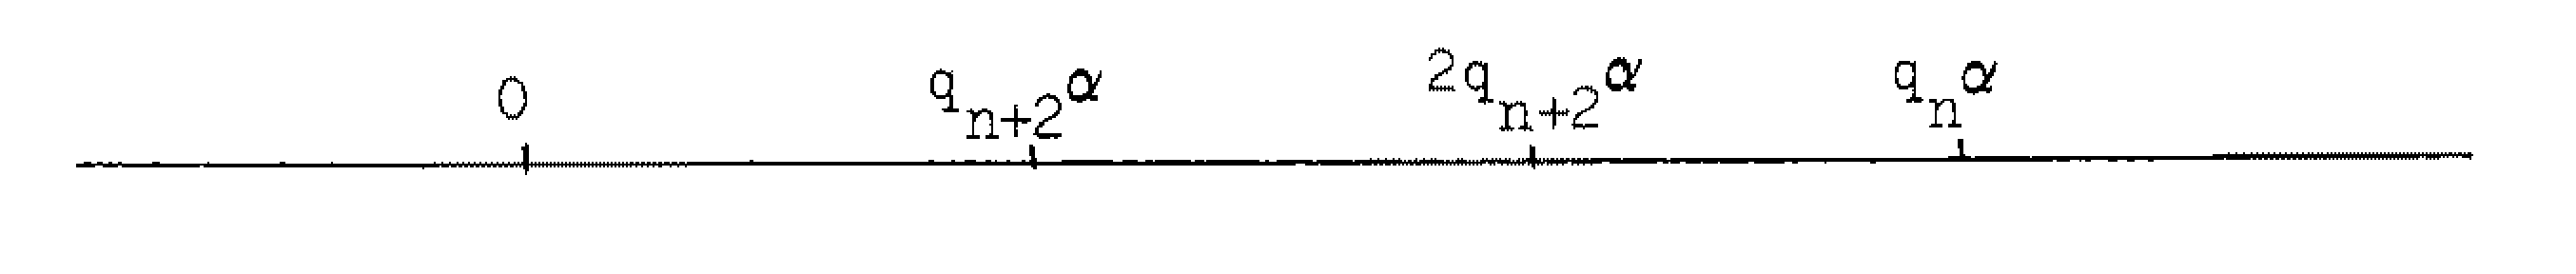
\includegraphics[width=.88\linewidth,height=18mm,keepaspectratio]{assets/presentation_derivatives/P15-A01_presentation_2x.png}
\end{center}
\noindent\hfill\scriptsize Authority-derived positional diagram P15-A01.\par\normalsize

Par conjugaison, la même disposition vaut pour les itérés de \(f\) :

\begin{center}
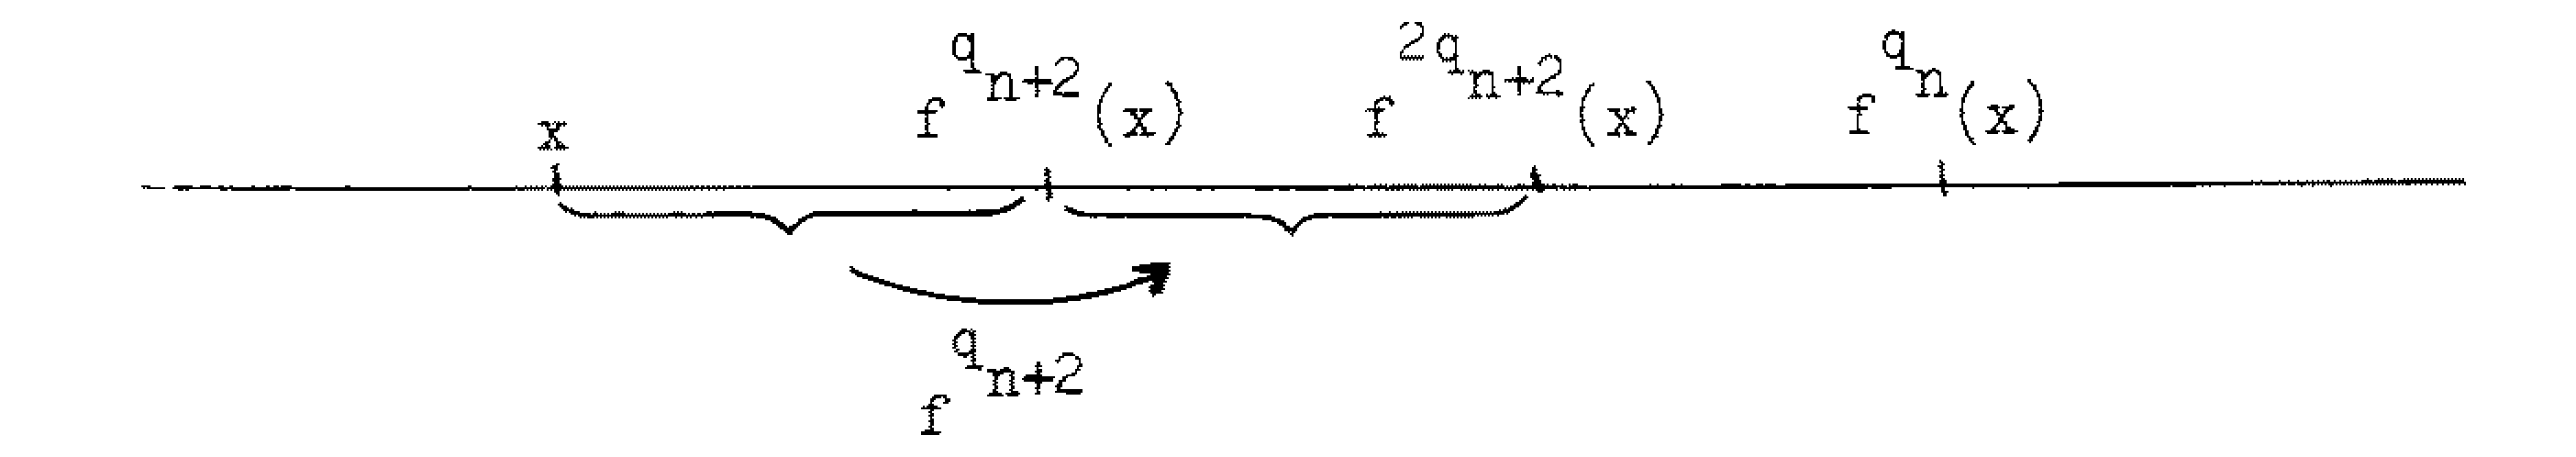
\includegraphics[width=.90\linewidth,height=24mm,keepaspectratio]{assets/presentation_derivatives/P15-A02_presentation_2x.png}
\end{center}
\noindent\hfill\scriptsize Authority-derived positional diagram P15-A02.\par\normalsize

Sur \(\mathbf R\), la même disposition vaut si on remplace \(f^{q_i}\) par \(f^{q_i}-p_i\). L’axe doit être orienté de gauche à droite pour \(n\) impair, de droite à gauche pour \(n\) pair.

Puisque \(Df^{q_i}\geq e^{-V}\), on en déduit que
\[
(1+e^{-V})\left|f^{q_{n+2}}(x)-p_{n+2}-x\right|
\leq\left|f^{q_n}(x)-p_n-x\right|,
\]
d’où la

PROPOSITION 5.1.— Les \(\|f^{q_n}-x-p_n\|_{\infty}\) décroissent au moins aussi vite qu’une progression géométrique.

Cet argument, un peu affiné, permet de prouver le théorème suivant.

THÉORÈME 5.2.— Supposons que \(\alpha\) vérifie la condition
\[
(*)\qquad
\lim_{A\to\infty}\limsup_{N\to\infty}
\frac{\displaystyle\sum_{\substack{a_i>A\\1\leq i\leq N}}\log(a_i+1)}
{\displaystyle\sum_{1\leq i\leq N}\log(a_i+1)}=0,
\]
soit, ce qui revient au même,
\[
(*)'\qquad\text{Pour tout }\varepsilon,\text{ il existe }A\text{ tel que }
\prod_{\substack{a_i>A\\1\leq i\leq N}}(a_i+1)\leq O(q_N^{\varepsilon}).
\]
Il existe alors une fonction \(V\longmapsto\varepsilon(V)\), tendant vers \(0\) avec \(V\), telle que
\end{minipage}\end{adjustbox}

\newpage
\noindent\begin{adjustbox}{max totalsize={\textwidth}{0.965\textheight},center}\begin{minipage}{\textwidth}
\noindent\hfill\scriptsize Authority physical page 16 / printed 114\par\normalsize
\[
\left|f^{q_n}(x)-p_n-x\right|\leq O\!\left(q_n^{-1+\varepsilon(V)}\right).
\]

Esquisse de démonstration.

a) Soient \(p/q\) et \(p'/q'\) deux approximations rationnelles par excès de \(\alpha\), \(a=q\alpha-p\), \(b=q'\alpha-p'\) et \(c=a/b\). Si \(0\leq rb\leq a\) (\(r\) entier \(\geq1\)), on a sur \(\mathbf R/\mathbf Z\) la disposition (dessin pour \(r=3\)) :

\begin{center}
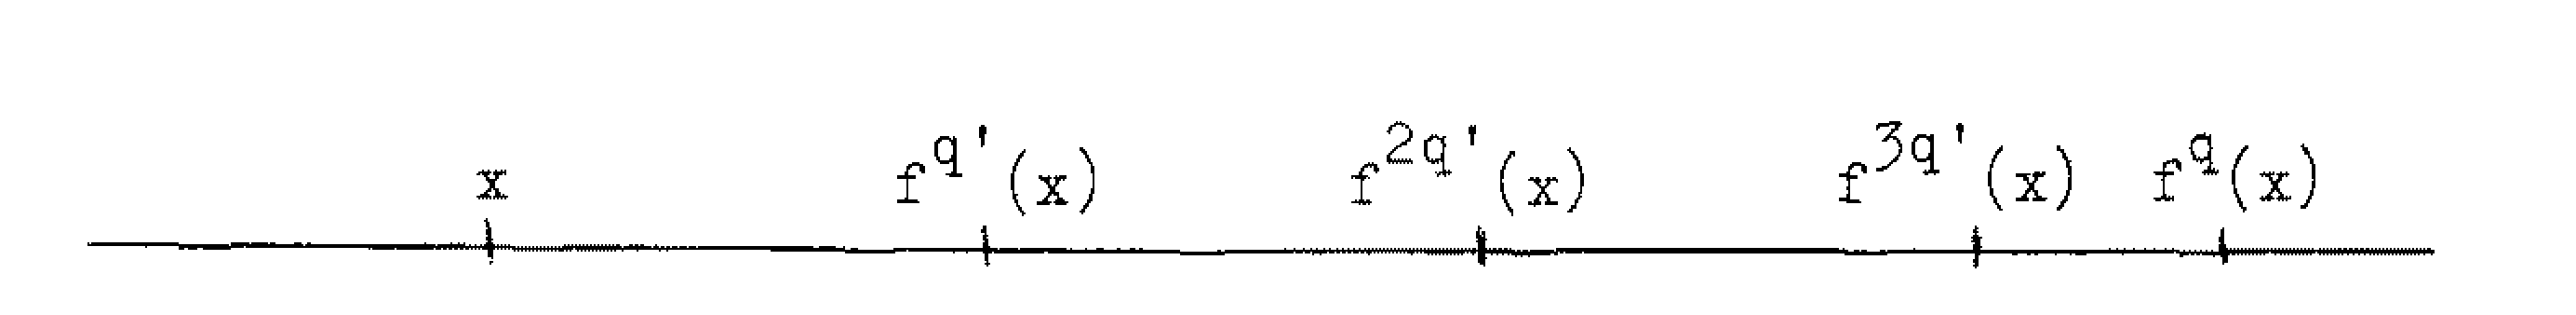
\includegraphics[width=.90\linewidth,height=18mm,keepaspectratio]{assets/presentation_derivatives/P16-A01_presentation_2x.png}
\end{center}
\noindent\hfill\scriptsize Authority-derived positional diagram P16-A01.\par\normalsize

et, puisque \(Df^{q'}\geq e^{-V}\),
\[
\left(\sum_{i=0}^{r-1}e^{-iV}\right)
\left|f^{q'}(x)-p'-x\right|
\leq\left|f^q(x)-p-x\right|.
\]

b) Plus généralement, si \(rb\leq sa\), i.e. si \(r/s\leq c\), on a
\[
\tag{5.2.1}
\left(\sum_{i=0}^{r-1}e^{-iV}\right)
\left|f^{q'}(x)-p'-x\right|
\leq
\left(\sum_{i=0}^{s-1}e^{iV}\right)
\left|f^q(x)-p-x\right|.
\]
Pour \(r=3\), \(s=2\), on a le dessin :

\begin{center}
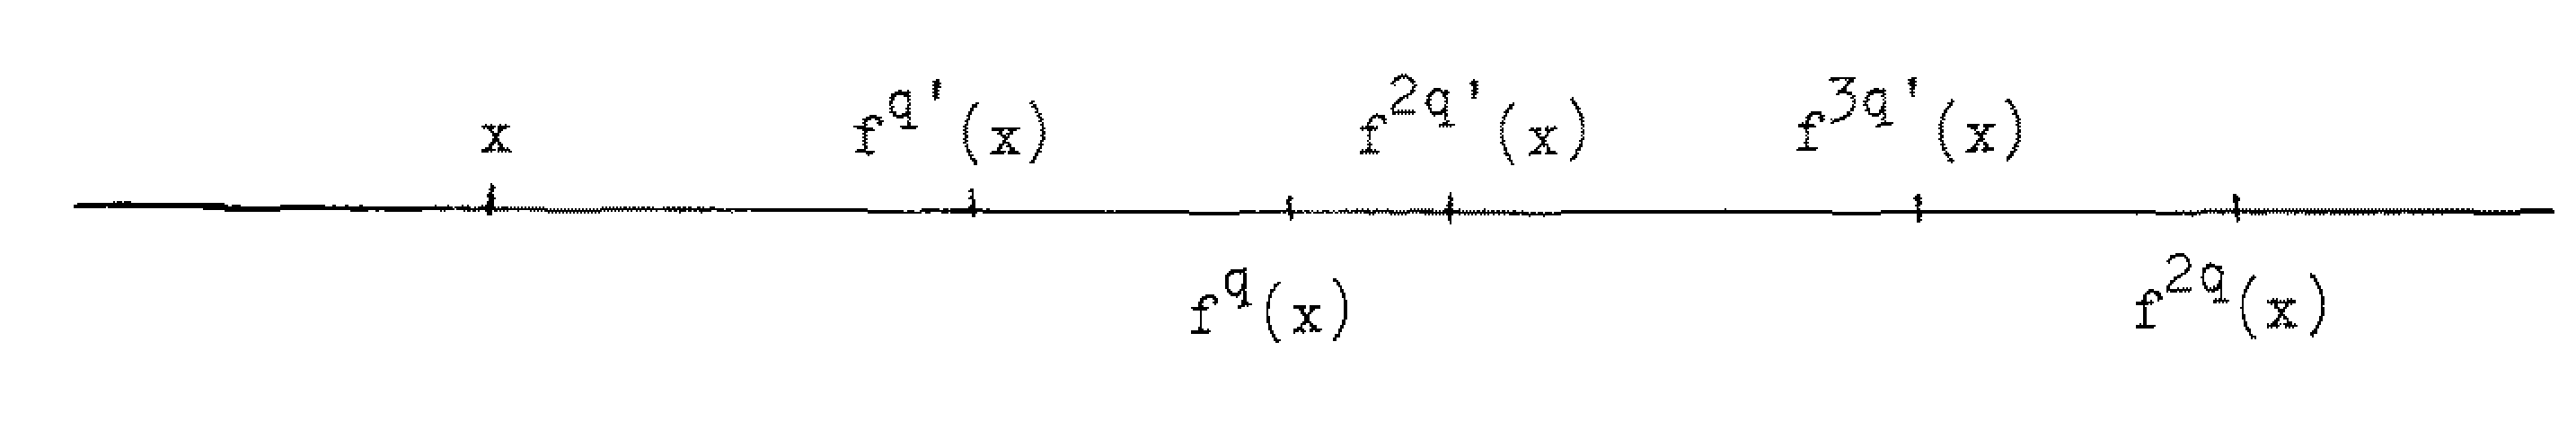
\includegraphics[width=.90\linewidth,height=23mm,keepaspectratio]{assets/presentation_derivatives/P16-A02_presentation_2x.png}
\end{center}
\noindent\hfill\scriptsize Authority-derived positional diagram P16-A02.\par\normalsize

c) Quels que soient \(\varepsilon\) et \(A\), il existe \(B\) tel que
\[
\forall x\ (2\leq x\leq A)\quad\exists r,s\quad
(r\leq B,\ s\leq B,\ x^{1-\varepsilon}<r/s<x).
\]
Il existe ensuite \(V_0\) tel que si \(V<V_0\), on ait pour tout \(r,s<B\), avec \(r\geq2s\),
\[
\frac{\displaystyle\sum_{i=0}^{s-1}e^{iV}}
{\displaystyle\sum_{i=0}^{r-1}e^{-iV}}
\leq\left(\frac sr\right)^{1-\varepsilon}.
\]

d) Si \(V<V_0\), et que \(2\leq c\leq A\), (5.2.1) donne
\[
\tag{5.2.2}
\left|f^{q'}(x)-p'-x\right|
\leq c^{-1+\varepsilon'}\left|f^q(x)-p-x\right|,
\]
avec \((1-\varepsilon')=(1-\varepsilon)^2\).
\end{minipage}\end{adjustbox}

\newpage
\noindent\begin{adjustbox}{max totalsize={\textwidth}{0.965\textheight},center}\begin{minipage}{\textwidth}
\noindent\hfill\scriptsize Authority physical page 17 / printed 115\par\normalsize
e) Prenons la suite des approximations rationnelles \(p_{2n+1}/q_{2n+1}\), et soit
\[
b_n=|q_{2n+1}\alpha-p_{2n+1}|=
\lVert\!\lVert\!\lVert q_{2n+1}\alpha\rVert\!\rVert\!\rVert.
\]
On a
\[
2\leq\frac{b_n}{b_{n+1}}\leq(a_{2n+2}+1)(a_{2n+3}+1).
\]
Si \(V<V_0\), on a donc
\[
\left\{
\begin{aligned}
\left|f^{q_{2n+3}}(x)-p_{2n+3}-x\right|
&\leq\left(\frac{b_{n+1}}{b_n}\right)^{1-\varepsilon'}
\left|f^{q_{2n+1}}(x)-p_{2n+1}-x\right| && (1)\\[-1mm]
&\hspace{9em}\text{si }(a_{2n+2}+1)(a_{2n+3}+1)\leq A,\\[1mm]
\left|f^{q_{2n+3}}(x)-p_{2n+3}-x\right|
&\leq\left|f^{q_{2n+1}}(x)-p_{2n+1}-x\right| && (2)\\[-1mm]
&\hspace{9em}\text{en tout cas.}
\end{aligned}
\right.
\]
Mettant bout à bout ces inégalités, on trouve que
\[
\left|f^{q_{2n+1}}(x)-p_{2n+1}-x\right|
\leq O\!\left(
\left[\prod (a_{2i}+1)(a_{2i+1}+1)\right]^{1-\varepsilon'}
\cdot b_n^{1-\varepsilon'}\right),
\]
où le produit est étendu aux \(i\leq n\) tels que \((a_{2i}+1)(a_{2i+1}+1)\geq A\).

On le majore par le produit \(B_n=\prod(a_j+1)^2\) étendu aux \(j\leq2n+1\) tels que \(a_j+1\geq A^{1/2}\), et on majore \(b_n\) par \(1/q_{2n+1}\) :
\[
\left|f^{q_{2n+1}}(x)-p_{2n+1}-x\right|
\leq O\!\left(B_nq_{2n+1}^{-1+\varepsilon'}\right).
\]
L’hypothèse sur \(\alpha\) permet de faire rentrer \(B_n\) dans le \(\varepsilon'\), et de conclure.

Remarque 5.3.— La condition (*) est vérifiée par presque tout nombre, et par les nombres de densité bornée.

Remarque 5.4.— Sauf si les \(a_i\) sont bornés, cette méthode ne permet malheureusement pas d’obtenir une minoration de \(\left|f^{q_n}(x)-p_n-x\right|\).
\end{minipage}\end{adjustbox}

\newpage
\noindent\begin{adjustbox}{max totalsize={\textwidth}{0.965\textheight},center}\begin{minipage}{\textwidth}
\noindent\hfill\scriptsize Authority physical page 18 / printed 116\par\normalsize
§ 6. Majoration de \(\left|Df^{q_n}-1\right|\)

Soit \(\varphi_n=f^{q_n}-p_n-x\). Nous allons majorer \(\left|Df^{q_n}-1\right|=|D\varphi_n|\) par la formule d’interpolation de Hadamard (2.2.1). On a, pour \(\alpha\) de densité bornée, et \(f\) \(C^3\),
\[
\|\varphi_n\|_{\infty}\leq O\!\left(q_n^{-1+\varepsilon(V)}\right)
\quad\text{avec }\varepsilon(V)\to0\text{ pour }V\to0 \qquad(5.2),
\]
\[
\|D^2\varphi_n\|_{\infty}\leq O\!\left(q_n^{1/2}\cdot
\sup_{i<q_n}\|Df^i\|_{\infty}\right)
\quad\text{pour }V<1 \qquad(2.3),
\]
\[
\sup_{i<q_n}\|Df^i\|_{\infty}\leq O\!\left(q_n^{\varepsilon'(V)}\right)
\quad\text{avec }\varepsilon'(V)\to0\text{ pour }V\to0 \qquad(4.5).
\]
On a donc
\[
\|D\varphi_n\|_{\infty}\leq O\!\left(q_n^{-1/4+\varepsilon''(V)}\right),
\qquad \varepsilon''(V)=\tfrac12(\varepsilon(V)+\varepsilon'(V)).
\]
Quel que soit \(\varepsilon>0\), il existe \(m\) tel que
\[
\varepsilon''(\operatorname{Var}\log Df_m)<\varepsilon\qquad(3.3),
\]
d’où
\[
\|Df_m^{q_n}-1\|_{\infty}\leq O\!\left(q_n^{-1/4+\varepsilon}\right).
\]
Par conjugaison (\(f^{q_n}=h_mf_m^{q_n}h_m^{-1}\), \(f_m^{q_n}\) est proche de \(\mathbf R/\mathbf Z\) par 5.2, et \(h_m\) est \(C^3\)), on obtient enfin le

THÉORÈME 6.1.— Si \(f\) est \(C^3\), et \(\alpha\) de densité bornée, on a pour tout \(\varepsilon>0\)
\[
\|Df^{q_n}-1\|_{\infty}\leq O\!\left(q_n^{-1/4+\varepsilon}\right).
\]

§ 7. \(h\) est \(C^{1+\beta}\) pour \(\beta<1/3\)

7.1. Nous aurons à utiliser les propriétés suivantes de la norme höldérienne \(|\varphi|_{\beta}\).

(7.1.1) Pour \(\varphi\) périodique de période \(1\), et \(g:\mathbf R/\mathbf Z\to\mathbf R/\mathbf Z\), on a
\[
|\varphi\circ g|_{\beta}\leq|\varphi|_{\beta}\|Dg\|_{\infty}^{\beta}.
\]

(7.1.2) \(|\varphi|_{\beta}\) est une fonction croissante logarithmiquement convexe de \(\beta\).
\end{minipage}\end{adjustbox}

\newpage
\noindent\begin{adjustbox}{max totalsize={\textwidth}{0.965\textheight},center}\begin{minipage}{\textwidth}
\noindent\hfill\scriptsize Authority physical page 19 / printed 117\par\normalsize
\(\log|\varphi|_{\beta}\) est en effet la borne supérieure des fonctions linéaires croissantes
\[
\log\frac{|\varphi(x)-\varphi(y)|}{|x-y|^{\beta}}.
\]

\[
\tag{7.1.3}
|\varphi|_0\leq2\lVert\varphi\rVert_{\infty}
\qquad\text{et}\qquad
|\varphi|_1=\lVert D\varphi\rVert_{\infty}.
\]
\[
\tag{7.1.4}
\lVert D\varphi\rVert_{\infty}
\leq\left(\frac{1+\beta}{2\beta}\right)^{\beta/(\beta+1)}
\cdot\left(|\varphi|_0^{\beta}|D\varphi|_{\beta}\right)^{1/(1+\beta)}.
\]

Supposons que le maximum de \(|D\varphi|\) soit atteint en \(x_0\), et pour fixer les idées, que \(D\varphi(x_0)\geq0\). On a alors
\[
D\varphi(x)\geq\lVert D\varphi\rVert_{\infty}-|D\varphi|_{\beta}(x-x_0)^{\beta}
\]
et
\[
\varphi(x)-\varphi(x_0)
\geq\lVert D\varphi\rVert_{\infty}(x-x_0)
-|D\varphi|_{\beta}\frac{(x-x_0)^{1+\beta}}{1+\beta},
\qquad x\geq x_0.
\]
On évalue cette minoration en \(x\) telle que \(\lVert D\varphi\rVert_{\infty}-|D\varphi|_{\beta}(x-x_0)^{\beta}=0\). Joignant le résultat au résultat symétrique, pour \(x<x_0\), on trouve que
\[
\frac12|\varphi|_0
\geq\lVert D\varphi\rVert_{\infty} X
-|D\varphi|_{\beta}\frac{X^{1+\beta}}{1+\beta}
=X\left(\lVert D\varphi\rVert_{\infty}-
\frac{|D\varphi|_{\beta} X^{\beta}}{1+\beta}\right)
\]
pour \(X\) tel que \(\lVert D\varphi\rVert_{\infty}=|D\varphi|_{\beta} X^{\beta}\). La formule d’interpolation (7.1.4), dont la formule d’Hadamard (2.2.1) est le cas particulier \(\beta=1\), en résulte.

(7.1.5) \(\lVert\varphi\rVert_{\beta}=\lVert\varphi\rVert_{\infty}+|\varphi|_{\beta}\) est une norme d’algèbre de Banach sur l’algèbre des fonctions \(C^{\beta}\). La formule \(\lVert\varphi_1\varphi_2\rVert_{\beta}\leq\lVert\varphi_1\rVert_{\beta}\lVert\varphi_2\rVert_{\beta}\) se déduit de l’identité
\[
\varphi_1(x)\varphi_2(x)-\varphi_1(y)\varphi_2(y)
=\varphi_1(x)(\varphi_2(x)-\varphi_2(y))
+(\varphi_1(x)-\varphi_2(x))\varphi_2(y).
\]

7.2. On suppose \(\alpha\) de densité bornée et \(f\ C^3\). Soit \(\varepsilon<1/4\). D’après 6.1, on a une majoration
\[
\tag{7.2.1}
|\log Df^{q_n}|\leq A\cdot q_n^{-\varepsilon}.
\]
Soit \(N\) un entier, et écrivons \(N=\sum b_iq_i\) comme en 1.7. Si on brise la somme
\[
\log Df^N=\sum_{i<N}\log Df\circ f^i
\]
en sommes partielles comme en 1.7, on trouve
\[
\tag{7.2.2}
\log Df^N=\sum_i\left(\sum\text{ de }b_i\text{ termes de la forme }\log Df^{q_i}\circ f^j\right).
\]
Appliquons (7.2.1) :
\end{minipage}\end{adjustbox}

\newpage
\noindent\begin{adjustbox}{max totalsize={\textwidth}{0.965\textheight},center}\begin{minipage}{\textwidth}
\noindent\hfill\scriptsize Authority physical page 20 / printed 118\par\normalsize
\[
\tag{7.2.3}
\lVert\log Df^N\rVert_{\infty}
\leq A\sum_{i=0}^{\infty}a_{i+1}q_i^{-\varepsilon}.
\]
Cette somme converge si \(\alpha\) est à densité bornée (et pour presque tout nombre), d’où la

PROPOSITION 7.3.— \(\lVert\log Df^n\rVert_{\infty}\) est uniformément borné.

7.4. Supposons que \(V<1\), et interpolons par 7.1.2 entre l’estimation 6.1 de \(\lVert Df^{q_n}-1\rVert_{\infty}\) et l’estimation 2.3 de \(\lVert D(Df^{q_n}-1)\rVert_{\infty}\). On trouve, pour \(\beta<1/3\), une majoration
\[
\tag{7.4.1}
|Df^{q_n}|_{\beta}\leq O(q_n^{-\varepsilon})
\qquad\text{avec }\varepsilon>0.
\]
Prenons \(|\ |_{\beta}\) de (7.2.2). Les \(\circ f^j\) y sont sans importance par (7.1.1) et 7.3, d’où
\[
|Df^n|_{\beta}\leq O\!\left(\sum a_{i+1}q_i^{-\varepsilon}\right)=O(1):
\]
les \(f^n\) sont uniformément \(C^{1+\beta}\), les \(h_n\) le sont aussi, et \(h\) est donc \(C^{1+\beta}\), comme expliqué dans l’introduction. On se débarrasse enfin de l’hypothèse \(V<1\) par 3.3.

PROPOSITION 7.5.— Pour tout \(\beta<1/3\), \(h\) est \(C^{1+\beta}\).

§ 8. \(C^{2+\beta}\) convergence des \(f_n\)

THÉORÈME 8.1.— Soit \(0<\beta'<\beta\leq1\). On suppose que \(f\) est \(C^{2+\beta}\) et que \(h\) est \(C^{1+\beta}\). Alors, les \(f_n\) convergent vers \(R_{\alpha}\) dans la \(C^{2+\beta'}\)-topologie.

On sait déjà que la convergence est \(C^1\) (3.5). C’est d’ailleurs ici évident sur (3.3.1) puisque les \(Df^i\) sont bornés inférieurement :
\[
Df^i>A>0.
\]
Les formules d’interpolation (7.1.2) et (7.1.4) nous ramènent donc à montrer que les \(f_n\) restent bornés dans la \(C^{2+\beta}\)-topologie, i.e. que les \(|D^2f_n|_{\beta}\) restent bornés.

Les \(f^n\) sont uniformément \(C^{1+\beta}\). Les
\[
\left|\frac1n\sum_{i<n}Df^i\right|_{\beta}
\]
sont donc bornés. Puisque les \(Df^i\) sont bornés inférieurement, et que
\[
|\varphi^{-1}|_{\beta}\leq\frac{|\varphi|_{\beta}}{(\inf|\varphi|)^2},
\]
\end{minipage}\end{adjustbox}

\newpage
\noindent\begin{adjustbox}{max totalsize={\textwidth}{0.965\textheight},center}\begin{minipage}{\textwidth}
\noindent\hfill\scriptsize Authority physical page 21 / printed 119\par\normalsize
les
\[
\left|\frac{n}{\sum_{i<n}Df^i}\right|_{\beta}
\]
sont également bornés.

Par la même méthode qu’en 3.6, compte tenu de ce que les \(h_n\) et \(f^n\) sont uniformément \(C^1\) (ce qui justifie les changements de variable), on se ramène à majorer uniformément en norme \(\lVert\ \rVert_{\beta}\) (7.1.5) les fonctions
\[
-D\left(\frac1{\sum_{i<n}Df^i}\right)
=\sum_{j<i<n}\lambda_{ij}\,D\log Df\circ f^j
\]
pour
\[
\lambda_{ij}
=\frac{Df^iDf^j}{\left(\sum_{i<n}Df^i\right)^2}
=\frac1{n^2}\left[Df^i\cdot Df^j\cdot
\left(\frac{n}{\sum_{i<n}Df^i}\right)^2\right]
\qquad(\text{preuve de }(3.7)).
\]
L’expression entre crochets, et les \(D\log Df\circ f^j\), étant uniformément bornés en norme \(\lVert\ \rVert_{\beta}\), c’est immédiat.

§ 9. Application d’un théorème des fonctions implicites

Le résultat final d’Herman est le suivant.

THÉORÈME 9.1.— Si \(\alpha\) est de densité bornée, et que \(f\) est \(C^r\), \(r\geq3\) (\(r=n+\beta\), \(n\) entier, \(0\leq\beta<1\)), alors \(h\) est \(C^{r-1-\varepsilon}\) pour tout \(\varepsilon>0\).

Il l’obtient en conjuguant 7.5 et 8.1 avec un théorème des fonctions implicites :

THÉORÈME 9.2.— Soient \(\alpha\) un nombre irrationnel, et \(1\leq\theta<\theta'\). On suppose qu’il existe \(C\) tel que
\[
|q\alpha-p|\geq C\cdot q^{-\theta}
\]
pour tous entiers \(p,q\). Il existe alors un voisinage \(V\) de \(R_{\alpha}\) dans la \(C^{2\theta'}\)-topologie tel que pour \(f\) dans ce voisinage et \(C^r\) (resp. \(C^{\infty}\), \(C^{\omega}\)), l’équation
\[
f=R_{\lambda}\circ g\circ R_{\alpha}\circ g^{-1}
\]
(\(\lambda\in\mathbf R\), \(g\) homéomorphisme croissant) admette une solution \(C^{r-\theta'}\) (resp. \(C^{\infty}\), \(C^{\omega}\)).
\end{minipage}\end{adjustbox}

\newpage
\noindent\begin{adjustbox}{max totalsize={\textwidth}{0.965\textheight},center}\begin{minipage}{\textwidth}
\noindent\hfill\scriptsize Authority physical page 22 / printed 120\par\normalsize
Pour obtenir 9.1, on prend \(1<\theta<\theta'=1+\varepsilon\), on prend pour \(\alpha\) le nombre de rotation de \(f\), on se ramène à supposer \(f\) dans \(V\) par 7.5 et 8.1 et on observe que le nombre de rotation de
\[
R_{\lambda}\circ g\circ R_{\alpha}\circ g^{-1}
\]
ne peut être \(\alpha\) que pour \(\lambda=0\).

Comme nous l’avons déjà dit, la preuve de 9.2 est inspirée de [1], [3] et [4].
\end{minipage}\end{adjustbox}

\newpage
\noindent\begin{adjustbox}{max totalsize={\textwidth}{0.965\textheight},center}\begin{minipage}{\textwidth}
\noindent\hfill\scriptsize Authority physical page 23 / printed 121\par\normalsize
BIBLIOGRAPHIE

[1] V. I. ARNOLD — Small denominators I, Transl. A.M.S., 2e série, 46 (1965), 213–284.

[2] A. DENJOY — Les trajectoires à la surface du tore, C.R. Acad. Sci. Paris, 1946, vol. 223, 5–8.

[3] J. MOSER — A rapidly convergent iteration method II, Ann. Scuola Norm. Sup. di Pisa, 20 (1966), 499–535.

[4] H. RÜSSMANN — Kleine Nenner II, Bemerkungen zur Newtonschen Methode. Nachr. Akad. Wiss., Göttingen, Math. Phys. Kl., 1972.
\end{minipage}\end{adjustbox}


\clearpage\endgroup
\typeout{CORPUS-END:D028:\thepage}
% END INLINE WORK D028 FR
% BEGIN INLINE WORK D029 FR
\typeout{CORPUS-BEGIN:D029:\thepage}
\begingroup
\makeatletter
\let\DeclareMathOperator\CorpusDeclareMathOperator
\let\@declmathop\CorpusDeclMathOp
\let\maketitle\CorpusMakeTitle\let\title\CorpusTitle\let\author\CorpusAuthor\let\date\CorpusDate
\let\thanks\CorpusThanks\let\and\CorpusAnd\let\@maketitle\CorpusAtMakeTitle
\def\setcounter#1#2{\def\CorpusCounterName{#1}\def\CorpusPageName{page}\ifx\CorpusCounterName\CorpusPageName\else\CorpusSetCounter{#1}{#2}\fi}
\title{}\author{}\date{}
\setcounter{section}{0}
\expandafter\def\csname theHsection\endcsname{D029.\arabic{section}}
\setcounter{subsection}{0}
\expandafter\def\csname theHsubsection\endcsname{D029.\arabic{subsection}}
\setcounter{subsubsection}{0}
\expandafter\def\csname theHsubsubsection\endcsname{D029.\arabic{subsubsection}}
\setcounter{equation}{0}
\expandafter\def\csname theHequation\endcsname{D029.\arabic{equation}}
\setcounter{figure}{0}
\expandafter\def\csname theHfigure\endcsname{D029.\arabic{figure}}
\setcounter{table}{0}
\expandafter\def\csname theHtable\endcsname{D029.\arabic{table}}
\setcounter{footnote}{0}
\expandafter\def\csname theHfootnote\endcsname{D029.\arabic{footnote}}
\makeatother
\let\tableofcontents\relax % one cumulative contents list, not repeated global lists
% D029 canonical bounded edition; generated from frozen source records.
% Do not treat this file as authority: source PDF SHA-256 CC9759F6D12980328126AF4CE6B5ACA8309FEC24D9ADC5F43A0D9FC88992C125.
\setmainfont{Latin Modern Roman}
\setsansfont{Latin Modern Sans}
\setmonofont{Latin Modern Mono}
\setlength{\parindent}{0pt}
\setlength{\parskip}{2pt}
\setlength{\emergencystretch}{3em}
\sloppy

\graphicspath{{assets/works/D029_PUBLIC_SAFE/}}
\selectlanguage{french}
\phantomsection\addcontentsline{toc}{section}{D029}


\small
\phantomsection\hypertarget{D029-authority-page-0001}{}
\section*{Authority page 1 --- printed page 203}
\addcontentsline{toc}{section}{Authority page 1 --- printed page 203}
\noindent THÉORIE DES GROUPES. — Extensions centrales non résiduellement finies de groupes arithmétiques. Note (*) de M. Pierre Deligne, Membre de l'Académie.\par
\smallskip
\noindent ⟦Résumé français imprimé⟧\par
\noindent Une variante des méthodes connues pour traiter le problème des sous-groupes de congruence fournit des résultats comme le suivant : pour n \ensuremath{≥} 2, le groupe \ensuremath{\widetilde{Sp}}(2n, \ensuremath{ℤ}) image inverse de Sp(2n, \ensuremath{ℤ}) dans le revêtement universel de Sp(2n, \ensuremath{ℝ}) (une extension centrale de Sp(2n, \ensuremath{ℤ}) par \ensuremath{π₁} Sp(2n, \ensuremath{ℝ}) = \ensuremath{ℤ}) n'est pas séparé pour la topologie des sous-groupes d'indice fini. Plus précisément, tout sous-groupe d'indice fini de \ensuremath{\widetilde{Sp}}(2n, \ensuremath{ℤ}) contient 2\ensuremath{π₁} Sp(2n, \ensuremath{ℝ}).\par
\smallskip
\noindent ⟦Abstract anglais imprimé dans la source⟧\par
\noindent A variant of known methods to handle the congruence subgroup problem yields results like the following. Let \ensuremath{\widetilde{Sp}}(2n, \ensuremath{ℤ}) be the inverse image of Sp(2n, \ensuremath{ℤ}) in the universal covering of Sp(2n, \ensuremath{ℝ}); it is a central extension of Sp(2n, \ensuremath{ℤ}) by \ensuremath{π₁} Sp(2n, \ensuremath{ℝ}) \ensuremath{≃} \ensuremath{ℤ}. If n \ensuremath{≥} 2, the group \ensuremath{\widetilde{Sp}}(2n, \ensuremath{ℤ}) is not residually finite : any subgroup of finite index contains 2\ensuremath{π₁} Sp(2n, \ensuremath{ℝ}).\par
\smallskip
\noindent 1. GROUPES S-ARITHMÉTIQUES. — Soit G un groupe presque simple simplement connexe isotrope sur un corps global F. Pour simplifier les énoncés, nous supposerons aussi que G(F) est parfait (i. e. égal à son groupe des commutateurs); c'est le cas, sauf peut-être si G est une forme trialitaire de D\ensuremath{₄}. Soit par ailleurs S un ensemble fini de places de F, contenant toutes les places à l'infini, et supposons que\par
\smallskip
\noindent (i)    \ensuremath{∑_{v∈S}} rang(G/\ensuremath{F_v}) \ensuremath{≥} 2.\par
\smallskip
\noindent Pour chaque place v de F, posons \ensuremath{G_v} = G(\ensuremath{F_v}). Pour chaque ensemble fini T de places, posons de même \ensuremath{G_T} = \ensuremath{∏_{v∈T}} \ensuremath{G_v} et \ensuremath{G_{T′}} = \ensuremath{∏_{v∉T}} \ensuremath{G_v} (produit restreint) : pour \ensuremath{𝔸} l'anneau des adèles de F, on a G(\ensuremath{𝔸}) = \ensuremath{G_T} \ensuremath{×} \ensuremath{G_{T′}}.\par
\smallskip
\noindent Un sous-groupe de G(F) est dit de S-congruence s'il est l'image inverse d'un sous-groupe compact ouvert de \ensuremath{G_{S′}}. Il est dit S-arithmétique s'il est commensurable à un sous-groupe de S-congruence, i. e. s'il contient, avec un indice fini, un sous-groupe d'indice fini dans un groupe de S-congruence. Les sous-groupes de S-congruence (resp. S-arithmétiques) forment un système fondamental de voisinages de l'origine pour une topologie (de groupe topologique) \ensuremath{𝒯}(c) [resp. \ensuremath{𝒯}(a)] sur G(F). Pour \ensuremath{Γ} un sous-groupe de S-congruence fixe, on obtient encore un système fondamental de voisinages en ne considérant que les sous-groupes de S-congruence distingués dans \ensuremath{Γ} (resp. que les sous-groupes distingués d'indice fini de \ensuremath{Γ}). Ceci assure l'existence du complété \ensuremath{\widehat{G(F)}}(c) [resp. \ensuremath{\widehat{G(F)}}(a)] de G(F) pour \ensuremath{𝒯}(c) [resp. \ensuremath{𝒯}(a)]. La topologie \ensuremath{𝒯}(c) est la topologie induite de celle de \ensuremath{G_{S′}}. Puisque G(F) est dense dans \ensuremath{G_{S′}} (théorème d'approximation forte), on a \ensuremath{\widehat{G(F)}}(c) = \ensuremath{G_{S′}}. Le complété \ensuremath{\widehat{G(F)}}(a) de G(F) est une extension de \ensuremath{\widehat{G(F)}}(c) = \ensuremath{G_{S′}} par le groupe profini C(S, G) = lim proj \ensuremath{Γ}/\ensuremath{Δ} (limite projective sur les couples \ensuremath{Δ} \ensuremath{⊂} \ensuremath{Γ}, avec \ensuremath{Δ} distingué d'indice fini dans \ensuremath{Γ} et \ensuremath{Γ} de S-congruence).\par
\smallskip
\noindent Pour G de rang \ensuremath{≥} 2, Raghunathan (1) a montré que :\par
\smallskip
\noindent (ii)    \ensuremath{\widehat{G(F)}}(a) est une extension centrale de \ensuremath{\widehat{G(F)}}(c) = \ensuremath{G_{S′}},\par
\smallskip
\noindent et il achève de vérifier que la même conclusion vaut sous la seule hypothèse (i).\par
\smallskip
\noindent Soient \ensuremath{\widetilde{G}_S} une extension centrale topologique de \ensuremath{G_S} par un groupe discret A, et \ensuremath{\widetilde{G(F)}} l'image inverse de G(F) dans \ensuremath{\widetilde{G}_S}. Un sous-groupe de \ensuremath{\widetilde{G(F)}} sera dit de S-congruence s'il est image inverse d'un sous-groupe de S-congruence de G(F), et S-arithmétique s'il est commensurable à un sous-groupe de S-congruence. On note encore \ensuremath{𝒯}(c) et \ensuremath{𝒯}(a) les topologies correspondantes, et \ensuremath{\widehat{\widetilde{G(F)}}}(c), \ensuremath{\widehat{\widetilde{G(F)}}}(a) les complétés séparés pour ces\par
\clearpage
\phantomsection\hypertarget{D029-authority-page-0002}{}
\section*{Authority page 2 --- printed page 204}
\addcontentsline{toc}{section}{Authority page 2 --- printed page 204}
\noindent topologies. On a encore \ensuremath{\widehat{\widetilde{G(F)}}}(c) = \ensuremath{G_{S′}}, tandis que \ensuremath{\widehat{\widetilde{G(F)}}}(a) est extension de \ensuremath{G_{S′}} par un groupe profini \ensuremath{\widetilde{C}}(S, G), lui-même extension de C(S, G) par\par
\smallskip
\noindent \ensuremath{\widehat{A}} = lim proj A/(A \ensuremath{∩} \ensuremath{Γ})    (\ensuremath{Γ} S-arithmétique).\par
\smallskip
\noindent PROPOSITION 1. — Si la condition (ii) est vérifiée, \ensuremath{\widehat{\widetilde{G(F)}}}(a) est une extension centrale de \ensuremath{\widehat{\widetilde{G(F)}}}(c) = \ensuremath{G_{S′}}.\par
\smallskip
\noindent Rappelons que, si un groupe \ensuremath{\widetilde{H}} est une extension centrale d'un groupe H, l'application commutateur \ensuremath{\widetilde{H}} \ensuremath{×} \ensuremath{\widetilde{H}} \ensuremath{→} \ensuremath{\widetilde{H}} se factorise par une application, encore notée ( , ) : H \ensuremath{×} H \ensuremath{→} \ensuremath{\widetilde{H}}. En particulier, le groupe \ensuremath{\widehat{\widetilde{G(F)}}}(a) étant une extension centrale de \ensuremath{\widehat{G(F)}}(a) par \ensuremath{\widehat{A}}, l'application commutateur : \ensuremath{\widetilde{C}}(S, G) \ensuremath{×} \ensuremath{\widehat{\widetilde{G(F)}}}(a) \ensuremath{→} \ensuremath{\widehat{\widetilde{G(F)}}}(a) se factorise par C(S, G) \ensuremath{×} \ensuremath{\widehat{G(F)}}(a). D'après (ii), elle se factorise par une application bimultiplicative\par
\smallskip
\noindent C(S, G) \ensuremath{×} \ensuremath{\widehat{G(F)}}(a) \ensuremath{→} \ensuremath{\widehat{A}};\par
\smallskip
\noindent puisque G(F) est parfait, et dense dans \ensuremath{\widehat{G(F)}}(a), celle-ci est triviale.\par
\smallskip
\noindent En termes plus concrets, la proposition signifie que pour tout sous-groupe S-arithmétique \ensuremath{Δ}, on a :\par
\smallskip
\noindent (1 a) Pour tout conjugué \ensuremath{Δ^g} de \ensuremath{Δ} (g \ensuremath{∈} \ensuremath{\widetilde{G(F)}}), il existe un groupe de S-congruence \ensuremath{Γ} tel que \ensuremath{Γ} \ensuremath{∩} \ensuremath{Δ} = \ensuremath{Γ} \ensuremath{∩} \ensuremath{Δ^g}.\par
\smallskip
\noindent (1 b) \ensuremath{\widetilde{G(F)}} agit trivialement sur le groupe fini \ensuremath{C_Δ} = lim proj \ensuremath{Γ}/(\ensuremath{Γ} \ensuremath{∩} \ensuremath{Δ}).\par
\smallskip
\noindent Ces conditions équivalent encore à\par
\smallskip
\noindent (1 c) Pour tout g \ensuremath{∈} G(F), il existe \ensuremath{Γ} de S-congruence tel que (g, \ensuremath{Γ}) \ensuremath{⊂} \ensuremath{Δ}.\par
\smallskip
\noindent On a \ensuremath{\widetilde{C}}(S, G) = lim proj \ensuremath{C_Δ}.\par
\smallskip
\noindent 2. EXTENSIONS CENTRALES DE GROUPES ADÉLIQUES. — Nous supposerons dorénavant que :\par
\smallskip
\noindent (iii) le groupe \ensuremath{\widetilde{G}_S} est parfait.\par
\smallskip
\noindent Le cas le plus intéressant serait celui où \ensuremath{\widetilde{G}_S} est l'extension centrale universelle de \ensuremath{G_S} par un groupe discret (le « revêtement universel » de \ensuremath{G_S}), mais nous ne tenons pas à supposer l'existence d'une telle extension universelle.\par
\smallskip
\noindent Une extension centrale topologique E de G(\ensuremath{𝔸}) par un groupe discret X est déterminée par les extensions \ensuremath{E_S} et \ensuremath{E_{S′}} de \ensuremath{G_S} et \ensuremath{G_{S′}} par X images inverses de \ensuremath{G_S} et \ensuremath{G_{S′}} dans E : parce que \ensuremath{G_S} est parfait, on a\par
\smallskip
\noindent E  \ensuremath{←}\textasciitilde{}  (\ensuremath{E_S} \ensuremath{×} \ensuremath{E_{S′}})/\{(x, \ensuremath{−}x) | x \ensuremath{∈} X\}.\par
\smallskip
\noindent Si l'extension \ensuremath{E_S} est dominée par \ensuremath{\widetilde{G}_S}, i. e. se déduit de \ensuremath{\widetilde{G}_S} en poussant par f : A \ensuremath{→} X, l'application f est unique, et la donnée de E revient à celle de l'extension \ensuremath{E_{S′}}, et de f (équivalence de catégorie); on a\par
\smallskip
\noindent E  \ensuremath{←}\textasciitilde{}  \ensuremath{\widetilde{G}_S} \ensuremath{×} \ensuremath{E_{S′}}/\{(a, \ensuremath{−}f(a)) | a \ensuremath{∈} A\}.\par
\smallskip
\noindent Soit \ensuremath{ℒ} la catégorie des extensions centrales topologiques de G(\ensuremath{𝔸}) par un groupe fini, scindées au-dessus de G(F), et avec \ensuremath{E_S} dominé par \ensuremath{\widetilde{G}_S} :\par
\smallskip
\noindent 1 \ensuremath{→} X \ensuremath{→} E \ensuremath{→} G(\ensuremath{𝔸}) \ensuremath{→} 1\par
\noindent           \ensuremath{↖}s    \ensuremath{↑}\par
\noindent              G(F)\par
\smallskip
\noindent Il reviendrait au même d'exiger « scindable au-dessus de G(F) » : puisque G(F) est parfait, le scindage, s'il existe, est unique. La catégorie \ensuremath{ℒ} est filtrante à gauche. Pour (E, s) dans \ensuremath{ℒ}, l'adhérence dans E de (image de \ensuremath{\widetilde{G}_S}).s G(F) s'envoie sur G(\ensuremath{𝔸}) : elle s'envoie sur un fermé, car X est fini, et contient \ensuremath{G_S}.G(F) qui est dense (approximation forte). La sous-catégorie L de \ensuremath{ℒ} formée des (E, s) avec (image de \ensuremath{\widetilde{G}_S}).s G(F) dense dans E est donc cofinale; puisqu'il y a au plus une flèche entre deux objets de L, elle se réduit à un ensemble ordonné filtrant.\par
\clearpage
\phantomsection\hypertarget{D029-authority-page-0003}{}
\section*{Authority page 3 --- printed page 205}
\addcontentsline{toc}{section}{Authority page 3 --- printed page 205}
\noindent PROPOSITION 2. — Sous les hypothèses (ii) et (iii), nous construisons un isomorphisme naturel entre \ensuremath{\widetilde{C}}(S, G) et la limite projective sur \ensuremath{ℒ}, ou L, lim proj X. Via cet isomorphisme, l'application naturelle de A dans \ensuremath{\widetilde{C}}(S, G) est la limite des \ensuremath{−}f : A \ensuremath{→} X, f étant tel que \ensuremath{E_S} se déduise de \ensuremath{\widetilde{G}_S} par f.\par
\smallskip
\noindent Soit E une extension centrale topologique de G(\ensuremath{𝔸}) par un groupe discret X. Se donner un scindage s de E au-dessus de G(F) revient à se donner un isomorphisme entre l'extension de G(F) par X déduite de \ensuremath{E_S}, et l'opposée de celle déduite de \ensuremath{E_{S′}}. Pour \ensuremath{E_S} dominé par \ensuremath{\widetilde{G}_S}, et f comme ci-dessus, cela revient à se donner un diagramme commutatif\par
\smallskip
\noindent 1 \ensuremath{→} X \ensuremath{→} \ensuremath{E_{S′}} \ensuremath{→} \ensuremath{G_{S′}} \ensuremath{→} 1\par
\noindent     \ensuremath{↑−}f    \ensuremath{↑}t         \ensuremath{↑}\par
\noindent 1 \ensuremath{→} A \ensuremath{→} \ensuremath{\widetilde{G(F)}} \ensuremath{→} G(F) \ensuremath{→} 1.\par
\smallskip
\noindent De là une équivalence entre la catégorie \ensuremath{ℒ} et celle, \ensuremath{ℒ′}, des diagrammes commutatifs\par
\smallskip
\noindent (1)    1 \ensuremath{→} X \ensuremath{→} \ensuremath{E_{S′}} —q\ensuremath{→} \ensuremath{G_{S′}} \ensuremath{→} 1\par
\noindent                  \ensuremath{↑}t          \ensuremath{↑}\par
\noindent               \ensuremath{\widetilde{G(F)}} \ensuremath{→} G(F)\par
\smallskip
\noindent (\ensuremath{E_{S′}} extension centrale topologique de \ensuremath{G_{S′}} par un groupe fini) : on reconstruit E comme étant \ensuremath{\widetilde{G}_S} \ensuremath{×} \ensuremath{E_{S′}}/\{(a, ta) | a \ensuremath{∈} A\}, et le scindage sur G(F) par s(g) = (\ensuremath{\widetilde{g}}, t\ensuremath{\widetilde{g}}) mod les (a, ta) pour \ensuremath{\widetilde{g}} \ensuremath{∈} \ensuremath{\widetilde{G(F)}} \ensuremath{⊂} \ensuremath{\widetilde{G}_S} d'image g dans G(F). La sous-catégorie L de \ensuremath{ℒ} correspond à celle, L\ensuremath{′}, des diagrammes (1) avec t d'image dense.\par
\smallskip
\noindent Soient (\ensuremath{E_{S′}}, t) dans L\ensuremath{′}, et \ensuremath{𝒯} la topologie sur \ensuremath{\widetilde{G(F)}} induite par celle de \ensuremath{E_{S′}}. Si K est un sous-groupe compact ouvert de \ensuremath{E_{S′}}, disjoint de X, les intersections de \ensuremath{Δ} = \ensuremath{t^{-1}}K avec les sous-groupes de S-congruence forment un système fondamental de voisinages pour \ensuremath{𝒯}. Pour \ensuremath{Γ} un sous-groupe de S-congruence défini par un sous-groupe compact ouvert K\ensuremath{₁} \ensuremath{⊂} qK, on a de plus\par
\smallskip
\noindent (2)    X  \ensuremath{→}\textasciitilde{}  XK/K  \ensuremath{←}\textasciitilde{}  \ensuremath{q^{-1}}K\ensuremath{₁}/(K \ensuremath{∩} \ensuremath{q^{-1}}K\ensuremath{₁})  \ensuremath{←}\textasciitilde{}  \ensuremath{Γ}/(\ensuremath{Δ} \ensuremath{∩} \ensuremath{Γ})  \ensuremath{←}\textasciitilde{}  \ensuremath{C_Δ}.\par
\smallskip
\noindent Puisque X est fini, \ensuremath{Δ} est S-arithmétique. Réciproquement, la proposition 1 assure qu'un système fondamental de groupes S-arithmétiques est ainsi obtenu : l'ensemble ordonné filtrant L\ensuremath{′} s'identifie à celui des germes (pour la topologie de S-congruence) de groupes S-arithmétiques, et l'isomorphisme de la proposition 2 est défini comme la limite projective des isomorphismes (2).\par
\smallskip
\noindent 3. GROUPES QUASI DÉPLOYÉS. — Soit \ensuremath{μ} le groupe des racines de l'unité de F et; pour chaque place non complexe v de F, soit \ensuremath{μ_v} le groupe des racines de l'unité de \ensuremath{F_v}. Pour v complexe, on pose \ensuremath{μ_v} = \{1\}. Deodhar a montré que, pour G quasi-déployé, il existe une extension topologique centrale universelle \ensuremath{\widetilde{G}_v} de \ensuremath{G_v} par un groupe discret (le « revêtement universel »), et que pour v non réelle, son noyau \ensuremath{π₁}(\ensuremath{G_v}) est canoniquement un quotient de \ensuremath{μ_v}. J'ai complété ce résultat en montrant qu'en fait \ensuremath{π₁}(\ensuremath{G_v}) = \ensuremath{μ_v}. Pour v réelle, on a \ensuremath{π₁}(\ensuremath{G_v}) = \ensuremath{ℤ}, ou \ensuremath{ℤ}/2. Dans tous les cas, \ensuremath{μ_v} apparaît comme un quotient de \ensuremath{π₁}(\ensuremath{G_v}).\par
\smallskip
\noindent Pour presque tout v, l'extension \ensuremath{\widetilde{G}_v} se scinde au-dessus du sous-groupe compact maximal naturel de \ensuremath{G_v}. Ceci permet de définir le produit restreint des \ensuremath{\widetilde{G}_v}, une extension de G(\ensuremath{𝔸}) par la somme des \ensuremath{π₁}(\ensuremath{G_v}). Poussons-la par\par
\smallskip
\noindent R : \ensuremath{⊕_v} \ensuremath{π₁}(\ensuremath{G_v}) \ensuremath{→} \ensuremath{⊕_v} \ensuremath{μ_v} —\ensuremath{σ→} \ensuremath{μ} : \ensuremath{σ}((\ensuremath{x_v})) = \ensuremath{∏_v} \ensuremath{x_v^{[μ_v:μ]}}.\par
\clearpage
\phantomsection\hypertarget{D029-authority-page-0004}{}
\section*{Authority page 4 --- printed page 206}
\addcontentsline{toc}{section}{Authority page 4 --- printed page 206}
\noindent On obtient une extension centrale de G(\ensuremath{𝔸}) par \ensuremath{μ}, et il résulte de Deodhar (2) et C. Moore (3) que c'est l'extension centrale topologique universelle de G(\ensuremath{𝔸}) par un groupe discret, qui se scinde au-dessus de G(F) :\par
\smallskip
\noindent (3)    1 \ensuremath{→} \ensuremath{μ} \ensuremath{→} \ensuremath{\widetilde{G(𝔸)}} \ensuremath{→} G(\ensuremath{𝔸}) \ensuremath{→} 1\par
\noindent                          \ensuremath{↖}          \ensuremath{↑}\par
\noindent                               G(F)\par
\smallskip
\noindent Prenons pour \ensuremath{\widetilde{G}_S} le revêtement universel de \ensuremath{G_S}, et notons \ensuremath{R_S} la restriction de R à \ensuremath{π₁}\ensuremath{G_S} = \ensuremath{∏_{v∈S}} \ensuremath{π₁}(\ensuremath{G_v}). La proposition 2 identifie le complété \ensuremath{\widehat{\widetilde{G(F)}}}(a) de \ensuremath{\widetilde{G(F)}} à l'image inverse \ensuremath{\widetilde{G(𝔸)}_{S′}} de \ensuremath{G_{S′}} = \ensuremath{\widehat{\widetilde{G(F)}}}(c) dans (3), et fournit un diagramme commutatif exact\par
\smallskip
\noindent (4)    1 \ensuremath{→} \ensuremath{μ} \ensuremath{→} \ensuremath{\widetilde{G(𝔸)}_{S′}} \ensuremath{→} \ensuremath{G_{S′}} \ensuremath{→} 1\par
\noindent              \ensuremath{↑−}\ensuremath{R_S}          \ensuremath{↑}i             \ensuremath{↑}\par
\noindent        \ensuremath{∏_{v∈S}} \ensuremath{π₁}(\ensuremath{G_v}) \ensuremath{→} \ensuremath{\widehat{\widetilde{G(F)}}}(a) \ensuremath{→} \ensuremath{\widehat{G(F)}}(a) \ensuremath{→} 1\par
\smallskip
\noindent En particulier\par
\smallskip
\noindent THÉORÈME. — Soient G/F quasi déployé, et \ensuremath{\widetilde{G(F)}} l'image inverse de G(F) dans le revêtement universel de \ensuremath{G_S}. Si \ensuremath{∑_{v∈S}} rang(\ensuremath{G_v}) \ensuremath{≥} 2, l'intersection des sous-groupes S-arithmétiques de \ensuremath{\widetilde{G(F)}} est le noyau de \ensuremath{R_S} : \ensuremath{∏_{v∈S}} \ensuremath{π₁}(\ensuremath{G_v}) \ensuremath{→} \ensuremath{μ}.\par
\smallskip
\noindent Pour Sp(2n, \ensuremath{ℚ}), et S = \ensuremath{∞}, c'est le résultat annoncé dans l'introduction. Pour SL(n, K), avec K quadratique réel, et S = \ensuremath{∞}, le résultat obtenu généralise celui de J. Millson (4).\par
\smallskip
\noindent PROBLÈME. — Tout sous-groupe discret de covolume fini du revêtement universel de Sp(2n, \ensuremath{ℝ}) (n \ensuremath{≥} 2) contient-il 2\ensuremath{π₁} Sp(2n, \ensuremath{ℝ}) ? (5).\par
\smallskip
\noindent 4. LE SYSTÈME DE FACTEURS DES FONCTIONS \ensuremath{θ}. — Lorsque la condition (i) n'est pas vérifiée, on ne dispose plus de la proposition 1; il reste néanmoins possible d'étudier les sous-groupes S-arithmétiques vérifiant une condition de type (1 a).\par
\smallskip
\noindent Soient donc S un ensemble fini non vide de places, contenant toutes les places à l'infini, et T \ensuremath{⊃} S tel que (G, T) vérifie la condition (ii). Le cas intéressant est celui où S est réduit à une place, en laquelle G est de rang 1. Soient encore \ensuremath{\widetilde{G}_S} une extension centrale topologique de \ensuremath{G_S} par un groupe discret, et \ensuremath{\widetilde{G(F)}} l'image inverse de G(F) dans \ensuremath{\widetilde{G}_S}. Pour \ensuremath{Δ} un sous-groupe S-arithmétique de \ensuremath{\widetilde{G(F)}}, considérons la condition :\par
\smallskip
\noindent (\ensuremath{\star}) il existe un sous-groupe T-arithmétique U de \ensuremath{\widetilde{G(F)}}, tel que, pour tout conjugué \ensuremath{Δ^g} de \ensuremath{Δ} (g \ensuremath{∈} U), il existe un groupe de S-congruence \ensuremath{Γ} tel que \ensuremath{Γ} \ensuremath{∩} \ensuremath{Δ} = \ensuremath{Γ} \ensuremath{∩} \ensuremath{Δ^g} (U-invariance du germe de \ensuremath{Δ}).\par
\smallskip
\noindent PROPOSITION 3. — Le complété \ensuremath{\widehat{\widetilde{G(F)}}}(a*) de \ensuremath{\widetilde{G(F)}} pour la topologie des sous-groupes S-arithmétiques vérifiant (\ensuremath{\star}) est une extension centrale de \ensuremath{\widehat{\widetilde{G(F)}}}(c) = \ensuremath{G_{S′}}.\par
\smallskip
\noindent En termes plus concrets, il nous faut vérifier que si (U, \ensuremath{Δ}) vérifie (\ensuremath{\star}), alors \ensuremath{Δ} vérifie (1 c). Pour le prouver, il est loisible de rapetisser au préalable U et \ensuremath{Δ}. En particulier, on peut supposer que \ensuremath{Δ} \ensuremath{⊂} U (remplacer \ensuremath{Δ} par \ensuremath{Δ} \ensuremath{∩} U). Le groupe U agit alors par conjugaison sur le\par
\clearpage
\phantomsection\hypertarget{D029-authority-page-0005}{}
\section*{Authority page 5 --- printed page 207}
\addcontentsline{toc}{section}{Authority page 5 --- printed page 207}
\noindent groupe fini \ensuremath{C^U_Δ} = lim proj (\ensuremath{Γ} \ensuremath{∩} U)/(\ensuremath{Γ} \ensuremath{∩} \ensuremath{Δ}) (\ensuremath{Γ} de S-congruence); remplaçant U par le noyau de cette action, et \ensuremath{Δ} par un \ensuremath{Δ} \ensuremath{∩} \ensuremath{Γ}, on peut supposer de plus que U agit trivialement sur \ensuremath{C^U_Δ}.\par
\smallskip
\noindent Puisque U est T-arithmétique, son complété U(c) \ensuremath{⊂} \ensuremath{G_{S′}} est d'indice fini dans un sous-groupe \ensuremath{G_{T−S}} \ensuremath{×} L, avec L \ensuremath{⊂} \ensuremath{G_{T′}} compact ouvert; le groupe \ensuremath{G_{T−S}} n'ayant pas de sous-groupe ouvert d'indice fini, U(c) lui-même est de la forme \ensuremath{G_{T−S}} \ensuremath{×} L. La condition (\ensuremath{\star}) assure que les \ensuremath{Δ} \ensuremath{∩} \ensuremath{Γ} (\ensuremath{Γ} de S-congruence) forment un système fondamental de voisinages de l'origine pour une topologie (de groupe topologique) sur U. Le complété U(\ensuremath{Δ}) correspondant est extension de U(c) par \ensuremath{C^U_Δ} — donc une extension centrale de \ensuremath{G_{T−S}} \ensuremath{×} L. Remplaçons L par un sous-groupe ouvert L\ensuremath{₁} au-dessus duquel cette extension soit triviale, et U et \ensuremath{Δ} par les images inverses de L\ensuremath{₁}. Puisque \ensuremath{G_{T−S}} est parfait, une extension centrale de \ensuremath{G_{T−S}} \ensuremath{×} L est déterminée par ses restrictions aux deux facteurs, et ceci nous ramène au cas où l'extension centrale U(\ensuremath{Δ}) de \ensuremath{G_{T−S}} \ensuremath{×} L est l'image inverse d'une extension centrale \ensuremath{\widetilde{G}_{T−S}} de \ensuremath{G_{T−S}} par \ensuremath{C^U_Δ}. Par construction, U se relève dans \ensuremath{\widetilde{G}_{T−S}} et \ensuremath{Δ} est l'image inverse d'un sous-groupe compact ouvert K de \ensuremath{\widetilde{G}_{T−S}} \ensuremath{×} L :\par
\smallskip
\noindent (5)              K \ensuremath{↪} \ensuremath{\widetilde{G}_{T−S}} \ensuremath{×} L\par
\noindent                  \ensuremath{↑}                 \ensuremath{↑}\par
\noindent                  \ensuremath{Δ} \ensuremath{\text{---}\text{---}\text{---}\text{---}\text{---}\text{---}\text{---}\text{---}\text{---}\text{---}\text{---}\text{---}\text{---}→} U\par
\smallskip
\noindent Soient \ensuremath{\widetilde{G(F)}_T} l'extension centrale de G(F) image inverse de G(F) dans \ensuremath{\widetilde{G}_T} = \ensuremath{\widetilde{G}_S} \ensuremath{×} \ensuremath{\widetilde{G}_{T−S}}, et \ensuremath{\widetilde{U}} le relèvement (5) de U dans \ensuremath{\widetilde{G(F)}_T}. Pour g \ensuremath{∈} G(F), la proposition 1 assure (g, \ensuremath{Γ_T}) \ensuremath{⊂} \ensuremath{\widetilde{U}} pour \ensuremath{Γ_T} de T-congruence défini par L\ensuremath{′} \ensuremath{⊂} L assez petit. Si le sous-groupe de S-congruence \ensuremath{Γ} défini par K\ensuremath{′} \ensuremath{⊂} \ensuremath{G_{T−S}} \ensuremath{×} L\ensuremath{′}, d'image inverse K\ensuremath{″} dans \ensuremath{\widetilde{G}_{T−S}} \ensuremath{×} L\ensuremath{′}, est assez petit pour que (g, K\ensuremath{′}) \ensuremath{⊂} K, on a (g, \ensuremath{Γ}) \ensuremath{⊂} \ensuremath{Δ}, ce qui vérifie (1 c).\par
\smallskip
\noindent Le noyau \ensuremath{\widetilde{C}^{*}}(S, G) = Ker(\ensuremath{\widehat{\widetilde{G(F)}}}(a*) \ensuremath{→} \ensuremath{\widehat{G(F)}}(c)) est encore décrit par la proposition 2 (avec la même démonstration), et le calcul peut être mené à terme dans le cas quasi déployé (cf. le n° 3). Voici une application, avec G = SL(2, \ensuremath{ℚ}), S = \{\ensuremath{∞}\}, et T = \{\ensuremath{∞}, p\}. On pose \ensuremath{\widetilde{SL(2, ℝ)}} = le revêtement double de SL(2, \ensuremath{ℝ}). On peut interpréter les systèmes de facteurs des fonctions \ensuremath{θ}, restreints à des sous-groupes de congruence arbitrairement petits de SL(2, \ensuremath{ℤ}), comme définissant un germe \ensuremath{τ} (pour la topologie des sous-groupes de congruence) de relèvements de SL(2, \ensuremath{ℤ}) dans \ensuremath{\widetilde{SL(2, ℝ)}}. Ce germe est invariant par GL(2, \ensuremath{ℚ}). Si on définit une forme modulaire de poids demi-entier k/2 comme étant une fonction sur le demi-plan de Poincaré qui, sous l'action d'un sous-groupe de congruence de SL(2, \ensuremath{ℤ}), se transforme comme la fonction \ensuremath{θ} d'une forme quadratique à k variables, cela revient à dire que, si\par
\smallskip
\noindent (a  b)\par
\noindent (c  d) \ensuremath{∈} GL(2, \ensuremath{ℚ})\par
\smallskip
\noindent est de déterminant positif, et que f est modulaire de poids k/2, alors f(\ensuremath{−}\ensuremath{z^{-1}}) et \ensuremath{(cz + d)^{k/2}} f[(az + b)/(cz + d)] le sont également. Réciproquement, on a :\par
\smallskip
\noindent PROPOSITION 4. — Quel que soit p premier, le germe \ensuremath{τ} est l'unique germe de relèvement de SL(2, \ensuremath{ℤ}) dans \ensuremath{\widetilde{SL(2, ℝ)}} qui soit invariant par un sous-groupe d'indice fini de SL(2, \ensuremath{ℤ}[1/p]).\par
\smallskip
\noindent Les arguments qui mènent au théorème du n° 3 montrent que tout sous-groupe arithmétique de SL(2, \ensuremath{ℤ}), de germe invariant par un sous-groupe d'indice fini de SL(2, \ensuremath{ℤ}[1/p]), est de congruence.\par
\smallskip
\noindent Soient \ensuremath{Γ} \ensuremath{⊂} SL(2, \ensuremath{ℤ}) de congruence, et \ensuremath{τ₁} = \ensuremath{τ₂} deux relèvements de \ensuremath{Γ} dans \ensuremath{\widetilde{SL(2, ℝ)}}.\par
\clearpage
\phantomsection\hypertarget{D029-authority-page-0006}{}
\section*{Authority page 6 --- printed page 208}
\addcontentsline{toc}{section}{Authority page 6 --- printed page 208}
\noindent Soit \ensuremath{Δ} le sous-groupe de \ensuremath{Γ} où \ensuremath{τ₁} = \ensuremath{τ₂}. Si les germes de \ensuremath{τ₁} et \ensuremath{τ₂} sont distincts, et invariants par un groupe \{p\}-arithmétique, \ensuremath{Δ} vérifie (\ensuremath{\star}), et n'est pas de congruence.\par
\smallskip
\noindent (*) Séance du 3 juillet 1978.\par
\smallskip
\noindent (1) M. S. Raghunathan, Publ. Math. I.H.E.S., 46, 1976, p. 107-162.\par
\smallskip
\noindent (2) V. V. Deodhar, On central extensions of rational points of algebraic groups (à paraître).\par
\smallskip
\noindent (3) C. C. Moore, Publ. Math. I.H.E.S., 35, 1968, p. 5-70.\par
\smallskip
\noindent (4) J. Millson, Real Vector Bundles with Discrete Structure Groups (à paraître).\par
\smallskip
\noindent (5) J'apprends de Mostow qu'un tel sous-groupe \ensuremath{Γ} contient en tout cas un sous-groupe d'indice fini de \ensuremath{π₁} Sp(2n, \ensuremath{ℝ}) : on vérifie que la projection de \ensuremath{Γ} dans Sp(2n, \ensuremath{ℝ}) est discrète, sans quoi l'algèbre de Lie de son adhérence serait centrale non triviale.\par
\smallskip
\noindent Institut des Hautes Études scientifiques, 91440 Bures-sur-Yvette\par

\clearpage\endgroup
\typeout{CORPUS-END:D029:\thepage}
% END INLINE WORK D029 FR
% BEGIN INLINE WORK D030 FR
\typeout{CORPUS-BEGIN:D030:\thepage}
\begingroup
\makeatletter
\let\DeclareMathOperator\CorpusDeclareMathOperator
\let\@declmathop\CorpusDeclMathOp
\let\maketitle\CorpusMakeTitle\let\title\CorpusTitle\let\author\CorpusAuthor\let\date\CorpusDate
\let\thanks\CorpusThanks\let\and\CorpusAnd\let\@maketitle\CorpusAtMakeTitle
\def\setcounter#1#2{\def\CorpusCounterName{#1}\def\CorpusPageName{page}\ifx\CorpusCounterName\CorpusPageName\else\CorpusSetCounter{#1}{#2}\fi}
\title{}\author{}\date{}
\expandafter\let\csname PageUnit\endcsname\CorpusUndefined
\expandafter\let\csname SectionLead\endcsname\CorpusUndefined
\expandafter\let\csname ClaimLead\endcsname\CorpusUndefined
\expandafter\let\csname D030Diagram\endcsname\CorpusUndefined
\expandafter\let\csname endD030Diagram\endcsname\CorpusUndefined
\setcounter{section}{0}
\expandafter\def\csname theHsection\endcsname{D030.\arabic{section}}
\setcounter{subsection}{0}
\expandafter\def\csname theHsubsection\endcsname{D030.\arabic{subsection}}
\setcounter{subsubsection}{0}
\expandafter\def\csname theHsubsubsection\endcsname{D030.\arabic{subsubsection}}
\setcounter{equation}{0}
\expandafter\def\csname theHequation\endcsname{D030.\arabic{equation}}
\setcounter{figure}{0}
\expandafter\def\csname theHfigure\endcsname{D030.\arabic{figure}}
\setcounter{table}{0}
\expandafter\def\csname theHtable\endcsname{D030.\arabic{table}}
\setcounter{footnote}{0}
\expandafter\def\csname theHfootnote\endcsname{D030.\arabic{footnote}}
\makeatother
\let\tableofcontents\relax % one cumulative contents list, not repeated global lists




\setmainfont{Libertinus Serif}[Ligatures=TeX]
\setsansfont{Libertinus Sans}
\setmonofont{Noto Sans Mono}[Scale=MatchLowercase]
\definecolor{D030Ink}{HTML}{16212B}
\definecolor{D030Accent}{HTML}{7A2E3A}
\definecolor{D030Muted}{HTML}{59636E}
\definecolor{D030Rule}{HTML}{CAD1D8}
\color{D030Ink}
\pagestyle{fancy}
\fancyhf{}
\fancyhead[LE]{\small\color{D030Muted}D030 · Pierre Deligne}
\fancyhead[RO]{\small\color{D030Muted}Édition source française}
\fancyfoot[C]{\small\color{D030Muted}\thepage}
\renewcommand{\headrulewidth}{0.35pt}
\renewcommand{\footrulewidth}{0pt}
\setlength{\parindent}{1.25em}
\setlength{\parskip}{0.34em plus 0.08em minus 0.05em}
\emergencystretch=2em
\newcommand{\PageUnit}[3]{%
  \par\noindent\hypertarget{D030-record-#1}{}%
  \pdfbookmark[1]{Authority page #1 · printed #2}{D030-bookmark-#1}%
  {\sffamily\footnotesize\color{D030Muted}AUTHORITY PHYSICAL #1 · PRINTED #2 · #3}%
  \par\vspace{0.35em}\hrule height 0.35pt\vspace{0.8em}}
\newcommand{\SectionLead}[1]{\textbf{\color{D030Accent}#1}}
\newcommand{\ClaimLead}[1]{\textsc{#1}}
\DefineVerbatimEnvironment{D030Diagram}{Verbatim}{fontsize=\scriptsize,frame=single,framesep=2mm,rulecolor=\color{D030Rule},breaklines=true,breakanywhere=true}

\graphicspath{{assets/works/D030_PUBLIC_SAFE/}}
\selectlanguage{french}
\phantomsection\addcontentsline{toc}{section}{D030}


\thispagestyle{empty}
\begin{center}
\vspace*{0.16\textheight}
{\sffamily\small\color{D030Accent}PIERRE DELIGNE · D030}\par\vspace{1.2em}
{\Huge\bfseries Valeurs de fonctions L et périodes d’intégrales}\par\vspace{1.1em}
{\Large P. Deligne}\par\vspace{2.1em}
{\large\itshape Édition source française contrôlée}\par\vfill
\begin{minipage}{0.78\textwidth}\small\color{D030Muted}
34 authority pages (printed pages 313--346). The main paper is French; the embedded Koblitz--Ogus appendix is reproduced in its source English.
The text is organized in exact authority-page units; repeated proceedings copy matter is excluded and documented in the separate apparatus.
\end{minipage}
\vspace*{0.10\textheight}
\end{center}
\clearpage
\thispagestyle{plain}
\section*{Edition note}
This maintenance edition is a source-checked, math-typeset reconstruction keyed one-to-one to the controlling 34-page authority scan. The comparator is retained for comparison only. The Koblitz--Ogus appendix on authority pages 31--34 is source-English in both language editions. Page-unit markers preserve the authority and printed-page topology. The certified image fallback for diagram (1.3.1) is embedded at its exact page unit, with both the lossless crop and presentation derivative retained in the source package.
\clearpage
\PageUnit{1}{313}{FRENCH MAIN BODY}
Dans cet article, j’énonce une conjecture (1.8, 2.8) reliant les valeurs de certaines fonctions L en certains points entiers à des périodes d’intégrales.\par
Les fonctions L considérées sont celles des motifs—un mot auquel on n’attachera pas un sens précis. Ceci inclut notamment les fonctions L d’Artin, les fonctions L attachées à des caractères de Hecke algébriques (\ensuremath{=} Grössencharakter de type A\ensuremath{_{0}}), et celles attachées aux formes modulaires holomorphes sur le demi-plan de Poincaré, supposées primitives (\ensuremath{=} new forms; on considère toutes les fonctions L, L\ensuremath{_{k}}, attachées aux puissances symétriques, Sym\ensuremath{^{k}}, de la représentation l-adique correspondante).\par
Cet article doit le jour à D. Zagier: pour son insistance à demander une conjecture, et pour la confirmation expérimentale qu’il en a donnée, sitôt émise, pour les fonctions L\ensuremath{_{3}} et L\ensuremath{_{4}} attachées à \ensuremath{Δ} \ensuremath{=} \ensuremath{Σ} \ensuremath{τ}(n)q\ensuremath{^{n}} (voir [18]). C’est cette confirmation qui m’a donné la confiance nécessaire pour vérifier que la conjecture était compatible aux résultats de Shimura [13] sur les valeurs de fonctions L de caractères de Hecke algébriques.\par
\SectionLead{0. Motifs.} Le lecteur est invité à ne consulter ce paragraphe qu’au fur et à mesure des besoins. On y rappelle une partie du formalisme, dû à Grothendieck, des motifs. Pour les démonstrations, je renvoie à [8].\par
0.1. La définition de Grothendieck des motifs sur un corps k a la forme suivante. (a) Soit \ensuremath{𝒱}(k) la catégorie des variétés projectives et lisses sur k. On construit une catégorie additive \ensuremath{ℳ}\ensuremath{′}(k), pour lesquelles les groupes Hom(M, N) sont des espaces vectoriels sur \ensuremath{ℚ}, munie de\par
\ensuremath{α}. Un produit tensoriel \ensuremath{⊗}, associatif, commutatif et distributif par rapport à l’addition des objets (“associatif” et “commutatif” n’est pas une propriété du foncteur \ensuremath{⊗}, mais une donnée, soumise à certaines compatibilités—cf. Saavedra [19]);\par
\ensuremath{β}. Un foncteur contravariant H*, de \ensuremath{𝒱}(k) dans \ensuremath{ℳ}\ensuremath{′}(k), bijectif sur les objets et transformant sommes disjointes en sommes, et produits en produits tensoriels (donnée d’un isomorphisme de foncteurs H*(X \ensuremath{×} Y) \ensuremath{=} H*(X) \ensuremath{⊗} H*(Y), compatible à l’associativité et à la commutativité).\par
Il s’agit, pour l’essentiel, de définir Hom(H*(X), H*(Y)). Pour la définition, uti-\par
\clearpage
\PageUnit{2}{314}{FRENCH MAIN BODY}
lisée par Grothendieck, de ce groupe comme un groupe de classes de correspondances entre X et Y, voir 0.6.\par
(b) Rappelons (SGA 4 IV 7.5) qu’une catégorie additive est karoubienne si tout projecteur (\ensuremath{=} endomorphisme idempotent) est défini par une décomposition en somme directe, et que chaque catégorie additive a une enveloppe karoubienne, obtenue en lui adjoignant formellement les images des projecteurs. La catégorie \ensuremath{ℳ}\ensuremath{_{\mathrm{eff}}}(k) des motifs effectifs sur k est l’enveloppe karoubienne de \ensuremath{ℳ}\ensuremath{′}(k).\par
(c) On définit le motif de Tate \ensuremath{ℤ}(\ensuremath{−}1) comme un facteur direct H\ensuremath{^{2}}(\ensuremath{ℙ}\ensuremath{^{1}}) convenable de H*(\ensuremath{ℙ}\ensuremath{^{1}}). On vérifie que la symétrie (déduite de la commutativité de \ensuremath{⊗}): \ensuremath{ℤ}(\ensuremath{−}1) \ensuremath{⊗} \ensuremath{ℤ}(\ensuremath{−}1) \ensuremath{→} \ensuremath{ℤ}(\ensuremath{−}1) \ensuremath{⊗} \ensuremath{ℤ}(\ensuremath{−}1) est l’identité, et que le foncteur M \ensuremath{→} M \ensuremath{⊗} \ensuremath{ℤ}(\ensuremath{−}1) est pleinement fidèle.\par
(d) La catégorie \ensuremath{ℳ}(k) des motifs sur k se déduit de \ensuremath{ℳ}\ensuremath{_{\mathrm{eff}}}(k) en rendant inversible le foncteur M \ensuremath{→} M \ensuremath{⊗} \ensuremath{ℤ}(\ensuremath{−}1).\par
Notons (n) l’itéré (\ensuremath{−}n)ième de l’auto-équivalence M \ensuremath{→} M \ensuremath{⊗} \ensuremath{ℤ}(\ensuremath{−}1). La catégorie \ensuremath{ℳ}(k) admet \ensuremath{ℳ}\ensuremath{_{\mathrm{eff}}}(k) comme sous-catégorie pleine, et tout object de \ensuremath{ℳ}(k) est de la forme M(n) pour M dans \ensuremath{ℳ}\ensuremath{_{\mathrm{eff}}}(k) et n un entier.\par
Par définition, si F est un foncteur additif de \ensuremath{ℳ}\ensuremath{′}(k) dans une catégorie karoubienne \ensuremath{𝒜}, il se prolonge à \ensuremath{ℳ}\ensuremath{_{\mathrm{eff}}}(k). Si \ensuremath{𝒜} est munie d’une auto-équivalence A \ensuremath{→} A(\ensuremath{−}1), et le prolongement de F d’un isomorphisme de foncteurs F(M(\ensuremath{−}1)) \ensuremath{=} F(M)(\ensuremath{−}1), il se prolonge à \ensuremath{ℳ}(k).\par
EXEMPLE 0.1.1. Si k\ensuremath{′} est une extension de k, et F le foncteur H*(X) \ensuremath{→} H*(X \ensuremath{⊗}\ensuremath{_{k}} k\ensuremath{′}) de \ensuremath{ℳ}\ensuremath{′}(k) dans \ensuremath{ℳ}\ensuremath{′}(k\ensuremath{′}), on obtient le foncteur extension des scalaires de \ensuremath{ℳ}(k) dans \ensuremath{ℳ}(k\ensuremath{′}). Si k\ensuremath{′} est une extension finie de k, on dispose du foncteur de restriction des scalaires à la Grothendieck\par
\ensuremath{Π}\ensuremath{_{k′/k}}: \ensuremath{𝒱}(k\ensuremath{′}) \ensuremath{→} \ensuremath{𝒱}(k): (X \ensuremath{→} Spec(k\ensuremath{′})) \ensuremath{↦} (X \ensuremath{→} Spec(k\ensuremath{′}) \ensuremath{→} Spec(k)).\par
On le prolonge en F: H*(X) \ensuremath{↦} H*(\ensuremath{Π}\ensuremath{_{k′/k}}X), d’où un foncteur de restriction des scalaires R\ensuremath{_{k′/k}}: \ensuremath{ℳ}(k\ensuremath{′}) \ensuremath{→} \ensuremath{ℳ}(k).\par
EXEMPLE 0.1.2. Soit \ensuremath{ℋ} une “théorie de cohomologie”, à valeurs dans une catégorie karoubienne \ensuremath{𝒜}, fonctorielle pour les morphismes dans \ensuremath{ℳ}\ensuremath{′}(k). Le foncteur \ensuremath{ℋ} se prolonge à \ensuremath{ℳ}\ensuremath{_{\mathrm{eff}}}(k). Si \ensuremath{𝒜} est muni d’un produit tensoriel, que \ensuremath{ℋ} vérifie une formule de Künneth et que la tensorisation avec \ensuremath{ℋ}(\ensuremath{ℤ}(\ensuremath{−}1)) est une auto-équivalence de \ensuremath{𝒜}, il se prolonge à \ensuremath{ℳ}(k). Ce prolongement est le foncteur “réalisation d’un motif dans la théorie \ensuremath{ℋ}”.\par
Nous noterons (n) l’auto-équivalence de \ensuremath{𝒜} itéré (\ensuremath{−}n)ième de la tensorisation avec \ensuremath{ℋ}(\ensuremath{ℤ}(\ensuremath{−}1)). Pour la détermination de \ensuremath{ℋ}(\ensuremath{ℤ}(\ensuremath{−}1)) dans diverses théories \ensuremath{ℋ}, voir 3.1.\par
0.2. Nous utiliserons les réalisations suivantes: 0.2.1. Réalisation de Betti H\ensuremath{_{B}}. Correspondant à k \ensuremath{=} \ensuremath{ℂ}, \ensuremath{𝒜} \ensuremath{=} espaces vectoriels sur \ensuremath{ℚ}, \ensuremath{ℋ} \ensuremath{=} cohomologie rationnelle: X \ensuremath{↦} H*(X(\ensuremath{ℂ}), \ensuremath{ℚ}); 0.2.2. Réalisation de de Rham H\ensuremath{_{\mathrm{DR}}}. Correspondant à k de caractéristique 0, \ensuremath{𝒜} \ensuremath{=} espaces vectoriels sur k, \ensuremath{ℋ} \ensuremath{=} cohomologie de de Rham: X \ensuremath{↦} H*(X, \ensuremath{Ω}\ensuremath{_{X}}*); 0.2.3. Réalisation l-adique H\ensuremath{_{l}}. Correspondant à k algébriquement clos, de caractéristique \ensuremath{≠} l, \ensuremath{𝒜} \ensuremath{=} espaces vectoriels sur \ensuremath{ℚ}\ensuremath{_{l}}, \ensuremath{ℋ} \ensuremath{=} cohomologie l-adique: X \ensuremath{↦} H*(X, \ensuremath{ℚ}\ensuremath{_{l}}).\par
Et leurs variantes: 0.2.4. Réalisation de Hodge. k est ici une clôture algébrique de \ensuremath{ℝ}, et \ensuremath{𝒜} la catégorie des espaces vectoriels sur \ensuremath{ℚ}, de complexifié V \ensuremath{⊗} k muni d’une bigraduation\par
\clearpage
\PageUnit{3}{315}{FRENCH MAIN BODY}
V \ensuremath{⊗} k \ensuremath{=} \ensuremath{⊕}\ensuremath{_{p,q}} V\ensuremath{^{p,q}} telle que V\ensuremath{^{q,p}} soit le complexe conjugué de V\ensuremath{^{p,q}}. Pour théorie de cohomologie, on prend le foncteur X \ensuremath{↦} H*(X(k), \ensuremath{ℚ}) muni de la bigraduation de son complexifié H*(X(k), k) fournie par la théorie de Hodge. La réalisation de Betti est sous-jacente à celle de Hodge.\par
0.2.5. Pour k quelconque, et \ensuremath{σ} un plongement complexe de k, on note H\ensuremath{_{σ}}(M) la réalisation de Betti du motif sur \ensuremath{ℂ} déduit de M par l’extension des scalaires \ensuremath{σ}: k \ensuremath{→} \ensuremath{ℂ}. Notons c la conjugaison complexe. On obtient par transport de structure un isomorphisme F\ensuremath{_{∞}}: H\ensuremath{_{σ}}(M) \ensuremath{≅} H\ensuremath{_{cσ}}(M), et F\ensuremath{_{∞}} \ensuremath{⊗} c envoie H\ensuremath{_{σ}}\ensuremath{^{p,q}} sur H\ensuremath{_{cσ}}\ensuremath{^{q,p}}. Pour \ensuremath{σ} réel, F\ensuremath{_{∞}} est une involution de H\ensuremath{_{σ}}(M), dont le complexifié échange H\ensuremath{_{σ}}\ensuremath{^{p,q}}(M) et H\ensuremath{_{σ}}\ensuremath{^{q,p}}(M).\par
La \ensuremath{σ}-réalisation de Hodge est H\ensuremath{_{σ}}(M), muni de sa bigraduation de Hodge et, si \ensuremath{σ} est réel, de l’involution F\ensuremath{_{∞}}. Pour k \ensuremath{=} \ensuremath{ℚ}, ou k \ensuremath{=} \ensuremath{ℝ} et \ensuremath{σ} le plongement identique, on remplace l’indice \ensuremath{σ} par B. Pour k \ensuremath{=} \ensuremath{ℝ}, et M \ensuremath{=} H*(X), l’involution F\ensuremath{_{∞}} de H\ensuremath{_{B}}*(M) \ensuremath{=} H*(X(\ensuremath{ℂ}), \ensuremath{ℚ}) est l’involution induite par la conjugaison complexe F\ensuremath{_{∞}}: X(\ensuremath{ℂ}) \ensuremath{→} X(\ensuremath{ℂ}).\par
0.2.6. Réalisation de de Rham. La cohomologie de de Rham est munie d’une filtration naturelle, la filtration de Hodge, aboutissement de la suite spectrale d’hypercohomologie\par
E\ensuremath{_{1}}\ensuremath{^{p,q}} \ensuremath{=} H\ensuremath{^{q}}(X, \ensuremath{Ω}\ensuremath{^{p}}) \ensuremath{⇒} H\ensuremath{_{\mathrm{DR}}}\ensuremath{^{p+q}}(X).\par
De là, une filtration F sur H\ensuremath{_{\mathrm{DR}}}(M).\par
0.2.7. Réalisation l-adique. Si X est une variété sur un corps k, de clôture algébrique \ensuremath{\bar{k}}, le groupe de Galois Gal(\ensuremath{\bar{k}}/k) agit par transport de structure sur H*(X\ensuremath{_{\bar{k}}}, \ensuremath{ℚ}\ensuremath{_{l}}). Si M est un motif sur k, et qu’on définit H\ensuremath{_{l}}(M) comme la réalisation l-adique du motif sur \ensuremath{\bar{k}} qui s’en déduit par extension des scalaires, ceci fournit une action de Gal(\ensuremath{\bar{k}}/k) sur H\ensuremath{_{l}}(M).\par
0.2.8. Réalisation adélique finie. Pour k algébriquement clos, de caractéristique 0, on peut rassembler les cohomologies l-adiques en une cohomologie adélique\par
H*(X, \ensuremath{𝔸}\ensuremath{^{f}}) \ensuremath{=} (\ensuremath{∏}\ensuremath{_{l}} H*(X, \ensuremath{ℤ}\ensuremath{_{l}})) \ensuremath{⊗}\ensuremath{_{ℤ}} \ensuremath{ℚ}.\par
On peut cumuler les variantes 0.2.7 et 0.2.8.\par
0.2.9. Dans les exemples 0.2.1, 0.2.2, 0.2.3, et leurs variantes, on peut remplacer la catégorie \ensuremath{𝒜} par celle, \ensuremath{𝒜}*, des objets gradués de \ensuremath{𝒜}: utiliser la graduation naturelle de H*. Pour que la formule de Künneth fournisse un isomorphisme de foncteurs \ensuremath{ℋ}(M \ensuremath{⊗} N) \ensuremath{≅} \ensuremath{ℋ}(M) \ensuremath{⊗} \ensuremath{ℋ}(N), compatible à l’associativité et à la commutativité, il faut prendre pour donnée de commutativité dans \ensuremath{𝒜}* celle donnée par la règle de Koszul.\par
0.3. Pour k \ensuremath{=} \ensuremath{ℂ}, le théorème de comparaison entre cohomologie classique et cohomologie étale fournit un isomorphisme H*(X(\ensuremath{ℂ}), \ensuremath{ℚ}) \ensuremath{⊗} \ensuremath{ℚ}\ensuremath{_{l}} \ensuremath{≅} H*(X, \ensuremath{ℚ}\ensuremath{_{l}}). Si X est défini sur \ensuremath{ℝ}, cet isomorphisme transforme F\ensuremath{_{∞}} (0.2.5) en l’action (0.2.7) de la conjugaison complexe. Pour un motif, on a de même H\ensuremath{_{B}}(M) \ensuremath{⊗} \ensuremath{ℚ}\ensuremath{_{l}} \ensuremath{≅} H\ensuremath{_{l}}(M).\par
0.4. Pour k \ensuremath{=} \ensuremath{ℂ}, le complexe de de Rham holomorphe sur X\ensuremath{^{\mathrm{an}}} est une résolution du faisceau constant \ensuremath{ℂ}. Par GAGA, on a donc un isomorphisme\par
H*(X(\ensuremath{ℂ}), \ensuremath{ℚ}) \ensuremath{⊗} \ensuremath{ℂ} \ensuremath{=} H*(X(\ensuremath{ℂ}), \ensuremath{ℂ}) \ensuremath{≅} \ensuremath{ℍ}*(X\ensuremath{^{\mathrm{an}}}, \ensuremath{Ω}\ensuremath{^{*an}}) \ensuremath{≅} H*(X, \ensuremath{Ω}*).\par
Pour un motif, on obtient un isomorphisme (compatible aux filtrations de Hodges 0.2.4: F\ensuremath{^{p}} \ensuremath{=} \ensuremath{⊕}\ensuremath{_{p′≥p}} V\ensuremath{^{p′,q′}} et 0.2.6) H\ensuremath{_{B}}(M) \ensuremath{⊗} \ensuremath{ℂ} \ensuremath{≅} H\ensuremath{_{\mathrm{DR}}}(M).\par
\clearpage
\PageUnit{4}{316}{FRENCH MAIN BODY}
Soit plus généralement M un motif sur un corps k, et \ensuremath{σ} un plongement complexe de k. Appliquant ce qui précède au motif sur \ensuremath{ℂ} déduit de M par extension des scalaires, on trouve un isomorphisme\par
(0.4.1)    I: H\ensuremath{_{σ}}(M) \ensuremath{⊗} \ensuremath{ℂ} \ensuremath{≅} H\ensuremath{_{\mathrm{DR}}}(M) \ensuremath{⊗}\ensuremath{_{k,σ}} \ensuremath{ℂ}.\par
Notons le cas particulier k \ensuremath{=} \ensuremath{ℚ}, où on trouve deux \ensuremath{ℚ}-structures naturelles sur la réalisation de M en cohomologie complexe: l’une, H\ensuremath{_{B}}(M), liée à la description de la cohomologie en terme de cycles, l’autre, H\ensuremath{_{\mathrm{DR}}}(M), liée à sa description en terme de formes différentielles algébriques.\par
0.5. Ce qu’il advient de ces réalisations et compatibilités par extension du corps des scalaires est clair. Pour la restriction des scalaires, les résultats sont les suivants. Soient k\ensuremath{′} une extension finie de k, M\ensuremath{′} un motif sur k\ensuremath{′}, et M \ensuremath{=} R\ensuremath{_{k′/k}}(M\ensuremath{′})\par
(0.5.1)    H\ensuremath{_{σ}}(M) \ensuremath{=} \ensuremath{⊕}\ensuremath{_{τ}} H\ensuremath{_{τ}}(M\ensuremath{′}),\par
où la somme est étendue à l’ensemble J(\ensuremath{σ}) des plongement complexes de k\ensuremath{′} qui prolongent \ensuremath{σ}. Cet isomorphisme est compatible aux bigraduations de Hodge, et à F\ensuremath{_{∞}}.\par
(0.5.2)    H\ensuremath{_{\mathrm{DR}}}(M) \ensuremath{=} H\ensuremath{_{\mathrm{DR}}}(M\ensuremath{′})    (restriction des scalaires de k\ensuremath{′} à k).\par
Cet isomorphisme est compatible à la filtration de Hodge.\par
(0.5.3)    H\ensuremath{_{l}}(M) \ensuremath{=} Ind H\ensuremath{_{l}}(M\ensuremath{′})    (représentation induite de Gal(\ensuremath{\bar{k}}/k\ensuremath{′}) à Gal(\ensuremath{\bar{k}}/k)).\par
(0.5.4) Via l’isomorphisme k\ensuremath{′} \ensuremath{⊗}\ensuremath{_{k,σ}} \ensuremath{ℂ} \ensuremath{=} \ensuremath{ℂ}\ensuremath{^{J(σ)}}, et l’isomorphisme H\ensuremath{_{\mathrm{DR}}}(M\ensuremath{′}) \ensuremath{⊗}\ensuremath{_{k,σ}} \ensuremath{ℂ} \ensuremath{=} \ensuremath{⊕}\ensuremath{_{τ∈J(σ)}} H\ensuremath{_{\mathrm{DR}}}(M\ensuremath{′}) \ensuremath{⊗}\ensuremath{_{k′,τ}} \ensuremath{ℂ} qui s’en déduit, (0.4.1) pour M et \ensuremath{σ} est la somme des isomorphismes (0.4.1) pour M\ensuremath{′} et \ensuremath{τ} (\ensuremath{τ} \ensuremath{∈} J(\ensuremath{σ})):\par
\begin{D030Diagram}
H_σ(M) ⊗ ℂ                 --(0.4.1), ≅-->  H_DR(M) ⊗_{k,σ} ℂ
       ║ (0.5.1)                                  ║ (0.5.2)
⊕_τ H_τ(M′) ⊗ ℂ            --⊕(0.4.1), ≅--> ⊕_τ H_DR(M′) ⊗_{k′,τ} ℂ.
\end{D030Diagram}
0.6. Pour X projectif et lisse sur k, notons Z\ensuremath{^{d}}(X) l’espace vectoriel sur \ensuremath{ℚ} de base l’ensemble des sous-schémas fermés irréductibles de codimension d de X, et Z\ensuremath{_{R}}\ensuremath{^{d}}(X) son quotient par une relation d’équivalence R. Pour k de caractéristique 0, une des définitions de Grothendieck des motifs s’obtient en faisant (pour X et Y connexes)\par
Hom(H*(Y), H*(X)) \ensuremath{=} Z\ensuremath{_{R}}\ensuremath{^{dim(Y)}}(X \ensuremath{×} Y),\par
R étant l’équivalence cohomologique. En ce qui concerne la caractéristique p, signalons seulement deux difficultés: on ignore si l’équivalence cohomologique—en cohomologie l-adique (l \ensuremath{≠} p)—est indépendante de l, et la définition de la classe d’un cycle pose des problèmes en cohomologie cristalline.\par
0.7. Soit X une variété projective et lisse complexe. Nous appellerons cycle de Hodge de codimension d sur X un élément de H\ensuremath{^{2d}}(X(\ensuremath{ℂ}), \ensuremath{ℚ}) de type (d, d)—soit, ce qui revient au même, un élément de H\ensuremath{^{2d}}(X(\ensuremath{ℂ}), \ensuremath{ℚ})(d) de type (0, 0).\par
Soient k un corps algébriquement clos et X une variété projective et lisse sur k. Posons\par
\clearpage
\PageUnit{5}{317}{FRENCH MAIN BODY}
H\ensuremath{^{2d}}(X, k \ensuremath{×} \ensuremath{𝔸}\ensuremath{^{f}})(d) \ensuremath{=} H\ensuremath{_{\mathrm{DR}}}\ensuremath{^{2d}}(X)(d) \ensuremath{×} H\ensuremath{^{2d}}(X, \ensuremath{𝔸}\ensuremath{^{f}})(d).\par
Pour k \ensuremath{=} \ensuremath{ℂ}, on appelle encore cycle de Hodge l’image dans\par
H\ensuremath{^{2d}}(X, k \ensuremath{×} \ensuremath{𝔸}\ensuremath{^{f}})(d) \ensuremath{=} H\ensuremath{^{2d}}(X(\ensuremath{ℂ}), \ensuremath{ℚ})(d) \ensuremath{⊗} (k \ensuremath{×} \ensuremath{𝔸}\ensuremath{^{f}})\par
d’un cycle de Hodge. Pour k algébriquement clos, admettant des plongements complexes, un cycle de Hodge absolu de codimension d sur X est un élément de H\ensuremath{^{2d}}(X, k \ensuremath{×} \ensuremath{𝔸}\ensuremath{^{f}})(d), tel que, pour tout plongement complexe \ensuremath{σ} de k, son image dans H\ensuremath{^{2d}}(X \ensuremath{⊗}\ensuremath{_{k}} \ensuremath{ℂ}, \ensuremath{ℂ} \ensuremath{×} \ensuremath{𝔸}\ensuremath{^{f}})(d) soit de Hodge. On vérifie que\par
PROPOSITION 0.8. (i) L’espace vectoriel sur \ensuremath{ℚ} Z\ensuremath{_{\mathrm{ha}}}\ensuremath{^{d}}(X) des cycles de Hodge absolu est invariant par extension des scalaires de k à un corps algébriquement clos k\ensuremath{′} (admettant encore un plongement complexe).\par
(ii) Pour k algébriquement clos de caractéristique 0, et X défini sur un sous-corps algébriquement clos k\ensuremath{_{0}} de k, admettant un plongement complexe: X \ensuremath{=} X\ensuremath{_{0}} \ensuremath{⊗}\ensuremath{_{k₀}} k, on pose\par
Z\ensuremath{_{\mathrm{ha}}}\ensuremath{^{d}}(X) \ensuremath{=} Z\ensuremath{_{\mathrm{ha}}}\ensuremath{^{d}}(X\ensuremath{_{0}}) \ensuremath{⊂} H\ensuremath{^{2d}}(X\ensuremath{_{0}}, k\ensuremath{_{0}} \ensuremath{×} \ensuremath{𝔸}\ensuremath{^{f}})(d) \ensuremath{⊂} H\ensuremath{^{2d}}(X, k \ensuremath{×} \ensuremath{𝔸}\ensuremath{^{f}})(d).\par
D’après (i), cette définition ne dépend pas des choix de X\ensuremath{_{0}} et k\ensuremath{_{0}}.\par
(iii) Pour X défini sur un sous-corps k\ensuremath{_{0}} de k: X \ensuremath{=} X\ensuremath{_{0}} \ensuremath{⊗}\ensuremath{_{k₀}} k, le groupe Aut(k/k\ensuremath{_{0}}) agissant sur H\ensuremath{^{2d}}(X, k \ensuremath{×} \ensuremath{𝔸}\ensuremath{^{f}})(d) stabilise Z\ensuremath{_{\mathrm{ha}}}\ensuremath{^{d}}(X). Il agit sur Z\ensuremath{_{\mathrm{ha}}}\ensuremath{^{d}}(X) à travers un groupe fini, correspondant à une extension finie k\ensuremath{′}\ensuremath{_{0}} de k\ensuremath{_{0}}. On pose Z\ensuremath{_{\mathrm{ha}}}\ensuremath{^{d}}(X\ensuremath{_{0}}) \ensuremath{=} Z\ensuremath{_{\mathrm{ha}}}\ensuremath{^{d}}(X)\ensuremath{^{Aut(k/k₀)}}.\par
0.9. Une notion utile de motif s’obtient en faisant (pour X et Y connexes)\par
Hom(H*(Y), H*(X)) \ensuremath{=} Z\ensuremath{_{\mathrm{ha}}}\ensuremath{^{dim(Y)}}(X \ensuremath{×} Y).\par
Les composantes de Künneth de la diagonale de X \ensuremath{×} X sont absolument de Hodge. Ceci permet de décomposer H*(X) en une somme de motifs H\ensuremath{^{i}}(X), de munir la catégorie des motifs d’une graduation (avec H\ensuremath{^{i}}(X) de poids i) et de modifier la contrainte de commutativité pour \ensuremath{⊗} comme en [19, VI, 4.2.1.4]. On vérifie que, ceci fait, la \ensuremath{⊗}-catégorie des motifs sur k est tannakienne, isomorphe à la catégorie des représentations d’un groupe proalgébrique réductif.\par
Pour k \ensuremath{=} \ensuremath{ℂ}, la conjecture suivante, plus faible que celle de Hodge, équivaut à dire que le foncteur “réalisation de Hodge” est une équivalence de la catégorie des motifs 0.9 avec la catégorie des structures de Hodge facteur direct de la cohomologie de variété algébriques (ou déduites par twist à la Tate de tels facteurs directs).\par
Espoir 0.10. Tout cycle de Hodge l’est absolument.\par
Si X est une variété abélienne à multiplication complexe par un corps quadratique imaginaire K, avec Lie(X) libre sur k \ensuremath{⊗} K, les méthodes de B. Gross [7] prouvent que certains cycles de Hodge non triviaux sont absolument de Hodge.\par
Ajouté sur épreuves: partant de ce cas particulier, j’ai pu vérifier 0.10 pour les variétés abéliennes. J’ai vérifié aussi que la \ensuremath{⊗}-catégorie de motifs (0.9) engendrée par les H\ensuremath{^{n}}(X), pour X une variété abélienne, contient les motifs H*(X), pour X une surface K3 ou une hypersurface de Fermat.\par
0.11. Le principal défaut de la définition 0.9 des motifs est qu’elle ne se prête pas à la réduction mod p. On ignore si un motif 0.9 sur un corps de nombres F fournit un système compatible de représentations l-adiques de Gal(\ensuremath{\bar{F}}/F).\par
\clearpage
\PageUnit{6}{318}{FRENCH MAIN BODY}
0.12. Nous utiliserons le mot “motif” de façon libre, sans nous préoccuper de faire rentrer les motifs considérés dans le cadre de Grothendieck. L’essentiel pour nous sera de disposer de réalisations \ensuremath{ℋ}(M), pour les théories \ensuremath{ℋ} considérées en 0.2, et d’avoir pour ces groupes le même formalisme que pour les \ensuremath{ℋ}*(X).\par
1. Énoncé de la conjecture (cas rationnel).\par
1.1. Soit M un motif sur \ensuremath{ℚ}. Nous admettrons que les réalisations l-adiques H\ensuremath{_{l}}(M) de M forment un système strictement compatible de représentations l-adiques, au sens de Serre [11, I.11]. A savoir: il existe un ensemble fini S de nombres premiers, tel que chaque H\ensuremath{_{l}}(M) soit non ramifié en dehors de S \ensuremath{∪} \{l\}, et que, notant par F\ensuremath{_{p}} \ensuremath{∈} Gal(\ensuremath{\bar{ℚ}}/\ensuremath{ℚ}) un élément de Frobenius géométrique en p (l’inverse d’une substitution de Frobenius \ensuremath{φ}\ensuremath{_{p}}), le polynôme det(1 \ensuremath{−} F\ensuremath{_{p}} t, H\ensuremath{_{l}}(M)) \ensuremath{∈} \ensuremath{ℚ}\ensuremath{_{l}}[t] (p \ensuremath{∉} S \ensuremath{∪} \{l\}) soit à coefficients rationnels, et indépendant de l. Notons Z\ensuremath{_{p}}(M, t) son inverse, et posons L\ensuremath{_{p}}(M, s) \ensuremath{=} Z\ensuremath{_{p}}(M, p\ensuremath{^{−s}}).\par
La série de Dirichlet à coefficients rationnels donnée par le produit eulérien\par
L\ensuremath{_{S}}(M, s) \ensuremath{=} \ensuremath{∏}\ensuremath{_{p∉S}} L\ensuremath{_{p}}(M, s)\par
converge pour \ensuremath{ℜ} s assez grand. Pour s quelconque, on définit L\ensuremath{_{S}}(M, s) par un prolongement analytique (qu’on espère exister).\par
Notre but est d’énoncer une conjecture donnant la valeur de L\ensuremath{_{S}}(M, s) en certains points entiers, au produit près par un nombre rationnel. Puisque, pour s entier, p\ensuremath{^{−s}} est rationnel, le choix de S est sans importance—à ceci près qu’aggrandir S peut introduire des zéros mal venus.\par
1.2. Pour écrire proprement l’équation fonctionnelle conjecturale des fonctions L, il y a lieu de compléter le produit eulérien L\ensuremath{_{S}}(M, s) par des facteurs locaux en p \ensuremath{∈} S, et à l’infini. La définition des facteurs locaux en p \ensuremath{∈} S requiert une hypothèse additionnelle, que nous supposerons vérifiée:\par
(1.2.1) Soient p un nombre premier, D\ensuremath{_{p}} \ensuremath{⊂} Gal(\ensuremath{\bar{ℚ}}/\ensuremath{ℚ}) un groupe de décomposition en p, I\ensuremath{_{p}} \ensuremath{⊂} D\ensuremath{_{p}} son sous-groupe d’inertie et F\ensuremath{_{p}} \ensuremath{∈} D\ensuremath{_{p}} un Frobenius géométrique. Le polynôme det(1 \ensuremath{−} F\ensuremath{_{p}} t, H\ensuremath{_{l}}(M)\ensuremath{^{I_p}}) \ensuremath{∈} \ensuremath{ℚ}\ensuremath{_{l}}[t] (l \ensuremath{≠} p) est à coefficients rationnels, et est indépendant de l.\par
Posons Z\ensuremath{_{p}}(M, t) \ensuremath{=} det(1 \ensuremath{−} F\ensuremath{_{p}} t, H\ensuremath{_{l}}(M)\ensuremath{^{I_p}})\ensuremath{^{−1}} \ensuremath{∈} \ensuremath{ℚ}(t), et L\ensuremath{_{p}}(M, s) \ensuremath{=} Z\ensuremath{_{p}}(M, p\ensuremath{^{−s}}). On définit\par
(1.2.2)    L(M, s) \ensuremath{=} \ensuremath{∏}\ensuremath{_{p}} L\ensuremath{_{p}}(M, s).\par
Le facteur à l’infini L\ensuremath{_{∞}}(M, s) (essentiellement un produit de fonctions \ensuremath{Γ}) dépend de la réalisation de Hodge de M—en fait seulement de la classe d’isomorphie de l’espace vectoriel complexe H\ensuremath{_{B}}(M) \ensuremath{⊗} \ensuremath{ℂ}, muni de sa décomposition de Hodge et de l’involution F\ensuremath{_{∞}}. Sa définition est rappelée en 5.2.\par
Posant \ensuremath{Λ}(M, s) \ensuremath{=} L\ensuremath{_{∞}}(M, s)L(M, s), l’équation fonctionnelle conjecturale des fonctions L s’écrit\par
(1.2.3)    \ensuremath{Λ}(M, s) \ensuremath{=} \ensuremath{ε}(M, s)\ensuremath{Λ}(\ensuremath{\check{M}}, 1 \ensuremath{−} s)\par
où \ensuremath{\check{M}} est le dual de M (de réalisations les duales des réalisations de M) et où \ensuremath{ε}(M, s), comme fonction de s, est le produit d’une constante par une exponentielle. Sa définition est rappelée en 5.2. Elle dépend d’une hypothèse additionnelle.\par
DÉFINITION 1.3. Un entier n est critique pour M si ni L\ensuremath{_{∞}}(M, s), ni L\ensuremath{_{∞}}(\ensuremath{\check{M}}, 1 \ensuremath{−} s) n’ont de pôle en s \ensuremath{=} n.\par
Notre but est de conjecturer la valeur de L(M, n) pour n critique, à multiplica-\par
\clearpage
\PageUnit{7}{319}{FRENCH MAIN BODY}
tion par nombre rationnel près. On a L(M(n), s) \ensuremath{=} L(M, n \ensuremath{+} s) (3.1.2), et de même pour L\ensuremath{_{∞}}. Ceci nous permet de ne considérer que les nombres L(M) \ensuremath{=}\ensuremath{_{\mathrm{dfn}}} L(M, 0). Nous dirons que M est critique si 0 est critique pour M. On vérifie que pour que M soit critique, il faut et il suffit que les nombres de Hodge h\ensuremath{^{\mathrm{pq}}} \ensuremath{=}\ensuremath{_{\mathrm{dfn}}} dim H\ensuremath{^{\mathrm{pq}}}(M) de M, pour p \ensuremath{≠} q, ne soient non nuls que pour (p, q) dans la partie hachurée du diagramme ci-dessous, et que F\ensuremath{_{∞}} agisse sur H\ensuremath{^{p,p}}, par l’identité si p \ensuremath{<} 0, par \ensuremath{−}1 si p \ensuremath{≥} 0.\par
\begin{center}
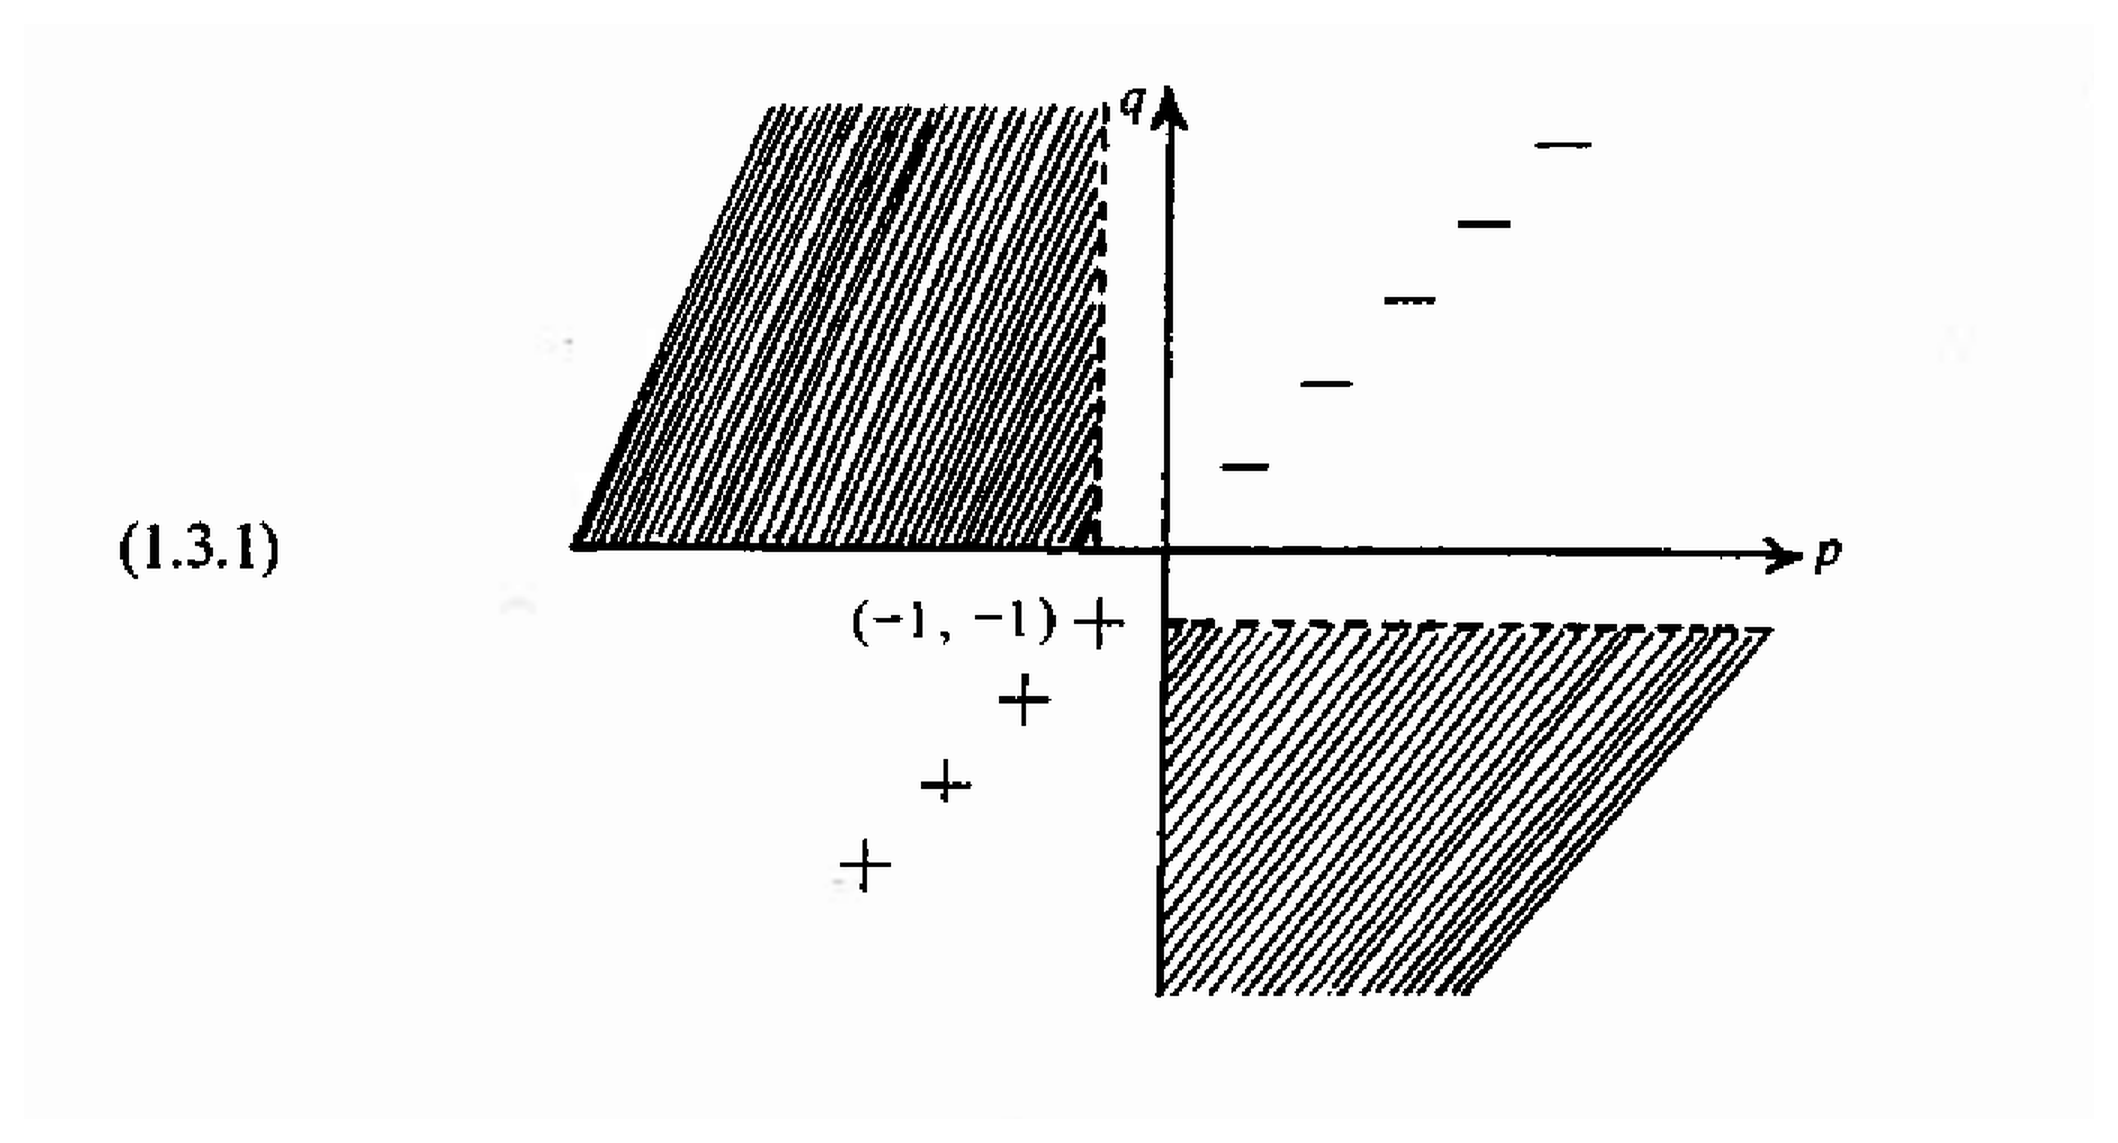
\includegraphics[width=.82\linewidth]{assets/P07-A01_diagram_1_3_1_presentation.png}
\par\smallskip{\small\color{D030Muted}Diagram (1.3.1), certified presentation derivative; the lossless authority crop is retained with the sources.}\end{center}
Supposons M homogène de poids w: h\ensuremath{^{\mathrm{pq}}} \ensuremath{=} 0 pour p \ensuremath{+} q \ensuremath{≠} w, et posons \ensuremath{ℜ}(M) \ensuremath{=} \ensuremath{−}w/2. Il résulte de la conjecture de Weil que, pour S assez grand, la série de Dirichlet L\ensuremath{_{S}}(M, s) converge absolument pour \ensuremath{ℜ}(M) \ensuremath{+} \ensuremath{ℜ}(s) \ensuremath{>} 1. Pour \ensuremath{ℜ}(M) \ensuremath{+} \ensuremath{ℜ}(s) \ensuremath{=} 1, on est au bord du demi-plan de convergence, et on conjecture (a) que L\ensuremath{_{S}}(M, s) ne s’annule pas, (b) que L\ensuremath{_{S}}(M, s) est holomorphe, sauf si M est de poids pair \ensuremath{−}2n, et contient \ensuremath{ℤ}(n) en facteur: on s’attend alors à un pôle en s \ensuremath{=} 1 \ensuremath{−} n (une valeur non critique).\par
L’analogie avec le cas des corps de fonctions, et les cas connus, mènent à croire que les facteurs locaux L\ensuremath{_{p}}(M, s) (p quelconque, y compris \ensuremath{∞}) n’ont de pôle que pour \ensuremath{ℜ}(M) \ensuremath{+} \ensuremath{ℜ}(s) \ensuremath{≤} 0. Si tel est le cas, (a), (b) et l’équation fonctionnelle conjecturale (1.2.3) impliquent que L(M) \ensuremath{≠} 0, \ensuremath{∞} pour M critique et \ensuremath{ℜ}(M) \ensuremath{≠} 1/2. Pour \ensuremath{ℜ}(M) \ensuremath{=} 1/2, L(M) s’annulle parfois. Notre conjecture (1.8) est alors vide.\par
PROPOSITION 1.4. Soit M un motif sur \ensuremath{ℝ}. Via l’isomorphisme (0.4.1)\par
H\ensuremath{_{B}}(M) \ensuremath{⊗} \ensuremath{ℂ}  --\ensuremath{≅}--\ensuremath{>}  H\ensuremath{_{\mathrm{DR}}}(M) \ensuremath{⊗}\ensuremath{_{ℝ}} \ensuremath{ℂ},\par
H\ensuremath{_{\mathrm{DR}}}(M) s’identifie au sous-espace de H\ensuremath{_{B}}(M) \ensuremath{⊗} \ensuremath{ℂ} fixe par c \ensuremath{→} F\ensuremath{_{∞}} \ensuremath{\bar{c}}.\par
Prenons M \ensuremath{=} H*(X). La conjugaison complexe sur H\ensuremath{_{\mathrm{DR}}}(M)\ensuremath{_{ℂ}} \ensuremath{=} H*(X\ensuremath{_{ℂ}}, \ensuremath{Ω}*) se déduit par fonctorialité de l’automorphisme antilinéaire F\ensuremath{_{∞}} du schéma X\ensuremath{_{ℂ}}. Remontant la flèche composée (0.4) qui définit I, on l’identifie à l’involution déduite de l’automorphisme (F\ensuremath{_{∞}}, F\ensuremath{_{∞}}*) de (X(\ensuremath{ℂ}), \ensuremath{Ω}\ensuremath{^{*an}}), puis au composé de F\ensuremath{_{∞}}*: H*(X(\ensuremath{ℂ}), \ensuremath{ℂ}) \ensuremath{→} H*(X(\ensuremath{ℂ}), \ensuremath{ℂ}) et de la conjugaison complexe sur les coefficients. Ceci vérifie 1.4.\par
\clearpage
\PageUnit{8}{320}{FRENCH MAIN BODY}
1.5. Pour M un motif sur \ensuremath{ℝ}, nous noterons H\ensuremath{_{B}}\ensuremath{^{+}}(M) (resp. H\ensuremath{_{B}}\ensuremath{^{−}}(M)) le sous-espace de H\ensuremath{_{B}}(M) fixe par F\ensuremath{_{∞}} (resp. où F\ensuremath{_{∞}} \ensuremath{=} \ensuremath{−}1). Posons d(M) \ensuremath{=} dim H\ensuremath{_{B}}(M) et d\ensuremath{^{±}}(M) \ensuremath{=} dim H\ensuremath{_{B}}\ensuremath{^{±}}(M). Pour M un motif sur k, et \ensuremath{σ} un plongement complexe de k qui se factorise par \ensuremath{ℝ}, on note H\ensuremath{_{σ}}\ensuremath{^{±}}(M), d\ensuremath{_{σ}}\ensuremath{^{±}}(M) et d\ensuremath{_{σ}}(M) ces objets pour le motif sur \ensuremath{ℝ} déduit de M par \ensuremath{σ}. Pour k \ensuremath{=} \ensuremath{ℚ}, on omet la mention de \ensuremath{σ}.\par
Le corollaire suivant résulte aussitôt de 1.4, et de ce que tant F\ensuremath{_{∞}} que la conjugaison complexe échangent H\ensuremath{^{\mathrm{pq}}} et H\ensuremath{^{\mathrm{qp}}}.\par
COROLLAIRE 1.6. Soit M un motif sur \ensuremath{ℝ}. Pour la structure réelle H\ensuremath{_{\mathrm{DR}}}(M) de H\ensuremath{_{B}}(M) \ensuremath{⊗} \ensuremath{ℂ}, les sous-espaces H\ensuremath{^{\mathrm{pq}}} sont définis sur \ensuremath{ℝ}; le sous-espace H\ensuremath{_{B}}\ensuremath{^{+}}(M) \ensuremath{⊗} \ensuremath{ℝ} est réel, et H\ensuremath{_{B}}\ensuremath{^{−}}(M) \ensuremath{⊗} \ensuremath{ℝ} est purement imaginaire.\par
1.7. Dans la fin de ce paragraphe, nous ne considérerons que des motifs sur \ensuremath{ℚ}; sauf mention expresse du contraire, nous les supposons homogènes. Si leur poids w est pair, nous supposerons aussi que F\ensuremath{_{∞}} agit sur H\ensuremath{^{\mathrm{pp}}}(M) (w \ensuremath{=} 2p) comme un scalaire: soit \ensuremath{+}1, soit \ensuremath{−}1. Cette hypothèse est vérifiée pour M critique. Puisque F\ensuremath{_{∞}} échange H\ensuremath{^{\mathrm{pq}}} et H\ensuremath{^{\mathrm{qp}}}, elle assure que les dimensions d\ensuremath{^{+}}(M) et d\ensuremath{^{−}}(M) sont égales l’une à \ensuremath{∑}\ensuremath{_{p>q}} h\ensuremath{^{\mathrm{pq}}}, l’autre à \ensuremath{∑}\ensuremath{_{p≥q}} h\ensuremath{^{\mathrm{pq}}}. En particulier, ces dimensions sont égales à celles de sous-espaces F\ensuremath{^{+}} et F\ensuremath{^{−}} figurant dans la filtration de Hodge. Posant H\ensuremath{_{\overline{D}\overline{R}}}\ensuremath{^{±}}(M) \ensuremath{=} H\ensuremath{_{\mathrm{DR}}}(M)/F\ensuremath{^{∓}}, on a encore dim H\ensuremath{_{\overline{D}\overline{R}}}\ensuremath{^{±}}(M) \ensuremath{=} d\ensuremath{^{±}}(M).\par
Il résulte de ce que F\ensuremath{_{∞}} échange H\ensuremath{^{\mathrm{pq}}} et H\ensuremath{^{\mathrm{qp}}} que les applications composées\par
(1.7.1)    I\ensuremath{^{±}}: H\ensuremath{_{B}}\ensuremath{^{±}}(M)\ensuremath{_{ℂ}} \ensuremath{→} H\ensuremath{_{B}}(M)\ensuremath{_{ℂ}} --I,\ensuremath{≅}\ensuremath{→} H\ensuremath{_{\mathrm{DR}}}(M)\ensuremath{_{ℂ}} \ensuremath{→} H\ensuremath{_{\overline{D}\overline{R}}}\ensuremath{^{±}}(M)\ensuremath{_{ℂ}}\par
sont des isomorphismes. On pose\par
(1.7.2)    c\ensuremath{^{±}}(M) \ensuremath{=} det(I\ensuremath{^{±}}), (1.7.3)    \ensuremath{δ}(M) \ensuremath{=} det(I),\par
le déterminant étant calculé dans des bases rationnelles de H\ensuremath{_{B}}\ensuremath{^{±}} et H\ensuremath{_{\overline{D}\overline{R}}}\ensuremath{^{±}} (resp. H\ensuremath{_{B}} et H\ensuremath{_{\mathrm{DR}}}). La définition de \ensuremath{δ}(M) ne requiert pas les hypothèses faites sur M.\par
D’après 1.6, I\ensuremath{^{+}} est réel, i.e. induit I\ensuremath{^{+}}: H\ensuremath{_{B}}\ensuremath{^{+}}(M)\ensuremath{_{ℝ}} \ensuremath{→} H\ensuremath{_{\overline{D}\overline{R}}}\ensuremath{^{+}}(M)\ensuremath{_{ℝ}}, tandis que I\ensuremath{^{−}} est purement imaginaire. Les nombres c\ensuremath{^{+}}(M), i\ensuremath{^{d^−(M)}} c\ensuremath{^{−}}(M) et i\ensuremath{^{d^−(M)}} \ensuremath{δ}(M) sont donc réels non nuls. A multiplication par un nombre rationnel près, il ne dépendent que de M.\par
Les périodes de M sont classiquement les \ensuremath{⟨}\ensuremath{ω}, c\ensuremath{⟩} pour \ensuremath{ω} \ensuremath{∈} H\ensuremath{_{\mathrm{DR}}}(M) et c \ensuremath{∈} H\ensuremath{_{B}}(M)\ensuremath{^{∨}}. Par exemple, si X est une variété algébrique sur \ensuremath{ℚ}, \ensuremath{ω} une n-forme sur X, définie sur \ensuremath{ℚ} et que c est un n-cycle sur X(\ensuremath{ℂ}), \ensuremath{⟨}\ensuremath{ω}, c\ensuremath{⟩} \ensuremath{=} \ensuremath{∫}\ensuremath{_{c}} \ensuremath{ω} est une période de H\ensuremath{^{n}}(X). Exprimons c\ensuremath{^{±}}(M) en terme de périodes. Le dual de H\ensuremath{_{\overline{D}\overline{R}}}\ensuremath{^{±}}(M) est le sous-espace F\ensuremath{^{±}} de H\ensuremath{_{\mathrm{DR}}}(M\ensuremath{^{∨}}), où M\ensuremath{^{∨}} est le motif dual de M. Si la base choisie de H\ensuremath{_{\overline{D}\overline{R}}}\ensuremath{^{±}}(M) a pour duale la base (\ensuremath{ω}\ensuremath{_{i}}) de F\ensuremath{^{±}}(H\ensuremath{_{\mathrm{DR}}}(M\ensuremath{^{∨}})), et que (c\ensuremath{_{i}}) est la base choisie de H\ensuremath{_{B}}\ensuremath{^{±}}(M), la matrice de I\ensuremath{^{±}} est (\ensuremath{⟨}\ensuremath{ω}\ensuremath{_{i}}, c\ensuremath{_{j}}\ensuremath{⟩}), et c\ensuremath{^{±}}(M) \ensuremath{=} det((\ensuremath{⟨}\ensuremath{ω}\ensuremath{_{i}}, c\ensuremath{_{j}}\ensuremath{⟩})).\par
Conjecture 1.8. Si M est critique, L(M) est un multiple rationnel de c\ensuremath{^{+}}(M).\par
2. Énoncé de la conjecture (cas général).\par
2.1. Jusqu’ici, nous n’avons considéré que des fonctions L données par des séries de Dirichlet à coefficients rationnels. Pour faire mieux, il nous faudra considérer des motifs à coefficient dans des corps de nombres.\par
Voici deux façons, équivalentes, pour construire la catégorie des motifs sur k,\par
\clearpage
\PageUnit{9}{321}{FRENCH MAIN BODY}
à coefficient dans un corps de nombres E, à partir de la catégorie des motifs sur k. Il s’agit d’une construction valable pour toute catégorie additive karoubienne (0.1(b)) dans laquelle les Hom(X, Y) sont des espaces vectoriels sur \ensuremath{ℚ}.\par
A. Un motif sur k, à coefficient dans E, est un motif M sur k muni d’une structure de E-module: E \ensuremath{→} End(M).\par
B. La catégorie \ensuremath{ℳ}\ensuremath{_{k,E}} des motifs sur k, à coefficient dans E, est l’enveloppe karoubienne (cf. 0.1(b)) de la catégorie d’objets les motifs sur k—considéré comme objet de \ensuremath{ℳ}\ensuremath{_{k,E}}, un motif M se notera M\ensuremath{_{E}}—et de morphismes donnés par\par
Hom(X\ensuremath{_{E}}, Y\ensuremath{_{E}}) \ensuremath{=} Hom(X, Y) \ensuremath{⊗} E.\par
Passage de B à A. Pour X un motif, et V un espace vectoriel sur \ensuremath{ℚ} de dimension finie, on note X \ensuremath{⊗} V le motif, isomorphe à une somme de dim(V) copies de X, caractérisé par Hom(Y, X \ensuremath{⊗} V) \ensuremath{=} Hom(Y, X) \ensuremath{⊗} V (ou par Hom(X \ensuremath{⊗} V, Y) \ensuremath{=} Hom(V, Hom(X, Y))). On passe de B à A en associant à M\ensuremath{_{E}} le motif M \ensuremath{⊗} E, muni de sa structure de E-module naturelle.\par
Passage de A à B. Si M est muni d’une structure de E-module, on récupère sur M\ensuremath{_{E}} deux structures de E-module: celle déduite de celle de M, et celle qu’a tout objet de \ensuremath{ℳ}\ensuremath{_{k,E}}. L’objet de \ensuremath{ℳ}\ensuremath{_{k,E}} correspondant à M est le plus grand facteur direct de M\ensuremath{_{E}} sur lequel ces structures coïncident. En détail: l’algèbre E \ensuremath{⊗} E est un produit de corps, parmi lesquels une copie de E dans laquelle x \ensuremath{⊗} 1 et 1 \ensuremath{⊗} x se projettent tous deux comme x. L’idempotent correspondant e agit sur M\ensuremath{_{E}} (qui est un E \ensuremath{⊗} E-module) et son image est l’objet de \ensuremath{ℳ}\ensuremath{_{k,E}} qui correspond à M.\par
Les motifs à coefficient dans E sont le plus souvent donnés sous la forme A. La forme B a l’avantage de rester raisonnable pour E non de rang fini sur \ensuremath{ℚ}. Elle est utile pour comprendre le formalisme tensoriel: on peut définir produit tensoriel et dual, pour les motifs à coefficient dans E, par leur fonctorialité et les formules\par
X\ensuremath{_{E}} \ensuremath{⊗}\ensuremath{_{E}} Y\ensuremath{_{E}} \ensuremath{=} (X \ensuremath{⊗} Y)\ensuremath{_{E}} et (X\ensuremath{_{E}})\ensuremath{^{∨}} \ensuremath{=} (X\ensuremath{^{∨}})\ensuremath{_{E}}.\par
Dans le langage A, X \ensuremath{⊗}\ensuremath{_{E}} Y est le plus grand facteur direct de X \ensuremath{⊗} Y sur lequel coïncident les deux structures de E-module de X \ensuremath{⊗} Y, et X\ensuremath{^{∨}} est le dual usuel de X, muni de la structure de E-module transposée. Si on applique ces remarques à la catégorie des espaces vectoriels sur \ensuremath{ℚ}, plutôt qu’à celle des motifs, on retrouve l’isomorphisme du E-dual d’un espace vectoriel sur E avec son \ensuremath{ℚ}-dual, donné par\par
\ensuremath{ω} \ensuremath{↦} la forme Tr\ensuremath{_{E/ℚ}}(\ensuremath{⟨}\ensuremath{ω}, v\ensuremath{⟩}).\par
Nous avons défini en 0.1.1 des foncteurs de restriction et d’extension du corps k des scalaires. Ils transforment motifs à coefficient dans E en motifs à coefficient dans E. On dispose aussi de foncteurs de restriction et d’extension des coefficients: soit F une extension finie de E:\par
Extension des coefficients. Dans le langage A, c’est X \ensuremath{↦} X \ensuremath{⊗}\ensuremath{_{E}} F; dans le langage B, c’est X\ensuremath{_{E}} \ensuremath{↦} X\ensuremath{_{F}}.\par
Restriction des coefficients. Dans le langage A, on restreint à E la structure de F-module.\par
Le lecteur prendra soin de ne pas confondre les rôles de k et E. Un exemple type qu’on peut retenir est celui du H\ensuremath{_{1}} des variétés abéliennes sur k, à multiplication complexe par un ordre de E. En terme de la variété abélienne—prise à isogénie près—les foncteurs ci-dessus deviennent: extension du corps de base, restriction des scalaires à la Weil, construction \ensuremath{⊗}\ensuremath{_{E}} F, qui multiplie la dimension par [F:E], restriction à E de la structure de F-module.\par
\clearpage
\PageUnit{10}{322}{FRENCH MAIN BODY}
2.2. Soit M un motif sur \ensuremath{ℚ}, à coefficient dans un corps de nombres E. Pour chaque nombre premier l, la réalisation l-adique H\ensuremath{_{l}}(M) de M est un module sur le complété l-adique E\ensuremath{_{l}} de E. Ce complété est le produit des complétés E\ensuremath{_{λ}}, pour \ensuremath{λ} idéal premier au-dessus de l, d’où une décomposition de H\ensuremath{_{l}}(M) en un produit de E\ensuremath{_{λ}}-modules H\ensuremath{_{λ}}(M).\par
On conjecture pour les H\ensuremath{_{λ}}(M) une compatibilité analogue à 1.2.1; si elle est vérifiée, on peut pour chaque plongement complexe \ensuremath{σ} de E définir une série de Dirichlet à coefficients dans \ensuremath{σ}E, convergente pour \ensuremath{ℜ}s assez grand:\par
L(\ensuremath{σ}, M, s) \ensuremath{=} \ensuremath{∏}\ensuremath{_{p}} L\ensuremath{_{p}}(\ensuremath{σ}, M, s), où\par
(2.2.1)    L\ensuremath{_{p}}(\ensuremath{σ}, M, s) \ensuremath{=} \ensuremath{σ}Z\ensuremath{_{p}}(M, p\ensuremath{^{−s}}) avec Z\ensuremath{_{p}} \ensuremath{∈} E(t) \ensuremath{⊂} E\ensuremath{_{λ}}(t) donné par Z\ensuremath{_{p}}(M, t) \ensuremath{=} det(1 \ensuremath{−} F\ensuremath{_{p}} t, H\ensuremath{_{λ}}(M)\ensuremath{^{I_p}})\ensuremath{^{−1}} pour \ensuremath{λ}\ensuremath{∤}p.\par
Pour \ensuremath{σ} variable, ces séries de Dirichlet se déduisent les unes des autres par conjugaison des coefficients. Nous regarderons le système des L(\ensuremath{σ}, M, s) comme une fonction L*(M, s) à valeurs dans la \ensuremath{ℂ}-algèbre E \ensuremath{⊗} \ensuremath{ℂ}, identifiée à \ensuremath{ℂ}\ensuremath{^{Hom(E,ℂ)}} par\par
(2.2.2)    E \ensuremath{⊗} \ensuremath{ℂ} --\ensuremath{≅}\ensuremath{→} \ensuremath{ℂ}\ensuremath{^{Hom(E,ℂ)}}: e \ensuremath{⊗} z \ensuremath{↦} (z, \ensuremath{σ}(e))\ensuremath{_{σ}}.\par
Cette fonction peut aussi être définie directement par un produit eulérien. On espère comme en 1.1 qu’elle admet un prolongement analytique en s.\par
Il y a lieu de compléter le produit eulérien L(\ensuremath{σ}, M, s) par un facteur à l’infini L\ensuremath{_{∞}}(\ensuremath{σ}, M, s) dépendant de la réalisation de Hodge de M. Posant \ensuremath{Λ}(\ensuremath{σ}, M, s) \ensuremath{=} L\ensuremath{_{∞}}(\ensuremath{σ}, M, s)L(\ensuremath{σ}, M, s), l’équation fonctionnelle conjecturale des fonctions L s’écrit\par
(2.2.3)    \ensuremath{Λ}(\ensuremath{σ}, M, s) \ensuremath{=} \ensuremath{ε}(\ensuremath{σ}, M, s)\ensuremath{Λ}(\ensuremath{σ}, \ensuremath{\check{M}}, 1 \ensuremath{−} s),\par
où \ensuremath{ε}(\ensuremath{σ}, M, s), comme fonction de s, est le produit d’une constante par une exponentielle. Les définitions de L\ensuremath{_{∞}} et \ensuremath{ε} sont rappelées en 5.2. Comme ci-dessus, on regardera le système des \ensuremath{Λ} et celui des \ensuremath{ε}, pour \ensuremath{σ} variable, comme des fonctions \ensuremath{Λ}* et \ensuremath{ε}* à valeurs dans E \ensuremath{⊗} \ensuremath{ℂ}.\par
Il résulte de 2.5 ci-dessous que L\ensuremath{_{∞}}(\ensuremath{σ}, M, s) est indépendant de \ensuremath{σ}, et que la fonction L\ensuremath{_{∞}} pour le motif R\ensuremath{_{E/ℚ}} M déduit de M par restriction du corps des coefficients (2.1) est la puissance [E:\ensuremath{ℚ}]ième de L\ensuremath{_{∞}}(\ensuremath{σ}, M, s). Ceci justifie la\par
PROPOSITION-DÉFINITION 2.3. Soit M un motif sur \ensuremath{ℚ} à coefficient dans E. Un entier n est critique pour M si les conditions équivalentes suivantes sont vérifiées (i) l’entier n est critique pour R\ensuremath{_{E/ℚ}} M; (ii) ni L\ensuremath{_{∞}}(\ensuremath{σ}, M, s), ni L\ensuremath{_{∞}}(\ensuremath{σ}, \ensuremath{\check{M}}(1), s) n’ont de pôle en s \ensuremath{=} n. On dit que M est critique si 0 est critique pour M.\par
Notre but est de conjecturer la valeur de L*(M) \ensuremath{=}\ensuremath{_{\mathrm{dfn}}} L*(M, 0), pour M critique, à multiplication par un élément de E près. En d’autres termes, il s’agit de conjecturer simultanément les valeurs des L(\ensuremath{σ}, M) \ensuremath{=}\ensuremath{_{\mathrm{dfn}}} L(\ensuremath{σ}, M, 0), à multiplication près par un système de nombres \ensuremath{σ}(e), e \ensuremath{∈} E.\par
2.4. La réalisation H\ensuremath{_{B}}(M) de M en cohomologie rationnelle est munie d’une structure de E-espace vectoriel. Sa dimension est le rang sur E de M. L’involution F\ensuremath{_{∞}} est E-linéaire; les parties \ensuremath{+} et \ensuremath{−} sont donc des E-sous-espaces vectoriels. On note d\ensuremath{^{+}}(M) et d\ensuremath{^{−}}(M) leur dimension.\par
\clearpage
\PageUnit{11}{323}{FRENCH MAIN BODY}
Le complexifié de H\ensuremath{_{B}}(M) est un E \ensuremath{⊗} \ensuremath{ℂ}-module libre. Identifiant E \ensuremath{⊗} \ensuremath{ℂ} à \ensuremath{ℂ}\ensuremath{^{Hom(E,ℂ)}} (2.2.2), on en déduit une décomposition\par
H\ensuremath{_{B}}(M) \ensuremath{⊗} \ensuremath{ℂ} \ensuremath{=} \ensuremath{⊕}\ensuremath{_{σ}} H\ensuremath{_{B}}(\ensuremath{σ}, M),\par
avec\par
H\ensuremath{_{B}}(\ensuremath{σ}, M) \ensuremath{=} (H\ensuremath{_{B}}(M) \ensuremath{⊗} \ensuremath{ℂ}) \ensuremath{⊗}\ensuremath{_{E⊗ℂ,σ}} \ensuremath{ℂ},\par
soit\par
H\ensuremath{_{B}}(\ensuremath{σ}, M) \ensuremath{=} H\ensuremath{_{B}}(M) \ensuremath{⊗}\ensuremath{_{E,σ}} \ensuremath{ℂ}.\par
Les H\ensuremath{_{B}}\ensuremath{^{\mathrm{pq}}}(M) de la décomposition de Hodge étant stables par E, chaque H\ensuremath{_{B}}(\ensuremath{σ}, M) hérite d’une décomposition de Hodge H\ensuremath{_{B}}(\ensuremath{σ}, M) \ensuremath{=} \ensuremath{⊕} H\ensuremath{_{B}}\ensuremath{^{\mathrm{pq}}}(\ensuremath{σ}, M). L’involution F\ensuremath{_{∞}} permute H\ensuremath{^{\mathrm{pq}}} et H\ensuremath{^{\mathrm{qp}}}, en particulier stabilise H\ensuremath{_{B}}\ensuremath{^{\mathrm{pp}}}, qu’elle découpe en des parties \ensuremath{+} et \ensuremath{−}. On note h\ensuremath{^{\mathrm{pq}}}(\ensuremath{σ}, M) la dimension de H\ensuremath{_{B}}\ensuremath{^{\mathrm{pq}}}(\ensuremath{σ}, M), et h\ensuremath{^{pp±}}(\ensuremath{σ}, M) celle de H\ensuremath{_{B}}\ensuremath{^{pp±}}(\ensuremath{σ}, M). La proposition suivante permet d’omettre \ensuremath{σ} de la notation.\par
PROPOSITION 2.5. Les nombres h\ensuremath{^{\mathrm{pq}}}(\ensuremath{σ}, M) et h\ensuremath{^{pp±}}(\ensuremath{σ}, M) sont indépendant de \ensuremath{σ}.\par
On peut supposer, et on suppose, que M est homogène. Dans ce cas, H\ensuremath{^{\mathrm{pq}}}(M) s’identifie au complexifié du E-espace vectoriel Gr\ensuremath{_{F}}\ensuremath{^{p}}(H\ensuremath{_{\mathrm{DR}}}(M)); c’est un E \ensuremath{⊗} \ensuremath{ℂ}-module libre, et la première assertion en résulte. Pour la seconde, on observe que h\ensuremath{^{pp±}}(\ensuremath{σ}, M) est l’excès de d\ensuremath{^{±}}(M) sur \ensuremath{∑}\ensuremath{_{p>q}} h\ensuremath{^{\mathrm{pq}}}(\ensuremath{σ}, M).\par
2.6. Soit M un motif sur \ensuremath{ℚ} à coefficient dans E. Dans la fin de ce paragraphe, sauf mention expresse du contraire, nous supposons que R\ensuremath{_{E/ℚ}} M vérifie les hypothèses de 1.7. Les espaces F\ensuremath{^{±}} et H\ensuremath{_{\overline{D}\overline{R}}}\ensuremath{^{±}} sont cette fois des espaces vectoriels sur E. Les isomorphismes (0.4.1) et (1.7.1)\par
\begin{D030Diagram}
(2.6.1)    I: H_B(M) ⊗ ℂ → H_DR(M) ⊗ ℂ,
(2.6.2)    I^±: H_B^±(M) ⊗ ℂ → H_{D̅R̅}^±(M) ⊗ ℂ,
\end{D030Diagram}
sont des isomorphismes de E \ensuremath{⊗} \ensuremath{ℂ}-modules entre complexifiés d’espaces vectoriels sur E. On pose\par
c\ensuremath{^{±}}(M) \ensuremath{=} det(I\ensuremath{^{±}}) \ensuremath{∈} (E \ensuremath{⊗} \ensuremath{ℂ})*,    \ensuremath{δ}(M) \ensuremath{=} det(I) \ensuremath{∈} (E \ensuremath{⊗} \ensuremath{ℂ})*,\par
le déterminant étant calculé dans des bases E-rationnelles de H\ensuremath{_{B}}\ensuremath{^{±}}(M) et H\ensuremath{_{\overline{D}\overline{R}}}\ensuremath{^{±}}(M) (resp. H\ensuremath{_{B}}(M) et H\ensuremath{_{\mathrm{DR}}}(M)). La définition de \ensuremath{δ}(M) ne requiert pas les hypothèses faites sur M. A multiplication par un élément de E* près, ces nombres ne dépendent que de M. Il résulte à nouveau de 1.6 que c\ensuremath{^{+}}(M), i\ensuremath{^{d^−(M)}} c\ensuremath{^{−}}(M) et i\ensuremath{^{d^−(M)}} \ensuremath{δ}(M) sont dans (E \ensuremath{⊗} \ensuremath{ℝ})*.\par
Conjecture 2.7. Posons \ensuremath{ℜ}(M) \ensuremath{=} \ensuremath{−}1/2 w. Si M est critique, (i) L(\ensuremath{σ}, M, s) n’a jamais de pôle en s \ensuremath{=} 0, et ne peut s’annuler en s \ensuremath{=} 0 que pour \ensuremath{ℜ}(M) \ensuremath{=} 1/2. (ii) La multiplicité du zéro de L(\ensuremath{σ}, M, s) en s \ensuremath{=} 0 est indépendante de \ensuremath{σ}.\par
Pour (i), je renvoie à la discussion à la fin de 1.3. Que (ii) soit raisonnable m’a été suggéré par B. Gross.\par
Conjecture 2.8. Pour M critique et L(\ensuremath{σ}, M) \ensuremath{≠} 0, L*(M) est le produit de c\ensuremath{^{+}}(M) par un élément de E*.\par
\clearpage
\PageUnit{12}{324}{FRENCH MAIN BODY}
REMARQUE 2.9. Un motif M sur un corps de nombres k, à coefficient dans E, définit aussi une fonction L*(M, s). Ces fonctions sont couvertes par notre conjecture, vu l’identité L*(M, s) \ensuremath{=} L*(R\ensuremath{_{k/ℚ}} M, s), où R\ensuremath{_{k/ℚ}} est la restriction des scalaires de k à \ensuremath{ℚ} (appliquer (0.5.3)).\par
Les fonctions L(\ensuremath{σ}, M, s) sont des produits eulériens, indexés par les places finies de k. Il y a lieu de les compléter par les facteurs à l’infini L\ensuremath{_{v}}(\ensuremath{σ}, M, s), indexés par les places à l’infini, dont la définition est rappelée en 5.2. Ils dépendent en général de \ensuremath{σ}. Seul L\ensuremath{_{∞}}(\ensuremath{σ}, R\ensuremath{_{k/ℚ}} M, s), produit sur v à l’infini des L\ensuremath{_{v}}(\ensuremath{σ}, M, s), est indépendant de \ensuremath{σ}.\par
REMARQUE 2.10. Soient F une extension de E, \ensuremath{ι} le morphisme structural de E dans F et \ensuremath{ι}\ensuremath{_{C}} son complexifié: E \ensuremath{⊗} \ensuremath{ℂ} \ensuremath{↪} F \ensuremath{⊗} \ensuremath{ℂ}. On a L*(M \ensuremath{⊗}\ensuremath{_{E}} F, s) \ensuremath{=} \ensuremath{ι}\ensuremath{_{C}} L*(M, s) et c\ensuremath{^{±}}(M \ensuremath{⊗}\ensuremath{_{E}} F) \ensuremath{=} \ensuremath{ι}\ensuremath{_{C}} c\ensuremath{^{±}}(M). La conjecture est donc compatible à l’extension du corps des coefficients. Pour F une extension galoisienne de E, de groupe de Galois G, le Théorème 90 de Hilbert H\ensuremath{^{1}}(G, F*) \ensuremath{=} 0 assure que ((F \ensuremath{⊗} \ensuremath{ℂ})*/F*)\ensuremath{^{G}} \ensuremath{=} (E \ensuremath{⊗} \ensuremath{ℂ})*/E*: la conjecture est invariante par extension du corps des coefficients.\par
REMARQUE 2.11. Si E est une extension de F, on a L*(R\ensuremath{_{E/F}} M, s) \ensuremath{=} N\ensuremath{_{E/F}} L*(M, s). Les périodes c\ensuremath{^{±}} vérifiant la même identité, la conjecture est compatible à la restriction des coefficients.\par
REMARQUE 2.12. Soit D une algèbre à division de rang d\ensuremath{^{2}} sur E. Un motif M sur \ensuremath{ℚ}, muni d’une structure de D-module, et de rang n sur D, définit une série de Dirichlet à coefficients dans E dont les facteurs eulériens sont presque tous de degré nd: pour \ensuremath{λ} une place finie de E, H\ensuremath{_{λ}}(M) est un module libre sur le complété D\ensuremath{_{λ}} \ensuremath{=} D \ensuremath{⊗}\ensuremath{_{E}} E\ensuremath{_{λ}}, et on reprend la définition (2.2.1) en posant\par
Z\ensuremath{_{p}}(M, t) \ensuremath{=} det red(1 \ensuremath{−} F\ensuremath{_{p}} t, H\ensuremath{_{λ}}(M)\ensuremath{^{I_p}})\ensuremath{^{−1}}\par
(si D\ensuremath{_{λ}} est une algèbre de matrices sur E\ensuremath{_{λ}}, et e un idempotent indécomposable, le déterminant réduit d’un endomorphisme A d’un D\ensuremath{_{λ}}-module H est le déterminant, calculé sur E\ensuremath{_{λ}}, de la restriction de A à eH; la définition dans le cas général procède par descente).\par
La liberté que nous donne 2.10 d’étendre le corps des coefficients met ces fonctions L elles aussi sous le chapeau 2.8: choisissant une extension \ensuremath{ι}: E \ensuremath{↪} F de E qui neutralise D, et un idempotent indécomposable e de D \ensuremath{⊗}\ensuremath{_{E}} F, on a \ensuremath{ι}\ensuremath{_{C}} L*(M, s) \ensuremath{=} L*(e(M \ensuremath{⊗}\ensuremath{_{E}} F), s).\par
On peut aussi définir c\ensuremath{^{+}}(M) directement dans ce cadre. C’est ce qui est expliqué en 2.13 ci-dessous.\par
La fin de ce paragraphe est inutile pour la suite.\par
2.13. Soit D une algèbre simple sur un corps E (voire une algèbre d’Azumaya sur un anneau...). Pour le formalisme tensoriel, il est commode de regarder les D-modules comme de “faux E-espaces vectoriels”:\par
(a) Se donner un espace vectoriel V sur E revient à se donner, pour toute extension étale F de E, un F-espace vectoriel V\ensuremath{_{F}}, et des isomorphismes compatibles V\ensuremath{_{G}} \ensuremath{=} V\ensuremath{_{F}} \ensuremath{⊗}\ensuremath{_{F}} G pour G une extension de F. On prend V\ensuremath{_{F}} \ensuremath{=} V \ensuremath{⊗}\ensuremath{_{E}} F. Par descente, il suffit de ne se donner les V\ensuremath{_{F}} que pour F assez grand.\par
(b) Soit W un D-module. Pour toute extension étale F de E, et tout F-isomorphisme D \ensuremath{⊗} F \ensuremath{≅} End\ensuremath{_{F}}(L), avec L libre, posons W\ensuremath{_{F,L}} \ensuremath{=} Hom\ensuremath{_{D⊗F}}(L, W \ensuremath{⊗} F) (les produits tensoriels sont sur E). On a un isomorphisme de D \ensuremath{⊗} F-module\par
W \ensuremath{⊗}\ensuremath{_{E}} F \ensuremath{=} L \ensuremath{⊗}\ensuremath{_{F}} W\ensuremath{_{F,L}}.\par
\clearpage
\PageUnit{13}{325}{FRENCH MAIN BODY}
Si F est assez grand pour neutraliser D, L est unique à isomorphisme non unique près; la non-unicité est due aux homothéties, qui agissent trivialement sur End(L). C’est pourquoi la donnée des W\ensuremath{_{F,L}} n’est pas du type (a); c’est un “faux espace vectoriel sur E”.\par
Soient (W\ensuremath{^{α}}) une famille de D-modules, et T une opération tensorielle. Si les homothéties de L agissent trivialement sur T(W\ensuremath{_{F,L}}\ensuremath{^{α}}), le F-espace vectoriel T(W\ensuremath{_{F,L}}\ensuremath{^{α}}) est indépendant du choix de L et on obtient un système du type (a), d’où un espace vectoriel T(W\ensuremath{^{α}}) sur E.\par
EXEMPLE. Si W\ensuremath{′} et W\ensuremath{″} sont deux D-modules de rang n\ensuremath{·}[D:E]\ensuremath{^{1/2}} sur E, on peut prendre T \ensuremath{=} Hom(\ensuremath{∧}\ensuremath{^{n}}W\ensuremath{′}\ensuremath{_{F,L}}, \ensuremath{∧}\ensuremath{^{n}}W\ensuremath{″}\ensuremath{_{F,L}}); on obtient un espace vectoriel \ensuremath{δ}(W\ensuremath{′}, W\ensuremath{″}) de rang 1 sur E, et tout homomorphisme f: W\ensuremath{′} \ensuremath{→} W\ensuremath{″} a un déterminant réduit det red(f) \ensuremath{∈} \ensuremath{δ}(W\ensuremath{′}, W\ensuremath{″}).\par
Pour définir c\ensuremath{^{+}}(M), on applique cette construction aux D-modules H\ensuremath{_{B}}\ensuremath{^{+}}(M) et à H\ensuremath{_{\overline{D}\overline{R}}}\ensuremath{^{+}}(M). Posons \ensuremath{δ} \ensuremath{=} \ensuremath{δ}(H\ensuremath{_{B}}\ensuremath{^{+}}(M), H\ensuremath{_{\overline{D}\overline{R}}}\ensuremath{^{+}}(M)). Le déterminant réduit de l’isomorphisme de D \ensuremath{⊗} \ensuremath{ℂ}-modules I\ensuremath{^{+}}: H\ensuremath{_{B}}\ensuremath{^{+}}(M)\ensuremath{_{ℂ}} \ensuremath{→}\ensuremath{≃} H\ensuremath{_{\overline{D}\overline{R}}}\ensuremath{^{+}}(M)\ensuremath{_{ℂ}} est dans le E \ensuremath{⊗} \ensuremath{ℂ}-module libre de rang 1 \ensuremath{δ} \ensuremath{⊗} \ensuremath{ℂ}. On pose det red(I\ensuremath{^{+}}) \ensuremath{=} c\ensuremath{^{+}}(M)\ensuremath{·}e pour e une base de \ensuremath{δ}.\par
\SectionLead{3. Exemple: la fonction \ensuremath{ζ}.} 3.1. Pour comprendre les diverses réalisations du motif de Tate \ensuremath{ℤ}(1), le plus simple est de l’écrire \ensuremath{ℤ}(1) \ensuremath{=} H\ensuremath{_{1}}(\ensuremath{𝔾}\ensuremath{_{m}}). Le groupe multiplicatif n’étant pas une variété projective, ceci ne rentre pas dans le cadre de Grothendieck, qui demande qu’on définisse plutôt \ensuremath{ℤ}(1) comme le dual du facteur direct H\ensuremath{^{2}}(\ensuremath{ℙ}\ensuremath{^{1}}) de H*(\ensuremath{ℙ}\ensuremath{^{1}}).\par
La réalisation en \ensuremath{ℤ}\ensuremath{_{l}}-cohomologie de \ensuremath{ℤ}(1) est le module de Tate T\ensuremath{_{l}}(\ensuremath{𝔾}\ensuremath{_{m}}) de \ensuremath{𝔾}\ensuremath{_{m}}\par
\ensuremath{ℤ}\ensuremath{_{l}}(1) \ensuremath{=} proj lim \ensuremath{μ}\ensuremath{_{lⁿ}}.\par
En réalisation de Hodge, on a H\ensuremath{_{B}}(\ensuremath{ℤ}(1)) \ensuremath{=} H\ensuremath{_{1}}(\ensuremath{ℂ}*) isomorphe à \ensuremath{ℤ} (à \ensuremath{ℚ} plutôt, en homologie rationnelle). Ce groupe est purement de type (\ensuremath{−}1, \ensuremath{−}1) et F\ensuremath{_{∞}} \ensuremath{=} \ensuremath{−}1.\par
En réalisation de de Rham, H\ensuremath{_{\mathrm{DR}}}(\ensuremath{ℤ}(1)) est le dual de H\ensuremath{_{\mathrm{DR}}}\ensuremath{^{1}}(\ensuremath{𝔾}\ensuremath{_{m}}), isomorphe à \ensuremath{ℚ}, de générateur la classe de dz/z. L’unique période de H\ensuremath{^{1}}(\ensuremath{𝔾}\ensuremath{_{m}}) est\par
(3.1.1)    \ensuremath{∮} dz/z \ensuremath{=} 2\ensuremath{π}i.\par
Sur \ensuremath{ℤ}\ensuremath{_{l}}(1), le Frobenius arithmétique \ensuremath{φ}\ensuremath{_{p}} (p \ensuremath{≠} l) agit par multiplication par p. Le Frobenius géométrique agit donc par multiplication par p\ensuremath{^{-1}}; ceci justifie l’identité citée en 1.3\par
(3.1.2)    L(M(n), s) \ensuremath{=} L(M, n \ensuremath{+} s).\par
Puisque F\ensuremath{_{∞}} agit sur (\ensuremath{−}1)\ensuremath{^{n}} sur H\ensuremath{_{B}}(\ensuremath{ℤ}(n)), H\ensuremath{_{B}}\ensuremath{^{ε}}(\ensuremath{ℤ}(n)) est nul pour \ensuremath{ε} \ensuremath{=} \ensuremath{−}(\ensuremath{−}1)\ensuremath{^{n}}, et c\ensuremath{^{ε}}(\ensuremath{ℤ}(n)) \ensuremath{=} 1. Pour \ensuremath{ε} \ensuremath{=} (\ensuremath{−}1)\ensuremath{^{n}}, d’après (3.1.1), c\ensuremath{^{ε}}(\ensuremath{ℤ}(n)) \ensuremath{=} \ensuremath{δ}(\ensuremath{ℤ}(n)) \ensuremath{=} (2\ensuremath{π}i)\ensuremath{^{n}}:\par
(3.1.3)    c\ensuremath{^{ε}}(\ensuremath{ℤ}(n)) \ensuremath{=} (2\ensuremath{π}i)\ensuremath{^{n}}                 pour \ensuremath{ε} \ensuremath{=} (\ensuremath{−}1)\ensuremath{^{n}}, c\ensuremath{^{ε}}(\ensuremath{ℤ}(n)) \ensuremath{=} 1,   \ensuremath{δ}(\ensuremath{ℤ}(n)) \ensuremath{=} (2\ensuremath{π}i)\ensuremath{^{n}}  pour \ensuremath{ε} \ensuremath{=} \ensuremath{−}(\ensuremath{−}1)\ensuremath{^{n}}.\par
3.2. La fonction \ensuremath{ζ}(s) est la fonction L attachée au motif unité \ensuremath{ℤ}(0) \ensuremath{=} H*(Point). Les entiers critiques pour \ensuremath{ℤ}(0) sont les entiers pair \ensuremath{>} 0, et les entiers impairs \ensuremath{≤} 0. A cause du pôle de \ensuremath{ζ}(s) en s \ensuremath{=} 1, 0 n’est pas un zéro trivial et il serait raisonnable de définir les entiers critiques comme incluant 0. La équation (3.1.3) et les valeurs\par
\clearpage
\PageUnit{14}{326}{FRENCH MAIN BODY}
connues de \ensuremath{ζ}(n) \ensuremath{=} L(\ensuremath{ℤ}(n)) pour n critique vérifient 1.8: \ensuremath{ζ}(n) est rationnel pour n impair \ensuremath{≤} 0, et un multiple rationnel de (2\ensuremath{π}i)\ensuremath{^{n}} pour n pair \ensuremath{≥} 0.\par
\SectionLead{4. Compatibilité à la conjecture de Birch et Swinnerton-Dyer.} 4.1. Soient A une variété abélienne sur \ensuremath{ℚ}, et d sa dimension. La conjecture de Birch et Swinnerton-Dyer [15] affirme notamment: (a) L(H\ensuremath{^{1}}(A), 1) est non nul si et seulement si A(\ensuremath{ℚ}) est fini. (b) Soit \ensuremath{ω} un générateur de H\ensuremath{^{0}}(A, \ensuremath{Ω}\ensuremath{^{d}}). Alors, L(H\ensuremath{^{1}}(A), 1) est le produit de \ensuremath{∫}\ensuremath{_{A(ℝ)}} \ensuremath{|}\ensuremath{ω}\ensuremath{|} par un nombre rationnel.\par
Le motif H\ensuremath{^{1}}(A)(1) est isomorphe au dual H\ensuremath{_{1}}(A) de H\ensuremath{^{1}}(A): ceci traduit l’existence d’une polarization, autodualité de H\ensuremath{^{1}}(A) à valeurs dans \ensuremath{ℤ}(\ensuremath{−}1). D’après 1.7, c\ensuremath{^{+}}(H\ensuremath{^{1}}(A)(1)) se calcule donc comme suit: si \ensuremath{ω}\ensuremath{_{1}},\ensuremath{⋯},\ensuremath{ω}\ensuremath{_{d}} est une base de H\ensuremath{^{0}}(A, \ensuremath{Ω}\ensuremath{^{1}}) \ensuremath{=} F\ensuremath{^{+}}H\ensuremath{_{\mathrm{DR}}}\ensuremath{^{1}}(A), et c\ensuremath{_{1}},\ensuremath{⋯},c\ensuremath{_{d}} une base de H\ensuremath{_{1}}(A(\ensuremath{ℂ}), \ensuremath{ℚ})\ensuremath{^{+}}, on a\par
(4.1.1)    c\ensuremath{^{+}}(H\ensuremath{^{1}}(A)(1)) \ensuremath{=} det\ensuremath{⟨}\ensuremath{ω}\ensuremath{_{i}}, e\ensuremath{_{j}}\ensuremath{⟩}.\par
Désignant encore par e\ensuremath{_{i}} un cycle représentatif, on a \ensuremath{⟨}\ensuremath{ω}\ensuremath{_{i}}, e\ensuremath{_{j}}\ensuremath{⟩} \ensuremath{=} \ensuremath{∫}\ensuremath{_{e_j}} \ensuremath{ω}\ensuremath{_{i}}. Prenons pour base (e\ensuremath{_{i}}) une base sur \ensuremath{ℤ} de H\ensuremath{_{1}}(A(\ensuremath{ℝ})\ensuremath{^{\circ}} , \ensuremath{ℤ}) \ensuremath{⊂} H\ensuremath{_{1}}(A(\ensuremath{ℂ}), \ensuremath{ℤ}). Le produit de Pontryagin des e\ensuremath{_{i}} est représenté par le d-cycle A(\ensuremath{ℝ})\ensuremath{^{\circ}} dans A(\ensuremath{ℂ}), pour une orientation convenable, et, si \ensuremath{ω} est le produit extérieur des \ensuremath{ω}\ensuremath{_{i}}, le déterminant (4.1.1) est l’intégrale \ensuremath{∫}\ensuremath{_{A(ℝ)°}} \ensuremath{ω}. On a\par
\ensuremath{∫}\ensuremath{_{A(ℝ)}} \ensuremath{|}\ensuremath{ω}\ensuremath{|} \ensuremath{=} [A(\ensuremath{ℝ}): A(\ensuremath{ℝ})\ensuremath{^{\circ}}] \ensuremath{|}\ensuremath{∫}\ensuremath{_{A(ℝ)°}} \ensuremath{ω}\ensuremath{|},\par
et 1.8 pour H\ensuremath{^{1}}(A)(1) équivaut donc à 4.1(b) ci-dessus.\par
4.2. La conjecture de Birch et Swinnerton-Dyer donne la valeur exacte de L(H\ensuremath{^{1}}(A), 1); la description du facteur rationnel en 4.1(b) à partir du motif H\ensuremath{^{1}}(A)(1) a la forme suivante: (a) La donnée de M \ensuremath{=} H\ensuremath{^{1}}(A)(1) équivaut à celle de A à isogénie près. Il faut commencer par choisir A. Cela revient à choisir un réseau entier dans H\ensuremath{_{B}}(M), dont les l-adifiés soient stables sous l’action de Gal(\ensuremath{\bar{ℚ}}/\ensuremath{ℚ}). (b) On choisit alors \ensuremath{ω}, par exemple comme produit extérieur des éléments d’une base d’un réseau entier dans H\ensuremath{_{\mathrm{DR}}}(M). Cet \ensuremath{ω} détermine la période, c\ensuremath{^{+}}(M), et, pour chaque nombre premier p, un facteur rationnel c\ensuremath{_{p}}(M). Les c\ensuremath{_{p}}(M) sont presque tous égaux à 1, et la formule du produit assure que c\ensuremath{^{+}}(M)\ensuremath{·}\ensuremath{∏}\ensuremath{_{p}} c\ensuremath{_{p}}(M) est indépendant de \ensuremath{ω}. (c) Un autre nombre rationnel, h(M), est défini en terme d’invariants cohomologiques de A; le nombre rationnel cherché est h(M)\ensuremath{·}\ensuremath{∏}\ensuremath{_{p}} c\ensuremath{_{p}}(M)\ensuremath{^{-1}}.\par
L’invariance de la conjecture par isogénie est par ailleurs un théorème non trivial.\par
4.3. Pour généraliser 4.1(a) à un motif de poids \ensuremath{−}1 M quelconque, il faudrait disposer d’un analogue de A(\ensuremath{ℚ}). Le groupe A(\ensuremath{ℚ}) peut s’interpréter comme le groupe des extensions de \ensuremath{ℤ}(0) par H\ensuremath{_{1}}(A), dans la catégorie des 1-motifs [6, \S{}10] sur \ensuremath{ℚ}. Ceci suggère de considérer le groupe des extensions de \ensuremath{ℤ}(0) par M, dans une catégorie de motifs mixtes, parallèles aux structures de Hodge mixtes, mais on ne dispose même pas d’une définition conjecturale d’une telle catégorie!\par
J’observerai seulement que, dans toutes les théories cohomologiques usuelles, un cycle Y de dimension d, cohomologue à zéro, sur une variété algébrique propre et\par
\clearpage
\PageUnit{15}{327}{FRENCH MAIN BODY}
lisse X détermine un torseur sous H\ensuremath{^{2d−1}}(X)(d): on dispose d’une suite exacte de cohomologie\par
0 \ensuremath{→} H\ensuremath{^{2d−1}}(X)(d) \ensuremath{→} H\ensuremath{^{2d−1}}(X \ensuremath{−} Y)(d) --\ensuremath{∂}\ensuremath{→} H\ensuremath{_{Y}}\ensuremath{^{2d}}(X)(d) \ensuremath{→} H\ensuremath{^{2d}}(X)(d),\par
Y définit une classe de cohomologie cl(Y) \ensuremath{∈} H\ensuremath{_{Y}}\ensuremath{^{2d}}(X)(d), d’image nulle dans H\ensuremath{^{2d}}(X)(d), et on prend \ensuremath{∂}\ensuremath{^{-1}}cl(Y). Cette construction correspond à celle qui à un diviseur de degré 0 sur une courbe associe un point de sa jacobienne.\par
\SectionLead{5. Compatibilité à l’équation fonctionnelle.} Soit E un corps de nombres. Dans (E \ensuremath{⊗} \ensuremath{ℂ})*, nous noterons \ensuremath{∼} la relation d’équivalence définie par le sous-groupe E*.\par
PROPOSITION 5.1. Soit M un motif sur \ensuremath{ℚ}, à coefficient dans E. On suppose vérifiées les hypothèses de 1.7. On a alors\par
c\ensuremath{^{+}}(M) \ensuremath{∼} (2\ensuremath{π}i)\ensuremath{^{−d⁻(M)}} \ensuremath{·} \ensuremath{δ}(M) \ensuremath{·} c\ensuremath{^{+}}(\ensuremath{\check{M}}(1)).\par
Pour L un module libre de rang n sur un anneau commutatif A (A sera E, ou E \ensuremath{⊗} \ensuremath{ℂ}), posons det L \ensuremath{=} \ensuremath{∧}\ensuremath{^{n}}L. On étend par localisation cette définition au cas où L est seulement projectif de type fini (cette généralisation n’est pas indispensable à la preuve de 5.1). On a des isomorphismes canoniques\par
(5.1.1)    det(L\ensuremath{^{∨}}) \ensuremath{=} det(L)\ensuremath{^{-1}}\par
et, pour tout facteur direct P et L,\par
(5.1.2)    det(L) \ensuremath{=} det(P) \ensuremath{·} det(L/P)\par
(on a désigné par \ensuremath{·} un produit tensoriel, et par \ensuremath{^{-1}} un dual). Il y a ici des problèmes de signe, qu’on résoud au mieux en considérant det(L) comme un module gradué inversible, placé en degré le rang de L. Nos résultats finaux étant modulo \ensuremath{∼}, nous ne nous en inquiéterons pas.\par
Pour X et Y de même rang, posons \ensuremath{δ}(X, Y) \ensuremath{=} Hom(det X, det Y) \ensuremath{=} det(X)\ensuremath{^{-1}} \ensuremath{·} det(Y). Le déterminant de f: X \ensuremath{→} Y est dans \ensuremath{δ}(X, Y). On déduit de (5.1.1) et (5.1.2) des isomorphismes\par
(5.1.3)    \ensuremath{δ}(X, Y) \ensuremath{=} \ensuremath{δ}(Y\ensuremath{^{∨}}, X\ensuremath{^{∨}})\par
et, pour F \ensuremath{⊂} X et G \ensuremath{⊂} Y,\par
(5.1.4)    \ensuremath{δ}(X, Y) \ensuremath{=} \ensuremath{δ}(F, Y/G) \ensuremath{·} \ensuremath{δ}(G, X/F)\ensuremath{^{-1}}.\par
LEMME 5.1.5. Via l’isomorphisme (5.1.3), on a det(u) \ensuremath{=} det(\ensuremath{^{t}}u).\par
LEMME 5.1.6. Soient F et G des facteurs directs de X et Y. On suppose que l’isomorphisme f: X \ensuremath{→} Y induit des isomorphismes f\ensuremath{_{F}}: F \ensuremath{→} Y/G et f\ensuremath{_{G}}\ensuremath{^{-1}}: G \ensuremath{→} X/F. Via l’isomorphisme (5.1.4), on a det(f) \ensuremath{=} det(f\ensuremath{_{F}}) det(f\ensuremath{_{G}}\ensuremath{^{-1}})\ensuremath{^{-1}}.\par
La vérification de ces lemmes est laissée au lecteur. Pour 5.1.6, notons seulement que, pour G\ensuremath{^{1}} \ensuremath{=} f\ensuremath{^{-1}}(G) et F\ensuremath{^{1}} \ensuremath{=} f(F), on a X \ensuremath{=} F \ensuremath{⊕} G\ensuremath{^{1}}, Y \ensuremath{=} G \ensuremath{⊕} F\ensuremath{^{1}}, et que f échange F et F\ensuremath{^{1}}, G et G\ensuremath{^{1}}.\par
Appliquons le Lemme 5.1.6 aux complexifiés de H\ensuremath{_{B}}\ensuremath{^{+}}(M) \ensuremath{⊂} H\ensuremath{_{B}}(M) et de F\ensuremath{^{-}} \ensuremath{⊂} H\ensuremath{_{\mathrm{DR}}}(M). On trouve que, via l’isomorphisme (5.1.4), le déterminant de I: H\ensuremath{_{B}}(M) \ensuremath{⊗} \ensuremath{ℂ} \ensuremath{→} H\ensuremath{_{\mathrm{DR}}}(M) \ensuremath{⊗} \ensuremath{ℂ} est le produit du déterminant de I\ensuremath{^{+}}: H\ensuremath{_{B}}\ensuremath{^{+}}(M) \ensuremath{⊗} \ensuremath{ℂ} \ensuremath{→}\par
\clearpage
\PageUnit{16}{328}{FRENCH MAIN BODY}
(H\ensuremath{_{\mathrm{DR}}}(M)/F\ensuremath{^{-}}) \ensuremath{⊗} \ensuremath{ℂ} et de l’inverse du déterminant du morphisme induit par l’inverse de I:\par
J\ensuremath{^{-}}: F\ensuremath{^{-}} \ensuremath{⊗} \ensuremath{ℂ} \ensuremath{→} (H\ensuremath{_{B}}(M)/H\ensuremath{_{B}}\ensuremath{^{+}}(M)) \ensuremath{⊗} \ensuremath{ℂ}.\par
Le morphisme J\ensuremath{^{-}} est le transposé du morphisme I\ensuremath{^{-}} pour le motif \ensuremath{\check{M}} dual de M. Appliquant 5.1.5, et prenant des bases sur E des espaces \ensuremath{δ}(X, Y) en jeu, on obtient finalement que\par
(5.1.7)    \ensuremath{δ}(M) \ensuremath{∼} c\ensuremath{^{+}}(M) \ensuremath{·} c\ensuremath{^{-}}(\ensuremath{\check{M}})\ensuremath{^{-1}}.\par
On en déduit 5.1 en appliquant au motif \ensuremath{\check{M}} la formule suivante, conséquence de 3.1:\par
(5.1.8)    c\ensuremath{^{±}}(M) \ensuremath{=} (2\ensuremath{π}i)\ensuremath{^{−d^±(M)·n}} c\ensuremath{^{±(−1)ⁿ}}(M(n)).\par
Notons aussi, pour usage ultérieur, la formule analogue\par
(5.1.9)    \ensuremath{δ}(M) \ensuremath{=} (2\ensuremath{π}i)\ensuremath{^{−d(M)·n}} \ensuremath{δ}(M(n)),\par
5.2. Rappelons la forme exacte de l’équation fonctionnelle conjecturale des fonctions L des motifs ([12], [4]). Nous nous placerons dans le cas général d’un motif sur un corps de nombres k, à coefficient dans un corps E muni d’un plongement complexe \ensuremath{σ} (cf. 2.9). La forme générale d’abord: (a) Pour chaque place v de k, on définit un facteur local L\ensuremath{_{v}}(\ensuremath{σ}, M, s). Pour v fini, la définition de L\ensuremath{_{v}}(\ensuremath{σ}, M, s) \ensuremath{=} \ensuremath{σ}Z\ensuremath{_{v}}(M, Nv\ensuremath{^{−s}}) (Z\ensuremath{_{v}}(M, t) \ensuremath{∈} E(t)) dépend d’une hypothèse de compatibilité analogue à (1.2.1). On a Z\ensuremath{_{v}}(M, t) \ensuremath{=} det(1 \ensuremath{−} F\ensuremath{_{\mathrm{vt}}}, H\ensuremath{_{λ}}(M)\ensuremath{^{I_v}})\ensuremath{^{-1}}. Pour v infini, induit par un plongement complexe \ensuremath{τ}, on obtient L\ensuremath{_{v}}(\ensuremath{σ}, M, s) en décomposant H\ensuremath{_{τ}}(M) \ensuremath{⊗}\ensuremath{_{E,σ}} \ensuremath{ℂ} en somme directe de sous-espaces minimaux stables par les projecteurs qui donnent la décomposition de Hodge, et par F\ensuremath{_{∞}} pour v réel, en associant à chacun le “facteur \ensuremath{Γ}” de la Table (5.3), et en prenant leur produit. Pour v complexe, les sous-espaces minimaux sont de dimension un, d’un type (p, q). Pour v réel, ils sont soit de dimension 2, de type \{(p, q), (q, p)\}, p \ensuremath{≠} q, soit de dimension 1, de type (p, p), avec F\ensuremath{_{∞}} \ensuremath{=} \ensuremath{±}1. On note \ensuremath{Λ}(\ensuremath{σ}, M, s) le produit des L\ensuremath{_{v}}(\ensuremath{σ}, M, s). (b) Soient \ensuremath{Ψ} un caractère non trivial du groupe \ensuremath{𝔸} \ensuremath{⊗} k/k des classes d’adèles de k, et \ensuremath{Ψ}\ensuremath{_{v}} ses composantes. Soient aussi, pour chaque place v de k, une mesure de Haar dx\ensuremath{_{v}} sur k\ensuremath{_{v}}. On suppose que, pour presque tout v, dx\ensuremath{_{v}} donne aux entiers de k\ensuremath{_{v}} la masse 1, et que le produit \ensuremath{⊗} dx\ensuremath{_{v}} des dx\ensuremath{_{v}} est la mesure de Tamagawa, donnant la masse 1 au groupe des classes d’adèles.\par
On définit des constantes locales \ensuremath{ε}\ensuremath{_{v}}(\ensuremath{σ}, M, s, \ensuremath{Ψ}\ensuremath{_{v}}, dx\ensuremath{_{v}}), presque toutes égales à 1 et toutes, comme fonction de s, produit d’une constante par une exponentielle. Soit \ensuremath{ε}(\ensuremath{σ}, M, s) leur produit (indépendant de \ensuremath{Ψ} et des dx\ensuremath{_{v}}). (c) L’équation fonctionnelle conjecturale est\par
\ensuremath{Λ}(\ensuremath{σ}, M, s) \ensuremath{=} \ensuremath{ε}(\ensuremath{σ}, M, s)\ensuremath{Λ}(\ensuremath{σ}, \ensuremath{\check{M}}, 1 \ensuremath{−} s).\par
Pour définir les \ensuremath{ε}\ensuremath{_{v}}, une hypothèse additionnelle de compatibilité entre les H\ensuremath{_{λ}}(M) est requise. Elle permet d’associer à v, \ensuremath{σ}, M une classe d’isomorphie de représentations complexes du groupe de Weil W(\ensuremath{\bar{k}}\ensuremath{_{v}}/k\ensuremath{_{v}}) pour v infini, du groupe de Weil épaissi W\ensuremath{′}(\ensuremath{\bar{k}}\ensuremath{_{v}}/k\ensuremath{_{v}}) pour v fini, et on prend le \ensuremath{ε} de [4, 8.12.4], avec t \ensuremath{=} p\ensuremath{^{−s}}.\par
Pour v infini, ceci revient à décomposer H\ensuremath{_{τ}}(M) \ensuremath{⊗}\ensuremath{_{E,σ}} \ensuremath{ℂ} comme en (a), à associer\par
\clearpage
\PageUnit{17}{329}{FRENCH MAIN BODY}
à chaque sous-espace de la décomposition un facteur \ensuremath{ε}\ensuremath{′}\ensuremath{_{v}}, et à prendre leur produit. La table des \ensuremath{ε}\ensuremath{′}\ensuremath{_{v}}, pour un choix particulier de \ensuremath{Ψ}\ensuremath{_{v}} et de dx\ensuremath{_{v}}, est donnée en 5.3.\par
Pour v fini, on commence par restreindre les représentations H\ensuremath{_{λ}}(M) à un groupe de décomposition Gal(\ensuremath{\bar{k}}\ensuremath{_{v}}/k\ensuremath{_{v}}) \ensuremath{⊂} Gal(\ensuremath{\bar{k}}/k), puis au groupe de Weil W(\ensuremath{\bar{k}}\ensuremath{_{v}}/k\ensuremath{_{v}}). Appliquant [4, 8.3, 8.4], on déduit de H\ensuremath{_{λ}}(M) une classe d’isomorphie \ensuremath{ρ}\ensuremath{_{λ}} de représentations de W\ensuremath{′}(\ensuremath{\bar{k}}\ensuremath{_{v}}/k\ensuremath{_{v}}) sur E\ensuremath{_{λ}}. Il est loisible ici, et utile, de la remplacer par sa F-semi-simplifiée [4, 8.6]. On demande que ces représentations, pour \ensuremath{λ} variable, soient compatibles, i.e., que si on étend les scalaires de E\ensuremath{_{λ}} à \ensuremath{ℂ}, par \ensuremath{\widetilde{σ}}: E\ensuremath{_{λ}} \ensuremath{→} \ensuremath{ℂ} prolongeant \ensuremath{σ}, la classe d’isomorphie de la représentation obtenue soit indépendante de \ensuremath{λ} et de \ensuremath{σ}. C’est la classe d’isomorphie cherchée.\par
Remontons pour le lecteur les renvois internes de [4]. Une représentation de W\ensuremath{′} est donnée par une représentation \ensuremath{ρ} du groupe de Weil dans GL(V), et par un endomorphisme nilpotent N de V. En terme de la constante locale [4, 4.1], de \ensuremath{ρ}, celle de (\ensuremath{ρ}, N) est donnée par\par
\ensuremath{ε}((\ensuremath{ρ}, N), s, \ensuremath{Ψ}, dx) \ensuremath{=} \ensuremath{ε}(\ensuremath{ρ} \ensuremath{⊗} \ensuremath{ω}\ensuremath{_{s}}, \ensuremath{Ψ} dx) \ensuremath{·} det(\ensuremath{−}F Nv\ensuremath{^{−s}}, V\ensuremath{^{ρ(I)}}/Ker(N)\ensuremath{^{ρ(I)}}).\par
REMARQUE 5.2.1. La fonction de s\par
\ensuremath{ε}((\ensuremath{ρ}, N), s, \ensuremath{Ψ}, dx)L((\ensuremath{ρ}, N)\ensuremath{^{∨}}, 1 \ensuremath{−} s)L((\ensuremath{ρ}, N), s)\ensuremath{^{-1}}\par
est la même pour (\ensuremath{ρ}, N) et pour (\ensuremath{ρ}, 0). Ceci permet d’énoncer l’équation fonctionnelle conjecturale des fonctions L en supposant seulement une compatibilité entre les semi-simplifiées des restrictions des H\ensuremath{_{l}}(M) à un groupe de décomposition.\par
5.3. Dans la table ci-dessous, on donne les facteurs locaux, et les constantes, associés aux divers types de sous-espaces minimaux de la réalisation de Hodge. Pour les constantes, on a supposé \ensuremath{Ψ}\ensuremath{_{v}} et la mesure dx\ensuremath{_{v}} choisis comme suit: v réel: \ensuremath{Ψ}\ensuremath{_{v}}(x) \ensuremath{=} exp(2\ensuremath{π}ix), mesure dx, v complexe: \ensuremath{Ψ}\ensuremath{_{v}}(z) \ensuremath{=} exp(2\ensuremath{π}i Tr\ensuremath{_{ℂ/ℝ}}(z)), mesure \ensuremath{|}dz \ensuremath{∧} d \ensuremath{\bar{z}}\ensuremath{|}, soit pour z \ensuremath{=} x \ensuremath{+} iy, exp(4\ensuremath{π}ix) et 2dxdy.\par
On utilise les notations \ensuremath{Γ}\ensuremath{_{ℝ}}(s) \ensuremath{=} \ensuremath{π}\ensuremath{^{−s/2}} \ensuremath{Γ}(s/2), \ensuremath{Γ}\ensuremath{_{ℂ}}(s) \ensuremath{=} 2 \ensuremath{·} (2\ensuremath{π})\ensuremath{^{−s}} \ensuremath{Γ}(s).\par
place       type                                      facteur \ensuremath{Γ}        constante (pour \ensuremath{Ψ}, dx ci-dessus) complexe    (p, q) ou (q, p), p \ensuremath{≤} q                   \ensuremath{Γ}\ensuremath{_{ℂ}}(s \ensuremath{−} p)       i\ensuremath{^{q−p}} réelle      \{(p, q), (q, p)\}, p \ensuremath{<} q                   \ensuremath{Γ}\ensuremath{_{ℂ}}(s \ensuremath{−} p)       i\ensuremath{^{q−p+1}} (p, p), F\ensuremath{_{∞}} \ensuremath{=} (\ensuremath{−}1)\ensuremath{^{p+ε}}, \ensuremath{ε} \ensuremath{=} 0 ou 1     \ensuremath{Γ}\ensuremath{_{ℝ}}(s\ensuremath{+}\ensuremath{ε}\ensuremath{−}p)       i\ensuremath{^{ε}}\par
Le cas qui nous intéresse est celui où k \ensuremath{=} \ensuremath{ℚ}. On peut dans ce cas prendre \ensuremath{Ψ}\ensuremath{_{∞}}(x) \ensuremath{=} exp(2\ensuremath{π}ix), \ensuremath{Ψ}\ensuremath{_{p}}(x) \ensuremath{=} exp(\ensuremath{−}2\ensuremath{π}ix) (via l’isomorphisme \ensuremath{ℚ}\ensuremath{_{p}}/\ensuremath{ℤ}\ensuremath{_{p}} \ensuremath{=} partie p-primaire de \ensuremath{ℚ}/\ensuremath{ℤ}), dx\ensuremath{_{∞}} \ensuremath{=} mesure de Lebesgue dx, dx\ensuremath{_{p}} \ensuremath{=} la mesure de Haar sur \ensuremath{ℚ}\ensuremath{_{p}} donnant à \ensuremath{ℤ}\ensuremath{_{p}} la masse 1.\par
PROPOSITION 5.4. Si M est critique de poids w, on a, modulo un nombre rationnel indépendant de \ensuremath{σ},\par
L\ensuremath{_{∞}}(\ensuremath{σ}, \ensuremath{\check{M}}(1))L\ensuremath{_{∞}}(\ensuremath{σ}, M)\ensuremath{^{-1}} \ensuremath{∼} (2\ensuremath{π})\ensuremath{^{−d⁻(M)}} \ensuremath{·} (2\ensuremath{π})\ensuremath{^{−wd(M)/2}}.\par
D’après 2.5, les L\ensuremath{_{∞}}(\ensuremath{σ}, ) sont indépendants de \ensuremath{σ}. Ceci nous permet de ne vérifier 5.4 que pour \ensuremath{σ} fixé. La formule est compatible à la substitution M \ensuremath{↦} \ensuremath{\check{M}}(1): \ensuremath{\check{M}}(1) est\par
\clearpage
\PageUnit{18}{330}{FRENCH MAIN BODY}
de poids \ensuremath{−}2 \ensuremath{−} w, son d\ensuremath{^{-}} est d\ensuremath{^{+}}(M) et abrégeant d(M) et d\ensuremath{^{±}}(M) en d et d\ensuremath{^{±}}, on a d \ensuremath{=} d\ensuremath{^{+}} \ensuremath{+} d\ensuremath{^{-}} et\par
(\ensuremath{−}d\ensuremath{^{-}} \ensuremath{−} wd/2) \ensuremath{+} (\ensuremath{−}d\ensuremath{^{+}} \ensuremath{−} ((\ensuremath{−}2 \ensuremath{−} w)d)/2) \ensuremath{=} 0.\par
Ceci permet de ne vérifier 5.4 que pour w \ensuremath{≥} \ensuremath{−}1. Pour s entier, on a, modulo \ensuremath{ℚ}*,\par
(5.4.1)    \ensuremath{Γ}\ensuremath{_{ℝ}}(s) \ensuremath{∼} (2\ensuremath{π})\ensuremath{^{−s/2}}       pour s pair \ensuremath{>} 0, \ensuremath{Γ}\ensuremath{_{ℝ}}(s) \ensuremath{∼} (2\ensuremath{π})\ensuremath{^{(1−s)/2}}    pour s impair, \ensuremath{Γ}\ensuremath{_{ℂ}}(s) \ensuremath{∼} (2\ensuremath{π})\ensuremath{^{−s}}         pour s \ensuremath{>} 0.\par
Pour w \ensuremath{≥} \ensuremath{−}1, la puissance de 2\ensuremath{π} dans la contribution de chaque sous-espace de H\ensuremath{_{B}}(M) \ensuremath{⊗} \ensuremath{ℂ}, comme en 5.2(a), est donc donnée par\par
L\ensuremath{_{∞}}(M)       L\ensuremath{_{∞}}(\ensuremath{\check{M}}(1))       L\ensuremath{_{∞}}(\ensuremath{\check{M}}(1))L\ensuremath{_{∞}}(M)\ensuremath{^{-1}} \{(pq), (qp)\}, p \ensuremath{≤} q                  p             \ensuremath{−}1\ensuremath{−}p                   \ensuremath{−}1\ensuremath{−}w (pp), p pair \ensuremath{≥} 0, F\ensuremath{_{∞}} \ensuremath{=} \ensuremath{−}1          p/2           \ensuremath{−}1\ensuremath{−}p/2                 \ensuremath{−}1\ensuremath{−}w/2 (pp), p impair \ensuremath{≥} 0, F\ensuremath{_{∞}} \ensuremath{=} \ensuremath{−}1        (1\ensuremath{+}p)/2       (\ensuremath{−}1\ensuremath{−}p)/2               \ensuremath{−}1\ensuremath{−}w/2\par
La proposition en résulte aussitôt. Posons det M \ensuremath{=} \ensuremath{∧}\ensuremath{^{d(M)}}M (puissance extérieure sur E).\par
PROPOSITION 5.5. \ensuremath{ε}*(M) \ensuremath{∼} \ensuremath{ε}*(det M).\par
Pour des dx\ensuremath{_{v}} choisis comme suggéré en 5.4, nous prouverons plus précisément des équivalences\par
(5.5.1)    \ensuremath{ε}\ensuremath{_{v}}\ensuremath{^{*}}(M, \ensuremath{Ψ}\ensuremath{_{v}}, dx\ensuremath{_{v}}) \ensuremath{∼} \ensuremath{ε}\ensuremath{_{v}}\ensuremath{^{*}}(det M, \ensuremath{Ψ}\ensuremath{_{v}}, dx\ensuremath{_{v}}).\par
Posant \ensuremath{η}\ensuremath{_{v}}(\ensuremath{σ}, M, \ensuremath{Ψ}\ensuremath{_{v}}) \ensuremath{=} \ensuremath{ε}\ensuremath{_{v}}(\ensuremath{σ}, M, \ensuremath{Ψ}\ensuremath{_{v}}, dx\ensuremath{_{v}}) \ensuremath{ε}\ensuremath{_{v}}\ensuremath{^{-1}}(\ensuremath{σ}, det M, \ensuremath{Ψ}\ensuremath{_{v}}, dx\ensuremath{_{v}}), ceci équivaut à\par
(5.5.2)    \ensuremath{τ}\ensuremath{η}\ensuremath{_{v}}(\ensuremath{σ}, M, \ensuremath{Ψ}\ensuremath{_{v}}) \ensuremath{=} \ensuremath{η}\ensuremath{_{v}}(\ensuremath{τ}\ensuremath{σ}, M, \ensuremath{τ}\ensuremath{Ψ}\ensuremath{_{v}})\par
pour tout automorphisme \ensuremath{τ} de \ensuremath{ℂ}.\par
Il résulte de [4, 5.4] que, si a \ensuremath{∈} \ensuremath{ℚ}\ensuremath{_{v}}* est de valeur absolue 1, et qu’on pose (\ensuremath{Ψ}\ensuremath{_{v}} \ensuremath{·} a)(x) \ensuremath{=} \ensuremath{Ψ}\ensuremath{_{v}}(ax), on a\par
(5.5.3)    \ensuremath{η}\ensuremath{_{v}}(\ensuremath{σ}, M, \ensuremath{Ψ}\ensuremath{_{v}}) \ensuremath{=} \ensuremath{η}\ensuremath{_{v}}(\ensuremath{σ}, M, \ensuremath{Ψ}\ensuremath{_{v}} \ensuremath{·} a)   (pour \ensuremath{‖}a\ensuremath{‖}\ensuremath{_{v}} \ensuremath{=} 1).\par
Pour \ensuremath{τ} un automorphisme de \ensuremath{ℂ}, et v fini, \ensuremath{τ}\ensuremath{Ψ}\ensuremath{_{v}} est de cette forme \ensuremath{Ψ}\ensuremath{_{v}} \ensuremath{·} a avec \ensuremath{‖}a\ensuremath{‖}\ensuremath{_{v}} \ensuremath{=} 1; de même, \ensuremath{\bar{Ψ}}\ensuremath{_{∞}} \ensuremath{=} \ensuremath{Ψ}\ensuremath{_{∞}} \ensuremath{·} (\ensuremath{−}1).\par
Pour v fini, la définition de \ensuremath{ε}\ensuremath{_{v}} est purement algébrique, d’où \ensuremath{τ}\ensuremath{η}\ensuremath{_{v}}(\ensuremath{σ}, M, \ensuremath{Ψ}\ensuremath{_{v}}) \ensuremath{=} \ensuremath{η}\ensuremath{_{v}}(\ensuremath{τ}\ensuremath{σ}, M, \ensuremath{τ}\ensuremath{Ψ}\ensuremath{_{v}}) et (5.5.2) résulte de (5.5.3).\par
Pour v \ensuremath{=} \ensuremath{∞}, on a encore \ensuremath{\bar{η}}\ensuremath{_{∞}}(\ensuremath{σ}, M, \ensuremath{\bar{Ψ}}\ensuremath{_{∞}}) \ensuremath{=} \ensuremath{η}\ensuremath{_{∞}}(\ensuremath{\bar{σ}}, M, \ensuremath{\bar{Ψ}}\ensuremath{_{∞}}) \ensuremath{=} \ensuremath{η}\ensuremath{_{∞}}(\ensuremath{\bar{σ}}, M, \ensuremath{Ψ}\ensuremath{_{∞}}); si on prend \ensuremath{Ψ}\ensuremath{_{∞}} comme suggéré en 5.3, \ensuremath{η}\ensuremath{_{∞}} est une puissance de i indépendante de \ensuremath{σ}, d’où \ensuremath{η}\ensuremath{_{∞}}(\ensuremath{σ}, M, \ensuremath{Ψ}\ensuremath{_{∞}}) \ensuremath{=} \ensuremath{±}1, indépendant de \ensuremath{σ}, ce qui vérifie (5.5.2).\par
THÉORÈME 5.6. Modulo la Conjecture 6.6 sur la nature des motifs de rang 1, la Conjecture 2.8 est compatible à l’équation fonctionnelle conjecturale des fonctions L: on a\par
\clearpage
\PageUnit{19}{331}{FRENCH MAIN BODY}
L\ensuremath{_{∞}}\ensuremath{^{*}}(M)c\ensuremath{^{+}}(M) \ensuremath{∼} \ensuremath{ε}\ensuremath{^{*}}(M)L\ensuremath{_{∞}}\ensuremath{^{*}}(\ensuremath{\check{M}}(1))c\ensuremath{^{+}}(\ensuremath{\check{M}}(1)).\par
D’après 5.1, 5.3 et 5.5, cette formule équivaut à\par
(2\ensuremath{π}i)\ensuremath{^{-d^-(M)}} \ensuremath{·} \ensuremath{δ}(M) \ensuremath{∼} (2\ensuremath{π})\ensuremath{^{-d^-(M)}} \ensuremath{·} (2\ensuremath{π})\ensuremath{^{-wd(M)/2}} \ensuremath{·} \ensuremath{ε}\ensuremath{^{*}}(det M).\par
Posons D \ensuremath{=} det M et \ensuremath{ε} \ensuremath{=} d\ensuremath{^{-}}(D). On a \ensuremath{δ}(M) \ensuremath{=} \ensuremath{δ}(D), d\ensuremath{^{-}}(M) \ensuremath{≡} \ensuremath{ε} (mod 2), et wd(M) est le poids w(D) de D, de sorte que la formule équivaut encore à\par
(5.6.1)    \ensuremath{ε}\ensuremath{^{*}}(D) \ensuremath{∼} (2\ensuremath{π})\ensuremath{^{w(D)/2}} \ensuremath{·} i\ensuremath{^{ε}} \ensuremath{·} \ensuremath{δ}(D).\par
Nous prouverons en 6.5 que (5.6.1) vaut pour une classe de motifs de rang 1 qui, conjecturalement (6.6), les englobe tous.\par
\SectionLead{6. Exemple: les fonctions L d’Artin.} DÉFINITION 6.1. La catégorie des motifs d’Artin est l’enveloppe karoubienne de la duale de la catégorie d’objets les variétés sur \ensuremath{ℚ} de dimension 0, de morphismes les correspondances définies sur \ensuremath{ℚ}.\par
Par définition, chaque variété de dimension 0, X, définit un motif d’Artin H(X), le foncteur H est un foncteur contravariant pleinement fidèle,\par
H: (variétés de dim 0, correspondances) \ensuremath{⟶} (motifs d’Artin)\par
et tout motif d’Artin est facteur direct d’un H(X).\par
6.2. Explicitons cette définition. Soient \ensuremath{\bar{ℚ}} une clôture algébrique de \ensuremath{ℚ}, et G le groupe de Galois Gal(\ensuremath{\bar{ℚ}}/\ensuremath{ℚ}). Une variété de dimension 0 est le spectre d’un produit fini A de corps de nombres, et la théorie de Galois (sous la forme que lui a donnée Grothendieck) dit que le foncteur\par
X \ensuremath{=} spec(A) \ensuremath{↦} X(\ensuremath{\bar{ℚ}}) \ensuremath{=} Hom(A, \ensuremath{\bar{ℚ}}):\par
(catégorie des variétés de dimension 0, sur \ensuremath{ℚ}, et des morphismes de schémas) \ensuremath{⟶} (catégorie des ensembles finis munis d’une action continue de G)\par
est une équivalence de catégorie. Le foncteur inverse est I \ensuremath{↦} spectre de l’anneau des fonctions G-invariantes de I dans \ensuremath{\bar{ℚ}}.\par
Une correspondance d’une variété de dimension 0, X dans une autre, Y, est une combinaison linéaire formelle à coefficients dans \ensuremath{ℚ} de composantes connexes de X \ensuremath{×} Y. L’application\par
\ensuremath{∑} a\ensuremath{_{i}} Z\ensuremath{_{i}} \ensuremath{↦} \ensuremath{∑} a\ensuremath{_{i}}(fonction caractéristique de Z\ensuremath{_{i}}(\ensuremath{\bar{ℚ}}) \ensuremath{⊂} (X \ensuremath{×} Y)(\ensuremath{\bar{ℚ}}))\par
identifie correspondances et fonctions G-invariantes, à valeurs rationnelles, sur (X \ensuremath{×} Y)(\ensuremath{\bar{ℚ}}) \ensuremath{=} X(\ensuremath{\bar{ℚ}}) \ensuremath{×} Y(\ensuremath{\bar{ℚ}}), et la composition des correspondances au produit matriciel.\par
Notons H le foncteur contravariant X \ensuremath{↦} espace vectoriel \ensuremath{ℚ}\ensuremath{^{X(\bar{ℚ})}}, muni de l’action naturelle de G; (correspondance F: X \ensuremath{→} Y) \ensuremath{↦} le morphisme F*: \ensuremath{ℚ}\ensuremath{^{Y(\bar{ℚ})}} \ensuremath{→} \ensuremath{ℚ}\ensuremath{^{X(\bar{ℚ})}} de matrice \ensuremath{^{t}}F. Il est pleinement fidèle, et identifie la catégorie des motifs d’Artin à celle des représentations rationnelles de G.\par
6.3. Dans ce modèle, si \ensuremath{\bar{ℚ}} est la clôture algébrique de \ensuremath{ℚ} dans \ensuremath{ℂ}, le foncteur “réalisation de Betti” H\ensuremath{_{B}} est le foncteur “espace vectoriel sous-jacent”. La structure de Hodge est purement de type (0, 0), et l’involution F\ensuremath{_{∞}} est l’action de la conjugaison complexe F\ensuremath{_{∞}} \ensuremath{∈} G. On a en effet un isomorphisme, fonctoriel pour les correspondances,\par
\clearpage
\PageUnit{20}{332}{FRENCH MAIN BODY}
H\ensuremath{^{*}}(X(\ensuremath{ℂ}), \ensuremath{ℚ}) \ensuremath{=} \ensuremath{ℚ}\ensuremath{^{X(ℂ)}} \ensuremath{=} \ensuremath{ℚ}\ensuremath{^{X(\bar{ℚ})}} \ensuremath{=} H(X).\par
Le foncteur “réalisation l-adique” H\ensuremath{_{l}} est le foncteur H\ensuremath{_{l}}(V) \ensuremath{=} V \ensuremath{⊗} \ensuremath{ℚ}\ensuremath{_{l}}. On a en effet un isomorphisme, fonctoriel pour les correspondances,\par
H\ensuremath{^{*}}(X(\ensuremath{\bar{ℚ}}), \ensuremath{ℚ}\ensuremath{_{l}}) \ensuremath{=} \ensuremath{ℚ}\ensuremath{_{l}}\ensuremath{^{X(\bar{ℚ})}} \ensuremath{=} \ensuremath{ℚ}\ensuremath{^{X(\bar{ℚ})}} \ensuremath{⊗} \ensuremath{ℚ}\ensuremath{_{l}}.\par
Calculons de même la réalisation de de Rham. Pour X \ensuremath{=} Spec(A), on a H\ensuremath{_{\mathrm{DR}}}\ensuremath{^{*}}(X) \ensuremath{=} A. Écrivant que A \ensuremath{=} Hom\ensuremath{_{G}}(X(\ensuremath{\bar{ℚ}}), \ensuremath{\bar{ℚ}}) \ensuremath{=} (\ensuremath{ℚ}\ensuremath{^{X(\bar{ℚ})}} \ensuremath{⊗} \ensuremath{\bar{ℚ}})\ensuremath{^{G}}, on obtient que\par
(6.3.1)    H\ensuremath{_{\mathrm{DR}}}(V) \ensuremath{=} (V \ensuremath{⊗} \ensuremath{\bar{ℚ}})\ensuremath{^{G}}.\par
La formule (6.3.1) réalise H\ensuremath{_{\mathrm{DR}}}(V) comme un sous-espace de V \ensuremath{⊗} \ensuremath{\bar{ℚ}}. Ce sous-espace est une \ensuremath{ℚ}-structure: on a (V \ensuremath{⊗} \ensuremath{\bar{ℚ}})\ensuremath{^{G}} \ensuremath{⊗} \ensuremath{\bar{ℚ}} \ensuremath{→}\ensuremath{≃} V \ensuremath{⊗} \ensuremath{\bar{ℚ}}. Après extension des scalaires à \ensuremath{\bar{ℚ}}, H\ensuremath{_{B}}(V) et H\ensuremath{_{\mathrm{DR}}}(V) sont donc canoniquement isomorphes. Étendant les scalaires jusqu’à \ensuremath{ℂ}, on trouve l’isomorphisme (0.4.1) (le vérifier pour V \ensuremath{=} H(X)).\par
6.4. Soit E une extension finie de \ensuremath{ℚ}. La catégorie des motifs d’Artin à coefficient dans E est la catégorie déduite de celle des motifs d’Artin comme en 2.1. Nous l’identifierons à la catégorie des E-espaces vectoriels de dimension finie, munis d’une action de G.\par
Les motifs d’Artin à coefficient dans E, de rang 1 sur E, correspondent aux caractères \ensuremath{ε}: G \ensuremath{→} E*. Nous allons calculer leurs périodes. Soient donc \ensuremath{ε}: G \ensuremath{→} E* et f le conducteur de \ensuremath{ε}: \ensuremath{ε} se factorise par un caractère, encore noté \ensuremath{ε}, du quotient (\ensuremath{ℤ}/f\ensuremath{ℤ})* \ensuremath{=} Gal(\ensuremath{ℚ}(exp(2\ensuremath{π}i/f))/\ensuremath{ℚ}) de G. Notons [\ensuremath{ε}] l’espace vectoriel E\ensuremath{_{ε}}, de dimension 1 sur E, sur lequel G agit par \ensuremath{ε}. La somme de Gauss\par
g \ensuremath{=} \ensuremath{∑} \ensuremath{ε}(u) \ensuremath{⊗} exp(2\ensuremath{π}iu/f) \ensuremath{∈} [\ensuremath{ε}] \ensuremath{⊗} \ensuremath{\bar{ℚ}}\par
est non nulle, et invariante par G: c’est une base, sur E, de H\ensuremath{_{\mathrm{DR}}}([\ensuremath{ε}]). Le déterminant de I: H\ensuremath{_{B}}([\ensuremath{ε}]) \ensuremath{⊗} \ensuremath{ℂ} \ensuremath{→}\ensuremath{≃} H\ensuremath{_{\mathrm{DR}}}([\ensuremath{ε}]) \ensuremath{⊗} \ensuremath{ℂ}, calculé dans les bases 1 et g, vaut g\ensuremath{^{-1}}. On sait que, pour tout plongement complexe \ensuremath{σ} de E, on a \ensuremath{σ}g \ensuremath{·} \ensuremath{\bar{σ}}g \ensuremath{=} f, nombre rationnel indépendant de \ensuremath{σ}, d’où\par
(6.4.1)    \ensuremath{δ}([\ensuremath{ε}]) \ensuremath{∼} \ensuremath{∑} \ensuremath{ε}\ensuremath{^{-1}}(u) \ensuremath{⊗} exp(\ensuremath{−}2\ensuremath{π}iu/f) \ensuremath{∈} (E \ensuremath{⊗} \ensuremath{ℂ})*.\par
PROPOSITION 6.5. Soit D le motif [\ensuremath{ε}](n). C’est un motif sur \ensuremath{ℚ}, à coefficients dans E, de rang 1 et de poids \ensuremath{−}2n. Posant \ensuremath{ε}(\ensuremath{−}1) \ensuremath{=} (\ensuremath{−}1)\ensuremath{^{η}}, avec \ensuremath{η} \ensuremath{=} 0 ou 1, on a\par
\ensuremath{ε}\ensuremath{^{*}}(D) \ensuremath{∼} (2\ensuremath{π})\ensuremath{^{-n}} i\ensuremath{^{η−n}} \ensuremath{δ}(D).\par
On sait que la constante de l’équation fonctionnelle de la fonction L de Dirichlet\par
L(\ensuremath{σ}, [\ensuremath{ε}], s) \ensuremath{=} \ensuremath{∑} \ensuremath{σ}\ensuremath{ε}\ensuremath{^{-1}}(n) \ensuremath{·} n\ensuremath{^{-s}}\par
(\ensuremath{σ} plongement complexe de E) est donnée par\par
\ensuremath{ε}(\ensuremath{σ}, [\ensuremath{ε}], s) \ensuremath{=} i\ensuremath{^{η}} \ensuremath{·} f\ensuremath{^{s}} \ensuremath{·} \ensuremath{∑} \ensuremath{σ}\ensuremath{ε}(u)\ensuremath{^{-1}} exp(\ensuremath{−}2\ensuremath{π}iu/f).\par
D’après (5.1.9), on a par ailleurs \ensuremath{δ}(D) \ensuremath{=} (2\ensuremath{π}i)\ensuremath{^{n}} \ensuremath{δ}([\ensuremath{ε}]). On conclut en appliquant (6.4.1) et en notant que pour s entier (s \ensuremath{=} n), f\ensuremath{^{n}} est rationnel indépendant de \ensuremath{σ}.\par
Cette proposition vérifie (5.6.1) pour les motifs [\ensuremath{ε}](n). Pour achever la preuve de 5.6, il ne reste qu’à énoncer la\par
Conjecture 6.6. Tout motif sur \ensuremath{ℚ}, à coefficient dans E et de rang 1 est de la forme [\ensuremath{ε}](n), pour \ensuremath{ε} un caractère de G \ensuremath{=} Gal(\ensuremath{\bar{ℚ}}/\ensuremath{ℚ}) à valeurs dans les racines de l’unité de E et n un entier.\par
\clearpage
\PageUnit{21}{333}{FRENCH MAIN BODY}
PROPOSITION 6.7. La Conjecture 2.8 est vraie pour les fonctions L d’Artin.\par
Pour les motifs d’Artin, on dispose de l’équation fonctionnelle des fonctions L. De plus, le déterminant d’un motif d’Artin, tordu à la Tate, est du type prédit en 6.6. Les arguments des paragraphes 5, 6 montrent donc la compatibilité de 2.8 à l’équation fonctionnelle, et il suffit de prouver 2.8 pour les motifs V(n), pour V un motif d’Artin et n un entier \ensuremath{≤} 0. Si V(n) est critique, F\ensuremath{_{∞}} agit alors sur V par multiplication par \ensuremath{−}(\ensuremath{−}1)\ensuremath{^{n}}, et c\ensuremath{^{+}} \ensuremath{=} 1 (cf. 3.1), et il s’agit de prouver que, pour tout plongement \ensuremath{σ} de E dans \ensuremath{ℂ} et tout automorphisme \ensuremath{τ} de \ensuremath{ℂ}, on a\par
\ensuremath{τ}L(\ensuremath{σ}, V(n)) \ensuremath{=} L(\ensuremath{τ}\ensuremath{σ}, V(n)).\par
On le déduit des résultats de Siegel [14]. Voir [2, 1.2].\par
\SectionLead{7. Fonctions L attachées aux formes modulaires.} 7.1. Posons q \ensuremath{=} e\ensuremath{^{2πiz}}, et soit f \ensuremath{=} \ensuremath{∑} a\ensuremath{_{\mathrm{nq}}}\ensuremath{^{n}} une forme modulaire holomorphe cuspidale primitive (new form) de poids k \ensuremath{≥} 2, conducteur N et caractère \ensuremath{ε}. La série de Dirichlet \ensuremath{∑} a\ensuremath{_{\mathrm{nn}}}\ensuremath{^{-s}} admet un développement en produit eulérien, de facteur local en p \ensuremath{∤} N égal à\par
(1 \ensuremath{−} a\ensuremath{_{\mathrm{pp}}}\ensuremath{^{-s}} \ensuremath{+} \ensuremath{ε}(p)p\ensuremath{^{k−1}}p\ensuremath{^{-2s}})\ensuremath{^{-1}}.\par
Soit E le sous-corps de \ensuremath{ℂ} engendré par les a\ensuremath{_{n}}. La forme f doit donner lieu à un motif M(f) de rang 2 à coefficient dans E, de type de Hodge \{(k \ensuremath{−} 1, 0), (0, k \ensuremath{−} 1)\}, de déterminant [\ensuremath{ε}\ensuremath{^{-1}}](1 \ensuremath{−} k) (notations de 6.4) et de fonction L la série de Dirichlet \ensuremath{∑} a\ensuremath{_{\mathrm{nn}}}\ensuremath{^{-s}}.\par
Je n’ai pas essayé de définir M(f) comme étant un motif au sens de Grothendieck. Une difficulté est que M(f) apparaît de façon naturelle comme facteur direct dans la cohomologie d’une variété non compacte, ou encore comme facteur direct dans la cohomologie d’une courbe modulaire complète, à coefficient dans l’image directe d’un faisceau localement constant (plutôt, un système local de motifs!) sur la partie à distance finie de cette courbe modulaire. Ceci échappe au formalisme de Grothendieck, mais permet de définir les réalisations du motif M(f).\par
7.2. Supposons tout d’abord que k \ensuremath{=} 2, et que \ensuremath{ε} est trivial. Soient X le demi-plan de Poincaré, N le conducteur de f, \ensuremath{Γ}\ensuremath{_{0}}(N) le sous-groupe de SL(2, \ensuremath{ℤ}) formé des matrices dont la réduction mod N est de la forme ((*, *), (0, *)), et posons\par
\ensuremath{ω}\ensuremath{_{f}} \ensuremath{=} \ensuremath{∑} a\ensuremath{_{\mathrm{nq}}}\ensuremath{^{n}} \ensuremath{·} dq/q \ensuremath{=} \ensuremath{∑} a\ensuremath{_{\mathrm{nq}}}\ensuremath{^{n}} \ensuremath{·} 2\ensuremath{π}i dz.\par
La forme \ensuremath{ω}\ensuremath{_{f}} est une forme différentielle holomorphe sur la courbe complétée \ensuremath{\bar{M}}(\ensuremath{Γ}\ensuremath{_{0}}(N)) de M(\ensuremath{Γ}\ensuremath{_{0}}(N)) \ensuremath{=} X/\ensuremath{Γ}\ensuremath{_{0}}(N). Elle est vecteur propre des correspondances de Hecke:\par
(7.2.1)    T\ensuremath{_{n}}\ensuremath{^{*}}\ensuremath{ω}\ensuremath{_{f}} \ensuremath{=} a\ensuremath{_{n}}\ensuremath{ω}\ensuremath{_{f}}    (pour n premier à N)\par
et est caractérisée à un facteur près par (7.2.1). Ce fait résulte du théorème fort de multiplicité 1 et de la théorie des formes primitives; le lecteur peut, s’il le préfère, compléter (7.2.1) par une condition analogue pour n non premier à N, et faire de même ci-dessous; l’assertion devient alors élémentaire, car la condition (7.2.1) ainsi complétée détermine (à un facteur près) le développement de Taylor de \ensuremath{ω}\ensuremath{_{f}} en la pointe i\ensuremath{∞}.\par
Abrégeons M(\ensuremath{Γ}\ensuremath{_{0}}(N)) en M et \ensuremath{\bar{M}}(\ensuremath{Γ}\ensuremath{_{0}}(N)) en \ensuremath{\bar{M}}. Ces courbes ont une \ensuremath{ℚ}-structure naturelle, pour laquelle les correspondances de Hecke sont définies sur \ensuremath{ℚ}. La forme \ensuremath{ω}\ensuremath{_{f}} est définie sur E, et sa conjuguée par un automorphisme \ensuremath{σ} de \ensuremath{ℂ} est \ensuremath{ω}\ensuremath{_{σf}} (appliquer \ensuremath{σ} aux coefficients).\par
Définissons le motif M(f) comme étant, dans le langage 2.1(B), le sous-motif de H\ensuremath{^{1}}(\ensuremath{\bar{M}})\ensuremath{_{E}} noyau des endomorphismes T\ensuremath{_{n}}\ensuremath{^{*}} \ensuremath{−} a\ensuremath{_{n}} — si on veut ne considérer que des\par
\clearpage
\PageUnit{22}{334}{FRENCH MAIN BODY}
noyaux de projecteurs, remplacer T\ensuremath{_{n}}\ensuremath{^{*}} \ensuremath{−} a\ensuremath{_{n}} par P(T\ensuremath{_{n}} \ensuremath{−} a\ensuremath{_{n}}\ensuremath{Δ})\ensuremath{^{*}} pour P un polynôme convenable. On sait que M(f) a les propriétés énoncées en 7.1.\par
Dans chacune des théories cohomologiques \ensuremath{ℋ} qui nous intéressent, l’application\par
(7.2.2)    \ensuremath{ℋ}\ensuremath{_{c}}\ensuremath{^{1}}(M) \ensuremath{⟶} \ensuremath{ℋ}\ensuremath{^{1}}(\ensuremath{\bar{M}})\par
est surjective, et les systèmes de valeurs propres des T\ensuremath{_{n}}\ensuremath{^{*}} sur le noyau n’apparaissent pas dans \ensuremath{ℋ}\ensuremath{^{1}}(\ensuremath{\bar{M}}). La \ensuremath{ℋ}-réalisation de M(f) est donc encore le noyau commun, dans \ensuremath{ℋ}\ensuremath{_{c}}\ensuremath{^{1}}(M) \ensuremath{⊗} E, des T\ensuremath{_{n}}\ensuremath{^{*}} \ensuremath{−} a\ensuremath{_{n}}.\par
Le groupe de cohomologie H\ensuremath{_{c}}\ensuremath{^{1}}(M, \ensuremath{ℚ}) est muni d’une structure de Hodge mixte, de type \{(0, 0), (0, 1), (1, 0)\}, dont H\ensuremath{^{1}}(\ensuremath{\bar{M}}, \ensuremath{ℚ}) est le quotient de type \{(0, 1), (1, 0)\}. En particulier, (7.2.2) induit un isomorphisme sur les sous-espaces F\ensuremath{^{1}} de la filtration de Hodge; toute forme différentielle holomorphe \ensuremath{ω} sur \ensuremath{\bar{M}} définit ainsi une classe de cohomologie à support propre sur M. Ceci peut se voir directement: si \ensuremath{𝒥} \ensuremath{⊂} \ensuremath{𝒪} est l’idéal des pointes, H\ensuremath{_{c}}\ensuremath{^{*}}(M), en cohomologie de de Rham, est l’hypercohomologie sur \ensuremath{\bar{M}} du complexe \ensuremath{𝒥} \ensuremath{→} \ensuremath{Ω}\ensuremath{^{1}} (analytiquement, ce complexe est une résolution du faisceau constant \ensuremath{ℂ} sur M, prolongé par 0 sur \ensuremath{\bar{M}}), et le H\ensuremath{^{1}} reçoit H\ensuremath{^{0}}(\ensuremath{\bar{M}}, \ensuremath{Ω}\ensuremath{^{1}}).\par
Supposons pour simplifier que E \ensuremath{=} \ensuremath{ℚ}, et calculons c\ensuremath{^{+}}(M(f)(1)). Le motif M(f)(1) est le dual de M(f) et c\ensuremath{^{+}} est donc une période de M(f) (1.7): il faut intégrer \ensuremath{ω}\ensuremath{_{f}} contre une classe d’homologie rationnelle de \ensuremath{\bar{M}}, fixe par F\ensuremath{_{∞}}. Relevant M(f) dans \ensuremath{ℋ}\ensuremath{_{c}}\ensuremath{^{1}}(M), on voit qu’on peut plutôt intégrer \ensuremath{ω}\ensuremath{_{f}} contre une classe d’homologie sans support de M, fixe par F\ensuremath{_{∞}}. Toutes les intégrales non nulles de ce type seront commensurables.\par
Pour calculer F\ensuremath{_{∞}}, il est utile d’écrire M comme quotient de X\ensuremath{^{±}} \ensuremath{=} \ensuremath{ℂ} \ensuremath{−} \ensuremath{ℝ} par le sous-groupe de GL(2, \ensuremath{ℤ}) formé des matrices ayant pour réduction mod N une matrice ((*, *), (0, *)). La conjugaison complexe est alors induite par z \ensuremath{↦} \ensuremath{\bar{z}}, et l’image dans M(\ensuremath{ℂ}) de i\ensuremath{ℝ}\ensuremath{^{+}} est un cycle sans support fixe par F\ensuremath{_{∞}}. La formule\par
L(M(f), 1) \ensuremath{=} \ensuremath{−}\ensuremath{∫}\ensuremath{_{0}}\ensuremath{^{i∞}} \ensuremath{ω}\ensuremath{_{f}}\par
justifie 1.8 pour M(f)(1): le second membre est, ou bien nul, ou bien \ensuremath{∼} c\ensuremath{^{+}}(M(f)(1)).\par
REMARQUE 7.3. On a aussi\par
c\ensuremath{^{±}}(M(f)(1)) \ensuremath{∼} \ensuremath{∫}\ensuremath{_{a/b}}\ensuremath{^{i∞}} \ensuremath{ω}\ensuremath{_{f}} \ensuremath{±} \ensuremath{∫}\ensuremath{_{−a/b}}\ensuremath{^{i∞}} \ensuremath{ω}\ensuremath{_{f}}.\par
7.4. Pour \ensuremath{ε} (et E) quelconque, il faut remplacer \ensuremath{Γ}\ensuremath{_{0}}(N) par \ensuremath{Γ}\ensuremath{_{1}}(N): le sous-groupe de SL(2, \ensuremath{ℤ}) formé des matrices de réduction mod N de la forme ((1, *), (0, 1)). Comme ci-dessus, pour calculer F\ensuremath{_{∞}}, il est plus commode de travailler avec X\ensuremath{^{±}} et le sous-groupe de GL(2, \ensuremath{ℤ}) formé des matrices de réduction mod N de la forme ((1, *), (0, *)). Par ailleurs, une dualisation apparaît, cachée en 7.2 par la symétrie de la correspondance T\ensuremath{_{n}}. Pour une définition convenable de T\ensuremath{_{n}}, on a\par
(a) M(f) est le noyau commun des T\ensuremath{_{n}}\ensuremath{^{*}} \ensuremath{−} a\ensuremath{_{n}} dans H\ensuremath{^{1}}(\ensuremath{\bar{M}}), \ensuremath{\bar{M}} \ensuremath{=} X/\ensuremath{Γ}\ensuremath{_{1}}(N).\par
(b) On a \ensuremath{^{t}}T\ensuremath{_{n}}\ensuremath{^{*}}\ensuremath{ω}\ensuremath{_{f}} \ensuremath{=} a\ensuremath{_{n}}\ensuremath{ω}\ensuremath{_{f}}, et T\ensuremath{_{n}}\ensuremath{^{*}}\ensuremath{ω}\ensuremath{_{f}} \ensuremath{=} ā\ensuremath{_{n}}\ensuremath{ω}\ensuremath{_{f}} (noter la formule ā\ensuremath{_{n}} \ensuremath{=} \ensuremath{ε}(n)\ensuremath{^{-1}}a\ensuremath{_{n}}), de sorte que \ensuremath{ω}\ensuremath{_{f}} est dans la réalisation de de Rham de M(f) \ensuremath{=} M(f)\ensuremath{^{∨}}(\ensuremath{−}1).\par
On trouve que c\ensuremath{^{+}}(M(f)(1)) \ensuremath{∈} (E \ensuremath{⊗} \ensuremath{ℂ})*/E* \ensuremath{≅} \ensuremath{ℂ}\ensuremath{^{Hom(E,ℂ)}}/E* est donné par le système de périodes\par
c\ensuremath{^{+}}(M(f)(1)) \ensuremath{∼} (\ensuremath{∫}\ensuremath{_{0}}\ensuremath{^{i∞}} \ensuremath{ω}\ensuremath{_{σf}})\ensuremath{_{σ}},\par
si ce dernier est non nul. Noter que si l’une de ces intégrales s’annule, elles s’annulent toutes. Tel est le cas si et seulement si, dans la partie de l’homologie sans support\par
\clearpage
\PageUnit{23}{335}{FRENCH MAIN BODY}
tendue par le cycle i\ensuremath{ℝ}\ensuremath{^{+}} et ses transformés par les T\ensuremath{_{n}}, le système de valeurs propres a\ensuremath{_{n}} pour les T\ensuremath{_{n}} n’apparaît pas. Ceci justifie 2.8, et partiellement 2.7, pour M(f)(1).\par
REMARQUE 7.5. Les systèmes de valeurs propres des T\ensuremath{_{n}} dans Ker(\ensuremath{ℋ}\ensuremath{_{c}}\ensuremath{^{1}}(M) \ensuremath{→} \ensuremath{ℋ}\ensuremath{^{1}}(\ensuremath{\bar{M}})) sont liés aux séries d’Eisenstein, alors que ceux qui apparaissent dans \ensuremath{ℋ}\ensuremath{^{1}}(\ensuremath{\bar{M}}) sont liés aux formes paraboliques. C’est pourquoi ces ensembles sont disjoints. Il en résulte que la structure de Hodge mixte de H\ensuremath{_{c}}\ensuremath{^{1}}(M, \ensuremath{ℚ}) est somme de structures de Hodge: l’extension de H\ensuremath{^{1}}(\ensuremath{\bar{M}}, \ensuremath{ℚ}) par Ker(H\ensuremath{_{c}}\ensuremath{^{1}}(M, \ensuremath{ℚ}) \ensuremath{→} H\ensuremath{^{1}}(\ensuremath{\bar{M}}, \ensuremath{ℚ})) splitte. Ceci, généralisé au cas de n’importe quel sous-groupe de congruence de SL(2, \ensuremath{ℤ}), équivaut au théorème de Manin [9] selon lequel la différence entre deux pointes est toujours d’ordre fini dans la jacobienne (cf. [6, 10.3.4, 10.3.8 et 10.1.3]). La démonstration donnée ne diffère d’ailleurs pas en substance de celle de Manin.\par
7.6. En poids k quelconque, il faut remplacer la cohomologie de \ensuremath{\bar{M}} par la cohomologie de \ensuremath{\bar{M}} à coefficient dans un faisceau convenable. Pour décrire ce qui se passe, je remplacerai M et \ensuremath{\bar{M}} par M\ensuremath{_{n}} et \ensuremath{\bar{M}}\ensuremath{_{n}}, relatifs au groupe de congruence \ensuremath{Γ}(n), avec n multiple de N et \ensuremath{≥} 3. On redescend ensuite à M et \ensuremath{\bar{M}} en prenant les invariants par un groupe fini convenable. Soient g: \ensuremath{ℰ} \ensuremath{→} M\ensuremath{_{n}} la courbe elliptique universelle et j l’inclusion de M\ensuremath{_{n}} dans \ensuremath{\bar{M}}\ensuremath{_{n}}. La cohomologie à considérer est\par
H\ensuremath{^{1}}(\ensuremath{\bar{M}}\ensuremath{_{n}}, j\ensuremath{_{*}}Sym\ensuremath{^{k−2}}(R\ensuremath{^{1}}g\ensuremath{_{*}}\ensuremath{ℚ})).\par
Les réalisations de M(f) sont facteur direct de ce groupe, calculé dans la théorie de cohomologie correspondante. On peut comme précédemment les relever dans\par
H\ensuremath{_{c}}\ensuremath{^{1}}(M\ensuremath{_{n}}, Sym\ensuremath{^{k−2}}(R\ensuremath{^{1}}g\ensuremath{_{*}}\ensuremath{ℚ})).\par
Pour calculer c\ensuremath{^{±}} du dual de M(f), il faut alors intégrer la classe dans H\ensuremath{_{c}}\ensuremath{^{1}} définie par f contre des classes d’homologie sans support de M\ensuremath{_{n}} à coefficient dans le système local dual de Sym\ensuremath{^{k−2}}(R\ensuremath{^{1}}g\ensuremath{_{*}}\ensuremath{ℚ}). Si on prend le cycle image de i\ensuremath{ℝ}\ensuremath{^{+}}, muni de diverses sections du dual (une base), on trouve les intégrales d’Eichler\par
\ensuremath{∫}\ensuremath{_{0}}\ensuremath{^{i∞}} f(q) \ensuremath{·} dq/q \ensuremath{·} (2\ensuremath{π}iz)\ensuremath{^{l}}    (0 \ensuremath{≤} l \ensuremath{≤} k \ensuremath{−} 2)\par
(périodes paires pour l pair, impaires pour l impair) — et on sait comment écrire L(M(f), n) pour n critique en terme de ces périodes.\par
PROPOSITION 7.7. Soit M un motif de rang 2, à coefficient dans E, de type de Hodge \{(a, b), (b, a)\} avec a \ensuremath{≠} b. Alors, d\ensuremath{^{±}}Sym\ensuremath{^{n}}(M) et c\ensuremath{^{±}}Sym\ensuremath{^{\mathrm{nM}}} sont donnés par les formules suivantes:\par
(1) si n \ensuremath{=} 2l \ensuremath{+} 1: d\ensuremath{^{±}} \ensuremath{=} l \ensuremath{+} 1, et\par
c\ensuremath{^{±}}Sym\ensuremath{^{\mathrm{nM}}} \ensuremath{=} c\ensuremath{^{±}}(M)\ensuremath{^{(l+1)(l+2)/2}} c\ensuremath{^{∓}}(M)\ensuremath{^{l(l+1)/2}} \ensuremath{δ}(M)\ensuremath{^{l(l+1)/2}};\par
(2) si n \ensuremath{=} 2l: d\ensuremath{^{+}} \ensuremath{=} l \ensuremath{+} 1, d\ensuremath{^{-}} \ensuremath{=} l, et\par
c\ensuremath{^{+}}Sym\ensuremath{^{\mathrm{nM}}} \ensuremath{=} (c\ensuremath{^{+}}(M)c\ensuremath{^{-}}(M))\ensuremath{^{l(l+1)/2}} \ensuremath{δ}(M)\ensuremath{^{l(l+1)/2}}, c\ensuremath{^{-}}Sym\ensuremath{^{\mathrm{nM}}} \ensuremath{=} (c\ensuremath{^{+}}(M)c\ensuremath{^{-}}(M))\ensuremath{^{l(l+1)/2}} \ensuremath{δ}(M)\ensuremath{^{l(l−1)/2}}.\par
C’est une question de simple algèbre linéaire, que nous traiterons par “analyse dimensionnelle”.\par
(a) H\ensuremath{_{B}}(M) est un espace vectoriel de rang 2 sur E, muni d’une involution F\ensuremath{_{∞}}, de la forme ((0, 1), (1, 0)) dans une base e\ensuremath{^{+}}, e\ensuremath{^{-}} convenable. Les d\ensuremath{^{±}}Sym\ensuremath{^{\mathrm{nM}}} sont les dimensions des parties \ensuremath{+} et \ensuremath{−} de la puissance symétrique n-ième, de bases respectives\par
\{(e\ensuremath{^{+}})\ensuremath{^{n}}, (e\ensuremath{^{+}})\ensuremath{^{n−2}}(e\ensuremath{^{-}})\ensuremath{^{2}}, …\} et \{(e\ensuremath{^{+}})\ensuremath{^{n−1}}e\ensuremath{^{-}}, (e\ensuremath{^{+}})\ensuremath{^{n−3}}(e\ensuremath{^{-}})\ensuremath{^{3}}, …\}\par
— d’où les valeurs annoncées.\par
\clearpage
\PageUnit{24}{336}{FRENCH MAIN BODY}
(b) Soit \ensuremath{ω}, \ensuremath{η} une base du dual de H\ensuremath{_{\mathrm{DR}}}(M), telle que \ensuremath{ω} annule F\ensuremath{^{+}}H\ensuremath{_{\mathrm{DR}}}(M). Le sous-espace F\ensuremath{^{±}} de H\ensuremath{_{\mathrm{DR}}}(Sym\ensuremath{^{\mathrm{nM}}})\ensuremath{^{∨}} \ensuremath{∼} Sym\ensuremath{^{\mathrm{nH}}}\ensuremath{_{\mathrm{DR}}}(M)\ensuremath{^{∨}} admet pour base les \ensuremath{ω}\ensuremath{^{n}}, \ensuremath{ω}\ensuremath{^{n−1}}\ensuremath{η}, …, \ensuremath{ω}\ensuremath{^{n−d^±+1}}\ensuremath{η}\ensuremath{^{d^±−1}}, et\par
(7.7.1)\ensuremath{^{+}}    c\ensuremath{^{+}}Sym\ensuremath{^{\mathrm{nM}}} \ensuremath{=} \ensuremath{⟨}\ensuremath{ω}\ensuremath{^{n}} \ensuremath{∧} (\ensuremath{ω}\ensuremath{^{n−1}}\ensuremath{η}) \ensuremath{∧} …, (e\ensuremath{^{+}})\ensuremath{^{n}} \ensuremath{∧} ((e\ensuremath{^{+}})\ensuremath{^{n−2}}(e\ensuremath{^{-}})\ensuremath{^{2}}) \ensuremath{∧} …\ensuremath{⟩},\par
(7.7.1)\ensuremath{^{−}}    c\ensuremath{^{-}}Sym\ensuremath{^{\mathrm{nM}}} \ensuremath{=} \ensuremath{⟨}\ensuremath{ω}\ensuremath{^{n}} \ensuremath{∧} (\ensuremath{ω}\ensuremath{^{n−1}}\ensuremath{η}) \ensuremath{∧} …, ((e\ensuremath{^{+}})\ensuremath{^{n−1}}e\ensuremath{^{-}}) \ensuremath{∧} ((e\ensuremath{^{+}})\ensuremath{^{n−3}}(e\ensuremath{^{-}})\ensuremath{^{3}}) \ensuremath{∧} …\ensuremath{⟩}.\par
(c) Posons V \ensuremath{=} H\ensuremath{_{B}}(M) \ensuremath{⊗} \ensuremath{ℂ} \ensuremath{∼} H\ensuremath{_{\mathrm{DR}}}(M) \ensuremath{⊗} \ensuremath{ℂ}; c’est un E \ensuremath{⊗} \ensuremath{ℂ}-module. Les formules ci-dessus montrent que c\ensuremath{^{±}}Sym\ensuremath{^{\mathrm{nM}}} ne dépend que du E \ensuremath{⊗} \ensuremath{ℂ}-module V, de sa base e\ensuremath{^{+}}, e\ensuremath{^{-}}, de \ensuremath{ω} \ensuremath{∈} V*, et de l’image \ensuremath{\bar{η}} de \ensuremath{η} dans V*/\ensuremath{⟨}\ensuremath{ω}\ensuremath{⟩}: le d\ensuremath{^{±}}-vecteur à gauche du produit scalaire (7.7.1) ne change pas si on remplace \ensuremath{η} par \ensuremath{η} \ensuremath{+} \ensuremath{λ}\ensuremath{ω}. Par ailleurs, \ensuremath{⟨}\ensuremath{ω}, e\ensuremath{^{+}}\ensuremath{⟩} et \ensuremath{⟨}\ensuremath{ω}, e\ensuremath{^{-}}\ensuremath{⟩} sont inversibles, et \ensuremath{\bar{η}} est une base de V*/\ensuremath{⟨}\ensuremath{ω}\ensuremath{⟩}. Le système (V, e\ensuremath{^{+}}, e\ensuremath{^{-}}, \ensuremath{ω}, \ensuremath{\bar{η}}) est donc décrit à isomorphisme près par les quantités\par
c\ensuremath{^{+}} \ensuremath{=} \ensuremath{⟨}\ensuremath{ω}, e\ensuremath{^{+}}\ensuremath{⟩},   c\ensuremath{^{-}} \ensuremath{=} \ensuremath{⟨}\ensuremath{ω}, e\ensuremath{^{-}}\ensuremath{⟩},   \ensuremath{δ} \ensuremath{=} \ensuremath{⟨}\ensuremath{ω} \ensuremath{∧} \ensuremath{η}, e\ensuremath{^{+}} \ensuremath{∧} e\ensuremath{^{-}}\ensuremath{⟩},\par
dans (E \ensuremath{⊗} \ensuremath{ℂ})*. Remplacer e\ensuremath{^{+}}, e\ensuremath{^{-}}, \ensuremath{ω}, \ensuremath{\bar{η}} par \ensuremath{λ}e\ensuremath{^{+}}, \ensuremath{μ}e\ensuremath{^{-}}, \ensuremath{α}\ensuremath{ω}, \ensuremath{ν}\ensuremath{\bar{η}}/\ensuremath{λ}\ensuremath{μ} remplace c\ensuremath{^{+}}, c\ensuremath{^{-}} et \ensuremath{δ} par \ensuremath{λ}\ensuremath{α}c\ensuremath{^{+}}, \ensuremath{μ}\ensuremath{α}c\ensuremath{^{-}} et \ensuremath{ν}\ensuremath{δ}. Pour c\ensuremath{^{+}} \ensuremath{=} c\ensuremath{^{-}} \ensuremath{=} \ensuremath{δ} \ensuremath{=} 1, le second membre de (7.7.1)\ensuremath{^{±}} est dans \ensuremath{ℚ}*. Dans le cas général c\ensuremath{^{±}}Sym\ensuremath{^{\mathrm{nM}}} est donc un multiple rationnel du produit de c\ensuremath{^{+}}(M), c\ensuremath{^{-}}(M) et \ensuremath{δ}(M)/c\ensuremath{^{+}}(M)c\ensuremath{^{-}}(M) aux puissances respectives les degrés auxquels figurent e\ensuremath{^{+}}, e\ensuremath{^{-}} et \ensuremath{\bar{η}} dans (7.7.1). On s’épargne la moitié du calcul en notant que remplacer F\ensuremath{_{∞}} par \ensuremath{−}F\ensuremath{_{∞}} échange e\ensuremath{^{+}} et e\ensuremath{^{-}}, donc c\ensuremath{^{+}} et c\ensuremath{^{-}}, respecte \ensuremath{δ}, et échange les (7.7.1)\ensuremath{^{±}} pour n impair, les conserve pour n pair.\par
n \ensuremath{=} 2l \ensuremath{+} 1: d\ensuremath{^{+}} \ensuremath{=} d\ensuremath{^{-}} \ensuremath{=} l \ensuremath{+} 1,\par
deg \ensuremath{\bar{η}} dans (7.7.1)\ensuremath{^{±}} \ensuremath{=} 0 \ensuremath{+} 1 \ensuremath{+} \ensuremath{⋯} \ensuremath{+} l \ensuremath{=} l(l \ensuremath{+} 1)/2, deg e\ensuremath{^{+}} dans (7.7.1)\ensuremath{^{+}} \ensuremath{=} (2l \ensuremath{+} 1) \ensuremath{+} (2l \ensuremath{−} 1) \ensuremath{+} \ensuremath{⋯} \ensuremath{+} 1 \ensuremath{=} (l \ensuremath{+} 1)\ensuremath{^{2}} \ensuremath{=} deg e\ensuremath{^{-}} dans (7.7.1)\ensuremath{^{-}}, deg e\ensuremath{^{+}} dans (7.7.1)\ensuremath{^{-}} \ensuremath{=} 2l \ensuremath{+} (2l \ensuremath{−} 2) \ensuremath{+} \ensuremath{⋯} \ensuremath{+} 0 \ensuremath{=} l(l \ensuremath{+} 1) \ensuremath{=} deg e\ensuremath{^{-}} dans (7.7.1)\ensuremath{^{+}};\par
n \ensuremath{=} 2l: d\ensuremath{^{+}} \ensuremath{=} l \ensuremath{+} 1, d\ensuremath{^{-}} \ensuremath{=} l,\par
deg \ensuremath{\bar{η}} dans (7.7.1)\ensuremath{^{+}} \ensuremath{=} 0 \ensuremath{+} 1 \ensuremath{+} \ensuremath{⋯} \ensuremath{+} l \ensuremath{=} l(l \ensuremath{+} 1)/2, deg \ensuremath{\bar{η}} dans (7.7.1)\ensuremath{^{-}} \ensuremath{=} 0 \ensuremath{+} 1 \ensuremath{+} \ensuremath{⋯} \ensuremath{+} (l \ensuremath{−} 1) \ensuremath{=} l(l \ensuremath{−} 1)/2, deg e\ensuremath{^{±}} dans (7.7.1)\ensuremath{^{+}} \ensuremath{=} 2l \ensuremath{+} (2l \ensuremath{−} 2) \ensuremath{+} \ensuremath{⋯} \ensuremath{+} 0 \ensuremath{=} l(l \ensuremath{+} 1), deg e\ensuremath{^{±}} dans (7.7.1)\ensuremath{^{-}} \ensuremath{=} (2l \ensuremath{−} 1) \ensuremath{+} (2l \ensuremath{−} 3) \ensuremath{+} \ensuremath{⋯} \ensuremath{+} 1 \ensuremath{=} l\ensuremath{^{2}}.\par
7.8. Cette proposition nous fournit une conjecture pour les valeurs aux entiers critiques de L(Sym\ensuremath{^{\mathrm{nM}}}(f), s). Voici les formules:\par
(7.8.1)    L(\ensuremath{σ}, M(f), s) \ensuremath{=} \ensuremath{∑} \ensuremath{σ}a\ensuremath{_{n}} n\ensuremath{^{-s}} \ensuremath{=} \ensuremath{∏}\ensuremath{_{p}} L\ensuremath{_{p}}(\ensuremath{σ}, M(f), s)\par
où pour presque tout p\par
L\ensuremath{_{p}}(M(f), s) \ensuremath{=} (1 \ensuremath{−} a\ensuremath{_{\mathrm{pp}}}\ensuremath{^{-s}} \ensuremath{+} \ensuremath{ε}(p)p\ensuremath{^{k−1−2s}})\ensuremath{^{-1}} \ensuremath{=} ((1 \ensuremath{−} \ensuremath{α}'\ensuremath{_{\mathrm{pp}}}\ensuremath{^{-s}})(1 \ensuremath{−} \ensuremath{α}''\ensuremath{_{\mathrm{pp}}}\ensuremath{^{-s}}))\ensuremath{^{-1}},\par
avec \ensuremath{ε} un caractère de Dirichlet. On a \ensuremath{∧}\ensuremath{^{2}}M(f) \ensuremath{=} [\ensuremath{ε}\ensuremath{^{-1}}](1 \ensuremath{−} k), d’où\par
(7.8.2)    \ensuremath{δ}(M(f)) \ensuremath{∼} (2\ensuremath{π}i)\ensuremath{^{1−k}} \ensuremath{·} \ensuremath{∑}\ensuremath{_{u\,mod\,F}} \ensuremath{ε}(u) \ensuremath{⊗} exp(\ensuremath{−}2\ensuremath{π}iu/F),\par
si \ensuremath{ε} est de conducteur F, et\par
(7.8.3)    L\ensuremath{^{*}}(M(f), m) \ensuremath{∼} (2\ensuremath{π}i)\ensuremath{^{m}} c\ensuremath{^{±}}(M(f)),    \ensuremath{±} \ensuremath{=} (\ensuremath{−}1)\ensuremath{^{m}}, pour 1 \ensuremath{≤} m \ensuremath{≤} k \ensuremath{−} 1.\par
\clearpage
\PageUnit{25}{337}{FRENCH MAIN BODY}
(7.8.4)    L(\ensuremath{σ}, Sym\ensuremath{^{\mathrm{nM}}}(f), s) \ensuremath{=} \ensuremath{∏}\ensuremath{_{p}} L\ensuremath{_{p}}(\ensuremath{σ}, Sym\ensuremath{^{\mathrm{nM}}}(f), s)\par
où pour presque tout p\par
L\ensuremath{_{p}}(Sym\ensuremath{^{\mathrm{nM}}}(f), s)\ensuremath{^{-1}} \ensuremath{=} \ensuremath{∏}\ensuremath{_{i=0}}\ensuremath{^{n}} (1 \ensuremath{−} \ensuremath{α}\ensuremath{′}\ensuremath{_{p}}\{\}\ensuremath{^{i}} \ensuremath{α}\ensuremath{″}\ensuremath{_{p}}\{\}\ensuremath{^{n−i}} p\ensuremath{^{-s}});\par
conjecturalement, pour m critique, on a\par
L\ensuremath{^{*}}(Sym\ensuremath{^{\mathrm{nM}}}(f), m) \ensuremath{∼} (2\ensuremath{π}i)\ensuremath{^{m\,d^±Sym^nM(f)}} \ensuremath{·} c\ensuremath{^{±}}Sym\ensuremath{^{\mathrm{nM}}}(f),    \ensuremath{±} \ensuremath{=} (\ensuremath{−}1)\ensuremath{^{m}},\par
où c\ensuremath{^{±}} et d\ensuremath{^{±}} sont donnés en terme de c\ensuremath{^{±}}(M) et \ensuremath{δ}(M) (caractérisés par (7.8.2), (7.8.3)) par les formules 7.7.\par
Pour l’évidence numérique en faveur de cette conjecture, voir [18].\par
\SectionLead{8. Caractères de Hecke algébriques.} Le lecteur trouvera dans [3, paragraphe 5], dont nous utiliserons les notations, les définitions essentielles relatives aux caractères de Hecke algébriques (\ensuremath{=} grössencharaktere de type A\ensuremath{_{0}}).\par
Conjecture 8.1. Soient k et E deux extensions finies de \ensuremath{ℚ}, et \ensuremath{χ} un caractère de Hecke algébrique de k à valeurs dans E.\par
(i) Il existe un motif M(\ensuremath{χ}) de rang un sur k, à coefficients dans E, tel que, pour toute place \ensuremath{λ} de E, la représentation \ensuremath{λ}-adique H\ensuremath{_{λ}}M(\ensuremath{χ}) soit celle définie par \ensuremath{χ}: le Frobenius géométrique en \ensuremath{𝔓} premier au conducteur de \ensuremath{χ} et à la caractéristique résiduelle l de \ensuremath{λ} agit par multiplication par \ensuremath{χ}(\ensuremath{𝔓}).\par
(ii) Ce motif est caractérisé à isomorphisme près par cette propriété.\par
(iii) Tout motif de rang 1 est de la forme M(\ensuremath{χ}).\par
(iv) Décomposons k \ensuremath{⊗} E en produit de corps: k \ensuremath{⊗} E \ensuremath{=} \ensuremath{∏} K\ensuremath{_{i}}, et écrivons la partie algébrique \ensuremath{χ}\ensuremath{_{\mathrm{alg}}}: k* \ensuremath{→} E* de \ensuremath{χ} sous la forme\par
\ensuremath{χ}\ensuremath{_{\mathrm{alg}}}(x) \ensuremath{=} \ensuremath{∏} N\ensuremath{_{K_i/E}}(x)\ensuremath{^{n_i}}.\par
La décomposition de k \ensuremath{⊗} E induit une décomposition de H\ensuremath{_{\mathrm{DR}}}(M(\ensuremath{χ})) en les\par
H\ensuremath{_{\mathrm{DR}}}(M(\ensuremath{χ}))\ensuremath{_{i}} :\ensuremath{=} H\ensuremath{_{\mathrm{DR}}}(M(\ensuremath{χ})) \ensuremath{⊗}\ensuremath{_{k⊗E}} K\ensuremath{_{i}};\par
avec cette notation, la filtration de Hodge est la filtration par les\par
\ensuremath{⊕}\ensuremath{_{n_i\,≥\,p}} H\ensuremath{_{\mathrm{DR}}}(M(\ensuremath{χ}))\ensuremath{_{i}}.\par
L’unicité 8.1(ii) impose aux M(\ensuremath{χ}) le formalisme suivant\par
(8.1.1)    M(\ensuremath{χ}\ensuremath{′}\ensuremath{χ}\ensuremath{″}) \ensuremath{∼} M(\ensuremath{χ}\ensuremath{′}) \ensuremath{⊗} M(\ensuremath{χ}\ensuremath{″}).\par
(8.1.2) Si \ensuremath{ι}: E \ensuremath{→} E\ensuremath{′} est une extension finie de E, M(\ensuremath{ι}\ensuremath{χ}) se déduit de M(\ensuremath{χ}) par extension des coefficients de E à E\ensuremath{′}.\par
(8.1.3) Si k\ensuremath{′} est une extension finie de k, M(\ensuremath{χ} \ensuremath{∘} N\ensuremath{_{k′/k}}) se déduit de M(\ensuremath{χ}) par extension des scalaires de k à k\ensuremath{′}.\par
REMARQUE 8.2. Posons les notations: c \ensuremath{=} la conjugaison complexe, \ensuremath{\bar{ℚ}} \ensuremath{=} la clôture algébrique de \ensuremath{ℚ} dans \ensuremath{ℂ}, S \ensuremath{=} Hom(k, \ensuremath{\bar{ℚ}}) \ensuremath{=} Hom(k, \ensuremath{ℂ}), J \ensuremath{=} Hom(E, \ensuremath{\bar{ℚ}}) \ensuremath{=} Hom(E, \ensuremath{ℂ}). La décomposition de k \ensuremath{⊗} E en les K\ensuremath{_{i}} correspond à la partition de S \ensuremath{×} J en les orbites de Gal(\ensuremath{\bar{ℚ}}/\ensuremath{ℚ}).\par
Tout homomorphisme algébrique \ensuremath{η}: k* \ensuremath{→} E* s’écrit sous la forme \ensuremath{∏} N\ensuremath{_{K_i/E}}(x)\ensuremath{^{n_i}}. Si l’orbite sous Gal(\ensuremath{\bar{ℚ}}/\ensuremath{ℚ}) de (\ensuremath{σ}, \ensuremath{τ}) \ensuremath{∈} S \ensuremath{×} J correspond à K\ensuremath{_{i}}, i.e., si \ensuremath{σ} \ensuremath{⊗} \ensuremath{τ}: k \ensuremath{⊗} E \ensuremath{→} \ensuremath{ℂ} se factorise par K\ensuremath{_{i}}, nous noterons n(\ensuremath{η}; \ensuremath{σ}, \ensuremath{τ}), ou simplement n(\ensuremath{σ}, \ensuremath{τ}), l’entier n\ensuremath{_{i}}. La fonction n(\ensuremath{σ}, \ensuremath{τ}) est constante sur les orbites de Gal(\ensuremath{\bar{ℚ}}/\ensuremath{ℚ}). Si \ensuremath{η} est la partie algébrique d’un caractère de Hecke \ensuremath{χ}, on a de plus\par
(8.2.1)    L’entier w \ensuremath{=} n(\ensuremath{η}; \ensuremath{σ}, \ensuremath{τ}) \ensuremath{+} n(\ensuremath{η}; c\ensuremath{σ}, \ensuremath{τ}) est indépendant de \ensuremath{σ} et \ensuremath{τ}.\par
\clearpage
\PageUnit{26}{338}{FRENCH MAIN BODY}
C’est le poids de \ensuremath{χ} (et de M(\ensuremath{χ})). On écrira parfois n(\ensuremath{χ}; \ensuremath{σ}, \ensuremath{τ}) pour n(\ensuremath{χ}\ensuremath{_{\mathrm{alg}}}; \ensuremath{σ}, \ensuremath{τ}).\par
Réciproquement, un homomorphisme \ensuremath{η} vérifiant (8.2.1) est presque de la forme \ensuremath{χ}\ensuremath{_{\mathrm{alg}}}, pour \ensuremath{χ} un caractère de Hecke convenable: (a) une de ses puissances l’est; (b) il existe une extension finie \ensuremath{ι}: E \ensuremath{→} E\ensuremath{′} de E telle que \ensuremath{ι}\ensuremath{η} le soit; (c) il existe une extension finie k\ensuremath{′} de k telle que \ensuremath{η} \ensuremath{∘} N\ensuremath{_{k′/k}} le soit.\par
La règle 8.1(iv) permet de déduire la bigraduation de Hodge de H\ensuremath{_{σ}}M(\ensuremath{χ}) de sa structure de E-module: le facteur direct H\ensuremath{_{σ}}M(\ensuremath{χ}) \ensuremath{⊗}\ensuremath{_{E,τ}} \ensuremath{ℂ} de H\ensuremath{_{σ}}M(\ensuremath{χ}) \ensuremath{⊗} \ensuremath{ℂ} est de type de Hodge (p, q), avec p \ensuremath{=} n(\ensuremath{χ}; \ensuremath{σ}, \ensuremath{τ}) et q \ensuremath{=} w \ensuremath{−} p \ensuremath{=} n(\ensuremath{χ}; \ensuremath{σ}, c\ensuremath{τ}).\par
EXEMPLE 8.3. Soit A une variété abélienne sur k, à multiplication complexe par E. On suppose H\ensuremath{_{1}}(A) de rang 1 sur E (type CM). Il résulte de la théorie de Shimura et Tanayama que H\ensuremath{_{1}}(A) vérifie la condition de 8.1(i), pour un caractère de Hecke algébrique \ensuremath{χ} de k à valeurs dans E, et que la partie algébrique \ensuremath{χ}\ensuremath{_{\mathrm{alg}}} de \ensuremath{χ} se lit sur le k \ensuremath{⊗} E-module Lie(A):\par
\ensuremath{χ}\ensuremath{_{\mathrm{alg}}}(x) \ensuremath{=} det\ensuremath{_{E}}(x \ensuremath{⊗} 1, Lie(A))\ensuremath{^{-1}}.\par
EXEMPLE 8.4. Prenons pour k le corps des racines n-ièmes de l’unité, soit V l’hypersurface de Fermat d’équation projective \ensuremath{∑}\ensuremath{_{i=0}}\ensuremath{^{m}} X\ensuremath{_{i}}\ensuremath{^{n}} \ensuremath{=} 0 et soit M le motif “cohomologie primitive de dimension moitié de V\ensuremath{^{m}}”. Soit G le quotient de \ensuremath{μ}\ensuremath{_{n}}\ensuremath{^{m+1}} par son sous-groupe diagonal. Ce groupe agit sur V par (\ensuremath{α}\ensuremath{_{i}}) * (X\ensuremath{_{i}}) \ensuremath{=} (\ensuremath{α}\ensuremath{_{\mathrm{iX}}}\ensuremath{_{i}}), et sur M par transport de structure. Décomposant M à l’aide de la décomposition de l’algèbre de groupe \ensuremath{ℚ}[G] en produit de corps, on obtient des motifs vérifiant 8.1(i) pour des caractères de Hecke algébriques convenables: ceux introduits par Weil dans son étude des sommes de Jacobi.\par
EXEMPLE 8.5. Le motif \ensuremath{ℤ}(\ensuremath{−}1) vérifie 8.1(i) pour \ensuremath{χ} \ensuremath{=} la norme. Pour \ensuremath{χ} d’ordre fini, un motif d’Artin convenable vérifie 8.1(i).\par
8.6. Pour chaque \ensuremath{σ} \ensuremath{∈} S, H\ensuremath{_{σ}}(M(\ensuremath{χ})) est de rang 1 sur E. Choisissons une base e\ensuremath{_{σ}} de chaque H\ensuremath{_{σ}}(M(\ensuremath{χ})). Outre sa structure de E-module, la somme des H\ensuremath{_{σ}}(M(\ensuremath{χ})) \ensuremath{⊗} \ensuremath{ℂ} a une structure naturelle de k \ensuremath{⊗} \ensuremath{ℂ} \ensuremath{=} \ensuremath{ℂ}\ensuremath{^{S}}-module — au total, une structure de k \ensuremath{⊗} E \ensuremath{⊗} \ensuremath{ℂ}-module libre de rang 1, pour laquelle e \ensuremath{=} \ensuremath{∑} e\ensuremath{_{σ}} est une base.\par
8.7. La réalisation de de Rham H\ensuremath{_{\mathrm{DR}}}(M(\ensuremath{χ})) est un k \ensuremath{⊗} E-module libre de rang 1. Choisissons-en une base \ensuremath{ω}. La somme des I\ensuremath{_{σ}}: H\ensuremath{_{σ}}(M(\ensuremath{χ})) \ensuremath{⊗} \ensuremath{ℂ} \ensuremath{\widetilde{→}} H\ensuremath{_{\mathrm{DR}}}(M(\ensuremath{χ})) \ensuremath{⊗}\ensuremath{_{k,σ}} \ensuremath{ℂ} est l’isomorphisme (0.4) de k \ensuremath{⊗} E \ensuremath{⊗} \ensuremath{ℂ}-module\par
I: \ensuremath{⊕}\ensuremath{_{σ}} H\ensuremath{_{σ}}(M(\ensuremath{χ})) \ensuremath{⊗} \ensuremath{ℂ}  \ensuremath{\widetilde{→}}  H\ensuremath{_{\mathrm{DR}}}(M(\ensuremath{χ})) \ensuremath{⊗}\ensuremath{_{ℚ}} \ensuremath{ℂ}.\par
Soit \ensuremath{ω} une base du k \ensuremath{⊗} E-module H\ensuremath{_{\mathrm{DR}}}(M(\ensuremath{χ})), et posons p\ensuremath{′}(\ensuremath{χ}) \ensuremath{=} \ensuremath{ω}/I(e) \ensuremath{∈} (k \ensuremath{⊗} E \ensuremath{⊗} \ensuremath{ℂ})*. Cette période dépend de \ensuremath{χ}, \ensuremath{ω} et e. Prise modulo (k \ensuremath{⊗} E)* et E\ensuremath{^{*S}}, elle ne dépend que de \ensuremath{χ}. Nous noterons p\ensuremath{′}(\ensuremath{χ}; \ensuremath{σ}, \ensuremath{τ}) — ou simplement p\ensuremath{′}(\ensuremath{σ}, \ensuremath{τ}) — la composante d’indice (\ensuremath{σ}, \ensuremath{τ}) de son image par l’isomorphisme k \ensuremath{⊗} E \ensuremath{⊗} \ensuremath{ℂ} \ensuremath{\widetilde{→}} \ensuremath{ℂ}\ensuremath{^{S×J}}.\par
8.8. Soit A comme en 8.3 et calculons les périodes p\ensuremath{′}(\ensuremath{σ}, \ensuremath{τ}), modulo \ensuremath{\bar{ℚ}}*, pour le motif H\ensuremath{^{1}}(A). On commence par étendre les scalaires de k à \ensuremath{\bar{ℚ}}, à l’aide de \ensuremath{σ}. Si n(\ensuremath{σ}, \ensuremath{τ}) \ensuremath{=} 1, il existe alors une 1-forme holomorphe \ensuremath{ω} définie sur \ensuremath{\bar{ℚ}} telle que u*\ensuremath{ω} \ensuremath{=} \ensuremath{τ}(u)\ensuremath{ω} pour u \ensuremath{∈} E, et, pour Z \ensuremath{∈} H\ensuremath{_{1}}(A(\ensuremath{ℂ})), on a p\ensuremath{′}(\ensuremath{σ}, \ensuremath{τ}) \ensuremath{∼} \ensuremath{∫}\ensuremath{_{Z}} \ensuremath{ω}. On peut passer de là au cas général à l’aide de la formule\par
p\ensuremath{′}(\ensuremath{σ}, \ensuremath{τ}) \ensuremath{·} p\ensuremath{′}(\ensuremath{σ}, c\ensuremath{τ}) \ensuremath{∼} 2\ensuremath{π}i.\par
8.9. La conjecture 8.1(ii) affirme en particulier que si deux motifs vérifient la condition de 8.1(i), ils ont même période p. Pour les motifs 8.4, les périodes s’expriment\par
\clearpage
\PageUnit{27}{339}{FRENCH MAIN BODY}
en terme de valeurs de la fonction \ensuremath{Γ} et, si on travaille mod \ensuremath{\bar{ℚ}}*, 8.1 suggère la conjecture de B. Gross [7] reliant certaines périodes à des produits de valeurs de la fonction \ensuremath{Γ}.\par
La comparaison de 8.4 et 8.5 mène à la Conjecture 8.11, 8.13 suivante. Le résultat annoncé après 0.10 permet de la démontrer.\par
8.10. Soient N un entier, k \ensuremath{=} \ensuremath{ℚ}(exp(2\ensuremath{π}i/N)), \ensuremath{𝔓} un idéal premier de k, premier à N, k\ensuremath{_{𝔓}} le corps résiduel et q \ensuremath{=} N\ensuremath{𝔓} \ensuremath{=} \ensuremath{|}k\ensuremath{_{𝔓}}\ensuremath{|}. On notera t l’inverse de la réduction mod \ensuremath{𝔓}, des racines N-ièmes de 1 dans k\ensuremath{_{𝔓}} à celles de k.\par
Pour a \ensuremath{∈} N\ensuremath{^{-1}}\ensuremath{ℤ}/\ensuremath{ℤ}, a \ensuremath{≠} 0, considérons la somme de Gauss\par
g(\ensuremath{𝔓}, a, \ensuremath{Ψ}) \ensuremath{=} \ensuremath{−} \ensuremath{∑}\ensuremath{_{x∈k_𝔓*}} t(x\ensuremath{^{−a(q−1)}}) \ensuremath{Ψ}(x).\par
La somme est étendue à k\ensuremath{_{𝔓}}* et \ensuremath{Ψ}: k\ensuremath{_{𝔓}} \ensuremath{→} \ensuremath{ℂ}* est un caractère additif non trivial.\par
Soit \ensuremath{𝐚} \ensuremath{=} \ensuremath{∑} n(a)\ensuremath{δ}\ensuremath{_{a}} dans le groupe abélien libre de base N\ensuremath{^{-1}}\ensuremath{ℤ}/\ensuremath{ℤ} \ensuremath{−} \{0\}. Si \ensuremath{∑} n(a)a \ensuremath{=} 0, le produit des g(\ensuremath{𝔓}, a, \ensuremath{Ψ})\ensuremath{^{n(a)}} est indépendant de \ensuremath{Ψ} et on pose\par
g(\ensuremath{𝔓}, \ensuremath{𝐚}) \ensuremath{=} \ensuremath{∏}\ensuremath{_{a}} g(\ensuremath{𝔓}, a, \ensuremath{Ψ})\ensuremath{^{n(a)}}.\par
Weil [16] a montré que, comme fonction de \ensuremath{𝔓}, g(\ensuremath{𝔓}, \ensuremath{𝐚}) est un caractère de Hecke algébrique \ensuremath{χ}\ensuremath{_{𝐚}} de k à valeurs dans k. Notons \ensuremath{⟨}a\ensuremath{⟩} le représentant entre 0 et 1 de a dans \ensuremath{ℤ}/N. Si \ensuremath{𝐚} \ensuremath{=} \ensuremath{∑} n(a)\ensuremath{δ}\ensuremath{_{a}} vérifie\par
(*)    Pour tout u \ensuremath{∈} (\ensuremath{ℤ}/N)*, on a \ensuremath{∑} n(a)\ensuremath{⟨}ua\ensuremath{⟩} \ensuremath{=} 0,\par
il résulte de la détermination par Weil de la partie algébrique de \ensuremath{χ}\ensuremath{_{𝐚}} que \ensuremath{χ}\ensuremath{_{𝐚}} est d’ordre fini; on note encore \ensuremath{χ}\ensuremath{_{𝐚}} le caractère de Gal(\ensuremath{\bar{ℚ}}/k) valant \ensuremath{χ}\ensuremath{_{𝐚}}(\ensuremath{𝔓}) sur le Frobenius géométrique en \ensuremath{𝔓}.\par
Posons \ensuremath{Γ}(\ensuremath{𝐚}) \ensuremath{=} \ensuremath{∏} \ensuremath{Γ}(\ensuremath{⟨}a\ensuremath{⟩})\ensuremath{^{n(a)}}. Une première partie de la conjecture: algébricité de \ensuremath{Γ}(\ensuremath{𝐚}) lorsque \ensuremath{𝐚} vérifie (*), a été prouvée par Koblitz et Ogus: voir l’appendice. On désire avoir, plus précisément:\par
Conjecture 8.11. Si \ensuremath{𝐚} vérifie (*), on a \ensuremath{σ}\ensuremath{Γ}(\ensuremath{𝐚}) \ensuremath{=} \ensuremath{χ}\ensuremath{_{𝐚}}(\ensuremath{σ}) \ensuremath{·} \ensuremath{Γ}(\ensuremath{𝐚}) pour tout \ensuremath{σ} \ensuremath{∈} Gal(\ensuremath{\bar{ℚ}}/k).\par
Si \ensuremath{𝐚} est invariant par un sous-groupe H de (\ensuremath{ℤ}/N)*, on peut préciser 8.11 en remplaçant Gal(\ensuremath{\bar{ℚ}}/k) par Gal(\ensuremath{\bar{ℚ}}/k\ensuremath{^{H}}), et en utilisant SGA 4\ensuremath{^{1/2}} 6.5 pour définir un caractère de ce groupe, à valeur dans les racines de l’unité de k\ensuremath{^{H}}. C’est ce que nous faisons ci-dessous.\par
8.12. Soient H un sous-groupe de (\ensuremath{ℤ}/N)*, \ensuremath{𝔓} un idéal premier de k\ensuremath{^{H}}, premier à N, \ensuremath{κ} son corps résiduel et \ensuremath{Ψ}: \ensuremath{κ} \ensuremath{→} \ensuremath{ℂ}* un caractère additif non trivial. Pour a \ensuremath{∈} N\ensuremath{^{-1}}\ensuremath{ℤ}/\ensuremath{ℤ} \ensuremath{−} \{0\}, soient \ensuremath{𝔓}\ensuremath{_{a,i}} les idéaux premiers de k\ensuremath{^{H}}(exp(2\ensuremath{π}ia)) au-dessus de \ensuremath{𝔓}. Si \ensuremath{κ}\ensuremath{′} est le corps résiduel en \ensuremath{𝔓}\ensuremath{_{a,i}} et que \ensuremath{|}\ensuremath{κ}\ensuremath{′}\ensuremath{|} \ensuremath{=} q\ensuremath{′}, on note g(\ensuremath{𝔓}\ensuremath{_{a,i}}, a, \ensuremath{Ψ}) la somme de Gauss\par
\ensuremath{−} \ensuremath{∑}\ensuremath{_{x∈κ′*}} t(x\ensuremath{^{−a(q′−1)}}) \ensuremath{Ψ}(Tr\ensuremath{_{κ′/κ}}x).\par
Le produit g(\ensuremath{𝔓}, a, \ensuremath{Ψ}) \ensuremath{=} \ensuremath{∏}\ensuremath{_{i}} g(\ensuremath{𝔓}\ensuremath{_{a,i}}, a, \ensuremath{Ψ}) ne dépend que de l’orbite de a sous H.\par
Soit \ensuremath{𝐚} \ensuremath{=} \ensuremath{∑} n(a)\ensuremath{δ}\ensuremath{_{a}}, invariant par H, et vérifiant \ensuremath{∑} n(a)a \ensuremath{=} 0. Pour chaque orbite O de H dans N\ensuremath{^{-1}}\ensuremath{ℤ}/\ensuremath{ℤ} \ensuremath{−} \{0\}, on note n(O) la valeur constante de n(a) sur O. On pose\par
g(\ensuremath{𝔓}, \ensuremath{𝐚}) \ensuremath{=} \ensuremath{∏}\ensuremath{_{a\,mod\,H}} g(\ensuremath{𝔓}, a, \ensuremath{Ψ})\ensuremath{^{n(a)}}.\par
Comme fonction de \ensuremath{𝔓}, g(\ensuremath{𝔓}, \ensuremath{𝐚}) est un caractère de Hecke algébrique \ensuremath{χ}\ensuremath{_{𝐚}} de k\ensuremath{^{H}} à valeurs dans k\ensuremath{^{H}}. Pour le prouver, on se ramène par additivité à supposer les n(a) \ensuremath{≥} 0. On applique alors [3, 6.5] pour F \ensuremath{=} k\ensuremath{^{H}}, \ensuremath{\bar{F}} \ensuremath{=} \ensuremath{\bar{ℚ}}, k \ensuremath{=} notre k, et I \ensuremath{=} une somme disjointe de copies d’orbites H: n(O) copies de O; pour i \ensuremath{∈} I, d’image a/N dans N\ensuremath{^{-1}}\ensuremath{ℤ}/\ensuremath{ℤ}, on prend pour \ensuremath{λ}\ensuremath{_{i}} le composé\par
\ensuremath{\widehat{ℤ}}(1)\ensuremath{_{F}} \ensuremath{→} (\ensuremath{ℤ}/N)(1)\ensuremath{_{F}} \ensuremath{=} \ensuremath{μ}\ensuremath{_{N}}(k) \ensuremath{→}\ensuremath{^{x↦x^a}} k*;\par
le caractère de Hecke obtenu est le produit de \ensuremath{χ}\ensuremath{_{𝐚}} par le caractère “signature de la\par
\clearpage
\PageUnit{28}{340}{FRENCH MAIN BODY}
représentation de permutation de H sur I\ensuremath{″}”. Un cas particulier de ce résultat figure déjà dans Weil [17]. Le caractère \ensuremath{χ}\ensuremath{_{𝐚}} de 8.10 est le composé de \ensuremath{χ}\ensuremath{_{𝐚}} ci-dessus avec la norme N\ensuremath{_{k/k^H}}.\par
Conjecture 8.13. Soient \ensuremath{𝔓} un idéal premier de k\ensuremath{^{H}}, premier à N et F\ensuremath{_{𝔓}} un Frobenius géométrique en \ensuremath{𝔓}. Si \ensuremath{𝐚} invariant sous H vérifie (*), on a\par
F\ensuremath{_{𝔓}}\ensuremath{Γ}(\ensuremath{𝐚}) \ensuremath{=} g(\ensuremath{𝔓}, \ensuremath{𝐚}) \ensuremath{·} \ensuremath{Γ}(\ensuremath{𝐚}).\par
En particulier, si le groupe des racines de l’unité de k\ensuremath{^{H}} est d’ordre N\ensuremath{′}, on a \ensuremath{Γ}(\ensuremath{𝐚})\ensuremath{^{N′}} \ensuremath{∈} k\ensuremath{^{H}}.\par
On peut de 8.13 déduire la variante suivante, apparemment plus générale. On remplace la condition (*) par\par
(*\ensuremath{′})    \ensuremath{∑} n(a)\ensuremath{⟨}ua\ensuremath{⟩} \ensuremath{=} k    est un entier indépendant de u \ensuremath{∈} (\ensuremath{ℤ}/N)*.\par
Le caractère de Hecke N\ensuremath{𝔓}\ensuremath{^{−k}} \ensuremath{·} g(\ensuremath{𝔓}, \ensuremath{𝐚}) est alors d’ordre fini. On l’identifie à un caractère \ensuremath{χ} de Gal(\ensuremath{\bar{ℚ}}/k\ensuremath{^{H}}), et on espère avoir\par
\ensuremath{σ}((2\ensuremath{π}i)\ensuremath{^{−k}} \ensuremath{Γ}(\ensuremath{𝐚})) \ensuremath{=} \ensuremath{χ}(\ensuremath{σ}) \ensuremath{·} ((2\ensuremath{π}i)\ensuremath{^{−k}} \ensuremath{Γ}(\ensuremath{𝐚})).\par
8.14. Si k est un corps extension quadratique totalement imaginaire d’un corps totalement réel, soit, comme nous dirons, un corps de type CM, Shimura [13] a déterminé les valeurs critiques des fonctions L des caractères de Hecke algébriques de k, au produit près par un nombre algébrique. Il les exprime en terme de périodes de variétés abéliennes de type CM, à multiplication complexe par k. Dans la fin du paragraphe, nous montrons que son théorème est compatible à la Conjecture 2.8, qui les exprime en terme de périodes de motifs sur k, de rang 1.\par
8.15. Soient \ensuremath{χ} et M(\ensuremath{χ}) comme en 8.1. Excluons le cas 8.5, et supposons que R\ensuremath{_{k/ℚ}}M(\ensuremath{χ}) vérifie 1.7. Le corps k est alors totalement imaginaire, et les nombres de Hodge h\ensuremath{^{p,p}} sont nuls: avec les notations de 8.1 et 8.2, aucun n\ensuremath{_{i}} n’est égal à w/2. Notre première tâche est de calculer c\ensuremath{^{+}}R\ensuremath{_{k/ℚ}}M(\ensuremath{χ}) en terme des périodes p\ensuremath{′}(\ensuremath{χ}; \ensuremath{σ}, \ensuremath{τ}). Rappelons que c’est le déterminant de l’isomorphisme de E \ensuremath{⊗} \ensuremath{ℂ}-module\par
I\ensuremath{^{+}}: H\ensuremath{_{B}}\ensuremath{^{+}}R\ensuremath{_{k/ℚ}}M(\ensuremath{χ}) \ensuremath{⊗} \ensuremath{ℂ}  \ensuremath{\widetilde{→}}  H\ensuremath{_{\mathrm{DR}}}\ensuremath{^{+}}R\ensuremath{_{k/ℚ}}M(\ensuremath{χ}) \ensuremath{⊗} \ensuremath{ℂ},\par
calculé dans des bases définies sur E.\par
Choisissons les e\ensuremath{_{σ}} de 8.6 de sorte que F\ensuremath{_{∞}}e\ensuremath{_{σ}} \ensuremath{=} e\ensuremath{_{cσ}}. Les e\ensuremath{_{σ}} \ensuremath{±} e\ensuremath{_{cσ}} forment alors une base de H\ensuremath{_{B}}\ensuremath{^{±}}R\ensuremath{_{k/ℚ}}M(\ensuremath{χ}) \ensuremath{⊂} H\ensuremath{_{\mathrm{BR}}}\ensuremath{_{k/ℚ}}M\ensuremath{_{χ}} \ensuremath{=} \ensuremath{⊕}\ensuremath{_{σ∈S}}H\ensuremath{_{σ}}M(\ensuremath{χ}). Notons au passage que d\ensuremath{^{+}} \ensuremath{=} d\ensuremath{^{-}} \ensuremath{=} ½[k:\ensuremath{ℚ}]. Soit \ensuremath{\bar{S}} le quotient de S par Gal(\ensuremath{ℂ}/\ensuremath{ℝ}). Pour calculer c\ensuremath{^{+}} \ensuremath{=} det(I\ensuremath{^{+}}), nous utiliserons la base (e\ensuremath{_{σ}} \ensuremath{+} e\ensuremath{_{cσ}}) de H\ensuremath{_{B}}\ensuremath{^{+}}. Elle est indexée par \ensuremath{\bar{S}}.\par
D’après 8.1(iv), la filtration de Hodge de H\ensuremath{_{\mathrm{DRR}}}\ensuremath{_{k/ℚ}}M(\ensuremath{χ}) \ensuremath{=} H\ensuremath{_{\mathrm{DRM}}}(\ensuremath{χ}) se lit sur sa structure de k \ensuremath{⊗} E-module: si on note (k \ensuremath{⊗} E)\ensuremath{^{+}} le facteur direct de k \ensuremath{⊗} E produit des K\ensuremath{_{i}} tels que n\ensuremath{_{i}} \ensuremath{<} w/2, le quotient H\ensuremath{_{\mathrm{DR}}}\ensuremath{^{+}}R\ensuremath{_{k/ℚ}}M(\ensuremath{χ}) de H\ensuremath{_{\mathrm{DRR}}}\ensuremath{_{k/ℚ}}M(\ensuremath{χ}) est le facteur direct correspondant:\par
H\ensuremath{_{\mathrm{DR}}}\ensuremath{^{+}}R\ensuremath{_{k/ℚ}}M(\ensuremath{χ}) \ensuremath{=} H\ensuremath{_{\mathrm{DRM}}}(\ensuremath{χ}) \ensuremath{⊗}\ensuremath{_{k⊗E}} (k \ensuremath{⊗} E)\ensuremath{^{+}}.\par
Soit \ensuremath{ω} comme en 8.7, et utilisons la structure de k \ensuremath{⊗} E \ensuremath{⊗} \ensuremath{ℂ} \ensuremath{=} \ensuremath{ℂ}\ensuremath{^{S×J}}-module de H\ensuremath{_{\mathrm{DRM}}}(\ensuremath{χ}) pour décomposer \ensuremath{ω}: \ensuremath{ω} \ensuremath{=} \ensuremath{∑}\ensuremath{ω}\ensuremath{_{σ,τ}}. On a par définition I(e\ensuremath{_{σ}}) \ensuremath{=} \ensuremath{∑}\ensuremath{_{τ}} p\ensuremath{′}(\ensuremath{σ},\ensuremath{τ})\ensuremath{^{-1}}\ensuremath{ω}\ensuremath{_{σ,τ}}, et donc\par
I\ensuremath{^{+}}(e\ensuremath{_{σ}} \ensuremath{+} e\ensuremath{_{cσ}}) \ensuremath{=} \ensuremath{∑}\ensuremath{_{n(σ,τ)<w/2}} p\ensuremath{′}(\ensuremath{σ},\ensuremath{τ})\ensuremath{^{-1}}\ensuremath{ω}\ensuremath{_{σ,τ}} \ensuremath{+} \ensuremath{∑}\ensuremath{_{n(cσ,τ)<w/2}} p\ensuremath{′}(c\ensuremath{σ},\ensuremath{τ})\ensuremath{^{-1}}\ensuremath{ω}\ensuremath{_{cσ,τ}};\par
\clearpage
\PageUnit{29}{341}{FRENCH MAIN BODY}
c’est la somme, indexée par \ensuremath{τ} \ensuremath{∈} J, de termes égaux à p\ensuremath{′}(\ensuremath{σ}, \ensuremath{τ})\ensuremath{^{-1}}\ensuremath{ω}\ensuremath{_{σ,τ}} pour n(\ensuremath{σ}, \ensuremath{τ}) \ensuremath{<} w/2, et à p\ensuremath{′}(c\ensuremath{σ}, \ensuremath{τ})\ensuremath{^{-1}}\ensuremath{ω}\ensuremath{_{cσ,τ}} pour n(\ensuremath{σ}, \ensuremath{τ}) \ensuremath{>} w/2. Pour \ensuremath{\bar{σ}} \ensuremath{∈} \ensuremath{\bar{S}}, de représentant \ensuremath{σ}, posons\par
\ensuremath{ω}\ensuremath{_{\bar{σ}}} \ensuremath{=} \ensuremath{∑}\ensuremath{_{n(σ,τ)<w/2}} \ensuremath{ω}\ensuremath{_{σ,τ}} \ensuremath{+} \ensuremath{∑}\ensuremath{_{n(cσ,τ)<w/2}} \ensuremath{ω}\ensuremath{_{cσ,τ}}.\par
Les I\ensuremath{^{+}}(e\ensuremath{_{σ}} \ensuremath{+} e\ensuremath{_{cσ}}) sont des multiples des \ensuremath{ω}\ensuremath{_{\bar{σ}}} par des éléments de E \ensuremath{⊗} \ensuremath{ℂ}; les \ensuremath{ω}\ensuremath{_{\bar{σ}}} forment donc une base de H\ensuremath{_{\mathrm{DR}}}\ensuremath{^{+}}. Dans les bases e\ensuremath{_{σ}} \ensuremath{+} e\ensuremath{_{cσ}} et \ensuremath{ω}\ensuremath{_{\bar{σ}}}, la matrice de I\ensuremath{^{+}} est diagonale; son déterminant det\ensuremath{′}(I\ensuremath{^{+}}) \ensuremath{∈} (E \ensuremath{⊗} \ensuremath{ℂ})* \ensuremath{=} \ensuremath{ℂ}\ensuremath{^{*J}} a pour coordonnées\par
det\ensuremath{′}(I\ensuremath{^{+}})\ensuremath{_{τ}} \ensuremath{=} \ensuremath{∏}\ensuremath{_{n(σ,τ)<w/2}} p\ensuremath{′}(\ensuremath{σ}, \ensuremath{τ})\ensuremath{^{-1}}.\par
Soient les applications E\ensuremath{^{\bar{S}}} \ensuremath{→} E\ensuremath{^{S}}: 1\ensuremath{_{\bar{σ}}} \ensuremath{↦} 1\ensuremath{_{σ}} \ensuremath{+} 1\ensuremath{_{cσ}}, pour \ensuremath{\bar{σ}} image de \ensuremath{σ}, E\ensuremath{^{S}} \ensuremath{⊗} \ensuremath{ℂ} \ensuremath{\widetilde{→}} k \ensuremath{⊗} E \ensuremath{⊗} \ensuremath{ℂ}, déduite de l’isomorphisme de k \ensuremath{⊗} \ensuremath{ℂ} avec \ensuremath{ℂ}\ensuremath{^{S}}, et la projection de k \ensuremath{⊗} E sur (k \ensuremath{⊗} E)\ensuremath{^{+}}. Par composition, on obtient un isomorphisme de E \ensuremath{⊗} \ensuremath{ℂ}-modules:\par
E\ensuremath{^{\bar{S}}} \ensuremath{⊗} \ensuremath{ℂ}  \ensuremath{\widetilde{→}}  (k \ensuremath{⊗} E)\ensuremath{^{+}} \ensuremath{⊗} \ensuremath{ℂ}.\par
Nous noterons D(\ensuremath{χ}) son déterminant, calculé dans des bases définies sur E des deux membres. Identifiant H\ensuremath{_{\mathrm{DR}}}\ensuremath{^{+}} à k \ensuremath{⊗} E à l’aide de la base \ensuremath{ω}, on voit que c’est le déterminant de l’application identique de H\ensuremath{_{\mathrm{DR}}}\ensuremath{^{+}} \ensuremath{⊗} \ensuremath{ℂ}, calculé dans la base \ensuremath{ω}\ensuremath{_{\bar{σ}}}, à la source, et une base définie sur E, au but. Notant D\ensuremath{_{τ}}(\ensuremath{χ}) ses composantes dans \ensuremath{ℂ}\ensuremath{^{J}}, on trouve pour c\ensuremath{^{+}} \ensuremath{=} det\ensuremath{′}(I\ensuremath{^{+}}) \ensuremath{·} D(\ensuremath{χ}) la formule suivante.\par
PROPOSITION 8.16. On a\par
c\ensuremath{^{+}}R\ensuremath{_{k/ℚ}}M(\ensuremath{χ}) \ensuremath{=} ( \ensuremath{∏}\ensuremath{_{n(σ,τ)<w/2}} p\ensuremath{′}(\ensuremath{σ}, \ensuremath{τ})\ensuremath{^{-1}} \ensuremath{·} D\ensuremath{_{τ}}(\ensuremath{χ}) )\ensuremath{_{τ∈J}}.\par
REMARQUE 8.17. Supposons k de type CM, extension quadratique de k\ensuremath{_{0}} totalement réel. Le quotient \ensuremath{\bar{S}} de S s’identifie alors à l’ensemble des plongements complexes de k\ensuremath{_{0}}, et le diagramme\par
\begin{D030Diagram}
E^{S̄} ⊗ ℂ  ──∼──▶  k₀ ⊗ E ⊗ ℂ
     │                         │
     ▼                         ▼
E^S ⊗ ℂ     ──∼──▶  k ⊗ E ⊗ ℂ  ──▶  (k ⊗ E)^+ ⊗ ℂ
\end{D030Diagram}
est commutatif. L’application composée k\ensuremath{_{0}} \ensuremath{⊗} E \ensuremath{→} (k \ensuremath{⊗} E)\ensuremath{^{+}} est donc un isomorphisme, et D(\ensuremath{χ}) est encore le déterminant de E\ensuremath{^{\bar{S}}} \ensuremath{⊗} \ensuremath{ℂ} \ensuremath{\widetilde{→}} k\ensuremath{_{0}} \ensuremath{⊗} E \ensuremath{⊗} \ensuremath{ℂ}, déduit par extension des scalaires de \ensuremath{ℚ} à E de l’isomorphisme \ensuremath{ℂ}\ensuremath{^{\bar{S}}} \ensuremath{\widetilde{→}} k\ensuremath{_{0}} \ensuremath{⊗} \ensuremath{ℂ}. Ceci fournit pour D(\ensuremath{χ}), bien défini mod E*, un représentant dans (\ensuremath{ℚ} \ensuremath{⊗} \ensuremath{ℂ})* \ensuremath{=} \ensuremath{ℂ}* \ensuremath{⊂} (E \ensuremath{⊗} \ensuremath{ℂ})*, à savoir le déterminant de l’inverse de la matrice (\ensuremath{σ}\ensuremath{α}), pour \ensuremath{σ} \ensuremath{∈} \ensuremath{\bar{S}} et \ensuremath{α} parcourant une base de k\ensuremath{_{0}} sur \ensuremath{ℚ}. L’isomorphisme \ensuremath{ℂ}\ensuremath{^{\bar{S}}} \ensuremath{\widetilde{→}} k\ensuremath{_{0}} \ensuremath{⊗} \ensuremath{ℂ} transforme la forme quadratique \ensuremath{∑}x\ensuremath{_{σ}}\ensuremath{^{2}} en la forme Tr(xy). Ceci permet d’identifier (det(\ensuremath{σ}\ensuremath{α}))\ensuremath{^{2}} au discriminant de k\ensuremath{_{0}}:\par
D(\ensuremath{χ}) \ensuremath{∼} racine carrée du discriminant de k\ensuremath{_{0}}.\par
8.18. Notons p\ensuremath{″}(\ensuremath{χ}; \ensuremath{σ}, \ensuremath{τ}) l’image de p\ensuremath{′}(\ensuremath{χ}; \ensuremath{σ}, \ensuremath{τ}) dans \ensuremath{ℂ}*/\ensuremath{\bar{ℚ}}*. Elle ne dépend que de \ensuremath{χ}, \ensuremath{σ} et \ensuremath{τ}. Si un homomorphisme algébrique \ensuremath{η}: k* \ensuremath{→} E* vérifie (8.2.1), une de ses puissances est la partie algébrique d’un caractère de Hecke: \ensuremath{η}\ensuremath{^{N}} \ensuremath{=} \ensuremath{χ}\ensuremath{_{\mathrm{alg}}}. De plus, si \ensuremath{χ}\ensuremath{′}\ensuremath{_{\mathrm{alg}}} \ensuremath{=} \ensuremath{χ}\ensuremath{″}\ensuremath{_{\mathrm{alg}}}, \ensuremath{χ}\ensuremath{′} et \ensuremath{χ}\ensuremath{″} ne diffèrent que par un caractère d’ordre fini et \ensuremath{χ}\ensuremath{′}\ensuremath{^{M}} \ensuremath{=} \ensuremath{χ}\ensuremath{″}\ensuremath{^{M}} pour M convenable. On déduit de (8.1.1) que p\ensuremath{″}(\ensuremath{χ}\ensuremath{^{M}}; \ensuremath{σ}, \ensuremath{τ}) \ensuremath{=} p\ensuremath{″}(\ensuremath{χ}; \ensuremath{σ}, \ensuremath{τ})\ensuremath{^{M}}, et ceci permet de poser sans ambiguïté\par
\clearpage
\PageUnit{30}{342}{FRENCH MAIN BODY}
p(\ensuremath{η}; \ensuremath{σ}, \ensuremath{τ}) \ensuremath{=} p(\ensuremath{χ}; \ensuremath{σ}, \ensuremath{τ})\ensuremath{^{1/N}},    pour \ensuremath{η}\ensuremath{^{N}} \ensuremath{=} \ensuremath{χ}\ensuremath{_{\mathrm{alg}}}.\par
Ces périodes obéissent au formalisme suivant:\par
(8.18.1) p(\ensuremath{η}\ensuremath{′}\ensuremath{η}\ensuremath{″}; \ensuremath{σ}, \ensuremath{τ}) \ensuremath{=} p(\ensuremath{η}\ensuremath{′}; \ensuremath{σ}, \ensuremath{τ})p(\ensuremath{η}\ensuremath{″}; \ensuremath{σ}, \ensuremath{τ}).\par
(8.18.2) p(\ensuremath{η}; \ensuremath{σ}, \ensuremath{τ}) ne change pas quand on remplace E par une extension E\ensuremath{′} de E, et \ensuremath{τ} par un de ses prolongements à E\ensuremath{′}.\par
(8.18.3) p(\ensuremath{η}; \ensuremath{σ}, \ensuremath{τ}) ne change pas quand on remplace k par une extension k\ensuremath{′} de k, \ensuremath{σ} par un de ses prolongements à k\ensuremath{′}, et \ensuremath{χ} par \ensuremath{χ} \ensuremath{∘} N\ensuremath{_{k′/k}}.\par
(8.18.4) Si \ensuremath{α} est un automorphisme de k, et \ensuremath{β} un automorphisme de E, on a\par
p(\ensuremath{η}; \ensuremath{σ}, \ensuremath{τ}) \ensuremath{=} p(\ensuremath{β}\ensuremath{η}\ensuremath{α}\ensuremath{^{-1}}; \ensuremath{σ}\ensuremath{α}\ensuremath{^{-1}}, \ensuremath{τ}\ensuremath{β}\ensuremath{^{-1}}).\par
(8.18.5) Le complexe conjugué de p(\ensuremath{η}; \ensuremath{σ}, \ensuremath{τ}) est p(\ensuremath{η}; \ensuremath{\bar{σ}}, \ensuremath{\bar{τ}}).\par
(8.18.6) Pour k \ensuremath{=} F \ensuremath{=} \ensuremath{ℚ}, p(Id; Id, Id) \ensuremath{=} 2\ensuremath{π}i.\par
Les formules (8.15.1) à (8.15.3) résultent de (8.1.1) à (8.1.3), (8.18.4) et (8.18.5) se voient par transport de structure, et (8.18.6) résulte de (8.5).\par
8.19. Soit \ensuremath{η}: k* \ensuremath{→} E* un homomorphisme vérifiant (8.2.1). On suppose aussi que n(\ensuremath{η}; \ensuremath{σ}, \ensuremath{τ}) ne vaut jamais w/2, ce qui permet de définir (k \ensuremath{⊗} E)\ensuremath{^{+}} comme en 8.15. Définissons \ensuremath{η}*: E* \ensuremath{→} k* par\par
\ensuremath{η}*(y) \ensuremath{=} det\ensuremath{_{k}}(1 \ensuremath{⊗} y, (k \ensuremath{⊗} E)\ensuremath{^{+}}).\par
Cet homomorphisme vérifie encore (8.2.1), et\par
n(\ensuremath{η}*; \ensuremath{σ}, \ensuremath{τ}) \ensuremath{=} 1    si n(\ensuremath{η}; \ensuremath{σ}, \ensuremath{τ}) \ensuremath{<} w/2, 0    si n(\ensuremath{η}; \ensuremath{σ}, \ensuremath{τ}) \ensuremath{>} w/2.\par
Si \ensuremath{η}* est la partie algébrique d’un caractère de Hecke \ensuremath{χ}*, M(\ensuremath{χ}*) est le H\ensuremath{^{1}} d’une variété abélienne sur E, à multiplication complexe par k, dont l’algèbre de Lie, comme k \ensuremath{⊗} E-module, est isomorphe à (k \ensuremath{⊗} E)\ensuremath{^{+}}.\par
PROPOSITION 8.20. Avec les hypothèses et notations de 8.19, prenons pour E un sous-corps de \ensuremath{ℂ}, et notons 1 l’inclusion identique de E dans \ensuremath{ℂ}. On a\par
\ensuremath{∏}\ensuremath{_{n(σ,1)<w/2}} p(\ensuremath{η}; \ensuremath{σ}, 1) \ensuremath{=} \ensuremath{∏}\ensuremath{_{σ}} p(\ensuremath{η}*; 1, \ensuremath{σ})\ensuremath{^{n(η;σ,1)}}.\par
Si \ensuremath{ι}: E \ensuremath{→} E\ensuremath{′} \ensuremath{⊂} \ensuremath{ℂ} est une extension finie de E, le membre de gauche ne change pas quand on remplace \ensuremath{η} par \ensuremath{ι}\ensuremath{η} (8.18.2). On a (\ensuremath{ι}\ensuremath{η})* \ensuremath{=} \ensuremath{η}* \ensuremath{∘} N\ensuremath{_{E′/E}} et, par (8.18.3), le membre de droite ne change pas non plus.\par
Si \ensuremath{ι}: k \ensuremath{→} k\ensuremath{′} est une extension finie de degré d de k, le membre de gauche est élevé à la puissance d quand on remplace k par k\ensuremath{′}, et \ensuremath{η} par \ensuremath{η} \ensuremath{∘} N\ensuremath{_{k′/k}}: un plongement complexe de k est induit par d plongements de k\ensuremath{′}, et on applique (8.18.3). De même pour le membre de droite, par (8.18.2) et l’égalité (\ensuremath{η} \ensuremath{∘} N\ensuremath{_{k′/k}})* \ensuremath{=} \ensuremath{ι}\ensuremath{η}*.\par
Ces compatibilités nous ramènent à supposer que E est galoisien et que k est isomorphe à E. Pour chaque isomorphisme \ensuremath{ω} de k dans E, posons n(\ensuremath{ω}) \ensuremath{=} n(\ensuremath{η}; 1 \ensuremath{∘} \ensuremath{ω}, 1). Notant additivement le groupe des homomorphismes de k* dans E*, on a \ensuremath{η} \ensuremath{=} \ensuremath{∑} n(\ensuremath{ω})\ensuremath{ω}. Puisque p(\ensuremath{η}; 1 \ensuremath{∘} \ensuremath{ω}, 1) \ensuremath{=} p(\ensuremath{η} \ensuremath{∘} \ensuremath{ω}\ensuremath{^{-1}}; 1, 1) (8.15.4), on a\par
(8.20.1)    \ensuremath{∏}\ensuremath{_{n(σ,1)<w/2}} p(\ensuremath{η}; \ensuremath{σ}, 1) \ensuremath{=} \ensuremath{∏}\ensuremath{_{n(ω)<w/2}} p(\ensuremath{η} \ensuremath{∘} \ensuremath{ω}\ensuremath{^{-1}}; 1, 1) \ensuremath{=} p(\ensuremath{∑}\ensuremath{_{n(ω)<w/2}} \ensuremath{η} \ensuremath{∘} \ensuremath{ω}\ensuremath{^{-1}}; 1, 1).\par
Par ailleurs,\par
\clearpage
\PageUnit{31}{343}{SOURCE ENGLISH KOBLITZ OGUS APPENDIX}
\ensuremath{∑}\ensuremath{_{n(ω)<w/2}} \ensuremath{η} \ensuremath{∘} \ensuremath{ω}\ensuremath{^{-1}} \ensuremath{=} \ensuremath{∑}\ensuremath{_{n(ω₁)<w/2;\,ω₂}} n(\ensuremath{ω}\ensuremath{_{2}}) \ensuremath{ω}\ensuremath{_{2}} \ensuremath{∘} \ensuremath{ω}\ensuremath{_{1}}\ensuremath{^{-1}} \ensuremath{=} \ensuremath{∑}\ensuremath{_{ω₂}} n(\ensuremath{ω}\ensuremath{_{2}}) \ensuremath{∑}\ensuremath{_{n(ω₁)<w/2}} \ensuremath{ω}\ensuremath{_{2}} \ensuremath{∘} \ensuremath{ω}\ensuremath{_{1}}\ensuremath{^{-1}} \ensuremath{=} \ensuremath{∑}\ensuremath{_{ω₂}} n(\ensuremath{ω}\ensuremath{_{2}}) \ensuremath{ω}\ensuremath{_{2}} \ensuremath{∘} \ensuremath{η}*.\par
Ceci permet de continuer (8.20.1) par\par
\ensuremath{=} \ensuremath{∏}\ensuremath{_{ω}} p(\ensuremath{ω} \ensuremath{∘} \ensuremath{η}*; 1, 1)\ensuremath{^{n(ω)}} \ensuremath{=} \ensuremath{∏}\ensuremath{_{ω}} p(\ensuremath{η}*; 1, 1 \ensuremath{∘} \ensuremath{ω})\ensuremath{^{n(ω)}} \ensuremath{=} \ensuremath{∏}\ensuremath{_{σ}} p(\ensuremath{η}*; 1, \ensuremath{σ})\ensuremath{^{n(η;σ,1)}},\par
(nouvelle application de 8.15.4), et prouve 8.20.\par
8.21. Combinant 8.16 et 8.20, on trouve pour la composante d’indice 1 de\par
c\ensuremath{^{+}} R\ensuremath{_{k/ℚ}} M(\ensuremath{χ}) \ensuremath{∈} (E \ensuremath{⊗} \ensuremath{ℂ})*/E* \ensuremath{=} \ensuremath{ℂ}\ensuremath{^{*J}}/E*,\par
l’expression suivante, mod \ensuremath{\bar{Q}}*:\par
c\ensuremath{_{1}}\ensuremath{^{+}} R\ensuremath{_{k/ℚ}} M(\ensuremath{χ}) \ensuremath{∼} \ensuremath{∏}\ensuremath{_{σ}} p(\ensuremath{χ}*\ensuremath{_{\mathrm{alg}}}; 1, \ensuremath{σ})\ensuremath{^{−n(χ;σ,1)}}.\par
Si \ensuremath{χ} (i.e., M(\ensuremath{χ})) est critique, la Conjecture 2.8 affirme donc que\par
L(1 \ensuremath{∘} \ensuremath{χ}, 0) \ensuremath{∼} \ensuremath{∏}\ensuremath{_{σ}} p(\ensuremath{χ}*\ensuremath{_{\mathrm{alg}}}; 1, \ensuremath{σ})\ensuremath{^{−n(χ;σ,1)}}    (mod \ensuremath{\bar{Q}}*).\par
Pour E assez grand, \ensuremath{χ}*\ensuremath{_{\mathrm{alg}}} est la partie algébrique d’un caractère de Hecke \ensuremath{χ}*, et les périodes s’interprètent comme périodes d’intégrales abéliennes (8.19), (8.3). L’énoncé obtenu est celui que Shimura a prouvé pour k de type CM, ou abélien sur un corps de type CM (avec une restriction sur le poids).\par
REMARQUE 8.22. Si \ensuremath{η} : k* \ensuremath{→} E* vérifie (8.2.1), il existe des sous-corps k\ensuremath{′} de k et \ensuremath{ι} : E\ensuremath{′} \ensuremath{→} E de E, soit de type CM, soit égaux à \ensuremath{ℚ}, et une factorisation \ensuremath{η} \ensuremath{=} \ensuremath{ι}\ensuremath{η}\ensuremath{′}N\ensuremath{_{k/k′}}. On a alors p(\ensuremath{η}; \ensuremath{σ}, \ensuremath{τ}) \ensuremath{=} p(\ensuremath{η}\ensuremath{′}; \ensuremath{σ} \ensuremath{|} k\ensuremath{′}, \ensuremath{τ} \ensuremath{|} E\ensuremath{′}).\par
Si maintenant k et E sont de type CM (ou \ensuremath{ℚ}), et qu’on note encore c leur conjugaison complexe, on a c\ensuremath{σ} \ensuremath{=} \ensuremath{σ}c, c\ensuremath{τ} \ensuremath{=} \ensuremath{τ}c, et \ensuremath{η}c \ensuremath{=} c\ensuremath{η}, d’où\par
p(\ensuremath{η}; \ensuremath{σ}, \ensuremath{τ}\ensuremath{\bar{)}} \ensuremath{=} p(\ensuremath{η}; c\ensuremath{σ}, c\ensuremath{τ}) \ensuremath{=} p(\ensuremath{η}; \ensuremath{σ}c, \ensuremath{τ}c) \ensuremath{=} p(c\ensuremath{η}c\ensuremath{^{-1}}; \ensuremath{σ}, \ensuremath{τ}) \ensuremath{=} p(\ensuremath{η}; \ensuremath{σ}, \ensuremath{τ});\par
les périodes, a priori dans \ensuremath{ℂ}*/\ensuremath{\bar{Q}}*, sont réelles, i.e., dans \ensuremath{ℝ}*/(\ensuremath{\bar{Q}}* \ensuremath{∩} \ensuremath{ℝ}*).\par
REMARQUE 8.23. Soient G le groupe de Galois de la réunion des extensions de type CM de \ensuremath{ℚ} dans \ensuremath{\bar{Q}} \ensuremath{⊂} \ensuremath{ℂ}, et c \ensuremath{∈} G la conjugaison complexe. C’est un élément central de G. Si \ensuremath{φ} est une fonction localement constante à valeurs entières sur G, nous poserons \ensuremath{φ}*(x) \ensuremath{=} \ensuremath{φ}(xc). Supposons que \ensuremath{φ} \ensuremath{+} \ensuremath{φ}* est constante. Soient G\ensuremath{_{1}} un quotient fini de G tel que \ensuremath{φ} se factorise par une fonction \ensuremath{φ}\ensuremath{_{1}} sur G\ensuremath{_{1}}, et k le corps correspondant. L’hypothèse faite signifie que l’endomorphisme \ensuremath{∑}\ensuremath{φ}\ensuremath{_{1}}(\ensuremath{σ})\ensuremath{σ} de k* vérifie (8.2.1). La période p(\ensuremath{∑}\ensuremath{φ}\ensuremath{_{1}}(\ensuremath{σ})\ensuremath{σ}; 1, 1) ne dépend pas du choix de G\ensuremath{_{1}}; on pose P(\ensuremath{φ}) \ensuremath{=} p(\ensuremath{∑}\ensuremath{φ}\ensuremath{_{1}}(\ensuremath{σ})\ensuremath{σ}; 1, 1). La fonctionnelle P est un homomorphisme dans \ensuremath{ℂ}*/\ensuremath{\bar{Q}}* du groupe des fonctions localement constantes à valeurs entières sur G qui vérifient \ensuremath{φ} \ensuremath{+} \ensuremath{φ}* \ensuremath{=} constante.\par
Appendix by N. Koblitz and A. Ogus. Algebraicity of some products of values of the \ensuremath{Γ} function. Let A\ensuremath{_{N}} \ensuremath{=} N\ensuremath{^{-1}}\ensuremath{ℤ}/\ensuremath{ℤ} \ensuremath{−} \{0\}, and let U\ensuremath{_{N}} \ensuremath{=} (\ensuremath{ℤ}/N\ensuremath{ℤ})* operate on A\ensuremath{_{N}} in the obvious way. If f : A\ensuremath{_{N}} \ensuremath{→} \ensuremath{ℂ}, define \ensuremath{⟨}f\ensuremath{⟩} : U\ensuremath{_{N}} \ensuremath{→} \ensuremath{ℂ} by\par
\ensuremath{⟨}f\ensuremath{⟩}(u) \ensuremath{=} \ensuremath{∑}\ensuremath{_{a∈A_N}} \ensuremath{⟨}a\ensuremath{⟩}f(ua),\par
where \ensuremath{⟨}a\ensuremath{⟩} denotes the representative of a between 0 and 1.\par
We first compute H\ensuremath{_{Q}} \ensuremath{=} \{f : A\ensuremath{_{N}} \ensuremath{→} \ensuremath{ℚ} : \ensuremath{⟨}f\ensuremath{⟩} is constant\}.\par
EXAMPLE. If n is a divisor of N and a \ensuremath{∈} A\ensuremath{_{N}}, consider the set\par
S\ensuremath{_{n,a}} \ensuremath{=} [\{a \ensuremath{+} k/n : k \ensuremath{=} 0, 1, …, n \ensuremath{−} 1\} \ensuremath{∪} \{\ensuremath{−}na\}] \ensuremath{∩} A\ensuremath{_{N}}.\par
It is easy to see that its characteristic function \ensuremath{ε}\ensuremath{_{n,a}} is in H\ensuremath{_{Q}}. Note that S\ensuremath{_{1,a}} \ensuremath{=} \{a, \ensuremath{−}a\}.\par
\clearpage
\PageUnit{32}{344}{SOURCE ENGLISH KOBLITZ OGUS APPENDIX}
PROPOSITION. H\ensuremath{_{Q}} is generated by \{\ensuremath{ε}\ensuremath{_{n,a}} : n \ensuremath{=} 1 or n is prime and na \ensuremath{≠} 0\}.\par
PROOF. The orbits of A\ensuremath{_{N}} under the action of U\ensuremath{_{N}} correspond to the divisors d of N with 1 \ensuremath{<} d \ensuremath{≤} N: each orbit can be written uniquely in the form U\ensuremath{_{N}}(1/d). The stabilizer subgroup I\ensuremath{_{d}} of 1/d is \{u \ensuremath{∈} U\ensuremath{_{N}} : u \ensuremath{≡} 1 mod d\} and the orbit of 1/d is canonically isomorphic to U\ensuremath{_{d}}. Thus, a function f on A\ensuremath{_{N}} is determined by the collection of functions f\ensuremath{_{d}} : U\ensuremath{_{d}} \ensuremath{→} \ensuremath{ℚ} defined by f\ensuremath{_{d}}(v) \ensuremath{=} f(v/d).\par
To prove the proposition, we first complexify, so as to be able to work with characters of U\ensuremath{_{N}}.\par
LEMMA. If f : A\ensuremath{_{N}} \ensuremath{→} \ensuremath{ℂ} and if \ensuremath{χ} is a character of U\ensuremath{_{N}}, then the inner product of \ensuremath{⟨}f\ensuremath{⟩} and \ensuremath{χ} is given by:\par
(\ensuremath{⟨}f\ensuremath{⟩} \ensuremath{|} \ensuremath{χ}) \ensuremath{=} \ensuremath{−}\ensuremath{∑}\ensuremath{_{d}} L(0, \ensuremath{χ}\ensuremath{_{d}})\ensuremath{|}I\ensuremath{_{d}}\ensuremath{|} \ensuremath{·} (f\ensuremath{_{d}} \ensuremath{|} \ensuremath{χ}\ensuremath{_{d}}),\par
where the sum is taken over those divisors d of N such that \ensuremath{χ} is pulled back from a character \ensuremath{χ}\ensuremath{_{d}} of U\ensuremath{_{d}}.\par
PROOF. We have\par
(\ensuremath{⟨}f\ensuremath{⟩} \ensuremath{|} \ensuremath{χ}) \ensuremath{=} \ensuremath{∑}\ensuremath{_{u∈U_N}} \ensuremath{⟨}f\ensuremath{⟩}(u)\ensuremath{\bar{χ}}(u) \ensuremath{=} \ensuremath{∑}\ensuremath{_{a∈A_N}} \ensuremath{∑}\ensuremath{_{u∈U_N}} \ensuremath{⟨}a\ensuremath{⟩}f(ua)\ensuremath{\bar{χ}}(u) \ensuremath{=} \ensuremath{∑}\ensuremath{_{d∣N}} \ensuremath{∑}\ensuremath{_{v∈U_d}} \ensuremath{∑}\ensuremath{_{u∈U_N}} \ensuremath{⟨}v/d\ensuremath{⟩}f\ensuremath{_{d}}(u\ensuremath{_{\mathrm{dv}}})\ensuremath{\bar{χ}}(u),\par
where u\ensuremath{_{d}} \ensuremath{∈} U\ensuremath{_{d}} is the image of u.\par
Now if we choose a set U\ensuremath{′}\ensuremath{_{d}} \ensuremath{⊆} U\ensuremath{_{N}} of coset representatives for U\ensuremath{_{N}} \ensuremath{→} U\ensuremath{_{d}}, we can write:\par
\ensuremath{∑}\ensuremath{_{u∈U_N}} f\ensuremath{_{d}}(u\ensuremath{_{\mathrm{dv}}})\ensuremath{\bar{χ}}(u) \ensuremath{=} \ensuremath{∑}\ensuremath{_{u′∈U′_d}} \ensuremath{∑}\ensuremath{_{u∈I_d}} f\ensuremath{_{d}}(u\ensuremath{′}\ensuremath{_{\mathrm{dv}}})\ensuremath{\bar{χ}}(u\ensuremath{′})\ensuremath{\bar{χ}}(u) \ensuremath{=} \ensuremath{∑}\ensuremath{_{u′∈U′_d}} f\ensuremath{_{d}}(u\ensuremath{′}\ensuremath{_{\mathrm{dv}}})\ensuremath{\bar{χ}}(u\ensuremath{′}) \ensuremath{∑}\ensuremath{_{u∈I_d}} \ensuremath{\bar{χ}}(u).\par
Of course, this sum is zero unless \ensuremath{χ} is trivial on I\ensuremath{_{d}}, i.e., unless \ensuremath{χ} is pulled back from a character \ensuremath{χ}\ensuremath{_{d}} of U\ensuremath{_{d}}, in which case it is\par
\ensuremath{∑}\ensuremath{_{u′∈U′_d}} f\ensuremath{_{d}}(u\ensuremath{′}\ensuremath{_{\mathrm{dv}}})\ensuremath{\bar{χ}}\ensuremath{_{d}}(u\ensuremath{′})\ensuremath{|}I\ensuremath{_{d}}\ensuremath{|} \ensuremath{=} \ensuremath{∑}\ensuremath{_{w∈U_d}} f\ensuremath{_{d}}(wv)\ensuremath{\bar{χ}}\ensuremath{_{d}}(w)\ensuremath{χ}\ensuremath{_{d}}(v)\ensuremath{|}I\ensuremath{_{d}}\ensuremath{|} \ensuremath{=} \ensuremath{χ}\ensuremath{_{d}}(v)\ensuremath{|}I\ensuremath{_{d}}\ensuremath{|}(f\ensuremath{_{d}} \ensuremath{|} \ensuremath{χ}\ensuremath{_{d}}).\par
If we substitute this into the above expression for (\ensuremath{⟨}f\ensuremath{⟩} \ensuremath{|} \ensuremath{χ}) and note that \ensuremath{⟨}v/d\ensuremath{⟩} \ensuremath{=} \ensuremath{|}v\ensuremath{|}/d, where \ensuremath{|}v\ensuremath{|} is the smallest positive representative of v \ensuremath{∈} U\ensuremath{_{d}}, we find:\par
(\ensuremath{⟨}f\ensuremath{⟩} \ensuremath{|} \ensuremath{χ}) \ensuremath{=} \ensuremath{∑}\ensuremath{_{d}} \ensuremath{∑}\ensuremath{_{v∈U_d}} \ensuremath{|}v\ensuremath{|}\ensuremath{χ}\ensuremath{_{d}}(v)\ensuremath{|}I\ensuremath{_{d}}\ensuremath{|}d\ensuremath{^{-1}}(f\ensuremath{_{d}} \ensuremath{|} \ensuremath{χ}\ensuremath{_{d}}) \ensuremath{=} \ensuremath{−}\ensuremath{∑}\ensuremath{_{d}} L(0, \ensuremath{χ}\ensuremath{_{d}})\ensuremath{|}I\ensuremath{_{d}}\ensuremath{|}(f\ensuremath{_{d}} \ensuremath{|} \ensuremath{χ}\ensuremath{_{d}}),\par
as claimed. \ensuremath{□}\par
To prove the proposition, we let d\ensuremath{_{f}} be the largest divisor of N such that f\ensuremath{_{d_f}} \ensuremath{≠} 0; it suffices to prove that any f in H\ensuremath{_{Q}} can be written as g \ensuremath{+} f\ensuremath{′}, with g a linear combination of the \ensuremath{ε}’s and d\ensuremath{_{f′}} \ensuremath{<} d\ensuremath{_{f}}. Let d \ensuremath{=} d\ensuremath{_{f}}; we shall show below that f\ensuremath{_{d}} is a linear combination of functions h\ensuremath{_{1}} which factor through U\ensuremath{_{d}} \ensuremath{→} U\ensuremath{_{d}}/\{\ensuremath{±}1\}, and functions h\ensuremath{_{p}} which factor through U\ensuremath{_{d}} \ensuremath{→} U\ensuremath{_{d/p}} for some prime divisor p of d, p \ensuremath{≠} d. Any function of the first type is invariant under \ensuremath{±}1, and hence the corresponding function on the orbit U\ensuremath{_{N}}(1/d) is a linear combination of \ensuremath{ε}\ensuremath{_{1,a}}’s. A function of the second type is invariant under the kernel K of U\ensuremath{_{d}} \ensuremath{→} U\ensuremath{_{d/p}}, which has order p if p divides d/p and order p \ensuremath{−} 1 otherwise. In the first case, K \ensuremath{=} \{1 \ensuremath{+} kd/p : k \ensuremath{=} 0, …, p \ensuremath{−} 1\}, and in\par
\clearpage
\PageUnit{33}{345}{SOURCE ENGLISH KOBLITZ OGUS APPENDIX}
the second, it is this same set with one element deleted, namely, the value of 1 \ensuremath{+} kd/p which is divisible by p. Thus, the set S\ensuremath{_{p,w/d}} \ensuremath{=} (Kw)/d, with the addition of one or two elements in the orbit U\ensuremath{_{N}}(p/d). Hence it is clear that the corresponding function on the orbit U\ensuremath{_{N}}(1/d) can be written as a linear combination of \ensuremath{ε}\ensuremath{_{p,a}}’s and functions supported on the orbit of p/d, and we have obtained our desired decomposition f \ensuremath{=} g \ensuremath{+} f\ensuremath{′}.\par
It remains for us to prove the claim about f\ensuremath{_{d}}. If d is twice an odd number the map U\ensuremath{_{d}} \ensuremath{→} U\ensuremath{_{d/2}} is an isomorphism, and the claim is trivial. In the other cases, choose a primitive odd character \ensuremath{χ}\ensuremath{_{d}} of U\ensuremath{_{d}}, and let \ensuremath{χ} be the pull-back of \ensuremath{χ}\ensuremath{_{d}} to U\ensuremath{_{N}}. Since \ensuremath{χ} is nontrivial and \ensuremath{⟨}f\ensuremath{⟩} is constant, (\ensuremath{⟨}f\ensuremath{⟩} \ensuremath{|} \ensuremath{χ}) \ensuremath{=} 0. Let us look at the expression for this inner product provided by the lemma; the only nonzero terms come from those f\ensuremath{_{e}} such that f\ensuremath{_{e}} \ensuremath{≠} 0 and I\ensuremath{_{e}} \ensuremath{⊆} Ker(\ensuremath{χ}). But then Ker(\ensuremath{χ}) contains I\ensuremath{_{e}} and I\ensuremath{_{d}}, hence also I\ensuremath{_{\mathrm{dI}}}\ensuremath{_{e}} \ensuremath{=} I\ensuremath{_{m}}, where m \ensuremath{=} g.c.d.(d, e). Since \ensuremath{χ} is primitive, m \ensuremath{=} d and d divides e, and since f\ensuremath{_{e}} \ensuremath{=} 0 for e \ensuremath{>} d,\par
0 \ensuremath{=} (\ensuremath{⟨}f\ensuremath{⟩} \ensuremath{|} \ensuremath{χ}) \ensuremath{=} \ensuremath{−}L(0, \ensuremath{χ}\ensuremath{_{d}})\ensuremath{|}I\ensuremath{_{d}}\ensuremath{|}(f\ensuremath{_{d}} \ensuremath{|} \ensuremath{χ}\ensuremath{_{d}}).\par
Since \ensuremath{χ}\ensuremath{_{d}} is odd and primitive, we conclude that (f\ensuremath{_{d}} \ensuremath{|} \ensuremath{χ}\ensuremath{_{d}}) \ensuremath{=} 0, i.e., f\ensuremath{_{d}} is orthogonal to every odd primitive character of U\ensuremath{_{d}}. It follows that f\ensuremath{_{d}} can be written as a linear combination of characters which are even (factor through U\ensuremath{_{d}}/\{\ensuremath{±}1\}) or imprimitive (factor through some U\ensuremath{_{d/p}}). When d \ensuremath{=} p, we should also remark that the constant functions on U\ensuremath{_{p}} are also invariant under \ensuremath{±}1, and hence are already covered by the first case. \ensuremath{□}\par
THEOREM. Suppose that f : A\ensuremath{_{N}} \ensuremath{→} \ensuremath{ℚ} is such that \ensuremath{⟨}f\ensuremath{⟩} is constant: \ensuremath{∑}\ensuremath{_{a}}\ensuremath{⟨}a\ensuremath{⟩}f(ua) \ensuremath{=} k for all u \ensuremath{∈} U\ensuremath{_{N}}. Then\par
\ensuremath{Γ}(f) \ensuremath{≔} \ensuremath{π}\ensuremath{^{-k}} \ensuremath{∏}\ensuremath{_{a}} \ensuremath{Γ}(\ensuremath{⟨}a\ensuremath{⟩})\ensuremath{^{f(a)}}\par
is an algebraic number.\par
PROOF. The map \ensuremath{⟨} \ensuremath{⟩} : H\ensuremath{_{Q}} \ensuremath{→} \ensuremath{ℚ} sending any f to \ensuremath{∑}\ensuremath{_{a}}\ensuremath{⟨}a\ensuremath{⟩}f(a) is evidently linear, and hence \ensuremath{Γ}(f \ensuremath{+} g) \ensuremath{=} \ensuremath{Γ}(f)\ensuremath{Γ}(g), for f and g in H\ensuremath{_{Q}}. By the proposition, any f in H\ensuremath{_{Q}} is a \ensuremath{ℚ}-linear combination of the \ensuremath{ε}’s; hence nf is a sum of \ensuremath{ε}’s for some n. Since \ensuremath{Γ}(f)\ensuremath{^{n}} \ensuremath{=} \ensuremath{Γ}(nf), we are reduced to checking the theorem for the \ensuremath{ε}’s described in the proposition. Noting that \ensuremath{⟨}\ensuremath{ε}\ensuremath{_{1,a}}\ensuremath{⟩} \ensuremath{=} 1 and that \ensuremath{⟨}\ensuremath{ε}\ensuremath{_{p,a}}\ensuremath{⟩} \ensuremath{=} (p \ensuremath{+} 1)/2 if pa \ensuremath{≠} 0, one has only to appeal to the identities:\par
\ensuremath{Γ}(x)\ensuremath{Γ}(1 \ensuremath{−} x) \ensuremath{=} \ensuremath{π}(sin \ensuremath{π}x)\ensuremath{^{-1}},\par
\ensuremath{∑}\ensuremath{_{k=1}}\ensuremath{^{p−1}} \ensuremath{Γ}(x \ensuremath{+} k/p) \ensuremath{=} p\ensuremath{^{1/2−x}}(2\ensuremath{π})\ensuremath{^{(p−1)/2}} \ensuremath{Γ}(px). \ensuremath{□}\par
REMARK. Kubert has recently obtained a much more precise result expressed in a different terminology from which it follows that, if H\ensuremath{_{Q}} is \ensuremath{ℤ}-valued, then 2f is a \ensuremath{ℤ}-linear combination of the \ensuremath{ε}’s (to appear).\par
\section*{BIBLIOGRAPHIE}
1. M. V. Borovoi, Sur l’action du groupe de Galois sur les classes de cohomologie rationnelles de type (p, p) des variétés abéliennes, Mat. Sb. 94 (1974), 649–652. (Russian)\par
2. J. Coates and S. Lichtenbaum, On l-adic zeta functions, Ann. of Math. (2) 98 (1973), 498–550.\par
3. P. Deligne, Applications de la formule des traces aux sommes trigonométriques, dans SGA 4\ensuremath{^{1/2}}, 168–232.\par
4. ———, Les constantes des équations fonctionnelles des fonctions L, Modular Functions of One Variable. II, Lecture Notes in Math., vol. 349, Springer-Verlag, New York, 1973, pp. 501–595.\par
5. ———, Formes modulaires et représentations l-adiques, Séminaire Bourbaki 355 (Février 1969), Lecture Notes in Math., vol. 179, Springer-Verlag, New York, 139–172.\par
\clearpage
\PageUnit{34}{346}{BIBLIOGRAPHY TERMINAL ADDRESS MIXED NEUTRAL}
6. P. Deligne, Théorie de Hodge. III, Inst. Hautes Études Sci. Publ. Math. 44 (1974), 5–77.\par
7. B. Gross, On the periods of abelian integrals and a formula of Chowla and Selberg, Invent. Math. 45 (1978), 193–211.\par
\SectionLead{8. Ju.} I. Manin, Correspondences, motifs and monoidal transformations.\par
\SectionLead{9. ———, Points paraboliques et fonction zeta des courbes modulaires, Izv.} 36 (1972), 19–66. (Russian)\par
10. I. I. Piateckii-Shapiro, Relations entre les conjectures de Tate et de Hodge pour les variétés abéliennes, Mat. Sb. 85(4) (1971), 610–620 \ensuremath{=} Math. USSR-Sb. 14 (1971), 615–625.\par
11. J. P. Serre, Abelian l-adic representations and elliptic curves (Mc Gill), Benjamin, New York, 1968.\par
12. ———, Facteurs locaux des fonctions zêta des variétés algébriques (définitions et conjectures), Sém. Delange-Pisot-Poitou 1969/70, exposé 19.\par
13. G. Shimura, On some arithmetic properties of modular forms of one and several variables, Ann. of Math. (2) 102 (1975), 491–515.\par
14. C. L. Siegel, Berechnung von Zetafunktionen an ganzzahligen Stellen, Nachr. Akad. Wiss. Göttingen Math. Phys. Kl. II 10 (1969), 87–102.\par
15. J. Tate, On the conjecture of Birch and Swinnerton-Dyer and a geometric analogue, Séminaire Bourbaki 306 (1965/66), Benjamin, New York; reproduit dans 10 exposés sur la théorie des schémas, North-Holland, Amsterdam, 1968.\par
16. A. Weil, Jacobi sums as grössencharaktere, Trans. Amer. Math. Soc. 73 (1952), 487–495.\par
\SectionLead{17. ———, Sommes de Jacobi et caractères de Hecke, Nachr.} Akad. Wiss. Göttingen Math. Phys. Kl. II 1 (1974), 1–14.\par
18. D. Zagier, Modular forms whose Fourier coefficients involve zeta functions of quadratic fields, Modular Forms of One Variable. VI, Lecture Notes in Math., vol. 627, Springer-Verlag, New York, 1977, pp. 105–169.\par
19. N. Saavedra, Catégories tannakiennes, Lecture Notes in Math., vol. 265, Springer-Verlag, New York, 1972.\par
SGA. Séminaire de géométrie algébrique du Bois-Marie.\par
SGA 4. par M. Artin, A. Grothendieck et J. L. Verdier, Théorie des topos et cohomologie étale des schémas, Lecture Notes in Math., vols. 259, 270, 305, Springer-Verlag, New York.\par
SGA 4\ensuremath{^{1/2}}. par P. Deligne, Cohomologie étale, Lecture Notes in Math., vol. 569, Springer-Verlag, New York, 1977.\par
\begin{flushright}\small INSTITUT DES HAUTES ÉTUDES SCIENTIFIQUES, BURES SUR YVETTE, FRANCE\end{flushright}

\clearpage\endgroup
\typeout{CORPUS-END:D030:\thepage}
% END INLINE WORK D030 FR
% BEGIN INLINE WORK D031 FR
\typeout{CORPUS-BEGIN:D031:\thepage}
\begingroup
\makeatletter
\let\DeclareMathOperator\CorpusDeclareMathOperator
\let\@declmathop\CorpusDeclMathOp
\let\maketitle\CorpusMakeTitle\let\title\CorpusTitle\let\author\CorpusAuthor\let\date\CorpusDate
\let\thanks\CorpusThanks\let\and\CorpusAnd\let\@maketitle\CorpusAtMakeTitle
\def\setcounter#1#2{\def\CorpusCounterName{#1}\def\CorpusPageName{page}\ifx\CorpusCounterName\CorpusPageName\else\CorpusSetCounter{#1}{#2}\fi}
\title{}\author{}\date{}
\expandafter\let\csname SourcePage\endcsname\CorpusUndefined
\setcounter{section}{0}
\expandafter\def\csname theHsection\endcsname{D031.\arabic{section}}
\setcounter{subsection}{0}
\expandafter\def\csname theHsubsection\endcsname{D031.\arabic{subsection}}
\setcounter{subsubsection}{0}
\expandafter\def\csname theHsubsubsection\endcsname{D031.\arabic{subsubsection}}
\setcounter{equation}{0}
\expandafter\def\csname theHequation\endcsname{D031.\arabic{equation}}
\setcounter{figure}{0}
\expandafter\def\csname theHfigure\endcsname{D031.\arabic{figure}}
\setcounter{table}{0}
\expandafter\def\csname theHtable\endcsname{D031.\arabic{table}}
\setcounter{footnote}{0}
\expandafter\def\csname theHfootnote\endcsname{D031.\arabic{footnote}}
\makeatother
\let\tableofcontents\relax % one cumulative contents list, not repeated global lists
\setcounter{secnumdepth}{-10}


\pagestyle{fancy}
\fancyhf{}
\renewcommand{\headrulewidth}{0pt}
\fancyfoot[C]{\thepage}
\setlength{\parindent}{1em}
\setlength{\parskip}{2pt}
\setlength{\emergencystretch}{4em}
\CorpusNewUnicodeChar{Ψ}{\ensuremath{\Psi}}\CorpusNewUnicodeChar{φ}{\ensuremath{\varphi}}\CorpusNewUnicodeChar{α}{\ensuremath{\alpha}}\CorpusNewUnicodeChar{Σ}{\ensuremath{\Sigma}}\CorpusNewUnicodeChar{ρ}{\ensuremath{\rho}}\CorpusNewUnicodeChar{π}{\ensuremath{\pi}}\CorpusNewUnicodeChar{μ}{\ensuremath{\mu}}\CorpusNewUnicodeChar{σ}{\ensuremath{\sigma}}\CorpusNewUnicodeChar{τ}{\ensuremath{\tau}}\CorpusNewUnicodeChar{ω}{\ensuremath{\omega}}\CorpusNewUnicodeChar{γ}{\ensuremath{\gamma}}\CorpusNewUnicodeChar{Γ}{\ensuremath{\Gamma}}\CorpusNewUnicodeChar{Δ}{\ensuremath{\Delta}}\CorpusNewUnicodeChar{→}{\ensuremath{\to}}\CorpusNewUnicodeChar{′}{\ensuremath{{}^{\prime}}}\CorpusNewUnicodeChar{″}{\ensuremath{{}^{\prime\prime}}}\CorpusNewUnicodeChar{₀}{\ensuremath{{}_0}}\CorpusNewUnicodeChar{₁}{\ensuremath{{}_1}}\CorpusNewUnicodeChar{₆}{\ensuremath{{}_6}}\CorpusNewUnicodeChar{₇}{\ensuremath{{}_7}}\CorpusNewUnicodeChar{≃}{\ensuremath{\simeq}}\CorpusNewUnicodeChar{⁺}{\ensuremath{{}^+}}\CorpusNewUnicodeChar{∩}{\ensuremath{\cap}}\CorpusNewUnicodeChar{∈}{\ensuremath{\in}}\CorpusNewUnicodeChar{−}{\ensuremath{-}}\CorpusNewUnicodeChar{↦}{\ensuremath{\mapsto}}\CorpusNewUnicodeChar{𝔖}{\ensuremath{\mathfrak S}}\CorpusNewUnicodeChar{≥}{\ensuremath{\geq}}\CorpusNewUnicodeChar{⟨}{\ensuremath{\langle}}\CorpusNewUnicodeChar{⟩}{\ensuremath{\rangle}}\CorpusNewUnicodeChar{∉}{\ensuremath{\notin}}\CorpusNewUnicodeChar{⊂}{\ensuremath{\subset}}\CorpusNewUnicodeChar{⊃}{\ensuremath{\supset}}\CorpusNewUnicodeChar{∘}{\ensuremath{\circ}}\providecommand{\tightlist}{\setlength{\itemsep}{0pt}\setlength{\parskip}{0pt}}
\providecommand{\passthrough}[1]{#1}
\newcommand{\SourcePage}[2]{\clearpage\setcounter{page}{#2}\typeout{D031_SOURCE_PAGE physical=#1 printed=#2}}

\graphicspath{{assets/works/D031_PUBLIC_SAFE/normalized/}}
\selectlanguage{french}
\phantomsection\addcontentsline{toc}{section}{D031}


\SourcePage{1}{247}
\section{VARIÉTÉS DE SHIMURA: INTERPRÉTATION MODULAIRE, ET TECHNIQUES DE CONSTRUCTION DE MODÈLES CANONIQUES}

PIERRE DELIGNE

\subsubsection{SOMMAIRE}

\begin{tabularx}{\linewidth}{@{}Xr@{}}
Introduction & 247 \\
Rappels, terminologie et notations & 250 \\
1. Domaines hermitiens symétriques & 251 \\
1.1 Espaces de modules de structures de Hodge & 251 \\
1.2 Classification & 257 \\
1.3 Plongements symplectiques & 259 \\
2. Variétés de Shimura & 262 \\
2.0 Préliminaires & 262 \\
2.1 Variétés de Shimura & 265 \\
2.2 Modèles canoniques & 268 \\
2.3 Construction de modèles canoniques & 270 \\
2.4 Loi de réciprocité: préliminaires & 274 \\
2.5 Application: une extension canonique & 280 \\
2.6 La loi de réciprocité des modèles canoniques & 284 \\
2.7 Réduction au groupe dérivé, et théorème d'existence & 285 \\
Bibliographie & 289 \\
\end{tabularx}

\textbf{Introduction.} Cet article fait suite à {[}5{]}, dont nous utiliserons les résultats essentiels (ceux des paragraphes 4 et 5). Dans une première partie, nous tentons de motiver les axiomes imposés aux systèmes \((G,X)\) (2.1.1) à partir desquels sont définies les variétés de Shimura. On montre que, grosso modo, ils correspondent aux espaces de modules de structures de Hodge \(X^+\) du type suivant.

\begin{enumerate}
\def\labelenumi{(\alph{enumi})}
\tightlist
\item
  \(X^+\) est une composante connexe de l'espace de toutes les structures de Hodge sur un espace vectoriel fixe \(V\) relativement auxquelles certains tenseurs \(t_1\cdots t_n\) sont de type \((0,0)\). Le groupe algébrique \(G\) est le sous-groupe de \(\mathrm{GL}(V)\) qui fixe les \(t_i\) et \(X\) est l'orbite \(G(\mathbf R)\cdot X^+\) de \(X^+\) sous \(G(\mathbf R)\).
\end{enumerate}

\SourcePage{2}{248}
\begin{enumerate}
\def\labelenumi{(\alph{enumi})}
\setcounter{enumi}{1}
\tightlist
\item
  La famille de structure de Hodge sur \(V\) paramétrée par \(X^+\) vérifie certaines conditions, vérifiées par les familles de structures de Hodge qui apparaissent naturellement en géométrie algébrique: pour une structure complexe convenable (et uniquement déterminée) sur \(X^+\), c'est une variation de structure de Hodge polarisable.
\end{enumerate}

L'espace \(X^+\) est automatiquement un domaine hermitien \emph{symétrique} (= espace hermitien symétrique à courbure \(<0\)). Les domaines hermitiens symétriques peuvent tous être ainsi décrits comme des espaces de modules de structures de Hodge (1.1.17), et je crois cette description très utile. Par exemple: le plongement d'un domaine hermitien symétrique \(D\) dans son dual \(\check D\) (une variété de drapeaux) correspond à l'application (une structure de Hodge) \(\mapsto\) (la filtration de Hodge correspondante). Les descriptions comme ``domaine de Siegel de 3e espèce'' s'interprètent en disant que, sous certaines hypothèses, si on superimpose à une structure de Hodge une filtration par le poids, on obtient une structure de Hodge mixte, d'où une application de \(D\) dans un espace de modules de structures de Hodge mixtes (cf.~les constructions de {[}1, III, 4.1{]}). Ce dernier point ne sera ni mentionné, ni utilisé dans l'article.

Ce point de vue, et la description de certaines variétés de Shimura comme espaces de modules de variétés abéliennes, sont liés par le dictionnaire: il revient au même (équivalence de catégorie \(A\mapsto H_1(A,\mathbf Z)\)) de se donner une variété abélienne ou une structure de Hodge polarisable de type \(\{(-1,0),(0,-1)\}\) (il s'agit ici de \(\mathbf Z\)-structures de Hodge sans torsion; par passage au dual \((A\mapsto H^1(A,\mathbf Z))\), on peut remplacer \(\{(-1,0),(0,-1)\}\) par \(\{(1,0),(0,1)\}\)). Polariser la variété abélienne revient à polariser son \(H_1\). Avec paramètres, de même, il revient au même de se donner un schéma abélien polarisé sur une variété complexe lisse \(S\), ou une variation de structures de Hodge polarisée de type \(\{(-1,0),(0,-1)\}\) sur l'espace analytique \(S^{\mathrm{an}}\). Une famille analytique de variétés abéliennes, paramétrée par \(S^{\mathrm{an}}\), est automatiquement algébrique (ceci résulte de {[}3{]}). Pour interpréter des structures de Hodge de type plus compliqué, on aimerait remplacer les variétés abéliennes par des ``motifs'' convenables, mais il ne s'agit encore que d'un rêve.

Au numéro 1.2, nous donnons une description commode basée sur le formalisme précédent de la classification des domaines hermitiens symétriques, en terme de diagrammes de Dynkin et de leurs sommets spéciaux. Au numéro 1.3, nous classifions un certain type de plongements de domaines hermitiens symétriques dans le demi-espace de Siegel. Les résultats sont parallèles à ceux de Satake {[}11{]}. Une application de l'astuce unitaire de Weyl, pour laquelle nous renvoyons à {[}7{]}, ramène la classification à la connaissance d'un fragment de la table, donnée par exemple dans Bourbaki {[}4{]}, donnant l'expression des poids fondamentaux comme combinaison linéaire de racines simples.

Le lecteur désireux d'en savoir plus sur les variations de structure de Hodge, et la façon dont elles apparaissent en géométrie algébrique, pourra consulter {[}6{]} (dont nous ne suivons pas les conventions de signes); certains faits, énoncés dans {[}6{]}, sont démontrés dans {[}7{]}.

Aux numéros 2.1 et 2.2 nous définissons, dans un langage adélique, les \emph{variétés de Shimura} \({}_K M_{\mathbf C}(G,X)\) (notées \({}_K M_{\mathbf C}(G,h)\) dans {[}5{]}, pour \(h\) un quelconque élément de \(X\)), leur limite projective \(M_{\mathbf C}(G,X)\) et la notion de \emph{modèle canonique}. Je renvoie au texte pour ces définitions, et dirai seulement qu'un modèle canonique de

\SourcePage{3}{249}
\(M_{\mathbf C}(G,X)\) est un modèle de \(M_{\mathbf C}(G,X)\) sur le \emph{corps dual} (2.2.1) \(E(G,X)\), i.e.~un schéma \(M(G,X)\) sur \(E(G,X)\) muni d'un isomorphisme

\[
M(G,X)\otimes_{E(G,X)}\mathbf C\;\xrightarrow{\sim}\;M_{\mathbf C}(G,X),
\]

cette façon de définir \(M_{\mathbf C}(G,X)\) sur \(E(G,X)\) ayant des propriétés convenables (\(G(A^f)\)-équivariance, et propriétés galoisiennes des \emph{points spéciaux} (2.2.4)). On définit aussi la notion de modèle faiblement canonique (même définition que les modèles canoniques, avec \(E(G,X)\) remplacé par une extension finie \(E\subset\mathbf C\)). Ils jouent un rôle technique dans la construction de modèles canoniques. Les différences apparentes entre les définitions de 2.1, 2.2 et celles de {[}5{]} proviennent d'un autre choix de conventions de signes (action à droite contre action à gauche, loi de réciprocité en théorie du corps de classes global\ldots).

Pour une description heuristique, je renvoie à l'introduction de {[}5{]}. Pour une brève description, sur des exemples, de comment on passe du langage adélique à un langage plus classique, je renvoie à {[}5, 1.6---1.11, 3.14---3.16, 4.11---4.16{]}.

Dans {[}5{]}, nous avions systématisé les méthodes introduites par Shimura pour construire des modèles canoniques. Dans la seconde partie du présent article, nous perfectionnons les résultats de {[}5{]}. Au numéro 2.6, nous déterminons l'action du groupe de Galois \(\mathrm{Gal}(\overline{\mathbf Q}/E)\) sur l'ensemble des composantes connexes géométriques d'un modèle faiblement canonique (supposé exister) de \(M_{\mathbf C}(G,X)\) sur \(E\), sans supposer, comme dans {[}5{]}, que le groupe dérivé de \(G\) est simplement connexe. Le point essentiel est la construction, donnée au numéro 2.4, d'un morphisme du type suivant. Soient \(G\) un groupe réductif (connexe) sur \(\mathbf Q\), \(\rho:\widetilde G\to G\) le revêtement universel de son groupe dérivé \(G^{\mathrm{der}}\) et \(M\) une classe de conjugaison, définie sur un corps de nombres \(E\), de morphismes de \(G_m\) dans \(G\). On construit un morphisme \(q_M\) du groupe des classes d'idèles de \(E\) dans le quotient abélien \(G(A)/\rho\widetilde G(A)\cdot G(\mathbf Q)\) de \(G(A)\). Ce morphisme est fonctoriel en \((G,M)\), et, si \(F\) est une extension de \(E\), le diagramme

\[
\begin{tikzcd}[column sep=large,row sep=normal]
C(F) \arrow[dd,"N_{F/E}"'] \arrow[dr] & \\
& G(A)/\rho\widetilde G(A)\cdot G(\mathbf Q) \\
C(E) \arrow[ur] &
\end{tikzcd}
\]

est commutatif. Si \(\widetilde G\) n'a pas de facteur \(G'\) sur \(\mathbf Q\) tel que \(G'(\mathbf R)\) soit compact, on déduit du théorème d'approximation forte que

\[
\pi_0\bigl(G(A)/\rho\widetilde G(A)G(\mathbf Q)\bigr)
=
\pi_0\bigl(G(A)/G(\mathbf Q)\bigr),
\]

et \(q_M\) fournit une action sur \(\pi_0(G(A)/G(\mathbf Q))\) de \(\pi_0C(E)\), le groupe de Galois rendu abélien \(\mathrm{Gal}(\overline{\mathbf Q}/E)^{\mathrm{ab}}\) d'après la théorie du corps de classes global.

La seconde idée nouvelle---en fait un retour au point de vue de Shimura---est l'observation suivante: les résultats de 2.6 permettent de reconstruire un modèle faiblement canonique \(M_E(G,X)\) de \(M_{\mathbf C}(G,X)\) à partir de sa composante neutre \(M^0_{\overline{\mathbf Q}}(G,X^+)\) (une composante connexe géométrique, dépendant du choix d'une composante connexe \(X^+\) de \(X\)), munie de l'action (semi-linéaire) du sous-groupe \(H\) de \(G(A^f)\times\mathrm{Gal}(\overline{\mathbf Q}/E)\) qui la stabilise. Soient \(Z\) le centre de \(G\), \(G^{\mathrm{ad}}\) le groupe adjoint, \(G^{\mathrm{ad}}(\mathbf R)^+\) la composante neutre topologique de \(G^{\mathrm{ad}}(\mathbf R)\), et \(G^{\mathrm{ad}}(\mathbf Q)^+=G^{\mathrm{ad}}(\mathbf Q)\cap G^{\mathrm{ad}}(\mathbf R)^+\). L'adhérence \(Z(\mathbf Q)^-\) de \(Z(\mathbf Q)\) dans \(G(A^f)\) agissant trivialement sur \(M_{\mathbf C}(G,X)\), l'ac-

\SourcePage{4}{250}
tion de \(H\) sur \(M^0_{\overline{\mathbf Q}}(G,X^+)\) se factorise par \(H/Z(\mathbf Q)^-\). On peut en fait faire agir un groupe un peu plus gros, extension de \(\mathrm{Gal}(\overline{\mathbf Q}/E)\) par le complété de \(G^{\mathrm{ad}}(\mathbf Q)^+\) pour la topologie des images des sous-groupes de congruence de \(G^{\mathrm{der}}(\mathbf Q)\).

À isomorphisme unique près, cette extension ne dépend que de \(G^{\mathrm{ad}}\), \(G^{\mathrm{der}}\) et de la projection \(X^{+\mathrm{ad}}\) de \(X^+\) dans \(G^{\mathrm{ad}}\) (2.5). On la note \(\mathscr E_E(G^{\mathrm{ad}},G^{\mathrm{der}},X^{+\mathrm{ad}})\). La composante neutre \(M^0_{\mathbf C}(G,X^+)\) est la limite projective des quotients de \(X^{+\mathrm{ad}}\) par les sous-groupes arithmétiques de \(G^{\mathrm{ad}}(\mathbf Q)^+\), images de sous-groupes de congruence de \(G^{\mathrm{der}}(\mathbf Q)\). On vérifie enfin que les conditions que doivent vérifier son modèle \(M^0_{\overline{\mathbf Q}}(G,X^+)\) sur \(\overline{\mathbf Q}\), et l'action de \(\mathscr E_E(G^{\mathrm{ad}},G^{\mathrm{der}},X^{+\mathrm{ad}})\), pour correspondre à un modèle faiblement canonique, ne dépendent que du groupe adjoint \(G^{\mathrm{ad}}\), de \(X^{+\mathrm{ad}}\), du revêtement \(G^{\mathrm{der}}\) de \(G^{\mathrm{ad}}\) et de l'extension finie \(E\) (contenue dans \(\mathbf C\)) de \(E(G^{\mathrm{ad}},X^{+\mathrm{ad}})\). Ces conditions définissent les modèles \emph{faiblement canoniques} (resp. \emph{canoniques}, pour \(E=E(G^{\mathrm{ad}},X^{+\mathrm{ad}})\)) \emph{connexes} (2.7.10).

Le problème de l'existence d'un modèle canonique ne dépend donc, en gros, que du groupe dérivé. Cette réduction au groupe dérivé est une version beaucoup plus commode de la maladroite méthode de modification centrale de \(h\) dans {[}5, 5.11{]}.

En 2.3, nous construisons une provision de modèles canoniques à l'aide de plongements symplectiques, en invoquant {[}5, 4.21 et 5.7{]}. Les résultats de 1.3 nous permettent d'obtenir les plongements symplectiques désirés avec très peu de calculs. En 2.7, nous expliquons la réduction au groupe dérivé esquissée ci-dessus et nous déduisons de 2.3 un critère d'existence de modèles canoniques qui couvre tous les cas connus (Shimura, Miyake et Shih).

Dans l'article, nous utilisons l'équivalence entre modèles faiblement canoniques et modèles faiblement canoniques connexes pour transporter à ces derniers des résultats de {[}5{]} (unicité, construction d'un modèle canonique à partir d'une famille de modèles faiblement canoniques). Il eut été plus naturel de transposer les démonstrations, et de transposer de même la fonctorialité {[}5, 5.4{]}, et le passage à un sous-groupe {[}5, 5.7{]} (évitant par là la sybilline proposition {[}5, 1.15{]}). Le manque de temps, et la lassitude, m'en ont empêché.

J'ai récemment démontré qu'on pouvait donner un sens purement algébrique à la notion de cycle rationnel de type \((p,p)\), sur une variété abélienne \(A\) (sur un corps de caractéristique 0). On peut retrouver à partir de là le critère d'existence 2.3.1 de modèles canoniques, et donner une description modulaire des modèles obtenus avec son aide (cf.~{[}9{]}). Cette description ne se prête malheureusement pas à la réduction modulo \(p\). Cette méthode évite le recours à {[}5, 5.7{]}, (et par là à {[}5, 1.15{]}) et fournit des renseignements partiels sur la conjugaison des variétés de Shimura.

\subsection{0. Rappels, terminologie et notations.}

\textbf{0.1.} Nous aurons à faire usage du théorème d'approximation forte, du théorème d'approximation réelle, du principe de Hasse et de la nullité de \(H^1(K,G)\) pour \(G\) semi-simple simplement connexe sur un corps local non archimédien. Des indications bibliographiques sur ces théorèmes sont données dans {[}5, (0.1) à (0.4){]}. Signalons en outre l'article de G. Prasad (\emph{Strong approximation for semi-simple groups over function fields}, Ann. of Math. (2) 105 (1977), 553--572) prouvant le théorème d'approximation forte sur un corps global quelconque. Soit \(G\) un groupe semi-simple simplement connexe, de centre \(Z\), sur un corps global \(K\). Nous n'utiliserons

\SourcePage{5}{251}
le principe de Hasse pour \(H^1(K,G)\) que pour les classes dans l'image de \(H^1(K;Z)\). En particulier, les facteurs \(E_8\) nous indiffèrent.

\textbf{0.2.} \emph{Groupe réductif} signifiera toujours \emph{groupe réductif connexe}. Un \emph{revêtement} d'un groupe réductif est un revêtement \emph{connexe}. Groupe \emph{adjoint} signifiera groupe \emph{réductif adjoint}. Si \(G\) est un groupe réductif, nous noterons \(G^{\mathrm{ad}}\) son groupe adjoint, \(G^{\mathrm{der}}\) son groupe dérivé, et \(\rho:\widetilde G\to G^{\mathrm{der}}\) le revêtement universel de \(G^{\mathrm{der}}\). Nous noterons souvent \(Z\) (ou \(Z(G)\)) le centre de \(G\), et (conflit de notation) \(\widetilde Z\) celui de \(\widetilde G\).

\textbf{0.3.} Nous noterons par un exposant \(0\) une \emph{composante connexe algébrique} (par exemple: \(Z^0\) est la composante neutre du centre \(Z\) de \(G\)). L'exposant \(+\) désignera une \emph{composante connexe topologique} (par exemple: \(G(\mathbf R)^+\) est la composante neutre topologique du groupe des points réels d'un groupe \(G\)). On notera aussi \(G(\mathbf Q)^+\) la trace de \(G(\mathbf R)^+\) sur \(G(\mathbf Q)\). Pour \(G\) réductif réel, nous noterons par un indice \(+\) l'image inverse de \(G^{\mathrm{ad}}(\mathbf R)^+\) dans \(G(\mathbf R)\). Même notation \(_+\) pour la trace sur un groupe de points rationnels.

Pour \(X\) un espace topologique, nous notons \(\pi_0(X)\) l'ensemble de ses composantes connexes, muni de la topologie quotient de celle de \(X\). Dans l'article, l'espace \(\pi_0(X)\) sera toujours discret, ou compact totalement discontinu.

\textbf{0.4.} Un \emph{domaine hermitien symétrique} est un espace hermitien symétrique à courbure \(<0\) (i.e.~sans facteur euclidien ou compact).

\textbf{0.5.} Sauf mention expresse du contraire, un \emph{espace vectoriel} est supposé de dimension finie, et un \emph{corps de nombres} est supposé de degré fini sur \(\mathbf Q\). Les corps de nombres que nous aurons à considérer seront le plus souvent contenus dans \(\mathbf C\); \(\overline{\mathbf Q}\) désigne la clôture algébrique de \(\mathbf Q\) dans \(\mathbf C\).

\textbf{0.6.} On pose \(\widehat{\mathbf Z}=\varprojlim \mathbf Z/n\mathbf Z=\prod_p\mathbf Z_p\), \(A^f=\mathbf Q\otimes\widehat{\mathbf Z}=\prod_p'\mathbf Q_p\) (produit restreint) et on note \(A=\mathbf R\times A^f\) l'anneau des adèles de \(\mathbf Q\). On désignera parfois encore par \(A\) l'anneau des adèles d'un corps global quelconque.

\textbf{0.7.} \(G(K)\), \(G\otimes_FK\), \(G_K\): pour \(G\) un schéma sur \(F\) (par exemple un groupe algébrique sur \(F\)) et \(K\) une \(F\)-algèbre, on désigne par \(G(K)\) l'ensemble des points de \(G\) à valeur dans \(K\), et par \(G_K\) ou par \(G\otimes_FK\) le schéma sur \(K\) déduit de \(G\) par extension des scalaires.

\textbf{0.8.} Nous normaliserons l'isomorphisme de réciprocité de la théorie du corps de classes global (= choisirons lui ou son inverse)

\[
\pi_0 A_E^*/E^*\;\xrightarrow{\sim}\;\mathrm{Gal}(\overline{\mathbf Q}/E)^{\mathrm{ab}}
\]

de telle sorte que la classe de l'idèle égal à une uniformisante en \(v\) et à 1 aux autres places corresponde à un Frobenius géométrique (l'inverse d'une substitution de Frobenius) (cf.~1.1.6 et la justification loc. cit. 3.6, 8.12).

\subsection{1. Domaines hermitiens symétriques.}

\subsubsection{1.1. Espaces de modules de structures de Hodge.}

\textbf{1.1.1.} Rappelons qu'une structure de Hodge sur un espace vectoriel réel \(V\) est une bigraduation \(V_{\mathbf C}=\bigoplus V^{pq}\) du complexifié de \(V\), telle que \(V^{pq}\) soit le complexe conjugué de \(V^{qp}\).

Définissons une action \(h\) de \(\mathbf C^*\) sur \(V_{\mathbf C}\) par la formule

\[
\tag{1.1.1.1}
h(z)v=z^{-p}\bar z^{-q}v\qquad\text{pour }v\in V^{pq}.
\]

Les \(h(z)\) commutent à la conjugaison complexe de \(V_{\mathbf C}\), donc se déduisent par ex-

\SourcePage{6}{252}
tension des scalaires d'une action, encore notée \(h\), de \(\mathbf C^*\) sur \(V\). Regardons \(\mathbf C\) comme une extension de \(\mathbf R\), et soit \(S\) son groupe multiplicatif, considéré comme groupe algébrique réel (autrement dit, \(S=R_{\mathbf C/\mathbf R}G_m\) (restriction des scalaires à la Weil)); on a \(S(\mathbf R)=\mathbf C^*\), et \(h\) est une action du groupe algébrique \(S\). On vérifie que cette construction définit une équivalence de catégories: (espaces vectoriels réels munis d'une structure de Hodge) \(\to\) (espaces vectoriels réels munis d'une action du groupe algébrique réel \(S\)).

À l'inclusion \(\mathbf R^*\subset\mathbf C^*\) correspond une inclusion de groupes algébriques réels \(G_m\subset S\). Nous noterons \(w_h\) (ou simplement \(w\)) la restriction de \(h^{-1}\) à \(G_m\), et l'appellerons le \emph{poids} \(w:G_m\to\mathrm{GL}(V)\). On dit que \(V\) est homogène de poids \(n\) si \(V^{pq}=0\) pour \(p+q\ne n\), i.e.~\(w(\lambda)\) est l'homothétie de rapport \(\lambda^n\).

Nous noterons \(\mu_h\) (ou simplement \(\mu\)) l'action de \(G_m\) sur \(V_{\mathbf C}\) définie par \(\mu(z)v=z^{-p}v\) pour \(v\in V^{pq}\). C'est un composé \(G_m\to S_{\mathbf C}\xrightarrow{h}\mathrm{GL}(V_{\mathbf C})\).

La \emph{filtration de Hodge} \(F_h\) (ou simplement \(F\)) est définie par \(F^p=\bigoplus_{r\ge p}V^{rs}\). On dit que \(V\) est de \emph{type} \(\mathscr C\subset\mathbf Z\times\mathbf Z\) si \(V^{pq}=0\) pour \((p,q)\notin\mathscr C\).

Plus généralement, si \(A\) est un sous-anneau de \(\mathbf R\) tel que \(A\otimes\mathbf Q\) soit un corps (en pratique, \(A=\mathbf Z\), \(\mathbf Q\) ou \(\mathbf R\)), une \emph{\(A\)-structure de Hodge} est \(A\)-module de type fini \(V\), muni d'une structure de Hodge sur \(V\otimes_A\mathbf R\).

\textbf{EXEMPLE 1.1.2.} L'exemple fondamental est celui où \(V=H^n(X,\mathbf R)\), pour \(X\) une variété kahlérienne compacte, et où \(V^{pq}\subset H^n(X,\mathbf C)\) est l'espace des classes de cohomologie représentées par une forme fermée de type \((p,q)\). D'autres exemples utiles s'en déduisent par des opérations de produits tensoriels, passage à une structure de Hodge facteur direct, ou passage au dual. Ainsi, le dual \(H_n(X,\mathbf R)\) de \(H^n(X,\mathbf R)\) est muni d'une structure de Hodge de poids \(-n\). L'homologie, ou la cohomologie, entières fournissent des \(\mathbf Z\)-structures de Hodge.

\textbf{EXEMPLE 1.1.3.} Les structures de Hodge de type \(\{(-1,0),(0,-1)\}\) sont celles pour lesquelles l'action \(h\) de \(\mathbf C^*=S(\mathbf R)\) est induite par une structure complexe sur \(V\); pour \(V\) de ce type, la projection \(\operatorname{pr}\) de \(V\) sur \(V^{-1,0}\subset V_{\mathbf C}\) est bijective, et vérifie \(\operatorname{pr}(h(z)v)=z\operatorname{pr}(v)\).

\textbf{EXEMPLE 1.1.4.} Soit \(A\) un tore complexe; c'est le quotient \(L/\Gamma\) de son algèbre de Lie \(L\) par un réseau \(\Gamma\). On a \(\Gamma\otimes\mathbf R\xrightarrow{\sim}L\), d'où une structure complexe sur \(\Gamma\otimes\mathbf R\). Considérons celle-ci comme une structure de Hodge (1.1.3). Via l'isomorphisme \(\Gamma=H_1(A,\mathbf Z)\), c'est celle de 1.1.2.

\textbf{EXEMPLE 1.1.5.} La structure de Hodge de Tate \(\mathbf Z(1)\) est la \(\mathbf Z\)-structure de Hodge de type \((-1,-1)\) de réseau entier \(2\pi i\mathbf Z\subset\mathbf C\). L'exponentielle identifie \(\mathbf C^*\) à \(\mathbf C/\mathbf Z(1)\), d'où un isomorphisme \(\mathbf Z(1)=H_1(\mathbf C^*)\). La structure de Hodge \(\mathbf Z(n)\stackrel{\mathrm{dfn}}{=}\mathbf Z(1)^{\otimes n}\) \((n\in\mathbf Z)\) est la \(\mathbf Z\)-structure de Hodge de type \((-n,-n)\) de réseau entier \((2\pi i)^n\mathbf Z\). On note \(\ldots(n)\) le produit tensoriel de \(\ldots\) par \(\mathbf Z(n)\) (\emph{twist à la Tate}).

\textbf{1.1.6. REMARQUE.} La règle \(h(z)v=z^{-p}\bar z^{-q}v\) pour \(v\in V^{pq}\) est celle que j'utilise dans (\emph{Les constantes des équations fonctionnelles des fonctions L}, Anvers II, Lecture Notes in Math., vol.~349, pp.~501--597) et l'inverse de celle de {[}6{]}. Elle est justifiée d'une part par l'exemple 1.1.4 ci-dessus, d'autre part par le désir que \(\mathbf C^*\) agisse sur \(\mathbf R(1)\) par multiplication par la norme (cf.~loc. cit., fin de 8.12).

\textbf{1.1.7.} Une \emph{variation de structure de Hodge} sur une variété analytique complexe \(S\) consiste en

\begin{enumerate}
\def\labelenumi{(\alph{enumi})}
\tightlist
\item
  un système local \(V\) d'espaces vectoriels réels;
\end{enumerate}

\SourcePage{7}{253}
\begin{enumerate}
\def\labelenumi{(\alph{enumi})}
\setcounter{enumi}{1}
\tightlist
\item
  en chaque point de \(S\), une structure de Hodge sur la fibre de \(V\) en \(s\), variant continûment avec \(s\).
\end{enumerate}

On exige que la filtration de Hodge varie holomorphiquement avec \(s\), et vérifie l'axiome dit de \emph{transversalité}: la dérivée d'une section de \(F^p\) est dans \(F^{p-1}\).

Il sera souvent donné un système local \(V_{\mathbf Z}\) de \(\mathbf Z\)-modules de type fini, tel que \(V=V_{\mathbf Z}\otimes\mathbf R\). On parlera alors de \emph{variation de} \(\mathbf Z\)-\emph{structure de Hodge}. De même pour \(\mathbf Z\) remplacé par un anneau \(A\) comme en 1.1.1.

\textbf{REMARQUE 1.1.8.} Regardons \(S\) comme étant une variété réelle, dont l'espace tangent en chaque point est muni d'une structure complexe, i.e.~d'une structure de Hodge de type \(\{(-1,0),(0,-1)\}\). L'intégrabilité de la structure presque complexe de \(S\) s'exprime en disant que le crochet des champs de vecteurs est compatible à la filtration de Hodge du complexifié du fibré tangent: \([T^{0,-1},T^{0,-1}]\subset T^{0,-1}\). De même, l'axiome des variations de structure de Hodge exprime que la dérivation

\[
(\text{fibre tangent})\otimes_{\mathbf R}(\text{sections }C^{\infty}\text{ de }V)
\longrightarrow
(\text{sections }C^{\infty}\text{ de }V)
\]

(ou plutôt le complexifié de cette application) est compatible aux filtrations de Hodge: \(\partial_DF^p\subset F^p\) pour \(D\) dans \(T^{0,-1}\) (holomorphie) et \(\partial_DF^p\subset F^{p-1}\) pour \(D\) arbitraire (transversalité).

\textbf{PRINCIPE 1.1.9.} En géométrie algébrique, chaque fois qu'apparaît une structure de Hodge dépendant de paramètres complexes, c'est une variation de structure de Hodge sur l'espace des paramètres. L'exemple fondamental est 1.1.2, avec paramètres: si \(f:X\to S\) est un morphisme propre et lisse, de fibres \(X_s\) kahlériennes, les \(H^n(X_s,\mathbf Z)\) forment un système local sur \(S\), et la filtration de Hodge sur le complexifié \(H^n(X_s,\mathbf C)\) varie holomorphiquement avec \(s\) et vérifie l'axiome de transversalité.

\textbf{1.1.10.} Une \emph{polarisation} d'une structure de Hodge réelle, de poids \(n\), \(V\) est un morphisme \(\Psi:V\otimes V\to\mathbf R(-n)\) tel que la forme \((2\pi i)^n\Psi(x,h(i)y)\) soit symétrique et définie positive. De même pour les \(\mathbf Z\)-structures de Hodge, en remplaçant \(\mathbf R(-n)\) par \(\mathbf Z(-n)\), \ldots{} . Puisque \(\Psi(h(i)x,y)=\Psi(x,h(-i)y)\) (\(h(i)\) est trivial sur \(\mathbf R(-n)\)), et que \(h(-i)y=(-1)^nh(i)y\), la condition de symétrie revient à: \(\Psi\) symétrique pour \(n\) pair, alterné pour \(n\) impair.

Les structures de Hodge qui apparaissent en géométrie algébrique sont des \(\mathbf Z\)-structures de Hodge homogènes et polarisables. Exemple fondamental: les théorèmes de positivité de Hodge assurent que \(H^n(X,\mathbf Z)\), pour \(X\) une variété projective et lisse, est polarisable (noter que \(h(i)\) est l'opération notée \(C\) par Weil dans son livre sur les variétés kahlériennes).

\textbf{1.1.11.} Soient des espaces vectoriels réels \((V_i)_{i\in I}\) et une famille de tenseurs \((s_j)_{j\in J}\) dans des produits tensoriels de puissances tensorielles des \(V_i\) et de leurs duaux. On s'intéresse aux familles de structures de Hodge sur les \(V_i\), pour lesquelles les \(s_j\) sont de type \((0,0)\). Pour interpréter cette condition ``type \((0,0)\)'' dans des cas particuliers, noter que \(f:V\to W\) est un morphisme si et seulement si, en tant qu'élément de \(\operatorname{Hom}(V,W)=V^*\otimes W\), il est de type \((0,0)\).

Soit \(G\) le sous-groupe algébrique de \(\prod\operatorname{GL}(V_i)\) qui fixe les \(s_j\). D'après 1.1.1, une famille de structures de Hodge sur les \(V_i\) s'identifie à un morphisme \(h:S\to\prod\operatorname{GL}(V_i)\). Pour que les \(s_j\) soient de type \((0,0)\), il faut et il suffit que \(h\) se factorise par \(G\): il s'agit de considérer les morphismes algébriques \(h:S\to G\).

On peut regarder \(G\), plutôt que le système des \(V_i\) et \(s_j\), comme l'objet primordial: si \(G\) est un groupe algébrique linéaire réel, il revient au même de se donner \(h:S\to\)

\SourcePage{8}{254}
\(G\), ou de se donner sur chaque représentation \(V\) de \(G\) une structure de Hodge, fonctorielle pour les \(G\)-morphismes et compatible aux produits tensoriels (cf.~Saavedra, {[}10, VI, §2{]}). Les morphismes \(w_h\) et \(\mu_h\) de 1.1.1 deviennent des morphismes de \(G_m\) dans \(G\), et de \(G_m\) dans \(G_{\mathbf C}\) respectivement.

\textbf{1.1.12.} La construction 1.1.11 amène à considérer les espaces de modules de structures de Hodge du type suivant: on fixe un groupe algébrique linéaire réel \(G\), et on considère une composante connexe (topologique) \(X\) de l'espace des morphismes (= homomorphismes de groupes algébriques sur \(\mathbf R\)) de \(S\) dans \(G\).

Soit \(G_1\) le plus petit sous-groupe algébrique de \(G\) par lequel se factorisent les \(h\in X\): \(X\) est encore une composante connexe de l'espace des morphismes de \(S\) dans \(G_1\). Puisque \(S\) est de type multiplicatif, deux éléments quelconques de \(X\) sont conjugués: l'espace \(X\) est une classe de \(G_1(\mathbf R)^+\)-conjugaison de morphismes de \(S\) dans \(G\). C'est aussi une classe de \(G(\mathbf R)^+\)-conjugaison, et \(G_1\) est un sous-groupe invariant de la composante neutre de \(G\).

\textbf{1.1.13.} Vu 1.1.9 et 1.1.10, nous ne considérons que les \(X\) tels que, pour une famille fidèle \(V_i\) de représentations de \(G\), on ait

\((\alpha)\) Pour tout \(i\), la graduation par le poids de \(V_i\) (de complexifiée la graduation de \(V_{i\mathbf C}\) par les \(V_{i\mathbf C}^n=\bigoplus_{p+q=n}V_i^{pq}\)) est indépendante de \(h\in X\). Conditions équivalentes: \(h(\mathbf R^*)\) est central dans \(G(\mathbf R)^0\); la représentation adjointe est de poids 0.

\((\beta)\) Pour une structure complexe convenable sur \(X\), et tout \(i\), la famille de structures de Hodge définie par les \(h\in X\) est une variation de structure de Hodge sur \(X\).

\((\gamma)\) Si \(V\) est la composante homogène d'un poids \(n\) d'un \(V_i\), il existe \(\Psi:V\otimes V\to\mathbf R(-n)\) qui, pour tout \(h\in X\), soit une polarisation de \(V\).

\textbf{PROPOSITION 1.1.14.} \emph{Supposons vérifié \((\alpha)\) ci-dessus.}

\emph{(i) Il existe une et une seule structure complexe sur \(X\) telle que les filtrations de Hodge des \(V_i\) varient holomorphiquement avec \(h\in X\).}

\emph{(ii) La condition 1.1.13\((\beta)\) est vérifiée si et seulement si la représentation adjointe est de type \(\{(-1,1),(0,0),(1,-1)\}\).}

\emph{(iii) La condition 1.1.13\((\gamma)\) est vérifiée si et seulement si \(G_1\) (défini en 1.1.12) est réductif et que, pour \(h\in X\), l'automorphisme intérieur \(\operatorname{int}h(i)\) induit une involution de Cartan de son groupe adjoint.}

\begin{enumerate}
\def\labelenumi{(\roman{enumi})}
\tightlist
\item
  Soit \(V\) la somme des \(V_i\). C'est une représentation fidèle de \(G\). Une structure de Hodge est déterminée par la filtration de Hodge correspondante (plus la graduation par le poids si on n'est pas dans le cas homogène): en poids \(n=p+q\), on a \(V^{pq}=F^p\cap\overline F^q\). L'application \(\varphi\) de \(X\) dans la grassmannienne de \(V_{\mathbf C}\): \(h\mapsto\) la filtration de Hodge correspondante, est donc injective. Nous allons vérifier qu'elle identifie \(X\) à une sous-variété complexe de cette grassmannienne; ceci prouvera (i): la structure complexe sur \(X\) induite de celle de la grassmannienne est la seule pour laquelle \(\varphi\) soit holomorphe.
\end{enumerate}

Soient \(L\) l'algèbre de Lie de \(G\) et \(\rho:L\to\operatorname{End}(V)\) son action sur \(V\). L'action \(\rho\) est un morphisme de \(G\)-modules, injectif par hypothèse. Pour tout \(h\in X\), c'est aussi un morphisme de structures de Hodge. L'espace tangent à \(X\) en \(h\) est le quotient de \(L\) par l'algèbre de Lie du stabilisateur de \(h\)---à savoir le sous-espace \(L^{00}\) de \(L\) pour la structure de Hodge de \(L\) définie par \(h\). L'espace tangent à la grassmannienne en \(\varphi(h)\) est \(\operatorname{End}(V_{\mathbf C})/F^0(\operatorname{End}(V_{\mathbf C}))\). Enfin, \(d\varphi\) est le composé

\SourcePage{9}{255}
\[
\begin{tikzcd}[column sep=large,row sep=large]
L/L^{00} \arrow[r,"\rho"] \arrow[d,"i"'] & \operatorname{End}(V)/\operatorname{End}(V)^{00} \arrow[d,"i"] \\
L_{\mathbf C}/F^0L_{\mathbf C} \arrow[r,"\rho"'] & \operatorname{End}(V_{\mathbf C})/F^0\operatorname{End}(V_{\mathbf C})
\end{tikzcd}
\]

Puisque \(\rho\) est un morphisme injectif de structures de Hodge, \(d\varphi\) est injectif; son image est celle de \(L_{\mathbf C}/F^0L_{\mathbf C}\), un sous-espace complexe, d'où l'assertion.

\begin{enumerate}
\def\labelenumi{(\roman{enumi})}
\setcounter{enumi}{1}
\tightlist
\item
  L'axiome de transversalité signifie que l'image de \(d\varphi\) est dans \(F^{-1}\operatorname{End}(V_{\mathbf C})/F^0\operatorname{End}(V_{\mathbf C})\), i.e.~que \(L_{\mathbf C}=F^{-1}L_{\mathbf C}\).
\end{enumerate}

Pour prouver (iii), nous ferons usage de {[}7, 2.8{]}, rappelé ci-dessous. Rappelons qu'une \emph{involution de Cartan} d'un groupe algébrique linéaire réel (non nécessairement connexe) \(G\) est une involution \(\sigma\) de \(G\) telle que la forme réelle \(G^{\sigma}\) de \(G\) (de conjugaison complexe \(g\mapsto\sigma(\overline g)\)) soit \emph{compacte}: \(G^{\sigma}(\mathbf R)\) est compact et rencontre toutes les composantes connexes de \(G^{\sigma}(\mathbf C)=G(\mathbf C)\). Pour \(C\in G(\mathbf R)\) de carré central, une \emph{\(C\)-polarisation} d'une représentation \(V\) de \(G\) est une forme bilinéaire \(\Psi\) \(G\)-invariante, telle que \(\Psi(x,Cy)\) soit symétrique et défini \(>0\). Pour tout \(g\in G(\mathbf R)\), on a alors \(\Psi(x,gCg^{-1}y)=\Psi(g^{-1}x,Cg^{-1}y)\): la notion de \(C\)-polarisation ne dépend que de la classe de \(G(\mathbf R)\)-conjugaison de \(C\).

\textbf{\emph{Rappel.}} \textbf{1.1.15 {[}7, 2.8{]}.} \emph{Soient \(G\) algébrique réel et \(C\in G(\mathbf R)\) de carré central. Les conditions suivantes sont équivalentes:}

\emph{(i) \(\operatorname{Int}C\) est une involution de Cartan de \(G\);}

\emph{(ii) toute représentation réelle de \(G\) est \(C\)-polarisable;}

\emph{(iii) \(G\) admet une représentation réelle \(C\)-polarisable fidèle.}

On notera que la condition 1.1.15(i) entraîne que \(G^0\) est réductif---pour avoir une forme compacte. Elle ne dépend que de la classe de conjugaison de \(C\).

Prouvons 1.1.14(iii). Soit \(G_2\) le plus petit sous-groupe algébrique de \(G\) par lequel se factorisent les restrictions des \(h\in X\) à \(U^1\subset\mathbf C^*\). Pour qu'une forme bilinéaire \(\Psi:V\otimes V\to\mathbf R(-n)\) vérifie 1.1.13\((\gamma)\), il faut et il suffit que \((2\pi i)^n\Psi:V\otimes V\to\mathbf R\) soit invariant par les \(h(U^1)\)---donc par \(G_2\)---(ceci exprime que \(\Psi\) est un morphisme), et une \(h(i)\)-polarisation. D'après 1.1.15, 1.1.13\((\gamma)\) équivaut à: \(\operatorname{int}h(i)\) est une involution de Cartan de \(G_2\).

On en déduit d'abord que \(G_1\) est réductif: \(G_2\) l'est, pour avoir une forme compacte, et \(G_1\) est un quotient du produit \(G_m\times G_2\). Puisque \(G_2\) est engendré par des sous-groupes compacts, son centre connexe est compact: il est isogène au quotient de \(G_2\) par son groupe dérivé. L'involution \(\theta=\operatorname{int}h(i)\) est donc une involution de Cartan de \(G_2\) si et seulement si c'en est une de son groupe adjoint, et on conclut en notant que \(G_1\) et \(G_2\) ont même groupe adjoint.

Les conditions en 1.1.14 ne dépendant que de \((G,X)\), on a le

\textbf{COROLLAIRE 1.1.16.} \emph{Les conditions 1.1.13\((\alpha)\), \((\beta)\), \((\gamma)\) ne dépendent pas de la famille fidèle choisie de représentations \(V_i\).}

\textbf{COROLLAIRE 1.1.17.} \emph{Les espaces \(X\) de 1.1.13 sont les domaines hermitiens symétriques.}

\textbf{A.} \emph{Prouvons \(X\) de ce type.} On se ramène successivement à supposer:

\begin{enumerate}
\def\labelenumi{(\arabic{enumi})}
\item
  Que \(G=G_1\): remplacer \(G\) par \(G_1\) ne modifie ni \(X\), ni les conditions 1.1.13.
\item
  Que \(G\) est adjoint: par (1), \(G\) est réductif, et son quotient par un sous-groupe
\end{enumerate}

\SourcePage{10}{256}
central fini est le produit d'un tore \(T\) par son groupe adjoint \(G^{\mathrm{ad}}\). L'espace \(X\) s'identifie encore à une composante connexe de l'espace des morphismes de \(S/G_m\) dans \(G^{\mathrm{ad}}\): si un tel morphisme se relève en un morphisme de \(S\) dans \(G\), avec une projection donnée dans \(T\), le relèvement est unique. Les conditions énoncées en 1.1.14 restent par ailleurs vérifiées.

\begin{enumerate}
\def\labelenumi{(\arabic{enumi})}
\setcounter{enumi}{2}
\tightlist
\item
  Que \(G\) est simple: décomposer \(G\) en produit de groupes simples \(G_i\); ceci décompose \(X\) en un produits d'espaces \(X_i\) relatifs aux \(G_i\).
\end{enumerate}

Soit donc \(G\) un groupe simple adjoint, et \(X\) une \(G(\mathbf R)^+\)-classe de conjugaison de morphismes non triviaux \(h:S/G_m\to G\), vérifiant les conditions de 1.1.14(ii), (iii). Le groupe \(G\) est non compact: sinon, \(\operatorname{int}h(i)\) serait trivial (par (iii)), \(\operatorname{Lie}G\) serait de type \((0,0)\) (par (ii)) et \(h\) serait trivial. Soit \(h\in X\). D'après (iii), son centralisateur est compact; il existe donc sur \(X\) une structure riemannienne \(G(\mathbf R)^+\)-équivariante. D'après (ii), \(h(i)\) agit sur l'espace tangent \(\operatorname{Lie}(G)/\operatorname{Lie}(G)^{00}\) de \(X\) en \(h\) par \(-1\): l'espace \(X\) est riemannien symétrique. On vérifie enfin qu'il est hermitien symétrique pour la structure complexe 1.1.14(i). Il est du type non compact (courbure \(<0\)) car \(G\) est non compact.

\textbf{B.} Réciproquement, si \(X\) est un espace hermitien symétrique, et que \(x\in X\), on sait que la multiplication par \(u\) (\(|u|=1\)) sur l'espace tangent \(T_x\) à \(X\) en \(x\) se prolonge en un automorphisme \(m_x(u)\) de \(X\). Soient \(A\) le groupe des automorphismes de \(X\), et \(h(z)=m(z/\overline z)\) pour \(z\in\mathbf C^*\). Le centralisateur \(A_x\) de \(x\) commute à \(h\), et la condition de 1.1.14(ii) est donc vérifiée: \(\operatorname{Lie}(A_x)\) est de type \((0,0)\), et \(T_x=\operatorname{Lie}(A)/\operatorname{Lie}(A_x)\) de type \(\{(-1,1),(1,-1)\}\). Enfin, on sait que \(A\) est la composante neutre de \(G(\mathbf R)\), pour \(G\) adjoint, et que l'espace riemannien symétrique \(X\) est à courbure \(<0\) si et seulement si la symétrie \(h(i)\) fournit une involution de Cartan de \(G\) (voir Helgason {[}8{]}).

\textbf{1.1.18.} Indiquons deux variantes de 1.1.15 (cf.~{[}7, 2.11{]}).

\begin{enumerate}
\def\labelenumi{(\alph{enumi})}
\tightlist
\item
  On donne un groupe algébrique réel réductif (0.2) \(G\), et une classe de \(G(\mathbf R)\)-conjugaison de morphismes \(h:S\to G\). On suppose que \(w_h\)---noté \(w\)---est central, donc indépendant de \(h\) (condition 1.1.13\((\alpha)\)), et que \(\operatorname{int}h(i)\) est une involution de Cartan de \(G/w(G_m)\).
\end{enumerate}

Puisque \(G\) est réductif, \(w(G_m)\) admet un supplément \(G_2\): un sous-groupe invariant connexe tel que \(G\) soit quotient de \(w(G_m)\times G_2\) par un sous-groupe central fini. Il est unique: engendré par le groupe dérivé et le plus grand sous-tore compact du centre. Il contient les \(h(U_1)\) (\(h\in X\)), et \(\operatorname{int}h(i)\) en est une involution de Cartan. Si \(V\) est une représentation de \(G\), sa restriction à \(G_2\) admet donc une \(h(i)\)-polarisation \(\Phi\). Si \(V\) est de poids \(n\), \(w(G_m)\) agit par similitudes, donc \(G\) de même: pour une représentation convenable de \(G\) sur \(\mathbf R\), \(\Phi\) est covariant. Pour cette représentation, \(\mathbf R\) est de type \((n,n)\); ceci permet de faire agir \(G\) sur \(\mathbf R(n)\), de façon compatible à sa structure de Hodge, et de voir \(\Psi=(2\pi i)^{-n}\Phi\) comme une \emph{forme de polarisation \(G\)-invariante}: \(V\otimes V\to\mathbf R(-n)\).

\begin{enumerate}
\def\labelenumi{(\alph{enumi})}
\setcounter{enumi}{1}
\tightlist
\item
  Supposons que \(G\) se déduise par extension des scalaires à \(\mathbf R\) de \(G_{\mathbf Q}\) sur \(\mathbf Q\), et que \(w\) soit défini sur \(\mathbf Q\). Le groupe \(G_2\) est alors défini sur \(\mathbf Q\), car c'est l'unique supplément de \(w(G_m)\), et tout caractère de \(G/G_2\) est défini sur \(\mathbf Q\), car ce groupe est trivial ou isomorphe, sur \(\mathbf Q\), à \(G_m\). Si une représentation (rationnelle) \(V\) de \(G_{\mathbf Q}\) est de poids \(n\), les formes bilinéaires \(G\)-invariantes \(V\otimes V\to\mathbf Q(-n)\) forment un espace vectoriel \(F\) sur \(\mathbf Q\). L'ensemble de celles qui sont de polarisation (rel. \(h\in X\)) est la trace sur \(F\) d'un ouvert de \(F_{\mathbf R}\), et cet ouvert est non vide d'après (a). Il existe donc des \emph{formes de polarisation} \(\Psi:V\otimes V\to\mathbf Q(n)\) \(G\)-invariantes.
\end{enumerate}

\SourcePage{11}{257}
On prendra garde que les formes en (a) et (b) ne sont pas toujours de polarisation pour tout \(h'\in X\): si \(h'=\operatorname{int}(g)(h)\), la formule \(\Psi(x,h'(i)y)=g\Psi(g^{-1}x,h(i)g^{-1}y)\) montre que la forme \((2\pi i)^n\Psi(x,h'(i)y)\) est symétrique et définie---mais définie positive ou négative selon l'action de \(g\) sur \(\mathbf R(-n)\).

\subsubsection{1.2. Classification.}

Dans la suite de ce paragraphe, nous utilisons la relation 1.1.17 entre domaines hermitiens symétriques et espaces de modules de structures de Hodge, pour reformuler certains résultats de {[}1{]} et {[}8{]}, et donner quelques compléments.

\textbf{1.2.1.} Considérons les systèmes \((G,X)\) formés d'un groupe algébrique réel simple adjoint \(G\), et d'une classe de \(G(\mathbf R)\)-conjugaison \(X\) de morphismes de groupes algébriques réels \(h:S\to G\), vérifiant (les notations sont celles de 1.1.1, 1.1.11).

\begin{enumerate}
\def\labelenumi{(\roman{enumi})}
\item
  La représentation adjointe \(\operatorname{Lie}(G)\) est de type \(\{(-1,1),(0,0),(1,-1)\}\) (en particulier, \(h\) est trivial sur \(G_m\subset S\));
\item
  \(\operatorname{int}h(i)\) est une involution de Cartan;
\item
  \(h\) est non trivial ou---ce qui revient au même (cf.~1.1.17)---\(G\) est non compact.
\end{enumerate}

D'après 1.1.17, les composantes connexes des espaces \(X\) ainsi obtenus sont les domaines hermitiens symétriques irréductibles.

L'hypothèse (ii) assure que les involutions de Cartan de \(G\) sont des automorphismes intérieurs, donc que \(G\) est une forme intérieure de sa forme compacte (cf.~1.2.3). En particulier, \(G\), étant simple, est absolument simple.

La classe de \(G(\mathbf C)\)-conjugaison de \(\mu_h:G_m\to G_{\mathbf C}\) ne dépend pas du choix de \(h\in X\). Nous la noterons \(M_X\).

\textbf{PROPOSITION 1.2.2.} \emph{Soit \(G_{\mathbf C}\) un groupe algébrique complexe simple adjoint. À chaque système \((G,X)\) formé d'une forme réelle \(G\) de \(G_{\mathbf C}\), et de \(X\) vérifiant 1.2.1(i), (ii), (iii) associons \(M_X\). On obtient ainsi une bijection entre classes de \(G_{\mathbf C}(\mathbf C)\)-conjugaison de systèmes \((G,X)\), et classes de \(G_{\mathbf C}(\mathbf C)\)-conjugaison de morphismes non triviaux \(\mu:G_m\to G_{\mathbf C}\) vérifiant la condition suivante.}

\emph{\((*)\) Dans la représentation \(\operatorname{ad}\mu\) de \(G_m\) sur \(\operatorname{Lie}(G_{\mathbf C})\), seuls apparaissent les caractères \(z\), \(1\) et \(z^{-1}\).}

Pour vérifier 1.2.2, nous utiliserons la dualité entre domaines hermitiens symétriques, et espaces hermitiens symétriques compacts:

\textbf{1.2.3.} Soient \(G\) une forme réelle de \(G_{\mathbf C}\), \(X\) une classe de \(G(\mathbf R)\)-conjugaison de morphismes de \(S/G_m\) dans \(G\), et \(h\in X\). La forme réelle \(G\) correspond à une conjugaison complexe \(\sigma\) sur \(G_{\mathbf C}\); définissons \(G^*\) comme la forme réelle de conjugaison complexe \(\operatorname{int}(h(i))\sigma\):

\[
G^*(\mathbf R)=\{g\in(\mathbf C)\mid g=\operatorname{int}(h(i))\sigma(g)\}.
\]

Le morphisme \(h\) est encore défini sur \(\mathbf R\), de \(S/G_m\) dans \(G^*\): on a \(h(\mathbf C^*/\mathbf R^*)\subset G^*(\mathbf R)\); définissons \(X^*\) comme la classe de \(G^*(\mathbf R)\)-conjugaison de \(h\). La construction \((G,X)\mapsto(G^*,X^*)\) est une involution sur l'ensemble des classes de \(G_{\mathbf C}(\mathbf C)\)-conjugaison des systèmes \((G,X)\) formés d'une forme réelle \(G\) de \(G_{\mathbf C}\), et d'une classe de \(G(\mathbf R)\)-conjugaison de morphismes non triviaux de \(S/G_m\) dans \(G\). Elle échange les \((G,X)\) comme en 1.2.2, et les \((G,X)\) tels que \(G\) soit compact et que \(X\) vérifie 1.2.1(i).

On sait que les formes réelles compactes de \(G_{\mathbf C}\) sont toutes conjuguées entre elles. Puisque si \(g\in G_{\mathbf C}\) normalise une forme réelle \(G\), on a \(g\in G(\mathbf R)\) (ceci parce que \(G\) est adjoint), la dualité ramène 1.2.2 à l'énoncé suivant:

\SourcePage{12}{258}
\textbf{LEMME 1.2.4.} \emph{Soit \(G\) une forme compacte de \(G_{\mathbf C}\). La construction \(h\mapsto\mu_h\) induit une bijection entre}

\emph{(a) classes de \(G(\mathbf R)\)-conjugaison de morphismes \(h:S/G_m\to G\), vérifiant 1.2.1(i), et}

\emph{(b) classes de \(G_{\mathbf C}(\mathbf C)\)-conjugaison de morphismes \(\mu:G_m\to G_{\mathbf C}\), vérifiant 1.2.2\((*)\).}

Soient \(T\) un tore maximal de \(G\), et \(T_{\mathbf C}\) son complexifié. On vérifie d'abord que l'application \(h\mapsto\mu_h:\operatorname{Hom}(S/G_m,T)\to\operatorname{Hom}(G_m,T_{\mathbf C})\) est bijective. Si \(W\) est le groupe de Weil de \(T\), on sait que

\[
\operatorname{Hom}(U^1,T)/W\xrightarrow{\sim}\operatorname{Hom}(U^1,G)/G(\mathbf R)
\]

et

\[
\operatorname{Hom}(G_m,T_{\mathbf C})/W\xrightarrow{\sim}\operatorname{Hom}(G_m,G_{\mathbf C})/G_{\mathbf C}(\mathbf C).
\]

L'application \(h\mapsto\mu_h\) induit donc une bijection

\[
\operatorname{Hom}(S/G_m,G)/G(\mathbf R)\xrightarrow{\sim}\operatorname{Hom}(G_m,G)/G_{\mathbf C}(\mathbf C),
\]

et, pour que \(h\) vérifie 1.2.1(i), il faut et il suffit que \(\mu_h\) vérifie 1.2.2\((*)\).

\textbf{1.2.5.} Soit \(G\) un groupe algébrique complexe simple adjoint. Nous allons énumérer les classes de conjugaison de morphismes non triviaux \(\mu:G_m\to G\) vérifiant 1.2.2\((*)\), en terme du diagramme de Dynkin \(D\) de \(G\). Rappelons que ce dernier est canoniquement attaché à \(G\)---en particulier, les automorphismes de \(G\) agissent sur \(D\)---On peut identifier ses sommets aux classes de conjugaison de sous-groupes paraboliques maximaux.

Soient \(T\) un tore maximal, \(X(T)=\operatorname{Hom}(T,G_m)\), \(Y(T)=\operatorname{Hom}(G_m,T)\) (le dual de \(X(T)\) pour l'accouplement \(X(T)\times Y(T)\xrightarrow{\circ}\operatorname{Hom}(G_m,G_m)=\mathbf Z\)), \(R\subset X(T)\) l'ensemble des racines, \(B\) un système de racines simples, \(\alpha_0\) l'opposé de la plus grande racine et \(B^+=B\cup\{\alpha_0\}\). Les sommets de \(D\) sont paramétrés par \(B\), et ceux du diagramme de Dynkin étendu \(D^+\) par \(B^+\).

Une classe de conjugaison de morphismes de \(G_m\) dans \(G\) a un unique représentant \(\mu\in Y(T)\) dans la chambre fondamentale \(\langle\alpha,\mu\rangle\ge0\) pour \(\alpha\in B\). Il est uniquement déterminé par les entiers positifs \(\langle\alpha,\mu\rangle\) (\(\alpha\in B\)) et, \(G\) étant adjoint, ceux-ci peuvent être prescrits arbitrairement. La condition 1.2.2\((*)\), pour \(\mu\) non trivial, se récrit

\[
(*)'\qquad \langle\alpha_0,\mu\rangle=-1.
\]

Écrivons la plus grande racine comme combinaison linéaire de racines simples, \(\sum_{\alpha\in B^+}n(\alpha)\alpha=0\), avec \(n(\alpha_0)=1\), et appelons \emph{spéciaux} les sommets de \(D^+\) tels que, pour la racine correspondante \(\alpha\in B^+\), on ait \(n(\alpha)=1\). On sait que le quotient du groupe des copoids par celui des coracines agit sur \(D^+\), et de façon simplement transitive sur l'ensemble des sommets spéciaux. Les sommets spéciaux sont donc les conjugués sous \(\operatorname{Aut}(D^+)\) du sommet correspondant à \(\alpha_0\), et leur nombre est l'indice de connexion \(|\pi_1(G)|\) de \(G\) (cf.~Bourbaki {[}4, VI, 2 ex 2 et 5a){]}).

La condition \((*)'\) se récrit

\((*)''\) Pour une racine simple \(\alpha\in B\) correspondant à un sommet spécial de \(D\), on a \(\langle\alpha,\mu\rangle=1\). Pour les autres racines simples, \(\langle\alpha,\mu\rangle=0\).

\textbf{1.2.6.} Au total, les classes de \(G_{\mathbf C}(\mathbf C)\)-conjugaison de systèmes \((G,X)\) comme en 1.2.2 sont paramétrées par les sommets spéciaux du diagramme de Dynkin \(D\) de \(G_{\mathbf C}\). En particulier, pour \(G\) une forme réelle donnée de \(G_{\mathbf C}\), \(X\) est déterminé par le

\SourcePage{13}{259}
sommet spécial \(s(X)\) correspondant (\(G(\mathbf R)\subset G_{\mathbf C}(\mathbf C)\) est en effet son propre normalisateur). Le sommet correspondant à \(X^{-1}=\{h^{-1}\mid h\in X\}\) est le transformé de \(s(X)\) par l'involution d'opposition.

Dans 1.2.3, \(G\) et \(G^*\) sont des formes intérieures l'un de l'autre. S'il existe \(X\) vérifiant 1.2.1(i), (ii), (iii), \(G\) est donc une forme intérieure de sa forme compacte. En d'autres termes, la conjugaison complexe agit sur le diagramme de Dynkin de \(G_{\mathbf C}\) par l'involution d'opposition.

\textbf{PROPOSITION 1.2.7.} \emph{Soit \(G\) un groupe algébrique réel simple adjoint, et supposons qu'il existe des morphismes \(h:\mathbf C^*/\mathbf R^*\to G\) vérifiant 1.2.1(i), (ii), (iii). L'ensemble de ces morphismes a alors deux composantes connexes, échangées par \(h\mapsto h^{-1}\). Chacune a pour stabilisateur la composante neutre \(G(\mathbf R)^+\) de \(G\).}

L'hypothèse (ii) assure que le centralisateur \(K\) de \(h(i)\) est un sous-groupe compact maximal de \(G(\mathbf R)\). En particulier, \(\pi_0(K)\xrightarrow{\sim}\pi_0G(\mathbf R)\). Il a même algèbre de Lie que le centralisateur de \(h\). Ce dernier est un groupe algébrique connexe---en tant que centralisateur d'un tore---et compact---en tant que sous-groupe du centralisateur de \(h(i)\). Il est donc topologiquement connexe et \(\operatorname{Centr}(h)=K^+=K\cap G(\mathbf R)^+\). Le centre de \(K^+\) est de dimension 1: le complexifié de \(K^+\) est le centralisateur de \(\mu_h\) donc, d'après \((*)''\), un sous-groupe de Levi d'un sous-groupe parabolique maximal. On peut aussi le déduire de ce que la représentation de \(K^+\) sur \(\operatorname{Lie}(G)/\operatorname{Lie}(K^+)\) est irréductible (cf.~{[}8, preuve de V, 1.1{]}). Le morphisme \(h\) est donc un isomorphisme de \(S/G_m\) avec le centre connexe de \(K^+\), et, \(K^+\) détermine \(h\) au signe près. A fortiori, \(h(i)\) détermine \(h\) au signe près. Dès lors

\begin{enumerate}
\def\labelenumi{(\alph{enumi})}
\item
  L'application \(h\mapsto h(i)\) est \(2:1\).
\item
  Elle envoie isomorphiquement l'orbite \(G(\mathbf R)^+/K^+\) de \(h\) sous \(G(\mathbf R)^+\) sur l'ensemble \(G(\mathbf R)/K\) de toutes les involutions de Cartan dans \(G(\mathbf R)\).
\end{enumerate}

La proposition en résulte.

\textbf{COROLLAIRE 1.2.8.} \emph{Soit \((G,X)\) comme en 1.2.1, et \(s\) le sommet correspondant du diagramme de Dynkin de \(G_{\mathbf C}\).}

\emph{(i) Si \(s\) n'est pas fixe par l'involution d'opposition, \(G(\mathbf R)\) et \(X\) sont connexes.}

\emph{(ii) Si \(s\) est fixe par l'involution d'opposition, \(G(\mathbf R)\) et \(X\) ont deux composantes connexes; les composantes de \(X\) sont échangées par \(h\mapsto h^{-1}\), et par les \(g\in G(\mathbf R)-G(\mathbf R)^+\).}

Signalons que le cas (i) est encore caractérisé par les conditions équivalentes

(i') le système de racines relatif de \(G\) est de type \(C\) (plutôt que \(BC\));

(i'\,') \(X\) est un domaine tube.

\subsubsection{1.3. Plongements symplectiques.}

\textbf{1.3.1.} Soit \(V\) un espace vectoriel réel, muni d'une forme alternée non dégénérée \(\Psi\). Le \emph{demi-espace de Siegel} \(\mathfrak S^+\) correspondant admet la description suivante: c'est l'espace des structures complexes \(h\) sur \(V\), telles que \(\Psi\) soit de type \((1,1)\) (pour l'identification (1.1.3) entre structures complexes et structures de Hodge de type \(\{(-1,0),(0,-1)\}\)) et que la forme \(\Psi(x,h(i)x)\) soit symétrique et définie positive.

Si on remplace ``défini positif'' par ``défini'', le \emph{double demi-espace de Siegel} \(\mathfrak S^{\pm}\) obtenu est une classe de conjugaison de morphismes \(h:S\to\operatorname{CSp}(V)\) (\(\operatorname{CSp}=\) similitudes symplectiques; dans {[}5{]}, ce groupe est noté \(\operatorname{Gp}\)).

\textbf{1.3.2.} Soient \(G\) un groupe algébrique réel adjoint (0.2) et \(X\) une classe de conjugaison de morphismes \(h:S\to G\). On suppose vérifiées les conditions (i), (ii) de 1.2.1, et on remplace (iii) par

\SourcePage{14}{260}
(iii') \(G\) est sans facteur compact.

Le système \((G,X)\) est donc un produit de systèmes \((G_{\alpha},X_{\alpha})\) comme en 1.2.1, et \(X_{\alpha}\) correspond à un sommet spécial du diagramme de Dynkin de \(G_{\alpha\mathbf C}\) (1.2.6).

Considérons les diagrammes

\[
(G,X)\longleftarrow(G_1,X_1)\longrightarrow(\operatorname{CSp}(V),\mathfrak S^{\pm}),
\]

où \(G\) est le groupe adjoint du groupe réductif \(G_1\), et où \(X_1\) est une classe de \(G_1(\mathbf R)\)-conjugaison de morphismes de \(S\) dans \(G_1\). On dispose d'une section \(\widetilde G\to G_1\), de sorte que \(V\) est une représentation de \(\widetilde G\). Notre but est la détermination 1.3.8 des représentations complexes irréductibles nontriviales \(W\) de \(\widetilde G\), qui est essentiellement équivalent à figurent dans la complexifiée d'une représentation ainsi obtenue. Ce problème celui résolu par Satake dans {[}11{]}.

\textbf{LEMME 1.3.3.} \emph{Il suffit qu'existe \((G_1,X_1)\to(G,X)\), comme ci-dessus, et une représentation linéaire \((V,\rho)\) de type \(\{(-1,0),(0,-1)\}\) de \(G_1\), telle que \(W\) figure dans \(V_{\mathbf C}\).}

Remplaçant \(G_1\) par le sous-groupe engendré par le groupe dérivé \(G_1'\) et par l'image de \(h\), on se ramène à supposer que \(\operatorname{int}h(i)\) est une involution de Cartan de \(G_1/w(G_m)\).

Il existe alors sur \(V\) une forme de polarisation \(\Psi\) (1.18(a)), telle que \(\rho\) soit un morphisme de \((G_1,X_1)\) dans \((\operatorname{CSp}(V),\mathfrak S^{\pm})\).

\textbf{1.3.4.} Considérons le système projectif \((H_n)_{n\in\mathbf N}\) suivant: \(\mathbf N\) est ordonné par divisibilité, \(H_n=G_m\), et le morphisme de transition de \(H_{nd}\) dans \(H_n\) est \(x\mapsto x^d\) (\(\varprojlim H_n\) est le revêtement universel---au sens algébrique---de \(G_m\)). Un \emph{morphisme fractionnaire} de \(G_m\) dans un groupe \(H\) est un élément de \(\varinjlim\operatorname{Hom}(H_n,H)\). De même pour le groupe \(S\). Pour \(\mu:G_m\to H\) fractionnaire, défini par \(\mu^n:H_n=G_m\to H\), et \(V\) une représentation linéaire de \(H\), \(V\) est somme des sous-espaces \(V_a\) (\(a\in(1/n)\mathbf Z\)) tels que, via \(\mu^n\), \(G_m\) agisse sur \(V_a\) par multiplication par \(x^{na}\). Les \(a\) tels que \(V_a\ne0\) sont les \emph{poids} de \(\mu\) dans \(V\). De même, un morphisme fractionnaire \(h:S\to H\) détermine une décomposition de Hodge fractionnaire \(V^{r,s}\) de \(V\) (\(r,s\in\mathbf Q\)).

\textbf{LEMME 1.3.5.} \emph{Pour \(h\in X\), soit \(\widetilde\mu_h\) le relèvement fractionnaire de \(\mu_h\) à \(\widetilde G_{\mathbf C}\). Les représentations \(W\) de 1.3.2 sont celles telles que \(\widetilde\mu_h\) n'ait que deux poids \(a\) et \(a+1\).}

La condition est nécessaire: Relevant \(h\) en \(h_1\in X_1\), on a \(\mu_{h_1}=\widetilde\mu_h\cdot\nu\), avec \(\nu\) central. Sur \(V\), \(\mu_{h_1}\) a les poids 0 et 1. Si \(-a\) est l'unique poids de \(\nu\) sur \(W\) irréductible dans \(V_{\mathbf C}\), les seuls poids de \(\widetilde\mu_h\) sur \(W\) sont \(a\) et \(a+1\). Pour \(W\) non trivial, l'action de \(G_m\) via \(\widetilde\mu_h^{\,n}\) (\(n\) assez divisible) est non triviale (car \(G_{\mathbf C}\) est simple), donc non centrale, et les deux poids \(a\) et \(a+1\) apparaissent.

La condition est suffisante: Prenons pour \(V\) l'espace vectoriel réel sous-jacent à \(W\), et pour groupe \(G_1\) le groupe engendré par l'image de \(\widetilde G\), et par le groupe des homothéties. Pour \(h\in X\), de relèvement fractionnaire \(\widetilde h\) à \(\widetilde G\), soit \(h_1(z)=\widetilde h(z)z^{-a}\bar z^{1-a}\). Si \(W_a\) et \(W_{a+1}\) sont les sous-espaces de poids \(a\) et \(a+1\) de \(W\), \(\widetilde h\) agit sur \(W_a\) (resp. \(W_{a+1}\)) par \((z/\bar z)^a\) (resp. \((z/\bar z)^{1+a}\)), et \(h_1\) par \(\bar z\) (resp. \(z\)): \(h_1\) est un vrai morphisme de \(S\) dans \(G_1\), de projection \(h\) dans \(G\), et \(V\) est de type \(\{(-1,0),(0,-1)\}\) rel. \(h_1\). Il ne reste qu'à appliquer 1.3.3.

\textbf{1.3.6.} Traduisons la condition 1.3.5 en terme de racines. Soient \(T\) un tore maximal de \(G_{\mathbf C}\), \(\widetilde T\) son image inverse dans \(\widetilde G_{\mathbf C}\), \(B\) un système de racines simples de \(T\), et \(\mu\in Y(T)\) le représentant dans la chambre fondamentale de la classe de conjugaison de \(\mu_h\) (\(h\in X\)). Si \(\alpha\) est le poids dominant de \(W\), le plus petit poids est \(-\tau(\alpha)\), pour \(\tau\)

\SourcePage{15}{261}
l'involution d'opposition. Il s'agit d'exprimer que \(\langle\mu,\beta\rangle\) ne prend que deux valeurs \(a\) et \(a+1\), pour \(\beta\) un poids de \(W\). Ces poids étant tous de la forme \((\alpha+\text{ une combinaison }\mathbf Z\text{-linéaire de racine})\), et les \(\langle\mu,z\rangle\), pour \(r\) une racine, étant entiers, la condition s'exprime par \(\langle\mu,-\tau(\alpha)\rangle=\langle\mu,\alpha\rangle-1\), soit

\[
\langle\mu,\alpha+\tau(\alpha)\rangle=1. \tag{1.3.6.1}
\]

Déterminons les solutions de (1.3.6.1). Pour tout poids dominant \(\alpha\), \(\langle\mu,\alpha+\tau(\alpha)\rangle\) est un entier, car \(\alpha+\tau(\alpha)\) est combinaison \(\mathbf Z\)-linéaire de racines. Si \(\alpha\ne0\), il est \(>0\), sans quoi \(\mu\) annulerait tous les poids de la représentation correspondante. Un poids dominant \(\alpha\) vérifiant (1.3.6.1) ne peut donc être somme de deux poids:

\textbf{LEMME 1.3.7.} \emph{Seuls les poids fondamentaux peuvent vérifier 1.3.6.1.}

\textbf{1.3.8.} D'après 1.3.7, les représentations \(W\) cherchées se factorisent par un facteur simple \(G_i\) de \(G\), et leur poids dominant est un poids fondamental; il correspond à un sommet du diagramme de Dynkin \(D_i\) de \(G_{i\mathbf C}\). La condition nécessaire et suffisante (1.3.6.1) ne dépend que de la projection de \(\mu\) dans \(G_{i\mathbf C}\); celle-ci correspond à un sommet spécial \(s\) de \(D_i\) (1.2.6), et \(s\) à racine simple \(\alpha_s\). Le nombre \(\langle\mu,\omega\rangle\), pour \(\omega\) un poids, est le coefficient de \(\alpha_s\) dans l'expression de \(\omega\) comme combinaison \(\mathbf Q\)-linéaire de racines simples. Pour \(\omega\) fondamental, ces coefficients sont donnés dans les tables de Bourbaki {[}4{]}. Ils sont donnés par la table suivante, où sont énumérés les diagrammes de Dynkin munis d'un sommet spécial (entouré). Chaque sommet correspond à un poids fondamental \(\omega\), et on l'a affecté du nombre \(\langle\mu,\omega\rangle\). Les sommets correspondant aux poids qui vérifient (1.3.6.1) sont soulignés.

\textbf{TABLE 1.3.9.} Dans la table, \(\cdots\) indique une progression arithmétique.

\(A_{p+q-1}\) (sommet spécial en \(p^{\text{ième}}\) position)

\[
\begin{tikzpicture}[x=1.15cm,y=0.75cm,baseline=(current bounding box.center),every node/.style={font=\small}]
\draw (0,0)--(1,0); \node at (1.55,0) {$\cdots$}; \draw (2.1,0)--(3.1,0); \node[circle,draw,inner sep=1.2pt] at (3.1,0) {$\vert$}; \draw (3.1,0)--(4.1,0); \node at (4.65,0) {$\cdots$}; \draw (5.2,0)--(6.2,0);
\node at (0,0) {$\vert$}; \node at (6.2,0) {$\vert$};
\node[above,yshift=4pt] at (0,0) {$q/(p+q)$}; \node[above,yshift=4pt] at (3.1,0) {$pq/(p+q)$}; \node[above,yshift=4pt] at (6.2,0) {$p/(p+q)$};
\draw (-0.18,-0.34)--(0.18,-0.34); \draw (6.02,-0.34)--(6.38,-0.34);
\end{tikzpicture}
\]

\(B_l\)

\[
\begin{tikzpicture}[x=1.15cm,y=0.75cm,baseline=(current bounding box.center),every node/.style={font=\small}]
\node[circle,draw,inner sep=1.2pt] at (0,0) {$\vert$}; \draw (0,0)--(1,0); \node at (1.7,0) {$\cdots$}; \draw (2.4,0)--(4.2,0); \node at (4.2,0) {$\vert$}; \node at (5.25,0) {$\vert$};
\draw (4.2,0.10)--(5.25,0.10); \draw[->] (4.2,-0.10)--(5.25,-0.10);
\node[above,yshift=4pt] at (0,0) {$1$}; \node[above,yshift=4pt] at (4.2,0) {$1$}; \node[above,yshift=4pt] at (5.25,0) {$1/2$};
\draw (5.07,-0.36)--(5.43,-0.36);
\end{tikzpicture}
\]

\(C_l\)

\[
\begin{tikzpicture}[x=1.15cm,y=0.75cm,baseline=(current bounding box.center),every node/.style={font=\small}]
\node at (0,0) {$\vert$}; \draw (0,0)--(1,0); \node at (1.7,0) {$\cdots$}; \draw (2.4,0)--(4.2,0); \node at (4.2,0) {$\vert$}; \node[circle,draw,inner sep=1.2pt] at (5.25,0) {$\vert$};
\draw[<-] (4.2,0.10)--(5.25,0.10); \draw (4.2,-0.10)--(5.25,-0.10);
\node[above,yshift=4pt] at (0,0) {$1/2$}; \node[above,yshift=4pt] at (5.25,0) {$l/2$};
\draw (-0.18,-0.36)--(0.18,-0.36);
\end{tikzpicture}
\]

\(D_l^{\mathbf R}\)

\[
\begin{tikzpicture}[x=1.15cm,y=0.75cm,baseline=(current bounding box.center),every node/.style={font=\small}]
\node[circle,draw,inner sep=1.2pt] at (0,0) {$\vert$}; \draw (0,0)--(1,0); \node at (1.7,0) {$\cdots$}; \draw (2.4,0)--(4.2,0); \node at (4.2,0) {$\vert$};
\draw (4.2,0)--(5.25,0.65); \draw (4.2,0)--(5.25,-0.65); \node at (5.25,0.65) {$\vert$}; \node at (5.25,-0.65) {$\vert$};
\node[above,yshift=4pt] at (0,0) {$1$}; \node[above,yshift=4pt] at (4.2,0) {$1$}; \node[right,xshift=4pt] at (5.25,0.65) {$1/2$}; \node[right,xshift=4pt] at (5.25,-0.65) {$1/2$};
\draw (5.07,0.29)--(5.43,0.29); \draw (5.07,-1.01)--(5.43,-1.01);
\end{tikzpicture}
\]

\(D_{k+2}^{\mathbf H}\)

\[
\begin{tikzpicture}[x=1.15cm,y=0.75cm,baseline=(current bounding box.center),every node/.style={font=\small}]
\node at (0,0) {$\vert$}; \draw (0,0)--(1,0); \node at (1.7,0) {$\cdots$}; \draw (2.4,0)--(4.2,0); \node at (4.2,0) {$\vert$};
\draw (4.2,0)--(5.25,0.65); \draw (4.2,0)--(5.25,-0.65); \node at (5.25,0.65) {$\vert$}; \node[circle,draw,inner sep=1.2pt] at (5.25,-0.65) {$\vert$};
\node[above,yshift=4pt] at (0,0) {$1/2$}; \node[above,yshift=4pt] at (4.2,0) {$k/2$}; \node[right,xshift=4pt] at (5.25,0.65) {$k/4$}; \node[right,xshift=4pt] at (5.25,-0.65) {$k/4+1/2$}; \node at (7.2,0) {$(k+2\ge5)$};
\draw (-0.18,-0.36)--(0.18,-0.36);
\end{tikzpicture}
\]

\(E_6\)

\[
\begin{tikzpicture}[x=1.05cm,y=0.75cm,baseline=(current bounding box.center),every node/.style={font=\small}]
\foreach \x in {0,1,2,3,4}{\node at (\x,0) {$\vert$};} \draw (0,0)--(4,0); \node[circle,draw,inner sep=1.2pt] at (4,0) {$\vert$};
\draw (2,0)--(2,1); \node at (2,1) {$\vert$};
\node[above,yshift=4pt] at (0,0) {$2/3$}; \node[above,yshift=4pt] at (1,0) {$4/3$}; \node[above right,xshift=2pt,yshift=3pt] at (2,0) {$2$}; \node[above,yshift=4pt] at (3,0) {$5/3$}; \node[above,yshift=4pt] at (4,0) {$4/3$}; \node[above,yshift=4pt] at (2,1) {$1$};
\end{tikzpicture}
\]

\(E_7\)

\[
\begin{tikzpicture}[x=1.05cm,y=0.75cm,baseline=(current bounding box.center),every node/.style={font=\small}]
\foreach \x in {0,1,2,3,4,5}{\node at (\x,0) {$\vert$};} \draw (0,0)--(5,0); \node[circle,draw,inner sep=1.2pt] at (5,0) {$\vert$};
\draw (2,0)--(2,1); \node at (2,1) {$\vert$};
\node[above,yshift=4pt] at (0,0) {$1$}; \node[above,yshift=4pt] at (1,0) {$2$}; \node[above right,xshift=2pt,yshift=3pt] at (2,0) {$3$}; \node[above,yshift=4pt] at (3,0) {$5/2$}; \node[above,yshift=4pt] at (4,0) {$4/2$}; \node[above,yshift=4pt] at (5,0) {$3/2$}; \node[above,yshift=4pt] at (2,1) {$3/2$};
\end{tikzpicture}
\]

\SourcePage{16}{262}
\textbf{REMARQUES 1.3.10.} (i) Pour \(G\) simple exceptionnel, aucune représentation \(W\) ne vérifie 1.3.2.

\begin{enumerate}
\def\labelenumi{(\roman{enumi})}
\setcounter{enumi}{1}
\tightlist
\item
  Pour \(G\) simple classique, sauf le cas \(D_l^{\mathbf H}\) (\(l\ge5\)), les représentations \(W\) de 1.3.2 forment un système fidèle de représentations de \(\widetilde G\). Pour \(D_l^{\mathbf H}\), on obtient seulement une représentation fidèle d'un revêtement double de \(G\) (à savoir, la composante connexe algébrique du groupe des automorphismes d'un espace vectoriel sur \(\mathbf H\) muni d'une forme antihermitienne non dégénérée---une forme intérieure de \(\operatorname{SO}(2n)\)).
\end{enumerate}

\subsection{2. Variétés de Shimura.}

\subsubsection{2.0. Préliminaires.}

\textbf{2.0.1.} Soient \(G\) un groupe, \(\Gamma\) un sous-groupe et \(\varphi:\Gamma\to\Delta\) un morphisme. Supposons donnée une action \(r\) de \(\Delta\) sur \(G\), qui stabilise \(\Gamma\), et telle que

\begin{enumerate}
\def\labelenumi{(\alph{enumi})}
\item
  \(r(\varphi(\gamma))\) est l'automorphisme intérieur \(\operatorname{int}_{\gamma}\) de \(G\);
\item
  \(\varphi\) est compatible aux actions de \(\Delta\), sur \(\Gamma\) par \(r\), et sur lui-même par automorphismes intérieurs: \(\varphi(r(\delta)(\gamma))=\operatorname{int}_{\delta}(\varphi(\gamma))\).
\end{enumerate}

Formons le produit semi-direct \(G\rtimes\Delta\). Les conditions (a), (b) reviennent à dire que l'ensemble des \(\gamma\cdot\varphi(\gamma)^{-1}\) est un sous-groupe distingué, et on définit \(G*_{\Gamma}\Delta\) comme le quotient de \(G\rtimes\Delta\) par ce sous-groupe.

On notera que les hypothèses entraînent que \(Z=\operatorname{Ker}(\varphi)\) est central dans \(G\), et que \(\operatorname{Im}(\varphi)\) est un sous-groupe distingué de \(\Delta\). Les lignes du diagramme

\begin{equation}
\tag{2.0.1.1}
\begin{tikzcd}[column sep=small,row sep=large]
0 \arrow[r] & Z \arrow[r] \arrow[d,equal] & \Gamma \arrow[r] \arrow[d,hook] & \Delta \arrow[r] \arrow[d] & \Delta/\Gamma \arrow[r] \arrow[d,equal] & 0 \\
0 \arrow[r] & Z \arrow[r] & G \arrow[r] & G*_{\Gamma}\Delta \arrow[r] & \Delta/\Gamma \arrow[r] & 0
\end{tikzcd}
\end{equation}

sont exactes, d'où un isomorphisme

\[
\Gamma\backslash G\xrightarrow{\sim}\Delta\backslash(G*_{\Gamma}\Delta) \tag{2.0.1.2}
\]

et, mise en évidence, une action à droite de \(G*_{\Gamma}\Delta\) sur \(\Gamma\backslash G\). Pour cette action, \(G\) agit par translations à droite, et \(\Delta\) par l'action à droite \(r^{-1}\).

Si \(G\) est un groupe topologique, que \(\Delta\) est discret, et que l'action \(r\) est continue, le groupe \(G*_{\Gamma}\Delta\), muni de la topologie quotient de celle de \(G\times\Delta\), est un groupe topologique, \(G/\operatorname{Ker}(\varphi)\) en est un sous-groupe ouvert, et l'application (2.0.1.2) est un homéomorphisme.

La construction 2.0.1 garde un sens dans la catégorie des groupes algébriques sur un corps. Si \(G\) est un groupe réductif sur \(k\), on a un isomorphisme canonique \(G=\widetilde G*_{Z(\widetilde G)}Z(G)\) (pour l'action triviale de \(Z(G)\) sur \(\widetilde G\)).

\textbf{2.0.2.} Soient \(G\) un groupe algébrique sur un corps \(k\), et \(G^{\mathrm{ad}}\) le quotient de \(G\) par son centre \(Z\). L'action par automorphismes intérieurs de \(G\) sur lui-même \((x,y)\mapsto xyx^{-1}:G\times G\to G\) est invariante par \(Z\times\{e\}\) agissant par translation, donc se factorise par une action de \(G^{\mathrm{ad}}\) sur \(G\). Prendre garde que l'action de \(\gamma\in G^{\mathrm{ad}}(k)\) sur \(G(k)\) n'est pas nécessairement un automorphisme intérieur de \(G(k)\) (la projection de \(G(k)\) dans \(G^{\mathrm{ad}}(k)\) n'est pas toujours surjective). Un exemple typique est l'action de \(\operatorname{PGL}(n,k)\) sur \(\operatorname{SL}(n,k)\).

De même, l'application ``commutateur'' \((x,y)=xyx^{-1}y^{-1}:G\times G\to G\) est invariante par \(Z\times Z\) agissant par translation, et se factorise par une application ``commutateur'' \((\ ,\ ):G^{\mathrm{ad}}\times G^{\mathrm{ad}}\to G\).

\SourcePage{17}{263}
Tout ceci, et le fait que ces ``commutateurs'' et ``automorphismes intérieurs'' vérifient les identités usuelles se voit au mieux par descente, i.e.~en interprétant \(G\) comme un faisceau en groupes sur un site convenable, et \(G^{\mathrm{ad}}\) comme le quotient de ce faisceau en groupes par son centre. En caractéristique 0, si on s'intéresse seulement aux points de \(G\) sur des extensions de \(k\), il suffit d'utiliser la descente galoisienne---cf.~2.4.1, 2.4.2.

\emph{Variante.} Pour \(G\) réductif sur \(k\), les groupes \(G\) et \(\widetilde G\) ont même groupe adjoint, et les constructions précédentes pour \(G\) et \(\widetilde G\) sont compatibles. En particulier, l'application commutateur \((\ ,\ ):G\times G\to G\) a une factorisation canonique

\[
(\ ,\ ):G\times G\longrightarrow G^{\mathrm{ad}}\times G^{\mathrm{ad}}\longrightarrow\widetilde G\longrightarrow G.
\]

On en déduit que le quotient de \(G(k)\) par le sous-groupe distingué \(\rho\widetilde G(k)\) est abélien.

\textbf{2.0.3.} Soient \(k\) un corps global de caractéristique 0, \(A\) l'anneau de ses adèles, \(G\) un groupe semi-simple sur \(k\) et \(N=\operatorname{Ker}(\rho:\widetilde G\to G)\). Soient \(S\) un ensemble fini de places de \(k\), \(A_S\) l'anneau des \(S\)-adèles (produit restreint étendu aux \(v\notin S\)) et posons \(\Gamma_S=\rho\widetilde G(A_S)\cap G(k)\) (intersection dans \(G(A_S)\)). C'est le groupe des éléments de \(G(k)\) qui, en toute place \(v\notin S\), peuvent se relever dans \(\widetilde G(k_v)\) (se rappeler que \(\rho:\widetilde G(A)\to G(A)\) est propre).

La suite exacte longue de cohomologie identifie \(G(k)/\rho\widetilde G(k)\) à un sous-groupe de \(H^1(\operatorname{Gal}(\overline k/k),N(\overline k))\), et \(\Gamma_S/\rho\widetilde G(k)\) aux éléments localement nul, en les places \(v\notin S\), de ce sous-groupe. En particulier, \(\Gamma_S/\rho\widetilde G(k)\) est contenu dans le sous-groupe \(H_*^1(\operatorname{Gal}(\overline k/k),N(\overline k))\) des classes dont la restriction à tout sous-groupe monogène est triviale (argument et notations de {[}12{]}). Si \(\operatorname{Im}\operatorname{Gal}(\overline k/k)\) est l'image de Galois dans \(\operatorname{Aut}N(\overline k)\), on a \(H_*^1(\operatorname{Gal}(\overline k/k),N(\overline k))=H_*^1(\operatorname{Im}\operatorname{Gal}(\overline k/k),N(\overline k))\) (loc. cit.); en particulier, \(\Gamma_S/\rho\widetilde G(k)\) est fini.

\textbf{PROPOSITION 2.0.4.} \emph{(i) \(\Gamma_S\) ne dépend que de l'ensemble des places \(v\in S\) où le groupe de décomposition \(D_v\subset\operatorname{Im}\operatorname{Gal}(\overline k/k)\) est non cyclique. En particulier, il ne change pas si on ajoute à \(S\) les places à l'infini.}

\emph{(ii) \(\Gamma_S/\rho\widetilde G(k)\) s'identifie au sous-groupe du groupe fini \(H^1(\operatorname{Im}\operatorname{Gal}(\overline k/k),N(\overline k))\) formé des classes de restriction nulle à tout sous-groupe de décomposition \(D_v\), \(v\notin S\). En particulier, pour \(S\) grand, on a \(\Gamma_S/\rho\widetilde G(k)=H_*^1(\operatorname{Im}\operatorname{Gal}(\overline k/k),N(\overline k))\).}

La restriction d'un élément de \(H_*^1(\operatorname{Im}\operatorname{Gal}(\overline k/k),N(\overline k))\) à un groupe de décomposition cyclique est automatiquement nulle, d'où (i). Pour (ii), on peut supposer que \(S\) contient les places à l'infini. Le principe de Hasse pour \(\widetilde G\) (pour des classes venant du centre) assure alors que tous les éléments du groupe (ii) sont effectivement réalisés comme classe d'obstruction.

\textbf{COROLLAIRE 2.0.5.} \emph{Tout sous-groupe de \(S\)-congruence assez petit de \(G(k)\) est dans \(\Gamma_S\).}

Si \(U\) est un sous-groupe de \(S\)-congruence, \(U/U\cap\rho\widetilde G(k)\) est fini: l'obstruction à relever dans \(\widetilde G(k)\) meurt dans une extension galoisienne de degré et de ramification bornées, donc est dans \(H^1(\operatorname{Gal},N(\overline k))\) pour \(\operatorname{Gal}\) un quotient fini de \(\operatorname{Gal}(\overline k/k)\). Des conditions de \(S\)-congruence permettent alors de passer de ce \(H^1\) à \(\Gamma_S/\rho\widetilde G(k)\), cf.~{[}12{]}.

\textbf{REMARQUE 2.0.6.} On notera par ailleurs que si \(\widetilde G\) vérifie le théorème d'approxi-

\SourcePage{18}{264}
mation forte rel. \(S\), tout sous-groupe de \(S\)-congruence \(U\subset\Gamma_S\) de \(G(k)\) s'envoie sur \(\Gamma_S/\rho\widetilde G(k)\).

\textbf{COROLLAIRE 2.0.7.} \emph{Pour toute place archimédienne \(v\), un sous-groupe de \(S\)-congruence assez petit \(U\) de \(G(k)\) est dans la composante connexe topologique \(G(k_v)^+\) de \(G(k_v)\).}

Puisque \(\widetilde G(k_v)\) est connexe, on a \(G(k_v)^+=\rho\widetilde G(k_v)\) et \(U\subset\Gamma_S=\Gamma_{S\cup\{v\}}\subset G(k_v)^+\) (2.0.4 et 2.0.5).

\textbf{COROLLAIRE 2.0.8.} \emph{Le sous-groupe \(G(k)\rho\widetilde G(A_S)\) de \(G(A_S)\) est fermé, topologiquement isomorphe à \(\rho\widetilde G(A_S)*_{\Gamma_S}G(k)\) (i.e.~\(\rho\widetilde G(A_S)\) en est un sous-groupe ouvert).}

C'est un sous-groupe parce que, vu 2.0.2, \(\rho\widetilde G(A_S)\) est distingué dans \(G(A_S)\), avec un quotient commutatif. Soit \(T\supset S\) assez grand pour que \(\widetilde G(k)\) soit dense dans \(\widetilde G(A_T)\) (approximation forte). Notons \(k_{T-S}\) le produit des \(k_v\) pour \(v\in T-S\). Pour \(K\) un sous-groupe compact ouvert de \(G(A_T)\), on a

\[
G(k)\rho\widetilde G(A_S)
=G(k)\rho\bigl(\widetilde G(k)\cdot\widetilde G(k_{T-S})\times\rho^{-1}K\bigr)
\subset G(k)\bigl(\rho\widetilde G(k_{T-S})\times K\bigr).
\]

D'après 2.0.5, pour \(K\) assez petit, on a dans \(G(A_T)\): \(G(k)\cap K\subset\Gamma_T\), d'où dans \(G(A_S)\): \(G(k)\cap(\rho\widetilde G(k_{T-S})\times K)\subset\Gamma_S\subset\rho\widetilde G(A_S)\). L'intersection de \(G(k)\rho\widetilde G(A_S)\) avec le sous-groupe ouvert \(\rho\widetilde G(k_{T-S})\times K\) est donc contenue dans \(\rho\widetilde G(A_S)\), et le corollaire en résulte.

\textbf{COROLLAIRE 2.0.9.} \emph{Si \(\widetilde G\) vérifie le théorème d'approximation forte rel. \(S\), l'adhérence de \(G(k)\) dans \(G(A_S)\) est \(G(k)\cdot\rho\widetilde G(A_S)\).}

\textbf{2.0.10.} Soit \(T\) un tore sur \(k\) et \(S\) un ensemble fini de places contenant les places archimédiennes. Soit \(U\subset T(k)\) le groupe de \(S\)-unités. D'après un théorème de Chevalley, tout sous-groupe d'indice fini de \(U\) est un sous-groupe de congruence (voir {[}12{]} pour une démonstration élégante). Il en résulte que si \(T'\to T\) est une isogénie, l'image d'un sous-groupe de congruence pour \(T'\) est un sous-groupe de congruence pour \(T\).

\textbf{2.0.11.} Soient \(G\) réductif sur \(k\), \(\rho:\widetilde G\to G^{\mathrm{der}}\) le revêtement universel de son groupe dérivé, et \(Z^0\) la composante neutre de son centre \(Z\). Voici quelques corollaires de 2.0.10 (on suppose que l'ensemble fini \(S\) de places contient les places archimédiennes).

\textbf{COROLLAIRE 2.0.12.} \emph{Pour \(U\) d'indice fini dans le groupe des \(S\)-unités de \(Z(k)\) il existe un sous-groupe compact ouvert \(K\) de \(G(A_S)\) tel que}

\[
G(k)\cap\bigl(K\cdot G^{\mathrm{der}}(A_S)\bigr)\subset G^{\mathrm{der}}(k)\cdot U.
\]

Appliquons 2.0.10 à l'isogénie \(Z^0\to G/G^{\mathrm{der}}\): pour \(K\) petit, un élément \(\gamma\) de \(G(k)\) dans \(K\cdot G^{\mathrm{der}}(A_S)\) a dans \((G/G^{\mathrm{der}})(k)\) une image petite, pour la topologie des sous-groupes de \(S\)-congruence, donc peut se relever un petit élément \(z\) de \(Z(k)\), et \(\gamma=(\gamma z^{-1})\cdot z\).

\textbf{COROLLAIRE 2.0.13.} \emph{Le produit d'un sous-groupe de congruence de \(G^{\mathrm{der}}\) et d'un sous-groupe d'indice fini du groupe des \(S\)-unités de \(Z^0(k)\) est un sous-groupe de \(S\)-congruence de \(G(k)\).}

\SourcePage{19}{265}
\textbf{COROLLAIRE 2.0.14.} \emph{Tout sous-groupe de \(S\)-congruence assez petit de \(G(k)\) est contenu dans la composante neutre topologique \(G(\mathbf R)^+\) de \(G(\mathbf R)\).}

Appliquer 2.0.13, 2.0.7 à \(G^{\mathrm{der}}\), et 2.0.10 à \(Z^0\).

\textbf{2.0.15.} On sait que \(G^{\mathrm{der}}(k)\rho\widetilde G(A)\) est ouvert dans \(G(k)\rho\widetilde G(A)\) (car image inverse de \(\{e\}\subset (G/G^{\mathrm{der}})(k)\), le sous-groupe discret de \((G/G^{\mathrm{der}})(A)\)). D'après 2.0.8, \(G(k)\rho\widetilde G(A)\) est donc un sous-groupe fermé de \(G(A)\). On pose

\[
\pi(G)=G(A)/G(k)\rho\widetilde G(A). \tag{2.0.15.1}
\]

L'existence de commutateurs 2.0.2 montre que l'action de \(G^{\mathrm{ad}}(k)\) sur \(\pi(G)\), déduite de l'action 2.0.2 de \(G^{\mathrm{ad}}\) sur \(G\), est triviale.

\subsubsection{2.1. Variétés de Shimura.}

\textbf{2.1.1.} Soient \(G\) un groupe réductif, défini sur \(\mathbf Q\), et \(X\) une classe de \(G(\mathbf R)\)-conjugaison de morphismes de groupes algébriques réels de \(S\) dans \(G_{\mathbf R}\). On suppose vérifiés les axiomes suivant (les notations sont celles de 1.1.1 et 1.1.11):

(2.1.1.1) Pour \(h\in X\), \(\operatorname{Lie}(G_{\mathbf R})\) est de type \(\{(-1,1),(0,0),(1,-1)\}\).

(2.1.1.2) L'involution \(\operatorname{int}h(i)\) est une involution de Cartan du groupe adjoint \(G_{\mathbf R}^{\mathrm{ad}}\).

(2.1.1.3) Le groupe adjoint n'admet pas de facteur \(G'\) défini sur \(\mathbf Q\) sur lequel la projection de \(h\) soit triviale.

L'axiome 2.1.1 assure que le morphisme \(w_h\) (\(h\in X\)) est à valeurs dans le centre de \(G\), donc est indépendant de \(h\). On le note \(w_X\), ou simplement \(w\). Quelques simplifications apparaissent lorsqu'on suppose que:

(2.1.1.4) Le morphisme \(w:G_m\to G_{\mathbf R}\) est défini sur \(\mathbf Q\).

(2.1.1.5) \(\operatorname{int}h(i)\) est une involution de Cartan du groupe \((G/w(G_m))_{\mathbf R}\).

D'après 1.1.14(i), \(X\) admet une unique structure complexe telle que, pour toute représentation \(V\) de \(G_{\mathbf R}\), la filtration de Hodge \(F_h\) de \(V\) varie holomorphiquement avec \(h\). Pour cette structure complexe, les composantes connexes de \(X\) sont des domaines hermitiens symétriques. La preuve de 1.1.17 montre aussi que si l'on décompose \(G_{\mathbf R}^{\mathrm{ad}}\) en facteurs simples, \(h\) se projette trivialement sur les facteurs compacts, et que chaque composante connexe de \(X\) est le produit d'espaces hermitiens symétriques correspondant aux facteurs non compacts. L'axiome 2.1.1.3 peut encore s'exprimer en disant que \(G^{\mathrm{ad}}\) (resp. \(\widetilde G\), cela revient au même) n'a pas de facteur \(G'\) (défini sur \(\mathbf Q\)) tel que \(G'(\mathbf R)\) soit compact, et le théorème d'approximation forte assure que \(\widetilde G(\mathbf Q)\) est dense dans \(\widetilde G(A^f)\).

\textbf{2.1.2.} Les \emph{variétés de Shimura} \({}_K M_{\mathbf C}(G,X)\)---ou simplement \({}_K M_{\mathbf C}\)---sont les quotients

\[
{}_K M_{\mathbf C}(G,X)=G(\mathbf Q)\backslash X\times(G(A^f)/K)
\]

pour \(K\) un sous-groupe compact ouvert de \(G(A^f)\). D'après 1.2.7, et avec les notations de 0.3, l'action de \(G(\mathbf R)\) sur \(X\) fait de \(\pi_0(X)\) un espace principal homogène sous \(G(\mathbf R)/G(\mathbf R)_+\). Puisque \(G(\mathbf Q)\) est dense dans \(G(\mathbf R)\) (théorème d'approximation réel), on a \(G(\mathbf Q)/G(\mathbf Q)_+\xrightarrow{\sim}G(\mathbf R)/G(\mathbf R)_+\), et, si \(X^+\) est une composante connexe de \(X\), on a

\[
{}_K M_{\mathbf C}(G,X)=G(\mathbf Q)_+\backslash X^+\times(G(A^f)/K).
\]

Ce quotient est la somme disjointe, indexée par l'ensemble fini \(G(\mathbf Q)_+\backslash G(A^f)/K\) de doubles classes, des quotients \(\Gamma_g\backslash X^+\) du domaine hermitien symétrique \(X^+\) par les images \(\Gamma_g\subset G^{\mathrm{ad}}(\mathbf R)^+\) des sous-groupes \(\Gamma'_g=gKg^{-1}\cap G(\mathbf Q)_+\) de \(G(\mathbf Q)_+\). Les \(\Gamma_g\) sont des groupes arithmétiques, d'où une structure d'espace analytique sur \(\Gamma_g\backslash X^+\).

\SourcePage{20}{266}
L'article {[}2{]} fournit une structure naturelle de variété algébrique quasi-projective sur ces quotients, donc sur \({}_K M_{\mathbf C}(G,X)\). Si \(\Gamma_g\) est sans torsion (tel est le cas pour \(K\) assez petit); il résulte de {[}3{]} que cette structure est unique. Plus précisément, pour tout schéma réduit \(Z\), un morphisme analytique de \(Z\) dans \(\Gamma_g\backslash X^+\) est automatiquement algébrique.

\textbf{2.1.3.} On a

\[
\pi_0{}_K M_{\mathbf C}
=G(\mathbf Q)\backslash\pi_0(X)\times(G(A^f)/K)
=G(\mathbf Q)\backslash G(A)/(G(\mathbf R)_+\times K)
=G(\mathbf Q)_+\backslash G(A^f)/K.
\]

Puisque \(G(A^f)/K\) est discret, on peut remplacer \(G(\mathbf Q)_+\) par son adhérence dans \(G(A^f)\). La connexité de \(\widetilde G(\mathbf R)\) assure que \(\rho\widetilde G(\mathbf Q)\subset G(\mathbf Q)_+\). Par le théorème d'approximation forte pour \(\widetilde G\), \(\rho\widetilde G(\mathbf Q)\) est dense dans \(\rho\widetilde G(A^f)\), et \(G(\mathbf Q)_+^{-}\supset\rho\widetilde G(A^f)\). Dès lors,

\[
\tag{2.1.3.1}
\begin{aligned}
\pi_0{}_K M_{\mathbf C}
&=G(\mathbf Q)_+\rho\widetilde G(A^f)\backslash G(A^f)/K\\
&=G(A^f)/\rho\widetilde G(A^f)\cdot G(\mathbf Q)_+\cdot K
 =G(A^f)/(G(\mathbf Q)_+^{-}\cdot K),
\end{aligned}
\]

puisque \(\rho\widetilde G(A^f)\) est un sous-groupe distingué, avec un quotient abélien. De même, posant \(\bar\pi_0\pi(G)=\pi_0\pi(G)/\pi_0G(\mathbf R)_+\), on a

\[
\tag{2.1.3.2}
\begin{aligned}
\pi_0{}_K M_{\mathbf C}
&=G(A)/(\rho\widetilde G(A)\cdot G(\mathbf Q)\cdot G(\mathbf R)_+\times K)\\
&=\pi(G)/(G(\mathbf R)_+\times K)
 =\bar\pi_0\pi(G)/K.
\end{aligned}
\]

En particulier, \(\pi_0{}_K M_{\mathbf C}\) ne dépend que de l'image de \(K\) dans \(G(A)/\rho\widetilde G(A)\).

\textbf{2.1.4.} Pour \(K\) variable (de plus en plus petit), les \({}_K M_{\mathbf C}\) forment un système projectif. Il est muni d'une action à droite de \(G(A^f)\): un système d'isomorphismes

\[
g:{}_K M_{\mathbf C}\xrightarrow{\sim}{}_{g^{-1}Kg}M_{\mathbf C}.
\]

Il est commode de considérer plutôt le schéma \(M_{\mathbf C}(G,X)\)---ou simplement \(M_{\mathbf C}\)---limite projective des \({}_K M_{\mathbf C}\). La limite projective existe parce que les morphismes de transition sont finis. Ce schéma est muni d'une action à droite de \(G(A^f)\), et il redonne les \({}_K M_{\mathbf C}\): \({}_K M_{\mathbf C}=M_{\mathbf C}/K\).

Nous nous proposons de déterminer \(M_{\mathbf C}\) et sa décomposition en composantes connexes.

\textbf{DÉFINITION 2.1.5.} \emph{Fixons une composante connexe \(X^+\) de \(X\). La composante neutre \(M_{\mathbf C}^0\) de \(M_{\mathbf C}\) est la composante connexe qui contient l'image de \(X^+\times\{e\}\subset X\times G(A^f)\).}

\textbf{DÉFINITION 2.1.6.} \emph{Soient \(G_0\) un groupe adjoint sur \(\mathbf Q\), sans facteur \(G'_0\) défini sur \(\mathbf Q\) tel que \(G'_0(\mathbf R)\) soit compact et \(G_1\) un revêtement de \(G_0\). La topologie \(\tau(G_1)\) sur \(G_0(\mathbf Q)\) est celle admettant pour système fondamental de voisinages de l'origine les images des sous-groupes de congruence de \(G_1(\mathbf Q)\).}

Nous noterons \(^{\wedge}(\mathrm{rel.}\,G_1)\), ou simplement \(^{\wedge}\), la complétion pour cette topologie. Soit \(\rho:\widetilde G_0\to G_1\) l'application naturelle, notons \(^{-}\) l'adhérence dans \(G_1(A^f)\), et posons \(\Gamma=\rho\widetilde G_0(A)\cap G_1(\mathbf Q)\). Puisque \(\widetilde G_0(\mathbf R)\) est connexe, \(\Gamma\subset G_1(\mathbf Q)^+\). On a (2.0.9, 2.0.14)

\[
G_0(\mathbf Q)^{\wedge}(\mathrm{rel.}\,G_1)
=G_1(\mathbf Q)^{-}*_{G_1(\mathbf Q)}G_0(\mathbf Q)
=\rho\widetilde G_0(A^f)*_{\Gamma}G_0(\mathbf Q),
\tag{2.1.6.1}
\]

\[
G_0(\mathbf Q)^{+\wedge}(\mathrm{rel.}\,G_1)
=G_1(\mathbf Q)_+^{-}*_{G_1(\mathbf Q)_+}G_0(\mathbf Q)^+
=\rho\widetilde G_0(A^f)*_{\Gamma}G_0(\mathbf Q)^+.
\tag{2.1.6.2}
\]

\textbf{PROPOSITION 2.1.7.} \emph{La composante neutre \(M_{\mathbf C}^0\) est la limite projective des quotients \(\Gamma\backslash X^+\), pour \(\Gamma\) un sous-groupe arithmétique de \(G^{\mathrm{ad}}(\mathbf Q)^+\), ouvert pour la topologie \(\tau(G^{\mathrm{der}})\).}

\SourcePage{21}{267}
D'après 2.1.2, c'est la limite des \(\Gamma\backslash X^0\), pour \(\Gamma\) l'image d'un sous-groupe de congruence de \(G(\mathbf Q)_+\). Le Corollaire 2.0.13 permet de remplacer \(G\) par \(G^{\mathrm{der}}\).

\textbf{2.1.8.} La projection de \(G\) dans \(G^{\mathrm{ad}}\) induit un isomorphisme de \(X^+\) avec une classe de \(G(\mathbf R)^+\)-conjugaison de morphismes de \(S\) dans \(G_{\mathbf R}^{\mathrm{ad}}\) et, d'après 2.1.7, \(M_{\mathbf C}^0(G,X)\) ne dépend que de \(G^{\mathrm{ad}}\), \(G^{\mathrm{der}}\) et de cette classe. Formalisons cette remarque. Soient \(G\) un groupe adjoint, \(X^+\) une classe de \(G(\mathbf R)^+\)-conjugaison de morphismes de \(S\) dans \(G(\mathbf R)\) qui vérifie (2.1.1), (2.1.2), (2.1.3) et \(G_1\) un revêtement de \(G\). Les \emph{variétés connexes de Shimura} (rel. \(G,G_1,X^+\)) sont les quotients \(\Gamma\backslash X^+\), pour \(\Gamma\) un sous-groupe arithmétique de \(G(\mathbf Q)^+\), ouvert pour la topologie \(\tau(G_1)\). On note \(M_{\mathbf C}^0(G,G_1,X^+)\) leur limite projective, pour \(\Gamma\) de plus en plus petit. On notera que l'action par transport de structure de \(G(\mathbf Q)^+\) sur \(M_{\mathbf C}^0(G,G_1,X^+)\) se prolonge par continuité en une action du complété \(G(\mathbf Q)^{+\wedge}(\mathrm{rel.}\,G_1)\).

Avec les notations de 2.1.7, et l'identification ci-dessus de \(X^+\) avec une classe de \(G(\mathbf R)^+\)-conjugaison de morphismes de \(S\) dans \(G_{\mathbf R}^{\mathrm{ad}}\), on a

\[
M_{\mathbf C}^0(G,X)=M_{\mathbf C}^0(G^{\mathrm{ad}},G^{\mathrm{der}},X^+).
\]

\textbf{2.1.9.} Soient \(Z\) le centre de \(G\), et \(Z(\mathbf Q)^{-}\) l'adhérence de \(Z(\mathbf Q)\) dans \(Z(A^f)\). D'après Chevalley (2.0.10), c'est le complété de \(Z(\mathbf Q)\) pour la topologie des sous-groupes d'indice fini du groupe des unités; il reçoit isomorphiquement l'adhérence de \(Z(\mathbf Q)\) dans \(\pi_0Z(\mathbf R)\times Z(A^f)\).

Pour \(K\subset G(A^f)\) compact ouvert, on a \(Z(\mathbf Q)\cdot K=Z(\mathbf Q)^{-}\cdot K\) (dans \(Z(A^f)\)), et

\[
\begin{aligned}
{}_K M_{\mathbf C}
&=G(\mathbf Q)\backslash X\times(G(A^f)/K)\\
&=\frac{G(\mathbf Q)}{Z(\mathbf Q)}\backslash X\times\bigl(G(A^f)/(Z(\mathbf Q)\cdot K)\bigr)\\
&=\frac{G(\mathbf Q)}{Z(\mathbf Q)}\backslash X\times\bigl(G(A^f)/(Z(\mathbf Q)^{-}\cdot K)\bigr).
\end{aligned}
\]

L'action de \(G(\mathbf Q)/Z(\mathbf Q)\) sur \(X\times(G(A^f)/Z(\mathbf Q)^{-})\) est propre. Ceci permet le passage à la limite sur \(K\):

\textbf{PROPOSITION 2.1.10.} \emph{On a}

\[
M_{\mathbf C}(G,X)=\frac{G(\mathbf Q)}{Z(\mathbf Q)}\backslash X\times\bigl(G(A^f)/Z(\mathbf Q)^{-}\bigr).
\]

\textbf{COROLLAIRE 2.1.11.} \emph{Si les conditions 2.1.4 et 2.1.5 sont vérifiées, on a \(M_{\mathbf C}(G,X)=G(\mathbf Q)\backslash X\times G(A^f)\).}

Dans ce cas, \(Z(\mathbf Q)\) est discret dans \(Z(A^f)\) et \(Z(\mathbf Q)^{-}=Z(\mathbf Q)\).

\textbf{COROLLAIRE 2.1.12.} \emph{L'action à droite de \(G(A^f)\) se factorise par \(G(A^f)/Z(\mathbf Q)^{-}\).}

\textbf{2.1.13.} Soient \(G^{\mathrm{ad}}(\mathbf R)_1\) l'image de \(G(\mathbf R)\) dans \(G^{\mathrm{ad}}(\mathbf R)\), et \(G^{\mathrm{ad}}(\mathbf Q)_1=G^{\mathrm{ad}}(\mathbf Q)\cap G^{\mathrm{ad}}(\mathbf R)_1\). L'action 2.0.2 de \(G^{\mathrm{ad}}\) sur \(G\) induit une action (à gauche) de \(G^{\mathrm{ad}}(\mathbf Q)_1\) sur le système des \({}_K M_{\mathbf C}\)

\[
\operatorname{int}(\gamma):{}_K M_{\mathbf C}\xrightarrow{\sim}{}_{\gamma K\gamma^{-1}}M_{\mathbf C},
\]

et à la limite sur \(M_{\mathbf C}\). Pour \(\gamma\in G^{\mathrm{ad}}(\mathbf Q)^+\), cette action stabilise la composante neutre (donc toutes les composantes, cf.~ci-après) et y induit l'action 2.1.6.

Convertissons cette action en une action à droite, notée \(\cdot\gamma\). Si \(\gamma\) est l'image de

\SourcePage{22}{268}
\(\delta\in G(\mathbf Q)\), l'action \(\cdot\gamma\) coïncide avec l'action de \(\delta\), vu comme élément de \(G(A^f)\): pour \(u\in M_{\mathbf C}\) image de \((x,g)\in X\times G(A^f)\), \(u\cdot\gamma\) est image de

\[
(\gamma^{-1}(x),\operatorname{int}_{\gamma}^{-1}(g))
=(\delta^{-1}(x),\delta^{-1}g\delta)
\sim(x,g\delta)\pmod{G(\mathbf Q)}\quad\text{à gauche}.
\]

Au total, nous obtenons ainsi une action à droite sur \(M_{\mathbf C}\) du groupe

\[
\frac{G(A^f)}{Z(\mathbf Q)^{-}}*_{G(\mathbf Q)/Z(\mathbf Q)}G^{\mathrm{ad}}(\mathbf Q)_1
=\frac{G(A^f)}{Z(\mathbf Q)^{-}}*_{G(\mathbf Q)_+/Z(\mathbf Q)}G^{\mathrm{ad}}(\mathbf Q)^+.
\tag{2.1.13.1}
\]

\textbf{PROPOSITION 2.1.14.} \emph{L'action à droite de \(G(A^f)\) sur \(\pi_0M_{\mathbf C}\) fait de \(\pi_0M_{\mathbf C}\) un espace principal homogène sous son quotient abélien \(G(A^f)/G(\mathbf Q)_+^{-}=\bar\pi_0\pi(G)\).}

Cela résulte aussitôt par passage à la limite des formules 2.1.3.

\textbf{2.1.15.} Puisque \(G^{\mathrm{ad}}(\mathbf Q)\) agit trivialement sur \(\pi(G)\) (2.0.15), et que \(G^{\mathrm{ad}}(\mathbf Q)^+\) stabilise au moins une composante connexe (2.1.13), le groupe \(G^{\mathrm{ad}}(\mathbf Q)^+\) les stabilise toutes. Pour l'action 2.1.13 du groupe (2.1.13.1) sur \(M_{\mathbf C}\), le stabilisateur de chaque composante connexe est donc

\[
\frac{G(\mathbf Q)_+^{-}}{Z(\mathbf Q)^{-}}*_{G(\mathbf Q)_+/Z(\mathbf Q)}G^{\mathrm{ad}}(\mathbf Q)^+
\underset{2.0.13}{=}G^{\mathrm{ad}}(\mathbf Q)^{+\wedge}(\mathrm{rel.}\,G^{\mathrm{der}}).
\tag{2.1.15.1}
\]

\textbf{Résumé 2.1.16.} \emph{Le groupe \(G(A^f)/Z(\mathbf Q)^{-}*_{G(\mathbf Q)/Z(\mathbf Q)}G^{\mathrm{ad}}(\mathbf Q)_1\) agit à droite sur \(M_{\mathbf C}\). L'ensemble profini \(\pi_0M_{\mathbf C}\) est un espace principal homogène sous l'action du quotient abélien \(G(A^f)/G(\mathbf Q)_+^{-}=\bar\pi_0\pi(G)\) de ce groupe par l'adhérence de \(G^{\mathrm{ad}}(\mathbf Q)^+\). Cette adhérence est le complété de \(G^{\mathrm{ad}}(\mathbf Q)^+\) pour la topologie des images des sous-groupes de congruence de \(G^{\mathrm{der}}(\mathbf Q)\). L'action de ce complété sur la composante neutre, une fois convertie en une action à gauche, est l'action 2.1.8.}

\subsubsection{2.2. Modèles canoniques.}

\textbf{2.2.1.} Soient \(G\) et \(X\) comme en 2.1.1. Pour \(h\in X\), le morphisme \(\mu_h\) (1.1.1, complété par 1.1.11) est un morphisme sur \(\mathbf C\) de groupes algébriques définis sur \(\mathbf Q\):

\[
\mu_h:G_m\to G_{\mathbf C}.
\]

Le \emph{corps dual} (= reflex field) \(E(G,X)\subset\mathbf C\) de \((G,X)\) est le corps de définition de sa classe de conjugaison. Si \(X^+\) est une composante connexe de \(X\), on le notera parfois \(E(G,X^+)\).

Soient \((G',X')\) et \((G'',X'')\) comme en 2.1.1. Si un morphisme \(f:G'\to G''\) envoie \(X'\) dans \(X''\), on a \(E(G',X')\supset E(G'',X'')\).

\textbf{2.2.2.} Soient \(T\) un tore, \(E\) un corps de nombres, et \(\mu\) un morphisme, défini sur \(E\), de \(G_m\) dans \(T_E\). Le groupe \(E^*\), vu comme groupe algébrique sur \(\mathbf Q\), est la restriction des scalaires à la Weil \(R_{E/\mathbf Q}(G_m)\). Appliquant \(R_{E/\mathbf Q}\) à \(\mu\), on obtient \(R_{E/\mathbf Q}(\mu)\):

\[
E^*\to R_{E/\mathbf Q}T_E.
\]

On dispose aussi du morphisme norme \(N_{E/\mathbf Q}:R_{E/\mathbf Q}T_E\to T\) (sur les points rationnels, c'est la norme, \(T(E)\to T(\mathbf Q)\)). D'où par composition un morphisme

\[
N_{E/\mathbf Q}\circ R_{E/\mathbf Q}(\mu):E^*\to T.
\]

Nous le noterons simplement \(NR_E(\mu)\), ou même \(NR(\mu)\). Si \(E'\) est une extension de \(E\), \(\mu\) est encore défini sur \(E'\), et

\[
NR_{E'}(\mu)=NR_E(\mu)\circ N_{E'/E}. \tag{2.2.2.1}
\]

\textbf{2.2.3.} Soient en particulier \(T\) un tore, \(h:S\to T_{\mathbf R}\) et \(X=\{h\}\). Si \(E\subset\mathbf C\) contient \(E(T,X)\), le morphisme \(\mu_h\) est défini sur \(E\), d'où un morphisme \(NR(\mu_h):E^*\to T\). Passant aux points adéliques modulo les points rationnels, on en déduit un homomorphisme du groupe des classes d'idèles \(C(E)\) de \(E\) dans \(T(\mathbf Q)\backslash T(A)\), et, par passage aux ensembles de composantes connexes, un morphisme

\SourcePage{23}{269}
\[
\pi_0NR(\mu_h):\pi_0C(E)\to\pi_0\bigl(T(\mathbf Q)\backslash T(A)\bigr).
\]

La théorie du corps de classe global identifie \(\pi_0C(E)\) au groupe de Galois rendu abélien de \(E\).

Le groupe \(\pi_0(T(\mathbf Q)\backslash T(A))\) est un groupe profini, limite projective des groupes finis \(T(\mathbf Q)\backslash T(A)/(T(\mathbf R)^+\times K)\) pour \(K\) compact ouvert dans \(T(A^f)\). C'est \(\pi_0T(\mathbf R)\times T(A^f)/T(\mathbf Q)^{-}\). Les variétés de Shimura \({}_K M_{\mathbf C}(T,X)\) sont les ensembles finis

\[
T(\mathbf Q)\backslash\{h\}\times T(A^f)/K=T(\mathbf Q)\backslash T(A^f)/K.
\]

Leur limite projective \(T(A^f)/T(\mathbf Q)^{-}\), calculée en 2.1.10, est le quotient de \(\pi_0(T(\mathbf Q)\backslash T(A))\) par \(\pi_0T(\mathbf R)\).

Nous appellerons \emph{morphisme de réciprocité} le morphisme

\[
r_E(T,X):\operatorname{Gal}(\overline{\mathbf Q}/E)^{\mathrm{ab}}\to T(A^f)/T(\mathbf Q)^{-},
\]

inverse du composé de l'isomorphisme de la théorie du corps de classe global (0.8), de \(\pi_0NR(\mu_h)\) et de la projection de \(\pi_0T(A)/T(\mathbf Q)\) sur \(T(A^f)/T(\mathbf Q)^{-}\). Il définit une action \(r_E\) de \(\operatorname{Gal}(\overline{\mathbf Q}/E)^{\mathrm{ab}}\) sur les \({}_K M_{\mathbf C}(T,X)\): \(\sigma\mapsto\) la translation à droite par \(r_E(T,X)(\sigma)\).

Le cas universel (en \(E\)) est celui où \(E=E(T,X)\): il résulte de (2.2.2.1) que l'action \(r_E\) de \(\operatorname{Gal}(\overline{\mathbf Q}/E)\) est la restriction à \(\operatorname{Gal}(\overline{\mathbf Q}/E)\subset\operatorname{Gal}(\overline{\mathbf Q}/E(T,X))\) de \(r_{E(T,X)}\).

\textbf{2.2.4.} Soient \(G\) et \(X\) comme en 2.1.1. Un point \(h\in X\) est dit \emph{spécial}, ou de \emph{type CM}, si \(h:S\to G(\mathbf R)\) se factorise par un tore \(T\subset G\) défini sur \(\mathbf Q\). On notera que si \(T\) est un tel tore, l'involution de Cartan \(\operatorname{int}h(i)\) est triviale sur l'image de \(T(\mathbf R)\) dans le groupe adjoint, et que cette image est donc compacte. Le corps \(E(T,\{h\})\) ne dépend que de \(h\). C'est le \emph{corps dual} \(E(h)\) de \(h\).

Nous transporterons cette terminologie aux points de \({}_K M_{\mathbf C}(G,X)\) et de \(M_{\mathbf C}(G,X)\): pour \(x\in{}_K M_{\mathbf C}(G,X)\) (resp. \(M_{\mathbf C}(G,X)\)), classe de \((h,g)\in X\times G(A^f)\), la classe de \(G(\mathbf Q)\)-conjugaison de \(h\) ne dépend que de \(x\). Nous dirons que \(x\) est spécial si \(h\) l'est, que \(E(h)\) est le corps dual \(E(x)\) de \(x\), et que la classe de \(G(\mathbf Q)\)-conjugaison de \(h\) est le \emph{type} de \(x\).

Sur l'ensemble des points spéciaux de \({}_K M_{\mathbf C}(G,X)\) (resp. de \(M_{\mathbf C}(G,X)\)) de type donné, correspondant à un corps dual \(E\), nous allons définir une action \(r\) de \(\operatorname{Gal}(\overline{\mathbf Q}/E)\). Soient donc \(x\in{}_K M_{\mathbf C}(G,X)\) (resp. \(M_{\mathbf C}(G,X)\)), classe de \((h,g)\in X\times G(A^f)\), \(T\subset G\) un tore défini sur \(\mathbf Q\) par lequel se factorise \(h\), \(\sigma\in\operatorname{Gal}(\overline{\mathbf Q}/E)\), et \(\widetilde r(\sigma)\) un représentant dans \(T(A^f)\) de \(r_E(T,\{h\})(\sigma)\in T(A^f)/T(\mathbf Q)^{-}\). On pose \(r(\sigma)x=\) classe de \((h,\widetilde r(\sigma)g)\). Le lecteur vérifiera que cette classe ne dépend que de \(x\) et de \(\sigma\). L'action ainsi définie commute à l'action à droite de \(G(A^f)\) sur \(M_{\mathbf C}(G,X)\).

\textbf{2.2.5.} Un \emph{modèle canonique} \(M(G,X)\) de \(M_{\mathbf C}(G,X)\) est une forme sur \(E(G,X)\) de \(M_{\mathbf C}(G,X)\), muni de l'action à droite de \(G(A^f)\), telle que

\begin{enumerate}
\def\labelenumi{(\alph{enumi})}
\item
  les points spéciaux sont algébriques;
\item
  sur l'ensemble des points spéciaux de type \(\tau\) donné, correspondant à un corps dual \(E(\tau)\), le groupe de Galois \(\operatorname{Gal}(\overline{\mathbf Q}/E(\tau))\subset\operatorname{Gal}(\overline{\mathbf Q}/E(G,X))\) agit par l'action 2.2.4.
\end{enumerate}

Par ``forme'' nous entendons: un schéma \(M\) sur \(E(G,X)\), muni d'une action à droite de \(G(A^f)\), et d'un isomorphisme équivariant

\[
M\otimes_{E(G,X)}\mathbf C\xrightarrow{\sim}M_{\mathbf C}(G,X).
\]

Soit \(E\subset\mathbf C\) un corps de nombres qui contient \(E(G,X)\). Un \emph{modèle faiblement canonique} de \(M_{\mathbf C}(G,X)\) sur \(E\) est une forme sur \(E\) de \(M_{\mathbf C}(G,X)\), muni de l'action à droite de \(G(A^f)\), qui vérifie (a) et

(b*) même condition que (b), avec \(\operatorname{Gal}(\overline{\mathbf Q}/E(\tau))\) remplacé par \(\operatorname{Gal}(\overline{\mathbf Q}/E(\tau))\cap\operatorname{Gal}(\overline{\mathbf Q}/E)\).

\textbf{2.2.6.} Dans {[}5, 5.4, 5.5{]}, nous inspirant de méthodes de Shimura, nous avons

\SourcePage{24}{270}
montré que \(M_{\mathbf C}(G,X)\) admet au plus un modèle faiblement canonique sur \(E\) (pour \(E(G,X)\subset E\subset\mathbf C\)), et que, lorsqu'il existe, il est fonctoriel en \((G,X)\).

\subsubsection{2.3. Construction de modèles canoniques.}

Dans ce numéro, nous déterminons des cas où s'applique le critère suivant, démontré dans {[}5, 4.21, 5.7{]}, pour construire des modèles canoniques.

\textbf{Critère 2.3.1.} \emph{Soient \((G,X)\) comme en 2.1.1, \(V\) un espace vectoriel rationnel, muni d'une forme alternée non dégénérée \(\Psi\), et \(\mathfrak S^{\pm}\) le double demi-espace de Siegel correspondant (cf.~1.3.1). S'il existe un plongement \(G\hookrightarrow\operatorname{CSp}(V)\), qui envoie \(X\) dans \(\mathfrak S^{\pm}\), alors \(M_{\mathbf C}(G,X)\) admet un modèle canonique \(M(G,X)\).}

\textbf{PROPOSITION 2.3.2.} \emph{Soient \((G,X)\) comme en 2.1.1, \(w=w_h\) (\(h\in X\)) et \((V,\rho)\) une représentation fidèle de type \(\{(-1,0),(0,-1)\}\) de \(G\). Si \(\operatorname{int}h(i)\) est une involution de Cartan de \(G_{\mathbf R}/w(G_m)\), il existe une forme alternée \(\Psi\) sur \(V\), telle que \(\rho\) induise \((G,X)\hookrightarrow(\operatorname{CSp}(V),\mathfrak S^{\pm})\).}

Par hypothèse, la représentation fidèle \(V\) est homogène de poids \(-1\). Le poids \(w\) est donc défini sur \(\mathbf Q\), et on prend pour \(\Psi\) une forme de polarisation comme en 1.1.18(b).

\textbf{COROLLAIRE 2.3.3.} \emph{Soient \((G,X)\) comme en 2.1.1, \(w=w_h\) (\(h\in X\)), et \((V,\rho)\) une représentation fidèle de type \(\{(-1,0),(0,-1)\}\) de \(G\). Si le centre \(Z^0\) de \(G\) se déploie sur un corps de type CM, il existe un sous-groupe \(G_2\) de \(G\), de même groupe dérivé et par lequel se factorise \(X\), et une forme alternée \(\Psi\) sur \(V\), telle que \(\rho\) induise \((G_2,X)\hookrightarrow(\operatorname{CSp}(V),\mathfrak S^{\pm})\).}

L'hypothèse sur \(Z^0\) revient à dire que le plus grand sous-tore compact de \(Z_{\mathbf R}^0\) est défini sur \(\mathbf Q\). On prend \(G_2\) engendré par le groupe dérivé, ce tore, et l'image de \(w\), et on applique 2.3.2.

\textbf{2.3.4.} Soit \((G,X)\) comme en 2.1.1, avec \(G\) \(\mathbf Q\)-simple adjoint. L'axiome (2.1.1.2) assure que \(G_{\mathbf R}\) est forme intérieure de sa forme compacte. Exploitons ce fait.

\begin{enumerate}
\def\labelenumi{(\alph{enumi})}
\item
  Les composantes simples de \(G_{\mathbf R}\) sont absolument simples. Si on écrit \(G\) comme obtenu par restriction des scalaires à la Weil: \(G=R_{F/\mathbf Q}G^s\) avec \(G^s\) absolument simple sur \(F\), cela signifie que \(F\) est totalement réel. Posons les notations: \(I=\) l'ensemble des plongements réels de \(F\), et, pour \(v\in I\), \(G_v=G^s\otimes_{F,v}\mathbf R\), \(D_v=\) diagramme de Dynkin de \(G_{v\mathbf C}\). On a \(G_{\mathbf R}=\prod G_v\), \(G_{\mathbf C}=\prod G_{v\mathbf C}\), et le diagramme de Dynkin \(D\) de \(G_{\mathbf C}\) est la somme disjointe des \(D_v\). Le groupe de Galois \(\operatorname{Gal}(\overline{\mathbf Q}/\mathbf Q)\) agit sur \(D\) et \(I\), de façon compatible à la projection de \(D\) sur \(I\).
\item
  La conjugaison complexe agit sur \(D\) par l'involution d'opposition. Celle-ci est centrale dans \(\operatorname{Aut}(D)\). Dès lors, \(\operatorname{Gal}(\overline{\mathbf Q}/\mathbf Q)\) agit sur \(D\) via une action fidèle de \(\operatorname{Gal}(K_D/\mathbf Q)\), avec \(K_D\) totalement réel si l'involution d'opposition est triviale, quadratique totalement imaginaire sur un corps totalement réel sinon.
\end{enumerate}

\textbf{2.3.5.} On a \(X=\prod X_v\), pour \(X_v\) une classe de \(G_v(\mathbf R)\)-conjugaison de morphismes de \(S\) dans \(G_v\). Pour \(G_v\) compact, \(X_v\) est trivial. Pour \(G_v\) non compact, \(X_v\) est décrit par un sommet \(s_v\) du diagramme de Dynkin \(D_v\) de \(G_{v\mathbf C}\) (1.2.6).

Quelques notations: \(I_c=\) l'ensemble des \(v\in I\) tels que \(G_v\) soit compact, \(I_{nc}=I-I_c\), \(D_c\) (resp. \(D_{nc}\)) \(=\) la réunion des \(D_v\) pour \(v\in I_c\) (resp. \(v\in I_{nc}\)), \(G_c\) (resp. \(G_{nc}\)) \(=\) le produit des \(G_v\) pour \(v\in I_c\) (resp. \(v\in I_{nc}\)); de même pour les revêtements universels; enfin, \(\Sigma(X)=\) l'ensemble des \(s_v\) pour \(v\in I_{nc}\). La définition 2.2.1 donne:

\SourcePage{25}{271}
\textbf{PROPOSITION 2.3.6.} \emph{Le corps dual de \((G,X)\) est le sous-corps de \(K_D\) fixé par le sous-groupe de \(\operatorname{Gal}(K_D/\mathbf Q)\) qui stabilise \(\Sigma(X)\).}

\textbf{2.3.7.} Supposons qu'il existe un diagramme

\[
(G,X)\longleftarrow(G_1,X_1)\hookrightarrow(\operatorname{CSp}(V),\mathfrak S^{\pm}). \tag{2.3.7.1}
\]

Le revêtement universel \(\widetilde G\) de \(G\) se relève dans \(G_1\), ce qui permet de restreindre la représentation \(V\) à \(\widetilde G\). Le quotient de \(\widetilde G\) qui agit fidèlement est par hypothèse le groupe dérivé de \(G_1\). Appliquons 1.3.2, 1.3.8 au diagramme

\[
(G_{nc},X)\longleftarrow\bigl(\operatorname{Ker}(G_{1\mathbf R}\longrightarrow G_c)^0,X_1\bigr)\longrightarrow(\operatorname{CSp}(V),\mathfrak S^{\pm}).
\]

On trouve que les composantes irréductibles non triviales de la représentation \(V_{\mathbf C}\) de \(\widetilde G_{nc,\mathbf C}\) se factorisent par l'un des \(\widetilde G_{v\mathbf C}\) (\(v\in I_{nc}\)), et que leur poids dominant est fondamental, de l'un des types permis par la Table 1.3.9. L'ensemble des poids dominants des composantes irréductibles de la représentation \(V_{\mathbf C}\) de \(\widetilde G_{\mathbf C}\) est stable par \(\operatorname{Gal}(\overline{\mathbf Q}/\mathbf Q)\). Puisque \(\operatorname{Gal}(\overline{\mathbf Q}/\mathbf Q)\) agit transitivement sur \(I\), et que \(I_{nc}\ne\varnothing\), on trouve que

\begin{enumerate}
\def\labelenumi{(\alph{enumi})}
\item
  Toute composante irréductible \(W\) de \(V_{\mathbf C}\) est de la forme \(\bigotimes_{v\in T}W_v\), avec \(W_v\) une représentation fondamentale de \(\widetilde G_{v\mathbf C}\) (\(v\in T\subset I\)), correspondant à un sommet \(\tau(v)\) de \(D_v\). Nous noterons \(\mathscr S(V)\) l'ensemble des \(\tau(T)\subset D\) pour \(W\subset V_{\mathbf C}\) irréductible.
\item
  Si \(S\in\mathscr S(V)\), \(S\cap D_{nc}\) est vide ou réduit à un seul point \(s_S\in D_v\) (\(v\in I_{nc}\)), et, dans la Table 1.3.9 pour \((D_v,s_v)\), \(s_S\) est l'un des sommets soulignés.
\item
  \(\mathscr S\) est stable par \(\operatorname{Gal}(\overline{\mathbf Q}/\mathbf Q)\). On a \(\mathscr S\not\subset\{\varnothing\}\).
\end{enumerate}

Si un ensemble de parties \(\mathscr S\) de \(D\) vérifie (b) et (c), nous noterons \(\widetilde G(\mathscr S)_{\mathbf C}\) le quotient de \(\widetilde G_{\mathbf C}\) qui agit fidèlement dans la représentation correspondante de \(\widetilde G_{\mathbf C}\). La condition (c) assure qu'il est défini sur \(\mathbf Q\). Le cas le plus intéressant est celui où

\begin{enumerate}
\def\labelenumi{(\alph{enumi})}
\setcounter{enumi}{3}
\tightlist
\item
  \(\mathscr S\) est formé de parties à un élément.
\end{enumerate}

Si \(\mathscr S\) vérifie (b), (c), l'ensemble \(\mathscr S'\) des \(\{s\}\) pour \(s\in S\in\mathscr S\) vérifie (b), (c), (d), et \(\widetilde G(\mathscr S')\) domine \(\widetilde G(\mathscr S)\).

Dans la table ci-dessous---déduite de 1.3.9---nous donnons

La liste des cas où il existe \(\mathscr S\) vérifiant (b), (c). D'après 1.3.10, ce ne peut être le cas que si \(G\) est de l'un des types A, B, C, D, et ces types seront successivement passés en revue.

L'ensemble \(\mathscr S\) vérifiant (b), (c), (d) maximal, et le groupe \(\widetilde G(\mathscr S)\) correspondant (il domine tous les \(\widetilde G(\mathscr S)\), pour \(\mathscr S\) vérifiant (b), (c)).

\textbf{TABLE 2.3.8.}

\emph{Types A, B, C.} Le seul \(\mathscr S\) vérifiant (b), (c), (d) est l'ensemble des \(\{s\}\), pour \(s\) une extrémité---correspondant à une racine courte pour les types B, C---d'un diagramme \(D_v\) (\(v\in I\)). Le revêtement \(\widetilde G(\mathscr S)\) est le revêtement universel.

\emph{Type \(D_l\) (\(l\ge5\)).} Pour qu'il existe \(\mathscr S\) vérifiant (b), (c), il faut et il suffit que les \((G_v,X_v)\) (\(v\in I_{nc}\)) soient ou bien tous de type \(D_l^{\mathbf R}\), ou bien tous de type \(D_l^{\mathbf H}\). Distinguons ces cas:

\emph{Sous-cas \(D_l^{\mathbf R}\).} Le \(\mathscr S\) vérifiant (b), (c), (d) maximal est l'ensemble des \(\{s\}\) pour \(s\) à l'extrémité ``droite'' d'un \(D_v\). Le revêtement \(\widetilde G(\mathscr S)\) est le revêtement universel.

\emph{Sous-cas \(D_l^{\mathbf H}\).} L'unique \(\mathscr S\) vérifiant (b), (c), (d) est l'ensemble des \(\{s\}\) pour \(s\)

\SourcePage{26}{272}
à l'extrémité ``gauche'' d'un \(D_v\). Le revêtement \(\widetilde G(\mathscr S)\) de \(G\) est de la forme \(R_{F/\mathbf Q}\widetilde G^*\), pour \(\widetilde G^*\) le revêtement double de \(G^s\) forme de \(\operatorname{SO}(2l)\), cf.~1.3.10.

\emph{Type \(D_4\).} Remplaçons \(\mathscr S\), vérifiant (d), par \(S=\{s\mid\{s\}\in\mathscr S\}\). La condition (b) sur \(\mathscr S\) devient: \(S\) est contenu dans l'ensemble \(E\) des extrémités de \(D\), et \(S\cap\Sigma(X)=\varnothing\). Pour la définition de \(\Sigma(X)\) voir 2.3.5. La partie de \(E\) stable par \(\operatorname{Gal}(\overline{\mathbf Q}/\mathbf Q)\) maximale pour cette propriété est le complément de \(\operatorname{Gal}(\overline{\mathbf Q}/\mathbf Q)\cdot\Sigma(X)\). Elle rencontre chaque \(D_v\) en 0, 1 ou 2 points. Dans le premier cas, il n'existe pas \(\mathscr S\) vérifiant (b), (c). Dans le second (resp. 3è), elle (resp. son complément) est l'image d'une section \(\tau\) de \(X\to I\), invariante par Galois; \(\tau(I)\) est disjoint de (resp. contient) \(\Sigma(X)\). Appelant \(\tau(v)\) le sommet ``gauche'' de \(D_v\), on retrouve la situation de \(D_l\) (\(l\le5\)):

\emph{Sous-cas \(D_4^{\mathbf R}\).} Il existe une section \(\tau\) de \(X\to I\) avec \(\tau(I)\supset\Sigma(X)\). Cette section est alors unique, et la situation est la même qu'en \(D_l^{\mathbf R}\), \(l\ge5\).

\emph{Sous-cas \(D_4^{\mathbf H}\).} On donne une section \(\tau\) de \(X\to I\) avec \(\tau(I)\cap\Sigma(X)=\varnothing\). Si on n'est pas dans le cas \(D_4^{\mathbf R}\), cette section est unique, et l'unique \(\mathscr S\) vérifiant (b), (c), (d) est l'ensemble des \(\{s\}\) pour \(s\) l'extrémité ``gauche'' d'un \(D_v\). Le revêtement \(\widetilde G(\mathscr S)\) de \(G\) est de la forme \(R_{F/\mathbf Q}\widetilde G^s\), pour \(\widetilde G^s\) un revêtement double de \(G^s\) qui se décrit en terme de \(\tau\).

Pour la suite de ce travail, il nous sera commode de redéfinir le cas \(D_4^{\mathbf H}\) comme excluant \(D_4^{\mathbf R}\). Avec cette terminologie, il existe \(\mathscr S\) vérifiant (b), (c) si et seulement si \((G,X)\) est de l'un des types A, B, C, \(D^{\mathbf R}\), \(D^{\mathbf H}\) et, sauf pour le type \(D^{\mathbf H}\), il existe \(\mathscr S\) vérifiant (b), (c), (d) tel que \(\widetilde G(\mathscr S)\) soit le revêtement universel de \(G\).

\textbf{2.3.9.} Nous aurons à considérer des extensions quadratiques totalement imaginaires \(K\) de \(F\), munies d'un ensemble \(T\) de plongements complexes: un au-dessus de chaque plongement réel \(v\in I_c\). Un tel \(T\) définit une structure de Hodge \(h_T:S\to K_{\mathbf R}^*\) sur \(K\) (considéré comme un espace vectoriel rationnel, et sur lequel \(K^*\) agit par multiplication): si \(J\) est l'ensemble des plongements complexes de \(K\), on a \(K\otimes\mathbf C=\mathbf C^J\), et on définit \(h_T\) en exigeant que le facteur d'indice \(\sigma\in J\) soit de type \((-1,0)\) pour \(\sigma\in T\), \((0,-1)\) pour \(\bar{\sigma}\in T\), et \((0,0)\) si \(\sigma\) est au-dessus de \(I_{nc}\). Le résultat principal de ce numéro est la

\textbf{PROPOSITION 2.3.10.} \emph{Soit \((G,X)\) comme en 2.1.1, avec \(G\) \(\mathbf Q\)-simple adjoint, et de l'un des types A, B, C, \(D^{\mathbf R}\), \(D^{\mathbf H}\). Pour toute extension quadratique totalement imaginaire \(K\) de \(F\), munie de \(T\) comme en 2.3.9, il existe un diagramme}

\[
(G,X)\longleftarrow(G_1,X_1)\hookrightarrow(\operatorname{CSp}(V),\mathfrak S^{\pm})
\]

\emph{pour lequel}

\emph{(i) \(E(G_1,X_1)\) est le composé de \(E(G,X)\) et de \(E(K^*,h_T)\).}

\emph{(ii) Le groupe dérivé \(G_1'\) est simplement connexe pour \(G\) de type A, B, C, \(D^{\mathbf R}\), et le revêtement de \(G\) décrit en 2.3.8 pour le type \(D^{\mathbf H}\).}

Soit \(S\) le plus grand ensemble de sommets du diagramme de Dynkin \(D\) de \(G_{\mathbf C}\) tel que \(\{\{s\}\mid s\in S\}\) vérifie 2.3.7(b), (c). Nous l'avons déterminé en 2.3.8. Le groupe de Galois \(\operatorname{Gal}(\overline{\mathbf Q}/\mathbf Q)\) agit sur \(S\), et on peut identifier \(S\) à \(\operatorname{Hom}(K_S,\mathbf C)\), pour \(K_S\) un produit convenable d'extension de \(\mathbf Q\), isomorphes à des sous-corps de \(K_D\) puisque \(\operatorname{Gal}(\overline{\mathbf Q}/K_D)\) agit trivialement sur \(D\), donc sur \(S\). En particulier, \(K_S\) est un produit de corps totalement réels ou CM. À la projection \(S\to I\) correspond un morphisme \(F\to K_S\).

Pour \(s\in S\), soit \(V(s)\) la représentation complexe de \(\widetilde G_{\mathbf C}\) de poids dominant le

\SourcePage{27}{273}
poids fondamental correspondant à \(s\). La classe d'isomorphie de la représentation \(\bigoplus V(s)\) est définie sur \(\mathbf Q\). Ceci ne suffit pas à ce qu'on puisse la définir sur \(\mathbf Q\); l'obstruction est dans un groupe de Brauer convenable. Toutefois, un multiple de cette représentation peut toujours être défini sur \(\mathbf Q\). Soit donc \(V\) une représentation de \(\widetilde G\) sur \(\mathbf Q\), avec \(V_{\mathbf C}\sim\bigoplus V(s)^n\), pour \(n\) convenable. Nous noterons \(V_s\) l'unique facteur de \(V_{\mathbf C}\) isomorphe à \(V(s)^n\). Ces facteurs sont permutés par \(\operatorname{Gal}(\overline{\mathbf Q}/\mathbf Q)\) de façon compatible à l'action de \(\operatorname{Gal}(\overline{\mathbf Q}/\mathbf Q)\) sur \(S\), et la décomposition \(V_{\mathbf C}\sim\bigoplus V_s\) correspond donc à une structure de \(K_S\)-module sur \(V\): sur \(V_s\), \(K_S\) agit par multiplication par l'homomorphisme correspondant de \(K_S\) dans \(\mathbf C\).

Notons \(\widetilde G'\) le quotient de \(\widetilde G\) qui agit fidèlement sur \(V\). C'est le revêtement de \(G\) considéré en (ii).

Soit \(h\in X\), et relevons \(h\) en un morphisme fractionnaire (1.3.4) de \(S\) dans \(\widetilde G_{\mathbf R}'\). On en déduit une structure de Hodge fractionnaire sur \(V\), de poids 0. Soit \(s\in S\), et \(v\) son image dans \(I\). Le type de la décomposition de \(V_s\) est donné par la Table 1.3.9:

\begin{enumerate}
\def\labelenumi{(\alph{enumi})}
\item
  si \(v\in I_c\), \(V_s\) est de type \((0,0)\);
\item
  si \(v\in I_{nc}\), \(V_s\) est de type \(\{(r,-r),(r-1,1-r)\}\) où \(r\) est donné par 1.3.9: c'est le nombre qui affecte le sommet \(s\) de \(D_v\), muni du sommet spécial qui définit \(X_v\).
\end{enumerate}

On définit une structure de Hodge \(h_2\) de \(V\), en gardant \(V_s\) de type \((0,0)\) pour \(v\in I_c\), et, pour \(v\in I_{nc}\), en renommant la partie de type \((r,-r)\) (resp. \((r-1,1-r)\)) de \(V_s\) comme étant de type \((0,-1)\) (resp. \((-1,0)\)). Si \(G_2\) est le sous-groupe algébrique de \(\operatorname{GL}(V)\) engendré par \(\widetilde G'\) et \(K_S^*\), la structure de Hodge \(h_2\) est un morphisme \(S\to G_{2\mathbf R}\). Notant \(X_2\) sa classe de \(G_2(\mathbf R)\)-conjugaison, on dispose de \((G_2,X_2)\to(G,X)\), et \(E(G_2,X_2)=E(G,X)\).

Munissons \(K\otimes_F V\) de la structure de Hodge \(h\) produit tensoriel de celle de \(V\) et de celle de \(K\) (2.3.9). On a

\[
(K\otimes_F V)\otimes\mathbf R
=\bigoplus_{v\in I}(K\otimes_{F,v}\mathbf R)\otimes_{\mathbf R}(V\otimes_{F,v}\mathbf R).
\]

Cette décomposition est compatible à la structure de Hodge, et sur le facteur correspondant à \(v\in I_c\) (resp. \(v\in I_{nc}\)), la structure de Hodge est le produit tensoriel d'une structure de type \(\{(-1,0),(0,-1)\}\) sur \(K\otimes_{F,v}\mathbf R\) (resp. \(V\otimes_{F,v}\mathbf R\)) par une de type \(\{(0,0)\}\) sur \(V\otimes_{F,v}\mathbf R\) (resp. \(K\otimes_{F,v}\mathbf R\)). Au total, \(h_3\) est de type \(\{(-1,0),(0,-1)\}\). Si \(G_3\) est le sous-groupe algébrique de \(\operatorname{GL}(K\otimes_F V)\) engendré par \(K^*\) et \(G_2\), la structure de Hodge \(h_3\) est un morphisme \(S\to G_{3\mathbf R}\).

Si \(X_3\) est la classe de conjugaison de \(h_3\), on dispose de \((G_3,X_3)\to(G,X)\). Le groupe dérivé de \(G_3\) est \(\widetilde G'\), et \(E(G_3,X_3)\) est le composé de \(E(G_2,X_2)=E(G,X)\) et de \(E(K^*,h_T)\). Pour obtenir \((G_1,X_1)\) cherché, il ne reste plus qu'à appliquer 2.3.3 à \((G_3,X_3)\) et à sa représentation linéaire fidèle \(K\otimes_F V\).

\textbf{REMARQUE 2.3.11.} La construction donnée se généralise pour fournir un diagramme (2.3.7.1) où \(\mathscr S(V)\) est n'importe quel ensemble de parties de \(D\) vérifiant 2.3.7(b), (c). En gros:

\begin{enumerate}
\def\labelenumi{(\alph{enumi})}
\item
  si \(\mathscr S\) vérifie 2.3.7(b), (c), on définit \(K_{\mathscr S}\) par \(\operatorname{Hom}(K_{\mathscr S},\mathbf C)=\mathscr S\), on construit une représentation \(V\) de \(\widetilde G\) telle que \(\mathscr S(V)=\mathscr S\), et la décomposition \(V_{\mathbf C}=\bigoplus V_S\) (\(S\in\mathscr S\)) fournit sur \(V\) une structure de \(K_{\mathscr S}\)-module;
\item
  la structure de Hodge fractionnaire de \(V_S\) est de type \((0,0)\) pour \(S\) au-dessus de \(I_c\), de type \(\{(r,-r),(r-1,1-r)\}\) avec \(r\) décrit---comme ci-dessus---par le point de \(S\) au-dessus de \(I_{nc}\) sinon;
\item
  on convertit \(\{(r,-r),(r-1,1-r)\}\) en \(\{(0,-1),(-1,0)\}\) comme plus haut;
\end{enumerate}

\SourcePage{28}{274}
\begin{enumerate}
\def\labelenumi{(\alph{enumi})}
\setcounter{enumi}{3}
\tightlist
\item
  pour convertir le \((0,0)\) en \(\{(-1,0),(0,-1)\}\), on tensorise \(V\), sur \(K_{\mathscr S}\), avec \(K_{\mathscr S}'\) de type CM muni d'une structure de Hodge convenable \(h\).
\end{enumerate}

Par cette méthode, on obtient pour \((G_1,X_1)\) un groupe dérivé \(\widetilde G(\mathscr S)\), et un corps dual composé de \(E(G,X)\) et \(E((K_{\mathscr S}')^*,h)\). Noter que, même pour \(\mathscr S\) vérifiant (b), (c), (d), la conversion indiquée de \((0,0)\) est plus générale que celle de 2.3.10.

\textbf{REMARQUE 2.3.12.} Pour les types A, avec \(\Sigma(X)\) fixe par l'involution d'opposition, B, C et \(D^{\mathbf R}\), le corps dual \(E(G,X)\) est le sous-corps (totalement réel) de \(K_D\) fixe par le sous-groupe de \(\operatorname{Gal}(K_D/\mathbf Q)\) qui stabilise \(I_c\). Si \(I_c=\varnothing\), c'est \(\mathbf Q\). Si \(I_c\) (resp. \(I_{nc}\)) est réduit à un élément \(v\), c'est \(v(F)\). Les \(E(K,h_T)\) sont des extensions de \(E(G,X)\).

\textbf{REMARQUE 2.3.13.} Pour ces types, et \(D^{\mathbf H}\), les \(V_s\) de 2.3.10, pour \(v\in I_{nc}\), sont de type \(\{(-\tfrac12,\tfrac12),(\tfrac12,-\tfrac12)\}\). Ceci permet, dans 2.3.10, de remplacer \(G_2\) par le sous-groupe de \(\operatorname{GL}(V)\) engendré par \(F^*\) et \(\widetilde G'\). Si \(I_c=\varnothing\), on peut même le remplacer par le sous-groupe de \(\operatorname{GL}(V)\) engendré par \(\mathbf Q^*\) et \(\widetilde G'\), et le critère 2.3.2 s'applique directement à ce groupe, d'où \((G_1,X_1)\) avec \(E(G_1,X_1)=E(G,X)\) (\(=\mathbf Q\) hors le cas \(D^{\mathbf H}\)).

\subsubsection{2.4. Lois de réciprocité: préliminaires.}

Les constructions de ce numéro nous permettront, au numéro 2.6, de calculer la loi de réciprocité des modèles canoniques, i.e.~l'action du groupe de Galois sur l'ensemble des composantes connexes géométriques.

Bien qu'elles s'expriment mieux dans le langage de la descente \emph{fppf}, nous les avons exprimées dans celui de la descente galoisienne, le croyant plus familier aux non-géomètres. Ceci expose à quelques redites et inconséquences, et introduit des hypothèses parasites de séparabilité ou de caractéristique 0.

Soit \(G\) un groupe réductif sur un corps global \(k\). Avec la notation de 2.0.15, notre but est de construire des morphismes canoniques des deux types suivant.

\begin{enumerate}
\def\labelenumi{(\alph{enumi})}
\tightlist
\item
  Pour \(k'\) une extension finie (qu'on supposera séparable) de \(k\), et \(G'\) déduit de \(G\) par extension des scalaires à \(k'\), un morphisme norme
\end{enumerate}

\[
N_{k'/k}:\pi(G')\longrightarrow\pi(G). \tag{2.4.0.1}
\]

\begin{enumerate}
\def\labelenumi{(\alph{enumi})}
\setcounter{enumi}{1}
\tightlist
\item
  Pour \(T\) un tore, et \(M\) une classe de conjugaison, définie sur \(k\), de morphismes de \(T\) dans \(G\), un morphisme
\end{enumerate}

\[
q_M:\pi(T)\longrightarrow\pi(G). \tag{2.4.0.2}
\]

Si \(m\in M(k)\), \(q_M\) sera le morphisme \(q_m\) induit par \(m\); la difficulté est de montrer que ce morphisme ne dépend pas du choix de \(m\), et de construire \(q_M\) même si \(M\) n'a pas de représentant défini sur \(k\).

Les propriétés de fonctorialité de ces morphismes seront évidentes sur leur définition.

\textbf{2.4.1.} Nous utiliserons systématiquement le langage des torseurs (que je préfère à celui des cocycles), et celui de la descente galoisienne, sous la forme que lui a donnée Grothendieck (cf.~SGA 1, ou SGA \(4^{1/2}\){[}Arcata{]}).

\emph{Descente galoisienne:} Soit \(K\) une extension séparable finie d'un corps \(k\). Pour construire un objet \(X\) sur \(k\) (par exemple un torseur), il suffit de construire (a) pour toute extension séparable \(k'\) de \(k\), telle qu'il existe un morphisme de \(k\)-algèbre de \(K\) dans \(k'\), un objet \(X_{k'}\) sur \(k'\); (b) pour \(k''\) une extension de \(k'\), un isomorphisme \(\chi_{k'',k'}:X_{k'}\otimes k''\xrightarrow{\sim}X_{k''}\); et de vérifier (c) une compatibilité \(\chi_{k''',k''}\chi_{k'',k'}=\chi_{k''',k'}\).

En pratique, cela signifie que pour construire \(X\), on peut supposer l'existence d'objets auxiliaires qui n'existent que sur une extension séparable \(K\) de \(k\)---à charge

\SourcePage{29}{275}
de montrer le \(X\) construit ne dépend pas---à isomorphisme unique près---du choix d'un tel objet auxiliaire.

\textbf{REMARQUE 1.} La descente galoisienne est un cas particulier de la localisation en topologie étale; une construction comme en (a), (b), (c) ci-dessus sera souvent introduite par l'adverbe ``localement''.

\textbf{EXEMPLE 2.4.2.} Expliquons le relèvement canonique utilisé en 2.0.2 de l'application commutateur. L'usage de la descente galoisienne---plutôt que \emph{fppf}---nous oblige à supposer que la projection de \(G\) sur \(G^{\mathrm{ad}}\) est lisse, et à ne considérer que

\[
(\ ,\ ):G^{\mathrm{ad}}(k)\times G^{\mathrm{ad}}(k)\longrightarrow\widetilde G(k),
\]

plutôt que le morphisme \(G^{\mathrm{ad}}\times G^{\mathrm{ad}}\to\widetilde G\). Si \(x_1,x_2\in G^{\mathrm{ad}}(k)\), on peut, localement, écrire \(x_i=\rho(\widetilde x_i)z_i\) avec \(z_i\) dans le centre de \(G\). L'élément \(\widetilde x_i\) est unique, à multiplication par un élément du centre de \(\widetilde G\) près. Le commutateur de \(\widetilde x_1\) et \(\widetilde x_2\) ne dépend pas de l'arbitraire dans le choix des \(\widetilde x_i\), et on pose

\[
(x_1,x_2)=\widetilde x_1\widetilde x_2\widetilde x_1^{-1}\widetilde x_2^{-1}.
\]

\textbf{2.4.3.} Pour \(G\) un groupe algébrique sur un corps \(k\), un \emph{\(G\)-torseur} est un schéma \(P\) sur \(k\), muni d'une action à droite de \(G\) qui en fasse un espace principal homogène. Le \(G\)-torseur \emph{trivial} \(G_d\) est \(G\) muni de l'action de \(G\) par translations à droite. On identifie les points \(x\in P(k)\) aux \emph{trivialisations} de \(P\) (isomorphismes \(\varphi:G_d\xrightarrow{\sim}P\)) par \(\varphi(g)=xg\).

Si \(f:G_1\to G_2\) est un morphisme, et \(P\) un \(G_1\)-torseur, il existe un \(G_2\)-torseur \(f(P)\) muni de \(f:P\to f(P)\) vérifiant \(f(pg)=f(p)f(g)\), et il est unique à isomorphisme unique près. Nous nous intéresserons à la catégorie \([G_1\to G_2]\) des \(G_1\)-torseurs \(P\) munis d'une trivialisation de \(f(P)\). Pour morphismes, on prend les isomorphismes de \(G_1\)-torseurs, compatibles à la \(G_2\)-trivialisation. On note \(H^0(G_1\to G_2)\) le groupe des automorphismes de \((G_{1d},e)\) (c'est \(\operatorname{Ker}(G_1(k)\to G_2(k))\)) et \(H^1(G_1\to G_2)\) l'ensemble (pointé par \((G_{1d},e)\)) des classes d'isomorphie d'objets.

Chaque \(x\in G_2(k)\) définit un objet \([x]\) de \([G_1\to G_2]\): le \(G_1\)-torseur trivial \(G_{1d}\), muni de la trivialisation \(x\) de \(f(G_{1d})=G_{2d}\). Quand cela ne prête pas à confusion, nous le noterons simplement \(x\). L'ensemble des morphismes de \([x]\) dans \([y]\) s'identifie à \(\{g\in G_1(k)\mid f(g)x=y\}\): à \(g\), associer \(u\mapsto gu:G_{1d}\to G_{1d}\). Un objet est de la forme \([x]\) si et seulement si, en tant que \(G_1\)-torseur, il est trivial---d'où une suite exacte

\[
\tag{2.4.3.1}
\begin{aligned}
1&\longrightarrow H^0(G_1\longrightarrow G_2)\longrightarrow G_1(k)\longrightarrow G_2(k)\\
 &\longrightarrow H^1(G_1\longrightarrow G_2)\longrightarrow H^1(G_1)\longrightarrow H^1(G_2)
\end{aligned}
\]

(ceci ne décrit pas l'image inverse de \(p\in H^1(G_1)\): pour la décrire, il faut procéder par torsion, comme dans {[}13{]}).

\textbf{2.4.4.} Si \(f\) est un épimorphisme, de noyau \(K\), il revient au même de se donner le \(G_1\)-torseur \(P\) \(G_2\)-trivialisé par \(x\in f(P)(k)\), ou le \(K\)-torseur \(f^{-1}(x)\subset P\): le foncteur naturel \([K\to\{e\}]\to[G_1\to G_2]\) est une équivalence.

Plus généralement, si \(g:G_2\to H\) induit un épimorphisme de \(G_1\) sur \(H\), et que \(K_i=\operatorname{Ker}(G_i\to H)\), le foncteur naturel est une équivalence \([K_1\to K_2]\to[G_1\to G_2]\).

\textbf{2.4.5.} Si \(G\) est commutatif, la somme \(s:G\times G\to G\) est un morphisme, et on définit la somme de deux \(G\)-torseurs par \(P+Q=s(P\times Q)\). Si \(G_1\) et \(G_2\) sont commutatifs, on additionne de même les objets de \([G_1\to G_2]\), qui devient une \emph{catégorie de Picard} (strictement commutative) (SGA 4, XVIII, 1.4).

\SourcePage{30}{276}
Tout ce qui précède vaut pour des faisceaux en groupes sur un topos quelconque.

\textbf{2.4.6.} Si \(k'\) est une extension finie de \(k\) (le cas où \(k'/k\) est séparable nous suffit) et \(G'\) un groupe algébrique sur \(k'\), le foncteur de restriction des scalaires à la Weil \(R_{k'/k}\) est une équivalence de la catégorie des \(G'\)-torseurs avec celle des \(R_{k'/k}G'\)-torseurs. Ceci correspond au lemme de Shapiro \(H^1(k',G')=H^1(k,R_{k'/k}G)\). Si \(G'\) se déduit par extension des scalaires de \(G\)-commutatif---sur \(k\), on dispose d'un morphisme trace \(R_{k'/k}G'\to G\)---d'où un foncteur trace \(\operatorname{Tr}_{k'/k}\) des \(G'\)-torseurs dans les \(G\)-torseurs. Plus généralement, pour \(G_1\to G_2\) un morphisme de groupes commutatifs on trouve un foncteur additif

\[
\operatorname{Tr}_{k'/k}:[G_1'\longrightarrow G_2']\longrightarrow[G_1\longrightarrow G_2]. \tag{2.4.6.1}
\]

De tels foncteurs sont décrits avec une grande généralité dans {[}SGA 4, XVII, 6.3{]}. Pour \(k'/k\) séparable, on peut donner une définition simple par descente: localement, \(k'\) est somme \([k':k]\) copies de \(k\), \([G_1'\to G_2']\) s'identifie à la catégorie des \([k':k]^{\mathrm{uples}}\) d'objets de \([G_1\to G_2]\), et \(\operatorname{Tr}_{k'/k}\) à la somme.

Quand les groupes sont notés multiplicativement, on parlera plutôt de foncteur norme \(N_{k'/k}\).

\textbf{2.4.7.} Soient \(G\) un groupe réductif (0.2) sur \(k\), et \(\rho:\widetilde G\to G\) le revêtement universel de son groupe dérivé. Le cas particulier de 2.4.3 qui nous importe est \([\widetilde G\to G]\). Soient \(G^{\mathrm{ad}}\) le groupe adjoint de \(G\), \(Z\) le centre de \(G\), et \(\widetilde Z\) celui de \(\widetilde G\). Le morphisme \(\widetilde G\to G^{\mathrm{ad}}\) est un épimorphisme, d'où une équivalence (2.4.4)

\[
[\widetilde Z\longrightarrow Z]\longrightarrow[\widetilde G\longrightarrow G]. \tag{2.4.7.1}
\]

Puisque \(Z\) et \(\widetilde Z\) sont commutatifs, \([\widetilde Z\to Z]\) est une catégorie de Picard strictement commutative (2.4.5). Utilisant l'équivalence (2.4.7.1), on fait de \([\widetilde G\to G]\) aussi une telle catégorie. Nous allons calculer \([x_1]+[x_2]\) dans \([\widetilde G\to G]\), et les données d'associativité et de commutativité. On suppose \(\rho:\widetilde G\to G^{\mathrm{der}}\) séparable pour pouvoir procéder par descente galoisienne. Écrivant (localement) \(x_i=\rho(g_i)z_i\), avec \(z_i\) central, on a des isomorphismes \(g_i:[z_i]\to[x_i]\) et \(g_1g_2:[z_1z_2]\to[x_1x_2]\), d'où un isomorphisme

\[
[x_1]+[x_2]\xleftarrow{g_1+g_2}[z_1]+[z_2]=[z_1z_2]\xrightarrow{g_1g_2}[x_1x_2]. \tag{2.4.7.2}
\]

Si on change de décomposition: \(x_i=\rho(g_i')z_i'\), avec \(g_i=g_i'u_i\) (\(u_i\in\widetilde Z\)), le diagramme

\[
\begin{tikzcd}[column sep=large,row sep=large]
& {[z_1]+[z_2]} \arrow[r,equal] \arrow[dl,"g_1+g_2"'] \arrow[dd,"u_1+u_2" description] & {[z_1z_2]} \arrow[dr,"g_1g_2"] \arrow[dd,"u_1u_2" description] & \\
{[x_1]+[x_2]} & & & {[x_1x_2]} \\
& {[z_1']+[z_2']} \arrow[r,equal] \arrow[ul,"g_1'+g_2'"] & {[z_1'z_2']} \arrow[ur,"g_1'g_2'"'] &
\end{tikzcd}
\]

est commutatif. L'isomorphisme (2.4.7.2),

\[
[x_1]+[x_2]=[x_1x_2], \tag{2.4.7.3}
\]

est donc indépendant des choix faits. Le lecteur vérifiera facilement que, via cet

\SourcePage{31}{277}
isomorphisme, la donnée d'associativité est déduite de l'associativité du produit, et que la donnée de commutativité est \((x_1,x_2):[x_2x_1]\to[x_1x_2]\). Il vérifiera aussi que si \(y_i=\rho(g_i)x_i\) (\(i=1,2\)), la somme des \(g_i:[x_i]\to[y_i]\) est

\[
g_1+g_2=g_1\operatorname{int}_{x_1}(g_2):[x_1x_2]\longrightarrow[y_1y_2],
\]

où \(\operatorname{int}\) désigne l'action de \(G\) sur \(\widetilde G\) (définie par transport de structure, ou via l'action 2.0.2 de \(G^{\mathrm{ad}}=\widetilde G^{\mathrm{ad}}\)).

La catégorie \([\widetilde G\to G]\) étant de Picard, l'ensemble \(H^1(\widetilde G\to G)\) des classes d'isomorphie d'objets est un groupe abélien. Les formules ci-dessus montrent que l'injection \(G(k)/\rho(\widetilde G(k))\to H^1(\widetilde G\to G)\) est un homomorphisme. D'après (2.4.3.1), c'est un isomorphisme si \(H^1(\widetilde G)=0\).

Soient \(k'\) une extension finie de \(k\), et notons par un \('\) l'extension des scalaires à \(k'\). L'équivalence (2.4.7.1) permet de déduire de 2.4.6.1 un foncteur trace (que nous baptiserons \emph{norme})

\[
N_{k'/k}:[\widetilde G'\longrightarrow G']\longrightarrow[\widetilde G\longrightarrow G]. \tag{2.4.7.4}
\]

\textbf{PROPOSITION 2.4.8.} \emph{Si \(k\) est un corps local ou global, le morphisme déduit de (2.4.7.4) par passage à l'ensemble des classes d'isomorphie d'objets induit un morphisme de \(G(k')/\rho\widetilde G'(k')\) dans \(G(k)/\rho\widetilde G(k)\):}

\[
\tag{2.4.8.1}
\begin{tikzcd}[column sep=huge,row sep=large]
G(k')/\rho\widetilde G(k') \arrow[r] \arrow[d,hook] & G(k)/\rho\widetilde G(k) \arrow[d,hook] \\
H^1(\widetilde G'\longrightarrow G') \arrow[r] & H^1(\widetilde G\longrightarrow G)
\end{tikzcd}
\]

Si \(H^1(\widetilde G)=0\), la flèche verticale droite est un isomorphisme, et l'assertion est évidente. Cette nullité vaut pour \(k\) local non archimédien. Pour \(k\) local archimédien, le seul cas intéressant est \(k=\mathbf R\), \(k'=\mathbf C\), et le diagramme commutatif

\[
\begin{tikzcd}[column sep=huge,row sep=large]
Z(\mathbf C) \arrow[r] \arrow[d,"N_{\mathbf C/\mathbf R}"'] & H^1(\widetilde G_{\mathbf C}\longrightarrow G_{\mathbf C}) \arrow[d] \\
Z(\mathbf R) \arrow[r] & H^1(\widetilde G\longrightarrow G)
\end{tikzcd}
\]

montre que (2.4.8.1) est encore défini---à valeurs dans l'image de \(Z(\mathbf R)\) (et même de sa composante neutre).

Pour \(k\) global, et \(x\in G(k')/\rho(\widetilde G(k'))\), l'image de \(N_{k'/k}(x)\in H^1(\widetilde G\to G)\) dans \(H^1(\widetilde G)\) est donc localement nulle. D'après le principe de Hasse, elle est nulle. Nous n'utilisons ici le principe de Hasse que pour les classes de cohomologie dans l'image de \(H^1(\widetilde Z)\), de sorte que les facteurs \(E_8\) ne créent aucun trouble. L'image \(N_{k'/k}(x)\) est donc dans \(G(k)/\rho\widetilde G(k)\), comme promis.

\textbf{2.4.9.} Pour \(k\) local non archimédien d'anneau des entiers \(V\), \(k'\) non ramifié sur \(k\), d'anneau des entiers \(V'\), et \(G\) réductif sur \(V\), le morphisme 2.4.8 induit un morphisme de \(G(V')/\rho\widetilde G(V)\): on le voit en répétant les arguments qui précèdent sur \(V\), la descente galoisienne étant remplacée par la localisation étale (ici, formellement identique à une descente galoisienne sur le corps résiduel).

On peut donc adéliser 2.4.8: pour \(k\) global, le produit restreint des morphismes 2.4.8, pour les complétés de \(k\), est un morphisme

\[
N_{k'/k}:G(A')/\rho\widetilde G(A')\longrightarrow G(A)/\rho\widetilde G(A).
\]

\SourcePage{32}{278}
Divisant par le morphisme trace global, on obtient enfin le morphisme (2.4.0.1)

\[
N_{k'/k}:\pi(G')\longrightarrow\pi(G).
\]

De même que la construction du morphisme (2.4.0.1) repose sur celle du foncteur (2.4.7.1), celle de (2.4.0.2) reposera sur la

\textbf{Construction 2.4.10.} \emph{Soient \(G\) réductif connexe sur \(k\), \(\rho:\widetilde G\to G\) le revêtement universel du groupe dérivé, \(T\) un tore sur \(k\), et \(M\) une classe de conjugaison, définie sur \(k\), de morphisme de \(T\) dans \(G\). On définira un foncteur additif}

\[
q_M:[\{e\}\longrightarrow T]\longrightarrow[\widetilde G\longrightarrow G].
\]

Nous donnerons de la construction deux variantes.

\emph{1ère méthode.} Localement, il existe \(m\) dans \(M\). Posons \(X(m)=Z\cdot m(T)\subset G\) et \(Y(m)=\rho^{-1}X(m)=\widetilde Z\cdot(\rho^{-1}m(T))^0\). Les groupes \(X(m)\) et \(Y(m)\), extensions de tores par un sous-groupe central de type multiplicatif, sont commutatifs. Ils donnent lieu à un diagramme

\[
\tag*{\((1)_m\)}
\begin{tikzcd}[column sep=large,row sep=large]
\widetilde Z \arrow[r] \arrow[d] & Y(m) \arrow[d] \\
Z \arrow[r] & X(m) & T \arrow[l]
\end{tikzcd}
\]

Si \(g\) dans \(G\) conjugue \(m\) en \(m'\), il conjugue \((1)_m\) en \((1)_{m'}\) (on le fait agir sur \(\widetilde G\) par l'action de \(\widetilde G^{\mathrm{ad}}=G^{\mathrm{ad}}\)). De plus, l'isomorphisme \(\operatorname{int}(g)\) de \((1)_m\) avec \((1)_{m'}\) ne dépend pas du choix de \(g\): si \(g\) centralise \(m\), il centralise \(Z\), \(m(T)\), \(\widetilde Z\), ainsi que \((\rho^{-1}(T))^0\) (un tore isogène à un sous-tore de \(T\)), donc \(X(m)\) et \(Y(m)\). Deux \(m\) dans \(M\) étant localement conjugués, ceci permet d'identifier entre eux les diagrammes \((1)_m\), et d'en déduire un diagramme unique

\[
\tag{1}
\begin{tikzcd}[column sep=large,row sep=large]
\widetilde Z \arrow[r] \arrow[d] & Y \arrow[d] \\
Z \arrow[r] & X & T \arrow[l]
\end{tikzcd}
\]

défini sur \(k\).

On définit \(q_M\) comme étant le foncteur composé

\[
q_M:[\{e\}\longrightarrow T]\longrightarrow[Y\longrightarrow X]
\xleftarrow[\ 2.4.4\ ]{\sim}[\widetilde Z\longrightarrow Z]
\xrightarrow{\sim}[\widetilde G\longrightarrow G].
\]

\emph{2ème méthode.} On suppose \(\rho:\widetilde G\to G^{\mathrm{der}}\) séparable, pour procéder par descente galoisienne. Les objets de \([\{e\}\to T]\) n'ayant pas d'automorphismes, un foncteur de \([\{e\}\to T]\) dans \([\widetilde G\to G]\) est simplement une loi qui à \(t\in T(k)\) assigne un \(\widetilde G\)-torseur \(G\)-trivialisé \(q_M([t])\). Procédons par descente galoisienne. Localement il existe \(m\in M(k)\). Soit \(q_m\) le foncteur \([t]\mapsto[m(t)]\). Nous allons définir un système transitif d'isomorphismes entre les \(q_m\). Ceci fait, nous pourrons définir \(q_M\) comme étant l'un quelconque des \(q_m\).

Pour définir \(\iota_{m',m}:q_m\xrightarrow{\sim}q_{m'}\), on choisit \(g\) tel que \(m'=gmg^{-1}\) (nouvelle application de la méthode de descente) et on pose \(\iota_{m',m}([t]):[m(t)]\to[m'(t)]\) est \((g,m(t))\in\widetilde G(k)\). On a bien \(m'(t)=(\rho((g,m(t))))m(t)\), et il reste à vérifier que \((g,m(t))\) est indépendant de \(g\).

L'espace \(C\) des \(g\) qui conjuguent \(m\) en \(m'\) est connexe et réduit, en tant que torseur sous le centralisateur du tore \(m(T)\). La fonction \((g,m(t))\) de \(C\) dans \(\widetilde G\) a une

\SourcePage{33}{279}
projection \(\rho((m,m(t)))=m'(t)m(t)^{-1}\) dans \(G\) constante. La fibre de \(\rho\) étant discrète, elle est constante.

La construction est récapitulée dans le diagramme commutatif

\[
\tag{2.4.10.1}
\begin{tikzcd}[column sep=huge,row sep=large]
& q_M([t]) \arrow[dl] \arrow[dr] & \\
q_m([t]) \arrow[rr,"{(g,m(t))}"] & & q_{m'}([t])
\end{tikzcd}
\qquad\bigl(q_m([t])=[m(t)],\ m'=gmg^{-1}\bigr).
\]

Construisons la donnée d'additivité de \(q_M\). C'est la donnée, pour chaque \(t_1,t_2\in T(k)\), d'un isomorphisme \(q_M([t_1t_2])\to q_M([t_1])+q_M([t_2])\), ces isomorphismes étant compatibles aux données d'associativité et de commutativité pour la somme dans \([\widetilde G\to G]\). On les définit par descente: pour \(m\in M\), et \(m'=gmg^{-1}\), le diagramme suivant est commutatif

\[
\begin{tikzcd}[column sep=huge,row sep=large]
& {[m(t_1t_2)]} \arrow[r,"2.4.7"] \arrow[d,"{(g,m(t_1t_2))}"'] & {[m(t_1)]+[m(t_2)]} \arrow[d,"{(g,m(t_1))+(g,m(t_2))}"{pos=0.75}] & \\
q_M([t_1t_2]) \arrow[ur] \arrow[dr] & {} & {} & q_M([t_1])+q_M([t_2]) \arrow[ul] \arrow[dl] \\
& {[m'(t_1t_2)]} \arrow[r,"2.4.7"'] & {[m'(t_1)]+[m'(t_2)]} &
\end{tikzcd}
\]

(flèches obliques 2.4.10.1), et définit l'isomorphisme cherché indépendamment de \(m\). Sa commutativité exprime une certaine identité, dans \(\widetilde G\), entre commutateurs (2.4.2), et la projection de cette identité dans \(G\) résulte de ce que les flèches écrites ont un sens. Pour la prouver, on note que localement (descente) c'est la projection d'une identité analogue pour \(\widetilde G\times Z^0\)---de projection vraie dans \(G\times Z^0\), donc vraie dans \(\widetilde G\).

La compatibilité à l'associativité et à la commutativité se voit par descente, en fixant \(m\); on utilise que le commutateur 2.4.2 est trivial sur \(m(T)\).

\textbf{2.4.11. Compléments.} (i) La construction 2.4.10 est compatible à l'extension des scalaires: notant par un \('\) l'extension des scalaires de \(k\) à une extension \(k'\) de \(k\), on définit de façon évidente un isomorphisme de foncteurs additifs rendant commutatif le diagramme

\[
\begin{tikzcd}[column sep=huge,row sep=large]
{[\{e\}\longrightarrow T]} \arrow[r,"q_M"] \arrow[d] & {[\widetilde G\longrightarrow G]} \arrow[d] \\
{[\{e\}\longrightarrow T']} \arrow[r,"q_{M'}"'] & {[\widetilde G'\longrightarrow G']}
\end{tikzcd}
\]

\begin{enumerate}
\def\labelenumi{(\roman{enumi})}
\setcounter{enumi}{1}
\item
  On peut répéter la construction 2.4.10 sur une base quelconque; la descente galoisienne est à remplacer par la localisation étale.
\item
  La construction 2.4.10 est compatible aux foncteurs normes. Pour définir l'isomorphisme de foncteurs additifs rendant commutatif le diagramme
\end{enumerate}

\[
\begin{tikzcd}[column sep=huge,row sep=large]
{[\{e\}\longrightarrow T']} \arrow[r,"q_{M'}"] \arrow[d] & {[\widetilde G'\longrightarrow G']} \arrow[d,"2.4.7.4"] \\
{[\{e\}\longrightarrow T]} \arrow[r,"q_M"'] & {[\widetilde G\longrightarrow G]}
\end{tikzcd}
\]

(notations de (i), avec \(k'/k\) fini séparable), et vérifier ses propriétés, le plus simple

\SourcePage{34}{280}
est de procéder par descente: localement, \(k'\) devient une somme \(k^I\) de copies de \(k\), \([\widetilde G'\to G']\) devient \([\widetilde G\to G]^I\), la norme (trace) devient la somme, et tout est trivial.

\textbf{2.4.12.} Pour \(k\) local non archimédien, \(H^1(\widetilde G)=0\) et, passant aux ensembles de classes d'isomorphie d'objets, on déduit de 2.4.10 un morphisme \(q_M:T(k)\to G(k)/\rho\widetilde G(k)\). Pour \(G\) réductif sur l'anneau des entiers \(V\) de \(k\), \(T\) un tore sur \(V\) et \(M\) sur \(V\), il induit un morphisme de \(T(V)\) dans \(G(V)/\rho\widetilde G(V)\) (2.4.11(iii)).

Pour \(k\) archimédien, on peut rencontrer une obstruction dans \(H^1(\widetilde G)\), mais elle disparaît pour \(x\) dans la composante neutre (topologique) \(T(k)^+\) de \(T(k)\): par 2.4.11(ii), elle dépend continûment de \(x\), et est nulle pour \(x=e\). On a donc encore un morphisme \(T(k)^+\to G(k)/\rho\widetilde G(k)\).

Pour \(k\) global, prenant le produit restreint de ces morphismes pour les complétés de \(k\), on trouve

\[
q_M:T(A)^+\longrightarrow G(A)/\rho\widetilde G(A). \tag{2.4.12.1}
\]

Si \(T(k)^+=\{x\in T(k)\mid\text{pour }v\text{ réel},\ x\text{ est dans }T(k_v)^+\}\), le principe de Hasse, utilisé comme en 2.4.8, fournit

\[
q_M:T(k)^+\longrightarrow G(k)/\rho\widetilde G(k). \tag{2.4.12.2}
\]

Puisque \(T(A)^+/T(k)^+\xrightarrow{\sim}T(A)/T(k)\) (théorème d'approximation réel pour les tores), on obtient finalement par passage au quotient le morphisme (2.4.0.2) promis:

\[
q_M:\pi(T)\longrightarrow\pi(G).
\]

\subsubsection{2.5. Application: une extension canonique.}

\textbf{2.5.1.} Soit \(G\) un groupe réductif sur \(\mathbf Q\). On suppose que \(\widetilde G\) n'a pas de facteur \(G'\) (défini sur \(\mathbf Q\)) tel que \(G'(\mathbf R)\) soit compact. Le théorème d'approximation forte assure dès lors que \(\widetilde G(\mathbf Q)\) est dense dans \(\widetilde G(A^f)\). Le cas qui nous importe est celui d'un groupe comme en 2.1.1.

Reprenons le calcul de 2.1.3. Pour \(K\) compact ouvert dans \(G(A^f)\),

\[
\tag{2.5.1.1}
\begin{aligned}
\pi_0\bigl(G(\mathbf Q)\backslash G(A)/K\bigr)
&=G(\mathbf Q)\backslash\pi_0(G(\mathbf R))\times(G(A^f)/K)\\
&=G(\mathbf Q)\backslash G(A)/(G(\mathbf R)^+\times K)\\
&=G(\mathbf Q)^+\backslash G(A^f)/K
\end{aligned}
\]

et on peut remplacer \(G(\mathbf Q)\) (resp. \(G(\mathbf Q)^+\)) par son adhérence dans \(G(A^f)\). Celle-ci contient \(\rho\widetilde G(A^f)\), un sous-groupe distingué à quotient abélien de \(G(A^f)\), et, avec les notations de 2.0.15,

\[
\pi_0\bigl(G(\mathbf Q)\backslash G(A)/K\bigr)
=\pi(G)/(G(\mathbf R)^+\times K)
=\pi_0\pi(G)/K
=G(A^f)/(G(\mathbf Q)_+^{-}\cdot K). \tag{2.5.1.2}
\]

Passant à la limite sur \(K\), on en déduit que

\[
\pi_0\bigl(G(\mathbf Q)\backslash G(A)\bigr)=\pi_0\pi(G)=G(A^f)/G(\mathbf Q)_+^{-}.
\]

Soit \(\bar\pi_0\pi(G)\) le quotient \(G(A^f)/G(\mathbf Q)_+^{-}\) de \(\pi_0\pi(G)\) par \(\pi_0G(\mathbf R)_+\) (0.3). La suite

\[
0\longrightarrow G(\mathbf Q)_+/Z(\mathbf Q)^{-}
\longrightarrow G(A^f)/Z(\mathbf Q)^{-}
\longrightarrow\bar\pi_0\pi(G)\longrightarrow0 \tag{2.5.1.3}
\]

est exacte. L'action de \(G^{\mathrm{ad}}\) sur \(G\) induit une action de \(G^{\mathrm{ad}}(\mathbf Q)\) sur cette suite exacte. L'existence du commutateur (2.0.2) montre que l'action de \(G^{\mathrm{ad}}(A)\) sur \(G(A)/\rho\widetilde G(A)\) est triviale---à fortiori celle de \(G^{\mathrm{ad}}(\mathbf Q)\) sur \(\bar\pi_0\pi(G)\). L'application du sous-groupe \(G(\mathbf Q)_+/Z(\mathbf Q)\) de \(G(\mathbf Q)_+^{-}/Z(\mathbf Q)^{-}\) dans \(G^{\mathrm{ad}}(\mathbf Q)^+\) vérifie les conditions de 2.0.1. Le groupe

\[
G(\mathbf Q)_+^{-}/Z(\mathbf Q)^{-}
*_{G(\mathbf Q)_+/Z(\mathbf Q)}G^{\mathrm{ad}}(\mathbf Q)^+
\]

n'est autre que le complété de \(G^{\mathrm{ad}}(\mathbf Q)^+\) pour la

\SourcePage{35}{281}
topologie \(\tau(G^{\mathrm{der}})\) (2.1.6). Appliquant de même la construction \(*G^{\mathrm{ad}}(\mathbf Q)^+\) au terme central de 2.5.1.3, on obtient finalement une extension

\[
\tag{2.5.1.4}
0\longrightarrow G^{\mathrm{ad}}(\mathbf Q)^{+\wedge}(\mathrm{rel.}\,G^{\mathrm{der}})
\longrightarrow \frac{G(A^f)}{Z(\mathbf Q)^{-}}
*_{G(\mathbf Q)_+/Z(\mathbf Q)}G^{\mathrm{ad}}(\mathbf Q)^+
\longrightarrow\bar\pi_0\pi(G)\longrightarrow0.
\]

\textbf{2.5.2.} Du fait que \(G^{\mathrm{ad}}\) n'est pas fonctoriel en \(G\), la fonctorialité de cette suite est pénible à expliciter. Nous nous contenterons des deux cas suivant:

\begin{enumerate}
\def\labelenumi{(\alph{enumi})}
\item
  Lorsqu'on ne considère que des groupes extension centrale d'un groupe adjoint donné, et des morphismes compatibles à la projection sur ce groupe adjoint, (2.5.1.4) est fonctoriel en \(G\) en un sens évident.
\item
  Soit \(H\subset G\) un tore et, contrairement aux conventions générales, \emph{notons \(H^{\mathrm{ad}}\) son image dans \(G^{\mathrm{ad}}\)}. Tel étant le cas dans les applications, on suppose \(H^{\mathrm{ad}}(\mathbf R)\) compact---donc connexe puisque \(H^{\mathrm{ad}}\) est connexe. Cette hypothèse assure que \(H^{\mathrm{ad}}(\mathbf Q)\) est discret dans \(H^{\mathrm{ad}}(A^f)\), et que \(H(\mathbf Q)\subset G(\mathbf Q)_+\). Posons \(Z'=Z\cap H\). Le diagramme commutatif
\end{enumerate}

\[
\begin{tikzcd}[column sep=huge,row sep=large]
G(A^f) \arrow[r] & G(A^f)/G(\mathbf Q)_+^{-}=\bar\pi_0\pi(G) \\
H(A^f) \arrow[r] \arrow[u] & H(A^f)/H(\mathbf Q)^{-}=\bar\pi_0\pi(H) \arrow[u]
\end{tikzcd}
\]

fournit un morphisme de suites exactes

\[
\tag{2.5.2.1}
\begin{tikzcd}[column sep=small,row sep=large]
0 \arrow[r] & G^{\mathrm{ad}}(\mathbf Q)^{+\wedge}(\mathrm{rel.}\,G^{\mathrm{der}}) \arrow[r] & \dfrac{G(A^f)}{Z(\mathbf Q)^{-}}*_{G(\mathbf Q)_+/Z(\mathbf Q)}G^{\mathrm{ad}}(\mathbf Q)^+ \arrow[r] & \bar\pi_0\pi(G) \arrow[r] & 0 \\
0 \arrow[r] & H^{\mathrm{ad}}(\mathbf Q) \arrow[r] \arrow[u] & \dfrac{H(A^f)}{Z'(\mathbf Q)^{-}}*_{H(\mathbf Q)/Z'(\mathbf Q)}H^{\mathrm{ad}}(\mathbf Q) \arrow[r] \arrow[u] & \bar\pi_0\pi(H) \arrow[r] \arrow[u] & 0
\end{tikzcd}
\]

\textbf{2.5.3.} Soient \(G\) comme en 2.5.1, \(E\) une extension finie de \(\mathbf Q\), \(T\) un tore sur \(E\) et \(M\) une classe de conjugaison définie sur \(E\) de morphismes de \(T\) dans \(G\): \(M:T\to G_E\). Par passage aux \(\pi_0\), le morphisme composé de (2.4.0.1) et (2.4.0.2)

\[
N_{E/\mathbf Q}q_M:\pi(T)\longrightarrow\pi(G_E)\longrightarrow\pi(G)
\]

fournit un morphisme \(\pi_0\pi(T)\to\pi_0\pi(G)\to\bar\pi_0\pi(G)\). Nous noterons \((G,M)\) son inverse, et \(\mathscr E'_E(G,M)\) l'extension image inverse par \(r(G,M)\) de l'extension (2.5.1.4):

\[
\begin{tikzcd}[column sep=small,row sep=large]
0 \arrow[r] & G^{\mathrm{ad}}(\mathbf Q)^{+\wedge}(\mathrm{rel.}\,G^{\mathrm{der}}) \arrow[r] \arrow[d,equal] & \mathscr E'_E(G,M) \arrow[r] \arrow[d] & \pi_0\pi(T) \arrow[r] \arrow[d] & 0 \\
0 \arrow[r] & G^{\mathrm{ad}}(\mathbf Q)^{+\wedge}(\mathrm{rel.}\,G^{\mathrm{der}}) \arrow[r] & \dfrac{G(A^f)}{Z(\mathbf Q)^{-}}*_{G(\mathbf Q)_+/Z(\mathbf Q)}G^{\mathrm{ad}}(\mathbf Q)^+ \arrow[r] & \bar\pi_0\pi(G) \arrow[r] & 0
\end{tikzcd}
\]

Soient \(u:H\to G\) un morphisme comme en 2.5.2(a) (\(H^{\mathrm{ad}}=G^{\mathrm{ad}}\)), et \(N\) une classe de conjugaison, définie sur \(E\), de morphismes de \(T\) dans \(H\). On suppose que \(u\) envoie \(N\) dans \(M\). Par fonctorialité, \(u\) définit alors un isomorphisme du quotient de \(\mathscr E'_E(H,N)\) par

\[
\operatorname{Ker}\bigl(G^{\mathrm{ad}}(\mathbf Q)^{+\wedge}(\mathrm{rel.}\,G^{\mathrm{der}})
\longrightarrow G^{\mathrm{ad}}(\mathbf Q)^{+\wedge}(\mathrm{rel.}\,H^{\mathrm{der}})\bigr)
\]

avec \(\mathscr E'_E(G,M)\).

Pour \(H\to G\) un tore comme en 2.5.2(b), muni de \(m:T\to H_E\) dans \(M\), on trouve un morphisme d'extensions

\SourcePage{36}{282}
\[
\begin{tikzcd}[column sep=small,row sep=large]
0 \arrow[r] & G^{\mathrm{ad}}(\mathbf Q)^{+\wedge}(\mathrm{rel.}\,G^{\mathrm{der}}) \arrow[r] & \mathscr E'_E(G,M) \arrow[r] & \pi_0\pi(T) \arrow[r] & 0 \\
0 \arrow[r] & H^{\mathrm{ad}}(\mathbf Q) \arrow[r] \arrow[u,hook] & \cdots \arrow[r] \arrow[u] & \pi_0\pi(T) \arrow[r] \arrow[u,equal] & 0
\end{tikzcd}
\]

\textbf{2.5.4.} Soient \(E,G,T,M\) comme ci-dessus, avec \(G\) adjoint. Considérons les systèmes \((G_1,M_1,u)\) formés d'une extension centrale \(u:G_1\to G\) de \(G\) (\(G_1^{\mathrm{ad}}=G\)), définie sur \(\mathbf Q\), et d'une classe de conjugaison de morphismes \(M_1\) de \(T\) dans \(G_1\), définie sur \(E\), qui relève \(M\). Sur \(\overline{\mathbf Q}\), pour \(m_1\) dans \(M_1\) d'image \(m\) dans \(M\), le centralisateur de \(m_1\) est l'image inverse du centralisateur de \(m\): c'est vrai pour leurs algèbres de Lie, ils sont connexes en tant que centralisateurs de tores, et le centralisateur de \(m_1\) contient le centre de \(G_1\). On a donc \(M_1\xrightarrow{\sim}M\).

\textbf{LEMME 2.5.5.} \emph{Il existe des systèmes \((G_1,M_1,u)\) pour lesquels \(G_1^{\mathrm{der}}\) est un revêtement arbitrairement prescrit de \(G\).}

Il suffit de montrer qu'on peut obtenir le revêtement universel \(\widetilde G\). Sur \(\overline{\mathbf Q}\), pour tout \(m\) dans \(M\), la composante neutre de l'image inverse par \(m\) du revêtement \(\widetilde G\) de \(G\) est un revêtement \(\pi:\widetilde T\to T\) de \(T\). Il ne dépend pas de \(m\), donc est défini sur \(E\), et \(M\) se relève en une classe de conjugaison \(\widetilde M\) de morphismes de \(\widetilde T\) dans \(\widetilde G_E\). Par passage au quotient par \(\operatorname{Ker}(\pi)\), on déduit de \(\widetilde M\times\operatorname{Id}:\widetilde T\to\widetilde G_E\times\widetilde T\) un relèvement \(M'_1:T\to(\widetilde G_E\times\widetilde T)/\operatorname{Ker}(\pi)\). Ce relèvement est à valeurs dans un groupe \(G'_E\), défini sur \(E\), de groupe adjoint \(G_E\). Il reste à remplacer \(G'_E\) par un groupe défini sur \(\mathbf Q\). Écrivons \(G'_E=\widetilde G_E*_{\widetilde Z_E}Z'_E\). L'idée est de remplacer \(Z'_E\) par le coproduit, sur \(\widetilde Z_E\), de ses conjugués: si on pose

\[
Z=R_{E/\mathbf Q}(Z'_E)/\operatorname{Ker}\bigl(\operatorname{Tr}_{E/\mathbf Q}:R_{E/\mathbf Q}(\widetilde Z_E)\longrightarrow\widetilde Z\bigr)
\]

et \(G_1=\widetilde G*_{\widetilde Z}Z\), on a \(G'_E\subset G_{1E}\), et \(M'_1\) fournit le relèvement voulu.

\textbf{Construction 2.5.6.} \emph{À isomorphisme unique près, l'extension \(\mathscr E'(G_1,M_1)\) ne dépend que de \(M\) et \(G_1^{\mathrm{der}}\).}

Soient deux systèmes \((G'_1,M'_1)\) et \((G''_1,M''_1)\), de même groupe dérivé. Considérons la composante neutre \(G_1\) du produit fibré de \(G'_1\) et \(G''_1\) sur \(G\), et la classe \(M_1=M'_1\times_M M''_1\). Le diagramme d'extensions

\[
\mathscr E'(G'_1,M'_1)\xleftarrow{\sim}\mathscr E'(G_1,M_1)\xrightarrow{\sim}\mathscr E'(G''_1,M''_1)
\]

fournit l'isomorphisme cherché.

\textbf{DÉFINITION 2.5.7.} \emph{Soient \(G\) un groupe adjoint, \(G'\) un revêtement de \(G\) et \(M\) une classe de conjugaison, définie sur \(E\), de morphismes de \(T\) dans \(G\). L'extension \(\mathscr E_E(G,G',M)\) de \(\pi_0\pi(T)\) par le complété \(G(\mathbf Q)^{+\wedge}(\mathrm{rel.}\,G')\) est l'extension \(\mathscr E'_E(G_1,M_1)\), pour un quelconque système \((G_1,M_1)\) comme en 2.5.4, tel que \(G_1^{\mathrm{der}}=G'\).}

Pour \(F\) une extension de \(E\), la classe \(M\) fournit, par extension des scalaires de \(E\) à \(F\), une classe de conjugaison \(M_F\) de morphismes de \(T_F\) dans \(G_F\); l'extension \(\mathscr E_F(G,G',M)\) correspondante est image inverse de \(\mathscr E_E(G,G',M)\) par la norme \(N_{F/E}:\pi_0\pi(T_F)\to\pi_0\pi(T)\):

\[
\begin{tikzcd}[column sep=small,row sep=large]
0 \arrow[r] & G(\mathbf Q)^{+\wedge}(\mathrm{rel.}\,G') \arrow[r] \arrow[d,equal] & \mathscr E_F(G,G',M_F) \arrow[r] \arrow[d] & \pi_0\pi(T_F) \arrow[r] \arrow[d,"N_{F/E}"] & 0 \\
0 \arrow[r] & G(\mathbf Q)^{+\wedge}(\mathrm{rel.}\,G') \arrow[r] & \mathscr E_E(G,G',M) \arrow[r] & \pi_0\pi(T) \arrow[r] & 0
\end{tikzcd}
\]

\SourcePage{37}{283}
Les extensions \(\mathscr E_E(G,G',M)\) se déduisent toute de \(\mathscr E_E(G,\widetilde G,M)\) par passage au quotient: remplacer \(G(\mathbf Q)^{+\wedge}(\mathrm{rel.}\,\widetilde G)\) par son quotient \(G(\mathbf Q)^{+\wedge}(\mathrm{rel.}\,G')\).

\textbf{2.5.8.} Soient \(H\to G\) un tore, avec \(H(\mathbf R)\) compact, et \(m\in M\), défini sur \(E\), qui se factorise par \(H\). Pour tout système \((G_1,M_1)\to(G,M)\) comme ci-dessus, soient \(H_1\) la composante neutre de l'image inverse de \(H\) dans \(G_1\), et \(m_1\) l'élément de \(M_1\) au-dessus de \(m\) (2.5.4.) Prenons l'image inverse par \(r(H_1,\{m_1\})\) du morphisme d'extensions (2.5.2.1):

\[
\begin{tikzcd}[column sep=large,row sep=large]
G(\mathbf Q)^{+\wedge}(\mathrm{rel.}\,G') \arrow[r] & \mathscr E_E(G,G',M) \arrow[r] & \pi_0\pi(T) \\
H(\mathbf Q) \arrow[r] \arrow[u] & \cdots \arrow[u] & \pi_0\pi(T) \arrow[u,equal]
\end{tikzcd}
\]

On voit comme en 2.5.6 que, à isomorphisme unique près, ce diagramme ne dépend pas du choix de \((G_1,M_1)\). Comme en 2.5.7, ce diagramme, rel. un revêtement \(G'\) de \(G\), se déduit du même diagramme, rel. \(\widetilde G\), par passage au quotient. On a aussi la même fonctorialité en \(E\) qu'en 2.5.7. En particulier, pour \(m\) dans \(M\), défini sur une extension \(F\) de \(E\), qui se factorise par \(H\) on trouve un morphisme d'extensions

\[
\tag{2.5.8.1}
\begin{tikzcd}[column sep=small,row sep=large]
0 \arrow[r] & G(\mathbf Q)^{+\wedge}(\mathrm{rel.}\,G') \arrow[r] & \mathscr E_E(G,G',M) \arrow[r] & \pi_0\pi(T) \arrow[r] & 0 \\
0 \arrow[r] & H(\mathbf Q) \arrow[r] \arrow[u] & \cdots \arrow[r] \arrow[u] & \pi_0\pi(T_F) \arrow[r] \arrow[u,"N_{F/E}"] & 0
\end{tikzcd}
\]

Nous utiliserons ce diagramme de la façon suivante: si \(\mathscr E_E(G,G',M)\) agit sur un ensemble \(V\), et qu'un point \(x\in V\) est fixe sous \(H(\mathbf Q)\subset G(\mathbf Q)\), il a un sens de demander qu'il soit fixe «par \(\pi_0\pi(T_F)\)» i.e.~par le sous-groupe image de l'extension en 2ème ligne.

\textbf{2.5.9.} Spécialisons les hypothèses au cas qui nous intéresse. On part d'un système \((G,X)\) comme en 2.1.1, avec \(G\) adjoint, et on fixe une composante connexe \(X^+\) de \(X\). On prend pour \(E\) une extension finie, contenue dans \(\mathbf C\), de \(E(G,X)\), et on fait \(T=G_m\), \(M=\) la classe de conjugaison de \(\mu_h\), pour \(h\in X\). Elle est définie sur \(E\).

Le groupe \(\pi(T)\) est le groupe des classes d'idèles de \(E\), et la théorie du corps de classe global identifie \(\pi_0\pi(T)\) à \(\operatorname{Gal}(\overline{\mathbf Q}/E)^{\mathrm{ab}}\). Si \(G'\) est un revêtement de \(G\), l'image inverse par le morphisme \(\operatorname{Gal}(\overline{\mathbf Q}/E)\to\operatorname{Gal}(\overline{\mathbf Q}/E)^{\mathrm{ab}}\) de l'extension \(\mathscr E_E(G,G',M)\) est une extension

\[
0\longrightarrow G^{\mathrm{ad}}(\mathbf Q)^{+\wedge}(\mathrm{rel.}\,G')
\longrightarrow \mathscr E_E(G,G',X)
\longrightarrow \operatorname{Gal}(\overline{\mathbf Q}/E)
\longrightarrow0. \tag{2.5.9.1}
\]

Le cas universel est celui où \(E=E(G,X)\), et où \(G'=\widetilde G\): d'après 2.5.7, \(\mathscr E_E(G,G',M)\) est l'image inverse de \(\operatorname{Gal}(\overline{\mathbf Q}/E)\subset\operatorname{Gal}(\overline{\mathbf Q}/E(G,X))\) dans \(\mathscr E_{E(G,X)}(G,G',X)\), et \(\mathscr E_E(G,G',X)\) est un quotient de \(\mathscr E_E(G,\widetilde G,X)\).

\textbf{2.5.10.} Soit \(h\in X^+\) un point spécial: \(h\) se factorise par \(H\subset G\), un tore défini sur \(\mathbf Q\). Puisque \(\operatorname{int}h(i)\) est une involution de Cartan, \(H(\mathbf R)\) est compact. On peut donc appliquer 2.5.8 à \(H\) et à \(\mu_h\) (défini sur l'extension \(E(H,h)\) de \(E(G,X)\)). Par image inverse, on déduit de (2.5.8.1) un morphisme d'extensions

\[
\tag{2.5.10.1}
\begin{tikzcd}[column sep=small,row sep=large]
G(\mathbf Q)^{+\wedge}(\mathrm{rel.}\,G') \arrow[r] & \mathscr E_E(G,G',X) \arrow[r] & \operatorname{Gal}(\overline{\mathbf Q}/E) \\
H(\mathbf Q) \arrow[r] \arrow[u] & \cdots \arrow[r] \arrow[u] & \operatorname{Gal}(\overline{\mathbf Q}/E\cdot E(H,h)) \arrow[u]
\end{tikzcd}
\]

\SourcePage{38}{284}
\subsubsection{2.6. La loi de réciprocité des modèles canoniques.}

\textbf{2.6.1.} Soient \((G,X)\) comme en 2.1.1 et \(E\subset\mathbf C\) un corps de nombres qui contient \(E(G,X)\). Supposons que \(M_{\mathbf C}(G,X)\) admette un modèle faiblement canonique \(M_E(G,X)\) sur \(E\). Le groupe de Galois \(\operatorname{Gal}(\overline{\mathbf Q}/E)\) agit alors sur l'ensemble profini \(\pi_0(M_{\mathbf C}(G,X))\) des composantes connexes géométriques de \(M_E(G,X)\). Cette action commute à celle de \(G(A^f)\), par hypothèse définie que \(E\). D'après 2.1.14, l'action (à droite) de \(G(A^f)\) fait de \(\pi_0M_{\mathbf C}(G,X)\) un espace principal homogène sous le quotient abélien \(\bar\pi_0\pi G=G(A^f)/G(\mathbf Q)_+^{-}\). L'action de Galois est donc définie par un homomorphisme \(r_{G,X}\) de \(\operatorname{Gal}(\overline{\mathbf Q}/E)\) dans \(\bar\pi_0\pi(G)\), dit de réciprocité. Convention de signe: l'action (à gauche) de \(\sigma\) coïncide avec l'action (à droite) de \(r_{G,X}(\sigma)\). Ce morphisme se factorise par le groupe de Galois rendu abélien, identifié par la théorie du corps de classe global à \(\pi_0\pi(G_{mE})\), d'où

\[
r_{G,X}:\pi_0\pi(G_{mE})\longrightarrow\bar\pi_0\pi(G). \tag{2.6.1.1}
\]

\textbf{2.6.2.} Soit \(M\) la classe de conjugaison de \(\mu_h\), pour \(h\in X\). Puisque \(E\supset E(G,X)\), elle est définie sur \(E\). Composant les morphismes 2.4.0, on obtient \(N_{E/\mathbf Q}q_M\):

\[
\pi(G_{mE})\longrightarrow\pi(G_E)\longrightarrow\pi(G).
\]

Par passage au \(\pi_0\), on en déduit

\[
\pi_0N_{E/\mathbf Q}q_M:\pi_0\pi(G_{mE})\longrightarrow\pi_0\pi(G)\longrightarrow\bar\pi_0\pi(G). \tag{2.6.2.1}
\]

\textbf{THÉORÈME 2.6.3.} \emph{Le morphisme (2.6.1.1), donnent l'action de \(\operatorname{Gal}(\overline{\mathbf Q}/E)\) sur l'ensemble des composantes connexes géométriques d'un modèle faiblement canonique \(M_E(G,X)\) de \(M_{\mathbf C}(G,X)\) sur \(E\), est l'inverse du morphisme \(\pi_0N_{E/\mathbf Q}q_M\) de 2.6.2.}

L'idée de la démonstration est que, pour chaque type \(\tau\) de points spéciaux (2.2.4), on connaît l'action d'un sous-groupe d'indice fini \(\operatorname{Gal}_{\tau}\) de \(\operatorname{Gal}(\overline{\mathbf Q}/E)\) sur les points spéciaux de ce type (par définition des modèles faiblement canoniques)---donc sur l'ensemble des composantes connexes puisque l'application qui à chaque point associe sa composante connexe est compatible à l'action de Galois. Que l'action de \(\operatorname{Gal}_{\tau}\) obtenue soit la restriction à \(\operatorname{Gal}_{\tau}\) de l'action définie par l'inverse de \(\pi_0(N_{E/\mathbf Q}q_M)\) est vérifié en 2.6.4 ci-dessous, et il reste à vérifier que les \(\operatorname{Gal}_{\tau}\) engendrent \(\operatorname{Gal}(\overline{\mathbf Q}/E)\).

Un type \(\tau\) de points spéciaux est défini par \(h\in X\) se factorisant par un tore \(\iota:T\to G\) défini sur \(\mathbf Q\). Le sous-groupe \(\operatorname{Gal}_{\tau}\) correspondant est \(\operatorname{Gal}(\overline{\mathbf Q}/E)\cap\operatorname{Gal}(\overline{\mathbf Q}/E(T,h))=\operatorname{Gal}(\overline{\mathbf Q}/E\cdot E(T,h))\). D'après {[}5, 5.1{]}, pour toute extension finie \(F\) de \(E(G,X)\), il existe \((T,h)\) tel que l'extension \(E(T,h)\) de \(E(G,X)\) soit linéairement disjointe de \(F\). Ceci est plus qu'assez pour assurer que les \(\operatorname{Gal}_{\tau}\) engendrent \(\operatorname{Gal}(\overline{\mathbf Q}/E)\).

\textbf{2.6.4.} Soient \(T\) et \(h\) comme ci-dessus, et \(\mu=\mu_h\). Le morphisme \(\mu:G_m\to T\) est défini sur \(E(T,h)\) et le morphisme \(\pi_0NR(\mu_h)\) de 2.2.3 se déduit, par application du foncteur \(\pi_0\), de \(N_{E(T,h)/\mathbf Q}\circ q_{\mu}:\pi(G_{mE(T,h)})\to\pi(T)\). On en déduit que l'action de \(\operatorname{Gal}(\overline{\mathbf Q}/E)\cap\operatorname{Gal}(\overline{\mathbf Q}/E(T,h))\) sur les points spéciaux de type \(\tau\) est compatible à l'action de \(\operatorname{Gal}(\overline{\mathbf Q}/E(T,h))^{\mathrm{ab}}=\pi_0\pi(G_{mE(T,h)})\) sur \(\pi_0(M_{\mathbf C}(G,X))\) déduite, par application du foncteur \(\pi_0\), de l'inverse de

\[
\iota\circ N_{E(T,h)/\mathbf Q}\circ q_{\mu}:\pi(G_{mE(T,h)})\longrightarrow\pi(T)\longrightarrow\pi(G).
\]

De la fonctorialité de \(N\) et de \(q\), il résulte que ce composé est \(N_{E(T,h)/\mathbf Q}\circ q_M\):

\SourcePage{39}{285}
\[
\begin{tikzcd}[column sep=large,row sep=large]
\pi(G_{mE(T,h)}) \arrow[r,"q_{\mu}"] \arrow[dr,"q_M"'] & \pi(T_{E(T,h)}) \arrow[r] \arrow[d] & \pi(T) \arrow[d] \\
& \pi(G_{E(T,h)}) \arrow[r] & \pi(G)
\end{tikzcd}
\]

égal à \(N_{E(G,X)/\mathbf Q}\circ q_M\circ N_{E(T,h)/E(G,X)}\):

\[
\begin{tikzcd}[column sep=large,row sep=large]
\pi(G_{mE(T,h)}) \arrow[r,"q_M"] \arrow[d] & \pi(G_{E(T,h)}) \arrow[r] \arrow[d] & \pi(G) \arrow[d,equal] \\
\pi(G_{mE(G,X)}) \arrow[r,"q_M"] & \pi(G_{E(G,X)}) \arrow[r] & \pi(G)
\end{tikzcd}
\]

Puisque la norme \(N_{E(T,h)/E(G,X)}\) correspond, via la théorie du corps de classe à l'inclusion de \(\operatorname{Gal}(\overline{\mathbf Q}/E(T,h))\) dans \(\operatorname{Gal}(\overline{\mathbf Q}/E(G,X))\), on a bien l'action promise.

\subsubsection{2.7. Réduction au groupe dérivé, et théorème d'existence.}

Dans ce numéro, schéma signifie «schéma admettant un faisceau inversible ample». Ceci nous permettra de passer sans scrupules au quotient par un groupe fini. La stabilité de cette condition sera évidente dans les applications, et je ne la vérifierai pas à chaque pas. Tout ceci n'est d'ailleurs qu'une question de commodité.

\textbf{2.7.1.} Soit \(\Gamma\) un groupe localement compact totalement discontinu. Nous nous intéresserons à des systèmes projectifs, munis d'une action à gauche de \(\Gamma\), du type suivant.

\begin{enumerate}
\def\labelenumi{(\alph{enumi})}
\item
  Un système projectif, indexé par les sous-groupes compacts ouverts \(K\) de \(\Gamma\), de schémas \(S_K\).
\item
  Une action \(\rho\) de \(\Gamma\) sur ce système (définie par des isomorphismes \(\rho_K(g):S_K\xrightarrow{\sim}S_{gKg^{-1}}\)).
\item
  On suppose que \(\rho_K(k)\) est l'identité pour \(k\in K\). Pour \(L\) distingué dans \(K\), les \(\rho_L(k)\) définissent une action sur \(S_L\) du groupe fini quotient \(K/L\), et on suppose que \((K/L)\backslash S_L\xrightarrow{\sim}S_K\).
\end{enumerate}

Un tel système est déterminé par sa limite projective \(S=\varprojlim S_K\), munie de l'action de \(\Gamma\): on a \(S_K=K\backslash S\). Nous appellerons \(S\) \emph{un schéma muni d'une action à gauche continue de \(\Gamma\)}. On définit de même la continuité d'une action à droite par la condition \(S=\varprojlim S/K\).

\textbf{2.7.2.} Soit \(\pi\) un ensemble profini, muni d'une action continue de \(\Gamma\). On suppose que l'action est transitive, et que les orbites d'un sous-groupe compact ouvert sont ouvertes: pour \(e\in\pi\), de stabilisateur \(\Delta\), la bijection \(\Gamma/\Delta\to\pi\) est un homéomorphisme.

Si \(\Gamma\) agit continûment sur un schéma \(S\), muni d'une application continue équivariante dans \(\pi\), la fibre \(S_e\) est munie d'une action continue de \(\Delta\): pour \(K\) compact ouvert dans \(\Gamma\), \(K\cap\Delta\backslash S_e\) est la fibre en l'image de \(e\) de \(K\backslash S\to K\backslash\pi\), et \(S_e\) est la limite de ces quotients.

\textbf{LEMME 2.7.3.} \emph{Le foncteur \(S\to S_e\) est une équivalence de la catégorie des schémas \(S\), munis d'une action continue de \(\Gamma\) et d'une application continue équivariante dans \(\pi\), avec la catégorie des schémas munis d'une action continue de \(\Delta\).}

Le foncteur inverse est le foncteur d'induction de \(\Delta\) à \(\Gamma\): formellement, \(\operatorname{ind}_{\Delta}^{\Gamma}(T)\) est le quotient de \(\Gamma\times T\) par \(\Delta\) agissant par \(\delta(\gamma,t)=(\gamma\delta^{-1},\delta t)\); ceci a un sens parce que l'action de \(\Delta\) sur \(\Gamma\) est propre; pour \(K\) compact ouvert dans \(\Gamma\), on a

\SourcePage{40}{286}
\[
\begin{aligned}
K\backslash\operatorname{Ind}_{\Delta}^{\Gamma}(T)
&=K\backslash\Gamma\times T\quad\text{divisé par }\Delta\\
&=\coprod_{\gamma\in K\backslash\Gamma/\Delta=K\backslash\pi}
(\gamma K\gamma^{-1}\cap\Delta)\backslash T.
\end{aligned}
\]

La vérification détaillée est laissée au lecteur.

\textbf{2.7.4.} Soient \(E\) un corps, et \(F\) une extension galoisienne de \(E\). Le groupe de Galois \(\operatorname{Gal}(F/E)\) agit continûment sur \(\operatorname{Spec}(F)\). Plus généralement, si \(X\) est un schéma sur \(E\), il agit continûment (par transport de structure) sur \(X_F=X\times_{\operatorname{Spec}(E)}\operatorname{Spec}(F)\). On a (descente galoisienne)

\textbf{LEMME 2.7.5.} \emph{Le foncteur \(X\to X_F\) est une équivalence de la catégorie des schémas sur \(E\) avec la catégorie des schémas sur \(F\), munis d'une action continue de \(\operatorname{Gal}(F/E)\) compatible à l'action de ce groupe de Galois sur \(F\).}

\textbf{2.7.6.} Soient \(E\hookrightarrow\overline{\mathbf Q}\) un corps de nombres, \(\Gamma\) un groupe localement compact totalement discontinu, \(\pi\) un ensemble profini, muni d'une action de \(\Gamma\) comme en 2.7.2, sauf qu'on prend ici une action à droite, et \(e\in\pi\). On se donne aussi une action à gauche de \(\operatorname{Gal}(\overline{\mathbf Q}/E)\), commutant à l'action de \(\Gamma\). Soit \(\Gamma_e\) le stabilisateur de \(e\). Si on convertit l'action à droite de \(\Gamma\) en une action à gauche, on obtient une action à gauche de \(\Gamma\times\operatorname{Gal}(\overline{\mathbf Q}/E)\). Le stabilisateur de \(e\), pour cette action, est une extension \(\mathscr E\) de \(\operatorname{Gal}(\overline{\mathbf Q}/E)\) par \(\Gamma_e\).

\[
\begin{tikzcd}[column sep=small,row sep=large]
0 \arrow[r] & \Gamma_e \arrow[r] \arrow[d] & \mathscr E \arrow[r] \arrow[d] & \operatorname{Gal}(\overline{\mathbf Q}/E) \arrow[r] \arrow[d,equal] & 0 \\
0 \arrow[r] & \Gamma \arrow[r] & \Gamma\times\operatorname{Gal}(\overline{\mathbf Q}/E) \arrow[r] & \operatorname{Gal}(\overline{\mathbf Q}/E) \arrow[r] & 0
\end{tikzcd}
\]

\textbf{2.7.7.} Lorsque l'action de \(\Gamma\) fait de \(\pi\) un espace principal homogène sous un quotient abélien \(\pi(\Gamma)\) de \(\Gamma\), l'action de Galois est définie par un morphisme \(r:\operatorname{Gal}(\overline{\mathbf Q}/E)\to\pi(\Gamma)\), tel que \(\sigma\cdot x=x\cdot r(\sigma)\), \(\mathscr E\) ne dépend pas de \(e\): \(\Gamma_e\) est le noyau de la projection de \(\Gamma\) sur \(\pi(\Gamma)\), et l'extension \(\mathscr E\) est l'image inverse, par \(r\), de l'extension \(\Gamma\) de \(\pi(\Gamma)\) par \(\Gamma_e\).

\textbf{2.7.8.} Considérons les schémas \(S\) sur \(E\), munis d'une action à droite continue de \(\Gamma\) et d'une application \(\operatorname{Gal}(\overline{\mathbf Q}/E)\) et \(\Gamma\)-équivariante de \(S_{\overline{\mathbf Q}}\) dans \(\pi\). On note \(S_e\) la fibre en \(e\). C'est un schéma sur \(\overline{\mathbf Q}\), muni d'une action continue (à gauche) de l'extension \(\mathscr E\), et l'action de \(\mathscr E\) sur \(S_e\) est compatible à son action, via \(\operatorname{Gal}(\overline{\mathbf Q}/E)\), sur \(\overline{\mathbf Q}\). Combinant 2.7.3 et 2.7.5, on trouve

\textbf{LEMME 2.7.9.} \emph{Le foncteur \(S\to S_e\) est une équivalence de catégories.}

Le cas qui nous intéresse est celui où les \(S/K\) sont de type fini sur \(E\), pour \(K\) compact ouvert dans \(\Gamma\), et où l'application de \(S_{\overline{\mathbf Q}}\) sur \(\pi\) identifie \(\pi\) à \(\pi_0(S_{\overline{\mathbf Q}})\). Ces conditions correspondent à: les \(K\backslash S_e\), pour \(K\) compact ouvert dans \(\Gamma_e\), sont connexes et de type fini sur \(\overline{\mathbf Q}\).

\textbf{2.7.10.} Soient \(G\) un groupe adjoint, \(G'\) un revêtement de \(G\), \(X^+\) une \(G(\mathbf R)^+\)---classe de conjugaison de morphismes de \(S\) dans \(G_{\mathbf R}\), vérifiant les conditions de 2.1.1, et \(E\subset\overline{\mathbf Q}\) une extension finie de \(E(G,X^+)\). Un \emph{modèle faiblement canonique (connexe)} de \(M^0(G,G',X^+)\) sur \(E\) consiste en

\begin{enumerate}
\def\labelenumi{(\alph{enumi})}
\tightlist
\item
  un modèle \(M^0_{\overline{\mathbf Q}}\) de \(M^0(G,G',X^+)\) sur \(\overline{\mathbf Q}\), i.e.~un schéma \(M^0_{\overline{\mathbf Q}}\) sur \(\overline{\mathbf Q}\), muni d'un isomorphisme du schéma sur \(\mathbf C\) qui s'en déduit par extension des scalaires avec \(M^0(G,G',X^+)\);
\end{enumerate}

\SourcePage{41}{287}
\begin{enumerate}
\def\labelenumi{(\alph{enumi})}
\setcounter{enumi}{1}
\item
  une action continue de \(\mathscr E_E(G,G',X^+)\) (2.5.9.1) sur le schéma \(M^0_{\overline{\mathbf Q}}\), compatible à l'action du quotient \(\operatorname{Gal}(\overline{\mathbf Q}/E)\) de \(\mathscr E\) sur \(\overline{\mathbf Q}\), et telle que l'action du sous-groupe \(G(\mathbf Q)^{+\wedge}(\mathrm{rel.}\,G')\) (une action \(\overline{\mathbf Q}\)-linéaire cette fois) fournisse par extension des scalaires à \(\mathbf C\) l'action 2.1.8;
\item
  on exige que pour tout point spécial \(h\in X^+\), se factorisant par un tore \(H\to G\) défini sur \(\mathbf Q\), le point de \(M^0(G,G',X^+)\) défini par \(h\)---fixe par \(H(\mathbf Q)\)---soit défini sur \(\overline{\mathbf Q}\) et (en tant que point fermé de \(M^0_{\overline{\mathbf Q}}\)) fixe par l'image de l'extension en deuxième ligne de (2.5.10.1) (rel. \(\mu_h\)).
\end{enumerate}

Lorsque \(E=E(G,X)\), on parle de \emph{modèle canonique (connexe)}.

\textbf{2.7.11.} Les propriétés de fonctorialité suivantes sont immédiates.

\begin{enumerate}
\def\labelenumi{(\alph{enumi})}
\item
  Soient des systèmes \((G_i,G'_i,X_i^+)\) comme en 2.7.10, en nombre fini, et \(E\subset\overline{\mathbf Q}\) un corps de nombres contenant les \(E(G_i,X_i^+)\). Si les \(M^0_{\overline{\mathbf Q},i}\) sont des modèles faiblement canoniques, sur \(E\), des \(M^0_{\mathbf C}(G_i,G'_i,X_i^+)\), leur produit est un modèle faiblement canonique de \(M^0_{\mathbf C}(\prod G_i,\prod G'_i,\prod X_i^+)\) sur \(E\).
\item
  Soient \((G,G',X^+)\) comme en 2.7.10, et \(G''\) un revêtement de \(G\), quotient de \(G'\). Si \(M^0_{\overline{\mathbf Q}}\) est un modèle faiblement canonique, sur \(E\), de \(M^0(G,G',X^+)\), son quotient par \(\operatorname{Ker}(G(\mathbf Q)^{+\wedge}(\mathrm{rel.}\,G')\to G(\mathbf Q)^{+\wedge}(\mathrm{rel.}\,G''))\) est un modèle faiblement canonique, sur \(E\), de \(M^0_{\mathbf C}(G,G'',X^+)\).
\end{enumerate}

\textbf{2.7.12.} Soient \(G\) un groupe réductif sur \(\mathbf Q\), \(X\) comme en 2.1.1, \(X^+\) une composante connexe de \(X\) et \(E\subset\overline{\mathbf Q}\) une extension finie de \(\mathbf Q\), contenant \(E(G,X)\). Si \(M_{\mathbf C}(G,X)\) admet un modèle faiblement canonique \(M_E(G,X)\) sur \(E\), ce dernier est unique à isomorphisme unique près {[}5, 3.5{]}. L'action (2.0.2) de \(G^{\mathrm{ad}}\) sur \(G\) induit donc une action, par transport de structure, de \(G^{\mathrm{ad}}(\mathbf Q)_+\) sur \(M_E(G,X)\). Convertissons cette action en une action à droite. Combinée à l'action de \(G(A^f)\), elle fournit une action à droite de

\[
\frac{G(A^f)}{Z(\mathbf Q)^{-}}*_{G(\mathbf Q)/Z(\mathbf Q)}G^{\mathrm{ad}}(\mathbf Q)_+
=
\frac{G(A^f)}{Z(\mathbf Q)^{-}}*_{G(\mathbf Q)_+/Z(\mathbf Q)}G^{\mathrm{ad}}(\mathbf Q)^+.
\]

Après extension des scalaires à \(\mathbf C\), c'est l'action (2.1.13).

Soit \(\pi\) l'ensemble profini \(\pi_0(M^0_{\overline{\mathbf Q}}(G,X))=\pi_0(M_{\mathbf C}(G,X))\), et \(e\in\pi\) la composante neutre (2.1.7) rel. \(X^+\). Le foncteur 2.7.9 transforme \(M_E(G,X)\), muni de la projection naturelle de \(M_{\overline{\mathbf Q}}(G,X)\) dans \(\pi\), en un schéma \(M^0(G,X)\) sur \(\overline{\mathbf Q}\), muni d'une action continue de l'extension (2.5.9.1).

\textbf{PROPOSITION 2.7.13.} \emph{L'équivalence de catégories 2.7.9 fait se correspondre les modèles faiblement canoniques de \(M(G,X)\) sur \(E\) et les modèles faiblement canoniques de \(M^0(G^{\mathrm{ad}},G^{\mathrm{der}},X^+)\) sur \(E\).}

Dans la définition 2.2.5 des modèles faiblement canoniques, nous avons imposé l'action d'un sous-groupe \(\operatorname{Gal}(\overline{\mathbf Q}/E(\tau))\cap\operatorname{Gal}(\overline{\mathbf Q}/E)\) de \(\operatorname{Gal}(\overline{\mathbf Q}/E)\) sur l'ensemble des points spéciaux de type \(\tau\). Ceux-ci forment une seule orbite sous \(G(A^f)\), et l'action prescrite commute à l'action de \(G(A^f)\). Dans la définition 2.2.5, on peut donc se contenter d'exiger que pour un point spécial de type \(\tau\) ses conjugués par Galois soient comme prescrit. En particulier, il suffit de considérer les systèmes \((H,h)\) formés d'un point spécial \(h\in X^+\) se factorisant par un tore \(H\) défini sur \(\mathbf Q\), et, pour chaque système de ce type, de prescrire les conjugués sous \(\operatorname{Gal}(\overline{\mathbf Q}/E(H,\{h\}))\cap\operatorname{Gal}(\overline{\mathbf Q}/E)\) de l'image de \((h,e)\in X\times G(A^f)\) dans \(M_{\mathbf C}(G,X)\). On retrouve ainsi la variante {[}5, 3.13{]} de la définition: \(M_{\mathbf C}(H,\{h\})\) a trivialement un modèle cano-

\SourcePage{42}{288}
nique (c'est un ensemble profini, et on prend le modèle sur \(E(H,\{h\})\) pour lequel l'action de Galois sur ces points est l'action prescrite), et on impose au morphisme naturel \(M_{\mathbf C}(H,\{h\})\to M_{\mathbf C}(G,X)\) d'être défini sur \(E\cdot E(H,\{h\})\).

Nous laissons au lecteur le soin de vérifier que l'équivalence de catégorie 2.7.9 transforme cette condition de fonctorialité en celle qui définit les modèles faiblement canoniques connexes.

\textbf{2.7.14.} Soient \(G\) un groupe algébrique réel adjoint, et \(X^+\) une classe de \(G(\mathbf R)^+\)-conjugaison de morphismes de \(S/G_m\) dans \(G_{\mathbf R}\). Notons \(M\) la classe de conjugaison de \(\mu_h\), pour \(h\in X^+\): une classe de conjugaison de morphismes de \(G_m\) dans \(G_{\mathbf C}\). Si \(G_1\) est un groupe réductif de groupe adjoint \(G\), un relèvement \(X_1^+\) de \(X^+\) en une classe de \(G_1(\mathbf R)^+\)-conjugaison de morphismes de \(S\) dans \(G_{\mathbf R}\) définit un relèvement \(M(X_1^+)\) de \(M\): la classe de conjugaison de \(\mu_{h_1}\), pour \(h_1\in X_1^+\) (cf.~2.5.4).

\textbf{LEMME 2.7.15.} \emph{La construction \(X_1^+\to M(X_1^+)\) met en bijection les relèvements de \(X^+\) et ceux de \(M\).}

La construction \(h\to\mu_h\) est une bijection de l'ensemble des morphismes \(h\) de \(S\) dans un groupe réel \(G\) avec l'ensemble des morphismes \(\mu\) de \(G_m\) dans \(G_{\mathbf C}\) qui commutent à leur complexe conjugué: on a \(h(z)=\mu(z)\bar{\mu}(\bar z)\). Via ce dictionnaire, le problème devient de vérifier que si \(\mu_1:G_m\to G_{\mathbf C}\) commute à \(\bar\mu_1\). Cela résulte de la rigidité des tores: le morphisme \(\operatorname{int}\bar\mu_1(z)(\mu_1)\) coïncide avec \(\mu_1\) pour \(z=1\), et relève \(\mu_1\) pour toute valeur de \(z\). Il est donc constamment égal à \(\mu_1\).

Ce dictionnaire permet de traduire 2.5.5 en le

\textbf{LEMME 2.7.16.} \emph{Soient \(G\), \(G'\) et \(X^+\) comme en 2.7.10. Il existe un groupe réductif \(G_1\), le groupe adjoint \(G\) et de groupe dérivé \(G'\), et une classe de \(G_1(\mathbf R)^0\) conjugaison \(X_1^+\) de morphismes de \(S\) dans \(G\) qui relève \(X^+\) et telle que \(E(G,X^+)=E(G_1,X_1^+)\).}

\textbf{2.7.17.} Ce lemme, et l'équivalence 2.7.13, permettent de transporter aux modèles faiblement canoniques des variétés de Shimura connexes les résultats de {[}5{]} sur les modèles faiblement canoniques de variétés de Shimura, et établissent une équivalence entre les problèmes de construction correspondant.

\textbf{COROLLAIRE 2.7.18.} \emph{Soient \((G,X)\) comme en 2.1.1, \(X^+\) une composante connexe de \(X\) et \(E\subset\overline{\mathbf Q}\) une extension finie de \(E(G,X)\). Pour que \(M(G,X)\) admette un modèle faiblement canonique sur \(E\), il faut et il suffit que \(M^0(G^{\mathrm{ad}},G^{\mathrm{der}},X^+)\) en admette un. En particulier, l'existence d'un tel modèle ne dépend que de \((G^{\mathrm{ad}},G^{\mathrm{der}},X^+,E)\).}

\textbf{COROLLAIRE 2.7.19.} \emph{(Cf. {[}5, 5.5, 5.10, 5.10.2{]}). Soient \(G\), \(G'\), \(X^+\) et \(E\) comme en 2.7.10.}

\begin{enumerate}
\def\labelenumi{(\roman{enumi})}
\item
  \(M^0(G,G',X^+)\) admet au plus un modèle faiblement canonique sur \(E\) (unicité à isomorphisme unique près).
\item
  Supposons que, pour toute extension finie \(F\) de \(E\), il existe une extension finie \(F'\) de \(E\) dans \(\overline{\mathbf Q}\), linéairement disjointe de \(F\), et un modèle faiblement canonique de \(M^0(G,G',X^+)\) sur \(F'\). Alors, il existe un modèle faiblement canonique de \(M^0(G,G',X^+)\) sur \(E\).
\end{enumerate}

Le corollaire 2.7.19 et 2.3.1, 2.3.10 fournissent de nombreux modèles canoniques.

\textbf{THÉORÈME 2.7.20.} \emph{Soient \(G\) un groupe \(\mathbf Q\)-simple adjoint, \(G'\) un revêtement de \(G\),}

\SourcePage{43}{289}
\emph{et \(X^+\) une \(G(\mathbf R)^+\)-classe de conjugaison de morphismes de \(S\) dans \(G_{\mathbf R}\), vérifiant (2.1.1.1), (2.1.1.2), (2.1.1.3). Dans les cas suivants, \(M^0(G,G',X^+)\) admet un modèle canonique}

\emph{(a) \(G\) est de type A, B, C et \(G'\) est le revêtement universel de \(G\).}

\emph{(b) \((G,X)\) est de type \(D^{\mathbf R}\) et \(G'\) est le revêtement universel de \(G\).}

\emph{(c) \((G,X)\) est de type \(D^{\mathbf H}\), et \(G'\) est le revêtement 2.3.8 de \(G\).}

Appliquant 2.7.11, 2.7.18, on en déduit le

\textbf{COROLLAIRE 2.7.21.} \emph{Soient \(G\) un groupe réductif, \(X\) une \(G(\mathbf R)\)-classe de conjugaison de morphisme de \(S\) dans \(G_{\mathbf R}\), vérifiant les conditions de 2.1.1, et \(X^+\) une composante connexe de \(X\). Pour que \(M(G,X)\) admette un modèle canonique, il suffit que, \((G^{\mathrm{ad}},X^+)\) soit un produit de système \((G_i,X_i^+)\) du type considéré en 2.7.20, et que le revêtement \(G^{\mathrm{der}}\) de \(G^{\mathrm{ad}}\) soit un quotient du produit des revêtements des \(G_i\) considérés en 2.7.20.}

\subsubsection{BIBLIOGRAPHIE}

Pour la bibliographie des articles de Shimura consacrés à la construction de modèles canoniques, je renvoie à {[}5{]}.

\begin{enumerate}
\def\labelenumi{\arabic{enumi}.}
\tightlist
\item
  A. Ash, D. Mumford, M. Rapoport and Y. Tai, \emph{Smooth compactifications of locally symmetric varieties}, Math. Sci. Press, 1975.
\item
  W. Baily and A. Borel, \emph{Compactification of arithmetic quotients of bounded symmetric domains}, Ann. of Math. (2) 84 (1966), 442--528.
\item
  A. Borel, \emph{Some metric properties of arithmetic quotients of symmetric spaces and an extension theorem}, J. Differential Geometry 6 (1972), 543--560.
\item
  N. Bourbaki, \emph{Groupes et algèbres de Lie}, Chapitres IV-VI, Hermann, 1968.
\item
  P. Deligne, \emph{Travaux de Shimura}, Sém. Bourbaki Février 71, Exposé 389, Lecture Notes in Math., vol.~244, Springer-Verlag, Berlin, 1971.
\item
  ---------, \emph{Travaux de Griffiths}, Sém. Bourbaki Mai 70, Exposé 376, Lecture Notes in Math., vol.~180, Springer-Verlag, Berlin, 1971.
\item
  ---------, \emph{La conjecture de Weil pour les surfaces K3}, Invent. Math. 15 (1972), 206--226.
\item
  S. Helgason, \emph{Differential geometry and symmetric spaces}, Academic Press, New York, 1962.
\item
  D. Mumford, \emph{Families of abelian varieties}, Algebraic Groups and Discontinuous Subgroups, Proc. Sympos. Pure Math., vol.~9, Amer. Math. Soc., Providence, R.I., 1966, pp.~347--351.
\item
  N. Saavedra, \emph{Catégories tannakiennes}, Lecture Notes in Math., vol.~265, Springer-Verlag, Berlin, 1972.
\item
  I. Satake, \emph{Holomorphic imbedding of symmetric domains into a Siegel space}, Am. J. Math. 87 (1965), 425--461.
\item
  J. P. Serre, \emph{Sur les groupes de congruence des variétés abéliennes}, Izv. Akad. Nauk SSSR Ser. Mat. 28 (1964), 3--20.
\item
  ---------, \emph{Cohomologie galoisienne}, Lecture Notes in Math., vol.~5, Springer-Verlag, Berlin, 1965.
\end{enumerate}

SGA Sém. de Géométrie Algébrique du Bois-Marie. SGA1, SGA4 t.3 et \(SGA4^{1/2}\) sont parus aux Lecture Notes in Math. nos. 224, 305, 569, Springer-Verlag, Berlin.

\textbf{INSTITUT HAUTES ETUDES SCIENTIFIQUES, BURES-SUR-YVETTE}


\clearpage\endgroup
\typeout{CORPUS-END:D031:\thepage}
% END INLINE WORK D031 FR
% BEGIN INLINE WORK D033 FR
\typeout{CORPUS-BEGIN:D033:\thepage}
\begingroup
\makeatletter
\let\DeclareMathOperator\CorpusDeclareMathOperator
\let\@declmathop\CorpusDeclMathOp
\let\maketitle\CorpusMakeTitle\let\title\CorpusTitle\let\author\CorpusAuthor\let\date\CorpusDate
\let\thanks\CorpusThanks\let\and\CorpusAnd\let\@maketitle\CorpusAtMakeTitle
\def\setcounter#1#2{\def\CorpusCounterName{#1}\def\CorpusPageName{page}\ifx\CorpusCounterName\CorpusPageName\else\CorpusSetCounter{#1}{#2}\fi}
\title{}\author{}\date{}
\expandafter\let\csname DAnchor\endcsname\CorpusUndefined
\expandafter\let\csname DAppAnchor\endcsname\CorpusUndefined
\expandafter\let\csname DFormula\endcsname\CorpusUndefined
\expandafter\let\csname DFallback\endcsname\CorpusUndefined
\setcounter{section}{0}
\expandafter\def\csname theHsection\endcsname{D033.\arabic{section}}
\setcounter{subsection}{0}
\expandafter\def\csname theHsubsection\endcsname{D033.\arabic{subsection}}
\setcounter{subsubsection}{0}
\expandafter\def\csname theHsubsubsection\endcsname{D033.\arabic{subsubsection}}
\setcounter{equation}{0}
\expandafter\def\csname theHequation\endcsname{D033.\arabic{equation}}
\setcounter{figure}{0}
\expandafter\def\csname theHfigure\endcsname{D033.\arabic{figure}}
\setcounter{table}{0}
\expandafter\def\csname theHtable\endcsname{D033.\arabic{table}}
\setcounter{footnote}{0}
\expandafter\def\csname theHfootnote\endcsname{D033.\arabic{footnote}}
\makeatother
\let\tableofcontents\relax % one cumulative contents list, not repeated global lists
% !TeX program = lualatex
% D033 editable mathematical derivative. Acceptance is established only by the separate corpus gate.
\setmainfont{STIXTwoText}[Extension=.otf,UprightFont=*-Regular,ItalicFont=*-Italic,BoldFont=*-Bold,BoldItalicFont=*-BoldItalic]

\setlength{\parindent}{0pt}\setlength{\parskip}{.25\baselineskip}\setlength{\emergencystretch}{3em}\raggedbottom
\pagestyle{fancy}\fancyhf{}\fancyhead[L]{\small D033: Deligne--Ribet}\fancyhead[R]{\small Traduction française}\fancyfoot[C]{\thepage}
\newcommand{\DAnchor}[2]{\clearpage\phantomsection\pdfbookmark[1]{Authority #1 / printed #2}{D033-d033p#1}{\small\textsc{Authority #1 / printed #2}\par}\medskip}
\newcommand{\DAppAnchor}[2]{\Needspace{5\baselineskip}\phantomsection\pdfbookmark[1]{Authority #1 / printed #2}{D033-d033p#1}\subsection*{Authority #1 / printed #2}}
\newcommand{\DFormula}[1]{\par\smallskip\noindent\begin{adjustbox}{max width=\linewidth}$\displaystyle #1$\end{adjustbox}\par\smallskip}
\newcommand{\DFallback}[2]{\par\medskip\begin{center}\includegraphics[width=.75\linewidth,height=.55\textheight,keepaspectratio]{../assets/#1}\par{\small #2}\end{center}\medskip}

\graphicspath{{assets/works/D033_PUBLIC_SAFE/}}
\selectlanguage{french}
\phantomsection\addcontentsline{toc}{section}{D033}



\DAnchor{1}{227}
Inventiones math. 59, 227--286 (1980)\par
\par
Valeurs de fonctions \(L\) abéliennes aux entiers négatifs\par
sur les corps totalement réels\par
\par
Pierre Deligne et Kenneth \(A\). Ribet\textsuperscript{*}\par
\par
Institut des Hautes Études Scientifiques, 35, route de Chartres,\par
F-91440 Bures-sur-Yvette, France\par
\par
\subsection*{§0}
\par
Le but du présent article est d’interpoler \(p\)-adiquement les valeurs aux entiers négatifs des fonctions \(L\) abéliennes des corps totalement réels, en utilisant la méthode des formes modulaires de Hilbert. Nous rappelons que l’étude \(p\)-adique des valeurs de \(L\) au moyen de formes modulaires \(p\)-adiques a été inaugurée par Serre dans son article d’Anvers [33] et a été suggérée par l’emploi des séries d’Eisenstein par Siegel pour démontrer la rationalité des valeurs de \(L\) [38]. Serre a utilisé dans sa théorie des formes modulaires à une variable et construit des fonctions zêta \(p\)-adiques, ainsi que des fonctions \(L\) \(p\)-adiques associées aux puissances du caractère de Teichmüller, sur les corps totalement réels. Peu après, Katz (non publié) et Queen [27] ont observé que la théorie de Serre s’appliquait plus généralement à la construction de fonctions \(L\) \(p\)-adiques attachées à des caractères abéliens sur les corps totalement réels. Il s’agissait ici d’introduire des formes modulaires \(p\)-adiques avec niveau, c’est-à-dire sur \(\Gamma _{1}(N)\). Dès l’article de Serre, il était clair que l’emploi de formes à une variable ne suffisait pas à une théorie complète. Par exemple, on ne pouvait exclure l’existence d’un pôle en \(s=1\) pour les fonctions \(L\) \(p\)-adiques attachées à certaines puissances non triviales du caractère de Teichmüller. À la fin de [33], Serre suggéra de développer une théorie des formes modulaires de Hilbert \(p\)-adiques afin de surmonter ces difficultés.\par
\par
Le premier auteur du présent article s’est attaqué à ce problème et a décrit, dans des lettres à Serre [5], comment les congruences requises entre valeurs de \(L\) découleraient d’une théorie (conjecturale) des formes de Hilbert \(p\)-adiques. Cette théorie apparaissait à son tour comme une conséquence d’une construction sur \(\mathbb{Z}\) de certains schémas de modules de Hilbert-Blumenthal, dont on conjecturait en outre que les fibres en caractéristique \(p\) étaient géométriquement irréductibles. L’irréductibilité géométrique équivalait à la surjectivité d’une certaine représentation galoisienne et était déjà connue dans le cas des formes modulaires à une variable (c’est-à-dire lorsque le corps totalement réel est \(\mathbb{Q})\) [12].\par
\par
Le second auteur est intervenu en démontrant (en 1974) l’irréductibilité conjecturée du point de vue de la représentation galoisienne [29]. À strictement parler, les schémas dont on démontrait l’irréductibilité n’existaient pas encore.\par
\par
\(^{\ast}\) Adresse permanente : Berkeley Math. Department, Berkeley, CA 94720, USA\par
\par
\DAnchor{2}{228}
En 1976, cependant, Rapoport construisit dans sa thèse [28] les schémas en question. Le travail de Rapoport contient les fondements nécessaires à la théorie des formes de Hilbert \(p\)-adiques et, en particulier, le principe capital du \(q\)-développement. Ainsi, entre autres choses, Rapoport donna un sens algébrique au \(q\)-développement d’une forme modulaire de Hilbert, de sorte que l’on pouvait définir le \(q\)-développement d’une telle forme sur un anneau arbitraire \(R\), en une pointe non ramifiée arbitraire sur \(R\). Le principe du \(q\)-développement affirme alors que chaque \(q\)-développement d’une forme modulaire de Hilbert \(F\) sur un anneau \(R\) détermine complètement cette forme et, de plus, que \(F\) est une forme sur un sous-anneau \(R_{0}\) de \(R\) si et seulement si les coefficients du \(q\)-développement de \(F\) appartiennent à \(R_{0}\). La thèse de Rapoport acheva le programme commencé par Serre et Deligne et supprima ainsi le dernier obstacle tangible à la rédaction du présent article.\par
\par
Avant de résumer le contenu de cet article, nous souhaitons mentionner des travaux connexes d’autres auteurs. Tout d’abord, l’approche par les « modules » des formes modulaires et son application à la construction de fonctions \(L\) \(p\)-adiques ont été développées dans une série d’articles de Katz [15--19]. En particulier, dans [19], Katz utilise la théorie des formes modulaires de Hilbert \(p\)-adiques pour construire des fonctions \(L\) \(p\)-adiques « à 2n variables » pour les corps CM. Son article commence par un excellent résumé de la théorie, sur lequel notre §5 est calqué.\par
\par
Ensuite, Barsky [1] et Cassou-Noguès [2] ont donné des approches alternatives des fonctions \(L\) \(p\)-adiques sur les corps totalement réels, fondées sur les formules explicites de Shintani [37]. Les résultats de Barsky/Cassou-Noguès et ceux du présent article ont été comparés dans [30]. Les deux ensembles de résultats sont presque identiques ; la seule différence est que nous obtenons certaines divisibilités 2-adiques « supplémentaires » en présence de fonctions munies d’une parité, qui n’ont pas encore été démontrées par la méthode utilisant les formules de Shintani.\par
\par
Comme nous l’avons déjà indiqué, notre méthode d’étude des valeurs de \(L\) repose sur un théorème général concernant les formes modulaires de Hilbert \(p\)-adiques. Il affirme, en gros, qu’une telle forme qui possède en une pointe un \(q\)-développement \(p\)-adiquement entier possède un \(q\)-développement \(p\)-adiquement entier en toute pointe. Nous appliquons ce théorème à certaines combinaisons linéaires de séries d’Eisenstein et obtenons ainsi des énoncés d’intégralité pour les combinaisons linéaires correspondantes de valeurs de \(L\). Ces énoncés d’intégralité comprennent, par exemple, les « axiomes » introduits par Coates dans [3] et conduisent donc en particulier à la construction de fonctions \(L\) \(p\)-adiques sur les corps totalement réels.\par
\par
Pour la commodité du lecteur, nous énonçons maintenant brièvement nos principaux résultats concernant les formes modulaires et l’intégralité des valeurs de \(L\). Nous expliquons ensuite leur rapport avec les fonctions \(L\) \(p\)-adiques.\par
\par
q-Développements des formes modulaires de Hilbert\par
\par
Soit \(K\) un corps totalement réel, que nous choisissons, pour simplifier, distinct du corps rationnel. Soit \(r=[K:\mathbb{Q}]\) son degré. Posons\par
\par
\DFormula{\mathfrak{H}\,=\,\lbrace \tau \in K\otimes \mathbb{C}\,\vert \,\operatorname{Im}\,\tau \gg 0\rbrace }
\DAnchor{3}{229}
le demi-plan supérieur de Hilbert usuel associé à \(K\). Soit \(k\) un entier positif ou nul. Nous définissons une action \(\vert _{k}\) de \(\operatorname{SL}(2,K\otimes \mathbb{R})\) sur l’espace des fonctions \(F(\tau )\) à valeurs complexes sur \(\mathfrak{H}\) par la formule habituelle\par
\par
\DFormula{(F\vert _{k}\,\begin{pmatrix}a&b\\c&d\end{pmatrix})(\tau )\,=\,\mathcal{N}(c\tau +d)^{-k}\,F((a\tau +b)/(c\tau +d)),}
\par
où \(\mathcal{N}\): \(K\otimes \mathbb{C}\to \mathbb{C}\) désigne la norme.\par
\par
Soit maintenant \(N\) un entier positif. Notons \(\Gamma _{00}(N)\) le sous-groupe de \(\operatorname{SL}(2,K)\) formé des matrices \(\begin{pmatrix}a&b\\c&d\end{pmatrix}\) satisfaisant les conditions :\par
\par
\DFormula{a,d\in 1+N\mathcal{O},}
\par
\DFormula{b\in 𝔇^{-1},\,\,\,\,\,c\in N𝔇,}
\par
où \(\mathcal{O}\) et \(𝔇\) désignent respectivement l’anneau des entiers et la différente de \(K\). Une forme modulaire (de Hilbert) de poids \(k\) sur \(\Gamma _{00}(N)\) est une fonction holomorphe\par
\par
\DFormula{F:\,\mathfrak{H}\to \mathbb{C}}
\par
telle que\par
\par
\DFormula{F\vert _{k}\,M=F}
\par
pour tout \(M\in \Gamma _{00}(N)\).\par
\par
La condition \(K\neq \mathbb{Q}\) implique que \(F\) est « holomorphe à l’infini », comme on le sait. Puisque \(F\) est invariante par les translations \(\tau \mapsto \tau +b\) \((b\in 𝔇^{-1})\), on peut développer \(F\) en série de Fourier :\par
\par
\DFormula{c(0)\,+\,\sum _{\mu \in \mathcal{O},\,\mu \gg 0}\,c(\mu )q^{\mu },}
\par
où\par
\par
\DFormula{q^{\mu }\,=\,e^{2\pi i\cdot \operatorname{tr}(\mu \cdot \tau )}.}
\par
Cette série est le \(q\)-développement standard de \(F\). Pour obtenir les autres, il est commode d’introduire l’action sur \(F\) du groupe \(\operatorname{SL}(2,\widehat{K})\), où \(\widehat{K}\) est l’anneau des adèles finis de \(K\). Pour cela, soit \(\widehat{\Gamma }\) la fermeture dans \(\operatorname{SL}(2,\widehat{K})\) du groupe \(\Gamma =\Gamma _{00}(N)\). Le théorème d’approximation forte pour \(\operatorname{SL}(2)\) donne\par
\par
\DFormula{\operatorname{SL}(2,\widehat{K})=\widehat{\Gamma }\cdot \operatorname{SL}(2,K).}
\par
Étant donné \(M\in \operatorname{SL}(2,\widehat{K})\), écrivons \(M=M_{1}M_{2}\), avec \(M_{1}\in \widehat{\Gamma }\) et \(M_{2}\in \operatorname{SL}(2,K)\). Nous définissons alors \(F\vert _{k}\) \(M\) comme \(F\vert _{k}\) \(M_{2}\). Pour chaque élément inversible \(\alpha \) de \(\widehat{K}\) (c’est-à-dire pour chaque « idèle fini »), posons\par
\par
\DFormula{F_{\alpha }\,=\,F\vert _{k}\,\begin{pmatrix}\alpha&0\\0&\alpha^{-1}\end{pmatrix}.}
\par
On peut écrire \(F_{\alpha }\) sous forme de série de Fourier :\par
\par
\DFormula{c(0,\alpha )\,+\,\sum \,c(\mu ,\alpha )q^{\mu },}
\DAnchor{4}{230}
la somme étant restreinte aux éléments totalement positifs de \(K\) qui appartiennent au carré de l’idéal \((\alpha )\) de \(K\) « engendré » par \(\alpha \). Nous appelons cette série le \(q\)-développement de \(F\) à la pointe déterminée par \(\alpha \). Nous nous intéressons à la comparaison des divers \(q\)-développements d’une forme, ou d’une collection de formes. Rappelons par exemple le résultat suivant de Rapoport [28] :\par
\par
(0.1) Théorème. Supposons que les coefficients du \(q\)-développement de \(F\) en une pointe soient des nombres rationnels, c’est-à-dire qu’il existe \(\alpha \in \widehat{K}^{\ast}\) tel que \(c(\mu ,\alpha )\in \mathbb{Q}\) pour tout \(\mu \). Alors les coefficients du \(q\)-développement de \(F\) sont rationnels pour tout \(\alpha \in \widehat{K}^{\ast}\).\par
\par
Considérons maintenant des formes \(F_{k}\) \((k\geq 0)\) sur \(\Gamma _{00}(N)\), de poids respectifs 0,1,2,..., dont toutes sauf un nombre fini sont nulles. Nous supposons que chaque forme satisfait la condition de rationalité de (0.1). Pour chaque \(k\) et chaque \(\alpha \in \widehat{K}^{\ast}\), soit \(F_{k,\alpha }\) le \(q\)-développement de \(F_{k}\) à la pointe déterminée par \(\alpha \). Nous considérons ces \(q\)-développements comme des séries formelles sur \(\mathbb{Q}\) dans les variables \(q^{\mu }\) (avec \(\mu =0\) ou \(\mu \) totalement positif).\par
\par
Soit \(p\) un nombre premier. Pour \(\alpha \in \widehat{K}\), la composante p-ième \(\alpha _{p}\) de \(\alpha \) est l’image de \(\alpha \) dans \(K\otimes \mathbb{Q}_{p}\) ; sa norme \(\mathcal{N}\alpha _{p}\) est un élément de \(\mathbb{Q}_{p}\). Lorsque \(\alpha \in \widehat{K}^{\ast}\), la somme\par
\par
\DFormula{S(\alpha )\,=\,\sum _{k\geq 0}\,\mathcal{N}\alpha _{p}^{-k}\,F_{k,\alpha }}
\par
est donc une série formelle à coefficients dans \(\mathbb{Q}_{p}\).\par
\par
(0.2) Théorème. Si \(S(\alpha )\) a ses coefficients dans \(\mathbb{Z}_{p}\) pour un \(\alpha \), alors \(S(\alpha )\) a ses coefficients dans \(\mathbb{Z}_{p}\) pour tout \(\alpha \).\par
\par
(0.3) Corollaire. Soit \(\alpha \) tel que \(S(\alpha )\) ait ses coefficients dans \(\mathbb{Z}_{p}\), à l’exception possible de son coefficient constant. Alors, pour tout \(\beta \in \widehat{K}^{\ast}\), \(S(\beta )\) a encore ses coefficients non constants dans \(\mathbb{Z}_{p}\), et la différence entre les coefficients constants de \(S(\alpha )\) et \(S(\beta )\) appartient à \(\mathbb{Z}_{p}\).\par
\par
Ces assertions sont des cas particuliers de (5.13) et (5.14), comme l’explique (5.15).\par
\par
Congruences de Kummer\par
\par
Lorsque les \(F_{k}\) sont des séries d’Eisenstein, (0.3) fournit des congruences entre valeurs de \(L\). Nous énonçons maintenant la principale de ces congruences (cf. (8.2)). Soient \(K\) et \(p\) comme ci-dessus, et soit \(𝔣\) un idéal entier non nul de \(K\). Soit \(G_{𝔣}\) le groupe strict des classes de rayon de \(K\) modulo \(𝔣\). Soit \(G\) le groupe de classes de rayon de conducteur \(𝔣^{\infty }p^{\infty }\), correspondant, par la théorie du corps de classes, à la plus grande extension abélienne de \(K\) non ramifiée en toute place finie de \(K\) première à \(𝔣p\). Si \(\varepsilon \) est une fonction à valeurs complexes sur \(G_{𝔣}\), nous posons comme d’habitude\par
\par
\DFormula{L(s,\varepsilon )\,:=\,\sum \,\varepsilon (𝔵)\mathcal{N}𝔵^{-s}\,\,\,\,\,(\operatorname{Re}(s)>1),}
\par
la somme portant sur les idéaux entiers de \(K\) premiers à \(𝔣\). On sait que \(L(s,\varepsilon )\) se prolonge en une fonction méromorphe sur \(\mathbb{C}\), holomorphe sauf en un éventuel pôle simple en \(s=1\). En particulier, pour tout entier \(k\geq 1\), les valeurs \(L(1-k,\varepsilon )\) sont définies.\par
\par
D’après un théorème fondamental de Siegel [38], l’application\par
\par
\DFormula{\varepsilon \mapsto L(1-k,\varepsilon )}
\DAnchor{5}{231}
est rationnelle, au sens où \(L(1-k,\varepsilon )\) est un nombre rationnel dès que \(\varepsilon \) est à valeurs dans \(\mathbb{Q}\). Cela étant, nous définissons par linéarité des valeurs \(L(1-k,\varepsilon )\in V\) pour toute fonction \(\varepsilon \) sur \(G_{𝔣}\) à valeurs dans un \(\mathbb{Q}\)-espace vectoriel \(V\). Cette construction s’applique en particulier lorsque \(V\) est un corps de caractéristique zéro, par exemple \(\mathbb{Q}_{p}\).\par
\par
Notons maintenant \(\mathcal{N}:G\to \mathbb{Z}_{p}^{\ast}\) le caractère continu dont la valeur sur l’image dans \(G\) d’un idéal premier à \(𝔣p\) est sa norme. Pour \(c\in G\), \(k\geq 1\) et \(\varepsilon \) une fonction sur \(G_{𝔣}\) à valeurs dans \(\mathbb{Q}_{p}\), nous définissons\par
\par
\DFormula{\Delta _{c}(1-k,\varepsilon )=L(1-k,\varepsilon )-\mathcal{N}c^{k}\,L(1-k,\varepsilon _{c})\,\in \,\mathbb{Q}_{p},}
\par
où \(\varepsilon _{c}\) est la fonction \(g\mapsto \varepsilon (cg)\), le produit cg étant calculé dans \(G_{𝔣}\). Soit \(\varepsilon _{1},\varepsilon _{2}\),... une suite de telles fonctions, dont un nombre fini seulement sont non nulles. Pour un idéal \(𝔵\) premier à \(𝔣\), posons\par
\par
\DFormula{\varphi (𝔵)=\sum _{k\geq 1}\,\varepsilon _{k}(𝔵)\mathcal{N}𝔵^{k-1}\in \mathbb{Q}_{p}.}
\par
(0.4) Théorème. Supposons que \(\varphi (𝔵)\in \mathbb{Z}_{p}\) pour tout idéal \(𝔵\) premier à \(𝔣\). Alors, pour tout \(c\in G\), on a \(\Delta \in \mathbb{Z}_{p}\), où\par
\par
\DFormula{\Delta =\sum _{k\geq 1}\,\Delta _{c}(1-k,\varepsilon _{k}).}
\par
Notre théorème principal (8.2) est équivalent à (0.4). Nous démontrons aussi quelques assertions supplémentaires concernant le cas \(p=2\) lorsque les \(\varepsilon _{k}\) satisfont certaines conditions de parité. En bref, si \(p=2\) et si \(\varepsilon _{k}\) est une fonction impaire (resp. paire) lorsque \(k\) est impair (resp. pair), alors \(\Delta \in 2^{r-1}\mathbb{Z}_{2}\). Nous pouvons en outre donner des conditions nécessaires et suffisantes pour la divisibilité de \(\Delta \) par \(2^{r}\). (Voir (8.11), (8.12).)\par
\par
Fonctions \(L\) \(p\)-adiques\par
\par
Il est maintenant bien connu que le théorème d’intégralité (0.4) peut être utilisé pour construire des fonctions \(L\) \(p\)-adiques [3, 30, 34]. Dans la situation ci-dessus, nous prenons \(𝔣\) divisible par tout idéal premier de \(K\) au-dessus de \(p\). Chaque fois que \(𝔣'\) est un idéal divisible par \(𝔣\) et divisant \((𝔣p)^{n}\) pour un \(n\geq 1\), les idéaux de \(K\) premiers à \(𝔣'\) sont précisément ceux qui sont premiers à \(𝔣\). Par conséquent, pour une fonction localement constante \(\varepsilon \) sur \(G\) à valeurs dans un \(\mathbb{Q}\)-espace vectoriel \(V\), nous pouvons définir sans ambiguïté des valeurs \(L(1-k,\varepsilon )\in V\) en choisissant un \(𝔣'\) tel que \(\varepsilon \) se factorise par \(G\to G_{𝔣'}\), puis en appliquant la procédure précédente avec \(𝔣\) remplacé par \(𝔣'\). Nous pouvons donc considérer les applications\par
\par
\DFormula{\varepsilon \mapsto L(1-k,\varepsilon )\,\,\,\,\,(k\geq 1)}
\par
comme des distributions à valeurs dans \(\mathbb{Q}\) sur \(G\). Pour \(k\geq 1\) et \(c\in G\), l’application\par
\par
\DFormula{\mu _{c,k}:\,\varepsilon \mapsto \Delta _{c}(1-k,\varepsilon )}
\par
est alors une distribution sur \(G\) à valeurs dans \(\mathbb{Q}_{p}\).\par
\par
De (0.4), nous déduisons immédiatement (cf. [30, 4.1]) :\par
\par
(0.5) Théorème. La distribution \(\mu _{c,k}\) est en fait une mesure à valeurs dans \(\mathbb{Z}_{p}\). On a la formule\textsuperscript{1}\par
\par
\DFormula{\mu _{c,k}=\mathcal{N}^{k-1}\,\mu _{c,1}.}
\par
\(^{1}\) Dans cette formule, le membre de droite désigne le produit de la fonction \(\mathcal{N}^{k-1}\) et de la mesure \(\mu _{c,1}\). De tels produits doivent être distingués du produit (de convolution) de deux mesures.\par
\DAnchor{6}{232}
Suivant une normalisation de Serre, nous posons \(\lambda _{c}=\mathcal{N}^{-1}\mu _{c,1}\) pour \(c\in G\). Pour \(k\geq 1\) et \(\varepsilon \) localement constante, on a\par
\par
\DFormula{\int \,\varepsilon \mathcal{N}^{k}\,d\lambda _{c}\,=\,\Delta _{c}(1-k,\varepsilon ).}
\par
Comme dans [34], nous considérons les diverses mesures \(\lambda _{c}\) comme des éléments de l’anneau \(\Lambda =\Lambda _{G}\) des mesures sur \(G\) à valeurs dans \(\mathbb{Z}_{p}\) ; cet anneau peut aussi être décrit comme une sorte d’anneau de groupe complété \(\mathbb{Z}_{p}[[G]]\). Choisissons c tel que 1-c ne soit pas un diviseur de zéro dans \(\Lambda \) et posons\par
\par
\DFormula{\lambda \,=\,(1/(1-c))\,\lambda _{c}}
\par
dans l’anneau total des quotients de \(\Lambda \). On voit aisément que \((1-c')\lambda =\lambda _{c'}\) pour \(c'\in G\), de sorte que \(\lambda \) est une pseudo-mesure au sens de [34]. Avec \(k\) et \(\varepsilon \) comme ci-dessus, l’intégrale de \(\varepsilon \mathcal{N}^{k}\) contre \(\lambda \) vaut \(L(1-k,\varepsilon )\). Nous obtenons ainsi un résultat cité par Serre dans son exposé sur les valeurs de \(L\) [34, 3.5]. Comme le remarque Serre, on obtient alors les fonctions \(L\) \(p\)-adiques usuelles de \(K\) (attachées aux caractères dont les conducteurs divisent des puissances de \(𝔣)\) en intégrant des caractères convenables contre \(\lambda \). (Voir aussi [30, §4].)\par
\par
Le plan de cet article est le suivant. Le §1 commence par rappeler les congruences de Kummer dans le cas \(K=\mathbb{Q}\). Bien que nous ne démontrions pas ces congruences ici, elles se déduisent facilement d’expressions explicites des valeurs \(L(1-k,\varepsilon )\) en termes de polynômes de Bernoulli. Notre but est de motiver la suite en réinterprétant les congruences en termes de mesures sur \(\widehat{\mathbb{Z}}\) et sur \(\widehat{\mathbb{Q}}\). Dans les §2 et §3, nous étudions les analogues \(A\) et \(I\) de ces deux espaces dans le cas d’un corps totalement réel arbitraire \(K\neq \mathbb{Q}\). Nous démontrons notamment une équation fonctionnelle pour les fonctions \(L\) qui fait intervenir une transformation de Fourier quelque peu curieuse pour les fonctions sur \(I\).\par
\par
Dans les deux §§ suivants, nous démontrons un théorème d’irréductibilité pour le problème de modules de Hilbert-Blumenthal et en donnons des applications aux formes modulaires \(p\)-adiques. Nous obtenons en particulier (0.2). Puis, dans les §6 et §7, nous construisons des séries d’Eisenstein et des séries thêta pour le groupe de Hilbert et calculons leurs \(q\)-développements. À partir de (0.3), nous pouvons alors obtenir des informations sur les valeurs de \(L\). Dans le dernier §, nous explicitons ces informations et les utilisons pour démontrer (0.4) et ses raffinements 2-adiques. Pour cela, nous travaillons avec des mesures sur l’espace \(I\).\par
\par
Comme indiqué plus haut, l’essentiel du travail présenté dans cet article était en principe achevé en 1976. Toutefois, la partie concernant les séries thêta est issue de travaux réalisés en 1977--78. Le second auteur remercie la Sloan Foundation et la N.S.F. pour leur soutien financier, ainsi que l’I.H.E.S. pour son hospitalité constante.\par
\par
\subsection*{Table des matières}
\par
1. Rappel des congruences de Kummer sur \(\mathbb{Q}\)\dotfill 233\par
2. Les espaces de mesures \(A\) et \(I\)\dotfill 238\par
3. Une équation fonctionnelle\dotfill 245\par
4. Un théorème d’irréductibilité\dotfill 254\par
5. Formes modulaires de Hilbert\dotfill 258\par
6. Séries d’Eisenstein\dotfill 267\par
7. Séries thêta\dotfill 273\par
8. Congruences pour les valeurs de \(L\)\dotfill 277\par
\DAnchor{7}{233}
\subsection*{§1. Rappel des congruences de Kummer sur \(\mathbb{Q}\)}
\par
Soit \(\varepsilon \) une fonction à valeurs complexes définie sur l’ensemble \(\mathbb{Z}/f\mathbb{Z}\) des entiers modulo f. En considérant \(\varepsilon \) comme une fonction sur \(\mathbb{Z}\), périodique modulo f, nous posons\par
\par
\DFormula{(1.1)\,\,L(s,\varepsilon )=\sum _{n\geq 1}\,\varepsilon (n)n^{-s}}
\par
pour \(s\in \mathbb{C}\) de partie réelle Re \(s>1\). Comme on le sait, cette fonction \(L\) se prolonge en une fonction méromorphe de \(s\), analytique sauf pour un éventuel pôle simple en \(s=1\). Nous nous intéressons à ses valeurs aux points entiers non négatifs \(s=1,...,k\) avec \(k\geq 1\).\par
\par
Définissons les polynômes de Bernoulli \(B_{k}(x)\in \mathbb{Q}[x]\), \(k\geq 0\), par le développement formel\par
\par
\DFormula{\frac{Ze^{xZ}}{e^Z-1}=\sum_{k\geq0}B_k(x)\frac{Z^k}{k!}.}
\par
(1.2) Théorème. Pour \(k\geq 1\), on a\par
\par
\DFormula{(1.3)\,\,L(1-k,\varepsilon )=-(f^{k-1}/k)\sum _{t=1}^{f}\,\varepsilon (t)B_{k}(t/f).}
\par
Exemple. Si \(k=1\), le théorème donne\par
\par
\DFormula{L(0,\varepsilon )=-\sum _{t=1}^{f}\,\varepsilon (t)(t/f-1/2).}
\par
Dans le cas particulier où \(\sum _{t=1}^{f}\) \(\varepsilon (t)=0\), la valeur \(L(0,\varepsilon )\) est donc la somme de Cesàro de la série \(\sum _{t=1}^{\infty }\) \(\varepsilon (t)\) : on a\par
\par
\DFormula{\lim _{N\to \infty }\,(1/N)\sum _{n=1}^{N}\sum _{t=1}^{n}\,\varepsilon (t)}
\DFormula{=\,(1/f)\sum _{n=1}^{f}\sum _{t=1}^{n}\,\varepsilon (t)}
\DFormula{=\,(1/f)\sum _{t=1}^{f}\,\varepsilon (t)(f-t+1)}
\DFormula{=\,-(1/f)\sum _{t=1}^{f}\,t\varepsilon (t).}
\par
La formule générale pour \(L(0,\varepsilon )\) se déduit de ce cas particulier une fois que l’on sait que \(\zeta (0)=-1/2\), où \(\zeta \) est la fonction zêta de Riemann. Ce dernier fait n’est autre que la formule d’Euler \(\sum _{n\in \mathbb{Z}}1=0\), comme on le voit en réécrivant la somme sous la forme\par
\par
\DFormula{1+2\cdot \sum _{n\geq 1}1=1+2\zeta (0).}
\par
On trouvera par exemple des discussions du prolongement analytique de \(L(s,\varepsilon )\) et de son évaluation aux entiers négatifs dans [11; \(I\), pp. 72--78], [13, 23, 42].\par
\par
Puisque les nombres \(B_{k}(t/f)\) sont rationnels, (1.3) peut servir de définition des valeurs \(L(1-k,\varepsilon )\) lorsque \(\varepsilon \) est désormais une fonction modulo f à valeurs dans un \(\mathbb{Q}\)-espace vectoriel arbitraire \(V\) :\par
\par
\DFormula{(1.4)\,\,L(1-k,\varepsilon )=\sum _{t=1}^{f}\,[-f^{k-1}B_{k}(t/f)/k]\cdot \varepsilon (t).}
\DAnchor{8}{234}
En outre, nous pouvons définir sans ambiguïté de telles valeurs pour \(\varepsilon \) fonction périodique \(\mathbb{Z}\to V\) (c’est-à-dire une fonction définie modulo f pour un certain f) dont le module de périodicité f n’est pas spécifié en même temps \(qu’\varepsilon \). [Pour le vérifier, il suffit d’examiner le cas \(V=\mathbb{Q}\) et, a fortiori, de traiter le cas \(V=\mathbb{C}\) ; on observe alors simplement que le nombre f n’intervient pas dans (1.1).] Autrement dit, (1.4) définit, pour \(k\geq 1\) donné, une application \(\mathbb{Q}\)-linéaire\par
\par
(fonctions périodiques \(\mathbb{Z}\to \mathbb{Q})\) \(\to \) \(\mathbb{Q}\),\par
\par
et, par produit tensoriel avec un \(\mathbb{Q}\)-espace vectoriel \(V\), on obtient\par
\par
(fonction périodique \(\mathbb{Z}\to V)\) \(\to \) \(V\).\par
\par
\DFormula{\varepsilon \mapsto L(1-k,\varepsilon ).}
\par
Puisque la restriction de \(\widehat{\mathbb{Z}}\) à \(\mathbb{Z}\) identifie les fonctions localement constantes sur \(\widehat{\mathbb{Z}}\) aux fonctions périodiques sur \(\mathbb{Z}\), l’application\par
\par
\DFormula{\varepsilon \mapsto L(1-k,\varepsilon )}
\par
peut être considérée comme une distribution \(T_{k}\) sur \(\widehat{\mathbb{Z}}\) à valeurs dans \(\mathbb{Q}\). Une telle distribution peut aussi être regardée comme une fonction sur les ouverts compacts \(U\) de \(\widehat{\mathbb{Z}}\), donnée ici explicitement par la formule\par
\par
\DFormula{(1.5)\,\,T_{k}(U)=\sum _{n\in U}\,n^{-s}\vert _{s=1-k}.}
\par
(La sommation porte sur les entiers positifs \(n\in U.)\) De (1.5), on déduit immédiatement l’« invariance »\par
\par
(1.6)  \(T_{k}(nU)=n^{k-1}T_{k}(U)\)\par
\par
pour les entiers positifs n. Cette invariance implique que \(T_{k}\) possède une extension unique en une distribution \(\widetilde{T}_{k}\) sur \(\widehat{\mathbb{Q}}=\widehat{\mathbb{Z}}\otimes \mathbb{Q}\) satisfaisant l’invariance\par
\par
(1.7)  \(\widetilde{T}_{k}(nU)=n^{k-1}\widetilde{T}_{k}(U)\)\par
\par
pour n rationnel positif et \(U\) ouvert compact de \(\widehat{\mathbb{Q}}\). Cette distribution est encore définie par (1.5), la sommation portant maintenant sur tous les \(n\in \mathbb{Q}\) positifs.\par
\par
Une autre manière de considérer les distributions sur \(\widehat{\mathbb{Z}}\) consiste à les voir comme des familles de fonctions \(\alpha _{f}\) sur les groupes \(\mathbb{Z}/f\mathbb{Z}\) \((f\geq 1)\), reliées par une relation de compatibilité convenable (cf. [26]). La valeur de \(\alpha _{f}\) sur la classe de a modulo f est la valeur de la distribution sur l’ouvert \(a+f\widehat{\mathbb{Z}}\) de \(\widehat{\mathbb{Z}}\). Pour \(T_{k}\), si l’on prend a dans l’intervalle \(1\leq a\leq f\), alors (1.4) dit que \(\alpha _{f}\) envoie (a mod f) sur le nombre rationnel\par
\par
\DFormula{-(f^{k-1}/k)B_{k}(a/f).}
\par
Cette formule, ou bien l’invariance (1.6), implique que les applications \(\alpha _{f}\) associées à \(T_{1}\) s’obtiennent toutes en composant les applications naturelles \(\mathbb{Z}/f\mathbb{Z}\to \mathbb{Q}/\mathbb{Z}\) avec une seule application \(\alpha :\mathbb{Q}/\mathbb{Z}\to \mathbb{Q}\). Dans la terminologie de Kubert-Lang ([21]), \(T_{1}\) est donc une distribution ordinaire.\par
\DAnchor{9}{235}
Nous introduisons maintenant des « torsions ». Si c est un entier positif et \(\varepsilon \) une fonction périodique sur \(\mathbb{Z}\) à valeurs dans un \(\mathbb{Q}\)-espace vectoriel, nous notons \(\varepsilon _{c}\) la fonction \(x\mapsto \varepsilon (cx)\). Lorsque nous regardons \(\varepsilon \) comme une fonction modulo f, c sera en général choisi premier à f. Posons\par
\par
(1.8)  \(\Delta _{c}(1-k,\varepsilon )=L(1-k,\varepsilon )-c^{k}L(1-k,\varepsilon _{c})\).\par
\par
Soient maintenant \(\varepsilon _{1},...,\varepsilon _{t}\) des fonctions modulo f à valeurs dans un corps \(p\)-adique \(\mathbb{Q}_{p}\), et \(k_{1},...,k_{t}\) des entiers positifs. Le résultat suivant résume les « congruences de Kummer généralisées » telles qu’elles ont été considérées par Mazur et d’autres (cf. [20, 24, 25]).\par
\par
(1.9) Théorème. Supposons que, pour tout \(n\geq 1\),\par
\par
\DFormula{\sum _{i=1}^{t}\,\varepsilon _{i}(n)n^{k_{i}-1}\in \mathbb{Z}_{p}.}
\par
Alors, pour tout \(c\geq 1\) premier à pf,\par
\par
\DFormula{\sum _{i=1}^{t}\,\Delta _{c}(1-k_{i},\varepsilon _{i})\in \mathbb{Z}_{p}.}
\par
Ce théorème élémentaire se démontre directement à partir de (1.4). C’est l’analogue pour \(K=\mathbb{Q}\) de (0.4). Comme indiqué dans l’Introduction, nous voulons maintenant reformuler (1.9) en termes de mesures.\par
\par
Tout d’abord, en adoptant un point de vue plus « distributionnel », nous éliminons le module f de l’énoncé du théorème. À cette fin, il est souhaitable d’autoriser des torsions par des c qui soient simultanément premiers à tous les modules f : ce seront des éléments du groupe \(\widehat{\mathbb{Z}}^{\ast}\subset \widehat{\mathbb{Z}}\).\par
\par
Soit donc \(\varepsilon \) une fonction localement constante sur \(\widehat{\mathbb{Z}}\) à valeurs dans un \(\widehat{\mathbb{Q}}\)-module \(V\) \((\widehat{\mathbb{Q}}=\mathbb{Q}\otimes \widehat{\mathbb{Z}}\) est l’anneau des adèles finis de \(\mathbb{Q})\). Pour \(c\in \widehat{\mathbb{Z}}^{\ast}\), nous définissons de nouveau \(\varepsilon _{c}\) et des éléments \(\Delta _{c}(1-k,\varepsilon )\in V\). Nous considérons \(V=\mathbb{Q}_{p}\) comme un \(\widehat{\mathbb{Q}}\)-module au moyen de la projection \(\widehat{\mathbb{Q}}\to \mathbb{Q}_{p}\).\par
\par
L’hypothèse de (1.9) peut se reformuler ainsi : les fonctions localement constantes \(\varepsilon _{i}:\widehat{\mathbb{Z}}\to \mathbb{Q}_{p}\) et les entiers positifs \(k_{i}\) \((i=1,...,t)\) sont tels que, pour tout \(n\in \widehat{\mathbb{Z}}\), on ait \(\varphi (n)\in \mathbb{Z}_{p}\), où\par
\par
\DFormula{\varphi (n)=\sum _{i=1}^{t}\,\varepsilon _{i}(n)n^{k_{i}-1}.}
\par
En effet, \(\varphi \) est une fonction continue \(\widehat{\mathbb{Z}}\to \mathbb{Q}_{p}\) et prend donc ses valeurs dans \(\mathbb{Z}_{p}\) si et seulement si ses valeurs aux entiers positifs appartiennent à \(\mathbb{Z}_{p}\). La conclusion peut se reformuler ainsi : pour tout \(c\in \widehat{\mathbb{Z}}^{\ast}\), on a\par
\par
\DFormula{\sum _{i=1}^{t}\,\Delta _{c}(1-k_{i},\varepsilon _{i})\in \mathbb{Z}_{p}.}
\par
En fait, on voit immédiatement que cet énoncé pour un \(c\in \widehat{\mathbb{Z}}^{\ast}\) donné et la conclusion de (1.9) pour un \(d\geq 1\) donné sont équivalents si \(c\equiv d\) mod \(fp^{n}\), où f est un module commun à toutes les \(\varepsilon _{i}\) et où \(p^{n}\) est un dénominateur commun des nombres, en nombre fini,\par
\par
\DFormula{L(1-k_{i},\varepsilon _{i,c})\,\,\,\,\,(i=1,...,t\,;\,c\,\operatorname{mod}\,f).}
\DAnchor{10}{236}
Ayant éliminé f, nous pouvons aussi éliminer \(p\). En effet, l’énoncé suivant est trivialement équivalent à (1.9).\par
\par
(1.9a) Théorème. Soient \(\varepsilon _{1},...,\varepsilon _{t}\) des fonctions localement constantes sur \(\widehat{\mathbb{Z}}\) à valeurs dans \(\widehat{\mathbb{Q}}\). Soient \(k_{1},...,k_{t}\) des entiers positifs. Supposons que\par
\par
\DFormula{\sum _{i=1}^{t}\,\varepsilon _{i}(x)x^{k_{i}-1}\in \widehat{\mathbb{Z}}}
\par
pour tout \(x\in \widehat{\mathbb{Z}}\). Alors, pour tout \(c\in \widehat{\mathbb{Z}}^{\ast}\), on a\par
\par
\DFormula{\sum _{i=1}^{t}\,\Delta _{c}(1-k_{i},\varepsilon _{i})\in \widehat{\mathbb{Z}}.}
\par
Nous reformulons maintenant ce résultat en termes de mesures sur \(\widehat{\mathbb{Z}}\). Soit \(c\in \widehat{\mathbb{Z}}^{\ast}\). Pour toute fonction localement constante \(\varepsilon :\widehat{\mathbb{Z}}\to \widehat{\mathbb{Z}}\), la quantité \(\Delta _{c}(0,\varepsilon )\) appartient à \(\widehat{\mathbb{Z}}\) d’après (1.9a). L’application \(\varepsilon \mapsto \Delta _{c}(0,\varepsilon )\) est donc une mesure \(\mu _{c}\) sur \(\widehat{\mathbb{Z}}\) à valeurs dans \(\widehat{\mathbb{Z}}\), de sorte que la quantité \(\int \varphi \) \(d\mu _{c}\in \widehat{\mathbb{Z}}\) est définie pour toute fonction continue \(\varphi :\widehat{\mathbb{Z}}\to \widehat{\mathbb{Z}}\).\par
\par
En particulier, soit \(x\) la fonction identité \((a\mapsto a)\) sur \(\widehat{\mathbb{Z}}\), et soit \(\varepsilon \) localement constante. Alors (1.9a) implique\par
\par
\DFormula{\int \varepsilon x^{k-1}\,d\mu _{c}=\Delta _{c}(1-k,\varepsilon )}
\par
pour tout \(k\geq 1\). En effet, pour le vérifier, il suffit de montrer que la différence des deux membres est congrue à 0 modulo \(N\), pour tout \(N\geq 1\). Fixons \(N\), et soit \(\eta :\widehat{\mathbb{Z}}\to \widehat{\mathbb{Z}}\) une fonction localement constante congrue modulo \(N\) à \(x^{k-1}\). Puisque \(\mu _{c}\) est une mesure, on a\par
\par
\DFormula{\int \varepsilon x^{k-1}\,d\mu _{c}\equiv \int \varepsilon \eta \,d\mu _{c}\,\operatorname{mod}\,N\cdot \widehat{\mathbb{Z}}.}
\par
\subsection*{Il suffit donc de vérifier que}
\par
\DFormula{\Delta _{c}(0,\varepsilon \eta )=\int \varepsilon \eta \,d\mu _{c}\equiv \Delta _{c}(1-k,\varepsilon )\,(\operatorname{mod}\,N).}
\par
Cela résulte de (1.9a) et de la congruence\par
\par
\DFormula{\varepsilon (x)\eta (x)\equiv \varepsilon (x)x^{k-1}\,\,\,\,\,\text{pour}\,x\in \widehat{\mathbb{Z}}.}
\par
En résumé, nous avons déduit des congruences de Kummer le résultat suivant.\par
\par
(1.9b) Théorème. Pour tout \(c\in \widehat{\mathbb{Z}}^{\ast}\), l’application \(\varepsilon \mapsto \Delta _{c}(0,\varepsilon )\) est une mesure \(\mu _{c}\) sur \(\widehat{\mathbb{Z}}\) à valeurs dans \(\widehat{\mathbb{Z}}\). Pour tout \(k\geq 1\), le produit \(x^{k-1}\cdot \mu _{c}\) est la distribution \(\varepsilon \mapsto \Delta _{c}(1-k,\varepsilon )\) (qui est donc elle aussi une mesure).\par
\par
Réciproquement, ce théorème implique immédiatement (1.9a). Supposons en effet que \(\varepsilon _{i}\), \(k_{i}\) et c soient donnés comme dans l’hypothèse de (1.9a). En admettant (1.9b), on a alors\par
\par
\DFormula{\sum _{i=1}^{t}\,\Delta _{c}(1-k_{i},\varepsilon _{i})=\int _{\widehat{\mathbb{Z}}}(\sum _{i=1}^{t}\,\varepsilon _{i}\,x^{k_{i}-1})d\mu _{c}\in \widehat{\mathbb{Z}}.}
\DAnchor{11}{237}
Dans une autre variante encore, nous considérons des fonctions localement constantes \(\varepsilon \) à support compact sur \(\widehat{\mathbb{Q}}\). Pour celles-ci, nous définissons les valeurs \(L(1-k,\varepsilon )\) comme les intégrales de \(\varepsilon \) contre les distributions \(\widetilde{T}_{k}\) introduites plus haut. Formellement,\par
\par
\DFormula{(1.10)\,\,L(1-k,\varepsilon )=\sum _{n>0,\,n\in \mathbb{Q}}\,\varepsilon (n)n^{k-1}.}
\par
En introduisant les valeurs tordues \(\Delta _{c}(1-k,\varepsilon )\) comme en (1.8), nous obtenons de l’invariance (1.7) les propriétés d’intégralité suivantes :\par
\par
(1.11) Pour \(c\in \widehat{\mathbb{Z}}^{\ast}\), l’application \(\mu _{c}\): \(\varepsilon \mapsto \Delta _{c}(0,\varepsilon )\) est une mesure à valeurs dans \(\widehat{\mathbb{Z}}\) sur \(\widehat{\mathbb{Q}}\).\par
\par
(1.12) Pour \(k\geq 1\), la distribution \(x^{k-1}d\mu _{c}\) sur \(\widehat{\mathbb{Q}}\) est l’application\par
\par
\DFormula{\varepsilon \mapsto \Delta _{c}(1-k,\varepsilon ).}
\par
Notons que l’application \(x^{k-1}\) n’est pas bornée lorsque \(k>1\). Par conséquent, \(x^{k-1}d\mu _{c}\) ne sera pas une mesure sur \(\widehat{\mathbb{Q}}\) pour \(k>1\).\par
\par
Enfin, nous examinons une « divisibilité supplémentaire » en 2 qui résulte formellement de considérations de parité. Par simplicité, nous ne considérons que des fonctions \(\varepsilon \) supportées sur \(\widehat{\mathbb{Z}}\).\par
\par
Soit \(\delta \) la mesure de Dirac en 0 sur \(\widehat{\mathbb{Z}}\) :\par
\par
\DFormula{\delta :\,\varepsilon \mapsto \varepsilon (0).}
\par
(1.13) Lemme. \(\mu _{(-1)}=-\delta \).\par
\par
Démonstration. Nous devons vérifier que \(L(0,\varepsilon )+L(0,\varepsilon _{-1})=-\varepsilon (0)\).\par
\par
\subsection*{Cela résulte immédiatement de la formule}
\par
\DFormula{L(0,\varepsilon )=-\sum _{t=1}^{f}\,\varepsilon (t)(t/f-1/2),}
\par
qui est un cas particulier de (1.3).\par
\par
(1.14) Corollaire. Pour \(k>1\), on a \(x^{k-1}\cdot \mu _{(-1)}=0\), c’est-à-dire\par
\par
\DFormula{L(1-k,\varepsilon )=(-1)^{k}\,L(1-k,\varepsilon _{-1}).}
\par
Démonstration. On a \(x^{k-1}\cdot \delta =0\).\par
\par
Remarque. (1.13) et (1.14) résument la présence de zéros triviaux des fonctions \(L\) pour les caractères \(\varepsilon \) à valeurs complexes.\par
\par
Définition. Une fonction \(\varphi \) sur \(\widehat{\mathbb{Z}}\) à valeurs dans un \(\mathbb{Q}\)-espace vectoriel \(V\) est impaire (resp. paire) si elle satisfait \(\varphi (-x)=-\varphi (x)\) (resp. \(\varphi (-x)=\varphi (x))\) pour \(x\in \widehat{\mathbb{Z}}\).\par
\par
Il résulte de (1.14) que, si \(k\) est pair, alors \(L(1-k,\varepsilon )=0\) lorsque \(\varepsilon \) localement constante est impaire, tandis que \(L(1-k,\varepsilon )=0\) pour les fonctions paires lorsque \(k>1\) est impair. Pour \(k=1\), on a \(L(1-k,\varepsilon )=0\) pour les fonctions paires \(\varepsilon \) qui s’annulent en 0 (1.13).\par
\par
(1.15) Théorème. Soit \(\varphi :\widehat{\mathbb{Z}}\to \widehat{\mathbb{Z}}\) une fonction impaire. Alors\par
\par
\DFormula{\int \varphi \,d\mu _{c}\in 2\widehat{\mathbb{Z}}}
\par
pour tout \(c\in \widehat{\mathbb{Z}}^{\ast}\).\par
\DAnchor{12}{238}
Démonstration. Soit \(\alpha \) une fonction localement constante congrue à \(\varphi \) modulo 4 et qui s’annule en 0. Posons\par
\par
\DFormula{\alpha ^{+}(x)=[\alpha (x)+\alpha (-x)]/2,\,\,\,\,\,\alpha ^{-}(x)=[\alpha (x)-\alpha (-x)]/2.}
\par
Comme \(\alpha ^{+}\) est paire et s’annule en 0, on a \(\int \alpha ^{+}\) \(d\mu _{c}=0\), d’après la discussion précédente. De plus, \(\varphi \equiv \alpha ^{-}\) mod 2, puisque\par
\par
\DFormula{2\varphi (x)=\varphi (x)-\varphi (-x)\equiv \alpha (x)-\alpha (-x)=2\alpha ^{-}(x)\,(\operatorname{mod}\,4).}
\par
Par conséquent,\par
\par
\DFormula{\int \varphi \,d\mu _{c}\equiv \int \alpha ^{-}\,d\mu _{c}\,(\operatorname{mod}\,2).}
\par
Ces calculs montrent que nous pouvons supposer \(\varphi \) effectivement localement constante, disons modulo f. Nous faisons cette hypothèse.\par
\par
Puisque \(\varphi \) est impaire, on peut trouver une fonction \(\varepsilon :\mathbb{Z}/f\mathbb{Z}\to \widehat{\mathbb{Z}}\), s’annulant en 0, telle que \(\varphi (x)=\varepsilon (x)-\varepsilon (-x)\). On obtient\par
\par
\DFormula{\int \varphi (x)d\mu _{c}=\Delta _{c}(0,\varepsilon )-\Delta _{c}(0,\varepsilon _{(-1)})=2\Delta _{c}(0,\varepsilon )\in 2\widehat{\mathbb{Z}}.}
\par
(1.16) Corollaire. Soient \(\varepsilon _{1},...,\varepsilon _{t}\) et \(k_{1},...,k_{t}\) comme en (1.9a). Supposons en outre que, pour tout \(i=1,...,t\), \(\varepsilon _{i}\) et \(k_{i}\) aient la même parité (à savoir : \(\varepsilon _{i}\) est paire si \(k_{i}\) est pair et impaire si \(k_{i}\) est impair). Alors, pour tout \(c\in \widehat{\mathbb{Z}}^{\ast}\), on a\par
\par
\DFormula{\sum _{i=1}^{t}\,\Delta _{c}(1-k_{i},\varepsilon _{i})\in 2\widehat{\mathbb{Z}}.}
\par
\subsection*{§2. Les espaces de mesures \(A\) et \(I\)}
\par
Soit \(K\) un corps totalement réel, qui sera fixé pour le reste de cet article. Afin d’éviter certaines difficultés techniques par la suite, nous supposerons dès maintenant que \(K\) est distinct du corps rationnel \(\mathbb{Q}\). Nous introduisons les notations et conventions suivantes, qui resteront en vigueur dans tout le reste de l’article :\par
\par
\(r\) est le degré de \(K\) sur \(\mathbb{Q}\).\par
\par
\(\mathcal{N}\) est l’application norme \(K\to \mathbb{Q}\), ou toute application norme qui s’en déduit, telle que l’application norme sur les idéaux de \(K\) ou une application du type \(K\otimes R\to R\), où \(R\) est une \(\mathbb{Q}\)-algèbre.\par
\par
Par idéal de \(K\), nous entendons tacitement un idéal non nul et fractionnaire (par opposition à entier), sauf indication contraire. Un conducteur est un idéal entier (non nul). Le groupe des idéaux est noté \(I_{0}\) et le sous-monoïde des idéaux entiers \(A_{0}\).\par
\par
Nous notons \(\mathcal{O}\) l’anneau des entiers de \(K\) et \(𝔇\) sa différente. L’idéal unité (1) est parfois abrégé en 1.\par
\par
Pour \(\alpha \in K\), le symbole \(\alpha \gg 0\) signifie que \(\alpha \) est totalement positif. Pour \(\alpha \in K\otimes \mathbb{R}\), nous écrivons \(\alpha \gg 0\) si l’image de \(\alpha \) par tout homomorphisme de \(\mathbb{R}\)-algèbres\par
\par
\DFormula{K\otimes \mathbb{R}\to \mathbb{R}}
\par
est positive. Ainsi, si nous numérotons les plongements \(K\to \mathbb{R}\), de sorte que \(K\otimes \mathbb{R}\) puisse s’écrire \(\mathbb{R}^{r}\), alors \(\alpha \gg 0\) signifie que \(\alpha \) est un r-uplet de nombres positifs.\par
\DAnchor{13}{239}
Nous notons \(𝔸\) l’anneau des adèles de \(K\) et écrivons indifféremment \(\widehat{K}\) ou \(𝔸_{f}\) pour l’anneau des adèles finis de \(K\). Si \(x\in \widehat{K}^{\ast}\) est un « idèle fini », nous notons (x) l’idéal « engendré » par \(x\), à savoir\par
\par
\(\prod _{𝔭}\) \(𝔭^{\mathrm{ord}_{𝔭}(x)}\),\par
\par
le produit étant étendu aux idéaux premiers \(𝔭\) de \(K\). De même, lorsque \(𝔞\) est un idéal, nous notons \(\widehat{𝔞}\) la complétion de \(𝔞\), c’est-à-dire l’adhérence de \(𝔞\) dans \(\widehat{K}\).\par
\par
(2.1) Définition. Soient \(𝔞\) et \(𝔟\) des idéaux, et soit \(𝔣\) un conducteur. Les idéaux \(𝔞\) et \(𝔟\) sont équivalents (ou congrus) modulo \(𝔣\) si l’idéal \(𝔞𝔟^{-1}\) peut s’écrire comme l’idéal principal \((\alpha )\), pour un certain \(\alpha \) totalement positif appartenant à l’ensemble \(1+𝔣𝔟^{-1}\).\par
\par
Nous notons \(\sim _{𝔣}\) la relation d’équivalence introduite ci-dessus. Si \(𝔞\) et \(𝔟\) sont équivalents modulo \(𝔣\), nous écrivons \(𝔞\sim _{𝔣}𝔟\) et disons parfois que \(𝔞\) et \(𝔟\) sont équivalents modulo \(\sim _{𝔣}\). Les résultats suivants découlent aisément de la définition de \(\sim _{𝔣}\).\par
\par
(2.2) Supposons que \(𝔞\sim _{𝔣}𝔟\) et que \(𝔡\) soit un idéal contenant \(𝔣\). Alors \(𝔡\) contient \(𝔞\) si et seulement si \(𝔡\) contient \(𝔟\).\par
\par
(2.3) Corollaire. Tout idéal équivalent modulo \(𝔣\) à un idéal entier est encore entier.\par
\par
(2.4) Si \(𝔞\) et \(𝔟\) sont des idéaux entiers équivalents modulo \(𝔣\), alors les plus grands diviseurs communs \((𝔞,𝔣)\) et \((𝔟,𝔣)\) sont égaux.\par
\par
(2.5) Soient \(𝔞\) et \(𝔟\) des idéaux et soit \(𝔡\) un idéal entier. On a \(𝔞\sim _{𝔣}𝔟\) si et seulement si \(𝔞𝔡\sim _{𝔣𝔡}𝔟𝔡\).\par
\par
(2.6) L’ensemble \(A_{𝔣}\) des classes modulo \(𝔣\) d’idéaux entiers est un monoïde pour une multiplication \(A_{𝔣}\times A_{𝔣}\to A_{𝔣}\) induite par la multiplication des idéaux. Les éléments inversibles sont les classes représentées par des idéaux premiers à \(𝔣\). En outre, le groupe \(G_{𝔣}\) des éléments inversibles de \(A_{𝔣}\) est précisément le groupe des classes de rayon strictes de \(K\) modulo \(𝔣\) : lorsque \(𝔞\) et \(𝔟\) sont des idéaux entiers premiers à \(𝔣\), on a \(𝔞\sim _{𝔣}𝔟\) si et seulement si \(𝔞\) et \(𝔟\) représentent la même classe de rayon stricte modulo \(𝔣\).\par
\par
En utilisant les résultats précédents, et notamment (2.5), (2.6), nous obtenons la description suivante de \(A_{𝔣}\). C’est une réunion disjointe de copies des groupes \(G_{𝔟}\), où \(𝔟\) parcourt les diviseurs de \(𝔣\). L’image de \(G_{𝔟}\) dans \(A_{𝔣}\) se compose des classes dont le plus grand diviseur commun avec \(𝔣\) est \(𝔣𝔟^{-1}\). Cette décomposition généralise le fait que, pour \(f\geq 1\), \(\mathbb{Z}/f\mathbb{Z}\) est une réunion disjointe de copies de \((\mathbb{Z}/d\mathbb{Z})^{\ast}\), où d parcourt les diviseurs de f.\par
\par
(2.7) Supposons que \(𝔞\) et \(𝔟\) soient des idéaux entiers divisibles par \(𝔣\). Alors \(𝔞\) est équivalent à \(𝔟\) modulo \(𝔣\) si et seulement si \(𝔞\) est équivalent à \(𝔟\) modulo (1).\par
\par
Nous avons déjà introduit la notation \(A_{𝔣}\) pour l’ensemble fini des classes d’idéaux entiers modulo \(𝔣\). Soit maintenant \(I_{𝔣}\) l’ensemble des classes d’équivalence de tous les idéaux modulo \(𝔣\). Pour tout idéal \(𝔟\) contenant \(𝔣\), soit \(I_{𝔣}^{𝔟}\) l’ensemble des classes modulo \(𝔣\) d’idéaux contenus dans \(𝔟\), cf. (2.2).\par
\par
(2.8) Chaque ensemble \(I_{𝔣}^{𝔟}\) est fini. En effet, si \(𝔟\) est l’inverse d’un idéal entier \(𝔞\), l’application sur les idéaux \(𝔵\mapsto 𝔞𝔵\) induit une bijection\par
\par
\DFormula{I_{𝔣}^{𝔟}\,\xrightarrow{\sim}\,A_{𝔣𝔞}.}
\DAnchor{14}{240}
Nous faisons maintenant varier \(𝔣\). Manifestement, si \(𝔣'\subseteq 𝔣\) et si \(𝔞\sim _{𝔣'}𝔟\), alors \(𝔞\sim _{𝔣}𝔟\). Il existe donc des applications naturelles \(I_{𝔣'}\to I_{𝔣}\), qui induisent des applications \(A_{𝔣'}\to A_{𝔣}\) et \(G_{𝔣'}\to G_{𝔣}\). Nous définissons\par
\par
\DFormula{I=\varprojlim \,I_{𝔣},}
\DFormula{A=\varprojlim \,A_{𝔣}\,\subset \,I,}
\DFormula{G=\varprojlim \,G_{𝔣}\,\subset \,A.}
\par
(Notons que \(G\) n’a plus le sens qui lui était donné dans l’Introduction.) Dans le cas interdit \(K=\mathbb{Q}\), ces limites deviennent respectivement \(\widehat{\mathbb{Q}}\), \(\widehat{\mathbb{Z}}\) et \(\widehat{\mathbb{Z}}^{\ast}\). Nous reconnaissons aussi \(G\) comme le groupe de Galois de l’extension abélienne maximale \(K^{ab}\) de \(K\). Dans la suite, nous établirons progressivement des parallèles entre \(A\) et \(\widehat{\mathbb{Z}}\), et entre \(I\) et \(\widehat{\mathbb{Q}}\). Un élément typique de \(I\) sera noté \((𝔞_{𝔣})=𝔞\), ce qui indique que \(𝔞_{𝔣}\) est la composante \(I_{𝔣}\) de \(𝔞\).\par
\par
Pour \(𝔟\in I_{0}\), posons\par
\par
\(I^{𝔟}=\lbrace (𝔞_{𝔣})\in I\,\vert \,𝔞_{𝔣}\subseteq 𝔟\,\text{pour}\,tout\,𝔣\subseteq 𝔟\rbrace \)\par
\(=\lbrace (𝔞_{𝔣})\in I\,\vert \,𝔞_{𝔣}\subseteq 𝔟\,\text{pour}\,un\,certain\,𝔣\subseteq 𝔟\rbrace \);\par
\par
l’équivalence des deux définitions résultant de (2.2). Il est clair que\par
\par
\DFormula{I=\bigcup _{𝔞\in A_{0}}\,I^{𝔞^{-1}}=\bigcup _{𝔟\in I_{0}}\,I^{𝔟}.}
\par
(2.9) Proposition. Soient \(𝔟_{1}\) et \(𝔟_{2}\) des idéaux. Supposons que \(𝔣_{1}\subseteq 𝔟_{1}\) et \(𝔣_{2}\subseteq 𝔟_{2}\) soient des conducteurs tels que\par
\par
\DFormula{𝔣_{1}𝔟_{2},\,𝔣_{2}𝔟_{1}\subseteq \mathcal{O}.}
\par
\subsection*{Alors la multiplication des idéaux induit une application}
\par
\DFormula{I_{𝔣_{1}}^{𝔟_{1}}\times I_{𝔣_{2}}^{𝔟_{2}}\to I_{𝔣_{1}𝔟_{2}+𝔣_{2}𝔟_{1}}^{𝔟_{1}𝔟_{2}}.}
\par
À l’aide de (2.9), nous obtenons une multiplication\par
\par
\DFormula{I\times I\to I.}
\par
Plus précisément, pour calculer un produit \(𝔞\cdot 𝔟\) modulo \(𝔣\), supposons que \(𝔞\in I^{𝔟_{1}}\), \(𝔟\in I^{𝔟_{2}}\). Si \(𝔣_{1}\subseteq 𝔟_{1}\) et \(𝔣_{2}\subseteq 𝔟_{2}\) sont tels que \(𝔣_{1}𝔟_{2}\), \(𝔣_{2}𝔟_{1}\subseteq 𝔣\), alors \(𝔞_{𝔣_{1}}\cdot 𝔟_{𝔣_{2}}\) donne \(𝔞𝔟\) modulo \(𝔣\). Il est clair que \(𝔟_{1}\cdot I^{𝔟_{2}}=I^{𝔟_{1}𝔟_{2}}\) pour les idéaux \(𝔟_{1}\) et \(𝔟_{2}\). (Nous notons encore \(𝔟\) l’image dans \(I\) d’un idéal \(𝔟.)\) En effet, \(𝔞_{𝔣}\subseteq 𝔟_{2}\) pour tout \(𝔣\) suffisamment petit si et seulement si \(𝔟_{1}𝔞_{𝔣}\subseteq 𝔟_{1}𝔟_{2}\) pour tout \(𝔣\) suffisamment petit.\par
\par
Observons incidemment que l’application naturelle \(I_{0}\to I\) est injective. En effet, si \(𝔞\) et \(𝔟\) sont des idéaux équivalents modulo un conducteur \(𝔣\subseteq 𝔞\cap 𝔟\), alors (2.2) donne \(𝔞\subseteq 𝔟\) et \(𝔟\subseteq 𝔞\).\par
\par
(2.10) Proposition. Soit \(I^{\ast}\) l’ensemble des éléments inversibles de \(I\) pour la multiplication. Alors \(I^{\ast}=I_{0}\times G\).\par
\par
Démonstration. Il résulte immédiatement de (2.6) que, si \(𝔞\cdot 𝔟=1\) avec \(𝔞,𝔟\in A\), alors \(𝔞\) et \(𝔟\) appartiennent tous deux à \(G\). En général, si \(𝔞\cdot 𝔟=1\) avec \(𝔞,𝔟\in I\), multiplions \(𝔞\) par un idéal\par
\DAnchor{15}{241}
(et \(𝔟\) par son inverse) afin d’avoir \(𝔞\in A\). Il n’est pas nécessaire que \(𝔟\in A\) ; soit \(𝔡\in A_{0}\) un dénominateur de \(𝔟\). Alors \(𝔟\in I^{𝔡^{-1}}\). En calculant \(𝔞\cdot 𝔟\) modulo 1, nous trouvons \(1\sim 𝔞_{𝔡}𝔟_{1}\), ce qui montre que \(𝔞_{𝔡}\) est divisible par \(𝔡\). Ainsi \(𝔞\in I^{𝔡}\), de sorte que, dans l’expression\par
\par
\DFormula{(𝔡^{-1}𝔞)\cdot (𝔡𝔟)=1,}
\par
les deux facteurs appartiennent à \(A\). Par conséquent \(𝔡^{-1}𝔞\in G\), donc \(𝔞\in I_{0}\times G\).\par
\par
[Il est évident que l’intersection \(I_{0}\cap G\) est triviale, car un élément \((𝔞_{𝔣})\) de \(G\) est tel que \(𝔞_{𝔣}\in A_{0}\) et \((𝔞_{𝔣},𝔣)=1\) pour tout \(𝔣.]\)\par
\par
(2.11) Proposition. Soit f un entier positif, et supposons que \(𝔞,𝔟\in I_{0}\) soient congrus modulo \(\sim _{f}\) (c’est-à-dire modulo \(\sim _{(f)})\). Soit \(𝔡\) un dénominateur de \(𝔞\) (et donc de \(𝔟)\). Alors\par
\par
\DFormula{\mathcal{N}𝔞\equiv \mathcal{N}𝔟\,\operatorname{mod}\,(\mathcal{N}𝔡^{-1})f,}
\par
c’est-à-dire\par
\par
\(\mathcal{N}𝔞-\mathcal{N}𝔟\in (\mathcal{N}𝔡^{-1})f\mathbb{Z}\).\par
\par
(2.12) Corollaire. L’application norme \(I_{0}\to \mathbb{N}^{+}\) se prolonge en une application continue \(\mathcal{N}:I\to \widehat{\mathbb{Q}}\), telle que \(\mathcal{N}(𝔞𝔟)=\mathcal{N}(𝔞)\mathcal{N}(𝔟)\). On a \(\mathcal{N}(A)\subseteq \widehat{\mathbb{Z}}\) et \(\mathcal{N}(G)\subseteq \widehat{\mathbb{Z}}^{\ast}\).\par
\par
Démonstration de (2.11). Nous pouvons supposer que \(𝔡=1\). En effet, sous l’hypothèse que \(𝔡\) est un dénominateur, les idéaux \(𝔞𝔡\) et \(𝔟𝔡\) sont entiers et congrus modulo f (en fait, modulo \(f𝔡)\). L’assertion pour \(𝔡=1\) donne \(\mathcal{N}(𝔞𝔡)\equiv \mathcal{N}(𝔟𝔡)\) modulo f, comme voulu.\par
\par
Prenons maintenant \(𝔞,𝔟\in A_{0}\) et posons \(𝔡=(f,𝔞)=(f,𝔟)\). On a \(𝔞𝔡^{-1}\sim 𝔟𝔡^{-1}\) modulo \(f𝔡^{-1}\) ; soit \(f'\) le plus grand entier divisant l’idéal \(f𝔡^{-1}\). Alors f divise \(f'\cdot \mathcal{N}𝔡\), de sorte que l’assertion\par
\par
\DFormula{\mathcal{N}(𝔞𝔡^{-1})\equiv \mathcal{N}(𝔟𝔡^{-1})\,\operatorname{mod}\,f'}
\par
implique la proposition. Nous sommes donc ramenés au cas où \((f,𝔞)=(f,𝔟)=1\).\par
\par
Enfin, soit \(\alpha \) comme dans la définition de \(\sim _{f}\) pour \(𝔞,𝔟\). On a \(\mathcal{N}𝔞=\mathcal{N}\alpha \cdot \mathcal{N}𝔟\), avec \(\alpha \equiv 1\) \(\operatorname{mod}^{\times }\) f. On voit immédiatement que \(\mathcal{N}\alpha \equiv 1\) \(\operatorname{mod}^{\times }\) f, d’où\par
\par
\DFormula{\mathcal{N}𝔞\equiv \mathcal{N}𝔟\,(\operatorname{mod}\,f).}
\par
Nous voulons maintenant comparer l’espace \(I\) à l’anneau \(\widehat{K}\) des adèles finis de \(K\). Pour cela, nous regardons \(\widehat{K}\) comme la limite projective \(\varprojlim \) \(K/𝔣\) et considérons un élément \(\alpha \) de \(\widehat{K}\) comme une suite \((\alpha _{𝔣})\) de nombres totalement positifs de \(K\), compatible avec les applications de transition \(K/𝔣'\to K/𝔣\) pour \(𝔣'\subseteq 𝔣\). Soit \(i(\alpha )\) la suite d’idéaux principaux \(((\alpha _{𝔣}))\).\par
\par
(2.13) Proposition. \(i(\alpha )\) est un élément de \(I\) qui ne dépend que de \(\alpha \), et non du choix des \(\alpha _{𝔣}\).\par
\par
Démonstration. Cela résulte immédiatement du lemme suivant, lui-même conséquence immédiate de la définition de \(\sim _{𝔣}\).\par
\par
(2.14) Lemme. Soient \(\alpha ,\beta \in K\) avec \(\alpha ,\beta \gg 0\). Alors \((\alpha )\sim (\beta )\) modulo \(𝔣\) si et seulement s’il existe une unité totalement positive \(u\in K\) telle que \(\alpha \equiv u\beta \) modulo \(𝔣\).\par
\par
Soit maintenant \(\widehat{U}^{+}\) l’adhérence, dans \(\widehat{\mathcal{O}}^{\ast}\), du groupe des unités totalement positives de \(K\).\par
\DAnchor{16}{242}
(2.15) Proposition. Soient \(\alpha ,\beta \in \widehat{K}\). Alors \(i(\alpha )=i(\beta )\) si et seulement si \(\alpha =\beta u\) pour un certain \(u\in \widehat{U}^{+}\).\par
\par
Démonstration. Le lemme montre que, si \(\alpha =\beta u\) avec \(u\in \widehat{U}^{+}\), alors \((\alpha _{𝔣})\sim (\beta _{𝔣})\) modulo \(𝔣\) pour tout \(𝔣\), donc \(i(\alpha )=i(\beta )\). Réciproquement, supposons \(i(\alpha )=i(\beta )\), et montrons que \(\alpha =\beta u\) pour un certain u. Pour tout \(𝔣\), on a bien \(\alpha _{𝔣}\equiv u_{𝔣}\beta _{𝔣}\) modulo \(𝔣\), où \(u_{𝔣}\) est une unité totalement positive. Toutefois, la suite \((u_{𝔣}\) mod \(𝔣)\) peut ne pas être compatible, car les unités \(u_{𝔣}\) peuvent ne pas être uniques modulo \(𝔣\).\par
\par
Pour traiter ce problème, multiplions \(\alpha \) et \(\beta \) par un entier positif afin d’avoir \(\alpha ,\beta \in \widehat{\mathcal{O}}\). (Cela ne change ni l’hypothèse ni la conclusion de la proposition.) Pour chaque \(𝔣\), posons \(𝔡_{𝔣}=pgcd(𝔣,\alpha _{𝔣})=pgcd(𝔣,\beta _{𝔣})\). L’unité \(u_{𝔣}\) est alors déterminée modulo \(𝔣𝔡_{𝔣}^{-1}=𝔤_{𝔣}\). Pour \(𝔣'\subset 𝔣\), on a \(𝔤_{𝔣'}\subset 𝔤_{𝔣}\). Il suffit donc de savoir que \(\widehat{U}^{+}\) s’envoie dans \(\varprojlim _{𝔣}\) \(\mathbb{C}_{𝔣}\), où \(\mathbb{C}_{𝔣}\) est le groupe des unités totalement positives prises modulo \(𝔤_{𝔣}\). Cela est évident, par exemple parce que \(\widehat{U}^{+}\) est compact et se surjecte sur chaque \(\mathbb{C}_{𝔣}\).\par
\par
(2.16) Proposition. \(\mathcal{N}(i(\alpha ))=\mathcal{N}\alpha \) pour tout \(\alpha \in \widehat{K}\).\par
\par
Démonstration. En effet, \(\mathcal{N}((\alpha _{𝔣}))=\mathcal{N}\alpha _{𝔣}\) puisque \(\alpha _{𝔣}\gg 0\).\par
\par
Convention. Soient \(𝔞\in I\) et \(\alpha \in \widehat{K}\). Nous écrivons \((𝔞\cdot \alpha )\), ou simplement \(𝔞\cdot \alpha \), pour le produit \(𝔞\cdot i(\alpha )\) dans \(I\).\par
\par
Notons que, pour \(\alpha \gg 0\) dans \(K\), on a \((\alpha )=i(\alpha )\) dans \(I\). Ainsi \((\alpha )\cdot \alpha ^{-1}=1\).\par
\par
(2.17) Lemme. Pour \(𝔞\in I\), la quantité \((𝔞\cdot 0)\) ne dépend que de la classe stricte d’idéaux de \(𝔞_{1}\) : pour \(𝔟\in I\), on a \((𝔞\cdot 0)=(𝔟\cdot 0)\) si et seulement si \(𝔞_{1}\) et \(𝔟_{1}\) appartiennent à la même classe stricte d’idéaux de \(K\).\par
\par
Démonstration. Pour \(t\gg 0\), on a \((t𝔞\cdot 0)=(𝔞\cdot t0)=(𝔞\cdot 0)\). Nous pouvons donc supposer \(𝔞,𝔟\in A\), auquel cas l’assertion à démontrer est la suivante : \((𝔞\cdot 0)=(𝔟\cdot 0)\) si et seulement si \(𝔞_{1}\sim 𝔟_{1}\) modulo 1. Pour chaque \(𝔣\), soit \(\alpha _{𝔣}\) un nombre totalement positif divisible par \(𝔣\). Modulo \(𝔣\), \((𝔞\cdot 0)\) est \(𝔞_{𝔣}\alpha _{𝔣}\) et \((𝔟\cdot 0)\) est \(𝔟_{𝔣}\alpha _{𝔣}\). D’après (2.7), \(𝔞_{𝔣}\alpha _{𝔣}\sim 𝔟_{𝔣}\alpha _{𝔣}\) modulo \(𝔣\) si et seulement si \(𝔞_{𝔣}\alpha _{𝔣}\sim 𝔟_{𝔣}\alpha _{𝔣}\) modulo 1, ce qui équivaut à dire que \(𝔞_{1}\) et \(𝔟_{1}\) sont dans la même classe stricte d’idéaux.\par
\par
(2.18) Proposition. Soit \(𝔞\in I\). Supposons que \((𝔞\cdot 0)=(1\cdot 0)\). Alors \(𝔞=(1\cdot \alpha )\) pour un certain \(\alpha \in \widehat{K}\).\par
\par
Démonstration. Comme d’habitude, nous pouvons multiplier \(𝔞\) par un certain \(t\gg 0\) afin de supposer \(𝔞\in A\). Par hypothèse, pour chaque \(𝔣\), on a \(𝔞_{𝔣}=(\alpha _{𝔣})\), où \(\alpha _{𝔣}\in K\) est un entier totalement positif qui, d’après (2.14), est bien défini modulo \(𝔣\), à l’action du groupe des unités totalement positives près. Soit \(\mathbb{C}_{𝔣}\) l’ensemble des entiers modulo \(𝔣\), pris modulo cette action. Alors le compact \(\widehat{\mathcal{O}}\) se surjecte sur chaque \(\mathbb{C}_{𝔣}\), et donc sur la limite \(\varprojlim \) \(\mathbb{C}_{𝔣}\). Cela donne ce qu’il faut.\par
\par
(2.19) Corollaire. Soit \(𝔞=(𝔞_{𝔣})\in I\), et soit \(𝔟\in I_{0}\) un idéal dans la même classe d’idéaux que \(𝔞_{1}\). Alors \(𝔞=(𝔟\cdot \alpha )\) pour un certain \(\alpha \in \widehat{K}\).\par
\par
Démonstration. D’après (2.17), \((𝔞𝔟^{-1}\cdot 0)=(1\cdot 0)\). Ainsi \(𝔞𝔟^{-1}\) peut s’écrire \((1\cdot \alpha )\) pour un certain \(\alpha \in \widehat{K}\).\par
\DAnchor{17}{243}
Rappelons que, pour \(x\) élément inversible de \(\widehat{K}\), nous notons (x) l’idéal « engendré » par \(x\).\par
\par
(2.20) Proposition. Pour tout \(x\in \widehat{K}^{\ast}\), on a \((x)\cdot x^{-1}\in G\).\par
\par
Démonstration. Il suffit de prouver que \((x)\cdot x^{-1}\in A\), en utilisant la symétrie et le fait qu’un élément de \(A\) dont l’inverse appartient à \(A\) doit en fait appartenir à \(G\). Cela résulte du résultat suivant, dont nous omettons la démonstration.\par
\par
(2.21) Lemme. Soient \(𝔞,𝔟\in I_{0}\) et \(\alpha \in \widehat{K}\). Alors\par
\par
\DFormula{(𝔞\cdot \alpha )\in I^{𝔟}}
\par
si et seulement si \(\alpha \) appartient à la complétion \(\widehat{𝔞^{-1}𝔟}\) de l’idéal \(𝔞^{-1}𝔟\).\par
\par
En complément de (2.21), mentionnons le fait suivant :\par
\par
(2.22) Soit \(𝔞\) un idéal et soient \(\alpha ,\beta \in \widehat{K}\). On a \((𝔞\cdot \alpha )\sim (𝔞\cdot \beta )\) modulo \(𝔣\) si et seulement s’il existe une unité totalement positive u telle que\par
\par
\DFormula{\alpha -u\beta \in \widehat{𝔞^{-1}𝔣}.}
\par
En nous référant maintenant à (2.20), posons \(j(x)=(x)\cdot x^{-1}\) pour \(x\in \widehat{K}^{\ast}\). Alors j peut être considéré comme un homomorphisme\par
\par
\DFormula{j:\widehat{K}^{\ast}\to G}
\par
qui est trivial sur l’ensemble \(K^{\gg 0}\) des éléments totalement positifs de \(K\). D’autre part, pour tout conducteur \(𝔣\), il existe une application naturelle\par
\par
\DFormula{\psi _{𝔣}:\widehat{K}^{\ast}\to G_{𝔣},}
\par
triviale sur \(K^{\gg 0}\), qui envoie tout \(x\in \widehat{K}^{\ast}\) tel que \(x\equiv 1\) \(\operatorname{mod}^{\times }\) \(𝔣\) sur la classe dans \(G_{𝔣}\) de l’idéal (x) engendré par \(x\), cf. [22, pp. 146--147]. (Rappelons ici que \(G_{𝔣}\) est le groupe des classes de rayon de \(K\) modulo \(𝔣\), de sorte que tout idéal de \(K\) premier à \(𝔣\), entier ou non, possède une image bien définie dans \(G_{𝔣}\). Du point de vue de l’équivalence \(\sim _{𝔣}\), seuls les idéaux entiers premiers à \(𝔣\) s’envoient dans \(G_{𝔣}.)\) L’application qui en résulte\par
\par
\DFormula{\psi :\widehat{K}^{\ast}\to G=\varprojlim \,G_{𝔣}}
\par
est surjective. Par abus de langage, nous pouvons l’appeler un symbole d’Artin.\par
\par
(2.33) Proposition. On a \(\psi =j\).\par
\par
Démonstration. Puisque \(\psi \) et j s’annulent tous deux sur \(K^{\gg 0}\), il suffit de vérifier que \(\psi _{𝔣}\) et la composée de j avec le quotient \(G\to G_{𝔣}\) coïncident sur les éléments de l’ensemble \(1+\widehat{𝔣}\). Or, modulo \(𝔣\), j(x) est représenté par tout idéal de la forme \((\alpha )(x)\), où \(\alpha \) est un élément totalement positif de \(K\) tel que \(\alpha -x^{-1}\in \widehat{𝔣}\). Nous devons vérifier que\par
\par
\DFormula{(\alpha )(x)\sim _{𝔣}(x),}
\par
et il suffit de voir que\par
\par
\DFormula{\alpha \in 1+\widehat{(x)^{-1}𝔣}.}
\DAnchor{18}{244}
Cela résulte enfin de la propriété définissante de \(\alpha \), jointe au fait que\par
\par
\DFormula{1-x^{-1}=x^{-1}(x-1)\in x^{-1}\widehat{𝔣}.}
\par
(2.24) Éléments de Frobenius\par
\par
Soit \(𝔣\) un conducteur, et soit v une place réelle de \(K\). Soit \(\alpha \in 1+𝔣\) un nombre négatif en v et positif en toute place réelle de \(K\) distincte de v. La classe \(\sigma _{v}\) de \((\alpha )\) dans \(G_{𝔣}\) est indépendante de v et est d’ordre 1 ou 2. Elle est triviale si et seulement si \(\alpha \) peut être choisi unité. Si nous interprétons \(G_{𝔣}\) comme le groupe de Galois sur \(K\) du corps de classes de rayon \(K_{𝔣}\) de \(K\) de conducteur \(𝔣\), alors \(\sigma _{v}\) devient la conjugaison complexe après le choix d’un plongement \(K_{𝔣}\to \mathbb{C}\) qui induit v sur \(K\).\par
\par
Pour v fixé et \(𝔣\) variable, les éléments \(\sigma _{v}\) se recollent en un élément de Frobenius de \(G\), que nous notons encore \(\sigma _{v}\). Chaque \(\sigma _{v}\) est alors d’ordre 2 et, en fait, le sous-groupe \(\Sigma ^{\pm }\) de \(G\) engendré par les \(\sigma _{v}\) est un 2-groupe élémentaire d’ordre \(2^{r}\). Chaque \(\sigma _{v}\) a pour norme \(-1\). Si \(\Sigma \) désigne le noyau de l’application norme\par
\par
\DFormula{\mathcal{N}:\Sigma ^{\pm }\to \lbrace \pm 1\rbrace ,}
\par
alors \(\Sigma \) est d’ordre \(2^{r-1}\) et est engendré par les produits \(\sigma _{v}\sigma _{w}\), où v et w parcourent les places réelles de \(K\). Pour un conducteur \(𝔣\), nous notons \(\Sigma _{𝔣}^{\pm }\) (resp. \(\Sigma _{𝔣})\) l’image de \(\Sigma ^{\pm }\) (resp. \(\Sigma )\) dans \(G_{𝔣}\). Nous nous intéresserons particulièrement au cas \(𝔣=(1)\).\par
\par
De manière naturelle, les \(\sigma _{v}\) conduisent à la notion de fonctions à parité. Soit \(\varphi \) une fonction sur \(G\) à valeurs dans un groupe abélien \(\mathcal{V}\). Pour chaque place réelle v, soit \(a_{v}\) l’un des deux entiers 0, 1. Nous disons que \(\varphi \) a la parité \((a_{v})\) si\par
\par
\(\varphi (\sigma _{v}g)=(-1)^{a_{v}}\varphi (g)\)\par
\par
pour tous g,v. Lorsque tous les \(a_{v}\) sont égaux à 0 (resp. 1), nous disons que \(\varphi \) est paire (resp. impaire). L’expression « \(\varphi \) a la parité \((-1)^{k}\) » signifie que \(\varphi \) est impaire si \(k\) est impair et paire si \(k\) est pair.\par
\par
(2.25) Modules inversibles\par
\par
Comme on le sait, le groupe des classes d’idéaux de \(K\) peut être interprété comme le groupe des classes d’isomorphisme de \(\mathcal{O}\)-modules inversibles. Nous allons interpréter de façon analogue les constructions de ce §. Pour cela, nous devons introduire la notion de \(\mathcal{O}\)-module signé.\par
\par
Soit \(\mathcal{L}\) un \(\mathcal{O}\)-module inversible. Pour chaque place réelle v de \(K\), soit \(\mathcal{L}_{v}\) le produit tensoriel \(\mathcal{L}\otimes _{\mathcal{O}}\) \(\mathbb{R}\), où \(\mathbb{R}\) est considéré comme un \(\mathcal{O}\)-module au moyen de v. Alors \(\mathcal{L}_{v}\) est un \(\mathbb{R}\)-module libre de rang 1. Une positivité sur \(\mathcal{L}\) est le choix, pour chaque v, d’un élément de\par
\par
\DFormula{\operatorname{Isom}(\mathcal{L}_{v},\mathbb{R})\cong \mathbb{R}^{\ast},}
\par
pris modulo l’action du groupe des réels positifs. Il existe exactement \(2^{r}\) positivités possibles sur \(\mathcal{L}\).\par
\par
Une paire formée d’un \(\mathcal{O}\)-module inversible \(\mathcal{L}\) et d’une positivité \(+\) sur \(\mathcal{L}\) est un \(\mathcal{O}\)-module signé. Deux tels modules \((\mathcal{L},+)\), \((\mathcal{L}',+')\) sont isomorphes s’il existe un \(\mathcal{O}-isomorphisme\) \(\mathcal{L}\xrightarrow{\sim}\mathcal{L}'\) compatible avec \(+\) et \(+'\). Il est clair que les classes d’isomorphisme de \(\mathcal{O}\)-modules signés sont les classes strictes d’idéaux de \(K\). Plus précisément, cela fonctionne comme suit. Chaque idéal \(𝔞\) de \(K\) possède une positivité canonique\par
\DAnchor{19}{245}
\(+_{\mathrm{can}}\) provenant de l’isomorphisme canonique \(𝔞\otimes _{\mathcal{O}}\) \(K=K\). Pour des idéaux \(𝔞\) et \(𝔟\), on a \((𝔞,+_{\mathrm{can}})\cong (𝔟,+_{\mathrm{can}})\) si et seulement si \(𝔞\) et \(𝔟\) appartiennent à la même classe stricte. Enfin, toute paire \((\mathcal{L},+)\) est isomorphe à \((𝔞,+_{\mathrm{can}})\) pour un certain idéal \(𝔞\).\par
\par
Soit maintenant \(𝔣\) un conducteur. Nous considérons les triplets \((\mathcal{L},+,\varphi )\), où \(\varphi \) est une application \(\mathcal{O}\)-linéaire \(\mathcal{L}\to K/𝔣\). Deux tels triplets \((\mathcal{L},+,\varphi )\), \((\mathcal{L}',+',\varphi ')\) sont dits isomorphes s’il existe un isomorphisme \((\mathcal{L},+)\xrightarrow{\sim}(\mathcal{L}',+')\) tel que le diagramme\par
\par
\begin{center}\begin{tikzcd}[column sep=large,row sep=small] \mathcal L \arrow[dd] \arrow[dr,"\varphi"] & \\ & K/\mathfrak f \\ \mathcal L' \arrow[ur,"\varphi'"'] & \end{tikzcd}\end{center}
\par
soit commutatif. Pour \(𝔞\in I_{0}\), nous notons \(\varphi _{\mathrm{can}}\) l’application \(𝔞\hookrightarrow K\to K/𝔣\). Un calcul montre que \((𝔞,+_{\mathrm{can}},\varphi _{\mathrm{can}})\) et \((𝔟,+_{\mathrm{can}},\varphi _{\mathrm{can}})\) sont isomorphes si et seulement si \(𝔞\sim _{𝔣}𝔟\).\par
\par
En outre, soit \((\mathcal{L},+,\varphi )\) un triplet donné, et soit \(𝔞\) un idéal tel que \((\mathcal{L},+)\) et \((𝔞,+_{\mathrm{can}})\) soient isomorphes. En choisissant un isomorphisme, nous obtenons une application\par
\par
\DFormula{𝔞\xrightarrow{\sim}\mathcal{L}\,\xrightarrow{\varphi }\,K/𝔣,}
\par
nécessairement donnée par une multiplication \(\gamma :𝔞\to \gamma 𝔞\) (avec \(\gamma \in K)\), suivie de la réduction \(K\to K/𝔣\). Nous pouvons choisir \(\gamma \) totalement positif. Alors l’isomorphisme\par
\par
\DFormula{𝔞\gamma \,\xrightarrow{\gamma ^{-1}}\,𝔞\cong \mathcal{L}}
\par
montre que \((\mathcal{L},+,\varphi )\cong (𝔞\gamma ,+_{\mathrm{can}},\varphi _{\mathrm{can}})\). Ainsi \(I_{𝔣}\) est exactement l’ensemble des classes d’isomorphisme de triplets \((\mathcal{L},+,\varphi )\).\par
\par
Pour décrire \(I\), nous considérons des triplets \((\mathcal{L},+,\varphi )\), où \(\varphi \) est maintenant une application \(\mathcal{O}\)-linéaire \(\mathcal{L}\to \widehat{K}\). De tels triplets donnent des éléments de \(I\) comme suit. En choisissant un isomorphisme \((\mathcal{L},+)\cong (𝔞,+_{\mathrm{can}})\), nous obtenons une application \(\mathcal{O}\)-linéaire \(𝔞\to \widehat{K}\), nécessairement de la forme « multiplication par \(\gamma \) » pour un certain \(\gamma \in \widehat{K}\). Le produit \((𝔞\cdot \gamma )\) dans \(I\) ne dépend manifestement que de \((\mathcal{L},+,\varphi )\). Notons que l’image modulo \(𝔣\) de ce produit est représentée par \((\mathcal{L},+)\), avec l’application « \(\varphi \) modulo \(𝔣\) » :\par
\par
\DFormula{\mathcal{L}\,\xrightarrow{\varphi }\,\widehat{K}\to \widehat{K}/\widehat{𝔣}=K/𝔣.}
\par
Dans les deux situations, l’action d’un Frobenius réel \(\sigma _{v}\) est la suivante :\par
\par
\DFormula{\sigma _{v}\cdot (\mathcal{L},+,\varphi )=(\mathcal{L},+',\varphi ),}
\par
où \(+'\) se déduit de \(+\) en modifiant \(+\) en v.\par
\par
\subsection*{§3. Une équation fonctionnelle}
\par
Dans ce §, nous définissons la série \(L\) associée à une fonction de Schwartz à valeurs complexes sur l’espace de mesure \(I\). Nous démontrons ensuite une équation fonctionnelle pour de telles séries \(L\), faisant intervenir une transformée de Fourier sur l’espace \(I\). La première tâche consiste à définir cette transformée de Fourier.\par
\par
Nous considérerons l’anneau \(𝔸\) des adèles de \(K\) comme le produit \(𝔸_{f}\times K_{\infty }\), où \(𝔸_{f}=\widehat{K}\) est l’anneau des adèles finies de \(K\) et \(K_{\infty }=K\otimes \mathbb{R}\) est le produit des complétés réels de \(K\). Pour les calculs, nous numérotons ces places réelles de \(K\), de sorte que \(K_{\infty }=\mathbb{R}^{r}\). De plus, pour \(x\in 𝔸\), nous notons \(x_{f}\) (resp. \(x_{\infty })\) l’image de \(x\) dans \(𝔸_{f}\) (resp. \(K_{\infty })\).\par
\par
Soit \(\vert \) \(\vert :K_{\infty }\to \mathbb{R}\) la valeur absolue standard, à savoir\par
\par
\DFormula{(x_{1},...,x_{r})\mapsto \prod \vert x_{i}\vert .}
\DAnchor{20}{246}
Nous notons en revanche \(\Vert \) \(\Vert \) la valeur absolue standard sur \(𝔸_{f}\), définie par exemple par l’équation\par
\par
\(d(\gamma x)=\Vert \gamma \Vert \cdot dx\),\par
\par
où dx est une mesure de Haar sur \(𝔸_{f}\). Pour \(\gamma \in \widehat{K}^{\ast}\), on a \(\Vert \gamma \Vert =\mathcal{N}(\gamma )^{-1}\), où \((\gamma )\) est l’idéal de \(K\) engendré par \(\gamma \).\par
\par
Soit \(\psi :𝔸\to \mathbb{C}^{\ast}\) le caractère additif standard, trivial sur \(K\), dont la restriction à un complété \(K_{v}\) de \(K\) est donnée comme suit :\par
\par
Pour v réelle, \(\psi :x\mapsto e^{2\pi ix}\);\par
\par
Pour v \(p\)-adique, \(\psi :x\mapsto e^{-2\pi i\cdot \operatorname{tr}\,x}\),\par
\par
où \(\operatorname{tr}:K_{v}\to \mathbb{Q}_{p}\) est la trace, et l’exponentielle \(e^{2\pi it}\), pour \(t\in \mathbb{Q}_{p}\), est définie de la manière usuelle. La restriction de \(\psi \) à \(𝔸_{f}\) (resp. \(K_{\infty })\) est notée \(\psi _{f}\) (resp. \(\psi _{\infty })\), ou simplement \(\psi \), selon le contexte. Pour \(\varepsilon \) fonction de Schwartz sur \(𝔸_{f}\) (resp. \(K_{\infty }\), resp. \(𝔸)\), nous définissons la transformée de Fourier \(\widehat{\varepsilon }\) de \(\varepsilon \) par la formule\par
\par
(3.1)    \(\widehat{\varepsilon }(y)=\int \varepsilon (x)\cdot \psi (xy)dx\).\par
\par
Ici dx désigne la mesure de Haar, normalisée de sorte que la formule\par
\par
\DFormula{\widehat{\widehat{\varepsilon }}(x)=\varepsilon (-x)}
\par
soit satisfaite, cf. §3.3 et §4.1 de [39].\par
\par
Nous portons maintenant notre attention sur les fonctions de Schwartz sur \(\widehat{K}\) et sur \(I\). Rappelons la formule de « variance » suivante pour \(\widehat{K}\) :\par
\par
(3.2) Si \(\eta (x)=\varepsilon (\gamma x)\) avec \(\gamma \in \widehat{K}^{\ast}\), alors\par
\par
\DFormula{\widehat{\eta }(y)=\widehat{\varepsilon }(\gamma ^{-1}y)\Vert \gamma \Vert ^{-1}.}
\par
Soit maintenant \(\varepsilon \) une fonction localement constante à support compact sur \(I\). Plus précisément, supposons que \(\varepsilon \) soit supportée sur \(I^{𝔟}\) et définie modulo \(\sim _{𝔣}\). Si \(𝔲\in I_{0}\), soit \(\varepsilon _{𝔲}:\widehat{K}\to \mathbb{C}\) la fonction \(x\mapsto \varepsilon (𝔲\cdot x)\). D’après (2.21) et (2.22), \(\varepsilon _{𝔲}\) est supportée sur \(\widehat{𝔲^{-1}𝔟}\) et définie modulo \(\widehat{𝔲^{-1}𝔣}\). Notons \(\widehat{\varepsilon }_{𝔲}\) la transformée de Fourier de \(\varepsilon _{𝔲}\). Pour \(\gamma \in K\) totalement positif, on a la formule\par
\par
\DFormula{(3.3)\,\,\,\,\widehat{\varepsilon }_{\gamma 𝔲}(x)=\widehat{\varepsilon }_{𝔲}(\gamma ^{-1}x)\cdot \Vert \gamma \Vert ^{-1},}
\par
qui résulte aisément de (3.2).\par
\par
Nous définissons la transformée de Fourier \(T\varepsilon :I\to \mathbb{C}\) de \(\varepsilon \) par la formule\par
\par
\DFormula{(3.4)\,\,\,\,(T\varepsilon )(𝔲^{-1}\cdot x)=(\mathcal{N}𝔲^{-1})\widehat{\varepsilon }_{𝔲}(x),}
\par
pour \(𝔲\in I_{0}\), \(x\in \widehat{K}\). [Nous observons que tout élément de \(I\) est un produit \(𝔲^{-1}\cdot x\), d’après (2.19).] Pour vérifier que \(T\varepsilon \) est bien définie, supposons que \(𝔲^{-1}\cdot \alpha =𝔳^{-1}\cdot \beta \) ; nous voulons alors vérifier que\par
\par
\DFormula{\mathcal{N}𝔲^{-1}\cdot \widehat{\varepsilon }_{𝔲}(\alpha )=\mathcal{N}𝔳^{-1}\cdot \widehat{\varepsilon }_{𝔳}(\beta ).}
\par
L’équation \(𝔲^{-1}\cdot \alpha =𝔳^{-1}\cdot \beta \) donne \(𝔲^{-1}\cdot 0=𝔳^{-1}\cdot 0\), de sorte que \(𝔳=\gamma 𝔲\) pour un certain \(\gamma \gg 0\), d’après (2.17).\par
\DAnchor{21}{247}
Nous trouvons que \((𝔲^{-1}\cdot \alpha )=(𝔲^{-1}\cdot \gamma ^{-1}\beta )\), de sorte que\par
\par
\DFormula{\alpha =\gamma ^{-1}\beta t}
\par
pour un certain \(t\in \widehat{U}^{+}\) (2.15). D’après (3.3), on a\par
\par
\DFormula{\widehat{\varepsilon }_{𝔳}(\beta )/\mathcal{N}𝔳\,=\,\widehat{\varepsilon }_{𝔲}(\gamma ^{-1}\beta )/\mathcal{N}𝔲\,=\,\widehat{\varepsilon }_{𝔲}(\alpha t^{-1})/\mathcal{N}𝔲.}
\par
La formule requise résulte alors de (3.2), puisque \(\varepsilon _{𝔲}\) est invariante par \(x\mapsto xt\) et que \(\Vert t\Vert =1\).\par
\par
Nous donnons maintenant quelques propriétés formelles de \(T\) qui découlent directement de la définition.\par
\par
\DFormula{(3.5)\,\,\,\,T(T\varepsilon )(x)=\varepsilon (x\cdot -1).}
\par
Démonstration. Posons \(\eta =T\varepsilon \). Pour \((𝔲^{-1}\cdot \alpha )\in I\), on a\par
\par
\((T\eta )(𝔲^{-1}\cdot \alpha )=1/(\mathcal{N}𝔲)\) \(\int \eta _{𝔲}(x)\psi (x\alpha )dx\)\par
\(=\int \widehat{\varepsilon }_{𝔲^{-1}}(x)\psi (x\alpha )dx\)\par
\DFormula{=\widehat{\widehat{\varepsilon }}_{𝔲^{-1}}(\alpha )=\varepsilon _{𝔲^{-1}}(-\alpha )}
\DFormula{=\varepsilon (𝔲^{-1}\cdot -\alpha )=\varepsilon ((𝔲^{-1}\cdot \alpha )\cdot -1).}
\par
(3.6) Si \(\eta (x)=\varepsilon (𝔟x)\) pour un certain \(𝔟\in I_{0}\), alors\par
\par
\DFormula{(T\eta )(y)=(T\varepsilon )(𝔟^{-1}y)\cdot \mathcal{N}𝔟.}
\par
Démonstration. On a\par
\par
\(\mathcal{N}𝔲\cdot T\eta (𝔲^{-1}\cdot \alpha )=\int \eta (𝔲\cdot x)\psi (x\alpha )dx\)\par
\(=\int \varepsilon (𝔲𝔟\cdot x)\psi (x\alpha )dx\)\par
\DFormula{=(T\varepsilon )((𝔲𝔟)^{-1}\cdot \alpha )\cdot \mathcal{N}(𝔲𝔟).}
\par
(3.7) Corollaire. Supposons que \(\eta (x)=\varepsilon (cx)\) avec \(c\in G\). Alors \((T\eta )(y)=(T\varepsilon )(c^{-1}y)\).\par
\par
Démonstration. Comme on l’a noté au §2, tout \(c\in G\) peut s’écrire \((\gamma )\cdot \gamma ^{-1}\) pour un certain \(\gamma \in \widehat{K}^{\ast}\). Puisque \(\Vert \gamma \Vert \cdot \mathcal{N}(\gamma )=1\), le résultat découle de (3.6), (3.3).\par
\par
À l’aide des propriétés précédentes, nous allons maintenant vérifier que \(T\varepsilon \) est localement constante et à support compact. Pour l’application que nous avons finalement en vue, l’idéal \(𝔟\) qui régit le support de \(\varepsilon \) est (1) : autrement dit, \(\varepsilon \) est supportée sur \(A\). Supposons qu’il en soit ainsi, pour simplifier. [Si \(𝔟\neq (1)\), on peut utiliser (3.6) pour se ramener au cas \(𝔟=(1).]\) Nous supposons, comme ci-dessus, que \(\varepsilon \) est définie modulo \(\sim _{𝔣}\).\par
\par
Définissons \(\eta \) par la formule\par
\par
\DFormula{\eta (x)=(T\varepsilon )(𝔇^{-1}x).}
\par
(3.8) Théorème. La fonction \(\eta \) est supportée sur \(I^{𝔣^{-1}}\) et définie modulo \(\sim 1\).\par
\par
Démonstration. Vérifions d’abord la périodicité. Si \(x,y\in I\) sont congrus modulo 1, nous pouvons écrire \(x=(𝔲^{-1}\cdot \alpha )\), \(y=(𝔲^{-1}\cdot \beta )\) pour un certain \(𝔲\in I_{0}\) et des éléments \(\alpha ,\beta \) de \(\widehat{K}\) tels que \(\alpha -\beta \in \widehat{𝔲}\).\par
\DAnchor{22}{248}
Ainsi, la propriété de périodicité affirmée pour \(T\eta \) se ramène à l’énoncé selon lequel \(\widehat{\varepsilon }_{𝔲𝔇}\) est périodique modulo \(\widehat{𝔲}\). Comme on l’a déjà noté, \(\varepsilon _{𝔲𝔇}\) est supportée sur \(𝔲^{-1}𝔇^{-1}\). En examinant la formule qui définit \(\widehat{\varepsilon }_{𝔲𝔇}\), nous voyons que la périodicité requise résulte du fait que le caractère additif \(\psi \) est trivial sur \(𝔇^{-1}\).\par
\par
Pour la question du support, il suffit maintenant de vérifier que \(\eta \) s’annule sur tout idéal \(𝔲\) tel que \(𝔲\not\subset𝔣^{-1}\). (Cette remarque résulte de la périodicité et du fait que, pour \(x\sim y\) modulo 1, on a\par
\par
\DFormula{x\in I^{𝔣^{-1}}\,\Leftrightarrow \,y\in I^{𝔣^{-1}}.)}
\par
Nous devons donc vérifier que \((T\varepsilon )(𝔲)=0\) dès que \(𝔲\not\subset𝔣^{-1}𝔇^{-1}\). L’annulation de \((T\varepsilon )(𝔲)\) revient à l’annulation de l’intégrale\par
\par
\(\int \varepsilon (𝔲^{-1}\cdot x)\psi (x)dx\).\par
\par
Mais l’hypothèse sur \(𝔲\) assure l’existence d’un \(\alpha \in \widehat{𝔲𝔣}\) tel que \(\psi (\alpha )\neq 1\). L’intégrale s’annule donc en vertu de la formule\par
\par
\DFormula{\varepsilon (𝔲^{-1}\cdot x)=\varepsilon (𝔲^{-1}\cdot (x+\alpha )),}
\par
cf. (2.22).\par
\par
(3.9) Corollaire. La fonction \(T\varepsilon \) est supportée sur \(I^{𝔣^{-1}𝔇^{-1}}\). Elle est définie modulo \(𝔇^{-1}\), au sens où \((T\varepsilon )(x)=(T\varepsilon )(y)\) dès que \(𝔇x\sim 𝔇y\) modulo 1.\par
\par
(3.10) Remarque. L’introduction de \(\eta \) est une conséquence de notre échec à définir \(\sim _{𝔣}\) lorsque \(𝔣\) est un idéal fractionnaire. Pour un usage ultérieur, nous définissons maintenant deux éléments x,y de \(I\) comme congrus modulo \(𝔇^{-1}\) si \(𝔇x\) et \(𝔇y\) sont congrus modulo 1.\par
\par
Nous commençons maintenant l’étude des fonctions \(L\). Soit \(\varepsilon :I\to \mathbb{C}\) une fonction localement constante à support compact. Nous posons\par
\par
\DFormula{L(s,\varepsilon )=\sum _{𝔞}\,\varepsilon (𝔞)\mathcal{N}𝔞^{-s}}
\par
pour \(s\) de partie réelle suffisamment grande, la somme portant sur tous les idéaux (fractionnaires) de \(K\). Il est facile de réécrire \(L(s,\varepsilon )\) comme combinaison linéaire de fonctions de la forme\par
\par
\DFormula{\mathcal{N}𝔟^{s}\,\zeta _{𝔣}(s,c),}
\par
où \(𝔟\) est un idéal de \(K\) et \(\zeta _{𝔣}(s,c)\) est la fonction zêta partielle d’une classe c modulo \(𝔣\) au sens de Siegel. En utilisant les résultats de Hecke, nous pouvons donc admettre a priori que \(L(s,\varepsilon )\) se prolonge en une fonction méromorphe sur \(\mathbb{C}\), avec au plus un pôle simple en \(s=1\) et aucun autre pôle. Nous cherchons à obtenir une équation fonctionnelle reliant \(L(s,\varepsilon )\) et \(L(s,T\varepsilon )\).\par
\par
Pour cela, nous supposerons désormais que \(\varepsilon \) possède la parité \((a_{v})\) pour une certaine famille d’entiers \(a_{v}=0\) ou 1, cf. (2.24). D’après (3.7), \(T\varepsilon \) possède encore la parité \((a_{v})\). Posons \(\Gamma _{\mathbb{R}}(s)=\pi ^{-s/2}\Gamma (s/2)\), puis\par
\par
\DFormula{(3.11a)\,\,\,\,\gamma (s)=\prod _{v}\,\Gamma _{\mathbb{R}}(s+a_{v}),}
\par
le produit étant pris sur les places réelles de \(K\). Nous posons\par
\par
\DFormula{(3.11b)\,\,\,\,\Lambda (s,\varepsilon )=\gamma (s)L(s,\varepsilon ).}
\DAnchor{23}{249}
(3.12) Théorème. On a\par
\par
\DFormula{\Lambda (s,\varepsilon )=i^{\sum a_{v}}\cdot \Lambda (1-s,T\varepsilon ).}
\par
En fait, le cas qui nous intéresse principalement est celui où tous les \(a_{v}\) valent soit 0 \((\varepsilon \) paire), soit 1 \((\varepsilon \) impaire), et où \(s\) est un entier \(k\geq 1\) de même parité que \(\varepsilon \). Dans ce cas, nous obtiendrons le corollaire suivant.\par
\par
(3.13) Corollaire. Si \(\varepsilon \) a la parité \((-1)^{k}\) et \(k\geq 1\), alors\par
\par
\DFormula{L(k,\varepsilon )=2^{-r}\alpha _{k}\,L(1-k,T\varepsilon ),}
\par
où\par
\par
\DFormula{\alpha _{k}=\lbrace ((2\pi i)^{k})/(k-1)!\rbrace ^{r}.}
\par
Avant de commencer la démonstration de (3.12), (3.13), remarquons que ces équations sont essentiellement celles discutées par Siegel [38].\par
\par
Démonstration de (3.12). Nous établirons en fait une identité entre la fonction \(L\) partielle obtenue en sommant \(\varepsilon (𝔞)\mathcal{N}𝔞^{-s}\) sur une classe d’idéaux au sens large donnée de \(K\) et celle obtenue en sommant \((T\varepsilon )(𝔞)\mathcal{N}𝔞^{s-1}\) sur la classe inverse. Soit \(𝔲\) un idéal. Nous démontrerons que\par
\par
\DFormula{(3.14)\,\,\,\,\sum _{\beta \in K^{\ast}/U}\,\varepsilon (\beta 𝔲)/\vert \beta \vert ^{s}}
\DFormula{=h(s)\,\sum _{\beta \in K^{\ast}/U}\,\mathcal{N}𝔲\cdot T\varepsilon (\beta 𝔲^{-1})\vert \beta \vert ^{s-1},}
\par
avec les notations suivantes :\par
\par
\(U=groupe\) des unités de \(K\)\par
\par
\DFormula{h(s)=i^{\sum a_{v}}\cdot \gamma _{\varepsilon }(1-s)\gamma _{\varepsilon }(s)^{-1}}
\par
\(\vert \beta \vert \) est la valeur absolue archimédienne de \(\beta \), c’est-à-dire \(\vert \beta \vert =\vert \mathcal{N}\beta \vert \).\par
\par
Soit \(\rho \) la fonction \(x\mapsto \prod _{v}(\operatorname{sgn}\) \(v(\beta ))^{a_{v}}\). D’après l’hypothèse de parité, on a\par
\par
\DFormula{(3.15)\,\,\,\,\varepsilon (\beta 𝔲)=\varepsilon (𝔲\cdot \beta )\rho (\beta )=\varepsilon _{𝔲}(\beta )\rho (\beta );}
\par
\DFormula{(T\varepsilon )(\beta 𝔲^{-1})=(T\varepsilon )(𝔲^{-1}\cdot \beta )\rho (\beta )}
\DFormula{=(\mathcal{N}𝔲)^{-1}\widehat{\varepsilon }_{𝔲}(\beta )\rho (\beta ).}
\par
\subsection*{La formule à vérifier devient donc}
\par
\DFormula{(3.16)\,\,\,\,\sum _{\beta \in K^{\ast}/U^{+}}\,[\varepsilon _{𝔲}(\beta )\rho (\beta )]/\vert \beta \vert ^{s}}
\DFormula{?=\,h(s)\,\sum _{\beta \in K^{\ast}/U^{+}}\,[\widehat{\varepsilon }_{𝔲}(\beta )/\rho (\beta )]\cdot \vert \beta \vert ^{s-1},}
\par
où \(U^{+}\) est le groupe des unités totalement positives. (Nous préférons sommer sur ce dernier groupe d’unités parce que \(\varepsilon _{𝔲}\), \(\widehat{\varepsilon }_{𝔲}\) et \(\rho \), ainsi que \(\vert \) \(\vert \), sont invariants sous son action, tandis que seuls les produits \(\varepsilon _{𝔲}\cdot \rho \), \(\widehat{\varepsilon }_{𝔲}\rho \) doivent être invariants sous \(U\). Dans (3.14), nous avons le droit de remplacer \(U\) par n’importe quel sous-groupe d’indice fini.) Soit \(\chi \) un quasi-caractère\par
\par
\DFormula{K_{\infty }^{\ast}\to \mathbb{C}^{\ast},}
\par
et soit \(\varphi _{\infty }\) une fonction telle qu’elle-même et sa transformée de Fourier décroissent rapidement à l’infini (cf. [39], §2.4). Pour Re \(s\gg 0\), l’intégrale\par
\par
\DFormula{(3.17)\,\,\,\,\int _{K_{\infty }^{\ast}}\,\chi (x)\vert x\vert ^{s}\,\varphi _{\infty }(x)d^{\times }x}
\DAnchor{24}{250}
converge vers une fonction analytique de \(s\) qui possède un prolongement méromorphe à tout \(\mathbb{C}\). En outre, il existe une fonction méromorphe non nulle \(\alpha (\chi ,s)\) de \(s\), indépendante de \(\varphi _{\infty }\), telle que\par
\par
\DFormula{(3.18)\,\,\,\,\alpha (\chi ,s)\int _{K_{\infty }^{\ast}}\,\chi ^{-1}(x)\vert x\vert ^{s}\,\varphi _{\infty }(x)d^{\times }x}
\DFormula{=\int _{K_{\infty }^{\ast}}\,\chi (x)\vert x\vert ^{1-s}\,\widehat{\varphi }_{\infty }(x)d^{\times }x.}
\par
Cette formule, qui n’est qu’une variante semi-locale de l’équation fonctionnelle de [39, loc. cit.], exprime le fait que la transformée de Fourier de la distribution \(\chi \vert \) \(\vert ^{-s}=\chi _{s}\) sur \(K_{\infty }\) est proportionnelle à \(\chi _{s}^{-1}\vert \) \(\vert ^{-1}\).\par
\par
Prenons \(\chi \) égal au caractère « signe » \(\rho \), considéré comme fonction sur \(K_{\infty }^{\ast}\). Si nous écrivons la famille de nombres \((a_{v})\) sous la forme d’un uplet \((a_{1},...,a_{r})\), en utilisant la numérotation choisie des places réelles, alors\par
\par
\DFormula{\rho (x)=\prod _{j=1}^{r}\,\operatorname{sgn}(x_{j})^{a_{j}}.}
\par
À la suite de Tate, nous calculons \(\alpha (\rho ,s)\) en choisissant\par
\par
\DFormula{\varphi _{\infty }(x)=\prod _{j}(x_{j}^{a_{j}}\cdot e^{-x_{j}^{2}}).}
\par
Avec ce choix de \(\varphi _{\infty }\), chaque intégrale de (3.18) peut être réécrite comme produit de \(r\) intégrales élémentaires différentes du type calculé à la \(p\). 317 de [39]. Nous trouvons\par
\par
\DFormula{\alpha (\rho ,s)=h(s),}
\par
avec h comme dans (3.14). Ainsi (3.14) est un cas particulier de l’énoncé suivant.\par
\par
(3.19) Théorème. Soit \(\chi :K_{\infty }^{\ast}\to \mathbb{C}^{\ast}\) un quasi-caractère invariant par un sous-groupe \(U_{0}\) d’indice fini dans \(U\). Soit \(\varepsilon \) une fonction localement constante à support compact sur \(\widehat{K}\), également invariante par \(U_{0}\). On a alors l’égalité de fonctions méromorphes\par
\par
\DFormula{\sum _{\beta \in K^{\ast}/U_{0}}\,\varepsilon (\beta )\chi (\beta )\vert \beta \vert ^{-s}}
\DFormula{=\alpha (\chi ,s)\sum _{\beta \in K^{\ast}/U_{0}}\,\widehat{\varepsilon }(\beta )\chi (\beta )^{-1}\vert \beta \vert ^{s-1}.}
\par
Remarques. 1. Plus généralement, soit \(K\) un corps global, et soit \(S\) un ensemble fini de places de \(K\) contenant les places archimédiennes. Soit \(\chi \) un quasi-caractère de \(\prod _{v\in S}K_{v}^{\ast}\), invariant par un sous-groupe \(U_{0}\) d’indice fini dans le groupe des S-unités de \(K\). La transformée de Fourier \(\widehat{\chi }\) de \(\chi \) est un multiple \(\alpha (\chi )\cdot \vert \) \(\vert ^{-1}\cdot \chi ^{-1}\) de \(\vert \) \(\vert ^{-1}\chi ^{-1}\). Soit \(\varepsilon \) une fonction localement constante, invariante par \(U_{0}\) et à support compact sur \(\prod _{v\notin S}K_{v}\), et soit \(\widehat{\varepsilon }\) sa transformée de Fourier. La démonstration donnée ci-dessous fournit l’identité\par
\par
\DFormula{(3.20)\,\,\,\,\sum _{x\in K^{\ast}/U_{0}}\,\chi (x)\varepsilon (x)=\sum _{x\in K^{\ast}/U_{0}}\,\widehat{\chi }(x)\widehat{\varepsilon }(x),}
\par
où les deux membres sont définis par prolongement analytique dans la famille \(\chi \vert \) \(\vert ^{-s}\). Supposons que nous autorisions formellement \(S\) à être l’ensemble de toutes les places de \(K\), et prenions \(U_{0}=K^{\ast}\). Alors (3.20) donne l’identité \(\widehat{\chi }=\chi ^{-1}\vert \) \(\vert ^{-1}\) (c’est-à-dire \(\alpha (\chi )=1)\) pour \(\chi \) un grossen-caractère. Cette identité est l’équation fonctionnelle globale de Tate, sous la forme réécrite par Weil [40].\par
\par
2. Notre méthode de démonstration est semblable à celle donnée dans Sato-Shintani [31]. Une généralisation commune devrait être possible.\par
\DAnchor{25}{251}
Démonstration de (3.19). Pour simplifier, nous écrirons \(U\) au lieu de \(U_{0}\) pour le groupe des unités intervenant dans (3.19). En outre, continuons d’écrire \(\chi _{s}=\chi \cdot \vert \) \(\vert ^{-s}\).\par
\par
Étape \(I\). Soit \(\varphi _{\infty }\) une fonction sur \(K_{\infty }\) comme dans (3.17), choisie de telle sorte que\par
\par
\DFormula{\int _{K_{\infty }^{\ast}}\,\chi _{s}(x)\varphi _{\infty }(x)d^{\times }x}
\par
ne soit pas identiquement nulle. Soit \(\varphi \) la fonction \(\varepsilon \otimes \varphi _{\infty }\) sur \(𝔸\) :\par
\par
\DFormula{\varphi (x)=\varphi _{\infty }(x_{\infty })\varepsilon (x_{f}).}
\par
Pour chaque \(x\in K_{\infty }^{\ast}\hookrightarrow 𝔸\), considérons la fonction\par
\par
\(a\mapsto \varphi (xa)\)    \((a\in 𝔸)\),\par
\par
dont la transformée de Fourier est\par
\par
\DFormula{a\mapsto \vert x\vert ^{-1}\widehat{\varphi }(x^{-1}a).}
\par
Nous appliquons à cette fonction la formule de sommation de Poisson et obtenons\par
\par
\DFormula{(3.21)\,\,\,\,\sum _{\beta \in K}\,\varphi (x\beta )=\sum _{\beta \in K}\vert x\vert ^{-1}\widehat{\varphi }(x^{-1}\beta ),}
\par
cf. [39, p.333].\par
\par
Étape II. Nous avons une égalité de fonctions méromorphes\par
\par
\DFormula{(3.22)\,\,\,\,\int _{K_{\infty }^{\ast}/U}\,\chi _{s}(x)(\sum _{\beta \in K^{\ast}}\varphi (x\beta ))d^{\times }x}
\DFormula{=\int _{K_{\infty }^{\ast}/U}\,\chi _{s}(x^{-1})\vert x\vert (\sum _{\beta \in K^{\ast}}\widehat{\varphi }(x\beta ))d^{\times }x.}
\par
[Notons que les intégrandes sont \(U\)-invariants. Par exemple, si \(\gamma \in U\) et \(x'=\gamma x\), alors \(\varphi (x'\beta )\) est, par définition, \(\varphi (x\gamma _{\infty }\beta )\). Comme \(\varepsilon \) est invariante par \(U\), nous pouvons réécrire ceci sous la forme \(\varphi (x\cdot \beta \gamma ).]\)\par
\par
Soit \(K_{\infty }^{>}\) (resp. \(K_{\infty }^{<})\) le sous-ensemble de \(K_{\infty }^{\ast}\) formé des éléments tels que \(\vert x\vert >1\) (resp. \(\vert x\vert <1)\). Sur \(K_{\infty }^{>}\), les deux intégrales convergent vers des fonctions analytiques de \(s\), en raison de la décroissance rapide de \(\varphi \) et \(\widehat{\varphi }\) à l’infini. Sur \(K_{\infty }^{<}\), l’intégrale de gauche se comporte bien pour Re \(s\ll 0\) et celle de droite pour Re \(s\gg 0\). Notons respectivement \(L\) et \(R\) les intégrandes de ces intégrales.\par
\par
Supposons que nous multipliions (3.21) par \(\chi _{s}(x)\), intégrions sur \(K_{\infty }^{>}/U\), effectuions le changement de variable \(x\mapsto x^{-1}\) dans le membre de droite, et isolions les termes correspondant à \(\beta =0\). Nous obtenons\par
\par
\DFormula{\int _{K_{\infty }^{>}/U}L}
\DFormula{=\int _{K_{\infty }^{<}/U}R+\widehat{\varphi }(0)\int _{K_{\infty }^{<}/U}\vert x\vert \chi _{s}(x^{-1})d^{\times }x-\varphi (0)\int _{K_{\infty }^{>}/U}\chi _{s}(s)d^{\times }x,}
\par
pour Re \(s\gg 0\). De même, pour Re \(s\ll 0\), nous avons\par
\par
\DFormula{\int _{K_{\infty }^{>}/U}R}
\DFormula{=\int _{K_{\infty }^{<}/U}L+\varphi (0)\int _{K_{\infty }^{<}/U}\chi _{s}(x)d^{\times }x-\widehat{\varphi }(0)\int _{K_{\infty }^{>}/U}\chi _{s}(x^{-1})\vert x\vert d^{\times }x.}
\par
Le point essentiel est maintenant que chaque intégrale multipliant \(\varphi (0)\) et \(\widehat{\varphi }(0)\) est méromorphe sur \(\mathbb{C}\), de sorte que \(\int _{K_{\infty }^{<}/U}L\) et \(\int _{K_{\infty }^{<}/U}R\) se prolongent en fonctions méromorphes sur \(\mathbb{C}\).\par
\DAnchor{26}{252}
En outre, lorsque nous prenons la différence des deux équations qui viennent d’être écrites, les termes en \(\varphi (0)\) et \(\widehat{\varphi }(0)\) s’annulent, ce qui donne l’égalité cherchée (3.22).\par
\par
Montrons par exemple que \(\int _{K_{\infty }^{<}/U}\chi _{s}(x)d^{\times }x\) et \(\int _{K_{\infty }^{>}/U}\chi _{s}(x)d^{\times }x\) sont méromorphes en \(s\), et que chacune est l’opposée de l’autre.\par
\par
Soit \(\pi :K_{\infty }^{\ast}/U\to (0,\infty )\) la surjection \(x\mapsto \vert x\vert \). D’après le théorème de Dirichlet, les fibres de \(\pi \) sont compactes. Par conséquent, pour chaque \(t\in (0,\infty )\), l’intégrale\par
\par
\DFormula{\int _{\pi ^{-1}(t)}\,\chi _{s}(x)d^{\times }x}
\par
est définie pour tout \(s\). Puisque \(\pi \) et \(\chi _{s}\) sont des homomorphismes, l’intégrale s’annule si \(\chi \) (et donc \(\chi _{s})\) est non trivial sur le noyau de \(\pi \). Dans ce cas, le théorème de Fubini montre que les deux intégrales à calculer sont identiquement nulles. Nous pouvons donc supposer \(\chi \) trivial sur Ker \(\pi \), ce qui donne \(\chi (x)=\vert x\vert ^{s_{0}}\) pour un certain \(s_{0}\in \mathbb{C}\). Nous trouvons alors :\par
\par
\DFormula{\int _{K_{\infty }^{>}/U}\,\chi _{s}(x)d^{\times }x=V/(s-s_{0})}
\par
et\par
\par
\DFormula{\int _{K_{\infty }^{<}/U}\,\chi _{s}(x)d^{\times }x=V/(s_{0}-s),}
\par
où \(V\) est le volume de \(\pi ^{-1}(1)\). Notre assertion, et donc (3.22), est ainsi vérifiée.\par
\par
Étape III. Nous appliquons le théorème de Fubini au membre de gauche de (3.22), obtenant\par
\par
\DFormula{\sum _{\beta \in K^{\ast}/U}\,\int _{K_{\infty }^{\ast}}\,\chi _{s}(x)\varphi (x\beta )d^{\times }x.}
\par
Dans l’intégrale, nous remplaçons \(x\) par \(\beta ^{-1}x\), c’est-à-dire par \(\beta _{\infty }^{-1}x\). Elle devient\par
\par
\DFormula{\varepsilon (\beta )\chi _{s}(\beta )^{-1}\,\int _{K_{\infty }^{\ast}}\,\chi _{s}(x)\varphi _{\infty }(x)d^{\times }x,}
\par
de sorte que le membre de gauche de (3.22) peut se réécrire\par
\par
\DFormula{[\sum _{\beta \in K^{\ast}/U}\,\varepsilon (\beta )\chi _{s}(\beta )^{-1}]\cdot \int _{K_{\infty }^{\ast}}\chi _{s}(x)\varphi _{\infty }(x)d^{\times }x.}
\par
Cette décomposition fournit un prolongement méromorphe du premier facteur, c’est-à-dire de la somme : le produit des deux facteurs est méromorphe d’après ce qui précède, tandis que l’intégrale est méromorphe (et non nulle par le choix de \(\varphi _{\infty })\). Nous écrivons de même le membre de droite de (3.22) sous la forme\par
\par
\DFormula{[\sum _{\beta \in K^{\ast}/U}\,\widehat{\varepsilon }(\beta )\chi _{s}(\beta )\vert \beta \vert ^{-1}]\cdot \int _{K_{\infty }^{\ast}}\chi (x^{-1})\vert x\vert ^{1+s}\widehat{\varphi }_{\infty }(x)d^{\times }x.}
\par
Cela donne, en vertu de (3.18), l’égalité\par
\par
\DFormula{\sum _{\beta \in K^{\ast}/U}\,\varepsilon (\beta )\chi ^{-1}(\beta )\vert \beta \vert ^{s}}
\DFormula{=\alpha (\chi ^{-1},-s)\sum _{\beta \in K^{\ast}/U}\,\widehat{\varepsilon }(\beta )\chi (\beta )\vert \beta \vert ^{-1-s},}
\par
qui n’est autre que (3.19), avec \(\chi ^{-1}\) et \(-s\) à la place de \(\chi \) et \(s\).\par
\DAnchor{27}{253}
Démonstration de (3.13). Le facteur \(\alpha (\chi ,s)\) est ici\par
\par
\DFormula{h(s)=\begin{cases}\left[\dfrac{\Gamma_{\mathbb R}(1-s)}{\Gamma_{\mathbb R}(s)}\right]^r&\text{si }k\text{ est pair},\\\left[\dfrac{i\Gamma_{\mathbb R}(2-s)}{\Gamma_{\mathbb R}(1+s)}\right]^r&\text{si }k\text{ est impair}.\end{cases}}
\par
Cependant, nous avons\par
\par
\DFormula{\Gamma _{\mathbb{R}}(s)/\Gamma _{\mathbb{R}}(1-s)=2^{1-s}\pi ^{-s}\operatorname{cos}(\pi s/2)\Gamma (s),}
\par
\DFormula{\Gamma _{\mathbb{R}}(1+s)/(i\Gamma _{\mathbb{R}}(2-s))=-i2^{1-s}\pi ^{-s}\operatorname{sin}(\pi s/2)\Gamma (s),}
\par
comme il est remarqué dans [39, p.317]. L’assertion en découle en posant \(s=k\) dans chaque cas.\par
\par
\subsection*{Zéros triviaux}
\par
(3.23) Proposition. La fonction \(\Lambda (s,\varepsilon )\) de (3.11b) est holomorphe sur \(\mathbb{C}\), sauf dans le cas où \(\varepsilon \) est paire, c’est-à-dire lorsque tous les \(a_{v}\) sont nuls. Dans ce cas, \(\Lambda (s,\varepsilon )\) est holomorphe pour tout \(s\neq 0,1\) et possède au plus des pôles simples en ces points.\par
\par
Comme il est bien connu, l’examen des pôles de \(\Gamma (s)\) permet de déduire l’existence de « zéros triviaux » de \(L(s,\varepsilon )\) :\par
\par
(3.24) Corollaire. Nous avons \(L(1-k,\varepsilon )=0\) pour tout entier pair \(k\geq 1\), sauf lorsque \(\varepsilon \) est une fonction paire. De même, si \(\varepsilon \) n’est pas une fonction impaire, nous avons \(L(1-k,\varepsilon )=0\) pour tout entier impair \(k\geq 1\).\par
\par
[L’assertion concernant \(k=1\) serait fausse dans le cas exclu \(K=\mathbb{Q}\). Notons que, dans (3.24), la fonction \(\varepsilon \) est encore supposée posséder une certaine parité, comme dans (3.12).]\par
\par
Démonstration de (3.23). Nous reprenons la démonstration de (3.19), en adoptant la normalisation \(\chi =\rho \). La démonstration de l’égalité (3.22) montre que les fonctions de (3.22) sont partout holomorphes, sauf lorsque \(\chi \) est trivial, auquel cas il peut \(y\) avoir des pôles simples seulement aux points \(s=0,1\). Dans l’Étape III de la démonstration de (3.19), nous faisons maintenant le choix\par
\par
\DFormula{\varphi _{\infty }(x)=\prod _{j}(x_{j}^{a_{j}}\cdot e^{-x_{j}^{2}}).}
\par
Nous pouvons alors calculer explicitement les intégrales intervenant dans l’Étape III, et obtenons en particulier l’équation\par
\par
\DFormula{\int _{K_{\infty }^{\ast}}\chi _{s}(x)\varphi _{\infty }(x)d^{\times }x=\prod _{v}\,\Gamma _{\mathbb{R}}(a_{v}-s).}
\par
Au changement de signe de \(s\) près, le produit est le facteur \(\Gamma \) \(\gamma (s)\) utilisé pour définir \(\Lambda (s,\varepsilon )\). Nous pouvons conclure que le produit de \(\gamma (s)\) par la série \(L\) figurant dans l’énoncé\par
\DAnchor{28}{254}
de (3.19) possède la propriété affirmée pour \(\Lambda (s,\varepsilon )\) : il est holomorphe si les \(a_{v}\) ne sont pas tous nuls, et possède sinon des pôles simples possibles en 0 et 1, et aucun autre pôle. En exprimant \(\Lambda (s,\varepsilon )\) au moyen de telles séries, nous voyons que \(\Lambda (s,\varepsilon )\) possède également cette propriété.\par
\par
\subsection*{§4. Un théorème d’irréductibilité}
\par
Ce § concerne le problème de modules de « Hilbert-Blumenthal » qui classifie les variétés abéliennes à multiplication réelle. Nous voulons compléter le travail de Rapoport [28] par un théorème d’irréductibilité en caractéristique \(p\). Rappelons qu’une variété abélienne de Hilbert-Blumenthal (ou : HBAV) relative à l’anneau des entiers \(\mathcal{O}\) de \(K\) sur une base \(S\) est un schéma abélien X/S, muni d’un homomorphisme \(m:\mathcal{O}\hookrightarrow \operatorname{End}\) \(X\) faisant de \(\operatorname{Lie}(X/S)\) un \(\mathcal{O}\otimes \mathcal{O}_{S}\)-module localement libre de rang 1. Il résulte notamment de cette définition que la dimension relative de \(X\) sur \(S\) est le degré \(r\) de \(K\) sur \(\mathbb{Q}\). Réciproquement, si \(S\) est de caractéristique 0 et si X/S est un schéma abélien de dimension relative \(r\) muni d’un \(m:\mathcal{O}\hookrightarrow \operatorname{End}\) \(X\), alors la condition portant sur \(\operatorname{Lie}(X/S)\) est automatiquement satisfaite. Si \(S\) est de caractéristique \(p>0\), cette condition est également satisfaite, au moins lorsque \(X\) est ordinaire.\par
\par
Soit \(X\) une HBAV sur un corps algébriquement clos \(k\). Si \(N\) est premier à la caractéristique de \(k\), le schéma en groupes \(X_{N}\) des points de \(N\)-division de \(X\) est étale et peut donc être identifié au groupe de ses points : un \(\mathcal{O}/N\mathcal{O}\)-module libre de rang 2. Nous associons aussi à \(X\) son module de polarisation \(\mathcal{P}(X)\) ; c’est le \(\mathcal{O}\)-module inversible formé des homomorphismes \(\mathcal{O}\)-linéaires symétriques \(X\to X^{\ast}\), où \(X^{\ast}\) est le dual de \(X\). Ce module possède une positivité naturelle, pour laquelle nous déclarons positifs les homomorphismes définis par une polarisation [28, §1].\par
\par
Dans le cas particulier \(k=\mathbb{C}\), nous pouvons interpréter \(X_{N}\) et \(\mathcal{P}(X)\) en termes du groupe d’homologie \(T(X)=H_{1}(X(\mathbb{C}),\mathbb{Z})\). Pour \(X_{N}\), nous avons\par
\par
\DFormula{(4.1)\quad X_N=(1/N)T(X)/T(X)\xrightarrow[\sim]{N}T(X)/NT(X).}
\par
Pour \(\mathcal{P}(X)\), nous considérons T(X) et \(T(X^{\ast})\) comme appariés sur \(\mathbb{Z}\) à valeurs dans \(\mathbb{Z}(1)=2\pi i\mathbb{Z}\). Nous avons\par
\par
\DFormula{T(X^{\ast})=\operatorname{Hom}_{\mathcal{O}}(T(X),𝔇^{-1}(1)),}
\par
ce qui conduit à\par
\par
\DFormula{(4.2)\,\,\,\,\mathcal{P}(X)=\operatorname{Hom}_{\mathcal{O}}(\wedge ^{2}T(X),𝔇^{-1}(1)).}
\par
(La puissance extérieure est prise sur \(\mathcal{O}.)\) La notion de positivité sur \(\mathcal{P}(X)\) résulte du fait que l’espace vectoriel réel \(T(X)\otimes _{\mathbb{Z}}\) \(\mathbb{R}\) possède une structure complexe naturelle [28, 1.26].\par
\par
En combinant (4.1) et (4.2), nous obtenons un isomorphisme\par
\par
(4.3)    \(\wedge ^{2}X_{N}\) \(\xrightarrow{\sim}\) \(\operatorname{Hom}_{\mathcal{O}}(\mathcal{P}(X),𝔇^{-1}(1))\otimes \mathbb{Z}/N\mathbb{Z}\).\par
\DAnchor{29}{255}
Sur une base arbitraire \(S\), les groupes \((X\overline{_{s}})_{N}\) (avec \(N\) inversible sur \(S)\) et \(\mathcal{P}(X\overline{_{s}})\) se recollent pour donner des systèmes locaux \(X_{N}\), \(\mathcal{P}(X)\) (pour la topologie étale). À partir des accouplements \(e_{m}\) de Weil, nous pouvons construire un analogue de (4.3) :\par
\par
\DFormula{(4.4)\,\,\,\,\wedge ^{2}X_{N}\,\xrightarrow{\sim}\,\operatorname{Hom}_{\mathcal{O}}(\mathcal{P}(X),𝔇^{-1})\otimes \mu _{N}.}
\par
Soit \(N\geq 3\) un entier, et soit \(\mathcal{P}\) un \(\mathcal{O}\)-module inversible de rang 1, muni d’une positivité. Pour chaque base \(S\), nous considérons les triplets \((X,\lambda ,\alpha )\) sur \(S\) formés de : une HBAV X/S, un isomorphisme positif \(\lambda :\mathcal{P}(X)\xrightarrow{\sim}\mathcal{P}\), et une structure de niveau \(N\) \(\alpha :(\mathcal{O}/N\mathcal{O})^{2}\xrightarrow{\sim}X_{N}\). Soit \(F[\mathcal{P},N]\) le foncteur\par
\par
\(S\mapsto \lbrace classes\,d’isomorphisme\,de\,triplets\,(X,\lambda ,\alpha )\,sur\,S\rbrace \).\par
\par
D’après [28], \(F[\mathcal{P},N]\) est représenté par un espace algébrique \(\mathcal{M}=\mathcal{M}_{N}[\mathcal{P}]\), lisse sur Z[1/N]. On peut trouver une compactification \(\overline{\mathcal{M}}\) de \(\mathcal{M}\), propre et lisse sur Z[1/N], telle que le complémentaire de \(\mathcal{M}\) dans \(\overline{\mathcal{M}}\) soit un diviseur relatif à croisements normaux. (Nous notons au passage que la structure de niveau \(N\) est imposée afin d’éliminer les automorphismes.) Il en résulte que \(\mathcal{M}\) a les « mêmes » composantes connexes géométriques en caractéristique \(p\nmid N\) que sur \(\mathbb{C}\). Ces composantes sont paramétrées par l’ensemble des éléments « inversibles » du \(\mathcal{O}/N\mathcal{O}\)-module libre\par
\par
\(H=(\operatorname{Hom}_{\mathcal{O}}(\mathcal{P},𝔇^{-1})\otimes \mathbb{Z}/N\mathbb{Z})(1)\).\par
\par
Explicitement, à un triplet \((X,\lambda ,\alpha )\), nous associons un élément de \(H\) selon la recette suivante. À partir de \(\alpha \) et de (4.4), nous obtenons un isomorphisme\par
\par
\DFormula{\mathcal{O}/N\mathcal{O}=\wedge ^{2}(\mathcal{O}/N\mathcal{O})^{2}\,\xrightarrow{\sim}\,\wedge ^{2}X_{N}\approx \operatorname{Hom}_{\mathcal{O}}(\mathcal{P}(X),𝔇^{-1})\otimes \mu _{N}=H',}
\par
et \(\lambda \) fournit également un isomorphisme \(H\approx H'\). En composant les deux, nous obtenons un isomorphisme \(\mathcal{O}/N\mathcal{O}\approx H\), et donc un « vecteur de base » canoniquement donné de \(H\).\par
\par
Soit \(p\nmid N\) un nombre premier, et soit \(p^{n}>1\) une puissance de \(p\). Soit \(\mathcal{M}^{o}=\mathcal{M}_{N}^{o}[\mathcal{P},p]\) l’ouvert de la réduction de \(\mathcal{M}\) modulo \(p\) correspondant aux variétés abéliennes ordinaires. (Rappelons que \(X\) est ordinaire si \(X_{p}\) est une extension d’un schéma en groupes étale par un schéma en groupes de type multiplicatif.) Nous verrons plus loin que \(\mathcal{M}^{o}\) rencontre chaque composante connexe de \(\mathcal{M}\) mod \(p\), de sorte qu’il est dense dans \(\mathcal{M}\) mod \(p\).\par
\par
Si X/S est une variété abélienne de Hilbert ordinaire en caractéristique \(p\), alors \(X_{p^{n}}\) est localement (sur \(S\) pour la topologie étale) une extension d’un schéma en groupes étale, \(\mathcal{O}-isomorphe\) à \(\mathcal{O}/p^{n}\mathcal{O}\), par un schéma en groupes de type multiplicatif, isomorphe à \(\mathcal{O}\otimes \mu _{p^{n}}\) :\par
\par
\DFormula{(X_{p^{n}})^{o}\sim \mathcal{O}\otimes \mu _{p^{n}}.}
\par
Soit \(\mathcal{J}=\mathcal{J}[\mathcal{P},N,p^{n}]\) le revêtement de \(\mathcal{M}^{o}\) défini par :\par
\par
\DFormula{\mathcal{J}=\operatorname{Isom}_{\mathcal{M}^{o}}(\mu _{p^{n}}\otimes \mathcal{O},(X_{p^{n}})^{o}),}
\DAnchor{30}{256}
\(X/\mathcal{M}^{o}\) étant la variété abélienne universelle de Hilbert-Blumenthal. C’est un espace principal homogène (« torseur ») sur \(\mathcal{M}^{o}\), de groupe structural \((\mathcal{O}/p^{n}\mathcal{O})^{\ast}\). Il peut aussi être obtenu comme la réduction modulo \(p\) de l’espace \(\mathcal{J}'\) associé au problème de modules qui classifie les quadruplets \((X,\lambda ,\alpha ,\beta )\), avec \(X\), \(\lambda \), \(\alpha \) comme ci-dessus, et \(\beta \) une immersion \((\mathcal{O}\)-linéaire)\par
\par
\DFormula{\mathcal{O}\otimes \mu _{p^{n}}\hookrightarrow X.}
\par
L’espace \(\mathcal{J}'\) est étale et quasi-fini sur \(\mathcal{M}\), mais non fini.\par
\par
(4.5) Théorème. Le revêtement \(\mathcal{J}[\mathcal{P},N,p^{n}]\) de \(\mathcal{M}_{N}^{o}[\mathcal{P},p]\) est géométriquement irréductible. Autrement dit, si \(\overline{\mathbb{F}}\) est une clôture algébrique de \(\mathbb{F}_{p}\), alors \(\mathcal{J}\) définit un revêtement irréductible de chaque composante connexe de \(\mathcal{M}^{o}\otimes _{\mathbb{F}_{p}}\overline{\mathbb{F}}\).\par
\par
Démonstration. Prenons \(q\) assez grand pour que toutes les composantes connexes géométriques de \(\mathcal{M}^{o}\) soient définies sur \(\mathbb{F}_{q}\). (D’après la discussion précédente, il suffit en fait que \(\mathbb{F}_{q}\) contienne les racines N-ièmes de 1.) Soit \(\mathcal{M}_{1}^{o}\subset \mathcal{M}^{o}\otimes _{\mathbb{F}_{p}}\mathbb{F}_{q}\) l’une des composantes, et soit \(m\in \mathcal{M}_{1}^{o}(\overline{\mathbb{F}})\) un point base de \(\mathcal{M}_{1}\). Le revêtement de \(\mathcal{M}_{1}^{o}\) induit par \(\mathcal{J}\) est déterminé, à isomorphisme unique près, par sa fibre \(\mathcal{J}_{m}\) et par l’action de monodromie de \(\pi _{1}(\mathcal{M}_{1}^{o},m)\) sur \(\mathcal{J}_{m}\). Cette action est donnée par un caractère\par
\par
\DFormula{\rho :\pi _{1}(\mathcal{M}_{1}^{o},m)\to (\mathcal{O}/p^{n}\mathcal{O})^{\ast}.}
\par
L’irréductibilité du revêtement après extension de \(\mathbb{F}_{q}\) à \(\mathbb{F}_{q^{a}}\) équivaut à la surjectivité de \(\rho \vert \pi _{1}(\mathcal{M}_{1}^{o}\otimes _{\mathbb{F}_{q}}\mathbb{F}_{q^{a}})\). L’irréductibilité géométrique équivaut à la surjectivité pour tout \(a\geq 1\) : toute composante connexe géométrique de \(\mathcal{J}\) est définie sur un certain \(\mathbb{F}_{q^{a}}\).\par
\par
Chaque point fermé \(x\) de \(\mathcal{M}_{1}^{o}\otimes _{\mathbb{F}_{q}}\mathbb{F}_{q^{a}}\) définit un élément de Frobenius \(F_{x}\) dans \(\pi _{1}(\mathcal{M}_{1}^{o}\otimes \mathbb{F}_{q^{a}})\). (Bien que \(F_{x}\) ne soit en fait pas bien défini, son image par \(\rho \) l’est.) Nous établirons la surjectivité requise en utilisant ces éléments de Frobenius et leurs puissances. (Le théorème de densité de Čebotarev nous dit que nous pourrons le faire si le théorème est vrai.) Les puissances interviennent en raison de la formule de « changement de base » suivante. Soit b un multiple de a, et soit \(x\in \mathcal{M}_{1}^{o}(\mathbb{F}_{q^{b}})\). Alors \(x\) est un point fermé de \(\mathcal{M}_{1}^{o}\otimes _{\mathbb{F}_{q}}\mathbb{F}_{q^{b}}\), mais définit également un point fermé \(x'\) de \(\mathcal{M}_{1}^{o}\otimes _{\mathbb{F}_{q}}\mathbb{F}_{q^{a}}\). Soit \(\mathbb{F}_{q^{c}}\) le corps résiduel de \(x'\), de sorte que \(a\vert c\vert b\). Nous avons alors \(F_{x}=F_{x'}^{b/c}\) dans \(\pi _{1}(\mathcal{M}_{1}^{o}\otimes _{\mathbb{F}_{q}}\mathbb{F}_{q^{a}})\).\par
\par
Supposons que \(x\in \mathcal{M}_{1}^{o}(\mathbb{F}_{q^{b}})\) corresponde à un triplet \((X,\lambda ,\alpha )\) sur \(\mathbb{F}_{q^{b}}\). Alors \(\rho (F_{x})\in (\mathcal{O}/p^{n}\mathcal{O})^{\ast}\) est le nombre donnant l’action de Frobenius sur le schéma en groupes étale \(\operatorname{Hom}(\mathcal{O}\otimes \mu _{p^{n}},(X_{p^{n}})^{o})\). De manière équivalente, écrivons l’endomorphisme de Frobenius du groupe formel \(\widehat{X}\) de \(X\) comme un produit \(q^{b}\cdot u\), où \(u\in (\mathcal{O}\otimes \mathbb{Z}_{p})^{\ast}\). Alors \(\rho (F_{x})\) est l’image de u dans \((\mathcal{O}/p^{n}\mathcal{O})^{\ast}\), cf. [15, (4.2.1)]. (Selon les conventions choisies, on peut préférer prendre \(u^{-1}\) au lieu de u à cet endroit ; ce problème est sans importance pour notre propos.)\par
\par
Notons que la recette qui vient d’être donnée pour \(\rho (F_{x})\) ne fait intervenir ni la structure de niveau \(N\) \(\alpha \), ni l’isomorphisme \(\lambda \). D’autre part, l’action de \(\operatorname{GL}(2,\mathcal{O}/N\mathcal{O})\) sur \(\mathcal{M}^{o}\) déduite de\par
\par
\DFormula{g:(X,\lambda ,\alpha )\mapsto (X,\lambda ,\alpha \circ g^{-1})}
\par
permute les composantes connexes géométriques de \(\mathcal{M}^{o}\). Cela nous permet d’ignorer la distinction entre \(\mathcal{M}_{1}^{o}(\mathbb{F}_{q^{b}})\) et \(\mathcal{M}^{o}(\mathbb{F}_{q^{b}})\) lorsque nous cherchons un triplet \((X,\lambda ,\alpha )\) tel que l’élément u associé se réduise modulo \(p^{n}\) à un élément prescrit \(\overline{u}\) de \((\mathcal{O}/p^{n}\mathcal{O})^{\ast}\) ; nous sommes\par
\DAnchor{31}{257}
seulement tenus de trouver une variété ordinaire \(X/\mathbb{F}_{q^{b}}\), pour un multiple b de a, ayant les propriétés suivantes :\par
\par
(i) \(X\) admet une structure de niveau \(N\) \(\alpha \) sur \(\mathbb{F}_{q^{b}}\) ;\par
(ii) Le nombre \(u\in (\mathcal{O}\otimes \mathbb{Z}_{p})^{\ast}\) calculé pour \(X\) s’envoie sur l’élément donné \(\overline{u}\) de \((\mathcal{O}/p^{n}\mathcal{O})^{\ast}\) ;\par
(iii) Le module de polarisation \(\mathcal{P}(X)\) est isomorphe au \(\mathcal{P}\) donné (comme \(\mathcal{O}\)-module inversible muni d’une positivité).\par
\par
La réalisation de cette construction démontrera la surjectivité, et donc le théorème.\par
\par
Nous écartons l’examen de l’exigence (iii) par l’artifice suivant. Soit \(M\) un entier positif, premier à pN, tel que l’idéal \(M\mathcal{O}\) soit divisible par un idéal de \(\mathcal{O}\) dans chaque classe stricte d’idéaux de \(K\). Supposons que \(X/\mathbb{F}_{q^{b}}\) satisfasse (ii) et admette une structure de niveau NM sur \(\mathbb{F}_{q^{b}}\), sans nécessairement satisfaire (iii). Choisissons une structure de niveau NM sur \(X\) et considérons-la comme la réunion d’une structure de niveau \(M\) et d’une structure de niveau \(N\). Si \(𝔠\) est un idéal tel que \(M\mathcal{O}\subseteq 𝔠\subseteq \mathcal{O}\), nous pouvons quotienter \(X\) par l’image dans \(X\) du groupe \(((\mathcal{O})\times 𝔠\) mod \(M)\) sous l’immersion \((\mathcal{O}/M\mathcal{O})^{2}\hookrightarrow X\). Nous obtenons une variété \(X'/\mathbb{F}_{q^{b}}\) qui satisfait (i) et (ii). Il est facile de voir (et au moins de deviner à partir de (4.2)) que le module de polarisation \(\mathcal{P}(X')\) est isomorphe à \(\mathcal{P}(X)\otimes 𝔠^{-1}\). Puisque nous pouvons choisir \(𝔠\) dans n’importe quelle classe stricte d’idéaux de \(K\), nous pouvons faire en sorte que \(\mathcal{P}(X')\) soit isomorphe au \(\mathcal{P}\) donné. Nous pouvons donc oublier la condition (iii), après avoir remplacé \(N\) par un multiple convenable.\par
\par
Pour construire des variétés \(X\) satisfaisant (i) et (ii), nous utilisons la description donnée dans [4] de la catégorie des variétés abéliennes ordinaires sur un corps fini. L’équivalence de catégories fournie par [4] identifie les variétés abéliennes ordinaires de Hilbert-Blumenthal aux couples \((\mathcal{L},F)\), où \(\mathcal{L}\) est un \(\mathcal{O}\)-module localement libre de rang 2 et \(F\) un endomorphisme « de Frobenius ». On exige que \(F\) vérifie :\par
\par
\DFormula{(a)\,\operatorname{det}\,F=q^{b},\,\text{et}\,(\operatorname{tr}\,F)^{2}-4\,\operatorname{det}\,F\ll 0,}
(b) le complété \(\mathcal{L}\otimes \mathbb{Z}_{p}\) de \(\mathcal{L}\) se décompose en la somme \(\mathcal{L}'\oplus \mathcal{L}''\) de deux \((\mathcal{O}\otimes \mathbb{Z}_{p})\)-modules libres de rang 1, stables par \(F\), \(F\) agissant comme \(q^{b}\) u sur \(\mathcal{L}'\) et comme \(u^{-1}\) sur \(\mathcal{L}''\), pour un certain \(u\in (\mathcal{O}\otimes \mathbb{Z}_{p})^{\ast}\).\par
\par
[Le nombre u figurant en (b) est le nombre u associé plus haut à la variété abélienne correspondant à \((\mathcal{L},F).]\) Les variétés qui admettent des structures de niveau \(N\) correspondent aux couples \((\mathcal{L},F)\) qui satisfont en outre :\par
\par
(c) Nous avons \(F\equiv 1\) mod \(N\).\par
\par
Nous construirons des couples \((\mathcal{L},F)\) en considérant des polynômes irréductibles \(x^{2}+cx+d\) \((c,d\in \mathcal{O})\), en prenant pour \(\mathcal{L}\) l’anneau des entiers de \(K[x]/(x^{2}+cx+d)\), et pour \(F\) la multiplication par \(x\). Pour satisfaire les conditions (a) et (b), il faut :\par
\par
\DFormula{(1)\,d=q^{b}\,;}
\DFormula{(2)\,c^{2}-4q^{b}\ll 0\,;}
\DFormula{(3)\,c\in (\mathcal{O}\otimes \mathbb{Z}_{p})^{\ast}.}
\par
Pour (c), nous exigeons que \((x-1)/N\) soit entier :\par
\par
\DFormula{(4)\,N\mid (2+c),\,N^{2}\mid (1+q^{b}+c).}
\par
Alors \(u^{-1}\), qui est la racine unité de \(x^{2}+cx+d\), sera congru à \(-c\) modulo \(q^{b}\).\par
\DAnchor{32}{258}
Pour achever la démonstration du théorème, choisissons \(c\in \mathcal{O}\) tel que \(c\equiv -2\) mod \(N^{2}\) et \(c\equiv -\overline{u}^{-1}\) mod \(p^{n}\). Choisissons ensuite b de sorte que \(c-4q^{b}\ll 0\), \(q^{b}\equiv 1\) mod \(N\) et \(p^{n}\mid q^{b}\). Les conditions (1) à (4) sont satisfaites, et nous avons \(u^{-1}\equiv -c\equiv \overline{u}^{-1}\) mod \(p^{n}\), comme requis.\par
\par
Nous appelons maintenant \(\Gamma _{00}(N)\)-structure sur une variété abélienne de Hilbert-Blumenthal une immersion \(\mathcal{O}\)-linéaire \(\mathcal{O}\otimes \mu _{N}\hookrightarrow X\). (Ici \(N\) est un entier positif, qui n’est pas nécessairement premier à p.) Soit \(\mathcal{P}\) un \(\mathcal{O}\)-module localement libre de rang un, muni d’une positivité, et soit \(F[\mathcal{P},N]\) le foncteur\par
\par
\DFormula{S\mapsto\left\{\begin{array}{l}\text{classes d'isomorphisme de triplets }(X,\lambda,\alpha)\mid X\text{ est une variété abélienne}\\\text{de Hilbert-Blumenthal sur }S;\quad\lambda\text{ est un isomorphisme positif }\mathcal P(X)\approx\mathcal P;\\\alpha\text{ est une }\Gamma_{00}(N)\text{-structure}\end{array}\right\}.}
\par
Pour \(N\) suffisamment grand, de tels triplets n’ont pas d’automorphismes, et \(F[\mathcal{P},N]\) est représenté par un espace algébrique \(\mathcal{M}[\mathcal{P},N]\), lisse sur \(\mathbb{Z}\).\par
\par
(4.6) Corollaire. Pour tout nombre premier \(p\), la réduction modulo \(p\) de \(\mathcal{M}[\mathcal{P},N]\) est géométriquement irréductible.\par
\par
Démonstration. Écrivons \(N=p^{n}N'\), où \(p\nmid N'\). Puisque \(\mathcal{M}[\mathcal{P},N]\) est surjectif modulo \(p\) lorsque \(\widetilde{N}\) est un multiple de \(N\), nous pouvons démontrer le corollaire après avoir remplacé \(N\) par n’importe quel multiple de \(N\). Nous pouvons donc supposer \(N'\) assez grand pour que l’espace de modules \(\mathcal{M}[\mathcal{P},N']\) existe.\par
\par
Sur la clôture algébrique \(\overline{\mathbb{F}}\) de \(\mathbb{F}_{p}\), fixons un plongement \(\mu _{N'}\hookrightarrow (\mathbb{Z}/N'\mathbb{Z})^{2}\). Après tensorisation par \(\mathcal{O}\), nous obtenons une application \(g:\mathcal{O}\otimes \mu _{N'}\hookrightarrow (\mathcal{O}/N'\mathcal{O})^{2}\). Par g, une structure de niveau \(N'\) sur une variété abélienne de Hilbert-Blumenthal donne une \(\Gamma _{00}(N')\)-structure sur cette variété ; nous avons donc une application \(\mathcal{M}_{N'}[\mathcal{P}]\to \mathcal{M}[\mathcal{P},N']\) sur \(\overline{\mathbb{F}}\). Si \(\Gamma \) est le sous-groupe de \(\operatorname{GL}(2,\mathcal{O}/N'\mathcal{O})\) qui fixe g, nous obtenons un isomorphisme \(\mathcal{M}_{N'}[\mathcal{P}]/\Gamma \) \(\xrightarrow{\sim}\) \(\mathcal{M}[\mathcal{P},N']\) sur \(\overline{\mathbb{F}}\). Or \(\Gamma \) agit transitivement sur les composantes connexes géométriques de \(\mathcal{M}_{N'}[\mathcal{P}]\), car det \(\Gamma =(\mathcal{O}/N'\mathcal{O})^{\ast}\) ; cela donne l’irréductibilité de \(\mathcal{M}[\mathcal{P},N']\) sur \(\overline{\mathbb{F}}\) et démontre le corollaire dans le cas \(N=N'\). Si \(p^{n}>1\), nous remarquons que, de même, il existe un isomorphisme\par
\par
\(\mathcal{J}_{N'}[\mathcal{P},p^{n}]/\Gamma \) \(\xrightarrow{\sim}\) \(\mathcal{M}[\mathcal{P},N]\)    (sur \(\overline{\mathbb{F}})\).\par
\par
Le théorème implique que \(\Gamma \) permute les composantes connexes géométriques de \(\mathcal{J}_{N'}[\mathcal{P},p^{n}]\) (ce sont les mêmes que celles de \(\mathcal{M}_{N'}[\mathcal{P}])\) ; nous obtenons donc à nouveau l’énoncé du corollaire.\par
\par
\subsection*{§5. Formes modulaires de Hilbert}
\par
Dans ce §, nous rappelons les liens entre les formes modulaires de Hilbert complexes, algébriques et \(p\)-adiques (pour \(K)\), en mettant l’accent sur leurs \(q\)-développements. Notre théorème d’irréductibilité (4.6) implique pour ces formes un principe de \(q\)-développement qui affirme, en gros, qu’une forme est déterminée par l’un quelconque de ses \(q\)-développements.\par
\DAnchor{33}{259}
Dans notre exposé, nous suivrons de très près le chap. \(I\) de l’article de Katz [19]. Pour rendre notre discussion conforme à celle de [19], nous modifierons légèrement la définition d’une \(\Gamma _{00}(N)\)-structure sur une HBAV X/S. Nous entendrons désormais par une telle structure un plongement\par
\par
\DFormula{i:(N^{-1}𝔇^{-1}/𝔇^{-1})(1)\hookrightarrow X}
\par
plutôt qu’un plongement\par
\par
\DFormula{\alpha :(\mathcal{O}/N\mathcal{O})(1)\hookrightarrow X}
\par
comme ci-dessus. Cette modification a peu d’importance pour la suite, compte tenu de la correspondance \(X\mapsto X\otimes 𝔇^{-1}\) entre les HBAV munies d’une \(\Gamma _{00}(N)\)-structure au sens précédent et celles munies d’une \(\Gamma _{00}(N)\)-structure au nouveau sens.\par
\par
Pour définir les formes modulaires, choisissons (et fixons) un idéal \(𝔠\) de \(K\), qui servira de module de polarisation. Nous considérons \(𝔠\) comme un \(\mathcal{O}\)-module signé (2.25), muni de sa positivité canonique \(+_{\mathrm{can}}\). Ce choix étant fait, les formes modulaires sont des fonctions de quadruplets \((X,\lambda ,\omega ,i)\), où :\par
\par
\(X\) est une HBAV sur un anneau \(R\),\par
\(\lambda :\mathcal{P}(X)\xrightarrow{\sim}𝔠\) est un isomorphisme positif,\par
\(\omega \) est une base du \(\mathcal{O}\otimes R\)-module \(\underline{\omega }_{X/R}\), a priori un \(\mathcal{O}\otimes R\)-module localement libre de rang 1,\par
\(i:N^{-1}𝔇^{-1}/𝔇^{-1}\hookrightarrow X\) est une \(\Gamma _{00}(N)\)-structure (sur \(R)\).\par
\par
Notons que \(\omega \) revient à donner un isomorphisme \(\mathcal{O}\)-linéaire\par
\par
\DFormula{(5.1)\,\,\,\,\operatorname{Lie}(X/R)\xrightarrow{\sim}𝔇^{-1}\otimes R.}
\par
Pour un entier positif \(k\), notons \(M_{k}(\Gamma _{00}(N),R)\) le \(R\)-module des formes modulaires (de Hilbert) de poids \(k\) sur \(\Gamma _{00}(N)\) sur \(R\), pour le module de polarisation \(𝔠\). Rappelons qu’un élément de \(M_{k}(\Gamma _{00}(N),R)\) est une fonction \(F\) définie sur les quadruplets \((X,\lambda ,\omega ,i)\) sur les \(R\)-algèbres \(R'\), telle que :\par
\par
Pour \((X,\lambda ,\omega ,i)\) sur \(R'\), la valeur \(F((X,\lambda ,\omega ,i))\) est un élément de \(R'\) qui ne dépend que de la classe d’isomorphisme sur \(R'\) de \((X,\lambda ,\omega ,i)\).\par
\par
Pour \((X,\lambda ,\omega ,i)\) sur \(R'\) et \(\alpha \in (\mathcal{O}\otimes R')^{\ast}\), nous avons\par
\par
\DFormula{F((X,\lambda ,\alpha \omega ,i))=\mathcal{N}\alpha ^{-k}\cdot F((X,\lambda ,\omega ,i)).}
\par
Pour \((X,\lambda ,\omega ,i)\) sur \(R'\) et un homomorphisme de \(R\)-algèbres \(f:R'\to R''\), nous avons\par
\par
\DFormula{F((X,\lambda ,\omega ,i)/_{R''})=f(F((X,\lambda ,\omega ,i))).}
\par
Autrement dit, la fonction \(F\) commute à toute extension des scalaires \(R'\to R''\).\par
\par
Une pointe (non ramifiée) sur \(\Gamma _{00}(N)\) sur \(R\) est déterminée par les données suivantes :\par
\par
Deux idéaux \(𝔞,𝔟\in I_{0}\) tels que \(𝔞𝔟^{-1}=𝔠\).\par
Un isomorphisme \(\mathcal{O}\)-linéaire \(\varepsilon :N^{-1}\mathcal{O}/\mathcal{O}\xrightarrow{\sim}N^{-1}𝔞^{-1}/𝔞^{-1}\).\par
Un isomorphisme \(\mathcal{O}\otimes R\)-linéaire\par
\par
\DFormula{j:𝔞^{-1}\otimes R\xrightarrow{\sim}\mathcal{O}\otimes R.}
\DAnchor{34}{260}
En gros, ces trois données donnent respectivement naissance à :\par
\par
Un analogue HBAV \(X_{𝔞,𝔟}\) de la courbe de Tate [15].\par
Une \(\Gamma _{00}(N)\)-structure i sur \(X_{𝔞,𝔟}\).\par
Un vecteur de base \(\omega =\omega (j)\) pour \(\underline{\omega }_{X_{𝔞,𝔟}}\),\par
\par
le tout sur un anneau de séries formelles convenable. En outre, \(X_{𝔞,𝔟}\) est muni d’un \(\lambda \) canonique. En évaluant une forme modulaire \(F\in M_{k}(\Gamma _{00}(N),R)\) sur le quadruplet obtenu, nous obtenons une série formelle\par
\par
\DFormula{F(𝔞,𝔟,\varepsilon ,j)=\sum _{\mu \in 𝔞𝔟,\,\mu \gg 0\,\text{ou}\,\mu =0}\,c_{\mu }q^{\mu },}
\par
dont les coefficients \(c_{\mu }=c_{\mu }(𝔞,𝔟,\varepsilon ,j)\) sont des éléments de \(R\). C’est le \(q\)-développement de \(F\) à la pointe (déterminée par) \(𝔞,𝔟,\varepsilon ,j\).\par
\par
Supposons maintenant que \((𝔞,𝔟,\varepsilon ,j)\) soit une pointe, et que \(\alpha \) soit un élément inversible de \(\mathcal{O}\otimes R\). Soit \(\alpha \cdot j\) le composé\par
\par
\DFormula{\mathfrak a^{-1}\otimes R\overset{j}{\xrightarrow{\sim}}\mathcal O\otimes R\xrightarrow{\sim}\mathcal O\otimes R,}
\par
la seconde application étant la « multiplication par \(\alpha \) ». Puisque \(F\) est de poids \(k\), nous avons alors la formule\par
\par
\DFormula{(5.2)\,\,\,\,F(𝔞,𝔟,\varepsilon ,\alpha \cdot j)=\mathcal{N}\alpha ^{-k}F(𝔞,𝔟,\varepsilon ,j).}
\par
(5.3) Exemple. Si \(R\) est une \(\mathbb{Q}\)-algèbre, l’égalité\par
\par
\DFormula{𝔞^{-1}\otimes \mathbb{Q}=\mathcal{O}\otimes \mathbb{Q}}
\par
nous fournit un isomorphisme canonique \(j_{\mathrm{can}}\) entre \(𝔞^{-1}\otimes R\) et \(\mathcal{O}\otimes R\). Supposons en outre que nous soit donné un idèle fini \(\alpha \in \widehat{K}^{\ast}\). Nous pouvons alors prendre \(𝔞=(\alpha )\), l’idéal engendré par \(\alpha \), \(𝔟=𝔞𝔠^{-1}\), et prendre pour \(\varepsilon \) l’isomorphisme\par
\par
\DFormula{N^{-1}\mathcal{O}/\mathcal{O}\approx N^{-1}\widehat{\mathcal{O}}/\widehat{\mathcal{O}}\,\xrightarrow{\alpha ^{-1}}\,N^{-1}\widehat{𝔞}^{-1}/\widehat{𝔞}^{-1}\approx N^{-1}𝔞^{-1}/𝔞^{-1}.}
\par
Nous appellerons simplement la pointe \((𝔞,𝔟,\varepsilon ,j_{\mathrm{can}})\) la pointe déterminée par \(\alpha \).\par
\par
Notre théorème d’irréductibilité (4.6) implique les « principes de \(q\)-développement » suivants, cf. [6, VII, §3], [28, §6] :\par
\par
(5.4) Soit \((𝔞,𝔟,\varepsilon ,j)\) une pointe sur \(\Gamma _{00}(N)\) sur \(R\). Supposons que \(F(𝔞,𝔟,\varepsilon ,j)=0\), où \(F\in M_{k}(\Gamma _{00}(N),R)\). Alors \(F=0\).\par
\par
(5.5) En outre, soit \(R_{0}\) un sous-anneau de \(R\), et supposons que \((𝔞,𝔟,\varepsilon ,j)\) soit en fait une pointe sur \(\Gamma _{00}(N)\) sur \(R_{0}\). Supposons que tous les coefficients \(c_{\mu }\) du \(q\)-développement \(F(𝔞,𝔟,\varepsilon ,j)\) appartiennent à \(R_{0}\). Alors \(F\) est un élément de \(M_{k}(\Gamma _{00}(N),R_{0})\).\par
\par
[À propos de la conclusion de (5.5), remarquons qu’il existe une application naturelle \(M_{k}(\Gamma _{00}(N),R_{0})\to M_{k}(\Gamma _{00}(N),R)\), puisque toute \(R\)-algèbre \(R'\) est en particulier une \(R_{0}\)-algèbre. L’injectivité de cette application se déduit de (5.4).]\par
\DAnchor{35}{261}
Sur le corps complexe \(\mathbb{C}\), nous pouvons exprimer les quadruplets \((X,\lambda ,\omega ,i)\) au moyen de réseaux \(\mathcal{L}\) dans le \(\mathbb{C}\)-espace vectoriel \(K\otimes _{\mathbb{Q}}\) \(\mathbb{C}\). (Nous supposons tacitement que tous ces réseaux sont stables par \(\mathcal{O}.)\) Plus précisément, les données \((X,\lambda ,\omega ,i)\) reviennent à donner :\par
\par
Un réseau \(\mathcal{L}\subset K\otimes \mathbb{C}\).\par
Un isomorphisme \((\mathcal{O}\)-linéaire) \(\lambda :\wedge ^{2}\mathcal{L}\xrightarrow{\sim}𝔇^{-1}𝔠^{-1}\).\par
Un plongement \((\mathcal{O}\)-linéaire) \(i:N^{-1}𝔇^{-1}/𝔇^{-1}\hookrightarrow N^{-1}\mathcal{L}/\mathcal{L}\).\par
\par
Nous pouvons considérer \(\lambda \) comme une forme alternée \(\mathcal{O}\)-linéaire \(\lambda (x,y)\) sur \(\mathcal{L}\times \mathcal{L}\), qui donne par linéarité une forme alternée \(K\otimes \mathbb{R}\)-linéaire sur \(K\otimes \mathbb{C}\). Pour \(\alpha \in K\otimes \mathbb{C}\), nous avons\par
\par
\DFormula{\lambda (\alpha x,\alpha y)=(\alpha \overline{\alpha })\cdot \lambda (x,y),}
\par
où \(\overline{\alpha }\) est le conjugué de \(\alpha \) dans \(K\otimes \mathbb{C}\).\par
\par
De ce point de vue, un élément de \(M_{k}(\Gamma _{00}(N),\mathbb{C})\) est simplement une fonction holomorphe \(F\) sur l’espace des triplets \((\mathcal{L},\lambda ,i)\), qui satisfait :\par
\par
\DFormula{(5.6)\,\,\,\,F(\alpha \mathcal{L},(\alpha \overline{\alpha })^{-1}\lambda ,\alpha i)=\mathcal{N}\alpha ^{-k}F(\mathcal{L},\lambda ,i)}
\par
pour \(\alpha \in (K\otimes \mathbb{C})^{\ast}\). Étant donnée une telle fonction, nous pouvons obtenir le \(q\)-développement de la forme modulaire correspondante à une pointe de la forme \((𝔞,𝔟,\varepsilon ,j_{\mathrm{can}})\) (cf. (5.3)) en évaluant la fonction sur un triplet convenable \((\mathcal{L},\lambda ,i)\).\par
\par
Ce triplet est construit comme suit. D’abord, introduisons le réseau \(\mathcal{L}=2\pi i(𝔇^{-1}𝔞^{-1}+𝔟\tau )\), où \(\tau \) est un élément « variable » du « demi-plan supérieur »\par
\par
\DFormula{\mathfrak{H}=\lbrace \tau \in K\otimes \mathbb{C}\,\vert \,\operatorname{Im}\,\tau \gg 0\rbrace .}
\par
Ensuite, définissons une forme alternée \(\lambda =\lambda _{\mathrm{can}}\) par la formule\par
\par
\DFormula{((2\pi i)(\alpha +\beta \tau ),(2\pi i)(\gamma +\delta \tau ))\mapsto \alpha \delta -\beta \gamma .}
\par
Enfin, prenons pour i le plongement\par
\par
\DFormula{N^{-1}𝔇^{-1}/𝔇^{-1}\,\xrightarrow{\varepsilon }\,N^{-1}𝔞^{-1}𝔇^{-1}/𝔞^{-1}𝔇^{-1}\,\hookrightarrow \,N^{-1}\mathcal{L}/\mathcal{L},}
\par
la première application étant l’isomorphisme déduit de \(\varepsilon \), et la seconde étant induite par la multiplication par \(2\pi i\).\par
\par
Si nous évaluons un \(F\) comme ci-dessus sur \((\mathcal{L},\lambda ,i)\), nous obtenons une fonction holomorphe \(F(\tau )\), invariante par les translations par les éléments de \(𝔞^{-1}𝔟^{-1}𝔇^{-1}\). Elle admet donc un développement de Fourier\par
\par
\DFormula{F(\tau )=F_{𝔞,𝔟,\varepsilon }(\tau )=\sum _{\mu \in 𝔞𝔟}\,c_{\mu }e^{2\pi i\cdot \operatorname{tr}(\tau \cdot \mu )},}
\par
la somme étant restreinte aux éléments \(\mu \) de \(𝔞𝔟\) qui sont soit nuls, soit totalement positifs. (Ici tr désigne l’application trace \(K\otimes \mathbb{C}\to \mathbb{C}.)\) Les nombres \(c_{\mu }\) sont alors précisément les coefficients \(c_{\mu }(𝔞,𝔟,\varepsilon ,j_{\mathrm{can}})\) du \(q\)-développement de la forme modulaire déterminée par \(F\), à la pointe (sur \(\mathbb{C})\) déterminée par \(𝔞,𝔟\) et \(\varepsilon \). Il est d’usage d’effectuer la substitution formelle\par
\par
\DFormula{q^{\mu }=e^{2\pi i\cdot \operatorname{tr}(\mu \cdot \tau )}\,;}
\DAnchor{36}{262}
ce qui souligne l’égalité entre le développement de Fourier de \(F(\tau )\) et le \(q\)-développement de la forme modulaire correspondante.\par
\par
Nous voulons maintenant discuter l’opération de « slash » par des matrices. Fixons un entier \(k\geq 0\). Supposons que \(F\) soit une fonction à valeurs complexes sur \(\mathfrak{H}\), et que \(M=\begin{pmatrix}\alpha&\beta\\\gamma&\delta\end{pmatrix}\) soit un élément de \(\operatorname{SL}(2,K\otimes \mathbb{R})\). Nous définissons \(F\vert M\) comme la fonction sur \(\mathfrak{H}\) dont la valeur en \(\tau \) est\par
\par
\DFormula{\mathcal{N}(\gamma \tau +\delta )^{-k}F((\alpha \tau +\beta )/(\gamma \tau +\delta )),}
\par
comme au §0.\par
\par
En particulier, cette formule définit une action à droite de \(\operatorname{SL}(2,K)\) sur l’espace des fonctions sur \(\mathfrak{H}\). En vertu du théorème d’approximation forte pour \(\operatorname{SL}(2)\), nous pouvons définir \(F\vert M\) dès que \(F\) est invariante par un sous-groupe de congruence de \(\operatorname{SL}(2,K)\) et que \(M\in \operatorname{SL}(2,\widehat{K})\) est une matrice à coefficients dans l’anneau \(\widehat{K}\) des adèles finies de \(K\). (Explicitement, supposons \(F\vert M=F\) pour tout \(M\) d’un sous-groupe de congruence \(\Gamma \) de \(\operatorname{SL}(2,K)\). Soit \(\widehat{\Gamma }\) l’adhérence de \(\Gamma \) dans \(\operatorname{SL}(2,\widehat{K})\). Étant donné \(M\in \operatorname{SL}(2,\widehat{K})\), nous pouvons écrire \(M=M_{1}M_{2}\), avec \(M_{1}\in \widehat{\Gamma }\) et \(M_{2}\in \operatorname{SL}(2,K)\). Nous définissons \(F\vert M\) comme \(F\vert M_{2}.)\)\par
\par
Comme on le sait, les formes modulaires de poids \(k\) sur \(\Gamma _{00}(N)\) sur \(\mathbb{C}\) correspondent aux fonctions holomorphes de \(\tau \) invariantes (pour l’opération de slash) par des sous-groupes convenables de \(\operatorname{SL}(2,K)\). Pour établir cette correspondance, fixons des idéaux \(𝔞\) et \(𝔟\) de \(K\) tels que \(𝔞𝔟^{-1}=𝔠\), ainsi qu’un isomorphisme\par
\par
\DFormula{\varepsilon :N^{-1}\mathcal{O}/\mathcal{O}\xrightarrow{\sim}N^{-1}𝔞^{-1}/𝔞^{-1}.}
\par
Tout réseau \(\mathcal{L}\subset K\otimes \mathbb{C}\), muni d’une polarisation \(\lambda :\wedge ^{2}\mathcal{L}\xrightarrow{\sim}𝔇^{-1}𝔠^{-1}\) et d’une structure de niveau \(N\)\par
\par
\DFormula{i:𝔇^{-1}N^{-1}/𝔇^{-1}\hookrightarrow N^{-1}\mathcal{L}/\mathcal{L},}
\par
est isomorphe, pour un certain \(\tau \in \mathfrak{H}\), au réseau \(2\pi i(𝔞^{-1}𝔇^{-1}+𝔟\tau )\), muni de la polarisation canonique \(\lambda _{\mathrm{can}}\) et de l’inclusion \(i=i(\varepsilon )\) décrite ci-dessus. En outre, deux éléments \(\tau \) et \(\tau '\) de \(\mathfrak{H}\) donnent des réseaux isomorphes si et seulement si\par
\par
\DFormula{\tau '=(\alpha \tau +\beta )/(\gamma \tau +\delta )}
\par
pour une matrice \(\begin{pmatrix}\alpha&\beta\\\gamma&\delta\end{pmatrix}\) de \(\operatorname{SL}(2,K)\) telle que :\par
\par
\DFormula{\alpha ,\delta \in \mathcal{O},\,\,\,\,\,\,\,\,\alpha \equiv \delta \equiv 1\,\operatorname{mod}\,N\mathcal{O},}
\DFormula{\gamma \in N𝔞𝔟𝔇,\,\,\,\,\,\,\beta \in 𝔞^{-1}𝔟^{-1}𝔇^{-1}.}
\par
Nous notons \(\Gamma _{00}(N;𝔞,𝔟)\), ou simplement \(\Gamma _{00}(N)\), le sous-groupe de \(\operatorname{SL}(2,K)\) formé des matrices qui satisfont ces conditions. Nous avons alors :\par
\par
(5.7) Proposition. Si \(F\in M_{k}(\Gamma _{00}(N),\mathbb{C})\) est une forme modulaire de poids \(k\) sur \(\Gamma _{00}(N)\), alors la fonction \(F_{𝔞,𝔟,\varepsilon }(\tau )\) sur \(\mathfrak{H}\) est invariante par l’opération de slash par le groupe \(\Gamma _{00}(N)\). Réciproquement, toute fonction holomorphe sur \(\mathfrak{H}\) qui est invariante par \(\Gamma _{00}(N)\) est de la forme \(F_{𝔞,𝔟,\varepsilon }(\tau )\) pour un certain \(F\in M_{k}(\Gamma _{00}(N),\mathbb{C})\).\par
\DAnchor{37}{263}
Remarque. Une fonction invariante par \(\Gamma _{00}(N)\) sur \(\mathfrak{H}\) est holomorphe à l’infini en raison de notre hypothèse \(K\neq \mathbb{Q}\).\par
\par
Nous voulons maintenant considérer les divers \(q\)-développements d’une forme \(F\in M_{k}(\Gamma _{00}(N),\mathbb{C})\) aux pointes définies par des éléments de \(\widehat{K}^{\ast}\), comme en (5.3). Pour chaque élément \(x\) de \(\widehat{K}^{\ast}\) (nous faisons maintenant un autre usage de la lettre \(\alpha )\), le \(q\)-développement de \(F\) à la pointe déterminée par \(x\) est la série formelle correspondant à la série de Fourier \(F_{𝔞,𝔟,\varepsilon }(\tau )\), où \(𝔞\), \(𝔟\) et \(\varepsilon \) sont déduits de \(x\) comme en (5.3). Nous écrivons simplement \(F_{x}(\tau )\) pour cette fonction.\par
\par
(5.8) Proposition. Pour tout \(x\in \widehat{K}^{\ast}\), nous avons\par
\par
\DFormula{F_{x}=F_{1}\,\vert \,\begin{pmatrix}x&0\\0&x^{-1}\end{pmatrix}.}
\par
Démonstration. D’après (5.7), \(F_{1}(\tau )\) est invariante par le groupe \(\Gamma _{00}(N;\mathcal{O},𝔠^{-1})\). Selon la définition de \(F_{1}\) \(\vert \) \(\begin{pmatrix}x&0\\0&x^{-1}\end{pmatrix}\), nous pouvons calculer cette fonction en appliquant à \(F_{1}\) l’opération de slash par toute matrice \(\begin{pmatrix}\alpha&\beta\\\gamma&\delta\end{pmatrix}\in \operatorname{SL}(2,K)\) soumise aux conditions :\par
\par
\DFormula{\alpha \in 𝔞,\,\,\,\,\,\,\delta \in 𝔞^{-1},\,\,\,\,\,\,\beta \in 𝔇^{-1}𝔟^{-1},\,\,\,\,\,\,\gamma \in N𝔇𝔟.}
\DFormula{\alpha \equiv x\,\operatorname{mod}\,N\widehat{𝔞},\,\,\,\,\,\,\delta \equiv x^{-1}\,\operatorname{mod}\,N\widehat{𝔞}^{-1}.}
\par
(Ici nous avons posé \(𝔞=(x)\), \(𝔟=𝔠^{-1}𝔞\). Cf. [10, \(p\). 234--235].)\par
\par
Nous considérons la forme modulaire \(F\) comme une fonction de triplets \((\mathcal{L},\lambda ,i)\). Comme \(F\) est de poids \(k\), nous constatons, pour tout \(\tau \in \mathfrak{H}\), que \([F_{1}\) \(\vert \) \(\begin{pmatrix}\alpha&\beta\\\gamma&\delta\end{pmatrix}](\tau )\) est la valeur de \(F\) sur le réseau\par
\par
\DFormula{(5.9)\,\,\,\,2\pi i[𝔇^{-1}(\gamma \tau +\delta )+𝔠^{-1}(\alpha \tau +\beta )],}
\par
muni d’une polarisation et d’une structure de niveau convenables. Les conditions satisfaites par \(\alpha ,\beta ,\gamma \) et \(\delta \) assurent que le réseau (5.9) est \(2\pi i(𝔇^{-1}𝔞^{-1}+𝔟\tau )\), muni de la polarisation \(\lambda _{\mathrm{can}}\) et de la structure \(\Gamma _{00}(N)\) \(i(\varepsilon )\), où \(\varepsilon \) est l’isomorphisme défini par \(x\) comme en (5.3). Nous omettons les détails de ce calcul.\par
\par
Les formes modulaires du §0\par
\par
D’après (5.7), les formes modulaires de poids \(k\) définies dans l’Introduction sont précisément les \(q\)-développements standards \(F_{1}(\tau )\) des formes \(F\in M_{k}(\Gamma _{00}(N),\mathbb{C})\), le module de polarisation \(𝔠\) étant choisi égal à \(\mathcal{O}\). Les « autres » \(q\)-développements de ces formes ont été définis par une formule désormais justifiée par (5.8). Par conséquent, (0.1) est un cas particulier du principe du \(q\)-développement (5.4), (5.5).\par
\par
\subsection*{Formes modulaires \(p\)-adiques}
\par
Soit \(p\) un nombre premier. Une structure \(\Gamma _{00}(Np^{\infty })\) sur une variété abélienne de Hilbert-Blumenthal \(X\) est un système compatible de structures \(\Gamma _{00}(Np^{n})\), pour \(n\geq 0\). Soit \(R\) un anneau \(p\)-adique : \(R\xrightarrow{\sim}\varprojlim \) \(R/p^{n}R\). Une forme modulaire de Hilbert \(p\)-adique\par
\DAnchor{38}{264}
sur \(\Gamma _{00}(N)\) sur \(R\) est une fonction \(F\) de triplets \((X,\lambda ,i)\), où :\par
\par
\(X\) est une variété abélienne de Hilbert-Blumenthal sur une \(R\)-algèbre \(p\)-adique \(R'\),\par
\(\lambda :\mathcal{P}(X)\xrightarrow{\sim}𝔠^{-1}\) est un isomorphisme positif,\par
i est une structure \(\Gamma _{00}(Np^{\infty })\) sur \(X\).\par
\par
On exige que \(F(X,\lambda ,i)\) ne dépende que de la classe d’isomorphisme sur \(R'\) de \((X,\lambda ,i)/R'\) et que \(F\) commute aux extensions de scalaires \(R'\to R''\).\par
\par
Nous notons \(V(\Gamma _{00}(N),R)\) le \(R\)-module des formes modulaires de Hilbert \(p\)-adiques sur \(R\).\par
\par
Le point essentiel concernant les formes modulaires \(p\)-adiques est qu’il existe une manière canonique d’associer une forme modulaire \(p\)-adique à chaque forme modulaire (de Hilbert), de poids quelconque, sur \(R\). Rappelons que, chaque fois que \(X/R\) possède une structure \(\Gamma _{00}(Np^{\infty })\) i, nous pouvons en déduire un isomorphisme de groupes formels\par
\par
\DFormula{𝔇^{-1}\otimes _{\mathbb{Z}}\,\widehat{G}_{m}\,\xrightarrow{\sim}\,\widehat{X}}
\par
et donc un isomorphisme de leurs algèbres de Lie\par
\par
\DFormula{𝔇^{-1}\otimes R\xrightarrow{\sim}\operatorname{Lie}(X/R).}
\par
Il existe ainsi une base canoniquement choisie \(\omega (i)\) de \(\underline{\omega }_{X/R}\).\par
\par
L’application sur les objets d’essai\par
\par
\DFormula{(X,\lambda ,i)\mapsto (X,\lambda ,\omega (i),i)}
\par
induit une application\par
\par
\DFormula{M_{k}(\Gamma _{00}(N),R)\to V(\Gamma _{00}(N),R)}
\par
pour chaque \(k\). Nous la notons \(\pi _{k}\), ou simplement \(\pi \).\par
\par
Pour former les \(q\)-développements des formes modulaires \(p\)-adiques, soient \(𝔞\) et \(𝔟\) des idéaux de \(K\) tels que \(𝔞𝔟^{-1}=𝔠\), et soit \(\varepsilon =(\varepsilon _{n})\) un système compatible d’isomorphismes\par
\par
\DFormula{\varepsilon _{n}:p^{-n}N^{-1}\mathcal{O}/\mathcal{O}\xrightarrow{\sim}p^{-n}N^{-1}𝔞^{-1}/𝔞^{-1}.}
\par
Ces données nous fournissent une « variété de Tate » \(X_{𝔞,𝔟}\), comme précédemment, munie d’une structure \(\Gamma _{00}(Np^{\infty })\), que nous notons \(i(\varepsilon )\). Étant donnée une forme modulaire \(p\)-adique \(F\), son \(q\)-développement \(F(𝔞,𝔟,\varepsilon )\) s’obtient en évaluant \(F\) sur le triplet constitué de \(X_{𝔞,𝔟}\), de l’isomorphisme canonique\par
\par
\DFormula{\lambda :\mathcal{P}(X_{𝔞,𝔟})\xrightarrow{\sim}𝔠,}
\par
et de la structure de niveau \(i(\varepsilon )\). (Nous appelons \((𝔞,𝔟,\varepsilon )\) une « pointe \(p\)-adique ».)\par
\par
Il est facile de décrire la différentielle \(\omega (i(\varepsilon ))\) sur \(X_{𝔞,𝔟}\) au moyen d’un isomorphisme\par
\par
\DFormula{j=j(\varepsilon ):𝔞^{-1}\otimes R\xrightarrow{\sim}\mathcal{O}\otimes R.}
\par
En effet, les \(\varepsilon _{n}\) donnent des isomorphismes\par
\par
\DFormula{p^{-n}\mathcal{O}/\mathcal{O}\xrightarrow{\sim}p^{-n}𝔞^{-1}/𝔞^{-1}}
\par
pour tout n, et donc un isomorphisme\par
\par
\DFormula{\mathcal{O}\otimes \mathbb{Z}_{p}\xrightarrow{\sim}𝔞^{-1}\otimes \mathbb{Z}_{p}.}
\DAnchor{39}{265}
En tensorisant par \(R\), on obtient un isomorphisme\par
\par
\DFormula{\mathcal{O}\otimes R\xrightarrow{\sim}𝔞^{-1}\otimes R,}
\par
qui est précisément l’inverse de l’application j recherchée. Cela donne la compatibilité suivante :\par
\par
(5.10) Si \(F\in M_{k}(\Gamma _{00}(N),R)\) est une forme modulaire de poids \(k\) et si \((𝔞,𝔟,\varepsilon )\) est une pointe \(p\)-adique, alors\par
\par
\((\pi _{k}F)(𝔞,𝔟,\varepsilon )=F(𝔞,𝔟,\varepsilon _{0},j(\varepsilon ))\).\par
\par
(5.11) Exemple. Soit \(\alpha \in \widehat{K}^{\ast}\). Une pointe \(p\)-adique \((𝔞,𝔟,\varepsilon )\) est définie par \(\alpha \) comme suit. Nous prenons \(𝔞=(\alpha )\) et \(𝔟=𝔞𝔠^{-1}\), comme en (5.3), et, pour tout \(n\geq 0\), nous définissons \(\varepsilon _{n}\) comme le composé\par
\par
\DFormula{p^{-n}N^{-1}\mathcal{O}/\mathcal{O}\,\xrightarrow{\alpha ^{-1}}\,N^{-1}p^{-1}\widehat{𝔞}^{-1}/\widehat{𝔞}^{-1}\approx p^{-n}N^{-1}𝔞^{-1}/𝔞^{-1},}
\par
cf. (5.3). Soit \(\alpha _{p}\) l’image de \(\alpha \) dans \((K\otimes \mathbb{Q}_{p})^{\ast}\). La multiplication par \(\alpha _{p}\) induit un isomorphisme\par
\par
\DFormula{(5.12)\,\,\,\,𝔞^{-1}\otimes \mathbb{Z}_{p}\xrightarrow{\sim}\mathcal{O}\otimes \mathbb{Z}_{p}.}
\par
En tensorisant par \(R\), nous obtenons un isomorphisme entre \(𝔞^{-1}\otimes R\) et \(\mathcal{O}\otimes R\), qui est précisément l’application \(j(\varepsilon )\) discutée ci-dessus.\par
\par
Considérons maintenant la situation où \(R\) est un \(\mathbb{Z}_{p}\)-module plat. Nous définissons \(V(\Gamma _{00}(N),E)\), où \(E=R\otimes \mathbb{Q}_{p}\), comme le produit tensoriel\par
\par
\DFormula{V(\Gamma _{00}(N),R)\otimes _{\mathbb{Z}_{p}}\mathbb{Q}_{p}.}
\par
Alors, pour chaque \(k\), nous avons une application\par
\par
\DFormula{\pi _{k}:M_{k}(\Gamma _{00}(N),E)=M_{k}(\Gamma _{00}(N),R)\otimes \mathbb{Q}_{p}\to V(\Gamma _{00}(N),E),}
\par
obtenue en tensorisant l’application \(\pi _{k}\) précédente par \(\mathbb{Q}_{p}\). Étant données des données \((𝔞,𝔟,\varepsilon )\) comme ci-dessus, nous pouvons définir, pour chaque \(F\in V(\Gamma _{00}(N),E)\), son \(q\)-développement \(F(𝔞,𝔟,\varepsilon )\) en \((𝔞,𝔟,\varepsilon )\). Nous avons alors le principe de \(q\)-développement suivant.\par
\par
(5.13) Soit \(F\in V(\Gamma _{00}(N),E)\), et soit \((𝔞,𝔟,\varepsilon )\) une pointe \(p\)-adique. Alors le \(q\)-développement \(F(𝔞,𝔟,\varepsilon )\), a priori une série formelle à coefficients dans \(E\), a en fait ses coefficients dans \(R\) si et seulement si \(F\) est un élément de \(V(\Gamma _{00}(N),R)\).\par
\par
(5.14) Corollaire. Supposons que \(F\in V(\Gamma _{00}(N),E)\) possède, en une pointe \((𝔞,𝔟,\varepsilon )\), un \(q\)-développement dont tous les coefficients non constants sont des éléments de \(R\). Alors la différence entre les termes constants des \(q\)-développements de \(F\) en deux pointes quelconques est un élément de \(R\).\par
\par
Démonstration. Soit \(t\in E\) le terme constant de \(F(𝔞,𝔟,\varepsilon )\). Nous pouvons considérer \(t\) comme un élément de \(M_{0}(\Gamma _{00}(N),E)\), donc en particulier comme un élément de \(V(\Gamma _{00}(N),E)\). Le \(q\)-développement de \(t\) en chaque pointe est la série constante \(t\). Par l’hypothèse sur \(F\) et grâce à (5.13), \(F-t\) appartient à \(V(\Gamma _{00}(N),R)\). Le \(q\)-développement de cette forme en chaque pointe a ses coefficients dans \(R\), et son terme constant appartient donc en particulier à \(R\). Cela démontre l’« intégralité » requise.\par
\DAnchor{40}{266}
(5.15) Soit \(F\in M_{k}(\Gamma _{00}(N),E)\), et, pour \(\alpha \in \widehat{K}^{\ast}\), soit \(F_{\alpha }\) le \(q\)-développement de \(F\) à la pointe déterminée par \(\alpha \) (5.3). Alors le \(q\)-développement de \(\pi _{k}F\) à la pointe \(p\)-adique déterminée par \(\alpha \) (5.11) est donné par\par
\par
\DFormula{\mathcal{N}\alpha _{p}^{-k}F_{\alpha },}
\par
où \(\alpha _{p}\in (K\otimes \mathbb{Q}_{p})^{\ast}\) est la composante de \(\alpha \) en \(p\). Pour le voir, nous écrivons le \(q\)-développement \(p\)-adique sous la forme\par
\par
\DFormula{F(𝔞,𝔟,\varepsilon _{0},j),}
\par
où j est l’isomorphisme \(𝔞^{-1}\otimes E\xrightarrow{\sim}\mathcal{O}\otimes E\) induit par la multiplication par \(\alpha _{p}\), considéré comme une application \(𝔞^{-1}\otimes \mathbb{Z}_{p}\xrightarrow{\sim}\mathcal{O}\otimes \mathbb{Z}_{p}\). (Les idéaux \(𝔞\) et \(𝔟\), ainsi que l’application \(\varepsilon _{0}\), sont définis en (5.11).) Le \(q\)-développement \(F_{\alpha }\) est\par
\par
\DFormula{F(𝔞,𝔟,\varepsilon _{0},j_{\mathrm{can}}),}
\par
où \(j_{\mathrm{can}}\) est l’isomorphisme \(𝔞^{-1}\otimes E\xrightarrow{\sim}\mathcal{O}\otimes E\) déduit de l’égalité \(𝔞^{-1}\otimes \mathbb{Q}=\mathcal{O}\otimes \mathbb{Q}\). Nous avons donc \(j=\alpha _{p}\cdot j_{\mathrm{can}}\), de sorte que la formule voulue résulte de (5.2).\par
\par
Pour chaque \(k\geq 1\), soit maintenant \(F_{k}\) un élément de \(M_{k}(\Gamma _{00}(N),E)\). Supposons \(F_{k}=0\) pour \(k\) assez grand. D’après ce qui précède, la forme modulaire \(p\)-adique \(\sum _{k}\pi _{k}F_{k}\) a pour \(q\)-développement\par
\par
\DFormula{\sum _{k}\mathcal{N}\alpha _{p}^{-k}F_{k,\alpha }}
\par
à la pointe \(p\)-adique déterminée par \(\alpha \). (Nous avons noté \(F_{k,\alpha }\) le \(q\)-développement \((F_{k})_{\alpha }\) de \(F_{k}\) à la pointe déterminée par \(\alpha .)\) D’après (5.13), cette série formelle a ses coefficients dans \(R\) pour un \(\alpha \) si et seulement si elle les a dans \(R\) pour tout \(\alpha \). De même, d’après (5.14), si les coefficients non constants de l’une de ces séries appartiennent tous à \(R\), alors la différence entre les coefficients constants de deux quelconques de ces séries appartient à \(R\).\par
\par
Nous voyons ainsi, en particulier, comment (0.2) et (0.3) sont respectivement des cas particuliers de (5.13) et (5.14).\par
\par
Variante : formes sur \(\Gamma _{00}(𝔣)\)\par
\par
Supposons que \(𝔣\) soit un conducteur, c’est-à-dire un idéal entier non nul de \(K\). Une structure \(\Gamma _{00}(𝔣)\) sur une variété abélienne de Hilbert-Blumenthal \(X\) est un plongement\par
\par
\DFormula{(𝔣^{-1}𝔇^{-1}/𝔇^{-1})(1)\hookrightarrow X.}
\par
Une forme modulaire de poids \(k\) sur \(\Gamma _{00}(𝔣)\) sur \(R\) est une fonction de quadruplets \((X,\lambda ,\omega ,i)\) comme précédemment, où i est maintenant une structure \(\Gamma _{00}(𝔣)\) sur \(X\) sur \(R\). Nous notons \(M_{k}(\Gamma _{00}(𝔣),R)\) l’espace de ces formes.\par
\par
Soit \(N\) un entier positif divisible par \(𝔣\). Un élément de \(M_{k}(\Gamma _{00}(𝔣),R)\) est alors simplement un élément de \(M_{k}(\Gamma _{00}(N),R)\) qui possède l’invariance supplémentaire suivante : sa valeur sur un quadruplet \((X,\lambda ,\omega ,i)\), où i est une structure \(\Gamma _{00}(N)\) sur \(X\), ne dépend que de \(X,\lambda ,\omega \) et du composé\par
\par
\DFormula{(𝔣^{-1}𝔇^{-1}/𝔇^{-1})(1)\hookrightarrow (N^{-1}𝔇^{-1}/𝔇^{-1})(1)\,\xrightarrow{i}\,X.}
\DAnchor{41}{267}
En particulier, un \(q\)-développement \(F(𝔞,𝔟,\varepsilon ,j)\) est défini pour chaque forme \(F\) sur \(\Gamma _{00}(𝔣)\) et chaque pointe \((𝔞,𝔟,\varepsilon ,j)\) sur \(\Gamma _{00}(N)\). Lorsque \(R\) est une \(\mathbb{Q}\)-algèbre, nous pouvons ainsi parler du \(q\)-développement de \(F\) à la pointe déterminée par un \(\alpha \in \widehat{K}^{\ast}\).\par
\par
Nous pouvons définir de même les formes modulaires \(p\)-adiques sur \(\Gamma _{00}(𝔣)\).\par
\par
\subsection*{§6. Séries d’Eisenstein}
\par
Soit \(𝔅\) un idéal de \(K\). Dans ce §, nous construirons des séries d’Eisenstein pour le groupe de Hilbert, en suivant Hecke et Siegel. Le module de polarisation \(𝔠\) du §5 sera l’idéal \(𝔅^{-1}\).\par
\par
Pour une fonction de Schwartz \(\varepsilon \) sur \(I\), nous définissons la modification de \(\varepsilon \) (relativement à \(𝔅)\) comme l’unique fonction de Schwartz \(\widetilde{\varepsilon }\) sur \(I\) qui est à support dans \(I^{𝔅}\) et dont la valeur sur un idéal \(𝔵\subseteq 𝔅\) est \(\varepsilon (𝔵^{-1}\cdot 0)\). Comme cette quantité ne dépend que de la classe stricte de l’idéal \(𝔵\), \(\widetilde{\varepsilon }\) est définie mod \(𝔣\) pour tout conducteur \(𝔣\subseteq 𝔅\). Pour \(c\in G\), nous définissons \(\widetilde{\varepsilon }_{c}\) comme \((\widetilde{\varepsilon })_{c}\), c’est-à-dire la tordue par c de la modification de \(\varepsilon \).\par
\par
(6.1) Théorème. Soit \(k\geq 1\) un entier, et soit \(\varepsilon :I\to \mathbb{C}\) une fonction de parité \((-1)^{k}\), à support dans \(A\) et définie modulo le conducteur \(𝔣\). Il existe alors une forme modulaire\par
\par
\DFormula{G_{k,\varepsilon }\in M_{k}(\Gamma _{00}(𝔣),\mathbb{C})}
\par
dont le \(q\)-développement à la pointe déterminée par chaque \(\alpha \in \widehat{K}^{\ast}\) est donné par les formules\par
\par
(6.2) Si \(k>1\)\par
\par
\DFormula{\mathcal{N}\alpha ^{k}\lbrace 2^{-r}L(1-k,\varepsilon _{c})+\sum _{\mu \gg 0}(\sum _{𝔵\subset 𝔅𝔞^{2}}\,\varepsilon _{c}(\mu 𝔵^{-1})\mathcal{N}(\mu 𝔵^{-1})^{k-1})q^{\mu }\rbrace .}
\par
Si \(k=1\)\par
\par
\DFormula{\mathcal{N}\alpha \lbrace 2^{-r}L(0,\varepsilon _{c}+\widetilde{\varepsilon }_{c})+\sum _{\mu \gg 0}(\sum _{𝔵\subset 𝔅𝔞^{2}}\,\varepsilon _{c}(\mu 𝔵^{-1}))q^{\mu }\rbrace .}
\par
Ici :\par
\par
\(𝔞=(\alpha )\) est l’idéal de \(K\) « engendré » par \(\alpha \),\par
\(c=(𝔞\cdot \alpha ^{-1})\) est l’élément de \(G\) défini par \(\alpha \), cf. (2.23).\par
\par
Démonstration. Nous construirons \(G_{k,\varepsilon }\) comme une fonction des réseaux (sur \(\mathcal{O})\) \(\mathcal{L}\) dans \(K\otimes \mathbb{C}\). De ce point de vue, nous devons produire un nombre complexe \(G_{k,\varepsilon }(\mathcal{L})\) chaque fois que nous nous donnons un réseau \(\mathcal{L}\) avec les données supplémentaires d’une \(𝔠-polarisation\) et d’une structure \(\Gamma _{00}(𝔣)\) sur \(\mathcal{L}\). Étant données ces informations, nous commençons par ignorer complètement la polarisation (!). Nous considérons ensuite la structure \(\Gamma _{00}(𝔣)\) comme la donnée d’un sur-réseau \(\mathcal{L}'\supseteq \mathcal{L}\) et d’un isomorphisme\par
\par
\DFormula{\mathcal{L}'/\mathcal{L}\approx 𝔇^{-1}𝔣^{-1}/𝔇^{-1}.}
\par
Nous considérons les divers sous-modules \(\mathcal{O}\)-linéaires \(\mathcal{M}\) de \(\mathcal{L}'\) qui sont inversibles, c’est-à-dire de rang 1. Étant donné un \(\mathcal{M}\), nous choisissons arbitrairement une positivité \(+\) sur \(\mathcal{M}\) (2.25). Nous évaluerons alors la transformée de Fourier \(T\varepsilon \) de \(\varepsilon \) sur un élément de \(I\) qui est défini\par
\DAnchor{42}{268}
modulo \(𝔇^{-1}\) au sens de (3.9). Cet élément est obtenu comme en (2.25) à partir du triplet constitué de \(\mathcal{M}\), de la positivité \(+\) et de l’application composée\par
\par
\DFormula{\mathcal{M}\subset \mathcal{L}'\to \mathcal{L}'/\mathcal{L}\approx 𝔇^{-1}𝔣^{-1}/𝔇^{-1}\hookrightarrow K/𝔇^{-1}.}
\par
Nous écrivons \(T\varepsilon (\mathcal{M}\to K/𝔇^{-1})\) pour la valeur de \(T\varepsilon \) sur cet élément.\par
\par
Nous associons en outre un volume à \((\mathcal{M},+)\). Soit \(𝔞\) un idéal qui définit la même classe stricte d’idéaux que \((\mathcal{M},+)\). Choisissons un isomorphisme positif \((𝔞,+_{\mathrm{can}})\approx (\mathcal{M},+)\). Cet isomorphisme induit une inclusion \(K\hookrightarrow K\otimes \mathbb{C}\) ; si \(m\in K\otimes \mathbb{C}\) est l’image de \(1\in K\), alors \(\mathcal{M}=𝔞\cdot m\). Nous définissons\par
\par
\DFormula{\operatorname{vol}(\mathcal{M},+)=\mathcal{N}𝔞\cdot \mathcal{N}m\in \mathbb{C},}
\par
produit des normes de l’idéal \(𝔞\) et du nombre \(m\in K\otimes \mathbb{C}\). Le volume est bien défini, car remplacer \((\mathcal{M},+)\approx (𝔞,+_{\mathrm{can}})\) par un autre isomorphisme ne ferait que remplacer \(𝔞\) par \(𝔞\gamma ^{-1}\) et m par \(\gamma m\), où \(\gamma \) est totalement positif et, en particulier, de norme positive.\par
\par
De même, si nous modifions \(+\) en une place réelle v, \(\operatorname{vol}(\mathcal{M},+)\) est remplacé par son opposé, si bien que \(\operatorname{vol}(\mathcal{M},+)^{k}\) est multiplié par \((-1)^{k}\). Cependant, comme \(\varepsilon \) est de parité \((-1)^{k}\), \(T\varepsilon \) possède encore cette parité ; modifier \(+\) en v multiplie donc \(T\varepsilon (\mathcal{M},+,\mathcal{M}\to K/𝔇^{-1})\) par le même facteur. Par conséquent, le quotient\par
\par
\DFormula{T\varepsilon (\mathcal{M},+,\alpha :\mathcal{M}\to K/𝔇^{-1})\,/\,\operatorname{vol}(\mathcal{M},+)^{k}}
\par
est indépendant du choix de \(+\), de sorte que la quantité\par
\par
\DFormula{T\varepsilon (\mathcal{M},\mathcal{M}\to K/𝔇^{-1})\,/\,(\operatorname{vol}\mathcal{M})^{k}}
\par
est bien définie. Nous définissons la valeur de \(G_{k,\varepsilon }\) sur \(\mathcal{L}\) comme \([(-1)^{k}(k-1)!]^{r}\cdot S\), où \(S\) est la somme\par
\par
\DFormula{\sum _{\mathcal{M}\subset \mathcal{L}'}\,T\varepsilon (\mathcal{M},\mathcal{M}\to K/𝔇^{-1})/(\operatorname{vol}\mathcal{M})^{k},}
\par
calculée au sens du prolongement analytique :\par
\par
\DFormula{(6.3)\,\,\,\,S=[\sum _{\mathcal{M}\subset \mathcal{L}'}\,T\varepsilon (\mathcal{M},\mathcal{M}\to K/𝔇^{-1})/((\operatorname{vol}\mathcal{M})^{k}\vert \operatorname{vol}\mathcal{M}\vert ^{s})]_{s=0}.}
\par
[La somme converge absolument pour \(k>2\) ; le prolongement n’est nécessaire que pour \(k=1,2.]\)\par
\par
Pour vérifier que cette somme définit une forme modulaire dont le \(q\)-développement est celui donné en (6.2), nous devons calculer la valeur de \(G_{k,\varepsilon }\) à la pointe définie par \(𝔅,\alpha \). Autrement dit, nous prenons\par
\par
\DFormula{\mathcal{L}=2\pi i(𝔞^{-1}𝔇^{-1}+𝔞𝔅\tau )}
\DFormula{\mathcal{L}'=2\pi i(𝔞^{-1}𝔣^{-1}𝔇^{-1}+𝔞𝔅\tau )}
\DAnchor{43}{269}
avec l’isomorphisme\par
\par
\DFormula{\mathcal{L}'/\mathcal{L}=𝔞^{-1}𝔣^{-1}𝔇^{-1}/𝔞^{-1}𝔇^{-1}\xrightarrow{\sim}𝔣^{-1}𝔇^{-1}/𝔇^{-1}}
\par
induit par multiplication par \(\alpha \) : \(𝔞^{-1}𝔣^{-1}𝔇^{-1}/𝔞^{-1}𝔇^{-1}\to \widehat{𝔣^{-1}𝔇^{-1}}/\widehat{𝔇}^{-1}\). L’application \(\mathcal{L}'\to \widehat{𝔇^{-1}𝔣^{-1}}/\widehat{𝔇}^{-1}\) est alors simplement la composée des trois applications suivantes :\par
\par
division par \(2\pi i\) et projection : \(\mathcal{L}'\subset 2\pi i(𝔞^{-1}𝔣^{-1}𝔇^{-1}+𝔞𝔅\tau )\to 𝔞^{-1}𝔣^{-1}𝔇^{-1}\) ;\par
\par
multiplication : \(𝔇^{-1}𝔞^{-1}𝔣^{-1}\) \(\xrightarrow{\alpha }\) \(\widehat{𝔣^{-1}𝔇^{-1}}\) ;\par
\par
l’application canonique : \(\widehat{𝔣^{-1}𝔇^{-1}}\to \widehat{𝔣^{-1}𝔇^{-1}}/\widehat{𝔇}^{-1}\).\par
\par
Ainsi, pour \(\mathcal{M}\subset \mathcal{L}'\), \(T\varepsilon (\mathcal{M},+,\mathcal{M}\to \widehat{𝔣^{-1}𝔇^{-1}}/\widehat{𝔇}^{-1})\) est la valeur de \(T\varepsilon \) sur l’élément de \(I\) donné par le triplet\par
\par
\DFormula{(\mathcal{M},+,\mathcal{M}\to 𝔞^{-1}𝔣^{-1}𝔇^{-1}\,\xrightarrow{\alpha }\,\widehat{K}).}
\par
La somme (6.3) peut maintenant s’écrire\par
\par
\DFormula{S=(2\pi i)^{-kr}\left[\sum_{\substack{\mathcal M\subset K+\mathfrak a\mathfrak B\tau\\\mathcal M\text{ inversible}}}\frac{(T\varepsilon)(\mathcal M,+,\mathcal M\xrightarrow{\mathrm{pr}}K\xrightarrow{\alpha}\widehat K)}{\operatorname{vol}(\mathcal M,+)^k\lvert\operatorname{vol}(\mathcal M,+)\rvert^s}\right]_{s=0},}
\par
où « pr » désigne simplement la projection \(\mathcal{M}\to K\) sur le premier facteur. En effet, soit \(\mathcal{M}\subset K+𝔞𝔅\tau \) un \(\mathcal{O}\)-module inversible. Si \(\operatorname{pr}(\mathcal{M})\) est l’idéal \(𝔟\), alors \((\mathcal{M},+,\mathcal{M}\) \(\xrightarrow{\operatorname{pr}}\) \(K\) \(\xrightarrow{\alpha }\) \(\widehat{K})\) est simplement \((𝔟\cdot \alpha )\), pour un choix convenable de \(+\). Puisque \((𝔟\cdot \alpha )\in I^{𝔣^{-1}𝔇^{-1}}\) si et seulement si \(𝔟𝔞\subset 𝔣^{-1}𝔇^{-1}\), \(\mathcal{M}\) n’apporte une contribution non nulle à la somme que s’il est contenu dans \(𝔞^{-1}𝔣^{-1}𝔇^{-1}+𝔞𝔅\tau =(2\pi i)^{-1}\mathcal{L}'\).\par
\par
Posons \(\eta (x)=(T\varepsilon )(x\cdot \alpha )\), \(𝔟=𝔅𝔞\). Nous avons alors\par
\par
\DFormula{S=(2\pi i)^{-kr}\sum_{\mathcal M\subset K+\mathfrak b\tau}\frac{\eta(\mathcal M,+,\mathcal M\xrightarrow{\mathrm{pr}}K)}{\operatorname{vol}(\mathcal M,+)^k},}
\par
calculée, si nécessaire, par prolongement analytique.\par
\par
Soit \(\mathcal{M}\subset K+𝔟\tau \), et supposons que \(𝔲\) soit un idéal isomorphe à \(\mathcal{M}\) comme \(\mathcal{O}\)-module inversible. Alors \(\mathcal{M}=𝔲\cdot (\beta +\lambda \tau )\) pour certains \(\beta ,\lambda \in K\), et la paire \((\beta ,\lambda )\) est bien définie à multiplication près par une unité de \(K\). Fixons un choix \((\beta ,\lambda )\) et munissons \(\mathcal{M}\) de la positivité induite par \(+_{\mathrm{can}}\) sur \(𝔲\) au moyen de \((\beta +\lambda \tau ):𝔲\xrightarrow{\sim}\mathcal{M}\). Pour cette positivité, nous avons \(\operatorname{vol}\mathcal{M}=(\mathcal{N}𝔲)(\mathcal{N}(\beta +\lambda \tau ))\), et l’élément de \(I\) donné par \((\mathcal{M},\mathcal{M}\to K)\) est \((𝔲\cdot \beta )\). Ainsi \(S\) peut s’écrire\par
\par
\((2\pi i)^{-kr}\sum _{𝔲}\) \(1/\mathcal{N}𝔲^{k}\) \(\lbrace \sum _{\beta \in K^{\ast}/U}\,\eta _{𝔲}(\beta )/\mathcal{N}\beta ^{k}\,+\,\sum _{0\neq \lambda \in 𝔟𝔲^{-1}\,\operatorname{mod}\,U}\sum _{\beta \in K}\,\eta _{𝔲}(\beta )/\mathcal{N}(\lambda \tau +\beta )^{k}\rbrace \),\par
\par
où la somme extérieure porte sur un ensemble \(\lbrace 𝔲\rbrace \) de représentants de l’ensemble des classes d’idéaux au sens large de \(K\), et où \(\eta _{𝔲}(\beta )=\eta (𝔲\cdot \beta )\), comme au §3.\par
\par
Ainsi \(S\) est naturellement la somme de deux termes, le premier étant\par
\par
\((2\pi i)^{-kr}L(k,\eta )=(2\pi i)^{-kr}L(k,(T\varepsilon )(x\cdot \alpha ))\).\par
\DAnchor{44}{270}
En changeant de variables, nous réécrivons ceci sous la forme\par
\par
\((2\pi i)^{-kr}L(k,T\varepsilon (c^{-1}x))\cdot \mathcal{N}𝔞^{k}\)                    \((c=𝔞\cdot \alpha ^{-1})\)\par
\par
\(=\) \([\mathcal{N}𝔞^{k}\cdot 2^{-r}/[(k-1)!]^{r}]\) \(L(1-k,T(T\varepsilon (c^{-1}x)))\)          (par (3.13))\par
\par
\(=\) \([\mathcal{N}𝔞^{k}\cdot 2^{-r}/[(k-1)!]^{r}]\) \(L(1-k,(T^{2}\varepsilon )(cx))\)              (par l’invariance (3.7))\par
\par
\(=\) \([\mathcal{N}𝔞^{k}\cdot 2^{-r}/[(k-1)!]^{r}]\) \(L(1-k,\varepsilon (cx\cdot -1))\)               (par (3.5))\par
\par
\(=\) \([(-1)^{rk}\mathcal{N}𝔞^{k}2^{-r}/[(k-1)!]^{r}]\) \(L(1-k,\varepsilon _{c})\)            (par la parité de \(\varepsilon )\).\par
\par
Puisque \(G_{k,\varepsilon }=(-1)^{rk}[(k-1)!]^{r}\cdot S\), cette première contribution à \(S\) donne précisément le terme \(2^{-r}\mathcal{N}𝔞^{k}L(1-k,\varepsilon _{c})\) de (6.2).\par
\par
Pour le second terme, nous devons déterminer la valeur en \(s=0\) de la série\par
\par
\DFormula{\sum _{0\neq \lambda \in 𝔟𝔲^{-1}\,\operatorname{mod}\,U}\sum _{\beta \in K}\,\eta _{𝔲}(\beta )/\mathcal{N}(\lambda \tau +\beta )^{k+\vert s\vert }.}
\par
(Nous écrivons \(x^{k+\vert s\vert }\) pour \(x^{k}\vert x\vert ^{s}.)\) Comme Katz l’a récemment rappelé [19], la technique de Hecke pour traiter de telles expressions consiste à appliquer la formule sommatoire de Poisson à \(\sum _{\beta }\) pour Re \(s\gg 0\), puis à montrer que l’on obtient la valeur de la série double résultante en posant \(s=0\) dans chaque terme.\par
\par
Plus précisément, pour Re \(s\gg 0\), notre série peut s’écrire\par
\par
\(\sum _{0\neq \lambda \in 𝔟𝔲^{-1}\,\operatorname{mod}\,U}\sum _{\gamma \in K}\) \(\widehat{\eta }_{𝔲}(\gamma )\int _{K\otimes \mathbb{R}}\) \(e^{2\pi i\cdot \operatorname{tr}(t\gamma )}dt/\mathcal{N}(\lambda \tau +t)^{k+\vert s\vert }\).\par
\par
[La sommation modulo \(U\) reste bien définie, comme on le vérifie explicitement à partir de la formule\par
\par
\DFormula{(6.4)\,\,\,\,\widehat{\eta }_{𝔲}(\gamma )=(\operatorname{sgn}\,\zeta )^{k}\eta _{𝔲}(\zeta \gamma )}
\par
pour toute unité \(\zeta \) de \(K\). (Ici, sgn \(\zeta \) désigne le signe de \(\mathcal{N}\zeta .)\) La formule (6.4) est une conséquence immédiate de la parité de \(\varepsilon .]\)\par
\par
Considérons le terme de la somme intérieure correspondant à \(\gamma =0\) :\par
\par
(6.5)    \(\widehat{\eta }_{𝔲}(0)\sum _{0\neq \lambda \in 𝔟𝔲^{-1}\,\operatorname{mod}\,U}\int _{K\otimes \mathbb{R}}\) \(dt/\mathcal{N}(\lambda \tau +t)^{k+\vert s\vert }\).\par
\par
D’après (6.4), \(\widehat{\eta }_{𝔲}(0)=0\) s’il existe une unité \(\zeta \) telle que (sgn \(\zeta )^{k}=-1\). Nous supposons donc désormais que ce n’est pas le cas.\par
\par
Dans l’intégrale, nous notons \(y\) le nombre totalement positif Im \(\tau \in (K\otimes \mathbb{R})^{\ast}\).\par
\DAnchor{45}{271}
L’intégrale devient alors\par
\par
\DFormula{[1/(\mathcal{N}\lambda ^{k}\cdot \mathcal{N}y^{k}\cdot \vert \lambda \vert ^{s-1}\vert y\vert ^{s-1})]\cdot \varphi _{k}(s)^{r},}
\par
où\par
\par
\(\varphi _{k}(s)=\int _{-\infty }^{+\infty }\) \(dt/((i+t)^{k}\vert i+t\vert ^{s})\).\par
\par
Nous avons en fait \(\vert y\vert =\mathcal{N}y\), puisque \(y\) est totalement positif. Ainsi (6.5) peut se réécrire\par
\par
\DFormula{(6.5\,bis)\,\,\,\,[\widehat{\eta }_{𝔲}(0)/(\mathcal{N}y^{k-1}\vert y\vert ^{s})]\varphi _{k}(s)^{r}\cdot \sum _{0\neq \lambda \in 𝔟𝔲^{-1}\,\operatorname{mod}\,U}\,(\operatorname{sgn}\,\lambda )^{k}/\vert \lambda \vert ^{k+s-1}.}
\par
En exprimant la somme au moyen de fonctions zêta partielles, par exemple, on voit qu’elle représente une fonction méromorphe de \(s\), avec un pôle simple possible en \(s=2-k\). Si \(k>2\), (6.5) représente donc une fonction de \(s\) holomorphe au moins dans le demi-plan \(\operatorname{Re}(s)>-1\). Sa valeur en \(s=0\) est alors nulle, car on calcule aisément \(\varphi _{k}(0)=0\).\par
\par
Hecke [9, \(p\). 393] donne maintenant les expressions\par
\par
\DFormula{\varphi _{2}(s)=-s\sqrt{\pi }\,\Gamma ((s+1)/2)/[\Gamma (s/2+1)(s+2)],}
\par
\DFormula{\varphi _{1}(s)=\sqrt{\pi }\,\Gamma ((s+1)/2)/[i\Gamma (s/2+1)].}
\par
Pour \(k=2\), nous retrouvons ainsi que (6.5) est holomorphe pour \(\operatorname{Re}(s)>-1/2\) et vaut 0 en \(s=0\). (Comme \(r>1\), \(\varphi _{2}(s)^{r}\) possède au moins un zéro double en \(s=2-k=0.)\)\par
\par
Pour \(k=1\), le pôle possible en \(s=1\) de la série\par
\par
\DFormula{(6.6)\,\,\,\,\sum _{0\neq \lambda \in 𝔟𝔲^{-1}\,\operatorname{mod}\,U}\,\operatorname{sgn}\,\lambda /\vert \lambda \vert ^{s}}
\par
n’apparaît pas. En effet, à un facteur \(\mathcal{N}(𝔟𝔲^{-1})^{-s}\) près, (6.6) est la série \(L\) attachée à une fonction impaire sur le groupe des classes strictes d’idéaux de \(K\). Par conséquent, (6.5) est encore holomorphe pour \(\operatorname{Re}(s)>-1/2\), et sa valeur en \(s=0\) est\par
\par
\DFormula{\widehat{\eta }_{𝔲}(0)(-\pi i)^{r}[\sum _{\lambda \in 𝔟𝔲^{-1},\,\lambda \neq 0\,\operatorname{mod}\,U}\,\operatorname{sgn}\,\lambda /\vert \lambda \vert ^{s}]_{s=0}.}
\DAnchor{46}{272}
Ainsi, le terme que nous considérons devient\par
\par
\DFormula{(6.7)\,\,\,\,(-2)^{-r}\sum _{𝔲}\,\mathcal{N}𝔲^{-1}\widehat{\eta }_{𝔲}(0)[\sum _{\lambda \in 𝔟𝔲^{-1},\,\lambda \neq 0\,\operatorname{mod}\,U}\,\operatorname{sgn}\,\lambda /\mathcal{N}(\lambda 𝔲)^{s}]_{s=0}.}
\par
Pour \(\lambda \in K\), nous avons\par
\par
\DFormula{T\eta (\lambda ^{-1}𝔲^{-1}\cdot 0)=(\operatorname{sgn}\,\lambda )\mathcal{N}𝔲^{-1}\widehat{\eta }_{𝔲}(0).}
\par
Ainsi (6.7) peut se réécrire comme la valeur de \(L\) qui est formellement\par
\par
\DFormula{(-2)^{-r}\sum _{𝔵\subset 𝔟}\,T\eta (𝔵^{-1}\cdot 0).}
\par
Or \(\eta (x)=T\varepsilon (x\cdot \alpha )\). Par conséquent\par
\par
\DFormula{T\eta (𝔵)=\varepsilon (𝔵\cdot \alpha ^{-1})(-1)^{r}\mathcal{N}𝔞.}
\par
Ainsi (6.7) devient\par
\par
\DFormula{\mathcal{N}𝔞2^{-r}\sum _{𝔵\subset 𝔟}\,\varepsilon (𝔵^{-1}\cdot 0)=\mathcal{N}𝔞2^{-r}\sum _{𝔵\subset 𝔅𝔞}\,\varepsilon (𝔵^{-1}\cdot 0).}
\par
Puisque \(c=(𝔞\cdot \alpha ^{-1})\), ceci devient\par
\par
\DFormula{2^{-r}\mathcal{N}𝔞\sum _{𝔵\subset 𝔅}\,\varepsilon ((c𝔵)^{-1}\cdot 0)=2^{-r}\mathcal{N}𝔞L(0,\widetilde{\varepsilon }_{c}).}
\par
En tenant maintenant compte du facteur \([(-1)^{k}(k-1)!]^{r}\) dans \(G_{k,\varepsilon }\), nous arrivons enfin à la conclusion que le terme calculé contribue au \(q\)-développement (6.2) par le terme\par
\par
\DFormula{(-1)^{r}2^{-r}\mathcal{N}𝔞L(0,\widetilde{\varepsilon }_{c})}
\par
lorsque \(k=1\). Sous l’hypothèse faite plus haut que toutes les unités de \(K\) sont de norme 1, nous pouvons ignorer \((-1)^{r}\) et obtenons précisément le terme perturbateur de (6.2) pour \(k=1\). S’il existe une unité de \(K\) de norme \(-1\), alors, comme nous l’avons déjà noté, (6.5) s’annule. D’autre part, \(\widetilde{\varepsilon }=0\) pour \(\varepsilon \) impaire s’il existe une unité de \(K\) de norme négative. Le terme perturbateur de (6.4) s’annule donc également.\par
\par
Il reste enfin à étudier le comportement, lorsque \(s\to 0\), de la somme\par
\par
(6.8)    \(\sum _{0\neq \lambda \in 𝔟𝔲^{-1}\,\operatorname{mod}\,U}\sum _{\gamma \in K^{\ast}}\) \(\widehat{\eta }_{𝔲}(\gamma )\int _{K\otimes \mathbb{R}}\) \(e^{2\pi i\cdot \operatorname{tr}(t\gamma )}dt/\mathcal{N}(\lambda \tau +t)^{k+\vert s\vert }\).\par
\par
Comme l’explique Katz, il suffit de prolonger chaque intégrale en une fonction holomorphe de \(s\), de poser \(s=0\) et d’évaluer la somme double obtenue. En nous reportant au calcul de Katz ([19], 3.2.32), nous trouvons\par
\par
\([\int _{K\otimes \mathbb{R}}\) \(e^{2\pi i\cdot \operatorname{tr}(t\gamma )}dt/\mathcal{N}(\lambda \tau +t)^{k+\vert s\vert }]_{s=0}\)\par
\par
\DFormula{=\begin{cases}\left[\dfrac{(2\pi i)^k}{(k-1)!}\right]^r e^{-2\pi i\cdot\operatorname{tr}(\gamma\lambda\tau)}\mathcal N\gamma^k\lvert\gamma\rvert^{-1},&\text{si }\gamma\lambda\ll0;\\0,&\text{sinon}.\end{cases}}
\DAnchor{47}{273}
La somme intérieure de (6.8) peut donc s’écrire\par
\par
\DFormula{[((2\pi i)^{k})/(k-1)!]^{r}\,\sum _{\beta \in K,\,\beta \lambda \gg 0}\,\widehat{\varepsilon }_{𝔲}(\beta )\mathcal{N}\beta ^{k}\vert \beta \vert ^{-1}q^{\beta \lambda },}
\par
car, sous la substitution \(\beta \mapsto -\beta \), les fonctions \(\widehat{\varepsilon }_{𝔲}(\beta )\) et \(\mathcal{N}\beta ^{k}\) acquièrent toutes deux le facteur \((-1)^{rk}\). Ainsi (6.8) fournit à \(S\) la contribution\par
\par
\DFormula{(6.9)\,\,\,\,1/[(k-1)!]^{r}\,\sum _{𝔲}\,(\sum _{0\neq \lambda \in 𝔟𝔲^{-1}\,\operatorname{mod}\,U}\sum _{\beta \in K,\,\beta \lambda \gg 0}[\widehat{\eta }_{𝔲}(\beta )(\operatorname{sgn}\,\beta )^{k}\mathcal{N}𝔲^{-1}]\mathcal{N}(\beta 𝔲^{-1})^{k-1}q^{\beta \lambda }).}
\par
Nous reconnaissons le terme entre crochets comme \((T\eta )(\beta 𝔲^{-1})\). En posant \(\mu =\beta \lambda \), nous changeons l’ordre des sommations dans (6.9) et la réécrivons sous la forme\par
\par
\DFormula{1/[(k-1)!]^{r}\,\sum _{\mu \gg 0,\,\mu \in K}\sum _{𝔲}\sum _{\lambda \in 𝔟𝔲^{-1}\,\operatorname{mod}\,U}(T\eta )(𝔲^{-1}\lambda ^{-1}\mu )\mathcal{N}(𝔲^{-1}\lambda ^{-1}\mu )^{k-1}q^{\mu }}
\par
\DFormula{=1/[(k-1)!]^{r}\,\sum _{\mu \gg 0}\sum _{𝔵\subset 𝔟}(T\eta )(𝔵^{-1}\mu )\mathcal{N}(𝔵^{-1}\mu )^{k-1}q^{\mu }.}
\par
Nous avons \((T\eta )(𝔵)=\varepsilon (𝔵\cdot \alpha ^{-1})\mathcal{N}𝔞\cdot (-1)^{rk}\). En multipliant par le facteur \((-1)^{rk}[(k-1)!]^{r}\) qui apparaît dans \(G_{k,\varepsilon }\), nous obtenons\par
\par
\DFormula{\mathcal{N}𝔞\sum _{\mu \gg 0}\sum _{𝔵\subset 𝔅𝔞}\,\varepsilon (𝔵^{-1}\mu \cdot \alpha ^{-1})\mathcal{N}(𝔵^{-1}\mu )^{k-1}q^{\mu }}
\par
\DFormula{=\mathcal{N}𝔞^{k}\sum _{\mu \gg 0}\sum _{𝔵\subset 𝔅𝔞^{2}}\,\varepsilon (𝔵^{-1}\mu 𝔞\cdot \alpha ^{-1})\mathcal{N}(𝔵^{-1}\mu )^{k-1}q^{\mu }}
\par
\DFormula{=\mathcal{N}𝔞^{k}\sum _{\mu \gg 0}(\sum _{𝔵\subset 𝔅𝔞^{2}}\,\varepsilon _{c}(𝔵^{-1}\mu )\mathcal{N}(𝔵^{-1}\mu )^{k-1})q^{\mu }.}
\par
La démonstration de (6.1) est achevée.\par
\par
\subsection*{§7. Séries thêta}
\par
Dans ce §, nous étudions certaines séries de poids un, le module de polarisation \(𝔠\) du §5 étant pris égal à l’anneau des entiers de \(K\).\par
\par
Soit u un élément totalement positif de \(K\), et soit \(L=K(\sqrt{-u})\) l’extension quadratique totalement imaginaire correspondante de \(K\). Soit\par
\par
\DFormula{\omega :G\to \lbrace \pm 1\rbrace }
\par
le caractère de \(G=\operatorname{Gal}(K^{ab}/K)\) correspondant à L/K. En composant \(\omega \) avec l’application d’« Artin » j de (2.23), nous obtenons un caractère\par
\par
\DFormula{\widehat{K}^{\ast}\to \lbrace \pm 1\rbrace ,}
\par
encore noté \(\omega \).\par
\DAnchor{48}{274}
(7.1) Théorème. Pour un \(N\geq 1\) convenable, il existe une forme modulaire \(F\) de poids un sur \(\mathbb{C}\) et sur \(\Gamma _{00}(N)\), dont le \(q\)-développement à la pointe déterminée par chaque \(\alpha \in \widehat{K}^{\ast}\) est la série\par
\par
\(\mathcal{N}𝔞\cdot \omega (\alpha )\sum _{x,y\in 𝔞}\) \(q^{x^{2}+uy^{2}}\),\par
\par
où \(𝔞=(\alpha )\) est l’idéal engendré par \(\alpha \).\par
\par
Remarque. Il est bien connu que la série \(\sum q^{x^{2}+uy^{2}}\) est le \(q\)-développement standard d’une forme modulaire de poids un, cf. par exemple [7]. Nous nous intéressons ici au calcul des « autres » \(q\)-développements de cette forme. Nous le faisons en analysant l’action, par « slash », de \(\operatorname{SL}(2,\widehat{K})\) sur cette forme, au moyen de la représentation de Weil.\par
\par
Démonstration de (7.1). Soit \(\psi :A\to \mathbb{C}^{\ast}\) le caractère additif du §3. Rappelons que le choix de \(\psi \) comme caractère additif sur \(A\), trivial sur \(K\), détermine une certaine représentation, la représentation de Weil, de \(\operatorname{SL}(2,A)\) sur l’espace de Schwartz \(\mathcal{S}(L_{A})\) de l’adélisation \(L_{A}=L\otimes _{K}\) \(A\) de \(L\). (Voir [14, 35, 41].) Nous notons cette représentation \(r\). Elle provient des représentations locales de Weil \(r_{v}\) des divers groupes \(\operatorname{SL}(2,K_{v})\) sur les espaces de Schwartz correspondants \(\mathcal{S}(L_{v})\). Ces représentations locales peuvent à leur tour être décrites par certaines formules explicites donnant les actions de\par
\par
\DFormula{\begin{pmatrix}0&1\\-1&0\end{pmatrix}}
\par
et des matrices de la forme\par
\par
\DFormula{\begin{pmatrix}1&x\\0&1\end{pmatrix},\,\,\,\,\begin{pmatrix}a&0\\0&a^{-1}\end{pmatrix}}
\par
cf. [35].\par
\par
Pour \(M\in \mathcal{S}(L_{A})\), on définit\par
\par
\DFormula{\Theta (M)=\sum _{x\in L}M(x).}
\par
Cette fonction est invariante à gauche sous \(\operatorname{SL}(2,K)\) : pour \(s\in \operatorname{SL}(2,K)\), nous avons\par
\par
\DFormula{\Theta (r(s)M)=\Theta (M).}
\par
Pour \(M\) fixé, la fonction \(s\mapsto \Theta (r(s)M)\) est alors une fonction continue sur \(\operatorname{SL}(2,A)\), invariante à gauche sous \(\operatorname{SL}(2,K)\) [35, §2].\par
\par
Nous allons faire un choix particulier pour la composante infinie de \(M\) (cf. [8, 2.35]). Notons n la norme de \(L\) sur \(K\). Soit \(L_{\infty }=L\otimes _{\mathbb{Q}}\) \(\mathbb{R}\). Pour \(x\in L_{\infty }\), posons\par
\par
\DFormula{M_{\infty }(x)=\operatorname{exp}\lbrace -2\pi \cdot \operatorname{tr}_{K\otimes \mathbb{R}/\mathbb{R}}(n(x))\rbrace .}
\par
Alors \(M_{\infty }\) est le produit de fonctions \(M_{v}\) sur les complétés \(L_{v}=L\otimes _{K}\) \(\mathbb{R}\) de \(L\) aux places infinies de \(K\) (nous utilisons \(v:K\hookrightarrow \mathbb{R}\) pour former le produit tensoriel), chacune donnée par la même formule\par
\par
\DFormula{M_{v}(x)=e^{-2\pi n(x)}.}
\par
Si nous identifions \(L_{v}\) au corps complexe \(\mathbb{C}\), la fonction \(M_{v}\) est simplement\par
\par
\DFormula{z\mapsto e^{-2\pi \vert z\vert ^{2}}.}
\par
Pour \(\theta \in \mathbb{R}\), posons \(\rho (\theta )=\begin{pmatrix}\cos\theta&-\sin\theta\\\sin\theta&\cos\theta\end{pmatrix}\in \operatorname{SL}(2,\mathbb{R})\). Si v est une place infinie de \(K\), nous écrivons \(\rho _{v}(\theta )\) pour \(\rho (\theta )\) lorsque nous considérons \(\operatorname{SL}(2,\mathbb{R})\) comme \(\operatorname{SL}(2,K_{v})\). On a la formule\par
\DAnchor{49}{275}
\DFormula{(7.2)\,\,\,\,r_{v}(\rho _{v}(\theta ))\cdot M_{v}=e^{-i\theta }M_{v},}
\par
cf. [36, lemme 1.2].\par
\par
(7.3) D’autre part, soient \(a,b\in \mathbb{R}\), \(b>0\). Les formules explicites qui définissent \(r_{v}\) montrent que\par
\par
\DFormula{r_{v}(\begin{pmatrix}\sqrt b&a\sqrt{b^{-1}}\\0&\sqrt{b^{-1}}\end{pmatrix})\cdot M_{v}}
\par
est la fonction\par
\par
\(x\mapsto \sqrt{b}\cdot e^{2\pi i((a+bi)n(x))}\).\par
\par
Pour \(\tau \) dans le demi-plan supérieur\par
\par
\DFormula{\mathfrak{H}=\lbrace \tau \in K\otimes \mathbb{C}\,\vert \,\operatorname{Im}\,\tau \gg 0\rbrace ,}
\par
et pour \(g=\begin{pmatrix}a&b\\c&d\end{pmatrix}\in \operatorname{SL}(2,K\otimes \mathbb{R})\), nous notons \(g\cdot \tau \) le quotient\par
\par
\DFormula{(a\tau +b)/(c\tau +d)\in \mathfrak{H}.}
\par
En notant \(\mathcal{N}\) l’application norme \(K\otimes \mathbb{C}\to \mathbb{C}\), nous appelons \(j(g,\tau )\) le « facteur d’automorphie »\par
\par
\DFormula{\mathcal{N}(c\tau +d).}
\par
\subsection*{On vérifie facilement la formule}
\par
(7.4)    \(j(hg,\tau )=j(h,g\cdot \tau )\cdot j(g,\tau )\)\par
\par
\DFormula{\text{pour}\,g,h\in \operatorname{SL}(2,K\otimes \mathbb{R}).}
\par
Nous considérons maintenant la partie finie \(L_{f}=L\otimes _{K}\) \(A_{f}\) de \(L_{A}\), et son espace de Schwartz \(\mathcal{S}(L_{f})\). Une représentation de Weil « finie » donne une action de \(\operatorname{SL}(2,A_{f})\) sur \(\mathcal{S}(L_{f})\), que nous notons encore \(r\). L’application de « multiplication »\par
\par
\DFormula{\operatorname{SL}(2,A_{f})\times \mathcal{S}(L_{f})\to \mathcal{S}(L_{f}),}
\par
est continue, de sorte que le stabilisateur dans \(\operatorname{SL}(2,A_{f})\) de chaque \(\varepsilon \in \mathcal{S}(L_{f})\) est ouvert. Pour \(\varepsilon \in \mathcal{S}(L_{f})\), posons \(M_{\varepsilon }=\varepsilon \otimes M_{\infty }\), produit de \(\varepsilon \) et de la fonction \(M_{\infty }\) définie ci-dessus. Soit\par
\par
\DFormula{\varphi _{\varepsilon }:\operatorname{SL}(2,A)\to \mathbb{C}}
\par
la fonction correspondante \(s\mapsto \Theta (r(s)\cdot M_{\varepsilon })\) sur \(\operatorname{SL}(2,A)\).\par
\par
Pour \(g\in \operatorname{SL}(2,K\otimes \mathbb{R})\), nous écrivons simplement \(\varphi _{\varepsilon }(g)\) pour la valeur de \(\varphi _{\varepsilon }\) sur l’image \(1\times g\) de g dans \(\operatorname{SL}(2,A)\).\par
\par
Pour chaque \(\varepsilon \), nous définissons une fonction \(F_{\varepsilon }\) sur \(\mathfrak{H}\) par la série\par
\par
\DFormula{\sum _{x\in L}\,\varepsilon (x)q^{n(x)}.}
\par
(7.5) Proposition. Nous avons \(F_{\varepsilon }(\tau )=\varphi _{\varepsilon }(g)j(g,i)\) pour tout \(g\in \operatorname{SL}(2,K\otimes \mathbb{R})\) tel que \(g\cdot i=\tau \).\par
\DAnchor{50}{276}
Démonstration. Si g est un élément tel que \(g\cdot i=\tau \), tout autre élément s’obtient en multipliant g à droite par des rotations \(\rho _{v}(\theta )\in \operatorname{SL}(2,K_{v})\hookrightarrow \operatorname{SL}(2,K\otimes \mathbb{R})\). Puisque \(j(\rho _{v}(\theta ),i)=e^{i\theta }\), (7.2) et (7.4) montrent que l’assertion est vraie pour un g si et seulement si elle l’est pour tout g. Écrivons \(\tau =a+bi\), avec \(a,b\in K\otimes \mathbb{R}\). Comme \(\tau \in \mathfrak{H}\), b est totalement positif. Il possède donc une unique racine carrée totalement positive \(\sqrt{b}\). Il est clair que la matrice\par
\par
\DFormula{g=\begin{pmatrix}\sqrt b&a\sqrt{b^{-1}}\\0&\sqrt{b^{-1}}\end{pmatrix}}
\par
satisfait \(g\cdot i=\tau \). Pour ce choix de g, la formule \(F_{\varepsilon }(\tau )=\varphi _{\varepsilon }(g)j(g,i)\) est toutefois une conséquence immédiate de la définition de \(\varphi _{\varepsilon }(g)\) et de (7.3).\par
\par
Rappelons maintenant l’opérateur de « slash » (le poids \(k\) étant pris égal à 1)\par
\par
\DFormula{(F\vert h)(\tau )=F(h\cdot \tau )j(h,\tau )^{-1},\,\,\,\,h\in \operatorname{SL}(2,K\otimes \mathbb{R}).}
\par
(7.6) Proposition. Pour \(h\in \operatorname{SL}(2,K\otimes \mathbb{R})\), nous avons\par
\par
\((F_{\varepsilon }\vert h)(\tau )=\varphi _{\varepsilon }(hg)j(g\cdot i)\)\par
\par
pour tout g tel que \(g\cdot i=\tau \).\par
\par
Démonstration. Cette formule résulte immédiatement de (7.4) et (7.5).\par
\par
Pour \(A\in \operatorname{SL}(2,A)\), notons \(A_{f}\) (resp. \(A_{\infty })\) l’image de \(A\) dans \(\operatorname{SL}(2,A_{f})\) (resp. \(\operatorname{SL}(2,K\otimes \mathbb{R}))\). En considérant \(\operatorname{SL}(2,A_{f})\) et \(\operatorname{SL}(2,K\otimes \mathbb{R})\) comme des sous-groupes de \(\operatorname{SL}(2,A)\), nous avons \(A=A_{f}\cdot A_{\infty }\).\par
\par
(7.7) Théorème. Pour tout \(A\in \operatorname{SL}(2,K)\), nous avons\par
\par
\DFormula{F_{\varepsilon }\vert A=F_{r(A_{f})^{-1}\cdot \varepsilon }.}
\par
Démonstration. Soit \(\tau \in \mathfrak{H}\), et choisissons \(g\in \operatorname{SL}(2,K\otimes \mathbb{R})\) tel que \(g\cdot i=\tau \). Puisque \(\vert \) représente l’action d’une matrice de \(\operatorname{SL}(2,K\otimes \mathbb{R})\), c’est \((F_{\varepsilon }\vert A_{\infty })(\tau )\) qu’il faut calculer. D’après (7.6), ce nombre vaut\par
\par
\DFormula{\varphi _{\varepsilon }(A_{\infty }g)j(g,i)=\varphi _{\varepsilon }(A_{f}^{-1}g)j(g,i),}
\par
l’égalité résultant de l’invariance à gauche de \(\varphi _{\varepsilon }\) sous \(\operatorname{SL}(2,K)\). Comme \(g\in \operatorname{SL}(2,K\otimes \mathbb{R})\), \(A_{f}\) et g commutent dans \(\operatorname{SL}(2,A)\). En les commutant et en rappelant la définition de \(\varphi _{\varepsilon }\), nous trouvons\par
\par
\DFormula{\varphi _{\varepsilon }(A_{f}^{-1}g)=\varphi _{r(A_{f}^{-1})\cdot \varepsilon }(g).}
\par
L’égalité annoncée résulte alors de (7.5).\par
\par
Le stabilisateur de \(\varepsilon \) dans \(\operatorname{SL}(2,A_{f})\) étant ouvert, (7.7) implique que \(F_{\varepsilon }\) est invariante sous un certain sous-groupe de congruence de \(\operatorname{SL}(2,\mathcal{O})\). Par approximation forte, \(F_{\varepsilon }\vert A\) peut donc être définie pour tout \(A\in \operatorname{SL}(2,A_{f})\). Par continuité, la définition ainsi obtenue est la définition évidente : pour tout \(A\in \operatorname{SL}(2,A_{f})\), nous avons\par
\par
\DFormula{(7.8)\,\,\,\,F_{\varepsilon }\vert A=F_{r(A^{-1})\cdot \varepsilon }.}
\par
Faisons maintenant un choix particulier de \(\varepsilon \). Soit \(R\subset L\) le réseau \(\mathcal{O}+\mathcal{O}u\), et soit \(\varepsilon \) la fonction caractéristique du sous-ensemble \(R\otimes _{\mathbb{Z}}\) \(\widehat{\mathbb{Z}}=\widehat{O}+\widehat{O}u\) de \(L_{f}\). Alors\par
\par
\(F_{\varepsilon }=\sum _{x,y\in \mathcal{O}}\) \(q^{x^{2}+uy^{2}}\).\par
\DAnchor{51}{277}
Pour montrer que la fonction holomorphe \(F=F_{\varepsilon }\) est (le \(q\)-développement d’) une forme modulaire de poids 1 sur \(\Gamma _{00}(N)\) sur \(\mathbb{C}\), il faut montrer que \(F\) est invariante sous le groupe des matrices \(\begin{pmatrix}a&b\\c&d\end{pmatrix}\) avec \(a,d\in 1+N\mathcal{O}\), \(b\in 𝔇^{-1}\), \(c\in N𝔇\). Toute telle matrice est le produit d’une transvection \(\begin{pmatrix}1&x\\0&1\end{pmatrix}\) \((x\in 𝔇^{-1})\) et d’une matrice qui satisfait en outre \(b\in N𝔇^{-1}\). Puisque \(F\) est manifestement invariante sous les transvections, il suffit de montrer que \(F\) est invariante sous\par
\par
\DFormula{\Gamma (N)=\lbrace \begin{pmatrix}a&b\\c&d\end{pmatrix}\,\vert \,a,d\in 1+N\mathcal{O},\,b\in N𝔇^{-1},\,c\in N𝔇\rbrace .}
\par
Pour (7.1), il suffit que \(F\) soit invariante sous \(\Gamma (N)\) pour un certain \(N\). Mais cela ne fait que reformuler le fait, déjà établi, que \(F_{\varepsilon }\) est invariante sous un certain sous-groupe de congruence de \(\operatorname{SL}(2,\mathcal{O})\).\par
\par
Pour achever la démonstration de (7.1), remarquons d’après (5.8) que le \(q\)-développement de \(F\) à la pointe correspondant à \(\alpha \) est \(F\vert A\), où \(A=\begin{pmatrix}\alpha&0\\0&\alpha^{-1}\end{pmatrix}\in \operatorname{SL}(2,A_{f})\). D’après (7.8), nous pouvons réécrire ceci \(F_{r(A)^{-1}\cdot \varepsilon }\). Or \(A^{-1}\) est tel que \(r(A^{-1})\) est donné par une formule particulièrement simple [35, (2.1)]. Nous trouvons que \(r(A)^{-1}\varepsilon \) est la fonction sur \(L_{f}\)\par
\par
\DFormula{x\mapsto \omega (\alpha )^{-1}\vert \vert \alpha \vert \vert ^{-1}\varepsilon (\alpha ^{-1}x).}
\par
Or \(\omega (\alpha )^{-1}=\omega (\alpha )\), et \(\vert \vert \alpha \vert \vert ^{-1}=\mathcal{N}𝔞\). Enfin, \(\varepsilon (\alpha ^{-1}x)\) est la fonction caractéristique de \(\text{â}+\text{â}u\subset L_{f}\). Ainsi\par
\par
\(F_{\varepsilon (\alpha ^{-1}x)}=\sum _{x,y\in 𝔞}\) \(q^{x^{2}+uy^{2}}\),\par
\par
et\par
\par
\(F\vert A=\omega (\alpha )\mathcal{N}𝔞\sum _{x,y\in 𝔞}\) \(q^{x^{2}+uy^{2}}\),\par
\par
comme voulu.\par
\par
\subsection*{§8. Congruences pour les valeurs de \(L\)}
\par
Pour une fonction de Schwartz \(\varepsilon :I\to \mathbb{C}\), nous avons défini \(L(s,\varepsilon )\) au §3 comme la somme\par
\par
\DFormula{\sum _{𝔞\in I_{0}}\,\varepsilon (𝔞)\mathcal{N}𝔞^{-s}.}
\par
En exprimant \(L(s,\varepsilon )\) en termes de fonctions zêta partielles, nous voyons que le théorème de rationalité de Siegel [37, 38] équivaut à :\par
\par
(8.1) Théorème. Si \(\varepsilon \) prend ses valeurs dans \(\mathbb{Q}\), alors, pour tout entier \(k\geq 1\), nous avons\par
\par
\DFormula{L(1-k,\varepsilon )\in \mathbb{Q}.}
\par
Dans la discussion qui suit, nous admettrons (8.1) comme connu. Le lecteur observera qu’il est en fait une conséquence de (0.1), compte tenu des calculs avec les séries d’Eisenstein ci-dessous.\par
\DAnchor{52}{278}
Comme au §0, le théorème (8.1) nous permet de définir, par linéarité, des valeurs\par
\par
\DFormula{L(1-k,\varepsilon )\in V}
\par
pour chaque \(\varepsilon \) à valeurs dans un \(\mathbb{Q}\)-espace vectoriel \(V\). Nous pouvons considérer chaque application\par
\par
\DFormula{\varepsilon \mapsto L(1-k,\varepsilon )\,\,\,\,(k\geq 1)}
\par
comme une distribution \(T_{k}\) sur \(I\) à valeurs dans \(\mathbb{Q}\). Chaque \(T_{k}\) possède une propriété d’homogénéité évidente relativement aux substitutions\par
\par
\DFormula{\varepsilon (x)\mapsto \varepsilon (𝔞x),}
\par
\(𝔞\) étant un idéal de \(K\). En particulier, \(T_{1}\) est invariante sous de telles substitutions.\par
\par
Si \(V\) est maintenant un \(\widehat{\mathbb{Q}}\)-module et \(c\in G\), nous définissons\par
\par
\(\Delta _{c}(1-k,\varepsilon )=L(1-k,\varepsilon )-\mathcal{N}c^{k}L(1-k,\varepsilon _{c})\),\par
\par
où \(\varepsilon _{c}\) est la fonction \(x\mapsto \varepsilon (cx)\), cf. §0. Pour chaque c et chaque \(k\), l’application\par
\par
\DFormula{\mu _{c,k}:\,\varepsilon \mapsto \Delta _{c}(1-k,\varepsilon )}
\par
est une distribution sur \(I\) à valeurs dans \(\widehat{\mathbb{Q}}\). Notons simplement \(\mu _{c}\) la distribution \(\mu _{c,1}\).\par
\par
(8.2) Théorème principal. Pour tout \(c\in G\), \(\mu _{c}\) est une mesure sur \(I\) à valeurs dans \(\widehat{\mathbb{Z}}\). Si \(\varepsilon \) est une fonction de Schwartz sur \(I\) et \(k\) un entier positif, nous avons\par
\par
\DFormula{\int \,\varepsilon \cdot \mathcal{N}^{k-1}\,d\mu _{c}=\Delta _{c}(1-k,\varepsilon ).}
\par
[Notons que, dans l’équation ci-dessus, \(\mathcal{N}\) est la fonction norme \(I\to \widehat{\mathbb{Q}}.]\)\par
\par
Le but principal de ce § est de déduire (8.2). En chemin, nous démontrerons quelques assertions supplémentaires concernant les intégrales de fonctions impaires contre \(\mu _{c}\). Elles sont résumées en (8.11), (8.12). Nous voulons aussi indiquer comment (0.4) résulte de (8.2).\par
\par
(8.3) Proposition. Soit \(\varepsilon \) une fonction de Schwartz sur \(I\) à valeurs dans un \(\mathbb{Q}\)-espace vectoriel \(V\). Supposons \(k\geq 1\) et c appartenant au sous-groupe \(\Sigma ^{\pm }\) de \(G\), cf. (2.24). Alors\par
\par
\(L(1-k,\varepsilon _{c})=\mathcal{N}c^{k}L(1-k,\varepsilon )\).\par
\par
Démonstration. Nous nous ramenons aisément au cas où \(\varepsilon \) est une fonction à valeurs complexes de parité \((a_{v})\), pour une famille d’entiers \(a_{v}=0,1\). Pour une telle \(\varepsilon \), la proposition équivaut à l’annulation de \(L(1-k,\varepsilon )\) chaque fois que \((-1)^{k}\neq (-1)^{a_{v}}\) pour une certaine place v. C’est l’annulation donnée par (3.24).\par
\par
(8.4) Théorème (Les « congruences d’Eisenstein »). Soient \(\varepsilon _{1},\ldots ,\varepsilon _{k},\ldots \) des fonctions de Schwartz sur \(I\) à valeurs dans \(\widehat{\mathbb{Q}}\). Soit \(𝔅\) un idéal de \(K\). Supposons que seules un nombre fini des \(\varepsilon _{k}\) soient non nulles et que \(\varepsilon _{k}\) ait la parité \((-1)^{k}\) pour chaque \(k\). Posons\par
\par
\DFormula{\varphi =\sum _{k\geq 1}\,\varepsilon _{k}\mathcal{N}^{k-1}:\,I\to \widehat{\mathbb{Q}}.}
\DAnchor{53}{279}
Supposons que, pour tout élément totalement positif \(\mu \) de \(K\), la somme finie\par
\par
\DFormula{\sum _{𝔞\subset 𝔅,\,𝔞\in I_{0}}\,\varphi (\mu 𝔞^{-1})}
\par
appartienne à \(\widehat{\mathbb{Z}}\). Alors, pour tout \(c\in G\), nous avons\par
\par
\DFormula{(8.5)\,\,\,\,\Delta _{c}(0,\widetilde{\varepsilon }_{1})+\sum _{k\geq 1}\Delta _{c}(1-k,\varepsilon _{k})\in 2^{r}\cdot \widehat{\mathbb{Z}},}
\par
où \(\widetilde{\varepsilon }_{1}\) est la modification de \(\varepsilon _{1}\) relativement à \(𝔅\) (§6).\par
\par
Démonstration. Pour une famille donnée de fonctions \((\varepsilon _{k})\), l’hypothèse et la conclusion du théorème ne dépendent que de la classe stricte de l’idéal \(𝔅\). De plus, si \(𝔡\) est un idéal de \(K\), le théorème pour \((\varepsilon _{k})\) et \(𝔅\) équivaut au théorème pour l’idéal \(𝔅𝔡\) et la famille de fonctions\par
\par
\DFormula{x\mapsto \varepsilon _{k}(x𝔡)\mathcal{N}𝔡^{k-1}.}
\par
Il suffit donc de traiter le cas où les \(\varepsilon _{k}\) sont supportées sur \(A\). En même temps, nous pouvons supposer que l’idéal \(𝔅\) est l’idéal \(\mathcal{O}\). (Cette dernière hypothèse sera commode parce que les formes modulaires du §0 ont été construites avec le module de polarisation c implicitement égal à \(\mathcal{O}.)\) En outre, il suffit de traiter le cas où les \(\varepsilon _{k}\) sont à valeurs dans \(\mathbb{Q}\). En effet, l’hypothèse de (8.4) ne change manifestement pas si l’on remplace les \(\varepsilon _{k}\) par des fonctions qui leur sont congrues modulo \(\widehat{\mathbb{Z}}\). Quant à la conclusion de (8.4), on peut fixer à l’avance un entier positif \(D\) tel que la conclusion reste inchangée si l’on remplace les \(\varepsilon _{k}\) par des fonctions qui leur sont congrues modulo \(D\) \(\widehat{\mathbb{Z}}\). (Le point est que les valeurs de \(L\) en question sont a priori des combinaisons linéaires de certains nombres rationnels --- des valeurs de fonctions zêta partielles --- que l’on peut spécifier dès que l’on connaît un module de définition commun aux \(\varepsilon _{k}.)\)\par
\par
Soient donc des fonctions \(\varepsilon _{k}\) comme dans (8.4), en supposant de plus qu’elles sont à valeurs dans \(\mathbb{Q}\) et supportées sur \(A\). Supposons que l’idéal \(𝔅\) soit égal à \(\mathcal{O}\). Pour chaque \(k\geq 1\), soit \(F_{k}\) la série d’Eisenstein \(G_{k,\varepsilon }\) de (6.1). D’après (8.1) et l’équation (6.2), chacune des \(F_{k}\) satisfait la condition de rationalité de (0.1). Pour chaque \(\alpha \in \widehat{K}^{\ast}\), posons\par
\par
\DFormula{S(\alpha )=\sum _{k\geq 1}\,\mathcal{N}\alpha ^{-k}\cdot F_{k,\alpha }\,;}
\par
c’est a priori une série formelle à coefficients dans \(\widehat{\mathbb{Q}}\).\par
\par
Les coefficients non constants de S(1) sont des entiers rationnels et appartiennent donc en particulier à \(\widehat{\mathbb{Z}}\). Par (0.3), appliqué à chaque nombre premier \(p\), la différence entre les coefficients constants de S(1) et de \(S(\alpha )\) appartient encore à \(\widehat{\mathbb{Z}}\), pour \(\alpha \in \widehat{K}^{\ast}\). Étant donné \(\alpha \), posons \(c=j(\alpha )=(\alpha )\cdot \alpha ^{-1}\). En examinant (6.2) et en utilisant l’équation\par
\par
\DFormula{\mathcal{N}c=\mathcal{N}(\alpha )\mathcal{N}\alpha ^{-1},}
\par
nous voyons que la conclusion de (8.4) vaut pour c. Mais j est surjective ; la conclusion vaut donc pour tout \(c\in G\).\par
\DAnchor{54}{280}
[En fait, il est clair a priori que la conclusion de (8.4) ne dépend que de l’image de c dans \(G_{𝔣}\), où \(𝔣\) est un conducteur convenable. Il suffit donc que \(G_{𝔣}\) soit un quotient de \(\widehat{K}^{\ast}.]\)\par
\par
Bien que (8.4) et (8.2) soient très semblables, deux obstacles empêchent de déduire immédiatement (8.2) de (8.4). Tout d’abord, (8.4) impose une hypothèse de parité aux \(\varepsilon _{k}\). Ensuite, (8.4) contient un terme perturbateur faisant intervenir la modification de \(\varepsilon _{1}\). Ces difficultés expliquent peut-être la complexité des calculs qui suivent.\par
\par
Nous supposerons désormais, sans autre commentaire, que \(\varepsilon \) est une fonction de Schwartz sur \(I\) à valeurs dans \(\widehat{\mathbb{Z}}\).\par
\par
(8.6) Proposition. Si \(K\) possède une unité de norme \(-1\) (par exemple si \(r\) est impair), et si \(\varepsilon \) est une fonction impaire, alors \(\Delta _{c}(0,\varepsilon )\in 2^{r}\) \(\widehat{\mathbb{Z}}\).\par
\par
Démonstration. D’après (8.4), il suffit de montrer que \(\widetilde{\varepsilon }=0\). Or l’hypothèse sur les unités montre qu’il existe un élément \(\sigma \) de \(\Sigma ^{\pm }\), n’appartenant pas à \(\Sigma \), dont l’image dans \(G_{1}\) est triviale. Il s’ensuit que la restriction à l’ensemble des éléments de \(I\) de la forme \((x\cdot 0)\) de toute fonction impaire sur \(I\) est identiquement nulle. Par définition, \(\widetilde{\varepsilon }=0\) dans ce cas.\par
\par
Considérons maintenant le cas où aucune unité de \(K\) n’a pour norme \(-1\). Dans \(G_{1}\), le groupe de Frobenius \(\Sigma _{1}^{\pm }\) contient comme sous-groupe d’indice 2 le groupe \(\Sigma _{1}\) engendré par les produits de paires d’éléments de Frobenius. Posons \(𝔛=G_{1}/\Sigma _{1}\) et soit \(\sigma \) l’élément de Frobenius réel de \(𝔛\). L’ordre de \(\sigma \) est 2. (Nous pouvons considérer \(𝔛\) comme le groupe de Galois sur \(K\) de la plus grande extension abélienne de \(K\) qui soit non ramifiée aux places finies et soit totalement réelle, soit un « corps CM ». Le fait que \(K\) ne possède aucune unité de norme \(-1\) signifie que cette extension est en fait un corps CM. Dans cette optique, \(\sigma \) est la « conjugaison complexe » canonique du corps.)\par
\par
(8.7) Lemme. Soit \(\varepsilon \) une fonction \(𝔛\to \widehat{\mathbb{Z}}\) qui est impaire \([\varepsilon (\sigma x)=-\varepsilon (x)]\) et qui satisfait\par
\par
\DFormula{\sum _{x\,\operatorname{mod}\,\lbrace 1,\sigma \rbrace }\,\varepsilon (x)\equiv 0\,(\operatorname{mod}\,2).}
\par
Alors \(\varepsilon \) est une somme de fonctions de la forme \(h(x)-h(ax)\), où \(h:𝔛\to \widehat{\mathbb{Z}}\) est impaire et \(a\in 𝔛\).\par
\par
Démonstration. Pour chaque \(a\in 𝔛\), définissons une fonction impaire \(h_{a}:𝔛\to \widehat{\mathbb{Z}}\) par\par
\par
\(h_{a}(x)=\lbrace \,1\,\text{si}\,x=a\,;\,-1\,\text{si}\,x=\sigma a\,;\,0\,autrement.\,\rbrace \)\par
\par
En retranchant à \(\varepsilon \) des multiples des fonctions \(h_{a}(x)-h_{a}(ax)\), nous pouvons supposer que \(\varepsilon \) est supportée sur \(\lbrace 1,\sigma \rbrace \). L’hypothèse sur \(\varepsilon \) signifie alors que \(\varepsilon \) prend des valeurs paires. L’équation\par
\par
\DFormula{\varepsilon (x)=\varepsilon (x)/2-\varepsilon (\sigma x)/2}
\par
exprime \(\varepsilon \) comme une fonction de la forme \(h(x)-h(ax)\).\par
\par
Supposons maintenant que \(\varphi :I\to \widehat{\mathbb{Z}}\) soit une fonction impaire (ou, plus généralement, de parité \((a_{v})\) pour une famille d’entiers \(a_{v}=0\) ou 1). Nous allons définir\par
\DAnchor{55}{281}
un invariant \(\delta (\varphi )\) dans \(\mathbb{Z}/2\mathbb{Z}\). La restriction de \(\varphi \) à l’ensemble des éléments de la forme \((x\cdot 0)\) dans \(I\) peut être considérée comme une fonction\par
\par
\DFormula{\tau :G_{1}\to \widehat{\mathbb{Z}}.}
\par
En composant \(\tau \) avec l’application naturelle \(\widehat{\mathbb{Z}}\to \mathbb{Z}/2\mathbb{Z}\), nous obtenons une fonction \(\overline{\tau }\) sur \(G_{1}\) qui est paire, c’est-à-dire \(\Sigma _{1}^{\pm }\)-invariante. Posons\par
\par
\DFormula{\delta (\varphi )=\sum \overline{\tau }(g),}
\par
la sommation portant sur les éléments g de \(G_{1}\), pris modulo \(\Sigma _{1}^{\pm }\).\par
\par
(8.8) Proposition. Supposons que \(\varepsilon \) soit une fonction impaire et que \(\delta (\varepsilon )=0\). Alors\par
\par
\DFormula{\Delta _{c}(0,\varepsilon )\in 2^{r}\,\widehat{\mathbb{Z}}.}
\par
Démonstration. D’après (8.6), nous pouvons supposer qu’aucune unité de \(K\) n’a pour norme \(-1\). La fonction \(\tau :G_{1}\to \widehat{\mathbb{Z}}\) construite ci-dessus pour \(\varepsilon \) est \(\Sigma _{1}\)-invariante et peut par conséquent être considérée comme une fonction sur \(𝔛\). D’après (8.7), nous pouvons trouver des fonctions localement constantes et impaires \(H:A\to \widehat{\mathbb{Z}}\), ainsi que des idéaux \(𝔞\) de \(K\), tels que la différence \(\varepsilon '\) entre \(\varepsilon \) et la somme des fonctions\par
\par
\DFormula{H(x)-H(𝔞x)}
\par
s’annule sur \(𝔛\). D’après (8.4), nous obtenons alors\par
\par
\DFormula{\Delta _{c}(0,\varepsilon ')\in 2^{r}\,\widehat{\mathbb{Z}}.}
\par
D’autre part, nous avons \(\Delta _{c}(0,H(x))=\Delta _{c}(0,H(𝔞x))\) pour chaque \(H\), de sorte que\par
\par
\DFormula{\Delta _{c}(0,\varepsilon )=\Delta _{c}(0,\varepsilon ').}
\par
Cela démontre l’assertion.\par
\par
(8.9) Corollaire. Pour toute fonction impaire \(\varepsilon \), nous avons \(\Delta _{c}(0,\varepsilon )\in 2^{r-1}\widehat{\mathbb{Z}}\).\par
\par
Introduisons maintenant la notion de corps exceptionnel. Nous disons que \(K\) est exceptionnel si les deux conditions suivantes sont satisfaites :\par
\par
i) Toutes les unités de \(K\) ont pour norme \(+1\),\par
\par
ii) Il existe des unités de \(K\) de toutes les signatures compatibles avec (i).\par
\par
Lorsque \(K\) est exceptionnel, nous avons \(\Sigma _{1}=\lbrace 1\rbrace \), et \(\Sigma _{1}^{\pm }\) est formé de deux éléments. Un corps est exceptionnel si son corps de classes de Hilbert strict est un corps CM.\par
\par
(8.10) Proposition. Supposons que \(K\) ne soit pas exceptionnel. Alors, pour toute fonction impaire \(\varepsilon \), nous avons\par
\par
\DFormula{\Delta _{c}(0,\varepsilon )\in 2^{r}\,\widehat{\mathbb{Z}}.}
\par
Démonstration. Compte tenu de (8.6), nous pouvons de nouveau supposer que \(K\) satisfait (i). L’hypothèse que \(K\) n’est pas exceptionnel signifie alors qu’il existe un idéal principal \((\alpha )\), engendré par un entier \(\alpha \) de norme positive, dont la classe stricte d’idéaux est non triviale. Soit \(\eta \) la fonction localement constante à support compact sur \(I\) dont la valeur en un idéal \(𝔞\) est donnée par\par
\par
\DFormula{\eta(\mathfrak a)=\begin{cases}0&\text{si }\mathfrak a\not\subset(\alpha);\\\frac12\operatorname{sgn}\mathfrak a&\text{si }\mathfrak a\subset(\alpha).\end{cases}}
\DAnchor{56}{282}
Ici\par
\par
\DFormula{\operatorname{sgn}\mathfrak a=\begin{cases}0&\text{si }\mathfrak a\text{ n'est pas principal};\\+1&\text{si }\mathfrak a=(\beta)\text{ avec }\mathcal N\beta>0;\\-1&\text{si }\mathfrak a=(\beta)\text{ avec }\mathcal N\beta<0.\end{cases}}
\par
Remarquons que sgn est bien définie précisément parce qu’il n’existe dans \(K\) aucune unité de norme négative.\par
\par
Vérifions que \(\eta \) satisfait l’hypothèse de (8.4) avec \(𝔅=\mathcal{O}\), c’est-à-dire\par
\par
\DFormula{\sum _{𝔞\subset \mathcal{O}}\eta (\mu 𝔞^{-1})=\sum _{(\mu )\subset 𝔞\subset (\alpha )}\eta (𝔞)\in \widehat{\mathbb{Z}},}
\par
pour tout \(\mu \gg 0\). Nous observons que \(𝔞\mapsto \alpha 𝔞^{-1}\mu \) définit une involution sur l’ensemble des \(𝔞\) de la seconde somme, et que \(\eta (𝔞)=\eta (\alpha 𝔞^{-1}\mu )\). Ainsi \(\eta \) satisfait bien l’hypothèse s’il n’existe aucun point fixe de l’involution où \(\eta \) prenne une valeur non nulle. Mais si \(𝔞=\alpha 𝔞^{-1}\mu \) et si \(𝔞\) est principal, alors \((\alpha \mu )\) est le carré d’un idéal principal et appartient donc à la classe stricte triviale de \(K\). Cela contredit le choix de \(\alpha \) et le fait que \(\mu \gg 0\). Par conséquent \(\Delta _{c}(0,\eta )+\Delta _{c}(0,\widetilde{\eta })\in 2^{r}\) \(\widehat{\mathbb{Z}}\), d’après (8.4).\par
\par
Cependant \(\widetilde{\eta }\) est manifestement la « même » fonction que \(\eta \), sauf que son support est \(\mathcal{O}\) plutôt que \((\alpha )\). Plus précisément, nous avons \(\eta (x)=\widetilde{\eta }((\alpha )x)\). Il s’ensuit que \(\Delta _{c}(0,\eta )=\Delta _{c}(0,\widetilde{\eta })\). Ainsi\par
\par
\DFormula{\Delta _{c}(0,2\widetilde{\eta })\in 2^{r}\,\widehat{\mathbb{Z}}.}
\par
La fonction \(\varepsilon =2\widetilde{\eta }\) est impaire et à valeurs dans \(\widehat{\mathbb{Z}}\) (c’est simplement la fonction sgn supportée sur \(A)\). Elle satisfait \(\delta (\varepsilon )=1\) parce que, sur les éléments \((x\cdot 0)\), \(\varepsilon \) s’annule sur tous les éléments sauf ceux de classe large 1 ; la somme qui définit \(\delta (\varepsilon )\) ne comporte qu’un seul terme. Cela démontre (8.10).\par
\par
Démonstration de (8.2). Pour \(c\in G\), nous devons d’abord montrer que \(\mu _{c}\) est une mesure. Cela revient à montrer que \(\Delta _{c}(0,\varepsilon )\in \widehat{\mathbb{Z}}\) pour tout \(\varepsilon \). Étant donné \(\varepsilon \), nous pouvons définir une fonction impaire \(\varepsilon ^{-}\) par la formule\par
\par
\DFormula{\varepsilon ^{-}(x)=2^{-r}\sum _{\sigma }\,\mathcal{N}\sigma \cdot \varepsilon (\sigma x)\in 2^{-r}\widehat{\mathbb{Z}},}
\par
où la sommation porte sur le groupe \(\Sigma ^{\pm }\), de cardinal \(2^{r}\). Il résulte clairement de (8.3) que \(\Delta _{c}(0,\varepsilon )=\Delta _{c}(0,\varepsilon ^{-})\). D’après (8.8) et (8.10), il suffit de montrer que \(\delta (2^{r}\varepsilon ^{-})=0\) lorsque \(K\) est exceptionnel.\par
\par
Sous cette hypothèse sur \(K\), la restriction de \(\varepsilon \) aux éléments \((x\cdot 0)\) est déjà invariante sous \(\Sigma \), puisque l’image de ce groupe dans \(G_{1}\) est triviale. La restriction de \(\varepsilon ^{-}\) aux éléments \((x\cdot 0)\) prend donc ses valeurs dans \(2^{-1}\widehat{\mathbb{Z}}\). Comme \(r>1\), la restriction de \(2^{r}\varepsilon ^{-}\) aux éléments \((x\cdot 0)\) prend ainsi des valeurs paires. En particulier, \(\delta (2^{r}\varepsilon ^{-})=0\), comme il fallait. Ainsi \(\mu _{c}\) est bien une mesure à valeurs dans \(\widehat{\mathbb{Z}}\).\par
\par
\subsection*{Il reste à montrer que}
\par
\DFormula{\int \varepsilon \cdot \mathcal{N}^{k-1}d\mu _{c}=\Delta _{c}(1-k,\varepsilon )}
\par
pour \(k>1\) et pour toute fonction de Schwartz \(\varepsilon \). Nous définissons \(\varepsilon ^{-}\) comme ci-dessus, et nous définissons de même \(\varepsilon ^{+}\) en omettant le facteur \(\mathcal{N}\sigma \) dans la somme qui définit \(\varepsilon ^{-}\). Soit \(\varepsilon ^{\dagger}\) égal à \(\varepsilon ^{-}\)\par
\DAnchor{57}{283}
ou à \(\varepsilon ^{+}\) selon que \(k\) est impair ou pair, de sorte que \(\varepsilon ^{\dagger}\) ait la même parité que \(k\). D’après (8.3), nous avons\par
\par
\DFormula{\Delta _{c}(1-k,\varepsilon )=\Delta _{c}(1-k,\varepsilon ^{\dagger}),}
\par
et\par
\par
\DFormula{\varepsilon \cdot \mathcal{N}^{k-1}\mu _{c}=\varepsilon ^{\dagger}\cdot \mathcal{N}^{k-1}\mu _{c}.}
\par
Nous ne perdons donc rien en supposant que \(\varepsilon \) est de parité \((-1)^{k}\), ce que nous faisons désormais. Après un changement de variables, nous supposerons aussi que \(\varepsilon \) est supportée sur \(A\).\par
\par
Soit m un entier positif. Choisissons une fonction localement constante\par
\par
\DFormula{\eta :A\to \widehat{\mathbb{Z}}}
\par
qui soit impaire et congrue modulo m à la fonction norme \(\mathcal{N}\) sur \(A\). D’après (8.4), la congruence\par
\par
\(\varepsilon \mathcal{N}^{k-1}\equiv \varepsilon \eta ^{k-1}\) (mod \(m\widehat{\mathbb{Z}})\)\par
\par
nous donne\par
\par
\(\Delta _{c}(1-k,\varepsilon )\equiv \Delta _{c}(0,\varepsilon \eta ^{k-1})+\Delta _{c}(0,\widetilde{\varepsilon \eta ^{k-1}})\) mod \(m\widehat{\mathbb{Z}}\).\par
\par
Or \(\mathcal{N}\) s’annule sur les éléments \((x\cdot 0)\), de sorte que \(\eta \) \(y\) prend des valeurs divisibles par m. Par conséquent \(\widetilde{\varepsilon \eta ^{k-1}}\equiv 0\) mod m, et son intégrale contre \(\mu _{c}\) est encore divisible par m. Nous avons donc simplement\par
\par
\DFormula{\Delta _{c}(1-k,\varepsilon )\equiv \Delta _{c}(0,\varepsilon \eta ^{k-1})\,\operatorname{mod}\,m.}
\par
D’autre part, puisque \(\mu _{c}\) est une mesure, le membre de droite de cette congruence est congru modulo m à l’intégrale de \(\varepsilon \mathcal{N}^{k-1}\) contre \(\mu _{c}\). Les deux nombres dont nous voulons établir l’égalité sont donc congrus modulo m. Comme m était un entier positif arbitraire, la démonstration de (8.2) est achevée.\par
\par
Résumons maintenant ce que nous pouvons dire de l’intégrale d’une fonction impaire. Soit \(\varphi :I\to \widehat{\mathbb{Z}}\) une fonction impaire, continue et à support compact.\par
\par
(8.11) Théorème. Nous avons \(\int \varphi d\mu _{c}\in 2^{r-1}\widehat{\mathbb{Z}}\). De plus, cette intégrale appartient à \(2^{r}\widehat{\mathbb{Z}}\), sauf si \(K\) est exceptionnel et \(\delta (\varphi )=1\).\par
\par
Démonstration. Choisissons une fonction de Schwartz impaire \(\varepsilon :I\to \widehat{\mathbb{Z}}\) congrue à \(\varphi \) modulo \(2^{r}\). Alors \(\delta (\varphi )=\delta (\varepsilon )\), et les intégrales de \(\varepsilon \) et de \(\varphi \) contre \(\mu _{c}\) sont congrues modulo \(2^{r}\). Nos assertions résultent donc de (8.8), (8.9) et (8.10).\par
\par
Supposons maintenant que \(K\) soit exceptionnel. Pour \(c\in G\) et \(\varphi \) telle que \(\delta (\varphi )=1\), la quantité\par
\par
\DFormula{2^{1-r}\cdot \int \varphi d\mu _{c}\,(\operatorname{mod}\,2)}
\par
est un élément \(\xi (c)\) de \(\mathbb{Z}/2\mathbb{Z}\) qui, d’après (8.11), ne dépend pas de \(\varphi \). Pour la calculer, nous pouvons prendre \(\varphi \) localement constante. L’équation\par
\par
\(\Delta _{cc'}(0,\varphi )=\Delta _{c}(0,\varphi )+\Delta _{c'}(0,\mathcal{N}c\cdot \varphi _{c})\)\par
\DAnchor{58}{284}
montre alors que \(\xi \) est un homomorphisme \(G\to \mathbb{Z}/2\mathbb{Z}\). Son noyau correspond donc à une extension de \(K\) de degré 1 ou 2 qui, d’après (8.3), est facilement vue comme totalement réelle. Après avoir examiné un petit nombre d’exemples numériques, Lenstra a prédit que cette extension serait le corps \(M\) obtenu en adjoignant à \(K\) les racines carrées de toutes les unités positives. (Le fait que ce corps soit une extension quadratique résulte de ce que \(K\) est exceptionnel.)\par
\par
Sa prédiction était correcte.\par
\par
(8.12) Théorème. Si \(K\) est exceptionnel et \(\delta (\varphi )=1\), alors\par
\par
\(\int \varphi d\mu _{c}\in 2^{r}\widehat{\mathbb{Z}}\)\par
\par
si et seulement si l’image de c dans \(\operatorname{Gal}(M/K)\) est triviale.\par
\par
Démonstration. Soit \(\varepsilon \) la fonction « signe » supportée sur \(A\), comme dans la démonstration de (8.10). Nous avons déjà remarqué dans cette démonstration que \(\varepsilon \) est impaire et que \(\delta (\varepsilon )=1\). En outre, avec \(𝔅=\mathcal{O}\), nous avons \(\varepsilon =\widetilde{\varepsilon }\).\par
\par
Soit \(E\) la série d’Eisenstein \(G_{1,\varepsilon }\), construite avec \(𝔅=\mathcal{O}\). Choisissons ensuite une unité totalement positive u qui ne soit pas un carré dans \(K\), de sorte que\par
\par
\DFormula{M=K(\sqrt{u}).}
\par
Soit \(F\) la série thêta de (7.1), construite avec ce choix de u. Les deux formes \(F\) et \(E\) satisfont la propriété de rationalité de (0.1), comme on le voit en examinant leurs \(q\)-développements à la pointe standard. (Pour le terme constant de \(F\), il faut aussi utiliser (8.1).) Un argument élémentaire montre que les termes non constants des \(q\)-développements standards de \(E\) et de \(1/2\) \(F\) sont congrus modulo 2. Autrement dit, la forme \(E/2-F/4\) possède un \(q\)-développement standard dont tous les termes non constants appartiennent à \(\widehat{\mathbb{Z}}\). En raisonnant comme dans la démonstration de (8.4), nous obtenons, pour tout \(c\in G\), la congruence\par
\par
\DFormula{[2^{-r}\Delta _{c}(0,\varepsilon )+2^{-r}\Delta _{c}(0,\widetilde{\varepsilon })]/2\equiv [1-\mathcal{N}c\omega (c)]/4\,\operatorname{mod}\,\widehat{\mathbb{Z}},}
\par
où \(\omega \) est comme dans (7.1). D’autre part, nous avons déjà remarqué que \(\varepsilon \) et \(\widetilde{\varepsilon }\) sont égales. L’intégrale de (8.12) appartient donc à \(2^{r}\widehat{\mathbb{Z}}\) si et seulement si\par
\par
\DFormula{\mathcal{N}c\omega (c)\equiv 1\,(\operatorname{mod}\,4).}
\par
Or, modulo 4, \(\mathcal{N}\) est le caractère quadratique de \(G\) correspondant à l’extension\par
\par
\DFormula{K(\sqrt{-1})/K,}
\par
tandis que \(\omega \) correspond à l’extension quadratique\par
\par
\DFormula{K(\sqrt{-u})/K.}
\par
Le produit de ces deux caractères quadratiques correspond donc à l’extension M/K, comme voulu.\par
\DAnchor{59}{285}
Démonstration de (0.4). Soit \((\varepsilon _{k})\) une suite de fonctions comme dans (0.4). Nous pouvons les considérer comme des fonctions sur \(I\), définies modulo \(𝔣\) et supportées sur \(A\). De ce point de vue, les \(\varepsilon _{k}\) s’annulent en outre sur les idéaux entiers qui ne sont pas premiers à \(𝔣\). Si nous formons donc la somme \(\sum \varepsilon _{k}\mathcal{N}^{k-1}\) comme fonction \(I\to \mathbb{Q}_{p}\), l’hypothèse de (0.4) implique que cette fonction est en fait à valeurs dans \(\mathbb{Z}_{p}\). (Notons que \(\mathcal{N}\) est a priori à valeurs dans \(\widehat{\mathbb{Z}}\), tandis que \(\varepsilon _{k}\) est à valeurs dans \(\mathbb{Q}_{p}\) ; nous pouvons donc considérer le produit \(\varepsilon _{k}\mathcal{N}^{k-1}\) comme un nombre de \(\mathbb{Q}_{p}.)\) Pour tout \(c\in G\), l’intégrale de cette somme contre \(\mu _{c}\) est encore un élément de \(\mathbb{Z}_{p}\). En utilisant la seconde partie de (8.2), nous obtenons alors\par
\par
\DFormula{\sum _{k\geq 1}\Delta _{c}(1-k,\varepsilon _{k})\in \mathbb{Z}_{p},}
\par
comme l’exige (0.4).\par
\par
Il faut observer que le groupe appelé \(G\) au §0 n’est pas le groupe complet \(\operatorname{Gal}(K^{ab}/K)\), comme dans les §§ suivants, mais un quotient de celui-ci. L’explication est que, pour \(\varepsilon \) définie modulo \(𝔣\) et à valeurs dans \(\mathbb{Q}_{p}\), les quantités \(\Delta _{c}(1-k,\varepsilon )\in \mathbb{Q}_{p}\) ne dépendent que de l’image de c dans le groupe quotient employé au §0.\par
\par
\begingroup\small\setlength{\parskip}{.15\baselineskip}
Références\par
\par
1. Barsky, \(D\).: Fonctions zêta \(p\)-adiques d’une classe de rayon des corps totalement réels. Groupe d’étude d’analyse ultramétrique 1977--78; errata, 1978--79\par
\par
2. Cassou-Noguès, \(P\).: Valeurs aux entiers négatifs des fonctions zêta et fonctions zêta \(p\)-adiques. Invent. Math. 51, 29--59 (1979)\par
\par
3. Coates, \(J\).: \(p\)-adic L-functions and Iwasawa’s theory. In: Algebraic Number Fields (A. Fröhlich, ed.). London-New York-San Francisco: Academic Press 1977\par
\par
4. Deligne, \(P\).: Variétés abéliennes ordinaires sur un corps fini. Invent. Math. 8, 238--243 (1969)\par
\par
5. Deligne, \(P\).: Letters to J-P. Serre: October, 1972 and December, 1973\par
\par
6. Deligne, \(P\)., Rapoport, \(M\).: Les schémas de modules de courbes elliptiques. Lecture Notes in Math. 349, 143--316 (1973)\par
\par
7. Eichler, \(M\).: On theta functions of real algebraic number fields. Acta Arith. 33, 269--292 (1977)\par
\par
8. Gelbart, \(S\).: Weil’s representation and the spectrum of the metaplectic group. Lecture Notes in Math. 530, 1976\par
\par
9. Hecke, \(E\).: Mathematische Werke. Göttingen: Vandenhoeck und Ruprecht 1959\par
\par
10. Hirzebruch, \(F\).: Hilbert modular surfaces. Enseignement Math. 19, 183--281 (1973)\par
\par
11. Hurwitz, \(A\).: Mathematische Werke. Basel: Emil Birkhäuser 1932\par
\par
12. Igusa, \(J\).: On the algebraic theory of elliptic modular functions. \(J\). Math. Soc. Japan 20, 96--106 (1968)\par
\par
13. Iwasawa, \(K\).: Lectures on \(p\)-adic L-functions. Princeton: Princeton University Press 1972\par
\par
14. Jacquet, \(H\)., Langlands, R.P.: Automorphic forms on \(\operatorname{GL}(2)\). Lectures Notes in Math 114 (1970)\par
\par
15. Katz, \(N\).: \(p\)-adic properties of modular schemes and modular forms. Lecture Notes in Math. 350, 70--190 (1973)\par
\par
16. Katz, \(N\).: The Eisenstein measure and \(p\)-adic interpolation. Amer. \(J\). Math. 99, 238--311 (1977)\par
\par
17. Katz, \(N\).: \(p\)-adic L-functions via moduli of elliptic curves. Proc. Symp. Pure Math. 29, 479--506 (1975)\par
\par
18. Katz, \(N\).: \(p\)-adic interpolation of real analytic Eisenstein series. Ann. of Math. 104, 459--571 (1976)\par
\par
19. Katz, \(N\).: \(p\)-adic L-functions for CM fields. Invent. Math. 49, 199--297 (1978)\par
\par
20. Koblitz, \(N\).: \(p\)-adic numbers, \(p\)-adic analysis, and Zeta-Functions. New York-Heidelberg-Berlin: Springer-Verlag 1977\par
\par
21. Kubert, \(D\)., Lang, \(S\).: Units in the modular function field. Lecture Notes in Math. 601, 247--275 (1977)\par
\endgroup
\DAnchor{60}{286}
\begingroup\small\setlength{\parskip}{.15\baselineskip}
22. Lang, \(S\).: Algebraic Number Theory. Reading, Mass.: Addison-Wesley 1970\par
\par
23. Lang, \(S\).: Introduction to Modular Forms. Berlin-Heidelberg-New York: Springer-Verlag 1976\par
\par
24. Lang, \(S\).: Cyclotomic Fields. Berlin-Heidelberg-New York: Springer-Verlag 1978\par
\par
25. Mazur, \(B\).: Analyse \(p\)-adique. Unpublished manuscript, 1973\par
\par
26. Mazur, \(B\)., Swinnerton-Dyer, H.P.F.: Arithmetic of Weil Curves. Invent. Math. 25, 1--61 (1974)\par
\par
27. Queen, \(\mathbb{C}\).: The existence of \(p\)-adic L-functions. Number Theory and Algebra, pp. 263--288. New York: Academic Press 1977\par
\par
28. Rapoport, \(M\).: Compactifications de l’espace de modules de Hilbert-Blumenthal. Compositio Math. 36, 255--335 (1978)\par
\par
29. Ribet, \(K\).: \(p\)-adic interpolation via Hilbert modular forms. Proc. Symp. Pure Math. 29, 581--592 (1975)\par
\par
30. Ribet, \(K\).: Report on \(p\)-adic L-functions over totally real fields. Astérisque 61, 177--192 (1979)\par
\par
31. Sato, \(M\)., Shintani, \(T\).: On zeta functions associated with prehomogeneous vector spaces. Ann. of Math. 100, 131--170 (1974)\par
\par
32. Serre, J-P.: Abelian \(l\)-adic representations and elliptic curves. New York: Benjamin 1968\par
\par
33. Serre, J-P.: Formes modulaires et fonctions zêta \(p\)-adiques. Lecture Notes in Math. 350, 191--268 (1973)\par
\par
34. Serre, J-P.: Sur le résidu de la fonction zêta \(p\)-adique d’un corps de nombres. C.R. Acad. Sci. Paris 287, Série \(A\), 183--188 (1978)\par
\par
35. Shimizu, \(H\).: Theta series and automorphic forms on \(\operatorname{GL}_{2}\). \(J\). Math. Soc. Japan 24, 638--683 (1972). (Correction: \(J\). Math. Soc. Japan 26, 374--376 (1974))\par
\par
36. Shintani, \(T\).: On construction of holomorphic cusp forms of half integral weight. Nagoya Math. \(J\). 58, 83--126 (1975)\par
\par
37. Shintani, \(T\).: On evaluation of zeta functions of totally real algebraic number fields at non-positive integers. \(J\). Fac. Sci. Univ. Tokyo Sect. IA 23, 393--417 (1976)\par
\par
38. Siegel, C.L.: Über die Fourierschen Koeffizienten von Modulformen. Gött. Nach. 3, 15--56 (1970)\par
\par
39. Tate, \(J\).: Fourier analysis in number fields and Hecke’s zeta-functions. Algebraic Number Theory (J.W.S. Cassels and \(A\). Fröhlich, eds.) London-New York: Academic Press 1967\par
\par
40. Weil, \(A\).: Fonction zêta et distributions. Séminaire Bourbaki 312, Juin, 1966 \((=\mathbb{C}ollected\) Papers [1966])\par
\par
41. Weil, \(A\).: Sur certains groupes d’opérateurs unitaires. Acta Math. 111, 143--211 (1964) \((=\mathbb{C}ollected\) Papers [1964b])\par
\par
42. Whittaker, E.T., Watson, G.N.: \(A\) Course of Modern Analysis. Fourth edition, reprinted. Cambridge: Cambridge University Press 1935\par
\par
Reçu le 7 janvier 1980\par
\endgroup

\clearpage\endgroup
\typeout{CORPUS-END:D033:\thepage}
% END INLINE WORK D033 FR
% BEGIN INLINE WORK D034 FR
\typeout{CORPUS-BEGIN:D034:\thepage}
\begingroup
\makeatletter
\let\DeclareMathOperator\CorpusDeclareMathOperator
\let\@declmathop\CorpusDeclMathOp
\let\maketitle\CorpusMakeTitle\let\title\CorpusTitle\let\author\CorpusAuthor\let\date\CorpusDate
\let\thanks\CorpusThanks\let\and\CorpusAnd\let\@maketitle\CorpusAtMakeTitle
\def\setcounter#1#2{\def\CorpusCounterName{#1}\def\CorpusPageName{page}\ifx\CorpusCounterName\CorpusPageName\else\CorpusSetCounter{#1}{#2}\fi}
\title{}\author{}\date{}
\expandafter\let\csname Z\endcsname\CorpusUndefined
\expandafter\let\csname Q\endcsname\CorpusUndefined
\expandafter\let\csname R\endcsname\CorpusUndefined
\expandafter\let\csname C\endcsname\CorpusUndefined
\expandafter\let\csname Gm\endcsname\CorpusUndefined
\expandafter\let\csname compactitem\endcsname\CorpusUndefined
\expandafter\let\csname endcompactitem\endcsname\CorpusUndefined
\expandafter\let\csname refitems\endcsname\CorpusUndefined
\expandafter\let\csname endrefitems\endcsname\CorpusUndefined
\setcounter{section}{0}
\expandafter\def\csname theHsection\endcsname{D034.\arabic{section}}
\setcounter{subsection}{0}
\expandafter\def\csname theHsubsection\endcsname{D034.\arabic{subsection}}
\setcounter{subsubsection}{0}
\expandafter\def\csname theHsubsubsection\endcsname{D034.\arabic{subsubsection}}
\setcounter{equation}{0}
\expandafter\def\csname theHequation\endcsname{D034.\arabic{equation}}
\setcounter{figure}{0}
\expandafter\def\csname theHfigure\endcsname{D034.\arabic{figure}}
\setcounter{table}{0}
\expandafter\def\csname theHtable\endcsname{D034.\arabic{table}}
\setcounter{footnote}{0}
\expandafter\def\csname theHfootnote\endcsname{D034.\arabic{footnote}}
\makeatother
\let\tableofcontents\relax % one cumulative contents list, not repeated global lists
% Canonical D034 normalization, 2026-08-24.
% The PDF primitives below remove volatile build metadata.
\ifdefined\pdfinfoomitdate\fi
\ifdefined\pdftrailerid\fi
\ifdefined\pdfsuppressptexinfo\fi
\pagestyle{empty}
\setlength{\parindent}{1.4em}
\setlength{\parskip}{0.20em}
\setlength{\emergencystretch}{3em}
\newcommand{\Z}{\mathbf Z}
\newcommand{\Q}{\mathbf Q}
\newcommand{\R}{\mathbf R}
\newcommand{\C}{\mathbf C}
\newcommand{\Gm}{\mathbf G_m}
\newenvironment{compactitem}{\begin{list}{}{\setlength{\leftmargin}{1.6em}\setlength{\itemsep}{0pt}\setlength{\parsep}{0pt}\setlength{\topsep}{0.15em}}}{\end{list}}
\newenvironment{refitems}{\begin{list}{}{\setlength{\leftmargin}{3.2em}\setlength{\labelwidth}{2.7em}\setlength{\labelsep}{0.5em}\setlength{\itemsep}{0.55em}\setlength{\parsep}{0pt}\setlength{\topsep}{0.2em}}}{\end{list}}

\graphicspath{{assets/works/D034_PUBLIC_SAFE/source/}}
\selectlanguage{french}
\phantomsection\addcontentsline{toc}{section}{D034}


\fontsize{8.65}{10.15}\selectfont
\sloppy
% BEGIN_SOURCE_PAGE printed=23 physical=2

\begin{flushleft}\textsc{SOCIÉTÉ MATHÉMATIQUE DE FRANCE}\\
2e série. Mémoire n\textsuperscript{o} 2, 1980, p. 23-33
\end{flushleft}

\vspace{1.5em}
\begin{center}
{\bfseries CYCLES DE HODGE ABSOLUS ET PÉRIODES DES\\[0.35em]
INTÉGRALES DES VARIÉTÉS ABÉLIENNES}

\vspace{1.4em}
par

\vspace{1em}
Pierre DELIGNE

\vspace{0.5em}
rédigé par J. L. BRYLINSKI
\end{center}

\vspace{1em}
On montre ici comment une théorie convenable des ``motifs'' permet de retrouver certains des résultats de Shimura sur les périodes des variétés abéliennes de type C-M [5]. Il a paru instructif de commencer par une description informelle des propriétés des motifs et de leurs réalisations : c'est ce qui est fait au paragraphe 1. Le paragraphe 2 interprète certains résultats de Shimura à l'aide de motifs. Le paragraphe 3 définit les cycles de Hodge absolus, et la théorie des motifs qui leur est subordonnée. Le paragraphe 4 donne une majoration du degré de transcendance du corps engendré par les périodes d'une variété abélienne quelconque.

\vspace{0.8em}
\noindent\textbf{\S\ 1. \quad \uline{LE LANGAGE DES MOTIFS}}

Soit $k$ un corps de caractéristique $0$. Il existe des ``motifs sur $k$'' plusieurs définitions, dont on ignore si elles sont équivalentes, et ayant chacune

% END_SOURCE_PAGE printed=23 physical=2

\newpage

% BEGIN_SOURCE_PAGE printed=24 physical=3

leurs vertus. Nous préciserons au paragraphe 3 laquelle nous est utile.

Les motifs sur $k$ forment une catégorie additive, munie d'un produit tensoriel. Chaque variété projective et lisse $X$ sur $k$ définit un motif $h(X)$ sur $k$, la \uline{cohomologie motivique} de $X$, et tout motif sur $k$ se déduit d'un motif de cette forme (par découpage en morceaux et twist à la Tate). Enfin, à diverses théories de cohomologie pour les variétés algébriques correspondent des foncteurs ``réalisation'' pour les motifs.

Chaque variété abélienne $A$ sur $k$ définit un motif $T(A)$ sur $k$, son $H_1$ motivique, et le foncteur $A\mapsto T(A)$ est pleinement fidèle. Plonger la catégorie des variétés abéliennes dans celle des motifs a pour intérêt de pouvoir prendre des $\otimes$. Mais les objets obtenus ne sont pas géométriques : il n'y a pas de ``fonctions'' sur un motif.

Le \uline{rang} d'un motif est la dimension de l'une quelconque de ses réalisations, que nous allons maintenant décrire.

Si $k=\C$, la \uline{réalisation de Betti} d'un motif $M$ est un groupe abélien libre de rang fini $H_B(M)$, qui est muni d'une \uline{structure de Hodge}, c'est-à-dire d'une décomposition :
\[
H_B(M)\otimes_{\Z}\C=\bigoplus_{p+q=n}H^{p,q}\qquad(\text{avec }\overline{H^{p,q}}=H^{q,p}).
\]
Illustrons ceci sur le motif $T(A)$, qui est le $H_1$ d'une variété abélienne $A$. On définit $H_B(T(A))=H_1(A,\Z)$, homologie de $A=A(\C)$ vu comme espace topologique.

Soit $\operatorname{Lie}(A)$ l'algèbre de Lie du groupe analytique $A$, et soit $\int:H_1(A,\Z)\to\operatorname{Lie}(A)$ l'homomorphisme ``intégration sur un 1-cycle''. On a une suite exacte de groupes analytiques complexes :
\[
0\longrightarrow H_1(A,\Z)\xrightarrow{\int}\operatorname{Lie}(A)\xrightarrow{\exp}A\longrightarrow0.
\]
La structure de Hodge de $H_1(A,\C)$ est telle que $H_1(A,\C)=H^{0,-1}\oplus H^{-1,0}$. On obtient $H^{0,-1}$ comme noyau de l'application $H_1(A,\C)\to\operatorname{Lie}(A)$, prolongement $\C$-linéaire de

% END_SOURCE_PAGE printed=24 physical=3

\newpage

% BEGIN_SOURCE_PAGE printed=25 physical=4

$\int:H_1(A,\Z)\to\operatorname{Lie}(A)$.

Plaçons-nous maintenant sur un corps de caractéristique $0$ et donnons-nous une clôture algébrique $\bar k$ de $k$. Pour tout nombre premier $\ell$, la \uline{réalisation $\ell$-adique} d'un motif $M$ est un $\Z_{\ell}$-module libre de type fini $H_{\ell}(M)$ (muni d'ailleurs d'une action du groupe de Galois de $\bar k$ sur $k$). Lorsque $k=\C$, on dispose d'un isomorphisme :
\[
H_{\ell}(M)\simeq H_B(M)\otimes\Z_{\ell}.
\]
Si $A$ est une variété abélienne sur $k$, si $\bar k$ est une clôture algébrique de $k$, la réalisation $\ell$-adique de $T(A)$ est notée $T_{\ell}(A)$ ; c'est le $\Z_{\ell}$-module :
\[
T_{\ell}(A)=\varprojlim_n A_{\ell^n}(\bar k)
\quad\bigl(\text{où }A_{\ell^n}(\bar k)\text{ est le groupe des points d'ordre }\ell^n\text{ de }A(\bar k)\bigr).
\]
Si $k=\C$, l'isomorphisme $T_{\ell}(A)\simeq H_B(T(A))\otimes\Z_{\ell}$ est facile à décrire. Pour tout $n$, la projection de $\gamma\otimes x\in H_B(T(A))\otimes\Z_{\ell}$ sur $A_{\ell^n}(\C)$ se calcule ainsi ; si $m\in H_B(T(A))$ est tel que $x-m\in\ell^n(H_B(T(A))\otimes\Z_{\ell})$, l'exponentielle de l'élément $m/\ell^n\in H_1(A,\Q)$ est le point d'ordre $\ell^n$ voulu.

La \uline{réalisation de De Rham} de $M$ est un espace vectoriel sur $k$ de dimension finie $H_{DR}(M)$, muni d'une filtration décroissante $F^{\bullet}$ (la \uline{filtration de Hodge}). Lorsque $k=\C$, on a un isomorphisme
\[
H_B(M)\otimes\C\simeq H_{DR}(M).
\]
Par cet isomorphisme, la filtration de Hodge est telle que $F^p=\bigoplus_{p'>p}H^{p',q}$. Dans le cas du motif $T(A)$, rappelons [7] l'existence d'une ``extension universelle'' $E$ de $A$ par un groupe vectoriel, qui s'inscrit dans une suite exacte de groupes algébriques :
\[
0\longrightarrow H^1(A,\mathcal O_A)^*\longrightarrow E\longrightarrow A\longrightarrow0.
\]
On a $H_{DR}(T(A))=\operatorname{Lie}(E)$, et la filtration de Hodge est donnée par :
\[
0=F^1\subset F^0=H^1(A,\mathcal O_A)^*\subset F^{-1}=\operatorname{Lie}(E).
\]
Si $k=\C$, on a $H_1(E,\Z)\xrightarrow{\sim}H_1(A,\Z)$, d'où un morphisme :
\[
H_1(A,\C)\xleftarrow{\sim}H_1(E,\C)\xrightarrow{\int}\operatorname{Lie}(E)=H_{DR}(T(A)).
\]
C'est l'isomorphisme voulu.

% END_SOURCE_PAGE printed=25 physical=4

\newpage

% BEGIN_SOURCE_PAGE printed=26 physical=5

\noindent\uline{Exemples} : \textbf{1)} Ici, $k=\Q$. On va définir le \uline{motif de Tate} $\Z(1)$ ; c'est le $H_1$ du groupe algébrique $\Gm$. Pour trouver ses diverses réalisations, on substitue $\Gm$ à $A$ dans la définition de $T(A)$. On obtient :
\begin{compactitem}
\item[$-$] $H_B(\Z(1))=2\pi i\cdot\Z$, noyau de $\exp:\C\longrightarrow\C^{\times}$ ;
\item[] $H_B(\Z(1))\otimes\C=H^{-1,-1}$ ;
\item[$-$] $H_{\ell}(\Z(1))=\Z_{\ell}(1)=T_{\ell}(\Gm)=\varprojlim_n\mu_{\ell^n}(\bar{\Q})$ ;
\item[$-$] $H_{DR}(\Z(1))=\Q$.
\end{compactitem}
L'isomorphisme $H_B(\Z(1))\otimes\C\xrightarrow{\sim}H_{DR}(\Z(1))\otimes\C$ envoie $(2\pi i)\otimes1$ sur $2\pi i$. On rappelle les isomorphismes $H_1(\Gm)\simeq H_1(\mathbf P^1-\{0,\infty\})\simeq H_2(\mathbf P^1)$. De plus, pour toute courbe algébrique propre lisse et connexe sur $\Q$, $H_2(X)$ est isomorphe à $H_2(\mathbf P^1)$ (donc à $\Z(1)$). Pour tout entier $d$, on définit un motif $\Z(d)$ de sorte que $\Z(d)=\Z(d-1)\otimes\Z(1)$. On a $\Z(m+n)\simeq\Z(m)\otimes\Z(n)$ pour $m,n\in\Z$.

\textbf{2)} Soit $E$ une courbe elliptique sur $\Q$. Le motif $T(E)$ est de rang 2. Donc le motif $\bigwedge^2T(E)$ est de rang 1, et on a
\[
\bigwedge^2T(E)=\bigwedge^2H_1(E)=H_2(E)=\Z(1).
\]
Précisons l'isomorphisme $\bigwedge^2T(E)\simeq\Z(1)$ dans les différentes réalisations.

Sur $H_1(E(\C),\R)\simeq\operatorname{Lie}(E)$, la structure complexe définit une orientation. Si $(e_1,e_2)$ est une $\Z$-base orientée de $H_B(T(E))=H_1(E(\C),\Z)$, alors $e_1\wedge e_2$ est une base de $H_B(\bigwedge^2T(E))$ ; on lui associe $2\pi i\in H_B(\Z(1))$.

L'isomorphisme $\bigwedge^2(T_{\ell}(E))\simeq\Z_{\ell}(1)$ est donné par la forme alternée de Weil [6]. Enfin, on a :
\[
\bigwedge^2H_{DR}(T(E))=\operatorname{Hom}(H^2_{DR}(E),\Q).
\]
Soient $\omega$ et $\eta$ les formes différentielles habituelles de première et deuxième espèce. $H^2_{DR}(E)$ est engendré par le cup-produit $\omega\wedge\eta$ de leurs classes de cohomologie. Par l'isomorphisme
\[
H_B(\bigwedge^2T(E))\otimes\C\longrightarrow H_{DR}(\bigwedge^2T(E))\otimes\C,
\]
$e_1\wedge e_2$ a pour image l'homomorphisme qui envoie $\omega\wedge\eta\in H^2_{DR}(E)$ sur
\[
\begin{vmatrix}\omega_1&\omega_2\\\eta_1&\eta_2\end{vmatrix}\in\C.
\]
La compatibilité des réalisations de Betti et de De Rham de l'isomorphisme $\bigwedge^2(T(E))\simeq\Z(1)$ équivaut à la relation de Legendre
\[
\omega_1\cdot\eta_2-\omega_2\cdot\eta_1=2\pi i.
\]

% END_SOURCE_PAGE printed=26 physical=5

\newpage

% BEGIN_SOURCE_PAGE printed=27 physical=6

\textbf{3)} Soit $A$ une variété abélienne sur $\Q$. A la classe de cohomologie d'une section hyperplane de $A$ dans un plongement projectif, correspond un morphisme de motifs $\bigwedge^2T(A)\to\Z(1)$. En cohomologie de Betti, ceci correspond à une forme alternée $2\pi i\cdot E$ sur $H_B(T(A))$, à valeurs dans $2\pi i\cdot\Z$. En cohomologie de De Rham, on a de même une forme alternée $E_{DR}$ sur $H_{DR}(T(A))$ à valeurs dans $\Q$. Il est classique que $F^0$ est un sous-espace totalement isotrope. On en déduit qu'on peut trouver des différentielles de première espèce $\omega_1,\ldots,\omega_g$ sur $A$, des différentielles de deuxième espèce $\eta_1,\ldots,\eta_g$ sur $A$, telles que l'on ait :
\[
E_{DR}(x,y)=\sum_{i=1}^g\bigl((\omega_i,x)(\eta_i,y)-(\omega_i,y)\cdot(\eta_i,x)\bigr).
\]
La compatibilité entre $E$ et $E_{DR}$ se traduit comme suit. Soit $(e_1,\ldots,e_{2g})$ une base de $H_B(T(A))$, soit $\Omega$ la matrice $n\times2n$ telle que $\Omega_{ij}=\int_{e_j}\omega_i$, et $N$ la matrice $n\times2n$ telle que $N_{ij}=\int_{e_j}\eta_i$. On a :
\[
{}^tN\cdot\Omega-{}^t\Omega\cdot N=2i\pi\cdot E.
\]
Enfin, pour la réalisation $\ell$-adique on trouve une forme alternée sur $T_{\ell}(A)$ à valeurs dans $\Z_{\ell}(1)$ : c'est la forme alternée de Weil associée au diviseur de la section hyperplane [6].

\vspace{0.5em}
\noindent\textbf{\S\ 2. \quad \uline{MOTIFS LIÉS AUX VARIÉTÉS ABÉLIENNES DE TYPE C-M}}

Soit $k$ un sous-corps algébriquement clos de $\C$ -- par exemple $\bar{\Q}$ -- et soit $\mathcal A$ la sous-catégorie de la catégorie des motifs sur $k$, engendrée par les $T(A)$ des variétés abéliennes (pour les opérations de produit tensoriel, passage au dual et facteurs directs). Le foncteur ``réalisation de Betti de motif déduit de $M/k$ par extension des scalaires à $\C$'' envoie $\mathcal A$ dans la catégorie des structures de Hodge. Il résulte formellement du Théorème 1 du \S\ 3 que ce foncteur est pleinement fidèle.

Soient $E$ un corps CM, $S$ l'ensemble de ces plongements complexes et $-:S\to S$ la conjugaison complexe. A chaque fonction $\varphi:S\to\Z$ vérifiant

% END_SOURCE_PAGE printed=27 physical=6

\newpage

% BEGIN_SOURCE_PAGE printed=28 physical=7

\[
(*)\qquad \varphi(\sigma)+\varphi(\bar{\sigma})\quad\text{est indépendant de }\sigma\in S,
\]
attachons une structure de Hodge $H_{\varphi}$, munie d'une structure de module sur l'anneau $\mathcal O_E$ des entiers de $E$ :
\[
\begin{aligned}
H_{\varphi}&=\mathcal O_E,\quad\text{muni de la structure de module évidente, et dans la décomposition}\\
H_{\varphi}\otimes\C&=E\otimes\C\simeq\C^S,\quad\text{le facteur $\C$ d'indice $\sigma\in S$ est de type de Hodge}\\
&\hspace{8em}(\varphi(\sigma),\varphi(\bar{\sigma})).
\end{aligned}
\]
On vérifie que les $H_{\varphi}$ sont dans l'image de $\mathcal A$, et même dans l'image de la sous-catégorie engendrée par les variétés abéliennes de type CM. Ceci permet de définir le motif $M_{\varphi}$ sur $\bar{\Q}$ comme étant celui de réalisation de Betti $H_{\varphi}$.

La réalisation de De Rham $H_{DR}(M_{\varphi})$ est un espace vectoriel sur $\bar{\Q}$, muni d'une action de $E$. Pour tout $\sigma\in S$, soit $H_{DR}(M_{\varphi})_{\sigma}$ le sous-$\bar{\Q}$-espace vectoriel sur lequel $x\in E$ agit comme $\sigma^{-1}(x)\in\bar{\Q}$. Chacun de ces espaces vectoriels est de dimension 1 engendré par un élément $\omega_{\sigma}$, et $H_{DR}(M_{\varphi})$ en est la somme. Via l'isomorphisme
\[
H_B(M_{\varphi})\otimes\C\xrightarrow{\sim}H_{DR}(M_{\varphi})\otimes\C,
\]
un élément $e$ de $E=H_B(M_{\varphi})\otimes\Q$ correspond à une famille $(e_{\sigma})$ avec $e_{\sigma}\in H_{DR}(M_{\varphi})_{\sigma}$. On vérifie immédiatement que le nombre complexe $p(\sigma,\varphi)$ tel que $p(\sigma,\varphi)e_{\sigma}=\omega_{\sigma}$ ne dépend, à multiplication près par $\bar{\Q}^{\times}$, ni de $e$ ni du choix de $\omega_{\sigma}$. Ceci justifie la notation.

Entre les $p(\sigma,\varphi)$ et les \uline{invariants de Shimura} $p_E(\sigma,\varphi)$ (voir [5]), on a la relation :
\[
p_E(\sigma,\varphi)=\frac{p(\sigma,\varphi)}{(2\pi i)^{\varphi(\sigma)}}\quad(\text{modulo }\bar{\Q}^{\times}),
\]
(qui n'est qu'une traduction des définitions).

Les identités entre les périodes de Shimura, correspondent à des propriétés algébriques des motifs $M_{\varphi}$. Avant de les résumer en un tableau, introduisons quelques notations relatives à une extension $F|E$ de corps CM. On note $S_F$ (resp. $S_E$) l'ensemble des plongements complexes de $F$ (resp. $E$). Pour $\sigma\in S_F$, on note $\sigma|E\in S_E$ la restriction à $E$ du plongement $\sigma$.

% END_SOURCE_PAGE printed=28 physical=7

\newpage

% BEGIN_SOURCE_PAGE printed=29 physical=8

Pour $\varphi:S_E\to\Z$ satisfaisant $(*)$, on note $\operatorname{Inf}(\varphi)$ la fonction de $S_F$ vers $\Z$ telle que $\operatorname{Inf}(\varphi)(\sigma)=\varphi(\sigma|E)$. Cette fonction satisfait $(*)$. Pour $\varphi:S_F\to\Z$ satisfaisant $(*)$, on note $\operatorname{Res}(\varphi)$ la fonction de $S_E$ vers $\Z$ telle que
\[
\operatorname{Res}(\varphi)(\sigma)=\sum_{\tau|E=\sigma}\varphi(\tau);
\]
elle satisfait $(*)$.

\begin{center}
\scriptsize
\renewcommand{\arraystretch}{1.18}
\begin{tabularx}{\textwidth}{@{}>{\raggedright\arraybackslash}X|>{\raggedright\arraybackslash}X@{}}
\multicolumn{1}{c}{\textbf{Identités entre périodes}} & \multicolumn{1}{c}{\textbf{Relations entre motifs}}\\\hline
1. $p(\sigma,\varphi'+\varphi'')=p(\sigma,\varphi')\cdot p(\sigma,\varphi'')$ & 1. $M_{\varphi'+\varphi''}=M_{\varphi'}\otimes_E M_{\varphi''}$\\[0.4em]
2. $F|E$ extension de corps CM, $\sigma\in S_F$, $\varphi:S_E\to\Z$ satisfaisant $(*)$ :\\
\quad $p(\sigma,\operatorname{Inf}(\varphi))=p(\sigma|E,\varphi)$ & 2. $M_{\operatorname{Inf}(\varphi)}=M_{\varphi}\otimes_E F$\\[0.4em]
3. $\sigma\in S_E$, $\varphi:S_F\to\Z$ satisfaisant $(*)$ :\\
\quad $p(\sigma,\operatorname{Res}\varphi)=\displaystyle\prod_{\tau|E=\sigma}p(\tau,\varphi)$ & 3. $M_{\varphi}$ est un $F$-motif de rang 1, donc un $E$-motif de rang $d=[F:E]$\\
& \quad $M_{\operatorname{Res}(\varphi)}=\bigwedge_E^d M_{\varphi}$\\[0.4em]
4. $p(\sigma,\uline{1})=2\pi i$ & 4. $M_{\uline{1}}=\Z(-1)$ (dual du motif de Tate)
\end{tabularx}
\end{center}

Ces identités entre périodes permettent de retrouver les théorèmes 1 à 4 de l'exposé de Shimura [5]. Notons que dans [5] Shimura relie les périodes $p_K(\sigma,\varphi)$ aux valeurs en un point spécial de formes modulaires de Hilbert, rationnelles sur $\bar{\Q}$.

\vspace{0.6em}
\noindent\textbf{\S\ 3. \quad \uline{CYCLES DE HODGE ABSOLUS ET MOTIFS}}

Soit $X$ une variété projective et lisse sur $\C$. Un \uline{cycle de Hodge} de codimension $d$ sur $X$ est un élément de $H^{2d}(X,\Q)$ de type $(d,d)$, ou, ce qui revient au même, un élément de
\[
H^{2d}(X,\Q)(d)\mathrel{\mathop=\limits^{\mathrm{def}}}H^{2d}(X,\Q)\otimes\Z(d)
\]
de type $(0,0)$. Remarquons que pour $x\in H^{2d}(X,\Q)(d)$, il est équivalent de dire que $x$ est de type $(0,0)$ ou que $x$ est dans $F^0$. Une classe de cohomologie d'une sous-variété algébrique de $X$ est un cycle de Hodge. Hodge a conjecturé que tout cycle de Hodge serait combinaison

% END_SOURCE_PAGE printed=29 physical=8

\newpage

% BEGIN_SOURCE_PAGE printed=30 physical=9

linéaire de classes de cohomologie de sous-variétés. Cette conjecture paraissant inaccessible, on introduit une notion qui ``arithmétise'' celle de cycle de Hodge.

Les cycles qu'on définit auront tous les attributs visibles des cycles algébriques, à savoir des réalisations en cohomologie $\ell$-adiques et de De Rham. Un \uline{cycle de Hodge absolu} de codimension $d$ sur une variété projective lisse $X$, sur un corps $k$ de caractéristique $0$, sera une collection de classes de cohomologie dans les groupes
\[
H^{2d}(X,\Q_{\ell})(d)\quad(\text{resp. }H^{2d}_{DR}(X)(d))
\]
satisfaisant les deux conditions
\begin{compactitem}
\item[$-$] l'élément de $H^{2d}_{DR}(X)(d)$ est dans $F^0$ ;
\item[$-$] pour tout plongement $k\hookrightarrow\C$, les différentes classes de cohomologie correspondent (via les isomorphismes du \S\ 1) à \uline{une} classe rationnelle de la cohomologie de Betti de $X\otimes_k\C$.
\end{compactitem}
On a les inclusions : (cycles algébriques) $\subset$ (cycles de Hodge absolus) $\subset$ (cycles de Hodge). Utilisons cette définition pour préciser la catégorie des motifs sur laquelle on a travaillé dans les \S\ 1 et 2. Soit d'abord $\mathcal V(k)$ la catégorie des variétés projectives et lisses sur $k$. On construit une catégorie \uline{additive} $\mathcal M(k)$, dans laquelle les groupes $\operatorname{Hom}(M,N)$ sont des espaces vectoriels sur $\Q$, qui est munie des données suivantes :

\textbf{a)} un produit tensoriel $\otimes$, associatif, commutatif, distributif par rapport à l'addition des objets ;

\textbf{b)} un foncteur contravariant $H^*$ de $\mathcal V(k)$ dans $\mathcal M(k)$, bijectif sur les objets, compatible aux sommes, transformant produits en produits tensoriels.

Dans $\mathcal M(k)$, on a, pour $X$ et $Y$ connexes :
\[
\operatorname{Hom}(H^*(X),H^*(Y))=Z_{h.a}^{\dim(Y)}(X\times Y),
\]
où on note $Z_{h.a}^d(Z)$ l'espace vectoriel sur $\Q$ des cycles de Hodge absolus de codimension $d$ sur $Z$. La construction de la catégorie de motifs $\mathcal M(k)$ se fait alors tout comme dans [2], les cycles algébriques étant remplacés par les cycles de Hodge absolus. Grâce à cette nouvelle définition, les composantes de Künneth de la diagonale de $X\times X$ étant de Hodge absolues, on a dans $\mathcal M(k)$ une décomposition :
\[
H^*(X)=\bigoplus_i H^i(X).
\]

% END_SOURCE_PAGE printed=30 physical=9

\newpage

% BEGIN_SOURCE_PAGE printed=31 physical=10

Le résultat qui suit a fait l'objet d'exposés à l'I. H. E. S. en 1979.

\vspace{0.5em}
\noindent\uline{\textbf{Théorème 1}} : \uline{Tout cycle de Hodge sur une variété abélienne est de Hodge absolu.}

Signalons le

\noindent\uline{\textbf{Corollaire}} (Borovoï) : \uline{Soit $A$ une variété abélienne sur un corps $k$ de caractéristique 0, $\xi$ un cycle de Hodge sur $A$. Les correspondants $\ell$-adiques $\xi_{\ell}$ de $\xi$ sont fixés par un sous-groupe ouvert de $\operatorname{Gal}(\bar k|k)$.}

\vspace{1em}
\noindent\textbf{\S\ 4. \quad \uline{PÉRIODES DES INTÉGRALES DES VARIÉTÉS ABÉLIENNES}}

Soit $A$ une variété abélienne complexe, $H_1(A,\C)=H^{0,-1}\oplus H^{-1,0}$ la décomposition de Hodge de $H_B(A)$ (cf. \S\ 1). Considérons $GL(H_1(A))$ comme groupe algébrique sur $\Q$. On a un morphisme de groupes algébriques complexes :
\[
\Gm\xrightarrow{\mu}GL(H_1(A,\C))
\]
tel que $\mu(z)$ agisse par l'homothétie de rapport $z$ sur $H^{-1,0}$, par l'identité sur $H^{0,-1}$. Le \uline{groupe de Hodge} $G$ de $A$ est l'adhérence de Zariski du sous-groupe $\mu(\Gm)$ de $GL(H_1(A))$. En d'autres termes, $G$ est un sous-groupe algébrique sur $\Q$ de $GL(H_1(A))$. Une fonction régulière sur un ouvert de Zariski de $G$, et $\Q$-rationnelle, est nulle sur $G$ si et seulement si elle est nulle sur $\mu(\Gm)$. On vérifie aisément que $G$ contient les homothéties de $H_1(A)$. Voici une seconde description de $G$, très utile : on considère tous les tenseurs rationnels de type $(-N/2,-N/2)$ dans les produits tensoriels $\bigotimes^N H_1(A)$. Alors $G$ est le sous-groupe de $GL(H_1(A))$ formé des transformations linéaires $g$ pour lesquelles il existe un scalaire $\mu$ tel que : $g\cdot t=\mu^m t$, pour tout tenseur $t$ de type $(m,m)$. Enfin, on montre que $G$ est le groupe qui fixe tous les cycles de Hodge absolus de type $(0,0)$ dans les espaces de tenseurs mixtes sur $H_1(A)$ (mixtes = covariants et contravariants).

Supposons maintenant $A$ définie sur un sous-corps $k$ de $\C$. Posons $g=\dim(A)$.

\noindent\uline{\textbf{Théorème 2}} : \uline{Soit $\omega_1,\ldots,\omega_g$ des différentielles de première espèce sur $A$, $\eta_1,\ldots,\eta_g$ des différentielles de deuxième espèce sur $A$, telles que}

% END_SOURCE_PAGE printed=31 physical=10

\newpage

% BEGIN_SOURCE_PAGE printed=32 physical=11

\uline{$(\omega_1,\ldots,\omega_g,\eta_1,\ldots,\eta_g)$ soit une base de $H^1_{DR}(A)$. Soit $K$ le sous-corps de $\C$ engendré par $k$ et par les périodes $\int_{\gamma}\omega_i$, $\int_{\gamma}\eta_i$ $(1\le i\le g,\ \gamma\in H_1(A,\Z))$ ; le degré de transcendance de $K$ sur $k$ est majoré par la dimension de $G$.}

\noindent\uline{\textbf{Démonstration}} : $K$ est le corps de rationalité de l'isomorphisme
\[
H_{1,B}(A)\otimes_{\Q}\C\xrightarrow{\sim}H_{1,DR}(A)\otimes_k\C
\]
donné par ``intégration'' sur un cycle. Cet isomorphisme préserve les classes de cohomologie des cycles de Hodge absolus. Soit $P$ la variété algébrique formée des isomorphismes qui ont cette propriété. De la définition de $G$, et du théorème 1 résulte que $P$ est un espace principal homogène sous $G$, défini sur $k$, donc $\dim(P)=\dim(G)$. On conclut par le lemme suivant :

\noindent\uline{\textbf{Lemme}} : \uline{Soit $z$ un point de $\mathbb A^N(\C)$ ; le degré de transcendance de $k(z)$ sur $k$ est égal à la dimension de la $k$-adhérence de Zariski de $\{z\}$ ;}

\begin{center}C'est une tautologie.\hfill C.Q.F.D.\end{center}

\noindent\uline{\textbf{Remarque}} : De l'exemple 3 du \S\ 1, résulte que $2\pi i\in K$. On peut d'ailleurs montrer que le degré de transcendance de $K$ sur $k(2\pi i)$ est majoré par $\dim(G)-1$.

\noindent\uline{\textbf{Corollaire}} : \uline{Avec les notations du Théorème 2, supposons de plus $A$ simple de type C-M. Le degré de transcendance de $K$ sur $k$ est majoré par $g+1$.}

\noindent\uline{\textbf{Preuve}} : Il suffit de montrer : $\dim(G)<g+1$. Or $\mu(\Gm)$ commute à l'action sur $H_1(A,\Q)$ du corps $E$. Il en résulte que $G$ commute aussi à cette action, et que $G$ est un tore algébrique. Par ailleurs $G$ préserve, à un facteur près, la forme alternée associée à une section hyperplane (voir l'exemple 3 du \S\ 1). D'où l'assertion.

Remarquons que, dans ce dernier cas, on dispose de la minoration suivante :
\[
\dim(G)>2+\log_2(g),
\]
due à Ribet [3].

% END_SOURCE_PAGE printed=32 physical=11

\newpage

% BEGIN_SOURCE_PAGE printed=33 physical=12

\noindent\uline{\textbf{RÉFÉRENCES}}

\begin{refitems}
\item[{[1]}] P. Deligne : Valeurs de fonctions L et périodes d'intégrales, in Proceedings of symposia in Pure Mathematics, Volume 33, 1978.
\item[{[2]}] M. Demazure : Exposé au séminaire Bourbaki n\textsuperscript{o} 365, in Springer Lecture Notes, 180 (1971).
\item[{[3]}] K. Ribet : Division fields of abelian varieties with complex multiplications, dans ce volume.
\item[{[4]}] G. Shimura : On the derivatives of modular forms, Duke Math. Journal 44 (1977), 365-387.
\item[{[5]}] G. Shimura : The periods of abelian varieties with complex multiplication and the special values of certain zeta functions, dans ce volume.
\item[{[6]}] A. Weil : Courbes algébriques et variétés abéliennes, Hermann 1971 (réimpression).
\item[{[7]}] A. Weil : Variétés abéliennes, in ``Algèbre et Théorie des Nombres'', Colloque international du C.N.R.S., 24, 1950, p.124-127.
\end{refitems}

\vspace{2em}
\begin{flushright}
\begin{minipage}{0.48\textwidth}
P. Deligne\\
Institut des Hautes Etudes Scientifiques\\
91440 Bures-sur-Yvette\\[0.6em]
J.-L. Brylinski\\
Ecole polytechnique, Centre de Mathématiques\\
91128 Palaiseau cedex
\end{minipage}
\end{flushright}

\vfill

% END_SOURCE_PAGE printed=33 physical=12


\clearpage\endgroup
\typeout{CORPUS-END:D034:\thepage}
% END INLINE WORK D034 FR
% BEGIN INLINE WORK D035 FR
\typeout{CORPUS-BEGIN:D035:\thepage}
\begingroup
\makeatletter
\let\DeclareMathOperator\CorpusDeclareMathOperator
\let\@declmathop\CorpusDeclMathOp
\let\maketitle\CorpusMakeTitle\let\title\CorpusTitle\let\author\CorpusAuthor\let\date\CorpusDate
\let\thanks\CorpusThanks\let\and\CorpusAnd\let\@maketitle\CorpusAtMakeTitle
\def\setcounter#1#2{\def\CorpusCounterName{#1}\def\CorpusPageName{page}\ifx\CorpusCounterName\CorpusPageName\else\CorpusSetCounter{#1}{#2}\fi}
\title{}\author{}\date{}
\setcounter{section}{0}
\expandafter\def\csname theHsection\endcsname{D035.\arabic{section}}
\setcounter{subsection}{0}
\expandafter\def\csname theHsubsection\endcsname{D035.\arabic{subsection}}
\setcounter{subsubsection}{0}
\expandafter\def\csname theHsubsubsection\endcsname{D035.\arabic{subsubsection}}
\setcounter{equation}{0}
\expandafter\def\csname theHequation\endcsname{D035.\arabic{equation}}
\setcounter{figure}{0}
\expandafter\def\csname theHfigure\endcsname{D035.\arabic{figure}}
\setcounter{table}{0}
\expandafter\def\csname theHtable\endcsname{D035.\arabic{table}}
\setcounter{footnote}{0}
\expandafter\def\csname theHfootnote\endcsname{D035.\arabic{footnote}}
\makeatother
\let\tableofcontents\relax % one cumulative contents list, not repeated global lists
\setmainfont{TeX Gyre Termes}
\setsansfont{TeX Gyre Heros}
\pagestyle{fancy}
\fancyhf{}
\renewcommand{\headrulewidth}{0.2pt}
\renewcommand{\footrulewidth}{0pt}
\setlength{\parindent}{1em}
\setlength{\parskip}{0.08em}
\emergencystretch=2em
\sloppy

\graphicspath{{assets/works/D035_PUBLIC_SAFE/}}
\selectlanguage{french}
\phantomsection\addcontentsline{toc}{section}{D035}


\fontsize{7.35pt}{8.45pt}\selectfont


\fancyhead[L]{\scriptsize D035 --- \'Edition fran\c{c}aise diplomatique}
\fancyhead[R]{\scriptsize authority physical 1 / printed 244}
\fancyfoot[C]{\scriptsize 244}
\phantomsection\label{D035-d035-physical-001}

\begin{center}
{\small S\'eminaire Bourbaki, 31e ann\'ee, 1978/79, no 539 --- juin 1979}\par
\vspace{0.55em}
{\Large\bfseries SOMMES DE GAUSS CUBIQUES ET REV\^ETEMENTS DE $\operatorname{SL}(2)$,\par
D'APR\`ES S. J. PATTERSON}\par
\vspace{0.45em}{\normalsize par P. \textsc{Deligne}}\par
\end{center}
\par\medskip\noindent{\large\bfseries 0. Introduction.}\par\smallskip
\par Une somme de Gauss est le produit scalaire d'un caractère additif et d'un caractère multiplicatif d'un corps fini. Si $F_q$ est un corps fini à q éléments, $\chi{}$ un caractère de $F_q^*$, et $\psi{}$ un caractère du groupe additif de $F_q$, on pose\par
\par\smallskip\begin{center}\begin{minipage}{0.96\textwidth}\centering
$g(\chi{},\psi{})$ $=$ $\sum{}$ $\chi{}(x)$ $\psi{}(x)$. \\ $x\in{}F_q^*$
\end{minipage}\end{center}\smallskip
\par On suppose en principe $\chi{}$ et $\psi{}$ non triviaux; la somme $g(\chi{},\psi{})$ est alors de valeur absolue $q^{1/2}$. On parle de somme n-ique si $\chi{}$ est d'ordre n. Pour a $\in{}$ $F_q^*$, on a\par
\par\noindent\textbf{(0.1)}\quad $g(\chi{},\psi{}(ax))$ $=$ $\chi{}(a)^{-1}$ $g(\chi{},\psi{})$\par
\par En particulier, si $\chi{}$ est d'ordre n, $g(\chi{},\psi{})^n$ est indépendant de $\psi{}$.\par
\par A chaque nombre premier p $\ne{}$ 2, on peut attacher la somme de Gauss quadratique\par
\par\smallskip\begin{center}\begin{minipage}{0.96\textwidth}\centering
$g_p$ $=$ $\sum{}$ $(x/p)$ $\exp(2\pi{}i$ $x/p)$ \\ $x\in{}F_p^*$
\end{minipage}\end{center}\smallskip
\par où $(x/p)$ est le symbole de Legendre : +1 si x est un carré mod p et -1 sinon. Cette somme a été calculée par Gauss : c'est $\sqrt{}p$ ou $i\sqrt{}p$ selon que p $\equiv{}$ 1 ou -1 mod 4.\par
\par Si on veut, de même, attacher une somme de Gauss n-ique à un idéal premier $\mathfrak{p}$ de l'anneau des entiers O d'un corps de nombres F, il s'agit de définir un caractère multiplicatif, et d'un caractère additif du corps résiduel $O/\mathfrak{p}$.\par
\par Supposons que F contienne une racine primitive n ième de l'unité, et posons $\mu{}$ $:=$ $\mu{}_n(F)$. Si $\mathfrak{p}$ est premier à n, on a $\mu{}$ $\simeq{}$ $\mu{}_n(O/\mathfrak{p})$.\par
\par Notons t l'isomorphisme réciproque, et posons q $=$ $N\mathfrak{p}$. On note $(x/\mathfrak{p})_n$, ou simplement $(x/\mathfrak{p})$, le caractère $t(x^{(q-1)/n})$ de $(O/\mathfrak{p})^*$ à valeurs dans $\mu{}$. Plus généralement, pour $\mathfrak{a}$ un idéal de O premier à x, de factorisation en idéaux premiers $\mathfrak{a}$ $=$ $\prod{}$ $\mathfrak{p}_i^{a_i}$, on note $(x/\mathfrak{a})_n$, ou simplement $(x/\mathfrak{a})$, le produit $\prod{}$ $(x/\mathfrak{p}_i)^{a_i}$ (pour x premier à $\mathfrak{a})$. Pour $\mathfrak{a}$ $=$ (a), on écrit aussi $(x/a)$. Le lien avec le symbole de Hilbert (section 2) est la formule\par
\par\smallskip\begin{center}\begin{minipage}{0.96\textwidth}\centering
$(x/a)$ $=$ $\prod{}$ $(x,a)_v$ \\ $v|a$
\end{minipage}\end{center}\smallskip
\par La loi de réciprocité pour le symbole de Hilbert fournit une loi de réciprocité pour ces symboles.\par
\par (*) texte remanié en juillet 1979.\par

\clearpage
\fancyhead[L]{\scriptsize D035 --- \'Edition fran\c{c}aise diplomatique}
\fancyhead[R]{\scriptsize authority physical 2 / printed 245}
\fancyfoot[C]{\scriptsize 245}
\phantomsection\label{D035-d035-physical-002}
\par 359-02\par
\par Le symbole $(x/\mathfrak{a})$ est un caractère de $(O/\mathfrak{a})^*$ (et déjà de $(O/\prod{}\mathfrak{p}_i)^*)$ à valeurs dans $\mu{}$. Pour en déduire un caractère à valeurs complexes, il suffit de le composer avec un isomorphisme $\varepsilon{}$ de $\mu{}$ avec le groupe des racines n ièmes de l'unité de C.\par
\par Nous noterons e le caractère $\exp(2\pi{}ix)$ de $R/Z$, le caractère induit sur $Q/Z$, ceux qui s'en déduisent sur les $Q_p/Z_p$, via l'isomorphisme $Q/Z$ $\simeq{}$ $\oplus{}$ $Q_p/Z_p$, et ceux qui s'en déduisent par des traces : par exemple le caractère $\exp(2\pi{}i$ $Tr_{F/Q}$ x) de F.\par
\par Pour construire des caractères additifs des corps résiduels, on dispose de deux méthodes.\par
\par 1ère méthode : Pour $\mathfrak{p}$ un idéal de O, de corps résiduel $O/\mathfrak{p}$ de caractéristique p, on définit le caractère additif $\psi{}$ comme composé de la trace : $O/\mathfrak{p}$ $\to{}$ $Z/pZ$, et du caractère $e(x/p)$ de $Z/pZ$.\par
\par 2ème méthode : Nous ne l'expliciterons que dans le cas particulier suivant : n $=$ 3, et F est le corps $Q(\sqrt{}-3)$ des racines cubiques de l'unité. Dans toute l'introduction, sauf mention expresse du contraire nous ne considérerons plus que ce cas. Chaque idéal $\mathfrak{a}$ premier à 3 a un unique générateur a congru à 1mod 3 et on prend comme caractère additif de $O/\mathfrak{a}$ le caractère $e(a^{-1}x)$.\par
\par Pour $\mathfrak{p}$ premier, les sommes de Gauss cubiques obtenues en utilisant les caractères additifs de l'une ou l'autre méthode coïncident : pour $\mathfrak{p}$ $=$ $(\pi{})$, avec $\pi{}$ $\equiv{}$ 1(3), un calcul facile (cf(0.1)) montre que l'une est le produit de l'autre par $(-1/\pi{})$ si $\mathfrak{p}$ est de degré 2, et par $(\overline{\pi{}}/\pi{})$ si $\mathfrak{p}$ est de degré 1. Ces racines cubiques de l'unité sont triviales : $(-1/\pi{})$ parce que $(-1)^2$ $=$ 1, et $(\overline{\pi{}}/\pi{})$ pour être réelle : on a à la fois $\overline{(\overline{\pi{}}/\pi{})}$ $=$ $(\pi{}/\overline{\pi{}})$ (par transport de structure) et $(\overline{\pi{}}/\pi{})$ $=$ $(\pi{}/\overline{\pi{}})$ (réciprocité cubique).\par
\par La seconde méthode permet d'attacher une somme, encore dite"de Gauss", à un idéal $\mathfrak{a}$ non nécessairement premier : Pour $\mathfrak{a}$ $=$ (a), avec a $\equiv{}$ 1(3), on pose\par
\par\smallskip\begin{center}\begin{minipage}{0.96\textwidth}\centering
$(0.2)$ $g(\mathfrak{a})$ $=$ $\sum{}$ $(x/\mathfrak{a})e(a^{-1}x)$. \\ $x\in{}(O/\mathfrak{a})^*$
\end{minipage}\end{center}\smallskip
\par On a :\par
\par\noindent\textbf{(0.3)}\quad Si $\mathfrak{a}$ est sans facteur carré, $g(\mathfrak{a})$ $=$ $(N\mathfrak{a})^{1/2}$. Sinon, $g(\mathfrak{a})=$ 0. $(0.4)$ Multiplicativité tordue : Si $\mathfrak{a}$ $=$ $\mathfrak{a}'$. $\mathfrak{a}''$, avec $\mathfrak{a}'$ et $\mathfrak{a}''$ premiers entre eux, de générateurs a' et a'' congrus à 1mod3, on a\par
\par\smallskip\begin{center}\begin{minipage}{0.96\textwidth}\centering
$g(\mathfrak{a})=$ $(a'/\mathfrak{a}'')(a''/\mathfrak{a}')$ $g(\mathfrak{a}')$ $g(\mathfrak{a}'')$
\end{minipage}\end{center}\smallskip
\par La réciprocité cubique assure que $(a'/\mathfrak{a}'')$ $=$ $(a''/\mathfrak{a}')$. On peut donc remplacer le facteur $(a'/\mathfrak{a}'')(a''/\mathfrak{a}')$ par $(a'/\mathfrak{a}'')^2$.\par
\par Pour F et n quelconques, d'après Weil [22], la puissance n ième de la somme de Gauss $g(\mathfrak{p})$, comme fonction de $\mathfrak{p}$, est un caractère de Hecke algébrique. On notera que cette puissance n ième ne dépend pas du choix du caractère additif. Si on considère ce caractère de Hecke comme connu, il s'agit, pour calculer la somme $g(\mathfrak{p})$ elle-même, de déterminer quelle racine n ième de $g(\mathfrak{p})^n$\par

\clearpage
\fancyhead[L]{\scriptsize D035 --- \'Edition fran\c{c}aise diplomatique}
\fancyhead[R]{\scriptsize authority physical 3 / printed 246}
\fancyfoot[C]{\scriptsize 246}
\phantomsection\label{D035-d035-physical-003}
\par C'est ce que fait Gauss dans le cas quadratique, et, pour n pair, n $=$ 2m, son résultat ramène le calcul de $g(\mathfrak{p})^m$ à celui d'un caractère de Hecke algébrique. On dispose aussi de résultats p-adiques(Stickelberger, récemment précisé par Gross- Koblitz [4]), et, pour n $=$ 3,4 et F $=$ $Q(^{n}\sqrt{}1)$, d'une expression en terme de produit de valeurs de division de fonctions elliptiques(Matthews [13]).\par
\par Dans [19], Patterson montre que l'argument $g(\mathfrak{a})/|g(\mathfrak{a})|$ de $g(\mathfrak{a})$, pour $\mathfrak{a}$ premier à 3 et sans facteur carré, est équidistribué sur le cercle unité. Il utilise le critère de Weyl, et doit donc prouver que pour T entier non nul, on a\par
\par\smallskip\begin{center}\begin{minipage}{0.96\textwidth}\centering
$(0.5)$ $|$ $\sum{}$ $(g(\mathfrak{a})/|g(\mathfrak{a})|)^T$ $|$ $\le{}$ o(X). \\ $N\mathfrak{a}$ $\le{}$ x
\end{minipage}\end{center}\smallskip
\par Le théorème taubérien de Wiener-Ikehara permet de déduire une telle estimation de l'holomorphie pour Rs $\ge{}$ 1 de la série de Dirichlet\par
\par\noindent\textbf{(0.6)}\quad $\sum{}$ $(g(\mathfrak{a})/|g(\mathfrak{a})|)^T$ $\cdot{}$ $N(\mathfrak{a})^{-s}$.\par
\par L'étude de ces séries est le coeur du problème.\par
\par En principe, les mêmes arguments s'appliquent au produit $g(\mathfrak{a})\chi{}(\mathfrak{a})$, pour $\chi{}$ un caractère de Hecke. La conclusion devient la suivante. Ne considérons que les idéaux sans facteur carré $\mathfrak{a}$ $=$ (a), avec a $\equiv{}$ 1(3), tels que l'argument de a soit dans un intervalle I du cercle unité. L'argument de $g(\mathfrak{a})^3$ $=$ $-a^2\overline{a}$ est alors dans l'intervalle opposé (-1) I, et celui de $g(\mathfrak{a})$ dans $\{z|z^3$ $\in{}$ (-1) I\}, ie dans la réunion de 3 intervalles disjoints $I_i(i=$ 1,2,3). On trouve que l'argument de $g(\mathfrak{a})$ est une fois sur trois dans chacun d'eux : pour $N\mathfrak{a}$ $<$ X, le nombre de fois qu'il est dans l'un d'eux est $1/3(nombre$ de $\mathfrak{a})$ + o(X). La même conclusion vaut si impose de plus à a une condition de congruence. On peut interpréter ce résultat comme signifiant qu'il n'y a pas de règle "simple", même statistique, pour déterminer l'argument de la somme de Gauss.\par
\par Dans [5], Heath-Brown et Patterson prouvent des résultats analogues pour la somme de Gauss cubique $g(\mathfrak{p})$ $(\mathfrak{p}$ premier) ; ceci contredit une suggestion de Kummer, imprudemment élevée au rang de conjecture par Hasse. Un rôle essentiel est encore joué par la série de Dirichlet $(0.6)$ pour T $=$ 1. Après un décalage en s, elle se récrit\par
\par\noindent\textbf{(0.7)}\quad $\sum{}$ $g(\mathfrak{a})$ $N(\mathfrak{a})^{-s}$;\par
\par c'est d'elle que nous parlerons.\par
\par La série de Dirichlet $(0.7)$ n'est pas multiplicative. Nous allons donner à la multiplicativité tordue $(0.4)$ une écriture adélique. Notations : voir $0.0$ et le section 2. Soient $A^f$ l'anneau des adèles à distance finie de F et ( , ) le symbole de Hilbert cubique sur $(A^f)^*$. On définit une extension centrale $\widetilde{(A^f)^*}$ de $(A^f)^*$ par $\mu{}$, munie d'une section a $\to{}$ [a] $=$ (a,1), en posant $(a,\zeta{}')(b,\zeta{}'')$ $=$ $(ab,(a,b)\zeta{}'\zeta{}'')$. On a\par
\par\noindent\textbf{(0.8)}\quad [a] [b] $=$ [ab] $\cdot{}$ (a,b).\par
\par C'est l'extension définie par le 2-cocycle (a,b). La loi de réciprocité pour les symboles de Hilbert assure que $[\alpha{}]$ $[\beta{}]$ $=$ $[\alpha{}\beta{}]$ pour $\alpha{},\beta{}$ $\in{}$ $F^*$ : [ ] scinde\par

\clearpage
\fancyhead[L]{\scriptsize D035 --- \'Edition fran\c{c}aise diplomatique}
\fancyhead[R]{\scriptsize authority physical 4 / printed 247}
\fancyfoot[C]{\scriptsize 247}
\phantomsection\label{D035-d035-physical-004}
\par l'extension au-dessus de $F^*$. Pour chaque place finie $\nu{}$ de F, on définit de même une extension $\widetilde{F_{\nu}{}^*}$ de $F_{\nu}{}^*$ par $\mu{}$ ; si $\nu{}\nmid{}3$, on a [a] [b] $=$ [ab] pour a,b $\in{}$ $O_{\nu}{}^*$ ; si $\nu{}|3$ il faut supposer a,b $\equiv{}$ $\pm{}1$ (3). Le produit restreint des $\widetilde{F_{\nu}{}^*}$, rel. aux $[O_{\nu}{}^*]$, est une extension de $(A^f)^*$ par $\mu{}^{(\sum{})}$ $(\sum{}$ l'ensemble des places finies). Poussant par l'application "produit" : $\mu{}^{(\sum{})}$ $\to{}$ $\mu{}$, on trouve l'extension $\widetilde{(A^f)^*}$.\par
\par Pour $\varepsilon{}$ un caractère de $\mu{}$, une fonction f sur $\widetilde{F_{\nu}{}^*}$ (resp. $\widetilde{(A^f)^*})$ sera appelée une $\varepsilon{}$-fonction si $f(\zeta{}x)$ $=$ $\varepsilon{}(\zeta{})$ f(x) pour $\zeta{}$ $\in{}$ $\mu{}$. Une $\varepsilon{}$-fonction est uniquement déterminée par sa restriction à $[F_{\nu}{}^*]$ (resp. $[(A^f)^*])$, et on l'identifiera souvent à sa restriction : on décrira son support comme une partie de $F_{\nu}{}^*$ (resp. $(A^f)^*)$...\par
\par Soit, pour chaque $\nu{}$, une $\varepsilon{}$-fonction $f_{\nu}{}$ sur $\widetilde{F_{\nu}{}^*}$, invariante à droite par un sous-groupe ouvert de $\widetilde{F_{\nu}{}^*}$. On suppose que, pour presque tout $\nu{}$, $f_{\nu}{}$ est invariante à droite par $[O_{\nu}{}^*]$, et vaut 1 sur $[O_{\nu}{}^*]$. Sous ces hypothèses, le produit des $f_{\nu}{}$ --- une fonction sur le produit restreint des $\widetilde{F_{\nu}{}^*}$ --- provient d'une $\varepsilon{}$-fonction f sur $\widetilde{(A^f)^*}$, invariante à droite par un sous-groupe ouvert. On appellera multiplicative une $\varepsilon{}$-fonction ainsi obtenue, et on écrira f $=$ $\prod{}$ $f_{\nu}{}$.\par
\par\noindent\textbf{(0.9)}\quad Exemple : Prenons pour $\varepsilon{}$ le prolongement identique de $\mu{}$. Pour $\nu{}\nmid{}3$, soit $f_{\nu}{}$ la $\varepsilon{}$-fonction sur $\widetilde{F_{\nu}{}^*}$, de support $\{x|v(x)$ $=$ 0 ou 1\}, valant 1 sur $[O_{\nu}{}^*]$, et donnée sur les uniformisantes par\par
\par\smallskip\begin{center}\begin{minipage}{0.96\textwidth}\centering
$f_{\nu}{}([a])$ $=$ $\sum{}$ (x,a) $e(a^{-1}x)$ \\ $x\in{}(O_{\nu}{}/(a))^*$
\end{minipage}\end{center}\smallskip
\par Pour a une uniformisante, et u $\in{}$ $O_{\nu}{}^*$, on a $f_{\nu}{}([au])$ $=$ (u,a) $f_{\nu}{}([a])$ : la fonction $f_{\nu}{}$ est invariante à droite sous $[O_{\nu}{}^*]$. Pour $\nu{}|3$, on prend $f_{\nu}{}([a])$ $=$ 1 si a $\equiv{}$ 1 (3) et $f_{\nu}{}([a])$ $=$ 0 sinon. Soit f $=$ $\prod{}$ $f_{\nu}{}$. La série de Dirichlet $(0.7)$ est\par
\par\smallskip\begin{center}\begin{minipage}{0.96\textwidth}\centering
$\sum{}$ $f([\lambda{}])$ $N\lambda{}^{-s}$. \\ $\lambda{}\in{}F^*$
\end{minipage}\end{center}\smallskip
\par Les propriétés analytiques de la série de Dirichlet $(0.7)$ sont déduites de liens avec certaines fonctions "automorphes" sur $\operatorname{GL}(2,C)$. Identifions l'espace homogène $\operatorname{PGL}(2,C)$ $/$ U(2) au demi-espace supérieur H $=$ \{(z,v) $|$ z $\in{}$ C, v $\in{}$ R, $v>0\}$ par la décomposition d'Iwasawa :\par
\par\smallskip\begin{center}\begin{minipage}{0.96\textwidth}\centering
(z,v) $\mapsto{}$ (1 z)(v 0) $=$ (v z). \\ (0 1)(0 1) (0 1)
\end{minipage}\end{center}\smallskip
\par Dans ce modèle, le groupe unipotent supérieur agit par les (z,v) $\to{}$ (z+t,v), et\par
\par\smallskip\begin{center}\begin{minipage}{0.96\textwidth}\centering
(a 0)(z,v) $=$ (az, $|a|v)$ pour a $\in{}$ $C^*$. \\ (0 1)
\end{minipage}\end{center}\smallskip
\par Soit $\Gamma{}(3)$ le sous-groupe de $\operatorname{GL}(2,O)$ formé des matrices $\equiv{}$ 1 (mod 3). Kubota a découvert que l'on obtenait un caractère de ce groupe en posant, pour\par

\clearpage
\fancyhead[L]{\scriptsize D035 --- \'Edition fran\c{c}aise diplomatique}
\fancyhead[R]{\scriptsize authority physical 5 / printed 248}
\fancyfoot[C]{\scriptsize 248}
\phantomsection\label{D035-d035-physical-005}
\par\smallskip\begin{center}\begin{minipage}{0.96\textwidth}\centering
$\gamma{}$ $=$ (a b), \\ (c d)
\end{minipage}\end{center}\smallskip
\par\smallskip\begin{center}\begin{minipage}{0.96\textwidth}\centering
$\chi{}(\gamma{})$ $=$ $(c/a)_3$ si c $\ne{}$ 0, et $\chi{}(\gamma{})$ $=$ 1 sinon.
\end{minipage}\end{center}\smallskip
\par Si on pose $\Gamma{}_2$ $=$ $\Gamma{}(3).\operatorname{GL}(2,Z)$, Patterson vérifie que $\chi{}$ se prolonge en un caractère de $\Gamma{}_2$ trivial sur $\operatorname{GL}(2,Z)$, qu'on notera encore $\chi{}$. Le noyau de $\chi{}$ n'est visiblement pas un sous-groupe de congruence. Toutefois\par
\par\noindent\textbf{(0.10)}\quad Quel que soit $\delta{}$ $\in{}$ $\operatorname{GL}(2,F)$, les caractères $\chi{}(\gamma{})$ et $\chi{}(\delta{}^{-1}$ $\gamma{}$ $\delta{})$ coïncident sur un sous-groupe de congruence de $\Gamma{}_2$ $\cap{}$ $\delta{}\Gamma{}_2$ $\delta{}^{-1}$.\par
\par Notons encore $\varepsilon{}$ le plongement identique de $\mu{}$ et introduisons la $\varepsilon{}^2fonction$ multiplicative $\tau{}$ $=$ $\prod{}$ $\tau{}_{\nu}{}$ caractérisée par les propriétés suivantes (cf [18] I, Th $8.1$ p. 152). (a) Pour $\nu{}\nmid{}3$, $\tau{}_{\nu}{}$ est à support dans $O_{\nu}{}$ et invariante à droite par $[O_{\nu}{}^*]$. (b) Pour $\nu{}|3$, $\tau{}_{\nu}{}$ est à support dans $\{x|v(x)$ $\ge{}$ -3\} et invariante à droite par $[\{x|x$ $\equiv{}$ $\pm{}$ 1 (3)\}]. (c) Pour d dans $O_{\nu}{}$, et x respectivement au-dessus de $O_{\nu}{}$, pour $\nu{}\nmid{}3$, et de $\{x|v(x)$ $\ge{}$ -3\}, pour $\nu{}|3$, on a $\tau{}_{\nu}{}(x[d^3])$ $=$ $\tau{}(x)$ $||d||_{\nu}{}$. (d) Si $\nu{}\nmid{}3$, $\tau{}_{\nu}{}$ vaut 1 sur $[O_{\nu}{}^*]$, $||a||_{\nu}{}$ $f_{\nu}{}(a)^{-}$ sur les uniformisantes $(f_{\nu}{}$ comme en $0.10)$, et 0 sur les éléments de valuation 2. (e) Si $\nu{}|3$, et que x $=$ $\pm{}$ $\omega{}^j$ $\lambda{}^k$, avec $\omega{}$ $=$ $\exp(2\pi{}i/3)$ et $\lambda{}$ $=$ $\sqrt{}-3$, on a\par
\par\smallskip\begin{center}\begin{minipage}{0.96\textwidth}\centering
$\tau{}_{\nu}{}(x)$ $=$ 1 si x $=$ $\pm{}$ $\lambda{}^{-3}$ ; \\ $\tau{}_{\nu}{}(x)$ $=$ $1/3$ exp(-j $2\pi{}i/9)$ si x $=$ $\pm{}$ $\omega{}^j$ $\lambda{}^{-1}$, j $=$ -1, 0 ou 1; \\ $\tau{}_{\nu}{}(x)$ $=$ 0 si (j,k) n'est pas congru mod 3 à \\ (0,0) (0,2) (1,2) ou (2,2).
\end{minipage}\end{center}\smallskip
\par Posons par ailleurs, pour w $=$ (z,v) $\in{}$ H\par
\par\smallskip\begin{center}\begin{minipage}{0.96\textwidth}\centering
K(w) $=$ v $K_{1/3}(4\pi{}v)$ e(z),
\end{minipage}\end{center}\smallskip
\par où $K_{1/3}$ est la "fonction de Bessel de seconde espèce usuelle" ([18] I p. 129,134)\par
\par Un des résultats principaux de [18] est que la série\par
\par\smallskip\begin{center}\begin{minipage}{0.96\textwidth}\centering
$(0.11)$ $\theta{}(w)$ $=$ $\sigma{}v^{2/3}$ + $\sum{}$ $\tau{}([\mu{}])$ K( $(\mu{}$ 0) w) \\ $\mu{}\in{}F^*$ (0 1)
\end{minipage}\end{center}\smallskip
\par\smallskip\begin{center}\begin{minipage}{0.96\textwidth}\centering
$\sigma{}$ $=$ $2^{-1}3^{-3/2}$
\end{minipage}\end{center}\smallskip
\par vérifie $\theta{}(\gamma{}w)=\chi{}(\gamma{})\theta{}(w)$ pour $\gamma{}$ $\in{}$ $\Gamma{}_2$ (et en particulier $\theta{}(0,v)$ $=$ $\theta{}(0,v^{-1}))$, et est le résidu (en s) d'une série d'Eisenstein $E_s$ -définie par prolongement analytique en un paramètre s - en une valeur de s où apparaît un pôle simple. A un facteur près, la série d'Eisenstein s'obtient en partant de la fonction $\varphi{}_s(w)$ $=$ $v^s$, et en prenant la somme des $\overline{\chi{}(\gamma{})}$ $\varphi{}_s(\gamma{}w)$ pour $\gamma{}$ $\in{}$ $\Gamma{}_2/\Gamma{}_2$ $\cap{}$ $B^+$ (notation : voir $0.0.1)$. Le pôle est en s $=$ $4/3$.\par

\clearpage
\fancyhead[L]{\scriptsize D035 --- \'Edition fran\c{c}aise diplomatique}
\fancyhead[R]{\scriptsize authority physical 6 / printed 249}
\fancyfoot[C]{\scriptsize 249}
\phantomsection\label{D035-d035-physical-006}
\par A des facteurs élémentaires, $\Gamma{}$ et $\zeta{}$ près, la série de Dirichlet $(0.7)$ se déduit de $\theta{}(w)$ par transformation de Mellin. Ceci fournit son comportement analytique, et une équation fonctionnelle.\par
\par Patterson appelle $\theta{}$ une "série $\theta{}$-cubique" par analogie avec le cas classique des formes modulaires holomorphes de poids $1/2$, où la série $\theta{}(z)$ $=$ $\sum{}$ $q^{n^{2}}$ (q $=$ $e^{2\pi{}iz})$ admet une description analogue comme résidu de séries d'Eisenstein.\par
\par Une partie de ces résultats peut être prédite par la théorie des représentations de revêtements de groupes $\operatorname{GL}(2,F_{\nu}{})$. Voici la méthode. Posons comme plus haut $\varphi{}_s(w)$ $=$ $v^s$, et, pour $\Gamma{}$ un sous-groupe de congruence, considérons la série d'Eisenstein.\par
\par\smallskip\begin{center}\begin{minipage}{0.96\textwidth}\centering
$E_{s,\Gamma{}}(w)$ $=$ $\sum{}$ $\varphi{}_s(\gamma{}w)$. \\ $\gamma{}\in{}\Gamma{}/\Gamma{}\cap{}B^+$
\end{minipage}\end{center}\smallskip
\par Elle converge pour Rs grand, et admet un prolongement analytique comme fonction méromorphe de s. L'étude des "termes constants" montre que pour Rs $\ge{}$ $4/3$, elle est méromorphe en s, sauf au pis un pôle simple en s $=$ $4/3$. Notons $E_{\Gamma}{}$ le résidu en s $=$ $4/3$, et $\mathcal{E}$ l'espace des combinaisons linéaires des fonctions $E(\gamma{}w)$ pour $\Gamma{}$ de congruence et $\gamma{}$ $\in{}$ $\operatorname{GL}(2,F)$.\par
\par Le groupe $\operatorname{GL}(2,F)$ agit sur $\mathcal{E}$, par $(\gamma{}*f)(w)$ $=$ $f(\gamma{}^{-1}w)$, et pour tout f dans $\mathcal{E}$, il existe un sous-groupe de congruence $\Gamma{}$ $\subset{}$ $\Gamma{}(3)$ tel que $\gamma{}*f$ $=$ $\chi{}(\gamma{})f$ pour $\gamma{}$ $\in{}$ $\Gamma{}$. Ceci résulte de $(0.10)$. En particulier, $\gamma{}*f$ $=$ f pour $\gamma{}$ $\in{}$ $\Gamma{}$ $\cap{}$ $\operatorname{Ker}(\chi{})$, ce qui permet de prolonger par continuité l'action de $\operatorname{GL}(2,F)$ sur $\mathcal{E}$ en une action du complété $\operatorname{GL}(2,F)^{\wedge}{}$ de $\operatorname{GL}(2,F)$ pour la topologie des sous-groupes $\Gamma{}$ $\cap{}$ $\operatorname{Ker}(\chi{})$ $(\Gamma{}$ $\subset{}$ $\Gamma{}(3)$ de congruence). L'étude des "termes constants" jointe à une étude "locale" permet de montrer que la représentation $\mathcal{E}$ est irréductible, et de déterminer sa classe d'isomorphie.\par
\par Pour f $\in{}$ $\mathcal{E}$, vérifiant f(z,v) $=$ f(z + $\lambda{},v)$ pour $\lambda{}$ dans un réseau L $\subset{}$ O, définissons la fonction $W^*(f)$ sur H par\par
\par $W^*(f)(z,v)$ $=$ $1/vol(C/L)$ $\int{}_{C/L}$ f(z + $z_1,v)$ $e(-z_1)$ $dz_1$\par
\par Cette fonction est indépendante du choix de L. De ce que $\varphi{}_s$, et donc les $E_{s,\Gamma{}}$ sont des fonctions propres du laplacien, on déduit que $W^*(f)$ est le produit de K(w) par une constante W(f). Par ailleurs, la formule d'inversion de Fourier sur $C/L$, et une étude des termes constants, fournissent un développement\par
\par\smallskip\begin{center}\begin{minipage}{0.96\textwidth}\centering
f $=$ $\sigma{}(f)$ $v^{2/3}$ + $\sum{}$ W( $(\mu{}$ 0) * f ) K( $(\mu{}$ 0) w) \\ $\mu{}\in{}F^*$ (0 1) (0 1)
\end{minipage}\end{center}\smallskip
\par Pour une constante $\sigma{}(f)$ convenable.\par
\par La fonctionnelle W est une forme linéaire sur $\mathcal{E}$. Elle vérifie\par
\par\smallskip\begin{center}\begin{minipage}{0.96\textwidth}\centering
W( (1 $\nu{})$ * f ) $=$ $e(\nu{})$ W(f). \\ (0 1)
\end{minipage}\end{center}\smallskip

\clearpage
\fancyhead[L]{\scriptsize D035 --- \'Edition fran\c{c}aise diplomatique}
\fancyhead[R]{\scriptsize authority physical 7 / printed 250}
\fancyfoot[C]{\scriptsize 250}
\phantomsection\label{D035-d035-physical-007}
\par pour $\nu{}$ $\in{}$ F. Ceci, pour l'essentiel $(=$ à un ennui près dû à la place divisant 3), la détermine à un facteur près - d'où une détermination des termes non constants des développements de Fourier des f dans $\mathcal{E}$.\par
\par Ces méthodes fournissent le résultat suivant. Soit T l'ensemble des combinaisons linéaires des $\varepsilon{}^{2}$-fonctions multiplicatives $\tau{}'$ $=$ $\prod{}$ $\tau{}'_{\nu}{}$ sur $\widetilde{(A^f)^*}$, où a) pour presque tout $\nu{}$, on a $\tau{}'_{\nu}{}$ $=$ $\tau{}_{\nu}{}$ ;\par
\par b) pour tout $\nu{}$, $\tau{}'_{\nu}{}$ est à support compact, ou un translaté à droite de $\tau{}_{\nu}{}$. Pour chaque $\tau{}'$ $\in{}$ T, il existe alors une unique constante $\sigma{}(\tau{}')$, telle que la fonction\par
\par\smallskip\begin{center}\begin{minipage}{0.96\textwidth}\centering
$\theta{}(\tau{}';w)$ $=$ $\sigma{}(\tau{}')$ $v^{2/3}$ + $\sum{}$ $\tau{}'([\mu{}])$ K( $(\mu{}$ 0) w) \\ $\mu{}\in{}F^*$ (0 1)
\end{minipage}\end{center}\smallskip
\par vérifie $\theta{}(\tau{}';\gamma{}w)$ $=$ $\chi{}(\gamma{})$ $\theta{}(\tau{}';w)$, pour $\gamma{}$ dans un sous-groupe de congruence convenable. L'espace $\mathcal{E}$ est l'ensemble des $\theta{}(\tau{}';w)$.\par
\par Le groupe $\operatorname{GL}(2,F)^{\wedge}{}$ n'est pas un produit restreint de groupes locaux. On peut toutefois le comparer à un tel produit, et ramener la démonstration des résultats qui précèdent à l'étude de groupes locaux, et de la "série principale" de leurs représentations. C'est à cette étude qu'est consacré l'essentiel de l'exposé.\par
\par La méthode suivie par Patterson [18] est différente. Il commence par prouver des équations fonctionnelles pour des séries de Dirichlet telles que $(0.7)$, et en déduit le caractère automorphe de $\theta{}$ par une variante ([18] $7.1)$ de la méthode de Weil [23]. Il déduit les équations fonctionnelles requises de l'équation fonctionnelle (pour s $\to{}$ 2 - s) des séries d'Eisenstein ([11],[12]), en voyant ce qu'elle implique sur les coefficients de Fourier : chacun d'eux, comme fonction de s, est une série de Dirichlet réminiscente de $(0.7)$. Il espère que cette méthode lui fournira encore les propriétés analytiques requises de séries de Dirichlet analogues à $(0.7)$, pour généraliser [5] à des cas où n $>$ 3. La méthode exposée ici, par contre, dépend de façon cruciale de ce que n est impair et que $(n-1)/2$ $=$ 1.\par
\par Dans le texte, nous nous appesantirons sur la théorie locale, et ne ferons qu'esquisser comment elle s'applique aux résidus de séries d'Eisenstein. Nous ne parlerons ni du double rôle, indiqué ci-dessus, de la série $(0.7)$, pour moi un des grands mystères de la théorie, ni de la détermination du terme constant, ni de la méthode ingénieuse par laquelle Patterson [18] identifie $\theta{}$, prouvé automorphe, au résidu de la série d'Eisenstein.\par

\clearpage
\fancyhead[L]{\scriptsize D035 --- \'Edition fran\c{c}aise diplomatique}
\fancyhead[R]{\scriptsize authority physical 8 / printed 251}
\fancyfoot[C]{\scriptsize 251}
\phantomsection\label{D035-d035-physical-008}
\par\medskip\noindent{\large\bfseries $0.0$ Notations :}\par\smallskip
\par\smallskip\begin{center}\begin{minipage}{0.96\textwidth}\centering
$0.0.1$ Nous désignerons comme suit des sous-groupes de $\operatorname{GL}(2)$ : \\ Z : le centre (matrices scalaires). \\ T : matrices diagonales. On pose diag (a,b) $=$ (a 0). \\ (0 b) \\ B,U : sous-groupe de Borel ; son radical unipotent. En particulier :
\end{minipage}\end{center}\smallskip
\par\smallskip\begin{center}\begin{minipage}{0.96\textwidth}\centering
$B^+$ : (* *) ; $B^-$ : (* 0) ; $U^+$ : (1 *) ; $U^-$ : (1 0). \\ (0 *) (* *) (0 1) (* 1)
\end{minipage}\end{center}\smallskip
\par\noindent\textbf{0.0.2}\quad A partir du section 2 on désigne par F soit un corps local $(=$ localement compact non discret), soit un corps global $(=$ extension finie de Q ou d'un corps $F_p(t))$. On suppose choisi un entier n, non divisible par la caractéristique de F, et tel que F contienne une racine primitive n ième de l'unité. On note $\mu{}_n(F)$, ou simplement $\mu{}$, le groupe des racines n ièmes de l'unité de F.\par
\par Pour F global, et $\nu{}$ une place de F, l'inclusion de F dans son complété $F_{\nu}{}$ induit un isomorphisme de $\mu{}_n(F)$ avec $\mu{}_n(F_{\nu}{})$, à l'aide duquel nous identifierons ces deux groupes.\par
\par\noindent\textbf{0.0.3}\quad Pour F un corps global, on note A l'anneau de ses adèles, $F_{\infty}{}$ le produit des $F_{\nu}{}$ pour $\nu{}$ place réelle ou complexe, et $A^f$ l'anneau des adèles finis :\par
\par\smallskip\begin{center}\begin{minipage}{0.96\textwidth}\centering
A $=$ $F_{\infty}{}$ $\times{}$ $A^f$.
\end{minipage}\end{center}\smallskip
\par Si F est un corps de nombres on note O l'anneau de ses de ses entiers. Si F est un corps local non archimédien, on note O l'anneau de sa valuation. Variante : notations $F_{\nu}{}$, $O_{\nu}{}$.\par
\par\noindent\textbf{0.0.4}\quad Pour F un corps local (resp. global), nous aurons, à partir du section 3, à considérer une extension centrale de G(F) (resp. G(A)) par $\mu{}$. On note par un \textasciitilde{} l'image inverse d'un sous-groupe dans cette extension. Par exemple : $T(F)^{\sim}$, $T(A)^{\sim}$, $G(A^f)^{\sim}$, ....\par
\par\noindent\textbf{0.0.5}\quad A partir du section 4, on fixe un caractère fidèle $\varepsilon{}$ : $\mu{}$ $\hookrightarrow{}$ $C^*$. Une représentation d'une extension centrale d'un groupe par $\mu{}$ sera appelée une $\varepsilon{}$-représentation si chaque $\zeta{}$ $\in{}$ $\mu{}$ agit par multiplication par $\varepsilon{}(\zeta{})$. Une fonction sur l'extension sera appelée une $\varepsilon{}$-fonction si $f(\zeta{}x)$ $=$ $\varepsilon{}(\zeta{})$ f(x) pour $\zeta{}$ $\in{}$ $\mu{}$.\par
\par\noindent\textbf{0.0.6}\quad Une représentation $\pi{}$ d'un groupe localement compact totalement discontinu est dite algébrique si le fixateur d'un vecteur est toujours un sous-groupe ouvert, et admissible si de plus le sous-espace fixé par un sous-groupe ouvert est de dimension finie. Pour l'extension de la terminologie à d'autres groupes, tels $\operatorname{GL}(2,A)^{\sim}$, je renvoie à [6].\par
\par\noindent\textbf{0.0.7}\quad A partir du section 5, il nous sera parfois utile de noter additivement la multiplication des caractères, et de noter s le caractère $||x||^s$ ; par exemple, d'écrire $(\alpha{}_2$ - $\alpha{}_1$ - $1)(\lambda{})$ pour $\alpha{}_2(\lambda{})$ $\alpha{}_1(\lambda{})^{-1}$ $||\lambda{}||^{-1}$. On appelle partie réelle d'un caractère $\sigma{}$ le nombre réel s tel que $\sigma{}(x)$ $||x||^{-s}$ soit unitaire.\par

\clearpage
\fancyhead[L]{\scriptsize D035 --- \'Edition fran\c{c}aise diplomatique}
\fancyhead[R]{\scriptsize authority physical 9 / printed 252}
\fancyfoot[C]{\scriptsize 252}
\phantomsection\label{D035-d035-physical-009}
\par\medskip\noindent{\large\bfseries 1. Extensions centrales de $\operatorname{SL}(2)$}\par\smallskip
\par Soit F un corps. Rappelons la\par
\par Définition $1.1$ : (i) Un symbole est une application s de $F^*$ $\times{}$ $F^*$ dans un groupe abélien (noté multiplicativement), qui est bimultiplicative, et vérifie s(a,b) $=$ 1 pour a + b $=$ 1.\par
\par (ii) On note $K_2(F)$ le quotient de $F^*$ $\otimes{}$ $F^*$ par le sous-groupe engendré par les a $\otimes{}$ b, pour a,b $\in{}$ $F^*$ et a + b $=$ 1, et \{x,y\} l'image dans $K_2(F)$ de x $\otimes{}$ y ; c'est le symbole universel.\par
\par Exemple $1.2$ Soit n un entier $\ge{}$ 1, premier à l'exposant caractéristique de F, et tel que F contienne les racines n ièmes de l'unité. Soit F̄ une clôture séparable de F. La suite exacte longue de $\operatorname{Gal}(\overline{F}/F)$-cohomologie déduite de la suite exacte de Kummer 1 $\to{}$ $\mu{}_n$ $\to{}$ $\overline{F}^*$ $\to{}$ $\overline{F}^*$ $\to{}$ 1 fournit des isomorphismes $F^*/F^{*n}$ $\simeq{}$ $H^1(\mu{}_n)$ et $H^2(\mu{}_n)$ $\simeq{}$ $\operatorname{Br}(F)_n$, et le cup-produit\par
\par\smallskip\begin{center}\begin{minipage}{0.96\textwidth}\centering
$H^1(\mu{}_n)$ $\otimes{}$ $H^1(\mu{}_n)$ $\to{}$ $H^2(\mu{}_n$ $\otimes{}$ $\mu{}_n)$ $=$ $H^2(\mu{}_n)$ $\otimes{}$ $\mu{}_n$
\end{minipage}\end{center}\smallskip
\par fournit une application bimultiplicative de $F^*$ $\times{}$ $F^*$ dans $\operatorname{Br}(F)_n$ $\otimes{}$ $\mu{}_n$. C'est un symbole ([21] XIV 2).\par
\par\noindent\textbf{1.3}\quad Soit G un groupe algébrique sur F, isomorphe à $\operatorname{SL}(2)$. On dispose alors d'une extension centrale canonique $G(F)^{\wedge}{}$ de G(F) par $K_2(F)$. Pour tout symbole s : $F^*$ $\times{}$ $F^*$ $\to{}$ A, on en déduit une extension centrale $G(F)^s$ de G(F) par A.\par
\par Je n'ai pas pris d'emblée G $=$ $\operatorname{SL}(2)$ pour pouvoir dire que le groupe adjoint $\operatorname{PGL}(2,F)$ agit sur $\operatorname{SL}(2,F)^s$ par transport de structures. Cette action relève l'action par automorphismes "intérieurs" de $\operatorname{PGL}(2,F)$ sur $\operatorname{SL}(2,F)$ (plutôt que "intérieur", il faudrait dire : induit par un automorphisme intérieur de $\operatorname{GL}(2,F))$. Elle est triviale sur A.\par
\par Remarque $1.4$ (Inutile pour la suite). Excluons les cas où F est un corps à 2 ou 3 éléments. Le groupe $\operatorname{SL}(2,F)$ est alors parfait, et d'après Moore [17] et Matsumoto [14], l'extension centrale universelle de $\operatorname{SL}(2,F)$ est une extension centrale par l'analogue symplectique $_{-1}L_2(F)$ de $K_2(F)$. Le groupe $\operatorname{PGL}(2,F)$ agit sur $_{-1}L_2(F)$ (via son quotient par $\operatorname{PSL}(2,F))$, et $K_2(F)$ est le groupe des coinvariants (le plus grand quotient héritant d'une action triviale). D'après Karoubi [24] III p. 78, si F n'est pas de caractéristique 2, le groupe $_{-1}L'_2$ $:=$ $\operatorname{Ker}(_{-1}L_2(F)$ $\to{}$ $K_2(F))$ est coincé dans une suite exacte\par
\par $F^*$ $--{-1,x}-->$ (2-torsion de $K_2(F))$ $\to{}$ $_{-1}L'_2$ $\to{}$ W $--r-->$ $K_2(F)/2K_2(F)$ $\to{}$ 0,\par
\par où W est le groupe des formes quadratiques virtuelles de dimension 0 et discriminant 1. J'imagine que r coïncide avec la classe de Stiefel-Whitney définie par Milnor [15] ; d'après Milnor, $\operatorname{Ker}(r)$ serait alors le cube de l'idéal d'augmentation (dim $=$ 0) dans l'anneau des formes quadratiques virtuelles.\par

\clearpage
\fancyhead[L]{\scriptsize D035 --- \'Edition fran\c{c}aise diplomatique}
\fancyhead[R]{\scriptsize authority physical 10 / printed 253}
\fancyfoot[C]{\scriptsize 253}
\phantomsection\label{D035-d035-physical-010}
\par\noindent\textbf{1.5}\quad Le groupe $\operatorname{GL}(2,F)$ est le produit semi-direct du sous-groupe des matrices diagonales $\operatorname{diag}(a,1)$ par le sous-groupe distingué $\operatorname{SL}(2,F)$. Prenons de même le produit semi-direct de $F^*$ par $\operatorname{SL}(2,F)^s$, l'action de a $\in{}$ $F^*$ étant celle de la matrice diagonale $\operatorname{diag}(a,1)$ de $\operatorname{PGL}(2,F)$. C'est une extension centrale $\operatorname{GL}(2,F)^s$ de $\operatorname{GL}(2,F)$ par A. Pour s le symbole universel, on la notera $\operatorname{GL}(2,F)^{\wedge}{}$.\par
\par Après les préliminaires $1.6$, nous donnerons en 1.7-1.9, quelques propriétés de ces extensions centrales. Elles suffisent à les caractériser.\par
\par\noindent\textbf{1.6}\quad Préliminaires : (a) Si $H^{\sim}$ est une extension centrale d'un groupe H, et que a,b $\in{}$ H, le commutateur (ã,b̃) de relèvements ã et b̃ de a et b ne dépend que de a et b. On le note simplement (a,b). De même, l'automorphisme intérieur $int_{\widetilde{a}}$ de $H^{\sim}$ ne dépend que de a. On le note simplement $int_a$.\par
\par (b) Si U est un sous-groupe de H, normalisé par B $\subset{}$ H, et engendré par les commutateurs (b,u) (b $\in{}$ B, u $\in{}$ U), il existe au plus un relèvement u $\to{}$ ũ de U dans $H^{\sim}$, normalisé par B. Si l'homomorphisme u $\to{}$ ũ commute à $int_b$ (b $\in{}$ B), le relèvement d'un commutateur (b,u) est en effet nécessairement comme en (a) ci-dessus :\par
\par\smallskip\begin{center}\begin{minipage}{0.96\textwidth}\centering
$(b,u)^{\sim}$ $=$ $int_b(u)^{\sim}$ $\widetilde{u}^{-1}$ $=$ $int_b(\widetilde{u})$ $\cdot{}$ $\widetilde{u}^{-1}$ $=$ (b̃,ũ).
\end{minipage}\end{center}\smallskip
\par\noindent\textbf{1.7}\quad Excluant les cas où F est un corps à 2 ou 3 éléments, $1.6$ (b) s'applique à un sous-groupe de Borel B de $\operatorname{SL}(2,F)$, et à son radical unipotent U, i.e. au stabilisateur B d'une droite (homogène) D $\subset{}$ $F^2$, et à son fixateur U. On montre aisément que, pour toute extension centrale de $\operatorname{SL}(2,F)$, U admet un relèvement normalisé par B (unique par $1.3)$. On le note u $\to{}$ ũ. On a ẽ $=$ e, et, si u $\ne{}$ e fixe une droite, celle-ci est uniquement déterminée. L'application u $\to{}$ ũ est donc bien définie sur la réunion des conjugués de U (éléments unipotents). Elle est invariante par conjugaison. Dans le cas de l'extension $1.3$, elle commute à l'action de $\operatorname{PGL}(2,F)$.\par
\par\noindent\textbf{1.8}\quad Le groupe $\operatorname{GL}(2,F)^s$ a été défini comme un produit semi-direct $F^*$ $\times{}$ $\operatorname{SL}(2,F)^s$. Nous noterons $d_1$ l'inclusion correspondante de $F^*$, et $d_2$ son conjugué par\par
\par\smallskip\begin{center}\begin{minipage}{0.96\textwidth}\centering
w $=$ ( 0 1) (cf. $1.9)$. \\ (-1 0)
\end{minipage}\end{center}\smallskip
\par Pour a,b $\in{}$ $F^*$, $d_1(a)$ et $d_2(b)$ sont respectivement des relèvements de $\operatorname{diag}(a,1)$ et $\operatorname{diag}(1,b)$ $\in{}$ $\operatorname{GL}(2,F)$. Ces matrices commutent. Le commutateur de $d_1(a)$ et $d_2(b)$ est donc dans A. On a\par
\par\smallskip\begin{center}\begin{minipage}{0.96\textwidth}\centering
$(d_1(a),d_2(b))$ $=$ s(a,b),
\end{minipage}\end{center}\smallskip
\par et cette formule détermine uniquement l'extension considérée de $\operatorname{SL}(2,F)$.\par
\par Voici un formulaire plus complet.\par
\par\medskip\noindent{\large\bfseries $1.9$ Formulaire : On pose}\par\smallskip
\par\smallskip\begin{center}\begin{minipage}{0.96\textwidth}\centering
$e^+(a)$ $:=$ relèvement $1.7$ de (1 a) $e^-(a)$ $:=$ relèvement $1.7$ de (1 0) \\ (0 1) (a 1)
\end{minipage}\end{center}\smallskip

\clearpage
\fancyhead[L]{\scriptsize D035 --- \'Edition fran\c{c}aise diplomatique}
\fancyhead[R]{\scriptsize authority physical 11 / printed 254}
\fancyfoot[C]{\scriptsize 254}
\phantomsection\label{D035-d035-physical-011}
\par\smallskip\begin{center}\begin{minipage}{0.96\textwidth}\centering
w(a) $:=$ $e^+(a)e^-(-1/a)e^+(a)$, relèvement de ( 0 a) \\ $(a^{-1}$ 0)
\end{minipage}\end{center}\smallskip
\par $d_2(a)$ $:=$ w(1) $d_1(a)$ $w(1)^{-1}$\par
\par h(a) $:=$ $d_1(a)$ $d_2(a^{-1})$\par
\par Quel que soit a $\in{}$ $F^*$, les images dans $\operatorname{SL}(2,F)$ de $e^+$ $=$ $e^+(a)$, $e^-$ $=$ $e^-(-1/a)$ et w $=$ w(a) sont dans la trijection de Tits. On a dans $\operatorname{SL}(2,F)^{\wedge}{}$ les identités\par
\par\noindent\textbf{(1.9.1)}\quad $e^{\pm}{}$ $=$ $int_w(e^{\mp}{})$\par
\par\noindent\textbf{(1.9.2)}\quad w $=$ $e^+$ $e^-$ $e^+$ $=$ $e^-$ $e^+$ $e^-$\par
\par (exprimer que $int_w(w)$ $=$ w). Chacun des éléments w, $e^+$, $e^-$ détermine les deux autres. On en déduit que w(a) $=$ $d_1(a)$ w(1) $d_1(a)^{-1}$, et\par
\par\noindent\textbf{(1.9.3)}\quad w(a) $w(1)^{-1}$ $=$ $d_1(a)$ $d_2(a^{-1})$ $=$: h(a).\par
\par En terme de h, on peut récrire la formule\par
\par\noindent\textbf{(1.9.4)}\quad $(d_1(a),d_2(b))$ $=$ s(a,b)\par
\par comme\par
\par\noindent\textbf{(1.9.5)}\quad h(ab) $=$ s(a,b) h(a) h(b).\par
\par Exemple $1.10$ Prenons F $=$ R, A $=$ ${\pm{}1}$ et s(a,b) $=$ 1 pour a ou b $>$ 0, -1 sinon. L'extension $\operatorname{SL}(2,R)^s$ est alors le revêtement double non trivial $\operatorname{SL}(2,R)^{\sim}$ de $\operatorname{SL}(2,R)$. Il admet la description suivante :\par
\par (a) Soit $(R^2$ - ${0})^{\sim}$ un revêtement double non trivial de $R^2$ - \{0\}. Puisque $\pi{}_1(R^2$ - \{0\}) $=$ Z, il est unique à isomorphisme près.\par
\par (b) Le groupe $\operatorname{SL}(2,R)^{\sim}$ est le groupe des éléments de $\operatorname{SL}(2,R)$, munis d'un relèvement à $(R^2$ - ${0})^{\sim}$ de leur action sur $R^2$.\par
\par La même description vaut pour le revêtement $\operatorname{GL}(2,R)^s$ de $\operatorname{GL}(2,R)$.\par
\par\noindent\textbf{1.11}\quad Une description analogue vaut sur un corps quelconque, et,sans être indispensable est commode pour calculer. Elle requiert une partie de la théorie générale des faisceaux zariskiens $\underline{a}K_q$ sur un schéma S, associé aux préfaisceaux U $\to{}$ $K_q(\Gamma{}(U,O))$. Spécifiquement : nous utiliserons des cas particuliers de l'isomorphisme suivant, déduit de la résolution de Quillen de $\underline{a}K_q$ (conjecture de Gersten) : pour T lisse purement de codimension d dans un schéma S lisse sur F, on a\par
\par\smallskip\begin{center}\begin{minipage}{0.96\textwidth}\centering
$(1.11.1)$ $\underline{H}_T^i(S,\underline{a}K_q)$ $=$ \{ $\underline{a}K_{q-d}$ pour i $=$ d \\ \{ 0 pour i $\ne{}$ d (et si d $>$ q).
\end{minipage}\end{center}\smallskip
\par Cas particulier : (a) pour $A^2$ $=$ Spec F[X,Y] le plan affine,\par
\par\noindent\textbf{(1.11.2)}\quad $H^0(A^2$ - \{0\}, $\underline{a}K_2)$ $=$ $K_2(F)$\par

\clearpage
\fancyhead[L]{\scriptsize D035 --- \'Edition fran\c{c}aise diplomatique}
\fancyhead[R]{\scriptsize authority physical 12 / printed 255}
\fancyfoot[C]{\scriptsize 255}
\phantomsection\label{D035-d035-physical-012}
\par\noindent\textbf{(1.11.3)}\quad $H^1(A^2$ - \{0\}, $\underline{a}K_2)$ $=$ Z $(=$ $K_0(F))$.\par
\par (b) pour T de codimension 1 dans S, le cas i $=$ 1 de $(1.11.1)$ fournit un morphisme résidu Res : $H^0(S-T,\underline{a}K_2)$ $\to{}$ $H^0(T,\underline{a}K_1)$ $=$ $H^0(T,O_T^*)$. Supposons T connexe, et notons v la valuation correspondante ; on a\par
\par\smallskip\begin{center}\begin{minipage}{0.96\textwidth}\centering
Res\{f,g\} $=$ $(-1)^{v(f)v(g)}$ $f^{v(g)}$ $g^{-v(f)}$ restreint à T.
\end{minipage}\end{center}\smallskip
\par Le morphisme résidu s'annulle sur l'image de $H^0(S,\underline{a}K_2)$. Pour P sur S un torseur sous $\underline{a}K_2$ et e une section de P sur S - T, ceci permet encore de définir Res e $\in{}$ $H^0(T,O_T^*)$, nul si et seulement si e se prolonge à travers T.\par
\par Ceci dit, soit P sur $A^2$ - \{0\} un torseur sous $\underline{a}K_2$. l'isomorphisme $(1.11.3)$ étant canonique, il est isomorphe à son transformé par un quelconque élément de $\operatorname{GL}(2,F)$ et, d'après $(1.11.2)$, le groupe des éléments de $\operatorname{GL}(2,F)$, munis d'un relèvement au torseur P de leur action sur $A^2$ - \{0\}, est une extension centrale de $\operatorname{GL}(2,F)$ par $K_2(F)$. Nous allons vérifier que, pour P de classe un générateur de $H^1(A^2$ - ${0},\underline{a}K_2)$ $=$ Z, c'est l'extension $\operatorname{GL}(2,F)^{\wedge}{}$.\par
\par\noindent\textbf{1.12}\quad Relativement au recouvrement de $A^2$ - \{0\} par les ouverts Y $\ne{}$ 0 et X $\ne{}$ 0, le générateur du $H^1$ est représenté par le cocycle de Čech \{X,Y\}. On prend pour P le torseur muni d'une section $e_X$ sur X $\ne{}$ 0 et d'une section $e_Y$ sur Y $\ne{}$ 0, avec\par
\par\smallskip\begin{center}\begin{minipage}{0.96\textwidth}\centering
$e_X$ - $e_Y$ $=$ \{X,Y\}.
\end{minipage}\end{center}\smallskip
\par On notera que $e_Y$ - $e_X$ $=$ \{Y,X\}, de sorte que cette description de P est symétrique en les coordonnées X et Y. On a\par
\par\smallskip\begin{center}\begin{minipage}{0.96\textwidth}\centering
Res $e_X$ $=$ Res\{X,Y\} $=$ $Y^{-1}$ (sur X $=$ 0)
\end{minipage}\end{center}\smallskip
\par et symétriquement. Pour identifier l'extension centrale de $\operatorname{GL}(2,F)$ définie par P à l'extension $\operatorname{GL}(2,F)^{\wedge}{}$, on pose\par
\par\smallskip\begin{center}\begin{minipage}{0.96\textwidth}\centering
$d_1(a)$ $=$ le relèvement à P de $\operatorname{diag}(a,1)$ qui soit l'identité
\end{minipage}\end{center}\smallskip
\par au point fixe (0,1), d'où puisque w transforme le point (0,1) en (1,0),\par
\par\smallskip\begin{center}\begin{minipage}{0.96\textwidth}\centering
$d_2(a)$ $=$ de même pour $\operatorname{diag}(1,a)$ et (1,0).
\end{minipage}\end{center}\smallskip
\par Pour vérifier $(1.9.4)$, on note que $d_1(a)$ transforme $e_Y$ en $e_Y$ + \{a,Y\} (de résidu le transformé $aX^{-1}$ du résidu $X^{-1}$ de $e_Y)$, tandis que $d_2(a)$ transforme $e_Y$ en lui-même.\par
\par\noindent\textbf{1.13}\quad Soit $A^{2\vee{}}$ le schéma affine Spec F[a,b], correspond au dual de la représentation naturelle de $\operatorname{GL}(2,F)$. A $\ell{}$ $\in{}$ $A^{2\vee{}}$ - \{0\}, associons le groupe des trivialisations de P sur $\ell{}$ $=$ 1. C'est un espace principal homogène sous $K_2(F)$ et, faisceautisant cette construction, on obtient un torseur $P^{\vee}{}$ sous $\underline{a}K_2$ sur $A^{2\vee{}}$ - \{0\}. Par construction, P et $P^{\vee}{}$ deviennent isomorphe sur le lieu $\ell{}(x)$ $=$ 1\par

\clearpage
\fancyhead[L]{\scriptsize D035 --- \'Edition fran\c{c}aise diplomatique}
\fancyhead[R]{\scriptsize authority physical 13 / printed 256}
\fancyfoot[C]{\scriptsize 256}
\phantomsection\label{D035-d035-physical-013}
\par de $A^{2\vee{}}$ $\times{}$ $A^2$, et $\operatorname{GL}(2,F)$ agit sur P et $P^{\vee}{}$ en respectant cet isomorphisme.\par
\par Voici un formulaire plus complet\par
\par\medskip\noindent{\large\bfseries $1.14$ Formulaire :}\par\smallskip
\par P : torseur sur $A^2$ - \{0\}, où $A^2$ est le plan de coordonnées X, Y. $P^{\vee}{}$ : torseur sur $A^{2\vee{}}$ - \{0\}, où $A^{2\vee{}}$ est le plan dual, de coordonnées a,b. $e_X,e_Y$ : sections de P sur X $\ne{}$ 0, Y $\ne{}$ 0. $e_a,e_b$ : sections de $P^{\vee}{}$ sur a $\ne{}$ 0, b $\ne{}$ 0.\par
\par Les formules de définition sont (a) $e_X$ - $e_Y$ $=$ \{X,Y\}, (b) P et $P^{\vee}{}$ deviennent isomorphe sur le lieu aX + bY $=$ 1 de $A^2$ $\times{}$ $A^{2\vee{}}$. Via cet isomorphisme, $e_a$ en (a,b) coïncide avec $e_X$ en $(1/a,0)$, et $e_b$ en (a,b) coïncide avec $e_Y$ en $(0,1/b)$.\par
\par On vérifie que le formulaire obtenu est symétrique en P et $P^{\vee}{}$, et en les coordonnées : il est respecté par les substitutions (X,Y;a,b) $\mapsto{}$ (a,b;X,Y) et (Y,X;b,a). On a\par
\par\noindent\textbf{(1.14.1)}\quad $e_X$ - $e_Y$ $=$ \{X,Y\} et $e_a$ - $e_b$ $=$ \{a,b\} ;\par
\par\noindent\textbf{(1.14.2)}\quad $e_a$ - $e_Y$ $=$ -\{a,Y\} sur le lieu aX + bY $=$ 1, et de même\par
\par\smallskip\begin{center}\begin{minipage}{0.96\textwidth}\centering
$e_b$ - $e_X$ $=$ -\{b,X\}
\end{minipage}\end{center}\smallskip
\par\noindent\textbf{(1.14.3)}\quad $d_1(x)_*$ et $e^-(y)_*$ fixent $e_X$ et $e_a$,\par
\par et de même\par
\par\smallskip\begin{center}\begin{minipage}{0.96\textwidth}\centering
$d_2(x)_*$ et $e^+(y)_*$ fixent $e_Y$ et $e_b$.
\end{minipage}\end{center}\smallskip

\clearpage
\fancyhead[L]{\scriptsize D035 --- \'Edition fran\c{c}aise diplomatique}
\fancyhead[R]{\scriptsize authority physical 14 / printed 257}
\fancyfoot[C]{\scriptsize 257}
\phantomsection\label{D035-d035-physical-014}
\par\medskip\noindent{\large\bfseries 2. Rappels : le symbole de Hilbert}\par\smallskip
\par Les notations $0.0.2$ sont en vigueur.\par
\par\noindent\textbf{2.1}\quad Soit F un corps local. Pour F non complexe, on a $\operatorname{Br}(F)_n$ $=$ $Z/nZ$, et le symbole $1.2$ est le symbole de Hilbert\par
\par\smallskip\begin{center}\begin{minipage}{0.96\textwidth}\centering
\{ , \} : $F^*$ $\times{}$ $F^*$ $\to{}$ $\mu{}$
\end{minipage}\end{center}\smallskip
\par Pour F complexe, on définit le symbole de Hilbert comme étant trivial. Pour n variable, ces symboles, notés \{ , $\}_n$, vérifient ${a,b}_n$ $=$ ${a,b}_{nm}^m$.\par
\par Rappel $2.2$ : L'accouplement induit par le symbole de Hilbert :\par
\par\smallskip\begin{center}\begin{minipage}{0.96\textwidth}\centering
\{ , \} : $F^*/F^{*n}$ $\times{}$ $F^*/F^{*n}$ $\to{}$ $\mu{}$
\end{minipage}\end{center}\smallskip
\par est non dégénéré : il identifie chaque facteur $F^*/F^{*n}$ au dual de Pontrjagin $\operatorname{Hom}(F^*/F^{*n}$, $\mu{}_n(F))$ de l'autre.\par
\par Dans la définition de \{ , $\}_n$, nous adoptons les signes de Serre [21], i.e. ceux pour lesquels $(2.4.1)$ ci-dessous est vrai.\par
\par Exemple $2.3$ : F $=$ R, n $=$ 2 : c'est le symbole $1.10$.\par
\par Exemple $2.4$ : Le cas modéré est celui où F est non archimédien, et où n est pre-mier à sa caractéristique résiduelle. Plaçons nous dans ce cas, et soient O l'anneau de la valuation v de F, k $=$ $O/m$ le corps résiduel, q $=$ $|k|$ et r l'application de réduction mod m. On a n $|$ q-1, r induit un isomorphisme $\mu{}_n(F)$ $\simeq{}$ $\mu{}_n(k)$, et\par
\par\noindent\textbf{(2.4.1)}\quad $r{a,b}_n$ $=$ $r((-1)^{v(a)v(b)}$ $a^{v(b)}$ $b^{-v(a)})^{(q-1)/n}$.\par
\par\noindent\textbf{2.5}\quad Soit F un corps global. On note \{ , $\}_{\nu}\{\}$ le symbole de Hilbert pour le complété $F_{\nu}{}$ de F en une place $\nu{}$. Il est à valeurs dans $\mu{}_n(F_{\nu}{})$, identifié à $\mu{}$ $(0.0.2)$. Pour x et y deux idèles de F, on a ${x_{\nu}{},y_{\nu}{}}_{\nu}{}$ $=$ 1 pour presque toute place $\nu{}$ (cf $2.4)$. Ceci permet de définir \{x,y\} comme le produit des ${x_{\nu}{},y_{\nu}{}}_{\nu}{}$, produit étendu à toutes les places.\par
\par Rappel $2.6$ : L'accouplement induit\par
\par\smallskip\begin{center}\begin{minipage}{0.96\textwidth}\centering
\{ , \} : $A^*/A^{*n}$ $\times{}$ $A^*/A^{*n}$ $\to{}$ $\mu{}$
\end{minipage}\end{center}\smallskip
\par est non dégénéré. Il identifie le groupe localement compact $A^*/A^{*n}$ à son propre dual de Pontrjagin $\operatorname{Hom}(A^*/A^{*n}$, $\mu{})$.\par
\par Résulte de $2.2$ et de ce que dans le cas modéré $2.4$, donc pour presque chaque $\nu{}$, l'image de $O_{\nu}{}^*$ dans $F_{\nu}{}^*/F_{\nu}{}^{*n}$ est totalement isotrope maximale pour \{ , $\}_{\nu}\{\}$.\par
\par La loi de réciprocité des symboles de Hilbert dit que si les idèles x et y sont principaux (x,y $\in{}$ $F^*)$, alors \{x,y\} $=$ 1. Plus précisément :\par
\par Rappel $2.7$ : (i) $F^{*n}$ $=$ $F^*$ $\cap{}$ $A^{*n}$. (ii) L'image $F^*/F^{*n}$ de $F^*$ dans $A^*/A^{*n}$ est totalement isotrope maximale. C'est un sous-groupe discret à quotient compact, et \{ , \} identifie le dual de Pontrjagin\par

\clearpage
\fancyhead[L]{\scriptsize D035 --- \'Edition fran\c{c}aise diplomatique}
\fancyhead[R]{\scriptsize authority physical 15 / printed 258}
\fancyfoot[C]{\scriptsize 258}
\phantomsection\label{D035-d035-physical-015}
\par du groupe discret $F^*/F^{*n}$ au quotient $A^*/A^{*n}\cdot{}F^*$.\par
\par (ii) L'Image $F^*/F^{*n}$ de $F^*$ dans $A^*/A^*$ est totalement isotrope maximale. C'est un sous-groupe discret à quotient compact, et \{ , \} identifie le dual de Pontrjagin de groupe discret $F^*/F^{*n}$ au quotient $A^*/A^{*n}\cdot{}F^*$.\par
\par Exemple $2.8$ Prenons pour F le corps $Q(\sqrt{}-3)$ des racines cubiques de l'unité, et n $=$ 3. Soit K le sous-groupe compact ouvert de $A^*/A^{*3}$ $=$ $A^{f*}/A^{f*3}$ image du produit des $O_{\nu}{}^*$ $\subset{}$ $F_{\nu}{}^*$, pour $\nu{}$ $\nmid{}$ 3, et de \{x $\in{}$ $F_{\nu}{}^*$ $|$ x $\equiv{}$ 1(3)\} pour $\nu{}$ $|$ 3. Le groupe $A^*/A^{*3}$ est le produit du groupe discret $F^*/F^{*3}$ par le groupe compact K, chacun de ces deux sous-groupes est isotrope maximal, et \{ , \} identifie l'un au dual de Pontrjagin de l'autre.\par

\clearpage
\fancyhead[L]{\scriptsize D035 --- \'Edition fran\c{c}aise diplomatique}
\fancyhead[R]{\scriptsize authority physical 16 / printed 259}
\fancyfoot[C]{\scriptsize 259}
\phantomsection\label{D035-d035-physical-016}
\par\medskip\noindent{\large\bfseries 3. Le groupe métaplectique}\par\smallskip
\par\noindent\textbf{3.1}\quad Soit F un corps local. On note par un \textasciitilde{} les extensions centrales de $\operatorname{SL}(2,F)$ et $\operatorname{GL}(2,F)$ par $\mu{}$ déduites du symbole de Hilbert.\par
\par\noindent\textbf{3.2}\quad Dans le cas modéré $(2.4)$, l'extension centrale $\operatorname{SL}(2,F)^{\sim}$ de $\operatorname{SL}(2,F)$ est triviale au-dessus des sous-groupes compacts maximaux. La trivialisation est d'ailleurs unique : si le corps résiduel n'a pas 2 ou 3 éléments, $\operatorname{SL}(2,O)$ est parfait et, dans tous les cas, son plus grand quotient abélien est d'ordre premier à n. Au dessus des matrices (1 a) et (1 0) (a $\in{}$ O), elle coïncide avec la trivialisa- (0 1) (a 1) tion $1.7$.\par
\par De même l'extension centrale $\operatorname{GL}(2,F)^{\sim}$ de $\operatorname{GL}(2,F)$ est trivialisée au-dessus de $\operatorname{GL}(2,O)$, pour une unique trivialisation prolongeant $\operatorname{diag}(a,1)$ $\mapsto{}$ $d_1(a)$ (a $\in{}$ $O^*)$.\par
\par\noindent\textbf{3.3}\quad Prenons maintenant F global. Pour presque chaque place $\nu{}$, on est dans le cas modéré, et $3.2$ permet de définir le produit restreint $\operatorname{SL}(2,A)^{\sim}$ des $\operatorname{SL}(2,F_{\nu}{})^{\sim}$, rel. aux sous-groupes compacts relevant les $\operatorname{SL}(2,O_{\nu}{})$. C'est une extension de $\operatorname{SL}(2,A)$ par la somme des $\mu{}_n(F_{\nu}{})$. Poussant par l'application produit $\prod{}$ : $\oplus{}$ $\mu{}_n(F_{\nu}{})$ $\to{}$ $\mu{}_n(F)$ $=$: $\mu{}$, on obtient une extension centrale $\operatorname{SL}(2,A)^{\sim}$ de $\operatorname{SL}(2,A)$ par $\mu{}$, et la loi de réciprocité des symboles de Hilbert assure que cette extension splitte au-dessus de $\operatorname{SL}(2,F)$. Puisque $\operatorname{SL}(2,F)$ est parfait, le scindage est unique. Sur le radical unipotent d'un sous-groupe de Borel, il est induit par le scindage déduit des scindages locaux $(1.7)$\par
\par\smallskip\begin{center}\begin{minipage}{0.96\textwidth}\centering
1 $\to{}$ $\mu{}$ $\to{}$ $\operatorname{SL}(2,F_{\nu}{})^{\sim}$ $\to{}$ $\operatorname{SL}(2,F_{\nu}{})$ $\to{}$ 1 \\ || $\downarrow{}$ $\downarrow{}$ \\ $(3.3.1)$ 1 $\to{}$ $\mu{}$ $\to{}$ $\operatorname{SL}(2,A)^{\sim}$ $\to{}$ $\operatorname{SL}(2,A)$ $\to{}$ 1 \\ $\nwarrow{}$ [ ] $\uparrow{}$ \\ $\operatorname{SL}(2,F)$
\end{minipage}\end{center}\smallskip
\par\noindent\textbf{3.4}\quad Prenons n $=$ 3, F $=$ $Q(\sqrt[3]{}1)$ $\subset{}$ C et $\varepsilon{}$ $=$ Id. On a $\operatorname{SL}(2,A)^{\sim}$ $=$ $\operatorname{SL}(2,C)$ $\times{}$ $\operatorname{SL}(2,A^f)^{\sim}$, d'où, avec les notations de l'introduction,\par
\par\smallskip\begin{center}\begin{minipage}{0.96\textwidth}\centering
$\operatorname{SL}(2,A)^{\sim}/$ SU(2) $\times{}$ \{1\} $\simeq{}$ H $\times{}$ $\operatorname{SL}(2,A^f)^{\sim}$ ;
\end{minipage}\end{center}\smallskip
\par puisque $\operatorname{SL}(2,C)$ $/$ SU(2) $\simeq{}$ $\operatorname{PGL}(2,C)$ $/$ U(2). Par restriction à H $\times{}$ \{1\}, ceci permet d'associer à chaque fonction f sur $\operatorname{SL}(2,A)^{\sim}$, invariante à droite par SU(2), une fonction sur H.\par
\par Scholie $3.5$ L'application de restriction ci-dessus met en correspondance biunivoque (a) l'espace des $\varepsilon{}$-fonctions sur $\operatorname{SL}(2,A)^{\sim}$, invariantes à gauche par $[\operatorname{SL}(2,F)]$ et à droite par SU(2) $\times{}$ (un sous-groupe ouvert convenable K de $\operatorname{SL}(2,A^f)^{\sim})$,\par
\par (b) l'espace des fonctions sur H qui, pour $\gamma{}$ dans un sous-groupe de congruence convenable $\Gamma{}$ de $\operatorname{SL}(2,O)$, vérifient\par

\clearpage
\fancyhead[L]{\scriptsize D035 --- \'Edition fran\c{c}aise diplomatique}
\fancyhead[R]{\scriptsize authority physical 17 / printed 260}
\fancyfoot[C]{\scriptsize 260}
\phantomsection\label{D035-d035-physical-017}
\par\smallskip\begin{center}\begin{minipage}{0.96\textwidth}\centering
$f(\gamma{}w)$ $=$ $\chi{}(\gamma{})$ f(w).
\end{minipage}\end{center}\smallskip
\par Le point est que $\operatorname{SL}(2,A^f)^{\sim}$ s'identifie au complété de $\operatorname{SL}(2,F)$ pour la topologie des sous-groupes noyau de $\chi{}$ dans un sous-groupe de congruence de $\operatorname{SL}(2,O)$. Voir [14].\par
\par Le groupe $\operatorname{SL}(2,A^f)^{\sim}$ agit par translations à droite sur l'espace (a). Du point de vue classique (b), ceci correspond à, et précise, l'existence d'opérateurs de Hecke. Pour exprimer, et utiliser $(0.11)$, il y a par ailleurs intérêt à passer à $\operatorname{GL}(2)$.\par
\par\noindent\textbf{3.6}\quad Pour F un corps global, à nouveau quelconque, on définit $\operatorname{GL}(2,A)^{\sim}$, au choix (a) en poussant par $\sum{}$ : $\oplus{}$ $\mu{}_n(F_{\nu}{})$ $\to{}$ $\mu{}$ le produit restreint des $\operatorname{GL}(2,F_{\nu}{})^{\sim}$ ; (b) comme produit semi-direct de $A^*$ par $\operatorname{SL}(2,A)^{\sim}$.\par
\par On dispose encore d'un diagramme $(3.3.1)$, avec SL remplacé par GL ; le scindage [ ] coïncide avec $d_1$ sur $\operatorname{diag}(a,1)$.\par
\par $3.7$. On suppose à nouveau que F est un corps local. On déduit du symbole de Hilbert un morphisme de faisceaux zariskiens sur $A^2-{0}$, de $\underline{a}K_2$ dans le faisceau des fonctions localement constantes sur $F^2-{0}$, pour la topologie usuelle, à valeurs dans $\mu{}$. Ceci permet de déduire de P $(1.11)$ un torseur $P_n$ sous $\mu{}$, sur $F^2-{0}$ muni de sa topologie usuelle. Pour chaque droite homogène D, on dispose d'un ensemble de trivialisations privilégiées de $P_n$ sur $F^2$-D : celles images d'une trivialisation de P sur $A^2$-D. Si d $=$ 0 est une équation de D, deux quelconques diffèrent par une fonction $\zeta{}\cdot{}{a,d(x)}$, à valeurs dans $\mu{}$.\par
\par La description $1.11$ de $\operatorname{GL}(2,F)^{\wedge}{}$ fournit ici : le groupe $\operatorname{GL}(2,F)^{\sim}$ est le groupe des éléments de $\operatorname{GL}(2,F)$, munis d'un relèvement à $P_n$ de leur action sur $F^2$, ce relèvement respectant le système des trivialisations privilégiées ci-dessus.\par
\par\noindent\textbf{3.8}\quad En particulier, $Z(F)^{\sim}$ agit sur $P_n$. L'action se notera comme la multiplication par un scalaire : $z\cdot{}p$. Pour a,b $\in{}$ $F^{*n}$, on pose $diag^{\sim}(a,b)$ $=$ $d_1(a)d_2(b)$ ; $diag^{\sim}$ est un homomorphisme $F^{*n}$ $\times{}$ $F^{*n}$ $\to{}$ $T(F)^{\sim}$. Pour a $\in{}$ $F^{*n}$ et p $\in{}$ $P_n$, on pose $a\cdot{}p$ $=$ $diag^{\sim}(a,a)p$. Cette formule relève à $P_n$ l'homothétie de rapport a de $F^2$.\par
\par\noindent\textbf{3.9}\quad On dispose comme en $1.13$ d'un torseur $P_n^{\vee}{}$ sur le dual, et d'un isomorphisme entre $P_n$ et $P_n^{\vee}{}$ sur le lieu $\ell{}(x)$ $=$ 1, le tout $\operatorname{GL}(2,F)^{\sim}$-équivariant. Le formulaire $1.14$ reste valable.\par
\par Pour a $\in{}$ $F^{*n}$, on notera $a\cdot{}p$ l'action de $\operatorname{diag}(a^{-1},a^{-1})$ sur $P_n^{\vee}{}$ ; elle relève à $P_n^{\vee}{}$ l'homothétie v $\mapsto{}$ av de $F^{2\vee{}}$.\par
\par\medskip\noindent{\large\bfseries $3.10$ Dans la suite de l'exposé, on notera simplement P et $P^{\vee}{}$ les torseurs $P_n$ et $P_n^{\vee}{}$.}\par\smallskip

\clearpage
\fancyhead[L]{\scriptsize D035 --- \'Edition fran\c{c}aise diplomatique}
\fancyhead[R]{\scriptsize authority physical 18 / printed 261}
\fancyfoot[C]{\scriptsize 261}
\phantomsection\label{D035-d035-physical-018}
\par\noindent\textbf{3.11}\quad Pour F global, et presque chaque place $\nu{}$, on dispose d'une trivialisation de $P_{\nu}{}$ sur $(A^2-{0})(O_{\nu}{})$ $=$ $(O_{\nu}{}^*$ $\times{}$ $O_{\nu}{})$ $\cup{}$ $(O_{\nu}{}$ $\times{}$ $O_{\nu}{}^*)$ : pour $\nu{}$ modéré, $e_X$ sur $O_{\nu}{}^*$ $\times{}$ $O_{\nu}{}$ et $e_Y$ sur $O_{\nu}{}$ $\times{}$ $O_{\nu}{}^*$ coïncident sur $O_{\nu}{}^*$ $\times{}$ $O_{\nu}{}^*$. Ceci permet d'adéliser $3.7$ et d'obtenir un torseur P sous $\mu{}$ sur $(A^2-{0})(A)$. L'action de $\operatorname{GL}(2,A)$ sur $A^2$ se relève en une action de $\operatorname{GL}(2,A)^{\sim}$ sur ce torseur. Ce torseur est trivialisé sur $(A^2-{0})(F)$ $=$ $F^2-{0}$, par $e_X$ et $e_Y$, et $[\operatorname{GL}(2,F)]$ respecte cette trivialisation.\par

\clearpage
\fancyhead[L]{\scriptsize D035 --- \'Edition fran\c{c}aise diplomatique}
\fancyhead[R]{\scriptsize authority physical 19 / printed 262}
\fancyfoot[C]{\scriptsize 262}
\phantomsection\label{D035-d035-physical-019}
\par\medskip\noindent{\large\bfseries 4. Le groupe des matrices diagonales.}\par\smallskip
\par\noindent\textbf{4.1}\quad Groupes de Heisenberg : Soit $H^{\sim}$ un groupe localement compact extension d'un groupe localement compact totalement discontinu commutatif H par son centre Z. On fixe un caractère $\omega{}$ de Z. On suppose que $\omega{}$ est unitaire sur les commutateurs, et que le bicaractère $\omega{}((x,y))$ de H identifie H à son propre dual de Pontrjagin. Ceci implique que Z $/$ $\operatorname{Ker}(\omega{})$ soit le centre de $H^{\sim}$ $/$ $\operatorname{Ker}(\omega{})$.\par
\par Pour tout sous-groupe fermé L de H, nous noterons $L^{\sim}$ son image inverse dans $H^{\sim}$. Nous dirons que L est totalement isotrope si $\omega{}((x,y))$ est trivial sur L, i.e. si $L^{\sim}$ $/$ $\operatorname{Ker}(\omega{})$ est commutatif.\par
\par Nous nous intéressons aux représentations de $H^{\sim}$, de caractère central $\omega{}$. Une telle représentation sera dite admissible si, pour K $\subset{}$ H un sous-groupe compact ouvert totalement isotrope, sa restriction à $K^{\sim}$ est somme de représentations de dimension 1, chacune apparaissant avec multiplicité finie.\par
\par Une fonction f sur $H^{\sim}$ sera dite $\omega{}$-localement constante si pour tout x dans $H^{\sim}$, il existe K comme ci-dessus, et un caractère $\chi{}$ de $K^{\sim}$ prolongeant $\omega{}$, tel que f(kx) $=$ $\chi{}(k)$ f(x) pour k $\in{}$ $K^{\sim}$.\par
\par Fixons enfin un sous-groupe totalement isotrope maximal L de H, et un caractère $\omega{}'$ de $L^{\sim}$ prolongeant $\omega{}$. Il est connu que, sous les hypothèses précédentes :\par
\par\noindent\textbf{(4.1.1)}\quad Le groupe $H^{\sim}$ admet une représentation admissible irréductible V de caractère central $\omega{}$. Elle est unique à isomorphisme près.\par
\par\noindent\textbf{(4.1.2)}\quad Il existe sur V une forme linéaire a $\ne{}$ 0 telle que $a(\ell{}v)$ $=$ $\omega{}'(\ell{})a(v)$ pour $\ell{}$ $\in{}$ $L^{\sim}$. Elle est unique à un facteur près.\par
\par\noindent\textbf{(4.1.3)}\quad L'application v $\mapsto{}$ la fonction a(gv) sur $H^{\sim}$ est un isomorphisme de V avec l'espace des fonctions $\omega{}$-localement constantes sur $H^{\sim}$, vérifiant $f(\ell{}g)$ $=$ $\omega{}'(\ell{})f(g)$ pour $\ell{}$ $\in{}$ $L^{\sim}$, et à support compact modulo $L^{\sim}$.\par
\par En particulier, si H est fini, V est de dimension l'indice d'un sous-groupe totalement isotrope maximal de H, i.e. la racine carrée de l'ordre de H.\par
\par\noindent\textbf{(4.2)}\quad Soit F un corps local, et écrivons simplement $T^{\sim}$ pour $T(F)^{\sim}$. D'après $1.8.1$ et $2.2$, le centre de $T^{\sim}$ est le sous-groupe $\operatorname{diag}(F^{*n}$ $\times{}$ $F^{*n})^{\sim}$. Le quotient de $T^{\sim}$ par son centre est fini et commutatif, et l'application commutateur est à valeurs dans $\mu{}$. La théorie des groupes d'Heisenberg fournit la\par
\par Proposition $4.3$ (i) La classe d'isomorphie d'une $\varepsilon{}$-représentation admissible irréductible du groupe $T^{\sim}$ est uniquement déterminée par son caractère central. (ii) Soient $\omega{}$ un $\varepsilon{}$-caractère du centre de $T^{\sim}$, T' un sous-groupe de T tel que $T'^{\sim}$ soit un groupe commutatif maximal de $T^{\sim}$ et $\omega{}'$ une extension de $\omega{}$ à $T'^{\sim}$\par

\clearpage
\fancyhead[L]{\scriptsize D035 --- \'Edition fran\c{c}aise diplomatique}
\fancyhead[R]{\scriptsize authority physical 20 / printed 263}
\fancyfoot[C]{\scriptsize 263}
\phantomsection\label{D035-d035-physical-020}
\par La représentation induite $Ind_{T'^{\sim}}^{T^{\sim}}(\omega{}')$ est irréductible, de caractère central $\omega{}$.\par
\par\noindent\textbf{4.4}\quad Le centre de $T^{\sim}$ est $(F^{*n}$ $\times{}$ $F^{*n})^{\sim}$. Il est l'indice $[F^*$ : $F^{*n}]^2$ dans $T^{\sim}$, et les $\varepsilon{}$-représentations admissibles irréductibles de $T^{\sim}$ sont donc de dimension $[F^*$ : $F^{*n}]$. L'extension $(F^{*n}$ $\times{}$ $F^{*n})^{\sim}$ de $F^{*n}$ $\times{}$ $F^{*n}$ par $\mu{}$ est splittée par $diag^{\sim}$ $(3.8)$. Ceci permet d'identifier $\varepsilon{}$-caractères $\omega{}$ du centre de $T^{\sim}$ et couples $(\alpha{}_1,\alpha{}_2)$ de caractères de $F^{*n}$, par\par
\par\noindent\textbf{(4.4.1)}\quad $\omega{}(diag^{\sim}(a,b))$ $=$ $\alpha{}_1(a)$ $\alpha{}_2(b)$.\par
\par Nous le ferons. D'après $4.3$ les $\varepsilon{}$-représentations admissibles irréductibles de $T^{\sim}$ sont paramétrées par ces couples $(\alpha{}_1,\alpha{}_2)$. Il est parfois plus commode de les paramétrer par les couples $(\chi{}_1,\chi{}_2)$ de caractères de $F^*$, triviaux sur $\mu{}_n(F)$ $\subset{}$ $F^*$, en posant\par
\par\noindent\textbf{(4.4.2)}\quad $\chi{}_i(x)$ $=$ $\alpha{}_i(x^n)$ (i $=$ 1,2).\par
\par Pour réaliser les $\varepsilon{}$-représentations de $T^{\sim}$, deux choix de T' comme en 4.3(ii) sont commodes. Pour chacun d'eux, on dispose d'un splittage naturel de l'extension $T'^{\sim}$ de T' par $\mu{}$, de sorte que la donnée d'un prolongement $\omega{}'$ de $\omega{}$ à $T'^{\sim}$ revient à celui d'un prolongement de $(\alpha{}_1,\alpha{}_2)$ de $F^{*n}$ $\times{}$ $F^{*n}$ à T'.\par
\par a) Sous-groupe $F^*$ $\times{}$ $F^{*n}$ ; splittage (a,b) $\mapsto{}$ $d_1(a)$ $d_2(b)$. b) Dans le cas modéré : sous-groupe $O^*F^{*n}$ $\times{}$ $O^*F^{*n}$ ; splittage (a,b) $\mapsto{}$ $d_1(a)$ $d_2(b)$.\par
\par Dans le cas (b), avec $\chi{}_1$ et $\chi{}_2$ non ramifiés, on dispose d'une unique extension $\omega{}'$ de $\omega{}$ triviale sur $d_1(O^*)$ $d_2(O^*)$.\par
\par\noindent\textbf{4.5}\quad Supposons maintenant F global. Le groupe $T(A)^{\sim}$ a pour centre l'image inverse de T(A) $=$ $\operatorname{diag}(A^{*n}$ $\times{}$ $A^{*n})$, et l'image inverse de T(F) $T(A)^n$ en est un sous-groupe commutatif maximal. D'après $4.1$, on a\par
\par Théorème $4.6$. Soient $\alpha{}_1$ et $\alpha{}_2$ deux caractères de $A^{*n}/F^{*n}$, et soit $V_{\alpha{}_1,\alpha{}_2}$ l'espace des $\varepsilon{}$-fonctions sur $[T(F)]\backslash T(A)^{\sim}$, invariantes à droite par un sous-groupe ouvert de $T(A^f)^{\sim}$ et telles que\par
\par\smallskip\begin{center}\begin{minipage}{0.96\textwidth}\centering
$f(g\cdot{}diag^{\sim}(a_1,a_2))$ $=$ f(g) $\alpha{}_1(a_1)\alpha{}_2(a_2)$ si $a_1,a_2$ $\in{}$ $A^{*n}$.
\end{minipage}\end{center}\smallskip
\par Alors $V_{\alpha{}_1,\alpha{}_2}$ est une $\varepsilon{}$-représentation admissible irréductible de $T(A)^{\sim}$.\par
\par Ces représentations sont les représentations automorphes de T(A). Il est parfois plus commode de les indexer par les couples $(\chi{}_1,\chi{}_2)$ de caractères de Hecke, triviaux sur les racines n ièmes de l'unité locales : on pose : $\chi{}_i(a)$ $=$ $\alpha{}_i(a^n)$.\par

\clearpage
\fancyhead[L]{\scriptsize D035 --- \'Edition fran\c{c}aise diplomatique}
\fancyhead[R]{\scriptsize authority physical 21 / printed 264}
\fancyfoot[C]{\scriptsize 264}
\phantomsection\label{D035-d035-physical-021}
\par\medskip\noindent{\large\bfseries 5. La série principale}\par\smallskip
\par $5.0$. Soit F un corps local. On écrit G pour $\operatorname{GL}(2,F)$, et on simplifie les notations en omettant F : on écrira $T^{\sim}$ pour $T(F)^{\sim}$, ....\par
\par Pour F $=$ C, on a $G^{\sim}$ $=$ G $\times{}$ $\mu{}$, et la théorie des représentations de $G^{\sim}$ se réduit à celle de G. Pour F $=$ R, on a n $=$ 1 ou 2. Nous ne nous attarderons pas à ces cas bien connus : dans la suite de ce section , sauf $5.12$, on suppose F non archimédien.\par
\par $5.1$. De la théorie des représentations des groupes réductifs sur F, certains arguments se généralisent tels quels à des extensions centrales telles que $\operatorname{SL}(2,F)^{\sim}$ ou $\operatorname{GL}(2,F)^{\sim}$. D'autres non. Se généralisent ceux basés sur : la décomposition de Bruhat ; la structure du radical unipotent U d'un parabolique P (sous-groupes radiciels,...), la décomposition de Levi P $=$ MU et l'aspect $contractant/dilatant$ de l'action de M sur U ; la relation entre le groupe et son algèbre de Lie. Par exemple : résultats généraux sur les modules de Jacquet, les représentations supercuspidales,.... Posent problèmes : la commutativité des tores, la structure d'algèbres de Hecke,....\par
\par $5.2$. Ecrivons simplement B et U pour $B^+$ et $U^+$. Le groupe $B^{\sim}$ est le produit semi-direct $T^{\sim}\cdot{}U$ de $T^{\sim}$ par le relèvement $(1.7)$ de U. Si $\rho{}$ est une représentation de $T^{\sim}$, on note encore $\rho{}$ la représentation de $B^{\sim}$ triviale sur U qui s'en déduit : $\rho{}(tu)$ $=$ $\rho{}(t)$.\par
\par Le module de $B^{\sim}$ se déduit ainsi du quasi-caractère $\delta{}$ de $T^{\sim}$, donné par $\delta{}(t)$ $=$ $||ab^{-1}||$ pour t au-dessus de $\operatorname{diag}(a,b)$ $\in{}$ T. Si $\rho{}$ : $T^{\sim}$ $\to{}$ $\operatorname{GL}(V)$ est une représentation algébrique de $T^{\sim}$, la représentation induite $Ind_{B^{\sim}}^{G^{\sim}}(V,\rho{})$, ou simplement Ind(V), est la représentation par translations à droite de $B^{\sim}\backslash G^{\sim}$ sur l'espace des fonctions localement constantes f : $G^{\sim}$ $\to{}$ V telles que\par
\par\noindent\textbf{(5.2.1)}\quad f(utg) $=$ $\delta{}(t)^{1/2}$ $\rho{}(t)$ f(g).\par
\par\medskip\noindent{\large\bfseries $5.3$. Interprétons cette définition en terme du dictionnaire entre :}\par\smallskip
\par (a) faisceaux localement constants d'espaces vectoriels complexes sur $P^1$, munis d'une action ("algébrique") de $G^{\sim}$ ;\par
\par (b) représentations algébriques $(V,\rho{})$ de $B^{\sim}$ ;\par
\par donné par l'équivalence de catégories $\mathcal{F}$ $\mapsto{}$ fibre de $\mathcal{F}$ en le point (1,0) de $P^1$, de stabilisateur $B^{\sim}$.\par
\par Si, à une section f de $\mathcal{F}$ on associe la fonction f(g) $=$ germe en (1,0) de $g^{-1}f$, on identifie $\Gamma{}(\mathcal{F})$ à l'espace des fonctions localement constantes f : $G^{\sim}$ $\to{}$ V telles que f(bg) $=$ $\rho{}(b)f(g)$. Pour V $=$ C, et la représentation donnée par le caractère ut $\mapsto{}$ $\delta{}(t)$, on trouve le faisceau des mesures localement constantes, i.e. localement de la forme $||\omega{}||$, pour $\omega{}$ une forme différentielle. Finale-\par

\clearpage
\fancyhead[L]{\scriptsize D035 --- \'Edition fran\c{c}aise diplomatique}
\fancyhead[R]{\scriptsize authority physical 22 / printed 265}
\fancyfoot[C]{\scriptsize 265}
\phantomsection\label{D035-d035-physical-022}
\par ment, l'espace des fonctions $2.2.1$ s'interprète comme celui des densités localement constantes de poids $1/2$ à valeurs dans le faisceau équivariant défini par V.\par
\par $5.4$. Explicitons, pour le groupe $G^{\sim}$, ce que donne la théorie générale des modules de Jacquet. Pour un exposé très clair, je renvoie à [1] (on y parle de $\operatorname{GL}(n)$, mais les arguments sont généraux).\par
\par (A) Sur la catégorie des représentations algébriques de U, le foncteur des coinvariants : W $\mapsto{}$ $W_U$ est exact.\par
\par Cette exactitude permet un calcul facile, à une extension près, de $Ind(V,\rho{})_U$. Nous noterons proj la projection sur les coinvariants. Comme en $2.3$, écrivons $Ind(V,\rho{})$ $=$ $H^0(P^1,\mathcal{F})$, pour un faisceau équivariant convenable. La suite exacte\par
\par\smallskip\begin{center}\begin{minipage}{0.96\textwidth}\centering
0 $\to{}$ $H_c^0(P^1-{(1,0)},\mathcal{F})$ $\to{}$ $H^0(P^1,\mathcal{F})$ $\to{}$ $\mathcal{F}_{(1,0)}$ $\to{}$ 0
\end{minipage}\end{center}\smallskip
\par est $B^{\sim}$-équivariante. On en déduit une suite exacte analogue par passage aux coinvariants. En quotient, $\mathcal{F}_{(1,0)}$ $\simeq{}$ $\mathcal{F}_{(1,0),U}$, identifié à V par proj f $\mapsto{}$ f(e). En sous-objet, $H_c^0(P^1-{(1,0)},\mathcal{F})_U$ qui s'identifie encore à V, par intégration sur U (dont $P^1-{(1,0)}$ est espace principal homogène). La fonctorialité sera explicitée plus bas.\par
\par (B) Le foncteur d'induction, des représentations algébriques de $T^{\sim}$ dans celle de $G^{\sim}$ admet pour adjoint à gauche le foncteur r : W $\mapsto{}$ quotient $W_U$ des coinvariants, avec action de $T^{\sim}$ donnée par t proj(w) $=$ $\delta{}(t)^{-1/2}$ proj(tw).\par
\par Une fois choisis w $\in{}$ $N(T^{\sim})-T^{\sim}$ et une mesure de Haar sur U, le calcul (A) donne une suite exacte de représentations de $T^{\sim}$,\par
\par\noindent\textbf{(5.4.1)}\quad 0 $\to{}$ $(V,\rho{}∘int_w)$ $\to{}$ r $Ind(V,\rho{})$ $\to{}$ $(V,\rho{})$ $\to{}$ 0\par
\par où la projection sur $(V,\rho{})$ est la flèche d'adjonction proj(f) $\mapsto{}$ f(e) et où, pour f(e) $=$ 0, l'image de proj(f) dans $(V,\rho{}∘int_w)$ est donnée par\par
\par\noindent\textbf{(5.4.2)}\quad proj(f) $\mapsto{}$ $\int{}$ f(wu)du (pour f(e) $=$ 0).\par
\par L'hypothèse f(e) $=$ 0 assure que la fonction intégrée est à support compact.\par
\par (C) Soit $(V,\rho{})$ une représentation admissible irréductible de $T^{\sim}$. Alors, quel que soit le sous-quotient non nul W de $Ind(V,\rho{})$, on a rW $\ne{}$ 0.\par
\par L'idée de la démonstration (cf. [2], $2.9)$ est que, si rW $=$ 0, alors W est projective, donc aussi une sous-représentation de $Ind(V,\rho{})$, ce qui contredit :\par

\clearpage
\fancyhead[L]{\scriptsize D035 --- \'Edition fran\c{c}aise diplomatique}
\fancyhead[R]{\scriptsize authority physical 23 / printed 266}
\fancyfoot[C]{\scriptsize 266}
\phantomsection\label{D035-d035-physical-023}
\par (D) Pour $(V,\rho{})$ comme ci-dessus, et W $\subset{}$ $Ind(V,\rho{})$ une sous-représentation non nulle, rW s'envoie sur $(V,\rho{})$. Sinon, en effet, les f $\in{}$ W seraient des fonctions partout nulles !\par
\par $5.5$. Soit $(V,\rho{})$ une $\varepsilon{}$-représentation admissible irréductible de $T^{\sim}$, de caractère central $(\alpha{}_1,\alpha{}_2)$ $(4.3$, $4.4)$.\par
\par Si $\alpha{}_1$ $\ne{}$ $\alpha{}_2$, les représentations $\rho{}$ et $\rho{}∘int_w$ ont des caractères centraux distincts, et la suite $5.4.1$ se scinde, de façon unique. Le scindage\par
\par\noindent\textbf{(5.5.1)}\quad r $Ind(V,\rho{})$ $\to{}$ $(V,\rho{}∘int_w)$\par
\par est une régularisation de l'intégrale $5.4.2$ pour f ne vérifiant pas nécessairement f(e) $=$ 0. Elle est donnée, pour $\alpha{}_1(a)$ $\ne{}$ $\alpha{}_2(a)$, par\par
\par\noindent\textbf{(5.5.2)}\quad f $\mapsto{}$ $(1-\alpha{}_1(a)^{-1}$ $\alpha{}_2(a))^{-1}$ $\int{}$ $f_a(wu)$ du, avec\par
\par\smallskip\begin{center}\begin{minipage}{0.96\textwidth}\centering
$f_a(g)$ $=$ f(g) - $\alpha{}_1(a)^{-1}$ $||a||^{-1/2}$ $f(gd_1(a))$ (nul en g $=$ e).
\end{minipage}\end{center}\smallskip
\par Par adjonction, $(5.5.1)$ fournit un morphisme\par
\par\noindent\textbf{(5.5.3)}\quad I : $Ind(V,\rho{})$ $\to{}$ $Ind(V,\rho{}∘int_w)$,\par
\par donné par l'intégrale d'entrelacement f $\mapsto{}$ $\int{}f(wug)du$, régularisée par $(5.5.2)$. On notera que $5.5.2$ fournit une définition inconditionnelle (même pour $\alpha{}_1$ $=$ $\alpha{}_2)$ de "$(1-\alpha{}_1(a)^{-1}$ $\alpha{}_2(a))I$". On vérifie :\par
\par Lemme $5.6$. Si $\alpha{}_1$ $=$ $\alpha{}_2$, et pour a de valuation $\ne{}$ 0, on a\par
\par (i) r $Ind(V,\rho{})$ est une représentation indécomposable de $T^{\sim}$ ;\par
\par (ii) "$(1-\alpha{}_1(a)^{-1}$ $\alpha{}_2(a))I$" ci-dessus est un multiple non nul de l'identité.\par
\par $5.7$. Soient $(V,\rho{})$ et $(\alpha{}_1,\alpha{}_2)$ comme en $5.5$. D'après $5.4$ (A) (C), le foncteur r injecte le lattis des sous-représentations de $Ind(V,\rho{})$ dans celui des sous-représentations de r $Ind(V,\rho{})$ et, d'après (D), si W est une sous-représentation propre, rW définit un scindage de la suite exacte $5.4.1$. Dès lors\par
\par a) si $\alpha{}_1$ $=$ $\alpha{}_2$, $5.6$ assure l'irréductibilité de $Ind(V,\rho{})$ ;\par
\par b) si $\alpha{}_1$ $\ne{}$ $\alpha{}_2$, $Ind(V,\rho{})$ admet au plus une sous-représentation propre, donc est indécomposable ;\par

\clearpage
\fancyhead[L]{\scriptsize D035 --- \'Edition fran\c{c}aise diplomatique}
\fancyhead[R]{\scriptsize authority physical 24 / printed 267}
\fancyfoot[C]{\scriptsize 267}
\phantomsection\label{D035-d035-physical-024}
\par c) si W est une sous-représentation propre de $Ind(V,\rho{})$, rW est le noyau de $5.5.1$ et W est dans le noyau de l'opérateur d'entrelacement I. Le $T^{\sim}$-morphisme rI annulle rW $\simeq{}$ $(V,\rho{})$, et a pour image un scindage de la suite $(5.4.1)$ pour $(V,\rho{}∘int_w)$. L'image de I est donc une sous-représentation propre de $Ind(V,\rho{}∘int_w)$.\par
\par Si $\alpha{}$ est un caractère de $F^*$, on note $\alpha{}∘det$ le caractère $G^{\sim}$ $\to{}$ $\operatorname{GL}(2,F)$ $\to{}$ $F^*$ de $G^{\sim}$. On a $Ind(V,\rho{})$ $\otimes{}$ $(\alpha{}∘det)$ $=$ $Ind(V,\rho{}\cdot{}\alpha{}∘det)$ et le caractère central de $\rho{}\cdot{}\alpha{}∘det$ est donné par $(\alpha{}_1\alpha{},\alpha{}_2\alpha{})$. Une telle translation ne modifie pas le caractère réductible ou irréductible de $Ind(V,\rho{})$. Si $\sigma{}$ $=$ $\alpha{}_1\alpha{}_2^{-1}$ est unitaire, elle permet de transformer $(V,\rho{})$, donc $Ind(V,\rho{})$ en une représentation unitaire. Au total\par
\par Proposition $5.8$ (i) La représentation $Ind(V,\rho{})$ est indécomposable. Si $\sigma{}$ $=$ $\alpha{}_1\alpha{}_2^{-1}$ est unitaire, elle est irréductible.\par
\par (ii) Si $\sigma{}$ $\ne{}$ 1, de deux choses l'une :\par
\par (a) $Ind(V,\rho{})$ est irréductible, et I est un isomorphisme ;\par
\par (b) $Ind(V,\rho{})$ et $Ind(V,\rho{}∘int_w)$ sont réductibles, et I induit un isomorphisme de l'unique quotient non trivial de $Ind(V,\rho{})$ avec l'unique sous-représentation non triviale de $Ind(V,\rho{}∘int_w)$.\par
\par $5.9$. Le module de Jacquet d'une représentation contrôle le comportement asymptotique des coefficients. Il est facile d'en déduire que, lorsque $Ind(V,\rho{})$ est réductible, une et une seule des deux représentations dont elle est extension a des coefficients de carré sommable (ie. est de la série discrète). Elle sera appelée spéciale. Les représentations $Ind(V,\rho{})$ irréductibles, et les constituants non spéciaux des $Ind(V,\rho{})$ réductibles, forment la série principale.\par
\par $5.10$. Pour Re $\sigma{}$ $>$ 1 (notation $0.0.7)$, l'intégrale d'entrelacement converge. Des procédés bien connus permettent de considérer $\sigma{}$ comme un paramètre ; on peut alors regarder $5.5.2$ comme donnant le prolongement analytique de cette intégrale. Une façon élégante de procéder m'a été signalée par Bernstein. Elle consiste à considérer des représentations à coefficients non pas dans C, mais dans une algèbre telle que $C[T,T^{-1}]$. Elle a l'avantage sur le prolongement analytique habituel de montrer que l'intégrale d'entrelacement I dépend rationnellement de $\sigma{}$ et non seulement de façon méromorphe. La formule de régularisation $5.5.2$ montre que, si on pose $L(\sigma{})$ $=$ 1 pour $\sigma{}(x^n)$ ramifié, et $L(\sigma{})$ $=$ $(1-\sigma{}(\pi{}^n))^{-1}$ pour $\sigma{}$ non ramifié et $\pi{}$ une uniformisante, l'opérateur $I/L(\sigma{})$ dépend même polynomialement de $\sigma{}$.\par
\par Si on itère l'intégrale d'entrelacement, on trouve un endomorphisme de $Ind(V,\rho{})$. Pour $Ind(V,\rho{})$ irréductible, c'est la multiplication par un scalaire $\ne{}$ 0.\par

\clearpage
\fancyhead[L]{\scriptsize D035 --- \'Edition fran\c{c}aise diplomatique}
\fancyhead[R]{\scriptsize authority physical 25 / printed 268}
\fancyfoot[C]{\scriptsize 268}
\phantomsection\label{D035-d035-physical-025}
\par Pour $Ind(V,\rho{})$ réductible, c'est encore un scalaire (par prolongement analytique) ; c'est donc 0.\par
\par $5.10$. C. Moen a déterminé quand $Ind(V,\rho{})$ est réductible. Je préfère exprimer son résultat en terme des caractères $\chi{}_i$ de $F^*$, définis par $\chi{}_i(x)$ $=$ $\alpha{}_i(x^n)$.\par
\par Théorème $5.11$ (C. Moen). La représentation $Ind(V,\rho{})$ est irréductible, sauf pour\par
\par\smallskip\begin{center}\begin{minipage}{0.96\textwidth}\centering
$\chi{}_1\chi{}_2^{-1}$ $=$ $||x||^{\pm{}1}$.
\end{minipage}\end{center}\smallskip
\par Pour $\chi{}_1\chi{}_2^{-1}$ $=$ $||x||$, c'est la sous-représentation de $Ind(V,\rho{})$ qui est de la série discrète. Pour $\chi{}_1\chi{}_2^{-1}$ $=$ $||x||^{-1}$, c'est la représentation quotient.\par
\par $5.12$. Ce théorème permet la détermination de la série complémentaire : si la représentation $Ind(V,\rho{})$ est unitaire, elle est isomorphe à la duale de sa complexe conjuguée, et soit $\chi{}_1$ et $\chi{}_2$ sont unitaires (série principale proprement dite), soit $\chi{}_2$ $=$ $\overline{\chi{}}_1^{-1}$. Une translation $(5.7)$ ramène le cas où $\chi{}_2$ $=$ $\overline{\chi{}}_1^{-1}$ à celui où $\chi{}_1$ $=$ $||x||^s$ et $\chi{}_2$ $=$ $||x||^{-s}$, avec s $\in{}$ R. La représentation induite correspondante $\pi{}_s$ est réelle, de duale $\pi{}_{-s}$, et l'opérateur d'entrelacement $I/L(\sigma{})$ fournit une forme bilinéaire invariante pour $\pi{}_s$. Pour s $=$ 0, elle est définie $>$ 0. Par prolongement analytique, elle le reste tant que $I/L(\sigma{})$ est inversible, ie. pour $|s|$ $<$ 1. En s $=$ 1, on trouve que les deux constituants de $\pi{}_s$ sont unitaires (faire s $=$ 1 pour l'un, s $=$ -1 pour l'autre). Au-delà, $\pi{}_s$ ne peut être unitaire, sans quoi elle le serait pour s $\to{}$ $\infty{}$, ce qui est absurde : les coefficients ne sont pas bornés pour s grand.\par
\par $5.13$. Y. Flicker [3] a ramené la classification des $\varepsilon{}$-représentations de $G^{\sim}$ à celle des représentations de G : il établit une correspondance biunivoque, caractérisée en terme de caractères, entre l'ensemble des classes d'isomorphie de $\varepsilon{}$-représentations admissibles irréductibles de $G^{\sim}$, et l'ensemble des classes d'isomorphie de celles des représentations admissibles irréductibles $\pi{}$ de G, telles que\par
\par a) si $\pi{}$ est de la série principale, $\pi{}$ $=$ $\pi{}(\chi{}_1,\chi{}_2)$, $\chi{}_1$ et $\chi{}_2$ sont triviaux sur $\mu{}_n(F)$ $\subset{}$ $F^*$ ;\par
\par b) si $\pi{}$ est de la série discrète, le caractère central $\omega{}_{\pi}{}$ de $\pi{}$ est trivial sur $\mu{}_n(F)$ $\subset{}$ $F^*$.\par
\par Si $\pi{}^{\sim}$ correspond à $\pi{}$, le caractère central de $\pi{}^{\sim}$ (un caractère de $F^{*n})$ est $\omega{}_{\pi}{}(x^n)$. Si $\pi{}^{\sim}$ est de la série principale défini par la représentation de $T^{\sim}$ de caractère central $(\alpha{}_1,\alpha{}_2)$, et que $\chi{}_i$ $=$ $\alpha{}_i(x^n)$, $\pi{}$ est $\pi{}(\chi{}_1,\chi{}_2)$. En particulier, si $(\chi{}_1,\chi{}_2)$ $=$ $(||x||^{1/2},||x||^{-1/2})$, au quotient irréductible de $Ind(V,\rho{})$ correspond la représentation triviale de G.\par

\clearpage
\fancyhead[L]{\scriptsize D035 --- \'Edition fran\c{c}aise diplomatique}
\fancyhead[R]{\scriptsize authority physical 26 / printed 269}
\fancyfoot[C]{\scriptsize 269}
\phantomsection\label{D035-d035-physical-026}
\par $5.14$. Soit $\psi{}$ un caractère non trivial de U, et reprenons le calcul $5.7$ de $(Ind(V,\rho{}))_U$ pour calculer $(Ind(V,\rho{})$ $\otimes{}$ $\overline{\psi{}})_U$. Avec les notations de $5.7$, $\mathcal{F}_{(1,0)}$ ne contribue rien, car l'action de U y est triviale. Le terme $H_c^0(P^1-{(1,0)},\mathcal{F})$ fournit encore par intégration, une copie de V :\par
\par Proposition $5.15$. Il existe une et une seule application linéaire\par
\par\smallskip\begin{center}\begin{minipage}{0.96\textwidth}\centering
$\varphi{}$ : $Ind(V,\rho{})$ $\to{}$ V
\end{minipage}\end{center}\smallskip
\par donnée par $\varphi{}(f)$ $=$ $\int{}f(wu)\psi{}(u)du$ pour f(e) $=$ 0, et telle que $\varphi{}(uf)$ $=$ $\psi{}(u)\varphi{}(f)$. Elle identifie V à $(Ind(V,\rho{})$ $\otimes{}$ $\overline{\psi{}})_U$.\par
\par Si $\psi{}(u_1)$ $\ne{}$ 1, on a encore\par
\par\noindent\textbf{(5.15.1)}\quad $\varphi{}(f)$ $=$ $(1-\psi{}(u_1))^{-1}$ $\int{}(f(wu)-f(wuu_1))\overline{\psi{}}(u)du$.\par
\par On peut, comme en $5.10$, regarder cette formule comme un prolongement analytique en $\sigma{}$ de l'intégrale $\int{}f(wu)du$, convergente pour Re $\sigma{}$ $>$ 1.\par
\par\noindent\textbf{5.16}\quad Pour W une représentation de $G^{\sim}$, on dispose sur (W $\otimes{}$ $\overline{\psi{}})_U$, si pas d'une d'une action $T^{\sim}$, du moins d'une action du centralisateur $Z^{\sim}$ de $\psi{}$ dans $T^{\sim}$ ; on définit $\tau{}_{\psi}{}$ W comme étant la représentation de $Z^{\sim}$ sur (W $\otimes{}$ $\overline{\psi{}})_U$ donnée par $z\cdot{}proj(f)$ $=$ $proj(z\cdot{}f)$. Le caractère $\delta{}$ étant trivial sur Z, le morphisme $\varphi{}$ : $\tau{}_{\psi}{}$ $Ind(V,\rho{})$ $\to{}$ V de $5.15$ est un morphisme de représentations de $Z^{\sim}$.\par
\par\noindent\textbf{5.17}\quad Comme en $4.2$, on vérifie que les $\varepsilon{}$-représentations irréductibles de $Z^{\sim}$ sont classifiées par leur caractère central. Si n est impair (resp. si n $=$ 2m), le centre de $Z^{\sim}$ est l'image inverse du sous-groupe $F^{*n}$ (resp. $F^{*m})$ du centre $F^*$ de G. En tant que représentation de $Z^{\sim}$, la représentation V\par
\par (a) pour n impair : est somme de $[F^*:F^{*n}]^{1/2}$ représentations irréductibles toutes isomorphes, de caractère central induit par $\omega{}_{\rho}{}$ ;\par
\par (b) pour n pair, n $=$ 2m : admet pour sous-représentations irréductibles les représentations irréductibles de $Z^{\sim}$ de caractère central prolongeant $\omega{}_{\rho}{}$ (il y en a $[F^{*m}:F^{*n}]$ non isomorphes). Chacune apparaît avec la multiplicité $[F^*:F^{*m}]^{1/2}$.\par
\par $5.18$. Pour calculer le foncteur $r_{\psi}{}$ sur les sous-quotients de la série principale, il suffit, d'après $5.8$, de calculer le morphisme induit par l'intégrale d'entrelace-\par

\clearpage
\fancyhead[L]{\scriptsize D035 --- \'Edition fran\c{c}aise diplomatique}
\fancyhead[R]{\scriptsize authority physical 27 / printed 270}
\fancyfoot[C]{\scriptsize 270}
\phantomsection\label{D035-d035-physical-027}
\par ment\par
\par\noindent\textbf{(5.18.1)}\quad $r_{\psi}{}$ I : $r_{\psi}{}$ $Ind(V,\rho{})$ $\to{}$ $r_{\psi}{}$ $Ind(V,\rho{}∘int_w)$\par
\par pour $\rho{}$ de caractère central $\omega{}_{\rho}{}$ défini par $(\chi{}_1,\chi{}_2)$, avec $\chi{}_1\chi{}_2^{-1}$ $=$ $||x||$. D'après $2.14$, ce $Z^{\sim}$-morphisme s'identifie à un endomorphisme de V.\par
\par Théorème $5.19$. Soient $\rho{}$ une représentation de $T^{\sim}$ de caractère central $(\alpha{}_1,\alpha{}_2)$ $=$ $(\alpha{}\cdot{}||x||^{1/n},\alpha{})$ : posant $\chi{}_i$ $=$ $\alpha{}_i(x^n)$, on a $(\chi{}_1,\chi{}_2)$ $=$ $(\chi{}\cdot{}||x||,\chi{})$. Soit W le quotient irréductible de $Ind(\rho{})$. Dans le cas modéré et pour n impair, la représentation (W $\otimes{}$ $\overline{\psi{}})_U$ de $Z^{\sim}$ est somme de $(n-1)/2$ représentations toutes isomorphes.\par
\par Si n $=$ 3, on a $(n-1)/2$ $=$ 1, et c'est ce résultat d'unicité qui explique l'aspect "multiplicatif" des énoncés de l'introduction.\par

\clearpage
\fancyhead[L]{\scriptsize D035 --- \'Edition fran\c{c}aise diplomatique}
\fancyhead[R]{\scriptsize authority physical 28 / printed 271}
\fancyfoot[C]{\scriptsize 271}
\phantomsection\label{D035-d035-physical-028}
\par\medskip\noindent{\large\bfseries 6. Modèles, et preuves.}\par\smallskip
\par\noindent\textbf{6.1}\quad Soient $\alpha{}_1$ et $\alpha{}_2$ deux caractères de $F^{*n}$. Nous nous proposons de décrire une $\varepsilon{}$-représentation irréductible $\rho{}$ de $T^{\sim}$, de caractère central $(\alpha{}_1,\alpha{}_2)$ et de décrire l'espace de la représentation induite $Ind(\rho{})$ comme un espace de fonctions sur le revêtement P de $F^2-{0}$. Il s'agira de l'espace des $\varepsilon{}^{-1}$-fonctions $(f(\zeta{}p)$ $=$ $\varepsilon{}(\zeta{})^{-1}f(p))$, localement constantes, et ayant une homogénéité convenable rel. aux "homothéties" v $\mapsto{}$ $\lambda{}v$ pour $\lambda{}\in{}F^{*n}$ $(3.8)$.\par
\par On choisit une extension, encore notée $\alpha{}_2$, du caractère $\alpha{}_2$ à $F^*$, et on décrit $\rho{}$ par $4.4$ (a). La représentation $Ind(\rho{})$ est alors obtenue par induction itérée : de $d_1(F^{*n})d_2(F^*)\mu{}$ à $T^{\sim}$, puis de $B^{\sim}$ à $G^{\sim}$, de $(\alpha{}_1,\alpha{}_2)$. C'est l'espace des $\varepsilon{}$-fonctions f sur $G^{\sim}$ telles que\par
\par\smallskip\begin{center}\begin{minipage}{0.96\textwidth}\centering
f(u $d_1(a)d_2(b)g)$ $=$ $\alpha{}_1(a)\alpha{}_2(b)||a/b||^{1/2}f(g)$
\end{minipage}\end{center}\smallskip
\par pour u $\in{}$ U, a $\in{}$ $F^{*n}$ et b $\in{}$ $F^*$. Si le caractère $\alpha{}_2(b)||b||^{-1/2}$ est trivial, il s'identifie à un espace de fonctions sur $d_2(F^*)\cdot{}U\backslash \operatorname{GL}(2,F)^{\sim}$. Ce quotient n'est autre que le revêtement P de $F^2-{0}$ : à g $\in{}$ $\operatorname{GL}(2,F)^{\sim}$ associer $g^{-1}((1,0),e_X)$. Se ramenant à ce cas en tordant par un caractère du déterminant : det : $\operatorname{GL}(2,F)^{\sim}$ $\to{}$ $\operatorname{GL}(2,F)$ $\to{}$ $F^*$, on obtient le modèle suivant.\par
\par a) L'espace de la représentation est celui des $\varepsilon{}^{-1}$-fonctions localement constantes sur P, d'homogénéité $(\alpha{}_2-\alpha{}_1-1)$ :\par
\par\smallskip\begin{center}\begin{minipage}{0.96\textwidth}\centering
$f(\lambda{}v)$ $=$ $(\alpha{}_2-\alpha{}_1-1)(\lambda{})$ f(v) pour $\lambda{}$ $\in{}$ $F^{*n}$, avec la notation $0.0.7$.
\end{minipage}\end{center}\smallskip
\par b) Le groupe agit par\par
\par\smallskip\begin{center}\begin{minipage}{0.96\textwidth}\centering
(g*f)(v) $=$ $f(g^{-1}v)\cdot{}(\alpha{}_2-1/2)(det$ g).
\end{minipage}\end{center}\smallskip
\par\noindent\textbf{6.2}\quad Un autre modèle de la même représentation s'obtient en utilisant le plan dual. On se donne cette fois une extension de $\alpha{}_1$ à $F^*$, et on prend\par
\par a) pour espace : les $\varepsilon{}^{-1}$-fonctions localement constantes f sur $P^{\vee}{}$ telle que\par
\par\smallskip\begin{center}\begin{minipage}{0.96\textwidth}\centering
$f(\lambda{}v)$ $=$ $(\alpha{}_2-\alpha{}_1-1)(\lambda{})$ f(v) pour $\lambda{}$ $\in{}$ $F^{*n}$ (0.7,3.9).
\end{minipage}\end{center}\smallskip
\par b) pour action :\par
\par\smallskip\begin{center}\begin{minipage}{0.96\textwidth}\centering
$(g*\varphi{})(v)$ $=$ $\varphi{}(g^{-1}v)(\alpha{}_1+1/2)(det$ g).
\end{minipage}\end{center}\smallskip

\clearpage
\fancyhead[L]{\scriptsize D035 --- \'Edition fran\c{c}aise diplomatique}
\fancyhead[R]{\scriptsize authority physical 29 / printed 272}
\fancyfoot[C]{\scriptsize 272}
\phantomsection\label{D035-d035-physical-029}
\par\noindent\textbf{6.3}\quad Dans ces modèles, l'opérateur d'entrelacement, de la représentation induite de paramètres $(\alpha{}_1,\alpha{}_2)$ dans celle de paramètres $(\alpha{}_2,\alpha{}_1)$ s'écrit comme une transformée de Radon : à f sur P, d'homogénéité $(\alpha{}_2-\alpha{}_1-1)$, elle associe Rf sur $P^{\vee}{}$, d'homogénéité $(\alpha{}_1-\alpha{}_2-1)$. L'opérateur R est le suivant : Un point $\ell{}$ $\in{}$ $P^{\vee}{}$ définit\par
\par a) un point $\overline{\ell{}}$ dans $A^{2\vee{}}-{0}$, et une droite $\overline{\ell{}}(\overline{v})$ $=$ 1 dans $A^2$.\par
\par b) une trivialisation de P au-dessus de cette droite ; on écrira $<\ell{},v>$ $=$ 1 la relation : $\overline{\ell{}}(\overline{v})$ $=$ 1 et v est dans la section de P au-dessus de la droite $\overline{\ell{}}(\overline{v})$ $=$ 1 définie par $\ell{}$.\par
\par On pose\par
\par\smallskip\begin{center}\begin{minipage}{0.96\textwidth}\centering
$(Rf)(\ell{})$ $=$ $\int{}_{<\ell{},v>=1}$ f(v) $(dxdy/d\ell{})$
\end{minipage}\end{center}\smallskip
\par Cette formule suppose le choix d'une menue de Haar sur F. Avec un pardonnable abus de notation, on l'écrit encore\par
\par\smallskip\begin{center}\begin{minipage}{0.96\textwidth}\centering
$(Rf)(\ell{})$ $=$ $\iint{}$ f(v) $\delta{}(<\ell{},v>-1)$ dxdy.
\end{minipage}\end{center}\smallskip
\par La même formule définit la transformée de Radon des fonctions sur $P^{\vee}{}$ dans les fonctions sur P ; c'est encore un modèle pour l'opérateur d'entrelacement.\par
\par La régularisation $(5.5.2)$ de l'intégrale est la "partie finie" habituelle sauf pour $\alpha{}_1$ $=$ $\alpha{}_2$, cas correspondant au pôle de l'opérateur d'entrelacement.\par
\par\noindent\textbf{6.4}\quad Déterminons l'application $\Phi{}$ de $5.15$. Nous noterons f(x,y;p) une fonction sur P, p étant dans P, au-dessus de (x,y). Pour f une $\varepsilon{}^{-1}$-fonction sur P, d'homogénéité $(\alpha{}_2-\alpha{}_1-1)$, comme en $6.2$, posons\par
\par\smallskip\begin{center}\begin{minipage}{0.96\textwidth}\centering
L(f;y) $=$ $\int{}$ $f(x,y;e_y)$ $\psi{}(x/y)$ dx.
\end{minipage}\end{center}\smallskip
\par Pour x grand, et $\lambda{}$ dans un sous-groupe ouvert convenable de $O^{*n}$, on a $f(x,y;e_y)$ $=$ $f(\lambda{}x,y;e_y)$. Ceci permet de régulariser l'intégrale comme en $5.15.1$. On a\par
\par\noindent\textbf{(6.4.1)}\quad $L(e^+(u)f;y)$ $=$ $\psi{}(u)L(f;y)$ et\par
\par\noindent\textbf{(6.4.2)}\quad $L(f;\lambda{}y)$ $=$ $(\alpha{}_2-\alpha{}_1)(\lambda{})L(f;y)$ pour $\lambda{}$ $\in{}$ $F^{*n}$\par
\par\noindent\textbf{(6.4.3)}\quad $L(d_1(z)d_2(z)f;y)$ $=$ $||z||\varepsilon{}(z,y)^{-1}L(f;z^{-1}y)$, pour z $\in{}$ $F^*$.\par
\par L'espace des fonctionnelles vérifiant $6.4.1$ a pour base les L(f;y) pour y parcourant $F^*/F^{*n}$. Ce sont les coordonnées de $\Phi{}$ $(5.15)$ dans une base convenable.\par
\par\medskip\noindent{\large\bfseries $6.5$ Dans le modèle du plan dual, $\Phi{}$ a de même pour coordonnées les}\par\smallskip
\par\smallskip\begin{center}\begin{minipage}{0.96\textwidth}\centering
L(f;a) $=$ $\int{}$ $f(a,b;e_a)$ $\overline{\psi{}}(b/a)$ db.
\end{minipage}\end{center}\smallskip

\clearpage
\fancyhead[L]{\scriptsize D035 --- \'Edition fran\c{c}aise diplomatique}
\fancyhead[R]{\scriptsize authority physical 30 / printed 273}
\fancyfoot[C]{\scriptsize 273}
\phantomsection\label{D035-d035-physical-030}
\par On a\par
\par\noindent\textbf{(6.5.1)}\quad $L(e^+(u)f;a)$ $=$ $\psi{}(u)L(f;a)$,\par
\par\noindent\textbf{(6.5.2)}\quad $L(f;\lambda{}a)$ $=$ $(\alpha{}_2-\alpha{}_1)(\lambda{})L(f;a)$ pour $\lambda{}$ $\in{}$ $F^{*n}$,\par
\par\noindent\textbf{(6.5.3)}\quad $L(d_1(z)d_2(z)f;a)$ $=$ $||z||\varepsilon{}(z,z^{-1}a)^{-1}L(f;z^{-1}a)$.\par
\par L'action $5.18$ de l'opérateur d'entrelacement est donnée par\par
\par\noindent\textbf{(6.5.4)}\quad L(Rf;a) $=$ $\int{}$ $\varepsilon{}(a,y)$ $\overline{\psi{}}(1/ay)$ L(f;y) $d^*y$,\par
\par\smallskip\begin{center}\begin{minipage}{0.96\textwidth}\centering
$=$ $\sum{}$ L(f;y) $\varepsilon{}(a,y)$ \\ $y\in{}F^*/F^{*n}$
\end{minipage}\end{center}\smallskip
\par\smallskip\begin{center}\begin{minipage}{0.96\textwidth}\centering
$\cdot{}$ $\int{}_{F^{*n}}$ $\overline{\psi{}}(\lambda{}/ay)(\alpha{}_1-\alpha{}_2)(\lambda{})d^*\lambda{}$,
\end{minipage}\end{center}\smallskip
\par avec une intégrale définie par prolongement analytique en $(\alpha{}_1-\alpha{}_2)$. On a un pôle en $\alpha{}_1$ $=$ $\alpha{}_2$, comme requis.\par
\par\medskip\noindent{\large\bfseries $6.6$ D'après $5.18$, ceci ramène la preuve de $5.19$ au problème suivant : on considère}\par\smallskip
\par V' : espace des fonctions localement constantes L(y) sur $F^*$, telles que $(6.4.2)$, sur lequel $Z^{\sim}$ agit par la formule membre de droite de $6.4.3$ ;\par
\par V'' : espace des fonctions localement constantes L(a) sur $F^*$, telles que $(6.5.2)$, sur lequel $Z^{\sim}$ agit par la formule membre de droite de $6.5.3$ ;\par
\par R : V' $\to{}$ V'', donné par $6.5.4$ :\par
\par\smallskip\begin{center}\begin{minipage}{0.96\textwidth}\centering
(RL)(a) $=$ $\sum{}$ L(y) $\varepsilon{}(a,y)$ \\ $y\in{}F^*/F^{*n}$
\end{minipage}\end{center}\smallskip
\par\smallskip\begin{center}\begin{minipage}{0.96\textwidth}\centering
$\cdot{}$ $\int{}_{F^*}$ $\overline{\psi{}}(\lambda{}/ay)(\alpha{}_1-\alpha{}_2)(\lambda{})d^*\lambda{}$ ;
\end{minipage}\end{center}\smallskip
\par et on cherche à déterminer la représentation Im R de $Z^{\sim}$, lorsque R n'est pas un isomorphisme, ie. lorsque le caractère $(\alpha{}_1-\alpha{}_2)$ est $||\lambda{}||^{\pm{}1/n}$.\par
\par\noindent\textbf{6.7}\quad Sous les hypothèses de $5.19$, il suffit de considérer la restriction de R aux invariants de ${d_1(a)d_2(a)|a\in{}O^*}$. Prenant pour base de ces espaces les fonctions L(y) ou L(a) de support une classe latérale sous $O^*\cdot{}F^{*n}$, R est représenté par une matrice qui se décompose en un bloc 1 $\times{}$ 1, et $(n-1)/2$ blocs 2 $\times{}$ 2, le long de la diagonale (pour un ordre convenable). Le calcul est alors facile.\par

\clearpage
\fancyhead[L]{\scriptsize D035 --- \'Edition fran\c{c}aise diplomatique}
\fancyhead[R]{\scriptsize authority physical 31 / printed 274}
\fancyfoot[C]{\scriptsize 274}
\phantomsection\label{D035-d035-physical-031}
\par\medskip\noindent{\large\bfseries 7. Séries d'Eisenstein.}\par\smallskip
\par\medskip\noindent{\large\bfseries $7.1$ L'opérateur "série d'Eisenstein" E est un opérateur d'entrelacement, de}\par\smallskip
\par\smallskip\begin{center}\begin{minipage}{0.96\textwidth}\centering
$Ind_{B^+(A)^{\sim}}^{G(A)^{\sim}}(V_{\alpha{}_1,\alpha{}_2})$
\end{minipage}\end{center}\smallskip
\par dans l'espace des fonctions sur $G(F)\backslash G(A)^{\sim}$. L'espace de la représentation induite s'identifie à l'espace des $\varepsilon{}$-fonctions sur $U(A)T(F)\backslash G(A)^{\sim}$, invariantes à droite par un sous-groupe compact ouvert de $G(A^f)^{\sim}$ et $K_{\infty}{}$-finies, et vérifiant\par
\par\smallskip\begin{center}\begin{minipage}{0.96\textwidth}\centering
$f(diag^{\sim}(a_1,a_2)g)$ $=$ $\alpha{}_1(a_1)\alpha{}_2(a_2)||a_1a_2^{-1}||^{1/2}$ f(g) \\ $(a_1,a_2$ $\in{}$ $A^{*n})$.
\end{minipage}\end{center}\smallskip
\par L'opérateur est\par
\par\smallskip\begin{center}\begin{minipage}{0.96\textwidth}\centering
$\sum{}$ $f(\gamma{}g)$, \\ $\gamma{}\in{}B(F)\backslash G(F)$
\end{minipage}\end{center}\smallskip
\par quand cela converge, et est en général obtenu par prolongement analytique en $\alpha{}_1,\alpha{}_2$. Posons $\chi{}(x)$ $=$ $\alpha{}_1(x^n)\alpha{}_2(x^n)^{-1}$. Des arguments classiques ([11]) fournissent un pôle en $\chi{}$ $=$ $||x||$. Si Ē est le résidu de E, Ē entrelace le quotient irréductible de $Ind_{B^+(A)^{\sim}}^{G(A)^{\sim}}(V_{\alpha{}_1,\alpha{}_2})$, pour $\chi{}$ $=$ $||x||$, dans l'espace des fonctions sur $G(F)\backslash G(A)^{\sim}$.\par
\par\noindent\textbf{7.2}\quad Ceci détermine la classe d'isomorphie de la représentation de $G(A)^{\sim}$ image de Ē. Soit $\psi{}$ un caractère additif de $A/F$. L'opérateur "coefficient de Fourier"\par
\par f $\mapsto{}$ W(f;g) $=$ $\int{}_{U(F)\backslash U(A)}$ f(ug) $\overline{\psi{}}(u)$ du\par
\par commute aux translations à droite, et vérifie W(f;ug) $=$ $\psi{}(u)W(f;g)$. On a aussi W(f;zg) $=$ W(f;g) pour z $\in{}$ Z(F).\par
\par\noindent\textbf{7.3}\quad Pour n $=$ 3, ces propriétés, et les résultats d'unicité $5.19$ devraient permettre de l'identifier - et d'obtenir les résultats annoncés dans l'introduction. Une autre méthode consiste à changer son fusil d'épaule, et à systématiquement remplacer $\operatorname{GL}(2,F)$, $\operatorname{GL}(2,F_{\nu}{})$ ou $\operatorname{GL}(2,A)$ par le sous-groupe des éléments dont le déterminant est un cube. On gagne que, pour ce nouveau groupe, l'image inverse du centre est commutative, ce qui simplifie les résultats d'unicité : les espaces $V_{U,\psi{}}$, précédemment représentations irréductibles de l'image inverse du centre, deviennent de dimension 1. Posant\par
\par $f^0(g)$ $=$ $\int{}_{U(F)\backslash U(A)}$ f(ug) du (terme constant),\par
\par on a par ailleurs\par
\par\smallskip\begin{center}\begin{minipage}{0.96\textwidth}\centering
f(g) $=$ $f^0(g)$ + $\sum{}$ W(f; $\operatorname{diag}(\lambda{}^2,\lambda{})g)$. \\ $\lambda{}\in{}F^*$
\end{minipage}\end{center}\smallskip

\clearpage
\fancyhead[L]{\scriptsize D035 --- \'Edition fran\c{c}aise diplomatique}
\fancyhead[R]{\scriptsize authority physical 32 / printed 275}
\fancyfoot[C]{\scriptsize 275}
\phantomsection\label{D035-d035-physical-032}
\par Si f, comme vecteur dans la représentation de $G(A)^{\sim}$ dans l'image de Ē, est décomposable; la fonction sur $A^{f*\sim}$ $W(f;d_1(a^2)d_2(a))$ est multiplicative, au sens de l'introduction, dont on obtient les résultats.\par

\clearpage
\fancyhead[L]{\scriptsize D035 --- \'Edition fran\c{c}aise diplomatique}
\fancyhead[R]{\scriptsize authority physical 33 / printed 276}
\fancyfoot[C]{\scriptsize 276}
\phantomsection\label{D035-d035-physical-033}
\par\medskip\noindent{\large\bfseries BIBLIOGRAPHIE}\par\smallskip
\par [1] I.N. Bernstein and A.V. Zelevinsky - Representations of the group $\operatorname{GL}(n,F)$, where F is a local non archimedian field - Uspekhi Math. Nauk. 31 3 (1976) p 5-70.\par
\par [2] I.N. Bernstein and A.V. Zelevinsky - Induced representations of reductive p-adic groups I - Ann. Sc. ENS 10 (1977) p 441-472.\par
\par [3] Y. Flicker - Automorphic forms on covering groups of $\operatorname{GL}(2)$ - preprint IAS.\par
\par [4] B. Gross and N. Koblitz - Gauss sums and the p-adic $\Gamma{}$-function.\par
\par [5] D.R. Heath-Brown and S.J. Patterson - The distribution of Kummer sums at prime arguments.\par
\par [6] H. Jacquet and R.P. Langlands - Automorphic forms on $\operatorname{GL}(2)$ - Springer Lecture Notes. 114 (1970).\par
\par [7] T. Kubota - On automorphic functions and the reciprocity law in a number field - Lectures Notes in Math. 2, Kyoto Univ. 1969.\par
\par [8] T. Kubota - Some results concerning reciprocity law and real analytic automorphic functions. Proc. Symp. Pure Math. 20 (1971) p 382-395.\par
\par [9] T. Kubota - Some number theoretical results on real analytic automorphic forms- Several complex variables, Maryland (1970). Springer Lecture Notes 185 p 87-96.\par
\par [10] T. Kubota - On an analogy to the Poisson summation formula for generalized Fourier transforms - J. Crelle 268 (1974) p 180-189.\par
\par [11] T. Kubota - Elementary theory of Eisenstein series - Kodanska 1973.\par
\par [12] R.P. Langlands - On the functional equations satisfied by Eisenstein series - Springer Lecture Notes 544.\par

\clearpage
\fancyhead[L]{\scriptsize D035 --- \'Edition fran\c{c}aise diplomatique}
\fancyhead[R]{\scriptsize authority physical 34 / printed 277}
\fancyfoot[C]{\scriptsize 277}
\phantomsection\label{D035-d035-physical-034}
\par [13] C.R. Matthews - Gauss sums and elliptic functions - I the Kummer sum, Inv. Math 52 2(1979) p163-186; II the quartic sum. Preprint IHES.\par
\par [14] H. Matsumoto - Sur les sous-groupes arithmétiques des groupes semi-simples déployés - Ann. Sc. ENS 2 (1969) p 1-62.\par
\par [15] J. Milnor - Algebraic K-theory and quadratic forms - Inv. Math. (1970) p 318-344.\par
\par [16] C.Moen - Intertwining operators for covering groups of $\operatorname{SL}(2)$ over a local field. Thesis. University of Chicago 1979.\par
\par [17] C. Moore - Group extensions of p-adic and adelic linear groups - Publ. Math. IHES 35 (1968) p 5-70.\par
\par [18] S.J. Patterson - A cubic analogue of the theta series - I,II - J. Crelle 296 (1977) p 125-161 et 217-220.\par
\par [19] S.J. Patterson - On the distribution of Kummer sums - J. Crelle $303/304$ (1978) p 126-143.\par
\par [20] S.J. Patterson - On Dirichlet series associated with cubic Gauss sums - J. Crelle $303/304$ (1978) p 102-125.\par
\par [21] J.P. Serre - Corps locaux - Publ. Ins. Math. Univ. Nancago VIII - Hermann 1962.\par
\par [22] A. Weil - Jacobi sums as "grössencharaktere" - Trans. AMS 73 (1952) p 487-495.\par
\par [23] A. Weil - Dirichlet series and automorphic forms - Springer Lecture Note 189 (1971).\par
\par [24] Algebraic K-theory I,II,III - Springer Lecture Notes 341, 342, 343.\par
\par\medskip\hrule\medskip

\clearpage\endgroup
\typeout{CORPUS-END:D035:\thepage}
% END INLINE WORK D035 FR
% BEGIN INLINE WORK D036 FR
\typeout{CORPUS-BEGIN:D036:\thepage}
\begingroup
\makeatletter
\let\DeclareMathOperator\CorpusDeclareMathOperator
\let\@declmathop\CorpusDeclMathOp
\let\maketitle\CorpusMakeTitle\let\title\CorpusTitle\let\author\CorpusAuthor\let\date\CorpusDate
\let\thanks\CorpusThanks\let\and\CorpusAnd\let\@maketitle\CorpusAtMakeTitle
\def\setcounter#1#2{\def\CorpusCounterName{#1}\def\CorpusPageName{page}\ifx\CorpusCounterName\CorpusPageName\else\CorpusSetCounter{#1}{#2}\fi}
\title{}\author{}\date{}
\setcounter{section}{0}
\expandafter\def\csname theHsection\endcsname{D036.\arabic{section}}
\setcounter{subsection}{0}
\expandafter\def\csname theHsubsection\endcsname{D036.\arabic{subsection}}
\setcounter{subsubsection}{0}
\expandafter\def\csname theHsubsubsection\endcsname{D036.\arabic{subsubsection}}
\setcounter{equation}{0}
\expandafter\def\csname theHequation\endcsname{D036.\arabic{equation}}
\setcounter{figure}{0}
\expandafter\def\csname theHfigure\endcsname{D036.\arabic{figure}}
\setcounter{table}{0}
\expandafter\def\csname theHtable\endcsname{D036.\arabic{table}}
\setcounter{footnote}{0}
\expandafter\def\csname theHfootnote\endcsname{D036.\arabic{footnote}}
\makeatother
\let\tableofcontents\relax % one cumulative contents list, not repeated global lists
% D036 canonical bounded edition generated from frozen packet records.
% Controlling authority SHA-256: 278125A52E24555349D7A7B56A5EE828FF2BC1952F752969B20E7BDD8228A74D.
\setmainfont{Latin Modern Roman}
\setsansfont{Latin Modern Sans}
\setmonofont{Latin Modern Mono}
\pagestyle{empty}
\setlength{\parindent}{0pt}
\setlength{\parskip}{0.10em}
\setlength{\emergencystretch}{3em}
\tolerance=2500
\hfuzz=1.5pt
\raggedbottom

\graphicspath{{assets/works/D036_PUBLIC_SAFE/}}
\selectlanguage{french}
\phantomsection\addcontentsline{toc}{section}{D036}


\fontsize{8.05}{9.15}\selectfont
\noindent\begin{adjustbox}{max totalsize={\textwidth}{0.945\textheight},center}
\begin{minipage}{\textwidth}
\noindent\hfill\scriptsize Authority physical page 1 / printed folio 543-01\par\normalsize
\begin{center}Séminaire BOURBAKI\\32e année, 1979/80, n° 543\\Novembre 1979\end{center}
\begin{center}\bfseries LE GROUPE FONDAMENTAL DU COMPLÉMENT\\D'UNE COURBE PLANE N'AYANT QUE DES POINTS\\DOUBLES ORDINAIRES EST ABÉLIEN\end{center}
\begin{center}[d'après W. FULTON]\end{center}
\begin{center}par Pierre DELIGNE\end{center}
\noindent Introduction\par\smallskip
\noindent THÉORÈME 1.- Soit C \ensuremath{⊂} \ensuremath{ℙ^2}(\ensuremath{ℂ}) une courbe plane, dont les seules singularités sont des points doubles à tangentes distinctes. Alors, le groupe fondamental de \ensuremath{ℙ^2}(\ensuremath{ℂ}) - C est abélien.\par\smallskip
\noindent Ce théorème a été énoncé par Zariski en 1929 ([8]). Voir aussi [9] Ch. VIII. Sa démonstration utilisait le théorème de Severi, selon lequel l'espace des courbes planes irréductibles de degré donné, ayant un nombre donné de points doubles, est irréductible (Vorlesungen über algebraische Geometrie, 1921, Anhang F). On ignore toujours si l'assertion de Severi est vraie ou non.\par\smallskip
\noindent Le \ensuremath{π₁} considéré dans le théorème est le vrai groupe fondamental, celui des topologues. Si \ensuremath{ℂ} est remplacé par un corps algébriquement clos k de caractéristique 0 quelconque, le même énoncé vaut pour le groupe fondamental algébrique, celui qui classifie les revêtements étales : le principe de Lefschetz nous ramène à supposer que k = \ensuremath{ℂ}, auquel cas le groupe fondamental algébrique est le complété profini du vrai groupe fondamental. En caractéristique quelconque, on a la variante :\par\smallskip
\noindent THÉORÈME 2 (Fulton [3]).- Soient k un corps algébriquement clos et, sur k, C \ensuremath{⊂} \ensuremath{ℙ^2} une courbe plane, dont les seules singularités sont des points doubles à tangentes distinctes. Alors, le groupe fondamental modéré de \ensuremath{ℙ^2} - C est abélien.\par\smallskip
\noindent En d'autres termes, les revêtements (au sens 0.2) de \ensuremath{ℙ^2}, ramifiés seulement le long de C, et modérément ramifiés, sont abéliens. Rappelons que le caractère modéré de la ramification se teste après changement de base, de \ensuremath{ℙ^2} à ses localisés en les points génériques des composantes irréductibles de C. Ces localisés sont des traits (= spectre d'anneau de valuation discrète).\par\smallskip
\noindent Supposons k de caractéristique p > 0. Si C est comme dans le théorème 2, il existe toujours dans l'espace projectif relatif \ensuremath{ℙ^2} sur Spec(W(k)) un diviseur à croisements normaux relatif \ensuremath{\widetilde{C}}, dont C se déduise par passage à la fibre spéciale (voir par exemple Mumford, App. au chap. VIII de [9]). Ceci permet de déduire le théorème 2 du théorème 1 par un argument de sécialisation.\par\smallskip
\end{minipage}
\end{adjustbox}
\newpage
\noindent\begin{adjustbox}{max totalsize={\textwidth}{0.945\textheight},center}
\begin{minipage}{\textwidth}
\noindent\hfill\scriptsize Authority physical page 2 / printed folio 543-02\par\normalsize
\noindent Une fois que l'on sait que \ensuremath{π₁}(\ensuremath{ℙ^2}(\ensuremath{ℂ}) - C) est abélien, des arguments homologiques donnent immédiatement sa structure : si C est réunion de courbes irréductibles de degrés d\ensuremath{₁}, ..., \ensuremath{d_r}, le groupe \ensuremath{π₁}(\ensuremath{ℙ^2}(\ensuremath{ℂ}) - C) est le quotient de \ensuremath{ℤ^r} par le sous-groupe engendré par l'élément (d\ensuremath{₁}, ..., \ensuremath{d_r}).\par\smallskip
\noindent Dans sa démonstration du théorème 2, Fulton utilise d'une part des méthodes introduites par Abhyankar [1] pour prouver le cas particulier du théorème 2 où l'on suppose les composantes irréductibles de C lisses - méthodes dont un exposé très clair a été donné ici par Serre ([7]) - d'autre part le théorème 3 ci-dessous. Une analyse de la démonstration a ensuite permis au rédacteur d'en donner une variante qui fournisse le théorème 1.\par\smallskip
\noindent Abhyankar et Fulton utilisent tous deux des instances du principe selon lequel, en géométrie algébrique, ce qui est très mobile est connexe. Soient C \ensuremath{⊂} \ensuremath{ℙ^2} comme dans le théorème 2, D une composante irréductible de C et f : X \ensuremath{→} \ensuremath{ℙ^2} un revêtement ramifié seulement le long de C, et de ramification modérée. Puisque D \ensuremath{⊂} \ensuremath{ℙ^2} est très mobile, \ensuremath{f^{-1}}(D) est connexe. Plus précisément, le diviseur D \ensuremath{⊂} \ensuremath{ℙ^2} est ample, le diviseur \ensuremath{f^{-1}}(D) \ensuremath{⊂} X l'est donc aussi, puisque f est fini, et on applique Bertini. Par une étude locale de f, Abhyankar montre que, si D est lisse, alors (\ensuremath{f^{-1}}(D))red l'est aussi, et conclut que \ensuremath{f^{-1}}(D) est irréductible.\par\smallskip
\noindent Dans le cas général, soit g : \ensuremath{\widetilde{D}} \ensuremath{→} D le normalisé de D. La même étude locale montre que le produit fibré réduit (X \ensuremath{×_{ℙ^2}} \ensuremath{\widetilde{D}})red est lisse. C'est donc le normalisé de \ensuremath{f^{-1}}(D). Si on peut montrer qu'il est connexe, on en déduira que \ensuremath{f^{-1}}(D) est irréductible, et on peut recopier la fin de la démonstration d'Abhyankar, telle qu'elle figure dans [7].\par\smallskip
\noindent Rappelons la définition du produit fibré : si h : X \ensuremath{×} \ensuremath{\widetilde{D}} \ensuremath{→} \ensuremath{ℙ^2} \ensuremath{×} \ensuremath{ℙ^2} est le produit des applications f : X \ensuremath{→} \ensuremath{ℙ^2} et g : \ensuremath{\widetilde{D}} \ensuremath{→} D \ensuremath{⊂} \ensuremath{ℙ^2}, le produit fibré X \ensuremath{×_{ℙ^2}} \ensuremath{\widetilde{D}} est l'image inverse \ensuremath{h^{-1}}(\ensuremath{Δ}) de la diagonale. Puisque \ensuremath{ℙ^2} a beaucoup d'automorphismes, la diagonale \ensuremath{Δ} \ensuremath{⊂} \ensuremath{ℙ^2} \ensuremath{×} \ensuremath{ℙ^2} est très mobile, et \ensuremath{h^{-1}}(\ensuremath{Δ}) est connexe. Ceci termine la démonstration. Plus précisément, on applique à h le cas particulier r = 2, m = 2 du théorème suivant :\par\smallskip
\noindent THÉORÈME 3 (W. Fulton et J. Hansen [4]).- Soient P = \ensuremath{(ℙ^m)^r} le produit de r copies de l'espace projectif \ensuremath{ℙ^m}, \ensuremath{δ} l'application diagonale de \ensuremath{ℙ^m} dans P, \ensuremath{Δ} = \ensuremath{δ}(\ensuremath{ℙ^m}) la diagonale, Z une variété complète irréductible, h : Z \ensuremath{→} P, n = dim h(Z) et c = (r - 1)m la codimension de \ensuremath{Δ} dans P. Si n - c \ensuremath{≥} 1, alors \ensuremath{h^{-1}}(\ensuremath{Δ}) est connexe.\par\smallskip
\noindent Ce théorème a de nombreuses autres applications, pour lesquelles je renvoie à [4], et à l'article de T. Gaffney et R. Lazarsfeld [5].\par\smallskip
\noindent Dans la fin de cette introduction, nous expliquons sur un exemple la méthode suivie pour transposer la démonstration de Fulton du théorème 2 en une démonstration\par\smallskip
\end{minipage}
\end{adjustbox}
\newpage
\noindent\begin{adjustbox}{max totalsize={\textwidth}{0.945\textheight},center}
\begin{minipage}{\textwidth}
\noindent\hfill\scriptsize Authority physical page 3 / printed folio 543-03\par\normalsize
\noindent du théorème 1. L'exemple est : comment transposer les arguments d'Abhyankar pour prouver le théorème 1 dans le cas particulier où C est lisse (donc irréductible).\par\smallskip
\noindent Soient U un voisinage tubulaire de C dans \ensuremath{ℙ^2}(\ensuremath{ℂ}), U* = U - C et u \ensuremath{∈} U*. Pour tout revêtement f : X \ensuremath{→} \ensuremath{ℙ^2}(\ensuremath{ℂ}) ramifié seulement le long de C, on a\par\smallskip
\noindent (\ensuremath{f^{-1}}(C) connexe) \ensuremath{⇔} (\ensuremath{f^{-1}}(U) connexe) \ensuremath{⇔} (\ensuremath{f^{-1}}(U*) connexe).\par\smallskip
\noindent Le résultat clef : quel que soit le revêtement X, la courbe \ensuremath{f^{-1}}(C) est connexe, équivaut donc à celui-ci : pour tout quotient fini H de \ensuremath{π₁}(\ensuremath{ℙ^2}(\ensuremath{ℂ}) - C, u), le morphisme composé\par\smallskip
\noindent \ensuremath{π₁}(U*,u) —j*\ensuremath{→} \ensuremath{π₁}(\ensuremath{ℙ^2}(\ensuremath{ℂ}) - C,u) \ensuremath{→} H\par\smallskip
\noindent est surjectif. Un argument de théorie de Morse permet de prouver mieux : la surjectivité du morphisme j* : \ensuremath{π₁}(U*,u) \ensuremath{→} \ensuremath{π₁}(\ensuremath{ℙ^2}(\ensuremath{ℂ}) - C,u).\par\smallskip
\noindent Une métrique riemannienne étant choisie sur \ensuremath{ℙ^2}(\ensuremath{ℂ}), on peut, pour \ensuremath{ε} > 0 assez petit, prendre pour U l'image par l'application exponentielle exp du sous-fibré en boules de rayon \ensuremath{ε} du fibré normal de C dans \ensuremath{ℙ^2}(\ensuremath{ℂ}). Pour \ensuremath{ε} assez petit, exp identifie U* à un fibré en disques épointés orientés sur C, d'où une suite exacte :\par\smallskip
\noindent \ensuremath{ℤ} \ensuremath{→} \ensuremath{π₁}(U*,u) \ensuremath{→} \ensuremath{π₁}(C,\ensuremath{\bar{u}}) \ensuremath{→} 1\par\smallskip
\noindent (\ensuremath{\bar{u}} image de u). L'image de \ensuremath{ℤ} est centrale ; celle de 1 \ensuremath{∈} \ensuremath{ℤ} est représentée par un petit lacet \ensuremath{γ} tournant une fois, dans le sens positif, autour de C.\par\smallskip
\noindent Puisque j* est surjectif, \ensuremath{γ} définit encore un élément central de \ensuremath{π₁}(\ensuremath{ℙ^2}(\ensuremath{ℂ}) - C,u). Le quotient de \ensuremath{π₁}(\ensuremath{ℙ^2}(\ensuremath{ℂ}) - C,u) par le sous-groupe distingué engendré par \ensuremath{γ} (en l'occurrence, le sous-groupe cyclique engendré par \ensuremath{γ}) est \ensuremath{π₁}(\ensuremath{ℙ^2}(\ensuremath{ℂ}),u) = \{e\} et le cas particulier considéré du théorème s'ensuit.\par\smallskip
\noindent 0. Terminologie\par\smallskip
\noindent 0.1. Connexe signifie connexe et non vide. De même pour irréductible.\par\smallskip
\noindent 0.2. Un revêtement d'un schéma S, supposé normal et connexe, est un morphisme f : T \ensuremath{→} S, de source T normale et connexe, dont la restriction à un ouvert dense de T est étale.\par\smallskip
\noindent 0.3. Dans toute la suite de cet exposé, nous nous plaçons sur \ensuremath{ℂ}. Nous écrirons simplement \ensuremath{ℙ^n} pour \ensuremath{ℙ^n}(\ensuremath{ℂ}). Les schémas considérés sont tous supposés séparés.\par\smallskip
\end{minipage}
\end{adjustbox}
\newpage
\noindent\begin{adjustbox}{max totalsize={\textwidth}{0.945\textheight},center}
\begin{minipage}{\textwidth}
\noindent\hfill\scriptsize Authority physical page 4 / printed folio 543-04\par\normalsize
\noindent 1. Théorèmes du type de Lefschetz et Bertini\par\smallskip
\noindent Le cas particulier de 1.1, ci-dessous, où Z \ensuremath{⊂} \ensuremath{ℙ^n} est le complément d'une hypersurface est démontré par Hamm et Lê [6], à l'aide de la théorie de Morse. Notre but dans ce § est d'en déduire la variante 1.6 du théorème 3.\par\smallskip
\noindent Assertion 1.1.- Soit Z \ensuremath{⊂} \ensuremath{ℙ^n} un ouvert de Zariski non vide. Si H est un hyperplan général, le morphisme naturel \ensuremath{π_i}(Z \ensuremath{∩} H) \ensuremath{→} \ensuremath{π_i}(Z) est bijectif pour i < n - 1, et surjectif pour i = n - 1.\par\smallskip
\noindent L'assertion 1.1 est énoncée dans [2], mais la démonstration de Cheniot ne couvre que le cas où le complément de Z est de codimension \ensuremath{≥} 2. Sous cette hypothèse, Z et Z \ensuremath{∩} H sont simplement connexes, et il est innocent de travailler, comme il le fait, avec les \ensuremath{H_i} plutôt qu'avec les \ensuremath{π_i}. Le cas i = 1 peut aussi se déduire de [6] ou [2 bis].\par\smallskip
\noindent Rappelons que l'adjectif "général", qualifiant un élément H d'une variété algébrique irréductible S (ici, l'espace projectif dual \ensuremath{ℙ^n}\ensuremath{∨}), est un quantificateur. Il signifie l'existence d'un ouvert de Zariski non vide (et donc dense) S' de S, tel que pour tout H dans S', ....\par\smallskip
\noindent 1.2.- Soit Y \ensuremath{⊂} \ensuremath{ℙ^n} \ensuremath{×} \ensuremath{ℙ^n}\ensuremath{∨} l'espace des couples (z,H) tels que z \ensuremath{∈} Z et z \ensuremath{∈} H. Le théorème d'isotopie, appliqué à la seconde projection pr\ensuremath{₂} : Y \ensuremath{→} \ensuremath{ℙ^n}\ensuremath{∨}, fournit l'existence d'un ouvert de Zariski non vide U de \ensuremath{ℙ^n}\ensuremath{∨}, au-dessus duquel Y est un espace fibré - topologiquement localement trivial. Il suffit de prendre pour U l'ensemble des hyperplans transverses aux strates d'une stratification de Whithney algébrique du complément de Z dans \ensuremath{ℙ^n}. Localement sur U et si on choisit une trivialisation locale de ce fibré, l'inclusion de Z \ensuremath{∩} H = pr\ensuremath{₂^{-1}}(\{H\}) dans Z apparaît comme une application dépendant continûment de H d'un espace fixe dans Z. La conclusion de 1.1 ne peut donc valoir pour un H dans U que si elle vaut pour tous, et 1.1 équivaut à dire qu'elle vaut pour tout H dans U.\par\smallskip
\noindent Supposons que Z dépende de paramètres : on se donne un schéma irréductible S, un ouvert Z de S \ensuremath{×} \ensuremath{ℙ^n} ; on pose pr\ensuremath{₂} pr\ensuremath{₁^{-1}}(\{s\}) = Z(s) et on suppose chaque Z(s) non vide. Soit Y \ensuremath{⊂} S \ensuremath{×} \ensuremath{ℙ^n} \ensuremath{×} \ensuremath{ℙ^n}\ensuremath{∨} l'espace des triples (s,z,H) tels que z \ensuremath{∈} Z(s) et z \ensuremath{∈} H. Le théorème d'isotopie, appliqué à la projection de Y sur S \ensuremath{×} \ensuremath{ℙ^n}\ensuremath{∨} (resp. de Z sur S), fournit l'existence d'un ouvert de Zariski non vide U de S \ensuremath{×} \ensuremath{ℙ^n}\ensuremath{∨} (resp. V de S), au-dessus duquel Y (resp. Z) est un espace fibré - topologiquement local trivial.\par\smallskip
\noindent Comme ci-dessus, si s \ensuremath{∈} V et que (s,H) \ensuremath{∈} U, la conclusion de 1.1 vaut pour Z(s) et H. Cette variante - avec paramètres - de 1.1 sera utilisée implicitement dans la preuve de 1.4.\par\smallskip
\noindent Je conjecture que, plus généralement :\par\smallskip
\noindent Conjecture 1.3.- Soient Z lisse et connexe, de dimension n, f : Z \ensuremath{→} \ensuremath{ℙ^N} un morphisme à fibres finies, c un entier, L un sous-espace linéaire de \ensuremath{ℙ^N}, de\par\smallskip
\end{minipage}
\end{adjustbox}
\newpage
\noindent\begin{adjustbox}{max totalsize={\textwidth}{0.945\textheight},center}
\begin{minipage}{\textwidth}
\noindent\hfill\scriptsize Authority physical page 5 / printed folio 543-05\par\normalsize
\noindent codimension c et n* = n - c. Choisissons une métrique riemannienne sur \ensuremath{ℙ^N}, et soit V(\ensuremath{ε}) l'ensemble des points p de \ensuremath{ℙ^N} tels que d(p,L) < \ensuremath{ε}. Alors, pour \ensuremath{ε} assez petit, le morphisme naturel\par\smallskip
\noindent \ensuremath{π_i}(\ensuremath{f^{-1}}(V(\ensuremath{ε}))) \ensuremath{→} \ensuremath{π_i}(Z)\par\smallskip
\noindent est bijectif pour i < n*, et surjectif pour i = n*.\par\smallskip
\noindent On notera que pour L général, l'inclusion de \ensuremath{f^{-1}}(L) dans \ensuremath{f^{-1}}(V(\ensuremath{ε})) est, pour \ensuremath{ε} assez petit, une équivalence d'homotopie : 1.3 est bien une généralisation de 1.1.\par\smallskip
\noindent Si on ne suppose plus f quasi-fini, et que l'ensemble des points de \ensuremath{ℙ^N} où la fibre de f est de dimension k est de dimension \ensuremath{φ}(k), il y a lieu de redéfinir n* comme étant\par\smallskip
\noindent n* = 2 dim Z - sup(2k + \ensuremath{φ}(k) + inf(\ensuremath{φ}(k), c - 1)) - 1.\par\smallskip
\noindent La conjecture 1.3 devrait par ailleurs se déduire d'un énoncé plus précis, comme quoi Z se déduit de \ensuremath{f^{-1}}(V(\ensuremath{ε})) par adjonction d'anses tuant des sphères de dimension \ensuremath{≥} n*.\par\smallskip
\noindent Nous nous contenterons de résultats plus faibles que 1.3. Nous les déduirons du cas particulier de 1.1 où Z est le complément d'une hypersurface.\par\smallskip
\noindent Lemme 1.4.- Soient Z normal et connexe, f : Z \ensuremath{→} \ensuremath{ℙ^N} un morphisme, n la dimension de f(Z) et c un entier. On suppose que n - c \ensuremath{≥} 1. Si L est un sous-espace linéaire de codimension c général de \ensuremath{ℙ^N}, alors \ensuremath{f^{-1}}(L) est connexe et, pour z \ensuremath{∈} \ensuremath{f^{-1}}(L), le morphisme naturel de \ensuremath{π₁}(\ensuremath{f^{-1}}(L),z) dans \ensuremath{π₁}(Z,z) est surjectif.\par\smallskip
\noindent Il est loisible de remplacer Z par un ouvert de Zariski non vide Z' : pour L général, \ensuremath{f^{-1}}(L) est encore normal, et Z' (resp. Z' \ensuremath{∩} \ensuremath{f^{-1}}(L)) se déduit de Z (resp. \ensuremath{f^{-1}}(L)) par soustraction d'une partie algébrique d'intérieur vide. Vu l'hypothèse de normalité, ceci ne change pas les \ensuremath{π₀}, ne peut qu'augmenter le \ensuremath{π₁} et on contemple le diagramme commutatif\par\smallskip
\noindent \ensuremath{π₁}(Z' \ensuremath{∩} \ensuremath{f^{-1}}(L),z)  \ensuremath{↠}  \ensuremath{π₁}(\ensuremath{f^{-1}}(L),z)\\          \ensuremath{↓}                         \ensuremath{↓}\\\ensuremath{π₁}(Z',z)              \ensuremath{↠}  \ensuremath{π₁}(Z,z).\par\smallskip
\noindent En particulier, on peut supposer, et on suppose, que Z est lisse. Le lecteur intéressé seulement par la preuve du théorème 1 aurait d'ailleurs pu le supposer d'emblée ; il remplacera "normal" par "lisse" dans la suite du §.\par\smallskip
\noindent Rétrécissant Z, on peut supposer, et on suppose, que f(Z) est localement fermé et que Z est un espace fibré - topologiquement localement trivial - sur f(Z).\par\smallskip
\noindent Si c = 1 et que f est dominant, f(Z) est un ouvert de Zariski de \ensuremath{ℙ^N} - rétrécissant Z, on peut supposer que c'est le complément d'une hypersurface - et il ne reste qu'à appliquer 1.1 à f(Z), et à comparer les suites exactes longues d'homotopie pour Z \ensuremath{→} f(Z) et \ensuremath{f^{-1}}(L) \ensuremath{→} L \ensuremath{∩} f(Z).\par\smallskip
\noindent Continuons à supposer que c = 1. Si f n'est pas dominant, soient A un\par\smallskip
\end{minipage}
\end{adjustbox}
\newpage
\noindent\begin{adjustbox}{max totalsize={\textwidth}{0.945\textheight},center}
\begin{minipage}{\textwidth}
\noindent\hfill\scriptsize Authority physical page 6 / printed folio 543-06\par\normalsize
\noindent sous-espace linéaire de dimension N - n - 1, B l'espace projectif des sous-espaces linéaires de dimension N - n contenant A et q : \ensuremath{ℙ^N} - A \ensuremath{→} B : x \ensuremath{↦} le sous-espace le contenant. Pour A disjoint de \ensuremath{\overline{f(Z)}}, la restriction de q à \ensuremath{\overline{f(Z)}} est un morphisme fini, donc dominant puisque dim \ensuremath{\overline{f(Z)}} = dim B, et qf : Z \ensuremath{→} B est dominant. Du lemme, appliqué à qf et à c = 1, on déduit la conclusion du lemme pour L un hyperplan général parmi ceux contenant A. Le sous-espace A étant seulement assujetti à se trouver dans un ouvert dense d'une grassmannienne convenable, la conclusion du lemme vaut aussi pour L général (cf. 1.2).\par\smallskip
\noindent On finit la démonstration par une récurrence sur c : un sous-espace linéaire général de codimension c - 1 d'un hyperplan général est un sous-espace linéaire de codimension c général (cf. 1.2).\par\smallskip
\noindent Lemme 1.5.- Soient Z, f, n et c comme en 1.4. Tout sous-espace linéaire L de codimension c de \ensuremath{ℙ^N} admet un système fondamental de voisinages ouverts V tels que \ensuremath{f^{-1}}(V) soit connexe, et que, pour z \ensuremath{∈} \ensuremath{f^{-1}}(V), le morphisme naturel de \ensuremath{π₁}(\ensuremath{f^{-1}}(V),z) dans \ensuremath{π₁}(Z,z) soit surjectif.\par\smallskip
\noindent Soient Gr la grassmannienne des sous-espaces linéaires de codimension c de \ensuremath{ℙ^N}, Y \ensuremath{⊂} Z \ensuremath{×} Gr l'ensemble des couples (z,L) tels que f(z) \ensuremath{∈} L, et G un ouvert de Zariski non vide de Gr tel que, au-dessus de G, Y soit un fibré - topologiquement localement trivial. La conclusion de 1.4 vaut alors pour L \ensuremath{∈} G (cf. 1.2).\par\smallskip
\noindent Pour chaque ouvert U de Gr, nous noterons U* l'ouvert de \ensuremath{ℙ^N} réunion des L \ensuremath{∈} U. Nous allons prouver que si U est connexe, la conclusion de 1.5 vaut pour V = U*. Le lemme en suivra.\par\smallskip
\noindent Prouvons que, si U est connexe, \ensuremath{f^{-1}}(U*) l'est aussi. L'intersection U' = U \ensuremath{∩} G est connexe, car déduite de U par soustraction d'une partie (triangulable) de codimension réelle \ensuremath{≥} 2. D'après 1.4, la réunion \ensuremath{f^{-1}}(U'*) des \ensuremath{f^{-1}}(L) pour L \ensuremath{∈} U' est donc connexe. Nous allons montrer qu'elle est dense dans \ensuremath{f^{-1}}(U*).\par\smallskip
\noindent L'image f(Z) de Z n'est pas dans le complément F de G* : puisque n - c \ensuremath{≥} 0, les L \ensuremath{∈} G rencontrent f(Z). Si z \ensuremath{∈} Z, l'image d'un quelconque voisinage de z n'est pas dans F, sinon celle de Z le serait, par prolongement analytique. Si z \ensuremath{∈} \ensuremath{f^{-1}}(U*), il existe donc arbitrairement près un point z' tel que f(z') \ensuremath{∈} G*. Dans l'ensemble des L \ensuremath{∈} Gr contenant z', la trace de G est dense, puisque non vide. Si z \ensuremath{∈} \ensuremath{f^{-1}}(L), avec L \ensuremath{∈} U, ceci permet de trouver z' comme ci-dessus, contenu dans un \ensuremath{f^{-1}}(L'), avec L' dans G arbitrairement proche de L. En particulier, on peut prendre L' \ensuremath{∈} U', auquel cas z' \ensuremath{∈} \ensuremath{f^{-1}}(U'*). Ceci prouve la densité de \ensuremath{f^{-1}}(U'*) dans \ensuremath{f^{-1}}(U*), et la connexité de \ensuremath{f^{-1}}(U*).\par\smallskip
\noindent Soit enfin L \ensuremath{∈} U'. On a \ensuremath{f^{-1}}(L) \ensuremath{⊂} \ensuremath{f^{-1}}(U*) \ensuremath{⊂} Z. D'après 1.4, le \ensuremath{π₁} de \ensuremath{f^{-1}}(L) s'envoie sur celui de Z. A fortiori celui de \ensuremath{f^{-1}}(U*).\par\smallskip
\noindent Nous allons en déduire une variante du théorème 3.\par\smallskip
\end{minipage}
\end{adjustbox}
\newpage
\noindent\begin{adjustbox}{max totalsize={\textwidth}{0.945\textheight},center}
\begin{minipage}{\textwidth}
\noindent\hfill\scriptsize Authority physical page 7 / printed folio 543-07\par\normalsize
\noindent THÉORÈME 1.6.- Soient P = \ensuremath{(ℙ^m)^r} le produit de r copies de l'espace projectif \ensuremath{ℙ^m}, \ensuremath{δ} l'application diagonale de \ensuremath{ℙ^m} dans P, \ensuremath{Δ} = \ensuremath{δ}(\ensuremath{ℙ^m}) la diagonale, Z normal et connexe, h : Z \ensuremath{→} P, n = dim h(Z) et c = (r - 1)m la codimension de \ensuremath{Δ} dans P. Si n - c \ensuremath{≥} 1, \ensuremath{Δ} admet un système fondamental de voisinages ouverts V, tels que \ensuremath{h^{-1}}(V) soit connexe. Si \ensuremath{h^{-1}}(V) est connexe, et que z \ensuremath{∈} \ensuremath{h^{-1}}(V), le morphisme naturel de \ensuremath{π₁}(\ensuremath{h^{-1}}(V),z) dans \ensuremath{π₁}(V,z) est surjectif.\par\smallskip
\noindent Comme en 1.4, il est loisible de rétrécir Z, et en particulier de supposer Z lisse. Supposons-le. Soit (\ensuremath{H_α})\ensuremath{₀≤α≤}m une famille d'hyperplans de \ensuremath{ℙ^m}, telle que\par\smallskip
\noindent a) l'intersection des \ensuremath{H_α} est vide : dans un système de coordonnées projectives convenable (\ensuremath{X_α}), ils s'écrivent \ensuremath{X_α} = 0 ;\par\smallskip
\noindent b) h(Z) n'est contenu dans aucun des pr\allowbreak\_{\ensuremath{i^{-1}}}(\ensuremath{H_α}). Rétrécissant Z, on peut alors supposer - et on suppose - que \ensuremath{\overline{h(Z)}} est disjoint des pr\allowbreak\_{\ensuremath{i^{-1}}}(\ensuremath{H_α}) ;\par\smallskip
\noindent c) \ensuremath{\overline{h(Z)}} \ensuremath{∩} \ensuremath{Δ} n'est pas contenu dans la réunion des \ensuremath{δ}(\ensuremath{H_α}) : puisque \ensuremath{Δ} est membre d'une famille connexe de cycles remplissant P tout entier, on a \ensuremath{\overline{h(Z)}} \ensuremath{∩} \ensuremath{Δ} \ensuremath{≠} \ensuremath{∅}, et il est possible de choisir des \ensuremath{H_α} vérifiant c).\par\smallskip
\noindent Soient \ensuremath{A_α} = \ensuremath{ℙ^m} - \ensuremath{H_α}, \ensuremath{B_α} = \ensuremath{A_α^r} \ensuremath{⊂} P et \ensuremath{Δ_α} = \ensuremath{δ}(\ensuremath{A_α}) la diagonale de \ensuremath{B_α}. Les espaces \ensuremath{A_α} et \ensuremath{B_α} sont des espaces affines et \ensuremath{Δ_α} est un sous-espace affine de \ensuremath{B_α}. La complétion projective de \ensuremath{A_α} est \ensuremath{ℙ^m}. Notons \ensuremath{\bar{B}}\allowbreak\_{\ensuremath{α}} celle de \ensuremath{B_α}, et \ensuremath{Δ}̄\allowbreak\_{\ensuremath{α}} \ensuremath{⊂} \ensuremath{\bar{B}}\allowbreak\_{\ensuremath{α}} celle de \ensuremath{Δ_α}.\par\smallskip
\noindent Fixons \ensuremath{α}, et écrivons simplement H, A, B, \ensuremath{Δ_A}, \ensuremath{\bar{B}}, \ensuremath{Δ}̄\allowbreak\_A pour \ensuremath{H_α}, \ensuremath{A_α}, \ensuremath{B_α}, \ensuremath{Δ_α}, \ensuremath{\bar{B}}\allowbreak\_{\ensuremath{α}} et \ensuremath{Δ}̄\allowbreak\_{\ensuremath{α}}.\par\smallskip
\noindent Lemme 1.7.- Pour tout voisinage U de \ensuremath{Δ} \ensuremath{⊂} P, il existe un voisinage V de \ensuremath{Δ}̄\allowbreak\_A dans \ensuremath{\bar{B}} tel que V \ensuremath{∩} B \ensuremath{⊂} U \ensuremath{∩} B.\par\smallskip
\noindent Choisissons sur A une structure d'espace vectoriel hermitien, compatible à sa structure affine. Un système fondamental de voisinages U de \ensuremath{Δ} (resp. V de \ensuremath{Δ}̄\allowbreak\_A) admet alors pour trace sur B les ensembles de la forme suivante :\par\smallskip
\noindent U \ensuremath{∩} B = \{(\ensuremath{x_i}) | Si |\ensuremath{x_i}| \ensuremath{≤} R pour un i, on a \ensuremath{∀}j \ensuremath{∀}k |\ensuremath{x_j} - \ensuremath{x_k}| < \ensuremath{ε} ; si les |\ensuremath{x_i}| sont \ensuremath{≥} R, on a \ensuremath{∀}j \ensuremath{∀}k l'angle entre les droites complexes engendrées par \ensuremath{x_j} et \ensuremath{x_k} est < \ensuremath{ε}\}\par\smallskip
\noindent V \ensuremath{∩} B = \{(\ensuremath{x_i}) | Si |\ensuremath{x_i}| \ensuremath{≤} R pour un i, on a \ensuremath{∀}j \ensuremath{∀}k |\ensuremath{x_j} - \ensuremath{x_k}| < \ensuremath{ε} ; si les |\ensuremath{x_i}| sont \ensuremath{≥} R, on a \ensuremath{∀}j \ensuremath{∀}k |\ensuremath{x_j} - \ensuremath{x_k}| \ensuremath{≤} \ensuremath{ε} inf\{|\ensuremath{x_i}|\}\}\par\smallskip
\noindent Le lemme en résulte.\par\smallskip
\noindent Dans le cas où r = m = 1, les deux compactifications \ensuremath{ℙ^1} \ensuremath{×} \ensuremath{ℙ^1} et \ensuremath{ℙ^2} de \ensuremath{𝔸^2} sont coiffées par une troisième comme suit : le dessin représente le lieu à l'infini, et la diagonale ; les points entourés sont ceux qu'il faut éclater pour obtenir la troisième compactification ; U et V sont suggérés par les pointillés :\par\smallskip
\end{minipage}
\end{adjustbox}
\newpage
\noindent\begin{adjustbox}{max totalsize={\textwidth}{0.945\textheight},center}
\begin{minipage}{\textwidth}
\noindent\hfill\scriptsize Authority physical page 8 / printed folio 543-08\par\normalsize
\begin{center}\begin{adjustbox}{max width=0.96\linewidth,max height=0.25\textheight}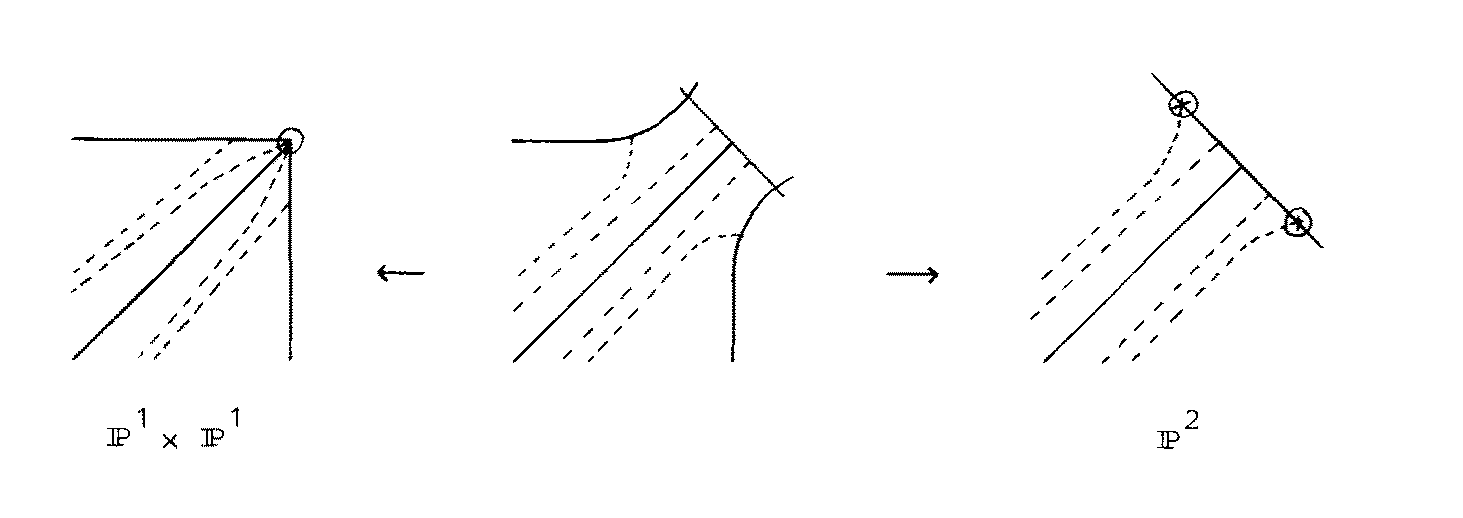
\includegraphics{assets/P08-A01_three_stage_compactification_present.png}\end{adjustbox}\end{center}
\noindent Une construction similaire peut être faite pour r et m quelconques.\par\smallskip
\noindent Reprenons la preuve de 1.6. Appliquons 1.5 à h : Z \ensuremath{→} \ensuremath{\bar{B}}\allowbreak\_{\ensuremath{α}} et à \ensuremath{Δ}̄\allowbreak\_{\ensuremath{α}}. On trouve que \ensuremath{Δ}̄\allowbreak\_{\ensuremath{α}} admet un voisinage ouvert arbitrairement petit \ensuremath{V_α} tel que \ensuremath{h^{-1}}(\ensuremath{V_α}) = \ensuremath{h^{-1}}(\ensuremath{V_α} \ensuremath{∩} \ensuremath{B_α}) soit connexe, de \ensuremath{π₁} s'envoyant sur celui de Z. D'après 1.7, quel que soit le voisinage U de \ensuremath{Δ} dans P, on peut prendre \ensuremath{V_α} tel que \ensuremath{V_α} \ensuremath{∩} \ensuremath{B_α} \ensuremath{⊂} U.\par\smallskip
\noindent La réunion V des ouverts \ensuremath{V_α} \ensuremath{∩} \ensuremath{B_α} de P est un voisinage, arbitrairement petit de \ensuremath{Δ}. L'hypothèse b) sur les \ensuremath{H_α} assure que l'intersection des \ensuremath{V_α} \ensuremath{∩} \ensuremath{B_α} rencontre h(Z). Dès lors, \ensuremath{h^{-1}}(V), réunion des ouverts connexes \ensuremath{h^{-1}}(\ensuremath{V_α}), d'intersection non vide, est connexe. Puisque le \ensuremath{π₁} de l'un des \ensuremath{h^{-1}}(\ensuremath{V_α}) s'envoie sur celui de Z, a fortiori celui de \ensuremath{h^{-1}}(V), et ceci achève la démonstration.\par\smallskip
\noindent 2. Preuve du théorème 1\par\smallskip
\noindent 2.1.- Soient C \ensuremath{⊂} \ensuremath{ℙ^2} une courbe plane réduite, D une composante irréductible de C, C' = \ensuremath{\overline{(C - D)}} la réunion des autres composantes, Sing(C) l'ensemble des points singuliers de C et D* = D - Sing(C). Choisissons un point base O \ensuremath{∈} \ensuremath{ℙ^2} - C, et soit \ensuremath{γ} un lacet dans \ensuremath{ℙ^2} - C du type suivant : \ensuremath{γ} va de O à un point p' proche d'un point p de D* par un chemin ch, tourne une fois autour de D* dans le sens positif, et revient à O par ch\textasciicircum{}\{-1\}. La courbe D* étant connexe, les lacets de ce type sont tous conjugués entre eux. Le quotient de \ensuremath{π₁}(\ensuremath{ℙ^2} - C,O) par le sous-groupe distingué qu'ils engendrent est \ensuremath{π₁}(\ensuremath{ℙ^2} - C').\par\smallskip
\noindent PROPOSITION 2.2.- Supposons que ceux des points singuliers de C qui sont sur D sont des points doubles à tangentes distinctes. Alors, \ensuremath{γ} est central dans \ensuremath{π₁}(\ensuremath{ℙ^2} - C,O).\par\smallskip
\noindent Soient j l'inclusion de \ensuremath{ℙ^2} - C dans \ensuremath{ℙ^2}, g : \ensuremath{\widetilde{D}} \ensuremath{→} D la normalisée de D et appliquons 1.6 à\par\smallskip
\noindent h = j \ensuremath{×} g : (\ensuremath{ℙ^2} - C) \ensuremath{×} \ensuremath{\widetilde{D}} \ensuremath{→} \ensuremath{ℙ^2} \ensuremath{×} \ensuremath{ℙ^2}.\par\smallskip
\noindent Pour présenter commodément l'image inverse de certains voisinages de la diagonale, nous choisissons sur \ensuremath{ℙ^2} une structure riemannienne telle que, au voisinage de chaque\par\smallskip
\end{minipage}
\end{adjustbox}
\newpage
\noindent\begin{adjustbox}{max totalsize={\textwidth}{0.945\textheight},center}
\begin{minipage}{\textwidth}
\noindent\hfill\scriptsize Authority physical page 9 / printed folio 543-09\par\normalsize
\noindent point P \ensuremath{∈} D \ensuremath{∩} Sing(C), \ensuremath{ℙ^2} soit euclidien, et que les deux branches de C par P soient des 2-plans (réels) orthogonaux.\par\smallskip
\noindent Si (u,v) \ensuremath{∈} (\ensuremath{ℙ^2} - C) \ensuremath{×} \ensuremath{\widetilde{D}} est dans l'image inverse d'un voisinage assez petit de la diagonale, i. e. si u et v sont assez proches, le point u est près de D, et on peut abaisser une courte perpendiculaire de u sur D. Pour u près de Sing(D), on en a même deux, une par branche. On choisit celle dont le pied \ensuremath{\bar{u}} est proche de v sur \ensuremath{\widetilde{D}} :\par\smallskip
\begin{center}\begin{adjustbox}{max width=0.96\linewidth,max height=0.25\textheight}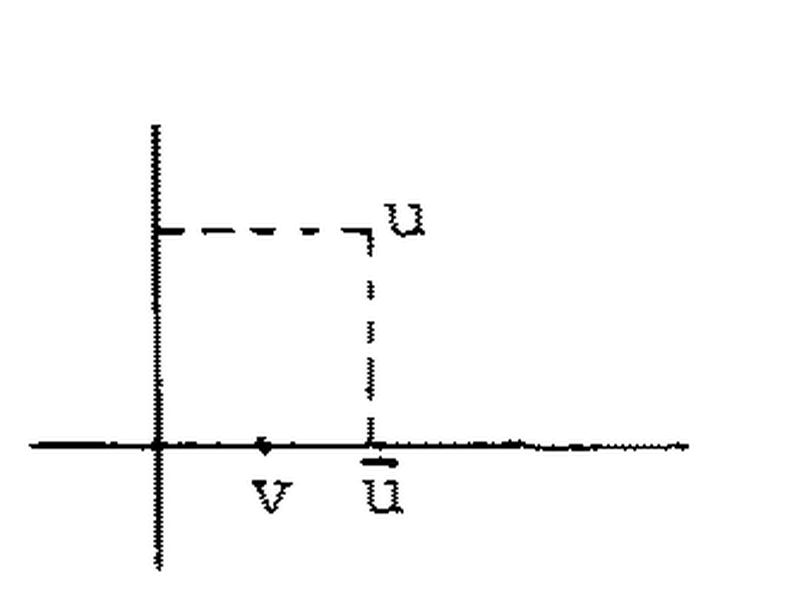
\includegraphics{assets/P09-A01_local_perpendicular_present.png}\end{adjustbox}\end{center}
\noindent Le point \ensuremath{\bar{u}} est dans D*.\par\smallskip
\noindent Réciproquement, soient \ensuremath{ε} > 0 assez petit, q : U* \ensuremath{→} D* le sous-fibré en disques épointés du fibré normal de D* dans \ensuremath{ℙ^2} formé des vecteurs normaux non nuls de longueur < \ensuremath{ε}, et E l'ensemble des couples (x,v) avec x \ensuremath{∈} U*, v \ensuremath{∈} \ensuremath{\widetilde{D}} et d(q(x),v) < \ensuremath{ε} (distance calculée sur \ensuremath{\widetilde{D}}). L'application pr\ensuremath{₁} : E \ensuremath{→} U* est une équivalence d'homotopie et admet pour section l'espace des (x,q(x)). L'application exp : (x,v) \ensuremath{↦} (exp(x),v) de E dans (\ensuremath{ℙ^2} - C) \ensuremath{×} \ensuremath{\widetilde{D}} identifie E à l'image inverse d'un voisinage de \ensuremath{Δ}, et, pour \ensuremath{ε} \ensuremath{→} 0, on obtient les images inverses d'un système fondamental de voisinage. Appliquant 1.6, on trouve que, quel que soit O \ensuremath{∈} U*, exp et q induisent une surjection\par\smallskip
\noindent (exp,q)* : \ensuremath{π₁}(U*,O) \ensuremath{↠} \ensuremath{π₁}(\ensuremath{ℙ^2} - C,exp(O)) \ensuremath{×} \ensuremath{π₁}(\ensuremath{\widetilde{D}},q(O)).\par\smallskip
\noindent On dispose d'une suite exacte d'homotopie\par\smallskip
\noindent \ensuremath{ℤ} \ensuremath{→} \ensuremath{π₁}(U*,O) \ensuremath{→} \ensuremath{π₁}(D*,q(O)) \ensuremath{→} 1.\par\smallskip
\noindent L'image de \ensuremath{ℤ} est centrale ; celle de 1 \ensuremath{∈} \ensuremath{ℤ} est représentée par un petit lacet tournant une fois, dans le sens positif, autour de D*. Puisque (exp,q)*, donc exp* : \ensuremath{π₁}(U*,O) \ensuremath{→} \ensuremath{π₁}(\ensuremath{ℙ^2} - C,exp(O)) est surjectif, ce lacet définit encore un élément central de \ensuremath{π₁}(\ensuremath{ℙ^2} - C,exp(O)). C'est \ensuremath{γ}.\par\smallskip
\noindent 2.3 Preuve du théorème 1 : Pour chaque composante irréductible D de C, soit \ensuremath{γ}(D) l'élément central correspondant de \ensuremath{π₁}(\ensuremath{ℙ^2} - C,O). Le quotient de \ensuremath{π₁}(\ensuremath{ℙ^2} - C,O) par le sous-groupe - central - engendré par les \ensuremath{γ}(D) est \ensuremath{π₁}(\ensuremath{ℙ^2},O) = \{e\}. Le théorème en résulte.\par\smallskip
\end{minipage}
\end{adjustbox}
\newpage
\noindent\begin{adjustbox}{max totalsize={\textwidth}{0.945\textheight},center}
\begin{minipage}{\textwidth}
\noindent\hfill\scriptsize Authority physical page 10 / printed folio 543-10\par\normalsize
\noindent BIBLIOGRAPHIE\par\smallskip
\noindent [1] S. ABHYANKAR - Tame coverings and fundamental groups of algebraic varieties I, Amer. J. of Math., 81(1959), 46-94.\par\smallskip
\noindent [2] D. CHENIOT - Un théorème du type de Lefschetz, Annales de l'Institut Fourier, 25 1(1975), 195-213.\par\smallskip
\noindent [2 bis] D. CHENIOT - Une démonstration du théorème de Zariski sur les sections hyperplanes d'une hypersurface projective et du théorème de Van Kampen sur le groupe fondamental du complémentaire d'une courbe plane, Comp. Math., 27 2(1973), 141-158.\par\smallskip
\noindent [3] W. FULTON - On the fundamental group of the complement of a node curve, Ann. of Math., 111 2(1980), 407-409.\par\smallskip
\noindent [4] W. FULTON and J. HANSEN - A connectedness theorem for projective varieties, with applications to intersections and singularities of mappings, Ann. of Math., 109 1(1979), 159-166.\par\smallskip
\noindent [5] T. GAFFNEY and R. LAZARSFELD - On the ramification of branched coverings of \ensuremath{ℙ^n}, Inv. Math., 59 1(1980), 53-58.\par\smallskip
\noindent [6] H. HAMM et LÊ D\ensuremath{\widetilde{U}}NG TRANG - Un théorème de Zariski du type de Lefschetz, Ann. Sci. E.N.S., 6 3(1973), 317-366.\par\smallskip
\noindent [7] J.-P. SERRE - Revêtements ramifiés du plan projectif (d'après S. Abhyankar), Sém. Bourbaki 204, mai 1960.\par\smallskip
\noindent [8] O. ZARISKI - On the problem of existence of algebraic functions of two variables possessing a given branch curve, Amer. J. of Math., 51(1929), 305-328.\par\smallskip
\noindent [9] O. ZARISKI - Algebraic surfaces, second supplemented edition, Ergebnisse 61, Springer-Verlag.\par\smallskip
\noindent Je viens (1/10/80) de recevoir un très bel exposé, faisant le point sur les méthodes étudiées ici, leurs variantes et leurs nombreuses applications : W. FULTON and R. LAZARSFELD - Connectivity and its applications in algebraic geometry.\par\smallskip
\noindent Pierre DELIGNE\\Institut des Hautes Etudes\\Scientifiques\\35 route de Chartres\\F-91440 BURES-SUR-YVETTE\par\smallskip
\end{minipage}
\end{adjustbox}

\clearpage\endgroup
\typeout{CORPUS-END:D036:\thepage}
% END INLINE WORK D036 FR
% BEGIN INLINE WORK D038 FR
\typeout{CORPUS-BEGIN:D038:\thepage}
\begingroup
\makeatletter
\let\DeclareMathOperator\CorpusDeclareMathOperator
\let\@declmathop\CorpusDeclMathOp
\let\maketitle\CorpusMakeTitle\let\title\CorpusTitle\let\author\CorpusAuthor\let\date\CorpusDate
\let\thanks\CorpusThanks\let\and\CorpusAnd\let\@maketitle\CorpusAtMakeTitle
\def\setcounter#1#2{\def\CorpusCounterName{#1}\def\CorpusPageName{page}\ifx\CorpusCounterName\CorpusPageName\else\CorpusSetCounter{#1}{#2}\fi}
\title{}\author{}\date{}
\expandafter\let\csname CanonHeading\endcsname\CorpusUndefined
\expandafter\let\csname CanonText\endcsname\CorpusUndefined
\expandafter\let\csname CanonDisplay\endcsname\CorpusUndefined
\expandafter\let\csname CanonMathBlock\endcsname\CorpusUndefined
\expandafter\let\csname endCanonMathBlock\endcsname\CorpusUndefined
\expandafter\let\csname LayerTitle\endcsname\CorpusUndefined
\setcounter{section}{0}
\expandafter\def\csname theHsection\endcsname{D038.\arabic{section}}
\setcounter{subsection}{0}
\expandafter\def\csname theHsubsection\endcsname{D038.\arabic{subsection}}
\setcounter{subsubsection}{0}
\expandafter\def\csname theHsubsubsection\endcsname{D038.\arabic{subsubsection}}
\setcounter{equation}{0}
\expandafter\def\csname theHequation\endcsname{D038.\arabic{equation}}
\setcounter{figure}{0}
\expandafter\def\csname theHfigure\endcsname{D038.\arabic{figure}}
\setcounter{table}{0}
\expandafter\def\csname theHtable\endcsname{D038.\arabic{table}}
\setcounter{footnote}{0}
\expandafter\def\csname theHfootnote\endcsname{D038.\arabic{footnote}}
\makeatother
\let\tableofcontents\relax % one cumulative contents list, not repeated global lists
% D038 canonical TeX source; generated deterministically from the returned packet.
% No inherited audit or comparator byte is accepted as editorial content.

\setmainfont{DejaVu Serif}
\setsansfont{DejaVu Sans}
\definecolor{Accent}{HTML}{1E4D5B}
\definecolor{Quiet}{HTML}{5F6870}
\pagestyle{empty}
\setlength{\parindent}{0pt}
\setlength{\parskip}{0pt}
\emergencystretch=2em
\hfuzz=1.5pt
\vfuzz=1.5pt
\hbadness=10000
\vbadness=10000
\newcommand{\CanonHeading}[1]{\par\vspace{1.5pt}{\fontsize{8.6}{10.0}\selectfont\sffamily\bfseries\color{Accent} #1\par}\vspace{1.5pt}}
\newcommand{\CanonText}[1]{\par{\fontsize{8.0}{9.35}\selectfont\RaggedRight #1\par}\vspace{2.2pt}}
\newcommand{\CanonDisplay}[1]{\par\vspace{1.2pt}\begin{center}{\fontsize{7.2}{8.4}\selectfont\(\displaystyle #1\)}\end{center}\vspace{1.2pt}}
\newenvironment{CanonMathBlock}{\par\vspace{1.2pt}\begin{center}\fontsize{6.8}{8.0}\selectfont\(\displaystyle}{\)\end{center}\vspace{1.2pt}}
\newcommand{\LayerTitle}{Canonical source-language edition}

\graphicspath{{assets/works/D038_PUBLIC_SAFE/candidate/}}
\setlength{\topskip}{0pt} % preserve full-height source minipages without a leading blank page
\selectlanguage{french}
\phantomsection\addcontentsline{toc}{section}{D038}


% CANONICAL_PAGE physical=001 printed=80 layer=source
% RECORD_SHA256 674DC33503B22430D5ECEC192CFCE8036A8A49B9B5F889874A882ED1E213BDE7
% SOURCE_RECORD_SHA256 674DC33503B22430D5ECEC192CFCE8036A8A49B9B5F889874A882ED1E213BDE7
\noindent\begin{minipage}[t][\dimexpr\textheight-5pt\relax][t]{\textwidth}
{\sffamily\fontsize{7.3}{8.2}\selectfont\color{Quiet} D038 / physical 01 / authority printed 80\hfill French main exposition}
\par\vspace{2.2pt}{\color{Accent}\hrule height 0.55pt}\vspace{4.5pt}
{\sffamily\fontsize{10.4}{11.6}\selectfont\bfseries\color{Accent} \LayerTitle}
\par{\sffamily\fontsize{6.7}{7.7}\selectfont\color{Quiet} diplomatic source; exact one-page correspondence to authority physical 1}
\vspace{5pt}
\CanonText{Exposé \(V\)}
\CanonHeading{CRISTAUX ORDINAIRES ET COORDONNÉES CANONIQUES}
\CanonText{par \(P\). DELIGNE}
\CanonText{avec la collaboration de \(L\). ILLUSIE (*)}
\CanonHeading{SOMMAIRE}
\CanonHeading{0. INTRODUCTION}
\begin{CanonMathBlock}
\begin{aligned}
& 1.\,\mathrm{PARAMÈTRES}\,\mathrm{CANONIQUES}\,\mathrm{DES}\,F-\mathrm{CRISTAUX}\,\mathrm{DE}\,\mathrm{HODGE}\,\mathrm{ORDINAIRES}\\
& 1.1.\,\text{Rappels}\,\text{de}\,\text{définitions}\\
& 1.2.\,F-\text{cristaux}\,\text{unités}\\
& 1.3.\,F-\text{cristaux}\,\text{ordinaires}\\
& 1.4.\,F-\text{cristaux}\,\text{de}\,\text{Hodge}\,\text{ordinaires}\,\text{de}\,\text{niveau}\,\leq{}\,1
\end{aligned}
\end{CanonMathBlock}
\CanonText{2. APPLICATIONS GÉOMÉTRIQUES\\2.1. Coordonnées canoniques\\A. Variétés abéliennes\\\(B\). Surfaces K3\\2.2. Relèvements de faisceaux inversibles}
\CanonText{Dans tout l'exposé, \(k\) désigne un corps algébriquement clos de car. \(p\) > 0, et \(W\) l'anneau des vecteurs de Witt sur \(k\).}
\CanonText{---------------------\\(*) Équipe de Recherche Associée au C.N.R.S. n° 653}
\vfill
{\color{Accent}\hrule height 0.35pt}\vspace{3pt}
\noindent{\sffamily\fontsize{6.0}{7.0}\selectfont\color{Quiet}
Layout/math fallback asset (evidence only; not reader prose): \texttt{assets/authority\_pages/p001.png}. Full-resolution image retained beside this TeX source; running headers, printed folios, and scanner/library copy matter are excluded from canonical prose.\\
Record: \texttt{674DC33503B22430}\ldots\quad Authority evidence: \texttt{595EC8D5694949F3}\ldots}
\end{minipage}
\newpage
% CANONICAL_PAGE physical=002 printed=81 layer=source
% RECORD_SHA256 DF9E79A8A0A0C23F7AB683A8400BACF7BB88F630879445A24A906D58C381A2FF
% SOURCE_RECORD_SHA256 DF9E79A8A0A0C23F7AB683A8400BACF7BB88F630879445A24A906D58C381A2FF
\noindent\begin{minipage}[t][\dimexpr\textheight-5pt\relax][t]{\textwidth}
{\sffamily\fontsize{7.3}{8.2}\selectfont\color{Quiet} D038 / physical 02 / authority printed 81\hfill French main exposition}
\par\vspace{2.2pt}{\color{Accent}\hrule height 0.55pt}\vspace{4.5pt}
{\sffamily\fontsize{10.4}{11.6}\selectfont\bfseries\color{Accent} \LayerTitle}
\par{\sffamily\fontsize{6.7}{7.7}\selectfont\color{Quiet} diplomatic source; exact one-page correspondence to authority physical 2}
\vspace{5pt}
\CanonHeading{0. INTRODUCTION}
\CanonText{Soit \(X_{0}/k\) une courbe elliptique ordinaire. D'après la théorie de Serre-Tate [14, \(V]\), la variété modulaire formelle \(M\) des déformations de \(X_{0}\) sur les W-algèbres artiniennes locales de corps résiduel \(k\) est isomorphe au groupe multiplicatif formel \(\widehat{G}_{m}/W\). Plus précisément, le groupe p-divisible}
\CanonDisplay{G_{0}\,=\,\cup{}\,\operatorname{Ker}(p^{n}\,:\,X_{0}\,\to{}\,X_{0})}
\CanonText{est isomorphe à \((\mathbb{Q}_{p}/\mathbb{Z}_{p})\) \(\times{}\) \(\mu{}_{p^{\infty}{}}\), et le choix d'un isomorphisme \(\alpha{}\) entre la partie étale de \(G_{0}\) et \(\mathbb{Q}_{p}/\mathbb{Z}_{p}\) permet d'identifier canoniquement, pour toute W-algèbre \(R\) artinienne locale de corps résiduel \(k\), l'ensemble des relèvements de \(X_{0}\) sur \(R\) au groupe \(\operatorname{Ext}^{1}((\mathbb{Q}_{p}/\mathbb{Z}_{p})_{R},(\mu{}_{p^{\infty}{}})_{R})\), à son tour isomorphe canoniquement au groupe des unités de \(R\) congrues à 1 modulo l'idéal maximal : on obtient donc ainsi un isomorphisme (ne dépendant que de \(\alpha{})\) entre \(M\) et \((\widehat{G}_{m})_{W}\), et en particulier la déformation universelle \(X\) de \(X_{0}\) sur \(M\) définit une "coordonnée canonique" \(q\) sur \(M\), telle que \(M\) \(\simeq{}\) \(\operatorname{Spf}\) \(W[[q-1]]\). De ce paramètre \(q\), qui décrit le groupe p-divisible \(G\) associé à \(X\) comme extension de \(\mathbb{Q}_{p}/\mathbb{Z}_{p}\) par \(\mu{}_{p^{\infty}{}}\), on peut donner une autre interprétation, en termes du module \(H^{1}_{\mathrm{DR}}(X/M)\), muni de sa structure de F-cristal et de sa filtration de Hodge \(H^{0}(X,\Omega{}^{1}_{X/M})\) \(\subset{}\) \(H^{1}_{\mathrm{DR}}(X/M)\). La donnée d'un isomorphisme \(\alpha{}\) comme ci-dessus fournit en effet par dualité un isomorphisme \(\alpha{}^{\prime}\) entre le groupe formel \(\widehat{X}/M\) associé à \(X\) et le groupe formel \((\widehat{G}_{m})_{M}\), d'où une forme \(b\) \(\in{}\) \(H^{0}(X,\Omega{}^{1}_{X/M})\), correspondant par \(\alpha{}^{\prime}\) à la forme invariante sur \((\widehat{G}_{m})_{M}\). Soit a \(\in{}\) \(H^{1}_{\mathrm{DR}}(X/M)\) tel que \(\nabla{}a\) \(=\) 0 et \((a,b)\) soit une base symplectique de \(H^{1}_{\mathrm{DR}}(X/M)\), i.e. \(\langle{}a,b\rangle{}\) \(=\) 1, \(\langle{}a,a\rangle{}\) \(=\) 0. Si}
\CanonDisplay{\nabla{}\,:\,H^{1}_{\mathrm{DR}}(X/M)\,\to{}\,\Omega{}^{1}_{M/W}\,\otimes{}\,H^{1}_{\mathrm{DR}}(X/M)}
\CanonText{désigne la connexion de Gauss-Manin, on a nécessairement}
\CanonDisplay{(0.1)\qquad\,\nabla{}b\,=\,\eta{}\,\otimes{}\,a,}
\CanonText{avec \(\eta{}\) \(\in{}\) \(\Omega{}^{1}_{M/W}\). On peut montrer (voir Appendice et Exposé suivant, par \(N\). Katz) que l'on a}
\CanonDisplay{(0.2)\qquad\,\eta{}\,=\,d\,\operatorname{log}\,q,}
\vfill
{\color{Accent}\hrule height 0.35pt}\vspace{3pt}
\noindent{\sffamily\fontsize{6.0}{7.0}\selectfont\color{Quiet}
Layout/math fallback asset (evidence only; not reader prose): \texttt{assets/authority\_pages/p002.png}. Full-resolution image retained beside this TeX source; running headers, printed folios, and scanner/library copy matter are excluded from canonical prose.\\
Record: \texttt{DF9E79A8A0A0C23F}\ldots\quad Authority evidence: \texttt{DB8A386CAECA907E}\ldots}
\end{minipage}
\newpage
% CANONICAL_PAGE physical=003 printed=82 layer=source
% RECORD_SHA256 74E81277FEC0DCAECE77F4A6497BC0A91FFC26E43EF560A88C3EC23D5274DCBA
% SOURCE_RECORD_SHA256 74E81277FEC0DCAECE77F4A6497BC0A91FFC26E43EF560A88C3EC23D5274DCBA
\noindent\begin{minipage}[t][\dimexpr\textheight-5pt\relax][t]{\textwidth}
{\sffamily\fontsize{7.3}{8.2}\selectfont\color{Quiet} D038 / physical 03 / authority printed 82\hfill French main exposition}
\par\vspace{2.2pt}{\color{Accent}\hrule height 0.55pt}\vspace{4.5pt}
{\sffamily\fontsize{10.4}{11.6}\selectfont\bfseries\color{Accent} \LayerTitle}
\par{\sffamily\fontsize{6.7}{7.7}\selectfont\color{Quiet} diplomatic source; exact one-page correspondence to authority physical 3}
\vspace{5pt}
\CanonText{où \(q\) est le paramètre défini plus haut, qui se trouve donc coïncider avec celui défini indépendamment par Dwork ([8], [6]) à l'aide de (0.2). La base \((a,b)\) ci-dessus jouit par ailleurs de propriétés remarquables vis-à-vis de l'opération de Frobenius \(F\) sur \(H^{1}_{\mathrm{DR}}(X/M)\) : si l'on choisit comme endomorphisme de \(M\) relevant le Frobenius de \(M\) \(\otimes{}\) \(k\) celui donné par \(q\) \(\mapsto{}\) \(q^{p}\), alors \(F\) s'exprime par}
\CanonDisplay{(0.3)\qquad\,F\,a\,=\,a,\qquad\,F\,b\,=\,p\,b.}
\CanonText{Les constructions précédentes se généralisent aux variétés abéliennes ordinaires [8], voir aussi [9], [11] pour des applications arithmétiques dans le cas des courbes elliptiques.}
\CanonText{L'objet de l'exposé est de montrer qu'on peut développer une théorie analogue pour les surfaces K3 ordinaires, du moins si \(p\) \(\neq{}\) 2. Soit \(X_{0}/k\) une surface K3 ordinaire, i.e. telle que le Frobenius de \(H^{2}(X_{0},\mathcal{O})\) soit non nul, et soit \(S\) la variété modulaire formelle des déformations de \(X_{0}\) sur les W-algèbres artiniennes locales de corps résiduel \(k\) (IV 1.2). Si \(p\) \(\neq{}\) 2, on prouve que \(S\) est munie canoniquement d'une structure de groupe formel, isomorphe à \((\widehat{G}_{m})_{W}^{20}\) ; en particulier, la déformation universelle \(X\) de \(X_{0}\) sur \(S\) définit des "coordonnées canoniques" \(q_{i}\) (1 \(\leq{}\) \(i\) \(\leq{}\) 20) telles que}
\CanonDisplay{S\,\simeq{}\,\operatorname{Spf}\,W[[q_{1}-1,\,\ldots{},\,q_{20}-1]],}
\CanonText{formant une base des caractères de \(S\). On montre de plus que, si \(L_{0}\) est un faisceau inversible non trivial sur \(X_{0}\), l'hypersurface \(\Sigma{}(L_{0})\) de \(S\) telle que \(L_{0}\) se prolonge à \(X\) \(\times{}_{S}\) \(\Sigma{}(L_{0})\) (IV 1.5) est le noyau d'un caractère de \(S\), défini de façon presque tautologique par la classe de Chern cristalline de \(L_{0}\).}
\CanonText{En l'absence d'une théorie de Serre-Tate pour les relèvements des surfaces K3, c'est en termes de la structure de F-cristal de \(H^{2}_{\mathrm{DR}}(X/S)\) que l'on définit la structure de groupe formel de \(S\). En fait, on peut englober le cas des variétés abéliennes et celui des surfaces K3 dans un même théorème de structure pour une certaine classe de F-cristaux ordinaires. L'étude de ces cristaux fait l'objet du}
\vfill
{\color{Accent}\hrule height 0.35pt}\vspace{3pt}
\noindent{\sffamily\fontsize{6.0}{7.0}\selectfont\color{Quiet}
Layout/math fallback asset (evidence only; not reader prose): \texttt{assets/authority\_pages/p003.png}. Full-resolution image retained beside this TeX source; running headers, printed folios, and scanner/library copy matter are excluded from canonical prose.\\
Record: \texttt{74E81277FEC0DCAE}\ldots\quad Authority evidence: \texttt{955CB3D1E7738A39}\ldots}
\end{minipage}
\newpage
% CANONICAL_PAGE physical=004 printed=83 layer=source
% RECORD_SHA256 FD485662C7B292E164CB76A74807B42BDF716629ED11402DA21712F424BE7899
% SOURCE_RECORD_SHA256 FD485662C7B292E164CB76A74807B42BDF716629ED11402DA21712F424BE7899
\noindent\begin{minipage}[t][\dimexpr\textheight-5pt\relax][t]{\textwidth}
{\sffamily\fontsize{7.3}{8.2}\selectfont\color{Quiet} D038 / physical 04 / authority printed 83\hfill French main exposition}
\par\vspace{2.2pt}{\color{Accent}\hrule height 0.55pt}\vspace{4.5pt}
{\sffamily\fontsize{10.4}{11.6}\selectfont\bfseries\color{Accent} \LayerTitle}
\par{\sffamily\fontsize{6.7}{7.7}\selectfont\color{Quiet} diplomatic source; exact one-page correspondence to authority physical 4}
\vspace{5pt}
\CanonText{n° 1. Les applications géométriques sont données au n° 2. En ce qui concerne le théorème relatif aux hypersurfaces \(\Sigma{}(L_{0})\), l'ingrédient essentiel est l'utilisation de la classe de Chern cristalline pour contrôler l'obstruction au prolongement.}
\CanonHeading{1. PARAMÈTRES CANONIQUES DES F-CRISTAUX DE HODGE ORDINAIRES}
\CanonHeading{1.1. Rappels de définitions.}
\CanonText{1.1.1. Pour les définitions et propriétés générales des F-cristaux, voir Katz [8], [10]. On fixe pour toute la suite du n° 1 des anneaux de séries formelles}
\CanonDisplay{A_{0}\,=\,k[[t_{1},\ldots{},t_{n}]],\qquad\,A\,=\,W[[t_{1},\ldots{},t_{n}]],}
\CanonText{où \((t_{1},\ldots{},t_{n})\) est une suite finie d'indéterminées (pour \(n\) \(=\) 0, on convient que \(A_{0}\) \(=\) \(k\), \(A\) \(=\) \(W)\).}
\CanonText{Un cristal (sous-entendu, en modules libres de type fini) sur \(A_{0}\) est par définition un A-module libre de type fini \(H\), muni d'une connexion}
\CanonDisplay{\nabla{}\,:\,H\,\to{}\,\Omega{}^{1}_{A/W}\,\otimes{}\,H,}
\CanonText{intégrable et p-adiquement topologiquement nilpotente. Que \(\nabla{}\) soit intégrable signifie que, si l'on pose \(D_{i}\) \(=\) \(d/\text{dt}_{i}\), on a}
\CanonDisplay{\nabla{}(D_{i})\nabla{}(D_{j})\,=\,\nabla{}(D_{j})\nabla{}(D_{i})}
\CanonText{quels que soient \(i\) \(\neq{}\) \(j\). Cela permet de faire opérer sur \(H\) les opérateurs PD-différentiels sur A, i.e. les polynômes en les \(D_{i}\) à coefficients dans A, par la formule}
\CanonDisplay{\nabla{}(\sum{}_{m}\,a_{m}D^{m})\,=\,\sum{}_{m}\,a_{m}(\nabla{}(D))^{m},}
\CanonText{avec les notations condensées habituelles \(D^{m}\) \(=\) \(D_{1}^{m_{1}}\cdots{}D_{n}^{m_{n}}\), etc. Quant à la nilpotence topologique de \(\nabla{}\), elle s'exprime par le fait que, pour tout \(i\), \(\nabla{}(D_{i})^{m}\) tend vers zéro pour la topologie p-adique de \(\operatorname{End}_{W}(H)\) quand \(m\) tend vers \(+\infty{}\). D'après Berthelot [1, II 4], la}
\vfill
{\color{Accent}\hrule height 0.35pt}\vspace{3pt}
\noindent{\sffamily\fontsize{6.0}{7.0}\selectfont\color{Quiet}
Layout/math fallback asset (evidence only; not reader prose): \texttt{assets/authority\_pages/p004.png}. Full-resolution image retained beside this TeX source; running headers, printed folios, and scanner/library copy matter are excluded from canonical prose.\\
Record: \texttt{FD485662C7B292E1}\ldots\quad Authority evidence: \texttt{0DF7A5B6C2C3ECDF}\ldots}
\end{minipage}
\newpage
% CANONICAL_PAGE physical=005 printed=84 layer=source
% RECORD_SHA256 477ED68FF572C31302E682D9CA21CF1BAAC8190DCA51C1B5950033A64E0BF0AC
% SOURCE_RECORD_SHA256 477ED68FF572C31302E682D9CA21CF1BAAC8190DCA51C1B5950033A64E0BF0AC
\noindent\begin{minipage}[t][\dimexpr\textheight-5pt\relax][t]{\textwidth}
{\sffamily\fontsize{7.3}{8.2}\selectfont\color{Quiet} D038 / physical 05 / authority printed 84\hfill French main exposition}
\par\vspace{2.2pt}{\color{Accent}\hrule height 0.55pt}\vspace{4.5pt}
{\sffamily\fontsize{10.4}{11.6}\selectfont\bfseries\color{Accent} \LayerTitle}
\par{\sffamily\fontsize{6.7}{7.7}\selectfont\color{Quiet} diplomatic source; exact one-page correspondence to authority physical 5}
\vspace{5pt}
\CanonText{donnée d'une connexion \(\nabla{}\) comme ci-dessus équivaut à la donnée, pour tout couple de W-homomorphismes \((f,g)\) de A dans une W-algèbre \(B\) locale, noethérienne et complète, tels que \(f\) et \(g\) soient congrus modulo un idéal I de \(B\) muni de puissances divisées compatibles aux puissances divisées standard de \(p\), d'un isomorphisme}
\CanonDisplay{\chi{}(f,g)\,:\,f^{*}H\,\simeq{}\,g^{*}H,\qquad\,(*)}
\CanonText{ces isomorphismes étant assujettis à vérifier certaines conditions de transitivité explicitées dans [8, 1.2], i.e. \(\chi{}(g,h)\chi{}(f,g)\) \(=\) \(\chi{}(f,h)\), \(\chi{}(\text{fk},\text{gk})\) \(=\) \(k^{*}\chi{}(f,g)\), \(\chi{}(\operatorname{id},\operatorname{id})\) \(=\) \(\operatorname{id}\). La formule suivante décrit concrètement ce dictionnaire dans le sens qui nous intéresse :}
\CanonText{LEMME 1.1.2. Avec les notations ci-dessus, désignons par}
\CanonDisplay{f^{*}\,:\,H\,\to{}\,f^{*}H}
\CanonText{la flèche d'adjonction, où \(f^{*}H\) \(=\) \(f_*f^{*}H\) par abus. L'homomorphisme A-linéaire composé}
\begin{CanonMathBlock}
\begin{array}{cc}
f^{*} & \chi{}(f,g)\\
\chi{}(f,g)f^{*}\,:\,H\,\longrightarrow{}\,f^{*}H\,\longrightarrow{}\,g^{*}H & {}
\end{array}
\end{CanonMathBlock}
\CanonText{est donné par la formule}
\CanonDisplay{(1.1.2.1)\qquad\,\chi{}(f,g)f^{*}(x)\,=\,\sum{}_{m}\,(f(t)-g(t))^{[m]}\,g^{*}(\nabla{}(D)^{m}x),}
\CanonText{la somme portant sur tous les multi-indices \(m\) \(=\) \((m_{1},\ldots{},m_{n})\) \(\in{}\) \(N^{n}\), avec les notations condensées}
\CanonDisplay{(f(t)-g(t))^{[m]}\,=\,(f(t_{1})-g(t_{1}))^{[m_{1}]}\cdots{}(f(t_{n})-g(t_{n}))^{[m_{n}]}}
\CanonText{(le crochet désignant une puissance divisée dans I), et}
\CanonDisplay{\nabla{}(D)^{m}\,=\,\nabla{}(D_{1})^{m_{1}}\cdots{}\nabla{}(D_{n})^{m_{n}}}
\CanonText{(N.B. la série au second membre de (1.1.2.1) est convergente grâce à la nilpotence topologique de \(\nabla{})\).}
\CanonText{Cet énoncé est essentiellement contenu dans [1, II 4.3]. Il suffit de le vérifier après réduction \(\operatorname{mod}\) \(p^{r}\) pour tout \(r\). Nous noterons}
\CanonText{---------------------\\(*) On note encore \(f\) (resp. \(g)\) : \(\operatorname{Spec}(B)\) \(\to{}\) \(\operatorname{Spec}(A)\) le morphisme de schémas correspondant.}
\vfill
{\color{Accent}\hrule height 0.35pt}\vspace{3pt}
\noindent{\sffamily\fontsize{6.0}{7.0}\selectfont\color{Quiet}
Layout/math fallback asset (evidence only; not reader prose): \texttt{assets/authority\_pages/p005.png}. Full-resolution image retained beside this TeX source; running headers, printed folios, and scanner/library copy matter are excluded from canonical prose.\\
Record: \texttt{477ED68FF572C313}\ldots\quad Authority evidence: \texttt{1EB5DB5D796B31E6}\ldots}
\end{minipage}
\newpage
% CANONICAL_PAGE physical=006 printed=85 layer=source
% RECORD_SHA256 7DD7F38B566767D438574FCF73A5D70BFD649397487732CA58816F6F51DB99EF
% SOURCE_RECORD_SHA256 7DD7F38B566767D438574FCF73A5D70BFD649397487732CA58816F6F51DB99EF
\noindent\begin{minipage}[t][\dimexpr\textheight-5pt\relax][t]{\textwidth}
{\sffamily\fontsize{7.3}{8.2}\selectfont\color{Quiet} D038 / physical 06 / authority printed 85\hfill French main exposition}
\par\vspace{2.2pt}{\color{Accent}\hrule height 0.55pt}\vspace{4.5pt}
{\sffamily\fontsize{10.4}{11.6}\selectfont\bfseries\color{Accent} \LayerTitle}
\par{\sffamily\fontsize{6.7}{7.7}\selectfont\color{Quiet} diplomatic source; exact one-page correspondence to authority physical 6}
\vspace{5pt}
\CanonText{encore par abus \((f,g)\) : \(A\) \(\rightrightarrows{}\) \(B\) les \(W_{r}-\text{homomorphismes}\) déduits de ceux donnés par réduction \(\operatorname{mod}\) \(p^{r}\). Soit \(D\) l'enveloppe à puissances divisées de l'idéal d'augmentation J de \(A\) \(\widehat{\otimes}_{W_{r}}\) \(A\) \((=\) \(W_{r}[[t_{1},\ldots{},t_{n},u_{1},\ldots{},u_{n}]])\), notons \(d_{0}\) (resp. \(d_{1})\) : \(A\) \(\to{}\) \(D\) l'homomorphisme donné par a \(\mapsto{}\) a \(\otimes{}\) 1 (resp. 1 \(\otimes{}\) a), définissant la structure de A-module "à gauche" (resp. "à droite") de \(D\). Comme J, engendré par les \(t_{i}-u_{i}\), est régulier, il résulte de [1, I 4.5.1] que \(D\) s'identifie pour la structure gauche à l'algèbre à puissances divisées}
\CanonText{\(A\langle{}\xi{}_{1},\ldots{},\xi{}_{n}\rangle{}\),}
\CanonText{où \(\xi{}_{i}\) \(=\) \(d_{1}t_{i}\) \(-\) \(d_{0}t_{i}\) \(=\) image de \(u_{i}-t_{i}\) dans \(D\). Par la propriété universelle des enveloppes à puissances divisées, et du fait que \(B\) est complet, il existe un PD-morphisme \(s\) : \(D\) \(\to{}\) \(B\) tel que \(s\,d_{0}\) \(=\) \(g\), \(s\,d_{1}\) \(=\) \(f\). D'autre part, d'après [1, II 4.3.8], la connexion \(\nabla{}\) définit une PD-stratification}
\CanonDisplay{\varepsilon{}\,:\,D\,\otimes{}_{A}\,H\,(=\,d_{1}^{*}M)\,\simeq{}\,H\,\otimes{}_{A}\,D\,(=\,d_{0}^{*}M)}
\CanonText{telle que l'homomorphisme \(d_{1}-\text{linéaire}\) composé}
\begin{CanonMathBlock}
\begin{array}{cc}
d_{1}^{*} & \varepsilon{}\\
\theta{}\,:\,H\,\longrightarrow{}\,d_{1}^{*}H\,\longrightarrow{}\,d_{0}^{*}H & {}
\end{array}
\end{CanonMathBlock}
\CanonText{soit donné par la formule}
\CanonDisplay{(*)\qquad\,\theta{}(x)\,=\,\sum{}_{m}\,\nabla{}(D^{m})x\,\otimes{}\,\xi{}^{[m]},}
\CanonText{avec les notations condensées évidentes. Par définition, \(\chi{}(f,g)\) est l'isomorphisme déduit de \(\varepsilon{}\) par image inverse par \(s\) :}
\CanonDisplay{\chi{}(f,g)\,=\,s^{*}\varepsilon{}\,:\,f^{*}H\,\simeq{}\,g^{*}H.}
\CanonText{Si l'on convient de regarder \(f\) (resp. \(g)\) comme définissant une structure de A-module à droite (resp. gauche) sur \(B\), on a un diagramme commutatif}
\begin{CanonMathBlock}
\begin{array}{ccc}
d_{1}^{*} & \varepsilon{} & {}\\
H\,\longrightarrow{}\,D\,\otimes{}_{A}\,H\,\longrightarrow{}\,H\,\otimes{}_{A}\,D & {} & {}\\
\Vert{} & \downarrow{}\,s\,\otimes{}\,1 & \downarrow{}\,1\,\otimes{}\,s\\
H\,\text{---}\,f^{*}\,\longrightarrow{}\,B\,\otimes{}_{A}\,H\,\text{---}\,\chi{}(f,g)\,\longrightarrow{}\,H\,\otimes{}_{A}\,B, & {} & {}
\end{array}
\end{CanonMathBlock}
\vfill
{\color{Accent}\hrule height 0.35pt}\vspace{3pt}
\noindent{\sffamily\fontsize{6.0}{7.0}\selectfont\color{Quiet}
Layout/math fallback asset (evidence only; not reader prose): \texttt{assets/authority\_pages/p006.png}. Full-resolution image retained beside this TeX source; running headers, printed folios, and scanner/library copy matter are excluded from canonical prose.\\
Record: \texttt{7DD7F38B566767D4}\ldots\quad Authority evidence: \texttt{1B45C95468391C98}\ldots}
\end{minipage}
\newpage
% CANONICAL_PAGE physical=007 printed=86 layer=source
% RECORD_SHA256 DDE72D96FE0CFE734D310939E377334E310F974CACE868EA43B052306BDD97A3
% SOURCE_RECORD_SHA256 DDE72D96FE0CFE734D310939E377334E310F974CACE868EA43B052306BDD97A3
\noindent\begin{minipage}[t][\dimexpr\textheight-5pt\relax][t]{\textwidth}
{\sffamily\fontsize{7.3}{8.2}\selectfont\color{Quiet} D038 / physical 07 / authority printed 86\hfill French main exposition}
\par\vspace{2.2pt}{\color{Accent}\hrule height 0.55pt}\vspace{4.5pt}
{\sffamily\fontsize{10.4}{11.6}\selectfont\bfseries\color{Accent} \LayerTitle}
\par{\sffamily\fontsize{6.7}{7.7}\selectfont\color{Quiet} diplomatic source; exact one-page correspondence to authority physical 7}
\vspace{5pt}
\CanonText{qui montre, compte tenu de (*), que le composé horizontal inférieur est donné par}
\CanonDisplay{\chi{}(f,g)f^{*}(x)\,=\,\sum{}_{m}\,\nabla{}(D)^{m}\,x\,\otimes{}\,s(\xi{})^{[m]}.}
\CanonText{Mais}
\CanonDisplay{s(\xi{}_{i})\,=\,s(d_{1}t_{i}\,-\,d_{0}t_{i})\,=\,f(t_{i})\,-\,g(t_{i}),}
\CanonText{donc}
\begin{CanonMathBlock}
\begin{aligned}
& \chi{}(f,g)f^{*}(x)\,=\,\sum{}_{m}\,\nabla{}(D)^{m}\,x\,\otimes{}\,(f(t)-g(t))^{[m]}\\
& =\,\sum{}_{m}\,(f(t)-g(t))^{[m]}\,g^{*}(\nabla{}(D)^{m}\,x).
\end{aligned}
\end{CanonMathBlock}
\CanonText{1.1.3. Un F-cristal sur \(A_{0}\) est par définition un cristal \((H,\nabla{})\) sur \(A_{0}\), muni, pour chaque relèvement \(\varphi{}\) : \(A\) \(\to{}\) \(A\) du Frobenius de \(A_{0}\) compatible à l'endomorphisme de Frobenius \(\sigma{}\) de \(W\), d'un homomorphisme horizontal}
\CanonDisplay{F(\varphi{})\,:\,\varphi{}^{*}H\,\to{}\,H}
\CanonText{\((\varphi{}^{*}H\) étant muni de la connexion \(\varphi{}^{*}\nabla{})\), tel que \(F(\varphi{})\) \(\otimes{}\) \(\mathbb{Q}_{p}\) soit un isomorphisme, et que, pour tout couple de relèvements \((\varphi{},\psi{})\), on ait un triangle commutatif}
\CanonText{(1.1.3.1)}
\begin{CanonMathBlock}
\begin{array}{cc}
F(\varphi{}) & {}\\
\varphi{}^{*}H\,\longrightarrow{}\,H & {}\\
\downarrow{} & \nearrow{}\\
\chi{}(\varphi{},\psi{})\,\downarrow{} & F(\psi{})\\
\downarrow{} & \nearrow{}\\
\psi{}^{*}H, & {}
\end{array}
\end{CanonMathBlock}
\CanonText{où \(\chi{}(\varphi{},\psi{})\) est l'isomorphisme canonique défini par \(\nabla{}\) grâce au fait que \(\varphi{}\) est congru à \(\psi{}\) modulo l'idéal à puissances divisées pA.}
\CanonText{L'horizontalité de \(F(\varphi{})\) s'exprime par la commutativité du carré}
\CanonText{(1.1.3.2)}
\begin{CanonMathBlock}
\begin{array}{cc}
\varphi{}^{*}\nabla{} & {}\\
\varphi{}^{*}H\,\longrightarrow{}\,\Omega{}^{1}_{A/W}\,\otimes{}\,\varphi{}^{*}H & {}\\
\downarrow{}\,F(\varphi{}) & \downarrow{}\,1\,\otimes{}\,F(\varphi{})\\
\downarrow{} & \downarrow{}\\
H & \text{---}\,\nabla{}\,\longrightarrow{}\,\Omega{}^{1}_{A/W}\,\otimes{}\,H.
\end{array}
\end{CanonMathBlock}
\CanonText{Comme par définition \(\varphi{}^{*}\nabla{}\) rend commutatif le carré}
\vfill
{\color{Accent}\hrule height 0.35pt}\vspace{3pt}
\noindent{\sffamily\fontsize{6.0}{7.0}\selectfont\color{Quiet}
Layout/math fallback asset (evidence only; not reader prose): \texttt{assets/authority\_pages/p007.png}. Full-resolution image retained beside this TeX source; running headers, printed folios, and scanner/library copy matter are excluded from canonical prose.\\
Record: \texttt{DDE72D96FE0CFE73}\ldots\quad Authority evidence: \texttt{94C907905D959937}\ldots}
\end{minipage}
\newpage
% CANONICAL_PAGE physical=008 printed=87 layer=source
% RECORD_SHA256 1245D5222DC7A4C3F5CB53456F4278492A6A6B8F7C65F5B4FCFC76D845A9FB46
% SOURCE_RECORD_SHA256 1245D5222DC7A4C3F5CB53456F4278492A6A6B8F7C65F5B4FCFC76D845A9FB46
\noindent\begin{minipage}[t][\dimexpr\textheight-5pt\relax][t]{\textwidth}
{\sffamily\fontsize{7.3}{8.2}\selectfont\color{Quiet} D038 / physical 08 / authority printed 87\hfill French main exposition}
\par\vspace{2.2pt}{\color{Accent}\hrule height 0.55pt}\vspace{4.5pt}
{\sffamily\fontsize{10.4}{11.6}\selectfont\bfseries\color{Accent} \LayerTitle}
\par{\sffamily\fontsize{6.7}{7.7}\selectfont\color{Quiet} diplomatic source; exact one-page correspondence to authority physical 8}
\vspace{5pt}
\begin{CanonMathBlock}
\begin{array}{cc}
\nabla{} & {}\\
H\,\longrightarrow{}\,\Omega{}^{1}_{A/W}\,\otimes{}\,H & {}\\
\downarrow{}\,\varphi{}^{*} & \downarrow{}\,\varphi{}^{*}\,\otimes{}\,\varphi{}^{*}\\
\downarrow{} & \downarrow{}\\
\varphi{}^{*}H\,\text{---}\,\varphi{}^{*}\nabla{}\,\longrightarrow{}\,\Omega{}^{1}_{A/W}\,\otimes{}\,\varphi{}^{*}H, & {}
\end{array}
\end{CanonMathBlock}
\CanonText{on en déduit la formule}
\CanonDisplay{(1.1.3.3)\qquad\,\nabla{}F(\varphi{})\varphi{}^{*}x\,=\,\sum{}_{i}\,\varphi{}^{*}\omega{}_{i}\,\otimes{}\,F(\varphi{})\varphi{}^{*}h_{i},}
\CanonText{pour \(x\) \(\in{}\) \(H\) tel que \(\nabla{}x\) \(=\) \(\sum{}_{i}\) \(\omega{}_{i}\) \(\otimes{}\) \(h_{i}\).}
\CanonText{D'autre part, la loi de variation de \(F(\varphi{})\) (1.1.3.1) se traduit par la formule}
\CanonDisplay{(1.1.3.4)\qquad\,F(\psi{})\psi{}^{*}x\,=\,F(\varphi{})\varphi{}^{*}x\,+\,\sum{}_{|n|>0}\,(\psi{}(t)-\varphi{}(t))^{[n]}\,F(\varphi{})\varphi{}^{*}(\nabla{}(D)^{n}\,x),}
\CanonText{avec les notations de 1.1.2. On a en effet, d'après les conditions de transitivité vérifiées par \(\chi{}\),}
\begin{CanonMathBlock}
\begin{aligned}
& F(\psi{})\psi{}^{*}x\,=\,F(\psi{})\chi{}(\varphi{},\psi{})\chi{}(\psi{},\varphi{})\psi{}^{*}x\\
& =\,F(\varphi{})\chi{}(\psi{},\varphi{})\psi{}^{*}x\qquad\,(1.1.3.1),
\end{aligned}
\end{CanonMathBlock}
\CanonDisplay{d'\text{où}\,1.1.3.4,\,\text{grâce}\,\text{à}\,1.1.2.1\,\text{appliqué}\,\text{à}\,f\,=\,\psi{},\,g\,=\,\varphi{}.}
\CanonText{1.1.4. Soit \(s_{0}\) : \(A_{0}\) \(\to{}\) \(k^{\prime}\) un point de \(\operatorname{Spec}(A_{0})\) à valeurs dans une extension algébriquement close de \(k\). Si \(\varphi{}\) relève Frobenius comme ci-dessus, on sait [8, 1.1] qu'il existe un unique relèvement de \(s_{0}\) en \(s\) : \(A\) \(\to{}\) \(W(k^{\prime})\) tel que \(s\varphi{}\) \(=\) \(\sigma{}s\) \((\sigma{}\) désignant le Frobenius de \(W(k^{\prime}))\), appelé relèvement de Teichmüller de \(s_{0}\) relatif à \(\varphi{}\).}
\CanonText{Soit \(H\) un F-cristal sur \(A_{0}\). Alors \(F(\varphi{})\) fournit un endomorphisme \(\sigma{}-\text{linéaire}\) de \(s^{*}H\), d'où un F-cristal \(s^{*}H\) sur \(k^{\prime}\). Si \(\varphi{}^{\prime}\) est un autre relèvement de Frobenius, et \(s^{\prime}\) le relèvement de Teichmüller de \(s_{0}\) correspondant, les F-cristaux \(s^{*}H\) et \(s^{\prime\,*}H\) sont canoniquement isomorphes grâce à (1.1.3.1) (cf. [8, 1.4]). On écrira \(s_{0}^{*}H\) pour \(s^{*}H\), et on dira que \(s_{0}^{*}H\) est le F-cristal induit par \(H\) au point \(s_{0}\).}
\CanonText{1.1.5. Rappelons enfin qu'à tout F-cristal sur \(k\) on associe un polygone de Newton et un polygone de Hodge, pour les définitions et propriétés desquels nous renvoyons le lecteur à [12], [8], et [10].}
\vfill
{\color{Accent}\hrule height 0.35pt}\vspace{3pt}
\noindent{\sffamily\fontsize{6.0}{7.0}\selectfont\color{Quiet}
Layout/math fallback asset (evidence only; not reader prose): \texttt{assets/authority\_pages/p008.png}. Full-resolution image retained beside this TeX source; running headers, printed folios, and scanner/library copy matter are excluded from canonical prose.\\
Record: \texttt{1245D5222DC7A4C3}\ldots\quad Authority evidence: \texttt{D2D39E62A8D9AEBE}\ldots}
\end{minipage}
\newpage
% CANONICAL_PAGE physical=009 printed=88 layer=source
% RECORD_SHA256 DE796965F8A1F6CBA88623A04A25E603B96A6788FFAD9E9C54600A25E8A17720
% SOURCE_RECORD_SHA256 DE796965F8A1F6CBA88623A04A25E603B96A6788FFAD9E9C54600A25E8A17720
\noindent\begin{minipage}[t][\dimexpr\textheight-5pt\relax][t]{\textwidth}
{\sffamily\fontsize{7.3}{8.2}\selectfont\color{Quiet} D038 / physical 09 / authority printed 88\hfill French main exposition}
\par\vspace{2.2pt}{\color{Accent}\hrule height 0.55pt}\vspace{4.5pt}
{\sffamily\fontsize{10.4}{11.6}\selectfont\bfseries\color{Accent} \LayerTitle}
\par{\sffamily\fontsize{6.7}{7.7}\selectfont\color{Quiet} diplomatic source; exact one-page correspondence to authority physical 9}
\vspace{5pt}
\CanonHeading{1.2. F-cristaux unités.}
\CanonText{1.2.1. On dit qu'un F-cristal \((H,\nabla{})\) sur \(A_{0}\) est un F-cristal unité si, pour un relèvement \(\varphi{}\) à A du Frobenius de \(A_{0}\), \(F(\varphi{})\) est un isomorphisme. D'après (1.1.3.1), il revient au même de dire que \(F(\varphi{})\) est un isomorphisme pour tout relèvement \(\varphi{}\).}
\CanonText{Tout \(\mathbb{Z}_{p}-\text{module}\) libre de type fini \(M\) fournit un F-cristal unité sur \(A_{0}\), à savoir \((H\) \(=\) \(M\) \(\otimes{}\) \(A\), \(\nabla{}\) \(=\) 1 \(\otimes{}\) \(d\), \(F(\varphi{})\) \(=\) 1 \(\otimes{}\) \(\varphi{})\). En fait, tout F-cristal unité sur \(A_{0}\) est de ce type :}
\CanonText{PROPOSITION 1.2.2 (cf. [8, §3]). Soit \(H\) un F-cristal unité sur \(A_{0}\). Il existe une base \((e_{i})\) (1 \(\leq{}\) \(i\) \(\leq{}\) \(r)\) de \(H\) sur A telle que \(\nabla{}e_{i}\) \(=\) 0 et \(F(\varphi{})\varphi{}^{*}e_{i}\) \(=\) \(e_{i}\) pour tout relèvement \(\varphi{}\) du Frobenius de \(A_{0}\).}
\CanonText{Autrement dit, la base \((e_{i})\) définit un isomorphisme du F-cristal trivial \(\mathbb{Z}_{p}^{r}\) \(\otimes{}\) \(A\) défini ci-dessus sur \(H\).}
\CanonText{Avant de démontrer 1.2.2, faisons d'abord deux remarques.}
\CanonText{a) Si \(x\) \(\in{}\) \(H\) est tel que, pour un relèvement \(\varphi{}\), \(F(\varphi{})\varphi{}^{*}x\) \(=\) \(x\), alors \(\nabla{}x\) \(=\) 0. En effet, comme \(\varphi{}\) relève Frobenius, on a}
\CanonDisplay{\varphi{}^{*}(\Omega{}^{1}_{A/W})\,\subset{}\,p\Omega{}^{1}_{A/W},}
\CanonText{donc \(p\) divise \(\nabla{}x\) \(=\) \(\nabla{}F(\varphi{})\varphi{}^{*}x\) d'après (1.1.3.3). Le même raisonnement montre, par récurrence, que \(\nabla{}x\) est divisible par \(p^{n}\) pour tout \(n\), donc que \(\nabla{}x\) \(=\) 0.}
\CanonText{\(b)\) Si \(x\) \(\in{}\) \(H\) est tel que \(F(\varphi{})\varphi{}^{*}x\) \(=\) \(x\) pour un relèvement \(\varphi{}\), alors \(F(\psi{})\psi{}^{*}x\) \(=\) \(x\) pour tout relèvement \(\psi{}\). Compte tenu de a), cela résulte en effet de la loi de variation de \(F(\varphi{})\) (1.1.3.4).}
\CanonText{Il suffit donc de trouver une base \((e_{i})\) de \(H\) sur A telle que \(F(\varphi{})\varphi{}^{*}e_{i}\) \(=\) \(e_{i}\) pour un relèvement \(\varphi{}\) choisi, par exemple celui donné par \(t_{j}\) \(\mapsto{}\) \(t_{j}^{p}\) (1 \(\leq{}\) \(j\) \(\leq{}\) \(n)\). Soit \(s\) : \(A\) \(\to{}\) \(W\) l'augmentation donnée par \(s(t_{i})\) \(=\) 0. Comme \(s\varphi{}\) \(=\) \(\sigma{}s\), \(F(\varphi{})\varphi{}^{*}\) induit sur \(s^{*}H\) un automorphisme \(\sigma{}-\text{linéaire}\) \(\Phi{}\). Le corps \(k\) étant algébriquement clos, il existe une base de \(s^{*}H\) fixe par \(\Phi{}\) (partir d'une base fixe par \(\Phi{}\) \(\operatorname{mod}\) \(p\), qui existe grâce au lemme de Lang, et la modifier de proche en proche pour}
\vfill
{\color{Accent}\hrule height 0.35pt}\vspace{3pt}
\noindent{\sffamily\fontsize{6.0}{7.0}\selectfont\color{Quiet}
Layout/math fallback asset (evidence only; not reader prose): \texttt{assets/authority\_pages/p009.png}. Full-resolution image retained beside this TeX source; running headers, printed folios, and scanner/library copy matter are excluded from canonical prose.\\
Record: \texttt{DE796965F8A1F6CB}\ldots\quad Authority evidence: \texttt{F668C78BBDAA4F04}\ldots}
\end{minipage}
\newpage
% CANONICAL_PAGE physical=010 printed=89 layer=source
% RECORD_SHA256 5C3581DC856BEF9F5967B55F4E8F8AA449085A3A71BD29EE6FDDD6CC943F94BC
% SOURCE_RECORD_SHA256 5C3581DC856BEF9F5967B55F4E8F8AA449085A3A71BD29EE6FDDD6CC943F94BC
\noindent\begin{minipage}[t][\dimexpr\textheight-5pt\relax][t]{\textwidth}
{\sffamily\fontsize{7.3}{8.2}\selectfont\color{Quiet} D038 / physical 10 / authority printed 89\hfill French main exposition}
\par\vspace{2.2pt}{\color{Accent}\hrule height 0.55pt}\vspace{4.5pt}
{\sffamily\fontsize{10.4}{11.6}\selectfont\bfseries\color{Accent} \LayerTitle}
\par{\sffamily\fontsize{6.7}{7.7}\selectfont\color{Quiet} diplomatic source; exact one-page correspondence to authority physical 10}
\vspace{5pt}
\CanonText{la rendre fixe par \(\Phi{}\) \(\operatorname{mod}\) \(p^{n}\) pour tout \(n)\). Autrement dit, il existe une base \((f_{i})\) (1 \(\leq{}\) \(i\) \(\leq{}\) \(r)\) de \(H\) telle que, si l'on pose \(F(\varphi{})\varphi{}^{*}\) \(=\) \(F\), on ait}
\CanonText{Ff \(=\) (I+M)f,}
\CanonText{avec \(M\) \(\in{}\) \(M_{r}(A)\) tel que \(M\) \(=\) 0 mod(t) \((=\) \((t_{1},\ldots{},t_{n})A)\). Il suffit de montrer qu'on peut remplacer \(f\) par \(e\) \(=\) (I+N)f, avec \(N\) \(\in{}\) \(M_{r}(A)\) tel que \(N\) \(=\) 0 mod(t), de manière à satisfaire à Fe \(=\) \(e\). Explicitant, on trouve l'équation}
\CanonDisplay{(*)\qquad\,N\,=\,M\,+\,\varphi{}(N)\,+\,\varphi{}(N)M.}
\CanonText{Or l'application \(N\) \(\mapsto{}\) \(M\) + \(\varphi{}(N)\) + \(\varphi{}(N)M\) est contractante pour la topologie (t)-adique, car \(\varphi{}((t))\) \(\subset{}\) \((t)^{p}\), donc (*) possède une solution unique, ce qui achève la démonstration de 1.2.2.}
\CanonText{1.2.3. Nous dirons qu'un F-cristal \((H,\nabla{})\) sur \(A_{0}\) est topologiquement nilpotent si, pour un relèvement \(\varphi{}\) du Frobenius de \(A_{0}\), \(F(\varphi{})\varphi{}^{*}\) est p-adiquement topologiquement nilpotent ; cette condition ne dépend pas du choix de \(\varphi{}\), comme le montre (1.1.3.4) (ou plus exactement l'analogue de (1.1.3.4) pour des itérés de \(F(\varphi{})\varphi{}^{*}\), \(F(\psi{})\psi{}^{*})\). Il n'est pas vrai que tout F-cristal sur \(A_{0}\) soit extension d'un F-cristal topologiquement nilpotent par un F-cristal unité. Plus précisément, on a le critère suivant, cas particulier d'un théorème de Katz [10, 2.4.2] :}
\CanonText{PROPOSITION 1.2.4. Soit \(H\) un F-cristal sur \(A_{0}\). Notons \(F_{0}\) l'endomorphisme de \(H_{0}\) \(=\) \(H\) \(\otimes{}_{A}\) \(A_{0}\) induit par \(F(\varphi{})\varphi{}^{*}\), où \(\varphi{}\) relève le Frobenius \(F_{A_{0}}\) de \(A_{0}\) \((F_{0}\) est \(F_{A_{0}}-\text{linéaire}\), et indépendant de \(\varphi{})\). Les conditions suivantes sont équivalentes :}
\CanonText{\((i)\) Les rangs stables de \((H_{0},F_{0})\) au point fermé et en un point géométrique algébriquement clos localisé au point générique de \(\operatorname{Spec}(A_{0})\) sont égaux.}
\vfill
{\color{Accent}\hrule height 0.35pt}\vspace{3pt}
\noindent{\sffamily\fontsize{6.0}{7.0}\selectfont\color{Quiet}
Layout/math fallback asset (evidence only; not reader prose): \texttt{assets/authority\_pages/p010.png}. Full-resolution image retained beside this TeX source; running headers, printed folios, and scanner/library copy matter are excluded from canonical prose.\\
Record: \texttt{5C3581DC856BEF9F}\ldots\quad Authority evidence: \texttt{B0C60AC6C21AF3C5}\ldots}
\end{minipage}
\newpage
% CANONICAL_PAGE physical=011 printed=90 layer=source
% RECORD_SHA256 1611246B299FBCCD05F5B123D9C9D42A170944E12BE52DC91B4B5601C3C90718
% SOURCE_RECORD_SHA256 1611246B299FBCCD05F5B123D9C9D42A170944E12BE52DC91B4B5601C3C90718
\noindent\begin{minipage}[t][\dimexpr\textheight-5pt\relax][t]{\textwidth}
{\sffamily\fontsize{7.3}{8.2}\selectfont\color{Quiet} D038 / physical 11 / authority printed 90\hfill French main exposition}
\par\vspace{2.2pt}{\color{Accent}\hrule height 0.55pt}\vspace{4.5pt}
{\sffamily\fontsize{10.4}{11.6}\selectfont\bfseries\color{Accent} \LayerTitle}
\par{\sffamily\fontsize{6.7}{7.7}\selectfont\color{Quiet} diplomatic source; exact one-page correspondence to authority physical 11}
\vspace{5pt}
\CanonText{(ii) Il existe une extension de F-cristaux sur \(A_{0}\),}
\CanonDisplay{0\,\to{}\,U\,\to{}\,H\,\to{}\,E\,\to{}\,0,}
\CanonText{où \(U\) est un F-cristal unité et \(E\) un F-cristal topologiquement nilpotent.}
\CanonText{Rappelons ce qu'on entend par « rang stable » : si \(L\) est un espace vectoriel de dimension finie sur un corps parfait de car. \(p\), muni d'un endomorphisme p-linéaire \(\Phi{}\), \(L\) se décompose canoniquement en}
\CanonDisplay{L\,=\,L^{\mathrm{ss}}\,\oplus{}\,L^{\mathrm{nilp}},}
\CanonText{où \(L^{\mathrm{ss}}\) \(=\) \(\bigcap{}_{n}\) \(\operatorname{Im}\) \(\Phi{}^{n}\), \(L^{\mathrm{nilp}}\) \(=\) \(\bigcup{}_{n}\) \(\operatorname{Ker}\) \(\Phi{}^{n}\) ; la dimension de \(L^{\mathrm{ss}}\) est par définition le rang stable de \((L,\Phi{})\).}
\CanonText{Bien qu'il s'agisse d'un cas particulier de [10, 2.4.2], indiquons rapidement une démonstration de 1.2.4 (*), la situation envisagée ici étant nettement plus simple que celle de (loc. cit.). Il est clair que (ii) implique \((i)\). Inversement, posons \(\overline{H}_{0}\) \(=\) \(H_{0}\) \(\otimes{}_{A_{0}}\) \(k\) \(=\) \(H\) \(\otimes{}_{A}\) \(k\). Relevons dans \(H_{0}\) une base de \(\overline{H}_{0}\) adaptée à la décomposition de \(\overline{H}_{0}\) sous \(F_{0}\) \(\otimes{}\) \(k\),}
\CanonDisplay{\overline{H}_{0}\,=\,\overline{H}_{0}^{\mathrm{ss}}\,\oplus{}\,\overline{H}_{0}^{\mathrm{nilp}}\,:}
\CanonText{\(F_{0}\) est alors donné par une matrice}
\CanonText{( a c )\\( \(b\) \(d\) ),}
\CanonText{avec \(b\) \(=\) 0 mod(t), et a inversible de rang \(r\) \(=\) \(\operatorname{dim}\) \(\overline{H}_{0}^{\mathrm{ss}}\). Dans une nouvelle base de \(H_{0}\), donnée par une matrice de passage}
\begin{CanonMathBlock}
\begin{aligned}
& P\,=\,(\,1_{r}\quad\,0\,)\\
& (\,x\quad\,1\,),
\end{aligned}
\end{CanonMathBlock}
\CanonText{la matrice de \(F_{0}\) est}
\CanonText{( \(a^{\prime}\) \(c^{\prime}\) ) ( a c )\\( \(b^{\prime}\) \(d^{\prime}\) ) \(=\) \(P^{-1}\) ( \(b\) \(d\) ) \(P^{(p)}\),}
\CanonText{et l'on peut déterminer \(x\) \(=\) 0 mod(t) de manière que \(b^{\prime}\) \(=\) 0 : en effet, on obtient pour \(x\) l'équation \(x\) \(=\) f(x), où}
\CanonDisplay{f(x)\,=\,b\,a^{-1}\,-\,\text{xcx}^{(p)}a^{-1}\,+\,d\,x^{(p)}a^{-1},}
\CanonText{et cette équation possède une solution unique car \(f\) est une application contractante pour la topologie (t)-adique. Dans cette nouvelle base, la matrice de \(F_{0}\) prend donc la forme}
\CanonText{( \(a^{\prime}\) \(c^{\prime}\) )\\( 0 \(d^{\prime}\) ),}
\CanonText{avec \(a^{\prime}\) inversible de rang \(r\). L'hypothèse \((i)\) entraîne alors que l'endomorphisme \(d^{\prime}\) est nilpotent, car il en est ainsi de \(d^{\prime}\) localisé en une extension algébriquement close du corps des fractions de \(A_{0}\). Choisissons un relèvement \(\varphi{}\) de \(F_{A_{0}}\). Dans une base de \(H\) relevant la base de \(H_{0}\)}
\CanonText{---------------------\\(*) figurant dans des notes de Katz antérieures à (loc. cit.), non publiées.}
\vfill
{\color{Accent}\hrule height 0.35pt}\vspace{3pt}
\noindent{\sffamily\fontsize{6.0}{7.0}\selectfont\color{Quiet}
Layout/math fallback asset (evidence only; not reader prose): \texttt{assets/authority\_pages/p011.png}. Full-resolution image retained beside this TeX source; running headers, printed folios, and scanner/library copy matter are excluded from canonical prose.\\
Record: \texttt{1611246B299FBCCD}\ldots\quad Authority evidence: \texttt{B74E581C921F133F}\ldots}
\end{minipage}
\newpage
% CANONICAL_PAGE physical=012 printed=91 layer=source
% RECORD_SHA256 5C99A788EEF8D26350CA6B2522554D752C96073AC7AE1D692420F8904D2ABD3A
% SOURCE_RECORD_SHA256 5C99A788EEF8D26350CA6B2522554D752C96073AC7AE1D692420F8904D2ABD3A
\noindent\begin{minipage}[t][\dimexpr\textheight-5pt\relax][t]{\textwidth}
{\sffamily\fontsize{7.3}{8.2}\selectfont\color{Quiet} D038 / physical 12 / authority printed 91\hfill French main exposition}
\par\vspace{2.2pt}{\color{Accent}\hrule height 0.55pt}\vspace{4.5pt}
{\sffamily\fontsize{10.4}{11.6}\selectfont\bfseries\color{Accent} \LayerTitle}
\par{\sffamily\fontsize{6.7}{7.7}\selectfont\color{Quiet} diplomatic source; exact one-page correspondence to authority physical 12}
\vspace{5pt}
\CanonText{choisie ci-dessus, la matrice de \(F\) \(=\) \(F(\varphi{})\varphi{}^{*}\) s'écrit (avec des notations changées)}
\CanonText{( a c )\\( \(b\) \(d\) ),}
\CanonText{où \(b\) \(=\) 0 \(\operatorname{mod}\) \(p\), et \(d\) topologiquement nilpotent. Appliquant à nouveau la méthode du point fixe (avec cette fois une application contractante pour la topologie p-adique), on voit qu'on peut trouver une nouvelle base \((e_{1},\ldots{},e_{r},e_{r+1},\ldots{},e_{r+s})\) de \(H\), donnée par une matrice de passage}
\CanonText{( \(1_{r}\) 0 )\\( \(x\) \(1_{s}\) ),}
\CanonText{avec \(x\) \(=\) 0 \(\operatorname{mod}\) \(p\), de manière que dans cette nouvelle base, la matrice de \(F\) s'écrive}
\CanonText{( \(a^{\prime}\) \(c^{\prime}\) )\\( 0 \(d^{\prime}\) ),}
\CanonText{avec \(a^{\prime}\) inversible (de rang \(r)\) et \(d^{\prime}\) topologiquement nilpotent. Le sous-F-module}
\CanonDisplay{U\,=\,\oplus{}_{1\leq{}i\leq{}r}\,\text{Ae}_{i}}
\CanonText{est égal à \(\bigcap{}_{n\geq{}0}\) \(\operatorname{Im}\) \(F^{n}\), donc (grâce à (1.1.3.2)) horizontal, i.e. tel que}
\CanonDisplay{\nabla{}U\,\subset{}\,\Omega{}^{1}_{A/W}\,\otimes{}\,U.}
\CanonText{D'après (1.1.3.1), \(U\) est donc un sous-F-cristal unité de \(H\), et par construction le F-cristal \(H/U\) est topologiquement nilpotent, ce qui achève la démonstration.}
\CanonText{REMARQUE 1.2.5. Sous les hypothèses de 1.2.4, le F-cristal \(U\) est caractérisé, en termes de \(H\), par \(U\) \(=\) \(\bigcap{}\) \(\operatorname{Im}\) \(F^{n}\) (où \(F\) \(=\) \(F(\varphi{})\varphi{}^{*})\). Nous dirons que \(U\) est le sous-F-cristal unité de \(H\).}
\CanonHeading{1.3. F-cristaux ordinaires.}
\CanonDisplay{1.3.1.\,\text{Soient}\,H\,\text{un}\,F-\text{cristal}\,\text{sur}\,A_{0},\,H_{0}\,=\,H\,\otimes{}_{A}\,A_{0}.\,\text{Soit}\,\varphi{}\,\text{un}\,\text{relèvement}\,\text{à}\,A\,\text{du}\,\text{Frobenius}\,F_{A_{0}},\,\text{posons}}
\CanonDisplay{H_{0}^{(p)}\,=\,F_{A_{0}}^{*}H_{0}\,=\,\varphi{}^{*}H\,\otimes{}_{A}\,A_{0},}
\CanonText{et, pour \(i\) \(\in{}\) \(\mathbb{N}\),}
\CanonDisplay{(1.3.1.1)\qquad\,M^{i}H_{0}^{(p)}\,=\,\lbrace{}x\,\in{}\,H_{0}^{(p)}\,|\,\text{il}\,\text{existe}\,y\,\in{}\,\varphi{}^{*}H\,\text{relevant}\,x\,\mathrm{et}\,\text{tel}\,\text{que}\,F(\varphi{})y\,\in{}\,p^{i}H\rbrace{},}
\CanonDisplay{(1.3.1.2)\qquad\,\operatorname{Fil}^{i}H_{0}\,=\,H_{0}\,\cap{}\,M^{i}H_{0}^{(p)}}
\CanonText{(où \(H_{0}\) est considéré comme sous-module de \((F_{A_{0}})_*H_{0}^{(p)}\) par la flèche d'adjonction),}
\CanonDisplay{(1.3.1.3)\qquad\,\operatorname{Fil}_{i}H_{0}\,=\,\lbrace{}x\,\in{}\,H_{0}\,|\,\text{il}\,\text{existe}\,y\,\in{}\,H\,\text{relevant}\,x\,\mathrm{et}\,\text{tel}\,\text{que}\,p^{i}y\,\in{}\,\operatorname{Im}\,F(\varphi{})\rbrace{}.}
\vfill
{\color{Accent}\hrule height 0.35pt}\vspace{3pt}
\noindent{\sffamily\fontsize{6.0}{7.0}\selectfont\color{Quiet}
Layout/math fallback asset (evidence only; not reader prose): \texttt{assets/authority\_pages/p012.png}. Full-resolution image retained beside this TeX source; running headers, printed folios, and scanner/library copy matter are excluded from canonical prose.\\
Record: \texttt{5C99A788EEF8D263}\ldots\quad Authority evidence: \texttt{504614F13B707BF0}\ldots}
\end{minipage}
\newpage
% CANONICAL_PAGE physical=013 printed=92 layer=source
% RECORD_SHA256 3E86CB3688D3210587A6DA0DDC24CA1258B200125C6E3B150CF7044FEC0A17B8
% SOURCE_RECORD_SHA256 3E86CB3688D3210587A6DA0DDC24CA1258B200125C6E3B150CF7044FEC0A17B8
\noindent\begin{minipage}[t][\dimexpr\textheight-5pt\relax][t]{\textwidth}
{\sffamily\fontsize{7.3}{8.2}\selectfont\color{Quiet} D038 / physical 13 / authority printed 92\hfill French main exposition}
\par\vspace{2.2pt}{\color{Accent}\hrule height 0.55pt}\vspace{4.5pt}
{\sffamily\fontsize{10.4}{11.6}\selectfont\bfseries\color{Accent} \LayerTitle}
\par{\sffamily\fontsize{6.7}{7.7}\selectfont\color{Quiet} diplomatic source; exact one-page correspondence to authority physical 13}
\vspace{5pt}
\CanonText{D'après (1.1.3.1), les sous-modules \(\operatorname{Fil}^{i}H_{0}\) (resp. \(\operatorname{Fil}_{i}H_{0})\) ne dépendent pas du choix de \(\varphi{}\) ; ils forment une filtration décroissante (resp. croissante) de \(H_{0}\), qu'on appelle filtration de Hodge (resp. filtration conjuguée), cf. [15, 1.9], où cette filtration est notée \(F^{i}_{\mathrm{Hodge}}\) (resp. \(F^{-i}_{\mathrm{con}})\). On peut montrer [15, 2.2] que l'on a aussi}
\CanonDisplay{(1.3.1.4)\qquad\,\operatorname{Fil}^{i}H_{0}\,=\,\lbrace{}x\,\in{}\,H_{0}\,|\,\text{il}\,\text{existe}\,y\,\in{}\,H\,\text{relevant}\,x\,\mathrm{et}\,\text{tel}\,\text{que}\,F(\varphi{})\varphi{}^{*}y\,\in{}\,p^{i}H\rbrace{}.}
\CanonText{La terminologie provient du théorème de Mazur-Ogus [3, 8.26] affirmant que si \(X_{0}/A_{0}\) est un schéma (ou schéma formel) propre et lisse tel que}
\CanonText{\((i)\) la cohomologie cristalline \(H^{*}(X_{0}/A)\) soit un A-module libre,}
\CanonText{(ii) la suite spectrale}
\CanonDisplay{E_{1}^{\mathrm{ij}}\,=\,H^{j}(X_{0},\,\Omega{}^{i}_{X_{0}/A_{0}})\,\Rightarrow{}\,H^{*}_{\mathrm{DR}}(X_{0}/A_{0})}
\CanonText{dégénère en \(E_{1}\) et \(E_{1}\) soit libre sur \(A_{0}\) et de formation compatible au changement de base, alors si l'on pose \(H\) \(=\) \(H^{n}(X_{0}/A)\) (donc \(H_{0}\) \(=\) \(H^{n}_{\mathrm{DR}}(X_{0}/A_{0}))\) \((n\) entier fixé) la filtration \(\operatorname{Fil}^{i}H_{0}\) (resp. \(\operatorname{Fil}_{i}H_{0})\) coïncide avec la filtration canonique sur l'aboutissement de la suite spectrale ci-dessus (resp. la suite spectrale conjuguée}
\CanonDisplay{E_{2}^{\mathrm{ij}}\,=\,H^{i}(X_{0},\,H^{j}(\Omega{}^{\bullet}{}_{X_{0}/A_{0}}))\,\Rightarrow{}\,H^{*}_{\mathrm{DR}}(X_{0}/A_{0})).}
\CanonText{Rappelons [15, 1.6] que les filtrations 1.3.1.2 et 1.3.1.3 sont finies, séparées et exhaustives, et que pour \(n\) donné les conditions \(\operatorname{Fil}^{n+1}H_{0}\) \(=\) 0 et \(\operatorname{Fil}_{n}H_{0}\) \(=\) \(H_{0}\) sont équivalentes : on dit alors que \(H\) est de niveau \(\leq{}\) \(n\).}
\CanonText{On notera}
\CanonDisplay{(1.3.1.5)\qquad\,\text{gr}^{i}H_{0}\qquad\,(\text{resp}.\,\text{gr}_{i}H_{0})}
\CanonText{le gradué associé à la filtration \(\operatorname{Fil}^{i}H_{0}\) (resp. \(\operatorname{Fil}_{i}H_{0})\). Si \(\text{gr}_{i}H_{0}\) est libre sur \(A_{0}\), il en est de même de \(\text{gr}^{i}H_{0}\), la formation de \(\text{gr}_{i}H_{0}\) et \(\text{gr}^{i}H\) commute au changement de base, et, pour tout \(i\), \(\text{gr}_{i}H_{0}\) et \(\text{gr}^{i}H_{0}\) sont canoniquement isomorphes, en particulier ont même rang \(h_{i}\), qu'on appellera i-ième nombre de Hodge de \(H\) [15, 1.12, 2.3].}
\vfill
{\color{Accent}\hrule height 0.35pt}\vspace{3pt}
\noindent{\sffamily\fontsize{6.0}{7.0}\selectfont\color{Quiet}
Layout/math fallback asset (evidence only; not reader prose): \texttt{assets/authority\_pages/p013.png}. Full-resolution image retained beside this TeX source; running headers, printed folios, and scanner/library copy matter are excluded from canonical prose.\\
Record: \texttt{3E86CB3688D32105}\ldots\quad Authority evidence: \texttt{82640F1B95F6EFC1}\ldots}
\end{minipage}
\newpage
% CANONICAL_PAGE physical=014 printed=93 layer=source
% RECORD_SHA256 E124A1953D646FAE1F5C19C9877B39B8F48E688E2CAA45169696636E26FD71FA
% SOURCE_RECORD_SHA256 E124A1953D646FAE1F5C19C9877B39B8F48E688E2CAA45169696636E26FD71FA
\noindent\begin{minipage}[t][\dimexpr\textheight-5pt\relax][t]{\textwidth}
{\sffamily\fontsize{7.3}{8.2}\selectfont\color{Quiet} D038 / physical 14 / authority printed 93\hfill French main exposition}
\par\vspace{2.2pt}{\color{Accent}\hrule height 0.55pt}\vspace{4.5pt}
{\sffamily\fontsize{10.4}{11.6}\selectfont\bfseries\color{Accent} \LayerTitle}
\par{\sffamily\fontsize{6.7}{7.7}\selectfont\color{Quiet} diplomatic source; exact one-page correspondence to authority physical 14}
\vspace{5pt}
\CanonText{Rappelons d'autre part [15, 1.6, 2.6] que la filtration conjuguée est horizontale pour la connexion \(\nabla{}_{0}\) induite sur \(H_{0}\) (et de gradué associé de p-courbure nulle), tandis que la filtration de Hodge vérifie la condition de transversalité de Griffiths}
\CanonDisplay{(1.3.1.6)\qquad\,\nabla{}_{0}\operatorname{Fil}^{i}H_{0}\,\subset{}\,\Omega{}^{1}_{A_{0}/k}\,\otimes{}\,\operatorname{Fil}^{i-1}H_{0}.}
\CanonText{La notion de F-cristal ordinaire a été dégagée par Mazur [12] et Ogus, à qui est due la caractérisation suivante [15, 3.1.3] :}
\CanonText{PROPOSITION 1.3.2. Soit \(H\) un F-cristal sur \(A_{0}\) tel que \(\text{gr}\bullet{}H_{0}\) soit libre sur \(A_{0}\). Les conditions suivantes sont équivalentes :}
\CanonText{\((i)\) les polygones de Newton et de Hodge du F-cristal \(e_{0}^{*}H\) induit par \(H\) au point fermé \(e_{0}\) : \(A_{0}\) \(\to{}\) \(k\) (1.1.4) coïncident ;}
\CanonText{\((i^{\prime})\) pour tout point \(s_{0}\) de \(\operatorname{Spec}(A_{0})\) à valeurs dans une extension algébriquement close \(k^{\prime}\) de \(k\), les polygones de Newton et de Hodge du F-cristal \(s_{0}^{*}(H)\) (1.1.4) coïncident ;}
\CanonText{(ii) les filtrations de Hodge et conjuguée de \(H_{0}\) sont opposées, i.e. on a, pour tout \(i\),}
\CanonDisplay{H_{0}\,=\,\operatorname{Fil}_{i}H_{0}\,\oplus{}\,\operatorname{Fil}^{i+1}H_{0}\,;}
\CanonText{(iii) il existe une unique filtration de \(H\) par des sous-F-cristaux}
\CanonDisplay{(1.3.2.1)\qquad\,0\,\subset{}\,U_{0}\,\subset{}\,U_{1}\,\subset{}\,\ldots{}\,\subset{}\,U_{i}\,\subset{}\,U_{i+1}\,\subset{}\,\ldots{}}
\CanonText{tels que \(U_{i}\) relève \(\operatorname{Fil}_{i}H_{0}\), et que \(U_{i}/U_{i-1}\) soit de la forme \(V_{i}(-i)\), où \(V_{i}\) est un F-cristal unité et \((-i)\) désigne la torsion à la Tate consistant à remplacer \(F\) par \(p^{i}F\).}
\CanonText{DÉFINITION 1.3.3. On dit qu'un F-cristal \(H\) sur \(A_{0}\) est ordinaire si \(\text{gr}\bullet{}H_{0}\) est libre et \(H\) vérifie les conditions équivalentes de 1.3.2.}
\CanonText{Démontrons 1.3.2. L'implication \((i^{\prime})\) \(\Rightarrow{}\) \((i)\) est triviale, et il est clair que (iii) entraîne \((i^{\prime})\). Prouvons \((i)\) \(\Rightarrow{}\) (ii). Supposons \(H\) de niveau \(\leq{}\) \(n\), et la conclusion établie pour les F-cristaux de niveau \(\leq{}\) \(n-1\). Notons \(F\) l'endomorphisme p-linéaire de \(H_{0}\) induit}
\vfill
{\color{Accent}\hrule height 0.35pt}\vspace{3pt}
\noindent{\sffamily\fontsize{6.0}{7.0}\selectfont\color{Quiet}
Layout/math fallback asset (evidence only; not reader prose): \texttt{assets/authority\_pages/p014.png}. Full-resolution image retained beside this TeX source; running headers, printed folios, and scanner/library copy matter are excluded from canonical prose.\\
Record: \texttt{E124A1953D646FAE}\ldots\quad Authority evidence: \texttt{965C4C608242170F}\ldots}
\end{minipage}
\newpage
% CANONICAL_PAGE physical=015 printed=94 layer=source
% RECORD_SHA256 C0F741FB66F5F64170F17AB73651DB2C12025856FB9577ED18D45149927204E3
% SOURCE_RECORD_SHA256 C0F741FB66F5F64170F17AB73651DB2C12025856FB9577ED18D45149927204E3
\noindent\begin{minipage}[t][\dimexpr\textheight-5pt\relax][t]{\textwidth}
{\sffamily\fontsize{7.3}{8.2}\selectfont\color{Quiet} D038 / physical 15 / authority printed 94\hfill French main exposition}
\par\vspace{2.2pt}{\color{Accent}\hrule height 0.55pt}\vspace{4.5pt}
{\sffamily\fontsize{10.4}{11.6}\selectfont\bfseries\color{Accent} \LayerTitle}
\par{\sffamily\fontsize{6.7}{7.7}\selectfont\color{Quiet} diplomatic source; exact one-page correspondence to authority physical 15}
\vspace{5pt}
\CanonText{par \(F(\varphi{})\) pour un relèvement \(\varphi{}\) \((F\) ne dépend pas de ce choix). Par définition (1.3.1), on a}
\CanonDisplay{(1.3.3.1)\qquad\,\operatorname{Fil}_{0}H_{0}\,=\,\operatorname{Im}\,F\,:\,H_{0}^{(p)}\,\to{}\,H_{0},\qquad\,\operatorname{Fil}^{1}H_{0}\,=\,\operatorname{Ker}\,F\,:\,H_{0}\,\to{}\,H_{0}.}
\CanonText{L'hypothèse \((i)\) entraîne d'abord que le rang stable de \(e_{0}^{*}H_{0}\) est \(h_{0}\) \(=\) \(\operatorname{rg}\) \(\operatorname{Fil}_{0}H_{0}\) (coïncidence des parties de pente 0 des polygones de Newton et de Hodge de \(e_{0}^{*}H)\). Soit \(s_{0}\) un point de \(\operatorname{Spec}(A_{0})\) à valeurs dans une extension algébriquement close du corps des fractions de \(A_{0}\). La démonstration de 1.2.4 montre que l'on a}
\CanonDisplay{\operatorname{rg}.\text{st}(s_{0}^{*}H_{0})\,\geq{}\,\operatorname{rg}.\text{st}(e_{0}^{*}H_{0})}
\CanonDisplay{(\operatorname{rg}.\text{st}\,=\,\text{rang}\,\text{stable}),\,\text{mais}\,\text{comme}\,\text{on}\,a\,\text{aussi}}
\CanonDisplay{\operatorname{rg}.\text{st}(s_{0}^{*}H_{0})\,\leq{}\,h_{0}}
\CanonText{d'après (1.3.3.1), on en déduit}
\CanonDisplay{\operatorname{rg}.\text{st}(e_{0}^{*}H_{0})\,=\,\operatorname{rg}.\text{st}(s_{0}^{*}H_{0})\,=\,h_{0}.}
\CanonText{Il en résulte d'une part que l'on a}
\CanonDisplay{\operatorname{Fil}_{0}(s_{0}^{*}H_{0})\,=\,(s_{0}^{*}H_{0})^{s}s,\qquad\,\operatorname{Fil}^{1}(s_{0}^{*}H_{0})\,=\,(s_{0}^{*}H_{0})^{n}\text{ilp},}
\CanonText{donc \(s_{0}^{*}\operatorname{Fil}_{0}H_{0}\) \(\cap{}\) \(s_{0}^{*}\operatorname{Fil}^{1}H_{0}\) \(=\) 0, donc}
\CanonDisplay{(1.3.3.2)\qquad\,H_{0}\,=\,\operatorname{Fil}_{0}H_{0}\,\oplus{}\,\operatorname{Fil}^{1}H_{0}.}
\CanonText{D'autre part, d'après 1.2.4, on a une suite exacte de F-cristaux sur \(A_{0}\),}
\CanonDisplay{(1.3.3.3)\qquad\,0\,\to{}\,U_{0}\,\to{}\,H\,\to{}\,E\,\to{}\,0,}
\CanonText{où \(U_{0}\) est le sous-F-cristal unité de \(H\), et \(E\) un F-cristal topologiquement nilpotent. Comme par définition \(\operatorname{rg}(U_{0})\) \(=\) \(\operatorname{rg}.\text{st}(e_{0}^{*}H_{0})\) \(=\) \(h_{0}\), \(U_{0}\) relève \(\operatorname{Fil}_{0}H_{0}\), donc la projection \(H\) \(\to{}\) \(E\) induit un isomorphisme \(\operatorname{Fil}^{1}H_{0}\) \(\simeq{}\) \(E_{0}\), ce qui signifie que \(F(\varphi{})\) : \(\varphi{}^{*}E\) \(\to{}\) \(E\) est divisible par \(p\), donc que \(E\) \(=\) \(E^{\prime}(-1)\), où \(E^{\prime}\) est un F-cristal de niveau \(\leq{}\) \(n-1\). Il est clair que \(e_{0}^{*}E\), donc aussi \(e_{0}^{*}E^{\prime}\), a mêmes polygones de Newton et de Hodge, donc par l'hypothèse de récurrence appliquée à \(E^{\prime}\), on}
\vfill
{\color{Accent}\hrule height 0.35pt}\vspace{3pt}
\noindent{\sffamily\fontsize{6.0}{7.0}\selectfont\color{Quiet}
Layout/math fallback asset (evidence only; not reader prose): \texttt{assets/authority\_pages/p015.png}. Full-resolution image retained beside this TeX source; running headers, printed folios, and scanner/library copy matter are excluded from canonical prose.\\
Record: \texttt{C0F741FB66F5F641}\ldots\quad Authority evidence: \texttt{69E52138BFD03F53}\ldots}
\end{minipage}
\newpage
% CANONICAL_PAGE physical=016 printed=95 layer=source
% RECORD_SHA256 C4CD5A66973E223BEB7E6EEB812AA22BD85A33388DB06F5C57C1CF579411587F
% SOURCE_RECORD_SHA256 C4CD5A66973E223BEB7E6EEB812AA22BD85A33388DB06F5C57C1CF579411587F
\noindent\begin{minipage}[t][\dimexpr\textheight-5pt\relax][t]{\textwidth}
{\sffamily\fontsize{7.3}{8.2}\selectfont\color{Quiet} D038 / physical 16 / authority printed 95\hfill French main exposition}
\par\vspace{2.2pt}{\color{Accent}\hrule height 0.55pt}\vspace{4.5pt}
{\sffamily\fontsize{10.4}{11.6}\selectfont\bfseries\color{Accent} \LayerTitle}
\par{\sffamily\fontsize{6.7}{7.7}\selectfont\color{Quiet} diplomatic source; exact one-page correspondence to authority physical 16}
\vspace{5pt}
\CanonText{en conclut que les filtrations de Hodge et conjuguée de \(E_{0}\) \(=\) \(E\) \(\otimes{}\) \(A_{0}\) sont opposées. On aura donc prouvé (ii) si l'on vérifie que la projection \(H\) \(\to{}\) \(E\) induit des isomorphismes (pour \(i\) \(\geq{}\) 0)}
\CanonDisplay{\operatorname{Fil}_{i}H_{0}/\operatorname{Fil}_{0}H_{0}\,\simeq{}\,\operatorname{Fil}_{i}E_{0},\qquad\,\operatorname{Fil}^{i+1}H_{0}\,\simeq{}\,\operatorname{Fil}^{i+1}E_{0}.}
\CanonText{Or il est clair que ces flèches sont injectives, et leur surjectivité résulte aisément de ce que \(U_{0}\) est un F-cristal unité. Prouvons maintenant (ii) \(\Rightarrow{}\) (iii). On suppose à nouveau \(H\) de niveau \(\leq{}\) \(n\), et la conclusion établie pour les F-cristaux de niveau \(\leq{}\) \(n-1\). L'unicité de (1.3.2.1) est claire, compte tenu de l'hypothèse de récurrence, car \(U_{0}\) est nécessairement le sous-F-cristal unité de \(H\). Pour l'existence, notons qu'on a (1.3.3.2) par hypothèse. D'après (1.3.3.1), on en déduit}
\CanonDisplay{e_{0}^{*}\operatorname{Fil}_{0}H_{0}\,=\,(e_{0}^{*}H_{0})^{s}s,\qquad\,s_{0}^{*}\operatorname{Fil}_{0}H_{0}\,=\,(s_{0}^{*}H_{0})^{s}s}
\CanonText{(car la décomposition en partie semi-simple et partie nilpotente est unique), donc les rangs stables de \(e_{0}^{*}H_{0}\) et \(s_{0}^{*}H_{0}\) sont égaux. Grâce à 1.2.4, on obtient donc encore une suite exacte 1.3.3.3. On a vu ci-dessus que les filtrations de Hodge et conjuguées de \(E_{0}\) se déduisent de celles de \(H_{0}\) par passage au quotient : elles sont donc opposées. Comme \(E\) \(=\) \(E^{\prime}(-1)\), avec \(E^{\prime}\) de niveau \(\leq{}\) \(n-1\), l'hypothèse de récurrence entraîne l'existence d'une filtration de \(E\) par des sous-F-cristaux}
\CanonDisplay{0\,=\,W_{0}\,\subset{}\,W_{1}\,\subset{}\,\ldots{}\,\subset{}\,W_{i}\,\subset{}\,W_{i+1}\,\subset{}\,\ldots{}}
\CanonText{tels que \(W_{i}\) relève \(\operatorname{Fil}_{i}E_{0}\), et \(W_{i}/W_{i-1}\) soit de la forme \(T_{i}(-i)\), avec \(T_{i}\) un F-cristal unité. Pour \(i\) \(\geq{}\) 1, notons \(U_{i}\) l'image inverse de \(W_{i}\) dans \(H\). Les \(U_{i}\), pour \(i\) \(\geq{}\) 1, et \(U_{0}\) forment une filtration (1.3.2.1), qui satisfait visiblement aux conditions énoncées en (iii). Ceci achève la démonstration de 1.3.2.}
\CanonText{REMARQUE 1.3.4. Si \(A_{0}\) \(=\) \(k\), la filtration (1.3.2.1) admet un scindage unique}
\CanonDisplay{(1.3.4.1)\qquad\,U_{i}\,=\,\oplus{}_{j\leq{}i}\,V_{j}(-j),}
\vfill
{\color{Accent}\hrule height 0.35pt}\vspace{3pt}
\noindent{\sffamily\fontsize{6.0}{7.0}\selectfont\color{Quiet}
Layout/math fallback asset (evidence only; not reader prose): \texttt{assets/authority\_pages/p016.png}. Full-resolution image retained beside this TeX source; running headers, printed folios, and scanner/library copy matter are excluded from canonical prose.\\
Record: \texttt{C4CD5A66973E223B}\ldots\quad Authority evidence: \texttt{20D7A8915B9E9479}\ldots}
\end{minipage}
\newpage
% CANONICAL_PAGE physical=017 printed=96 layer=source
% RECORD_SHA256 2EAD9ED926F2F86DF0509F9E12CF608049E2BEE5CFC363CA00C4EC5670A87D0D
% SOURCE_RECORD_SHA256 2EAD9ED926F2F86DF0509F9E12CF608049E2BEE5CFC363CA00C4EC5670A87D0D
\noindent\begin{minipage}[t][\dimexpr\textheight-5pt\relax][t]{\textwidth}
{\sffamily\fontsize{7.3}{8.2}\selectfont\color{Quiet} D038 / physical 17 / authority printed 96\hfill French main exposition}
\par\vspace{2.2pt}{\color{Accent}\hrule height 0.55pt}\vspace{4.5pt}
{\sffamily\fontsize{10.4}{11.6}\selectfont\bfseries\color{Accent} \LayerTitle}
\par{\sffamily\fontsize{6.7}{7.7}\selectfont\color{Quiet} diplomatic source; exact one-page correspondence to authority physical 17}
\vspace{5pt}
\CanonText{où \(V_{j}\) est un F-cristal unité. C'est un cas particulier du théorème de Katz [10, 1.6.1], mais il est facile de vérifier ce point directement : l'unicité est claire, car, pour \(j\) < \(i\), \(\operatorname{Hom}(V_{i}(-i),V_{j}(-j))\) \(=\) 0, quant à l'existence du scindage, elle s'établit aisément par récurrence sur le niveau, à l'aide d'un argument de point fixe analogue à ceux utilisés dans la démonstration de 1.2.4.}
\CanonText{1.3.5. Soit \(H\) un F-cristal sur \(A_{0}\). On appellera filtration de Hodge sur \(H\) une filtration finie décroissante par des sous-A-modules libres}
\CanonDisplay{\operatorname{Fil}^{0}H\,=\,H\,\supset{}\,\operatorname{Fil}^{1}H\,\supset{}\,\ldots{}\,\supset{}\,\operatorname{Fil}^{i}H\,\supset{}\,\operatorname{Fil}^{i+1}H\,\supset{}\,\ldots{}}
\CanonText{vérifiant les deux conditions suivantes :}
\CanonText{\((i)\) pour tout \(i\), \(\operatorname{Fil}^{i}H\) relève \(\operatorname{Fil}^{i}H_{0}\),}
\CanonText{(ii) (« transversalité ») pour tout \(i\), on a}
\CanonDisplay{(1.3.5.1)\qquad\,\nabla{}\operatorname{Fil}^{i}H\,\subset{}\,\Omega{}^{1}_{A/W}\,\otimes{}\,\operatorname{Fil}^{i-1}H.}
\CanonText{On appellera F-cristal de Hodge sur \(A_{0}\) un F-cristal sur \(A_{0}\) muni d'une filtration de Hodge.}
\CanonText{Un exemple standard est fourni, dans la situation géométrique envisagée en 1.3.1, par la donnée d'un relèvement de \(X_{0}/A_{0}\) en un schéma formel propre et lisse \(X/A\) tel que la suite spectrale de Hodge de \(X/A\),}
\CanonDisplay{E_{1}^{\mathrm{ij}}\,=\,H^{j}(X,\,\Omega{}^{i}_{X/A})\,\Rightarrow{}\,H^{*}_{\mathrm{DR}}(X/A)\,(=\,H^{*}(X_{0}/A)),}
\CanonText{dégénère en \(E_{1}\), avec un terme \(E_{1}\) libre sur A. La filtration de Hodge de \(H^{n}_{\mathrm{DR}}(X/A)\), aboutissement de cette suite spectrale, vérifie les conditions \((i)\) et (ii) ci-dessus.}
\CanonText{PROPOSITION 1.3.6. Soit \((H,\operatorname{Fil}\bullet{}H)\) un F-cristal de Hodge sur \(A_{0}\). Si \(H\) est ordinaire (1.3.3), les filtrations \(U_{i}\) (1.3.2.1) et \(\operatorname{Fil}\bullet{}H\) sont opposées, i.e. on a, pour tout \(i\), \(H\) \(=\) \(U_{i}\) \(\oplus{}\) \(\operatorname{Fil}^{i+1}H\), d'où une décomposition}
\CanonDisplay{(1.3.6.1)\qquad\,H\,=\,\oplus{}_{i}\,H^{i},\qquad\,H^{i}\,=\,U_{i}\,\cap{}\,\operatorname{Fil}^{i}H,}
\vfill
{\color{Accent}\hrule height 0.35pt}\vspace{3pt}
\noindent{\sffamily\fontsize{6.0}{7.0}\selectfont\color{Quiet}
Layout/math fallback asset (evidence only; not reader prose): \texttt{assets/authority\_pages/p017.png}. Full-resolution image retained beside this TeX source; running headers, printed folios, and scanner/library copy matter are excluded from canonical prose.\\
Record: \texttt{2EAD9ED926F2F86D}\ldots\quad Authority evidence: \texttt{3DF76B782534E454}\ldots}
\end{minipage}
\newpage
% CANONICAL_PAGE physical=018 printed=97 layer=source
% RECORD_SHA256 7AFD8C046DE3DBB515DCA729C123CFAB6E39341C825C3B8F6EB2CF6874D99354
% SOURCE_RECORD_SHA256 7AFD8C046DE3DBB515DCA729C123CFAB6E39341C825C3B8F6EB2CF6874D99354
\noindent\begin{minipage}[t][\dimexpr\textheight-5pt\relax][t]{\textwidth}
{\sffamily\fontsize{7.3}{8.2}\selectfont\color{Quiet} D038 / physical 18 / authority printed 97\hfill French main exposition}
\par\vspace{2.2pt}{\color{Accent}\hrule height 0.55pt}\vspace{4.5pt}
{\sffamily\fontsize{10.4}{11.6}\selectfont\bfseries\color{Accent} \LayerTitle}
\par{\sffamily\fontsize{6.7}{7.7}\selectfont\color{Quiet} diplomatic source; exact one-page correspondence to authority physical 18}
\vspace{5pt}
\CanonText{avec \(H^{i}\) de rang \(h_{i}\) (1.3.1.5).}
\CanonText{C'est une conséquence immédiate de 1.3.2 et 1.3.5 \((i)\) (la condition (ii) ne sert pas).}
\CanonText{Dans l'exemple ci-dessus, supposons le F-cristal \(H\) \(=\) \(H^{n}_{\mathrm{DR}}(X/A)\) ordinaire. Pour chaque \(r\) \(\geq{}\) 1, la suite spectrale conjuguée}
\CanonDisplay{(*)_{r}\qquad\,E_{2}^{\mathrm{ij}}\,=\,H^{i}(X\,\otimes{}\,W_{r},\,H^{j}(\Omega{}^{\bullet}{}_{X\otimes{}W_{r}/A\otimes{}W_{r}}))\,\Rightarrow{}\,H^{*}_{\mathrm{DR}}(X\,\otimes{}\,W_{r}/A\,\otimes{}\,W_{r})}
\CanonText{définit une filtration \((U_{i},_{r})\) sur \(H^{n}_{\mathrm{DR}}(X\) \(\otimes{}\) \(W_{r}/A\) \(\otimes{}\) \(W_{r})\). On peut espérer que la limite projective des suites spectrales \((*)_{r}\) est une suite spectrale, dont la filtration aboutissement sur \(H^{n}\) est la limite des \((U_{i},_{r})\) et coïncide avec la filtration \((U_{i})\).}
\CanonDisplay{1.4.\,F-\text{cristaux}\,\text{de}\,\text{Hodge}\,\text{ordinaires}\,\text{de}\,\text{niveau}\,\leq{}\,1.}
\CanonDisplay{1.4.1.\,\text{Soit}\,H\,\text{un}\,F-\text{cristal}\,\text{de}\,\text{Hodge}\,\text{ordinaire}\,\text{de}\,\text{niveau}\,\leq{}\,1\,\text{sur}\,A_{0}.\,D'\text{après}\,1.3.2,\,\text{on}\,a\,\text{donc}\,\text{une}\,\text{extension}\,\text{de}\,F-\text{cristaux}}
\CanonDisplay{(1.4.1.1)\qquad\,0\,\to{}\,U\,\to{}\,H\,\to{}\,V(-1)\,\to{}\,0,}
\CanonText{où \(U\) et \(V\) sont des F-cristaux unités, et \(U\) relève \(\operatorname{Fil}_{0}H_{0}\).}
\CanonText{On notera \(r\) (resp. \(s)\) le rang de \(U\) (resp. \(V)\). D'autre part, \(H\) est muni du sous-module libre \(\operatorname{Fil}^{1}H\), qui relève \(\operatorname{Fil}^{1}H_{0}\), donc vérifie, d'après (1.3.1.4),}
\CanonDisplay{(1.4.1.2)\qquad\,F(\varphi{})\varphi{}^{*}\operatorname{Fil}^{1}H\,\subset{}\,\text{pH}}
\CanonText{pour tout relèvement \(\varphi{}\) de Frobenius. De plus, d'après 1.3.6, \(H\), en tant que A-module, se décompose en somme directe}
\CanonDisplay{(1.4.1.3)\qquad\,H\,=\,U\,\oplus{}\,\operatorname{Fil}^{1}H.}
\CanonText{En particulier, \(\operatorname{Fil}^{1}H\) est de rang \(s\), et se projette isomorphiquement sur \(V\).}
\CanonText{THÉORÈME 1.4.2. Avec les notations de 1.4.1 : \((i)\) Il existe une base a \(=\) \((a_{i})_{1}\leq{}_{i}\leq{}_{r}\) du A-module \(U\) et \(b\) \(=\) \((b_{i})_{1}\leq{}_{i}\leq{}_{s}\) du A-module \(\operatorname{Fil}^{1}H\) vérifiant les conditions}
\vfill
{\color{Accent}\hrule height 0.35pt}\vspace{3pt}
\noindent{\sffamily\fontsize{6.0}{7.0}\selectfont\color{Quiet}
Layout/math fallback asset (evidence only; not reader prose): \texttt{assets/authority\_pages/p018.png}. Full-resolution image retained beside this TeX source; running headers, printed folios, and scanner/library copy matter are excluded from canonical prose.\\
Record: \texttt{7AFD8C046DE3DBB5}\ldots\quad Authority evidence: \texttt{B8AED4F403301764}\ldots}
\end{minipage}
\newpage
% CANONICAL_PAGE physical=019 printed=98 layer=source
% RECORD_SHA256 FF351EE8E2034B5D54AB695CC007B683D610F8BA74E4A3B61335246B508B0BDD
% SOURCE_RECORD_SHA256 FF351EE8E2034B5D54AB695CC007B683D610F8BA74E4A3B61335246B508B0BDD
\noindent\begin{minipage}[t][\dimexpr\textheight-5pt\relax][t]{\textwidth}
{\sffamily\fontsize{7.3}{8.2}\selectfont\color{Quiet} D038 / physical 19 / authority printed 98\hfill French main exposition}
\par\vspace{2.2pt}{\color{Accent}\hrule height 0.55pt}\vspace{4.5pt}
{\sffamily\fontsize{10.4}{11.6}\selectfont\bfseries\color{Accent} \LayerTitle}
\par{\sffamily\fontsize{6.7}{7.7}\selectfont\color{Quiet} diplomatic source; exact one-page correspondence to authority physical 19}
\vspace{5pt}
\CanonDisplay{(1.4.2.1)\qquad\,\nabla{}a_{i}\,=\,0,\qquad\,1\,\leq{}\,i\,\leq{}\,r,}
\CanonDisplay{(1.4.2.2)\qquad\,\nabla{}b_{i}\,=\,\sum{}_{1\leq{}j\leq{}r}\,\eta{}_{\mathrm{ij}}\,\otimes{}\,a_{j},\qquad\,\eta{}_{\mathrm{ij}}\,\in{}\,\Omega{}^{1}_{A/W},\qquad\,1\,\leq{}\,i\,\leq{}\,s,}
\CanonDisplay{(1.4.2.3)\qquad\,F(\varphi{})\varphi{}^{*}a_{i}\,=\,a_{i},\qquad\,1\,\leq{}\,i\,\leq{}\,r,}
\CanonDisplay{(1.4.2.4)\qquad\,F(\varphi{})\varphi{}^{*}b_{i}\,=\,p\,b_{i}\,+\,p\sum{}_{1\leq{}j\leq{}r}\,u_{\mathrm{ij}}(\varphi{})a_{j},\qquad\,u_{\mathrm{ij}}(\varphi{})\,\in{}\,A,\qquad\,1\,\leq{}\,i\,\leq{}\,s,}
\CanonText{pour tout relèvement \(\varphi{}\) de Frobenius. De plus, les formes \(\eta{}_{\mathrm{ij}}\) sont fermées, et vérifient, pour tout relèvement \(\varphi{}\) de Frobenius,}
\CanonDisplay{(1.4.2.5)\qquad\,\varphi{}^{*}\eta{}_{\mathrm{ij}}\,=\,p\eta{}_{\mathrm{ij}}\,+\,p\,\text{du}_{\mathrm{ij}}(\varphi{}).}
\CanonText{(ii) Les bases a et \(b\) étant choisies comme en \((i)\), il existe une unique famille de séries formelles \(\tau{}_{\mathrm{ij}}\) \(\in{}\) K[[t]] (où \(K\) est le corps des fractions de \(W)\) telles que, quels que soient \(i\) et \(j\),}
\CanonDisplay{(1.4.2.6)\qquad\,\eta{}_{\mathrm{ij}}\,=\,d\tau{}_{\mathrm{ij}},}
\CanonDisplay{(1.4.2.7)\qquad\,\varphi{}^{*}\tau{}_{\mathrm{ij}}\,-\,p\tau{}_{\mathrm{ij}}\,-\,\text{pu}_{\mathrm{ij}}(\varphi{})\,=\,0}
\CanonText{pour tout relèvement \(\varphi{}\) de Frobenius. On a}
\CanonDisplay{(1.4.2.8)\qquad\,\tau{}_{\mathrm{ij}}(0)\,\in{}\,\text{pW}.}
\CanonText{De plus, si \(p\) \(\neq{}\) 2, les séries}
\CanonDisplay{(1.4.2.9)\qquad\,q_{\mathrm{ij}}\,=\,\operatorname{exp}(\tau{}_{\mathrm{ij}})}
\CanonText{sont définies, appartiennent à A, et vérifient \(q_{\mathrm{ij}}(0)\) \(=\) 1 \(\operatorname{mod}\) pW.}
\CanonText{Prouvons \((i)\). Vu la structure des F-cristaux unités (1.2.2), il existe une base a \(=\) \((a_{i})_{1}\leq{}_{i}\leq{}_{r}\) de \(U\) vérifiant (1.4.2.1) et (1.4.2.3), et une base \(b\) \(=\) \((b_{i})_{1}\leq{}_{i}\leq{}_{s}\) de \(\operatorname{Fil}^{1}H\) telle que, si \(b^{\prime}_{i}\) désigne l'image de \(b_{i}\) dans \(V(-1)\), on ait \(\nabla{}b^{\prime}_{i}\) \(=\) 0 et \(F(\varphi{})\varphi{}^{*}b^{\prime}_{i}\) \(=\) \(p\,b^{\prime}_{i}\) pour tout \(i\) et tout relèvement \(\varphi{}\) de Frobenius. Par suite \(\nabla{}b_{i}\) et \(F(\varphi{})\varphi{}^{*}b_{i}\) s'écrivent sous les formes (1.4.2.2) et (1.4.2.4). L'intégrabilité de \(\nabla{}\) entraîne, par application de \(\nabla{}\) à (1.4.2.2), que \(d\eta{}_{\mathrm{ij}}\) \(=\) 0 quels que soient \(i\) et \(j\). D'autre part, appliquant \(\nabla{}\) à (1.4.2.4), et utilisant l'horizontalité de \(F\) (1.1.3.3), on obtient les relations (1.4.2.5).}
\vfill
{\color{Accent}\hrule height 0.35pt}\vspace{3pt}
\noindent{\sffamily\fontsize{6.0}{7.0}\selectfont\color{Quiet}
Layout/math fallback asset (evidence only; not reader prose): \texttt{assets/authority\_pages/p019.png}. Full-resolution image retained beside this TeX source; running headers, printed folios, and scanner/library copy matter are excluded from canonical prose.\\
Record: \texttt{FF351EE8E2034B5D}\ldots\quad Authority evidence: \texttt{B663C12093488C0A}\ldots}
\end{minipage}
\newpage
% CANONICAL_PAGE physical=020 printed=99 layer=source
% RECORD_SHA256 E54F85B9B929D5DCC111B0041EB5D504D85355720788BA8CCCD9E37D65BABF1C
% SOURCE_RECORD_SHA256 E54F85B9B929D5DCC111B0041EB5D504D85355720788BA8CCCD9E37D65BABF1C
\noindent\begin{minipage}[t][\dimexpr\textheight-5pt\relax][t]{\textwidth}
{\sffamily\fontsize{7.3}{8.2}\selectfont\color{Quiet} D038 / physical 20 / authority printed 99\hfill French main exposition}
\par\vspace{2.2pt}{\color{Accent}\hrule height 0.55pt}\vspace{4.5pt}
{\sffamily\fontsize{10.4}{11.6}\selectfont\bfseries\color{Accent} \LayerTitle}
\par{\sffamily\fontsize{6.7}{7.7}\selectfont\color{Quiet} diplomatic source; exact one-page correspondence to authority physical 20}
\vspace{5pt}
\CanonText{Prouvons (ii). Les formes \(\eta{}_{\mathrm{ij}}\) étant fermées, il existe, en vertu du lemme de Poincaré, des séries \(\tau{}_{\mathrm{ij}}\) \(\in{}\) K[[t]], déterminées à une constante près, telles que l'on ait (1.4.2.6). La relation (1.4.2.5) entraîne alors que}
\CanonDisplay{\varphi{}^{*}\tau{}_{\mathrm{ij}}\,-\,p\tau{}_{\mathrm{ij}}\,-\,\text{pu}_{\mathrm{ij}}(\varphi{})\,\in{}\,K,}
\CanonText{donc}
\CanonDisplay{(1.4.2.10)\qquad\,\varphi{}^{*}\tau{}_{\mathrm{ij}}\,-\,p\tau{}_{\mathrm{ij}}\,-\,\text{pu}_{\mathrm{ij}}(\varphi{})\,=\,(\varphi{}^{*}\tau{}_{\mathrm{ij}})(0)\,-\,p\tau{}_{\mathrm{ij}}(0)\,-\,\text{pu}_{\mathrm{ij}}(\varphi{})(0).}
\CanonText{Notons \(x\) \(\mapsto{}\) \(x^{\sigma}{}\) l'automorphisme de Frobenius de \(K\). Fixons tout d'abord le relèvement \(\varphi{}\) de Frobenius tel que \(\varphi{}(t_{i})\) \(=\) \(t_{i}^{p}\), et normalisons \(\tau{}_{\mathrm{ij}}\) par la condition}
\CanonDisplay{(1.4.2.11)\qquad\,(\varphi{}^{*}\tau{}_{\mathrm{ij}})(0)\,-\,p\tau{}_{\mathrm{ij}}(0)\,-\,\text{pu}_{\mathrm{ij}}(\varphi{})(0)\,=\,0,}
\CanonText{qui s'écrit encore (car \((\varphi{}^{*}\tau{}_{\mathrm{ij}})(0)\) \(=\) \(\tau{}_{\mathrm{ij}}(0)^{\sigma}{})\)}
\CanonDisplay{(1.4.2.12)\qquad\,\tau{}_{\mathrm{ij}}(0)\,=\,\sum{}_{n\geq{}1}\,V^{n}u_{\mathrm{ij}}(\varphi{})(0)}
\CanonText{(où Vx \(=\) \(\text{pF}^{-1}x\) \(=\) \(\text{px}^{\sigma{}^{-1}})\). En particulier, on a (1.4.2.8). Montrons que, si \(\psi{}\) est un relèvement quelconque de Frobenius, la condition (1.4.2.7), avec \(\varphi{}\) remplacé par \(\psi{}\), est satisfaite. Compte tenu de (1.4.2.10) (avec \(\varphi{}\) remplacé par \(\psi{})\), il revient au même de vérifier que l'on a}
\CanonDisplay{(1.4.2.13)\qquad\,(\psi{}^{*}\tau{}_{\mathrm{ij}})(0)\,-\,p\tau{}_{\mathrm{ij}}(0)\,-\,\text{pu}_{\mathrm{ij}}(\psi{})(0)\,=\,0.}
\CanonText{Si \(\psi{}(0)\) \(=\) 0 (i.e. \(\psi{}\) est compatible à l'augmentation \(e\) : W[[t]] \(\to{}\) \(W)\), on a \((\psi{}^{*}\tau{}_{\mathrm{ij}})(0)\) \(=\) \(\tau{}_{\mathrm{ij}}(0)^{\sigma}{}\), et (1.4.2.13) équivaut à (1.4.2.12) avec \(\varphi{}\) remplacé par \(\psi{}\). Il suffit donc de vérifier que \(u_{\mathrm{ij}}(\varphi{})(0)\) \(=\) \(u_{\mathrm{ij}}(\psi{})(0)\). Or l'augmentation \(e\) est le relèvement de Teichmüller (1.1.4) de l'augmentation k[[t]] \(\to{}\) \(k\) simultanément pour \(\varphi{}\) et pour \(\psi{}\), donc \(F(\varphi{})\varphi{}^{*}\) et \(F(\psi{})\psi{}^{*}\) induisent le même endomorphisme \(\sigma{}-\text{linéaire}\) \(F\) de \(e^{*}H\). Appliquant \(e^{*}\) à (1.4.2.4) écrit pour \(\varphi{}\) et pour \(\psi{}\), on obtient donc}
\vfill
{\color{Accent}\hrule height 0.35pt}\vspace{3pt}
\noindent{\sffamily\fontsize{6.0}{7.0}\selectfont\color{Quiet}
Layout/math fallback asset (evidence only; not reader prose): \texttt{assets/authority\_pages/p020.png}. Full-resolution image retained beside this TeX source; running headers, printed folios, and scanner/library copy matter are excluded from canonical prose.\\
Record: \texttt{E54F85B9B929D5DC}\ldots\quad Authority evidence: \texttt{21BA7A1C4ACA89DF}\ldots}
\end{minipage}
\newpage
% CANONICAL_PAGE physical=021 printed=100 layer=source
% RECORD_SHA256 1E4CF5B373CF50E80F9EFC1313FA92B9BC3D24FBF7F0DE5AC6385F4ED5BC8557
% SOURCE_RECORD_SHA256 1E4CF5B373CF50E80F9EFC1313FA92B9BC3D24FBF7F0DE5AC6385F4ED5BC8557
\noindent\begin{minipage}[t][\dimexpr\textheight-5pt\relax][t]{\textwidth}
{\sffamily\fontsize{7.3}{8.2}\selectfont\color{Quiet} D038 / physical 21 / authority printed 100\hfill French main exposition}
\par\vspace{2.2pt}{\color{Accent}\hrule height 0.55pt}\vspace{4.5pt}
{\sffamily\fontsize{10.4}{11.6}\selectfont\bfseries\color{Accent} \LayerTitle}
\par{\sffamily\fontsize{6.7}{7.7}\selectfont\color{Quiet} diplomatic source; exact one-page correspondence to authority physical 21}
\vspace{5pt}
\begin{CanonMathBlock}
\begin{aligned}
& F(e^{*}b_{i})\,=\,p(e^{*}b_{i})\,+\,p\sum{}_{1\leq{}j\leq{}r}\,u_{\mathrm{ij}}(\varphi{})(0)(e^{*}a_{j})\\
& =\,p(e^{*}b_{i})\,+\,p\sum{}_{1\leq{}j\leq{}r}\,u_{\mathrm{ij}}(\psi{})(0)(e^{*}a_{j}),
\end{aligned}
\end{CanonMathBlock}
\CanonDisplay{d'\text{où}\,u_{\mathrm{ij}}(\varphi{})(0)\,=\,u_{\mathrm{ij}}(\psi{})(0),\,\text{ce}\,\text{qui}\,\text{prouve}\,(1.4.2.13)\,\text{dans}\,\text{ce}\,\text{cas}.}
\CanonText{Si maintenant \(\psi{}\) est un relèvement quelconque de Frobenius, on peut écrire}
\CanonDisplay{\psi{}(t_{i})\,=\,\psi{}_{0}(t_{i})\,+\,\text{pw}_{i},\qquad\,1\,\leq{}\,i\,\leq{}\,n,}
\CanonText{avec \(w\) \(=\) \((w_{1},\ldots{},w_{n})\) \(\in{}\) \(W^{n}\), où \(\psi{}_{0}\) : \(A\) \(\to{}\) \(A\) est un relèvement de Frobenius tel que \(\psi{}_{0}(0)\) \(=\) 0. Appliquant (1.1.3.4), avec \(\varphi{}\) \(=\) \(\psi{}_{0}\), à \(x\) \(=\) \(b_{i}\), on obtient, compte tenu de (1.4.2.4),}
\begin{CanonMathBlock}
\begin{aligned}
& (*)\qquad\,\sum{}_{1\leq{}j\leq{}r}\,\text{pu}_{\mathrm{ij}}(\psi{})a_{j}\,=\,\sum{}_{1\leq{}j\leq{}r}\,\text{pu}_{\mathrm{ij}}(\psi{}_{0})a_{j}\\
& +\,\sum{}_{|n|>0}\,p^{[n]}(w^{\sigma}{})^{n}\,F(\psi{}_{0})\psi{}_{0}^{*}(\nabla{}(D)^{n}b_{i}).
\end{aligned}
\end{CanonMathBlock}
\CanonText{Calculons \(\nabla{}(D)^{n}b_{i}\) : si \(D_{k}\) \(=\) \(\partial{}/\partial{}t_{k}\), on a, d'après (1.4.2.2), (1.4.2.6),}
\CanonDisplay{\nabla{}(D_{k})b_{i}\,=\,\langle{}D_{k},\,\sum{}_{j}\,d\tau{}_{\mathrm{ij}}\,\otimes{}\,a_{j}\rangle{}\,=\,\sum{}_{j}\,(D_{k}\tau{}_{\mathrm{ij}})a_{j},}
\CanonDisplay{d'\text{où},\,\text{comme}\,\nabla{}a_{j}\,=\,0,}
\CanonDisplay{\nabla{}(D^{n})b_{i}\,=\,\sum{}_{j}\,(D^{n}\tau{}_{\mathrm{ij}})a_{j}}
\CanonText{pour tout multi-exposant \(n\) tel que |n| > 0. Reportant dans (*), on obtient}
\CanonText{\(\text{pu}_{\mathrm{ij}}(\psi{})\) \(=\) \(\text{pu}_{\mathrm{ij}}(\psi{}_{0})\) + \(\sum{}_{|n|>0}\) \(p^{[n]}(w^{\sigma}{})^{n}\) \(\psi{}_{0}^{*}(D^{n}\tau{}_{\mathrm{ij}})\),}
\CanonText{et par suite la formule (1.4.2.13) à vérifier s'écrit}
\begin{CanonMathBlock}
\begin{aligned}
& (**)\qquad\,(\psi{}^{*}\tau{}_{\mathrm{ij}})(0)\,-\,p\tau{}_{\mathrm{ij}}(0)\,-\,\text{pu}_{\mathrm{ij}}(\psi{}_{0})(0)\\
& -\,\sum{}_{|n|>0}\,p^{[n]}(w^{n}(D^{n}\tau{}_{\mathrm{ij}})(0))^{\sigma}{}\,=\,0.
\end{aligned}
\end{CanonMathBlock}
\CanonText{Notons que \(\psi{}\) \(=\) \(\psi{}_{0}\) \(\circ{}\) a, où a est l'endomorphisme de W-algèbre de A tel que \(a(t_{i})\) \(=\) \(t_{i}\) + \(\text{pw}_{i}\), donc que}
\CanonDisplay{(\psi{}^{*}\tau{}_{\mathrm{ij}})(0)\,=\,(\psi{}_{0}^{*}(a^{*}\tau{}_{\mathrm{ij}}))(0)\,=\,(a^{*}\tau{}_{\mathrm{ij}})(0)^{\sigma}{}\,=\,\tau{}_{\mathrm{ij}}(\text{pw})^{\sigma}{}.}
\CanonDisplay{D'\text{autre}\,\text{part},\,\psi{}_{0}\,\text{vérifie}\,(1.4.2.13)\,\text{comme}\,\text{on}\,l'a\,\text{vu}\,\text{plus}\,\text{haut},\,\text{car}\,\psi{}_{0}(0)\,=\,0,\,\mathrm{et}\,(\psi{}_{0}^{*}\tau{}_{\mathrm{ij}})(0)\,=\,\tau{}_{\mathrm{ij}}(0)^{\sigma}{},\,\text{donc}}
\CanonDisplay{p\tau{}_{\mathrm{ij}}(0)\,=\,\tau{}_{\mathrm{ij}}(0)^{\sigma}{}\,-\,\text{pu}_{\mathrm{ij}}(\psi{}_{0})(0).}
\vfill
{\color{Accent}\hrule height 0.35pt}\vspace{3pt}
\noindent{\sffamily\fontsize{6.0}{7.0}\selectfont\color{Quiet}
Layout/math fallback asset (evidence only; not reader prose): \texttt{assets/authority\_pages/p021.png}. Full-resolution image retained beside this TeX source; running headers, printed folios, and scanner/library copy matter are excluded from canonical prose.\\
Record: \texttt{1E4CF5B373CF50E8}\ldots\quad Authority evidence: \texttt{51A625DA813BD534}\ldots}
\end{minipage}
\newpage
% CANONICAL_PAGE physical=022 printed=101 layer=source
% RECORD_SHA256 40449B09BA29FBDDA2DBF25D321ECD86E926363064ADE5B80E4A503BDA3EB062
% SOURCE_RECORD_SHA256 40449B09BA29FBDDA2DBF25D321ECD86E926363064ADE5B80E4A503BDA3EB062
\noindent\begin{minipage}[t][\dimexpr\textheight-5pt\relax][t]{\textwidth}
{\sffamily\fontsize{7.3}{8.2}\selectfont\color{Quiet} D038 / physical 22 / authority printed 101\hfill French main exposition}
\par\vspace{2.2pt}{\color{Accent}\hrule height 0.55pt}\vspace{4.5pt}
{\sffamily\fontsize{10.4}{11.6}\selectfont\bfseries\color{Accent} \LayerTitle}
\par{\sffamily\fontsize{6.7}{7.7}\selectfont\color{Quiet} diplomatic source; exact one-page correspondence to authority physical 22}
\vspace{5pt}
\CanonText{On peut donc récrire (**) sous la forme}
\CanonDisplay{\tau{}_{\mathrm{ij}}(\text{pw})^{\sigma}{}\,=\,\tau{}_{\mathrm{ij}}(0)^{\sigma}{}\,+\,\sum{}_{|n|>0}\,p^{[n]}(w^{n}(D^{n}\tau{}_{\mathrm{ij}})(0))^{\sigma}{},}
\CanonText{i.e.}
\CanonDisplay{\tau{}_{\mathrm{ij}}(\text{pw})\,=\,\tau{}_{\mathrm{ij}}(0)\,+\,\sum{}_{|n|>0}\,p^{[n]}w^{n}(D^{n}\tau{}_{\mathrm{ij}})(0).}
\CanonText{Or on reconnaît ici le développement de Taylor de \(\tau{}_{\mathrm{ij}}(\text{pw})\). Cela établit (**), donc (1.4.2.13) dans tous les cas. Pour démontrer la dernière assertion de 1.4.2, nous aurons besoin du résultat suivant de Dwork :}
\CanonText{LEMME 1.4.3 ([5], Lemma 1) (*). Notons \(\varphi{}\) l'automorphisme \(\sigma{}-\text{linéaire}\) de K[[t]] (où \(t\) \(=\) \((t_{1},\ldots{},t_{n})\) et \(K\) est le corps des fractions de \(W)\) donné par \(t_{i}\) \(\mapsto{}\) \(t_{i}^{p}\). Soit \(f\) \(\in{}\) K[[t]] tel que f(0) \(=\) 1. Les conditions suivantes sont équivalentes :}
\CanonDisplay{(i)\,f\,\in{}\,W[[t]],}
\CanonText{(ii) \((\varphi{}^{*}f)/f^{p}\) \(=\) 1 + pu, avec \(u\) \(\in{}\) W[[t]], u(0) \(=\) 0.}
\CanonText{L'implication \((i)\) \(\Rightarrow{}\) (ii) est immédiate. Rappelons la démonstration de (ii) \(\Rightarrow{}\) \((i)\). Écrivons \(f\) \(=\) \(\sum{}_{i}\) \(a_{i}t^{i}\) \((a_{0}\) \(=\) 1), et supposons prouvé que \(a_{i}\) \(\in{}\) \(W\) pour |i| < \(r\) (où |i| \(=\) \(i_{1}+\ldots{}+i_{n})\). Notant ( )<j la partie de degré total < \(j\), on calcule}
\CanonText{\(((\sum{}_{|i|\geq{}0}\) \(a_{i}t^{i})^{p})<r\)\\\(=\) \(((\sum{}_{|i|\leq{}r-1}\) \(a_{i}t^{i})^{p})<r\) + \(p\sum{}_{|i|=r}\) \(a_{i}t^{i}\)\\\(=\) \((\sum{}_{|i|\leq{}r-1}\) \(a_{i}^{p}t^{\mathrm{pi}})<r\) + \(p\sum{}_{|i|=r}\) \(a_{i}t^{i}\) \(\operatorname{mod}\) pW[[t]],}
\CanonText{puis, posant \(f^{p}/(\varphi{}^{*}f)\) \(=\) 1 + \(p\sum{}_{|i|\geq{}1}\) \(d_{i}t^{i}\) \((d_{i}\) \(\in{}\) \(W)\),}
\CanonText{\(((\sum{}_{|i|\geq{}0}\) \(a_{i}^{\sigma}{}t^{\mathrm{pi}})(1+p\sum{}_{|i|\geq{}1}\) \(d_{i}t^{i}))<r\)\\\(=\) \(((\sum{}_{|i|\leq{}r-1}\) \(a_{i}^{\sigma}{}t^{\mathrm{pi}})(1+p\sum{}_{|i|\geq{}1}\) \(d_{i}t^{i}))<r\)\\\(=\) \((\sum{}_{|i|\leq{}r-1}\) \(a_{i}^{\sigma}{}t^{\mathrm{pi}})<r\) \(\operatorname{mod}\) pW[[t]]\\\(=\) \((\sum{}_{|i|\leq{}r-1}\) \(a_{i}^{p}t^{\mathrm{pi}})<r\) \(\operatorname{mod}\) pW[[t]].}
\CanonText{---------------------\\(*) Voir aussi Hazewinkel [7] pour une généralisation.}
\vfill
{\color{Accent}\hrule height 0.35pt}\vspace{3pt}
\noindent{\sffamily\fontsize{6.0}{7.0}\selectfont\color{Quiet}
Layout/math fallback asset (evidence only; not reader prose): \texttt{assets/authority\_pages/p022.png}. Full-resolution image retained beside this TeX source; running headers, printed folios, and scanner/library copy matter are excluded from canonical prose.\\
Record: \texttt{40449B09BA29FBDD}\ldots\quad Authority evidence: \texttt{3C49147173448D73}\ldots}
\end{minipage}
\newpage
% CANONICAL_PAGE physical=023 printed=102 layer=source
% RECORD_SHA256 280355AEFC2B4BFDBD7589F03527088AB4F8C85BCCC7A3F103476E7E5D27BB69
% SOURCE_RECORD_SHA256 280355AEFC2B4BFDBD7589F03527088AB4F8C85BCCC7A3F103476E7E5D27BB69
\noindent\begin{minipage}[t][\dimexpr\textheight-5pt\relax][t]{\textwidth}
{\sffamily\fontsize{7.3}{8.2}\selectfont\color{Quiet} D038 / physical 23 / authority printed 102\hfill French main exposition}
\par\vspace{2.2pt}{\color{Accent}\hrule height 0.55pt}\vspace{4.5pt}
{\sffamily\fontsize{10.4}{11.6}\selectfont\bfseries\color{Accent} \LayerTitle}
\par{\sffamily\fontsize{6.7}{7.7}\selectfont\color{Quiet} diplomatic source; exact one-page correspondence to authority physical 23}
\vspace{5pt}
\CanonText{Comparant les deux expressions obtenues pour \((f^{p})<r\), on trouve}
\CanonDisplay{p\sum{}_{|i|=r}\,a_{i}t^{i}\,\in{}\,\text{pW}[[t]],}
\CanonText{donc \(a_{i}\) \(\in{}\) \(W\) pour tout \(i\) tel que |i| \(=\) \(r\), ce qui prouve (ii) \(\Rightarrow{}\) \((i)\).}
\CanonText{Avant de revenir à la démonstration de 1.4.2, indiquons deux conséquences immédiates de 1.4.3.}
\CanonText{COROLLAIRE 1.4.4. Soit \(g\) \(\in{}\) K[[t]] tel que g(0) \(=\) 0. Les conditions suivantes sont équivalentes :}
\CanonDisplay{(i)\,\operatorname{exp}(g)\,\in{}\,W[[t]],}
\CanonText{(ii) \(\varphi{}^{*}g\) \(-\) pg \(\in{}\) pW[[t]].}
\CanonText{En effet, posons \(f\) \(=\) exp(g). Comme, pour \(n\) \(\geq{}\) 1, \(p^{n}/n\)! (et a fortiori \(p^{n}/n)\) appartiennent à pW, la condition (ii) équivaut à dire que \(\varphi{}^{*}f/f^{p}\) \(=\) 1 + pu, avec \(u\) \(\in{}\) W[[t]], u(0) \(=\) 0.}
\CanonText{COROLLAIRE 1.4.5. Supposons \(p\) \(\neq{}\) 2. Soit \(g\) \(\in{}\) K[[t]], tel que g(0) \(\in{}\) pW, et \(\varphi{}^{*}g\) \(-\) pg \(\in{}\) pW[[t]]. Alors la série \(f\) \(=\) exp(g) est définie, appartient à W[[t]], et vérifie f(0) \(=\) 1 \(\operatorname{mod}\) \(p\).}
\CanonText{En effet, soit \(h\) \(=\) \(g\) \(-\) g(0). Comme \(p\) \(\neq{}\) 2 et que g(0) \(\in{}\) pW, exp(g(0)) est défini, donc aussi exp(g) \(=\) exp(g(0))exp(h). Posons g(0) \(=\) a (a \(\in{}\) \(W)\). On a}
\CanonDisplay{\varphi{}^{*}h\,-\,\text{ph}\,=\,\varphi{}^{*}g\,-\,\text{pg}\,-\,(a^{\sigma}{}\,-\,\text{pa})\,\in{}\,\text{pW}[[t]]}
\CanonText{(car \(a^{\sigma}{}\) \(-\) pa \(\in{}\) pW et \(\varphi{}^{*}g\) \(-\) pg \(\in{}\) pW[[t]]). Donc, par 1.4.4 appliqué à \(h\), on a exp(h) \(\in{}\) W[[t]], et comme exp(a) \(=\) 1 \(\operatorname{mod}\) pW, on en conclut que \(f\) \(=\) exp(g) \(\in{}\) W[[t]] et f(0) \(=\) 1 \(\operatorname{mod}\) pW.}
\CanonText{Fin de la démonstration de 1.4.2. Il suffit d'appliquer 1.4.5 à \(\tau{}_{\mathrm{ij}}\) : les hypothèses de 1.4.5 sont vérifiées en vertu de (1.4.2.7) et (1.4.2.8).}
\CanonText{1.4.6. Si \(H\) est un F-cristal de Hodge, comme en 1.3.5, la connexion \(\nabla{}\) induit, grâce à (1.3.5.1), un homomorphisme A-linéaire}
\vfill
{\color{Accent}\hrule height 0.35pt}\vspace{3pt}
\noindent{\sffamily\fontsize{6.0}{7.0}\selectfont\color{Quiet}
Layout/math fallback asset (evidence only; not reader prose): \texttt{assets/authority\_pages/p023.png}. Full-resolution image retained beside this TeX source; running headers, printed folios, and scanner/library copy matter are excluded from canonical prose.\\
Record: \texttt{280355AEFC2B4BFD}\ldots\quad Authority evidence: \texttt{BA0CCFFF4DE46160}\ldots}
\end{minipage}
\newpage
% CANONICAL_PAGE physical=024 printed=103 layer=source
% RECORD_SHA256 3D4589DF546A411FE046129B066A4AB3185A1071354DCDDB4114F15112C4B0D6
% SOURCE_RECORD_SHA256 3D4589DF546A411FE046129B066A4AB3185A1071354DCDDB4114F15112C4B0D6
\noindent\begin{minipage}[t][\dimexpr\textheight-5pt\relax][t]{\textwidth}
{\sffamily\fontsize{7.3}{8.2}\selectfont\color{Quiet} D038 / physical 24 / authority printed 103\hfill French main exposition}
\par\vspace{2.2pt}{\color{Accent}\hrule height 0.55pt}\vspace{4.5pt}
{\sffamily\fontsize{10.4}{11.6}\selectfont\bfseries\color{Accent} \LayerTitle}
\par{\sffamily\fontsize{6.7}{7.7}\selectfont\color{Quiet} diplomatic source; exact one-page correspondence to authority physical 24}
\vspace{5pt}
\CanonDisplay{(1.4.6.1)\qquad\,\text{gr}\,\nabla{}\,:\,\text{gr}^{i}H\,\to{}\,\Omega{}^{1}_{A/W}\,\otimes{}\,\text{gr}^{i-1}H}
\CanonText{(où \(\text{gr}^{i}\) \(=\) \(\operatorname{Fil}^{i}/\operatorname{Fil}^{i+1})\). En particulier, dans la situation de 1.4.1, \(\nabla{}\) induit un homomorphisme A-linéaire}
\CanonDisplay{(1.4.6.2)\qquad\,\text{gr}\,\nabla{}\,:\,\operatorname{Fil}^{1}H\,\to{}\,\Omega{}^{1}_{A/W}\,\otimes{}\,U,}
\CanonText{puisque \(U\) \(\simeq{}\) \(H/\operatorname{Fil}^{1}H\) (1.4.1.3), d'où un homomorphisme A-linéaire}
\CanonDisplay{(1.4.6.3)\qquad\,\text{gr}\,\nabla{}\,:\,T_{A/W}\,\to{}\,\operatorname{Hom}_{A}(\operatorname{Fil}^{1}H,U),}
\CanonText{où \(T_{A/W}\) \(=\) \((\Omega{}^{1}_{A/W})\vee{}\).}
\CanonText{COROLLAIRE 1.4.7. Sous les hypothèses de 1.4.1, supposons que (1.4.6.3) soit un isomorphisme, et que \(p\) soit différent de 2. Alors les éléments \(q_{\mathrm{ij}}\) \(-\) 1 (1 \(\leq{}\) \(i\) \(\leq{}\) \(s\), 1 \(\leq{}\) \(j\) \(\leq{}\) \(r)\) définis en (1.4.2.9) forment avec \(p\) un système régulier de paramètres de \(A\) \(=\) W[[t]], i.e. le W-homomorphisme}
\CanonDisplay{W[[x_{\mathrm{ij}}]]_{(1\leq{}i\leq{}s,1\leq{}j\leq{}r)}\,\to{}\,A}
\CanonText{envoyant \(x_{\mathrm{ij}}\) sur \(q_{\mathrm{ij}}\) \(-\) 1 est un isomorphisme, et si l'on note \(\varphi{}\) le relèvement de Frobenius défini par \(\varphi{}(q_{\mathrm{ij}})\) \(=\) \(q_{\mathrm{ij}}^{p}\), on a}
\CanonDisplay{(1.4.7.1)\qquad\,F(\varphi{})\varphi{}^{*}b_{i}\,=\,p\,b_{i}}
\CanonText{pour tout \(i\) (avec les notations de 1.4.2).}
\CanonText{Notons \(m\) \(=\) \((p,t_{1},\ldots{},t_{n})\) l'idéal maximal de \(A\) \(=\) W[[t]]. Comme \(q_{\mathrm{ij}}(0)\) \(=\) 1 \(\operatorname{mod}\) pW, les \(q_{\mathrm{ij}}\) sont des unités de A congrues à 1 \(\operatorname{mod}\) \(m\). Pour prouver la première assertion, il suffit de montrer que les formes \(\eta{}_{\mathrm{ij}}\) \(=\) \(d\) \(\operatorname{log}\) \(q_{\mathrm{ij}}\) forment une base (sur A) de \(\Omega{}^{1}_{A/W}\).}
\CanonText{Tout homomorphisme \(f\) : \(\operatorname{Fil}^{1}H\) \(\to{}\) \(U\) est déterminé par une matrice \((f_{\mathrm{ij}})\) telle que \(f(b_{i})\) \(=\) \(\sum{}_{j}\) \(f_{\mathrm{ij}}a_{j}\). Notons \(D_{\mathrm{ij}}\) la base de \(T_{A/W}\) telle que}
\begin{CanonMathBlock}
\begin{aligned}
& (\text{gr}\,\nabla{})(D_{\mathrm{ij}})_{k}\ell{}\,=\,\lbrace{}\,0\,\text{si}\,(k,\ell{})\,\neq{}\,(i,j),\\
& 1\,\text{si}\,(k,\ell{})\,=\,(i,j).\,\rbrace{}
\end{aligned}
\end{CanonMathBlock}
\CanonText{Pour tout \(D\) \(\in{}\) \(T_{A/W}\), on a, d'après (1.4.2.2),}
\CanonText{(gr \(\nabla{})(D)b_{i}\) \(=\) \(\sum{}_{j}\) \(\eta{}_{\mathrm{ij}}(D)a_{j}\),}
\vfill
{\color{Accent}\hrule height 0.35pt}\vspace{3pt}
\noindent{\sffamily\fontsize{6.0}{7.0}\selectfont\color{Quiet}
Layout/math fallback asset (evidence only; not reader prose): \texttt{assets/authority\_pages/p024.png}. Full-resolution image retained beside this TeX source; running headers, printed folios, and scanner/library copy matter are excluded from canonical prose.\\
Record: \texttt{3D4589DF546A411F}\ldots\quad Authority evidence: \texttt{0305B7D8B36E6BD8}\ldots}
\end{minipage}
\newpage
% CANONICAL_PAGE physical=025 printed=104 layer=source
% RECORD_SHA256 5061EF887AA2CF6242FAD8AA48B2624E29C5FB2FC4787589A88F9A0A7542D9D7
% SOURCE_RECORD_SHA256 5061EF887AA2CF6242FAD8AA48B2624E29C5FB2FC4787589A88F9A0A7542D9D7
\noindent\begin{minipage}[t][\dimexpr\textheight-5pt\relax][t]{\textwidth}
{\sffamily\fontsize{7.3}{8.2}\selectfont\color{Quiet} D038 / physical 25 / authority printed 104\hfill French main exposition}
\par\vspace{2.2pt}{\color{Accent}\hrule height 0.55pt}\vspace{4.5pt}
{\sffamily\fontsize{10.4}{11.6}\selectfont\bfseries\color{Accent} \LayerTitle}
\par{\sffamily\fontsize{6.7}{7.7}\selectfont\color{Quiet} diplomatic source; exact one-page correspondence to authority physical 25}
\vspace{5pt}
\CanonText{donc}
\CanonText{(gr \(\nabla{})(D_{\mathrm{ij}})_{k}\ell{}\) \(=\) \(\eta{}_{k}\ell{}(D_{\mathrm{ij}})\).}
\CanonText{Les \(\eta{}_{\mathrm{ij}}\) forment donc une base de \(\Omega{}^{1}_{A/W}\), à savoir la base duale de la base \(D_{\mathrm{ij}}\). D'autre part, la relation \(\varphi{}^{*}q_{\mathrm{ij}}\) \(=\) \(q_{\mathrm{ij}}^{p}\) entraîne \(\varphi{}^{*}\) \(\operatorname{log}\) \(q_{\mathrm{ij}}\) \(=\) \(p\) \(\operatorname{log}\) \(q_{\mathrm{ij}}\), mais comme \(\operatorname{log}\) \(q_{\mathrm{ij}}\) \(=\) \(\tau{}_{\mathrm{ij}}\), (1.4.2.7) entraîne \(u_{\mathrm{ij}}(\varphi{})\) \(=\) 0, donc (1.4.7.1) résulte de (1.4.2.4).}
\CanonText{1.4.8. Soit, comme en 1.3.6, \((H,\operatorname{Fil}\bullet{}H)\) un F-cristal de Hodge sur \(A_{0}\) \((=\) k[[t]]) tel que \(H\) soit ordinaire. Supposons \(H\) de niveau \(\leq{}\) \(N\), i.e. (1.3.1) \(\operatorname{Fil}^{i}H_{0}\) \(=\) 0 pour \(i\) \(\geq{}\) n+1, de sorte que la décomposition (1.3.6.1) s'écrit}
\CanonDisplay{(1.4.8.1)\qquad\,H\,=\,\oplus{}_{0\leq{}i\leq{}N}\,H^{i},\qquad\,H^{i}\,=\,U_{i}\,\cap{}\,\operatorname{Fil}^{i}H,\qquad\,\operatorname{rg}(H^{i})\,=\,h_{i}.}
\CanonText{Supposons d'autre part \(p\) \(\neq{}\) 2. Appliquant 1.4.2 aux F-cristaux de Hodge ordinaires (de niveau \(\leq{}\) 1) \((U_{i+2}/U_{i},(\operatorname{Fil}\bullet{}H\) \(\cap{}\) \(U_{i+2})/(\operatorname{Fil}\bullet{}H\) \(\cap{}\) \(U_{i}))\), on obtient :}
\CanonText{COROLLAIRE 1.4.9. Sous les hypothèses de 1.4.8, il existe une base \((e_{1}^{i},\ldots{},e_{h_{i}}^{i})_{0\leq{}i\leq{}N}\) de \(H\), et des éléments \(q_{i;\alpha{},\beta{}}\) de A \((i\) \(\leq{}\) \(N-1\), \(\alpha{}\) \(\leq{}\) \(h_{i+1}\), \(\beta{}\) \(\leq{}\) \(h_{i})\) tels que}
\begin{CanonMathBlock}
\begin{aligned}
& (1.4.9.1)\qquad\,\lbrace{}\,q_{i;\alpha{},\beta{}}(0)\,\in{}\,1+\text{pW},\\
& \nabla{}e_{i}^{0}\,=\,0\qquad\,(1\,\leq{}\,i\,\leq{}\,h_{0}),\\
& \nabla{}e_{i}^{m}\,=\,\sum{}_{1\leq{}j\leq{}h_{m-1}}\,(d\,\operatorname{log}\,q_{m-1;i,j})e_{j}^{m-1}\qquad\,(1\,\leq{}\,m\,\leq{}\,N,\,0\,\leq{}\,i\,\leq{}\,h_{m}).\,\rbrace{}
\end{aligned}
\end{CanonMathBlock}
\CanonText{On peut utiliser 1.4.9 pour majorer la croissance des sections horizontales de \(H\). Rappelons [8, 3.1] que celles-ci "convergent dans le polydisque unité ouvert", et plus précisément que le module \((H\) \(\otimes{}_{A}\) \(K\lbrace{}\lbrace{}t_{1},\ldots{},t_{n}\rbrace{}\rbrace{},\nabla{})\) possède une base de sections horizontales : il s'agit d'une propriété valable pour tout F-cristal, indépendamment de toute hypothèse d'ordinarité. Cela dit, il résulte aisément de 1.4.9 que, pour tout \(i\), les sections horizontales de \(U_{i}\) \(\otimes{}_{A}\) K\{\{t\}\} appartiennent à \(U_{i}\) \(\otimes{}_{A}\) \(L_{i}\), où}
\vfill
{\color{Accent}\hrule height 0.35pt}\vspace{3pt}
\noindent{\sffamily\fontsize{6.0}{7.0}\selectfont\color{Quiet}
Layout/math fallback asset (evidence only; not reader prose): \texttt{assets/authority\_pages/p025.png}. Full-resolution image retained beside this TeX source; running headers, printed folios, and scanner/library copy matter are excluded from canonical prose.\\
Record: \texttt{5061EF887AA2CF62}\ldots\quad Authority evidence: \texttt{8EDF896301FF201E}\ldots}
\end{minipage}
\newpage
% CANONICAL_PAGE physical=026 printed=105 layer=source
% RECORD_SHA256 2DB77F523FA1AE4292C38A6AA2EEBF9F81E5572C69AB4BB1907EBDCD45261F8C
% SOURCE_RECORD_SHA256 2DB77F523FA1AE4292C38A6AA2EEBF9F81E5572C69AB4BB1907EBDCD45261F8C
\noindent\begin{minipage}[t][\dimexpr\textheight-5pt\relax][t]{\textwidth}
{\sffamily\fontsize{7.3}{8.2}\selectfont\color{Quiet} D038 / physical 26 / authority printed 105\hfill French main exposition}
\par\vspace{2.2pt}{\color{Accent}\hrule height 0.55pt}\vspace{4.5pt}
{\sffamily\fontsize{10.4}{11.6}\selectfont\bfseries\color{Accent} \LayerTitle}
\par{\sffamily\fontsize{6.7}{7.7}\selectfont\color{Quiet} diplomatic source; exact one-page correspondence to authority physical 26}
\vspace{5pt}
\CanonDisplay{0\,=\,L_{-1}\,\subset{}\,L_{0}\,\subset{}\,\ldots{}\,\subset{}\,L_{i}\,\subset{}\,\ldots{}}
\CanonText{est la suite de sous-A-modules de K\{\{t\}\} définie par récurrence par}
\begin{CanonMathBlock}
\begin{aligned}
& (f\,\in{}\,L_{i})\,\Leftrightarrow{}\,(f\,\text{appartient}\,\text{au}\,\text{sous}-A-\text{module}\,\text{de}\,K\lbrace{}\lbrace{}t\rbrace{}\rbrace{}\,\text{engendré}\\
& \text{par}\,\text{les}\,\text{séries}\,g\,\text{telles}\,\text{que}\,\text{dg}\,=\,\sum{}\,a_{\alpha}{}\,d\,\operatorname{log}\,u_{\alpha}{},\\
& \text{avec}\,a_{\alpha}{}\,\in{}\,L_{i-1},\,\mathrm{et}\,u_{\alpha}{}\,\in{}\,A,\,u_{\alpha}{}(0)\,\in{}\,1+\text{pW}).
\end{aligned}
\end{CanonMathBlock}
\CanonText{Dans la situation de 1.4.8, on ne peut espérer toutefois d'énoncé analogue à 1.4.7 (l'hypothèse que (1.4.6.3) est un isomorphisme n'a pas de généralisation en niveau \(\geq{}\) 2).}
\CanonHeading{2. APPLICATIONS GÉOMÉTRIQUES}
\CanonText{On conserve les notations \(A_{0}\), A de 1.1.1.}
\CanonHeading{2.1. Coordonnées canoniques.}
\CanonText{A) Variétés abéliennes (cf. [8, §8]).}
\CanonHeading{2.1.1. Soit \(X/A\) un schéma abélien formel de dimension relative \(g\). Le A-module}
\CanonDisplay{H\,=\,H^{1}_{\mathrm{DR}}(X/A),}
\CanonText{muni de la connexion de Gauss-Manin \(\nabla{}\), est un F-cristal sur \(A_{0}\), de rang 2g. On sait (voir par exemple [13, Addendum]) que la suite spectrale de Hodge}
\CanonDisplay{E_{1}^{\mathrm{ij}}\,=\,H^{j}(X,\Omega{}^{i}_{X/A})\,\Rightarrow{}\,H^{*}_{\mathrm{DR}}(X/A)}
\CanonText{dégénère en \(E_{1}\), et que le terme \(E_{1}^{\mathrm{ij}}\) est libre sur A, de formation compatible à tout changement de base. Il en résulte (1.3.5) que \(H\), muni de la filtration de Hodge}
\CanonDisplay{H\,=\,\operatorname{Fil}^{0}H\,\supset{}\,\operatorname{Fil}^{1}H\,(=\,H^{0}(X,\Omega{}^{1}_{X/A}))\,\supset{}\,0}
\CanonText{est un F-cristal de Hodge sur \(A_{0}\). Notons aussi que, si \(X_{0}\) \(=\) \(X\) \(\otimes{}\) \(A_{0}\), la suite spectrale de Hodge et la suite spectrale conjuguée de \(X_{0}/A_{0}\) dégénèrent (en \(E_{1}\) et \(E_{2}\) resp.) et que leurs termes initiaux sont}
\vfill
{\color{Accent}\hrule height 0.35pt}\vspace{3pt}
\noindent{\sffamily\fontsize{6.0}{7.0}\selectfont\color{Quiet}
Layout/math fallback asset (evidence only; not reader prose): \texttt{assets/authority\_pages/p026.png}. Full-resolution image retained beside this TeX source; running headers, printed folios, and scanner/library copy matter are excluded from canonical prose.\\
Record: \texttt{2DB77F523FA1AE42}\ldots\quad Authority evidence: \texttt{DA2B390F70C97498}\ldots}
\end{minipage}
\newpage
% CANONICAL_PAGE physical=027 printed=106 layer=source
% RECORD_SHA256 E6CEBDF34DC001EC7B26A5BA581F08AD0C849948A80ED517A52741B9B27B5922
% SOURCE_RECORD_SHA256 E6CEBDF34DC001EC7B26A5BA581F08AD0C849948A80ED517A52741B9B27B5922
\noindent\begin{minipage}[t][\dimexpr\textheight-5pt\relax][t]{\textwidth}
{\sffamily\fontsize{7.3}{8.2}\selectfont\color{Quiet} D038 / physical 27 / authority printed 106\hfill French main exposition}
\par\vspace{2.2pt}{\color{Accent}\hrule height 0.55pt}\vspace{4.5pt}
{\sffamily\fontsize{10.4}{11.6}\selectfont\bfseries\color{Accent} \LayerTitle}
\par{\sffamily\fontsize{6.7}{7.7}\selectfont\color{Quiet} diplomatic source; exact one-page correspondence to authority physical 27}
\vspace{5pt}
\CanonText{libres et de formation compatible à tout changement de base. En particulier, le gradué associé à la filtration conjuguée \(\text{gr}_{\bullet}{}(H\) \(\otimes{}\) \(A_{0})\) est libre. D'autre part, si \(e_{0}\) : \(A_{0}\) \(\to{}\) \(k\) est l'augmentation, le F-cristal \(e_{0}^{*}H\) induit sur \(k\) (1.1.4) n'est autre que \(H^{1}(X\) \(\otimes{}\) \(k/W)\), car si \(e\) : \(A\) \(\to{}\) \(W\) est l'augmentation, \(e^{*}H\) \(=\) \(H^{1}_{\mathrm{DR}}(X\) \(\otimes{}\) \(W/W)\) \(=\) \(H^{1}(X\) \(\otimes{}\) \(k/W)\) par définition de la cohomologie cristalline.}
\CanonText{2.1.2. Supposons la variété abélienne \(X\) \(\otimes{}\) \(k\) ordinaire, ce qui signifie, au choix, que \((X\) \(\otimes{}\) k)(k) \(\simeq{}\) \((\mathbb{Z}/p)^{g}\), ou que Frobenius sur \(H^{1}(X\) \(\otimes{}\) \(k,\mathcal{O})\) est bijectif, ou que \(H^{1}(X\) \(\otimes{}\) \(k/W)\) a mêmes polygones de Newton et de Hodge. D'après ce qu'on vient de rappeler, le F-cristal \(H\) est alors ordinaire au sens de 1.3.3, et comme il est de Hodge de niveau \(\leq{}\) 1, on peut lui appliquer 1.4.2. Notons que, dans la décomposition \(H\) \(=\) \(U\) \(\oplus{}\) \(\operatorname{Fil}^{1}H\), \(U\) et \(\operatorname{Fil}^{1}H\) sont libres de rang \(g\). Il existe donc une base \((a_{i})_{1\leq{}i\leq{}g}\) de \(U\), une base \((b_{i})_{1\leq{}i\leq{}g}\) de \(\operatorname{Fil}^{1}H\), et des séries \(\tau{}_{\mathrm{ij}}\) \(\in{}\) K[[t]] (1 \(\leq{}\) \(j\) \(\leq{}\) \(g\), 1 \(\leq{}\) \(j\) \(\leq{}\) \(g)\) vérifiant les conditions (1.4.2.1) à (1.4.2.8). De plus, si \(p\) \(\neq{}\) 2, on dispose des séries \(q_{\mathrm{ij}}\) \(=\) \(\operatorname{exp}(\tau{}_{\mathrm{ij}})\) \(\in{}\) \(A\), telles que \(q_{\mathrm{ij}}(0)\) \(=\) 1 \(\operatorname{mod}\) pW.}
\CanonText{2.1.3. Supposons que \(X/A\) soit la déformation formelle verselle de \(X\) \(\otimes{}\) \(k\), donc que \(A\) \(=\) \(W[[t_{1},\ldots{},t_{g^{2}}]]\). Alors (1.4.6.3) est un isomorphisme, qui s'identifie à l'isomorphisme de Kodaira-Spencer}
\CanonDisplay{T_{A/W}\,\simeq{}\,H^{1}(X,T_{X/A})\,\simeq{}\,\operatorname{Hom}(H^{0}(X,\Omega{}^{1}_{X/A}),H^{1}(X,\mathcal{O}))}
\CanonText{(cf. (IV 2.3)). Donc, si \(p\) \(\neq{}\) 2, les éléments \(q_{\mathrm{ij}}-1\) \(\in{}\) \(A\) forment, en vertu de 1.4.7, des coordonnées "canoniques" sur A (i.e. \(A\) \(\simeq{}\) \(W[[q_{\mathrm{ij}}-1]])\), et, si l'on note \(\varphi{}\) le relèvement de Frobenius donné par \(\varphi{}(q_{\mathrm{ij}})\) \(=\) \(q_{\mathrm{ij}}^{p}\), on a, avec les notations de 2.1.2,}
\CanonDisplay{F(\varphi{})\varphi{}^{*}a_{i}\,=\,a_{i},\qquad\,F(\varphi{})\varphi{}^{*}b_{i}\,=\,p\,b_{i}\qquad\,(1\,\leq{}\,i\,\leq{}\,g).}
\CanonText{Soit \(e\) : \(A\) \(\to{}\) \(W\) le relèvement de Teichmüller de \(e_{0}\) correspondant à \(\varphi{}\), i.e. tel que \(e(q_{\mathrm{ij}})\) \(=\) 1. Il n'est pas difficile de montrer - nous}
\vfill
{\color{Accent}\hrule height 0.35pt}\vspace{3pt}
\noindent{\sffamily\fontsize{6.0}{7.0}\selectfont\color{Quiet}
Layout/math fallback asset (evidence only; not reader prose): \texttt{assets/authority\_pages/p027.png}. Full-resolution image retained beside this TeX source; running headers, printed folios, and scanner/library copy matter are excluded from canonical prose.\\
Record: \texttt{E6CEBDF34DC001EC}\ldots\quad Authority evidence: \texttt{64FC2ED810001AD6}\ldots}
\end{minipage}
\newpage
% CANONICAL_PAGE physical=028 printed=107 layer=source
% RECORD_SHA256 CD2627B1B9CB8B4562F5A8C6C8625DA6BFB4B5AF3EA9225DF7E502948856202C
% SOURCE_RECORD_SHA256 CD2627B1B9CB8B4562F5A8C6C8625DA6BFB4B5AF3EA9225DF7E502948856202C
\noindent\begin{minipage}[t][\dimexpr\textheight-5pt\relax][t]{\textwidth}
{\sffamily\fontsize{7.3}{8.2}\selectfont\color{Quiet} D038 / physical 28 / authority printed 107\hfill French main exposition}
\par\vspace{2.2pt}{\color{Accent}\hrule height 0.55pt}\vspace{4.5pt}
{\sffamily\fontsize{10.4}{11.6}\selectfont\bfseries\color{Accent} \LayerTitle}
\par{\sffamily\fontsize{6.7}{7.7}\selectfont\color{Quiet} diplomatic source; exact one-page correspondence to authority physical 28}
\vspace{5pt}
\CanonText{établirons un résultat analogue ci-dessous pour les surfaces K3 - que \(e\) est indépendant du choix de \((a,b,q)\), et qu'on a un isomorphisme canonique (défini à l'aide de \((a,b,q)\) mais n'en dépendant pas) entre \(S\) et \(G_{W}\), où \(G\) est le tore formel sur \(\mathbb{Z}_{p}\) de groupe de caractères \(\operatorname{Hom}_{\mathbb{Z}_{p}}(P_{0},P_{1})\), \(P_{0}\) (resp. \(P_{1})\) désignant le \(\text{sous}-\mathbb{Z}_{p}-\text{module}\) (libre de rang \(g)\) de \(H^{1}(X\) \(\otimes{}\) \(k/W)\) formé des \(x\) tels que Fx \(=\) \(x\) (resp. Fx \(=\) px). Cet isomorphisme envoie \(e\) sur l'élément neutre de \(G_{W}\). On peut montrer (voir Appendice et Exposé suivant, par \(N\). Katz) que cette structure de groupe formel sur \(S\) coïncide avec celle définie, à la Serre-Tate, par le relèvement formel versel du groupe p-divisible associé à \(X\) \(\otimes{}\) \(k\). En particulier, la variété abélienne \(e^{*}X/W\) est le relèvement canonique de \((X\) \(\otimes{}\) k)/k [14, \(V\) §3]. Rappelons que ce relèvement correspond au relèvement trivial (i.e. comme produit) du groupe p-divisible associé à \(X\) \(\otimes{}\) \(k\), ou, ce qui revient au même, au relèvement de \(\operatorname{Fil}^{1}_{\mathrm{Hdg}}\) \(H^{1}_{\mathrm{DR}}(X\) \(\otimes{}\) \(k/k)\) en le facteur direct \(P_{1}\) \(\otimes{}\) \(W\) de pente 1 de \(H^{1}(X\) \(\otimes{}\) \(k/W)\) (cf. 1.3.4).}
\CanonText{2.1.4. Variante. Soit \(X/A\) une courbe propre et lisse à fibres géométriquement connexes de genre \(g\) \(\geq{}\) 1. Alors \(H\) \(=\) \(H^{1}_{\mathrm{DR}}(X/A)\), muni de la connexion de Gauss-Manin \(\nabla{}\) et de la filtration de Hodge \(\operatorname{Fil}^{1}H\) \(=\) \(H^{0}(X,\Omega{}^{1}_{X/A})\), est un F-cristal de Hodge de niveau 1. Si l'on suppose \(X\) \(\otimes{}\) \(k\) ordinaire, on peut appliquer 1.4.2, et l'on obtient les résultats de Katz [8, §8] : si \((a_{i})_{1\leq{}i\leq{}g}\) est une base de sections horizontales fixes par \(F\) du sous-cristal unité \(U\), on peut en effet prendre comme base \((b_{i})_{1\leq{}i\leq{}g}\) de \(\operatorname{Fil}^{1}H\) la base duale de \((a_{i})\) pour la dualité de Poincaré \(((a,b)\) est alors une base symplectique de \(H)\), car la compatibilité de la dualité à \(F\) et \(\nabla{}\) montre aussitôt que les conditions de (1.2.4 \((i))\) sont vérifiées.}
\CanonText{\(B)\) Surfaces K3.}
\CanonText{2.1.5. Soit \(X/A\) un schéma formel propre et lisse tel que \(X_{k}\) \(=\) \(X\) \(\otimes{}\) \(k\) soit une surface K3. Alors, d'après (IV 2.2, 2.3), le}
\vfill
{\color{Accent}\hrule height 0.35pt}\vspace{3pt}
\noindent{\sffamily\fontsize{6.0}{7.0}\selectfont\color{Quiet}
Layout/math fallback asset (evidence only; not reader prose): \texttt{assets/authority\_pages/p028.png}. Full-resolution image retained beside this TeX source; running headers, printed folios, and scanner/library copy matter are excluded from canonical prose.\\
Record: \texttt{CD2627B1B9CB8B45}\ldots\quad Authority evidence: \texttt{B82FB0A38F08E44A}\ldots}
\end{minipage}
\newpage
% CANONICAL_PAGE physical=029 printed=108 layer=source
% RECORD_SHA256 1A18F06112F4F99E52BFFDDFF727799313CB20A5AA64BF7D0DC1EF1FFBD30DFB
% SOURCE_RECORD_SHA256 1A18F06112F4F99E52BFFDDFF727799313CB20A5AA64BF7D0DC1EF1FFBD30DFB
\noindent\begin{minipage}[t][\dimexpr\textheight-5pt\relax][t]{\textwidth}
{\sffamily\fontsize{7.3}{8.2}\selectfont\color{Quiet} D038 / physical 29 / authority printed 108\hfill French main exposition}
\par\vspace{2.2pt}{\color{Accent}\hrule height 0.55pt}\vspace{4.5pt}
{\sffamily\fontsize{10.4}{11.6}\selectfont\bfseries\color{Accent} \LayerTitle}
\par{\sffamily\fontsize{6.7}{7.7}\selectfont\color{Quiet} diplomatic source; exact one-page correspondence to authority physical 29}
\vspace{5pt}
\CanonText{A-module}
\CanonDisplay{H\,=\,H^{2}_{\mathrm{DR}}(X/A),}
\CanonText{muni de la connexion de Gauss-Manin \(\nabla{}\), et de la filtration de Hodge}
\CanonDisplay{H\,=\,\operatorname{Fil}^{0}H\,\supset{}\,\operatorname{Fil}^{1}H\,\supset{}\,\operatorname{Fil}^{2}H\,\supset{}\,0}
\CanonText{est un F-cristal de Hodge sur \(A_{0}\). Les sous-modules \(\operatorname{Fil}^{i}H\) sont libres de rangs 22, 21, 1 pour \(i\) \(=\) 0,1,2, et le gradué associé \(\text{gr}^{\bullet}{}H\) est libre. De plus, le cup-produit}
\CanonDisplay{\langle{}\,,\,\rangle{}\,:\,H\,\otimes{}\,H\,\to{}\,H^{4}_{\mathrm{DR}}(X/A)\,\simeq{}\,A}
\CanonText{est une dualité parfaite, horizontale pour \(\nabla{}\), i.e. vérifiant}
\CanonDisplay{\langle{}\nabla{}x,y\rangle{}\,+\,\langle{}x,\nabla{}y\rangle{}\,=\,\nabla{}\langle{}x,y\rangle{},}
\CanonText{et compatible à \(F\), i.e. telle que, pour tout relèvement de Frobenius \(\varphi{}\), on ait}
\CanonDisplay{\langle{}F(\varphi{})\varphi{}^{*}x,F(\varphi{})\varphi{}^{*}y\rangle{}\,=\,F(\varphi{})\varphi{}^{*}\langle{}x,y\rangle{}.}
\CanonText{Noter que \(F(\varphi{})\varphi{}^{*}|_{H^{4}_{\mathrm{DR}}(X/A)}\) \(=\) \(p^{2}\alpha{}\), où \(\alpha{}\) est un automorphisme, i.e. \(H^{4}_{\mathrm{DR}}(X/A)(2)\) est un F-cristal unité (de rang 1), qu'on identifiera au F-cristal trivial A au moyen d'une base horizontale fixe par \(F\). Rappelons d'autre part que l'on a}
\CanonDisplay{\operatorname{Fil}^{1}H\,=\,(\operatorname{Fil}^{2}H)\perp{}.}
\CanonText{Rappelons enfin que, si \(e_{0}\) : \(A_{0}\) \(\to{}\) \(k\) est l'augmentation, le F-cristal \(e_{0}^{*}H\) (1.1.4) n'est autre que la cohomologie cristalline \(H^{2}(X_{k}/W)\).}
\CanonText{2.1.6. Supposons maintenant \(X_{k}\) ordinaire, ce qui signifie, par définition, que le polygone de Newton de \(H^{2}(X_{k}/W)\) coïncide avec le polygone de Hodge, i.e. a pour pentes (0,1,2) avec les multiplicités (1,20,1). Il revient au même de dire que Frobenius sur \(H^{2}(X_{k},\mathcal{O})\) est non nul. Du fait que \(e_{0}^{*}H\) \(=\) \(H^{2}(X_{k}/W)\) et que \(\text{gr}^{\bullet}{}H\) est libre, le F-cristal \(H\) est alors ordinaire au sens de 1.3.3, et admet par conséquent une filtration par des sous-F-cristaux}
\vfill
{\color{Accent}\hrule height 0.35pt}\vspace{3pt}
\noindent{\sffamily\fontsize{6.0}{7.0}\selectfont\color{Quiet}
Layout/math fallback asset (evidence only; not reader prose): \texttt{assets/authority\_pages/p029.png}. Full-resolution image retained beside this TeX source; running headers, printed folios, and scanner/library copy matter are excluded from canonical prose.\\
Record: \texttt{1A18F06112F4F99E}\ldots\quad Authority evidence: \texttt{C4CE35BB5DB006F8}\ldots}
\end{minipage}
\newpage
% CANONICAL_PAGE physical=030 printed=109 layer=source
% RECORD_SHA256 D4CA3278FA52EEA99033DC9E7A6160B5A986D8D829AF0A7874A6B7870835CD07
% SOURCE_RECORD_SHA256 D4CA3278FA52EEA99033DC9E7A6160B5A986D8D829AF0A7874A6B7870835CD07
\noindent\begin{minipage}[t][\dimexpr\textheight-5pt\relax][t]{\textwidth}
{\sffamily\fontsize{7.3}{8.2}\selectfont\color{Quiet} D038 / physical 30 / authority printed 109\hfill French main exposition}
\par\vspace{2.2pt}{\color{Accent}\hrule height 0.55pt}\vspace{4.5pt}
{\sffamily\fontsize{10.4}{11.6}\selectfont\bfseries\color{Accent} \LayerTitle}
\par{\sffamily\fontsize{6.7}{7.7}\selectfont\color{Quiet} diplomatic source; exact one-page correspondence to authority physical 30}
\vspace{5pt}
\CanonDisplay{0\,\subset{}\,U_{0}\,\subset{}\,U_{1}\,\subset{}\,U_{2}\,=\,H}
\CanonText{tels que \(U_{i}/U_{i-1}\) soit de la forme \(V_{i}(-i)\), où \(V_{i}\) est un F-cristal unité de rang 1, 20, 1, pour \(i\) \(=\) 0,1,2. De plus, comme \(U_{i}\) relève \(\operatorname{Fil}_{i}H_{0}\), la compatibilité de \(F\) à la dualité entraîne que l'on a}
\CanonDisplay{U_{1}\,=\,U_{0}\perp{}.}
\CanonText{Enfin (1.3.6) les filtrations \((U_{i})\) et \((\operatorname{Fil}^{i}H)\) sont opposées, i.e. on a}
\CanonDisplay{H\,=\,H_{0}\,\oplus{}\,H_{1}\,\oplus{}\,H_{2},}
\CanonText{avec}
\CanonDisplay{H_{0}\,=\,U_{0},\qquad\,H_{1}\,=\,U_{1}\,\cap{}\,\operatorname{Fil}^{1}H,\qquad\,H_{2}\,=\,\operatorname{Fil}^{2}H,\qquad\,H_{1}\,\simeq{}\,U_{1}/U_{0}.}
\CanonText{THÉORÈME 2.1.7. On suppose \(p\) \(\neq{}\) 2. Soit \(X/A\) \(=\) \(W[[t_{1},\ldots{},t_{20}]]\) la déformation formelle universelle d'une surface K3 ordinaire \(X_{k}/k\) (IV 1.3). Alors, avec les notations de 2.1.5, 2.1.6, il existe une base \((a,b_{1},\ldots{},b_{20},c)\) de \(H\) adaptée à la décomposition \(H\) \(=\) \(H_{0}\) \(\oplus{}\) \(H_{1}\) \(\oplus{}\) \(H_{2}\), et telle que \(\langle{}a,c\rangle{}\) \(=\) 1, et des éléments \(q_{i}\) \(\in{}\) \(A\) (1 \(\leq{}\) \(i\) \(\leq{}\) 20) possédant les propriétés suivantes :}
\CanonDisplay{(i)\,q_{i}(0)\,=\,1\,\operatorname{mod}\,\text{pW}\,\mathrm{et}\,\text{les}\,q_{i}\,\text{définissent}\,\text{un}\,\text{isomorphisme}}
\CanonDisplay{A\,\simeq{}\,W[[q_{1}-1,\ldots{},q_{20}-1]]}
\CanonText{(i.e. les formes \(d\) \(\operatorname{log}\) \(q_{i}\) forment une base de \(\Omega{}^{1}_{A/W})\).}
\begin{CanonMathBlock}
\begin{aligned}
& (\text{ii})\,\lbrace{}\,\nabla{}a\,=\,0,\\
& \nabla{}b_{i}\,=\,(d\,\operatorname{log}\,q_{i})a\qquad\,(1\,\leq{}\,i\,\leq{}\,20),\\
& \nabla{}c\,=\,-\sum{}\,(d\,\operatorname{log}\,q_{i})b_{i}\vee{},\,\rbrace{}
\end{aligned}
\end{CanonMathBlock}
\CanonText{où \((b_{i}\vee{})\) désigne la base de \(H_{1}\) duale de \((b_{i})\) (pour la restriction à \(H_{1}\) de la forme cup-produit).}
\CanonText{(iii) Si \(\varphi{}\) : \(A\) \(\to{}\) \(A\) désigne le relèvement de Frobenius tel que \(\varphi{}(q_{i})\) \(=\) \(q_{i}^{p}\), alors}
\vfill
{\color{Accent}\hrule height 0.35pt}\vspace{3pt}
\noindent{\sffamily\fontsize{6.0}{7.0}\selectfont\color{Quiet}
Layout/math fallback asset (evidence only; not reader prose): \texttt{assets/authority\_pages/p030.png}. Full-resolution image retained beside this TeX source; running headers, printed folios, and scanner/library copy matter are excluded from canonical prose.\\
Record: \texttt{D4CA3278FA52EEA9}\ldots\quad Authority evidence: \texttt{701CA571A98DAC16}\ldots}
\end{minipage}
\newpage
% CANONICAL_PAGE physical=031 printed=110 layer=source
% RECORD_SHA256 2FC5BFCFA43548C84E36A7AA93E85DE5000FD6FCA4F240E16F70033823023576
% SOURCE_RECORD_SHA256 2FC5BFCFA43548C84E36A7AA93E85DE5000FD6FCA4F240E16F70033823023576
\noindent\begin{minipage}[t][\dimexpr\textheight-5pt\relax][t]{\textwidth}
{\sffamily\fontsize{7.3}{8.2}\selectfont\color{Quiet} D038 / physical 31 / authority printed 110\hfill French main exposition}
\par\vspace{2.2pt}{\color{Accent}\hrule height 0.55pt}\vspace{4.5pt}
{\sffamily\fontsize{10.4}{11.6}\selectfont\bfseries\color{Accent} \LayerTitle}
\par{\sffamily\fontsize{6.7}{7.7}\selectfont\color{Quiet} diplomatic source; exact one-page correspondence to authority physical 31}
\vspace{5pt}
\CanonText{\{ \(F(\varphi{})\varphi{}^{*}a\) \(=\) a,\\\(F(\varphi{})\varphi{}^{*}b_{i}\) \(=\) \(p\,b_{i}\) (1 \(\leq{}\) \(i\) \(\leq{}\) 20),\\\(F(\varphi{})\varphi{}^{*}c\) \(=\) \(p^{2}c\). \}}
\CanonText{D'après 2.1.6, le F-cristal \(U_{1}\), muni de la filtration \(\operatorname{Fil}^{i}H\) \(\cap{}\) \(U_{1}\), est un F-cristal de Hodge ordinaire de niveau 1. D'autre part, comme \(X/A\) est la déformation formelle universelle de \(X_{k}\), l'application}
\CanonText{\(\text{gr}^{1}\nabla{}\) : \(T_{A/W}\) \(\to{}\) \(\operatorname{Hom}_{A}(H_{1},H_{0})\) \(=\) \(\operatorname{Hom}_{A}(\text{gr}^{1}H,\text{gr}^{0}H)\)}
\CanonText{est un isomorphisme d'après (IV 2.4). En vertu de 1.4.2 et 1.4.7 appliqués à \(U_{1}\), il existe donc une base \((a,b_{1},\ldots{},b_{20})\) de \(U_{1}\) adaptée à la décomposition \(U_{1}\) \(=\) \(H_{0}\) \(\oplus{}\) \(H_{1}\), et des éléments \(q_{i}\) \(\in{}\) \(A\) vérifiant les conditions \((i)\) à (iii) de 2.1.7. Il reste à montrer que, si l'on choisit la base c de \(H_{2}\) telle que \(\langle{}a,c\rangle{}\) \(=\) 1, les dernières formules de (ii) et (iii) sont satisfaites. Tout d'abord, par la condition de transversalité (1.3.5.1), on a}
\CanonDisplay{\nabla{}c\,=\,\alpha{}\otimes{}c\,+\,\sum{}_{1\leq{}i\leq{}20}\,\beta{}_{i}\otimes{}b_{i}\vee{}.}
\CanonText{La relation}
\CanonDisplay{0\,=\,\nabla{}\langle{}a,c\rangle{}\,=\,\langle{}\nabla{}a,c\rangle{}\,+\,\langle{}a,\nabla{}c\rangle{}\,=\,\langle{}a,\nabla{}c\rangle{}}
\CanonText{entraîne \(\alpha{}\) \(=\) 0. Puis, de}
\CanonDisplay{0\,=\,\nabla{}\langle{}b_{i},c\rangle{}\,=\,\langle{}\nabla{}b_{i},c\rangle{}\,+\,\langle{}b_{i},\nabla{}c\rangle{}}
\CanonText{et de la deuxième formule de (ii) on tire \(\beta{}_{i}\) \(=\) \(-\) \(d\) \(\operatorname{log}\) \(q_{i}\), d'où la dernière formule de (ii). D'autre part, de la formule \(F(\varphi{})\varphi{}^{*}a\) \(=\) a et de la relation}
\CanonDisplay{\langle{}F(\varphi{})\varphi{}^{*}a,F(\varphi{})\varphi{}^{*}c\rangle{}\,=\,p^{2}\langle{}a,c\rangle{}\,=\,p^{2}}
\CanonText{on déduit \(F(\varphi{})\varphi{}^{*}c\) \(=\) \(p^{2}c\), ce qui achève la démonstration de 2.1.7.}
\CanonHeading{2.1.8. Soit \(X_{k}/k\) une surface K3 ordinaire. Posons}
\CanonDisplay{(2.1.8.1)\qquad\,P_{0}\,=\,H^{2}(X_{k}/W)_{F=1},\qquad\,P_{1}\,=\,H^{2}(X_{k}/W)_{F=p},\qquad\,P_{2}\,=\,H^{2}(X_{k}/W)_{F=p^{2}},}
\vfill
{\color{Accent}\hrule height 0.35pt}\vspace{3pt}
\noindent{\sffamily\fontsize{6.0}{7.0}\selectfont\color{Quiet}
Layout/math fallback asset (evidence only; not reader prose): \texttt{assets/authority\_pages/p031.png}. Full-resolution image retained beside this TeX source; running headers, printed folios, and scanner/library copy matter are excluded from canonical prose.\\
Record: \texttt{2FC5BFCFA43548C8}\ldots\quad Authority evidence: \texttt{CE282782183F124D}\ldots}
\end{minipage}
\newpage
% CANONICAL_PAGE physical=032 printed=111 layer=source
% RECORD_SHA256 E42629F16A9203B86A8E2A3EEBD307530E233F5E4D1CE083618354CD26C0407F
% SOURCE_RECORD_SHA256 E42629F16A9203B86A8E2A3EEBD307530E233F5E4D1CE083618354CD26C0407F
\noindent\begin{minipage}[t][\dimexpr\textheight-5pt\relax][t]{\textwidth}
{\sffamily\fontsize{7.3}{8.2}\selectfont\color{Quiet} D038 / physical 32 / authority printed 111\hfill French main exposition}
\par\vspace{2.2pt}{\color{Accent}\hrule height 0.55pt}\vspace{4.5pt}
{\sffamily\fontsize{10.4}{11.6}\selectfont\bfseries\color{Accent} \LayerTitle}
\par{\sffamily\fontsize{6.7}{7.7}\selectfont\color{Quiet} diplomatic source; exact one-page correspondence to authority physical 32}
\vspace{5pt}
\CanonText{où la notation \(M_{F=a}\) désigne \{x \(\in{}\) \(M\) | Fx \(=\) ax\}. D'après 1.3.4, \(P_{i}\) est un \(\mathbb{Z}_{p}-\text{module}\) libre de rang 1, 20, 1 pour \(i\) \(=\) 0,1,2, et le F-cristal \(H^{2}(X_{k}/W)\) admet une décomposition unique}
\CanonDisplay{(2.1.8.2)\qquad\,H^{2}(X_{k}/W)\,=\,((W,\sigma{})\otimes{}P_{0})\,\oplus{}\,((W,p\sigma{})\otimes{}P_{1})\,\oplus{}\,((W,p^{2}\sigma{})\otimes{}P_{2}).}
\CanonText{Supposons de plus \(p\) \(\neq{}\) 2. Avec les notations de 2.1.7, désignons par}
\CanonDisplay{(2.1.8.3)\qquad\,e_{q}\,:\,A\,\to{}\,W}
\CanonText{le relèvement de Teichmüller de l'augmentation \(e_{0}\) : \(A_{0}\) \(\to{}\) \(k\) correspondant au relèvement \(\varphi{}\) considéré en (iii), donc donné par \(e_{q}(q_{i})\) \(=\) 1. Alors \(X\) induit un schéma formel \(e_{q}^{*}X/W\) et l'on a}
\CanonDisplay{(2.1.8.4)\qquad\,e_{q}^{*}H\,=\,H^{2}_{\mathrm{DR}}(e_{q}^{*}X/W)\,=\,H^{2}(X_{k}/W).}
\CanonText{De plus, d'après (2.1.7 (iii)), \(e_{q}^{*}a\) est une base de \(P_{0}\), \((e_{q}^{*}b_{i})_{1\leq{}i\leq{}20}\) une base de \(P_{1}\), et \(e_{q}^{*}c\) une base de \(P_{2}\), et \(\langle{}e_{q}^{*}a,e_{q}^{*}c\rangle{}\) \(=\) 1. En particulier, la filtration de Hodge de \(H^{2}_{\mathrm{DR}}(e_{q}^{*}X/W)\) est donnée par}
\CanonDisplay{(2.1.8.5)\qquad\,\operatorname{Fil}^{1}H^{2}_{\mathrm{DR}}(e_{q}^{*}X/W)\,=\,(W\otimes{}P_{1})\,\oplus{}\,(W\otimes{}P_{2}),\qquad\,\operatorname{Fil}^{2}H^{2}_{\mathrm{DR}}(e_{q}^{*}X/W)\,=\,W\otimes{}P_{2}.}
\CanonText{Nous allons en déduire :}
\CanonText{PROPOSITION 2.1.9. Sous les hypothèses de 2.1.7, le relèvement \(e_{q}\) (2.1.8.3) est indépendant de la famille \(q\) \(=\) \((q_{i})\) définie en 2.1.7.}
\CanonText{On écrira donc \(e\) au lieu de \(e_{q}\). Par analogie avec la théorie du relèvement canonique des variétés abéliennes ordinaires [14, \(V\) §3], on dira que le schéma formel \(e^{*}X/W\), qu'on notera simplement \(X_{W}\), est le relèvement canonique de \(X_{k}\).}
\CanonText{2.1.10. Pour démontrer 2.1.9, nous utiliserons une description « linéaire » des relèvements formels sur \(W\) d'une surface K3 sur \(k\). Soit \(Y/W\) un schéma formel propre et plat tel que \(Y_{k}\) \(=\) \(Y\otimes{}k\) soit une K3. Alors \(H^{2}_{\mathrm{DR}}(Y/W)\) s'identifie canoniquement à \(H\) \(=\) \(H^{2}(Y_{k}/W)\), et \(\operatorname{Fil}^{2}H^{2}_{\mathrm{DR}}(Y/W)\) est une droite \((\overset{\mathrm{dfn}}{=}\) facteur direct de rang 1) de \(H\), isotrope (i.e. contenue dans son orthogonal), relevant \(\operatorname{Fil}^{2}H^{2}_{\mathrm{DR}}(Y_{k}/k)\).}
\vfill
{\color{Accent}\hrule height 0.35pt}\vspace{3pt}
\noindent{\sffamily\fontsize{6.0}{7.0}\selectfont\color{Quiet}
Layout/math fallback asset (evidence only; not reader prose): \texttt{assets/authority\_pages/p032.png}. Full-resolution image retained beside this TeX source; running headers, printed folios, and scanner/library copy matter are excluded from canonical prose.\\
Record: \texttt{E42629F16A9203B8}\ldots\quad Authority evidence: \texttt{8ED0C928D83F01CF}\ldots}
\end{minipage}
\newpage
% CANONICAL_PAGE physical=033 printed=112 layer=source
% RECORD_SHA256 B28965870DCCF162FB355DEC016700AA018485C808CB5B0C44E7E57409FADE1C
% SOURCE_RECORD_SHA256 B28965870DCCF162FB355DEC016700AA018485C808CB5B0C44E7E57409FADE1C
\noindent\begin{minipage}[t][\dimexpr\textheight-5pt\relax][t]{\textwidth}
{\sffamily\fontsize{7.3}{8.2}\selectfont\color{Quiet} D038 / physical 33 / authority printed 112\hfill French main exposition}
\par\vspace{2.2pt}{\color{Accent}\hrule height 0.55pt}\vspace{4.5pt}
{\sffamily\fontsize{10.4}{11.6}\selectfont\bfseries\color{Accent} \LayerTitle}
\par{\sffamily\fontsize{6.7}{7.7}\selectfont\color{Quiet} diplomatic source; exact one-page correspondence to authority physical 33}
\vspace{5pt}
\CanonText{THÉORÈME 2.1.11. Supposons \(p\) \(\neq{}\) 2. Soit \(Y_{0}\) une surface K3 sur \(k\). Posons \(H\) \(=\) \(H^{2}(Y_{0}/W)\). L'application qui à un schéma formel propre et plat \(Y/W\) relevant \(Y_{0}\) associe la droite \(\operatorname{Fil}^{2}H^{2}_{\mathrm{DR}}(Y/W)\) est une bijection de l'ensemble des relèvements de \(Y_{0}\) sur \(W\) (i.e. des points à valeurs dans \(W\) du schéma modulaire formel de \(Y_{0})\) sur l'ensemble des relèvements de \(\operatorname{Fil}^{2}H^{2}_{\mathrm{DR}}(Y_{0}/k)\) en une droite isotrope de \(H\).}
\CanonText{Notons tout d'abord que les deux types de relèvements envisagés (relèvements de \(Y_{0}\) et relèvements de \(\operatorname{Fil}^{2}H^{2}_{\mathrm{DR}}(Y_{0}/k))\) sont rigides, i.e. n'ont pas d'automorphismes infinitésimaux. Soit \(Y_{n}\) un relèvement de \(Y_{0}\) sur \(W_{n+1}\). L'ensemble des relèvements de \(Y_{n}\) sur \(W_{n+2}\) est un torseur sous \(H^{1}(Y_{0},T_{Y_{0}/k})\). D'autre part, soit \(L_{n}\) une droite isotrope de \(H\otimes{}W_{n+1}\) relevant \(L_{0}\) \(=\) \(\operatorname{Fil}^{2}H^{2}_{\mathrm{DR}}(Y_{0}/k)\). Alors l'ensemble des relèvements de \(L_{n}\) en une droite isotrope de \(H\otimes{}W_{n+2}\) est un torseur sous \(\operatorname{Hom}(L_{0},L_{0}\perp{}/L_{0})\) : sans condition d'isotropie, on trouverait un torseur sous \(\operatorname{Hom}(L_{0},H_{0}/L_{0})\) (où \(H_{0}\) \(=\) \(H\otimes{}k\) \(=\) \(H^{2}_{\mathrm{DR}}(Y_{0}/k))\); comme \(p\) \(\neq{}\) 2, la condition d'isotropie imposée au relèvement conduit au résultat indiqué (si \(H\otimes{}W_{n+2}\) \(=\) \(L_{n+1}\) \(\oplus{}\) \(M_{n+1}\), avec \(L_{n+1}\) isotrope relevant \(L_{n}\), une droite isotrope relevant \(L_{n}\) est engendrée par un vecteur \(x\) + \(p^{n+1}y\), où \(x\) est une base de \(L_{n}\), et l'on doit avoir \(2\langle{}x,y\rangle{}\) \(=\) 0 \(\operatorname{mod}\) \(p)\). Or \(L_{0}\perp{}\) \(=\) \(\operatorname{Fil}^{1}H^{2}(Y_{0}/k)\), donc}
\CanonDisplay{\operatorname{Hom}(L_{0},L_{0}\perp{}/L_{0})\,=\,\operatorname{Hom}(\operatorname{Fil}^{2}H^{2}_{\mathrm{DR}}(Y_{0}/k),\text{gr}^{1}H^{2}_{\mathrm{DR}}(Y_{0}/k)),}
\CanonText{et, d'après (IV 2.4), on a un isomorphisme canonique (donné par le cup-produit)}
\CanonDisplay{H^{1}(Y_{0},T_{Y_{0}/k})\,\simeq{}\,\operatorname{Hom}(\operatorname{Fil}^{2}H^{2}_{\mathrm{DR}}(Y_{0}/k),\text{gr}^{1}H^{2}_{\mathrm{DR}}(Y_{0}/k)).}
\CanonText{La conclusion de 2.1.11 en découle facilement.}
\CanonText{REMARQUE 2.1.12. On notera l'analogie de 2.1.11 avec la théorie des relèvements des groupes p-divisibles et des variétés abéliennes (relèvement de la filtration de Hodge dans le « cristal » extension}
\vfill
{\color{Accent}\hrule height 0.35pt}\vspace{3pt}
\noindent{\sffamily\fontsize{6.0}{7.0}\selectfont\color{Quiet}
Layout/math fallback asset (evidence only; not reader prose): \texttt{assets/authority\_pages/p033.png}. Full-resolution image retained beside this TeX source; running headers, printed folios, and scanner/library copy matter are excluded from canonical prose.\\
Record: \texttt{B28965870DCCF162}\ldots\quad Authority evidence: \texttt{CEA121CA70F6D86D}\ldots}
\end{minipage}
\newpage
% CANONICAL_PAGE physical=034 printed=113 layer=source
% RECORD_SHA256 108FD34991E93FD1C72FD47E21C6F7DB26904FD888D43350FAF5E8178B1820BF
% SOURCE_RECORD_SHA256 108FD34991E93FD1C72FD47E21C6F7DB26904FD888D43350FAF5E8178B1820BF
\noindent\begin{minipage}[t][\dimexpr\textheight-5pt\relax][t]{\textwidth}
{\sffamily\fontsize{7.3}{8.2}\selectfont\color{Quiet} D038 / physical 34 / authority printed 113\hfill French main exposition}
\par\vspace{2.2pt}{\color{Accent}\hrule height 0.55pt}\vspace{4.5pt}
{\sffamily\fontsize{10.4}{11.6}\selectfont\bfseries\color{Accent} \LayerTitle}
\par{\sffamily\fontsize{6.7}{7.7}\selectfont\color{Quiet} diplomatic source; exact one-page correspondence to authority physical 34}
\vspace{5pt}
\CanonText{universelle) [14].}
\CanonText{Démonstration de 2.1.9. Compte tenu de 2.1.11, il suffit d'observer que \(e_{q}^{*}X\), donc \(e_{q}\), est entièrement caractérisé par la seconde égalité de (2.1.8.5).}
\CanonText{Nous allons voir maintenant qu'à l'aide de 2.1.7 on peut munir canoniquement la variété modulaire formelle \(S\) \(=\) spf(A) d'une structure de groupe formel sur \(W\), d'origine le relèvement canonique \(X_{W}\) (2.1.9). Nous aurons besoin pour cela du lemme suivant :}
\CanonText{LEMME 2.1.13. Soient \((a^{\prime},b^{\prime}_{1},\ldots{},b^{\prime}_{20},c^{\prime})\) une base de \(H\) et \((q^{\prime}_{i})_{1\leq{}i\leq{}20}\) une famille d'éléments de A vérifiant les mêmes conditions \((i)\), (ii), (iii) de 2.1.7 que \((a,(b_{i}),c)\) et \((q_{i})\). Il existe alors \(\alpha{}\) \(\in{}\) \(\mathbb{Z}_{p}^{*}\) et \(\beta{}\) \(=\) \((\beta{}_{\mathrm{ij}})\) \(\in{}\) \(\mathrm{GL}(20,\mathbb{Z}_{p})\) tels que}
\begin{CanonMathBlock}
\begin{aligned}
& (2.1.13.1)\qquad\,\lbrace{}\,a^{\prime}\,=\,\alpha{}a,\qquad\,c^{\prime}\,=\,c/\alpha{},\\
& q^{\prime}_{i}\,=\,\prod{}_{1\leq{}j\leq{}20}\,q_{j}^{(\beta{}_{\mathrm{ji}}/\alpha{})},\\
& b^{\prime}_{i}\,=\,\sum{}_{1\leq{}j\leq{}20}\,\beta{}_{\mathrm{ji}}b_{j}.\,\rbrace{}
\end{aligned}
\end{CanonMathBlock}
\CanonText{Tout d'abord, comme \((a^{\prime},(b^{\prime}_{i}),c^{\prime})\) est une base de \(H\) adaptée à la décomposition \(H\) \(=\) \(H_{0}\) \(\oplus{}\) \(H_{1}\) \(\oplus{}\) \(H_{2}\) et que \(\langle{}a^{\prime},c'\rangle{}\) \(=\) 1, il existe \(\alpha{}\) \(\in{}\) \(A^{*}\) et \(\beta{}\) \(=\) \((\beta{}_{\mathrm{ij}})\) \(\in{}\) GL(20,A) tels que}
\CanonDisplay{a^{\prime}\,=\,\alpha{}a,\qquad\,c^{\prime}\,=\,c/\alpha{},\qquad\,b^{\prime}_{i}\,=\,\sum{}_{1\leq{}j\leq{}20}\,\beta{}_{\mathrm{ji}}b_{j}.}
\CanonText{Grâce à 2.1.9, notons \(e\) \(=\) \(e_{q}\) \(=\) \(e_{q'}\) : \(A\) \(\to{}\) \(W\) le relèvement (2.1.8.3). Comme \(\nabla{}a\) \(=\) \(\nabla{}a^{\prime}\) \(=\) 0, on a \(d\alpha{}\) \(=\) 0, donc \(\alpha{}\) est « constant », de valeur \(e^{*}\alpha{}\) \(\in{}\) \(W\). Soit \(\varphi{}^{\prime}\) le relèvement de Frobenius tel que \(\varphi{}^{\prime}(q^{\prime}_{i})\) \(=\) \(q_{i}^{\prime\,p}\). On a}
\CanonDisplay{a^{\prime}\,=\,F(\varphi{}^{\prime})\varphi{}^{\prime\,*}a^{\prime}\,=\,F(\varphi{})\varphi{}^{*}a\,=\,\alpha{}^{\sigma}{}F(\varphi{})\varphi{}^{*}a\,=\,\alpha{}^{\sigma}{}a\,=\,\alpha{}a,}
\CanonText{donc \(\alpha{}^{\sigma}{}\) \(=\) \(\alpha{}\), i.e. \(\alpha{}\) \(\in{}\) \(\mathbb{Z}_{p}\). D'autre part,}
\begin{CanonMathBlock}
\begin{aligned}
& \nabla{}b^{\prime}_{i}\,=\,\sum{}_{j}(d\beta{}_{\mathrm{ji}})\otimes{}b_{j}\,+\,\sum{}_{j}\beta{}_{\mathrm{ji}}(d\,\operatorname{log}\,q_{j})\otimes{}a\\
& =\,(d\,\operatorname{log}\,q^{\prime}_{i})\otimes{}a^{\prime}\,=\,(d\,\operatorname{log}\,q^{\prime}_{i})\otimes{}\alpha{}a,
\end{aligned}
\end{CanonMathBlock}
\vfill
{\color{Accent}\hrule height 0.35pt}\vspace{3pt}
\noindent{\sffamily\fontsize{6.0}{7.0}\selectfont\color{Quiet}
Layout/math fallback asset (evidence only; not reader prose): \texttt{assets/authority\_pages/p034.png}. Full-resolution image retained beside this TeX source; running headers, printed folios, and scanner/library copy matter are excluded from canonical prose.\\
Record: \texttt{108FD34991E93FD1}\ldots\quad Authority evidence: \texttt{F1A7542595028439}\ldots}
\end{minipage}
\newpage
% CANONICAL_PAGE physical=035 printed=114 layer=source
% RECORD_SHA256 C0A7AC184FDBFDD8841C12D1827249B9F5B17A8EF539855A657473EB821C62D6
% SOURCE_RECORD_SHA256 C0A7AC184FDBFDD8841C12D1827249B9F5B17A8EF539855A657473EB821C62D6
\noindent\begin{minipage}[t][\dimexpr\textheight-5pt\relax][t]{\textwidth}
{\sffamily\fontsize{7.3}{8.2}\selectfont\color{Quiet} D038 / physical 35 / authority printed 114\hfill French main exposition}
\par\vspace{2.2pt}{\color{Accent}\hrule height 0.55pt}\vspace{4.5pt}
{\sffamily\fontsize{10.4}{11.6}\selectfont\bfseries\color{Accent} \LayerTitle}
\par{\sffamily\fontsize{6.7}{7.7}\selectfont\color{Quiet} diplomatic source; exact one-page correspondence to authority physical 35}
\vspace{5pt}
\CanonText{donc}
\CanonDisplay{(*)\qquad\,d\beta{}_{\mathrm{ji}}\,=\,0\qquad\,\forall{}i,j}
\CanonText{et}
\CanonDisplay{(**)\quad\,\alpha{}\,d\,\operatorname{log}\,q^{\prime}_{i}\,=\,\sum{}_{j}\,\beta{}_{\mathrm{ji}}\,d\,\operatorname{log}\,q_{j}\qquad\,(1\,\leq{}\,i\,\leq{}\,20).}
\CanonText{La formule (*) signifie que \(\beta{}_{\mathrm{ji}}\) est constant, de valeur \(e^{*}\beta{}_{\mathrm{ji}}\) \(\in{}\) \(W\). Mais}
\CanonText{\(p\,b^{\prime}_{i}\) \(=\) \(F(\varphi{}^{\prime})\varphi{}^{\prime\,*}b^{\prime}_{i}\) \(=\) \(\sum{}_{j}\) \(\beta{}_{\mathrm{ji}}^{\sigma}{}\) \(F(\varphi{}^{\prime})\varphi{}^{\prime\,*}b_{j}\).}
\CanonText{Appliquant \(e^{*}\) et tenant compte de ce que}
\CanonDisplay{e^{*}F(\varphi{}^{\prime})\varphi{}^{\prime\,*}b_{j}\,=\,e^{*}F(\varphi{})\varphi{}^{*}b_{j}\,=\,e^{*}p\,b_{j},}
\CanonText{on obtient \(\beta{}_{\mathrm{ji}}^{\sigma}{}\) \(=\) \(\beta{}_{\mathrm{ji}}\) \(\forall{}i,j\), donc \(\beta{}\) \(\in{}\) \(\mathrm{GL}(20,\mathbb{Z}_{p})\). De (**) on déduit qu'il existe \(C\) \(\in{}\) \(W^{*}\) tel que}
\CanonDisplay{q^{\prime}_{i}\,=\,C\prod{}_{j}\,q_{j}^{(\beta{}_{\mathrm{ji}}/\alpha{})}.}
\CanonText{Mais comme \(e^{*}q^{\prime}_{i}\) \(=\) \(e^{*}q_{i}\) \(=\) 1, on a \(C\) \(=\) 1, ce qui achève la démonstration.}
\CanonText{THÉORÈME 2.1.14. Supposons \(p\) \(\neq{}\) 2. Soient \(X_{k}\) une surface K3 ordinaire sur \(k\), et \(S\) \(=\) \(\operatorname{Spf}(A)\) la variété modulaire formelle sur \(W\) correspondante. Soit \(G\) le tore formel sur \(\mathbb{Z}_{p}\) de groupe de caractères \(\operatorname{Hom}_{\mathbb{Z}_{p}}(P_{0},P_{1})\), avec les notations de 2.1.8. Il existe un isomorphisme canonique entre \(S\) et \(G_{W}\), par lequel le relèvement canonique \(X_{W}\) \(\in{}\) \(S\) (2.1.9) correspond à l'élément neutre 1 \(\in{}\) \(G_{W}\).}
\CanonText{Soit a \(=\) \((a,b,(q_{i}))\) comme en 2.1.7. La famille \((q_{i})\) fournit un isomorphisme \(u_{a}\) : \(S\) \(\simeq{}\) \((\widehat{G}_{m})_{W}^{20}\) \(=\) \(\operatorname{Spf}(W[[T_{i}-1]])\), \(T_{i}\) \(\mapsto{}\) \(q_{i}\), tandis que la base \((a,b)\) fournit un isomorphisme \(v_{a}\) : \(\mathbb{Z}_{p}^{20}\) \(\simeq{}\) \(\operatorname{Hom}(P_{0},P_{1})\), tel que \(v_{a}(x_{1},\ldots{},x_{20})(a)\) \(=\) \(\sum{}x_{i}b_{i}\). Si a' \(=\) \((a^{\prime},b^{\prime},(q^{\prime}_{i}))\) est un autre choix, alors, il existe \(\alpha{}\) \(\in{}\) \(\mathbb{Z}_{p}^{*}\) et \(\beta{}\) \(=\) \((\beta{}_{\mathrm{ij}})\) \(\in{}\) \(\mathrm{GL}(20,\mathbb{Z}_{p})\) vérifiant (2.1.13.1). Notons}
\CanonDisplay{f\,:\,(\widehat{G}_{m})_{\mathbb{Z}_{p}}^{20}\,\simeq{}\,(\widehat{G}_{m})_{\mathbb{Z}_{p}}^{20}}
\vfill
{\color{Accent}\hrule height 0.35pt}\vspace{3pt}
\noindent{\sffamily\fontsize{6.0}{7.0}\selectfont\color{Quiet}
Layout/math fallback asset (evidence only; not reader prose): \texttt{assets/authority\_pages/p035.png}. Full-resolution image retained beside this TeX source; running headers, printed folios, and scanner/library copy matter are excluded from canonical prose.\\
Record: \texttt{C0A7AC184FDBFDD8}\ldots\quad Authority evidence: \texttt{1BBEC70A4A82E3BE}\ldots}
\end{minipage}
\newpage
% CANONICAL_PAGE physical=036 printed=115 layer=source
% RECORD_SHA256 913776A8386A39FA70A6C77ADBD3684AAC894F0CC02FB02913AFF3AD326FB50D
% SOURCE_RECORD_SHA256 913776A8386A39FA70A6C77ADBD3684AAC894F0CC02FB02913AFF3AD326FB50D
\noindent\begin{minipage}[t][\dimexpr\textheight-5pt\relax][t]{\textwidth}
{\sffamily\fontsize{7.3}{8.2}\selectfont\color{Quiet} D038 / physical 36 / authority printed 115\hfill French main exposition}
\par\vspace{2.2pt}{\color{Accent}\hrule height 0.55pt}\vspace{4.5pt}
{\sffamily\fontsize{10.4}{11.6}\selectfont\bfseries\color{Accent} \LayerTitle}
\par{\sffamily\fontsize{6.7}{7.7}\selectfont\color{Quiet} diplomatic source; exact one-page correspondence to authority physical 36}
\vspace{5pt}
\CanonText{l'isomorphisme donné par \(T_{i}\) \(\mapsto{}\) \(\prod{}_{j}T_{j}^{(\beta{}_{\mathrm{ji}}/\alpha{})}\). L'isomorphisme}
\CanonDisplay{\operatorname{Hom}(f,\widehat{G}_{m})\,:\,\mathbb{Z}_{p}^{20}\,\simeq{}\,\mathbb{Z}_{p}^{20}}
\CanonText{induit par \(f\) sur les groupes de caractères est la multiplication par la matrice \(\beta{}/\alpha{}\). Les formules (2.1.13.1) entraînent qu'on a des carrés commutatifs}
\begin{CanonMathBlock}
\begin{array}{cccc}
u_{a} & v_{a} & {} & {}\\
S & \simeq{}\to{}\,(\widehat{G}_{m})^{20} & \mathbb{Z}_{p}^{20} & \simeq{}\to{}\,\operatorname{Hom}(P_{0},P_{1})\\
\parallel{} & \downarrow{}\,f_{W} & \uparrow{}\,\beta{}/\alpha{} & \parallel{}\\
S & \simeq{}\to{}\,(\widehat{G}_{m})^{20} & \mathbb{Z}_{p}^{20} & \simeq{}\to{}\,\operatorname{Hom}(P_{0},P_{1}).\\
u_{a'} & v_{a'} & {} & {}
\end{array}
\end{CanonMathBlock}
\CanonText{En d'autres termes, l'isomorphisme \(S\) \(\simeq{}\) \(G_{W}\) donné par \((u_{a},v_{a})\) est indépendant de a, c'est l'isomorphisme canonique annoncé. Comme par définition \(X_{W}\) correspond à l'augmentation \(q_{i}\) \(\mapsto{}\) 1, 2.1.14 est démontré.}
\CanonText{DÉFINITION 2.1.15. Nous dirons qu'un système a \(=\) \((a,b,c,q)\) vérifiant les conditions de 2.1.7 est un système de coordonnées (ou paramètres) canoniques sur \(S\).}
\CanonText{Noter que le choix de a correspond à celui d'une base de \(P_{0}\) (donc est défini à un facteur \(\in{}\) \(\mathbb{Z}_{p}^{*}\) près) et détermine celui de c, et que, d'autre part, une fois a choisi, la donnée de \(b\) correspond à celle d'une base de \(P_{1}\) (qui est donc définie à un facteur \(\in{}\) \(\mathrm{GL}(20,\mathbb{Z}_{p})\) près) et détermine l'isomorphisme \((q_{i})\) : \(S\) \(\simeq{}\) \((\widehat{G}_{m})_{W}^{20}\).}
\CanonText{Problèmes 2.1.16. a) Peut-on donner une définition « intrinsèque » de la structure de groupe formel sur \(S\) construite en 2.1.14, par exemple comme représentant un foncteur convenable ? (*)}
\CanonText{\(b)\) Etendre la théorie des coordonnées canoniques au cas \(p\) \(=\) 2. Cela présente plusieurs difficultés. Tout d'abord, bien entendu, trouver un substitut adéquat à la définition des \(q_{\mathrm{ij}}\) de 1.4.2. D'autre part, dans le cas des K3, il \(y\) a des difficultés supplémentaires, liées au fait qu'on ignore, pour \(p\) \(=\) 2, si la forme quadra-}
\CanonText{(*) (ajoutée en janvier 1981), cette question vient d'être résolue affirmativement par Nygaard.}
\vfill
{\color{Accent}\hrule height 0.35pt}\vspace{3pt}
\noindent{\sffamily\fontsize{6.0}{7.0}\selectfont\color{Quiet}
Layout/math fallback asset (evidence only; not reader prose): \texttt{assets/authority\_pages/p036.png}. Full-resolution image retained beside this TeX source; running headers, printed folios, and scanner/library copy matter are excluded from canonical prose.\\
Record: \texttt{913776A8386A39FA}\ldots\quad Authority evidence: \texttt{4FBC5448AE91D9DA}\ldots}
\end{minipage}
\newpage
% CANONICAL_PAGE physical=037 printed=116 layer=source
% RECORD_SHA256 0E1724A2B47EC85EBC138E7033079D9C0D82E019E657752B430AC6EC740236D5
% SOURCE_RECORD_SHA256 0E1724A2B47EC85EBC138E7033079D9C0D82E019E657752B430AC6EC740236D5
\noindent\begin{minipage}[t][\dimexpr\textheight-5pt\relax][t]{\textwidth}
{\sffamily\fontsize{7.3}{8.2}\selectfont\color{Quiet} D038 / physical 37 / authority printed 116\hfill French main exposition}
\par\vspace{2.2pt}{\color{Accent}\hrule height 0.55pt}\vspace{4.5pt}
{\sffamily\fontsize{10.4}{11.6}\selectfont\bfseries\color{Accent} \LayerTitle}
\par{\sffamily\fontsize{6.7}{7.7}\selectfont\color{Quiet} diplomatic source; exact one-page correspondence to authority physical 37}
\vspace{5pt}
\CanonText{tique \(\langle{}x,x\rangle{}\) sur \(H^{2}_{\mathrm{DR}}(X_{k}/k)\) est identiquement nulle (rappelons que, si \(X\) est une surface K3 sur le corps des complexes, la forme \(\langle{}x,x\rangle{}\) sur \(H^{2}(X,\mathbb{Z})\) est paire [17]). On peut montrer toutefois [4] que, pour \(Y_{0}/k\) ordinaire, ou plus généralement si le noyau de la forme \(\langle{}x,x\rangle{}\) sur \(H^{2}_{\mathrm{DR}}(Y_{0}/k)\) n'est pas égal à \(\operatorname{Fil}^{1}H^{2}_{\mathrm{DR}}(Y_{0}/k)\), l'application envisagée en 2.1.11, associant à un relèvement formel \(Y\) la droite isotrope \(\operatorname{Fil}^{2}H^{2}_{\mathrm{DR}}(Y/W)\) \(\subset{}\) \(H^{2}(Y_{0}/W)\), est surjective et à fibres finies : pour \(Y_{0}\) ordinaire, la droite \(W\otimes{}P_{2}\) de (2.1.8.5) définit alors une famille finie de « relèvements canoniques » de \(Y_{0}\).}
\CanonHeading{2.2. Relèvements de faisceaux inversibles.}
\CanonText{2.2.1. Soit \(X/S\) \(=\) \(\operatorname{Spf}(A)\) la déformation formelle universelle d'une surface K3 \(X_{k}/k\), et soit \(L_{0}\) un faisceau inversible non trivial sur \(X_{k}\). On sait (IV 1.6) qu'il existe un plus grand sous-schéma formel fermé \(T\) \(=\) \(\Sigma{}(L_{0})\) \(\subset{}\) \(S\) tel que \(L_{0}\) se prolonge en un faisceau inversible \(L\) sur \(X_{T}\) (*) et que \(T\) est défini par une équation \(f\) \(=\) 0 telle que \(p\) ne divise pas \(f\). Supposons \(p\) \(\neq{}\) 2 et \(X_{k}\) ordinaire. On va montrer qu'on peut alors expliciter \(f\) en termes de la classe de Chern cristalline}
\CanonDisplay{(2.2.1.1)\qquad\,c_{1}(L_{0})\,\in{}\,H^{2}(X_{k}/k).}
\CanonText{Rappelons (IV 2.9) qu'avec les notations de (2.1.8.1) on a}
\CanonDisplay{(2.2.1.2)\qquad\,c_{1}(L_{0})\,\in{}\,P_{1}.}
\CanonText{En particulier, si \((a,b,c,q)\) est un système de coordonnées canoniques sur \(S\) (2.1.15), et \(e\) : \(A\) \(\to{}\) \(W\) est l'augmentation donnée par \(q_{i}\) \(\mapsto{}\) 1, on peut écrire}
\CanonDisplay{(2.2.1.3)\qquad\,c_{1}(L_{0})\,=\,\sum{}_{1\leq{}i\leq{}20}\,x_{i}(e^{*}b_{i}),}
\CanonText{avec \(x_{i}\) \(\in{}\) \(\mathbb{Z}_{p}\). On a alors le résultat suivant, dont la démonstration va occuper le reste de l'exposé :}
\CanonDisplay{(*)\,\text{On}\,\text{note}\,X_{S'},\,\text{le}\,\text{schéma}\,\text{formel}\,\text{déduit}\,\text{de}\,X\,\text{par}\,\text{un}\,\text{changement}\,\text{de}\,\text{base}\,S^{\prime}\,\to{}\,S.}
\vfill
{\color{Accent}\hrule height 0.35pt}\vspace{3pt}
\noindent{\sffamily\fontsize{6.0}{7.0}\selectfont\color{Quiet}
Layout/math fallback asset (evidence only; not reader prose): \texttt{assets/authority\_pages/p037.png}. Full-resolution image retained beside this TeX source; running headers, printed folios, and scanner/library copy matter are excluded from canonical prose.\\
Record: \texttt{0E1724A2B47EC85E}\ldots\quad Authority evidence: \texttt{87519D1AA60ABC68}\ldots}
\end{minipage}
\newpage
% CANONICAL_PAGE physical=038 printed=117 layer=source
% RECORD_SHA256 9DBC40BF1F630FE2CA08768E9868E7C1B1151F3C9876C9C7AB152F4FEDB15BF0
% SOURCE_RECORD_SHA256 9DBC40BF1F630FE2CA08768E9868E7C1B1151F3C9876C9C7AB152F4FEDB15BF0
\noindent\begin{minipage}[t][\dimexpr\textheight-5pt\relax][t]{\textwidth}
{\sffamily\fontsize{7.3}{8.2}\selectfont\color{Quiet} D038 / physical 38 / authority printed 117\hfill French main exposition}
\par\vspace{2.2pt}{\color{Accent}\hrule height 0.55pt}\vspace{4.5pt}
{\sffamily\fontsize{10.4}{11.6}\selectfont\bfseries\color{Accent} \LayerTitle}
\par{\sffamily\fontsize{6.7}{7.7}\selectfont\color{Quiet} diplomatic source; exact one-page correspondence to authority physical 38}
\vspace{5pt}
\CanonText{THÉORÈME 2.2.2. Avec les hypothèses et notations de 2.2.1, \(T\) est défini par l'équation}
\CanonDisplay{(2.2.2.1)\qquad\,\prod{}_{1\leq{}i\leq{}20}\,q_{i}^{x_{i}}\,=\,1.}
\CanonText{En d'autres termes, si, grâce à la base \(e^{*}a\) de \(P_{0}\), on identifie \(c_{1}(L_{0})\) à un caractère \(x\) du tore formel \(S\) (2.1.14), \(T\) est le sous-groupe formel défini par}
\CanonDisplay{(2.2.2.2)\qquad\,T\,=\,\operatorname{Ker}(x).}
\CanonText{En particulier, si \(p\) ne divise pas \(c_{1}(L_{0})\) (ce qui signifie encore [16, 1.4] que \(p\) ne divise pas la classe de \(L_{0}\) dans \(\mathrm{NS}(X_{k}))\), \(T\) est un sous-tore formel lisse sur \(W\) de dimension relative 19.}
\CanonText{2.2.3. Indiquons d'abord comment on peut, heuristiquement, se persuader de la validité de 2.2.2. Si l'on était sur le corps des complexes, on saurait que \(T\) est le lieu où la section horizontale de \(H^{2}_{\mathrm{DR}}\) passant par \(c_{1}(L_{0})\) reste de type (1,1), i.e. dans \(\operatorname{Fil}^{1}H^{2}_{\mathrm{DR}}\). Or, soit \(\underline{x}\) \(\in{}\) \(H^{2}_{\mathrm{DR}}(X/S)\otimes{}K[[q_{i}-1]]\) la section horizontale telle que \(e^{*}\underline{x}\) \(=\) \(c_{1}(L_{0})\). Un calcul immédiat, à partir de (2.1.7 (ii)), montre que l'on a}
\CanonDisplay{(2.2.3.1)\qquad\,\underline{x}\,=\,(-\sum{}_{1\leq{}i\leq{}20}\,x_{i}\,\operatorname{log}\,q_{i})a\,+\,\sum{}_{1\leq{}i\leq{}20}\,x_{i}b_{i}.}
\CanonText{Donc, heuristiquement, \(-\sum{}x_{i}\) \(\operatorname{log}\) \(q_{i}\) \(=\) 0, « i.e. » \(\prod{}q_{i}^{x_{i}}\) \(=\) 1 est l'équation cherchée. Naturellement, cet argument est insuffisant, mais on peut l'adapter en utilisant la classe de Chern cristalline pour contrôler, pas à pas, l'obstruction au prolongement de \(L_{0}\).}
\CanonText{Nous aurons besoin pour cela de quelques rappels sur les classes de Chern et les obstructions, complétant (IV 2.8, 2.9).}
\CanonText{2.2.4. Soient \(i\) : \(Y_{0}\) \(\hookrightarrow{}\) \(Y\) une immersion fermée de schémas (ou schémas formels) définie par un idéal I, et \(E_{0}\) un faisceau inversible sur \(Y_{0}\), de classe \(c\ell{}(E_{0})\) \(\in{}\) \(H^{1}(Y_{0},\mathcal{O}^{*}_{Y_{0}})\). La suite exacte de faisceaux abéliens sur \(Y\)}
\vfill
{\color{Accent}\hrule height 0.35pt}\vspace{3pt}
\noindent{\sffamily\fontsize{6.0}{7.0}\selectfont\color{Quiet}
Layout/math fallback asset (evidence only; not reader prose): \texttt{assets/authority\_pages/p038.png}. Full-resolution image retained beside this TeX source; running headers, printed folios, and scanner/library copy matter are excluded from canonical prose.\\
Record: \texttt{9DBC40BF1F630FE2}\ldots\quad Authority evidence: \texttt{075F3890B4F76827}\ldots}
\end{minipage}
\newpage
% CANONICAL_PAGE physical=039 printed=118 layer=source
% RECORD_SHA256 E9C1035A847C972D18AE4CCA6C58B41DB2876B7BF6D1C2E52D7FC0BA4E7705D9
% SOURCE_RECORD_SHA256 E9C1035A847C972D18AE4CCA6C58B41DB2876B7BF6D1C2E52D7FC0BA4E7705D9
\noindent\begin{minipage}[t][\dimexpr\textheight-5pt\relax][t]{\textwidth}
{\sffamily\fontsize{7.3}{8.2}\selectfont\color{Quiet} D038 / physical 39 / authority printed 118\hfill French main exposition}
\par\vspace{2.2pt}{\color{Accent}\hrule height 0.55pt}\vspace{4.5pt}
{\sffamily\fontsize{10.4}{11.6}\selectfont\bfseries\color{Accent} \LayerTitle}
\par{\sffamily\fontsize{6.7}{7.7}\selectfont\color{Quiet} diplomatic source; exact one-page correspondence to authority physical 39}
\vspace{5pt}
\CanonDisplay{(2.2.4.1)\qquad\,0\,\to{}\,(1+I)^{*}\,\to{}\,\mathcal{O}_{Y}^{*}\,\to{}\,\mathcal{O}_{Y_{0}}^{*}\,\to{}\,0}
\CanonText{montre que l'obstruction \(\omega{}^{*}(E_{0},i)\) à prolonger \(E_{0}\) en un faisceau inversible sur \(Y\) est l'image de \(c\ell{}(E_{0})\) par le cobord de la suite exacte de cohomologie déduite de (2.2.4.1)}
\CanonDisplay{(2.2.4.2)\qquad\,\omega{}^{*}(E_{0},i)\,=\,d\,c\ell{}(E_{0})\,\in{}\,H^{2}(Y,(1+I)^{*}).}
\CanonText{Si \(Y\) \(\to{}\) \(Z\) est un morphisme, on peut considérer le complexe de de Rham « multiplicatif »}
\begin{CanonMathBlock}
\begin{array}{c}
\Omega{}^{\bullet{},*}_{Y/Z}\,=\,(\mathcal{O}_{Y}^{*}\,\text{---}\text{dlog}\to{}\,\Omega{}^{1}_{Y/Z}\,\text{---}d\to{}\,\Omega{}^{2}_{Y/Z}\,\text{---}d\to{}\,\cdots{}),
\end{array}
\end{CanonMathBlock}
\CanonText{et (2.2.4.1) se raffine en une suite exacte de complexes}
\CanonDisplay{(2.2.4.3)\qquad\,0\,\to{}\,(1+I)\Omega{}^{\bullet{},*}_{Y/Z}\,\to{}\,\Omega{}^{\bullet{},*}_{Y/Z}\,\to{}\,\mathcal{O}_{Y_{0}}^{*}\,\to{}\,0,}
\CanonText{où}
\begin{CanonMathBlock}
\begin{array}{ccc}
(1+I)\Omega{}^{\bullet{},*}_{Y/Z} & \coloneqq{} & ((1+I)^{*}\,\text{---}\text{dlog}\to{}\,\Omega{}^{1}_{Y/Z}\,\text{---}d\to{}\,\Omega{}^{2}_{Y/Z}\,\text{---}d\to{}\,\cdots{}).
\end{array}
\end{CanonMathBlock}
\CanonText{L'obstruction \(\omega{}^{*}(E_{0},i)\) est l'image, par la flèche naturelle, de la classe}
\CanonDisplay{(2.2.4.4)\qquad\,c^{*}(E_{0},i,Y/Z)\,\in{}\,H^{2}(Y,(1+I)\Omega{}^{\bullet{},*}_{Y/Z})}
\CanonText{obtenue à partir de \(c\ell{}(E_{0})\) comme cobord de la suite exacte de cohomologie associée à (2.2.4.3).}
\CanonDisplay{2.2.5.\,\text{Supposons}\,\text{que}\,I^{2}\,=\,0.\,\text{Alors}\,\text{on}\,a}
\CanonDisplay{(1+I)^{*}\,=\,1+I\quad\,\simeq{}\quad\,I,\qquad\,\operatorname{log}(1+x)=x,}
\CanonText{et, de la même manière, \((1+I)\Omega{}^{\bullet{},*}_{Y/Z}\) s'identifie à}
\begin{CanonMathBlock}
\begin{array}{ccc}
I\Omega{}^{\bullet{}}_{Y/Z} & \coloneqq{} & (I\,\text{---}d\to{}\,\Omega{}^{1}_{Y/Z}\,\text{---}d\to{}\,\Omega{}^{2}_{Y/Z}\,\text{---}d\to{}\,\cdots{}).
\end{array}
\end{CanonMathBlock}
\CanonText{Notons}
\CanonDisplay{(2.2.5.1)\qquad\,\omega{}(E_{0},i)\,\in{}\,H^{2}(Y,I),\qquad\,c(E_{0},i,Y/Z)\,\in{}\,H^{2}(Y,I\Omega{}^{\bullet{}}_{Y/Z})}
\CanonText{les images de \(\omega{}^{*}(E_{0},i)\) et \(c^{*}(E_{0},i,Y/Z)\) définies par ces identifications. L'obstruction \(\omega{}(E_{0},i)\) est encore l'image de \(c(E_{0},i,Y/Z)\) par la flèche naturelle.}
\vfill
{\color{Accent}\hrule height 0.35pt}\vspace{3pt}
\noindent{\sffamily\fontsize{6.0}{7.0}\selectfont\color{Quiet}
Layout/math fallback asset (evidence only; not reader prose): \texttt{assets/authority\_pages/p039.png}. Full-resolution image retained beside this TeX source; running headers, printed folios, and scanner/library copy matter are excluded from canonical prose.\\
Record: \texttt{E9C1035A847C972D}\ldots\quad Authority evidence: \texttt{2CD4958314C77CDE}\ldots}
\end{minipage}
\newpage
% CANONICAL_PAGE physical=040 printed=119 layer=source
% RECORD_SHA256 69F523240E09FC9748C6AD6A3FC0B223D3004D51B3C9D9689A58C92CD288C0D1
% SOURCE_RECORD_SHA256 69F523240E09FC9748C6AD6A3FC0B223D3004D51B3C9D9689A58C92CD288C0D1
\noindent\begin{minipage}[t][\dimexpr\textheight-5pt\relax][t]{\textwidth}
{\sffamily\fontsize{7.3}{8.2}\selectfont\color{Quiet} D038 / physical 40 / authority printed 119\hfill French main exposition}
\par\vspace{2.2pt}{\color{Accent}\hrule height 0.55pt}\vspace{4.5pt}
{\sffamily\fontsize{10.4}{11.6}\selectfont\bfseries\color{Accent} \LayerTitle}
\par{\sffamily\fontsize{6.7}{7.7}\selectfont\color{Quiet} diplomatic source; exact one-page correspondence to authority physical 40}
\vspace{5pt}
\CanonText{Supposons de plus que \(Z\) \(=\) \((Z,K,\delta{})\) soit un PD-schéma où \(p\) est nilpotent [1], ou que \(Z\) soit une base P-adique (avec \(p\) \(\in{}\) \(P)\) au sens de [3, 7.17] : le cas qui nous intéresse en fait est celui où \(Z\) est un W-schéma formel p-adiquement complet, muni des puissances divisées standard sur \(p\mathcal{O}_{Z}\). Alors, si \(Y\) est lisse sur \(Z\), et si les puissances divisées \(\gamma{}\) triviales sur I (i.e. telles que \(\gamma{}^{i}(x)=0\) pour i>1) sont compatibles à celles de \(Z\), on a}
\CanonDisplay{H^{2}(Y,I\Omega{}^{\bullet{}}_{Y/Z})\,=\,H^{2}(Y_{0}/Z,J_{Y_{0}/Z})}
\CanonText{(où \(J_{Y_{0}/Z}\) désigne, comme d'habitude, l'idéal cristallin noyau de \(\mathcal{O}_{Y_{0}/Z}\) \(\to{}\) \(\mathcal{O}_{Y_{0}})\), et la classe \(c(E_{0},i,Y/Z)\) de (2.2.5.1) n'est autre que la classe de Chern cristalline de \(L_{0}\) relativement à \(Y_{0}/Z\), définie dans [2] :}
\CanonDisplay{(2.2.5.2)\qquad\,c(E_{0},i,Y/Z)\,=\,c_{1}(E_{0})_{Y_{0}/Z}\,\in{}\,H^{2}(Y_{0}/Z,J_{Y_{0}/Z}).}
\CanonText{Nous appliquerons ces remarques au cas où l'on a des carrés cartésiens}
\begin{CanonMathBlock}
\begin{array}{ccc}
i & {} & {}\\
Y_{0}\,\longrightarrow{}\,Y\,\longrightarrow{}\,X & {} & {}\\
\downarrow{}\,f_{0} & \downarrow{}\,f & \downarrow{}\\
\downarrow{} & \downarrow{} & \downarrow{}\\
Z_{0}\,\text{---}j\longrightarrow{}\,Z\,\longrightarrow{}\,S, & {} & {}
\end{array}
\end{CanonMathBlock}
\CanonText{(2.2.5.3)}
\CanonText{\(X/S\) étant la déformation formelle universelle de \(X_{k}\), \(Z\) désignant un W-schéma formel affine p-adiquement complet, \(j\) désignant une immersion fermée définie par un idéal J de carré nul, de sorte que \(I\) \(=\) \(f^{*}(J)\). Comme \(R^{1}f_{0*}(\mathcal{O}_{Y_{0}})\) \(=\) 0, donc \(H^{1}(Y_{0},\mathcal{O})\) \(=\) 0, les flèches canoniques}
\CanonDisplay{H^{2}(Y,I)\,\to{}\,H^{2}(Y,\mathcal{O}),\qquad\,H^{2}(Y,I\Omega{}^{\bullet{}}_{Y/Z})\,\to{}\,H^{2}_{\mathrm{DR}}(Y/Z)}
\CanonText{sont injectives, nous considérerons donc \(\omega{}(E_{0},i)\) (resp. \(c(E_{0},i,Y/Z))\) comme un élément de \(H^{2}(Y,\mathcal{O})\) (resp. \(H^{2}_{\mathrm{DR}}(Y/Z))\). D'autre part, pour \(p\) \(\neq{}\) 2, ou si \(p\mathcal{O}_{Z}\) \(=\) 0, les puissances divisées triviales sur I sont compatibles aux puissances divisées standard sur \(p\mathcal{O}_{Z}\). D'après ce}
\vfill
{\color{Accent}\hrule height 0.35pt}\vspace{3pt}
\noindent{\sffamily\fontsize{6.0}{7.0}\selectfont\color{Quiet}
Layout/math fallback asset (evidence only; not reader prose): \texttt{assets/authority\_pages/p040.png}. Full-resolution image retained beside this TeX source; running headers, printed folios, and scanner/library copy matter are excluded from canonical prose.\\
Record: \texttt{69F523240E09FC97}\ldots\quad Authority evidence: \texttt{4D54BD44C026B9EE}\ldots}
\end{minipage}
\newpage
% CANONICAL_PAGE physical=041 printed=120 layer=source
% RECORD_SHA256 DBB349091D4E2E076D6BB433B9E9E2D9057F45CB194EF17D2B44C571FE8C68D7
% SOURCE_RECORD_SHA256 DBB349091D4E2E076D6BB433B9E9E2D9057F45CB194EF17D2B44C571FE8C68D7
\noindent\begin{minipage}[t][\dimexpr\textheight-5pt\relax][t]{\textwidth}
{\sffamily\fontsize{7.3}{8.2}\selectfont\color{Quiet} D038 / physical 41 / authority printed 120\hfill French main exposition}
\par\vspace{2.2pt}{\color{Accent}\hrule height 0.55pt}\vspace{4.5pt}
{\sffamily\fontsize{10.4}{11.6}\selectfont\bfseries\color{Accent} \LayerTitle}
\par{\sffamily\fontsize{6.7}{7.7}\selectfont\color{Quiet} diplomatic source; exact one-page correspondence to authority physical 41}
\vspace{5pt}
\CanonText{qu'on vient de voir, l'obstruction \(\omega{}(E_{0},i)\) est alors donnée par la recette suivante :}
\CanonText{LEMME 2.2.6. Dans la situation de (2.2.5.3), si \(p\) \(\neq{}\) 2, ou si \(p\mathcal{O}_{Z}\) \(=\) 0, l'obstruction \(\omega{}(E_{0},i)\) à prolonger \(E_{0}\) en un faisceau inversible sur \(Y\) est l'image, par l'application canonique \(H^{2}_{\mathrm{DR}}(Y/Z)\) \(\to{}\) \(H^{2}(Y,\mathcal{O}_{Y})\), de la classe de Chern cristalline de \(E_{0}\) relativement à \(Z\), \(c_{1}(E_{0})_{Y_{0}/Z}\) \(\in{}\) \(H^{2}_{\mathrm{DR}}(Y/Z)\).}
\CanonText{En d'autres termes, sous les hypothèses de 2.2.6, \(E_{0}\) se prolonge en un faisceau inversible sur \(Y\) si et seulement si}
\CanonDisplay{c_{1}(E_{0})_{Y_{0}/Z}\,\in{}\,\operatorname{Fil}^{1}H^{2}_{\mathrm{DR}}(Y/Z).}
\CanonText{2.2.7. L'intérêt de la recette 2.2.6 est qu'on dispose d'un principe de calcul pour la classe de Chern \(c_{1}(E_{0})_{Y_{0}/Z}\), que nous allons rappeler.}
\CanonText{Sous les hypothèses de 2.2.6, on peut considérer la classe de Chern}
\CanonDisplay{(2.2.7.1)\qquad\,c_{1}(E_{0})_{f_{0}/W}\,\in{}\,H^{2}(Y_{0}/W),}
\CanonText{et son image}
\CanonDisplay{(2.2.7.2)\qquad\,c_{1}(E_{0})_{f_{0}/W}\,\in{}\,H^{0}(Z_{0}/W,R^{2}f_{0*}(\mathcal{O}_{Y_{0}/W}))}
\CanonText{par l'application canonique}
\CanonDisplay{H^{2}(Y_{0}/W)\,\to{}\,H^{0}(Z_{0}/W,R^{2}f_{0*}(\mathcal{O}_{Y_{0}/W})).}
\CanonText{D'autre part, pour tout PD-épaississement \(Z_{1}\) de \(Z_{0}\) on peut considérer la classe de Chern}
\CanonDisplay{(2.2.7.3)\qquad\,c_{1}(E_{0})_{Y_{0}/Z_{1}}\,\in{}\,H^{2}(Y_{0}/Z_{1}).}
\CanonText{Le lien entre les classes (2.2.7.2) et (2.2.7.3) est le suivant : le cristal \(R^{2}f_{0*}(\mathcal{O}_{Y_{0}/W})\) a une « valeur » \(R^{2}f_{0*}(\mathcal{O}_{Y_{0}/W})(Z_{1})\) sur \(Z_{1}\), et, pour \(Z_{1}\) affine, la section}
\CanonDisplay{c_{1}(E_{0})_{f_{0}/W}(Z_{1})\,\in{}\,H^{0}(Z_{1},R^{2}f_{0*}(\mathcal{O}_{Y_{0}/W})(Z_{1}))\,=\,H^{2}(Y_{0}/Z_{1})}
\vfill
{\color{Accent}\hrule height 0.35pt}\vspace{3pt}
\noindent{\sffamily\fontsize{6.0}{7.0}\selectfont\color{Quiet}
Layout/math fallback asset (evidence only; not reader prose): \texttt{assets/authority\_pages/p041.png}. Full-resolution image retained beside this TeX source; running headers, printed folios, and scanner/library copy matter are excluded from canonical prose.\\
Record: \texttt{DBB349091D4E2E07}\ldots\quad Authority evidence: \texttt{DEBEA45DCDDC7DE1}\ldots}
\end{minipage}
\newpage
% CANONICAL_PAGE physical=042 printed=121 layer=source
% RECORD_SHA256 B6EB708B69C0EA43567F6F7A5055A12A5E90379F422DF154962AEE9DB838441C
% SOURCE_RECORD_SHA256 B6EB708B69C0EA43567F6F7A5055A12A5E90379F422DF154962AEE9DB838441C
\noindent\begin{minipage}[t][\dimexpr\textheight-5pt\relax][t]{\textwidth}
{\sffamily\fontsize{7.3}{8.2}\selectfont\color{Quiet} D038 / physical 42 / authority printed 121\hfill French main exposition}
\par\vspace{2.2pt}{\color{Accent}\hrule height 0.55pt}\vspace{4.5pt}
{\sffamily\fontsize{10.4}{11.6}\selectfont\bfseries\color{Accent} \LayerTitle}
\par{\sffamily\fontsize{6.7}{7.7}\selectfont\color{Quiet} diplomatic source; exact one-page correspondence to authority physical 42}
\vspace{5pt}
\CanonText{définie par (2.2.7.2) est (2.2.7.3). Supposons maintenant que l'on dispose d'une factorisation de la flèche \(Z_{0}\) \(\to{}\) \(S\) de (2.2.5.3) en}
\begin{CanonMathBlock}
\begin{array}{cc}
(2.2.7.4) & Z_{0}\,\text{---}j'\to{}\,Z^{\prime}\,\to{}\,S,
\end{array}
\end{CanonMathBlock}
\CanonText{où \(Z^{\prime}\) est un W-schéma formel lisse, p-adiquement complet, et \(j^{\prime}\) une immersion fermée. Soit \(\widehat{Z^{\prime}}\) \(=\) \(D_{Z_{0}}(Z^{\prime})\) la PD-enveloppe, p-complétée, de \(Z_{0}\) dans \(Z^{\prime}\). D'après Berthelot [1] (ou [3, §7]), on sait que le cristal \(R^{2}f_{0*}(\mathcal{O}_{Y_{0}/W})\) est décrit par un \(\mathcal{O}_{\widehat{Z^{\prime}}}-\text{module}\) à connexion intégrable relativement à \(W\). Dans le cas présent, comme on a des carrés cartésiens}
\begin{CanonMathBlock}
\begin{array}{ccc}
Y_{0}\,\longrightarrow{}\,\widehat{Y^{\prime}}\,\longrightarrow{}\,X & {} & {}\\
\downarrow{} & \downarrow{} & \downarrow{}\\
\downarrow{} & \downarrow{} & \downarrow{}\\
Z_{0}\,\longrightarrow{}\,\widehat{Z^{\prime}}\,\longrightarrow{}\,S, & {} & {}
\end{array}
\end{CanonMathBlock}
\CanonText{(2.2.7.5)}
\CanonText{on voit que ce module n'est autre que \(H^{2}_{\mathrm{DR}}(X/S)\otimes{}\mathcal{O}_{\widehat{Z^{\prime}}}\), muni de la connexion de Gauss-Manin. La classe (2.2.7.2) s'interprète comme une section horizontale de ce module. Quand, dans la situation de (2.2.5.3), \(Z\) est un sous-schéma fermé de \(Z^{\prime}\), \(Z\) s'envoie dans \(\widehat{Z^{\prime}}\) par la propriété universelle des PD-enveloppes, et la section de \(H^{2}_{\mathrm{DR}}(X/S)\otimes{}\mathcal{O}_{Z}\) \(=\) \(H^{2}_{\mathrm{DR}}(Y/Z)\) induite par la classe (2.2.7.2) n'est autre que \(c_{1}(E_{0})_{Y_{0}/Z}\). Nous verrons plus loin comment exploiter l'horizontalité de la section (2.2.7.2) de \(H^{2}_{\mathrm{DR}}(X/S)\otimes{}\mathcal{O}_{\widehat{Z^{\prime}}}\) pour la calculer lorsque \(E_{0}\) prolonge le faisceau donné \(L_{0}\) sur \(X_{k}\), en utilisant des plongements \(j^{\prime}\) (2.2.7.4) bien choisis.}
\CanonText{2.2.8. À cet effet, nous aurons besoin d'un dernier ingrédient, un peu technique, concernant les PD-enveloppes. Notons}
\CanonDisplay{(2.2.8.1)\qquad\,W\langle{}\langle{}t\rangle{}\rangle{}\,=\,W\langle{}\langle{}t_{1},\ldots{},t_{n}\rangle{}\rangle{}}
\CanonText{la PD-enveloppe, p-complétée, de l'idéal \((t_{1},\ldots{},t_{n})\) de W[[t]] \(=\) \(W[[t_{1},\ldots{},t_{n}]]\) : c'est le sous-anneau de K[[t]] formé des séries \(\sum{}a_{i}t^{i}/i\)! avec \(a_{i}\) \(\in{}\) \(W\) tendant vers 0. Considérons maintenant}
\vfill
{\color{Accent}\hrule height 0.35pt}\vspace{3pt}
\noindent{\sffamily\fontsize{6.0}{7.0}\selectfont\color{Quiet}
Layout/math fallback asset (evidence only; not reader prose): \texttt{assets/authority\_pages/p042.png}. Full-resolution image retained beside this TeX source; running headers, printed folios, and scanner/library copy matter are excluded from canonical prose.\\
Record: \texttt{B6EB708B69C0EA43}\ldots\quad Authority evidence: \texttt{EE7B0AB3FBCA114B}\ldots}
\end{minipage}
\newpage
% CANONICAL_PAGE physical=043 printed=122 layer=source
% RECORD_SHA256 94DAA380DAA935936843B78432E693EA05DF57277CF73B3B7454D0C1FE32745D
% SOURCE_RECORD_SHA256 94DAA380DAA935936843B78432E693EA05DF57277CF73B3B7454D0C1FE32745D
\noindent\begin{minipage}[t][\dimexpr\textheight-5pt\relax][t]{\textwidth}
{\sffamily\fontsize{7.3}{8.2}\selectfont\color{Quiet} D038 / physical 43 / authority printed 122\hfill French main exposition}
\par\vspace{2.2pt}{\color{Accent}\hrule height 0.55pt}\vspace{4.5pt}
{\sffamily\fontsize{10.4}{11.6}\selectfont\bfseries\color{Accent} \LayerTitle}
\par{\sffamily\fontsize{6.7}{7.7}\selectfont\color{Quiet} diplomatic source; exact one-page correspondence to authority physical 43}
\vspace{5pt}
\CanonDisplay{l'\text{idéal}\,t^{r}\,=\,(t_{1}^{r_{1}},\ldots{},t_{n}^{r_{n}})\,\text{de}\,W[[t]],\,\mathrm{et}\,\text{la}\,\mathrm{PD}-\text{enveloppe},\,p-\text{complétée},\,\text{de}\,t^{r}\,\text{dans}\,W[[t]]\,:}
\CanonDisplay{(2.2.8.2)\qquad\,D_{(t^{r})}(W[[t]]).}
\CanonText{Utilisant la compatibilité de la formation des PD-enveloppes aux extensions plates [1, I 2.7.4] dans le cas du morphisme fini et plat W[[t]] \(\to{}\) W[[t]], \(t_{i}\) \(\mapsto{}\) \(t_{i}^{r_{i}}\), on obtient pour (2.2.8.2) la description suivante : le groupe additif sous-jacent est celui des séries formelles à coefficients dans \(W\), tendant vers 0, en les \(t^{(m)}\), où}
\CanonDisplay{t^{(m)}\,=\,t^{s}(t^{r})^{[q]},\qquad\,\text{si}\,m\,=\,r\,q+s,\qquad\,0\,\leq{}\,s\,<\,r,}
\CanonText{et la multiplication est la multiplication évidente donnée formellement par \((t^{r})^{[q]}\) \(=\) \(t^{r\,q}/q\)!.}
\CanonText{L'application}
\CanonDisplay{(2.2.8.3)\qquad\,D_{(t^{r})}(W[[t]])\,\to{}\,W\langle{}\langle{}t\rangle{}\rangle{}}
\CanonText{définie par l'inclusion \((t^{r})\) \(\subset{}\) \((t)\) envoie l'élément de base \(t^{(m)}\) de multi-degré \(m\) sur \((m!/q!)t^{[m]}\), en particulier est injective.}
\CanonText{2.2.9. Démonstration de 2.2.2. Comme \(L_{0}\) est non trivial, on sait (IV 3.4) que \(c_{1}(L_{0})\) \(\neq{}\) 0. Soit \(p^{m}\) la plus grande puissance de \(p\) divisant \(x\) \(=\) \(c_{1}(L_{0})\), de sorte que \(x\) \(=\) \(p^{m}y\), avec \(p\nmid{}y\). Donc \(y\) fait partie d'une base du groupe des caractères de \(S\), et l'on peut supposer les coordonnées \((a,b,q)\) choisies de manière que \(y\) \(=\) \((1,0,\ldots{},0)\), i.e. \(x\) \(=\) \(p^{m}(e^{*}b_{1})\). Posons}
\CanonDisplay{T^{\prime}\,=\,\operatorname{Spf}(W[[q_{i}-1]]/(q_{1}^{p^{m}}-1)).}
\CanonText{Il s'agit de démontrer que \(T\) \(=\) \(T^{\prime}\). On va procéder en quatre étapes.}
\CanonText{a) Prolongement de \(L_{0}\) sur \(X_{\operatorname{Spec}(k[q_{1}-1]/(q_{1}^{p^{m}}-1))}\). On peut le faire de deux méthodes. La plus rapide consiste à observer que, d'après [16, 1.4], puisque \(p^{m}\) divise \(c_{1}(L_{0})\), \(p^{m}\) divise aussi la classe de \(L_{0}\) dans \(\mathrm{NS}(X_{k})\). Si \(F\) désigne le Frobenius de \(X_{k}\), \(L_{0}\) est donc l'image inverse par \(F^{m}\) d'un faisceau inversible \(L^{\prime}_{0}\), et}
\vfill
{\color{Accent}\hrule height 0.35pt}\vspace{3pt}
\noindent{\sffamily\fontsize{6.0}{7.0}\selectfont\color{Quiet}
Layout/math fallback asset (evidence only; not reader prose): \texttt{assets/authority\_pages/p043.png}. Full-resolution image retained beside this TeX source; running headers, printed folios, and scanner/library copy matter are excluded from canonical prose.\\
Record: \texttt{94DAA380DAA93593}\ldots\quad Authority evidence: \texttt{0BE621561B9BEE78}\ldots}
\end{minipage}
\newpage
% CANONICAL_PAGE physical=044 printed=123 layer=source
% RECORD_SHA256 B68B4F18A1EC1F7D52098B74C36A253F9B7C4CA5B28F58A0310EAEA7FB69FE95
% SOURCE_RECORD_SHA256 B68B4F18A1EC1F7D52098B74C36A253F9B7C4CA5B28F58A0310EAEA7FB69FE95
\noindent\begin{minipage}[t][\dimexpr\textheight-5pt\relax][t]{\textwidth}
{\sffamily\fontsize{7.3}{8.2}\selectfont\color{Quiet} D038 / physical 44 / authority printed 123\hfill French main exposition}
\par\vspace{2.2pt}{\color{Accent}\hrule height 0.55pt}\vspace{4.5pt}
{\sffamily\fontsize{10.4}{11.6}\selectfont\bfseries\color{Accent} \LayerTitle}
\par{\sffamily\fontsize{6.7}{7.7}\selectfont\color{Quiet} diplomatic source; exact one-page correspondence to authority physical 44}
\vspace{5pt}
\CanonText{par suite \(L_{0}\) se prolonge à tout k-voisinage infinitésimal de \(X_{k}\) d'ordre \(\leq{}\) \(p^{m}-1\). On peut aussi procéder directement, en prolongeant \(L_{0}\) pas à pas sur \(X_{Y_{n}}\), où \(Y_{n}\) \(=\) \(\operatorname{Spec}(k[t_{1}]/t_{1}^{n})\), \(q_{1}-1\) \(=\) \(t_{1}\). Supposons en effet \(m\) > 0 et \(L_{0}\) prolongé en un faisceau inversible \(L_{Y_{n}}\) sur \(X_{Y_{n}}\) pour \(n\) < \(p^{m}\), et montrons que \(L_{Y_{n}}\) se prolonge en un faisceau inversible sur \(X_{Y_{n+1}}\). Notons \(c(L_{Y_{n}})_{Y_{n+1}}\) \(\in{}\) \(H^{2}_{\mathrm{DR}}(X_{Y_{n+1}}/Y_{n+1})\) la classe de Chern cristalline de \(L_{Y_{n}}\). D'après 2.2.6, il s'agit de voir que l'image de cette classe dans \(H^{2}(X_{Y_{n+1}},\mathcal{O})\) est nulle. Or \(Y_{n}\) est le sous-schéma formel de \(\operatorname{Spf}(W[[t_{1}]])\) défini par l'idéal \((p,t_{1}^{n})\), et, d'après 2.2.7, si \(D_{n}\) désigne la PD-enveloppe, p-complétée, de cet idéal dans \(W[[t_{1}]]\), i.e. \(D_{n}\) \(=\) \(D_{(t_{1}^{n})}(W[[t_{1}]])\), \(c(L_{Y_{n}})_{Y_{n+1}}\) est induit par la section horizontale \(c(L_{Y_{n}})_{D_{n}}\) \(\in{}\) \(H^{2}_{\mathrm{DR}}(X/S)\otimes{}D_{n}\) du type (2.2.7.2). Comme, d'après 2.2.8, l'application \(D_{n}\) \(\to{}\) \(D_{1}\) \(=\) \(W\langle{}\langle{}t_{1}\rangle{}\rangle{}\) est injective, \(c(L_{Y_{n}})_{D_{n}}\) est déterminé par son image dans \(H^{2}_{\mathrm{DR}}(X/S)\otimes{}D_{1}\). Or cette image n'est autre que la section horizontale \(c(L_{0})_{D_{1}}\) définie par \(L_{0}\) : cela résulte de la fonctorialité de la classe (2.2.7.1), compte tenu du fait que l'on a un diagramme commutatif}
\begin{CanonMathBlock}
\begin{array}{ccc}
Y_{n}\,\longrightarrow{}\,\operatorname{Spf}(W[[t_{1}]]) & {} & {}\\
\downarrow{} & \uparrow{}\nearrow{} & \downarrow{}\\
\downarrow{} & \downarrow{} & {}\\
\operatorname{Spec}(k)\,\longrightarrow{}\,\operatorname{Spec}(W) & {} & {}
\end{array}
\end{CanonMathBlock}
\CanonText{et que \(L_{Y_{n}}\) prolonge \(L_{0}\). Comme \(c(L_{0})\) est la classe horizontale qui prolonge \(c_{1}(L_{0})\) \(=\) \(p^{m}e^{*}b_{1}\), un calcul immédiat (utilisant 2.1.7) montre que l'on a}
\CanonDisplay{c(L_{0})_{D_{1}}\,=\,-(p^{m}\,\operatorname{log}\,q_{1})a_{D_{1}}\,+\,p^{m}(b_{1})_{D_{1}}}
\CanonText{(où \((a_{S'},b_{S'})\) désigne l'image inverse de \((a,b)\) sur \(S^{\prime}\) pour \(S^{\prime}\) \(\to{}\) \(S)\). Donc, par l'injectivité de \(D_{n}\) \(\to{}\) \(D_{1}\),}
\CanonDisplay{c(L_{Y_{n}})_{D_{n}}\,=\,-(\operatorname{log}\,q_{1}^{p^{m}})a_{D_{n}}\,+\,p^{m}(b_{1})_{D_{n}}}
\vfill
{\color{Accent}\hrule height 0.35pt}\vspace{3pt}
\noindent{\sffamily\fontsize{6.0}{7.0}\selectfont\color{Quiet}
Layout/math fallback asset (evidence only; not reader prose): \texttt{assets/authority\_pages/p044.png}. Full-resolution image retained beside this TeX source; running headers, printed folios, and scanner/library copy matter are excluded from canonical prose.\\
Record: \texttt{B68B4F18A1EC1F7D}\ldots\quad Authority evidence: \texttt{E9E6B67D9A7EBBCF}\ldots}
\end{minipage}
\newpage
% CANONICAL_PAGE physical=045 printed=124 layer=source
% RECORD_SHA256 12255BA6D4A40955184EF830857272727CC243FC07260C98160956E9EC910388
% SOURCE_RECORD_SHA256 12255BA6D4A40955184EF830857272727CC243FC07260C98160956E9EC910388
\noindent\begin{minipage}[t][\dimexpr\textheight-5pt\relax][t]{\textwidth}
{\sffamily\fontsize{7.3}{8.2}\selectfont\color{Quiet} D038 / physical 45 / authority printed 124\hfill French main exposition}
\par\vspace{2.2pt}{\color{Accent}\hrule height 0.55pt}\vspace{4.5pt}
{\sffamily\fontsize{10.4}{11.6}\selectfont\bfseries\color{Accent} \LayerTitle}
\par{\sffamily\fontsize{6.7}{7.7}\selectfont\color{Quiet} diplomatic source; exact one-page correspondence to authority physical 45}
\vspace{5pt}
\CanonText{(noter que \(q_{1}^{p^{m}}-1\) appartient à l'idéal engendré par \(p\) et \(t_{1}^{n}\) \(=\) \((q_{1}-1)^{n}\), de sorte que le \(\operatorname{log}\) a un sens grâce aux puissances divisées sur \((p,t_{1}^{n}))\). L'application \(D_{n}\) \(\to{}\) \(\mathcal{O}_{Y_{n+1}}\) définie par la propriété universelle des PD-enveloppes envoie \(x^{[i]}\) (pour \(x\) \(\in{}\) \((p,t_{1}^{n}))\) sur \(x\) \(\operatorname{mod}\) \((p,t_{1}^{n+1})\) pour \(i\) \(=\) 1 et sur 0 pour \(i\) \(\geq{}\) 2. En particulier, elle envoie \(\operatorname{log}\) \(q_{1}^{p^{m}}\) sur \((q_{1}^{p^{m}}-1)\) \(\operatorname{mod}\) \((p,t_{1}^{n+1})\) \(=\) 0, puisque \(n\) < \(p^{m}\). En d'autres termes, l'image \(c(L_{Y_{n}})_{Y_{n+1}}\) \(\in{}\) \(H^{2}_{\mathrm{DR}}(X/S)\otimes{}\mathcal{O}_{Y_{n+1}}\) de \(c(L_{Y_{n}})_{D_{n}}\) appartient à \(\operatorname{Fil}^{1}\), donc, d'après ce qu'on a dit plus haut, \(L_{Y_{n}}\) se prolonge en un faisceau inversible sur \(X_{Y_{n+1}}\).}
\CanonDisplay{b)\,\text{Prolongement}\,\text{de}\,L_{0}\,\text{sur}\,X_{Z},\,\text{où}\,Z\,=\,\operatorname{Spf}(W[[q_{1}-1]]/(q_{1}^{p^{m}}-1)).\,\text{Notons}\,L_{Y}\,\text{le}\,\text{prolongement},\,\text{obtenu}\,\text{en}\,a),\,\text{de}\,L_{0}\,\text{sur}\,X_{Y}.\,\text{Posons}}
\CanonDisplay{Z_{n}\,=\,\operatorname{Spec}(W_{n}[[q_{1}-1]]/(q_{1}^{p^{m}}-1)).}
\CanonText{Supposons \(L_{Y}\) prolongé en un faisceau inversible \(L_{Z_{n}}\) sur \(X_{Z_{n}}\), et montrons que \(L_{Z_{n}}\) se prolonge en un faisceau inversible sur \(X_{Z_{n+1}}\). D'après 2.2.6 (qui s'applique grâce à l'hypothèse \(p\) \(\neq{}\) 2), il suffit de vérifier que la classe de Chern \(c(L_{Z_{n}})_{Z_{n+1}}\) \(\in{}\) \(H^{2}_{\mathrm{DR}}(X_{Z_{n+1}}/Z_{n+1})\) appartient à \(\operatorname{Fil}^{1}\). Or celle-ci est induite par la classe \(c(L_{Z_{n}})_{D}\) \(\in{}\) \(H^{2}_{\mathrm{DR}}(X_{D}/D)\), où \(D\) est la PD-enveloppe, p-complétée, de \(Y_{n}\) dans \(W[[q_{1}-1]]\). Si \(D_{I}(\) ) désigne la PD-enveloppe, p-complétée, de l'idéal I, on a}
\CanonText{\(D\) \(\coloneqq{}\) \(D_{(p^{n},q_{1}^{p^{m}}-1)}(W[[q_{1}-1]])\)\\\(=\) \(D_{(p,q_{1}^{p^{m}}-1)}(W[[q_{1}-1]])\)\\\(=\) \(D_{(p,(q_{1}-1)^{p^{m}})}(W[[q_{1}-1]])\)\\\(=\) \(D_{(t_{1}^{p^{m}})}(W[[t_{1}]])\)}
\CanonText{où \(t_{1}\) \(=\) \(q_{1}-1\). D'après 2.2.8, l'application \(D\) \(\to{}\) \(D_{(t_{1})}(W[[t_{1}]])\) \(=\) \(W\langle{}\langle{}t_{1}\rangle{}\rangle{}\) définie par l'inclusion \((p^{n},q_{1}^{p^{m}}-1)\) \(\subset{}\) \((p,q_{1}-1)\) est donc injective, et l'on voit, par le même argument qu'en a), que}
\vfill
{\color{Accent}\hrule height 0.35pt}\vspace{3pt}
\noindent{\sffamily\fontsize{6.0}{7.0}\selectfont\color{Quiet}
Layout/math fallback asset (evidence only; not reader prose): \texttt{assets/authority\_pages/p045.png}. Full-resolution image retained beside this TeX source; running headers, printed folios, and scanner/library copy matter are excluded from canonical prose.\\
Record: \texttt{12255BA6D4A40955}\ldots\quad Authority evidence: \texttt{1542810638B0DAA2}\ldots}
\end{minipage}
\newpage
% CANONICAL_PAGE physical=046 printed=125 layer=source
% RECORD_SHA256 D1B7591B6E5DF8CADB981E7079D60318BE6C9C0E31E062BE0860D17D17ECCB27
% SOURCE_RECORD_SHA256 D1B7591B6E5DF8CADB981E7079D60318BE6C9C0E31E062BE0860D17D17ECCB27
\noindent\begin{minipage}[t][\dimexpr\textheight-5pt\relax][t]{\textwidth}
{\sffamily\fontsize{7.3}{8.2}\selectfont\color{Quiet} D038 / physical 46 / authority printed 125\hfill French main exposition}
\par\vspace{2.2pt}{\color{Accent}\hrule height 0.55pt}\vspace{4.5pt}
{\sffamily\fontsize{10.4}{11.6}\selectfont\bfseries\color{Accent} \LayerTitle}
\par{\sffamily\fontsize{6.7}{7.7}\selectfont\color{Quiet} diplomatic source; exact one-page correspondence to authority physical 46}
\vspace{5pt}
\CanonDisplay{c(L_{Z_{n}})_{D}\,=\,-(\operatorname{log}\,q_{1}^{p^{m}})a_{D}\,+\,p^{m}(b_{1})_{D}.}
\CanonText{Par suite, \(c(L_{Z_{n}})_{Z_{n+1}}\), image de \(c(L_{Z_{n}})_{D}\) par l'application \(D\) \(\to{}\) \(\mathcal{O}_{Z_{n+1}}\) définie par la propriété universelle des PD-enveloppes (qui envoie \(x^{[i]}\) (pour \(x\) \(\in{}\) \((p^{n},q_{1}^{p^{m}}-1))\) sur l'image de \(x\) dans \(\mathcal{O}_{Z_{n+1}}\) pour \(i\) \(=\) 1 et sur 0 pour \(i\) > 1), est donnée par}
\begin{CanonMathBlock}
\begin{aligned}
& c(L_{Z_{n}})_{Z_{n+1}}\,=\,-(q_{1}^{p^{m}}-1)a_{Z_{n+1}}\,+\,p^{m}(b_{1})_{Z_{n+1}}\\
& =\,p^{m}(b_{1})_{Z_{n+1}}
\end{aligned}
\end{CanonMathBlock}
\CanonText{(car \(q_{1}^{p^{m}}-1\) \(=\) 0 sur \(Z_{n+1})\). Donc \(c(L_{Z_{n}})_{Z_{n+1}}\) appartient à \(\operatorname{Fil}^{1}H^{2}_{\mathrm{DR}}(X_{Z_{n+1}}/Z_{n+1})\), et par conséquent \(L_{Z_{n}}\) se prolonge en un faisceau inversible sur \(X_{Z_{n+1}}\). Donc \(L_{Y}\) se prolonge en un faisceau inversible \(L_{Z}\) sur \(X_{Z}\).}
\CanonDisplay{c)\,\text{Prolongement}\,\text{de}\,L_{0}\,\text{sur}\,X_{T'}.\,\text{Posons}\,t_{i}\,=\,q_{i}-1.\,\text{Soit}\,n\,=\,(n_{2},\ldots{},n_{20})\,\text{une}\,\text{suite}\,d'\text{entiers}\,\geq{}\,1,\,\text{posons}}
\CanonDisplay{T^{\prime}_{n}\,=\,\operatorname{Spf}(W[[t]]/(q_{1}^{p^{m}}-1,t_{2}^{n_{2}},\ldots{},t_{20}^{n_{20}}))}
\CanonText{(donc \(T^{\prime}_{(1,\ldots{},1)}\) \(=\) \(Z)\). Supposons \(L_{Z}\) prolongé en un faisceau inversible \(L_{T^{\prime}_{n}}\) sur \(X_{T^{\prime}_{n}}\). Alors, par un argument analogue à celui utilisé en \(b)\), on voit que, si 2 \(\leq{}\) \(i\) \(\leq{}\) 20, et \(n+1_{i}\) \(=\) \((n_{2},\ldots{},n_{i-1},n_{i}+1,n_{i+1},\ldots{},n_{20})\), \(L_{T^{\prime}_{n}}\) se prolonge en un faisceau inversible sur \(X_{T^{\prime}_{(n+1_{i})}}\). On en déduit, par récurrence, que \(L_{Z}\) se prolonge en un faisceau inversible \(L_{T'}\) sur \(X_{T'}\).}
\CanonText{\(d)\) Fin de la démonstration. Pour prouver que \(T^{\prime}\) \(=\) \(T\), il reste à vérifier que, si \(T''\) \(\supset{}\) \(T^{\prime}\) est un sous-schéma formel fermé de \(S\), défini par un idéal I, tel que \(L_{T'}\) se prolonge en un faisceau inversible sur \(X_{T''}\), alors \(T''\) \(=\) \(T^{\prime}\). Il revient au même de montrer que, si \(T''\) \(\neq{}\) \(T^{\prime}\) et \(I^{2}\) \(=\) 0, l'obstruction à prolonger \(L_{T'}\) en un faisceau inversible sur \(X_{T''}\) est non nulle, i.e. que la classe de Chern \(c(L_{T'})_{T''}\) \(\in{}\) \(H^{2}_{\mathrm{DR}}(X_{T''}/T'')\) n'appartient pas à \(\operatorname{Fil}^{1}\). Or, le même}
\vfill
{\color{Accent}\hrule height 0.35pt}\vspace{3pt}
\noindent{\sffamily\fontsize{6.0}{7.0}\selectfont\color{Quiet}
Layout/math fallback asset (evidence only; not reader prose): \texttt{assets/authority\_pages/p046.png}. Full-resolution image retained beside this TeX source; running headers, printed folios, and scanner/library copy matter are excluded from canonical prose.\\
Record: \texttt{D1B7591B6E5DF8CA}\ldots\quad Authority evidence: \texttt{CBD5D6551259D512}\ldots}
\end{minipage}
\newpage
% CANONICAL_PAGE physical=047 printed=126 layer=source
% RECORD_SHA256 43811DD4DEF84A605EDA4FB7EC61BAC5C86DB57D20AC028D28CE7D5E29DB6FD6
% SOURCE_RECORD_SHA256 43811DD4DEF84A605EDA4FB7EC61BAC5C86DB57D20AC028D28CE7D5E29DB6FD6
\noindent\begin{minipage}[t][\dimexpr\textheight-5pt\relax][t]{\textwidth}
{\sffamily\fontsize{7.3}{8.2}\selectfont\color{Quiet} D038 / physical 47 / authority printed 126\hfill French main exposition}
\par\vspace{2.2pt}{\color{Accent}\hrule height 0.55pt}\vspace{4.5pt}
{\sffamily\fontsize{10.4}{11.6}\selectfont\bfseries\color{Accent} \LayerTitle}
\par{\sffamily\fontsize{6.7}{7.7}\selectfont\color{Quiet} diplomatic source; exact one-page correspondence to authority physical 47}
\vspace{5pt}
\CanonText{calcul que précédemment fournit}
\CanonDisplay{c(L_{T'})_{T''}\,=\,-(q_{1}^{p^{m}}-1)a_{T''}\,+\,p^{m}(b_{1})_{T''}.}
\CanonText{Comme \(T''\) \(\neq{}\) \(T^{\prime}\), l'image de \(q_{1}^{p^{m}}-1\) dans \(T''\) est non nulle, donc \(c(L_{T'})_{T''}\) \(\notin{}\) \(\operatorname{Fil}^{1}\), ce qui achève la démonstration.}
\CanonHeading{BIBLIOGRAPHIE}
\CanonText{[1] \(P\). BERTHELOT.- Cohomologie cristalline des schémas de caractéristique \(p\) > 0. Lecture Notes in Math. 407, Springer-Verlag (1974).}
\CanonText{[2] \(P\). BERTHELOT et \(L\). ILLUSIE.- Classes de Chern en cohomologie cristalline. \(C\). \(R\). Acad. Sc. Paris, \(t\). 270, \(p\). 1695-1697 et 1750-1752 (1970).}
\CanonText{[3] \(P\). BERTHELOT et A. OGUS.- Notes on crystalline cohomology. Mathematical Notes 21, Princeton \(U\). Press (1978).}
\CanonText{[4] \(P\). DELIGNE. Lettre à I. Shafarevitch, 7.10.1976.}
\CanonText{[5] \(B\). DWORK.- Norm residue symbol in local number fields. Abh. Math. Sem. Univ. Hamburg, 22, \(p\). 180-190 (1958).}
\CanonText{[6] \(B\). DWORK.- Normalized Period Matrices. Ann. of Math., 94, \(p\). 337-388 (1971).}
\CanonText{[7] \(M\). HAZEWINKEL.- On formal groups. The functional equation lemma and some of its applications, Journées de Géométrie algébrique de Rennes, juillet 78, S.M.F., Astérisque 63, \(p\). 73-82 (1979).}
\CanonText{[8] \(N\). KATZ.- Travaux de Dwork, Séminaire Bourbaki, \(\operatorname{exp}\). 409, Lecture Notes in Math. 383, Springer-Verlag (1973).}
\CanonText{[9] \(N\). KATZ.- p-adic L-functions via moduli of elliptic curves. In Algebraic Geometry Arcata 1974, Proc. of Symp. in Pure Math. AMS 29 (1975).}
\CanonText{[10] \(N\). KATZ.- Slope filtration of F-crystals. Journées de Géométrie algébrique de Rennes, juillet 78, S.M.F., Astérisque 63, \(p\). 113-163 (1979).}
\CanonText{[11] \(N\). KATZ.- p-adic L-functions. Cong. int. Math. Helsinki, 1978, \(p\). 365-371.}
\CanonText{[12] \(B\). MAZUR.- Frobenius and the Hodge filtration. BAMS 78, \(p\). 653-667 (1972).}
\CanonText{[13] \(B\). MAZUR et \(W\). MESSING.- Universal extensions and one dimensional crystalline cohomology. Lecture Notes in Math. 370, Springer-Verlag (1974).}
\vfill
{\color{Accent}\hrule height 0.35pt}\vspace{3pt}
\noindent{\sffamily\fontsize{6.0}{7.0}\selectfont\color{Quiet}
Layout/math fallback asset (evidence only; not reader prose): \texttt{assets/authority\_pages/p047.png}. Full-resolution image retained beside this TeX source; running headers, printed folios, and scanner/library copy matter are excluded from canonical prose.\\
Record: \texttt{43811DD4DEF84A60}\ldots\quad Authority evidence: \texttt{67449D8273A73E97}\ldots}
\end{minipage}
\newpage
% CANONICAL_PAGE physical=048 printed=127 layer=source
% RECORD_SHA256 A352FC60D42A84B6FA0FA428986C6CA737FA0AA461BD445B11DE0561C8F1BF8A
% SOURCE_RECORD_SHA256 A352FC60D42A84B6FA0FA428986C6CA737FA0AA461BD445B11DE0561C8F1BF8A
\noindent\begin{minipage}[t][\dimexpr\textheight-5pt\relax][t]{\textwidth}
{\sffamily\fontsize{7.3}{8.2}\selectfont\color{Quiet} D038 / physical 48 / authority printed 127\hfill French main exposition}
\par\vspace{2.2pt}{\color{Accent}\hrule height 0.55pt}\vspace{4.5pt}
{\sffamily\fontsize{10.4}{11.6}\selectfont\bfseries\color{Accent} \LayerTitle}
\par{\sffamily\fontsize{6.7}{7.7}\selectfont\color{Quiet} diplomatic source; exact one-page correspondence to authority physical 48}
\vspace{5pt}
\CanonText{[14] \(W\). MESSING.- The crystals associated to Barsotti-Tate groups, with applications to abelian schemes. Lecture Notes in Math. 264, Springer-Verlag (1972).}
\CanonText{[15] A. OGUS.- F-crystals and Griffiths transversality. Intl. Symp. on Alg. Geometry Kyoto, \(p\). 15-44 (1977).}
\CanonText{[16] A. OGUS.- Supersingular K3 crystals. Journées de Géométrie algébrique de Rennes, juillet 1978, S.M.F., Astérisque 64, \(p\). 3-86 (1979).}
\CanonText{[17] I. SHAFAREVITCH.- Algebraic surfaces. Proc. Steklov Inst. of Math. 75 (1965).}
\CanonText{\(P\). DELIGNE\\Institut des Hautes Etudes\\Scientifiques\\35, Route de Chartres\\91440 BURES/YVETTE (France)}
\CanonText{\(L\). ILLUSIE\\Université de Paris-Sud\\Centre d'Orsay\\Mathématique, bât. 425\\91405 ORSAY (France)}
\vfill
{\color{Accent}\hrule height 0.35pt}\vspace{3pt}
\noindent{\sffamily\fontsize{6.0}{7.0}\selectfont\color{Quiet}
Layout/math fallback asset (evidence only; not reader prose): \texttt{assets/authority\_pages/p048.png}. Full-resolution image retained beside this TeX source; running headers, printed folios, and scanner/library copy matter are excluded from canonical prose.\\
Record: \texttt{A352FC60D42A84B6}\ldots\quad Authority evidence: \texttt{5CC2C76E8D368E99}\ldots}
\end{minipage}
\newpage
% CANONICAL_PAGE physical=049 printed=128 layer=source
% RECORD_SHA256 4CA73A5F63ED08BEEFE32A24C805AD15939AC30E7D2B1F31466E45A9DDE0887A
% SOURCE_RECORD_SHA256 4CA73A5F63ED08BEEFE32A24C805AD15939AC30E7D2B1F31466E45A9DDE0887A
\noindent\begin{minipage}[t][\dimexpr\textheight-5pt\relax][t]{\textwidth}
{\sffamily\fontsize{7.3}{8.2}\selectfont\color{Quiet} D038 / physical 49 / authority printed 128\hfill Katz appendix - English source}
\par\vspace{2.2pt}{\color{Accent}\hrule height 0.55pt}\vspace{4.5pt}
{\sffamily\fontsize{10.4}{11.6}\selectfont\bfseries\color{Accent} \LayerTitle}
\par{\sffamily\fontsize{6.7}{7.7}\selectfont\color{Quiet} source replay (not translation); exact one-page correspondence to authority physical 49}
\vspace{5pt}
\CanonHeading{APPENDIX TO EXPOSE \(V\)}
\CanonText{Nicholas \(M\). Katz}
\CanonHeading{A1. UNIQUENESS OF GROUP STRUCTURES}
\CanonText{Let \(k\) be a perfect field, \(W\) \(=\) \(W(k)\) its ring of Witt vectors, and\\\(\sigma{}\) : \(W\) \(\cong{}\to{}\) \(W\) the absolute Frobenius automorphism of \(W\). Let \(M\) be a\\finite-dimensional formal Lie variety over \(W\), i.e. \(M\) \(=\) \(\operatorname{Spf}(A)\) with\\A non-canonically isomorphic to \(W[[T_{1},\ldots{},T_{n}]]\), \(n\) \(=\) \(\operatorname{dim}\) \(M\). Suppose\\we are given a W-morphism of formal Lie varieties}
\CanonDisplay{\Phi{}\,:\,M\,\to{}\,M^{(\sigma{})}}
\CanonText{whose reduction modulo \(p\) is the absolute Frobenius endomorphism}
\CanonDisplay{\operatorname{Frob}\,:\,M\,\otimes{}_{W}\,k\,\to{}\,(M\,\otimes{}_{W}\,k)^{(\sigma{})}.}
\CanonText{UNIQUENESS LEMMA A1.1.(1) Given \((M,\Phi{})\) as above, there exists at\\most one structure of commutative formal Lie group over \(W\) on the formal\\Lie variety \(M\) for which the given map \(\Phi{}\) : \(M\) \(\to{}\) \(M^{(\sigma{})}\) is a group homo-\\morphism. (2) If this structure exists, it makes \(M\) into a toroidal\\formal group, and the given \(\Phi{}\) : \(M\) \(\to{}\) \(M^{(\sigma{})}\) is the unique group homomor-\\phism lifting Frobenius. (3) If \((M_{1},\Phi{}_{1})\) and \((M_{2},\Phi{}_{2})\) both admit group\\structures as in (2) above, then a morphism}
\CanonDisplay{f\,:\,M_{1}\,\to{}\,M_{2}}
\CanonText{of formal Lie varieties over \(W\) is a group homomorphism if and only if\\the diagram}
\begin{CanonMathBlock}
\begin{array}{cc}
f & {}\\
M_{1}\,\longrightarrow{}\,M_{2} & {}\\
\downarrow{}\,\Phi{}_{1} & \downarrow{}\,\Phi{}_{2}\\
\downarrow{} & \downarrow{}\\
M_{1}^{(\sigma{})}\,\text{---}f^{(\sigma{})}\to{}\,M_{2}^{(\sigma{})} & {}
\end{array}
\end{CanonMathBlock}
\CanonText{commutes.}
\vfill
{\color{Accent}\hrule height 0.35pt}\vspace{3pt}
\noindent{\sffamily\fontsize{6.0}{7.0}\selectfont\color{Quiet}
Layout/math fallback asset (evidence only; not reader prose): \texttt{assets/authority\_pages/p049.png}. Full-resolution image retained beside this TeX source; running headers, printed folios, and scanner/library copy matter are excluded from canonical prose.\\
Record: \texttt{4CA73A5F63ED08BE}\ldots\quad Authority evidence: \texttt{EA899261C778615B}\ldots}
\end{minipage}
\newpage
% CANONICAL_PAGE physical=050 printed=129 layer=source
% RECORD_SHA256 E7BE2F65147F998C2E51DC7A6989589586721204ECA20E74317706FC8DFE9BE6
% SOURCE_RECORD_SHA256 E7BE2F65147F998C2E51DC7A6989589586721204ECA20E74317706FC8DFE9BE6
\noindent\begin{minipage}[t][\dimexpr\textheight-5pt\relax][t]{\textwidth}
{\sffamily\fontsize{7.3}{8.2}\selectfont\color{Quiet} D038 / physical 50 / authority printed 129\hfill Katz appendix - English source}
\par\vspace{2.2pt}{\color{Accent}\hrule height 0.55pt}\vspace{4.5pt}
{\sffamily\fontsize{10.4}{11.6}\selectfont\bfseries\color{Accent} \LayerTitle}
\par{\sffamily\fontsize{6.7}{7.7}\selectfont\color{Quiet} source replay (not translation); exact one-page correspondence to authority physical 50}
\vspace{5pt}
\CanonText{PROOF. We begin by proving (2). Thus let \(G\) be a finite-dimensional\\commutative formal Lie group over \(W\), together with a homomorphism}
\CanonDisplay{\Phi{}\,:\,G\,\to{}\,G^{(\sigma{})}}
\CanonText{which lifts Frobenius. We must show that \(G\) is toroidal, and that \(\Phi{}\)\\is unique. By the rigidity of toroidal groups, it suffices to show that\\\(G\) \(\otimes{}\) \(k\) is toroidal, and for this it suffices to show that \(\operatorname{Ker}(\operatorname{Frob})\) is\\toroidal. For this, we first observe that \(\Phi{}\) : \(G\) \(\to{}\) \(G^{(\sigma{})}\) is finite\\(because it is finite modulo \(p\), being a lifting of Frobenius) and flat\\(because it is a finite morphism between regular local rings of the same\\dimension). Therefore \(\operatorname{Ker}(\Phi{})\) is a finite flat commutative group-scheme\\over \(W\) whose reduction \(\operatorname{mod}\) \(p\) is \(\operatorname{Ker}(\operatorname{Frob})\). According to Fontaine,\\if we denote by \(N\) the contravariant Dieudonné module of \(\operatorname{Ker}(\operatorname{Frob})\),\\then the lifting \(\operatorname{Ker}(\Phi{})\) is described by a W-submodule \(L\) \(\subset{}\) \(N\) which\\satisfies}
\begin{CanonMathBlock}
\begin{aligned}
& a)\quad\,L/\text{pL}\,\cong{}\,N/\mathrm{FN}\\
& b)\quad\,V|L\,\text{is}\,\text{injective}.
\end{aligned}
\end{CanonMathBlock}
\CanonText{But \(N\) is killed by \(F\), and is of finite length over \(W\). Therefore\\a) implies that \(L\) \(=\) \(N\), and \(b)\) then shows that \(V\) is injective, and\\hence bijective on \(N\). Therefore \(\operatorname{Ker}(\operatorname{Frob})\) is toroidal, as required.\\We next prove (3). By extending scalars \(W(k)\) \(\to{}\) \(W(\overline{k})\), we may suppose\\\(k\) algebraically closed. Then \(M_{1}\) and \(M_{2}\) become isomorphic to products\\of \(\widehat{G}_{m}\), and our commutative diagram - in the category of formal Lie\\varieties - becomes}
\begin{CanonMathBlock}
\begin{array}{cc}
f & {}\\
(\widehat{G}_{m})^{n_{1}}\,\longrightarrow{}\,(\widehat{G}_{m})^{n_{2}} & {}\\
\downarrow{}\,p & \downarrow{}\,p\\
\downarrow{} & \downarrow{}\\
(\widehat{G}_{m})^{n_{1}}\,\text{---}f^{(\sigma{})}\longrightarrow{}\,(\widehat{G}_{m})^{n_{2}}. & {}
\end{array}
\end{CanonMathBlock}
\CanonText{If \(f\) is a group homomorphism, then \(f\) \(=\) \(f^{(\sigma{})}\), and the diagram commutes.\\To prove the converse, we argue as follows.\\In terms of "multiplicative" coordinates \(T\) on \((\widehat{G}_{m})^{\mathrm{hi}}\), \(i\) \(=\) 1,2, our}
\vfill
{\color{Accent}\hrule height 0.35pt}\vspace{3pt}
\noindent{\sffamily\fontsize{6.0}{7.0}\selectfont\color{Quiet}
Layout/math fallback asset (evidence only; not reader prose): \texttt{assets/authority\_pages/p050.png}. Full-resolution image retained beside this TeX source; running headers, printed folios, and scanner/library copy matter are excluded from canonical prose.\\
Record: \texttt{E7BE2F65147F998C}\ldots\quad Authority evidence: \texttt{8AAE60C81FC793DB}\ldots}
\end{minipage}
\newpage
% CANONICAL_PAGE physical=051 printed=130 layer=source
% RECORD_SHA256 B65D07BA41E158520C6B09CAD4146A5B2BEB8045236D136CE8414ACC6DF6D0C9
% SOURCE_RECORD_SHA256 B65D07BA41E158520C6B09CAD4146A5B2BEB8045236D136CE8414ACC6DF6D0C9
\noindent\begin{minipage}[t][\dimexpr\textheight-5pt\relax][t]{\textwidth}
{\sffamily\fontsize{7.3}{8.2}\selectfont\color{Quiet} D038 / physical 51 / authority printed 130\hfill Katz appendix - English source}
\par\vspace{2.2pt}{\color{Accent}\hrule height 0.55pt}\vspace{4.5pt}
{\sffamily\fontsize{10.4}{11.6}\selectfont\bfseries\color{Accent} \LayerTitle}
\par{\sffamily\fontsize{6.7}{7.7}\selectfont\color{Quiet} source replay (not translation); exact one-page correspondence to authority physical 51}
\vspace{5pt}
\CanonText{hypothesis on \(f\) is:}
\CanonDisplay{f^{(\sigma{})}(T^{p})\,=\,(f(T))^{p},\quad\,f(1)\,\equiv{}\,1\,\operatorname{mod}\,p.}
\CanonText{Iterating, we find}
\CanonDisplay{f^{(\sigma{}^{n})}(T^{\mathrm{pn}})\,=\,(f(T))^{\mathrm{pn}},}
\CanonText{so in particular}
\CanonDisplay{f^{(\sigma{}^{n})}(1)\,=\,(f(1))^{\mathrm{pn}}\,\to{}\,1\,\text{as}\,n\,\to{}\,\infty{}.}
\CanonText{Therefore f(1) \(=\) 1. Now take logarithms, i.e. let}
\CanonDisplay{F\,:\,(\widehat{G}_{a})^{n_{1}}\,\to{}\,(\widehat{G}_{a})^{n_{2}}}
\CanonText{be the unique pointed morphism (over the fraction field of \(W)\) for which}
\CanonDisplay{F(\operatorname{log}\,T)\,=\,\operatorname{log}(f(T));}
\CanonText{then we have}
\CanonDisplay{F^{(\sigma{})}(\text{pX})\,=\,\text{pF}(X).}
\CanonText{Therefore \(F\) is linear, and has coefficients in \(Q_{p}\). As these coeffi-\\cients are intrinsically the matrix entries of the tangent map of \(f\) at\\the origin, they lie in \(W\) as well, hence \(F\) is a linear map with\\coefficients in \(Z_{p}\) \(=\) \(W\) \(\cap{}\) \(Q_{p}\). Therefore f(T) \(=\) exp(F(log \(T))\) is a\\homomorphism.}
\CanonText{Finally, we obtain (1) as the special case \((M_{1},\Phi{}_{1})\) \(=\) \((M_{2},\Phi{}_{2})\),\\\(f\) \(=\) \(\operatorname{id}\), of (3). Q.E.D.}
\CanonText{COROLLARY A1.2. Suppose that \(k\) is algebraically closed, and that\\\((M,\Phi{})\) admits a group structure as above. Then}
\CanonText{(1) The character group \(X(M)\) \(=\) \(\operatorname{Hom}_{W-\mathrm{gp}}(M,\widehat{G}_{m})\) is a free \(Z_{p}-\text{module}\) of\\\(\operatorname{rank}\) \(n\) \(=\) \(\operatorname{dim}\) \(M\), and the natural map (of functors in \(Z_{p}-\text{modules})\)}
\CanonDisplay{M\,\to{}\,\operatorname{Hom}_{Z_{p}}(X(M),\widehat{G}_{m})}
\CanonText{is an isomorphism.}
\vfill
{\color{Accent}\hrule height 0.35pt}\vspace{3pt}
\noindent{\sffamily\fontsize{6.0}{7.0}\selectfont\color{Quiet}
Layout/math fallback asset (evidence only; not reader prose): \texttt{assets/authority\_pages/p051.png}. Full-resolution image retained beside this TeX source; running headers, printed folios, and scanner/library copy matter are excluded from canonical prose.\\
Record: \texttt{B65D07BA41E15852}\ldots\quad Authority evidence: \texttt{F07553EE768639F6}\ldots}
\end{minipage}
\newpage
% CANONICAL_PAGE physical=052 printed=131 layer=source
% RECORD_SHA256 1F2A7FF7E5E74397512C5313B8B051061746324A4F9CAC69F2346D03595BA521
% SOURCE_RECORD_SHA256 1F2A7FF7E5E74397512C5313B8B051061746324A4F9CAC69F2346D03595BA521
\noindent\begin{minipage}[t][\dimexpr\textheight-5pt\relax][t]{\textwidth}
{\sffamily\fontsize{7.3}{8.2}\selectfont\color{Quiet} D038 / physical 52 / authority printed 131\hfill Katz appendix - English source}
\par\vspace{2.2pt}{\color{Accent}\hrule height 0.55pt}\vspace{4.5pt}
{\sffamily\fontsize{10.4}{11.6}\selectfont\bfseries\color{Accent} \LayerTitle}
\par{\sffamily\fontsize{6.7}{7.7}\selectfont\color{Quiet} source replay (not translation); exact one-page correspondence to authority physical 52}
\vspace{5pt}
\CanonText{(2) Let \(q\) be a function on \(M\) (i.e. \(q\) \(\in{}\) \(A\) where \(M\) \(=\) \(\operatorname{Spf}(A))\) with\\\(q\) \(=\) 1 modulo the maximal ideal of A. Then \(q\) \(\in{}\) \(X(M)\) if and only if\\\(q\) transforms under \(\Phi{}\) by}
\CanonDisplay{\Phi{}^{*}(q^{(\sigma{})})\,=\,q^{p}.}
\CanonText{(3) Let \(\omega{}\) be a (continuous) one-form on A, i.e. \(\omega{}\) \(\in{}\) \((\Omega{}^{1}_{A/W})^{\mathrm{contin}}\).\\Then \(\omega{}\) \(=\) \(\text{dq}/q\) with \(q\) \(\in{}\) \(X(M)\) \(=\) \(\operatorname{Hom}(M,\widehat{G}_{m})\) if and only if}
\CanonDisplay{\Phi{}^{*}(\omega{}^{(\sigma{})})\,=\,p\omega{}.}
\CanonText{If \(\omega{}\) satisfies this, the associated \(q\) \(\in{}\) \(X(M)\) is unique; it is given\\by the formula}
\CanonDisplay{q(X)\,=\,\operatorname{exp}(\int{}_{O}^{X}\,\omega{}),\quad\,O\,=\,\text{the}\,\text{origin}\,\text{in}\,M.}
\CanonText{(4) Let \(\tau{}\) \(\in{}\) \(A\) \(\widehat{\otimes}_{W}\) W[1/p] be a function on \(M\) \(\otimes{}_{W}\) W[1/p]. Then \(\tau{}\) \(=\) log(q)\\for some \(q\) \(\in{}\) \(X(M)\) if and only if \(\tau{}\) satisfies}
\CanonDisplay{\tau{}(O)\,=\,0,\quad\,\Phi{}^{*}(\tau{}^{(\sigma{})})\,=\,p\tau{}.}
\CanonText{If \(\tau{}\) satisfies this, then the associated \(q\) is unique; it is given by\\the formula}
\CanonDisplay{q\,=\,\operatorname{exp}(\tau{}).}
\CanonText{(5) Let \(q_{1},\ldots{},q_{n}\) be \(n\) \(=\) \(\operatorname{dim}\) \(M\) elements of \(X(M)\), \(\omega{}_{1},\ldots{},\omega{}_{n}\) the\\corresponding differentials \(\omega{}_{i}\) \(=\) \(\text{dq}_{i}/q_{i}\) and \(\tau{}_{1},\ldots{},\tau{}_{n}\) the correspon-\\ding "functions with denominators" \(\tau{}_{i}\) \(=\) \(\operatorname{log}\) \(q_{i}\). Then the following\\conditions are equivalent:}
\begin{CanonMathBlock}
\begin{aligned}
& a)\,q_{1},\ldots{},q_{n}\,\text{form}\,a\,Z_{p}\,\text{base}\,\text{of}\,X(M)\\
& b)\,\text{the}\,\text{natural}\,\text{map}
\end{aligned}
\end{CanonMathBlock}
\CanonDisplay{M\,\to{}\,\operatorname{Spf}(W[[q_{1}-1,\ldots{},q_{n}-1]])}
\begin{CanonMathBlock}
\begin{aligned}
& \text{is}\,\text{an}\,\text{isomorphism}\\
& c)\,\omega{}_{1},\ldots{},\omega{}_{n}\,\text{form}\,\text{an}\,A-\text{base}\,\text{of}\,(\Omega{}^{1}_{A/W})^{\mathrm{contin}}
\end{aligned}
\end{CanonMathBlock}
\vfill
{\color{Accent}\hrule height 0.35pt}\vspace{3pt}
\noindent{\sffamily\fontsize{6.0}{7.0}\selectfont\color{Quiet}
Layout/math fallback asset (evidence only; not reader prose): \texttt{assets/authority\_pages/p052.png}. Full-resolution image retained beside this TeX source; running headers, printed folios, and scanner/library copy matter are excluded from canonical prose.\\
Record: \texttt{1F2A7FF7E5E74397}\ldots\quad Authority evidence: \texttt{B39DB51E49F28BF6}\ldots}
\end{minipage}
\newpage
% CANONICAL_PAGE physical=053 printed=132 layer=source
% RECORD_SHA256 B07A2F59157F274A31C465462C3368F67C119926DA2B2A9FB0AA5DE75818A6CA
% SOURCE_RECORD_SHA256 B07A2F59157F274A31C465462C3368F67C119926DA2B2A9FB0AA5DE75818A6CA
\noindent\begin{minipage}[t][\dimexpr\textheight-5pt\relax][t]{\textwidth}
{\sffamily\fontsize{7.3}{8.2}\selectfont\color{Quiet} D038 / physical 53 / authority printed 132\hfill Katz appendix - English source}
\par\vspace{2.2pt}{\color{Accent}\hrule height 0.55pt}\vspace{4.5pt}
{\sffamily\fontsize{10.4}{11.6}\selectfont\bfseries\color{Accent} \LayerTitle}
\par{\sffamily\fontsize{6.7}{7.7}\selectfont\color{Quiet} source replay (not translation); exact one-page correspondence to authority physical 53}
\vspace{5pt}
\CanonDisplay{d)\,\omega{}_{1},\ldots{},\omega{}_{n}\,\text{form}\,a\,Z_{p}-\text{base}\,\text{of}}
\CanonDisplay{\lbrace{}\omega{}\,\in{}\,\Omega{}^{1}\,|\,\Phi{}^{*}(\omega{}^{(\sigma{})})\,=\,p\omega{}\rbrace{}}
\CanonDisplay{e)\,\tau{}_{1},\ldots{},\tau{}_{n}\,\text{form}\,a\,Z_{p}-\text{base}\,\text{of}}
\CanonDisplay{\lbrace{}\tau{}\,\in{}\,A\,\widehat{\otimes}\,W[1/p]\,|\,\tau{}(O)\,=\,0,\,\Phi{}^{*}(\tau{}^{(\sigma{})})\,=\,p\tau{}\rbrace{}.}
\CanonText{PROOF. Because \(M\) is toroidal, and \(k\) is algebraically closed, \(M\)\\is (non-canonically) isomorphic to \((\widehat{G}_{m})^{n}\). This makes (1) obvious.\\Assertion (2) is a particular case of part (3) of the uniqueness lemma,\\namely \(M_{1}\) \(=\) \(M\), \(M_{2}\) \(=\) \(\widehat{G}_{m}\). Assertion (3) becomes obvious if we choose a\\\(Z_{p}-\text{basis}\) \(q_{1},\ldots{},q_{n}\) of \(X(M)\), i.e. if we choose an isomorphism}
\CanonDisplay{M\,\cong{}\,(\widehat{G}_{m})^{n},}
\CanonText{and write \(\omega{}\) as an A-linear combination of the differentials \(\text{dq}_{i}/q_{i}\):}
\CanonDisplay{\omega{}\,=\,\Sigma{}\,f_{i}\,\text{dq}_{i}/q_{i}.}
\CanonText{The condition}
\CanonDisplay{\Phi{}^{*}(\omega{}^{(\sigma{})})\,=\,p\omega{}}
\CanonText{means precisely that the coefficient functions \(f_{i}\) each satisfy}
\CanonDisplay{\Phi{}^{*}(f_{i}^{(\sigma{})})\,=\,f_{i},}
\CanonText{which in turn implies that each coefficient function \(f_{i}\) is simply a\\constant in \(Z_{p}\). Therefore}
\CanonDisplay{\omega{}\,=\,\text{dq}/q\quad\,\text{for}\quad\,q\,=\,\prod{}(q_{i})^{\mathrm{fi}};}
\CanonText{because q(O) \(=\) 1, we obtain by integration the formula}
\CanonDisplay{\operatorname{exp}(\int{}_{O}^{X}\,\omega{})\,=\,q(X).}
\CanonText{For assertion (4), first note that the Dieudonné-Dwork integrality cri-\\terion (cf. 1.4.4) guarantees that the series \(q\), defined as}
\CanonDisplay{q\quad\,\mathrm{dfn}=\quad\,\operatorname{exp}(\tau{})}
\CanonText{is integral (i.e. lies in A) and lies q(O) \(=\) 1. From the equality}
\CanonDisplay{\Phi{}^{*}(\tau{}^{(\sigma{})})\,=\,p\tau{}}
\vfill
{\color{Accent}\hrule height 0.35pt}\vspace{3pt}
\noindent{\sffamily\fontsize{6.0}{7.0}\selectfont\color{Quiet}
Layout/math fallback asset (evidence only; not reader prose): \texttt{assets/authority\_pages/p053.png}. Full-resolution image retained beside this TeX source; running headers, printed folios, and scanner/library copy matter are excluded from canonical prose.\\
Record: \texttt{B07A2F59157F274A}\ldots\quad Authority evidence: \texttt{6ECD66D24394B13F}\ldots}
\end{minipage}
\newpage
% CANONICAL_PAGE physical=054 printed=133 layer=source
% RECORD_SHA256 77CA1A539DAB294EDA484C6E4E77DB365F0F4E1462D7CA231ABABF9638A554A8
% SOURCE_RECORD_SHA256 77CA1A539DAB294EDA484C6E4E77DB365F0F4E1462D7CA231ABABF9638A554A8
\noindent\begin{minipage}[t][\dimexpr\textheight-5pt\relax][t]{\textwidth}
{\sffamily\fontsize{7.3}{8.2}\selectfont\color{Quiet} D038 / physical 54 / authority printed 133\hfill Katz appendix - English source}
\par\vspace{2.2pt}{\color{Accent}\hrule height 0.55pt}\vspace{4.5pt}
{\sffamily\fontsize{10.4}{11.6}\selectfont\bfseries\color{Accent} \LayerTitle}
\par{\sffamily\fontsize{6.7}{7.7}\selectfont\color{Quiet} source replay (not translation); exact one-page correspondence to authority physical 54}
\vspace{5pt}
\CanonText{(and not simply their congruence modulo pA) we see that}
\CanonDisplay{\Phi{}^{*}(q^{(\sigma{})})\,=\,q^{p},}
\CanonText{and we conclude by (2) that \(q\) lies in \(X(M)\).\\In assertion (5), the equivalence of a), \(b)\) and c) is physically obvious\\for \((\widehat{G}_{m})^{r}\), and the equivalence of a) with \(d)\) and \(e)\) is obvious from\\parts 3) and 4) above. Q.E.D.}
\CanonHeading{A2. SHARPENINGS OF 1.4}
\CanonText{COROLLARY A2.1 OF 1.4.2. With the hypotheses and notations of\\1.4.2, suppose that there exists a lifting \(\Phi{}_{\mathrm{can}}\) of Frobenius on\\\(\operatorname{Spf}(A)\) such that}
\CanonDisplay{F(\Phi{}_{\mathrm{can}})(\Phi{}_{\mathrm{can}}^{*}(\operatorname{Fil}^{1})^{(\sigma{})})\,\subset{}\,\operatorname{Fil}^{1}.}
\CanonText{Let \(O\) denote the W-valued point of \(\operatorname{Spf}(A)\) which is the \(\Phi{}_{\mathrm{can}}-\)\\Teichmuller representative of the augmentation \(A\) \(\to{}\) \(k\). Then in for-\\mulaire 1.4.2.1-7 we have the further precisions}
\begin{CanonMathBlock}
\left\{\begin{aligned}
& \,\nabla{}a_{i}\,=\,0\\& \,\nabla{}b_{i}\,=\,\sum_{j}\,\eta{}_{\mathrm{ij}}\,\otimes{}\,a_{j}\\& \,F(\Phi{}_{\mathrm{can}})(\Phi{}_{\mathrm{can}}^{*}(a_{i}^{(\sigma{})}))\,=\,a_{i}\\& \,F(\Phi{}_{\mathrm{can}})(\Phi{}_{\mathrm{can}}^{*}(b_{i}^{(\sigma{})}))\,=\,p\,b_{i}\\& \,\Phi{}_{\mathrm{can}}^{*}(\eta{}_{\mathrm{ij}}^{(\sigma{})})\,=\,p\eta{}_{\mathrm{ij}},\quad\,d\eta{}_{\mathrm{ij}}\,=\,0
\end{aligned}\right.
\end{CanonMathBlock}
\begin{CanonMathBlock}
\left\{\begin{aligned}
& \,d\tau{}_{\mathrm{ij}}\,=\,\eta{}_{\mathrm{ij}}\\& \,\Phi{}_{\mathrm{can}}^{*}(\tau{}_{i},_{j}^{(\sigma{})})\,=\,p\tau{}_{\mathrm{ij}}\\& \,\tau{}_{\mathrm{ij}}(O)\,=\,0
\end{aligned}\right.
\end{CanonMathBlock}
\begin{CanonMathBlock}
\left\{\begin{aligned}
& \,q_{\mathrm{ij}}\,=\,\operatorname{exp}(\tau{}_{\mathrm{ij}})\,\text{is}\,\text{defined},\,\text{lies}\,\text{in}\,A,\,\text{and}\\& \,q_{\mathrm{ij}}(O)\,=\,1\\& \,\Phi{}_{\mathrm{can}}^{*}(q_{\mathrm{ij}}^{(\sigma{})})\,=\,q_{\mathrm{ij}}^{p}.
\end{aligned}\right.
\end{CanonMathBlock}
\vfill
{\color{Accent}\hrule height 0.35pt}\vspace{3pt}
\noindent{\sffamily\fontsize{6.0}{7.0}\selectfont\color{Quiet}
Layout/math fallback asset (evidence only; not reader prose): \texttt{assets/authority\_pages/p054.png}. Full-resolution image retained beside this TeX source; running headers, printed folios, and scanner/library copy matter are excluded from canonical prose.\\
Record: \texttt{77CA1A539DAB294E}\ldots\quad Authority evidence: \texttt{277A8B678DEAB5FB}\ldots}
\end{minipage}
\newpage
% CANONICAL_PAGE physical=055 printed=134 layer=source
% RECORD_SHA256 4F46B125D1B2340E666DA66A7CA800CEACCBBFB37707DFF7A8D316EE3FBFC6C0
% SOURCE_RECORD_SHA256 4F46B125D1B2340E666DA66A7CA800CEACCBBFB37707DFF7A8D316EE3FBFC6C0
\noindent\begin{minipage}[t][\dimexpr\textheight-5pt\relax][t]{\textwidth}
{\sffamily\fontsize{7.3}{8.2}\selectfont\color{Quiet} D038 / physical 55 / authority printed 134\hfill Katz appendix - English source}
\par\vspace{2.2pt}{\color{Accent}\hrule height 0.55pt}\vspace{4.5pt}
{\sffamily\fontsize{10.4}{11.6}\selectfont\bfseries\color{Accent} \LayerTitle}
\par{\sffamily\fontsize{6.7}{7.7}\selectfont\color{Quiet} source replay (not translation); exact one-page correspondence to authority physical 55}
\vspace{5pt}
\CanonText{FURTHER COROLLARY A2.2. (Analogue of (4.7)(1) Given \(\Phi{}_{\mathrm{can}}\) as above,\\suppose in addition that (1.4.6.3) : \(T_{A/W}\) \(\to{}\) \(\operatorname{Hom}_{A}(\operatorname{Fil}^{1},U)\) is an isomor-\\phism. Then \((\operatorname{Spf}(A),\Phi{}_{\mathrm{can}})\) admits a group structure, and the morphism}
\CanonDisplay{\operatorname{Spf}(A)\,\to{}\,\prod{}_{i,j}\,\widehat{G}_{m}}
\CanonText{defined by the \(q_{i,j}\) is an isomorphism of groups.}
\CanonDisplay{(2)\,\text{If}\,p\,\neq{}\,2,\,\text{then}\,\Phi{}_{\mathrm{can}}\,\text{is}\,\text{the}\,\text{unique}\,\text{lifting}\,\text{of}\,\text{Frobenius}\,\text{such}\,\text{that}}
\CanonDisplay{F(\Phi{}_{\mathrm{can}})(\Phi{}_{\mathrm{can}}^{*}(\operatorname{Fil}^{1})^{(\sigma{})})\,\subset{}\,\operatorname{Fil}^{1}.}
\CanonText{PROOF. The formulaire is simply obtained from the one given in\\1.4.2.1-7 by noting that the \(u_{i,j}(\Phi{}_{\mathrm{can}})\) all vanish. The first assertion\\of the further corollary has already been proven when \(p\) \(\neq{}\) 2, but the\\condition \(p\) \(\neq{}\) 2 was used only to assure that \(\operatorname{exp}(\tau{}_{i,j}(O))\) make sense.\\As our hypotheses on \(\Phi{}_{\mathrm{can}}\) give \(\tau{}_{i,j}(O)\) \(=\) 0, this problem will not\\arise, and the proof given goes through tel quel. The unicity of \(\Phi{}_{\mathrm{can}}\)\\in case \(p\) \(\neq{}\) 2 resulte from the observation that the series\\\(q_{\mathrm{ij}}\) \(=\) \(\operatorname{exp}(\tau{}_{\mathrm{ij}})\) are then definible without reference to a particular\\choice of \(\Phi{}\), and furnish an isomorphism}
\CanonDisplay{M\,\cong{}\,\operatorname{Spf}(W[[q_{\mathrm{ij}}-1]]);}
\CanonText{our \(\Phi{}_{\mathrm{can}}\) is the lifting of Frobenius given by}
\CanonDisplay{\Phi{}_{\mathrm{can}}(q_{\mathrm{ij}}^{(\sigma{})})\,=\,(q_{\mathrm{ij}})^{p}.\quad\,Q.E.D.}
\vfill
{\color{Accent}\hrule height 0.35pt}\vspace{3pt}
\noindent{\sffamily\fontsize{6.0}{7.0}\selectfont\color{Quiet}
Layout/math fallback asset (evidence only; not reader prose): \texttt{assets/authority\_pages/p055.png}. Full-resolution image retained beside this TeX source; running headers, printed folios, and scanner/library copy matter are excluded from canonical prose.\\
Record: \texttt{4F46B125D1B2340E}\ldots\quad Authority evidence: \texttt{6DA9F92448DCD7BC}\ldots}
\end{minipage}
\newpage
% CANONICAL_PAGE physical=056 printed=135 layer=source
% RECORD_SHA256 46F440A327EE4527D38C99449A1A6B57D543A007BD7BEA7866A9DBEC4A1C035E
% SOURCE_RECORD_SHA256 46F440A327EE4527D38C99449A1A6B57D543A007BD7BEA7866A9DBEC4A1C035E
\noindent\begin{minipage}[t][\dimexpr\textheight-5pt\relax][t]{\textwidth}
{\sffamily\fontsize{7.3}{8.2}\selectfont\color{Quiet} D038 / physical 56 / authority printed 135\hfill Katz appendix - English source}
\par\vspace{2.2pt}{\color{Accent}\hrule height 0.55pt}\vspace{4.5pt}
{\sffamily\fontsize{10.4}{11.6}\selectfont\bfseries\color{Accent} \LayerTitle}
\par{\sffamily\fontsize{6.7}{7.7}\selectfont\color{Quiet} source replay (not translation); exact one-page correspondence to authority physical 56}
\vspace{5pt}
\CanonHeading{A3. FORMAL MODULI OF ORDINARY ABELIAN VARIETIES ; THE SERRE-TATE \& DWORK GROUP STRUCTURES}
\CanonText{Let \(k\) be an algebraically closed field of characteristic \(p\) > 0,\\and \(X_{o}/k\) an ordinary abelian variety over \(k\). Let \(M\) be its formal\\deformation space, and \(X/M\) the corresponding formal abelian scheme.\\One knows that \(M\) is a \(g^{2}-\text{dimensional}\) formal Lie variety over\\\(W\) \(=\) \(W(k)\). Because \(X_{o}/k\) is ordinary, the formal group \(\widehat{X}\) of \(X/M\) is\\non-canonically isomorphic to \((\widehat{G}_{m})^{g}\) over \(M\). The "canonical subgroup"\\\(H_{\mathrm{can}}\) \(\subset{}\) \(X\) is defined to be the kernel of \([p]\) in \(\widehat{X}\); it is the unique\\finite flat subgroup-scheme of \(X/M\) which \(\operatorname{mod}\) \(p\) becomes the kernel\\of the relative Frobenius endomorphism of \(X\) \(\otimes{}_{W}\) \(k/M\) \(\otimes{}_{W}\) \(k\). We denote by}
\CanonDisplay{F_{\mathrm{can}}\,:\,X\,\to{}\,X/H_{\mathrm{can}}}
\CanonText{the projection onto the quotient by \(H_{\mathrm{can}}\). The quotient \(X/H_{\mathrm{can}}\) over\\\(M\) is a deformation of \(X_{o}^{(p)}/k\), so its "classifying map" is a morphism\\of formal Lie varieties}
\CanonDisplay{\Phi{}_{\mathrm{can}}\,:\,M\,\to{}\,M^{(\sigma{})},}
\CanonText{"defined by" an isomorphism of formal abelian schemes over \(M\)}
\CanonDisplay{\Phi{}_{\mathrm{can}}^{*}(X^{(\sigma{})})\,\cong{}\,X/H_{\mathrm{can}}.}
\CanonText{Thus \(\Phi{}_{\mathrm{can}}\) is a lifting of the absolute Frobenius endomorphism of\\\(M\) \(\otimes{}\) \(k\), and}
\begin{CanonMathBlock}
\begin{array}{cc}
F_{\mathrm{can}}\,:\,X\,\to{}\,X/H_{\mathrm{can}}\,\cong{}\,\Phi{}_{\mathrm{can}}^{*}(X^{(\sigma{})}) & {}\\
\searrow{} & \swarrow{}\\
M & {}
\end{array}
\end{CanonMathBlock}
\CanonText{is a lifting of the relative (to \(M\) \(\otimes{}\) \(k)\) Frobenius endomorphism of\\\(X\) \(\otimes{}\) \(k/M\) \(\otimes{}\) \(k\). Therefore this morphism induces on \(H^{1}_{\mathrm{DR}}\) an M-linear map}
\CanonDisplay{F_{\mathrm{can}}^{*}\,:\,\Phi{}_{\mathrm{can}}^{*}\,\sigma{}^{*}\,H^{1}_{\mathrm{DR}}(X/M)\,\to{}\,H^{1}_{\mathrm{DR}}(X/M)}
\CanonText{which is none other than the crystalline map \(F(\Phi{}_{\mathrm{can}})\). Because \(F_{\mathrm{can}}\) is}
\vfill
{\color{Accent}\hrule height 0.35pt}\vspace{3pt}
\noindent{\sffamily\fontsize{6.0}{7.0}\selectfont\color{Quiet}
Layout/math fallback asset (evidence only; not reader prose): \texttt{assets/authority\_pages/p056.png}. Full-resolution image retained beside this TeX source; running headers, printed folios, and scanner/library copy matter are excluded from canonical prose.\\
Record: \texttt{46F440A327EE4527}\ldots\quad Authority evidence: \texttt{FEA6E429BFB11304}\ldots}
\end{minipage}
\newpage
% CANONICAL_PAGE physical=057 printed=136 layer=source
% RECORD_SHA256 9D619E6421CECF87F9BB384CB6EC51458F9E43FD44D72D4B73E1D233E2E2BC4E
% SOURCE_RECORD_SHA256 9D619E6421CECF87F9BB384CB6EC51458F9E43FD44D72D4B73E1D233E2E2BC4E
\noindent\begin{minipage}[t][\dimexpr\textheight-5pt\relax][t]{\textwidth}
{\sffamily\fontsize{7.3}{8.2}\selectfont\color{Quiet} D038 / physical 57 / authority printed 136\hfill Katz appendix - English source}
\par\vspace{2.2pt}{\color{Accent}\hrule height 0.55pt}\vspace{4.5pt}
{\sffamily\fontsize{10.4}{11.6}\selectfont\bfseries\color{Accent} \LayerTitle}
\par{\sffamily\fontsize{6.7}{7.7}\selectfont\color{Quiet} source replay (not translation); exact one-page correspondence to authority physical 57}
\vspace{5pt}
\CanonText{a physical morphism, the induced map \(F_{\mathrm{can}}^{*}\) respects the Hodge filtration\\of \(H^{1}_{\mathrm{DR}}\)'s. Therefore we have}
\CanonDisplay{F(\Phi{}_{\mathrm{can}})(\Phi{}_{\mathrm{can}}^{*}(\operatorname{Fil}^{1})^{(\sigma{})})\,\subset{}\,\operatorname{Fil}^{1}.}
\CanonText{THEOREM A3.1. The structure of group imposed on \(M\) by the Serre-\\Tate description of \(M\) as}
\CanonDisplay{\operatorname{Ext}(X_{o}(p^{\infty}{})^{\mathrm{et}},\,X_{o}(p^{\infty}{})^{\mathrm{conn}})}
\CanonText{coincides with the structure of group on \(M\) for which the \(q_{\mathrm{ij}}\) \(=\) \(\operatorname{exp}(\tau{}_{\mathrm{ij}})\)\\define an isomorphism of groups}
\CanonDisplay{M\,\cong{}\,\prod{}_{i,j}\,\widehat{G}_{m}.}
\CanonText{PROOF. The morphism \(\Phi{}_{\mathrm{can}}\) : \(M\) \(\to{}\) \(M^{(\sigma{})}\) is also a group homomorphism\\for the Serre-Tate group structure on \(M\). Q.E.D.}
\CanonHeading{A4. FORMAL MODULI OF ORDINARY K3 SURFACES ; SHARPENING OF 2.1.7, 2.1.14}
\CanonText{COROLLARY A4.1 (of 2.1.7, 2.1.14). With the hypotheses and notations\\of 2.1.7 and 2.1.14, there exists a unique morphism}
\CanonDisplay{\Phi{}_{\mathrm{can}}\,:\,\operatorname{Spf}(A)\,\to{}\,\operatorname{Spf}(A)^{(\sigma{})}}
\CanonText{lifting Frobenius for which the induced crystalline map \(F(\Phi{}_{\mathrm{can}})\) on\\\(H^{2}_{\mathrm{DR}}(X/A)\)}
\CanonDisplay{F(\Phi{}_{\mathrm{can}})\,:\,\Phi{}_{\mathrm{can}}^{*}\,\sigma{}^{*}\,H^{2}_{\mathrm{DR}}(X/A)\,\to{}\,H^{2}_{\mathrm{DR}}(X/A)}
\CanonText{preserves the Hodge filtration, i.e. satisfies}
\begin{CanonMathBlock}
\left\{\begin{aligned}
& \,F(\Phi{}_{\mathrm{can}})\Phi{}_{\mathrm{can}}^{*}((\operatorname{Fil}^{2})^{(\sigma{})})\,\subset{}\,\operatorname{Fil}^{2}\\& \,F(\Phi{}_{\mathrm{can}})\Phi{}_{\mathrm{can}}^{*}((\operatorname{Fil}^{2})^{(\sigma{})})\,\subset{}\,\operatorname{Fil}^{1}.
\end{aligned}\right.
\end{CanonMathBlock}
\CanonText{The group structure on \(\operatorname{Spf}(A)\) defined by \(q_{1},\ldots{},q_{20}\) is the\\unique one for which \(\Phi{}_{\mathrm{can}}\) is a group homomorphism.}
\vfill
{\color{Accent}\hrule height 0.35pt}\vspace{3pt}
\noindent{\sffamily\fontsize{6.0}{7.0}\selectfont\color{Quiet}
Layout/math fallback asset (evidence only; not reader prose): \texttt{assets/authority\_pages/p057.png}. Full-resolution image retained beside this TeX source; running headers, printed folios, and scanner/library copy matter are excluded from canonical prose.\\
Record: \texttt{9D619E6421CECF87}\ldots\quad Authority evidence: \texttt{09B4B07F338146D2}\ldots}
\end{minipage}
\newpage
% CANONICAL_PAGE physical=058 printed=137 layer=source
% RECORD_SHA256 EDC1BD6AA12751578689AD0B3E6874FD66F73D16A02F1EA5E2FF65D075F8C1A2
% SOURCE_RECORD_SHA256 EDC1BD6AA12751578689AD0B3E6874FD66F73D16A02F1EA5E2FF65D075F8C1A2
\noindent\begin{minipage}[t][\dimexpr\textheight-5pt\relax][t]{\textwidth}
{\sffamily\fontsize{7.3}{8.2}\selectfont\color{Quiet} D038 / physical 58 / authority printed 137\hfill Katz appendix - English source}
\par\vspace{2.2pt}{\color{Accent}\hrule height 0.55pt}\vspace{4.5pt}
{\sffamily\fontsize{10.4}{11.6}\selectfont\bfseries\color{Accent} \LayerTitle}
\par{\sffamily\fontsize{6.7}{7.7}\selectfont\color{Quiet} source replay (not translation); exact one-page correspondence to authority physical 58}
\vspace{5pt}
\CanonText{PROOF. The proof of 2.1.7 shows that any \(\Phi{}_{\mathrm{can}}\) whose associated\\\(F(\Phi{}_{\mathrm{can}})\) preserves the Hodge filtration satisfies}
\CanonDisplay{\Phi{}_{\mathrm{can}}^{*}(q_{i}^{(\sigma{})})\,=\,(q_{i})^{p}\quad\,\text{for}\quad\,i\,=\,1,\ldots{},20.}
\CanonText{Therefore \(\Phi{}_{\mathrm{can}}\) is a group homomorphism; as it is completely specified\\by its effect on the \(q_{i}\), it is unique. Part (iii) of 2.1.7 shows that\\such a \(\Phi{}_{\mathrm{can}}\), preserving the Hodge filtration, does in fact exist. Q.E.D.}
\vfill
{\color{Accent}\hrule height 0.35pt}\vspace{3pt}
\noindent{\sffamily\fontsize{6.0}{7.0}\selectfont\color{Quiet}
Layout/math fallback asset (evidence only; not reader prose): \texttt{assets/authority\_pages/p058.png}. Full-resolution image retained beside this TeX source; running headers, printed folios, and scanner/library copy matter are excluded from canonical prose.\\
Record: \texttt{EDC1BD6AA1275157}\ldots\quad Authority evidence: \texttt{76A06F0CB8A0D745}\ldots}
\end{minipage}

\clearpage\endgroup
\typeout{CORPUS-END:D038:\thepage}
% END INLINE WORK D038 FR
% BEGIN INLINE WORK D039 FR
\typeout{CORPUS-BEGIN:D039:\thepage}
\begingroup
\makeatletter
\let\DeclareMathOperator\CorpusDeclareMathOperator
\let\@declmathop\CorpusDeclMathOp
\let\maketitle\CorpusMakeTitle\let\title\CorpusTitle\let\author\CorpusAuthor\let\date\CorpusDate
\let\thanks\CorpusThanks\let\and\CorpusAnd\let\@maketitle\CorpusAtMakeTitle
\def\setcounter#1#2{\def\CorpusCounterName{#1}\def\CorpusPageName{page}\ifx\CorpusCounterName\CorpusPageName\else\CorpusSetCounter{#1}{#2}\fi}
\title{}\author{}\date{}
\expandafter\let\csname Def\endcsname\CorpusUndefined
\expandafter\let\csname Pic\endcsname\CorpusUndefined
\expandafter\let\csname Spf\endcsname\CorpusUndefined
\expandafter\let\csname Spec\endcsname\CorpusUndefined
\expandafter\let\csname Hom\endcsname\CorpusUndefined
\expandafter\let\csname Tor\endcsname\CorpusUndefined
\expandafter\let\csname Ker\endcsname\CorpusUndefined
\expandafter\let\csname Image\endcsname\CorpusUndefined
\expandafter\let\csname gr\endcsname\CorpusUndefined
\expandafter\let\csname Fil\endcsname\CorpusUndefined
\expandafter\let\csname Tr\endcsname\CorpusUndefined
\expandafter\let\csname NS\endcsname\CorpusUndefined
\expandafter\let\csname rg\endcsname\CorpusUndefined
\expandafter\let\csname Ob\endcsname\CorpusUndefined
\expandafter\let\csname Kod\endcsname\CorpusUndefined
\expandafter\let\csname cris\endcsname\CorpusUndefined
\expandafter\let\csname Hdg\endcsname\CorpusUndefined
\expandafter\let\csname dlog\endcsname\CorpusUndefined
\expandafter\let\csname UX\endcsname\CorpusUndefined
\expandafter\let\csname UL\endcsname\CorpusUndefined
\expandafter\let\csname US\endcsname\CorpusUndefined
\expandafter\let\csname sourceanchor\endcsname\CorpusUndefined
\expandafter\let\csname sourcestatement\endcsname\CorpusUndefined
\expandafter\let\csname endsourcestatement\endcsname\CorpusUndefined
\expandafter\let\csname DPage\endcsname\CorpusUndefined
\setcounter{section}{0}
\expandafter\def\csname theHsection\endcsname{D039.\arabic{section}}
\setcounter{subsection}{0}
\expandafter\def\csname theHsubsection\endcsname{D039.\arabic{subsection}}
\setcounter{subsubsection}{0}
\expandafter\def\csname theHsubsubsection\endcsname{D039.\arabic{subsubsection}}
\setcounter{equation}{0}
\expandafter\def\csname theHequation\endcsname{D039.\arabic{equation}}
\setcounter{figure}{0}
\expandafter\def\csname theHfigure\endcsname{D039.\arabic{figure}}
\setcounter{table}{0}
\expandafter\def\csname theHtable\endcsname{D039.\arabic{table}}
\setcounter{footnote}{0}
\expandafter\def\csname theHfootnote\endcsname{D039.\arabic{footnote}}
\makeatother
\let\tableofcontents\relax % one cumulative contents list, not repeated global lists
\pagestyle{plain}
\setlength{\footskip}{16pt}
\setlength{\parindent}{0pt}
\setlength{\parskip}{1.4pt}
\setlength{\emergencystretch}{3em}
\setlist{nosep,leftmargin=2em}
\renewcommand{\thefootnote}{\fnsymbol{footnote}}
\DeclareMathOperator{\Def}{Def}
\DeclareMathOperator{\Pic}{Pic}
\DeclareMathOperator{\Spf}{Spf}
\DeclareMathOperator{\Spec}{Spec}
\DeclareMathOperator{\Hom}{Hom}
\DeclareMathOperator{\Tor}{Tor}
\DeclareMathOperator{\Ker}{Ker}
\DeclareMathOperator{\Image}{Im}
\DeclareMathOperator{\gr}{gr}
\DeclareMathOperator{\Fil}{Fil}
\DeclareMathOperator{\Tr}{Tr}
\DeclareMathOperator{\NS}{NS}
\DeclareMathOperator{\rg}{rg}
\DeclareMathOperator{\Ob}{Ob}
\DeclareMathOperator{\Kod}{Kod}
\newcommand{\cris}{\mathrm{cris}}
\newcommand{\Hdg}{\mathrm{Hdg}}
\newcommand{\dlog}{\mathrm{dlog}}
\newcommand{\UX}{\underline{X}}
\newcommand{\UL}{\underline{L}}
\newcommand{\US}{\underline{S}}
\makeatletter
\newcommand{\sourceanchor}[2]{\begingroup\def\@currentlabel{#2}\label{D039-#1}\endgroup}
\makeatother
\newenvironment{sourcestatement}[3]{\par\smallskip\noindent\textbf{#1 #2.}\sourceanchor{#3}{#2}\ \itshape}{\par\normalfont\smallskip}
\newcommand{\DPage}[2]{\ifnum#1>1\clearpage\fi\setcounter{page}{#2}}



\graphicspath{{assets/works/D039_PUBLIC_SAFE/output/tex/}}
\selectlanguage{french}
\phantomsection\addcontentsline{toc}{section}{D039}
\fontsize{8.55pt}{10.0pt}\selectfont

\DPage{1}{58}
\begin{center}
\textbf{EXPOSÉ IV}\\[2.2em]
\textbf{RELÈVEMENT DES SURFACES K3 EN CARACTÉRISTIQUE NULLE}\\[1.8em]
par P. DELIGNE\\[0.35em]
(rédigé par Luc ILLUSIE)\footnote{Équipe de Recherche Associée au C.N.R.S. n\textsuperscript{o} 653.}
\end{center}

Rudakov et Shafarevitch [14] (cf. aussi Nygaard [12]) ont établi que les surfaces K3 n'admettent pas de champs de vecteurs non nuls.

L'objet de cet exposé est de prouver, à partir de là, que toute surface K3 polarisée en car. $p > 0$ se relève en car. nulle (1.8). La démonstration repose sur le fait que le résultat de Rudakov-Shafarevitch entraîne, pour les surfaces K3, l'existence d'une bonne théorie de déformations, permettant notamment de ``contrôler'' le lieu de la variété formelle verselle où se déforme un faisceau inversible non trivial donné. Les seuls ingrédients utilisés sont d'une part les relations habituelles, pour la cohomologie de de Rham, entre la connexion de Gauss-Manin et l'opération de Kodaira-Spencer, d'autre part l'existence d'une classe de Chern cristalline pour les faisceaux inversibles.

On désigne par $k$ un corps algébriquement clos de car. $p > 0$, et l'on note $W = W(k)$ l'anneau des vecteurs de Witt sur $k$.

\DPage{2}{59}\section*{1. ÉNONCÉ DU THÉORÈME DE RELÈVEMENT}\sourceanchor{sec:1}{1}

Dans ce numéro, $X_0$ désigne une surface K3 sur $k$.

\begin{sourcestatement}{PROPOSITION}{1.1}{prop:1.1}

\begin{enumerate}[label=\alph*)]
\item La suite spectrale de Hodge $E_1^{i,j} = H^j(X_0, \Omega_{X_0/k}^i) \Rightarrow H^*_{\mathrm{DR}}(X_0/k)$ dégénère en $E_1$, et la matrice des nombres de Hodge $h^{ij} = \dim_k H^j(X_0, \Omega_{X_0/k}^i)$ est
\[
\begin{matrix}
1 & 0 & 1 \\
0 & 20 & 0 \\
1 & 0 & 1
\end{matrix}
\]

\item Soit $T = T_{X_0/k} = (\Omega_{X_0/k}^1)^{\vee}$ le fibré tangent à $X_0$. On a $H^i(X_0, T) = 0$ si $i = 0$ ou $2$, et $\dim_k H^1(X_0, T) = 20$.

\item Les $W$-modules de cohomologie cristalline $H^i_{\cris}(X_0/W)$ sont libres, de rang $1, 0, 22, 0, 1$ pour $i = 0, 1, 2, 3, 4$.
\end{enumerate}
\end{sourcestatement}

\begin{proof}
D'après [14], $H^0(X_0, T) = 0$. Par définition d'une surface K3, $\Omega_{X_0/k}^2$ est trivial, donc on a
\begin{equation}\tag{1.1.1}\label{D039-eq:1.1.1}
T_{X_0/k} \xrightarrow{\sim} \Omega_{X_0/k}^1,
\end{equation}
et par suite $H^0(X_0, \Omega_{X_0/k}^1) = 0$, donc $H^2(X_0, \Omega_{X_0/k}^1) = 0$ par dualité de Serre. D'autre part, on a $H^1(X_0, \mathcal{O}) = 0$ et $H^2(X_0, \mathcal{O}) \simeq k$ par définition d'une surface K3. Le tableau des nombres de Hodge $h^{ij}$, pour $(i,j) \neq (1,1)$, est donc celui donné en \ref{D039-prop:1.1}~a). Il en résulte que la suite spectrale de Hodge dégénère en $E_1$. Rappelons par ailleurs (SGA~5~VII~4.11) que $\sum (-1)^{i+j} h^{ij} = c_2$ et que $c_2 = 24$ par Riemann-Roch. Donc $h^{11} = 20$, d'où b), compte tenu de \eqref{D039-eq:1.1.1}. Il résulte de a) que les espaces $H^i_{\mathrm{dR}}(X_0/k)$ sont de dimension
\DPage{3}{60}
$1, 0, 22, 0, 1$ pour $i = 0, 1, 2, 3, 4$. L'assertion c) en découle grâce à la suite exacte ``des coefficients universels'' [2, VII 1.1.1]:
\[
0 \to H^i_{\cris}(X_0/W) \otimes k \to H^i_{\mathrm{dR}}(X_0/k) \to \Tor^W_1(H^{i+1}_{\cris}(X_0/W), k) \to 0. \qedhere
\]
\end{proof}

\begin{sourcestatement}{COROLLAIRE}{1.2}{cor:1.2}
La variété formelle verselle $S$ des déformations de $X_0$ sur les $W$-algèbres artiniennes locales de corps résiduel $k$ [15] est universelle, et formellement lisse de dimension $20$, i.e. $W$-isomorphe à $\Spf(W[[t_1, \ldots, t_{20}]])$.
\end{sourcestatement}

C'est une conséquence immédiate de \ref{D039-prop:1.1}~b).

Dans la suite de ce numéro, on notera
\begin{equation}\tag{1.3}\label{D039-eq:1.3}
\UX/S
\end{equation}
la déformation universelle de $X_0$ sur $S$.

\noindent\textbf{1.4.}
Soit $L_0$ un faisceau inversible sur $X_0$. Notons $\Def(X_0, L_0)$ le foncteur sur la catégorie $\mathcal{A}$ des $W$-algèbres artiniennes locales de corps résiduel $k$ associant à chaque objet $A$ de $\mathcal{A}$ l'ensemble des classes d'isomorphie de couples $(X, L)$ formés d'une déformation plate (donc lisse) $X$ de $X_0$ sur $A$ et d'un prolongement de $L_0$ en un faisceau inversible $L$ sur $X$. Notons d'autre part $\Def(X_0)$ le foncteur associant à chaque $A \in \Ob\,\mathcal{A}$ l'ensemble des classes d'isomorphie de déformations plates de $X_0$ sur $A$: d'après \ref{D039-cor:1.2}, ce foncteur est (pro-)représenté par $S$. On a un morphisme ``oubli du prolongement de $L_0$'':
\begin{equation}\tag{1.4.1}\label{D039-eq:1.4.1}
\Def(X_0, L_0) \to \Def(X_0).
\end{equation}

\begin{sourcestatement}{PROPOSITION}{1.5}{prop:1.5}
Le foncteur $\Def(X_0, L_0)$ est pro-représentable, et le morphisme \eqref{D039-eq:1.4.1} est une immersion fermée, définie par une équation.
\end{sourcestatement}

La première assertion signifie qu'il existe un plus grand sous-schéma formel fermé
\begin{equation}\tag{1.5.0}\label{D039-eq:1.5.0}
\Sigma(L_0) \subset S
\end{equation}
\DPage{4}{61}
tel que $L_0$ se prolonge en un faisceau inversible au-dessus de $\UX \times_S \Sigma(L_0)$, et que ce prolongement est unique.

On vérifie aisément que le foncteur $\Def(X_0, L_0)$ satisfait aux conditions de Schlessinger d'existence d'une enveloppe. On dispose donc d'un schéma formel $S' = \Spf(R')$, où $R'$ est une $W$-algèbre locale noethérienne complète de corps résiduel $k$, et d'une déformation $(\UX', \UL')$ de $(X_0, L_0)$ sur $S'$ telle que, pour tout $A \in \Ob\,\mathcal{A}$, la flèche associée
\begin{equation}\tag{1.5.1}\label{D039-eq:1.5.1}
\Hom(R', A) \to \Def(X_0, L_0)(A)
\end{equation}
soit surjective, et bijective pour $A = k[\epsilon]$, $\epsilon^2 = 0$. Soit $R$ l'anneau de $S$. Comme $S$ pro-représente $\Def(X_0)$, $\UX'$ définit un homomorphisme $u: R \to R'$ tel que le composé
\begin{equation}\tag{1.5.2}\label{D039-eq:1.5.2}
\Hom(R', A) \xrightarrow{\eqref{D039-eq:1.5.1}} \Def(X_0, L_0)(A) \xrightarrow{\eqref{D039-eq:1.4.1}} \Def(X_0)(A) = \Hom(R, A)
\end{equation}
soit $\Hom(u, A)$. Pour établir la première assertion de \ref{D039-prop:1.5}, il suffit donc de prouver que $u$ est surjectif, car alors \eqref{D039-eq:1.5.2} sera injectif, donc \eqref{D039-eq:1.5.1} bijectif. D'après un lemme bien connu [15, 1.1], il revient au même de prouver que, si $\mathfrak{m}$ (resp.~$\mathfrak{m}'$) est l'idéal maximal de $R$ (resp.~$R'$), l'application $\mathfrak{m}/pR + \mathfrak{m}^2 \to \mathfrak{m}'/pR' + \mathfrak{m}'^2$ induite par $u$ est surjective, ou encore que l'application linéaire tangente à l'origine à \eqref{D039-eq:1.4.1},
\begin{equation}\tag{1.5.3}\label{D039-eq:1.5.3}
\Hom(u, k[\epsilon]): \Def(X_0, L_0)(k[\epsilon]) \to \Def(X_0)(k[\epsilon])
\end{equation}
est injective. Soit $T'$ le faisceau sur $X_0$ des automorphismes de la déformation triviale de $(X_0, L_0)$ au-dessus de $k[\epsilon]$. On a une suite exacte
\begin{equation}\tag{1.5.4}\label{D039-eq:1.5.4}
0 \to \mathcal{O}_{X_0} \to T' \to T \to 0,
\end{equation}
où $T' \to T$ est défini par oubli de $L_0$, $T = T_{X_0}$ étant considéré comme faisceau des automorphismes de la déformation triviale de $X_0$ au-dessus de $k[\epsilon]$. Il est standard que \eqref{D039-eq:1.5.3} s'identifie canoniquement à la
\DPage{5}{62}
flèche $H^1(X_0, T') \to H^1(X_0, T)$ déduite de $T' \to T$. Comme $H^1(X_0, \mathcal{O}) = 0$, la suite exacte de cohomologie de \eqref{D039-eq:1.5.4} montre donc que \eqref{D039-eq:1.5.3} est injective.

Il reste à prouver que l'immersion fermée $S' \hookrightarrow S$ est définie par une seule équation, i.e. que l'idéal $I = \Ker(u)$ est monogène. Pour cela, considérons $S'' = \Spf(R/\mathfrak{m}I)$; c'est un épaississement de $S'$ dans $S$, d'idéal de carré nul $I/\mathfrak{m}I$. L'obstruction à étendre le faisceau $\UL'$ défini plus haut au-dessus de $\UX \times_S S''$ est un élément
\[
a \in H^2(X_0, \mathcal{O}_{X_0}) \otimes I/\mathfrak{m}I,
\]
qu'on regardera comme un élément de $I/\mathfrak{m}I$ par le choix d'une base de $H^2(X_0, \mathcal{O}_{X_0})$. Soit $\Sigma = \Spf(R/\mathfrak{m}I + (f))$ où $f \in I$ relève $a$. On a donc $S' \subset \Sigma \subset S'' \subset S$, et par construction (et fonctorialité de l'obstruction), $\UL'$ se prolonge à $\UX \times_S \Sigma$. Mais la propriété universelle de $S'$ entraîne que $S' = \Sigma$, i.e. $\mathfrak{m}I + (f) = I$. Donc, par Nakayama, $f$ engendre $I$, ce qui achève la démonstration.

\medskip
Nous pouvons maintenant énoncer le résultat principal de l'exposé:

\begin{sourcestatement}{THÉORÈME}{1.6}{thm:1.6}
Soit $L_0$ un faisceau inversible non trivial sur $X_0$. Alors, avec les notations de \ref{D039-prop:1.5}, le schéma formel $\Sigma(L_0)$, pro-représentant $\Def(X_0, L_0)$, est plat sur $W$, de dimension relative $19$.
\end{sourcestatement}

En d'autres termes, si $f$ est une équation de $\Sigma(L_0)$ dans $S$ (\ref{D039-prop:1.5}), $p$ ne divise pas $f$. Cela signifie encore que $\Sigma(L_0)$ ne contient pas la réduction $S_0$ de $S \bmod p$, i.e. que $L_0$ ne peut se prolonger au-dessus de $\UX \times_S S_0$.

La démonstration de \ref{D039-thm:1.6} sera donnée au n°2. Nous terminerons ce numéro par quelques conséquences de \ref{D039-thm:1.6}.

\begin{sourcestatement}{COROLLAIRE}{1.7}{cor:1.7}
Soit $L_0$ un faisceau inversible non trivial sur $X_0$. Il existe un trait $T$ fini sur $W$, une déformation de $X_0$ en un schéma formel $\UX$ plat sur $T$, et un prolongement de $L_0$ en un faisceau inversible $\UL$ sur $\UX$.
\end{sourcestatement}

\DPage{6}{63}
Il s'agit de prouver qu'il existe un $W$-morphisme $T \to \Sigma(L_0)$, où $T$ est un trait fini sur $W$. Comme $p$ est non diviseur de zéro dans l'anneau $R'$ de $\Sigma(L_0)$, il existe (EGA~0$_{\mathrm{IV}}$~16.4.1) des éléments $x_1, \ldots, x_n$ de l'idéal maximal de $R'$ formant avec $p$ un système de paramètres de $R'$ (donc $n = 19$). Le quotient $B = R'/(x_1, \ldots, x_n)$ est quasi-fini sur $W$, donc fini sur $W$. Il existe par suite un $W$-homomorphisme local de $B$ dans un anneau de valuation discrète complet $C$ fini sur $W$, et l'homomorphisme composé $R' \to B \to C$ répond à la question.

Appliquant le théorème d'algébrisation de Grothendieck (EGA~III~5.4.5), on déduit de \ref{D039-cor:1.7} le théorème de relèvement annoncé.

\begin{sourcestatement}{COROLLAIRE}{1.8}{cor:1.8}
Soit $L_0$ un faisceau inversible ample sur $X_0$. Il existe un trait $T$ fini sur $W$, une déformation de $X_0$ en un schéma propre et lisse $X$ sur $T$, et un prolongement de $L_0$ en un faisceau inversible ample $\UL$ sur $X$.
\end{sourcestatement}

\begin{sourcestatement}{REMARQUE}{1.9}{rem:1.9}
On ignore si toute surface K3 sur $k$ se relève en un schéma propre et lisse sur $W$. Ogus [13, §2] montre que: a) toute surface K3 sur $k$ se relève sur $W$ sauf peut-être dans le cas ``superspécial'', non elliptique, qui en fait n'existe pas si l'on admet la conjecture d'Artin [1]; b) si $p > 2$, toute surface K3 sur $k$ se relève sur $W[\sqrt{p}]$. Pour l'instant donc, seul le cas particulier de \ref{D039-cor:1.8} où $p = 2$ et $X_0$ est superspéciale n'est pas absorbé par ces résultats. Signalons d'autre part que l'article d'Ogus précité contient des compléments intéressants sur la structure de $\Sigma(L_0)$, cf. aussi l'exposé suivant pour le cas où $X_0$ est ordinaire.
\end{sourcestatement}

\begin{sourcestatement}{COROLLAIRE}{1.10}{cor:1.10}
Si $k$ est la clôture algébrique d'un corps fini sur lequel la surface $X_0$ est définie, le Frobenius correspondant agit de façon semi-simple sur $H^2_{\mathrm{\acute{e}t}}(X_0, \mathbb{Q}_{\ell})$ ($\ell$ premier à $p$).
\end{sourcestatement}

\DPage{7}{64}
Cela résulte de [5]: avec les notations de \ref{D039-cor:1.8}, la fibre générique de $X$ est une surface K3 (le fait pour une surface d'être une surface K3 est stable par générisation, car il s'exprime par ``$K$ algébriquement équivalent à zéro et $\chi(\mathcal{O}) = 2$''), donc $X_0$ vérifie l'hypothèse de [5, 1.2]; la conclusion découle de [5, 6.6] et du fait que l'action de Frobenius sur le $H^1$ $\ell$-adique d'une variété abélienne sur un corps fini est semi-simple ([16], [11, p.~203]).

Noter que \ref{D039-cor:1.10} est en réalité indépendant du fait que $H^0(X_0, T_{X_0}) = 0$, car s'il existait sur $X_0$ un champ de vecteurs non nul, $X_0$ serait unirationnelle d'après [14], et la conclusion de \ref{D039-cor:1.10} serait encore vraie (argument de trace).


\section*{2. COHOMOLOGIE DE DE RHAM DE $\UX/S$ ET DÉMONSTRATION DE 1.6}\sourceanchor{sec:2}{2}

On conserve les notations du n°1: $X_0$ est une surface K3 sur $k$, et $\UX/S$ désigne sa $W$-déformation universelle (\eqref{D039-eq:1.3}). Le lecteur familier avec la cohomologie de de Rham est invité à sauter les numéros 2.1--2.10, qui ne font que rappeler des faits standard concernant la connexion de Gauss-Manin, la filtration de Hodge, l'opération de Frobenius, et la classe de Chern d'un faisceau inversible.

\noindent\textbf{2.1.}
Pour chaque $i$, $\Omega^i_{\UX/S}$ est la limite projective des modules de différentielles usuels $\Omega^i_{(\UX\times_S S')/S'}$, où $S'$ parcourt les voisinages infinitésimaux de $\Spec(k)$ dans $S$; ces termes forment le complexe de de Rham $\Omega^\bullet_{\UX/S}$ du schéma formel relatif $\UX/S$. Soit $f: \UX \to S$ la projection. Par définition, la cohomologie de de Rham de $\UX/S$ est formée des $\mathcal{O}_S$-modules
\begin{equation}\tag{2.1.1}\label{D039-eq:2.1.1}
H^i_{\mathrm{dR}}(\UX/S) \overset{\text{déf}}{=} R^i f_*(\Omega_{\UX/S}^{\bullet}),
\end{equation}
tandis que la cohomologie de Hodge de $\UX/S$ est formée des $\mathcal{O}_S$-modules
\begin{equation}\tag{2.1.2}\label{D039-eq:2.1.2}
H^i(\UX, \Omega_{\UX/S}^j) \overset{\text{déf}}{=} R^i f_*(\Omega_{\UX/S}^j).
\end{equation}

\DPage{8}{65}
Comme les $\mathcal{O}_{\UX}$-modules $\Omega_{\UX/S}^i$ sont localement libres de type fini, les $\mathcal{O}_S$-modules \eqref{D039-eq:2.1.1} et \eqref{D039-eq:2.1.2} sont cohérents en vertu du théorème de finitude de Grothendieck (EGA~III~3.4.2). On a d'autre part la suite spectrale habituelle (``suite spectrale de Hodge''):
\begin{equation}\tag{2.1.3}\label{D039-eq:2.1.3}
E_1^{i,j} = H^j(\UX, \Omega_{\UX/S}^i) \Rightarrow H^{i+j}_{\mathrm{dR}}(\UX/S).
\end{equation}

\begin{sourcestatement}{PROPOSITION}{2.2}{prop:2.2}
\begin{enumerate}[label=\alph*)]
\item La suite spectrale \eqref{D039-eq:2.1.3} dégénère en $E_1$; les $\mathcal{O}_S$-modules $H^j(\UX, \Omega_{\UX/S}^i)$ sont libres de type fini, et les flèches canoniques $H^j(\UX, \Omega_{\UX/S}^i) \otimes k \to H^j(X_0, \Omega_{X_0/k}^i)$ sont des isomorphismes.
\item Les $\mathcal{O}_S$-modules $H^i_{\mathrm{dR}}(\UX/S)$ sont libres de type fini, et les flèches canoniques $H^i_{\mathrm{dR}}(\UX/S) \otimes k \to H^i_{\mathrm{dR}}(X_0/k)$ sont des isomorphismes.
\item Le cup-produit $H^i_{\mathrm{dR}}(\UX/S) \otimes H^{4-i}_{\mathrm{dR}}(\UX/S) \to H^4_{\mathrm{dR}}(\UX/S) \simeq \mathcal{O}_S$ est une dualité parfaite.
\end{enumerate}
\end{sourcestatement}

Comme le tableau des nombres de Hodge de $X_0/k$ est ``entrelardé de zéros'' (\ref{D039-prop:1.1}~a)), le critère usuel (EGA~III~7.5.4), appliqué aux foncteurs cohomologiques $M \mapsto H^{\bullet}(\UX, \Omega_{\UX/S}^i \otimes f^* M)$ entraîne aussitôt la seconde assertion de a); la première en résulte. L'assertion b) découle de a), et implique c), par la dualité de Poincaré pour $H^i_{\mathrm{dR}}(X_0/k)$.

\noindent\textbf{2.3.}
Notons $\Omega_{S/W}^{\bullet}$ le complexe de de Rham des différentielles ``formelles'' de $S/W$: $\Omega_{S/W}^{0} = \varprojlim \mathcal{O}_{S_n}$, $\Omega_{S/W}^{1} = \varprojlim \Omega^1_{S_n/W_n}$ et $\Omega^i_{S/W}=\bigwedge^i\Omega^1_{S/W}$, où $S_n$ est la réduction $\bmod p^{n+1}$ de $S/W$, est libre sur $\mathcal{O}_S$, de base $dt_1, \ldots, dt_{20}$, si $S \simeq \Spf W[[t_1, \ldots, t_{20}]]$. Les $H^i_{\mathrm{dR}}(\UX/S)$ sont munis d'une connexion intégrable canonique, la connexion de Gauss-Manin,
\begin{equation}\tag{2.3.1}\label{D039-eq:2.3.1}
\nabla: H^i_{\mathrm{dR}}(\UX/S) \to H^i_{\mathrm{dR}}(\UX/S) \otimes \Omega^1_{S/W}.
\end{equation}
La définition la plus simple de \eqref{D039-eq:2.3.1} consiste à paraphraser la construction de Katz-Oda [\,], en partant de l'extension canonique
\DPage{9}{66}
\begin{equation}\tag{2.3.0}\label{D039-eq:2.3.0}
0 \to f^*\Omega^1_{S/W} \to \Omega^1_{\UX/W} \to \Omega^1_{\UX/S} \to 0,
\end{equation}
où $\Omega^1_{\UX/W}$ est le module des différentielles complété. On peut aussi utiliser le fait que $H^i_{\mathrm{dR}}(\UX/S)$ est la valeur en $S$ d'un cristal en $\mathcal{O}$-modules sur le site cristallin de $S_0/W$:
\begin{equation}\tag{2.3.2}\label{D039-eq:2.3.2}
H^i_{\mathrm{dR}}(\UX/S) = R^i(f_0)_{\cris*}(\mathcal{O}_{\UX_0/W})(S),
\end{equation}
où
\begin{equation}\tag{2.3.2.1}\label{D039-eq:2.3.2.1}
(f_0: \UX_0 \to S_0) = f \times_S S_0, \quad S_0 = S \otimes_W k \; (= \Spf(k[[t_1, \ldots, t_{20}]]))
\end{equation}
et $(f_0)_{\cris}: (\UX_0/W)_{\cris} \to (S_0/W)_{\cris}$ est le morphisme correspondant des sites cristallins: il s'agit ici d'une ``variante formelle'' du résultat de Berthelot [2, V~3.6], qu'il est facile de déduire de (loc.~cit.), appliqué aux morphismes induits par $f$ sur les voisinages infinitésimaux de $\Spec(k)$ dans $S_0$.

Sur l'une ou l'autre des définitions précédentes, on voit que le cup-produit \ref{D039-prop:2.2}~c) est horizontal: on a
\begin{equation}\tag{2.3.3}\label{D039-eq:2.3.3}
\langle \nabla x, y \rangle + \langle x, \nabla y \rangle = \nabla \langle x, y \rangle,
\end{equation}
quels que soient $x, y \in H^{\bullet}_{\mathrm{dR}}(\UX/S)$.

Notons $F^{\bullet}_{\Hdg} H^{\bullet}_{\mathrm{dR}}(\UX/S)$ la filtration de Hodge de $H^{\bullet}_{\mathrm{dR}}(\UX/S)$, aboutissement de \eqref{D039-eq:2.1.3}: si $\tau_{\geqslant i} \Omega_{\UX/S}^{\bullet}$ (resp. $\sigma_{\geqslant i} \Omega_{\UX/S}^{\bullet}$) désigne le complexe de de Rham tronqué (par zéro en degré $< i$), l'inclusion $\sigma_{\geqslant i} \hookrightarrow \Omega_{\UX/S}^{\bullet}$ donne donc (en vertu de \ref{D039-prop:2.2}~a)) un isomorphisme
\begin{equation}\tag{2.3.4}\label{D039-eq:2.3.4}
H^2(\UX, \sigma_{\geqslant i} \Omega_{\UX/S}^{\bullet}) \xrightarrow{\sim} F^i_{\Hdg} H^2_{\mathrm{dR}}(\UX/S).
\end{equation}

On a
\begin{equation}\tag{2.3.5}\label{D039-eq:2.3.5}
H^2_{\mathrm{dR}}(\UX/S) = F^0_{\Hdg} \supset F^1_{\Hdg} \supset F^2_{\Hdg} \supset F^3_{\Hdg} = 0;
\end{equation}
les $F^i_{\Hdg}$ sont des $\mathcal{O}_S$-modules libres, et la dégénérescence de \eqref{D039-eq:2.1.3} fournit des isomorphismes
\begin{equation}\tag{2.3.6}\label{D039-eq:2.3.6}
H^{2-i}(\UX, \Omega^i_{\UX/S}) \xrightarrow{\sim} \gr_{F^i_{\Hdg}} H^2_{\mathrm{dR}}(\UX/S) \quad (\text{où } \gr = \gr_{\Hdg}),
\end{equation}
\DPage{10}{67}
En particulier, $F^1_{\Hdg}$ (resp.~$F^2_{\Hdg}$) est libre de rang $21$ (resp.~1).

Sur \eqref{D039-eq:2.3.4} on voit que l'orthogonal de $F^2_{\Hdg}$ pour le cup-produit \ref{D039-prop:2.2}~c) contient $F^1_{\Hdg}$, donc est égal à $F^1_{\Hdg}$:
\begin{equation}\tag{2.3.7}\label{D039-eq:2.3.7}
F^1_{\Hdg} = (F^2_{\Hdg})^{\perp} \quad \text{(donc on a aussi } F^2_{\Hdg} = (F^1_{\Hdg})^{\perp}).
\end{equation}

La description de Katz-Oda de la connexion de Gauss-Manin montre que l'on a
\begin{equation}\tag{2.3.8}\label{D039-eq:2.3.8}
\nabla F^i_{\Hdg} \subset \Omega^1_{S/W} \otimes F^{i-1}_{\Hdg} H^2_{\mathrm{dR}}(\UX/S)
\end{equation}
(``transversalité de Griffiths'') (voir par exemple [8, 1.4]). Par suite, $\nabla$ induit par passage au quotient une application $\mathcal{O}_S$-linéaire
\begin{equation}\tag{2.3.9}\label{D039-eq:2.3.9}
\gr^i \nabla: \gr_{F^i} H^2_{\mathrm{dR}}(\UX/S) \to \Omega^1_{S/W} \otimes \gr_{F^{i-1}} H^2_{\mathrm{dR}}(\UX/S),
\end{equation}
qui est $\mathcal{O}_S$-linéaire en vertu de la formule de Leibniz. L'application \eqref{D039-eq:2.3.9} correspond à une application $\mathcal{O}_S$-linéaire que nous noterons
\begin{equation}\tag{2.3.10}\label{D039-eq:2.3.10}
\nabla_i: T_{S/W} \to \Hom(\gr_{F^i} H^2_{\mathrm{dR}}(\UX/S), \gr_{F^{i-1}} H^2_{\mathrm{dR}}(\UX/S)),
\end{equation}
où $T_{S/W} = (\Omega^1_{S/W})^{\vee}$ est le fibré tangent de $S/W$. Le second membre de \eqref{D039-eq:2.3.10} s'identifie canoniquement, par \eqref{D039-eq:2.3.6}, à $\Hom(H^{2-i}(\UX, \Omega^i_{\UX/S}), H^{3-i}(\UX, \Omega^{i-1}_{\UX/S}))$. Soit $T_{\UX/S} = (\Omega^1_{\UX/S})^{\vee}$ le fibré tangent de $\UX/S$. Si
\begin{equation}\tag{2.3.11}\label{D039-eq:2.3.11}
\Kod(\UX/S): T_{S/W} \to H^1(\UX, T_{\UX/S})
\end{equation}
désigne l'application de Kodaira-Spencer associée à $\UX/S/W$, définie par l'extension \eqref{D039-eq:2.3.0} (cf.~[8, 1.3]), alors, avec l'identification précédente, \eqref{D039-eq:2.3.10} s'insère dans un triangle commutatif
\begin{equation}\tag{2.3.12}\label{D039-eq:2.3.12}
\begin{tikzcd}
& T_{S/W} \arrow[dl, "{\Kod(\UX/S)}"'] \arrow[dr, "{\nabla_i}"] & \\
H^1(\UX, T_{\UX/S}) \arrow[rr] & & \displaystyle\Hom(H^{2-i}(\UX, \Omega^i_{\UX/S}), H^{3-i}(\UX, \Omega^{i-1}_{\UX/S}))
\end{tikzcd}
\end{equation}
où la flèche verticale est définie par le cup-produit (via le produit intérieur $T_{\UX/S} \otimes \Omega^i_{\UX/S} \to \Omega^{i-1}_{\UX/S}$): cette compatibilité se vérifie comme
\DPage{11}{68}
en [8, 1.4.1.7].

Notons que, d'après \eqref{D039-eq:2.3.7}, le cup-produit \ref{D039-prop:2.2}~c) induit, par passage à $\gr_F$, une dualité parfaite
\begin{equation}\tag{2.3.13}\label{D039-eq:2.3.13}
\gr_{F^i} H^2_{\mathrm{dR}}(\UX/S) \times \gr_{F^{2-i}} H^2_{\mathrm{dR}}(\UX/S) \to \mathcal{O}_S
\end{equation}
(correspondant par \eqref{D039-eq:2.3.6} au cup-produit $H^{2-i}(\UX, \Omega^i_{\UX/S}) \otimes H^i(\UX, \Omega^{2-i}_{\UX/S}) \to H^2(\UX, \Omega^2_{\UX/S})$).

Il résulte de \eqref{D039-eq:2.3.3} que, pour tout $D \in T_{S/W}$, on a
\begin{equation}\tag{2.3.14}\label{D039-eq:2.3.14}
\nabla_1(D) = -\nabla_2(D)^{\vee},
\end{equation}
i.e. $\langle \nabla_2(D)x, y \rangle + \langle x, \nabla_1(D)y \rangle = 0$ pour $x \in \gr_{F^2}$, $y \in \gr_{F^1}$.

L'énoncé ci-après exprime la mobilité de la filtration de Hodge sous l'action de Gauss-Manin:

\begin{sourcestatement}{PROPOSITION}{2.4}{prop:2.4}
Les applications \eqref{D039-eq:2.3.10} et \eqref{D039-eq:2.3.11} sont des isomorphismes.
\end{sourcestatement}

\begin{proof}
Notons d'abord que le faisceau $\Omega^2_{\UX/S}$, qui est le prolongement à $\UX$ du faisceau trivial $\Omega^2_{X_0/k}$, est nécessairement trivial (1.5), donc qu'on a
\begin{equation}\tag{2.4.1}\label{D039-eq:2.4.1}
T_{\UX/S} \simeq \Omega^1_{\UX/S},
\end{equation}
et que par suite, d'après \ref{D039-prop:2.2}~a), $H^1(\UX, T_{\UX/S})$ est libre (de rang $20$) et la flèche canonique $H^1(\UX, T_{\UX/S}) \otimes k \to H^1(X_0, T_{X_0/k})$ un isomorphisme.

Cela étant, un argument standard montre que
\begin{equation}\tag{2.4.2}\label{D039-eq:2.4.2}
\Kod(\UX/S) \otimes_W k: T_{S/W} \otimes k \to H^1(X_0, T_{X_0/k})
\end{equation}
n'est autre que l'application linéaire tangente à l'origine à l'isomorphisme canonique $S \xrightarrow{\sim} \Def(X_0)$ (\eqref{D039-eq:1.4.1}), donc $\Kod(\UX/S)$ est un isomorphisme. Compte tenu de \eqref{D039-eq:2.3.12}, il reste donc à prouver que la flèche verticale de \eqref{D039-eq:2.3.12} est un isomorphisme, et, grâce à \eqref{D039-eq:2.3.14}, on peut se borner à le faire pour $i = 1$. D'après \ref{D039-prop:2.2}~a) et la remarque faite au début de la démonstration, il suffit de montrer que le cup-produit
\DPage{12}{69}
\begin{equation}\tag{2.4.3}\label{D039-eq:2.4.3}
H^1(X_0, T_{X_0/k}) \otimes H^1(X_0, \Omega^1_{X_0/k}) \to H^2(X_0, \Omega^2_{X_0/k})
\end{equation}
est non dégénéré. Mais la donnée d'une base de $H^0(X_0, \Omega^2_{X_0/k})$ identifie $T_{X_0/k}$ à $\Omega^1_{X_0/k}$ et \eqref{D039-eq:2.4.3} à la dualité de Serre
\[
H^1(X_0, \Omega^1_{X_0/k}) \otimes H^1(X_0, \Omega^1_{X_0/k}) \to H^2(X_0, \Omega^2_{X_0/k}),
\]
d'où la conclusion.
\end{proof}

\begin{sourcestatement}{COROLLAIRE}{2.4.4}{cor:2.4.4}
L'application $\gr^1 \nabla$ (resp.~$\gr^2 \nabla$) \eqref{D039-eq:2.3.9} est un isomorphisme (resp.~est injective et de conoyau libre).
\end{sourcestatement}

Noter que, par suite, la même propriété est vraie pour l'application $\gr^1(\nabla|S_0)$ (resp.~$\gr^2(\nabla|S_0)$), où $\nabla|S_0$ est la connexion de Gauss-Manin sur $H^{\bullet}_{\mathrm{dR}}(X_0/S_0)$.

\begin{proof}
Compte tenu de la dualité \eqref{D039-eq:2.3.13}, \ref{D039-cor:2.4.4} résulte aussitôt de ce que \eqref{D039-eq:2.3.10} est un isomorphisme.
\end{proof}

\noindent\textbf{2.5.}
Avec les notations \eqref{D039-eq:2.3.2.1}, soit $F_{\UX_0/S_0}: \UX_0 \to \UX_0^{(p)}$ le Frobenius relatif de $X_0/S_0$, défini par le diagramme habituel à carré cartésien
\begin{equation}\tag{2.5.1}\label{D039-eq:2.5.1}
\begin{tikzcd}[column sep=large,row sep=2em]
\UX_0\arrow[d] & \UX_0^{(p)}\arrow[l]\arrow[d] & \UX_0\arrow[l,"F_{\UX_0/S_0}"']\arrow[dl]\\
S_0 & S_0\arrow[l] &
\end{tikzcd}
\end{equation}
(où les composés horizontaux sont les Frobenius absolus). L'interprétation cristalline \eqref{D039-eq:2.3.2} de $H^{\bullet}_{\mathrm{dR}}(\UX/S)$ montre, par la fonctorialité de la cohomologie cristalline, que $F_{\UX_0/S_0}$ induit, pour tout relèvement $\Phi: S \to S$ du Frobenius (absolu) de $S_0$, compatible au Frobenius canonique $\sigma$ de $W$, un homomorphisme $\mathcal{O}_S$-linéaire horizontal (pour Gauss-Manin)
\begin{equation}\tag{2.5.2}\label{D039-eq:2.5.2}
F(\Phi): \Phi^* H^{\bullet}_{\mathrm{dR}}(\UX/S) \to H^{\bullet}_{\mathrm{dR}}(\UX/S).
\end{equation}
\DPage{13}{70}
Cet homomorphisme est une isogénie (i.e.~$F(\Phi) \otimes_{\mathbb{Z}} \mathbb{Q}_p$ est un isomorphisme) et sa dépendance en $\Phi$ est contrôlée par $\nabla$ (cf.~[7] et l'exposé suivant). Dans ce qui suit, nous fixerons un relèvement $\Phi$, par exemple celui donné par $\Phi(t_i) = t_i^p$ ($1 \leqslant i \leqslant 20$) ($S = \Spf W[[t_1, \ldots, t_{20}]]$ donc $\Phi(\sum a_{\underline{\alpha}} t^{\underline{\alpha}}) = \sum a^{\sigma}_{\underline{\alpha}} t^{p\underline{\alpha}}$), nous poserons $F(\Phi) =: F$, et noterons
\begin{equation}\tag{2.5.3}\label{D039-eq:2.5.3}
F: H^{\bullet}_{\mathrm{dR}}(\UX/S) \to H^{\bullet}_{\mathrm{dR}}(\UX/S)
\end{equation}
l'homomorphisme $\sigma$-linéaire composé de $\Phi^*$ et de la flèche d'adjonction $\Phi^* H^{\bullet}_{\mathrm{dR}}(\UX/S) \to H^{\bullet}_{\mathrm{dR}}(\UX/S)$, $x \mapsto 1 \otimes x$. Par construction, $F$ est compatible au cup-produit \ref{D039-prop:2.2}~c): on a
\begin{equation}\tag{2.5.4}\label{D039-eq:2.5.4}
\langle Fx, Fy \rangle = F\langle x, y \rangle,
\end{equation}
quels que soient $x, y \in H^{\bullet}_{\mathrm{dR}}(\UX/S)$.

\medskip
L'énoncé suivant est cas particulier d'un théorème de Mazur-Ogus ([10], [4, 8.26])\footnote{Il s'agit d'une variante formelle de [4, 8.26], qui s'en déduit facilement.}:

\begin{sourcestatement}{PROPOSITION}{2.6}{prop:2.6}
Avec les notations de 2.3 et 2.5, on a
\[
F^1_{\Hdg}H^2_{\mathrm{dR}}(\UX/S)
\subset \{x\in H^2_{\mathrm{dR}}(\UX/S)\mid Fx\in pH^2_{\mathrm{dR}}(\UX/S)\},
\]
et les deux membres ont même image dans $H^2_{\mathrm{dR}}(\UX_0/S_0)$.
\end{sourcestatement}

En d'autres termes, si l'on note $F:H^2_{\mathrm{dR}}(\UX_0/S_0)\to H^2_{\mathrm{dR}}(\UX_0/S_0)$ l'endomorphisme $p$-linéaire de Frobenius (réduction modulo $p$ de (2.5.3)), et $F^i_{\Hdg}H^2_{\mathrm{dR}}(\UX_0/S_0)$ la filtration de Hodge (réduction modulo $p$ de celle de $H^2_{\mathrm{dR}}(\UX/S)$), on a
\begin{equation}\tag{2.6.1}\label{D039-eq:2.6.1}
F^1_{\Hdg}H^2_{\mathrm{dR}}(\UX_0/S_0)
=\Ker\bigl(F:H^2_{\mathrm{dR}}(\UX_0/S_0)\to H^2_{\mathrm{dR}}(\UX_0/S_0)\bigr).
\end{equation}

\begin{proof}
Rappelons la démonstration. Par définition, $F$ est le composé de l'injection canonique $p$-linéaire
$H^2_{\mathrm{dR}}(\UX_0/S_0)\to H^2_{\mathrm{dR}}(\UX_0^{(p)}/S_0)=F_{S_0}^*H^2_{\mathrm{dR}}(\UX_0/S_0)$ définie par le carré cartésien (2.5.1), et de la flèche $\mathcal O_{S_0}$-linéaire
$\widetilde F:H^2_{\mathrm{dR}}(\UX_0^{(p)}/S_0)\to H^2_{\mathrm{dR}}(\UX_0/S_0)$ définie par le Frobenius relatif $F_{\UX_0/S_0}$. Il est immédiat que l'on a
\DPage{14}{71}
\[
F^1_{\Hdg}H^2_{\mathrm{dR}}(\UX_0/S_0)=
H^2_{\mathrm{dR}}(\UX_0/S_0)\cap F^1_{\Hdg}H^2_{\mathrm{dR}}(\UX_0^{(p)}/S_0),
\]
donc il suffit de prouver que
\begin{equation}\tag{2.6.2}\label{D039-eq:2.6.2}
F^1_{\Hdg}H^2_{\mathrm{dR}}(\UX_0^{(p)}/S_0)
=\Ker\bigl(\widetilde F:H^2_{\mathrm{dR}}(\UX_0^{(p)}/S_0)\to H^2_{\mathrm{dR}}(\UX_0/S_0)\bigr).
\end{equation}
D'après 2.2, la suite spectrale de Hodge de $\UX_0^{(p)}/S_0$ dégénère en $E_1$, donc on a une suite exacte
\begin{equation}\tag{2.6.3}\label{D039-eq:2.6.3}
0\to F^1_{\Hdg}H^2_{\mathrm{dR}}(\UX_0^{(p)}/S_0)\to H^2_{\mathrm{dR}}(\UX_0^{(p)}/S_0)
\xrightarrow{\pi}H^2(\UX_0^{(p)},\mathcal O)\to0.
\end{equation}
Comme $F_{\UX_0/S_0}$ s'annule sur $\Omega^i_{\UX_0^{(p)}/S_0}$ pour $i\geq1$, on a un carré commutatif
\[
\begin{tikzcd}[column sep=large,row sep=large]
H^2_{\mathrm{dR}}(\UX_0^{(p)}/S_0)\arrow[r,"\pi"]\arrow[d,"\widetilde F"']&H^2(\UX_0^{(p)},\mathcal O)\arrow[d,"\widetilde F"]\\
H^2_{\mathrm{dR}}(\UX_0/S_0)&H^2(\UX_0,\mathcal H^0(\Omega^\bullet_{\UX_0/S_0}))\arrow[l,"(*)"']
\end{tikzcd}
\]
où $(*)$ est défini par l'inclusion $\mathcal H^0(\Omega^\bullet_{\UX_0/S_0})\hookrightarrow\Omega^\bullet_{\UX_0/S_0}$. La dégénérescence en $E_1$ de la suite spectrale de Hodge de $\UX_0/S_0$ entraîne, par l'argument usuel utilisant l'opération de Cartier, la dégénérescence en $E_2$ de la suite spectrale conjuguée. En particulier, $(*)$ est injective. La flèche verticale de droite est un isomorphisme; $\widetilde F$ et $\pi$ ont donc même noyau, ce qui prouve l'assertion compte tenu de (2.6.3).
\end{proof}

\begin{sourcestatement}{REMARQUES}{2.7}{rem:2.7}
\noindent a) D'après [4, 8.26], on a également
\begin{equation}\tag{2.7.1}\label{D039-eq:2.7.1}
F^2_{\Hdg}H^2_{\mathrm{dR}}(\UX_0/S_0)
=\operatorname{Im}\!\left(
\{x\in H^2_{\mathrm{dR}}(\UX/S)\mid Fx\in p^2H^2_{\mathrm{dR}}(\UX/S)\}
\longrightarrow H^2_{\mathrm{dR}}(\UX_0/S_0)\right),
\end{equation}
mais nous n'en aurons pas besoin.

\noindent b) Le $F$-cristal $H^4_{\mathrm{dR}}(\UX/S)$ est isomorphe au ``cristal de Tate'' $\mathcal O_S(-2)$, c'est-à-dire $\mathcal O_S$ muni de $\nabla=d$ et $F=p^2\Phi$. Faute de disposer dans la littérature d'un morphisme trace $H^4_{\mathrm{dR}}(\UX/S)\to\mathcal O_S$, on peut néanmoins
\DPage{15}{72}
s'en convaincre de la manière suivante: $H^4_{\mathrm{dR}}(\UX/S)$ est l'image par le cup-produit de $F^1H^2_{\mathrm{dR}}(\UX/S)\otimes F^1H^2_{\mathrm{dR}}(\UX/S)$. Grâce à (2.5.4) et 2.6, on en déduit que $F(H^4_{\mathrm{dR}}(\UX/S))\subset p^2H^4_{\mathrm{dR}}(\UX/S)$. Comme $H^4_{\mathrm{dR}}(\UX/S)\otimes W=H^4(X_0/W)$ est isomorphe à $W(-2)$, ce cristal est de la forme $U(-2)$, où $U$ est un $F$-cristal unité; tout $F$-cristal unité sur $S$ est trivial [7], d'où l'assertion.
\end{sourcestatement}

\noindent\textbf{2.8.}
Le dernier ingrédient dont on aura besoin pour la démonstration de \ref{D039-thm:1.6} est la notion de classe de Chern cristalline d'un faisceau inversible (cf.~[3]). Notons $\Fil^1 \Omega^{\bullet}_{\UX/S}$ le sous-complexe de $\Omega^{\bullet}_{\UX/S}$ noyau de la projection canonique $\Omega^{\bullet}_{\UX/S} \to \mathcal{O}_{\UX}$, i.e.
\begin{equation}\tag{2.8.1}\label{D039-eq:2.8.1}
\Fil^1 \Omega^{\bullet}_{\UX/S} = (p\mathcal O_{\UX}\xrightarrow{d}\Omega^1_{\UX/S}\xrightarrow{d}\Omega^2_{\UX/S}).
\end{equation}
La suite exacte de définition de $\Fil^1$:
\begin{equation}\tag{2.8.2}\label{D039-eq:2.8.2}
0 \to \Fil^1 \Omega^{\bullet}_{\UX/S} \to \Omega^{\bullet}_{\UX/S} \to \mathcal{O}_{\UX_0} \to 0
\end{equation}
fournit une suite exacte
\begin{equation}\tag{2.8.3}\label{D039-eq:2.8.3}
0 \to 1 + \Fil^1 \Omega^{\bullet}_{\UX/S} \to (\Omega^{\bullet}_{\UX/S})^* \to \mathcal{O}_{\UX_0}^* \to 0,
\end{equation}
où
\[
(\Omega^{\bullet}_{\UX/S})^* = (\mathcal{O}_{\UX}^* \xrightarrow{\dlog} \Omega^1_{\UX/S} \xrightarrow{d} \Omega^2_{\UX/S} \to \cdots)
\]
est le complexe de de Rham ``multiplicatif''. Par définition, l'homomorphisme classe de Chern
\begin{equation}\tag{2.8.4}\label{D039-eq:2.8.4}
c_1: \Pic(\UX_0) = H^1(\UX_0, \mathcal{O}_{\UX_0}^*) \to H^2(\UX, \Fil^1 \Omega^{\bullet}_{\UX/S})
\end{equation}
est composé du cobord de \eqref{D039-eq:2.8.3} et de la flèche déduite de l'homomorphisme de complexes
\begin{equation}\tag{2.8.5}\label{D039-eq:2.8.5}
\log: 1 + \Fil^1 \Omega^{\bullet}_{\UX/S} \to \Fil^1 \Omega^{\bullet}_{\UX/S}
\end{equation}
doné par l'identité en degré $\geqslant 1$ et $1+x \mapsto \sum (-1)^i x^{i+1}/(i+1)$ en degré zéro (on vérifie immédiatement que la définition de \eqref{D039-eq:2.8.5} est légitime).

\DPage{16}{73}
Noter que, comme $H^1(\UX_0, \mathcal{O}_{\UX_0}) = 0$ (\ref{D039-prop:2.2}~a)), la flèche canonique
\begin{equation}\tag{2.8.6}\label{D039-eq:2.8.6}
H^2(\UX, \Fil^1 \Omega^{\bullet}_{\UX/S}) \to H^2_{\mathrm{dR}}(\UX/S)
\end{equation}
est injective: nous nous permettrons donc parfois de regarder $c_1$ \eqref{D039-eq:2.8.4} comme à valeurs dans $H^2_{\mathrm{dR}}(\UX/S)$.

\begin{sourcestatement}{PROPOSITION}{2.9}{prop:2.9}
Soit $\UL_0 \in \Pic(\UX_0)$, et soit $x = c_1(\UL_0)$. On a:
\begin{enumerate}[label=\alph*)]
\item $Fx = px$,
\item $\nabla x = 0$.
\end{enumerate}
\end{sourcestatement}

\begin{proof}
Pour prouver ces formules, il est commode d'interpréter $c_1$ de façon cristalline. La construction [3, 2.1] fournit en effet un homomorphisme
\begin{equation}\tag{2.9.1}\label{D039-eq:2.9.1}
c_1^{\cris/W}: \Pic(\UX_0) \to H^2_{\cris}(\UX_0, J_{\UX_0/W}),
\end{equation}
où $J_{\UX_0/W}$ est le faisceau cristallin défini par la suite exacte canonique
\begin{equation}\tag{2.9.2}\label{D039-eq:2.9.2}
0 \to J_{\UX_0/W} \to \mathcal{O}_{\UX_0/W} \to \mathcal{O}_{\UX_0} \to 0.
\end{equation}

D'après \eqref{D039-eq:2.3.2}, on a
\[
H^2(\UX, \Fil^1 \Omega^{\bullet}_{\UX/S}) = R^2(f_0)_{\cris*}(J_{\UX_0/W})(S),
\]
d'où
\begin{equation}\tag{2.9.3}\label{D039-eq:2.9.3}
H^0_{\cris}(S_0, R^2(f_0)_{\cris*} J_{\UX_0/W}) = \{x \in H^2(\UX, \Fil^1 \Omega^{\bullet}_{\UX/S}) \mid \nabla x = 0\}.
\end{equation}
On vérifie facilement que \eqref{D039-eq:2.8.4} n'est autre que le composé de \eqref{D039-eq:2.9.1} et de l'homomorphisme canonique
\begin{equation}\tag{2.9.4}\label{D039-eq:2.9.4}
H^2_{\cris}(X_0, J_{\UX_0/W}) \to H^0_{\cris}(S_0, R^2(f_0)_{\cris*} J_{\UX_0/W})
\end{equation}
(modulo l'identification \eqref{D039-eq:2.9.3}). Cela prouve en particulier \ref{D039-prop:2.9}~b).

La description précédente montre aussi la fonctorialité en $X_0/S_0$ de \eqref{D039-eq:2.8.4}, ce qui entraîne \ref{D039-prop:2.9}~a), car, si $F_{X_0}$ est le Frobenius absolu de $X_0$, on a
\[
c_1(F_{\UX_0}^* \UL_0) = c_1(\UL_0^{\otimes p}) = p\, c_1(\UL_0) = px.
\]\qedhere
\end{proof}

\DPage{17}{74}
\begin{sourcestatement}{REMARQUE}{2.9.5}{rem:2.9.5}
En ce qui concerne le point b), le lecteur qui répugne aux considérations cristallines pourra le vérifier ``à la main'' en utilisant la description explicite de Katz-Oda [9] de la connexion de Gauss-Manin. Voici comment se présente le calcul. Soit $D$ une dérivation de $S/W$. On choisit un recouvrement ouvert affine $\mathcal{U}$ de $\UX_0$, un cocycle $(g_{ij})$ à valeurs dans $\mathcal{O}_{\UX_0}^*$ représentant $\UL_0$, un relèvement $D_i$ de $D$ en une dérivation de $\UX/W$ sur $U_i$. La donnée d'un relèvement de $g_{ij}$ en une section $\tilde{g}_{ij}$ de $\mathcal{O}_{\UX}^*$ sur $U_i \cap U_j$, définit un $2$-cocycle $h_{ijk}$ à valeurs dans $1 + p\mathcal{O}_{\UX}$, et $x = c_1(\UL_0)$ est la classe du $2$-cocycle
\[
(\log h_{ijk}) + (\dlog g_{ij}) \in Z^2(\mathcal{U}, \Fil^1 \Omega^{\bullet}_{\UX/S}).
\]
D'autre part, d'après [9], $\nabla(D)x$ est la classe du $2$-cocycle ($i < j < k$)
\[
y = (D_i \log h_{ijk}) + (d D_i \log g_{ij}) - ((D_i \log - D_j \log) g_{jk}).
\]
On constate que $y$ est le cobord de la $1$-cochaîne $(D_i \log \tilde{g}_{ij}) \in C^1(\mathcal{U}, \Omega^1_{\UX/S})$, donc $\nabla(D)x = 0$.
\end{sourcestatement}

\noindent\textbf{2.10.}
La fonctorialité de la classe de Chern cristalline entraîne que, pour tout point $e$ de $S$ à valeurs dans $W$, on a un carré commutatif
\begin{equation}\tag{2.10.1}\label{D039-eq:2.10.1}
\begin{tikzcd}
\Pic(\UX_0) \arrow[r, "c_1"] \arrow[d, equal] & H^2_{\mathrm{dR}}(\UX/S) = H^2_{\cris}(\UX_0/S) \arrow[d] \\
\Pic(X_0) \arrow[r, "c_1"'] & H^2_{\mathrm{dR}}(X/W) = H^2_{\cris}(X_0/W)
\end{tikzcd}
\end{equation}
où $\UX_e/W$ est déduit de $\UX/S$ par le changement de base $e$.

On notera que, comme $X_0$ est une surface K3, $\Pic(X_0)$ coïncide avec le groupe de Néron-Severi $\NS(X_0)$, et est sans torsion, et que par suite la flèche horizontale inférieure de \eqref{D039-eq:2.10.1} est injective (3.4).

\DPage{18}{75}
\noindent\textbf{2.11. Démonstration de 1.6.}\sourceanchor{subsec:2.11}{2.11}

Supposons que $L_0$ se prolonge en un faisceau inversible $\UL_0$ sur $\UX_0$, et soit $x = c_1(\UL_0) \in H^2_{\mathrm{dR}}(\UX/S)$. La commutativité de \eqref{D039-eq:2.10.1} entraîne que $e^*x = c_1(L_0)$; comme $L_0$ est non trivial par hypothèse, on a $c_1(L_0) \neq 0$ d'après la remarque ci-dessus, donc $x \neq 0$. D'après \ref{D039-prop:2.9}, on a $Fx = px$, $\nabla x = 0$. Soit $p^n$ la plus grande puissance de $p$ divisant $x$, posons $y = p^{-n}x$; l'image $y_0$ de $y$ dans $H^2_{\mathrm{dR}}(\UX_0/S_0) = H^2_{\mathrm{dR}}(\UX/S) \bmod p$ est donc non nulle. D'autre part, on a encore $Fy = py$, $\nabla y = 0$. La première de ces relations entraîne, d'après \eqref{D039-eq:2.6.1}, que $y_0 \in F^1_{\Hdg} H^2_{\mathrm{dR}}(\UX_0/S_0)$. Comme on a $y_0 \neq 0$ et $\nabla y_0 = 0$, on ne peut avoir $y_0 \in F^2_{\Hdg} H^2_{\mathrm{dR}}(\UX_0/S_0)$, car cela contredirait l'injectivité de $\gr^2 \nabla: F^2_{\Hdg} H^2_{\mathrm{dR}}(\UX_0/S_0) \to \Omega^1_{S_0/k} \otimes \gr_{F^1} H^2_{\mathrm{dR}}(\UX_0/S_0)$ (\ref{D039-cor:2.4.4}). Donc l'image de $y_0$ dans $\gr_{F^1} H^2_{\mathrm{dR}}(\UX_0/S_0)$ est non nulle, mais comme $\nabla y_0 = 0$, cela contredit le fait que $\gr^1 \nabla: \gr_{F^1} H^2_{\mathrm{dR}}(\UX_0/S_0) \to \Omega^1_{S_0/k} \otimes \gr_{F^0} H^2_{\mathrm{dR}}(\UX_0/S_0)$ est un isomorphisme. Cette contradiction achève la démonstration de \ref{D039-thm:1.6}.


\section*{3. APPENDICE; CLASSES DE CHERN CRISTALLINES ET INTERSECTIONS\footnote{par P. Deligne et L. Illusie.}}\sourceanchor{sec:3}{3}

Le but de cet appendice est d'établir que, sur une surface propre et lisse sur $k$, le nombre d'intersection de deux diviseurs est la trace du cup-produit de leurs classes de Chern cristallines (cette compatibilité ne figure apparemment pas dans la littérature).

\noindent\textbf{3.1.}
Soit $X$ un schéma propre et lisse sur $k$. Rappelons [2, VI~3.3.6] qu'on sait associer à tout sous-schéma fermé $Y$ de $X$, lisse sur $k$, de codimension $d$ dans $X$, une classe de cohomologie
\begin{equation}\tag{3.1.1}\label{D039-eq:3.1.1}
c\ell(Y) \in H^{2d}_{\cris}(X/W).
\end{equation}
Si $Y'$, $Y''$ sont des sous-schémas fermés lisses de codimensions $d'$, $d''$, se coupant transversalement, on a [2, VI~4.3.15]
\DPage{19}{76}
\begin{equation}\tag{3.1.2}\label{D039-eq:3.1.2}
c\ell(Y') \cdot c\ell(Y'') = c\ell(Y' \cap Y'')
\end{equation}
(dans $H^{2(d'+d'')}_{\cris}(X/W)$). D'autre part, si $X'$ est un schéma propre et lisse sur $k$, $f: X' \to X$ un $k$-morphisme, $Y$ un sous-schéma fermé lisse de codimension $d$ tel que $Y \times_X X'$ soit lisse de codimension $d$ dans $X'$, alors on a [2, VI~4.3.13]
\begin{equation}\tag{3.1.3}\label{D039-eq:3.1.3}
c\ell(Y \times_X X') = f^* c\ell(Y).
\end{equation}
Enfin, si $a$ est un point rationnel de $X/k$, on a [2, VII~3.1.7]
\begin{equation}\tag{3.1.4}\label{D039-eq:3.1.4}
\Tr_{X/W}(c\ell(a)) = 1.
\end{equation}
En particulier, si $X$ est connexe, $c\ell(a)$ ne dépend pas de $a$, puisque $\Tr_{X/W}: H^{2n}_{\cris}(X/W) \to W$ est un isomorphisme ($n = \dim X$) [2, VII~2.1.1].

\noindent\textbf{3.2.}
A tout fibré vectoriel $L$ sur $X$ on sait associer des classes de Chern [3, 2.4]
\begin{equation}\tag{3.2.1}\label{D039-eq:3.2.1}
c_i(L) \in H^{2i}_{\cris}(X/W),
\end{equation}
nulles pour $i > \rg(L)$. Ces classes dépendent fonctoriellement de $L$: si $f: X' \to X$ est un $k$-morphisme, on a (loc.~cit.)
\begin{equation}\tag{3.2.2}\label{D039-eq:3.2.2}
c_i(f^* L) = f^* c_i(L).
\end{equation}
Si $D$ est un diviseur effectif lisse sur $X$, on dispose donc d'une part de la classe de cohomologie $c\ell(D) \in H^2_{\cris}(X/W)$, d'autre part de la classe de Chern $c_1(\mathcal{O}_X(D)) \in H^2_{\cris}(X/W)$.

\begin{sourcestatement}{PROPOSITION}{3.2.3}{prop:3.2.3}
Soit $D$ un diviseur effectif lisse sur $X$. Si $\mathcal{O}_X(D)$ est très ample, on a
\begin{equation}\tag{3.2.3.1}\label{D039-eq:3.2.3.1}
c\ell(D) = c_1(\mathcal{O}_X(D)).
\end{equation}
\end{sourcestatement}

\begin{sourcestatement}{REMARQUE}{3.2.4}{rem:3.2.4}
Berthelot (non publié) a vérifié que \eqref{D039-eq:3.2.3.1} vaut sans l'hypothèse que $\mathcal{O}_X(D)$ soit très ample. La démonstration est assez compliquée. Pour ce que nous avons en vue, \ref{D039-prop:3.2.3} nous suffira.
\end{sourcestatement}

\DPage{20}{77}
\begin{proof}[Démonstration de 3.2.3]
Grâce à \eqref{D039-eq:3.1.3} et \eqref{D039-eq:3.2.2}, on se ramène aussitôt au cas où $X$ est un espace projectif $\mathbb{P}^N_k$ et $D$ un hyperplan. Posons $\mathbb{P}^N_W = X'$, et soit $D'$ un hyperplan de $X'$ relevant $D$. On a $H^2_{\cris}(X/W) = H^2_{\mathrm{dR}}(X'/W)$. D'après [2, VI~3.3.5], $c\ell(D)$ est la classe de cohomologie de de Rham de $D'$, laquelle se calcule à l'aide de l'extension de $\Omega^{\bullet}_{D'/W}[-1]$ par $\Omega^{\bullet}_{X'/W}$ donnée par le complexe de de Rham de $X'/W$ à pôles logarithmiques le long de $D'$. Si $(t_0, \ldots, t_N)$ sont des coordonnées homogènes sur $X'$, on en déduit facilement que $c\ell(D)$ est la classe du $1$-cocycle $(dt_j/t_j - dt_i/t_i)$ ($i < j$) du recouvrement standard. D'autre part, la classe de Chern $c_1(\mathcal{O}_{X'}(1)) \in H^2_{\mathrm{dR}}(X'/W)$ se déduit, d'après [3, 2.3], du cocycle $t_j/t_i$ par l'homomorphisme $\dlog: \mathcal{O}_{X'}^* \to \Omega^{\bullet}_{X'/W}[1]$ [1]. On a donc bien $c_1(\mathcal{O}_X(D)) = c\ell(D)$.
\end{proof}

\begin{sourcestatement}{THÉORÈME}{3.3}{thm:3.3}
Soit $X$ une surface propre et lisse sur $k$. Si $D_1$, $D_2$ sont des diviseurs sur $X$, on a
\[
(D_1 \cdot D_2) = \Tr_{X/W}(c_1(\mathcal{O}_X(D_1)) \cdot c_1(\mathcal{O}_X(D_2)))
\]
(où $(D_1 \cdot D_2)$ désigne le nombre d'intersection de $D_1$, $D_2$).
\end{sourcestatement}

\begin{proof}
Si $D_1$, $D_2$ sont effectifs, lisses, très amples, et transverses, la conclusion résulte de \eqref{D039-eq:3.1.2}, \eqref{D039-eq:3.1.4}, et \ref{D039-prop:3.2.3}. Pour nous ramener à ce cas, choisissons un diviseur $H$ très ample sur $X$. Pour $n$ assez grand, $D_1 + nH$ et $D_2 + nH$ sont très amples. Par Bertini, il existe donc des diviseurs effectifs lisses, très amples, $D_1'$, $D_1''$, $D_2'$, $D_2''$ tels que
\[
\mathcal O_X(D_1)=\mathcal O_X(D_1'-D_1''),\qquad
\mathcal O_X(D_2)=\mathcal O_X(D_2'-D_2''),
\]
et l'on peut supposer de plus que les quatre couples
\[
(D_1',D_2'),\quad(D_1',D_2''),\quad(D_1'',D_2'),\quad(D_1'',D_2'')
\]
sont transverses. Par additivité de $c_1$ et bilinéarité de $(\cdot)$, on est ramené au cas particulier envisagé, ce qui achève la démonstration.
\end{proof}

\DPage{21}{78}
\noindent\textbf{3.4.}
Soit à nouveau $X$ un schéma propre et lisse sur $k$. On ignore si, pour deux sous-schémas fermés lisses de $X$, de même codimension, le fait d'être algébriquement équivalents entraîne qu'ils ont même classe de cohomologie cristalline (on le sait seulement pour des sous-schémas de dimension $0$, cf.~3.1.4!). En revanche, si
\[
\NS(X) = \Pic(X)/\Pic^0(X)
\]
désigne le groupe de Néron-Severi de $X$, l'homomorphisme
\[
c_1: \Pic(X) \to H^2_{\cris}(X/W)
\]
s'annule sur $\Pic^0(X)$, car $\Pic^0(X)$ est $p$-divisible et $H^2_{\cris}(X/W)$ de type fini sur $W$, donc donne par passage au quotient un homomorphisme
\begin{equation}\tag{3.4.1}\label{D039-eq:3.4.1}
c_1: \NS(X) \to H^2_{\cris}(X/W).
\end{equation}

Supposons maintenant que $X$ soit une surface. D'après le théorème de l'index de Hodge, la forme d'intersection sur $\NS(X) \otimes \mathbb{Q}$ est non dégénérée. Compte tenu de \ref{D039-thm:3.3}, il en résulte que l'homomorphisme
\begin{equation}\tag{3.4.2}\label{D039-eq:3.4.2}
c_1 \otimes \mathbb{Q}: \NS(X) \otimes \mathbb{Q} \to H^2_{\cris}(X/W) \otimes \mathbb{Q}
\end{equation}
est injectif.

\begin{sourcestatement}{REMARQUE}{3.5}{rem:3.5}
On peut montrer [6, II~5.10] que \eqref{D039-eq:3.4.1} définit une injection de $\NS(X) \otimes \mathbb{Z}_p$ dans $H^2_{\cris}(X/W)$. Il n'est sans doute pas vrai en général que \eqref{D039-eq:3.4.1} induise une injection de $\NS(X)/p\NS(X)$ dans $H^2_{\cris}(X/W)/pH^2_{\cris}(X/W)$, i.e. que l'application classe de Chern en cohomologie de de Rham envoie injectivement $\NS(X)/p\NS(X)$ dans $H^2_{\mathrm{dR}}(X/k)$. C'est cependant le cas si $H^*_{\cris}(X/W)$ est sans torsion et que la suite spectrale de Hodge vers de Rham de $X/k$ dégénère en $E_1$, cf.~[13, 1.4] et [6, II~5.18], conditions réalisées par exemple par une surface K3.
\end{sourcestatement}

\vspace{1cm}
\noindent
\begin{minipage}[t]{0.48\textwidth}
\textbf{P. DELIGNE}\\
Institut des Hautes Etudes\\
Scientifiques\\
35, Route de Chartres\\
91440 BURES/YVETTE (France)
\end{minipage}
\hfill
\begin{minipage}[t]{0.48\textwidth}
\textbf{L. ILLUSIE}\\
Université de Paris-Sud\\
Centre d'Orsay\\
Mathématique, bât.~425\\
91405 ORSAY (France)
\end{minipage}

\vspace{1cm}
\DPage{22}{79}
\renewcommand{\refname}{\centering BIBLIOGRAPHIE}
\begin{thebibliography}{16}\setlength{\itemsep}{0.35em}
\par\bibitem{D039-1} M. ARTIN.- Supersingular K3 surfaces. Ann. Sc. ENS, 4ème série, t.~7 (1974), p.~543-568.
\par\bibitem{D039-2} P. BERTHELOT.- Cohomologie cristalline des schémas de caractéristique $p>0$ . Lecture Notes in Math. 407, Springer-Verlag (1974).
\par\bibitem{D039-3} P. BERTHELOT et L. ILLUSIE.- Classes de Chern en cohomologie cristalline. C. R. Acad. Sc. Paris, t.~270, p.~1695-1697 et 1750-1752, 22 et 29 juin 1970.
\par\bibitem{D039-4} P. BERTHELOT et A. OGUS.- Notes on crystalline cohomology. Mathematical Notes 21, Princeton U. Press (1978).
\par\bibitem{D039-5} P. DELIGNE.- La conjecture de Weil pour les surfaces K3. Inv. math. 15, p.~206-226 (1972).
\par\bibitem{D039-6} L. ILLUSIE.- Complexe de de Rham-Witt et cohomologie cristalline, Ann. Sc. ENS, 4e série, t.~12 (1979), p.~501-661.
\par\bibitem{D039-7} N. KATZ.- Travaux de Dwork, Séminaire Bourbaki, exp.~409, Lecture Notes in Math. 383, Springer-Verlag (1973).
\par\bibitem{D039-8} N. KATZ.- Algebraic solutions of differential equations, $p$-curvature and the Hodge filtration. Inv. math. 18, p.~1-118 (1972).
\par\bibitem{D039-9} N. KATZ and T. ODA.- On the differentiation of De Rham cohomology classes with respect to parameters. J. of Math. of Kyoto Univ., vol.~8, n$^{\circ}$~2, p.~199-213 (1968).
\par\bibitem{D039-10} B. MAZUR.- Frobenius and the Hodge filtration, estimates. Ann. of Math. 98, p.~58-95 (1973).
\par\bibitem{D039-11} D. MUMFORD.- Abelian Varieties. Tata Inst., Oxford Univ. Press (1970).
\par\bibitem{D039-12} N. NYGAARD.- A $p$-adic proof of the Rudakov-Shafarevitch theorem. Ann. of Math. 110, p.~515-528 (1979).
\par\bibitem{D039-13} A. OGUS.- Supersingular K3 crystals. Journées de Géométrie Algébrique de Rennes, juillet 78, S.M.F. Astérisque 64, p.~3-86 (1979).
\par\bibitem{D039-14} A. RUDAKOV and I. SHAFAREVITCH.- Inseparable morphisms of algebraic surfaces. Akad. Sc. SSSR, t.~40, n$^{\circ}$~6, p.~1264-1307 (1976).
\par\bibitem{D039-15} M. SCHLESSINGER.- Functors of Artin rings. Trans. Amer. Soc. 130, p.~205-222 (1968).
\par\bibitem{D039-16} A. WEIL.- Variétés abéliennes et courbes algébriques. Hermann (1948).
\end{thebibliography}

\clearpage\endgroup
\typeout{CORPUS-END:D039:\thepage}
% END INLINE WORK D039 FR
% BEGIN INLINE WORK D040 FR
\typeout{CORPUS-BEGIN:D040:\thepage}
\begingroup
\makeatletter
\let\DeclareMathOperator\CorpusDeclareMathOperator
\let\@declmathop\CorpusDeclMathOp
\let\maketitle\CorpusMakeTitle\let\title\CorpusTitle\let\author\CorpusAuthor\let\date\CorpusDate
\let\thanks\CorpusThanks\let\and\CorpusAnd\let\@maketitle\CorpusAtMakeTitle
\def\setcounter#1#2{\def\CorpusCounterName{#1}\def\CorpusPageName{page}\ifx\CorpusCounterName\CorpusPageName\else\CorpusSetCounter{#1}{#2}\fi}
\title{}\author{}\date{}
\expandafter\let\csname theorem\endcsname\CorpusUndefined
\expandafter\let\csname endtheorem\endcsname\CorpusUndefined
\expandafter\let\csname c@theorem\endcsname\CorpusUndefined
\expandafter\let\csname cl@theorem\endcsname\CorpusUndefined
\expandafter\let\csname p@theorem\endcsname\CorpusUndefined
\expandafter\let\csname thetheorem\endcsname\CorpusUndefined
\expandafter\let\csname theHtheorem\endcsname\CorpusUndefined
\expandafter\let\csname lemma\endcsname\CorpusUndefined
\expandafter\let\csname endlemma\endcsname\CorpusUndefined
\expandafter\let\csname c@lemma\endcsname\CorpusUndefined
\expandafter\let\csname cl@lemma\endcsname\CorpusUndefined
\expandafter\let\csname p@lemma\endcsname\CorpusUndefined
\expandafter\let\csname thelemma\endcsname\CorpusUndefined
\expandafter\let\csname theHlemma\endcsname\CorpusUndefined
\expandafter\let\csname proposition\endcsname\CorpusUndefined
\expandafter\let\csname endproposition\endcsname\CorpusUndefined
\expandafter\let\csname c@proposition\endcsname\CorpusUndefined
\expandafter\let\csname cl@proposition\endcsname\CorpusUndefined
\expandafter\let\csname p@proposition\endcsname\CorpusUndefined
\expandafter\let\csname theproposition\endcsname\CorpusUndefined
\expandafter\let\csname theHproposition\endcsname\CorpusUndefined
\expandafter\let\csname corollary\endcsname\CorpusUndefined
\expandafter\let\csname endcorollary\endcsname\CorpusUndefined
\expandafter\let\csname c@corollary\endcsname\CorpusUndefined
\expandafter\let\csname cl@corollary\endcsname\CorpusUndefined
\expandafter\let\csname p@corollary\endcsname\CorpusUndefined
\expandafter\let\csname thecorollary\endcsname\CorpusUndefined
\expandafter\let\csname theHcorollary\endcsname\CorpusUndefined
\expandafter\let\csname definition\endcsname\CorpusUndefined
\expandafter\let\csname enddefinition\endcsname\CorpusUndefined
\expandafter\let\csname c@definition\endcsname\CorpusUndefined
\expandafter\let\csname cl@definition\endcsname\CorpusUndefined
\expandafter\let\csname p@definition\endcsname\CorpusUndefined
\expandafter\let\csname thedefinition\endcsname\CorpusUndefined
\expandafter\let\csname theHdefinition\endcsname\CorpusUndefined
\expandafter\let\csname remark\endcsname\CorpusUndefined
\expandafter\let\csname endremark\endcsname\CorpusUndefined
\expandafter\let\csname c@remark\endcsname\CorpusUndefined
\expandafter\let\csname cl@remark\endcsname\CorpusUndefined
\expandafter\let\csname p@remark\endcsname\CorpusUndefined
\expandafter\let\csname theremark\endcsname\CorpusUndefined
\expandafter\let\csname theHremark\endcsname\CorpusUndefined
\expandafter\let\csname example\endcsname\CorpusUndefined
\expandafter\let\csname endexample\endcsname\CorpusUndefined
\expandafter\let\csname c@example\endcsname\CorpusUndefined
\expandafter\let\csname cl@example\endcsname\CorpusUndefined
\expandafter\let\csname p@example\endcsname\CorpusUndefined
\expandafter\let\csname theexample\endcsname\CorpusUndefined
\expandafter\let\csname theHexample\endcsname\CorpusUndefined
\expandafter\let\csname Hom\endcsname\CorpusUndefined
\expandafter\let\csname Aut\endcsname\CorpusUndefined
\expandafter\let\csname End\endcsname\CorpusUndefined
\expandafter\let\csname Ker\endcsname\CorpusUndefined
\expandafter\let\csname Im\endcsname\CorpusUndefined
\expandafter\let\csname codim\endcsname\CorpusUndefined
\expandafter\let\csname rank\endcsname\CorpusUndefined
\expandafter\let\csname tr\endcsname\CorpusUndefined
\expandafter\let\csname N\endcsname\CorpusUndefined
\expandafter\let\csname Z\endcsname\CorpusUndefined
\expandafter\let\csname Q\endcsname\CorpusUndefined
\expandafter\let\csname R\endcsname\CorpusUndefined
\expandafter\let\csname C\endcsname\CorpusUndefined
\expandafter\let\csname F\endcsname\CorpusUndefined
\expandafter\let\csname K\endcsname\CorpusUndefined
\expandafter\let\csname cP\endcsname\CorpusUndefined
\expandafter\let\csname cZ\endcsname\CorpusUndefined
\expandafter\let\csname bG\endcsname\CorpusUndefined
\expandafter\let\csname bP\endcsname\CorpusUndefined
\expandafter\let\csname bQ\endcsname\CorpusUndefined
\expandafter\let\csname bR\endcsname\CorpusUndefined
\setcounter{section}{0}
\expandafter\def\csname theHsection\endcsname{D040.\arabic{section}}
\setcounter{subsection}{0}
\expandafter\def\csname theHsubsection\endcsname{D040.\arabic{subsection}}
\setcounter{subsubsection}{0}
\expandafter\def\csname theHsubsubsection\endcsname{D040.\arabic{subsubsection}}
\setcounter{equation}{0}
\expandafter\def\csname theHequation\endcsname{D040.\arabic{equation}}
\setcounter{figure}{0}
\expandafter\def\csname theHfigure\endcsname{D040.\arabic{figure}}
\setcounter{table}{0}
\expandafter\def\csname theHtable\endcsname{D040.\arabic{table}}
\setcounter{footnote}{0}
\expandafter\def\csname theHfootnote\endcsname{D040.\arabic{footnote}}
\makeatother
\let\tableofcontents\relax % one cumulative contents list, not repeated global lists
\providecommand{\EditionLabel}{Édition française}
\providecommand{\EditionPDFTitle}{Dualité pour les représentations d'un groupe réductif sur un corps fini — Édition française}
\setlength{\parindent}{1.2em}
\setlength{\parskip}{0pt}
\setlength{\abovedisplayskip}{4pt plus 1pt minus 2pt}
\setlength{\belowdisplayskip}{4pt plus 1pt minus 2pt}
\setlength{\abovedisplayshortskip}{2pt}
\setlength{\belowdisplayshortskip}{2pt}
\setlist{nosep,leftmargin=2em}
\raggedbottom
\pagestyle{fancy}
\fancyhf{}
\fancyhead[L]{\small Deligne--Lusztig, D040}
\fancyhead[R]{\small \EditionLabel}
\fancyfoot[C]{\thepage}
\renewcommand{\headrulewidth}{0.3pt}

\theoremstyle{plain}
\newtheorem{theorem}{Théorème}
\newtheorem{lemma}{Lemme}
\newtheorem{proposition}{Proposition}
\newtheorem{corollary}{Corollaire}

\theoremstyle{definition}
\newtheorem{definition}{Définition}
\newtheorem{remark}{Remarque}

\theoremstyle{remark}
\newtheorem{example}{Exemple}

\DeclareMathOperator{\Hom}{Hom}
\DeclareMathOperator{\Aut}{Aut}
\DeclareMathOperator{\End}{End}
\DeclareMathOperator{\Ker}{Ker}
\let\Im\relax
\DeclareMathOperator{\Im}{Im}
\DeclareMathOperator{\codim}{codim}
\DeclareMathOperator{\rank}{rang}
\DeclareMathOperator{\tr}{tr}

\newcommand{\N}{\mathbb{N}}
\newcommand{\Z}{\mathbb{Z}}
\newcommand{\Q}{\mathbb{Q}}
\newcommand{\R}{\mathbb{R}}
\newcommand{\C}{\mathbb{C}}
\newcommand{\F}{\mathbb{F}}
\newcommand{\K}{\mathbb{K}}

\newcommand{\cP}{\mathcal{P}}
\newcommand{\cZ}{\mathcal{Z}}
\newcommand{\bG}{\mathbf{G}}
\newcommand{\bP}{\mathbf{P}}
\newcommand{\bQ}{\mathbf{Q}}
\newcommand{\bR}{\mathbf{R}}


\graphicspath{{assets/works/D040_PUBLIC_SAFE/}}
\selectlanguage{french}
\phantomsection\addcontentsline{toc}{section}{D040}


\small

\thispagestyle{empty}
\begin{center}
{\Large\bfseries Dualité pour les représentations d'un groupe réductif sur un corps fini\par}
\vspace{5pt}
{\normalsize\bfseries Pierre Deligne}\par
{\small I.H.E.S., Bures-sur-Yvette, France}\par
\vspace{2pt}
{\normalsize\bfseries George Lusztig}\par
{\small Department of Mathematics, Massachusetts Institute of Technology, Cambridge, Massachusetts 02139}\par
\vspace{4pt}
{\small \textit{Communiqué par W.~Feit}; reçu le 6 avril 1981.}\par
\end{center}

\section*{1}

Le but de cet article est de construire une opération de dualité pour les représentations d'un groupe réductif sur un corps fini. Très grossièrement parlant, elle a pour effet d'échanger les représentations irréductibles de petit degré avec celles de grand degré (par exemple, la représentation unité et celle de Steinberg). Au niveau des caractères, cette opération a également été considérée par Alvis~[1], Curtis~[2] et Kawanaka~[4].

Fixons maintenant quelques notations. $\bG$ désignera un groupe réductif connexe défini sur un corps fini $\F_q$, $(W,S)$ son groupe de Weyl et $\bar S$ l'ensemble des orbites de l'application de Frobenius sur $S$. Les sous-ensembles de $\bar S$ paramètrent les classes de sous-groupes paraboliques de $\bG$ qui sont définis sur $\F_q$; soit $\cP_I$ la classe correspondant à $I \subset \bar S$. (Ainsi, $\cP_{\varnothing}$ est la classe des sous-groupes de Borel et $\cP_{\bar S}=\{\bG\}$.) Nous désignons par $G$ le groupe des points $\F_q$-rationnels de $\bG$, et par $\cP_I$ l'ensemble des sous-groupes paraboliques définis sur $\F_q$ dans cette classe. Si $\bP \in \cP_I$, nous désignons par $P$ son groupe de points $\F_q$-rationnels et par $U_P$ le groupe des points $\F_q$-rationnels de son radical unipotent. Les lettres grasses désignent les sous-groupes algébriques; les lettres romaines correspondantes désignent leurs groupes de points rationnels. Soit $K$ un corps algébriquement clos de caractéristique zéro. Tous les $G$-modules seront définis sur $K$.

Soit $E$ un $G$-module. Pour tout $I \subset \bar S$, nous définissons
\begin{equation*}
E_{(I)} = \bigoplus_{\bP \in \cP_I} E^{U_P},
\end{equation*}
où $E^{U_P}$ désigne l'ensemble des vecteurs de $E$ invariants par $U_P$. Nous considérons $E_{(I)}$ comme un

\newpage
\noindent $G$-module de manière naturelle. Si $I \subset I'$, il existe une application linéaire canonique $\varphi_{I'}^{I} \colon E_{(I)} \to E_{(I')}$. Elle est définie comme suit : si $e \in E^{U_P}$ ($\bP \in \cP_I$), on peut aussi considérer $e$ comme un élément de $E^{U_{P'}}$, où $\bP' \in \cP_{I'}$ est uniquement déterminé par la condition $\bP \subset \bP'$. (Notons que $U_P \supset U_{P'}$, d'où $E^{U_P} \subset E^{U_{P'}}$.)
L'application $\varphi_{I'}^{I}$ envoie $e \in E^{U_P}$ sur $e$ considéré comme élément de $E^{U_{P'}}$. Il est clair que, si $I \subset I' \subset I''$, alors
\begin{equation}\tag{1.1}\label{D040-eq:1.1}
\varphi_{I''}^{I'} \varphi_{I'}^{I} = \varphi_{I''}^{I}.
\end{equation}

Posons maintenant $\tilde{E}_{(I)} = E_{(I)} \otimes \Lambda^{|I|}(K^I)$. (Nous considérons $\Lambda^{|I|}(K^I)$ comme un $G$-module muni de l'action triviale.) Si $I \subset I'$ et $|I'| = |I| + 1$, nous disposons d'une application naturelle $\varepsilon_{I'}^{I} \colon \Lambda^{|I|}(K^I) \xrightarrow{\;\sim\;} \Lambda^{|I'|}(K^{I'})$ donnée par $\omega \mapsto \omega \wedge f$, où $f$ est l'unique élément de $I' - I$. Nous définissons $\widetilde\varphi_{I'}^{I} \colon \tilde{E}_{(I)} \to \tilde{E}_{(I')}$ par $\widetilde\varphi_{I'}^{I} = \varphi_{I'}^{I} \otimes \varepsilon_{I'}^{I}$.

Considérons à présent la suite d'applications de $G$-modules :
\begin{equation}\tag{1.2}\label{D040-eq:1.2}
0 \to \tilde{E}_{(\varnothing)} \xrightarrow{d_0} \bigoplus_{|I|=1} \tilde{E}_{(I)} \xrightarrow{d_1} \bigoplus_{|I|=2} \tilde{E}_{(I)} \xrightarrow{d_2} \cdots \to \tilde{E}_{(\bar S)} \to 0
\end{equation}
où les applications $d$ ont pour composantes les $\widetilde\varphi_{I'}^{I}$ ($I \subset I'$, $|I'| = |I|+1$). En utilisant \eqref{D040-eq:1.1}, on voit que \eqref{D040-eq:1.2} est un complexe.

\section*{2}

Nous avons le résultat suivant :

\medskip\noindent\textbf{THÉORÈME.}\quad
Supposons $E$ irréductible. Soit $i_0$ le plus petit entier $\geq 0$ tel que $\bigoplus_{|I|=i_0} \tilde{E}_{(I)} \neq 0$. Alors la suite
\begin{equation}\tag{2.1}\label{D040-eq:2.1}
\bigoplus_{|I|=i_0} \tilde{E}_{(I)} \xrightarrow{d_{i_0}} \bigoplus_{|I|=i_0+1} \tilde{E}_{(I)} \xrightarrow{d_{i_0+1}} \cdots \to \tilde{E}_{(\bar S)} \to 0
\end{equation}
est exacte.

En particulier, l'homologie du complexe \eqref{D040-eq:1.2} est concentrée en un seul degré.

\section*{3}

Nous allons démontrer que la conclusion du théorème~2 reste vraie si, au lieu de supposer $E$ irréductible, nous supposons que :
\begin{equation}\tag{3.1}\label{D040-eq:3.1}
\text{$E$ admet une décomposition en somme directe $E = \bigoplus_{\bP \in \cP_{I_0}} E_{\bP}$ (pour un certain $I_0 \subset \bar S$)}
\end{equation}
telle que

\newpage
\begin{enumerate}[label=(\alph*)]
\item $gE_{\bP} = E_{g\bP g^{-1}}$ ($\forall g \in G$, $\bP \in \cP_{I_0}$);
\item pour tout $\bP \in \cP_{I_0}$, le $P$-module $E_{\bP}$ se factorise par $P/U_P$ et est irréductible et cuspidal comme $P/U_P$-module.
\end{enumerate}
Cela impliquera le théorème, puisque tout $G$-module irréductible est un facteur direct d'un $G$-module $E$ comme dans \eqref{D040-eq:3.1}.

Dans cette section et la suivante, nous supposons que $E$ est comme dans \eqref{D040-eq:3.1}.

Étant donné $J \subset \bar S$, nous définissons $\cZ_J$ comme l'ensemble des orbites $\sigma$ de $G$ sur $\cP_J \times \cP_{I_0}$ qui possèdent la propriété suivante. Il existe $\bP \in \cP_{I_0}$ et $\bQ \in \cP_J$, avec $(\bQ,\bP) \in \sigma$, tels que $\bQ$ contienne un sous-groupe de Levi de $\bP$.

Si $\bQ \in \cP_J$, nous avons
\begin{equation*}
E^{U_Q} = \Bigl(\bigoplus_{\bP \in \cP_{I_0}} E_{\bP}\Bigr)^{U_Q} = \Bigl(\bigoplus_{\substack{\bP \in \cP_{I_0} \\ (\bQ \cap \bP)U_P = P}} E_{\bP}\Bigr)^{U_Q} \oplus \Bigl(\bigoplus_{\substack{\bP \in \cP_{I_0} \\ (\bQ \cap \bP)U_P \subsetneq P}} E_{\bP}\Bigr)^{U_Q}.
\end{equation*}
Le second terme est nul (puisque $E_{\bP}$ est cuspidal pour $P/U_P$, de sorte que $E_{\bP}^{U_Q \cap P} = 0$). Ainsi,
\begin{equation}\tag{3.2}\label{D040-eq:3.2}
E_{(J)} = \bigoplus_{\bQ \in \cP_J} E^{U_Q} = \bigoplus_{\bQ \in \cP_J} \Bigl(\bigoplus_{\substack{\bP \in \cP_{I_0} \\ (\bQ \cap \bP)U_P = P}} E_{\bP}\Bigr)^{U_Q} = \bigoplus_{\sigma \in \cZ_J} E^{\sigma}
\end{equation}
où
\begin{equation*}
E^{\sigma} = \bigoplus_{\bQ \in \cP_J} \Bigl(\bigoplus_{\substack{\bP \in \cP_{I_0} \\ (\bQ,\bP) \in \sigma \\ (\bQ \cap \bP)U_P = P}} E_{\bP}\Bigr)^{U_Q} \qquad (\sigma \in \cZ_J).
\end{equation*}

Supposons maintenant $J \subset J'$ et $\sigma \in \cZ_J$; nous définissons $\delta_{J'}^J(\sigma) = \sigma' = \{(\bQ',\bP) \in \cP_{J'} \times \cP_{I_0} \mid \exists \bQ \in \cP_J,\ \bQ \subset \bQ',\ (\bQ,\bP) \in \sigma\}$. Alors $\sigma' \in \cZ_{J'}$ et nous disons que $\sigma'$ est la face de type $J'$ de $\sigma$. Dans ce cas, nous définissons une application linéaire $\Psi_{\sigma'}^{\sigma} \colon E^{\sigma} \to E^{\sigma'}$ comme suit. Si $e = (e_{\bQ,\bP}) \in E^{\sigma}$, avec $e_{\bQ,\bP} \in E_{\bP}$ pour tout $(\bQ,\bP) \in \sigma$, nous posons $\Psi_{\sigma'}^{\sigma}(e) = (e'_{\bQ',\bP}) \in E^{\sigma'}$, où, pour tout $(\bQ',\bP) \in \sigma'$, nous avons
\begin{equation*}
e'_{\bQ',\bP} = \sum_{\substack{\bQ \in \cP_J \\ \bQ \subset \bQ' \\ (\bQ,\bP) \in \sigma}} e_{\bQ,\bP} \in E_{\bP}.
\end{equation*}

Admettons le lemme suivant.

\medskip\noindent\textbf{LEMME 3.3.}\quad
Pour tous $\sigma, \sigma'$ comme ci-dessus, l'application $\Psi_{\sigma'}^{\sigma} \colon E^{\sigma} \to E^{\sigma'}$ est un isomorphisme.

Notons aussi qu'étant donnés $J \subset J' \subset J''$ et $\sigma \in \cZ_J$, $\sigma' \in \cZ_{J'}$ comme ci-dessus, nous pouvons

\newpage
\noindent définir $\sigma'' \in \cZ_{J''}$ comme la face de type $J''$ de $\sigma$ (ou de $\sigma'$), et nous avons
\begin{equation*}
\Psi_{\sigma''}^{\sigma} = \Psi_{\sigma''}^{\sigma'}\Psi_{\sigma'}^{\sigma}.
\end{equation*}

En utilisant \eqref{D040-eq:3.2}, le complexe \eqref{D040-eq:1.2} peut se récrire sous la forme
\begin{equation}\tag{3.4}\label{D040-eq:3.4}
0 \to \cdots \to 0 \to \bigoplus_{|J|=|I_0|} \bigoplus_{\sigma \in \cZ_J} E^{\sigma} \otimes \Lambda^{|J|}(K^J) \xrightarrow{d} \bigoplus_{|J|=|I_0|+1} \bigoplus_{\sigma \in \cZ_J} E^{\sigma} \otimes \Lambda^{|J|}(K^J) \xrightarrow{d} \cdots
\end{equation}
où les applications $d$ ont pour composantes $\Psi_{\sigma'}^{\sigma} \otimes \varepsilon_{J'}^{J}$ ($J \subset J'$, $|J'| = |J|+1$, $\sigma \in \cZ_J$, et $\sigma' \in \cZ_{J'}$ est la face de type $J'$ de $\sigma$). Soit $\rho$ l'unique élément de $\cZ_{\bar S}$. Nous avons $E^{\rho} = E$. Par le lemme~3.3, nous pouvons identifier $E^{\sigma}$ à $E$ pour tout $\sigma \in \cZ_J$, au moyen de l'isomorphisme $\Psi_{\rho}^{\sigma}$; le complexe \eqref{D040-eq:3.4} devient le produit tensoriel de $E$ et du complexe
\begin{equation}\tag{3.5}\label{D040-eq:3.5}
0 \to \cdots \to 0 \to \bigoplus_{|J|=|I_0|} K^{\cZ_J} \otimes \Lambda^{|J|}(K^J) \to \bigoplus_{|J|=|I_0|+1} K^{\cZ_J} \otimes \Lambda^{|J|}(K^J) \to \cdots
\end{equation}
dont la différentielle a pour composantes $\delta_{J'}^J \otimes \varepsilon_{J'}^{J}$ ($J \subset J'$, $|J'| = |J|+1$). Ce complexe admet l'interprétation simple suivante. Soit $T$ un tore $\F_q$-déployé de dimension maximale dans le groupe adjoint $\bG_{\mathrm{ad}}$. Soit $Y$ le réseau des sous-groupes à un paramètre de $T$. Les hyperplans radiciels de l'espace vectoriel réel $Y \otimes \R$ induisent une partition de $Y \otimes \R$ en cônes simpliciaux. Ceux-ci sont en correspondance biunivoque naturelle avec les sous-groupes paraboliques de $\bG$ qui sont définis sur $\F_q$ et dont l'image dans $\bG_{\mathrm{ad}}$ contient $T$. Fixons $\bP_0 \in \cP_{I_0}$. Il correspond à un cône de $Y \otimes \R$, qui engendre un sous-espace vectoriel $L \subset Y \otimes \R$ de codimension $|I_0|$. Les cônes contenus dans $L$ sont en correspondance biunivoque avec les sous-groupes paraboliques $\bQ \subset \bG$ (définis sur $\F_q$) qui contiennent un sous-groupe de Levi de $\bP_0$ et dont l'image dans $\bG_{\mathrm{ad}}$ contient $T$; ils sont donc en correspondance biunivoque avec $\bigcup_J \cZ_J$. Ainsi, $\bigcup_{J \ne \bar S} \cZ_J$ peut être considéré comme l'ensemble des simplexes d'une triangulation d'une sphère unité de centre $0$ dans $L$; et \eqref{D040-eq:3.5} est le complexe de chaînes (réduit) de cette triangulation. Il s'ensuit que son homologie est concentrée en un seul degré (correspondant à $|J| = |I_0|$), où elle est isomorphe à $K$.

\section*{4}

Il reste à démontrer le lemme~3.3. Nous donnerons la démonstration en six étapes. Certaines parties du raisonnement sont analogues, dans leur esprit, à des arguments de~[3].

\smallskip
\noindent\textbf{Étape 1.} Étant donnés $\sigma \in \cZ_J$ et $(\bQ,\bP) \in \sigma$, considérons le sous-groupe parabolique $\bR = (\bQ \cap \bP)U_Q \subset \bQ$. Alors $(\bR,\bP) \in \widetilde{\sigma} \in \cZ_{\widetilde J}$ pour un certain $\widetilde J \subset J$, et $\sigma$ est la face de

\newpage
\noindent type $J$ de $\widetilde{\sigma}$. De plus, $\bR$ et $\bP$ ont un sous-groupe de Levi commun et sont donc associés. Nous montrons d'abord que
\begin{equation*}
\widetilde\Psi_{\sigma}^{\widetilde{\sigma}}\colon
\bigoplus_{\bR\in\cP_{\widetilde J}}
  \Bigl(\bigoplus_{\substack{\bP\in\cP_{I_0}\\(\bR,\bP)\in\widetilde{\sigma}}}E_{\bP}\Bigr)^{U_R}
\longrightarrow
\bigoplus_{\bQ\in\cP_J}
  \Bigl(\bigoplus_{\substack{\bP\in\cP_{I_0}\\(\bQ,\bP)\in\sigma}}E_{\bP}\Bigr)^{U_Q}
\end{equation*}
est un isomorphisme.

Les couples $(\bR,\bP)$ tels que $(\bR,\bP) \in \widetilde{\sigma}$ sont en correspondance biunivoque avec les couples $(\bQ,\bP)$ tels que $(\bQ,\bP) \in \sigma$. Par conséquent, $\widetilde\Psi_{\sigma}^{\widetilde{\sigma}}$ est injective. Si nous fixons $\bQ \in \cP_J$, il existe une correspondance biunivoque naturelle entre l'ensemble $\{\bR \in \cP_{\widetilde J} \mid \bR \subset \bQ\}$ et l'ensemble des orbites de $U_Q$ sur $\{\bP \in \cP_{I_0} \mid (\bQ,\bP) \in \sigma\}$. Par conséquent, l'espace $E^{\sigma}$ est une somme directe, prise sur tous les couples $\bR \subset \bQ$ ($\bR \in \cP_{\widetilde J}$, $\bQ \in \cP_J$), de morceaux de la forme $\bigl(\bigoplus_{\bP \in B}E_{\bP}\bigr)^{U_Q}$, où $\bP$ parcourt une orbite fixée de $U_Q$. Or ce morceau a la même dimension que $E_{\bP}$. (Notons que, pour $\bP$ dans cette orbite de $U_Q$, nous avons $P \cap U_Q \subset U_P$ et $U_P$ agit trivialement sur $E_{\bP}$.) Ainsi, $\dim E^{\sigma} = \dim E_{\bP} \cdot \#(\cP_{\widetilde J}) = \dim E_{\bP} \cdot \#(\cP_{I_0}) = \dim E$. De même, $\dim E^{\widetilde{\sigma}} = \dim E$. Il s'ensuit que $\varphi_{\sigma}^{\widetilde{\sigma}}$ est un isomorphisme.

\smallskip
\noindent\textbf{Étape 2.} Supposons que $|I_0| = |\bar S| - 1$. Soit $\cP_J$ la classe des sous-groupes paraboliques opposés à ceux de $\cP_{I_0}$, et soit $\sigma = \{(\bQ,\bP) \in \cP_J \times \cP_{I_0} \mid \text{$\bQ$ est opposé à $\bP$}\}$. Nous allons montrer que $\varphi_{\rho}^{\sigma} \colon E^{\sigma} \to E^{\rho} = E$ est un isomorphisme. Cette application est certainement non nulle. Ainsi, si $E$ est irréductible, $\varphi_{\rho}^{\sigma}$ est bien un isomorphisme. Si $E$ est réductible, il a exactement deux facteurs de composition, et $J$ est nécessairement égal à $I_0$. Pour tout $\bP \in \cP_{I_0}$, il existe un isomorphisme
\begin{equation*}
\eta_{\bP} \colon E_{\bP} \xrightarrow{\;\sim\;} \Bigl(\bigoplus_{\substack{\bP'\\(\bP',\bP) \in \sigma}} E_{\bP'}\Bigr)^{U_P}
\end{equation*}
de $P/U_P$-modules, unique à un scalaire près. Nous pouvons supposer que $\eta_{g\bP g^{-1}} = g\eta_{\bP} g^{-1}$ ($\forall \bP \in \cP_{I_0}$, $\forall g \in G$). Ensemble, ces applications définissent un isomorphisme de $G$-modules $\eta = \bigoplus_{\bP \in \cP_{I_0}} \eta_{\bP}$ :
\begin{equation*}
E = \bigoplus_{\bP \in \cP_{I_0}} E_{\bP} \xrightarrow{\;\sim\;} \bigoplus_{\bP \in \cP_{I_0}}\Bigl(\bigoplus_{\substack{\bP'\\(\bP',\bP) \in \sigma}} E_{\bP'}\Bigr)^{U_P}.
\end{equation*}
La composée $\varphi_{\rho}^{\sigma} \circ \eta$ est un $G$-endomorphisme semi-simple de $E$. Sa trace est clairement nulle (ses blocs diagonaux sont nuls). Soient $\lambda'$ et $\lambda''$ ses valeurs propres sur les deux composantes irréductibles $E'$ et $E''$ de $E$. Alors $\lambda' \dim E' + \lambda'' \dim E'' = 0$. Comme $\dim E' \neq 0$ et $\dim E'' \neq 0$, $\lambda'$ et $\lambda''$ sont soit toutes deux nulles, soit toutes deux non nulles. Elles ne peuvent être toutes deux nulles puisque $\varphi_{\rho}^{\sigma} \circ \eta \neq 0$. Elles sont donc toutes deux non nulles. Il s'ensuit que $\varphi_{\rho}^{\sigma} \circ \eta$, et donc $\varphi_{\rho}^{\sigma}$, sont des isomorphismes.

\smallskip
\noindent\textbf{Étape 3.} Supposons que $|I_0| \leq |\bar S| - 1$. Soit $J \subset \bar S$ tel que $|J| = |I_0| + 1$,

\newpage
\noindent et soit $\tau \in \cZ_J$. Il existe exactement deux éléments $\sigma' \in \cZ_{J'}$, $\sigma'' \in \cZ_{J''}$ tels que $J', J'' \subset J$, $|J'| = |J''| = |I_0|$, et tels que $\tau$ soit la $J$-face de $\sigma'$ et la $J$-face de $\sigma''$. Nous allons démontrer que $\varphi_{\tau}^{\sigma'}$ et $\varphi_{\tau}^{\sigma''}$ sont des isomorphismes. L'une de ces applications, disons $\varphi_{\tau}^{\sigma'}$, est du type considéré à l'étape~1 ($\sigma = \tau$); on sait donc que c'est un isomorphisme. Considérons maintenant $\varphi_{\tau}^{\sigma''}$. Définissons
\begin{equation*}
E' = \bigoplus_{\bR' \in \cP_{J'}} E'_{\bR'}
\end{equation*}
où, par définition,
\begin{equation*}
E'_{\bR'} = \Bigl(\bigoplus_{\substack{\bP \in \cP_{I_0} \\ (\bR',\bP) \in \sigma'}} E_{\bP}\Bigr)^{U_{R'}}.
\end{equation*}
Alors $E'$ est naturellement un $G$-module. Il vérifie une propriété analogue à la propriété \eqref{D040-eq:3.1} de $E$. Soit $\alpha$ l'ensemble des couples $(\bR'',\bR') \in \cP_{J''} \times \cP_{J'}$ tels que $\bR''$ et $\bR'$ soient tous deux contenus dans un même $\bQ \in \cP_J$ et soient opposés dans $\bQ$. Nous définissons $E'^{\alpha}$ et $\Psi^{\alpha} \colon E'^{\alpha} \to E'$ de la même manière que $E^{\sigma}$ et $\varphi_{\rho}^{\sigma} \colon E^{\sigma} \to E$. Nous avons un diagramme commutatif naturel
\begin{center}
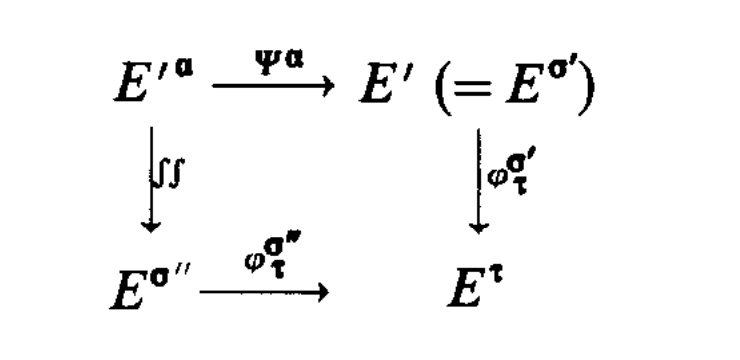
\includegraphics[width=0.43\textwidth]{assets/D040_p006_diagram_authority_400dpi.png}
\end{center}
(Notons que, étant donné $(\bR'',\bP) \in \sigma''$, il existe un unique $\bR' \in \cP_{J'}$ tel que $(\bR'',\bR') \in \alpha$ et $(\bR',\bP) \in \sigma'$; réciproquement, si $(\bR'',\bR') \in \alpha$ et $(\bR',\bP) \in \sigma'$, alors $(\bR'',\bP) \in \sigma''$. Cela donne l'isomorphisme $E'^{\alpha} \xrightarrow{\sim} E^{\sigma''}$.) Or l'application verticale de droite du diagramme est connue pour être un isomorphisme; de plus, d'après l'étape~2, l'application horizontale supérieure est un isomorphisme. Il s'ensuit que l'application horizontale inférieure $\varphi_{\tau}^{\sigma''}$ est un isomorphisme.

\smallskip
\noindent\textbf{Étape 4.} Soient $\sigma \in \cZ_J$ et $|J| = |I_0|$. (Ainsi, $\sigma$ correspond à un cône ouvert de $L$.) Nous montrons que $\varphi_{\rho}^{\sigma} \colon E^{\sigma} \to E$ est un isomorphisme. On peut trouver une suite $\sigma = \sigma_1, \sigma_2, \dots, \sigma_n = \rho$ d'éléments correspondant à des cônes ouverts de $L$, telle que (lorsqu'on les considère comme des cônes de $L$) deux cônes consécutifs aient une face commune de codimension~1; choisissons de plus $n$ aussi petit que possible. Soit $\tau$ l'élément correspondant à la face commune de codimension~1 de $\sigma = \sigma_1$ et $\sigma_2$. Par récurrence sur $n$, nous pouvons supposer que $\varphi_{\rho}^{\sigma_2}$ est un isomorphisme. L'étape~3 montre que $\varphi_{\tau}^{\sigma}$ et $\varphi_{\tau}^{\sigma_2}$ sont des isomorphismes. De $\varphi_{\rho}^{\sigma_2} = \varphi_{\rho}^{\tau} \varphi_{\tau}^{\sigma_2}$, il résulte que $\varphi_{\rho}^{\tau}$ est un isomorphisme. De $\varphi_{\rho}^{\sigma} = \varphi_{\rho}^{\tau} \varphi_{\tau}^{\sigma}$, il résulte que $\varphi_{\rho}^{\sigma}$ est un isomorphisme.

\smallskip
\noindent\textbf{Étape 5.} Soient $J \subset \bar S$ et $\sigma \in \cZ_J$. Nous voulons montrer que $\varphi_{\rho}^{\sigma}$ est un isomorphisme. On peut trouver $\widetilde J \subset J$ et $\widetilde{\sigma} \in \cZ_{\widetilde J}$ tels que $|\widetilde J| = |I_0|$, que $\sigma$ soit la face de type $J$ de $\widetilde{\sigma}$, et que $\varphi_{\sigma}^{\widetilde{\sigma}}$ soit du type considéré à l'étape~1 (et soit donc un isomorphisme).

\newpage
\noindent Nous avons $\varphi_{\rho}^{\sigma} \varphi_{\sigma}^{\widetilde{\sigma}} = \varphi_{\rho}^{\widetilde{\sigma}}$. D'après l'étape~4, $\varphi_{\rho}^{\widetilde{\sigma}}$ est un isomorphisme. Il s'ensuit que $\varphi_{\rho}^{\sigma}$ est un isomorphisme.

\smallskip
\noindent\textbf{Étape 6.} Soient $J \subset J'$ et $\sigma \in \cZ_J$; soit $\sigma' \in \cZ_{J'}$ la face de type $J'$ de $\sigma$. Nous voulons montrer que $\varphi_{\sigma'}^{\sigma}$ est un isomorphisme. Nous avons $\varphi_{\rho}^{\sigma'} \varphi_{\sigma'}^{\sigma} = \varphi_{\rho}^{\sigma}$. D'après l'étape~5, $\varphi_{\rho}^{\sigma}$ et $\varphi_{\rho}^{\sigma'}$ sont des isomorphismes. Il s'ensuit que $\varphi_{\sigma'}^{\sigma}$ est un isomorphisme.

Ceci achève la démonstration du lemme~3.3, et donc celle du théorème.

\section*{5}

Nous avons le corollaire suivant.

\medskip\noindent\textbf{COROLLAIRE (voir Alvis~[1]).}\quad
Dans la situation du théorème, soit $E^\#$ le noyau de $d_{i_0}$ dans \eqref{D040-eq:2.1}. Alors
\begin{enumerate}[label=(\alph*)]
\item $E^\#$ est un $G$-module irréductible,
\item $(E^\#)^\#$ est isomorphe à $E$ comme $G$-module,
\item $(-1)^{i_0} E^\# = \sum_{I \subset \bar S} (-1)^{|I|} E_{(I)}$ dans le groupe de Grothendieck des $G$-modules virtuels.
\end{enumerate}

L'assertion (c) est évidente.

Soit $E'$ un $G$-module du type considéré dans \eqref{D040-eq:3.1}, admettant une décomposition en somme directe $E' = E_1 \oplus \cdots \oplus E_n$, où les $E_i$ sont des $G$-modules irréductibles et $E_1 \cong E$. La démonstration du théorème~2 montre que $(E')^\#$ peut être défini de la même manière que $E^\#$ et qu'il possède les propriétés suivantes :
\begin{equation}\tag{5.1}\label{D040-eq:5.1}
(E')^\# \cong E_1^\# \oplus \cdots \oplus E_n^\#, \qquad E'^\# \cong E'.
\end{equation}
Pour tous $1 \leq i, j \leq n$, nous obtenons de (c)
\begin{equation}\tag{5.2}\label{D040-eq:5.2}
\langle E_i, E_j^\# \rangle = \langle E_i^\#, E_j \rangle = \sum_{I \subset \bar S} (-1)^{|I|+i_0} \langle E_i^{U_{P_I}}, E_j^{U_{P_I}} \rangle_{P_I}
\end{equation}
(où $\bP_I \in \cP_I$). Il s'ensuit que
\begin{equation*}
\langle E_i^\#, E' \rangle = \sum_j \langle E_i^\#, E_j \rangle = \sum_j \langle E_i, E_j^\# \rangle = \langle E_i, (E')^\# \rangle = \langle E_i, E' \rangle
\end{equation*}
et, en particulier, $E_i^\# \neq 0$. Si $E_i^\#$ n'était pas irréductible pour un certain $i$, alors $E_1^\# \oplus \cdots \oplus E_n^\#$ aurait plus de composantes irréductibles que $E_1 \oplus \cdots \oplus E_n$, ce qui contredirait \eqref{D040-eq:5.1}. Ainsi, $E_i^\#$ est irréductible pour tout $i$. Il existe donc une permutation $\pi$ de $\{1,2,\dots,n\}$ telle que $E_i^\# = E_{\pi(i)}$ pour tout $i$. D'après \eqref{D040-eq:5.2}, nous avons
\begin{equation*}
\langle E_{\pi^2(i)}, E_i \rangle = \langle (E_i^\#)^\#, E_i \rangle = \langle E_i^\#, E_i^\# \rangle = \langle E_{\pi(i)}, E_{\pi(i)} \rangle = 1.
\end{equation*}
Il s'ensuit que $E_{\pi^2(i)}$ est isomorphe à $E_i$. Le corollaire est démontré.

\newpage
\section*{Références}

\begin{enumerate}[label=\arabic*., leftmargin=*, itemsep=2pt]
\item D.~Alvis, The duality operation in the character ring of a finite Chevalley group, \textit{Bull. Amer. Math. Soc.} \textbf{1} (1979), 907--911.
\item C.~W.~Curtis, Truncation and duality in the character ring of a finite group of Lie type, \textit{J. Algebra} \textbf{62} (1980), 320--332.
\item R.~Howlett et G.~I.~Lehrer, Induced cuspidal representations and generalized Hecke rings, \textit{Invent. Math.} \textbf{58} (1980), 37--64.
\item N.~Kawanaka, Fourier transforms of nilpotently supported invariant functions on a simple Lie algebra over a finite field, prépublication, université d'Osaka.
\end{enumerate}


\clearpage\endgroup
\typeout{CORPUS-END:D040:\thepage}
% END INLINE WORK D040 FR
% BEGIN INLINE WORK D042 FR
\typeout{CORPUS-BEGIN:D042:\thepage}
\begingroup
\makeatletter
\let\DeclareMathOperator\CorpusDeclareMathOperator
\let\@declmathop\CorpusDeclMathOp
\let\maketitle\CorpusMakeTitle\let\title\CorpusTitle\let\author\CorpusAuthor\let\date\CorpusDate
\let\thanks\CorpusThanks\let\and\CorpusAnd\let\@maketitle\CorpusAtMakeTitle
\def\setcounter#1#2{\def\CorpusCounterName{#1}\def\CorpusPageName{page}\ifx\CorpusCounterName\CorpusPageName\else\CorpusSetCounter{#1}{#2}\fi}
\title{}\author{}\date{}
\expandafter\let\csname Spec\endcsname\CorpusUndefined
\expandafter\let\csname Spf\endcsname\CorpusUndefined
\expandafter\let\csname Lie\endcsname\CorpusUndefined
\expandafter\let\csname Pic\endcsname\CorpusUndefined
\expandafter\let\csname Ext\endcsname\CorpusUndefined
\expandafter\let\csname Hom\endcsname\CorpusUndefined
\expandafter\let\csname Res\endcsname\CorpusUndefined
\expandafter\let\csname Tr\endcsname\CorpusUndefined
\expandafter\let\csname OO\endcsname\CorpusUndefined
\expandafter\let\csname CC\endcsname\CorpusUndefined
\expandafter\let\csname GG\endcsname\CorpusUndefined
\expandafter\let\csname Aaff\endcsname\CorpusUndefined
\expandafter\let\csname PP\endcsname\CorpusUndefined
\expandafter\let\csname FF\endcsname\CorpusUndefined
\expandafter\let\csname ZZ\endcsname\CorpusUndefined
\expandafter\let\csname QQ\endcsname\CorpusUndefined
\expandafter\let\csname dual\endcsname\CorpusUndefined
\setcounter{section}{0}
\expandafter\def\csname theHsection\endcsname{D042.\arabic{section}}
\setcounter{subsection}{0}
\expandafter\def\csname theHsubsection\endcsname{D042.\arabic{subsection}}
\setcounter{subsubsection}{0}
\expandafter\def\csname theHsubsubsection\endcsname{D042.\arabic{subsubsection}}
\setcounter{equation}{0}
\expandafter\def\csname theHequation\endcsname{D042.\arabic{equation}}
\setcounter{figure}{0}
\expandafter\def\csname theHfigure\endcsname{D042.\arabic{figure}}
\setcounter{table}{0}
\expandafter\def\csname theHtable\endcsname{D042.\arabic{table}}
\setcounter{footnote}{0}
\expandafter\def\csname theHfootnote\endcsname{D042.\arabic{footnote}}
\makeatother
\let\tableofcontents\relax % one cumulative contents list, not repeated global lists
\titleformat{\section}{\large\bfseries}{}{0pt}{}
\titleformat{\subsection}{\normalsize\bfseries}{}{0pt}{}
\titlespacing*{\section}{0pt}{1.2ex plus .2ex}{.7ex}
\titlespacing*{\subsection}{0pt}{1ex plus .2ex}{.4ex}
\setlength{\parindent}{1.05em}
\setlength{\parskip}{.1em}
\setlength{\abovedisplayskip}{4pt plus 1pt minus 1pt}
\setlength{\belowdisplayskip}{4pt plus 1pt minus 1pt}
\setlength{\abovedisplayshortskip}{3pt plus 1pt}
\setlength{\belowdisplayshortskip}{3pt plus 1pt}
\setlength{\emergencystretch}{1.8em}
\DeclareMathOperator{\Spec}{Spec}
\DeclareMathOperator{\Spf}{Spf}
\DeclareMathOperator{\Lie}{Lie}
\DeclareMathOperator{\Pic}{Pic}
\DeclareMathOperator{\Ext}{Ext}
\DeclareMathOperator{\Hom}{Hom}
\DeclareMathOperator{\Res}{Res}
\DeclareMathOperator{\Tr}{Tr}
\newcommand{\OO}{\mathcal O}
\newcommand{\CC}{\mathbb C}
\newcommand{\GG}{\mathbb G}
\newcommand{\Aaff}{\mathbb A}
\newcommand{\PP}{\mathbb P}
\newcommand{\FF}{\mathbb F}
\newcommand{\ZZ}{\mathbb Z}
\newcommand{\QQ}{\mathbb Q}
\newcommand{\dual}{^{\vee}}
\pagestyle{plain}



\let\boldsymbol\symbfit % preserve bold italic multi-indices with unicode-math
\selectlanguage{french}
\phantomsection\addcontentsline{toc}{section}{D042}


\setcounter{page}{129}
% Authority physical 1; printed 129
\begin{center}
{\LARGE\bfseries Intégration sur un cycle évanescent}\par
\vspace{1.0em}
{\large P. Deligne}\par
\vspace{0.4em}
Institut des Hautes Etudes Scientifiques 35, route de Chartres, F-91440 Bures-sur-Yvette, France
\end{center}
\section*{Introduction}

Soient $k$ un corps commutatif et $f$ une série formelle en deux indéterminées $x$ et $y$ sur $k$:
\[
        f=\sum a_{n,m}x^n y^m .
\]
Soit $I(f)$ la série formelle en une indéterminée $t$
\[
        I(f)=\sum a_{n,n}t^n .
\]
Nous nous proposons de prouver le résultat suivant:

\medskip
\noindent\textbf{Théorème.} \emph{Si $f$ représente une fonction algébrique de $x$ et $y$, et si $k$ est de caractéristique $p\ne0$, $I(f)$ représente une fonction algébrique de $t$.}

\medskip
Pour $g$ une série formelle en $N$ indéterminées
\[
        g=\sum a_{\boldsymbol n}\boldsymbol x^{\boldsymbol n},
\]
on définit de même
\[
        I_N(g)=\sum a_{n\cdot\mathbf 1}t^n,
\]
et on a encore:

\medskip
\noindent\textbf{Corollaire.} \emph{Si $g$ est algébrique sur le corps $k(x_1,\ldots,x_N)$, et si $k$ est de caractéristique $p>0$, $I_N(g)$ est algébrique sur $k(t)$.}

\medskip
Sous l'hypothèse plus forte $g\in k(x_1,\ldots,x_N)$, ce résultat est dû à H. Furstenberg [1]. Voir aussi 3.10. Notre but premier était de donner une explication géométrique au résultat de Furstenberg.

Supposons tout d'abord que $k=\CC$ et que la série formelle $f$ soit convergente. La série $I(f)$ est alors convergente, et admet la représentation intégrale suivante
\begin{equation}
        I(f)(t)=\frac{1}{2\pi i}\oint_{xy=t} f(x,y)\frac{dx\wedge dy}{dt}. \tag{1}
\end{equation}
\par\smallskip
% Authority physical 2; printed 130
Expliquons le sens du membre de droite:

\medskip
\noindent a) Soit $\pi:\CC^2\to\CC$ l'application $(x,y)\mapsto xy$. L'expression $(dx\wedge dy)/dt$ est une forme différentielle holomorphe relative sur $\CC^2-\{(0,0)\}$, relative à la projection $\pi$, i.e. une famille de formes différentielles holomorphes sur les fibres, dépendant holomorphiquement de $t$. En $\{(0,0)\}$, c'est encore une section du faisceau dualisant relatif $\omega$, défini dans le formalisme de dualité de A. Grothendieck par $R\pi^!\OO=\omega[1]$. En terme de la coordonnée $y$ sur $\pi^{-1}(t)$, on a
\[
        \frac{dx\wedge dy}{dt}=\frac{d(t/y)\wedge dy}{dt}
        =\left(\frac{dt}{y}\wedge dy\right)/dt=\frac{dy}{y}.
\]

\noindent b) Supposons $f$ convergente dans le polydisque $B$ de rayons $R$. Pour $|t|$ assez petit ($|t|<R^2$), l'intersection de $B$ et de $\pi^{-1}(t)$ se projette isomorphiquement dans le plan des $y$ sur la couronne $|t|/R<|y|<R$. Soit $r$ tel que $|t|/R<r<R$. L'intégrale $\oint_{xy=t}$ est prise sur le cycle $|y|=r$, $|x|=|t|/r$, $xy=t$, qui se projette isomorphiquement sur la circonférence $|y|=r$, orientée positivement; elle ne dépend pas du choix de $r$.

Ces explications montrent que
\[
\frac{1}{2\pi i}\oint_{xy=t} f(x,y)\frac{dx\wedge dy}{dt}
=\frac{1}{2\pi i}\oint f(t/y,y)\frac{dy}{y}
=\frac{1}{2\pi i}\oint \sum a_{n,m}t^n y^{m-n}\frac{dy}{y}.
\]
Pour en déduire (1), on échange sommation et intégration, et on applique la formule des résidus: seuls subsistent les termes où $m=n$.

Le cycle d'intégration est le cycle évanescent (au sens de Lefschetz) pour $\pi$, près de $(0,0)$. Si on prend $r=|t|^{1/2}$, on le voit effectivement disparaître pour $|t|\to0$. Ceci explique le titre de l'article.

Dans la définition de $I(f)$, les indéterminées $x$ et $y$ jouent un rôle symétrique. Dans (1), un ordre entre $x$ et $y$ détermine deux choix de signes, qui s'annihilent: dans la forme différentielle relative, et dans l'orientation du cycle évanescent.

La formule (1) suggère que l'opération $I$ a un sens intrinsèque dans le cadre suivant: on part d'un morphisme de schémas formels $\pi:X\to S$ sur $k$, avec $X$ isomorphe à $\Spf k[[x,y]]$, $S$ isomorphe à $\Spf k[[t]]$, et $\pi$ ayant une singularité quadratique non-dégénérée. On suppose que les deux branches de $\pi^{-1}(0)$ sont définies sur $k$, et on choisit un ordre entre elles. En d'autres termes, on suppose qu'il existe des systèmes de coordonnées formelles $x,y$ sur $X$ et $t$ sur $S$ dans lesquelles $\pi$ soit $(x,y)\mapsto xy$; on prendra toujours ces systèmes de coordonnées de telle sorte que la première branche de $\pi^{-1}(0):xy=0$ soit la branche $x=0$.

Soient $\Omega^1_{X/k}$ les différentielles de Kähler, définies en tenant compte de la topologie: si $X=\Spf(A)$, avec $A$ isomorphe à $k[[x,y]]$ muni de la topologie $(x,y)$-adique, $\Omega^1_{X/k}$ correspond au $A$-module $\varprojlim\Omega^1_{(A/I)/k}$ (limite projective sur les idéaux ouverts). De même pour $S$. En coordonnées, $\Omega^1_{X/k}$ est le $\OO_X$-module libre de base $dx,dy$ et $\Omega^1_{S/k}$ est le $\OO_S$-module libre de base $dt$. Pour $M$ un module libre de rang $n$, posons $\det M=\bigwedge^nM$. Pour $L$ libre de rang 1, notons $L^{-1}$ son dual. Posons $\omega_{X/k}=\det\Omega^1_{X/k}$, $\omega_{S/k}=\Omega^1_{S/k}$ et soit $\omega_{X/S}$ le faisceau dualisant relatif
\[
        \omega_{X/S}=\pi^!\OO_S[1]=\omega_{X/k}\otimes\pi^*\omega_{S/k}^{-1}.
\]
\par\smallskip
% Authority physical 3; printed 131
En coordonnées, c'est le $\OO_X$-module libre de base $dx\wedge dy/dt$. On interprétera $I$ comme un morphisme
\[
        \pi_*\omega_{X/S}\longrightarrow\OO_S,
\]
i.e., pour $S=\Spf(V)$, comme un morphisme $V$-linéaire
\[
        H^0(X,\omega_{X/S})\longrightarrow V.
\]

Le paragraphe 1 fournit cette interprétation: on y prouve, pour $k$ quelconque, une formule qui est un analogue algébrique de (1). Le signe d'intégration, qui apparaît dans (1), y est remplacé par le morphisme trace local de Grothendieck. Précisons. Soit $t$ une uniformisante de $S$ (par exemple $t$ pour $S=\Spf(k[[t]])$). Nous noterons par $n$ en indice une réduction modulo $t^n$. On omettra l'indice quand il n'y a pas risque de confusion. Par exemple, on notera encore $\pi:X_n\to S_n$ le morphisme $\pi_n$ déduit de $\pi$ par réduction modulo $t^n$. On notera $\omega$ l'image inverse $(\omega_{X/S})_n$ de $\omega_{X/S}$ sur $X_n$. C'est le faisceau dualisant relatif $\omega_{X_n/S_n}$, de Grothendieck. Soit $A_n$ l'anneau local complet dont $X_n$ est le spectre formel (en coordonnées: $k[[x,y]]/((xy)^n)$). Il nous sera commode de travailler non pas avec le schéma formel $X_n$, mais avec le schéma ordinaire $X'_n:=\Spec A_n$. La différence est byzantine: tant $X_n$ que $X'_n$ sont une façon géométrique de parler de $A_n$. Soit $O$ le point fermé de $X'_n$ (en coordonnées: $x=y=0$). Le morphisme trace local de Grothendieck est un morphisme
\[
        \Tr:H^1_{\{O\}}(X'_n,\omega)\longrightarrow H^0(S_n,\OO).
\]
On a
\[
        H^1_{\{O\}}(X'_n,\omega)=\varinjlim \Ext^1_{A_n}(A_n/I,\omega),
\]
limite inductive sur les idéaux ouverts $I$ de $A_n$. C'est pour écrire cette limite inductive comme un groupe de cohomologie à support qu'il nous a fallu introduire $X'_n$.

Le rôle du cycle d'intégration (le cycle évanescent) sera joué par un élément $v_n\in H^1_{\{O\}}(X'_n,\OO)$. En coordonnées, cet élément est dans l'image de $\Ext^1_{A_n}(A_n/(x+y)^{2n-1},A_n)$. Prendre garde que l'exposant de $(x+y)$ requis croît avec $n$.

Au paragraphe 2, on considère un schéma en courbes $Y$ propre et plat sur $S$, dont $X$ se déduit par complétion en un point, et on relie les $v_n$ à un élément de $\Lie\Pic_S Y$. Au paragraphe 3 on globalise $X$ et $S$, et on prouve le théorème, et le corollaire.

\medskip
\noindent\emph{Notations.} On écrira en indice les changements de base. Par exemple, pour $X$ et $T$ des $S$-schémas, $X_T:=X\times_ST$. La réduction modulo $t^n$ est notée avec un indice $n$.

Pour notre propos, les conventions de signes utilisées sont sans importance. Pour que les résultats intermédiaires énoncés soient vrais -- et pas seulement au signe près -- il faut toutefois les choisir. Notre choix est explicité dans l'appendice.

\section*{1. Analogue algébrique de (1)}

\subsection*{1.1.}
Gardons les notations de l'introduction, et soient $x,y$ et $t$ des coordonnées sur $X$ et $S$, du type déjà considéré.
\par\smallskip
% Authority physical 4; printed 132
L'inclusion de $X'_1$ dans $X'_n$ est un homéomorphisme, puisque $X'_1$ est défini dans $X'_n$ par un idéal nilpotent. Le complément de l'origine $\{O\}$ dans $X'_n$ a donc deux composantes connexes, correspondant aux deux branches $x=0$ et $y=0$ de $X'_1$. Soit $u_n$ la section du faisceau structurel de $X_n-\{O\}$ qui vaut 1 sur la première branche et 0 sur la seconde. Dans le langage des anneaux: l'homomorphisme
\[
        A_n=k[[x,y]]/((xy)^n)\longrightarrow k[[x,y]]/(x^n)\times k[[x,y]]/(y^n)
\]
induit un isomorphisme
\[
        A_n((x+y)^{-1})\xrightarrow{\sim}
        (k[[x]]/(x^n))((y))\times(k[[y]]/(y^n))((x)),
\]
et $u_n\in A_n((x+y)^{-1})$ a pour image $(1,0)$. On peut expliciter:
\begin{equation}
        u_n=\left[\sum_{i=0}^{n-1}\binom{2n-i}{i}y^{2n-1-i}x^i\right]\big/(x+y)^{2n-1}. \tag{1.1.1}
\end{equation}
On définit $v_n$ comme étant l'image de $u_n$ par le morphisme cobord naturel
\[
        H^0(X'_n-\{O\},\OO)\longrightarrow H^1_{\{O\}}(X'_n,\OO).
\]
La suite exacte longue des $\Ext^i(*,A_n)$, appliquée à la suite exacte courte
\[
        0\longrightarrow ((x+y)^N)\longrightarrow A_n\longrightarrow A_n/((x+y)^N)\longrightarrow0
\]
donne lieu à un diagramme commutatif
\[
\begin{tikzcd}[column sep=1.5em,row sep=2.1em]
0 \arrow[r] & A_n \arrow[r] \arrow[d,equal] &
(x+y)^{-N}A_n \arrow[r] \arrow[d] &
\Ext^1_{A_n}(A_n/((x+y)^N),A_n) \arrow[d] \\
0 \arrow[r] & H^0(X'_n,\OO) \arrow[r] &
H^0(X'_n-\{O\},\OO) \arrow[r] & H^1_{\{O\}}(X'_n,\OO).
\end{tikzcd}
\]
Pour $N=2n-1$, ce diagramme et (1.1.1) montrent que $v_n$ est dans l'image de $\Ext^1_{A_n}(A_n/((x+y)^{2n-1}),A_n)$.

\subsection*{1.2. Proposition.}
\emph{Soit $f$ dans $k[[x,y]]$. Quel que soit $n$, on a}
\begin{equation}
        \Tr(f\,dx\wedge dy/dt\cdot v_n)\equiv -I(f)\pmod {t^n}. \tag{1.2.1}
\end{equation}
Dans (1.2.1), $\Tr$ est le morphisme trace local de Grothendieck. Il est appliqué à l'élément de $H^1_{\{O\}}(X'_n,\omega)$ produit de $f\,dx\wedge dy/dt$ dans $H^0(X'_n,\omega)$ et de $v_n$ dans $H^1_{\{O\}}(X'_n,\OO)$. Nous prouverons (1.2.1) sous l'hypothèse que $k$ est infini. On se ramène à ce cas par une extension des scalaires.

Notons $I'(f)$ le membre de gauche de (1.2.1). On a $I'(f)\in k[[t]]/(t^n)$. Si $J$ est un idéal ouvert de $A_n$, assez petit pour que $v_n$ soit dans l'image de $\Ext^1(A_n/J,A_n)$ (par exemple $J=((x+y)^{2n-1})$) et que $f\in J$, on a $fv=0$ et \emph{a fortiori} $I'(f)=0$: l'application $k[[t]]/(t^n)$-linéaire
\[
        I':A_n\longrightarrow k[[t]]/(t^n),\qquad f\longmapsto I'(f)
\]
est continue.
\par\smallskip
% Authority physical 5; printed 133
Pour $\lambda,\mu\in k$, soit $\sigma(\lambda,\mu)$ l'automorphisme $(x,y)\mapsto(\lambda x,\mu y)$, $t\mapsto\lambda\mu t$ de $(X,S,\pi)$. Il respecte $dx\wedge dy/dt$ et $v_n$. Par transport de structure, on a donc
\begin{equation}
        I'(\sigma(\lambda,\mu)^*f)=\sigma(\lambda,\mu)^*f. \tag{1.2.2}
\end{equation}
Posons $h_{n,m}(t)=I'(x^ny^m)$. Faisant dans (1.2.2) $\mu=\lambda^{-1}$, on trouve que $h_{n,m}(t)=\lambda^{n-m}h_{n,m}(t)$: on a $h_{n,m}=0$ pour $n\ne m$. Par continuité et $k[[t]]$-linéarité de $I'$, on a alors pour $f=\sum a_{n,m}x^ny^m$
\[
        I'(f)=I'\left(\sum a_{n,m}x^ny^m\right)
             =I'\left(\sum a_{n,n}x^ny^n\right)
             =I'(\pi^*I(f))=I(f)\cdot I'(1).
\]
Faisant dans (1.2.2) $\mu=1$ et $f=1$, on trouve $h_{0,0}(\lambda t)=h_{0,0}(t)$, de sorte que $I'(1)=h_{0,0}(t)$ est une constante $c$, et que $I'(f)=cI(f)$. Cette constante est indépendante de $n$. Pour prouver que $c=-1$, on peut donc supposer, et on supposera, que $n=1$.

Le schéma $X'_1=\Spec k[[x,y]]/(xy)$ est la réunion de deux arcs de courbe formels non singuliers se coupant transversalement, paramétrés le premier par $y$, le second par $x$. Les sections de $\omega$ sur $X'_1$ sont les systèmes de formes différentielles $\alpha$ et $\beta$ sur ces arcs, avec un pôle simple en $O$, et $\Res\alpha+\Res\beta=0$. Les sections de $\omega$ sur $X'_1-\{O\}$ sont les systèmes de formes $\alpha$ et $\beta$ avec un pôle d'ordre quelconque en $O$, et le morphisme composé
\[
\begin{tikzcd}[column sep=2.5em]
H^0(X'_1-\{O\},\omega) \arrow[r] & H^1_{\{O\}}(X'_1,\omega) \arrow[r,"tr"] & k
\end{tikzcd}
\]
est l'opposé de $(\alpha,\beta)\mapsto\Res\alpha+\Res\beta$. Avec ces notations, $dx\wedge dy/dt$ correspond à
\[
        \left(\frac{dy}{y},\,-\frac{dx}{x}\right),
\]
et $(dx\wedge dy/dt)u_1=\left(\frac{dy}{y},0\right)$, de somme des résidus 1. Ceci prouve (1.2.1).

\section*{2. Relation avec Pic}

\subsection*{2.1.}
Soient $S=\Spec k[[t]]$, $s$ le point fermé de $S$, $\eta$ le point générique, $\pi:Y\to S$ un morphisme propre et plat purement de dimension relative 1 et $O$ un point rationnel de $Y_s:=\pi^{-1}(s)$. On suppose que si $X$ est complété de $Y$ en $O$, le morphisme induit par $\pi$ de $X$ vers $S$ est du type considéré au paragraphe 1. Ceci signifie: $Y$ est régulier en $O$, $O$ est un point de non-lissité isolé de $\pi$, $\pi$ présente en $O$ une singularité quadratique non-dégénérée et les deux branches de $Y_s$ en $O$ sont définies sur $k$. On suppose choisi un ordre entre ces branches.

Il nous sera commode de supposer en outre $Y$ régulier et connexe. Faisons le changement de base $\eta\to S$ et soit $Y_{\eta}$ la courbe sur $k((t))$ fibre générale de $\pi:Y\to S$.

\subsection*{2.2. Lemme.}
\emph{La courbe $Y_{\eta}$ est absolument irréductible et génériquement lisse sur $k((t))$.}

La courbe $Y_s$ est connexe (car $Y$ est propre sur $S$ et connexe) et a un point rationnel, donc est absolument connexe. Elle est lisse près de $O$ ($O$ exclus),
\par\smallskip
% Authority physical 6; printed 134
donc a sur une extension séparable $k'$ de $k$ des points de lissité rationnels. Sur $S'=\Spec k'[[t]]$, $Y'=Y\times_SS'$ a donc une section. Le schéma $Y'$ est connexe, car $Y_s'$ est connexe, et régulier, car étale sur $Y$. Il est donc irréductible et $Y_{\eta}'$ est irréductible, donc connexe. Ayant un point rationnel, il est absolument connexe. Ceci montre que $Y_{\eta}$ est absolument connexe. Étant régulier, il est absolument irréductible. L'ouvert de lissité de $Y_{\eta}$, non vide par hypothèse, est nécessairement dense.

\subsection*{2.3. Interlude.}
Soient $C$ une courbe complète réduite et génériquement lisse (i.e. $C$ absolument réduite) sur un corps $K$ et $D$ un diviseur (de Cartier) sur $C$. Nous aurons à utiliser l'interprétation géométrique ci-dessous de $H^1(C,\OO(-D))$.

Supposons pour simplifier $C$ connexe et $D\ne\varnothing$. Ce cas nous suffira. Soit $\Pic(C;D)$ la jacobienne généralisée qui paramétrise les faisceaux inversibles sur $C$, trivialisés sur $D$. Plus précisément, on définit $\Pic(C;D)$ comme étant le $K$-schéma qui représente le foncteur sur les $K$-schémas
\[
T\longmapsto
\left(\begin{gathered}
\text{l'ensemble des classes d'isomorphie de faisceaux}\\
\text{inversibles sur $C_T$ trivialisés sur $D_T$}
\end{gathered}\right)
\]
On a posé $C_T=C\times_{\Spec K}T$ et de même pour $D$. C'est un $K$-schéma lisse. Notons $\OO(1\text{ sur }D)^*$ le faisceau des sections de $\OO^*$ de restriction 1 à $D$. On a
\[
        \Pic(C;D)(T)=H^1(C_T,\OO(1\text{ sur }D_T)^*).
\]
Prenant pour $T$ le spectre des nombres duaux sur $K$, on obtient
\begin{equation}
        \Lie\Pic(C;D)=H^1(C,\OO(-D)). \tag{2.3.1}
\end{equation}

Soit $\omega$ le faisceau dualisant sur $C$ ($\Omega^1_{C/K}$ pour $C$ lisse). Nous aurons à utiliser la dualité de Serre entre $H^0(C,\omega(D))$ et $H^1(C,\OO(-D))$. Elle admet l'interprétation géométrique suivante (qui ne nous servira pas). Supposons tout d'abord $C$ lisse. Quels que soient $T$ et la section $u:T\to C$ de $C_T/T$, l'image de $u$ est alors un diviseur de Cartier sur $C_T$. Le faisceau inversible $\OO(u(T))$ est canoniquement trivialisé sur le complément de $u(T)$. En particulier, si $u$ est une section de $(C-D)_T$, il est trivialisé sur $D_T$. Cette construction définit un morphisme
\begin{equation}
        j:C-D\longrightarrow\Pic(C;D),\qquad u\longmapsto\text{classe de }\OO(u(T)). \tag{2.3.2}
\end{equation}
L'image inverse par $j$ fournit un morphisme de l'espace vectoriel des formes différentielles invariantes sur $\Pic(C;D)$ -- le dual de l'algèbre de Lie -- dans $H^0(C-D,\omega)$. Il donne la dualité de Serre, i.e. le diagramme suivant est commutatif:
\[
\begin{tikzcd}[column sep=3.5em,row sep=2.5em]
(\Lie\Pic(C;D))^{\vee} \arrow[r,"j^*"] \arrow[d,equal,"{(2.3.1)}"] & H^0(C-D,\omega) \\
H^1(C,\OO(-D))^{\vee} \arrow[r,"\sim","{\text{(Serre)}}"'] & H^0(C,\omega(D)). \arrow[u]
\end{tikzcd}
\]
\par\smallskip
% Authority physical 7; printed 135
Pour $C$ seulement supposée absolument réduite, d'ouvert de lissité $U$ les mêmes arguments fournissent $j:U-D\longrightarrow\Pic(C;D)$. On a encore (2.3.2), avec $H^0(C-D,\omega)$ remplacé par
\[
        H^0(U-D,\omega)=H^0(U-D,\Omega^1).
\]

\subsection*{2.4.}
Soit $Z$ un diviseur de Cartier relatif sur $Y$, i.e. un diviseur dont aucune composante n'est contenue dans $Y_s$. On suppose que $O\notin Z$. La discussion 2.3 sera appliquée à $K=k((t))$, $C=Y_{\eta}$ et $D=Z_{\eta}$.

Soit $\Pic(Y;Z)^0$ le $S$-schéma en groupes qui paramétrise les faisceaux inversibles sur $Y$ $Z$-trivialisés dont la restriction à chaque composante irréductible de chaque fibre géométrique est de degré 0. Pour l'existence de $\Pic$, voir [2] 8.2. C'est un schéma en groupes lisse sur $S$, à fibres connexes. Sa fibre spéciale $\Pic(Y;Z)^0_s$ est la composante neutre du schéma en groupes $\Pic(Y_s;Z_s)$ qui classifie les faisceaux inversibles sur $Y_s$, $Z_s$-trivialisés.

Soit $Y'_s$ la courbe déduite de $Y_s$ par normalisation en $O$: on dispose de $h:Y'_s\to Y_s$, $h^{-1}(O)$ se compose de deux points $O_1$ et $O_2$ correspondant aux deux branches de $Y_s$ en $O$ et $Y_s$ se déduit de $Y'_s$ par identification de $O_1$ et $O_2$. En particulier, le morphisme $h$ induit un isomorphisme de $Y'_s-\{O_1,O_2\}$ avec $Y_s-\{O\}$. Par abus de notation, nous noterons encore $Z_s$ l'image inverse de $Z_s$ dans $Y'_s$. Le foncteur $h^*$ identifie faisceaux inversibles $\mathscr L$ sur $Y_s$ et faisceaux inversibles $\mathscr L'$ sur $Y'_s$, munis d'un isomorphisme
\[
        \sigma:\mathscr L'_{O_1}\xrightarrow{\sim}\mathscr L'_{O_2}
\]
entre les fibres en $O_1$ et $O_2$. Une trivialisation de $\mathscr L$ sur $Z_s$ correspond à une de $\mathscr L'$. En particulier, pour $\lambda\in k^*$, on obtient un faisceau inversible $\mathscr L_{\lambda}$ sur $Y_s$ trivialisé sur $Z_s$ en prenant $\mathscr L'_{\lambda}=\OO$ et pour $\sigma:k\to k$ la multiplication par $\lambda$. La même construction peut être répétée après un changement de base $T\to s$ (cf. ci-dessous), d'où un morphisme de $k$-schémas en groupes
\begin{equation}
        w_1:\GG_m\longrightarrow\Pic(Y_s,Z_s),\qquad \lambda\longmapsto\mathscr L_{\lambda}. \tag{2.4.1}
\end{equation}

Voici une construction analogue, modulo $t^n$. Soit $Y_n$ la réduction de $Y$ mod $t^n$, et $q:Y'_n\to Y_n$ coïncidant avec $Y_n$ en dehors de $O$ et qui, au voisinage de $O$, est obtenue comme suit: prenant «voisinage» au sens étale, on peut trouver des coordonnées locales $x,y$ dans lesquelles $Y_n$ s'écrit $(xy)^n=0$. On prend $Y'_n$ somme disjointe de $x^n=0$ et de $y^n=0$. Prendre garde que pour $n>1$, $Y'_n$ n'est pas plat sur $k[[t]]/(t^n)$. Un calcul local montre que $\OO_{Y_n}$ s'injecte dans $q_*\OO_{Y'_n}$. Ceci reste vrai après tout changement de base plat $T\to\Spec k[[t]]/(t^n)$. Définissons $Q_{n,T}$ par la suite exacte
\begin{equation}
        0\longrightarrow\OO_{Y_{n,T}}\longrightarrow q_*\OO_{Y'_{n,T}}\longrightarrow Q_{n,T}\longrightarrow0. \tag{2.4.2}
\end{equation}
C'est un faisceau de support l'image inverse $O_T$ de $O$ dans $Y_{n,T}$. Notant $\pi^{\bullet}$ une image inverse au sens des faisceaux par $\pi:Y_{n,T}\to T$, on dispose d'un morphisme de faisceaux
\begin{equation}
        \delta:(\pi^{\bullet}\OO_T)_{|O_T}\longrightarrow Q_{n,T} \tag{2.4.3}
\end{equation}
qui (localement près de $O$, pour la topologie étale) envoie $u$ sur l'image dans $q_*\OO_{Y'_{n,T}}/\OO_{Y_{n,T}}$ de la section de $\OO_{Y'_{n,T}}$ valant $u$ sur la première branche et 0 sur la seconde.
\par\smallskip
% Authority physical 8; printed 136
Passant au multiplicatif, on définit de même $Q^*_{n,T}$ par la suite exacte
\begin{equation}
        0\longrightarrow\OO^*_{Y_{n,T}}\longrightarrow q_*\OO^*_{Y'_{n,T}}\longrightarrow Q^*_{n,T}\longrightarrow0, \tag{2.4.4}
\end{equation}
et
\begin{equation}
        \delta^*:(\pi^{\bullet}\OO_T^*)_{|O_T}\longrightarrow Q^*_{n,T}. \tag{2.4.5}
\end{equation}
($\delta^*(u)$ image de «$u$ sur la première branche, 1 sur la seconde»).

Prenant le cobord $H^0\to H^1$ dans la suite exacte longue de cohomologie à support dans $O_T$ déduite de (2.4.2) (resp. (2.4.4)), on déduit de (2.4.3) (resp. (2.4.5)) des morphismes respectifs
\begin{equation}
        H^0(T,\OO_T)\longrightarrow H^1_{O_T}(Y_{n,T},\OO)\longrightarrow H^1(Y_{n,T},\OO(-Z_{n,T})) \tag{2.4.6}
\end{equation}
\begin{equation}
        H^0(T,\OO_T^*)\longrightarrow H^1_{O_T}(Y_{n,T},\OO^*)\longrightarrow H^1(Y_{n,T},\OO(1\text{ sur }Z_{n,T})^*). \tag{2.4.7}
\end{equation}
Le morphisme de foncteurs en $T$ (2.4.7) fournit un morphisme de $k[[t]]/(t^n)$-schémas de $\GG_m$ dans la réduction mod $t^n$ de $\Pic_Z(Y)^0$:
\begin{equation}
        w_n:\GG_m\longrightarrow\Pic(Y,Z)^0_n. \tag{2.4.8}
\end{equation}
Pour $m\le n$, $w_n$ a pour réduction mod $t^m$ le morphisme $w_m$, et pour $n=1$, on retrouve (2.4.1). D'après (SGA3 IX 3.6), il existe un et un seul morphisme (2.4.8) qui relève à $k[[t]]/(t^n)$ le $k$-morphisme (2.4.1). Nous utiliserons qu'il admet la description (2.4.7).

On ne peut pas passer à la limite sur $n$ pour déduire des $w_n$ un morphisme de schémas en groupes de $\GG_m$ dans $\Pic(Y;Z)^0$. Toutefois:

\noindent (a) pour $H$ un schéma fini sur $k[[t]]$ et $P$ quelconque, il revient au même de donner un morphisme $H\to P$ ou de donner un système cohérent de morphismes $H_n\to P_n$ entre les réductions mod $t^n$.

\noindent (b) pour $V$ et $W$ deux $k[[t]]$-modules libres, il revient au même de donner une application linéaire $\Gamma:V\to W$, ou de donner un système cohérent d'applications linéaires $V\otimes k[[t]]/(t^n)\to W\otimes k[[t]]/(t^n)$.

Pour tout entier $m$, on peut appliquer (a) au sous-schéma $\mu_m$ de $\GG_m$ noyau de $x\mapsto x^m:\GG_m\to\GG_m$: par passage à la limite sur $n$, on déduit des $w_n$ un morphisme
\begin{equation}
        w:\mu_m\longrightarrow\Pic(Y,Z)^0. \tag{2.4.9}
\end{equation}
On peut appliquer (b) après passage aux algèbres de Lie: on obtient
\begin{equation}
        dw:\Lie\GG_m\longrightarrow\Lie\Pic(Y;Z)^0. \tag{2.4.10}
\end{equation}
On a $\Lie\GG_m=\OO$, le module libre de rang un trivial, et les arguments 2.3 donnent encore un isomorphisme canonique $\Lie\Pic(Y;Z)^0=H^1(Y,\OO(-Z))$. La donnée de $dw$ équivaut donc à celle de l'image
\begin{equation}
        dw(1)\in H^1(Y,\OO(-Z)). \tag{2.4.11}
\end{equation}

Soient $\omega_{Y/S}=\pi^!\OO_S[1]$ le faisceau dualisant relatif et $\varphi$ une section de $\omega_{Y/S}(Z)$. Choisissons sur $X$, le complété de $Y$ en $O$, un système de coordonnées
\par\smallskip
% Authority physical 9; printed 137
formelles $x,y$ dans lesquelles $\pi$ soit $(x,y)\mapsto xy$, et où la première branche de $X_1$ soit $x=0$. Dans ce système de coordonnées, $\varphi$ s'écrit sur $X$
\[
        \varphi=f(x,y)\,dx\wedge dy/dt.
\]
La restriction de $\varphi_{\eta}$ à $Y_{\eta}$ appartient au $k((t))$-espace vectoriel $H^0(Y_{\eta},\omega(Z_{\eta}))$, en dualité de Serre avec $H^1(Y_{\eta},\OO(-Z_{\eta}))$. Notre but dans ce paragraphe est la

\subsection*{2.5. Proposition.}
\emph{Avec les notations précédentes, on a}
\begin{equation}
        I(f)=-\langle dw(1),\varphi\rangle. \tag{2.5.1}
\end{equation}
Sur $S$ tout entier, on dispose encore d'un accouplement entre $\Lie\Pic(Y;Z)^0=H^1(Y,\OO(-Z))$ et $H^0(Y,\omega(Z))$. Sous les hypothèses faites, ces $k[[t]]$-modules sont d'ailleurs libres, et l'accouplement une dualité parfaite. Le membre de droite de (2.5.1) est donc dans $k[[t]]$ (et non seulement dans $k((t))$). Sa réduction modulo $t^n$ est $\langle dw_n(1),\varphi\rangle$. Nous vérifierons (2.5.1) modulo $t^n$ pour chaque $n$.

Soient $X_n$ et $Y_n$ les réductions de $X$ et $Y$ modulo $t^n$. Le morphisme trace local: $H^1_{\{O\}}(X_n,\omega)\to k[[t]]/(t^n)$ et le morphisme trace global: $H^1(Y_n,\omega)\to k[[t]]/(t^n)$ (donnant la dualité de Serre) sont reliés par le diagramme commutatif
\[
\begin{tikzcd}[column sep=2.6em,row sep=2em]
H^1_{\{O\}}(X_n,\omega) \arrow[d] & H^1_{\{O\}}(Y_n,\omega) \arrow[l] \arrow[r] & H^1(Y_n,\omega) \arrow[d] \\
k[[t]]/(t^n) \arrow[rr,equal] & & k[[t]]/(t^n).
\end{tikzcd}
\]
Cette compatibilité ramène 2.5.1 au lemme

\subsection*{2.6. Lemme.}
\emph{Le morphisme}
\[
        H^1_{\{O\}}(X_n,\OO)\xleftarrow{\sim} H^1_{\{O\}}(Y_n,\OO(-Z_n))\longrightarrow H^1(Y_n,\OO(-Z_n))
\]
\emph{envoie $v_n$ sur $dw_n(1)$.}

On laisse au lecteur le soin de vérifier que l'image de $v_n$ est aussi l'image de 1 par (2.4.6). Le lemme résulte alors de la description de $d$ en terme des nombres duaux $D=(k[[t]]/(t^n))[\varepsilon]/(\varepsilon^2)$ sur $k[[t]]/(t^n)$ et de la suite exacte naturelle de morphismes
\[
        ((2.4.6)\text{ sur }k[[t]]/(t^n))\longrightarrow((2.4.7)\text{ sur }D)
        \longrightarrow((2.4.7)\text{ sur }k[[t]]/(t^n)).
\]

\section*{3. Preuve du théorème}

\subsection*{3.1.}
Soient $S_0$ une courbe lisse sur $k$ (un schéma lisse purement de dimension 1), $s$ un point rationnel de $S_0$ et $S$ le complété de $S_0$ en $s$. Soient $\pi:Y_0\to S_0$ propre et plat, purement de dimension relative 1, $Y$ l'image inverse de $Y_0$ sur $S$ et $O\in Y_s$. On note encore $\pi$ le morphisme de $Y$ dans $S$ déduit de $\pi:Y_0\to S_0$ et on suppose que $(\pi:Y\to S,O)$ est du type considéré au §2. On utilisera pour $(\pi:Y\to S,O)$ les notations du paragraphe 2.
\par\smallskip
% Authority physical 10; printed 138
Supposons enfin, pour simplifier, $Y_0$ régulier et $\pi$ à fibres géométriques connexes. Soit $\omega:=\omega_{Y_0/S_0}$ le faisceau dualisant relatif. Là où $Y_0$ est lisse sur $S_0$, c'est $\Omega^1_{Y_0/S_0}$. On note encore $\omega$ son image inverse sur $Y$, ou sur le complété $X$ de $Y$ en $O$. On choisit comme précédemment des coordonnées formelles sur $X$ et $S$.

Soit $\varphi$ une section rationnelle de $\omega$ sur $Y_0$, régulière en $O$. Sur $X$, on peut écrire $\varphi=f(x,y)dx\wedge dy/dt$. Notre résultat principal est la

\subsection*{3.2. Proposition.}
\emph{Si $k$ est de caractéristique $p>0$, $I(f)$ est algébrique sur le corps $k(S_0)\subset k((t))$ des fonctions rationnelles sur $S_0$.}

Quitte à remplacer $\varphi$ par son produit avec une fonction rationnelle sur $S_0$ s'annulant suffisamment en $s$, et à remplacer $S_0$ par un ouvert de Zariski contenant $s$, on peut supposer et on suppose que pour $Z_0$ un diviseur de Cartier relatif convenable sur $Y_0$, ne contenant pas $O$, $\varphi$ est une section de $\omega$ sur $Y_0-Z_0$.

Soit $\Pic(Y_0;Z_0)^0$ le schéma en groupe sur $S_0$ qui paramétrise les faisceaux inversibles sur $Y_0$, $Z_0$-trivialisés, de degré 0 sur chaque composante irréductible de chaque fibre géométrique (si nécessaire pour appliquer [2], rétrécir $S_0$ davantage). On interprète $\varphi$ comme correspondant à une section $\varphi'$ du dual du fibré $\Lie\Pic(Y_0;Z_0)=R^1\pi_*\OO(-Z_0)$ sur $S_0$ (dualité de Serre; on a l'interprétation géométrique (2.3) $\varphi=j^*\varphi'$).

Après le changement de base de $S_0$ à $S$, on dispose de $dw:\OO\to\Lie\Pic(Y_0,Z_0)^0_S=\Lie\Pic(Y;Z)^0$ (2.4.10) et la proposition résulte de 2.5 et du

\subsection*{3.3. Lemme-clef.}
\emph{Si $p>0$, $dw$ est algébrique sur $S_0$.}

En caractéristique $p>0$, l'inclusion $\mu_p\subset\GG_m$ induit un isomorphisme sur les algèbres de Lie:
\[
        \Lie(\mu_p)\xrightarrow{\sim}\Lie(\GG_m).
\]
Par réduction mod $t^n$, on vérifie que $dw$ est la différentielle du morphisme (2.4.9) $w:\mu_p\to\Pic_Z(Y)^0$. Il ne reste qu'à utiliser la rigidité de $\mu_p$: pour tout schéma en groupes commutatif plat $P$ sur $S_0$, $\Hom(\mu_p,P)$ est représenté par un schéma étale sur $S_0$. Faisons $P=\Pic(Y_0;Z_0)$, et soit $\widetilde S_0$ le $S_0$-schéma obtenu. Par définition, on dispose sur $\widetilde S_0$ d'un morphisme universel
\begin{equation}
        \mathrm{un}:\mu_p\longrightarrow\Pic(Y_0;Z_0)_{\widetilde S_0}. \tag{3.3.1}
\end{equation}
En particulier, le morphisme 2.4.9 est l'image inverse de 3.3.1 par un $S_0$-morphisme $b$:
\[
\begin{tikzcd}[column sep=1.4em,row sep=1.6em]
S \arrow[rr,"b"] \arrow[dr] & & \widetilde S_0 \arrow[dl] \\
& S_0 &
\end{tikzcd}
\]
De même, $dw$ est l'image inverse par $b$ du morphisme de $\OO$ dans $\Lie\Pic(Y_0;Z_0)_{\widetilde S_0}$ déduit par passage aux algèbres de Lie de l'homomorphisme (3.3.1), et, $\widetilde S_0$ étant quasi-fini sur $S_0$, ceci établit son algébricité.
\par\smallskip
% Authority physical 11; printed 139
\subsection*{3.4.}
Notons $k\{x_1,\ldots,x_N\}$ l'hensélisé de l'anneau local de l'espace affine $\Spec k[x_1,\ldots,x_N]$ en 0. Le complété de cet anneau local est $k[[x_1,\ldots,x_N]]$ et il résulte de [3] XI §3 cor. 1 que pour que $g\in k[[x_1,\ldots,x_N]]$ soit algébrique sur le corps $k(x_1,\ldots,x_N)$, il faut et il suffit que $g$ soit dans $k\{x_1,\ldots,x_N\}$.

\subsection*{3.5. Preuve du théorème.}
D'après 3.4, que $f$ soit algébrique signifie qu'il existe une surface $Y'_0$, munie d'un point rationnel $O$, un morphisme étale $h$ envoyant $O$ sur 0 de $Y'_0$ dans le plan $\Aaff^2$ (coordonnées $x,y$) et une section $\widetilde f$ de $\OO$ sur $Y'_0$ de développement en série de puissances $f$ en $O$. Soient $S'_0$ la droite $\Aaff^1$ (coordonnée $t$) et $\pi'$ le morphisme composé
\[
        \pi':Y'_0\xrightarrow{h}\Aaff^2\xrightarrow{xy}S'_0.
\]
Sur $Y'_0$, soit $\varphi$ la section $\widetilde f\cdot h^*(dx\wedge dy/dt)$ du faisceau dualisant relatif. Compactifiant $Y'_0$ et résolvant les singularités introduites, on obtient
\[
\begin{tikzcd}[column sep=3em,row sep=2em]
Y'_0 \arrow[r] \arrow[d,"\pi'"'] & Y_0 \arrow[d,"\pi''"] \\
S'_0 \arrow[r,equal] & S'_0.
\end{tikzcd}
\]
avec $\pi''$ propre et plat et $Y_0$ régulier. Sur $Y_0$, $\varphi$ apparaît comme une section rationnelle du faisceau dualisant relatif. Pour que $\pi$ soit à fibres géométriques connexes, on remplace $S'_0$ par l'espace $S_0$ de la factorisation de Stein
\[
        Y_0\xrightarrow{\pi}S_0\longrightarrow S'_0
\]
de $\pi''$. Il ne reste qu'à appliquer 3.2 à $\varphi$.

\subsection*{3.6. Preuve du corollaire.}
On procède par récurrence sur $N$. Le cas $N=0$ est laissé au lecteur, le cas $N=1$ est trivial, le cas $N=2$ est le théorème et on suppose $N\ge3$. Pour $g$ dans $k[[x_1,\ldots,x_N]]$, posons
\[
        g=\sum g_{nm}x_{N-1}^n x_N^m
\]
avec $g_{nm}\in k[[x_1,\ldots,x_{N-2}]]$, et
\[
        I(g)=\sum g_{nn}x_{N-1}^n.
\]
On a
\begin{equation}
        I_N(g)=I_{N-1}I(g). \tag{3.6.1}
\end{equation}
Si $g$ est algébrique: $g\in k\{x_1,\ldots,x_N\}$ (3.4), les $g_{nm}$ sont algébriques: $g_{nm}\in k\{x_1,\ldots,x_{N-2}\}$. Soit $k'$ le corps des fractions de $k\{x_1,\ldots,x_{N-2}\}$, et considérons le diagramme commutatif
\[
\begin{tikzcd}[column sep=1.2em,row sep=2em]
k[[x_1,\ldots,x_N]] \arrow[r,phantom,"\supset"] \arrow[d,"I"] &
k\{x_1,\ldots,x_{N-2}\}[[x_{N-1},x_N]] \arrow[r,phantom,"\subset"] \arrow[d,"I"] &
k'[[x_{N-1},x_N]] \arrow[d,"I"] \\
k[[x_1,\ldots,x_{N-1}]] \arrow[r,phantom,"\supset"] &
k\{x_1,\ldots,x_{N-2}\}[[x_{N-1}]] \arrow[r,phantom,"\subset"] & k'[[x_{N-1}]]
\end{tikzcd}
\]
(en première ligne, des $k[x_1,\ldots,x_N]$-algèbres, en seconde, des $k[x_1,\ldots,x_{N-1}]$-algèbres). Appliquons le théorème à l'image $g'$ de $g$, supposé algébrique, dans $k'[[x_{N-1},x_N]]$. Puisque $k'$ est algébrique sur le corps des fractions de
\par\smallskip
% Authority physical 12; printed 140
$k[x_1,\ldots,x_{N-2}]$, $I(g')$, algébrique sur $k'(x_{N-1})$, vérifie une équation non triviale
\[
        \sum a_iI(g')^i=0
\]
à coefficients $a_i\in k[x_1,\ldots,x_{N-1}]$. La même équation est vérifiée par $I(g)$, d'où l'algébricité de $I(g)$: $I(g)\in k\{x_1,\ldots,x_{N-1}\}$. On conclut par (3.6.1) et l'hypothèse de récurrence.

\subsection*{3.7.}
On peut extraire de la preuve du théorème une estimation sur le degré $d$ de l'équation qui exprime que $I(f)$ est algébrique sur $k(t)$. Avec les notations de 3.5 et 3.1, supposons que $S_0$ est de degré $\sigma$ sur $S'_0$, que $Y_{\eta}$ est de genre $g$ et que $Z_{\eta}$ a $z'$ points géométriques. Posons $z=\sup(0,z'-1)$. Le genre est ici le genre de la normalisée de la courbe $Y_{\bar{\eta}}$ déduite de $Y_{\eta}$ par extension des scalaires à une clôture algébrique $k(\bar{\eta})$ de $k(\eta)$: le premier nombre de Betti $l$-adique de $Y_{\bar{\eta}}-Z_{\bar{\eta}}$ est $2g+z$. On a
\begin{equation}
        d\le\sigma\cdot p^{g+z}. \tag{3.7.1}
\end{equation}
Le degré de $I(f)$ sur $k(S_0)$ est $\le p^{g+z}$ (et même $\le\sup((p^g-1)p^z,z'!)$).

Si $f$ est une série formelle algébrique à coefficients entiers et qu'on définit $\sigma$, $g$ et $z$ en terme de $f\in\QQ[[x,y]]$, on en déduit que le degré $d_p$ de la réduction mod $p$ de $I(f)$ vérifie pour presque tout $p$
\begin{equation}
        d_p\le\sigma\cdot p^{g+z}. \tag{3.7.2}
\end{equation}
On peut aussi obtenir des informations mod $p^m$: utilisant que sur une base où $p^m=0$, on a $\Lie(\mu_{p^m})\xrightarrow{\sim}\Lie(\GG_m)$, on trouve que pour presque tout $p$ la réduction de $I(f)$ mod $p^m$ vérifie une équation à coefficients dans $\ZZ/(p^m)[t]$ non tous divisibles par $p$ de degré $\le\sigma\cdot p^{m(g+z)}$.

\subsection*{3.8.}
Je ne sais pas obtenir d'informations mod $p^m$ pour tout $p$. Si on essaye dans la preuve du théorème de remplacer $k$ par un anneau commutatif $A$ où $p^m=0$, une difficulté apparaît: celle de construire $Y_0/S_0$ pas trop mauvais (par exemple plat) non seulement près de $O$, mais partout.

\subsection*{3.9.}
La démonstration 3.6 du corollaire ne me satisfait pas. Il serait plus intéressant de traiter directement le cas de $n$ variables, en s'inspirant de l'analogue suivant de la formule intégrale (1): sur $\CC$, pour $g$ convergente, on a
\begin{equation}
        I(g)(t)=\int_{Z(t)} g\cdot dz_1\ldots dz_n/dt, \tag{1'}
\end{equation}
l'intégrale étant prise sur un cycle
\[
        Z(t)=\{(x_1,\ldots,x_n)\mid x_1\ldots x_n=t,
        |x_1|=r_1,\ldots,|x_m|=r_n\}
\]
avec $\prod r_i=|t|$.

J'espère qu'une démonstration directe fournirait dans le cas des séries formelles algébriques à coefficients entiers, une estimation $d_p\le O(p^{\beta})$ pour le degré de la réduction de $I(g)$ modulo $p$ sur $\FF_p(t)$.

Donner les outils requis pour une démonstration directe serait un test pour une théorie $p$-adique des cycles évanescents.

\subsection*{3.10.}
La démonstration de Furstenberg du corollaire (pour $g$ rationnel) montre que si $g\in k[[x_1,\ldots,x_N]]$ est l'une des composante d'un vecteur colonne $h$
\par\smallskip
% Authority physical 13; printed 141
d'éléments de $k[[x_1,\ldots,x_N]]$ qui vérifie un système d'équations $h=Ah^p$ pour $A$ une matrice carrée à coefficients polynomiaux, alors $I(g)$ a la même propriété, donc est algébrique. Ce type d'équation est réminiscent des $F$-cristaux en cohomologie cristalline.

Parallèlement, $T_p\Pic$ est un avatar du $H^1$ $p$-adique. Ceci me fait espérer que la démonstration de Furstenberg et celle donnée ici sont moins éloignées l'une de l'autre qu'il n'y paraît.

\section*{Appendice}
{\large\itshape Signes}\par
\medskip

Le traitement dans la littérature des questions de signes dans le formalisme de dualité des faisceaux algébriques cohérents m'a semblé confus. Le texte de Hartshorne, \emph{Residues and Duality} (Lect. Notes 20), souffre des défauts suivants:

\noindent (a) la convention qui définit les complexes $\Hom^{\bullet}(K,L)$ (I 6 p. 63, 64) et $K\otimes L$ (II 4 p. 93) n'est pas la convention usuelle; contrairement à ce qui est affirmé p. 64, $\Hom^{\bullet}$ ne commute pas (identiquement) aux foncteurs de translation (cf. SGA4 XVII 0.3); de même pour $\otimes$, dont l'associativité requiert la définition d'un isomorphisme canonique, qui n'est pas donnée. Du fait que dans la définition de $f^!$ pour $f:X\to Y$ lisse purement de dimension relative $n$ apparaît le produit tensoriel avec $\Omega^n_{X/Y}[n]$, cette lacune importe.

\noindent (b) Pour autant que je puisse néanmoins comprendre la convention proposée, la définition III 4.3 du morphisme trace, basée sur la convention qui dans III 3.4 définit $\gamma$, me semble incompatible à III 10.5 TRA1).

Les conventions exposées ci-dessous sont je crois cohérentes. J'y utilise la convention de signe usuelle pour $\otimes$ (SGA4 XVII 1.1). Je ne me suis pas limité à la dimension 1, qui suffirait aux besoins de l'article.

\noindent (a) Pour $f:X\to S$ plat d'intersection complète relative, purement de dimension relative $n$, le faisceau dualisant relatif $\omega_{X/S}$ est lié au complexe dualisant relatif $K_{X/S}:=Rf^!\OO_S$ par
\begin{equation}
        K_{X/S}=\omega_{X/S}[n]. \tag{S.1}
\end{equation}
C'est un faisceau inversible. Pour $X$ lisse sur $S$, on a $\omega_{X/S}=\Omega^n_{X/S}$. Si, comme suggéré dans mon appendice au livre de Hartshorne, on définit $Rf^!$ par adjonction, l'égalité $\omega_{X/S}=\Omega^n_{X/S}$ est un isomorphisme canonique, dont la définition pose un problème de signe. Nous adoptons ici le point de vue inverse (cf. la façon dont Hartshorne traite des morphismes lissifiables), où cette égalité est évidente sur la définition de $Rf^!$ et où le problème de signe est dans la définition du morphisme trace (S.5) ci-dessous.

Si $X$ est le produit fibré sur $S$ des $f_i:X_i\to S$ ($i\in I$), où chacun des $X_i$ est plat d'intersection complète relative purement de dimension relative $n_i$ avec $n=\sum n_i$, on a
\begin{equation}
        K_{X/S}=\boxtimes_i K_{X_i/S} \tag{S.2}
\end{equation}
(produit tensoriel externe). Par définition, la donnée d'un tel isomorphisme est la donnée, pour chaque ordre total sur $I$, d'un isomorphisme
\begin{equation}
        \omega_{X/S}=\boxtimes_i\omega_{X_i/S}. \tag{S.3}
\end{equation}
On exige que quand on passe de l'ordre total $<_1$ à l'ordre total $<_2$, l'isomorphisme change par le signe $(-1)^N$, $N=\sum n_in_j$ (somme sur les $(i,j)$ avec $i<_1j$ et $i>_2j$). Pour $X_i$ lisse sur $S$, on a $\omega_{X_i/S}=\Omega^{n_i}_{X_i/S}$ et (S.3) est donné par le produit extérieur, pris dans l'ordre donné sur $I$. Il a la propriété de parité voulue.

Pour un morphisme itéré $f=gh:X\xrightarrow{h}Y\xrightarrow{g}S$, $K_{X/S}$ est le $\otimes$ des complexes $K_{X/Y}$ et $h^*K_{Y/S}$ par un isomorphisme qui, appliqué à $X_1\times_SX_2\to X_1\to S$, redonne (S.3).
\par\smallskip
% Authority physical 14; printed 142
\noindent (b) Pour $f:X\to S$ comme en (a) et propre, le morphisme trace est un morphisme
\begin{equation}
        \Tr:Rf_*K_{X/S}\longrightarrow\OO_S. \tag{S.4}
\end{equation}
Le morphisme (S.4) induit un morphisme de faisceaux cohérents $\mathcal H^0Rf_*K_{X/S}\to\OO_S$, i.e. un morphisme
\begin{equation}
        \Tr:R^nf_*\omega_{X/S}\longrightarrow\OO_S. \tag{S.5}
\end{equation}
Précisons comment on passe de (S.4) à (S.5). Pour tout complexe $K$, le complexe $K[d]$ est le complexe de composantes $(K[d])^i=K^{i+d}$ et de différentielle celle de $K$ modifiée par le signe $(-1)^d$. On identifie les $\mathcal H^i(K[d])$ aux $\mathcal H^{i+d}K$ sans introduire de signe. Le foncteur $Rf_*$ commute au foncteur de translation $[d]$, et (S.5) se déduit de (S.4) par application du foncteur $\mathcal H^0$: utiliser l'isomorphisme
\[
\begin{aligned}
\mathcal H^0Rf_*K_{X/S}
&=\mathcal H^0Rf_*(\omega_{X/S}[n])
 =\mathcal H^0(Rf_*(\omega_{X/S})[n])\\
&=\mathcal H^nRf_*\omega_{X/S}=R^nf_*\omega_{X/S}.
\end{aligned}
\]
Pour $s$ une section de $f$, on dispose aussi du morphisme trace local
\begin{equation}
        \Tr:Rs^!K_{X/S}\longrightarrow\OO_S. \tag{S.6}
\end{equation}
La définition de (S.4) et celle de (S.6) posent, pour chaque dimension relative $n$, un problème de signes. Nous imposons la commutativité du diagramme
\[
\begin{tikzcd}[column sep=3em,row sep=1.5em]
Rs^!K_{X/S} \arrow[r] \arrow[d] & Rf_*K_{X/S} \arrow[d] \\
\OO_S \arrow[r,equal] & \OO_S
\end{tikzcd}
\quad;
\]
ceci relie, en chaque dimension relative, les choix (S.4) et (S.6). Le morphisme en première ligne du diagramme est dérivé du morphisme d'inclusion $s^!\to f_*$ ((sections à support schématique $s(S)$)$\subset$(toutes les sections)). Pour des $X_i$ comme en (a), propres sur $S$, donc donnant lieu par (S.3) à un isomorphisme
\[
        Rf_*K_{X/S}=\bigotimes_i Rf_{i*}K_{X_i/S},
\]
nous imposons que le morphisme (S.4) pour $X/S$ soit le produit tensoriel des morphismes (S.4) pour les $X_i/S$. Ceci relie les conventions utilisées en chaque dimension relative et ne laisse subsister qu'une seule ambiguïté de signe. Nous la résolvons en demandant que pour $X$ une courbe lisse sur $k$ algébriquement clos et $x\in X(k)$, le morphisme trace local
\begin{equation}
        \mathbf H^0_{\{x\}}(X,\Omega^1_X[1])\longrightarrow k, \tag{S.7}
\end{equation}
induisant (S.6) pour $s$ l'inclusion de $x$, soit le suivant. Le complexe $\Omega^1_X[1]$ réduit au faisceau $\Omega^1_X$ en degré cohomologique $-1$ s'envoie quasi-isomorphiquement dans le complexe réduit aux degrés $-1$ et 0
\[
        L:=\Omega^1_X(\infty\cdot x)\longrightarrow\Omega^1_X(\infty\cdot x)/\Omega^1_X.
\]
On a
\[
\begin{aligned}
\mathbf H^0_{\{x\}}(X,\Omega^1_X[1])&\xrightarrow{\sim}\mathbf H^0_{\{x\}}(X,L)
\xleftarrow{\sim}H^0\Gamma_{\{x\}}(X,L)\\
&=(\Omega^1_X(\infty\cdot x)/\Omega^1_X)_x,
\end{aligned}
\]
(parties polaires, en $x$, de formes différentielles), et on prend pour morphisme trace local le morphisme résidu $\Res_x$.

Indiquons quelques compatibilités auxquelles donne lieu ce choix de signes. Pour simplifier les notations, nous prendrons pour $S$ le spectre d'un corps $k$.

\noindent (c) Soient $X$ une courbe lisse sur $k$ algébriquement clos et $x\in X(k)$. Appelons encore «trace» le morphisme déduit de (S.7)
\[
        \Tr:H^1_{\{x\}}(X,\Omega^1_X)\longrightarrow k.
\]
Soit $L'$ le complexe réduit aux degrés 0 et 1
\[
        L':=\Omega^1_X(\infty\cdot x)\longrightarrow\Omega^1_X(\infty\cdot x)/\Omega^1_X.
\]
Il diffère par un signe de $L[-1]$. À cause de ce signe, $\Tr$ est l'opposé du morphisme composé
\[
        H^1_{\{x\}}(X,\Omega^1_X)\xleftarrow{\sim}H^1\Gamma_{\{x\}}L'
        =\text{(parties polaires en }x)\xrightarrow{\Res}k.
\]
\par\smallskip
% Authority physical 15; printed 143
La suite de foncteurs $\Gamma_{\{x\}}(X,-)\to\Gamma(X,-)\to\Gamma(X-\{x\},-)$, qui est exacte courte quand appliquée à un faisceau flasque, fournit un morphisme cobord $\partial:H^0(X-\{x\},\Omega^1)\to H^1_{\{x\}}(X,\Omega^1)$. On a
\[
        \Tr\circ\partial=-\Res_x.
\]
Enfin, pour $X$ complète, le morphisme cobord attaché à la suite exacte courte de faisceaux
\[
        0\longrightarrow\Omega^1_X\longrightarrow\text{(formes différentielles rationnelles)}
        \longrightarrow\text{(parties polaires)}\longrightarrow0,
\]
composé avec le morphisme trace, est la somme des morphismes résidus en tous les points $x\in X(k)$.

\noindent (d) Pour $X=X_1\times X_2$, avec $X_i$ complet localement d'intersection complète purement de dimension $n_i$, et pour $u_i\in H^{n_i}(X_i,\omega_{X_i})$, soient $n=n_1+n_2$ et $\operatorname{pr}_1^*u_1\cup\operatorname{pr}_2^*u_2\in H^n(X,\omega_X)$ le cup-produit, rel. à (S.3): $\operatorname{pr}_1^*\omega_{X_1}\otimes\operatorname{pr}_2^*\omega_{X_2}\xrightarrow{\sim}\omega_X$. La compatibilité exigée des morphismes trace au produit s'écrit
\[
        \Tr(\operatorname{pr}_1^*u_1\cup\operatorname{pr}_2^*u_2)
        =(-1)^{n_1n_2}\Tr(u_1)\cdot\Tr(u_2).
\]

\noindent (e) Pour $k=\CC$, et pour la topologie transcendante, on dispose d'un morphisme trace
\[
        \int:H^{2n}(X(\CC),\CC)\longrightarrow\CC.
\]
Si $\Omega^{**}$ est le complexe de De Rham $C^{\infty}$, le quasi-isomorphisme $\CC\to\Omega^{**}$ fournit un isomorphisme $H^{2n}(X(\CC),\CC)=(2n\text{-formes})/(\text{formes exactes})$, et $\int$ est l'intégration sur $X(\CC)$, muni de son orientation usuelle. Il nous sera plus commode de regarder $\int$ comme un morphisme $\mathbf H^0(X(\CC),\CC[2n])\to\CC$. Ce décalage pair dans les degrés ne pose aucun problème de signes. Soit $\Omega^*$ le complexe de De Rham holomorphe. Les quasi-isomorphismes et morphismes
\[
        \CC[2n]\xrightarrow{\sim}\Omega^*[2n]\longleftarrow\Omega^n[n]
\]
fournissent en cohomologie (pour la topologie transcendante)
\[
        \varepsilon:\mathbf H^0(X(\CC),\Omega^n[n])\longrightarrow \mathbf H^0(X(\CC),\CC[2n]).
\]
On a $H^0(X(\CC),\Omega^n[n])=H^0(X,\Omega^n[n])$ (GAGA), et entre les deux morphismes trace la relation
\[
        \Tr(u)=\frac{1}{(2\pi i)^n}\int \varepsilon(u).
\]

\noindent (f) Soient $\PP^n$ l'espace projectif de dimension $n$, $(T_i)_{0\le i\le n}$ un système de coordonnées homogènes, $U_i$ l'ouvert $T_i\ne0$ et $t_i=T_i/T_0$. On ordonne de façon évidente l'ensemble d'indices $[0,n]$ du recouvrement ouvert $(U_i)$. La section
\[
        \frac{dt_1}{t_1}\wedge\cdots\wedge\frac{dt_n}{t_n}
\]
de $\Omega^n$ sur l'intersection $U_{0\ldots n}$ des $U_i$ définit un cocycle de Čech, d'où une classe dans $H^n(\PP^n,\Omega^n)$. On a
\[
        \Tr\left(\frac{dt_1}{t_1}\wedge\cdots\wedge\frac{dt_n}{t_n}\right)
        =(-1)^{n(n+1)/2}.
\]

\begin{center}
{\Large\bfseries Bibliographie}
\end{center}
\begin{enumerate}[label=\arabic*.,leftmargin=2em,itemsep=0pt,topsep=0.3em]
\item Furstenberg, H.: Algebraic functions over finite fields. J. of Algebra 7, 271--277 (1967)
\item Raynaud, M.: Spécialisation du foncteur de Picard. Publ. Math. IHES 38, 27--76 (1970)
\item Raynaud, M.: Anneaux locaux henséliens. Lecture Notes in Mathematics, vol. 169. Berlin-Heidelberg-New York: Springer 1970
\end{enumerate}

\vspace{1.2em}
\begin{center}
Oblatum 30-X-1983
\end{center}
\vfill

\clearpage\endgroup
\typeout{CORPUS-END:D042:\thepage}
% END INLINE WORK D042 FR
% BEGIN INLINE WORK D043 FR
\typeout{CORPUS-BEGIN:D043:\thepage}
\begingroup
\makeatletter
\let\DeclareMathOperator\CorpusDeclareMathOperator
\let\@declmathop\CorpusDeclMathOp
\let\maketitle\CorpusMakeTitle\let\title\CorpusTitle\let\author\CorpusAuthor\let\date\CorpusDate
\let\thanks\CorpusThanks\let\and\CorpusAnd\let\@maketitle\CorpusAtMakeTitle
\def\setcounter#1#2{\def\CorpusCounterName{#1}\def\CorpusPageName{page}\ifx\CorpusCounterName\CorpusPageName\else\CorpusSetCounter{#1}{#2}\fi}
\title{}\author{}\date{}
\expandafter\let\csname Trace\endcsname\CorpusUndefined
\expandafter\let\csname Gal\endcsname\CorpusUndefined
\expandafter\let\csname End\endcsname\CorpusUndefined
\expandafter\let\csname Br\endcsname\CorpusUndefined
\expandafter\let\csname Spec\endcsname\CorpusUndefined
\expandafter\let\csname cl\endcsname\CorpusUndefined
\expandafter\let\csname ImOp\endcsname\CorpusUndefined
\expandafter\let\csname Intop\endcsname\CorpusUndefined
\expandafter\let\csname AppendixHeading\endcsname\CorpusUndefined
\expandafter\let\csname BibliographyHeading\endcsname\CorpusUndefined
\expandafter\let\csname TheoremBlock\endcsname\CorpusUndefined
\expandafter\let\csname RemarkBlock\endcsname\CorpusUndefined
\setcounter{section}{0}
\expandafter\def\csname theHsection\endcsname{D043.\arabic{section}}
\setcounter{subsection}{0}
\expandafter\def\csname theHsubsection\endcsname{D043.\arabic{subsection}}
\setcounter{subsubsection}{0}
\expandafter\def\csname theHsubsubsection\endcsname{D043.\arabic{subsubsection}}
\setcounter{equation}{0}
\expandafter\def\csname theHequation\endcsname{D043.\arabic{equation}}
\setcounter{figure}{0}
\expandafter\def\csname theHfigure\endcsname{D043.\arabic{figure}}
\setcounter{table}{0}
\expandafter\def\csname theHtable\endcsname{D043.\arabic{table}}
\setcounter{footnote}{0}
\expandafter\def\csname theHfootnote\endcsname{D043.\arabic{footnote}}
\makeatother
\let\tableofcontents\relax % one cumulative contents list, not repeated global lists


\pagestyle{empty}
\setlength{\parindent}{1.4em}
\setlength{\parskip}{0pt}
\setlength{\abovedisplayskip}{4pt plus 1pt minus 1pt}
\setlength{\belowdisplayskip}{4pt plus 1pt minus 1pt}
\setlength{\abovedisplayshortskip}{2pt plus 1pt}
\setlength{\belowdisplayshortskip}{2pt plus 1pt}
\emergencystretch=1.5em
\tolerance=1600
\pretolerance=800
\DeclareMathOperator{\Trace}{Trace}
\DeclareMathOperator{\Gal}{Gal}
\DeclareMathOperator{\End}{End}
\DeclareMathOperator{\Br}{Br}
\DeclareMathOperator{\Spec}{Spec}
\DeclareMathOperator{\cl}{cl}
\DeclareMathOperator{\ImOp}{Im}
\newcommand{\Intop}{\operatorname{int}}
\newcommand{\AppendixHeading}[1]{\par\vspace{1.2em}\begin{center}\textsc{Appendice #1}\end{center}\vspace{0.6em}\par}
\newcommand{\BibliographyHeading}{\par\vspace{1.2em}\begin{center}\textsc{Bibliographie}\end{center}\vspace{0.6em}\par}
\newcommand{\TheoremBlock}[1]{\par\vspace{0.7em}\noindent\hspace{1.4em}\textsc{Théorème.}\quad\textit{#1}\par}
\newcommand{\RemarkBlock}[1]{\par\vspace{0.55em}\noindent\hspace{1.4em}\textit{Remarque.}\quad #1\par}

\graphicspath{{assets/works/D043_PUBLIC_SAFE/}}
\selectlanguage{french}
\phantomsection\addcontentsline{toc}{section}{D043}


\fontsize{11.0}{13.3}\selectfont
\begin{center}
\itshape L'Enseignement Mathématique, t.~29 (1983), p.~145-150
\end{center}
\vspace{0.8em}
\begin{center}
{\fontsize{13.4}{15.2}\selectfont\bfseries ALGÈBRES À DIVISION\\[-0.1em]
ET LE PARADOXE DE HAUSDORFF-BANACH-TARSKI}
\end{center}
\vspace{0.65em}
\begin{center}
par Pierre \textsc{Deligne} et Dennis \textsc{Sullivan}
\end{center}
\vspace{0.6em}

Dans cette note, nous observons qu'une question posée par Dekker (1956) sur
les rotations inspirées du paradoxe de Hausdorff-Banach-Tarski peut être résolue
par la théorie algébrique des nombres. Pour la motivation, rappelons une forme du paradoxe.

Partageons le groupe libre à deux générateurs $F$ en cinq ensembles $E$, $X$, $\bar{X}$, $Y$,
$\bar{Y}$, formés respectivement de l'identité et des éléments qui, sous forme réduite,
commencent par $x$, $x^{-1}$, $y$ ou $y^{-1}$. Si $F$ agit librement sur une sphère $S$
par rotations rigides et si, au moyen de l'axiome du choix, nous choisissons une transversale
$T$, c'est-à-dire un ensemble ayant exactement un point dans chaque orbite, les cinq sous-ensembles
$T$, $XT$, $\bar{X}T$, $YT$, $\bar{Y}T$ forment une partition de $S$. Pour alléger les notations,
nous écrirons encore $E$, $X$, $\bar{X}$, $Y$, $\bar{Y}$ pour $T$, $XT$, $\bar{X}T$, $YT$, $\bar{Y}T$.
La rotation par $x$ envoie $\bar{X}$ sur
\[
S-X=E\cup\bar{X}\cup Y\cup\bar{Y}.
\]
De même, $y$ envoie $\bar{Y}$ sur
\[
S-Y=E\cup X\cup\bar{X}\cup\bar{Y}.
\]
\begin{center}
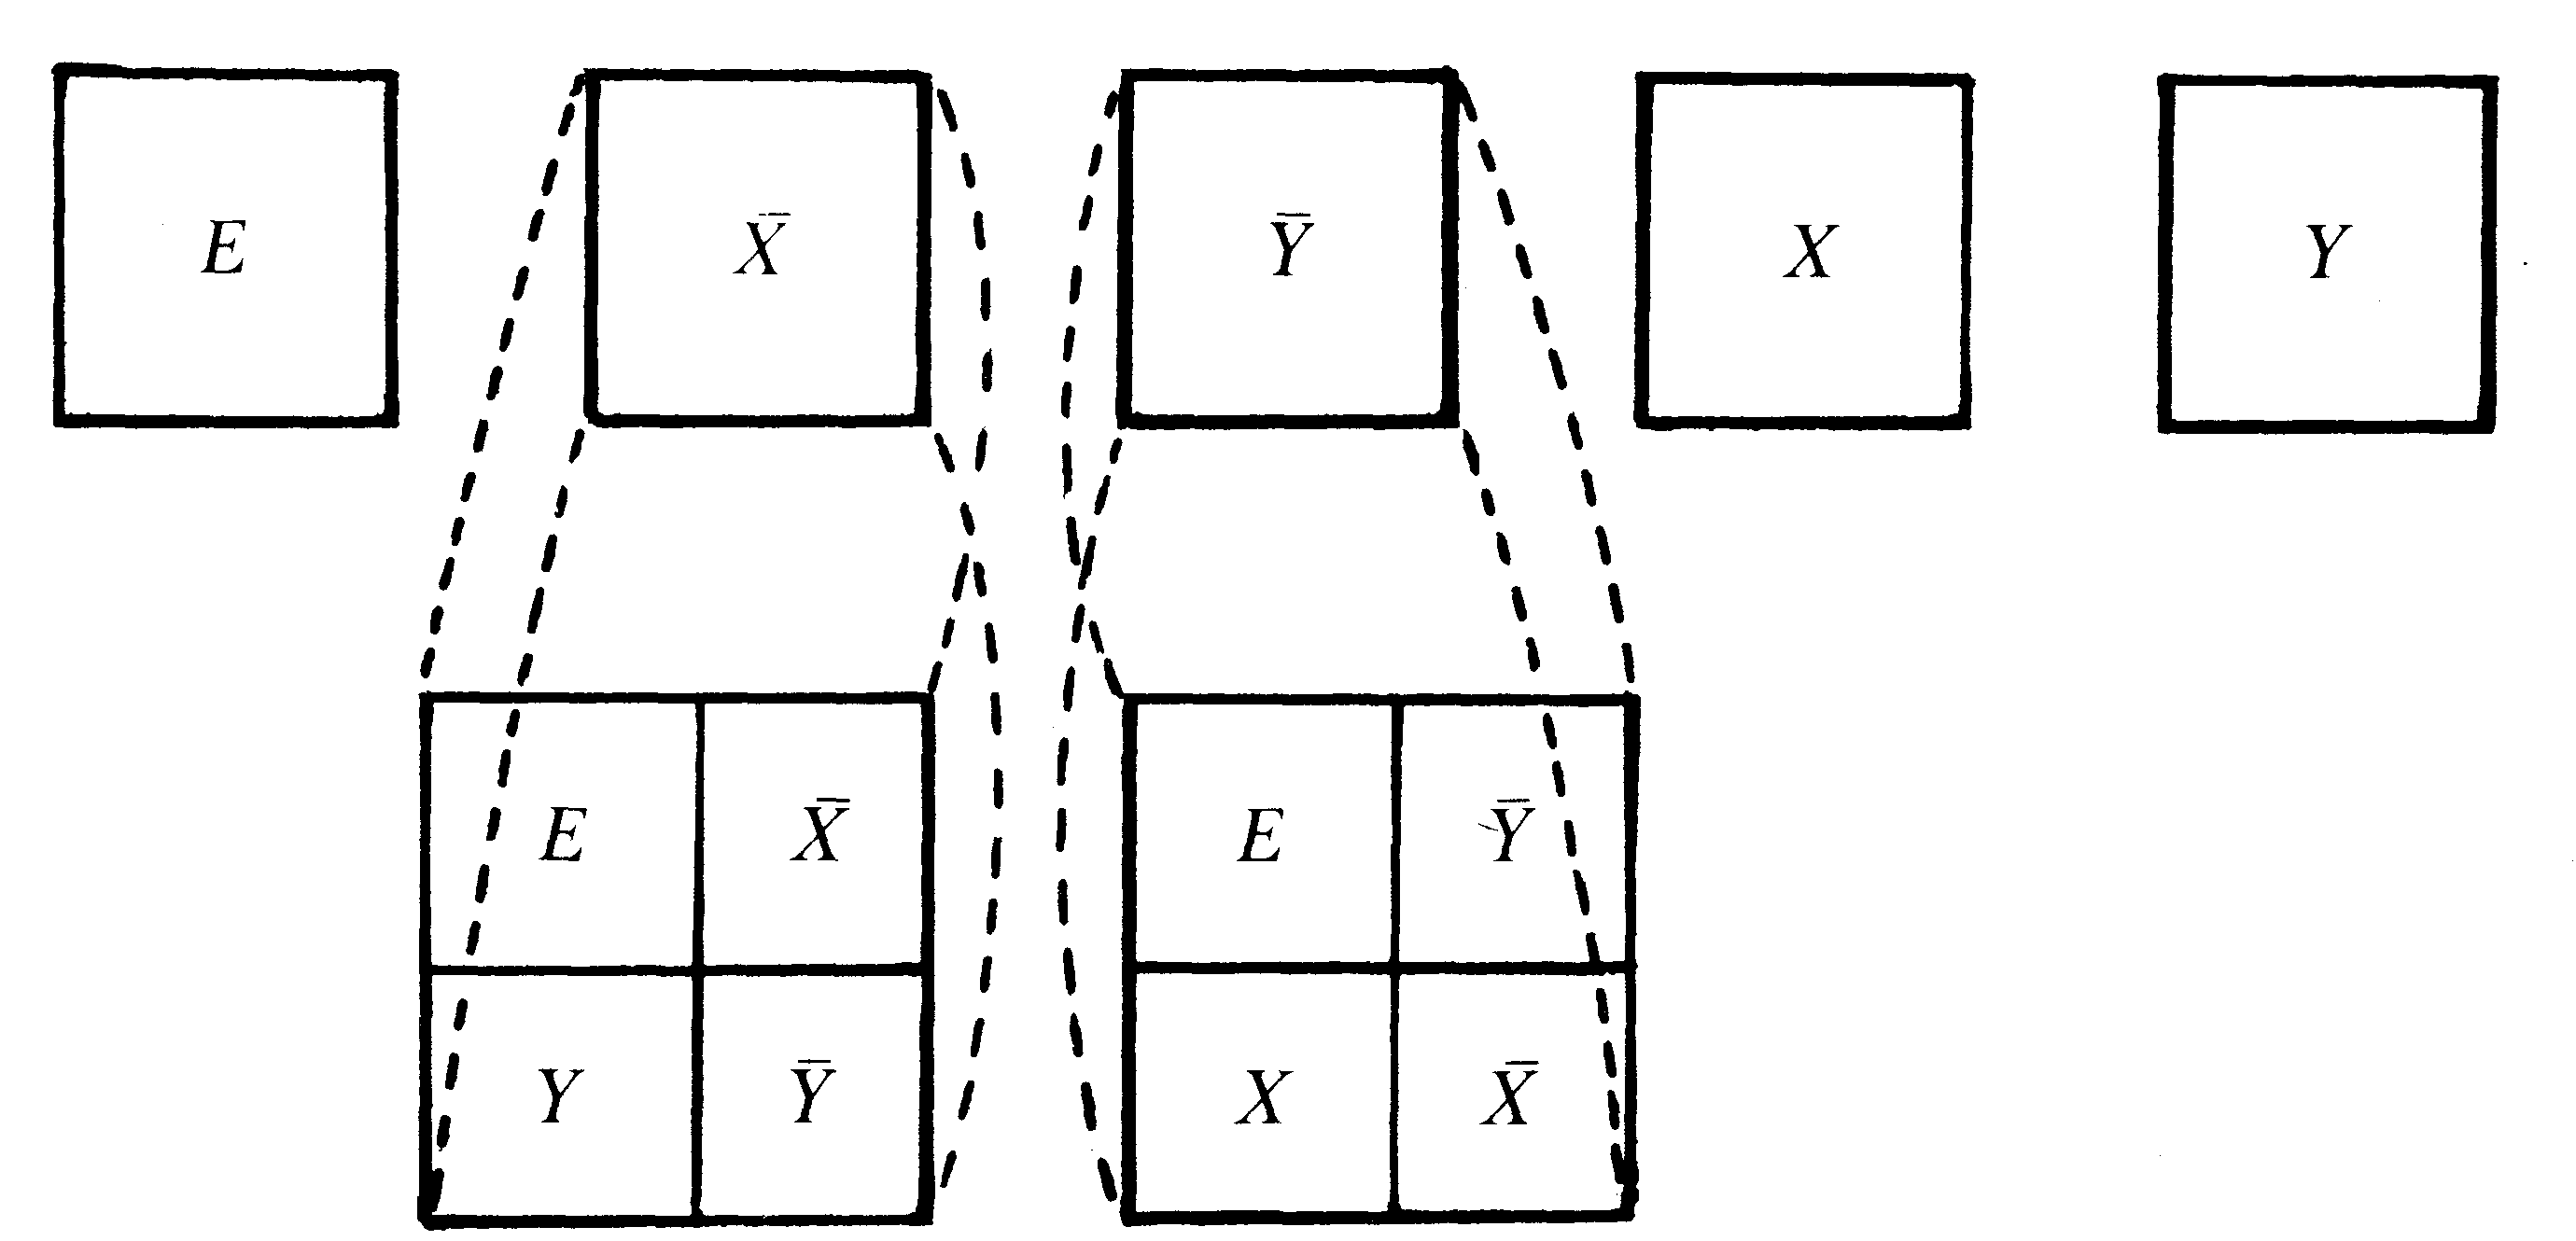
\includegraphics[width=0.96\textwidth]{diagram.png}
\end{center}
\vspace{-0.3em}
\noindent\textit{Ainsi, à partir de ces 11 (en réalité 5) morceaux, nous pouvons réassembler
2 sphères congruentes, plus une copie congruente de l'ensemble} $E$. C'est une forme du paradoxe
de Hausdorff-Banach-Tarski qui découle rapidement d'une action libre d'un groupe libre

\newpage
à deux générateurs (voir l'Appendice A pour la forme plus précise). Nous sommes ainsi ramenés
à la question de Dekker (communiquée par Jan Mycielski) : de telles actions existent-elles
réellement ? La sphère doit être de dimension impaire pour des raisons topologiques : une
application sans point fixe $f:S^d\to S^d$ doit avoir un nombre de Lefschetz nul
\[
L(f)=\sum(-1)^i\Trace\bigl(f;H_i(S^d)\bigr)=1+(-1)^d\deg(f).
\]
Pour une action libre d'un groupe libre, le carré d'un élément non trivial agit par une
application de degré $+1$, ce qui impose que $d$ soit impair. La dimension doit être $>1$.
Ce sont les seules conditions.

\TheoremBlock{Pour $n\geq 2$, il existe un groupe libre non abélien de rotations rigides
agissant librement sur la sphère de dimension impaire $S^{2n-1}$.}

\RemarkBlock{Les matrices orthogonales correspondantes peuvent être choisies à
coefficients algébriques, et le groupe de matrices correspond alors à un sous-groupe des
éléments non nuls d'une algèbre à division sur un corps de nombres.}

\RemarkBlock{Le théorème a été démontré par Dekker lorsque $n$ est pair [D].}

\RemarkBlock{Soit $u:O(p)\times O(q)\to O(p+q)$ le plongement naturel :
\[
u(A,B)=\text{matrix}\begin{pmatrix}A&0\\0&B\end{pmatrix}.
\]
Si $A\in O(p)$ et $B\in O(q)$ n'ont aucun vecteur fixe non nul, il en va de même de
$u(A,B)$. Si $\sigma_1:F\to O(p)$ et $\sigma_2:F\to O(q)$ définissent des actions libres sur $S^{p-1}$ et
$S^{q-1}$, $u(\sigma_1,\sigma_2)$ définit donc une action libre de $F$ sur $S^{p+q-1}$. Par cette remarque,
on pourrait ramener le théorème aux deux cas particuliers $n=2$ et $n=3$.}

\par\vspace{0.55em}\noindent\hspace{1.4em}\textit{Démonstration.}\quad Soit $k\subset\mathbf{R}$ un corps de nombres algébriques réel, et soit $k'\subset\mathbf{C}$ une extension quadratique de $k$. Supposons que $k'\not\subset\mathbf{R}$, c'est-à-dire que $k'\otimes_k\mathbf{R}=\mathbf{C}$. Soit $D$ une
algèbre à division de dimension $n^2$ sur son centre $k'$, munie d'une anti-involution
$*$ induisant sur $k'$ la conjugaison complexe. La $\mathbf{R}$-algèbre $D\otimes_k\mathbf{R}$ est
une algèbre simple sur son centre $k'\otimes_k\mathbf{R}=\mathbf{C}$, donc isomorphe à $M(n,\mathbf{C})$.
Nous supposons que, pour un isomorphisme convenable entre $D\otimes_k\mathbf{R}$ et $M(n,\mathbf{C})$, $*$
devient la transposition conjuguée.

Pour un tel isomorphisme, les éléments $u$ de $D$ vérifiant $uu^*=1$ deviennent
des matrices unitaires. Ils opèrent sur la sphère unité de $\mathbf{C}^n$. De plus,
si $u\neq1$, $u-1$ est inversible dans $D$, de sorte que la matrice correspondante n'a pas
$1$ pour valeur propre. Elle agit donc sans point fixe sur la sphère.

Le groupe $\Gamma:=\{u\in D\mid uu^*=1\}$ est le groupe des points $k$-rationnels d'une
$k$-forme du groupe algébrique réel $U(n)$. Pour $n>1$, le sous-groupe parfait $SU(n)$

\newpage
de $U(n)$ n'est pas trivial, et $U(n)$ n'est pas résoluble. Le groupe $\Gamma$ est dense dans $U(n)$ :
les éléments anti-adjoints de $D$ sont denses dans les matrices anti-adjointes de $M(n,\mathbf{C})$,
et la transformation de Cayley $t\mapsto\dfrac{t-1}{t+1}$ est un homéomorphisme de l'espace des
matrices anti-adjointes de $M(n,\mathbf{C})$ sur un ouvert dense de $U(n)$, qui envoie les
éléments anti-adjoints de $D$ dans $\Gamma$. Il résulte de cette densité que, si $n>1$,
le groupe linéaire $\Gamma$ n'est pas résoluble. D'après [Tits], il contient un sous-groupe
libre non abélien.

Il reste à construire des couples $(D,*)$. Une algèbre à division $D$ de centre $k'$
admet une anti-involution $*$ induisant sur $k'$ l'élément non trivial $\Gal(k'/k)$ si,
et seulement si, sa classe $\cl(D)$ dans le groupe de Brauer $\Br(k')$ de $k'$ a une image
nulle par l'application norme $N_{k'/k}:\Br(k')\to\Br(k)$---voir l'Appendice B. La théorie
du corps de classes donne un calcul explicite de $\Br(k)$ et de $N_{k'/k}$, et indique quels
éléments de $\Br(k')$ proviennent d'algèbres à division. L'existence d'un tel $D$ découle de
cette description explicite. Une construction directe est donnée dans l'Appendice C. Lorsque
nous choisissons un isomorphisme de $D\otimes_k\mathbf{R}$ avec $M(n,\mathbf{C})$, l'involution $*$ devient
l'adjonction relativement à une forme hermitienne $\phi$ sur $\mathbf{C}^n$, non nécessairement définie
positive : $\phi(ax,y)=\phi(x,a^*y)$. Si $h$ est auto-adjoint dans $D$, $\Intop(h^{-1})\circ *$ est l'adjonction
relativement à la forme $\phi_h(x,y)=\phi(hx,y)$. Pour un $h$ convenable, $\phi_h$ est définie positive,
et $(D,\Intop(h^{-1})\circ *)$ est du type cherché.

\AppendixHeading{A}
Considérons $\phi:S'\cup S''\to S-E$ comme dans l'introduction, où $S'$ et $S''$ sont deux
copies de la sphère $S$, et $\psi:S\to S'$ la bijection évidente. Considérons, comme dans le
théorème de Schröder-Bernstein, l'ensemble $S_e$ des points $p$ de $S$ ayant un nombre pair
d'ancêtres, c'est-à-dire pour lesquels il existe un entier $n\geq0$ tel que $p\in\ImOp(\phi\circ\psi)^n$
et $p\notin\ImOp(\psi\circ(\phi\circ\psi)^n)$. Considérons aussi l'ensemble $S_o$ des $p$ de $S$ pour lesquels
il existe $n\geq0$ tel que $p\in\ImOp(\psi\circ(\phi\circ\psi)^n)$ et $p\notin\ImOp(\phi\circ\psi)^{n+1}$, et enfin l'ensemble $S_{\infty}$
des $p$ tels que $p\in\ImOp(\phi\circ\psi)^n$ pour tout $n\geq0$. De même, considérons
\[
S'\cup S''=(S'\cup S'')_e\cup(S'\cup S'')_o\cup(S'\cup S'')_{\infty}.
\]
Alors $\psi$ induit une bijection de $S_e\cup S_{\infty}$ sur $(S'\cup S'')_o\cup(S'\cup S'')_{\infty}$, et $\phi^{-1}$
une bijection de $S_o$ sur $(S'\cup S'')_e$. En les combinant, nous obtenons une bijection $\chi:S\to S'\cup S''$
et une partition de $S$ en un nombre fini de morceaux, la restriction de $\chi$ à chacun
d'eux étant une rotation.

\newpage
\AppendixHeading{B}
Soit $K$ une extension quadratique séparable d'un corps $k$. Nous notons $x\mapsto\bar{x}$
l'élément non trivial de $\Gal(K/k)$. Soit $D$ une algèbre simple de dimension
$n^2$ sur son centre $K$. Vérifions le critère du texte pour l'existence
d'une involution de seconde espèce sur $D$, c'est-à-dire d'une anti-involution $*$ de $D$
induisant $x\mapsto\bar{x}$ sur $K$. Le critère est que $N_{K/k}\cl(D)=0$ dans $\Br(k)$.

Localisons-nous pour la topologie étale sur $\Spec(k)$. Cela signifie effectuer
des extensions étales de scalaires $\otimes_k k'$ assez grandes, tout en suivant la
fonctorialité en $k'$. Le corps $K$ devient l'extension quadratique séparable
$K'=K\otimes_k k'$ de $k'$. L'algèbre $D$ devient $D'=D\otimes_k k'$, et est de la forme
$D'=\End_{K'}(V')$, où $V'$ est un module libre sur $K'$. Le module $V'$ n'est déterminé
par $D'$ qu'à homothétie près (l'espace projectif correspondant est déterminé de façon unique).

Pour tout $K$-module $M$, soit $\bar{M}$ le module déduit de $M$ par l'extension
des scalaires $\bar{\phantom{x}}:K\to K$, c'est-à-dire le module, unique à isomorphisme unique près,
muni d'un isomorphisme anti-linéaire $x\mapsto\bar{x}:M\xrightarrow{\sim}\bar{M}$.
De même pour les $K'$-modules. Si $D'=\End(V')$, alors $\bar{D}{}'=\End(\bar{V}{}')$, et
\[
(D\otimes_K\bar{D})'=\End(V'\otimes\bar{V}{}').
\]
Soit $W'$ le sous-espace fixe de l'automorphisme anti-linéaire de $V'\otimes\bar{V}{}'$
défini par $v\otimes\bar{w}\mapsto w\otimes\bar{v}$. C'est l'espace des formes hermitiennes sur le dual de
$V'$. On a $W'\otimes_{k'}K'=V'\otimes\bar{V}{}'$. Si $D_1\subset D\otimes_K\bar{D}$ est le sous-espace fixe
de l'automorphisme anti-linéaire de $D\otimes_K\bar{D}$ défini par $x\otimes\bar{y}\mapsto y\otimes\bar{x}$, alors
$D'_1$ est la $k'$-forme de la $K'$-algèbre $(D\otimes_K\bar{D})'=\End(V'\otimes\bar{V}{}')$ déduite de
la $k'$-forme $W'$ du $K'$-module $V'\otimes\bar{V}{}'$ : $D'_1=\End_{k'}(W')$.

Les involutions de seconde espèce sur $D'$ correspondent bijectivement aux formes
hermitiennes non dégénérées sur $V'$, prises à un facteur près (dans $k'^*$). Celles-ci, à leur tour,
correspondent, par la construction de la « forme duale », aux éléments « non dégénérés » de
$W'$, là encore à un facteur près. L'espace projectif $\mathbf{P}(W')$ sur $k'$ est déterminé
à isomorphisme unique près par $D'$. Il est donc (c'est le point de la localisation) défini sur $k$ :
$\mathbf{P}(W')=P\otimes_k k'$, fonctoriellement en $k'$. Les points sur $k$ de $P$ (plus exactement,
les points non dégénérés) paramètrent les involutions de seconde espèce sur $D$.

L'isomorphisme fonctoriel $D'_1=\End_{k'}(W')$ montre que $P$ est la forme de l'espace
projectif (variété de Severi-Brauer) attachée à $D_1$. Elle possède un point rationnel,
et est alors l'espace projectif ordinaire, si et seulement si $D_1$ est une algèbre de matrices.

\newpage
Ceci montre que $D$ possède des involutions de seconde espèce si et seulement si la classe
de $D_1$ dans $\Br(k)$ est nulle. Cette classe est la norme cherchée $N_{K/k}(\cl(D))$. Dans
l'esprit de la localisation, on peut le déduire du fait que l'homothétie de rapport
$\lambda\in K'^*$ de $V'$ induit sur $W'$ l'homothétie de rapport $N_{K'/k'}(\lambda)\in k'^*$.

\AppendixHeading{C}
Pour $n\geq3$, on peut obtenir des exemples ainsi : prenons $k'=\mathbf{Q}[\zeta]$, avec
$\zeta=\exp(2\pi i/n)$, et $k=k'\cap\mathbf{R}$. Fixons $a,b\in k^*$ et soit $D$ la $k'$-algèbre
engendrée par $X,Y$, soumise aux relations
\[
X^n=a,\qquad Y^n=b
\]
\[
XY=\zeta YX.
\]
Elle admet l'anti-involution $*$, induisant la conjugaison complexe sur $k'$, définie
par $\zeta^*=\zeta^{-1}$, $X^*=X$, $Y^*=Y$. L'algèbre $D$ est du type voulu,
pourvu que ce soit une algèbre à division. Cela se produit déjà avec $a,b\in\mathbf{Z}$ : prenons
pour $a$ un nombre premier congru à $1$ mod $n$, et pour $b$ un entier dont le résidu mod $a$
a, dans le groupe cyclique d'ordre $n$ $(\mathbf{Z}/(a))^*/(\mathbf{Z}/(a))^{*n}$, une image d'ordre exact $n$.
Par exemple $n=3$, $a=7$, $b=2$. Pour $n=2$, on procède de même avec
$k'=\mathbf{Q}[i]$, $\zeta=-1$, $a$ congru à $1$ mod $4$ et $b$ non carré mod $a$. Par
exemple, $a=5$ et $b=2$. Dans chaque cas, l'hypothèse sur $a$ assure que $k'$
se plonge dans le complété $a$-adique $\mathbf{Q}_a$ de $\mathbf{Q}$, et le fait que $D$ soit une algèbre à division
se voit localement en $a$ : $D\otimes_{k'}\mathbf{Q}_a$ est une algèbre à division de centre $\mathbf{Q}_a$.

\newpage
\BibliographyHeading
\noindent
\begin{tabular}{@{}p{11mm}p{0.89\textwidth}@{}}
{[A]} & \textsc{Albert, A.} \textit{Structure of algebras.} A.M.S. Colloquium Publ. 24 (1939). \\[0.35em]
{[Sch]} & \textsc{Scharlau, W.} Zur Existenz von Involutionen auf einfachen Algebren. \textit{Math. Zeitschr.} 145 (1975), 29-32. \\[0.35em]
{[Myc]} & \textsc{Mycielkski, Jan.} Can one solve equations in groups? \textit{Amer. Math. Monthly} 84 (1977), 723-726. \\[0.35em]
{[Tits]} & \textsc{Tits, J.} Free subgroups in linear groups. \textit{Journal of Algebra} 20 (1972), 250-270. \\[0.35em]
{[D]} & \textsc{Dekker, Th. J.} Decomposition of sets and spaces I, II. \textit{Indig. Math.} 18 (1956), 581-595, and 19 (1957), 104-107.
\end{tabular}

\vspace{1.3em}
\hfill\textit{(Reçu le 8 mars 1982)}

\vspace{2.1em}
\noindent
Pierre Deligne\\
Dennis Sullivan\\[0.55em]
\hspace*{1.8em}Institut des Hautes Etudes Scientifiques\\
\hspace*{1.8em}35, route de Chartres\\
\hspace*{1.8em}91440 Bures-sur-Yvette\\
\hspace*{1.8em}France

\clearpage\endgroup
\typeout{CORPUS-END:D043:\thepage}
% END INLINE WORK D043 FR
\end{document}
